\documentclass[leqno,labelfig,psfigt,colorlinks]{svmono}
\makeatletter
\providecommand*{\input@path}{}
\edef\input@path{{./}{../}\input@path}% prepend
\makeatother

%% Macros for AMG notes
%\newcommand{\triplenorm}[1]{\ensuremath{| \! | \! | #1 | \! | \! |}}
\newcommand{\triplenorm}[1]{%
  \left\vert\kern-0.9pt\left\vert\kern-0.9pt\left\vert #1
  \right\vert\kern-0.9pt\right\vert\kern-0.9pt\right\vert}
\newcommand{\Tscalar}[2]{\ensuremath{(#1 , #2)_{\bar R^{-1}}}} %%% macro for star norm.
\newcommand{\Tnorm}[1]{\ensuremath{\|#1\|_{\bar R^{-1}}}}
\newcommand{\Dscalar}[2]{\ensuremath{( #1 , #2 )_D}}
\newcommand{\Dnorm}[1]{\|#1\|_{D}}
\newcommand{\Tproj}{\ensuremath{Q_c}}
\newcommand{\Dproj}{\ensuremath{Q_D}}
\newcommand{\Anorm}[1]{\|#1\|_A}
\newcommand{\trace}{\ensuremath{\operatorname{trace}}}
\newcommand{\Span}{\ensuremath{\operatorname{span}}}

\newcommand{\eqqsim}{\mathbin{\rotatebox[origin=c]{180}{\ensuremath{\cong}}}}

\newcommand{\rs}{\ensuremath{R_s}}

\newcommand{\Vhf}{V_{\rm hf}}
\newcommand{\Vf}{V_{f}}
\newcommand{\Vc}{V_{c}}
\newcommand{\sparse}{\ensuremath{\operatorname{S}}}
\newcommand{\dof}{\ensuremath{N}}
\newcommand{\co}{\ensuremath{C_{o}}}
\newcommand{\Nepo}{{Nepomnyaschikh}}
\renewcommand{\v}{{\cal V}}
% ---------------------------
% packages
% ---------------------------
% AMS math symbol
\usepackage{amsmath}
\usepackage{amsbsy}
\usepackage{amsfonts}
\usepackage{amssymb}
\usepackage{amscd}
\usepackage{mathrsfs}
%\usepackage{mathptmx}       % selects Times Roman as basic font
%\usepackage{algorithmic}
\usepackage{bm}
%\usepackage{wsuipa}

\usepackage{algpseudocode}
\usepackage[Algorithm]{algorithm}
%% one line ifs and fors commands only for this section
\algnewcommand{\IIf}[1]{\State\algorithmicif\ #1\ \algorithmicthen}
\algnewcommand{\EElse}{\unskip\ \algorithmicelse\ }
\algnewcommand{\EndIIf}{\unskip\ \algorithmicend\ \algorithmicif}
\algnewcommand{\FFor}[1]{\State\algorithmicfor\ #1\ }
\algnewcommand{\EndFFor}{\unskip\ \algorithmicend\ \algorithmicfor}
%%%%%%%%%%%%%%%%%%%%%%%%%%%%%%%%%%%%%

% text fonts
\usepackage{txfonts}
%\usepackage{helvet}         % selects Helvetica as sans-serif font
%\usepackage{courier}        % selects Courier as typewriter font
\usepackage[latin1]{inputenc}

% graphcis
\usepackage{graphicx}
\usepackage{subfigure} %commented by Ludmil, uncommented by Hongxuan
\usepackage{float}

\usepackage{tikz}   %commented by Ludmil, uncommented by Hongxuan
\usetikzlibrary{shapes,arrows,decorations.pathmorphing,backgrounds,positioning,fit,matrix,calc}  %commented by Ludmil, uncommented by Hongxuan
%\usepackage{subfig}  %added by Ludmil, commented by Hongxuan

\tikzstyle{decision} = [diamond, draw, fill=blue!20,
    text width=4.5em, text badly centered, node distance=3cm, inner sep=0pt]
\tikzstyle{block} = [rectangle, draw, fill=blue!20,
    text width=5em, text centered, rounded corners, minimum height=4em]
\tikzstyle{line} = [draw, -latex']
\tikzstyle{cloud} = [draw, ellipse,fill=red!20, node distance=3cm,
    minimum height=2em]



%% command shell environment 
\usepackage[most]{tcolorbox}
\newtcblisting{commandshell}{colback=black,colupper=white,colframe=yellow!75!black,
listing only,listing options={language=sh},
every listing line={\textcolor{red}{\small\ttfamily\bfseries Terminal \$> }}}

%% Code styles
\usepackage{listings}
\usepackage{color}
 
\definecolor{codegreen}{rgb}{0,0.6,0}
\definecolor{codegray}{rgb}{0.5,0.5,0.5}
\definecolor{codepurple}{rgb}{0.58,0,0.82}
\definecolor{backcolour}{rgb}{0.95,0.95,0.92}
 
\lstdefinestyle{python}{
    backgroundcolor=\color{backcolour},   
    commentstyle=\color{codegreen},
    keywordstyle=\color{magenta},
    numberstyle=\tiny\color{codegray},
    stringstyle=\color{codepurple},
    basicstyle=\footnotesize,
    breakatwhitespace=false,         
    breaklines=true,                 
    captionpos=b,                    
    keepspaces=true,                 
    numbers=left,                    
    numbersep=5pt,                  
    showspaces=false,                
    showstringspaces=false,
    showtabs=false,                  
    tabsize=2
}
 
%\lstset{style=python}


% other tools
\usepackage{hyperref}
\usepackage{type1cm}
%%\usepackage[normalem]{ulem}
\usepackage{soul}
%\usepackage{times}
\usepackage{url}
\usepackage{undertilde}
%\usepackage{ulem}
%\def\utilde{\uwave}
\usepackage{rotating} %% commented because it crashes "figure" (ludmil), uncommented by Hongxuan
\usepackage{makeidx}
\makeindex             % used for the subject index
\usepackage{multicol}
\usepackage{enumerate}
\usepackage{xspace}
 \usepackage{comment}  % added by Ludmil
 % \usepackage[bw,framed]{mcode} %% commented because it crashes "lstlisting" (ludmil)
\usepackage[margins]{trackchanges} %% commented because it crashes "figure" (ludmil), uncommented by Hongxuan
\usepackage{etoolbox}
\usepackage{array}
%%
% ---------------------------
% Formats
% ---------------------------
% head
\usepackage{fancyhdr}
\pagestyle{fancy}
\rhead{} %added by Hongxuan Zhang

% page
\pagenumbering{arabic}
\newcommand{\pinput}[1]
{\newpag
\hrule
\centerline{\huge \bf #1}
\hrule
\newpage}

% ---------------------------
% Theorems etc.
% ---------------------------
\ifcsmacro{theorem}{}{
\newtheorem{theorem}{Theorem}[section]
}
\ifcsmacro{lemma}{}{
\newtheorem{lemma}[theorem]{Lemma}
}
\ifcsmacro{corollary}{}{
\newtheorem{corollary}[theorem]{Corollary}
}
\ifcsmacro{proposition}{}{
\newtheorem{proposition}[theorem]{Proposition}
}
\ifcsmacro{algorithm}{}{
\newtheorem{algorithm}[equation]{Algorithm}
}
\newtheorem{consequence}[equation]{Consequence}
\newtheorem{conclusion}[equation]{Conclusion}
\newcommand{\Remark}{\noindent{\bf Remark.~}}
\newtheorem{assumption}[equation]{Assumption}
\newtheorem{observation}[equation]{Observation}
%\newtheorem{remark}[theorem]{Remark}
%\newtheorem{definition}[theorem]{Definition}
%\newtheorem{exercise}[theorem]{Exercise}
\newtheorem{homework}[theorem]{Homework}
%\newtheorem{example}[theorem]{Example}

\def\proof{\par{\it Proof}. \ignorespaces}
\def\endproof{{\ \vbox{\hrule\hbox{\vrule
        height1.3ex\hskip0.8ex\vrule}\hrule}}\par}

% ---------------------------
% Chapter and sections
% ---------------------------
\let\oldchapter\chapter
\def\chapter{%
  \setcounter{exercise}{0}%
  \oldchapter
}

% ---------------------------
% New commands
% ---------------------------
% References and Citation
%\newcommand{\Label}[1]{\label{#1}{{\mbox{\small\mbox{\fbox{\tt #1}\quad}}}}}
\newcommand{\Label}{\label}
\newcommand{\Rf}[1]{\mbox{$(\ref{#1})$}}
\newcommand{\rf}[1]{$(\ref{#1})$}

\DeclareMathOperator*{\argmin}{arg\,min}
\DeclareMathOperator*{\argmax}{arg\,max}
\DeclareMathOperator*{\range}{Range}
%\DeclareMathOperator*{\span}{span}

% making comment
% \renewcommand{\initialsOne}{Xu}
% \renewcommand{\initialsTwo}{XHu}
% \renewcommand{\initialsThree}{Yang}
% \renewcommand{\initialsFour}{Zhang}
% \renewcommand{\initialsFive}{KHu}


%\newcommand{\sh}{{\cal S}_h}
% new math command
\newcommand{\pro}{{\mathcal P}}
\newcommand{\beas}{\begin{eqnarray*}}
\newcommand{\eeas}{\end{eqnarray*}}
\newcommand{\bary}{\begin{array}}
\newcommand{\eary}{\end{array}}
\newcommand{\supp}{{\rm supp}\;}
\newcommand{\update}{\leftarrow}
\newcommand{\cequiv}{\stackrel{\mathrm{c}}{\equiv}}
\newcommand{\hf}{\frac{1}{2}}
\newcommand{\qall}{\quad\forall\;}
\def\ec{\mathrel{\hbox{$\copy\Ea\kern-\wd\Ea\raise-3.5pt\hbox{$\sim$}$}}}
\newcommand{\lc}{\mathrel{\raise2pt\hbox{${\mathop<\limits_{\raise1pt\hbox{\mbox{$\sim$}}}}$}}}
\newcommand{\gc}{\mathrel{\raise2pt\hbox{${\mathop>\limits_{\raise1pt\hbox{\mbox{$\sim$}}}}$}}}
\newcommand{\deq}{\stackrel{\rm def}{=}}
\newcommand{\cths}{\{\cth: h\in\aleph\}}
\newcommand{\td}[1]{\tilde{#1}}
\newcommand{\spd}{SPD }
\newcommand{\step}[1]{\noindent\raisebox{1.5pt}[10pt][0pt]{\tiny\framebox{$#1$}}\xspace}
\newcommand{\topic}[1]{\vspace{2mm}\addtocounter{equation}{1}{\noindent{\bf(\theequation) \ {\sf #1}.}}\ }
\newbox\Ea
\setbox\Ea=\hbox{\raise0.9pt\hbox{$=$}}
\newcommand{\smt}[1]{\overline{#1}}%% Notation for matrix, to be modified.
\newcommand{\rep}[1]{{\widetilde {#1}}}%% Notation for matrix representation
\newcommand{\mt}{\mathcal}%% Notation for matrix, to be modified.
\newcommand{\hcomment}[1]{\mbox{\quad (#1)}}
\newcommand{\tol}{\mbox{\rm tol}}
\newcommand{\diag}{\mbox{diag}\;}
\newcommand{\for}{\sf for\mbox{$\;$}}
\newcommand{\efor}{\mbox{\sf endfor}}
\newcommand{\ot}[1]{\mbox{\bf{$#1$}}}
\newcommand{\hset}{{\aleph}}
\newcommand{\thset}{\{{\cal T}_h: h\in \hset\}}
\newcommand{\mbb}{\mathbb}
\newcommand{\bs}{\boldsymbol}
\newcommand{\mcal}{\mathcal}
\newcommand{\mrm}{\mathrm}
\newcommand{\dist}{\mbox{dist}\;}
\newcommand{\prt}[1]{\frac{\partial}{\partial #1}}
\newcommand{\prtt}[2]{\frac{\partial #1}{\partial #2}}
\newcommand*{\ang}[1]{\left\langle #1 \right\rangle}
\newcommand{\bproof}{\begin{proof}}
\newcommand{\eproof}{\end{proof}}

% new letters
\newcommand{\nne}{\mbox{$n_{\mbox{\tiny E}}$}}
\newcommand{\At}{\mbox{$A_{\mbox{\tiny T}}$}}
\newcommand{\rhst}{\mbox{${f}_{\mbox{\tiny T}}$}}
\newcommand{\rhs}{\mbox{$f$}}
\newcommand{\nt}{\mbox{$NT$}}
\newcommand{\ib}{\mbox{$IB$}}
\newcommand{\nn}{\mbox{$n$}}
\newcommand{\om}{\Omega}  % needs to get rid of it
\newcommand{\Om}{\Omega}
\newcommand{\cM}{{\cal M}}
\newcommand{\m}{\mbox{$\cM$}}
\newcommand{\cT}{\mbox{${\cal T}$}}
\newcommand{\cP}{{\mathcal P}}
\newcommand{\ct}{{\cal T}}  % need to get rid of it
\newcommand{\cth}{{\cal T}_h}
\newcommand{\Th}{\mbox{${\cal T}_h$}}
\newcommand{\ld}{\lambda}
\newcommand{\nh}{{\cal N}_h}
%%%\renewcommand{\v}{{\cal V}}
\newcommand{\vvv}{{\cal V}}
\newcommand{\vh}{{\cal V}_h}
\newcommand{\newu}{u^{new}}
\newcommand{\oldu}{u^{\rm old}}
\newcommand{\oldr}{r^{\rm old}}
\newcommand{\LL}{L}
\newcommand{\Sh}{{\cal S}^h}
\newcommand{\Shz}{{\cal S}^h_0}
\newcommand{\V}{V}
\newcommand{\Q}{Q}
\newcommand{\Ddivh}{\mbox{\bf A}_h^{\rm div}}
\newcommand{\hb}{\hat B}
\newcommand{\tqk}{\tilde Q_k}
\newcommand{\vaip}{\overline{a}}
\newcommand{\Prol}{\Pi}
\newcommand{\Aa}{\bar A}

% operators
\newcommand{\grad}{{\rm grad}}
\newcommand{\curl}{{\rm curl }}
\newcommand{\dv}{{\rm div}}
\newcommand{\divg}{{\rm div}\mbox{$\;$}}
\newcommand{\Hcurl}{{\rm curl}}
\newcommand{\Hg}{H({\rm grad})}

% projections
\newcommand{\Phz}{\Pi_h^0}
\newcommand{\Phg}{\Pi_h}
\newcommand{\Phd}{\Pi_h^{\rm div}}
\newcommand{\PHdiv}{\Pi_H^{\rm div}}
\newcommand{\Phc}{\Pi_h^{\rm curl}}
\newcommand{\PHc}{\Pi_H^{\rm curl}}
\newcommand{\PHcurl}{\Pi_H^{\rm curl}}
\newcommand{\PHd}{\Pi_H^{\rm div}}
\newcommand{\PHz}{\Pi_H^{\rm 0}}

% inner product, norm
\newcommand{\inner}{\mbox{$(\cdot, \cdot)$}}
\newcommand{\innerA}{(\cdot,\cdot)_A}
\newcommand{\nm}[2]{\|{#1}\|_{#2}}
\newcommand{\nmA}[1]{\nm{#1}{A}}
\newcommand{\NA}[1]{\|#1\|_{A}}
\newcommand{\nmm}[1]{\|#1\|}
\newcommand{\trnm}[2]{|\!\!|\!\!|{#1}|\!\!|\!\!|_{#2}}

% space
\newcommand{\ho}{H^1_0(\Om)}
\ifcsmacro{R}{}{
\newcommand{\R}{\mathbb{R}} %% this does not work as \R^{blah blah} better do not use (--ltz)
}
\newcommand{\Z}{\mathbb{Z}}
%\newcommand\Rn[1]{\R^{#1}}
\newcommand{\Hd}{\mbox{$\ot H({\rm div})$}}
\newcommand{\Hdiv}{\mbox{$\ot H({\rm div})$}}
\newcommand{\Hhdiv}{\mbox{$\ot H_h({\rm div})$}}
\newcommand{\HHdiv}{\mbox{$\ot H_H({\rm div})$}}
\newcommand{\Zdiv}{\mbox{$\ot Z({\rm div})$}}
\newcommand{\Zzdiv}{\mbox{$\ot Z_0({\rm div})$}}
\newcommand{\Zhdiv}{\mbox{$\ot Z_h({\rm div})$}}
\newcommand{\ZHdiv}{\mbox{$\ot Z_H({\rm div})$}}
\newcommand{\Hc}{\mbox{$\ot H({\rm curl})$}}
\newcommand{\Hcllurl}{\mbox{$\ot H({\rm curl})$}}
\newcommand{\Hzcurl}{\mbox{$\ot H_0({\rm curl})$}}
\newcommand{\Hhcurl}{\mbox{$\ot H_h({\rm curl})$}}
\newcommand{\HHcurl}{\mbox{$\ot H_H({\rm curl})$}}
\newcommand{\Hhg}{\mbox{$H^1_h$}}
\newcommand{\Hhd}{\mbox{$H_h^{\rm div}$}}
\newcommand{\Hhc}{\mbox{$H_h^{\rm\small curl}$}}
\newcommand{\Hhz}{\mbox{$L^2_h$}}
\newcommand{\Cinf}{C^\infty}
\newcommand{\cc}{C(\bar \Omega)}
\newcommand{\ccc}{C^{0,\lambda}(\bar \Omega)}
\newcommand{\hoz}{H_0^1(\Om)}
\newcommand{\HHg}{\mbox{$H_H^1$}}
\newcommand{\czi}{C_0^\infty(\Omega)}
\newcommand{\domega}{{\cal D}(\Omega)}
\newcommand{\ddomega}{{\cal D}'(\Omega)}
\newcommand{\nmt}[2]{|\!|\!|#1|\!|\!|_{#2}^{\sim}}
\newcommand{\nmaa}[1]{\|#1\|_{0,(\alpha)}}
\newcommand{\nmg}[2]{\nm{#1}{H^{#2}(\Om)}}
\newcommand{\ucc}{\nm{u}{0,\infty}}
\newcommand{\uccc}{\nm{u}{\ccc}}
\newcommand{\unpp}{\nm{u}{W^{d/p,p}(\Omega)}}
\newcommand{\eps}{\epsilon}
\newcommand{\la}{\langle}
\newcommand{\ra}{\rangle}
\newcommand{\La}{L^{(\alpha)}(\Omega)}
\newcommand{\Ref}[1]{\ref{#1}}
\newcommand{\apprle}{\lesssim}


%%%%%%%%% MULTIGRID FOR H(DIV) AND H(CURL)%%%
\newcommand{\diam}{\mbox{\rm diam\,}}
%\newcommand{\curl}{{\rm\bf  curl}}
%\newcommand{\grad}{{\rm\bf grad}}
%\DeclareMathOperator*{\supp}{supp}
\renewcommand{\div}{{\operatorname{div}}}
\newcommand{\sdiv}{\mbox{{\footnotesize div}}}
\newcommand{\scurl}{\mbox{{\footnotesize curl}}}%\newcommand{\eps}{\varepsilon}

\newcommand{\N}{{\mathbb N}}
%\renewcommand{\P}{{\mathbb{P}}}
%\newcommand{\R}{{\mathbb R}}
%\newcommand{\V}{{\mathbb V}}
\newcommand{\W}{{\mathbb W}}

\newcommand{\cA}{{\mathcal A}}
\newcommand{\cB}{{\mathcal B}}
\newcommand{\cC}{{\mathcal C}}
\newcommand{\cD}{{\mathcal D}}
\newcommand{\cE}{{\mathcal E}}
\newcommand{\cF}{{\mathcal F}}
\newcommand{\cH}{{\mathcal H}}
\newcommand{\cI}{{\mathcal I}}
\newcommand{\cJ}{{\mathcal J}}
\newcommand{\cL}{{\mathcal L}}
%\newcommand{\cM}{{\mathcal M}}
\newcommand{\cN}{{\mathcal N}}
\newcommand{\cO}{{\mathcal O}}
%\newcommand{\cP}{{\mathcal P}}
\newcommand{\cQ}{{\mathcal Q}}
\newcommand{\cS}{{\mathcal S}}
%\newcommand{\cT}{{\mathcal T}}
\newcommand{\cV}{{\mathcal V}}
\newcommand{\cW}{{\mathcal W}}

\newcommand{\bA}{{\boldsymbol A}}
\newcommand{\bB}{{\boldsymbol B}}
\newcommand{\bH}{{\boldsymbol H}}
\newcommand{\bL}{{\boldsymbol L}}
\newcommand{\bP}{{\boldsymbol P}}
\newcommand{\bQ}{{\boldsymbol Q}}
\newcommand{\bR}{{\boldsymbol R}}
\newcommand{\bS}{{\boldsymbol S}}
\newcommand{\bu}{{\boldsymbol u}}
\newcommand{\bv}{{\boldsymbol v}}
\newcommand{\bw}{{\boldsymbol w}}
\newcommand{\bp}{{\boldsymbol p}}
\newcommand{\bq}{{\boldsymbol q}}
\newcommand{\br}{{\boldsymbol r}}
%\newcommand{\bm}{{\boldsymbol m}}
\newcommand{\bsf}{{\boldsymbol f}}
\newcommand{\bn}{{\boldsymbol n}}
\newcommand{\bt}{{\boldsymbol t}}
\newcommand{\bx}{{\boldsymbol x}}
\newcommand{\bphi}{{\boldsymbol \phi}}
\newcommand{\bpsi}{{\boldsymbol \psi}}
%
\newcommand{\leqs}{\leqslant}
\newcommand{\nleqs}{\nleqslant}
\newcommand{\geqs}{\geqslant}
\newcommand{\ngeqs}{\ngeqslant}
%%%%%%%%%%%% end of multigrid for H(div) and H(curl)%%%%

\renewcommand{\blankpage}{}\renewcommand{\newbreak}{}
\usepackage{wrapfig}
\usepackage{bbm}
\usepackage{listings}
\usepackage{natbib}
\usepackage{color}
\usepackage{cases}
\usepackage{pythonhighlight}

\usepackage{setspace}

\usepackage{pdfpages}

\usepackage{adjustbox}
\usepackage{threeparttable}

\newcommand{\red}[1]{\textcolor{red}{#1}}
\newcommand{\blue}[1]{\textcolor{blue}{#1}}
\newcommand{\brown}[1]{\textcolor{blue}{#1}}
\newcommand{\green}[1]{\textcolor{green}{#1}}



\makeatletter
\newenvironment{breakablealgorithm}
{% \begin{breakablealgorithm}
	\begin{center}
		\refstepcounter{algorithm}% New algorithm
		\hrule height.8pt depth0pt \kern2pt% \@fs@pre for \@fs@ruled
		\renewcommand{\caption}[2][\relax]{% Make a new \caption
			{\raggedright\textbf{\ALG@name~\thealgorithm} ##2\par}%
			\ifx\relax##1\relax % #1 is \relax
			\addcontentsline{loa}{algorithm}{\protect\numberline{\thealgorithm}##2}%
			\else % #1 is not \relax
			\addcontentsline{loa}{algorithm}{\protect\numberline{\thealgorithm}##1}%
			\fi
			\kern2pt\hrule\kern2pt
		}
	}{% \end{breakablealgorithm}
		\kern2pt\hrule\relax% \@fs@post for \@fs@ruled
	\end{center}
}
\makeatother

\usepackage{multirow}
\usepackage{mathtools}

\newtheorem{properties}[theorem]{Properties}
%\graphicspath{{figures/}}
\graphicspath{{../figures/}{./figures/}{../}}

\title{Deep Neural Networks}
\author{Jinchao Xu}
\date{Spring 2018}
 \makeatletter
\let\runauthor\@author
\let\runtitle\@title
\makeatother
\lhead{\textcopyright \ Jinchao Xu (www.multigrid.org)}
\rhead{\runtitle}

\begin{document}
\maketitle

\section*{Contributors:}
This set of notes are based on contributions from many of graduate
students, postdoctoral fellows and other collaborators.   Here is a
partial list:
\begin{quote}
Jianhong Chen, Yuyan Chen, Juncai He, Xiaodong Jia, Lin Li,  Shaobo Liang,
Jonathan Siegel, Pengfei Yin, Hongxuan Zhang, Liang Zhao, Chunyue
Zheng, Lian Zhang, Qian Zhang
\end{quote}
\tableofcontents
%\openup8pt




\section{Plan}
\subsection{MgNet and its variants on popular datasets}

\begin{enumerate}
\item Conference: International Conference on Learning Representations (ICLR)
\item DDL: Sep 28 2020
\item Participants: Juncai He, Huang Huang, Jinchao Xu, Lian Zhang, Jianqing Zhu
\item GPU Requirements: \\
Huang Huang (at least 8 GPUs, 16 GPUs better)\\
Jianqing Zhu (at least 8 GPUs, 16 GPUs better)\\

\item Summary: 
\begin{itemize}
\item MgNet can achieve state-of-the-art results on popular datasets.
\item Common used data augmentation works well on MgNet
\item The good architecture properties of MgNet
\end{itemize}
\item Plan:
\begin{itemize}
\item MgNet on Cifar10, Cifar100 (Done. Currently MgNet achieve higher accuracy than ResNet18)
% Huang add a table 
\item MgNet on ImageNet (On going. DDL: August 30. Huang, Lian)
\item MgNet with data augmentation FAA and cutout on Cifar10, Cifar100. (Done.)
% Jianqing add a table 
\item MgNet with data augmentation FAA and cutout on ImageNet.  (To Do. DDL: August 30. Jianqing, Juncai)
\item Architecture properties of MgNet (On going. DDL: August 30. Juncai He, Huang Huang, Lian Zhang, Jianqing Zhu)
\item MgNet with Chebyshev-semi and Multi-step method on Cifar100 (On going. DDL: July 30. Jianqing, Juncai)
\item MgNet with Chebyshev-semi and Multi-step method on Cifar10 and ImageNet (To Do. DDL: August 15. Jianqing, Juncai)
\item Write a draft of paper (To Do. DDL: September 20)
\item Send to Prof. Xu for revision (To Do. DDL: September 20)
\end{itemize}
\end{enumerate}



\subsection{Training a neural network with Random features}

\begin{enumerate}
	\item Conference: AAAI 2021
	\item DDL: 15 Aug 2020 (Estimated)
	\item Participants: Juncai He, Jonathan Siegel, Jinchao Xu, Lian Zhang
	\item GPU Requirements: \\
	Lian Zhang (2 GPUs)\\

	
	\item Summary: 
	\begin{itemize}
		\item For one hidden layer neural network with random parameters, training the logistic regression gives $100\%$ training accuracy.
		\item Working on the theoretical analysis
	\end{itemize}
	\item Plan:
	\begin{itemize}
		\item Preliminary results on Cifar10, Cifar100 and ImgeNet (Done)
		\item Working on the theoretical analysis (On going. DDL: July 15. Juncai, Jonathan)
		\item Add more numerical results based on the theoretical analysis (To Do. DDL: July 15. Lian)
		\item Write a draft of paper (To Do. DDL: July 30)
		\item Send to Prof. Xu for revision (To Do. DDL: August 15)
	\end{itemize}
\end{enumerate}



\subsection{Constrained Linear Data-feature Mapping for Image Classification}

\begin{enumerate}
	\item Conference: NeurIPS
	\item DDL: Due now.
	\item Participants: Juncai He, Yuyan Chen, Lian Zhang, Jinchao Xu
	\item GPU Requirements: \\
	Lian Zhang (8 GPUs)\\
	\item Summary: 
	\begin{itemize}
		\item Working on the ImageNet.
	\end{itemize}
	\item Plan
	\begin{itemize}
	\item Working on the ImageNet (On going. DDL: July 15. Lian)
	\end{itemize}
\end{enumerate}

\subsection{Training Sparse Neural Networks using Compressed Sensing}

\begin{enumerate}
\item Conference: International Conference on Learning Representations (ICLR)
\item DDL: Sep 25 2020 (Estimated)
	\item Participants: Jonathan Siegel, Jianhong Chen, Jinchao Xu
	\item GPU Requirements: \\
	Jianhong Chen, (4 GPUs)\\
		\item Plan
	\begin{itemize}
		\item Working on the ImageNet (On going. DDL: Sep 1.)
	\end{itemize}
\end{enumerate}


\subsection{Wider Linear Neural Network Converge Faster Using Full Gradient Descent}

\begin{enumerate}
    \item Conference: TBD
    \item DDL: 
	\item Participants:  Li Jiang, Jinchao Xu
	\item GPU Requirements: \\
	None.\\

	\item Plan:
	\begin{itemize}
		\item Do some experiments on MNIST. (done)
		\item Analyse 1D1data situation. (done)
		\item Analyse 1D2data situation. (On going. DDL: June 15. Li)
		\item Building a convergence theorem related to the width of hidden layer in deep linear neural networks.
	\end{itemize}
\end{enumerate}



\section{Plan}
\subsection{MgNet and its variants on popular datasets}

\begin{enumerate}
\item Conference: International Conference on Learning Representations (ICLR)
\item DDL: Sep 28 2020
\item Participants: Juncai He, Huang Huang, Jinchao Xu, Lian Zhang, Jianqing Zhu
\item GPU Requirements: \\
Huang Huang (at least 8 GPUs, 16 GPUs better)\\
Jianqing Zhu (at least 8 GPUs, 16 GPUs better)\\

\item Summary: 
\begin{itemize}
\item MgNet can achieve state-of-the-art results on popular datasets.
\item Common used data augmentation works well on MgNet
\item The good architecture properties of MgNet
\end{itemize}
\item Plan:
\begin{itemize}
\item MgNet on Cifar10, Cifar100 (Done. Currently MgNet achieve higher accuracy than ResNet18)
% Huang add a table 
\item MgNet on ImageNet (On going. DDL: August 30. Huang, Lian)
\item MgNet with data augmentation FAA and cutout on Cifar10, Cifar100. (Done.)
% Jianqing add a table 
\item MgNet with data augmentation FAA and cutout on ImageNet.  (To Do. DDL: August 30. Jianqing, Juncai)
\item Architecture properties of MgNet (On going. DDL: August 30. Juncai He, Huang Huang, Lian Zhang, Jianqing Zhu)
\item MgNet with Chebyshev-semi and Multi-step method on Cifar100 (On going. DDL: July 30. Jianqing, Juncai)
\item MgNet with Chebyshev-semi and Multi-step method on Cifar10 and ImageNet (To Do. DDL: August 15. Jianqing, Juncai)
\item Write a draft of paper (To Do. DDL: September 20)
\item Send to Prof. Xu for revision (To Do. DDL: September 20)
\end{itemize}
\end{enumerate}



\subsection{Training a neural network with Random features}

\begin{enumerate}
	\item Conference: AAAI 2021
	\item DDL: 15 Aug 2020 (Estimated)
	\item Participants: Juncai He, Jonathan Siegel, Jinchao Xu, Lian Zhang
	\item GPU Requirements: \\
	Lian Zhang (2 GPUs)\\

	
	\item Summary: 
	\begin{itemize}
		\item For one hidden layer neural network with random parameters, training the logistic regression gives $100\%$ training accuracy.
		\item Working on the theoretical analysis
	\end{itemize}
	\item Plan:
	\begin{itemize}
		\item Preliminary results on Cifar10, Cifar100 and ImgeNet (Done)
		\item Working on the theoretical analysis (On going. DDL: July 15. Juncai, Jonathan)
		\item Add more numerical results based on the theoretical analysis (To Do. DDL: July 15. Lian)
		\item Write a draft of paper (To Do. DDL: July 30)
		\item Send to Prof. Xu for revision (To Do. DDL: August 15)
	\end{itemize}
\end{enumerate}



\subsection{Constrained Linear Data-feature Mapping for Image Classification}

\begin{enumerate}
	\item Conference: NeurIPS
	\item DDL: Due now.
	\item Participants: Juncai He, Yuyan Chen, Lian Zhang, Jinchao Xu
	\item GPU Requirements: \\
	Lian Zhang (8 GPUs)\\
	\item Summary: 
	\begin{itemize}
		\item Working on the ImageNet.
	\end{itemize}
	\item Plan
	\begin{itemize}
	\item Working on the ImageNet (On going. DDL: July 15. Lian)
	\end{itemize}
\end{enumerate}

\subsection{Training Sparse Neural Networks using Compressed Sensing}

\begin{enumerate}
\item Conference: International Conference on Learning Representations (ICLR)
\item DDL: Sep 25 2020 (Estimated)
	\item Participants: Jonathan Siegel, Jianhong Chen, Jinchao Xu
	\item GPU Requirements: \\
	Jianhong Chen, (4 GPUs)\\
		\item Plan
	\begin{itemize}
		\item Working on the ImageNet (On going. DDL: Sep 1.)
	\end{itemize}
\end{enumerate}


\subsection{Wider Linear Neural Network Converge Faster Using Full Gradient Descent}

\begin{enumerate}
    \item Conference: TBD
    \item DDL: 
	\item Participants:  Li Jiang, Jinchao Xu
	\item GPU Requirements: \\
	None.\\

	\item Plan:
	\begin{itemize}
		\item Do some experiments on MNIST. (done)
		\item Analyse 1D1data situation. (done)
		\item Analyse 1D2data situation. (On going. DDL: June 15. Li)
		\item Building a convergence theorem related to the width of hidden layer in deep linear neural networks.
	\end{itemize}
\end{enumerate}



\section{Investigation of training and testing accuracy}
\subsection{Summary}

\subsubsection{Data augmentation}
\begin{enumerate}
\item The mathmatical detail of fast autoaugment.
\end{enumerate}

\begin{enumerate}
\item Applying fast auto-augmentation on the test set would significantly decrease the test accuracy given a saved model by about 4\%.
\item Applying the basic augmentation (RandomCrop and RandomHorizontalFlip) on the test set does not affect the test accuracy given a saved model. 
\item Fast auto-augmentation is a extremely powerful augmentation technique. It can wildly change the original picture in hundreds of ways and thus achieve very good generalization ability.
\end{enumerate}
\subsubsection{Cross validation}
\begin{enumerate}
\item People use the test set multiple times. The best they can do is to run the same setup of the experiment multiple times to ensure the robustness and repeatability. With our cross-validation framework, we can fairly compare the performance of the proposed model and training algorithms.
\item The regular cross validation taking validation set and test set sequentially achieved better accuracy for all the experiments than the overlapping cross validation. We also prefer this way since we don't need to consider the problem of repeated data in different folds for the cross validation taking random validation set and test set.
\item The regular cross validation taking validation set and test set sequentially achieved comparable  accuracy with the leave-one-fold cross validation. It suggests that when the test data is already given, there is not much difference about the data splitting and model selection.
\item In the overlapping $k$-fold cross validation, the total number of outliers in all the test folds follows a binomial distribution and can be quite different. Therefore we don't want to use this method for evaluation.
\item The average test accuracy is comparable as for taking the model with best validation accuracy or the final model after training. This coincides with our observation that these two ways don't make a difference. It also explains why both ways exist when researchers are reporting their results.
\end{enumerate}
\subsubsection{MgNet related}
\begin{enumerate}
	\item only use activation in the first grid can get some good validation accuracy
	\item increasing all $c^\ell$ together always help, showed in table \ref{data setting3  channel 128}
	\item increasing $\nu_1$ always help when $\nu_1$ is not too big, showed in table \ref{data setting3  channel 128} and table \ref{different ite num in 2nd grid, not fix ell}
	\item when $\nu_\ell=0$ increasing $\nu_\ell, \ell>1$  always help, showed in table \ref{different ite num in 2nd grid} and table \ref{different ite num in 2nd grid, not fix ell-case0}
	
	\item when $\nu_\ell \geq 2$, increasing $\nu_\ell, \ell>1$ help model prevent over fitting and get higher training accuracy, but it's not help for validation, showed in table \ref{different ite num in 2nd grid case1}
	\item with small $c^1$, increasing $c^\ell, \ell=1$ is just good for training accuracy but not benifit for validation accuracy, showed in table \ref{different ite num in 2nd grid, not fix ell}
	\item sharing B increase validation accuracy in raw MgNet, showed in \ref{raw MgNet results}
	\item sharing B increase training accuracynot in MgNet remove some activation but not help for validation , show in \ref{data setting3  share B} 	
	\item BN without relu help training accuracy, and it can work with bigger lr which makes computation overflow without BN
	\item BN without relu enlarge over-fitting
	\item use same kernel in every grid, it reduces the parameters to a quarter and still remains some good validation accuracy
\end{enumerate}
\subsubsection{Random parameters and random labels}
\begin{enumerate}
	\item On Cifar100, the training accuracy (on training+validation datasets) is $99.9600\%$ if we randomly generate the parameters in the input layer (8 channels)
	\item On Cifar100, the training accuracy (on training+validation datasets) is $94\%$ if we randomly generate the labels and train the input layers (8 channels)
	\item Deep neural networks easily fit random data. It means that the effective capacity of neural networks is sufficient for memorizing the data.
\end{enumerate}

\subsubsection{Others}
\begin{enumerate}
	\item We test Efficientnet-B7 on ImageNet. The training accuracy is $95.87\%$ and the validation accuracy is $84.31\%$.	
\end{enumerate}

\subsection{Jianhong's summary}
%\subsubsection{Fast AutoAugment}
%
%I tried to reproduce the state-of-the-art result in the paper 'Fast AutoAugment' \cite{lim2019fast}. 
%
%They use the technique of fast auto-augmentation (FAA) to enhance the data in every epoch and get 79.57\% test accuracy with wresnet40x2 for CIFAR-100. Jianqing reproduced the result with 70.63\% test accuracy. Then based on these saved model, I tried to add the the fast auto-augmentation to the test set and evaludate the corresponding test accuracy. For comparison, I also tried to add the very basic augmentation (RandomCrop and RandomHorizontalFlip) to the test set, which is originally used in the training set but not on the test set, for comparison. 
%
%I tested on four models for various augmentation techniques. The results are in the following tables.
%\begin{enumerate}
%\item The best model the paper saved by training with FAA, top1 test=79.57\%
%\item The best model Jianqing saved by training with FAA, top1 test=79.37\%
%\item A previous model Jianqing saved by training with FAA, top1 test=70.63\%
%\item A model I saved by training with basic augmentation for 200 epochs, top1 test=71.10\%
%\item A model I saved by training with basic augmentation for 10 epochs, top1 test=44.35\%
%\end{enumerate}
%
%
%
%\begin{table}[!htbp]
%	\centering
%	\caption{Training and test accuracy with different augmentation techniques  for model 1 on CIFAR-100}
%	\begin{tabular}{|c|c|c|c|c|}
%		\hline
%		% after \\: \hline or \cline{col1-col2} \cline{col3-col4} ...
%%		Iteration &  \multicolumn{2}{{|c|}}{SGD}  &    \multicolumn{2}{{|c|}}{l1-prox}    \\\cline{2-5}
%%		
%technique &	 top1 train 	&	 top1 test	&	top5 train & top5 test	\\\hline
%baseline(no augmentation) 	&	88.85	&	79.57&	97.77& 95.98	\\\hline
%with basic augmentation	&	88.81	&	79.69	&	98.04 & 95.68	\\\hline
%with fast auto-augmentation	&	88.59	&	75.93	&	97.91 & 94.36	\\\hline
%with both augmentations	&	88.82	&	75.06	&	97.99 & 93.58	\\\hline
%	\end{tabular}
%\end{table}
%
%\begin{table}[!htbp]
%	\centering
%	\caption{Training and test accuracy with different augmentation techniques  for model 2 on CIFAR-100}
%	\begin{tabular}{|c|c|c|c|c|}
%		\hline
%		% after \\: \hline or \cline{col1-col2} \cline{col3-col4} ...
%%		Iteration &  \multicolumn{2}{{|c|}}{SGD}  &    \multicolumn{2}{{|c|}}{l1-prox}    \\\cline{2-5}
%%		
%technique &	 top1 train 	&	 top1 test	&	top5 train & top5 test	\\\hline
%baseline(no augmentation) 	&	89.25	&	79.37&	98.10 & 95.55	\\\hline
%with basic augmentation	&	89.22	&	79.03	&	97.95 & 95.33	\\\hline
%with fast auto-augmentation	&	89.24	&	75.96	&	97.93 & 94.20	\\\hline
%with both augmentations	&	89.29	&	74.91	&	98.06 & 93.42	\\\hline
%	\end{tabular}
%\end{table}
%
%\begin{table}[!htbp]
%	\centering
%	\caption{Training and test accuracy with different augmentation techniques  for model 3 on CIFAR-100}
%	\begin{tabular}{|c|c|c|c|c|}
%		\hline
%		% after \\: \hline or \cline{col1-col2} \cline{col3-col4} ...
%%		Iteration &  \multicolumn{2}{{|c|}}{SGD}  &    \multicolumn{2}{{|c|}}{l1-prox}    \\\cline{2-5}
%%		
%technique &	 top1 train 	&	 top1 test	&	top5 train & top5 test	\\\hline
%baseline(no augmentation) 	&	63.75	&	70.63&	88.39& 92.74	\\\hline
%with basic augmentation	&	64.14	&	69.51	&	88.49 & 92.22	\\\hline
%with fast auto-augmentation	&	64.27	&	65.15	&	88.58 & 89.41	\\\hline
%with both augmentations	&	64.06	&	63.39	&	88.06 & 87.94	\\\hline
%	\end{tabular}
%\end{table}
%
%\begin{table}[!htbp]
%	\centering
%	\caption{Training and test accuracy with different augmentation techniques  for model 4 on CIFAR-100}
%	\begin{tabular}{|c|c|c|c|c|}
%		\hline
%		% after \\: \hline or \cline{col1-col2} \cline{col3-col4} ...
%%		Iteration &  \multicolumn{2}{{|c|}}{SGD}  &    \multicolumn{2}{{|c|}}{l1-prox}    \\\cline{2-5}
%%		
%technique &	 top1 train 	&	 top1 test	&	top5 train & top5 test	\\\hline
%baseline(no augmentation) 	&	80.25	&	71.10&	96.51 & 92.56	\\\hline
%with basic augmentation	&	80.21	&	70.75	&	96.48 & 92.57	\\\hline
%with fast auto-augmentation	&	80.01	&	56.17	&	96.51 & 79.97	\\\hline
%with both augmentations	&	80.00	&	56.09	&	96.40 & 79.38	\\\hline
%	\end{tabular}
%\end{table}
%
%\begin{table}[!htbp]
%	\centering
%	\caption{Training and test accuracy with different augmentation techniques  for model 5 on CIFAR-100}
%	\begin{tabular}{|c|c|c|c|c|}
%		\hline
%		% after \\: \hline or \cline{col1-col2} \cline{col3-col4} ...
%%		Iteration &  \multicolumn{2}{{|c|}}{SGD}  &    \multicolumn{2}{{|c|}}{l1-prox}    \\\cline{2-5}
%%		
%technique &	 top1 train 	&	 top1 test	&	top5 train & top5 test	\\\hline
%baseline(no augmentation) 	&	35.11	&	44.35&	66.99 & 77.07	\\\hline
%with fast auto-augmentation	&	35.52	&	38.23	&	66.69 & 70.08	\\\hline
%	\end{tabular}
%\end{table}
%
%\newpage
%For comparison, we also use the basic augmentation (RandomCrop and RandomHorizontalFlip) on the validation and test set on the saved models  with cross validation on each fold. 
%
%\begin{table}[!htbp]
%	\centering
%	\caption{Validation accuracy with different augmentation techniques  for saved models  with cross validation on CIFAR-10}
%	\begin{tabular}{|c|c|c|c|c|}
%		\hline
%		% after \\: \hline or \cline{col1-col2} \cline{col3-col4} ...
%%		Iteration &  \multicolumn{2}{{|c|}}{SGD}  &    \multicolumn{2}{{|c|}}{l1-prox}    \\\cline{2-5}
%%		
%fold	&	best test accu	&	best test accu + aug	&	last test accu	&	last test accu + aug	\\\hline
%1	&	94.82	&	94.87	&	95.00	&	94.28	\\\hline
%2	&	94.98	&	94.55	&	94.90	&	95.15	\\\hline
%3	&	94.42	&	94.23	&	94.52	&	94.45	\\\hline
%4	&	94.52	&	93.85	&	94.45	&	94.58	\\\hline
%5	&	94.32	&	94.20	&	94.53	&	94.65	\\\hline
%6	&	93.83	&	93.93	&	93.98	&	93.95	\\\hline
%7	&	94.50	&	94.30	&	94.23	&	94.38	\\\hline
%8	&	94.23	&	94.25	&	94.32	&	93.82	\\\hline
%9	&	94.15	&	94.07	&	94.10	&	94.33	\\\hline
%10	&	94.48	&	94.20	&	94.55	&	94.68	\\\hline
%avg	&	94.48	&	94.25	&	94.46	&	94.43	\\\hline
%	\end{tabular}
%\end{table}
%
%\begin{table}[!htbp]
%	\centering
%	\caption{Test accuracy with different augmentation techniques  for saved models  with cross validation on CIFAR-10}
%	\begin{tabular}{|c|c|c|c|c|}
%		\hline
%%		
%fold	&	best test accu	&	best test accu + aug	&	last test accu	&	last test accu + aug	\\\hline
%1	&	95.05	&	94.48	&	94.62	&	94.83	\\\hline
%2	&	94.53	&	94.45	&	94.48	&	94.75	\\\hline
%3	&	94.92	&	94.78	&	94.85	&	94.82	\\\hline
%4	&	94.27	&	93.95	&	94.32	&	94.10	\\\hline
%5	&	94.12	&	94.52	&	94.02	&	93.98	\\\hline
%6	&	94.33	&	94.27	&	94.70	&	94.83	\\\hline
%7	&	94.42	&	94.55	&	94.45	&	93.88	\\\hline
%8	&	94.58	&	94.52	&	94.15	&	94.23	\\\hline
%9	&	94.33	&	94.28	&	94.28	&	94.17	\\\hline
%10	&	94.32	&	93.95	&	94.55	&	94.43	\\\hline
%avg	&	94.32	&	94.38	&	94.44	&	94.40	\\\hline
%	\end{tabular}
%\end{table}
%
%\begin{enumerate}
%\item Applying fast auto-augmentation on the test set would significantly decrease the test accuracy given a saved model by about 4\% no matter the model is overfitting or not.
%\item Applying the basic augmentation (RandomCrop and RandomHorizontalFlip) on the test set does not affect the test accuracy too much (less than 0.5\%) given a saved model. 
%\end{enumerate}


\subsubsection{XRDA training results}
(5/17) 
We have updated the draft and the slides in the past week. 

We also discussed with Prof. Tao Yao about directions of future cooperation. 

\begin{enumerate}
\item Distilling large self-supervised learning model. Self-supervised models (e.g., BERT, SIMCLR) have be shown very effective in make good prediction. But the prediction cost (i.e., processing time) remains a problem due to the huge number of parameters. We may use sparsity learning approach to distill the nets.
\item  Combine with second order method. Our current method takes relative longer time in training but achieve better generalization accuracy. In contrast, the second order method or preconditioner method enjoys better numerical convergence but loses generalization accuracy. Combining them together could potentially overcome both drawbacks.
\item  Combine with quantization. The ideal model might be with very few parameters and only use low bits computation. We may try to add the quantization ingredients into our current dual average algorithm.
\end{enumerate}


For each setting of hyper-parameters, $H_i$, during the SGD training or XRDA pruning, we train the model for 120 epochs with CIFAR-10 dataset or 160 epochs with CIFAR-100  dataset. We evaluate the validation accuracy after each epoch and keep the model with the best validation accuracy during the training process, $M_i$. 

During the SGD training, we choose 10 different initial learning rates and choose the model with the best validation accuracy among $M_1, M_2,...,M_{10}$ as the starting model for further training, $M_0$.
During the XRDA pruning, we choose 25 different combinations of initial learning rates and pruning parameter. Then  among the models with more than 10\% of the parameters pruned from $M_0$,  we choose the model with the best validation accuracy as the starting model  for further training. If there is no such models as with more than 10\% of the parameters pruned from $M_0$, we decrease the threshold to 5\% and so on so forth. 

%For each round, we run the SGD training and XRDA pruning once respectively. We summarize the test accuracy vs the number of parameters after SGD training in each round in Fig. \ref{CIFAR-10} and Fig. \ref{CIFAR-100}. 
%We run about 7 to 9 rounds  in total for each experiment. The training process graph is shown as in Fig. \ref{training_pipeline_figure}. 
%
%In Fig. \ref{CIFAR-10} and Fig. \ref{CIFAR-100}, there is a dropdown at the left hand size of each curve. The reason is as follows. The training process goes well at the beginning, which prunes the parameters efficiently during the XRDA pruning and get high test accuracy during the SGD training. However, as the number of  parameters gets smaller and smaller, around 6\% to 10\% of the  total parameters, it gets more difficult to get both high test accuracy and considerable parameters pruned in a single round. So we turn to do a trade-off between the two and choose to sacrifice the test accuracy to prune parameters in one round and then increase the overall performance. 
%


\begin{table}[!htbp]
	\caption{Comparison of results (accuracy) for structured pruning of CNNs. "Prune Ratio" and sparsity refer to the number of convolutional filters pruned and remaining, respectively. }
	\centering
	\begin{tabular}{c|l|l|l|l|l|l|l}
		\hline
		% after \\: \hline or \cline{col1-col2} \cline{col3-col4} ...
		Dataset & Model & Parameter number &  Unpruned(\%) & Sparsity(\%)& Kernel Sparsity(\%)  & FLOPS(\%) & Accuracy(\%) \\\hline 
		\multirow{10}{*}{CIFAR-10} &  \multirow{1}{*}{ResNet-18} &  \multirow{1}{*}{11173962} & 95.07 & 5.96 & 5.62 & 10.21 & 94.53  \\\cline{2-8}
         &   \multirow{1}{*}{VGG-19}  &\multirow{1}{*}{20040522} & 93.63 &   6.29 &    6.19   & 20.88  &  93.78 \\\cline{2-8} 
         & \multirow{3}{*}{VGG-16}  &\multirow{3}{*}{14728266} & 93.78 &    7.47 &    7.36   & 21.81 &   93.53\\ 
         & & &  93.25 & 36 & - & 65.8 & 93.40 \cite{li2016pruning}\\ 
         & & &  93.63 & 36 & - & 65.8 & 93.78 \cite{liu2018rethinking} \\\cline{2-8} &
         \multirow{5}{*}{ResNet-56} &\multirow{5}{*}{853018} & 93.81 & 49.22 & 49.05 & 47.72 & 93.58 \\ 
         & & & 93.14 & 89.60 & - & 91.60 & 93.09 \cite{liu2018rethinking}\\ 
         & & & 93.14 & 72.40 & - & 86.30 & 93.05 \cite{liu2018rethinking} \\ 
         & & & 93.04 & 89.60 & - & 91.60 & 93.10\cite{li2016pruning} \\ 
         & & & 93.04 & 72.40 & - & 86.30 & 93.06\cite{li2016pruning}\\\hline
\end{tabular}
\end{table}

\begin{table}[!htbp]
	\caption{Comparison of results (accuracy) for unstructured pruning. "Prune Ratio" denotes the percentage of parameters pruned in the set of all weights. }
	\centering
	\begin{tabular}{c|l|l|l|l|l|l}
		\hline
		% after \\: \hline or \cline{col1-col2} \cline{col3-col4} ...
		Dataset & Model & Parameter number &  Unpruned(\%) & Prune Ratio(\%)& Sparsity(\%)  & Fine-tuned(\%) \\\hline 
	    \multirow{3}{*}{MNIST} &  \multirow{3}{*}{LeNet-5} &  \multirow{3}{*}{61706} & 99.20 & 99.42(momentum)     &   0.58   &    99.26\\
        & & & 99.20 &    91.65\cite{han2015learning}  &    8.35  &    99.23 \\
        & &    & 99.20 &    99.64\cite{molchanov2017variational} &    0.36  &    99.25\\\hline      
		\multirow{12}{*}{CIFAR-10} &  \multirow{3}{*}{ResNet-18}  & \multirow{3}{*}{11173962} &93.03 &    95.00(iteration) &    5.00   &    95.37 \\
%		& & 93.03 &    97.33(momentum)  &    2.67  &    93.96 \\
		& & & 94.53 & 98.59(momentum) & 1.41 & 94.07 \\
%		& & - &    95.69(cross validation,momentum) &    4.31   &    93.90 \\
		& & & - &    95.00\cite{he2018make}  &    5.00  &    93.95 \\\cline{2-7}
         &  \multirow{2}{*}{VGG-16}  & \multirow{2}{*}{14728266} &93.15 &    95.02(iteration) &    4.98   &    94.04\\
         & &   & 93.41 &    95.00\cite{dettmers2019sparse} &    5.00   &    93.31\\\cline{2-7}
         &  \multirow{4}{*}{VGG-16 variation} & \multirow{4}{*}{14991946} &- &    - &    -   &    -\\
         & &   & 91.60 &    94.50\cite{louizos2017bayesian} &    5.50   &    91.00\\
         & &   & 92.70 &    97.92\cite{molchanov2017variational} &    2.08   &    92.70\\
         & &   & 93.66 &    95.60\cite{liu2017learning} &    4.40   &    93.41\\\cline{2-7}
         &   \multirow{3}{*}{VGG-19}
         &\multirow{3}{*}{20040522} & 93.63 &    98.67  &    1.33  &    94.32\\
%         & & - &    97.13 (cross validation,momentum)  &    2.87  &    93.39 \\
         & &    & 93.50 &    95.00\cite{han2015learning,liu2018rethinking} &    5.00   &    93.34\\
         & &    & 93.50 &    95.00\cite{liu2018rethinking} &    5.00   &    93.63\\\hline
        \multirow{3}{*}{CIFAR-100} &  \multirow{3}{*}{VGG-19}  &\multirow{3}{*}{20086692} & 72.20 &    96.50(iteration) &    3.50   &     74.94\\
        & &    & 71.70 &    95.00\cite{han2015learning,liu2018rethinking}  &    5.00   &     70.22\\
        & &    & 71.70 &    95.00\cite{liu2018rethinking}  &    5.00   &     72.08\\\hline
\end{tabular}
\end{table}

\begin{table}[!htbp]
	\caption{Comparison of results (accuracy) for unstructured pruning. "Prune Ratio" denotes the percentage of parameters pruned in the set of all weights. }
	\centering
	\begin{tabular}{c|l|l|l|l|l}
		\hline
		% after \\: \hline or \cline{col1-col2} \cline{col3-col4} ...
		Dataset & Model & Baseline(\%) & Prune Ratio(\%)& Sparsity(\%)  & Sparse(\%) \\\hline 
	    \multirow{3}{*}{MNIST} &  \multirow{3}{*}{LeNet-5} & \textbf{99.20} & \textbf{99.42}  &   \textbf{0.58}   &    \textbf{99.26}\\
        & & 99.20 &    91.65\cite{han2015learning}  &    8.35  &    99.23 \\
        &   & 99.20 &    99.64\cite{molchanov2017variational} &    0.36  &    99.25\\\hline      
		\multirow{7}{*}{CIFAR-10} &  \multirow{4}{*}{VGG-16} & 93.41 &    95.00\cite{dettmers2019sparse} &    5.00   &    93.31\\
         &  & 91.60 &    94.50\cite{louizos2017bayesian} &    5.50   &    91.00\\
         &  & 92.70 &    97.92\cite{molchanov2017variational} &    2.08   &    92.70\\
         &  & 93.66 &    95.60\cite{liu2017learning} &    4.40   &    93.41\\\cline{2-6}
         &   \multirow{3}{*}{VGG-19} & \textbf{93.60} &    \textbf{98.67}  &    \textbf{0.95 (0.92 - 0.98)}  &    \textbf{93.86 (93.76 - 94.00)}\\
%         & & - &    97.13 (cross validation,momentum)  &    2.87  &    93.39 \\
         &  & 93.50 &    95.00\cite{han2015learning,liu2018rethinking} &    5.00   &    93.34\\
         &  & 93.50 &    95.00\cite{liu2018rethinking} &    5.00   &    93.63\\\hline
\end{tabular}
\end{table}

\begin{table}[!htbp]
	\caption{Investigation of the effect of quantizing the sparse models. Quantized shows the accuracy when weights were quantized to single byte integers instead of 4 byte floats.}
	\centering
	\begin{tabular}{c|l|l|l|l}
	\hline
	 Dataset & Model & Sparsity & Accuracy(\%) & Quantized(\%) \\\hline
	 CIFAR-10 & VGG-19 & 0.92 & 94.00 & 93.99\\\hline
	\end{tabular}
\end{table}


\begin{table}[!htbp]
	\caption{Comparison of results (accuracy) for unstructured pruning. "Prune Ratio" denotes the percentage of parameters pruned in the set of all weights. }
	\centering
	\begin{tabular}{c|l|l|l|l|l}
		\hline
		% after \\: \hline or \cline{col1-col2} \cline{col3-col4} ...
		Dataset & Model & Parameter number & Nonzero weight sparsity(\%) &  Channel number & Nonzero channel sparsity(\%)   \\\hline 
%	    MNIST &  LeNet-5 &  61706 &   0.58& - & -     \\\hline      
		\multirow{3}{*}{CIFAR-10} &  ResNet-18  & 11173962 & 1.41 & 3843 &   46.58 \\\cline{2-6}
         &  VGG-16  & 14728266 &    4.98&3715 & 84.44 \\\cline{2-6}
         & VGG-19 &20040522 &    2.42 &4995 &   75.02 \\\hline
        CIFAR-100 &  VGG-19  &20086692 &  3.50 & 4995 &    78.92 \\\hline
\end{tabular}
\end{table}

\begin{table}[!htbp]
	\caption{Comparison of channel numbers for original and pruned models of ResNet-18}
	\centering
\scalebox{0.65}{	\begin{tabular}{c|l|l|l|l|l|l|l|l|l|l|l|l|l|l|l|l|l|l|l|l|l}\hline  
\multirow{4}{*}{ResNet-18} &  Layer  &	1	&	2	&	3	&	4	&	5	&	6	&	7	&	8	&	9	&	10	&	11	&	12	&	13	&	14	&	15	&	16	&	17	&	18	&	19	&	20	\\\cline{2-22}
 &  Nonzero channel	 &	3	&	36	&	39	&	52	&	32	&	60	&	78	&	60	&	104	&	70	&	112	&	148	&	111	&	154	&	96	&	160	&	130	&	158	&	119	&	68	\\\cline{2-22}
& Original channel  &	3	&	64	&	64	&	64	&	64	&	64	&	128	&	64	&	128	&	128	&	128	&	256	&	128	&	256	&	256	&	256	&	512	&	256	&	512	&	512	\\\cline{2-22}
&  Sparsity(\%)  &	100.00	&	56.25	&	60.94	&	81.25	&	50.00	&	93.75	&	60.94	&	93.75	&	81.25	&	54.69	&	87.50	&	57.81	&	86.72	&	60.16	&	37.50	&	62.50	&	25.39	&	61.72	&	23.24	&	13.28	\\\hline
\end{tabular}}
\end{table}


\begin{table}[!htbp]
	\caption{Comparison of channel numbers for original and pruned models of VGG-19}
	\centering
\scalebox{0.85}{	\begin{tabular}{c|l|l|l|l|l|l|l|l|l|l|l|l|l|l|l|l|l|l}\hline  
\multirow{4}{*}{VGG-19} &  Layer  &				1	&	2	&	3	&	4	&	5	&	6	&	7	&	8	&	9	&	10	&	11	&	12	&	13	&	14	&	15	&	16	\\\cline{2-18}
	&	Nonzero channel	&	3	&	38	&	64	&	128	&	128	&	256	&	256	&	256	&	256	&	493	&	235	&	184	&	377	&	450	&	383	&	240	\\\cline{2-18}
	&	Original channel	&	3	&	64	&	64	&	128	&	128	&	256	&	256	&	256	&	256	&	512	&	512	&	512	&	512	&	512	&	512	&	512	\\\cline{2-18}
	&	Sparsity(\%)	&	100	&	59.38	&	100	&	100	&	100	&	100	&	100	&	100	&	100	&	96.29	&	45.9	&	35.94	&	73.63	&	87.89	&	74.8	&	46.88	\\\hline
\end{tabular}}
\end{table}

%\newpage
%We run VGG-19 model on CIFAR-10 twice and save two models. The accuracy of the first one is 93.71\% with 2.42\% sparsity and the accuracy of the second one is 93.37\% with 1.67\% sparsity. Then we use SGD and training from scratch to finetune the models to see if we need to finetune the saved models to get better accuracy. The results are in the table below. We find There is no improvement by further training, so we will not finetune the previous models.
%\begin{table}[!htbp]
%	\caption{Test accuracy for two VGG-19 models on CIFAR-10 }
%	\centering
%	\begin{tabular}{|c|c|c|}
%		\hline
%		% after \\: \hline or \cline{col1-col2} \cline{col3-col4} ...
%		 Processing &  Model1(\%)  & Model2(\%) \\\hline
%          Baseline   &    93.71  & 93.37\\\hline
%          Finetune    &    93.66 & 93.29\\\hline
%          Scratch-B    &    91.21 & 90.36\\\hline
%          Scratch-E  &    91.50 & 90.69\\\hline
%\end{tabular}
%\end{table}

%\subsubsection{On the drop of test accuracy}
%%Suppose we have a training set $T$ and test set $T$. 
%The training dataset is supposed to be an unbiased representation for your test dataset, otherwise you'd have a problem.
%
%To answer why there is a drop of test accuracy using the FAA, we want to answer the following questions first.
%
%\begin{enumerate}
%\item Why is there a need for a large amount of data?
%Our ultimate goal in the deep learning is to train a good model. What we are doing actually is tuning the parameters of the model. When the tuning is done in a right way, the desired model can map a input to some output and the test accuracy is satisfactory.
%
%However, nowadays the state of the art neural networks typically have parameters in the order of millions. The more parameters, the more complexity of the model is. If we only have tens or hundreds of data, it's easy for the model to overfit the data. Therefore we need a large amount of data comparable to the complexity, say 50,000, for better generalization accuracy.
%
%\item Why augment works?
%I think the reason is to give the network a better generalization ability.
%
%For a poorly trained neural network or a neural network only trained for a few epochs, it would recognize the different alternations of the same picture as different pictures. If we have  16 such operations, we can increase the dataset to 17 times of the original size. Thus the model has better generalization ability during the initialization.
%
%Second, for a dataset, each data (image) is recorded in a limited set of conditions. However, the test data (image) may be taken in a variety of conditions, such as different orientation, location, scale, brightness etc.  So the augmented data can help us to deal with such cases and get a robust CNN in that it's invariant to translation, viewpoint, size or illumination etc. By performing augmentation, it can prevent the neural network from learning irrelevant patterns, essentially boosting overall performance.
%
%\item Augment techniques
%
%\begin{enumerate}
%\item Shear: shift one part to a direction and the other part to the opposite direction
%\item Translate
%\item Rotate
%\item Autocontrast: method maximizes (normalize) image contrast.
%\item Invert: reverse the colors of image, where red color reversed to cyan, green reversed to magenta and blue reversed to yellow
%\item Equalize: contrast adjustment using the image's histogram
%\item Solarize: invert all pixel values above a threshold
%\item Posterize: conversion of a continuous gradation of tone to several regions of fewer tones
%\item Contrast: difference in brightness between objects in the image
%\item Color
%\item Brightness: overall lightness or darkness of the image
%\item Sharpness: overall clarity in terms of both focus and contrast
%\item Cutout
%\item Sample Pairing
%\end{enumerate}
%
%
%In the paper, the search space consists of 16 operations (ShearX, ShearY, TranslateX, TranslateY, Rotate, AutoContrast, Invert, Equalize, Solarize, Posterize, Contrast, Color, Brightness, Sharpness, Cutout, Sample Pairing). Then they proposed over 400 different sub-policies with 2 operations. For each operation, it includes the probability and the magnitude.
%
%
%
%\end{enumerate}

%\subsubsection{Heuristic mathematical explanation }
%
%Suppose we have a data (picture) from the training set, $X_0$. From the previous illustration, after applying the FAA on the $i-th$ epoch, we have probability $(1-p_1^{i})(1-p_2^{i})$ to get the original data $X_0$, probability $(1-p_1^{i})p_2^{i}$ to get the augmented data $O_2^{i}(X_0)$, probability $p_1^{i}(1-p_2^{i})$ to get the augmented data $O_1^{i}(X_0)$ and probability $(1-p_1^{i})(1-p_2^{i})$ to get the augmented data $O_2^{i}(O_1^{i}(X_0))$. Here $O_1^{i}$ and $O_2^{i}$ are two operations from the previous list. This process repeats 200 epochs for wide-resnet 40x2. Thus in the end, out of all the 200 $X_0$-related data trained by the network, the expected number of the original data is $$N=\Sigma_{1}^{200}(1-p_1^{i})(1-p_2^{i}),$$ which is most likely to be more than any of the other single augmented data.
%
%Since there is no explicit mathematical definition of the distribution of the image datasets, we will do some heuristic analysis over some specific features.
%
%\begin{enumerate}
%\item Brightness
%
%Suppose there is a 1-d feature space of brightness, $\Omega_{brightness}$. When there is no augmentation, there is only $X_0$ get trained, whose distribution function is a single delta function over $\Omega_{brightness}$. After the augmentation, there are some augmented data with brighter and darker $X_0$ get trained and the deviation is some random numbers. Based on the previous analysis, the original brightness would dominate, so the distribution function is a bell-shaped function over $\Omega_{brightness}$. The mean is roughly the same as that of the delta distribution function.
%
%\item Rotation
%
%Suppose there is a 1-d feature space of rotation angle, $\Omega_{rotation}$. When there is no augmentation, there is only $X_0$ get trained, whose distribution function is a single delta function $\delta(0)$ over $\Omega_{rotation}$. After the augmentation, there are some augmented data with clockwise and counter-clockwise rotated $X_0$ get trained and the rotation angle is some random numbers. Based on the previous analysis, 0 rotation angle would dominate, so the distribution function is a bell-shaped function defined on $[-\pi, \pi)$ over $\Omega_{rotation}$. The mean is roughly 0.
%
%\item Cutoff
%
%In my opinion, cutoff helps to reduce overfitting similar as dropout. We should not classify objects based on some single features.
%
%\item Mixture model
%
%If we take all the data of the same category as $X_0$ together, and the distribution as $F_{X_0}$. Then the augmented data constitutes a mixture of distribution functions, where the mean is roughly the same and the variance is much larger. 
%
%\item Conclusion
%
%Shortly speaking, the training dataset is supposed to be an unbiased representation for the test dataset. Applying data augmentation on the test data changes the distribution of the test data.
%
%Let's take the picture of the American shorthair cat as an example. When we have a picture of American shorthair cat, we can use the data augmentation to see what the cat looks like in different translations (where it appears in the picture), viewpoints, sizes (large or small), illuminations (in the morning, noon or night) or even cutoffs (with only one ear or eye or no nose) etc. Then it is easier to tell whether a cat in the test set is an American shorthair cat or not. On the contrary, if we apply some data augmentation on the test data, say a cat in the evening or a cat with no nose, it's more difficult to classify. Because we may have at most one similar picture in the training set, while the others are two alternations away from it.
%
%Although the augmented data is of worse quality and with more noise, it helps the network reduce the overfitting by providing more aspects of the data. Moreover, the mean of the augmented data is roughly the same as the original one in the feature space, which is still a good representation  of the test data. However, when the test data is also augmented (biased), some of the augmented training data are too far away from the augmented test data in the feature space, this may result in the drop of the test accuracy.
%
%\end{enumerate}

\newpage
%\subsubsection{Cross validation}
%We have three versions of cross validation as below. 
%%\begin{breakablealgorithm}%[!htb]
%\begin{algorithm}%[!htb]
%	\caption{Overlapping CV training algorithm}
%\hspace*{\algorithmicindent} \textbf{Input} Dataset $D$, neural network $N$, stopping criterion $S$
%	\begin{algorithmic}
%	\For{$i = 1:10$}
%		\State 1. Randomly choose 10\% balanced data from $D$ and denote it as $V$, the validation set. The remaining data are  denoted as $T$, the training set.
%		\State 2. Train $N$ with $T$ with the stopping criterion $S$ 
%		\State 3. When the training is finished, evaluate $N$ with $V$ and denote the validation accuracy as $A_i$
%	\EndFor
%	\end{algorithmic}
%\hspace*{\algorithmicindent} \textbf{Output} $A(D,N)=\sum_i A_i /10$
%\end{algorithm}
%
%
%\begin{algorithm}%[!htb]
%	\caption{Standard CV training algorithm}
%\hspace*{\algorithmicindent} \textbf{Input} Dataset $D$, neural network $N$, stopping criterion $S$\\
%\hspace*{\algorithmicindent} \textbf{Data split}  Randomly divide the dataset $D$ into 10 folds with numbers 1,2,..,10
%	\begin{algorithmic}
%	\For{$i = 1:10$}
%		\State 1. Choose the $i$-th fold and denote it as $V$, the validation set. The remaining data are  denoted as $T$, the training set.
%		\State 2. Train $N$ with $T$ with the stopping criterion $S$ 
%		\State 3. When the training is finished, evaluate $N$ with $V$ and denote the validation accuracy as $A_i$
%	\EndFor
%	\end{algorithmic}
%\hspace*{\algorithmicindent} \textbf{Output} $A(D,N)=\sum_i A_i /10$
%\end{algorithm}
%
%
%\begin{algorithm}%[!htb]
%	\caption{Leave-one-fold CV training algorithm}
%\hspace*{\algorithmicindent} \textbf{Input} Dataset $D$, neural network $N$, stopping criterion $S$\\
%\hspace*{\algorithmicindent} \textbf{Data split}  Randomly divide the dataset $D$ into 10 folds with numbers 1,2,..,10. Fix the $10$-th fold as the test set and denote it as $T_2$.
%	\begin{algorithmic}
%	\For{$i = 1:9$}
%		\State 1. Choose the $i$-th fold and denote it as $V$, the validation set. The remaining data are  denoted as $T$, the training set.
%		\State 2. Train $N$ with $T$ with the stopping criterion $S$ 
%		\State 3. When the training is finished, evaluate $N$ with $T_2$ and denote the test accuracy as $A_i$
%	\EndFor
%	\end{algorithmic}
%\hspace*{\algorithmicindent} \textbf{Output} $A(D,N)=\sum_i A_i /9$
%\end{algorithm}
%
%\newpage
%After the experiment, we get the following conclusions.
%
%\begin{enumerate}
%\item People use the test set multiple times. The best they can do is to run the same setup of the experiment multiple times to ensure the robustness and repeatability. With our cross-validation framework, we can fairly compare the performance of the proposed model and training algorithms.
%\item As for the first two kinds of data splitting, the regular cross validation taking validation set and test set sequentially achieved better accuracy for all the experiments. We also prefer this way since we don't need to consider the problem of repeated data in different folds for the cross validation taking random validation set and test set. 
%\item As for the last two kinds of data splitting, the regular cross validation taking validation set and test set sequentially achieved comparable  accuracy with the leave-one-fold cross validation. It suggests that when the test data is already given, there is not much difference about the data splitting and model selection. 
%\item In the overlapping $k$-fold cross validation, the total number of outliers in all the test folds follows a binomial distribution and can be quite different. Therefore we don't want to use this method for evaluation.
%\item The average test accuracy is comparable as for taking the model with best validation accuracy or the final model after training. This coincides with our observation that these two ways don't make a difference. It also explains why both ways exist when researchers are reporting their results. 
%\end{enumerate}
\newpage
\subsubsection{Experiments on validation sets}
We change the size of the validation set and do the same cross validation scheme for the ResNet-18 with CIFAR-10 to compare the difference between the maximal validation accuracy and the test accuracy. We do not list the tables here to save space. 

\begin{table}[!htbp]
	\centering
	\caption{Maximal validation accuracy minus the corresponding test accuracy for different size split}
\scalebox{0.75}{	\begin{tabular}{|c|c|c|c|c|c|c|c|c|c|}
		\hline
fold	& 48000:6000:6000&	53000:1000:6000	&	 8000:1000:6000	&	8000:1000:1000	&	 53900:100:6000	&	800:100:6000	&	800:100:100	\\\hline
1	&	0.93	&	2.28	&	0.47	&	-0.40	&	4.47	&	8.22	&	6.00	\\\hline
2	&	0.71	&	2.20	&	1.20	&	3.70	&	4.27	&	0.18	&	6.00	\\\hline
3	&	-0.19	&	-0.23	&	1.95	&	1.10	&	2.43	&	9.43	&	12.00	\\\hline
4	&	-0.05	&	0.42	&	-1.13	&	0.50	&	3.82	&	5.38	&	9.00	\\\hline
5	&	0.77	&	1.03	&	1.95	&	4.30	&	3.70	&	10.82	&	8.00	\\\hline
6	&	0.11	&	1.97	&	3.53	&	0.20	&	2.57	&	8.53	&	11.00	\\\hline
7	&	0.38	&	2.00	&	3.33	&	2.00	&	5.55	&	8.33	&	-1.00	\\\hline
8	&	-0.25	&	1.03	&	2.18	&	0.10	&	1.68	&	4.50	&	1.00	\\\hline
9	&	0.82	&	1.15	&	2.27	&	0.50	&	5.87	&	4.48	&	7.00	\\\hline
10	&	0.82	&	1.25	&	4.78	&	4.20	&	3.62	&	2.98	&	10.00	\\\hline
max	&	0.93	&	2.28	&	4.78	&	4.30	&	5.87	&	10.82	&	12.00	\\\hline
	\end{tabular}}
\end{table}

If we fix $\delta, K$ and assume $P(\theta)$ as fixed, then $t$ is proportional to $\sqrt{\frac{1}{N}}$. We can take the maximal accuracy difference as the corresponding $t$.

\begin{table}[!htbp]
	\centering
	\caption{Variance of test accuracy of epoch with best valiation accuracy with different cross validation algorithms  for different models on CIFAR-10}
	\begin{tabular}{|c|c|c|c|}
		\hline
		% after \\: \hline or \cline{col1-col2} \cline{col3-col4} ...
%		Iteration &  \multicolumn{2}{{|c|}}{SGD}  &    \multicolumn{2}{{|c|}}{l1-prox}    \\\cline{2-5}
%		
train:val:test size &	$\sqrt{\frac{1}{N}}$ 	&	t(\%)	&	$t\sqrt{N}$	\\\hline
48000:6000:6000	&	0.0129&	0.93&	72.0	\\\hline
53000:1000:6000	&	0.0316&	2.28	&	72.1	\\\hline
53900:100:6000	&	0.1	&	5.87&	58.7	\\\hline
8000:1000:6000		&	0.0316&	4.78	&	151.2	\\\hline
800:100:6000		&	0.1	&	10.82&	108.2	\\\hline
8000:1000:1000	&	0.0316&	4.30	&	136.0	\\\hline
800:100:100	&	0.1	&	12.00&	120.0\\\hline
	\end{tabular}
\end{table}


\begin{table}[!htbp]
	\centering
	\caption{Variance of test accuracy of epoch with best valiation accuracy with different cross validation algorithms  for different models on CIFAR-10}
	\begin{tabular}{|c|c|c|c|c|c|c|}
		\hline
		% after \\: \hline or \cline{col1-col2} \cline{col3-col4} ...
%		Iteration &  \multicolumn{2}{{|c|}}{SGD}  &    \multicolumn{2}{{|c|}}{l1-prox}    \\\cline{2-5}
%		
train:val:test size	&	$\sqrt{\frac{1}{N}}$ 	&	test accuracy p(\%)	&	$\sqrt{\frac{p(1-p)}{N}}$ 	&	$t$(\%)	&	$t\sqrt{N}$	&	$t\sqrt{\frac{N}{p(1-p)}}$	\\\hline
48000:6000:6000	&	0.0129	&	93.07	&	0.00328	&	0.93	&	72.0	&	283.7	\\\hline
48000:3000:6000	&	0.0183	&	92.52	&	0.00480	&	1.85	&	101.3	&	385.2	\\\hline
48000:1000:6000	&	0.0316	&	92.70	&	0.00823	&	2.30	&	72.7	&	279.6	\\\hline
48000:300:6000	&	0.0577	&	91.70	&	0.01593	&	3.97	&	68.8	&	249.2	\\\hline
48000:100:6000	&	0.1000	&	91.72	&	0.02756	&	8.28	&	82.8	&	300.5	\\\hline
	\end{tabular}
\end{table}

\begin{figure}[!htbp]
\centering
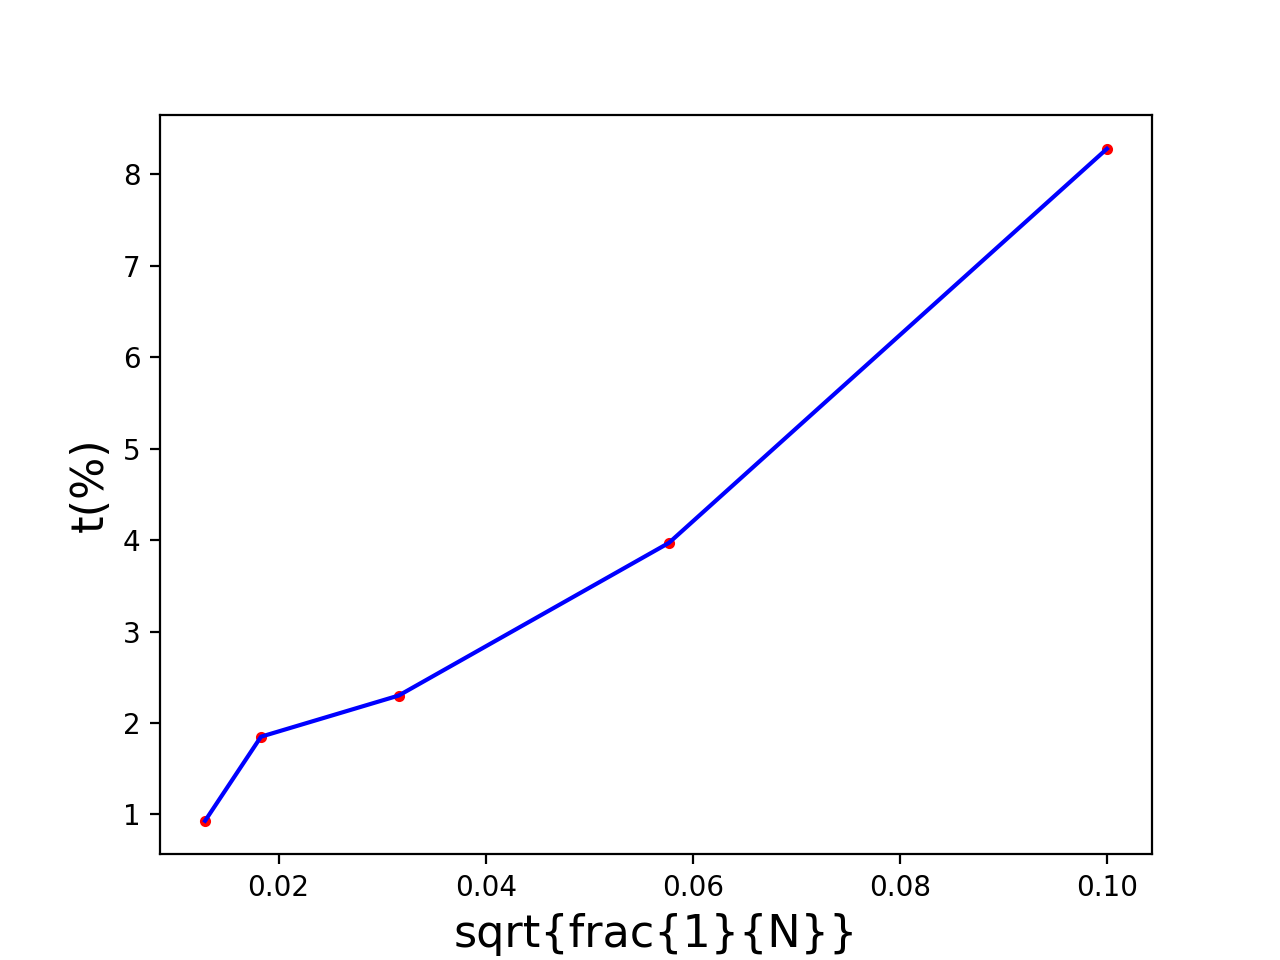
\includegraphics[width=0.7\textwidth]{linear1}
\end{figure}

\begin{figure}[!htbp]
\centering
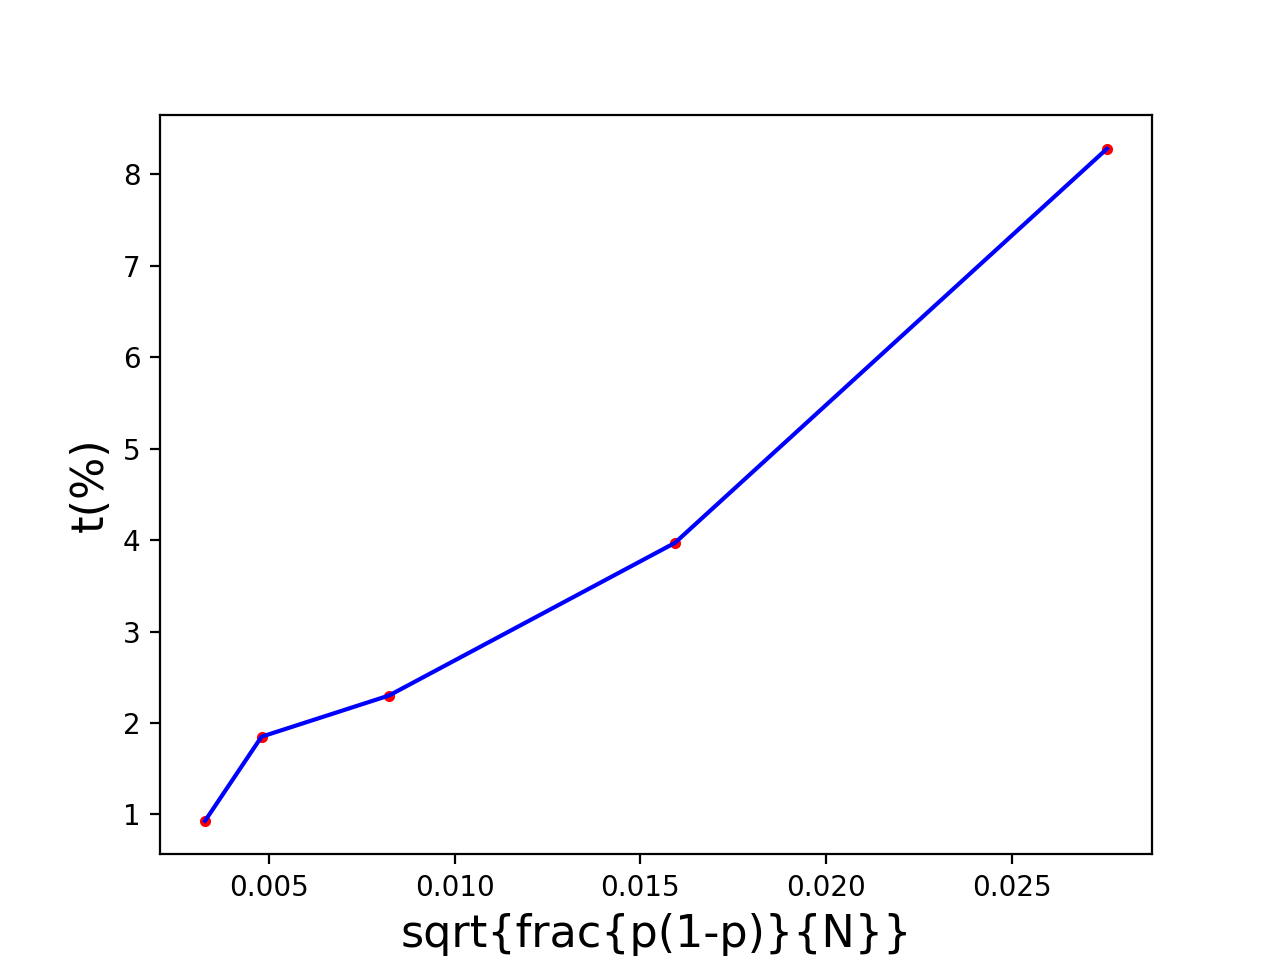
\includegraphics[width=0.7\textwidth]{linear2}
\end{figure}
\newpage
\subsection{Jinchao's summary}

Some ideas:

\begin{enumerate}
\item Given structure of DNN or CNN, sampling of the parameters can be
  viewed a dual sampling of the data variable.  This is because any
  DNN function can be written as a combination or composition of the
  functions of the following form
$$
\sigma(\omega\cdot x+b)
$$

\item CNN can be considered to be a multigrid algorithm for data
  variables.  Given the observation above, it is also a ``dual''
  multigrid algorithm for the parameter variables.   But somehow, in
  CNN, only small subspace of the dual subspace are used because the
  convolutional operation is a very special and low dimensional dual
  operation.   In order to increase the dimension of the dual, more
  layers and especially more channels have to be introduced. 

\item Data space variables are not really independent variables.  For
  a  2-D images, each image is a function of two variable which
  represents the pixel locations. 

\item Any 2D image function must have certain regularity. Thus a high
  resolution image is intrinsically low dimensional.   There are some
  underlying dimensions of the image data.  The different covolutions
  and different channels are introduced to capture these low
  dimensions. 

\item When a random initialization, it has been observed that the
  resulting DNN function is actually a relatively smooth function with
  respect to data variables. 
  But the finally trained NN model has to be high frequence functions
  for data variable as it is very sensitive to data pertubation. 

\item 
\end{enumerate}

\subsection{Huang's summary}

\subsubsection{MgNet Notation}
The main algorithm is given by: 
\begin{breakablealgorithm}
	\caption{$[u^1,u^2,\cdots,u^J]={\rm MgNet}(f; \Theta;J,\nu_1, \cdots, \nu_J)$}
	\label{alg:mgnet}
	\begin{algorithmic}
		\State Initialization:  $f^1 =\sigma \circ \theta(f)$, $u^{1,0}=0$
		%		\State Initialization $u^{1,0}$
		\For{$\ell = 1:J$}
		\For{$i = 1:\nu_\ell$}
		\State Feature extraction (smoothing):
		\begin{equation}\label{mgnet}
		u^{\ell,i} = u^{\ell,i-1} + B^{\ell,i}  ({f^\ell -  A^{\ell} (u^{\ell,i-1})}).
		\end{equation}
		\EndFor
		\State Note: 
		$
		u^\ell= u^{\ell,\nu_\ell} 
		$
		\State Interpolation and restriction:
		\begin{equation}
		\label{interpolation}
		u^{\ell+1,0} = \Pi_\ell^{\ell+1}u^{\ell}
		\end{equation}
		\begin{equation}
		\label{restrict-f}
		f^{\ell+1} = R^{\ell+1}_\ell(f^\ell - A^\ell(u^{\ell})) + A^{\ell+1} (u^{\ell+1,0}).
		\end{equation}
		\EndFor
	\end{algorithmic}
\end{breakablealgorithm}




\begin{itemize}
	\item $\Theta$ is the set consists all of parameters that needed to train
	\item $\theta (=f_{in})$: This is dependent with different data sets for standard ResNet and iResNet.
	\item $J$: the number of grids. As all images in CIFAR-10 or CIFAR-100
	are $32\times 32 \times 3$,  we choose $J = 4$ to be consistent with ResNet.
	\item $\nu_\ell$:  the number of smoothings in each grids. To be consistent with
	ResNet-18 or ResNet-34 we choose $\nu_\ell = 2$ or $\nu_\ell = 4$.
	\item $c^\ell_u$ and $c^\ell_f$: the number of feature and data channels. 
	\item $A^\ell$: the data-feature mapping. We choose the linear case in 
	\item $B^{\ell,i}$: the feature extractor.
	\item $R_{\ell}^{\ell+1}$: the restriction operator in 
	Here we choose it as a convolution with stride $2$ which need to be trained.
	\item $\Pi_\ell^{\ell+1}$: the interpolation operator in
	\eqref{interpolation}.  
\end{itemize}


The logistic regression is give by:
\begin{breakablealgorithm}
	\caption{$[p]={\rm LR}(x; \omega)$}
	\label{alg: LR}
	\begin{algorithmic}
		\For{$i = 1:k$}
		\begin{equation}
		g^{i} = \sum_{j=1}^{n}\omega_{i,j}*x_j
		\end{equation}
		\EndFor
		\For{$i = 1:k$}
		\begin{equation}
		p^{i} = \frac{e^{g^i}}{\sum_{t=1}^{k}e^{g^t}}
		\end{equation}
		\EndFor		
	\end{algorithmic}
\end{breakablealgorithm}

\begin{itemize}
	\item  $x \in \mathbf{R}^n$ is input data
	\item n is input size
	\item k is output size, for cifar100, k is 100
	\item $\omega$ is the set consists all of parameters that needed to train
\end{itemize}


In general, the complete classification model is given by: 
%\begin{align}
%[u^1, u^2, \cdots, u^J] & = MgNet(f; J, \nu_1,\cdots,\nu_J)  \\ 
%u^{J_0} & = \tilde{\Pi}_{J}^{J_0}(u^J) \\
%p & = LR(u^{J_0};)  \label{o=fc}
%\end{align}

\begin{breakablealgorithm}
	\caption{$[p]={\rm Classification}(f; \Theta,\omega)$}
	\begin{algorithmic}
		\begin{equation}
		[u^1, u^2, \cdots, u^J,f^1,f^2,\cdots,f^J]  = MgNet(f; \Theta; J, \nu_1,\cdots,\nu_J)
		\end{equation}
		\begin{equation}
		u^{J_0} = \tilde{\Pi}_{J}^{J_0}(u^J)
		\end{equation}
		\begin{equation}
		p  = LR(u^{J_0};)
		\end{equation}
	\end{algorithmic}
\end{breakablealgorithm}

Here, $J_0$ deppends on input data size, for cifar, $J_0$ is always equal to 6; $\tilde{\Pi}_{J}^{J_0}$ is a simple average that decrease data from grid J to gird $J_0$.

\subsubsection{Get Linear Seperate Data By some feature extraction}
In this subsection, we want to find some model to map raw data to linear seperable. Further more, we want get good validation by minimize the feature size.

\paragraph{Summary}
\begin{itemize}
	\item For cifar100, we can find a map composed of convolutions and this map makes data size from 3*32*32 to 8*16*16 and being linear seperable
	\item We can not get good validtion accuracy through this way. The best validation we get is only 30\%
	\item Linear seperable is to easy to get for finite data set
\end{itemize}

\paragraph{Algorithm in this subsubsection}
We introduced a training algorithm called Two-Stage-Algorithm here in order to the job metioned above.



This two stage training can be written as:

\begin{breakablealgorithm}
	\caption{$[\hat{\omega}_1]={\rm Two \ Stage \ Training}(\{f_i\}_1^N; \{label_i\}_1^N,\Phi,J,\nu_1, \cdots, \nu_J)$}
	\label{two stage training}
	\begin{algorithmic}
		\State First Stage
		\begin{equation}
		\Theta_0,\omega_0 = \arg \min_{\Theta,\omega} \sum_{i=1}^N Loss(p_i, label_i )
		\end{equation}
		\begin{equation}
		Where\  p_i = Classification(f_i; \Theta,\omega)  \label{stage 1}
		\end{equation}
		\State Second Stage
		\For{$i = 1:N$}
		\State extraction feature
		\begin{equation}
		[u_i^1,u_i^2,\cdots,u_i^J,f_i^1,f_i^2,\cdots,f_i^J]={\rm MgNet}(f_i; \Theta_0;J,\nu_1, \cdots, \nu_J) 
		\end{equation}
		\begin{equation}
		\hat{f}_i = \Phi([u_i^1,u_i^2,\cdots,u_i^J,f_i^1,f_i^2,\cdots,f_i^J])
		\end{equation}
		\EndFor
		\begin{equation}
		\hat{\omega}_1 = \arg \min_{\hat{\omega}} \sum_{i=1}^N Loss(\hat{p}_i, label_i )
		\end{equation}
		\begin{equation}
		Where\  \hat{p}_i = LR(\hat{f}_i; \hat{\omega}) \label{stage 2}
		\end{equation}
	\end{algorithmic}
\end{breakablealgorithm}
Here $\Phi$ is a map to get feature from the output of MgNet. This $\phi$ could be choosen as:
\begin{itemize}
	\item some simple map, like average or identity
	\item some trainable map, like convolution
\end{itemize}

For First case, we just need algorithm \ref{two stage training}.But for second case, we introduced a new algorithm base on \ref{two stage training}, it can be find in \ref{two stage training 2}. 
\begin{breakablealgorithm}
	\caption{$[\hat{\omega}_2]={\rm Two \ Stage \ Training \ With \ Trainable\  \Phi \ }(\{f_i\}_1^N; \{label_i\}_1^N,\Phi(\cdot;\cdot),J,\nu_1, \cdots, \nu_J)$}
	\label{two stage training 2}
	\begin{algorithmic}
		\State First Stage
		\begin{equation}
		\Theta_0,\omega_0 = \arg \min_{\Theta,\omega} \sum_{i=1}^N Loss(p_i, label_i )
		\end{equation}
		\begin{equation}
		Where\  p_i = Classification(f_i; \Theta,\omega) 
		\end{equation}
		\State Second Stage
		\For{$i = 1:N$}
		\State extraction feature
		\begin{equation}
		[u_i^1,u_i^2,\cdots,u_i^J]={\rm MgNet}(f_i; \Theta_0;J,\nu_1, \cdots, \nu_J) 
		\end{equation}
		\EndFor
		\begin{equation}
		\hat{\omega}_1,\hat{\Theta}_1 = \arg \min_{\hat{\omega},\hat{\Theta}} \sum_{i=1}^N Loss(\hat{p}_i, label_i )
		\end{equation}
		\begin{equation}
		Where\  \hat{p}_i = LR(\Phi([u_i^1,u_i^2,\cdots,u_i^J];\hat{\Theta}); \hat{\omega})
		\end{equation}
		\State finetune
		\For{$i = 1:N$}
		\begin{equation}
		\hat{f}_i = \Phi([u_i^1,u_i^2,\cdots,u_i^J]; \hat{\Theta}_1)
		\end{equation}
		\EndFor
		\begin{equation}
		\hat{\omega}_2 = \arg \min_{\hat{\omega}} \sum_{i=1}^N Loss(\hat{f}_i, \hat{\omega_1}), label_i )
		\end{equation}
	\end{algorithmic}
\end{breakablealgorithm}

\paragraph{numerical results}
In each table, we record the model hyper-parameters in table caption, and
\begin{itemize}
	\item the first column is the result of map $\Phi(\cdot)$
	\item the second column is the training accuracy in stage-1 \ref{stage 1}, which called mgnet training accuracy
	\item the thrid column is the training accuracy in stage-2 \ref{stage 2}, which called linear model training accuracy
	\item the 4th column is the sum of parameters number of alg\ref{alg:mgnet} and alg\ref{alg: LR}, which called MgNet parameters
	\item the 5th column is the feature size mapped by $\Phi$, which called feature size or input size for linear
\end{itemize}

With changeless $\Phi$, the results is in table \ref{case1 with 4 grids} and tabel \ref{case1 with 1 grids}
\begin{table}[!htbp]
	\caption{algorithm \ref{two stage training},$J=4, \nu_1=2,\nu_2=2,\nu_3=2,\nu_4=2,c_u^\ell=c_f^\ell=8$}
	\label{case1 with 4 grids}
	\begin{center}
		\resizebox{\textwidth}{!}{
			\begin{tabular}{|c|c|c|c|c|}
				\hline
				$\Phi(\cdot)$ & mgnet training accuracy & linear model training accuracy
				& parameters for mgnet & feature size\tabularnewline
				\hline
				$u^1$,  & 32.4 &  99.996 & 9644 &
				8\(*\)1024\tabularnewline
				\hline
				$u^2$,  & 32.4& 90.1 & 9644 &
				8\(*\)256\tabularnewline
				\hline
				$u^3$,  & 32.4 &  44.44 & 9644 &
				8\(*\)64\tabularnewline
				\hline
				$u^4$,  & 32.4 &  35.6 & 9644 &
				8\(*\)16\tabularnewline
				\hline
				$[u^1,u^2,u^3,u^4]$  &    32.4 &  99.96 & 9644 &
				10800=32*32+16*16+8*8+4*4\tabularnewline
				\hline
				$([\tilde{\Pi}_1^2(u^1),\tilde{\Pi}_2^3(u^2),\tilde{\Pi}_3^4(u^3),u^4])$  &  32.4 &  98.546 & 9644 &
				2720=16*16+8*8+4*4+2*2\tabularnewline
				\hline
				$[\tilde{\Pi}_1^2(u^1),u^2,u^3,u^4])$ &  32.4 &  99.996 & 9644 &
				4736=16*16+16*16+8*8+4*4\tabularnewline
				\hline
				$([\tilde{\Pi}_1^4(u^1),\tilde{\Pi}_2^4(u^2),\tilde{\Pi}_3^4(u^3),(u^4)])$   &   32.4&  50.34 & 9644 &
				512=4*4+4*4+4*4+4*4\tabularnewline
				\hline				
			\end{tabular} 
		}
	\end{center}
\end{table}


\begin{table}[!htbp]
	\caption{algorithm \ref{two stage training}:$J=1,\nu_1=2,c_u^1=c_f^1=8$,case1: one grid's feature}
	\label{case1 with 1 grids}
	\begin{threeparttable}
		
		\begin{center}
			\resizebox{\textwidth}{!}{
				\begin{tabular}{|c|c|c|c|c|}
					\hline
					$\Phi(\cdot)$ & mgnet training accuracy & linear model training  accuracy
					& mgnet parameters & input size for linear\tabularnewline
					\hline
					$u^1$  &  20.7  &  99.996 & 2348 &
					8192\tabularnewline
					\hline	
					$f^1$  &  20.7  &  99.89 & 2348 &
					8192\tabularnewline
					\hline
					$(Lian)u^1$  &  18.6980  &  99.9967 & 2348 &
					8192\tabularnewline
					\hline	
					$(Lian)f^1$  &  18.6980  &  99.9550 & 2348  &
					8192\tabularnewline
					\hline
					$(Lian)\hat{BN}(\hat{\theta}(f))^{*}$  &  18.6980  & 53.395 & 2348  &
					8192\tabularnewline
					\hline	
					$\tilde{\Pi}_1^2(u^1)$  &   \red{20.7}   &  95 & 2348 &
					2048\tabularnewline
					\hline	
					$\tilde{\Pi}_1^3(u^1)$  &   \red{20.7}  &  35 & 2348 &
					512\tabularnewline
					\hline
					$\tilde{\Pi}_1^4(u^1)$  &   \red{20.7}   &  29 & 2348 &
					128\tabularnewline
					\hline					
					$\tilde{\Pi}_1^6(u^1)$  &   \red{20.7}  &  21 & 2348 &
					8\tabularnewline
					\hline										
				\end{tabular} 
				
			}
			\begin{tablenotes}
				\footnotesize
				\item[*] $\hat{\theta}$ is the first conv in MgNet with parameters after training. $\hat{BN}$ is the BN layer Corresponding to $\hat{\theta}$.
			\end{tablenotes}
		\end{center}
		
	\end{threeparttable}
\end{table}
With trainable $\Phi$, the results is in table \ref{one conv with stride 2}
\begin{table}[!htbp]
	\caption{algorithm \ref{two stage training 2}: $J=1,\nu_1=2,c_u^1=c_f^1=8$,case4: with trainable layer}
	\label{one conv with stride 2}
	\begin{center}
		\resizebox{\textwidth}{!}{
			\begin{tabular}{|c|c|c|c|c|}
				\hline
				$\Phi(\cdot;\cdot)$ & mgnet training accuracy & linear model training accuracy(fine-tune)
				& mgnet parameters(conv and fc) & input size for linear\tabularnewline
				\hline
				$\Pi_1^{2,*}(u^1)$  &  \red{20.7}  &  99.978(99.996) & 2348 &
				2048\tabularnewline
				\hline	
				$\Pi_2^{3,*}(\Pi_1^{2,*}(u^1))$  &\red{20.7}  & \red{44.77(38.515)}  & 2348 &
				512\tabularnewline
				\hline
				$MgNet_{Linear}(u^1;J=2;\nu_1=2,\nu_2=2)$  &  \red{20.7}  & 87.56(99.996)  & 2348 &
				2048\tabularnewline
				\hline		
				$MgNet_{Linear}(u^1;J=2;\nu_1=0,\nu_2=2)$  &  \red{20.7}  & 84.1(99.996)  & 2348 &
				2048\tabularnewline
				\hline		
				$MgNet_{Linear}(u^1;J=3;\nu_1=2,\nu_2=2,\nu_3=2)$  &  \red{20.7}  & 51.37(-)  & 2348 &
				512\tabularnewline
				\hline														
		\end{tabular} }
	\end{center}
\end{table}


\subsubsection{MgNet: Activation Just In The First Grid}
For MgNet \ref{alg:mgnet}, we always share the convolutional kernel of B, namely:
\begin{equation}
A^{\ell,i} = \xi^{\ell}, \quad B^{\ell,i} = \sigma \circ  \eta^{\ell} \circ \sigma ,
\end{equation} 
Here, $\sigma=ReLU \circ BN$.

When we want to use different B, namely:
\begin{equation}
A^{\ell,i} = \xi^{\ell}, \quad B^{\ell,i} = \sigma \circ  \eta^{\ell,i} \circ \sigma ,
\end{equation} 
we will record it with mark $B^{\ell,i}$ at first column of each table.

In this subsubsetion, we remove the activation $\sigma$ except the first layer, that is 
\begin{equation}
\begin{split}
A^{1,i} = \xi^{1}, \quad B^{1,i} = \sigma \circ  \eta^{1} \circ \sigma , \\
A^{\ell,i} = \xi^{1}, \quad B^{\ell,i} =   \eta^{\ell} ,\ for \ \ell > 1 .
\end{split}
\end{equation}


\paragraph{summary}
\begin{itemize}
	\item only use activation in the first grid can get some good validation accuracy
	\item increasing all $c^\ell$ together always help, showed in table \ref{data setting3  channel 128}
	\item increasing $\nu_1$ always help when $\nu_1$ is not too big, showed in table \ref{data setting3  channel 128} and table \ref{different ite num in 2nd grid, not fix ell}
	\item when $\nu_\ell=0$ increasing $\nu_\ell, \ell>1$  always help, showed in table \ref{different ite num in 2nd grid} and table \ref{different ite num in 2nd grid, not fix ell-case0}
	
	\item when $\nu_\ell \geq 2$, increasing $\nu_\ell, \ell>1$ help model prevent over fitting and get higher training accuracy, but it's not help for validation, showed in table \ref{different ite num in 2nd grid case1}
	\item with small $c^1$, increasing $c^\ell, \ell=1$ is just good for training accuracy but not benifit for validation accuracy, showed in table \ref{different ite num in 2nd grid, not fix ell}
	\item sharing B increase validation accuracy in raw MgNet, showed in \ref{raw MgNet results}
	\item sharing B increase training accuracynot in MgNet remove some activation but not help for validation , show in \ref{data setting3  share B} 

\end{itemize}

We display some results as contrast first with raw MgNet \ref{alg:mgnet},The result is in table \ref{raw MgNet results}

Because this kind of model is very easy to get over-fiiting, we not only record the best validation accuracy in the whole training progress, but also record the validation accuracy in the last epoch behind the best one with  a pair of $()$
\begin{table}[!htbp]
	\caption{MgNet: raw version, nonlinear as in algorithm \ref{alg:mgnet} }
	\label{raw MgNet results}
	\begin{center}
		\resizebox{\textwidth}{!}{
			\begin{tabular}{|c|c|c|c|c|}
				\hline
				$[\nu_1,\nu_2,\cdots,\nu_J], c_\ell$,  & accuracy in training dataset &  accuracy in  validation best(last)
				& mgnet parameters & input size for FC\tabularnewline
				\hline
				[2,2,2,2], 256  &   99.99  &  79.94(79.67)  & 8,304,996 &
				256\tabularnewline
				\hline			
				[4,2,2,2], 256  &  99.99 & 80.25(80.02)  & 8,307,044 &
				256\tabularnewline
				\hline
				[2,2,2,2], 256, $B^{\ell,i}$  &   99.992  &  80.1(80.0) & 10,664,292 &
				256\tabularnewline
				\hline			
				[4,2,2,2], 256, $B^{\ell,i}$  &  99.992 & 80.3(80.1)  & 11,845,988 &
				256\tabularnewline
				\hline
				[2,0,0,0], 256  &   99.90  &   72.68(72.04) & - &
				256\tabularnewline
				\hline		
				[2,1,1,1], 256  &   99.99  &   78.68(78.35) & - &
				256\tabularnewline
				\hline			
				[4,0,0,0], 256  &   99.98  &   74.67(74.09) & - &
				256\tabularnewline
				\hline
				[4,1,1,1], 256  &   99.99   &   78.71(78.47)  & - &
				256\tabularnewline
				\hline
				[4,4,4,4], 256  &  99.989 &  79.84(79.57)  & - &
				256\tabularnewline
				\hline
				[5,1,1,1], 256  &   99.98   &   78.6(78.43)  & - &
				256\tabularnewline
				\hline
				[8,0,0,0], 256  &   99.99   &  76.5(76.1)    & - &
				256\tabularnewline
				\hline
				[8,2,2,2], 256  &   99.99   &  80.32(80.12)    & - &
				256\tabularnewline
				\hline
				[16,2,2,2], 256  &   99.99   &  80.42(80.22)    & - &
				256\tabularnewline
				\hline
				[2,2,2,2],[512,512,512,512]  &   99.99   & 81.29(81.29)     & - 
				\tabularnewline
				\hline
				[2,4,4,4],[512,512,512,512]  &   99.99   & 80.95(80.90)    & - 
				\tabularnewline
				\hline
				[4,4,4,4],[512,512,512,512]  &   99.99   & 81.36(81.11)    & - 
				\tabularnewline
				\hline
				[2,2,2,2],[768,768,768,768]  &   99.99   & 81.74(81.67)     & - 
				\tabularnewline
				\hline
				[2,2,2,2],[1024,1024,1024,1024]  &   99.99   & 82.24(82.11)    & - 
				\tabularnewline
				\hline						
			\end{tabular} 
		}
	\end{center}
\end{table}

\begin{table}[!htbp]
	\caption{MgNet : activation just on the first grid}
	\label{data setting3  channel 128}
	\begin{center}
		\resizebox{\textwidth}{!}{
			\begin{tabular}{|c|c|c|c|c|}
				\hline
				$[\nu_1,\nu_2,\cdots,\nu_J], c_\ell$,  & accuracy in training dataset &  accuracy in  validation best(last)
				& mgnet parameters & input size for FC\tabularnewline
				\hline	
				[2,2,2,2], 128  &  86.32  & 63.78(62.2)  &  2,082,020&
				128\tabularnewline
				\hline			
				[4,2,2,2], 128  &  93.5  & 65.5(62.8)  & 2,083,044 &
				128\tabularnewline
				\hline	
				[8,2,2,2], 128  &  94.6 & 66.5(64.4)   & 2,085,092 &
				128\tabularnewline
				\hline
				[16,2,2,2], 128  &  97.8  &  66.7(64.97)  & 2,089,188 &
				128\tabularnewline
				\hline
				[2,2,2,2], 256  &   98  & 65.07(63.11)  & 8,292,708 &
				256\tabularnewline
				\hline			
				[4,2,2,2], 256  &  99.93  & 67.77(66.5)  & 8,294,756 &
				256\tabularnewline
				\hline			
				[8,2,2,2], 256  &  99.98  & 69.35(68.3)  & 8,298,852 &
				256\tabularnewline
				\hline
				[16,2,2,2], 256  &  99.98 & 69.89(69.48)  & 8,307,044 &
				256\tabularnewline
				\hline					
			\end{tabular} 
		}
	\end{center}
\end{table}

\begin{table}[!htbp]
	\caption{MgNet: activation just on the first grid; different ite num after 1st grid}
	\label{different ite num in 2nd grid}
	\begin{center}
		\resizebox{\textwidth}{!}{
			\begin{tabular}{|c|c|c|c|c|}
				\hline
				$[\nu_1,\nu_2,\cdots,\nu_J], c_\ell$,  & accuracy in training dataset &  accuracy in  validation best(last)
				& mgnet parameters & input size for FC\tabularnewline
				\hline
				[2,0,0,0], 128  &   97  & 62.5(56.2)  & 1,639,652 &
				128\tabularnewline
				\hline
				[2,2,2,2], 128  &  86.32  & 63.78(62.2)  &  2,082,020&
				128\tabularnewline
				\hline
				[2,4,2,2], 128  &   87  & 63.9(62.4)  & 2,082,020 &
				128\tabularnewline
				\hline
				[2,8,2,2], 128  &  87.3  & 63.6(62.7)  & 2,082,020 &
				128\tabularnewline
				\hline
				[2,2,2,2], 256  &   98  & 65.07(63.11)  & 8,292,708 &
				256\tabularnewline
				\hline
				[2,4,2,2], 256  &   99.25  & 65.0(63.2)  & 8,292,708 &
				256\tabularnewline
				\hline
				[2,8,2,2], 256  &   99.19  & 64.9(63.67)  & 8,292,708 &
				256\tabularnewline
				\hline
				[8,0,0,0], 128  &   99.9  & 65.3(60.8)  & 1,642,724 &
				128\tabularnewline
				\hline
				[8,2,2,2], 128  &  94.6 & 66.5(64.4)   & 2,085,092 &
				128\tabularnewline
				\hline						
			\end{tabular} 
		}
	\end{center}
\end{table}

\begin{table}[!htbp]
	\caption{MgNet: activation just on the first grid; different $c_\ell$}
	\label{different ite num in 2nd grid, not fix ell-case0}
	\begin{center}
		\resizebox{\textwidth}{!}{
			\begin{tabular}{|c|c|c|c|c|}
				\hline
				$[\nu_1,\nu_2,\cdots,\nu_J], [c_1,c_2,c_3,c_4]$,  & accuracy in training dataset &  accuracy in  validation best(last)
				& mgnet parameters \tabularnewline
				\hline
				[2,0,0,0], [128,256,256,256]  &   98.6   & 61.9(58.0)  &-
				\tabularnewline
				\hline				
				[2,2,2,2], [128,256,256,256]  &   98.1  & 65.1(61.5)  &-
				\tabularnewline
				\hline
				
			\end{tabular} 
		}
	\end{center}
\end{table}

\begin{table}[!htbp]
	\caption{MgNet: activation just on the first grid; different ite num after 1st grid}
	\label{different ite num in 2nd grid case1}
	\begin{center}
		\resizebox{\textwidth}{!}{
			\begin{tabular}{|c|c|c|c|c|}
				\hline
				$[\nu_1,\nu_2,\cdots,\nu_J], c_\ell$,  & accuracy in training dataset &  accuracy in  validation best(last)
				& mgnet parameters & input size for FC\tabularnewline
				\hline
				[2,0,0,0], 128  &   97  & 62.5(56.2)  & 1,639,652 &
				128\tabularnewline
				\hline
				[2,2,2,2], 128  &  86.32  & 63.78(62.2)  &  2,082,020&
				128\tabularnewline
				\hline
				[2,4,2,2], 128  &   87  & 63.9(62.4)  & 2,082,020 &
				128\tabularnewline
				\hline
				[2,8,2,2], 128  &  87.3  & 63.6(62.7)  & 2,082,020 &
				128\tabularnewline
				\hline
				[2,2,2,2], 256  &   98  & 65.07(63.11)  & 8,292,708 &
				256\tabularnewline
				\hline
				[2,4,2,2], 256  &   99.25  & 65.0(63.2)  & 8,292,708 &
				256\tabularnewline
				\hline
				[2,8,2,2], 256  &   99.19  & 64.9(63.67)  & 8,292,708 &
				256\tabularnewline
				\hline						
			\end{tabular} 
		}
	\end{center}
\end{table}

\begin{table}[!htbp]
	\caption{MgNet: activation just on the first grid; different $c_\ell$}
	\label{different ite num in 2nd grid, not fix ell}
	\begin{center}
		\resizebox{\textwidth}{!}{
			\begin{tabular}{|c|c|c|c|c|}
				\hline
				$[\nu_1,\nu_2,\cdots,\nu_J], [c_1,c_2,c_3,c_4]$,  & accuracy in training dataset &  accuracy in  validation best(last)
				& mgnet parameters \tabularnewline
				\hline
				[2,2,2,2], [8,128,128,128]  &   40  & 43.3(42.3)  &-
				\tabularnewline
				\hline
				[2,2,2,2], [8,512,512,512]  &   40  & 42.8(42.7)  &-
				\tabularnewline
				\hline	
				[2,2,2,2], [16,128,128,128]  &   49  & 49.9(49.7) &-
				\tabularnewline
				\hline
				[2,2,2,2], [16,256,256,256]  &   49  & 50.2(49.8)  &-
				\tabularnewline
				\hline
				[2,2,2,2], [64,128,128,128]  &   71  & 60.9(60.7) &-
				\tabularnewline
				\hline
				[2,2,2,2], [64,256,256,256]  &   72  & 61.7(61.6)  &-
				\tabularnewline
				\hline
				[2,2,2,2], [128,128,128,128]  &  86.32  & 63.78(62.2)  &  -
				\tabularnewline
				\hline				
				[2,2,2,2], [128,256,256,256]  &   98.1  & 65.1(61.5)  &-
				\tabularnewline
				\hline	
			\end{tabular} 
		}
	\end{center}
\end{table}

\begin{table}[!htbp]
	\caption{MgNet : with $B^{\ell,i}$}
	\label{data setting3  share B}
	\begin{center}
		\resizebox{\textwidth}{!}{
			\begin{tabular}{|c|c|c|c|c|}
				\hline
				$[\nu_1,\nu_2,\cdots,\nu_J], c_\ell$,  & accuracy in training dataset &  accuracy in  validation best(last)
				& mgnet parameters & input size for FC\tabularnewline
				\hline	
				[8,2,2,2], 128  &  94.6 & 66.5(64.4)   & 2,085,092 &
				128\tabularnewline
				\hline
				[8,2,2,2], 128,$B^{\ell,i}$  &  99.99 & 63.8(63.02)    &  4,444,388 &
				128\tabularnewline
				\hline				
			\end{tabular} 
		}
	\end{center}
\end{table}


\paragraph{the influence with BN in linear layer}
Because Batch-Normalization is also a linear opearation, we design some experiment to check whether the BN help withoud actionvation, namely:
\begin{equation}
A^{1,i} = \xi^{1}, \quad B^{1,i} = \sigma \circ  \eta^{1} \circ \sigma , 
\end{equation}
\begin{equation}
A^{\ell,i} = \xi^{1}, \quad B^{\ell,i} =  BN \circ \eta^{\ell} \circ BN ,\ for \ \ell > 1 .
\end{equation}
The results are in \ref{data setting3 BN}. It showed that:

\begin{itemize}
	\item BN without relu help training accuracy, and it can work with bigger lr which makes computation overflow without BN
	\item BN without relu enlarge over-fitting
\end{itemize}
BN help training accuracy, 
\begin{table}[!htbp]
	\caption{MgNet: activation just on the first grid, BN in every grids}
	\label{data setting3 BN}
	\begin{center}
		\resizebox{\textwidth}{!}{
			\begin{tabular}{|c|c|c|c|c|}
				\hline
				$[\nu_1,\nu_2,\cdots,\nu_J], c_\ell$,  & accuracy in training dataset &  accuracy in  validation best(last) 
				& mgnet parameters & input size for FC\tabularnewline
				\hline		
				[8,2,2,2], 128, lr=0.01  &  94.6 & 66.5(64.4)   & 2,085,092 &
				128\tabularnewline
				\hline	
				[8,2,2,2], 128, lr=0.1  &  failure(overflow) & failure(overflow)   & 2,085,092 &
				128\tabularnewline
				\hline
				[8,2,2,2], 256, lr=0.01  &  99.98  & 69.35(68.3)  & 8,298,852 &
				256\tabularnewline
				\hline
				[8,2,2,2], 128, BN,lr=0.01  &  99.976  & 64.15(57.8)  & 2,089,700 &
				128\tabularnewline
				\hline
				[8,2,2,2], 128, BN,lr=0.1  &  96.5  & 65.56(59.11)  & 2,089,700 &
				128\tabularnewline
				\hline
				[8,2,2,2], 256, BN,lr=0.1  &  99.99  & 70.07(67.15)  & 8,308,068 &
				256\tabularnewline
				\hline
			\end{tabular} 
		}
	\end{center}
\end{table}


\subsubsection{MgNet: share same kernel in every grids}
In this sussubsection, we use the same convolutional kernel in every grid, namely:
\begin{equation}
A^{\ell,i} = \xi, \quad B^{\ell,i} = \sigma \circ  \eta \circ \sigma ,
\end{equation}
\begin{equation}
R_{\ell}^{\ell+1} = \eta^{R} \circ \sigma, \quad \Pi_{\ell}^{\ell+1} = \sigma \circ  \eta^{\Pi} ,
\end{equation}

Here, $\xi,\eta,\eta^{R},\eta^\Pi$ are convolution corresponding to $A,B,R,\Pi$, they are independent of the grid's index $\ell$ and iteration index $i$.The results in tabel \ref{MgNet: share cnn in all Grids} shows it can achieve some good validation accuracy by this model.And the parameters is just about one fourth of raw MgNet which we only share kernel inside each grid.

\paragraph{summary}
\begin{itemize}
\item use same kernel in every grid, it reduces the parameters to a quarter and still remains some good validation accuracy. see table \ref{MgNet: share cnn in all Grids}
\item increase channel is always good for validation. see table \ref{MgNet: share cnn in all Grids}
\item The validation accuracy when sharing cnn in all grids in table \ref{MgNet: share cnn in all Grids} is lower than which only sharing in one grid in \ref{raw MgNet results}. 
\end{itemize}

\begin{table}[!htbp]
	\caption{MgNet: share cnn in all Grids}
	\label{MgNet: share cnn in all Grids}
	\begin{center}
		\resizebox{\textwidth}{!}{
			\begin{tabular}{|c|c|c|c|c|}
				\hline
				$[\nu_1,\nu_2,\nu_3,\nu_4] [c_1,c_2,c_3,c_4]$,  & accuracy in training dataset &  accuracy in  validation best(last)
				& mgnet parameters \tabularnewline
				\hline
				[2,2,2,2],[128,128,128,128]  &   96.59  & 73.04  (72.5)  & 612,068
				\tabularnewline
				\hline
				[2,2,2,2],[256,256,256,256]  &   99.96  & 76.62(76.28)   & 2,403,684
				\tabularnewline
				\hline
				[2,8,2,2] ,[256,256,256,256]  &   99.98    & 77.08(76.53)    & -
				\tabularnewline
				\hline
				[8,2,2,2] ,[256,256,256,256]  &   99.98    & 77.54(77.09)    & -
				\tabularnewline
				\hline
				[16,2,2,2] ,[256,256,256,256]  &   99.98    & 77.51(77.01)    & -
				\tabularnewline
				\hline
				[3,3,3,3] ,[256,256,256,256]  &   99.98    & 76.94(76.48)    & -
				\tabularnewline
				\hline
				[4,4,4,4] ,[256,256,256,256]  &   99.98    & 77.40(77.12)    & -
				\tabularnewline
				\hline
				[2,2,2,2],[512,512,512,512]  &   99.99   & 79.61(79.21)    & - 
				\tabularnewline
				\hline
				[2,4,4,4],[512,512,512,512]  &   99.99   & 79.44(79.40)    & - 
				\tabularnewline
				\hline
				[4,4,4,4],[512,512,512,512]  &   99.99   & 80.23(79.96)    & - 
				\tabularnewline
				\hline
				[2,2,2,2],[768,768,768,768]  &   99.99   & 80.26(80.15)     & - 
				\tabularnewline
				\hline
				[2,2,2,2],[1024,1024,1024,1024]  &   99.99   & 81.30(81.23)    & - 
				\tabularnewline
				\hline
			\end{tabular} 
		}
	\end{center}
\end{table}

\paragraph{Big Channel Test for MgNet}

\begin{table}[!htbp]
	\caption{MgNet: $B^{\ell,i}=\sigma \circ \eta^{\ell} \circ \sigma,\quad c_\ell=c_1$}
	\begin{center}
				%	\resizebox{\textwidth}{!}{
		\begin{tabular}{|c|c|c|c|c|}
			\hline
			$[\nu_1,\nu_2,\cdots,\nu_J], c_\ell$,   &  test accuracy
			& parameters   \tabularnewline
			\hline
			[2,2,2,2], 256    &  79.94(79.67)  & 8.3M
			\tabularnewline
			\hline			
			[2,2,2,2],512     & 81.29(81.29)     & 33.1M
			\tabularnewline
			\hline
			[2,2,2,2],768   & 81.74(81.67)     & 74.4M 
			\tabularnewline
			\hline
			[2,2,2,2],1024    & 82.24(82.11)    & 132.2M 
			\tabularnewline
			\hline						
		\end{tabular} 
		%	}
	\end{center}
\end{table}

\begin{table}[!htbp]
	\caption{MgNet: $B^{\ell,i}=\sigma \circ \eta^{\ell} \circ \sigma$, increase$c_\ell$}
	\begin{center}
		%	\resizebox{\textwidth}{!}{
		\begin{tabular}{|c|c|c|c|c|}
			\hline
			$[\nu_1,\nu_2,\cdots,\nu_J], c_\ell$,  &  test accuracy
			& parameters  \tabularnewline
			\hline
			[2,2,2,2], [32,64,128,256]   &  74.95(74.75)  & 2.3M
			\tabularnewline
			\hline			
			[2,2,2,2], [64,128,256,512]      & 78.06(78.04)     & 12.5M
			\tabularnewline
			\hline
			[2,2,2,2],[128,256,512,1024]     & 80.29(80.28)      & 37.5M 
			\tabularnewline
			\hline
			[2,2,2,2],[256,512,1024,2048]     & 81.49(81.41)    & 150.0M 
			\tabularnewline
			\hline						
		\end{tabular} 
		%	}
	\end{center}
\end{table}

\newpage
\paragraph{MgNet:scale for B}
change \ref{mgnet} to a new version which scaler B by a scalar s
$$	u^{\ell,i} = u^{\ell,i-1} + s^{\ell,i} B^{\ell,i}  ({f^\ell -  A^{\ell} (u^{\ell,i-1})}).$$
\begin{table}[!htbp]
	\caption{MgNet:scale-B: $u^{\ell,i} = u^{\ell,i-1} + s^{\ell,i} \sigma \circ \eta^{\ell} \circ \sigma   ({f^\ell -  \xi^{\ell} (u^{\ell,i-1})}).$}
	\label{tabel:mgnet-scale}	
	\begin{center}
		\resizebox{\textwidth}{!}{
			\begin{tabular}{|c|c|c|c|c|}
				\hline
				$[\nu_1,\nu_2,\cdots,\nu_J], c_\ell, s^{\ell,i}$,  &  test accuracy
				& parameters  \tabularnewline
				\hline
				[2,2,2,2], 256, 1   &  79.78(79.45)   & -
				\tabularnewline
				\hline	
				[2,2,2,16], 256, 1   &  78.43(78.14)    & -
				\tabularnewline
				\hline		
				[2,2,2,32], 256, 1   & 77.99(77.60)    & -
				\tabularnewline
				\hline	
				[2,2,2,2], 256, 1,warm-up   &  79.93(79.61)   & -
				\tabularnewline
				\hline	
				[2,2,2,16], 256, 1 ,warm-up  & 79.50(79.23)   & -
				\tabularnewline
				\hline		
				[2,2,2,32], 256, 1 ,warm-up  &  79.39(79.22)     & -
				\tabularnewline
				\hline		
				[2,2,2,2], 256, $\frac{1}{\nu_\ell}$   &  79.54(79.31)    & -
				\tabularnewline
				\hline		
				[2,2,2,16], 256, $\frac{1}{\nu_\ell}$   & 79.04(78.79)     & -
				\tabularnewline
				\hline		
				[2,2,2,32], 256, $\frac{1}{\nu_\ell}$   &  78.85(78.35)   & -
				\tabularnewline
				\hline
				[2,2,2,2], 256, $\frac{1}{\nu_\ell}$,warm-up   &  79.75(79.47)     & -
				\tabularnewline
				\hline		
				[2,2,2,16], 256, $\frac{1}{\nu_\ell}$,warm-up   & 79.37(79.03)   & -
				\tabularnewline
				\hline		
				[2,2,2,32], 256, $\frac{1}{\nu_\ell}$ ,warm-up  &  79.12(78.89) & -
				\tabularnewline
				\hline
				[2,2,2,16], 256, $\frac{1}{\nu_\ell c_\ell}$   &  70.13(69.27)    & -
				\tabularnewline
				\hline		
				[2,2,2,16], 256, $\frac{1}{\nu_\ell c_\ell}$,warm-up   &  70.39(69.40)    & -
				\tabularnewline
				\hline
			\end{tabular} 
		}
	\end{center}
\end{table}


\begin{table}[!htbp]
	\caption{MgNet:scale-B: $u^{\ell,i} = u^{\ell,i-1} + s^{\ell,i} \sigma \circ \eta^{\ell} \circ \sigma   ({f^\ell -  \xi^{\ell} (u^{\ell,i-1})}).$}
	\label{tabel:mgnet-scale1}	
	\begin{center}
		\resizebox{\textwidth}{!}{
			\begin{tabular}{|c|c|c|c|c|}
				\hline
				$[\nu_1,\nu_2,\cdots,\nu_J], c_\ell, s^{\ell,i}$,  &  test accuracy
				& parameters  \tabularnewline
				\hline
				[2,2,2,2], 256, 1   &  79.78(79.45)   & -
				\tabularnewline
				\hline	
				[4,2,2,2], 256, 1  &   80.25(80.02)  &-
				\tabularnewline
				\hline
				[8,2,2,2], 256, 1  &     80.32(80.12)    & - 
				\tabularnewline
				\hline
				[16,2,2,2], 256 , 1 &     80.42(80.22)    & - 
				\tabularnewline
				\hline
				
				[2,2,2,2], 256, $\frac{1}{\nu_\ell}$   &  79.54(79.31)    & -
				\tabularnewline
				\hline		
				[2,2,2,2], 256, $\frac{1}{\nu_\ell}$,warm-up   &  79.75(79.47)     & -
				\tabularnewline
				\hline
				[4,2,2,2], 256, $\frac{1}{\nu_\ell}$   & 80.18(79.93)     & -
				\tabularnewline
				\hline		
				[4,2,2,2], 256, $\frac{1}{\nu_\ell}$,warm-up   &80.16(79.90)    & -
				\tabularnewline
				\hline		
				[8,2,2,2], 256, $\frac{1}{\nu_\ell}$   &   80.35(80.03)    & -
				\tabularnewline
				\hline
				[8,2,2,2], 256, $\frac{1}{\nu_\ell}$  ,warm-up &   79.97(79.65)   & -
				\tabularnewline
\hline
			\end{tabular} 
		}
	\end{center}
\end{table}

\begin{table}[!htbp]
	\caption{MgNet:increase channel:  increase $\nu_1$}
	\label{tabel:mgnet-0531}	
	\begin{center}
	\resizebox{\textwidth}{!}{
		\begin{tabular}{|c|c|c|c|c|}
		\hline
		$[\nu_1,\nu_2,\cdots,\nu_J], c_\ell, s^{\ell,i}$,  &  test accuracy
		& parameters  \tabularnewline
		\hline
		[2,2,2,2], [64,128,256,512]   &  78.24(78.22)   & -
		\tabularnewline
		\hline	
		[4,2,2,2], [64,128,256,512]  &   78.51(78.32)  &-
		\tabularnewline
		\hline
		[8,2,2,2], [64,128,256,512]  &     78.42(78.29)    & - 
		\tabularnewline
		\hline
		[16,2,2,2], [64,128,256,512]  &     78.25(78.12)    & - 
		\tabularnewline
		\hline
		
	\end{tabular} 
}
\end{center}
\end{table}

\newpage
\subsection{Juncai's summary}
\paragraph{Summary of learning rate schedule methods:}
\begin{itemize}
	\item Classical method: iteration for fixed epochs (30 or 50) and then reduce the learning rate by 1/10 or 1/2. 
	\item Adaptive learning rate: iteration for some epochs by monitoring some indicator and then reduce the learning rate by some factor (1/10 or 1/2) such as SASA.
	\item Cosine method: use the next formula
	\begin{equation}\label{key}
	\eta_t = \eta_{min} + \frac{1}{2}(\eta_{max} - \eta_{min}) (1 - \cos(\frac{t\pi}{T_{\max}})),
	\end{equation}
	where $T_{\max}$ is the global number of epochs.
\end{itemize}

\paragraph{Some observations:}
\begin{itemize}
	\item There should be a method between classical methods and Cosine method.
	\item How to reduce learning rate might be more important than when to reduce learning rate?
\end{itemize}

\paragraph{Summary for what we have in adaptive learning rate method:}
\begin{itemize}
	\item For SASA, we have the next observations (conclusions):
	\begin{itemize}
		\item This is only a method which tries to tell us when to reduce learning rate.
		\item When learning rate is very ``small'' (different models data sets, this small level may different), the criterion in this method is very difficult to hold. 
	\end{itemize}
	\item For epoch level criterion to check the stationary:
	\begin{itemize}
		\item Lian implemented it before, I will take over that code and try to fine-tune these hyper-parameters to make it works as a comparable criterion with SASA.
		\item I am thinking about to use this as the global stopping criterion method. This seems more difficult, I will focus on it after I am familiar with these codes.
	\end{itemize}
\end{itemize}

\paragraph{One suggestion from Prof. Xu on Mar. 14th, 2020 for global stopping criterion:}
\begin{itemize}
	\item 1. Do SASA first when learning rate is big enough.
	\item 2. Fix a thresholding, and if the criterion of SASA cannot hold within that number of epochs then switch to epoch level criterion.
	\item 3. When epoch level criterion holds, finish the training process.
\end{itemize}

\paragraph{Juncai's plan for this project:}
\begin{itemize}
	\item Be familiar with running these models with SASA on DGX-1.
	\begin{itemize}
	\item CIFAR10, for SASA with 300 epochs: 95.6\% test accuracy. (To verify the code)
	\item CIFAR100, SGD with cosine learning rate with ($T_{max}=1800$, $\eta_{max} = 0.1$ and $\eta_{min}=0.0001$). Now for 1350 epochs, I got the test accuracy 78.6\%. (Compared with Jianqing's results for FAA augmentation and same SGD with cosine learning rate, which needs 1800 epochs to have 80.3\% test accuracy.)
	\item Observation: from the test on CIFAR100, I doubt the efficiency of FAA. 
	\end{itemize}
	\item Based on Lian's implementation about epoch level criterion as learning rate schedule, try to run some comparable results for some classical models (ResNet and MgNet) on CIFAR 10 and 100 data sets. 
	\item Try to figure our a good global stopping criterion algorithm.
\end{itemize}


\subsection{Lian's summary}

\subsubsection{Random parameters and random labels}
\paragraph{Summary}
\begin{enumerate}
\item On Cifar100, the training accuracy is bigger than $99.9\%$ if we randomly generate the parameters in the input layer (8 channels)
\item On Cifar100, the training accuracy (on training+validation datasets) is $94\%$ if we randomly generate the labels and train the input layers (8 channels)
\item Deep neural networks easily fit random data. More experiments are shown in a paper. It means that the effective capacity of neural networks is sufficient for memorizing the data.
%\item Layers consisting of convolution following by pooling naturally
%become frequency selective and translation invariant when assigned random weights.
%\item The networks with random Gaussian weights perform a distance-preserving embedding of
%the data, with a special treatment for in-class and out-of-class data.
\end{enumerate}

\paragraph{Numerical results: random parameters}
Denote $f$ be the input image (size of $32*32$ in Cifar datasets), $\hat{\xi}$ is the convolutional layer with random parameters and $\hat{A}$ is the linear layer with random parameters, which are both not trained, and $\hat{\sigma}$ is the activation function.
We have two models:
\begin{itemize}
\item Model I
\begin{align}
	\hat{g}^1 & = \hat{\sigma}(\hat{A} (f))  \label{random conv eq} \\
	P & = LR(\hat{g}^1)
\end{align}
\item Model II 
\begin{align}
\hat{g}^1 & = \hat{\sigma}(\hat{\xi} (f))  \label{random conv eq} \\
P & = LR(\hat{g}^1)
\end{align}
\item Model III
\begin{align}
\hat{g}^1 & = \hat{\sigma}(BN(\hat{\xi} (Aug(f))))  \label{random conv eq} \\
P & = LR(\hat{g}^1)
\end{align}
\end{itemize}

We consider Kaiming He's initialization\cite{he2015delving} strategy to sample the random parameters of the convolutional layer $\hat{\xi}$ from uniform distribution $\mathcal{U}(-b,b)$, where $b$ is given by
\begin{equation}
	b = gain * \sqrt{\frac{3}{c_{in}*n_{in}*n_{in}}}
\end{equation}
where $c_{in}$ is the number of input channels, $n_{in}*n_{in}$ is size of each input channel and $gain$ depends on the the activation function, which is recommended in Pytorch as follows:
\begin{table}[H]
	\caption{gain values of different activation functions}
	\label{gain}
	\begin{center}
			\begin{tabular}{|c|c|}
				\hline
				Activation funtions & gain
				\tabularnewline \hline
				Linear/Identity & $1$
				\tabularnewline \hline
				Sigmoid   & $1$				 
				\tabularnewline \hline
				ReLu   & $\sqrt{2}	$	
				\tabularnewline \hline
				PReLu   & $\sqrt{\frac{2}{1+slope^2}}	$
				\tabularnewline \hline			 
			\end{tabular} 
	\end{center}
\end{table}

\begin{table}[H]
	\caption{Parametric ReLU (PReLU) performance on MNIST}
	\begin{center}
		\begin{tabular}{|c|c|c|}
			\hline
			$\alpha$ in PReLU & Training accuracy & Test accuracy
			\tabularnewline \hline
			1     & 93.4433  & 92.5000
			\tabularnewline \hline
			0.9   & 93.8050  & 92.7000				 
			\tabularnewline \hline
			0.8   & 96.0900	 & 95.3600
			\tabularnewline \hline
			0.7   & 97.2250  & 96.6900
			\tabularnewline \hline	
			0.6   & 99.2817  & 97.3400
			\tabularnewline \hline	
			0.5   & 100.0000 & 98.0500
			\tabularnewline \hline
			0.4   & 100.0000 & 98.1500
			\tabularnewline \hline	
			0.3   & 100.0000 & 98.2400
			\tabularnewline \hline	
			0.2   & 100.0000 & 98.2400
			\tabularnewline \hline	
			0.1   & 100.0000 & 98.4300
			\tabularnewline \hline	
			0.0   & 100.0000 & 98.3800
			\tabularnewline \hline		 
		\end{tabular} 
	\end{center}
\end{table}

MNIST, CIFAR
Input image: 3 * 32 *32 

Size of A: (3 * 32 * 32) * (N * 32 * 32 )

Size of LR: (N * 32 * 32 ) * 10 or 100 


INAGENET
Input image: 3 * 256 *256 

Size of A: (3 * 256 * 256) * (N *  256 * 256)

Size of LR: (N *  256 * 256 ) * 1000
 
 \paragraph{Model I: random fully connected layer}
\begin{table}[H]
	\caption{Training accuracy on Cifar100: Model I with $\hat{\sigma}=ReLU$}
	\begin{center}
		\resizebox{\textwidth}{!}{
			\begin{tabular}{|c|c|c|c|c|c|c|}
				\hline
				Input size for LR&  Test 1 & Test 2 &  Test 3 & Test 4 & Test 5 & Average
				\tabularnewline \hline
					3072 = 3 *32*32&99.9533&99.9550&99.9433&99.9550&99.9583&99.9530
					
					\tabularnewline \hline 
					
					4096 = 4 *32*32&99.9650&99.9700&99.9700&99.9650&99.9650&99.9670
					
					\tabularnewline \hline 
					
					5120 = 5 *32*32&99.9700&99.9717&99.9700&99.9700&99.9700&99.9703
					
					\tabularnewline \hline 
					
					6144 = 6 *32*32&99.9700&99.9700&99.9717&99.9717&99.9700&99.9707
					
					\tabularnewline \hline 
					
					7168 = 7 *32*32&99.9717&99.9717&99.9700&99.9717&99.9700&99.9710
					
					\tabularnewline \hline 
					
					8192 = 8 *32*32&99.9717&99.9717&99.9717&99.9700&99.9717&99.9714
					
					\tabularnewline \hline 
					
					9216 = 9 *32*32&99.9700&99.9717&99.9717&99.9700&99.9717&99.9710
					
					\tabularnewline \hline 
					
					10240 = 10 *32*32&99.9717&99.9717&99.9717&99.9717&99.9717&99.9717
					
					\tabularnewline \hline 

			\end{tabular} 
		}
	\end{center}
\end{table}

\begin{table}[H]
	\caption{Training accuracy on Cifar10: Model I with $\hat{\sigma}=ReLU$}
	\begin{center}
		\resizebox{\textwidth}{!}{
			\begin{tabular}{|c|c|c|c|c|c|c|c|}
				\hline
				Input size for LR&  Test 1 & Test 2 &  Test 3 & Test 4 & Test 5 & Average 
				\tabularnewline \hline
				3072 = 3 *32*32&60.8650&60.7700&61.1150&61.0933&61.1317&60.9950
				
				\tabularnewline \hline 
				
				5120 = 5 *32*32&74.5350&74.7100&74.7517&74.3033&74.4400&74.5480
				
				\tabularnewline \hline 
				
				10240 = 10 *32*32&99.7117&99.7033&99.7017&99.6800&99.7267&99.7047
				
				\tabularnewline \hline 
				
				15360 = 15 *32*32&99.9983&99.9967&99.9983&99.9950&100.0000&99.9977
				
				\tabularnewline \hline 
				
				20480 = 20 *32*32&100.0000&100.0000&100.0000&99.9983&99.9983&99.9993
				
				\tabularnewline \hline 
				
				25600 = 25 *32*32&100.0000&100.0000&100.0000&100.0000&100.0000&100.0000
				
				\tabularnewline \hline 
				
				30720 = 30 *32*32&100.0000&100.0000&100.0000&100.0000&100.0000&100.0000
				
				\tabularnewline \hline 
				
				35840 = 35 *32*32&100.0000&100.0000&100.0000&100.0000&100.0000&100.0000
				
				\tabularnewline \hline 
				
				40960 = 40 *32*32&100.0000&100.0000&100.0000&100.0000&100.0000&100.0000
				
				\tabularnewline \hline 
				
			\end{tabular} 
		}
	\end{center}
\end{table} 

 \paragraph{Model II: random convolutional layer}
\begin{table}[H]
	\caption{Training accuracy on ImageNet: Model II with $\hat{\sigma}=ReLU$}
	\begin{center}
		\resizebox{\textwidth}{!}{
			\begin{tabular}{|c|c|c|c|c|c|c|}
				\hline
				Input size for LR&  Test 1 & Test 2 &  Test 3 & Test 4 & Test 5 & Average
				\tabularnewline \hline
				196,608 = 3 *256*256& 95.2571  & 94.9728 &  95.3812&&&
				\tabularnewline \hline 
				262,144 = 4 *256*256& 98.6554  &&&&&
				\tabularnewline \hline 
				327,680 = 5 *256*256& 98.7532 &&&&&
				\tabularnewline \hline 
			\end{tabular} 
		}
	\end{center}
\end{table} 
 
\begin{table}[H]
	\caption{Training accuracy on Cifar100: Model II with $\hat{\sigma}=ReLU$}
	\begin{center}
		\resizebox{\textwidth}{!}{
			\begin{tabular}{|c|c|c|c|c|c|c|}
				\hline
				Input size for LR&  Test 1 & Test 2 &  Test 3 & Test 4 & Test 5 & Average
				\tabularnewline \hline
					3072 = 3 *32*32&79.4500&81.1517&97.1383&96.3117&89.5233&88.7150
					
					\tabularnewline \hline 
					
					4096 = 4 *32*32&98.9717&96.8517&95.1217&98.3650&97.6633&97.3947
					
					\tabularnewline \hline 
					
					5120 = 5 *32*32&99.7450&96.0617&98.1983&99.2117&99.2817&98.4997
					
					\tabularnewline \hline 
					
					6144 = 6 *32*32&99.9033&97.5550&99.0233&98.6183&99.9117&99.0023
					
					\tabularnewline \hline 
					
					7168 = 7 *32*32&99.7550&99.8650&99.9533&99.5967&99.5583&99.7457
					
					\tabularnewline \hline 
					
					8192 = 8 *32*32&99.7817&99.9683&99.9150&99.9550&99.8167&99.8873
					
					\tabularnewline \hline 
					
					9216 = 9 *32*32&99.8733&99.8533&99.9333&99.9483&99.9500&99.9116
					
					\tabularnewline \hline 
					
					10240 = 10 *32*32&99.9600&99.9483&99.9567&99.9583&99.9250&99.9497
					
					\tabularnewline \hline  
			\end{tabular} 
		}
	\end{center}
\end{table}
 
\begin{table}[H]
	\caption{Training accuracy on Cifar10: Model II with $\hat{\sigma}=ReLU$}
	\begin{center}
		\resizebox{\textwidth}{!}{
			\begin{tabular}{|c|c|c|c|c|c|c|c|}
				\hline
				Input size for LR&  Test 1 & Test 2 &  Test 3 & Test 4 & Test 5 & Average 
				\tabularnewline \hline
				3072 = 3 *32*32&48.0300&47.3517&49.8233&46.8650&47.1383&47.8417
				
				\tabularnewline \hline 	
				
				5120 = 5 *32*32&64.4733&60.7550&63.1050&60.3600&58.8317&61.5050
				
				
				\tabularnewline \hline 
				
				10240 = 10 *32*32&87.8200&83.2317&88.6333&83.6383&89.6933&86.6033
				
				
				\tabularnewline \hline 
				
				15360 = 15 *32*32&94.7167&95.2767&92.1033&95.7183&90.4150&93.6460
				
				\tabularnewline \hline 
				
				20480 = 20 *32*32&99.5717&96.2867&97.3233&98.0367&98.9650&98.0367
				
				
				\tabularnewline \hline 
				
				25600 = 25 *32*32&98.8783&97.3650&99.7300&97.2917&98.8050&98.4140
				
				\tabularnewline \hline 
				
				30720 = 30 *32*32&99.6717&99.8433&99.1417&99.5367&99.1783&99.4743
				
				\tabularnewline \hline 
				
				35840 = 35 *32*32&99.8967&99.9733&99.2300&98.6667&99.7283&99.4990
				
				\tabularnewline \hline 
				
				40960 = 40 *32*32&99.9300&99.9000&99.9750&99.7100&99.9683&99.8967
				
				\tabularnewline \hline 
			\end{tabular} 
		}
	\end{center}
\end{table} 
 
\begin{table}[H]
	\caption{Training accuracy on Cifar10: Model II with $\hat{\sigma}=ReLU$ (more detail)}
	\begin{center}
		\resizebox{\textwidth}{!}{
			\begin{tabular}{|c|c|c|c|c|c|c|c|}
				\hline
				Input size for LR&  Test 1 & Test 2 &  Test 3 & Test 4 & Test 5 & Average 
				\tabularnewline \hline
				3072 = 3 *32*32&48.0300&47.3517&49.8233&46.8650&47.1383&47.8417
				
				\tabularnewline \hline 
				
				4096 = 4 *32*32&56.7550&53.5600&60.7483&54.7633&54.2767&56.0207
				
				\tabularnewline \hline 
				
				5120 = 5 *32*32&64.4733&60.7550&63.1050&60.3600&58.8317&61.5050
				
				\tabularnewline \hline 
				
				6144 = 6 *32*32&66.8350&69.2233&69.7617&65.7967&70.7800&68.4793
				
				\tabularnewline \hline 
				
				7168 = 7 *32*32&75.4983&79.7833&73.3950&75.5067&74.3300&75.7027
				
				\tabularnewline \hline 
				
				8192 = 8 *32*32&78.2000&76.1533&76.5517&76.6567&75.5650&76.6253
				
				\tabularnewline \hline 
				
				9216 = 9 *32*32&85.6283&76.7517&74.6183&79.4350&87.4650&80.7797
				
				\tabularnewline \hline 
				
				10240 = 10 *32*32&87.8200&83.2317&88.6333&83.6383&89.6933&86.6033
				
				\tabularnewline \hline 
				
				11264 = 11 *32*32&92.6867&94.9533&86.8783&91.2450&83.5900&89.8707
				
				\tabularnewline \hline 
				
				12288 = 12 *32*32&87.9033&89.6683&90.3950&89.5400&86.0467&88.7107
				
				\tabularnewline \hline 
				
				13312 = 13 *32*32&96.3633&91.2550&95.8867&97.3350&93.6983&94.9077
				
				\tabularnewline \hline 
				
				14336 = 14 *32*32&98.6633&91.3750&94.7250&93.3917&90.1400&93.6590
				
				\tabularnewline \hline 
				
				15360 = 15 *32*32&94.7167&95.2767&92.1033&95.7183&90.4150&93.6460
				
				\tabularnewline \hline 
				
				16384 = 16 *32*32&97.1200&91.4600&95.1833&90.7650&96.4800&94.2017
				
				\tabularnewline \hline 
				
				17408 = 17 *32*32&98.0433&97.7500&97.0467&98.5350&97.5683&97.7887
				
				\tabularnewline \hline 
				
				18432 = 18 *32*32&97.9717&95.7883&97.0800&98.0850&98.0600&97.3970
				
				\tabularnewline \hline 
				
				19456 = 19 *32*32&99.9300&99.4317&97.4833&97.0167&98.5050&98.4733
				
				\tabularnewline \hline 
				
				20480 = 20 *32*32&99.5717&96.2867&97.3233&98.0367&98.9650&98.0367
				
				\tabularnewline \hline 
				
				21504 = 21 *32*32&95.5067&98.2767&99.1200&98.2317&95.2467&97.2764
				
				\tabularnewline \hline 
				
				22528 = 22 *32*32&97.3883&99.2517&99.8583&99.8933&99.1117&99.1007
				
				\tabularnewline \hline 
				
				23552 = 23 *32*32&97.3233&99.5717&99.1533&97.8083&98.9017&98.5517
				
				\tabularnewline \hline 
				
				24576 = 24 *32*32&99.5417&99.9333&98.4350&99.3700&97.6367&98.9833
				
				\tabularnewline \hline 
				
				25600 = 25 *32*32&98.8783&97.3650&99.7300&97.2917&98.8050&98.4140
				
				\tabularnewline \hline 
				
				26624 = 26 *32*32&98.8983&99.7517&98.9750&99.3433&98.2667&99.0470
				
				\tabularnewline \hline 
				
				27648 = 27 *32*32&99.8000&99.4550&99.4817&99.9433&99.6550&99.6670
				
				\tabularnewline \hline 
				
				28672 = 28 *32*32&98.0667&99.5717&99.5683&99.5383&98.6117&99.0713
				
				\tabularnewline \hline 
				
				29696 = 29 *32*32&99.9200&98.8050&98.0717&99.5967&99.5567&99.1900
				
				\tabularnewline \hline 
				
				30720 = 30 *32*32&99.6717&99.8433&99.1417&99.5367&99.1783&99.4743
				
				\tabularnewline \hline 
				
				31744 = 31 *32*32&99.9750&98.9017&99.7033&99.8417&99.2267&99.5297
				
				\tabularnewline \hline 
				
				32768 = 32 *32*32&98.2067&99.7150&99.4900&99.8617&98.6700&99.1887
				
				\tabularnewline \hline 
				
				33792 = 33 *32*32&99.7983&99.7733&99.0950&98.8767&98.7833&99.2653
				
				\tabularnewline \hline 
				
				34816 = 34 *32*32&95.9617&99.6050&99.9633&99.5900&99.1200&98.8480
				
				\tabularnewline \hline 
			\end{tabular} 
		}
	\end{center}
\end{table}
 
 
\begin{table}[H]
	\caption{Training accuracy on Cifar100: Model III with different $\hat{\sigma}$}
	\label{case1: random conv}
	\begin{center}
		\resizebox{\textwidth}{!}{
			\begin{tabular}{|c|c|c|c|c|c|c|}
				\hline
				input size for LR&  $\sigma=I$ & $\sigma=Sigmoid$ &  $\sigma=ReLU$ & $\sigma=PReLU(a=0.01)$ & $\sigma=PReLU(a=0.1)$ & $\sigma=PReLU(a=-1)$
				\tabularnewline \hline
				%$(Huang)\hat{g}^1$  &  95.2 & 8192\tabularnewline \hline
				$3072=3*32*32$  &  49.8233  & 34.1300 & 69.8917 & 80.825   & 66.6333 & 65.1267
				\tabularnewline \hline
				$4096=4*32*32$  &  44.7550  & 31.4300 & 84.7917 & 76.0700  &94.4833&  67.5783
				\tabularnewline \hline
				$5120=5*32*32$  &  55.6200  & 35.1467 & 92.2917 & 91.8433  &99.7317 &   99.6733
				\tabularnewline \hline
				$6144=6*32*32$  &  50.3050  & 35.7700 & 99.7450 & 99.8717  &97.2783&  97.8767
				\tabularnewline \hline
				$7168=7*32*32$  &  62.5033  & 46.0883 & 99.0450 & 99.7733  &99.9500&  99.9733
				\tabularnewline \hline
				$8192=8*32*32$  &  60.5050  & 37.5767 & 99.9600 & 99.9933  &99.9167&  99.8917
				\tabularnewline \hline
				$9216=9*32*32$  &  65.7700  & 35.5250 & 99.9617 & 99.9933  &99.9617&   99.9917
				\tabularnewline \hline
				$10240=10*32*32$&  55.4367  & 40.6433 & 99.9950 & 99.9933  &99.9717&  99.995
				\tabularnewline \hline
				$>10240$        & around 65 & around 40 & $>99.99$& $>99.99$&$>99.99$& $>99.99$
				\tabularnewline \hline
			\end{tabular} 
		}
	\end{center}
\end{table}

\begin{table}[H]
	\caption{Training accuracy on Cifar10: Model III with different $\hat{\sigma}$}
	\begin{center}
		\resizebox{\textwidth}{!}{
			\begin{tabular}{|c|c|c|c|c|c|c|c|}
				\hline
				input size for LR&  $\sigma=I$ & $\sigma=Sigmoid$ &  $\sigma=ReLU$ & $\sigma=PReLU(a=0.01)$ & $\sigma=PReLU(a=0.1)$ & $\sigma=PReLU(a=-1)$
				\tabularnewline \hline
				%$(Huang)\hat{g}^1$  &  95.2 & 8192\tabularnewline \hline
				$3072=3*32*32$  &  37.0300  & 35.6933 & 39.325    & 39.7700 &  &
				\tabularnewline \hline
				$4096=4*32*32$  &  37.3867  & 36.4867  & 39.9183   & 44.4617 & &
				\tabularnewline \hline
				$5120=5*32*32$  &  39.5583  & 37.4867  & 54.0567   & 49.6150 & &
				\tabularnewline \hline
				$6144=6*32*32$  &  38.3083  & 38.4683  & 57.0517   & 58.0633 & &
				\tabularnewline \hline
				$7168=7*32*32$  &  39.2117  & 39.8050  & 57.8367   & 65.4500 & &
				\tabularnewline \hline
				$8192=8*32*32$  &  39.5567  & 41.3833  & 64.5850    & 62.7417 & &
				\tabularnewline \hline
				$9216=9*32*32$  &  39.1150  & 40.9500  & 67.9933   & 70.9617 & &
				\tabularnewline \hline
				$10240=10*32*32$&  39.6850  & 38.3017  & 69.4217   & 73.5983 & &
				\tabularnewline \hline
				$11264=11*32*32$  & 41.0633   & 41.6183  & 71.2050 & 71.6667& &
				\tabularnewline \hline
				$12288=12*32*32$  & 39.7650   & 39.8017  & 85.0500 & 81.3350  & &
				\tabularnewline \hline
				$13312=13*32*32$  & 39.9983   &  43.4217 & 79.0333 & 84.9600 & &
				\tabularnewline \hline
				$14336=14*32*32$  & 39.6800   & 41.8933  & 77.0650  & 75.4400 & &
				\tabularnewline \hline
				$15360=15*32*32$& 39.4400   &   41.8483 & 85.9883   & 86.7567& &
				\tabularnewline \hline
				$16384=16*32*32$  & 40.2400   & 41.8300  & 94.8733 & 94.9183  & &
				\tabularnewline \hline
				$17408=17*32*32$  &    &   & 85.6983   &  & &
				\tabularnewline \hline
				$18432=18*32*32$  &    &   & 91.2150  &  & &
				\tabularnewline \hline
				$19456=19*32*32$  &    &   & 92.6283   &  & &
				\tabularnewline \hline
				$20480=20*32*32$&    &   & 95.5317  &  & &
				\tabularnewline \hline
				$21504=21*32*32$  &    &   & 95.5033   &  & &
				\tabularnewline \hline
				$22528=22*32*32$  &    &   & 97.9950   &  & &
				\tabularnewline \hline
				$23552=23*32*32$  &    &   & 96.1267  &  & &
				\tabularnewline \hline
				$24576=24*32*32$  &    &   & 96.6367   &  & &
				\tabularnewline \hline
				$25600=25*32*32$&    &   & 95.5133  &  & &
				\tabularnewline \hline
				$26624=26*32*32$  &    &   & 95.9267   &  & &
				\tabularnewline \hline
				$27648=27*32*32$  &    &   & 94.8983  &  & &
				\tabularnewline \hline
				$28672=28*32*32$  &    &   & 98.7300  &  & &
				\tabularnewline \hline
				$29696=29*32*32$  &    &   & 98.8367   &  & &
				\tabularnewline \hline
				$30720=30*32*32$&    &   &  99.3833  &  & &
				\tabularnewline \hline
				$31744=31*32*32$  &    &  & 99.3650  &  & &
				\tabularnewline \hline
				$32768=32*32*32$  &    &  & 99.7283  &  & &
				\tabularnewline \hline
				$33792=33*32*32$  &    &   & 99.8317  &  & &
				\tabularnewline \hline
				$34816=34*32*32$  &    &   & 99.8461  &  & &
				\tabularnewline \hline
			\end{tabular} 
		}
	\end{center}
\end{table}
\begin{figure}[!htpt]
	\centering
	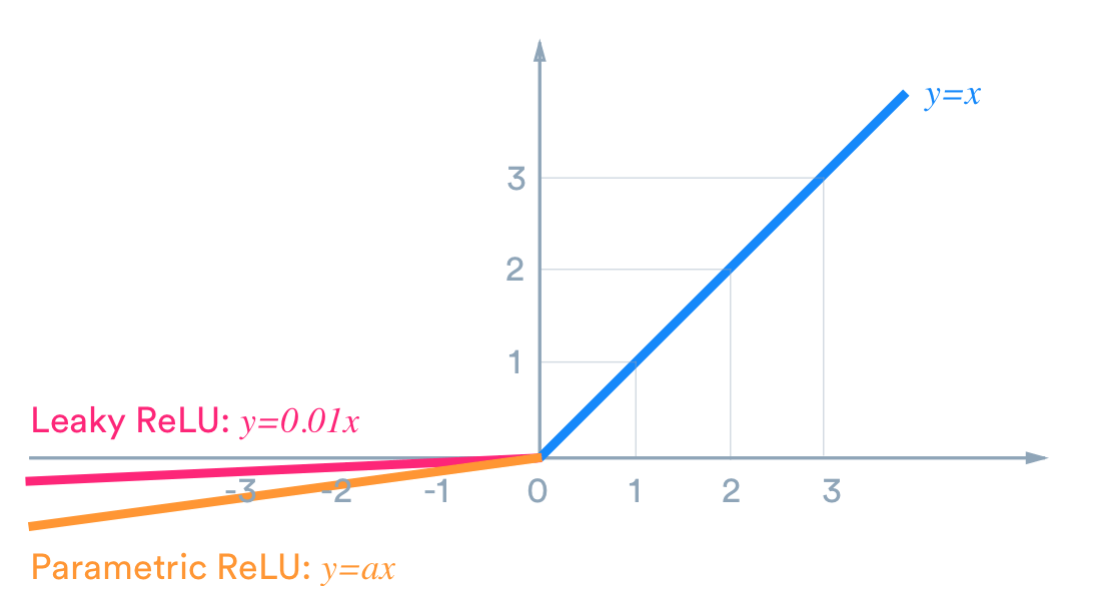
\includegraphics[width=0.8\textwidth]{LeakyReLU.png}
	\caption{LeakyReLU}.
	\label{LeakyReLU}
\end{figure}
Further, if we also randomize the labels, the training accuracy on Cifar100 (training+validation datasets) is $92\%$, which is shown in Table \ref{case1: random labels}
\begin{table}[H]
	\caption{On Cifar100: Random labels and input layer}
	\label{case1: random labels}
	\begin{center}
		\resizebox{\textwidth}{!}{
			\begin{tabular}{|c|c|c|c|c|}
				\hline
				$\Phi(\cdot)$&  training accuracy
				& input size for LR\tabularnewline
				\hline
				$\hat{g}^1$  &  92.9126 & 
				8192\tabularnewline
				\hline																
			\end{tabular} 
		}
	\end{center}
\end{table}
A paper did more experiments on random data, the main results are shown in Fig. \ref{randomdata}
\begin{figure}[!htpt]
	\centering
	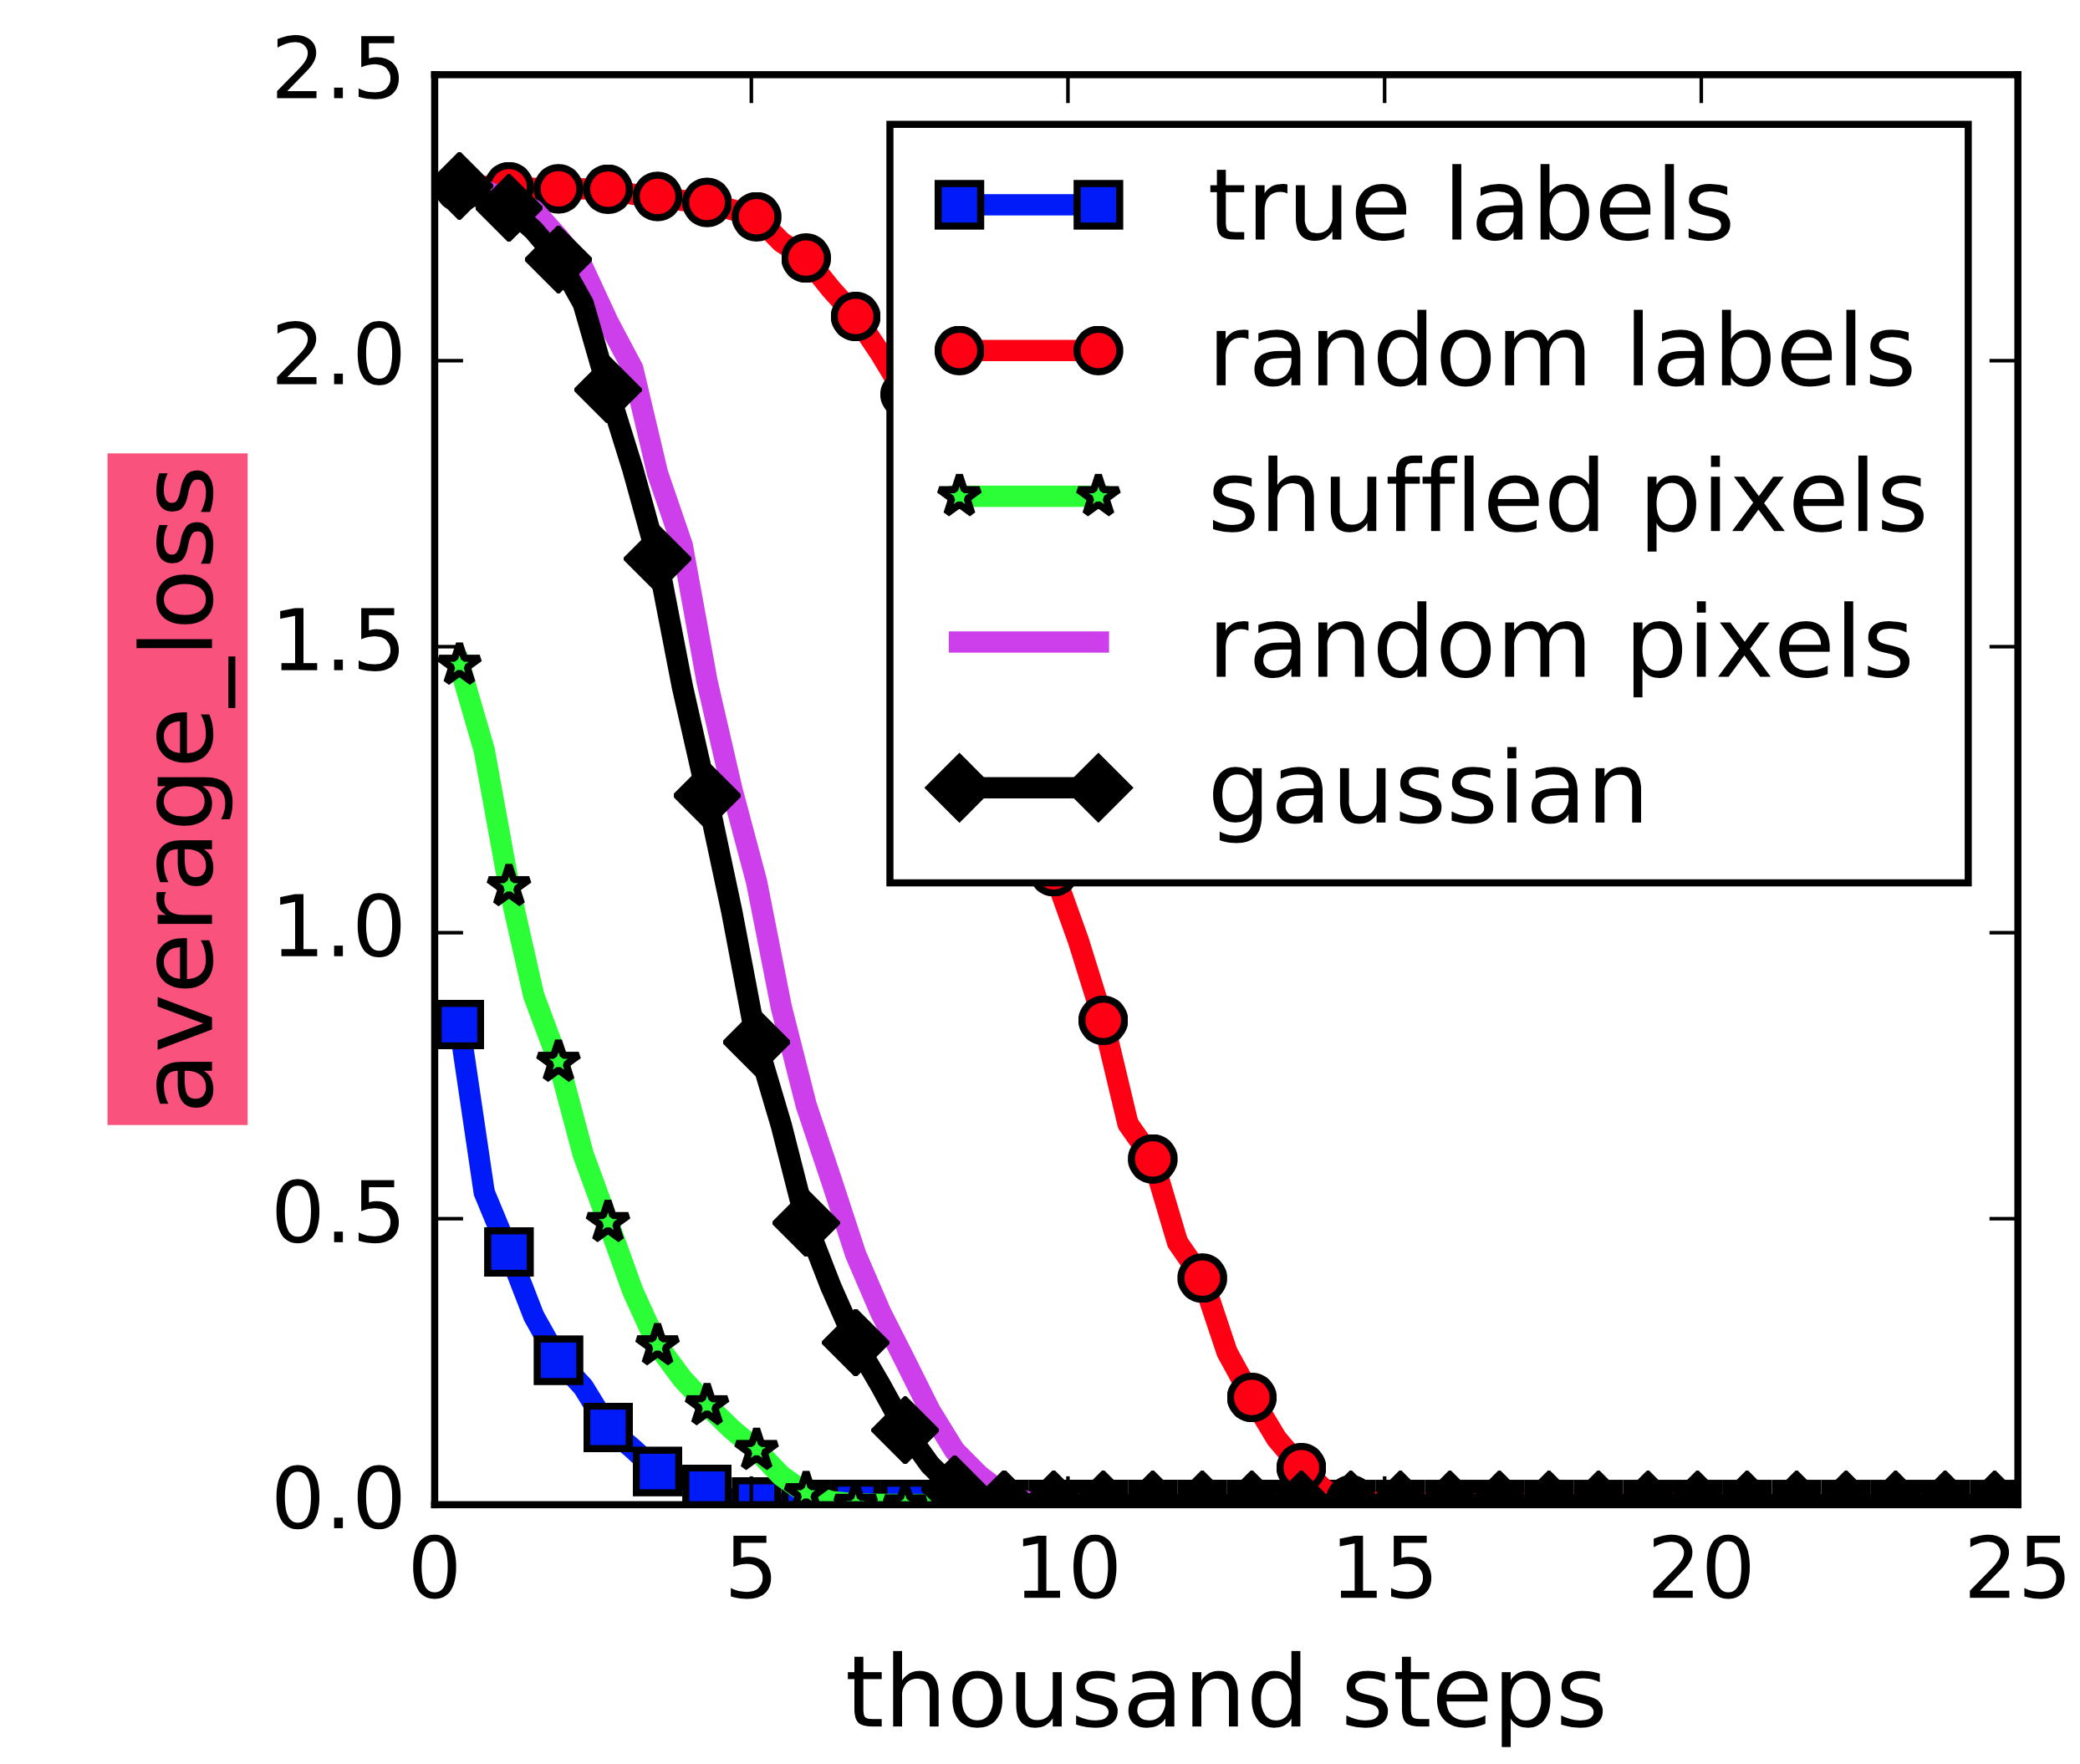
\includegraphics[width=0.8\textwidth]{randomdata.png}
	\caption{Fitting random labels and random pixels on CIFAR10 with AlexNet.
		(1) True labels: the original dataset without modification.
		(2) Random labels: all the labels are replaced with random ones.
		(3) Shuffled pixels: a random permutation of the pixels is chosen and then the same permutation is applied to all the images in both training and test set.
		(4) Random pixels: a different random permutation is applied to each image independently.
		(5) Gaussian:A Gaussian distribution(with matching mean and variance to the original image
		dataset) is used to generate random pixels for each image.}
	\label{randomdata}
\end{figure}
\subsubsection{Linearly separable on Cifar10}
\paragraph{Summary}
\begin{enumerate}
\item The smallest dimension of linearly separable new data, which is generated from Cifar10 raw data by nonliner transformations(convolution+BN+ReLU), is 8192.
\item Discussion: Linear separation is related to number of data, number of features, number of classes, number of data in each class.
\end{enumerate}

\paragraph{Numerical results}

\begin{itemize}
	\item Case 1: size 8192
\end{itemize}



\begin{align}
u^1 & MgNet(f; J=1, \nu_1=2)  \\
u^{6} & = \tilde{\Pi}_1^6(u^1) \\
p & = LR(u^6)
\end{align}
\begin{table}[H]
	\caption{ResNet18 on CIFAR-10: $J=1,\nu_1=2,c_f^1=c_u^1=8$, with the last average pooling}
	\label{case1 with 1 grids_cifar10}
	\begin{threeparttable}
		
		\begin{center}
			\resizebox{\textwidth}{!}{
				\begin{tabular}{|c|c|c|c|}
					\hline
					$\Phi(\cdot)$ & ResNet training accuracy & linear model training  accuracy
					& input size for LR\tabularnewline
					\hline
					$u^1$  &  25.7291  &  99.9933  &
					8192\tabularnewline
					\hline											
				\end{tabular} 
				
			}
		\end{center}
		
	\end{threeparttable}
\end{table}

\begin{align}
u^1 & = MgNet(f; J=1, \nu_1=2)  \\
p & = LR(u^1)
\end{align}


\begin{table}[H]
	\caption{ResNet18 on CIFAR-10: $J=1,\nu_1=2,c_f^1=c_u^1=8$, without the last average pooling}
	\label{case1: mgnet without last pooling}
	\begin{center}
		\resizebox{\textwidth}{!}{
			\begin{tabular}{|c|c|c|c|c|}
				\hline
				$\Phi(\cdot)$      & mgnet training accuracy & linear model training accuracy
				&  input size for LR
				\tabularnewline
				\hline
				$u^1$             &  68.808                                   & 99.997 
					          & 8192\tabularnewline
				\hline												
			\end{tabular} 
		}
		
	\end{center}
\end{table}



\begin{itemize}
\item Case 2: size 4096
\end{itemize}
\begin{align}
u^1 & = MgNet(f; J=1, \nu_1=2)  \\
u^{2} & = {\Pi}_1^2(u^1) \\
p & = LR(u^2)
\end{align}
\begin{table}[!htbp]
	\caption{ResNet18 on CIFAR-10: $J=1,\nu_1=2,c_f^1=c_u^1=8$, with stride 2 pooling (16 channels)}
	\begin{center}
		\resizebox{\textwidth}{!}{
			\begin{tabular}{|c|c|c|c|c|}
				\hline
				$\Phi(\cdot)$      & ResNet training accuracy & linear model training accuracy
				& input size for LR
				\tabularnewline
				\hline
				$u^2$             & 67.856                            & 82.345
				 		          & 4096\tabularnewline
				\hline												
			\end{tabular} 
		}
	\end{center}
\end{table}



\begin{itemize}
	\item Case 3: size 2048
\end{itemize}
\begin{table}[H]
	\caption{ResNet18 on CIFAR-10: $J=1,\nu_1=2,c_f^1=c_u^1=8$, with stride 2 pooling (8 channels)}
	\begin{center}
		\resizebox{\textwidth}{!}{
			\begin{tabular}{|c|c|c|c|c|}
				\hline
				$\Phi(\cdot)$      & ResNet training accuracy & linear model training accuracy
				& input size for LR
				\tabularnewline
				\hline
				$u^2$             &  67.54                                   & 73.455
				 		          & 2048\tabularnewline
				\hline												
			\end{tabular} 
		}
		
	\end{center}
\end{table}

\subsubsection{On Cifar100: linear transformations}
Given the linearly separable data $(x_i,y_i), i=1,2,...,6000$ generated from the Cifar100 raw data, we test various linear transformations followed by a logistic regression on the input data. As an example, we take the data with input size 2048 ($x_i\in \mathcal{R^2048}$).
\begin{itemize}
\item Case 1: $P_1(x_i;w_1)$ = $A_{100\times 2048}x_i$; $y_i$=Maxout($P_1$)\\
\item Case 2: $P_2(x_i;w_2)$ = $A_{100\times 256}A_{256\times 512}A_{512\times 1024}A_{1024\times 2048}x_i$; $y_i$=Maxout($P_2$)\\
\end{itemize}


\begin{table}[H]
	\caption{On Cifar100: linear transformations + logistic regression on linearly separable data (dimension 2048).}
	\begin{center}
		\resizebox{\textwidth}{!}{
			\begin{tabular}{|c|c|c|}
				\hline
				Case      &  training accuracy & validation accuracy
				\tabularnewline
				\hline
				1               & 99.998           & 16.17
				\tabularnewline				\hline
				2               & 99.96           & 15.26
				\tabularnewline
				\hline											
			\end{tabular} 
		}
	\end{center}
\end{table}


\subsubsection{A modified ResNet: activation function only imposed on the first grid}
In this subsection, we only impose activation functions (RuLU) on the first grid.
\begin{table}[H]
	\caption{ResNet18 on CIFAR-100: $J=4,\nu_1=\nu_2=\nu_3=\nu_4=2,c_f^1=c_u^1=64 (nonlinear),~ c_u^2=128,~c_u^3=256,~c_u^4=512$}
	\begin{center}
		\resizebox{\textwidth}{!}{
			\begin{tabular}{|c|c|c|}
				\hline
				Model      &  training accuracy & validation accuracy
				\tabularnewline
				\hline
				Best validation model           & 73.308           & 61.13
				\tabularnewline				\hline
				Last epoch model                & 93.286           & 54.12
				\tabularnewline
				\hline												
			\end{tabular} 
		}
	\end{center}
\end{table}
\begin{table}[H]
	\caption{ResNet18 on CIFAR-100: $J=4,\nu_1=\nu_2=\nu_3=\nu_4=2,c_f^1=c_u^1=64 (nonlinear),~ c_u^2=c_u^3=c_u^4=512$}
	\begin{center}
		\resizebox{\textwidth}{!}{
			\begin{tabular}{|c|c|c|}
				\hline
				Model      &  training accuracy & validation accuracy
				\tabularnewline
				\hline
				Best validation model           & 73.048           & 61.58
				\tabularnewline				\hline
				Last epoch model                & 92.75            & 56.45
				\tabularnewline
				\hline												
			\end{tabular} 
		}
	\end{center}
\end{table}

%\subsubsection{A modified ResNet: color independent kernels}
\subsubsection{Best model on ImageNet}
\paragraph{Summary}
We test Efficientnet-B7 on ImageNet. The training accuracy is $95.87\%$ and the validation accuracy is $84.31\%$.	

\subsubsection{Linear Model}

\begin{table}[!h]
	\begin{center}
		\begin{tabular}{|l|cc|c|}
			\hline
			Model   					& Accuracy  & \# Parameters & Reproduce Accuracy \\	
			\hline\hline
			ResNet18       				& 74.45		& 11M  	&   77.43\\ \hline
			ResNet18-$A^l$ 				& 74.46 	& 8.1M 	&   77.46\\ \hline
			ResNet18-$B^l$ 				& 72.78  	& 9.8M 	&\\ \hline
			ResNet18-$A^l$-$B^l$ 		& 72.56  	& 6.7M 	&\\ \hline
			iResNet18       			& 74.33 	& 11M  	&\\ \hline
			iResNet18-$A^l$ 			& 74.51 	& 8.1M  &\\ \hline
			iResNet18-$B^l$ 			& 72.67 	& 9.8M  &\\ \hline
			iResNet18-$A^l$-$B^l$ 		& 72.81  	& 6.6M 	&\\ \hline
			ResNet34       				& 77.20 	& 21M &\\ \hline
			ResNet34-$A^l$ 				& 77.24 	& 13M &\\ \hline
			ResNet34-$B^l$ 				& 75.31		& 15M &\\ \hline
			ResNet34-$A^l$-$B^l$ 		& 74.79   	& 6.7M &\\ \hline
			iResNet34       			& 77.25 	& 21M &\\ \hline
			iResNet34-$A^l$ 			& 77.40 	& 13M   &\\ \hline
			iResNet34-$B^l$ 			& 75.36 	& 15M  &\\ \hline
			iResNet34-$A^l$-$B^l$ 		& 75.82 	& 6.7M  & \\ \hline
		\end{tabular}
	\end{center}
	\caption{The accuracy and number of parameters for ResNet on Cifar100.}
\end{table}

\begin{table}[!h]
	\begin{center}
		\begin{tabular}{|l|c|c|c|}
			\hline
			Model   					& Accuracy	& Accuracy(TenCrop) & \# Parameters \\	
			\hline\hline
			ResNet18       				&  70.23  	& 72.75	  &  11.7M  		\\ 
			\hline
			ResNet18-$A^l$ 				&  69.45	& 71.86  &  8.6M   		\\ 
			\hline
			iResNet18       			&  70.46	& 72.88	  &  11.7M			\\ 
			\hline
			iResNet18-$A^l$ 			&  69.78	& 71.82  &  8.6M			\\ 
			\hline
			ResNet34       				&  74.61  & 76.33  &  21.8M	\\ 
			\hline
			ResNet34-$A^l$ 				&  72.13	& 74.40   &  13.6M    \\ 
			\hline
			iResNet34       			&  74.38	& 76.17  &  21.8M \\ 
			\hline
			iResNet34-$A^l$ 			&  72.20	& 74.61   &  13.6M \\ 
			\hline
		\end{tabular}
	\end{center}
	\caption{The accuracy and number of parameters for ResNet on ImageNet without/with TenCrop.}
\end{table}

TenCrop: Crop the given Image into four corners and the central crop plus the flipped version of these (horizontal flipping is used by default)






\begin{figure}[!htpt]
	\centering
	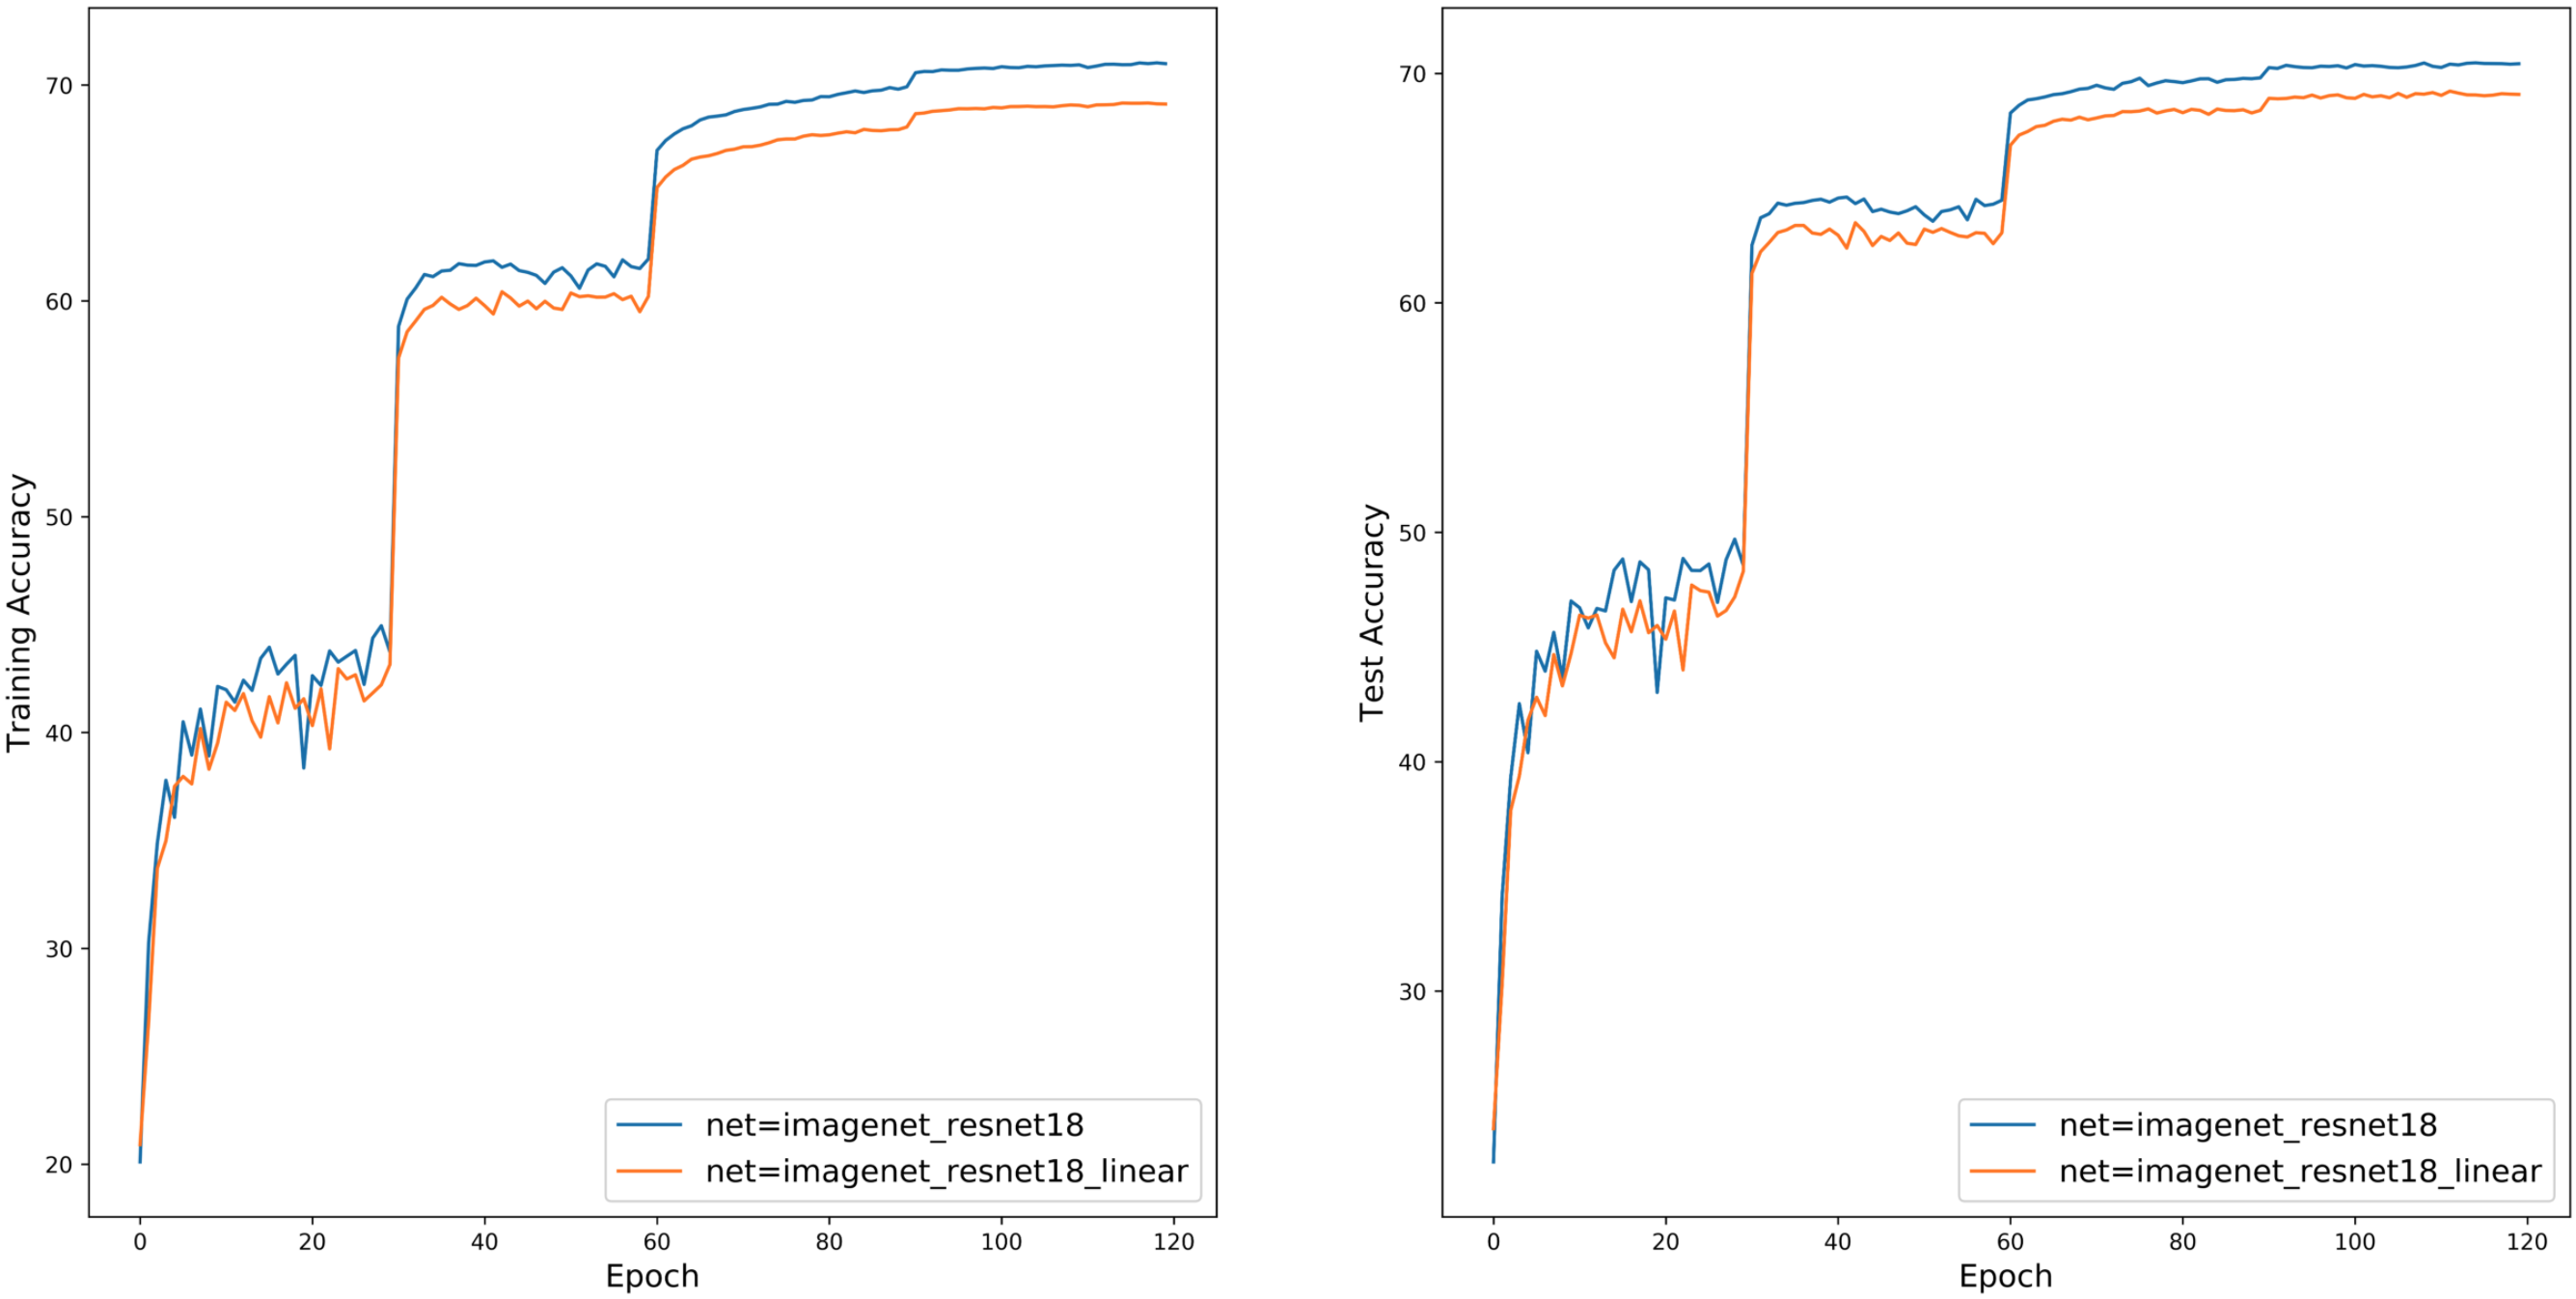
\includegraphics[width=1.2\textwidth]{ImageNetResnet18.png}
	\caption{ResNet18 and ResNet18-$A^l$ on ImageNet.}
	\label{}
\end{figure}





\newpage

 \section{Linear neural networks}
 
\subsection{Linear NN experiments}
Our main goal of this experiment is to test if deeper linear neural network can converge faster. we use linear MNIST with totally 60000 data points as our dataset. The first experiment randomly split this dataset into training set with 48000 training data points and 12000 test data points. The second experiment we use the full data as our training set.\\
Generally, we use a linear neural network model.  A linear NN with $H$ hidden layers can be modeled as
\begin{equation}
	\bm f(x,\bm\theta) = W_{H+1}(W_H(\cdots(W_1 x + b_1)\cdots)+b_H)+b_{H+1}
\end{equation}
where $W_1\in \mathbb{R}^{d_1\times d_x}$, $b_1 \in \mathbb{R}^{d_1}$, $W_i\in \mathbb{R}^{d_{i}\times d_{i-1}}$, $b_i \in \mathbb{R}^{d_i}$, $i = 2,\cdots,H$, $W_{H+1}\in \mathbb{R}^{d_y\times d_{H+1}}$, $b_{H+1} \in \mathbb{R}^{d_y}$. Notice that $d_x$ represents the input size which is 500 in this experiment, while $d_y$ represents the output size , namely, the number of classes, which is 10 in this experiment. So from now on, we may only  use an array $(d_x,d_1,\cdots,d_H,d_y)$ to represent our model.\\
We use cross-entropy with $L_2$ regularization as our loss function.
\begin{equation}
	L(\bm\theta,D) = \frac{1}{|D|} \sum_{i = 1}^k \sum_{x\in D_i} (\log ({\bm 1}^T e^{\bm f(x,\bm\theta)}) - f_i(x,\bm\theta)) + \lambda \sum_{j = 0}^{p+1} (\|W_j\|_F^2 + \|b_j\|_2^2)
\end{equation}

\begin{itemize}
	\item Model.\\
    \begin{itemize}
    	\item Net0 (500,10).
    	\item Net1 (500,100,10)
    	\item Net2 (500,200,100,10)
    	\item Net3 (500,400,200,100,10)
    	\item Net4 (500,800,200,100,10)
    \end{itemize}
    \item Training algorithm.
    \begin{itemize}
    	\item Full gradient descent(GD).
    	    \begin{equation}
    	    	\bm\theta = \bm\theta - lr \frac{\partial L}{\partial \bm\theta}
    	    \end{equation} 
    	\item Coordinate descent(CD).
    	\begin{align}
    		&\bm\theta_1^+ = \bm\theta_1 - lr \frac{\partial L}{\partial \bm\theta_1}(\bm\theta_1,\bm\theta_2,\cdots,\bm,\bm\theta_p,\theta_{p+1}),\\
    		&\bm\theta_2^+ = \bm\theta_2 - lr \frac{\partial L}{\partial \bm\theta_2}(\bm\theta_1^+,\bm\theta_2,\cdots,\bm\theta_p,\bm\theta_{p+1}),\\
    		&\bm\theta_3^+ = \bm\theta_3 - lr \frac{\partial L}{\partial \bm\theta_3}(\bm\theta_1^+, \bm\theta_2^+,\cdots,\bm\theta_p,\bm\theta_{p+1}),\\
    		&\cdots,\\
    		&\bm\theta_{p+1}^+ = \bm\theta_{p+1} - lr \frac{\partial L}{\partial \bm\theta_{p+1}}(\bm\theta_1^+, \bm\theta_2^+,\cdots,\bm\theta_p^+,\bm\theta_{p+1})
    	\end{align}
    	where $\bm\theta_j = (W_j,b_j), j = 1,2,\cdots,p+1$.
    \end{itemize}
    \item Stopping criterion.\\
    We stop iteration when training accuracy first obtain 100\%.
\end{itemize}


\begin{enumerate}
	\item Training Net0-4 using gradient descent.\\
	We set $\lambda = 10^{-5}$, learning rate $= 0.1$.
	\begin{itemize}
		\item Experiment 1: Using ranomly chosen 48000 data points from linear MNIST as training set.\\
		\begin{table}[H]
			\centering
			\caption{Randomly chosen 80\% full dataset as training set}
			\label{tab:1}      
			\begin{tabular}{lllllll}
				\hline\noalign{\smallskip}
				Model &  Optim & Iterations & Time  & TrainL  & TestL & TestA \\
				\noalign{\smallskip}\hline\noalign{\smallskip}
				
				Net0 & GD & 3190 & 3743 & 0.0062 & 0.0077 & 99.94   \\
				
				Net1 & GD & 2009 & 2475 & 0.0046 & 0.0063 & 99.95 \\
				
				Net2 & GD & 2322 & 3245 & 0.0034 & 0.0049 & 99.94 \\
				
				Net3 & GD & 1767 & 2705 & 0.0048 & 0.0066 & 99.93 \\
				
				Net4 & GD & 1805 & 3346 &0.0059 & 0.0075 & 99.93 \\
				
				\noalign{\smallskip}\hline
				
			\end{tabular}
		\end{table}
		
%		\begin{figure}[H]
%			\centering
%			\includegraphics[width=3in]{logGDtrainL.png}   
%			\caption{log(Train Loss)}
%		\end{figure}

	
	
	
		\item Experiment 2: Using whole linear MNIST dataset as training set.
		\begin{table}[H]
			\centering
			\caption{Full dataset}
			\label{tab:2}      
			\begin{tabular}{lllll}
				\hline\noalign{\smallskip}
				Model &  Optim & Iterations & Time  & TrainL \\
				\noalign{\smallskip}\hline\noalign{\smallskip}
				
				Net0 & GD & 4218 & 6168 & 0.0051  \\
				
				Net1 & GD & 2546 & 3937 & 0.0038  \\
				
				Net2 & GD & 2269 & 4010 & 0.0035  \\
				
				Net3 & GD & 2099 & 4046 & 0.0044  \\
				
				Net4 & GD & 1578 & 3815 &0.0065  \\
				
				\noalign{\smallskip}\hline
				
			\end{tabular}
		\end{table}
		
		
%		\begin{figure}[H]
%			\centering
%			\includegraphics[width=3in]{logGDfullL.png}   
%			\caption{log(Train Loss) for full dataset}
%		\end{figure}
		We can see very clearly in the two figures that the loss of Net0 always decrease slower than other deeper linear NN. Or we can see in the table that Net0 use most iterations to reach 100\% training accuracy. 
	
	    \item Experiment 3: Training '0' and '1' data in MNIST.\\
	     First I use Adam algorithm to verify that '0' and '1' are linearly separable in the training set of MNIST. Then I use full GD to iterate 50 epoches for each model and record their loss history. 
%	    \begin{figure}[H]
%		  \centering
%		  \includegraphics[width=3in]{log_MNIST_50.png}   
%		  \caption{log(Train Loss) for MNIST dataset}
%	      \end{figure}
		\end{itemize}
	\end{enumerate}

\newpage
\subsection{A new training algorithm}
%\begin{figure}[H]
%	\centering
%	\includegraphics[width=3in]{part_logGDfullL.png}   
%	\caption{part of log(Train Loss) for full dataset}
%\end{figure}

If we print the first several steps, we will notice that the loss of Net0 descends the fastest among those networks. After 5-10 steps, it suddenly become the slowest. If at this point we can switch to another curve, then the training process might speed up.\\

\subsection{Regression training}
Actually, there is two ways to achieve this. We may use a very simple regression example to discribe those two methods. We denote our training data as $X\in \mathbb{R}^{d_x\times N}$, the label is $Y\in \mathbb{R}^{d_y\times N}$. Basically, our model is the simplest linear model
\begin{equation}
	f(x) = Wx,
\end{equation}
and our loss function is 
\begin{equation}
	L(W, D) = \|WX - Y\|_F^2.
\end{equation}
First, we use 
\begin{equation}
	W = W - lr \frac{\partial L}{\partial W}
\end{equation}
to do several iterations to obtain $\overline{W}$. Then we have three ways to continue.\\
\begin{itemize}
	\item Reformulate the problem as 
	\begin{equation}
	\min_{U,V} \|(\overline{W}+ UV)X - Y\|_F^2
	\end{equation}
	where $U\in \mathbb{R}^{d_y\times d_1}$, $V\in\times \mathbb{R}^{d_1\times d_x}$. If the solution of above problem is $\overline{U}, \overline{V}$, then our final solution is $W = \overline{W}+\overline{U}\overline{V}$. Notice that if we use a zero initialization in the above problem, the begining loss is $\|\overline{W} X - Y\|_F^2$.\\
	\item Factorize $\overline{W} = U_0 V_0$, where $\overline{U}_0\in \mathbb{R}^{d_y\times d_1}$, $\overline{V}_0\in\times \mathbb{R}^{d_1\times d_x}$. And we use $(U_0,V_0)$ as the initial value for the following problem:
	\begin{equation}
	\min_{U,V} \|UVX - Y\|_F^2.
	\end{equation}
	If the solution of above problem is $\overline{U}, \overline{V}$, then our final solution is $W = {\overline{U}}{\overline{V}}$.
\end{itemize}

\subsection{Classification Training}
For classification problem, we have three possible ways to speed up the training algorithms. Define function $l: \mathbb{R}^{d_x}\times \{1,2,\cdots,d_y\} \rightarrow \mathbb{R}$ as
\begin{equation}
	l(\bm s, i) = \log ({\bm 1}^T e^{\bm s}) - s_i,
\end{equation}
where $\bm s = (s_1,s_2,\cdots,s_{d_y})$. So our final cross-entropy loss can be written as
\begin{equation}
	L(\bm\theta,D) = \sum_{i = 1}^{d_y} \sum_{x\in D_i} l(f(x), i) 
\end{equation}
where $f$ is the mapping of our model.  
We use single-layer and 2-layer linear NN as our examples to state our possible ways to speed up training. For single-layer linear NN we use $W,b$ to represents the weight matrix and bias vector, so $f(x) = Wx + b$. For 2-layer linear NN we use $W_1,W_2,b$ to represents the 2 weight matrices and the bias vector , and $f(x) = W_2 W_1 x + b$ (which implies the first layer is without bias).\\

There are 3 main ideas of speed-up training algorithms.
\begin{itemize}
	\item  Use single-layer linear NN and cross-entropy loss to do several iterations to get parameter $\overline{W}, \overline{b}$. Then we modify the optimization problem as
	\begin{equation}
		\min_{W_1,W_2,b}\sum_{i = 1}^{d_y} \sum_{x\in D_i} l((\overline{W}+W_2 W_1)x + (\overline{b}+b), i) 
	\end{equation}
	If $\tilde{W}_1,\tilde{W}_2,\tilde{b}$ is one of the solution of the above problem, then our final solution is $W^* = \overline{W} + \tilde{W}_2\tilde{W}_1, b^* = \overline{b} + \tilde{b}$.\\
	
	\item In the second training algorithm, we use a 2-layer linear NN all the time. The loss is 
	\begin{equation}
	\sum_{i = 1}^{d_y} \sum_{x\in D_i} l(W_2 W_1x + b, i) 
	\end{equation}
	 But in first several steps, we fix the initial $W_1$, only update $W_2$ and $b$. If you regard $W_1 x$ as a whole, we can see we are actually training a single-layer linearNN at the begining. After several steps, we start to update $W_1,W_2,b$ together just as the regular GD.\\
	 
	 \item The third idea is, just like the first idea, we use single-layer linear NN and cross-entropy loss to do several iterations to get parameter $\overline{W}, \overline{b}$. But after that, we factorize $\overline{W} = U_0 V_0$, where $\overline{U}_0\in \mathbb{R}^{d_y\times d_1}$, $\overline{V}_0\in\times \mathbb{R}^{d_1\times d_x}$. And we use $W_2 = U_0, W_1 = V_0, b = \overline{b}$ as the initial value for the following problem:
	 \begin{equation}
	 \min_{W_1,W_2,b} \sum_{i = 1}^{d_y} \sum_{x\in D_i} l(W_2 W_1x + b, i) .
	 \end{equation}

	 
\end{itemize}

\subsubsection{Idea I}
\begin{figure}[H]
	\centering
	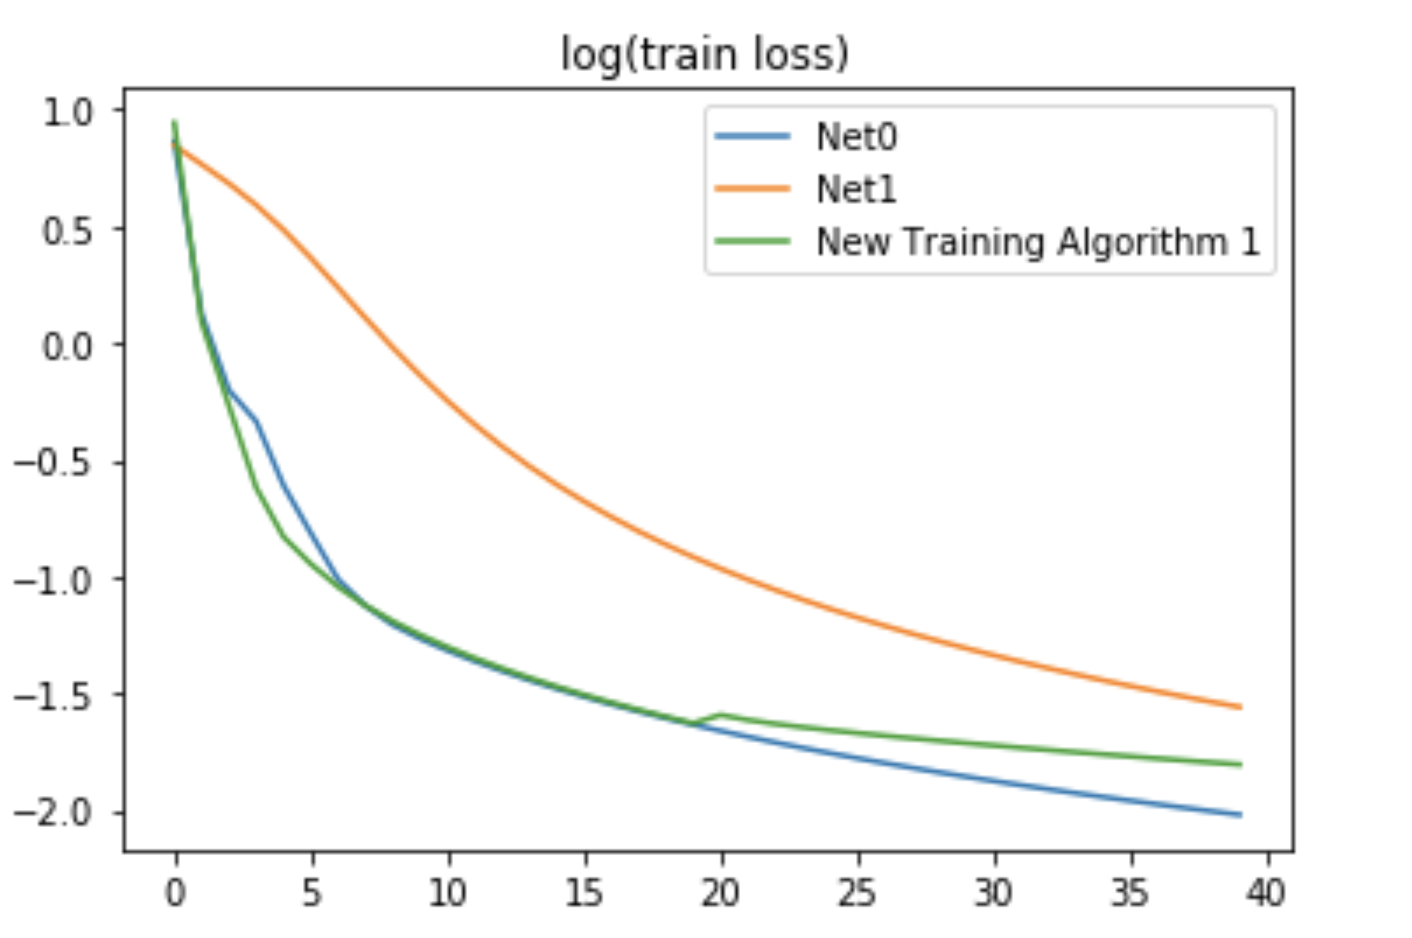
\includegraphics[width=2.5in]{train1_hidden100.png}
	\caption{New training algorithm 1: $d_1 = 100, lr = 0.1$}
\end{figure}
\begin{figure}[H]
	\centering
	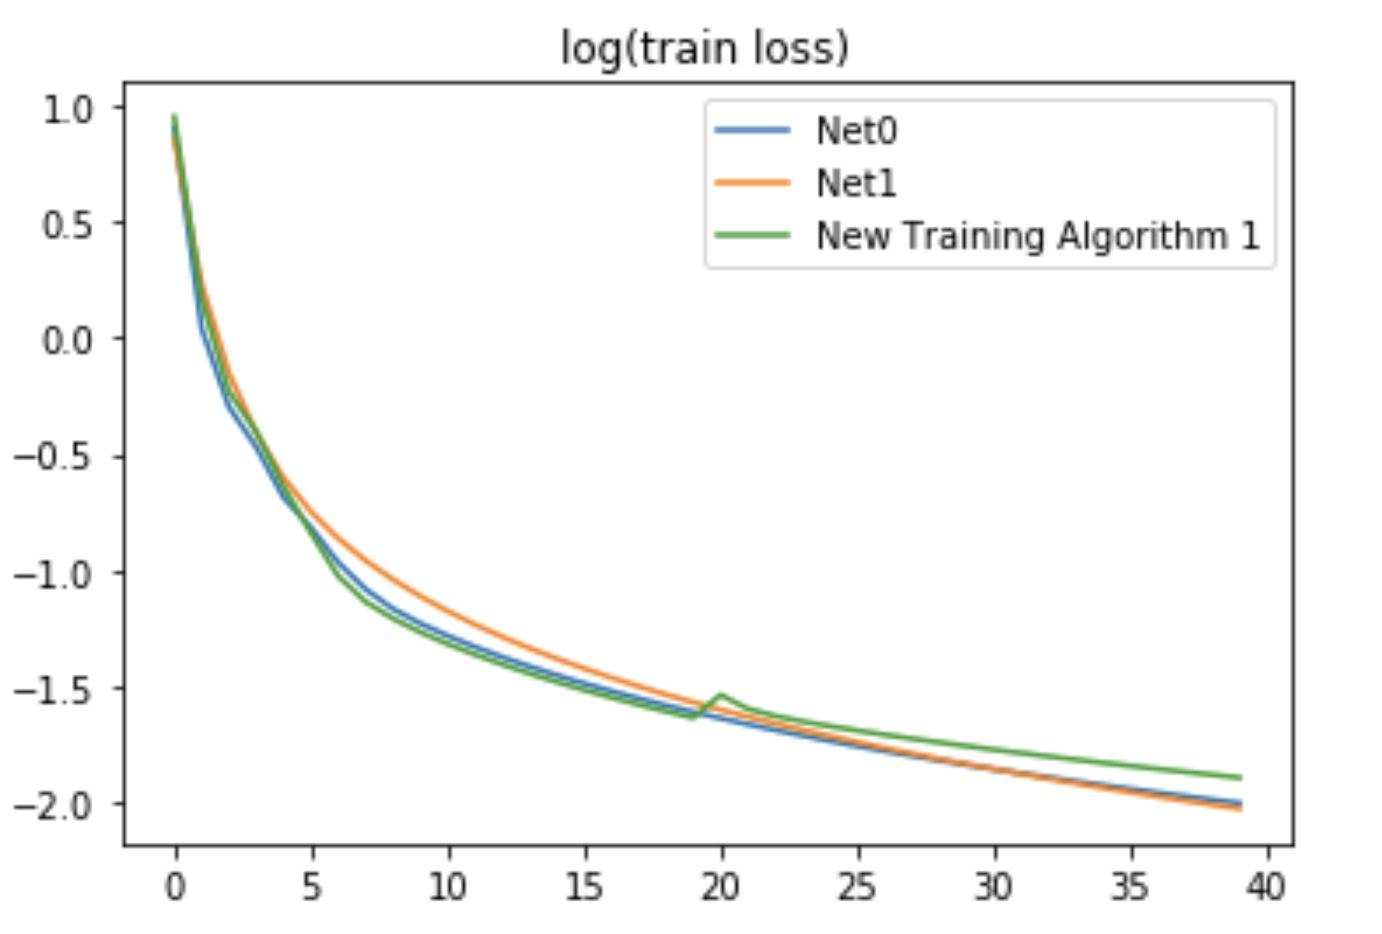
\includegraphics[width=2.5in]{train1_hidden500.png}
	\caption{New training algorithm 1: $d_1 = 500, lr = 0.1$}
\end{figure}
Here we found that when we switch to the 2-layer model, the descent speed becomes slower.

\subsubsection{Idea II}
\begin{figure}[H]
	\centering
	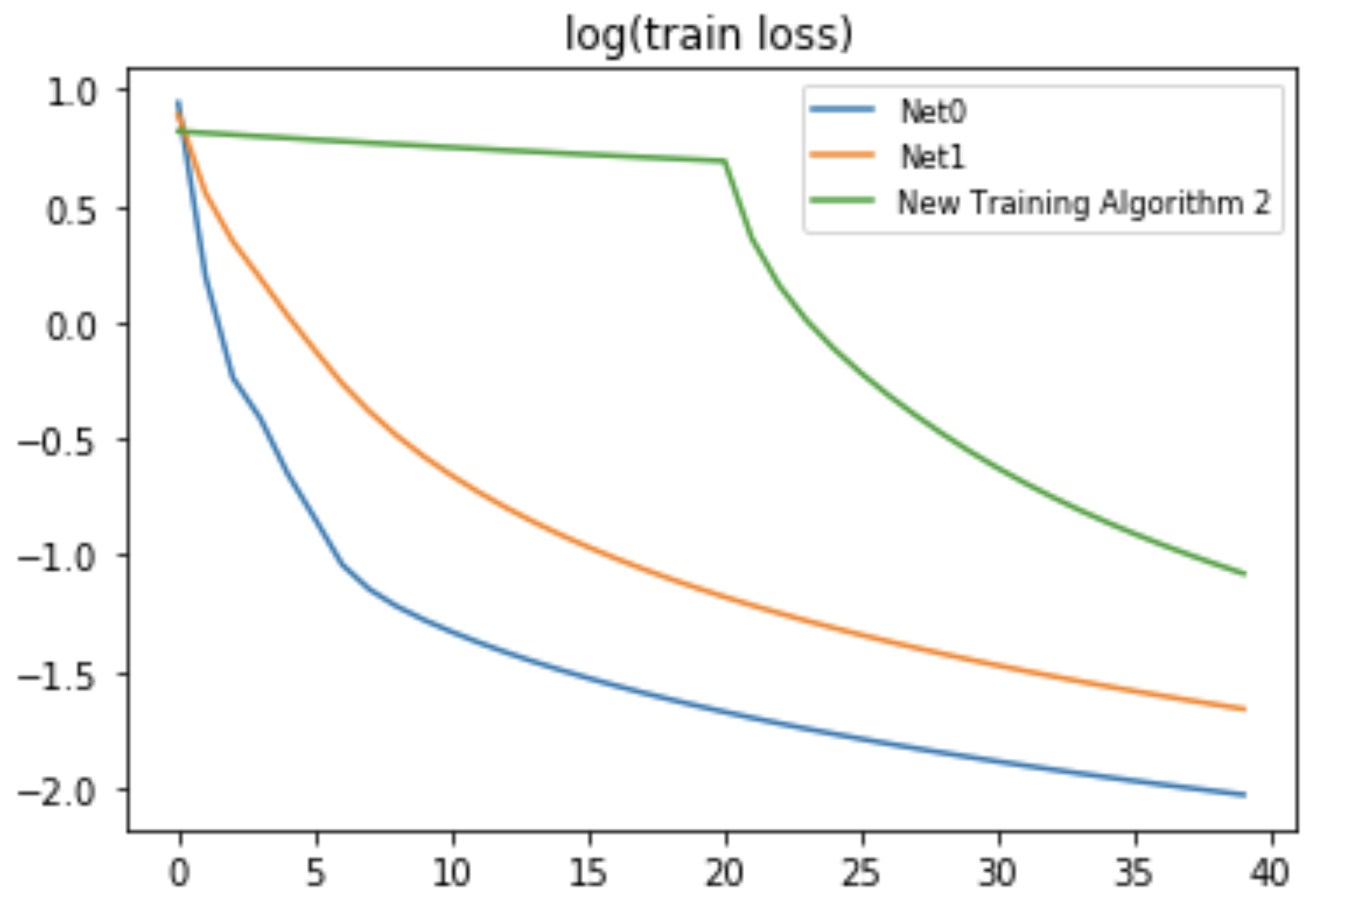
\includegraphics[width=2.5in]{train2_hidden10.png}
	\caption{New training algorithm 2: $d_1 = 10, lr = 0.1$}
\end{figure}
\begin{figure}[H]
	\centering
	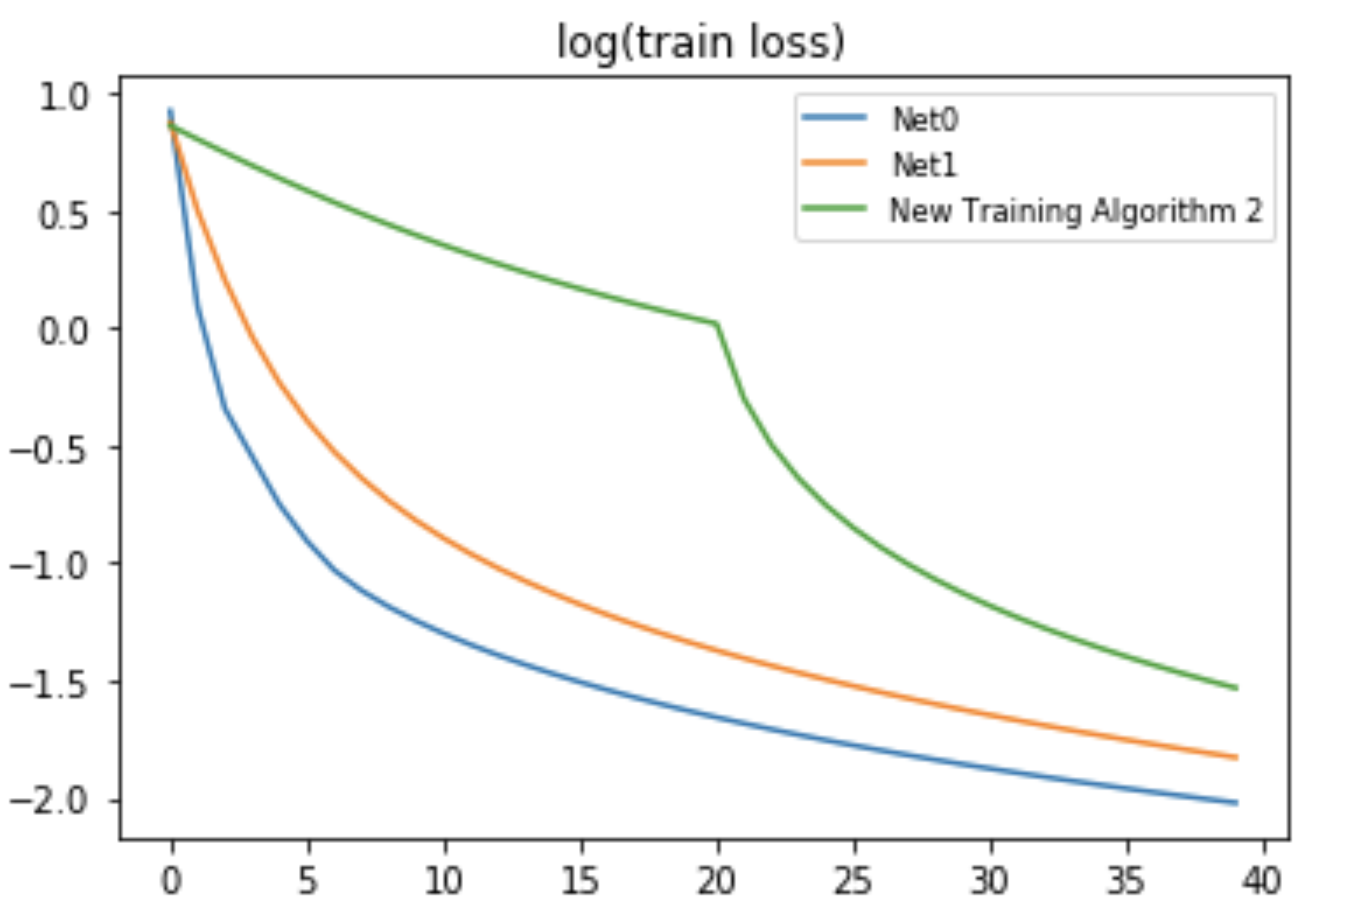
\includegraphics[width=2.5in]{train2_hidden100.png}
	\caption{New training algorithm 2: $d_1 = 100, lr = 0.1$}
\end{figure}
\begin{figure}[H]
	\centering
	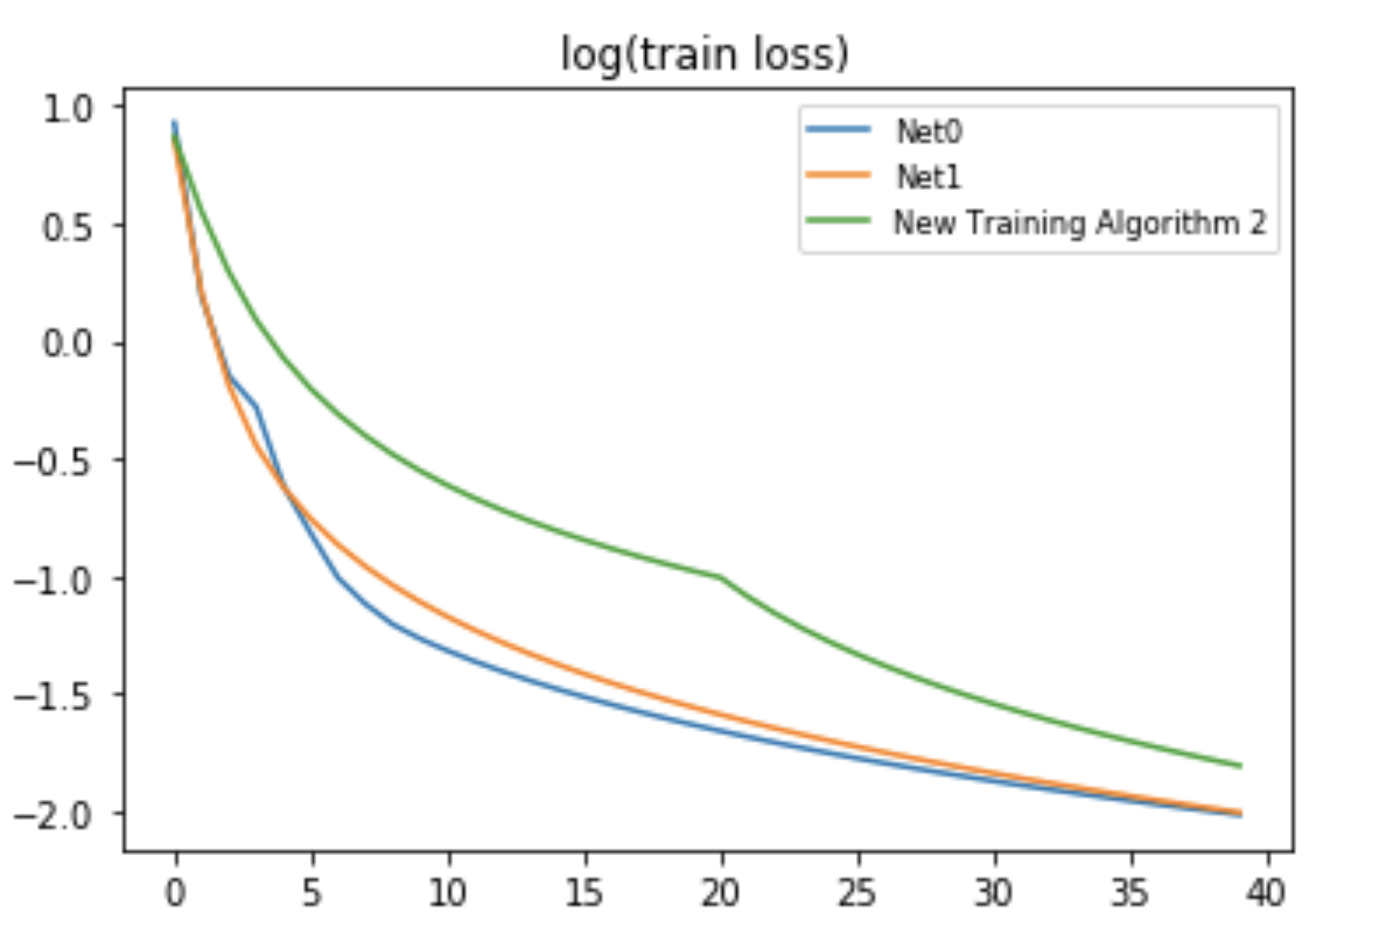
\includegraphics[width=2.5in]{train2_hidden500.png}
	\caption{New training algorithm 2: $d_1 = 500, lr = 0.1$}
\end{figure}
\begin{figure}[H]
	\centering
	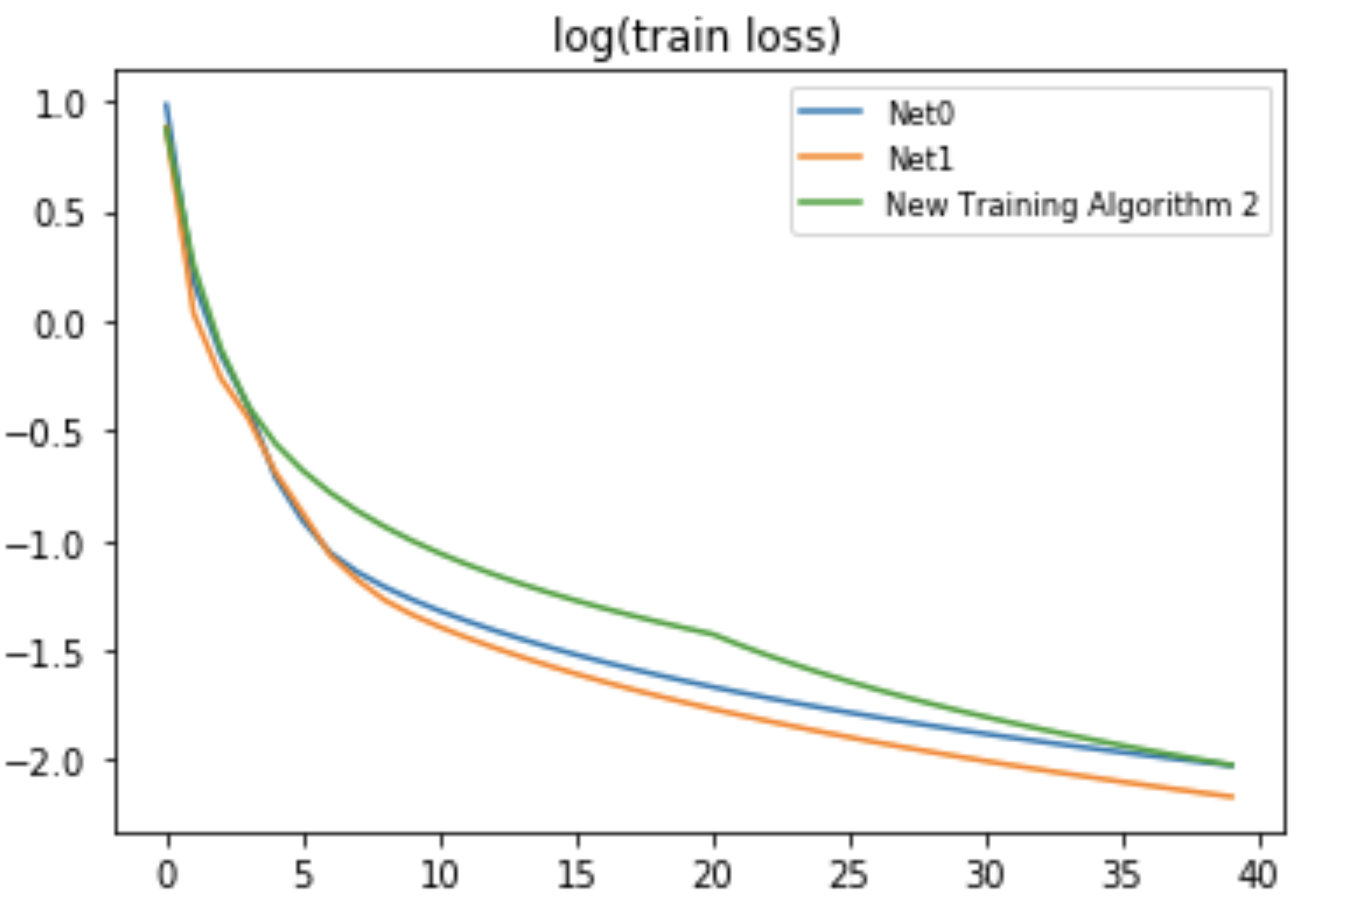
\includegraphics[width=2.5in]{train2_hidden1000.png}
	\caption{New training algorithm 2: $d_1 = 1000, lr = 0.1$}
\end{figure}
\begin{figure}[H]
	\centering
	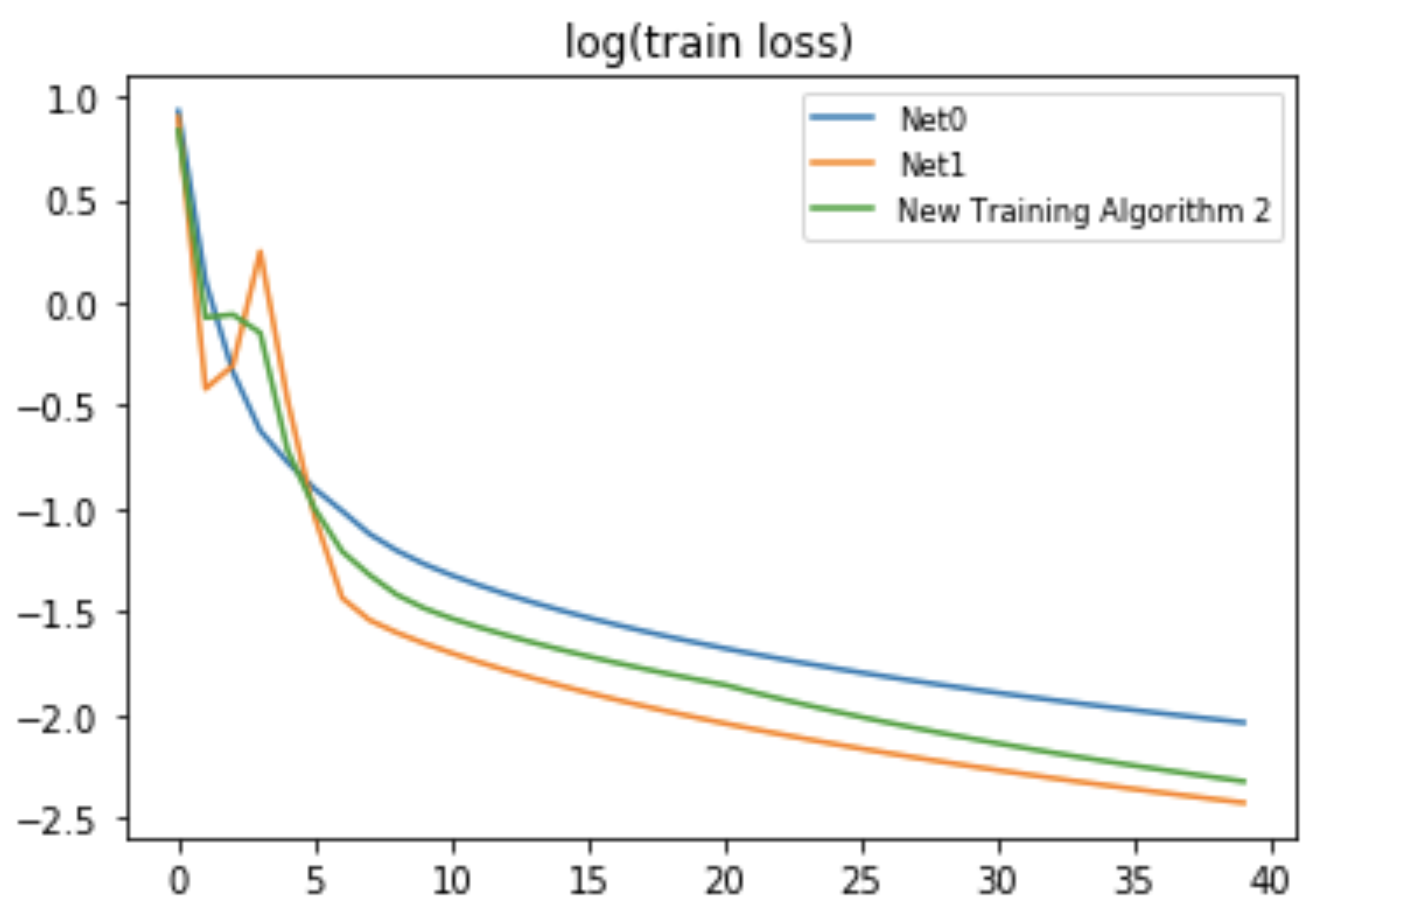
\includegraphics[width=2.5in]{train2_hidden2000_lr1.png}
	\caption{New training algorithm 2: $d_1 = 2000, lr = 0.1$}
\end{figure}
\begin{figure}[H]
	\centering
	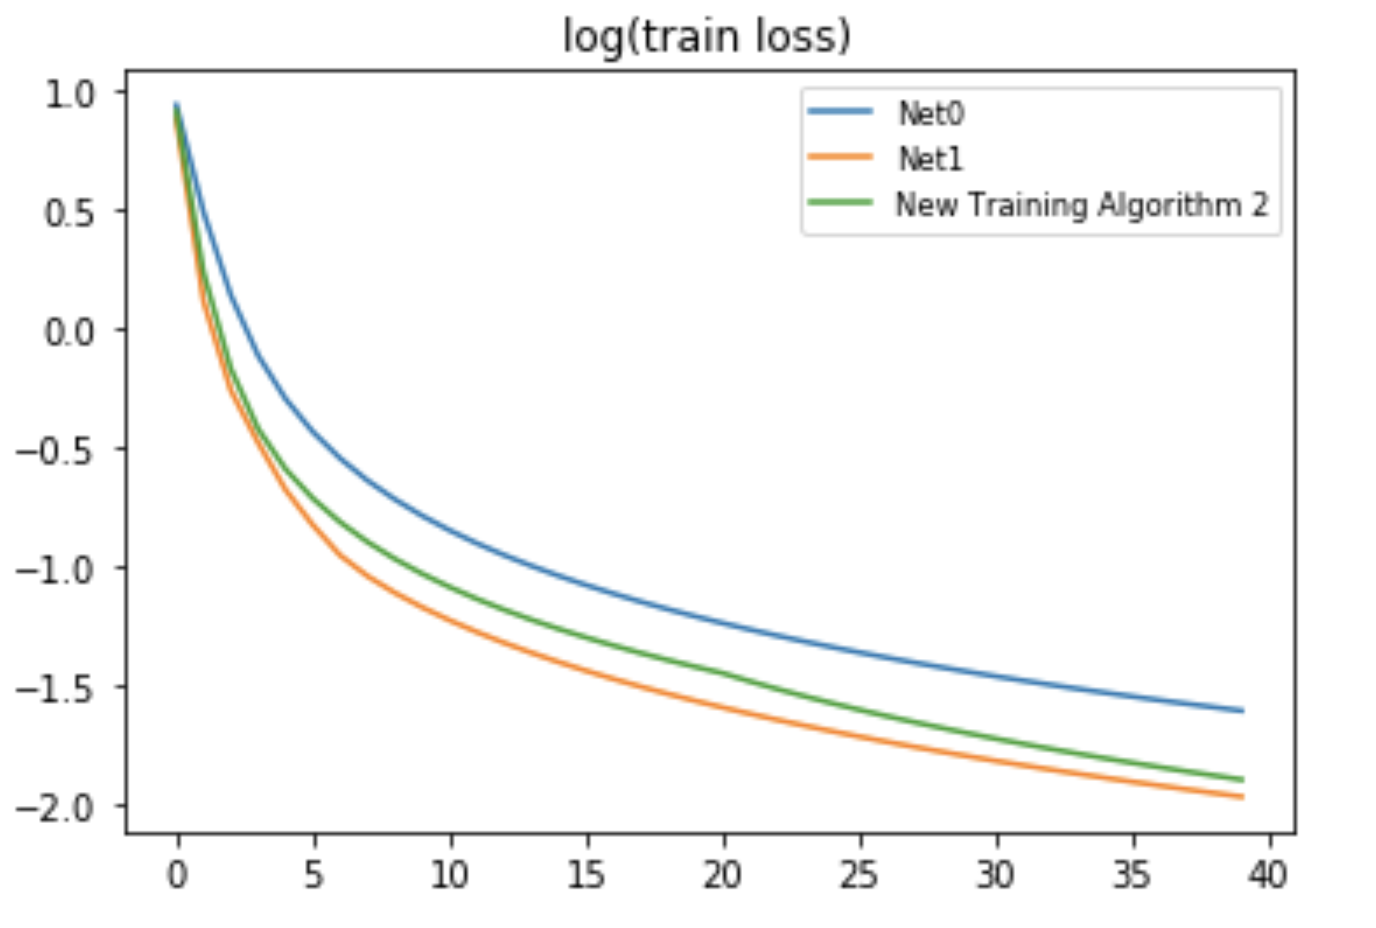
\includegraphics[width=2.5in]{train2_hidden2000_lr05.png}
	\caption{New training algorithm 2: $d_1 = 2000, lr = 0.05$}
\end{figure}

Here are some interesting things we can observe:
\begin{itemize}
	\item It seems that idea II do have an acceleration at 20th iteration (bacause we start to update all parameters that step), but the descending speed is slower than Net0 in the first 20 steps when the hidden size is less than 500.
	\item When we increase the hidden size to 1000 or 2000, our idea do descend faster than Net0 at the beginning, but slower than Net1. So our idea II seems useless when size of hidden-layer is very large.

	
\end{itemize}

\input{Wide_linearNN}
	

\subsection{Jianqing's summary}
\subsubsection{Fast autoaugment details}
Let $\mathbb{O}$ be a set of augmentation (image transformation) operations
$\mathcal{O}$:$\mathcal{X}\rightarrow\mathcal{X}$ defined on the input image space $\mathcal{X}$. Each operation $\mathcal{O}$ have two parameters: the calling probability $p$ and the magnitude $\lambda$ which determines the variability of operation. Let $\mathcal{S}$ be the set of sub-policies where a sub-policy $\tau \in \mathcal{S}$ consists of $N_{\tau}$ consecutive operations
\{$\mathcal{O}_n^{(\tau)}$($x$;$p_n^{(\tau)}$,$\lambda_n^{(\tau)}$):$n$=1,\ldots,$N_\tau$\}
$$\mathcal{O}(x;p,\lambda):=\left\{
\begin{aligned}
\mathcal{O}(x;\lambda) &&with&&probability&& p \\
x&&with&&probability&&1-p
\end{aligned}
\right.
$$
The output of sub-policy $\tau(x)$ can be described by a composition of operations as:\\
\begin{equation}
\tilde{x}_{(n)}=\mathcal{O}_n^{(\tau)}(\tilde{x}_{(n-1)}),n=1,\ldots,N_{\tau}
\end{equation}

Figure 1 shows a specific example of augmented images by $\tau$ .
Note that each sub-policy $\tau$ is a random sequence of image transformations which depend on $p$ and $\lambda$,and this enables to cover a wide range of data augmentations.
\begin{figure}[H]
	\centering
	% Requires \usepackage{graphicx}
	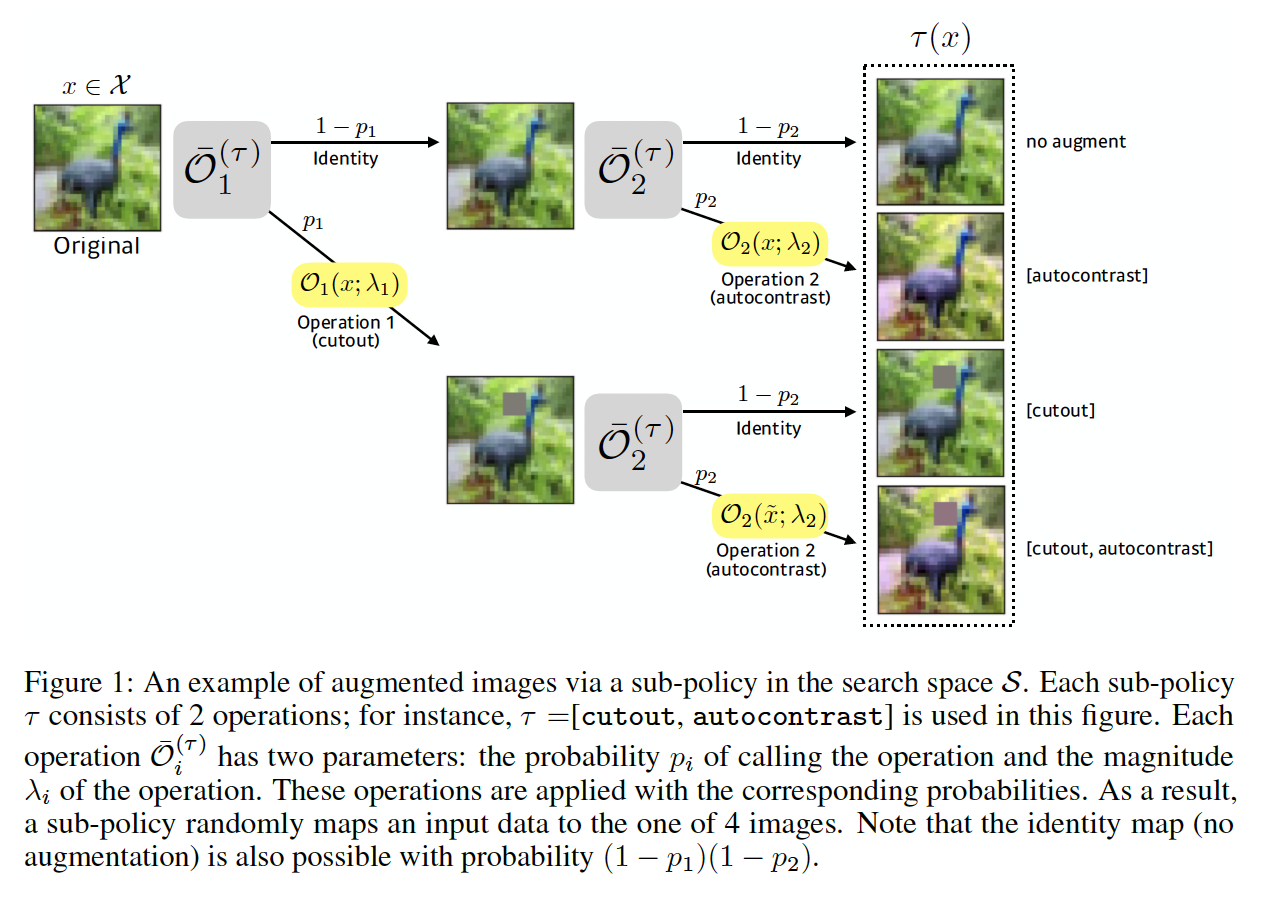
\includegraphics[width=14cm]{fast_fig_1.jpg}
	%  %\caption{}\label{}
\end{figure}

Final policy $T$ is a collection of $N_T$ sub-policies and $T(D)$ indicates a set of augmented images of dataset $D$ transformed by every
sub-policies $\tau\in T$ :
\begin{equation}
T(D)=\cup_{\tau \in T}\{(\tau(x),y):(x,y)\in D\}
\end{equation}
Use both continuous values of probability $p$ and magnitude $\lambda$ at $[0; 1]$ which has more possibilities than discretized search space.


Consider searching the augmentation policy as a density matching between
a pair of datasets. Let $\mathcal{D}$ be a probability distribution on $\mathcal{X}\times\mathcal{Y}$ and assume dataset $D$ is sampled
from this distribution. For a given classification model $\mathcal{M}(\cdot|\theta)$ : $\mathcal{X}\times\mathcal{Y}$ that is parameterized by $\theta$, the expected accuracy and the expected loss of $\mathcal{M}(\cdot|\theta)$ on dataset $D$ are denoted by $\mathcal{R}(\theta |D)$ and $\mathcal{L}(\theta |D)$.

For any given pair of $D_{train}$ and $D_{valid}$, our goal is to improve the generalization ability by searching
the augmentation policies that match the density of $D_{train}$ with density of augmented $D_{valid}$.
It is impractical to compare these two distributions directly for an evaluation of every candidate policy.
Perform this evaluation by measuring how much one dataset follows the pattern of the other by making use of the model predictions on both datasets.

Split $D_{train}$ into $D_{M}$ and $D_{A}$ that are used for learning the model parameter $\theta$ and exploring the augmentation policy $T$.Employ the following objective to find a set of learned augmentation policies
\begin{equation}
T_{*}=argmax_T \mathcal{R}(\theta^*|T(D_A))
\end{equation}
where model parameter $\theta^*$ is trained on $D_{M}$.It is noted that in this objective, $T_{*}$ approximately minimizes the distance between density of $D_{M}$ and density of $T(D_A)$ from the perspective of maxmizing the performance of both model predictions with the same parameter $\theta$.
\begin{figure}[H]
	\centering
	% Requires \usepackage{graphicx}
	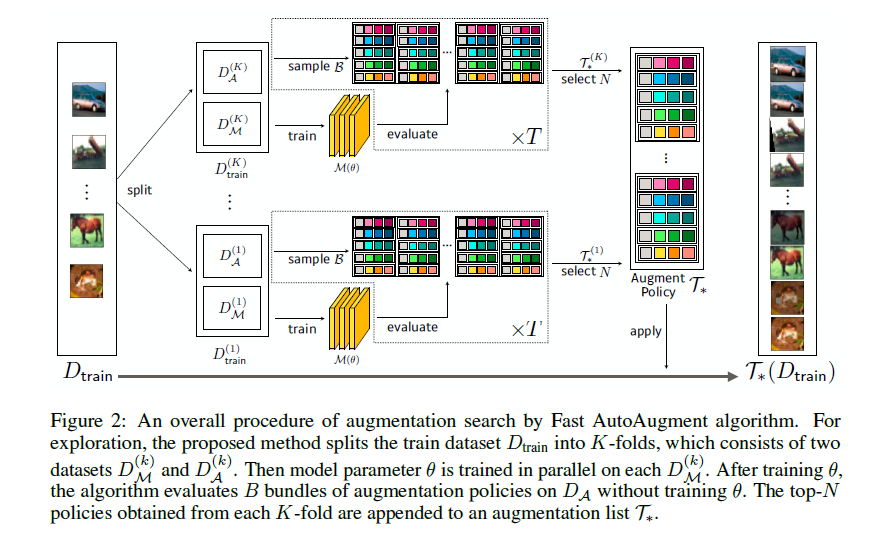
\includegraphics[width=14cm]{fast_fig_2.jpg}
	%  %\caption{}\label{}
\end{figure}

To achieve (3), we propose an efficient strategy for augmentation policy search (see Figure 2). First,we conduct the K-fold stratified shuffling to split the train dataset into $D_{train}^{(1)},...,D_{train}^{(m)}$ where each $D_{train}^{(k)}$ consists of two datasets $D_M^{k}$ and $D_A^{k}$. Next, we train model parameter $\theta$ on $D_M$ from scratch without data augmentation.

After training the model parameter,for each step $1\leq t\leq T$, explore $B$ candidate policies
$\mathcal{B}=\{T_1,\ldots,T_B\}$via Bayesian optimization method which repeatedly samples a sequence of
sub-policies from search space $\mathcal{S}$ to construct a policy $T=\{\tau_1,\ldots,\tau_{N_\tau}\}$ and tunes corresponding
calling probabilities $\{p_1,\ldots,p_{N_\tau}\}$ and magnitudes $\{\lambda_1,\ldots,\lambda_{N_\tau}\}$ to minimize the expected loss
$\mathcal{L}(\theta |\cdot)$ on augmented dataset $T(D_A)$.

As the algorithm completes the exploration step, select top-N policies over $\mathcal{B}$ and denote them $T_t$,Finally, merge every $T_t$ into $T_*$. Augment the whole dataset $D_{train}$ with $T_*$ and retrain the model parameter $\theta$.Through the proposed method, we can expect the performance $\mathcal{R}(\theta|\cdot)$ on augmented dataset $T_*(D_A)$
is statistically higher than that on $D_A$:
\begin{equation}
\mathcal{R}(\theta|T_*(D_A))\geq\mathcal{R}(\theta|D_A)
\end{equation}

\begin{figure}[H]
	\centering
	% Requires \usepackage{graphicx}
	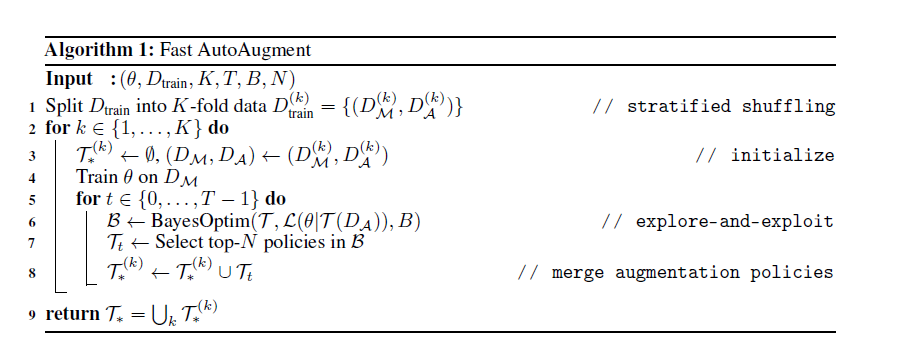
\includegraphics[width=14cm]{fast_fig_3.jpg}
	%  %\caption{}\label{}
\end{figure}

\subsubsection{SGDR}
\begin{equation}
\eta_t = \eta_{min} + \frac{1}{2}(\eta_{max} - \eta_{min})\left(1 +\cos\left(\frac{T_{cur}}{T_{i}}\pi\right)\right)
\end{equation}

where $\eta_{min}^i$ and $\eta_{max}^i$  are ranges for the learning rate, and $T_{cur}$ accounts for how many epochs have been performed since the last restart. Since $T_{cur}$ is updated at each batch iteration $t$. Thus, $\eta_t = \eta_{max}^i$ when $t = 0$ and $T_{cur} = 0$. Once $T_{cur} = T_i$, the cos function will output $-1$ and thus $\eta_t = \eta_{min}^i$. The decrease of the learning rate is shown in Figure 4 for fixed $T_i = 50$, $T_i = 100$ and $T_i = 200$.
\begin{figure}[H]
	\centering
	% Requires \usepackage{graphicx}
	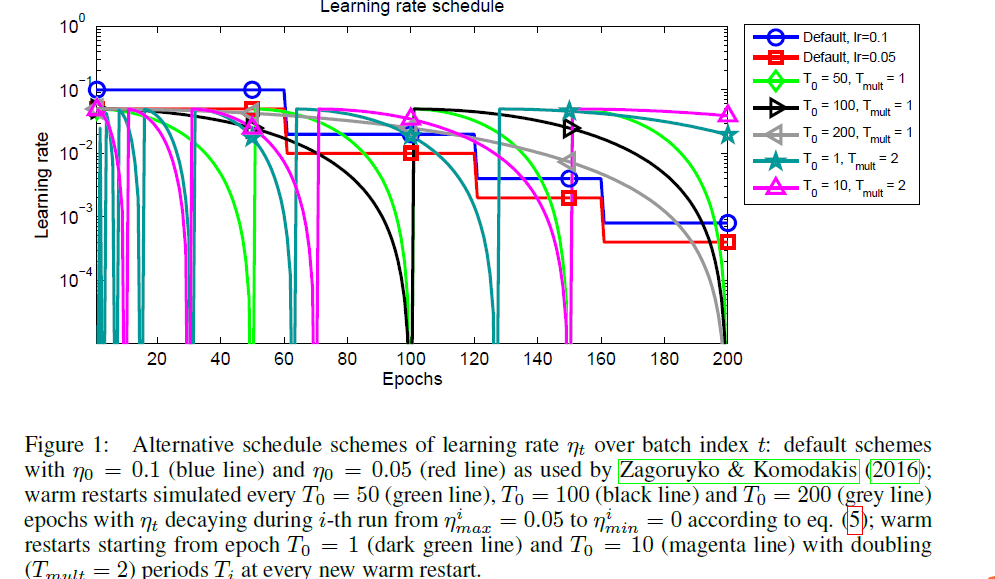
\includegraphics[width=14cm]{SGDR.png}
	%\caption{SGDR}\label{}
\end{figure}

\subsubsection{Experient result in Cifar100}
Init learning rate:0.1\\
Normal augment:ramdom crop and random horizontal flip.\\
\begin{tabular}{| l | c | c | c | c | c | r |}
	\hline
	Augment & Optim & Learning rate & Warm up & Epoch & Train acc & Valid acc \\
	\hline
	FAA   & SGD   & cosine        & Yes     & 3000  & 97.9\%    & 81.6\%\\
	\hline
	Normal   & SGD   & cosine        & Yes     & 3000  & 99.9\%    & 80.3\%\\
	\hline
	Normal   & SGD   & cosine        & No      & 3000  & 99.9\%    & 79.2\%\\
	\hline
\end{tabular}

\subsubsection{Experient result in Linear Constraint ResNet}
All experients use same setup:600epoch, leanring rate:initial value is 0.1 and using cosine method to decrease,warmup,SGD.\\
\begin{tabular}{| l | c | c | c | r |}
	\hline
	Network                            &Augment   & Paper acc &  acc      &  Parameters\\
	\hline
	pre-act ResNet18$(A^{l,i},B^{l,i})$ & Normal   &   74.33\%  & 78.70\%  &   11M\\
	\hline
	pre-act ResNet18$(A^{l,i},B^{l,i})$ &   FAA    &            & 78.30\%  &   11M\\
	\hline
	pre-act ResNet18$(A^l,B^{l,i})$     & Normal   &    74.51\% & 77.69\%  &   8.1M\\
	\hline
	pre-act ResNet18$(A^l,B^{l,i})$     & FAA      &            & 78.92\%  &   8.1M\\
	\hline
	pre-act ResNet34$(A^{l,i},B^{l,i})$ & Normal   &    77.25\% & 78.28\%  &   21M\\
	\hline
	pre-act ResNet34$(A^{l,i},B^{l,i})$ &   FAA    &            & 80.29\%  &   21M\\
	\hline
	pre-act ResNet34$(A^l,B^{l,i})$     & Normal   &   77.40\%  & 79.63\%  &   13M\\
	\hline
	pre-act ResNet34$(A^l,B^{l,i})$     & FAA      &             & 80.53\% &   13M\\
	\hline
\end{tabular}

As can be seen from the above table, the accuracy using normal augmentation methods is higher than the paper, which may be due to multiple epochs and different learning rate methods. Except the pre-act ResNet18$(A^{l,i},B^{l,i})$,using FAA can impove the accuracy, it's doubt that the accuracy of pre-act ResNet18$(A^{l,i},B^{l,i})$, I will do exoerients to verify. In FAA experients, the training accuracy in 600epoch about 0.97, I guess trainning more epoch will get better auuracy.

\subsubsection{wresnet under different augment number}
In wresnet 40*2 network, using cosine learning rate method and initial is 0.1, under different augment method, the probability is 0.5 for every sub-policy. The result in le below table.\\
\begin{tabular}{| l | c | c | c | c | r |}
	\hline
	policy num   & train acc & train+aug acc & test accuracy  &  test+aug acc & test acc drop\\
	\hline
	2          &  99.97   & 99.97       &  75.45         &   74.60            &  0.85\\
	\hline
	4          &  99.97   & 99.88       &  75.30         &   73.73            &  1.57\\
	\hline
	6          &  99.97   & 97.46       &  77.50         &   73.90            &  3.60\\
	\hline
	8          &  99.97   & 97.80       &  77.01         &   73.69            &  3.32\\
	\hline
	25         &  99.96   & 96.83       &  77.11         &   72.96            &  4.15\\
	\hline
	50         &  99.95   & 96.61       &  77.22         &   73.54            &  3.68\\
	\hline
	75         &  99.92   & 96.47       &  76.77         &   73.07            &  3.70\\
	\hline
	100        &  99.96   & 96.52       &  77.13         &   72.32            &  4.81\\
	\hline
	125        &  99.96   & 96.70       &  77.37         &   72.64            &  4.73\\
	\hline
	150        &  99.95   & 96.40       &  77.25         &   73.24            &  4.01\\
	\hline
	175        &  99.96   & 96.49       &  77.72         &   73.19            &  4.53\\
	\hline
	200        &  99.92   & 95.93       &  77.27         &   72.67            &  4.60\\
	\hline
	225        &  99.95   & 96.42       &  77.61         &   72.70            &  4.91\\
	\hline
	250        &  99.96   & 96.56       &  77.04         &   72.81            &  4.23\\
	\hline
	275        &  99.94   & 96.49       &  77.22         &   72.95            &  4.27\\
	\hline
	300        &  99.94   & 96.61       &  77.66         &   73.52            &  4.14\\
	\hline
	325        &  99.94   & 96.36       &  77.27         &   73.27            &  4.00\\
	\hline
	350        &  99.95   & 96.56       &  77.26         &   72.79            &  4.47\\
	\hline
	375        &  99.95   & 96.64       &  77.46         &   72.74            &  4.72\\
	\hline
	400        &  99.95   & 96.49       &  76.78         &   73.02            &  3.66\\
	\hline
	425        &  99.96   & 96.48       &  77.30         &   73.27            &  4.03\\
	\hline
	450        &  99.95   & 96.51       &  77.42         &   73.40            &  4.02\\
	\hline
	475        &  99.95   & 96.42       &  76.66         &   72.81            &  3.85\\
	\hline
	497        &  99.93   & 95.99       &  76.88         &   72.47            &  4.41\\
	\hline
\end{tabular}

I guess cutout is one of the reasons for this, so next I remove cutout for FAA, and do some experients, the result in the below table.\\
\begin{tabular}{| l | c | c | c | c | r |}
	\hline
	policy num   & train acc & train+aug acc & test accuracy  &  test+aug acc & test acc drop\\
	\hline
	1          &  99.98   & 99.97       &  75.21         &   74.77            &  0.44\\
	\hline
	2          &  99.97   & 99.96       &  75.14         &   74.44            &  0.70\\
	\hline
	3          &  99.89   & 99.89       &  75.05         &   73.77            &  1.28\\
	\hline
	4          &  99.88   & 99.88       &  75.26         &   74.10            &  1.16\\
	\hline
	5          &  99.64   & 99.62       &  75.70         &   73.70            &  2.00\\
	\hline
	6          &  97.56   & 97.61       &  76.99         &   73.91            &  3.08\\
	\hline
	7          &  97.72   & 97.86       &  77.59         &   73.89            &  3.70\\
	\hline
	8          &  97.80   & 97.76       &  76.90         &   73.60            &  3.30\\
	\hline
	9          &  96.93   & 96.97       &  77.62         &   72.95            &  4.67\\
	\hline
	10         &  97.16   & 96.98       &  77.90         &   73.32            &  4.58\\
	\hline
	25         &  96.36   & 96.51       &  76.84         &   72.88            &  3.96\\
	\hline
	50         &  96.12   & 95.97       &  77.41         &   73.18            &  4.23\\
	\hline
	75         &  96.57   & 96.70       &  77.02         &   72.95            &  4.07\\
	\hline
	100        &  96.46   & 96.34       &  77.31         &   73.58            &  3.73\\
	\hline
\end{tabular}

We can see that if $N$ is small number, the drop test accuracy is upward trend, but when $N>10$, the trend is vanish.\\

\subsubsection{wresnet under different probability}
Using differenr $p$, the result in below table.\\
\begin{tabular}{| l | c | c | c | c | r |}
	\hline
	p          & train acc & train+aug acc & test accuracy  &  test+aug acc & test acc drop\\
	\hline
	0.0          &  99.97   & 99.97       &  74.78         &   74.11            &   0.67  \\
	\hline
	0.1          &  99.97   & 98.53       &  76.44         &   74.56            &   1.88  \\
	\hline
	0.2          &  99.96   & 97.83       &  76.72         &   73.68            &   3.04  \\
	\hline
	0.3          &  99.96   & 97.35       &  76.75         &   73.92            &   2.83  \\
	\hline
	0.4          &  99.96   & 96.83       &  76.78         &   73.45            &   3.33  \\
	\hline
	0.5          &  99.96   & 96.66       &  77.07         &   72.61            &   4.46  \\
	\hline
	0.6          &  99.95   & 95.91       &  77.29         &   72.75            &   4.54  \\
	\hline
	0.7          &  99.93   & 95.51       &  77.67         &   72.59            &   5.08  \\
	\hline
	0.8          &  99.92   & 95.13       &  77.67         &   72.05            &   5.62  \\
	\hline
	0.9          &  99.91   & 94.27       &  77.68         &   71.25            &   6.43  \\
	\hline
	1.0          &  99.75   & 93.22       &  77.67         &   70.31            &   7.36  \\
	\hline
\end{tabular}

\subsubsection{Use SE block in MgNet}
\subsubsection{SE block}
The structure of the SE building block is depicted in Fig. 1. For any given transformation $F_{tr}$ mapping the input $X$ to the feature maps $U$ where $U \in R^{H*W*C}$,we can construct a corresponding SE block to perform feature recalibration. The features $U$ are first passed through a squeeze operation, which produces a channel descriptor by aggregating feature maps across their spatial dimensions $(H*W)$. The function of this descriptor is to produce an embedding of the global distribution of channel-wise feature responses, allowing information from the global receptive field of the network to be used by
all its layers. The aggregation is followed by an excitation operation, which takes the form of a simple self-gating mechanism that takes the embedding as input and produces a collection of per-channel modulation weights. These weights are applied to the feature maps $U$ to generate the output of the SE block which can be fed directly into subsequent layers of the network.\\
\begin{figure}[H]
	\centering
	% Requires \usepackage{graphicx}
	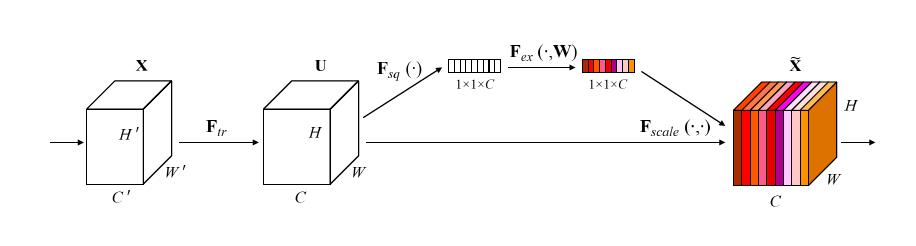
\includegraphics[width=14cm]{seblock.jpg}
	%  %\caption{}\label{}
\end{figure}
Squeeze: Global Information Embedding\\
In order to tackle the issue of exploiting channel dependencies, we first consider the signal to each channel in the output features. Each of the learned filters operates with a local receptive field and consequently each unit of the transformation output $U$ is unable to exploit contextual
information outside of this region. To mitigate this problem, we propose to squeeze global spatial information into a channel descriptor. This is
achieved by using global average pooling to generate channel-wise statistics. Formally, a statistic $z \in R^C$ is generated by shrinking $U$ through its spatial dimensions $H*W$, such that the c-th element of z is calculated by:
\begin{equation}
z_c=F_{sq}(u_c)=\frac{1}{H*W}\sum_{i=1}^H\sum_{j=1}^Wu_c(i,j)
\end{equation}
Excitation: Adaptive Recalibration\\
To make use of the information aggregated in the squeeze operation, we follow it with a second operation which aims to fully capture channel-wise dependencies. To fulfil this objective, the function must meet two criteria: first, it must be flexible (in particular, it must be capable of learning
a nonlinear interaction between channels) and second, it must learn a non-mutually-exclusive relationship since we would like to ensure that multiple channels are allowed to be emphasised (rather than enforcing a one-hot activation). To meet these criteria, we opt to employ a simple gating mechanism with a sigmoid activation:
\begin{equation}
s = F_{ex}(z,W)=\sigma(g(z,W)) = \sigma(W_2\delta(W_1z))
\end{equation}
where $\delta$ refers to the ReLU function,$W_1 \in  R^{\frac{C}{r}*C}$ and$W_2 \in  R^{C*\frac{C}{r}}$. To limit model complexity and aid generalisation, we parameterise the gating mechanism by forming a bottleneck with two fully-connected (FC) layers around the non-linearity, i.e. a dimensionality-reduction layer with reduction ratio $r$, a ReLU and then a dimensionality-increasing layer returning to the channel dimension of the transformation output $U$. The final output of the block is obtained by rescaling $U$ with the activations $s$:
\begin{equation}
x_c = F_{scale}(u_c,s_c) = s_cu_c
\end{equation}
where $X = [x_1,x_2,\dot ,x_C]$and $F_{scale}(u_c,s_c)$ refers to
channel-wise multiplication between the scalar sc and the
feature map $u_c \in R^{H*W}$.


\subsubsection{Add SE block in MgNet}
Modle:MgNet,[2,2,2,2],256 chanels. Add SE block in the end of every Extraction and Restriction block.The result in below table.\\
\begin{tabular}{| l | c | c | c | r |}
	\hline
	Add SE & FAA & epoch & train acc & test acc \\
	\hline
	No     & No  &  300  & 99.95     & 77.64    \\
	\hline
	Yes    & No  &  300  & 99.97     & 78.66    \\
	\hline
	No     & Yes &  300  & 79.36     & 73.65    \\
	\hline
	Yes    & Yes &  300  & 95.95     & 80.17    \\
	\hline
	Yes    & Yes &  500  & 97.87     & 80.96    \\
	\hline
\end{tabular}

New result:\\
\begin{tabular}{| l | c | c | c | r |}
	\hline
	Add SE & FAA & epoch & train acc & test acc \\
	\hline
	No     & No  &  500  & 99.72     & 79.16    \\
	\hline
	Yes    & No  &  500  & 99.68     & 80.04    \\
	\hline
	Yes    &Yes  &  500  & 96.79    &  81.85    \\
	\hline
\end{tabular}

We can conclude that adding SE block in Mgnet will impove trainning accuracy. We only add SE block in the feature space$U$,next,we will test SE block in Image space $F$, and the number of SE block.\\

\subsubsection{Using SOTA tricks in MgNet}
\begin{itemize}
	\item Aim:Using the SOTA tricks in MgNet, and get the best performance in the MgNet.\\
	\item Approch:All the tricks are divided into three methods: data processing, network structure optimization and training algorithm, study the performance of networks with or without every trick, \\
	\item Network:MgNet[2,2,2,2],ResNet-18,pre-act ResNet-18,WResNet40*2\\
	\item Dataset:Cifar100,Cifar10\\
	\item Timetabel:Plan to complete one or two projects a week.
\end{itemize}


\begin{tabular}{| l |  c  | r |}
	\hline
	Dataset             &      Network   &           Train Algorithm\\
	\hline
	Cutout              &       SE       &            \\
	\hline
	Mixup               &       GE       &            \\
	\hline
	Cutmix              &       SK       &             \\
	\hline
	FAA                 &                &             \\
	\hline
\end{tabular}


\begin{figure}[H]
	\centering
	% Requires \usepackage{graphicx}
	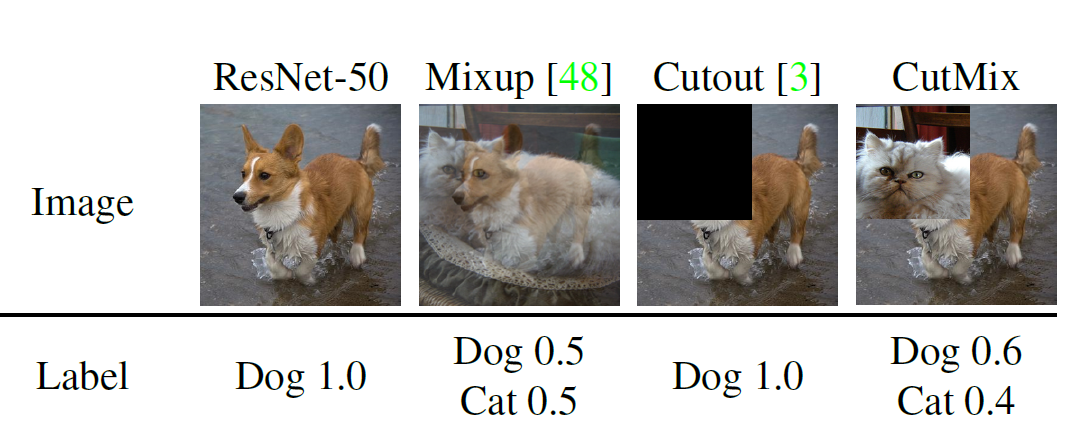
\includegraphics[width=14cm]{dataset-duibi.jpg}
	\caption{Three different dataset augment methods.}\label{Three different dataset augment methods.}
\end{figure}

%\subsubsection{Cutout}
%\begin{figure}[H]
%  \centering
%  % Requires \usepackage{graphicx}
%  \includegraphics[width=13cm]{cutout.jpg}
%%  %\caption{}\label{}
%\end{figure}

\subsubsection{Mixup}
\begin{figure}[H]
	\centering
	% Requires \usepackage{graphicx}
	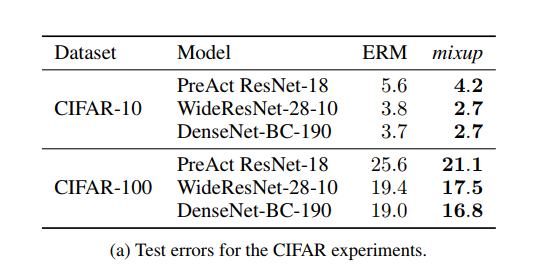
\includegraphics[width=10cm]{mixup.jpg}
	%  %\caption{}\label{}
\end{figure}

\subsubsection{CutMix}
\begin{figure}[H]
	\centering
	% Requires \usepackage{graphicx}
	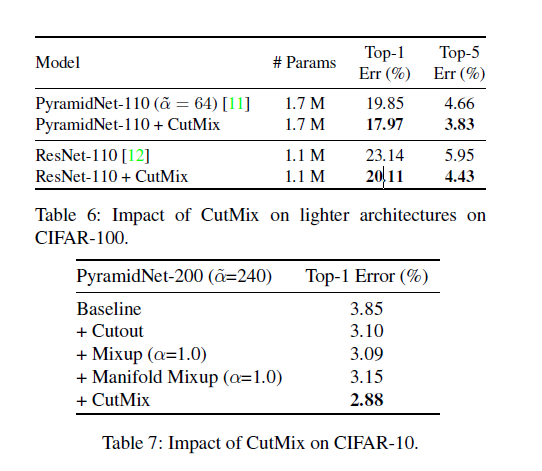
\includegraphics[width=10cm]{cutmix.jpg}
	%  %\caption{}\label{}
\end{figure}

\subsubsection{GE}
\begin{figure}[H]
	\centering
	% Requires \usepackage{graphicx}
	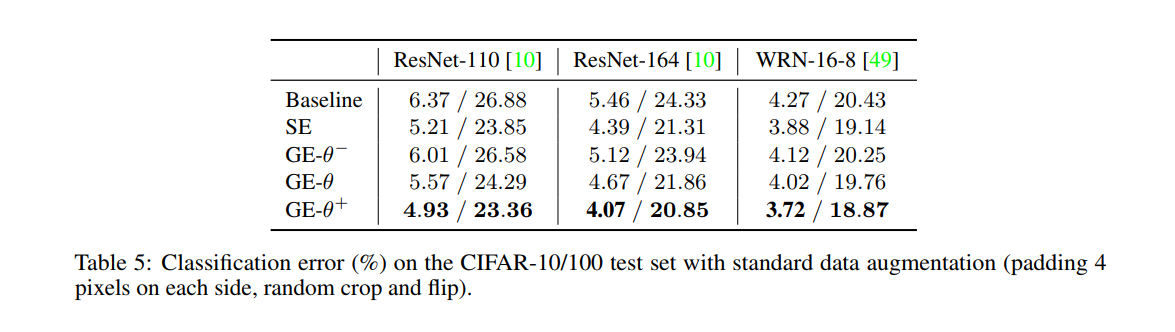
\includegraphics[width=18cm]{GE.png}
	%  %\caption{}\label{}
\end{figure}

\subsubsection{SK}
\begin{figure}[H]
	\centering
	% Requires \usepackage{graphicx}
	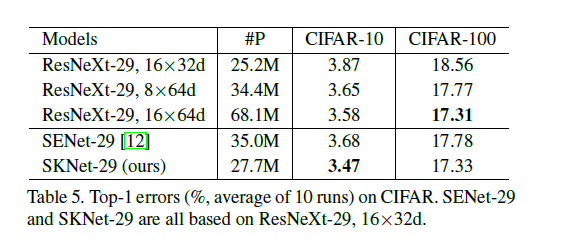
\includegraphics[width=12cm]{SK.jpg}
	%  %\caption{}\label{}
\end{figure}


\newpage
\subsubsection{Add or not add cutout in different models result}
\quad
Table 1:The accuracy in cifar10 for different models.\\
\begin{tabular}{| l | c | c | r |}
	\hline
	Network                &     Parameters   &       paper accuracy   &   my accuracy     \\
	\hline
	ResNet18               &      11.2M      &          95.28         &     94.56          \\
	\hline
	PreActResNet18         &      11.2M      &          94.40         &     94.82          \\
	\hline
	Wide ResNet(40*2)      &      2.2M       &          94.67         &     95.17          \\
	\hline
	Wide ResNet(28*10)     &      36.5M      &          96.12         &     96.06          \\
	\hline
	MgNet[2,2,2,2]-256         &      8.2M       &                        &     96.00          \\
	\hline
	MgNet[3,4,6,3]-256         &      8.3M       &                        &     95.98          \\
	\hline
	MgNet[2,2,2,2]-512         &      33.1M       &                        &               \\
	\hline
\end{tabular}

\vbox{}
Table 2:The accuracy in cifar10 for different models with cutout=16.\\
\begin{tabular}{| l | c | c | r |}
	\hline
	Network                &     Parameters   &       paper accuracy   &   my accuracy     \\
	\hline
	ResNet18               &      11.2M      &          96.01         &     95.19          \\
	\hline
	PreActResNet18         &      11.2M      &                        &     95.74          \\
	\hline
	Wide ResNet(40*2)      &      2.2M       &          95.88         &     95.87          \\
	\hline
	Wide ResNet(28*10)     &      36.5M      &          96.92         &     96.95          \\
	\hline
	MgNet[2,2,2,2]-256         &      8.2M       &                        &     96.89          \\
	\hline
	MgNet[3,4,6,3]-256         &      8.3M       &                        &     96.90          \\
	\hline
	MgNet[2,2,2,2]-512         &      33.1M       &                        &    97.13          \\
	\hline
\end{tabular}


\vbox{}
Table 3:The accuracy in cifar10 for different models with FAA.\\
\begin{tabular}{| l | c | c | r |}
	\hline
	Network                &     Parameters   &       paper accuracy   &   my accuracy     \\
	\hline
	ResNet18               &      11.2M      &                         &      96.46         \\
	\hline
	PreActResNet18         &      11.2M      &                         &                  \\
	\hline
	Wide ResNet(40*2)      &      2.2M       &         96.30           &              \\
	\hline
	Wide ResNet(28*10)     &      36.5M      &         97.30           &               \\
	\hline
	MgNet[2,2,2,2]         &      8.2M       &                         &       97.29         \\
	\hline
	MgNet[3,4,6,3]         &      8.3M       &                         &       97.51          \\
	\hline
	MgNet[2,2,2,2]-512     &      33.1M      &                        &       97.81         \\
	\hline
	MgNet[2,2,2,2]-512,lr:resnet&      33.1M      &              &                \\
	\hline
\end{tabular}

\vbox{}
Table 4:The accuracy in cifar100 for different models.\\
\begin{tabular}{| l | c | c | r |}
	\hline
	Network                &     Parameters   &       paper accuracy   &   my accuracy     \\
	\hline
	ResNet18               &      11.2M      &            77.54       &       76.38(75.38)        \\
	\hline
	PreActResNet18         &      11.2M      &            74.40       &       75.68        \\
	\hline
	Wide ResNet(40*2)      &      2.2M       &            74.00       &              \\
	\hline
	Wide ResNet(28*10)     &      36.5M      &            81.20       &               \\
	\hline
	MgNet[2,2,2,2]-256     &      8.2M       &                        &       79.23         \\
	\hline
	MgNet[3,4,6,3]-256     &      8.3M       &                        &       79.66           \\
	\hline
	MgNet[2,2,2,2]-512     &      33.1M      &                        &       80.43         \\
	\hline
	MgNet[2,2,2,2]-512,lr:resnet &      33.1M      &                        &       81.12         \\
	\hline
	MgNet[3,4,6,3]-512     &      33.1M      &                        &       80.78         \\
	\hline
\end{tabular}

\vbox{}
Table 5:The accuracy in cifar100 for different models with cutout=16.\\
\begin{tabular}{| l | c | c | r |}
	\hline
	Network                &     Parameters   &       paper accuracy   &   my accuracy     \\
	\hline
	ResNet18               &      11.2M      &         78.04           &      76.28         \\
	\hline
	PreActResNet18         &      11.2M      &                         &      76.63         \\
	\hline
	Wide ResNet(40*2)      &      2.2M       &         74.80           &              \\
	\hline
	Wide ResNet(28*10)     &      36.5M      &         81.60           &               \\
	\hline
	MgNet[2,2,2,2]         &      8.2M       &                         &       80.93         \\
	\hline
	MgNet[3,4,6,3]         &      8.3M       &                         &       81.63          \\
	\hline
	MgNet[2,2,2,2]-512     &      33.1M      &                        &       81.83         \\
	\hline
	MgNet[2,2,2,2]-512,lr:resnet  &      33.1M      &                        &                \\
	\hline
\end{tabular}



\vbox{}
Table 6:The accuracy in cifar100 for different models with FAA.\\
\begin{tabular}{| l | c | c | r |}
	\hline
	Network                &     Parameters   &       paper accuracy   &   my accuracy     \\
	\hline
	ResNet18               &      11.2M      &                         &      79.47         \\
	\hline
	PreActResNet18         &      11.2M      &                         &                  \\
	\hline
	Wide ResNet(40*2)      &      2.2M       &         79.40           &              \\
	\hline
	Wide ResNet(28*10)     &      36.5M      &         82.70           &               \\
	\hline
	MgNet[2,2,2,2]-256     &      8.2M       &                         &       82.66         \\
	\hline
	MgNet[3,4,6,3]-256     &      8.3M       &                         &       83.51          \\
	\hline
	MgNet[2,2,2,2]-512     &      33.1M      &                        &       83.75(3)         \\
	\hline
	MgNet[2,2,2,2]-512,lr:resnet&      33.1M      &              &       83.33         \\
	\hline
	MgNet[3,4,6,3]-512     &      33.1M      &              &       84.14         \\
	\hline
\end{tabular}

\vbox{}
Table 7: The accuracy in cifar100 for MgNet with FAA.\\
\begin{tabular}{| l | c | r |}
	\hline
	Network                             &     Parameters   &       accuracy   \\
	\hline
	MgNet[2,2,2,2],[64,128,256,512]     &      9.9M        &        64.36      \\
	\hline
\end{tabular}
\vbox{}


\subsubsection{Multi-step MgNet}
Chebyshev-semi MgNet:\\
\begin{equation}
u^{l,i} = \omega ^{l,i}(u^{l,i-1} + B^{l,i}(f^l - A^l(u^{{l,i-1}}))) + (1 - \omega ^{l,i})u^{l,i-2},i = 1:v_l
\end{equation}

Choose $\omega ^{l,i} = \frac{1}{2}$, the cifar100 results are shown in the table below:\\

\begin{tabular}{| l | c | r |}
	\hline
	Network                  &     Parameters   &       accuracy  \\
	\hline
	MgNet[2,2,2,2],256,C     &      8.3M        &        79.48    \\
	\hline
	MgNet[2,2,2,2],256       &      8.3M        &        79.23    \\
	\hline
	MgNet[3,4,6,3],256,C     &      8.3M        &        80.04    \\
	\hline
	MgNet[3,4,6,3],256       &      8.3M        &        79.66    \\
	\hline
\end{tabular}

\vbox{}
Change Chebyshev-semi MgNet into below formula:\\
\begin{equation}
u^{l,i} = \alpha_1 ^{l,i}(u^{l,i-1} + B^{l,i}(f^l - A^l(u^{{l,i-1}}))) + \alpha_2 ^{l,i}u^{l,i-2},i = 1:v_l
\end{equation}
\vbox{}
$\alpha_1$ and $\alpha_2$ can use trianable parameter or take the definite value.\\

\begin{tabular}{| l | c | c | r |}
	\hline
	$\alpha$ mode &     Network             &     Parameters   &       accuracy   \\
	\hline
	trainable     &    MgNet[4,2,2,2],256   &       8.3M       &        79.43   \\
	\hline
	trainable     &    MgNet[4,4,4,4],256   &       8.3M       &        79.74   \\
	\hline
	trainable     &    MgNet[6,2,2,2],256   &       8.3M       &        79.98 \\
	\hline
	&                         &                  &              \\
	\hline
	0.5           &    MgNet[4,2,2,2],256   &       8.3M       &        80.96 \\
	\hline
	0.5           &    MgNet[4,4,4,4],256   &       8.3M       &        80.87 \\
	\hline
	0.5           &    MgNet[6,2,2,2],256   &       8.3M       &        81.42 \\
	\hline
	0.5           &    MgNet[8,2,2,2],256   &       8.3M       &        81.32 \\
	\hline
	&                         &                  &              \\
	\hline
	1             &    MgNet[4,2,2,2],256   &       8.3M       &        80.99 \\
	\hline
	1             &    MgNet[4,4,4,4],256   &       8.3M       &        79.28 \\
	\hline
	1             &    MgNet[6,2,2,2],256   &       8.3M       &        80.87 \\
	\hline
	1             &    MgNet[8,2,2,2],256   &       8.3M       &        80.50 \\
	\hline
\end{tabular}

\vbox{}
Multi-step MgNet:\\
\begin{equation}
u^{l,i} = \sum _{j=0}^{i-1}\alpha _j^{l,i}(u^{l,j} + B_j^{l,i}(f^l-A^l(u^{l,j}))),i = 1:v_l
\end{equation}

\begin{equation}
u^{l,i} = \alpha_1(u^{l,i-1}+B^{l,i-1}(f^l-A^l(u^{l,j}))) + \alpha_2\sum _{j=0}^{i-2}(u^{l,j} + B_j^{l,i}(f^l-A^l(u^{l,j}))),i = 1:v_l
\end{equation}

\vbox{}
choose $\alpha_1=\alpha_2=0.5$, have below result:\\

\begin{tabular}{| l | c | r |}
	\hline
	Network                  &     Parameters   &       accuracy   \\
	\hline
	MgNet[2,2,2,2],256     &      8.3M          &        79.94       \\
	\hline
	MgNet[4,2,2,2],256     &      8.3M          &        80.24       \\
	\hline
	MgNet[4,4,4,4],256     &      8.3M          &        80.38      \\
	\hline
	MgNet[6,2,2,2],256     &      8.3M          &        80.27       \\
	\hline
\end{tabular}

\vbox{}
choose $\alpha_1=\alpha_2=1$, have below result:\\
\begin{tabular}{| l | c | r |}
	\hline
	Network                &     Parameters     &       accuracy   \\
	\hline
	MgNet[2,2,2,2],256     &      8.3M          &        78.86       \\
	\hline
	MgNet[4,2,2,2],256     &      8.3M          &        79.72       \\
	\hline
	MgNet[6,2,2,2],256     &      8.3M          &        79.67       \\
	\hline
	MgNet[8,2,2,2],256     &      8.3M          &        79.45       \\
	\hline
\end{tabular}

\vbox{}
choose $\alpha_1=\alpha_2=trainable$, have below result:\\
\begin{tabular}{| l | c | r |}
	\hline
	Network                &     Parameters     &       accuracy   \\
	\hline
	MgNet[2,2,2,2],256     &      8.3M          &        76.52       \\
	\hline
	MgNet[4,2,2,2],256     &      8.3M          &        79.90       \\
	\hline
	MgNet[6,2,2,2],256     &      8.3M          &        80.40       \\
	\hline
	MgNet[8,2,2,2],256     &      8.3M          &               \\
	\hline
\end{tabular}

\vbox{}
choose $\alpha_1=1,\alpha_2=trainable$, have below result:\\
\begin{tabular}{| l | c | r |}
	\hline
	Network                &     Parameters     &       accuracy   \\
	\hline
	MgNet[2,2,2,2],256     &      8.3M          &        79.32       \\
	\hline
	MgNet[4,2,2,2],256     &      8.3M          &        79.89       \\
	\hline
	MgNet[6,2,2,2],256     &      8.3M          &                    \\
	\hline
	MgNet[8,2,2,2],256     &      8.3M          &                    \\
	\hline
\end{tabular}

\subsubsection{Retrieval DenseNet in cifar100 result}
\begin{tabular}{| l   | c | c  | r |}
	\hline
	Network                  &     Parameters   &       my accuracy  & paper accuracy   \\
	\hline
	DenseNet(k=12,100)       &     0.8M         &       76.91        & 77.63 \\
	\hline
	DenseNet(k=24,250)       &     15.3M         &      81.03        & 82.40 \\
	\hline
\end{tabular}

\subsubsection{Increasing the number of channels in MgNet }
In the previous , the number of channels in MgNet is a fixed value, such as 256,this will greatly increase the parameters of the first module. In this seceion, we will increasing channel number in each MgNet block.\\
\vbox{}
\begin{tabular}{| l | c | r |}
	\hline
	Network                  &     Parameters   &       accuracy   \\
	\hline
	MgNet[2,2,2,2]           &      9.4M        &      79.28  \\
	\hline
	MgNet[4,2,2,2]           &      9.4M        &      79.27  \\
	\hline
	MgNet[6,2,2,2]           &      9.4M        &      79.71  \\
	\hline
	MgNet[10,2,2,2]          &      9.4M        &      78.52  \\
	\hline
	MgNet[4,4,4,4]           &      9.4M        &      78.32  \\
	\hline
	MgNet[3,4,6,3]           &      9.4M        &      78.30  \\
	\hline
	MgNet[2,2,2,6]           &      9.4M        &      77.87  \\
	\hline
\end{tabular}

\newpage
\section{MgNet test in Imagenet}

\begin{table}[H]
	\begin{tabular}{| l | c | c | c | c | c | r |}
		\hline
		model          &   num ite                 &      channels          &     paras   &   epoch      &    last  acc  &  max  acc \\
		\hline
		%MgNet          &   3,3,5,2(wise-B)         &  [64,128,256,512]      &   14.98M    &  160         &    74.98      & 75.13     \\
		%\hline
		%MgNet          &   3,4,6,3(wise-B)         &  [64,128,256,512]      &   18.08M    &  160         &    75.63      & 75.73     \\
		%\hline
		%MgNet          &   2,2,2,2(not wise-B)     &  [128,256,512,1024]    &   38.52M    &  160         &    76.74      & 76.82     \\
		%\hline
		%MgNet          &   2,2,2,2(wise-B)         &  [128,256,512,1024]    &   51.05M    &  160         &    77.17      & 77.27     \\
		%\hline
		%MgNet          &   2,2,4,2(not wise-B)     &  [128,256,512,1024]    &   38.52M    &  160         &    77.41      & 77.58     \\
		%\hline
		%MgNet          &   2,2,4,2(wise-B)         &  [128,256,512,1024]    &   55.77M    &  160         &    77.89      & 77.94     \\
		%\hline
		DenseNet-121   &   6,12,24,16              &  -                     &     9M      &              &    -          & 74.98     \\
		\hline
		DenseNet-169   &   6,12,32,32              &  -                     &     14M     &              &    -          & 76.20     \\
		\hline
		DenseNet-201   &   6,12,48,32              &  -                     &     20M     &              &    -          & 77.42     \\
		\hline
		DenseNet-264   &   6,12,64,48              &  -                     &     33M     &              &    -          & 77.85     \\
		\hline
	\end{tabular}
\end{table}
\subsection{Huang Huang's results}
\subsubsection{Fix channel in MgNet}
\begin{table}[H]
	\begin{tabular}{| l | c | c | c | r |}
		\hline
		num ite    &      channels      &    Parameters   &   last accuracy   &  best accuracy  \\
		\hline
		[2,2,2,2]   &         256        &    8.5M         &   70.83           &  71.01          \\
		\hline
	\end{tabular}
\end{table}

\subsubsection{Increase channel in MgNet}
\begin{table}[H]
	\begin{tabular}{| l | c | c | c | r |}
		\hline
		num ite    &      channels      &    Parameters   &   last accuracy   &  best accuracy  \\
		\hline
		[2,2,2,2]   &  [64,128,256,512]  &    9.9M         &   72.32           &  72.32          \\
		\hline
		[2,2,4,2]   &  [64,128,256,512]  &    9.9M         &   73.04           &  73.04          \\
		\hline
		[2,2,8,2]   &  [64,128,256,512]  &    9.9M         &   73.66           &  73.72          \\
		\hline
		[2,2,16,2]  &  [64,128,256,512]  &    9.9M         &   73.74           &  73.81          \\
		\hline
		\hline
		[3,3,5,2]   &  [64,128,256,512]  &    9.9M         &   73.39           &  73.47          \\
		\hline
		[3,4,6,3]   &  [64,128,256,512]  &    9.9M         &   73.69           &  73.78          \\
		\hline
		\hline
		[2,2,2,2]   & [128,256,512,1024] &   38.5M         &   76.75           &  76.82          \\
		\hline
		[2,2,4,2]   & [128,256,512,1024] &   38.5M         &   77.41           &  77.58           \\
		\hline
	\end{tabular}
\end{table}

\subsection{Jianqing's results}
\subsection{Increase channel in MgNet with wise-B}
\begin{table}[H]
	\begin{tabular}{| l | c | c | c | r |}
		\hline
		num ite    &      channels      &    Parameters   &   last accuracy   &  best accuracy  \\
		\hline
		[2,2,2,2]   &  [64,128,256,512]  &    13.0M         &   73.24           &  73.36          \\
		\hline
		[4,2,2,2]   &  [64,128,256,512]  &    13.1M         &   73.48           &  73.56          \\
		\hline
		[3,3,5,2]   &  [64,128,256,512]  &    15.4M         &   74.46           &  74.54          \\
		\hline
		[3,4,6,3]   &  [64,128,256,512]  &    18.1M         &   75.23           &  75.23          \\
		\hline
		[2,2,4,2]   &  [64,128,256,512]  &    14.7M         &   74.37           &  74.58          \\
		\hline
		[2,2,8,2]   &  [64,128,256,512]  &    16.6M         &   75.16           &  75.18          \\
		\hline
		\hline
		[2,2,2,2]   &  [128,256,512,1024]    &   51.1M     &    77.17          & 77.27     \\
		\hline
		[2,2,4,2]   &  [128,256,512,1024]    &   55.7M     &    77.89          & 77.94     \\
		\hline
		[3,4,6,3]   &  [128,256,512,1024]    &   66.7M     &                   & 78.65     \\
		\hline
	\end{tabular}
\end{table}

\newpage
\section{MgNet test in Cifar100}

\subsection{The DenseNet Classification Results on CIFAR}
\begin{tabular}{| l | c | c | c  | c | c | r |}
	\hline
	Method              &   Depth   & Params   & C10    & C10+    & C100   &   C100+ \\
	\hline
	Densenet(k=12)      &    40     & 1.0M     & 93.00  & 94.76   & 72.45  &   75.58  \\
	\hline
	Densenet(k=12)      &   100     & 7.0M     & 94.23  & 95.90   & 76.21  &   79.80  \\
	\hline
	Densenet(k=24)      &   100     & 27.2M    & 94.17  & 96.26   & 76.58  &   80.75  \\
	\hline
	Densenet-BC(k=12)   &   100     & 0.8M     & 94.08  & 95.49   & 75.85  &   77.73  \\
	\hline
	Densenet-BC(k=24)   &   250     & 15.3M    & 94.81  & 96.38   & 80.36  &   82.40  \\
	\hline
	Densenet-BC(k=40)   &   190     & 25.6M    & -      & 96.54   & -      &   82.72  \\
	\hline
\end{tabular}
\\ \hspace*{\fill} \\
Refer the DenseNet with $\alpha<1$ as DenseNet-C, and  set $\alpha=0.5$in experiment.When both the bottleneck and transition layers with $\alpha<1$
are used, refer  as DenseNet-BC.\\
$'+'$ indicates standard data augmentation.

\subsection{Huang Huang's result}
\begin{table}[H]
	\begin{tabular}{| l | c | c | c | c | r |}
		\hline
		num ite       &      channels           &    Parameters   &   last accuracy   &  best accuracy  \\
		\hline
		[2,2,2,2]      & [64,128,256,512]        &    9.43M        &    78.22          &  78.25          \\
		\hline
		[4,2,2,2]      & [64,128,256,512]        &    9.43M        &    78.33          &  78.52          \\
		\hline
		[8,2,2,2]      & [64,128,256,512]        &    9.43M        &    78.29          &  78.42          \\
		\hline
		[16,2,2,2]     & [64,128,256,512]        &    9.43M        &    78.13          &  78.25          \\
		\hline
		[32,2,2,2]     & [64,128,256,512]        &    9.43M        &    78.69          &  78.80          \\
		\hline
		[4,4,4,4]      & [64,128,256,512]        &    9.43M        &    77.89          &  77.99          \\
		\hline
		[3,3,5,2]      & [64,128,256,512]        &    9.43M        &    78.38          &  78.54          \\
		\hline
		[2,8,2,2]      & [64,128,256,512]        &    9.43M        &    78.53          &  78.68          \\
		\hline
		[2,2,8,2]      & [64,128,256,512]        &    9.43M        &    78.38          &  78.70          \\
		\hline
		[2,8,8,2]      & [64,128,256,512]        &    9.44M        &    78.33          &  78.44          \\
		\hline
		[2,2,16,2]     & [64,128,256,512]        &    9.44M        &    78.77          &  78.95          \\
		\hline
		[2,16,2,2]     & [64,128,256,512]        &    9.43M        &    78.42          &  78.52          \\
		\hline
		[2,2,32,2]     & [64,128,256,512]        &    9.45M        &    78.48          &  78.67          \\
		\hline
	\end{tabular}
\end{table}

\subsection{Jianqing's result}
\subsubsection{Increase channel in MgNet}
\begin{table}[H]
	\begin{tabular}{| l | c | c | c | c | r |}
		\hline
		num ite       &      channels        &  trick     &    Parameters   &   last accuracy   &  best accuracy  \\
		\hline
		[2,2,2,2]      & [64,128,256,512]     &  wise B    &    12.2M        &    78.57          &  78.86          \\
		\hline
		[4,2,2,2]      & [64,128,256,512]     &  wise B    &    12.5M        &    79.01          &  79.23          \\
		\hline
		[8,2,2,2]      & [64,128,256,512]     &  wise B    &    12.8M        &    79.44          &  79.55          \\
		\hline
		[16,2,2,2]     & [64,128,256,512]     &  wise B    &    13.1M        &    80.05          &  80.39          \\
		\hline
		[24,2,2,2]     & [64,128,256,512]     &  wise B    &    13.4M        &    80.52          &  80.52          \\
		\hline
		\hline
		[2,2,8,2]      & [64,128,256,512]     &  wise B    &    16.1M        &    80.20          &  80.24          \\
		\hline
		[2,2,16,2]     & [64,128,256,512]     &  wise B    &    20.8M        &    79.83          &  80.03          \\
		\hline
		\hline
		[4,4,4,4]      & [64,128,256,512]     &  wise B    &    18.8M        &    78.42          &  78.80          \\
		\hline
		[6,6,6,6]      & [64,128,256,512]     &  wise B    &    25.1M        &    78.73          &  78.84          \\
		\hline
		[8,8,8,8]      & [64,128,256,512]     &  wise B    &    31.4M        &    79.09          &  79.10          \\
		\hline
	\end{tabular}
\end{table}



\subsubsection{Fix channel in MgNet}
\begin{table}[H]
	\begin{tabular}{| l | c | c | c | c | r |}
		\hline
		num ite       &      channels        &  trick     &    Parameters   &   last accuracy   &  best accuracy  \\
		\hline
		[4,2,2,2]      &      256             &  wise-B    &    11.9M        &       80.48       &  80.63          \\
		\hline
		[6,2,2,2]      &      256             &  wise-B    &    13.1M        &       80.94       &  81.11          \\
		\hline
		[8,2,2,2]      &      256             &  wise-B    &    14.3M        &       81.42       &  81.42          \\
		\hline
		\hline
		[4,2,2,2]      &      256             &  csbv,wise-B      &    11.9M         &       81.30       &  81.32         \\
		\hline
		[6,2,2,2]      &      256             &  csbv,wise-B      &    13.1M         &       81.08       &  81.33          \\
		\hline
		[8,2,2,2]      &      256             &  csbv,wise-B      &    14.3M         &       81.21       &  81.32          \\
		\hline
		[16,2,2,2]     &      256             &  csbv,wise-B      &    18.9M         &       81.18       &  81.19          \\
		\hline
		\hline
		[3,4,6,3]      &      256             &  csbv,wise-B      &    15.4M         &       81.05       &  81.15          \\
		\hline
	\end{tabular}
\end{table}

\subsubsection{Architecture from ResNet}
In ResNet and DenseNet cifar experiments, the networks have three mesh size and in every mesh size have the same number blocks(layers), use this method for design MgNet networks.
\begin{table}[H]
	\begin{tabular}{| l | c | c | c | c | r |}
		\hline
		num ite       &      channels        &  wise-B     &    Parameters   &   last accuracy   &  best accuracy  \\
		\hline
		[2,2,2]        &   [128,256,512]      &  No         &    9.2M         &    79.37          &  79.42          \\
		\hline
		[4,4,4]        &   [128,256,512]      &  No         &    9.2M         &    79.74          &  79.85          \\
		\hline
		[6,6,6]        &   [128,256,512]      &  No         &    9.2M         &    79.01          &  79.01          \\
		\hline
		[8,8,8]        &   [128,256,512]      &  No         &    9.2M         &    78.45          &  78.51          \\
		\hline
		\hline
		[2,2,2]        &   [128,256,512]      &  Yes        &    12.3M        &    79.82          &  79.92          \\
		\hline
		[4,4,4]        &   [128,256,512]      &  Yes        &    18.5M        &    81.27          &  81.27          \\
		\hline
		[6,6,6]        &   [128,256,512]      &  Yes        &    24.7M        &    80.53          &  80.69          \\
		\hline
		[8,8,8]        &   [128,256,512]      &  Yes        &    30.9M        &    80.17          &  80.36          \\
		\hline
		\hline
		[10,10,4]      &   [128,256,512]      &  Yes        &    22.9M        &    80.86          &  80.96          \\
		\hline
		[12,12,4]      &   [128,256,512]      &  Yes        &    24.4M        &    80.55          &  80.90          \\
		\hline
	\end{tabular}
\end{table}

\subsubsection{Bottleneck}
In this part, I designed the bottleleck of MgNet in the same way as ResNet, the restriction as below:
\begin{equation}
u^{\ell,i} = u^{\ell,i-1} + C^{\ell}B^{\ell,i}  (f^\ell -  A^{\ell} (u^{\ell,i-1})).
\end{equation}
and $A^{\ell},C^{\ell}\in \mathbb{R}^{c\times c\times 3\times 3},\quad B^{\ell,i}\in \mathbb{R}^{c\times c\times 1\times 1}$

\begin{table}[H]
	\begin{tabular}{| l | c | c | c | c | r |}
		\hline
		num ite       &      channels        &  wise-B     &    Parameters   &   last accuracy   &  best accuracy  \\
		\hline
		[2,2,2]        &   [128,256,512]      &  No         &    9.5M         &    78.54          &  78.64          \\
		\hline
		[4,4,4]        &   [128,256,512]      &  No         &    9.5M         &    78.49          &  78.55          \\
		\hline
		[6,6,6]        &   [128,256,512]      &  No         &    9.6M         &    78.03          &  78.35          \\
		\hline
		[8,8,8]        &   [128,256,512]      &  No         &    9.6M         &    77.69          &  77.73          \\
		\hline
		\hline
		[2,2,2]        &   [128,256,512]      &  Yes        &    9.9M         &    78.78          &  78.92          \\
		\hline
		[4,4,4]        &   [128,256,512]      &  Yes        &    10.6M        &    79.10          &  79.42          \\
		\hline
		[6,6,6]        &   [128,256,512]      &  Yes        &    11.3M        &    79.46          &  79.61          \\
		\hline
		[8,8,8]        &   [128,256,512]      &  Yes        &    12.0M        &    76.27          &  76.45          \\
		\hline
	\end{tabular}
\end{table}

\subsubsection{Bottleneck-Juncai}
In this part, Juncai He designed the bottleleck of MgNet as below:
\begin{equation}
u^{\ell,i} = u^{\ell,i-1} + P^{\ell,i}B^{\ell,i}Q^{\ell,i}(f^\ell -  A^{\ell} (u^{\ell,i-1})).
\end{equation}
and $A^{\ell},B^{\ell,i}\in \mathbb{R}^{c_{in}\times c_{out}\times 3\times 3},\quad P^{\ell,i},Q^{\ell,i} \in \mathbb{R}^{c_{in}\times c_{out}\times 1\times 1}$

\begin{table}[H]
	\begin{tabular}{| l | c | c | c | c | r |}
		\hline
		num ite       &      channels        &  wise-B     &    Parameters   &   last accuracy   &  best accuracy  \\
		\hline
		[6,6,6]        &   [128,256,512]      &  Yes        &    8.3M         &      78.81        &    78.81        \\
		\hline
		[8,8,8]        &   [128,256,512]      &  Yes        &    9.1M         &      77.97        &    77.97        \\
		\hline
		\hline
		[3,4,6,3]      & [64,128,256,512]     &  Yes        &    7.6M         &      76.64       &    76.64        \\
		\hline
		[3,4,8,3]      & [64,128,256,512]     &  Yes        &    7.8M         &      76.58       &    76.86        \\
		\hline
		[3,4,12,3]     & [64,128,256,512]     &  Yes        &    8.1M         &      76.68       &    77.01        \\
		\hline
		\hline
		[3,4,6,3]      & [128,256,512,1024]   &  Yes        &    30.4M        &      79.13       &    79.29        \\
		\hline
		[3,4,8,3]      & [128,256,512,1024]   &  Yes        &    30.9M        &      79.57       &    79.57        \\
		\hline
		[3,4,12,3]     & [128,256,512,1024]   &  Yes        &    32.1M        &      78.45       &    78.80        \\
		\hline
	\end{tabular}
\end{table}



\newpage
\subsection{MgNet Summary}
\subsubsection{Comprision of  fixed channels version MgNet  and increase channels version MgNet}
\begin{enumerate}
\item In cifar100, fixed channels accuracy higher than increase channels.
\begin{table}[!htbp]
	%\caption{MgNet: $B^{\ell,i}=\sigma \circ \eta^{\ell} \circ \sigma,\quad c_\ell=c_1$}
	%\label{tabel:mgnet-1}
	\begin{center}

		\begin{tabular}{|c|c|c|c|c|}
			\hline
			$[\nu_1,\nu_2,\cdots,\nu_J], c_\ell$,   &  test accuracy
			& parameters   \tabularnewline
			\hline
			[2,2,2,2], 256    &  79.94(79.67)  & 8.3M
			\tabularnewline
			\hline			
			[2,2,2,2],512     & 81.35(81.12)     & 33.1M
			\tabularnewline
			\hline
			[2,2,2,2],768     & 81.74(81.67)     & 74.4M
			\tabularnewline
			\hline
			[2,2,2,2],1024    & 81.89(81.58)   & 132.2M
			\tabularnewline
			\hline						
		\end{tabular}
		%	}
	\end{center}
\end{table}

\begin{table}[!htbp]
	%\caption{MgNet: $B^{\ell,i}=\sigma \circ \eta^{\ell} \circ \sigma$, increase$c_\ell$}
	%\label{tabel:mgnet-2}
	\begin{center}
		%	\resizebox{\textwidth}{!}{
		\begin{tabular}{|c|c|c|c|c|}
			\hline
			$[\nu_1,\nu_2,\cdots,\nu_J], c_\ell$,  &  test accuracy
			& parameters  \tabularnewline
			\hline
			[2,2,2,2], [32,64,128,256]   &  74.95(74.75)  & 2.3M
			\tabularnewline
			\hline			
			[2,2,2,2], [64,128,256,512]      & 78.06(78.04)     & 12.5M
			\tabularnewline
			\hline
			[2,2,2,2],[128,256,512,1024]     & 80.29(80.28)      & 37.5M
			\tabularnewline
			\hline
			[2,2,2,2],[256,512,1024,2048]     & 81.49(81.41)    & 150.0M
			\tabularnewline
			\hline						
		\end{tabular}
		%	}
	\end{center}
\end{table}




\item In ImageNet, increase channels higher than fixed channels accuracy.
\begin{table}[!htbp]
    \begin{center}
        \begin{tabular}{| l | c | c | c | r |}
        \hline
        $[\nu_1,\nu_2,\cdots,\nu_J], c_\ell$,  &  test accuracy & parameters
        \tabularnewline
        \hline
        [2,2,2,2],256                           &    70.83(71.01)&     8.5M
        \tabularnewline
        \hline
        \end{tabular}
     \end{center}
\end{table}

\begin{table}[!htbp]
    \begin{center}
        \begin{tabular}{| l | c | c | c | r |}
        \hline
        $[\nu_1,\nu_2,\cdots,\nu_J], c_\ell$,  &  test accuracy & parameters
        \tabularnewline
        \hline
        [2,2,2,2],[64,128,256,512]             &   72.32(72.32) &   9.9M
        \tabularnewline
        \hline
        \end{tabular}
    \end{center}
\end{table}

\end{enumerate}


\subsubsection{Increase channels in MgNet}
\begin{enumerate}
\item In cifar100, increase channels in fix channels  version MgNet will increase accuracy.
\begin{table}[!htbp]
	%\caption{MgNet: increase $c_\ell$  with $\nu=[2,2,2,2]$}
	%\label{raw MgNet results 1-256 }
	\begin{center}
			\begin{tabular}{|c|c|c|c|}
				\hline
				$[\nu_1,\nu_2,\cdots,\nu_J], c_\ell$,  &  accuracy  best(last) & mgnet parameters \tabularnewline
                \hline
				[2,2,2,2], 256                         &  79.94(79.67)         & 8.3M             \tabularnewline
                \hline
				[2,2,2,2], 512                         &  81.35(81.12)         & 33.1M            \tabularnewline
                \hline
				[2,2,2,2], 1024                        &  81.89(81.58)          & 132.2            \tabularnewline
				\hline
			\end{tabular}
	\end{center}
\end{table}

\begin{table}[!htbp]
	%\caption{MgNet: increase $c_\ell$  with $\nu=[4,2,2,2]$}
	%\label{raw MgNet results 1-256 }
	\begin{center}
			\begin{tabular}{|c|c|c|c|}
				\hline
				$[\nu_1,\nu_2,\cdots,\nu_J], c_\ell$,  &  accuracy  best(last) & mgnet parameters \tabularnewline
                \hline
				[4,2,2,2], 256                         &  80.25(80.02)         & 8.3M             \tabularnewline
                \hline
				[4,2,2,2], 512                         &  81.53(81.25)         & 33.1M            \tabularnewline
				\hline
			\end{tabular}
	\end{center}
\end{table}


\begin{table}[!htbp]
	%\caption{MgNet: increase $c_\ell$  with $\nu=[8,2,2,2]$}
	%\label{raw MgNet results 1-256 }
	\begin{center}
			\begin{tabular}{|c|c|c|c|}
				\hline
				$[\nu_1,\nu_2,\cdots,\nu_J], c_\ell$,  &  accuracy  best(last) & mgnet parameters \tabularnewline
                \hline
				[8,2,2,2], 256                         &  80.32(80.12)         & 8.3M             \tabularnewline
                \hline
				[8,2,2,2], 512                         &  81.83(81.59)         & 33.1M            \tabularnewline
                \hline
				[8,2,2,2], 1024                        &  82.46(82.20)         & 132.2M           \tabularnewline
				\hline
			\end{tabular}
	\end{center}
\end{table}


\newpage
\item In ImageNet, increase channels in increase channels version MgNet will increase accuracy.
\begin{table}[!htbp]
	%\caption{MgNet: increase $c_\ell$  with $\nu=[2,2,2,2]$}
	%\label{raw MgNet results 1-256 }
	\begin{center}
			\begin{tabular}{|c|c|c|c|}
				\hline
				$[\nu_1,\nu_2,\cdots,\nu_J], c_\ell$,  &  accuracy  best(last) & mgnet parameters \tabularnewline
                \hline
				[2,2,2,2], [64,128,256,512]            &  72.32(72.32)         & 9.9M             \tabularnewline
                \hline
				[2,2,2,2], [128,256,512,1024]          &  76.82(76.75)         & 38.5             \tabularnewline
				\hline
			\end{tabular}
	\end{center}
\end{table}

\begin{table}[!htbp]
	%\caption{MgNet: increase $c_\ell$  with $\nu=[2,2,2,2]$}
	%\label{raw MgNet results 1-256 }
	\begin{center}
			\begin{tabular}{|c|c|c|c|}
				\hline
				$[\nu_1,\nu_2,\cdots,\nu_J], c_\ell$,  &  accuracy  best(last) & mgnet parameters \tabularnewline
                \hline
				[2,2,4,2], [64,128,256,512]            &  73.04(73.04)         & 9.9M             \tabularnewline
                \hline
				[2,2,4,2], [128,256,512,1024]          &  77.58(77.41)         & 38.5M             \tabularnewline
				\hline
			\end{tabular}
	\end{center}
\end{table}


\begin{table}[!htbp]
	%\caption{MgNet: increase $c_\ell$  with $\nu=[2,2,2,2]$}
	%\label{raw MgNet results 1-256 }
	\begin{center}
			\begin{tabular}{|c|c|c|c|}
				\hline
				$[\nu_1,\nu_2,\cdots,\nu_J], c_\ell$,  &  accuracy  best(last) & mgnet parameters \tabularnewline
                \hline
				[2,2,2,2], [64,128,256,512](wise-B)    &  73.36(73.24)         & 13.0M             \tabularnewline
                \hline
				[2,2,2,2], [128,256,512,1024](wise-B)  &  77.27(77.17)         & 51.1M             \tabularnewline
				\hline
			\end{tabular}
	\end{center}
\end{table}


\begin{table}[!htbp]
	%\caption{MgNet: increase $c_\ell$  with $\nu=[2,2,2,2]$}
	%\label{raw MgNet results 1-256 }
	\begin{center}
			\begin{tabular}{|c|c|c|c|}
				\hline
				$[\nu_1,\nu_2,\cdots,\nu_J], c_\ell$,  &  accuracy  best(last) & mgnet parameters \tabularnewline
                \hline
				[2,2,4,2], [64,128,256,512](wise-B)    &  74.58(74.37)         & 14.7M             \tabularnewline
                \hline
				[2,2,4,2], [128,256,512,1024](wise-B)  &  77.94(77.89)         & 55.7M             \tabularnewline
				\hline
			\end{tabular}
	\end{center}
\end{table}
\end{enumerate}




\newpage
\subsubsection{Increase $\nu$}
\begin{enumerate}
\item In cifar100, increase $\nu_1$ in fix channels MgNet will increase accuracy.
\begin{table}[!htbp]
	%\caption{MgNet: increase $\nu_1$  with $c_\ell=256$}
	%\label{raw MgNet results 1-256 }
	\begin{center}
			\begin{tabular}{|c|c|c|c|}
				\hline
				$[\nu_1,\nu_2,\cdots,\nu_J], c_\ell$,  &  accuracy  best(last) & mgnet parameters \tabularnewline
				\hline
				[2,2,2,2], 256                         &  79.94(79.67)         & 8.3M             \tabularnewline
				\hline		
				[4,2,2,2], 256                         &  80.25(80.02)         & 8.3M             \tabularnewline
				\hline
				[8,2,2,2], 256                         &  80.32(80.12)         & 8.3M             \tabularnewline
				\hline
				[16,2,2,2], 256                        &  80.42(80.22)         & 8.3M             \tabularnewline
				\hline
				[32,2,2,2], 256                        &  80.89(80.65)         & 8.3M             \tabularnewline
				\hline
			\end{tabular}
	\end{center}
\end{table}


\begin{table}[!htbp]
	%\caption{MgNet: increase $\nu_1$  with $c_\ell=512$}
	%\label{raw MgNet results 1-512 }
	\begin{center}
			\begin{tabular}{|c|c|c|c|}
				\hline
				$[\nu_1,\nu_2,\cdots,\nu_J], c_\ell$,  &   accuracy  best(last) & mgnet parameters \tabularnewline
				\hline
				[2,2,2,2], 512                         &   81.35(81.12)         & 33.1M            \tabularnewline
				\hline
				[4,2,2,2], 512                         &   81.53(81.25)         & 33.1M            \tabularnewline
				\hline
				[8,2,2,2], 512                         &   81.83(81.59)         & 33.1M            \tabularnewline
				\hline
				[16,2,2,2], 512                        &   81.97(81.58)         & 33.1M            \tabularnewline
				\hline
			\end{tabular}
	\end{center}
\end{table}

\begin{table}[!htbp]
	%\caption{MgNet: increase $\nu_1$  with $c_\ell=1024$}
	%\label{raw MgNet results 1-1024 }
	\begin{center}
			\begin{tabular}{|c|c|c|c|}
				\hline
				$[\nu_1,\nu_2,\cdots,\nu_J], c_\ell$,  &  accuracy  best(last)   & mgnet parameters \tabularnewline
				\hline
				[2,2,2,2], 1024                        &   81.89(81.58)          & 132.2            \tabularnewline
				\hline
				[8,2,2,2], 1024                        &   82.46(82.20)          & 132.2            \tabularnewline
				\hline
			\end{tabular}
	\end{center}
\end{table}

\newpage
\item In cifar100, increase $\nu_2$,$\nu_3$,$\nu_4$ the effect is not obvious in fix channels MgNet.
\begin{table}[!htbp]
	%\caption{MgNet: increase $\nu_2$}
	%\label{raw MgNet results 2 }
	\begin{center}
		%\resizebox{\textwidth}{!}{
			\begin{tabular}{|c|c|c|c|}
				\hline
				$[\nu_1,\nu_2,\cdots,\nu_J], c_\ell$   &  accuracy best(last)  & mgnet parameters \tabularnewline
				\hline
				[2,2,2,2], 256                         &  79.94(79.67)         &     8.3M         \tabularnewline
				\hline		
				[2,4,2,2], 256                         &  79.96(79.65)         &     8.3M         \tabularnewline
				\hline
				[2,8,2,2], 256                         &  79.92(79.71)         &     8.3M         \tabularnewline
				\hline
				[2,16,2,2], 256                        &  79.97(79.66)         &     8.3M         \tabularnewline
				\hline
			\end{tabular}
		%}
	\end{center}
\end{table}


\begin{table}[!htbp]
	%\caption{MgNet: increase $\nu_3$}
	%\label{raw MgNet results 3 }
	\begin{center}
			\begin{tabular}{|c|c|c|c|}
                \hline
				$[\nu_1,\nu_2,\cdots,\nu_J], c_\ell$   &  accuracy best(last)  & mgnet parameters \tabularnewline
				\hline
				[2,2,2,2], 256                         &  79.94(79.67)         &     8.3M         \tabularnewline
				\hline		
				[2,2,4,2], 256                         &  79.85(79.51)         &     8.3M         \tabularnewline
				\hline
				[2,2,8,2], 256                         &  79.91(79.89)         &     8.3M         \tabularnewline
				\hline
				[2,2,16,2], 256                        &  79.77(79.63)         &     8.3M         \tabularnewline
				\hline
			\end{tabular}
	\end{center}
\end{table}

\begin{table}[!htbp]
	%\caption{MgNet: increase $\nu_4$}
	%\label{raw MgNet results 4 }
	\begin{center}
			\begin{tabular}{|c|c|c|c|c|}
				\hline
                $[\nu_1,\nu_2,\cdots,\nu_J], c_\ell$   &  accuracy best(last)  & mgnet parameters \tabularnewline
				\hline
				[2,2,2,2], 256                         &  79.94(79.67)         &     8.3M         \tabularnewline
				\hline		
				[2,2,2,4], 256                         &  79.60(79.33)         &     8.3M         \tabularnewline
				\hline
				[2,2,2,8], 256                         &  79.28(79.06)         &     8.3M         \tabularnewline
				\hline
				[2,2,2,16], 256                        &  79.47(79.23)         &     8.3M         \tabularnewline
				\hline
			\end{tabular}
	\end{center}
\end{table}

\newpage
\item In ImageNet, increase $\nu_3$ in increase channels  version MgNet will increase accuracy.
\begin{table}[!htbp]
	%\caption{MgNet: increase $\nu_3$}
	%\label{raw MgNet results 3 }
	\begin{center}
			\begin{tabular}{|c|c|c|c|}
                \hline
				$[\nu_1,\nu_2,\cdots,\nu_J], c_\ell$   &  accuracy best(last)  & mgnet parameters \tabularnewline
				\hline
				[2,2,2,2], [64,128,256,512]            &  72.32(72.32)         &     9.9M         \tabularnewline
				\hline		
				[2,2,4,2], [64,128,256,512]            &  73.04(73.04)         &     9.9M         \tabularnewline
				\hline
				[2,2,8,2], [64,128,256,512]            &  73.72(73.66)         &     9.9M         \tabularnewline
				\hline
				[2,2,16,2],[64,128,256,512]            &  73.81(73.74)         &     9.9M         \tabularnewline
				\hline
			\end{tabular}
	\end{center}
\end{table}

\begin{table}[!htbp]
	%\caption{MgNet wise-B in cifar100}
	%\label{raw MgNet results 3 }
	\begin{center}
			\begin{tabular}{|c|c|c|c|}
                \hline
				Networks                                 &  accuracy best(last)  & mgnet parameters \tabularnewline
				\hline
				[2,2,4,2], [128,256,512,1024]            &  77.58(77.41)         &     38.5M         \tabularnewline
				\hline		
				[2,2,4,2], [128,256,512,1024](wise-B)    &  77.94(77.89)         &     55.7M        \tabularnewline
				\hline
			\end{tabular}
	\end{center}
\end{table}

\end{enumerate}

\subsubsection{Use wise-B}
\begin{enumerate}
\item In cifar100, Using wise-B in fix channels version MgNet will increase accuracy.
\begin{table}[!htbp]
	%\caption{MgNet wise-B in cifar100}
	%\label{raw MgNet results 3 }
	\begin{center}
			\begin{tabular}{|c|c|c|c|}
                \hline
				$[\nu_1,\nu_2,\cdots,\nu_J], c_\ell$   &  accuracy best(last)  & mgnet parameters \tabularnewline
				\hline
				[4,2,2,2], 256                         &  80.25(80.02)         &     8.3 M        \tabularnewline
				\hline		
				[4,2,2,2], 256(wise-B)                 &  80.63(80.48)         &     11.9M        \tabularnewline
				\hline
			\end{tabular}
	\end{center}
\end{table}

\begin{table}[!htbp]
	%\caption{MgNet wise-B in cifar100}
	%\label{raw MgNet results 3 }
	\begin{center}
			\begin{tabular}{|c|c|c|c|}
                \hline
				$[\nu_1,\nu_2,\cdots,\nu_J], c_\ell$   &  accuracy best(last)  & mgnet parameters \tabularnewline
				\hline
				[8,2,2,2], 256                         &  80.32(80.12)         &     8.3M         \tabularnewline
				\hline		
				[8,2,2,2], 256(wise-B)                 &  81.42(81.42)         &     14.3M        \tabularnewline
				\hline
			\end{tabular}
	\end{center}
\end{table}

\item In ImageNet, Using wise-B in increase channels version MgNet will increase accuracy.
\begin{table}[!htbp]
	%\caption{MgNet wise-B in cifar100}
	%\label{raw MgNet results 3 }
	\begin{center}
			\begin{tabular}{|c|c|c|c|}
                \hline
				$[\nu_1,\nu_2,\cdots,\nu_J], c_\ell$   &  accuracy best(last)  & mgnet parameters \tabularnewline
				\hline
				[2,2,2,2], [64,128,256,512]            &  72.32(72.32)         &     9.9M         \tabularnewline
				\hline		
				[2,2,2,2], [64,128,256,512](wise-B)    &  73.36(73.24)         &     13.0M        \tabularnewline
				\hline
			\end{tabular}
	\end{center}
\end{table}

\begin{table}[!htbp]
	%\caption{MgNet wise-B in cifar100}
	%\label{raw MgNet results 3 }
	\begin{center}
			\begin{tabular}{|c|c|c|c|}
                \hline
				$[\nu_1,\nu_2,\cdots,\nu_J], c_\ell$   &  accuracy best(last)  & mgnet parameters \tabularnewline
				\hline
				[2,2,4,2], [64,128,256,512]            &  73.04(73.04)         &     9.9M         \tabularnewline
				\hline		
				[2,2,4,2], [64,128,256,512](wise-B)    &  74.58(74.37)         &     14.7M        \tabularnewline
				\hline
			\end{tabular}
	\end{center}
\end{table}


\begin{table}[!htbp]
	%\caption{MgNet wise-B in cifar100}
	%\label{raw MgNet results 3 }
	\begin{center}
			\begin{tabular}{|c|c|c|c|}
                \hline
				$[\nu_1,\nu_2,\cdots,\nu_J], c_\ell$   &  accuracy best(last)  & mgnet parameters \tabularnewline
				\hline
				[2,2,2,2], [128,256,512,1024]          &  76.82(76.75)         &     38.5M        \tabularnewline
				\hline		
				[2,2,2,2], [128,256,512,1024](wise-B)  &  77.27(77.17)         &     51.1M        \tabularnewline
				\hline
			\end{tabular}
	\end{center}
\end{table}

\begin{table}[!htbp]
	%\caption{MgNet wise-B in cifar100}
	%\label{raw MgNet results 3 }
	\begin{center}
			\begin{tabular}{|c|c|c|c|}
                \hline
				$[\nu_1,\nu_2,\cdots,\nu_J], c_\ell$   &  accuracy best(last)  & mgnet parameters \tabularnewline
				\hline
				[2,2,4,2], [128,256,512,1024]            &  77.58(77.41)         &     38.5M         \tabularnewline
				\hline		
				[2,2,4,2], [128,256,512,1024](wise-B)    &  77.94(77.89)         &     55.7M        \tabularnewline
				\hline
			\end{tabular}
	\end{center}
\end{table}
\end{enumerate}

\newpage
\subsubsection{MgNet VS DenseNet}
\begin{enumerate}
\item In cifar100.
\begin{table}[!htbp]
	%\caption{MgNet: increase $\nu_3$}
	%\label{raw MgNet results 3 }
	\begin{center}
			\begin{tabular}{|c|c|c|c|}
                \hline
				$[\nu_1,\nu_2,\cdots,\nu_J], c_\ell$   &  accuracy best(last)  & mgnet parameters \tabularnewline
				\hline
				MgNet[8,2,2,2], 1024                   &  82.46(82.20)         &     132.2M       \tabularnewline
				\hline		
				MgNet[8,2,2,2], 256,wise-B             &  81.42(81.42)         &     14.3M        \tabularnewline
				\hline
                DenseNet-BC(k=24),250                  &  82.40(-)             &     15.3M        \tabularnewline
				\hline
                DenseNet-BC(k=40),190                  &  82.72(-)             &     25.6M        \tabularnewline
				\hline
			\end{tabular}
	\end{center}
\end{table}

\item In ImageNet.
\begin{table}[!htbp]
	%\caption{MgNet: increase $\nu_3$}
	%\label{raw MgNet results 3 }
	\begin{center}
			\begin{tabular}{|c|c|c|c|}
                \hline
				$[\nu_1,\nu_2,\cdots,\nu_J], c_\ell$   &  accuracy best(last)  & mgnet parameters \tabularnewline
				\hline		
				MgNet[3,4,8,3],[128,256,512,1024],wise-B &  78.73(78.65)       &     113.7M       \tabularnewline
				\hline
                DenseNet-BC(6,12,64,48),264            &  77.85(-)             &     33.0M        \tabularnewline
				\hline
                DenseNet-BC(6,12,48,32),201            &  77.42(-)             &     20.0M        \tabularnewline
				\hline
			\end{tabular}
	\end{center}
\end{table}
\end{enumerate}

\newpage
\subsubsection{divide $\nu_{\ell}$}
\begin{table}[!htbp]
	\caption{MgNet:scale-B: $u^{\ell,i} = u^{\ell,i-1} + s^{\ell,i} \sigma \circ \eta^{\ell} \circ \sigma   ({f^\ell -  \xi^{\ell} (u^{\ell,i-1})}).$}
	\label{tabel:mgnet-scale}	
	\begin{center}
		\begin{tabular}{|c|c|c|c|c|}
			\hline
			$[\nu_1,\nu_2,\cdots,\nu_J], c_\ell, s^{\ell,i}$,  &  test accuracy
			& parameters  \tabularnewline
			\hline
			[2,2,2,2], 256, 1   &  79.78(79.45)   & -
			\tabularnewline
			\hline	
			[2,2,2,16], 256, 1   &  78.43(78.14)    & -
			\tabularnewline
			\hline		
			[2,2,2,32], 256, 1   & 77.99(77.60)    & -
			\tabularnewline
			\hline	
			[2,2,2,2], 256, 1,warm-up   &  79.93(79.61)   & -
			\tabularnewline
			\hline	
			[2,2,2,16], 256, 1 ,warm-up  & 79.50(79.23)   & -
			\tabularnewline
			\hline		
			[2,2,2,32], 256, 1 ,warm-up  &  79.39(79.22)     & -
			\tabularnewline
			\hline		
			[2,2,2,2], 256, $\frac{1}{\nu_\ell}$   &  79.54(79.31)    & -
			\tabularnewline
			\hline		
			[2,2,2,16], 256, $\frac{1}{\nu_\ell}$   & 79.04(78.79)     & -
			\tabularnewline
			\hline		
			[2,2,2,32], 256, $\frac{1}{\nu_\ell}$   &  78.85(78.35)   & -
			\tabularnewline
			\hline
			[2,2,2,2], 256, $\frac{1}{\nu_\ell}$,warm-up   &  79.75(79.47)     & -
			\tabularnewline
			\hline		
			[2,2,2,16], 256, $\frac{1}{\nu_\ell}$,warm-up   & 79.37(79.03)   & -
			\tabularnewline
			\hline		
			[2,2,2,32], 256, $\frac{1}{\nu_\ell}$ ,warm-up  &  79.12(78.89) & -
			\tabularnewline
			\hline
			[2,2,2,16], 256, $\frac{1}{\nu_\ell c_\ell}$   &  70.13(69.27)    & -
			\tabularnewline
			\hline		
			[2,2,2,16], 256, $\frac{1}{\nu_\ell c_\ell}$,warm-up   &  70.39(69.40)    & -
			\tabularnewline
			\hline
		\end{tabular}
	\end{center}
\end{table}

\subsubsection{MgNet-DenseNet}
$\nu_\ell$ level: input: $u^{\ell}$,$f^{\ell}$,$A^{\ell}$,$r^{\ell}=f^{\ell}-A^{\ell}u^{\ell}$

\begin{equation}\label{eq:densenet}
\begin{cases}
u^{\ell},f^{\ell},A^{\ell},r^{\ell,0}=f^{\ell}-A^{\ell}u^{\ell}, \\

\quad\text{\bf For}\quad i = 1:\nu_{\ell} \\
\quad\quad \widetilde{r}=B^{\ell,i}\ast r^{\ell,i-1} \\
\quad\quad u^{\ell,i}=P^{\ell,i}\ast u^{\ell,i-1}+r^{\ell,i}\\
\quad\quad r^{\ell,i}=\widetilde{r}-\widetilde{A}\ast u^{\ell,i}\\
\quad\quad u^{\ell,i}=[u^{\ell,i-1},u^{\ell,i}],r^{\ell,i}=[r^{\ell,i-1},r^{\ell,i}]\\
\quad \text{\bf EndFor} \\
u^{\ell+1}=P^{\ell+1}_{l}\ast_2 u^{\ell,\nu_l},f^{\ell+1}=R \ast_2 r^{\ell,\nu_\ell}-A^{\ell+1}\ast u^{\ell+1}
\end{cases}
\end{equation}

The test result in cifar100.
\begin{table}[!htbp]
	%\caption{MgNet wise-B in cifar100}
	%\label{raw MgNet results 3 }
	\begin{center}
			\begin{tabular}{|c|c|c|c|}
                \hline
				$[\nu_1,\nu_2,\cdots,\nu_J], c_\ell,\widetilde{A}=\widetilde{A}^{\ell}$   &  accuracy best(last)  & mgnet parameters \tabularnewline
				\hline
				[4,4,4,4], 256,k=24                         &  76.03(76.03)         &     8.3M         \tabularnewline
				\hline
				[6,6,6,6], 256,k=24                         &  76.54(76.43)         &     9.5M        \tabularnewline
				\hline		
				[8,8,8,8], 256,k=24                         &  76.96(76.78)         &     10.7M        \tabularnewline
				\hline
                [10,10,10,10],256,k=24                      &  77.21(77.15)         &     11.9M        \tabularnewline
				\hline
			\end{tabular}
	\end{center}
\end{table}


\begin{table}[!htbp]
	%\caption{MgNet wise-B in cifar100}
	%\label{raw MgNet results 3 }
	\begin{center}
			\begin{tabular}{|c|c|c|c|}
                \hline
				$[\nu_1,\nu_2,\cdots,\nu_J], c_\ell,\widetilde{A}=\widetilde{A}^{\ell,i}$   &  accuracy best(last)  & mgnet parameters \tabularnewline
				\hline
				[4,4,4,4], 256,k=24                         &  76.53(76.47)         &     8.8M         \tabularnewline
				\hline
				[6,6,6,6], 256,k=24                         &  77.32(77.08)         &     11.2M        \tabularnewline
				\hline		
				[8,8,8,8], 256,k=24                         &  77.92(77.73)         &     13.5M        \tabularnewline
				\hline
                [10,10,10,10],256,k=24                      &  77.97(77.90)         &     15.8M        \tabularnewline
				\hline
			\end{tabular}
	\end{center}
\end{table}

\subsection{Task in 2020/09/01-2020/09/07}
\subsubsection{test in MgNet-DenseNet}
\begin{enumerate}
\item In every MgRetriction, the channel of u and f fixed to 256, the result show in below:
\begin{table}[!htbp]
	%\caption{MgNet wise-B in cifar100}
	%\label{raw MgNet results 3 }
	\begin{center}
			\begin{tabular}{|c|c|c|c|}
                \hline
				$[\nu_1,\nu_2,\cdots,\nu_J], c_\ell,\widetilde{A}=\widetilde{A}^{\ell,i}$   &  accuracy best(last)  & mgnet parameters \tabularnewline
				\hline
				[4,4,4,4], 256,k=24                         &  76.53(76.47)         &     8.8M         \tabularnewline
				\hline
				[6,6,6,6], 256,k=24                         &  77.32(77.08)         &     11.2M        \tabularnewline
				\hline		
				[8,8,8,8], 256,k=24                         &  77.92(77.73)         &     13.5M        \tabularnewline
				\hline
                [10,10,10,10],256,k=24                      &  77.97(77.90)         &     15.8M        \tabularnewline
				\hline
			\end{tabular}
	\end{center}
\end{table}
\item In every MgRetriction, $num~channel~u^{k+1} = 0.5*num~channel~u^k$
\begin{table}[!htbp]
	%\caption{MgNet wise-B in cifar100}
	%\label{raw MgNet results 3 }
	\begin{center}
			\begin{tabular}{|c|c|c|c|}
                \hline
				$[\nu_1,\nu_2,\cdots,\nu_J], c_\ell,\widetilde{A}=\widetilde{A}^{\ell,i}$   &  accuracy best(last)  & mgnet parameters \tabularnewline
				\hline		
				[8,8,8,8],k=24                         &  78.73(78.20)         &     7.18M        \tabularnewline
				\hline
                [10,10,10],k=24                        &  78.47(78.38)        &     6.89M        \tabularnewline
				\hline
			\end{tabular}
	\end{center}
\end{table}
\end{enumerate}


\subsubsection{Using every levels information in calssfication}
\begin{equation}\label{eq:densenet}
\begin{cases}
\quad\text{\bf For}\quad \ell = 1:J\\
\quad\quad\text{\bf For}\quad\quad i = 1: \nu_{\ell}\\
\quad\text\quad\quad\quad\quad u^{\ell,i} = u^{\ell,i-1} + B^{\ell,i}(f^{\ell}-A^{\ell}u^{\ell,i-1)}\\
\quad\quad\text{\bf EndFor} \\
\quad\text feature^{\ell} = avgpooling(u^{\ell,\nu_{\ell}})\\
\quad\text u^{\ell+1,0}=\Pi u^{\ell,\nu_{\ell}},\quad f^{\ell+1}=R(f^{\ell}-A^{\ell}u^{\ell,\nu_{\ell}})+A^{\ell+1}u^{\ell+1,0}\\
\quad\text{\bf EndFor} \\
\quad mode_1 \quad u_{out}=fc\circ feature^{J}\\
\quad mode_2 \quad u_{out}=fc\circ \sum_{\ell=1}^{J}feature^{\ell}\\
\quad mode_3 \quad u_{out}= \sum_{\ell=1}^{J}fc^{\ell}\circ feature^{\ell}\\
\end{cases}
\end{equation}

\begin{table}[!htbp]
	%\caption{MgNet wise-B in cifar100}
	%\label{raw MgNet results 3 }
	\begin{center}
			\begin{tabular}{|c|c|c|c|}
                \hline
				$[\nu_1,\nu_2,\cdots,\nu_J], c_\ell$,mode   &  accuracy best(last)  & mgnet parameters \tabularnewline
				\hline		
				[2,2,2,2],256,mode=0                       &  79.23(-)             &     10.66M        \tabularnewline
				\hline
                [2,2,2,2],256,mode=1                       &  79.66(79.41)         &     10.66M        \tabularnewline
                \hline
                [2,2,2,2],256,mode=2                       &  80.09(80.05)         &     10.74M        \tabularnewline
				\hline
                [8,2,2,2],256,mode=0                       &  81.42(-)             &     14.21M        \tabularnewline
				\hline
                [8,2,2,2],256,mode=1                       &  80.18(79.84)         &     14.21M        \tabularnewline
                \hline
                [8,2,2,2],256,mode=2                       &  80.33(80.25)         &     14.28M        \tabularnewline
				\hline
			\end{tabular}
	\end{center}
\end{table}

\newpage
\subsubsection{DenseMgNet result in 09/07-09/14}
\begin{enumerate}
\item Four levels is better than three levels.
\begin{table}[!htbp]
	\begin{center}
			\begin{tabular}{|c|c|c|}
                \hline
				$[\nu_1,\nu_2,\cdots,\nu_J]$,$k$,$f_0,u_0$              &  accuracy best(last)  &   parameters \tabularnewline
				\hline		
				$[8,8,8],k=24,f_0=u_0=4k=96$                  &  76.54(76.26)         &     5.9M        \tabularnewline
				\hline		
				$[8,8,8,8],k=24,f_0=u_0=4k=96$                &  77.77(77.76)         &     8.8M        \tabularnewline
                \hline
                \hline		
				$[10,10,10],k=24,f_0=u_0=4k=96 $              &  77.50(77.37)         &     8.6M        \tabularnewline
                \hline		
				$[10,10,10,10],k=24,f_0=u_0=4k=96$            &  78.94(78.84)         &     13.0M        \tabularnewline
                \hline
			\end{tabular}
	\end{center}
\end{table}



\item Adding $nu_{ell}$ will increase accuracy in four levels.
\begin{table}[!htbp]
	\begin{center}
			\begin{tabular}{|c|c|c|c|}
                \hline
				$[\nu_1,\nu_2,\cdots,\nu_J],k,u_0~channel$  &  accuracy best(last)  &   parameters \tabularnewline
				\hline				
				$[8,8,8,8],k=24,f_0=u_0=4k=96$                &  77.77(77.76)         &     8.8M        \tabularnewline
                \hline		
				$[10,10,10,10],k=24,f_0=u_0=4k=96$            &  78.94(78.84)         &     13.0M        \tabularnewline
                \hline
                $[15,15,15,15],k=24,f_0=u_0=4k=96$            &  79.00(78.82)         &     27.7M        \tabularnewline
                \hline
			\end{tabular}
	\end{center}
\end{table}



\item Adding $k$ will increase accuracy in four levels.
\begin{table}[!htbp]
	\begin{center}
			\begin{tabular}{|c|c|c|c|}
                \hline
				$[\nu_1,\nu_2,\cdots,\nu_J],k,u_0~channel$   &  accuracy best(last)  &   parameters \tabularnewline
				\hline					
				$[10,10,10,10],k=24,f_0=u_0=4k=96$            &  78.94(78.84)         &     13.0M        \tabularnewline
                \hline
                $[10,10,10,10],k=40,f_0=u_0=4k=160$           &  79.56(79.46)         &     36.0M        \tabularnewline
                \hline
			\end{tabular}
	\end{center}
\end{table}
\end{enumerate}

\subsubsection{DenseMgNet result in 09/14-09/21}
\begin{enumerate}
\item New DenseMgNet framework(discussed with Juncai He).
\end{enumerate}
\begin{equation}\label{eq:densenet}
\begin{cases}
Iteration\\
\quad\text{\bf For}\quad i = 1:\nu_{\ell} \\
\quad\quad f^{\ell}\in \mathbb{R}^{c_{\ell}\times n_{\ell}\times n_{\ell}},
           u^{\ell,i-1} \in \mathbb{R}^{c_{\ell}+(i-1)k \times n_{\ell} \times n_{\ell}},\\
\quad\quad A^{\ell} \in \mathbb{R}^{c_{\ell}\times c_{\ell} \times 3 \times 3},B^{\ell,i}\in \mathbb{R}^{c_{\ell}\times k \times 3 \times 3},
           P^{\ell,i} \in \mathbb{R}^{c_{\ell}+(i-1)k \times c_{\ell} \times 1 \times 1}\\
\quad\quad \widetilde{u}=B^{\ell,i}\ast (f^{\ell}-A^{\ell}\ast P^{\ell,i}\ast u^{\ell,i-1}) \\
\quad\quad u^{\ell,i} = [u^{\ell,i-1},\widetilde{u}]\\
\quad \text{\bf EndFor} \\
Restriction:\\
\Pi^{\ell+1}_{\ell} \in \mathbb{R}^{c_{\ell}+\nu_{\ell}k \times c_{\ell+1} \times 1 \times 1},
R^{\ell+1}_{\ell}\in \mathbb{R}^{c_{\ell}\times c_{\ell+1}\times 1 \time 1},\\
A^{\ell+1}\in \mathbb{R}^{c_{\ell+1}\times c_{\ell+1}\times 3 \times 3},
P\in \mathbb{R}^{c_{\ell}+\nu_{\ell}k \times c_{\ell} \times 1 \times 1}\\
u^{\ell+1,0}=\Pi ^{\ell+1}_{l}\ast_2 u^{\ell,\nu_{\ell}},\\
f^{\ell+1}=R^{\ell+1}_{\ell} \ast_2 (f^{\ell}-A^{\ell}\ast P \ast u^{\ell,\nu_{\ell}})+A^{\ell+1}*u^{\ell+1,0}\\
\end{cases}
\end{equation}



\begin{enumerate}
\item Four levels is better than three levels.

\begin{table}[!htbp]
	\begin{center}
			\begin{tabular}{|c|c|c|}
                \hline
				$[\nu_1,\nu_2,\cdots,\nu_J]$,$k$,$f_0,u_0$              &  accuracy best(last)  &   parameters \tabularnewline
				\hline		
				$[10,10,10],k=24,f_0=u_0=64$                            &  77.82(77.55)         &     4.2M        \tabularnewline
				\hline		
				$[10,10,10,10],k=24,f_0=u_0=64$                         &  78.84(78.65)         &     7.1M        \tabularnewline
                \hline
                \hline		
				$[12,12,12],k=24,f_0=u_0=96 $                        &  78.39(78.04)         &     6.1M        \tabularnewline
                \hline		
				$[12,12,12,12],k=24,f_0=u_0=96$                      &  78.74(78.74)         &     10.4M        \tabularnewline
                \hline
                \hline
                MgNet[8,2,2,2], 256,wise-B                    &  81.42(81.42)         &     14.3M        \tabularnewline
                \hline
                DenseNet-BC(k=40),190                         &  82.72(-)             &     25.6M        \tabularnewline
                \hline
			\end{tabular}
	\end{center}
\end{table}



\item Adding $f_0,u_0$ channels will increase accuracy.
\begin{table}[!htbp]
	\begin{center}
			\begin{tabular}{|c|c|c|}
                \hline
				$[\nu_1,\nu_2,\cdots,\nu_J]$,$k$,$f_0,u_0$              &  accuracy best(last)  &   parameters \tabularnewline
				\hline		
				$[10,10,10,10],k=24,f_0=u_0=64$                         &  78.84(78.65)         &     7.1M        \tabularnewline
				\hline		
				$[10,10,10,10],k=24,f_0=u_0=96$                         &  78.97(78.77)         &     7.9M        \tabularnewline
                \hline		
				$[10,10,10,10],k=24,f_0=u_0=128$                        &  79.74(79.68)         &     9.0M        \tabularnewline
                \hline
                \hline		
				$[12,12,12,12],k=24,f_0=u_0=64 $                        &  78.74(78.74)         &     10.4M        \tabularnewline
                \hline		
				$[12,12,12,12],k=24,f_0=u_0=96$                         &  79.03(79.00)         &     11.4M        \tabularnewline
                \hline		
				$[12,12,12,12],k=24,f_0=u_0=128$                        &  80.67(80.63)         &     12.5M        \tabularnewline
                \hline
                \hline		
				$[15,15,15,15],k=24,f_0=u_0=64 $                        &  78.56(78.46)         &     16.8M        \tabularnewline
                \hline		
				$[15,15,15,15],k=24,f_0=u_0=96$                         &  -                    &     -             \tabularnewline
                \hline		
				$[15,15,15,15],k=24,f_0=u_0=128$                        &  80.92(80.88)         &     19.5M        \tabularnewline
                \hline
                \hline
                MgNet[8,2,2,2], 256,wise-B                    &  81.42(81.42)         &     14.3M        \tabularnewline
                \hline
                DenseNet-BC(k=40),190                         &  82.72(-)             &     25.6M        \tabularnewline
                \hline
			\end{tabular}
	\end{center}
\end{table}

\item Adding k will increase accuracy.
\begin{table}[!htbp]
	\begin{center}
			\begin{tabular}{|c|c|c|}
                \hline
				$[\nu_1,\nu_2,\cdots,\nu_J]$,$k$,$f_0,u_0$              &  accuracy best(last)  &   parameters \tabularnewline
				\hline		
				$[10,10,10,10],k=24,f_0=u_0=128$                        &  79.74(79.68)         &     9.0M        \tabularnewline
				\hline		
				$[10,10,10,10],k=40,f_0=u_0=128$                        &  80.89(80.89)         &     20.6M        \tabularnewline
                \hline
                \hline		
				$[15,15,15,15],k=24,f_0=u_0=128 $                       &  80.92(80.88)         &     19.5M        \tabularnewline
                \hline		
				$[15,15,15,15],k=40,f_0=u_0=128$                        &  81.41(81.34)         &     48.1M        \tabularnewline
                \hline
                \hline
                MgNet[8,2,2,2], 256,wise-B                    &  81.42(81.42)         &     14.3M        \tabularnewline
                \hline
                DenseNet-BC(k=40),190                         &  82.72(-)             &     25.6M        \tabularnewline
                \hline
			\end{tabular}
	\end{center}
\end{table}

\newpage
\item Adding $\nu_{\ell}$ in the right circumstances will increase accurcy, such as $k$ and $f_0,u_0$ not too small.
\begin{table}[!htbp]
	\begin{center}
			\begin{tabular}{|c|c|c|}
                \hline
				$[\nu_1,\nu_2,\cdots,\nu_J]$,$k$,$f_0,u_0$              &  accuracy best(last)  &   parameters \tabularnewline
				\hline		
				$[10,10,10,10],k=24,f_0=u_0=64$                         &  78.84(78.65)         &     7.1M        \tabularnewline
				\hline
                $[12,12,12,12],k=24,f_0=u_0=64 $                        &  78.74(78.74)         &     10.4M        \tabularnewline		
                \hline
                $[15,15,15,15],k=24,f_0=u_0=64 $                        &  78.56(78.46)         &     16.8M        \tabularnewline		
                \hline
                \hline
                $[10,10,10,10],k=24,f_0=u_0=96$                         &  78.97(78.77)         &     7.9M        \tabularnewline		
                \hline		
				$[12,12,12,12],k=24,f_0=u_0=96$                         &  79.03(79.00)         &     11.4M        \tabularnewline
                \hline
                $[15,15,15,15],k=24,f_0=u_0=96$                         &  -                    &     -             \tabularnewline		
                \hline
                \hline
                $[10,10,10,10],k=24,f_0=u_0=128$                        &  79.74(79.68)         &     9.0M        \tabularnewline		
                \hline	
				$[12,12,12,12],k=24,f_0=u_0=128$                        &  80.67(80.63)         &     12.5M        \tabularnewline
                \hline		
				$[15,15,15,15],k=24,f_0=u_0=128$                        &  80.92(80.88)         &     19.5M        \tabularnewline
                \hline
                \hline
                $[10,10,10,10],k=40,f_0=u_0=128$                        &  80.89(80.89)         &     20.6M        \tabularnewline
                \hline
                $[12,12,12,12],k=24,f_0=u_0=128$                        &  -                    &     12.5M        \tabularnewline
                \hline
                $[15,15,15,15],k=40,f_0=u_0=128$                        &  81.41(81.34)         &     48.1M        \tabularnewline
                \hline
                \hline
                MgNet[8,2,2,2], 256,wise-B                    &  81.42(81.42)         &     14.3M        \tabularnewline
                \hline
                DenseNet-BC(k=40),190                         &  82.72(-)             &     25.6M        \tabularnewline
                \hline
			\end{tabular}
	\end{center}
\end{table}
\end{enumerate}

\newpage
\section{CNN for Darcy equation}
\begin{breakablealgorithm}
	\caption{$u={\rm DarcyCNN}(\kappa; f_d, coarse\_grid\_size,)$}
	\label{alg:mgnet}
	\begin{algorithmic}
		\State Initialization:  $\kappa$
		%		\State Initialization $u^{1,0}$
%		\For{$ = 1:N_{epoch}$}
%		\For{$i = 1:\nu_$}
		\State Encode
		\begin{equation}
		u^{} = K^{3}  \ast_2 \sigma \circ K^{ 2}\ast \sigma (K^{ 1}\ast \kappa).
		\end{equation}
	
%		\EndFor
		\State Restriction to the coarse grid
		\begin{equation}
		u^{} = \sigma \circ \theta^{. 1} \circ u^{}
		\end{equation}
		\State
		Convolution on the coarse grid
		\begin{equation}
		u^{} =  \sigma \circ K^{ 5}\ast \sigma (K^{ 4}\ast u^{}).
		\end{equation}
		\State Decode
		\begin{equation}
		u^{} =  \sigma \circ \theta^{ 3}\circ \sigma (\theta^{ 2}\circ u^{}).
		\end{equation}
%		\EndFor
	\end{algorithmic}
\end{breakablealgorithm}

	where $K^{3}  \ast_2$ is the average pooling with kernel size $2  \times 2$ and stride 2, $K^{1}$, $K^{2} $, $K^{4} $ and $K^{5}  $ are multi-channel kernels with kernel size $3  \times 3$ and the size of these kernel matrices are $(1 \times f_d/2)$, $ (f_d/2 \times f_d)$, $(1,f_d/2)$ and $(f_d/2, f_d)$ respectively.
	
The loss function is 
$$
L = \frac{1}{N} \sum_{i=1}^{N} \frac{\| u_{pred} - u_{test}\|_{L^2}^2}{\| u_{test}\|_{L^2}^2}
$$

For this problem, we have a comparison for the results with and without nonlinear activation functon.
\begin{figure}[H]
	\centering
	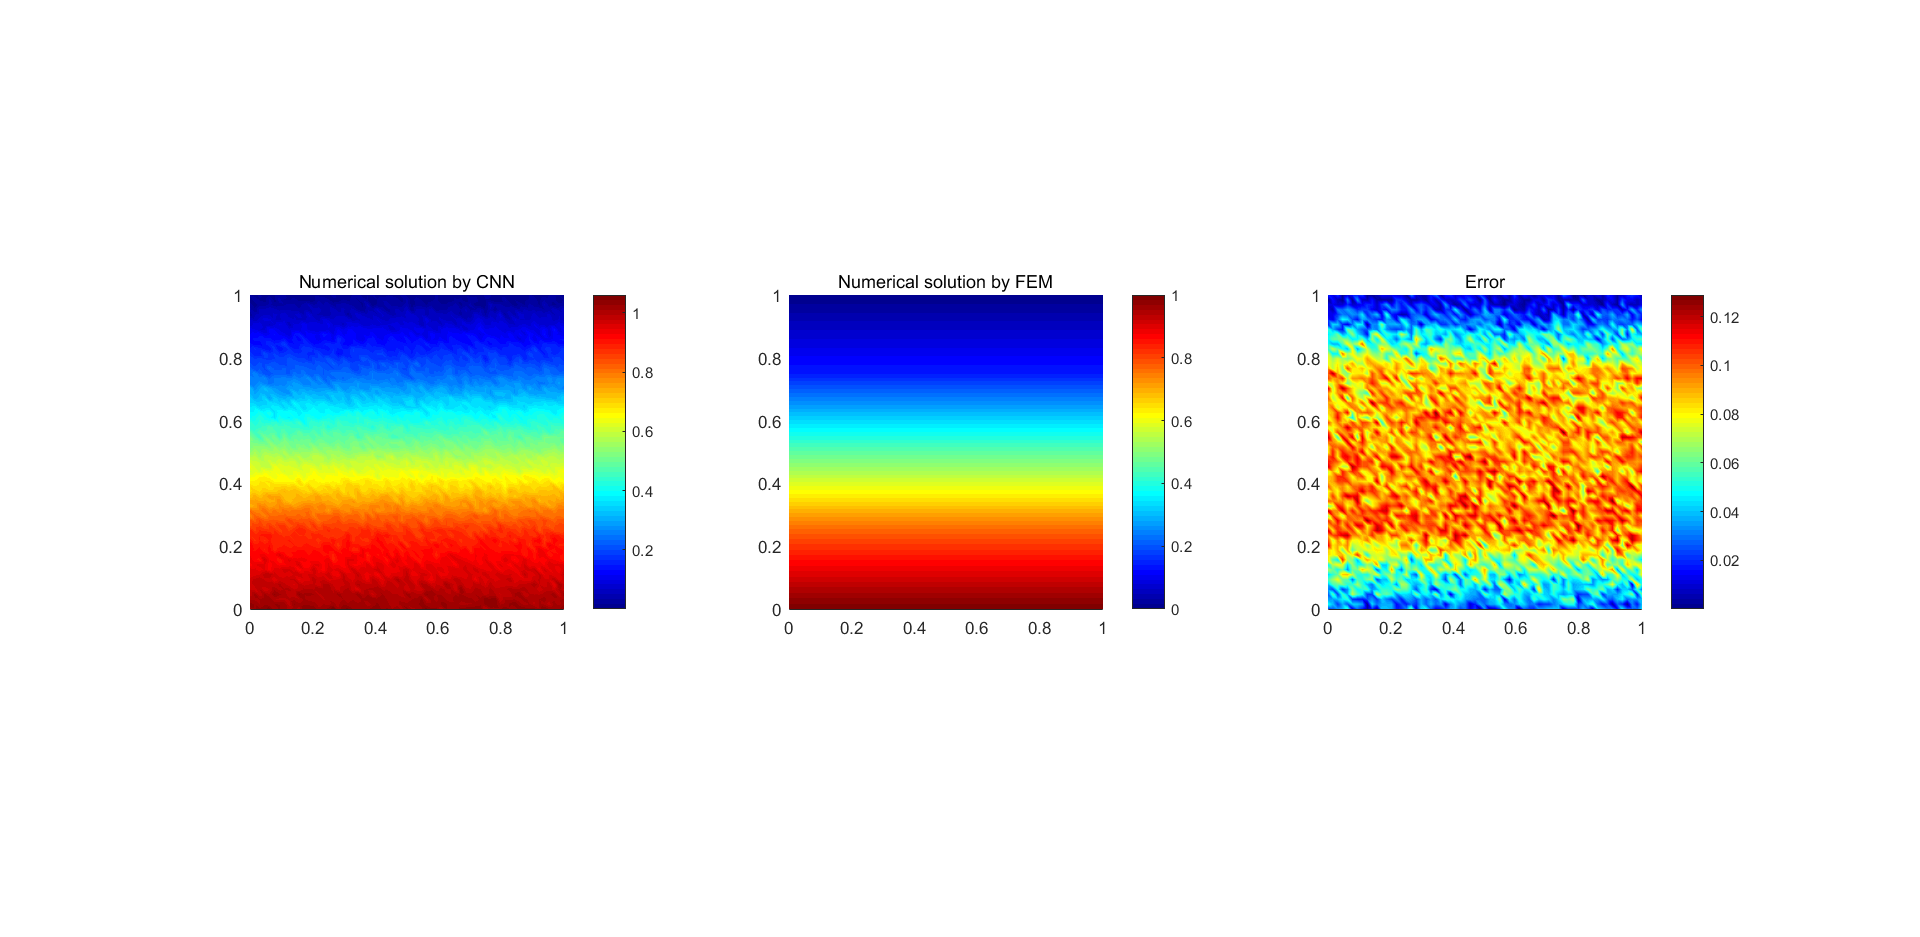
\includegraphics[width=0.65\textwidth]{figures/Darcy_CNN/Darcy_CNN_2000.png}
	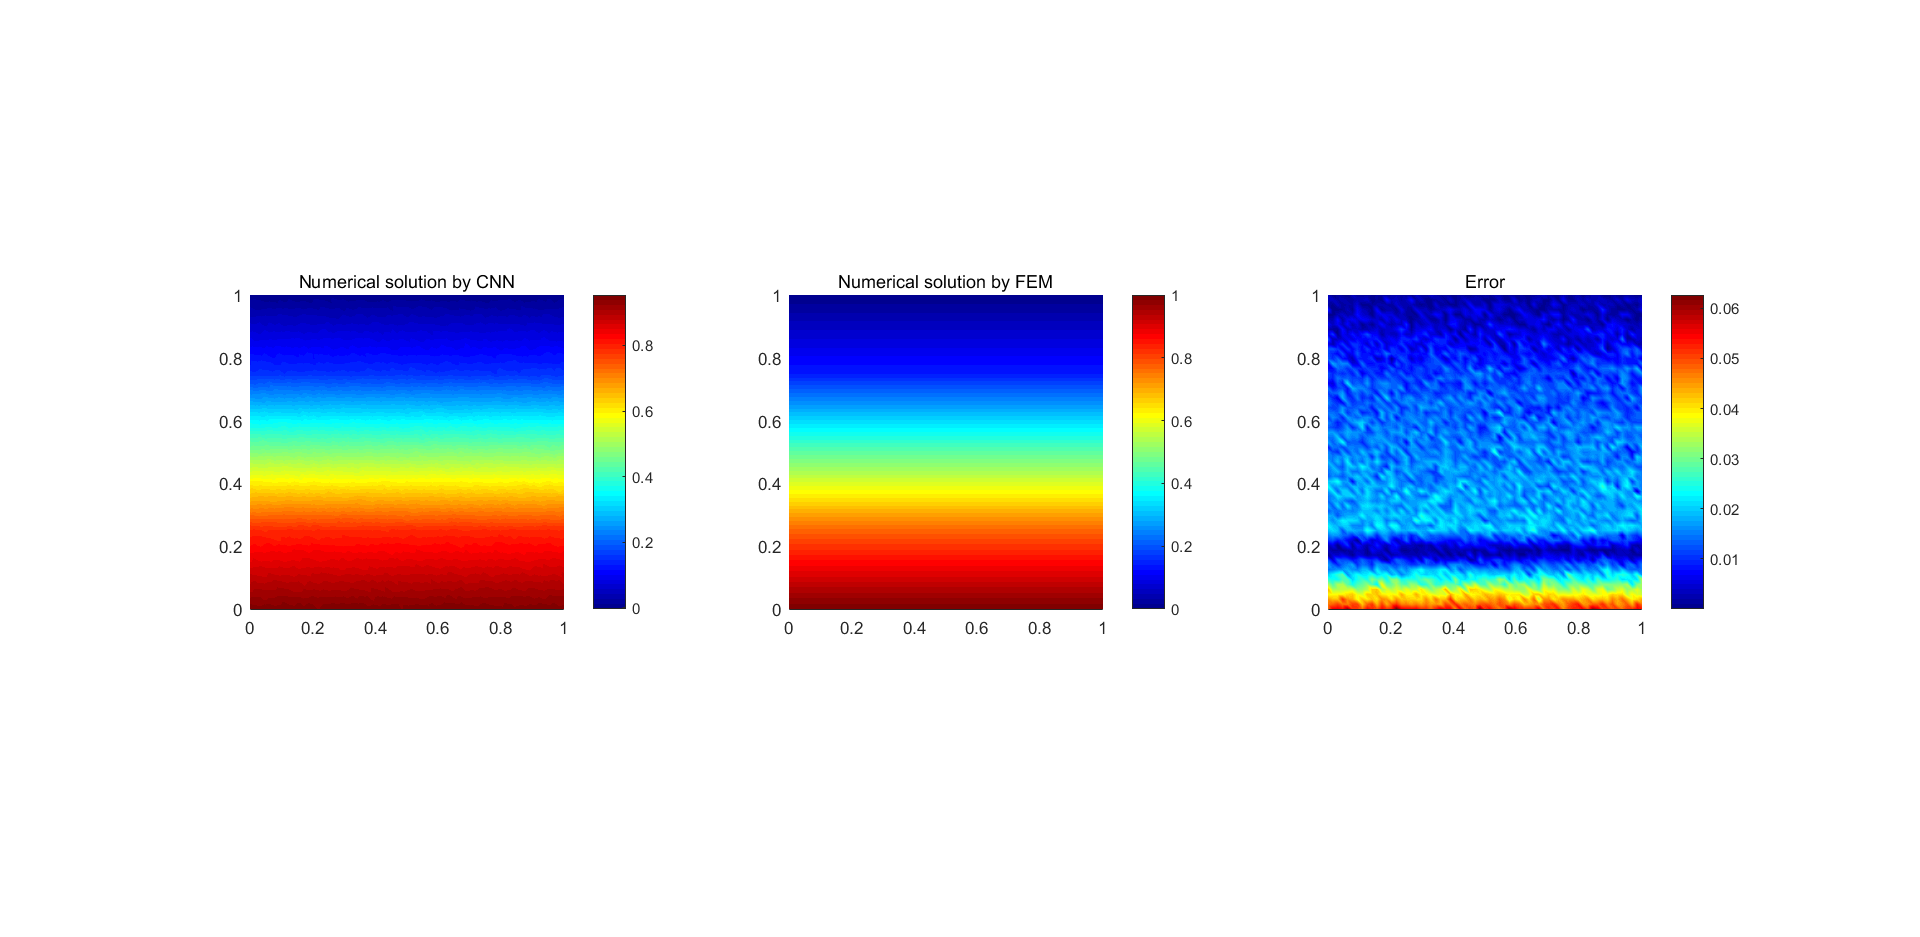
\includegraphics[width=0.65\textwidth]{figures/Darcy_CNN/Darcy_CNN_2000_nonlinear.png}
	\caption{Comparison of the solutions obtained by CNN with and without activation function by SGD (Top: without activation, Bottom:  with activation, 8,2 million parameters).}
\end{figure}

\begin{figure}[!htbp]
	\centering
	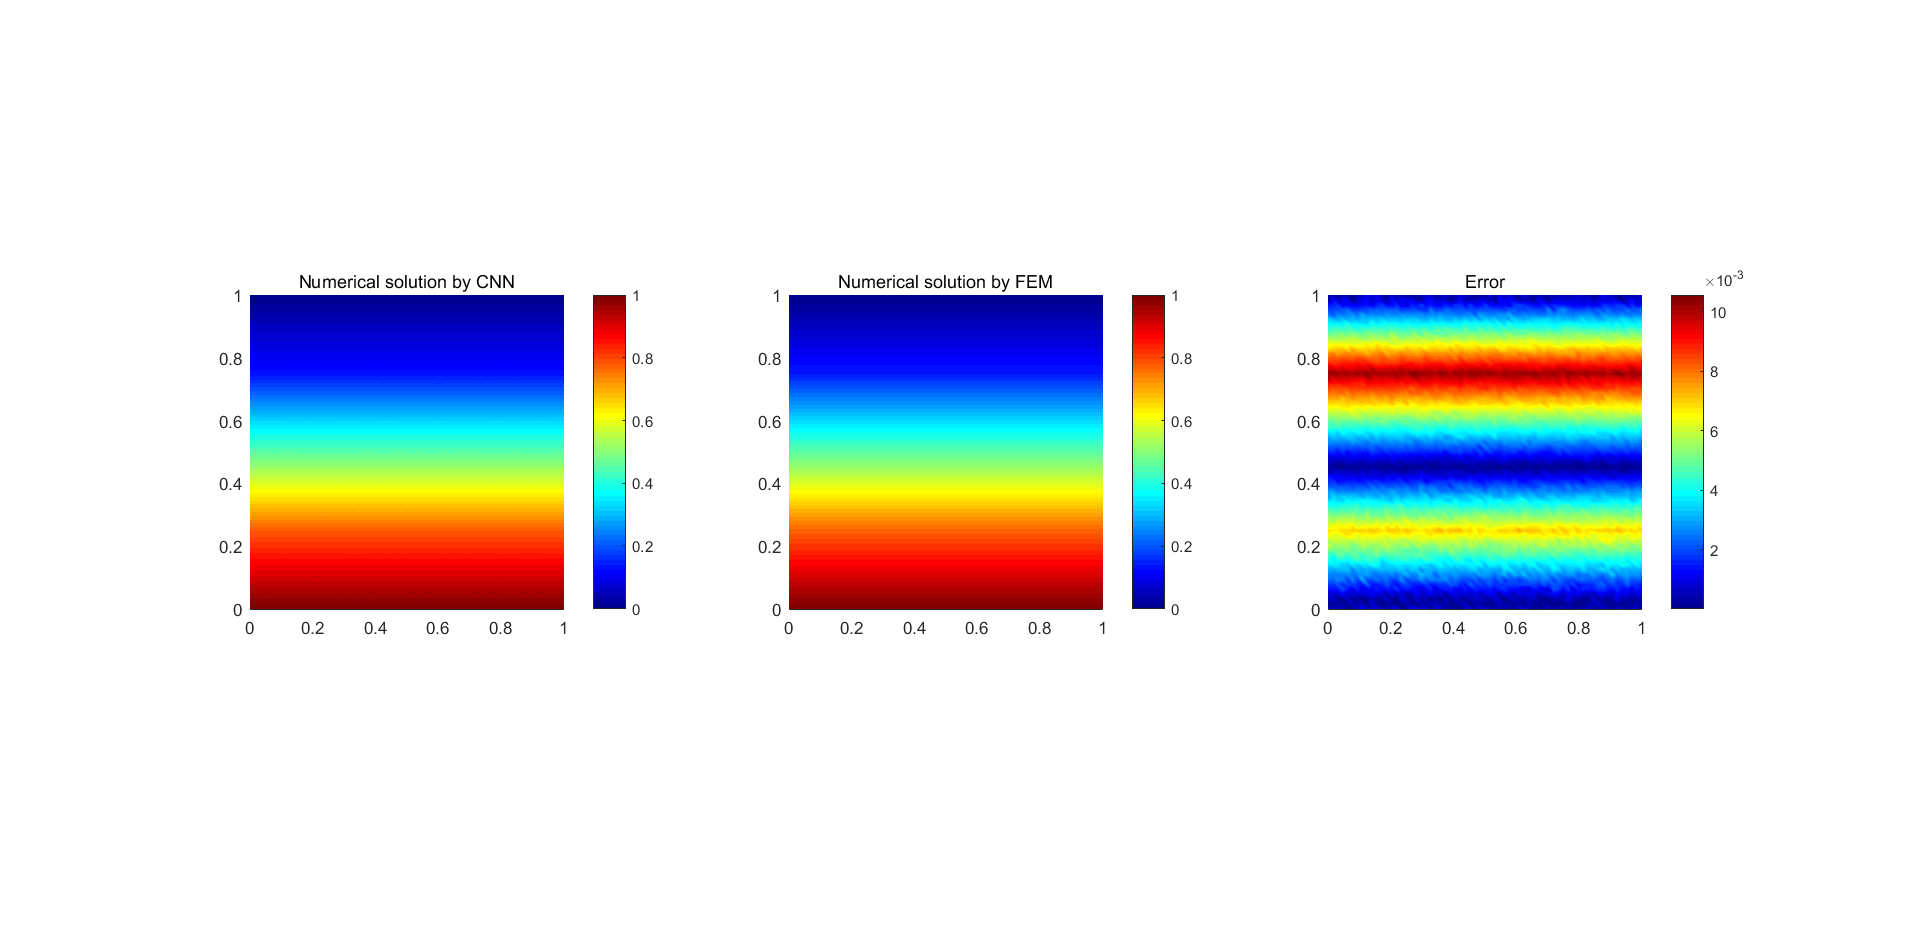
\includegraphics[width=0.65\textwidth]{figures/Darcy_CNN/Darcy_CNN_Adam_2000.png}
	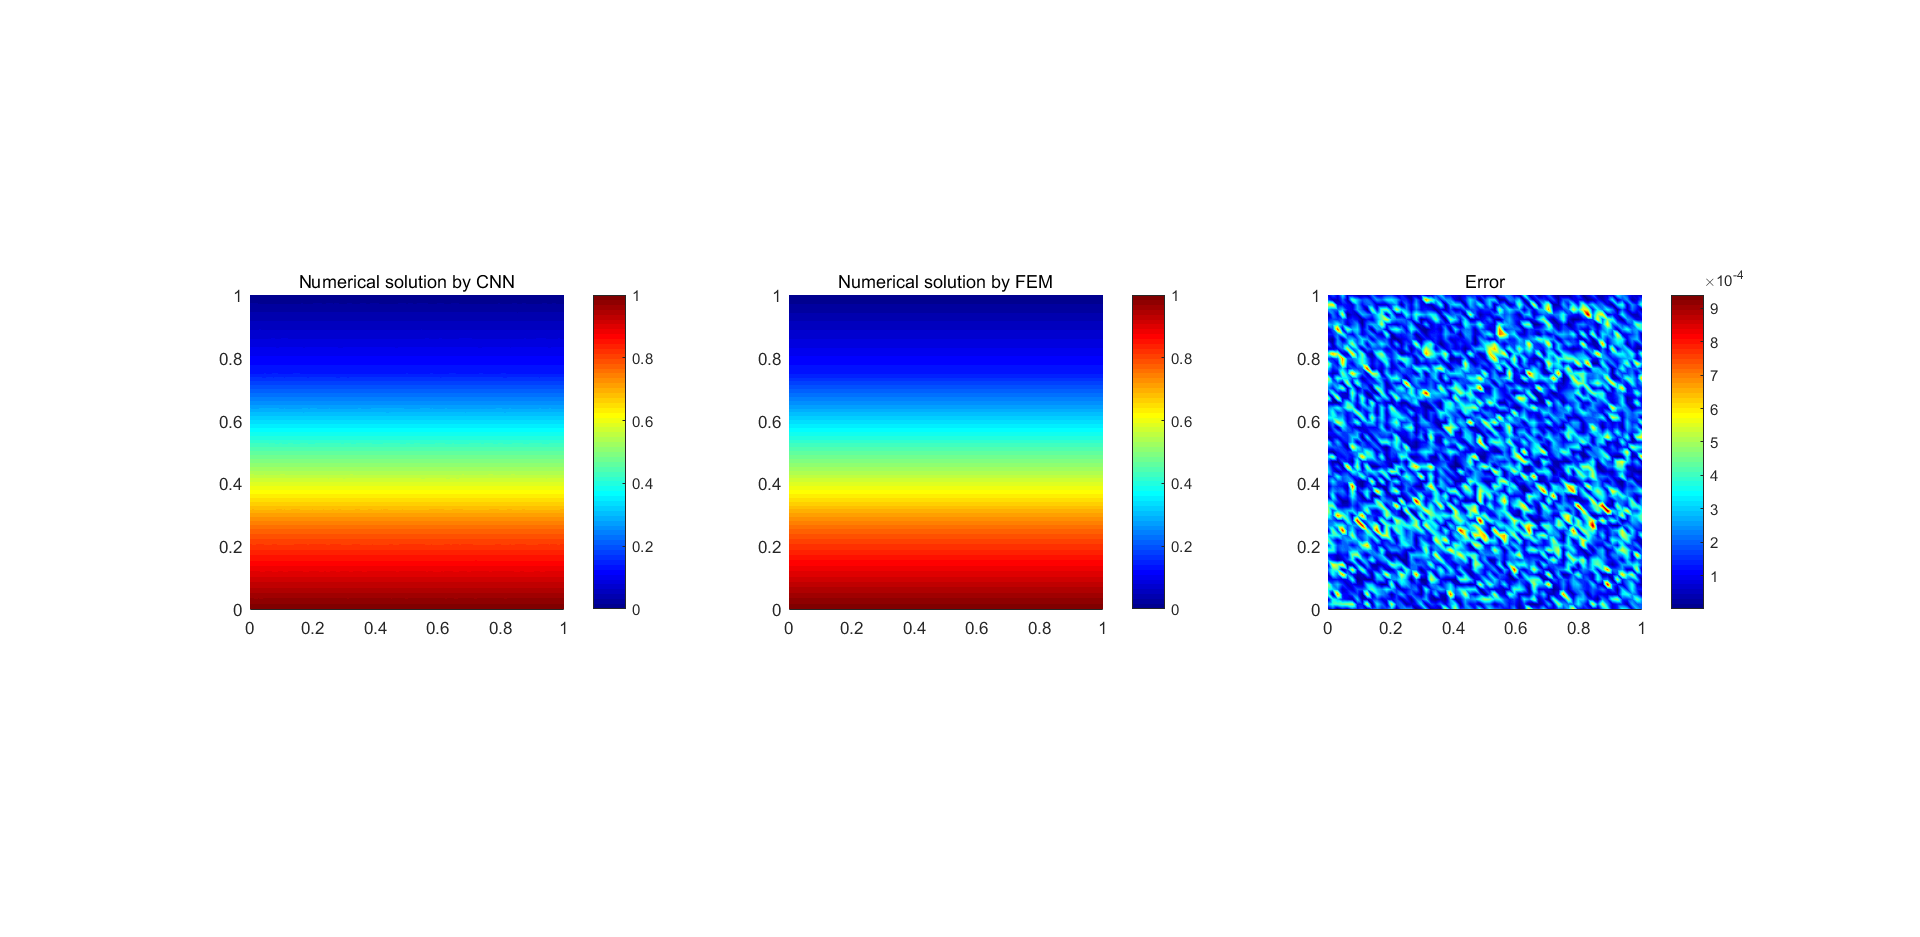
\includegraphics[width=0.65\textwidth]{figures/Darcy_CNN/Darcy_CNN_2000__Adam_nonlinear.png}
	\caption{Comparison of the solutions obtained by CNN with and without activation function by Adam method (Top: without activation, Bottom:  with activation).}
\end{figure}

\begin{figure}[!htbp]
	\centering
	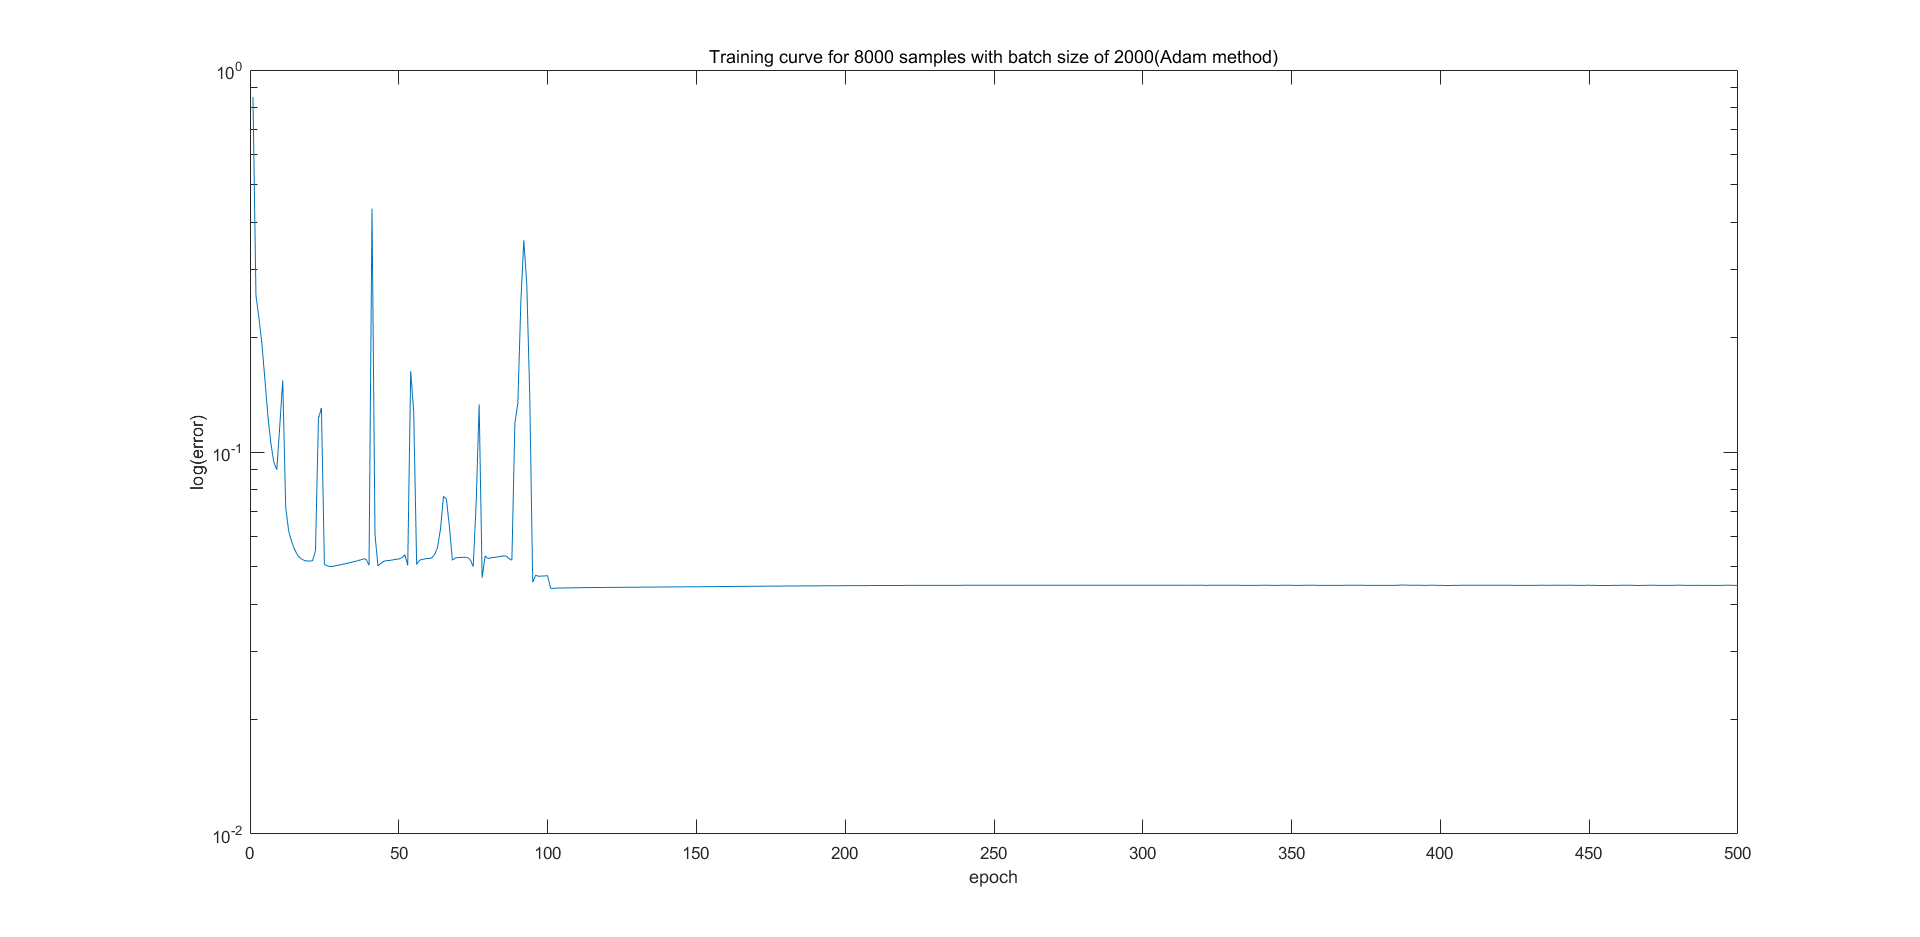
\includegraphics[width=0.45\textwidth]{figures/Darcy_CNN/darcy_loss_2000_adam.png}
	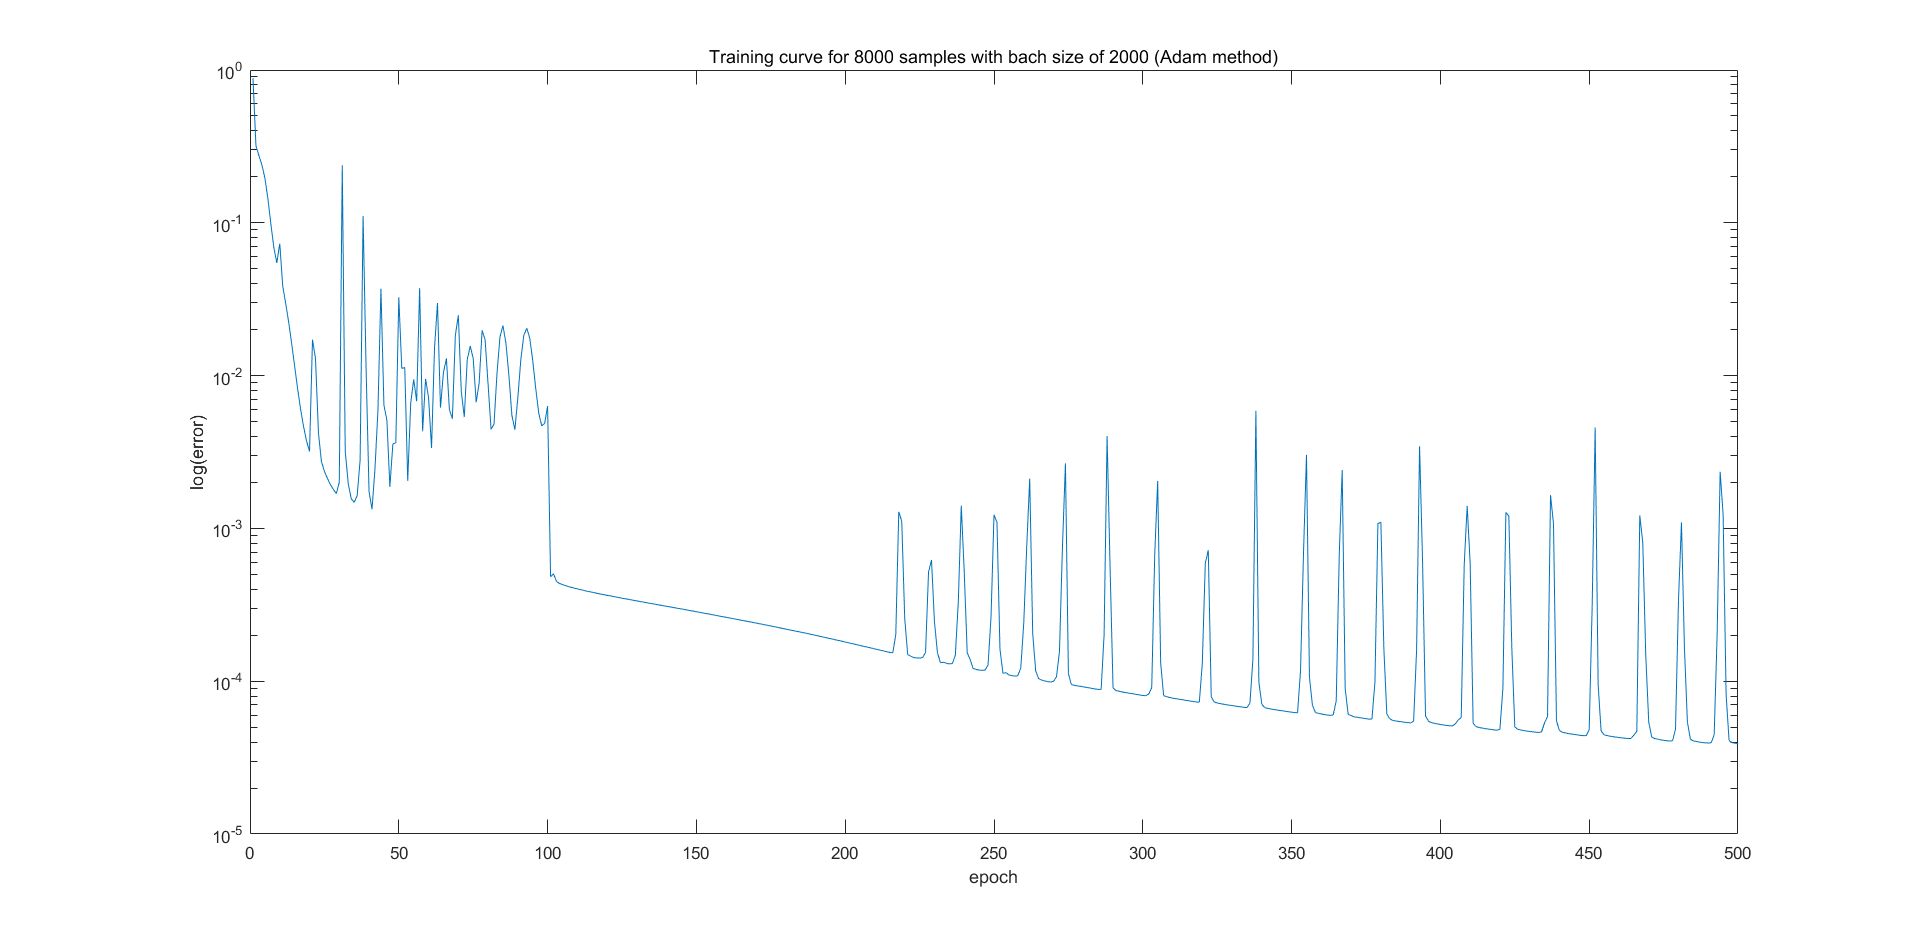
\includegraphics[width=0.45\textwidth]{figures/Darcy_CNN/darcy_loss_2000_adam_nonlinear.png}
	\caption{Training curves  with and without activation function by Adam method (Left: without activation, Right:  with activation).}
\end{figure}

	\begin{figure}[!htbp]
	\centering
	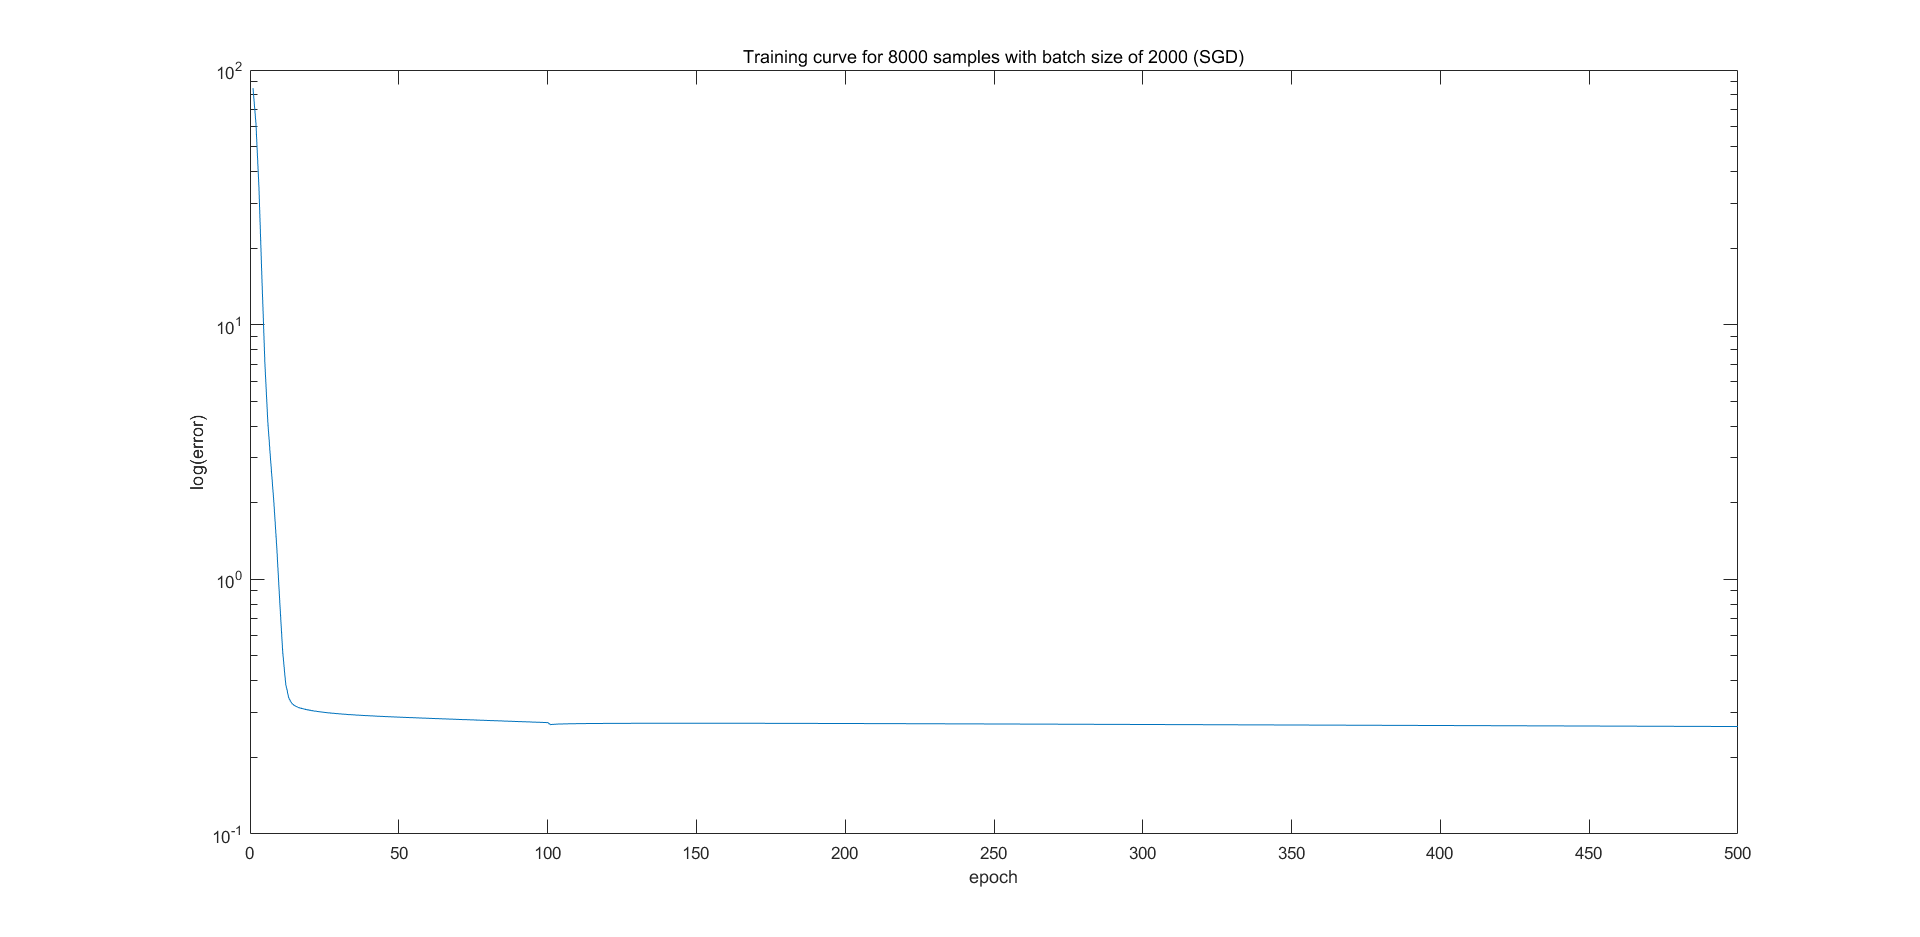
\includegraphics[width=0.45\textwidth]{figures/Darcy_CNN/darcy_loss_2000_SGD.png}
	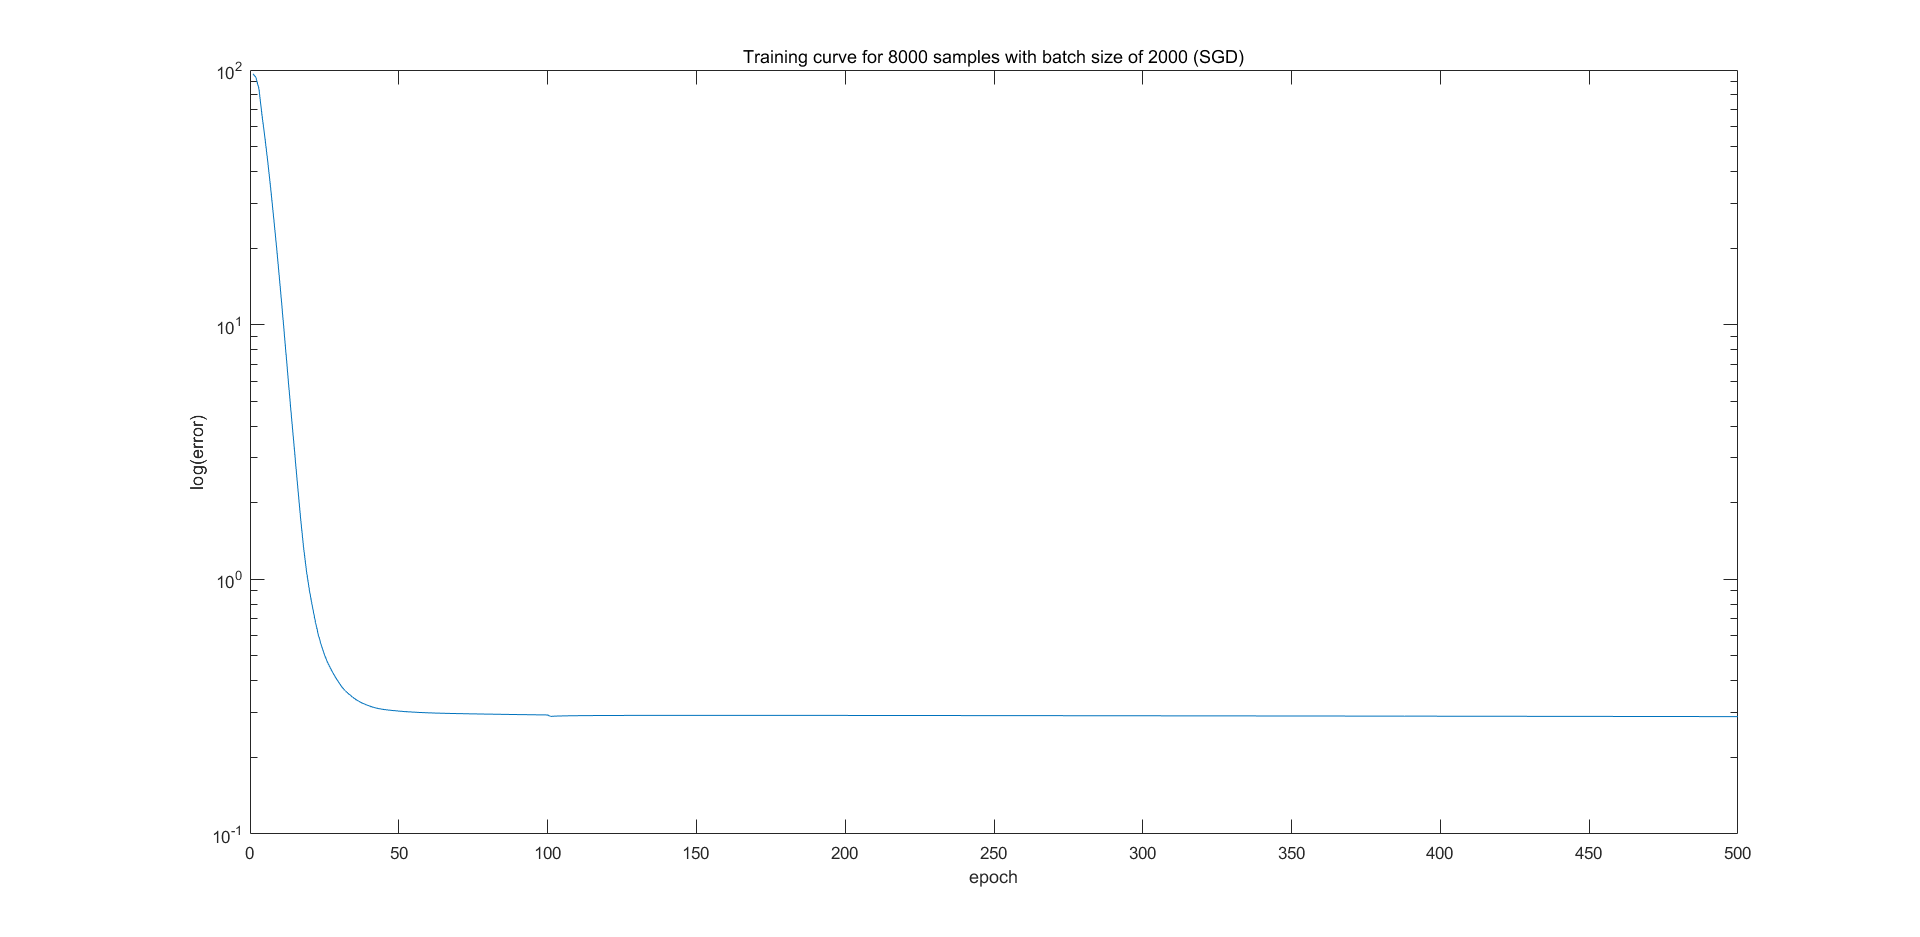
\includegraphics[width=0.45\textwidth]{figures/Darcy_CNN/darcy_loss_2000_SGD_nonlinear.png}
	\caption{Training curves  with and without activation function by SGD method (Left: without activation, Right:  with activation).}
\end{figure}

Below we consider the decoding process as the transpose of the encoding process.
\begin{breakablealgorithm}
	\caption{$u={\rm DarcyCNN_{transpose}}(\kappa; f_d, coarse\_grid\_size,)$}
	\label{alg:mgnet}
	\begin{algorithmic}
		\State Initialization:  $\kappa$
		%		\State Initialization $u^{1,0}$
		%		\For{$ = 1:N_{epoch}$}
		%		\For{$i = 1:\nu_$}
		\State Encode
		\begin{equation}
		u^{} = K^{3}  \ast_2   K^{ 2}\ast  (K^{ 1}\ast \kappa).
		\end{equation}
		
		%		\EndFor
		\State Restriction to the coarse grid
		\begin{equation}
		u^{} =   W u^{}
		\end{equation}
		\State
		Convolution on the coarse grid
		\begin{equation}
		u^{} =   K^{ 5}\ast K^{ 4}\ast u^{}.
		\end{equation}
		\State Decode
		\begin{equation}
		u^{} =  K^{ 1,T} \ast K^{ 2,T}\ast K^{3}  \ast_2^T (W^{ T}  K^{ 4,T}\ast K^{ 5,T}\ast u^{}).
		\end{equation}
		%		\EndFor
	\end{algorithmic}
\end{breakablealgorithm}
Where $K^T$ is the transpose of kernel $K$. For a kernel with size of $3 \times 3$ without padding, its transpose is the central symmetry of itself with 2 paddings.\\

In this network, the parameters are 13 million and 6.5 million respectively.

	\begin{figure}[H]
		\centering
		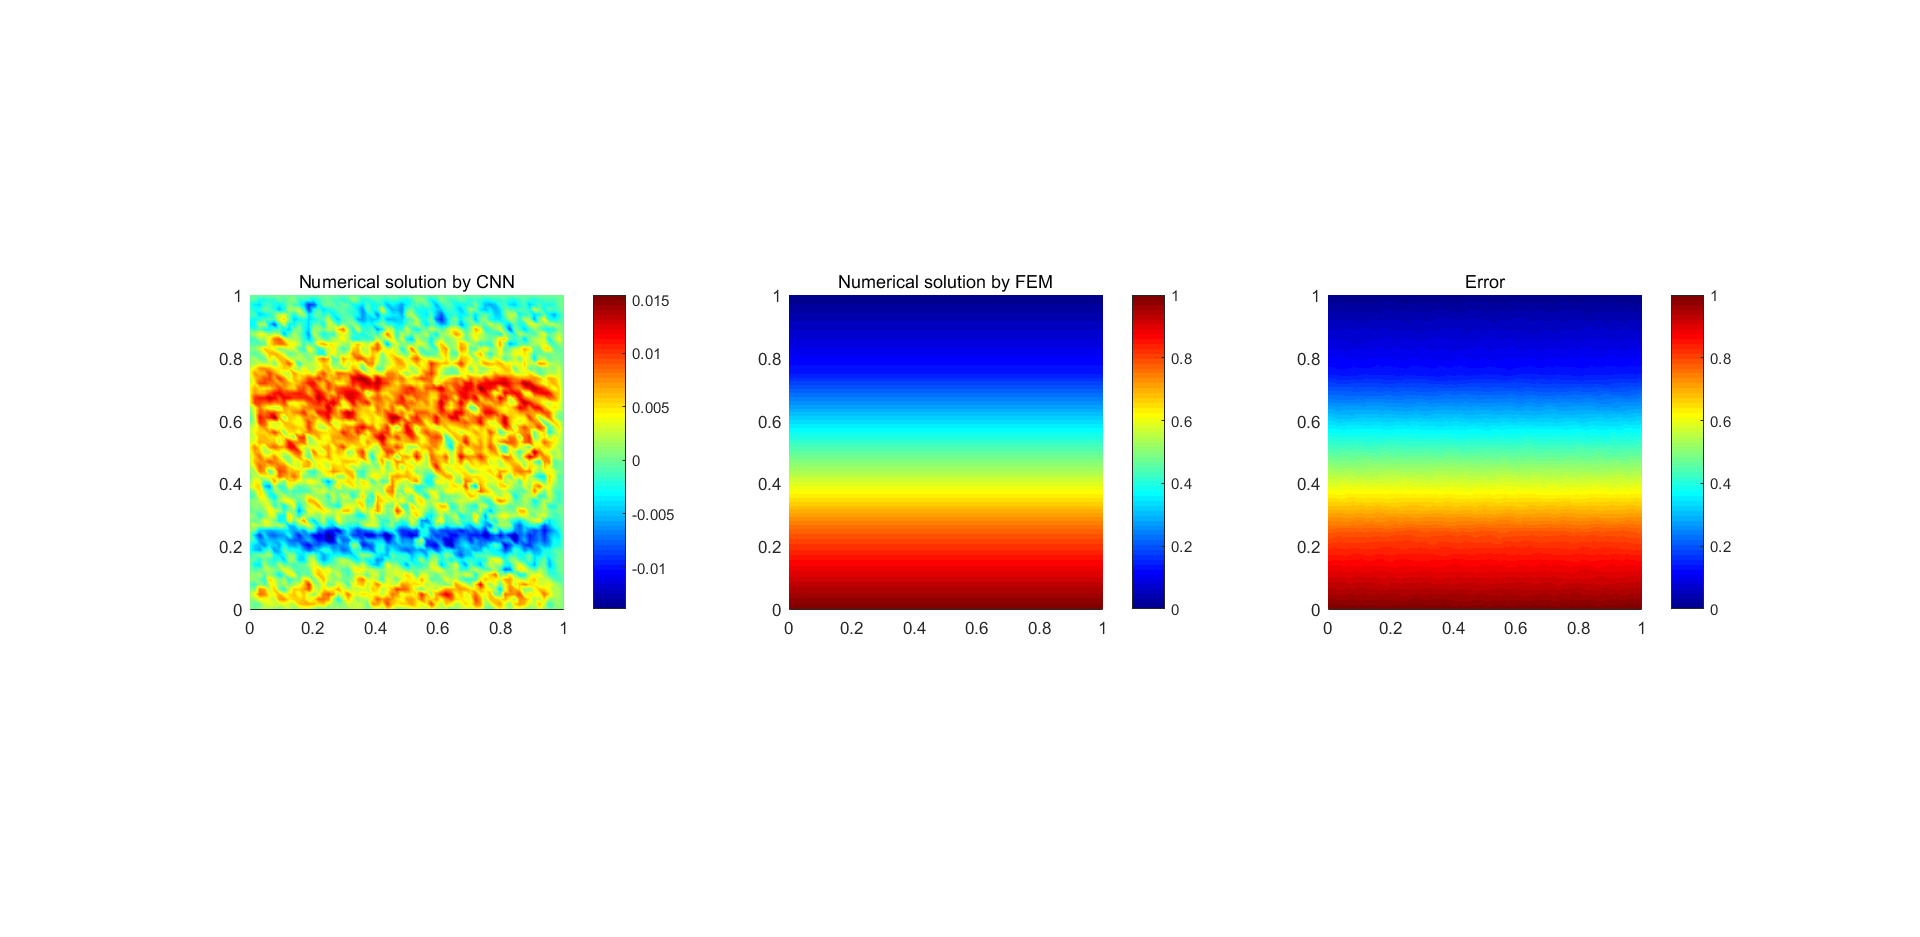
\includegraphics[width=0.45\textwidth]{figures/Darcy_CNN/Darcy_transpose_value_mean.png}
		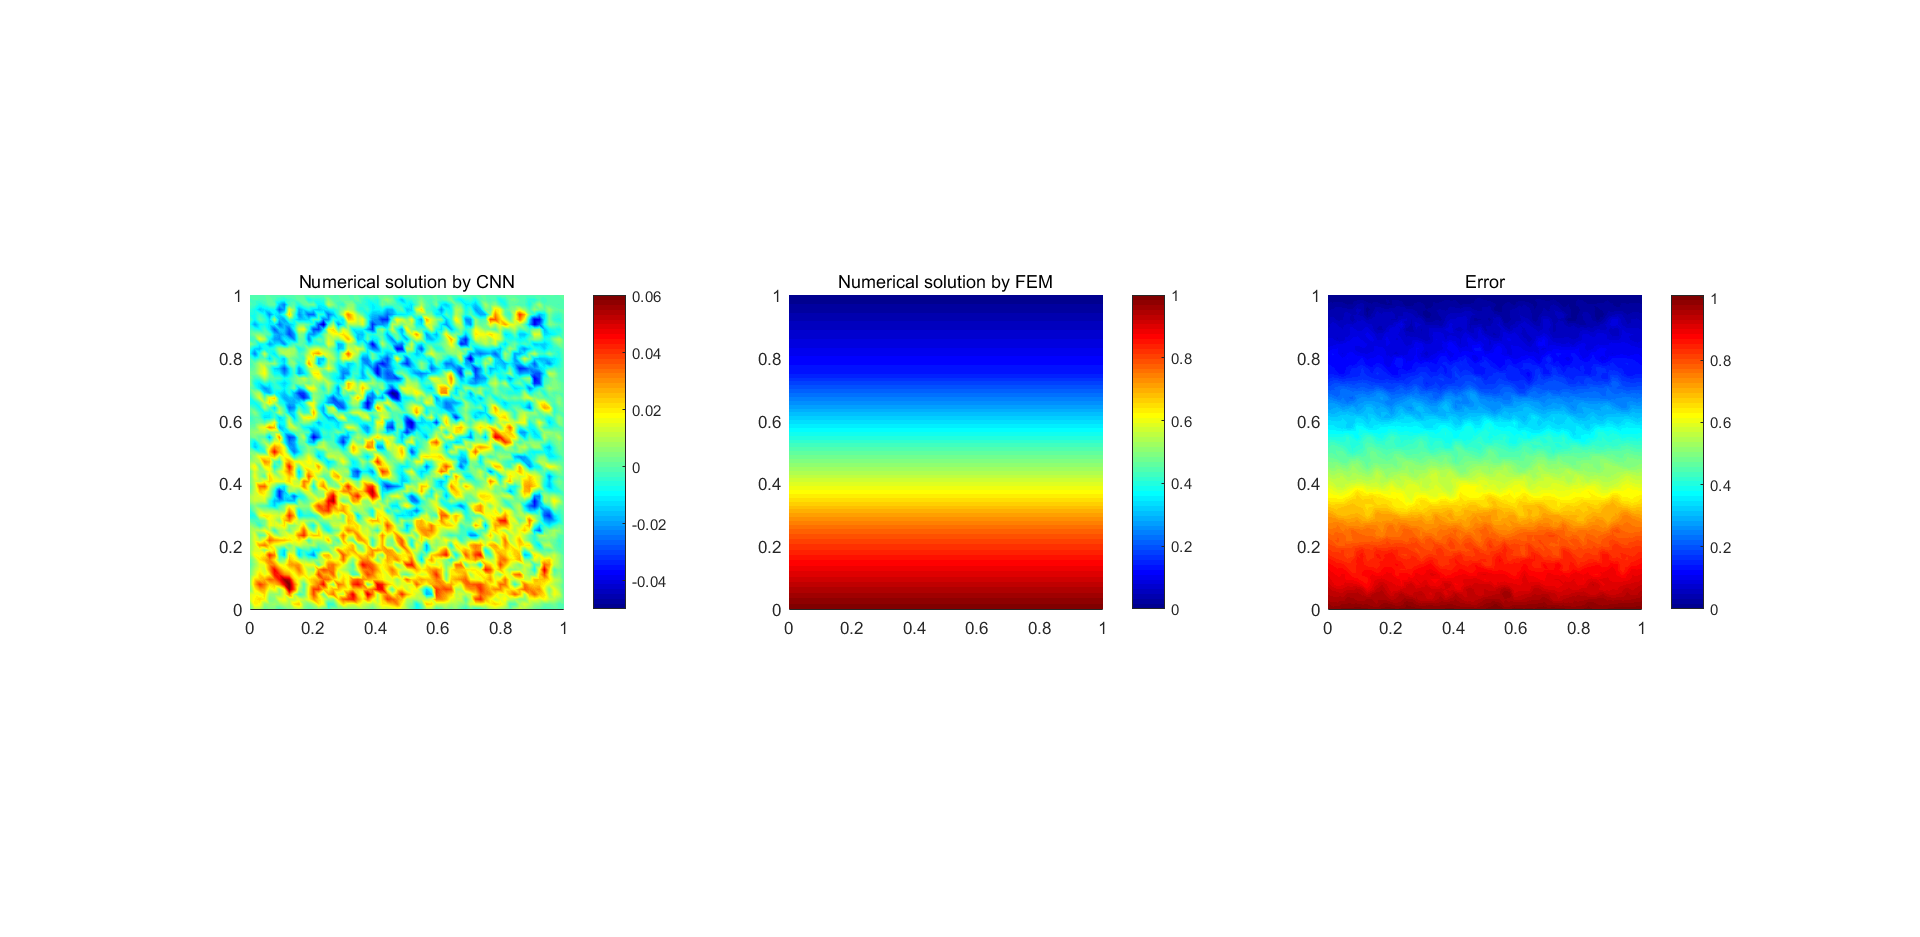
\includegraphics[width=0.45\textwidth]{figures/Darcy_CNN/Darcy_transpose_novalue_mean.png}
		\caption{Comparison of solutions obationed by FEM and neural network including transpose(Left: Transposed parameters untrained, Right: Transposed parameters trained) with zero-mean input.}
	\end{figure}
	
	\begin{figure}[H]
		\centering
		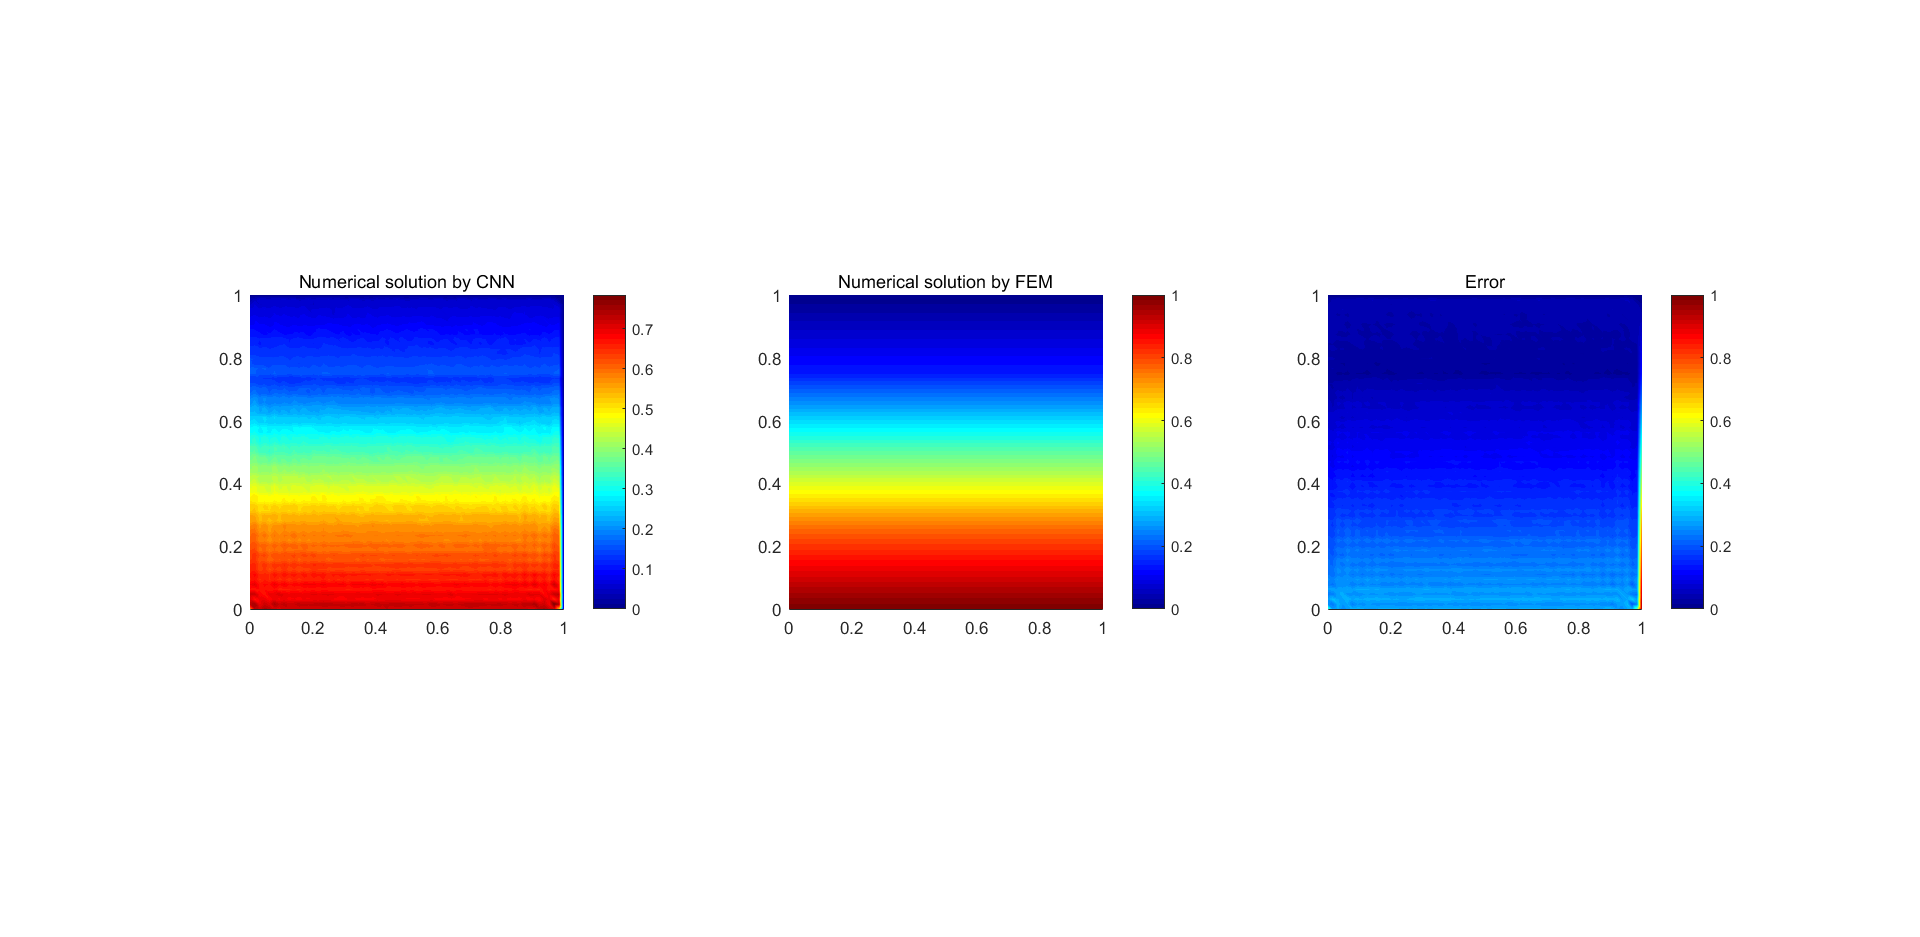
\includegraphics[width=0.45\textwidth]{figures/Darcy_CNN/Darcy_transpose_value.png}
		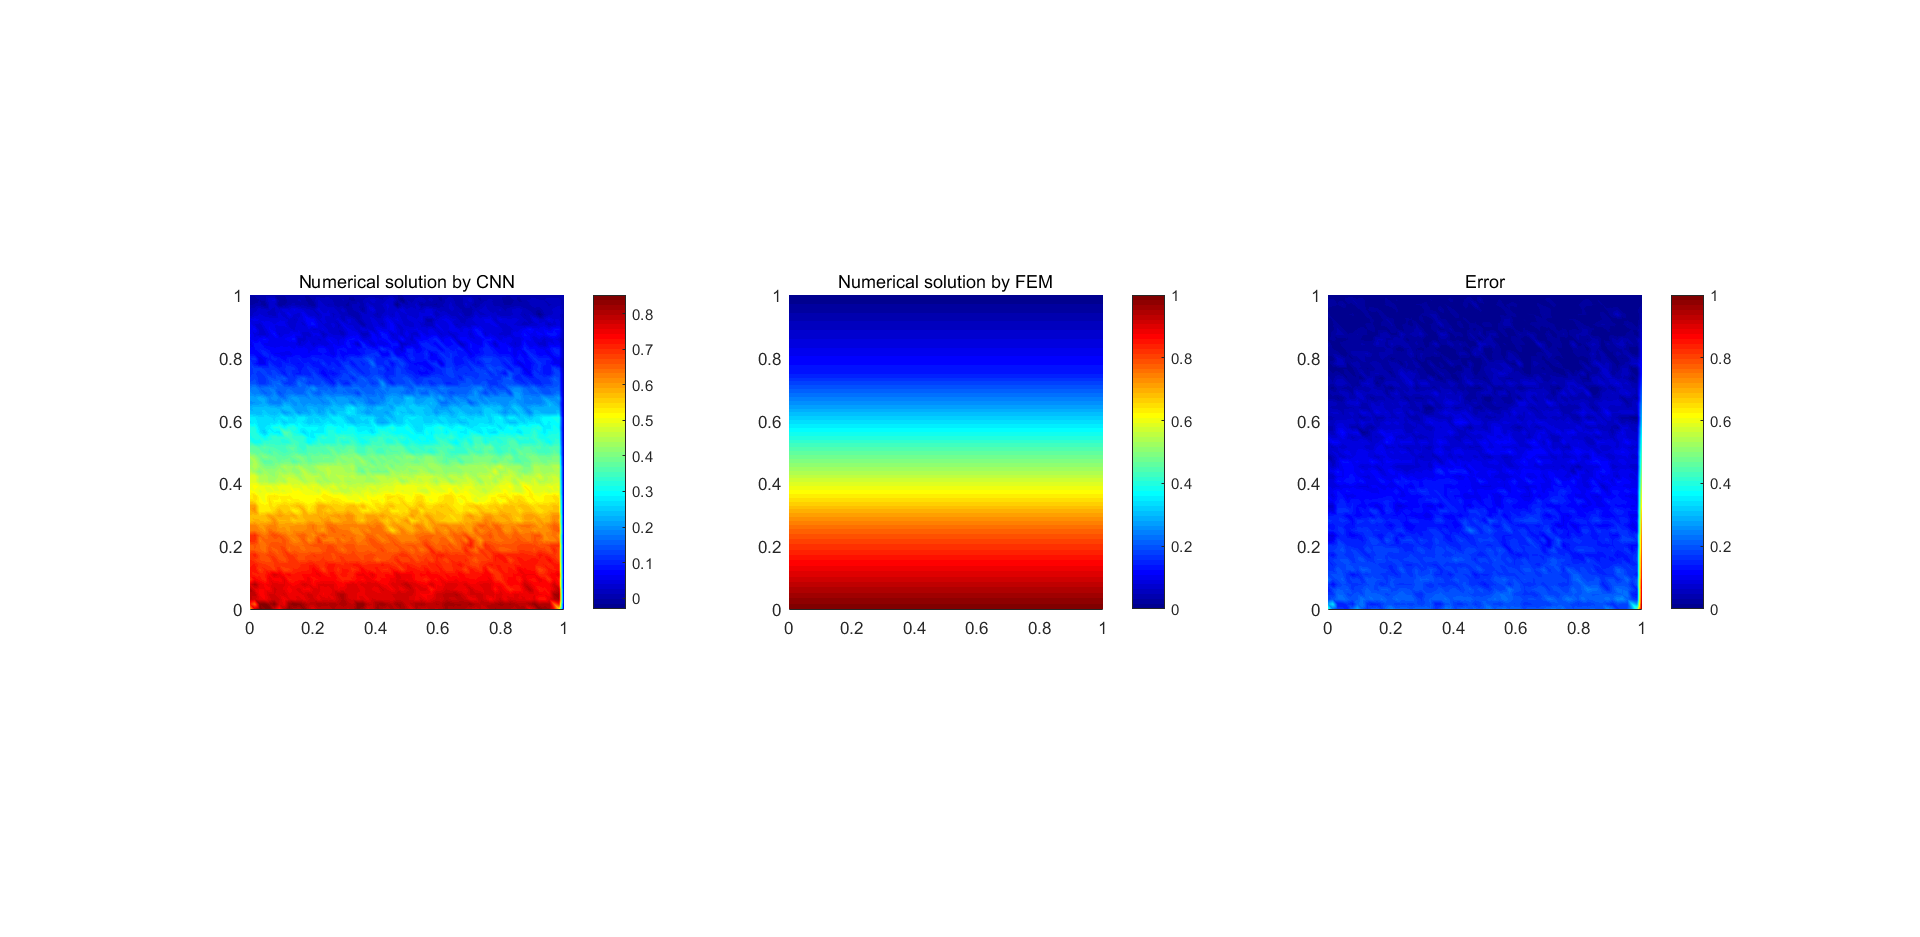
\includegraphics[width=0.45\textwidth]{figures/Darcy_CNN/Darcy_transpose_novalue.png}
		\caption{Comparison of solutions obationed by FEM and neural network including transpose(Left:  Transposed parameters untrained, Right: Transposed parameters trained) with original input.}
	\end{figure}


The problem we feel confused is that unlike the process in PCA method, what we need to do is to solve a darcy equation, where the input data and output data are in two different fields. Therefore, whether it makes sense that using the encode transpose-encode process to solve this problem.

\newpage
\subsection{PCA and POD}
For the differnence between PCA and POD, here we consider following linear problem
$$
A_i x_i = b_i, \quad i = 1,\cdots,N
$$
Consider the solutions $x_i $ are in a hyperplane $y_i = W\tilde{x}_i+\mu$ where $W \in \mathbb{R}^{d\times d'}, d'\ll d $ and $y_i$ is an approximation of $x_i$. To approximate $x_i$ as closely as possible, i.e. minimize loss function
\begin{equation}\label{lossPOD}
L = \sum_{i}^{N}=\| y_i - x_i\|^2 =  \sum_{i}^{N}=\| W\tilde{x}_i +\mu - x_i\|^2
\end{equation}
Then, the best choice of $\tilde{x}_i $ and $\mu$ is
$$
\mu = \frac{1}{N}\sum_{i}^{N}x_i = \bar{x}, \quad
\tilde{x}_i = W^T(x_i-\bar{x})
$$
Then \ref{lossPOD} can rewritten as
$$
L =  \sum_{i}^{N}=\| WW^T(x_i-\bar{x}) +\bar{x} - x_i\|^2 .
$$
The choice of $W$ is the same as PCA method.\\

For the linear problem $Ax=b$, we consider $x = W\tilde{x}+\bar{x}$ and premultiplicate $W^T$ on the eqauation, we get
$$
W^TAW\tilde{x} = W^T(b-A\bar{x}).
$$
Solve the equation above and with the decoder, we can get the approximation of the solution as
$$
x \approx W\tilde{x} + \bar{x}.
$$
In the POD, we consier the solution in the specific hyperplane $y_i = W\tilde{x}_i$, then the low-dimension solution $\tilde{x}$ satisfies
$$
W^TAW\tilde{x} = W^Tb
$$
Apply the decoded to get the approximation solution as
$$
x = W\tilde{x}
$$
For the construction of CNN to solve this problem, the matrix A is associated with $\kappa$ and can be regarded as a linear mapping of $\kappa$, and the right side term $b$ is fixed.

%Here for a input $\kappa$, I wonder the encoded is processed on $\kappa$, or on a linear  mapping of $\kappa$ which approximate the solution $x$. As we all know, the traditional encode-decode process is all about $x$. However, here we need to apply the encoder on $\kappa$ and have some extra computation to solve the equation in a lower dimension. Finally we apply the decoder to get the approximation of the solution.
\subsection{Mgnet-encoder}
In order to make the distance between the approximate solution and true solution  as small as possible, i.e. minimize loss function
$$
L = \sum_{i}^{N} \| g  \circ f(x_i) - x_i \|
$$
If we fix the decoder as a linear function, i.e.
$$
g(y) = Wy + b
$$
Hdre, we use the following MgNet as the encoder
\begin{breakablealgorithm}%[!htb]
	\caption{$\mu^J = {\text{MgNet}}(f; J,\nu_1, \cdots, \nu_J)$}
	\label{alg:L-Slash11d}
	\begin{algorithmic}
		\State Set up
		$$
		f^1 = {\color{red} \theta\ast} f, \quad \mu^{1}=0. 
		$$
		\State Smoothing and restriction from fine to coarse level (nested)
		\For{$\ell = 1:J$}
		\For{$i = 1:\nu_\ell$}
		\State
		\begin{equation}\label{eq:smoothing}
		\mu^{\ell} \leftarrow \mu^{\ell} + S^\ell \ast (f^\ell - A_\ell \ast \mu^{\ell}).
		\end{equation}
		\EndFor
		\State Form restricted residual and set initial guess:
		$$
		\mu^{\ell+1} \leftarrow \Pi_{\ell}^{\ell+1}\mu^\ell , \quad
		f^{\ell+1} \leftarrow R^\ell \ast_2 (f^\ell -  A_\ell \ast
		\mu^{\ell}) + A_{\ell+1}\ast 	\mu^{\ell+1} ,    %A_{\ell+1} = R       \ast_2 A_\ell \ast (R\ast_2^\top).
		$$
		\EndFor
		\State
		Finally, we ultilize the Adaptive average pooling to let the number of element in every channel of $\nu^J$ be 1.
		$$\nu^J = Avg \ast \nu^J$$
	\end{algorithmic}
\end{breakablealgorithm}
Here, $\mu_J$ is the reduced vector. For the decoder, we denote $(u^l,f^l)$ as a new variable.
Then we can induce that
$$\mu^{l+1}=\phi^{l+1}\mu^l + \xi^{l+1}f^{l+1}$$
$$f^{l+1} = R^l f^l + M^l \mu^l $$
where $\phi^{l+1}= (N^{l+1})^{v_{l+1}}\Pi_l^{l+1}, N^{l+1}= I - S^{l+1}A^{l+1} $, $\xi^{l+1}=\big(\sum_{i=1}^{v_{l+1}-1}(N^{l+1})^i\big)S^{l+1}$ and $M^l = A^{l+1}\Pi_l^{l+1} - R^lA^l$.

We can also rewritten the equation above as
\[
\left( \begin{array}{l}
f^{l+1} \\
\mu^{l+1}
\end{array} \right) = \left( {\begin{array}{*{20}{c}}
	R^l & M^l\\
	\xi^{l+1}R^l&\phi^{l+1}+\xi^{l+1}M^l
	\end{array}} \right)\left( \begin{array}{l}
f^{l}\\
\mu^{l}
\end{array} \right), \quad
\left( \begin{array}{l}
f^{1} \\
\mu^{1}
\end{array} \right) = \left( {\begin{array}{{c}}
	\theta \\
	\xi^{1}\theta
	\end{array}} \right)\left( \begin{array}{l}
f\\
\end{array} \right)
\]
We can then define the mgnet-decoder as
\begin{breakablealgorithm}%[!htb]
	\caption{$f = {{\rm MgNet_{transpose}}}(u^J; J,\nu_1, \cdots, \nu_J)$}
	\begin{algorithmic}
		\State Transpose of Adapative Average pooling
		$$\mu^J = Avg^T \ast \nu^J $$
		\State Prolongation back to the fine level 
		\State 
		$$
		f^{J-1} = R^{J-1, T}\xi^{J, T}\mu^J,  \qquad \mu^{J-1} = (M^{J-1,T}\xi^{J, T} + \phi^{J-1, T})\mu^{J}
		$$
		\For{$\ell = J-2:1$}
		\State
		\begin{equation}
		\mu^{\ell}= M^{\ell,T}f^{\ell+1} + (M^{\ell,T}\xi^{\ell+1, T} + \phi^{\ell, T})\mu^{\ell+1}.
		\end{equation}
		\State
		\begin{equation}
		f^{\ell} = R^{\ell, T}f^{\ell+1} + R^{\ell, T}\xi^{\ell+1, T}\mu^{\ell+1}
		\end{equation}
		\EndFor
		\State Transpose of pre-convolution:
		$$
		f = \theta^T \ast f^1 + \theta^T \ast \xi^{1,T} \mu^1
		$$
	\end{algorithmic}
\end{breakablealgorithm}

\subsection{Numerical results}
Then we have the some results for the following test.

\begin{itemize}
	\item Model equations
	\begin{align*}
	- \nabla \cdot (\kappa \nabla p) & = 0  \qquad \text{in}~~ \Omega \\
	\kappa \nabla p \cdot n &= 0 \qquad \text{on} ~~ \Gamma_\text{N} \\
	p  &= 0 \qquad \text{on} ~~\Gamma_{\text{D}1} \\
	p  &= 1 \qquad \text{on}~~ \Gamma_{\text{D}2} \\
	\end{align*}
	\begin{center}
		\vskip -20pt
		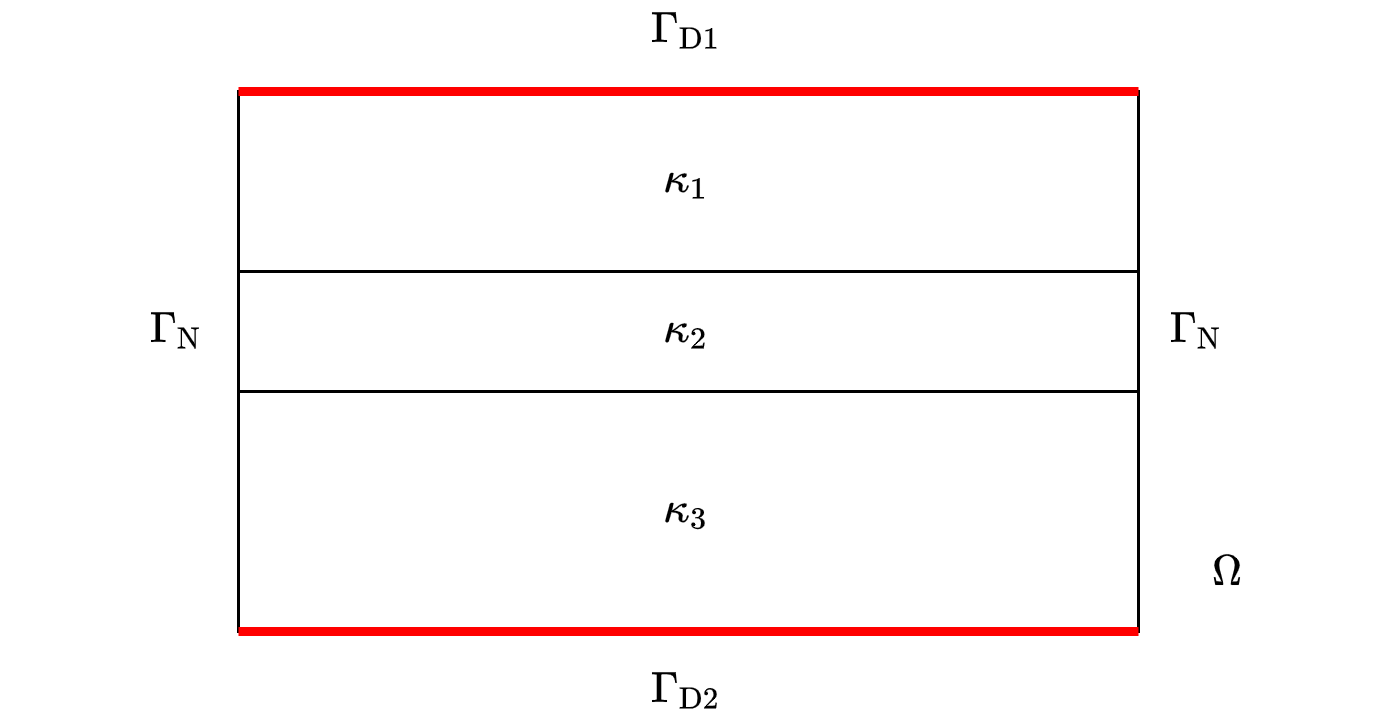
\includegraphics[height=5cm]{figures/Darcy_CNN/Darcy_domain.png}
	\end{center}
\end{itemize}
The loss fucntion is
$$
L = \sum_{i}^{N} \| g  \circ f(x_i) - x_i \|
$$
where $x_i$ is the FEM solution given the permeability $\kappa_i$, $f$ is the Mgnet encoder and $g$ is the Mgnet-Transpose decoder.

\begin{itemize}
	\item Uniformly generate 2000 training samples: $\kappa_1 \sim \mathcal{U}(2.5,7,5), \kappa_2 \sim \mathcal{U}(1,3)$ and $\kappa_3 \sim \mathcal{U}(0.5,1.5)$
	\item Grid size: $33*33 ~ (d=1089)$
	\item Number of training samples: 2000
	\item Number of epochs: 2000
	\item Number of test samples: 500
	\item Mgnet learning rate: $10^{-3}$
	\item DNN learning rate: 0.1
\end{itemize}
Here, we give the results of DNN and MgNet:

\subsubsection{Case 1: Fix J, change $\nu_i$}
Let $J=4,$, number of $\mu$'s channel equals to 10, number of $f$'s channel equals to 1, we test the cases when $\nu_i=1,2,3,4$.
\begin{table}
	\begin{center}
		\begin{tabular}{|c|c|c|c|c|}
			\hline
			& $\nu_i$=1 & $\nu_i$=2 & $\nu_i$=3& $\nu_i$=4 \\
			\hline
			Train loss & 1.1861 $\times 10^{-2}$ & 1.197 $\times 10^{-2}$& 1.0793 $\times 10^{-2}$ & 1.0795 $\times 10^{-2}$\\
			\hline
			Mean rel. errors & 6.358 $\times 10^{-3}$ &6.199 $\times 10^{-3}$ &5.947 $\times 10^{-3}$ &6.010 $\times 10^{-3}$ \\
			\hline
		\end{tabular}\caption{Training errors and test errors(3456 parameters).}
	\end{center}
\end{table}

\subsubsection{Case 2: Fix $\nu_i$, change J}
Let $\nu_i$=2, number of $\mu$'s channel equals to 10, number of $f$'s channel equals to 1, we test the cases when $J=3,4,5,6$
.\begin{table}
	\begin{center}
		\begin{tabular}{|c|c|c|c|c|}
			\hline
			& $J=3$ & $J=4$ & $J=5$& $J=6$ \\
			\hline
			Train loss & 1.3235 $\times 10^{-2}$ & 1.1197 $\times 10^{-2}$& 1.0760 $\times 10^{-2}$ & 1.0663 $\times 10^{-2}$\\
			\hline
			Mean rel. errors & 6.613 $\times 10^{-3}$ &6.199 $\times 10^{-3}$ &6.022 $\times 10^{-3}$ &5.956 $\times 10^{-3}$ \\
			\hline
			Number of Para & 2367& 3456& 4545 & 5634\\
			\hline
		\end{tabular}\caption{Training errors and test errors for various J.}
	\end{center}
\end{table}
\begin{figure}[H]
	\centering
	\includegraphics[width=0.6\textwidth]{figures/Darcy_CNN/loss_J.png}
	\caption{Training curves for various J=3,4,5,6.}
\end{figure}
\subsubsection{Case 3: Change number of $u$'s channel}
Let $\nu_i$=2, number of $f$'s channel equals to 1, $J=4$, we test the cases when the number of $\mu$'s channel equals to $10,20,30,40$
.\begin{table}
	\begin{center}
		\begin{tabular}{|c|c|c|c|c|}
			\hline
			& $n_u=10$ & $n_u=20$ & $n_u=30$& $n_u=40$ \\
			\hline
			Train loss & 1.1197 $\times 10^{-2}$ & 1.0772 $\times 10^{-2}$& 0.9634 $\times 10^{-2}$ & 0.8550 $\times 10^{-2}$\\
			\hline
			Mean rel. errors & 6.199$\times 10^{-3}$ & 6.091 $\times 10^{-3}$ &5.796 $\times 10^{-3}$ &5.574$\times 10^{-3}$ \\
			\hline
			Number of Para & 3456& 12276& 26496 & 71136\\
			\hline
		\end{tabular}\caption{Training errors and test errors for various number of $u$'s channel.}
	\end{center}
\end{table}

\begin{figure}[H]
	\centering
	\includegraphics[width=0.6\textwidth]{figures/Darcy_CNN/loss_u_channel.png}
	\caption{Training curves for various number of $u$'s channel.}
\end{figure}

\subsubsection{Case 4: DNN results}
For the one-layer DNN, we test the cases when the number of reduced dimension is $10, 20, 30 ,40$.
.\begin{table}[H]
	\begin{center}
		\begin{tabular}{|c|c|c|c|c|}
			\hline
			& 10 & 20 & 30& 40 \\
			\hline
			Train loss & 1.0584 $\times 10^{-2}$ & 0.8902 $\times 10^{-2}$& 0.7296$\times 10^{-2}$ & 0.6819 $\times 10^{-2}$\\
			\hline
			Mean rel. errors & 6.110$\times 10^{-3}$ & 5.852 $\times 10^{-3}$ &5.571$\times 10^{-3}$ &5.470$\times 10^{-3}$ \\
			\hline
			Number of Para & 10890& 21780& 32670 & 54450\\
			\hline
		\end{tabular}\caption{Training errors and test errors for various reduced dimension.}
	\end{center}
\end{table}
\textbf{In this test, we noticed that the weight obtained by DNN almost satisfies the orthogonality, and the weight obtained by MgNet also has the trendency to satisfy the orthogonality where the elements on the diagnol close to 1 and the non-diagol elements close to 0.}

\subsubsection{Case 5: POD results}
For the POD method, we test the cases when the number of reduced basis is $10, 20, 30 ,40$
.\begin{table}
	\begin{center}
		\begin{tabular}{|c|c|c|c|c|}
			\hline
			& 10 & 20 & 30& 40 \\
			\hline
			Mean rel. errors & 6.345$\times 10^{-3}$ & 6.111 $\times 10^{-3}$ &5.918$\times 10^{-3}$ &5.788$\times 10^{-3}$ \\
			\hline
		\end{tabular}\caption{Test results for various reduced basis number.}
	\end{center}
\end{table}

However, there exists a problem for this numerical test because the variance of every entry  of the solution is actually verly small ($10^-5$). From the results above, we can only infer that CNN can use less paramters to obtain the weight than DNN does. To illustrate this conclusion, we consider further numerical tests.

\subsection{Extend tests}
Here we let the source term of the equation be 1, i.e., 
\begin{itemize}
	\item Model equations
	\begin{align*}
		- \nabla \cdot (\kappa \nabla p) & = 1  \qquad \text{in}~~ \Omega \\
		\kappa \nabla p \cdot n &= 0 \qquad \text{on} ~~ \Gamma_\text{N} \\
		p  &= 0 \qquad \text{on} ~~\Gamma_{\text{D}1} \\
		p  &= 1 \qquad \text{on}~~ \Gamma_{\text{D}2} \\
	\end{align*}
	\begin{center}
		\vskip -20pt
		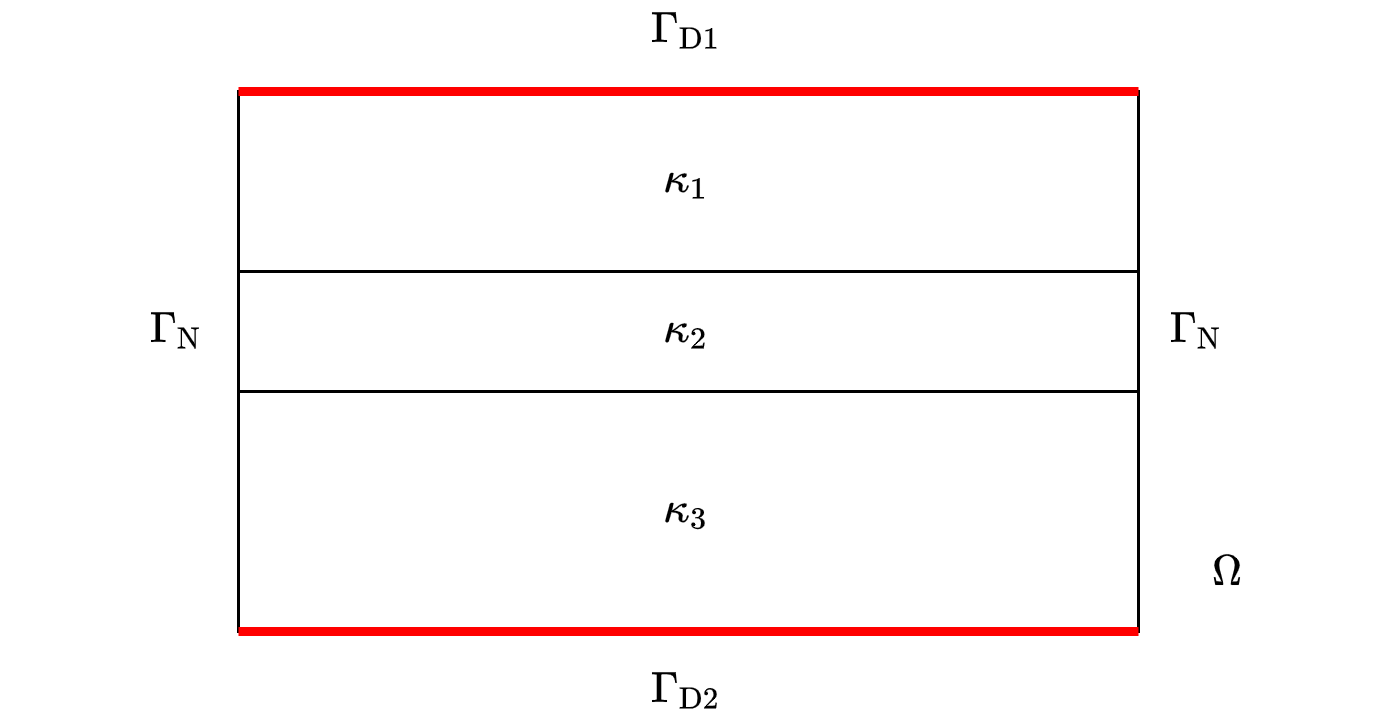
\includegraphics[height=5cm]{figures/Darcy_CNN/Darcy_domain.png}
	\end{center}
\end{itemize}

Then the variance of every entry is about 0.11, which is lager than the previous case. Fix the number of $u$'s channel as 1, we have the following results.

\subsubsection{Case 1: Change $\nu_i$}
\begin{table}[H]
	\begin{center}
		\begin{tabular}{|c|c|c|c|c|}
			\hline
			$\nu_i$& 1& 2 & 3& 4 \\
			\hline
			Train loss & 53.4168 & 55.3550 & 53.3935 & 53.8467\\
			\hline
			%			Mean rel. errors & 6.110$\times 10^{-3}$ & 5.852 $\times 10^{-3}$ &5.571$\times 10^{-3}$ &5.470$\times 10^{-3}$ \\
			%			\hline
			Number of Para & 135 & 135 & 135 & 135\\
			\hline
		\end{tabular}\caption{Training errors for various reduced dimension(lr = $10^{-2}$).}
	\end{center}
\end{table}
\subsubsection{Case 2: Change $J$}
\begin{table}[H]
	\begin{center}
		\begin{tabular}{|c|c|c|c|c|}
			\hline
			J& 3& 4 & 5& 6 \\
			\hline
			Train loss & 44.7566 & 55.3550 & 66.2886& 78.9738\\
			\hline
			%			Mean rel. errors & 6.110$\times 10^{-3}$ & 5.852 $\times 10^{-3}$ &5.571$\times 10^{-3}$ &5.470$\times 10^{-3}$ \\
			%			\hline
			Number of Para & 99 & 135 & 171 & 207\\
			\hline
		\end{tabular}\caption{Training errors for various reduced dimension(lr = $10^{-2}$).}
	\end{center}
\end{table}
\subsubsection{Case 3: DNN results}
.\begin{table}[H]
	\begin{center}
		\begin{tabular}{|c|c|c|c|c|}
			\hline
			& 10 & 20 & 30& 40 \\
			\hline
			Train loss & 60.4035  & 50.5609 & 45.3879 & 42.3671 \\
			\hline
%			Mean rel. errors & 6.110$\times 10^{-3}$ & 5.852 $\times 10^{-3}$ &5.571$\times 10^{-3}$ &5.470$\times 10^{-3}$ \\
%			\hline
			Number of Para & 10890& 21780& 32670 & 54450\\
			\hline
		\end{tabular}\caption{Training errors for various reduced dimension(lr = $10^{-5}$).}
	\end{center}
\end{table}
\subsection{Some disscusion about the orthogonality}
Review that the loss function is 
$$
L = \Sigma_{i=1}^N \| WW^Tx_i  -x_i \| ^2
$$
where $W\in \mathbb{R}^{d\times k}, k \ll d$. Here the matrix $A=WW^T$ is a symmetric positive semi-definite matrix, which have the following decomposition
$$
Q^TAQ  = \Lambda
$$
where Q is a orthogonal matrix and $\Lambda = diag(x_k, 0)$ is a diagnoal matrix, $x_k$ ia a strictly positive  $k$ element vector.

Then the loss function can be written as
$$
\begin{aligned}
L&= \sum x_i^TA^TAx_i - 2x_i^TAx_i +x_i^Tx_i^T\\
&= \sum x_i^TQ \Lambda^2 Q^Tx_i - 2x_i^TQ\Lambda Q^Tx_i
\end{aligned}
$$
To minimize the loss function, for each element of $x_k=(\lambda_i)$, we need to minimize the following problem for each $\lambda_i, i = 1,\cdots, k$
$$
M \lambda_i^2 - 2M \lambda_i
$$
where $M=M(Q,x_i)$ is  positive and depends on $x_i$ and Q. Therefore, $\lambda_i$ should be 1 for the purpose.

Then the original problem is equivalent to maximize the following problem
$$
\begin{aligned}
L & = \sum_{i=1}^{N}x_i^TQ \Lambda Q^T x_i\\
& = \sum_{i=1}^N \sum_{j=1}^k x_i q_j q_j^T x_i\\
& = \sum_{j=1}^k q_j^TXX^T q_j
\end{aligned}
$$
where $X = (x_1,\cdots,x_N)$, $\{q_j\}, j=1,\cdots k$ is the first $k$ columns of orthogonal matrix $Q$.

Then the problem is equivalent to the PCA method which requires the orthogonality, i.e., the orthogonality is a necessary condition to unique the minimizer.

On the other hand, if we consider $A = WW^T$. From above we know that the eigenvalues of $A$ is 1 and 0, and $A$ has a decomposition as $A = WW^T$ where $W$ is not unique.

Without the constaint of orthogonality, this weight $W$ is not unique. Therefore, CNN can generate one of the weight matrix $W_{CNN}$, if this weight matrix is orthogonal, then CNN has no difference from POD method. If not, CNN may be better than POD method.

\subsection{Othogonality is necessary and sufficient}
In the following part, I will prove that the weight matrix must satisfy the orthogonality.

Firstly, for the matrix $A = WW^T$ where $A\in \mathbb{R}^{n\times n}, W \in \mathbb{R}^{n\times r}, r\ll n$. There exists an orthogonal matrix $Q$ and a diagnoal matrix $\Lambda$ such that
$$
A = Q^T \Lambda Q
$$
Then we have $\Lambda = QWW^TQ^T$. Consider the decomposition of $\Lambda$, since the eigenvalues of $A$ is 1 and 0, $\Lambda$ can be written as $diag(e_r, 0)$ where $e_r$ is a r-dim vector of all ones. We have
$$
\Lambda= \left( \begin{array}{c}
	A_r \\
	A_{n-r}
	\end{array}\right) (A_r^T \ A_{n-r}^T) = \left(\begin{array}{c c}
	A_rA_r^T & A_rA_{n-r}^T \\
	A_{n-r}A_r^T & A_{n-r}A_{n-r}^T
\end{array}\right)
= \left(\begin{array}{c c}
	I_r & 0 \\
	0 & 0
\end{array}\right)
$$
Since $ A_{n-r}A_{n-r}^T$ is a zero matrix, we can induce that $A_{n-r}$ is a zero matrix and $A_r$ is an orthogonal matrix due to $A_rA_r^T= I_r$. Using these results leads to
$$
\left( \begin{array}{c}
	Q_r \\
	0
\end{array}\right) = QW
$$
i.e.,
$$
W = Q^T\left( \begin{array}{c}
	Q_r \\
	0
\end{array}\right) 
$$
where $Q_r$ is an arbitary orthogonal matrix. Then we have
$$
W^TW = (Q_r^T \ 0) QQ^T \left(\begin{aligned}
	Q_r \\
	0
\end{aligned}\right) = (Q_r^T \ 0) \left(\begin{aligned}
Q_r \\
0
\end{aligned}\right) = I_r
$$
Therefore, orthogonality is a sufficient and necessary conditon for the weight matrix. For any two weight matrices $W_1$ and $W_2$, there exists a unique orthgonal matrix $Q_r$ such that $W_1 = W_2Q_r$.
\newpage
\section{Data Augmentation with Explicit Regularization Formula}

\paragraph{Data Augmentation}
I think data augmentation is some kind of regularization. 
First we have,
\begin{equation}\label{key}
D_1 = \text{training set}, \quad D_2 = \text{test set},
\end{equation}
and the standard loss function:
\begin{equation}\label{key}
L(\theta) = \sum_{i=1}^N \ell( f(x_i; \theta), y_i) = N \mathbb{E}_{(x,y)\in D_1} \ell( f(x; \theta), y). 
\end{equation}

Let me write the FAA training process:
\begin{itemize}
	\item For k = 1:200 (epoch iteration)
	\item Shuffle the data set, and for each training data $x_i \in D_1$, randomly choose one policy $\tau^k_i \in \mathcal T$, and then the training data becomes 
	\begin{equation}\label{key}
	\tilde \tau^{k}(D_1) = \{ \tau^k_i(x_i): x_i \in D_1 \},
	\end{equation}
	\item SGD and train.
\end{itemize}


Here, for CIFAR100, we have the next properties of augmentation policies:
\begin{equation}\label{key}
T = \# \mathcal T = 500,
\end{equation}
for each policy $\tau_i \in \mathcal T$,
\begin{equation}\label{key}
\tau_i(x) = \begin{cases}
x, \quad \text{with probability}~(1-p^i_1)(1-p^i_2) \\
T^i_1(x), \quad \text{with probability}~p^i_1(1-p^i_2) \\
T^i_2(x), \quad \text{with probability}~(1-p^i_1)p^i_2 \\
T^i_2(T^i_1(x)), \quad \text{with probability}~ p^i_1p^i_2
\end{cases}
\end{equation}

A key observation is the expectation of the SGD with FAA or general data augmentation. Think about a mini-batch step:
\begin{equation}\label{key}
\theta^{k+1} = \theta^k - \eta \nabla \sum_{x\in \mathcal B_k} \ell(f(\tau(x)), y),
\end{equation}
where \blue{for every $x$, the transfer $\tau$ is a sample} from the next distribution:
\begin{equation}\label{key}
\mathbb P(\tau = \tau^i) = \frac{1}{T}, \forall i = 1, 2, \cdots, T,
\end{equation}
and
\begin{equation}\label{key}
\tau^i = \begin{cases}
id, \quad \text{with probability}~(1-p^i_1)(1-p^i_2) \\
T^i_1, \quad \text{with probability}~p^i_1(1-p^i_2) \\
T^i_2, \quad \text{with probability}~(1-p^i_1)p^i_2 \\
T^i_2\circ T^i_1, \quad \text{with probability}~ p^i_1p^i_2
\end{cases}.
\end{equation}

Thus, we know the ``real'' loss function is:
\begin{equation}\label{key}
\tilde L(\theta)  = N T \mathbb{E}_{(x,y) \in D_1} \mathbb{E}_{\mathcal T} \mathbb{E}_{\tau} \left( \frac{\ell \left( f(\tau(x);\theta), y\right)}{P(\tau)}  \right)
\end{equation}
Our we can write them with details:
\begin{equation}\label{key}
\begin{aligned}
\tilde L(\theta) = N T \frac{1}{N} \sum_{i=1}^N \big( \frac{1}{T}\sum_{t=1}^T \big( &(1-p^t_1)(1-p^t_2)\frac{\ell(f(x_i;\theta),y_i)}{\mathbb P(\tau= id)}  \\
&+ p^t_1(1-p^t_2)  \frac{\ell(f(T^t_1(x_i);\theta),y_i)}{\mathbb P(\tau = T^t_1)} + (1-p^t_1)p^t_2 \frac{\ell(f(T^t_2(x_i);\theta),y_i)}{\mathbb P(\tau = T^t_2)}  \\
&+  p^t_1p^t_2\frac{\ell(f(T^t_2 (T^t_1(x_i) );\theta),y_i)}{\mathbb P(\tau = T^t_2 \circ T^t_1)}   \big) \big).
\end{aligned}
\end{equation}




Then, the FAA data augmentation can be understood as a ``direct'' SGD method to solve the above problem by sampling 
\begin{equation}\label{key}
\mathbb{E}_{(x,y) \in D_1} \quad  \mathbb{E}_{ \mathcal T} \quad \text{and} \quad \mathbb{E}_{\tau},
\end{equation}
one-by-one.

So, the main difference here is we have a new loss function. For simplicity, if we think $p^t_1 \approx p_1$ and $p^t_1 \approx p_2$. 
We will have the new loss function as:
\begin{equation}\label{key}
\begin{aligned}
\tilde L(\theta) &=  NT \frac{1}{N}\sum_{i=1}^N \left(\ell(f(x_i;\theta),y_i) + \frac{1}{T}\left(\sum_1 + \sum_2 + \sum_{12}\right)  \right) \\
&= T\sum_{i=1}^N \ell(f(x_i;\theta),y_i)  +  NT \frac{1}{N} \sum_{i=1}^N  \frac{1}{T} \sum_{t=1}^T \left(\sum_tL_1 + \sum_tL_2 +  \sum_{t}L_{12}\right) \\
&=  T L(\theta) +NT(1-(1-p_1)(1-p_2)) \frac{1}{N} \sum_{i=1}^N  \frac{1}{T} \sum_{t=1}^T \left( \tilde P_1 \sum_tL_1 + \tilde P_2 \sum_tL_2 +\tilde P_{12} \sum_{t}L_{12}\right)  \\
&= T L(\theta) +NT(1-(1-p_1)(1-p_2)) \mathbb{E}_{(x,y) \in D_1} \mathbb{E}_{ \bar{\mathcal T}} \mathbb{E}_{\bar \tau} \left( \frac{\ell \left( f(\bar T(x);\theta), y\right)}{\tilde{\mathbb P}(\bar \tau)}  \right)
\end{aligned}.
\end{equation}
Here we have the new $\bar \tau^t$ defined as:
\begin{equation}\label{key}
\bar \tau^t(x) = \begin{cases}
T^t_1(x), \quad \text{with probability}~\tilde{\mathbb{ P}}_1 = \frac{p_1(1-p_2)}{1-(1-p_1)(1-p_2)} \\
T^t_2(x), \quad \text{with probability}~\tilde{\mathbb{ P}}_2 = \frac{(1-p_1)p_2}{1-(1-p_1)(1-p_2)}\\
T^t_2(T^t_1(x)), \quad \text{with probability}~ \tilde{\mathbb{ P}}_{12} = \frac{p_1p_2}{1-(1-p_1)(1-p_2)}
\end{cases}.
\end{equation}

Finally, we have the equivalent loss function as:
\begin{equation}\label{key}
\begin{aligned}
\tilde L(\theta) &= L(\theta) + \frac{(1-(1-p_1)(1-p_2))}{T} NT\mathbb{E}_{(x,y) \in D_1} \mathbb{E}_{ \bar{\mathcal T}} \mathbb{E}_{\bar \tau} \left( \frac{\ell \left( f(\bar T(x);\theta), y\right)}{\tilde{\mathbb P}(\bar \tau)}  \right) \\
&= L(\theta) + \blue{\frac{(1-(1-p_1)(1-p_2))}{T} } R(\theta; \blue{\bar{\mathcal T}}).
\end{aligned}
\end{equation}

Then, we can understand these data augmentation as a regularization method with a ``direct'' SGD method which likes this batch normalization methods...

Then we have the next observation:
\begin{itemize}
	\item This can help to explain why this can help to improve the generalization accuracy.
	\item This also explain why the training accuracy dose not have good improvement.
	\item This help to explain why FAA have a bigger gap than basic augmentation. (The parameter $T$ for FAA is bigger than basic one.)
	\item Some possible numerical experiments:
	\begin{itemize}
		\item Different $T$ may have different scale of gap;
		\item Modify $p_1$ and $p_2$ will have the similar result for $T$...
	\end{itemize}
	\item Because of the special form of regularization, I am trying to give some mathematical analysis on why the test accuracy
	with FAA will drop. And how to design some numerical experiments to verify. 
\end{itemize}



\subsection{Preliminary numerical results}

\subsubsection{Jianhong's results}
There are $p_1$ and $p_2$. I set $p_1=p_2$ and choose different values of $p_1$ to investigate the effect of the augmentation. 

Jianhong trained with basic and FAA augmentation and saved the model. Then Jianhong evaluated the training and test accuracy with different augmentation techniques for this model. 


\subsection{CIFAR-100}
\begin{table}[!htbp]
	\centering
	\caption{Training and test accuracy with different augmentation techniques on CIFAR-100}
	\scalebox{0.7}{	\begin{tabular}{|c|c|c|c|c|c|c|c|}
			\hline
			p1	&	lambda	&	training accuracy	&	training+aug accuracy	&	test accuracy	&	test+faa accuracy	&	test+basic accuracy	&	test+basic+faa accuracy	\\\hline
			0	&	0.00000	&	99.98	&	99.98	&	74.54	&	74.54	&	73.81	&	73.93	\\\hline
			0.1	&	0.00042	&	99.96	&	98.49	&	75.40	&	74.13	&	74.79	&	73.46	\\\hline
			0.2	&	0.00080	&	99.97	&	97.90	&	75.58	&	73.86	&	74.97	&	73.40	\\\hline
			0.3	&	0.00113	&	99.97	&	97.57	&	76.59	&	74.51	&	75.80	&	73.21	\\\hline
			0.4	&	0.00142	&	99.92	&	96.86	&	77.00	&	74.56	&	76.49	&	73.20	\\\hline
			0.5	&	0.00167	&	99.93	&	96.46	&	76.79	&	73.77	&	76.27	&	72.43	\\\hline
			0.6	&	0.00187	&	99.92	&	95.86	&	76.99	&	73.25	&	76.51	&	72.31	\\\hline
			0.7	&	0.00202	&	99.92	&	95.27	&	77.24	&	73.38	&	76.68	&	72.04	\\\hline
			0.8	&	0.00213	&	99.93	&	94.77	&	77.61	&	72.82	&	76.58	&	71.76	\\\hline
			0.9	&	0.00220	&	99.82	&	94.20	&	77.67	&	72.73	&	77.27	&	71.07	\\\hline
			1	&	0.00222	&	99.76	&	92.95	&	77.25	&	72.31	&	76.61	&	70.28	\\\hline
	\end{tabular}}
\end{table}


\begin{table}[!htbp]
	\centering
	\caption{Training and test loss with different augmentation techniques on CIFAR-100}
	\scalebox{0.8}{	\begin{tabular}{|c|c|c|c|c|c|c|c|}
			\hline
			p1	&	lambda	&	training loss	&	training+aug loss	&	test loss	&	test+faa loss	&	test+basic loss	&	test+basic+faa loss	\\\hline
			0	&	0.00000	&	0.0043	&	0.2092	&	1.1758	&	1.1758	&	1.1376	&	1.1457	\\\hline
			0.1	&	0.00042	&	0.0078	&	0.3749	&	1.0719	&	1.1314	&	1.0498	&	1.1153	\\\hline
			0.2	&	0.00080	&	0.0068	&	0.4241	&	1.0650	&	1.1287	&	1.0409	&	1.1151	\\\hline
			0.3	&	0.00113	&	0.0072	&	0.4607	&	1.0069	&	1.0998	&	0.9718	&	1.0948	\\\hline
			0.4	&	0.00142	&	0.0087	&	0.5078	&	0.9931	&	1.0801	&	0.9637	&	1.0829	\\\hline
			0.5	&	0.00167	&	0.0086	&	0.5362	&	0.9687	&	1.0964	&	0.9657	&	1.1228	\\\hline
			0.6	&	0.00187	&	0.0106	&	0.5701	&	0.9569	&	1.1089	&	0.9605	&	1.1087	\\\hline
			0.7	&	0.00202	&	0.0117	&	0.5989	&	0.9480	&	1.0921	&	0.9522	&	1.1137	\\\hline
			0.8	&	0.00213	&	0.0126	&	0.6270	&	0.9602	&	1.1343	&	0.9400	&	1.1482	\\\hline
			0.9	&	0.00220	&	0.0141	&	0.6526	&	0.9295	&	1.1231	&	0.9273	&	1.1637	\\\hline
			1	&	0.00222	&	0.0199	&	0.7041	&	0.9240	&	1.1157	&	0.9159	&	1.1749	\\\hline
	\end{tabular}}
\end{table}



\newpage
\subsection{CIFAR-10}
\begin{table}[!htbp]
	\centering
	\caption{Training and test accuracy with different augmentation techniques on CIFAR-10}
	\scalebox{0.7}{	\begin{tabular}{|c|c|c|c|c|c|c|c|}
			\hline
			p1	&	lambda	&	training accuracy	&	training+aug accuracy	&	test accuracy	&	test+faa accuracy	&	test+basic accuracy	&	test+basic+faa accuracy	\\\hline
			0	&	0.00000	&	100.00	&	99.99	&	94.37	&	94.37	&	94.17	&	94.34	\\\hline
			0.1	&	0.00042	&	100.00	&	99.56	&	95.39	&	94.88	&	94.98	&	94.43	\\\hline
			0.2	&	0.00080	&	100.00	&	99.18	&	95.73	&	94.88	&	95.03	&	94.04	\\\hline
			0.3	&	0.00113	&	99.99	&	99.09	&	95.44	&	94.26	&	95.54	&	94.14	\\\hline
			0.4	&	0.00142	&	100.00	&	98.93	&	95.56	&	94.43	&	95.61	&	93.95	\\\hline
			0.5	&	0.00167	&	100.00	&	98.70	&	95.95	&	93.73	&	95.53	&	93.85	\\\hline
			0.6	&	0.00187	&	100.00	&	98.63	&	95.65	&	93.83	&	95.46	&	93.26	\\\hline
			0.7	&	0.00202	&	99.99	&	98.26	&	95.93	&	94.06	&	95.66	&	93.27	\\\hline
			0.8	&	0.00213	&	99.99	&	98.17	&	95.77	&	93.03	&	95.68	&	92.99	\\\hline
			0.9	&	0.00220	&	99.99	&	97.94	&	96.08	&	93.48	&	95.51	&	92.80	\\\hline
			1	&	0.00222	&	99.98	&	97.76	&	95.98	&	92.80	&	95.49	&	91.99	\\\hline
	\end{tabular}}
\end{table}


\begin{table}[!htbp]
	\centering
	\caption{Training and test loss with different augmentation techniques on CIFAR-10}
	\scalebox{0.8}{	\begin{tabular}{|c|c|c|c|c|c|c|c|}
			\hline
			p1	&	lambda	&	training loss	&	training+aug loss	&	test loss	&	test+faa loss	&	test+basic loss	&	test+basic+faa loss	\\\hline
			0	&	0.00000	&	0.0006	&	0.0833	&	0.2655	&	0.2655	&	0.2491	&	0.2463	\\\hline
			0.1	&	0.00042	&	0.0010	&	0.1182	&	0.1748	&	0.1915	&	0.1802	&	0.1997	\\\hline
			0.2	&	0.00080	&	0.0012	&	0.1409	&	0.1623	&	0.1841	&	0.1797	&	0.2036	\\\hline
			0.3	&	0.00113	&	0.0011	&	0.1487	&	0.1714	&	0.2030	&	0.1668	&	0.2054	\\\hline
			0.4	&	0.00142	&	0.0010	&	0.1630	&	0.1696	&	0.2086	&	0.1619	&	0.2075	\\\hline
			0.5	&	0.00167	&	0.0011	&	0.1762	&	0.1583	&	0.2191	&	0.1543	&	0.2122	\\\hline
			0.6	&	0.00187	&	0.0012	&	0.1840	&	0.1666	&	0.2230	&	0.1687	&	0.2278	\\\hline
			0.7	&	0.00202	&	0.0011	&	0.1969	&	0.1587	&	0.2117	&	0.1578	&	0.2277	\\\hline
			0.8	&	0.00213	&	0.0013	&	0.2028	&	0.1595	&	0.2324	&	0.1564	&	0.2311	\\\hline
			0.9	&	0.00220	&	0.0013	&	0.2149	&	0.1540	&	0.2303	&	0.1552	&	0.2386	\\\hline
			1	&	0.00222	&	0.0018	&	0.2268	&	0.1506	&	0.2424	&	0.1554	&	0.2559	\\\hline	\end{tabular}}
\end{table}



\subsubsection{Jianqing's results}
The next table shows Jianqing's results for $p$ version for FAA with 450 sub-policies with 
the basic data augmentation before standard FAA augmentation is applied.
\begin{table}[!htbp]
\centering
\begin{tabular}{| l | c | c | c | c | r |}
	\hline
	p          & train acc & train+aug acc & test accuracy  &  test+aug acc & test acc drop\\
	\hline
	0.0          &  99.97   & 99.97       &  74.78         &   74.11            &   0.67  \\
	\hline
	0.1          &  99.97   & 98.53       &  76.44         &   74.56            &   1.88  \\
	\hline
	0.2          &  99.96   & 97.83       &  76.72         &   73.68            &   3.04  \\
	\hline
	0.3          &  99.96   & 97.35       &  76.75         &   73.92            &   2.83  \\
	\hline
	0.4          &  99.96   & 96.83       &  76.78         &   73.45            &   3.33  \\
	\hline
	0.5          &  99.96   & 96.66       &  77.07         &   72.61            &   4.46  \\
	\hline
	0.6          &  99.95   & 95.91       &  77.29         &   72.75            &   4.54  \\
	\hline
	0.7          &  99.93   & 95.51       &  77.67         &   72.59            &   5.08  \\
	\hline
	0.8          &  99.92   & 95.13       &  77.67         &   72.05            &   5.62  \\
	\hline
	0.9          &  99.91   & 94.27       &  77.68         &   71.25            &   6.43  \\
	\hline
	1.0          &  99.75   & 93.22       &  77.67         &   70.31            &   7.36  \\
	\hline
\end{tabular}
\end{table}

%%%%%%%%%%%%%%%%%%%%%%%%
%%%%%%   U-Net   %%%%%%%
%%%%%%%%%%%%%%%%%%%%%%%%
\newpage
\section{U-Net}
\subsection{Architecture}
\begin{enumerate}
	\item Initialization of inputs
	$$u \in \mathbb{R}^{1\times 512\times 512},\quad c:num~class~of~pixels$$
	\begin{itemize}
		\item downsampling
	\end{itemize}
	%%%%%%%%%%%%%   32*32 mesh size %%%%%%%%%%%%%%%
	\item $512\times 512$ mesh size\\
	input\quad $u^{1,0}=u\in \mathbb{R}^{1\times 512\times 512}$,\quad $\theta^{1,1} \in \mathbb{R}^{1\times 64\times 3\times 3}$,\quad $\theta^{1,2} \in \mathbb{R}^{64\times 64\times 3\times 3}$
	$$u^{1,1}=\sigma (\theta^{1,1} \ast (u^{1,0}))\in \mathbb{R}^{64\times 512\times 512}$$
	$$u^{1,2}=\sigma (\theta^{1,2} \ast (u^{1,1}))\in \mathbb{R}^{64\times 512\times 512}$$
	output\quad $u^{1,2} \in \mathbb{R}^{64\times 512\times 512}$
	
	\item $256\times 256$ mesh size\\
	input\quad $u^{1,2}\in \mathbb{R}^{64\times 512\times 512}$,\quad $\theta^{2,1} \in \mathbb{R}^{64\times 128\times 3\times 3}$,\quad $\theta^{2,2} \in \mathbb{R}^{128\times 128\times 3\times 3}$
	$$u^{2,0}=R_{max}*_{2}u^{1,2} \in \mathbb{R}^{64\times 256\times 256} $$
	$$u^{2,1}=\sigma (\theta^{2,1} \ast (u^{2,0}))\in \mathbb{R}^{128\times 256\times 256}$$
	$$u^{2,2}=\sigma (\theta^{2,2} \ast (u^{2,1}))\in \mathbb{R}^{128\times 256\times 256}$$
	output\quad $u^{2,2} \in \mathbb{R}^{128\times 256\times 256}$
	
	\item $128\times 128$ mesh size\\
	input\quad $u^{2,2}\in \mathbb{R}^{128\times 256\times 256}$,\quad $\theta^{3,1} \in \mathbb{R}^{128\times 256\times 3\times 3}$,\quad $\theta^{3,2} \in \mathbb{R}^{256\times 256\times 3\times 3}$
	$$u^{3,0}=R_{max}*_{2}u^{2,2} \in \mathbb{R}^{128\times 128\times 128} $$
	$$u^{3,1}=\sigma (\theta^{3,1} \ast (u^{3,0}))\in \mathbb{R}^{256\times 128\times 128}$$
	$$u^{3,2}=\sigma (\theta^{3,2} \ast (u^{3,1}))\in \mathbb{R}^{256\times 128\times 128}$$
	output\quad $u^{3,2} \in \mathbb{R}^{256\times 128\times 128}$
	
	\item $64\times 64$ mesh size\\
	input\quad $u^{3,2}\in \mathbb{R}^{256\times 128\times 128}$,\quad $\theta^{4,1} \in \mathbb{R}^{256\times 512\times 3\times 3}$,\quad $\theta^{4,2} \in \mathbb{R}^{512\times 512\times 3\times 3}$
	$$u^{4,0}=R_{max}*_{2}u^{3,2} \in \mathbb{R}^{256\times 64\times 64} $$
	$$u^{4,1}=\sigma (\theta^{4,1} \ast (u^{4,0}))\in \mathbb{R}^{512\times 64\times 64}$$
	$$u^{4,2}=\sigma (\theta^{4,2} \ast (u^{4,1}))\in \mathbb{R}^{512\times 64\times 64}$$
	output\quad $u^{4,2} \in \mathbb{R}^{512\times 64\times 64}$
	
	\item $32\times 32$ mesh size\\
	input\quad $u^{4,2}\in \mathbb{R}^{512\times 64\times 64}$,\quad $\theta^{5,1} \in \mathbb{R}^{512\times 1024\times 3\times 3}$,\quad $\theta^{5,2} \in \mathbb{R}^{1024\times 1024\times 3\times 3}$
	$$u^{5,0}=R_{max}*_{2}u^{4,2} \in \mathbb{R}^{512\times 32\times 32} $$
	$$u^{5,1}=\sigma (\theta^{5,1} \ast (u^{5,0}))\in \mathbb{R}^{1024\times 32\times 32}$$
	$$u^{5,2}=\sigma (\theta^{5,2} \ast (u^{5,1}))\in \mathbb{R}^{1024\times 32\times 32}$$
	output\quad $u^{5,2} \in \mathbb{R}^{1024\times 32\times 32}$
	
	\begin{itemize}
		\item upsampling
	\end{itemize}
	\item $64\times 64$ mesh size\\
	input\quad $u^{5,2} \in \mathbb{R}^{1024\times 32\times 32}$,\quad$u^{4,2}\in \mathbb{R}^{512\times 64\times 64}$,\\
	$\hat{\theta}^{4,0} \in \mathbb{R}^{1024\times 512\times 3\times 3}$,\quad
	$\hat{\theta}^{4,1} \in \mathbb{R}^{1024\times 512\times 3\times 3}$\quad
	$\hat{\theta}^{4,2} \in \mathbb{R}^{512\times 512\times 3\times 3}$
	$$v^{4}= \sigma(\hat{\theta}^{4,0} \ast^{\top}_2 (u^{5,2}))\in \mathbb{R}^{512\times 64\times 64}$$
	$$v^{4,0}=[u^{4,2},v^{4}]\in \mathbb{R}^{1024\times 64\times 64}$$
	$$v^{4,1}= \sigma(\hat{\theta}^{4,1} \ast (v^{4,0}))\in \mathbb{R}^{512\times 64\times 64}$$
	$$v^{4,2}= \sigma(\hat{\theta}^{4,2} \ast (v^{4,1}))\in \mathbb{R}^{512\times 64\times 64}$$
	output\quad $v^{4,2} \in \mathbb{R}^{512\times 64\times 64}$
	
	\item $128\times 128$ mesh size\\
	input\quad $v^{4,2} \in \mathbb{R}^{512\times 64\times 64}$,\quad$u^{3,2}\in \mathbb{R}^{256\times 128\times 128}$,\\
	$\hat{\theta}^{3,0} \in \mathbb{R}^{512\times 256\times 3\times 3}$,\quad
	$\hat{\theta}^{3,1} \in \mathbb{R}^{512\times 256\times 3\times 3}$\quad
	$\hat{\theta}^{3,2} \in \mathbb{R}^{256\times 256\times 3\times 3}$
	$$v^{3}= \sigma(\hat{\theta}^{3,0} \ast^{\top}_2 (v^{4,2}))\in \mathbb{R}^{256\times 128\times 128}$$
	$$v^{3,0}=[u^{3,2},v^{3}]\in \mathbb{R}^{512\times 128\times 128}$$
	$$v^{3,1}= \sigma(\hat{\theta}^{3,1} \ast (v^{3,0}))\in \mathbb{R}^{256\times 128\times 128}$$
	$$v^{3,2}= \sigma(\hat{\theta}^{3,2} \ast (v^{3,1}))\in \mathbb{R}^{256\times 128\times 128}$$
	output\quad $v^{3,2} \in \mathbb{R}^{256\times 128\times 128}$
	
	\item $256\times 256$ mesh size\\
	input\quad $v^{3,2} \in \mathbb{R}^{256\times 128\times 128}$,\quad$u^{2,2}\in \mathbb{R}^{128\times 256\times 256}$,\\
	$\hat{\theta}^{2,0} \in \mathbb{R}^{256\times 128\times 3\times 3}$,\quad
	$\hat{\theta}^{2,1} \in \mathbb{R}^{256\times 128\times 3\times 3}$\quad
	$\hat{\theta}^{2,2} \in \mathbb{R}^{128\times 128\times 3\times 3}$
	$$v^{2}= \sigma(\hat{\theta}^{2,0} \ast^{\top}_2 (v^{3,2}))\in \mathbb{R}^{128\times 256\times 256}$$
	$$v^{2,0}=[u^{2,2},v^{2}]\in \mathbb{R}^{256\times 256\times 256}$$
	$$v^{2,1}= \sigma(\hat{\theta}^{2,1} \ast (v^{2,0}))\in \mathbb{R}^{128\times 256\times 256}$$
	$$v^{2,2}= \sigma(\hat{\theta}^{2,2} \ast (v^{2,1}))\in \mathbb{R}^{128\times 256\times 256}$$
	output\quad $v^{2,2} \in \mathbb{R}^{128\times 256\times 256}$
	
	\item $512\times 512$ mesh size\\
	input\quad $v^{2,2} \in \mathbb{R}^{128\times 256\times 256}$,\quad$u^{1,2}\in \mathbb{R}^{64\times 512\times 512}$,\\
	$\hat{\theta}^{1,0} \in \mathbb{R}^{128\times 64\times 3\times 3}$,\quad
	$\hat{\theta}^{1,1} \in \mathbb{R}^{128\times 64\times 3\times 3}$\quad
	$\hat{\theta}^{1,2} \in \mathbb{R}^{64\times 64\times 3\times 3}$\quad
	
	$$v^{1}= \sigma(\hat{\theta}^{1,0} \ast^{\top}_2 (v^{2,2}))\in \mathbb{R}^{64\times 512\times 512}$$
	$$v^{1,0}=[u^{1,2},v^{1}]\in \mathbb{R}^{128\times 512\times 512}$$
	$$v^{1,1}= \sigma(\hat{\theta}^{1,1} \ast (v^{1,0}))\in \mathbb{R}^{64\times 512\times 512}$$
	$$v^{1,2}= \sigma(\hat{\theta}^{1,2} \ast (v^{1,1}))\in \mathbb{R}^{64\times 512\times 512}$$
	output\quad $v^{1,2} \in \mathbb{R}^{64\times 512\times 512}$     
	\item output layer\\
	input\quad $v^{1,2} \in \mathbb{R}^{64\times 512\times 512}$,\quad $\hat{\theta} \in \mathbb{R}^{64\times c \times 3\times 3}$
	$$v= softmax(\hat{\theta} \ast (v^{1,2}))\in \mathbb{R}^{c\times 512\times 512}$$
	output\quad $v \in \mathbb{R}^{c\times 512\times 512}$
\end{enumerate}

The U-Net can be written as:%\cite{huang2017densely}
\begin{equation}\label{eq:unet}
\begin{cases}
u^{1,0}=u\\
\text{\bf For} &\ell = 1:5 \\
&\text{\bf If} \quad \ell > 1 \\
&\quad \quad u^{\ell,0}=R_{max}*_2(u^{\ell-1,\nu_l})\\
&\text{\bf For} \quad i = 1:\nu_\ell \\
&\quad \quad u^{\ell,i} = \sigma(\theta^{\ell,i}\ast (u^{\ell,i-1}))\\
%&\tilde f^{\ell,i} = [f^{\ell,0,}, \cdots, f^{\ell,i}] \quad i = 1:\nu_\ell  , \\
&\text{\bf EndFor} \\
\text{\bf EndFor}\\

v^{5,\nu_l}=u^{5,\nu_l}\\

\text{\bf For} &\ell = 4:1 \\
&v^{\ell} = \sigma(\hat{\theta}^{\ell,0}\ast^{\top}_2(v^{\ell+1,\nu_l}))\\
&v^{\ell,0} = [u^{\ell,\nu_l},v^{\ell}]\\
&v^{\ell,1} = \sigma(\hat{\theta}^{\ell,1}\ast(v^{\ell,0}))\\
\quad &\text{\bf For} \quad i = 2:\nu_\ell \\
&\quad \quad v^{\ell,i} = \sigma(\hat{\theta}^{\ell,i}\ast (v^{\ell,i-1}))\\
%&\tilde f^{\ell,i} = [f^{\ell,0,}, \cdots, f^{\ell,i}] \quad i = 1:\nu_\ell  , \\
\quad &\text{\bf EndFor} \\
\text{\bf EndFor}\\
v = softmax(\theta \ast (v^{1,\nu_l}))\\

\end{cases}
\end{equation}
\end{document}
\bibliographystyle{abbrv}\bibliography{6DL/ref,6DL/ref_mgcnn}\end{document}

\chapter{Spaces of Polynomials}
In this chapter, we discuss approximation properties of spaces of
polynomials and finite elements consisting of piecewise polynomials.

\section{Weierstrass Theorem}  
To approximate any continuous function, a very simple idea is to approximate the function in a polynomial space. 
An important property of this space is that polynomials can approximate any reasonable function!
\begin{itemize}
\item $P_n(\mathbb{R}^d)$ is dense in $C(\Omega)$ [Weierstrass theorem]
\item $P_n(\mathbb{R}^d)$ is dense in all Sobolev spaces: $L^2(\Omega), W^{m,p}(\Omega), \ldots$
\end{itemize}

\begin{theorem}
Let $\Omega\subset R^n$ be a  closed and bounded set. Given any continuous function $f(x)$ on $\Omega$, there exists a sequence of polynomials $\{p_n(x)\}$ such 
that 
\begin{equation}
\displaystyle \lim_{n\rightarrow \infty} \max_{x\in \Omega}|f(x)-p_n(x)|=0
\end{equation}
\end{theorem}
\begin{proof}
Let us first give the proof for $d=1$ and $\Omega=[0,1]$. Given $f:[0,1]\rightarrow R$ be a  continuous function. 

Let
\begin{equation}
\tilde f(x)=f(x)-l(x)
\end{equation}
where $l(x)=f(0)+x(f(1)-f(0))$.
Then $\tilde f(0)=\tilde f(1)=0$. Noting that $l(x)$ is a linear function, hence without lose of generality, we can only consider the 
case $f:[0,1]\rightarrow R$ with $f(0)=f(1)=0$. 
Since $f$ is continuous on the closed interval $[0,1]$, then $f$ is uniformly continuous on $[0,1]$.

First we extend $f$ to be zero outside of $[0,1]$ and obtain $f: R\rightarrow R$, then it is obviously that $f$ is still uniformly continuous. 

Next for $0\le x\le 1$, we construct
\begin{equation}
p_n(x)=\int_{-1}^1f(x+t)Q_n(t)dt=\int_{-x}^{1-x}f(x+t)Q_n(t)dt=\int_{0}^{1}f(t)Q_n(t-x)dt
\end{equation} 
where $Q_n(x)=c_n(1-x^2)^n$ and 
\begin{equation}\label{intq}
\int_{-1}^1 Q_n(x) dx=1.
\end{equation} 
Thus $\{p_n(x)\}$ is a sequence of polynomials. 

Since 
\begin{align}
\int_{-1}^1 (1-x^2)^n dx&=2\int_{0}^1 (1-x^2)^n dx=  2\int_{0}^1 (1-x)^n(1+x)^n dx\\ 
&\ge 2\int_{0}^1 (1-x)^n dx=\frac{2}{n+1}> \frac{1}{n}.
\end{align}
Combing with $\int_{-1}^1 Q_n(x) dx=1$, we obtain $c_n< n$ implying that for any $\delta>0$
 \begin{equation}\label{qest}
 0\le Q_n(x)\le n(1-\delta^2)^n \quad (\delta\le |x|\le 1),
 \end{equation}
so that $Q_n\rightarrow 0$ uniformly in $\delta\le |x|\le 1$ as $n\rightarrow \infty$. 

Given any $\epsilon >0$, since $f$ in uniformly continuous, there exists $\delta>0$ such that for any $|y-x|<\delta$, we have 
\begin{equation}\label{fcont}
|f(y)-f(x)|< \frac{\epsilon}{2}.
\end{equation}
Finally, let $M=\max |f(x)|$, using \eqref{fcont}, \eqref{intq} and \eqref{qest}, we have 
\begin{align}
\big| p_n(x)-f(x)\big|&=\big|\int_{-1}^1(f(x+t)-f(t))Q_n(t)dt\big|\le \int_{-1}^1 \big| f(x+t)-f(t)\big| Q_n(t)dt\\
&\le 2M \int_{-1}^{-\delta} Q_n(t)dt+ \frac{\epsilon}{2}\int_{-\delta}^{\delta} Q_n(t)dt+ 2M\int_{\delta}^1 Q_n(t)dt\\
&\le 4M n(1-\delta^2)^n + \frac{\epsilon}{2}< \epsilon
\end{align}
for all large enough $n$, which proves the theorem. 

The above proof generalize the high dimensional case easily.   We
consider the case that
$$
\Omega=[0,1]^d.
$$
By extension and using cut off function,  W.L.O.G.  that we assume
that $f=0$ on the boundary of $\Omega$ and we then extending this
function to be zero outside of $\Omega$.  

Let us consider the special polynomial functions
\begin{equation}
  \label{Qn}
Q_n(x)=c_n\prod_{k=1}^d(1-x_k^2)  
\end{equation}
Similar proof can then be applied. 
\end{proof}























 
\subsection{Curse of dimensionality}
Number of coefficients for polynomial space $P_n(\mathbb{R}^d)$  is
$$
	N = \binom{d+n}{n} = \frac{(n+d)!}{d!n!}.
$$
For example $n = 100$:
		\begin{table}
			\centering
			\begin{tabular}{|c|c|c|c|}
				\hline
				$d = $&  $2$ &  $4$ & $8$\\
				\hline
				$N=$  & $5\times10^3$ & $4.6\times10^6$  & $3.5\times10^{11}$ 	\\
				\hline
			\end{tabular}
		\end{table}
As the this table shows, the dimension of the polynomial space $P_n(\mathbb{R}^d)$   increases rapidly as the degree $n$ increases. This leads to an extremely large space therefore very expensive to approximate functions in polynomial spaces in high dimensions.
\subsection{Runge's phenomenon}
A natural way to approximate a given function on any interval $[a,b]$ is to use an $n$-degree polynomial $p_n(x)$ by $n+1$ equispaced  points, namely
$$
x_i=a+{b-a\over n},\quad i=0,1,2,\cdots,n.
$$
By Weierstrass' theorem, we expect a more accurate reconstruction of $f(x)$ by using more points. But this is not always true as shown in the following example. 
%Consider the case where one desires to interpolate through $n+1$ equispaced points of a function $f(x)$ using the n-degree polynomial $p_n(x)$ that passes through those points. Naturally, one might expect from Weierstrass' theorem that using more points would lead to a more accurate reconstruction of $f(x)$. However, this particular set of polynomial functions $p_n(x)$ is not guaranteed to have the property of uniform convergence; the theorem only states that a set of polynomial functions exists, without providing a general method of finding one.

Consider the Runge function (a scaled version of the Witch of Agnesi)
$$ 
f(x)=\frac{1}{1+25x^{2}}.
$$
Runge found that if this function is interpolated at equidistant points $x_i$ between $-1$ and $1$ such that:
$$
x_{i}={\frac{2i}{n}}-1,\quad i\in \left\{0,1,\dots ,n\right\}
$$
with a polynomial $p_n(x)$ of degree $\leq n$, the resulting interpolation oscillates toward the ends of the interval, i.e. close to $-1$ and $1$. It can even be proven that the interpolation error increases (without bound) when the degree of the polynomial is increased:

$$\lim_{{n\rightarrow \infty }}\left(\max_{{-1\leq x\leq 1}}|f(x)-p_{n}(x)|\right)=+\infty.$$
This shows that high-degree polynomial interpolation at equidistant points can be troublesome.

\begin{figure}
	\begin{center}
		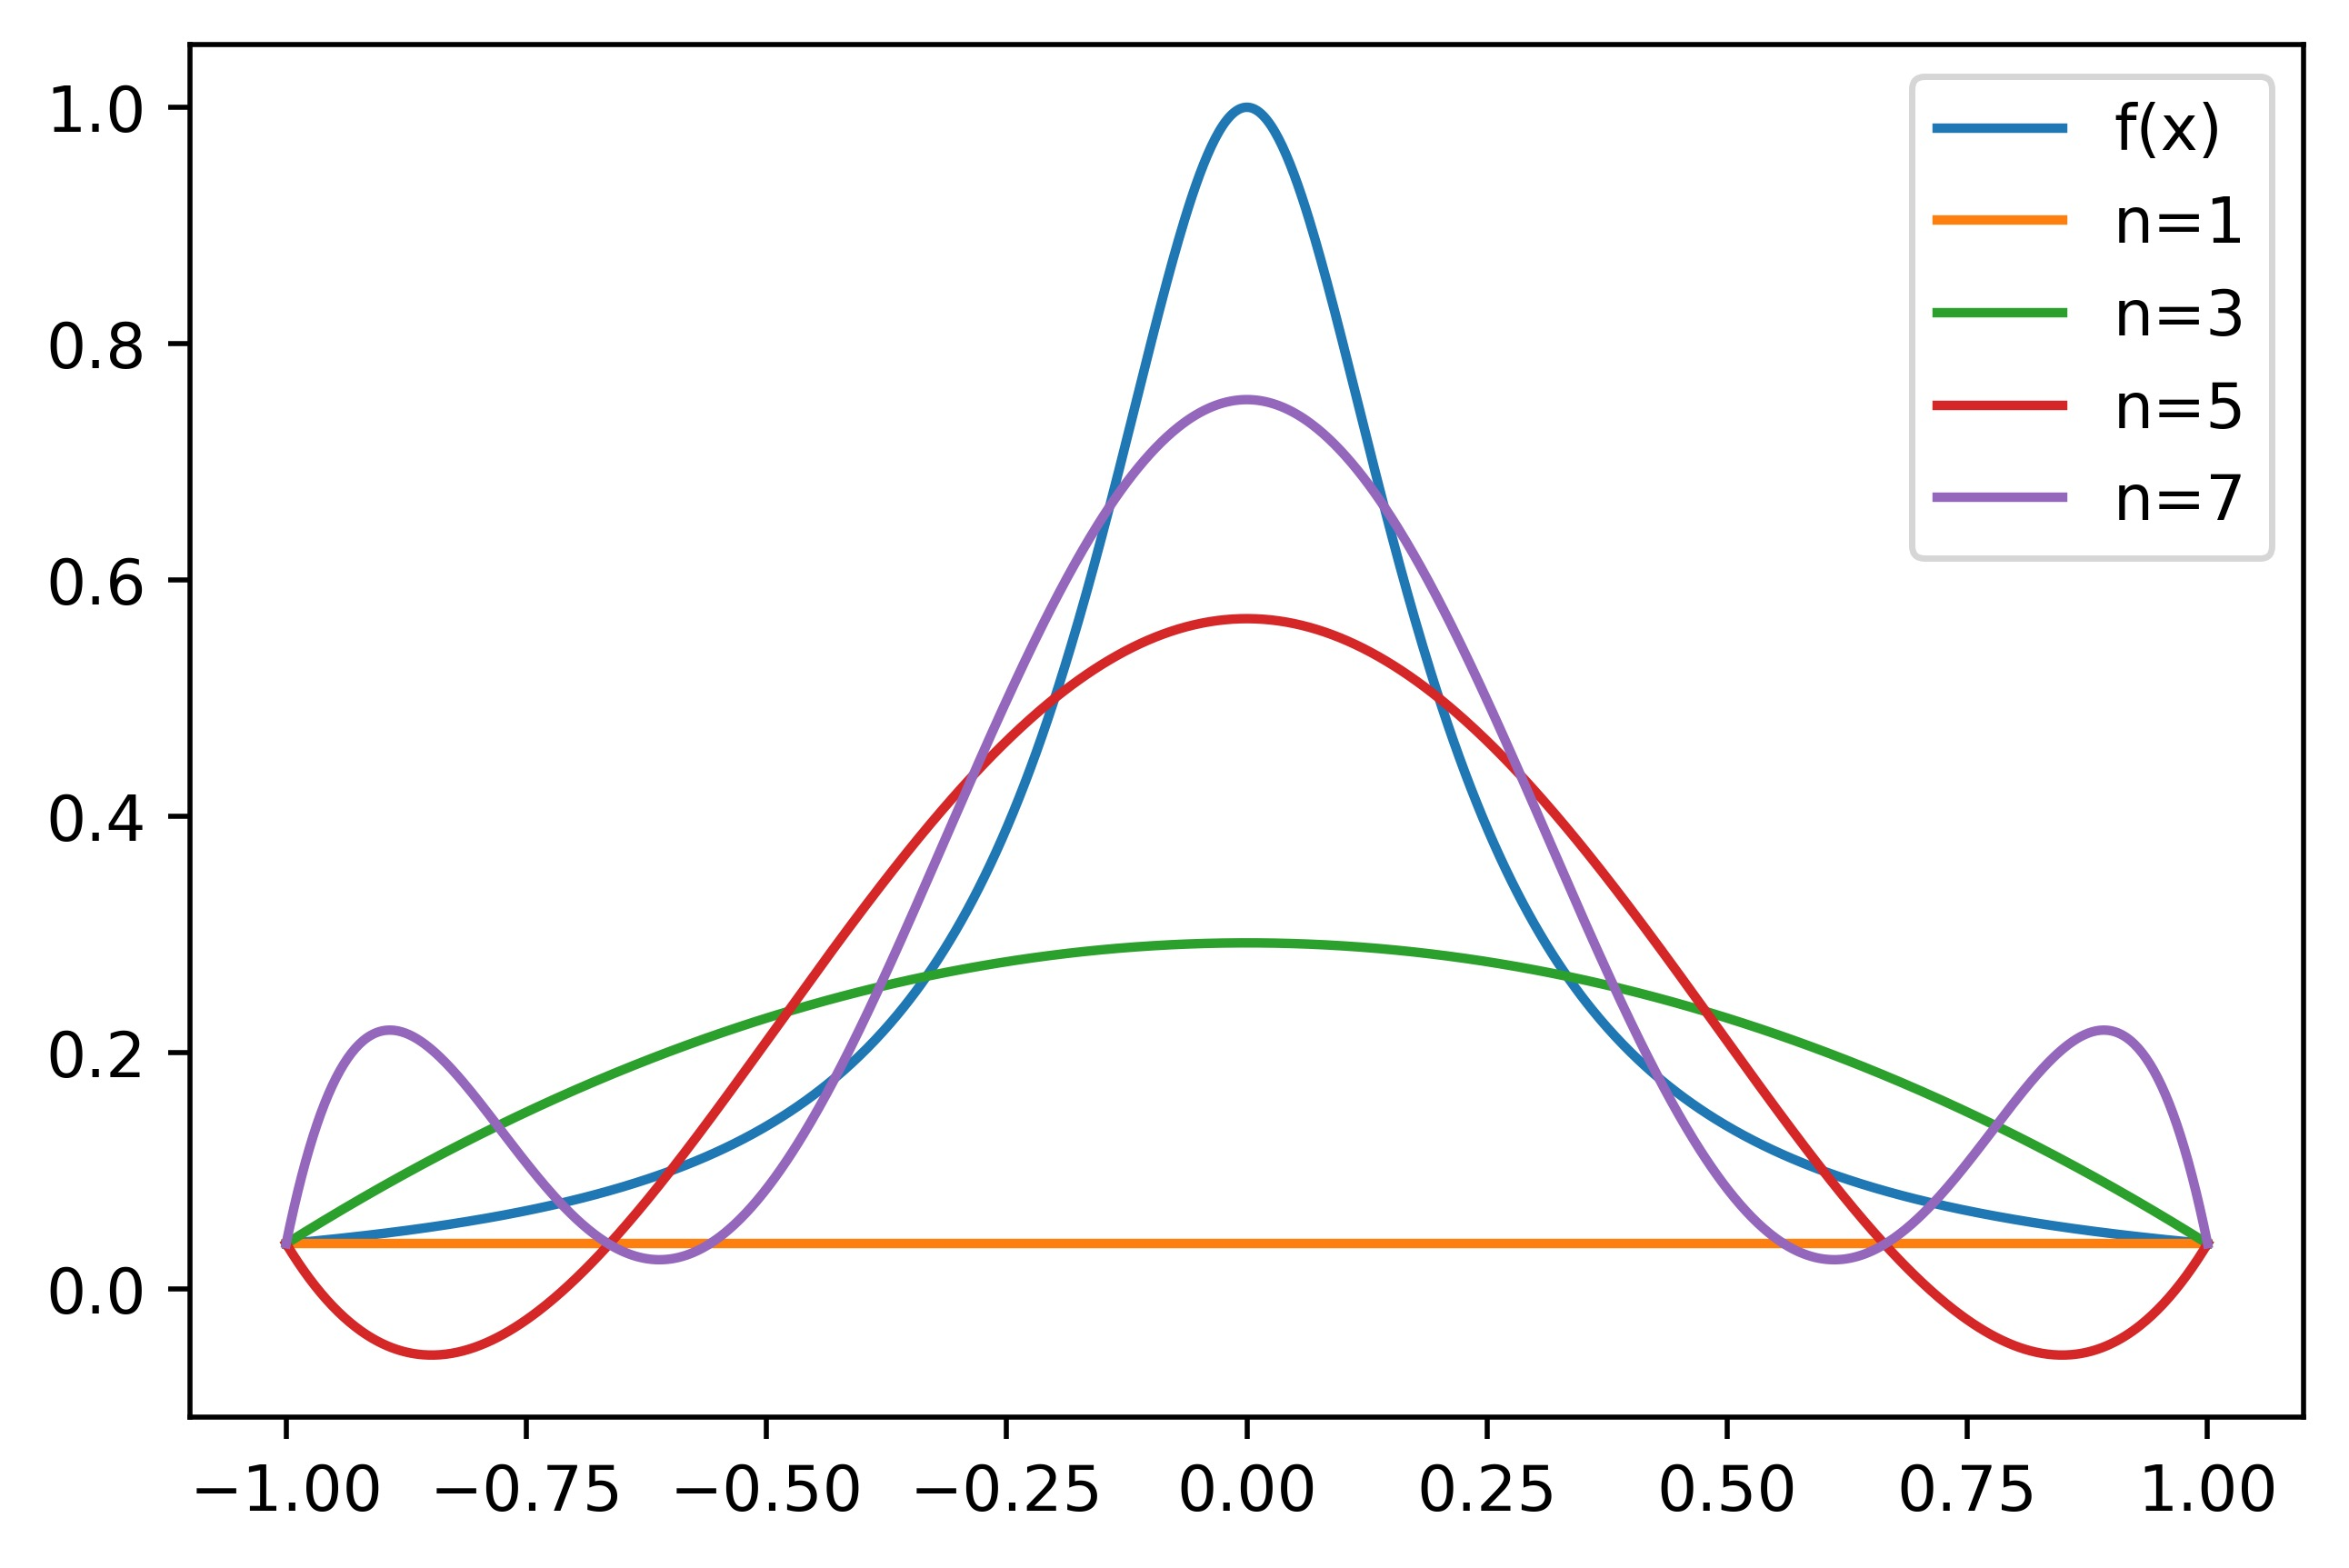
\includegraphics[scale=0.1]{6DL/pic/Runge.jpeg}
		\caption{Runge's phenomenon: Runge function $f(x)=\frac{1}{1+25x^{2}}$ and its polynomial interpolation $p_n(x)$.}
	\end{center}
\end{figure}

The experiment shows that  the polynomials $p_n(x)$ produced in this manner may in fact diverge away from $f(x)$ as $n$ increases. This typically occurs in an oscillating pattern that magnifies near the ends of the interpolation points. This phenomenon is attributed to Runge.

Thus, this particular set of polynomial functions $p_n(x)$ is not guaranteed to have the property of uniform convergence. In other words, Weierstrass' theorem guarantees the existence of the polynomial functions, but how to find such polynomials is not provided.

\section{Fourier transform and Fourier series}
We make use of the theory of tempered distributions (see
\cite{strichartz2003guide} for an introduction)
and we begin by collecting some results of independent interest, which
will also be important later. 
\subsection{Fourier transform}
Before studying the Fourier transform, we first consider Schwartz space which is defined below.
\begin{definition} \label{def:schwarz}
The Schwartz space $\mathcal{S}\left(\mathbb{R}^{n}\right)$ is the topological vector space of functions $f: \mathbb{R}^{n} \rightarrow \mathbb{C}$ such that $f \in C^{\infty}\left(\mathbb{R}^{n}\right)$ and
$$
x^{\alpha} \partial^{\beta} f(x) \rightarrow 0 \quad \text { as }|x| \rightarrow \infty
$$
for every pair of multi-indices $\alpha, \beta \in \mathbb{N}_{0}^{n} .$ For $\alpha, \beta \in \mathbb{N}_{0}^{n}$ and $f \in \mathcal{S}\left(\mathbb{R}^{n}\right)$ let
(5.10)
$$
\|f\|_{\alpha, \beta}=\sup _{\mathbb{R}^{n}}\left|x^{\alpha} \partial^{\beta} f\right|
$$
A sequence of functions $\left\{f_{k}: k \in \mathbb{N}\right\}$ converges to a function $f$ in $\mathcal{S}\left(\mathbb{R}^{n}\right)$ if
$$
\left\|f_{n}-f\right\|_{\alpha, \beta} \rightarrow 0 \quad \text { as } k \rightarrow \infty
$$
for every $\alpha, \beta \in \mathbb{N}_{0}^{n}$.
\end{definition}
The Schwartz space consists of smooth functions whose derivatives and the function itself decay at infinity faster than any power. Schwartz functions are rapidly decreasing. When there is no ambiguity, we will write $\mathcal{S}\left(\mathbb{R}^{n}\right)$ as $\mathcal{S}$.
Roughly speaking, tempered distributions grow no faster than a polynomial at infinity.

\begin{definition}
A tempered distribution $T$ on $\mathbb{R}^{n}$ is a continuous linear functional $T: \mathcal{S}\left(\mathbb{R}^{n}\right) \rightarrow \mathbb{C} .$ The topological vector space of tempered distributions is denoted by $\mathcal{S}^{\prime}\left(\mathbb{R}^{n}\right)$ or $\mathcal{S}^{\prime} .$ If $\langle T, f\rangle$ denotes the value of $T \in \mathcal{S}^{\prime}$ acting on $f \in \mathcal{S}$
then a sequence $\left\{T_{k}\right\}$ converges to $T$ in $\mathcal{S}^{\prime}$, written $T_{k} \rightarrow T$, if
$$
\left\langle T_{k}, f\right\rangle \rightarrow\langle T, f\rangle
$$
for every $f \in \mathcal{S}$.
\end{definition}
Since $\mathcal{D} \subset \mathcal{S}$ is densely and continuously imbedded, we have $\mathcal{S}^{\prime} \subset \mathcal{D}^{\prime} .$ Moreover, a distribution $T \in \mathcal{D}^{\prime}$ extends uniquely to a tempered distribution $T \in \mathcal{S}^{\prime}$ if and only if it is continuous on $\mathcal{D}$ with respect to the topology on $\mathcal{S}$. Every function $f \in L_{\text {loc }}^{1}$ defines a regular distribution $T_{f} \in \mathcal{D}^{\prime}$ by
$$
\left\langle T_{f}, \phi\right\rangle=\int f \phi d x \quad \text { for all } \phi \in \mathcal{D}.
$$
If $|f| \leq p$ is bounded by some polynomial $p,$ then $T_{f}$ extends to a tempered distribution $T_{f} \in \mathcal{S}^{\prime}$, but this is not the case for functions $f$ that grow too rapidly at infinity.

The Schwartz space is a natural one to use for the Fourier transform. Differentiation and multiplication exchange roles under the Fourier transform and therefore so do the properties of smoothness and rapid decrease. As a result, the Fourier transform is an automorphism of the Schwartz space. By duality, the Fourier transform is also an automorphism of the space of tempered distributions.

\begin{definition}\label{def:fourier1}
The Fourier transform of a function $f \in \mathcal{S}\left(\mathbb{R}^{n}\right)$ is the function $\hat{f}: \mathbb{R}^{n} \rightarrow \mathbb{C}$ defined by 
$$
\hat{f}(\omega)= \int f(x) e^{-2 \pi i\omega \cdot x} d x.
$$
The inverse Fourier transform of $f$ is the function $\check{f}: \mathbb{R}^{n} \rightarrow \mathbb{C}$ defined by
$$
\check{f}(x)=\int f(\omega) e^{2 \pi i\omega \cdot x} d k.
$$
\end{definition}

\begin{definition}\label{def:fourier2}
The Fourier transform of a tempered distribution $f \in \mathcal{S}'$ is  defined by 
$$
\langle \hat{f}, \phi\rangle = \langle f, \hat \phi\rangle,\quad \forall \phi\in \mathcal{S}.
$$ 
\end{definition}

The support of a continuous function $f$ is the closure  of the set $\{x\in \mathbb{R}: f(x)\neq 0\}$.
\begin{properties}
The Fourier transform has the following properties
\begin{enumerate}
\item If $f\in \mathcal{S}'$ and the support of $\hat f$ is $\{0\}$, then $f$ is a polynomial.
\item If $f\in \mathcal{S}'$ and the support of $\hat f$ is a single point $\{a\}$, then $f(x)=e^{2\pi iax}P(x)$, where $P(x)$ is a polynomial.
\end{enumerate}
\end{properties}







\subsection{Poisson summation formula}
% Qingguo put the Poisson summation formula here in this file:  statement and sketch of proof

\begin{theorem}
Let $f \in L^{1}(\mathbb{R})$ and $f$ is continuous. Then we have for almost all $(x, \omega ) \in \mathbb{R} \times \hat{\mathbb{R}}$ that
$$
T \sum_{n \in \mathbb{Z}} f(x+n T) e^{-2 \pi i \omega (x+n T)}=\sum_{n \in \mathbb{Z}} \hat{f}\left(\omega +\frac{n}{T}\right) e^{2 \pi i n x / T}
$$
where both sides converge absolutely.

In addition,  let $\Lambda$ be the lattice in $\mathbb{R}^{d}$ consisting of points with integer coordinates. 
For a function $f$ in $L^{1}\left(\mathbb{R}^{d}\right)$ and $f$ is continuous, we have 
$$
\sum_{\omega  \in \Lambda} f(x+\omega )=\sum_{\nu \in \Lambda} \hat{f}(\omega ) e^{2 \pi i x \cdot \omega }.
$$
where both series converge absolutely and uniformly on $\Lambda$. 
\end{theorem} 

\begin{proof}
We just give a proof of a simple case that $f: \mathbb{R} \rightarrow \mathbb{C}$ is a Schwarz function (see Definition \ref{def:schwarz}).
Let:
$$
F(x)=\sum_{n \in \mathbb{Z}} f(x+n).
$$
Then $F(x)$ is 1-periodic (because of absolute convergence), and has Fourier coefficients:
$$
\begin{aligned}
\hat{F}_{\omega } &=\int_{0}^{1} \sum_{n \in \mathbb{Z}} f(x+n) e^{-2 \pi i \omega x} \mathrm{~d} x \\
&=\sum_{n \in \mathbb{Z}} \int_{0}^{1} f(x+n) e^{-2 \pi i \omega  x} \mathrm{~d} x \quad \text { because } f \text { is Schwarz, so convergence is uniform}\\
&=\sum_{n \in \mathbb{Z}} \int_{n}^{n+1} f(x) e^{-2 \pi i\omega  x} \mathrm{~d} x \\
&=\int_{\mathbb{R}} f(x) e^{-2 \pi i \omega  x} \mathrm{~d} x\\
&=\hat{f}(k)\\
\end{aligned}
$$
 where $\hat{f}$ is the Fourier transform of $f$.
 

Therefore by the definition of the Fourier series of $f:$
$$
F(x) =\sum_{\omega  \in \mathbb{Z}} \hat{f}(k) e^{2\pi i \omega x}.
$$
Choosing $x=0$ in this formula:
$$
\sum_{n \in \mathbb{Z}} f(n)=\sum_{\omega  \in \mathbb{Z}} \hat{f}(\omega )
$$
as required.
\end{proof}






\subsection{A special cut-off function}
Let us first state the following simple result that can be obtained by following a calculation given in Section 3 of \cite{johnson2015saddle}. 
\begin{lemma} Given $\alpha>1$, consider
 \begin{equation}\label{alpha-g}
  g(t) = \begin{cases} 
      e^{-(1-t^2)^{1 - \alpha}} & t\in (-1,1) \\
      0 & \text{otherwise}.
   \end{cases}
 \end{equation}
then there is a constant $c_\alpha$ such that
 \begin{equation}\label{eq_181}
  |\hat{g}(\omega )|\lesssim e^{-c_\alpha|\omega |^{1-\alpha^{-1}}},
 \end{equation}
\end{lemma}
\begin{proof}
Consider the asymptotic behavior of the Fourier transform
$$
F(\omega )=\int_{-\infty}^{\infty} g(t) e^{2\pi i \omega  t} dt=2 \operatorname{Re} \int_{0}^{1} e^{2\pi i \omega  t- (1-t^{2})^{1-\alpha}} dt
$$
for $|\operatorname{Re} \omega | \gg 1.$ (Without loss of generality, we can restrict ourselves to real $\omega  \geq 0$).  
With a change of variable $x=1-t$,
$$
F(\omega )=2 \operatorname{Re} \int_{0}^{1} e^{f(x)} dx
$$
with 
$
f(x)=2\pi i \omega  - 2\pi i \omega   x- (2x-x^2)^{1-\alpha}\approx \tilde f(x)+O\left(x^{2-\alpha}\right)
$
and 
$$
\tilde f(x) = 2\pi i \omega  - 2\pi i \omega    x - (2 x)^{1-\alpha}.
$$
The saddle point is the $x=x_0$ where $f'(x_0)=0$. Since
$
\tilde f'(x)=-2\pi i \omega  + (\alpha-1)2^{1-\alpha} x^{-\alpha},
$
$$
x_{0} \approx \tilde x_0=\left (2^{-\alpha} (\alpha-1) / i \omega \pi \right )^{1 / \alpha} \sim \omega ^{-1 / \alpha}.
$$
Therefore $\tilde f(\tilde x_{0}) \sim \omega ^{(\alpha-1) / \alpha}$ asymptotically. The second derivative is 
$$
\tilde f'' (\tilde x_{0} )=-2^{1-\alpha}  \alpha(\alpha-1) \tilde x_{0}^{-\alpha-1}=-i^{(\alpha+1) / \alpha} 2 A \omega ^{(\alpha+1)/\alpha},
$$
where
$$
A=2\alpha  (\alpha-1)^{-1/\alpha}\pi^{(\alpha+1)/\alpha}.
$$
Now,
\begin{equation}
\begin{split}
\tilde f(x)\approx &\tilde f(\tilde x_0) + {\tilde f''(\tilde x_0)\over 2} (x-\tilde x_0)^2
\\
=&2\pi i \omega  - (\alpha - 1)^{1\over \alpha}(i\omega \pi )^{\alpha -1\over \alpha}  - (\alpha - 1)^{1-\alpha\over \alpha} (i\omega \pi )^{\alpha -1\over \alpha}
\\
&-i^{(\alpha+1) / \alpha} A \omega ^{(\alpha+1)/\alpha}(x- 2^{-1}(\alpha - 1)^{-{1\over \alpha}}(i\omega \pi )^{-{1\over \alpha}} )^2.
\end{split}
\end{equation} 
Choose a contour $x=i^{-1 / \alpha}u$, in which case  
$$
\tilde f(x) \approx \tilde f(\tilde x_{0}) -i^{(\alpha-1) / \alpha} A \omega ^{(\alpha+1) / \alpha}\left(u-u_{0}\right)^{2},
$$
which is a path of descent so we can perform a Gaussian integral. 

Recall that the integral of 
\begin{equation}\label{gaussInt}
\int_{-\infty}^{\infty} e^{-a u^{2}} d u=\sqrt{\pi / a}
\end{equation}
as long as Re$a>0,$ which is true here. Note also that, in the limit as $\omega $ becomes large, the integrand becomes zero except close to $u=\sqrt{1 / 2 \omega },$ so we can neglect the rest of the contour and treat the integral over $u$ as going from $-\infty$ to $\infty$. (Thankfully, the width of the Gaussian $\Delta u \sim \omega ^{-3 / 4}$ goes to zero faster than the location of the maximum $u_{0} \sim \omega ^{-1 / 2},$ so we don't have to worry about the $u=0$ origin). Also note that the change of variables from $x$ to $u$ gives us the Jacobian factor for 
$$dx=i^{-1 / \alpha}d u.$$ 
Thus, when all is said and done, we obtain the exact asymptotic form of the Fourier integral for $\omega  \gg 1$: 
\begin{equation}
\begin{split}
F(\omega ) \approx &2 \operatorname{Re}\int_{0}^{1} e^{\tilde f(\tilde x_0) - i^{(\alpha-1) / \alpha} A \omega ^{(\alpha+1) / \alpha}\left(u-u_{0}\right)^{2}} dx
\\
=&2 \operatorname{Re} e^{\tilde f(\tilde x_0)} i^{-1 / \alpha} \int_{-\infty}^{\infty} e^{- i^{(\alpha-1) \over  \alpha} A \omega ^{(\alpha+1) / \alpha}\left(u-u_{0}\right)^{2}} du
\\
=&2 \operatorname{Re} e^{\tilde f(\tilde x_0)} \pi^{1/2}i^{-1 / \alpha}  i^{(1-\alpha) \over  2\alpha} A^{-1/2} \omega ^{-(\alpha+1) / 2\alpha}\qquad \text{ by \eqref{gaussInt}} 
\\
=&2 \operatorname{Re}\left[\sqrt{\frac{\pi}{(i \omega )^{(\alpha+1) / \alpha} A}} e^{\tilde f(\tilde x_0)}\right]
\\
\approx &2 \operatorname{Re}\left[\sqrt{\frac{\pi}{(i \omega )^{(\alpha+1) / \alpha} A}} e^{ 2\pi i \omega - 2\pi i \omega  \tilde x_{0}- \left[\left(2-\tilde x_{0}\right) \tilde x_{0}\right]^{1-\alpha}}\right]
\end{split}
\end{equation}  
with $x_{0}$ and $A$ given above.  Notice that $ \tilde x_0\sim \omega ^{-1 / \alpha}$. Thus,
$$
|F(\omega ) | \approx  e^{-c_\alpha|\omega |^{1-\alpha^{-1}}}.
$$
\end{proof}

\subsection{Fourier transform of polynomials}
We begin by noting that an activation
function $\sigma$, which satisfies a polynomial growth condition
$|\sigma(x)| \leq C(1 + |x|)^n$ for some constants $C$ and $n$, is a
tempered distribution. As a result, we make this assumption on our
activation functions in the following theorems. We briefly note that
this condition is sufficient, but not necessary (for instance an
integrable function need not satisfy a pointwise polynomial growth
bound) for $\sigma$ to be represent a tempered distribution.

 We begin by studying the convolution of $\sigma$ with a Gaussian mollifier. Let $\eta$ be a Gaussian mollifier
 \begin{equation}
  \eta(x) = \frac{1}{\sqrt{\pi}}e^{-x^2}.
 \end{equation}
Set $\eta_\epsilon=\frac{1}{\epsilon}\eta(\frac{x}{\epsilon})$. Then consider 
\begin{equation}
\label{sigma-epsilon}
\sigma_{\epsilon}(x):=\sigma\ast{\eta_\epsilon}(x)=\int_{\mathbb{R}}\sigma(x-y){\eta_\epsilon}(y)dy
\end{equation}
for a given activation function $\sigma$.
It is clear that $\sigma_{\epsilon}\in C^\infty(\mathbb{R})$. Moreover, by considering the Fourier transform (as a tempered
distribution) we see that
\begin{equation}\label{eq_278}
 \hat{\sigma}_{\epsilon} = \hat{\sigma}\hat{\eta}_{\epsilon} = \hat{\sigma}\eta_{\epsilon^{-1}}.
\end{equation} 


We begin by stating a lemma which characterizes the set of polynomials in terms of their
 Fourier transform.
\begin{lemma}\label{polynomial_lemma} Given a tempered distribution
  $\sigma$,  the following statements are equivalent:
\begin{enumerate}
\item $\sigma$ is a polynomial 
\item $\sigma_\epsilon$ given by \eqref{sigma-epsilon} is a polynomial for any
  $\epsilon>0$. 
\item $\text{\normalfont supp}(\hat{\sigma})\subset \{0\}$. 
\end{enumerate}
\end{lemma}
\begin{proof}
  We begin by proving that (3) and (1) are equivalent.  This follows
  from a characterization of distributions supported at a single point
  (see \cite{strichartz2003guide}, section 6.3). In particular, a
  distribution supported at $0$ must be a finite linear combination of
  Dirac masses and their derivatives.  In particular, if
  $\hat{\sigma}$ is supported at $0$, then
  \begin{equation}
   \hat{\sigma} = \displaystyle\sum_{i=1}^n a_i\delta^{(i)}.
  \end{equation}
  Taking the inverse Fourier transform and noting that the inverse
  Fourier transform of $\delta^{(i)}$ is $c_ix^i$, we see that
  $\sigma$ is a polynomial. This shows that (3) implies (1), for the
  converse we simply take the Fourier transform of a polynomial and
  note that it is a finite linear combination of Dirac masses and
  their derivatives.
  
  Finally, we prove the equivalence of (2) and (3). For this it
  suffices to show that $\hat{\sigma}$ is supported at $0$ iff
  $\hat{\sigma}_\epsilon$ is supported at $0$. This follows from
  equation \ref{eq_278} and the fact that $\eta_{\epsilon^{-1}}$ is
  nowhere vanishing.
\end{proof}

As an application of Lemma \ref{polynomial_lemma}, we give a
simple proof of the result in the next section.   

 Finite element method is a classic numerical method for solving partial differential equations. In this chapter, we 
will give a brief introduction to this method. discuss its basic properties and error estimates. In later chapters, we 
will show that the neural network functions can be viewed as an extension of finite element function. 
In this chapter, we discuss the classical linear finite element spaces, the error estimate of the 
finite element method and adaptivity method to improve the
approximation. For shape-regular mesh, we will establish both the upper and lower bound of the 
approximation error. 

%In particular, we will show that the upper convergence 
%rate is also lower bound of the finite element method. This reveals the approximation
%of finite element method is optimal. 

\section{Linear finite element spaces}\label{FEspace}
In this section, we introduce linear finite element spaces. We will walk through the basic setup, 
and derive some error estimates. 
%nodal basis functions and interpolation error estimate of linear finite element spaces. 

\subsection{Triangulations}

%-----------notation introduction--------------------------------------------------------------------

%\subsection{Shape-regular and quai-uniform triangulations}
Given a bounded polyhedral domain $\Om\subset \mathbb {R}^d$, a geometric
triangulation (also called mesh or grid) $\mathcal T_h=\{\tau\}$ of $\Omega$ is a
set of $d$-simplices such that
\begin{enumerate}
\item[(1)] $\overline \Omega=\cup \tau$, where $ \overline \Omega$ denotes the closure of $\Omega$. 
%\item[(2)] for each $\tau\in \mathcal T_h$, $\tau$ is a close set with positive volume. 
\item[(2)]  if $\tau_1$ and $\tau_2$ are distinct elements in $\mathcal T_h$ then $\stackrel{\circ}{\tau _1}\cap \stackrel{\circ}{\tau _2} = \varnothing$, where $\stackrel{\circ}{\tau _i}$ denotes the interior of $\tau_i, i=1,2$ . 
\end{enumerate}
Examples of triangulations for $\Omega=(0,1)$ ($d=1$) and for $\Omega=(0,1)^2$ ($d=2$) are shown in
Figure~\ref{fig:1dpartition} and Figure~\ref{2duniform}, respectively.

\begin{figure}
\setlength{\unitlength}{0.14in} % selecting unit length
\begin{center} % used for centering Figure
\begin{picture}(32,1) % picture environment with the size (dimensions)
\put(8,0){\line(1,0){16}}
\put(8,0){\line(0,1){0.3}}
\put(7.5,1){$x_0$}
\put(9,0){\line(0,1){0.3}}
\put(10,0){\line(0,1){0.3}}
\put(11,0){\line(0,1){0.3}}
\put(12,0){\line(0,1){0.3}}
\put(13,0){\line(0,1){0.3}}
\put(14,0){\line(0,1){0.3}}
\put(15,0){\line(0,1){0.3}}
\put(16,0){\line(0,1){0.3}}
\put(15.5,1){$x_i$}
\put(17,0){\line(0,1){0.3}}
\put(18,0){\line(0,1){0.3}}
\put(19,0){\line(0,1){0.3}}
\put(20,0){\line(0,1){0.3}}
\put(21,0){\line(0,1){0.3}}
\put(22,0){\line(0,1){0.3}}
\put(23,0){\line(0,1){0.3}}
\put(24,0){\line(0,1){0.3}}
\put(23.5,1){$x_{n+1}$}
\end{picture}
\end{center}
\caption{1D uniform grid} % title of the Figure
\label{fig:1dpartition}
\end{figure}
\example Given $\Omega=(0,1)$, we consider the mesh:
\begin{equation}\label{partitionyx}
 0=x_0<x_1<\cdots<x_{n+1}=1, \quad x_i=\frac{i}{n+1},\quad (i=0,\cdots,n+1)
 \end{equation}
which is the 1D uniform grid shown in Figure \ref{fig:1dpartition}.
\begin{figure}
\begin{center}
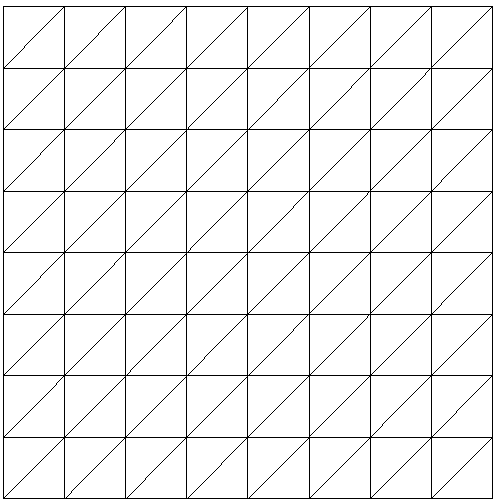
\includegraphics[width=.25\textwidth]{figures/grid1.png} \qquad  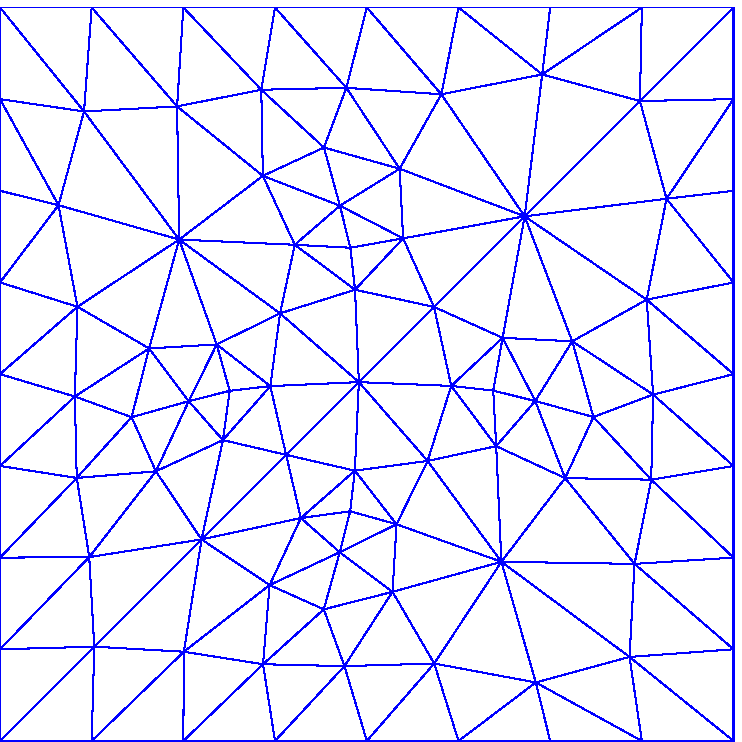
\includegraphics[width=.25\textwidth]{figures/u00.pdf}  \qquad 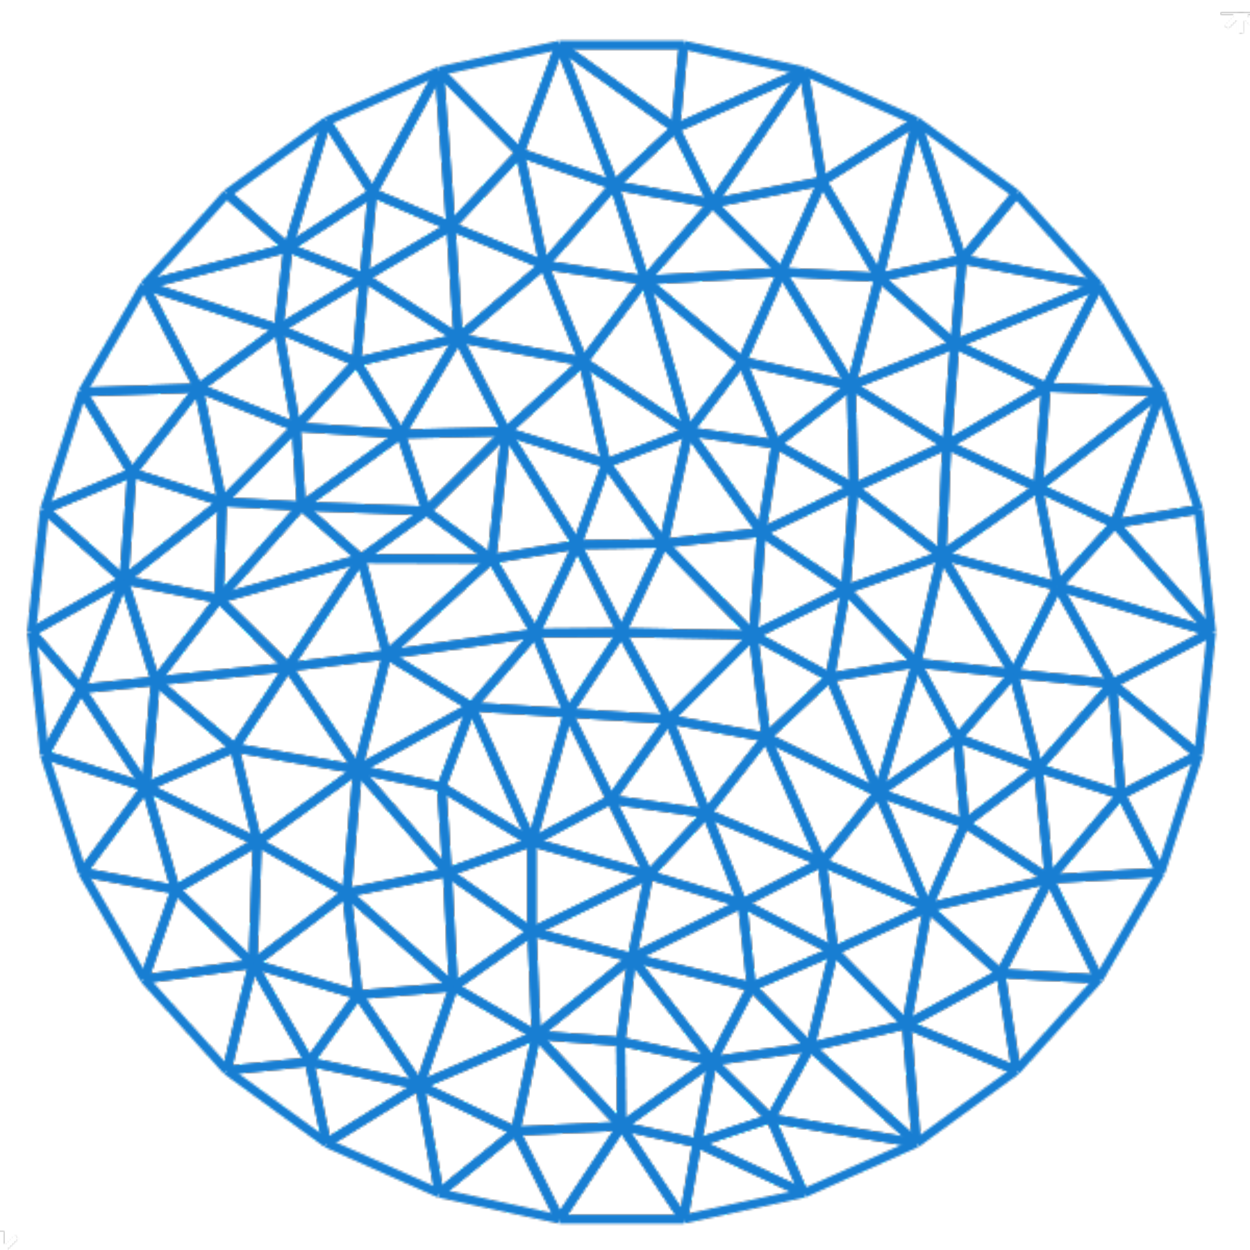
\includegraphics[width=.25\textwidth]{figures/2ddiskpartition.pdf}  
\end{center}
\caption{2D grids}
\label{2duniform}
\end{figure}

Denote 
$$
h_\tau=\mbox{\rm diam} (\tau)\quad  \hbox{(diameter of the smallest sphere containing $\overline{\tau}$)},
$$
and 
$$
 h=\max_{\tau\in\mathcal T_h} h_\tau;\quad
\underline{h}=\min_{\tau\in\mathcal T_h} h_\tau.
$$
A set of triangulations $\mathscr T$ is called {\em shape regular} if
there exists a constant $c_0$ such that
\begin{equation}\label{shape} \max _{\tau \in \mathcal T_h} \frac{h_{\tau}^d}{|\tau|}\leq c_0, \quad \forall \, \mathcal T_h\in
\mathscr T,
\end{equation} 
where $|\tau|$ is the measure of $\tau$ in $\mbb R^d$. This assumption can also be represented as
\begin{equation}\Label{A3.1}
\max_{\tau\in\ct_h}\frac{h_\tau}{\rho_\tau}\le\sigma_1,\quad \forall \, \mathcal T_h\in
\mathscr T,
\end{equation}
where $\rho_\tau$\index{$\rho_\tau$} denotes the radius of the ball
inscribed in $\tau$. In two dimensions, it is equivalent
to the minimal angle of each triange is bounded below uniformly
in the shape regular class. 
%We shall define $h_{\tau} = |\tau|^{1/n}$
%for any $\tau \in \mathcal T_h\in \mathscr T$. By (\ref{shape}),
%$h_{\tau}\eqsim {\rm diam}(\tau)$ represents the size of an element
%$\tau \in \mathcal T_h$ for a shape regular triangulation $\mathcal T_h\in
%\mathscr T$.

In addition to (\ref{shape}), if
\begin{equation}\Label{A3.2}
  \frac{\max _{\tau \in \mathcal T_h}|\tau|}{\min _{\tau \in \mathcal T_h}|\tau|} \leq \rho,\quad \forall \, \mathcal T_h\in \mathscr T,
\end{equation}
$\mathscr T$ is called {\em quasi-uniform}. For quasi-uniform grids,
$h=\max _{\tau \in \mathcal T_h} h_{\tau}$, the mesh size of
$\mathcal T_h$, is used to measure the approximation rate. 
%In the FEM literature, we often write as $\mathcal T_h$.

%The triangulation $\thset$ is said to be quasi-uniform
%\index{triangulation, quasi-uniform} if it satisfies \rf{A3.1} and
%the following
%\begin{eqhttps://gmu.zoom.us/j/97581839555?pwd=ZjlZeFE3Q0JkekdOcGpBZEZxdFJwQT09uation}\Label{A3.2}
%h\le\sigma_3 \underline {h}.
%\end{equation}

The assumption \rf{A3.1} is a local assumption, as is meant by above
definition, for $d=2$ for example, it assures that each triangle will
not degenerate into a segment in the limiting case.  
%A triangulation satisfying this assumption is often called to be {\it shape regular}.

On the other hand, the assumption \rf{A3.2} is a global assumption,
which says that the smallest mesh size is not too small compared with
the largest mesh size of the same triangulation.  By the definition, in
a quasi-uniform triangulation, all the elements are about the same size
asymptotically.

Let $ x_{i}=(x^1_{i}, \cdots, x^d_{i})^t, i=1,\cdots, d+1$ be $d+1$ points in $\mbb R^d$ which do not all lie in one hyper-plane. 
The {\it convex hull} of the $d+1$ points $ x_1, \cdots,  x_{d+1}$ (See Figure \ref{fig:barycentricCoor})
\begin{equation}
\tau :=\{ x=\sum _{i=1}^{d+1}\lambda _i x_i \, | \, 0\leq \lambda_i\leq 1, i=1:d+1, \sum _{i=1}^{d+1}\lambda _i=1 \}
\end{equation}
is defined as a {\em geometric $d$-simplex} generated (or spanned) by
the vertices $ x_1, \cdots,  x_{d+1}$. For example, a triangle
is a $2$-simplex and a tetrahedron is a $3$-simplex. For an integer
$0\leq m \leq d-1$, an $m$-dimensional face of $\tau$ is any
$m$-simplex generated by $m+1$ of the vertices of
$\tau$. Zero-dimenisonal faces are vertices and one-dimensional faces
are called edges of $\tau$. The $(d-1)$-face opposite to the vertex
$ x_i$ will be denoted by $F_i$.
\begin{figure}[hpt]
%\subfigure[1d simplex]{
%\begin{minipage}[t]{0.33\linewidth}
\centering
\includegraphics*[width=2.5cm]{figures/barycentricCoor1D.pdf}
%\end{minipage}}%%
%\subfigure[2d simplex]{
%\begin{minipage}[t]{0.33\linewidth}
%\centering
\includegraphics*[width=3cm]{figures/barycentricCoor2D.pdf}
%\end{minipage}}%%
%\subfigure[3d simplex]
%{\begin{minipage}[t]{0.33\linewidth}
%\centering
\includegraphics*[width=3.1cm]{figures/barycentricCoor3D.pdf}
%\end{minipage}}
\caption{Geometric explanation of barycentric coordinates}
\label{fig:barycentricCoor}
\end{figure}
%\paragraph{Barycentric coordinates}
On the other hand, for any $ x\in \tau$, there exist unique numbers $\lambda _1,\cdots, \lambda _{d+1}$ satisfying $\displaystyle 0\leq \lambda_i\leq 1, i=1:d+1, \sum _{i=1}^{d+1}\lambda _i=1$ such that $\displaystyle x=\sum _{i=1}^{d+1}\lambda _i x_i$, thus we can denote $\lambda _1,\cdots, \lambda _{d+1}$ as $\lambda _1( x),\cdots, \lambda _{d+1}( x)$. In fact,  the numbers $\lambda _1( x),\cdots, \lambda _{d+1}( x)$ are
called {\em barycentric coordinates} of $ x$ with respect to the
$d+1$ points $ x_1, \cdots,  x_{d+1}$. There is a simple
geometric meaning of the barycentric coordinates. Given a $ x\in
\tau$, let $\tau _i( x)$ be the simplex with vertices $ x_i$
replaced by $ x$. Then it can be easily shown that
\begin{equation}\label{eq:lambdasolution}
\lambda _i( x) = |\tau _i( x)|/|\tau|,
\end{equation}
where $|\cdot|$ is the Lebesgure measure in $\mbb R^d$, namely area in
two dimensions and volume in three dimensions. Note that $\lambda
_i( x)$ is affine function of $ x$ and vanishes on the face
$F_i$. We list the four basic properties of barycentric coordinate below:
\begin{enumerate}
\item $0\leq \lambda_i( x)\leq 1$;
\item $\displaystyle\sum_{i=1}^{d+1} \lambda_i( x)=1$;
\item $\lambda_i( x)\in P_1(\tau)$, where $P_1(\tau)$ denotes the space of polynomials of degree $1$
(linear) on $\tau\in \mathcal T_h$;
\item $\lambda_i( x_j)=\delta_{ij}=\begin{cases}
1, \quad &\text{if}  \quad  i=j\\
0, \quad &\text{if} \quad i\neq j
\end{cases}.$
\end{enumerate}

\subsection{Continuous linear finite element spaces}\label{linearFE}
A conforming linear finite element function in a domain $\Omega\subset
\mathbb R^d$ is a continuous function that is piecewise linear
function with respect to a grid or mesh consisting of a union of simplices.

Given a shape regular triangulation $\mathcal T_h$ of $\Omega$, we define the 
continuous linear finite element space as 
\begin{equation}\label{LinFE}
V_h:=\{v\,|\, v\in C(\overline \Omega), \,\hbox{ and }\, v|_{\tau}\in
P_1(\tau), \forall \tau \in \mathcal T_h\},
\end{equation}
where $P_1(\tau)$ denotes the space of polynomials of degree $1$
(linear) on $\tau\in \mathcal T_h$. Whenever we need to deal with boundary
conditions, we further define $V_{h,0}=V_h\cap H_0^1(\Omega)$.

We note here that the global continuity is also necessary in the
definition of $V_h$ in the sense that if $u$ has a square interable
gradient, that is $u\in H^1(\Omega)$, and $u$ is piecewise smooth,
then $u$ is continuous. 

We always use $n_h$ to denote the dimension of finite element
spaces. For $V_h$, $n_h$ is the number of vertices of the
triangulation $\mathcal T_h$ and for $V_{h,0}$, $n_h$ is the number of
interior vertices. 

\paragraph{Nodal basis functions and dual basis}
For linear finite element spaces, we have the so
called \emph{a standard nodal basis functions} $\{\varphi
_i,i=1,\cdots n_h\}$ such that $\varphi_i$ is piecewise linear (with
respect to the triangulation) and $\varphi_i(x_j)=\delta_{i,j}$.  Note
that $\varphi _i|_\tau$ is the corresponding barycentrical coordinates
of $x_i$. See Figure \ref{fig:nodalbasis} for an illustration in 2D.
\begin{figure}[hpt]
%\subfigure[1d basis function]{
%\begin{minipage}[t]{0.49\linewidth}
\centering
\includegraphics*[height=4.5cm,width=7cm]{6DL/figures/Dualbasis}
%\end{minipage}}
\caption{Dual basis functions of $V_h$ in 1D for $n_h=5$.}
\label{fig:dualbasis}
\end{figure}
Let $(\varphi_i^*)_{i=1}^{n_h}$ be the dual basis of $(\varphi_i)_{i=1}^{n_h}$, namely
\begin{equation}
  \label{eq:1}
(\varphi_i^*, \varphi_j) =\delta_{i, j}, \quad i, j=1,\ldots, n_h.    
\end{equation}
We notice that all the nodal basis functions $\{\varphi_i\}$ are locally
supported, but their dual basis functions $\{\varphi_i^*\}$ are in general
not locally supported (see Figure \ref{fig:dualbasis}).  The nodal basis functions $\{\varphi_i\}$ are
easily constructed in terms of barycentric coordinate functions.  The
dual basis $\{\varphi_i^*\}$ are only interesting for theoretical
consideration and it is not necessary to know the actual constructions
of these functions.

%
\begin{figure}[hpt]
%\subfigure[1d basis function]{
%\begin{minipage}[t]{0.49\linewidth}
\centering
\includegraphics*[height=4.5cm,width=7cm]{figures/basisfunction}
%\end{minipage}}%%
%\subfigure[2d basis function]{
%\begin{minipage}[t]{0.49\linewidth}
%\centering
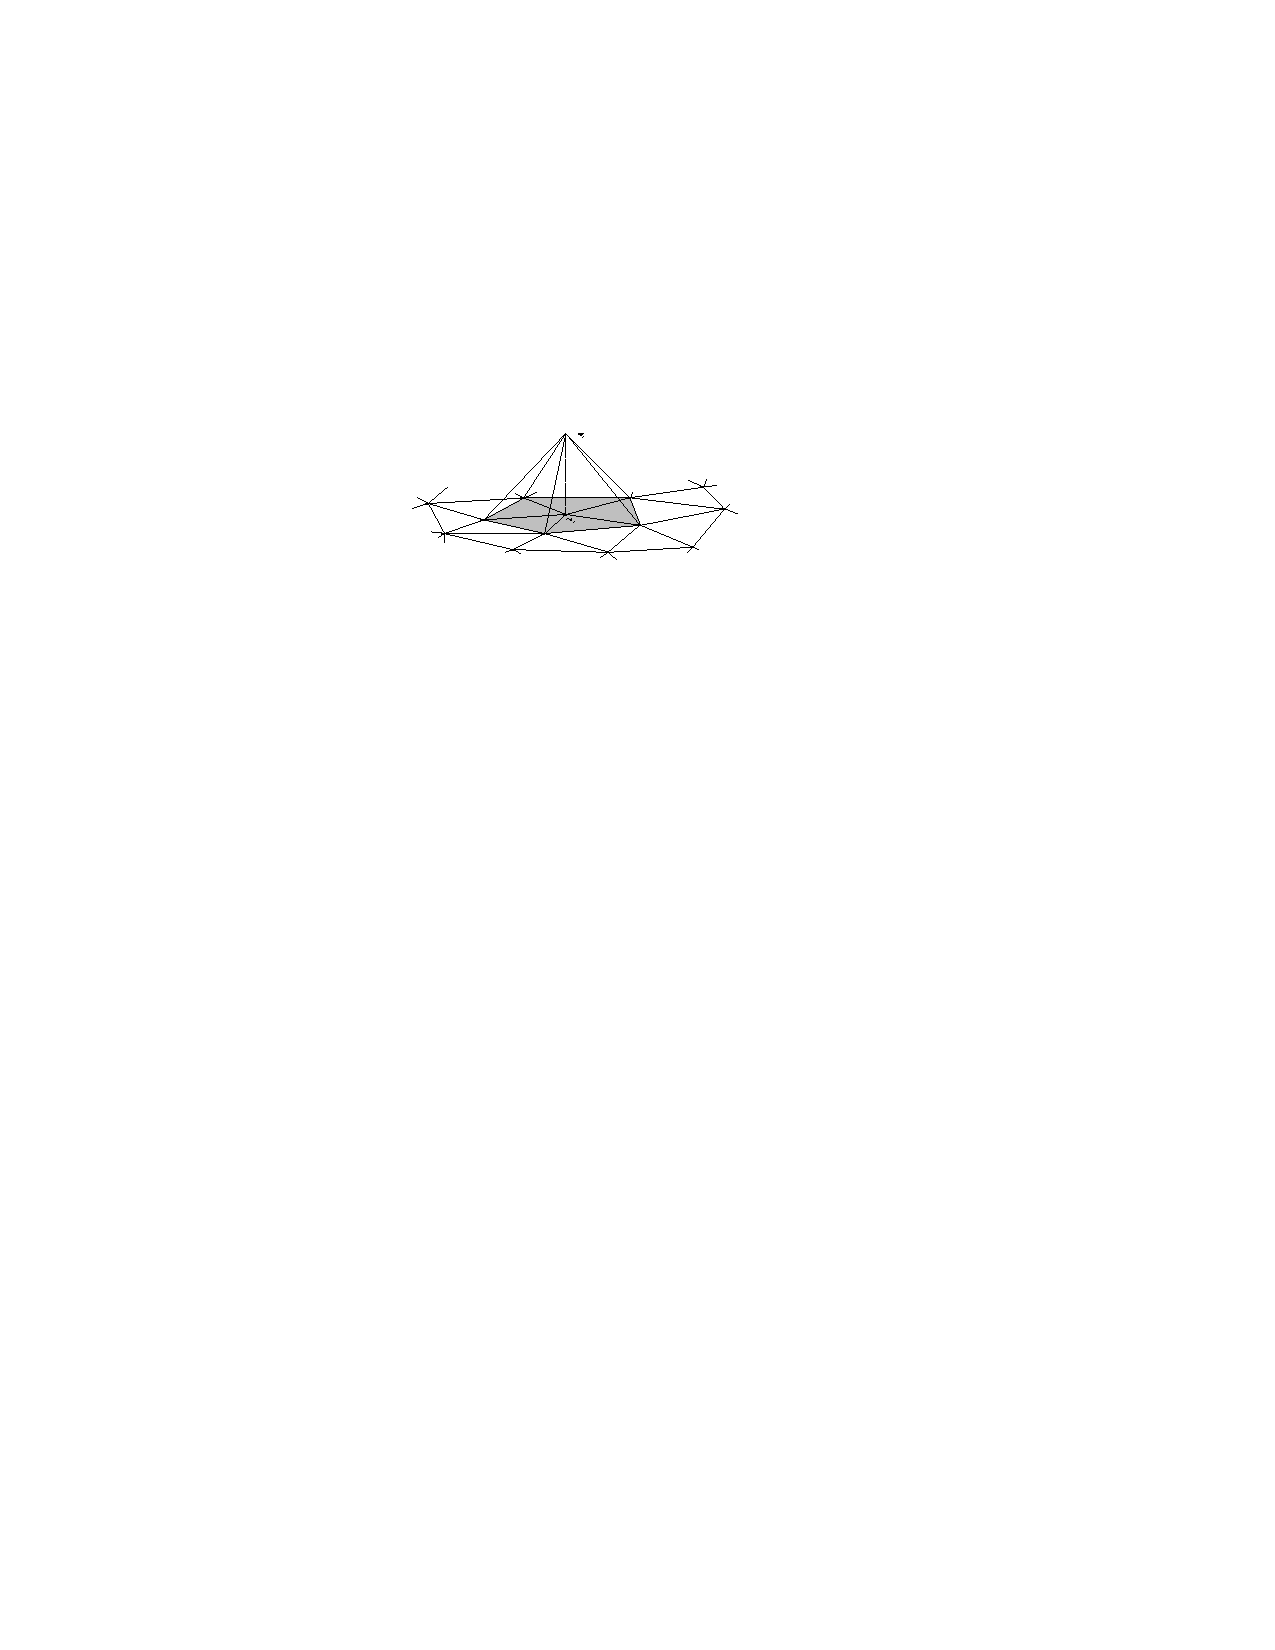
\includegraphics[height=5cm,width=7cm]{figures/nodalbasis.pdf}
%\end{minipage}}
\caption{Nodal basis functions in 1d and 2d}
\label{fig:nodalbasis}
\end{figure}
Since $\{\varphi_i,i=1,\cdots n_h\}$ is a basis of $V_h$, therefore for any $v_h\in V_h$, we have the representation
$$
v_h(x)=\sum_{i=1}^{n_h}v_h(x_i)\varphi_i(x). 
$$

Let us see how our construction of continuous linear finite space and the nodal basis looks like  in one spatial dimension. 
Associated with the mesh
$$
\mathcal T_h=\{0=x_0<x_1<\ldots<x_{n_h}<x_{n_h+1}=1\},
$$
by the definition given in \eqref{LinFE} and the definition  $V_{h,0}=V_{h}\cap H_0^1(\Omega)$, we have
\[
\begin{array}{ll}
V_{h,0}=\{v:~\mbox{$v$ is continuous and piecewise linear}~ \mbox{w.~r.~t. $\mathcal T_h$, } v(0)=v(1)=0\}.
\end{array}
\]
A plot of a typical element of $V_{h,0}$ is shown in Fig.~\ref{fig:1dtypical}.

It is easily calculated (as we already mentioned), that the dimension
of $V_{h,0}$ is equal to the number of internal vertices, and the nodal
basis functions spanning $V_{h,0}$ (for $i=1,2,\cdots,n_h$) are (see also
Fig.~\ref{fig:nodalbasis}):
\begin{equation}\label{1dbasis:function}
\varphi_i(x)=\left\{\begin{array}{cl}
\displaystyle \frac{x-x_{i-1}}{h}, & x\in[x_{i-1},x_i];\\
\displaystyle \frac{x_{i+1}-x}{h}, & x\in[x_{i},x_{i+1}];\\
0 &\mbox{elsewhere}.
\end{array}\right.
\end{equation}

\begin{figure}[hpt]
\centering
\includegraphics*[width=2in]{figures/femfunction1.pdf}
\caption{Plot of a typical element from $V_{h,0}$.} 
\label{fig:1dtypical}
\end{figure}



%%%%%%%%%%%%%%%%%%%%END from grid.tex%%%%%%%%%%%%%%%%%%%%%%%%%%%%%%%

%%%%%%%%%%%%%%%%%%%%END from grid.tex%%%%%%%%%%%%%%%%%%%%%%%%%%%%%%%

%%%%%%%%%%%%%%%%%%%%END from grid.tex%%%%%%%%%%%%%%%%%%%%%%%%%%%%%%%

\chapter{Linear Finite Element Spaces}
\section{Piecewise linear finite element spaces}
\input{3FEM/linearFE}
\paragraph{Nodal value interpolant}
\Label{sc-seio}

For any continuous function $u$, we define its linear finite element
interpolation, $(I_h u)(x)\in V_{h,0}$,  as follows:
\begin{equation}
  \label{u-interp}
(I_h u)(x)= \sum_{i=1}^{n_h}u(x_i)\varphi_i(x).
\end{equation}
Usually, we also denote $(I_h u)(x)$ as $u_I(x)$. Using interpolation, we can obtain the following approximation property of 
linear finite element space. 
%For any $v\in\Shz$, we can obviously write
%$$
%        v(x)=\sum_{i=1}^{n_h}v(x_i)\phi_i(x).
%$$
%The nodal value interpolation\index{interpolation} operator $I_h: C(\bar\Om)\mapsto V_h$ is defined as follows \index{$I_h$}
%$$
%        (I_h u)(x_i)=u(x_i),\qall x_i\in {\cal N}_h,
%$$
%where ${\cal N}_h$ is the set of the vertexes for the partition $\mathcal T_h$. 
\begin{figure}[hpt]
\begin{center}
\includegraphics*[height=2.5in, width=3in]{figures/fdsolutions.pdf}
\caption{Approximation of finite element space.} 
\label{Interpolation}
\end{center}
\end{figure}


\begin{theorem}\label{interp00}
Assume that $\mathcal T_h$ is quasi-uniform and $V_h$ is the linear finite element space associated with $\mathcal T_h$, then
\begin{equation}
\label{error0}
\inf_{v_h\in V_h} \|v-v_h\|+h |v-v_h|_{1}\lc h^2 |v|_2
        \qall v\in H^2(\Om).
\end{equation}
 \end{theorem}
 \begin{proof}  
Let us first prove Theorem \ref{interp00} for $d=1, 2, 3$.
This proof presented here follows from Xu~\cite{xu1982estimate} (see also Xu~\cite{xu2013estimate}).
Let $x=(x^1,\ldots, x^d)$ and $a_i=(a^1_{i}, \ldots, a^d_{i})$. Introducing
the auxiliary functions
$$
g_i(t)=v(a_i(t)),\mbox{  with  }  a_i(t)=a_i+t(x-a_i),
$$
we have
$$
g_i'(t)=(\nabla v)(a_i(t))\cdot (x-a_i)
=\sum_{l=1}^d(\partial_lv)(a_i(t))(x^l-a_i^l)
$$
and
\begin{equation}\label{gpp}
g_i''(t)=\sum_{k,l=1}^d\partial^2_{kl}v)(a_i(t))(x^k-a_i^k)(x^l-a_i^l).
\end{equation}
Note Taylor expansion
$$
        g_i(0)=g_i(1)-g_i'(1)+\int_0^1tg''_i(t)dt,
$$
namely
\begin{equation}\label{Taylor_vi}
v(a_i)=v(x)-(\nabla v)(x)\cdot (x-a_i)+\int_0^1tg''_i(t)dt,
\end{equation}
and note that
$$
(I_hv)(x)=\sum_{i=1}^{d+1}v(a_i)\lambda_i(x), \quad \sum_{i=1}^{d+1}\lambda_i(x)=1,
$$
and
$$
\sum_{i=1}^{d+1}(x-a_i)\lambda_i(x)=0.
$$
It follows that
\begin{equation}\label{Ihvv}
(I_hv-v)(x)=\sum_{i=1}^{d+1}\lambda_i(x)\int_0^1tg''_i(t)dt.
\end{equation}
Using \rf{gpp} and the trivial fact that $|x^l-a_i^l|\le h$,
we obtain
\begin{eqnarray*}
\|g''_i(t)\|_{L^2(\tau)}\le h^2
\sum_{k,l=1}^d\|(\partial^2_{kl}v)(a_i(t))\|_{L^2(\tau_i^t)}
\le h^2t^{-d/2}\sum_{k,l=1}^d\|\partial^2_{kl}v\|_{L^2(\tau)},
\end{eqnarray*}
where we have used the following change of variable
$$
y=a_i+t(x-a_i): \tau\mapsto \tau_i^t\subset\tau \mbox{ with } dy=t^ddx.
$$
Now taking the $L^2(\tau)$ norm on both hand of sides of
\rf{Ihvv}, we get
\begin{eqnarray*}
\|I_hv-v\|_{L^2(\tau)}
&\le& h^2\sum_{i=1}^{d+1}\max_{x\in\tau}|\lambda_i(x)|
\int_0^1t\|g''_i(t)\|_{L^2(\tau)}\;dt\\
&\le& (d+1)\int_0^1t^{-d/2}dt\;h^2\;
\sum_{k,l=1}^d\|\partial^2_{kl}v\|_{L^2(\tau)}\\
&\le&\frac{2(d+1)}{4-d}h^2
\sum_{k,l=1}^d\|\partial^2_{kl}v\|_{L^2(\tau)}\\
&\le&\frac{4d(d+1)}{4-d}h^2|v|_{H^2(\tau)}.
\end{eqnarray*}
Now we prove the $H^1$ error estimate. Notice that
$$
[\partial_{j}( I_{h} v - v)](x) = \sum_{i} (\partial_{j} \lambda_{i} )(x) \int_{0}^{1} t g''_{i}(t) dt + \sum_{i} \lambda_{i}(x) \partial_{j} \int_{0}^{1} t g''_{i}(t) dt.
$$ 
By \rf{Taylor_vi},
$$
\int_0^1tg''_i(t)dt = v(a_i) - v(x) + (\nabla v)(x)\cdot (x-a_i)
$$
therefore,
\begin{eqnarray*}
\lefteqn{\partial_{j} \int_0^1tg''_i(t)dt} \\
& = & - \partial_{j} v + (\nabla \partial_{j} v )(x) (x - a_{i}) + \nabla v \cdot e_{j} 
\hcomment{$e_{j}$ is the $j$-th standard basis}  \\
& = & (\nabla \partial_{j} v )(x) (x - a_{i}).
\end{eqnarray*}
Noting that $\sum_{i} \lambda_{i}( \nabla \partial_{j} v )(x) (x - a_{i}) = 0$, we have
$$
[\partial_{j}( I_{h} v - v)](x) = \sum_{i} (\partial_{j} \lambda_{i} )(x) \int_{0}^{1} t g''_{i}(t) dt.
$$
Then the estimate for $|\nabla(I_hv-v)|_{L^2(\tau)}$
follows by a similar argument and the following obvious
estimate
$$
|(\nabla\lambda_i)(x)|\lc\frac{1}{h}.
$$
 
On the proof of Theorem \ref{interp0} for $d\ge 4$, the above proof does not
apply for $d \ge 4$. This is because when $d \ge 4$, the embedding
relation between $H^{2}(\Om) \hookrightarrow C(\bar{\Om})$ is no longer true.  Only
continuous functions can have interpolations. In this case, one approach is to use the 
so-called Scott-Zhang interpolation \cite{scott1990finite}, the
details can be found in \cite{Xu.J2015a}.
\end{proof}
As a result of Theorem \ref{interp00}, we have
\begin{theorem}\label{interp0}
Let $V_N$ be linear finite element space on a quasi-uniform
triangulation consisting of $N$ element.  Then 
\begin{equation}
\label{error0N}
\inf_{v_h\in V_N} \|v-v_h\|+N^{-{1\over d}} |v-v_h|_{1}\lc N^{-{2\over d}} |v|_2
        \qall v\in H^2(\Om).
\end{equation}
\end{theorem}




\section{Locally adaptive grids}
\subsection{A 1D example}
\input{3FEM/1dAFEM}
\input{3FEM/2dW21AFEM}
\subsection{Lower bound of optimal error estimates in any dimension}
\begin{conjecture}
Let $V_N$ be  linear finite element spaces associated with 
shape-regular simplicial grids $\mathcal T_N$ of $N$-elements (or
$N$-grid points) in a polyhedral domain $\Omega\subset \mathbb R^d$,
say $\Omega=(0,1)^d$.  Then,  for any reasonable function (which is,  say,
not locally linear), then the following lower bound holds:
\begin{equation}
\label{optimalFEMerror}
\inf_{\# \mathcal T_N=\mathcal O(N)} \inf_{v_N\in
  V_N}\|u-v_N\|_{0,\Omega}\ge c(u) N^{-2/d} 
%\le C(u) N^{-2/d}
\end{equation}
\end{conjecture}

Questions:
\begin{enumerate}
\item Is the above conjecture correct in some way?  If yes, what are
  the more rigorous statements for such results?
\item What are the most relevant references that contain such results?
\item If the conjecture is incorrect, is there a counter example?
\end{enumerate}

\chapter{Artificial Neural Network (ANN) and  Deep Neural Networks (DNN)}
\section{Motivation: from finite element to neural network}\label{FE2NN}
In this section, we will introduce the so-called shallow neural network 
(deep neural network with one hidden layer) from the viewpoint of finite element method.

Let us recall the linear finite element functions on the unit interval $\bar{\Omega}=[0,1]$ in Section \ref{linearFE}. 
Consider a set of equidistant girds $\mathcal T_\ell$ of level $\ell$ and mesh length $h_\ell = 2^{-\ell}$. The grid points $x_{\ell,i}$ are given by
\begin{equation}
x_{\ell,i}:=ih_\ell,\quad 0\le i\le 2^\ell.
\end{equation} 
For $\ell=1$, we denote the special hat function by $\varphi(x)$ and any nodal basis function in \eqref{1dbasis:function} on grid $\mathcal T_\ell$ by $\varphi_{\ell,i} $ as below
\begin{equation}\label{def_g}
\varphi(x) = 
\begin{cases}
2x \quad &x\in [0,\frac{1}{2}] \\
2(1-x) \quad &x\in [\frac{1}{2}, 1] \\
0, \quad &\text{others} 
\end{cases},\qquad
\varphi_{\ell,i} = \varphi(\frac{x - x_{\ell,i-1}}{2h_\ell}) = \varphi(w_\ell x + b_{\ell,i}).
\end{equation} 
That is to say, any $\varphi_{\ell,i}(x)$ can be obtained from $\varphi(x)$ by scaling 
(dilation) and translation with 
\begin{equation}\label{key}
w_\ell = 2^{\ell-1}, \quad b_{\ell,i} = \frac{-(i-1)}{2},
\end{equation}
in $\varphi_{\ell,i} = \varphi(w_\ell x + b_{\ell,i})$. 
\begin{figure}[H]
\centering
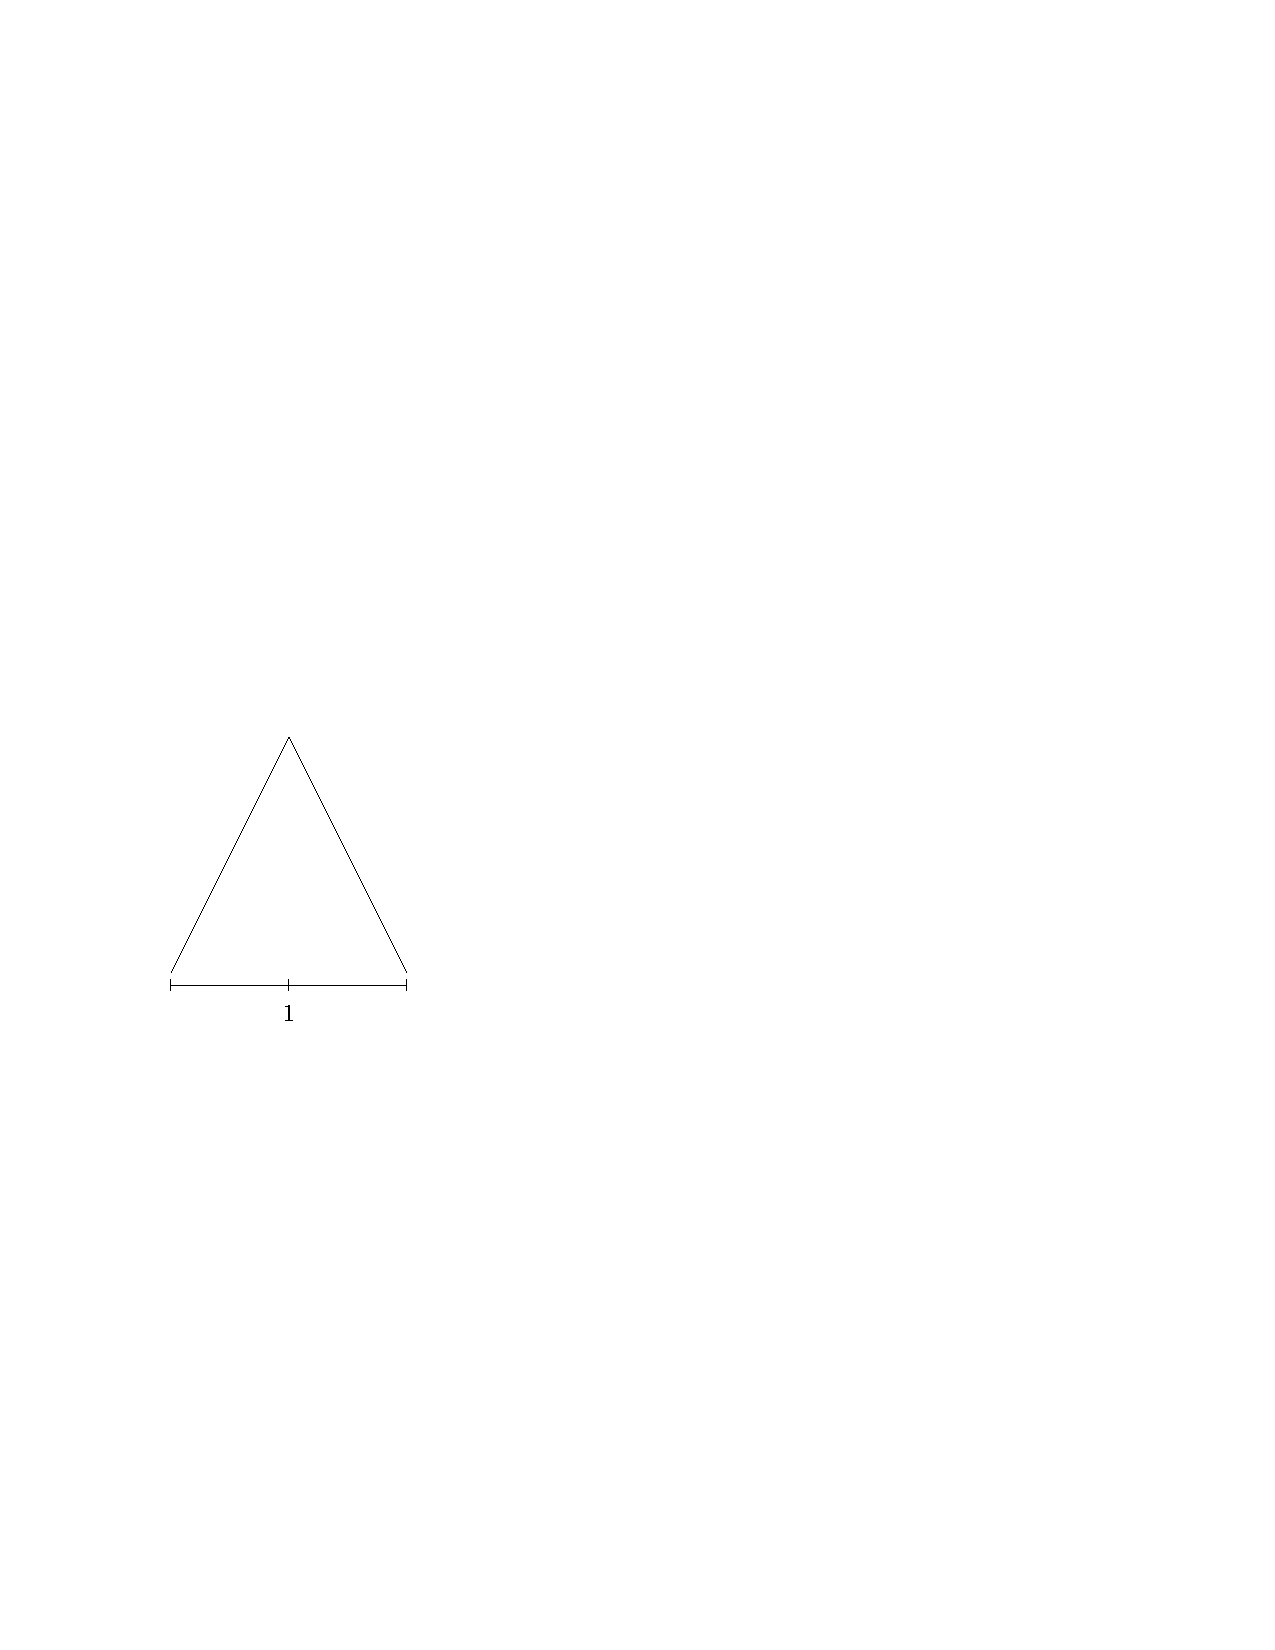
\includegraphics[width=4cm]{1dbasis1.pdf}\qquad
\includegraphics[width=5cm]{basisfunction.pdf}
\caption{Diagram of $\varphi(x)$ (left) and $\varphi_{\ell,i}(x)$ (right).}
\end{figure} 


Let us recall the finite element interpolation in Section \ref{linearFE} as
\begin{equation}\label{key}
u(x) \approx u_\ell(x) := \sum_{ 0\le i \le 2^\ell} u(x_{\ell,i}) \varphi_{\ell,i}(x),
\end{equation}
for any smooth function $u(x)$ on $(0,1)$. The above interpolation will converge as $\ell \to \infty$, which shows that
\begin{equation}\label{key}
{\rm span} \left\{  \varphi(w_\ell x + b_{\ell,i}) \right\} \quad \text{is dense in} \quad H^1(0,1).
\end{equation}
Thus, we may have the next concise relation:
\begin{equation}\label{key}
\begin{split}
\text{FE space} =  &{\rm span} \left\{  \varphi(w_\ell x + b_{\ell,i}) ~|~ 0\le i \le 2^\ell, \ell = 1, 2, \cdots \right\} 
\\
\subset  &{\rm span} \left\{  \varphi(w x + b) ~|~  w, b \in \mathbb{R} \right\}.
\end{split}
\end{equation}
In other words, the finite element space can be understood as the linear combination of $\varphi(w x + b)$ with certain special choice of $w$ and $b$. 

Here, we need to point out that this ${\rm span} \left\{  \varphi(w x + b) ~|~  w, b \in \mathbb{R} \right\}$ is exact the deep neural networks with one hidden layer (shallow neural networks) with activation function $\varphi(x)$. More precisely, 
\begin{equation}\label{key}
f \in {\rm span} \left\{  \varphi(w x + b) ~|~  w, b \in \mathbb{R} \right\},
\end{equation}
means there exist positive integer $N$ and $w_j, b_j \in \mathbb{R}$ such that 
\begin{equation}\label{key}
f = \sum_{j=1}^N a_j \varphi(w_j x + b_j),
\end{equation}
which is also called one hidden neural network function with $N$ neurons.

\begin{remark}
	\begin{enumerate}
		\item By making $w_\ell$ and $b_{\ell,i}$ in \eqref{def_g} arbitrary, we get a much larger class of 
		function which is exact a special neural network with activation function $\varphi(x)$.
		\item Generalizations: 
		\begin{enumerate}
			\item activation function $\varphi$ can be different, such as ${\rm ReLU}(x) = \max\{0,x\}$.
			\item There is a natural extension for high dimension $d$ as
			\begin{equation}\label{key}
			\left\{  \varphi(w\cdot x + b) \right \},
			\end{equation}
			where $w\in \mathbb{R}^d$, $b\in \mathbb{R}$ and $\displaystyle w\cdot x = \sum_{i=1}^d w_i x_i$.
			This is called ``deep'' neural network with one hidden layer.
		\end{enumerate}
	\end{enumerate}
\end{remark}


%\input{3FEM/2dFEM}

\section{Why we need deep neural networks via composition}\label{whydeep}
\subsection{FEM ans ${\rm DNN}_1$ in 1D}
Thanks to following connection between $\varphi(x)$ in \eqref{def_g} and ${\rm ReLU}(x) = \max(0,x )=x_+$
\begin{equation}\label{key}
\varphi(x) = 2{\rm ReLU}(x) - 4{\rm ReLu}({x-\frac{1}{2}}) + 2{\rm ReLU}(x-1),
\end{equation}
it suffices to show that each basis
function $\varphi_{\ell,i}$ can be represented by a ReLU DNN. 
We first note that  the basis
function $\varphi_{\ell,i}$ has the support in $[x_{\ell,i-1},
x_{\ell,i+1} ]$ can be easily written as
\begin{equation}
\label{1d-basisu}
\varphi_{\ell,i}(x) = \frac{1}{h_{\ell}}{\rm ReLU}(x-x_{\ell,i-1}) -\frac{2}{h_{\ell}}{\rm ReLU}(x-x_{\ell,i}) +\frac{1}{h_\ell}{\rm ReLU}(x-x_{\ell,i+1}).
\end{equation}
More generally, consider a general  grid with vertex $\{x_i\}$, which is not necessarily uniform. The basis function $\varphi_i$ of the linear element with support $[x_{i-1},
x_{i+1} ]$ can be easily written as
\begin{equation}
\label{1d-basis}
\varphi_i(x) = \frac{1}{h_{i-1}}{\rm ReLU}(x-x_{i-1}) -(\frac{1}{h_{i-1}}+\frac{1}{h_i}){\rm ReLU}(x-x_i) +\frac{1}{h_i}{\rm ReLU}(x-x_{i+1}),
\end{equation}
where $h_i = x_{i+1} - x_i$.

Thus is to say, we have the next theorem.
\begin{theorem}\label{thm:1dLFEMDNN}
	For $d=1$, and  $\Omega\subset \mathbb R^d$ is 
	a bounded interval, then ${\rm DNN}_1$ can be used to cover all linear finite element 
	function in on $\Omega$.
\end{theorem}
\subsection{Linear finite element cannot be recovered by ${\rm DNN}_1$ for $d\ge2$}
In view of  Theorem~\ref{thm:1dLFEMDNN} and the fact that ${\rm{DNN}_J}
\subseteq {\rm{DNN}_{J+1}} $, it is natural to ask that how many
layers are needed at least to recover all linear finite element
functions in $\mathbb{R}^d$ for $d\ge2$.  In this section, we will show that 
\begin{equation}\label{key}
J_d \ge 2, \quad \text{if} \quad d\ge 2,
\end{equation}
where $J_d$ is the minimal $J$ such that all linear finite element
functions in $\mathbb R^d$ can be recovered by ${\rm DNN}_J$.

In particular, we will show the following theorem~\cite{he2020relu}.
\begin{theorem}\label{lowerbound}
	If $\Omega\subset \mathbb R^d$ is either 
	a bounded domain or $\Omega=\mathbb{R}^d$,  
	${\rm DNN}_1$ can not be used to recover all linear finite element
	functions on $\Omega$. 
\end{theorem}
\begin{proof}
	We prove it by contradiction. Let us assume that for any continuous
	piecewise linear function $f: \Omega \to \mathbb{R} $, we can find
	finite $N \in \mathbb{N}$, $w_i \in \mathbb{R}^{1,d}$ as row vector
	and $\alpha_i, b_i, \beta \in \mathbb{R}$ such that
	$$
	f =  \sum_{i=1}^N \alpha_i {\rm ReLU}(w_i\cdot  x +b_i) + \beta,
	$$
	with $f_i = \alpha_i {\rm ReLU}(w_i\cdot  x +b_i)$, $\alpha_i \neq 0$ and $w_i
	\neq 0$.  Consider the finite element functions, if this one hidden
	layer ReLU DNN can recover any basis function of FEM, then it can
	recover the finite element space.  Thus let us assume $f$ is a locally
	supported basis function for FEM.
	Furthermore, if $\Omega$ is a bounded domain, we assume that 
	\begin{equation}\label{distcondi}
	d({\rm supp}(f), \partial \Omega) > 0,
	\end{equation}with 
	$$
	d(A, B) = \inf_{x\in A, y\in B} \|x-y\|,
	$$ 
	as the distance of two closed sets. 
	
	A more important observation is that $\nabla f: \Omega \to
	\mathbb{R}^d$ is a piecewise constant vector function. The key
	point is to consider the discontinuous points for 
	$$g := \nabla
	f = \sum_{i=1}^N \nabla f_i.$$
	For more general case, we can define the set of discontinuous points of a function by
	$$
	D_{g} := \{x \in \Omega~|~ x ~ \text{is a discontinuous point of} ~ g\}.
	$$
	Because of the property that 
	\begin{equation}\label{eq:disfun}
	D_{f+g} \supseteq D_{f} \cup D_{g} \backslash (D_{f} \cap D_{g}),
	\end{equation}
	we have
	\begin{equation}\label{eq:dis_fn}
	D_{\sum_{i=1}^N g_i} \supseteq \bigcup_{i=1}^N D_{g_i} \backslash \bigcup_{i\neq j}\left( D_{g_i}\cap D_{g_j} \right).
	\end{equation}
	Note that
	\begin{equation}\label{eq:def_gi}
	g_i = \nabla f_i(x) =  \nabla \left( \alpha_i {\rm ReLU}(w_i\cdot   x +b_i)  \right) =\left(\alpha_iH(w_i \cdot  x +b_i)\right)w_i \in \mathbb{R}^d,
	\end{equation}
	for $i=1:N$ with $H$ be the Heaviside function defined as: 
	$$
	H(x) = \begin{cases}
	0 &\text{if} ~ x \le 0, \\
	1 &\text{if} ~ x > 0.
	\end{cases}
	$$ 
	This means that 
	\begin{equation}\label{eq: D_gi}
	D_{g_i} = \{ x ~|~ w_i\cdot   x + b_i = 0\}
	\end{equation}
	is a $d-1$ dimensional affine space in $\mathbb{R}^d$.  
	
	
	Without loss of generality, we can assume that 
	\begin{equation}\label{eq:assumD_gi}
	D_{g_i} \neq D_{g_j}.
	\end{equation}
	When the other case occurs, i.e. $D_{g_{\ell_1}} = D_{g_{\ell_2}} = \cdots= D_{g_{\ell_k}}$, by the definition of $g_i$ in \eqref{eq:def_gi} and $D_{g_i}$ in \eqref{eq: D_gi} , 
	this happens if and only if there is a row vector $(w, b)$ such that
	\begin{equation}\label{eq:Dfcondition}
	c_{\ell_i}\begin{pmatrix}
	w &
	b
	\end{pmatrix} =  
	\begin{pmatrix}
	w_{\ell_i} &
	b_{\ell_i}
	\end{pmatrix},
	\end{equation}
	with some $c_{\ell_i} \neq 0$ for $i = 1:k$.  We combine those $g_{\ell_i}$ as
	\begin{equation*}
	\begin{aligned}\label{mergeH}
	%	\begin{split}
	\tilde g_{\ell} &= \sum_{i=1}^k g_{\ell_i} = \sum_{i=1}^k \alpha_{\ell_i} H(w_{\ell_i} \cdot  x + b_{\ell_i}) w_{\ell_i}, \\
	&= \sum_{i=1}^k \left( c_{\ell_i}\alpha_{\ell_i} H\left(c_{\ell_i}(w\cdot   x + b)\right) \right) w, \\
	&=\begin{cases}
	\displaystyle \left(\sum_{i=1}^k  c_{\ell_i}\alpha_{\ell_i} H(c_{\ell_i}) \right) w  \quad &\text{if} \quad w x + b > 0,\\
	\displaystyle \left(\sum_{i=1}^k  c_{\ell_i}\alpha_{\ell_i} H(-c_{\ell_i}) \right) w  \quad &\text{if} \quad w x + b \le 0.\\
	\end{cases}
	%	\end{split}
	\end{aligned}
	\end{equation*}	
	Thus, if 
	$$
	\left(\sum_{i=1}^k  c_{\ell_i}\alpha_{\ell_i} H(c_{\ell_i}) \right)  = \left(\sum_{i=1}^k  c_{\ell_i}\alpha_{\ell_i} H(-c_{\ell_i}) \right),
	$$
	$\tilde g_\ell$ is a constant vector function, that is to say $D_{\sum_{i=1}^k g_{\ell_i}} = D_{\tilde g_\ell} = \emptyset$. 
	Otherwise, $\tilde g_\ell$ is a piecewise constant vector function with the property that 
	$$
	D_{\sum_{i=1}^k g_{\ell_i}} = D_{\tilde g_\ell} = D_{g_{\ell_i}} = \{ x ~|~ w\cdot  x + b = 0\}.
	$$
	This means that we can use condition \eqref{eq:Dfcondition} as an equivalence relation and split $\{g_i\}_{i=1}^N$ into some groups, and we can combine those $g_{\ell_i}$ in each group as what we do above. After that, we have
	$$
	\sum_{i=1}^N g_i = \sum_{\ell=1}^{\tilde N} \tilde g_{\ell},
	$$
	with $D_{\tilde g_s} \neq D_{\tilde g_t}$.
	Finally, we can have that $D_{\tilde g_s} \cap D_{\tilde g_t}$ is an empty set or a $d-2$ dimensional affine space in $\mathbb{R}^d$.
	Since
	$\tilde N \le N$ is a finite number, 
	$$
	D := \bigcup_{i=1}^N D_{\tilde g_\ell} \backslash \bigcup_{s\neq t}\left( D_{\tilde g_s}\cap D_{\tilde g_t} \right)
	$$
	is an unbounded set. 
	\begin{itemize}
		\item If $\Omega = \mathbb{R}^d$,
		$$
		{\rm supp(f)} \supseteq D_{g} = D_{\sum_{i=1}^N g_i} = D_{ \sum_{\ell=1}^{\tilde N} \tilde g_{\ell}} \supseteq D,
		$$ is contradictory to the assumption that $f$ is locally supported.
		\item If $\Omega$ is a bounded domain, 
		$$
		d(D, \partial \Omega) = 
		\begin{cases}
		s > 0 \quad &\text{if}\quad  D_{\tilde g_i} \cap \Omega = \emptyset, \forall i\\
		0 \quad &\text{otherwise}.
		\end{cases}
		$$
		Note again that all $D_{\tilde g_i}$'s are $d-1$ dimensional affine spaces, while $D_{\tilde g_i} \cap D_{\tilde g_j}$ is either an empty set or a d-2 dimensional affine space. 
		If $d(D, \partial \Omega) > 0$, this implies that $\nabla f$ is continuous in $\Omega$, which contradicts the  assumption that $f$ is a basis function in FEM.
		If $d(D, \partial \Omega) = 0$, this contradicts the previous assumption in \eqref{distcondi}.
	\end{itemize}
	Hence ${\rm DNN}_1$ cannot recover any piecewise linear function in $\Omega$ for $d \ge 2$.
\end{proof}

Following the proof above, we have the following theorem~\cite{he2020relu}.
\begin{theorem}\label{linearindep}
	$\{{\rm ReLU}(w_i\cdot x+b_i)\}_{i=1}^m$ are linearly independent if $(w_i,
	b_i)$ and $(w_j, b_j)$ are linearly independent in
	$\mathbb{R}^{1\times (d+1)} $ for any $i \neq j$.
\end{theorem}






\section{Basic Artificial Neural Network}
Artificial neural networks (ANNs) are biologically inspired computer programs designed to simulate the way in which the human brain processes information.
%This model is just a model for a class of parameterized function with some special function structure which can be presented simply using some simple network graph. This method is began from the approximation of neural network in human.
\subsection{basic element: Nonlinear active function with affine map}
Mc Culloch-Pitts Neuron, also known as M-P Neuron, is the earliest neural network that was discovered in 1943. In this model, the neurons are connected by connection weights, and the activation function is used in binary. The threshold is used to determine whether the neuron will fire or not.

M-P element(approximation of one neuron): this is a very simple example for interpolating a function $f: \mathbb{R}^m \to \mathbb{R}$, with the next definition:
\begin{equation}\label{eq:M-P}
f_{M-P}(x) = \sigma( w \cdot x + b)
\end{equation}
with $w  \in \mathbb{R}^{m} $ and $\sigma$ is called active function which can be chosen like:
\begin{equation}
\sigma (x) = \frac{1}{1 + e^{-x}},
\end{equation}
or
\begin{equation}
\sigma(x) = tanh(x) = \frac{e^x - e^{-x}}{e^x + e^{-x}}.
\end{equation}
Basically, both these two functions are smooth and have two horizontal asymptotic lines, which can be seen as a smoothing approximation for
\begin{equation}
H(x) =
\begin{cases}
1  &\text{if}  ~x < 0, \\
0 &\text{if}~ x \le 0.
\end{cases}
\end{equation}
But now, the most commonly used activation function is the so-called ``Rectified Linear Unit'' (ReLU), which is defined by
\begin{equation}
{\rm ReLU}(x) = \max\{0,x\}.
\end{equation}
%We will talk about some basic stuff about variant of activation function in the next chapter and 
It is also very important in the approximation theory for such as one hidden layer ANN networks.
This is often shown as the next picture:
\begin{figure}[!ht]
	\center{\includegraphics[width=10cm] {M-P.jpeg}}
	\caption{M-P neuron.}
\end{figure}

\subsection{neural network}
Now we want to use this simple basic element to construct some more complex model(from one neuron to neural network). A bionic but simple construction is to increase the basic element in both horizontal and vertical direction, which means the network would be like the one in Fig~\ref{fig:ANN}.
\begin{figure}[!ht]
	\center{\includegraphics[width=12cm,height=6cm] {ANN.png}}
	\caption{ANN}
	\label{fig:ANN}
\end{figure}

This is called fully connected feedforward neural network. Now we want to give a more compressive expression, we collect all the output in $k$-th level $[f^{k}]_l$, $l = 1,\cdots, n_k$.
So we can have the output in $k+1$-th level under this setting with
\begin{equation}
{f}^{k+1} = \theta^{k+1}\circ \sigma (f^{k})
\end{equation}
with
\begin{equation}
\theta^k(x) = w^kx+b \in\mathbb{R}^{n_{k+1}},
\end{equation} 
where 
\begin{equation}
w^k= 
\begin{pmatrix}
w_1 \\
\vdots \\
w_{n_{k+1}}
\end{pmatrix},\qquad \mbox{ with }\qquad w_i \in \mathbb{R}^{n_k}.
\end{equation} 

So, we get the final iterative definition with the last output and initial input of this network like:
\begin{equation}
\begin{cases}
f^{0} &= \theta^0(x), \\
f^{\ell} &= \theta^{\ell}\circ \sigma(f^{\ell-1}), \quad \ell = 1:J, \\
f(x;\Theta) &= f^J.
\end{cases}
\end{equation}
Here we note 
\begin{equation}
\Theta = \{ (\theta^0, \cdots, \theta^J) \}.
\end{equation}

%\subsection{Interpolation by optimization}
%So the  interpolation process can be seen as a optimization problem in the special function class if the activation function for every elements and  the network structure parameter $\mathcal{N}_K$ are given:
%\begin{equation}
%\mathcal{F} = \{\bm{f}_K(W_K;\bm{x}) ~|~  \bm{f}_0 = (\bm{x}^{T},1)^{T}\},
%\end{equation}
%and the optimization problem can be seen as
%\begin{equation}
%%\mathop{\min}_{f \in \mathcal{F}}  \frac{1}{N}\sum_{i=1}^N \|f(X^i) - Y^i\|^2 =
%\mathop{\min}_{W_K \in T_3(\mathcal{N}_K)}  L(W_K) := \frac{1}{N}\sum_{i=1}^N \|\bm{f}_K(W_K; X^i) - Y^i\|^2.
%\end{equation}
%But $\mathcal{F}$ this is neither a linear space nor a convex set.

%\iffalse
\subsection{Back-Propagation}
Here we will talk about how to compute $\nabla_{\Theta} f(x;\Theta)$ by using chain rule which is called Back-Propagation (BP) algorithm in deep learning. 
Thus we have
\begin{equation}
\frac{\partial {f}(x; \Theta)}{ \partial w^k} = \frac{\partial {f}^J}{\partial {f}^{J-1}} \cdot \frac{ \partial {f}^{J-1}}{\partial {f}^{J-2}} \cdots \frac{ \partial {f}^k}{\partial w^k}.
\end{equation}
We can see from the above that, we only need to compute those terms like:
\begin{equation}
\frac{ \partial {f}^k}{\partial w^{k}}  \quad \text{and} \quad \frac{\partial {f}^k}{\partial {f}^{k-1}}  \quad k = 1,2,\cdots,J.
\end{equation}
We have
\begin{equation}\label{eq:partial-f}
\frac{\partial {f}^k}{\partial {f}^{k-1}} =
w^k{\rm Diag}(\sigma'(f^{k-1})) ,
\end{equation}
and
\begin{equation}
\frac{ \partial {f}^k}{\partial w^{k}}  = \delta \otimes \sigma(f^{k-1}).
\end{equation}


In short, BP algorithm can be expressed as:
\begin{algorithm}[H]
	\begin{algorithmic}[1]
		\State {\bf{Input:}}  $X^i$ and $W_K$;
		\For{$k = K:-1:1$}
		\State Compute and save
		$$\frac{ \partial {f}^k}{\partial w^{k}}  \quad \text{and} \quad \frac{\partial {f}^k}{\partial {f}^{k-1}}$$.
		\State Compute
		$$\frac{ \partial {f}^J}{\partial w^{k}} = \frac{\partial {f}^J}{\partial {f}^{J-1}} \cdot \frac{ \partial {f}^{J-1}}{\partial {f}^{J-2}} \cdots \frac{ \partial {f}^k}{\partial w^{k}}$$ 
		\EndFor
	\end{algorithmic}
	\caption{Back-Propagation Algorithm}
\end{algorithm}




%\subsection{Classical DNN}
First, we have a more comprehensive notation for classical DNN models.
\begin{equation}\label{eq:DNNdef_J}
\begin{aligned}
{\rm{DNN}_J} :=\{& f:f=
\theta^J \circ \sigma \circ \theta^{J-1} \cdots \sigma \circ \theta^0(x), \\
&\theta^\ell \in \mathbb{R}^{n^{\ell+1} \times (n^\ell+1)}, \quad n^0 = d, \quad n^{J+1} = 1, \quad n^\ell \in \mathbb{N}^+\}.
\end{aligned}
\end{equation}

Thus to say, we have the general two definition for DNN with
\begin{itemize}
\item  $\sigma \circ \theta$ type:
\begin{equation}\label{eq:sigma+theta}
\begin{aligned}
f^0 &= x, \\
f^{i+1} &= \sigma \circ \theta^{i}(f^i), \\
{\rm DNN}_J &= \{\theta^J(f^J)\}.
\end{aligned}
\end{equation}

\item $\theta \circ \sigma $ type:
\begin{equation}\label{eq:theta+sigma}
\begin{aligned}
f^0 &= \theta^0(x), \\
f^{i+1} &=  \theta^{i+1} \circ \sigma (f^i), \\
{\rm DNN}_J &= \{f^J\}.
\end{aligned}
\end{equation}
\end{itemize}

\subsection{DNN type ResNet}
For simplicity, we choose $\sigma \circ \theta$ type as example.

\paragraph{ResNet}
The ResNet can be written as
\begin{equation}\label{ori-ResNet-dnn}
\begin{cases}
f^0 &= x, \\
f^{i} &= \sigma \left( P^i f^{i-1} + \mathcal{F}^{ i} (f^{i-1}) \right), \quad i = 1:J ,\\
{\rm ResNet}_{J} &= \{  \theta^J f^{J} \}.
\end{cases}
\end{equation}
Here
\begin{equation}\label{eq:F-ResNet}
\mathcal{F}^{i} (f^{i-1}) = \xi^{i} \circ \sigma \circ \eta^{i} (f^{i-1}),
\end{equation}
means ResNet with skip connection distant 2. And $P^i$ is use to fit the dimension as
\begin{equation}\label{eq:P^i}
P^i: \mathbb{R}^{n_{i-1}} \mapsto \mathbb{R}^{n_i}.
\end{equation}

\paragraph{iResNet} 
The iResNet can be written as:
\begin{equation}\label{ori-iResNet-dnn}
\begin{cases}
f^0 &= x, \\
f^{i} &=  P^i f^{i-1} + \mathcal{F}^{ i} (f^{i-1}) , \quad i = 1:J ,\\
{\rm iResNet}_{J} &= \{  \theta^J f^{J} \}.
\end{cases}
\end{equation}
Here
\begin{equation}\label{eq:F-iResNet}
\mathcal{F}^{i} (f^{i-1}) = \xi^{i} \circ \sigma \circ \eta^{i}  \circ \sigma (f^{i-1}),
\end{equation}
means iResNet with skip connection distant 2. 
And $P^i$ is use to fit the dimension as in ResNet in \eqref{eq:P^i}.

The only difference between ResNet and iResNet can be viewed as 
putting a $\sigma$ in different places. 

And we also need to notice that ${\rm ResNet}_J$ or  ${\rm iResNet}_J$
are often called DNN with $2J$-th layers if the distance of skip connection
is $2$ as in \eqref{eq:F-ResNet} and \eqref{eq:F-iResNet}.

\subsection{DNN type MgNet}
Similar with ResNet, we can rewrite MgNet.

Here use $\theta \circ \sigma$ type as example.
\begin{equation}\label{ori-MgNetNet-dnn}
\begin{cases}
f^0 &= 0, \quad f^0 = \theta^0(x) \\
f^{i} &=  P^i f^{i-1} + \mathcal{F}^{ i} (f^{i-1}) , \quad i = 1:J ,\\
{\rm iResNet}_{J} &= \{  f^{J} \}.
\end{cases}
\end{equation}
Here
\begin{equation}\label{eq:F-MgNet}
\mathcal{F}^{i} (f^{i-1}) = \xi^{i} \left( f^{i-1} +  \sigma \circ \eta^{i} \circ \sigma(f^{i-1}) \right).
\end{equation}

\subsection{DNN type DenseNet}
In fact, DenseNet might be simple for definition in DNN case. 

Here use $\sigma \circ \theta$ type as example.
\begin{equation}\label{ori-DenseNet-dnn}
\begin{cases}
f^0 &= x, \\
f^{i} &=   \sigma \circ \theta^{i}([f^{i-1}, f^{i-2}, \cdots, f^0]) , \quad i = 1:J ,\\
{\rm DenseNet}_{J} &= \{  \theta^J f^{J} \}.
\end{cases}
\end{equation}

Here $[f^{i-1}, f^{i-2}, \cdots, f^0]$ means a long vector by collecting all 
outputs from $f^0$ to $f^{i-1}$, thus to say
$$
{\rm dim}([f^{i-1}, f^{i-2}, \cdots, f^0]) = \sum_{i=0}^{i-1} n_i.
$$


\section{A Universal DNN Model}

\subsection{Kailai's definition}
A DNN is defined as a tuple $M=(\mathcal{S}, \mathcal{O}, s_0, F, \delta)$
\begin{itemize}
	\item $\mathcal{S}$ is a non-empty set of states.
	\item $\mathcal{O}$ is a finite, non-empty set of parametrized operators.
	\item $s_0\in \mathcal{S}$ is the initial input. 
	\item $F\subset \mathcal{S}$ is the set of final states~(outputs). 
	\item $\delta: 2^{\mathcal{S}}\times \mathcal{O} \rightarrow \mathcal{S}$ is the mapping function. 
\end{itemize}
and an acceptable ordered sequence $(\delta_1, \delta_2, \ldots, \delta_n)$, which maps $s_0$ to $\delta_n \circ \delta_{n-1} \circ \delta_1 (s_0) \in F$.

\subsection{Juncai's definition}
The idea is that, deep neural network comes from the composition of linear and 
element-wise activation. 
So, we define the basic component of our model as:
\begin{equation}
\mathcal L_{\sigma,1}(x) = Wx + b + \sigma(\tilde Wx + \tilde b),
\end{equation}
where 
\begin{equation}
x \in \mathbb{R}^d, \quad W, ~ \tilde W \in \mathbb{R}^{n \times d} \quad \text{and} \quad b,~ \tilde b \in \mathbb{R}^n.
\end{equation}
Then we try to define an important operator in the universal DNN model,
known as $\mathcal L_{\sigma, \ell}(x^1, \cdots, x^k)$, by recursion of $\mathcal L_{\sigma,1}$. 
For $x^i \in \mathbb{R}^{n_i}, i = 1:\ell$,  we have
\begin{equation}
\mathcal L_{\sigma, \ell}(x^1, \cdots, x^k) = \mathcal L_{\sigma,1}
\left([\mathcal L_{\sigma, \ell-1}(\hat x^1), \mathcal L_{\sigma, \ell-1}(\hat x^2), \cdots, \mathcal L_{\sigma, \ell-1}(\hat x^k)]\right),
\end{equation}
where
\begin{equation}
\mathcal L_{\sigma, \ell-1}(\hat x^k) = \mathcal L_{\sigma, \ell-1} (x^1, \cdots, x^{k-1}, x^{k+1}, \cdots, x^\ell),
\end{equation}
and 
\begin{equation}
[\mathcal L_{\sigma, \ell-1}(\hat x^1), \mathcal L_{\sigma, \ell-1}(\hat x^2), \cdots, \mathcal L_{\sigma, \ell-1}(\hat x^k)],
\end{equation}
means to collect all the output of $\mathcal L_{\sigma, \ell-1}(\hat x^k)$ into one vector such 
that it can be the input of $\mathcal L_{\sigma, 1}$.

Then we define the $J-$layer universal DNN model by recursion as:
\begin{equation}
\begin{cases}
f^{0} &= x,  \\
f^{\ell} &= \mathcal L_{\sigma, \ell}(f^0,\cdots, f^{\ell-1}), \quad \ell = 1:J, \\
f(x) &= W^J f^J + b^J. 
\end{cases}
\end{equation}




  % Juncai and Jinchao 
%In this chapter, we will discuss a number of activation functions.  We
say an activation function $\alpha$ 
satisfies the basic activated-approximation-property (AAP) if for any $g\in C^1[-1,1]$, we have
\begin{equation}
\label{AAP}
\min_{a_i,b_i,c,w_i\in\mathbb R^1}\max_{t\in[-1,1]}\bigg|g(t)-\sum_{i=1}^k(a_i\alpha(w_it+b_i)-c\bigg|
\le \frac{C}{k}\max_{t\in[-1,1]}|g'(t)|
\end{equation}
for some constant $C$ independent of $k$ and $g$. 

\section{Cardinal B-splines}
The {\it cardinal B-splines} are given by the following recurrent
relationship
\begin{equation}
  \label{cardinal}
M_d(x)=\frac{x}{d}M_{d-1}(x)  + \frac{d+1-x}{d}M_{d-1}(x-1)  
\end{equation}
\subsection{$d=0$}
\begin{equation}
  \label{cardinal}
M_0(x)=
\left\{
  \begin{array}{ll}
0 & x<0 \\
1 & 0\le x<1    \\
0 & x > 1    
  \end{array}
\right.
\end{equation}
The Heaviside function is defined by
\begin{equation}
  \label{a0}
\alpha_0(x)=
\left\{
  \begin{array}{ll}
0 & x<0; \\
1 & x \ge 1.
  \end{array}
\right.
\end{equation}
\begin{lemma}
  \begin{equation}
  \label{a0M0}
\alpha_0(x)=\sum_{j=0}^\infty M_0(x-j)    
  \end{equation}
  \begin{equation}
  \label{M0a0}
M_0(x)=\alpha_0(x)-\alpha_0(x-1).
  \end{equation}
\end{lemma}

\subsection{$d=1$}
\begin{equation}
  \label{M1M0}
M_1(x)=xM_0(x)+(2-x)M_0(x-1)  
\end{equation}
We note that
\begin{equation}
  \label{M1}
M_1(x)= 
\left\{
\begin{array}{cl}
0 & x<0; \\
x & 0\le x < 1\\
2-x & 1\le x \le 2\\
0 & x>2.
  \end{array}
\right.
\end{equation}
We define (see Fig. \ref{alpha1})
\begin{equation}
  \label{a1}
\alpha_1(x)= 
\left\{
\begin{array}{cl}
M_1(x) &  x < 1\\
1 & x\ge 1
  \end{array}
\right.
\end{equation}
\begin{figure}[!htb]
	\center{\includegraphics[width=10cm] {figures/alpha1.png}}        
	\caption{The activation $\alpha_1$}      
	\label{alpha1}
\end{figure}
 

\begin{lemma}
  \begin{equation}
    \label{a1a0}
\alpha_1(x)=x\alpha_0(x)+(1-x)\alpha_0(x-1).    
  \end{equation}
\end{lemma}

\begin{lemma}
  \begin{equation}
  \label{a1M1}
\alpha_1(x)=\sum_{j=0}^\infty M_1(x-j)    
  \end{equation}
\end{lemma}

\begin{lemma}
  \begin{equation}
    \label{M1a1}
M_1(x)=\alpha_1(x)-\alpha_1(x-1). 
  \end{equation}
\end{lemma}
Consider the following
$$
\alpha_1(x)-\alpha_1(2x-1). 
$$
We note that the so-called ReLU is defined as follows:
\begin{equation}
  \label{ReLU}
ReLU(x)= 
\left\{
\begin{array}{cl}
0 & x<0; \\
x & x\ge 0
  \end{array}
\right.
\end{equation}
and
\begin{equation}
\alpha_1(x)=ReLU(x)-ReLU(x-1).
\end{equation}

\begin{equation}
\alpha_1({1 \over h_1} x) - \alpha_1({1 \over h_2} (x - h_1) )
\end{equation}




\newpage
\subsection{$d=2$}
\begin{equation}
  \label{M2}
M_2(x)=\frac{x}{2}M_{1}(x)  + \frac{3-x}{2}M_{1}(x-1)   
\end{equation}
Note that
$$
M_2(0)=0, M_2(1)={1\over 2}, M_2({3\over2})={3\over 4},
M_2(2)={1\over2}, M_2(3)=0.
$$
Now we define
\begin{equation}
  \label{a2}
\alpha_2(x)= 
\left\{
\begin{array}{cl}
{4\over3}M_2(x) &  x < {3\over 2}\\
1 & x\ge {3\over2}
  \end{array}
\right.
\end{equation} 
Note that
$$
\alpha_2(0)=0, \alpha_2(1)={1\over 3}, \alpha_2({3\over2})=\alpha_2(2)=\alpha_2(3)=1.
$$
\begin{lemma}
 \begin{equation}
    \label{M2a2}
M_2(x)={3\over 2}(\alpha_2(x)-\alpha_2(x-1)).
  \end{equation}  
\end{lemma}
\begin{proof}
 We need to check some details ...
\end{proof}

\subsection{$d=3$}
The presentation below follows the file lect-spline.pdf found in the following web page
\begin{verbatim}
https://www.geos.ed.ac.uk/~yliu23/docs/lect_spline.pdf
\end{verbatim}
Take $x_0=0$ and $h=1$, we get
$$
B_0(x)=
\left\{
  \begin{array}{ll}
0 & x\le -2\\
\\
{1\over 6}(2+x)^3 & -2\le x\le -1\\ 
\\
{2\over 3}-{1\over2}x^2(2+x) & -1\le x\le 0\\  
\\
{2\over 3}-{1\over2}x^2(2-x) & 0\le x\le 1\\  
\\
{1\over 6}(2-x)^3 & 1\le x\le 2\\ 
\\
 0 & x\ge 2.    
  \end{array}
\right.
$$
Let 
$$
B_k(x)=B_0(x-k)
$$
A cubic spline function in $[0,N]$ can be written as
$$
S(x)=\sum_{k=-1}^{N+1}a_kB_0(x-k).
$$
The following identity holds:
\begin{equation}
  \label{eq:1}
\sum_{k=-1}^{N+1}B_0(x-k) =1, \quad\forall x\in [0,N]
\end{equation}
We propose the following activation function
$$
\sigma(x)=
\left\{
  \begin{array}{ll}
B_1(x) & x\le 1 \\
1 & x\ge 1    
  \end{array}
\right.
$$


\section{Approximation properties}
We consider an interval $I =(0,1)$ and a partition
\begin{equation}
  \label{1d-partition}
-1=t_0  < t_1<\ldots<t_k=1.
\end{equation}
As a special case of uniform partition, we take
\begin{equation}
\label{tk}
t_i=t_0+ih, I_i=(t_{i-1}, t_i)\quad i=1:k, h={2\over k}.  
\end{equation}
Consider the basis function 
$$
M_{0,i}(t)=M_0(\frac{t-t_{i-1}}{h}).
$$
Given 
$$
v: (-1,1)\mapsto \mathbb R^1
$$
The interpolation is defined as
\begin{equation}
  \label{interp0}
(\Pi_0v)(t) =\sum_{i=1}^kv_iM_{0,i}(t)
=v_1+\sum_{i=2}^k(v_i-v_1)M_{0,i}(t)
\end{equation}
with 
$$ 
v_i={1\over h}\int_{I_i}v(t).
$$
By \eqref{M0a0}, we have
\begin{eqnarray}
(\Pi_0v)(t)
&=&v_1+\sum_{i=2}^k(v_i-v_1)(\alpha_{0}(\frac{t-t_{i-1}}{h})-\alpha_{1}(\frac{t-t_{i}}{h}))\\
&=&v_1+\sum_{i=2}^k(v_i-v_1)(\alpha_{0}(\frac{t-t_{i-1}}{h})-\alpha_{0}(\frac{t-t_{i}}{h}))\\
&=&v_1+\sum_{i=1}^{k-1}(v_{i+1}-v_1)\alpha_{0}(\frac{t-t_{i}}{h})-
\sum_{i=2}^k(v_i-v_1)\alpha_{0}(\frac{t-t_{i}}{h})\\
&=&v_1+\sum_{i=1}^{k}(v_{i+1}-v_i)\alpha_{0}(\frac{t-t_{i}}{h}).
\end{eqnarray}
with 
$$
v_{k+1}=v_{1}.
$$
\begin{theorem}
  \label{M0-error}
  \begin{equation}
  \label{Pi0-error}
\|v-\Pi_0v\|_{0,\infty}\le \frac{c_0}{k}\|v'\|_{0,\infty}
\end{equation}
\end{theorem}
\begin{proof}
Easy.   
\end{proof}
In general, we consider the following space of Splines:
\begin{theorem}  \label{Md-error}

\subsection{General $d$}
Let $S^{d,k}$ be the spline space generated by the B-spline $M_d$ from
the partition \eqref{1d-partition}, we have
  \begin{equation}
  \label{Pid-error}
\|v-\Pi_{d,k}v\|_{0,\infty}\le \frac{c_d}{k^r}\|v^{(r)}\|_{0,\infty},
\quad 1\le r\le d+1.
\end{equation}
\end{theorem}
\begin{proof}
	You can find this proof in \cite{de1978practical} in theorem $XII.3$ in page 176.
It needs to be checked.  Li Lin might know where a proof can be found
in the literature. 
\end{proof}

\subsection{Sigmoidal function}
The so-called sigmoidal function is defined as follows:
\begin{equation}
  \label{sigmoidal}
\sigma(t) = \frac{1}{1 + e^{-t}}.  
\end{equation}
This popular activation provides a smooth approximation of the Heaviside function $\alpha_0$ as follows:
\begin{equation}
  \label{sig}
\lim_{a\to \infty}\sigma(at) = \alpha_0(t), \quad t\neq 0.
\end{equation}
For $t>0$
$$
\alpha_0(t)- \sigma(at)
=1-\frac{1}{1+e^{-at}}\le e^{-at}.
$$
For $t<0$
$$
\sigma(at)-\alpha_0(t)
=\frac{1}{1+e^{-at}}\le e^{-a|t|}.
$$
We have in general 
$$
|\sigma(at)-\alpha_0(t)|
\le e^{-a|t|}.
$$
We consider the following interpolation 
\begin{equation}
  \label{interp0-1}
v(t)=v_1+\sum_{i=1}  (v_i-v_1)
\end{equation}



%\newpage
\section{Special activation functions}

        \begin{itemize}
	\item An general activation function(must be nonlinear) is 
$$\sigma: \mathbb{R} \to  \mathbb{R}.$$

\item The Heaviside function is 
$$
H(x ) = \begin{cases}
0 \quad &\text{if} ~ x \le 0, \\
1 \quad &\text{if} ~ x > 0.
\end{cases}
$$
The biggest problem for this activation function is that this function is not continuous which will cause 
huge difficult in training phase.

\item The sigmoid function:
$$s(x) = \frac{1}{1 + e^{-x}}
\rightarrow 
\begin{cases}
0,~~x\rightarrow -\infty,\\
1,~~x\rightarrow +\infty.
\end{cases}
.
$$
This function can be seen as the smooth approximation of Heaviside function.
This activation function was very popular in shallow neural network in about 1990s. Now, this
activation function is also often used in RNN or some NLP tasks.


\item Currently, the most used activation function in DNN  and CNN is ``Rectified Linear Unit'' (ReLU):
$$
{\rm ReLU}(x) = \max(0, x).
$$
There are many interesting properties of ${\rm ReLU}$ function:
\begin{enumerate}
	\item ${\rm ReLU}$ is a piecewise linear function. Thus, DNN with this activation 
	function is always a piecewise linear function.
	
	\item The connection of ${\rm ReLU}$ and Heaviside.
	\begin{equation}
	\frac{d}{dx} {\rm ReLU}(x) = H(x).
	\end{equation}
	
	\item Recently, there are huge research works about the approximation properties of DNN
	with ${\rm ReLU}$ activation function see ~\cite{he2018relu,wang2018exponential,yarotsky2017error}.
\end{enumerate}
	
	\item The new activation function from ReLU is:
	$$
	\tau(x) = r(x) - r(x-1) = \begin{cases}
	0 \quad &\text{if} ~ x \le 0, \\
	x \quad &\text{if} ~  0 < x \le 1, \\
	1  \quad &\text{if} ~ x > 1.
	\end{cases}
	$$
        Here we need to note that, because $-r(x) \neq r(ax + b)$, so
        if we use $\tau$ as $f_{out}$, the layers will be $J+1$ for
        ReLU as activation function and $f_{out} = id$.
	\end{itemize}

Here is a simple diagram for a general DNN structure:
\begin{figure}[!h]
	\center{\includegraphics[width=12cm,height=6cm] {ANN.png}}
	\caption{A General Structure of DNN}
\end{figure}




In this chapter, we will introduce some basic property of approximation theory and analyze the approximation property for some activation functions.

 
	The adaptive FEM we have studied before is indeed using linear
	subspaces. For a given and fixed basis, select the best n term to
	approximate a function. The non-linear approximation theory (by
	DeVore) is to relax the smoothness of function to achieve the optimal
	rate $n^{-1/d}$ but won't improve the rate.


\section{Fourier transform and Fourier series}
We make use of the theory of tempered distributions (see
\cite{strichartz2003guide} for an introduction)
and we begin by collecting some results of independent interest, which
will also be important later. 
\subsection{Fourier transform}
Before studying the Fourier transform, we first consider Schwartz space which is defined below.
\begin{definition} \label{def:schwarz}
The Schwartz space $\mathcal{S}\left(\mathbb{R}^{n}\right)$ is the topological vector space of functions $f: \mathbb{R}^{n} \rightarrow \mathbb{C}$ such that $f \in C^{\infty}\left(\mathbb{R}^{n}\right)$ and
$$
x^{\alpha} \partial^{\beta} f(x) \rightarrow 0 \quad \text { as }|x| \rightarrow \infty
$$
for every pair of multi-indices $\alpha, \beta \in \mathbb{N}_{0}^{n} .$ For $\alpha, \beta \in \mathbb{N}_{0}^{n}$ and $f \in \mathcal{S}\left(\mathbb{R}^{n}\right)$ let
(5.10)
$$
\|f\|_{\alpha, \beta}=\sup _{\mathbb{R}^{n}}\left|x^{\alpha} \partial^{\beta} f\right|
$$
A sequence of functions $\left\{f_{k}: k \in \mathbb{N}\right\}$ converges to a function $f$ in $\mathcal{S}\left(\mathbb{R}^{n}\right)$ if
$$
\left\|f_{n}-f\right\|_{\alpha, \beta} \rightarrow 0 \quad \text { as } k \rightarrow \infty
$$
for every $\alpha, \beta \in \mathbb{N}_{0}^{n}$.
\end{definition}
The Schwartz space consists of smooth functions whose derivatives and the function itself decay at infinity faster than any power. Schwartz functions are rapidly decreasing. When there is no ambiguity, we will write $\mathcal{S}\left(\mathbb{R}^{n}\right)$ as $\mathcal{S}$.
Roughly speaking, tempered distributions grow no faster than a polynomial at infinity.

\begin{definition}
A tempered distribution $T$ on $\mathbb{R}^{n}$ is a continuous linear functional $T: \mathcal{S}\left(\mathbb{R}^{n}\right) \rightarrow \mathbb{C} .$ The topological vector space of tempered distributions is denoted by $\mathcal{S}^{\prime}\left(\mathbb{R}^{n}\right)$ or $\mathcal{S}^{\prime} .$ If $\langle T, f\rangle$ denotes the value of $T \in \mathcal{S}^{\prime}$ acting on $f \in \mathcal{S}$
then a sequence $\left\{T_{k}\right\}$ converges to $T$ in $\mathcal{S}^{\prime}$, written $T_{k} \rightarrow T$, if
$$
\left\langle T_{k}, f\right\rangle \rightarrow\langle T, f\rangle
$$
for every $f \in \mathcal{S}$.
\end{definition}
Since $\mathcal{D} \subset \mathcal{S}$ is densely and continuously imbedded, we have $\mathcal{S}^{\prime} \subset \mathcal{D}^{\prime} .$ Moreover, a distribution $T \in \mathcal{D}^{\prime}$ extends uniquely to a tempered distribution $T \in \mathcal{S}^{\prime}$ if and only if it is continuous on $\mathcal{D}$ with respect to the topology on $\mathcal{S}$. Every function $f \in L_{\text {loc }}^{1}$ defines a regular distribution $T_{f} \in \mathcal{D}^{\prime}$ by
$$
\left\langle T_{f}, \phi\right\rangle=\int f \phi d x \quad \text { for all } \phi \in \mathcal{D}.
$$
If $|f| \leq p$ is bounded by some polynomial $p,$ then $T_{f}$ extends to a tempered distribution $T_{f} \in \mathcal{S}^{\prime}$, but this is not the case for functions $f$ that grow too rapidly at infinity.

The Schwartz space is a natural one to use for the Fourier transform. Differentiation and multiplication exchange roles under the Fourier transform and therefore so do the properties of smoothness and rapid decrease. As a result, the Fourier transform is an automorphism of the Schwartz space. By duality, the Fourier transform is also an automorphism of the space of tempered distributions.

\begin{definition}\label{def:fourier1}
The Fourier transform of a function $f \in \mathcal{S}\left(\mathbb{R}^{n}\right)$ is the function $\hat{f}: \mathbb{R}^{n} \rightarrow \mathbb{C}$ defined by 
$$
\hat{f}(\omega)= \int f(x) e^{-2 \pi i\omega \cdot x} d x.
$$
The inverse Fourier transform of $f$ is the function $\check{f}: \mathbb{R}^{n} \rightarrow \mathbb{C}$ defined by
$$
\check{f}(x)=\int f(\omega) e^{2 \pi i\omega \cdot x} d k.
$$
\end{definition}

\begin{definition}\label{def:fourier2}
The Fourier transform of a tempered distribution $f \in \mathcal{S}'$ is  defined by 
$$
\langle \hat{f}, \phi\rangle = \langle f, \hat \phi\rangle,\quad \forall \phi\in \mathcal{S}.
$$ 
\end{definition}

The support of a continuous function $f$ is the closure  of the set $\{x\in \mathbb{R}: f(x)\neq 0\}$.
\begin{properties}
The Fourier transform has the following properties
\begin{enumerate}
\item If $f\in \mathcal{S}'$ and the support of $\hat f$ is $\{0\}$, then $f$ is a polynomial.
\item If $f\in \mathcal{S}'$ and the support of $\hat f$ is a single point $\{a\}$, then $f(x)=e^{2\pi iax}P(x)$, where $P(x)$ is a polynomial.
\end{enumerate}
\end{properties}







\subsection{Poisson summation formula}
% Qingguo put the Poisson summation formula here in this file:  statement and sketch of proof

\begin{theorem}
Let $f \in L^{1}(\mathbb{R})$ and $f$ is continuous. Then we have for almost all $(x, \omega ) \in \mathbb{R} \times \hat{\mathbb{R}}$ that
$$
T \sum_{n \in \mathbb{Z}} f(x+n T) e^{-2 \pi i \omega (x+n T)}=\sum_{n \in \mathbb{Z}} \hat{f}\left(\omega +\frac{n}{T}\right) e^{2 \pi i n x / T}
$$
where both sides converge absolutely.

In addition,  let $\Lambda$ be the lattice in $\mathbb{R}^{d}$ consisting of points with integer coordinates. 
For a function $f$ in $L^{1}\left(\mathbb{R}^{d}\right)$ and $f$ is continuous, we have 
$$
\sum_{\omega  \in \Lambda} f(x+\omega )=\sum_{\nu \in \Lambda} \hat{f}(\omega ) e^{2 \pi i x \cdot \omega }.
$$
where both series converge absolutely and uniformly on $\Lambda$. 
\end{theorem} 

\begin{proof}
We just give a proof of a simple case that $f: \mathbb{R} \rightarrow \mathbb{C}$ is a Schwarz function (see Definition \ref{def:schwarz}).
Let:
$$
F(x)=\sum_{n \in \mathbb{Z}} f(x+n).
$$
Then $F(x)$ is 1-periodic (because of absolute convergence), and has Fourier coefficients:
$$
\begin{aligned}
\hat{F}_{\omega } &=\int_{0}^{1} \sum_{n \in \mathbb{Z}} f(x+n) e^{-2 \pi i \omega x} \mathrm{~d} x \\
&=\sum_{n \in \mathbb{Z}} \int_{0}^{1} f(x+n) e^{-2 \pi i \omega  x} \mathrm{~d} x \quad \text { because } f \text { is Schwarz, so convergence is uniform}\\
&=\sum_{n \in \mathbb{Z}} \int_{n}^{n+1} f(x) e^{-2 \pi i\omega  x} \mathrm{~d} x \\
&=\int_{\mathbb{R}} f(x) e^{-2 \pi i \omega  x} \mathrm{~d} x\\
&=\hat{f}(k)\\
\end{aligned}
$$
 where $\hat{f}$ is the Fourier transform of $f$.
 

Therefore by the definition of the Fourier series of $f:$
$$
F(x) =\sum_{\omega  \in \mathbb{Z}} \hat{f}(k) e^{2\pi i \omega x}.
$$
Choosing $x=0$ in this formula:
$$
\sum_{n \in \mathbb{Z}} f(n)=\sum_{\omega  \in \mathbb{Z}} \hat{f}(\omega )
$$
as required.
\end{proof}






\subsection{A special cut-off function}
Let us first state the following simple result that can be obtained by following a calculation given in Section 3 of \cite{johnson2015saddle}. 
\begin{lemma} Given $\alpha>1$, consider
 \begin{equation}\label{alpha-g}
  g(t) = \begin{cases} 
      e^{-(1-t^2)^{1 - \alpha}} & t\in (-1,1) \\
      0 & \text{otherwise}.
   \end{cases}
 \end{equation}
then there is a constant $c_\alpha$ such that
 \begin{equation}\label{eq_181}
  |\hat{g}(\omega )|\lesssim e^{-c_\alpha|\omega |^{1-\alpha^{-1}}},
 \end{equation}
\end{lemma}
\begin{proof}
Consider the asymptotic behavior of the Fourier transform
$$
F(\omega )=\int_{-\infty}^{\infty} g(t) e^{2\pi i \omega  t} dt=2 \operatorname{Re} \int_{0}^{1} e^{2\pi i \omega  t- (1-t^{2})^{1-\alpha}} dt
$$
for $|\operatorname{Re} \omega | \gg 1.$ (Without loss of generality, we can restrict ourselves to real $\omega  \geq 0$).  
With a change of variable $x=1-t$,
$$
F(\omega )=2 \operatorname{Re} \int_{0}^{1} e^{f(x)} dx
$$
with 
$
f(x)=2\pi i \omega  - 2\pi i \omega   x- (2x-x^2)^{1-\alpha}\approx \tilde f(x)+O\left(x^{2-\alpha}\right)
$
and 
$$
\tilde f(x) = 2\pi i \omega  - 2\pi i \omega    x - (2 x)^{1-\alpha}.
$$
The saddle point is the $x=x_0$ where $f'(x_0)=0$. Since
$
\tilde f'(x)=-2\pi i \omega  + (\alpha-1)2^{1-\alpha} x^{-\alpha},
$
$$
x_{0} \approx \tilde x_0=\left (2^{-\alpha} (\alpha-1) / i \omega \pi \right )^{1 / \alpha} \sim \omega ^{-1 / \alpha}.
$$
Therefore $\tilde f(\tilde x_{0}) \sim \omega ^{(\alpha-1) / \alpha}$ asymptotically. The second derivative is 
$$
\tilde f'' (\tilde x_{0} )=-2^{1-\alpha}  \alpha(\alpha-1) \tilde x_{0}^{-\alpha-1}=-i^{(\alpha+1) / \alpha} 2 A \omega ^{(\alpha+1)/\alpha},
$$
where
$$
A=2\alpha  (\alpha-1)^{-1/\alpha}\pi^{(\alpha+1)/\alpha}.
$$
Now,
\begin{equation}
\begin{split}
\tilde f(x)\approx &\tilde f(\tilde x_0) + {\tilde f''(\tilde x_0)\over 2} (x-\tilde x_0)^2
\\
=&2\pi i \omega  - (\alpha - 1)^{1\over \alpha}(i\omega \pi )^{\alpha -1\over \alpha}  - (\alpha - 1)^{1-\alpha\over \alpha} (i\omega \pi )^{\alpha -1\over \alpha}
\\
&-i^{(\alpha+1) / \alpha} A \omega ^{(\alpha+1)/\alpha}(x- 2^{-1}(\alpha - 1)^{-{1\over \alpha}}(i\omega \pi )^{-{1\over \alpha}} )^2.
\end{split}
\end{equation} 
Choose a contour $x=i^{-1 / \alpha}u$, in which case  
$$
\tilde f(x) \approx \tilde f(\tilde x_{0}) -i^{(\alpha-1) / \alpha} A \omega ^{(\alpha+1) / \alpha}\left(u-u_{0}\right)^{2},
$$
which is a path of descent so we can perform a Gaussian integral. 

Recall that the integral of 
\begin{equation}\label{gaussInt}
\int_{-\infty}^{\infty} e^{-a u^{2}} d u=\sqrt{\pi / a}
\end{equation}
as long as Re$a>0,$ which is true here. Note also that, in the limit as $\omega $ becomes large, the integrand becomes zero except close to $u=\sqrt{1 / 2 \omega },$ so we can neglect the rest of the contour and treat the integral over $u$ as going from $-\infty$ to $\infty$. (Thankfully, the width of the Gaussian $\Delta u \sim \omega ^{-3 / 4}$ goes to zero faster than the location of the maximum $u_{0} \sim \omega ^{-1 / 2},$ so we don't have to worry about the $u=0$ origin). Also note that the change of variables from $x$ to $u$ gives us the Jacobian factor for 
$$dx=i^{-1 / \alpha}d u.$$ 
Thus, when all is said and done, we obtain the exact asymptotic form of the Fourier integral for $\omega  \gg 1$: 
\begin{equation}
\begin{split}
F(\omega ) \approx &2 \operatorname{Re}\int_{0}^{1} e^{\tilde f(\tilde x_0) - i^{(\alpha-1) / \alpha} A \omega ^{(\alpha+1) / \alpha}\left(u-u_{0}\right)^{2}} dx
\\
=&2 \operatorname{Re} e^{\tilde f(\tilde x_0)} i^{-1 / \alpha} \int_{-\infty}^{\infty} e^{- i^{(\alpha-1) \over  \alpha} A \omega ^{(\alpha+1) / \alpha}\left(u-u_{0}\right)^{2}} du
\\
=&2 \operatorname{Re} e^{\tilde f(\tilde x_0)} \pi^{1/2}i^{-1 / \alpha}  i^{(1-\alpha) \over  2\alpha} A^{-1/2} \omega ^{-(\alpha+1) / 2\alpha}\qquad \text{ by \eqref{gaussInt}} 
\\
=&2 \operatorname{Re}\left[\sqrt{\frac{\pi}{(i \omega )^{(\alpha+1) / \alpha} A}} e^{\tilde f(\tilde x_0)}\right]
\\
\approx &2 \operatorname{Re}\left[\sqrt{\frac{\pi}{(i \omega )^{(\alpha+1) / \alpha} A}} e^{ 2\pi i \omega - 2\pi i \omega  \tilde x_{0}- \left[\left(2-\tilde x_{0}\right) \tilde x_{0}\right]^{1-\alpha}}\right]
\end{split}
\end{equation}  
with $x_{0}$ and $A$ given above.  Notice that $ \tilde x_0\sim \omega ^{-1 / \alpha}$. Thus,
$$
|F(\omega ) | \approx  e^{-c_\alpha|\omega |^{1-\alpha^{-1}}}.
$$
\end{proof}


\section{Weierstrass Theorem}  
To approximate any continuous function, a very simple idea is to approximate the function in a polynomial space. 
An important property of this space is that polynomials can approximate any reasonable function!
\begin{itemize}
\item $P_n(\mathbb{R}^d)$ is dense in $C(\Omega)$ [Weierstrass theorem]
\item $P_n(\mathbb{R}^d)$ is dense in all Sobolev spaces: $L^2(\Omega), W^{m,p}(\Omega), \ldots$
\end{itemize}

\begin{theorem}
Let $\Omega\subset R^n$ be a  closed and bounded set. Given any continuous function $f(x)$ on $\Omega$, there exists a sequence of polynomials $\{p_n(x)\}$ such 
that 
\begin{equation}
\displaystyle \lim_{n\rightarrow \infty} \max_{x\in \Omega}|f(x)-p_n(x)|=0
\end{equation}
\end{theorem}
\begin{proof}
Let us first give the proof for $d=1$ and $\Omega=[0,1]$. Given $f:[0,1]\rightarrow R$ be a  continuous function. 

Let
\begin{equation}
\tilde f(x)=f(x)-l(x)
\end{equation}
where $l(x)=f(0)+x(f(1)-f(0))$.
Then $\tilde f(0)=\tilde f(1)=0$. Noting that $l(x)$ is a linear function, hence without lose of generality, we can only consider the 
case $f:[0,1]\rightarrow R$ with $f(0)=f(1)=0$. 
Since $f$ is continuous on the closed interval $[0,1]$, then $f$ is uniformly continuous on $[0,1]$.

First we extend $f$ to be zero outside of $[0,1]$ and obtain $f: R\rightarrow R$, then it is obviously that $f$ is still uniformly continuous. 

Next for $0\le x\le 1$, we construct
\begin{equation}
p_n(x)=\int_{-1}^1f(x+t)Q_n(t)dt=\int_{-x}^{1-x}f(x+t)Q_n(t)dt=\int_{0}^{1}f(t)Q_n(t-x)dt
\end{equation} 
where $Q_n(x)=c_n(1-x^2)^n$ and 
\begin{equation}\label{intq}
\int_{-1}^1 Q_n(x) dx=1.
\end{equation} 
Thus $\{p_n(x)\}$ is a sequence of polynomials. 

Since 
\begin{align}
\int_{-1}^1 (1-x^2)^n dx&=2\int_{0}^1 (1-x^2)^n dx=  2\int_{0}^1 (1-x)^n(1+x)^n dx\\ 
&\ge 2\int_{0}^1 (1-x)^n dx=\frac{2}{n+1}> \frac{1}{n}.
\end{align}
Combing with $\int_{-1}^1 Q_n(x) dx=1$, we obtain $c_n< n$ implying that for any $\delta>0$
 \begin{equation}\label{qest}
 0\le Q_n(x)\le n(1-\delta^2)^n \quad (\delta\le |x|\le 1),
 \end{equation}
so that $Q_n\rightarrow 0$ uniformly in $\delta\le |x|\le 1$ as $n\rightarrow \infty$. 

Given any $\epsilon >0$, since $f$ in uniformly continuous, there exists $\delta>0$ such that for any $|y-x|<\delta$, we have 
\begin{equation}\label{fcont}
|f(y)-f(x)|< \frac{\epsilon}{2}.
\end{equation}
Finally, let $M=\max |f(x)|$, using \eqref{fcont}, \eqref{intq} and \eqref{qest}, we have 
\begin{align}
\big| p_n(x)-f(x)\big|&=\big|\int_{-1}^1(f(x+t)-f(t))Q_n(t)dt\big|\le \int_{-1}^1 \big| f(x+t)-f(t)\big| Q_n(t)dt\\
&\le 2M \int_{-1}^{-\delta} Q_n(t)dt+ \frac{\epsilon}{2}\int_{-\delta}^{\delta} Q_n(t)dt+ 2M\int_{\delta}^1 Q_n(t)dt\\
&\le 4M n(1-\delta^2)^n + \frac{\epsilon}{2}< \epsilon
\end{align}
for all large enough $n$, which proves the theorem. 

The above proof generalize the high dimensional case easily.   We
consider the case that
$$
\Omega=[0,1]^d.
$$
By extension and using cut off function,  W.L.O.G.  that we assume
that $f=0$ on the boundary of $\Omega$ and we then extending this
function to be zero outside of $\Omega$.  

Let us consider the special polynomial functions
\begin{equation}
  \label{Qn}
Q_n(x)=c_n\prod_{k=1}^d(1-x_k^2)  
\end{equation}
Similar proof can then be applied. 
\end{proof}























 
\subsection{Curse of dimensionality}
Number of coefficients for polynomial space $P_n(\mathbb{R}^d)$  is
$$
	N = \binom{d+n}{n} = \frac{(n+d)!}{d!n!}.
$$
For example $n = 100$:
		\begin{table}
			\centering
			\begin{tabular}{|c|c|c|c|}
				\hline
				$d = $&  $2$ &  $4$ & $8$\\
				\hline
				$N=$  & $5\times10^3$ & $4.6\times10^6$  & $3.5\times10^{11}$ 	\\
				\hline
			\end{tabular}
		\end{table}
As the this table shows, the dimension of the polynomial space $P_n(\mathbb{R}^d)$   increases rapidly as the degree $n$ increases. This leads to an extremely large space therefore very expensive to approximate functions in polynomial spaces in high dimensions.
\subsection{Runge's phenomenon}
A natural way to approximate a given function on any interval $[a,b]$ is to use an $n$-degree polynomial $p_n(x)$ by $n+1$ equispaced  points, namely
$$
x_i=a+{b-a\over n},\quad i=0,1,2,\cdots,n.
$$
By Weierstrass' theorem, we expect a more accurate reconstruction of $f(x)$ by using more points. But this is not always true as shown in the following example. 
%Consider the case where one desires to interpolate through $n+1$ equispaced points of a function $f(x)$ using the n-degree polynomial $p_n(x)$ that passes through those points. Naturally, one might expect from Weierstrass' theorem that using more points would lead to a more accurate reconstruction of $f(x)$. However, this particular set of polynomial functions $p_n(x)$ is not guaranteed to have the property of uniform convergence; the theorem only states that a set of polynomial functions exists, without providing a general method of finding one.

Consider the Runge function (a scaled version of the Witch of Agnesi)
$$ 
f(x)=\frac{1}{1+25x^{2}}.
$$
Runge found that if this function is interpolated at equidistant points $x_i$ between $-1$ and $1$ such that:
$$
x_{i}={\frac{2i}{n}}-1,\quad i\in \left\{0,1,\dots ,n\right\}
$$
with a polynomial $p_n(x)$ of degree $\leq n$, the resulting interpolation oscillates toward the ends of the interval, i.e. close to $-1$ and $1$. It can even be proven that the interpolation error increases (without bound) when the degree of the polynomial is increased:

$$\lim_{{n\rightarrow \infty }}\left(\max_{{-1\leq x\leq 1}}|f(x)-p_{n}(x)|\right)=+\infty.$$
This shows that high-degree polynomial interpolation at equidistant points can be troublesome.

\begin{figure}
	\begin{center}
		\includegraphics[scale=0.1]{6DL/pic/Runge.jpeg}
		\caption{Runge's phenomenon: Runge function $f(x)=\frac{1}{1+25x^{2}}$ and its polynomial interpolation $p_n(x)$.}
	\end{center}
\end{figure}

The experiment shows that  the polynomials $p_n(x)$ produced in this manner may in fact diverge away from $f(x)$ as $n$ increases. This typically occurs in an oscillating pattern that magnifies near the ends of the interpolation points. This phenomenon is attributed to Runge.

Thus, this particular set of polynomial functions $p_n(x)$ is not guaranteed to have the property of uniform convergence. In other words, Weierstrass' theorem guarantees the existence of the polynomial functions, but how to find such polynomials is not provided.

\section{Fourier transform and Fourier series}
We make use of the theory of tempered distributions (see
\cite{strichartz2003guide} for an introduction)
and we begin by collecting some results of independent interest, which
will also be important later. 
\subsection{Fourier transform}
Before studying the Fourier transform, we first consider Schwartz space which is defined below.
\begin{definition} \label{def:schwarz}
The Schwartz space $\mathcal{S}\left(\mathbb{R}^{n}\right)$ is the topological vector space of functions $f: \mathbb{R}^{n} \rightarrow \mathbb{C}$ such that $f \in C^{\infty}\left(\mathbb{R}^{n}\right)$ and
$$
x^{\alpha} \partial^{\beta} f(x) \rightarrow 0 \quad \text { as }|x| \rightarrow \infty
$$
for every pair of multi-indices $\alpha, \beta \in \mathbb{N}_{0}^{n} .$ For $\alpha, \beta \in \mathbb{N}_{0}^{n}$ and $f \in \mathcal{S}\left(\mathbb{R}^{n}\right)$ let
(5.10)
$$
\|f\|_{\alpha, \beta}=\sup _{\mathbb{R}^{n}}\left|x^{\alpha} \partial^{\beta} f\right|
$$
A sequence of functions $\left\{f_{k}: k \in \mathbb{N}\right\}$ converges to a function $f$ in $\mathcal{S}\left(\mathbb{R}^{n}\right)$ if
$$
\left\|f_{n}-f\right\|_{\alpha, \beta} \rightarrow 0 \quad \text { as } k \rightarrow \infty
$$
for every $\alpha, \beta \in \mathbb{N}_{0}^{n}$.
\end{definition}
The Schwartz space consists of smooth functions whose derivatives and the function itself decay at infinity faster than any power. Schwartz functions are rapidly decreasing. When there is no ambiguity, we will write $\mathcal{S}\left(\mathbb{R}^{n}\right)$ as $\mathcal{S}$.
Roughly speaking, tempered distributions grow no faster than a polynomial at infinity.

\begin{definition}
A tempered distribution $T$ on $\mathbb{R}^{n}$ is a continuous linear functional $T: \mathcal{S}\left(\mathbb{R}^{n}\right) \rightarrow \mathbb{C} .$ The topological vector space of tempered distributions is denoted by $\mathcal{S}^{\prime}\left(\mathbb{R}^{n}\right)$ or $\mathcal{S}^{\prime} .$ If $\langle T, f\rangle$ denotes the value of $T \in \mathcal{S}^{\prime}$ acting on $f \in \mathcal{S}$
then a sequence $\left\{T_{k}\right\}$ converges to $T$ in $\mathcal{S}^{\prime}$, written $T_{k} \rightarrow T$, if
$$
\left\langle T_{k}, f\right\rangle \rightarrow\langle T, f\rangle
$$
for every $f \in \mathcal{S}$.
\end{definition}
Since $\mathcal{D} \subset \mathcal{S}$ is densely and continuously imbedded, we have $\mathcal{S}^{\prime} \subset \mathcal{D}^{\prime} .$ Moreover, a distribution $T \in \mathcal{D}^{\prime}$ extends uniquely to a tempered distribution $T \in \mathcal{S}^{\prime}$ if and only if it is continuous on $\mathcal{D}$ with respect to the topology on $\mathcal{S}$. Every function $f \in L_{\text {loc }}^{1}$ defines a regular distribution $T_{f} \in \mathcal{D}^{\prime}$ by
$$
\left\langle T_{f}, \phi\right\rangle=\int f \phi d x \quad \text { for all } \phi \in \mathcal{D}.
$$
If $|f| \leq p$ is bounded by some polynomial $p,$ then $T_{f}$ extends to a tempered distribution $T_{f} \in \mathcal{S}^{\prime}$, but this is not the case for functions $f$ that grow too rapidly at infinity.

The Schwartz space is a natural one to use for the Fourier transform. Differentiation and multiplication exchange roles under the Fourier transform and therefore so do the properties of smoothness and rapid decrease. As a result, the Fourier transform is an automorphism of the Schwartz space. By duality, the Fourier transform is also an automorphism of the space of tempered distributions.

\begin{definition}\label{def:fourier1}
The Fourier transform of a function $f \in \mathcal{S}\left(\mathbb{R}^{n}\right)$ is the function $\hat{f}: \mathbb{R}^{n} \rightarrow \mathbb{C}$ defined by 
$$
\hat{f}(\omega)= \int f(x) e^{-2 \pi i\omega \cdot x} d x.
$$
The inverse Fourier transform of $f$ is the function $\check{f}: \mathbb{R}^{n} \rightarrow \mathbb{C}$ defined by
$$
\check{f}(x)=\int f(\omega) e^{2 \pi i\omega \cdot x} d k.
$$
\end{definition}

\begin{definition}\label{def:fourier2}
The Fourier transform of a tempered distribution $f \in \mathcal{S}'$ is  defined by 
$$
\langle \hat{f}, \phi\rangle = \langle f, \hat \phi\rangle,\quad \forall \phi\in \mathcal{S}.
$$ 
\end{definition}

The support of a continuous function $f$ is the closure  of the set $\{x\in \mathbb{R}: f(x)\neq 0\}$.
\begin{properties}
The Fourier transform has the following properties
\begin{enumerate}
\item If $f\in \mathcal{S}'$ and the support of $\hat f$ is $\{0\}$, then $f$ is a polynomial.
\item If $f\in \mathcal{S}'$ and the support of $\hat f$ is a single point $\{a\}$, then $f(x)=e^{2\pi iax}P(x)$, where $P(x)$ is a polynomial.
\end{enumerate}
\end{properties}







\subsection{Poisson summation formula}
\input{6DL/PoissonSum}
\subsection{A special cut-off function}
\input{6DL/Cut-off-function}

\subsection{Fourier transform of polynomials}
We begin by noting that an activation
function $\sigma$, which satisfies a polynomial growth condition
$|\sigma(x)| \leq C(1 + |x|)^n$ for some constants $C$ and $n$, is a
tempered distribution. As a result, we make this assumption on our
activation functions in the following theorems. We briefly note that
this condition is sufficient, but not necessary (for instance an
integrable function need not satisfy a pointwise polynomial growth
bound) for $\sigma$ to be represent a tempered distribution.

 We begin by studying the convolution of $\sigma$ with a Gaussian mollifier. Let $\eta$ be a Gaussian mollifier
 \begin{equation}
  \eta(x) = \frac{1}{\sqrt{\pi}}e^{-x^2}.
 \end{equation}
Set $\eta_\epsilon=\frac{1}{\epsilon}\eta(\frac{x}{\epsilon})$. Then consider 
\begin{equation}
\label{sigma-epsilon}
\sigma_{\epsilon}(x):=\sigma\ast{\eta_\epsilon}(x)=\int_{\mathbb{R}}\sigma(x-y){\eta_\epsilon}(y)dy
\end{equation}
for a given activation function $\sigma$.
It is clear that $\sigma_{\epsilon}\in C^\infty(\mathbb{R})$. Moreover, by considering the Fourier transform (as a tempered
distribution) we see that
\begin{equation}\label{eq_278}
 \hat{\sigma}_{\epsilon} = \hat{\sigma}\hat{\eta}_{\epsilon} = \hat{\sigma}\eta_{\epsilon^{-1}}.
\end{equation} 


We begin by stating a lemma which characterizes the set of polynomials in terms of their
 Fourier transform.
\begin{lemma}\label{polynomial_lemma} Given a tempered distribution
  $\sigma$,  the following statements are equivalent:
\begin{enumerate}
\item $\sigma$ is a polynomial 
\item $\sigma_\epsilon$ given by \eqref{sigma-epsilon} is a polynomial for any
  $\epsilon>0$. 
\item $\text{\normalfont supp}(\hat{\sigma})\subset \{0\}$. 
\end{enumerate}
\end{lemma}
\begin{proof}
  We begin by proving that (3) and (1) are equivalent.  This follows
  from a characterization of distributions supported at a single point
  (see \cite{strichartz2003guide}, section 6.3). In particular, a
  distribution supported at $0$ must be a finite linear combination of
  Dirac masses and their derivatives.  In particular, if
  $\hat{\sigma}$ is supported at $0$, then
  \begin{equation}
   \hat{\sigma} = \displaystyle\sum_{i=1}^n a_i\delta^{(i)}.
  \end{equation}
  Taking the inverse Fourier transform and noting that the inverse
  Fourier transform of $\delta^{(i)}$ is $c_ix^i$, we see that
  $\sigma$ is a polynomial. This shows that (3) implies (1), for the
  converse we simply take the Fourier transform of a polynomial and
  note that it is a finite linear combination of Dirac masses and
  their derivatives.
  
  Finally, we prove the equivalence of (2) and (3). For this it
  suffices to show that $\hat{\sigma}$ is supported at $0$ iff
  $\hat{\sigma}_\epsilon$ is supported at $0$. This follows from
  equation \ref{eq_278} and the fact that $\eta_{\epsilon^{-1}}$ is
  nowhere vanishing.
\end{proof}

As an application of Lemma \ref{polynomial_lemma}, we give a
simple proof of the result in the next section.   


\section{Qualitative approximation of neural networks}
The first question about ${\rm DNN}_1$ is about the approximation
properties for any continuous functions. Here we have the next
theorem. 

The first proof for this theorem above can be found in
\cite{leshno1993multilayer} and summarized in
\cite{pinkus1999approximation}.  %The next theorem plays an important role in the proof of above lemma, which is first proved in \cite{leshno1993multilayer} with several steps. 
Here we can present a
more direct and simple version.


\begin{theorem}[Universal Approximation Property of Shallow Neural
 Networks]
 Let $\sigma$ be a Riemann integrable function and $\sigma\in
 L_{loc}^\infty(\mathbb{R})$.  Then $\Sigma_d(\sigma)$ 
 in dense in
 $C(\Omega)$ for any compact $\Omega\subset \mathbb{R}^n$ if and and
 only if $\sigma$ is not a polynomial!

Namely, if $\sigma$ is not a polynomial,  then, for  any $f\in C(\bar \Omega)$,
 there exists a sequence $\phi_n \in {\rm DNN}_1$ such that
$$
	\max_{x\in \bar \Omega} |\phi_n(x) - f(x)| \to 0, \quad n \to \infty.
$$
\end{theorem}

\begin{proof}
Let us first prove the theorem in a special case that $\sigma\in
C^\infty(\mathbb{R})$.
Since $\sigma\in C^\infty(\mathbb{R})$, it follows that for every $\omega,b$,
\begin{equation}
 \frac{\partial}{\partial \omega_j}\sigma(\omega\cdot x+b) = 
 \lim_{n\rightarrow \infty}\frac{\sigma((\omega+h e_j)\cdot x+b)-\sigma(\omega\cdot x+b)}{h} \in \overline{\Sigma}_d(\sigma)
\end{equation}
for all $j=1,...,d$. 

By the same argument, for $\alpha = (\alpha_1,...,\alpha_d)$
$$D^\alpha_\omega\sigma(\omega\cdot x+b)\in\overline{\Sigma}_d(\sigma)$$
for all $k\in\mathbb{N}$, $j=1,...,d$, $\omega\in\mathbb{R}^d$ and $b\in\mathbb{R}$.

Now 
$$
D^\alpha_\omega\sigma(\omega\cdot x+b)=x^\alpha\sigma^{(k)}(\omega\cdot x+b)
$$
where $k=|\alpha|$ and $x^\alpha = x_1^{\alpha_1}\cdots x_d^{\alpha_d}$.  Since
$\sigma$ is not a polynomial there exists a $\theta_k\in\mathbb{R}$
such that $\sigma^{(k)}(\theta_k)\ne0$.  Taking $\omega=0$ and
$b=\theta_k$, we thus see that $x_j^k\in\overline{\Sigma}_d(\sigma)$.
Thus, all polynomials of the form $x_1^{k_1}\cdots x_d^{k_d}$ are in
$\overline{\Sigma}_d(\sigma)$.

This implies that $\overline{\Sigma}_d(\sigma)$ contains all
polynomials.  By Weierstrass's Theorem \cite{stone1948generalized} it
follows that $\overline{\Sigma}_d(\sigma)$ contains $C(K)$ for each
compact $K\subset\mathbb{R}^n$. That is $\Sigma_d(\sigma)$ is dense in
$C(\mathbb{R}^d)$.

Now we consider the case that $\sigma$ is only Riemann integrable. 
Consider the mollifier $\eta$
	\begin{equation*}
	\begin{aligned}
	\eta(x)=\frac{1}{\sqrt {\pi}}e^{-x^2}.
	\end{aligned}
	\end{equation*}
Set $\eta_\epsilon=\frac{1}{\epsilon}\eta(\frac{x}{\epsilon})$. Then consider $\sigma_{\eta_\epsilon}$
\begin{equation}
\sigma_{\eta_\epsilon}(x):=\sigma\ast{\eta_\epsilon}(x)=\int_{\mathbb{R}}\sigma(x-y){\eta_\epsilon}(y)dy
\end{equation}
It can be seen that $\sigma_{\eta_\epsilon}\in C^\infty(\mathbb{R})$.
We first notice that
$\overline{\Sigma}_1(\sigma_{\eta_\epsilon})\subset\overline{\Sigma}_1(\sigma)$,
which can be done easily by checking the Riemann sum of
$\sigma_{\eta_\epsilon}(x)=\int_{\mathbb{R}}\sigma(x-y){\eta_\epsilon}(y)dy$
is in $\overline{\Sigma}_1(\sigma)$.

Following the argument in the beginning of the proof proposition, we
want to show that $\overline{\Sigma}_1(\sigma_{\eta_\epsilon}))$
contains all polynomials.  For this purpose, it suffices to show that
there exists $\theta_k$ and $\sigma_{\eta_\epsilon}$ such that
$\sigma_{\eta_\epsilon}^{(k)}(\theta_k)\ne0$ for each k. If not, then
there must be $k_0$ such that
$\sigma_{\eta_\epsilon}^{(k_0)}(\theta)=0$ for all
$\theta\in\mathbb{R}$ and all $\epsilon>0$.  Thus
$\sigma_{\eta_\epsilon}$'s are all polynomials with degree at most
$k_0-1$.  In particular, It is known that $\eta_\epsilon\in
C_0^\infty(\mathbb{R})$ and $\sigma\ast\eta_\epsilon$ uniformly
converges to $\sigma$ on compact sets in $\mathbb{R}$ and
$\sigma\ast\eta_\epsilon$'s are all polynomials of degree at most
$k_0-1$. Polynomials of a fixed degree form a closed linear subspace,
therefore $\sigma$ is also a polynomial of degree at most $k_0-1$,
which leads to contradiction.
\end{proof}

%\subsection{Fourier transform of polynomials}
We begin by noting that an activation
function $\sigma$, which satisfies a polynomial growth condition
$|\sigma(x)| \leq C(1 + |x|)^n$ for some constants $C$ and $n$, is a
tempered distribution. As a result, we make this assumption on our
activation functions in the following theorems. We briefly note that
this condition is sufficient, but not necessary (for instance an
integrable function need not satisfy a pointwise polynomial growth
bound) for $\sigma$ to be represent a tempered distribution.

 We begin by studying the convolution of $\sigma$ with a Gaussian mollifier. Let $\eta$ be a Gaussian mollifier
 \begin{equation}
  \eta(x) = \frac{1}{\sqrt{\pi}}e^{-x^2}.
 \end{equation}
Set $\eta_\epsilon=\frac{1}{\epsilon}\eta(\frac{x}{\epsilon})$. Then consider 
\begin{equation}
\label{sigma-epsilon}
\sigma_{\epsilon}(x):=\sigma\ast{\eta_\epsilon}(x)=\int_{\mathbb{R}}\sigma(x-y){\eta_\epsilon}(y)dy
\end{equation}
for a given activation function $\sigma$.
It is clear that $\sigma_{\epsilon}\in C^\infty(\mathbb{R})$. Moreover, by considering the Fourier transform (as a tempered
distribution) we see that
\begin{equation}\label{eq_278}
 \hat{\sigma}_{\epsilon} = \hat{\sigma}\hat{\eta}_{\epsilon} = \hat{\sigma}\eta_{\epsilon^{-1}}.
\end{equation} 


We begin by stating a lemma which characterizes the set of polynomials in terms of their
 Fourier transform.
\begin{lemma}\label{polynomial_lemma} Given a tempered distribution
  $\sigma$,  the following statements are equivalent:
\begin{enumerate}
\item $\sigma$ is a polynomial 
\item $\sigma_\epsilon$ given by \eqref{sigma-epsilon} is a polynomial for any
  $\epsilon>0$. 
\item $\text{\normalfont supp}(\hat{\sigma})\subset \{0\}$. 
\end{enumerate}
\end{lemma}
\begin{proof}
  We begin by proving that (3) and (1) are equivalent.  This follows
  from a characterization of distributions supported at a single point
  (see \cite{strichartz2003guide}, section 6.3). In particular, a
  distribution supported at $0$ must be a finite linear combination of
  Dirac masses and their derivatives.  In particular, if
  $\hat{\sigma}$ is supported at $0$, then
  \begin{equation}
   \hat{\sigma} = \displaystyle\sum_{i=1}^n a_i\delta^{(i)}.
  \end{equation}
  Taking the inverse Fourier transform and noting that the inverse
  Fourier transform of $\delta^{(i)}$ is $c_ix^i$, we see that
  $\sigma$ is a polynomial. This shows that (3) implies (1), for the
  converse we simply take the Fourier transform of a polynomial and
  note that it is a finite linear combination of Dirac masses and
  their derivatives.
  
  Finally, we prove the equivalence of (2) and (3). For this it
  suffices to show that $\hat{\sigma}$ is supported at $0$ iff
  $\hat{\sigma}_\epsilon$ is supported at $0$. This follows from
  equation \ref{eq_278} and the fact that $\eta_{\epsilon^{-1}}$ is
  nowhere vanishing.
\end{proof}

As an application of Lemma \ref{polynomial_lemma}, we give a
simple proof of the result in the next section.   
  % this is actually for
%quantitative/asymptotic analysis
\section{Asymptotic approximation properties}
\subsection{Monte Carlo sampling and analysis}
\input{6DL/EEn}

\begin{lemma}   \label{MC}
For any $g\in L^\infty(G)$, we have
  \begin{equation}
  \begin{split}
    \mathbb{E}_n\Big(\mathbb{E}g-\frac1n\sum_{i=1}^n
    g(\omega_i)\Big)^2
    &=\frac{1}{n}\mathbb{V}(g)=\frac{1}{n}\Big(\mathbb{E}(g^2) - \big (\mathbb{E}(g)\big )^2\Big)
    \\
    &=
    \left\{
             \begin{aligned}
    \frac{1}{n}\mathbb{V}(g)
   & \le\frac{1}{n} \sup_{\omega, \omega'\in G} |g(\omega) - g(\omega')|^2
    \\
\frac{1}{n}\Big(\mathbb{E}(g^2) - \big (\mathbb{E}(g)\big )^2\Big)
&\le\frac{1}{n} \mathbb E(g^2)\le \frac{1}{n}\|g\|^2_{L^\infty},
\end{aligned}
\right.
\end{split}
  \end{equation} 
\end{lemma}

\begin{proof}%[Proof of Lemma \ref{MC}]
First note that
 \begin{equation}
    \label{eqn}
    \begin{aligned}
\left(\mathbb{E} g-\frac1N\sum_{i=1}^Ng(\omega_i)\right)^2 
  & 
=\frac{1}{N^2} \left(\sum_{i=1}^N(\mathbb{E} g-g(\omega_i))\right)^2 
  \\
  &=\frac{1}{N^2} \sum_{i,j=1}^N(\mathbb{E} g-g(\omega_i))(\mathbb{E} g-g(\omega_j))
  \\
  &=\frac{I_1}{N^2} +\frac{I_2}{N^2}.
    \end{aligned}
  \end{equation}
with 
\begin{equation}
I_1= \sum_{i=1}^N(\mathbb{E} g-g(\omega_i))^2,\quad I_2=\sum_{i\neq  j}^N\left ((\mathbb{E}g)^2-\mathbb {E}(g)(g(\omega_i)+
g(\omega_j))+g(\omega_i)g(\omega_j))\right).
\end{equation}
Consider $I_1$, for any $i$,
 $$
 \mathbb{E}_N(\mathbb{E} g-g(\omega_i))^2
 =\mathbb{E}(\mathbb{E} g-g)^2 = \mathbb{V}(g).
 $$ 
Thus,
$$
 \mathbb{E}_N (I_1) = n\mathbb{V}(g).
$$
For $I_2$, note that
$$
\mathbb E_N g(\omega_i)=\mathbb E_N g(\omega_j) =\mathbb E(g)
$$
and, for $i\neq j$,
\begin{equation}\label{key}
\begin{aligned}
\mathbb {E}_N ( g(\omega_i)g(\omega_j)) &= 
\int_{G\times G\times\ldots\times G}
g(\omega_i) g(\omega_j) \lambda(\omega_1) \lambda(\omega_2)\ldots \lambda(\omega_N)
d\omega_1d\omega_2\cdots d\omega_N \\
&= \int_{G\times G} g(\omega_i) g(\omega_j) \lambda(\omega_1) 
\lambda(\omega_1) \lambda(\omega_2)
d\omega_1d\omega_2 \\
&= \mathbb {E}_N (
g(\omega_i))\mathbb {E}_n(g(\omega_j))
=[\mathbb E(g)]^2.
\end{aligned}
\end{equation}
Thus
 \begin{equation}
\mathbb{E}_N (I_2) = \mathbb{E}_N \left( \sum_{i\neq j}^N((\mathbb{E}g)^2-\mathbb
  E(g)(\mathbb E(g(\omega_i))+ \mathbb E(g(\omega_j)))+\mathbb E(g(\omega_i)g(\omega_j))) \right)=0.
  \end{equation}
Consequently, there exist the following two formulas for $\displaystyle \mathbb{E}_N\left(\mathbb{E} g-
      \frac1N\sum_{i=1}^Ng(\omega_i)\right)^2$:
 \begin{equation} 
 \mathbb{E}_N\left(\mathbb{E} g-
      \frac1N\sum_{i=1}^Ng(\omega_i)\right)^2 = \frac{1}{N^2}\mathbb{E}_N (I_1)
      =
           \left\{
             \begin{aligned}
            \frac{1}{N}\mathbb{E}\big ((\mathbb{E} g-g)^2\big )\\
            \frac{1}{N}(\mathbb{E}(g^2) - (\mathbb{E} g)^2).
            \end{aligned}
    \right.
  \end{equation}
Based on the first formula above, since
$$
|g(\omega) - \mathbb{E} g|=|\int_G \big (g(\omega) - g(\tilde \omega) \big )\lambda(\tilde \omega)d\tilde \omega|\le \sup_{\omega, \omega'\in G} |g(\omega) - g(\omega')|,
$$
it holds that
 \begin{equation} 
 \mathbb{E}_N\left(\mathbb{E} g-
      {1\over N }\sum_{i=1}^Ng(\omega_i)\right)^2 
            \le\frac{1}{N} \sup_{\omega, \omega\in G} |g(\omega) - g(\omega')|^2.
  \end{equation}
Due to the second formula above,  
 \begin{equation}
    \label{eqn}
 \mathbb{E}_N\left(\mathbb{E} g-
      \frac1N\sum_{i=1}^Ng(\omega_i)\right)^2  
            \le\frac{1}{N} \mathbb E(g^2)\le\frac{1}{N}\|g\|^2_{L^\infty}
  \end{equation}
which completes the proof.
\end{proof}

We can also generalize Lemma \ref{MC} to Hilbert spaces following a similar analysis.

\begin{lemma}    
For any $g: G\rightarrow H$ where $H$ is a Hilbert space, we have
  \begin{equation}
  \begin{split}
    \mathbb{E}_n\Big(\|\mathbb{E}g-\frac1n\sum_{i=1}^n
    g(\omega_i)\|_H^2\Big)
    &=\frac{1}{n}\mathbb{V}(g)=\frac{1}{n}\Big(\mathbb{E}(\|g\|_H^2) - \big (\mathbb{E}(\|g\|_H)\big )^2\Big)
    \\
    &=
    \left\{
             \begin{aligned}
    \frac{1}{n}\mathbb{V}(g)
   & \le\frac{1}{n} \sup_{\omega, \omega'\in G} \|g(\omega) - g(\omega')\|_H^2
    \\
\frac{1}{n}\Big(\mathbb{E}(\|g\|_H^2) - \big (\mathbb{E}(\|g\|_H)\big )^2\Big)
&\le\frac{1}{n} \mathbb E(\|g\|_H^2),
\end{aligned}
\right.
\end{split}
  \end{equation} 
\end{lemma}

\begin{proof}%[Proof of Lemma \ref{MC}]
First note that
 \begin{equation}
    \label{eqn}
    \begin{aligned}
\left\|\mathbb{E} g-\frac1N\sum_{i=1}^Ng(\omega_i)\right\|_H^2 
  & 
=\frac{1}{N^2} \left\|\sum_{i=1}^N(\mathbb{E} g-g(\omega_i))\right\|_H^2 
  \\
  &=\frac{1}{N^2} \sum_{i,j=1}^N\left(\mathbb{E} g-g(\omega_i), \mathbb{E} g-g(\omega_j)\right)
  \\
  &=\frac{I_1}{N^2} +\frac{I_2}{N^2}.
    \end{aligned}
  \end{equation}
with 
\begin{equation}
I_1= \sum_{i=1}^N\|\mathbb{E} g-g(\omega_i)\|_H^2,\quad I_2=\sum_{i\neq  j}^N\left(\mathbb{E} g-g(\omega_i), \mathbb{E} g-g(\omega_j)\right).
\end{equation}
Consider $I_1$, for any $i$,
 $$
 \mathbb{E}_N(\|\mathbb{E} g-g(\omega_i)\|_H^2)
 =\mathbb{E}(\|\mathbb{E} g-g\|_H^2) = \mathbb{V}(g).
 $$ 
Thus,
$$
 \mathbb{E}_N (I_1) = n\mathbb{V}(g).
$$
For $I_2$, note that
$$
\mathbb E_N \|g(\omega_i)\|_H=\mathbb E_N \|g(\omega_j)\|_H =\mathbb E(\|g\|_H)
$$
and, for $i\neq j$,
\begin{equation}\label{key}
\begin{aligned}
\mathbb {E}_N ( g(\omega_i), g(\omega_j)) &= 
\int_{G\times G\times\ldots\times G}
g(\omega_j) g(\omega_j) \lambda(\omega_1) \lambda(\omega_2)\ldots \lambda(\omega_N)
d\omega_1d\omega_2\cdots d\omega_N \\
&= \int_{G\times G} (g(\omega_j) , g(\omega_j) ) 
\lambda(\omega_i) \lambda(\omega_j)
d\omega_id\omega_j \\
&=\left( \mathbb {E}_N (
g(\omega)) , \mathbb {E}_N(g(\omega))\right)
=\|\mathbb E(g)\|_H^2.
\end{aligned}
\end{equation}
Thus
 \begin{equation}
\mathbb{E}_N (I_2) = \mathbb{E}_N \left( \sum_{i\neq j}^N\big(\|\mathbb{E}g\|_H^2-
(\mathbb  E(g), \mathbb E(g(\omega_i))+ \mathbb E(g(\omega_j)))
+ (g(\omega_i), g(\omega_j))\big) \right)=0.
  \end{equation}
Consequently, there exist the following two formulas for $\displaystyle \mathbb{E}_N\left\|\mathbb{E} g-
      \frac1N\sum_{i=1}^Ng(\omega_i)\right\|_H^2$:
 \begin{equation} 
 \mathbb{E}_N\left\|\mathbb{E} g-
      \frac1N\sum_{i=1}^Ng(\omega_i)\right\|_H^2 = \frac{1}{N^2}\mathbb{E}_N (I_1)
      =
           \left\{
             \begin{aligned}
            \frac{1}{N}\mathbb{E}\big (\|\mathbb{E} g-g\|_H^2\big )\\
            \frac{1}{N}(\mathbb{E}(\|g\|_H^2) - \|\mathbb{E} g\|_H^2).
            \end{aligned}
    \right.
  \end{equation}
Based on the first formula above, since
$$
|g(\omega) - \mathbb{E} g|=|\int_G \big (g(\omega) - g(\tilde \omega) \big )\lambda(\tilde \omega)d\tilde \omega|\le \sup_{\omega, \omega'\in G} |g(\omega) - g(\omega')|,
$$
it holds that
 \begin{equation} 
 \mathbb{E}_N\left\|\mathbb{E} g-
      {1\over N }\sum_{i=1}^Ng(\omega_i)\right\|_H^2 
            \le\frac{1}{N} \sup_{\omega, \omega'\in G} \|g(\omega) - g(\omega')\|_H^2.
  \end{equation}
Due to the second formula above,  
 \begin{equation}
    \label{eqn}
 \mathbb{E}_N\left\|\mathbb{E} g-
      \frac1N\sum_{i=1}^Ng(\omega_i)\right\|_H^2  
            \le\frac{1}{N} \mathbb E(\|g\|_H^2),
  \end{equation}
which completes the proof.
\end{proof}


%\input{6DL/MonteCarloProbability}
\begin{lemma}\label{lem:sample}
\textup{[Monte Carlo Sampling]}
	Consider 
	\begin{equation}
	\label{uv}
	u(x)=\int_{G}g(x,\theta)\rho(\theta)d\theta   = \mathbb E (g)
	\end{equation}
	with $0\le \rho(\theta)\in L^1(G)$. For any $N\ge 1$, there exist $\theta_i^*\in G$ such that
	$$
	\|u-u_N\|_{L^2(\Omega)}^2 
	\le\frac{1}{N}
	\int_G \|g(\cdot,\theta)\|_{L^2(\Omega)}^2\rho(\theta)d\theta = {\|\rho\|_{L^1(G)}\over N}\mathbb E (\|g(\cdot,\theta)\|_{L^2(\Omega)}^2)
	$$
	where  
	$
	\|g(\cdot,\theta)\|_{L^2(\Omega)}^2 = \int_{\Omega} [g(x,\theta)]^2 d\mu(x),
	$
	\begin{equation}\label{fndef} 
	u_N(x)=\frac{\|\rho\|_{L^1(G)}}{N}\sum_{i=1}^N g(x,\theta_i^*).
	\end{equation}

Similarly, if $g(\cdot, \theta)\in H^m(\Omega)$, for any $N\ge 1$, there exist $\theta_i^*\in G_i$ with $f_N$ given in \eqref{fndef} such that
	\begin{equation}\label{eq:hm}
	\|u-u_N\|_{H^m(\Omega)}^2 
	\le 
	\int_G  \|g(\cdot,\theta)\|_{H^m(\Omega)}^2\rho(\theta)d\theta
	=\frac{\|\rho\|_{L^1(G)}}{N} \mathbb E (\|g(\cdot,\theta)\|_{H^m(\Omega)}^2).
	\end{equation}
\end{lemma}

\iffalse
\begin{proof} 
Note that
\begin{equation}
\label{uv}
u(x) = \|\rho\|_{L^1(G)}\mathbb E (g).
\end{equation}
By Lemma \ref{MC},
$$
\mathbb {E}_n\left(\bigg(\mathbb E(g(x,\cdot))
-\frac{1}{N}\sum_{i=1}^N g(x,\theta_i))\bigg)^2
\right)\le {1\over N} \mathbb E (g^2).
$$
By taking integration w.r.t. $x$ on both sides, we get
$$
\mathbb {E}_n\left(h(\theta_1,\theta_2, \cdots, \theta_N)
\right)\le {1\over N} \mathbb {E} \Big(\int_{\Omega} g^2 d\mu(x)\Big),
$$
where 
$$
h(\theta_1,\theta_2, \cdots, \theta_N) =  \int_{\Omega} \bigg(\mathbb E(g(x,\cdot))
-\frac{1}{N}\sum_{i=1}^N g(x,\theta_i))\bigg)^2 d\mu(x).
$$
Since $\mathbb {E}_N (1) = 1$ and $\mathbb {E}_N (h) \le {1\over N} \mathbb {E} \Big(\int_{\Omega} g^2 d\mu(x)\Big)$, there exist $\theta_i^* \in G$ such that
$$
h(\theta_1^*, \theta_2^*, \cdots, \theta_N^*) \le  {1\over N}  \int_{\Omega} \mathbb {E} (g^2) d\mu(x).
$$
%Otherwise, $\mathbb {E}_n\left(h \right) >  {1\over n} \mathbb {E} \Big(\int_{\Omega} g^2 d\mu(x)\Big)$   if $h(\theta_1,\theta_2, \cdots, \theta_n) > {1\over n}  \int_{\Omega} \mathbb {E} (g^2)) d\mu(x)$. 
This implies that
$$
	\mathbb{E}_n\|u-u_N\|_{L^2(\Omega)}^2 
	\le\frac{\|\rho\|_{L^1(G)}}{N}
	\int_G \|g(\cdot,\theta)\|_{L^2(\Omega)}^2\lambda(\theta)d\theta.
	$$ 
	The proof for \eqref{eq:hm} is similar to the above analysis for the $L^2$-error analysis, which completes the proof.
\end{proof}
\fi



We also have a more general version of the above lemma.
\begin{lemma}\label{lem:sampleHk}
	Let 
	\begin{equation} \label{uint}
	u(x)=\int_{G}g(x,\theta)\lambda(\theta)d\theta  = \mathbb E (g)
	\end{equation}
	with $\|\lambda(\theta)\|_{L^1(\Theta)}=1$.
	For any $N\ge 1$, there exist $\theta_i^*\in G$ such that
	$$
	\|u-u_N\|_{H^m(\Omega)}^2 
	\le 
	\int_G  \|g(\cdot,\theta)\|_{H^m(\Omega)}^2\lambda(\theta)d\theta
	=\frac{1}{N} \mathbb E (\|g(\cdot,\theta)\|_{H^m(\Omega)}^2)
	$$
	where 
	$$
	u_N(x)=\frac{1}{N}\sum_{i=1}^N g(x,\theta_i^*)
	$$
	In particular, if 
	\begin{equation}
	\label{eq:4}
	|D^\alpha g(x,\theta)|\le C, \quad\forall x, \theta, |\alpha|\le m
	\end{equation}
	Then
	$$
	\|u-u_N\|_{H^m(\Omega)}
	\le 
	\begin{pmatrix}
	m+d\\
	m
	\end{pmatrix}^{1/2}
	|\Omega|^{1/2}
	N^{-1/2}.
	$$
\end{lemma}

\subsection{Stratified sampling and analysis}
Stratified sampling  \cite{bickel1984asymptotic} gives a more refined version of the Monte Carlo method. 

\begin{lemma} \label{lem:stratified}
 For any
  nonoverlaping decomposition $G=G_1\cup G_2\cup \cdots \cup G_M$ and
  positive integer $n$, let $n_i=\lceil \lambda(G_i)n\rceil$ be the smallest integer larger than $\lambda(G_i)n$ and $\displaystyle N=\sum_{i=1}^M n_i$.  Let $\theta_{i,j}\in G_i (1\le j\le n_i)$ and 
\begin{equation}
g_n=\sum_{i=1}^M \lambda(G_i)g_{n_i}^i \quad \mbox{with}\quad g_{n_i}^i={1 \over n_i}\sum_{j=1}^{n_i} g(\theta_{i,j}).
\end{equation} 
It holds that  
\begin{equation}
\mathbb{E}_N(\mathbb{E}_G g -g_N)^2=\sum_{i=1}^M {\lambda^2(G_i) \over n_i} \mathbb{E}_{G_i}\big (g -\mathbb{E}_{G_i}g\big )^2
\le {1 \over n} \max_{1\le i\le M}\sup_{\theta, \theta'\in G_i}\big |g(\theta) - g(\theta')\big |^2.
\end{equation}
\end{lemma} 

\begin{proof}%[Proof of Lemma \ref{lem:stratified}]
It follows from definition that
\begin{equation}
g(x, \theta) = \sum_{i=1}^M \lambda(G_i) g(x, \theta),\qquad \mathbb{E}_G g =\sum_{i=1}^M\lambda(G_i) \int_{G_i} g\lambda_i(\theta)d\theta = \sum_{i=1}^M \lambda(G_i) \mathbb{E}_{G_i}g.
\end{equation}
Thus, the difference $g - \mathbb{E}_G g$ is a linear combination of $g -\mathbb{E}_{G_i}g$ on each $G_i$ as follows
\begin{equation}
g - \mathbb{E}_G g = \sum_{i=1}^M \lambda(G_i) \big (g -\mathbb{E}_{G_i}g\big ).
\end{equation}
It follows from 
\begin{equation}
\mathbb{E}_G g-g_n=\sum_{i=1}^M \lambda(G_i) (\mathbb{E}_{G_i}g -  g^i_{ n_i})
\end{equation}
and \eqref{En} that
\begin{equation} 
\mathbb{E}_n(\mathbb{E}_G g -g_n)^2 =\sum_{i,j=1}^M \lambda(G_i) \lambda(G_j) \mathbb{E}_n \big ((\mathbb{E}_{G_i}g -  g^i_{ n_i})(\mathbb{E}_{G_j}g -  g^j_{ n_j})\big )
=\sum_{i,j=1}^M \lambda(G_i) \lambda(G_j) I_{ij}  
\end{equation}
with 
$$
I_{ij} = \mathbb{E}_n \big ((\mathbb{E}_{G_i}g -  g^i_{ n_i})(\mathbb{E}_{G_j}g -  g^j_{ n_j})\big ).
$$
\iffalse
If $i\neq j$,
\begin{equation}\label{eq:Iij}
\begin{split}
I_{ij}=&\int_{G\times \cdots\times G} (\mathbb{E}_{G_i}g -  g^i_{ n_i})(\mathbb{E}_{G_j}g -  g^j_{ n_j})\lambda(\theta_{i,n_1})\cdots\lambda(\theta_{i,n_i})\lambda(\theta_{j,1})\cdots \lambda(\theta_{j,n_j})d\theta_{i,1}\cdots d\theta_{i,n_i}d\theta_{j,1}\cdots d\theta_{j,n_j}
\\
=&\int_{G\times \cdots\times G} (\mathbb{E}_{G_i}g -  g^i_{ n_i})\lambda(\theta_{i,n_1})\cdots\lambda(\theta_{i,n_i})d\theta_{i,1}\cdots d\theta_{i,n_i}
\\
&+
\int_{G\times \cdots\times G} (\mathbb{E}_{G_i}g -  g^j_{ n_j})\lambda(\theta_{j,1})\cdots \lambda(\theta_{j,n_j})d\theta_{j,1}\cdots d\theta_{j,n_j}
\\
=&\lambda^{n_i}(G_i)\int_{G_i\times \cdots\times G_i} (\mathbb{E}_{G_i}g -  g^i_{ n_i})\lambda_i(\theta_{i,n_1})\cdots\lambda_i(\theta_{i,n_i})d\theta_{i,1}\cdots d\theta_{i,n_i}
\\
&+
\lambda^{n_j}(G_j)\int_{G\times \cdots\times G} (\mathbb{E}_{G_i}g -  g^j_{ n_j})\lambda_j(\theta_{j,1})\cdots \lambda_j(\theta_{j,n_j})d\theta_{j,1}\cdots d\theta_{j,n_j}
\\
=&0.
\end{split}
\end{equation}
\fi
By Lemma \ref{MC},
\begin{equation}
I_{ij} =  \mathbb{E}_n \big ((\mathbb{E}_{G_i}g -  g^i_{ n_i})^2\big )\delta_{ij}= {1\over n_i} \mathbb{E} \big ((\mathbb{E}_{G_i}g -  g)^2\big )\delta_{ij}.
\end{equation}
Thus,
\begin{equation} 
\mathbb{E}_n(\mathbb{E}_G g -g_n)^2 =\sum_{i=1}^M {\lambda^2(G_i) \over n_i} \mathbb{E}_{G_i}\big (g -\mathbb{E}_{G_i}g\big )^2, 
\end{equation}
which completes the proof.
\end{proof} 

Lemma \ref{MC} and Lemma \ref{lem:stratified} represent two simple identities and subsequent inequalities that can be verified by a direct calculation. Actually Lemma \ref{MC} is a special case of Lemma  \ref{lem:stratified} with $M=1$. Lemma \ref{MC} and Lemma \ref{lem:stratified} are the basis of Monte-Carlo sampling and  stratified sampling in statistics. 

\begin{lemma}\label{lem:stratifiedapprox}
\textup{[Stratified Sampling]}
	For $u(x)$ in \eqref{uint}
	with positive $\rho(\theta)\in L^1(G)$, given any positive integers $n$ and $M\le n$, for  any nonoverlaping decomposition $G=G_1\cup G_2\cup \cdots \cup G_M$, there exists$\{\theta_i^\ast\}_{i=1}^N$ with $n\le N \le 2n$ such that
	\begin{equation} 
	\|u - u_N\|_{L^2(\Omega)} \leq N^{-1/2}\|\rho\|_{L^1(G)}\max_{1\le j\le M}\sup_{\theta_{j},\theta_{j}'\in G_j} \| g(x,\theta_j) - g(x,\theta_j')\|_{L^2(\Omega)} 
	\end{equation}
	where 
	$$
	u_N(x)= {2\|\rho\|_{L^1(G)}\over N}\sum_{i=1}^N\beta_i g(x,\theta_i^\ast)
	$$ 
	and $\beta_i\in [0,1]$.
	\end{lemma}

\begin{proof}
Let $n_j=\lceil \lambda(G_j)n\rceil$ and $\theta_{i,j} \in G_j(1\leq i\leq n_j)$. Define $\displaystyle N=\sum_{j=1}^M n_j$ and
$$
u_N(x)=\|\rho\|_{L^1(G)}\sum_{i=1}^M \lambda(G_i)g_{n_i}^i \quad \mbox{with}\quad g_{n_i}^i={1 \over n_i}\sum_{j=1}^{n_i} g(\theta_{i,j}).
$$
Since
$
\displaystyle u(x)=\|\rho\|_{L^1(G)}\sum_{i=1}^M \lambda(G_i)\mathbb{E}_{G_i} g,
$
by Lemma \ref{MC},
\begin{equation}
\begin{split}
\mathbb{E}_N\|u- u_N \|_{L^2(\Omega)}^2=& \|\rho\|_{L^1(G)}^2
 \sum_{j=1}^{M}{\lambda^2(G_j) \over n_j}\mathbb{E}_{G_j}\|\mathbb{E}_{G_j} g -  g\|^2_{L^2(\Omega)}
\\
\le &\|\rho\|_{L^1(G)}^2 \sum_{j=1}^{M} {\lambda^2(G_j)\over n_j}\sup_{\theta_{j},\theta_{j}'\in G_j} \| g(x,\theta_j) - g(x,\theta_j')\|^2_{L^2(\Omega)}.
\end{split}
\end{equation} 
Since ${\lambda(G_j)\over n_j}\le {1\over n}$ and $\displaystyle \sum_{j=1}^M \lambda(G_j)=1$,
\begin{equation}
\mathbb{E}_N\|u - u_N \|_{L^2(\Omega)}^2\leq n^{-1}\|\rho\|_{L^1(G)}^2\max_{1\le j\le M}\sup_{\theta_{j},\theta_{j}'\in G_j} \| g(x,\theta_j) - g(x,\theta_j')\|^2_{L^2(\Omega)}.
\end{equation}
There exist $\{\theta_{i,j}^\ast\}$ such that $\theta_{i,j}^\ast\in G_i$ and 
\begin{equation}
\| u-u_N \|_{L^2(\Omega)}^2\leq n^{-1} \|\rho\|_{L^1(G)}^2\max_{1\le j\le M}\sup_{\theta_{j},\theta_{j}'\in G_j} \| g(x,\theta_j) - g(x,\theta_j')\|^2_{L^2(\Omega)}.
\end{equation}
Note that $n\le N\le n+M\le 2n$,
$$
u_N(x) =  {2\|\rho\|_{L^1(G)}\over N}\sum_{j=1}^{M}\frac{N\lambda(G_j)}{2n_j}\sum_{i=1}^{n_j} g(x,\theta_{i,j}^\ast)
 =  {2\|\rho\|_{L^1(G)}\over N}\sum_{j=1}^{M}\beta_{i,j}\sum_{i=1}^{n_j} g(x,\theta_{i,j}^\ast)
$$ 
with
\begin{equation}
\beta_{i,j}= \frac{N\lambda(G_j)}{2n_j}\le \frac{2\lambda(G_j)n}{2\lambda(G_j)n}\le 1,
\end{equation}
which completes the proof. 
\end{proof} 



%
\subsection{Stratified sampling}
Stratified sampling refers to a type of sampling method . With stratified sampling, the population is divided into separate groups, called strata. Then, a probability sample (often a simple random sample) is drawn from each group.

Consider the political polling, it's impractical to poll an entire population. So pollsters select a sample of individuals that represents the whole population. Understanding how respondents come to be selected to be in a poll is a big step toward determining how well their views and opinions mirror those of the voting population. A simple example is that choose $n$ individuals randomly,
$$
\mathbb{E}_p({\# Republicans \over n})=p, \quad Var({\# Republicans \over n})=p(1-p).
$$
The accuracy of the sampling is approximate to $\sqrt{p(1-p)\over n}$. If the size of the sample is 100 and $p\approx 0.5$, then $\sqrt{p(1-p)\over n}\approx 5\%$. This implies that the size of the sample should be large enough to get a good estimate.

Another way to select a sample is to break the population into several groups, say A and B. Suppose the percentage of individuals belong to group A is $p_A=70\%$, and the percentage for group B is $p_B=30\%$. And $p_{A, R}=80\%$ individuals in group A will vote for Republicans and only $p_{B, R}=10\%$ in group B will vote for Republicans. Instead of calling $n=100$ individuals randomly, we call $np_A=70$ people in group A and $np_B=30$ people in group B. Then the variance becomes
\begin{equation*}
\begin{split}
\mathbb{V}(0.7{\# Republicans \over 70} + 0.3{\# Republicans \over 30})&=0.7^2{p_{A, R}(1-p_{A, R})\over 70} + 0.3^2{p_{B, R}(1-p_{B, R})\over 30}\\
&=100(0.7*0.8*0.2 + 0.3*0.1*0.9).
\end{split}
\end{equation*}

This is an application of the stratified sampling. The population is divided into separate groups. There are two stratified sampling strategies: One is proportionate allocation, which  uses a sampling fraction in each of the strata that is proportional to that of the total population. The above example belongs to this case. The other strategy is 
optimum allocation, where the sampling fraction of each stratum is proportionate to both the proportion (as above) and the standard deviation of the distribution of the variable. 


Stratified sampling has several advantages over simple random sampling. For example, using stratified sampling, it may improve the precision of the sample by reducing sampling error. It can produce a weighted mean that has less variability than the arithmetic mean of a simple random sample of the population.

Let $\theta$ be a random variable representing the groups mentioned above and $P(\theta)$ be the distribution. Define
$$
f(x)=\mathbb{E}_{P} (f_{\theta}(x))=\mathbb{E}_{\theta} (q(x, \theta))=\int_G q(x,\theta) dP(\theta).
$$ 
A sample from the distribution $P(\theta)$ gives us $\theta_1, \theta_2, \cdots , \theta_n$. Let
\begin{equation}
f_n(x)={1\over n}\sum_{k=1}^n f_{ \theta_k}(x)={1\over n}\sum_{k=1}^n q(x, \theta_k)
\end{equation}
Then, the variance is 
\begin{equation}
\mathbb{V}(f_n(x))={1\over n}\mathbb{V}(f)
\end{equation}
with error ${1\over \sqrt{n}}$.

Stratified sampling is to break $G$ into groups $G_1, G_2, \cdots, G_M$ so that the variation of $q(x,\theta)$ is small on each $G_i$. Instead of sampling uniformly from $G$ and taking the average, we sample from each $G_i$ and get $\theta_{i,1}$, $\theta_{i,2}, \cdots, \theta_{i,n_i}$ where $n_i=\lceil nP(G_i)\rceil$ is the size of samples in $G_i$. Then there exists the estimate
\begin{equation}
\sum_{i=1}^M P(G_i)[{1\over n_i}\sum_{j=1}^{n_i} q(x,\theta_{ij})]
\end{equation}
where ${1\over n_i}\sum_{j=1}^{n_i} q(x,\theta_{ij})$ is an estimate of the conditional expectation $\mathbb{E}_p(q(x,\theta|\theta\in G_i))$. Note that $n_i\leq np_i$ with $p_i=P(G_i)=\int_{G_i} dP(\theta)$. The variance of the estimate is 
\begin{equation}
\sum_{i=1}^M p_i^2{\mathbb{V}[q(x,\theta)|\theta\in G_i)]\over n_i}
\leq \sum_{i=1}^M {p_i^2\over np_i}\mathbb{V}[q(x,\theta)|\theta\in G_i]
= {1\over n}\sum_{i=1}^M p_i\mathbb{V}[q(x,\theta)|\theta\in G_i].
\end{equation} 
This implies that we need to choose $G_i$ so that $\mathbb{V}[q(x,\theta)|\theta\in G_i]$ is small. 

If $G$ is bounded in $\mathbb{R}^d$ and $q(x,\theta)$ is smooth with respect to $\theta$,
$$
|\nabla_\theta q|\leq C.
$$
We can consider a particular partition of $G$ into  $M$ sets $G_1, G_2, \cdots, G_M$ with diameter $\mathcal{O}(n^{-1/d})$. We choose one element from each set. For each $G_i$, sample $n_i=\lceil nP(G_i)\rceil$ samples in $G_i$.  Let
\begin{equation}
f_n(x)=\sum_{k=1}^n p_i[{1\over n_i}\sum_{j=1}^{n_i}q(x,\theta_{ij})]\in NN_{2n}.
\end{equation}
The variance is 
\begin{equation}
Var(f_n)= {1\over n}\sum_{i=1}^M p_i\mathbb{V}[q(x,\theta)|\theta\in G_i]\leq (n^{-1/d}C)^2
\end{equation}
According to , there exists the following modified estimate 
\begin{equation}
Var(f_n)\leq n^{-1-2/d} 
\end{equation}
Thus, for any $f$, there exist $\theta_{ij}, 1\leq i\leq n, 1\leq j\leq n_i$ such that
\begin{equation}
|f_n-f|\leq  n^{-1/2-1/d}.
\end{equation}

 
\begin{lemma}\label{lem:stratifiedapprox}
	Let 
	\begin{equation}
	\label{uv}
	u(x)=\int_{G}g(x,\theta)\lambda(\theta)d\theta  
	\end{equation}
	with $\int_G \lambda(\theta) d\theta=1$. Given any positive integers $N$ and $M\le CN$, for  any decomposition of $G=\cup_{i=1}^M G_i$, there exists $\{\theta_i^\ast\}_{i=1}^N$ such that
	\begin{equation} 
	\|u-u_N|_{L^2(\Omega)} \leq N^{-1/2}\max_{1\le j\le M}\sup_{\theta_{j},\theta_{j}'\in G_j} \| g(x,\theta_j) - g(x,\theta_j')\|_{L^2(\Omega)} 
	\end{equation}
	where 
	$$
	u_N(x)= {1\over N}\sum_{i=1}^N\beta_i g(x,\theta_i^\ast)
	$$ 
	and $\beta_i\in [0,C+1]$.
	\end{lemma}

\begin{proof}
Let $n_j=\lceil \lambda(G_j)n\rceil$ and $\theta_{i,j} \in G_j(1\leq i\leq n_j)$. Define 
$$
u_n(x)=\sum_{i=1}^M \lambda(G_i)g_{n_i}^i \quad \mbox{with}\quad g_{n_i}^i={1 \over n_i}\sum_{j=1}^{n_i} g(\theta_{i,j}).
$$
Since
$
u(x)=\mathbb{E}_G g,
$
by Lemma \ref{MC},
\begin{equation}
\begin{split}
\mathbb{E}_n\| u - u_n \|_{L^2(\Omega)}^2=& 
 \sum_{j=1}^{M}{\lambda^2(G_j) \over n_j}\mathbb{E}_{G_j}\|\mathbb{E}_{G_j} g -  g\|^2_{L^2(\Omega)}
\\
\le & \sum_{j=1}^{M} {\lambda^2(G_j)\over n_j}\sup_{\theta_{j},\theta_{j}'\in G_j} \| g(x,\theta_j) - g(x,\theta_j')\|^2_{L^2(\Omega)}.
\end{split}
\end{equation} 
Since ${\lambda(G_j)\over n_j}\le {1\over n}$ and $\displaystyle \sum_{j=1}^M \lambda(G_j)=1$,
\begin{equation}
\mathbb{E}_n\| u - u_n \|_{L^2(\Omega)}^2\leq n^{-1}\max_{1\le j\le M}\sup_{\theta_{j},\theta_{j}'\in G_j} \| g(x,\theta_j) - g(x,\theta_j')\|^2_{L^2(\Omega)}.
\end{equation}
There exist $\{\theta_{i,j}^\ast\}$ such that $\theta_{i,j}^\ast\in G_i$ and 
\begin{equation}
\| u -  u_n \|_{L^2(\Omega)}^2\leq n^{-1} \max_{1\le j\le M}\sup_{\theta_{j},\theta_{j}'\in G_j} \| g(x,\theta_j) - g(x,\theta_j')\|^2_{L^2(\Omega)}.
\end{equation}
Suppose $\displaystyle N=\sum_{j=1}^M n_j$, $n\le N\le n+M\le (C+1)n$,
$$
u_N(x) =  {1\over N}\sum_{j=1}^{M}\frac{N\lambda(G_j)}{n_j}\sum_{i=1}^{n_j} g(x,\theta_{i,j}^\ast)
 =  {1\over N}\sum_{j=1}^{M}\beta_{i,j}\sum_{i=1}^{n_j} g(x,\theta_{i,j}^\ast)
$$ 
with
\begin{equation}
\beta_{i,j}= \frac{N\lambda(G_j)}{n_j}\le \frac{\lambda(G_j)(C+1)n}{\lambda(G_j)n}\le C+1,
\end{equation}
which completes the proof. 
\end{proof}
\begin{remark}
For the above lemma, there exists $\{\theta_i^\ast\}_{i=1}^N$ such that
	\begin{equation} 
	\|u-u_N\|_{L^2(\Omega)} \leq N^{-1/2}\max_{1\le j\le M}\sup_{\theta_{j},\theta_{j}'\in G_j} \| g(x,\theta_j) - g(x,\theta_j')\|_{L^2(\Omega)} 
	\end{equation}
	where 
$$
	u_N(x)= {C+1\over n}\sum_{i=1}^N\beta_i g(x,\theta_i^\ast)
	$$ 
	and $\beta_i\in [0,1]$.
\end{remark}




\section{Approximation results for various activation functions}

\subsection{Cosine functions as activation function}
Let us use a simple example to motivate the spectral Barron space. Consider a bounded domain $\Omega\subset \mathbb
R^d$ and a real function $u\in L^1(\Omega)$.
Recall the Fourier transform of $u\in L^1(\mathbb{R})$ in Definition~\ref{def:fourier1} and \ref{def:fourier2}. 
This gives the following integral representation of $u$ in terms of the cosine function
\begin{equation}
 \label{eq:reint}
u(x)=Re\int_{\mathbb{R}^d} e^{2\pi i\omega\cdot x} \hat u(\omega)d\omega
= \int_{\mathbb{R}^d}\cos (2\pi (\omega\cdot x + b(\omega))) |\hat u(\omega)|d\omega,
\end{equation}
where $ \hat u(\omega)= e^{2\pi ib(\omega)}|\hat u(\omega)|$. Let 
\begin{equation}
 \label{eq:2}
g(x, \omega) = \cos(2\pi (\omega\cdot x + b(\omega)))\quad \mbox{ and }\quad 
\rho(\omega)= |\hat u(\omega)| . 
\end{equation}
Thus, 
\begin{equation}
\label{int-rep}
u(x)= \int_{\mathbb{R}^d}g(x,\omega) \rho(\omega)d\omega,   
\end{equation}
If
$$
\int_{\mathbb R^d} |\hat u(\omega)|d\omega <\infty,
$$
then $\|\rho\|_{L^1}<\infty$. By applying the Lemma \ref{lem:sample},
there exist $\omega_i\in \mathbb R^d$
such that
\begin{equation}
  \label{eq:3}
\|u-u_N\|_{0,\Omega}\le N^{-1/2}\|\hat u\|_{L^1(\mathbb R^d)}.  
\end{equation}
where
\begin{equation}\label{cosfn}
u_N(x) = {\|\hat u\|_{L^1(\mathbb R^d)}\over N} \sum_{i=1}^N \cos (2\pi(\omega_i\cdot x + b(\omega_i)))
\end{equation}
More generally, we consider the approximation property in $H^m$-norm.
By \eqref{eq:reint},
\begin{equation} 
\partial^\alpha u(x)= \int_{\mathbb{R}^d} \cos^{|\alpha|}(2\pi (\omega\cdot x + b(\omega)))\omega^\alpha |\hat u(\omega)|d\omega,  \quad \forall\ |\alpha|\le m.
\end{equation}
For any positive integer $m$, let 
\begin{equation} \label{eq:gm}
g_m(x,\omega)= {\cos (2\pi (\omega\cdot x + b(\omega)))\over  (1+ \|\omega\|)^m}\quad \mbox{and}\quad \rho_m(\omega)= (1+ \|\omega\|)^m|\hat u(\omega) |,
\end{equation}
where
$$
\| \rho_m\|_{L^1(\mathbb R^d)}=\int_{\mathbb R^d} (1+ \|\omega\|)^m|\hat u(\omega) | d\omega<\infty.
$$
Then, $\displaystyle u(x)=\int_{\mathbb R^d} g_m(x,\omega)\rho_m d\omega = \| \rho_m\|_{L^1(\mathbb R^d)}\mathbb{E}g_m(x,\omega)$. Define
\begin{equation}
u_N(x) = {\|\rho_m\|_{L^1(\mathbb R^d)}\over N} \sum_{i=1}^N g_m(x,\omega_i)
= {\|\rho_m\|_{L^1(\mathbb R^d)}\over N} \sum_{i=1}^N {\cos (2\pi(\omega_i\cdot x + b(\omega_i)))\over (1+\|\omega_i\|)^m}.
\end{equation}
It holds that 
$$
\partial^\alpha (u(x) - u_N(x))={\|\rho_m\|_{L^1(\mathbb R^d)}\over N}\sum_{i=1}^N \mathbb{E} \partial^\alpha (g_m(x,\omega) -  g_m(x,\omega_i)).
$$
By Lemma \ref{MC},
\begin{align}
\mathbb{E}_N \sum_{|\alpha|\le m}\|\partial^\alpha (u(x) - u_N(x))\|_{0, \Omega}^2 
&\le 
\|\rho_m \|_{L^1(\mathbb R^d)}^2\mathbb{E}_N \sum_{|\alpha|\le m}\frac{1}{N^2}\sum_{i=1}^N \left (\mathbb{E} \partial^\alpha (g_m(x,\omega) -  g_m(x,\omega_i))\right )^2
\\
&\le 
{\|\rho_m \|_{L^1(\mathbb R^d)}^2\over N}  \sum_{|\alpha|\le m}\mathbb{E} \left (\partial^\alpha g_m(x,\omega)\right)^2
\end{align}
Note that the definitions of $g_m$ and $\rho_m$ in \eqref{eq:gm} guarantee that 
$$
|\partial^\alpha g_m(x,\omega)|\le 1.
$$
Thus,
$$
\mathbb{E}_N \sum_{|\alpha|\le m}\|\partial^\alpha (u(x) - u_N(x))\|_{0, \Omega}^2 \lesssim {\|\rho_m \|_{L^1(\mathbb R^d)}^2\over N}.
$$
This implies that there exist
$\omega_i\in \mathbb R^d$ such that
\begin{equation}
\label{cosHm}
\|u-u_N\|_{H^m(\Omega)}\lesssim N^{-1/2}\int_{\mathbb{R}^d} (1+ \|\omega\|)^m|\hat u(\omega) | d\omega.  
\end{equation}


Given $v\in L^2(\Omega)$,   consider all the possible extension $v_E:
\mathbb{R}^d \mapsto \mathbb{R}$ with $v_E |_{\Omega} = v$ and define
the spectral  Barron norm for any $s\ge 1$:
	\begin{equation}\label{barron-norm0}
	\|v\|_{B^{s}(\Omega)} = \inf_{v_E |_{\Omega} = v} \int_{\mathbb{R}^d}(1+\|\omega\|)^s|\hat{v}_E(\omega)|d\omega
	\end{equation}
and  spectral  Barron space
\begin{equation}
  \label{Barron}
	B^{s}(\Omega) = \{v\in L^2(\Omega): \|v\|_{B^{s}(\Omega)}<\infty\}.  
\end{equation}

In summary, we have 
\begin{equation} 
\|u-u_N\|_{H^m(\Omega)}\lesssim N^{-1/2}  \|u\|_{B^{m}(\Omega)},
\end{equation}
where $u_N$ is defined in \eqref{cosfn}.


Specifically, we will consider the problem of approximating a function with bounded Barron norm \eqref{barron-norm0} in the Sobolev space $H^m(\Omega)$. Our first step will be to prove a lemma showing that the Sobolev norm is bounded by the Barron norm.

\begin{lemma}\label{smoothness-lemma}
 Let $m \geq 0$ be an integer and $\Omega\subset \mathbb{R}^d$ a bounded domain. Then for any Schwartz function $v$, we have
 \begin{equation}\label{embend}
 \|v\|_{W^{m,\infty}(\Omega)} \lesssim \|v\|_{{B}^m(\Omega)} \lesssim  \|v\|_{H^{m + {d\over 2}+\epsilon}(\Omega)},
 \end{equation}
 where $\epsilon$ is positive.
\end{lemma}
\begin{proof}
Recall the inverse Fourier transform in Definition \ref{def:fourier1}
$$
v(x)=\int \hat{v}(\omega) e^{2 \pi i\omega \cdot x} d \omega.
$$
For any $|\alpha|\le m$,
$$
|\partial^\alpha v|=|(2\pi)^{|\alpha|}\int \hat{v}(\omega) \omega^\alpha e^{2 \pi i\omega \cdot x} d \omega|\le |(2\pi)^{|\alpha|}\int \hat{v}(\omega) \|\omega\|^\alpha e^{2 \pi i\omega \cdot x} d \omega| \lesssim \|v\|_{B^m(\Omega)},
$$ 
which proves $ \|v\|_{W^{m,\infty}(\Omega)} \lesssim \|v\|_{{B}^m(\Omega)}$.

\iffalse
 Let $\chi$ be a Schwartz function satisfying $\chi(x) = 1$ for $x\in \Omega$. Such a function exists because $\Omega$ is bounded. Let $\alpha$ be any multi-index with $|\alpha|\leq m$. Then we have
 \begin{equation}
  \|D^\alpha v\|_{L^2(\Omega)} \leq \|\chi D^\alpha u\|_{L^2(\mathbb{R}^d)} \leq \|\hat\chi * \widehat{D^\alpha v}\|_{L^2(\mathbb{R}^d)}
 \end{equation}
 Now we use Young's inequality to obtain
 \begin{equation}
  \|\hat\chi * \widehat{D^\alpha v}\|_{L^2(\mathbb{R}^d)} \leq \|\hat\chi\|_{L^2(\mathbb{R}^d)}\|\widehat{D^\alpha v}\|_{L^1(\mathbb{R}^d)} \leq \|\hat\chi\|_{L^2(\mathbb{R}^d)}\|v\|_{\mathcal{B}^m(\Omega)}.
 \end{equation}
 Combining this over all multi-indices $\alpha$, we get
 \begin{equation}
  \|u\|_{H^m(\Omega)} \lesssim \|v\|_{\mathcal{B}^m(\Omega)},
 \end{equation}
 as desired. \fi
 
 A version of the second inequality
  in \eqref{embend} and its proof 
can be found in \cite{barron1993universal}. Below is a proof, by 
definition and Cauchy-Schwarz
  inequality, 
\begin{align}
\|v\|_{B^m(\Omega)} =& \inf_{v_E |_{\Omega} = v} \left(\int_{\mathbb{R}^d}(1+\|\omega\|)^m|\hat{v}_E(\omega)|d\omega \right)^2
\\
\le &  \int_{\mathbb{R}^d}(1+\|\omega\|)^{-d - 2\epsilon}d\omega  \inf_{v_E |_{\Omega} = v} 
\int_{\mathbb{R}^d}(1+\|\omega\|)^{d + 2m + 2\epsilon} |\hat{v}_E(\omega)|^2d\omega  
\\
\lesssim &  \inf_{v_E |_{\Omega} = v} 
\int_{\mathbb{R}^d}(1+\|\omega\|)^{d + 2m + 2\epsilon} |\hat{v}_E(\omega)|^2d\omega  
\lesssim \|v\|_{H^{m + {d\over 2}+\epsilon}(\Omega)}.
\end{align}


\end{proof}



%\input{6DL/BarronSpace}
\subsection{Cosine function as activation function}
	Consider the Fourier transform:
	\begin{equation}
	  \label{Fourier}
	  \hat f(\omega)=\frac{1}{(2\pi)^d}\int_{\mathbb{R}^d}e^{-i\omega\cdot x}f(x)dx
	  \quad \forall \omega \in \mathbb R^d.
	\end{equation}
	We write  
	$\hat{f}(\omega)=e^{i\beta(\omega)}|\hat{f}(\omega)|$. By Fourier inversion formula,
	\begin{equation}
		\label{eqn1}
		f(x)=\int_{\mathbb{R}^d}e^{i\omega\cdot x}\hat{f}(\omega)d\omega
		=\int_{\mathbb{R}^d}e^{i(\omega\cdot x+\beta(\omega))}|\hat{f}(\omega)|d\omega.
	\end{equation}
Since $f(x)$ is real-valued, it implies that, for $x$
	  \begin{equation}
		\label{key}
		\begin{aligned}
			f(x)
			&={\rm Re}\int_{\mathbb{R}^d}
			e^{i\omega\cdot x} 
			\hat{f}(\omega)d\omega \\
			&={\rm Re}\int_{\mathbb{R}^d}
			e^{i\omega\cdot x}
			e^{i\beta
				(\omega)}|\hat{f}(\omega)|d\omega \\
			&=\int_{\mathbb{R}^d}\cos(\omega\cdot
			x+\beta(\omega))|\hat{f}(\omega)|d\omega.
		\end{aligned}
	\end{equation}
	Then we have 
	\begin{equation}\label{key}
	f(x) =\int_{\mathbb{R}^d}k(x,\omega)d\omega,
	\end{equation}
	with
	\begin{equation}\label{key}
	k(x,\omega) = \cos(\omega\cdot
	x+\beta(\omega))|\hat{f}(\omega)|.
	\end{equation}
	Let 
	$$
	\rho(\omega) = |\hat f(\omega)|,\qquad \lambda(\omega)={\rho(\omega)\over \|\rho(\omega)\|_{L^1}}={\rho(\omega)\over \|\hat f\|_{L^1}}.
	$$ 
	
\begin{theorem}
There exist $\omega_i \in \mathbb{R}^d$, s.t., $G = \mathbb{R}$ and 
\begin{equation}\label{key}
\| f(x) - f_n(x)\|_{L^2} \le \frac{1}{\sqrt{n}} \int_{\mathbb{R}^d} |\hat f(\omega)| d \omega,
\end{equation}
where
\begin{equation}\label{key}
f_n(x)  = \frac{\|\hat f\|_{L^1}}{n} \sum_{i=1}^n \frac{ cos(\omega^*_i \cdot x + \beta^*_i)}{\rho(\omega_i^*)}.
\end{equation}
\end{theorem}
Note that 
\begin{equation}\label{key}
f_n = \frac{\|\hat f\|_{L^1}}{n}\sum_{i=1}^n \frac{ cos(\omega^*_i \cdot x + \beta^*_i)}{\rho(\omega_i^*)} \in \dnn(\cos, n).
\end{equation} 

%\subsection{General activation functions}
Assume that $\sigma$ is a locally Riemann integrable nonzero function 
and $\sigma\in L^1(\mathbb{R})$ and thus the Fourier transform of
 $\sigma$ is well-defined and continuous. 
 Since $\sigma$ is non-zero and 
 \begin{equation}\label{key}
 \hat \sigma(\omega) = \int_{\mathbb{R}} \sigma(t)e^{-2\pi i\omega t}dt,
 \end{equation}
 this implies that $\hat{\sigma}(a)\neq 0$ for
 some $a\neq 0$. Via a change of variables $t = \omega\cdot x + b$ and $dt = db$,
  this means that for all $x$ and $\omega$, we have
 \begin{equation}
 \begin{aligned}
  0\neq \hat{\sigma}(a)&= \int_{\mathbb{R}}\sigma(\omega\cdot x+b)e^{-2\pi ia(\omega\cdot x+b)}db \\
 & = e^{-2\pi ia\omega \cdot x} \int_{\mathbb{R}}\sigma(\omega\cdot x+b)e^{-2\pi iab}db ,
 \end{aligned}
 \end{equation}
 and so
 \begin{equation}
  e^{2\pi ia\omega \cdot x} = \frac{1}{\hat{\sigma}(a)}\int_{\mathbb{R}}\sigma(\omega\cdot x+b)e^{-2\pi iab}db.
 \end{equation}
 Likewise, since the growth condition also implies that $\sigma^{(k)}\in L^1$, we can differentiate the above expression  under the integral with respect to $x$.

 This allows us to write the Fourier mode $e^{2\pi ia\omega \cdot x}$ as an integral of neuron output functions. We substitute this
 into the Fourier representation of $u$
 (note that the assumption we make implies that $\hat{u}\in L^1$ so this
 is rigorously justified for a.e. $x$) to get
 \begin{equation}\label{integral_representation}
 \begin{split}
  u(x) &= \int_{\mathbb{R}^d} e^{2\pi i\omega\cdot x}\hat{u}(\omega)d\omega = 
  \int_{\mathbb{R}^d}\int_\mathbb{R}\frac{1}{ \hat{\sigma}(a)}
  \sigma\left(a^{-1}{\omega}\cdot
    x+b\right)\hat{u}(\omega)e^{-2\pi iab}dbd\omega
\\
&=  \int_{\mathbb{R}^d}\int_\mathbb{R} k(x,\theta) dbd\omega 
\end{split}
 \end{equation}
where $\theta=(\omega, b)$ 
and   
$$
k(x,\theta)= \frac{1}{ \hat{\sigma}(a)}
  \sigma\left(a^{-1}{\omega}\cdot
    x+b\right)\hat{u}(\omega)e^{-2\pi iab}.
$$
%\subsection{Double Fourier representation}
Suppose $\Omega$ is bounded and $R$ is the maximum norm of an element of $\Omega$. Then
\begin{equation}
\left|\frac{\omega}{a} \cdot x+b\right| \geq \max \left(0,|b|-\frac{R|\omega|}{|a|}\right).
\end{equation}
Suppose $\boldsymbol{\sigma} \in W^{m, \infty}(\mathbb{R})$ is non-zero and it satisfies the polynomial decay condition
\begin{equation}\label{eq:assdecay}
\left|\sigma^{(k)}(s)\right| \leq C_{p}(1+|s|)^{-p}
\end{equation}
for $0\le k\le m+1$ and some $p> 1$. 
Define
\begin{equation}
h(b,\omega)=\bigg (1+ \max \bigg(0, |b|-{R|\omega|\over |a|}\bigg )\bigg )^{-p}.
\end{equation}
It follows that
\begin{equation}\label{eq:decaypro}
\left|\sigma^{(k)}\left(\frac{\omega}{a} \cdot x+b\right)\right| \leq C_{p}\left(1+\left|\frac{\omega}{a} \cdot x+b\right|\right)^{-p} \leq C_{p}h(b,\omega)
\end{equation}
Moreover,
\begin{equation}
\begin{aligned}
\int_{\mathbb{R}} h(b, \omega) d b &=\int_{|b| \leq \frac{R|\omega|}{|a|}} d b+2 \int_{b>\frac{R|\omega|}{|a|}}\left(1+b-\frac{R|\omega|}{|a|}\right)^{-p} d b \\
&=2 R|a|^{-1}|\omega|+2\left[(1-p)^{-1}\left(1+b-\frac{R|\omega|}{|a|}\right)^{1-p}\right]^{\infty} \\
&=2 R|a|^{-1}|\omega|+\frac{2}{p-1} \leq C_{1}(p, \operatorname{diam}(\Omega), \sigma)(1+|\omega|)
\end{aligned}
\end{equation} 

\begin{theorem}
Let $\Omega\subset \mathbb{R}^d$ be a bounded domain. If the activation function  $\boldsymbol{\sigma} \in W^{m, \infty}(\mathbb{R})$ is non-zero and it satisfies the polynomial decay condition
\begin{equation}\label{eq:assdecay}
\left|\sigma^{(k)}(s)\right| \leq C_{p}(1+|s|)^{-p}
\end{equation}
for $0\le k\le m+1$ and some $p> 1$, we have
\begin{equation}
\inf _{f_{n} \in \Sigma_{d}^{n}(\sigma)}\left\|f-f_{n}\right\|_{H^{m}(\Omega)} \leq|\Omega|^{\frac{1}{2}} C(p, m, \operatorname{diam}(\Omega), \sigma) n^{-\frac{1}{2}-\frac{t}{(2+t)(d+1)}}\|f\|_{\mathscr{B}^{m+1+\varepsilon}}
\end{equation}
where $t=\min (p-1, \varepsilon),$ for any $f \in \mathscr{B}^{m+1+\varepsilon}$
\end{theorem}
\begin{proof}
Let $\theta=(\omega, b)$, $\hat f(\omega)=|\hat f(\omega)| e^{ib(\theta)}$,
\begin{equation}
\lambda(\theta) = {\rho(\theta)\over \|\rho(\theta)\|_{L^1(G)}} \qquad \text{with}\qquad \rho(\theta) = (1+|\omega|)^mh(b,\omega)|\cos b(\theta)| |\hat f(\omega)|.
\end{equation}
The polynomial decay condition \eqref{eq:assdecay} implies that
\begin{equation}\label{eq:rhostratify}
\|\rho(\theta)\|_{L^1(G)}\le  C_1(p, {\rm diam}(\Omega), \sigma)\|f\|_{\mathcal{B}^{m+1}}.
\end{equation}
Define
\begin{equation}
g(x,\theta) = {\|\rho(\theta)\|_{L^1(\Theta)}\over 2\pi |\hat \sigma (a)|(1+|\omega|)^{m}h(b,\omega)} {\rm sgn} (\cos b(\theta))\sigma ({\omega\over a}\cdot x+b).
\end{equation}
Thus
\begin{equation}
f(x)=\int_G g(x,\theta)\lambda(\theta)d\theta
\end{equation}
with $G=\mathbb{R}^d\times \mathbb{R}$. 

Let $G = G_A\cup G_A^c$ with
$$
G_A=\big \{(\omega, b): |b|\le A,\ |\omega|\le {A|a|\over 2R}\big \}.
$$
The interval $[-A,A]$ can be divided into $n_b$ subintervals  $\{G_i^b\}_{i=1}^{n_b}$ such that 
$$
|b - b'|<An^{-{1\over d+1}}\quad b, b'\in G_i^b,\quad 1\leq i\leq n_b
$$ 
for $n_b\ge 2\lceil  n^{1\over d+1}\rceil$. 
The interval $[-{A|a|\over 2R}, {A|a|\over 2R}]$ can be divided into $n_\omega$ subintervals $\{G_i^\omega \}_{i=1}^{n_\omega}$ such that
$$
|\omega_j - \omega'_j| \leq {A|a|\over R}n^{-{1\over d+1}}\qquad  \omega,   \omega' \in G_i^\omega,\quad 1\leq i\leq n_\omega
$$
for $n_\omega\ge \lceil n^{1\over d+1}\rceil$.
The product of these intervals gives the following decomposition 
$$
G_A=\tilde G_1\cup \tilde G_2\cup \cdots \cup \tilde G_M
$$
such that for any $\theta=(\omega, b)$ and $\theta'=(\omega',b')$ in $\tilde G_i$,
\begin{equation}
|b - b'|<An^{-{1\over d+1}}, \quad \|\omega - \omega'\|_{\ell^\infty} \leq {A|a|\over R}n^{-{1\over d+1}}.
\end{equation}
Each $\tilde G_i$ can be divided into two subsets:
\begin{equation}
\tilde G_i^1 = \{\theta\in \tilde G_i: \cos (b(\theta))\ge 0\}\quad \tilde G_i^2 = \{\theta\in \tilde G_i: \cos (b(\theta))\le 0\}.
\end{equation}
This leads to a decomposition of $G_A$ by $G_A=\cup_{i=1}^{2M} G_i$. For any $ \theta, \theta'\in G_i$, 
\begin{equation}
|b - b'|<An^{-{1\over d+1}}, \quad \|\omega - \omega'\|_{\ell^\infty} \leq {A|a|\over R}n^{-{1\over d+1}}, {\rm sgn} (\cos b(\theta))={\rm sgn} (\cos b(\theta')).
\end{equation} 
Denote $G_A^c = G_{2M+1}$. Let $n_i=\lceil \lambda(G_i)n\rceil$ and 
\begin{equation}
f_{n}(x)=\sum_{i=1}^{2 M+1} \frac{\lambda(G_{i})}{n_{i}} \sum_{j=1}^{n_{i}}g(x,\theta_{i,j}).
\end{equation}
According to Theorem \ref{lem:stratifiedapprox},  
\begin{equation} 
\mathbb{E}\left(\left\|f - f_{n}\right\|_{H^{m}(\Omega)}^{2}\right)\le
 \sum_{i=1}^{2M+1}  \frac{\lambda^2(G_i)}{n_{i}}  \sup_{\theta_{i},\theta_{i}'\in G_i} \| g(x,\theta_i) - g(x,\theta_i')\|^2_{H^m(\Omega)}  
\end{equation}

Notice that
\begin{equation}
D_x^\alpha g(x,\theta) = {\|\rho(\theta)\|_{L^1(G)}\over 2\pi |\hat \sigma (a)|(1+|\omega|)^{m}h(b,\omega)|a|^{|\alpha|} }{\rm sgn} (\cos b(\theta))  \omega^\alpha \sigma^{(|\alpha|)} ({\omega\over a}\cdot x+b).
\end{equation}
We first consider $\sup_{\theta,\theta'\in G_i} \| g(x,\theta_i) - g(x,\theta_i')\|^2_{H^m(\Omega)} $ ($1\le i\le 2M$). 
\begin{equation}
| D_x^\alpha \big (g(x,\theta_i) - g(x,\theta_i')\big )|\le |a|^{-|\alpha|}| q(x, \theta_i) - q(x, \theta_i')|
\end{equation}
with 
\begin{equation}
q(x, \theta)=(2 \pi|\hat{\sigma}(a)|)^{-1} \|\rho(\theta)\|_{L^1(G)} \omega^{\alpha}(1+|\omega|)^{-m} h(b, \omega)^{-1} \sigma^{(|\alpha|)}\left(\frac{\omega}{a} \cdot x+b\right).
\end{equation}
We now differentiate $D_x^\alpha g(x,\theta)$ with respect to $\omega$ and $b$, noting that for $|\alpha|\le m$,
\begin{equation}
| (1 + |\omega|)^{-m}\omega^\alpha|,\ |D_\omega \big((1 + |\omega|)^{-m}\omega^\alpha\big ) | \lesssim 1
\end{equation}
\begin{equation}
| h(\omega, b)^{-1}|\le \bigg (1+ \max \bigg(0, |b|-{R|\omega|\over |a|}\bigg )\bigg )^{p}
\end{equation}
\begin{equation}
|D_\omega h(\omega, b)^{-1}|,\ |D_b h(\omega, b)^{-1}|\le \bigg (1+ \max \bigg(0, |b|-{R|\omega|\over |a|}\bigg )\bigg )^{p-1}\le \bigg (1+ \max \bigg(0, |b|-{R|\omega|\over |a|}\bigg )\bigg )^{p}.
\end{equation}
It follows from \eqref{eq:assdecay} that
\begin{equation}
\left|D_{b} q(x, \omega, b)\right| \lesssim C_{p}\left(1+\left|\frac{\omega}{a} \cdot x+b\right|\right)^{-p}\left(1+\max \left(0,|b|-\frac{R|\omega|}{|a|}\right)\right)^{p}\|f\|_{\mathscr{B}^{m+1}}
\lesssim C_{p}\|f\|_{\mathscr{B}^{m+1}}
\end{equation} 
Similarly, we obtain, since $|x| \leq R$
\[
\left|D_{\omega} q(\omega, b, x)\right| \lesssim \frac{R}{|a|}\|f\|_{\mathscr{B}^{m+1}}  
\]
Thus,
\begin{equation}
| D_x^\alpha \big (g(x,\theta_i) - g(x,\theta_i')\big )|\lesssim   A n^{-1 /(d+1)}\|f\|_{\mathscr{B}^{m+1}},
\end{equation}
and
\begin{equation}
\sup_{\theta,\theta'\in G_i} \| g(x,\theta_i) - g(x,\theta_i')\|^2_{H^m(\Omega)} \lesssim   A^2 n^{-2 /(d+1)}|\Omega|^{\frac{1}{2}}\|f\|_{\mathscr{B}^{m+1}},
\end{equation}
 
Consider $\sup_{\theta,\theta'\in G_{2M+1}} \| g(x,\theta_i) - g(x,\theta_i')\|^2_{H^m(\Omega)} $. By \eqref{eq:decaypro},
\begin{equation}
\| D_x^\alpha g(x,\theta)\|_{L^\infty(\Omega)} \le  {\|\rho(\theta)\|_{L^1(G)}\over 2\pi |\hat \sigma (a)||a|^{|\alpha|} } \|{1\over (1+|\omega|)^{m}h(b,\omega)} \omega^\alpha \sigma^{(|\alpha|)} ({\omega\over a}\cdot x+b)\|_{L^\infty(\Omega)}
\le  C_p{\|\rho(\theta)\|_{L^1(G)}\over 2\pi |\hat \sigma (a)||a|^{|\alpha|} }.
\end{equation}
Thus,
\begin{equation}
\sup_{\theta,\theta'\in G_{2M+1}} \| g(x,\theta_i) - g(x,\theta_i')\|^2_{H^m(\Omega)}  
\le 
2\sup_{\theta,\in G_{2M+1}} \| g(x,\theta) \|^2_{H^m(\Omega)}
\le  
2C_p{\|\rho(\theta)\|_{L^1(G)}\over 2\pi |\hat \sigma (a)| }\sum_{|\alpha|\le m}|a|^{-|\alpha|}.
\end{equation}
By \eqref{eq:rhostratify},
\begin{equation}
\sup_{\theta,\theta'\in G_{2M+1}} \| g(x,\theta_i) - g(x,\theta_i')\|^2_{H^m(\Omega)} 
\le |\Omega|  C(p, m, \operatorname{diam}(\Omega), \sigma)\|f\|_{\mathscr{B}^{m+1}}^2.
\end{equation}


The final ingradient we need is a bound on the probability measure of $G_{2M+1}.$ To do this, we break the set $G_{A}^{c}$ into two pieces, $A_{1},$ where $|\omega|>\frac{A|a|}{2 R},$ and $A_{2},$ where $|\omega| \leq \frac{A|a|}{2 R}$ and $|b|>A .$ We get
\[
\lambda(G_{2M+1} ) \leq \frac{1}{I(p, \Omega, \sigma, f)}\left[\int_{A_{1}}(1+|\omega|)^{m} h(b, \omega)|\hat{f}(\omega)| d b d \omega+\int_{A_{2}}(1+|\omega|)^{m} h(b, \omega)|\hat{f}(\omega)| d b d \omega \right]
\]
By integrating out $b,$ we immediately obtain
\[
\int_{A_{1}}(1+|\omega|)^{m} h(b, \omega)|\hat{f}(\omega)| d b d \omega \leq \int_{|\omega|>\frac{A|a|}{2 R}} C_{p}(1+|\omega|)^{m+1}|\hat{f}(\omega)| d \omega \lesssim\|f\|_{\mathscr{B}^{m+1+\varepsilon} }A^{-\varepsilon}
\]
On the other hand, on $A_{2}$ we have $|\omega| \leq \frac{A|a|}{2 R}$ and $|b|>A .$ This implies that
\[
|b|-\frac{R|\omega|}{|a|} \geq \frac{A}{2}
\]
so that for $|\omega| \leq \frac{A|a|}{2 R},$ we have
\[
\int_{|b|>A} h(\omega, b)=\int_{|b|>A}\left(1+\max \left(0,|b|-\frac{R|\omega|}{|a|}\right)\right)^{-p} \leq \int_{|x|>\frac{A}{2}}(1+x)^{-p} \lesssim\left(1+\frac{A}{2}\right)^{1-p}
\]
Integrating in $b \text { and then } \omega, \text { we obtain (recall } A \geq 1)$
\[
\int_{A_{2}}(1+|\omega|)^{m} h(b, \omega)|\hat{f}(\omega)| d b d \omega \lesssim\left(1+\frac{A}{2}\right)^{1-p} \int_{|\omega| \leq \frac{A|a|}{2 R} |}(1+|\omega|)^{m}|\hat{f}(\omega)| d \omega \lesssim\|f\|_{\mathscr{B}^{m+1+\varepsilon}} A^{1-p}
\]
Thus,
\[
\lambda(G_{2M+1} )  \lesssim A^{-\min (p-1, \varepsilon)}
\]
All these estimates lead to
\[
\mathbb{E}(\|f_{n}-f\|_{H^{m}(\Omega)}^{2}) \lesssim
|\Omega| \frac{\|f\|_{\mathscr{B}^{m+1+\varepsilon}}^{2}}{n}\left[A^{-\min (p-1, \varepsilon)}+A^{2} n^{-2 /(d+1)}\right]
\]
Optimizing over $A,$ we obtain, for $A=n^{2 /[(d+1)(2+\min (p-1, \varepsilon))]}$
\[
\mathbb{E} (\|f_{n}-f\|_{H^{m}(\Omega)}^{2} ) \lesssim 
| \Omega\|\| f \|_{\mathscr{S}^{m+1+\varepsilon}}^{2} n^{-1-} \frac{2 \sin (p-1, \varepsilon)}{(d+1)(2+\min (p-1, \varepsilon))}
\]
This bound on the expectation means that there must exist samples $\left(\omega_{i j}, b_{i j}, \eta_{i j}\right)$ such that $\tilde{f}_{n}$ defined by
\[
\|f_{n}-f \|_{H^{m}(\Omega)}^{2} \lesssim
|\Omega|\|f\|_{\mathscr{S}^{m+1+\varepsilon}}^{2} n^{-1-\frac{2 \min (p-1, \varepsilon)}{(d+1)(2+\min (p-1, \varepsilon))}}
\]
Thus we finally get
\[
\inf _{f_{n} \in \Sigma_{d}^{3+1}(\sigma)}\left\|f_{n}-f\right\|_{H^{m}(\Omega)} \leq|\Omega|^{\frac{1}{2}} C(p, m, \operatorname{diam}(\Omega), \sigma)\|f\|_{\mathscr{B}^{m+1+\varepsilon} }n^{{-\frac{1}{2}}-\frac{\min (p-1, \varepsilon)}{(d+1)(2+\min (p-1, \varepsilon))}}
\]
as desired.


\end{proof}



\subsection{B-spline as activation functions}\label{sec:Bsplines}
In this section, we consider the power of ReLU as activation functions
\begin{equation}
  \label{relup}
{\rm ReLU}^k(x)=[x_+]^k. 
\end{equation} 


We consider the following neuron network function class 
with one hidden layer:
\begin{equation}
\label{VkN}
V_N^k=\left\{\sum_{i=1}^Na_i(w_i\cdot x+b_i)_+^k, a_i, b_i\in\mathbb R^1, w_i\in \mathbb R^{1\times d}\right\}.
\end{equation}
We note that $V_N^k$ is not a linear vector space.  The definition of
neural network function class such as \eqref{VkN} can be traced back
in \cite{mcculloch1943logical} and its early mathematical analysis can be found in \cite{hornik1989multilayer,cybenko1989approximation,funahashi1989approximate}.

The functions in $V^k_N$ as defined in \eqref{VkN} will be known as finite neuron functions in this paper.
\begin{lemma}
  For any $k\ge 1$, $V_N^k$ consists of functions that are piecewise
  polynomials of degree $k$ with respect to a grid whose boundaries are
  given by intersection of the following hyperplanes
$$
w_ix + b_i=0,\quad 1\le i\le N.
$$
see Fig \ref{fig:1} and Fig \ref{fig:3}. Furthermore, if $k\ge m$,
$$
V_N^k(\Omega)\subset H^k(\Omega)\subset H^m(\Omega),
$$
where $\Omega$ is a bounded domain in $\mathbb{R}^d$.
\end{lemma}
\begin{figure}[!ht]
\begin{center}
%$(10, 10)$ $(20, 20)$ $ (40,40)$ 
\includegraphics[width=.3\textwidth]{6dl/figures/dnn1-50.jpg}    
\end{center}
\caption{Hyperplanes with $\ell=1$, where $\ell$ is the depth of the neural network in \eqref{NNL}.}
\label{fig:1}
\end{figure} 		
 

The main goal of this section is to prove that the 
following type of error estimate holds, for some $\delta\ge 0$,
\begin{equation}\label{VNerror}
\inf_{v_N\in V_N^k}\|u- v_N \|_{H^m(\Omega)} \lesssim 
N^{-{1\over 2}-\delta}.
\end{equation} 
We will use two different approaches to establish \eqref{VNerror}.
The first approach, presented in \S\ref{sec:Bsplines}, mainly follows
\cite{hornik1994degree} and \cite{siegel2020approximations} that gives
error estimates for a general class of activation functions.  The
second approach follows
\cite{klusowski2016uniform} that gives error estimates specifically
for ReLU activation function.

We assume that $\Omega\subset\mathbb R^d$ is a given bounded domain.
Thus,
\begin{equation}
  \label{T}
T=\max_{x\in \bar{\Omega}} \|x\|<\infty.  
\end{equation}
The activation function ${\rm [ ReLU]}^k$ \eqref{relup} is related to
cardinal B-Splines.  A cardinal B-Spline of degree $k\ge 0$
denoted by $b^k$, is defined by convolution as
\begin{equation}
	b^k(x)=(b^{k-1}*b^0)(x)=\int_\mathbb{R}b^{k-1}(x-t)b^0(t)dt,
\end{equation}
where 
\begin{equation}
b^0(x)=\left\{
		     \begin{array}{lr}
		    1 & x\in[0,1),\\
		    0 & \hbox{otherwise}.
		     \end{array}
	\right.
\end{equation}
\begin{figure}
\begin{center}
\includegraphics[width=0.5\textwidth]{6DL/figures/B-spline.png}   
\caption{Plots of some B-spline basis}
\label{bk}
\end{center}
\end{figure}
More explicitly, see \cite{de1971subroutine}, for any
$x\in[0,k+1]$ and $k\geq 1$, we have 
	\begin{equation}
	b^k(x)=\frac{x}{k}b^{k-1}(x)+\frac{k+1-x}{k}b^{k-1}(x-1),
	\end{equation}
or
	\begin{equation}\label{splinetorelu}
	b^k(x)=(k+1)\sum_{i=0}^{k+1} w_i(i-x)_+^k \hbox{~and~} w_i={\displaystyle\prod_{j=0,j\neq i}^{k+1}} \frac{1}{i-j}.
	\end{equation}
We note that all $b^k$ are locally supported and see Fig.~\ref{bk} for their plots. 

For an uniform grid with mesh size $h=\frac{1}{n+1}$, we define
	\begin{equation}
	b^k_{j,h}(x)=b^{k}(\frac{x}{h}-j).
	\end{equation}
Then the cardinal B-Spline series of degree $k$ on the uniform grid is 
\begin{equation}\label{Skn}
S_N^k=\Big\{v(x)=\sum_{j=-k}^{N}	c_jb^k_{j,h}(x)\Big\}.
\end{equation}
\begin{lemma} For $V_N^k$ and $S_N^k$ defined by \eqref{VkN} and
  \eqref{Skn}, we have
\begin{equation}
    \label{SV}
S_N^k\subset V_{N+k+1}^k.    
  \end{equation}
As a result, for any bounded domain $\Omega\subset \mathbb R^1$, we have
\begin{equation}
  \label{SVerror}
\inf_{v\in V_{N}^k}\|u-v\|_{m,\Omega} 
\le \inf_{v\in S_{N-k-1}^k}\|u-v\|_{m,\Omega} \lesssim N^{m-(k+1)} \|u\|_{k+1,\Omega}.
\end{equation}
\end{lemma}

\iffalse
Given an activation function $\sigma\in L^1(\mathbb R)$, consider its Fourier transformation:
\begin{equation}
  \label{Fsigma}
\hat \sigma(a) = \frac{1}{2\pi}\int_{\mathbb{R}} \sigma(t)e^{-iat}dt. 
\end{equation}
For any $a\neq 0$ with $\hat \sigma(a)\neq 0$, by making a change of variables 
$t = a^{-1}\omega\cdot x + b$ and $dt = db$, we have
 \begin{equation}
 \begin{aligned}
\hat{\sigma}(a)&=\frac{1}{2\pi}\int_{\mathbb{R}}\sigma(a^{-1}\omega\cdot x+b)e^{-ia( a^{-1}\omega\cdot x+b)}db = e^{-i\omega \cdot x}\frac{1}{2\pi}\int_{\mathbb{R}}\sigma(a^{-1} \omega\cdot x+b)e^{-iab}db.
 \end{aligned}
 \end{equation}
This implies that
\begin{equation}\label{FourierExp}
 e^{i\omega \cdot x} = \frac{1}{2\pi\hat{\sigma}(a)}\int_{\mathbb{R}}\sigma(a^{-1}\omega\cdot x+b)e^{-iab}db.
\end{equation}
We write $ \hat{u}(\omega) = e^{-i\theta(\omega)} | \hat{u}(\omega)|$
and then obtain the following integral represntation:
\begin{equation}\label{integral_representation01}
u(x) = \int_{\mathbb{R}^d} e^{i\omega\cdot x}\hat{u}(\omega)d\omega = 
\int_{\mathbb{R}^d}\int_\mathbb{R}\frac{1}{2\pi\hat{\sigma}(a)}
\sigma\left(a^{-1} \omega\cdot x+b\right)|\hat{u}(\omega)|e^{-i(ab+\theta(\omega))}dbd\omega
\end{equation}
Now we consider activation function $\sigma(x)=b^k(x)$ and $\hat \sigma$ be the
Fourier transform of $\sigma(x)$. Note that, by \eqref{bk}, 
\begin{align}\label{splineFourier}
\hat{\sigma}(a)=\left({1-e^{-ia}\over ia}\right)^{k+1}=\left({2\over a}\sin {a\over 2}\right)^{k+1}e^{-{ia(k+1)\over 2}}.
\end{align}

We first take $a=\pi$ in \eqref{splineFourier}. Thus,
\begin{equation}
  \label{pi1}
\hat\sigma(\pi)=
\left({2\over \pi}\right)^{k+1}e^{-{i\pi (k+1)\over 2}}.
\end{equation}
Combining \eqref{integral_representation01} and \eqref{pi1}, we obtain
that
\begin{equation}
  \label{splinerep0}
u(x) = 
\frac{1}{4}\left({\pi\over 2}\right)^{k}\int_{\mathbb{R}^d}\int_\mathbb{R}
\sigma\left(\pi^{-1}\omega\cdot x+b\right)|\hat{u}(\omega)|e^{-i(\pi b + {\pi (k+1)\over 2}+\theta(\omega))}dbd\omega
\end{equation}
An application of the Monte Carlo method in Lemma \ref{MC} to the integral representation \eqref{splinerep0} leads to the following estimate.
\begin{theorem}\label{splinestratify}
For any $0\le m\le k$, if $u\in {B}^{m+1}(\Omega)$, there exist $\omega_i\in \mathbb{R}^d$, $b_i\in \mathbb{R}$ such that
\begin{equation}
\left \|u - u_{N}\right\|_{H^{m}(\Omega)}\lesssim  N^{-{1\over 2}} \|u\|_{{B}^{m+1}(\Omega)}
\end{equation}
with
\begin{equation}
u_{N}(x)=\sum_{i=1}^{N} \beta_i b^k\left(\pi^{-1} \omega_i\cdot x+b_i\right).
\end{equation} 
\end{theorem}

Based on the integral representation \eqref{splinerep0}, a stratified analysis similar to the one in \cite{siegel2020approximations} leads to the following result.
\begin{theorem}
For any $0\le m\le k$ and positive $\epsilon$,  if $u\in {B}^{m+1+\epsilon}(\Omega)$, , there exist $\omega_i\in \mathbb{R}^d$, $b_i\in \mathbb{R}$ such that
\begin{equation}\label{straunbdd}
\left\|u - u_{N}\right\|_{H^{m}(\Omega)}\le  N^{-{1\over 2}-{\epsilon \over (d+1)(2+\epsilon)}} \|u\|_{{B}^{m+1+\epsilon}(\Omega)}
\end{equation}
with
\begin{equation}
u_{N}(x)=\sum_{i=1}^{N} \beta_i b^k\left(\bar \omega_i\cdot x+b_i\right) .
\end{equation} 
\end{theorem}
Next, we try to improve the estimate \eqref{straunbdd}. Again, we will use \eqref{integral_representation01}. Let $\displaystyle a_\omega=4\pi\lceil {\|\omega\|\over 4\pi}\rceil + \pi$ in \eqref{splineFourier} and $\displaystyle \bar\omega ={\omega\over a_\omega}$. We have
 \begin{equation}
\hat{\sigma}(a_\omega)=\left({2\over a_\omega}\right)^{k+1}, \quad \|\omega\| + \pi\le a_\omega\le \|\omega\|+5\pi,\quad \|\bar\omega\|\le 1,
 \end{equation}
which, together with \eqref{integral_representation01}, indicates that
 \begin{equation}\label{integral_representation}
 \begin{split}
  u(x) =  \int_{\mathbb{R}^d}\int_\mathbb{R}\frac{1}{2\pi}
  \sigma\left(\bar \omega\cdot x+b\right)\left({a_\omega\over 2}\right)^{k+1}\hat{u}(\omega)e^{-ia_\omega(b+{k+1\over 2})}dbd\omega.
\end{split}
 \end{equation}


\begin{theorem}
If $u\in {B}^{k+1}(\Omega)$, there exist $\|\bar \omega_i\|\le 1$, $|b_i|\le T + k+1$ such that
\begin{equation}\label{d+1}
\left\|u - u_{N}\right\|_{H^{m}(\Omega)}\lesssim  N^{-{1\over 2}-{1\over d+1}} \|u\|_{{B}^{k+1}(\Omega)}
\end{equation}
with
\begin{equation}
u_{N}(x)=\sum_{i=1}^{N} \beta_i b^k\left(\bar \omega_i\cdot x+b_i\right) .
\end{equation} 
\end{theorem}
\begin{proof}
We write \eqref{integral_representation} as follows
$$
\displaystyle u(x)= \int_{\mathbb{R}^d}\int_\mathbb{R}
g(x, b, \omega)\rho(b,\omega) dbd\omega
$$
with 
$$ 
\hat{u}(\omega) = e^{-i\theta(\omega)} | \hat{u}(\omega)|,\quad \tilde \theta(\omega)=\theta(\omega) + a_\omega(b+{k+1\over 2})
$$ and 
\begin{equation}\label{eq:g}
g(x, b, \omega) = \sigma\left({\bar \omega}\cdot x+b\right)sgn(\cos \tilde\theta(\omega)),
\end{equation}
\begin{equation}\label{eq:rho}
\rho(b,\omega) = \frac{1}{(2\pi)^d}\left({a_\omega\over 2}\right)^{k+1}| \hat{u}(\omega)||\cos \tilde\theta(\omega)|.
\end{equation} 
Note that
\begin{equation}
\|\bar\omega\|\le 1, \quad |b|\le T+k+1.
\end{equation} 
Let 
$$
G=\{(\omega, b): \omega\in \mathbb{R}^d,\ |b|\le T+k+1\}, \ \tilde G=\{(\bar \omega, b): \|\bar \omega\| \le 1,\ |b|\le T+k+1\}.
$$
For any positive integer $n$, divide $\tilde  G$ into $\tilde  M(\tilde  M\le {n\over 2})$   nonoverlapping subdomains, say 
$\tilde  G=\tilde  G_1\cup \tilde  G_2\cup \cdots \cup\tilde  G_{\tilde M}$, such that
\begin{equation}
|b-b'|\lesssim n^{-{1\over d+1}},\quad |\bar\omega - \bar\omega'|\lesssim  n^{-{1\over d+1}}, \quad (\bar\omega, b),\ (\bar\omega', b')\in \tilde G_i,\ 1\le i\le \tilde M.
\end{equation} 
Define $M=2\tilde  M$ and for $1\le i\le \tilde M$,
$$
G_i = \{(\omega, b): (\bar \omega, b)\in \tilde  G_i, \ \cos \tilde\theta(\omega)\ge 0\},\ 
G_{\tilde  M+i} = \{(\omega, b): (\bar \omega, b)\in \tilde  G_i, \ \cos \tilde\theta(\omega)\le 0\}.
$$
Thus, $G=G_1\cup G_2\cup \cdots \cup G_M$ with $\tilde  G_i\cap \tilde G_j=\varnothing$ if $i\neq j$, and 
\begin{equation}
|b-b'|\lesssim n^{-{1\over d+1}},\quad |\bar\omega - \bar\omega'|\lesssim  n^{-{1\over d+1}}, \quad sgn(\cos \tilde\theta(\omega))=sgn(\cos\tilde \theta(\omega')).
\end{equation} 
Let $n_i=\lceil \lambda(G_i)n\rceil$, $N=\displaystyle \sum_{i=1}^M n_i$ and
\begin{equation}
u_{N}(x)=\|\rho\|_{L^1(G)}\sum_{i=1}^{M} \frac{\lambda(G_{i})}{n_{i}} \sum_{j=1}^{n_{i}}g(x,\theta_{i,j}).
\end{equation}
It holds that
\begin{equation}\label{eq:sum}
\begin{split}
\mathbb{E}\left(\left\|u - u_{N}\right\|_{H^{m}(\Omega)}^{2}\right)\le&
\|\rho\|_{L^1(G)}\sum_{i=1}^{M}  \frac{\lambda^2(G_i)}{n_{i}}  \sup_{\theta_{i},\theta_{i}'\in G_i} \| g(x,\theta_i) - g(x,\theta_i')\|^2_{H^m(\Omega)}
 \end{split}
\end{equation}
with $\theta=(b, \omega)$. 
For any $(b, \omega)\in G_i$, $1\le i\le M$, if $k\ge m+1$,
\begin{equation}
|g(x,\theta) - g(x,\theta')| \lesssim |b-b'| + |\omega - \omega'| \lesssim   n^{-{1\over d+1}}
\end{equation}
Thus,
\begin{equation}
 \sum_{i=1}^{M}  \frac{\lambda^2(G_i)}{n_{i}}  \sup_{\theta_{i},\theta_{i}'\in G_i} \| g(x,\theta_i) - g(x,\theta_i')\|^2_{H^m(\Omega)}  
 \lesssim  n^{-{2\over d+1}} |\Omega|.
\end{equation}
Thus,
\begin{equation}\label{eq:}
\begin{split}
\mathbb{E}\left(\left\|u - u_{N}\right\|_{H^{m}(\Omega)}^{2}\right)\lesssim&   n^{-1-{2\over d+1}} |\Omega|\|\rho\|_{L^1(G)}.
 \end{split}
\end{equation}
Since $a\le \|\omega\|+5\pi$, 
$$
\|\rho\|_{L^1(G)}\lesssim \int_G (\|\omega\| + 1)^{k+1}|\hat u(\omega)|d\omega db \lesssim \|u\|_{B^{k+1}(\Omega)}.
$$
Note that $n\le N\le 2n$. Thus, there exist $\omega_i\in \mathbb{R}^d$, $\beta_i$, $b_i\in \mathbb{R}$ such that
\begin{equation}
\left\|u - u_{N}\right\|_{H^{m}(\Omega)}\lesssim  N^{-{1\over 2}-{1\over d+1}} \|u\|_{B^{k+1}(\Omega)},
\end{equation}
which completes the proof.
\end{proof}

The above analysis can also be applied to more general activation functions with compact support. 
\begin{theorem}
Suppose that $\sigma\in W^{m+1,\infty}(\mathbb{R})$ that has a compact
support. If for any $a>0$, there exists $\tilde a>0$ such that
\begin{equation}
\tilde a\gtrsim a,\quad  |\hat\sigma(\tilde a)|\gtrsim a^{-\ell},
\end{equation}
and  $u\in {B}^{\ell}(\Omega)$, then, there exist $\omega_i\in \mathbb{R}^d$ and $b_i\in \mathbb{R}$ such that
\begin{equation}
\left\|u - u_{N}\right\|_{H^{m}(\Omega)}\lesssim  N^{-{1\over 2}-{1\over d+1}} \|u\|_{B^{\ell}(\Omega)},
\end{equation}
where
\begin{equation}
u_{N}(x)=\sum_{i=1}^{N} \beta_i \sigma\left(\bar \omega_i\cdot x+b_i\right) .
\end{equation} 
\end{theorem}

\fi

%\subsection{ReLU Fourier representation }%-- Simple version}

We introduce the Taylor expansion of $e^{iz}$ with integral remainder as follows.
\begin{lemma}
For $|z|\leq c$, 
\begin{equation}  
e^{iz} -  iz -1
= 
- \int_{0}^c\left[(z - u)_+e^{iu} + (-z - u)_+e^{-iu} \right]du.
\end{equation}  
\end{lemma}
\begin{proof}  
By the Taylor expansion with integral remainder,
\begin{equation} 
e^{iz} = 1 + iz  - \int_0^z e^{iu}(z-u)du.
\end{equation}
Let $u_+=\max (u, 0)$ and $u_-=\min(u,0)$. Then, $u_-=-(-u)_+$ and 
$$
z-u=(z-u)_+ + (z-u)_-=(z-u)_+ - (u-z)_+.
$$
It follows that
\begin{equation}
\begin{split}
\int_{0}^z (z-u)e^{iu} du=&\int_{0}^z (z-u)_+e^{iu} du + \int_{0}^z -(u-z)_+e^{iu} du
\\
=&\int_{0}^z (z-u)_+e^{iu} du + \int_{0}^{-z}  (-u-z)_+e^{-iu} du
\\
=&\int_{0}^c (z-u)_+e^{iu} du + (-u-z)_+e^{-iu} du.
\end{split}
\end{equation}
Thus,
\begin{equation}  
e^{iz} - 1 - iz 
= 
-\int_{0}^c\left[(z - u)_+e^{iu} + (-z - u)_+e^{-iu} \right]du,
\end{equation}  
which completes the proof.
\end{proof}

Let $z=\omega\cdot x$, $u=\|\omega\|_{\ell_1}t$ and $\bar \omega={\omega\over \|\omega\|_{\ell_1}}$. If $\Omega$ is bounded, say $|x|\le T$, $|\bar \omega \cdot x|\le T$. There exists the following expansion for $e^{i\omega\cdot x}$.
\begin{lemma}\label{lm:talorcomplex}
If $|x|\le T$,
\begin{equation}  
e^{i\omega\cdot x} - 1 -  i\omega\cdot x 
= 
- \|\omega\|_{\ell_1}^2\int_{0}^T\left[(\bar \omega\cdot x - t)_+e^{i\|\omega\|_{\ell_1}t}
+ (-\bar \omega\cdot x - t)_+e^{-i\|\omega\|_{\ell_1}t} \right]dt.
\end{equation} 
Denote 
$$
D^\alpha = \partial_1^{\alpha_1}\partial_2^{\alpha_2}\cdots \partial_d^{\alpha_d},\quad \omega^\alpha = \omega_1^{\alpha_1}\omega_2^{\alpha_2}\cdots \omega_d^{\alpha_d},\quad \alpha!=\alpha_1!\alpha_2!\cdots \alpha_d!.
$$
\end{lemma}
It follows  the following Taylor expansion with an integral remainder.
\begin{lemma}\label{lm:probabilityexpan}
Suppose $|x|\le T$. There exists
\begin{equation}
f(x) = f(0) + \nabla f(0)\cdot x
+  \int_{\{-1,1\}\times [0,T]\times \mathbb{R}^{d}}  g(x, \theta)\lambda(\theta)d\theta  
\end{equation}  
with  $g(x,\theta)$ and $\lambda(\theta)$ defined in \eqref{eq:straglam}.
\end{lemma}
\begin{proof}
Since $
 f(x) = \int_{\mathbb{R}^d} e^{i\omega\cdot x}\hat{f}(\omega)d\omega
$
and 
$
\nabla f(x)=\int_{\mathbb{R}^d} i^{|\alpha|}\omega  e^{i\omega\cdot x}\hat{f}(\omega)d\omega,
$
\begin{eqnarray}
\nabla  f(0)\cdot x=\int_{\mathbb{R}^d} i\omega\cdot  x\hat{f}(\omega)d\omega.
\end{eqnarray} 
 It follows that
\begin{equation}
\nabla  f(0) \cdot x=i \int_{\mathbb{R}^d} \omega\cdot x\hat{f}(\omega)d\omega
=  \int_{\mathbb{R}^d} i\omega\cdot x\hat{f}(\omega)d\omega.
\end{equation} 
Let $\hat{f}(\omega)=|\hat{f}(\omega)|e^{ib(\omega)}$. Then, $e^{i\|\omega\|_{\ell_1}t}\hat{f}(\omega) = |\hat{f}(\omega)|e^{i(\|\omega\|_{\ell_1}t + b(\omega))}$.
By Lemma \ref{lm:talorcomplex},
\begin{equation}\label{eq:fftaylor}
\begin{split}
&f(x) - f(0) - \nabla  f(0) \cdot x
\\
= &\int_{\mathbb{R}^d} \big (e^{i\omega\cdot x} - 1 - i\omega\cdot x \big )\hat{f}(\omega)d\omega.
\\
=&{\rm Re} \bigg (-\int_{\mathbb{R}^d} \int_{0}^T\left[(\bar \omega\cdot x - t)_+e^{i\|\omega\|_{\ell_1}t}
+ (-\bar \omega\cdot x - t)_+e^{-i\|\omega\|_{\ell_1}t} \right]\hat{f}(\omega)\|\omega\|_{\ell_1}^{2}dt d\omega\bigg )
\\
=& \int_{\{-1,1\}}\int_{\mathbb{R}^d} \int_{0}^T (z\bar \omega\cdot x - t)_+ s(zt,\omega)  |\hat{f}(\omega)|\|\omega\|_{\ell_1}^{2}dtd\omega dz
\end{split}
\end{equation}
with $\int_{\{-1, 1\}} r(z) dz = r(-1) + r(1)$ and
\begin{equation} 
s(zt,\omega)= -\cos(z\|\omega\|_{\ell_1}t + b(\omega)) 
\end{equation} 
Define $G=\{-1,1\}\times [0,T]\times \mathbb{R}^{d}$, $\theta=(z, t, \omega)\in G$,
\begin{equation}\label{eq:straglam}
g(x,\theta)= (z\bar \omega\cdot x - t)_+ {\rm sgn} s(zt,\omega),\qquad \lambda(\theta)={\rho(\theta)\over 
\int_{\{-1,1\}\times [0,T]\times \mathbb{R}^{d}} \rho(\theta)d\theta}.
\end{equation}
with $\rho(\theta) = |s(zt,\omega)||\hat{f}(\omega)|\|\omega\|_{\ell_1}^{2}$. 

Then \eqref{eq:fftaylor} can be written as 
\begin{equation}\label{eq:reluintegral}
f(x) = f(0) +  \nabla  f(0) \cdot x
+  \int_{\{-1,1\}\times [0,T]\times \mathbb{R}^{d}}  g(x, \theta)\lambda(\theta)d\theta,  
\end{equation}   
which completes the proof.
\end{proof}

An application of the Monte Carlo method in Lemma \ref{MC} to the integral \eqref{eq:reluintegral} gives the following estimate.
\begin{theorem} 
Suppose $|x|\le T$ and 
$$
 \int_{\mathbb{R}^{d}} |\hat{f}(\omega)|\|\omega\|_{\ell_1}^{2} d\omega<\infty.
$$
There exist  $\|\bar \omega_j\|_{\ell_1}=1$, $t\in [0,T]$ such that 
$$
f_n(x)= f(0) + \nabla  f(0) \cdot x  + {1\over n}\sum_{j=1}^{n} (\bar \omega_j\cdot x - t_j)_+
$$ 
satisfies the following estimate 
\begin{equation}
\|f - f_n \|_{L^2(\Omega)} \leq C n^{-{1\over 2}}.
\end{equation} 
%\begin{equation}
%\|D^\beta (f(x)- f_n(x))\|_{L^2(\Omega)}\le \sqrt{2^{m-k-2}(2m-k)\over k!(m-k)!}|\Omega|^{1/2} n^{-{1\over 2}-{1\over d}},\quad |\beta|=k\le m.
%\end{equation}
\end{theorem}

\iffalse
\noindent\textbf{A modified analysis using stratified sampling}

According to \eqref{eq:straglam}, the main ingredient $(z\bar \omega\cdot x - t)_+$ of $g(x,\theta)$  only includes the direction $\bar\omega$ of $\omega$ which belongs to a bounded domain  $\mathbb{S}^{d-1}$. Thanks to the continuity of $(z\bar \omega\cdot x - t)_+$ with respect to $(z, \bar\omega, t)$ and the boundedness of $\mathbb{S}^{d-1}$,
the application of the stratified sampling to the residual term of the Taylor expansion leads to the following approximation property.
\begin{theorem}\label{est:stratify}
Suppose $|x|\le T$ and 
$$
 \int_{\mathbb{R}^{d}} |\hat{f}(\omega)|\|\omega\|_{\ell_1}^{2} d\omega<\infty.
$$
There exist $\beta_j\in [-2^d,2^d]$, $\|\bar \omega_j\|_{\ell_1}=1$, $t\in [0,T]$ such that 
$$
f_n(x)= f(0) + \nabla  f(0) \cdot x  + {1\over n}\sum_{j=1}^{n}\beta_j (\bar \omega_j\cdot x - t_j)_+
$$ 
satisfies the following estimate 
\begin{equation}
\|f - f_n \|_{L^2(\Omega)} \leq C n^{-{1\over 2}-{1\over d}}.
\end{equation} 
%\begin{equation}
%\|D^\beta (f(x)- f_n(x))\|_{L^2(\Omega)}\le \sqrt{2^{m-k-2}(2m-k)\over k!(m-k)!}|\Omega|^{1/2} n^{-{1\over 2}-{1\over d}},\quad |\beta|=k\le m.
%\end{equation}
\end{theorem}
\begin{proof}
By Lemma \ref{lem:stratifiedapprox}, for any decomposition $G=\cup_{i=1}^M G_i$, there exist $\{\theta_i\}_{i=1}^n$ and $\{\beta_i\}_{i=1}^n\in [0,1]$ such that 
\begin{equation}
\|  f - f_n\|_{L^2(\Omega)} = \|  r - r_{n}\|_{L^2(\Omega)} \leq {1\over n^{1/2}}\max_{1\le j\le M}\sup_{\theta_{j},\theta_{j}'\in G_j} \|   g(x,\theta_j) - g(x,\theta_j') \|_{L^2(\Omega)} 
\end{equation}
with 
$$
f_n(x)= f(0) +  \nabla  f(0) \cdot x + r_{n}(x), \qquad r_{n}(x)={1\over n}\sum_{j=1}^{n}\beta_j (\bar \omega_j\cdot x - t_j)_+, 
$$
$$
r(x)=\int_{\{-1,1\}\times [0,T]\times \mathbb{R}^{d}}  g(x, \theta)\lambda(\theta)d\theta.
$$
Consider a particular decomposition $G=\cup_{i=1}^M G_i$ as follows. 
The variable $z$ is in the set $\{-1,1\}$, which can be divided into two subsets $\{-1\}$ and $\{1\}$. 
Given a positive integer $n$, for the random variable $t$, the interval  $ [0,T]$ can be divided into $n_t$ subintervals $\{G_i^t\}_{i=1}^{n_t}$ such that 
$$
|t-t'|<{1\over 2}n^{-{1\over d}}\quad t,t'\in G_i^t,\quad 1\leq i\leq n_t
$$ 
for $n_t>2\lceil T  n^{1\over d}\rceil$. 
For variable $\bar \omega=\omega/\|\omega\|_{\ell_1}\in \mathbb{S}^{d-1}$ where $\mathbb{S}^{d-1}=\{\bar \omega\in \mathbb{R}^d: \|\bar \omega\|_{\ell_1}=1\}$. Note that $\mathbb{S}^{d-1}$ can be divided into $n_\alpha$ subdomains $\{G_i^s \}_{i=1}^{n_s}$ such that
$$
\|\bar \omega- \bar \omega'\|_{\ell_1}\leq {1\over 2}n^{-{1\over d}}\qquad \bar \omega, \bar \omega' \in G_i^s,\quad 1\leq i\leq n_s
$$
for $(2n^{1\over d})^{d-1}\leq n_s\leq \lceil (5n^{1\over d})^{d-1}\rceil$ \cite{klusowski2016uniform}.
Then 
$$
G=\displaystyle \cup \{G_{ijk\ell}: 1\leq i\leq 2,\ 1\leq j\leq n_t,\ 1\leq k\leq n_s,\ 1\le \ell\le 2\}
$$
with 
\begin{equation}
G_{ijk\ell} = \{(z, t, \omega): z=(-1)^i,\ t\in G_j^t, \bar \omega \in G_k^s,\ {\rm sgn} s(zt,\omega)=(-1)^\ell\}.
\end{equation}
Denote this decomposition of $G$ by $G=\cup_{i=1}^{M} G_i$ with $M=4n_sn_t\le 2^{d}n$. For each $G_i$,
\begin{equation}
z=z',\ |t-t'|<{1\over 2}n^{-{1\over d}},\ \|\bar \omega  - \bar \omega'\|_{\ell^1}<{1\over 2}n^{-{1\over d}}\qquad \forall \theta=(z, t, \omega),\ \theta'=(z', t', \omega')\in G_i.
\end{equation}
For any $\theta_i, \theta'_i\in G_i$ and $|\alpha |=1$,  
$$
| g(x,\theta_i) - g(x,\theta_i') | =  | \bar\omega  -   \bar\omega' |\le n^{-{1\over d}}.
$$  
Thus, there exist $\theta_{i,j}$ such that
\begin{equation}
\| f - f_n\|_{L^2(\Omega)} \le C  n^{-{1\over 2}-{1\over d}}.
\end{equation}
with
$$
f_n(x)=  f(0) + \nabla f(0) \cdot x + {1\over  n}\sum_{j=1}^{n}\beta_j (\bar \omega_j\cdot x - t_j)_+
$$ 
with $\beta_j\in [-2^d,2^d]$,
which completes the proof.
\end{proof}


\fi
 

















%\section{ReLU Fourier representation}\label{sec:error2}
Rather than using general Fourier transform  to represent
$e^{i\omega\cdot x}$ in terms of $\sigma(\omega\cdot x+b)$, 
\cite{klusowski2016uniform} gave a different method to represent
$e^{i\omega\cdot x}$ in terms of $(\omega\cdot x+b)_+^k$  for $k=1$
and $2$.   The following lemma gives a generalization of this
representation for all $k\ge 0$. 
\begin{lemma}\label{lm:talorcomplex}
For any $k\ge0$ and $x\in \Omega$,
\begin{equation}  
e^{i\omega\cdot x} =\sum_{j=0}^k{(i\omega\cdot x)^{j}\over j!} 
+
{i^{k+1}\over k!} \|\omega\|^{k+1}\int_{0}^T\left[(\bar \omega\cdot x - t)_+^ke^{i\|\omega\|t}
+(-1)^{k-1}(-\bar \omega\cdot x - t)_+^ke^{-i\|\omega\|t} \right]dt.
\end{equation} 
\end{lemma}
\begin{proof}  
For $|z|\leq c$, by the Taylor expansion with integral remainder,
\begin{equation} 
e^{iz} = \sum_{j=0}^k {(iz)^j\over j!} + {i^{k+1}\over k!} \int_0^z e^{iu}(z-u)^kdu.
\end{equation}
Note that 
$$
(z-u)^k=(z-u)^k_+ - (u-z)^k_+.
$$
It follows that
\begin{equation}
\begin{split}
\int_{0}^z (z-u)^ke^{iu} du=&\int_{0}^z (z-u)_+^ke^{iu} du + \int_{0}^z (-1)^k(u-z)_+^ke^{iu} du
\\
=&\int_{0}^z (z-u)_+^ke^{iu} du + \int_{0}^{-z} (-1)^{k-1}(-u-z)_+^ke^{-iu} du
\\
=&\int_{0}^c (z-u)_+^ke^{iu} du + (-1)^{k-1}(-u-z)_+^ke^{-iu} du.
\end{split}
\end{equation}
Thus,
\begin{equation}  
e^{iz} - \sum_{j=0}^k{(iz)^{j}\over j!} 
= 
{i^{k+1}\over k!}\int_{0}^c\left[(z - u)_+^ke^{iu} + (-1)^{k-1}(-z - u)_+^ke^{-iu} \right]du.
\end{equation}  
Let 
\begin{equation}\label{baromega}
z=\omega\cdot x,\quad u=\|\omega\|t,\quad \bar \omega={\omega\over \|\omega\|}.
\end{equation}
Since $\|x\| \le T$ and $|\bar \omega \cdot x|\le T$, we obtain
\begin{equation}  
e^{i\omega\cdot x} - \sum_{j=0}^k{(i\omega\cdot x)^{j}\over j!} 
= 
{i^{k+1}\over k!} \|\omega\|^{k+1}\int_{0}^T\left[(\bar \omega\cdot x - t)_+^ke^{i\|\omega\|t}
+(-1)^{k-1}(-\bar \omega\cdot x - t)_+^ke^{-i\|\omega\|t} \right]dt,
\end{equation} 
which completes the proof.
\end{proof}

Since $
u(x) = {1\over (2\pi)^d}\int_{\mathbb{R}^d} e^{i\omega\cdot x}\hat{u}(\omega)d\omega
$
and 
$
 \partial^\alpha u(x)=\int_{\mathbb{R}^d} i^{|\alpha|}\omega^\alpha e^{i\omega\cdot x}\hat{u}(\omega)d\omega,
$
\begin{eqnarray}
 \partial^\alpha u(0)x^\alpha=\int_{\mathbb{R}^d} i^{|\alpha|}\omega^\alpha x^\alpha\hat{u}(\omega)d\omega.
\end{eqnarray} 
Note that $\displaystyle (\omega\cdot x)^j=\sum_{|\alpha|=j}{j!\over \alpha !}\omega^\alpha x^\alpha $. It follows that
\begin{equation}
\sum_{|\alpha|=j}{1\over \alpha!} \partial^\alpha u(0) x^\alpha=i^j\sum_{|\alpha|=j}{1\over \alpha!} \int_{\mathbb{R}^d} \omega^\alpha x^\alpha\hat{u}(\omega)d\omega
={1\over j!}  \int_{\mathbb{R}^d} (i\omega\cdot x)^j \hat{u}(\omega)d\omega.
\end{equation} 
Let $\hat{u}(\omega)=|\hat{u}(\omega)|e^{ib(\omega)}$. Then, $e^{i\|\omega\|t}\hat{u}(\omega) = |\hat{u}(\omega)|e^{i(\|\omega\|t + b(\omega))}$.
By Lemma \ref{lm:talorcomplex},
\begin{equation}\label{eq:fftaylor}
\begin{split}
&u(x) - \sum_{|\alpha|\le k}{1\over \alpha!} \partial^\alpha u(0) x^\alpha
\\
= &\int_{\mathbb{R}^d} \big (e^{i\omega\cdot x}-\sum_{j=0}^k{1\over j!}(i\omega\cdot x)^j\big )\hat{u}(\omega)d\omega.
\\
=&{\rm Re} \bigg ({i^{k+1}\over k!}\int_{\mathbb{R}^d} \int_{0}^T\left[(\bar \omega\cdot x - t)_+^ke^{i\|\omega\|t}
+(-1)^{k-1}(-\bar \omega\cdot x - t)_+^ke^{-i\|\omega\|_{\ell_1}t} \right]\hat{u}(\omega)\|\omega\|^{k+1}dt d\omega\bigg )
\\
=& {1\over k!}\int_{\{-1,1\}}\int_{\mathbb{R}^d} \int_{0}^T (z\bar \omega\cdot x - t)_+^k s(zt,\omega)  |\hat{u}(\omega)|\|\omega\|^{k+1}dtd\omega dz
\end{split}
\end{equation}
with $\int_{\{-1, 1\}} r(z) dz = r(-1) + r(1)$ and
\begin{equation} 
s(zt,\omega)= 
\begin{cases}
(-1)^{k+1\over 2}\cos(z\|\omega\|t + b(\omega)) & k \text{ is odd},
\\
(-1)^{k+2\over 2}\sin(z\|\omega\|t + b(\omega)) & k \text{ is even}.
\end{cases}
\end{equation} 
Define $G=\{-1,1\}\times [0,T]\times \mathbb{R}^{d}$, $\theta=(z, t, \omega)\in G$,
\begin{equation}\label{eq:straglam}
g(x,\theta)= (z\bar \omega\cdot x - t)_+^k {\rm sgn} s(zt,\omega),\qquad  \rho(\theta) = {1\over (2\pi)^d}|s(zt,\omega)||\hat{u}(\omega)|\|\omega\|^{k+1},\quad \lambda(\theta)={\rho(\theta)\over 
\|\rho\|_{L^1(G)}}.
\end{equation} 

Then \eqref{eq:fftaylor} can be written as 
\begin{equation}
u(x) = \sum_{|\alpha|\le k}{1\over \alpha!}D^\alpha u(0) x^\alpha
+ {\nu\over k!}\int_G  g(x, \theta)\lambda(\theta)d\theta,  
\end{equation}   
with $\nu=\int_G \rho(\theta)d\theta$. In summary, we have the following lemma.
 


\begin{lemma}\label{lm:probabilityexpan}
It holds that
\begin{equation}\label{ReLUm}
u(x) = \sum_{|\alpha|\le k}{1\over \alpha!} \partial^\alpha u(0) x^\alpha
+ {\nu\over k!}r_k(x),\qquad x\in \Omega
\end{equation}  
with $\nu=\int_G \rho(\theta)d\theta$ and 
\begin{equation}\label{ReLUrm}
r_k(x) = \int_G  g(x, \theta)\lambda(\theta)d\theta,\qquad G=\{-1,1\}\times [0,T]\times \mathbb{R}^{d},
\end{equation}  
and  $g(x,\theta)$, $\rho(\theta)$  and $\lambda(\theta)$ defined in \eqref{eq:straglam}.
\end{lemma}

According to \eqref{eq:straglam}, the main ingredient $(z\bar
\omega\cdot x - t)_+^k$ of $g(x,\theta)$ only includes the direction
$\bar\omega$ of $\omega$ which belongs to a bounded domain
$\mathbb{S}^{d-1}$. Thanks to the continuity of $(z\bar \omega\cdot x
- t)_+^k$ with respect to $(z, \bar\omega, t)$ and the boundedness of
$\mathbb{S}^{d-1}$, the application of the stratified sampling to the
residual term of the Taylor expansion leads to the 
approximation property in Theorem \ref{est:stratify}.

\begin{theorem}\label{est:stratify}
Assume $u\in B^{k+1}(\Omega)$
%$$
% \int_{\mathbb{R}^{d}} |\hat{f}(\omega)|\|\omega\|^{m+1} d\omega<\infty.
%$$
There exist $\beta_j\in [-1, 1]$, $\|\bar \omega_j\|=1$, $t_j\in [0,T]$ such that 
\begin{equation}
u_N(x)= \sum_{|\alpha|\le k}{1\over \alpha!} \partial^\alpha u(0) x^\alpha + {2\nu\over k!N}\sum_{j=1}^{N}\beta_j (\bar \omega_j\cdot x - t_j)_+^k
\end{equation} 
with $\nu=\int_G \rho(\theta)d\theta$ and $\rho(\theta)$  defined in \eqref{eq:straglam} 
satisfies the following estimate
\begin{equation}
\|u - u_N \|_{H^m(\Omega)} \lesssim  
\begin{cases}
 N^{-{1\over 2}-{1\over d}}\|u\|_{B^{k+1}(\Omega)},&m< k,
\\
N^{-{1\over 2}}\|u\|_{B^{k+1}(\Omega)}& m=k.
\end{cases} 
\end{equation} 
%Especially,
%\begin{equation}
%\|u - u_N \|_{L^2(\Omega)} \leq {(2T)^k|\Omega|^{1\over 2}\over (k-1)!} N^{-{1\over 2}-{1\over d}}\|u\|_{\mathcal B^{k+1, q}(\Omega)}.
%\end{equation} 
%\begin{equation}
%\|D^\beta (f(x)- f_n(x))\|_{L^2(\Omega)}\le \sqrt{2^{m-k-2}(2m-k)\over k!(m-k)!}|\Omega|^{1/2} n^{-{1\over 2}-{1\over d}},\quad |\beta|=k\le m.
%\end{equation}
\end{theorem}

\begin{proof}
Let
$$
u_N(x)=  \sum_{|\alpha|\le k}{1\over \alpha!} \partial^\alpha u(0) x^\alpha + {\nu\over k!} r_{k,N}(x), \qquad r_{k,N}(x)={1\over N}\sum_{j=1}^{N}\beta_j (\bar \omega_j\cdot x - t_j)_+^k.
$$
Recall  the representation  of $u(x)$ in \eqref{ReLUm} and $r_k(x)$ in \eqref{ReLUrm}. It holds that
\begin{equation}
u(x) - u_N(x)={2\nu\over k!} (r_k(x) - r_{k,N}(x)).
\end{equation}
By Lemma \ref{lem:stratifiedapprox}, for any decomposition $\displaystyle G=\cup_{i=1}^N G_i$, there exist $\{\theta_i\}_{i=1}^N$ and $\{\beta_i\}_{i=1}^N\in [0, 1]$ such that 
\begin{equation}
\| \partial_x^\alpha (u - u_N)\|_{L^2(\Omega)} = {\nu\over k!}\|  \partial_x^\alpha (r_k - r_{k,N})\|_{L^2(\Omega)} \leq {1\over k!N^{1/2}}\max_{1\le j\le n}\sup_{\theta_{j},\theta_{j}'\in G_j} \|  \partial_x^\alpha \big(g(x,\theta_j) - g(x,\theta_j')\big)\|_{L^2(\Omega)}.
\end{equation}
\iffalse
Consider a $\epsilon$-covering decomposition $G=\cup_{i=1}^M G_i$ as follows. 
The variable $z$ is in the set $\{-1,1\}$, which can be divided into two subsets $\{-1\}$ and $\{1\}$. 
Given a positive integer $N$, for the random variable $t$, the interval  $ [0,T]$ can be divided into $n_t$ subintervals $\{G_i^t\}_{i=1}^{n_t}$ such that 
$$
|t-t'|<{1\over 2}N^{-{1\over d}}\quad t,t'\in G_i^t,\quad 1\leq i\leq n_t
$$ 
for $n_t>2\lceil T N^{1\over d}\rceil$. 
For variable $\bar \omega=\omega/\|\omega\|\in \mathbb{S}^{d-1}$ where $\mathbb{S}^{d-1}=\{\bar \omega\in \mathbb{R}^d: \|\bar \omega\|=1\}$. Note that $\mathbb{S}^{d-1}$ can be divided into $n_\alpha$ subdomains $\{G_i^s \}_{i=1}^{n_s}$ such that
$$
\|\bar \omega- \bar \omega'\|\leq {1\over 2}N^{-{1\over d}}\qquad \bar \omega, \bar \omega' \in G_i^s,\quad 1\leq i\leq n_s
$$
for $(2N^{1\over d})^{d-1}\leq n_s\leq \lceil (5N^{1\over d})^{d-1}\rceil$ \cite{klusowski2016uniform}.
Then 
$$
G=\displaystyle \cup \{G_{ijk\ell}: 1\leq i\leq 2,\ 1\leq j\leq n_t,\ 1\leq k\leq n_s,\ 1\le \ell\le 2\}
$$
with 
\begin{equation}
G_{ijk\ell} = \{(z, t, \omega): z=(-1)^i,\ t\in G_j^t, \bar \omega \in G_k^s,\ {\rm sgn} s(zt,\omega)=(-1)^\ell\}.
\end{equation}
Denote this decomposition of $G$ by $G=\cup_{i=1}^{M} G_i$ with $M=4n_sn_t\le 2^{d}N$. For each $G_i$,
\fi
Consider a $\epsilon$-covering decomposition $G=\cup_{i=1}^N G_i$  such that 
\begin{equation}
z=z',\ |t-t'|<\epsilon,\ \|\bar \omega  - \bar \omega'\|_{\ell^1}<\epsilon\qquad \forall \theta=(z, t, \omega),\ \theta'=(z', t', \omega')\in G_i
\end{equation}
where $\bar\omega$ is defined in \eqref{baromega}. 
For any $\theta_i, \theta'_i\in G_i$,  
$$
| \partial_x^\alpha \big (g(x,\theta_i) - g(x,\theta_i')\big )| = {k!\over (k-|\alpha|)!} | g_\alpha(x, \bar\omega, t) -  g_\alpha(x, \bar\omega', t')| 
$$
with 
\begin{equation}
 g_\alpha(x, \bar\omega, t)  = (z\bar \omega\cdot x-t)^{k-|\alpha|}_+\bar \omega^\alpha.
 \end{equation} 
 Since
$$
|\partial_{\bar\omega_i}  g_\alpha|\le (2T)^{m-|\alpha|-1}\big ((k-|\alpha|)x_i + 2T\alpha_i\big ), \qquad |\partial_t  g_\alpha|\le (k-|\alpha|)(2T)^{k-|\alpha|-1},
$$
it follows that
\begin{equation}
\big | \partial_x^\alpha \big (g(x,\theta_i) - g(x,\theta_i')\big )\big | \le {k!\over (k-|\alpha|)!}(2T)^{k-|\alpha|-1}   \bigg ( (k-|\alpha|)(|x|_{\ell_1}+1) + 2T|\alpha |\bigg ) \epsilon.
\end{equation}
Thus, by Lemma \ref{lem:stratifiedapprox}, if $m=|\alpha|<k$,
\begin{equation}
\|  \partial_x^\alpha (u - u_N)\|_{L^2(\Omega)} \le {|\Omega|^{1/2}\over (k-|\alpha|)!}(2T)^{k-|\alpha|-1}   \bigg ( (k-|\alpha|)(T+1) + 2T|\alpha |\bigg )N^{-{1\over 2}}\epsilon.
\end{equation}
Note that $\epsilon \sim N^{-{1\over d}}$. There exist $\theta_{i,j}$ such that for any $0\le k< m$,
\begin{equation}
\| u - u_N\|_{H^k(\Omega)} \le  C(m,k,\Omega)\nu N^{-{1\over 2}-{1\over d}}
\end{equation}
with $\nu\le \|u\|_{B^{k+1}(\Omega)}$ and
\begin{equation}\label{equ:defcmko}
C(m,k,\Omega)=|\Omega|^{1/2}\bigg (\sum_{|\alpha|\le k}{1\over (k-|\alpha|)!}(2T)^{k-|\alpha|-1}   \big ( (k-|\alpha|)(T+1) + 2T|\alpha |\big )\bigg )^{1/2}.
\end{equation} 
If $m=|\alpha|=k$,
$$
\max_{1\le j\le M}\sup_{\theta_{j},\theta_{j}'\in G_j} \| D_x^\alpha \big(g(x,\theta_j) - g(x,\theta_j')\big)\|_{L^2(\Omega)}\lesssim 1.
$$
This leads to 
\begin{equation}
\| u - u_N\|_{H^m(\Omega)} \le  C(m,k,\Omega)\nu N^{-{1\over 2}}\quad \mbox{for }\ k=m.
\end{equation}
Note that $u_N$ defined above can be written as
$$
u_N(x)=  \sum_{|\alpha|\le k}{1\over \alpha!} \partial^\alpha u(0) x^\alpha + {1\over k!N}\sum_{j=1}^{N}\beta_j (\bar \omega_j\cdot x - t_j)_+^k
$$ 
with $\beta_j\in [-1, 1]$,
which completes the proof.
\end{proof}

\begin{lemma}
There exist $\alpha_i$, $\omega_i$, $b_i$ and $N\le 2\begin{pmatrix} k+d\\k\end{pmatrix}$
such that
$$
 \sum_{|\alpha|\le m}{1\over \alpha!} \partial^\alpha u(0) x^\alpha = \sum_{i=1}^N\alpha_i (\omega_i\cdot x + b_i)_+^k
$$ 
with $
x^\alpha = x_1^{\alpha_1}x_2^{\alpha_2}\cdots x_d^{\alpha_d},\quad \alpha!=\alpha_1!\alpha_2!\cdots \alpha_d!.
$
\end{lemma}
The above result can be found in \cite{he2020preprint}

A combination of Theorem \ref{est:stratify} and the above the lemma gives the following estimate in Theorem \ref{th:stra}.
\begin{theorem} \label{th:stra}
Suppose $u\in B^{k+1}(\Omega)$.
There exist $\beta_j, t\in \mathbb{R}$, $\omega_j \in \mathbb{R}^d$ such that 
\begin{equation}
u_N(x)= \sum_{j=1}^{N}\beta_j (\bar \omega_j\cdot x - t_j)_+^k
\end{equation} 
satisfies the following estimate
\begin{equation}\label{d}
\|u- u_N \|_{H^m(\Omega)} \lesssim 
\begin{cases}
N^{-{1\over 2}-{1\over d}}\|u\|_{B^{k+1}(\Omega)},\qquad k> m,
\\
N^{-{1\over 2}}\|u\|_{B^{k+1}(\Omega)},\qquad k= m,
\end{cases}
\end{equation} 
where $\bar\omega$ is defined in \eqref{baromega}.
\end{theorem}

\begin{remark}
We make the following comparisons:
\begin{enumerate}
\item The results in \ref{sec:Bsplines} are for activation functions $\sigma=b_k$, while the results in Section \ref{sec:error2} are for activation functions $\sigma={\rm ReLU}^k$.
\item By \eqref{splinetorelu}, the following relation obviously holds
$$
V_N(b_k)\subset V_{N+k}({\rm ReLU}^k),
$$
where 
\begin{equation}
\label{VkN}
V_{N+k}({\rm ReLU}^k)=\left\{\sum_{i=1}^Na_i(w_i\cdot x+b_i)_+^k, a_i, b_i\in\mathbb R^1, w_i\in \mathbb R^{1\times d}\right\},
\end{equation}
and $V_N(b_k)$ is the one hidden layer neuron network
function class with activation function $b_k$.  Thus, asymptotically
speaking, the results that hold for $\sigma=b_k$ also hold for
$\sigma={\rm ReLU}^k$. 
\end{enumerate}
\end{remark}







\subsection{Periodic activation function}
By dilating $\sigma$ if necessary, we may assume without loss of generality that $\sigma$ is periodic on $[0,1]$. Consider the Fourier series of $\sigma$
\begin{equation}
\sigma(x) = \displaystyle\sum_{i=-\infty}^\infty a_i e^{2\pi ix},
\end{equation}
with coefficients
\begin{equation}\label{eq_1027}
a_i =  \int_0^{1} \sigma(b)e^{-2\pi ib}db. 
\end{equation}
The assumption that $\sigma$ is non-constant means that there exists some $i$ such that $a_i \neq 0$. Note that we do not need the Fourier series to converge pointwise to $\sigma$, all we need is for some $a_i$ to be non-zero and the integrals in \eqref{eq_1027} to converge (which is does since $\sigma\in W^{m,\infty}$). Notice that shifting $\sigma$ by $t$, i.e. replacing $\sigma$ by $\sigma(\cdot+t)$, scales the coefficient $a_i$ by $e^{it}$. Setting $t = (\omega \cdot x)$, we get
\begin{equation}
e^{2\pi i\omega\cdot x} = \frac{1}{a_i}\int_0^{1} \sigma\left(\omega\cdot x + b\right)e^{-2\pi ib}db.
\end{equation}
Plugging this into the Fourier representation of $u$, we see that
\begin{equation}
u(x) = \int_{\mathbb{R}^d} e^{2\pi i\omega\cdot x}\hat{u}(\omega)d\omega = \frac{1}{ a_i}
\int_{\mathbb{R}^d}\int_0^{1}\sigma\left(\omega\cdot x + b\right)e^{-2\pi ib}\hat{u}(\omega)dbd\omega.
\end{equation}
Since $u(x)$ is real, we can add this to its conjugate to obtain the representation
\begin{equation}\label{eq_1029}
u(x) = \int_{\mathbb{R}^d} e^{2\pi i\omega\cdot x}\hat{u}(\omega)d\omega = \frac{1}{|a_i|}
\int_{\mathbb{R}^d}\int_0^{1}\sigma\left(\omega\cdot x + b\right)e^{-ib}\hat{u}(\omega)dbd\omega.
\end{equation}
 
 

\endinput
 Since $f(x)$ is real-valued, it implies that, for $x, x_B\in B$
 \begin{equation}
 \label{key}
 \begin{aligned}
 f(x)-f(x_B)
 &={\rm Re}\int_{\mathbb{R}^d}
 (e^{i\omega\cdot x}-e^{i\omega\cdot x_B}) 
 \hat{f}(\omega)d\omega \\
 &={\rm Re}\int_{\mathbb{R}^d}
 (e^{i\omega\cdot x}-e^{i\omega\cdot x_B})  
 e^{i\beta
 	(\omega)}|\hat{f}(\omega)|d\omega \\
 &=\int_{\mathbb{R}^d}(\cos(\omega\cdot
 x+\beta(\omega))-\cos(\omega\cdot x_B+\beta(\omega)))|\hat{f}(\omega)|d\omega \\
 &=\int_{\mathbb{R}^d}(\cos(\omega\cdot(x-x_B)+\beta_B(\omega))-\cos(\beta_B(\omega)))|\hat{f}(\omega)|d\omega
 \end{aligned}
 \end{equation}
 where
 $$
 \beta_B(\omega)=\omega\cdot x_B+\beta(\omega),\quad|\omega|_B:=\sup\limits_{x\in B}|\omega\cdot(x-x_B)|
 $$
 \begin{lemma}
 	\begin{equation}
 	\label{eq:2}
 	f(x)-f(x_B)=\int_{\mathbb{R}^d}k(x,\omega)d\omega
 	\end{equation}
 	\begin{equation}
 	\label{eq:1}
 	k(x, \omega)=\cos(\omega\cdot(x-x_B)+\beta_B(\omega))-\cos(\beta_B(\omega)))|\hat{f}(\omega)|  
 	\end{equation}
 	satisfying
 	$$
 	|D^\alpha k(x, \omega)|\lesssim|\omega|^{|\alpha|}|\hat{f}(\omega)|  
 	$$
 \end{lemma}
 
 For simplicity, we take $x_B=0$, we then have
 \begin{equation}
 \label{eq:2}
 f(x)-f(0)=\int_{\mathbb{R}^d}k(x,\omega)d\omega
 \end{equation}
 \begin{equation}
 \label{eq:1}
 k(x, \omega)=(\cos(\omega\cdot x+\beta(\omega))-\cos(\beta(\omega)))|\hat{f}(\omega)|  
 \end{equation}


\endinput

Using Lemma~\ref{lem:sample}, we only need to find a function
$\rho(\theta)$ so the following will give a good bound:
\begin{equation}
\label{f-sigma}
\int_{\mathbb R^{d+1}} 
\int_{\Omega}|\sigma(a^{-1}\omega\cdot  x+b)|^2dx \frac{|\hat{f}(\omega)|^2}{\rho(\theta)}d\theta
\end{equation}


We note that
\begin{equation}
\label{eq:4}
D^\alpha  k(x,\theta)= 
\frac{(a^{-1}\omega)^\alpha}{2\pi\hat{\sigma}(a)}
\sigma^{(|\alpha|)}\left(a^{-1}\omega\cdot
x+b\right) |\hat{f}(\omega)|\chi(\omega, b)
\end{equation}
Thus
$$
|D^\alpha  k(x,\theta)|\le C_a h(\omega, b)(1+|\omega|)^m |\hat{f}(\omega)|
$$
where 
$$
|\sigma^{(|\alpha|)}(a^{-1}\omega\cdot x+b)|\le h(\omega, b)
$$



\subsection{General activation functions}
Assume that $\sigma$ is a locally Riemann integrable nonzero function 
and $\sigma\in L^1(\mathbb{R})$ and thus the Fourier transform of
 $\sigma$ is well-defined and continuous. 
 Since $\sigma$ is non-zero and 
 \begin{equation}\label{key}
 \hat \sigma(\omega) = \int_{\mathbb{R}} \sigma(t)e^{-2\pi i\omega t}dt,
 \end{equation}
 this implies that $\hat{\sigma}(a)\neq 0$ for
 some $a\neq 0$. Via a change of variables $t = \omega\cdot x + b$ and $dt = db$,
  this means that for all $x$ and $\omega$, we have
 \begin{equation}
 \begin{aligned}
  0\neq \hat{\sigma}(a)&= \int_{\mathbb{R}}\sigma(\omega\cdot x+b)e^{-2\pi ia(\omega\cdot x+b)}db \\
 & = e^{-2\pi ia\omega \cdot x} \int_{\mathbb{R}}\sigma(\omega\cdot x+b)e^{-2\pi iab}db ,
 \end{aligned}
 \end{equation}
 and so
 \begin{equation}
  e^{2\pi ia\omega \cdot x} = \frac{1}{\hat{\sigma}(a)}\int_{\mathbb{R}}\sigma(\omega\cdot x+b)e^{-2\pi iab}db.
 \end{equation}
 Likewise, since the growth condition also implies that $\sigma^{(k)}\in L^1$, we can differentiate the above expression  under the integral with respect to $x$.

 This allows us to write the Fourier mode $e^{2\pi ia\omega \cdot x}$ as an integral of neuron output functions. We substitute this
 into the Fourier representation of $u$
 (note that the assumption we make implies that $\hat{u}\in L^1$ so this
 is rigorously justified for a.e. $x$) to get
 \begin{equation}\label{integral_representation}
 \begin{split}
  u(x) &= \int_{\mathbb{R}^d} e^{2\pi i\omega\cdot x}\hat{u}(\omega)d\omega = 
  \int_{\mathbb{R}^d}\int_\mathbb{R}\frac{1}{ \hat{\sigma}(a)}
  \sigma\left(a^{-1}{\omega}\cdot
    x+b\right)\hat{u}(\omega)e^{-2\pi iab}dbd\omega
\\
&=  \int_{\mathbb{R}^d}\int_\mathbb{R} k(x,\theta) dbd\omega 
\end{split}
 \end{equation}
where $\theta=(\omega, b)$ 
and   
$$
k(x,\theta)= \frac{1}{ \hat{\sigma}(a)}
  \sigma\left(a^{-1}{\omega}\cdot
    x+b\right)\hat{u}(\omega)e^{-2\pi iab}.
$$
%\section{Asymptotic convergence estimates for $L^2$ norm}
%\subsection

 
\iffalse
Then we propose the next assumption on $\sigma$
\begin{assumption}\label{assump:sigma}[Siegle \& Xu 2020]
	Let $\sigma \in L^{\infty}(\Omega)$ and there exists $p> 1$  such that
	\begin{equation}\label{key}
	|\sigma(t)| \le (1+|t|)^{-p}.
	\end{equation}
\end{assumption}


Then we have the next important lemma about the estimate of $\rho(\theta)$.
\fi

\begin{theorem}\label{approximation_rate_theoreml2}
 Let $\Omega\subset \mathbb{R}^d$ be a bounded domain. If the activation function $\sigma $ is non-zero and satisfies the polynomial decay condition 
$$
\sigma(t) \le (1+|t|)^{-p}
$$
for some $p>1$, then for any $n \ge 1$, there exist 
	$\theta_i = (\omega_i, b_i) \in \mathbb{R}^{d+1}$ such that
	\begin{equation}\label{key}
	\|u-u_n\|_{L^{2}(\Omega)} \lesssim n^{-\frac{1}{2}}\|u\|_{\mathcal B^1(\Omega)},
	\end{equation}
	where
	\begin{equation}\label{key}
	u_n(x) = \frac{\|\rho\|_{L^1}}{n} \sum_{i=1}^n \beta_i {\sigma}(a^{-1}\omega_i\cdot x + b_i) %{\rm Re} \left( \hat f(\omega_i)e^{iab}\right) 
	\in \dnn(\sigma, n).
	\end{equation}
\end{theorem}

\begin{theorem}\label{approximation_rate_theorem}
 Let $\Omega\subset \mathbb{R}^d$ be a bounded domain. If the activation function $\sigma\in W^{m,\infty}(\mathbb{R})$ is non-zero and satisfies the polynomial decay condition 
 \begin{equation}\label{growth_condition}
  |\sigma^{(k)}(t)| \leq C_p(1 + |t|)^{-p}
 \end{equation}
 for $0\leq k\leq m$ and some $p > 1$, we have
 \begin{equation}
  \inf_{u_n\in \dnn(\sigma,n)}\|u-u_n\|_{H^m(\Omega)} \leq |\Omega|^{\frac{1}{2}}C(p,m,\text{\normalfont diam}(\Omega),\sigma)n^{-\frac{1}{2}}\|u\|_{\mathcal{B}^{m+1}(\Omega)},
 \end{equation}
 for any $u\in \mathcal{B}^{m+1}$.
\end{theorem}
Before we proceed to the proof, we discuss how this bound depends on
the dimension $d$. We first note that $|\Omega|$ may in a sense depend
on the dimension, as the measure may be exponentially large in high
dimensions. However, bounding the $H^m$ error over a larger set is
also proportionally stronger. This can be seen by noting that dividing
by the $|\Omega|^\frac{1}{2}$ factor transforms the left hand side
from the total squared error to the average squared error.

The dimension dependence of this result is a consequence of how the
Barron norm behaves in high dimensions. This issue is discussed in
\cite{barron1993universal}, where the norm $\|\cdot\|_{\mathcal{B}^1}$
is analyzed for a number of different function classes. A particularly
representative result found there is that $H^{\frac{d}{2}+2}\subset
\mathcal{B}^1$. This shows that sufficiently smooth functions have
bounded Barron norm, where the required number of derivatives depends
upon the dimension. It is known that approximating functions with such
a dimension dependent level of smoothness can be done efficiently
\cite{petrushev1998approximation, kainen2007sobolev}. However, the
Barron space $\mathcal{B}^1$ is significantly larger that
$H^{\frac{d}{2}+2}$, in fact we only have $\mathcal{B}^1 \subset H^1$
by lemma \ref{smoothness-lemma}. The precise properties of the Barron
norm in high dimensions are an interesting research direction which
would help explain exactly how shallow neural networks help alleviate
the curse of dimensionality.


Next we consider the proof for Theorem \ref{approximation_rate_theoreml2}. Recall
 \begin{equation} 
u(x) =  \int_{\mathbb{R}^d}\int_\mathbb{R} k(x,\theta) dbd\omega,\quad 
  k(x,\theta)= \frac{1}{ \hat{\sigma}(a)}
  \sigma\left(a^{-1}{\omega}\cdot
    x+b\right)\hat{u}(\omega)e^{-2\pi iab}. 
 \end{equation}
where $\theta=(\omega, b)$. 
 Define 
\begin{equation}\label{key}
h(\omega, b) = \max_{x\in \Omega}|\sigma(a^{-1}\omega\cdot x+b)|, \quad \mbox{ and }\quad \rho(\theta) = h(\omega, b)  |\hat u(\omega)|.
\end{equation}
If $ \rho(\theta) \in L^1(\mathbb{R}^{d+1})$, then $f(x)=\mathbb{E}(k(x,\theta))$. By the Monte Carlo method in Theorem \ref{MC}, it is sufficient to prove $ \rho(\theta) \in L^1(\mathbb{R}^{d+1})$. 
\begin{lemma}
Let $\sigma \in L^{\infty}(\Omega)$ and there exists $p> 1$  such that
	\begin{equation}\label{key}
	|\sigma(t)| \le (1+|t|)^{-p},
	\end{equation}
then we have 
$$
\rho(\theta) \in L^1(\mathbb{R}^{d+1}).
$$
\end{lemma}
\begin{proof}
Note that
\begin{equation}
\label{eq:4}
\begin{aligned}
|k(x,\theta)| &\le \frac{1}{ |\hat \sigma(a)|} \max_{x\in \Omega} |\sigma\left(a^{-1}{\omega}\cdot
x+b\right) | |\hat u(\omega)|  \\
&\le  \frac{1}{ |\hat \sigma(a)|}  h(\omega, b)|\hat u(\omega)|   =  \frac{1}{  |\hat \sigma(a)|} \rho(\theta)
\end{aligned},
\end{equation}
and
	\begin{equation}\label{key}
	\|\rho\|_{L^1(\mathbb{R}^{d+1})} = \int_{\mathbb{R}^{d+1}} |\rho(\theta)|d\theta = \int_{\mathbb{R}^d} \left( \int_{\mathbb{R}} h(\omega, b)db\right) |\hat u(\omega)| d\omega.
	\end{equation}
Note that
\begin{equation}\label{key}
|a^{-1}\omega \cdot x + b| \ge |b| - |a^{-1}\omega \cdot x | \ge  |b| - |a^{-1}||\omega| | x|  \ge |b| - |a^{-1}| |\omega | R,
\end{equation}
where 
\begin{equation}\label{key}
R = \max_{x\in \bar \Omega} |x|,
\end{equation}
as $\Omega$ is bounded.
Thus
\begin{equation}\label{key}
|a^{-1}\omega \cdot x + b| \ge \max(0, |b| - \frac{R}{|a|} |\omega |).
\end{equation}
That is to say
\begin{equation}\label{key}
h(\omega, b) \le (1+  \max(0, |b| - \frac{R}{|a|}|\omega|))^{-p},
\end{equation}
	Then we calculate
	\begin{equation}\label{eq_775}
	\begin{split}
	\int_\mathbb{R} h(\omega,b)db& \le \int_{|b|\leq \frac{R|\omega|}{|a|}} db + 2\int_{b > \frac{R\|\omega\|}{|a|}} \left(1 + b - \frac{R|\omega|}{|a|}\right)^{-p}db \\
	& =~2R|a|^{-1}|\omega| + 2\left[(1-p)^{-1}\left(1 + b - \frac{R|\omega|}{|a|}\right)^{1-p}\right]_{\frac{R|\omega|}{|a|}}^\infty \\
	&=~2R|a|^{-1}|\omega| + \frac{2}{p-1}\leq C_1(p,\text{\normalfont diam}(\Omega),\sigma) (1 + |\omega|).
	\end{split}
	\end{equation}
	Thus, we have
	\begin{equation}\label{key}
		\|\rho\|_{L^1(\mathbb{R}^{d+1})} \le C_1\int_{\mathbb{R}^d} (1+|\omega|)|\hat u(\omega)| d\omega.
	\end{equation}
\end{proof}
Here we denote 
\begin{equation}\label{key}
\|u\|_{\mathcal B^1(\Omega)} = \int_{\mathbb{R}^d} (1+\|\omega\|)|\hat u(\omega)| d\omega,
\end{equation}
namely
\begin{equation}\label{key}
\|\rho\|_{L^1(\mathbb{R}^{d+1})} \lesssim \|u\|_{\mathcal B^1(\Omega)}.
\end{equation}

 
These two theorems include many popular activation functions, such as the rectified linear units \cite{nair2010rectified} and logistic sigmoid activation functions. Below we provide a table listing some well-known activation functions to which this theorem applies.
\begin{center}
\begin{tabular}{ |c|c|c|c|c| } 
 \hline
 Activation Function & $\sigma(x)$ & Maximal $m$ & $n_0$ & $\nu(x)$ \\
 \hline
 Sigmoidal (Logistic) & $(1 + e^{-x})^{-1}$ & $\infty$ & $2$ & $\sigma(x+1) - \sigma(x)$ \\
 \hline

 Arctan & $\arctan(x)$ & $\infty$ & $2$ & $\sigma(x+1) - \sigma(x)$ \\ 
 \hline
 Hyperbolic Tangent & $\tanh(x)$ & $\infty$ & $2$ & $\sigma(x+1) - \sigma(x)$ \\
 \hline
 SoftPlus \cite{glorot2011deep} & $\log(1 + e^x)$ & $\infty$ & $4$ & $\sigma(x+1) + \sigma(x - 1) - 2\sigma(x)$ \\
 \hline
 ReLU\cite{nair2010rectified} & $\max(0,x)$ & $1$ & $4$ & $\sigma(x+1) + \sigma(x - 1) - 2\sigma(x)$ \\
 \hline
  Leaky ReLU\cite{maas2013rectifier} & $\epsilon x + (1-\epsilon)\max(0,x)$ & $1$ & $4$ & $\sigma(x+1) + \sigma(x - 1) - 2\sigma(x)$ \\
 \hline
 $k$-th power of ReLU & $[\max(0,x)]^k$ & $k$ & $k+1$ & $\sum_{i=0}^k(-1)^i\binom{k}{i} \sigma(x - \lfloor k/2 \rfloor + i)$\\
 \hline
\end{tabular}
\end{center}

 
The bound depends on
the dimension $d$. We first note that $|\Omega|$ may in a sense depend
on the dimension, as the measure may be exponentially large in high
dimensions. However, bounding the $H^m$ error over a larger set is
also proportionally stronger. This can be seen by noting that dividing
by the $|\Omega|^\frac{1}{2}$ factor transforms the left hand side
from the total squared error to the average squared error.







\iffalse
\newpage

\subsection{Comparison with linear finite element method}
We can briefly have the next two asymptotic approximation results for deep neural networks and adaptive
linear finite element methods:
\begin{description}
	\item[Neural Network (NN)] 
	\begin{equation}\label{key}
	\inf_{f_n \in \dnn(\sigma,n)} \|f-f_n\|_{L^{2}(\Omega)} \lesssim  n^{-\frac{1}{2}}\|f\|_{\mathcal B^1(\Omega)},
	\end{equation}
	where $nd$ is the number of parameters.
	\item[Finite Element (FE)] 
	\begin{equation}\label{key}
	\inf_{f_n \in V_n} \|f-f_n\|_{L^{2}(\Omega)} \lesssim  n^{-\frac{2}{d}}\|f\|_{\ast},
	\end{equation}
	where
	\begin{equation}\label{key}
	V_n: \text{linear finite element space of}~ n-\text{elements},
	\end{equation}
	and $\|f\|_{\ast}$ is some Besov norm. 
\end{description}
A direct observation for the asymptotic approximation error is that :
\begin{equation}\label{key}
(\frac{n}{d})^{-\frac{1}{2}} << n^{-\frac{2}{d}},
\end{equation}
if $d >> 1$ with respect to the umber of parameters. However, in the future  we will show that 
\begin{equation}\label{key}
{\rm DNN}({\rm ReLU}) = \text{Linear FE},
\end{equation}
or we can say that DNN with ReLU activation function is a different way to parametrize linear 
finite element space.
\fi

%\newpage
\section{Asymptotic convergence estimates for $H^m$ norm}
In this section, we will extend the previous asymptotic approximation analysis 
to $H^k$ Sobolev norm. 

\subsection{Asymptotic error estimates}
\begin{theorem}\label{approximation_rate_theorem}
 Let $\Omega\subset \mathbb{R}^d$ be a bounded domain. If the activation function $\sigma\in W^{m,\infty}(\mathbb{R})$ is non-zero and satisfies the polynomial decay condition 
 \begin{equation}\label{growth_condition}
  |\sigma^{(k)}(t)| \leq C_p(1 + |t|)^{-p}
 \end{equation}
 for $0\leq k\leq m$ and some $p > 1$, we have
 \begin{equation}
  \inf_{f_n\in \dnn(\sigma,n)}\|f - f_n\|_{H^m(\Omega)} \leq |\Omega|^{\frac{1}{2}}C(p,m,\text{\normalfont diam}(\Omega),\sigma)n^{-\frac{1}{2}}\|f\|_{\mathcal{B}^{m+1}},
 \end{equation}
 for any $f\in \mathcal{B}^{m+1}$.
\end{theorem}
Before we proceed to the proof, we discuss how this bound depends on
the dimension $d$. We first note that $|\Omega|$ may in a sense depend
on the dimension, as the measure may be exponentially large in high
dimensions. However, bounding the $H^m$ error over a larger set is
also proportionally stronger. This can be seen by noting that dividing
by the $|\Omega|^\frac{1}{2}$ factor transforms the left hand side
from the total squared error to the average squared error.

The dimension dependence of this result is a consequence of how the
Barron norm behaves in high dimensions. This issue is discussed in
\cite{barron1993universal}, where the norm $\|\cdot\|_{\mathcal{B}^1}$
is analyzed for a number of different function classes. A particularly
representative result found there is that $H^{\frac{d}{2}+2}\subset
\mathcal{B}^1$. This shows that sufficiently smooth functions have
bounded Barron norm, where the required number of derivatives depends
upon the dimension. It is known that approximating functions with such
a dimension dependent level of smoothness can be done efficiently
\cite{petrushev1998approximation, kainen2007sobolev}. However, the
Barron space $\mathcal{B}^1$ is significantly larger that
$H^{\frac{d}{2}+2}$, in fact we only have $\mathcal{B}^1 \subset H^1$
by lemma \ref{smoothness-lemma}. The precise properties of the Barron
norm in high dimensions are an interesting research direction which
would help explain exactly how shallow neural networks help alleviate
the curse of dimensionality.


\begin{proof}
Given the integral representation given by Lemma~\ref{lem:sampleHk}, we follow
a similar line of reasoning as in \cite{barron1993universal}. Our
argument differs from previous arguments in how we write $f$ as convex
combination of shifts and dilations of $\sigma$. This is what allows
us to relax our assumptions on $\sigma$. In order to do this, we must
first find a way to normalize the above integral.
 
 The above integral is on an unbounded domain, but the decay
 assumption on the Fourier transform of $f$ allows us to normalize the
 integral in the $\omega$ direction.  To normalize the integral in the
 $b$ direction, we must use the assumption that $x$ is bounded and
 that $\sigma$ decays polynomially. Consider the $\sigma$ part of the
 above integral representation,
 \begin{equation}
  D_x^\alpha\sigma\left(\frac{\omega}{a}\cdot x+b\right).
 \end{equation}
 Note that by the triangle inequality and the boundedness of $x\in
 \Omega$, we can obtain a lower bound on the above argument uniformly
 in $x$. Specifically, we have
 \begin{equation}
  \left|\frac{\omega}{a}\cdot x+b\right| \geq \max\left(0,|b| - \frac{R\|\omega\|}{|a|}\right),
 \end{equation}
 where $R$ is the maximum norm of an element of $\Omega$. Note that
 without loss of generality, we can translate $\Omega$ so that it
 contains the origin and so $R \leq \text{\normalfont diam}(\Omega)$.
 
Combining this with the polynomial decay of $\omega$ \eqref{growth_condition} implies that
\begin{equation}\label{eq_779}
  \left|\sigma^{(k)}\left(\frac{\omega}{a}\cdot x+b\right)\right| \leq C_p\left(1 + \left|\frac{\omega}{a}\cdot x+b\right|\right)^{-p} \leq C_p\left(1 + \max\left(0,|b| - \frac{R\|\omega\|}{|a|}\right)\right)^{-p}.
\end{equation}
Thus the function $h$ defined by 
 \begin{equation}\label{h_definition}
  h(b,\omega) = \left(1 + \max\left(0,|b| - \frac{R\|\omega\|}{|a|}\right)\right)^{-p}
 \end{equation}
 provides (up to a constant) an upper bound on
 $\sigma^{(k)}\left(\frac{\omega}{a}\cdot x+b\right)$ uniformly in
 $x$.  The decay rate of $h$ is fast enough to make it integrable in
 $b$. Moreover, its integral in $b$ grows at most linearly with
 $\omega$. Namely, we calculate
 \begin{equation}\label{eq_775}
 \begin{split}
  \int_\mathbb{R} h(\omega,b)db& = \int_{|b|\leq \frac{R\|\omega\|}{|a|}} db + 2\int_{b > \frac{R\|\omega\|}{|a|}} \left(1 + b - \frac{R\|\omega\|}{|a|}\right)^{-p}db \\
  & =~2R|a|^{-1}\|\omega\| + 2\left[(1-p)^{-1}\left(1 + b - \frac{R\|\omega\|}{|a|}\right)^{1-p}\right]_{\frac{R\|\omega\|}{|a|}}^\infty \\
  &=~2R|a|^{-1}\|\omega\| + \frac{2}{p-1}\leq C_1(p,\text{\normalfont diam}(\Omega),\sigma) (1 + \|\omega\|).
  \end{split}
 \end{equation}
\end{proof}

 Finally, we note that the approximation rate in this theorem holds as long as the growth condition \eqref{growth_condition}
 hold for some $f\in \dnn(\sigma)$, i.e. the condition \eqref{growth_condition} need not hold for $\sigma$ itself.
 We state this as a corollary below.
 \begin{corollary}\label{GeneralApproximation}
  Let $\sigma\in W^{m,\infty}_{loc}(\mathbb{R})$ be an activation function and suppose that there exists a $\nu\in \Sigma_1^{n_0}(\sigma)$ which satisfies the polynomial decay condition \eqref{growth_condition} in Theorem \ref{approximation_rate_theorem}. Then for any $f$ satisfying the assumptions of Theorem \ref{approximation_rate_theorem}, we have
  \begin{equation}
     \inf_{f_n\in \dnn(\sigma,n)}\|f - f_n\|_{H^m(\Omega)} \leq |\Omega|^{\frac{1}{2}}C(p,m,\text{\normalfont diam}(\Omega),\sigma)\sqrt{n_0}\|f\|_{\mathcal{B}^{m+1}}n^{-\frac{1}{2}}.
  \end{equation}

 \end{corollary}
 \begin{proof}
 The result follows immediately from Theorem \ref{approximation_rate_theorem} and the observation that $v\in \dnn(\sigma,n_0)(\sigma)$ implies that
 \begin{equation}
  \dnn(\nu,n) \subset \dnn(\sigma,nn_0)(\sigma).
 \end{equation}

 \end{proof}

Next, we consider the case of periodic activation functions. We show that neural networks with periodic activation functions achieve the same rate of approximation in Theorem \ref{approximation_rate_theorem}. The argument makes use of a modified integral representation and allows us to relax the smoothness condition on $f$, which now only has to be in $\mathcal{B}^m$.
\begin{theorem}\label{periodic-activation}
 Let $\Omega\subset \mathbb{R}^d$ be a bounded domain. If the activation function $\sigma\in W^{m,\infty}(\mathbb{R})$ is a non-constant periodic function, we have
 \begin{equation}
  \inf_{f_n\in \dnn(\sigma,n)}\|f - f_n\|_{H^m(\Omega)} \leq |\Omega|^{\frac{1}{2}}C(\sigma)n^{-\frac{1}{2}}\|f\|_{\mathcal{B}^m},
 \end{equation}
 for any $f\in \mathcal{B}^{m}$.
\end{theorem}
\begin{proof}
 Using the integrability condition on $\hat{f}$, we define the probability distribution on $\mathbb{R}^d \times [0,2\pi]$ as
 \begin{equation}
  d\lambda = \frac{1}{2\pi\|f\|_{\mathcal{B}^m}}(1 + |\omega|)^m|\hat{f}(x)|dxdb.
 \end{equation}
 Then $f(x)$ can be written
 \begin{equation}\label{periodic_representation}
 f(x) = \mathbb{E}_{d\lambda}\left(\|f\|_{\mathcal{B}^m}|a_i|^{-1}(1 + |\omega|)^{-m}\chi(\omega,b)\sigma\left(\omega\cdot x + b\right)\right).
 \end{equation}
 We have now written $f\in \mathcal{B}^m\subset H^m(\Omega)$ as a convex combination of functions $f_{\omega,b}\in H^m(\Omega)$. As in the proof of \ref{approximation_rate_theorem}, we now utilize Lemma 1 in \cite{barron1993universal} and proceed to bound $\|f_{\omega,b}\|_{H^m(\Omega)}$ using much the same argument.
\end{proof}

\chapter{Optimal approximation estimates for minimally smooth functions}

%\section{Entropy and approximation rates}  
The presentation in this section follows the paper \cite{siegel2021optimal}. 
The recent success of deep learning \cite{lecun2015deep} has spurred a large amount of research into the mathematical foundations of neural networks. In addition, there is a rapidly growing interest in using neural networks as a function class for solving partial differential equations \cite{han2018solving,CiCP-28-1707} and simulating physical systems \cite{raissi2018hidden}. Of particular importance in both of these research directions are the approximation theory of neural networks, specifically the determination of how effectively neural networks can approximate high dimensional functions. Many recent theoretical results indicate that a wide class of functions, especially in high dimensions, can be efficiently approximated by both shallow \cite{wojtowytsch2020representation,ma2019priori,siegel2020approximation} and deep neural networks \cite{yarotsky2017error,lu2020deep,opschoor2020deep,daubechies2019nonlinear,devore2020neural,li2019better}, and that solving PDEs in high dimensions using neural networks is a viable approach \cite{lu2021priori,li2020multipole,luo2020two}.

An important consideration when studying the approximation properties of neural networks, and non-linear approximation in general, is the existence of a stable numerical algorithm which can realize a given approximation rate. This is intimitely connected with the metric entropy of the class of functions under consideration, as observed in \cite{cohen2020optimal}. Consequently, calculating the metric entropy of neural network function classes is important for determining the theoretical limitations of using neural networks.

In this work, we calculate the metric entropy of the class of functions which can be efficiently approximated by shallow ReLU$^k$ neural networks. This class of functions has been extensively studied in the statistics and machine learning literature \cite{barron1993universal,jones1992simple,klusowski2018approximation}. 

We begin by considering a somewhat more general class of functions arising in the study of non-linear approximation by a dictionary of functions $\mathbb{D}\subset H$ in a Hilbert space $H$ \cite{devore1998nonlinear,barron2008approximation}. Let $H$ be Hilbert space and $\mathbb{D}\subset H$ a dictionary with $\sup_{d\in \mathbb{D}} \|d\|_H = K_\mathbb{D} < \infty$ (note here dictionary is simply another name for subset). 
We introduce the set
\begin{equation}\label{unit-ball-definition}
 B_1(\mathbb{D}) = \overline{\left\{\sum_{j=1}^n a_jh_j:~n\in \mathbb{N},~h_j\in \mathbb{D},~\sum_{i=1}^n|a_i|\leq 1\right\}},
\end{equation}
which is the closure of the convex, symmetric hull of $\mathbb{D}$. Further, we define a norm, $\|\cdot\|_{\mathcal{K}_1(\mathbb{D})}$, on $H$ given by the guage (see for instance \cite{rockafellar1970convex}) of $B_1(\mathbb{D})$,
\begin{equation}\label{norm-definition}
 \|f\|_{\mathcal{K}_1(\mathbb{D})} = \inf\{c > 0:~f\in cB_1(\mathbb{D})\},
\end{equation}
which is defined so that $B_1(\mathbb{D})$ is the unit ball of $\|\cdot\|_{\mathcal{K}_1(\mathbb{D})}$. We also denote the space $\mathcal{K}_1(\mathbb{D})$ by 
\begin{equation}\label{space-definition}
\mathcal{K}_1(\mathbb{D}) := \{f\in H:~\|f\|_{\mathcal{K}_1(\mathbb{D})} < \infty\}.
\end{equation}

This norm has been introduced in different forms in the literature \cite{devore1998nonlinear,kurkova2001bounds,kurkova2002comparison,barron2008approximation}.  The notation and definition we use here was introduced in \cite{devore1998nonlinear}, where a more general $\mathcal{K}_\tau(\mathbb{D})$ space is considered for $0<\tau\leq \infty$. We restrict ourselves to the  case $\tau = 1$, which is the most important space for general dictionaries. In Section \ref{spectral-barron-section}, we discuss the properties of the $\mathcal{K}_1(\mathbb{D})$ space in more detail and compare with previously introduced notions, such as the Barron space introduced in \cite{ma2019barron}.

The significance of the space $\mathcal{K}_1(\mathbb{D})$ is in connection with approximation from the set of $\ell^1$-bounded $n$-term linear combinations of dictionary elements,
\begin{equation}
 \Sigma_{n,M}(\mathbb{D}) = \left\{\sum_{j=1}^n a_jh_j:~h_j\in \mathbb{D},~\sum_{i=1}^n|a_i|\leq M\right\},
\end{equation}
where the coefficients $a_i$ are taken as either real or complex depending upon whether $H$ is a real or complex Hilbert space. A classical result by Maurey \cite{pisier1981remarques} (see also \cite{jones1992simple,barron1993universal,devore1998nonlinear}) is the following approximation rate for functions $f\in \mathcal{K}_1(\mathbb{D})$,
\begin{equation}\label{fundamental-bound}
 \inf_{f_n\in \Sigma_{n,M}(\mathbb{D})} \|f - f_n\|_H \leq K_\mathbb{D}\|f\|_{\mathcal{K}_1(\mathbb{D})}n^{-\frac{1}{2}},
\end{equation}
where the bound $M$ can be taken as $M = \|f\|_{\mathcal{K}_1(\mathbb{D})}$. An equivalent formulation of this result, which is sometimes more convenient is that for $f\in B_1(\mathbb{D})$ we have
\begin{equation}
 \inf_{f_n\in \Sigma_{n,1}(\mathbb{D})} \|f - f_n\|_H \leq K_\mathbb{D}n^{-\frac{1}{2}}.
\end{equation}

In this work, we are primarily interested in the following two types of dictionaries which are related to approximation by neural networks. Throughout the paper, we will consider the unit ball $B_1^d := \{x\in \mathbb{R}^d:~|x| \leq 1\}$ of $\mathbb{R}^d$. We remark that the results we obtain generalize in a straighforward manner to any bounded domain $\Omega\subset \mathbb{R}^d$, however. In particular, the upper bounds transfer to $\Omega$ since $\Omega$ is contained in a ball of sufficiently large radius, and the lower bounds transfer to $\Omega$ since $\Omega$ contains a ball of some sufficiently small positive radius. Thus, in passing to $\Omega$ only the implied constants will change.

The first type of dictionary we will be interested in arises when studying networks with ReLU$^k$ activation function $\sigma_k(x) = \text{ReLU}^k(x) := [\max(0,x)]^k$ (here when $k=0$, we interpret $\sigma_k(x)$ to be the Heaviside function). Consider the dictionary
\begin{equation}\label{relu-k-space-definition}
 \mathbb{P}^d_k = \{\sigma_k(\omega\cdot x + b):~\omega\in S^{d-1},~b\in [-2,2]\}\subset L^2(B_1^d),
\end{equation}
where $S^{d-1} = \{\omega\in \mathbb{R}^d:~|\omega| = 1\}$ is the unit sphere. We remark that the constant $2$ above can be replaced by any $c > 1$ to obtain an equivalent norm. In addition, when $k=1$ this norm is equivalent to the Barron norm studied in \cite{ma2019barron,ma2019priori}. We discuss the definition \eqref{relu-k-space-definition} and its relationship with the Barron norm in more detail in Section \ref{spectral-barron-section}. The relationship with ReLU$^k$ networks arises because
\begin{equation}
 \Sigma_{n,M}(\mathbb{P}^d_k) = \left\{\sum_{j=1}^n a_j\sigma_k(\omega_j \cdot x + b_j):~\omega_j\in S^{d-1},~|b_j| \leq 2,~\sum_{i=1}^n|a_i|\leq M\right\}
\end{equation}
is the set of shallow ReLU$^k$ neural networks with bounded coefficients and $n$ hidden neurons.

The second type of dictionary is the spectral dictionary of order $s \geq 0$, given by
\begin{equation}
 \mathbb{F}^d_s = \{(1+|\omega|)^{-s}e^{2\pi {\mathrm{i}\mkern1mu} \omega\cdot x}:~\omega\in \mathbb{R}^d\}\subset L^2(B_1^d).
\end{equation}
For this dictionary the space $\mathcal{K}_1(\mathbb{F}_s)$ can be completely characterized in terms of the Fourier transform. In particular
\begin{equation}\label{barron-integral-condition}
 \|f\|_{\mathcal{K}_1(\mathbb{F}^d_s)} = \inf_{f_e|_{B_1^d}= f} \int_{\mathbb{R}^d} (1+|\xi|)^s|\hat{f}_e(\xi)|d\xi,
\end{equation}
where the infemum is taken over all extensions $f_e\in L^1(\mathbb{R}^d)$. For reference, we provide a detailed proof of this result in Section \ref{spectral-barron-section}. The connection with ReLU$^k$ neural networks is due to the fact that $\mathcal{K}_1(\mathbb{F}^d_{k+1})\subset \mathcal{K}_1(\mathbb{P}^d_k)$, which was first observed in the case $k=0$ in \cite{barron1993universal}, in the case $k=1,2$ in \cite{klusowski2018approximation}, and extended to $k > 2$ in \cite{CiCP-28-1707}. Thus the integral condition \eqref{barron-integral-condition} defines a subspace of $\mathcal{K}_1(\mathbb{P}^d_k)$ which can be characterized via the Fourier transform. However, we remark that the inclusion here is strict \cite{wojtowytsch2020representation}, a point which we will come back to later.

Next, we recall the notion of metric entropy first introduced by Kolmogorov \cite{kolmogorov1958linear}. The (dyadic) entropy numbers $\epsilon_n(A)$ of a set $A\subset H$ are defined by
\begin{equation}
 \epsilon_n(A)_H = \inf\{\epsilon > 0:~\text{$A$ is covered by $2^n$ balls of radius $\epsilon$}\}.
\end{equation}
Roughly speaking, the entropy numbers indicate how precisely we can specify elements of $A$ given $n$ bits of information.
It is not necessary for the space $H$ to be a Hilbert space although that is the case we will be interested in here, see for instance \cite{lorentz1996constructive}, Chapter 15 for the general theory.

Our main contribution is to calculate the entropy numbers of the unit balls $B_1(\mathbb{P}_k^d)$ and $B_1(\mathbb{F}_s^d)$ in $H = L^2(B_1^d)$. These are given in the following theorem.
\begin{theorem}
Let $k \geq 0$, $s > 0$ and $H = L^2(B_1^d)$. Then
\begin{equation}\label{metric-entropy-rates}
 \epsilon_n(B_1(\mathbb{P}_k^d))_H \eqsim_{k,d} n^{-\frac{1}{2} - \frac{2k+1}{2d}},~\epsilon_n(B_1(\mathbb{F}_s^d))_H \eqsim_{s,d} n^{-\frac{1}{2} - \frac{s}{d}}.
\end{equation}
\end{theorem}
The estimates given here are weak equivalences, i.e. we have
\begin{equation}
 C_1n^{-\frac{1}{2} - \frac{2k+1}{2d}} \leq \epsilon_n(B_1(\mathbb{P}_k^d))_H \leq C_2n^{-\frac{1}{2} - \frac{2k+1}{2d}},
\end{equation}
for some constants $C_1 = C_1(k,d)$ and $C_2 = C_2(k,d)$, and an equivalent statement holds for $\epsilon_n(B_1(\mathbb{F}_s^d))$. (Generally, throughout this manuscript, we will use the notation $X\lesssim Y$ to mean that $X\leq CY$ for some constant $C$, $X\gtrsim Y$ to mean that $X \geq cY$ for some constant $c$, and $X\eqsim Y$ to mean that $X\gtrsim Y$ and $X\lesssim Y$. Moreover, if the constants may depend on a small number of parameters, these will be indicated as subscripts of corresponding symbol. For dependence upon many parameters, the dependence (or independence) will be indicated in the text.) Let us discuss some consequences of these metric entropy rates.

The first consequence concerns approximation rates from $\Sigma_{n,M}(\mathbb{P}^d_k)$, with sufficiently large, but fixed, $M$ (i.e. the $\ell^1$-norm of the coefficients $a_j$ is kept bounded). An important result, first observed by Makovoz \cite{makovoz1996random}, is that for certain dictionaries the rate in \eqref{fundamental-bound} can be improved. In particular, for the dictionary $\mathbb{P}^d_0$ corresponding to neural networks with Heaviside activation function, Makovoz showed that for $f\in B_1(\mathbb{P}^d_0)$
\begin{equation}\label{makovoz-original}
 \inf_{f_n\in \Sigma_{n,M}(\mathbb{P}^d_0)} \|f - f_n\|_{L^2(B_1^d)} \lesssim_d n^{-\frac{1}{2}-\frac{1}{2d}}.
\end{equation}
(Note that here and in what follows the implied constant is independent of $n$, and the bound $M$ is fixed and independent of $n$.)
Furthermore, improved rates have been obtained for other dictionaries. In particular, in \cite{klusowski2018approximation}, the dictionaries $\mathbb{P}^d_k$ corresponding to neural networks with activation function $\sigma = [\max(0,x)]^k$ are studied for $k=1,2$ and it is shown that for $f\in B_1(\mathbb{P}^d_k)$
\begin{equation}
 \inf_{f_n\in \Sigma_{n,M}(\mathbb{P}^d_k)} \|f - f_n\|_{L^2(B_1^d)} \lesssim_{k,d} n^{-\frac{1}{2}-\frac{1}{d}}.
\end{equation}
This analysis is extended to $k\geq 3$ in \cite{CiCP-28-1707}, where the same approximation rate is attained. This raises the natural question of what the optimal approximation rates for $\Sigma_{n,M}(\mathbb{P}^d_k)$ are. 

Specifically, for each $k=0,1,2,...$ and dimension $d=2,...$ (the case $d=1$ is comparatively trivial), what is the largest possible value of $\alpha := \alpha(k,d)$ such that for $f\in B_1(\mathbb{P}^d_k)$ we have
\begin{equation}
 \inf_{f_n\in \Sigma_{n,M}(\mathbb{P}^d_k)} \|f - f_n\|_{L^2(B_1^d)} \lesssim_{k,d} n^{-\frac{1}{2}-\alpha(k,d)}.
\end{equation}
The result above imply that $\alpha(k,d) \geq \frac{1}{2d}$ for $k=0$ and $\alpha(k,d) \geq \frac{1}{d}$ for $k > 0$. When $d > 1$, the best available upper bounds on $\alpha(k,d)$ are $\alpha(d,k) \leq \frac{k+1}{d}$ (see \cite{makovoz1996random,klusowski2018approximation}), except in the case $k=0$, $d=2$, where Makovoz obtains the sharp bound $\alpha(0,2) = \frac{1}{4}$ \cite{makovoz1996random}.

A consequence of the entropy calculation \eqref{metric-entropy-rates}, specifically the lower bound in Theorem \ref{relu-k-lower-bound-corollary} and the approximation rate in Theorem \ref{relu-k-rate-corollary}, is that $\alpha(k,d) = \frac{2k+1}{2d}$, i.e. that for $f\in B_1(\mathbb{P}_k^d)$, we have the rate
\begin{equation}\label{reluk-approximation-rate}
 \inf_{f_n\in \Sigma_{n,M}(\mathbb{P}_k)} \|f - f_n\|_{L^2(B_1^d)} \lesssim_{k,d} n^{-\frac{1}{2}-\frac{2k+1}{2d}},
\end{equation}
and that this exponent can not be improved. This solves the problems posed in \cite{makovoz1996random} and \cite{klusowski2018approximation} for approximation rates in $L^2(B_1^d)$. In particular, it shows that the rate \eqref{makovoz-original} obtained by Makovoz \cite{makovoz1996random} is optimal for all $d \geq 3$, and closes the gap between the best upper and lower bounds obtained in \cite{klusowski2018approximation} for approximation in $L^2(B_1^d)$ by neural networks with ReLU$^k$ activation function.

The second important consequence concerns the more general stable non-linear approximation studied in \cite{cohen2020optimal}, instead of approximation by $\Sigma_{n,M}(\mathbb{P}^d_k)$. In \cite{cohen2020optimal}, for a subset $A\subset H$ and a fixed $\gamma > 0$, approximation schemes are considered which consist of a pair of $\gamma$-Lipschitz functions $a:H\rightarrow \mathbb{R}^n$, $M:\mathbb{R}^n\rightarrow H$. Here, one can think of $a$ as an encoding map and $M$ as a decoding map, which are both required to be Lipschitz. Then the stable manifold $n$-widths are defined as the reconstruction error of the best encoding scheme $a,M$,
\begin{equation}
 \delta^*_{n,\gamma}(A)_H = \inf_{a,M} \sup_{x\in A} \|x - M(a(x))\|_H.
\end{equation}
Note that in general we must choose a norm on $R^n$ as well, but since $H$ is a Hilbert space we may take the Euclidean norm (this follows from the results in \cite{cohen2020optimal}).

The main results of \cite{cohen2020optimal} relate the stable manifold $n$-widths $\delta^*_{n,\gamma}(A)_H$ to the entropy numbers $\epsilon_n(A)_H$. Combining this with our calculation of the entropies of $B_1(\mathbb{P}_k^d)$ and $B_1(\mathbb{F}_s^d)$, we are able to calculate the stable manifold $n$-widths of these sets as well. In particular, combining the entropy rates \eqref{metric-entropy-rates} with Theorems 3.3 and 4.1 of \cite{cohen2020optimal}, we get the weak equivalences
\begin{equation}
 \delta^*_{n,2}(B_1(\mathbb{P}_k^d))_{H}  \eqsim_{k,d} n^{-\frac{1}{2} - \frac{2k+1}{2d}},~ \delta^*_{n,2}(B_1(\mathbb{F}_s^d))_{H} \eqsim_{s,d} n^{-\frac{1}{2} - \frac{s}{d}},
\end{equation}
where $H = L^2(B_1^d)$.
Thus, the entropy rates \eqref{metric-entropy-rates} combined with the results of \cite{cohen2020optimal} give the theoretically best possible approximation rate that can be attained for the $B_1(\mathbb{P}_k^d)$, and thus for the Barron space when $k=1$, using any stable approximation scheme. Combined with the approximation rate \eqref{reluk-approximation-rate}, this shows that no stable approximation scheme can approximate functions $f\in B_1(\mathbb{P}_k^d)$ more efficiently than shallow neural networks.

We note also that Carl's inequality \cite{carl1981entropy} can also be used in combination with \eqref{metric-entropy-rates} to derive lower bounds on the Kolmogorov $n$-widths of $B_1(\mathbb{P}_k^d)$ and $B_1(\mathbb{F}_s^d)$. Recall that the Kolmogorov $n$-widths of a set $A\subset H$ is given by
\begin{equation}
 d_n(A)_H = \inf_{Y_n}\sup_{x\in A}\inf_{y\in Y_n}\|x - y\|_H,
\end{equation}
where the first infemum is over the collection of subspaces $Y_n$ of dimension $n$. Using Carl's inequality, the entropy rates \eqref{metric-entropy-rates} imply the lower bounds
\begin{equation}
 d_n(B_1(\mathbb{P}_k^d))_{H}  \gtrsim_{k,d} n^{-\frac{1}{2} - \frac{2k+1}{2d}},~ d_n(B_1(\mathbb{F}_s^d))_{H} \gtrsim_{s,d} n^{-\frac{1}{2} - \frac{s}{d}},
\end{equation}
with $H = L^2(B_1^d)$. These results give a lower bound on how effectively the unit balls in these spaces can be approximated by linear methods.

Further, the entropy rates \eqref{metric-entropy-rates} allow the comparison of the spaces $\mathcal{K}_1(\mathbb{P}_k^d)$ and $\mathcal{K}_1(\mathbb{F}_s^d)$ with each other and with more traditional function spaces. For instance, it is known that the entropy of the Sobolev unit ball $B(H^r) = \{f\in L^2(B_1^d):~\|f\|_{H^r(B_1^d)} \leq 1\}$ in the space $H = L^2(B_1^d)$ is given by (see \cite{lorentz1996constructive}, Chapter 15)
\begin{equation}
 \epsilon_n(B(H^r)) \eqsim_{r,d} n^{-\frac{r}{d}}.
\end{equation}
We observe that for fixed smoothness $k$, the entropy numbers of $B(H^k)$ decay very slowly in high dimensions. This phenomenon is known as the curse of dimensionality, and has the consequence that general high dimensional functions are difficult to approximate accurately. Comparing with the entropy rates \eqref{metric-entropy-rates}, we see that entropy of $B_1(\mathbb{P}_1^d)$ and $B_1(\mathbb{F}_s^d)$ exhibit a decay rate of at least $O(n^{-\frac{1}{2}})$ regardless of dimension. In general, to overcome the curse of dimensionality, it is necessary to find low entropy sets of functions which capture the phenomenon to be modelled.

Finally, it is observed in \cite{wojtowytsch2020representation} that the inclusion $\mathcal{K}_1(\mathbb{F}_{k+1})\subset \mathcal{K}_1(\mathbb{P}_k)$ is strict. This leaves open the question of how much larger the Barron space $\mathcal{K}_1(\mathbb{P}_k)$ is, i.e. how much is lost by considering Barron's integral condition \eqref{barron-integral-condition} on the Fourier transform instead of the nore natural space $\mathcal{K}_1(\mathbb{P}_k)$. The entropy rates \eqref{metric-entropy-rates} give an answer to this question. In particular, we see that the entropy numbers $\epsilon_n(B_1(\mathbb{F}_{k+1}))$ decay faster by a factor of $n^{-\frac{1}{2d}}$, which, comparing with the entropy of Sobolev balls, is analogous to about half a derivative.

The paper is organized as follows. In Section \ref{spectral-barron-section} we discuss some of the technical subleties in defining the $\mathcal{K}_1(\mathbb{D})$ spaces and the dictionaries $\mathbb{P}^d_k$. We also give a characterization of $\mathcal{K}_1(\mathbb{F}^d_s)$ in terms of the Fourier transform. Then in Section \ref{main-result-1-section} we give our first main result, which gives approximation rates from $\Sigma_{n,M}(\mathbb{D})$ and upper bounds on the entropy of $B_1(\mathbb{D})$ for dictionaries $\mathbb{D}$ which are parameterized by a compact manifold. We apply this to obtain an upper bound on the entropy numbers of $B_1(\mathbb{P}^d_k)$ and $B_1(\mathbb{F}^d_s)$. In Section \ref{main-result-2-section} we give our second main result, which gives a lower bound on the metric entropy numbers of convex hull of ridge functions. We use this to obtain matching lower bounds on the entropy numbers of $B_1(\mathbb{P}^d_k)$ and $B_1(\mathbb{F}^d_s)$. Finally, we give some concluding remarks and further research directions.



\section{Properties of the spaces $\mathcal{K}_1(\mathbb{D})$, $\mathcal{K}_1(\mathbb{P}^d_k)$, and $\mathcal{K}_1(\mathbb{F}^d_s)$}\label{spectral-barron-section}
In this section, we derive some fundamental properties of the spaces $\mathcal{K}_1(\mathbb{D})$ for a general dictionary $\mathbb{D}$. Further, we derive fundamental properties of the specific spaces $\mathcal{K}_1(\mathbb{P}_k)$ and their relationship with the Barron space considered in \cite{ma2019barron, wojtowytsch2020representation}. Finally, we characterize the $\mathcal{K}_1(\mathbb{F}_s)$ spaces in terms of the Fourier transform.

\subsection{Basic Properties of $\mathcal{K}_1(\mathbb{D})$}
We begin with an elementary and well-known lemma concerning the unit ball $B_1(\mathbb{D})$, the norm $\|\cdot\|_{\mathcal{K}_1(\mathbb{D})}$, and the space $\mathcal{K}_1(\mathbb{D})$. The most important point here is that the space $\mathcal{K}_1(\mathbb{D})$ is a Banach space.
\begin{lemma}\label{fundamental-norm-lemma}
 Suppose that $\sup_{d\in \mathbb{D}} \|d\|_H = K_\mathbb{D} < \infty$. Then the $\mathcal{K}_1(\mathbb{D})$ norm satisfies the following properties.
 \begin{itemize}
  \item $B_1(\mathbb{D}) = \{f\in H:\|f\|_{\mathcal{K}_1(\mathbb{D})}\leq 1\}$
  \item $\|f\|_H\leq K_\mathbb{D}\|f\|_{\mathcal{K}_1(\mathbb{D})}$
  \item $\mathcal{K}_1(\mathbb{D}) := \{f\in H:~\|f\|_{\mathcal{K}_1(\mathbb{D})} < \infty\}$ is a Banach space with the $\|\cdot\|_{\mathcal{K}_1(\mathbb{D})}$ norm
 \end{itemize}
 
\end{lemma}
\begin{proof}
 From definition \eqref{norm-definition} we see that $B_1(\mathbb{D}) \subset \{f\in H:\|f\|_{\mathcal{K}_1(\mathbb{D})}\leq 1\}$ since $r=1$ is an element of the infemum in \eqref{norm-definition}. For the reverse inclusion, let $\|f\|_{\mathcal{K}_1(\mathbb{D})}\leq 1$. By \eqref{norm-definition} this means that for every $n$ we must have $f\in (1 + \frac{1}{n})B_1(\mathbb{D})$, or in other words that $f_n = \frac{n}{n+1}f\in B_1(\mathbb{D})$. However, it is clear that $f_n\rightarrow f$ in $H$ and thus since $B_1(\mathbb{D})$ is closed, we have $f\in B_1(\mathbb{D})$. Thus $\{f\in H:\|f\|_{\mathcal{K}_1(\mathbb{D})}\leq 1\} = B_1(\mathbb{D})$, proving the first statement.
 
 For the second statement, note that $\|d\|_H\leq K_\mathbb{D}$ for all $d\in \mathbb{D}$. This immediately implies that $\|f\|_H\leq K_\mathbb{D}$ for all $f\in B_1(\mathbb{D})$, which proves the result by an elementary scaling argument.
 
 Finally, for the third statement we must show that the set $\mathcal{K}_1(\mathbb{D})$ is complete with respect to the $\|\cdot\|_{\mathcal{K}_1(\mathbb{D})}$ norm.
 
 So let $\{f_n\}_{n=1}^\infty$ be a Cauchy sequence with respect to the $\|\cdot\|_{\mathcal{K}_1(\mathbb{D})}$ norm. By the second statement, we have $\|f_n - f_m\|_H\leq \|f_n - f_m\|_{\mathcal{K}_1(\mathbb{D})}$, so that the sequence is Cauchy with respect the the $H$-norm as well. Thus, there exists an $f\in H$, such that $f_n\rightarrow f$ in $H$.
 
 We will show that in fact $f_n\rightarrow f$ in the $\mathcal{K}_1(\mathbb{D})$-norm as well (note that this automatically implies that $\|f\|_{\mathcal{K}_1(\mathbb{D})}<\infty$). 
 
 To this end, let $\epsilon > 0$ and choose $N$ such that $\|f_n - f_m\|_{\mathcal{K}_1(\mathbb{D})} < \epsilon / 2$ for $n,m \geq N$ ($\{f_n\}$ is Cauchy, so this is possible). In particular, this means that $\|f_N - f_m\|_{\mathcal{K}_1(\mathbb{D})}\leq \epsilon / 2$ for all $m > N$. Now the first statement implies that $f_m - f_N \in (\epsilon / 2)B_1(\mathbb{D})$, or in other words that $f_m \in f_N + (\epsilon / 2)B_1(\mathbb{D})$. Since $f_m\rightarrow f$ in $H$, and $B_1(\mathbb{D})$ is closed in $H$, we get $f\in f_N + (\epsilon / 2)B_1(\mathbb{D})$. Hence $\|f - f_N\|_{\mathcal{K}_1(\mathbb{D})} \leq \epsilon / 2$ and the triangle inequality finally implies that $\|f - f_m\|_{\mathcal{K}_1(\mathbb{D})} \leq \epsilon$ for all $m \geq N$. Thus $f_n\rightarrow f$ in the $\mathcal{K}_1(\mathbb{D})$-norm and $\mathcal{K}_1(\mathbb{D})$ is complete.
\end{proof}

% Note that the properties proved in Lemma \ref{fundamental-norm-lemma} depend upon the fact that the unit ball $B_1(\mathbb{D})$ is closed in $H$. If the norm is instead defined differently, for instance using integral representations, we argue that it is important to ensure that the unit ball is closed in $H$ to ensure that the resulting space is well-behaved. For instance, let $\Omega\subset \mathbb{R}^d$ be a bounded domain and $\sigma:\mathbb{R}\rightarrow \mathbb{R}$ an activation function. Following \cite{ma2019barron}, which inspired the present work, define
% \begin{equation}\label{E-barron-norm}
%  \|f\|_{\mathcal{B}^\sigma(\Omega)} = \inf\left\{\int_{S_\sigma} d|\mu|(\omega,b):~f(x)=\int_{S_\sigma} \sigma(\omega\cdot x + b)d\mu(\omega,b)~\text{for}~x\in \Omega\right\},
% \end{equation}
% where $S_\sigma\subset \mathbb{R}^d\times\mathbb{R}$ is a subset of parameters defending upon $\sigma$.
% 
% We compare this space to the space $\mathcal{K}_1(\mathbb{D})$ for the dictionary
% \begin{equation}
%  \mathbb{D}^\sigma = \{\sigma(\omega\cdot x + b):~(\omega,b)\in S_\sigma\}\subset L^2(\Omega).
% \end{equation}
% It is clear that $\{f:\|f\|_{\mathcal{B}^\sigma(\Omega)} \leq 1\}\subset B_1(\mathbb{D}^\sigma)$ which implies that $\|\cdot\|_{\mathcal{K}_1(\mathbb{D}^\sigma)}\leq \|\cdot\|_{\mathcal{B}^\sigma(\Omega)}$ and $\mathcal{B}^\sigma(\Omega)\subset \mathbb{K}_1(\mathbb{D}^\sigma)$. However, if there are elements in the closure $B_1(\mathbb{D})$ which are not given by integral representations of the form in \eqref{E-barron-norm}, the reverse inclusion may not hold, as the following result shows.
% 
% \begin{proposition}
%  Suppose $\Omega = [-1,1]^d$ and $\sigma$ is a smooth sigmoidal function. Let $S_\sigma = \mathbb{R}^d\times \mathbb{R}$. Then $\mathcal{B}^\sigma(\Omega)\subsetneq \mathbb{K}_1(\mathbb{D}^\sigma)$.
% 
% \end{proposition}
% \begin{proof}
%  Consider the Heaviside function
%  \begin{equation}
%   H(\tau\cdot x) = \begin{cases} 
%       0 & \tau\cdot x\leq 0 \\
%       1 & \tau\cdot x\geq 0.
%    \end{cases}
%  \end{equation}
%  for $\tau\in S^{d-1}:=\{x\in \mathbb{R}^d:~|x| = 1\}$. Since $\sigma$ is sigmoidal, we have
%  \begin{equation}
%   \lim_{r\rightarrow \infty}\|H(\tau\cdot x) - \sigma(r\tau\cdot x)\|_{L^2(\Omega)} = 0.
%  \end{equation}
%  Thus $H(\tau\cdot x)\in B_1(\mathbb{D})$. However, since $\sigma$ is smooth, the discontinuous function $H(\tau\cdot x)$ cannot have an integral representation of the form \eqref{E-barron-norm} and so $H(\tau\cdot x)\notin \mathcal{B}^\sigma(\Omega)$.
% 
% \end{proof}
% It is also not clear whether the space $\mathcal{B}^\sigma$ satisfies the conclusions of Lemma \ref{fundamental-norm-lemma} in general. Despite these issues for general activation functions $\sigma$, for specific activation functions such as the rectified linear unit, which are of primary interest in \cite{ma2019barron}, the space $\mathcal{B}^\sigma$ may in fact be bettter behaved.

% We begin by noting that the definition \eqref{unit-ball-definition} of $B_1(\mathbb{D})$ contains a closure in $H$ instead of being written in terms of an infemum over integral representations \cite{ma2019barron} or representations by finite sums \cite{barron2008approximation}. This follows the approach taking previously in the literature \cite{devore1998nonlinear,kurkova2001bounds,kurkova2002comparison} and can result in a larger space for some dictionaries. As an example, consider the following situation.
% 
% Suppose that $\Omega\subset \mathbb{R}^d$ is bounded and $\sigma$ is a smooth sigmoidal function. Consider the dictionary
% \begin{equation}
%  \mathbb{D}_{\sigma} = \{\sigma(\omega\cdot x + b):~\omega\in \mathbb{R}^d,~b\in \mathbb{R}\}.
% \end{equation}
% 
% By taking $\omega\rightarrow \infty$, we easily see that $B_1(\mathbb{P}_0)\subset B_1(\mathbb{D}_{\sigma})$ (this is the essence of the argument by Barron \cite{barron1993universal}). However, the discontinuous Heaviside function cannot be written as an integral representation of the smooth dictionary elements in $\mathbb{D}_\sigma$. Consequently the definition in terms of integral representations given in \cite{ma2019barron} would fail to capture such functions.

Let us remark that for some dictionaries $\mathbb{D}$ the $\mathcal{K}_1(\mathbb{D})$ space can sometimes by substantially smaller than $H$. In fact, if the dictionary $\mathbb{D}$ is contained in a closed subspace of $H$, then we have the following elementary result.
\begin{lemma}\label{subspace-lemma}
 Let $K\subset H$ be a closed subspace of $H$. Then $\mathbb{D}\subset K$ iff $\mathcal{K}_1(\mathbb{D})\subset K$.
\end{lemma}
\begin{proof}
 We have $\mathbb{D}\subset\mathcal{K}_1(\mathbb{D})$ so that the reverse implication is trivial. For the forward implication, since $\mathbb{D}\subset K$ and $K$ is closed, it follows that $B_1(\mathbb{D})\subset K$. Then, from the definition \eqref{norm-definition}, it follows that
 \begin{equation}
  \mathcal{K}_1(\mathbb{D}) = \bigcup_{r > 0} rB_1(\mathbb{D})\subset K.
 \end{equation}

\end{proof}
 A simple example when this occurs is when considering a shallow neural network with activation function $\sigma$ which is a polynomial of degree $k$. In this case the space $\mathcal{K}_1(\mathbb{D})$ is contained in the finite-dimensional space of polynomials of degree $k$, and the $\|\cdot\|_{\mathcal{K}_1(\mathbb{D})}$ norm is infinite on non-polynomial functions. This is related to the well-known result that neural network functions are dense iff the activation function is not a polynomial \cite{leshno1993multilayer}. 
\begin{proposition}
 Let $\Omega\subset \mathbb{R}^d$ be a bounded domain and $\mathbb{D} = \{\sigma(\omega\cdot x + b):(\omega,b)\in \mathbb{R}^d\times \mathbb{R}\}\subset L^2(\Omega)$, where the activation function $\sigma\in L^\infty_{loc}(\mathbb{R})$. Suppose further that the set of discontinuities of $\sigma$ has Lebesgue measure $0$. Then $\mathcal{K}_1(\mathbb{D})$ is finite dimensional iff $\sigma$ is a polynomial (a.e.).
\end{proposition}
\begin{proof}
 If $\sigma$ is a polynomial, $\mathbb{D}$ is contained in the space of polynomials of degree at most $\text{deg}(\sigma)$, which is finite dimensional. This implies the result by Lemma \ref{subspace-lemma}. For the reverse implication, we use Theorem 1 of \cite{leshno1993multilayer}, which states that if $\sigma$ is not a polynomial, then 
 $$
 C(\Omega) \subset \overline{\left\{\sum_{i=1}^na_i\sigma(\omega_i\cdot x + b_i)\right\}},
 $$
 where the closure is taken in $L^\infty(\Omega)$ (note that this cumbersome statement is necessary since $\sigma$ may not be continuous). This immediately implies that $\mathcal{K}_1(\mathbb{D})$ is dense in $L^2(\Omega)$ (since $C(\Omega)$ is dense in $L^2(\Omega)$), and thus obviously not finite dimensional.
\end{proof}

Next, we note that Maurey's approximation rate has a converse. In particular, if a function can be approximated by elements from $\Sigma_{n,M}(\mathbb{D})$ with fixed $M$, then it must be in the space $\mathcal{K}_1(\mathbb{D})$. In particular, we have
\begin{theorem}
$\quad$
 \begin{enumerate}
 \item Let $f\in H$ and suppose that $f_n\rightarrow f$ with $f_n\in \Sigma_{n,M}(\mathbb{D})$ for a fixed $M < \infty$. Then $f\in \mathcal{K}_1(\mathbb{D})$ and
 \begin{equation}
  \|f\|_{\mathcal{K}_1(\mathbb{D})} \leq M.
  \end{equation}
  \item If $f\in \mathcal{K}_1(\mathbb{D})$,
  $$
  \inf_{f_n\in \Sigma_{n,M}(\mathbb{D})} \|f-f_n\|_H\le n^{-\frac12}\|f\|_{H}
  $$
  \end{enumerate}
 \end{theorem} 
\begin{proof}
 It is clear from the definitions that $\Sigma_{n,M}(\mathbb{D}) \subset MB_1(\mathbb{D})$ for every $n$. Thus $f_n\in MB_1(\mathbb{D})$ and since $MB_1(\mathbb{D})$ is closed, we get $f\in MB_1(\mathbb{D})$, so that $\|f\|_{\mathcal{K}_1(\mathbb{D})} \leq M$.


 We follow the argument of \cite{barron1993universal}, see also \cite{jones1992simple,pisier1981remarques} to prove the second statement. The result is trivial if $M = 0$, so suppose that $M > 0$. By normalizing both $f$ and the coefficients $a_i$  by $M$, we reduce to the case where $M = 1$. In this case $f\in \mathcal{C}_\psi$ by Lemma \ref{fundamental-norm-lemma}.

  Let $\epsilon > 0$. Then since $f\in \mathcal{C}_\psi$, i.e. $f$ is in the closure of the convex hull of $\{e^{{\mathrm{i}\mkern1mu}\phi}\psi_\theta:~\phi\in \mathbb{R},~\theta\in\Theta\}$, there exist $a_i$, $\theta_i$ with $i=1,...,N$, such that
 \begin{equation}\label{eq_129}
  \left\|f - \sum_{i=1}^Na_i\psi_{\theta_i}\right\|_H \leq \epsilon,
 \end{equation}
 and $\sum_{i=1}^N |a_i| = 1$ (note here that $N$ may depend upong $\epsilon$ and in particular may be very large). Next, draw $n$ samples $(i_1,...,i_n)$ from the discrete distribution on $\{1,...,N\}$ with the probability of index $i$ given by $|a_i|$, and form the random variable
\begin{equation}
 f_n = \frac{1}{n}\sum_{j=1}^n \frac{a_{i_j}}{|a_{i_j}|}\psi_{\theta_{i_j}} \in \Sigma_{n,M}(\mathbb{D}).
\end{equation}
We evidently have $\mathbb{E}(f_n) = \mathbb{E}(f_1) = \sum_{i=1}^Na_i\psi_{\theta_i}$ and $$\mathbb{V}(f_n) = \mathbb{E}(\|f_n-\mathbb{E}(f_n)\|_H^2) = \frac{1}{n}\mathbb{V}(f_1) = \frac{1}{n}(\mathbb{E}(\|f_1\|_H^2) - \|\mathbb{E}(f_n)\|_H^2)\leq \frac{\sup_{\theta\in \Theta} \|\psi_\theta\|^2_H}{n} = \frac{1}{n}.$$ 
This means that there must exist a realization $\tilde{f}_n\in\Sigma_{n,M}(\mathbb{D})$ such that
\begin{equation}
 \|\tilde{f}_n - \sum_{i=1}^Na_i\psi_{\theta_i}\|_H^2 \leq \frac{1}{n}.
\end{equation}
Combining this with \eqref{eq_129}, we see that
\begin{equation}
 \inf_{f_n\in\Sigma_{n,M}(\mathbb{D})} \|f-f_n\|_H \leq n^{-\frac{1}{2}} + \epsilon.
\end{equation}
Since $\epsilon > 0$ was arbitrary, we obtain the desired result.
\end{proof}


Finally, we give a lemma which relates the space $\mathcal{K}_1(\mathbb{D})$ to the set of functions which have integral representations by elements of $\mathbb{D})$.
\begin{lemma}\label{prokhorov-lemma}
 Suppose that $\mathbb{D}\subset H$ is compact. Then $f\in \mathcal{K}_1(\mathbb{D})$ iff there exists a Borel measure $\mu$ on $\mathbb{D}$ such that
 \begin{equation}
  f = \int_\mathbb{D} hd\mu(h).
 \end{equation}
 Moreover,
 \begin{equation}
  \|f\|_{\mathcal{K}_1(\mathbb{D})} = \inf\left\{\int_\mathbb{D} d|\mu|(h):~f = \int_\mathbb{D} hd\mu(h)\right\}.
 \end{equation}

\end{lemma}
\begin{proof}
 It suffices to show that 
 $$B_1(\mathbb{D}) = M(\mathbb{D}):=\left\{\int_\mathbb{D} hd\mu(h):~\int_\mathbb{D} d|\mu|(h) \leq 1\right\}.$$
 By approximating the integral using simple functions we immediately see that $M(\mathbb{D})\subset B_1(\mathbb{D})$. To prove the inverse inclusion, we must show that $M(\mathbb{D})$ is closed. This follows immediately from Prokhorov's theorem \cite{prokhorov1956convergence} (see also \cite{dudley2018real}, Theorem 11.5.4, for instance). Indeed, let $f_n\rightarrow f$ with $f_n\in M(\mathbb{D})$ and let $\mu_n$ be a corresponding sequence of Borel measure on $\mathbb{D}$. By the compactness of $\mathbb{D}$ and Prokhorov's theorem, by taking a subsequence if necessary we may assume that the $\mu_n\rightarrow \mu$ weakly. This implies $f = \int_\mathbb{D} hd\mu(h)$ and $\int_\mathbb{D} d|\mu|(h) \leq 1$, so that $f\in M(\mathbb{D})$.
\end{proof}


\subsection{Properties of $\mathcal{K}_1(\mathbb{P}^d_k)$ and relationship with the Barron space}
Next, we explain the precise definition \eqref{relu-k-space-definition}, i.e. how we define an appropriate dictionary corresponding to the ReLU$^k$ activation function. The problem with letting $\sigma_k(x) = [\max(0,x)]^k$ and setting
\begin{equation}
 \mathbb{D} = \{\sigma_k(\omega\cdot x + b):~\omega\in \mathbb{R}^d,~b\in \mathbb{R}\},
\end{equation}
is that unless $k=0$ the dictionary elements are not bounded in $L^2(B_1^d)$, since $\sigma_k$ is not bounded and we can shift $b$ arbitrarily. This manifests itself in the fact that $\|\cdot\|_{\mathcal{K}_1(\mathbb{D})}$ is a semi-norm which contains the set of polynomials of degree at most $k-1$ in its kernel (this occurs since the arbirtrarily large elements in $\mathbb{D}$ are polynomials on $B_1^d$).

We rectify this issue by considering the dictionary
\begin{equation}
 \mathbb{P}^d_k = \{\sigma_k(\omega\cdot x + b):~\omega\in S^{d-1},~b\in [-2,2]\}.
\end{equation}
We remark that the constant $2$ above can be replaced by any $c > 1$, which results in an equivalent norm. This follows since the elements of $\mathbb{P}^d_k$ for which $|b| > 1$ are polynomials, and we only need finitely many of them to span the space of polynomials.

% \begin{proposition}\label{constant-independence-proposition}
%  Let $c > 1$ and consider the dictionary
%  \begin{equation}
%   \mathbb{P}^c_k = \{\sigma_k(\omega\cdot x + b):~\omega\in S^{d-1},~b\in [-cR_\Omega,cR_\Omega]\}
%  \end{equation}
%  The we have
%  \begin{equation}
%   \|f\|_{\mathcal{K}_1(\mathbb{P}_k^c)} \eqsim \|f\|_{\mathcal{K}_1(\mathbb{P}_k)},
%  \end{equation}
%  where the implied constant depends only upon $c$ and $k$.
% \end{proposition}
% For the proof of this proposition, we will need the following well-known lemma which we include for completeness.
% \begin{lemma}\label{polynomial-basis-lemma}
%  Let $b_1,...,b_{k+1}\subset \mathbb{R}$ be distinct points. Then $(x+b_1)^k,...,(x+b_{k+1})^k$ is a basis for the space of polynomials of degree at most $k$.
% \end{lemma}
% \begin{proof}
%  We expand out the polynomials to get
%  \begin{equation}
%   (x+b_i)^k = \sum_{j=0}^k \binom{k}{j}b_i^jx^{k-j}.
%  \end{equation}
%  Thus the change of basis matrix from the monomials $1,x,...,x^k$ to $(x+b_1)^k,...,(x+b_{k+1})^k$ has entries $M_{ij} = \binom{k}{j}b_i^j$. This is a Vandermode matrix whose $j$-th column has been scaled by $\binom{k}{j}\neq 0$. Since the $b_i$ are distinct, its determinant is non-zero and thus $(x+b_1)^k,...,(x+b_{k+1})^k$ is a basis as claimed.
% 
% \end{proof}
% 
% \begin{proof}[Proof of Proposition \ref{constant-independence-proposition}]
%  We will show that $\mathcal{K}_1(\mathbb{P}_k^{c_1})$ and $\mathcal{K}_1(\mathbb{P}_k^{c_2})$ are equivalent for any $c_1 > c_2 > 1$. We clearly have $\mathbb{P}_k^{c_1}\supset \mathbb{P}_k^{c_2}$, so that $
%   \|f\|_{\mathcal{K}_1(\mathbb{P}_k^{c_1})} \leq \|f\|_{\mathcal{K}_1(\mathbb{P}^{c_2}_k)}$. We must prove the reverse inequality.
%   
%   This will follow if for some constant $K$ we can show that $\|g\|_{\mathcal{K}_1(\mathbb{P}^{c_2}_k)} \leq K$, i.e. $g\in KB_1(\mathbb{P}^{c_2}_k)$, for every $g\in \mathbb{P}_k^{c_1}$. To this end, let $g\in \mathbb{P}_k^{c_1}$. Then $g(x) = \sigma_k(\omega\cdot x + b)$ with $\omega\in S^{d-1}$ and $b\in [-c_1R_\Omega, c_1R_\Omega]$. If $b\in [-c_2R_\Omega, c_2R_\Omega]$, then clearly $g(x)\in \mathbb{P}_k^{c_2}$ so that $\|g\|_{\mathcal{K}_1(\mathbb{P}^{c_2}_k)} \leq 1$. So suppose that $b\notin [-c_2R_\Omega, c_2R_\Omega]$. Then since $c_2 > 1$ and $|\omega| = 1$, the quantity $\omega\cdot x + b$ does not change sign on $\Omega$ and so either 
%   $$g(x) = \sigma_k(\omega\cdot x + b) = (\omega\cdot x + b)^k,$$
%  or $g = 0$. In the latter case the conclusion is clear, so consider the case where $d = (\omega\cdot x + b)^k$. 
%  
%  Choose $k+1$ distinct numbers $b_1,...,b_{k+1}\in [R_\Omega, c_2R_\Omega]$. By Lemma \ref{polynomial-basis-lemma} the $(x+b_i)^k$ span the space of polynomials of degree $k$ and thus we can write $(\omega\cdot x + b)^k$ as a linear combination of $(\omega\cdot x+b_i)^k = \sigma_k(\omega\cdot x+b_i)\in \mathbb{P}_k^{c_2}$ for $i=1,...,k+1$. Moreover, the coefficients are continuous as a function of $b$ and thus can be uniformly bounded for $b\in [-c_1R_\Omega,c_1R_\Omega]$. This proves that there is a constant $K$ independent of $b$ such that $g(x) = \sigma_k(\omega\cdot x + b)\in KB_1(\mathbb{P}_k^{c_2})$, which completes the proof.
% \end{proof}
Next, we consider the relationship between $\mathcal{K}_1(\mathbb{P}_k^d)$ and the Barron norm introduced in \cite{ma2019barron}, which is given by
\begin{equation}\label{barron-norm}
 \|f\|_{\mathcal{B}} = \inf\left\{\mathbb{E}_\rho(|a|(|\omega|_1 + |b|)):~f(x) = \int_{\mathbb{R}\times\mathbb{R}^d\times\mathbb{R}} a\sigma_1(\omega\cdot x + b)\rho(da,d\omega,db)\right\},
\end{equation}
where we recall that $\sigma_1$ is the rectified linear unit and the infemum is taken over all integral representations of $f$. Here $\rho$ is a probability distribution on $\mathbb{R}\times\mathbb{R}^d\times\mathbb{R}$, and the expectation is taken with respect to $\rho$. It turns out that the $\mathcal{K}_1(\mathbb{P}^d_1)$ space is equivalent to the Barron space. 

\begin{proposition}
 We have
 \begin{equation}
  \|f\|_{\mathcal{K}_1(\mathbb{P}^d_1)} \eqsim_d \|f\|_{\mathcal{B}}.
 \end{equation}

\end{proposition}
\begin{proof}
 Consider the dictionary
 \begin{equation}
 \mathbb{B} = \{(|\omega|_1 + |b|)^{-1}\sigma_1(\omega\cdot x + b):~\omega\in \mathbb{R}^d,~b\in \mathbb{R}\}\subset L^2(B_1^d).
\end{equation}
From lemma \ref{prokhorov-lemma}, it is easy to see that $\|f\|_{\mathcal{K}_1(\mathbb{B})} = \|f\|_{\mathcal{B}}$, so it suffices to show that $\|f\|_{\mathcal{K}_1(\mathbb{P}^d_1)} \eqsim_d \|f\|_{\mathcal{K}_1(\mathbb{B})}$.

 
 It suffices to show that $\mathbb{P}^d_1\subset CB_1(\mathbb{B})$ and $\mathbb{B}\subset CB_1(\mathbb{P}^d_1)$ for some constant $C$. 
 
 So let $g\in \mathbb{P}^d_1$. This means that $g(x) = \sigma_1(\omega \cdot x + b)$ for some $\omega\in S^{d-1}$ and $b\in [-2,2]$. Thus $$(|\omega|_1 + |b|) \leq (\sqrt{d} + 2) \leq C:=C(d),$$
 and since $(|\omega|_1 + |b|)^{-1}\sigma_1(\omega \cdot x + b)\in \mathbb{B}$, we see that $g\in CB_1(\mathbb{B})$. Thus $\mathbb{P}^d_1\subset CB_1(\mathbb{B})$.
 
 Now, let $g\in \mathbb{B}$. Then $g(x) = (|\omega|_1 + |b|)^{-1}\sigma_1(\omega \cdot x + b)$ for some $\omega\in \mathbb{R}^d$ and $b\in \mathbb{R}$. 
 
 Consider first the case when $\omega \neq 0$. Note that by the positive homogeneity of $\sigma_1$ we can assume that $|\omega| = 1$, i.e. that $\omega\in S^{d-1}$. Further, we have that $(|\omega|_1 + |b|)^{-1} \leq (1+|b|)^{-1}$. Thus, we must show that
 \begin{equation}
  \tilde g(x) := (1+|b|)^{-1}\sigma_1(\omega \cdot x + b)\in CB_1(\mathbb{P}^d_1) 
 \end{equation}
 for $\omega\in S^{d-1}$ and $b\in \mathbb{R}$. For $b\in [-2,2]$ this clearly holds with $C=1$ since $(1 + |b|)^{-1} \leq 1$ and for such values of $b$, we have $\sigma_1(\omega\cdot x + b)\in \mathbb{P}^d_1$. If $b < -2$, then $\tilde g(x) = 0$, so we trivially have $\tilde g\in B_1(\mathbb{P}^d_1)$. Finally, if $b > 2$, then $\omega\cdot x + b$ is positive on $B_1^d$, so that
 $$
 \tilde g(x) = (1+|b|)^{-1}(\omega\cdot x + b) = (1+|b|)^{-1}\omega\cdot x + b(1+|b|)^{-1}.
 $$
 Now $\omega\cdot x\in B_1(\mathbb{P}^d_1)$ and $1 = [\sigma_1(\omega\cdot x + 2) - \sigma_1(\omega\cdot x + 1)]\in 2 B_1(\mathbb{P}^d_1)$.
 Combined with the above and the fact that $(1+|b|)^{-1},|b|(1+|b|)^{-1}\leq 1$, we get $\tilde g\in CB_1(\mathbb{P}^d_1)$.
 
 Finally, if $\omega = 0$, then $g(x) = 1$ and by the above paragraph we clearly also have $g\in CB_1(\mathbb{P}_1)$. This completes the proof.
\end{proof}

Note that it follows from this result that the Barron space $\mathcal{B}$ is a Banach space, which was first proven in \cite{wojtowytsch2020representation}.

\subsection{Characterization of $\mathcal{K}_1(\mathbb{P}^d_k)$}
In one dimension, the space $\mathcal{K}_1(\mathbb{P}^d_k)$ has a relatively simple characterization in terms of the space of bounded variation (see \cite{wojtowytsch2020representation}, section 4 for a proof in the case $k=1$ in the context of the Barron space).

\begin{theorem}\label{barron-space-1-d-characterization-theorem}
 We have
 \begin{equation}
 \mathcal{K}_1(\mathbb{P}^1_k) = \{f\in L^2([-1,1]):~\text{$f$ is $k$-times differentiable a.e. and }f^{(k)}\in BV([-1,1])\}.
 \end{equation}
 In particular, it holds that
 \begin{equation}
  \|f\|_{\mathcal{K}_1(\mathbb{P}^1_k)} \eqsim_k \sum_{j=0}^{k-1} |f^{(j)}(-1)| + \|f^{(k)}\|_{BV([-1,1])}. 
 \end{equation}

\end{theorem}
\begin{proof}
 We first prove that 
 \begin{equation}\label{upper-bound-barron-1-d}
  \|f\|_{\mathcal{K}_1(\mathbb{P}^1_k)} \lesssim_k \sum_{j=0}^{k-1} |f^{(j)}(-1)| + \|f^{(k)}\|_{BV([-1,1])}. 
 \end{equation}
Note that the right hand side is uniformly bounded for all $f = \sigma_k(\pm x + b)\in \mathbb{P}^1_k$, since $\sigma_k^{(k)}$ is a multiple of the Heaviside function and $b$ is bounded by $2$. By taking convex combinations, this means that for some constant $C$, we have
\begin{equation}
 \left\{\sum_{j=1}^n a_jh_j:~h_j\in \mathbb{P}^1_k,~\sum_{i=1}^n|a_i|\leq 1\right\} \subset CB^1_{BV,k},
\end{equation}
where
\begin{equation}
 B^1_{BV,k}:=\left\{f\in L^2([-1,1]):~\sum_{j=0}^{k-1} |f^{(j)}(-1)| + \|f^{(k)}\|_{BV([-1,1])} \leq 1\right\}.
\end{equation}
It is well-known that $B^1_{BV,k}$ is compact in $L^1([-1,1])$ (see, for instance Theorem 4 of Chapter 5 in \cite{evans2015measure}). This implies that $B^1_{BV,k}$ is closed in $L^2([-1,1])$, since if $f_n\rightarrow_{L^2} f$ with $f_n\in B^1_{BV,k}$, then there must exist a subsequence $f_{k_n}\rightarrow_{L^1} f'\in B^1_{BV,k}$. Clearly $f=f'$ and so $B^1_{BV,k}$ is closed in $L^2([-1,1])$. From this it follows that $B_1(\mathbb{P}^1_k) \subset CB^1_{BV,k}$ and we obtain \eqref{upper-bound-barron-1-d}. 

Next, we prove the reverse inequality. So let $f\in B^1_{BV,k}$. By Theorem 2 in Chapter 5 of \cite{evans2015measure}, there exist $f_n\in C^\infty\cap B^1_{BV,k}$ such that $f_n\rightarrow f$ in $L^1([-1,1])$. Further, since $f_n,f\in B^1_{BV,k}$, we have that $\|f - f_n\|_{L^\infty([-1,1])}$ is uniformly bounded. Thus $$\|f - f_n\|^2_{L^2([-1,1])} \leq \|f - f_n\|_{L^1([-1,1])}\|f - f_n\|_{L^\infty([-1,1])} \rightarrow 0$$
and so $f_n\rightarrow f$ in $L^2([-1,1])$ as well.

Using the Peano kernel formula, we see that
\begin{equation}
 f_n(x) = \sum_{j=0}^{k} \frac{f_n^{(j)}(-1)}{j!}(x+1)^j + \int_{-1}^1 \frac{f_n^{(k+1)}(b)}{k!}\sigma_k(x-b)db.
\end{equation}
From the definition of the $BV$-norm and the fact that $f_n\in B^1_{BV,k}$, we see that
\begin{equation}
 \sum_{j=0}^{k} \frac{|f_n^{(j)}(-1)|}{j!}+ \int_{-1}^1 \frac{|f_n^{(k+1)}(b)|}{k!}db \leq C_1
\end{equation}
for a fixed constant $C_1$. Choose $k+1$ distinct $b_1,...,b_{k+1}\in [1, 2]$. Then by construction $\sigma_k(x+b_i) = (x+b_i)^k$ is a polynomial on $[-1,1]$. Moreover, it is well-known that the polynomials $(x+b_i)^k$ span the space of polynomials of degree at most $k$. Combined with the coefficient bound
\begin{equation}
 \sum_{j=0}^{k} \frac{|f_n^{(j)}(-1)|}{j!} \leq C_1,
\end{equation}
we see that
\begin{equation}
 \sum_{j=0}^{k} \frac{f_n^{(j)}(-1)}{j!}(x-a)^j \in C_2B_1(\mathbb{P}^1_k)
\end{equation}
for a fixed constant $C_2$ (independent of $f_n$). Furthermore, since also
\begin{equation}
 \int_{-1}^1 \frac{|f_n^{(k+1)}(b)|}{k!}db \leq C_1,
\end{equation}
we obtain
\begin{equation}
 \int_{-1}^1 \frac{f_n^{(k+1)}(b)}{k!}\sigma_k(x-b)db\in C_1B_1(\mathbb{P}^1_k).
\end{equation}
This implies that $f_n\in CB_1(\mathbb{P}^1_k)$ for $C = C_1 + C_2$ and since $f_n\rightarrow f$ and $B_1(\mathbb{P}^1_k)$ is closed in $L^2([-1,1])$, we get $f\in CB_1(\mathbb{P}^1_k)$, which completes the proof.

\end{proof}

Theorem \ref{barron-space-1-d-characterization-theorem} only serves to characterize the space $\mathcal{K}_1(\mathbb{P}_k^1)$, but this result can be used to bound the $\|\cdot\|_{\mathcal{K}_1(\mathbb{P}^d_k)}$-norm of ridge functions which only vary in one direction in higher dimensions as well.
\begin{corollary}\label{ridge-corollary}
 If $f\in L^2([-1,1])$ is $k$-times differentiable a.e. and satisfies
 \begin{equation}\label{bound-530}
  \sum_{j=0}^{k-1} |f^{(j)}(-1)| + \|f^{(k)}\|_{BV([-1,1])} \leq 1,
 \end{equation}
 then for any $\omega\in S^{d-1}$, $\|f(\omega\cdot x)\|_{\mathcal{K}_1(\mathbb{P}^d_k)} \lesssim_k 1$.
\end{corollary}

\begin{proof}
 This follows immediately from the one dimensional result, Theorem \ref{barron-space-1-d-characterization-theorem}, by considering the dictionary $\mathbb{P}_k^\omega = \{\sigma_k(\omega\cdot x + b):~b\in [-2,2]\}$.
\end{proof}

An important application of Corollary \ref{ridge-corollary} is to note that the functions $f_\omega(x) = e^{2\pi i \omega\cdot x}$ satisfy
\begin{equation}\label{eq-550}
 \sum_{j=0}^{k-1} |f_\omega^{(j)}(-1)| + \|f_\omega^{(k)}\|_{BV([-1,1])} \lesssim_k (1 + |\omega|)^{k+1},
\end{equation}
which leads immediately to the following result.
\begin{theorem}
 For $k \geq 0$ and $d \geq 1$, we have
 \begin{equation}
  \mathcal{K}_1(\mathbb{F}^d_{k+1}) \subset \mathcal{K}_1(\mathbb{P}^d_k).
 \end{equation}

\end{theorem}

Using different language, an essentially equivalent result first appears for $k=0$ in \cite{barron1993universal}, for $k=1,2$ in \cite{klusowski2018approximation} and for $k \geq 3$ in \cite{CiCP-28-1707}. It is the basis of the Fourier integral condition introduced by Barron \cite{barron1993universal}. In \cite{wojtowytsch2020representation} it is remarked that $\mathcal{K}_1(\mathbb{P}_k)$ is actually significantly larger than $\mathcal{K}_1(\mathbb{F}_{k+1})$ when $k=1$. In later sections we quantify this observation by calculating the entropy of the unit balls of both spaces.

In general, a function $f\in \mathcal{K}_1(\mathbb{P}^d_k)$ can be written as a superposition of one-dimensional ridge functions which satisfy \eqref{bound-530}. This leads to the following bound on $\mathcal{K}_1(\mathbb{P}^d_k)$ in higher dimensions.
\begin{theorem}\label{bs-theorem}
 We have
 \begin{equation}\label{bs-label}
 \|f\|_{\mathcal{K}_1(\mathbb{P}^d_k)} \lesssim_{k,d} \inf_{f_e|_{B_1^d} = f}\left\{\int_{S^{d-1}}\sum_{j=0}^{k-1} |g_\omega^{(j)}(-1)| + \|g_\omega^{(k)}\|_{BV([-1,1])} d\omega,~g_\omega(t) = \int_{-\infty}^\infty e^{2\pi i ts}\hat{f}_e(\omega s)s^{d-1}dx\right\}.
\end{equation}
where the infemum is over all extensions $f_e$ which satisfy $f_e, \hat{f}_e\in L^1(\mathbb{R}^d)$.
\end{theorem}
\begin{proof}
 By the Fourier inversion formula, we have
 \begin{equation}
  f_e(x) = \int_{\mathbb{R}^d} e^{2\pi i \xi\cdot x}\hat{f}_e(\xi)d\xi = C_d\int_{S^{d-1}}\int_{0}^\infty e^{2\pi i s(\omega\cdot x)}\hat{f}_e(\omega s) s^{d-1}ds d\omega.
 \end{equation}
 This means that
 \begin{equation}
  f_e(x) = C_d\int_{\omega\in S^{d-1}} g_\omega(\omega\cdot x)d\omega.
 \end{equation}
 Combined with Corollary \ref{ridge-corollary}, this completes the proof.

\end{proof}
We conjecture that the bound in Theorem \ref{bs-theorem} in fact characterizes the space $\mathcal{K}_1(\mathbb{P}^d_k)$.

\subsection{Characterization of $\mathcal{K}_1(\mathbb{F}^d_s)$}
Here we characterize the space $\mathcal{K}_1(\mathbb{F}^d_s)$. In particular, have the following theorem.
\begin{theorem}\label{spectral-barron-theorem}
We have
\begin{equation}\label{fourier-integral-condition}
 \|f\|_{\mathcal{K}_1(\mathbb{F}^d_s)} = \inf_{f_e|_{B_1^d} = f} \int_{\mathbb{R}^d} (1+|\xi|)^s|\hat{f}_e(\xi)|d\xi,
\end{equation}
where the infemum is taken over all extensions $f_e\in L^1(\mathbb{R}^d)$.
\end{theorem}

The proof is a bit more involved due to the failure of Lemma \ref{prokhorov-lemma} when $s=0$, and requires the technical fact that the unit ball
\begin{equation}
 B_1^s(\Omega) = \left\{f:\Omega\rightarrow \mathbb{R}:~\inf_{f_e|_\Omega = f} \int_{\mathbb{R}^d} (1+|\xi|)^s|\hat{f}_e(\xi)|d\xi\leq 1\right\}
\end{equation}
is closed in $L^2(\Omega)$ (it is shown in \cite{siegel2020approximation} that $B_1^s\subset L^2(\Omega)$). Throughout the proof we will use the notation
\begin{equation}\label{spectral-barron-integral-condition}
 \|f\|_{\mathcal{B}^s(\Omega)} = \inf_{f_e|_\Omega = f} \int_{\mathbb{R}^d} (1+|\xi|)^s|\hat{f}_e(\xi)|d\xi
\end{equation}
for this infemum.

We need the following simple lemmas.
\begin{lemma}\label{fourier-cutoff-lemma}
  Suppose that $\Omega\subset \mathbb{R}^d$ is bounded. Let $\epsilon > 0$ and $s\geq 0$. Then there exists a function $\phi\in L^1(\mathbb{R}^d)$, such that $\phi(x) = 1$ for $x\in \Omega$ and 
  \begin{equation}
  \int_{\mathbb{R}^d}(1+|\xi|)^s|\hat{\phi}(\xi)|d\xi \leq 1 + \epsilon.
  \end{equation}
 \end{lemma}
 \begin{proof}
  Since $\Omega$ is bounded, it suffices to consider the case where $\Omega = [-L,L]^d$ for a sufficiently large $L$. We consider separable $\phi = \phi_1(x_1)\cdots\phi_d(x_d)$, and note that
  \begin{equation}
   \int_{\mathbb{R}^d}(1+|\xi|)^s|\hat{\phi}(\xi)|d\xi \leq \int_{\mathbb{R}^d}\prod_{i=1}^d(1+|\xi_i|)^s|\hat{\phi}_i(\xi_i)|d\xi \leq \prod_{i=1}^d \int_{\mathbb{R}}(1+|\xi|)^s|\hat{\phi}_i(\xi)|d\xi,
  \end{equation}
  and this reduces us to the one-dimensional case where $\Omega = [-L,L]$.
  
  For the one-dimensional case, consider a Gaussian $g_R(x) = e^{-\frac{x^2}{2R}}$. A simple calculation shows that the Fourier transform of the Gaussian is $\hat{g}_R(\xi) = \sqrt{\frac{R}{2\pi}}e^{-\frac{R\xi^2}{2}}$. This implies that
  \begin{equation}
   \lim_{R\rightarrow \infty} \int_{\mathbb{R}}(1+|\xi|)^s|\hat{g}_R(\xi)|d\xi = 1,
  \end{equation}
  and thus by choosing $R$ large enough, we can make this arbitrarily close to $1$.
  
  Now consider $\tau_R\in C^{k}(\mathbb{R})$ for $k > s+2$ such that $\tau_R(x) = 1 - g_R(x)$ for $x\in [-L,L]$. Then we have 
  $$\|\tau_R\|_{L^\infty([-L,L])}, \|\tau_R^\prime\|_{L^\infty([-L,L])}, \cdots, \|\tau_R^{k}\|_{L^\infty([-L,L])} \rightarrow 0$$
  as $R\rightarrow \infty$.
 Consequently, it is possible to extend $\tau_R$ to $\mathbb{R}$ so that
 \begin{equation}
  \|\tau_R\|_{L^1(\mathbb{R})}, \|\tau_R^{(k)}\|_{L^1(\mathbb{R})} \rightarrow 0.
 \end{equation}
 as $R\rightarrow \infty$. For instance, for $x > L$ we can take $\tau_R$ to be a polynomial which matches the first $k$ derivatives at $L$ times a fixed smooth cutoff function which is identically $1$ in some neighborhood of $L$ (and similarly at $-L$).
 
 This implies that $\|\hat{\tau}_R(\xi)\|_{L^\infty(\mathbb{R})},\|\xi^{k}\hat{\tau}_R(\xi)\|_{L^\infty(\mathbb{R})}\rightarrow 0$ as $R\rightarrow \infty$. Together, these imply that
 \begin{equation}
  \lim_{R\rightarrow \infty} \int_{\mathbb{R}}(1+|\xi|)^s|\hat{\tau}_R(\xi)|d\xi \rightarrow 0,
 \end{equation}
 since $k-2 > s$.
 
 Finally, set $\phi_R = g_R(x) + \tau_R(x)$. Then clearly $\phi_R = 1$ on $[-L,L]$ and also
 \begin{equation}
  \lim_{R\rightarrow \infty} \int_{\mathbb{R}}(1+|\xi|)^s|\hat{\phi}_R(\xi)|d\xi \leq \lim_{R\rightarrow \infty} \int_{\mathbb{R}}(1+|\xi|)^s|\hat{\tau}_R(\xi)|d\xi + \lim_{R\rightarrow \infty} \int_{\mathbb{R}}(1+|\xi|)^s|\hat{g}_R(\xi)|d\xi = 1.
 \end{equation}
 Choosing $R$ large enough, we obtain the desired result.
\end{proof}

Using this lemma, we can show that the infemum in \eqref{spectral-barron-integral-condition} can alternatively be given by an infemum over integral representations by Borel measures.
\begin{lemma}
 Let $\Omega\subset \mathbb{R}^d$ be a bounded domain and $s \geq 0$. Then
 \begin{equation}\label{barron-norm-form-2}
  \|f\|_{\mathcal{B}^s(\Omega)} = \inf\left\{\int_{\mathbb{R}^d} (1+|\xi|)^sd|\mu|(\xi):~f(x)=\int_{\mathbb{R}^d} e^{2\pi {\mathrm{i}\mkern1mu}   \xi\cdot x}d\mu(\xi)~\text{for}~x\in\Omega\right\}.
 \end{equation}

\end{lemma}
\begin{proof}
 By choosing $\mu = \hat{f}(\xi)d\xi$ it is clear that
 \begin{equation}
  \|f\|_{\mathcal{B}^s(\Omega)} \geq \inf\left\{\int_{\mathbb{R}^d} (1+|\xi|)^sd|\mu|(\xi):~f(x)=\int_{\mathbb{R}^d} e^{2\pi {\mathrm{i}\mkern1mu}   \xi\cdot x}d\mu(\xi)~\text{for}~x\in\Omega\right\}.
 \end{equation}
 The content of the theorem is the reverse inequality.

 Let $\mu$ be a regular Borel measure such that the integral in \eqref{barron-norm-form-2} is finite (note this must mean that $\mu$ has finite mass) and 
 \begin{equation}
  f(x)=\int_{\mathbb{R}^d} e^{2\pi {\mathrm{i}\mkern1mu} \xi\cdot x}d\mu(\xi)
 \end{equation}
 for $x\in \Omega$. Choose $\epsilon > 0$. By Lemma \ref{fourier-cutoff-lemma} we can find a $\phi\in L^1(\mathbb{R}^d)$ such $\phi|_\Omega = 1$ and $$\int_{\mathbb{R}^d}(1+|\xi|)^s|\hat{\phi}(\xi)|d\xi \leq 1 + \epsilon.$$ 
 We now set
 \begin{equation}
  f_e(x) = \phi(x)\left[\int_{\mathbb{R}^d} e^{2\pi {\mathrm{i}\mkern1mu} \xi\cdot x}d\mu(\xi)\right]\in L^1(\mathbb{R}^d),
 \end{equation}
 since $\phi\in L^1(\mathbb{R}^d)$ and $\mu$ has finite mass, so the second factor must be bounded.

 Then we have that for $x\in \Omega$,
 \begin{equation}
  f(x) = f(x)\phi(x) = f_e(x),
 \end{equation}
 and $\hat{f}_e = \hat{\phi} * \mu$,
 where the function $\hat{\phi} * \mu$ is given by
 \begin{equation}
  (\hat{\phi} * \mu)(\xi) = \int_{\mathbb{R}^d} \hat{\phi}(\xi - \nu)d\mu(\nu).
 \end{equation}
 We now calculate
 \begin{equation}
  \int_{\mathbb{R}^d}(1+|\xi|)^s|(\hat{\phi} * \mu)(\xi)|d\xi \leq \int_{\mathbb{R}^d}\int_{\mathbb{R}^d}(1+|\xi|)^s |\hat{\phi}(\xi - \nu)|d|\mu|(\nu)d\xi.
 \end{equation}
 Finally, we use the simple inequality $(1+|\xi|)^s \leq (1+|\nu|)^s(1+|\xi - \nu|)^s$ combined with a change of variables, to get
 \begin{equation}
 \begin{split}
 \int_{\mathbb{R}^d}(1+|\xi|)^s|(\hat{\phi} * \mu)(\xi)|d\xi &\leq \left(\int_{\mathbb{R}^d}(1+|\xi|)^s|\hat{\phi}(\xi)|d\xi\right)\left(\int_{\mathbb{R}^d}(1+|\nu|)^s d|\mu|(\nu)\right)\\
 &\leq (1+\epsilon)\left(\int_{\mathbb{R}^d}(1+|\nu|)^s d|\mu|(\nu)\right).
 \end{split}
 \end{equation}
 This shows that
 \begin{equation}
  \|f\|_{\mathcal{B}^s(\Omega)} \leq (1+\epsilon)\inf\left\{\int_{\mathbb{R}^d} (1+|\xi|)^sd|\mu|(\xi):~f(x)=\int_{\mathbb{R}^d} e^{2\pi {\mathrm{i}\mkern1mu}   \xi\cdot x}d\mu(\xi)~\text{for}~x\in\Omega\right\}.
 \end{equation}
 Since $\epsilon > 0$ was arbitrary, we get the desired result.
\end{proof}

Finally, we prove that the unit ball $B_1^s(\Omega)$ is closed in $L^2(\Omega)$, from which Theorem \ref{spectral-barron-theorem} follows easily.

\begin{proposition}
 Let $\Omega\subset \mathbb{R}^d$ be a bounded domain and $s \geq 0$. Then
 \begin{equation}
 B_1^s(\Omega) = \{f\in L^2(\Omega):~\|f\|_{\mathcal{B}^s(\Omega)}\leq 1\} = \left\{f:\Omega\rightarrow \mathbb{R}:~\inf_{f_e|_\Omega = f} \int_{\mathbb{R}^d} (1+|\xi|)^s|\hat{f}_e(\xi)|d\xi\leq 1\right\}
\end{equation}
is closed in $L^2(\Omega)$.
\end{proposition}
\begin{proof}
 Let $f_n\rightarrow f$ in $L^2(\Omega)$ with $\|f_n\|_{\mathcal{B}^s(\Omega)} \leq 1$. Choose $\epsilon > 0$ and consider the corresponding sequence of $h_n = \hat{f}_{n,e}$ in \eqref{spectral-barron-integral-condition} which satisfy
 \begin{equation}
  \int_{\mathbb{R}^d}(1+|\xi|)^s|h_n(\xi)|d\xi \leq 1 + \epsilon,~f_n(x)=\hat{h}_n(x) = \int_{\mathbb{R}^d} h_n(\xi)e^{2\pi {\mathrm{i}\mkern1mu} \xi\cdot x}d\xi.
 \end{equation}
 By assumption $f_n\rightarrow f$ in $L^2(\Omega)$ so that for any $g\in L^2(\Omega)$, we have
 \begin{equation}
  \langle f_n, g\rangle_{L^2(\Omega)} \rightarrow \langle f, g\rangle_{L^2(\Omega)}.
 \end{equation}
 Choose $g$ to be any element in the dense subset $C^\infty_c(\Omega)\subset L^2(\Omega)$ and note that in this case we have by Plancherel's theorem
 \begin{equation}
  \langle f_n, g\rangle_{L^2(\Omega)} = \langle h_n, \hat{g}\rangle_{L^2(\mathbb{R}^d)}.
 \end{equation}
 Note that $\hat{g}$ is a Schwartz function and so is in the space $C_{s,0}(\mathbb{R}^d)$, defined to be the following space of continuous, decaying functions
 \begin{equation}
  C_{s,0}(\mathbb{R}^d) = \{\phi\in C(\mathbb{R}):\lim_{\xi\rightarrow \infty} |(1+|\xi|)^s\phi(\xi)| = 0\}
 \end{equation}
 with norm
 \begin{equation}
  \|\phi\|_{C_{s,0}(\mathbb{R}^d)} = \sup_{\xi\in \mathbb{R}^d} |(1+|\xi|)^s\phi(\xi)|.
 \end{equation}
 
 This implies that the map
 \begin{equation}
  h:\phi \rightarrow \lim_{n\rightarrow \infty}\langle h_n, \phi\rangle_{L^2(\mathbb{R}^d)} 
 \end{equation}
 defines a bounded linear functional on the subspace of $C_{s,0}(\mathbb{R}^d)$ which is spanned by $\{\hat{g}:g\in C^\infty_c(\Omega)\}$, which has norm $\leq 1 + \epsilon$. 
 
 By the Hahn-Banach theorem, we can extend $h$ to an element $\mu\in C^*_{s,0}(\mathbb{R}^d)$, such that $\|\mu\|_{C^*_{s,0}(\mathbb{R}^d)}\leq 1 + \epsilon$. By the Riesz-Markov theorem (Theorem 22 in \cite{markoff1938mean}), the dual space $C^*_{s,0}(\mathbb{R}^d)$ is exactly the space of Borel measures with norm given by
 \begin{equation}
  \|\mu\|_{C^*_{s,0}(\mathbb{R}^d)} = \int_{\mathbb{R}^d} (1+|\xi|)^s d|\mu|(\xi) \leq 1 + \epsilon.
 \end{equation}
 But we also have that for every $g\in C^\infty_c(\Omega)$, $\langle \mu, \hat{g}\rangle = \langle f,g\rangle$. Taking the Fourier transform, we see that the function
 \begin{equation}
  f_\mu = \int_{\mathbb{R}^d}e^{2\pi {\mathrm{i}\mkern1mu}  \xi\cdot x}d\mu(\xi)
 \end{equation}
 satisfies $\langle f_\mu, g\rangle = \langle f,g\rangle$ for all $g\in C^\infty_c(\Omega)$. Thus $f = f_\mu$ in $L^2(\Omega)$ and so by \eqref{barron-norm-form-2}, we have $\|f\|_{\mathcal{B}^{s}(\Omega)} \leq 1 + \epsilon$. Since $\epsilon$ was arbitrary, this completes the proof.

\end{proof}

\subsection{Relationship Between Entropy Numbers and Approximation Rates}\label{entropy-lemma-section}
We end this section by proving a lemma which specifies the relationship between approximation rates from $\Sigma_{n,M}(\mathbb{D})$ and the entropy numbers of $B_1(\mathbb{D})$. Note also that this lemma implicitly appears in \cite{makovoz1996random,klusowski2018approximation} for the dictionaries $\mathbb{P}^d_k$ with $k=0,1,2$. See also the very similar Theorem 3.6 in \cite{cohen2020optimal}, which draws the same conclusion under different assumptions, and note that this lemma can be thought of as a variant of Carl's inequality for approximation from $\Sigma_{n,M}(\mathbb{D})$. The use of this lemma is in proving lower bounds on approximation rates from $\Sigma_{n,M}(\mathbb{D})$.
\begin{lemma}\label{entropy-lemma}
 Let $H$ be a Hilbert space and $\mathbb{D}\subset H$ be a dictionary with $K_\mathbb{D}:=\sup_{h\in \mathbb{D}} \|h\|_H < \infty$. Suppose that for some constants $0 < l < \infty$, $C < \infty$, the dictionary $\mathbb{D}$ can be covered by $C\epsilon^{-l}$ sets of diameter $\epsilon$ for any $\epsilon > 0$. If there exists an $M,K < \infty$ and $\alpha > 0$ such that for all $f\in B_1(\mathbb{D})$
 \begin{equation}\label{approx-bound-estimate}
  \inf_{f_n\in \Sigma_{n,M}(\mathbb{D})} \|f - f_n\|_H \leq Kn^{-\alpha},
 \end{equation}
 then the entropy numbers of $B_1(\mathbb{D})$ are bounded by
 \begin{equation}
  \epsilon_{n\log{n}}(B_1(\mathbb{D})) \lesssim n^{-\alpha},
 \end{equation}
 where the implied constant is independent of $n$.
\end{lemma}
\begin{proof}
 The proof here essentially follows the argument in the proof of Theorem 4 in \cite{makovoz1996random}, but we provide it here for completeness. In what follows, all implied constants will be independent of $n$.
 
 Using our assumption on $\mathbb{D}$ and setting $\epsilon = n^{-\alpha}$, we see that there is a subset $\mathcal{D}_n\subset \mathbb{D}$ such that $|\mathcal{D}_n| \leq Cn^{\alpha l}$ and
 \begin{equation}
  \sup_{d\in \mathbb{D}} \inf_{s\in \mathcal{D}_n} \|d - s\|_H \leq n^{-\alpha}.
 \end{equation}
 
 Furthermore, we can cover the unit ball in $\ell^1$ by $(1+\frac{2}{\epsilon})^n$ $\ell^1$-balls of radius $\epsilon$ (see \cite{pisier1999volume}, page $63$). Thus, setting $\epsilon = M^{-1}n^{-\alpha}$, we can find a subset $\mathcal{L}_n$ of the $n$-dimensional $\ell^1$-ball of radius $M$, $B_M(\ell_1^n) = \{x\in \mathbb{R}^d:~|x|_1\leq M\}$, such that $|
 \mathcal{L}_n| \leq (1 + 2Mn^\alpha)^n \lesssim n^{2\alpha n}$, and
 \begin{equation}
  \sup_{x\in B_M(\ell_1^n)} \inf_{s\in \mathcal{L}_n} |d - s|_1 \leq n^{-\alpha}.
 \end{equation}

 Let $\mathcal{S}_n$ consist of all linear combinations of $n$ elements of $\mathcal{D}_{n}$ with coefficients in $\mathcal{L}_{n}$. Then clearly 
 \begin{equation}\label{eq-707}
 |\mathcal{S}_n| \leq |\mathcal{D}_{n}|^n|\mathcal{L}_{n}| \lesssim n^{\alpha ln + 2\alpha n} = n^{(l + 2)\alpha n}
 \end{equation}
 
 By \eqref{approx-bound-estimate}, we have for every $f\in B_1(\mathbb{D})$ an $f_n\in \Sigma_{n,M}(\mathbb{D})$ such that
 \begin{equation}
  f_n = \sum_{j=1}^n a_jh_j
 \end{equation}
 and $\|f - f_n\|_H \lesssim n^{-\alpha}$, $h_j\in \mathbb{D}$ and $\sum_{j=1}^n|a_j| \leq M$. 
 
 We now replace the $h_j$ by their closest elements in $\mathcal{D}_{n}$ and the coefficients $a_j$ by their closest point in $\mathcal{L}_{n}$. Since $\|h_j\|_H\leq K_\mathbb{D}$ and $\sum_{j=1}^n|a_j| \leq M$, this results in a point $\tilde{f}_n\in \mathcal{S}_n$ with 
 $$\|f_n - \tilde{f}_n\|_H \leq Mn^{-\alpha} + K_\mathbb{D}n^{-\alpha} \lesssim n^{-\alpha}.$$ Thus $\|f - \tilde{f}_n\|_H\lesssim n^{-\alpha}$ and so
 \begin{equation}
  \epsilon_{\log{|\mathcal{S}_n|}} \lesssim n^{-\alpha}.
 \end{equation}
 By equation \eqref{eq-707}, we see that $\log{|\mathcal{S}_n|} \lesssim n\log{n}$, which completes the proof.
\end{proof}

We note that the assumptions of Lemma \ref{entropy-lemma} hold for both of the dictionaries $\mathbb{P}^d_k$ and $\mathbb{F}^d_s$ for $s > 0$.

\subsection{Upper bounds for smoothly parameterized dictionaries}\label{main-result-1-section}
Let $H$ be a Hilbert space and consider a dictionary $\mathbb{D}\subset H$ which is parameterized by a smooth manifold $\mathcal{M}$, i.e. we have a surjection
\begin{equation}
 \mathcal{P}:\mathcal{M}\rightarrow \mathbb{D}.
\end{equation}
In this section, we consider dictionaries $\mathbb{D}$ which are parameterized in this way by a smooth compact manifold. For this class of dictionaries, we give upper bounds on the entropy of $B_1(\mathbb{D})$ and on the approximation rates for $B_1(\mathbb{D})$ from sparse convex combinations $\Sigma_{n,M}(\mathbb{D})$, which depend on the degree of smoothness of the parameterization map $\mathcal{P}$.

We being by discussing the relevant notion of smoothness. These notions are well-studied for functions whose range is $\mathbb{R}$ (see, for instance \cite{lorentz1996constructive}), but we need to extend them to functions with range contained in the Hilbert space $H$.
\begin{definition}
 Let $H$ be a Hilbert space, $U\subset \mathbb{R}^d$ an open set, $k \geq 0$ and integer and $\alpha\in (0,1]$. A function $\mathcal{F}:U\rightarrow H$ is of smoothness class $k+\alpha$, written $\mathcal{F}\in {\rm Lip}(k+\alpha, L^\infty(U\rightarrow H))$, if
 \begin{itemize}
  \item The derivatives $D^j\mathcal{F}:(\mathbb{R}^d)^{\otimes j}\rightarrow H$ exist for $j\leq k$.
  \item The $k$-the derivative $D^k\mathcal{F}$ is $\alpha$-H\"older continuous on $U$, i.e.
  $$
  \|D^k\mathcal{F}(x) - D^k\mathcal{F}(y)\|_{(\mathbb{R}^d)^{\otimes j}\rightarrow H} \lesssim_{\mathcal{F},\alpha} |x-y|^\alpha,
  $$
  where the norm on the left is the operator norm.
 \end{itemize}

\end{definition}

\begin{definition}
 Let $H$ be a Hilbert space and $\mathcal{M}$ a smooth $d$-dimensional manifold, $k \geq 0$ and integer and $\alpha\in (0,1]$. A map $\mathcal{P}:\mathcal{M}\rightarrow H$ is of smoothness class $k+\alpha$, written $\mathcal{P}\in {\rm Lip}(k+\alpha, L^\infty(M\rightarrow H))$ if for each coordinate chart $(U,\phi)$ we have $\mathcal{P}\circ \phi\in {\rm Lip}(k+\alpha, L^\infty(U\rightarrow H))$. 
 \end{definition}
 
 To illustrate this definition, we consider the two examples which arise in the study of neural networks, $\mathbb{P}^d_k$ and $\mathbb{F}^d_s$. 
 
 First, note that the dictionary $\mathbb{P}^d_k$ is parameterized by the manifold $S^{d-1}\times [-2,2]$ via the map
\begin{equation}\label{p-k-parameterization-definition}
 \mathcal{P}^d_k(\omega,b) = \sigma_k(\omega\cdot x + b)\in L^2(B_1^d).
\end{equation}
We claim that the map $\mathcal{P}^d_k$ is of smoothness class $k + \frac{1}{2}$. Indeed, differentiating $k$ times we obtain
\begin{equation}
\begin{split}
 D^k\mathcal{P}^d_k(\omega,b)\cdot[(\omega_1,b_1)\otimes\cdots\otimes(\omega_k,b_k)] &= \left[\prod_{i=1}^k (\omega_i\cdot x + b_i)\right]\sigma_k^{(k)}(\omega\cdot x + b) \\
 & = k!\left[\prod_{i=1}^k (\omega_i\cdot x + b_i)\right]\sigma_0(\omega\cdot x + b)\in L^2(B_1^d),
\end{split}
\end{equation}
and so
\begin{equation}
 \|D^k\mathcal{P}^d_k(\omega,b) - D^k\mathcal{P}^d_k(\omega',b')\|_{(\mathbb{R}^d)^{\otimes j}\rightarrow H} \lesssim_{k,d} \|\sigma_0(\omega\cdot x + b) - \sigma_0(\omega'\cdot x + b')\|_{L^2(B_1^d)}.
\end{equation}
Since $\sigma_0$ is the Heaviside function and $B_1^d$ is is the unit ball of $\mathbb{R}^d$, it is easy to see that $\sigma_0(\omega\cdot x + b) - \sigma_0(\omega'\cdot x + b')$ is non-zero only on a strip of width $\lesssim_d |\omega - \omega'| + |b - b'|$ (see for instance the argument in \cite{makovoz1996random}, Section 4). This means that
\begin{equation}
 \|\sigma_0(\omega\cdot x + b) - \sigma_0(\omega'\cdot x + b')\|_{B_1^d} \lesssim_d (|\omega - \omega'| + |b - b'|)^{\frac{1}{2}},
\end{equation}
and so $\mathcal{P}^d_k$ is of smoothness class $k+\frac{1}{2}$.

Next, we observe that the dictionary $\mathbb{F}_s^d$ is parameterized by $S^d$ via the steriographic projection map $\mathcal{F}_s^d:S^d\rightarrow L^2(B_1^d)$ given by
\begin{equation}\label{f-s-parameterization-definition}
 \mathcal{F}^d_s(\nu) = \begin{cases} 
          \left(1 + |\omega|\right)^{-s}e^{2\pi i \omega\cdot x} & \nu_{d+1} \neq -1 \\
          0 & \nu_{d+1} = -1,
       \end{cases}
\end{equation}
where $$\omega = (1+\nu_{d+1})^{-1}(\nu_1,...,\nu_d),~|\omega| = \sqrt{\frac{1-\nu_{d+1}}{1+\nu_{d+1}}}.$$

It is easy to check that this map is infinitely smooth at every point except the south pole where $\nu_{d+1} = -1$. Moreover, the factor $\left(1 + |\omega|\right)^{-s}$ implies that $\mathcal{F}^d_s$ decays to order $s$ at the south pole. Taken together, this means that the map $\mathcal{F}^d_s$ is of smoothness class $s$.

We proceed to bound the approximation rates from sparse convex combinations $\sigma_{n,M}(\mathbb{D})$ and the dyadic entropy numbers of $B_1(\mathbb{D})$ for dictionaries which are smoothly parameterized by a compact manifold.
We will need the following simple lemma in what follows.
\begin{lemma}\label{image-of-union-of-cubes-lemma}
 Suppose that $\mathcal{M}$ is a d-dimensional compact smooth manifold and we are given a parameterization $\mathcal{P}\in {\rm Lip}(k+\alpha, L^\infty(M\rightarrow H))$. Then there exist finitely many maps $\mathcal{P}_j:[-1,1]^d\rightarrow H$, $j=1,...,T$, such that $\mathcal{P}_j\in {\rm Lip}(k+\alpha, L^\infty([-1,1]^d\rightarrow H))$ for each $j$ and
 \begin{equation}
  \mathcal{P}(\mathcal{M})\subset \bigcup_{j=1}^T \mathcal{P}_j([-1,1]^d).
 \end{equation}

\end{lemma}
\begin{proof}
 Let $\phi_i: U_i\rightarrow \mathcal{M}$ for $j=1,...,T:=T_{\mathcal{M}}$ be a coordinate atlas for $\mathcal{M}$, which can be taken finite since $\mathcal{M}$ is compact. Further, we can assume that the $U_j$ are bounded. By assumption the composition $\mathcal{P} \circ T_j$ is of smoothness class $k+\alpha$. We translate and dialate each $U_j$ such that they are contained in the unit cube $C = [-1,1]^d$ and apply Whitney's extension theorem \cite{whitney1934analytic} to obtain maps $\mathcal{P}_j:C\rightarrow H$ such that $\mathcal{P}_j|_{U_j} = \mathcal{P} \circ T_j$ which are still of smoothness class $k+\alpha$. Then the maps $\mathcal{P}_j$ satisfy the conclusion of the lemma.
\end{proof}

\section{Approximation rates for smoothly parameterized dictionaries}
Here we give upper bounds on the approximation rates of $B_1(\mathbb{D})$ from sparse convex combinations $\Sigma_{n,M}(\mathbb{D})$ for smoothly parameterized dictionaries. In particular, we have the following theorem. 
\begin{theorem}\label{upper-bound-theorem}
 Let $k \geq 0$ be an integer and $\alpha\in (0,1]$. Suppose that $\mathcal{M}$ is a compact $d$-dimensional smooth manifold, $\mathcal{P}\in {\rm Lip}(k+\alpha, L^\infty(M\rightarrow H))$, and the dictionary $\mathbb{D}\subset \mathcal{P}(\mathcal{M})$. Then there exists an $M > 0$ such that for $f\in B_1(\mathbb{D})$ we have
 \begin{equation}
 \inf_{f_n\in \Sigma_{n,M}(\mathbb{D})} \|f - f_n\|_{H} \lesssim n^{-\frac{1}{2} - \frac{k+\alpha}{d}},
 \end{equation}
 where both $M$ and the implied constant are independent of $n$.
\end{theorem}
We note that although the implied constants here are independent of $n$, they may indeed be very large. The proof of this theorem is a higher-order generalization of the stratified sampling argument \cite{makovoz1996random,klusowski2018approximation}.
Before proving this theorem, we note a corollary obtained when applying it to the dictionary $\mathbb{P}^d_k$. 
\begin{theorem}\label{relu-k-rate-corollary}
 Let $k\geq 0$. Then there exists an $M = M(k,d) > 0$ such that for all $f\in B_1(\mathbb{P}^d_k)$ we have
 \begin{equation}
  \inf_{f_n\in \Sigma_{n,M}(\mathbb{P}^d_k)} \|f - f_n\|_{L^2(B_1^d)} \lesssim_{k,d} n^{-\frac{1}{2}-\frac{2k+1}{2d}}.
 \end{equation}
\end{theorem}
\begin{proof}
 This follows immediately from Theorem \ref{upper-bound-theorem} given the smoothness condition of the map $\mathcal{P}^d_k$ defined in \eqref{p-k-parameterization-definition} and the fact that $S^{d-1}\times [-2,2]$ is a compact $d$-dimensional manifold. 
\end{proof}

Note also that the approximation rates for cosine networks obtained in \cite{siegel2020high} follow from Theorem \ref{upper-bound-theorem} by considering the parmeterization \eqref{f-s-parameterization-definition}.

\begin{proof}[Proof of Theorem \ref{upper-bound-theorem}]
 We apply lemma \ref{image-of-union-of-cubes-lemma} to $\mathcal{P}$ and $\mathcal{M}$ to obtain a collection of maps $\mathcal{P}_j:C:=[-1,1]^d\rightarrow H$ such that $\mathbb{D}\subset \cup_{j=1}^T\mathcal{P}_j(C)$ and $\mathcal{P}_j\in {\rm Lip}(k+\alpha, L^\infty(C\rightarrow H))$. 
 
 It suffices to prove the result for $\mathbb{D} = \mathbb{D}_j := \mathcal{P}_j(C)$, since $B_1(\mathbb{D}) \subset \text{conv}(\cup_{j=1}^T B_1(\mathbb{D}_j))$ and if $f = \alpha_1f_1 +\cdots + \alpha_Tf_T$ with $f_j\in B_1(\mathbb{D}_j)$ and $\sum_{i=1}^T \alpha_j= 1$, then
 \begin{equation}
  \inf_{f_n\in \Sigma_{Tn,M}(\mathbb{D})} \|f - f_n\|_{H} \leq \sum_{j=1}^T \alpha_j\inf_{f_{n,j}\in \Sigma_{n,M}(\mathbb{D}_j)} \|f_j - f_{n,j}\|_{H},
 \end{equation}
 which easily follows by setting $f_n = \sum_{j=1}^T\alpha_jf_{n,j}$.
 
So in what follows we consider $\mathbb{D} = \mathbb{D}_j$, $\mathcal{P} = \mathcal{P}_j$ and $\mathcal{M} = C$. In other words, we assume without loss of generality that $T=1$ (at the cost of introducing a constant which depends upon $T$ and thus upon $\mathcal{P}$ and $\mathcal{M}$).
 
 Now let $f\in B_1(\mathbb{D})$ and $\delta > 0$. Then there exists a convex combination (with potentially very large $N:=N_\delta$)
 \begin{equation}\label{eq-176}
  f_\delta = \sum_{i=1}^N a_id_i,
 \end{equation}
 with $d_i\in \mathbb{D}$, $\sum|a_i| \leq 1$, and $\|f - f_\delta\|_H  < \delta$. Since $\mathbb{D} = \mathcal{P}(C)$, each $d_i = \mathcal{P}(x_i)$ for some $x_i\in C$, so we get 
 \begin{equation}
  f_\delta = \sum_{i=1}^{N} a_i\mathcal{P}(x_i).
 \end{equation}
 We remark that in what follows all implied constants will be independent of $n$ and $\delta$.
 
 Let $n \geq 1$ be given and subdivide the cube $C$ into $n$ sub-cubes $C_1,...,C_n$ such that each $C_l$ has diameter $O(n^{-\frac{1}{d}})$. This can easily be done by considering a uniform subdivision in each direction.
 
 We proceed to approximate the map $\mathcal{P}$ by a piecewise polynomial on the subcubes $C_1,...,C_n$. To this end, let $z_1,...,z_{(k+1)^d}\in C$ be the $d$-fold tensor product of the roots of the Chebyshev polynomials of degree $k$ (any other interpolation points will do just as well). Further, let $p_1,...,p_{(k+1)^d}$ be the corresponding Lagrange polynomials satisfying $p_i(z_j) = \delta_{ij}$. 
 
 We note that these polynomials span the space of polynomials whose monomials $z^\alpha$ satisfy $|\alpha|_\infty \leq k$, which in particular contains the space of polynomials of degree at most $k$.
 
 Considering the images of these points and polynomials on the sub-cube $C_l$, which we write $z_1^l,...,z_{(k+1)^d}^l$ and $p^l_1,...,p^l_{(k+1)^d}$, we rewrite $f_\delta$ as
 \begin{equation}\label{eq-194}
  f_\delta = \sum_{l=1}^{n}\sum_{x_i\in C_l}a_iP_l(x_i) +  \sum_{l=1}^{n}\sum_{x_i\in C_l}a_iE_l(x_i),
 \end{equation}
 where the polynomial approximation is given by
 \begin{equation}\label{eq-198}
  P_l(x_i) = \sum_{m=1}^{(k+1)^d} \mathcal{P}(z_m^l)p_m^l(x_i),
 \end{equation}
 and the error in the approximation is given by
 \begin{equation}
  E_l(x_i) = \mathcal{P}(x_i) - P_l(x_i).
 \end{equation}
 We now utilize the fact that in \eqref{eq-198} we only evaluate $\mathcal{P}$ at the fixed interpolation points $z_m^l$ and that the Lagrange polynomials are bounded to see that the first term of \eqref{eq-194} satisfies
 \begin{equation}
  g_{\delta,1} = \sum_{l=1}^{n}\sum_{x_i\in C_l}a_iP_l(x_i) \in \Sigma_{(k+1)^dn,M}(\mathbb{D}),
 \end{equation}
 for some constant $M = M(k,d) = \sup_{x\in C}\left|\sum_{m=1}^{(k+1)^d} p_m(x)\right|$.
 
 The next step is to bound the error $E_l(x_i)$ uniformly and to apply a sampling argument to the second term in \eqref{eq-194}. To bound $E_l(x_i)$ we use the smoothness of the parameterization $\mathcal{P}_j$ and a standard Bramble-Hilbert lemma \cite{bramble1970estimation} type argument from numerical analysis (see also \cite{xu1982error} for instance). There are two important points concerning the bound here. First, we are dealing with Hilbert space valued functions, and second, it is important that we are bounding the error to the interpolation polynomial instead of to averaged Taylor polynomials, as is commonly done when proving the Bramble-Hilbert lemma.
 
 We proceed as follows, consider any point $x\in C_l$ and let $x_m(t) = x(1-t) + tz^l_m$ be the line segment from $x$ to the Lagrange point $z^l_m$. Using the differentiability of the parameterization map $\mathcal{P}$, we get
 \begin{equation}
  \mathcal{P}(z^l_m) - \mathcal{P}(x) = \mathcal{P}(x_m(1)) - \mathcal{P}(x_m(0)) = \sum_{s=1}^k \frac{1}{s!}r_{m}^{(s)}(0) + \frac{1}{k!}\int_0^1 [r_{m}^{(k)}(t) - r_{m}^{(k)}(0)]dt,
 \end{equation}
 where $r_{m}(t) = \mathcal{P}(x_m(t))$. We now calculate that
 \begin{equation}
  r_{m}^{(s)}(t) = D^s\mathcal{P}(x_m(t))\cdot(z_m^l - x)^{\otimes s}.
 \end{equation}
 This gives us that
 \begin{equation}
  \mathcal{P}(z^l_m) - \mathcal{P}(x) = \sum_{s=1}^k \frac{1}{s!}D^s\mathcal{P}(x)\cdot(z_m^l - x)^{\otimes s} + \frac{1}{k!}\left(\int_0^1 [D^k\mathcal{P}(x_m(t)) - D^k\mathcal{P}(x)]dt\right)\cdot(z_m^l - x)^{\otimes k}.
 \end{equation}
 We now multiply this equation by the interpolation weights $p_m^l(x)$, sum over $m$, and use the following standard facts. First, for every $x$
 \begin{equation}
  \sum_{m=1}^{(k+1)^d} p_m^l(x) = 1,
 \end{equation}
 since this is just the interpolation of the constant function $1$. Second, for $s=1,...,k$ and every $x$ we have
 \begin{equation}
  \sum_{m=1}^{(k+1)^d} p_m^l(x)(z_m^l - x)^{\otimes s} = 0,
 \end{equation}
 since this is the interpolation of the function $g(z) = (z-x)^{\otimes s}$ evaluated at $x$. Note that $g$ is a polynomial of degree at most $k$ (hence is reproduced exactly) and vanishes at $x$. This gives the bound
 \begin{equation}
  \|E_l(x)\|_H = \|\mathcal{P}(x) - P_l(x)\|_H \leq \frac{1}{k!}\sum_{m=1}^{(k+1)^d} p_m^l(x)|z_m^l - x|^k\int_0^1\|D^k\mathcal{P}(x_m(t)) - D^k\mathcal{P}(x)]\|dt.
 \end{equation}
 Finally, we use the fact that the Lagrange polynomials are bounded, combined with the smoothness condition on the parameterization $\mathcal{P}$ and the fact that $|z_m^l - x|$ is at most the diameter of $C_l$ (which is $O(n^{-\frac{1}{d}})$ by construction) to conclude that
 \begin{equation}
  \|E_l(x)\|_H \lesssim n^{-\frac{k+\alpha}{d}}.
 \end{equation}
 
 We use this bound, combined with sampling argument of Lemma 1 in \cite{barron1993universal} (essentially the approximation rate \eqref{fundamental-bound}) to conclude that there exists an $n$-term convex combination
 \begin{equation}
  g_{\delta,2} = \frac{1}{n}\sum_{s=1}^n E_{l_s}(x_{i_s}),
 \end{equation}
such that
 \begin{equation}
  \left\|g_{\delta,2} -  \sum_{l=1}^{n}\sum_{x_{i}\in C_l}a_{i}E_l(x_{i})\right\|_H \lesssim n^{-\frac{1}{2}-\frac{k+\alpha}{d}}.
 \end{equation}
 Adding this to $g_{\delta,1}$, we get
 \begin{equation}
  f_n = g_{\delta,1} + g_{\delta,2}\in \Sigma_{[(k+1)^d+1]n,2M}(\mathbb{D}),
 \end{equation}
 such that
 \begin{equation}
  \|f_\delta - f_n\|_H \lesssim n^{-\frac{1}{2}-\frac{k+\alpha}{d}}.
 \end{equation}
 Since $\delta > 0$ was arbitrary, this yields the desired result.

\end{proof}

\subsection*{Entropy bounds for smoothly parameterized dictionaries}
Next, we bound the entropy of $B_1(\mathbb{D})$ for smoothly parameterized dictionaries $\mathbb{D}$. We have the following theorem.
\begin{theorem}\label{entropy-upper-bound-theorem}
 Let $k \geq 0$ be an integer and $\alpha\in (0,1]$. Suppose that $\mathcal{M}$ is a compact $d$-dimensional smooth manifold, $\mathcal{P}\in {\rm Lip}(k+\alpha, L^\infty(M\rightarrow H))$, and the dictionary $\mathbb{D}\subset \mathcal{P}(\mathcal{M})$. Then
 \begin{equation}\label{entropy-bound-equation}
 \epsilon_n(B_1(\mathbb{D})) \lesssim n^{-\frac{1}{2} - \frac{k+\alpha}{d}},
 \end{equation}
 where the implied constant is independent of $n$.
\end{theorem}
Combining Theorem \ref{upper-bound-theorem} with lemma \ref{entropy-lemma}, we obtain a bound of $\epsilon_{n\log{n}}(B_1(\mathbb{D}) \lesssim n^{-\frac{1}{2} - \frac{k+\alpha}{d}}$. The content of Theorem \ref{entropy-upper-bound-theorem} is to show that the logarithmic factor can be removed with a much more careful analysis.

Before proving this theorem, we note that by using the smoothness of the parameterizations \eqref{p-k-parameterization-definition} and \eqref{f-s-parameterization-definition}, we obtain
\begin{equation}
 \epsilon_n(B_1(\mathbb{P}_k^d)) \lesssim_{k,d} n^{-\frac{1}{2} - \frac{2k+1}{2d}},~\epsilon_n(B_1(\mathbb{F}_s^d)) \lesssim_{s,d} n^{-\frac{1}{2} - \frac{s}{d}}.
\end{equation}
Further, Theorem 4.1 in \cite{cohen2020optimal} implies that these rates can be attained with a stable (i.e. Lipschitz) non-linear approximation scheme.

In the proof of Theorem \ref{entropy-upper-bound-theorem}, which draws heavily on the ideas in \cite{ball1990entropy}, it will be convenient to use the notion of entropy numbers of an operator $T:X\rightarrow Y$ between two Banach spaces $X$ and $Y$, which we briefly recall.  For such an operator $T$, we simply define $\epsilon_n(T) = \epsilon_n(T(B_X))$ where $B_X = \{x\in X:~\|x\|_X\leq 1|\}$ is the unit ball in $X$. This notion has itself been significantly studied and corresponds to a measure of the degree of compactness of the operator $T$. We will make use of the following two lemmas in the proof of Theorem \ref{entropy-upper-bound-theorem}.

The first is well-known and is simply due to the triangle inequality and the definition of the entropy.
\begin{lemma}\label{triangle-inequality-entropy-lemma}
 Let $S,T:X\rightarrow Y$. Then for any $0 \leq m\leq n$
 \begin{equation}
  \epsilon_n(S+T) \leq \epsilon_m(S) + \epsilon_{n-m}(T).
 \end{equation}

\end{lemma}

The second, due to Carl (Proposition 1 in \cite{carl1985inequalities}), is the following bound on the entropy of operators whose domain is a finite-dimensional $\ell^1$-space.
\begin{lemma}\label{carls-lemma}
 Let $T:\ell_1^n\rightarrow H$, where $\ell_1^n$ is the $n$-dimensional $\ell^1$ space (i.e. $\mathbb{R}^n$ with the $\ell^1$-norm) and $H$ is a Hilbert space. Then
 \begin{equation}
  \epsilon_m(T) \lesssim \begin{cases} 
         \|T\| & m=0 \\
          \sqrt{1+\log{\frac{n}{m}}}m^{-\frac{1}{2}}\|T\| & 1\leq m\leq n \\
          2^{-\frac{m}{n}}n^{-\frac{1}{2}}\|T\| & m\geq n.
       \end{cases}
 \end{equation}
 (Note here the implied constant is absolute.)

\end{lemma}


\begin{proof}[Proof of Theorem \ref{entropy-upper-bound-theorem}]
 As in the proof of Theorem \ref{upper-bound-theorem}, we apply lemma \ref{image-of-union-of-cubes-lemma} to $\mathcal{P}$ and $\mathcal{M}$ to obtain a collection of maps $\mathcal{P}_j:C:=[-1,1]^d\rightarrow H$ such that $\mathbb{D}\subset \cup_{j=1}^T\mathcal{P}_j(C)$ and $\mathcal{P}_j\in {\rm Lip}(k+\alpha, L^\infty(C\rightarrow H))$. 
 
 It suffices to prove the result for $\mathbb{D} = \mathbb{D}_j := \mathcal{P}_j(C)$, since $B_1(\mathbb{D}) \subset \sum_{j=1}^T B_1(\mathbb{D}_j)$ and so by lemma \ref{triangle-inequality-entropy-lemma}
 \begin{equation}
  \epsilon_{Tn}(B_1(\mathbb{D})) \leq \sum_{j=1}^T \epsilon_n(B_1(\mathbb{D}_j)).
 \end{equation}
 So in what follows, we assume without loss of generality that $T=1$, i.e. that $\mathcal{M} = C$ (doing so introduces at most a constant independent of $n$).
 
 Consider the $\ell_1$ space on the set $C = [-1,1]^d$, i.e. 
 \begin{equation}
 \ell_1(C) = \left\{f:C\rightarrow \mathbb{R}:~\|f\|_{1,C} := \sup \left\{\sum_{i=1}^N |f(x_i)|:~\text{$x_1,...,x_N\in C$ are distinct}\right\} < \infty\right\},
 \end{equation}
 and its unit ball $B_1(\ell_1(C)) = \{f\in \ell_1(C):~\|f\|_{1,C} \leq 1\}$.
 
 We observe that $B_1(\mathbb{D}) = \overline{\mathcal{S}(B_1(\ell_1(C)))}$, where the operator $\mathcal{S}:\ell_1(C)\rightarrow H$ is given by $\mathcal{S}(f) = \sum_{x\in C} f(x)\mathcal{P}(x)$. Since the entropy numbers don't change when taking the closure, the problem is reduced to bounding the entropy numbers of the operator $\mathcal{S}$.
 
 We do this by decomposing $\mathcal{S} = \sum_{i=1}^\infty \mathcal{S}_i$ as follows. For each $i$, consider a decomposition of the cube $C$ into $N_i = 2^{id}$ subcubes $C_1,...,C_{N_i}$ with side length $2^{-i}$. As in the proof of Theorem \ref{upper-bound-theorem}, we introduce the interpolation points $z_1^l,...,z_{(k+1)^d}^l$ and Lagrange polynomials $p_1^l,...,p_{(k+1)^d}^l$ on each subcube $C_l$. Given a function $\mathcal{F}:C\rightarrow H$, consider the piecewise polynomial interpolation of $\mathcal{F}$ on the cubes $C_1,...,C_{N_i}$, which we denote by
 \begin{equation}
  \pi_i(\mathcal{F})(x) = \sum_{m=1}^{(k+1)^d}p_m^l(x)\mathcal{F}(z_m^l)~\text{for $x\in C_l$}.
 \end{equation}
 Further, we let $\pi _0(\mathcal{F}) = 0$. We now set
 \begin{equation}
  \mathcal{S}_i(f) = \sum_{x\in C} f(x)(\pi_i(\mathcal{P}) - \pi_{i-1}(\mathcal{P}))(x).
 \end{equation}
 It is evident that $\sum_{i=1}^\infty \mathcal{S}_i(f) = \lim_{i\rightarrow \infty} \sum_{x\in C} f(x)\pi_i(\mathcal{P})(x) = \sum_{x\in C} f(x)\mathcal{P}(x) = \mathcal{S}(f)$.
 
Since $\pi_j(\mathcal{P})$ is a piecewise polynomial on $C_1,...,C_{N_j}$ and the cubes $C_1,...,C_{N_i}$ for $i > j$ refine the cubes $C_1,...,C_{N_j}$, we clearly have $\pi_i(\pi_j(\mathcal{F})) = \pi_j(\mathcal{F})$ whenever $i > j$. This allows us to write
 \begin{equation}
  \mathcal{S}_i(f) = \sum_{x\in C} f(x)(\pi_i(\mathcal{P} - \pi_{i-1}\mathcal{P}))(x).
 \end{equation}
From this, we see that each $\mathcal{S}_i$ factors through an $\ell^1$ subspace of dimension $n_i := (k+1)^d2^{id}$. Namely, $\mathcal{S}_i = \mathcal{U}_i\circ \mathcal{V}_i$, where $\mathcal{V}_i:\ell_1(C)\rightarrow \ell_1^{n_i}$ is given by
\begin{equation}
 \mathcal{V}_i(f) = \left(\sum_{x\in C_l}f(x)p_m^l(x)\right)_{(m,l)},
\end{equation}
and $\mathcal{U}_i: \ell_1^{n_i}\rightarrow H$ is given by
\begin{equation}
 \mathcal{U}_i((y)_{(m,l)}) = \sum_{l=1}^{N_i} \sum_{m=1}^{(k+1)^d} y_{(m,l)} \left[\mathcal{P}(z_m^l) - \pi_{i-1}(\mathcal{P})(z_{m}^l)\right].
\end{equation}
Here the indexing set $(m,l)$ runs over $\{1,...,(k+1)^d\}\times \{1,...,N_i\}$.

From this it is evident that $\|\mathcal{V}_i\| \leq M = M(k,d) = \sup_{x\in C}\left|\sum_{m=1}^{(k+1)^d} p_m(x)\right|$. 

Furthermore, via a Bramble-Hilbert lemma \cite{bramble1970estimation} type argument analogous to that in the proof of Theorem \ref{upper-bound-theorem}, we get that 
\begin{equation}
 \|\mathcal{P}(z_m^l) - \pi_{i-1}(\mathcal{P})(z_{m}^l)\|_H \lesssim 2^{-i(k+\alpha)},
\end{equation}
since $\mathcal{P}$ is of smoothness class $k+\alpha$ and the diameter of each of the cubes $C_1,...,C_{N_i}$ is $O(2^{-i})$. This means that $\|\mathcal{U}_i\| \lesssim 2^{-i(k+\alpha)}$. Note that here and in what follows all implied constants are independent of $i$.

We now bound, using lemma \ref{triangle-inequality-entropy-lemma},
\begin{equation}\label{eq-912}
 \epsilon_n(\mathcal{S}) \leq \sum_{i=1}^\infty \epsilon_{m_i}(\mathcal{S}_i)\leq \sum_{i=1}^\infty \|\mathcal{V}_i\|\epsilon_{m_i}(\mathcal{U}_i) \leq M\sum_{i=1}^\infty\epsilon_{m_i}(\mathcal{U}_i),
\end{equation}
for any $m_i$ which satisfy $\sum_{i=1}^\infty m_i \leq n$ (the $\leq$ can be taken by monotonicity of the entropy).

Now let $K = (k+1)^d$ and $c > 0$ be a fixed integer to be specified later. Note that by the monotonicity of the entropy numbers it suffices to prove \eqref{entropy-bound-equation} for $n = K2^{rd}$ for integers $r \geq 2c$. This corresponds to showing that
\begin{equation}
 \epsilon_n(\mathcal{S}) \lesssim 2^{-r\left(k+\alpha+\frac{d}{2}\right)}
\end{equation}
for $n = K2^{rd}$, where here and in what follows the implied constant is independent of $r$ (and also $i$, if applicable).

To simplify the notation in what follows, we set $\beta = k+\alpha+\frac{d}{2}$. Further, we introduce two indices $i_1 = r-c$ and $i_2 = \lfloor r\beta(k+\alpha)^{-1}\rfloor$. In equation \eqref{eq-912} we set
\begin{equation}
 m_i = \begin{cases} 
         K\lceil(r-i)(\beta + 1)2^{id}\rceil & 1\leq i\leq i_1 \\
         K\lfloor2^{i_1d - (i - i_1)\delta}\rfloor & i_1 < i\leq i_2 \\
         0 & i > i_2,
       \end{cases}
\end{equation}
where $\delta = \frac{d}{2}\left(1 + \frac{d}{2(k+\alpha)}\right)^{-1} > 0$.

This choice of $\delta$ ensures that, since $r \geq 2c$,
\begin{equation}
\begin{split}
i_1d - (i_2 - i_1)\delta \geq i_1d - i_2\delta &\geq (r-c)d - r\beta(k+\alpha)^{-1}\delta \\
& = (r - c)d - r\delta\left(1 + \frac{d}{2(k+\alpha)}\right) \\
& \geq r\left(\frac{d}{2} - \delta\left(1 + \frac{d}{2(k+\alpha)}\right)\right) \geq 0.
\end{split}
\end{equation}
This means that for $i_1 < i\leq i_2$, we have $2^{i_1d - (i - i_1)\delta} \geq 1$ so that
\begin{equation}\label{delta-choice-bound}
 \lfloor2^{i_1d - (i - i_1)\delta}\rfloor \geq 2^{i_1d - (i - i_1)\delta - 1}.
\end{equation}
In addition, it is easy to verify that $\delta < k+\alpha$. These facts will be important later when we bound the sum in \eqref{eq-912}.

We proceed to check that for $c$ sufficiently large (independently of $r$) we can ensure that $\sum_{i=1}^\infty m_i \leq n$. To this end, we calculate
\begin{equation}\label{eq-932}
 \sum_{i=1}^\infty m_i = K\sum_{i=1}^{i_1} \lceil(r-i)(\beta + 1)2^{id}\rceil + K\sum_{i=i_1+1}^{i_2} \lfloor2^{i_1d - (i - i_1)\delta}\rfloor.
\end{equation}
The first sum above is bounded by (recall that $i_1 = r-c$)
\begin{equation}
 \sum_{i=1}^{i_1} K\lceil(r-i)(\beta + 1)2^{id}\rceil \leq (r-c) + (\beta + 1)\sum_{i=1}^{r-c} (r-i)2^{id} \leq [2(\beta + 1)(c+1) + 1]2^{(r-c)d},
\end{equation}
by noting that $(r-c) \leq 2^{(r-c)d}$ and by writing 
$$\sum_{i=1}^{r-c} (r-i)2^{id} = c\sum_{i=1}^{r-c} 2^{id} + \sum_{i=1}^{r-c-1}\sum_{j=1}^{i}2^{jd},$$ 
and bounding the geometric series.

The second sum in \eqref{eq-932} is bounded by (again recall that $i_1 = r-c$)
\begin{equation}
 \sum_{i=i_1+1}^{i_2} \lfloor2^{i_1d - (i - i_1)\delta}\rfloor \leq \sum_{i=i_1+1}^{\infty} 2^{i_1d - (i - i_1)\delta} = 2^{-\delta}(1 - 2^{-\delta})^{-1}2^{(r-c)d}.
\end{equation}
Thus, if we choose $c$ large enough so that
$$
 [2(\beta + 1)(c+1) + 1]2^{-cd} \leq \frac{1}{2}~\text{and}~2^{-\delta}(1 - 2^{-\delta})^{-1}2^{-cd} \leq \frac{1}{2},
$$
then we will have that $\sum_{i=1}^\infty m_i \leq K2^{rd} = n$. (Note that such a $c$ can be chosen independently of $r$.)

Finally, we bound the sum in equation \eqref{eq-912} using lemma \ref{carls-lemma}. We note that for $i \leq i_1 = r-c$, we have 
$$m_i = K\lceil(r-i)(\beta + 1)2^{id}\rceil \geq K2^{id} = n_i.$$ 
Thus lemma \ref{carls-lemma} gives the bound (recall that $\|\mathcal{U}_i\|\lesssim 2^{-i(k+\alpha)}$)
\begin{equation}
\begin{split}
 \epsilon_{m_i}(\mathcal{U}_i) \leq 2^{-\frac{m_i}{n_i}}n_i^{-\frac{1}{2}}\|\mathcal{U}_i\| \lesssim 2^{-(r-i)(\beta + 1)}\sqrt{2^{-id}}2^{-i(k+\alpha)} &= 2^{-(r-i)(\beta + 1)}2^{-i\beta} \\
 & = 2^{-r\beta}2^{-(r-i)},
 \end{split}
\end{equation}
since $\frac{m_i}{n_i} \geq (r-i)(\beta + 1)$.

Similarly, for $i_1 < i\leq i_2$, we note that
$$m_i = K\lfloor2^{i_1d - (i - i_1)\delta}\rfloor \leq K2^{id} = n_i,$$
and thus lemma \ref{carls-lemma}, using \eqref{delta-choice-bound}, gives the bound
\begin{equation}
\begin{split}
 \epsilon_{m_i}(\mathcal{U}_i) \leq \sqrt{1+\log{\frac{n_i}{m_i}}}m_i^{-\frac{1}{2}}\|\mathcal{U}_i\| &\lesssim \sqrt{2 + (i-i_1)(d + \delta)}2^{-i_1\frac{d}{2}+(i-i_1)\frac{\delta}{2}}2^{-i(k+\alpha)} \\
 & = \sqrt{2 + (i-i_1)(d + \delta)}2^{-i_1\left(\frac{d}{2}+k+\alpha\right)}2^{-(i-i_1)\left(k+\alpha - \frac{\delta}{2}\right)} \\
 & \lesssim 2^{-r\beta}\sqrt{2 + (i-i_1)(d + \delta)}2^{-(i-i_1)\left(k+\alpha - \frac{\delta}{2}\right)}.
 \end{split}
\end{equation}
Here we have used that $\log{\frac{m_i}{n_i}} \leq 1 + (i-i_1)(d + \delta)$, which follows from \eqref{delta-choice-bound}, and that $i_1 = r-c$ and $\beta = \frac{d}{2}+k+\alpha$, so that $2^{-i_1\left(\frac{d}{2}+k+\alpha\right)} \lesssim 2^{-r\beta}$.

Finally, if $i > i_2$, then $m_i = 0$ so that lemma \ref{carls-lemma} implies that
\begin{equation}
 \epsilon_{m_i}(\mathcal{U}_i) \leq \|\mathcal{U}_i\| \lesssim 2^{-i(k+\alpha)}.
\end{equation}

Plugging these bound into equation \eqref{eq-912}, we get
\begin{equation}\label{eq-998}
\begin{split}
 \epsilon_n(\mathcal{S})
 & \lesssim 2^{-r\beta}\sum_{i=1}^{i_1}2^{-(r-i)} + 2^{-r\beta}\sum_{i=i_1+1}^{i_2}\sqrt{2 + (i-i_1)(d + \delta)}2^{-(i-i_1)\left(k+\alpha - \frac{\delta}{2}\right)} + \sum_{i=i_2+1}^\infty2^{-i(k+\alpha)} \\
 & \leq 2^{-r\beta}\sum_{i=c}^{\infty}2^{-i} + 2^{-r\beta}\sum_{i=1}^{\infty}\sqrt{2 + i(d + \delta)}2^{-i\left(k+\alpha - \frac{\delta}{2}\right)} + \sum_{i=i_2+1}^\infty2^{-i(k+\alpha)}.
 \end{split}
\end{equation}
Finally, we have the following bounds:
\begin{equation}
\begin{split}
 &\sum_{i=c}^{\infty}2^{-i} \leq 2^{1-c} \leq 1,\\
 &\sum_{i=1}^{\infty}\sqrt{2 + i(d + \delta)}2^{-i\left(k+\alpha - \frac{\delta}{2}\right)} \lesssim 1, \\
 &\sum_{i=i_2+1}^\infty2^{-i(k+\alpha)} \lesssim 2^{-i_2(k+\alpha)} \lesssim 2^{-r\beta(k+\alpha)^{-1}(k+\alpha)} = 2^{-r\beta},
 \end{split}
\end{equation}
by summing geometric series and using that $k+\alpha - \frac{\delta}{2} > 0$ since $\delta < k+\alpha$.

Plugging these bounds into \eqref{eq-998}, we finally get for $n=K2^{rd}$
\begin{equation}
 \epsilon_n(\mathcal{S}) \lesssim 2^{-r\beta} = 2^{-r\left(k+\alpha+\frac{d}{2}\right)},
\end{equation}
where, importantly, the implied constant is independent of $r$ (and thus $n$). This completes the proof.
\end{proof}

\section{Lower bounds for ridge function dictionaries}\label{main-result-2-section}
In this section, we consider lower bounds on the entropy of convex subsets $A$ of $L^2(B_1^d)$. We show that if $K$ contains a certain class of ridge functions, then its entropy must be bounded below. This result is useful for analyzing the entropy of $B_1(\mathbb{D})$ when $\mathbb{D}$ is a dictionary of ridge functions.

We begin with a general Lemma which is useful for lower bounding the entropy numbers of convex subsets of a Hilbert space. This Lemma is a modest generalization of Lemma 3 in \cite{makovoz1996random}. A slightly different version has also appeared in  \cite{klusowski2018approximation} in the context of lower bounding approximation rates of ReLU networks. The proofs given in these references rely on a combinatorial lemma which concerns covering numbers of the cube by Hamming balls (see  Lemma 8 in \cite{lorentz1966metric} or Lemma 2.2 of Chapter 15 in \cite{lorentz1996constructive}, for instance). For completeness, we provide here a simpler proof which we found more enlightening.
\begin{lemma}\label{lower-eigenvalue-lemma}
 Let $H$ be a hilbert space and $A\subset H$ a convex and symmetric set. Suppose that $g_1,...,g_n\subset A$. Then
 \begin{equation}\label{lemma-lower-bound}
  \epsilon_{n}(A)\geq \frac{1}{2}\sqrt{\frac{\lambda_{min}}{n}},
 \end{equation}
 where $\lambda_{min}$ is the smallest eigenvalue of the Gram matrix $G$ defined by $G_{ij} = \langle g_i,g_j\rangle_H$.
\end{lemma}
\begin{proof}
 Consider a maximal set of points $x_1,...,x_N\in b_1^n(0,1):=\{x\in \mathbb{R}^n:~|x|_1\leq 1\}$ in the $\ell^1$-unit ball satisfying $|x_i - x_j| \geq \frac{1}{2}$ for each $i\neq j$. We claim that $N \geq 2^n$. Indeed, if the set $\{x_i\}_{i=1}^N$ is maximal, then the balls 
 $$b^n_1(x_i,1/2) = \left\{x\in \mathbb{R}^n:~|x-x_i|_1\leq \frac{1}{2}\right\}$$
 must cover the ball $b_1^n(0,1)$. This implies that
 \begin{equation}
  \sum_{i=1}^N |b^n_1(x_i,1/2)| \geq |b_1^n(0,1)|.
 \end{equation}
 Since we obviously have $|b^n_1(x_i,1/2)| = (1/2)^n|b_1^n(0,1)|$ for each $i$, it follows that $N \geq 2^n$.
 
Consider the collection of elements $f_1,...,f_N\in H$ defined by
 \begin{equation}
  f_i = \sum_{k=1}^nx^k_ig_k.
 \end{equation}
 Since $A$ is symmetric and convex, we have $f_i\in A$ for each $i=1,...,N$. Moreover, if $i\neq j$, then
 \begin{equation}
  \|f_i-f_j\|^2_H = v^T_{ij}Gv_{ij},
 \end{equation}
 where $v_{ij} = x_i - x_j$. Since $|x_i - x_j|_1 \geq \frac{1}{2}$, it follows from H\"older's inequality that $|v_{ij}|^2_2 \geq \frac{1}{4n}$. From the eigenvalues of $G$ we then see that $\|f_i-f_j\|^2_H \geq \frac{\lambda_{min}}{4n}$ for all $i\neq j$. This gives the lower bound \eqref{lemma-lower-bound}.
\end{proof}

This Lemma can be applied to sequences of almost orthogonal vectors to obtain Lemma 3 from \cite{makovoz1996random}, which we state here as a corollary for completeness.
\begin{corollary}\label{entropy-lower-bound-corollary}
 Let $H$ be a hilbert space and $A\subset H$ a convex and symmetric set. Suppose that $g_1,...,g_n\subset A$ and the the $g_i$ are almost orthogonal in the sense that for all $i = 1,...,n$,
 \begin{equation}\label{diagonal-dominant}
  \sum_{j\neq i}|\langle g_i,g_j\rangle_H| \leq \frac{1}{2}\|g_i\|_H^2.
 \end{equation}
 Then
 \begin{equation}
  \epsilon_{n}(A)\geq \frac{\min_i \|g_i\|_H}{\sqrt{8n}}.
 \end{equation}
\end{corollary}
\begin{proof}
 This follows from Lemma \ref{lower-eigenvalue-lemma} if we can show that the Gram matrix $G$ satisfies
 \begin{equation}
  \lambda_{min}(G) \geq \frac{1}{2}\min_i \|g_i\|^2_H.
 \end{equation}
 This follows immediately from the diagonal dominance condition \ref{diagonal-dominant} and the Gerschgorin circle theorem (see the proof in \cite{makovoz1996random} for details).
\end{proof}

Using these results, it is a relatively simple matter to obtain lower bounds on the entropy of $B_1(\mathbb{F}_s^d)$.
\begin{proposition}
 Let $d \geq 1$. Then
 \begin{equation}
  \epsilon_n(B_1(\mathbb{F}_s^d)) \gtrsim_{s,d} n^{-\frac{1}{2}-\frac{s}{d}}.
 \end{equation}
\end{proposition}
\begin{proof}
 Consider the cube $C = [-d^{-\frac{1}{2}},d^{-\frac{1}{2}}]\subset B_1^d$. It suffices to lower bound the $\epsilon_n(B_1(\mathbb{F}_s^d))$ with respect to $H = L^2(C)$. For this, we consider the collection of functions $g_\xi(x) = (1 + \sqrt{d}|\xi|)^{-s}e^{2\pi i \sqrt{d}\xi \cdot x}\in B_1(\mathbb{F}_s^d)$ for $\xi\in \mathbb{Z}^d$ with $|\xi|_\infty \leq N$. This collection of functions is clearly orthogonal, and so satisfies the condition of Corollary \ref{entropy-lower-bound-corollary}. Thus we get
 \begin{equation}
  \epsilon_n(B_1(\mathbb{F}_s^d)) \gtrsim n^{-\frac{1}{2}}\min_{\xi}\|g_{\xi}\|_H = n^{-\frac{1}{2}}(1+dN)^{-s} \gtrsim_{s,d} n^{-\frac{1}{2}}N^{-s},
 \end{equation}
 where $n = (2N+1)^d$ is the total number of functions $g_\xi$. Thus $N \lesssim_d n^{\frac{1}{d}}$ and so
 \begin{equation}
  \epsilon_n(B_1(\mathbb{F}_s^d))\gtrsim_{s,d} n^{-\frac{1}{2}-\frac{s}{d}}.
 \end{equation}
 This only holds a priori for $n$ of the form $n = (2N+1)^d$, but the monotonicity of the entropy extends the bound to all $n$.
\end{proof}

Since $\mathcal{K}_1(\mathbb{F}_{k+1}^d)\subset \mathcal{K}_1(\mathbb{P}_k^d)$, this result immediately implies that $\epsilon_n(B_1(\mathbb{P}_k^d)) \gtrsim_{k,d} n^{-\frac{1}{2}-\frac{k+1}{d}}$, as observed in \cite{makovoz1996random,klusowski2018approximation}. However, it is known that this inclusion is strict \cite{wojtowytsch2020representation}, and so it may be possible to get a better lower bound on $\epsilon_n(B_1(\mathbb{P}_k^d))$ which does not come from $\mathcal{K}_1(\mathbb{F}_{k+1}^d)$. This would separate the two spaces in a quantifiable way, showing precisely how much larger $\mathcal{K}_1(\mathbb{P}_k^d)$ is. 

The first such improved lower bound on $\epsilon_n(B_1(\mathbb{P}_k^d))$ is obtained by Makovoz \cite{makovoz1996random} in the case $k=0$, $d=2$, and it is conjectured that an improved lower bound holds more generally. We settle this conjecture by deriving an improved lower bound for all $k \geq 0$ and $d\geq 2$, which requires a much more careful analysis.

\begin{theorem}\label{lower-bound-theorem}
 Let $d \geq 2$, $k\geq 0$, and $A\subset L^2(B_1^d)$ be a convex and symmetric set. Suppose that for every profile $\phi\in C_c^\infty([-2,2])$ such that $\|\phi^{(k+1)}\|_{L^1(\mathbb{R})}\leq 1$, and any direction $\omega\in S^{d-1}$, the ridge function $\phi(\omega\cdot x)\in L^2(B_1^d)$ satisfies
 \begin{equation}
  \phi(\omega\cdot x)\in A.
 \end{equation}
 Then
 \begin{equation}
  \epsilon_n(A) \gtrsim_{k,d} n^{-\frac{1}{2}-\frac{2k+1}{2d}}.
 \end{equation}

\end{theorem}
The argument we give here adapts the argument in the proof of Theorem 4 in \cite{makovoz1996random}. A careful analysis allows us extend the result to higher dimensions and remove a logarithmic factor. The key is to consider profiles $\phi$ whose higher order moments vanish. 

Before we give the proof, we observe that the Peano kernel formula
\begin{equation}
 \phi(x) = \frac{1}{k!}\int_{-2}^2 \phi^{(k+1)}(t)[\max(0,x-t)]^kdt = \frac{1}{k!}\int_{-2}^2 \phi^{(k+1)}(t)\sigma_k(0,x-t)dt,
\end{equation}
which holds for all $\phi\in C_c^\infty([-2,2])$, implies that for a constant $C = C(k,d)$, the unit ball $CB_1(\mathbb{P}^d_k)$ satisfies the conditions of Theorem \ref{lower-bound-theorem}. This yields the result
\begin{theorem}\label{relu-k-lower-bound-corollary}
 Let $d \geq 2$. Then
 \begin{equation}
  \epsilon_n(B_1(\mathbb{P}^d_k)) \gtrsim_{k,d} n^{-\frac{1}{2}-\frac{2k+1}{2d}}.
 \end{equation}

\end{theorem}

\begin{proof}[Proof of Theorem \ref{lower-bound-theorem}]
 We introduce the weight $$d\mu = (1-|x|^2)_+^{\frac{d}{2}}dx$$ of Bochner-Riesz type on $B_1^d$ and consider the space $H = L^2(B_1^d,d\mu)$. Since $1-|x|^2 \leq 1$, it follows that
 $\|f\|_H \leq \|f\|_{L^2(\Omega)}$, and so it suffices to lower bound the entropy of $A$ with respect to the weighted space $H$.
 
 Choose $0\neq \psi\in C^\infty_c([-1,1])$ such that $2d-1$ of its moments vanish, i.e. such that
 \begin{equation}
  \int_{-1}^1 x^r\psi(x)dx = 0,
 \end{equation}
 for $r=0,...,2d-2$. Such a function $\psi$ can easily be obtained by convolving an arbitrary compactly supported function whose moments vanish (such as a Legendre polynomial) with a $C^\infty$ bump function.
 
 Our assumptions on the set $A$ imply that by scaling $\psi$ appropriately, we can ensure that for $0 < \delta < 1$
 \begin{equation}
   \delta^{k}\psi(\delta^{-1}\omega\cdot x + b)\in A,
  \end{equation}
 for any $\omega\in S^{d-1}$ and $b\in[-\delta^{-1},\delta^{-1}]$. Note that $\psi$, which will be fixed in what follows, depends upon both $d$ and $k$.
 
 Let $N \geq 1$ be an integer and fix $n = N^{d-1}$ directions $\omega_1,...,\omega_n\in S^{d-1}$ with $\min(|\omega_i - \omega_j|_2, |\omega_i + \omega_j|_2) \gtrsim_d N^{-1}$. This can certainly be done since projective space $P^{d-1} = S^{d-1}/\{\pm\}$ has dimension $d-1$. In particular, if $\omega_1,...,\omega_n$ is a maximal set satisfying $\min(|\omega_i - \omega_j|_2, |\omega_i + \omega_j|_2) \geq cN^{-1}$, then balls of radius $cN^{-1}$ centered at the $\omega_i$ must cover $P^{d-1}$. So we must have $n = \Omega(N^{d-1})$, and by choosing $c$ appropriately we can arrange $n = N^{d-1}$.
 
 Further, let $a \leq \frac{1}{4}$ be a sufficiently small constant to be specified later and consider for $\delta = aN^{-1}$ the collection of functions
 \begin{equation}
  g_{p,l}(x) = \delta^{k}\psi(\delta^{-1}\omega_p \cdot x + 2l)\in A,
 \end{equation}
 for $p=1,...,n$ and $l = -\frac{N}{2},...,\frac{N}{2}$. 
 
 The intuition here is that $g_{p.l}$ is a ridge function which varies in the direction $\omega_p$ and has the compactly supported profile $\psi$ dialated to have width $\delta$ (and scaled appropriately to remain in $A$). The different values of $l$ give different non-overlapping shifts of these functions.  The proof proceeds by checking that the $g_{p,l}$ can be made `nearly orthogonal' by choosing $a$ sufficiently small.
 
 Indeed, we claim that if $a$ is chosen small enough, then the $g_{p,l}$ satisfy the conditions of Corollary \ref{entropy-lower-bound-corollary}, i.e. for each $(p,l)$
 \begin{equation}
  \sum_{(p',l')\neq (p,l)} |\langle g_{p,l}, g_{p',l'}\rangle_H| \leq \frac{1}{2}\|g_{p,l}\|^2_H.
 \end{equation}
 
 To see this, we begin by estimating $\|g_{p,l}\|^2_H$, as follows
 \begin{equation}
  \|g_{p,l}\|^2_H = \delta^{2k}\int_{B_1^d} |\psi(\delta^{-1}\omega_p \cdot x + 2l)|^2(1-|x|^2)^{\frac{d}{2}}dx.
 \end{equation}
 We proceed to complete $\omega_p$ to an orthonormal basis of $\mathbb{R}^d$, $b_1 = \omega_p, b_2,...,b_d$ and denote the coordinates of $x$ with respect to this basis by $y_i = x\cdot b_i$. Rewriting the above integral in this new orthonormal basis, we get
 \begin{equation}
 \begin{split}
  \|g_{p,l}\|^2_H &= \delta^{2k}\int_{B_1^d}|\psi(\delta^{-1}y_1 + 2l)|^2\left(1-\sum_{i=1}^d y_i^2\right)^{\frac{d}{2}}dy_1\cdots dy_d \\
  &= \delta^{2k}\int_{-1}^1|\psi(\delta^{-1}y_1 + 2l)|^2 \rho_d(y_1)dy_1,
  \end{split}
 \end{equation}
 where
 \begin{equation}
 \begin{split}
  \rho_d(y) &= \int_0^{\sqrt{1-y^2}} (1-y^2-r^2)^{\frac{d}{2}}r^{d-2}dr\\ 
  &= (1-y^2)^{d-\frac{1}{2}}\int_0^{1} (1-r^2)^{\frac{d}{2}}r^{d-2}dr = K_d(1-y^2)^{d-\frac{1}{2}},
  \end{split}
 \end{equation}
 for a dimension dependent constant $K_d$.

 Further, we change variables, setting $y = \delta^{-1}y_1 + 2l$ and use the fact that $\psi$ is supported in $[-1,1]$, to get
 \begin{equation}
  \|g_{p,l}\|^2_H = K_d\delta^{2k+1}\int_{-1}^1 |\psi(y)|^2 (1-[\delta(y-2l)]^2)^{d-\frac{1}{2}} dy.
 \end{equation}
  Since $|y| \leq 1$ and $|2l| \leq N$, as long as $\delta(N+1) \leq 1/2$, which is guaranteed by $a \leq \frac{1}{4}$, the coordinate $y_1 = \delta(y-2l)$ will satisfy $|y_1| \leq 1/2$. This means that $$(1-[\delta(y-2l)]^2)^{d-\frac{1}{2}} = (1-y_1^2)^{d-\frac{1}{2}} \geq (3/4)^{d-\frac{1}{2}}$$ uniformly in $p,l,N$ and $\delta$, and thus
 \begin{equation}\label{lower-bound}
  \|g_{p,l}\|^2_H \geq K_d(3/4)^{d-\frac{1}{2}}\delta^{2k+1}\int_{-1}^1 |\psi(y)|^2dy \gtrsim_{k,d} \delta^{2k+1}.
 \end{equation}
 
 Next consider $|\langle g_{p,l}, g_{p',l'}\rangle_H|$ for $(p,l)\neq (p',l')$. 
 
 If $p=p'$, then $\omega_p = \omega_{p'}$, but $l\neq l'$. In this case, we easily see that the supports of $g_{p,l}$ and $g_{p,l'}$ are disjoint and so the inner product $\langle g_{p,l}, g_{p',l'}\rangle_H = 0$. 
 
 On the other hand, if $p\neq p'$ we get
 \begin{equation}
  \langle g_{p,l}, g_{p',l'}\rangle_{H} = \delta^{2k}\int_{B_1^d} \psi(\delta^{-1}\omega_p\cdot x + 2l)\psi(\delta^{-1}\omega_{p'}\cdot x + 2l')(1-|x|^2)^{\frac{d}{2}}dx.
 \end{equation}
 Since $p\neq p'$, the vectors $\omega_p$ and $\omega_{p'}$ are linearly independent and we complete them to a basis $b_1 = \omega_p, b_2 = \omega_{p'}, b_3,...,b_d$, where $b_3,...,b_d$ is an orthonormal basis for the subspace orthogonal to $\omega_p$ and $\omega_{p'}$. 
 
 Letting $b_1',b_2',b_3'=b_3,...,b_d'=b_d$ be a dual basis (i.e. satisfying $b_i'\cdot b_j = \delta_{ij}$) and making the change of variables $x = y_1b_1' + \cdots + y_db_d'$ in the above integral, we get
 \begin{equation}\label{inner-product-equation}
  \langle g_{p,l}, g_{p',l'}\rangle_{H} = \delta^{2k}\det(D_{p,p'})^{-\frac{1}{2}} \int_{-\infty}^\infty \int_{-\infty}^\infty \psi(\delta^{-1}y_1+2l)\psi(\delta^{-1}y_2+2l') \gamma_d(|y_1b_1' + y_2b_2'|) dy_1dy_2,
 \end{equation}
 where $D_{p,p'}$ is the Graham matrix of $\omega_1$ and $\omega_2$ (notice that then $D_{p,p'}^{-1}$ is the Graham matrix of $b_1'$ and $b_2'$) and
\begin{equation}
 \begin{split}
  \gamma_d(y) &= \int_0^{\sqrt{1-y^2}} (1-y^2-r^2)^{\frac{d}{2}}r^{d-3}dr\\ 
  &= (1-y^2)_+^{d-1}\int_0^{1} (1-r^2)^{\frac{d}{2}}r^{d-3}dr = K'_d(1-y^2)_+^{d-1},
  \end{split}
 \end{equation}
 for a second dimension dependent constant $K'_d$. (Note that if $d=2$, then the above calculation is not correct, but we still have $\gamma_d(y) =  (1-y^2)_+^{\frac{d}{2}} = (1-y^2)_+^{d-1}$.) We remark that the choice of Bochner-Riesz weight $d\mu = (1 - |x|^2)_+^{\frac{d}{2}}$ was made precisely so that $\gamma_d$ is a piecewise polynomial with continuous derivatives of order $d-2$, which will be important in what follows.
 
 Next, we fix $y_1$ and analyze, as a function of $z$,
 $$\tau_{p,p'}(y_1,z) = \gamma_d(|y_1b_1' + zb_2'|) = K'_d(1-q_{p,p'}(y_1,z))_+^{d-1},$$
 where $q_{p,p'}$ is the quadratic 
 \begin{equation}\label{definition-of-q}
 q_{p,p'}(y_1,z) = (b_1'\cdot b_1')y_1^2-2(b_1'\cdot b_2')y_1z-(b_2'\cdot b_2')z^2,
 \end{equation}
 We observe that, depending upon the value of $y_1$, $\tau_{p,p'}(y_1,z)$ is either identically $0$ or is a piecewise polynomial function of degree $2d-2$ with exactly two break points at the roots $z_1,z_2$ of $q_{p,p'}(y_1,z) = 1$. Furthermore, utilizing Fa\`a di Bruno's formula \cite{di1857note} and the fact that $q_{p,p'}(y_1,\cdot)$ is quadratic, we see that
 \begin{equation}\label{derivative-of-tau}
  \left.\frac{d^k}{dz^k} \tau_{p,p'}(y_1,z)\right|_{z_i} = \sum_{m_1+2m_2=k} \frac{k!}{m_1!m_2!2^{m_2}}f_d^{(m_1+m_2)}(1)\left[\frac{d}{dz}q_{p,p'}(y_1,z)|_{z_i}\right]^{m_1}\left[\frac{d^2}{dz^2}q_{p,p'}(y_1,z)|_{z_i}\right]^{m_2},
 \end{equation}
 where $f_d(x) = (1-x)^{d-1}$. 
 
 Since $f^{(m)}_d(1) = 0$ for all $m \leq d-2$, we see that
 the derivative in \eqref{derivative-of-tau} is equal to $0$ for $0 \leq k\leq d-2$. Thus the function $\tau_{p,p
 }(y_1,\cdot)$ has continuous derivatives up to order $d-2$ at the breakpoints $z_1$ and $z_2$. Moreover, if we consider the derivative of order $k=d-1$, then only the term with $m_2 = 0$ in \eqref{derivative-of-tau} survives and we get
 \begin{equation}
  \left.\frac{d^{d-1}}{dz^{d-1}} \tau_{p,p'}(y_1,z)\right|_{z_i} = f_d^{(d-1)}(1)\left[\frac{d}{dz}q_{p,p'}(y_1,z)|_{z_i}\right]^{d-1} = (-1)^{d-1}(d-1)!\left[\frac{d}{dz}q_{p,p'}(y_1,z)|_{z_i}\right]^{d-1}.
 \end{equation}
 Utilizing the fact that the derivative of a quadratic $q(x) = ax^2 + bx + c$ at its roots is given by $\pm\sqrt{b^2 - 4ac}$ combined with the formula for $q_{p,p'}$ \eqref{definition-of-q}, we get
 \begin{equation}
  \frac{d}{dz}q_{p,p'}(y_1,z)|_{z_i} = \pm 2\sqrt{(b_1'\cdot b_1')(b_1'\cdot b_2')^2-(b_2'\cdot b_2')(b_1'\cdot b_1')} = \pm 2\det(D_{p,p'})^{-\frac{1}{2}}.
 \end{equation}
 Taken together, this shows that the jump in the $d-1$-st derivative of $\tau_{p,p'}(y_1,z)$ at the breakpoints $z_1$ and $z_2$ has magnitude
 \begin{equation}\label{derivative-bound}
 \left|\left.\frac{d^{d-1}}{dz^{d-1}} \tau_{p,p'}(y_1,z)\right|_{z_i}\right| \lesssim_d \det(D_{p,p'})^{-\frac{d-1}{2}}.
 \end{equation}

 Going back to equation \eqref{inner-product-equation}, we see that due to the compact support of $\psi$, the integral in \eqref{inner-product-equation} is supported on a square with side length $2\delta$ in $y_1$ and $y_2$. To clarify this, we make the change of variables $s = \delta^{-1}y_1+2l$, $t = \delta^{-1}y_2+2l'$, and use that $\psi$ is supported on $[-1,1]$, to get (for notational convenience we let $y(s,l) = \delta (s-2l)$)
 \begin{equation}
  \langle g_{p,l}, g_{p',l'}\rangle_{H} = \delta^{2k+2}\det(D_{p,p'})^{-\frac{1}{2}} \int_{-1}^1 \int_{-1}^1 \psi(s)\psi(t) \tau_{p,p'}(y(s,l), y(t,l'))ds dt.
 \end{equation}
 We now estimate the sum over $l'$ as
  \begin{equation}\label{big-equation}
  \begin{split}
  \sum_{l'=-\frac{N}{2}}^{\frac{N}{2}} |\langle g_{p,l}, g_{p',l'}\rangle_{H}| &= \delta^{2k+2}\det(D_{p,p'})^{-\frac{1}{2}}\sum_{l'=-\frac{N}{2}}^{\frac{N}{2}}\left|\int_{-1}^1\int_{-1}^1 \psi(s)\psi(t)\tau_{p,p'}(y(s,l), y(t,l'))dsdt\right| \\
  &\leq \delta^{2k+2}\det(D_{p,p'})^{-\frac{1}{2}}\sum_{l'=-\frac{N}{2}}^{\frac{N}{2}}\int_{-1}^1\left|\int_{-1}^1 \psi(s)\psi(t)\tau_{p,p'}(y(s,l), y(t,l'))dt\right|ds \\
  & = \delta^{2k+2}\det(D_{p,p'})^{-\frac{1}{2}}\int_{-1}^1|\psi(s)|\sum_{l'=-\frac{N}{2}}^{\frac{N}{2}}\left|\int_{-1}^1 \psi(t)\tau_{p,p'}(y(s,l), y(t,l'))dt\right|ds.
  \end{split}
 \end{equation}
 For fixed $s$ and $l$, consider the inner sum
 \begin{equation}\label{sum-to-bound}
  \sum_{l'=-\frac{N}{2}}^{\frac{N}{2}}\left|\int_{-1}^1 \psi(t)\tau_{p,p'}(y(s,l), y(t,l'))dt\right| = \sum_{l'=-\frac{N}{2}}^{\frac{N}{2}}\left|\int_{-1}^1 \psi(t)\tau_{p,p'}(y(s,l), \delta (t - 2l'))dt\right|.
 \end{equation}
 In the integrals appearing in this sum, the variable $z = \delta (t - 2l')$ runs over the line segment $[\delta(2l'-1),\delta(2l'+1)]$. These segments are disjoint for distinct $l'$ and are each of length $2\delta$. 
 
 Further, recall that for fixed $y_1 = y(s,l)$, the function $\tau_{p,p'}(y_1, z)$ is a piecewise polynomial of degree $2d-2$ with at most two breakpoints $z_1$ and $z_2$. Combined with the fact that $2d-1$ moments of $\psi$ vanish, this implies that at most two terms in the above sum are non-zero, namely those where the corresponding integral contains a breakpoint.
 
 Furthermore, the bound on the jump in the $d-1$-st order derivatives at the breakpoints \eqref{derivative-bound} implies that in the intervals (of length $2\delta$) which contain a breakpoint, there exists a polynomial $q_i$ of degree $d-2$ for which
 \begin{equation}
  |\tau_{p,p'}(y_1,z) - q_i(z)| \leq \frac{(2\delta)^{d-1}}{(d-1)!}M_d \det(D_{p,p'})^{-\frac{d-1}{2}} \lesssim_d \delta^{d-1} \det(D_{p,p'})^{-\frac{d-1}{2}}
 \end{equation}
 on the given interval. Using again the vanishing moments of $\psi$, we see that the nonzero integrals in the sum \eqref{sum-to-bound} (of which there are at most $2$) satisfy
 $$
 \left|\int_{-1}^1 \psi(t)\tau_{p,p'}(y(s,l), \delta (t - 2l'))dt\right| \lesssim_{k,d} \delta^{d-1}\det(D_{p,p'})^{-\frac{d-1}{2}}.
 $$
 So for each fixed $s$ and $l$, we get the bound
 \begin{equation}
  \sum_{l'=-\frac{N}{2}}^{\frac{N}{2}}\left|\int_{-1}^1 \psi(t)\tau_{p,p'}(y(s,l), y(t,l'))dt\right| \lesssim_{k,d} \delta^{d-1} \det(D_{p,p'})^{-\frac{d-1}{2}}.
 \end{equation}
 Plugging this into equation \eqref{big-equation}, we get
 \begin{equation}
  \sum_{l'=-\frac{N}{2}}^{\frac{N}{2}} |\langle g_{p,l}, g_{p',l'}\rangle_{H}| \lesssim_{k,d} \delta^{2k+d+1}\det(D_{p,p'})^{-\frac{d}{2}}\int_{-1}^1|\psi(s)| ds \lesssim_{k,d} \delta^{2k+d+1}\det(D_{p,p'})^{-\frac{d}{2}}.
 \end{equation}
We analyze the $\det(D_{p,p'})^{-\frac{d}{2}}$ term using that $\omega_p$ and $\omega_{p'}$ are on the sphere to get
\begin{equation}
 \det(D_{p,p'})^{-\frac{d}{2}} = (1-\langle \omega_p,\omega_{p'}\rangle^2)^{-\frac{d}{2}} = \frac{1}{\sin(\theta_{p,p'})^d},
\end{equation}
where $\theta_{p,p'}$ represents the angle between $\omega_p$ and $\omega_{p'}$.

Summing over $p'\neq p$, we get
\begin{equation}\label{eq-1357}
 \sum_{(p',l')\neq (p,l)} |\langle g_{p,l}, g_{p',l'}\rangle_H| \lesssim_{k,d} \delta^{2k+d+1}\sum_{p'\neq p}\frac{1}{\sin(\theta_{p,p'})^d}.
\end{equation}
The final step is to bound the above sum. This is done in a relatively straightforward manner by noting that this sum is comparable to the following integral 
\begin{equation}
 \sum_{p'\neq p}\frac{1}{\sin(\theta_{p,p'})^d} \eqsim_d N^{d-1}\int_{P^{d-1}-B(p,r)} |x-p|^{-d}dx,
\end{equation}
where we are integrating over projective space minus a ball of radius $r \gtrsim_d N^{-1}$ around $p$. Integrating around this pole of order $d$ in the $d-1$ dimensional $P^{d-1}$, this gives
\begin{equation}
 \sum_{p'\neq p}\frac{1}{\sin(\theta_{p,p'})^d} \eqsim_d N^d.
\end{equation}
To be more precise, we present the detailed estimates in what follows.

We bound the sum over one hemisphere
\begin{equation}
 \sum_{0 < \theta_{p,p'}\leq \frac{\pi}{2}}\frac{1}{\sin(\theta_{p,p'})^d},
\end{equation}
and note that the sum over the other hemisphere can be handled in an analogous manner. To this end, we decompose this sum as
\begin{equation}\label{eq-1365}
 \sum_{0 < \theta_{p,p'}\leq \frac{\pi}{2}}\frac{1}{\sin(\theta_{p,p'})^d} = \sum_{0 < \theta_{p,p'}\leq \frac{\pi}{4}}\frac{1}{\sin(\theta_{p,p'})^d} + \sum_{\frac{\pi}{4} < \theta_{p,p'}\leq \frac{\pi}{2}}\frac{1}{\sin(\theta_{p,p'})^d}.
\end{equation}
For the second sum, we note that $\sin(\theta_{p,p'}) \geq \frac{1}{\sqrt{2}}$, and the number of terms is at most $n = N^{d-1}$, so that the second sum is $\lesssim N^{d-1}$. 

To bound the first sum in \eqref{eq-1365}, we rotate the sphere so that $\omega_p = (0,...,0,1)$ is the north pole. We then take the $\omega_{p'}$ for which $\theta_{p,p'}\leq \frac{\pi}{4}$ and project them onto the tangent plane at $\omega_p$. Specifically, this corresponds to the map $\omega_{p'} = (x_1,...x_{d-1},x_d)\rightarrow x_{p'} = (x_1,...x_{d-1})$, which removes the last coordinate. 

It is now elementary to check that this maps distorts distances by at most a constant (since the $\omega_{p'}$ are all contained in a spherical cap of radius $\frac{\pi}{4}$), i.e. that for $p'_1\neq p'_2$, we have
\begin{equation}
 |x_{p'_1} - x_{p'_2}| \leq |\omega_{p'_1} - \omega_{p'_2}| \lesssim |x_{p'_1} - x_{p'_2}|,
\end{equation}
and also that $\sin(\theta_{p,p'}) = |x_{p'}|$.

This allows us to write the first sum in \eqref{eq-1365} as
\begin{equation}
 \sum_{0 < \theta_{p,p'}\leq \frac{\pi}{4}}\frac{1}{\sin(\theta_{p,p'})^d} = \sum_{0<|x_{p'}|\leq \frac{1}{\sqrt{2}}}\frac{1}{|x_{p'}|^d},
\end{equation}
where by construction we have $|\omega_{p'_1} - \omega_{p'_2}| \gtrsim_d N^{-1}$ for $p'_1\neq p'_2$, and thus $|x_{p'_1} - x_{p'_2}|\gtrsim_d N^{-1}$ as well. In addition, $|\omega_p - \omega_{p'}| \gtrsim_d N^{-1}$ and thus also $|x_{p'}| \gtrsim_d N^{-1}$.

Now let $r\gtrsim_d N^{-1}$ be such that the balls of radius $r$ around each of the $x_{p'}$, and around $0$, are disjoint. Notice that since $|x|^{-d}$ is a subharmonic function on $\mathbb{R}^{d-1} / \{0\}$, we have
\begin{equation}
 \frac{1}{|x_{p'}|^d} \leq \frac{1}{|B(x_{p'},r)|}\int_{B(x_{p'},r)}|y|^{-d}dy \lesssim_d N^{d-1}\int_{B(x_{p'},r)}|y|^{-d}dy.
\end{equation}
Since all of the balls $B(x_{p'},r)$ are disjoint and are disjoint from $B(0,r)$, we get (note that these integrals are in $\mathbb{R}^{d-1}$)
\begin{equation}
 \sum_{0<|x_{p'}|\leq \frac{1}{\sqrt{2}}}\frac{1}{|x_{p'}|^d} \lesssim_d N^{d-1}\int_{r \leq |y| \leq \frac{\pi}{2} + r} |y|^{-d}dy \leq N^{d-1}\int_{r \leq |y|} |y|^{-d}dy \lesssim_d N^{d-1}r^{-1} \lesssim_d N^d.
\end{equation}
Plugging this into equation \eqref{eq-1365} and bounding the sum over the other hemisphere in a similar manner, we get
\begin{equation}
 \sum_{p'\neq p}\frac{1}{\sin(\theta_{p,p'})^d} \lesssim_d N^d.
\end{equation}
Using equation \eqref{eq-1357}, we finally obtain
\begin{equation}
 \sum_{(p',l')\neq (p,l)} |\langle g_{p,l}, g_{p',l'}\rangle_H| \lesssim_{k,d} \delta^{2k+d+1}N^d.
\end{equation}
Combined with the lower bound \eqref{lower-bound}, which gives $\|g_{p,l}\|_H^2 \gtrsim_{k,d} \delta^{2k+1}$, we see that by choosing the factor $a$ in $\delta = aN^{-1}$ small enough (independently of $N$, of course), we can in fact guarantee that the conditions of Corollary \ref{entropy-lower-bound-corollary} are satisfied.

Applying the Corollary, we see that
\begin{equation}
 \epsilon_{n}(A) \geq \frac{\min_{(p,l)} \|g_{p,l}\|_H}{\sqrt{8n}} \gtrsim_{k,d} n^{-\frac{1}{2}} \delta^{\frac{2k+1}{2}} \gtrsim_{k,d,a} n^{-\frac{1}{2}}N^{-\frac{2k+1}{2}},
\end{equation}
where $n = N^d$ is the total number of functions $g_{p,l}$. This finally gives (since $a$ is fixed depending upon $k$ and $d$)
\begin{equation}
 \epsilon_{n}(A)\gtrsim_{k,d} n^{-\frac{1}{2}-\frac{2k+1}{2d}}.
\end{equation}
As before, the monotonicity of the entropy extends this bound to all $n$. This completes the proof.

\end{proof}


\section{Conclusion}
We introduce the natural approximation spaces for shallow neural networks with ReLU$^k$  and cosine activation functions and show that this space is equivalent to the Barron space when $\sigma = \text{ReLU}$ and the spectral Barron space when $\sigma = \cos$. Further, we calculate the precise asymptotics of the metric entropy of these spaces with respect to the $L^2$-norm. This has allowed us to calculate optimal approximation rates for shallow ReLU$^k$ neural networks, closing the gap between upper and lower bounds previously attained. 

There are a few further questions we would like to propose. First, it is unclear how to extend these bounds to Banach spaces which are not Hilbert spaces, such as $L^1$ or $L^\infty$, which have been studied in \cite{klusowski2018approximation,makovoz1998uniform}, for example. Second, we would like to extend this theory to approximation by deeper neural networks. Finally, although it is known that greedy algorithms can attain an $O(n^{-\frac{1}{2}})$ approximation rate \cite{barron2008approximation} when approximating functions from $\mathcal{K}_1(\mathbb{D})$, as far as we know it is not known whether the higher order approximation rates derived here can be attained algorithmically.



\chapter{High order approximation rates for cosine and ReLU$^k$ networks}
The presentation in this section follows the paper \cite{siegel2020high}.
\section{Approximation Rates for Cosine Networks} 
 
To begin, we remark that throughout this manuscript, we use the following convention for the Fourier transform
\begin{equation}
 \hat{f}(\xi) = \int_{\mathbb{R}^d} f(x)e^{-2\pi {\mathrm{i}\mkern1mu} \xi\cdot x}dx,
\end{equation}
for which the inverse transform is given by
\begin{equation}
 f(x) = \int_{\mathbb{R}^d} \hat{f}(\xi)e^{2\pi {\mathrm{i}\mkern1mu}    \xi\cdot x}d\xi.
\end{equation}
We find that this convention results in the cleanest arguments, avoiding the necessity to keep track of normalizing constants.

In this section, we analyze the approximation properties of networks with a cosine activation function on the spectral Barron space $\mathcal{B}^s(\Omega)$. Specifically, consider approximating a function $f\in \mathcal{B}^s(\Omega)$ by a superposition of finitely many complex complex exponentials with coefficients that are bounded in $\ell^1$, i.e. by an element of the set
\begin{equation}
 \Sigma_{n,M} = \left\{\sum_{j=1}^n a_je^{2\pi {\mathrm{i}\mkern1mu}  \theta_j\cdot x}:~\theta_j\in \mathbb{R}^d,~a_j\in\mathbb{C},~\sum_{i=1}^n|a_i|\leq M\right\}.
\end{equation}

Alternatively, one can view this as the set of neural networks with a single hidden layer containing $n$ neurons with activation function $\sigma(x) = e^{2\pi {\mathrm{i}\mkern1mu}  x}$, whose weights are bounded in $\ell^1$.

Equivalently, we can consider approximation by networks with a cosine activation function
\begin{equation}
  \Sigma^{\cos}_{n,M} = \left\{\sum_{i=1}^n a_i\cos(2\pi\theta_i\cdot x + b_i):~\theta_i\in \mathbb{R}^d,~b_i\in \mathbb{R},~\sum_{i=1}^n|a_i| \leq M\right\}.
 \end{equation}
This is because 
\begin{equation}
e^{2\pi {\mathrm{i}\mkern1mu}  \theta_i\cdot x} = \cos(2\pi\theta_i\cdot x) + i\cos\left(2\pi\theta_i\cdot x - \frac{\pi}{2}\right)\in \Sigma^{\cos}_{2,2}
\end{equation}
and
\begin{equation}
 \cos(2\pi\theta_i\cdot x) = \frac{1}{2}e^{2\pi {\mathrm{i}\mkern1mu}  \theta_i\cdot x} + \frac{1}{2}e^{-2\pi {\mathrm{i}\mkern1mu}  \theta_i\cdot x}\in \Sigma^d_{2,1}.
\end{equation}
Thus we have $\Sigma_{n,M}\subset \Sigma^{\cos}_{2n,2M}$ and $\Sigma^{\cos}_{n,M} \subset \Sigma_{2n,M}$ and so the rates obtained for both sets will be the same. In what follows, we consider $\Sigma_{n,M}$ for convenience in dealing with the Fourier transform.
 
We begin with a key lemma showing that we only need frequencies lying on a lattice to represent functions $f$ with decaying Fourier transform on a bounded set.
\begin{lemma}\label{fourier-representation-lemma-general}
 Let $\Omega=[0,1]^d$ and $\mu:\mathbb{R}^d\rightarrow \mathbb{R}_+$ be a continuous weight function. Suppose that $\mu$ satisfies the following conditions
 \begin{itemize}
  \item $\mu(\xi + \omega) \leq \mu(\xi)\mu(\omega)$
  \item There exists a $0 < \beta < 1$ and a $c > 0$ such that $\mu(\xi) \lesssim e^{c|\xi|^{\beta}}$.
 \end{itemize}

 Suppose that $f$ satisfies
 \begin{equation}
  \int_{\mathbb{R}^d} \mu(\xi)|\hat{f}(\xi)|d\xi = C_f < \infty.
 \end{equation}

 Then for any $L > 1$, there exists an $a\in L^{-1}[0,1]^d$ (which may depend on $f$) and coefficients $c_\xi$, such that for $x\in \Omega$
 \begin{equation}
  f(x) = \sum_{\xi\in L^{-1}\mathbb{Z}^d}c_\xi e^{2\pi {\mathrm{i}\mkern1mu}  (a+\xi)\cdot x}
 \end{equation}
 and
 \begin{equation}
  \sum_{\xi\in L^{-1}\mathbb{Z}^d} \mu(a+\xi)|c_\xi| \lesssim C_f.
 \end{equation}

\end{lemma}

Note that the suppressed constant in the above lemma only depends upon $d,\mu$ and $L$, but not on $f$ or $a$. Furthmore, we note that from the proof below it follows that the suppressed constant depends exponentially on the dimension $d$.

\begin{proof}
 Since by assumption $L > 1$, there exists an $\epsilon$ such that $\Omega\subset [0,L-2\epsilon]^d$. We begin by constructing a cutoff function $\phi_\Omega$, which is identically $1$ on $\Omega$ and $0$ outside of $[-\epsilon, L-\epsilon]^d$. It will be important that the Fourier transform $\hat{\phi}_\Omega$ has sufficiently fast decay, so that
 \begin{equation}
  \int_{\mathbb{R}^d}\mu(\xi)|\hat{\phi}_\Omega(\xi)| < \infty.
 \end{equation}
 
 To construct this function, we follow closely the calculation made in \cite{johnson2015saddle}. Choose $\alpha > 1$ such that $\beta < 1-\alpha^{-1} < 1$ and consider the smooth one-dimensional bump function $g$ by \eqref{alpha-g}.
 Let $g_d$ denote the $n$-dimensional function
 \begin{equation}
  g_d(x) = \frac{1}{C}\prod_{i=1}^d g(x_i),
 \end{equation}
 where the normalization constant $C$ is chosen so that $\int_{\mathbb{R}^d} g_d(x) = 1$. Then by \eqref{eq_181} we see that
 \begin{equation}
  |\hat{g}_d(\xi)|\lesssim e^{-c_\alpha\sum_{i=1}^d|\xi_i|^{1-\alpha^{-1}}} \lesssim e^{-c_{\alpha,d}\alpha|\xi|^{1-\alpha^{-1}}},
 \end{equation}
 for a new constant $c_{\alpha,d}$.
 
 Finally, let $\Omega^\prime = [-\frac{\epsilon}{2}, L - \frac{3\epsilon}{2}]$ and define
 \begin{equation}
  \phi_\Omega = \left(4^d\epsilon^{-d}g_d\left(4\epsilon^{-1}x\right)\right)*\chi_{\Omega^\prime}(x).
 \end{equation}
 The compact support and normalization of $g_d$  implies that $\phi_\Omega|_\Omega = 1$ and $\phi_\Omega = 0$ outside of $[-\epsilon, L-\epsilon]^d$. Furthermore, we calculate
 \begin{equation}
  |\hat{\phi}_\Omega(\xi)| = \left|\hat{g}_d\left(\frac{\epsilon}{4}\xi\right)\widehat{\chi}_{\Omega^\prime}\right| \lesssim e^{-c_{\alpha,\Omega}|\xi|^{1-\alpha^{-1}}}
 \end{equation}
 for a constant $c_{\alpha,\Omega}$, since $\widehat{\chi}_{\Omega^\prime}$ is bounded. The growth condition on $\mu$, combined with $\beta < 1-\alpha^{-1} < 1$ means that
 \begin{equation}\label{eq_205}
  \int_{\mathbb{R}^d}\mu(\xi)|\hat{\phi}_\Omega(\xi)| < \infty.
 \end{equation}
 
 Now consider the function $h_f = \phi_\Omega f$. Evidently $h_f = f$ on $\Omega$ and $h_f$ is supported on $[-\epsilon,L-\epsilon]^d$. Notice further that $\hat{h}_f = \hat{\phi}_\Omega * \hat{f}$ and we calculate
 \begin{equation}
  \begin{split}
  \int_{\mathbb{R}^d} \mu(\xi)|\hat{h}_f(\xi)|d\xi &\leq \int_{\mathbb{R}^d} \int_{\mathbb{R}^d}\mu(\xi) |\hat{\phi}_\Omega(\xi - \omega)||\hat{f}(\omega)| d\omega d\xi \\
  &=\int_{\mathbb{R}^d} \left(\int_{\mathbb{R}^d}\mu(\xi + \omega) |\hat{\phi}_\Omega(\xi)|d\xi\right)|\hat{f}_e(\omega)| d\omega. 
  \end{split}
 \end{equation}
 Now $\mu(\xi + \omega) \leq \mu(\xi)\mu(\omega)$, so that we get
 \begin{equation}\label{eq_369}
  \int_{\mathbb{R}^d} \mu(\xi)|\hat{h}_f(\xi)|d\xi \leq \left(\int_{\mathbb{R}^d}\mu(\xi) |\hat{\phi}_\Omega(\xi)|d\xi\right)\left(\int_{\mathbb{R}^d}\mu(\omega) |\hat{f}(\omega)|d\omega\right) \lesssim C_f,
 \end{equation}
 where the implied constant depends the value of the integral in \eqref{eq_205}.
 
 We now rewrite the integral in \eqref{eq_369} as
 \begin{equation}
  \int_{\mathbb{R}^d} \mu(\xi)|\hat{h}_f(\xi)|d\xi = \int_{[0,L^{-1}]^d} \left(\sum_{\xi\in L^{-1}\mathbb{Z}^d} \mu(a+\xi)|\hat{h}_f(a+\xi)|\right)da \lesssim C_f.
 \end{equation}
 Certainly this means that there must exist an $a\in [0,L^{-1}]^d$ (depending on $f$) such that
 \begin{equation}
  \left(\sum_{\xi\in L^{-1}\mathbb{Z}^d} \mu(a+\xi)|\hat{h}_f(a+\xi)|\right) \lesssim C_f,
 \end{equation}
 where the implied constant only depends upon $L$ and $d$.
 
 We proceed to apply the Poisson summation formula and the fact that $h_f$ is supported in $[-\epsilon,L-\epsilon]^d$ to conclude that for a.e. $x\in \Omega \subset [-\epsilon,L-\epsilon]^d$ we have
 \begin{equation}
  f(x) = h_f(x) = \sum_{\nu \in L\mathbb{Z}^d} h_f(x+\nu)e^{2\pi {\mathrm{i}\mkern1mu}  a\cdot \nu} = \sum_{\xi\in L^{-1}\mathbb{Z}^d}\hat{h}_f(a+\xi) e^{2\pi {\mathrm{i}\mkern1mu}  (a+\xi)\cdot x}. 
 \end{equation}
 Here we have applied the Poisson summation formula to the function $g(\nu) = h_f(x+\nu)e^{2\pi {\mathrm{i}\mkern1mu}  a\cdot \nu}$, whose Fourier transform is easily seen to be $\hat{g}(\xi) = \hat{h}_f(a+\xi) e^{2\pi {\mathrm{i}\mkern1mu}  (a+\xi)\cdot x}$.
 
 Setting $c_\xi = \hat{h}_f(a+\xi)$ we obtain the desired result.
\end{proof}

We now apply Lemma \ref{fourier-representation-lemma-general} with $\mu(\xi) = (1 + |\xi|)^s$ to obtain the following corollary concerning the spectral Barron space $\mathcal{B}^s(\Omega)$.
\begin{corollary}\label{fourier-representation-lemma}
 Let $\Omega = [0,1]^d$ and $s \geq 0$. Let $f\in \mathcal{B}^s(\Omega)$. Then for any $L > 1$, there exists an $a\in L^{-1}[0,1]^d$ (potentially depending upon $f$) and coefficients $c_\xi$ such that
 for $x\in \Omega$
 \begin{equation}
  f(x) = \sum_{\xi\in L^{-1}\mathbb{Z}^d}c_\xi e^{2\pi {\mathrm{i}\mkern1mu}  (a+\xi)\cdot x}
 \end{equation}
 and
 \begin{equation}
  \sum_{\xi\in L^{-1}\mathbb{Z}^d} (1+|a+\xi|)^s|c_\xi| \lesssim \|f\|_{\mathcal{B}^s(\Omega)}.
 \end{equation}

\end{corollary}
\begin{proof}
 This follows immediately from Lemma \ref{fourier-representation-lemma-general} given the characterization of $\mathcal{B}^s(\Omega)$ and the elementary fact that $(1 + |\xi + \omega|)\leq (1 + |\xi| + |\omega|) \leq (1 + |\xi|)(1 + |\omega|)$.
\end{proof}


Corollary \ref{fourier-representation-lemma} can be used to improve upon the $O(n^{-\frac{1}{2}})$ approximation rate of cosine networks obtained in \cite{jones1992simple} when $f\in \mathcal{B}^s(\Omega)$ for $s > 0$.

\begin{theorem}\label{approximation-rate-theorem}
 Let $\Omega = [0,1]^d$, $0\leq m\leq s$, and $f\in \mathcal{B}^s(\Omega)$. Then there is an $M\lesssim \|f\|_{\mathcal{B}^s(\Omega)}$ such that
 \begin{equation}
  \inf_{f_n\in \Sigma_{n,M}} \|f-f_n\|_{H^m(\Omega)} \lesssim \|f\|_{\mathcal{B}^s(\Omega)}n^{-\frac{1}{2} - \frac{s-m}{d}}.
 \end{equation}

\end{theorem}

Note that the implied constant in the above theorem depends only upon $s,m$, and $d$, but not on $f$. Comparing this with the results in \cite{jones1992simple}, we obtain a dimension dependent improvement similar to what can be obtained using stratified sampling \cite{klusowski2018approximation} for rectified linear networks. However, the improvement in Theorem \ref{approximation-rate-theorem}, which is obtained via an entirely different argument, is greater and holds for cosine networks. We will consider rectified linear networks in the next section. Also, we note that for the Sobolev spaces $H^{\frac{d}{2} + s}(\Omega)$, this result already appears in \cite{petrushev1998approximation} . However, our results apply to the spectral Barron space $\mathcal{B}^s(\Omega)$, which is not quite comparable, but we do have $H^{\frac{d}{2} + s + \epsilon}(\Omega)\subset \mathcal{B}^s(\Omega)$ (see \cite{CiCP-28-1707} Lemma 2.5, for instance). Finally, as shown in Theorem \ref{fourier-lower-bound}, the rate in Theorem \ref{approximation-rate-theorem} is actually sharp.

\begin{proof}
 Choose $L > 1$. Note that all of the implied constants in what follows depend only upon $s,m,d$ and $L$, but not upon $f$. 
 
 By Corollary \ref{fourier-representation-lemma}, there exists an $a\in L^{-1}[0,1]^d$ and coefficients $c_\xi$ such that
  \begin{equation}\label{eq-580}
  f(x) = \sum_{\xi\in L^{-1}\mathbb{Z}^d}c_\xi e^{2\pi {\mathrm{i}\mkern1mu}  (a+\xi)\cdot x},
 \end{equation}
 and (here the first estimate follows since $|a|\leq L^{-d}\sqrt{d}$)
 \begin{equation}\label{eq_613}
  \sum_{\xi\in L^{-1}\mathbb{Z}^d} (1+|\xi|)^s|c_\xi| \eqsim \sum_{\xi\in L^{-1}\mathbb{Z}^d} (1+|a+\xi|)^s|c_\xi|  \lesssim \|f\|_{\mathcal{B}^s(\Omega)}.
 \end{equation}
 Consider the slightly enlarged set $\Omega^\prime = [0,L]^d \supset \Omega$. On this larger set, we have for $\xi\neq\nu\in L^{-1}\mathbb{Z}^d$
 \begin{equation}\label{orthogonality-condition}
  \langle e^{2\pi {\mathrm{i}\mkern1mu}  (a+\xi)\cdot x}, e^{2\pi {\mathrm{i}\mkern1mu}  (a+\nu)\cdot x}\rangle_{H^k(\Omega^\prime)} = 0,
 \end{equation}
 so that the frequencies in the expansion \eqref{eq-580} form an orthogonal basis in $H^k(\Omega^\prime)$. Moreover, their lengths satisfy
 \begin{equation}\label{length-estimate}
  \|e^{2\pi {\mathrm{i}\mkern1mu}  (a+\xi)\cdot x}\|_{H^m(\Omega^\prime)} \lesssim (1+|a+\xi|)^m \eqsim (1+|\xi|)^m.
 \end{equation}
 Order the frequencies $\xi\in L^{-1}\mathbb{Z}^d$ such that
 \begin{equation}
   (1+|\xi_1|)^{2m-s}|c_{\xi_1}| \geq (1+|\xi_2|)^{2m-s}|c_{\xi_2}| \geq (1+|\xi_3|)^{2m-s}|c_{\xi_3}| \geq \cdots.
 \end{equation}

 For $n \geq 1$, let $S_n = \{\xi_1,\xi_2,...,\xi_n\}$ and set 
 \begin{equation}
  f_n = \sum_{\xi\in S_n}c_\xi e^{2\pi {\mathrm{i}\mkern1mu}  (a+\xi)\cdot x} \in \Sigma_{n,M}
 \end{equation}
 for $M\lesssim \|f\|_{\mathcal{B}^s}$ by \eqref{eq_613}.
 
 We now estimate, using \eqref{orthogonality-condition} and \eqref{length-estimate},
 \begin{equation}\label{eq_634}
  \|f - f_n\|^2_{H^m(\Omega^\prime)} = \left\|\sum_{\xi\in S_n^c} c_\xi e^{2\pi {\mathrm{i}\mkern1mu}  (a+\xi)\cdot x} \right\|^2_{H^m(\Omega^\prime)} = \sum_{\xi\in S_n^c} |c_\xi|^2\|e^{2\pi {\mathrm{i}\mkern1mu}  (a+\xi)\cdot x}\|_{H^m(\Omega^\prime)}^2 \lesssim \sum_{\xi\in S_n^c} |c_\xi|^2(1+|\xi|)^{2m}.
 \end{equation}
 Using Hoelder's inequality, we get
 \begin{equation}\label{eq_638}
  \sum_{\xi\in S_n^c} |c_\xi|^2(1+|\xi|)^{2m} \leq \left(\sup_{\xi\in S_n^c} |c_\xi|(1+|\xi|)^{2m-s} \right)\left(\sum_{\xi\in S_n^c}|c_\xi|(1+|\xi|)^{s}\right)
 \end{equation}
 By \eqref{eq_613}, the second term above is $\lesssim \|f\|_{\mathcal{B}^s(\Omega)}$. For the first term, we note that \eqref{eq_613} implies that
 \begin{equation}\label{eq_642}
  \sum_{\nu\in S_n} |c_\nu|(1+|\nu|)^{2m-s}(1+|\nu|)^{2(s-m)}\lesssim \|f\|_{\mathcal{B}^s(\Omega)}.
 \end{equation}
 Now, by the definition of $S_n$, we have for every $\nu\in S_n$
 \begin{equation}
  \left(\sup_{\xi\in S_n^c} |c_\xi|(1+|\xi|)^{2m-s}\right) \leq |c_\nu|(1+|\nu|)^{2m-s},
 \end{equation}
 so that
 \begin{equation}
  \left(\sup_{\xi\in S_n^c} |c_\xi|(1+|\xi|)^{2m-s}\right)\sum_{\nu\in S_n}(1+|\nu|)^{2(s-m)} \leq \sum_{\nu\in S_n} |c_\nu|(1+|\nu|)^{2m-s}(1+|\nu|)^{2(s-m)}.
 \end{equation}
 By \eqref{eq_642}, we thus have
 \begin{equation}
  \left(\sup_{\xi\in S_n^c} |c_\xi|(1+|\xi|)^{2m-s}\right) \lesssim \|f\|_{\mathcal{B}^s(\Omega)}\left(\sum_{\nu\in S_n}(1+|\nu|)^{2(s-m)}\right)^{-1}.
 \end{equation}
 The sum $\sum_{\nu\in S_n}(1+|\nu|)^{2(s-m)}$ is over $n$ elements of the lattice $L^{-1}\mathbb{Z}^d$, from which it easily follows by comparison with an integral (see, for instance, \cite{erdos1989lattice}) that
 \begin{equation}
  \sum_{\nu\in S_n}(1+|\nu|)^{2(s-m)} \gtrsim n^{1+\frac{2(s-m)}{d}},
 \end{equation}
 and we obtain
 \begin{equation}
  \left(\sup_{\xi\in S_n^c} |c_\xi|(1+|\xi|)^{2m-s}\right) \lesssim \|f\|_{\mathcal{B}^s(\Omega)}n^{-1-\frac{2(s-m)}{d}}.
 \end{equation}
 Combining this with \eqref{eq_634} and \eqref{eq_638}, we get
 \begin{equation}
  \|f - f_n\|^2_{H^m(\Omega^\prime)} \lesssim \|f\|^2_{\mathcal{B}^s(\Omega)}n^{-1-\frac{2(s-m)}{d}}.
 \end{equation}
 Finally, since $\Omega^\prime \supset \Omega$, we get
 \begin{equation}
  \|f - f_n\|_{H^m(\Omega)} \leq \|f - f_n\|_{H^m(\Omega^\prime)} \lesssim \|f\|_{\mathcal{B}^s(\Omega)}n^{-\frac{1}{2}-\frac{(s-m)}{d}},
 \end{equation}
 which completes the proof.
\end{proof}

In Theorem \ref{approximation-rate-theorem}, we obtained arbitrarily high polynomial rates of convergence for sufficiently smooth functions. Next we generalize this by showing that if the Fourier transform decays at a superpolynomial rate, then we can obtain spectral (i.e. superpolynomial) convergence as well. We begin by introducing an exponential version of the spectral Barron spaces.
\begin{definition}
Let $\Omega\subset \mathbb{R}^d$ be a bounded domain and let $0 < \beta < 1$ and $c > 0$. The exponential spectral Barron space with parameters $\beta$ and $c$ is defined by
\begin{equation}
 \mathcal{B}_{\beta,c}(\Omega):=\left\{f:\Omega\rightarrow\mathbb{R}:\|f\|_{\mathcal{B}_{\beta,c}(\Omega)}:=\inf_{f_e|\Omega = f}\int_{\mathbb{R}^d}e^{c|\xi|^\beta}|\hat{f}_e(\xi)|d\xi < \infty\right\},
\end{equation}
where the infemum is taken over all extension $f_e\in L^1(\mathbb{R}^d)$.
\end{definition}
 The space $\mathcal{B}_{\beta,c}(\Omega)$ is quite restrictive, however there it still contains a relatively large class of functions. For example, it contains satisfied by any linear combination of Gaussians or any band-limited function, i.e. any function whose Fourier transform is compactly supported.

For elements of $\mathcal{B}_{\beta,c}(\Omega)$, we can prove a superpolynomial convergence rate.
\begin{theorem}\label{spectral-convergence-theorem}
 Let $\Omega = [0,1]^d$, $0 < \beta < 1$, and $c > 0$.
 Then for any $m \geq 0$, there exists a $c^\prime > 0$ such that for $f\in \mathcal{B}_{\beta,c}(\Omega)$ and $M\lesssim \|f\|_{\mathcal{B}_{\beta,c}(\Omega)}$ we have
  \begin{equation}
  \inf_{f_n\in \Sigma_{n,M}} \|f-f_n\|_{H^m(\Omega)} \lesssim \|f\|_{\mathcal{B}_{\beta,c}(\Omega)}e^{-c^\prime n^{d^{-1}\beta}}.
 \end{equation}
\end{theorem}
Note that in this theorem the implied constant and the constant $c^\prime$ only depend upon $\beta,c,d$ and $m$, but not on $f$ or $n$.
\begin{proof}
 We use a similar argument to the proof of Theorem \ref{approximation-rate-theorem}. First, we apply Lemma \ref{fourier-representation-lemma-general} to the weight $\mu(\xi) = e^{c|\xi|^{\beta}}$, to obtain an $a\in L^{-1}[0,1]^d$ and coefficients $c_\xi$ such that
  \begin{equation}
  f(x) = \sum_{\xi\in L^{-1}\mathbb{Z}^d}c_\xi e^{2\pi {\mathrm{i}\mkern1mu}  (a+\xi)\cdot x}
 \end{equation}
 and
 \begin{equation}\label{eq_361}
  \sum_{\xi\in L^{-1}\mathbb{Z}^d}  e^{c|a+\xi|^{\beta}}|c_\xi| \lesssim \|f\|_{\mathcal{B}_{\beta,c}(\Omega)}.
 \end{equation}
 As in the proof of Theorem \ref{approximation-rate-theorem}, we note that the frequencies $e^{2\pi {\mathrm{i}\mkern1mu}  (a+\xi)\cdot x}$ are orthogonal on the enlarger set $\Omega^\prime = [0,L]^d$ and their norms are bounded by \eqref{length-estimate}.
 
 This time, we order the frequencies $\xi\in L^{-1}\mathbb{Z}^d$ such that
 \begin{equation}
  (1+|\xi_1|)^{2k}e^{-c|a+\xi_1|^{\beta}}|c_{\xi_1}| \geq  (1+|\xi_2|)^{2k}e^{-c|a+\xi_2|^{\beta}}|c_{\xi_2}| \geq  (1+|\xi_3|)^{2k}e^{-c|a+\xi_3|^{\beta}}|c_{\xi_3}| \geq \cdots. 
 \end{equation}
 Choosing $S_n = \{\xi_1,...,\xi_n\}$ and setting
 \begin{equation}
  f_n(x) = \sum_{\xi\in S_n}c_\xi e^{2\pi {\mathrm{i}\mkern1mu}  (a+\xi)\cdot x} \in \Sigma_{n,M},
 \end{equation}
 with $M\lesssim \|f\|_{\mathcal{B}_{\beta,c}(\Omega)}$, we obtain, using the argument between equations \eqref{eq_634} and \eqref{eq_638}, that
 \begin{equation}\label{eq_375}
   \|f - f_n\|^2_{H^m(\Omega^\prime)} \leq \left(\sup_{\xi\in S_n^c} |c_\xi|(1+|\xi|)^{2m}e^{-c|a+\xi|^{\beta}} \right)\left(\sum_{\xi\in S_n^c}|c_\xi|e^{c|a+\xi|^{\beta}}\right).
 \end{equation}
 By \eqref{eq_361}, the second factor is $\lesssim \|f\|_{\mathcal{B}_{\beta,c}(\Omega)}$.
 
 For the first factor, the argument between equations \eqref{eq_613} and \eqref{eq_642} implies that
 \begin{equation}\label{eq_381}
  \left(\sup_{\xi\in S_n^c} |c_\xi|(1+|\xi|)^{2m}e^{-c|a+\xi|^{\beta}} \right) \lesssim C_f\left(\sum_{\nu\in S_n} e^{2c|a+\nu|^{\beta}}(1 + |a + \nu|)^{-2m}\right)^{-1}.
 \end{equation}
 We now proceed to lower bound the sum on the right by considering its largest term. Since the sum is over $n$ elements of the lattice $a + L^{-1}\mathbb{Z}^d$, the longest vector, i.e. the largest length $|a+\xi|$ which occurs in the sum, must be $\gtrsim n^{\frac{1}{d}}$. In addition $(1 + |a + \xi|)^{2m} \lesssim e^{2\epsilon|a+\xi|^{\beta}}$ for any $\epsilon > 0$, so we see that there must exist a $c^\prime > 0$ such that
 \begin{equation}
  \left(\sum_{\nu\in S_n} e^{2c|a+\nu|^{\beta}}(1 + |a + \nu|)^{-2m}\right) \gtrsim e^{2c^\prime n^{\frac{\beta}{d}}}.
 \end{equation}
 Plugging this into \eqref{eq_381} and \eqref{eq_375} and using the fact that $\Omega^\prime \subset \Omega$, we get
 \begin{equation}
  \inf_{f_n\in \Sigma_{n,M}} \|f-f_n\|_{H^m(\Omega)} \lesssim \|f\|_{\mathcal{B}_{\beta,c}(\Omega)}e^{-c^\prime n^{\frac{\beta}{d}}},
 \end{equation}
 as desired.

\end{proof}

\section{Approximation Rates for ReLU$^k$ Networks}\label{relu-result-section}
In this section, we consider approximation by neural networks with activation function $$\sigma_k(x) = [\max(0,x)]^k$$ for $k=\mathbb{Z}_{\geq 0}$ (here we set $0^0 = 0$, i.e. $\sigma_0(x)$ is the Heaviside function). Specifically, we consider approximating a function $f$ by elements of the set
\begin{equation}
 \Sigma^k_{n} = \left\{\sum_{i=1}^n a_i\sigma_k(\omega_i\cdot x + b_i):~\omega_i\in S^{d-1},~b_i\in \mathbb{R},~a_i\in\mathbb{C}\right\},
\end{equation}
where we allow the coefficients $a_i$ to have arbitrarily large $\ell^1$-norm.

We will use Lemma \ref{fourier-representation-lemma} to obtain an improved approximation rate for such networks on the spectral Barron space $\mathcal{B}^m(\Omega)$. To do this, we introduce a multiscale approximation of the complex exponentials $e^{2\pi {\mathrm{i}\mkern1mu} x}$ using splines. We begin by recalling some facts about spline interpolation which will be important in the following analysis. We will refer to \cite{devore1993constructive} for most of this material.

Instead of working directly with $\sigma_k$ it is much more convenient to introduce the cardinal B-splines
\begin{equation}\label{card-b-splines-def}
 N_k(x) = \frac{1}{k!}\sum_{i=0}^{k+1}(-1)^i\binom{k+1}{i}\sigma_k(x-i) \in \Sigma_{k+1}^k,
\end{equation}
which are compactly supported on $[0,k+1]$. 

Let $\mathcal{S}^k_\lambda$ denote the Schoenberg space of piecewise degree $k$ splines on $\mathbb{R}$ with knots at $\lambda \mathbb{Z}$. It is well known that every spline $S\in\mathcal{S}^k_1$ can be written as
\begin{equation}\label{eq_963}
 S(x) = \sum_{j=-\infty}^\infty c_j(S)N_k(x-j),
\end{equation}
where $c_j$ are the de Boor-Fix functionals (see \cite{devore1993constructive}, section 5.3). Since the knots of the spline are all evenly spaced, the functionals $c_j(S)$ are all translations of the functional $c_0$, i.e.
\begin{equation}\label{eq_967}
 c_j(S) = c_0(S(\cdot-j)).
\end{equation}
Moreover, consider change the spacing between the knots, i.e. consider $\mathcal{S}^k_\lambda$. Then, if $S\in \mathcal{S}^k_\lambda$, $S(\lambda x)\in \mathcal{S}^k_1$ and equations \eqref{eq_963} and \eqref{eq_967} imply that
\begin{equation}
 S(\lambda x) = \sum_{j=-\infty}^\infty c_j(S(\lambda\cdot))N_k(x-j),
\end{equation}
so that
\begin{equation}
 S(x) = \sum_{j=-\infty}^\infty c_{j,\lambda}(S)N_k(\lambda^{-1}x-j),
\end{equation}
where the functionals $c_{j,\lambda}$ are given by $c_{j,\lambda}(S) = c_0(S(\lambda(\cdot - j)))$.

Now, we see from \cite{devore1993constructive}, Lemma 4.1 of Chapter 5, that
\begin{equation}\label{eq_983}
 |c_{j,\lambda}(S)| \leq C\|S\|_{L^\infty([\lambda j, \lambda (j+k+1)])},
\end{equation}
for a fixed constant $C$. Thus, by the Hahn-Banach theorem, we can extend the de Boor-Fix functionals $c_{j,\lambda}$ to functionals $\gamma_{j,\lambda}$ on $L^\infty([\lambda j, \lambda (j+k+1)])$ which satisfy the same bound. This allows us to define the quasi-interpolation operators
\begin{equation}\label{quasi-interpolation}
 Q_\lambda(f) = \sum_{j=-\infty}^\infty \gamma_{j,\lambda}(f)N_k(\lambda^{-1}x-j),
\end{equation}
which are bounded in $L^\infty$ (uniformly in $\lambda$) and satisfy $Q(S) = S$ for all splines $S\in \mathcal{S}^k_\lambda$ (see \cite{devore1993constructive}, section 5.4). Note that here and in what follows, we suppress the dependence on $k$ of the operators $Q_\lambda$ and the de Boor-Fix functions $\gamma_{j,\lambda}$ to simplify notation.

We are now in the position to introduce the following multiscale piecewise degree $k$ approximation to $e^{2\pi {\mathrm{i}\mkern1mu}   x}$. We write
\begin{equation}\label{multiscale-approx}
 e^{2\pi {\mathrm{i}\mkern1mu}  x} = Q_{2^{-1}}(e^{2\pi {\mathrm{i}\mkern1mu}   x}) + \sum_{l=2}^\infty [Q_{2^{-l}}(e^{2\pi {\mathrm{i}\mkern1mu}   x}) - Q_{2^{-(l-1)}}(e^{2\pi {\mathrm{i}\mkern1mu}   x})] = \sum_{l=1}^\infty h_l(x),
\end{equation}
where
\begin{equation}
 h_l(x) = Q_{2^{-l}}(e^{2\pi {\mathrm{i}\mkern1mu}   x}) - Q_{2^{-(l-1)}}(e^{2\pi {\mathrm{i}\mkern1mu}   x}),
\end{equation}
for $l > 1$ and $h_1(x) = Q_{2^{-1}}(e^{2\pi {\mathrm{i}\mkern1mu}   x})$. Since we clearly have $\mathcal{S}^k_{2^{-(l-1)}} \subset \mathcal{S}^k_{2^{-l}}$, we see that
$$Q_{2^{-l}}(Q_{2^{-(l-1)}}(e^{2\pi {\mathrm{i}\mkern1mu}   x})) = Q_{2^{-(l-1)}}(e^{2\pi {\mathrm{i}\mkern1mu}   x}),$$ 
so that we can rewrite $h_l$ as

\begin{equation}\label{eq_995}
h_l(x) = Q_{2^{-l}}\left(e^{2\pi {\mathrm{i}\mkern1mu}   x} - Q_{2^{-(l-1)}}(e^{2\pi {\mathrm{i}\mkern1mu}   x})\right) = Q_{2^{-l}}(e_{l-1}(x)) = \sum_{j=-\infty}^\infty \alpha_{j,l}N_k(2^{l}x-j),
\end{equation}
where the error $e_{l-1}$ is given by $e_{l-1}(x) = e^{2\pi {\mathrm{i}\mkern1mu}   x} - Q_{2^{-(l-1)}}(e^{2\pi {\mathrm{i}\mkern1mu}   x})$ and the coefficients $\alpha_{j,l}$ are given by $\alpha_{j,l} = \gamma_{j,2^{-l}}(e_{l-1})$.

We have the following lemma concerning this this piecewise degree $k$ approximation of $e^{2\pi {\mathrm{i}\mkern1mu}   x}$.
\begin{lemma}\label{multilevel-spline}
 The above expansion of $e^{2\pi {\mathrm{i}\mkern1mu} x}$ has the following properties.
 \begin{itemize}
  \item $\|e_l\|_{\infty} \lesssim 2^{-(k+1)l}$.
  \item The coefficients $\alpha_{j,l}$ in equation \eqref{eq_995} satisfy $|\alpha_{j,l}| \lesssim 2^{-(k+1)l}$.
  \item The series in \eqref{multiscale-approx} converges in $W^{m,\infty}(\mathbb{R})$ for $0 \leq m \leq k$.
 \end{itemize}
\end{lemma}
Note that the implied constants in the above lemma and the following proof only depend upon $k$ and not upon $l$ or $j$.
\begin{proof}
 The first statement follows immediately from Theorem 4.5 in \cite{devore1993constructive}, since $e_l(x) = e^{2\pi {\mathrm{i}\mkern1mu}   x} - Q_{2^{-l}}(e^{2\pi {\mathrm{i}\mkern1mu}   x})$ and $e^{2\pi {\mathrm{i}\mkern1mu} x}\in W^{k+1,\infty}(\mathbb{R})$.
 
%  Let $z\in \mathbb{R}$. We will show that $|e_{l-1}(z)| \lesssim 2^{-(k+1)l}$. Choose an index $j$ so that $z\in I^k_{l,j}:=[2^{-l}j, 2^{-l}(j+k+1)]$. 
%  
%  We first note that
%  \begin{equation}\label{eq_1018}
%   e_l(x) = e^{2\pi {\mathrm{i}\mkern1mu}   x} - \sum_{s=1}^{l}h_s(x) = e_{l-1}(x) - Q_{2^{-l}}(e_{l-1}(x)).
%  \end{equation}
%  Since $\|e^{2\pi {\mathrm{i}\mkern1mu} x}\|_{W^{k+1,\infty}(\mathbb{R})}\lesssim 1$ (here the constant only depends upon $k$), we get
%  \begin{equation}
%   \|e^{2\pi {\mathrm{i}\mkern1mu}   x} - T_{l,j}^k(x)\|_{L^\infty(I^k_{l,j})} \lesssim |I^k_{l,j}|^{k+1}\lesssim 2^{-(k+1)l},
%  \end{equation}
%  where $T_{l,j}^k(x)$ is the degree $k$ Taylor polynomial of $e^{2\pi {\mathrm{i}\mkern1mu} x}$ centered at the left endpoint $2^{-l}j$. We thus obtain
%  \begin{equation}
%   \left\|e_{l-1}(x) - S_{l,j}^k(x)\right\|_{L^\infty(I^k_{l,j})} \lesssim 2^{-(k+1)l},
%  \end{equation}
%  where
%  \begin{equation}
%   S_{l,j}^k(x) = T_{l,j}^k(x) - \sum_{s=1}^{l-1}h_s(x) \in \mathcal{S}^k_{2^{-l}},
%  \end{equation}
%  since $T_{l,j}^k(x)$ is a polynomial and $h_s(x) \in \mathcal{S}^k_{2^{-s}}\subset \mathcal{S}^k_{2^{-l}}$ (since $s < l$).
%  
%  As $Q_{2^{-l}}$ leaves the space $\mathcal{S}^k_{2^{-l}}$ invariant, i.e. $S_{l,j}^k(x) = Q_{2^{-l}}(S_{l,j}^k(x))$, we obtain
%  \begin{equation}
%  \begin{split}
%   \|e_{l-1}(x) - Q_{2^{-l}}(e_{l-1}(x))\|_{L^\infty(I^k_{l,j})} &\leq \|e_{l-1}(x) - S_{l,j}^k(x)\|_{L^\infty(I^k_{l,j})} + \|Q_{2^{-l}}(S_{l,j}^k(x) - e_{l-1}(x))\|_{L^\infty(I^k_{l,j})} \\
%   & \leq (1 + \|Q_{2^{-l}}\|_{L^\infty\rightarrow L^\infty})\|e_{l-1}(x) - S_{l,j}^k(x)\|_{L^\infty(I^k_{l,j})} \lesssim 2^{-(k+1)l}.
%   \end{split}
%  \end{equation}
%  Here it is important to note that the operator norm $\|Q_{2^{-l}}\|_{L^\infty\rightarrow L^\infty}$ is bounded independently of $l$ since the quasi-interpolation operators $Q_\lambda$ are bounded uniformly in $\lambda$.
%  
%  By equation \eqref{eq_1018} we then obtain
%  \begin{equation}
%   \|e_l(x)\|_{L^\infty(I^k_{l,j})} = \|e_{l-1}(x) - Q_{2^{-l}}(e_{l-1}(x))\|_{L^\infty(I^k_{l,j})} \lesssim 2^{-(k+1)l}.
%  \end{equation}
%  Since $z\in I^k_{l,j}$, we thus have $|e_{l}(z)| \lesssim 2^{-(k+1)l}$ and the first statement follows.
 
 For the second statement, we note that
 \begin{equation}
  |\alpha_{j,l}| = |\gamma_{j,2^{-l}}(e_{l-1})| \leq C\|e_{l-1}\|_{L^\infty(\mathbb{R})} \lesssim 2^{-(k+1)(l-1)} \lesssim 2^{-(k+1)l},
 \end{equation}
 where the first inequality is due to the fact that $\gamma_{j,2^{-j}}$ is a Hahn-Banach extension of the de Boor-Fix functional $c_{j,2^{-j}}$ which satisfies \eqref{eq_983}.
 
 Finally, note that since $\|e_l\|_{L^\infty(\mathbb{R})} \lesssim 2^{-(k+1)l}\rightarrow 0$, we have that the series in \eqref{multiscale-approx} converges in $L^\infty(\mathbb{R})$ to $e^{2\pi {\mathrm{i}\mkern1mu} x}$. We now claim that
 \begin{equation}
  \|h_l\|_{W^{m,\infty}(\mathbb{R})} \lesssim 2^{-(k+1-m)l}.
 \end{equation}
 First, we note that simply by taking derivatives, we get
 \begin{equation}
  \|N_p(2^lx-j)\|_{W^{m,\infty}(\mathbb{R}, dx)} \lesssim 2^{ml}.
 \end{equation}
 Second, the B-splines $N_k(2^lx-j)$ are compactly supported and each point $x$ is covered by at most $p+1$ of them. Hence
 \begin{equation}
  \|h_l\|_{W^{m,\infty}} = \left\|\sum_{j=-\infty}^\infty \alpha_{j,l}N_k(2^{l}x-j)\right\|_{W^{m,\infty}} \leq (k+1)\sup_{j}|\alpha_{j,l}|\|N_k(2^lx-j)\|_{W^{m,\infty}(\mathbb{R}, dx)} \lesssim 2^{-(k+1-m)l},
 \end{equation}
 since $\alpha_{j,l}\lesssim 2^{-(k+1)l}$.
 
 This means that if $m\leq k$, then $\sum_{l=1}^\infty \|h_l\|_{W^{m,\infty}}$ is summable and hence the sum in \eqref{multiscale-approx} converges in $W^{m,\infty}(\mathbb{R})$. Clearly, its limit must be the same as the limit in $L^\infty$ and thus it converges to $e^{2\pi {\mathrm{i}\mkern1mu} x}$.
\end{proof}

Combining the multiscale expansion \eqref{multiscale-approx} with Lemma \ref{fourier-representation-lemma} and some ideas from \cite{makovoz1996random}, we obtain the following theorem.

\begin{theorem}\label{piecewise-poly-approx-theorem}
 Let $\Omega = [0,1]^d$ and $f\in \mathcal{B}^s(\Omega)$ for $s \geq \frac{1}{2}$. Let $k \in \mathbb{Z}_{\geq 0}$ and $m\geq 0$, with $m\leq s-\frac{1}{2}$ and $m < k + \frac{1}{2}$. Then for $n\geq 2$,
 \begin{equation}\label{bound-equation}
  \inf_{f_n\in \Sigma^k_{n}}\|f - f_n\|_{H^m(\Omega)} \lesssim \|f\|_{\mathcal{B}^s}n^{-t}\log(n)^q,
 \end{equation}
 where the exponent $t$ is given by
 $$t = \min\left(\frac{1}{2}+\frac{2(s-m)-1}{2(d+1)}, k-m+1\right) = \begin{cases}
            \frac{1}{2}+\frac{2(s-m)-1}{2(d+1)} & \text{if}~s < (d+1)\left(k-m+\frac{1}{2}\right) + m + \frac{1}{2} \\
            k-m+1 & \text{if}~s \geq (d+1)\left(k-m+\frac{1}{2}\right) + m + \frac{1}{2}
                                        \end{cases}
$$
 and $q$ is given by $$q = \begin{cases}
            0 & \text{if}~s < (d+1)\left(k-m+\frac{1}{2}\right) + m + \frac{1}{2} \\
            1 & \text{if}~s > (d+1)\left(k-m+\frac{1}{2}\right) + m + \frac{1}{2}\\
            1 + (k-m+\frac{1}{2}) & \text{if}~s = (d+1)\left(k-m+\frac{1}{2}\right) + m + \frac{1}{2}
           \end{cases}.$$
\end{theorem}
Before beginning the proof, we remark that all of the implied constants in the $\eqsim$, $\gtrsim$, and $\lesssim$ can be seen to depend only on $s,k,m,d,L$ and $\delta$ ($L$ and $\delta$ chosen during the course of the proof), but not on $f$ or $n$. Further, we remark that the suppressed constant may depend exponentially on the dimension, i.e. as $A^d$ for some $A$. Finally, note that the maximal possible rate of $s-m+1$, which is achieved for sufficiently large $s$, is exactly the best achievable rate in one dimension. In Theorem \ref{relu-lower-bound} we use this fact the show that the rate of $s-m+1$ cannot be improved upon no matter how large $s$ is. It is an open problem whether such a rate can be obtained with less smoothness.

Comparing with other results in the literature, we see for instance that the results in \cite{klusowski2018approximation} apply to the cases $k=1,m=0$ (ReLU) and $k=2,m=0$ (ReLU$^2$). Furthermore, in \cite{CiCP-28-1707}, the general case $0\leq m\leq k$ is considered. In all of these cases the rate previously obtained was $O(n^{-\frac{1}{2}-\frac{1}{d}})$, while the rates in Theorem \ref{piecewise-poly-approx-theorem} are $O(n^{-\frac{1}{2}-\frac{2k+1}{2(d+1)}})$, which are significantly better for large $k$ and large $d$. However, the rates in Theorem \ref{piecewise-poly-approx-theorem} were obtained without the $\ell^1$-norm bound on the coefficients as in \cite{klusowski2018approximation} and \cite{CiCP-28-1707}. It is open whether the same rates can also be obtained with $\ell^1$-bounded  coefficients.

\begin{proof}
   Choose $L > 1$. Using Corollary \ref{fourier-representation-lemma}, we see that there exists an $a\in L^{-1}[0,1]^d$ and coefficients $a_\xi$ such that
 \begin{equation}\label{eq_675}
  f(x) = \sum_{\xi\in L^{-1}\mathbb{Z}^d} a_\xi (1+|a+\xi|)^{-s}e^{2\pi {\mathrm{i}\mkern1mu}  (a + \xi)\cdot x}
 \end{equation}
 and $\sum |a_\xi|\lesssim \|f\|_{\mathcal{B}^s}$. Here the suppressed constant depends potentially exponentially on the dimension, by the remarks in the previous section.
 
 We expand $e^{2\pi {\mathrm{i}\mkern1mu}   (a+\xi)\cdot x}$ using \eqref{multiscale-approx} to get
 \begin{equation}
  e^{2\pi {\mathrm{i}\mkern1mu}  (a + \xi)\cdot x} = \sum_{l=1}^\infty h_l((a + \xi)\cdot x),
 \end{equation}
 which holds in $W^{m,\infty}(\mathbb{R}^d)$ and thus in $H^m(\Omega)$ since $\Omega$ is bounded. 
 
 Expanding $h_l$ using equation \eqref{eq_995} and plugging this into equation \eqref{eq_675}, we obtain (in $H^m(\Omega)$)
 \begin{equation}
  f(x) = \sum_{\xi\in L^{-1}\mathbb{Z}^d}\sum_{l=1}^\infty \sum_{j=-\infty}^\infty a_\xi \alpha_{j,l} (1+|a+\xi|)^{-s}N_k(2^l(a+\xi)\cdot x - j).
 \end{equation}
 
 Now, since $x\in \Omega$, $\Omega$ is a bounded set, and $N_k$ is compactly supported, the number of non-zero terms in the inner-most sum above is finite. Indexing the values of $j$ for which $N_k(2^l(a+\xi)\cdot x - j)$ is non-zero for $x\in \Omega$ as $j_1,...,j_{n_{\xi, l}}$, we get
 \begin{equation}
  f(x) = \sum_{\xi\in L^{-1}\mathbb{Z}^d}\sum_{l=1}^\infty \sum_{p=1}^{n_{\xi,l}} a_\xi \alpha_{j_p,l} (1+|a+\xi|)^{-s} \psi_{\xi,l,p}(x),
 \end{equation}
 where
 \begin{equation}\label{psi-definition}
  \psi_{\xi,l,p}(x) = N_k(2^l(a+\xi)\cdot x - j_p).
 \end{equation}
 A straightforward calculation utilizing the compact support of $N_k$ implies that
 \begin{equation}\label{eq_454}
  \|\psi_{\xi,l,p}\|_{H^m(\Omega)} \lesssim 2^{l\left(m-\frac{1}{2}\right)}(1 + |\xi|)^{\left(m-\frac{1}{2}\right)}.
 \end{equation}
 Further, note that the number of terms $n_{\xi,l}$ satisfies
 \begin{equation}\label{eq_452}
  n_{\xi,l} \lesssim 2^l(1 + |\xi|).
 \end{equation}
This follows since for $x\in \Omega$, $y = 2^l(a + \xi)\cdot x$ takes on values in an interval of length at most $2^l|a + \xi|\text{diam}(\Omega)$ and $N_k$ has compact support of size $k+1$.

Let $\delta > 0$ to be specified later. We proceed to write
\begin{equation}\label{eq_458}
  f(x) = \sum_{\xi\in L^{-1}\mathbb{Z}^d}\sum_{l=1}^\infty \sum_{p=1}^{n_{\xi,l}} a_\xi 2^{-l(1+\delta)}(1+|\xi|)^{-1} \phi_{\xi,l,p}(x),
 \end{equation}
 where 
 \begin{equation}\label{eq_463}
  \phi_{\xi,l,p}(x) = 2^{l(1+\delta)}(1+|\xi|)\alpha_{j_p,l} (1+|a+\xi|)^{-s} \psi_{\xi,l,p}(x).
 \end{equation}
 Using \eqref{eq_463} and \eqref{eq_454} combined with the bound on $|\alpha_{j,l}|$ from Lemma \ref{multilevel-spline}, we calculate
 \begin{equation}\label{eq_470}
  \|\phi_{\xi,l,p}\|_{H^m(\Omega)} \lesssim 2^{-l(k-m+\frac{1}{2}-\delta)}(1+|\xi|)^{m-s+\frac{1}{2}}.
 \end{equation}
 
 We now observe that  by \eqref{eq_452} the $\ell^1$ norm of the coefficients of the $\phi_{\xi,l,p}$ in \eqref{eq_458} is bounded, namely
 \begin{equation}
 \begin{split}
  \sum_{\xi\in L^{-1}\mathbb{Z}^d}\sum_{l=1}^\infty \sum_{p=1}^{n_{\xi,l}} |a_\xi 2^{-l(1+\delta)}(1+|\xi|)^{-1}| =
  \sum_{\xi\in L^{-1}\mathbb{Z}^d}|a_\xi|\sum_{l=1}^\infty n_{\xi,l}2^{-l(1+\delta)}(1+|\xi|)^{-1} &\lesssim \sum_{\xi\in L^{-1}\mathbb{Z}^d}|a_\xi|\sum_{l=1}^\infty 2^{-l\delta} \\
  & \lesssim \delta^{-1}\|f\|_{\mathcal{B}^m(\Omega)}.
  \end{split}
 \end{equation}
 We can now apply Theorem 1 in \cite{makovoz1996random} (note that this theorem still applies even though the coefficients in \eqref{eq_458} are potentially complex) to $f$ to conclude that there exists an
 \begin{equation}
  f_n = \sum_{i=1}^n a_i\phi_{\xi_i,l_i,p_i}(x)
 \end{equation}
 with $\sum_{i=1}^n|a_i| \lesssim \|f\|_{\mathcal{B}^s(\Omega)}$ such that
 \begin{equation}\label{bound_equation}
  \|f - f_n\|_{H^m(\Omega)} \lesssim \delta^{-1}\|f\|_{\mathcal{B}^s(\Omega)}\epsilon_n(\Phi)n^{-\frac{1}{2}},
 \end{equation}
 where $\Phi = \{\phi_{\xi,l,p}\}$ and $\epsilon_n(\Phi) = \inf\{\epsilon > 0:\Phi~\text{is covered by $n$ balls of diameter $\epsilon$}\}$ is the $n$-covering width of $\Phi$. 
 
 By choosing $\delta = k-m+\frac{1}{2} > 0$ we obtain the result at the endpoint $s = m+\frac{1}{2}$ (where the desired rate is $O(n^{-\frac{1}{2}})$) since by \eqref{eq_470} $$\epsilon_n(\Phi)\leq \epsilon_1(\Phi)\leq \sup \|\phi_{\xi,l,p}\|_{H^m(\Omega)}\lesssim 1.$$
 
 For larger $s$ we need to obtain a sharper bound on $\epsilon_n(\Phi)$. We do this by considering the covering number 
 \begin{equation}
  N_\Phi(\epsilon) = \min\{n:~\text{there is a covering of $\Phi$ by $n$ balls of diameter $\epsilon$}\},
 \end{equation}
 and noting that by definition $\epsilon_n(\Phi) = \inf\{\epsilon > 0: N_\Phi(\epsilon) \leq n\}$. 
 
 Given $\epsilon > 0$, we cover the set $\Phi$ by a single ball of radius $\frac{\epsilon}{2}$ centered at the origin, and cover each of the remaining elements with additional balls. This implies that
 \begin{equation}
  N_\Phi(\epsilon) \leq 1 + \left|\left\{\phi_{\xi,l,p}: \|\phi_{\xi,l,p}\|_{H^m(\Omega)} > \frac{\epsilon}{2}\right\}\right|.
 \end{equation}
 We proceed to count the number of $\phi_{\xi,l,p}$ with large norm. This process is messy but relatively straightforward.
 
 By \eqref{eq_470} we must count the indices $\xi\in L^{-1}\mathbb{Z}^d,l\in \mathbb{Z}_{>0}$ and $s=1,...,n_{\xi,l}$ for which
 \begin{equation}
  \epsilon \lesssim 2^{-l(k-m+\frac{1}{2}-\delta)}(1+|\xi|)^{m-s+\frac{1}{2}}.
 \end{equation}
 We observe that this condition implies that we must choose $\xi$ so that $(1+|\xi|)^{m-s+\frac{1}{2}} \gtrsim \epsilon$ and $l$ so that
 \begin{equation}\label{eq_506}
  2^{l(k-m+\frac{1}{2}-\delta)} \lesssim \epsilon^{-1}(1+|\xi|)^{m-s+\frac{1}{2}}.
 \end{equation}
 In addition, for each of these values of $\xi$ and $l$, we get $n_{\xi,l}\lesssim 2^l(1+|\xi|)$ differt values of $p$. Combining these observations, we see that
 \begin{equation}
  \left|\left\{\phi_{\xi,l,p}: \|\phi_{\xi,l,p}\|_{H^m(\Omega)} > \frac{\epsilon}{2}\right\}\right| \lesssim \sum_{\substack{\xi\in L^{-1}\mathbb{Z}^d\\|\xi|\leq R}} (1+|\xi|) \sum_{l\in L(\epsilon,\xi)} 2^l,
 \end{equation}
 where $R \lesssim \epsilon^{\frac{1}{m-s+\frac{1}{2}}}$ (note that here we require $m-s+\frac{1}{2} < 0$) and $L(\epsilon,\xi)$ consists of indices $l$ which satisfy \eqref{eq_506}. Taking a logarithm, the set $L(\epsilon,\xi)$ can be characterized by
 \begin{equation}
  l\leq \left(k-m+\frac{1}{2}-\delta\right)^{-1}\left(-\log(\epsilon) + \left(m-s+\frac{1}{2}\right)\log(1+|\xi|)\right) + C
 \end{equation}
 for some constant $C$. Using this bound on $l$, combined with the fact that $\sum_{l=1}^k 2^l \lesssim 2^k$, we get
 \begin{equation}
  \sum_{l\in L(\epsilon,\xi)} 2^l \lesssim \epsilon^{\frac{-1}{k-m+\frac{1}{2}-\delta}}(1+|\xi|)^{\frac{m-s+\frac{1}{2}}{k-m+\frac{1}{2}-\delta}}.
 \end{equation}
 So we get
 \begin{equation}\label{eq_524}
  \left|\left\{\phi_{\xi,l,p}: \|\phi_{\xi,l,p}\|_{H^m(\Omega)} > \frac{\epsilon}{2}\right\}\right| \lesssim \epsilon^{\frac{-1}{k-m+\frac{1}{2}-\delta}} \sum_{\substack{\xi\in L^{-1}\mathbb{Z}^d\\|\xi|\leq R}} (1+|\xi|)^{1 + \frac{m-s+\frac{1}{2}}{k-m+\frac{1}{2}-\delta}}.
 \end{equation}
 For the final sum, we distinguish between two cases. 
 
 First, if $m-s+\frac{1}{2} > -(d+1)\left(k-m+\frac{1}{2}\right)$, then we can choose a fixed $\delta = \delta(s,m,k,d) > 0$ small enough so that 
 \begin{equation}
  1 + \frac{m-s+\frac{1}{2}}{k-m+\frac{1}{2}-\delta} > -d.
 \end{equation}
 In this case, by comparing the sum over the lattice $L^{-1}\mathbb{Z}^d$ to an integral, the sum in \eqref{eq_524} satisfies
 \begin{equation}
  \sum_{\substack{\xi\in L^{-1}\mathbb{Z}^d\\|\xi|\leq R}} (1+|\xi|)^{1 + \frac{m-s+\frac{1}{2}}{k-m+\frac{1}{2}-\delta}} \lesssim R^{d+1+\frac{m-s+\frac{1}{2}}{k-m+\frac{1}{2}-\delta}} \lesssim \epsilon^{\frac{d+1}{m-s+\frac{1}{2}} + \frac{1}{k-m+\frac{1}{2}-\delta}},
 \end{equation}
 since $R\lesssim \epsilon^{\frac{1}{m-s+\frac{1}{2}}}$. Combining this with \eqref{eq_524} we get
 \begin{equation}
  \left|\left\{\phi_{\xi,l,p}: \|\phi_{\xi,l,p}\|_{H^m(\Omega)} > \frac{\epsilon}{2}\right\}\right| \lesssim\epsilon^{\frac{d+1}{m-s+\frac{1}{2}}}.
 \end{equation}
 This implies that for small $\epsilon$, $N_\Phi(\epsilon)\lesssim \epsilon^{\frac{d+1}{m-s+\frac{1}{2}}}$ and so
 \begin{equation}
  \epsilon_n(\Phi) \lesssim n^{\frac{m-s+\frac{1}{2}}{d+1}}.
 \end{equation}
 Plugging this into \eqref{bound_equation}, we get
 \begin{equation}\label{eq_549}
  \|f - f_n\|_{H^m(\Omega)} \lesssim \delta(s,m,k,d)^{-1}\|f\|_{\mathcal{B}^s(\Omega)}n^{\frac{m-s+\frac{1}{2}}{d+1}}n^{-\frac{1}{2}}\lesssim \|f\|_{\mathcal{B}^s(\Omega)}n^{-\frac{1}{2}-\frac{s-m-\frac{1}{2}}{d+1}}.
 \end{equation}

 
 Next, if $m-s+\frac{1}{2} \leq -(d+1)\left(k-m+\frac{1}{2}\right)$, then for any $\delta > 0$ we get
 \begin{equation}
  1 + \frac{m-s+\frac{1}{2}}{k-m+\frac{1}{2}-\delta} < -d.
 \end{equation}
 In this case, the sum in \eqref{eq_524} is summable and we get
 \begin{equation}
  \sum_{\substack{\xi\in L^{-1}\mathbb{Z}^d\\|\xi|\leq R}} (1+|\xi|)^{1 + \frac{m-s+\frac{1}{2}}{k-m+\frac{1}{2}-\delta}} \lesssim 1
 \end{equation}
 if $m-s+\frac{1}{2} < -(d+1)\left(k-m+\frac{1}{2}\right)$, and in the special case where $m-s+\frac{1}{2} = -(d+1)\left(k-m+\frac{1}{2}\right)$, we get
\begin{equation}
  \sum_{\substack{\xi\in L^{-1}\mathbb{Z}^d\\|\xi|\leq R}} (1+|\xi|)^{1 + \frac{m-s+\frac{1}{2}}{k-m+\frac{1}{2}-\delta}} \lesssim \delta^{-1}.
 \end{equation}
 Combining this with \eqref{eq_524} we get
 \begin{equation}
  \left|\left\{\phi_{\xi,l,p}: \|\phi_{\xi,l,p}\|_{H^m(\Omega)} > \frac{\epsilon}{2}\right\}\right| \lesssim \epsilon^{\frac{-1}{k-m+\frac{1}{2}-\delta}},
 \end{equation}
 where we need an extra factor of $\delta^{-1}$ in the special case where $m-s+\frac{1}{2} = -(d+1)\left(k-m+\frac{1}{2}\right)$.
 This implies that up to a factor of $\delta^{-(k-m+\frac{1}{2}-\delta)}$ in this special case, we have
 \begin{equation}
  \epsilon_n(\Phi) \lesssim n^{-(k-m+\frac{1}{2}-\delta)}.
 \end{equation}
 Using \eqref{bound_equation}, we get
 \begin{equation}
  \|f - f_n\|_{H^m(\Omega)} \lesssim \delta^{-1}\|f\|_{\mathcal{B}^s(\Omega)}n^{-(k-m+\frac{1}{2}-\delta)}n^{-\frac{1}{2}},
 \end{equation}
 where the power of $\delta$ is replaced by $-1-(k-m+\frac{1}{2}-\delta)$ in the endpoint case. Finally, optimizing over $\delta$, we get
 \begin{equation}\label{eq_580}
  \|f - f_n\|_{H^m(\Omega)} \lesssim \|f\|_{\mathcal{B}^s(\Omega)}n^{-(k-m+1)}\log(n),
 \end{equation}
 where in the endpoint case the logarithm is taken to the power $1 + (k-m+\frac{1}{2})$.
 
 Combining the results of \eqref{eq_580} and \eqref{eq_549} with the previously discussed result at $s = m + \frac{1}{2}$, we get
 \begin{equation}
  \|f - f_n\|_{H^m(\Omega)} \lesssim \|f\|_{\mathcal{B}^s(\Omega)}n^{-t}\log(n)^q,
 \end{equation}
 where $t = \min\left(\frac{1}{2}+\frac{s-m-\frac{1}{2}}{d+1}, k-m+1\right)$ and $q$ is given by
 \begin{equation}
 q = \begin{cases}
            0 & \text{if}~t < k-m+1 \\
            1 & \text{if}~t < \frac{1}{2}+\frac{2(s-m)-1}{2(d+1)}\\
            1 + (k-m+\frac{1}{2}) & \text{otherwise}
           \end{cases}.
 \end{equation}
 This completes the proof since \eqref{psi-definition}, \eqref{eq_463}, and \eqref{card-b-splines-def} imply that $\phi_{\xi,l,p}\in \Sigma_{k+1}^k$.

\end{proof}

In the case where $f$ is highly smooth, i.e. $f\in \mathcal{B}^s(\Omega)$ with $s > (d+1)(k-m-\frac{1}{2})+m+\frac{1}{2}$, we obtain, up to a logarithmic factor, an approximation rate of $O(n^{-k-1+m})$ in $H^m(\Omega)$. We state this as a separate theorem.
\begin{theorem}\label{high-smoothness-approximation}
 Let $\Omega = [0,1]^d$, $k \in \mathbb{Z}_{\geq 0}$ and $m\geq 0$, with $m < k + \frac{1}{2}$. Suppose that $f\in \mathcal{B}^s(\Omega)$ for $s$ sufficiently large, specifically $$s > (d+1)\left(k-m+\frac{1}{2}\right) + m + \frac{1}{2}.$$ Then for $n\geq 2$,
 \begin{equation}\label{bound-equation}
  \inf_{f_n\in \Sigma^k_{n}}\|f - f_n\|_{H^m(\Omega)} \lesssim \|f\|_{\mathcal{B}^s}n^{m-(k+1)}\log(n).
 \end{equation}
\end{theorem}

\section{Lower Bounds for Cosine Networks}\label{lower-bounds-section}
In this section, we derive lower bounds which complement Theorems \ref{approximation-rate-theorem} and \ref{piecewise-poly-approx-theorem}.

We begin with lower bounds on the approximation rate of cosine networks on $\mathcal{B}^s(\Omega)$. In particular, we show that the approximation rate of Theorem \ref{approximation-rate-theorem} cannot be substantially improved when $m = 0$, i.e. when we are approximating in $L^2(\Omega)$. We have the following result.
\begin{theorem}\label{fourier-lower-bound}
 Let $\Omega = [0,1]^d$ and $s\geq 0$. Then we have
 \begin{equation}{\mathrm{i}\mkern1mu}
  \limsup_{n\rightarrow \infty} \left[\sup_{\|f\|_{\mathcal{B}^s(\Omega)} \leq 1}\inf_{f_n\in\Sigma_{n,M}} \|f - f_n\|_{L^2(\Omega)}\right]n^{\frac{1}{2} + \frac{s}{d} + \epsilon} = \infty
 \end{equation}
 for any $M,\epsilon > 0$.
\end{theorem}

Lower bounds for the $\sigma_k$ activation function were obtained for $k=0$ obtained in \cite{makovoz1996random} and for $k\geq 1$ in \cite{klusowski2018approximation}. However, for $\sigma_k$ the lower bounds obtained do not match the best known rates. Closing this gap is currently an open problem. In contrast, Theorem \ref{approximation-rate-theorem} combined with Theorem \ref{fourier-lower-bound} gives the optimal approximation rate for cosine networks on the spectral Barron space $\mathcal{B}^s(\Omega)$.

\begin{proof}
 The argument is a modification of the methods in \cite{klusowski2018approximation,makovoz1996random}. The main new difficulty is in dealing with the non-compactness of the set $\{e^{2\pi{\mathrm{i}\mkern1mu} \theta\cdot x}:\theta\in \mathbb{R}^d\}\subset L^2(\Omega)$. 
 
 Suppose to the contrary that for some $M,\epsilon > 0$, we have
 \begin{equation}\label{eq_717}
  \sup_{\|f\|_{\mathcal{B}^s(\Omega)} \leq 1}\inf_{f_n\in\Sigma_{n,M}} \|f - f_n\|_{L^2(\Omega)} \lesssim n^{-\frac{1}{2} - \frac{s}{d} - \epsilon}.
 \end{equation}
 For $R > 0$ consider the set $$S(R) = \{\phi_\omega(x) := (1+|\omega|)^{-s}e^{2\pi {\mathrm{i}\mkern1mu} \omega\cdot x}:~\omega\in \mathbb{Z}^d,~|\omega|_\infty \leq R\}.$$
 In the following proof all of the implied constants are independent of $R$.
 
 The elements $\phi_\omega\in S(R)$ are orthogonal in $L^2(\Omega)$ and satisfy $\|\phi_\omega\|_{L^2(\Omega)} = (1+|\omega|)^{-s} \gtrsim R^{-s}$. In addition, it is clear that $\|\phi_\omega(x)\|_{\mathcal{B}^s(\Omega)} \leq 1$.
 
 We now make use of the following combinatorial fact which follows from Berge's theorem (see \cite{berge1973graphs,kainen1993quasiorthogonal}): given a set $S$ of size $n$, there exist at least $2^{cn}$ subsets of $S$ whose pairwise symmetric differences are at least $\frac{n}{4}$, where $c > 0$ is a universal constant (i.e. independent of $n$).
 
 We apply this to the set $S(R)$ to see that there are subsets $S_1,...,S_N\subset S(R)$ with $N = 2^{cR^d}$, such that for any $i\neq j$, we have $|S_i - S_j| \geq \frac{1}{4}R^d$. Consider the elements $\phi_i\in \mathcal{B}^s(\Omega)$ defined by
 \begin{equation}
  \phi_i(x) = \frac{1}{R^d} \sum_{\phi_\omega\in S_i}\phi_\omega(x).
 \end{equation}
 We clearly have $\|\phi_i(X)\|_{\mathcal{B}^s(\Omega)} \leq 1$. Moreover, since $|S_i - S_j| \geq \frac{1}{4}R^d$, $\|\phi_\omega\|_{L^2(\Omega)} \gtrsim R^{-s}$, and the $\phi_\omega$ are orthogonal, we see that for $i\neq j$
 \begin{equation}
 \|\phi_i(x) - \phi_j(x)\|_{L^2(\Omega)} = \frac{1}{R^d}\left\|\sum_{\phi_\omega\in S_i-S_j}\phi_\omega(x)\right\|_{L^2(\Omega)} \gtrsim \frac{R^{-s}}{R^d}\sqrt{|S_i-S_j|} \geq \frac{R^{-s-\frac{d}{2}}}{2}.
 \end{equation}
 Thus, we have at least $N = 2^{cR^d}$ elements $\phi_i$ which satisfy $\|\phi_i(x)\|_{\mathcal{B}^s(\Omega)} \leq 1$, and such that every pair differs by at least $\delta \gtrsim R^{-s-\frac{d}{2}}$ in $L^2(\Omega)$. Note that we could also have obtained this from \cite{klusowski2018approximation}, Lemma 1 in section 2.2.
 
 By \eqref{eq_717}
 there exist $\phi_{i,n}\in \Sigma_{n,M}$ which satisfy
 \begin{equation}
  \|\phi_{i,n} - \phi_i\|_{L^2(\Omega)} \leq \frac{\delta}{6},
 \end{equation}
 for an $n$ which satisfies 
 \begin{equation}
n \lesssim \delta^{-\frac{2d}{d+2s+2d\epsilon}}\lesssim R^{\frac{d(2s+d)}{2s+d+2d\epsilon}} = R^{d-t},
 \end{equation} 
 where $t(s,d,\epsilon) > 0$.
 
 Let $P_R$ denote the projection onto the space spanned by $S(R)$, i.e. onto the space spanned by the frequencies $e^{2\pi {\mathrm{i}\mkern1mu} \omega\cdot x}$ for $\omega\in \mathbb{Z}^d$, $|\omega|_\infty \leq R$. 
 Consider the projection $P_R(e^{2\pi {\mathrm{i}\mkern1mu} \theta\cdot x})$ for $\theta\in \mathbb{R}^d$. We calculate
 \begin{equation}\label{projection_calc}
  \|P_R(e^{2\pi {\mathrm{i}\mkern1mu} \theta\cdot x})\|^2_{L^2(\Omega)} = \sum_{\substack{\omega\in \mathbb{Z}^d\\ |\omega|_\infty \leq R}} \left|\int_{[0,1]^d} e^{2\pi {\mathrm{i}\mkern1mu} (\theta - \omega)x}dx\right|^2 \leq \frac{1}{(2\pi)^{2d}}\sum_{\substack{\omega\in \mathbb{Z}^d\\ |\omega|_\infty \leq R}}\prod_{i=1}^d\frac{1}{|\theta_i - \omega_i|^2}.
 \end{equation}
 
 Choose $K$ large enough such that $\|P_R(e^{2\pi {\mathrm{i}\mkern1mu} \theta\cdot x})\|_{L^2(\Omega)} \leq \frac{\delta}{6M}$ as long as $|\theta|_\infty \geq K$. By \eqref{projection_calc}, this will be guaranteed if
 \begin{equation}
  K \geq R + \frac{6}{(2\pi)^d}\delta^{-1}MR^{\frac{d}{2}} \lesssim R^{s+d},
 \end{equation}
 and so we can choose $K\lesssim R^{s+d}$.

 We proceed to truncate the $\phi_{i,n}\in \Sigma_{n,M}$ at frequencies with magnitude $K$. In particular, if
 \begin{equation}
  \phi_{i,n} = \sum_{j=1}^n a_{i,j}e^{2\pi {\mathrm{i}\mkern1mu} \theta_{i,j}\cdot x},
 \end{equation}
 we set $T^K_i = \{j:|\theta_{i,j}|_\infty \leq K\}$ and 
 \begin{equation}
 \phi^K_{i,n} = \sum_{j\in T^K_i} a_{i,j}e^{2\pi {\mathrm{i}\mkern1mu} \theta_{i,j}\cdot x}.
 \end{equation}
 Our choice of $K$ guarantees that
 \begin{equation}
  \|P_R(\phi_{i,n}^K) - P_R(\phi_{i,n})\|_{L^2(\Omega)} \leq \frac{\delta}{6},
 \end{equation}
 which implies that
 \begin{equation}
  \|P_R(\phi_{i,n}^K) - \phi_i\|_{L^2(\Omega)} \leq \|P_R(\phi_{i,n}^K) - P_R(\phi_{i,n})\|_{L^2(\Omega)} + \|P_R(\phi_{i,n} - \phi_i)\|_{L^2(\Omega)} \leq \frac{\delta}{6} + \frac{\delta}{6} = \frac{\delta}{3},
 \end{equation}
 since $P_r(\phi_i) = \phi_i$.
 
 We now conclude that for $i\neq j$, we have
 \begin{equation}\label{eq_779}
 \begin{split}
  \|\phi_{i,n}^K - \phi_{j,n}^K\|_{L^2(\Omega)} \geq \|P_R(\phi_{i,n}^K) - P_R(\phi_{j,n}^K)\|_{L^2(\Omega)} &\geq \|P_R(\phi_{i,n}^K) - \phi_i\|_{L^2(\Omega)}
+ \|\phi_j - \phi_i\|_{L^2(\Omega)} + \|P_R(\phi_{j,n}^K) - \phi_j\|_{L^2(\Omega)}\\
& \geq \delta - \frac{\delta}{3} - \frac{\delta}{3} = \frac{\delta}{3}.
\end{split}
 \end{equation}
 
 However, on the other hand, we calculate that
 \begin{equation}
  \|e^{2\pi {\mathrm{i}\mkern1mu} \theta_1\cdot x} - e^{2\pi {\mathrm{i}\mkern1mu} \theta_2\cdot x}\|^2_{L^2(\Omega)} = \int_{[0,1]^d} |1 - e^{2\pi {\mathrm{i}\mkern1mu} (\theta_1 - \theta_2)\cdot x}|^2dx \lesssim |\theta_1 - \theta_2|^2.
 \end{equation}
 We now cover the cube $C_K = \{\theta:|\theta|_\infty \leq K\}$ with $N_1$ frequencies $\nu_1,...,\nu_{N_1}$ such that for every $\theta\in C_K$, there exists an $i$ with 
 \begin{equation}
 \|e^{2\pi {\mathrm{i}\mkern1mu} \theta\cdot x} - e^{2\pi {\mathrm{i}\mkern1mu} \nu_i\cdot x}\|_{L^2(\Omega)} \leq \frac{\delta}{18M}.
 \end{equation}
 By the above calculation, this can be done with
 \begin{equation}
  N_1\lesssim (KM\delta^{-1})^d \lesssim R^{(2s+\frac{3}{2}d)d},
 \end{equation}
 where here we have taken into account the dependence of $K$ and $\delta$ on $R$.
 
 Further, we consider the set $$A_M = \{\vec{a} = (a_1,...,a_n): \sum_{i=1}^n |a_i|\leq M\},$$
 which we can cover with $N_2$ elements $\vec{a}_1,...,\vec{a}_{N_2}$ such that for every $\vec{a}\in A_M$, there is an index $i$ with $|\vec{a} - \vec{a}_i| \leq \frac{\delta}{18}$. We can do this with
 \begin{equation}
  N_2 \lesssim (M\delta^{-1})^{2n}\lesssim M^{2R^{d-t}}R^{2(s+\frac{d}{2})R^{d-t}},
 \end{equation}
 where the $2n$ is because the components of $\vec{a}$ can be complex and we have expanded $\delta$ and $n$ in terms of $R$.

 Given a
 \begin{equation}
 \phi^K_{i,n} = \sum_{j\in T^K_i} a_{i,j}e^{2\pi {\mathrm{i}\mkern1mu} \theta_{i,j}\cdot x},
 \end{equation}
 we proceed to perturb each of the $\theta_{i,j}$ to one of the frequencies $\nu_i$ and the coefficients $a_{i,j}$ to one of the $\vec{a}_j$. By the preceding analysis, we can thus land at one of
 \begin{equation}
  \bar{N} = N_2N_1^n \lesssim R^{(2s+\frac{3}{2}d)dR^{d-t}}M^{2R^{d-t}}R^{2(s+\frac{d}{2})R^{d-t}}
 \end{equation}
 elements by perturbing $\phi^K_{i,n}$ by at most $M\frac{\delta}{18M} + \frac{\delta}{18} = \frac{\delta}{9}$. Since for $i\neq j$, $\phi^K_{i,n}$ and $\phi^K_{j,n}$ differ by at least $\frac{\delta}{3}$ from \eqref{eq_779}, we see that they must all land at distinct elements after this perturbation. This implies that
 \begin{equation}
  N = 2^{cR^d}\leq \bar{N} \lesssim R^{(2s+\frac{3}{2}d)dR^{d-t}}M^{2R^{d-t}}R^{2(s+\frac{d}{2})R^{d-t}}.
 \end{equation}
 Taking the logarithm and keeping only the dependence on $R$, we get
 \begin{equation}
  R^d \lesssim (\log(R) + 1)R^{d-t},
 \end{equation}
 which yields a contradiction by taking $R\rightarrow \infty$, since $t > 0$.

\end{proof}

Finally, we consider lower bounds for ReLU$^k$ notworks. In the following theorem, we show that the maximal rate of $k-m+1$ obtained in Theorem \ref{piecewise-poly-approx-theorem} cannot be improved upon when approximating from $\Sigma^k_{n}$ regardless of the level of smoothness $s$. The argument is relatively straightforward and simply reduces to the one-dimensional case.

\begin{theorem}\label{relu-lower-bound}
 Let $\Omega = [0,1]^d$, $s\geq 0$, $k\in \mathbb{Z}_{\geq 0}$, and $0\leq m\leq s$. 
 Then there is a function $f\in \mathcal{B}^s(\Omega)$, such that
 \begin{equation}
  \inf_{f_n\in \Sigma^k_{n}} \|f - f_n\|_{H^m(\Omega)} \gtrsim n^{m-(k+1)}.
 \end{equation}
\end{theorem}
\begin{proof}
Consider the function
 \begin{equation}
  f(x) = e^{2\pi {\mathrm{i}\mkern1mu} x_1}\in \mathcal{B}^s(\Omega).
 \end{equation}
 This is a function of only one coordinate, which allows us to extend the lower bound in one dimension obtained in \cite{lin2014lower} to higher dimensions. 
 Specifically, we make the following simple observation,
 \begin{equation}
  \|f - f_n\|^2_{H^m(\Omega)} \geq \int_{\mathbb{R}^{d-1}} \|e^{2\pi {\mathrm{i}\mkern1mu} x_1} - f_n(x_1,x_{>1})\|^2_{H^m([0,1],dx_1)} dx_{>1}.
 \end{equation}
 This holds since derivatives with respect to variables other than $x_1$ will only increase the norm.
 
 Now, for each possible value of $x_{>1}$, $f_n(\cdot,x_{>1})$ is a one-dimensional piecewise polynomial function with at most $n$ breakpoints. Since $e^{2\pi {\mathrm{i}\mkern1mu} x_1}$ is not a piecewise polynomial function, the results in \cite{lin2014lower} imply that
 \begin{equation}
  \|e^{2\pi {\mathrm{i}\mkern1mu} x_1} - f_n(x_1,x_{>1})\|^2_{H^m([0,1],dx_1)} \gtrsim n^{-2(k-m+1)}.
 \end{equation}
 So we get
 \begin{equation}
  \|f - f_n\|^2_{H^m(\Omega)} \geq \int_{\mathbb{R}^{d-1}} \|e^{2\pi {\mathrm{i}\mkern1mu} x_1} - f_n(x_1,x_{>1})\|^2_{H^m([0,1],dx_1)} dx_{>1}\gtrsim n^{-2(k-m+1)},
 \end{equation}
 as desired.


\end{proof}



\chapter{Normalization Methods in Deep Learning}
\newpage
%!TEX root = 497Notes-Temple.tex
\section{Batch Normalization in DNN and CNN} 
Recall the classical (fully connected)  artificial deep neural network (DNN) $f^L$ in \eqref{compress-dnn}. We can define
%\begin{equation}\label{key}
%\mathcal{F}_\text{DNN}:= \{ f(x;\Theta) = \text{softmax} \circ f^J(x;\Theta) ~|~ x\in\mathbb{R}^n,\Theta \in \mathbb{R}^{\mathcal N} \}.
%\end{equation}
\begin{equation}\label{key}
\rm{DNN}_L:= \{  f^L(x;\Theta) ~|~ \Theta \in \mathbb{R}^{\mathcal N} \}.
\end{equation}
Or, we have a more comprehensive notation for classical DNN models.
\begin{equation}\label{eq:DNNdef_J}
\begin{aligned}
{\rm{DNN}_L} :=\{& f:f=
\theta^L \circ \sigma \circ \theta^{L-1} \cdots \sigma \circ \theta^1(x), \\
&\theta^\ell \in \mathbb{R}^{n^{\ell+1} \times (n^\ell+1)}, \quad n^0 = d, \quad n^{L} = 1, \quad n^\ell \in \mathbb{N}^+\}.
\end{aligned}
\end{equation}
Generally speaking, a deep learning problem consists of the next few components:
\begin{equation}\label{DL-process}
\text{Data}  \rightarrow \text{Model} \rightarrow \text{Training} \rightarrow \text{Testing}.
\end{equation}
We will try to give a different explanation for batch normalization based on the above outline.


\subsection{Ideas Behind the BN for DNN: Internal \mbox{Covariate} Shift in Training}
The { Internal Covariate Shift} is defined in \cite{ioffe2015batch} as
the change in the distribution of network activations 
due to the change in network parameters during training.  

For example, considering the training data with 
$X=\{(x^i,y^i)~|~i=1,..,N\}\subset \mathcal{X} : =\{(x,y)~|~x,\in\mathbb{R}^n, y \in \mathbb{R}^c\}$,
then output of $\nu$-th layer (the input of activation function in $\nu+1$-the layer) $\{f^\nu ({x^i}) \}_{i=1}^N$
will satisfy different discrete distributions if you have different parameters $\Theta$ which  
always happened during training process. 

More intuitively, fixed distribution of inputs to a sub-network would have positive
consequences for the layers {\em outside} the sub-network, as
well. Consider a layer with a sigmoid activation function $f =
\sigma(W x+b)$ where $x$ is the layer input, the weight matrix $W$ and
bias vector $b$ are the layer parameters to be learned, and $\sigma(x) =
\frac{1}{1+e^{-x}}$.  It is easy to see
$$
\sigma'(x) \to 0 \quad \text{if} \quad |x| \to \infty.
$$
This means that for all dimensions of $y = Wx+b$ except those with
small absolute values, the gradient flowing down to $x$ will vanish
and the model will train slowly. However, since $y$ is affected by
$W, b$ and the parameters of all the layers below, changes to those
parameters during training will likely move many dimensions of $y$
into the saturated regime of the nonlinearity and slow down the
convergence. This effect is amplified as the network depth
increases. In practice, the saturation problem and the resulting
vanishing gradients are usually addressed by using ${\rm ReLU}(x)=\max(x,0)$, careful initialization and small learning rates. 
However, if we could ensure that the distribution of nonlinearity inputs
remains more stable as the network trains, then the optimizer would be
less likely to get stuck in the saturated regime, and the training
would accelerate.

In summary, the gradient vanishes in the following two situations:
\begin{itemize}
	\item Saturated problem:
	$$
	\sigma'(x) \to 0 \quad \text{for $x$ located in some saturated domain}.
	$$
	\item Instability from multiplication:
	$$
	\nabla_{W^1}  \ell(f^L(x^i;\Theta), y^i) \approx \Pi_{\ell=1}^L W^{\ell} {\rm Diag}(\sigma'(f^{\ell-1})) \to 0~ , \quad \text{ if $L$ is big}.
	$$
\end{itemize}



Under this principle,  
it has been long known \cite{lecun1998neural, wiesler2011convergence}
that the network training converges faster if its inputs are whitened, i.e.,
linearly transformed to have zero means and unit variances, and  decorrelated. 

Thus to say, to improve the training,  one may seek to reduce the internal covariate shift.  
By fixing the distribution of the layer inputs $f^\ell$ as the training progresses,
it is expected to improve the training speed. As each layer
observes the inputs produced by the layers below, it would be advantageous to
achieve the same whitening of the inputs of each layer.  By whitening the
inputs to each layer, BN would take a step towards achieving the fixed
distributions of inputs that would remove the ill effects of the internal covariate shift. 


Within this framework, whitening the layer inputs is expensive, as it requires
computing the covariance matrix 
\begin{equation}
{\rm Cov}[f^\ell] = \mathbb E_{ x \in X} [f^\ell(x) [f^\ell(x)]^T]-\mathbb E_{ x \in X} [f^{\ell}(x)]\mathbb E_{ x \in X} [f^\ell(x)]^T
\end{equation}
and its inverse square root, to produce the whitened activations 
\begin{equation}
\tilde  f^\ell = \left({\rm Cov}[f^\ell \right)^{-1/2}\left(f^\ell-\mathbb E[f^\ell]\right),
\end{equation}
as well as the derivatives of these transforms for backpropagation. 
However, this is impossible to take gradient for $\left({\rm Cov}[f^\ell] \right)^{-1/2}$
w.r.t $\Theta$ as $ f^\ell = f^\ell(x; \Theta)$. 

The original version is to do whitening in Batch i.e. $\mathbb E_{ x \in X} [\cdot ]$, that. This
is why this is called Batch Normalization not mini-batch normalization which 
is the practical version of batch normalization.

\subsection{Practical batch normalization: assume i.i.d and add scale and shift }
Since the full whitening of each layer's inputs is costly and not
everywhere differentiable, BN makes two necessary simplifications. 

\paragraph{Take batch normalization for each scalar feature (neuron).}

The first is that instead of whitening the features in layer
inputs and outputs {\bf jointly}, batch normalization will normalize each {\bf scalar feature (neuron)}
independently, by making it have the mean of zero and the variance of
1.   Assume the distribution of
scalar features to be i.i.d. 


For a layer with $n^\ell$-dimensional input $f^\ell = (f^\ell_1, \ldots,  f^\ell_{n^\ell})$, we
will normalize each dimension 
$$ \hat{f}^\ell_k = \frac{f^\ell_k-\mathbb E [ f^\ell_k]}{
	\sqrt{{\rm Var}[f^\ell_k]}}$$
where the expectation and variance are
computed over the training data set. As shown in
\cite{lecun1998neural}, such normalization speeds up convergence,
even when the  features are not decorrelated.

\paragraph{Add scale and shift into batch normalization.}
Note that simply normalizing each input of a layer may change what the
layer can represent. For instance, normalizing the inputs of a
sigmoid would constrain them to the linear
regime of the nonlinearity. To address this, we make sure that {\em the transformation inserted in
	the network can represent the identity transform}.  To
accomplish this, we introduce, for each activation $\hat f^\ell_k$, a pair of
parameters $\gamma^\ell_k, \beta^\ell_k$, which scale and shift the
normalized value: 
\begin{equation}
\tilde{f^\ell}_k  = \gamma^\ell_k \hat{f^\ell}_k +\beta^\ell_k.
\end{equation}
These parameters are learned along with the original model
parameters, and restore the representation power of the
network. Indeed, by setting $\gamma^\ell_k = \sqrt{{\rm Var}[f^\ell_k]}$ and
$\beta^\ell_k = \mathbb E [f^\ell_k]$, we could recover the original activations, if that were the optimal thing to do.



\subsection{Batch normalization for DNN}
\paragraph{Definition of batch normalization operation based on the batch}
Following the idea in \eqref{DL-process}, we consider that we have the all
training data as
\begin{equation}\label{eq:trainingdata}
(X,Y) := \{x^i, y^i\}_{i=1}^N.
\end{equation}
Since the normalization is applied to
each activation independently, let us focus on a particular activation $ f^\ell_k$ and omit $k$ as $f^\ell$ for clarity. 
We have $N$ values of this activation
in the batch,
$$ X=\{x_1, \cdots, x_N\}.$$ 
Let the normalized values be
$\hat f^\ell$, and their linear transformations be $\tilde f^\ell$. 
\begin{equation}\label{def:BNeq}
\begin{aligned}
\mu^\ell_{ X} & \leftarrow \mathbb{E}_{x \sim X} [f^\ell(x)] =  \frac{1}{N}\sum_{i=1}^N f^\ell(x^i) & \text{ batch mean}& \\
\sigma^\ell_{ X} & \leftarrow \mathbb{E}_{x \sim X}  \left[(f^\ell(x)-\mathbb{E}_{x \sim X}[ f^\ell(x)])^2 \right] = \frac{1}{N}\sum_{i=1}^N (f^\ell(x^i)-\mu_{ X}^\ell)^2 &  \text{ batch variance}&\\
\hat f^\ell (x) & \leftarrow \frac{f^\ell(x)-\mu^\ell_{ X}}{\sqrt{\sigma^\ell_{ X}+\epsilon}}   &\text{ normalize}&\\
\tilde f^\ell(x)  & \leftarrow \gamma^\ell \hat f^\ell (x) + \beta^\ell 
&\text{ scale and shift}&
\end{aligned}
\end{equation}
Here we note that all these operations in the previous equation are defined  element-wise.
Then at last, we define the batch normalization operation based on the batch set as
\begin{equation}\label{eq:BNop}
{\rm BN}_{X}({f^\ell(x)}) = \tilde f^\ell(x) := \gamma^\ell  \frac{f^\ell(x)-\mu^\ell_{ X}}{\sqrt{\sigma^\ell_{ X}+\epsilon}}  + \beta^\ell  ,
\end{equation}
where $\tilde f^\ell(x)$, $\mu^\ell_{ X}$ and $\sigma^\ell_{ X}$  are given above.

\paragraph{Model with batch normalization}
Then we have the new DNN model with batch normalization as:
\begin{equation}\label{nn-BN0}
\begin{cases}
\tilde f^1(x^i)&= (\theta^1 (x^i) ),\\
\tilde f^\ell &= \theta^{\ell} \circ \sigma \circ {\rm BN}_{ X}(\tilde f^{\ell-1}), \quad  \ell=2,...,L.
\end{cases}
\end{equation}
%Here we would like to notice that all these input data 
%$x_i \in X$, it is already normalized over all the original data set with 
%the same fashion.
%Thai is to say
%$$
%x_i = {\rm BN}_{\bar X}(\bar x_i),
%$$
%for the original data $\bar x_i \in \bar X$.
For a more comprehensive notation, 
we can use the next notation
\begin{equation}
\sigma_{\rm BN} := \sigma \circ {\rm BN}_{ X}.
\end{equation}
We can remove the basis $b^\ell$ in $\theta^\ell$, thus to say the real model we use should be
\begin{equation}\label{nn-BN}
\begin{cases}
\tilde f^1(x^i)&= W^1 x^i ,\\
\tilde f^\ell &= W^{\ell}  \sigma_{\rm BN}(\tilde f^{\ell-1}), \quad  \ell=2,...,L.
\end{cases}
\end{equation}
Combine the two definitions, we note
\begin{equation}
\tilde \Theta := \{W, \gamma, \beta\},
\end{equation}
where
$W = \{W^1, \cdots, W^l \}$, $\gamma := \{\gamma^2, \cdots, \gamma^L\}$ and $\beta := \{\beta^2, \cdots, \beta^L\}$. 
Finally, we have the loss function  
\begin{equation}\label{eq:loss-BN}
\mathcal L(\tilde \Theta) = \mathbb{E}_{(x,y)\sim (X,Y)} \approx \frac{1}{N}\sum_{i=1}^N \ell(\tilde f^L(x^i; \tilde \Theta), y^i).
\end{equation}
A key observation in \eqref{eq:loss-BN} and the new BN model \eqref{nn-BN} is that
\begin{equation}\label{eq:threeExpectation}
\begin{aligned}
\mu^\ell_{ X} 
%& \leftarrow \frac{1}{N}\sum_{i=1}^N f^\ell(x_i)  
&= \mathbb{E}_{x \sim X} [f^\ell(x)],\\
\sigma^\ell_{ X}
%& \leftarrow \frac{1}{N}\sum_{i=1}^N (f^\ell(x_i)-\mu_{ X})^2  
&=  \mathbb{E}_{x \sim X}  \left[(f^\ell(x)-\mathbb{E}_{x \sim X}[ f^\ell(x)])^2 \right], \\
\mathcal L(\tilde \Theta) 
%&= \sum_{i=1}^N L(\tilde f^J(x_i; \tilde \Theta), y_i)   
&=  \mathbb{E}_{(x,y)\sim (X,Y)}  \left[\ell(\tilde f^L(x^i; \tilde \Theta), y^i) \right].
\end{aligned}
\end{equation}
Here we need to mention that
$$
x \sim X
$$
means $x$ subjects to the discrete distribution of all data $X$. 
%For example:
%$$
%{p}_{X}(x = x_i) = \frac{1}{N}.
%$$
%or more mathematically we can use the Dirac distribution as:
%$$
%p_{X}(x) = \frac{1}{N} \sum_{i=1}^N\delta(x - x_i).
%$$


%Similar with the case from (batch) gradient descent to stochastic gradient descent.
%Therefore, BN makes the second simplification: since we use mini-batches 
%in stochastic gradient training, {\em each mini-batch produces estimates of the mean and variance} of each
%activation for whole batch. 

\subsection{Batch normalization: some ``modified" SGD training algorithm}
Following the key observation in \eqref{eq:threeExpectation}, and recall the 
similar case in SGD, we do the the sampling trick in \eqref{eq:loss-BN} and
obtain the mini-batch SGD:
\begin{equation}\label{eq:mini-batch-sample}
x \sim X \approx x \sim \mathcal B,
\end{equation}
here $\mathcal B$ is a mini-batch of batch $X$ with $\mathcal B \subset X$.

However, for problem in \eqref{eq:loss-BN}, it is very difficult to find some 
subtle sampling method because of the composition of $\mu^\ell_{\mathcal X}$
and $[\sigma^\ell_{\mathcal X}]$. However, one simple way for sampling 
\eqref{eq:loss-BN} can be chosen as taking \eqref{eq:mini-batch-sample} for
all the expectation case in \eqref{eq:loss-BN} and \eqref{eq:threeExpectation}. 
This is to say, in training process ($t$-th step for example), once we choose $B_t \subset X$
as the mini-batch, then the model becomes
\begin{equation}\label{nn-BN-training}
\begin{cases}
\tilde f^1(x^i)&= W^1 x^i ,\\
\tilde f^\ell &= W^{\ell}  \sigma_{\rm BN}(\tilde f^{\ell-1}), \quad  \ell=2,...,L.
\end{cases}
\end{equation}
where
\begin{equation}
\sigma_{\rm BN} := \sigma \circ {\rm BN}_{\mathcal B_t},
\end{equation}
or we can say that $X$ is replaced by $\mathcal B_t$ in this case. 
Here ${\rm BN}_{\mathcal B_t}$ is defined by
\begin{equation}\label{def:BNeq-traning}
\begin{aligned}
\mu^\ell_{\mathcal B_t} & \leftarrow \frac{1}{m}\sum_{i=1}^m f^\ell(x^i) & \text{ mini-batch mean}& \\
\sigma^\ell_{\mathcal B_t} & \leftarrow \frac{1}{m}\sum_{i=1}^m (f^\ell(x^i)-\mu_{\mathcal B_t})^2 &  \text{ mini-batch variance}&\\
\hat f^\ell (x) & \leftarrow \frac{f^\ell(x)-\mu^\ell_{\mathcal B_t}}{\sqrt{\sigma^\ell_{\mathcal B_t}+\epsilon}}   &\text{ normalize}&\\
{\rm BN}_{\mathcal B_t}(\tilde f^{\ell}) := \tilde f^\ell(x) & \leftarrow \gamma^\ell \hat f^\ell (x) + \beta^\ell 
&\text{ scale and shift}&
\end{aligned}
\end{equation}
Here batch normalization operation introduces some new parameters such as $\gamma$ and $\beta$. 
Thus to say, for training phase, if we choose mini-batch as $\mathcal B_t$ in $t$-th training
step, we need to take gradient  
\begin{equation}
\frac{1}{m}\nabla_{\tilde \Theta} \sum_{i \in \mathcal B_t} \ell(\tilde f^L(x^i; \tilde \Theta), y^i),
\end{equation}
which requires the gradient of $\mu_{B_t}^\ell$ or $[\sigma_{B_t}^\ell]$
w.r.t $W^i$ for $i \le \ell$.
To derive the new gradient formula for batch normalization step,
$$
\mu^\ell_{\mathcal B_t}, \quad \text{and} \quad \sigma^\ell_{\mathcal B_t},
$$
contain the output of $\tilde f^{\ell-1}$.  
This is exact the batch normalization method described in \cite{ioffe2015batch}.


\subsection{Final model  with BN in DNN after training}
One key problem is that, in the batch normalization operator, we need to compute the mean and variance 
in a data set (batch or mini-batch). However, in the inference step, we just input one data 
into this DNN, how to compute the batch normalization operator in this situation. 

Actually,  the $\gamma$ and $\beta$ parameter is fixed after training, the only problem is
to compute the mean $\mu$ and variance $\sigma$. 
All the mean $ \mu_{\mathcal B_t}  $ and variance $\sigma_{\mathcal B_t} $ during the training phase 
are just the approximation of the mean and variance of whole batch i.e.  $ \mu_{X}  $ and $\sigma_{X}$ 
as shown in \eqref{eq:threeExpectation}. 

One natural idea might be just use the batch normalization operator w.r.t to the whole training data set, thus to say
just compute $\mu_X$ and $\sigma_X$ by definition in \eqref{def:BNeq}.


However, there are at least the next few problems:
\begin{itemize}
\item computation cost,
\item ignoring the statistical approximation (don't make use of the $ \mu_{\mathcal B_t}  $ and  $\sigma_{\mathcal B_t} $ in training phase).
\end{itemize}

Considering that we have the statistical approximation for $ \mu_{X}  $ and $\sigma_{X}$
during each SGD step, moving average might be a more straightforward way.
Thus to say, we define the $\mu^\ell$ and $[\sigma^\ell]$ for the inference (test) phase
as
\begin{equation}
\mu^\ell = \frac{1}{T}\sum_{t=1}^T \mu^\ell_{\mathcal B_t}, 
\quad \sigma^\ell =\frac{1}{T} \frac{m}{m-1}\sum_{t=1}^T\sigma^\ell_{\mathcal B_t}.
\end{equation}
Here we take Bessel's correction for unbiased variance.
The above moving average step is found in the original paper of batch normalization in \cite{ioffe2015batch}. 

Another way to do this is to call the similar idea in momentum. 
At each time step we update the running averages for mean and variance using an exponential decay based on the momentum parameter:    
\begin{equation}
\begin{aligned}
\mu^\ell_{\mathcal B_t} &=\alpha \mu^\ell_{\mathcal B_{t-1}} + (1-\alpha)\mu^\ell_{\mathcal B_t} , \\
\sigma^\ell_{\mathcal B_t} &=\alpha \sigma^\ell_{\mathcal B_{t-1}} + (1-\alpha)\sigma^\ell_{\mathcal B_t} .
\end{aligned}
\end{equation}
$\alpha$ is close to $1$, we can take it as $0.9$ generally. Then we all take bath mean and variance as
$\mu^\ell_X  \approx \mu^\ell_{\mathcal B_T}$  and $\sigma^\ell_X  \approx \sigma^\ell_{\mathcal B_T}$.

Many people argue that the variance here should also use Bessel's correction.

\subsection{Batch Normalization for CNN}
One key idea in batch normalization is to do normalization with each scalar features (neurons) 
separately along a mini-batch. 
Thus to say, we need to identify what is neuron in CNN. 
This is a historical problem, some people think neuron in CNN
should be the pixel in each channel, some other people think that each channel is just 
one neuron. Batch normalization chooses the later one. 
One important reason for this choice is the fact of computation cost. 

For convolutional layers, batch normalization additionally requires the normalization
to  obey the convolutional property so that different elements
of the same feature map, at different locations, are normalized in the
same way. 
To compute $\mu^\ell_{\mathcal B_t}$, we take mean of the set of all values in a feature map across both the
elements of a mini-batch and spatial locations, so for a mini-batch
of size $m$ and feature maps of size $m_\ell \times n_\ell$ (image geometrical size), 
we use the effective mini-batch of size $ m m_\ell n_\ell$. 
We learn a pair of parameters $\gamma_k$ and $\beta_k$ per feature map (k-th channel), rather than per activation.


For simplicity, then have the following batch normalization scheme for CNN
\begin{equation}\label{def:BNeq-traningCNN}
\begin{aligned}
\mu^{\ell, j}_{\mathcal B_t} & \leftarrow \frac{1}{m \times m_\ell \times n_\ell }\sum_{i=1}^m \sum_{1\le s\le m_\ell, 1\le t \le n_\ell} f^{\ell, j}_{s,t}(x^i)
 &&\text{ mean on channel }j \\
\sigma^{\ell, j}_{\mathcal B_t} & \leftarrow \frac{1}{m \times m_\ell \times n_\ell }\sum_{i=1}^m \sum_{1\le s\le m_\ell, 1\le t \le n_\ell}
 (f^{\ell, j}_{s,t}(x^i) - \mu^{\ell, j}_{\mathcal B_t})^2   &&\text{ variance on channel }j\\
\hat f^{\ell, j}_{s,t} (x) & \leftarrow \frac{f^{\ell, j}_{s, t}(x)] - \mu^{\ell, j}_{\mathcal B_t}}{\sqrt{\sigma^{\ell, j}_{\mathcal B_t} +\epsilon}}   &&\text{ normalize }\\
[{\rm BN}_{\mathcal B_t}(\tilde f^{\ell})]_{j;st} &:= \tilde f^{\ell, j}_{s,t}(x)  \leftarrow \gamma^{\ell,j} \hat f^{\ell, j}_{s,t} (x)  + \beta^{\ell,j} 
&&\text{ scale and shift on channel}
\end{aligned}
\end{equation}

\subsection{Batch normalization for MgNet}
When we train MgNet, we also adopt the batch normalization mechanism. 
This means that, when we do training for MgNet, we
apply the following basic block in MgNet
\begin{equation}\label{key}
u^{\ell,\nu} \leftarrow u^{\ell,\nu-1} + {\rm ReLU} \circ {\rm BN}_{\mathcal B_t} \circ B^{\ell,\nu}\ast {\rm ReLU} \circ {\rm BN}_{\mathcal B_t} ({f^\ell -  A^{\ell} \ast u^{\ell,\nu-1}}),
\end{equation}
or simply
\begin{equation}\label{key}
u^{\ell,\nu} \leftarrow u^{\ell,\nu-1} + {\rm ReLU}_{\rm BN} \circ B^{\ell,\nu}\ast {\rm ReLU}_{\rm BN} ({f^\ell -  A^{\ell} \ast u^{\ell,\nu-1}}),
\end{equation}
where
\begin{equation}\label{key}
{\rm ReLU}_{\rm BN} =  {\rm ReLU} \circ {\rm BN}_{\mathcal B_t}.
\end{equation}







%\{Some Properties of Batch-Normalized Networks}
\section{Some other normalization methods in deep learning}
In this section, we will discuss some other normalization methods in deep neural networks.
We will try to propose a general framework for  these normalization methods which also include the batch normalization.

\subsection{A general framework for normalization in deep neural networks}
Following the idea and notation in the previous section. We consider the data set as
\begin{equation}\label{eq:trainingdata1}
(X,Y) := \{x^i, y^i\}_{i=1}^N.
\end{equation}
For simplicity, here we just focus on the normalization operator during one hidden layer like:
\begin{equation}
\begin{cases}
z &= Wx + b,\\
y &= \sigma(z) 
\end{cases}
\end{equation}
where 
\begin{equation}
x \in \mathbb{R}^d, \quad W \in \mathbb{R}^{d\times n}
\end{equation}
Based on these setup, we give the next general framework for normalization in deep neural network as
\begin{equation}\label{eq:norm-h}
\begin{cases}
z &= Wx + b,\\
\tilde  z &= h(z),\\
y &= \sigma(\tilde z).
\end{cases}
\end{equation}
Here $h: \mathbb{R}^{n} \mapsto \mathbb{R}^n$ has a general form as
$$
h(z) = \gamma_N \frac{z - \mu_N}{\sigma_N} + \beta_N,
$$
where $\gamma_N, \mu_N, \sigma_N, \beta_N \in \mathbb{R}^n$, and all operation will be applied element-wise.

For the above formulation, we have the next relation immediately.
\begin{itemize}
	\item If $h = {\rm id}$, it recover the original DNN models.
	\item If $h(z) = {\rm BN}_{X}(z)$, then it recovers the BN method with the ``modified" SGD training strategy.
\end{itemize}


\subsection{Some example of normalization in DNN}
Then, we will show that, they are many existing normalization methods which can be formulated with 
special choice of $h(\cdot)$.

\paragraph{Layer Normalization (LN)}
The idea behind layer normalization is quite similar to batch normalization.
Batch normalization requires to do average or expectation with respect to the data direction.
For example, in batch normalization we have
$$
\mu_{BN} = \mu_X = \sum_{i=1}^N z(x^i) = \mathbb{E}_{s \sim X}[ z(x)].
$$
What layer normalization does is to take mean, (average, expectation) in the neuron (feature, space) direction.
That is to say, we can take those parameters in $h(\cdot)$ as:
\begin{equation}\label{eq:LN-mu}
\mu_{LN} = \frac{1}{n}\sum_{k=1}^n z_k, \quad \sigma_{LN}=\sqrt{\frac{1}{n}\sum_{k=1}^{n}(z_k-\mu_{LN})}.
\end{equation}
Here $\mu_{LN}  ,  \sigma_{LN} \in \mathbb{R}$, so we may put 
$$ 
\mu_{LN} \bm 1,  \sigma_{LN} \bm 1 \in \mathbb{R}^n,
$$
with 
$$
\bm 1 = (1, \cdots, 1) \in \mathbb{R}^n,
$$
for rigorous statement. 
With the similar situation in batch normalization, we can take $\gamma_{LN}, \beta_{BN} \in \mathbb{R}^n$. This means that
we can also remove the bias $b$ in original DNN.
Thus to say, we have the layer normalization transformation as:
\begin{equation}\label{eq:LN-h}
h_{LN}(z) = \gamma_{LN} \frac{z - \mu_{LN}\bm 1}{\sigma_{LN} \bm 1} + \beta_{LN}.
\end{equation}
More details of this normalization can be found in \cite{ba2016layer} by G. Hinton for RNN models.


\paragraph{Weight Normalization (WN)}
Weight normalization  normalizes the 
row norm of the matrix  $W$ in fully connected layer instead of 
the output $z$.
To normalize $W_k$, i.e. keep the 2-norm of $W_k$ to $1$, we may 
have a weight normalization transformation as
$$
[{\rm WN}(z(x)) ]_k= \gamma_k \frac{W_k \cdot x}{\|W_k\|_{2}} + b_k.
$$
This is a little different from the $h(\cdot)$ above, but we can still recover this
by choosing those parameters carefully.
Here, in weight normalization, we can take 
\begin{equation}
\mu_{WN} = b,\quad  \sigma_{WN} = \left( \|W_1\|_{2}, \cdots \|W_n\|_{2}\right),\quad \beta_{WN} = b,
\end{equation}
with $\gamma_{WN}$ free.
More details can be found in \cite{salimans2016weight}.

\paragraph{Cosine Normalization (CN)}
Cosine normalization normalizes both $W_k$ and the data $z$. 
It can be shown as
$$
[{\rm CN}(z(x)) ]_k= \gamma_k \frac{(W_k, b_k) \cdot (x,1) }{\|(W_k,b_k)\|_{2} \|(x,1)\|_{2}}.
$$
We can also recover this by choosing those parameters carefully.
Here, in cosine normalization, we can take 
\begin{equation}
\mu_{CN} = 0,\quad  \sigma_{WN} =  \|(x,1)\|_{2}\left(\|(W_1,b_1)\|_{2}, \cdots \|(W_n,b_n)\|_{2}\right),\quad \beta_{WN} = 0,
\end{equation}
with $\gamma_{WN}$ free.
More details can be found in \cite{luo2018cosine}.

\paragraph{Spectral Normalization (SN)}
The original idea in spectral normalization is to control the ``robustness'' of the deep neural networks.
Thus to say, if you have a small perturbation in input data, the output should 
also keep stable.
For ReLU DNN, the ``robustness'' means the Lipschitz  continuity because of the regularity of ReLU.

One hidden layer as example, 
\begin{equation}
\| \sigma(Wx + b) - \sigma(W(x+\Delta x) + b)\|_2 \le \|W\Delta x\|_2,
\end{equation}
this means that the Lipschitz constant for $\sigma(Wx+b)$ equals to $\|W\|_2 = \sigma (W)$ where
\begin{equation}
\sigma(W)=\max_{x\neq0}\frac{\|Wx\|_2}{\|x\|_2}.
\end{equation}
For ReLU DNN case,
$$
\|f^J(x;\Theta)\|_{\rm Lip} \le \Pi_{\ell=0}^J \sigma(W).
$$
Spectral normalization devotes to normalize the$ \|f^J(x;\Theta)\|_{\rm Lip} $ to be 1.
This can hold if 
$$
\sigma (W^\ell) = 1, \quad \forall \ell = 0:J.
$$
So, it is natural to add the next normalization 
$$
{\rm SN}(z(x)) = \frac{ Wx }{\sigma(W)} + b.
$$
Then, it can be recovered from $h(\cdot)$ simply by choosing
\begin{equation}
\mu_{CN} = b,\quad  \sigma_{CN} =  \sigma(W),\quad \gamma_{CN} = 1, \quad \beta_{CN} = b.
\end{equation}

\begin{remark}
Generally speaking, $\sigma (W)$ is difficult to take gradient. They use some trick in the paper \cite{miyato2018spectral}.
\end{remark}


%The authors of SN argues that an advantage of smaller $\sigma(W)$ is that $Wx$ is less sensitive to the perturbation $\xi$ on $x$, because
%\begin{equation}
%	\frac{\|(W(x+\xi)+b)-(Wx+b)\|}{\|\xi\|}=\frac{\|W\xi\|}{\|\xi\|}\leq\sigma(W).
%\end{equation}
%$\sigma(W)$ is thus added to the loss function, and gives
%\begin{equation}
%	L_\text{SN}(X)=\frac{1}{m}\sum_{i=1}^m\|f(x_i)-y_i\|_2^2+\frac{\lambda}{2}\sum_{l=1}^{n_L}\sigma(W_l)^2.
%\end{equation}


\paragraph{Group Normalization (GN)}
This method is proposed by Kaiming He, 
for the limitation of batch normalization with
\begin{itemize}
	\item If mini-batch is big, computation coast.
	\item if mini-batch is small, result is poor.
\end{itemize}
The idea is that, the feature in channel dimension (neuron dimension) should
group each together if they share similar features. That is to say, for example,
$$
(z_1, z_2, \cdots, z_n) = \left( (z_{1}, \cdots, z_{g}), (z_{g+1}, \cdots, z_{2g}), \cdots, (z_{n-g+1}, z_{n})\right),
$$
and in each group 
$$
(z_{kg+1}, \cdots, z_{(k+1)g}), \quad k = 0:\frac{n}{g}-1,
$$
should share the similar distribution which means we should take average just in this group.
Thus to say, we have the next formula for $\mu_{GN}$ and $\sigma_{GN}$,
\begin{equation}\label{eq:GN-mu}
\mu_{GN} = (\mu_1 \bm 1_{g}, \cdots, \mu_{\frac{n}{g}} \bm 1_g), \quad \sigma_{GN} = (\sigma_1 \bm 1_{g}, \cdots, \sigma_{\frac{n}{g}} \bm 1_g),
\end{equation}
with 
$$
\mu_{k} = \frac{1}{g}\sum_{i = (k-1)g+1}^{kg} z_i, \quad \sigma_k = \sqrt{\frac{1}{g} \sum_{i = (k-1)g+1}^{kg}(z_i - \mu_k)^2}.
$$

\begin{figure*}[!htb]
	\centering
	\includegraphics[width=.72\linewidth]{GN_all_norms}
	\vspace{.5em}
	\caption{\textbf{Normalization methods}. Each subplot shows a feature map tensor, with $N$ as the batch axis, $C$ as the channel axis, and $(H, W)$ as the spatial axes.
		The pixels in blue are normalized by the same mean and variance, computed by aggregating the values of these pixels.
	}
	\label{fig:all_norms}
	\vspace{-.5em}
\end{figure*}
More details can be found in \cite{wu2018group}.




\section{Example: numerical results for different normalizations}
The methods are tested with a two-hidden-layer fully connected neural network, with Adam optimizer of learning rate 0.01.

The two hidden layers are both applied the same normalization methods. The first hidden layer has 128 neurons, and the second 64 neurons.

The dataset is MNIST. The training batch size is 64.

\begin{figure}[H]
	\center
	\includegraphics[width=0.8\textwidth]{Normal_res1.png}
	\caption{Comparison between different normalization methods. I means identity, i.e. without any normalization.}
\end{figure}

\begin{figure}[H]
	\center
	\includegraphics[width=0.8\textwidth]{Normal_res2.png}
	\caption{Use ReLU as activation.}
\end{figure}

%\bibliographystyle{abbrv}\bibliography{6DL/ref,6DL/ref_mgcnn}\end{document}

\section{Plan}
\subsection{MgNet and its variants on popular datasets}

\begin{enumerate}
\item Conference: International Conference on Learning Representations (ICLR)
\item DDL: Sep 28 2020
\item Participants: Juncai He, Huang Huang, Jinchao Xu, Lian Zhang, Jianqing Zhu
\item GPU Requirements: \\
Huang Huang (at least 8 GPUs, 16 GPUs better)\\
Jianqing Zhu (at least 8 GPUs, 16 GPUs better)\\

\item Summary: 
\begin{itemize}
\item MgNet can achieve state-of-the-art results on popular datasets.
\item Common used data augmentation works well on MgNet
\item The good architecture properties of MgNet
\end{itemize}
\item Plan:
\begin{itemize}
\item MgNet on Cifar10, Cifar100 (Done. Currently MgNet achieve higher accuracy than ResNet18)
% Huang add a table 
\item MgNet on ImageNet (On going. DDL: August 30. Huang, Lian)
\item MgNet with data augmentation FAA and cutout on Cifar10, Cifar100. (Done.)
% Jianqing add a table 
\item MgNet with data augmentation FAA and cutout on ImageNet.  (To Do. DDL: August 30. Jianqing, Juncai)
\item Architecture properties of MgNet (On going. DDL: August 30. Juncai He, Huang Huang, Lian Zhang, Jianqing Zhu)
\item MgNet with Chebyshev-semi and Multi-step method on Cifar100 (On going. DDL: July 30. Jianqing, Juncai)
\item MgNet with Chebyshev-semi and Multi-step method on Cifar10 and ImageNet (To Do. DDL: August 15. Jianqing, Juncai)
\item Write a draft of paper (To Do. DDL: September 20)
\item Send to Prof. Xu for revision (To Do. DDL: September 20)
\end{itemize}
\end{enumerate}



\subsection{Training a neural network with Random features}

\begin{enumerate}
	\item Conference: AAAI 2021
	\item DDL: 15 Aug 2020 (Estimated)
	\item Participants: Juncai He, Jonathan Siegel, Jinchao Xu, Lian Zhang
	\item GPU Requirements: \\
	Lian Zhang (2 GPUs)\\

	
	\item Summary: 
	\begin{itemize}
		\item For one hidden layer neural network with random parameters, training the logistic regression gives $100\%$ training accuracy.
		\item Working on the theoretical analysis
	\end{itemize}
	\item Plan:
	\begin{itemize}
		\item Preliminary results on Cifar10, Cifar100 and ImgeNet (Done)
		\item Working on the theoretical analysis (On going. DDL: July 15. Juncai, Jonathan)
		\item Add more numerical results based on the theoretical analysis (To Do. DDL: July 15. Lian)
		\item Write a draft of paper (To Do. DDL: July 30)
		\item Send to Prof. Xu for revision (To Do. DDL: August 15)
	\end{itemize}
\end{enumerate}



\subsection{Constrained Linear Data-feature Mapping for Image Classification}

\begin{enumerate}
	\item Conference: NeurIPS
	\item DDL: Due now.
	\item Participants: Juncai He, Yuyan Chen, Lian Zhang, Jinchao Xu
	\item GPU Requirements: \\
	Lian Zhang (8 GPUs)\\
	\item Summary: 
	\begin{itemize}
		\item Working on the ImageNet.
	\end{itemize}
	\item Plan
	\begin{itemize}
	\item Working on the ImageNet (On going. DDL: July 15. Lian)
	\end{itemize}
\end{enumerate}

\subsection{Training Sparse Neural Networks using Compressed Sensing}

\begin{enumerate}
\item Conference: International Conference on Learning Representations (ICLR)
\item DDL: Sep 25 2020 (Estimated)
	\item Participants: Jonathan Siegel, Jianhong Chen, Jinchao Xu
	\item GPU Requirements: \\
	Jianhong Chen, (4 GPUs)\\
		\item Plan
	\begin{itemize}
		\item Working on the ImageNet (On going. DDL: Sep 1.)
	\end{itemize}
\end{enumerate}


\subsection{Wider Linear Neural Network Converge Faster Using Full Gradient Descent}

\begin{enumerate}
    \item Conference: TBD
    \item DDL: 
	\item Participants:  Li Jiang, Jinchao Xu
	\item GPU Requirements: \\
	None.\\

	\item Plan:
	\begin{itemize}
		\item Do some experiments on MNIST. (done)
		\item Analyse 1D1data situation. (done)
		\item Analyse 1D2data situation. (On going. DDL: June 15. Li)
		\item Building a convergence theorem related to the width of hidden layer in deep linear neural networks.
	\end{itemize}
\end{enumerate}



\section{Investigation of training and testing accuracy}
\subsection{Summary}

\subsubsection{Data augmentation}
\begin{enumerate}
\item The mathmatical detail of fast autoaugment.
\end{enumerate}

\begin{enumerate}
\item Applying fast auto-augmentation on the test set would significantly decrease the test accuracy given a saved model by about 4\%.
\item Applying the basic augmentation (RandomCrop and RandomHorizontalFlip) on the test set does not affect the test accuracy given a saved model. 
\item Fast auto-augmentation is a extremely powerful augmentation technique. It can wildly change the original picture in hundreds of ways and thus achieve very good generalization ability.
\end{enumerate}
\subsubsection{Cross validation}
\begin{enumerate}
\item People use the test set multiple times. The best they can do is to run the same setup of the experiment multiple times to ensure the robustness and repeatability. With our cross-validation framework, we can fairly compare the performance of the proposed model and training algorithms.
\item The regular cross validation taking validation set and test set sequentially achieved better accuracy for all the experiments than the overlapping cross validation. We also prefer this way since we don't need to consider the problem of repeated data in different folds for the cross validation taking random validation set and test set.
\item The regular cross validation taking validation set and test set sequentially achieved comparable  accuracy with the leave-one-fold cross validation. It suggests that when the test data is already given, there is not much difference about the data splitting and model selection.
\item In the overlapping $k$-fold cross validation, the total number of outliers in all the test folds follows a binomial distribution and can be quite different. Therefore we don't want to use this method for evaluation.
\item The average test accuracy is comparable as for taking the model with best validation accuracy or the final model after training. This coincides with our observation that these two ways don't make a difference. It also explains why both ways exist when researchers are reporting their results.
\end{enumerate}
\subsubsection{MgNet related}
\begin{enumerate}
	\item only use activation in the first grid can get some good validation accuracy
	\item increasing all $c^\ell$ together always help, showed in table \ref{data setting3  channel 128}
	\item increasing $\nu_1$ always help when $\nu_1$ is not too big, showed in table \ref{data setting3  channel 128} and table \ref{different ite num in 2nd grid, not fix ell}
	\item when $\nu_\ell=0$ increasing $\nu_\ell, \ell>1$  always help, showed in table \ref{different ite num in 2nd grid} and table \ref{different ite num in 2nd grid, not fix ell-case0}
	
	\item when $\nu_\ell \geq 2$, increasing $\nu_\ell, \ell>1$ help model prevent over fitting and get higher training accuracy, but it's not help for validation, showed in table \ref{different ite num in 2nd grid case1}
	\item with small $c^1$, increasing $c^\ell, \ell=1$ is just good for training accuracy but not benifit for validation accuracy, showed in table \ref{different ite num in 2nd grid, not fix ell}
	\item sharing B increase validation accuracy in raw MgNet, showed in \ref{raw MgNet results}
	\item sharing B increase training accuracynot in MgNet remove some activation but not help for validation , show in \ref{data setting3  share B} 	
	\item BN without relu help training accuracy, and it can work with bigger lr which makes computation overflow without BN
	\item BN without relu enlarge over-fitting
	\item use same kernel in every grid, it reduces the parameters to a quarter and still remains some good validation accuracy
\end{enumerate}
\subsubsection{Random parameters and random labels}
\begin{enumerate}
	\item On Cifar100, the training accuracy (on training+validation datasets) is $99.9600\%$ if we randomly generate the parameters in the input layer (8 channels)
	\item On Cifar100, the training accuracy (on training+validation datasets) is $94\%$ if we randomly generate the labels and train the input layers (8 channels)
	\item Deep neural networks easily fit random data. It means that the effective capacity of neural networks is sufficient for memorizing the data.
\end{enumerate}

\subsubsection{Others}
\begin{enumerate}
	\item We test Efficientnet-B7 on ImageNet. The training accuracy is $95.87\%$ and the validation accuracy is $84.31\%$.	
\end{enumerate}

\subsection{Jianhong's summary}
%\subsubsection{Fast AutoAugment}
%
%I tried to reproduce the state-of-the-art result in the paper 'Fast AutoAugment' \cite{lim2019fast}. 
%
%They use the technique of fast auto-augmentation (FAA) to enhance the data in every epoch and get 79.57\% test accuracy with wresnet40x2 for CIFAR-100. Jianqing reproduced the result with 70.63\% test accuracy. Then based on these saved model, I tried to add the the fast auto-augmentation to the test set and evaludate the corresponding test accuracy. For comparison, I also tried to add the very basic augmentation (RandomCrop and RandomHorizontalFlip) to the test set, which is originally used in the training set but not on the test set, for comparison. 
%
%I tested on four models for various augmentation techniques. The results are in the following tables.
%\begin{enumerate}
%\item The best model the paper saved by training with FAA, top1 test=79.57\%
%\item The best model Jianqing saved by training with FAA, top1 test=79.37\%
%\item A previous model Jianqing saved by training with FAA, top1 test=70.63\%
%\item A model I saved by training with basic augmentation for 200 epochs, top1 test=71.10\%
%\item A model I saved by training with basic augmentation for 10 epochs, top1 test=44.35\%
%\end{enumerate}
%
%
%
%\begin{table}[!htbp]
%	\centering
%	\caption{Training and test accuracy with different augmentation techniques  for model 1 on CIFAR-100}
%	\begin{tabular}{|c|c|c|c|c|}
%		\hline
%		% after \\: \hline or \cline{col1-col2} \cline{col3-col4} ...
%%		Iteration &  \multicolumn{2}{{|c|}}{SGD}  &    \multicolumn{2}{{|c|}}{l1-prox}    \\\cline{2-5}
%%		
%technique &	 top1 train 	&	 top1 test	&	top5 train & top5 test	\\\hline
%baseline(no augmentation) 	&	88.85	&	79.57&	97.77& 95.98	\\\hline
%with basic augmentation	&	88.81	&	79.69	&	98.04 & 95.68	\\\hline
%with fast auto-augmentation	&	88.59	&	75.93	&	97.91 & 94.36	\\\hline
%with both augmentations	&	88.82	&	75.06	&	97.99 & 93.58	\\\hline
%	\end{tabular}
%\end{table}
%
%\begin{table}[!htbp]
%	\centering
%	\caption{Training and test accuracy with different augmentation techniques  for model 2 on CIFAR-100}
%	\begin{tabular}{|c|c|c|c|c|}
%		\hline
%		% after \\: \hline or \cline{col1-col2} \cline{col3-col4} ...
%%		Iteration &  \multicolumn{2}{{|c|}}{SGD}  &    \multicolumn{2}{{|c|}}{l1-prox}    \\\cline{2-5}
%%		
%technique &	 top1 train 	&	 top1 test	&	top5 train & top5 test	\\\hline
%baseline(no augmentation) 	&	89.25	&	79.37&	98.10 & 95.55	\\\hline
%with basic augmentation	&	89.22	&	79.03	&	97.95 & 95.33	\\\hline
%with fast auto-augmentation	&	89.24	&	75.96	&	97.93 & 94.20	\\\hline
%with both augmentations	&	89.29	&	74.91	&	98.06 & 93.42	\\\hline
%	\end{tabular}
%\end{table}
%
%\begin{table}[!htbp]
%	\centering
%	\caption{Training and test accuracy with different augmentation techniques  for model 3 on CIFAR-100}
%	\begin{tabular}{|c|c|c|c|c|}
%		\hline
%		% after \\: \hline or \cline{col1-col2} \cline{col3-col4} ...
%%		Iteration &  \multicolumn{2}{{|c|}}{SGD}  &    \multicolumn{2}{{|c|}}{l1-prox}    \\\cline{2-5}
%%		
%technique &	 top1 train 	&	 top1 test	&	top5 train & top5 test	\\\hline
%baseline(no augmentation) 	&	63.75	&	70.63&	88.39& 92.74	\\\hline
%with basic augmentation	&	64.14	&	69.51	&	88.49 & 92.22	\\\hline
%with fast auto-augmentation	&	64.27	&	65.15	&	88.58 & 89.41	\\\hline
%with both augmentations	&	64.06	&	63.39	&	88.06 & 87.94	\\\hline
%	\end{tabular}
%\end{table}
%
%\begin{table}[!htbp]
%	\centering
%	\caption{Training and test accuracy with different augmentation techniques  for model 4 on CIFAR-100}
%	\begin{tabular}{|c|c|c|c|c|}
%		\hline
%		% after \\: \hline or \cline{col1-col2} \cline{col3-col4} ...
%%		Iteration &  \multicolumn{2}{{|c|}}{SGD}  &    \multicolumn{2}{{|c|}}{l1-prox}    \\\cline{2-5}
%%		
%technique &	 top1 train 	&	 top1 test	&	top5 train & top5 test	\\\hline
%baseline(no augmentation) 	&	80.25	&	71.10&	96.51 & 92.56	\\\hline
%with basic augmentation	&	80.21	&	70.75	&	96.48 & 92.57	\\\hline
%with fast auto-augmentation	&	80.01	&	56.17	&	96.51 & 79.97	\\\hline
%with both augmentations	&	80.00	&	56.09	&	96.40 & 79.38	\\\hline
%	\end{tabular}
%\end{table}
%
%\begin{table}[!htbp]
%	\centering
%	\caption{Training and test accuracy with different augmentation techniques  for model 5 on CIFAR-100}
%	\begin{tabular}{|c|c|c|c|c|}
%		\hline
%		% after \\: \hline or \cline{col1-col2} \cline{col3-col4} ...
%%		Iteration &  \multicolumn{2}{{|c|}}{SGD}  &    \multicolumn{2}{{|c|}}{l1-prox}    \\\cline{2-5}
%%		
%technique &	 top1 train 	&	 top1 test	&	top5 train & top5 test	\\\hline
%baseline(no augmentation) 	&	35.11	&	44.35&	66.99 & 77.07	\\\hline
%with fast auto-augmentation	&	35.52	&	38.23	&	66.69 & 70.08	\\\hline
%	\end{tabular}
%\end{table}
%
%\newpage
%For comparison, we also use the basic augmentation (RandomCrop and RandomHorizontalFlip) on the validation and test set on the saved models  with cross validation on each fold. 
%
%\begin{table}[!htbp]
%	\centering
%	\caption{Validation accuracy with different augmentation techniques  for saved models  with cross validation on CIFAR-10}
%	\begin{tabular}{|c|c|c|c|c|}
%		\hline
%		% after \\: \hline or \cline{col1-col2} \cline{col3-col4} ...
%%		Iteration &  \multicolumn{2}{{|c|}}{SGD}  &    \multicolumn{2}{{|c|}}{l1-prox}    \\\cline{2-5}
%%		
%fold	&	best test accu	&	best test accu + aug	&	last test accu	&	last test accu + aug	\\\hline
%1	&	94.82	&	94.87	&	95.00	&	94.28	\\\hline
%2	&	94.98	&	94.55	&	94.90	&	95.15	\\\hline
%3	&	94.42	&	94.23	&	94.52	&	94.45	\\\hline
%4	&	94.52	&	93.85	&	94.45	&	94.58	\\\hline
%5	&	94.32	&	94.20	&	94.53	&	94.65	\\\hline
%6	&	93.83	&	93.93	&	93.98	&	93.95	\\\hline
%7	&	94.50	&	94.30	&	94.23	&	94.38	\\\hline
%8	&	94.23	&	94.25	&	94.32	&	93.82	\\\hline
%9	&	94.15	&	94.07	&	94.10	&	94.33	\\\hline
%10	&	94.48	&	94.20	&	94.55	&	94.68	\\\hline
%avg	&	94.48	&	94.25	&	94.46	&	94.43	\\\hline
%	\end{tabular}
%\end{table}
%
%\begin{table}[!htbp]
%	\centering
%	\caption{Test accuracy with different augmentation techniques  for saved models  with cross validation on CIFAR-10}
%	\begin{tabular}{|c|c|c|c|c|}
%		\hline
%%		
%fold	&	best test accu	&	best test accu + aug	&	last test accu	&	last test accu + aug	\\\hline
%1	&	95.05	&	94.48	&	94.62	&	94.83	\\\hline
%2	&	94.53	&	94.45	&	94.48	&	94.75	\\\hline
%3	&	94.92	&	94.78	&	94.85	&	94.82	\\\hline
%4	&	94.27	&	93.95	&	94.32	&	94.10	\\\hline
%5	&	94.12	&	94.52	&	94.02	&	93.98	\\\hline
%6	&	94.33	&	94.27	&	94.70	&	94.83	\\\hline
%7	&	94.42	&	94.55	&	94.45	&	93.88	\\\hline
%8	&	94.58	&	94.52	&	94.15	&	94.23	\\\hline
%9	&	94.33	&	94.28	&	94.28	&	94.17	\\\hline
%10	&	94.32	&	93.95	&	94.55	&	94.43	\\\hline
%avg	&	94.32	&	94.38	&	94.44	&	94.40	\\\hline
%	\end{tabular}
%\end{table}
%
%\begin{enumerate}
%\item Applying fast auto-augmentation on the test set would significantly decrease the test accuracy given a saved model by about 4\% no matter the model is overfitting or not.
%\item Applying the basic augmentation (RandomCrop and RandomHorizontalFlip) on the test set does not affect the test accuracy too much (less than 0.5\%) given a saved model. 
%\end{enumerate}


\subsubsection{XRDA training results}
(5/17) 
We have updated the draft and the slides in the past week. 

We also discussed with Prof. Tao Yao about directions of future cooperation. 

\begin{enumerate}
\item Distilling large self-supervised learning model. Self-supervised models (e.g., BERT, SIMCLR) have be shown very effective in make good prediction. But the prediction cost (i.e., processing time) remains a problem due to the huge number of parameters. We may use sparsity learning approach to distill the nets.
\item  Combine with second order method. Our current method takes relative longer time in training but achieve better generalization accuracy. In contrast, the second order method or preconditioner method enjoys better numerical convergence but loses generalization accuracy. Combining them together could potentially overcome both drawbacks.
\item  Combine with quantization. The ideal model might be with very few parameters and only use low bits computation. We may try to add the quantization ingredients into our current dual average algorithm.
\end{enumerate}


For each setting of hyper-parameters, $H_i$, during the SGD training or XRDA pruning, we train the model for 120 epochs with CIFAR-10 dataset or 160 epochs with CIFAR-100  dataset. We evaluate the validation accuracy after each epoch and keep the model with the best validation accuracy during the training process, $M_i$. 

During the SGD training, we choose 10 different initial learning rates and choose the model with the best validation accuracy among $M_1, M_2,...,M_{10}$ as the starting model for further training, $M_0$.
During the XRDA pruning, we choose 25 different combinations of initial learning rates and pruning parameter. Then  among the models with more than 10\% of the parameters pruned from $M_0$,  we choose the model with the best validation accuracy as the starting model  for further training. If there is no such models as with more than 10\% of the parameters pruned from $M_0$, we decrease the threshold to 5\% and so on so forth. 

%For each round, we run the SGD training and XRDA pruning once respectively. We summarize the test accuracy vs the number of parameters after SGD training in each round in Fig. \ref{CIFAR-10} and Fig. \ref{CIFAR-100}. 
%We run about 7 to 9 rounds  in total for each experiment. The training process graph is shown as in Fig. \ref{training_pipeline_figure}. 
%
%In Fig. \ref{CIFAR-10} and Fig. \ref{CIFAR-100}, there is a dropdown at the left hand size of each curve. The reason is as follows. The training process goes well at the beginning, which prunes the parameters efficiently during the XRDA pruning and get high test accuracy during the SGD training. However, as the number of  parameters gets smaller and smaller, around 6\% to 10\% of the  total parameters, it gets more difficult to get both high test accuracy and considerable parameters pruned in a single round. So we turn to do a trade-off between the two and choose to sacrifice the test accuracy to prune parameters in one round and then increase the overall performance. 
%


\begin{table}[!htbp]
	\caption{Comparison of results (accuracy) for structured pruning of CNNs. "Prune Ratio" and sparsity refer to the number of convolutional filters pruned and remaining, respectively. }
	\centering
	\begin{tabular}{c|l|l|l|l|l|l|l}
		\hline
		% after \\: \hline or \cline{col1-col2} \cline{col3-col4} ...
		Dataset & Model & Parameter number &  Unpruned(\%) & Sparsity(\%)& Kernel Sparsity(\%)  & FLOPS(\%) & Accuracy(\%) \\\hline 
		\multirow{10}{*}{CIFAR-10} &  \multirow{1}{*}{ResNet-18} &  \multirow{1}{*}{11173962} & 95.07 & 5.96 & 5.62 & 10.21 & 94.53  \\\cline{2-8}
         &   \multirow{1}{*}{VGG-19}  &\multirow{1}{*}{20040522} & 93.63 &   6.29 &    6.19   & 20.88  &  93.78 \\\cline{2-8} 
         & \multirow{3}{*}{VGG-16}  &\multirow{3}{*}{14728266} & 93.78 &    7.47 &    7.36   & 21.81 &   93.53\\ 
         & & &  93.25 & 36 & - & 65.8 & 93.40 \cite{li2016pruning}\\ 
         & & &  93.63 & 36 & - & 65.8 & 93.78 \cite{liu2018rethinking} \\\cline{2-8} &
         \multirow{5}{*}{ResNet-56} &\multirow{5}{*}{853018} & 93.81 & 49.22 & 49.05 & 47.72 & 93.58 \\ 
         & & & 93.14 & 89.60 & - & 91.60 & 93.09 \cite{liu2018rethinking}\\ 
         & & & 93.14 & 72.40 & - & 86.30 & 93.05 \cite{liu2018rethinking} \\ 
         & & & 93.04 & 89.60 & - & 91.60 & 93.10\cite{li2016pruning} \\ 
         & & & 93.04 & 72.40 & - & 86.30 & 93.06\cite{li2016pruning}\\\hline
\end{tabular}
\end{table}

\begin{table}[!htbp]
	\caption{Comparison of results (accuracy) for unstructured pruning. "Prune Ratio" denotes the percentage of parameters pruned in the set of all weights. }
	\centering
	\begin{tabular}{c|l|l|l|l|l|l}
		\hline
		% after \\: \hline or \cline{col1-col2} \cline{col3-col4} ...
		Dataset & Model & Parameter number &  Unpruned(\%) & Prune Ratio(\%)& Sparsity(\%)  & Fine-tuned(\%) \\\hline 
	    \multirow{3}{*}{MNIST} &  \multirow{3}{*}{LeNet-5} &  \multirow{3}{*}{61706} & 99.20 & 99.42(momentum)     &   0.58   &    99.26\\
        & & & 99.20 &    91.65\cite{han2015learning}  &    8.35  &    99.23 \\
        & &    & 99.20 &    99.64\cite{molchanov2017variational} &    0.36  &    99.25\\\hline      
		\multirow{12}{*}{CIFAR-10} &  \multirow{3}{*}{ResNet-18}  & \multirow{3}{*}{11173962} &93.03 &    95.00(iteration) &    5.00   &    95.37 \\
%		& & 93.03 &    97.33(momentum)  &    2.67  &    93.96 \\
		& & & 94.53 & 98.59(momentum) & 1.41 & 94.07 \\
%		& & - &    95.69(cross validation,momentum) &    4.31   &    93.90 \\
		& & & - &    95.00\cite{he2018make}  &    5.00  &    93.95 \\\cline{2-7}
         &  \multirow{2}{*}{VGG-16}  & \multirow{2}{*}{14728266} &93.15 &    95.02(iteration) &    4.98   &    94.04\\
         & &   & 93.41 &    95.00\cite{dettmers2019sparse} &    5.00   &    93.31\\\cline{2-7}
         &  \multirow{4}{*}{VGG-16 variation} & \multirow{4}{*}{14991946} &- &    - &    -   &    -\\
         & &   & 91.60 &    94.50\cite{louizos2017bayesian} &    5.50   &    91.00\\
         & &   & 92.70 &    97.92\cite{molchanov2017variational} &    2.08   &    92.70\\
         & &   & 93.66 &    95.60\cite{liu2017learning} &    4.40   &    93.41\\\cline{2-7}
         &   \multirow{3}{*}{VGG-19}
         &\multirow{3}{*}{20040522} & 93.63 &    98.67  &    1.33  &    94.32\\
%         & & - &    97.13 (cross validation,momentum)  &    2.87  &    93.39 \\
         & &    & 93.50 &    95.00\cite{han2015learning,liu2018rethinking} &    5.00   &    93.34\\
         & &    & 93.50 &    95.00\cite{liu2018rethinking} &    5.00   &    93.63\\\hline
        \multirow{3}{*}{CIFAR-100} &  \multirow{3}{*}{VGG-19}  &\multirow{3}{*}{20086692} & 72.20 &    96.50(iteration) &    3.50   &     74.94\\
        & &    & 71.70 &    95.00\cite{han2015learning,liu2018rethinking}  &    5.00   &     70.22\\
        & &    & 71.70 &    95.00\cite{liu2018rethinking}  &    5.00   &     72.08\\\hline
\end{tabular}
\end{table}

\begin{table}[!htbp]
	\caption{Comparison of results (accuracy) for unstructured pruning. "Prune Ratio" denotes the percentage of parameters pruned in the set of all weights. }
	\centering
	\begin{tabular}{c|l|l|l|l|l}
		\hline
		% after \\: \hline or \cline{col1-col2} \cline{col3-col4} ...
		Dataset & Model & Baseline(\%) & Prune Ratio(\%)& Sparsity(\%)  & Sparse(\%) \\\hline 
	    \multirow{3}{*}{MNIST} &  \multirow{3}{*}{LeNet-5} & \textbf{99.20} & \textbf{99.42}  &   \textbf{0.58}   &    \textbf{99.26}\\
        & & 99.20 &    91.65\cite{han2015learning}  &    8.35  &    99.23 \\
        &   & 99.20 &    99.64\cite{molchanov2017variational} &    0.36  &    99.25\\\hline      
		\multirow{7}{*}{CIFAR-10} &  \multirow{4}{*}{VGG-16} & 93.41 &    95.00\cite{dettmers2019sparse} &    5.00   &    93.31\\
         &  & 91.60 &    94.50\cite{louizos2017bayesian} &    5.50   &    91.00\\
         &  & 92.70 &    97.92\cite{molchanov2017variational} &    2.08   &    92.70\\
         &  & 93.66 &    95.60\cite{liu2017learning} &    4.40   &    93.41\\\cline{2-6}
         &   \multirow{3}{*}{VGG-19} & \textbf{93.60} &    \textbf{98.67}  &    \textbf{0.95 (0.92 - 0.98)}  &    \textbf{93.86 (93.76 - 94.00)}\\
%         & & - &    97.13 (cross validation,momentum)  &    2.87  &    93.39 \\
         &  & 93.50 &    95.00\cite{han2015learning,liu2018rethinking} &    5.00   &    93.34\\
         &  & 93.50 &    95.00\cite{liu2018rethinking} &    5.00   &    93.63\\\hline
\end{tabular}
\end{table}

\begin{table}[!htbp]
	\caption{Investigation of the effect of quantizing the sparse models. Quantized shows the accuracy when weights were quantized to single byte integers instead of 4 byte floats.}
	\centering
	\begin{tabular}{c|l|l|l|l}
	\hline
	 Dataset & Model & Sparsity & Accuracy(\%) & Quantized(\%) \\\hline
	 CIFAR-10 & VGG-19 & 0.92 & 94.00 & 93.99\\\hline
	\end{tabular}
\end{table}


\begin{table}[!htbp]
	\caption{Comparison of results (accuracy) for unstructured pruning. "Prune Ratio" denotes the percentage of parameters pruned in the set of all weights. }
	\centering
	\begin{tabular}{c|l|l|l|l|l}
		\hline
		% after \\: \hline or \cline{col1-col2} \cline{col3-col4} ...
		Dataset & Model & Parameter number & Nonzero weight sparsity(\%) &  Channel number & Nonzero channel sparsity(\%)   \\\hline 
%	    MNIST &  LeNet-5 &  61706 &   0.58& - & -     \\\hline      
		\multirow{3}{*}{CIFAR-10} &  ResNet-18  & 11173962 & 1.41 & 3843 &   46.58 \\\cline{2-6}
         &  VGG-16  & 14728266 &    4.98&3715 & 84.44 \\\cline{2-6}
         & VGG-19 &20040522 &    2.42 &4995 &   75.02 \\\hline
        CIFAR-100 &  VGG-19  &20086692 &  3.50 & 4995 &    78.92 \\\hline
\end{tabular}
\end{table}

\begin{table}[!htbp]
	\caption{Comparison of channel numbers for original and pruned models of ResNet-18}
	\centering
\scalebox{0.65}{	\begin{tabular}{c|l|l|l|l|l|l|l|l|l|l|l|l|l|l|l|l|l|l|l|l|l}\hline  
\multirow{4}{*}{ResNet-18} &  Layer  &	1	&	2	&	3	&	4	&	5	&	6	&	7	&	8	&	9	&	10	&	11	&	12	&	13	&	14	&	15	&	16	&	17	&	18	&	19	&	20	\\\cline{2-22}
 &  Nonzero channel	 &	3	&	36	&	39	&	52	&	32	&	60	&	78	&	60	&	104	&	70	&	112	&	148	&	111	&	154	&	96	&	160	&	130	&	158	&	119	&	68	\\\cline{2-22}
& Original channel  &	3	&	64	&	64	&	64	&	64	&	64	&	128	&	64	&	128	&	128	&	128	&	256	&	128	&	256	&	256	&	256	&	512	&	256	&	512	&	512	\\\cline{2-22}
&  Sparsity(\%)  &	100.00	&	56.25	&	60.94	&	81.25	&	50.00	&	93.75	&	60.94	&	93.75	&	81.25	&	54.69	&	87.50	&	57.81	&	86.72	&	60.16	&	37.50	&	62.50	&	25.39	&	61.72	&	23.24	&	13.28	\\\hline
\end{tabular}}
\end{table}


\begin{table}[!htbp]
	\caption{Comparison of channel numbers for original and pruned models of VGG-19}
	\centering
\scalebox{0.85}{	\begin{tabular}{c|l|l|l|l|l|l|l|l|l|l|l|l|l|l|l|l|l|l}\hline  
\multirow{4}{*}{VGG-19} &  Layer  &				1	&	2	&	3	&	4	&	5	&	6	&	7	&	8	&	9	&	10	&	11	&	12	&	13	&	14	&	15	&	16	\\\cline{2-18}
	&	Nonzero channel	&	3	&	38	&	64	&	128	&	128	&	256	&	256	&	256	&	256	&	493	&	235	&	184	&	377	&	450	&	383	&	240	\\\cline{2-18}
	&	Original channel	&	3	&	64	&	64	&	128	&	128	&	256	&	256	&	256	&	256	&	512	&	512	&	512	&	512	&	512	&	512	&	512	\\\cline{2-18}
	&	Sparsity(\%)	&	100	&	59.38	&	100	&	100	&	100	&	100	&	100	&	100	&	100	&	96.29	&	45.9	&	35.94	&	73.63	&	87.89	&	74.8	&	46.88	\\\hline
\end{tabular}}
\end{table}

%\newpage
%We run VGG-19 model on CIFAR-10 twice and save two models. The accuracy of the first one is 93.71\% with 2.42\% sparsity and the accuracy of the second one is 93.37\% with 1.67\% sparsity. Then we use SGD and training from scratch to finetune the models to see if we need to finetune the saved models to get better accuracy. The results are in the table below. We find There is no improvement by further training, so we will not finetune the previous models.
%\begin{table}[!htbp]
%	\caption{Test accuracy for two VGG-19 models on CIFAR-10 }
%	\centering
%	\begin{tabular}{|c|c|c|}
%		\hline
%		% after \\: \hline or \cline{col1-col2} \cline{col3-col4} ...
%		 Processing &  Model1(\%)  & Model2(\%) \\\hline
%          Baseline   &    93.71  & 93.37\\\hline
%          Finetune    &    93.66 & 93.29\\\hline
%          Scratch-B    &    91.21 & 90.36\\\hline
%          Scratch-E  &    91.50 & 90.69\\\hline
%\end{tabular}
%\end{table}

%\subsubsection{On the drop of test accuracy}
%%Suppose we have a training set $T$ and test set $T$. 
%The training dataset is supposed to be an unbiased representation for your test dataset, otherwise you'd have a problem.
%
%To answer why there is a drop of test accuracy using the FAA, we want to answer the following questions first.
%
%\begin{enumerate}
%\item Why is there a need for a large amount of data?
%Our ultimate goal in the deep learning is to train a good model. What we are doing actually is tuning the parameters of the model. When the tuning is done in a right way, the desired model can map a input to some output and the test accuracy is satisfactory.
%
%However, nowadays the state of the art neural networks typically have parameters in the order of millions. The more parameters, the more complexity of the model is. If we only have tens or hundreds of data, it's easy for the model to overfit the data. Therefore we need a large amount of data comparable to the complexity, say 50,000, for better generalization accuracy.
%
%\item Why augment works?
%I think the reason is to give the network a better generalization ability.
%
%For a poorly trained neural network or a neural network only trained for a few epochs, it would recognize the different alternations of the same picture as different pictures. If we have  16 such operations, we can increase the dataset to 17 times of the original size. Thus the model has better generalization ability during the initialization.
%
%Second, for a dataset, each data (image) is recorded in a limited set of conditions. However, the test data (image) may be taken in a variety of conditions, such as different orientation, location, scale, brightness etc.  So the augmented data can help us to deal with such cases and get a robust CNN in that it's invariant to translation, viewpoint, size or illumination etc. By performing augmentation, it can prevent the neural network from learning irrelevant patterns, essentially boosting overall performance.
%
%\item Augment techniques
%
%\begin{enumerate}
%\item Shear: shift one part to a direction and the other part to the opposite direction
%\item Translate
%\item Rotate
%\item Autocontrast: method maximizes (normalize) image contrast.
%\item Invert: reverse the colors of image, where red color reversed to cyan, green reversed to magenta and blue reversed to yellow
%\item Equalize: contrast adjustment using the image's histogram
%\item Solarize: invert all pixel values above a threshold
%\item Posterize: conversion of a continuous gradation of tone to several regions of fewer tones
%\item Contrast: difference in brightness between objects in the image
%\item Color
%\item Brightness: overall lightness or darkness of the image
%\item Sharpness: overall clarity in terms of both focus and contrast
%\item Cutout
%\item Sample Pairing
%\end{enumerate}
%
%
%In the paper, the search space consists of 16 operations (ShearX, ShearY, TranslateX, TranslateY, Rotate, AutoContrast, Invert, Equalize, Solarize, Posterize, Contrast, Color, Brightness, Sharpness, Cutout, Sample Pairing). Then they proposed over 400 different sub-policies with 2 operations. For each operation, it includes the probability and the magnitude.
%
%
%
%\end{enumerate}

%\subsubsection{Heuristic mathematical explanation }
%
%Suppose we have a data (picture) from the training set, $X_0$. From the previous illustration, after applying the FAA on the $i-th$ epoch, we have probability $(1-p_1^{i})(1-p_2^{i})$ to get the original data $X_0$, probability $(1-p_1^{i})p_2^{i}$ to get the augmented data $O_2^{i}(X_0)$, probability $p_1^{i}(1-p_2^{i})$ to get the augmented data $O_1^{i}(X_0)$ and probability $(1-p_1^{i})(1-p_2^{i})$ to get the augmented data $O_2^{i}(O_1^{i}(X_0))$. Here $O_1^{i}$ and $O_2^{i}$ are two operations from the previous list. This process repeats 200 epochs for wide-resnet 40x2. Thus in the end, out of all the 200 $X_0$-related data trained by the network, the expected number of the original data is $$N=\Sigma_{1}^{200}(1-p_1^{i})(1-p_2^{i}),$$ which is most likely to be more than any of the other single augmented data.
%
%Since there is no explicit mathematical definition of the distribution of the image datasets, we will do some heuristic analysis over some specific features.
%
%\begin{enumerate}
%\item Brightness
%
%Suppose there is a 1-d feature space of brightness, $\Omega_{brightness}$. When there is no augmentation, there is only $X_0$ get trained, whose distribution function is a single delta function over $\Omega_{brightness}$. After the augmentation, there are some augmented data with brighter and darker $X_0$ get trained and the deviation is some random numbers. Based on the previous analysis, the original brightness would dominate, so the distribution function is a bell-shaped function over $\Omega_{brightness}$. The mean is roughly the same as that of the delta distribution function.
%
%\item Rotation
%
%Suppose there is a 1-d feature space of rotation angle, $\Omega_{rotation}$. When there is no augmentation, there is only $X_0$ get trained, whose distribution function is a single delta function $\delta(0)$ over $\Omega_{rotation}$. After the augmentation, there are some augmented data with clockwise and counter-clockwise rotated $X_0$ get trained and the rotation angle is some random numbers. Based on the previous analysis, 0 rotation angle would dominate, so the distribution function is a bell-shaped function defined on $[-\pi, \pi)$ over $\Omega_{rotation}$. The mean is roughly 0.
%
%\item Cutoff
%
%In my opinion, cutoff helps to reduce overfitting similar as dropout. We should not classify objects based on some single features.
%
%\item Mixture model
%
%If we take all the data of the same category as $X_0$ together, and the distribution as $F_{X_0}$. Then the augmented data constitutes a mixture of distribution functions, where the mean is roughly the same and the variance is much larger. 
%
%\item Conclusion
%
%Shortly speaking, the training dataset is supposed to be an unbiased representation for the test dataset. Applying data augmentation on the test data changes the distribution of the test data.
%
%Let's take the picture of the American shorthair cat as an example. When we have a picture of American shorthair cat, we can use the data augmentation to see what the cat looks like in different translations (where it appears in the picture), viewpoints, sizes (large or small), illuminations (in the morning, noon or night) or even cutoffs (with only one ear or eye or no nose) etc. Then it is easier to tell whether a cat in the test set is an American shorthair cat or not. On the contrary, if we apply some data augmentation on the test data, say a cat in the evening or a cat with no nose, it's more difficult to classify. Because we may have at most one similar picture in the training set, while the others are two alternations away from it.
%
%Although the augmented data is of worse quality and with more noise, it helps the network reduce the overfitting by providing more aspects of the data. Moreover, the mean of the augmented data is roughly the same as the original one in the feature space, which is still a good representation  of the test data. However, when the test data is also augmented (biased), some of the augmented training data are too far away from the augmented test data in the feature space, this may result in the drop of the test accuracy.
%
%\end{enumerate}

\newpage
%\subsubsection{Cross validation}
%We have three versions of cross validation as below. 
%%\begin{breakablealgorithm}%[!htb]
%\begin{algorithm}%[!htb]
%	\caption{Overlapping CV training algorithm}
%\hspace*{\algorithmicindent} \textbf{Input} Dataset $D$, neural network $N$, stopping criterion $S$
%	\begin{algorithmic}
%	\For{$i = 1:10$}
%		\State 1. Randomly choose 10\% balanced data from $D$ and denote it as $V$, the validation set. The remaining data are  denoted as $T$, the training set.
%		\State 2. Train $N$ with $T$ with the stopping criterion $S$ 
%		\State 3. When the training is finished, evaluate $N$ with $V$ and denote the validation accuracy as $A_i$
%	\EndFor
%	\end{algorithmic}
%\hspace*{\algorithmicindent} \textbf{Output} $A(D,N)=\sum_i A_i /10$
%\end{algorithm}
%
%
%\begin{algorithm}%[!htb]
%	\caption{Standard CV training algorithm}
%\hspace*{\algorithmicindent} \textbf{Input} Dataset $D$, neural network $N$, stopping criterion $S$\\
%\hspace*{\algorithmicindent} \textbf{Data split}  Randomly divide the dataset $D$ into 10 folds with numbers 1,2,..,10
%	\begin{algorithmic}
%	\For{$i = 1:10$}
%		\State 1. Choose the $i$-th fold and denote it as $V$, the validation set. The remaining data are  denoted as $T$, the training set.
%		\State 2. Train $N$ with $T$ with the stopping criterion $S$ 
%		\State 3. When the training is finished, evaluate $N$ with $V$ and denote the validation accuracy as $A_i$
%	\EndFor
%	\end{algorithmic}
%\hspace*{\algorithmicindent} \textbf{Output} $A(D,N)=\sum_i A_i /10$
%\end{algorithm}
%
%
%\begin{algorithm}%[!htb]
%	\caption{Leave-one-fold CV training algorithm}
%\hspace*{\algorithmicindent} \textbf{Input} Dataset $D$, neural network $N$, stopping criterion $S$\\
%\hspace*{\algorithmicindent} \textbf{Data split}  Randomly divide the dataset $D$ into 10 folds with numbers 1,2,..,10. Fix the $10$-th fold as the test set and denote it as $T_2$.
%	\begin{algorithmic}
%	\For{$i = 1:9$}
%		\State 1. Choose the $i$-th fold and denote it as $V$, the validation set. The remaining data are  denoted as $T$, the training set.
%		\State 2. Train $N$ with $T$ with the stopping criterion $S$ 
%		\State 3. When the training is finished, evaluate $N$ with $T_2$ and denote the test accuracy as $A_i$
%	\EndFor
%	\end{algorithmic}
%\hspace*{\algorithmicindent} \textbf{Output} $A(D,N)=\sum_i A_i /9$
%\end{algorithm}
%
%\newpage
%After the experiment, we get the following conclusions.
%
%\begin{enumerate}
%\item People use the test set multiple times. The best they can do is to run the same setup of the experiment multiple times to ensure the robustness and repeatability. With our cross-validation framework, we can fairly compare the performance of the proposed model and training algorithms.
%\item As for the first two kinds of data splitting, the regular cross validation taking validation set and test set sequentially achieved better accuracy for all the experiments. We also prefer this way since we don't need to consider the problem of repeated data in different folds for the cross validation taking random validation set and test set. 
%\item As for the last two kinds of data splitting, the regular cross validation taking validation set and test set sequentially achieved comparable  accuracy with the leave-one-fold cross validation. It suggests that when the test data is already given, there is not much difference about the data splitting and model selection. 
%\item In the overlapping $k$-fold cross validation, the total number of outliers in all the test folds follows a binomial distribution and can be quite different. Therefore we don't want to use this method for evaluation.
%\item The average test accuracy is comparable as for taking the model with best validation accuracy or the final model after training. This coincides with our observation that these two ways don't make a difference. It also explains why both ways exist when researchers are reporting their results. 
%\end{enumerate}
\newpage
\subsubsection{Experiments on validation sets}
We change the size of the validation set and do the same cross validation scheme for the ResNet-18 with CIFAR-10 to compare the difference between the maximal validation accuracy and the test accuracy. We do not list the tables here to save space. 

\begin{table}[!htbp]
	\centering
	\caption{Maximal validation accuracy minus the corresponding test accuracy for different size split}
\scalebox{0.75}{	\begin{tabular}{|c|c|c|c|c|c|c|c|c|c|}
		\hline
fold	& 48000:6000:6000&	53000:1000:6000	&	 8000:1000:6000	&	8000:1000:1000	&	 53900:100:6000	&	800:100:6000	&	800:100:100	\\\hline
1	&	0.93	&	2.28	&	0.47	&	-0.40	&	4.47	&	8.22	&	6.00	\\\hline
2	&	0.71	&	2.20	&	1.20	&	3.70	&	4.27	&	0.18	&	6.00	\\\hline
3	&	-0.19	&	-0.23	&	1.95	&	1.10	&	2.43	&	9.43	&	12.00	\\\hline
4	&	-0.05	&	0.42	&	-1.13	&	0.50	&	3.82	&	5.38	&	9.00	\\\hline
5	&	0.77	&	1.03	&	1.95	&	4.30	&	3.70	&	10.82	&	8.00	\\\hline
6	&	0.11	&	1.97	&	3.53	&	0.20	&	2.57	&	8.53	&	11.00	\\\hline
7	&	0.38	&	2.00	&	3.33	&	2.00	&	5.55	&	8.33	&	-1.00	\\\hline
8	&	-0.25	&	1.03	&	2.18	&	0.10	&	1.68	&	4.50	&	1.00	\\\hline
9	&	0.82	&	1.15	&	2.27	&	0.50	&	5.87	&	4.48	&	7.00	\\\hline
10	&	0.82	&	1.25	&	4.78	&	4.20	&	3.62	&	2.98	&	10.00	\\\hline
max	&	0.93	&	2.28	&	4.78	&	4.30	&	5.87	&	10.82	&	12.00	\\\hline
	\end{tabular}}
\end{table}

If we fix $\delta, K$ and assume $P(\theta)$ as fixed, then $t$ is proportional to $\sqrt{\frac{1}{N}}$. We can take the maximal accuracy difference as the corresponding $t$.

\begin{table}[!htbp]
	\centering
	\caption{Variance of test accuracy of epoch with best valiation accuracy with different cross validation algorithms  for different models on CIFAR-10}
	\begin{tabular}{|c|c|c|c|}
		\hline
		% after \\: \hline or \cline{col1-col2} \cline{col3-col4} ...
%		Iteration &  \multicolumn{2}{{|c|}}{SGD}  &    \multicolumn{2}{{|c|}}{l1-prox}    \\\cline{2-5}
%		
train:val:test size &	$\sqrt{\frac{1}{N}}$ 	&	t(\%)	&	$t\sqrt{N}$	\\\hline
48000:6000:6000	&	0.0129&	0.93&	72.0	\\\hline
53000:1000:6000	&	0.0316&	2.28	&	72.1	\\\hline
53900:100:6000	&	0.1	&	5.87&	58.7	\\\hline
8000:1000:6000		&	0.0316&	4.78	&	151.2	\\\hline
800:100:6000		&	0.1	&	10.82&	108.2	\\\hline
8000:1000:1000	&	0.0316&	4.30	&	136.0	\\\hline
800:100:100	&	0.1	&	12.00&	120.0\\\hline
	\end{tabular}
\end{table}


\begin{table}[!htbp]
	\centering
	\caption{Variance of test accuracy of epoch with best valiation accuracy with different cross validation algorithms  for different models on CIFAR-10}
	\begin{tabular}{|c|c|c|c|c|c|c|}
		\hline
		% after \\: \hline or \cline{col1-col2} \cline{col3-col4} ...
%		Iteration &  \multicolumn{2}{{|c|}}{SGD}  &    \multicolumn{2}{{|c|}}{l1-prox}    \\\cline{2-5}
%		
train:val:test size	&	$\sqrt{\frac{1}{N}}$ 	&	test accuracy p(\%)	&	$\sqrt{\frac{p(1-p)}{N}}$ 	&	$t$(\%)	&	$t\sqrt{N}$	&	$t\sqrt{\frac{N}{p(1-p)}}$	\\\hline
48000:6000:6000	&	0.0129	&	93.07	&	0.00328	&	0.93	&	72.0	&	283.7	\\\hline
48000:3000:6000	&	0.0183	&	92.52	&	0.00480	&	1.85	&	101.3	&	385.2	\\\hline
48000:1000:6000	&	0.0316	&	92.70	&	0.00823	&	2.30	&	72.7	&	279.6	\\\hline
48000:300:6000	&	0.0577	&	91.70	&	0.01593	&	3.97	&	68.8	&	249.2	\\\hline
48000:100:6000	&	0.1000	&	91.72	&	0.02756	&	8.28	&	82.8	&	300.5	\\\hline
	\end{tabular}
\end{table}

\begin{figure}[!htbp]
\centering
\includegraphics[width=0.7\textwidth]{linear1}
\end{figure}

\begin{figure}[!htbp]
\centering
\includegraphics[width=0.7\textwidth]{linear2}
\end{figure}
\newpage
\subsection{Jinchao's summary}

Some ideas:

\begin{enumerate}
\item Given structure of DNN or CNN, sampling of the parameters can be
  viewed a dual sampling of the data variable.  This is because any
  DNN function can be written as a combination or composition of the
  functions of the following form
$$
\sigma(\omega\cdot x+b)
$$

\item CNN can be considered to be a multigrid algorithm for data
  variables.  Given the observation above, it is also a ``dual''
  multigrid algorithm for the parameter variables.   But somehow, in
  CNN, only small subspace of the dual subspace are used because the
  convolutional operation is a very special and low dimensional dual
  operation.   In order to increase the dimension of the dual, more
  layers and especially more channels have to be introduced. 

\item Data space variables are not really independent variables.  For
  a  2-D images, each image is a function of two variable which
  represents the pixel locations. 

\item Any 2D image function must have certain regularity. Thus a high
  resolution image is intrinsically low dimensional.   There are some
  underlying dimensions of the image data.  The different covolutions
  and different channels are introduced to capture these low
  dimensions. 

\item When a random initialization, it has been observed that the
  resulting DNN function is actually a relatively smooth function with
  respect to data variables. 
  But the finally trained NN model has to be high frequence functions
  for data variable as it is very sensitive to data pertubation. 

\item 
\end{enumerate}

\subsection{Huang's summary}

\subsubsection{MgNet Notation}
The main algorithm is given by: 
\begin{breakablealgorithm}
	\caption{$[u^1,u^2,\cdots,u^J]={\rm MgNet}(f; \Theta;J,\nu_1, \cdots, \nu_J)$}
	\label{alg:mgnet}
	\begin{algorithmic}
		\State Initialization:  $f^1 =\sigma \circ \theta(f)$, $u^{1,0}=0$
		%		\State Initialization $u^{1,0}$
		\For{$\ell = 1:J$}
		\For{$i = 1:\nu_\ell$}
		\State Feature extraction (smoothing):
		\begin{equation}\label{mgnet}
		u^{\ell,i} = u^{\ell,i-1} + B^{\ell,i}  ({f^\ell -  A^{\ell} (u^{\ell,i-1})}).
		\end{equation}
		\EndFor
		\State Note: 
		$
		u^\ell= u^{\ell,\nu_\ell} 
		$
		\State Interpolation and restriction:
		\begin{equation}
		\label{interpolation}
		u^{\ell+1,0} = \Pi_\ell^{\ell+1}u^{\ell}
		\end{equation}
		\begin{equation}
		\label{restrict-f}
		f^{\ell+1} = R^{\ell+1}_\ell(f^\ell - A^\ell(u^{\ell})) + A^{\ell+1} (u^{\ell+1,0}).
		\end{equation}
		\EndFor
	\end{algorithmic}
\end{breakablealgorithm}




\begin{itemize}
	\item $\Theta$ is the set consists all of parameters that needed to train
	\item $\theta (=f_{in})$: This is dependent with different data sets for standard ResNet and iResNet.
	\item $J$: the number of grids. As all images in CIFAR-10 or CIFAR-100
	are $32\times 32 \times 3$,  we choose $J = 4$ to be consistent with ResNet.
	\item $\nu_\ell$:  the number of smoothings in each grids. To be consistent with
	ResNet-18 or ResNet-34 we choose $\nu_\ell = 2$ or $\nu_\ell = 4$.
	\item $c^\ell_u$ and $c^\ell_f$: the number of feature and data channels. 
	\item $A^\ell$: the data-feature mapping. We choose the linear case in 
	\item $B^{\ell,i}$: the feature extractor.
	\item $R_{\ell}^{\ell+1}$: the restriction operator in 
	Here we choose it as a convolution with stride $2$ which need to be trained.
	\item $\Pi_\ell^{\ell+1}$: the interpolation operator in
	\eqref{interpolation}.  
\end{itemize}


The logistic regression is give by:
\begin{breakablealgorithm}
	\caption{$[p]={\rm LR}(x; \omega)$}
	\label{alg: LR}
	\begin{algorithmic}
		\For{$i = 1:k$}
		\begin{equation}
		g^{i} = \sum_{j=1}^{n}\omega_{i,j}*x_j
		\end{equation}
		\EndFor
		\For{$i = 1:k$}
		\begin{equation}
		p^{i} = \frac{e^{g^i}}{\sum_{t=1}^{k}e^{g^t}}
		\end{equation}
		\EndFor		
	\end{algorithmic}
\end{breakablealgorithm}

\begin{itemize}
	\item  $x \in \mathbf{R}^n$ is input data
	\item n is input size
	\item k is output size, for cifar100, k is 100
	\item $\omega$ is the set consists all of parameters that needed to train
\end{itemize}


In general, the complete classification model is given by: 
%\begin{align}
%[u^1, u^2, \cdots, u^J] & = MgNet(f; J, \nu_1,\cdots,\nu_J)  \\ 
%u^{J_0} & = \tilde{\Pi}_{J}^{J_0}(u^J) \\
%p & = LR(u^{J_0};)  \label{o=fc}
%\end{align}

\begin{breakablealgorithm}
	\caption{$[p]={\rm Classification}(f; \Theta,\omega)$}
	\begin{algorithmic}
		\begin{equation}
		[u^1, u^2, \cdots, u^J,f^1,f^2,\cdots,f^J]  = MgNet(f; \Theta; J, \nu_1,\cdots,\nu_J)
		\end{equation}
		\begin{equation}
		u^{J_0} = \tilde{\Pi}_{J}^{J_0}(u^J)
		\end{equation}
		\begin{equation}
		p  = LR(u^{J_0};)
		\end{equation}
	\end{algorithmic}
\end{breakablealgorithm}

Here, $J_0$ deppends on input data size, for cifar, $J_0$ is always equal to 6; $\tilde{\Pi}_{J}^{J_0}$ is a simple average that decrease data from grid J to gird $J_0$.

\subsubsection{Get Linear Seperate Data By some feature extraction}
In this subsection, we want to find some model to map raw data to linear seperable. Further more, we want get good validation by minimize the feature size.

\paragraph{Summary}
\begin{itemize}
	\item For cifar100, we can find a map composed of convolutions and this map makes data size from 3*32*32 to 8*16*16 and being linear seperable
	\item We can not get good validtion accuracy through this way. The best validation we get is only 30\%
	\item Linear seperable is to easy to get for finite data set
\end{itemize}

\paragraph{Algorithm in this subsubsection}
We introduced a training algorithm called Two-Stage-Algorithm here in order to the job metioned above.



This two stage training can be written as:

\begin{breakablealgorithm}
	\caption{$[\hat{\omega}_1]={\rm Two \ Stage \ Training}(\{f_i\}_1^N; \{label_i\}_1^N,\Phi,J,\nu_1, \cdots, \nu_J)$}
	\label{two stage training}
	\begin{algorithmic}
		\State First Stage
		\begin{equation}
		\Theta_0,\omega_0 = \arg \min_{\Theta,\omega} \sum_{i=1}^N Loss(p_i, label_i )
		\end{equation}
		\begin{equation}
		Where\  p_i = Classification(f_i; \Theta,\omega)  \label{stage 1}
		\end{equation}
		\State Second Stage
		\For{$i = 1:N$}
		\State extraction feature
		\begin{equation}
		[u_i^1,u_i^2,\cdots,u_i^J,f_i^1,f_i^2,\cdots,f_i^J]={\rm MgNet}(f_i; \Theta_0;J,\nu_1, \cdots, \nu_J) 
		\end{equation}
		\begin{equation}
		\hat{f}_i = \Phi([u_i^1,u_i^2,\cdots,u_i^J,f_i^1,f_i^2,\cdots,f_i^J])
		\end{equation}
		\EndFor
		\begin{equation}
		\hat{\omega}_1 = \arg \min_{\hat{\omega}} \sum_{i=1}^N Loss(\hat{p}_i, label_i )
		\end{equation}
		\begin{equation}
		Where\  \hat{p}_i = LR(\hat{f}_i; \hat{\omega}) \label{stage 2}
		\end{equation}
	\end{algorithmic}
\end{breakablealgorithm}
Here $\Phi$ is a map to get feature from the output of MgNet. This $\phi$ could be choosen as:
\begin{itemize}
	\item some simple map, like average or identity
	\item some trainable map, like convolution
\end{itemize}

For First case, we just need algorithm \ref{two stage training}.But for second case, we introduced a new algorithm base on \ref{two stage training}, it can be find in \ref{two stage training 2}. 
\begin{breakablealgorithm}
	\caption{$[\hat{\omega}_2]={\rm Two \ Stage \ Training \ With \ Trainable\  \Phi \ }(\{f_i\}_1^N; \{label_i\}_1^N,\Phi(\cdot;\cdot),J,\nu_1, \cdots, \nu_J)$}
	\label{two stage training 2}
	\begin{algorithmic}
		\State First Stage
		\begin{equation}
		\Theta_0,\omega_0 = \arg \min_{\Theta,\omega} \sum_{i=1}^N Loss(p_i, label_i )
		\end{equation}
		\begin{equation}
		Where\  p_i = Classification(f_i; \Theta,\omega) 
		\end{equation}
		\State Second Stage
		\For{$i = 1:N$}
		\State extraction feature
		\begin{equation}
		[u_i^1,u_i^2,\cdots,u_i^J]={\rm MgNet}(f_i; \Theta_0;J,\nu_1, \cdots, \nu_J) 
		\end{equation}
		\EndFor
		\begin{equation}
		\hat{\omega}_1,\hat{\Theta}_1 = \arg \min_{\hat{\omega},\hat{\Theta}} \sum_{i=1}^N Loss(\hat{p}_i, label_i )
		\end{equation}
		\begin{equation}
		Where\  \hat{p}_i = LR(\Phi([u_i^1,u_i^2,\cdots,u_i^J];\hat{\Theta}); \hat{\omega})
		\end{equation}
		\State finetune
		\For{$i = 1:N$}
		\begin{equation}
		\hat{f}_i = \Phi([u_i^1,u_i^2,\cdots,u_i^J]; \hat{\Theta}_1)
		\end{equation}
		\EndFor
		\begin{equation}
		\hat{\omega}_2 = \arg \min_{\hat{\omega}} \sum_{i=1}^N Loss(\hat{f}_i, \hat{\omega_1}), label_i )
		\end{equation}
	\end{algorithmic}
\end{breakablealgorithm}

\paragraph{numerical results}
In each table, we record the model hyper-parameters in table caption, and
\begin{itemize}
	\item the first column is the result of map $\Phi(\cdot)$
	\item the second column is the training accuracy in stage-1 \ref{stage 1}, which called mgnet training accuracy
	\item the thrid column is the training accuracy in stage-2 \ref{stage 2}, which called linear model training accuracy
	\item the 4th column is the sum of parameters number of alg\ref{alg:mgnet} and alg\ref{alg: LR}, which called MgNet parameters
	\item the 5th column is the feature size mapped by $\Phi$, which called feature size or input size for linear
\end{itemize}

With changeless $\Phi$, the results is in table \ref{case1 with 4 grids} and tabel \ref{case1 with 1 grids}
\begin{table}[!htbp]
	\caption{algorithm \ref{two stage training},$J=4, \nu_1=2,\nu_2=2,\nu_3=2,\nu_4=2,c_u^\ell=c_f^\ell=8$}
	\label{case1 with 4 grids}
	\begin{center}
		\resizebox{\textwidth}{!}{
			\begin{tabular}{|c|c|c|c|c|}
				\hline
				$\Phi(\cdot)$ & mgnet training accuracy & linear model training accuracy
				& parameters for mgnet & feature size\tabularnewline
				\hline
				$u^1$,  & 32.4 &  99.996 & 9644 &
				8\(*\)1024\tabularnewline
				\hline
				$u^2$,  & 32.4& 90.1 & 9644 &
				8\(*\)256\tabularnewline
				\hline
				$u^3$,  & 32.4 &  44.44 & 9644 &
				8\(*\)64\tabularnewline
				\hline
				$u^4$,  & 32.4 &  35.6 & 9644 &
				8\(*\)16\tabularnewline
				\hline
				$[u^1,u^2,u^3,u^4]$  &    32.4 &  99.96 & 9644 &
				10800=32*32+16*16+8*8+4*4\tabularnewline
				\hline
				$([\tilde{\Pi}_1^2(u^1),\tilde{\Pi}_2^3(u^2),\tilde{\Pi}_3^4(u^3),u^4])$  &  32.4 &  98.546 & 9644 &
				2720=16*16+8*8+4*4+2*2\tabularnewline
				\hline
				$[\tilde{\Pi}_1^2(u^1),u^2,u^3,u^4])$ &  32.4 &  99.996 & 9644 &
				4736=16*16+16*16+8*8+4*4\tabularnewline
				\hline
				$([\tilde{\Pi}_1^4(u^1),\tilde{\Pi}_2^4(u^2),\tilde{\Pi}_3^4(u^3),(u^4)])$   &   32.4&  50.34 & 9644 &
				512=4*4+4*4+4*4+4*4\tabularnewline
				\hline				
			\end{tabular} 
		}
	\end{center}
\end{table}


\begin{table}[!htbp]
	\caption{algorithm \ref{two stage training}:$J=1,\nu_1=2,c_u^1=c_f^1=8$,case1: one grid's feature}
	\label{case1 with 1 grids}
	\begin{threeparttable}
		
		\begin{center}
			\resizebox{\textwidth}{!}{
				\begin{tabular}{|c|c|c|c|c|}
					\hline
					$\Phi(\cdot)$ & mgnet training accuracy & linear model training  accuracy
					& mgnet parameters & input size for linear\tabularnewline
					\hline
					$u^1$  &  20.7  &  99.996 & 2348 &
					8192\tabularnewline
					\hline	
					$f^1$  &  20.7  &  99.89 & 2348 &
					8192\tabularnewline
					\hline
					$(Lian)u^1$  &  18.6980  &  99.9967 & 2348 &
					8192\tabularnewline
					\hline	
					$(Lian)f^1$  &  18.6980  &  99.9550 & 2348  &
					8192\tabularnewline
					\hline
					$(Lian)\hat{BN}(\hat{\theta}(f))^{*}$  &  18.6980  & 53.395 & 2348  &
					8192\tabularnewline
					\hline	
					$\tilde{\Pi}_1^2(u^1)$  &   \red{20.7}   &  95 & 2348 &
					2048\tabularnewline
					\hline	
					$\tilde{\Pi}_1^3(u^1)$  &   \red{20.7}  &  35 & 2348 &
					512\tabularnewline
					\hline
					$\tilde{\Pi}_1^4(u^1)$  &   \red{20.7}   &  29 & 2348 &
					128\tabularnewline
					\hline					
					$\tilde{\Pi}_1^6(u^1)$  &   \red{20.7}  &  21 & 2348 &
					8\tabularnewline
					\hline										
				\end{tabular} 
				
			}
			\begin{tablenotes}
				\footnotesize
				\item[*] $\hat{\theta}$ is the first conv in MgNet with parameters after training. $\hat{BN}$ is the BN layer Corresponding to $\hat{\theta}$.
			\end{tablenotes}
		\end{center}
		
	\end{threeparttable}
\end{table}
With trainable $\Phi$, the results is in table \ref{one conv with stride 2}
\begin{table}[!htbp]
	\caption{algorithm \ref{two stage training 2}: $J=1,\nu_1=2,c_u^1=c_f^1=8$,case4: with trainable layer}
	\label{one conv with stride 2}
	\begin{center}
		\resizebox{\textwidth}{!}{
			\begin{tabular}{|c|c|c|c|c|}
				\hline
				$\Phi(\cdot;\cdot)$ & mgnet training accuracy & linear model training accuracy(fine-tune)
				& mgnet parameters(conv and fc) & input size for linear\tabularnewline
				\hline
				$\Pi_1^{2,*}(u^1)$  &  \red{20.7}  &  99.978(99.996) & 2348 &
				2048\tabularnewline
				\hline	
				$\Pi_2^{3,*}(\Pi_1^{2,*}(u^1))$  &\red{20.7}  & \red{44.77(38.515)}  & 2348 &
				512\tabularnewline
				\hline
				$MgNet_{Linear}(u^1;J=2;\nu_1=2,\nu_2=2)$  &  \red{20.7}  & 87.56(99.996)  & 2348 &
				2048\tabularnewline
				\hline		
				$MgNet_{Linear}(u^1;J=2;\nu_1=0,\nu_2=2)$  &  \red{20.7}  & 84.1(99.996)  & 2348 &
				2048\tabularnewline
				\hline		
				$MgNet_{Linear}(u^1;J=3;\nu_1=2,\nu_2=2,\nu_3=2)$  &  \red{20.7}  & 51.37(-)  & 2348 &
				512\tabularnewline
				\hline														
		\end{tabular} }
	\end{center}
\end{table}


\subsubsection{MgNet: Activation Just In The First Grid}
For MgNet \ref{alg:mgnet}, we always share the convolutional kernel of B, namely:
\begin{equation}
A^{\ell,i} = \xi^{\ell}, \quad B^{\ell,i} = \sigma \circ  \eta^{\ell} \circ \sigma ,
\end{equation} 
Here, $\sigma=ReLU \circ BN$.

When we want to use different B, namely:
\begin{equation}
A^{\ell,i} = \xi^{\ell}, \quad B^{\ell,i} = \sigma \circ  \eta^{\ell,i} \circ \sigma ,
\end{equation} 
we will record it with mark $B^{\ell,i}$ at first column of each table.

In this subsubsetion, we remove the activation $\sigma$ except the first layer, that is 
\begin{equation}
\begin{split}
A^{1,i} = \xi^{1}, \quad B^{1,i} = \sigma \circ  \eta^{1} \circ \sigma , \\
A^{\ell,i} = \xi^{1}, \quad B^{\ell,i} =   \eta^{\ell} ,\ for \ \ell > 1 .
\end{split}
\end{equation}


\paragraph{summary}
\begin{itemize}
	\item only use activation in the first grid can get some good validation accuracy
	\item increasing all $c^\ell$ together always help, showed in table \ref{data setting3  channel 128}
	\item increasing $\nu_1$ always help when $\nu_1$ is not too big, showed in table \ref{data setting3  channel 128} and table \ref{different ite num in 2nd grid, not fix ell}
	\item when $\nu_\ell=0$ increasing $\nu_\ell, \ell>1$  always help, showed in table \ref{different ite num in 2nd grid} and table \ref{different ite num in 2nd grid, not fix ell-case0}
	
	\item when $\nu_\ell \geq 2$, increasing $\nu_\ell, \ell>1$ help model prevent over fitting and get higher training accuracy, but it's not help for validation, showed in table \ref{different ite num in 2nd grid case1}
	\item with small $c^1$, increasing $c^\ell, \ell=1$ is just good for training accuracy but not benifit for validation accuracy, showed in table \ref{different ite num in 2nd grid, not fix ell}
	\item sharing B increase validation accuracy in raw MgNet, showed in \ref{raw MgNet results}
	\item sharing B increase training accuracynot in MgNet remove some activation but not help for validation , show in \ref{data setting3  share B} 

\end{itemize}

We display some results as contrast first with raw MgNet \ref{alg:mgnet},The result is in table \ref{raw MgNet results}

Because this kind of model is very easy to get over-fiiting, we not only record the best validation accuracy in the whole training progress, but also record the validation accuracy in the last epoch behind the best one with  a pair of $()$
\begin{table}[!htbp]
	\caption{MgNet: raw version, nonlinear as in algorithm \ref{alg:mgnet} }
	\label{raw MgNet results}
	\begin{center}
		\resizebox{\textwidth}{!}{
			\begin{tabular}{|c|c|c|c|c|}
				\hline
				$[\nu_1,\nu_2,\cdots,\nu_J], c_\ell$,  & accuracy in training dataset &  accuracy in  validation best(last)
				& mgnet parameters & input size for FC\tabularnewline
				\hline
				[2,2,2,2], 256  &   99.99  &  79.94(79.67)  & 8,304,996 &
				256\tabularnewline
				\hline			
				[4,2,2,2], 256  &  99.99 & 80.25(80.02)  & 8,307,044 &
				256\tabularnewline
				\hline
				[2,2,2,2], 256, $B^{\ell,i}$  &   99.992  &  80.1(80.0) & 10,664,292 &
				256\tabularnewline
				\hline			
				[4,2,2,2], 256, $B^{\ell,i}$  &  99.992 & 80.3(80.1)  & 11,845,988 &
				256\tabularnewline
				\hline
				[2,0,0,0], 256  &   99.90  &   72.68(72.04) & - &
				256\tabularnewline
				\hline		
				[2,1,1,1], 256  &   99.99  &   78.68(78.35) & - &
				256\tabularnewline
				\hline			
				[4,0,0,0], 256  &   99.98  &   74.67(74.09) & - &
				256\tabularnewline
				\hline
				[4,1,1,1], 256  &   99.99   &   78.71(78.47)  & - &
				256\tabularnewline
				\hline
				[4,4,4,4], 256  &  99.989 &  79.84(79.57)  & - &
				256\tabularnewline
				\hline
				[5,1,1,1], 256  &   99.98   &   78.6(78.43)  & - &
				256\tabularnewline
				\hline
				[8,0,0,0], 256  &   99.99   &  76.5(76.1)    & - &
				256\tabularnewline
				\hline
				[8,2,2,2], 256  &   99.99   &  80.32(80.12)    & - &
				256\tabularnewline
				\hline
				[16,2,2,2], 256  &   99.99   &  80.42(80.22)    & - &
				256\tabularnewline
				\hline
				[2,2,2,2],[512,512,512,512]  &   99.99   & 81.29(81.29)     & - 
				\tabularnewline
				\hline
				[2,4,4,4],[512,512,512,512]  &   99.99   & 80.95(80.90)    & - 
				\tabularnewline
				\hline
				[4,4,4,4],[512,512,512,512]  &   99.99   & 81.36(81.11)    & - 
				\tabularnewline
				\hline
				[2,2,2,2],[768,768,768,768]  &   99.99   & 81.74(81.67)     & - 
				\tabularnewline
				\hline
				[2,2,2,2],[1024,1024,1024,1024]  &   99.99   & 82.24(82.11)    & - 
				\tabularnewline
				\hline						
			\end{tabular} 
		}
	\end{center}
\end{table}

\begin{table}[!htbp]
	\caption{MgNet : activation just on the first grid}
	\label{data setting3  channel 128}
	\begin{center}
		\resizebox{\textwidth}{!}{
			\begin{tabular}{|c|c|c|c|c|}
				\hline
				$[\nu_1,\nu_2,\cdots,\nu_J], c_\ell$,  & accuracy in training dataset &  accuracy in  validation best(last)
				& mgnet parameters & input size for FC\tabularnewline
				\hline	
				[2,2,2,2], 128  &  86.32  & 63.78(62.2)  &  2,082,020&
				128\tabularnewline
				\hline			
				[4,2,2,2], 128  &  93.5  & 65.5(62.8)  & 2,083,044 &
				128\tabularnewline
				\hline	
				[8,2,2,2], 128  &  94.6 & 66.5(64.4)   & 2,085,092 &
				128\tabularnewline
				\hline
				[16,2,2,2], 128  &  97.8  &  66.7(64.97)  & 2,089,188 &
				128\tabularnewline
				\hline
				[2,2,2,2], 256  &   98  & 65.07(63.11)  & 8,292,708 &
				256\tabularnewline
				\hline			
				[4,2,2,2], 256  &  99.93  & 67.77(66.5)  & 8,294,756 &
				256\tabularnewline
				\hline			
				[8,2,2,2], 256  &  99.98  & 69.35(68.3)  & 8,298,852 &
				256\tabularnewline
				\hline
				[16,2,2,2], 256  &  99.98 & 69.89(69.48)  & 8,307,044 &
				256\tabularnewline
				\hline					
			\end{tabular} 
		}
	\end{center}
\end{table}

\begin{table}[!htbp]
	\caption{MgNet: activation just on the first grid; different ite num after 1st grid}
	\label{different ite num in 2nd grid}
	\begin{center}
		\resizebox{\textwidth}{!}{
			\begin{tabular}{|c|c|c|c|c|}
				\hline
				$[\nu_1,\nu_2,\cdots,\nu_J], c_\ell$,  & accuracy in training dataset &  accuracy in  validation best(last)
				& mgnet parameters & input size for FC\tabularnewline
				\hline
				[2,0,0,0], 128  &   97  & 62.5(56.2)  & 1,639,652 &
				128\tabularnewline
				\hline
				[2,2,2,2], 128  &  86.32  & 63.78(62.2)  &  2,082,020&
				128\tabularnewline
				\hline
				[2,4,2,2], 128  &   87  & 63.9(62.4)  & 2,082,020 &
				128\tabularnewline
				\hline
				[2,8,2,2], 128  &  87.3  & 63.6(62.7)  & 2,082,020 &
				128\tabularnewline
				\hline
				[2,2,2,2], 256  &   98  & 65.07(63.11)  & 8,292,708 &
				256\tabularnewline
				\hline
				[2,4,2,2], 256  &   99.25  & 65.0(63.2)  & 8,292,708 &
				256\tabularnewline
				\hline
				[2,8,2,2], 256  &   99.19  & 64.9(63.67)  & 8,292,708 &
				256\tabularnewline
				\hline
				[8,0,0,0], 128  &   99.9  & 65.3(60.8)  & 1,642,724 &
				128\tabularnewline
				\hline
				[8,2,2,2], 128  &  94.6 & 66.5(64.4)   & 2,085,092 &
				128\tabularnewline
				\hline						
			\end{tabular} 
		}
	\end{center}
\end{table}

\begin{table}[!htbp]
	\caption{MgNet: activation just on the first grid; different $c_\ell$}
	\label{different ite num in 2nd grid, not fix ell-case0}
	\begin{center}
		\resizebox{\textwidth}{!}{
			\begin{tabular}{|c|c|c|c|c|}
				\hline
				$[\nu_1,\nu_2,\cdots,\nu_J], [c_1,c_2,c_3,c_4]$,  & accuracy in training dataset &  accuracy in  validation best(last)
				& mgnet parameters \tabularnewline
				\hline
				[2,0,0,0], [128,256,256,256]  &   98.6   & 61.9(58.0)  &-
				\tabularnewline
				\hline				
				[2,2,2,2], [128,256,256,256]  &   98.1  & 65.1(61.5)  &-
				\tabularnewline
				\hline
				
			\end{tabular} 
		}
	\end{center}
\end{table}

\begin{table}[!htbp]
	\caption{MgNet: activation just on the first grid; different ite num after 1st grid}
	\label{different ite num in 2nd grid case1}
	\begin{center}
		\resizebox{\textwidth}{!}{
			\begin{tabular}{|c|c|c|c|c|}
				\hline
				$[\nu_1,\nu_2,\cdots,\nu_J], c_\ell$,  & accuracy in training dataset &  accuracy in  validation best(last)
				& mgnet parameters & input size for FC\tabularnewline
				\hline
				[2,0,0,0], 128  &   97  & 62.5(56.2)  & 1,639,652 &
				128\tabularnewline
				\hline
				[2,2,2,2], 128  &  86.32  & 63.78(62.2)  &  2,082,020&
				128\tabularnewline
				\hline
				[2,4,2,2], 128  &   87  & 63.9(62.4)  & 2,082,020 &
				128\tabularnewline
				\hline
				[2,8,2,2], 128  &  87.3  & 63.6(62.7)  & 2,082,020 &
				128\tabularnewline
				\hline
				[2,2,2,2], 256  &   98  & 65.07(63.11)  & 8,292,708 &
				256\tabularnewline
				\hline
				[2,4,2,2], 256  &   99.25  & 65.0(63.2)  & 8,292,708 &
				256\tabularnewline
				\hline
				[2,8,2,2], 256  &   99.19  & 64.9(63.67)  & 8,292,708 &
				256\tabularnewline
				\hline						
			\end{tabular} 
		}
	\end{center}
\end{table}

\begin{table}[!htbp]
	\caption{MgNet: activation just on the first grid; different $c_\ell$}
	\label{different ite num in 2nd grid, not fix ell}
	\begin{center}
		\resizebox{\textwidth}{!}{
			\begin{tabular}{|c|c|c|c|c|}
				\hline
				$[\nu_1,\nu_2,\cdots,\nu_J], [c_1,c_2,c_3,c_4]$,  & accuracy in training dataset &  accuracy in  validation best(last)
				& mgnet parameters \tabularnewline
				\hline
				[2,2,2,2], [8,128,128,128]  &   40  & 43.3(42.3)  &-
				\tabularnewline
				\hline
				[2,2,2,2], [8,512,512,512]  &   40  & 42.8(42.7)  &-
				\tabularnewline
				\hline	
				[2,2,2,2], [16,128,128,128]  &   49  & 49.9(49.7) &-
				\tabularnewline
				\hline
				[2,2,2,2], [16,256,256,256]  &   49  & 50.2(49.8)  &-
				\tabularnewline
				\hline
				[2,2,2,2], [64,128,128,128]  &   71  & 60.9(60.7) &-
				\tabularnewline
				\hline
				[2,2,2,2], [64,256,256,256]  &   72  & 61.7(61.6)  &-
				\tabularnewline
				\hline
				[2,2,2,2], [128,128,128,128]  &  86.32  & 63.78(62.2)  &  -
				\tabularnewline
				\hline				
				[2,2,2,2], [128,256,256,256]  &   98.1  & 65.1(61.5)  &-
				\tabularnewline
				\hline	
			\end{tabular} 
		}
	\end{center}
\end{table}

\begin{table}[!htbp]
	\caption{MgNet : with $B^{\ell,i}$}
	\label{data setting3  share B}
	\begin{center}
		\resizebox{\textwidth}{!}{
			\begin{tabular}{|c|c|c|c|c|}
				\hline
				$[\nu_1,\nu_2,\cdots,\nu_J], c_\ell$,  & accuracy in training dataset &  accuracy in  validation best(last)
				& mgnet parameters & input size for FC\tabularnewline
				\hline	
				[8,2,2,2], 128  &  94.6 & 66.5(64.4)   & 2,085,092 &
				128\tabularnewline
				\hline
				[8,2,2,2], 128,$B^{\ell,i}$  &  99.99 & 63.8(63.02)    &  4,444,388 &
				128\tabularnewline
				\hline				
			\end{tabular} 
		}
	\end{center}
\end{table}


\paragraph{the influence with BN in linear layer}
Because Batch-Normalization is also a linear opearation, we design some experiment to check whether the BN help withoud actionvation, namely:
\begin{equation}
A^{1,i} = \xi^{1}, \quad B^{1,i} = \sigma \circ  \eta^{1} \circ \sigma , 
\end{equation}
\begin{equation}
A^{\ell,i} = \xi^{1}, \quad B^{\ell,i} =  BN \circ \eta^{\ell} \circ BN ,\ for \ \ell > 1 .
\end{equation}
The results are in \ref{data setting3 BN}. It showed that:

\begin{itemize}
	\item BN without relu help training accuracy, and it can work with bigger lr which makes computation overflow without BN
	\item BN without relu enlarge over-fitting
\end{itemize}
BN help training accuracy, 
\begin{table}[!htbp]
	\caption{MgNet: activation just on the first grid, BN in every grids}
	\label{data setting3 BN}
	\begin{center}
		\resizebox{\textwidth}{!}{
			\begin{tabular}{|c|c|c|c|c|}
				\hline
				$[\nu_1,\nu_2,\cdots,\nu_J], c_\ell$,  & accuracy in training dataset &  accuracy in  validation best(last) 
				& mgnet parameters & input size for FC\tabularnewline
				\hline		
				[8,2,2,2], 128, lr=0.01  &  94.6 & 66.5(64.4)   & 2,085,092 &
				128\tabularnewline
				\hline	
				[8,2,2,2], 128, lr=0.1  &  failure(overflow) & failure(overflow)   & 2,085,092 &
				128\tabularnewline
				\hline
				[8,2,2,2], 256, lr=0.01  &  99.98  & 69.35(68.3)  & 8,298,852 &
				256\tabularnewline
				\hline
				[8,2,2,2], 128, BN,lr=0.01  &  99.976  & 64.15(57.8)  & 2,089,700 &
				128\tabularnewline
				\hline
				[8,2,2,2], 128, BN,lr=0.1  &  96.5  & 65.56(59.11)  & 2,089,700 &
				128\tabularnewline
				\hline
				[8,2,2,2], 256, BN,lr=0.1  &  99.99  & 70.07(67.15)  & 8,308,068 &
				256\tabularnewline
				\hline
			\end{tabular} 
		}
	\end{center}
\end{table}


\subsubsection{MgNet: share same kernel in every grids}
In this sussubsection, we use the same convolutional kernel in every grid, namely:
\begin{equation}
A^{\ell,i} = \xi, \quad B^{\ell,i} = \sigma \circ  \eta \circ \sigma ,
\end{equation}
\begin{equation}
R_{\ell}^{\ell+1} = \eta^{R} \circ \sigma, \quad \Pi_{\ell}^{\ell+1} = \sigma \circ  \eta^{\Pi} ,
\end{equation}

Here, $\xi,\eta,\eta^{R},\eta^\Pi$ are convolution corresponding to $A,B,R,\Pi$, they are independent of the grid's index $\ell$ and iteration index $i$.The results in tabel \ref{MgNet: share cnn in all Grids} shows it can achieve some good validation accuracy by this model.And the parameters is just about one fourth of raw MgNet which we only share kernel inside each grid.

\paragraph{summary}
\begin{itemize}
\item use same kernel in every grid, it reduces the parameters to a quarter and still remains some good validation accuracy. see table \ref{MgNet: share cnn in all Grids}
\item increase channel is always good for validation. see table \ref{MgNet: share cnn in all Grids}
\item The validation accuracy when sharing cnn in all grids in table \ref{MgNet: share cnn in all Grids} is lower than which only sharing in one grid in \ref{raw MgNet results}. 
\end{itemize}

\begin{table}[!htbp]
	\caption{MgNet: share cnn in all Grids}
	\label{MgNet: share cnn in all Grids}
	\begin{center}
		\resizebox{\textwidth}{!}{
			\begin{tabular}{|c|c|c|c|c|}
				\hline
				$[\nu_1,\nu_2,\nu_3,\nu_4] [c_1,c_2,c_3,c_4]$,  & accuracy in training dataset &  accuracy in  validation best(last)
				& mgnet parameters \tabularnewline
				\hline
				[2,2,2,2],[128,128,128,128]  &   96.59  & 73.04  (72.5)  & 612,068
				\tabularnewline
				\hline
				[2,2,2,2],[256,256,256,256]  &   99.96  & 76.62(76.28)   & 2,403,684
				\tabularnewline
				\hline
				[2,8,2,2] ,[256,256,256,256]  &   99.98    & 77.08(76.53)    & -
				\tabularnewline
				\hline
				[8,2,2,2] ,[256,256,256,256]  &   99.98    & 77.54(77.09)    & -
				\tabularnewline
				\hline
				[16,2,2,2] ,[256,256,256,256]  &   99.98    & 77.51(77.01)    & -
				\tabularnewline
				\hline
				[3,3,3,3] ,[256,256,256,256]  &   99.98    & 76.94(76.48)    & -
				\tabularnewline
				\hline
				[4,4,4,4] ,[256,256,256,256]  &   99.98    & 77.40(77.12)    & -
				\tabularnewline
				\hline
				[2,2,2,2],[512,512,512,512]  &   99.99   & 79.61(79.21)    & - 
				\tabularnewline
				\hline
				[2,4,4,4],[512,512,512,512]  &   99.99   & 79.44(79.40)    & - 
				\tabularnewline
				\hline
				[4,4,4,4],[512,512,512,512]  &   99.99   & 80.23(79.96)    & - 
				\tabularnewline
				\hline
				[2,2,2,2],[768,768,768,768]  &   99.99   & 80.26(80.15)     & - 
				\tabularnewline
				\hline
				[2,2,2,2],[1024,1024,1024,1024]  &   99.99   & 81.30(81.23)    & - 
				\tabularnewline
				\hline
			\end{tabular} 
		}
	\end{center}
\end{table}

\paragraph{Big Channel Test for MgNet}

\begin{table}[!htbp]
	\caption{MgNet: $B^{\ell,i}=\sigma \circ \eta^{\ell} \circ \sigma,\quad c_\ell=c_1$}
	\begin{center}
				%	\resizebox{\textwidth}{!}{
		\begin{tabular}{|c|c|c|c|c|}
			\hline
			$[\nu_1,\nu_2,\cdots,\nu_J], c_\ell$,   &  test accuracy
			& parameters   \tabularnewline
			\hline
			[2,2,2,2], 256    &  79.94(79.67)  & 8.3M
			\tabularnewline
			\hline			
			[2,2,2,2],512     & 81.29(81.29)     & 33.1M
			\tabularnewline
			\hline
			[2,2,2,2],768   & 81.74(81.67)     & 74.4M 
			\tabularnewline
			\hline
			[2,2,2,2],1024    & 82.24(82.11)    & 132.2M 
			\tabularnewline
			\hline						
		\end{tabular} 
		%	}
	\end{center}
\end{table}

\begin{table}[!htbp]
	\caption{MgNet: $B^{\ell,i}=\sigma \circ \eta^{\ell} \circ \sigma$, increase$c_\ell$}
	\begin{center}
		%	\resizebox{\textwidth}{!}{
		\begin{tabular}{|c|c|c|c|c|}
			\hline
			$[\nu_1,\nu_2,\cdots,\nu_J], c_\ell$,  &  test accuracy
			& parameters  \tabularnewline
			\hline
			[2,2,2,2], [32,64,128,256]   &  74.95(74.75)  & 2.3M
			\tabularnewline
			\hline			
			[2,2,2,2], [64,128,256,512]      & 78.06(78.04)     & 12.5M
			\tabularnewline
			\hline
			[2,2,2,2],[128,256,512,1024]     & 80.29(80.28)      & 37.5M 
			\tabularnewline
			\hline
			[2,2,2,2],[256,512,1024,2048]     & 81.49(81.41)    & 150.0M 
			\tabularnewline
			\hline						
		\end{tabular} 
		%	}
	\end{center}
\end{table}

\newpage
\paragraph{MgNet:scale for B}
change \ref{mgnet} to a new version which scaler B by a scalar s
$$	u^{\ell,i} = u^{\ell,i-1} + s^{\ell,i} B^{\ell,i}  ({f^\ell -  A^{\ell} (u^{\ell,i-1})}).$$
\begin{table}[!htbp]
	\caption{MgNet:scale-B: $u^{\ell,i} = u^{\ell,i-1} + s^{\ell,i} \sigma \circ \eta^{\ell} \circ \sigma   ({f^\ell -  \xi^{\ell} (u^{\ell,i-1})}).$}
	\label{tabel:mgnet-scale}	
	\begin{center}
		\resizebox{\textwidth}{!}{
			\begin{tabular}{|c|c|c|c|c|}
				\hline
				$[\nu_1,\nu_2,\cdots,\nu_J], c_\ell, s^{\ell,i}$,  &  test accuracy
				& parameters  \tabularnewline
				\hline
				[2,2,2,2], 256, 1   &  79.78(79.45)   & -
				\tabularnewline
				\hline	
				[2,2,2,16], 256, 1   &  78.43(78.14)    & -
				\tabularnewline
				\hline		
				[2,2,2,32], 256, 1   & 77.99(77.60)    & -
				\tabularnewline
				\hline	
				[2,2,2,2], 256, 1,warm-up   &  79.93(79.61)   & -
				\tabularnewline
				\hline	
				[2,2,2,16], 256, 1 ,warm-up  & 79.50(79.23)   & -
				\tabularnewline
				\hline		
				[2,2,2,32], 256, 1 ,warm-up  &  79.39(79.22)     & -
				\tabularnewline
				\hline		
				[2,2,2,2], 256, $\frac{1}{\nu_\ell}$   &  79.54(79.31)    & -
				\tabularnewline
				\hline		
				[2,2,2,16], 256, $\frac{1}{\nu_\ell}$   & 79.04(78.79)     & -
				\tabularnewline
				\hline		
				[2,2,2,32], 256, $\frac{1}{\nu_\ell}$   &  78.85(78.35)   & -
				\tabularnewline
				\hline
				[2,2,2,2], 256, $\frac{1}{\nu_\ell}$,warm-up   &  79.75(79.47)     & -
				\tabularnewline
				\hline		
				[2,2,2,16], 256, $\frac{1}{\nu_\ell}$,warm-up   & 79.37(79.03)   & -
				\tabularnewline
				\hline		
				[2,2,2,32], 256, $\frac{1}{\nu_\ell}$ ,warm-up  &  79.12(78.89) & -
				\tabularnewline
				\hline
				[2,2,2,16], 256, $\frac{1}{\nu_\ell c_\ell}$   &  70.13(69.27)    & -
				\tabularnewline
				\hline		
				[2,2,2,16], 256, $\frac{1}{\nu_\ell c_\ell}$,warm-up   &  70.39(69.40)    & -
				\tabularnewline
				\hline
			\end{tabular} 
		}
	\end{center}
\end{table}


\begin{table}[!htbp]
	\caption{MgNet:scale-B: $u^{\ell,i} = u^{\ell,i-1} + s^{\ell,i} \sigma \circ \eta^{\ell} \circ \sigma   ({f^\ell -  \xi^{\ell} (u^{\ell,i-1})}).$}
	\label{tabel:mgnet-scale1}	
	\begin{center}
		\resizebox{\textwidth}{!}{
			\begin{tabular}{|c|c|c|c|c|}
				\hline
				$[\nu_1,\nu_2,\cdots,\nu_J], c_\ell, s^{\ell,i}$,  &  test accuracy
				& parameters  \tabularnewline
				\hline
				[2,2,2,2], 256, 1   &  79.78(79.45)   & -
				\tabularnewline
				\hline	
				[4,2,2,2], 256, 1  &   80.25(80.02)  &-
				\tabularnewline
				\hline
				[8,2,2,2], 256, 1  &     80.32(80.12)    & - 
				\tabularnewline
				\hline
				[16,2,2,2], 256 , 1 &     80.42(80.22)    & - 
				\tabularnewline
				\hline
				
				[2,2,2,2], 256, $\frac{1}{\nu_\ell}$   &  79.54(79.31)    & -
				\tabularnewline
				\hline		
				[2,2,2,2], 256, $\frac{1}{\nu_\ell}$,warm-up   &  79.75(79.47)     & -
				\tabularnewline
				\hline
				[4,2,2,2], 256, $\frac{1}{\nu_\ell}$   & 80.18(79.93)     & -
				\tabularnewline
				\hline		
				[4,2,2,2], 256, $\frac{1}{\nu_\ell}$,warm-up   &80.16(79.90)    & -
				\tabularnewline
				\hline		
				[8,2,2,2], 256, $\frac{1}{\nu_\ell}$   &   80.35(80.03)    & -
				\tabularnewline
				\hline
				[8,2,2,2], 256, $\frac{1}{\nu_\ell}$  ,warm-up &   79.97(79.65)   & -
				\tabularnewline
\hline
			\end{tabular} 
		}
	\end{center}
\end{table}

\begin{table}[!htbp]
	\caption{MgNet:increase channel:  increase $\nu_1$}
	\label{tabel:mgnet-0531}	
	\begin{center}
	\resizebox{\textwidth}{!}{
		\begin{tabular}{|c|c|c|c|c|}
		\hline
		$[\nu_1,\nu_2,\cdots,\nu_J], c_\ell, s^{\ell,i}$,  &  test accuracy
		& parameters  \tabularnewline
		\hline
		[2,2,2,2], [64,128,256,512]   &  78.24(78.22)   & -
		\tabularnewline
		\hline	
		[4,2,2,2], [64,128,256,512]  &   78.51(78.32)  &-
		\tabularnewline
		\hline
		[8,2,2,2], [64,128,256,512]  &     78.42(78.29)    & - 
		\tabularnewline
		\hline
		[16,2,2,2], [64,128,256,512]  &     78.25(78.12)    & - 
		\tabularnewline
		\hline
		
	\end{tabular} 
}
\end{center}
\end{table}

\newpage
\subsection{Juncai's summary}
\paragraph{Summary of learning rate schedule methods:}
\begin{itemize}
	\item Classical method: iteration for fixed epochs (30 or 50) and then reduce the learning rate by 1/10 or 1/2. 
	\item Adaptive learning rate: iteration for some epochs by monitoring some indicator and then reduce the learning rate by some factor (1/10 or 1/2) such as SASA.
	\item Cosine method: use the next formula
	\begin{equation}\label{key}
	\eta_t = \eta_{min} + \frac{1}{2}(\eta_{max} - \eta_{min}) (1 - \cos(\frac{t\pi}{T_{\max}})),
	\end{equation}
	where $T_{\max}$ is the global number of epochs.
\end{itemize}

\paragraph{Some observations:}
\begin{itemize}
	\item There should be a method between classical methods and Cosine method.
	\item How to reduce learning rate might be more important than when to reduce learning rate?
\end{itemize}

\paragraph{Summary for what we have in adaptive learning rate method:}
\begin{itemize}
	\item For SASA, we have the next observations (conclusions):
	\begin{itemize}
		\item This is only a method which tries to tell us when to reduce learning rate.
		\item When learning rate is very ``small'' (different models data sets, this small level may different), the criterion in this method is very difficult to hold. 
	\end{itemize}
	\item For epoch level criterion to check the stationary:
	\begin{itemize}
		\item Lian implemented it before, I will take over that code and try to fine-tune these hyper-parameters to make it works as a comparable criterion with SASA.
		\item I am thinking about to use this as the global stopping criterion method. This seems more difficult, I will focus on it after I am familiar with these codes.
	\end{itemize}
\end{itemize}

\paragraph{One suggestion from Prof. Xu on Mar. 14th, 2020 for global stopping criterion:}
\begin{itemize}
	\item 1. Do SASA first when learning rate is big enough.
	\item 2. Fix a thresholding, and if the criterion of SASA cannot hold within that number of epochs then switch to epoch level criterion.
	\item 3. When epoch level criterion holds, finish the training process.
\end{itemize}

\paragraph{Juncai's plan for this project:}
\begin{itemize}
	\item Be familiar with running these models with SASA on DGX-1.
	\begin{itemize}
	\item CIFAR10, for SASA with 300 epochs: 95.6\% test accuracy. (To verify the code)
	\item CIFAR100, SGD with cosine learning rate with ($T_{max}=1800$, $\eta_{max} = 0.1$ and $\eta_{min}=0.0001$). Now for 1350 epochs, I got the test accuracy 78.6\%. (Compared with Jianqing's results for FAA augmentation and same SGD with cosine learning rate, which needs 1800 epochs to have 80.3\% test accuracy.)
	\item Observation: from the test on CIFAR100, I doubt the efficiency of FAA. 
	\end{itemize}
	\item Based on Lian's implementation about epoch level criterion as learning rate schedule, try to run some comparable results for some classical models (ResNet and MgNet) on CIFAR 10 and 100 data sets. 
	\item Try to figure our a good global stopping criterion algorithm.
\end{itemize}


\subsection{Lian's summary}

\subsubsection{Random parameters and random labels}
\paragraph{Summary}
\begin{enumerate}
\item On Cifar100, the training accuracy is bigger than $99.9\%$ if we randomly generate the parameters in the input layer (8 channels)
\item On Cifar100, the training accuracy (on training+validation datasets) is $94\%$ if we randomly generate the labels and train the input layers (8 channels)
\item Deep neural networks easily fit random data. More experiments are shown in a paper. It means that the effective capacity of neural networks is sufficient for memorizing the data.
%\item Layers consisting of convolution following by pooling naturally
%become frequency selective and translation invariant when assigned random weights.
%\item The networks with random Gaussian weights perform a distance-preserving embedding of
%the data, with a special treatment for in-class and out-of-class data.
\end{enumerate}

\paragraph{Numerical results: random parameters}
Denote $f$ be the input image (size of $32*32$ in Cifar datasets), $\hat{\xi}$ is the convolutional layer with random parameters and $\hat{A}$ is the linear layer with random parameters, which are both not trained, and $\hat{\sigma}$ is the activation function.
We have two models:
\begin{itemize}
\item Model I
\begin{align}
	\hat{g}^1 & = \hat{\sigma}(\hat{A} (f))  \label{random conv eq} \\
	P & = LR(\hat{g}^1)
\end{align}
\item Model II 
\begin{align}
\hat{g}^1 & = \hat{\sigma}(\hat{\xi} (f))  \label{random conv eq} \\
P & = LR(\hat{g}^1)
\end{align}
\item Model III
\begin{align}
\hat{g}^1 & = \hat{\sigma}(BN(\hat{\xi} (Aug(f))))  \label{random conv eq} \\
P & = LR(\hat{g}^1)
\end{align}
\end{itemize}

We consider Kaiming He's initialization\cite{he2015delving} strategy to sample the random parameters of the convolutional layer $\hat{\xi}$ from uniform distribution $\mathcal{U}(-b,b)$, where $b$ is given by
\begin{equation}
	b = gain * \sqrt{\frac{3}{c_{in}*n_{in}*n_{in}}}
\end{equation}
where $c_{in}$ is the number of input channels, $n_{in}*n_{in}$ is size of each input channel and $gain$ depends on the the activation function, which is recommended in Pytorch as follows:
\begin{table}[H]
	\caption{gain values of different activation functions}
	\label{gain}
	\begin{center}
			\begin{tabular}{|c|c|}
				\hline
				Activation funtions & gain
				\tabularnewline \hline
				Linear/Identity & $1$
				\tabularnewline \hline
				Sigmoid   & $1$				 
				\tabularnewline \hline
				ReLu   & $\sqrt{2}	$	
				\tabularnewline \hline
				PReLu   & $\sqrt{\frac{2}{1+slope^2}}	$
				\tabularnewline \hline			 
			\end{tabular} 
	\end{center}
\end{table}

\begin{table}[H]
	\caption{Parametric ReLU (PReLU) performance on MNIST}
	\begin{center}
		\begin{tabular}{|c|c|c|}
			\hline
			$\alpha$ in PReLU & Training accuracy & Test accuracy
			\tabularnewline \hline
			1     & 93.4433  & 92.5000
			\tabularnewline \hline
			0.9   & 93.8050  & 92.7000				 
			\tabularnewline \hline
			0.8   & 96.0900	 & 95.3600
			\tabularnewline \hline
			0.7   & 97.2250  & 96.6900
			\tabularnewline \hline	
			0.6   & 99.2817  & 97.3400
			\tabularnewline \hline	
			0.5   & 100.0000 & 98.0500
			\tabularnewline \hline
			0.4   & 100.0000 & 98.1500
			\tabularnewline \hline	
			0.3   & 100.0000 & 98.2400
			\tabularnewline \hline	
			0.2   & 100.0000 & 98.2400
			\tabularnewline \hline	
			0.1   & 100.0000 & 98.4300
			\tabularnewline \hline	
			0.0   & 100.0000 & 98.3800
			\tabularnewline \hline		 
		\end{tabular} 
	\end{center}
\end{table}

MNIST, CIFAR
Input image: 3 * 32 *32 

Size of A: (3 * 32 * 32) * (N * 32 * 32 )

Size of LR: (N * 32 * 32 ) * 10 or 100 


INAGENET
Input image: 3 * 256 *256 

Size of A: (3 * 256 * 256) * (N *  256 * 256)

Size of LR: (N *  256 * 256 ) * 1000
 
 \paragraph{Model I: random fully connected layer}
\begin{table}[H]
	\caption{Training accuracy on Cifar100: Model I with $\hat{\sigma}=ReLU$}
	\begin{center}
		\resizebox{\textwidth}{!}{
			\begin{tabular}{|c|c|c|c|c|c|c|}
				\hline
				Input size for LR&  Test 1 & Test 2 &  Test 3 & Test 4 & Test 5 & Average
				\tabularnewline \hline
					3072 = 3 *32*32&99.9533&99.9550&99.9433&99.9550&99.9583&99.9530
					
					\tabularnewline \hline 
					
					4096 = 4 *32*32&99.9650&99.9700&99.9700&99.9650&99.9650&99.9670
					
					\tabularnewline \hline 
					
					5120 = 5 *32*32&99.9700&99.9717&99.9700&99.9700&99.9700&99.9703
					
					\tabularnewline \hline 
					
					6144 = 6 *32*32&99.9700&99.9700&99.9717&99.9717&99.9700&99.9707
					
					\tabularnewline \hline 
					
					7168 = 7 *32*32&99.9717&99.9717&99.9700&99.9717&99.9700&99.9710
					
					\tabularnewline \hline 
					
					8192 = 8 *32*32&99.9717&99.9717&99.9717&99.9700&99.9717&99.9714
					
					\tabularnewline \hline 
					
					9216 = 9 *32*32&99.9700&99.9717&99.9717&99.9700&99.9717&99.9710
					
					\tabularnewline \hline 
					
					10240 = 10 *32*32&99.9717&99.9717&99.9717&99.9717&99.9717&99.9717
					
					\tabularnewline \hline 

			\end{tabular} 
		}
	\end{center}
\end{table}

\begin{table}[H]
	\caption{Training accuracy on Cifar10: Model I with $\hat{\sigma}=ReLU$}
	\begin{center}
		\resizebox{\textwidth}{!}{
			\begin{tabular}{|c|c|c|c|c|c|c|c|}
				\hline
				Input size for LR&  Test 1 & Test 2 &  Test 3 & Test 4 & Test 5 & Average 
				\tabularnewline \hline
				3072 = 3 *32*32&60.8650&60.7700&61.1150&61.0933&61.1317&60.9950
				
				\tabularnewline \hline 
				
				5120 = 5 *32*32&74.5350&74.7100&74.7517&74.3033&74.4400&74.5480
				
				\tabularnewline \hline 
				
				10240 = 10 *32*32&99.7117&99.7033&99.7017&99.6800&99.7267&99.7047
				
				\tabularnewline \hline 
				
				15360 = 15 *32*32&99.9983&99.9967&99.9983&99.9950&100.0000&99.9977
				
				\tabularnewline \hline 
				
				20480 = 20 *32*32&100.0000&100.0000&100.0000&99.9983&99.9983&99.9993
				
				\tabularnewline \hline 
				
				25600 = 25 *32*32&100.0000&100.0000&100.0000&100.0000&100.0000&100.0000
				
				\tabularnewline \hline 
				
				30720 = 30 *32*32&100.0000&100.0000&100.0000&100.0000&100.0000&100.0000
				
				\tabularnewline \hline 
				
				35840 = 35 *32*32&100.0000&100.0000&100.0000&100.0000&100.0000&100.0000
				
				\tabularnewline \hline 
				
				40960 = 40 *32*32&100.0000&100.0000&100.0000&100.0000&100.0000&100.0000
				
				\tabularnewline \hline 
				
			\end{tabular} 
		}
	\end{center}
\end{table} 

 \paragraph{Model II: random convolutional layer}
\begin{table}[H]
	\caption{Training accuracy on ImageNet: Model II with $\hat{\sigma}=ReLU$}
	\begin{center}
		\resizebox{\textwidth}{!}{
			\begin{tabular}{|c|c|c|c|c|c|c|}
				\hline
				Input size for LR&  Test 1 & Test 2 &  Test 3 & Test 4 & Test 5 & Average
				\tabularnewline \hline
				196,608 = 3 *256*256& 95.2571  & 94.9728 &  95.3812&&&
				\tabularnewline \hline 
				262,144 = 4 *256*256& 98.6554  &&&&&
				\tabularnewline \hline 
				327,680 = 5 *256*256& 98.7532 &&&&&
				\tabularnewline \hline 
			\end{tabular} 
		}
	\end{center}
\end{table} 
 
\begin{table}[H]
	\caption{Training accuracy on Cifar100: Model II with $\hat{\sigma}=ReLU$}
	\begin{center}
		\resizebox{\textwidth}{!}{
			\begin{tabular}{|c|c|c|c|c|c|c|}
				\hline
				Input size for LR&  Test 1 & Test 2 &  Test 3 & Test 4 & Test 5 & Average
				\tabularnewline \hline
					3072 = 3 *32*32&79.4500&81.1517&97.1383&96.3117&89.5233&88.7150
					
					\tabularnewline \hline 
					
					4096 = 4 *32*32&98.9717&96.8517&95.1217&98.3650&97.6633&97.3947
					
					\tabularnewline \hline 
					
					5120 = 5 *32*32&99.7450&96.0617&98.1983&99.2117&99.2817&98.4997
					
					\tabularnewline \hline 
					
					6144 = 6 *32*32&99.9033&97.5550&99.0233&98.6183&99.9117&99.0023
					
					\tabularnewline \hline 
					
					7168 = 7 *32*32&99.7550&99.8650&99.9533&99.5967&99.5583&99.7457
					
					\tabularnewline \hline 
					
					8192 = 8 *32*32&99.7817&99.9683&99.9150&99.9550&99.8167&99.8873
					
					\tabularnewline \hline 
					
					9216 = 9 *32*32&99.8733&99.8533&99.9333&99.9483&99.9500&99.9116
					
					\tabularnewline \hline 
					
					10240 = 10 *32*32&99.9600&99.9483&99.9567&99.9583&99.9250&99.9497
					
					\tabularnewline \hline  
			\end{tabular} 
		}
	\end{center}
\end{table}
 
\begin{table}[H]
	\caption{Training accuracy on Cifar10: Model II with $\hat{\sigma}=ReLU$}
	\begin{center}
		\resizebox{\textwidth}{!}{
			\begin{tabular}{|c|c|c|c|c|c|c|c|}
				\hline
				Input size for LR&  Test 1 & Test 2 &  Test 3 & Test 4 & Test 5 & Average 
				\tabularnewline \hline
				3072 = 3 *32*32&48.0300&47.3517&49.8233&46.8650&47.1383&47.8417
				
				\tabularnewline \hline 	
				
				5120 = 5 *32*32&64.4733&60.7550&63.1050&60.3600&58.8317&61.5050
				
				
				\tabularnewline \hline 
				
				10240 = 10 *32*32&87.8200&83.2317&88.6333&83.6383&89.6933&86.6033
				
				
				\tabularnewline \hline 
				
				15360 = 15 *32*32&94.7167&95.2767&92.1033&95.7183&90.4150&93.6460
				
				\tabularnewline \hline 
				
				20480 = 20 *32*32&99.5717&96.2867&97.3233&98.0367&98.9650&98.0367
				
				
				\tabularnewline \hline 
				
				25600 = 25 *32*32&98.8783&97.3650&99.7300&97.2917&98.8050&98.4140
				
				\tabularnewline \hline 
				
				30720 = 30 *32*32&99.6717&99.8433&99.1417&99.5367&99.1783&99.4743
				
				\tabularnewline \hline 
				
				35840 = 35 *32*32&99.8967&99.9733&99.2300&98.6667&99.7283&99.4990
				
				\tabularnewline \hline 
				
				40960 = 40 *32*32&99.9300&99.9000&99.9750&99.7100&99.9683&99.8967
				
				\tabularnewline \hline 
			\end{tabular} 
		}
	\end{center}
\end{table} 
 
\begin{table}[H]
	\caption{Training accuracy on Cifar10: Model II with $\hat{\sigma}=ReLU$ (more detail)}
	\begin{center}
		\resizebox{\textwidth}{!}{
			\begin{tabular}{|c|c|c|c|c|c|c|c|}
				\hline
				Input size for LR&  Test 1 & Test 2 &  Test 3 & Test 4 & Test 5 & Average 
				\tabularnewline \hline
				3072 = 3 *32*32&48.0300&47.3517&49.8233&46.8650&47.1383&47.8417
				
				\tabularnewline \hline 
				
				4096 = 4 *32*32&56.7550&53.5600&60.7483&54.7633&54.2767&56.0207
				
				\tabularnewline \hline 
				
				5120 = 5 *32*32&64.4733&60.7550&63.1050&60.3600&58.8317&61.5050
				
				\tabularnewline \hline 
				
				6144 = 6 *32*32&66.8350&69.2233&69.7617&65.7967&70.7800&68.4793
				
				\tabularnewline \hline 
				
				7168 = 7 *32*32&75.4983&79.7833&73.3950&75.5067&74.3300&75.7027
				
				\tabularnewline \hline 
				
				8192 = 8 *32*32&78.2000&76.1533&76.5517&76.6567&75.5650&76.6253
				
				\tabularnewline \hline 
				
				9216 = 9 *32*32&85.6283&76.7517&74.6183&79.4350&87.4650&80.7797
				
				\tabularnewline \hline 
				
				10240 = 10 *32*32&87.8200&83.2317&88.6333&83.6383&89.6933&86.6033
				
				\tabularnewline \hline 
				
				11264 = 11 *32*32&92.6867&94.9533&86.8783&91.2450&83.5900&89.8707
				
				\tabularnewline \hline 
				
				12288 = 12 *32*32&87.9033&89.6683&90.3950&89.5400&86.0467&88.7107
				
				\tabularnewline \hline 
				
				13312 = 13 *32*32&96.3633&91.2550&95.8867&97.3350&93.6983&94.9077
				
				\tabularnewline \hline 
				
				14336 = 14 *32*32&98.6633&91.3750&94.7250&93.3917&90.1400&93.6590
				
				\tabularnewline \hline 
				
				15360 = 15 *32*32&94.7167&95.2767&92.1033&95.7183&90.4150&93.6460
				
				\tabularnewline \hline 
				
				16384 = 16 *32*32&97.1200&91.4600&95.1833&90.7650&96.4800&94.2017
				
				\tabularnewline \hline 
				
				17408 = 17 *32*32&98.0433&97.7500&97.0467&98.5350&97.5683&97.7887
				
				\tabularnewline \hline 
				
				18432 = 18 *32*32&97.9717&95.7883&97.0800&98.0850&98.0600&97.3970
				
				\tabularnewline \hline 
				
				19456 = 19 *32*32&99.9300&99.4317&97.4833&97.0167&98.5050&98.4733
				
				\tabularnewline \hline 
				
				20480 = 20 *32*32&99.5717&96.2867&97.3233&98.0367&98.9650&98.0367
				
				\tabularnewline \hline 
				
				21504 = 21 *32*32&95.5067&98.2767&99.1200&98.2317&95.2467&97.2764
				
				\tabularnewline \hline 
				
				22528 = 22 *32*32&97.3883&99.2517&99.8583&99.8933&99.1117&99.1007
				
				\tabularnewline \hline 
				
				23552 = 23 *32*32&97.3233&99.5717&99.1533&97.8083&98.9017&98.5517
				
				\tabularnewline \hline 
				
				24576 = 24 *32*32&99.5417&99.9333&98.4350&99.3700&97.6367&98.9833
				
				\tabularnewline \hline 
				
				25600 = 25 *32*32&98.8783&97.3650&99.7300&97.2917&98.8050&98.4140
				
				\tabularnewline \hline 
				
				26624 = 26 *32*32&98.8983&99.7517&98.9750&99.3433&98.2667&99.0470
				
				\tabularnewline \hline 
				
				27648 = 27 *32*32&99.8000&99.4550&99.4817&99.9433&99.6550&99.6670
				
				\tabularnewline \hline 
				
				28672 = 28 *32*32&98.0667&99.5717&99.5683&99.5383&98.6117&99.0713
				
				\tabularnewline \hline 
				
				29696 = 29 *32*32&99.9200&98.8050&98.0717&99.5967&99.5567&99.1900
				
				\tabularnewline \hline 
				
				30720 = 30 *32*32&99.6717&99.8433&99.1417&99.5367&99.1783&99.4743
				
				\tabularnewline \hline 
				
				31744 = 31 *32*32&99.9750&98.9017&99.7033&99.8417&99.2267&99.5297
				
				\tabularnewline \hline 
				
				32768 = 32 *32*32&98.2067&99.7150&99.4900&99.8617&98.6700&99.1887
				
				\tabularnewline \hline 
				
				33792 = 33 *32*32&99.7983&99.7733&99.0950&98.8767&98.7833&99.2653
				
				\tabularnewline \hline 
				
				34816 = 34 *32*32&95.9617&99.6050&99.9633&99.5900&99.1200&98.8480
				
				\tabularnewline \hline 
			\end{tabular} 
		}
	\end{center}
\end{table}
 
 
\begin{table}[H]
	\caption{Training accuracy on Cifar100: Model III with different $\hat{\sigma}$}
	\label{case1: random conv}
	\begin{center}
		\resizebox{\textwidth}{!}{
			\begin{tabular}{|c|c|c|c|c|c|c|}
				\hline
				input size for LR&  $\sigma=I$ & $\sigma=Sigmoid$ &  $\sigma=ReLU$ & $\sigma=PReLU(a=0.01)$ & $\sigma=PReLU(a=0.1)$ & $\sigma=PReLU(a=-1)$
				\tabularnewline \hline
				%$(Huang)\hat{g}^1$  &  95.2 & 8192\tabularnewline \hline
				$3072=3*32*32$  &  49.8233  & 34.1300 & 69.8917 & 80.825   & 66.6333 & 65.1267
				\tabularnewline \hline
				$4096=4*32*32$  &  44.7550  & 31.4300 & 84.7917 & 76.0700  &94.4833&  67.5783
				\tabularnewline \hline
				$5120=5*32*32$  &  55.6200  & 35.1467 & 92.2917 & 91.8433  &99.7317 &   99.6733
				\tabularnewline \hline
				$6144=6*32*32$  &  50.3050  & 35.7700 & 99.7450 & 99.8717  &97.2783&  97.8767
				\tabularnewline \hline
				$7168=7*32*32$  &  62.5033  & 46.0883 & 99.0450 & 99.7733  &99.9500&  99.9733
				\tabularnewline \hline
				$8192=8*32*32$  &  60.5050  & 37.5767 & 99.9600 & 99.9933  &99.9167&  99.8917
				\tabularnewline \hline
				$9216=9*32*32$  &  65.7700  & 35.5250 & 99.9617 & 99.9933  &99.9617&   99.9917
				\tabularnewline \hline
				$10240=10*32*32$&  55.4367  & 40.6433 & 99.9950 & 99.9933  &99.9717&  99.995
				\tabularnewline \hline
				$>10240$        & around 65 & around 40 & $>99.99$& $>99.99$&$>99.99$& $>99.99$
				\tabularnewline \hline
			\end{tabular} 
		}
	\end{center}
\end{table}

\begin{table}[H]
	\caption{Training accuracy on Cifar10: Model III with different $\hat{\sigma}$}
	\begin{center}
		\resizebox{\textwidth}{!}{
			\begin{tabular}{|c|c|c|c|c|c|c|c|}
				\hline
				input size for LR&  $\sigma=I$ & $\sigma=Sigmoid$ &  $\sigma=ReLU$ & $\sigma=PReLU(a=0.01)$ & $\sigma=PReLU(a=0.1)$ & $\sigma=PReLU(a=-1)$
				\tabularnewline \hline
				%$(Huang)\hat{g}^1$  &  95.2 & 8192\tabularnewline \hline
				$3072=3*32*32$  &  37.0300  & 35.6933 & 39.325    & 39.7700 &  &
				\tabularnewline \hline
				$4096=4*32*32$  &  37.3867  & 36.4867  & 39.9183   & 44.4617 & &
				\tabularnewline \hline
				$5120=5*32*32$  &  39.5583  & 37.4867  & 54.0567   & 49.6150 & &
				\tabularnewline \hline
				$6144=6*32*32$  &  38.3083  & 38.4683  & 57.0517   & 58.0633 & &
				\tabularnewline \hline
				$7168=7*32*32$  &  39.2117  & 39.8050  & 57.8367   & 65.4500 & &
				\tabularnewline \hline
				$8192=8*32*32$  &  39.5567  & 41.3833  & 64.5850    & 62.7417 & &
				\tabularnewline \hline
				$9216=9*32*32$  &  39.1150  & 40.9500  & 67.9933   & 70.9617 & &
				\tabularnewline \hline
				$10240=10*32*32$&  39.6850  & 38.3017  & 69.4217   & 73.5983 & &
				\tabularnewline \hline
				$11264=11*32*32$  & 41.0633   & 41.6183  & 71.2050 & 71.6667& &
				\tabularnewline \hline
				$12288=12*32*32$  & 39.7650   & 39.8017  & 85.0500 & 81.3350  & &
				\tabularnewline \hline
				$13312=13*32*32$  & 39.9983   &  43.4217 & 79.0333 & 84.9600 & &
				\tabularnewline \hline
				$14336=14*32*32$  & 39.6800   & 41.8933  & 77.0650  & 75.4400 & &
				\tabularnewline \hline
				$15360=15*32*32$& 39.4400   &   41.8483 & 85.9883   & 86.7567& &
				\tabularnewline \hline
				$16384=16*32*32$  & 40.2400   & 41.8300  & 94.8733 & 94.9183  & &
				\tabularnewline \hline
				$17408=17*32*32$  &    &   & 85.6983   &  & &
				\tabularnewline \hline
				$18432=18*32*32$  &    &   & 91.2150  &  & &
				\tabularnewline \hline
				$19456=19*32*32$  &    &   & 92.6283   &  & &
				\tabularnewline \hline
				$20480=20*32*32$&    &   & 95.5317  &  & &
				\tabularnewline \hline
				$21504=21*32*32$  &    &   & 95.5033   &  & &
				\tabularnewline \hline
				$22528=22*32*32$  &    &   & 97.9950   &  & &
				\tabularnewline \hline
				$23552=23*32*32$  &    &   & 96.1267  &  & &
				\tabularnewline \hline
				$24576=24*32*32$  &    &   & 96.6367   &  & &
				\tabularnewline \hline
				$25600=25*32*32$&    &   & 95.5133  &  & &
				\tabularnewline \hline
				$26624=26*32*32$  &    &   & 95.9267   &  & &
				\tabularnewline \hline
				$27648=27*32*32$  &    &   & 94.8983  &  & &
				\tabularnewline \hline
				$28672=28*32*32$  &    &   & 98.7300  &  & &
				\tabularnewline \hline
				$29696=29*32*32$  &    &   & 98.8367   &  & &
				\tabularnewline \hline
				$30720=30*32*32$&    &   &  99.3833  &  & &
				\tabularnewline \hline
				$31744=31*32*32$  &    &  & 99.3650  &  & &
				\tabularnewline \hline
				$32768=32*32*32$  &    &  & 99.7283  &  & &
				\tabularnewline \hline
				$33792=33*32*32$  &    &   & 99.8317  &  & &
				\tabularnewline \hline
				$34816=34*32*32$  &    &   & 99.8461  &  & &
				\tabularnewline \hline
			\end{tabular} 
		}
	\end{center}
\end{table}
\begin{figure}[!htpt]
	\centering
	\includegraphics[width=0.8\textwidth]{LeakyReLU.png}
	\caption{LeakyReLU}.
	\label{LeakyReLU}
\end{figure}
Further, if we also randomize the labels, the training accuracy on Cifar100 (training+validation datasets) is $92\%$, which is shown in Table \ref{case1: random labels}
\begin{table}[H]
	\caption{On Cifar100: Random labels and input layer}
	\label{case1: random labels}
	\begin{center}
		\resizebox{\textwidth}{!}{
			\begin{tabular}{|c|c|c|c|c|}
				\hline
				$\Phi(\cdot)$&  training accuracy
				& input size for LR\tabularnewline
				\hline
				$\hat{g}^1$  &  92.9126 & 
				8192\tabularnewline
				\hline																
			\end{tabular} 
		}
	\end{center}
\end{table}
A paper did more experiments on random data, the main results are shown in Fig. \ref{randomdata}
\begin{figure}[!htpt]
	\centering
	\includegraphics[width=0.8\textwidth]{randomdata.png}
	\caption{Fitting random labels and random pixels on CIFAR10 with AlexNet.
		(1) True labels: the original dataset without modification.
		(2) Random labels: all the labels are replaced with random ones.
		(3) Shuffled pixels: a random permutation of the pixels is chosen and then the same permutation is applied to all the images in both training and test set.
		(4) Random pixels: a different random permutation is applied to each image independently.
		(5) Gaussian:A Gaussian distribution(with matching mean and variance to the original image
		dataset) is used to generate random pixels for each image.}
	\label{randomdata}
\end{figure}
\subsubsection{Linearly separable on Cifar10}
\paragraph{Summary}
\begin{enumerate}
\item The smallest dimension of linearly separable new data, which is generated from Cifar10 raw data by nonliner transformations(convolution+BN+ReLU), is 8192.
\item Discussion: Linear separation is related to number of data, number of features, number of classes, number of data in each class.
\end{enumerate}

\paragraph{Numerical results}

\begin{itemize}
	\item Case 1: size 8192
\end{itemize}



\begin{align}
u^1 & MgNet(f; J=1, \nu_1=2)  \\
u^{6} & = \tilde{\Pi}_1^6(u^1) \\
p & = LR(u^6)
\end{align}
\begin{table}[H]
	\caption{ResNet18 on CIFAR-10: $J=1,\nu_1=2,c_f^1=c_u^1=8$, with the last average pooling}
	\label{case1 with 1 grids_cifar10}
	\begin{threeparttable}
		
		\begin{center}
			\resizebox{\textwidth}{!}{
				\begin{tabular}{|c|c|c|c|}
					\hline
					$\Phi(\cdot)$ & ResNet training accuracy & linear model training  accuracy
					& input size for LR\tabularnewline
					\hline
					$u^1$  &  25.7291  &  99.9933  &
					8192\tabularnewline
					\hline											
				\end{tabular} 
				
			}
		\end{center}
		
	\end{threeparttable}
\end{table}

\begin{align}
u^1 & = MgNet(f; J=1, \nu_1=2)  \\
p & = LR(u^1)
\end{align}


\begin{table}[H]
	\caption{ResNet18 on CIFAR-10: $J=1,\nu_1=2,c_f^1=c_u^1=8$, without the last average pooling}
	\label{case1: mgnet without last pooling}
	\begin{center}
		\resizebox{\textwidth}{!}{
			\begin{tabular}{|c|c|c|c|c|}
				\hline
				$\Phi(\cdot)$      & mgnet training accuracy & linear model training accuracy
				&  input size for LR
				\tabularnewline
				\hline
				$u^1$             &  68.808                                   & 99.997 
					          & 8192\tabularnewline
				\hline												
			\end{tabular} 
		}
		
	\end{center}
\end{table}



\begin{itemize}
\item Case 2: size 4096
\end{itemize}
\begin{align}
u^1 & = MgNet(f; J=1, \nu_1=2)  \\
u^{2} & = {\Pi}_1^2(u^1) \\
p & = LR(u^2)
\end{align}
\begin{table}[!htbp]
	\caption{ResNet18 on CIFAR-10: $J=1,\nu_1=2,c_f^1=c_u^1=8$, with stride 2 pooling (16 channels)}
	\begin{center}
		\resizebox{\textwidth}{!}{
			\begin{tabular}{|c|c|c|c|c|}
				\hline
				$\Phi(\cdot)$      & ResNet training accuracy & linear model training accuracy
				& input size for LR
				\tabularnewline
				\hline
				$u^2$             & 67.856                            & 82.345
				 		          & 4096\tabularnewline
				\hline												
			\end{tabular} 
		}
	\end{center}
\end{table}



\begin{itemize}
	\item Case 3: size 2048
\end{itemize}
\begin{table}[H]
	\caption{ResNet18 on CIFAR-10: $J=1,\nu_1=2,c_f^1=c_u^1=8$, with stride 2 pooling (8 channels)}
	\begin{center}
		\resizebox{\textwidth}{!}{
			\begin{tabular}{|c|c|c|c|c|}
				\hline
				$\Phi(\cdot)$      & ResNet training accuracy & linear model training accuracy
				& input size for LR
				\tabularnewline
				\hline
				$u^2$             &  67.54                                   & 73.455
				 		          & 2048\tabularnewline
				\hline												
			\end{tabular} 
		}
		
	\end{center}
\end{table}

\subsubsection{On Cifar100: linear transformations}
Given the linearly separable data $(x_i,y_i), i=1,2,...,6000$ generated from the Cifar100 raw data, we test various linear transformations followed by a logistic regression on the input data. As an example, we take the data with input size 2048 ($x_i\in \mathcal{R^2048}$).
\begin{itemize}
\item Case 1: $P_1(x_i;w_1)$ = $A_{100\times 2048}x_i$; $y_i$=Maxout($P_1$)\\
\item Case 2: $P_2(x_i;w_2)$ = $A_{100\times 256}A_{256\times 512}A_{512\times 1024}A_{1024\times 2048}x_i$; $y_i$=Maxout($P_2$)\\
\end{itemize}


\begin{table}[H]
	\caption{On Cifar100: linear transformations + logistic regression on linearly separable data (dimension 2048).}
	\begin{center}
		\resizebox{\textwidth}{!}{
			\begin{tabular}{|c|c|c|}
				\hline
				Case      &  training accuracy & validation accuracy
				\tabularnewline
				\hline
				1               & 99.998           & 16.17
				\tabularnewline				\hline
				2               & 99.96           & 15.26
				\tabularnewline
				\hline											
			\end{tabular} 
		}
	\end{center}
\end{table}


\subsubsection{A modified ResNet: activation function only imposed on the first grid}
In this subsection, we only impose activation functions (RuLU) on the first grid.
\begin{table}[H]
	\caption{ResNet18 on CIFAR-100: $J=4,\nu_1=\nu_2=\nu_3=\nu_4=2,c_f^1=c_u^1=64 (nonlinear),~ c_u^2=128,~c_u^3=256,~c_u^4=512$}
	\begin{center}
		\resizebox{\textwidth}{!}{
			\begin{tabular}{|c|c|c|}
				\hline
				Model      &  training accuracy & validation accuracy
				\tabularnewline
				\hline
				Best validation model           & 73.308           & 61.13
				\tabularnewline				\hline
				Last epoch model                & 93.286           & 54.12
				\tabularnewline
				\hline												
			\end{tabular} 
		}
	\end{center}
\end{table}
\begin{table}[H]
	\caption{ResNet18 on CIFAR-100: $J=4,\nu_1=\nu_2=\nu_3=\nu_4=2,c_f^1=c_u^1=64 (nonlinear),~ c_u^2=c_u^3=c_u^4=512$}
	\begin{center}
		\resizebox{\textwidth}{!}{
			\begin{tabular}{|c|c|c|}
				\hline
				Model      &  training accuracy & validation accuracy
				\tabularnewline
				\hline
				Best validation model           & 73.048           & 61.58
				\tabularnewline				\hline
				Last epoch model                & 92.75            & 56.45
				\tabularnewline
				\hline												
			\end{tabular} 
		}
	\end{center}
\end{table}

%\subsubsection{A modified ResNet: color independent kernels}
\subsubsection{Best model on ImageNet}
\paragraph{Summary}
We test Efficientnet-B7 on ImageNet. The training accuracy is $95.87\%$ and the validation accuracy is $84.31\%$.	

\subsubsection{Linear Model}

\begin{table}[!h]
	\begin{center}
		\begin{tabular}{|l|cc|c|}
			\hline
			Model   					& Accuracy  & \# Parameters & Reproduce Accuracy \\	
			\hline\hline
			ResNet18       				& 74.45		& 11M  	&   77.43\\ \hline
			ResNet18-$A^l$ 				& 74.46 	& 8.1M 	&   77.46\\ \hline
			ResNet18-$B^l$ 				& 72.78  	& 9.8M 	&\\ \hline
			ResNet18-$A^l$-$B^l$ 		& 72.56  	& 6.7M 	&\\ \hline
			iResNet18       			& 74.33 	& 11M  	&\\ \hline
			iResNet18-$A^l$ 			& 74.51 	& 8.1M  &\\ \hline
			iResNet18-$B^l$ 			& 72.67 	& 9.8M  &\\ \hline
			iResNet18-$A^l$-$B^l$ 		& 72.81  	& 6.6M 	&\\ \hline
			ResNet34       				& 77.20 	& 21M &\\ \hline
			ResNet34-$A^l$ 				& 77.24 	& 13M &\\ \hline
			ResNet34-$B^l$ 				& 75.31		& 15M &\\ \hline
			ResNet34-$A^l$-$B^l$ 		& 74.79   	& 6.7M &\\ \hline
			iResNet34       			& 77.25 	& 21M &\\ \hline
			iResNet34-$A^l$ 			& 77.40 	& 13M   &\\ \hline
			iResNet34-$B^l$ 			& 75.36 	& 15M  &\\ \hline
			iResNet34-$A^l$-$B^l$ 		& 75.82 	& 6.7M  & \\ \hline
		\end{tabular}
	\end{center}
	\caption{The accuracy and number of parameters for ResNet on Cifar100.}
\end{table}

\begin{table}[!h]
	\begin{center}
		\begin{tabular}{|l|c|c|c|}
			\hline
			Model   					& Accuracy	& Accuracy(TenCrop) & \# Parameters \\	
			\hline\hline
			ResNet18       				&  70.23  	& 72.75	  &  11.7M  		\\ 
			\hline
			ResNet18-$A^l$ 				&  69.45	& 71.86  &  8.6M   		\\ 
			\hline
			iResNet18       			&  70.46	& 72.88	  &  11.7M			\\ 
			\hline
			iResNet18-$A^l$ 			&  69.78	& 71.82  &  8.6M			\\ 
			\hline
			ResNet34       				&  74.61  & 76.33  &  21.8M	\\ 
			\hline
			ResNet34-$A^l$ 				&  72.13	& 74.40   &  13.6M    \\ 
			\hline
			iResNet34       			&  74.38	& 76.17  &  21.8M \\ 
			\hline
			iResNet34-$A^l$ 			&  72.20	& 74.61   &  13.6M \\ 
			\hline
		\end{tabular}
	\end{center}
	\caption{The accuracy and number of parameters for ResNet on ImageNet without/with TenCrop.}
\end{table}

TenCrop: Crop the given Image into four corners and the central crop plus the flipped version of these (horizontal flipping is used by default)






\begin{figure}[!htpt]
	\centering
	\includegraphics[width=1.2\textwidth]{ImageNetResnet18.png}
	\caption{ResNet18 and ResNet18-$A^l$ on ImageNet.}
	\label{}
\end{figure}





\newpage

 \section{Linear neural networks}
 
\subsection{Linear NN experiments}
Our main goal of this experiment is to test if deeper linear neural network can converge faster. we use linear MNIST with totally 60000 data points as our dataset. The first experiment randomly split this dataset into training set with 48000 training data points and 12000 test data points. The second experiment we use the full data as our training set.\\
Generally, we use a linear neural network model.  A linear NN with $H$ hidden layers can be modeled as
\begin{equation}
	\bm f(x,\bm\theta) = W_{H+1}(W_H(\cdots(W_1 x + b_1)\cdots)+b_H)+b_{H+1}
\end{equation}
where $W_1\in \mathbb{R}^{d_1\times d_x}$, $b_1 \in \mathbb{R}^{d_1}$, $W_i\in \mathbb{R}^{d_{i}\times d_{i-1}}$, $b_i \in \mathbb{R}^{d_i}$, $i = 2,\cdots,H$, $W_{H+1}\in \mathbb{R}^{d_y\times d_{H+1}}$, $b_{H+1} \in \mathbb{R}^{d_y}$. Notice that $d_x$ represents the input size which is 500 in this experiment, while $d_y$ represents the output size , namely, the number of classes, which is 10 in this experiment. So from now on, we may only  use an array $(d_x,d_1,\cdots,d_H,d_y)$ to represent our model.\\
We use cross-entropy with $L_2$ regularization as our loss function.
\begin{equation}
	L(\bm\theta,D) = \frac{1}{|D|} \sum_{i = 1}^k \sum_{x\in D_i} (\log ({\bm 1}^T e^{\bm f(x,\bm\theta)}) - f_i(x,\bm\theta)) + \lambda \sum_{j = 0}^{p+1} (\|W_j\|_F^2 + \|b_j\|_2^2)
\end{equation}

\begin{itemize}
	\item Model.\\
    \begin{itemize}
    	\item Net0 (500,10).
    	\item Net1 (500,100,10)
    	\item Net2 (500,200,100,10)
    	\item Net3 (500,400,200,100,10)
    	\item Net4 (500,800,200,100,10)
    \end{itemize}
    \item Training algorithm.
    \begin{itemize}
    	\item Full gradient descent(GD).
    	    \begin{equation}
    	    	\bm\theta = \bm\theta - lr \frac{\partial L}{\partial \bm\theta}
    	    \end{equation} 
    	\item Coordinate descent(CD).
    	\begin{align}
    		&\bm\theta_1^+ = \bm\theta_1 - lr \frac{\partial L}{\partial \bm\theta_1}(\bm\theta_1,\bm\theta_2,\cdots,\bm,\bm\theta_p,\theta_{p+1}),\\
    		&\bm\theta_2^+ = \bm\theta_2 - lr \frac{\partial L}{\partial \bm\theta_2}(\bm\theta_1^+,\bm\theta_2,\cdots,\bm\theta_p,\bm\theta_{p+1}),\\
    		&\bm\theta_3^+ = \bm\theta_3 - lr \frac{\partial L}{\partial \bm\theta_3}(\bm\theta_1^+, \bm\theta_2^+,\cdots,\bm\theta_p,\bm\theta_{p+1}),\\
    		&\cdots,\\
    		&\bm\theta_{p+1}^+ = \bm\theta_{p+1} - lr \frac{\partial L}{\partial \bm\theta_{p+1}}(\bm\theta_1^+, \bm\theta_2^+,\cdots,\bm\theta_p^+,\bm\theta_{p+1})
    	\end{align}
    	where $\bm\theta_j = (W_j,b_j), j = 1,2,\cdots,p+1$.
    \end{itemize}
    \item Stopping criterion.\\
    We stop iteration when training accuracy first obtain 100\%.
\end{itemize}


\begin{enumerate}
	\item Training Net0-4 using gradient descent.\\
	We set $\lambda = 10^{-5}$, learning rate $= 0.1$.
	\begin{itemize}
		\item Experiment 1: Using ranomly chosen 48000 data points from linear MNIST as training set.\\
		\begin{table}[H]
			\centering
			\caption{Randomly chosen 80\% full dataset as training set}
			\label{tab:1}      
			\begin{tabular}{lllllll}
				\hline\noalign{\smallskip}
				Model &  Optim & Iterations & Time  & TrainL  & TestL & TestA \\
				\noalign{\smallskip}\hline\noalign{\smallskip}
				
				Net0 & GD & 3190 & 3743 & 0.0062 & 0.0077 & 99.94   \\
				
				Net1 & GD & 2009 & 2475 & 0.0046 & 0.0063 & 99.95 \\
				
				Net2 & GD & 2322 & 3245 & 0.0034 & 0.0049 & 99.94 \\
				
				Net3 & GD & 1767 & 2705 & 0.0048 & 0.0066 & 99.93 \\
				
				Net4 & GD & 1805 & 3346 &0.0059 & 0.0075 & 99.93 \\
				
				\noalign{\smallskip}\hline
				
			\end{tabular}
		\end{table}
		
%		\begin{figure}[H]
%			\centering
%			\includegraphics[width=3in]{logGDtrainL.png}   
%			\caption{log(Train Loss)}
%		\end{figure}

	
	
	
		\item Experiment 2: Using whole linear MNIST dataset as training set.
		\begin{table}[H]
			\centering
			\caption{Full dataset}
			\label{tab:2}      
			\begin{tabular}{lllll}
				\hline\noalign{\smallskip}
				Model &  Optim & Iterations & Time  & TrainL \\
				\noalign{\smallskip}\hline\noalign{\smallskip}
				
				Net0 & GD & 4218 & 6168 & 0.0051  \\
				
				Net1 & GD & 2546 & 3937 & 0.0038  \\
				
				Net2 & GD & 2269 & 4010 & 0.0035  \\
				
				Net3 & GD & 2099 & 4046 & 0.0044  \\
				
				Net4 & GD & 1578 & 3815 &0.0065  \\
				
				\noalign{\smallskip}\hline
				
			\end{tabular}
		\end{table}
		
		
%		\begin{figure}[H]
%			\centering
%			\includegraphics[width=3in]{logGDfullL.png}   
%			\caption{log(Train Loss) for full dataset}
%		\end{figure}
		We can see very clearly in the two figures that the loss of Net0 always decrease slower than other deeper linear NN. Or we can see in the table that Net0 use most iterations to reach 100\% training accuracy. 
	
	    \item Experiment 3: Training '0' and '1' data in MNIST.\\
	     First I use Adam algorithm to verify that '0' and '1' are linearly separable in the training set of MNIST. Then I use full GD to iterate 50 epoches for each model and record their loss history. 
%	    \begin{figure}[H]
%		  \centering
%		  \includegraphics[width=3in]{log_MNIST_50.png}   
%		  \caption{log(Train Loss) for MNIST dataset}
%	      \end{figure}
		\end{itemize}
	\end{enumerate}

\newpage
\subsection{A new training algorithm}
%\begin{figure}[H]
%	\centering
%	\includegraphics[width=3in]{part_logGDfullL.png}   
%	\caption{part of log(Train Loss) for full dataset}
%\end{figure}

If we print the first several steps, we will notice that the loss of Net0 descends the fastest among those networks. After 5-10 steps, it suddenly become the slowest. If at this point we can switch to another curve, then the training process might speed up.\\

\subsection{Regression training}
Actually, there is two ways to achieve this. We may use a very simple regression example to discribe those two methods. We denote our training data as $X\in \mathbb{R}^{d_x\times N}$, the label is $Y\in \mathbb{R}^{d_y\times N}$. Basically, our model is the simplest linear model
\begin{equation}
	f(x) = Wx,
\end{equation}
and our loss function is 
\begin{equation}
	L(W, D) = \|WX - Y\|_F^2.
\end{equation}
First, we use 
\begin{equation}
	W = W - lr \frac{\partial L}{\partial W}
\end{equation}
to do several iterations to obtain $\overline{W}$. Then we have three ways to continue.\\
\begin{itemize}
	\item Reformulate the problem as 
	\begin{equation}
	\min_{U,V} \|(\overline{W}+ UV)X - Y\|_F^2
	\end{equation}
	where $U\in \mathbb{R}^{d_y\times d_1}$, $V\in\times \mathbb{R}^{d_1\times d_x}$. If the solution of above problem is $\overline{U}, \overline{V}$, then our final solution is $W = \overline{W}+\overline{U}\overline{V}$. Notice that if we use a zero initialization in the above problem, the begining loss is $\|\overline{W} X - Y\|_F^2$.\\
	\item Factorize $\overline{W} = U_0 V_0$, where $\overline{U}_0\in \mathbb{R}^{d_y\times d_1}$, $\overline{V}_0\in\times \mathbb{R}^{d_1\times d_x}$. And we use $(U_0,V_0)$ as the initial value for the following problem:
	\begin{equation}
	\min_{U,V} \|UVX - Y\|_F^2.
	\end{equation}
	If the solution of above problem is $\overline{U}, \overline{V}$, then our final solution is $W = {\overline{U}}{\overline{V}}$.
\end{itemize}

\subsection{Classification Training}
For classification problem, we have three possible ways to speed up the training algorithms. Define function $l: \mathbb{R}^{d_x}\times \{1,2,\cdots,d_y\} \rightarrow \mathbb{R}$ as
\begin{equation}
	l(\bm s, i) = \log ({\bm 1}^T e^{\bm s}) - s_i,
\end{equation}
where $\bm s = (s_1,s_2,\cdots,s_{d_y})$. So our final cross-entropy loss can be written as
\begin{equation}
	L(\bm\theta,D) = \sum_{i = 1}^{d_y} \sum_{x\in D_i} l(f(x), i) 
\end{equation}
where $f$ is the mapping of our model.  
We use single-layer and 2-layer linear NN as our examples to state our possible ways to speed up training. For single-layer linear NN we use $W,b$ to represents the weight matrix and bias vector, so $f(x) = Wx + b$. For 2-layer linear NN we use $W_1,W_2,b$ to represents the 2 weight matrices and the bias vector , and $f(x) = W_2 W_1 x + b$ (which implies the first layer is without bias).\\

There are 3 main ideas of speed-up training algorithms.
\begin{itemize}
	\item  Use single-layer linear NN and cross-entropy loss to do several iterations to get parameter $\overline{W}, \overline{b}$. Then we modify the optimization problem as
	\begin{equation}
		\min_{W_1,W_2,b}\sum_{i = 1}^{d_y} \sum_{x\in D_i} l((\overline{W}+W_2 W_1)x + (\overline{b}+b), i) 
	\end{equation}
	If $\tilde{W}_1,\tilde{W}_2,\tilde{b}$ is one of the solution of the above problem, then our final solution is $W^* = \overline{W} + \tilde{W}_2\tilde{W}_1, b^* = \overline{b} + \tilde{b}$.\\
	
	\item In the second training algorithm, we use a 2-layer linear NN all the time. The loss is 
	\begin{equation}
	\sum_{i = 1}^{d_y} \sum_{x\in D_i} l(W_2 W_1x + b, i) 
	\end{equation}
	 But in first several steps, we fix the initial $W_1$, only update $W_2$ and $b$. If you regard $W_1 x$ as a whole, we can see we are actually training a single-layer linearNN at the begining. After several steps, we start to update $W_1,W_2,b$ together just as the regular GD.\\
	 
	 \item The third idea is, just like the first idea, we use single-layer linear NN and cross-entropy loss to do several iterations to get parameter $\overline{W}, \overline{b}$. But after that, we factorize $\overline{W} = U_0 V_0$, where $\overline{U}_0\in \mathbb{R}^{d_y\times d_1}$, $\overline{V}_0\in\times \mathbb{R}^{d_1\times d_x}$. And we use $W_2 = U_0, W_1 = V_0, b = \overline{b}$ as the initial value for the following problem:
	 \begin{equation}
	 \min_{W_1,W_2,b} \sum_{i = 1}^{d_y} \sum_{x\in D_i} l(W_2 W_1x + b, i) .
	 \end{equation}

	 
\end{itemize}

\subsubsection{Idea I}
\begin{figure}[H]
	\centering
	\includegraphics[width=2.5in]{train1_hidden100.png}
	\caption{New training algorithm 1: $d_1 = 100, lr = 0.1$}
\end{figure}
\begin{figure}[H]
	\centering
	\includegraphics[width=2.5in]{train1_hidden500.png}
	\caption{New training algorithm 1: $d_1 = 500, lr = 0.1$}
\end{figure}
Here we found that when we switch to the 2-layer model, the descent speed becomes slower.

\subsubsection{Idea II}
\begin{figure}[H]
	\centering
	\includegraphics[width=2.5in]{train2_hidden10.png}
	\caption{New training algorithm 2: $d_1 = 10, lr = 0.1$}
\end{figure}
\begin{figure}[H]
	\centering
	\includegraphics[width=2.5in]{train2_hidden100.png}
	\caption{New training algorithm 2: $d_1 = 100, lr = 0.1$}
\end{figure}
\begin{figure}[H]
	\centering
	\includegraphics[width=2.5in]{train2_hidden500.png}
	\caption{New training algorithm 2: $d_1 = 500, lr = 0.1$}
\end{figure}
\begin{figure}[H]
	\centering
	\includegraphics[width=2.5in]{train2_hidden1000.png}
	\caption{New training algorithm 2: $d_1 = 1000, lr = 0.1$}
\end{figure}
\begin{figure}[H]
	\centering
	\includegraphics[width=2.5in]{train2_hidden2000_lr1.png}
	\caption{New training algorithm 2: $d_1 = 2000, lr = 0.1$}
\end{figure}
\begin{figure}[H]
	\centering
	\includegraphics[width=2.5in]{train2_hidden2000_lr05.png}
	\caption{New training algorithm 2: $d_1 = 2000, lr = 0.05$}
\end{figure}

Here are some interesting things we can observe:
\begin{itemize}
	\item It seems that idea II do have an acceleration at 20th iteration (bacause we start to update all parameters that step), but the descending speed is slower than Net0 in the first 20 steps when the hidden size is less than 500.
	\item When we increase the hidden size to 1000 or 2000, our idea do descend faster than Net0 at the beginning, but slower than Net1. So our idea II seems useless when size of hidden-layer is very large.

	
\end{itemize}

\input{Wide_linearNN}
	

\subsection{Jianqing's summary}
\subsubsection{Fast autoaugment details}
Let $\mathbb{O}$ be a set of augmentation (image transformation) operations
$\mathcal{O}$:$\mathcal{X}\rightarrow\mathcal{X}$ defined on the input image space $\mathcal{X}$. Each operation $\mathcal{O}$ have two parameters: the calling probability $p$ and the magnitude $\lambda$ which determines the variability of operation. Let $\mathcal{S}$ be the set of sub-policies where a sub-policy $\tau \in \mathcal{S}$ consists of $N_{\tau}$ consecutive operations
\{$\mathcal{O}_n^{(\tau)}$($x$;$p_n^{(\tau)}$,$\lambda_n^{(\tau)}$):$n$=1,\ldots,$N_\tau$\}
$$\mathcal{O}(x;p,\lambda):=\left\{
\begin{aligned}
\mathcal{O}(x;\lambda) &&with&&probability&& p \\
x&&with&&probability&&1-p
\end{aligned}
\right.
$$
The output of sub-policy $\tau(x)$ can be described by a composition of operations as:\\
\begin{equation}
\tilde{x}_{(n)}=\mathcal{O}_n^{(\tau)}(\tilde{x}_{(n-1)}),n=1,\ldots,N_{\tau}
\end{equation}

Figure 1 shows a specific example of augmented images by $\tau$ .
Note that each sub-policy $\tau$ is a random sequence of image transformations which depend on $p$ and $\lambda$,and this enables to cover a wide range of data augmentations.
\begin{figure}[H]
	\centering
	% Requires \usepackage{graphicx}
	\includegraphics[width=14cm]{fast_fig_1.jpg}
	%  %\caption{}\label{}
\end{figure}

Final policy $T$ is a collection of $N_T$ sub-policies and $T(D)$ indicates a set of augmented images of dataset $D$ transformed by every
sub-policies $\tau\in T$ :
\begin{equation}
T(D)=\cup_{\tau \in T}\{(\tau(x),y):(x,y)\in D\}
\end{equation}
Use both continuous values of probability $p$ and magnitude $\lambda$ at $[0; 1]$ which has more possibilities than discretized search space.


Consider searching the augmentation policy as a density matching between
a pair of datasets. Let $\mathcal{D}$ be a probability distribution on $\mathcal{X}\times\mathcal{Y}$ and assume dataset $D$ is sampled
from this distribution. For a given classification model $\mathcal{M}(\cdot|\theta)$ : $\mathcal{X}\times\mathcal{Y}$ that is parameterized by $\theta$, the expected accuracy and the expected loss of $\mathcal{M}(\cdot|\theta)$ on dataset $D$ are denoted by $\mathcal{R}(\theta |D)$ and $\mathcal{L}(\theta |D)$.

For any given pair of $D_{train}$ and $D_{valid}$, our goal is to improve the generalization ability by searching
the augmentation policies that match the density of $D_{train}$ with density of augmented $D_{valid}$.
It is impractical to compare these two distributions directly for an evaluation of every candidate policy.
Perform this evaluation by measuring how much one dataset follows the pattern of the other by making use of the model predictions on both datasets.

Split $D_{train}$ into $D_{M}$ and $D_{A}$ that are used for learning the model parameter $\theta$ and exploring the augmentation policy $T$.Employ the following objective to find a set of learned augmentation policies
\begin{equation}
T_{*}=argmax_T \mathcal{R}(\theta^*|T(D_A))
\end{equation}
where model parameter $\theta^*$ is trained on $D_{M}$.It is noted that in this objective, $T_{*}$ approximately minimizes the distance between density of $D_{M}$ and density of $T(D_A)$ from the perspective of maxmizing the performance of both model predictions with the same parameter $\theta$.
\begin{figure}[H]
	\centering
	% Requires \usepackage{graphicx}
	\includegraphics[width=14cm]{fast_fig_2.jpg}
	%  %\caption{}\label{}
\end{figure}

To achieve (3), we propose an efficient strategy for augmentation policy search (see Figure 2). First,we conduct the K-fold stratified shuffling to split the train dataset into $D_{train}^{(1)},...,D_{train}^{(m)}$ where each $D_{train}^{(k)}$ consists of two datasets $D_M^{k}$ and $D_A^{k}$. Next, we train model parameter $\theta$ on $D_M$ from scratch without data augmentation.

After training the model parameter,for each step $1\leq t\leq T$, explore $B$ candidate policies
$\mathcal{B}=\{T_1,\ldots,T_B\}$via Bayesian optimization method which repeatedly samples a sequence of
sub-policies from search space $\mathcal{S}$ to construct a policy $T=\{\tau_1,\ldots,\tau_{N_\tau}\}$ and tunes corresponding
calling probabilities $\{p_1,\ldots,p_{N_\tau}\}$ and magnitudes $\{\lambda_1,\ldots,\lambda_{N_\tau}\}$ to minimize the expected loss
$\mathcal{L}(\theta |\cdot)$ on augmented dataset $T(D_A)$.

As the algorithm completes the exploration step, select top-N policies over $\mathcal{B}$ and denote them $T_t$,Finally, merge every $T_t$ into $T_*$. Augment the whole dataset $D_{train}$ with $T_*$ and retrain the model parameter $\theta$.Through the proposed method, we can expect the performance $\mathcal{R}(\theta|\cdot)$ on augmented dataset $T_*(D_A)$
is statistically higher than that on $D_A$:
\begin{equation}
\mathcal{R}(\theta|T_*(D_A))\geq\mathcal{R}(\theta|D_A)
\end{equation}

\begin{figure}[H]
	\centering
	% Requires \usepackage{graphicx}
	\includegraphics[width=14cm]{fast_fig_3.jpg}
	%  %\caption{}\label{}
\end{figure}

\subsubsection{SGDR}
\begin{equation}
\eta_t = \eta_{min} + \frac{1}{2}(\eta_{max} - \eta_{min})\left(1 +\cos\left(\frac{T_{cur}}{T_{i}}\pi\right)\right)
\end{equation}

where $\eta_{min}^i$ and $\eta_{max}^i$  are ranges for the learning rate, and $T_{cur}$ accounts for how many epochs have been performed since the last restart. Since $T_{cur}$ is updated at each batch iteration $t$. Thus, $\eta_t = \eta_{max}^i$ when $t = 0$ and $T_{cur} = 0$. Once $T_{cur} = T_i$, the cos function will output $-1$ and thus $\eta_t = \eta_{min}^i$. The decrease of the learning rate is shown in Figure 4 for fixed $T_i = 50$, $T_i = 100$ and $T_i = 200$.
\begin{figure}[H]
	\centering
	% Requires \usepackage{graphicx}
	\includegraphics[width=14cm]{SGDR.png}
	%\caption{SGDR}\label{}
\end{figure}

\subsubsection{Experient result in Cifar100}
Init learning rate:0.1\\
Normal augment:ramdom crop and random horizontal flip.\\
\begin{tabular}{| l | c | c | c | c | c | r |}
	\hline
	Augment & Optim & Learning rate & Warm up & Epoch & Train acc & Valid acc \\
	\hline
	FAA   & SGD   & cosine        & Yes     & 3000  & 97.9\%    & 81.6\%\\
	\hline
	Normal   & SGD   & cosine        & Yes     & 3000  & 99.9\%    & 80.3\%\\
	\hline
	Normal   & SGD   & cosine        & No      & 3000  & 99.9\%    & 79.2\%\\
	\hline
\end{tabular}

\subsubsection{Experient result in Linear Constraint ResNet}
All experients use same setup:600epoch, leanring rate:initial value is 0.1 and using cosine method to decrease,warmup,SGD.\\
\begin{tabular}{| l | c | c | c | r |}
	\hline
	Network                            &Augment   & Paper acc &  acc      &  Parameters\\
	\hline
	pre-act ResNet18$(A^{l,i},B^{l,i})$ & Normal   &   74.33\%  & 78.70\%  &   11M\\
	\hline
	pre-act ResNet18$(A^{l,i},B^{l,i})$ &   FAA    &            & 78.30\%  &   11M\\
	\hline
	pre-act ResNet18$(A^l,B^{l,i})$     & Normal   &    74.51\% & 77.69\%  &   8.1M\\
	\hline
	pre-act ResNet18$(A^l,B^{l,i})$     & FAA      &            & 78.92\%  &   8.1M\\
	\hline
	pre-act ResNet34$(A^{l,i},B^{l,i})$ & Normal   &    77.25\% & 78.28\%  &   21M\\
	\hline
	pre-act ResNet34$(A^{l,i},B^{l,i})$ &   FAA    &            & 80.29\%  &   21M\\
	\hline
	pre-act ResNet34$(A^l,B^{l,i})$     & Normal   &   77.40\%  & 79.63\%  &   13M\\
	\hline
	pre-act ResNet34$(A^l,B^{l,i})$     & FAA      &             & 80.53\% &   13M\\
	\hline
\end{tabular}

As can be seen from the above table, the accuracy using normal augmentation methods is higher than the paper, which may be due to multiple epochs and different learning rate methods. Except the pre-act ResNet18$(A^{l,i},B^{l,i})$,using FAA can impove the accuracy, it's doubt that the accuracy of pre-act ResNet18$(A^{l,i},B^{l,i})$, I will do exoerients to verify. In FAA experients, the training accuracy in 600epoch about 0.97, I guess trainning more epoch will get better auuracy.

\subsubsection{wresnet under different augment number}
In wresnet 40*2 network, using cosine learning rate method and initial is 0.1, under different augment method, the probability is 0.5 for every sub-policy. The result in le below table.\\
\begin{tabular}{| l | c | c | c | c | r |}
	\hline
	policy num   & train acc & train+aug acc & test accuracy  &  test+aug acc & test acc drop\\
	\hline
	2          &  99.97   & 99.97       &  75.45         &   74.60            &  0.85\\
	\hline
	4          &  99.97   & 99.88       &  75.30         &   73.73            &  1.57\\
	\hline
	6          &  99.97   & 97.46       &  77.50         &   73.90            &  3.60\\
	\hline
	8          &  99.97   & 97.80       &  77.01         &   73.69            &  3.32\\
	\hline
	25         &  99.96   & 96.83       &  77.11         &   72.96            &  4.15\\
	\hline
	50         &  99.95   & 96.61       &  77.22         &   73.54            &  3.68\\
	\hline
	75         &  99.92   & 96.47       &  76.77         &   73.07            &  3.70\\
	\hline
	100        &  99.96   & 96.52       &  77.13         &   72.32            &  4.81\\
	\hline
	125        &  99.96   & 96.70       &  77.37         &   72.64            &  4.73\\
	\hline
	150        &  99.95   & 96.40       &  77.25         &   73.24            &  4.01\\
	\hline
	175        &  99.96   & 96.49       &  77.72         &   73.19            &  4.53\\
	\hline
	200        &  99.92   & 95.93       &  77.27         &   72.67            &  4.60\\
	\hline
	225        &  99.95   & 96.42       &  77.61         &   72.70            &  4.91\\
	\hline
	250        &  99.96   & 96.56       &  77.04         &   72.81            &  4.23\\
	\hline
	275        &  99.94   & 96.49       &  77.22         &   72.95            &  4.27\\
	\hline
	300        &  99.94   & 96.61       &  77.66         &   73.52            &  4.14\\
	\hline
	325        &  99.94   & 96.36       &  77.27         &   73.27            &  4.00\\
	\hline
	350        &  99.95   & 96.56       &  77.26         &   72.79            &  4.47\\
	\hline
	375        &  99.95   & 96.64       &  77.46         &   72.74            &  4.72\\
	\hline
	400        &  99.95   & 96.49       &  76.78         &   73.02            &  3.66\\
	\hline
	425        &  99.96   & 96.48       &  77.30         &   73.27            &  4.03\\
	\hline
	450        &  99.95   & 96.51       &  77.42         &   73.40            &  4.02\\
	\hline
	475        &  99.95   & 96.42       &  76.66         &   72.81            &  3.85\\
	\hline
	497        &  99.93   & 95.99       &  76.88         &   72.47            &  4.41\\
	\hline
\end{tabular}

I guess cutout is one of the reasons for this, so next I remove cutout for FAA, and do some experients, the result in the below table.\\
\begin{tabular}{| l | c | c | c | c | r |}
	\hline
	policy num   & train acc & train+aug acc & test accuracy  &  test+aug acc & test acc drop\\
	\hline
	1          &  99.98   & 99.97       &  75.21         &   74.77            &  0.44\\
	\hline
	2          &  99.97   & 99.96       &  75.14         &   74.44            &  0.70\\
	\hline
	3          &  99.89   & 99.89       &  75.05         &   73.77            &  1.28\\
	\hline
	4          &  99.88   & 99.88       &  75.26         &   74.10            &  1.16\\
	\hline
	5          &  99.64   & 99.62       &  75.70         &   73.70            &  2.00\\
	\hline
	6          &  97.56   & 97.61       &  76.99         &   73.91            &  3.08\\
	\hline
	7          &  97.72   & 97.86       &  77.59         &   73.89            &  3.70\\
	\hline
	8          &  97.80   & 97.76       &  76.90         &   73.60            &  3.30\\
	\hline
	9          &  96.93   & 96.97       &  77.62         &   72.95            &  4.67\\
	\hline
	10         &  97.16   & 96.98       &  77.90         &   73.32            &  4.58\\
	\hline
	25         &  96.36   & 96.51       &  76.84         &   72.88            &  3.96\\
	\hline
	50         &  96.12   & 95.97       &  77.41         &   73.18            &  4.23\\
	\hline
	75         &  96.57   & 96.70       &  77.02         &   72.95            &  4.07\\
	\hline
	100        &  96.46   & 96.34       &  77.31         &   73.58            &  3.73\\
	\hline
\end{tabular}

We can see that if $N$ is small number, the drop test accuracy is upward trend, but when $N>10$, the trend is vanish.\\

\subsubsection{wresnet under different probability}
Using differenr $p$, the result in below table.\\
\begin{tabular}{| l | c | c | c | c | r |}
	\hline
	p          & train acc & train+aug acc & test accuracy  &  test+aug acc & test acc drop\\
	\hline
	0.0          &  99.97   & 99.97       &  74.78         &   74.11            &   0.67  \\
	\hline
	0.1          &  99.97   & 98.53       &  76.44         &   74.56            &   1.88  \\
	\hline
	0.2          &  99.96   & 97.83       &  76.72         &   73.68            &   3.04  \\
	\hline
	0.3          &  99.96   & 97.35       &  76.75         &   73.92            &   2.83  \\
	\hline
	0.4          &  99.96   & 96.83       &  76.78         &   73.45            &   3.33  \\
	\hline
	0.5          &  99.96   & 96.66       &  77.07         &   72.61            &   4.46  \\
	\hline
	0.6          &  99.95   & 95.91       &  77.29         &   72.75            &   4.54  \\
	\hline
	0.7          &  99.93   & 95.51       &  77.67         &   72.59            &   5.08  \\
	\hline
	0.8          &  99.92   & 95.13       &  77.67         &   72.05            &   5.62  \\
	\hline
	0.9          &  99.91   & 94.27       &  77.68         &   71.25            &   6.43  \\
	\hline
	1.0          &  99.75   & 93.22       &  77.67         &   70.31            &   7.36  \\
	\hline
\end{tabular}

\subsubsection{Use SE block in MgNet}
\subsubsection{SE block}
The structure of the SE building block is depicted in Fig. 1. For any given transformation $F_{tr}$ mapping the input $X$ to the feature maps $U$ where $U \in R^{H*W*C}$,we can construct a corresponding SE block to perform feature recalibration. The features $U$ are first passed through a squeeze operation, which produces a channel descriptor by aggregating feature maps across their spatial dimensions $(H*W)$. The function of this descriptor is to produce an embedding of the global distribution of channel-wise feature responses, allowing information from the global receptive field of the network to be used by
all its layers. The aggregation is followed by an excitation operation, which takes the form of a simple self-gating mechanism that takes the embedding as input and produces a collection of per-channel modulation weights. These weights are applied to the feature maps $U$ to generate the output of the SE block which can be fed directly into subsequent layers of the network.\\
\begin{figure}[H]
	\centering
	% Requires \usepackage{graphicx}
	\includegraphics[width=14cm]{seblock.jpg}
	%  %\caption{}\label{}
\end{figure}
Squeeze: Global Information Embedding\\
In order to tackle the issue of exploiting channel dependencies, we first consider the signal to each channel in the output features. Each of the learned filters operates with a local receptive field and consequently each unit of the transformation output $U$ is unable to exploit contextual
information outside of this region. To mitigate this problem, we propose to squeeze global spatial information into a channel descriptor. This is
achieved by using global average pooling to generate channel-wise statistics. Formally, a statistic $z \in R^C$ is generated by shrinking $U$ through its spatial dimensions $H*W$, such that the c-th element of z is calculated by:
\begin{equation}
z_c=F_{sq}(u_c)=\frac{1}{H*W}\sum_{i=1}^H\sum_{j=1}^Wu_c(i,j)
\end{equation}
Excitation: Adaptive Recalibration\\
To make use of the information aggregated in the squeeze operation, we follow it with a second operation which aims to fully capture channel-wise dependencies. To fulfil this objective, the function must meet two criteria: first, it must be flexible (in particular, it must be capable of learning
a nonlinear interaction between channels) and second, it must learn a non-mutually-exclusive relationship since we would like to ensure that multiple channels are allowed to be emphasised (rather than enforcing a one-hot activation). To meet these criteria, we opt to employ a simple gating mechanism with a sigmoid activation:
\begin{equation}
s = F_{ex}(z,W)=\sigma(g(z,W)) = \sigma(W_2\delta(W_1z))
\end{equation}
where $\delta$ refers to the ReLU function,$W_1 \in  R^{\frac{C}{r}*C}$ and$W_2 \in  R^{C*\frac{C}{r}}$. To limit model complexity and aid generalisation, we parameterise the gating mechanism by forming a bottleneck with two fully-connected (FC) layers around the non-linearity, i.e. a dimensionality-reduction layer with reduction ratio $r$, a ReLU and then a dimensionality-increasing layer returning to the channel dimension of the transformation output $U$. The final output of the block is obtained by rescaling $U$ with the activations $s$:
\begin{equation}
x_c = F_{scale}(u_c,s_c) = s_cu_c
\end{equation}
where $X = [x_1,x_2,\dot ,x_C]$and $F_{scale}(u_c,s_c)$ refers to
channel-wise multiplication between the scalar sc and the
feature map $u_c \in R^{H*W}$.


\subsubsection{Add SE block in MgNet}
Modle:MgNet,[2,2,2,2],256 chanels. Add SE block in the end of every Extraction and Restriction block.The result in below table.\\
\begin{tabular}{| l | c | c | c | r |}
	\hline
	Add SE & FAA & epoch & train acc & test acc \\
	\hline
	No     & No  &  300  & 99.95     & 77.64    \\
	\hline
	Yes    & No  &  300  & 99.97     & 78.66    \\
	\hline
	No     & Yes &  300  & 79.36     & 73.65    \\
	\hline
	Yes    & Yes &  300  & 95.95     & 80.17    \\
	\hline
	Yes    & Yes &  500  & 97.87     & 80.96    \\
	\hline
\end{tabular}

New result:\\
\begin{tabular}{| l | c | c | c | r |}
	\hline
	Add SE & FAA & epoch & train acc & test acc \\
	\hline
	No     & No  &  500  & 99.72     & 79.16    \\
	\hline
	Yes    & No  &  500  & 99.68     & 80.04    \\
	\hline
	Yes    &Yes  &  500  & 96.79    &  81.85    \\
	\hline
\end{tabular}

We can conclude that adding SE block in Mgnet will impove trainning accuracy. We only add SE block in the feature space$U$,next,we will test SE block in Image space $F$, and the number of SE block.\\

\subsubsection{Using SOTA tricks in MgNet}
\begin{itemize}
	\item Aim:Using the SOTA tricks in MgNet, and get the best performance in the MgNet.\\
	\item Approch:All the tricks are divided into three methods: data processing, network structure optimization and training algorithm, study the performance of networks with or without every trick, \\
	\item Network:MgNet[2,2,2,2],ResNet-18,pre-act ResNet-18,WResNet40*2\\
	\item Dataset:Cifar100,Cifar10\\
	\item Timetabel:Plan to complete one or two projects a week.
\end{itemize}


\begin{tabular}{| l |  c  | r |}
	\hline
	Dataset             &      Network   &           Train Algorithm\\
	\hline
	Cutout              &       SE       &            \\
	\hline
	Mixup               &       GE       &            \\
	\hline
	Cutmix              &       SK       &             \\
	\hline
	FAA                 &                &             \\
	\hline
\end{tabular}


\begin{figure}[H]
	\centering
	% Requires \usepackage{graphicx}
	\includegraphics[width=14cm]{dataset-duibi.jpg}
	\caption{Three different dataset augment methods.}\label{Three different dataset augment methods.}
\end{figure}

%\subsubsection{Cutout}
%\begin{figure}[H]
%  \centering
%  % Requires \usepackage{graphicx}
%  \includegraphics[width=13cm]{cutout.jpg}
%%  %\caption{}\label{}
%\end{figure}

\subsubsection{Mixup}
\begin{figure}[H]
	\centering
	% Requires \usepackage{graphicx}
	\includegraphics[width=10cm]{mixup.jpg}
	%  %\caption{}\label{}
\end{figure}

\subsubsection{CutMix}
\begin{figure}[H]
	\centering
	% Requires \usepackage{graphicx}
	\includegraphics[width=10cm]{cutmix.jpg}
	%  %\caption{}\label{}
\end{figure}

\subsubsection{GE}
\begin{figure}[H]
	\centering
	% Requires \usepackage{graphicx}
	\includegraphics[width=18cm]{GE.png}
	%  %\caption{}\label{}
\end{figure}

\subsubsection{SK}
\begin{figure}[H]
	\centering
	% Requires \usepackage{graphicx}
	\includegraphics[width=12cm]{SK.jpg}
	%  %\caption{}\label{}
\end{figure}


\newpage
\subsubsection{Add or not add cutout in different models result}
\quad
Table 1:The accuracy in cifar10 for different models.\\
\begin{tabular}{| l | c | c | r |}
	\hline
	Network                &     Parameters   &       paper accuracy   &   my accuracy     \\
	\hline
	ResNet18               &      11.2M      &          95.28         &     94.56          \\
	\hline
	PreActResNet18         &      11.2M      &          94.40         &     94.82          \\
	\hline
	Wide ResNet(40*2)      &      2.2M       &          94.67         &     95.17          \\
	\hline
	Wide ResNet(28*10)     &      36.5M      &          96.12         &     96.06          \\
	\hline
	MgNet[2,2,2,2]-256         &      8.2M       &                        &     96.00          \\
	\hline
	MgNet[3,4,6,3]-256         &      8.3M       &                        &     95.98          \\
	\hline
	MgNet[2,2,2,2]-512         &      33.1M       &                        &               \\
	\hline
\end{tabular}

\vbox{}
Table 2:The accuracy in cifar10 for different models with cutout=16.\\
\begin{tabular}{| l | c | c | r |}
	\hline
	Network                &     Parameters   &       paper accuracy   &   my accuracy     \\
	\hline
	ResNet18               &      11.2M      &          96.01         &     95.19          \\
	\hline
	PreActResNet18         &      11.2M      &                        &     95.74          \\
	\hline
	Wide ResNet(40*2)      &      2.2M       &          95.88         &     95.87          \\
	\hline
	Wide ResNet(28*10)     &      36.5M      &          96.92         &     96.95          \\
	\hline
	MgNet[2,2,2,2]-256         &      8.2M       &                        &     96.89          \\
	\hline
	MgNet[3,4,6,3]-256         &      8.3M       &                        &     96.90          \\
	\hline
	MgNet[2,2,2,2]-512         &      33.1M       &                        &    97.13          \\
	\hline
\end{tabular}


\vbox{}
Table 3:The accuracy in cifar10 for different models with FAA.\\
\begin{tabular}{| l | c | c | r |}
	\hline
	Network                &     Parameters   &       paper accuracy   &   my accuracy     \\
	\hline
	ResNet18               &      11.2M      &                         &      96.46         \\
	\hline
	PreActResNet18         &      11.2M      &                         &                  \\
	\hline
	Wide ResNet(40*2)      &      2.2M       &         96.30           &              \\
	\hline
	Wide ResNet(28*10)     &      36.5M      &         97.30           &               \\
	\hline
	MgNet[2,2,2,2]         &      8.2M       &                         &       97.29         \\
	\hline
	MgNet[3,4,6,3]         &      8.3M       &                         &       97.51          \\
	\hline
	MgNet[2,2,2,2]-512     &      33.1M      &                        &       97.81         \\
	\hline
	MgNet[2,2,2,2]-512,lr:resnet&      33.1M      &              &                \\
	\hline
\end{tabular}

\vbox{}
Table 4:The accuracy in cifar100 for different models.\\
\begin{tabular}{| l | c | c | r |}
	\hline
	Network                &     Parameters   &       paper accuracy   &   my accuracy     \\
	\hline
	ResNet18               &      11.2M      &            77.54       &       76.38(75.38)        \\
	\hline
	PreActResNet18         &      11.2M      &            74.40       &       75.68        \\
	\hline
	Wide ResNet(40*2)      &      2.2M       &            74.00       &              \\
	\hline
	Wide ResNet(28*10)     &      36.5M      &            81.20       &               \\
	\hline
	MgNet[2,2,2,2]-256     &      8.2M       &                        &       79.23         \\
	\hline
	MgNet[3,4,6,3]-256     &      8.3M       &                        &       79.66           \\
	\hline
	MgNet[2,2,2,2]-512     &      33.1M      &                        &       80.43         \\
	\hline
	MgNet[2,2,2,2]-512,lr:resnet &      33.1M      &                        &       81.12         \\
	\hline
	MgNet[3,4,6,3]-512     &      33.1M      &                        &       80.78         \\
	\hline
\end{tabular}

\vbox{}
Table 5:The accuracy in cifar100 for different models with cutout=16.\\
\begin{tabular}{| l | c | c | r |}
	\hline
	Network                &     Parameters   &       paper accuracy   &   my accuracy     \\
	\hline
	ResNet18               &      11.2M      &         78.04           &      76.28         \\
	\hline
	PreActResNet18         &      11.2M      &                         &      76.63         \\
	\hline
	Wide ResNet(40*2)      &      2.2M       &         74.80           &              \\
	\hline
	Wide ResNet(28*10)     &      36.5M      &         81.60           &               \\
	\hline
	MgNet[2,2,2,2]         &      8.2M       &                         &       80.93         \\
	\hline
	MgNet[3,4,6,3]         &      8.3M       &                         &       81.63          \\
	\hline
	MgNet[2,2,2,2]-512     &      33.1M      &                        &       81.83         \\
	\hline
	MgNet[2,2,2,2]-512,lr:resnet  &      33.1M      &                        &                \\
	\hline
\end{tabular}



\vbox{}
Table 6:The accuracy in cifar100 for different models with FAA.\\
\begin{tabular}{| l | c | c | r |}
	\hline
	Network                &     Parameters   &       paper accuracy   &   my accuracy     \\
	\hline
	ResNet18               &      11.2M      &                         &      79.47         \\
	\hline
	PreActResNet18         &      11.2M      &                         &                  \\
	\hline
	Wide ResNet(40*2)      &      2.2M       &         79.40           &              \\
	\hline
	Wide ResNet(28*10)     &      36.5M      &         82.70           &               \\
	\hline
	MgNet[2,2,2,2]-256     &      8.2M       &                         &       82.66         \\
	\hline
	MgNet[3,4,6,3]-256     &      8.3M       &                         &       83.51          \\
	\hline
	MgNet[2,2,2,2]-512     &      33.1M      &                        &       83.75(3)         \\
	\hline
	MgNet[2,2,2,2]-512,lr:resnet&      33.1M      &              &       83.33         \\
	\hline
	MgNet[3,4,6,3]-512     &      33.1M      &              &       84.14         \\
	\hline
\end{tabular}

\vbox{}
Table 7: The accuracy in cifar100 for MgNet with FAA.\\
\begin{tabular}{| l | c | r |}
	\hline
	Network                             &     Parameters   &       accuracy   \\
	\hline
	MgNet[2,2,2,2],[64,128,256,512]     &      9.9M        &        64.36      \\
	\hline
\end{tabular}
\vbox{}


\subsubsection{Multi-step MgNet}
Chebyshev-semi MgNet:\\
\begin{equation}
u^{l,i} = \omega ^{l,i}(u^{l,i-1} + B^{l,i}(f^l - A^l(u^{{l,i-1}}))) + (1 - \omega ^{l,i})u^{l,i-2},i = 1:v_l
\end{equation}

Choose $\omega ^{l,i} = \frac{1}{2}$, the cifar100 results are shown in the table below:\\

\begin{tabular}{| l | c | r |}
	\hline
	Network                  &     Parameters   &       accuracy  \\
	\hline
	MgNet[2,2,2,2],256,C     &      8.3M        &        79.48    \\
	\hline
	MgNet[2,2,2,2],256       &      8.3M        &        79.23    \\
	\hline
	MgNet[3,4,6,3],256,C     &      8.3M        &        80.04    \\
	\hline
	MgNet[3,4,6,3],256       &      8.3M        &        79.66    \\
	\hline
\end{tabular}

\vbox{}
Change Chebyshev-semi MgNet into below formula:\\
\begin{equation}
u^{l,i} = \alpha_1 ^{l,i}(u^{l,i-1} + B^{l,i}(f^l - A^l(u^{{l,i-1}}))) + \alpha_2 ^{l,i}u^{l,i-2},i = 1:v_l
\end{equation}
\vbox{}
$\alpha_1$ and $\alpha_2$ can use trianable parameter or take the definite value.\\

\begin{tabular}{| l | c | c | r |}
	\hline
	$\alpha$ mode &     Network             &     Parameters   &       accuracy   \\
	\hline
	trainable     &    MgNet[4,2,2,2],256   &       8.3M       &        79.43   \\
	\hline
	trainable     &    MgNet[4,4,4,4],256   &       8.3M       &        79.74   \\
	\hline
	trainable     &    MgNet[6,2,2,2],256   &       8.3M       &        79.98 \\
	\hline
	&                         &                  &              \\
	\hline
	0.5           &    MgNet[4,2,2,2],256   &       8.3M       &        80.96 \\
	\hline
	0.5           &    MgNet[4,4,4,4],256   &       8.3M       &        80.87 \\
	\hline
	0.5           &    MgNet[6,2,2,2],256   &       8.3M       &        81.42 \\
	\hline
	0.5           &    MgNet[8,2,2,2],256   &       8.3M       &        81.32 \\
	\hline
	&                         &                  &              \\
	\hline
	1             &    MgNet[4,2,2,2],256   &       8.3M       &        80.99 \\
	\hline
	1             &    MgNet[4,4,4,4],256   &       8.3M       &        79.28 \\
	\hline
	1             &    MgNet[6,2,2,2],256   &       8.3M       &        80.87 \\
	\hline
	1             &    MgNet[8,2,2,2],256   &       8.3M       &        80.50 \\
	\hline
\end{tabular}

\vbox{}
Multi-step MgNet:\\
\begin{equation}
u^{l,i} = \sum _{j=0}^{i-1}\alpha _j^{l,i}(u^{l,j} + B_j^{l,i}(f^l-A^l(u^{l,j}))),i = 1:v_l
\end{equation}

\begin{equation}
u^{l,i} = \alpha_1(u^{l,i-1}+B^{l,i-1}(f^l-A^l(u^{l,j}))) + \alpha_2\sum _{j=0}^{i-2}(u^{l,j} + B_j^{l,i}(f^l-A^l(u^{l,j}))),i = 1:v_l
\end{equation}

\vbox{}
choose $\alpha_1=\alpha_2=0.5$, have below result:\\

\begin{tabular}{| l | c | r |}
	\hline
	Network                  &     Parameters   &       accuracy   \\
	\hline
	MgNet[2,2,2,2],256     &      8.3M          &        79.94       \\
	\hline
	MgNet[4,2,2,2],256     &      8.3M          &        80.24       \\
	\hline
	MgNet[4,4,4,4],256     &      8.3M          &        80.38      \\
	\hline
	MgNet[6,2,2,2],256     &      8.3M          &        80.27       \\
	\hline
\end{tabular}

\vbox{}
choose $\alpha_1=\alpha_2=1$, have below result:\\
\begin{tabular}{| l | c | r |}
	\hline
	Network                &     Parameters     &       accuracy   \\
	\hline
	MgNet[2,2,2,2],256     &      8.3M          &        78.86       \\
	\hline
	MgNet[4,2,2,2],256     &      8.3M          &        79.72       \\
	\hline
	MgNet[6,2,2,2],256     &      8.3M          &        79.67       \\
	\hline
	MgNet[8,2,2,2],256     &      8.3M          &        79.45       \\
	\hline
\end{tabular}

\vbox{}
choose $\alpha_1=\alpha_2=trainable$, have below result:\\
\begin{tabular}{| l | c | r |}
	\hline
	Network                &     Parameters     &       accuracy   \\
	\hline
	MgNet[2,2,2,2],256     &      8.3M          &        76.52       \\
	\hline
	MgNet[4,2,2,2],256     &      8.3M          &        79.90       \\
	\hline
	MgNet[6,2,2,2],256     &      8.3M          &        80.40       \\
	\hline
	MgNet[8,2,2,2],256     &      8.3M          &               \\
	\hline
\end{tabular}

\vbox{}
choose $\alpha_1=1,\alpha_2=trainable$, have below result:\\
\begin{tabular}{| l | c | r |}
	\hline
	Network                &     Parameters     &       accuracy   \\
	\hline
	MgNet[2,2,2,2],256     &      8.3M          &        79.32       \\
	\hline
	MgNet[4,2,2,2],256     &      8.3M          &        79.89       \\
	\hline
	MgNet[6,2,2,2],256     &      8.3M          &                    \\
	\hline
	MgNet[8,2,2,2],256     &      8.3M          &                    \\
	\hline
\end{tabular}

\subsubsection{Retrieval DenseNet in cifar100 result}
\begin{tabular}{| l   | c | c  | r |}
	\hline
	Network                  &     Parameters   &       my accuracy  & paper accuracy   \\
	\hline
	DenseNet(k=12,100)       &     0.8M         &       76.91        & 77.63 \\
	\hline
	DenseNet(k=24,250)       &     15.3M         &      81.03        & 82.40 \\
	\hline
\end{tabular}

\subsubsection{Increasing the number of channels in MgNet }
In the previous , the number of channels in MgNet is a fixed value, such as 256,this will greatly increase the parameters of the first module. In this seceion, we will increasing channel number in each MgNet block.\\
\vbox{}
\begin{tabular}{| l | c | r |}
	\hline
	Network                  &     Parameters   &       accuracy   \\
	\hline
	MgNet[2,2,2,2]           &      9.4M        &      79.28  \\
	\hline
	MgNet[4,2,2,2]           &      9.4M        &      79.27  \\
	\hline
	MgNet[6,2,2,2]           &      9.4M        &      79.71  \\
	\hline
	MgNet[10,2,2,2]          &      9.4M        &      78.52  \\
	\hline
	MgNet[4,4,4,4]           &      9.4M        &      78.32  \\
	\hline
	MgNet[3,4,6,3]           &      9.4M        &      78.30  \\
	\hline
	MgNet[2,2,2,6]           &      9.4M        &      77.87  \\
	\hline
\end{tabular}

\newpage
\section{MgNet test in Imagenet}

\begin{table}[H]
	\begin{tabular}{| l | c | c | c | c | c | r |}
		\hline
		model          &   num ite                 &      channels          &     paras   &   epoch      &    last  acc  &  max  acc \\
		\hline
		%MgNet          &   3,3,5,2(wise-B)         &  [64,128,256,512]      &   14.98M    &  160         &    74.98      & 75.13     \\
		%\hline
		%MgNet          &   3,4,6,3(wise-B)         &  [64,128,256,512]      &   18.08M    &  160         &    75.63      & 75.73     \\
		%\hline
		%MgNet          &   2,2,2,2(not wise-B)     &  [128,256,512,1024]    &   38.52M    &  160         &    76.74      & 76.82     \\
		%\hline
		%MgNet          &   2,2,2,2(wise-B)         &  [128,256,512,1024]    &   51.05M    &  160         &    77.17      & 77.27     \\
		%\hline
		%MgNet          &   2,2,4,2(not wise-B)     &  [128,256,512,1024]    &   38.52M    &  160         &    77.41      & 77.58     \\
		%\hline
		%MgNet          &   2,2,4,2(wise-B)         &  [128,256,512,1024]    &   55.77M    &  160         &    77.89      & 77.94     \\
		%\hline
		DenseNet-121   &   6,12,24,16              &  -                     &     9M      &              &    -          & 74.98     \\
		\hline
		DenseNet-169   &   6,12,32,32              &  -                     &     14M     &              &    -          & 76.20     \\
		\hline
		DenseNet-201   &   6,12,48,32              &  -                     &     20M     &              &    -          & 77.42     \\
		\hline
		DenseNet-264   &   6,12,64,48              &  -                     &     33M     &              &    -          & 77.85     \\
		\hline
	\end{tabular}
\end{table}
\subsection{Huang Huang's results}
\subsubsection{Fix channel in MgNet}
\begin{table}[H]
	\begin{tabular}{| l | c | c | c | r |}
		\hline
		num ite    &      channels      &    Parameters   &   last accuracy   &  best accuracy  \\
		\hline
		[2,2,2,2]   &         256        &    8.5M         &   70.83           &  71.01          \\
		\hline
	\end{tabular}
\end{table}

\subsubsection{Increase channel in MgNet}
\begin{table}[H]
	\begin{tabular}{| l | c | c | c | r |}
		\hline
		num ite    &      channels      &    Parameters   &   last accuracy   &  best accuracy  \\
		\hline
		[2,2,2,2]   &  [64,128,256,512]  &    9.9M         &   72.32           &  72.32          \\
		\hline
		[2,2,4,2]   &  [64,128,256,512]  &    9.9M         &   73.04           &  73.04          \\
		\hline
		[2,2,8,2]   &  [64,128,256,512]  &    9.9M         &   73.66           &  73.72          \\
		\hline
		[2,2,16,2]  &  [64,128,256,512]  &    9.9M         &   73.74           &  73.81          \\
		\hline
		\hline
		[3,3,5,2]   &  [64,128,256,512]  &    9.9M         &   73.39           &  73.47          \\
		\hline
		[3,4,6,3]   &  [64,128,256,512]  &    9.9M         &   73.69           &  73.78          \\
		\hline
		\hline
		[2,2,2,2]   & [128,256,512,1024] &   38.5M         &   76.75           &  76.82          \\
		\hline
		[2,2,4,2]   & [128,256,512,1024] &   38.5M         &   77.41           &  77.58           \\
		\hline
	\end{tabular}
\end{table}

\subsection{Jianqing's results}
\subsection{Increase channel in MgNet with wise-B}
\begin{table}[H]
	\begin{tabular}{| l | c | c | c | r |}
		\hline
		num ite    &      channels      &    Parameters   &   last accuracy   &  best accuracy  \\
		\hline
		[2,2,2,2]   &  [64,128,256,512]  &    13.0M         &   73.24           &  73.36          \\
		\hline
		[4,2,2,2]   &  [64,128,256,512]  &    13.1M         &   73.48           &  73.56          \\
		\hline
		[3,3,5,2]   &  [64,128,256,512]  &    15.4M         &   74.46           &  74.54          \\
		\hline
		[3,4,6,3]   &  [64,128,256,512]  &    18.1M         &   75.23           &  75.23          \\
		\hline
		[2,2,4,2]   &  [64,128,256,512]  &    14.7M         &   74.37           &  74.58          \\
		\hline
		[2,2,8,2]   &  [64,128,256,512]  &    16.6M         &   75.16           &  75.18          \\
		\hline
		\hline
		[2,2,2,2]   &  [128,256,512,1024]    &   51.1M     &    77.17          & 77.27     \\
		\hline
		[2,2,4,2]   &  [128,256,512,1024]    &   55.7M     &    77.89          & 77.94     \\
		\hline
		[3,4,6,3]   &  [128,256,512,1024]    &   66.7M     &                   & 78.65     \\
		\hline
	\end{tabular}
\end{table}

\newpage
\section{MgNet test in Cifar100}

\subsection{The DenseNet Classification Results on CIFAR}
\begin{tabular}{| l | c | c | c  | c | c | r |}
	\hline
	Method              &   Depth   & Params   & C10    & C10+    & C100   &   C100+ \\
	\hline
	Densenet(k=12)      &    40     & 1.0M     & 93.00  & 94.76   & 72.45  &   75.58  \\
	\hline
	Densenet(k=12)      &   100     & 7.0M     & 94.23  & 95.90   & 76.21  &   79.80  \\
	\hline
	Densenet(k=24)      &   100     & 27.2M    & 94.17  & 96.26   & 76.58  &   80.75  \\
	\hline
	Densenet-BC(k=12)   &   100     & 0.8M     & 94.08  & 95.49   & 75.85  &   77.73  \\
	\hline
	Densenet-BC(k=24)   &   250     & 15.3M    & 94.81  & 96.38   & 80.36  &   82.40  \\
	\hline
	Densenet-BC(k=40)   &   190     & 25.6M    & -      & 96.54   & -      &   82.72  \\
	\hline
\end{tabular}
\\ \hspace*{\fill} \\
Refer the DenseNet with $\alpha<1$ as DenseNet-C, and  set $\alpha=0.5$in experiment.When both the bottleneck and transition layers with $\alpha<1$
are used, refer  as DenseNet-BC.\\
$'+'$ indicates standard data augmentation.

\subsection{Huang Huang's result}
\begin{table}[H]
	\begin{tabular}{| l | c | c | c | c | r |}
		\hline
		num ite       &      channels           &    Parameters   &   last accuracy   &  best accuracy  \\
		\hline
		[2,2,2,2]      & [64,128,256,512]        &    9.43M        &    78.22          &  78.25          \\
		\hline
		[4,2,2,2]      & [64,128,256,512]        &    9.43M        &    78.33          &  78.52          \\
		\hline
		[8,2,2,2]      & [64,128,256,512]        &    9.43M        &    78.29          &  78.42          \\
		\hline
		[16,2,2,2]     & [64,128,256,512]        &    9.43M        &    78.13          &  78.25          \\
		\hline
		[32,2,2,2]     & [64,128,256,512]        &    9.43M        &    78.69          &  78.80          \\
		\hline
		[4,4,4,4]      & [64,128,256,512]        &    9.43M        &    77.89          &  77.99          \\
		\hline
		[3,3,5,2]      & [64,128,256,512]        &    9.43M        &    78.38          &  78.54          \\
		\hline
		[2,8,2,2]      & [64,128,256,512]        &    9.43M        &    78.53          &  78.68          \\
		\hline
		[2,2,8,2]      & [64,128,256,512]        &    9.43M        &    78.38          &  78.70          \\
		\hline
		[2,8,8,2]      & [64,128,256,512]        &    9.44M        &    78.33          &  78.44          \\
		\hline
		[2,2,16,2]     & [64,128,256,512]        &    9.44M        &    78.77          &  78.95          \\
		\hline
		[2,16,2,2]     & [64,128,256,512]        &    9.43M        &    78.42          &  78.52          \\
		\hline
		[2,2,32,2]     & [64,128,256,512]        &    9.45M        &    78.48          &  78.67          \\
		\hline
	\end{tabular}
\end{table}

\subsection{Jianqing's result}
\subsubsection{Increase channel in MgNet}
\begin{table}[H]
	\begin{tabular}{| l | c | c | c | c | r |}
		\hline
		num ite       &      channels        &  trick     &    Parameters   &   last accuracy   &  best accuracy  \\
		\hline
		[2,2,2,2]      & [64,128,256,512]     &  wise B    &    12.2M        &    78.57          &  78.86          \\
		\hline
		[4,2,2,2]      & [64,128,256,512]     &  wise B    &    12.5M        &    79.01          &  79.23          \\
		\hline
		[8,2,2,2]      & [64,128,256,512]     &  wise B    &    12.8M        &    79.44          &  79.55          \\
		\hline
		[16,2,2,2]     & [64,128,256,512]     &  wise B    &    13.1M        &    80.05          &  80.39          \\
		\hline
		[24,2,2,2]     & [64,128,256,512]     &  wise B    &    13.4M        &    80.52          &  80.52          \\
		\hline
		\hline
		[2,2,8,2]      & [64,128,256,512]     &  wise B    &    16.1M        &    80.20          &  80.24          \\
		\hline
		[2,2,16,2]     & [64,128,256,512]     &  wise B    &    20.8M        &    79.83          &  80.03          \\
		\hline
		\hline
		[4,4,4,4]      & [64,128,256,512]     &  wise B    &    18.8M        &    78.42          &  78.80          \\
		\hline
		[6,6,6,6]      & [64,128,256,512]     &  wise B    &    25.1M        &    78.73          &  78.84          \\
		\hline
		[8,8,8,8]      & [64,128,256,512]     &  wise B    &    31.4M        &    79.09          &  79.10          \\
		\hline
	\end{tabular}
\end{table}



\subsubsection{Fix channel in MgNet}
\begin{table}[H]
	\begin{tabular}{| l | c | c | c | c | r |}
		\hline
		num ite       &      channels        &  trick     &    Parameters   &   last accuracy   &  best accuracy  \\
		\hline
		[4,2,2,2]      &      256             &  wise-B    &    11.9M        &       80.48       &  80.63          \\
		\hline
		[6,2,2,2]      &      256             &  wise-B    &    13.1M        &       80.94       &  81.11          \\
		\hline
		[8,2,2,2]      &      256             &  wise-B    &    14.3M        &       81.42       &  81.42          \\
		\hline
		\hline
		[4,2,2,2]      &      256             &  csbv,wise-B      &    11.9M         &       81.30       &  81.32         \\
		\hline
		[6,2,2,2]      &      256             &  csbv,wise-B      &    13.1M         &       81.08       &  81.33          \\
		\hline
		[8,2,2,2]      &      256             &  csbv,wise-B      &    14.3M         &       81.21       &  81.32          \\
		\hline
		[16,2,2,2]     &      256             &  csbv,wise-B      &    18.9M         &       81.18       &  81.19          \\
		\hline
		\hline
		[3,4,6,3]      &      256             &  csbv,wise-B      &    15.4M         &       81.05       &  81.15          \\
		\hline
	\end{tabular}
\end{table}

\subsubsection{Architecture from ResNet}
In ResNet and DenseNet cifar experiments, the networks have three mesh size and in every mesh size have the same number blocks(layers), use this method for design MgNet networks.
\begin{table}[H]
	\begin{tabular}{| l | c | c | c | c | r |}
		\hline
		num ite       &      channels        &  wise-B     &    Parameters   &   last accuracy   &  best accuracy  \\
		\hline
		[2,2,2]        &   [128,256,512]      &  No         &    9.2M         &    79.37          &  79.42          \\
		\hline
		[4,4,4]        &   [128,256,512]      &  No         &    9.2M         &    79.74          &  79.85          \\
		\hline
		[6,6,6]        &   [128,256,512]      &  No         &    9.2M         &    79.01          &  79.01          \\
		\hline
		[8,8,8]        &   [128,256,512]      &  No         &    9.2M         &    78.45          &  78.51          \\
		\hline
		\hline
		[2,2,2]        &   [128,256,512]      &  Yes        &    12.3M        &    79.82          &  79.92          \\
		\hline
		[4,4,4]        &   [128,256,512]      &  Yes        &    18.5M        &    81.27          &  81.27          \\
		\hline
		[6,6,6]        &   [128,256,512]      &  Yes        &    24.7M        &    80.53          &  80.69          \\
		\hline
		[8,8,8]        &   [128,256,512]      &  Yes        &    30.9M        &    80.17          &  80.36          \\
		\hline
		\hline
		[10,10,4]      &   [128,256,512]      &  Yes        &    22.9M        &    80.86          &  80.96          \\
		\hline
		[12,12,4]      &   [128,256,512]      &  Yes        &    24.4M        &    80.55          &  80.90          \\
		\hline
	\end{tabular}
\end{table}

\subsubsection{Bottleneck}
In this part, I designed the bottleleck of MgNet in the same way as ResNet, the restriction as below:
\begin{equation}
u^{\ell,i} = u^{\ell,i-1} + C^{\ell}B^{\ell,i}  (f^\ell -  A^{\ell} (u^{\ell,i-1})).
\end{equation}
and $A^{\ell},C^{\ell}\in \mathbb{R}^{c\times c\times 3\times 3},\quad B^{\ell,i}\in \mathbb{R}^{c\times c\times 1\times 1}$

\begin{table}[H]
	\begin{tabular}{| l | c | c | c | c | r |}
		\hline
		num ite       &      channels        &  wise-B     &    Parameters   &   last accuracy   &  best accuracy  \\
		\hline
		[2,2,2]        &   [128,256,512]      &  No         &    9.5M         &    78.54          &  78.64          \\
		\hline
		[4,4,4]        &   [128,256,512]      &  No         &    9.5M         &    78.49          &  78.55          \\
		\hline
		[6,6,6]        &   [128,256,512]      &  No         &    9.6M         &    78.03          &  78.35          \\
		\hline
		[8,8,8]        &   [128,256,512]      &  No         &    9.6M         &    77.69          &  77.73          \\
		\hline
		\hline
		[2,2,2]        &   [128,256,512]      &  Yes        &    9.9M         &    78.78          &  78.92          \\
		\hline
		[4,4,4]        &   [128,256,512]      &  Yes        &    10.6M        &    79.10          &  79.42          \\
		\hline
		[6,6,6]        &   [128,256,512]      &  Yes        &    11.3M        &    79.46          &  79.61          \\
		\hline
		[8,8,8]        &   [128,256,512]      &  Yes        &    12.0M        &    76.27          &  76.45          \\
		\hline
	\end{tabular}
\end{table}

\subsubsection{Bottleneck-Juncai}
In this part, Juncai He designed the bottleleck of MgNet as below:
\begin{equation}
u^{\ell,i} = u^{\ell,i-1} + P^{\ell,i}B^{\ell,i}Q^{\ell,i}(f^\ell -  A^{\ell} (u^{\ell,i-1})).
\end{equation}
and $A^{\ell},B^{\ell,i}\in \mathbb{R}^{c_{in}\times c_{out}\times 3\times 3},\quad P^{\ell,i},Q^{\ell,i} \in \mathbb{R}^{c_{in}\times c_{out}\times 1\times 1}$

\begin{table}[H]
	\begin{tabular}{| l | c | c | c | c | r |}
		\hline
		num ite       &      channels        &  wise-B     &    Parameters   &   last accuracy   &  best accuracy  \\
		\hline
		[6,6,6]        &   [128,256,512]      &  Yes        &    8.3M         &      78.81        &    78.81        \\
		\hline
		[8,8,8]        &   [128,256,512]      &  Yes        &    9.1M         &      77.97        &    77.97        \\
		\hline
		\hline
		[3,4,6,3]      & [64,128,256,512]     &  Yes        &    7.6M         &      76.64       &    76.64        \\
		\hline
		[3,4,8,3]      & [64,128,256,512]     &  Yes        &    7.8M         &      76.58       &    76.86        \\
		\hline
		[3,4,12,3]     & [64,128,256,512]     &  Yes        &    8.1M         &      76.68       &    77.01        \\
		\hline
		\hline
		[3,4,6,3]      & [128,256,512,1024]   &  Yes        &    30.4M        &      79.13       &    79.29        \\
		\hline
		[3,4,8,3]      & [128,256,512,1024]   &  Yes        &    30.9M        &      79.57       &    79.57        \\
		\hline
		[3,4,12,3]     & [128,256,512,1024]   &  Yes        &    32.1M        &      78.45       &    78.80        \\
		\hline
	\end{tabular}
\end{table}



\newpage
\subsection{MgNet Summary}
\subsubsection{Comprision of  fixed channels version MgNet  and increase channels version MgNet}
\begin{enumerate}
\item In cifar100, fixed channels accuracy higher than increase channels.
\begin{table}[!htbp]
	%\caption{MgNet: $B^{\ell,i}=\sigma \circ \eta^{\ell} \circ \sigma,\quad c_\ell=c_1$}
	%\label{tabel:mgnet-1}
	\begin{center}

		\begin{tabular}{|c|c|c|c|c|}
			\hline
			$[\nu_1,\nu_2,\cdots,\nu_J], c_\ell$,   &  test accuracy
			& parameters   \tabularnewline
			\hline
			[2,2,2,2], 256    &  79.94(79.67)  & 8.3M
			\tabularnewline
			\hline			
			[2,2,2,2],512     & 81.35(81.12)     & 33.1M
			\tabularnewline
			\hline
			[2,2,2,2],768     & 81.74(81.67)     & 74.4M
			\tabularnewline
			\hline
			[2,2,2,2],1024    & 81.89(81.58)   & 132.2M
			\tabularnewline
			\hline						
		\end{tabular}
		%	}
	\end{center}
\end{table}

\begin{table}[!htbp]
	%\caption{MgNet: $B^{\ell,i}=\sigma \circ \eta^{\ell} \circ \sigma$, increase$c_\ell$}
	%\label{tabel:mgnet-2}
	\begin{center}
		%	\resizebox{\textwidth}{!}{
		\begin{tabular}{|c|c|c|c|c|}
			\hline
			$[\nu_1,\nu_2,\cdots,\nu_J], c_\ell$,  &  test accuracy
			& parameters  \tabularnewline
			\hline
			[2,2,2,2], [32,64,128,256]   &  74.95(74.75)  & 2.3M
			\tabularnewline
			\hline			
			[2,2,2,2], [64,128,256,512]      & 78.06(78.04)     & 12.5M
			\tabularnewline
			\hline
			[2,2,2,2],[128,256,512,1024]     & 80.29(80.28)      & 37.5M
			\tabularnewline
			\hline
			[2,2,2,2],[256,512,1024,2048]     & 81.49(81.41)    & 150.0M
			\tabularnewline
			\hline						
		\end{tabular}
		%	}
	\end{center}
\end{table}




\item In ImageNet, increase channels higher than fixed channels accuracy.
\begin{table}[!htbp]
    \begin{center}
        \begin{tabular}{| l | c | c | c | r |}
        \hline
        $[\nu_1,\nu_2,\cdots,\nu_J], c_\ell$,  &  test accuracy & parameters
        \tabularnewline
        \hline
        [2,2,2,2],256                           &    70.83(71.01)&     8.5M
        \tabularnewline
        \hline
        \end{tabular}
     \end{center}
\end{table}

\begin{table}[!htbp]
    \begin{center}
        \begin{tabular}{| l | c | c | c | r |}
        \hline
        $[\nu_1,\nu_2,\cdots,\nu_J], c_\ell$,  &  test accuracy & parameters
        \tabularnewline
        \hline
        [2,2,2,2],[64,128,256,512]             &   72.32(72.32) &   9.9M
        \tabularnewline
        \hline
        \end{tabular}
    \end{center}
\end{table}

\end{enumerate}


\subsubsection{Increase channels in MgNet}
\begin{enumerate}
\item In cifar100, increase channels in fix channels  version MgNet will increase accuracy.
\begin{table}[!htbp]
	%\caption{MgNet: increase $c_\ell$  with $\nu=[2,2,2,2]$}
	%\label{raw MgNet results 1-256 }
	\begin{center}
			\begin{tabular}{|c|c|c|c|}
				\hline
				$[\nu_1,\nu_2,\cdots,\nu_J], c_\ell$,  &  accuracy  best(last) & mgnet parameters \tabularnewline
                \hline
				[2,2,2,2], 256                         &  79.94(79.67)         & 8.3M             \tabularnewline
                \hline
				[2,2,2,2], 512                         &  81.35(81.12)         & 33.1M            \tabularnewline
                \hline
				[2,2,2,2], 1024                        &  81.89(81.58)          & 132.2            \tabularnewline
				\hline
			\end{tabular}
	\end{center}
\end{table}

\begin{table}[!htbp]
	%\caption{MgNet: increase $c_\ell$  with $\nu=[4,2,2,2]$}
	%\label{raw MgNet results 1-256 }
	\begin{center}
			\begin{tabular}{|c|c|c|c|}
				\hline
				$[\nu_1,\nu_2,\cdots,\nu_J], c_\ell$,  &  accuracy  best(last) & mgnet parameters \tabularnewline
                \hline
				[4,2,2,2], 256                         &  80.25(80.02)         & 8.3M             \tabularnewline
                \hline
				[4,2,2,2], 512                         &  81.53(81.25)         & 33.1M            \tabularnewline
				\hline
			\end{tabular}
	\end{center}
\end{table}


\begin{table}[!htbp]
	%\caption{MgNet: increase $c_\ell$  with $\nu=[8,2,2,2]$}
	%\label{raw MgNet results 1-256 }
	\begin{center}
			\begin{tabular}{|c|c|c|c|}
				\hline
				$[\nu_1,\nu_2,\cdots,\nu_J], c_\ell$,  &  accuracy  best(last) & mgnet parameters \tabularnewline
                \hline
				[8,2,2,2], 256                         &  80.32(80.12)         & 8.3M             \tabularnewline
                \hline
				[8,2,2,2], 512                         &  81.83(81.59)         & 33.1M            \tabularnewline
                \hline
				[8,2,2,2], 1024                        &  82.46(82.20)         & 132.2M           \tabularnewline
				\hline
			\end{tabular}
	\end{center}
\end{table}


\newpage
\item In ImageNet, increase channels in increase channels version MgNet will increase accuracy.
\begin{table}[!htbp]
	%\caption{MgNet: increase $c_\ell$  with $\nu=[2,2,2,2]$}
	%\label{raw MgNet results 1-256 }
	\begin{center}
			\begin{tabular}{|c|c|c|c|}
				\hline
				$[\nu_1,\nu_2,\cdots,\nu_J], c_\ell$,  &  accuracy  best(last) & mgnet parameters \tabularnewline
                \hline
				[2,2,2,2], [64,128,256,512]            &  72.32(72.32)         & 9.9M             \tabularnewline
                \hline
				[2,2,2,2], [128,256,512,1024]          &  76.82(76.75)         & 38.5             \tabularnewline
				\hline
			\end{tabular}
	\end{center}
\end{table}

\begin{table}[!htbp]
	%\caption{MgNet: increase $c_\ell$  with $\nu=[2,2,2,2]$}
	%\label{raw MgNet results 1-256 }
	\begin{center}
			\begin{tabular}{|c|c|c|c|}
				\hline
				$[\nu_1,\nu_2,\cdots,\nu_J], c_\ell$,  &  accuracy  best(last) & mgnet parameters \tabularnewline
                \hline
				[2,2,4,2], [64,128,256,512]            &  73.04(73.04)         & 9.9M             \tabularnewline
                \hline
				[2,2,4,2], [128,256,512,1024]          &  77.58(77.41)         & 38.5M             \tabularnewline
				\hline
			\end{tabular}
	\end{center}
\end{table}


\begin{table}[!htbp]
	%\caption{MgNet: increase $c_\ell$  with $\nu=[2,2,2,2]$}
	%\label{raw MgNet results 1-256 }
	\begin{center}
			\begin{tabular}{|c|c|c|c|}
				\hline
				$[\nu_1,\nu_2,\cdots,\nu_J], c_\ell$,  &  accuracy  best(last) & mgnet parameters \tabularnewline
                \hline
				[2,2,2,2], [64,128,256,512](wise-B)    &  73.36(73.24)         & 13.0M             \tabularnewline
                \hline
				[2,2,2,2], [128,256,512,1024](wise-B)  &  77.27(77.17)         & 51.1M             \tabularnewline
				\hline
			\end{tabular}
	\end{center}
\end{table}


\begin{table}[!htbp]
	%\caption{MgNet: increase $c_\ell$  with $\nu=[2,2,2,2]$}
	%\label{raw MgNet results 1-256 }
	\begin{center}
			\begin{tabular}{|c|c|c|c|}
				\hline
				$[\nu_1,\nu_2,\cdots,\nu_J], c_\ell$,  &  accuracy  best(last) & mgnet parameters \tabularnewline
                \hline
				[2,2,4,2], [64,128,256,512](wise-B)    &  74.58(74.37)         & 14.7M             \tabularnewline
                \hline
				[2,2,4,2], [128,256,512,1024](wise-B)  &  77.94(77.89)         & 55.7M             \tabularnewline
				\hline
			\end{tabular}
	\end{center}
\end{table}
\end{enumerate}




\newpage
\subsubsection{Increase $\nu$}
\begin{enumerate}
\item In cifar100, increase $\nu_1$ in fix channels MgNet will increase accuracy.
\begin{table}[!htbp]
	%\caption{MgNet: increase $\nu_1$  with $c_\ell=256$}
	%\label{raw MgNet results 1-256 }
	\begin{center}
			\begin{tabular}{|c|c|c|c|}
				\hline
				$[\nu_1,\nu_2,\cdots,\nu_J], c_\ell$,  &  accuracy  best(last) & mgnet parameters \tabularnewline
				\hline
				[2,2,2,2], 256                         &  79.94(79.67)         & 8.3M             \tabularnewline
				\hline		
				[4,2,2,2], 256                         &  80.25(80.02)         & 8.3M             \tabularnewline
				\hline
				[8,2,2,2], 256                         &  80.32(80.12)         & 8.3M             \tabularnewline
				\hline
				[16,2,2,2], 256                        &  80.42(80.22)         & 8.3M             \tabularnewline
				\hline
				[32,2,2,2], 256                        &  80.89(80.65)         & 8.3M             \tabularnewline
				\hline
			\end{tabular}
	\end{center}
\end{table}


\begin{table}[!htbp]
	%\caption{MgNet: increase $\nu_1$  with $c_\ell=512$}
	%\label{raw MgNet results 1-512 }
	\begin{center}
			\begin{tabular}{|c|c|c|c|}
				\hline
				$[\nu_1,\nu_2,\cdots,\nu_J], c_\ell$,  &   accuracy  best(last) & mgnet parameters \tabularnewline
				\hline
				[2,2,2,2], 512                         &   81.35(81.12)         & 33.1M            \tabularnewline
				\hline
				[4,2,2,2], 512                         &   81.53(81.25)         & 33.1M            \tabularnewline
				\hline
				[8,2,2,2], 512                         &   81.83(81.59)         & 33.1M            \tabularnewline
				\hline
				[16,2,2,2], 512                        &   81.97(81.58)         & 33.1M            \tabularnewline
				\hline
			\end{tabular}
	\end{center}
\end{table}

\begin{table}[!htbp]
	%\caption{MgNet: increase $\nu_1$  with $c_\ell=1024$}
	%\label{raw MgNet results 1-1024 }
	\begin{center}
			\begin{tabular}{|c|c|c|c|}
				\hline
				$[\nu_1,\nu_2,\cdots,\nu_J], c_\ell$,  &  accuracy  best(last)   & mgnet parameters \tabularnewline
				\hline
				[2,2,2,2], 1024                        &   81.89(81.58)          & 132.2            \tabularnewline
				\hline
				[8,2,2,2], 1024                        &   82.46(82.20)          & 132.2            \tabularnewline
				\hline
			\end{tabular}
	\end{center}
\end{table}

\newpage
\item In cifar100, increase $\nu_2$,$\nu_3$,$\nu_4$ the effect is not obvious in fix channels MgNet.
\begin{table}[!htbp]
	%\caption{MgNet: increase $\nu_2$}
	%\label{raw MgNet results 2 }
	\begin{center}
		%\resizebox{\textwidth}{!}{
			\begin{tabular}{|c|c|c|c|}
				\hline
				$[\nu_1,\nu_2,\cdots,\nu_J], c_\ell$   &  accuracy best(last)  & mgnet parameters \tabularnewline
				\hline
				[2,2,2,2], 256                         &  79.94(79.67)         &     8.3M         \tabularnewline
				\hline		
				[2,4,2,2], 256                         &  79.96(79.65)         &     8.3M         \tabularnewline
				\hline
				[2,8,2,2], 256                         &  79.92(79.71)         &     8.3M         \tabularnewline
				\hline
				[2,16,2,2], 256                        &  79.97(79.66)         &     8.3M         \tabularnewline
				\hline
			\end{tabular}
		%}
	\end{center}
\end{table}


\begin{table}[!htbp]
	%\caption{MgNet: increase $\nu_3$}
	%\label{raw MgNet results 3 }
	\begin{center}
			\begin{tabular}{|c|c|c|c|}
                \hline
				$[\nu_1,\nu_2,\cdots,\nu_J], c_\ell$   &  accuracy best(last)  & mgnet parameters \tabularnewline
				\hline
				[2,2,2,2], 256                         &  79.94(79.67)         &     8.3M         \tabularnewline
				\hline		
				[2,2,4,2], 256                         &  79.85(79.51)         &     8.3M         \tabularnewline
				\hline
				[2,2,8,2], 256                         &  79.91(79.89)         &     8.3M         \tabularnewline
				\hline
				[2,2,16,2], 256                        &  79.77(79.63)         &     8.3M         \tabularnewline
				\hline
			\end{tabular}
	\end{center}
\end{table}

\begin{table}[!htbp]
	%\caption{MgNet: increase $\nu_4$}
	%\label{raw MgNet results 4 }
	\begin{center}
			\begin{tabular}{|c|c|c|c|c|}
				\hline
                $[\nu_1,\nu_2,\cdots,\nu_J], c_\ell$   &  accuracy best(last)  & mgnet parameters \tabularnewline
				\hline
				[2,2,2,2], 256                         &  79.94(79.67)         &     8.3M         \tabularnewline
				\hline		
				[2,2,2,4], 256                         &  79.60(79.33)         &     8.3M         \tabularnewline
				\hline
				[2,2,2,8], 256                         &  79.28(79.06)         &     8.3M         \tabularnewline
				\hline
				[2,2,2,16], 256                        &  79.47(79.23)         &     8.3M         \tabularnewline
				\hline
			\end{tabular}
	\end{center}
\end{table}

\newpage
\item In ImageNet, increase $\nu_3$ in increase channels  version MgNet will increase accuracy.
\begin{table}[!htbp]
	%\caption{MgNet: increase $\nu_3$}
	%\label{raw MgNet results 3 }
	\begin{center}
			\begin{tabular}{|c|c|c|c|}
                \hline
				$[\nu_1,\nu_2,\cdots,\nu_J], c_\ell$   &  accuracy best(last)  & mgnet parameters \tabularnewline
				\hline
				[2,2,2,2], [64,128,256,512]            &  72.32(72.32)         &     9.9M         \tabularnewline
				\hline		
				[2,2,4,2], [64,128,256,512]            &  73.04(73.04)         &     9.9M         \tabularnewline
				\hline
				[2,2,8,2], [64,128,256,512]            &  73.72(73.66)         &     9.9M         \tabularnewline
				\hline
				[2,2,16,2],[64,128,256,512]            &  73.81(73.74)         &     9.9M         \tabularnewline
				\hline
			\end{tabular}
	\end{center}
\end{table}

\begin{table}[!htbp]
	%\caption{MgNet wise-B in cifar100}
	%\label{raw MgNet results 3 }
	\begin{center}
			\begin{tabular}{|c|c|c|c|}
                \hline
				Networks                                 &  accuracy best(last)  & mgnet parameters \tabularnewline
				\hline
				[2,2,4,2], [128,256,512,1024]            &  77.58(77.41)         &     38.5M         \tabularnewline
				\hline		
				[2,2,4,2], [128,256,512,1024](wise-B)    &  77.94(77.89)         &     55.7M        \tabularnewline
				\hline
			\end{tabular}
	\end{center}
\end{table}

\end{enumerate}

\subsubsection{Use wise-B}
\begin{enumerate}
\item In cifar100, Using wise-B in fix channels version MgNet will increase accuracy.
\begin{table}[!htbp]
	%\caption{MgNet wise-B in cifar100}
	%\label{raw MgNet results 3 }
	\begin{center}
			\begin{tabular}{|c|c|c|c|}
                \hline
				$[\nu_1,\nu_2,\cdots,\nu_J], c_\ell$   &  accuracy best(last)  & mgnet parameters \tabularnewline
				\hline
				[4,2,2,2], 256                         &  80.25(80.02)         &     8.3 M        \tabularnewline
				\hline		
				[4,2,2,2], 256(wise-B)                 &  80.63(80.48)         &     11.9M        \tabularnewline
				\hline
			\end{tabular}
	\end{center}
\end{table}

\begin{table}[!htbp]
	%\caption{MgNet wise-B in cifar100}
	%\label{raw MgNet results 3 }
	\begin{center}
			\begin{tabular}{|c|c|c|c|}
                \hline
				$[\nu_1,\nu_2,\cdots,\nu_J], c_\ell$   &  accuracy best(last)  & mgnet parameters \tabularnewline
				\hline
				[8,2,2,2], 256                         &  80.32(80.12)         &     8.3M         \tabularnewline
				\hline		
				[8,2,2,2], 256(wise-B)                 &  81.42(81.42)         &     14.3M        \tabularnewline
				\hline
			\end{tabular}
	\end{center}
\end{table}

\item In ImageNet, Using wise-B in increase channels version MgNet will increase accuracy.
\begin{table}[!htbp]
	%\caption{MgNet wise-B in cifar100}
	%\label{raw MgNet results 3 }
	\begin{center}
			\begin{tabular}{|c|c|c|c|}
                \hline
				$[\nu_1,\nu_2,\cdots,\nu_J], c_\ell$   &  accuracy best(last)  & mgnet parameters \tabularnewline
				\hline
				[2,2,2,2], [64,128,256,512]            &  72.32(72.32)         &     9.9M         \tabularnewline
				\hline		
				[2,2,2,2], [64,128,256,512](wise-B)    &  73.36(73.24)         &     13.0M        \tabularnewline
				\hline
			\end{tabular}
	\end{center}
\end{table}

\begin{table}[!htbp]
	%\caption{MgNet wise-B in cifar100}
	%\label{raw MgNet results 3 }
	\begin{center}
			\begin{tabular}{|c|c|c|c|}
                \hline
				$[\nu_1,\nu_2,\cdots,\nu_J], c_\ell$   &  accuracy best(last)  & mgnet parameters \tabularnewline
				\hline
				[2,2,4,2], [64,128,256,512]            &  73.04(73.04)         &     9.9M         \tabularnewline
				\hline		
				[2,2,4,2], [64,128,256,512](wise-B)    &  74.58(74.37)         &     14.7M        \tabularnewline
				\hline
			\end{tabular}
	\end{center}
\end{table}


\begin{table}[!htbp]
	%\caption{MgNet wise-B in cifar100}
	%\label{raw MgNet results 3 }
	\begin{center}
			\begin{tabular}{|c|c|c|c|}
                \hline
				$[\nu_1,\nu_2,\cdots,\nu_J], c_\ell$   &  accuracy best(last)  & mgnet parameters \tabularnewline
				\hline
				[2,2,2,2], [128,256,512,1024]          &  76.82(76.75)         &     38.5M        \tabularnewline
				\hline		
				[2,2,2,2], [128,256,512,1024](wise-B)  &  77.27(77.17)         &     51.1M        \tabularnewline
				\hline
			\end{tabular}
	\end{center}
\end{table}

\begin{table}[!htbp]
	%\caption{MgNet wise-B in cifar100}
	%\label{raw MgNet results 3 }
	\begin{center}
			\begin{tabular}{|c|c|c|c|}
                \hline
				$[\nu_1,\nu_2,\cdots,\nu_J], c_\ell$   &  accuracy best(last)  & mgnet parameters \tabularnewline
				\hline
				[2,2,4,2], [128,256,512,1024]            &  77.58(77.41)         &     38.5M         \tabularnewline
				\hline		
				[2,2,4,2], [128,256,512,1024](wise-B)    &  77.94(77.89)         &     55.7M        \tabularnewline
				\hline
			\end{tabular}
	\end{center}
\end{table}
\end{enumerate}

\newpage
\subsubsection{MgNet VS DenseNet}
\begin{enumerate}
\item In cifar100.
\begin{table}[!htbp]
	%\caption{MgNet: increase $\nu_3$}
	%\label{raw MgNet results 3 }
	\begin{center}
			\begin{tabular}{|c|c|c|c|}
                \hline
				$[\nu_1,\nu_2,\cdots,\nu_J], c_\ell$   &  accuracy best(last)  & mgnet parameters \tabularnewline
				\hline
				MgNet[8,2,2,2], 1024                   &  82.46(82.20)         &     132.2M       \tabularnewline
				\hline		
				MgNet[8,2,2,2], 256,wise-B             &  81.42(81.42)         &     14.3M        \tabularnewline
				\hline
                DenseNet-BC(k=24),250                  &  82.40(-)             &     15.3M        \tabularnewline
				\hline
                DenseNet-BC(k=40),190                  &  82.72(-)             &     25.6M        \tabularnewline
				\hline
			\end{tabular}
	\end{center}
\end{table}

\item In ImageNet.
\begin{table}[!htbp]
	%\caption{MgNet: increase $\nu_3$}
	%\label{raw MgNet results 3 }
	\begin{center}
			\begin{tabular}{|c|c|c|c|}
                \hline
				$[\nu_1,\nu_2,\cdots,\nu_J], c_\ell$   &  accuracy best(last)  & mgnet parameters \tabularnewline
				\hline		
				MgNet[3,4,8,3],[128,256,512,1024],wise-B &  78.73(78.65)       &     113.7M       \tabularnewline
				\hline
                DenseNet-BC(6,12,64,48),264            &  77.85(-)             &     33.0M        \tabularnewline
				\hline
                DenseNet-BC(6,12,48,32),201            &  77.42(-)             &     20.0M        \tabularnewline
				\hline
			\end{tabular}
	\end{center}
\end{table}
\end{enumerate}

\newpage
\subsubsection{divide $\nu_{\ell}$}
\begin{table}[!htbp]
	\caption{MgNet:scale-B: $u^{\ell,i} = u^{\ell,i-1} + s^{\ell,i} \sigma \circ \eta^{\ell} \circ \sigma   ({f^\ell -  \xi^{\ell} (u^{\ell,i-1})}).$}
	\label{tabel:mgnet-scale}	
	\begin{center}
		\begin{tabular}{|c|c|c|c|c|}
			\hline
			$[\nu_1,\nu_2,\cdots,\nu_J], c_\ell, s^{\ell,i}$,  &  test accuracy
			& parameters  \tabularnewline
			\hline
			[2,2,2,2], 256, 1   &  79.78(79.45)   & -
			\tabularnewline
			\hline	
			[2,2,2,16], 256, 1   &  78.43(78.14)    & -
			\tabularnewline
			\hline		
			[2,2,2,32], 256, 1   & 77.99(77.60)    & -
			\tabularnewline
			\hline	
			[2,2,2,2], 256, 1,warm-up   &  79.93(79.61)   & -
			\tabularnewline
			\hline	
			[2,2,2,16], 256, 1 ,warm-up  & 79.50(79.23)   & -
			\tabularnewline
			\hline		
			[2,2,2,32], 256, 1 ,warm-up  &  79.39(79.22)     & -
			\tabularnewline
			\hline		
			[2,2,2,2], 256, $\frac{1}{\nu_\ell}$   &  79.54(79.31)    & -
			\tabularnewline
			\hline		
			[2,2,2,16], 256, $\frac{1}{\nu_\ell}$   & 79.04(78.79)     & -
			\tabularnewline
			\hline		
			[2,2,2,32], 256, $\frac{1}{\nu_\ell}$   &  78.85(78.35)   & -
			\tabularnewline
			\hline
			[2,2,2,2], 256, $\frac{1}{\nu_\ell}$,warm-up   &  79.75(79.47)     & -
			\tabularnewline
			\hline		
			[2,2,2,16], 256, $\frac{1}{\nu_\ell}$,warm-up   & 79.37(79.03)   & -
			\tabularnewline
			\hline		
			[2,2,2,32], 256, $\frac{1}{\nu_\ell}$ ,warm-up  &  79.12(78.89) & -
			\tabularnewline
			\hline
			[2,2,2,16], 256, $\frac{1}{\nu_\ell c_\ell}$   &  70.13(69.27)    & -
			\tabularnewline
			\hline		
			[2,2,2,16], 256, $\frac{1}{\nu_\ell c_\ell}$,warm-up   &  70.39(69.40)    & -
			\tabularnewline
			\hline
		\end{tabular}
	\end{center}
\end{table}

\subsubsection{MgNet-DenseNet}
$\nu_\ell$ level: input: $u^{\ell}$,$f^{\ell}$,$A^{\ell}$,$r^{\ell}=f^{\ell}-A^{\ell}u^{\ell}$

\begin{equation}\label{eq:densenet}
\begin{cases}
u^{\ell},f^{\ell},A^{\ell},r^{\ell,0}=f^{\ell}-A^{\ell}u^{\ell}, \\

\quad\text{\bf For}\quad i = 1:\nu_{\ell} \\
\quad\quad \widetilde{r}=B^{\ell,i}\ast r^{\ell,i-1} \\
\quad\quad u^{\ell,i}=P^{\ell,i}\ast u^{\ell,i-1}+r^{\ell,i}\\
\quad\quad r^{\ell,i}=\widetilde{r}-\widetilde{A}\ast u^{\ell,i}\\
\quad\quad u^{\ell,i}=[u^{\ell,i-1},u^{\ell,i}],r^{\ell,i}=[r^{\ell,i-1},r^{\ell,i}]\\
\quad \text{\bf EndFor} \\
u^{\ell+1}=P^{\ell+1}_{l}\ast_2 u^{\ell,\nu_l},f^{\ell+1}=R \ast_2 r^{\ell,\nu_\ell}-A^{\ell+1}\ast u^{\ell+1}
\end{cases}
\end{equation}

The test result in cifar100.
\begin{table}[!htbp]
	%\caption{MgNet wise-B in cifar100}
	%\label{raw MgNet results 3 }
	\begin{center}
			\begin{tabular}{|c|c|c|c|}
                \hline
				$[\nu_1,\nu_2,\cdots,\nu_J], c_\ell,\widetilde{A}=\widetilde{A}^{\ell}$   &  accuracy best(last)  & mgnet parameters \tabularnewline
				\hline
				[4,4,4,4], 256,k=24                         &  76.03(76.03)         &     8.3M         \tabularnewline
				\hline
				[6,6,6,6], 256,k=24                         &  76.54(76.43)         &     9.5M        \tabularnewline
				\hline		
				[8,8,8,8], 256,k=24                         &  76.96(76.78)         &     10.7M        \tabularnewline
				\hline
                [10,10,10,10],256,k=24                      &  77.21(77.15)         &     11.9M        \tabularnewline
				\hline
			\end{tabular}
	\end{center}
\end{table}


\begin{table}[!htbp]
	%\caption{MgNet wise-B in cifar100}
	%\label{raw MgNet results 3 }
	\begin{center}
			\begin{tabular}{|c|c|c|c|}
                \hline
				$[\nu_1,\nu_2,\cdots,\nu_J], c_\ell,\widetilde{A}=\widetilde{A}^{\ell,i}$   &  accuracy best(last)  & mgnet parameters \tabularnewline
				\hline
				[4,4,4,4], 256,k=24                         &  76.53(76.47)         &     8.8M         \tabularnewline
				\hline
				[6,6,6,6], 256,k=24                         &  77.32(77.08)         &     11.2M        \tabularnewline
				\hline		
				[8,8,8,8], 256,k=24                         &  77.92(77.73)         &     13.5M        \tabularnewline
				\hline
                [10,10,10,10],256,k=24                      &  77.97(77.90)         &     15.8M        \tabularnewline
				\hline
			\end{tabular}
	\end{center}
\end{table}

\subsection{Task in 2020/09/01-2020/09/07}
\subsubsection{test in MgNet-DenseNet}
\begin{enumerate}
\item In every MgRetriction, the channel of u and f fixed to 256, the result show in below:
\begin{table}[!htbp]
	%\caption{MgNet wise-B in cifar100}
	%\label{raw MgNet results 3 }
	\begin{center}
			\begin{tabular}{|c|c|c|c|}
                \hline
				$[\nu_1,\nu_2,\cdots,\nu_J], c_\ell,\widetilde{A}=\widetilde{A}^{\ell,i}$   &  accuracy best(last)  & mgnet parameters \tabularnewline
				\hline
				[4,4,4,4], 256,k=24                         &  76.53(76.47)         &     8.8M         \tabularnewline
				\hline
				[6,6,6,6], 256,k=24                         &  77.32(77.08)         &     11.2M        \tabularnewline
				\hline		
				[8,8,8,8], 256,k=24                         &  77.92(77.73)         &     13.5M        \tabularnewline
				\hline
                [10,10,10,10],256,k=24                      &  77.97(77.90)         &     15.8M        \tabularnewline
				\hline
			\end{tabular}
	\end{center}
\end{table}
\item In every MgRetriction, $num~channel~u^{k+1} = 0.5*num~channel~u^k$
\begin{table}[!htbp]
	%\caption{MgNet wise-B in cifar100}
	%\label{raw MgNet results 3 }
	\begin{center}
			\begin{tabular}{|c|c|c|c|}
                \hline
				$[\nu_1,\nu_2,\cdots,\nu_J], c_\ell,\widetilde{A}=\widetilde{A}^{\ell,i}$   &  accuracy best(last)  & mgnet parameters \tabularnewline
				\hline		
				[8,8,8,8],k=24                         &  78.73(78.20)         &     7.18M        \tabularnewline
				\hline
                [10,10,10],k=24                        &  78.47(78.38)        &     6.89M        \tabularnewline
				\hline
			\end{tabular}
	\end{center}
\end{table}
\end{enumerate}


\subsubsection{Using every levels information in calssfication}
\begin{equation}\label{eq:densenet}
\begin{cases}
\quad\text{\bf For}\quad \ell = 1:J\\
\quad\quad\text{\bf For}\quad\quad i = 1: \nu_{\ell}\\
\quad\text\quad\quad\quad\quad u^{\ell,i} = u^{\ell,i-1} + B^{\ell,i}(f^{\ell}-A^{\ell}u^{\ell,i-1)}\\
\quad\quad\text{\bf EndFor} \\
\quad\text feature^{\ell} = avgpooling(u^{\ell,\nu_{\ell}})\\
\quad\text u^{\ell+1,0}=\Pi u^{\ell,\nu_{\ell}},\quad f^{\ell+1}=R(f^{\ell}-A^{\ell}u^{\ell,\nu_{\ell}})+A^{\ell+1}u^{\ell+1,0}\\
\quad\text{\bf EndFor} \\
\quad mode_1 \quad u_{out}=fc\circ feature^{J}\\
\quad mode_2 \quad u_{out}=fc\circ \sum_{\ell=1}^{J}feature^{\ell}\\
\quad mode_3 \quad u_{out}= \sum_{\ell=1}^{J}fc^{\ell}\circ feature^{\ell}\\
\end{cases}
\end{equation}

\begin{table}[!htbp]
	%\caption{MgNet wise-B in cifar100}
	%\label{raw MgNet results 3 }
	\begin{center}
			\begin{tabular}{|c|c|c|c|}
                \hline
				$[\nu_1,\nu_2,\cdots,\nu_J], c_\ell$,mode   &  accuracy best(last)  & mgnet parameters \tabularnewline
				\hline		
				[2,2,2,2],256,mode=0                       &  79.23(-)             &     10.66M        \tabularnewline
				\hline
                [2,2,2,2],256,mode=1                       &  79.66(79.41)         &     10.66M        \tabularnewline
                \hline
                [2,2,2,2],256,mode=2                       &  80.09(80.05)         &     10.74M        \tabularnewline
				\hline
                [8,2,2,2],256,mode=0                       &  81.42(-)             &     14.21M        \tabularnewline
				\hline
                [8,2,2,2],256,mode=1                       &  80.18(79.84)         &     14.21M        \tabularnewline
                \hline
                [8,2,2,2],256,mode=2                       &  80.33(80.25)         &     14.28M        \tabularnewline
				\hline
			\end{tabular}
	\end{center}
\end{table}

\newpage
\subsubsection{DenseMgNet result in 09/07-09/14}
\begin{enumerate}
\item Four levels is better than three levels.
\begin{table}[!htbp]
	\begin{center}
			\begin{tabular}{|c|c|c|}
                \hline
				$[\nu_1,\nu_2,\cdots,\nu_J]$,$k$,$f_0,u_0$              &  accuracy best(last)  &   parameters \tabularnewline
				\hline		
				$[8,8,8],k=24,f_0=u_0=4k=96$                  &  76.54(76.26)         &     5.9M        \tabularnewline
				\hline		
				$[8,8,8,8],k=24,f_0=u_0=4k=96$                &  77.77(77.76)         &     8.8M        \tabularnewline
                \hline
                \hline		
				$[10,10,10],k=24,f_0=u_0=4k=96 $              &  77.50(77.37)         &     8.6M        \tabularnewline
                \hline		
				$[10,10,10,10],k=24,f_0=u_0=4k=96$            &  78.94(78.84)         &     13.0M        \tabularnewline
                \hline
			\end{tabular}
	\end{center}
\end{table}



\item Adding $nu_{ell}$ will increase accuracy in four levels.
\begin{table}[!htbp]
	\begin{center}
			\begin{tabular}{|c|c|c|c|}
                \hline
				$[\nu_1,\nu_2,\cdots,\nu_J],k,u_0~channel$  &  accuracy best(last)  &   parameters \tabularnewline
				\hline				
				$[8,8,8,8],k=24,f_0=u_0=4k=96$                &  77.77(77.76)         &     8.8M        \tabularnewline
                \hline		
				$[10,10,10,10],k=24,f_0=u_0=4k=96$            &  78.94(78.84)         &     13.0M        \tabularnewline
                \hline
                $[15,15,15,15],k=24,f_0=u_0=4k=96$            &  79.00(78.82)         &     27.7M        \tabularnewline
                \hline
			\end{tabular}
	\end{center}
\end{table}



\item Adding $k$ will increase accuracy in four levels.
\begin{table}[!htbp]
	\begin{center}
			\begin{tabular}{|c|c|c|c|}
                \hline
				$[\nu_1,\nu_2,\cdots,\nu_J],k,u_0~channel$   &  accuracy best(last)  &   parameters \tabularnewline
				\hline					
				$[10,10,10,10],k=24,f_0=u_0=4k=96$            &  78.94(78.84)         &     13.0M        \tabularnewline
                \hline
                $[10,10,10,10],k=40,f_0=u_0=4k=160$           &  79.56(79.46)         &     36.0M        \tabularnewline
                \hline
			\end{tabular}
	\end{center}
\end{table}
\end{enumerate}

\subsubsection{DenseMgNet result in 09/14-09/21}
\begin{enumerate}
\item New DenseMgNet framework(discussed with Juncai He).
\end{enumerate}
\begin{equation}\label{eq:densenet}
\begin{cases}
Iteration\\
\quad\text{\bf For}\quad i = 1:\nu_{\ell} \\
\quad\quad f^{\ell}\in \mathbb{R}^{c_{\ell}\times n_{\ell}\times n_{\ell}},
           u^{\ell,i-1} \in \mathbb{R}^{c_{\ell}+(i-1)k \times n_{\ell} \times n_{\ell}},\\
\quad\quad A^{\ell} \in \mathbb{R}^{c_{\ell}\times c_{\ell} \times 3 \times 3},B^{\ell,i}\in \mathbb{R}^{c_{\ell}\times k \times 3 \times 3},
           P^{\ell,i} \in \mathbb{R}^{c_{\ell}+(i-1)k \times c_{\ell} \times 1 \times 1}\\
\quad\quad \widetilde{u}=B^{\ell,i}\ast (f^{\ell}-A^{\ell}\ast P^{\ell,i}\ast u^{\ell,i-1}) \\
\quad\quad u^{\ell,i} = [u^{\ell,i-1},\widetilde{u}]\\
\quad \text{\bf EndFor} \\
Restriction:\\
\Pi^{\ell+1}_{\ell} \in \mathbb{R}^{c_{\ell}+\nu_{\ell}k \times c_{\ell+1} \times 1 \times 1},
R^{\ell+1}_{\ell}\in \mathbb{R}^{c_{\ell}\times c_{\ell+1}\times 1 \time 1},\\
A^{\ell+1}\in \mathbb{R}^{c_{\ell+1}\times c_{\ell+1}\times 3 \times 3},
P\in \mathbb{R}^{c_{\ell}+\nu_{\ell}k \times c_{\ell} \times 1 \times 1}\\
u^{\ell+1,0}=\Pi ^{\ell+1}_{l}\ast_2 u^{\ell,\nu_{\ell}},\\
f^{\ell+1}=R^{\ell+1}_{\ell} \ast_2 (f^{\ell}-A^{\ell}\ast P \ast u^{\ell,\nu_{\ell}})+A^{\ell+1}*u^{\ell+1,0}\\
\end{cases}
\end{equation}



\begin{enumerate}
\item Four levels is better than three levels.

\begin{table}[!htbp]
	\begin{center}
			\begin{tabular}{|c|c|c|}
                \hline
				$[\nu_1,\nu_2,\cdots,\nu_J]$,$k$,$f_0,u_0$              &  accuracy best(last)  &   parameters \tabularnewline
				\hline		
				$[10,10,10],k=24,f_0=u_0=64$                            &  77.82(77.55)         &     4.2M        \tabularnewline
				\hline		
				$[10,10,10,10],k=24,f_0=u_0=64$                         &  78.84(78.65)         &     7.1M        \tabularnewline
                \hline
                \hline		
				$[12,12,12],k=24,f_0=u_0=96 $                        &  78.39(78.04)         &     6.1M        \tabularnewline
                \hline		
				$[12,12,12,12],k=24,f_0=u_0=96$                      &  78.74(78.74)         &     10.4M        \tabularnewline
                \hline
                \hline
                MgNet[8,2,2,2], 256,wise-B                    &  81.42(81.42)         &     14.3M        \tabularnewline
                \hline
                DenseNet-BC(k=40),190                         &  82.72(-)             &     25.6M        \tabularnewline
                \hline
			\end{tabular}
	\end{center}
\end{table}



\item Adding $f_0,u_0$ channels will increase accuracy.
\begin{table}[!htbp]
	\begin{center}
			\begin{tabular}{|c|c|c|}
                \hline
				$[\nu_1,\nu_2,\cdots,\nu_J]$,$k$,$f_0,u_0$              &  accuracy best(last)  &   parameters \tabularnewline
				\hline		
				$[10,10,10,10],k=24,f_0=u_0=64$                         &  78.84(78.65)         &     7.1M        \tabularnewline
				\hline		
				$[10,10,10,10],k=24,f_0=u_0=96$                         &  78.97(78.77)         &     7.9M        \tabularnewline
                \hline		
				$[10,10,10,10],k=24,f_0=u_0=128$                        &  79.74(79.68)         &     9.0M        \tabularnewline
                \hline
                \hline		
				$[12,12,12,12],k=24,f_0=u_0=64 $                        &  78.74(78.74)         &     10.4M        \tabularnewline
                \hline		
				$[12,12,12,12],k=24,f_0=u_0=96$                         &  79.03(79.00)         &     11.4M        \tabularnewline
                \hline		
				$[12,12,12,12],k=24,f_0=u_0=128$                        &  80.67(80.63)         &     12.5M        \tabularnewline
                \hline
                \hline		
				$[15,15,15,15],k=24,f_0=u_0=64 $                        &  78.56(78.46)         &     16.8M        \tabularnewline
                \hline		
				$[15,15,15,15],k=24,f_0=u_0=96$                         &  -                    &     -             \tabularnewline
                \hline		
				$[15,15,15,15],k=24,f_0=u_0=128$                        &  80.92(80.88)         &     19.5M        \tabularnewline
                \hline
                \hline
                MgNet[8,2,2,2], 256,wise-B                    &  81.42(81.42)         &     14.3M        \tabularnewline
                \hline
                DenseNet-BC(k=40),190                         &  82.72(-)             &     25.6M        \tabularnewline
                \hline
			\end{tabular}
	\end{center}
\end{table}

\item Adding k will increase accuracy.
\begin{table}[!htbp]
	\begin{center}
			\begin{tabular}{|c|c|c|}
                \hline
				$[\nu_1,\nu_2,\cdots,\nu_J]$,$k$,$f_0,u_0$              &  accuracy best(last)  &   parameters \tabularnewline
				\hline		
				$[10,10,10,10],k=24,f_0=u_0=128$                        &  79.74(79.68)         &     9.0M        \tabularnewline
				\hline		
				$[10,10,10,10],k=40,f_0=u_0=128$                        &  80.89(80.89)         &     20.6M        \tabularnewline
                \hline
                \hline		
				$[15,15,15,15],k=24,f_0=u_0=128 $                       &  80.92(80.88)         &     19.5M        \tabularnewline
                \hline		
				$[15,15,15,15],k=40,f_0=u_0=128$                        &  81.41(81.34)         &     48.1M        \tabularnewline
                \hline
                \hline
                MgNet[8,2,2,2], 256,wise-B                    &  81.42(81.42)         &     14.3M        \tabularnewline
                \hline
                DenseNet-BC(k=40),190                         &  82.72(-)             &     25.6M        \tabularnewline
                \hline
			\end{tabular}
	\end{center}
\end{table}

\newpage
\item Adding $\nu_{\ell}$ in the right circumstances will increase accurcy, such as $k$ and $f_0,u_0$ not too small.
\begin{table}[!htbp]
	\begin{center}
			\begin{tabular}{|c|c|c|}
                \hline
				$[\nu_1,\nu_2,\cdots,\nu_J]$,$k$,$f_0,u_0$              &  accuracy best(last)  &   parameters \tabularnewline
				\hline		
				$[10,10,10,10],k=24,f_0=u_0=64$                         &  78.84(78.65)         &     7.1M        \tabularnewline
				\hline
                $[12,12,12,12],k=24,f_0=u_0=64 $                        &  78.74(78.74)         &     10.4M        \tabularnewline		
                \hline
                $[15,15,15,15],k=24,f_0=u_0=64 $                        &  78.56(78.46)         &     16.8M        \tabularnewline		
                \hline
                \hline
                $[10,10,10,10],k=24,f_0=u_0=96$                         &  78.97(78.77)         &     7.9M        \tabularnewline		
                \hline		
				$[12,12,12,12],k=24,f_0=u_0=96$                         &  79.03(79.00)         &     11.4M        \tabularnewline
                \hline
                $[15,15,15,15],k=24,f_0=u_0=96$                         &  -                    &     -             \tabularnewline		
                \hline
                \hline
                $[10,10,10,10],k=24,f_0=u_0=128$                        &  79.74(79.68)         &     9.0M        \tabularnewline		
                \hline	
				$[12,12,12,12],k=24,f_0=u_0=128$                        &  80.67(80.63)         &     12.5M        \tabularnewline
                \hline		
				$[15,15,15,15],k=24,f_0=u_0=128$                        &  80.92(80.88)         &     19.5M        \tabularnewline
                \hline
                \hline
                $[10,10,10,10],k=40,f_0=u_0=128$                        &  80.89(80.89)         &     20.6M        \tabularnewline
                \hline
                $[12,12,12,12],k=24,f_0=u_0=128$                        &  -                    &     12.5M        \tabularnewline
                \hline
                $[15,15,15,15],k=40,f_0=u_0=128$                        &  81.41(81.34)         &     48.1M        \tabularnewline
                \hline
                \hline
                MgNet[8,2,2,2], 256,wise-B                    &  81.42(81.42)         &     14.3M        \tabularnewline
                \hline
                DenseNet-BC(k=40),190                         &  82.72(-)             &     25.6M        \tabularnewline
                \hline
			\end{tabular}
	\end{center}
\end{table}
\end{enumerate}


\chapter{Linear Classification Models and  Logistic Regression}
%\newpage
In this chapter, we will mainly consider two statistic models, namely
logistic regression for linearly separable sets,
and support vector machine (SVM).
These two linear models form the foundation of deep learning, since
the final fully connected output layer of a deep neural network is
often given by one of these two linear classifiers.  One main objective in this chapter is that  these linear classification models can be used to classify a collection of 
linearly separable classes.  

In the presentation of this chapter, we treat both logistic regression
and support vector machine as pure mathematical techniques for
linearly separable sets.  In the later chapters, we will relate these
techniques in the context of machine learning, especially deep
learning. 
\section{Definition of linearly separable sets}
In this section, we consider a special class of $k$ linearly separable sets for $k\ge 2$.  Let us first introduce the following
definition for binary classification. 


For $k=2$, there is a very simple geometric interpretation of two
linearly separable sets. 
\begin{definition}\label{lem:2class}
  The two sets $A_1$, $A_2\subset \mathbb{R}^d$ are linearly separable
   if there exists a hyperplane
  \begin{equation}
    \label{2classH}
H_0=\{x:wx+b=0\},    
  \end{equation}
 such that $wx+b>0$ if $x\in A_1$ and $wx+b<0$ if $x\in A_2$.
  \end{definition}
\begin{figure}
\centering
\includegraphics[width=1.5in]{LinearS1.png}  \quad  %\includegraphics[width=1.5in]{LinearS2.png} 
\caption{One linearly separable set}
\label{twoclassification}
\end{figure}

\begin{figure}
\centering
\includegraphics[width=1.5in]{NLinearS1.png}  \quad  \includegraphics[width=1.5in]{NLinearS2.png} 
\caption{Two non-linearly separable sets}
\label{twoclassification}
\end{figure}

%\blankpage
%\newbreak
\begin{lemma}\label{lem:2class}
  The two sets $A_1$, $A_2\subset \mathbb{R}^d$ are linearly separable
 if there exists 
  \begin{equation}
    \label{Wb}
W=
\begin{pmatrix}
  w_1\\
w_2
\end{pmatrix}
\in \mathbb{R}^{2\times d}, 
b=
\begin{pmatrix}
  b_1\\
b_2
\end{pmatrix}
\in \mathbb{R}^{2\times d}, 
\end{equation}
such that,  % for each $1\le i\le 2$ and $ j \neq i$
\begin{equation}
\label{eq:3}
 w_1x+b_1 > w_2x+b_2,\ \forall x\in A_1,
 \end{equation}
and
\begin{equation}
\label{eq:3}
 w_1x+b_1 < w_2x+b_2,\ \forall x\in A_2.
 \end{equation}
\end{lemma}

\begin{proof}
	Here, we can just take $w = w_1 - w_2$ and $b = b_1 - b_2$, 
	then we can check that the hyperplane $wx + b$ satisfies the
	definition as presented before.
\end{proof}


%\blankpage
%\newbreak
Now let us consider multi-class classification.
To begin with the definition, let us assume that the data space is 
divided into $k$ classes represented by $k$ disjoint sets $A_1,A_2,\cdots,A_k\subset \mathbb{R}^d$, which means
\begin{equation}
A = A_1\cup A_2\cup \cdots \cup A_k, ~A_i\cap A_j = \emptyset, \forall i \neq j.
\end{equation}

\begin{definition}[Linearly Separable]
  A collection of subsets $A_1,...,A_k\subset \mathbb{R}^d$ are
  linearly separable if there exist
  \begin{equation}
    \label{Wb}
W=
\begin{pmatrix}
  w_1\\
\vdots\\
w_k
\end{pmatrix}
\in \mathbb{R}^{k\times d}, 
b=
\begin{pmatrix}
  b_1\\
\vdots\\
b_k
\end{pmatrix}
\in \mathbb{R}^{k\times d}, 
\end{equation}
such that,   for each $1\le i\le k$ and $ j \neq i$
\begin{equation}
\label{eq:3}
 w_ix+b_i > w_jx+b_j,\ \forall x\in A_i.
 \end{equation}
namely, each pairs of $A_i$ and $A_j$ are linearly separable by the plane
\begin{equation}
  \label{Hij}
H_{ij}=\{(w_i-w_j)\cdot x+(b_i-b_j) = 0\}, \quad \forall j\neq i.
\end{equation} 
\end{definition}
The geometric interpretation for linearly separable sets is less
obvious when $k>2$. 
\begin{lemma}{\label{Interplation}}
Assume that $A_1,...,A_k$ are linearly separable and $ W\in
\mathbb{R}^{k\times d} $ and $b\in\mathbb{R}^k $ satisfy \eqref{Wb}.  Define
\begin{equation}
\label{Gammai}
\Gamma_i(W,b) = \{x\in\mathbb R^d: (Wx+b)_i > (Wx+b)_j,\ \forall j \neq i\}     
\end{equation}
Then for each $i$, 
\begin{equation}
  \label{AiGamma}
A_i \subset \Gamma_i(W,b)  
\end{equation}
\end{lemma}
We note that  each $\Gamma_i(W,b)  $ is a polygon whose boundary consists of hyperplanes given by 
\eqref{Hij}.
\begin{figure}
\centering
	\includegraphics[width=1.5in]{./figures/3-class.PNG}
	\caption{Linearly separable sets in 2-d space (k = 3)}
	\label{twoclassification}
\end{figure}

We next introduce two more definitions of linearly separable sets that
have more clear geometric interpretation. 

\begin{definition}[All-vs-One Linearly Separable]
 A collection of subsets $A_1,...,A_k\subset \mathbb{R}^d$ is
 all-vs-one linearly separable
if for each $i = 1,...,k$, 
$A_i$ and $\displaystyle \cup_{j\neq i} A_j$ are linearly separable. 
\end{definition}

\begin{figure}[H]
\centering
	\includegraphics[width=1.5in]{./figures/MulLClassfication.PNG}
	\caption{All-vs-One linearly separable sets (k = 3)}
	\label{twoclassification}
\end{figure}

\begin{definition}[Pairwise Linearly Separable]
  A collection of subsets $A_1,...,A_k\subset \mathbb{R}^d$ is
  pairwise linearly separable if for each pair of indices $1\leq i <
  j\leq k$, 
$A_i$ and $A_j$ are linearly separable. 
\end{definition}



\begin{figure}[H]
\centering
	\includegraphics[width=1.5in]{./figures/pairwise_linearly_separable.png}
	\caption{Pairwise linearly separable sets in 2-d space (k = 3)}
	\label{pairwise_separable_example}
\end{figure}


We begin by comparing our notion of linearly separable to the two
other previously introduced geometric definitions of all-vs-one
linearly separable and pairwise lineaerly separable.  Obviously, in
the case of two classes, they are all equivalent, however, with more
than two classes this is no longer the case. We do have the following
implications, though.

\begin{lemma}
  If $A_1,...,A_k\subset \mathbb{R}^d$ are all-vs-one linearly
  separable, then they are linearly separable as well.
\end{lemma}
\begin{proof}
 Assume that $A_1,...,A_k$ are all-vs-one linearly separable. For each $i$, let $w_i$, $b_i$ be such that $w_ix + b_i$ separates
 $A_i$ from $\cup_{j\neq i} A_j$, i.e. $w_ix + b_i > 0$ for $x\in A_i$ and $w_ix + b_i < 0$ for $x \in \cup_{j\neq i} A_j$.
 
 Set $W = (w_1^T,w_2^T,\cdots,w_k^T)^T$, $b = (b_1,b_2,\cdots,b_k)^T$ and observe that if $x\in A_i$, then
 $(Wx + b)_i > 0$ while $(Wx + b)_j < 0$ for all $j\neq i$.
\end{proof}

\begin{lemma}
  If $A_1,...,A_k\subset \mathbb{R}^n$ are linearly separable, then
  they are pairwise linearly separable as well.
\end{lemma}

\begin{proof}
  If $A_1,...,A_k\subset \mathbb{R}^d$ are linearly separable, suppose
  that $W = (w_1^T,w_2^T,\cdots,w_k^T)^T$, $b =
  (b_1,b_2,\cdots,b_k)^T$. So we have
	\begin{equation}
	\begin{cases} 
	w_i x+ b_i > w_j x + b_j & x\in A_i \\
	w_i x+ b_i < w_j x + b_j& x\in A_j \\
	\end{cases}
	\end{equation}
	Take $w_{i,j} = w_i - w_j, b_{i,j} = b_i-b_j$, then we have 
	\begin{equation}
	w_{i,j}x + b_{i,j}\begin{cases} 
	> 0 & x\in A_i \\
	< 0 & x\in A_j \\
	\end{cases}
	\end{equation}
	So $A_1,...,A_k$ are pairwise linearly separable.
\end{proof}

However, the converses of both of these statements are false, as the following examples show.
\begin{example}[Linearly separable but not all-vs-one linearly separable]
 Consider the sets $A_1, A_2, A_3\subset \mathbb{R}$ given by $A_1 = [-4,-2]$, $A_2 = [-1,1]$, and $A_3 = [2,4]$. These
 sets are clearly not one-vs-all linearly separable because $A_2$ cannot be separated from both $A_1$ and $A_3$ by a single
 plane (in $\mathbb{R}$ this is just cutting the real line at a given number, and $A_2$ is in the middle).
 
 However, these sets are linearly separated by $W = [-2,0,2]^T$ and $b = [-3,0,-3]^T$, for example.
\end{example}
\begin{example}[Pairwise linearly separable but not linearly separable]
Consider the sets $A_1, A_2, A_3\subset \mathbb{R}^2$ shown in figure \ref{pairwise_separable_example}.
Note that $A_i$ and $A_j$ are separated by hyperplane $H_{i,j}$ (drawn in the figure) and so these sets are
pairwise linearly separable. We will show that they are not linearly separable.

Assume to the contrary that $W\in \mathbb{R}^{3\times 2}$ and $b\in \mathbb{R}^2$ separate $A_1$, $A_2$, and $A_3$. Then
$(w_i - w_j)x + (b_i - b_j)$ must be a plane which separates $A_i$ and $A_j$. Now consider a point $z$ bounded by $A_1$, $A_2$ and $A_3$ in figure 
\ref{pairwise_separable_example}. We see from the figure that given any plane separating $A_1$ from $A_2$, $z$ must
be on the same side as $A_2$, given any plane separating $A_2$ from $A_3$, $z$ must be on the same side as
$A_3$, and given any plane separating $A_3$ from $A_1$, $z$ must be on the same side as $A_1$.

This means that $(w_2 - w_1)z + (b_2 - b_1) > 0$, $(w_3 - w_2)z + (b_3 - b_2) > 0$, and
$(w_1 - w_3)z + (b_1 - b_3) > 0$. Adding these together, we obtain $0 > 0$, a contradiction.

The essence behind this example is that although the sets $A_1$, $A_2$, and $A_3$ are pairwise linearly separable, 
no possible pairwise separation allows us to consistently classify arbitrary new points. However, a linear separation
would give us a consistent scheme for classifying new points.

\end{example}

So the notion of linear separability is sandwiched in between the more
intuitive notions of all-vs-one and pairwise separability. It turns
out that linear separability is the notion which is most useful for
the $k$-class classification problem and so we focus on this notion of
separability from now on.




\newpage
\section{Some simple linear classifiers}
We begin with the simplest situation, where there are only two classes.
\begin{lemma}
If $A_1$, $A_2\subset\mathbb{R}^n$ are linearly separable, then there exists $w\in\mathbb{R}^{1\times n}$, $b\in\mathbb{R}$ such that
        \begin{equation}
          f(x):=h\left( \begin{array}{cc}
              wx+b \\
              -(wx+b)
            \end{array}
          \right)
          =
          \begin{cases}
            e_1 \quad x\in A_1 \\
            e_2 \quad x\in A_2,
          \end{cases}
        \end{equation}
      where $e_1=\left( \begin{array}{cc} 1\\0 \end{array} \right)$,
      $e_2=\left( \begin{array}{cc} 0\\1 \end{array} \right)$ and
        $h$ is the Heaviside function defined by:
        \begin{equation}
        \label{heaviside}
        h(t):=\begin{cases}
        0 \quad t < 0, \\
        1 \quad t \ge 0 .
        \end{cases}
        \end{equation}
      \end{lemma}
      The Heaviside function $h$ defined in \eqref{heaviside} is a
      classic activation function. 
      \begin{figure}
      	\centering
      	\includegraphics[width=2in]{figures/Heaviside.png}   
      	\caption{Heaviside activation function }
      \end{figure}
      
      But its discontinuity at $t=0$
      makes it difficult to use in practice. Instead we consider the
      following linear-step function:
  \begin{equation}\label{linear-step}
  \sigma(t)=
    \begin{cases}
       0 \quad t<0, \\
      t\quad 0\le t\le 1, \\
     1 \quad t> 1. \\
    \end{cases}
  \end{equation}
\begin{figure}
\centering
\includegraphics[width=2in]{./figures/zig}   
\caption{Linear-step function}
\end{figure}
This $\sigma(t)$ is closely related to the so-called Rectified Linear Unit function: 
\begin{equation}\label{ReLU}
ReLU(t):=\begin{cases}
0 \quad t< 0, \\
t \quad t\ge 0. 
\end{cases}
\end{equation}
\begin{figure}
\centering
\includegraphics[width=2in]{./figures/ReLU}   
\caption{ReLU activation function }
\end{figure}
Namely 
\begin{equation}
  \label{sigma-ReLU}
\sigma(t)=ReLU(t)-ReLU(t-1).
\end{equation}

\begin{lemma}
	If $A_1$, $A_2\subset\mathbb{R}^n$ are linearly separable, then there exist $w\in\mathbb{R}^{1\times n}$, $b\in\mathbb{R}$ such that
	\begin{equation}
	f(x):=\left( \begin{array}{cc}
	\sigma(wx+b) \\
	\sigma(-(wx+b))
	\end{array}
	\right)
	= e_i,\quad\mathrm{if}\ x\in A_i,\ i=1,2.
	\end{equation}
\end{lemma}
\begin{proof}
  By the definition of linearly separable sets, there exist
  $w_0\in\mathbb{R}^{1\times n}$, $b_0\in\mathbb{R}$ such that
  $w_0x+b_0>0$ if $x\in A_1$ and $w_0x+b_0<0$ if $x\in A_2$. We can
  find $\varepsilon>0$ such that
\begin{equation}
w_0x+b_0\begin{cases}
>\varepsilon \qquad x\in A_1, \\
<-\varepsilon \quad x\in A_2 .
\end{cases}
\end{equation}
Let $w=w_0/\varepsilon$, $b=b_0/\varepsilon$, we have:
\begin{equation}
wx+b\begin{cases}
>1 \qquad x\in A_1, \\
<-1 \quad x\in A_2 .
\end{cases}
\end{equation}
which implies $f(x)=e_i$ if $x\in A_i$.
\end{proof}

The extension of the above lemma to $k$-classes is straightforward.
\begin{lemma}
  If $A_i \subset \mathbb{R}^n(1\le i \le k)$ are linearly separable,
  there exist $W\in\mathbb{R}^{k\times n}$, $b\in\mathbb{R}^k$ s.t.
\begin{equation}
  \label{simple-f}
	f(x):=\sigma(Wx+b) = e_i,\quad\mathrm{for\ }x\in A_i  
\end{equation}
\end{lemma}

Oftentimes, we use the following notation
\begin{equation}
  \label{theta}
\theta=(W,b)\in\mathbb{R}^{k\times(n+1)} \mbox{ and } \theta[x]=Wx+b.
\end{equation}

\newpage  
\section{Introduction to logistic regression}
In this section, we introduce techniques related to basic logistic regression, see \cite{gelman2006data} for more details.
\subsection{Logistic regression}\label{sec:LR}
%We first introduce the next definition of the set of linearly classifiable weights.

Assume that we are given $k$ linearly separable sets $A_1,A_2,\cdots,A_k\in \mathbb{R}^d$, we define the set of classifiable weights as
	\begin{equation}
	\bm\Theta = \{\bm\theta = (W,b): w_ix+b_i>w_jx+b_j,~\forall x\in A_i, j\neq i, i= 1,\cdots,k\}
	\end{equation}
	which means those $(W,b)$ can separate $A_1,A_2,\cdots,A_k$ correctly. 
	

Our linearly separable assumption implies that $\bm\Theta\neq \emptyset$. 
Now we know the existence of linearly classifiable weights. But how can we find one element in $\bm\Theta$?

\begin{definition}[soft-max]\label{softmax}
 Given $s = (s_1,s_2,\cdots,s_k)^T\in \mathbb{R}^k$, we define the soft-max mapping $\sigma: \mathbb{R}^k \rightarrow\mathbb{R}^k $ as
 \begin{equation}
 \sigma(s)  = \frac{e^{s}}{e^{s}\cdot \bm{1}} = \frac{1}{\sum\limits_{i=1}^k e^{s_i}}
 \begin{pmatrix}
 e^{s_1}\\
 e^{s_2}\\
 \vdots\\
 e^{s_k}
 \end{pmatrix}
 \end{equation}
 where $e^{s} = 
 \begin{pmatrix}
 e^{s_1}\\
 e^{s_2}\\
 \vdots\\
 e^{s_k}
 \end{pmatrix}
 $, $\bm{1} = 
 \begin{pmatrix}
 1\\
 1 \\
 \vdots \\
 1
 \end{pmatrix} \in\mathbb{R}^k$.
\end{definition}


\begin{definition}
 Given parameter $\bm\theta = (W,b)$, we define a feature mapping $\bm p: \mathbb{R}^d \rightarrow \mathbb{R}^k$ as
 \begin{equation}
 \bm p(x; \bm\theta)  = \sigma(Wx+b) = \frac{1}{\sum\limits_{i=1}^k e^{w_i x+b_i}}
 \begin{pmatrix}
 e^{w_1 x+b_1}\\
 e^{w_2 x+b_2}\\
 \vdots\\
 e^{w_k x+b_k}
 \end{pmatrix}
 = \begin{pmatrix}
 p_1(x; \bm\theta) \\
 p_2(x; \bm\theta) \\
 \vdots \\
 p_k(x; \bm\theta)
 \end{pmatrix}
 \end{equation}
 where the $i$-th component 
 \begin{equation}\label{key}
 p_i(x; \bm\theta) = \frac{e^{w_i x+b_i}}{\sum\limits_{i=1}^k e^{w_i x+b_i}}.
 \end{equation}
\end{definition}



The soft-max mapping have several important properties.
\begin{enumerate}
	\item 
	$\displaystyle 0< p_i(x; \bm\theta) <1,~\sum_i p_i(x; \bm\theta) = 1$. 
	
	This implies that $\bm p(x; \bm\theta)$ can be regarded as a probability distribution of data points which means that given $x\in \mathbb{R}^d$, we have $x\in A_i$ with probability $p_i(x; \bm{\theta})$, $i = 1,\cdots,k$. 
	\item 
	$p_i(x; \bm\theta)>p_j(x; \bm\theta)\Leftrightarrow w_ix+b_i>w_j x+b_j.$
	
	This implies that the linearly classifiable weights have an equivalent description as
	\begin{equation}
	\bm{\Theta} = \left\{\bm\theta: p_i(x; \bm\theta)>p_j(x; \bm\theta),~\forall x\in A_i, j\neq i, i= 1,\cdots,k\right\}
	\end{equation}
	\item We usually use the max-out method to do classification. For a given data point $x$, we first use a soft-max mapping to map it to $\bm p(x; \bm\theta)$, then we attach $x$ to the class $i= \arg\max_j p_i(x; \bm\theta)$. 
	
	This means that we pick the label $i$ as the class of $x$ such that $x\in A_i$ has the biggest probability $p_i(x; \bm\theta)$.
\end{enumerate}
More detailed discussion of logistic regression from the probability perspective will be presented in the nearly future. 

From the above properties, we can define the following likelihood function to help find elements in $\bm{\Theta}$:
\begin{equation}
P (\bm\theta)=
\prod\limits_{i = 1}^k \prod\limits_{x\in A_i} p_i(x; \bm\theta).
\end{equation} 
%The next lemma shows that we can use this function to help us find some linearly classifiable weights.
%\begin{theorem}\label{thm1-H}
%	If $ \bm \theta \notin \Theta$, then there exists $ \bm \theta^* \in\bm \Theta$ such that 
%	\begin{equation}\label{key}
%	H( \bm \theta^*) > H(\bm \theta).
%	\end{equation}
%\end{theorem}
Based on the property that
\begin{equation}\label{key}
p_i (x; \bm \theta) = \max_{1\le j \le k} p_j(x; \bm \theta), \quad\forall x \in A_i,\ \bm \theta \in \Theta,
\end{equation}
we may use the next optimization problem
\begin{equation}\label{key}
\max_{\bm \theta\in \bm{\Theta}} P(\bm \theta).
\end{equation}
to find an element in $\bm{\Theta}$. 
More precisely, let us introduce the next lemmas (properties) of $P(\bm \theta)$.
\begin{lemma}\label{lemm:H1/2}
	Assume that the sets $A_1,A_2,\cdots,A_k$ are linearly separable. Then we have
	\begin{equation}
	\left\{\bm \theta:~P(\bm\theta)>\frac{1}{2}\right\}\subset \bm{\Theta}.
	\end{equation}
\end{lemma}
\begin{proof}
	It suffices to show that if $\bm\theta \not\in \bm\Theta$, we must have $P(\bm\theta)\leq\frac{1}{2}$.
	For any $\bm\theta \not\in
	\bm\Theta$, there must exist an $i_0$ ,an $x_0\in A_{i_0}$ and a
	$j_0\neq i_0$ such that
	\begin{equation}
	w_{i_0} x_0 + b_{i_0} \leq w_{j_0}x_0 + b_{j_0}.
	\end{equation}
	Then we have
	\begin{equation}
	p_{i_0}(x_0; \bm\theta) \leq \frac{e^{w_{i_0} x_0 + b_{i_0}}}{e^{w_{i_0} x_0+b_{i_0}}+e^{w_{j_0} x_0+b_{j_0}}} \leq\frac{1}{2}.
	\end{equation}
	Notice that $p_i(x; \bm \theta) < 1$ for all $i = 1,\cdots,k$, $x\in A$.
	So
	\begin{equation}
	P(\bm\theta) <  p_{i_0}(x_0; \bm\theta) \leq \frac{1}{2}.
	\end{equation}
\end{proof}

\begin{lemma}
	If $A_1,A_2,\cdots,A_k$ are linearly separable and $\bm\theta \in \bm\Theta$, we have
	\begin{equation}
	\lim_{\alpha\rightarrow +\infty}p_i(x; \alpha\bm\theta) = 1\Leftrightarrow x\in A_i. 
	\end{equation}
\end{lemma}
\begin{proof}
	We first note that if  $x\in A_i$,
	\begin{equation}
	 p_i(x,\bm \theta) = \frac{1}{1+\sum\limits_{j\neq i}e^{\alpha[(w_j x+ b_j)-(w_i x+b_i)]}} \to 1, \quad \text{as} \quad \alpha \to \infty.
	\end{equation}
	On the other hand, if $x\not\in A_i$, 
	\begin{equation}
	p_i(x; \bm\alpha\bm\theta) = \frac{1}{1+\sum\limits_{j\neq i}e^{\alpha[(w_j x+ b_j)-(w_i x+b_i)]}} \leq \frac{1}{2}.
	\end{equation}
	This implies that if $x\not\in A_i$, $\lim_{\alpha\rightarrow \infty}p_i(x; \alpha\bm \theta)\neq 1$ which is equivalent to the proposition that if $\lim_{\alpha\rightarrow \infty}p_i(x; \alpha\bm \theta)= 1$, then $x\in A_i$.
\end{proof}

\begin{lemma}{\label{thm2}} If $A_1,A_2,\cdots,A_k$ are linearly separable, 
	\begin{equation}
	\bm\Theta = \left\{\bm\theta: \lim_{\alpha\rightarrow +\infty}P(\alpha\bm\theta) = 1\right\}.
	\end{equation}
\end{lemma}

\begin{proof}
 	We first note that if $\bm\theta \in\bm\Theta$, we have $\displaystyle\lim_{\alpha\rightarrow +\infty}p_i(x; \alpha\bm\theta) = 1$ for all $x\in A_i$. So
	\begin{equation}
	\lim\limits_{\alpha\rightarrow +\infty} P(\alpha\bm\theta) = \lim\limits_{\alpha\rightarrow +\infty} \prod\limits_{i = 1}^k \prod\limits_{x\in A_i} p_i(x; \alpha\bm\theta) = \prod\limits_{i = 1}^k \prod\limits_{x\in A_i} \lim\limits_{\alpha\rightarrow +\infty}p_i(x; \alpha\bm\theta) = 1.
	\end{equation}
	On the other hand, if $\lim\limits_{\alpha\rightarrow +\infty} P(\alpha\bm\theta) = 1$, there must exist one $\alpha_0>0$ such that $P(\alpha_0\bm\theta) >\frac{1}{2}$. From Lemma~\ref{lemm:H1/2}, we have $\alpha_0\bm\theta\in\bm\Theta$, which means $\bm\theta\in\bm\Theta$.
\end{proof}


These properties above imply that if we can obtain a classifiable weight through maximizing $P(\bm\theta)$, while lemma \ref{thm2} tells us that $P(\bm\theta)$ will not have a global minimum actually.

More specifically, we just need to find some $\bm \theta \in \Theta$ such that
\begin{equation}\label{key}
P(\bm \theta) > \frac{1}{2} \Leftrightarrow  L(\bm \theta) : = -\log P(\bm \theta )  < \log(2).
\end{equation}
%{\bf Question:} how to find these element?

\blankpage
\break
\subsection{Regularized logistic regression}
Here, we start from the regularization term $e^{-\lambda R(\|\bm\theta\|)}$ with 
these next properties:
\begin{enumerate}
	\item $\lambda > 0$.
	\item $R(t)$ is a strictly increasing function on $\mathbb{R}^+$ with $R(0) = 0$, $\lim\limits_{t\rightarrow +\infty} R(t) = +\infty$.
	For example, $R(t) = t^2$.
	\item $\|\cdot\|$ is a norm on $R^{k\times(d+1)}$, a commonly used norm  is the 
	following Frobenius norm: 
	\begin{equation}\label{key}
	\|\bm \theta\|_F = \sqrt{\sum_{i,j}W_{ij}^2 + \sum_i b_i^2}.
	\end{equation}
\end{enumerate}

Based on this regularization term,  we may consider the following 
regularized likelihood function $P_\lambda(\bm\theta)$ as 
\begin{equation}\label{key}
 P_\lambda(\bm\theta) = P(\bm\theta)e^{-\lambda R(\|\bm\theta\|)}.
\end{equation}


Here, let us define 
\begin{equation}\label{key}
\bm\Theta_{\lambda} = \mathop{{\arg\max}}_{\bm\theta}  P_\lambda(\bm\theta),
\end{equation}
where 
\begin{equation}\label{key}
\mathop{\arg\max}_{\bm\theta}  P_\lambda(\bm\theta) = \left\{\bm \theta ~:~ P_\lambda(\bm \theta) = \max_{\bm \theta} P_\lambda(\bm \theta) \right\}.
\end{equation}


The next lemma show that the maximal set of modified objective is not empty.
\begin{lemma}Suppose that $A_1,A_2, \cdots, A_k$ are linearly separable, then
	\begin{enumerate}
		\item if $\lambda = 0$, $\bm\Theta_0 = \emptyset$,
		\item $\bm\Theta_{\lambda}$ must be nonempty for all $\lambda>0$.
	\end{enumerate}
\end{lemma}
\begin{proof}
	Lemma~\ref{thm2} shows the first proposition. For the second proposition, 
	we notice that 
	\begin{enumerate}
		\item $ P_\lambda(\bm 0) = \frac{1}{k^N}$.
		\item $\exists\ M_{\lambda}>0$ such that $e^{-\lambda R(\|\bm\theta\|)}<\frac{1}{k^N}$ whenever $\|\bm\theta\|> M_{\lambda}$ because of the properties of $R(\|\bm\theta\|)$.
	\end{enumerate}
	So a maxima on $\{\bm\theta: \|\bm\theta\| \le M_{\lambda}\}$ must be a global maxima. Then we can easily obtain the result in the lemma from the boundedness and closeness of $\{\bm\theta: \|\bm\theta\| \le M_{\lambda}\}$.
\end{proof}

Furthermore, we have the next theorem which shows that we can indeed get $\Theta$ by maximizing $P_\lambda(\bm \theta)$.
\begin{theorem}\label{thm-L-Theta} If $A_1,A_2,\cdots,A_k$ are linearly separable, 
	\begin{equation}\label{key}
	\bm\Theta_{\lambda} \subset \bm\Theta,
	\end{equation}
when $\lambda>0$ and sufficiently small.
\end{theorem}
\begin{proof}
By Lemma~\ref{lemm:H1/2}, we can take $\bm\theta_0\in \bm\Theta$ such that $P(\bm\theta_0)> \frac{3}{4}$.
Then, for any $\lambda < \frac{\log \frac{3}{2}}{R(\|\bm\theta_0\|)}$, $\bm\theta_{\lambda}\in \bm\Theta_{\lambda}$, we have
		\[
		P(\bm\theta_{\lambda}) \geq  P_\lambda(\bm\theta_{\lambda})  \geq P_\lambda(\bm \theta_0) = P(\bm\theta_0)e^{-\lambda R(\|\bm\theta_0\|)} > \frac{3}{4}\cdot \frac{2}{3} = \frac{1}{2},
		\]
		which implies that $\bm \theta_{\lambda} \in \Theta$.
		Thus, for any $ 0< \lambda < \frac{\log \frac{3}{2}}{R(\|\bm\theta_0\|)}$, $\bm\Theta_{\lambda} \subset \bm\Theta$.

\end{proof}


The design of logistic regression is that 
maximize $P_\lambda(\bm\theta)$ is equivalent to minimize $-\log P_\lambda(\bm\theta)$, i.e.,
\begin{equation}\label{key}
\max_{\bm \theta} \left\{ P_\lambda(\bm\theta) \right\} \Leftrightarrow \min_{\bm \theta} \left\{ -\log   P_\lambda(\bm\theta)\right\},
\end{equation}
while the second one is more convenient to evaluate the gradient. Meanwhile, we add a regularization term $R(\bm\theta)$ to the objective function which makes the optimization problem has a unique solution. 

 Mathematically, we can formulate Logistic regression as
\begin{equation}
\min_{\bm\theta} L_\lambda(\bm \theta),
\end{equation}
where
\begin{equation}\label{eq:logisticlambda}
L_\lambda(\bm \theta)  := -\log P_\lambda(\bm\theta) = -\log P(\bm\theta) + \lambda R(\|\bm\theta\|) = L(\bm\theta) + \lambda R(\|\bm\theta\|),
\end{equation}
with
\begin{equation}\label{logistic}
L(\bm \theta) = - \sum_{i=1}^k \sum_{x\in A_i} \log p_{i}(x;\bm \theta).
\end{equation}



Then we have the next logistic regression algorithm.
\begin{algorithm}[H]
	\caption{Logistic Regression} 
	\label{alg:LR-R}
	Given data $A_1, A_2, \cdots, A_k$, find 
	\begin{equation}\label{key}
	\bm \theta^* = \mathop{\arg\min}_{\bm \theta}  L_\lambda(\bm \theta),
	\end{equation}
	for some sufficient small $\lambda > 0$.
\end{algorithm}

\begin{remark}
	Here
	\begin{equation}\label{key}
	L(\bm \theta)  = -\log P(\bm\theta),
	\end{equation}
	is known as the loss function of logistic regression model.
	The next reasons may show that why $L(\bm \theta)$ is popular.
	\begin{enumerate}
		\item It is more convenient to take gradient for $L(\bm \theta)$ than $P(\bm \theta)$.
		\item $L(\bm \theta)$ is related the so-called cross-entropy 
		loss function which will be discussed in the next section.
		\item $L(\bm \theta)$ is a convex function which will be discussed later.
	\end{enumerate}
\end{remark}



\endinput
\begin{lemma}
	If $A_1,A_2,\cdots,A_k$ are linearly separable, $-\log H(\bm\theta)$ has no global minimum.
\end{lemma}

\begin{theorem}
	$-\log P(\bm\theta) + \lambda R(\bm\theta)$ has a global minimizer for sufficiently small $\lambda>0$. 
\end{theorem}


Denote the above objective function as
\begin{equation}
L(\theta,\alpha) = \alpha (\max_i \|w_i\|_2) + \displaystyle\sum_{i=1}^k \displaystyle\sum_{x\in A_i} 
\left(\log(\mathbbm{1}^T\exp(W x + b)) - (W x + b)_i\right)
\end{equation}
where $\theta = (W,b)$. And we denote a linear separable parameter set $\Theta$ as
\begin{equation}
\Theta = \{\theta~|w_ix + b_i > w_jx + b_j, x\in A_i,~j\neq i\}
\end{equation}
Set
\begin{equation}
p_i(\theta,x) = \frac{e^{w_i x+b_i}}{\sum\limits_{j=1}^k e^{w_j x+b_j}},   \forall i = 1,\cdots,k.
\end{equation}
and define the LR classifiable parameter set $\bar{\Theta}$ as
\begin{equation}
\bar{\Theta} = \{\theta~|p_i(\theta,x)>p_j(\theta,x), ~x\in A_i,~j\neq i\}
\end{equation}
Easy to observe that 
\begin{equation}
\Theta = \bar{\Theta}
\end{equation}




\begin{theorem}
	Assume that $R(\theta)\geq 0$ is an non-negative function such that 
	\begin{equation}
	\Theta^*(\lambda)={\rm argmax}\ P(\theta)e^{-\lambda R(\theta)} \neq \emptyset, \quad \forall \lambda>0
	\end{equation}
	then for sufficiently small $\lambda>0$, 
	$$ \Theta^*(\lambda)\subset \left\{ \theta: P(\theta)\geq \frac{1}{2} \right\}\subset \Theta.$$
\end{theorem}

\begin{proof}
	Given $\theta_0\in\Theta$. Let $\alpha >0$ be such that 
	$$P(\alpha \theta_0)\geq \frac{2}{3}$$
	Let $\lambda>0$ be sufficiently small such that 
	$$e^{-\lambda R(\theta)}>\frac{3}{4}$$
	For any $\theta \in \Theta^*$  
	$$
	P(\theta)e^{-\lambda R(\theta)} \geq P(\alpha \theta_0) e^{-\lambda R(\alpha\theta_0)} > \frac{2}{3}\cdot \frac{3}{4}=\frac{1}{2}$$
	Then $P(\theta)>\frac{1}{2}$.
\end{proof}  

% Author: Jonathan Siegel
% This chapter aims to introduce the logistic regression, a model which
% is the basis of machine learning classification problems.

\section{The Logistic Regression}
\subsection{Soft-max}
Now we introduce the softmax: Given $z=\left( \begin{array}{ccc}
	z_1\\
	\vdots \\
	z_k
\end{array} \right)\in \mathbb R^k$, let

\begin{equation}
	\label{softmax}
	q_j=\frac{e^{z_j}}{\sum_{i=1}^ke^{z_i}}, \quad j=1:k.
\end{equation}
We note that 
$$
q_j\ge 0, \quad \sum_{j=1}^kq_j=1
$$
which can be viewed as probability distribution. 
We can write \eqref{softmax} as a more compact form:
$$
q = (\mathbbm{1}^Te^z)^{-1}e^z
$$

The softmax is a good measure when the classification is not
distinctive.  For example, in the MNIST, we may not be able to
distinct some handwritings for ``$0$'' versus ``$6$", ``$2$'' versus
``$7$'', ``$3$'' versus ``$5$''.  In these cases, the softmax is
expected to give relative large components corresponding to these
numbers.
\subsection{2-class case} Let $A_1$ and $A_2$ are two linearly
separable sets and $(w,b)$ is as in Lemma~\ref{lem:2class}. We apply
the soft-max to the linear classifying vector function
\begin{equation}
  \label{eq:1}
{1\over 2}
\begin{pmatrix}
  wx+b\\
-(wx+b)
\end{pmatrix}
\end{equation}
we easily obtain the following classifier:
\begin{equation}
  \label{f-sigmoidal}
f(x)=  
\begin{pmatrix}
s(wx+b)\\
s(-(wx+b)
\end{pmatrix}
\end{equation}
 where $s$ is the so-called sigmoidal function defined by
\begin{equation}
\label{sigmoidal}
s(x)=\frac{e^x}{e^x+e^{-x}}  
\end{equation}
We define $s(x)$ in this way so that $f(x)$ is a probability distribution on
$A_1$ and $A_2$.
\begin{remark} We note that, in the above discussions, we have
  encountered with $4$ special functions, namely
\begin{enumerate}
\item the Heaviside function given by \eqref{heaviside};
\item the linear-step function given by
  \eqref{linear-step};
\item the rectified linear unit function given by \eqref{ReLU}
\item the sigmoidal function given by \eqref{sigmoidal}.
\end{enumerate}
These functions are examples of the so-called activation functions
used in machine learning.  The Heaviside function was probably the
most natural and introduced most early in the machine learning
literature, but its lack of continuity makes the relevant model hards
to train using gradient based training algorithm.  Both the
linear-step and the sigmoid functions are smoothed variants of the
Heaviside function, while the former is only Liptschitz and the latter
is infinitely differential.  We note that
\begin{equation}
  \label{approx-Heaviside}
\lim_{\epsilon\to 0}\sigma(x/\epsilon) =
\lim_{\epsilon\to 0}s(x/\epsilon) =h_0(x), \quad\forall x\in
\mathbb R^1. 
\end{equation}
The ReLU function \eqref{ReLU} emerges to be the most popular
activation used in the modern machine learning literature.  The
popularity of ReLU may attribute to the following two properties:
\begin{enumerate}
\item it generates the linear step function $\sigma$
  \eqref{linear-step} as in \eqref{sigma-ReLU};
\item it generates the identity mapping:
  \begin{equation}
    \label{ReLU-identity}
x=ReLU(x)-ReLU(-x)    
  \end{equation}
\end{enumerate}

\end{remark}
The following lemma is a trivial consequence of the definition of linear separability
\begin{lemma}
	If $A_1$, $A_2\subset\mathbb{R}^n$ are linearly separable,
        then there exist $\theta^* = (w^*,b^*)\in\mathbb{R}^{1\times
          (n+1)}$ such that
\begin{equation}\label{ftheta}
f(\theta^*;x)\cdot e_i>f(\theta^*;x)\cdot e_j, \mbox{ if }\ x\in A_i,\ i=1,2, j\neq i.          
\end{equation}
\end{lemma}

Define 
$$
y(x)=e_i,\quad x\in A_i.
$$
and consider the loss function
\begin{equation}\label{logit_loss}
 L(\theta) = \displaystyle\sum_{i = 1}^N -\log\left(f(\theta;x_i)\cdot y(x_i)\right)
\end{equation}

\begin{lemma}\label{lemma116}
 If $A_1$ and $A_2$ are linearly separable, then 
 \begin{equation}
  \inf_{\theta} L(\theta) = 0
 \end{equation}
 Moreover, this infimum is not achieved.
\end{lemma}
\begin{proof}
 Since $A_1$ and $A_2$ are linearly separable, there exists a $\theta = (w,b)$ such that
 \begin{equation}
  wx+b
  \begin{cases}
   > 0 & x\in A_1 \\
   < 0 & x\in A_2
  \end{cases}
 \end{equation}

 This means that for each $i$, 
 $$-\log\left(f(\theta;x_i)\cdot y(x_i)\right) = \log(e^{c_i} + e^{-c_i}) - c_i$$
 for some $c_i > 0$. Now we note that
 $$-\log\left(f(K\theta;x_i)\cdot y(x_i)\right) = \log(e^{Kc_i} + e^{-Kc_i}) - Kc_i$$
 Thus we see that
 \begin{equation}
  \lim_{K\rightarrow \infty} L(K\theta) = 0
 \end{equation}
 so $\inf_{\theta} L(\theta) \leq 0$. It is a simple exercise to see that $L(\theta) > 0$
 for any $\theta$, which completes the proof.

\end{proof}
 
\begin{lemma}\label{lemma146}
Suppose $A_1,A_2$ are two linearly separable sets and let $(\theta_i)_{i = 1}^\infty$ be
a minimizing sequence for the loss functions $L$ in (\ref{logit_loss}), i.e.
\begin{equation}
 \lim_{i\rightarrow \infty} L(\theta_i) = \inf_{\theta} L(\theta)
\end{equation}
 Then there exists an $N$ such that for all $n > N$, (\ref{ftheta}) holds for $\theta_n$.
\end{lemma}
\begin{proof}
 We have from Lemma \ref{lemma116} that $\inf_{\theta} L(\theta) = 0$. So let $N$ be chosen so that
 $L(\theta_n) < \log(2)$ for all $n > N$. 
 
 We claim that (\ref{ftheta}) holds for $\theta_n$ as long
 as $n > N$. 
 
 To prove this we simply note that if (\ref{ftheta}) fails to hold for $\theta_n$, then
 there exists a $j$ such that $f(\theta;x_j)\cdot y(x_j) < \frac{1}{2}$. Thus
 \begin{equation}
  L(\theta_n) = -\log\left(f(\theta;x_j)\cdot y(x_j)\right) + \displaystyle\sum_{i\neq j}-\log\left(f(\theta;x_i)\cdot y(x_i)\right) > \log(2)
 \end{equation}
 as $f(\theta;x_j)\cdot y(x_j) < \frac{1}{2}$ and $f(\theta;x_i)\cdot y(x_i) < 1$ for all $i$.

 Since this contradicts our choice of $N$ above, we have that (\ref{ftheta}) holds for $\theta_n$ as desired.
\end{proof}

Next, we examine what happens when we add a regularization term to the loss function in (\ref{logit_loss}), i.e. we consider
the loss function
\begin{equation}\label{regularized_logit_loss}
 L(\theta,\lambda) = \displaystyle\sum_{i = 1}^N -\log\left(f(\theta;x_i)\cdot y(x_i)\right) + \lambda \|\theta\|_2^2
\end{equation}
Note that this loss is strongly convex and thus has a unique minimizer. We have the following lemma.
\begin{lemma}
 Suppose $A_1,A_2$ are two linearly separable sets and let $\theta^*$ be the unique minimizer of the 
 regularized loss function in (\ref{regularized_logit_loss}), i.e.
 \begin{equation}
  \theta^* = \argmin_\theta L(\theta, \lambda)
 \end{equation}
 Then for sufficiently small $\lambda > 0$, (\ref{ftheta}) holds for $\theta^*$.
\end{lemma}
\begin{proof}
 Lemma \ref{lemma116} implies that there exists a $\theta^\prime$ such that $L(\theta^\prime) < \frac{1}{2}\log(2)$ (note
 that $L$ here is the unregularized loss in (\ref{logit_loss})). Set 
 $$\lambda < \frac{\log(2)}{2\|\theta^\prime\|_2^2}$$
 Then we have
 \begin{equation}
  L(\theta^\prime, \lambda) = L(\theta) + \lambda \|\theta\|_2^2 < \frac{1}{2}\log(2) + \frac{1}{2}\log(2) = \log(2)
 \end{equation}
 This means that $L(\theta^*,\lambda) < \log(2)$. But the same argument as in the proof of Lemma \ref{lemma146} shows that
 if (\ref{ftheta}) fails for $\theta^*$, then
 $$L(\theta^*, \lambda) \geq L(\theta^*) > \log(2)$$
 This contradiction shows that (\ref{ftheta}) holds for $\theta^*$ as desired.

\end{proof}

We can easily generalize those consequences to multicalass situations.
\begin{lemma}{\label{fade}}
	Assume that the sets $A_1,\cdots,A_k$ are linearly separable. Then we must have
	\begin{equation}
	\inf_{\theta} L(\theta,\alpha) \rightarrow 0, \alpha \rightarrow 0.
	\end{equation}
\end{lemma}
\begin{proof}
	Easy to observe that if $\theta = (W,b)\in \Theta$, then $K\theta \in \Theta$ for all $K>0$. And
	\begin{equation}
	\lim\limits_{K\rightarrow +\infty} \displaystyle\sum_{i=1}^k \displaystyle\sum_{x\in A_i} 
	\left(\log(\mathbbm{1}^T\exp(KW x + Kb)) - (KW x + Kb)_i\right) = 0.
	\end{equation}
	Given $\epsilon>0$ arbitrarily. Then there must exist a $\theta^{\epsilon} = (W^{\epsilon},b^{\epsilon}) \in \Theta$ such that 
	\begin{equation}
	\displaystyle\sum_{i=1}^k \displaystyle\sum_{x\in A_i} 
	\left(\log(\mathbbm{1}^T\exp(W^{\epsilon} x + b^{\epsilon})) - (W^{\epsilon} x + b^{\epsilon})_i\right) \leq \epsilon/2.
	\end{equation}
	So for all $0 < \alpha \leq \frac{\epsilon}{2\max_i \|w^{\epsilon}_i\|}$, we have
	\begin{equation}
	|\inf_{\theta} L(\theta,\alpha)| = \inf_{\theta} L(\theta,\alpha) \leq L(\theta^{\epsilon},\alpha) \leq \frac{\epsilon}{2} + \frac{\epsilon}{2} = \epsilon
	\end{equation}
	So we obtain
	\[
	\inf_{\theta} L(\theta,\alpha) \rightarrow 0, \alpha \rightarrow 0.
	\]
\end{proof}

\begin{lemma}
	Suppose that the sets $A_i,\cdots,A_k$ are linearly separable. We claim that when $\alpha$ is sufficiently small, we must have
	\begin{equation}
	\theta_\alpha = \argmin_{\theta} L(\theta,\alpha) \in \Theta.
	\end{equation}
\end{lemma}

\begin{proof}
	Notice that for all $\theta \notin \Theta$ and $\alpha>0$, we have
	\begin{equation}
	L(\theta,\alpha) \geq \displaystyle\sum_{i=1}^k \displaystyle\sum_{x\in A_i} 
	\left(\log(\mathbbm{1}^T\exp(W x + b)) - (W x + b)_i\right) > \log 2.
	\end{equation}
	But according to lemma (\ref{fade}), we know there exists a $\delta>0$ such that 
	\begin{equation}
	\inf_{\theta} L(\theta,\alpha) < \log 2,~~\forall 0< \alpha < \delta.
	\end{equation} 
	So when $0< \alpha < \delta$, we must have
	\[
	\theta_\alpha = \argmin_{\theta} L(\theta,\alpha) \in \Theta.
	\]
\end{proof}

\begin{remark}
$\theta^*$ is a desirable weight, i.e. $f(\theta^*;x)$ is a classifier, if $\{A_i\}_i$ are all finite. 
\end{remark}


\subsection{Description of the model}
The logistic regression model takes as input a vector of real valued features
and outputs a probability distribution over a set of labels. So the feature, or input space is
$\mathcal{X} = \mathbb{R}^n$, the label set is $\mathcal{Y} = \{l_1,...,l_k\}$, and the output of the model
lies in the set $\mathcal{Y}^* = \mathcal{P}(\mathcal{Y})$. In what follows, we will denote the 
input features by a vector $x\in \mathcal{X} = \mathbb{R}^n$.

\subsubsection{Special Case: Two Labels}
We consider first the simple case where there are only two possible labels, i.e. $\mathcal{Y} = \{l_1,l_2\}$.
In this case, a probability distribution on the labels is uniquely determined by the probability of the first label
$l_1$. Thus, in this case we can view the output of the logistic regression as a single number $p_1\in [0,1]$, which
represents the probability of the first label.

The model consists of the composition of an affine linear function which the logistic function, i.e.
\begin{equation}
 p_i(x~|~W,b) \sim \exp(W_{i}x + b_i)
\end{equation}
Here
$W_{i}$ denotes the $i$-th row of $W$. Explicitly normalizing this probability distribution gives
$$p_i(x~|~W,b) = \left(\displaystyle\sum_{j = 1}^2\exp(W_{j}x + b_j)\right)^{-1}\exp(W_{i}x + b_i)$$
%where $$l(z) = \frac{\exp(z)}{1 + \exp(z)}$$ is the logistic function. 
The parameters of the model are $b\in \mathbb{R}^2$
and $W\in \mathbb{R}^{2\times n}$, which specify an affine linear function from the parameter space to $\mathbb{R}$.

\subsection*{Loss functions for two labels case}
In the case of a logistic regression with two labels, we have
\begin{equation}
p_1(x~|~W,b)  = \frac{\exp(W_{1}x + b_1)}{\exp(W_{1}x + b_1)+\exp(W_{2}x + b_2)}.
\end{equation}
Then the likelihood is defined as follows
\begin{equation}
\begin{split}
p(\mathcal{D}~|~W, b) &= 
\prod_{j = 1}^n 
\left(
\left(p_1(x~|~W,b)\right)^{(y_j)_1}\cdot(1-p_1\left(x~|~W,b)\right)^{(y_j)_2}
\right)
\\
&=
\prod_{j = 1}^n 
\left(
\left(
\frac{\exp(W_{1}x + b_1)}{\exp(W_{1}x + b_1)+\exp(W_{2}x + b_2)}
\right)^{(y_j)_1}
\cdot
\left(
\frac{\exp(W_{2}x + b_2)}{\exp(W_{1}x + b_1)+\exp(W_{2}x + b_2)} 
\right)^{(y_j)_2}
\right),
\end{split}
\end{equation}
where $y_j$ is the label of the $j$-th data point. Finally, we take the negative log likelihood as the loss function

\begin{equation}\label{LossTwoLabels}
\begin{aligned}
&-\log(p(\mathcal{D}~|~W, b)) \\
&= 
-\displaystyle\sum_{j=1}^n
\left(
{(y_j)_1}
\log\left(
\frac{\exp(W_{1}x + b_1)}{\exp(W_{1}x + b_1)+\exp(W_{2}x + b_2)}
\right)
+
(y_j)_2\log\left(
\frac{\exp(W_{2}x + b_2)}{\exp(W_{1}x + b_1)+\exp(W_{2}x + b_2)}
\right)
\right)
\\
&=
-\displaystyle\sum_{j=1}^n \left(
(y_j)_1(W_{1}x + b_1)+(y_j)_2(W_{2}x + b_2)-\log\left(\exp(W_{1}x + b_1)+\exp(W_{2}x + b_2)\right)
\right).
\end{aligned}
\end{equation}




\subsubsection{General Case: Multiple Labels}
We now consider the more general case where the number of labels can be greater than $2$, i.e. $\mathcal{Y} = \{l_1,...,l_k\}$
with $k > 2$. The output of the logistic regression model will be a probability distribution over $\mathcal{Y}$, i.e. for each
input $x\in \mathbb{R}^n$ and index $i = 1,...,k$ the model gives a probability $p_i(x~|~W,b)$, such that the 
sum of the probabilities over $i$ is $1$. 

\begin{itemize}
\item 
If given $(W,b)$,
\begin{equation}
p_i(x~|~W,b) = {\rm Pr}(Y=i | X = x),
\end{equation}
means the probability of the random variable $Y =i $ with condition $ X = x$ where 
$X$ is the random variable corresponding to the data space 
and $Y$ is the random variable corresponding to the label space.  

\item Here
\begin{equation}
p_i(x~|~W,b) = {\rm Pr}( X = x, Y = i | W ,b),
\end{equation}
means the probability of the random variable $(X,Y) = (x,i)$ with condition $W ,b$ are given. 
Here $X$ is the random variable corresponding to the data space 
and $Y$ is the random variable corresponding to the label space.  
Following the notation in the next paragraphs, this setup seems more reasonable.

\end{itemize}




The model consists of an affine linear map composed with the softmax function, i.e.
\begin{equation}
 p_i(x~|~W,b) \sim \exp(W_{i}x + b_i)
\end{equation}
where the parameters of the model are $b\in \mathbb{R}^k$ and $W\in \mathbb{R}^{k\times n}$. Here
$W_{i}$ denotes the $i$-th row of $W$. Explicitly normalizing this probability distribution gives
$$p_i(x~|~W,b) = \left(\displaystyle\sum_{j = 1}^k\exp(W_{j}x + b_j)\right)^{-1}\exp(W_{i}x + b_i)$$

A simpler way of saying this is that the output of the model is given by
\begin{equation}
 \mathcal{Y}^* = \mathcal{P}(\mathcal{Y})\ni h(x~|~W,b) = l(W x + b)
\end{equation}
here $W x$ simply denotes matrix-vector multiplication and the map $l$ is the softmax function
$l:\mathbb{R}^k\rightarrow \mathcal{P}(\mathcal{Y})$, defined by
$$l(y)_i = \frac{\exp(y_i)}{\exp(y_1) + \cdots + \exp(y_k)}$$
where $l(y)_i$ denotes the probability of label $l_i$ under the distribution $l(y)$.

\subsubsection{Remarks}
\begin{itemize}
 \item Notice that adding any vector to the rows of $W$ or adding any constant to each entry of $b$ doesn't
 change the model. We are only fitting the parameters up to these symmetries. Essentially, what is important are the
 differences between each pair of the rows of $W$ and each pair of entries of $b$. We can remove this redundancy in 
 the parameter space by assuming that the first row of $W$ and the first entry of $b$ are $0$. Whether this is
 useful depends on which algorithm we are using to fit the parameters.
 \item The success of the logistic regression depends on how good the features (the entries of $x$) are at linearly distinguishing
 the different classes. In machine learning practice, these features must be engineered based on some domain knowledge.
 Many neural network models attempt to learn the features in addition to the coefficients.
 \item Another way of thinking about the logistic regression is as follows. Given two labels, $l_i$ and $l_j$, define the
 odds of $l_i$ over $l_j$ to be the ratio $o_{i,j} = p(l_i) / p(l_j)$ (i.e. the ratio of the respective probabilities). 
 The logistic regression models the logarithm of the
 odds, $\log(o_{i,j})$, as a linear function of the features for all pairs $(i,j)$.
 \item Somewhat counterintuitively, if the training data is perfectly linearly separable, then the negative log-likelihood
 objective has no minimizers because scaling up the parameters $W$ and $b$ always produces a smaller loss. This means that
 some form of regularization is necessary if the data are well-separated by linear functions.
\end{itemize}


\subsection{Loss functions}
Given a collection of labelled data points $\mathcal{D} = (x_1,y_1),...,(x_n,y_n)$ with $x_i\in \mathcal{X} = \mathbb{R}^n$ and
$y_i \in \mathcal{Y} = \{l_1,...,l_n\}$, we want to fit parameters $W^*,b^*$ from the data $\mathcal{D}$. There are
many different ways of doing this (a large part of statistics is concerned with what it means to fit parameters from data),
but we will only describe two standard approaches, the maximum likelihood and maximum posterior estimators.
\subsubsection{Maximum Likelihood Estimator}
The maximum likelihood estimator finds the parameter values which maximize the likelihood $p(\mathcal{D}~|~W, b)$ 
of the observed data, i.e. we set
\begin{equation}
 \theta^*=(W^*,b^*) = \argmax_{W, b} p(\mathcal{D}~|~W, b)
\end{equation}
Very often, the above optimization problem is replaced by the equivalent minimization of the negative log likelihood,
\begin{equation}
 \theta^*= (W^*,b^*) = \argmin_{W, b} -\log(p(\mathcal{D}~|~W, b))
\end{equation}
the reason for considering the log likelihood is that the objective now becomes a sum over the data points
$(x_1,y_1),...,(x_n,y_n)$ instead of a product. Specifically, in the case of a logistic regression, we have
\begin{equation}
 p(\mathcal{D}~|~W, b) = \prod_{j = 1}^n p_{i_j}(x_j ~|~W, b ) = 
\prod_{j = 1}^n 
\frac{\exp(W_{i_j}x_j + b_{i_j})}
{\displaystyle\sum_{i=1}^k\exp(W_{i}x_j + b_i)} = 
\displaystyle\prod_{j = 1}^n 
 \frac{\exp(W x_j + b)_{i_j}}
 {\mathbbm{1}^T\exp(W x_j + b)}
\end{equation}
where $i_j$ denote the index such that $y_j = l_{i_j}$ (i.e. $i_j$ is the label of the $j$-th data point), $\exp$ is applied
to a vector entrywise, and $\mathbbm{1}$ denotes the vector of ones. Then the negative log likelihood becomes
\begin{equation}
 -\log(p(\mathcal{D}~|~W, b)) = \displaystyle\sum_{j=1}^n \left(\log(\mathbbm{1}^T\exp(W x_j + b)) - 
 (W x_j + b)_{i_j}\right) = \sum_{j=1}^n Cross-Entropy(p(x_j ~|~ W,b), y_j).
\end{equation}


\subsubsection{Maximum Posterior Estimator}
The maximum posterior estimator is very similar to the maximum likelihood estimator, but approaches the problem from a 
Bayesian point of view. Equivalently, we can think of the maximum posterior estimator as a regularized maximum likelihood estimator.

In the Bayesian setting we fix a prior distribution over the parameters, $p(W,b)$, which represents domain
knowledge that we have concerning the values of the parameters. The posterior distribution (or distribution
given the data), $p(W,b~|~\mathcal{D})$, is determined by Bayes' rule
\begin{equation}
 p(W,b~|~\mathcal{D}) \sim p(W,b)p(\mathcal{D}~|~W,b)
\end{equation}

Because the posterior distribution is difficult to deal with in general, various approximate approaches exist, for example
sampling from the posterior distribution using MCMC or approximating the posterior distribution by a parametrized class
of distributions (known as variational Bayes'). The approach we consider here is the simpler elementary approach of
choosing the parameter values which maximize the posterior distribution, or equivalently minimize the negative log of the
posterior
\begin{equation}
 (W^*,b^*) = \argmin_{W, b} -\log(p(W, b~|~D))
\end{equation}
Plugging Bayes' formula into this yields
\begin{equation}
 (W^*,b^*) = \argmin_{W, b} -\log(p(W,b)) - \log(p(W, b~|~D))
\end{equation}
and we see that this becomes a `regularized' maximum likelihood estimate with regularizer $-\log(p(W,b))$,
which depends on the assumed prior. Often, the prior is a Gaussian centered at $0$, which results in a quadratic regularizer
of the form $\alpha (\|W\|_2^2 + \|b\|_2^2)$. 

Taking into account the form of the likelihood function for the
logistic regression, we get the following problem
\begin{equation}
 (W^*,b^*) = \argmin_{W, b} \alpha (\|W\|_2^2 + \|b\|_2^2) + \displaystyle\sum_{j=1}^n \left(\log(\mathbbm{1}^T\exp(W x_j + b)) - 
 (W x_j + b)_{i_j}\right)
\end{equation}

We now consider the logistic regression with a different type of regularizer.
\begin{equation}
 (W^*,b^*) = \argmin_{W, b} \alpha (\max_i \|w_i\|_2) + \displaystyle\sum_{i=1}^k \displaystyle\sum_{x\in A_i} 
 \left(\log(\mathbbm{1}^T\exp(W x_j + b)) - (W x_j + b)_i\right)
\end{equation}





\begin{theorem}
 Suppose that the sets $A_i$ are linearly separable. Let
 $$\theta_\alpha = \argmin_{W, b} \alpha (\max_i \|w_i\|_2) + \displaystyle\sum_{i=1}^k \displaystyle\sum_{x\in A_i} 
 \left(\log(\mathbbm{1}^T\exp(W x + b)) - (W x + b)_i\right)
 $$
 and
 $$\theta^* = \argmin_{\substack{w_ix + b_i \geq w_jx + b_j + 1\\x\in A_i,~j\neq i}} \max_i \|w_i\|_2$$
 Then, up to a rescaling, $\theta_\alpha \rightarrow \theta^*$ as $\alpha\rightarrow 0$, i.e.
 \begin{equation}
  \lim_{\alpha\rightarrow 0} \frac{\theta_\alpha}{\max_i \|w^\alpha_i\|_2} = \frac{\theta^*}{\max_i \|w^*_i\|_2}
 \end{equation}

\end{theorem}
\begin{proof}
 The key is to consider the auxiliary problem
 \begin{equation}
  \theta_M = \argmin_{\substack{W, b\\\max_i \|w_i\|_2 = M}}\displaystyle\sum_{i=1}^k \displaystyle\sum_{x\in A_i} 
 \left(\log(\mathbbm{1}^T\exp(W x_j + b)) - (W x_j + b)_i\right)
 \end{equation}
 The linear separability of the sets $A_i$ implies that $\theta_\alpha \rightarrow \infty$ as $\alpha\rightarrow 0$.
 This means that
 \begin{equation}
  \lim_{\alpha\rightarrow 0} \frac{\theta_\alpha}{\max_i \|w^\alpha_i\|_2} = \lim_{M\rightarrow \infty} \frac{\theta_M}{M}
 \end{equation}
 So we only need to consider the problem
 \begin{equation}
  \frac{\theta_M}{M} = \argmin_{\substack{W, b\\\max_i \|w_i\|_2 = 1}}\displaystyle\sum_{i=1}^k \displaystyle\sum_{x\in A_i} 
 \left(\log(\mathbbm{1}^T\exp(M(W x_j + b))) - (M(W x_j + b))_i\right)
 \end{equation}
 Additionally, by rewriting the optimization for $\theta^*$, we obtain
 \begin{equation}
  \frac{\theta^*}{\max_i \|w^*_i\|_2} = \argmax_{\substack{W, b\\\max_i \|w_i\|_2 = 1}} \min_{i\neq j,~x\in A_i} [(w_ix + b_i) - (w_jx + b_j)]
 \end{equation}
 It now suffices to show that given $\epsilon > 0$, there exists an $M(\epsilon)$ such that given $\theta, \theta^\prime$ with $\max_i \|w_i\|_2 = \max_i \|w^\prime_i\|_2 = 1$ and
 $$\min_{i\neq j,~x\in A_i} [(w^\prime_ix + b^\prime_i) - (w^\prime_jx + b^\prime_j)] 
 > \min_{i\neq j,~x\in A_i} [(w_ix + b_i) - (w_jx + b_j)] + \epsilon
 $$
 we have
 \begin{equation}
 \begin{split}
  &\displaystyle\sum_{i=1}^k \displaystyle\sum_{x\in A_i} 
 \left(\log(\mathbbm{1}^T\exp(M(\epsilon)(W^\prime x_j + b^\prime))) - (M(\epsilon)(W^\prime x_j + b^\prime))_i\right) > \\
 &\displaystyle\sum_{i=1}^k \displaystyle\sum_{x\in A_i} 
 \left(\log(\mathbbm{1}^T\exp(M(\epsilon)(W x_j + b))) - (M(\epsilon)(W x_j + b))_i\right)
 \end{split}
 \end{equation}
 To see why this is the case, it helps to rewrite the above objective as
 \begin{equation}
  \displaystyle\sum_{i=1}^k \displaystyle\sum_{x\in A_i} \log\left(\displaystyle\sum_{j = 1}^k \exp(-M[(w_ix+b_i) - (w_jx+b_j)])\right)
 \end{equation}
 It is now clear that for sufficiently large $M$, this term is dominated by the terms which minimize $[(w_ix + b_i) - (w_jx + b_j)]$
 and thus for large $M$, this objective behaves as
 \begin{equation}
  C(\theta) \exp(-M\min_{i\neq j,~x\in A_i} [(w_ix + b_i) - (w_jx + b_j)])
 \end{equation}
 where $C(\theta)$ depends on how many indices and data points 
 achieve the minimum $\min_{i\neq j,~x\in A_i} [(w_ix + b_i) - (w_jx + b_j)]$. This clearly implies that claim and completes the
 proof.


\end{proof}


% Author: Lian Zhang

\subsection{Numerical Test}
Reuters Corpus Volume I (RCV1) is an archive of over 800,000 manually categorized newswire stories recently made available by Reuters, Ltd. Topic codes were assigned to capture the major subjects of a story and  provides a good example of how controlled vocabulary schemes represent a particular perspective on a data set. The newswire stories were organized in four hierarchical parent groups: CCAT (Corporate/Industrial), ECAT (Economics), GCAT (Government/Social), and MCAT (Markets). Each of the four parent groups also includes some child groups as showed in Table \ref{RCV1}. Every story in RCV1 is classified into one child group and further belongs to the corresponding parent group. 
\begin{table}[H]\label{RCV1}
	\centering
	\begin{tabular}{|c|c|}
		\hline
		Parent Group&  The number of child groups \\
		\hline
		CCAT&   34 \\
		ECAT&   26 \\
		GCAT&   33 \\
		MCAT&   10 \\
		\hline   
		Total&  103\\
		\hline
	\end{tabular}
	\caption{The number of child groups of each parent group.}
\end{table}
\noindent Find the paper and data of RCV1 from:\\
Lewis, D. D.; Yang, Y.; Rose, T.; and Li, F. RCV1: A New Benchmark Collection for Text Categorization Research. Journal of Machine Learning Research, 5:361-397, 2004.\\ \href{https://www.csie.ntu.edu.tw/~cjlin/libsvm/}{https://www.csie.ntu.edu.tw/~cjlin/libsvm/}
\subsubsection{Binary classification}
For the purpose of binary classification, if a story belongs to the parent categories CCAT or ECAT, it is labeled by 1, otherwise it is labeled by 0. Thus, the four parent groups are classified into two classes with labels $0,1$ as follows
\begin{equation*}
	\begin{aligned}
		&\text{Label 1}: \text{CCAT(Corporate/Industrial) , ECAT (Economics)};\\ 
		&\text{Label 0}: \text{GCAT(Government/Social), MCAT (Markets)}.
	\end{aligned}
\end{equation*}
The training set has 20,242 data and 47,236 features, which means
for any data 
$$(x_i,y_i),~x_i\in \mathbf{R}^{47236},~y_i\in\{0,1\},~~~~~i=1,2,...,20242,$$
where $x_i$ is the input data and $y_i$ is the label of the input $x_i$. The test set has 677,399 data.

\subsubsection{Multi-class classification (103 classes)}
For the purpose of multi-class classification, we consider each child group as a class and every story in the same child group is assigned with the same label. RCV1 has 103 child groups so that there are 103 classes in total. The training set has 23,149 data and 47,236 features, which means
for any data 
$$(x_i,y_i),~x_i\in \mathbf{R}^{47236},~y_i\in\{0,1,...,102\},~~~~~i=1,2,...,23149,$$
where $x_i$ is the input data and $y_i$ is the label of the input $x_i$.
The test set has 781,265 data.
\subsubsection{Results of Binary classification}
We use logistic regression with the loss function (\ref{LossTwoLabels}) to perform the binary classification of RCV1. The training algorithms used are SGD, SDA, Prox-SGD and RDA
\begin{align}
\text{SGD: }W_{i+1} &= \mathop{\arg \min}_W \left\{g_i^TW + \frac{\sqrt{i}}{2}\|W-W_i\|_2^2 \right\} ,\\ 
\text{Prox-SGD: }W_{i+1}&=\mathop{\arg \min}_W \left\{ g_i^TW + \frac{\sqrt{i}}{2}\|W-W_i\|_2^2+ \lambda\|W\|_1  \right\},\\
\text{SDA: }W_{i+1} &= \mathop{\arg \min}_W \left\{ \frac{1}{i}\sum_{\tau=1}^{i} g_{\tau}^TW + \frac{1}{2\sqrt{i}} \|W\|^2_2 \right\}, \\
\text{RDA: }W_{i+1} &=\mathop{\arg\min}_W \left\{\frac{1}{i} \sum_{\tau=1}^{i}  g_{\tau}^TW+\frac{1}{2\sqrt{i}}\|W\|^2_2+\lambda\|W\|_1 \right\}, 
\end{align} 
where $g_i$ is a sub-gradient of the loss function and $\lambda$ is a parameter to control the sparsity of the solution. Figure \ref{RCV1Loss} and Figure \ref{RCV1Sparsity} shows the training loss and the weight sparsity in 50 epochs, respectively.

\begin{figure}[H]
	\centering 
	\includegraphics[scale=0.2]{./figures/LR_Loss.jpg}
	\caption{Training loss obtained by SGD, SDA, Prox-SGD and RDA in 50 epochs. For Prox-SGD and RDA, we take $\lambda=1e-5$.}
	\label{RCV1Loss}
\end{figure}
\begin{figure}[H]
	\centering 
	\includegraphics[scale=0.2]{./figures/LR_Sparsity.jpg}
	\caption{Weight sparsity obtained by SGD, SDA, Prox-SGD and RDA in 50 epochs. For Prox-SGD and RDA, we take $\lambda=1e-5$.}
	\label{RCV1Sparsity}
\end{figure}

\section{Loss functions:  nonlinear least square and cross-entropy}
Given a collection of data $D=(x_j,y_j)_{j=1}^N$ with $x_j\in A_{i_j}$
and $y_j=e_{i_j}$ We now discuss how to find $\theta =(W,b)$ such that
\begin{equation}
\label{fitting}
f(x_i,\theta)=\sigma(Wx_j+b)=y_j,\quad 1\le j \le N.
\end{equation}

\subsection{Least square}
The data fitting problem \eqref{fitting} can be solved by find a minimizer of the following loss function
\begin{equation}
\label{L0}
L_0(\theta)={1\over N}\sum_{i=1}^N\|f(x_i,\theta)-y_i\|^2
\end{equation}

Obviously,
$$
\theta^*=(W^*,b^*) \mathrm{satisfies}\ \eqref{fitting} \Leftrightarrow L_0(\theta^*)=0\Leftrightarrow \theta^*\in\arg\min_{\theta}L_0(\theta)
$$

We make the  following two observations on the loss function $L_0$ given by \eqref{L0}:
\begin{enumerate}
	\item It has infinitely many global minimizers.
	\item It is a non-convex loss function.
\end{enumerate}


%\newbreak
\section{KL divergence and cross-entropy}
Cross-entropy minimization is frequently used in optimization and rare-event probability estimation. When comparing a distribution    against a fixed reference distribution, cross-entropy and KL divergence are identical up to an additive constant. See more details in \cite{murphy2012machine,kullback1951information,kullback1997information} and the reference therein.

The KL(Kullback--Leibler) divergence defines a special distance between two discrete probability distributions 
$$
p=\left( \begin{array}{ccc}
p_1\\
\vdots \\
p_k
\end{array} \right),\quad  q=\left( \begin{array}{ccc}
q_1\\
\vdots \\
q_k
\end{array} \right)
$$
with $0\le p_i, q_i\le1$ and $\sum_{i=1}^{k}p_i=\sum_{i=1}^{k}q_i=1$ by
\begin{equation}
\label{KL-divergence}
D_{\rm KL}(q,p)= \sum_{i=1}^k q_i\log \frac{q_i}{p_i}.  
\end{equation}

\begin{lemma}\mbox{}
$D_{\rm KL}(q,p)$ works like a ``distance" without the symmetry:
	\begin{enumerate}
		\item $D_{\rm KL}(q,p)\ge0$;		
		\item $D_{\rm KL}(q,p)=0$ if and only if $p=q$;
	\end{enumerate}
\end{lemma}

\begin{proof}We first note that the elementary inequality
	\begin{equation}
	\log x \le x - 1, \quad\mathrm{for\ any\ }x\ge0,
	\end{equation}
	and the equality holds if and only if $x=1$.
	\begin{equation}
	-D_{\rm KL}(q,p) = - \sum_{i=1}^c q_i\log \frac{q_i}{p_i}   = \sum_{i=1}^k q_i\log \frac{p_i}{q_i} \le \sum_{i=1}^k q_i( \frac{p_i}{q_i}  - 1) = 0.
	\end{equation}
	And the equality holds if and only if 
	\begin{equation}
	\frac{p_i}{q_i} = 1 \quad \forall i = 1:k.
	\end{equation}
\end{proof}

Define cross-entropy for distribution $p$ and $q$ by
\begin{equation}\label{Cross-Entropy}
H(q,p) = - \sum_{i=1}^k q_i \log p_i,
\end{equation}
and the entropy for distribution $q$ by 
\begin{equation}\label{Entropy}
H(q) = - \sum_{i=1}^k q_i \log q_i.
\end{equation}
Note that
\begin{equation}
D_{\rm KL}(q,p)= \sum_{i=1}^k q_i\log \frac{q_i}{p_i} =  \sum_{i=1}^k q_i \log q_i - \sum_{i=1}^k q_i \log p_i
\end{equation}
Thus, 
\begin{equation}\label{KLandEntropy}
H(q,p) = H(q) + D_{\rm KL}(q,p).
\end{equation} 
It follows from the relation \eqref{KLandEntropy} that
\begin{equation}
\label{EntropyandKL}
\mathop{\arg\min}_p D_{\rm KL}(q,p)=\mathop{\arg\min}_p H(q,p).
\end{equation}

The concept of cross-entropy  can be used to define a loss function in machine learning and optimization. 
Let us assume $y_i$ is the true label for $x_i$, for example $y_i = e_{k_i}$ if $x_i \in A_{k_i}$. Consider the predicted distribution 
\begin{equation}\label{key}
\bm p(x; \bm \theta) = \frac{1}{\sum\limits_{i=1}^k e^{w_i x+b_i}}
\begin{pmatrix}
e^{w_1 x+b_1}\\
e^{w_2 x+b_2}\\
\vdots\\
e^{w_k x+b_k}
\end{pmatrix}
= \begin{pmatrix}
p_1(x; \bm\theta) \\
p_2(x; \bm\theta) \\
\vdots \\
p_k(x; \bm\theta)
\end{pmatrix}
\end{equation}
for any data $x \in A$.
By \eqref{EntropyandKL}, the minimization of KL divergence is equivalent to the minimization of the cross-entropy, namely
\begin{equation}
\mathop{\arg\min}_{\theta} \sum_{i=1}^N D_{\rm KL}(y_i,\bm p(x_i; \bm \theta)) = \mathop{\arg\min}_{\theta} \sum_{i=1}^N H(y_i, \bm p(x_i; \bm \theta)).
\end{equation} 
Recall that we have all data $D = \{(x_1,y_1),(x_2,y_2),\cdots, (x_N, y_N)\}$.  Then, it is natural to consider the 
loss function as following:
\begin{equation}
\sum_{j=1}^N H(y_i, \bm p(x_i; \bm \theta)),
\end{equation}
which measures the distance between the real label and predicted one for all data.
In the meantime, we can check that
\begin{equation}
\begin{aligned}
\sum_{j=1}^N H(y_j, \bm p(x_j; \bm \theta))&=-\sum_{j=1}^N y_j  \cdot \log  \bm p(x_j; \bm \theta )\\
&=-\sum_{j=1}^N  \log p_{i_j}(x_i; \bm \theta) \quad (\text{because}~y_j = e_{i_j}~\text{for}~x_j \in A_{i_j})\\
&=-\sum_{i=1}^k \sum_{x\in A_i}  \log p_{i}(x; \bm \theta) \\
&=-\log \prod_{i=1}^k \prod_{x\in A_i}   p_{i}(x; \bm \theta)\\
& = L(\theta)
\end{aligned}
\end{equation}
with $L(\theta)$ defined in \eqref{logistic} as 
\begin{equation}
L(\bm \theta) = - \sum_{i=1}^k \sum_{x\in A_i} \log p_{i}(x;\bm \theta).
\end{equation}

That is to say, the logistic regression loss function defined by likelihood in \eqref{logistic} is exact
the loss function defined by measuring the distance between real label and predicted one via cross-entropy.
We can note 
\begin{equation}\label{key}
\min_{\bm \theta} L_\lambda(\bm \theta) \Leftrightarrow \min_{\bm \theta} \sum_{j=1}^N H(y_i, \bm p(x_i; \bm \theta)) + \lambda R(\|\bm \theta\|) 
\Leftrightarrow \min_{\bm \theta} \sum_{j=1}^N D_{\rm KL}(y_i, \bm p(x_i; \bm \theta)) + \lambda R(\|\bm \theta\|).
\end{equation}



\endinput


\subsection{Convex versus non-convex loss functions}
\subsubsection{Convexity}
The maximum likelihood and maximum posterior look difficult to optimize at first glance. Remarkably though,
the logistic regression has the property that the negative log likelihood is a convex function of the parameters $W,b$.
This means that we can apply a well-developed convergence theory for methods such as gradient descent, accelerated gradient
descent, stochastic gradient descent, etc. Our goal in this section will be to prove this remarkable fact.

The first thing to note is that the negative log-likelihood
$$\displaystyle\sum_{j=1}^n \left(\log(\mathbbm{1}^T\exp(W x_j + b)) - 
 (W x_j + b)_{i_j})\right)$$
is a sum of terms over all of the data points $(x_i,y_i)$. Since a sum of convex functions is convex, it suffices to show that
the term corresponding to a single data point is convex (i.e. the negative log-likelihood of a single data point is a convex
function). So we consider the function
\begin{equation}
 f_{x,i}(W,b) = \log(\mathbbm{1}^T\exp(W x + b)) - 
 (W x + b)_{i}
\end{equation}
We will show that this function is convex for any choice of data $x$ and label $i$. First note that the second term
$$ - (W x + b)_{i}$$
is a linear function, so it suffices to show that the first term
$$\log(\mathbbm{1}^T\exp(W x + b))$$
is convex. To see this, we note that $W x + b$ is a linear function of the parameters $W,b$. Combining
this with the easy fact that a convex function composed with a linear function is convex, we only need to consider the LogSumExp
function $s:\mathbb{R}^k\rightarrow \mathbb{R}$ defined by
\begin{equation}
 s(x) = \log(\exp(x_1) + \cdots + \exp(x_k))
\end{equation}
We can easily verify that this function is convex by calculating its Hessian and noting that $\nabla^2s$ is diagonally dominant.
%\begin{equation}
% D^2s(x) =   \left(\displaystyle\sum_{i=1}^k \exp(x_i)\right)^{-2}\begin{pmatrix}
%    \left(\displaystyle\sum_{i\neq 1} \exp(x_1 + x_i)\right) & -\exp(x_1 + x_2) & -\exp(x_1 + x_3) & \cdots & -\exp(x_1 + x_k) \\
%    -e^{x_1}e^{x_2} & e^{x_2}(e^{x_1} + e^{x_3} + \cdots + e^{x_k}) & -e^{x_2}e^{x_3} & \cdots & -e^{x_2}e^{x_k}
%  \end{pmatrix} 
%\end{equation}



\section{Linearly separable sets and margin}
Given dataset $(\bm x_i, y_i)$, $i = 1,2,\cdots,N$, $y$ is the label of $\bm x$ where $y\in \{1,2,\cdots,k\}$ or $\{e_1,e_2,\cdots,e_k\}$.

\begin{definition}[Unbiasedly Linearly Separable]
	A collection of subsets $A_1,...,A_k\subset \mathbb{R}^d$ are unbiased
	linearly separable if there exists $\bm \theta$ where
	\begin{equation}
	\label{theta}
	\bm\theta=
	\begin{pmatrix}
	\theta_1\\
	\vdots\\
	\theta_k
	\end{pmatrix}
	\in \mathbb{R}^{k\times d}, 
	\end{equation}
	such that for each $1\le i\le k$ and $ j \neq i$
	\begin{equation}
	\label{eq:3}
	\theta_i x > \theta_j x,\ \forall x\in A_i.
	\end{equation}
	or
	\begin{equation}
	\label{eq:3}
	(e_i-e_j)\cdot\bm\theta x > 0,\ \forall x\in A_i,
	\end{equation}
\end{definition}

\begin{definition}[Linearly Separable]
	A collection of subsets $A_1,...,A_k\subset \mathbb{R}^d$ are
	linearly separable if there exists $\bm \theta = (W,b)$ where
	\begin{equation}
	\label{Wb}
	W=
	\begin{pmatrix}
	w_1\\
	\vdots\\
	w_k
	\end{pmatrix}
	\in \mathbb{R}^{k\times d}, 
	b=
	\begin{pmatrix}
	b_1\\
	\vdots\\
	b_k
	\end{pmatrix}
	\in \mathbb{R}^{k}, 
	\end{equation}
	such that for each $1\le i\le k$ and $ j \neq i$
	\begin{equation}
	\label{eq:3}
	w_ix+b_i > w_jx+b_j,\ \forall x\in A_i.
	\end{equation}
	or
	\begin{equation}
	\label{eq:3}
	(e_i-e_j)\cdot(Wx+b) > 0,\ \forall x\in A_i,
	\end{equation}
	
\end{definition}

\begin{lemma}{\label{Interplation}}
	Define
	\begin{equation}
	\label{Gammai}
	\Gamma_i(\bm\theta) = \{x\in\mathbb R^n: (Wx+b)_i > (Wx+b)_j,\ \forall j \neq i\}     
	\end{equation}
	Then for any set collection $A_1,\cdots,A_k$, $\bm\theta$ can separate $A_1,\cdots,A_k$ iff for each $i$, 
	\begin{equation}
	\label{AiGamma}
	A_i \subset \Gamma_i(W,b)  
	\end{equation}
\end{lemma}
We note that  each $\Gamma_i(W,b)  $ is a polygon whose boundary consists of hyperplanes
\begin{equation}
\label{Hij}
H_{ij}=\{(w_i-w_j)\cdot x+(b_i-b_j) = 0\}, \quad \forall j\neq i.
\end{equation}

Denote $\tilde x = 
\begin{pmatrix}
x\\
1
\end{pmatrix}
$, we have $\bm\theta \tilde{x} = Wx+b$. For $x\in A_i$, then we have

\begin{lemma}
	A collection of subsets $A_1,...,A_k\subset \mathbb{R}^d$ are
	linearly separable iff $\tilde A_1,\cdots,\tilde{A}_k$ are unbiasedly linearly separable.
\end{lemma}

Denote 
\begin{align}
&m_j^i(x,\bm\theta) = (e_i - e_j)\cdot (Wx+b) = (e_i - e_j)\cdot (\bm\theta \tilde{x}),\\
&\bm m^i(x,\bm\theta) = (m^i_1(x,\bm\theta),\cdots,m^i_{i-1}(x,\bm\theta),m^i_{i+1}(x,\bm\theta),\cdots,m^i_{k}(x,\bm\theta))
\end{align}
easy to observe that $x$ is correctly classified by $\bm\theta$ if and only if $m_j^i(x,\bm\theta) > 0$ for all $j\neq i$.

Define $\rho: \mathbb{R}^{k\times (d+1)} \rightarrow \mathbb{R}$ which can be chosen as $\rho(\bm\theta) = \|\bm\theta\|$ or  $\rho(\bm\theta) = \|W\|$. Notice that when $\rho(\bm\theta) = 0$, $\bm\theta$ can not classify any linearly separable set collections. So we only focus on those $\bm\theta$ where $\rho(\bm\theta) > 0$.


\begin{definition}[margin]
	The \textbf{soft margin} $m(\bm\theta)$ of a linearly separable subset collection $A_1,...,A_k\subset \mathbb{R}^d$ with respect to $\bm\theta = (W,b)$ and the \textbf{feasible separating parameter set} $\bm\Theta_0$ is defined as 
	\begin{equation}
	m(\bm\theta) =  \min_{i} \min_{x\in \tilde{A}_i} \min_{j\neq i} m_j^i(x,\bm\theta)
	\end{equation}
	where $\tilde x = 
	\begin{pmatrix}
	x\\
	1
	\end{pmatrix}$,  $\tilde A_i = \{\tilde{x}: x\in A_i\}$, and $\bm \theta \tilde{x} = Wx + b$, and
	\begin{equation}
	\bm\Theta_0 = \{\bm\theta: m(\bm\theta) > 0, \forall j\neq i, x\in A_i, i = 1,\cdots,k.\}
	\end{equation}
	And we can define the \textbf{max margin} $m^*$ and the \textbf{max margin parameter set} $\bm\Theta^*$ w.r.t $\rho(\cdot)$ as 
	\begin{equation}
	m^* = \max_{\rho(\bm \theta)>0}\ \frac{m(\bm\theta)}{\rho(\bm\theta)} = \max_{\rho(\bm \theta)= 1}\ m(\bm\theta)
	\end{equation}
	
	\begin{equation}
	\bm\Theta^* = \mathop{\rm argmax}_{\rho(\bm \theta)= 1}\ m(\bm\theta).
	\end{equation} 
\end{definition}



\begin{remark}
	$m(\bm\theta)>0$ implies $\rho(\bm\theta)>0$. Because if $\rho(\bm\theta)$ = 0, namely, $\bm\theta = 0$ or $\bm W = 0$, we have $m(\bm\theta) \leq \min (b_1-b_2,b_2-b_1) \leq 0$.
\end{remark}

Notice that the min of a famlily of concave functions is still concave, so $m(\bm\theta)$ is a concave function w.r.t $\bm\theta$. More precisely, $m(\bm\theta)$ is a concave homogeneous piecewise linear function w.r.t $\bm\theta$. \\
Because $m(\cdot)$ is continuous and $\{\bm\theta\ | \ \rho(\bm\theta) = 1\}$ is compact in a finite-dimensional space, we can easily obtain the following lemma:

\begin{lemma}
	If $\rho(\cdot) = \|\cdot\|$ is a norm on $\mathbb{R}^{k\times (d+1)} $ then $\bm\Theta^*$ must be nonempty.
\end{lemma}


\begin{lemma}
	If $\rho(\cdot) = \|\cdot\|$ is a strictly convex norm on $\mathbb{R}^{k\times (d+1)} $, then $\bm\Theta^*$ is a singleton set.
\end{lemma}


\begin{proof}
	suppose not, we can find $\bm\theta_1\neq\bm\theta_2$ such that $\|\bm\theta_1\| = \|\bm\theta_2\| = 1$ and $m(\bm\theta_1) = m(\bm\theta_2) = m^*$. \\
	\indent Take $\bm\theta = \frac{\bm\theta_1+\bm\theta_2}{2}$, we have $\|\bm\theta\| < 1$ and $m(\bm\theta) \geq \frac{m(\bm\theta_1)+m(\bm\theta_2)}{2} = m^*$ because of the concaveness of $m(\cdot)$. So we obtain
	\[
	m(\frac{\bm\theta}{\|\bm\theta\|}) > m(\bm\theta) \geq m^*,
	\]
	which leads to a contradiction to the definition of $m^*$.
\end{proof}


\begin{lemma}
	Given any $\bm\theta \in \mathbb{R}^{k\times (d+1)}$, we have 
	\[
	m(\bm\theta + \bm{1}\alpha^T) = m(\bm\theta),
	\]
	for any $\alpha \in \mathbb{R}^{d+1}$.
\end{lemma}
\begin{proof}
	We only need to notice that
	\begin{equation}
		m^i_j(x,\bm\theta + \bm{1}\alpha^T) = (\theta_i + \alpha)\tilde{x} - (\theta_j + \alpha)\tilde{x} = (\theta_i - \theta_j)\tilde{x} = m^i_j(x,\bm\theta).
	\end{equation}
	So 
	\begin{equation}
		m(\bm\theta + \bm{1}\alpha^T) = \min_{i} \min_{x\in \tilde{A}_i} \min_{j\neq i} m_j^i(x,\bm\theta + \bm{1}\alpha^T) = \min_{i} \min_{x\in \tilde{A}_i} \min_{j\neq i} m_j^i(x,\bm\theta) = m(\bm\theta).
	\end{equation}
\end{proof}

\begin{corollary}
	\begin{equation}
		\mathop{\rm argmax}_{\|W\| = 1, b_1 = 0} m(\bm\theta) \subset \mathop{\rm argmax}_{\|W\| = 1} m(\bm\theta).
	\end{equation}
\end{corollary}
\begin{proof}
	The case of $\mathop{\rm argmax}_{\|W\| = 1, b_1 = 0} m(\bm\theta) = \emptyset$ is trivial. We only consider the situation of $\mathop{\rm argmax}_{\|W\| = 1, b_1 = 0} m(\bm\theta) \neq \emptyset$. For any $\bm\theta^*\in\mathop{\rm argmax}_{\|W\| = 1, b_1 = 0} m(\bm\theta) = \emptyset$ and any $\bm\theta\in \{\bm\theta: \|W\| = 1\}$ we have 
	\begin{equation}
		m(\bm\theta^*) \geq m(\bm\theta + \bm{1}^T\alpha) = m(\bm\theta)
	\end{equation}
	where $\alpha = (\bm{0},-b_1)^T$, which implies $\mathop{\rm argmax}_{\|W\| = 1, b_1 = 0} m(\bm\theta) \subset \mathop{\rm argmax}_{\|W\| = 1} m(\bm\theta).$
\end{proof}


\begin{lemma}
	If $\rho(\cdot)$ satisfies $\rho(\bm\theta) = \|W\|$ where $\|\cdot\|$ is a norm on $\mathbb{R}^{k\times d}$,  then $\bm\Theta^*$ is nonempty.
\end{lemma}

\begin{proof}
	Take $x_i\in A_i,\ i = 1,\dots,k$, then we have
	\begin{align}
	(e_j-e_l)\cdot(W x_j) + b_j - b_l > 0,\\
	(e_l-e_j)\cdot(W x_l) + b_l - b_j > 0,
	\end{align}
	which implies
	\begin{equation}
	|b_j-b_l|\leq \|e_j-e_l\|(\|Wx_l\|+\|Wx_j\|)\leq  (\sum_{i=1}^{k}\|e_i\|)(\sum_{i=1}^{k} \|x_i\|),
	\end{equation}
	for all $i \neq j$, $ (W,b)\in \bm\Theta_0$.\\
	According to the last corollary, we only need to prove that $\mathop{\rm argmax}_{\|W\| = 1, b_1 = 0} m(\bm\theta) \neq \emptyset.$ Because $b_1 = 0$, we fix $l = 1$, let $j \neq 1$, and we obtain
	\begin{equation}
		|b_j|\leq (\sum_{i=1}^{k}\|e_i\|)(\sum_{i=1}^{k} \|x_i\|),
	\end{equation}
	for all $j \neq 1$. so $\overline{\{\bm\theta: \|W\| = 1, b_1 = 0\}\cap \bm\Theta_0}$ is closed and bounded, thus compact, which implies $\mathop{\rm argmax}_{\|W\| = 1, b_1 = 0} m(\bm\theta) \neq \emptyset.$
\end{proof}


\section{Relation between margin and geometric margin}
Suppose that $X$ is a banach space with norm $\|\cdot\|$, $f$ is a bounded linear functional on $X$. Denote the kernel of $f$ as $\ker f$, then we can induce a quotient space $X/\ker f = \{x + \ker f : x\in X\}$, and we denote $x+\ker f $ as $[x]$. According to the quotient space theory in functional analysis, we can define a norm $\|\cdot\|_q$ on $X/\ker f$ as
\begin{equation}
	\|[x]\|_q = \inf_{y\in \ker f} \|x-y\| = d(x, \ker f),
\end{equation}
where $d$ is a distance induced by norm $\|\cdot\|$ on $X$, and $X/\ker f$ is a banach space. Also we can define a linear functional $f_q$ on $X/\ker f$ such that
\begin{equation}
	f_q([x]) = f(x),
\end{equation}
easy to check that $f_q$ is bounded and $\|f_q\| = \|f\|$. Because $\ker f$ is a maximal linear subspace of $X$, so $X/\ker f$ is a one-dimensional linear space. Thus we have
\begin{equation}
	|f_q([x])| = \|f_q\|_{dual} \|[x]\|_q,
\end{equation}
or namely,
\begin{equation}
	|f(x)| = \|f\|_{dual} \inf_{y\in \ker f} \|x-y\| = d(x,\ker f).
\end{equation}
Suppose that $x_0$ satisfy $f(x_0) + b = 0$, then
\begin{equation}
	|f(x) + b| = \|f(x-x_0)\| = \|f\|_{dual} \inf_{y\in \ker f} \|x-x_0-y\| = \|f\|_{dual} d(x, x_0+\ker f)
\end{equation}
So $\frac{|f(x)+b|}{\|f\|_{dual}}$ equals to the distance between $x$ and a hyperplane $\{x: f(x) + b = 0\}$ in a sense of norm $\|\cdot\|$ on $X$. Specially, if $X$ is a Hilbert space, then there must exist a $w \in X$ such that $f(x) = <x,w>$. and we have
\begin{equation}
	\frac{|<x,w>+b|}{\|w\|_{dual}} = \inf_{y\in\{x: <x,w> + b = 0\}} \|x-y\|.
\end{equation}

\begin{definition}[Geometric margin]
	Suppose that $k$ subsets of $\mathbb{R}^n$, $A_1,...,A_k$ are linearly separable by $\bm\theta = (W,b)$,
	the \textbf{geometric margin} of separation with respect to a metric 
	$d$ is given by
	\begin{equation}
	\widehat{m}(\bm\theta) = \min_{i} \min_{x\in A_i} d(x,\partial\Gamma_i(\bm\theta)).
	\end{equation}
	where 
	\begin{equation}
	d(x,\partial\Gamma_i(\bm\theta)) = \min_{y\in \partial\Gamma_i(\bm\theta) } d(x,y).
	\end{equation}
\end{definition}

\begin{lemma}
	If $d$ is a metric induced by a norm $\|\cdot\|$, we have
	\begin{equation}
	\widehat{m}(\bm\theta) =  \min_{i} \min_{x\in A_i} \min_{j\neq i} \frac{m_j^i(x,\bm\theta)}{\|w_i-w_j\|_{dual}}.
	\end{equation}
\end{lemma}

\begin{lemma}
	If $\rho(\bm\theta) = \|W\|$, there must exist a positive number $\alpha$ which relies on the choice of vector and matrix norm such that 
	\begin{equation}
		m(\bm\theta) \leq \alpha \widehat{m}(\bm\theta), \ \forall \bm\theta\in \bm\Theta_0,
	\end{equation}
	or namely, geometric margin can always dominate margin.
\end{lemma}
\begin{proof}
	Notice that for any classifiable $\bm\theta$ (which means $\bm\theta\in\bm\Theta_0$), we have
	\begin{equation}
		\widehat{m}(\bm\theta) \geq \frac{1}{2} \min_{i} \min_{x\in A_i} \min_{j\neq i} \frac{m_j^i(x,\bm\theta)}{\max_i \|w_i\|} = \frac{\|W\|}{2\max_i \|w_i\|} m(\bm\theta)
	\end{equation}
	Because $2\max_i \|w_i\|$ is also a matrix norm of $W$, so there must exist a positive number $\alpha$ such that 
	\begin{equation}
		\frac{\|W\|}{2\max_i \|w_i\|} \geq \frac{1}{\alpha},\ \forall W\neq 0.
	\end{equation}
	thus we obtain $m(\bm\theta) \leq \alpha \widehat{m}(\bm\theta), \ \forall \bm\theta\in \bm\Theta_0$.
\end{proof}


Next, we will discuss the equivalence between margin maximization and geometric margin maximization in binary classification ($k = 2$). To simplify the statement, we may just denote $m(\bm\theta)$ and $\tilde{m}(\bm\theta)$ as $m(w_1,w_2,b)$ and $\widehat{m}(w_1,w_2,b)$. An easy observation is that
\begin{equation}
	\widehat{m}(w_1+w,w_2+w,b) = \widehat{m}(w_1,w_2,b),\ \forall w\in \mathbb{R}^{1\times d}.
\end{equation}
Specailly, if we take $w = -\frac{w_1+w_2}{2}$, we have
\begin{equation}
\widehat{m}(w_1,w_2,b) = \widehat{m}(\frac{w_1-w_2}{2},\frac{w_2-w_1}{2},b).
\end{equation}
So without loss of classifiers, we may restrict $W$ to have the form $W = \begin{pmatrix}
w\\
-w
\end{pmatrix}$ when maximizing geometric margin. 


\begin{lemma}
	If $k = 2$ and $\rho(\bm\theta) = \|W\| = \max_i \|w_i\|$, then $\mathop{\rm argmax}_{\bm\theta\in \bm\Theta_0} m(\bm\theta)$ and  $\mathop{\rm argmax}_{\bm\theta\in \bm\Theta_0} \widehat{m}(\bm\theta)$ contains the same classifiers.
\end{lemma}
\begin{proof}
Notice that 
\begin{equation}
	\max_i \|w_i +w\| \geq \frac{1}{2}\|w_1-w_2\|, \forall w\in \mathbb{R}^{1\times d},
\end{equation}
and the equality holds when $w = -\frac{w_1+w_2}{2}$, which implies
\begin{equation}
	m(w_1,w_2,b) \leq m(\frac{w_1-w_2}{2},\frac{w_2-w_1}{2},b).
\end{equation}
So both margin maximization and geometric margin maximization can be restricted on $\{\bm\theta: W = \begin{pmatrix}
w\\-w
\end{pmatrix}\}$ without loss of classifiers. Notice that
\[
m(w,-w,b) = 2\widehat{m}(w,-w,b),
\]
so $\mathop{\rm argmax}_{\bm\theta\in \bm\Theta_0} m(\bm\theta)$ and  $\mathop{\rm argmax}_{\bm\theta\in \bm\Theta_0} \widehat{m}(\bm\theta)$ contains the same classifiers.
\end{proof}

\begin{lemma}
	If $k = 2$ and $\rho(\bm\theta) = \|W\| = \|w_1\| + \|w_2\|$, then $\mathop{\rm argmax}_{\bm\theta\in \bm\Theta_0} m(\bm\theta)$ and  $\mathop{\rm argmax}_{\bm\theta\in \bm\Theta_0} \widehat{m}(\bm\theta)$ contains the same classifiers.
\end{lemma}

\begin{proof}
	We only need to notice that
	\begin{equation}
	\|w_1+w\| + \|w_2+w\| \geq \|w_1-w_2\|, \forall w\in \mathbb{R}^{1\times d},
	\end{equation}
	and the equality holds when $w = -\frac{w_1+w_2}{2}$. The rest are the same to the proof of the last lemma .

\end{proof}

\begin{lemma}
	If $k = 2$ and $\rho(\bm\theta) = \|W\| = (\|w_1\|^p + \|w_2\|^p)^{\frac{1}{p}}$ where $p\geq 1$, then $\mathop{\rm argmax}_{\bm\theta\in \bm\Theta_0} m(\bm\theta)$ and  $\mathop{\rm argmax}_{\bm\theta\in \bm\Theta_0} \widehat{m}(\bm\theta)$ contains the same classifiers.
\end{lemma}

\section{Margin Maximizing Loss Functions}

Denote the extended real number system as $\bar{\mathbb{R}} = \mathbb{R}\cup \{-\infty,+\infty\}$ and we use $\bm m = (m_1,m_2,\cdots,m_{k-1})$ to represent an elemnt of $\bar{\mathbb{R}}^k$. Consider functions $l: \bar{\mathbb{R}}^{k-1} \rightarrow \mathbb{R}$ with the following assumptions:
\begin{itemize}
	\item $l(\cdot)$ is commutative and decreasing in each coordinate, and is continuous on $\bar{\mathbb{R}}^{k-1}$.
	\item There exists a $T>0$ in $\bar{\mathbb{R}} $ such that 
	\begin{equation}
	l(\bm m)
	\begin{cases}
	> 0,\ \ \min_i m_i < T,\\
	= 0,\ \ \min_i m_i \geq T.
	\end{cases}
	\end{equation}
	Notice that when $T = \infty$, $l(\bm m) = 0$ if and only if $m_i = \infty$ for all $i = 1,2,\cdots,k-1$.
	\item If $T = \infty$, we assume for any $\bm u, \bm v \in \bar{\mathbb{R}}^{k-1}$ where $\min_i u_i < \min_i v_i$ must satisfy
	\begin{equation}
	\lim\limits_{t\rightarrow \infty}\frac{l(t\bm u)}{l(t\bm v)} = \infty.
	\end{equation}
	Specially, we have
	\begin{equation*}
	\lim\limits_{t\rightarrow \infty}\frac{l(tu,\infty,\cdots,\infty)}{l(tv,tv,\cdots,tv)} = \infty,\ \ \forall u<v.
	\end{equation*}
	
\end{itemize}

Denote that $R: \mathbb{R}^{+}\rightarrow \mathbb{R}^{+}$ which is a strictly increasing function such that $R(0) = 0$ and $R(x) \rightarrow +\infty$ as $x\rightarrow +\infty$. The final loss function has the following fomulation
\begin{equation}
L(\bm\theta,\lambda) = \sum_{i =  1}^{k} \sum_{x\in A_i} l(\bm m^i(x,\bm  \theta)) + \lambda R(\rho(\bm\theta))
\end{equation}
And we denote the optimal parameter set of the above problem as
\begin{equation}
\bm\Theta(\lambda) = \mathop{\rm argmin}_{\bm\theta} L(\bm\theta,\lambda) 
\end{equation}



\begin{lemma}
	If $\rho: \bm\theta \mapsto \|\bm\theta\|$ where $\|\cdot\|$ is a norm on $\mathbb{R}^{k\times (d+1)} $, then $\bm\Theta(\lambda)$ must be nonempty for any $\lambda > 0$.
\end{lemma}

\begin{lemma}
	If $\rho: \bm\theta \mapsto \|W\|$ where $\|\cdot\|$ is a norm on $\mathbb{R}^{k\times d} $, then $\bm\Theta(\lambda)$ must be nonempty for sufficiently small $\lambda > 0$.
\end{lemma}


Here we show the loss function of logistic regression and SVM as examples.

Logistic regression($T = \infty$):\\
\[
\sum_{i =  1}^{k} \sum_{x\in A_i} \log(1+\sum_{j\neq i} e^{(\theta_j - \theta_i) x}) + \lambda R(\rho(\bm\theta))
\]

where
\[
l(\bm m) = \log(1 + \sum_{j}^{k-1} e^{-m_j})
\]

\indent Support vector machine($T = 1$):\\
\[
\sum_{i =  1}^{k} \sum_{x\in A_i}\sum_{j\neq i} {\rm ReLU}(1 - (\theta_i - \theta_j) x) + \lambda R(\rho(\bm\theta))
\]
where 
\[
l(\bm m) = \sum_{j = 1}^{k-1} {\rm ReLU}(1 - m_j)
\]
%\begin{lemma}
%	If $l(\bm m(x,\bm\theta))$ is convex w.r.t $\bm\theta$ for any fixed $x$, $R(\cdot)$ is convex and $\rho(\cdot)$ is a strictly convex norm, then $L(\bm\theta,\lambda)$ is strictly convex w.r.t $\bm\theta$ and $\bm\Theta(\lambda)$ contains the unique element for any $\lambda > 0$.
%\end{lemma}


From now on, for any given $\lambda > 0$, we fix a $\bm\theta(\lambda)\in \bm\Theta(\lambda)$. We'll prove that this kind of loss functions has the margin maxmizing property.



\begin{lemma}
	
	\begin{equation}
	\lim\limits_{\lambda\rightarrow 0} L(\bm\theta(\lambda),\lambda) = 0. 
	\end{equation}
\end{lemma}

\begin{proof}
    It's sufficient to show that $\mathop{\rm limsup}_{\lambda \rightarrow 0} L(\bm\theta(\lambda),\lambda) = 0$.\\
    Given any $\epsilon>0$, there must exist a $\bm\theta_{\epsilon}\in\bm\Theta_0$ such that
    \[
    \sum_{i =  1}^{k} \sum_{x\in A_i} l(\bm m^i(x,\bm  \theta_{\epsilon})) < \epsilon.
    \]
    So
    \begin{equation}
    	\mathop{\rm limsup}_{\lambda \rightarrow 0} L(\bm\theta(\lambda),\lambda) \leq \mathop{\rm limsup}_{\lambda \rightarrow 0} L(\bm\theta_\epsilon,\lambda) \leq \epsilon.
    \end{equation}
    Because of the arbitrariness of $\epsilon$, we have
    \[
    \mathop{\rm limsup}_{\lambda \rightarrow 0} L(\bm\theta(\lambda),\lambda) = 0.
    \]
\end{proof}


\begin{corollary}
	For sufficiently small $\lambda$, we must have $\bm\Theta(\lambda) \subset \bm\Theta_0 $, or namely, 
	\[
	m(\bm\theta) > 0,\ \rho(\bm\theta) >0,
	\]
	for any $\bm\theta \in \bm\Theta(\lambda)$, 
\end{corollary}


In order to make the problem more intuitive, we can transfer the problem to a new coordinate system similarily to the polar coordinate system. Define
\begin{equation}
\bm S = \{\bm\omega\in \mathbb{R}^{k\times (d+1)}: \rho(\bm \omega) = 1\}
\end{equation}
Given any $\bm\theta\in \{\bm\theta: \rho(\bm\theta) > 0\}$, we can define its $\rho$-polar coordinates $(r,\omega) \in [0,+\infty) \times \bm S$ as 
\begin{equation}
r = \rho(\bm\theta),\ \bm\omega = \frac{\bm\theta}{\rho(\bm\theta)}.
\end{equation}

Notice that this coordinate transformation is a bijection from $\{\bm\theta: \rho(\bm\theta) > 0\}$ to  $(0,+\infty)\times \bm S$.
Correspondingly, we can define a new loss function in this new coordinate as
\begin{equation}
 \mathcal L(r,\bm\omega,\lambda) = L(r\bm\omega, \lambda) = \sum_{i =  1}^{k} \sum_{x\in A_i} l(r\bm m^i(x,\bm\omega)) + \lambda R(r)
\end{equation}
And define the minima set of this new loss as 
\begin{equation}
\bm Z(\lambda) = \mathop{\rm argmin}_{r, \bm\omega} \mathcal L(r,\bm\omega,\lambda) 
\end{equation}

Given any $\lambda>0$, we fix a $ (r(\lambda),\omega(\lambda))\in \bm Z(\lambda)$. Similarily, we have the following lemma.
\begin{lemma}
	\begin{equation}
	\lim\limits_{\lambda\rightarrow 0} \mathcal L(r(\lambda),\bm\omega(\lambda),\lambda) = 0. 
	\end{equation}
\end{lemma}



\begin{corollary}\label{Maxmargin3}
	For sufficiently small $\lambda >0$, we must have
	\[
	r> 0,\ m(\bm\omega) > 0,
	\]
	for any $(r,\bm\omega) \in \bm Z(\lambda)$.
\end{corollary}

\begin{lemma}
	For sufficiently small $\lambda >0$, the coordinate transformation restricted on $\bm\Theta(\lambda)$ is a bijection from $\bm\Theta(\lambda)$ to $\bm Z(\lambda)$. 
\end{lemma}


So to study the convergence of $\frac{\bm\theta(\lambda)}{\|\bm\theta(\lambda)\|}$, we only need to figure out the convergence of $\bm\omega(\lambda)$ as $\lambda\rightarrow 0$.



\subsection{Case 1: $T<\infty$}

We first discuss the case of $T<\infty$.

\begin{lemma}
	\begin{equation}
		r(\lambda) \leq \frac{T}{m^*}, \forall \lambda>0.
	\end{equation}
\end{lemma}

\begin{proof}
	Find any $\bm\omega^*\in\bm\Theta^*$, we have
	\[
	\lambda R(r(\lambda)) \leq \mathcal{L}(r(\lambda),\bm\omega(\lambda),\lambda)\leq\mathcal{L}(\frac{T}{m^*},\bm\omega^*,\lambda) = \lambda R(\frac{T}{m^*}).
	\]
	which implies
	\[
	r(\lambda) \leq \frac{T}{m^*}.
	\]
	
\end{proof}

\begin{theorem}
	If $T<\infty$, any convergence point of $\bm\omega(\lambda)$ must be a margin maximizing parameter in $\bm\Theta^*$.
\end{theorem}

\begin{proof}
	Suppose that there is a sequence $\lambda_n \searrow 0$ such that  $\bm\omega(\lambda_n)\rightarrow \overline{\bm\omega}$ and $m(\overline{\bm\omega})< m^*$. So there exsits a $\epsilon>0$ and $K\in \mathbb{N}$ such that
	\[
	m(\bm\omega(\lambda_n)) < m^* - \epsilon, \ \forall n>K.
	\]
	Then we have
	\begin{align}
	&\mathcal{L}(r(\lambda_n),\bm\omega(\lambda_n),\lambda_n) \\
	\geq\ &\sum_{i =  1}^{k} \sum_{x\in A_i} l(r(\lambda_n)\bm m^i(x,\bm\omega(\lambda_n)))\\
	\geq\ & l(\frac{m^*-\epsilon}{m^*}T,\infty,\cdots,\infty) > 0,\ \forall n>K,
	\end{align}
	which leads to a contradiction with $\lim\limits_{\lambda\rightarrow 0} \mathcal L(r(\lambda),\bm\omega(\lambda),\lambda) = 0$.
\end{proof}


\subsection{Case 2: $T=\infty$}
Next, we discuss the case of $T=\infty$.

\begin{lemma}\label{Maxmargin7}
	If $T = \infty$, we have
	\begin{equation}
	\lim\limits_{\lambda\rightarrow 0}\ r(\lambda) = \infty.
	\end{equation}
\end{lemma}

\begin{proof}
	Suppose that there is an $M>0$ and a sequence $\lambda_n \searrow 0$ such that  $r(\lambda_n) \leq M$. Then we have
	\[
	\mathcal{L}(r(\lambda_n),\bm\omega(\lambda_n),\lambda_n) \geq l(Mm^*,\infty,\cdots,\infty) > 0,\ \forall n\in\mathbb{N},
	\]
	which is contradictory to $\lim\limits_{\lambda\rightarrow 0} \mathcal L(r(\lambda),\bm\omega(\lambda),\lambda) = 0$.
\end{proof}


\begin{theorem}
	If $T = \infty$, any convergence point of $\bm\omega(\lambda)$ must be a margin maximizing parameter in $\bm\Theta^*$.
\end{theorem}

\begin{proof}
	Suppose that there is a sequence $\lambda_n \searrow 0$ such that  $\bm\omega(\lambda_n)\rightarrow \widehat{\bm\omega}$ and $m(\widehat{\bm\omega})< m^*$. So there exsits a $\epsilon>0$ and $K_1\in \mathbb{N}$ such that
	\[
	m(\bm\omega(\lambda_n)) < m^* - \epsilon, \ \forall n>K_1.
	\]
	Take
	\[
	\bm u = (m^*-\epsilon,\infty,\cdots,\infty),\ \bm v = (m^*, m^*,\cdots,m^*),
	\]
	then there exists a $K_2\in\mathbb{N}$ such that
	\[
	l(r(\lambda_n) \bm u) > N l(r(\lambda_n) \bm v), \forall n>K_2.
	\]
	Let $K = \max\{K_1,K_2\}$. Notice that
	\[
	\mathcal{L}(r(\lambda_n),\bm\omega(\lambda_n),\lambda_n) \geq  l(r(\lambda_n)\bm u) + \lambda_n \rho(r(\lambda_n)),
	\]
	\[
	\mathcal{L}(r(\lambda_n),\bm\omega^*,\lambda_n) \leq N l(r(\lambda_n) \bm v) + \lambda_n \rho(r(\lambda_n)).
	\]
	Thus given any $\bm\omega^*\in \bm\Theta^*$, we have
	\[
	\mathcal{L}(r(\lambda_n),\bm\omega^*,\lambda_n) < \mathcal{L}(r(\lambda_n),\bm\omega(\lambda_n),\lambda_n),\ \forall n > K,
	\]
	which is contradictory to $(r(\lambda_n),\bm\omega(\lambda_n))\in \bm Z(\lambda)$.
\end{proof}

\begin{corollary}
	If $\bm\Theta^*$ only contains the unique element $\bm\theta^*$, then $\frac{\bm\theta(\lambda)}{\rho(\bm\theta(\lambda))}$ must converge to $\bm\theta^*$ as $\lambda\rightarrow 0$.
\end{corollary}

\begin{corollary}
	If $\rho(\cdot)$ is a strictly convex norm, then $\frac{\bm\theta(\lambda)}{\rho(\bm\theta(\lambda))}$ must converge to $\bm\theta^*$ as $\lambda\rightarrow 0$.
\end{corollary}

\newpage
\section{Regularization by maximizing margins $k=2$}
The classic SVM, without kernels, is based on the belief that
bigger margin will give better generalization.

The question is 
\begin{itemize}
\item What is the right metric to define margin?
\end{itemize}

We make the following observations:
\begin{enumerate}
\item  The regularization norm for the loss function should be dual to the
norm  for the data space
\item The norm for the data space ideally should reflect the features
  of the image, such as 

\begin{enumerate}
\item rotation invariant (continuity)
\item translation invariant (continuity)
\item deformation invariant (continuity)
\end{enumerate}

\item One possibility is to use the following metrix
$$
d(\phi(x), \phi(y) )
$$
where $\phi(x)$ is some CNN function transferred from other data 
\end{enumerate}

In LR, we have
$$
L(x)=(\Theta, x)
$$

\subsection{Conclusion}
\begin{itemize}
\item The commonly used regularization such as $\ell^2$ norm should
  not be helpful to increase genearlization accuracy, since its dual norm is not
  a good metric to measure the dat, but such a regularization may be
  useful for noisy.
\end{itemize}

\newpage

\section{Some comments on the metric of images}
$\ell^2$ norm might not be a proper norm for us to do classification in the digital image space, because if you rotate the index of an image, the new image you get might have larger distance to the original than some images from other labels. That means defferent classes of images are not separated very well as we imagine, but are mixed together and not linearly separable. \\
\indent What kind of 'metric' is reasonable for image classification? At least, it should satisfy some invariance like translation-invariance and rotation-invariance in index space. Theoretically, we can define a 'metric' using the notion of quotient space. Abstractly, We regard a digital image as a function from $\mathbb{R}^2$ to $\mathbb{R}$. And we can assume the whole digital image space to be a $L^p(\mathbb{R}^2)$ space. And given $Q\in \mathbb{R}^{2\times 2}$, $b\in ]\mathbb{R}^2$, we define an operation $A(Q,b): L^p(\mathbb{R}^2)\circlearrowleft$ such that
\[
A(Q,b)\circ f(x) = f(Qx+b).
\]
When we take $Q$ is an orthogonal matrix, it's a rotation or reflection in the domain, while $A(Q,b)$ ia a bijectiction in $L^p$ space which keeps the value of norm.
\begin{definition}{equivalence of images}
	We say two images $f,g \in L^p(\mathbb{R}^2)$ are equivalent if there is an orthogonal matrix $Q$ and a vector $b$ such that $A(Q,b)\circ f = g$, denoted as $f \sim g$.
\end{definition}
Thus we can naturally induce a quotient space by the notion of image equivalence. We define a equivalence class from the quotient space as $\bar{f} = \{g: g\sim f\}$. But unfortunately, the natural way to define plus opration in the quotient space dosen't work in this situation. If we define $\bar{f}+\bar{g} = \bar{f+g}$, then we will find this plus opration rely on the representitive you choose, so is not well-defined. But we can still define a metric in this quotient space as
\begin{equation}
	d(\bar{f},\bar{g}) = \inf_{s\in \bar{f},t\in \bar{g}} \|s-t\|_{L^p}.
\end{equation}
Although this metric satisfy those invariance we expect, the quotient space is not linear at all, so this metric can not be a norm which means it's hard to use in the real situation. \\
\indent Another way to achieve those invariance is to find some feature mapping $F$ to map those equivalent points to be very close to each other in feature space and then we use the norm in feature space to determine the metric. For example, we define $d(f,g) = \|F(f)-F(g)\|$. How to achieve those invariance via this $F$? Roughly speaking, it's concerned with your data and model. First, your model should have the capacity to get a proper function $F$ with those expected property. Second, your image data should contain those rotation or translation from the same image to help your model build such invariance properties. For example, data augmentation can  do such things.\\
\indent So an interesting question is, do those deep learning models have the ability to achieve or approximately achieve those invariance?
\section{Additional comments}
\paragraph{\textbf{Remarks}}
\begin{enumerate}
	
	\item $k$ disjoint sets $A_1,A_2,\cdots,A_k$ represent $k$ classes. We use $A$ to denote
	\[
	A = A_1\cup A_2\cup \cdots \cup A_k. 
	\]
	Naturally we can define the standard decision mapping $\bm{\chi}:A \rightarrow \{e_1,e_2,\cdots,e_k\}\subset \mathbb{R}^k$  as
	\begin{equation}
	\bm{\chi}(x) = e_i,\ x\in A_i,
	\end{equation}
	which is just like a characteristic function.
	
	\item To solve a classification problem, our goal is to find the standard decision mapping. But usually it's unpractical, because we seem to be better at dealing with continuous functions with continuous outputs. A natural idea is to reach the goal in two steps. We can use a composition of the following two mappings 
	$$\bm{f}:A \rightarrow \mathbb{R}^k;\ x\mapsto y.$$
	$$\bm{\pi}: \mathbb{R}^k \rightarrow \{e_1,e_2,\cdots,e_k\};\ \ y\mapsto e_i,i = \argmax_j~y_j$$
	to obtain the standard decision mapping. Notice that the mapping $\bm{\pi}$ is fixed, so we only need to find a proper mapping $\bm{f}$. 
	
	\item Assume that we want to find a proper $\bm{f}$ in a mapping sapce $\mathscr{H}$. The result of a classification problem depends on which $\mathscr{H}$ to choose and how to find the optimal mapping $\bm{f}$ in $\mathscr{H}$.\\
	
	\item Given a mapping space $\mathscr{H}$, if there exists an $\mathbf{f}\in \mathscr{H}$ such that 
	\begin{equation}
	\bm{\chi} = \bm{\pi} \circ \bm{f}.
	\end{equation}
	we can say that $A_1,A_2,\cdots,A_k$ are $\mathscr{H}$-separable. Setting $\mathscr{H}$ to be the affine mapping space, $i.e.$ $\mathscr{H} = \{\bm{f}: \bm{f}(x) = Wx+b\}$, we obtain the definition of linearly separable.\\
	
	\item A linear model  is a method to find the optimal $W$ and $b$ when we take $\mathscr{H} = \{\bm{f}: \bm{f}(x) = Wx+b\}$.\\
	
	\item Assume that $\bm{\phi}$ is a feature mapping from $A$ to a feature space $\mathcal{H}$. A natural choice of $\mathscr{H}$ is 
	\begin{equation}
	\mathscr{H} = \{\bm{f}: \bm{f}(x) = W\bm{\phi}(x)+b\}
	\end{equation}
	%If we set $\mathcal{H}$ to be a Reproduced Kernel Hilbert Space $w.r.t.$ a kernel function $\bm{k}$ and use SVM to find the optimal $W$ and $b$, we can obtain the methods of kernel SVM.
\end{enumerate}


\subsection{General approach for separation }
A collection of sets $A_i\subset \mathbb{R}^n$, $1\le i\le k$, are said to be separable if there exists a continuous function $h:\mathbb{R}^n\to\mathbb{R}^k$ such that $h(x)=e_i$.

A general approach:
\begin{itemize}
	\item Find a ``nonlinear" function $h_0:\mathbb{R}^n\to\mathbb{R}^m$ such that
\begin{enumerate}
	\item $\tilde{A}_i=h_0(A_i)\subset\mathbb{R}^m$ are linearly separable
	\item $m\ll n$
\end{enumerate}
\item Use a ``linear" classifier $l_0:\mathbb{R}^m\to\mathbb{R}^k$, then $h=l_0\circ h_0:\mathbb{R}^n\to\mathbb{R}^k$ is the classifier.
\end{itemize}

\begin{remark}
	\begin{enumerate}
		\item $h_0$: dimension reduction;
		\item Feature extraction;
		\item $h_0$: deep neural network, special function class;
		\item $x^{l+1}=\sigma(Wx^l+b)$, for CNN, $W,b$ are ``sparse";
		\item ``linear classifier" is fully connected layer.
	\end{enumerate}
	\end{remark}

\subsection{Feature map}

\begin{remark}
The "linear" here means that $wx+b$ is linear with respect to $x$. This condition is not crucial. Actually, we can replace $x$ by $\phi: \mathbb{R}^n\rightarrow \mathbb{R}^m$. To be specific, let  $\tilde x=w\phi(x)+b$ and $\tilde A_i=\phi (A_i)\in \mathbb{R}^m$. The function $\phi$ here is a feature map, 
common choices include
\begin{enumerate}
\item $\phi(x)=x$;
\item finite elements, wavelets;
\item deep neural networks.
\end{enumerate}
\end{remark}

\section{Examples of Linearly Separable Sets}
In this section, we shall give several examples of linearly separable sets.  We will give a detailed description of these sets and list the web pages that contain these sets. 

\subsection{L-MNIST sets}
The original MNIST data set contains the pictures of single digits. The size of each digit picture is 28*28 and the label is the digit from 0 to 9. There are 60000 training data and 10000 test data in all. The accuracy of the state-of-art CNN model applied on the MNIST is higher than 99\%. If we apply standard least square to the original MNIST data, we only get 86\% accuracy. If we apply logistic regression to the original MNIST data, we get 92\% accuracy. This means that the original MNIST is linearly separable. 

This collection of linearly separable L-MNIST data set are derived from the MNIST data basis after applying some appropriate DNN model. The fully connected neural network contains an input layer, a hidden layer and an output layer. The corresponding widths are 784, 500 and 10. We use this DNN to train all the data (70000) in MNIST for 50 epochs with cross entropy as the loss function and Adam as the optimization method. Then the training accuracy reaches 100\%. We save this model and define the output of the hidden layer as the linearly separable L-MNIST data set. 

To verify this data set is indeed linearly separable, we can use a fully connected neural network with input layer (500) and output layer (10) only without activation. So this is a straightforward linear combination instead of  logistic regression. Due to the weight initialization, the immediate classification accuracy may be low. But after training with this DNN for only 3 epochs, the classification accuracy for all the data in MNIST is already 100\%.  As a comparison, if we apply standard least square to the linearly separable MNIST data, we get 98.38\% accuracy.

We have also uploaded the linearly separable MNIST data set to \\
http://multigrid.org/wiki/index.php/deep-neural-network/
\subsection{CIFAR sets}






\section{Panelists Talk Machine Learning and the Future of Mathematics at ICIAM 2019}
The excitement and activity surrounding the field of machine learning emerges in the mathematical community. 
Many important mathematical research challenges necessary to advance the field need to be addressed. 

Various core areas of computational and applied mathematics that develop and utilize machine learning techniques, including computational science and engineering, imaging science, linear algebra, and partial differential equations.

Machine learning will remain, as mathematician Ali Rahimi stated, ``an area comparable to alchemy'' without new mathematical understanding and developments. Deep learning is among the most transformative technologies of our time, and its many potential applications --- from driverless cars to drug discovery -- can have tremendous societal impact. Yet although deep learning retains significant public interest, lay people are largely unaware of the key mathematical and computational challenges in the field. This is particularly true in instances that require many layers for the interpretation of highly complex data patterns. Unfortunately, there are currently no theoretical results to support much of the practical experience suggesting that deep learning algorithms can produce amazing results for high-dimensional data.

Gap in mathematical theory has been addressed by developing novel means of interpreting deep learning as a dynamic optimal control problem with ordinary differential equation and partial differential equation (PDE) models. New mathematical theories will allow concepts from applied mathematics to create a rigorous theoretical basis for designing and training deep neural networks, and subsequently providing insight into their reasoning. A number of minisymposia at the conference focused on the mathematical foundations of deep learning.

Similarly, computational mathematics plays an increasingly important role in machine learning by providing new, efficient optimization algorithms and scalable parallel numerical methods for deep network training. These techniques are essential when training very large networks in ways that scale on high-end parallel computing infrastructure using enormous amounts of data, thus pushing the boundaries of machine learning's capabilities.  Many novel mathematical developments and their applications can be found in materials, finance, signal and image processing, molecular dynamics, and inverse problems.

A multitude of issues, including current limitations of machine learning. For example, there is a concern that machine learning might only be useful ``when being wrong is not dangerous.''   Limitations revolve primarily around quality of data (i.e., human involvement is typically essential for data labeling, which can cause biases) and the need for massive computing resources. Since current machine learning models are highly susceptible to errors, poor and biased data can induce significant failures. Moreover, the time constraints posed by learning and verification are substantial; because models demand constant training, these computational requirements will only grow with time. Furthermore, if machine learning algorithms are to run on handheld devices (without the need for cloud computing resources, which can have significant latency problems), new approaches that use less data and computing resources are also necessary. Overcoming many of these limitations requires advancements from core areas of computational and applied mathematics, including linear algebra, PDEs, optimization, inverse problems, high-performance computing, statistics, and uncertainty quantification.

At the same time, mathematical disciplines like inverse problems and numerical analysis of PDEs are also impacted by machine learning techniques. Such methods -- foremost deep neural networks -- can quickly lead to state-of-the-art approaches, particularly for inverse problems in imaging sciences. This occurs due to the dearth of physical models in imaging science, which consequently makes data-driven methods quite effective. From a numerical standpoint, a particularly promising conceptual approach is the use of model-based methods for as long as they are reliable, and the exploitation of learning-type methodologies when they are not. The development of a mathematical underpinning for machine learning and hybrid-type approaches to inverse problems is one main direction of future research. The field of PDEs was slower to embrace machine learning methods, but theoretical results in the high-dimensional regime -- typically demonstrating that deep neural networks can overcome the curse of dimensionality -- are already available. Research in the aforementioned directions is accelerating.

Students pursuing degrees in areas of data science, including machine learning -- whether in mathematics or computer science -- must be trained in the relevant mathematical fields. The machine learning revolution and surrounding excitement may slow down in the coming years, but the technology itself is not going to disappear. We can therefore expect the number of undergraduate and graduate students enrolled in computational and applied mathematics courses to significantly increase in the next decade and remain high for the foreseeable future. Moreover, the mathematical community should consider adapting some of its core curricula to include additional topics related to the mathematics of data science. This would be especially beneficial in courses taken by mathematics students, as well as mathematics courses taken by students from other areas of natural and engineering sciences.

Knowledge of machine learning methods is even becoming increasingly important for humanities students. In this sense -- and from an educational viewpoint -- many ICIAM 2019 attendees are expecting a paradigm shift. Data science and machine learning are rapidly evolving into the leading quantitative and computational endeavors of our time, transforming the way in which society functions. Mathematics, statistics, and mathematics-based algorithms are foundational building blocks of this revolution, and the role and influence of further mathematical developments will only increase as the revolution continues to unfold.


\chapter*{Notation}

We suggest to settle some notational issues as follows. 
\begin{enumerate}
\item input data variables
  \begin{equation}
    \label{eq:1}
x, \quad y    
  \end{equation}
In MgNet paper we keep using $f$ for data to match the notation
with the PDE since this is a special case.
\item number of dimension of the input data
  \begin{equation}
    \label{dim}
d, \quad x\in \mathbb R^d    
  \end{equation}
\item the weights
  \begin{equation}
    \label{weights}
Wx+b; W\in\mathbb R^{\kappa\times d}, b\in \mathbb R^\kappa,
\theta=(W,b)\in\mathbb R^{\kappa\times(d+1)}
\end{equation}
\item number of classification class:
  \begin{equation}
    \label{k} \kappa    
  \end{equation}
\item Number of iterations
  \begin{equation}
    \label{iterations}
t
  \end{equation}
such as
$$
\theta^{t+1}=\theta^t-\eta_t \nabla f_{i_t}(\theta^t)
$$
\item Learning rate
  \begin{equation}
    \label{learningrate}
\eta    
  \end{equation}

\item independent variables for optimization algorithm
for general optimizations, use x,y, like
$$
x^*=\arg\min_{x}f(x)
$$
and
$$
f(y)\ge f(x)+\nabla f(x)\cdot (y-x)
$$
When the problem involves deep learning or machine learning  models, use $\theta$
$$
\theta^*=\arg\min_{\theta}f(\theta)
$$
\begin{remark}
In RDA, we will use w instead.
\end{remark}


\end{enumerate}




We now glance over some of the very basic terminology from probability
theory needed in our analysis.  Such basic notions are found in all
standard introductory texts on probability, and for details that are
missing in the exposition below, we refer to the book by Grimmett and
Welsh~\cite{2014GrimmettG_WelshD-aa}.

\section{Probability space and random variables}
A triple $(\Omega, \mathcal{F}, P)$ is called a \emph{probability
  space}; $\Omega$ is, in general, a set called \emph{sample space}
which contains all conceptually possible outcomes of an experiment;
$\mathcal{F}$ is a \emph{$\sigma$-algebra} of events (sets) on
$\Omega$; $P$ is a countably-additive measure on $\Omega$ called
\emph{probability}, i.e., a function
$P: \mathcal{F} \mapsto \mathbb{R}$ such that $P(a) \geq 0$ for all
$a \in \mathcal{F}$, $P(\Omega) = 1$, and
$P(\sum_{n=1}^{\infty}a_n) = \sum_{n=1}^{\infty} P(a_n)$ whenever
$a_1, a_2, \cdots$ are (pairwise) disjoint sets in $\mathcal{F}$.  For
example, the \emph{uniform distribution} is defined by choosing
$P(a) = |a|/|\Omega|$ where $|a|$ is the measure (cardinality) of $a$.

Based on the probability space, given by the triple $(\Omega,
\mathcal{F}, P)$, a \emph{discrete random variable} is a function $X:
\Omega \mapsto \mathbb{R}$ such that $X^{-1}(b) := \{ \omega:
X(\omega) \in b \} \in \mathcal{F}$ for every set $b$ in the image of
$X$.
% for every $B \in \mathcal{B}(\mathbb{R})$ where
% $\mathcal{B}(\mathbb{R})$ is the Borel $\sigma$-algebra of
% $\mathbb{R}$.
Notice that, the sets $\{ X \in b \} = \{ \omega: X(\omega) \in b \} $
are ``events'' (members of $\mathcal{F}$) and the corresponding
probabilities are defined as $ P(X \in b) := P(X^{-1}(b))$.
The \emph{expectation} $E(\cdot)$ is the average of a random variable. If
$X \geq 0$ is a random variable on $(\Omega, \mathcal{F}, P)$ then we
define its expectation to be $E(X) = \int X \mathrm{d} P$, which for
a discrete random variable $X$ is:
\begin{equation}
E(X) = \sum_{x \in R(X)} x P(X=x) = \sum_{x} x P(X=x),
\end{equation}

\section{Conditional probability and conditional expectation}
From now on, we focus on discrete random variables, as this is the setup we need. We say that two random variables $X$ and $Y$, are \emph{independent} if
\begin{equation}
P(X=x, Y=y) = P(X=x) P(Y=y),
\end{equation}
for all $x$ and $y$.  The \emph{conditional probability} of
$X=x$ under the condition $Y=y$ is given by
\begin{equation}
P(X=x\,|\,Y=y) = \frac{P(X=x, Y=y)}{P(Y=y)}.
\end{equation}
Therefore, if $X$ and $Y$ are independent, we have
\begin{equation}\label{eqn:indep}
P(X=x\,|\,Y=y) = P(X=x).
\end{equation}

In general, we write, for $G \subset \Omega$,
\begin{equation}
E(X| G)
= \sum_{x \in R(X)} x \frac{P(\omega\in G, X(\omega)=x)}{P(G)}=
\sum_{x \in R(X)} x P(X=x|G).
\end{equation}
In particular, we write
\begin{equation}
E(X|Y=y)=E(X|G)
\mbox{ if }
G=\{Y=y\}.
\end{equation}
which is known as the \emph{conditional expectation} of $X$ given $Y =
y$.
Now, we introduce the conditional random variable $E(X|Y)$ as follows
\begin{equation}
E(X|Y)(\omega)=E(X|Y=Y(\omega)).
\end{equation}
Obviously
\begin{equation}
\{\omega\in \Omega: E(X|Y)=z\}=\bigcup_{y:  E(X|Y=y)=z}\{\omega\in \Omega:  Y(\omega)=y\}
\end{equation}
and, hence
\begin{equation}
P\{\omega\in \Omega:  E(X|Y) (\omega)=z\}=\sum_{y:   E(X|Y=y) =z}P\{\omega\in \Omega:  Y(\omega)=y\}
\end{equation}
namely
\begin{equation}
P( E(X|Y)=z)=\sum_{y:   E(X|Y=y)=z}P(Y=y).
\end{equation}

%and this allows us to further define a random variable
%$E(X|Y): \Omega \mapsto \mathbb{R}$, called the \emph{conditional
%  expectation} of $X$ with respect to $Y$:
%\begin{equation}\label{e:ez}
  % \left(  E(X|Y) \right) (\omega) = E(X| Y=Y(\omega)).
%E(X|Y) = Z, \quad\mbox{where}\quad Z(\omega) = E(X| Y=Y(\omega)), \quad \omega\in \Omega.
%\end{equation}
% we denote by $E(X\,|\,Y)$ that function of the random variable $Y$
% whose value at $Y = y$ is $E(X\,|\, Y=y)$,
\begin{lemma} \label{lem:EXY}
\begin{equation}\label{e:eee}
E(X) = E(E(X\, | \, Y)).
\end{equation}
%Namely
%\begin{equation}
%E(X) = \sum_xx\sum_y P(X= x, \, Y = y)
%\end{equation}
\end{lemma}
\begin{proof}
Denote $Z=E(X|Y)$, it follows that
\begin{align}
E(E(X \, | \, Y))  = E(Z)
&=\sum_z zP(Z=z)\\
&= \sum_zz\sum_{y: w(y)=z}P( Y=y )  \\
&= \sum_y w(y) P( Y = y )  \\
 &  = \sum_y \left(  \sum_x x P(X = x \, | \, Y=y)  \right) P(Y = y) \\
			           %& = \sum_y \sum_x x P(X= x \, | \, Y = y) P(Y = y) \\
			           & = \sum_y \sum_x x P(X= x, \, Y = y) \\
			           & = \sum_y \sum_x x P(Y= y \, | X = x) P(X = x) \\
			           & = \sum_x x P(X = x) \left( \sum_y P(Y = y\, | X = x) \right) \\
			           & = \sum_x x P(X = x) \\
			           & = E(X).
\end{align}
\end{proof}

\begin{lemma}
\begin{equation}
E(X) = \sum_xx\sum_y P(X= x, \, Y = y)
\end{equation}
\end{lemma}
%This is easily verified by the definition of $E(X)$ and the fact that
%\begin{equation}\label{e:mama-mia}
%E(E(X\, | \, Y)) = \sum_{y} E(X\,|\, Y=y) P(Y = y).
%\end{equation}

\newpage

\section{Central Limit Theorem}
\begin{theorem}[Lindeberg--Levy Central Limit Theorem]
  Suppose ${X_1, X_2, \dots}$ is a sequence of independent identical
  distributed (i.i.d.) random variables with $E[X_i] = \mu$ and
  $Var[X_i] = \sigma_2 < \infty$. Then as n approaches infinity, the
  random variables $\sqrt{n}((\frac{1}{n}\sum_{i=1}^{n}X_i) - \mu)$
  converge in distribution to a normal distribution $N(0,\sigma^2)$:
\begin{align}
\sqrt{n}((\frac{1}{n}\sum_{i=1}^{n}X_i) - \mu)&\stackrel{d}{\longrightarrow} \mathcal{N}(0,\sigma^2).
\end{align}
\end{theorem}

\begin{lemma}[Levy's convergence theorem]
Let $(F_n)$ be a sequence of distribution functions, and let $\psi_n$ denote the characteristic function of $F_n$. Suppose that $g(\theta):=lim_n \psi_n(\theta)$ exists for all $\theta \in \mathbb{R}$, and that $g(\cdot)$ is continuous at 0. Then $g=\psi_F$ for some distribution function F, and $F_n \stackrel{w}{\longrightarrow} F$.
\end{lemma}


\begin{proof}
First let's denote
\begin{align}
Z_n=\frac{X_1+...+X_n-n\mu}{ \sqrt{n \sigma^2}}=\sum_{i=1}^{n} \frac{X_i-\mu}{ \sqrt{n \sigma^2}}=\sum_{i=1}^{n} \frac{Y_i}{ \sqrt{n }},
\end{align}
where  in the last step we defined the new random variables $Y_i=\frac{X_i-\mu}{ \sigma}$, each with zero mean and unit variance.

Then we wanna to prove the characteristic function of $Z_n$ converges to the characteristic function of a random variable with standard normal distribution.
The characteristic function of a random variable X is defined as
\begin{align}
\psi_X(\theta)=\mathbb{E}(e^{i\theta X})=\int_\mathbb{R}e^{i\theta X} f_X(x)dx,
\end{align}
where $f_X$ is the probability density function of X.

Property 1. If a random variable X has moments up to k-th order, then the characteristic function $\psi_X$ is k times continuously differentiable on the entire real line. Moreover,
\begin{align}
\mathbb{E}[X^k]=(-i)^k \psi_X^k(0).
\end{align}

Property 2. If $X_1,...,X_n$ are independent random variables, and $a_1,...,a_n$ are some constants, then the characteristic function of the linear combination of the $X_i's$ is
\begin{align}
\psi_{a_1 X_1+...+a_n X_n}(\theta)=\psi_{X_1}(a_1\theta)...\psi_{X_n}(a_n\theta).
\end{align}

The characteristic function of $Z_n$ is given by
\begin{align}
\psi_{Z_n}(\theta)=\psi_{\sum_{i=1}^{n} \frac{Y_i}{ \sqrt{n }}}(\theta)=\psi_{Y_1}(\frac{\theta}{ \sqrt{n }})\cdot \psi_{Y_2}(\frac{\theta}{ \sqrt{n }})...\psi_{Y_n}(\frac{\theta}{ \sqrt{n }})=[\psi_{Y_1}(\frac{\theta}{ \sqrt{n }})]^n,
\end{align}

where in the last step we used the fact that all of the $Y_i$ are identically distributed. The characteristic function of $Y_1$ is, by Taylor's theorem,
\begin{align}
\psi_{Y_1}(\frac{\theta}{ \sqrt{n }})=1-\frac{\theta^2}{2n}+c\frac{\theta^3}{6n^{\frac{3}{2}}}+o(\frac{\theta^3}{n^{\frac{3}{2}}}), \theta  \rightarrow 0.
\end{align}
Therefore
\begin{align}
\psi_{Z_n}(\theta)=\bigg ( 1-\frac{\theta^2}{2n}+c\frac{\theta^3}{6n^{\frac{3}{2}}}+o(\frac{\theta^3}{n^{\frac{3}{2}}}) \bigg )^n \rightarrow e^{-\frac{1}{2}\theta^2}, n  \rightarrow \infty,
\end{align}
which converges to the characteristic function of a random variable with standard normal distribution.
Hence as a corollary of the lemma,
\begin{align}
F_{Z_n}&\stackrel{w}{\longrightarrow} \mathcal{N}(0, 1).
\end{align}
Therefore
\begin{align}
\sqrt{n}((\frac{1}{n}\sum_{i=1}^{n}X_i) - \mu)&\stackrel{d}{\longrightarrow} \mathcal{N}(0,\sigma^2).
\end{align}

\end{proof}


Here the normal distribution $N(0,\sigma^2)$ means $f(x)=\frac{1}{\sqrt{2\pi}}e^{-\frac{x^2}{2\pi}}$ in terms of the probability distribution function.

A sequence $X_1, X_2$, ... of real-valued random variables is said to converge in distribution to a random variable X if
$ \lim _{n\to \infty }F_{n}(x)=F(x)$,
for every number $x \in \mathbb{R}$ at which F is continuous. Here $F_n$ and F are the cumulative distribution functions of random variables $X_n$ and X, respectively.

\section{Random Walk and Brownian Motion}

Define the random variable $X_i$ as follows. $X_i=1$ if the $i_{th}$ coin toss results in heads, and $X_i=-1$ if the $i_{th}$ coin toss results in tails. Thus,
\begin{equation}
  P(X_i=1)=P(X_i=-1)=\frac{1}{2}.
\end{equation}
We also have $E(X_i)=0$ and $\mbox{var}(X_i)=1$.

Fix $ t \geq 0$, choose $\delta$ small enough as the time step s.t. $N=t/\delta\in \mathbb{N}$. Then the current location after $n_{th}$ step is defined as
\begin{equation}
  S_N(n \delta)= \sum_{i=1}^{n} X_i.
\end{equation}
Hence $S_N(t)=S_N(N \delta)= \sum_{i=1}^{N} X_i$ and $S_N(0)= 0$.

Then we rescale $S_N(t)$ by
\begin{equation}
  \bar{S}_N(t)=\sqrt{\delta} S_N(t)=\sqrt{N\delta}\sqrt{N}\frac{S_N(t)}{N}
  =\sqrt{t}\sqrt{N}\frac{\sum_{i=1}^{N} X_i}{N}
\end{equation}
It's known that $\{X_1,...,X_N\}$ is a sequence of independent and
identically distributed random variables drawn from the same
distribution, with $E(X_i)=0$ and $\mbox{var}(X_i)=1$.


Then according to the central limit theorem, as $n$ approaches infinity,
\begin{align}
  \frac{\bar{S}_N(t)}{\sqrt{t}}&=\sqrt{N}\frac{\sum_{i=1}^{N} X_i}{N}\\\notag
  &=\sqrt{N}(\frac{\sum_{i=1}^{N} X_i}{N}-0)\stackrel{d}{\longrightarrow} \mathcal{N}(0,1)\\
  \bar{S}_N(t)&\stackrel{d}{\longrightarrow} \mathcal{N}(0,t).
\end{align}
If we denote
\begin{equation}
  W_t=\lim_{N\rightarrow \infty} \bar{S}_N(t)=\lim_{\delta\rightarrow 0} \sqrt{\delta} \sum_{i=1}^{N} X_i,
\end{equation}
then we want to prove  $W_t$ that we obtained is indeed a Brownian motion.
\begin{definition}
A continuous-time stochastic process $W_t$ is called Bronwian motion if
\begin{enumerate}
\item $W_0=0$
\item $W_t$ is continuous a.s.
\item $W_t \sim \mathcal{N}(0,t)$
\item $W_t$ has independent increments
\end{enumerate}
\end{definition}

\section{Brownian motion as the limit of random walk: proof}


\subsection{Starting Points}
\begin{align}
  W_0&=\lim_{N\rightarrow \infty} \bar{S}_N(0)\\\notag
     &=\lim_{N\rightarrow \infty} \sqrt{\delta} S_N(0)\\\notag
     &=\lim_{N\rightarrow \infty} \sqrt{\delta} 0\\\notag
     &=0\\\notag
\end{align}

\subsection{Continuity}
\begin{align}
   W_t&=\lim_{N\rightarrow \infty} \bar{S}_N(t)=\lim_{N\rightarrow \infty} \sqrt{\delta} S_N(t)\\
   W_{t-\delta}&=\lim_{N\rightarrow \infty} \bar{S}_N(t-\delta)=\lim_{N\rightarrow \infty} \sqrt{\delta} S_N(t-\delta)\\
   |W_{t-\delta}-W_t|&=|\lim_{N\rightarrow \infty} \sqrt{\delta} S_N(t-\delta)-\sqrt{\delta}S_N(t)|\\\notag
   &=|\lim_{N\rightarrow \infty} \sqrt{\delta} S_N((N-1)\delta)-\sqrt{\delta}S_N(N \delta)|\\\notag
   &=|\lim_{N\rightarrow \infty} \sqrt{\delta} X_{N}|\\\notag
   &=\sqrt{\delta},
\end{align}
which tends to 0 as $\delta$ approaches 0. Therefore $W_t$ is continuous in time t.

\subsection{Distribution Function}
We have already proved that
\begin{equation}
   W_t \sim \mathcal{N}(0,t).
\end{equation}

\subsection{Independent Increments}
Fix $ t,s \geq 0$, choose $\delta$ small enough as the time step s.t. $N_1=t/\delta$, $N_2=s/\delta\in \mathbb{N}$.
\begin{align}
   W_t&=\lim_{N_1\rightarrow \infty} \bar{S}_{N_1}(t)=\lim_{N_1\rightarrow \infty} \sqrt{\delta} S_{N_1}(t)\\
   W_{t+s}&=\lim_{N_1+N_2\rightarrow \infty} \bar{S}_{N_1+N_2}(t+s)=\lim_{N_1+N_2\rightarrow \infty} \sqrt{\delta} S_{N_1+N_2}(t+s)\\
   W_{t+s}-W_t&=\lim_{N_1,N_2\rightarrow \infty} \sqrt{\delta} S_{N_1+N_2}(t+s)-\sqrt{\delta} S_{N_1}(t)\\\notag
   &=\lim_{N_1,N_2\rightarrow \infty} \sqrt{\delta} S_{N_1+N_2}((N_1+N_2)\delta)-\sqrt{\delta} S_{N_1}(N_1\delta)\\\notag
   &=\lim_{N_1,N_2\rightarrow \infty} \sqrt{\delta} \sum_{i=1}^{N_1+N_2} X_i-\sqrt{\delta} \sum_{i=1}^{N_1} X_i\\\notag
   &=\lim_{N_1,N_2\rightarrow \infty} \sqrt{\delta} \sum_{i=N_1+1}^{N_1+N_2} X_i\\\notag
   &=\lim_{N_2\rightarrow \infty} \sqrt{\delta} \sum_{i=1}^{N_2} X_i\\\notag
   &=\lim_{N_2\rightarrow \infty} \sqrt{\delta} S_{N_2}(N_2\delta)\\\notag\
   &=\lim_{N_2\rightarrow \infty} \sqrt{\delta} S_{N_2}(s)\\\notag
   &=\lim_{N_2\rightarrow \infty} \bar{S}_{N_2}(s)\\\notag
   &=W_s.
\end{align}
Hence $W_{t+s}-W_t$  has the same distribution as $W_s$ for $\forall t,s \geq 0$.

Then we want to prove for any positive integer n and any $0 = t_0 < t_1 <...< t_n$, the random variables $W_{t_{i+1}} - W_{t_{i}}$, i = 1, ..., n, are mutually independent. Moreover, it suffices to prove $W_{t_{i}}-W_{t_{i-1}}$ and $W_{t_{i+1}}-W_{t_{i}}$ are independent.

If we define $t_{i}=N_{i}\delta$, by definition, $W_{t_{i-1}}=\lim_{\delta\rightarrow0}\sqrt{\delta}\sum\limits_{j=1}^{N_{i-1}}X_j$, $W_{t_{i}}=\lim_{\delta\rightarrow0}\sqrt{\delta}\sum\limits_{j=1}^{N_i}X_j$, $W_{t_{i+1}}=\lim_{\delta\rightarrow0}\sqrt{\delta}\sum\limits_{j=1}^{N_{i+1}}X_j$
~\\So we have $$W_{t_{i}}-W_{t_{i-1}}=\lim_{\delta\rightarrow0}\sqrt{\delta}\sum\limits_{j=N_{i-1}+1}^{N_{i}}X_j=:Y_i$$
$$W_{t_{i+1}}-W_{t_{i}}=\lim_{\delta\rightarrow0}\sqrt{\delta}\sum\limits_{j=N_{i}+1}^{N_{i+1}}X_j=:Y_{i+1}$$
Then we want to prove $Y_{i}$ and $Y_{i+1}$ are independent, or equivalently, $P(Y_i<a, Y_{i+1}<b)=P(Y_i<a)P(Y_{i+1}<b)$
~\\Proof: By definition, $$P(Y_i<a, Y_{i+1}<b)$$
$$=P(\lim_{\delta\rightarrow0}\sqrt{\delta}\sum\limits_{j=n_{i-1}+1}^{n_{i}}X_j<a, \lim_{\delta\rightarrow0}\sqrt{\delta}\sum\limits_{j=n_{i}+1}^{n_{i+1}}X_j<b)$$
$$=\lim_{\delta\rightarrow0}P(\sqrt{\delta}\sum\limits_{j=n_{i-1}+1}^{n_{i}}X_j<a, \sqrt{\delta}\sum\limits_{j=n_{i}+1}^{n_{i+1}}X_j<b)$$
$$=\lim_{\delta\rightarrow0}P(\sqrt{\delta}\sum\limits_{j=n_{i-1}+1}^{n_{i}}X_j<a)P(\sqrt{\delta}\sum\limits_{j=n_{i}+1}^{n_{i+1}}X_j<x_{i+1})$$
$$=P(Y_i<x_i)P(Y_{i+1}<b)$$

Remark 1: Here we used the property that almost sure convergence implies convergence in probability and convergence in probability implies convergence in distribution.

Remark 2:
In this case, we construct a Bronwian motion with i.i.d. random variables $\{X_i\}$ where the domain for $X_i$ is  $\{-1,1\}$. Therefore the domain $\Omega$ for the random variables is $\{-1,1\}\times...\times\{-1,1\}\times...=\{-1,1\}^{\infty}$ in the notation of product space.

Actually according to the Wiener's theroem, we construct a Bronwian motion with any i.i.d. random variables $\{X_i\}$. Here we assume nothing for the random variable as long as it's not determined. Suppose the probability space  for $X_i$ is  $(S, \sigma(S),P')$ . Hence the domain $\Omega$ for the random variables is $S\times...\times S\times...=S^{\infty}$.

For any given time $t$, $W_t$ is a random variable. The value of $W_t$ is completely determined by the i.i.d. random variables $\{X_i\}$. Therefore the domain  for the $W_t$ is $\Omega=S^{\infty}$, where $S$ is the domain for $X_i$. The $\sigma$ -algebra   $\mathcal{F}=\sigma((A_1\times A_2\times ...\times A_n \times...):A_i\in \sigma(S))$. The measure  is $P(A_1\times A_2\times ...\times A_n \times...)=\Pi_{i=1}^{\infty}P'(A_i)$, where $P'$ is the measure on $S$. Therefore $(\Omega, \mathcal{F},P)$ is the probability space for a random variable $W_t$.




%\chapter{An Introduction of Machine Learning}
\section{What is a learning algorithm?} 

        A \textbf{machine learning algorithm} is an algorithm that is able to learn from data. But what does "learning" mean? Mitchell (1997) provides a definition "A computer program is said to learn from experience $E$ with respect to some class of tasks	$T$	and performance measure	$P$, if its performance at tasks in	$T$, as measured by $P$, improves with experience $E$." Learning is not the task, but the means of attaining the ability to perform the task. The result of the learning is a model that is used to perform tasks.

        The machine learning algorithm grew out of work in \textbf{Artificial Intelligence (AI)} and take advantage of new capability of computing resources. \textbf{Deep learning} is a subset of machine learning.

    \subsection{Types of learning algorithm}

         Machine learning algorithms can be broadly categorized as \textbf{unsupervised} or \textbf{supervised} or \textbf{Reinforcement learning algorithms
         }	by what kind of experience they are allowed to have during the learning process. 
    \begin{itemize}		
        \item Unsupervised learning algorithms learn from a dataset containing many features, then learn useful properties of the structure of this dataset. E.g. K-means clustering	
        \item Supervised learning algorithms learn from a dataset containing features, but each example is also associated with a label or target. E.g. classification , regression method to predict housing price	
        \item Reinforcement learning algorithms interact with an environment, so there is feedback loop between the learning system and its experience. But it's out of the scope of this note.		
    \end{itemize}	
    Here we offer a simple example to illustrate the difference between the supervised and unsupervised learning algorithm.

     Suppose we have a set of points in $\mathbb{R}^2: \{(x_1,y_1),(x_2,y_2),\dots,(x_n,y_n)\}$.
     \begin{itemize}
         \item Ther's no more information about the points except their coordinates. We want to split them into several subsets (which is 'clustering') based on their coordinates. That's an unsupervised algorithm.
         \item The points are painted red,green or blue. We want to learn from the data about the reason why the point is red,green or blue. If given a new point, we can label its color according the points before. That's an example of classification, which is one kind of supervised learning algorithm.
     \end{itemize}
     \begin{figure}[htbp]
         \centering
         \includegraphics[width = 1.0 \textwidth]{Cluster.png}
         \caption{An example of clustering}
     \end{figure}
    \subsection{Maximum Likelihood Estimation}
    As the process of machine learning is to estimate a set of parameters �� based on observations of examples X, \textbf{maximum likelihood} is often considered the preferred estimator to use for machine learning.	

    \begin{itemize}
        \item Consider a set of $m$ examples $\mathbb X=\{\bm x^{(1)},...,\bm x^{(m)}\}$ drawn independently from the true but unknown data generating distribution $p_{data}(\bm x)$.
        \item Let $p_{model}(\bm x;\bm \theta)$ be a parametric family of probability distributions over the same space indexed by $\bm \theta$.
        \item The maximum likelihood estimator for $\bm \theta$ is then defined as 
            \begin{equation*}
                \begin{split}
                    \bm \theta_{ML} &= \arg \max_{\bm \theta}p_{model}(\mathbb X;\bm \theta) \\
                    &=\arg \max_{\bm \theta}\prod_{\bm x \in \mathbb X} p_{model}(\bm x;\bm \theta)\\
                    &=\arg \max_{\bm \theta}\sum_{\bm x \in \mathbb X} \log p_{model}(\bm x;\bm \theta)\\
                \end{split}
            \end{equation*}
    \end{itemize}

    \subsection{Input data}
    Previously observed data in the experience can be split to three categories:
    \begin{itemize}
        \item Training data: used to train the model
        \item Validation data: used to adjust the model
        \item Test data: used to evaluate the generalization of the model
    \end{itemize}
    Training data and validation data are usually splitted from a large observed data set. The ratio between training data and validation data is commenly 4:1 or 9:1.
    \subsection{Capacity and Performance}	

    The capacity of the learning algorithms can be under fitting, appropriate capacity and overfitting. Underfitting occurs when the model is not able to obtain a sufficiently low error value on the training set. Overfitting occurs when the gap between the training error and test error is too large.

    \begin{figure}[htbp]
        \centering
        \includegraphics[width = 1.0 \textwidth]{fitCap.png}
        \caption{We fit three models to this example training set. The training data was
        generated synthetically, by randomly sampling $x$ values and choosing $y$ deterministically
        by evaluating a quadratic function. (Left)A linear function fit to the data suffers from underfitting-it cannot capture the curvature that is present in the data. (Center) A quadratic function fit to the data generalizes well to unseen points. It does not suffer from a significant amount of overfitting or underfitting. (Right)A polynomial of degree 9 fit to the data suffers from overfitting. Here we used the Moore-Penrose pseudoinverse to solve the underdetermined normal equations. The solution passes through all of the training points exactly, but we have not been lucky enough for it to extract the correct structure. It now has a deep valley in between two training points that does not appear in the true underlying function. It also increases sharply on the left side of the data, while the true function decreases in this area.}
    \end{figure}
    The factors determining the performance of the machine learning algorithms are:
    \begin{itemize}
        \item Test error (final error of the generated model) The error is calculated by a cost function based on the test data set
        \item The gap between training and validation error
    \end{itemize}
    The central challenge in machine learning is that we must perform well on new, previously unseen inputs, not just those on which our model was trained. So Machine learning algorithms indirectly minimize the test error. Regularization is the modification of machine learning algorithms to reduce validation error but not the training error in order to avoid overfitting.
    \begin{figure}[htbp]
        \centering
        \includegraphics[width = 1.0 \textwidth]{ErrorwithCap.png}
        \caption{Typical relationship between capacity and error. Training and test error behave differently. At the left end of the graph, training error and generalization error are both high. This is the underfitting regime. As we increase capacity, training error decreases, but the gap between training and generalization error increases. Eventually, the size of this gap outweighs the decrease in training error, and we enter the overfitting regime, where capacity is too large, above the optimal capacity.}
    \end{figure}
    \section{Regularization and generalization}
    \subsection{Regularization}
    Regularization is a process of introducing additional information in order to prevent \textbf{overfitting}. Empirical learning of models (learning from a finite data set) is always an underdetermined problem, because in general we are trying to infer a function of any $x$ given only some examples $ x_{1},x_{2},...x_{n}$.

    A \textbf{regularization term} (or \textbf{regularizer}) $R(f)$ is added to a loss function:

    \begin{equation}
        \min _{f}\sum _{i=1}^{n}L(f({\hat {x}}_{i}),{\hat {y}}_{i})+\lambda R(f)
    \end{equation}

    where $L$ is an underlying loss function that describes the cost of predicting $ f(x)$ when the label is $y$ (for classification problem); and $\lambda$  is a parameter which controls the importance of the regularization term. $ R(f)$ is typically chosen to impose a penalty on the complexity of $f$. Concrete notions of complexity used include restrictions for smoothness and bounds on the vector space norm.

    \subsection{Generalization error}
    In supervised learning applications in machine learning and statistical learning theory, \textbf{generalization error} (also known as the \textbf{out-of-sample error}) is a measure of how accurately an algorithm is able to predict outcome values for previously unseen data. Because learning algorithms are evaluated on finite samples, the evaluation of a learning algorithm may be sensitive to sampling error. As a result, measurements of prediction error on the current data may not provide much information about predictive ability on new data. Generalization error can be minimized by \textbf{avoiding overfitting} in the learning algorithm.

    The generalization error, $I[f_{n}]$ of a particular function $f_{n}$ over all possible values of $x$ and $y$ is:

    \begin{equation}
        I[f_{n}]=\int _{X\times Y}V(f_{n}(x),y)\rho (x,y)dxdy
    \end{equation}
    Since $I[f_{n}]$ cannot be computed for an unknown probability distribution, the generalization error cannot be computed explicitly. Instead, the aim of many problems in statistical learning theory is to bound or characterize the generalization error in probability:
    \begin{equation}
        P_{G}=P(I[f_{n}]-I_{S}[f_{n}]\leq \epsilon )\geq 1-\delta _{n}
    \end{equation}
    while 
    \begin{equation}
        I_{S}[f_{n}]={\frac {1}{n}}\sum _{i=1}^{n}V(f_{n}(x_{i}),y_{i})
    \end{equation}
    is the empirical error computed from the sample points. 

    \section{Types of problems}
    \subsection{Classification problem}
    In machine learning and statistics, classification is the problem of identifying to which of a set of categories (sub-populations) a new observation belongs, on the basis of a training set of data containing observations (or instances) whose category membership is known. An example would be assigning a given email into "spam" or "non-spam" classes or assigning a diagnosis to a given patient as described by observed characteristics of the patient (gender, blood pressure, presence or absence of certain symptoms, etc.). 
     \begin{figure}[htbp]
         \centering
         \includegraphics[width = 1.0 \textwidth]{Classification.png}
         \caption{An example of classification}
     \end{figure}
    \subsection{Regression problem}
    In statistical modeling, regression is a statistical process for estimating the relationships among variables. It includes many techniques for modeling and analyzing several variables, when the focus is on the relationship between a dependent variable and one or more independent variables (or 'predictors'). More specifically, regression analysis helps one understand how the typical value of the dependent variable (or 'criterion variable') changes when any one of the independent variables is varied, while the other independent variables are held fixed.  In all cases, the estimation target is a function of the independent variables called the \textbf{regression function}.
    \begin{figure}[htbp]
        \centering
        \includegraphics[width = 1.0 \textwidth]{Regression.png}
        \caption{An example of multivariate regression}
    \end{figure}


\section{Page Rank}
	\textbf{Page Rank} is a link analysis algorithm based on the Web graph (pages as nodes and hyper-links as edges), taking the rank value to indicate an importance of a particular page, which is defined recursively and	depends on the number of all pages that link to it (in-links).

	\subsection{The Simplest Model}
	The page in web can be regard as a node $A$ in a digraph $\mathcal G=(\mathcal V,\mathcal E)$. If the page $A$ have a hyper-link to page $B$, then there is a edge $A\rightarrow B$ in $\mathcal E$. For example, the web show in Figure \eqref{fig:fournodesweb} can be represented by a digraph $\mathcal G=(\mathcal V,\mathcal E)$ with
	\begin{gather*}
	\mathcal{V} =\{A,B,C,D\}\\
	\mathcal{E} =\{A\rightarrow B, A\rightarrow C,A\rightarrow D,B\rightarrow A,\\ B\rightarrow D,C\rightarrow A,D\rightarrow B,D\rightarrow C\}
	\end{gather*}
	\begin{figure}[h]
		\centering
		\includegraphics[width=0.7\linewidth]{fournodesweb}
		\caption{A web witch has 4 nodes}
		\label{fig:fournodesweb}
	\end{figure}
	
	Suppose there is a person Jack who is suffering the Internet, and at timing $t$, he is browsing page $A$. When he wants to leave page $A$, he will randomly click a hyper-link in page $A$ and go to browse next page and the possibility of clicking each page is the same. As an example in Figure \eqref{fig:fournodesweb}, each possibility from $A$ to $B,C,D$ are $\dfrac 13$. (If the page have no out-links, we can think it have a out-link to itself.) If we do that for each nodes, then we will have a transform matrix $M(\mathcal G)$. The transform matrix of the \eqref{fig:fournodesweb} is
	\begin{equation*}
		\begin{matrix}
		 to\backslash from&A&B&C&D\\
		A& &1/2 &1 &\\
		B&1/3 & & &1/2\\
		C&1/3 & & &1/2\\
		D&1/3 &1/2 & &
		\end{matrix}
	\end{equation*}
	i.e. 
	\begin{equation*}
	\mathbf M=\mathbf M(\mathcal{G})=
	\begin{pmatrix}
	 &1/2 &1 &\\
1/3 & & &1/2\\
1/3 & & &1/2\\
1/3 &1/2 & &
	\end{pmatrix}.
	\end{equation*}
	
	Now, we assume there are a large number of people, and at the timing $t=0$, each page has the same amount of people browsing it, i.e. for every page there are $\dfrac 1{|\mathcal V|}$ people browsing it at timing $t=0$. We use a vector $\mathbf v_0 =(\dfrac 1{|\mathcal V|},...,\dfrac 1{|\mathcal V|})^T$ to represent the initial state. 
	
	In the next timing $t=1$, every one randomly clicking a hyper-link in the page which he or she is browsing. Then the distribution of the people at $t=1$ is $$\mathbf v_1=\mathbf M\mathbf v_0.$$ By parity of reasoning, we can obtain the distribution of the people at $t=\mu$ is  $$\mathbf v_\mu=\mathbf M^\mu\mathbf v_0.$$
	
	We can regard this process is a Markov process, so the convergence of $\mathbf v_\mu$ is equivalent to the digraph $\mathcal G$ is \textbf{strongly connected}. So we have the following theorem:
	
	
	\begin{theorem}
		 $\mathbf v_\mu$ is convergent $\Leftrightarrow$ $\mathcal G$ is strongly connected
	\end{theorem}
	If we get the convergence result $\mathbf v_\infty$, the $i$th component $v_{\infty i}$ measures the importance of the $i$th page. Because the bigger $v_{\infty i}$ is, the more people will browse this page.
	Besides, by the theory of power method, we know if $\mathbf v_\mu$ is convergent, then the $\mathbf v_\infty$ is the corresponding eigenvector of the max eigenvalue of $\mathbf M$. 
	\subsection{More General Models}
	However the $\mathcal G$ of a real Internet web is impossible to be strongly connected, because there is always some pages have no out-links. Besides, if a page only have the out-link to itself, the result $\|\mathbf v_\infty\|$ may have no use value.
	
	Now we suppose Jack randomly click a hyper-link in the page with probability $\alpha$ or randomly input a new URL of a page with probability $1-\alpha$, so the iteration relation becomes:
	\begin{equation}\label{alpha}
	\mathbf v_{\mu+1}=(1-\alpha)\mathbf 1 +\alpha \mathbf M \mathbf v_\mu
	\end{equation}
	Because of $\|\mathbf v_0\|_1=1$ and the sum of each column of $\mathbf M$ is equal to 1, we can obtain $\|\mathbf v_\mu\|_1=1$ for any $\mu$. And the spectral radius of $\alpha \mathbf M$ is $$\rho(\alpha \mathbf M)=\alpha\rho(\mathbf M)\leq\alpha ||\mathbf M||_1=\alpha <1.$$ So the iteration \eqref{alpha} must be convergent, and $\mathbf v_\infty$ satisfy$$ 	\mathbf v_{\infty}=(1-\alpha)\mathbf 1 +\alpha \mathbf M \mathbf v_\infty.$$ 
	i.e.
	$$\mathbf v_\infty = (1-\alpha)(1-\alpha \mathbf M)^{-1}\mathbf 1 $$

 
\section{Introduction To Supervised Learning}
\subsection{Basic Concepts}
We use $\mathcal{X}$ and $\mathcal{Y}$ to denote the input space and the output space, where typically we have $\mathcal{X}=\mathbb{R}^p$, $\mathcal{Y}=\mathbb{R}$ or $\{0,1\}$. Let $(X,Y)$ be a pair of random variables distributed according to $F_{X,Y}$ which is a joint probability distribution on $\mathcal{X}\times\mathcal{Y}$.   

This means that: we have two measurable functions
\begin{equation}
\label{eq:3}
X: \Omega\mapsto \mathcal X  
\end{equation}
and
\begin{equation}
\label{eq:4}
Y: \Omega\mapsto \mathcal Y  
\end{equation}
The distribution of $X$:
\begin{equation}
\label{eq:1}
F_X(x)=P(\omega\in\Omega: X(\omega)\le x) =\int_{y\le x}f_X(y) dy  
\end{equation}
The joint distribution 
\begin{equation}
\label{eq:2}
F_{X,Y}(x,y)=P(\omega\in\Omega: (X(\omega),Y(\omega))\le (x,y)) 
=\int_{(u,v)\le (x,y)}f_{X,Y}(u,v) du\;dv
\end{equation}
and 
\begin{equation}
(X,Y): \Omega\mapsto \mathcal X\times \mathcal Y.
\end{equation}
\begin{equation}
(X,Y)(\omega) = (X(\omega), Y(\omega)) \in \mathcal{X}\times\mathcal{Y}
\end{equation}
then the probability of $(X,Y)$ in a measurable set of $\mathcal{X}\times\mathcal{Y}$, for example $M_1\times M_2$, can be written as
\begin{equation}
P(\omega\in\Omega: (X,Y)(\omega) \in M_1\times M_2)= P\left( \{\omega\in\Omega: X(\omega)\in M_1\} \cap \{\omega\in\Omega: Y(\omega)\in M_2\} \right)
\end{equation}
which is also equal to
\begin{equation}
\int_{M_1\times M_2} f_{X,Y}(u,v)dudv
\end{equation}

We can identify the distribution with its density function $f_{X,Y}(x,y)$. Usually the upper case $(X,Y)$ denotes random variables and the lower case $(x,y)$ denotes one specific sample. (where $x \in \mathcal{X}$ and $y \in \mathcal{Y}$).

\noindent We use $F_X$ and $F_{Y|X}$ to denote the marginal distribution of X and the conditional distribution of $Y$ given $X$. We also use $f_X(x)$ and $f_Y(y|X=x)$ to denote the marginal density function of $X$ and the conditional density function of $Y$ given $X=x$.\\
where the marginal density function of $X$ can be written as 
\begin{equation}
f_X(x)= \int_\mathcal{Y}f_{X,Y}(x,y) dy
\end{equation}
Actually, it is the same $f_X(x)$ given in (1.3), Because the RHS satisfies the definition of density function of $X$:
\begin{align}
\int_{\tilde{x} \leq x}	\int_\mathcal{Y}f_{X,Y}(\tilde{x},y) dy d\tilde{x} &= \int_{(u,v)<(x,+\infty)} f_{X,Y}(u,v)dudv\\
&=P(\omega\in\Omega: (X(\omega),Y(\omega))<(x,+\infty))\\
&=P(\omega\in\Omega: X(\omega)<x)\\
&=F_X(x)
\end{align}
Or you could view it as a simple proof of the equation(1.9).\\

And the conditional density function of $Y$ given $X=x$ can be written as
\begin{equation}
f_Y(y|X=x)= \frac{f_{X,Y}(x,y)}{f_X(x)}
\end{equation}
then the probability of $Y$ in a measurable set of $\mathcal{Y}$ when given $X=x$ can be computed as
\begin{equation}
P(Y \in M|X=x)= \int_{y\in M} \frac{f_{X,Y}(x,y)}{f_X(x)} dy
\end{equation}
For a particular case, if the conditional distribution of $Y|X$ is discrete, which means $Y$ takes value from a countable (or finite) set $\{y_1,...,y_n,...\}$ with probablity $p_1,...,p_n,...$ respectively. Of course we have $\sum_{i=1}^{\infty}p_i=1$, Then the probability is simpliy denoted by:
\begin{equation}
P(y_i|X=x)=P(y_i|x)=p_i
\end{equation}
We can see that the density function of pair $(X,Y)$ is uniquely identified by the marginal density function of $X$ and the conditional density function of $Y$ given $X=x$ for all $x \in \mathcal{X}$. So that $F_{X,Y}$ is uniquely identified by $F_X$ and $F_{Y|X}$. This provides another view of a sample $(x,y)$ drawn from the joint distribution $F_{X,Y}$, that we can firstly get $x$ from the marginal distribution $F_X$ and then get the corresponding label $y$ from the conditional distribution $F_{Y|X}$ given $X=x$.\\

\hrule 
\noindent Let $S = \{(x_1,y_1),...,(x_n,y_n) \}$ be an i.i.d. random
sample from $F_{X,Y}$. 
\hrule 

Let us put this more mathematically. Now we have a pair random variable $(X,Y)$, but we are supposed to draw samples from the joint distribution n times independently. To finish it, we have to introduce more random variables and make them independent and identically distributed(i.i.d.). We define:
\begin{equation}
Z=((X_1,Y_1), (X_2,Y_2),..., (X_n,Y_n)) :\Omega^n \mapsto (\mathcal{X}\times\mathcal{Y})^n	
\end{equation}
\begin{equation}
(\omega_1, \omega_2,..., \omega_n) \mapsto ((X,Y)(\omega_1), (X,Y)(\omega_2),..., (X,Y)(\omega_n))
\end{equation}
then for any $i$, $(X_i,Y_i)$ is the composition of the joint measurable function $Z$ and a projection $p_i$ from $(\mathcal{X}\times\mathcal{Y})^n$ to its i-th component:
\begin{equation}
(X_i,Y_i)=p_i \circ Z :\Omega^n \mapsto (\mathcal{X}\times\mathcal{Y})
\end{equation}
\begin{equation}
(X_i,Y_i)(\omega_1, \omega_2,..., \omega_n)= (X,Y)(\omega_i)
\end{equation}
It is easy to check these n-tuple random variables are i.i.d. We will show a simple explanation of the independence. Assume that $M_1, M_2,..., M_n$ are n measurable set of $\mathcal{X}\times\mathcal{Y}$, $M=M_1\times M_2\times...\times M_n$ and $\omega=(\omega_1, \omega_2,..., \omega_n)$, then
\begin{align}
P(\omega \in \Omega^n : Z(w)\in M) &= P((\omega_1, \omega_2,..., \omega_n)\in \Omega^n : (X,Y)(\omega_i) \in M_i, \forall 1\leq i \leq n ) \\
&= \prod_{i=1}^{n}P(\omega_i \in \Omega : (X,Y)(\omega_i) \in M_i) \\
&= \prod_{i=1}^{n}P(\omega \in \Omega^n : (X_i,Y_i)(\omega) \in M_i)
\end{align}
Which is obtained by  product measure of the product space $\Omega^n$. \\
\noindent Thus random variable $Z$ maps a event in $\Omega^n$ to a n-tuple samples $S = \{(x_1,y_1),...,(x_n,y_n) \}$.\\

\noindent The goal of supervised learning is to find a mapping $h:\mathcal{X}\mapsto\mathcal{Y}$  based on the dataset S, so that $h(X)$ is a good approximation of $Y$. When $\mathcal{Y}=\mathbb{R}$ the learning problem is often called regression and when $\mathcal{Y}=\{0,1\} or \{-1,1\}$, it is often called (binary) classification.\\

\begin{itemize}
	\item  For the classification problem, the conditional distribution $F_{Y|X}$ is just a distribution on $\{0,1\}$ which is determined by the conditional probability $p=P(Y=0|X=x)$ and $q=P(Y=1|X=x)$. ($p+q=1$)
	\item  For the regression problem, the conditional distribution $F_{Y|X}$ is a distribution over $\mathbb{R}$ which is determined by the conditional density function $f_Y(y|X=x)$. And for any measurable set $A$ (in most case $A$ is just an interval) of $\mathbb{R}$, the conditional probability is given by 
	$$P(Y \in A|X=x)= \int_{y\in A}f_Y(y|X=x)dy$$
\end{itemize}

\noindent The dataset S is often called the training set (or training data), and it is important since the distribution $F_{X,Y}$ is usually unknown. A learning algorithm is a procedure $\mathcal{A}$ which takes the training set S and procedures a predictor $\hat{h}=\mathcal{A}(S)$ as the output. Typically the learning algorithm will search over a space of functions $\mathcal{H}$, which we call the hypothesis space.\\
\begin{example}
	For a specific example, if we want the machine to recognize whether a picture is a cat or a dog.
	According to the results we want, we illustrate this problem with two models, using the classification method and the regression method respectively.\\
	
	Classification case: We just want the machine to give two answers, dog or cat. In this case, the sample we got has specific label says $(x,0)$ for dog or $(x,1)$ for cat. However, whether a picture is a cat or a dog is uncertain and subject to people's subjective consciousness. And that is exactly what the underlying conditional distribution explains. We can imagine $p=P(Y=0|X=x)$ represents the percentage of people who recognize the picture $x$ as a dog. Later we can see the optimal predictor will map the picture to a dog if $p>\frac{1}{2}$, to a cat if $p<\frac{1}{2}$. But we do not get the actual value of $p$. The regression model below can help to obtain the prediction of value of $p$.\\
	
	Regression case: We not only want the machine to give cat or dog answer, but also want it to give the probability of the given picture to be a cat or a dog. In this case the sample picture we got must has it probability label (i.e. a real number in $[0,1]$) represents the probability for this picture to be a dog. The conditional distribution gives no information since every picture has a specific probability. Actually this is the deterministic case we will talk in a short while.
\end{example}
\begin{example}
	\noindent For another specific example, if we want to use the pulse data of a woman to predict whether she is pregnant or not, the sample will be a pulse waveform. In oder to make the input space an Euclidean space, we discretized the time coordinates of the waveform. For example we get a wave for 10 seconds, we can divide it into 100 time-points, and then the y-axis value of these 100 points form a 100-dimension vector. Thus the input space $\mathcal{X}$ can be thought as $\mathbb{R}^{100}$. The output space $\mathcal{Y}$ is obviously $\{0,1\}$, where $1$ denotes pregnant and $0$ denotes not. Thus $\mathcal{X}\times\mathcal{Y}$ here is actually $\mathbb{R}^{100} \times \{0,1\}$. \\
	
	\noindent The basic hypothesis is that there is a distribution $F_{X,Y}$ on $\mathcal{X}\times\mathcal{Y}$,	 which means if we choose a random person and detect her pulse waveform, the discrete pulse data together with the pregnancy is considered as a joint random variable $(X,Y)$ whose distribution is $F_{X,Y}$. A sample drawn from $F_{X,Y}$ is a pair $(x,y)$, where $x$ is the wave data and y is the pregnancy or not. It is worth noting that, for the same wave data $x$, then $(x,0)$ and $(x,1)$ are both possible in our sample set. \\
	The marginal distribution of $X$ means we only consider the distribution of pulse data, ignoring the pregnancy. The marginal distribution of $Y$ means the probability of a woman getting pregnant, which has nothing to do with the pulse data. The conditional distribution of $Y|X=x$ indicates the probability to getting pregnant of a woman with specific pulse waveform $x$.
\end{example}

\subsection{Loss Function and Risk}
A loss function is a mapping $\ell:\mathcal{Y} \times \mathcal{Y}^* \mapsto \mathbb{R}^+$. For example, in binary classification the 0/1 loss function $\ell(y,p) = I(y\ne p)$ is often used and in regression the squared error loss function $\ell(y,p)=(y-p)^2$ is often used. Other loss functions include the following: absolute loss, Huber loss, $\epsilon-insensitive$ loss, hinge loss, logistic loss, exponential loss, modified least squares loss, etc. They will be discussed later in more details.

\noindent The performance of a predictor  $h:\mathcal{X}\mapsto\mathcal{Y}$ is measured by the expected loss, a.k.a. the risk or generalization error:
\begin{equation}
R(h): =\mathbb{E}_{X,Y}[\ell(Y, h(X))]
\end{equation}
where the expectation is taken with respect to the distribution $F_{X,Y}$. Since in practice we estimate $\hat{h}_S$ based on the training set S, we have $R(\hat{h}_S)$ itself a random variable. More precisely, $\mathcal{A}$ is a fucntion mapping $S$ to $\hat{h}_S$, then $R\circ \mathcal{A}$ maps $S$ to a real number, which is a function of random variable $S$. Thus we may also use the quantity $R(\mathcal{A})=\mathbb{E}_{S}[R(\hat{h}_S)]=\mathbb{E}_{S}[R\circ \mathcal{A}(S)]$
to characterize the generalization performance of the learning algorithm $\mathcal{A}$, which is also called the expected risk of the learning algorithm.\\

\noindent The risk is an important measure of the goodness of the predictor $h(.)$ since it tells how it performs on average in terms of the loss function $\ell(.,.)$ The minimum risk is defined as
\begin{equation}
R^*= \inf_h{R(h)}
\end{equation}
where the infimum is often taken with respect to all measurable functions. The performance of a given predictor/estimator can be evaluated by how close $R(h)$ is to $R^*$. Minimization of the risk is non-trivial because the underlying distribution $F_{X,Y}$ is in general unknown, and the training data S only gives us an incomplete knowledge of $F_{X,Y}$ in practice.

\subsection{Deterministic vs. stochastic(agnostic) scenarios}
When the label of a random variable $X$  can be uniquely determined by some measurable function $f: \mathcal{X} \to \mathcal{Y}$(with probability one), then the scenario is said to be deterministic. The "probability one" means that the graph of $f$, $\Gamma(f)=\{(x,y)\in \mathcal{X}\times \mathcal{Y}: y=f(x), x\in \mathcal{X}\}$ satisfies:
\begin{equation}
P(\omega \in \Omega: (X,Y)(\omega) \in \Gamma(f)) = 1
\end{equation}
Or more simply,
\begin{equation}
P(Y=f(X))=1
\end{equation}
In that case, it is suffices to consider a distribution $F$ over the input space $\mathcal{X}$ (instead of  $\mathcal{X}\times\mathcal{Y}$). The training sample is obtained by drawing $(x_1,..., x_m)$ according to $F$ and the labels are obtained via $f: y_i=f(x_i)$ for all $i \in [1, m]$. Many learning problems can be formulated within this deterministic scenario.\\

\noindent Within this setting, the output label is a deterministic function of the input, while in the stochastic case that is a probabilistic function of the input. More precisely, in the case $\mathcal{Y}=\mathbb{R}$ or $\{0,1\}$, there exsist a random variable $\xi$ and a deterministic function $f$ such that, $Y=f(X,\xi)$. It is easy to see that stochastic case is more general, and when the probability is one for each point in the input space, it becomes to the deterministic scenario.\\
For example, we can choose $\xi$ to be uniformly random on $[0,1]$. We will do that in the following two common cases.\\

\noindent In binary classification case , for a given $x \in \mathcal{X}$, the distribution over $\mathcal{Y}$ is determined by the probabilities $p(x)$ and $q(x)$, corresponding to the label $0$ and $1$. Then we can define $f$ to be,
\begin{numcases}{f(x,\xi)=}
0, & if 0 $\leq \xi < p(x)$ \\
1, & if $p(x) \leq \xi \leq 1$
\end{numcases}
In refression case, for a given $x \in \mathcal{X}$, the distribution over $\mathcal{Y}$ is determined by the conditional distributed function $F_{x}(y)$. Similarly we define $f$ to be,
\begin{equation}
f(x,\xi)= \inf\{y:F_x(y) \geq \xi\}
\end{equation}
Then for any fixed $x \in \mathcal{X}$, the distributed function of $f(x,\xi)$ is identical to that of $Y|X=x$.\\

\noindent By taking the expectation successively (which can be proved easily by $Fubini \ Theorem$) we have:
\begin{equation}
R(h)=\mathbb{E}_{X,Y}[\ell(Y, h(X))]=\mathbb{E}_{X} \left[ \mathbb{E}_{Y|X}[\ell(h(X),Y)] \right] 	
\end{equation}\\
In the deterministic case, the conditional distribution of $Y|X$ is only one possible value $f(X)$. Then $f$ is the target fouction we need to learn. Thus, the above becomes:
\begin{equation}
R(h)=\mathbb{E}_{X}[\ell(h(X),f(X))]
\end{equation}\\
\noindent An essential difference between these two scenarios is whether there exists a function with zero generalization error.
In the deterministic case, by definition, there exists a target function h with no generalization error: $R(h)=0$. In the stochastic case, generally there is a minimal non-zero error for any hypothesis, which says: $R^*>0$.\\
The arbitrariness of the loss function bring about this "generally". For example in the case $\mathcal{Y}=\mathcal{Y}^*=\mathbb{R}$, if we choose the loss function to be a strange one, $\ell(y,p)=|y-p|\exp(-|y-p|)$, which intends to make $\ell(y,p)$ decay to zero when the Euclidean distance of $x$ and $y$ increase to infinity. For this strange loss function, even in non-deterministic case, we can easily construct a series of $h_n$ such that $R(h_n)$ converge to zero, which means that $R^*=0$. \\

Fortunately, in binary classification or regression, if we choose the normal loss fucntion, $0/1$ error loss and squared error loss, then we can claim that a stochastic case is deterministic case if and only if $R^*=0$. \\

\noindent For the deterministic case, we have showed that $R^*=0$. To prove the other side, we need to prove that a stochastic case is deterministic case when $R^*=0$. Assume not, then there must exists a positive measure set $A\subseteq \mathcal{X}$, where the conditional distributution $Y|X=x$ is not concentrated in one value, which means for any $y\in \mathcal{Y}$, the probability $P(Y=y|X=x)\ne 1$.
That implies for any fixed $x\in A$, for any $y\in \mathcal{Y}$, we have
\begin{equation}
\mathbb{E}_{Y|X=x}[\ell(y,Y)]= \mathbb{E}_{Y|X=x}[(y-Y)^2]> 0
\end{equation}
We define a function $p(x)$ on $A$, (somewhere $p(x)$ can be $+\infty$)
\begin{equation}
p(x)= \inf_{y\in \mathcal{Y}} {E}_{Y|X=x}[(y-Y)^2]
\end{equation}
By the lemma in the next subsection, we know that $y=\mathbb{E}[Y|X=x]$ can achieve the infimum $\inf_{y\in \mathcal{Y}} {E}_{Y|X=x}[(y-Y)^2]$. So that $p(x)>0$ for any $x\in A$. 
Then for any measurable function $h: \mathcal{X} \to \mathcal{Y}$,
\begin{align}
R(h)&= \mathbb{E}_{X} \left[ \mathbb{E}_{Y|X}[\ell(h(X),Y)] \right]\\
&= \mathbb{E}_{X}[\mathbb{E}_{Y|X}[(h(X)-Y)^2]]\\
&\geq \mathbb{E}_{X}[p(x)]\\
&\geq \int_{x\in A} p(x) f_{X}(x) dx
\end{align}
Since $A$ is a set of positive measure, we can assume that $f_{X}(x)$ is positive almost everywhere on $A$. Together with the positiveness of $p(x)$, we have got the integration of a almost everywhere positve function on a positive measure set, which is postive for certain. Then $R(h)$ has a positive lower bound independent with $h$, which implies that $R^*>0$, a contradiction.\\
The smaller of $R^*$ means the more deterministic of the case.

\subsection{Binary Classification}
For classification problem, a predictor $h$ is also called a classifier, and the loss function for binary classification is often taken to be 0/1 loss. In this case, we have
\begin{equation}
R(h)=\mathbb{\mathbb{E}}_{X,Y}[\ell(Y,h(X))]=\mathbb{\mathbb{E}}_{X,Y}[I(Y\ne h(X))]=P(h(X)\ne Y)
\end{equation}

\noindent And the infimum risk $R^*$ is also known as the Bayes risk.\\
The following results show that the Bayes classifier, which is defined as 
\begin{equation}
h^*(x)=\arg\max_{y\in \{0,1\}}P(y|x)
\end{equation}
can achieve the Bayes risk.

\begin{lemma}
	Assume that $X$ is a random variable over $\mathbb{R}$. Define a function $f$ over $\mathbb{R}$, $f(\mu)= \mathbb{E}[(X-\mu)^2]$. If $E[|X|]=+\infty$, then $f(\mu)$ will be $+\infty$ everywhere on $\mathbb{R}$. If $E[|X|]<\infty$, then we know that $f$ is a quadratic function, which minimizes at $\mathbb{E}[X]$.
	$$\mathbb{E}[X]= \arg\min_{\mu \in \mathbb{R}} \mathbb{E}[(X-\mu)^2] $$
\end{lemma}
\begin{proof}
	If $E[|X|]=+\infty$, which means:
	\begin{equation}
	\int_{\mathbb{R}} |x|f_{X}(x) dx =+\infty
	\end{equation}
	For any $\mu \in \mathbb{R}$, there must exist a positive $a$, such that $(x-\mu)^2>|x|$ on $(-\infty,-a)\cup (a,+\infty)$. Then we have
	\begin{equation}
	\int_{\mathbb{R}} (x-\mu)^2f_{X}(x) dx \geq \int_{\mathbb{R}\backslash[-a,a]} |x|f_{X}(x) dx \geq +\infty
	\end{equation}
	Thus $E[(X-\mu)^2]=+\infty$ for any $\mu \in \mathbb{R}$.\\
	
	\noindent If $E[|X|]<+\infty$,
	\begin{align}
	f(\mu)&= \mathbb{E}[(X-\mu)^2]= \mathbb{E}[X^2-2\mu X+\mu^2]= \mu^2 -2\mathbb{E}[X]\mu +\mathbb{E}[X^2]\\
	&=(\mu -\mathbb{E}[X])^2 + \mathbb{E}[X^2] - (\mathbb{E}[X])^2
	\end{align}
	Thus $f(\mu)$ is a quadratic function which minimizes at $\mathbb{E}[X]$, and when $\mu$ get closer to $\mathbb{E}[X]$, $f(\mu)$ gets smaller.
\end{proof}

We can already draw some conclusions from this lemma. If we choose the loss function to be the squared error loss, $\ell(p,y)=(p-y)^2$, then generalization error becomes:
\begin{equation}
R(h)= \mathbb{E}_{X,Y}[(Y-h(X))^2] = \mathbb{E}_{X}[\mathbb{E}_{Y|X}[(Y-h(X))^2]]
\end{equation}
The lemma implies that $R(h)$ is minimized when $h(x)$ is nearest to $\mathbb{E}[Y|X=x]$ for every $x\in \mathcal{X}$, which means that $\big|h(x)-\mathbb{E}[Y|X=x]\big|$ should achieve its minial value.\\

Since 0/1 error loss is a special case of the squared error loss (restrict squared loss on $\{0,1\}$), we can apply the lemma to binary classification case. For binary classification, $\mathbb{E}[Y|X=x]= P(1|x)$. So that to minimize $R(h)$, $h(x)$ should be $1$ if $P(1|x)>\frac{1}{2}$, should be $0$ if $P(1|x)<\frac{1}{2}$. That is no other than $h^*(x)$.
\begin{corollary}
	For any classifier h we have $R(h) \geq R(h^*)$, i.e. $R(h^*)=R^*$
\end{corollary}

\subsection{Regression}
In regression we typically have $\mathcal{X}=\mathbb{R}^p$ and $\mathcal{Y}=\mathbb{R}$. And the risk is often measured by the squared error loss, $\ell(p,y)=(p-y)^2$. The following result shows that for squared error regression, the optimal predictor is the conditional mean function $\mathbb{E}[Y|X=x]$.
\begin{corollary}
	Suppose the loss function $\ell(.,.)$ is the squared error loss. Let $h^*(x) = \mathbb{\mathbb{E}}[Y|X=x]$, then we have $R(h^*)=R^*$.
\end{corollary}

\noindent Thus regression with squared error can be thought as trying to estimate the conditional mean function.
\subsection{Approximation Error vs. Estimation Error}
Suppose that the learning algorithm chooses the predictor from the hypothesis space $\mathcal{H}$, and define
\begin{equation}
h^*=\arg\inf_{h \in \mathcal{H}} R(h)
\end{equation}
i.e. $h^*$ is the best predictor among $\mathcal{H}$. Then the excess risk of the output $\hat{h}_S$ of the learning algorithm is
defined and can be decomposed as follows:
\begin{equation}
R(\hat{h}_S)-R^* = \underbrace{\left( R(h^*)-R^* \right)}_{approximation\ error} + \underbrace{\left( R(\hat{h}_S)-R(h^*) \right)}_{estimation\ error}
\end{equation}
Such a decomposition reflects a trade-off similar to the bias-variance tradeoff(maybe slightly more general). The approximation error is deterministic and is caused by the restriction of using $\mathcal{H}$. The estimation error is caused by the usage of a finite sample that cannot completely represent the underlying distribution.\\

\noindent The approximation error term behaves like a bias square term, and the estimation error behaves like the variance term in standard statistical estimation problems. Similar to the bias-variance trade-off, there is also a trade-off between the approximation error and the estimation error. Basically if $\mathcal{H}$ is large then we have a small approximation error but a relatively large estimation error and vice versa.

\section{Risk Minimization}
\subsection{Empirical risk Minimization}
Given a loss function $\ell$(.,.), the risk $R(h)$ is not computable as $F_{X,Y}$ is unknown. Thus we may not able to directly minimize $R(h)$ to obtain some predictors. Fortunately we are provided with the training data
$S=\{(x_1,y_1),...,(x_n, y_n)\}$ which represents the underlying distribution $F_{X,Y}$.
Instead of minimizing $R(h)=\mathbb{E}_{X,Y}[\ell(h(X),Y)]$, one may replace $F_{X,Y}$ by its empirical distribution and thus obtain the following minimization problem:
\begin{equation}
\hat{h}_S = \arg\min_{h \in \mathcal{H}} \frac{1}{m} \sum_{i=1}^{m}{\ell(h(x_i),y_i)}
\end{equation}
which we call empirical risk minimization(ERM). Furthermore, we also define the empirical risk $\hat{R}_S(h)$ as
\begin{equation}
\hat{R}_S(h):= \frac{1}{m} \sum_{i=1}^{m}{\ell(h(x_i),y_i)}
\end{equation}

\noindent We can already note that for a fixed $h \in \mathcal{H}$, the expectation of the empirical error based on an i.i.d. sample S is equal to the generalization error:
\begin{equation}
\mathbb{E}_{S\sim {D^m}}[\hat{R}_S(h)]=R(h)
\end{equation}
Indeed, by the linearity of the expectation and the fact that the sample is drawn i.i.d.,we can write
\begin{equation}
\mathbb{E}_{S\sim {D^m}}[\hat{R}_S(h)] = \frac{1}{m}\sum_{i=1}^{m}\mathbb{E}_{S\sim {D^m}}[{\ell(h(x_i),y_i)}] = \frac{1}{m}\sum_{i=1}^{m}\mathbb{E}_{S\sim{D^m}}[{\ell(h(x),y)}]
\end{equation}
for any $(x,y)$ in sample S. Thus,
\begin{equation}
\mathbb{E}_{S\sim {D^m}}[\hat{R}_S(h)] = \mathbb{E}_{S\sim{D^m}}[{\ell(h(x),y)}]= \mathbb{E}_{S\sim{D}}[{\ell(h(x),y)}]=R(h)
\end{equation}

\noindent Because under some conditions ( such as the expectation $R(h) < \infty $)\\  $\hat{R}_S(h) \xrightarrow{a.s.} R(h)$ by the law of large numbers, the usage of ERM is at least partially justified.\\

\noindent ERM covers many popular methods and is widely used in practice. For example, if we take $\mathcal{H} = \{h(x) | h(x)=\theta^Tx, \forall \theta \in \mathbb{R}^p\}$ and $\ell(y,p) = (y-p)^2$, then ERM becomes the well-known least squares estimation.
The celebrated maximum likelihood estimation (MLE) is also a special case of ERM where the loss function
is taken to be the negative log-likelihood function. Example: in binary classification $(x_1, y_1),..., (x_m,y_m)$
where $y_i \in (-1, 1)$ and $\mathcal{H} = \{h(x) | h(x)=\theta^Tx, \forall \theta \in \mathbb{R}^p\}$, the logistic regression is computed by minimizing the logistic loss
\begin{equation}
\hat{\theta} = \arg\min{\frac{1}{m}} \sum_{i=1}^{m}\log(1+\exp(-y_i\theta^T x_i))
\end{equation}
which is equivalent to MLE.

\subsection{Overfitting}
ERM works by minimizing the empirical risk $\hat{R}_S(h)$, while the goal of learning is to obtain a predictor with
a small risk $R(h)$. Although under certain conditions the former will converge to the latter as $n \rightarrow \infty$,
in practice we always have a finite sample and as a result, there might be a large discrepancy between those
two targets, especially when $\mathcal{H}$ is large and n is small. Overfitting refers to the situation where we have a
small empirical risk but still a relatively large true risk.\\
Consider the following example. Let $\ell(y, p)=(y-p)^2$ and we obtain the predictor $h$ by ERM:
\begin{equation}
\hat{h}_S = \arg\min_{h \in \mathcal{H}} \frac{1}{m} \sum_{i=1}^{m}{(h(x_i)-y_i)^2}
\end{equation}
\begin{figure}[htbp]
	\centering
	\includegraphics[width=1.1\linewidth]{6DL/figures/overfitting.png}
	\caption{Overfitting}
	\label{Overfitting1}
\end{figure}

\noindent Figure 1: Overfitting of polynomial regression. The true signal function(blue line) is $h^*(x)= sin(x)$, and
the function is fitted using 10 training examples (red dots). $P_1$ and $P_2$ show a lack of fitting(underfiting) and $P_5$ is overfitting.
\begin{figure}[htbp]
	\centering
	\includegraphics[width=0.8\linewidth]{6DL/figures/overfitting2.jpeg}
	\caption{True/empirical risk vs. model complexity}
	\label{Overfitting2}
\end{figure}

\noindent Figure1 shows the case where $\mathcal{H}$ is taken to be $P_1, P_2,...$, where $P_k$ is the set of all polynomial functions with order up to $k$\\

\noindent We can see that when $\mathcal{H}=P_3$ the fitted predictor will have a small risk(close to the true signal $sin(x)$)
Taking $P_k$ with larger k values as the hypothesis space can clearly improve its fitting with respect to the
10 observations(red dots), but this does not necessarily reduce the true risk as it overfits the training data.
Learning is more about generalization than memorization.

\subsection{Controlling Model Complexity}
Overfitting is mainly caused by the fact that the hypothesis space $\mathcal{H}$ is too large for the sample
Clearly the complexity of the hypothesis space $\mathcal{H}$ (i..e the size of $\mathcal{H}$) we can afford depends on the amount
of training data we have. For a given training dataset, the relationship between the true risk, the empirical
risk and model complexity can be best illustrated as in Figure 2.\\

\noindent One way to avoid overfitting is to choose $\mathcal{H}$ so that it is appropriate for the sample size. There are many ways to control the model complexity, and they are in fact quite similar in spirit. Here we list two commonly used approaches:\\

%\begin{adjustwidth}{1cm}{0cm}
\begin{enumerate}
	\item Take $\mathcal{H}_1$, $\mathcal{H}_2$, ..., $\mathcal{H}_n$,... to be a sequence of increasing sized spaces. For example, one typically has
	$\mathcal{H}_k \subset \mathcal{H}_{k+1}$ and $\cup \mathcal{H}_k= \mathcal{H}$. Given the training data S one finds $\hat{h}_S$ by minimizing
	\begin{equation}
	\hat{h}_{S,n} = \arg\min_{h \in \mathcal{H}_n} \hat{R}_S(h)
	\end{equation}
	This covers the method of Sieves and structural risk minimization (SRM) whoses hypothesis selected is the
	one among the $\hat{h}_{S,n}$ solutions with the smallest sum of the empirical error and a complexity term $complexity(\mathcal{H}_n,m)$ that depends on the size (or more generally the capacity, that is, another measure of the richness of $\mathcal{H}$) of $\mathcal{H}_n$, and the sample size $m$:
	\begin{equation}
	h^{SRM}_{S,n} = \arg\min_{h \in \mathcal{H}_n} \hat{R}_S(h)+complexity(\mathcal{H}_n,m)
	\end{equation}
	
	\item Define a penalty function $\Omega: \mathcal{H} \mapsto \mathbb{R}^+$ and find $\hat{h}_S$ by the following optimization procedure which is called regularization:
	\begin{equation}
	\hat{h}_S = \arg\min_{h \in \mathcal{H}} \hat{R}_S(h)+ \lambda \Omega(h)
	\end{equation}
	where $\lambda >0$ is a regularization, which can balances the trade-off between goodness-of-fit and model complexity. The regularization term $\Omega(h)$ is typically
	defined as $||h||^2$ for some norm $||.||$ when $\mathcal{H}$ is a vector space. In practice, $\lambda$
	is typically selected using n-fold cross-validation. This is also known as the penalized empirical risk minimization.\\
\end{enumerate}
%\end{adjustwidth}

\noindent In practice we often need to select $\mathcal{H}_n$ or $\lambda$ based on the training data to achieve a good balance between goodness-of-fit and model complexity.\\
\begin{example}
	\noindent Consider the following regression problem: let $\mathcal{H} = \{h(x) | h(x)=\theta^Tx, \forall \theta \in \mathbb{R}^p\}$ and we are trying to find an estimator $\hat{\theta}$ which minimizes the risk $\mathbb{E}_{X,Y}[(Y-\theta^TX)^2]$. For the first approach, we could define a sequence of increasing constants: $0\leq \eta_1 \leq ... \leq \eta_k \leq ...$, and define $\mathcal{H}_k = \{h(x) | h(x)=\theta^Tx, \theta^T\theta \leq \eta_k\}$. For the
	second approach we define $\Omega(h) = \theta^T\theta$. Then it is well-known from optimization that those two approaches
	become mathematically equivalent, i.e. for any $\eta_k$ there exists a $\lambda$ such that those two optimization problems
	have the same solution. The following shows a proof of the equivalence:\\
	
	\noindent For the second approach, we need to find the optimal $\bar{\theta}$ such that:
	\begin{equation}
	\bar{\theta} = \arg\min_{\theta \in \mathbb{R}^n}\frac{1}{m} \sum_{i=1}^{m} (\theta^Tx_i-y_i)^2+\lambda \theta^T\theta 
	\end{equation}
	
	where $\lambda$ is non-negative.\\
	
	Observe that the objective function is convex and a quadratic function, then it is a convex quadratic optimization problem with no constraint, so that $\bar{\theta}$ is the minimum solution if and only if:
	\begin{equation}
	\nabla_\theta (\frac{1}{m} \sum_{i=1}^{m}(\theta^Tx_i-y_i)^2+\lambda \theta^T\theta )|_{\bar {\theta}} = 0 
	\end{equation}\\
	
	\noindent For the first approach, we need to find the optimal $\bar{\theta}$ such that:
	\begin{equation}
	\bar{\theta} = \arg\min_{\theta \in X}\frac{1}{m} \sum_{i=1}^{m} (\theta^Tx_i-y_i)^2 
	\end{equation}
	
	where $X = \{\theta \in \mathbb{R}^n | \theta^T\theta \leq \eta_k \}$.
	Which is also a convex quadratic optimization problem with the feasible region $X$.
	The Lagrange funtion is defined as:
	\begin{equation}
	\mathcal{L}(\theta, \alpha) = \frac{1}{m} \sum_{i=1}^{m} (\theta^Tx_i-y_i)^2+\alpha (\theta^T\theta-\eta_k)	 
	\end{equation}
	
	For $\eta_k > 0$, $X$ is a closed ball whose interior $int(X) \ne \phi$. Then by the KKT conditions we know that the necessary and suficient condition of the constrained problem is: there exists $\bar{\alpha} \geq 0$ such that:
	\begin{align}
	&\nabla_\theta \mathcal{L}(\bar{\theta}, \bar{\alpha}) = 	\nabla_\theta (\frac{1}{m} \sum_{i=1}^{m}(\theta^Tx_i-y_i)^2+ \bar{\alpha} \theta^T\theta )|_{\hat{\theta}} = 0 \\ 
	&\nabla_\alpha \mathcal{L}(\bar{\theta}, \bar{\alpha}) = \bar{\theta}^T\bar{\theta}-\eta_k \leq 0 \\
	&\bar{\alpha} = 0 \ \ or \ \ \bar{\theta}^T\bar{\theta}  = \eta_k	      
	\end{align}
	When $\bar{\alpha} = 0$, that means the constraint condition $\theta^T\theta \leq \eta_k$ has no effect on the minimization problem. We will get the same minimal solution when $\theta$ runs over $\mathbb{R}^n$.\\
	When $\bar{\alpha} \ne 0$, that means $\bar{\theta}^T\bar{\theta}  = \eta_k$ and the minimal solution is obtained at the boundary of $X$.\\
	In both case, we take $\bar{\alpha}$ to be the penalty parameter $\lambda$ then (12) is equivalent to (15),(16),(17), and we have proved that the constrained problem is equivalent to a non-constrained problem with a penalty term adding to the objective funtion.
\end{example}
\section{Concentration Inequalities and PAC Learning}
\subsection{Generalization Error Bounds and PAC learning}
Although the concept of consistency of a learning algorithm is very important, it only measures how the expectation of a random variable $R(\hat{h}_S)$ converges to the optimal Bayes risk asymptotically. However, it does not say how fast this convergence is, and neither does it tell us how this random variable is distributed. In particular, we are interested in probability bounds of the generalization error, such as the following: "with
probability at least $1-\epsilon$, the risk $R(\hat{h}_S)$ is bounded by some quantity."\\
Recall that the excess risk can be decomposed into approximation error and estimation error, i.e.
\begin{equation}
R(\hat{h}_S)-R^* = \underbrace{\left( \inf_{h \in \mathcal{H}} R(h)-R^* \right)}_{approximation\ error} + \underbrace{\left( R(\hat{h}_S)-\inf_{h \in \mathcal{H}} R(h) \right)}_{estimation\ error}
\end{equation}
The approximation error is deterministic and mainly caused by two possible reasons: (1) the restriction
of using the function class $\mathcal{H}$; (2)if $\inf_{h \in \mathcal{H}} R(h)$ in the above equation were replaced by the minimum risk achievable by the learning algorithm with infinite amount of data, then it can also be caused by the systematic
as of the learning algorithm. Such an error is often not controllable as we do not know the underlying distribution $D_{X,Y}$. On the other hand, the estimation error depends on the sample size, the function class $\mathcal{H}$ and the learning algorithm which we have control over. We would like to obtain probability bounds for
the estimation error. The definition of agnostic PAC-learning is also based on the estimation error.\\

\noindent The following introduces the Probably Approximately Correct(PAC) learning framework. We denote by $O(n)$ an upper bound on the cost of the computational representation of any element $x \in \mathcal{X}$. For example, $x$ may be a vector in $\mathbb{R}^n$, for which the cost of an array-based representation would be in $O(n)$
\begin{definition}[Definition: Agnostic PAC-learning]
	Let $\mathcal{H}$ be a hypothesis set. $\mathcal{A}$ is an agnostic PAC-learning algorithm if there exists a polynomial function poly(.,. .,.,) such that for any $\epsilon > 0$ and $\delta > 0$, for all distributions $D$ over $\mathcal{X} \times \mathcal{Y}$, the following holds for any sample size $m \geq poly(1/\epsilon, 1/\delta, n)$:
	\begin{equation}
	P_{S \sim D^m} \left( R(h_S)-\inf_{h \in \mathcal{H}} R(h) \leq \epsilon \right) \geq 1-\delta
	\end{equation} 
\end{definition}

\noindent The probably approximately correct(PAC) learning model typically states as follows: we say that $\hat{h}_S$ is $\epsilon-accurate$ with probability $1-\delta$, if
In other words, we have $R(h_S)-\inf_{h \in \mathcal{H}} R(h) \leq \epsilon$ with probability at least $(1-\delta)$.\\

Specifically, if we use ERM to obtain our predictor $\hat{h}_S = \arg\min_{h \in \mathcal{H}} \hat{R}_S(h)$, and assume that $\inf_{h \in \mathcal{H}} R(h) = R(h^*)$ for some $h^* \in \mathcal{H}$, then we have:
\begin{align}
R(\hat{h}_S)-\inf_{h \in \mathcal{H}}R(h) &= R(\hat{h}_S)-\hat{R}_S(\hat{h}_S)+\hat{R}_S (\hat{h}_S)-R(h^*) \\
&\leq R(\hat{h}_S)-\hat{R}_S (\hat{h}_S)+\hat{R}_S (h^*)-R(h^*) \\
&\leq 2\sup_{h \in \mathcal{H}} |R(h)-\hat{R}_S (h)|	
\end{align}
Thus if we can obtain uniform bound of $\sup_{h \in \mathcal{H}} |R(h)-\hat{R}_S (h)|$ then the approximation error can be bounded.
Thus again justifies the usage of the ERM method.\\
Intuitively, for any $h \in \mathcal{H}$, $\hat{R}_S(h)$ is a random variable which follows a Binomial distribution with mean $R(h)$. Or we could think of it as the average of a series of random variables. Thus we should be
able to bound the difference between an average of a set of random variables and their mean. The uniform bound, however, will depend crucially on how large/complex the hypothesis space $\mathcal{H}$ is.\\

\subsection{Concentration Inequalities}
\begin{theorem}[Markov Inequality]
	For any nonnegative random variable X and $\epsilon > 0$,
	$$P(X \geq \epsilon) \leq \frac{\mathbb{E}[X]}{\epsilon}$$
\end{theorem}


\begin{theorem}[Chernoff Inequality]
	For any random variable X and $\epsilon > 0$,
	$$P(X \geq \epsilon) \leq \frac{\mathbb{E}[\exp(tX)]}{exp(t\epsilon)}$$
	and thus
	$$P(X \geq \epsilon) \leq \inf_{t > 0} \frac{\mathbb{E}[exp(tX)]}{\exp(t\epsilon)}$$
\end{theorem}

\begin{theorem}[Chebyshev Inequality]
	For any random variable X and $\epsilon > 0$,
	$$P(|X-\mathbb{E}[X]| > \epsilon) \leq \frac{\mathbb{V}[X]}{\epsilon^2}$$
\end{theorem}

\begin{lemma}
	If random variable X has mean zero, i.e. $\mathbb{E}[X]=0$, and is bounded in $[a,b]$, then for any $s > 0$,
	$$\mathbb{E}[\exp(sX)] \leq \exp(s^2(b-a)^2/8)$$
\end{lemma}

\begin{theorem}[Hoeffding Inequality]
	Let $X_1 ,..., X_m$ be independent bounded  random variables such that $X_i \in [a_i, b_i]$ with probability $1$. Let $S_m=\sum_{i=1}^{m} X_i$. Then for any $\epsilon > 0$, we have
	\begin{align}
	& P(S_m-\mathbb{E}[S_m] \geq \epsilon) \leq \exp \left(-\frac{2\epsilon^2}{\sum_{i=1}^{m}(b_i-a_i)^2} \right)\\
	& P(S_m-\mathbb{E}[S_m] \leq -\epsilon) \leq \exp \left(-\frac{2\epsilon^2}{\sum_{i=1}^{m}(b_i-a_i)^2} \right)\\
	& P(|S_m-\mathbb{E}[S_m]| \geq \epsilon) \leq 2\exp \left(-\frac{2\epsilon^2}{\sum_{i=1}^{m}(b_i-a_i)^2} \right)
	\end{align}	
\end{theorem}

\begin{theorem}[McDiarmid's Inequality]
	Let $X_1,...,X_m \in \mathcal{X}^m$ be a set of $m \geq 1$ independent random variables and assume that there exist $c_1,...,c_m > 0$ such that $f: \mathcal{X} \to \mathbb{R}$ satisfies the following conditions:
	$$|f(x_1,...,x_i,...,x_m)-f(x_1,...,x\prime_i,...,x_m)| \leq c_i$$
	for all $i \in [1,m]$ and any points $x_1,...,x_m,x\prime_i \in \mathcal{X}$. Let $f(S)$ denote $f(X_1,...,X_m)$, then for all $\epsilon > 0$, the following inequalities hold:
	\begin{align}
	& P(f(S)-\mathbb{E}[f(S)] \geq \epsilon) \leq \exp \left(-\frac{2\epsilon^2}{\sum_{i=1}^{m}c_i^2} \right)\\
	& P(f(S)-\mathbb{E}[f(S)] \leq -\epsilon) \leq \exp \left(-\frac{2\epsilon^2}{\sum_{i=1}^{m}c_i^2} \right)\\
	& P(|f(S)-\mathbb{E}[f(S)]| \geq \epsilon) \leq 2\exp \left(-\frac{2\epsilon^2}{\sum_{i=1}^{m}c_i^2} \right)
	\end{align}
\end{theorem}

\section{Empirical Risk vs True Risk}
As follows from the previous discussion, the technical results behind the PAC learning framework are bounds on the difference 
between the empirical and true risk which are uniform with respect to the element $h\in \mathcal{H}$, i.e. bounds on
\begin{equation}
\sup_{h\in \mathcal{H}} |\hat{R}(h) - R(h)|
\end{equation}
The quantity $\hat{R}(h)$ is a random variable, so we really need to consider
\begin{equation}
\mathbb{E}(\sup_{h\in \mathcal{H}} |\hat{R}(h) - R(h)|)
\end{equation}
and
\begin{equation}
\mathbb{P}(\sup_{h\in \mathcal{H}} |\hat{R}(h) - R(h)| \geq \epsilon)
\end{equation}
In particular, what we want is a bound of the form
\begin{equation}
\mathbb{P}(\sup_{h\in \mathcal{H}} |\hat{R}(h) - R(h)| \geq \epsilon) \leq C(\epsilon, m)
\end{equation}
where $m$ is the number of samples and the function $C(\epsilon, m)$ decays rapidly as $m\rightarrow \infty$.

\subsection{Guarantees for finite hypothesis sets-consistent case}
We say the hypothesis $h_S$ returned by the algorithm is consistent, if it admitts no error on
the training sample $S$. In this section, we present a general sample complexity
bound, or equivalently, a generalization bound, for consistent hypotheses, in the
case where the cardinality $\mathcal{H}$ of the hypothesis set is finite.
\begin{lemma}
	For the special case: $\mathcal{H} = \{h\}$, and $h$ is consistent with sample S, which means $\hat{R}_S (h)=0$, then we have:
	$$P \left( \hat{R}_S (h)=0, R(h) \geq \epsilon \right) \leq \exp(-m\epsilon)$$
\end{lemma}
\begin{proof}
	\begin{align}
	P \left( \hat{R}_S (h)=0, R(h) \geq \epsilon \right) &\leq P\left( \hat{R}_S (h)=0 \big| R(h) \geq \epsilon \right) \\
	&= (1-R(h))^m \big|_{R(h) \geq \epsilon} \\
	&\leq (1-\epsilon)^m \\
	&\leq \exp(-m\epsilon) 
	\end{align}
\end{proof}

\begin{theorem}[Learning bounds-Finite $\mathcal{H}$, consistent case]
	Let $\mathcal{H}$ be a finite set of functions mapping from $\mathcal{X}$ to $\{0,1\}$. Let $\mathcal{A}$ be an algorithm that for any target function $f \in \mathcal{H}$ and i.i.d. sample $S$ returns a consistent hypothesis $h_S$: $\hat{R}_S (h_S)=0$. Then for any $\epsilon, \delta > 0 $, the inequality $P_{S \sim D^m} (R(h_S) \leq \epsilon ) \geq 1-\delta$ holds if:
	\begin{equation}
	m \geq \frac{1}{\epsilon}(\log(|H|) + \log \frac{1}{\delta})
	\end{equation}
	This sample complexity result damits the following equivalent statement as a generalization bound: for any $\epsilon, \delta > 0 $, with probability at least $1-\delta$,
	\begin{equation}
	R(h_S) \leq \frac{1}{m} (\log(|H|) + \log \frac{1}{\delta})
	\end{equation}
\end{theorem}

\begin{proof}
	Fix $\epsilon > 0$. We do not know which consistent hypothesis $h_S \in \mathcal{H}$ is selected by the algorithm $\mathcal{A}$. This hypothesis further depends on the training sample $S$. Therefore, we need to give a uniform convergence bound, that is, a bound that holds for the set of all consistent hypotheses, which a fortiori includes $h_S$. Thus we will bound the probability that some $h \in \mathcal{H}$ would be consistent and have error more than $\epsilon$:
	\begin{align}
	P\left( R(h_S) \geq \epsilon \right) &\leq
	P\left( \exists h \in \mathcal{H}: \hat{R}_S (h)=0, R(h) \geq \epsilon \right) \\
	&= P\left(\bigcup_{h \in \mathcal{H}} \{ \hat{R}_S (h)=0, R(h) \geq \epsilon \} \right) \\
	&\leq \sum_{h \in \mathcal{H}} P\left( \hat{R}_S (h)=0, R(h) \geq \epsilon \right) 
	&(Union\ bound)\\
	&\leq |H|\exp(-m\epsilon)      	
	&(By\ Lemma1)	
	\end{align}
	Setting the right-handa side to be equal to $\delta$ and solving for $\epsilon$ concludes the proof.
\end{proof}
\begin{example}[Conjunction of boolean literals]
	Consider $\mathcal{X}=\{0,1\}^n$, $\mathcal{Y}=\{positive, negative\}$, and the fucntion class $C_n$ of conjunctions of at most n boolean literals $x_1,...,x_n$. A Boolean literal is either a variable $x_i$, $i\in [1, n]$, or its negation $\bar{x_i}$. For $n=4$, an example is the conjunction: $x_1\wedge \bar{x_2}\wedge x_4$, where $\bar{x_2}$ denotes the negation of the Boolean literal $x_2$. $(1,0,0,1)$ is a positive example for this conjunction while $(1,0,0,0)$ is a negative example.\\
	
	A simple algorithm for finding a consistent hypothesis is thus based on positive examples and consists of the following: for each positive example $(b1,., bn)$, if $b_i=1$ then $\bar{x_i}$ is ruled out as a possible literal in the function class and if $b_i=0$ then $x_i$ is ruled out. The conjunction of all the literals not ruled out is thus a hypothesis consistent with the target. The figure below shows an example training sample as well as a consistent hypothesis for the case $n=6$.\\
	
	We have $|\mathcal{H}|=|C_n|=3^n$, since each literal can be included positively, with
	negation, or not included. Plugging this into the sample complexity bound for
	consistent hypotheses yields the following sample complexity bound for any $\epsilon>0$ and $\delta>0$:
	\begin{equation}
	m>\frac{1}{\epsilon}\left((\log3)n+\log\frac{1}{\delta}\right)
	\end{equation}
	Thus, the class of conjunctions of at most $n$ Boolean literals is PAC-learnable. Note
	that the computational complexity is also polynomial, since the training cost per
	example is in $O(n)$. For $\delta=0.02$, $\epsilon=0.1$, and $n=10$, the bound becomes $m\geq149$. Thus, for a labeled sample of at least $149$ examples, the bound guarantees $99\%$
	accuracy with a confidence of at least $98\%$.
	
	\begin{figure}[htbp]
		\centering
		\includegraphics[width=0.6\linewidth]{6DL/figures/Boolean.png}
		\caption{Boolean literals}
		\label{Boolean literals}
	\end{figure}
	
	\noindent Figure: Each of the first six rows of the table represents a training example with
	its label, $+$ or $-$, indicated in the last column. The last row contains $0$(respectively
	1)in column if the $ith$ entry is $0$(respectively 1) for all the positive examples
	It contains $"?"$ if both $0$ and $1$ appear as an $ith$ entry for some positive example
	Thus, for this training sample, the hypothesis returned by the consistent algorithm
	described in the text is $\bar{x_1}\wedge x_2 \wedge x_5 \wedge x_6$.
\end{example}
\begin{example}[Universal concept class]
	Consider $\mathcal{X}=\{0,1\}^n$, of all Boolean vectors with n components, $\mathcal{Y}=\{positive, negative\}$, and $\mathcal{H}$ be the function class of all functions from $\mathcal{X}$ to $\mathcal{Y}$. Is this fucntion class PAC-learnable?
	To guarantee a consistent hypothesis the hypothesis class must include all the fucntions. Since $|\mathcal{H}|=2^{(2^n)}$. Theorem 9 gives the following sample complexity bound:
	\begin{equation}
	m>\frac{1}{\epsilon}\left((\log2)2^n+\log\frac{1}{\delta}\right)
	\end{equation}
	Here, the number of training samples required is exponential in $n$, which is the cost
	of the representation of a point in $\mathcal{X}$. Thus, PAC-learning is not guaranteed by
	the theorem.
\end{example}

\subsection{Guarantees for finite hypothesis sets-inconsistent case}
In the most general case, there may be no hypothesis in $\mathcal{H}$ consistent with the labeled training sample. This, in fact, is the typical case in practice, where the learning problems may be somewhat difficult or the concept classes more complex than the hypothesis set used by the learning algorithm. However, inconsistent hypotheses with a small number of errors on the training sample can be useful and as we shall see, can benefit from favorable guarantees under some assumptions. This section presents learning guarantees precisely for this inconsistent case and finite hypothesis sets.\\
To derive learning guarantees in this more general setting, we will use Hoeffding's inequality or the following corollary, which relates the generalization error and empirical error of a single hypothesis.

\begin{corollary}
	Fix $\epsilon > 0$ and let $S$ denote an i.i.d sample of size $m$. Then for any $h$ mapping  from $\mathcal{X}$ to $\{0,1\}$, the following inequalities hold:
	\begin{align}
	& P_{S\sim D^m} (\hat{R}_S (h)-R(h) \geq \epsilon) \leq \exp(-2m\epsilon^2)\\
	& P_{S\sim D^m} (\hat{R}_S (h)-R(h) \leq-\epsilon) \leq \exp(-2m\epsilon^2)\\
	& P_{S\sim D^m} (|\hat{R}_S (h)-R(h)| \geq \epsilon) \leq 2\exp(-2m\epsilon^2)
	\end{align}
	\begin{proof}
		The results follows immediately by Hoeffding's inequality.
	\end{proof}
\end{corollary}

\begin{corollary}[Generalization bound-single hypothesis]
	Fix a hypothesis $h$ mapping  from $\mathcal{X}$ to $\{0,1\}$. Then for any $\delta > 0$, the following inequality holds with probability at least $1-\delta$:
	$$R(h) \leq \hat{R}_S(h) + \sqrt{\frac{\log \frac{1}{\delta}}{2m}}$$
\end{corollary}
\begin{proof}
	Setting the right-hand side of (2.16) to be equal to $\delta$ and solving for $\epsilon$ yields immediately the bound.
\end{proof}
\noindent This is more general but not as tight as the previous one since it does not utilize the fact $\hat{R}_S(h)=0$.\\
\begin{example}[Tossing a coin]
	Imagine tossing a biased coin that lands heads with probability $p$, and let our
	hypothesis be the one that always guesses heads. Then the true error rate is $R(h)=p$
	and the empirical error rate $\hat{R}(h)=\hat{p}$ where $\hat{p}$ is the empirical probability of heads based on the training sample drawn i.i.d. Thus, corollary 6 guarantees with
	probability at least $1-\delta$ that
	\begin{equation}
	|p-\hat{p}| \leq \sqrt{\frac{\log\frac{2}{\delta}}{2m}}
	\end{equation}
	Therefore, if we choose $\delta=0.02$ and use a sample of size $500$, with probability at
	least $98\%$, the following approximation quality is guaranteed for $\hat{p}$:
	\begin{equation}
	|p-\hat{p}| \leq \sqrt{\frac{\log(10)}{1000}} \approx 0.048
	\end{equation}
\end{example}

Although the result of Corollary 6 is very simple, it has very limited practical meaning. The main reason is that it only applies to a single fixed function h. Essentially, it says that for each fixed function $h$, there is a set $\mathcal{S}$ of samples(whose measure $P(\mathcal{S}) \geq 1-\delta$) for all $S\in \mathcal{S}$, $|\hat{R}_S(h)-R(h)|$ is bounded. However, such $\mathcal{S}$ sets could be different for different functions.
Thus, as in the proof for the consistent case, we need to derive a uniform convergence bound, that is a bound that holds with high probability for all hypotheses $h \in \mathcal{H}$. since:
\begin{equation}
\hat{R}_S(\hat{h}_S)-R_S(\hat{h}_S) \leq \sup_{h \in \mathcal{H}}(\hat{R}_S(h)-R(h))
\end{equation}
We proceed to explain how one can obtain uniform bounds.\\

\begin{theorem}[Learning bound-finite $\mathcal{H}$, inconsistent case]
	Let $\mathcal{H}$ be a finite hypothesis set. Then, for any $\delta>0$ with probability at least $1-\delta$ the following inequality holds:
	$$\forall h \in \mathcal{H}, \quad |R(h) - \hat{R}_S(h)| \leq \sqrt{\frac{\log |\mathcal{H}| + \log \frac{2}{\delta}}{2m}}$$
\end{theorem}

\begin{proof}
	\begin{align}
	P\left( \exists h \in \mathcal{H}: |\hat{R}_S (h)-R(h)| \geq \epsilon \right)
	&= P\left(\bigcup_{h \in \mathcal{H}} \{ |\hat{R}_S (h)-R(h)| \geq \epsilon \} \right) \\
	(Union\ bound)&\leq \sum_{h \in \mathcal{H}} P\left( |\hat{R}_S (h)-R(h)| \geq \epsilon \right) \\
	&\leq 2|H|\exp(-2m\epsilon^2)      	
	\end{align}
	Setting the right-hand side to be equal to $\delta$ completes the proof.
\end{proof}

Since this is a uniform upper bound, it can be applied to $\hat{h}_S$, as (14) says. \\

Thus for finite hypothesis set $\mathcal{H}$,
\begin{equation}
R(h) \leq \hat{R}_S(h) + O\left( \sqrt{\frac{\log |\mathcal{H}|}{2m}} \right)
\end{equation}

Note that the bound suggests seeking a trade-off between reducing the empirical error versus controlling the size of the hypothesis set: a larger hypothesis set is penalized by the second term but could help reduce the empirical error, that is the first term. But, for a similar empirical error, it suggests using a smaller hypothesis set.\\


Also note that we could also bound the expected value of $\mathbb{E}[\sup_{h \in \mathcal{H}} |R(h)-\hat{R}_S(h)|]$ by using the fact that for any nonnegative random variable $Z$, $\mathbb{E}[Z] = \int_{0}^{\infty} P(Z>t)dt$.

From the above PAC learning examples we can see that
\begin{itemize}
	\item It requires assumptions on data generation, i.e. samples are i.i.d.
	\item The error bounds are valid with respect to repeated samples of training data.
	\item For a fixed function we roughly have $|R(h)-\hat{R}_S(h)| \approx \frac{1}{\sqrt{m}}$.
	\item If $\mathcal{H}=n$ then $\sup_{h \in \mathcal{H}} |R(h)-\hat{R}_S(h)| \approx \sqrt{\frac{\log n}{m}}$. The term $\log n$ can be thought as the complexity of the hypothesis space $\mathcal{H}$.
\end{itemize}

There are several things which can be improved.
\begin{itemize}
	\item 	Hoeffding's inequality does not utlize the variance information. So the results could be improved by
	utilizing such information.
	\item The union bound could be quite loose. For instance, it is as bad as if all the functions in $\mathcal{H}$ were independent.
	\item 	The supremum over $\mathcal{H}$ might be too conservative.
\end{itemize}

The bound in Example 2 becomes meaningless when $n$ is infinite. The following example generalizes it to the case of coutably many classifiers.

\begin{corollary}[countable number of classifiers]
	Consider the case $\mathcal{H}=\{h_1,h_2,...,h_n,...\}$. Since we
	need to bound the probability of the set of misleading samples (which could mislead any $h\in \mathcal{H}$ by $\delta$, we
	need budget the proability of being misled by $h_n$ to $\omega_n\delta$ such that $\sum_{k=1}^{\infty} \omega_k \leq 1$. So in order to apply the lemma, $\epsilon$ must be chosen related to $h \in \mathcal{H}$, which is: 
	\begin{equation}
	P\left( \exists k \in \mathbb{N}: R(h_k)- \hat{R}_S (h_k) \geq \epsilon_k \right) \leq \delta
	\end{equation}
	we only need to make sure that for any k,
	\begin{equation}
	P\left( R(h_k)- \hat{R}_S (h_k) \geq \epsilon_k \right) \leq \omega_k\delta
	\end{equation}
	Since,
	\begin{align}
	P\left( \exists k \in \mathbb{N}: R(h_k)- \hat{R}_S (h_k) \geq \epsilon_k \right) &= P\left( \bigcup_{k=1}^{\infty} \{R(h_k)- \hat{R}_S (h_k) \geq \epsilon_k \} \right) \\
	&\leq \sum_{k=1}^{\infty} P\left( R(h_k)- \hat{R}_S (h_k) \geq \epsilon_k \right) \\
	&= \sum_{k=1}^{\infty} \omega_k\delta \\
	&\leq \delta
	\end{align}
	Again the first inequality comes from the Bonferroni inequality. By a similar argument, we solve $\epsilon_k$ by setting
	$\exp(-2m\epsilon_k^2)= \omega_k\delta$ which leads to $\epsilon_k = \sqrt{\frac{1}{2m} \log\frac{1}{\omega_k\delta}}$. Thus we have with probability $(1-\delta)$,
	\begin{equation}
	\forall k \in \mathbb{N}, R(h_k) \leq \hat{R}_S(h_k)+ \sqrt{\frac{\log \frac{1}{\omega_k}+ \log \frac{1}{\delta}}{2m}} 
	\end{equation}
\end{corollary}

Note that the statement is probabilistic over the the samples drawn, so that the $\omega_k$'s can not depend upon the samples drawn. This means $\omega_k$'s have to be specified before seeing the training data, otherwise the result will not hold. One
way to interpret $\omega_k$'s is that they can be thought as the "prior" knowledge about the functions(such as in Bayesian inference), which means that if you had some prior guess as to which predictors are likely be the ERM predictor (of course this guess can not depend on the data), then you should choose these values of $\omega_k$'s to be large in the theorem.\\

\section{Infinite Hypothesis Class}
\subsection{Growth Function And VC Dimension}
We have considered the case when $\mathcal{H}$ is finite or countably infinite. In practice, however, the function class
$\mathcal{H}$ could be uncountable. Under this situation, the previous method does not work. The key idea is to group
functions based on the sample
Given a sample $S=\{(x_1,y_1),..,(x_n,y_n)\}$, Consider the set
$$\mathcal{H}_{x_1,...,x_n} = \{(h(x_1),...,h(x_n)) : h\in \mathcal{H}\} $$
The size of this set is the total number of possible ways that $(x_1,...,x_n)$ can be classified. For binary classification the cardinality of this set is always finite, no matter how large $\mathcal{H}$ is.
\begin{definition}[Growth Function]
	The growth function is the macimum number of wags into which n points
	can be classified by the function class:
	$$G_\mathcal{H}(n) = \sup_{\{x_1,...,x_n\} \in \mathcal{X}^n} |\mathcal{H}_{x_1,...,x_n}|$$
\end{definition}
\noindent Growth function can be thought as a measure of the "size" for the class of functions $\mathcal{H}$. Several facts about the growth function:
\begin{itemize}
	\item When $\mathcal{H}$ is finite, we always have $G_\mathcal{H}(n) \leq |\mathcal{H}|=m$
	\item 	Since $h(x)\in \{0,1\}$, we have $G_\mathcal{H}(n) \leq2^n$. If $G_\mathcal{H}(n) =2^n$, then there is a set of $n$ points such that the class of functions $\mathcal{H}$ can generate any possible classification result on these points.
\end{itemize}	
\begin{definition}[Shatterring]
	We say that $\mathcal{H}$ shatters $\{x_1,...,x_n\}$ if $|\mathcal{H}_{x_1,...,x_n}|=2^n$
\end{definition}
\begin{definition}[VC Dimension]
	The VC dimension of a class $\mathcal{H}$ is the cardinality of the largest set that can be shattered by $\mathcal{H}$:
	$$dim_{VC}(\mathcal{H})= \sup\{n : G_\mathcal{H}(n)=2^n\}$$
\end{definition}
Note that, by definition, if $dim_{VC}(\mathcal{H})=d$, there exists a set of size $d$ that can
be fully shattered. But, this does not imply that all sets of size $d$ or less are fully
shattered, in fact, this is typically not the case.\\
To further illustrate this notion, we will examine a series of examples of hypothesis
sets and will determine the VC-dimension in each case. To compute the VC dimension we will typically show a lower bound for its value and then a matching upper bound. To give a lower bound $d$ for $dim_{VC}(\mathcal{H})$, it suffices to show that a set $S$ of cardinality $d$ can be shattered by $\mathcal{H}$. To give an upper bound, we need to prove that no set $S$ of cardinality $d+1$ can be shattered by $\mathcal{H}$, which is typically more difficult.\\
\begin{example}
	Consider all functions of the form $\mathcal{H}=\{h(x)=I(x\leq \theta), \theta \in \mathbb{R}\}$. Then it can shatter 2 points, but for any three points it cannot shatter. So the VC dimension in this case is 2.
\end{example}
\begin{example}
	Consider all linear classifiers in $\mathbb{R}^2$. In this case, all linear classifiers can
	shatter a set of 3 points. No set of four points can be shattered by linear classifiers. So the VC dimension of the hyperplanes in $\mathbb{R}^2$ is 3.
\end{example}
\begin{example}
	Consider all linear classifiers in a p-dimensional Euclidean space, i.e. $\mathcal{X}=\mathbb{R}^p$. Given $x_1,...,x_n \in \mathbb{R}^p$, we define the augmented data vector:\\
	$$z_i=[1,x_i]^T \in \mathbb{R}^{p+1}, i=1,...,n $$
	Then the set of all linear classifiers can be written as
	$$H=\{h:h(z)=sgn(\theta^Tz),\theta\in \mathbb{R}^{p+1}\}$$
	Define
	$$Z=[z_1,...,z_n] \in \mathbb{R}^{(p+1)\times n}$$
	and we argue that $x_1,...x_n$ is shattered by $\mathcal{H}$ if and only if the n columns of Z are linearly independent.
	\begin{itemize}
		\item If columns $z_1,...,z_n$ are linearly independent, we have $n<p+1$ and for any possible classification assignment $y \in \{\pm1\}^n$ the linear system $Z^T \theta=y$ must have a solution. Thus, there is a linear classifier in $\mathcal{H}$ (by taking the solution of the linear equation) which can produce such arbitrary class assignment $y$. Thus $x_1,...,x_n$ can be shattered by $\mathcal{H}$.
		\item Suppose $x_1,...,x_n$ are shattered by $\mathcal{H}$. 
		This means that for each classification $y\in \{\pm1\}^n$, there exists a 
		$\theta_y\in \mathbb{R}^{d+1}$ such that $sgn(\theta_y\cdot x_i) = y_i$. It follows that the range of the matrix
		$Z^T$ intersects every quadrant in $\mathbb{R}^n$. This implies that the matrix $Z^T$ has full rank (i.e. its
		range must be all of $\mathbb{R}^n$) and thus the columns of $Z$ are linearly independent.
	\end{itemize}
	Since if $n>p+1$ it is not possible to have $Z$'s columns linearly independent, but for $n<p+1$ we can always find such $x_1,...x_n$ to make it happen, we have $dim_{VC}(\mathcal{H})=p+1$.
\end{example}
A somewhat surprising result shows that the growth function $G_{\mathcal{H}}$ either grows exponentially in $n$ or only increases polynomially in $n$, depends on whether $n$ is greater than its VC dimension or not.
\begin{theorem}[Sauer]
	If $\mathcal{H}$ is a class of functions with binary outputs and its VC dimension is $d=dim_{VC}(\mathcal{H})$, Then for all $n \in \mathbb{N}$,
	\begin{equation}
	G_\mathcal{H}(n) \leq \sum_{i=0}^{d}\binom{n}{i}
	\end{equation}
\end{theorem}
\begin{proof}
 We prove this by induction on $d$ and $n$. 
 
 For the base case, we note that if $n \leq d$, the statement of the theorem is vacuously true, and if $d = 0$,
 it is clear that $\mathcal{H}$ consists of a single classification function and thus the theorem holds as well.
 
 Now assume that $n > d > 0$. Let $x_1,...,x_n\in \mathcal{X}$ be an arbitrary set of points. Consider the following
 two subsets of $\{\pm1\}^{n-1}$.
 \begin{equation}
  S_1 = \{y\in \{\pm 1\}^{n-1}:\exists h\in \mathcal{H}~\text{s.t.}~y_i = h(x_i),~i = 1,...,n-1\} 
 \end{equation}
  \begin{equation}
  S_2 = \{y\in \{\pm 1\}^{n-1}:\exists h_1, h_2\in \mathcal{H}~\text{s.t.}~y_i = h_1(x_i) = h_2(x_i),~h_1(x_n) = 1,~h_2(x_n) = -1\} 
 \end{equation}
 Here $S_1$ is the set of classifications which occur for $x_1,...,x_{n-1}$ and $S_2$ is the set of 
 classifications of $x_1,...,x_{n-1}$ for which $x_n$ can be either $\pm 1$. It is clear that
 \begin{equation}
  |\mathcal{H}_{x_1,...,x_n}| = |S_1| + |S_2|
 \end{equation}
 since $S_1$ is the set of classifications of the first $n-1$ points which occur and $S_2$ is the set of classifications
 of the first $n-1$ points which occur twice (once with $x_n = 1$ and once with $x_n = -1$). Moreover, at most $d$ points
 can be shattered by $S_1$ and at most $d-1$ points can be shattered by $S_2$ since $\mathcal{H}$ shatters at most $d$ points
 (any points shattered by $S_2$ would be shattered together with $x_n$ by $\mathcal{H}$). The inductive hypothesis then implies
 that
 \begin{equation}
  |S_1| \leq \sum_{i=0}^{d}\binom{n-1}{i},~|S_2| = \sum_{i=0}^{d-1}\binom{n-1}{i}
 \end{equation}
 Thus we get
 \begin{equation}
  |\mathcal{H}_{x_1,...,x_n}| = |S_1| + |S_2| \leq \sum_{i=0}^{d}\binom{n-1}{i} + \binom{n-1}{i-1} = \sum_{i=0}^{d}\binom{n}{i}
 \end{equation}
 Since $x_1,...,x_n$ were arbitrary points, we see that
 \begin{equation}
  G_\mathcal{H}(n) \leq \sum_{i=0}^{d}\binom{n}{i}
 \end{equation}
 as desired.
\end{proof}
From this, we deduce the following polynomial bound in $n$.
\begin{corollary}
	Let $\mathcal{H}$ be a hypothesis set with $dim_{VC}(\mathcal{H})=d$. Then for all $n\geq d $,
	\begin{equation}
	G_\mathcal{H}(n) \leq \left(\frac{en}{d} \right)^d = O(n^d)
	\end{equation}
\end{corollary}
\begin{proof}
	The proof begins by using Sauers lemma.
	\begin{align}
	G_\mathcal{H}(n) &\leq \sum_{i=0}^{d}\binom{n}{i} \\
	&\leq \left(\frac{n}{d}\right)^d \sum_{i=0}^{d}\binom{n}{i} \left(\frac{d}{n}\right)^i \\
	&\leq \left(\frac{n}{d}\right)^d \sum_{i=0}^{n}\binom{n}{i} \left(\frac{d}{n}\right)^i \\
	&= \left(\frac{n}{d}\right)^d \left(1+ \frac{d}{n}\right)^n \\
	&\leq \left(\frac{en}{d}\right)^d
	\end{align}
\end{proof}

\subsection{Generalization Bound For Binary Classification}
We introduce the generalization error bound which utilizes the growth function of $\mathcal{H}$ or VC dimension of $\mathcal{H}$ instead of the naive cardinality $|\mathcal{H}|$. Recall that we are trying to determine how fast
\begin{equation}
\mathbb{P}_{(X_1,Y_1),...,(X_n,Y_n)} \left(\sup_{h \in \mathcal{H}}|\hat{R}(h)-R(h)|>\epsilon \right)
\end{equation}
decays as $n\to \infty$. We are also assuming that the loss function $\ell$ is bounded
The problem when the set $\mathcal{H}$ is finite is covered in the notes, it is simply an
application of the union bound. The famous trick which solves the problem
when $\mathcal{H}$ is uncountably infinite is called the symmetrization lemma. In order to
simplify notation,I will denote by $S = \{(X_1,Y_1),...,(X_n,Y_n) \}$ the random data samples.
\begin{lemma}[Symmetrization lemma]
	Let $\epsilon_1,...,\epsilon_n$ be iid random variables which take the values $\pm1$ each with probability $\frac{1}{2}$ (i.e. random signs) and let $\Phi : \mathbb{R}\to \mathbb{R}$ be a convex function. Then
	\begin{equation}
	\mathbb{E}_S\Phi\left(\sup_{h \in \mathcal{H}}|\hat{R}(h)-R(h)| \right) \leq 2\mathbb{E}_S\mathbb{E}_{\epsilon_1,...,\epsilon_n} \Phi \left(\sup_{h \in \mathcal{H}} \frac{1}{n} \bigg|\sum_{i=1}^{n}\epsilon_i \ell(y_i,h(x_i))\bigg| \right)
	\end{equation}
\end{lemma}

\begin{proof}
	The proof proceeds by rewriting the expectation as follows
	\begin{equation}
	\mathbb{E}_S\Phi\left(\sup_{h \in \mathcal{H}}|\hat{R}(h)-R(h)| \right)=\mathbb{E}_S\Phi\left(\sup_{h \in \mathcal{H}}\frac{1}{n} \bigg|\sum_{i=1}^{n}\epsilon_i \ell(y_i,h(x_i))-\mathbb{E}_{(X'_i,Y'_i)} \ell(y'_i,h(x'_i))\bigg| \right)
	\end{equation}
	where $(X'_i,Y'_i)$ are i.i.d. with distribution $(X,Y)$. This formula holds because by definition
	\begin{equation}
	\mathbb{E}_{(X'_i,Y'_i)} \ell(y'_i,h(x'_i)) = R(h)
	\end{equation}
	The$(x'_i,y'_i)$ are called ghost samples. We can rewrite the above as
	\begin{equation}
	\mathbb{E}_S\Phi\left(\sup_{h \in \mathcal{H}}|\hat{R}(h)-R(h)| \right)=\mathbb{E}_S\Phi\left(\sup_{h \in \mathcal{H}}\frac{1}{n} \bigg|\mathbb{E}_{S'} \sum_{i=1}^{n}\epsilon_i \ell(y_i,h(x_i))-\ell(y'_i,h(x'_i)) \bigg| \right)
	\end{equation}
	where $S'$ represents the distribution of the ghost samples. By the triangle
	inequality, we can pull the expectation out of the absolute value to get
	\begin{equation}
	\mathbb{E}_S\Phi\left(\sup_{h \in \mathcal{H}}|\hat{R}(h)-R(h)| \right) \leq \mathbb{E}_S\Phi\left(\sup_{h \in \mathcal{H}} \mathbb{E}_{S'} \frac{1}{n} \bigg| \sum_{i=1}^{n}\epsilon_i \ell(y_i,h(x_i))-\ell(y'_i,h(x'_i)) \bigg| \right)
	\end{equation}
	We can also pull the expectation out of the supremum. If you wish, this can be
	viewed as an application of Jensen's inequality(or the triangle inequality, which follows from Jensen's inequality). Again by Jensen's inequality we can move the expectation outside of $\Phi$(since $\Phi$ is assumed to be convex). This yields
	\begin{equation}
	\mathbb{E}_S\Phi\left(\sup_{h \in \mathcal{H}}|\hat{R}(h)-R(h)| \right) \leq \mathbb{E}_S\mathbb{E}_{S'}\Phi\left(\sup_{h \in \mathcal{H}} \frac{1}{n} \bigg| \sum_{i=1}^{n}\epsilon_i \ell(y_i,h(x_i))-\ell(y'_i,h(x'_i)) \bigg| \right)
	\end{equation}
	Now comes the incredible trick. We observe the following symmetry between $S$ and $S'$. All of the samples in $S$ and $S'$ are iid with the same distribution! This means that we can swap the i-th sample in $S$ with the i-th sample in $S'$ and the distribution of both, and thus the expectation, remain	unchanged. Furthermore, this swapping can be done for any subset of indices $\{i_1,...,i_k\}$, and the expectation still remains unchanged.
	
	We now choose a uniformly random subset of indices, perform this swapping
	for the subset, and take the expectation over the random subset. Since the value
	of the left-hand side above is independent of where we swapped, we will get the same value
	
	We now note that if the i-th sample in $S$ and $S'$ are swapped, then this
	has the effect of negating the term
	\begin{equation}
	\ell(y_i,h(x_i))-\ell(y'_i,h(x'_i))
	\end{equation}
	This means that the random swapping procedure described above is the same
	as negating each term in the sum independently with probability $\frac{1}{2}$. Putting
	this together, we see that the left hand side above is equal to
	\begin{equation}
	\mathbb{E}_{\epsilon_1,...,\epsilon_n}\mathbb{E}_{S,S'} \Phi\left(\sup_{h \in \mathcal{H}} \frac{1}{n} \bigg| \sum_{i=1}^{n}\epsilon_i (\ell(y_i,h(x_i))-\ell(y'_i,h(x'_i))) \bigg| \right)
	\end{equation}
	where the $\epsilon_i$ are random signs ($\pm1$ with probability $\frac{1}{2}$).
	Finally, we rewrite this as
	\begin{equation}
	\mathbb{E}_{\epsilon_1,...,\epsilon_n}\mathbb{E}_{S,S'} \Phi\left(\sup_{h \in \mathcal{H}} \frac{1}{n} \bigg| \sum_{i=1}^{n}\epsilon_i \ell(y_i,h(x_i))- \sum_{i=1}^{n}\epsilon_i\ell(y'_i,h(x'_i)) \bigg| \right)
	\end{equation}
	and use the triangle inequality and the convexity of $\Phi$ in combination with the
	fact that $S$ and $S'$ are identically distributed to get
	\begin{equation}
	\mathbb{E}_S\Phi\left(\sup_{h \in \mathcal{H}}|\hat{R}(h)-R(h)| \right) \leq \mathbb{E}_{S}\mathbb{E}_{\epsilon_1,...,\epsilon_n} \Phi \left(2\sup_{h \in \mathcal{H}} \frac{1}{n} \bigg| \sum_{i=1}^{n}\epsilon_i (\ell(y_i,h(x_i))\bigg| \right)
	\end{equation}
	as desired.
\end{proof}
Suppose now that the function $\Phi$ is convex and non-decreasing on $[0,\infty]$.
The important point of this lemma is that the random signs $\epsilon_i$ are independent
of the sample! This permits us to use the union bound in combination with the
growth function of the function class $\mathcal{H}$ to obtain
\begin{equation}
\mathbb{E}_{\epsilon_1,...,\epsilon_n} \Phi \left(2\sup_{h \in \mathcal{H}} \frac{1}{n} \bigg| \sum_{i=1}^{n}\epsilon_i (\ell(y_i,h(x_i))\bigg| \right) \leq G_{\mathcal{H}}(n) \sup_{h \in \mathcal{H}_S} \mathbb{E}_{\epsilon_1,...,\epsilon_n} \Phi \left( \frac{2}{n} \bigg| \sum_{i=1}^{n}\epsilon_i (\ell(y_i,h(x_i))\bigg| \right)
\end{equation}
We can now choose $\Phi$ appropriately to estimate $\mathbb{P}_S \left(\sup_{h \in \mathcal{H}}|\hat{R}(h)-R(h)|>\epsilon \right)$.
For instance, we choose
\begin{numcases}{\Phi(x)=}
0, & $x\leq \frac{\epsilon}{2}$ \\
\frac{2}{\epsilon}(x-\frac{\epsilon}{2}), & $x> \frac{\epsilon}{2}$
\end{numcases}
Then we have that
\begin{equation}
\mathbb{P}_S \left(\sup_{h \in \mathcal{H}}|\hat{R}(h)-R(h)|>\epsilon \right) \leq \mathbb{E}_S \Phi \left(\sup_{h \in \mathcal{H}}|\hat{R}(h)-R(h)| \right)
\end{equation}
and we proceed to estimate
\begin{equation}
\mathbb{E}_{\epsilon_1,...,\epsilon_n} \Phi \left( \frac{2}{n} \bigg| \sum_{i=1}^{n}\epsilon_i (\ell(y_i,h(x_i))\bigg| \right)
\end{equation}
using Hoeffding's inequality. First we have
\begin{equation}
\mathbb{E}_{\epsilon_1,...,\epsilon_n} \Phi \left( \frac{2}{n} \bigg| \sum_{i=1}^{n}\epsilon_i (\ell(y_i,h(x_i))\bigg| \right) = \frac{2}{\epsilon} \int_{\frac{\epsilon}{2}}^{\infty} \mathbb{P}_{\epsilon_1,...,\epsilon_n} \left( \frac{2}{n} \bigg| \sum_{i=1}^{n}\epsilon_i (\ell(y_i,h(x_i))\bigg| >\lambda \right) d\lambda
\end{equation}
Hoeffding's inequality now implies that
\begin{equation}
\mathbb{P}_{\epsilon_1,...,\epsilon_n} \left( \frac{2}{n} \bigg| \sum_{i=1}^{n}\epsilon_i (\ell(y_i,h(x_i))\bigg| >\lambda \right) \leq 2\exp \left(-\frac{n\lambda^2}{8} \right)
\end{equation}
and then change variables to get
\begin{equation}
\mathbb{E}_{\epsilon_1,...,\epsilon_n} \Phi \left( \frac{2}{n} \bigg| \sum_{i=1}^{n}\epsilon_i (\ell(y_i,h(x_i))\bigg| \right) \leq \frac{4}{\epsilon}\sqrt{\frac{8}{n}} \int_{\frac{\epsilon}{2}\sqrt{\frac{n}{8}}}^{\infty} \exp(-\tau^2) d\tau
\end{equation}
By bounding the Gaussian tail integral, we will obtain a bound of the form 
\begin{equation}
\int_{x}^{\infty} \exp(-\tau^2) d\tau \leq \frac{\exp(-x^2)}{2x}
\end{equation}
which gives
\begin{equation}
\mathbb{E}_{\epsilon_1,...,\epsilon_n} \Phi \left( \frac{2}{n} \bigg| \sum_{i=1}^{n}\epsilon_i (\ell(y_i,h(x_i))\bigg| \right) \leq \frac{32}{n\epsilon^2} \exp\left(-\frac{n\epsilon^2}{32} \right)
\end{equation}
and then we get
\begin{equation}
\mathbb{P}_S \left(\sup_{h \in \mathcal{H}}|\hat{R}(h)-R(h)|>\epsilon \right) \leq G_{\mathcal{H}}(n) \frac{32}{n\epsilon^2} \exp\left(-\frac{n\epsilon^2}{32} \right)
\end{equation}
Now observe that
\begin{equation}
\min\{1,\frac{\exp(-x)}{x}\} \leq 2\exp(-x)
\end{equation}
Replace $x$ by $\frac{32}{n\epsilon^2}$, so we finally get 
\begin{equation}
\mathbb{P}_S \left(\sup_{h \in \mathcal{H}}|\hat{R}(h)-R(h)|>\epsilon \right) \leq 2G_{\mathcal{H}}(n) \exp\left(-\frac{n\epsilon^2}{32} \right)
\end{equation}
We have already proved the Vapnik-Chervonenkis theorem below.
\begin{theorem}[Growth function generalization bound]
	Let $\mathcal{H}$ be a family of functions taking values from $\{+1, -1\}$. Then for any $\delta>0$, with probability at least $1-\delta$, we have
	\begin{equation}
	\forall h \in \mathcal{H}, R(h) \leq \hat{R}(h)+ 4\sqrt{\frac{2\log(2G_{\mathcal{H}}(n))+2\log\frac{2}{\delta}}{n}}
	\end{equation}
\end{theorem}
\begin{proof}
	Setting $\delta = 2G_{\mathcal{H}}(n) \exp\left(-\frac{n\epsilon^2}{32} \right)$ and solve $\epsilon$ we have the result.
\end{proof}
The explicit relationship just formulated between VC-dimension and the growth
function combined with the corollary of Sauer leamma leads immediately to the following generalization bounds based on the VC-dimension.
\begin{corollary}[VC-dimension generalization bound]
	Let $\mathcal{H}$ be a family of functions taking values from $\{+1, -1\}$ with VC-dimension $d_{\mathcal{H}}$. Then for any $\delta>0$, with probability at least $1-\delta$, we have
	\begin{equation}
	\forall h \in \mathcal{H}, R(h) \leq \hat{R}(h)+ 4\sqrt{\frac{2d_{\mathcal{H}}\log(\frac{en}{d_{\mathcal{H}}})+2\log\frac{4}{\delta}}{n}}
	\end{equation}
\end{corollary}
\begin{proof}
	Sauer lemma implies that $	G_\mathcal{H}(n) \leq \left(\frac{en}{d} \right) ^d$, and then by replacing $G_\mathcal{H}(n)$ by the term $\left(\frac{en}{d}\right) ^d$ in Theorem 9 we got this VC-dimension generalization bound. 
\end{proof}
Moreover, integrating the tail distribution bound one can obtain a bound on the expectation
\begin{align}
\mathbb{E}_S \left(\sup_{h \in \mathcal{H}}|\hat{R}(h)-R(h)| \right) &= \int_{0}^{\infty}  \mathbb{P}_S \left(\sup_{h \in \mathcal{H}}|\hat{R}(h)-R(h)|>\epsilon \right) d\epsilon \\
&\leq \int_{0}^{\infty} 2G_{\mathcal{H}}(n)\exp\left(-\frac{n\epsilon^2}{32} \right)d\epsilon\\
&=G_{\mathcal{H}}(n) \sqrt{\frac{32\pi}{n}}
\end{align}
However this bound doesn't make sense, since $G_{\mathcal{H}}(n)$ grows polynomially in $n$. We use another trick to obtain a bound on the expectation that makes snese.\\
For simplicity, we denote $Z=\sup_{h \in \mathcal{H}}|\hat{R}(h)-R(h)|$.
\begin{align}
\mathbb{E}[Z^2] &= \int_{0}^{\infty} \mathbb{P}(Z^2\geq \epsilon) d\epsilon \\
& = \int_{0}^{u} \mathbb{P}(Z^2\geq \epsilon) d\epsilon + \int_{u}^{\infty} \mathbb{P}(Z^2\geq \epsilon) d\epsilon \\
& \leq u+    \int_{u}^{\infty} 2G_{\mathcal{H}}(n) \exp\left(-\frac{n\epsilon}{32} \right) d\epsilon \\
& = u+\frac{64G_{\mathcal{H}}(n)}{n}\exp \left(-\frac{nu}{32}\right)
\end{align}
Minimizing the RHS respect to $u$ we have $u=\frac{32\log(2G_{\mathcal{H}}(n))}{n}$. Plugging in we have $\mathbb{E}[Z^2] \leq \frac{32\log(8G_{\mathcal{H}}(n))}{n}$.
By the Cauchy-Schwarz inequality we have 
\begin{equation}
\mathbb{E}_S \left(\sup_{h \in \mathcal{H}}|\hat{R}(h)-R(h)| \right)= \mathbb{E}[Z] \leq \sqrt{\mathbb{E}[Z^2]} \leq \sqrt{\frac{32\log(8G_{\mathcal{H}}(n))}{n}}
\end{equation}

\subsection{Natarajan-dimension and Natarajan's lemma}
There is a natural way to generalize the VC-dimension to the  non-binary functions case. A naive attempt is to simply generalize the definition of shattering, that we say $\mathcal{H}$ shatters $S \subset \mathcal{X}$, if $\mathcal{H}|_{S} = \mathcal{Y}^{S}$. However, this condition is too strong that will not lead to tight bounds on the hypothesis set complexity. For example, in the non-binary case, we take the hypothesis set $\mathcal{H}$ to be $\mathcal{H} = (\mathcal{Y} \backslash \{l_0\})^{\mathcal{X}}$, which means $\mathcal{H}$ only leave the label $l_0$ out but includes every function else. In this case, $\mathcal{H}$ is capable to classify while it is dimension is $0$ which is unresonable. 

Forgetting this naive definition, we recall two alternative generalizations, introduced by \textbf{Natarajan(1989)}. In both definition, we reduce the requirement of shattering, which only needs $\mathcal{H}$ contains a function whose behavior on $T$ differs from its behavior on $S\backslash T$, where $T$ and $S\backslash T$ is any partition of $S$. The two dimensions differ in how "different behavior" is defined.
\begin{definition}[Graph dimension]
	Let $\mathcal{H} \subset \mathcal{Y}^{\mathcal{X}}$ be a hypothesis set and let $S \subset \mathcal{X}$. We say that $\mathcal{H}$ G-shatters $S$ if there exists an $f: S\to \mathcal{Y}$ such that for every $T\subset S$, there is a $g \in \mathcal{H}$ such that
	\begin{equation}
	\forall x \in T, g(x)=f(x), \quad and \quad \forall x \in S\backslash T, g(x)\ne f(x).
	\end{equation}
	The graph dimension of $\mathcal{H}$, denoted by $d_G(\mathcal{H})$, is the maximal cardinality of a set that is G-shattered by $\mathcal{H}$. More precisely:
	\begin{equation}
	d_G(\mathcal{H}) = \sup \{|S| : S \subset \mathcal{X} \text{ is G-shatterd by } \mathcal{H}\}
	\end{equation} 
\end{definition}

\begin{definition}[Natarajan dimension]
	Let $\mathcal{H} \subset \mathcal{Y}^{\mathcal{X}}$ be a hypothesis set and let $S \subset \mathcal{X}$. We say that $\mathcal{H}$ N-shatters $S$ if there exists $f_1, f_2 : S\to \mathcal{Y}$ such that $\forall y \in S, f_1(y)\ne f_2(y)$, and for every $T\subset S$, there is a $g \in \mathcal{H}$ such that
	\begin{equation}
	\forall x \in T, g(x)=f_1(x), \quad and \quad \forall x \in S\backslash T, g(x)=f_2(x).
	\end{equation}
	The Natarajan dimension of $\mathcal{H}$, denoted by $d_N(\mathcal{H})$, is the maximal cardinality of a set that is N-shattered by $\mathcal{H}$. More precisely:
	\begin{equation}
	d_N(\mathcal{H}) = \sup \{|S| : S \subset \mathcal{X} \text{ is N-shatterd by } \mathcal{H}\}
	\end{equation} 
\end{definition}
Both of these two dimensions coincide with the VC-dimension for binary case when $|\mathcal{Y}|=2$. So they are generalizations of VC-dimension. Note that we always have $d_N  \leq d_G$.

By the way, in Ben David et al.(1995), it was proved that for every function class $\mathcal{H}\subset \mathcal{Y}^{\mathcal{X}}$,
\begin{equation}
d_N(\mathcal{H}) \leq d_G(\mathcal{H}) \leq 4.67 \log_2(|\mathcal{Y}|)d_N(\mathcal{H})
\end{equation}
which implies that, when the label sapce $\mathcal{Y}$ is finite (exactly the case we care about), the Natarajan dimension and the Graph dimension are equivalent, just with a constant difference. Since $d_N  \leq d_G$, we will use Natarajan dimension to bound the generalization error. 

The significance of introducing the Natarajan dimension lies in that we can obtain a relatively tight generalization bound in multi-classification case. First we need to bound the growth function in terms of Natarajan dimension. Similarly as the Sauer Lemma, we have the following combinatorial result: 

\begin{lemma}[From Natarajan 1988b]
	Let $X$ and $Y$ be two finite sets, and $H \subset Y^{X}$, If $k$ is the size of the ;argest subset of $X$ N-shattered by $H$, then we have:
	\begin{equation}
	|H| \leq (|X|)^k (|Y|)^{2k}
	\end{equation}
\end{lemma}
\begin{proof}
	By induction on $|X|$.
	It is clearly true for $|X|=1$, for all $|Y|$. Assume true for $|X|=l$, $|Y|= m$, and prove for $|X|=l+1$, $|Y|= m$. Let $X= \{x_1,...,x_{l+1}\}$ and $Y=\{y_1,...,y_l\}$. Define the subsets $|H_i|$ of $|H|$ as follows:
	\begin{equation}
	H_i := \{f| f\in H, f(x_1)=y_i \}
	\end{equation}
	Also, for $i\ne j$ define the sets of functions $H_{ij}(i\ne j)$ and $H_0$ as follows:
	\begin{equation}
	H_{ij} := \{f| f\in H_i, \exists g \in H_j \text{ such that } f=g \text{ on } X-\{x_1\} \}
	\end{equation}
	\begin{equation}
	H_0 := H - \bigcup_{i\ne j} H_{ij}
	\end{equation}
	Now we have
	\begin{equation}
	|H| = |H_0| + |\cup_{i\ne j}H_{ij}| \leq |H_0| + \sum_{i\ne j}|H_{ij}|
	\end{equation}
	we seek bounds on the quantities on the right-hand side of the last inequality. By
	definition, the functions in $H_0$ are all distinct on the m elements of $X \backslash \{x_1\}$. So that $H_0$ can be viewed as function class restricted on $X \backslash \{x_1\}$ which has $l$ elements.
	Furthermore, the largest set shattered in $H_0$ must be of cardinality no greater than
	$k$. Hence, we have by the inductive hypothesis,
	\begin{equation}
	|H_0| \leq l^km^{2k}
	\end{equation}
	and then, we claim that every $H_{ij}$ shatters a set of cardinality at most $k-1$. Otherwise, assume that it shatters $k$ ponits. By definition $H$ would shatter the $k$ points plus $x_1$, which is a set of cardinality greater than $k$. A contradiction. Also  since the functions in H are all distinct on $X \backslash \{x_1\}$, we have by the inductive hypothesis, for $i\ne j$
	\begin{equation}
	|H_{ij}| \leq l^{k-1}m^{2(k-1)}
	\end{equation}
	Combining the last three inequalities, we have
	\begin{align}
	|H| &\leq l^km^{2k} + \sum_{i\ne j}l^{k-1}m^{2(k-1)} \\
	&\leq l^km^{2k} + m^2l^{k-1}m^{2(k-1)} \\ 
	&= l^{k-1}m^{2k}(l+1) \\
	&\leq (l+1)^km^{2k}
	\end{align}
	By induction, we completes the proof.
\end{proof}

\begin{corollary}\label{cor3.1}
	For any input space $\mathcal{X}$, any finite label space $\mathcal{Y}$ $(|\mathcal{Y}|< \infty)$ and any $\mathcal{H} \subset \mathcal{Y}^{\mathcal{X}}$, The Natarajan dimension of $\mathcal{H}$ is denoted by $d_N$, then for any $n>0$,
	\begin{equation}
	G_{\mathcal{H}}(n) \leq n^{d_N}|\mathcal{Y}|^{2d_N}
	\end{equation}
\end{corollary}
\begin{proof}
	By definition of growth function, there exist $S\subset \mathcal{X}$, $|S|=n$, such that $	G_{\mathcal{H}}(n)= |\mathcal{H}|_S|$.
	
	For $\mathcal{H}|_S \subset \mathcal{Y}^S$, use the lemma to get $|\mathcal{H}|_S| \leq |S|^k|\mathcal{Y}|^{2k}$, where $k$ is the Natarajan dimension of $\mathcal{H}|_S$. Of course $k\leq d_N$. So we get
	\begin{equation}
	G_{\mathcal{H}}(n)= |\mathcal{H}|_S| \leq |S|^k|\mathcal{Y}|^{2k} \leq n^{d_N}|\mathcal{Y}|^{2d_N}
	\end{equation}
\end{proof}
\subsection{Generalization bounds for multi-classification}
After obtaining the bound of growth function under multi-classification assumptions, actually we have already proved one of the main results of this paper.

\begin{theorem}[Natarajan-dimension generalization bounds]
	Let $\mathcal{H}$ be a family of functions taking values from $\{1,2,...,k\}$ with Natarajan-dimension $d_N$ and assume that the loss function $\ell$ is the 0-1 loss. $S$ is the sample set with size $n$. Then for any $\delta>0$, with probability at least $1-\delta$, we have
	\begin{equation}
	\forall h \in \mathcal{H}, R(h) \leq \hat{R}_S(h)+4\sqrt{\frac{2d_N\log(k^2n)+2\log\frac{4}{\delta}}{n}}
	\end{equation}
\end{theorem}
\begin{proof}
	The relationship between Natarajan-dimension and the growth function showed in Corollary\ref{cor3.1} combined with Theorem\ref{th3} leads immediately to the generalization bounds based on Natarajan-dimension.
\end{proof}

\section{Rademacher Complexity}
\subsection{Rademacher complexity bounds}
In the previous section, we have talked about the growth function and the VC-dimension and obtain the genralization bound based on these two complexity. In this section, we introduce a different notion of complexity for the family of hypotheses, Rademacher complexity. This will help us derive learning guarantees using relatively simple proofs based on McDiarmid's inequality, while obtaining high-quality bounds.

We will continue to use $\mathcal{H}$ to denote a hypothesis set as in the previous chapters
and $h$ an element of $\mathcal{H}$. Many of the results of this section are general and hold for
an arbitrary loss function $\ell :\mathcal{Y}\times \mathcal{Y} \to \mathbb{R}$. To each $h: \mathcal{X}\to \mathcal{Y}$ , we can associate a function $g$ that maps $(x,y)$ to $\ell(h(x),y)$ without explicitly describing the specific loss $\ell$ used. In what follows $G$ will generally be interpreted as the family of loss functions associated to $\mathcal{H}$.

The Rademacher complexity captures the richness of a family of functions by
measuring the degree to which a hypothesis set can fit random noise. The following
states the formal definitions of the empirical and average Rademacher complexity.
\begin{definition}[Empirical Rademacher complexity]
	Let $g$ be a family of functions mapping from $Z$ to $[a,b]$ and $S=(z_1,...,z_m)$ a fixed
	sample of size m with elements in $Z$. Then, the empirical Rademacher complexity
	of G with respect to the sample $S$ is defined as:
	\begin{equation}
	\hat{\mathcal{R}}_S(G)= \mathbb{E}_{\sigma} \big[\sup_{g\in G}\frac{1}{m}\sum_{i=1}^{m}\sigma_ig(z_i)\big]
	\end{equation}
	where $\sigma=(\sigma_1,...,\sigma_m)^T$ with $\sigma_i$s independent uniform random variables taking values in $\{+1,-1\}$. The random variables $\sigma_i$ are called Rademacher variables
\end{definition}
The empirical Rademacher complexity measures on average how well the function class G correlates with random noise on $S$. This describes the richness of the family $G$. Richer or more complex families $G$ can generate more vectors $(g(z_1),...,g(z_m))$ and thus better correlate with random noise on average.
\begin{definition}[Rademacher complexity]
	Let $D$ denote the distribution according to which samples are drawn. For any
	integer $m \geq 1$, the Rademacher complexity of $G$ is the expectation of the empirical
	Rademacher complexity over all samples of size $m$ draw according to $D$
	\begin{equation}
	\mathcal{R}_m(G)= \mathbb{E}_{S\sim D^m}[\hat{\mathcal{R}}_S(G)]
	\end{equation}
\end{definition}
We are now ready to present our first generalization bounds based on Rademacher complexity.
\begin{theorem}
	Let G be a family of functions mapping from $Z$ to $[0,1]$. Then, for any $\delta>0$, with
	probability at least $1-\delta$, each of the following holds for all $g\in G$
\end{theorem}
\begin{equation}
\mathbb{E}[g(z)] \leq \frac{1}{m}\sum_{i=1}^{m}g(z_i) +2\mathcal{R}_m(G) +\sqrt{\frac{\log(\frac{1}{\delta})}{2m}}
\end{equation}
\begin{equation}
and \qquad	\mathbb{E}[g(z)] \leq \frac{1}{m}\sum_{i=1}^{m}g(z_i) +2\hat{\mathcal{R}}_S(G) +3\sqrt{\frac{\log(\frac{2}{\delta})}{2m}}
\end{equation}
\begin{proof}
	For any sample $S=(z_1,...z_m)$ and any $g\in G$, we denote by $\hat{\mathbb{E}}_S[g]$ the empirical average of $g$ over $S$: $\hat{\mathbb{E}}_S[g]= \frac{1}{m} \sum_{i=1}^{m}g(z_i)$. We define $\Phi$ for any sample $S$ and then apply the McDiarmid's inequality
	\begin{equation}
	\Phi(S)= \sup_{g\in G}(\mathbb{E}[g]-\hat{\mathbb{E}}_S[g])
	\end{equation}
	Let $S$ and $S'$ be two samples differing by exactly one point, say $z_m$ in $S$ and $z_m'$ in $S'$. Then we have
	\begin{align}
	\Phi(S')-\Phi(S) &= \sup_{g\in G}(\mathbb{E}[g]-\hat{\mathbb{E}}_{S'}[g]) -\sup_{g\in G}(\mathbb{E}[g]-\hat{\mathbb{E}}_S[g])\\
	&\leq \sup_{g\in G}(\hat{\mathbb{E}}_S[g])-\hat{\mathbb{E}}_{S'}[g])\\
	&= \sup_{g\in G} \frac{g(z_m)-g(z'_m)}{m} \\
	&\leq \frac{1}{m}
	\end{align}
	Similarly, we can obtain $\Phi(S)-\Phi(S')\leq \frac{1}{m}$, thus $|\Phi(S')-\Phi(S)|\leq \frac{1}{m}$. Then, by McDiarmid's inequality, for any $\delta>0$, with probability at least $1-\frac{2}{\delta}$, the following holds
	\begin{equation}
	\Phi(S)\leq \mathbb{E}_S[\Phi(S)]+ \sqrt{\frac{\log(\frac{1}{\delta})}{2m}}
	\end{equation}
	Next we will show $\mathbb{E}_S[\Phi(S)] \leq 2\mathcal{R}_m(G)$
	\begin{align}
	\mathbb{E}_S[\Phi(S)]&= \mathbb{E}_S\bigg[\sup_{g\in G}(\mathbb{E}[g]-\hat{\mathbb{E}}_S[g])\bigg]\\
	&=\mathbb{E}_S\bigg[\sup_{g\in G}\mathbb{E}_{S'}\big[\hat{\mathbb{E}}_{S'}[g]-\hat{\mathbb{E}}_S[g]\big]\bigg]\\
	&\leq \mathbb{E}_{S,S'}\bigg[\sup_{g\in G}(\hat{\mathbb{E}}_{S'}[g]-\hat{\mathbb{E}}_S[g])\bigg]\\
	&= \mathbb{E}_{S,S'}\bigg[\sup_{g\in G}\frac{1}{m}\sum_{i=1}^{m}(g(z'_i)-g(z_i))\bigg]\\
	&= \mathbb{E}_{\sigma,S,S'}\bigg[\sup_{g\in G}\frac{1}{m}\sum_{i=1}^{m}\sigma_i(g(z_i)-g(z'_i))\bigg]\\
	&\leq  \mathbb{E}_{\sigma,S'}\bigg[\sup_{g\in G}\frac{1}{m}\sum_{i=1}^{m}\sigma_ig(z'_i)\bigg] + \mathbb{E}_{\sigma,S}\bigg[\sup_{g\in G}\frac{1}{m}\sum_{i=1}^{m}-\sigma_ig(z_i)\bigg]\\
	&\leq 2\mathbb{E}_{\sigma,S}\bigg[\sup_{g\in G}\frac{1}{m}\sum_{i=1}^{m}\sigma_ig(z_i)\bigg] = 2\mathcal{R}_m(G)
	\end{align}
	The reduction to $\mathcal{R}_m(G)$ yields the bound in the first inequality, using $\delta$ instead of $\frac{\delta}{2}$. To derive a bound in terms of $\hat{\mathcal{R}}_S(G)$, we observe that, changing one point in $S$ changes $\hat{\mathcal{R}}_S(G)$ by at most $\frac{1}{m}$. Then
	using again McDiarmid's inequality, with probability $1-\frac{\delta}{2}$ the following holds
	\begin{equation}
	\mathcal{R}_m(G)\leq \hat{\mathcal{R}}_S(G) +\sqrt{\frac{\log(\frac{2}{\delta})}{2m}}
	\end{equation}
	Finally, we use the union bound to combine these two inequalities which yield that
	with probability at least $1-\delta$
	\begin{equation}
	\Phi(S) \leq 2\hat{\mathcal{R}}_S(G)+3\sqrt{\frac{\log(\frac{2}{\delta})}{2m}}
	\end{equation}
\end{proof}

The following result relates the empirical Rademacher complexities of a hypothesis set $h$ and to the family of loss functions $G$ associated to $\mathcal{H}$ in the case of binary loss(0-1 loss)
\begin{lemma}
	Let $\mathcal{H}$ be a family of functions taking values in $\mathcal{Y}=\{+1,-1\}$, and let $G$ be the family of loss functions associated to $\mathcal{H}$ for the 0-1 loss:$G=\{(x,y) \mapsto 1_{h(x)\ne y} | h\in \mathcal{H}\}$.
	For any sample $S=\{(x_1, y1),..., (x_m, y_m)\}$, let $S_{\mathcal{X}}$ denote its projection over $S_{\mathcal{X}}=(x_1,.., x_m)$. Then, the following relation holds
	between the Rademacher complexities of $G$ and $\mathcal{H}$:
	\begin{equation}
	\mathcal{R}_m(G)=\frac{1}{2} \mathcal{R}_m(\mathcal{H})
	\end{equation}
\end{lemma}
\begin{proof}
	\begin{align}
	\hat{\mathcal{R}}_S(G)&= \mathbb{E}_{\sigma} \big[\sup_{h\in \mathcal{H}}\frac{1}{m}\sum_{i=1}^{m}\sigma_i1_{h(x)\ne y}\big]\\
	&=\mathbb{E}_{\sigma} \big[\sup_{h\in \mathcal{H}}\frac{1}{m}\sum_{i=1}^{m}\sigma_i\frac{1}{2}(1-y_ih(x_i))\big]\\
	&= \frac{1}{2} \mathbb{E}_{\sigma} \big[\sup_{h\in \mathcal{H}}\frac{1}{m}\sum_{i=1}^{m}\sigma_i y_ih(x_i)\big] = \frac{1}{2}\hat{\mathcal{R}}_{S_{\mathcal{X}}}(\mathcal{H})
	\end{align}
	Taking expectation on both sides over $S$ concludes the lemma.
\end{proof}
These connections between the empirical and average Rademacher complexities can be used to derive generalization bounds for binary classification in terms of the Rademacher complexities of the hypothesis set $\mathcal{H}$.
\begin{theorem}[Rademacher complexity bounds for binary classification]
	Let $\mathcal{H}$ be a family of functions taking values in $\mathcal{Y}=\{+1,-1\}$, and let $F$ be the distribution over the input space $\mathcal{X}$. Then, for any $\delta>0$, with probability at least $1-\delta$ over a sample $S$ of size $m$ drawn according to $F$, each of the following holds for all $h\in \mathcal{H}$:
	\begin{equation}
	\qquad R(h) \leq \hat{R}(h) + \mathcal{R}_m(\mathcal{H}) + \sqrt{\frac{\log(\frac{1}{\delta})}{2m}}
	\end{equation}
	\begin{equation}
	and \qquad R(h) \leq \hat{R}(h) + \hat{\mathcal{R}}_{S}(\mathcal{H}) + 3\sqrt{\frac{\log(\frac{2}{\delta})}{2m}}
	\end{equation}
\end{theorem}
\begin{proof}
	The result follows immediately by theorem 3. 1 and lemma 3.1
\end{proof}
%%%
%
%
%
%
%
%
%
%
%
%
%
%
%
%
The theorem provides two generalization bounds for binary classification based on the Rademacher complexity. Note that the second bound, (3.18), is data-dependent. Thus, this bound could be particularly informative if we could compute $\hat{\mathcal{R}}_{S}(\mathcal{H})$.
For binary classification problem, the empirical Rademacher complexity $\hat{\mathcal{R}}_{S}(\mathcal{H})$ can actually be computed. Notice that:
\begin{align}
\hat{\mathcal{R}}_{S}(\mathcal{H}) &= \mathbb{E}_{\sigma} \big[\sup_{h\in \mathcal{H}}\frac{1}{m}\sum_{i=1}^{m}\sigma_i h(x_i)\big]\\
&= 1+2\mathbb{E}_{\sigma} \big[\sup_{h\in \mathcal{H}}\frac{1}{m}\sum_{i=1}^{m}-\frac{1-\sigma_i h(x_i)}{2}\big]\\
&= 1-2\mathbb{E}_{\sigma} \big[\inf_{h\in \mathcal{H}}\frac{1}{m}\sum_{i=1}^{m} \frac{1-\sigma_i h(x_i)}{2}\big]\\
&= 1-2\mathbb{E}_{\sigma} \big[\inf_{h\in \mathcal{H}}\frac{1}{m}\sum_{i=1}^{m} 1_{h(x_i)\ne \sigma_i} \big] \\
&= 1-2\mathbb{E}_{\sigma} \big[\inf_{h\in \mathcal{H}}\hat{R}_S(h,\sigma)\big]
\end{align}

where $\hat{R}_S(h,\sigma)$ is the empirical risk of classifier $h$ with respect to $S$ with random label $\sigma=(\sigma_1,...,\sigma_m)$. When $\mathcal{H}$ is so large that it can fit every random labeling perfectly, we have $\hat{\mathcal{R}}_{S}(\mathcal{H})=1$ and the bound becomes meaningless.\\

We could estimate Rademacher complexity for function classes which are built from simpler classes. The following is a list of properties about Rademacher complexity.
\begin{itemize}
	\item 1. If $\mathcal{F}\subset \mathcal{G}$ then $\mathcal{R}_m(\mathcal{F}) \leq \mathcal{R}_m(\mathcal{G})$. It follows from the definition.
	\item 2. $\mathcal{R}_m(c\cdot \mathcal{F}) = |c|\mathcal{R}_m(\mathcal{F})$, where $c\cdot \mathcal{F}=\{x\mapsto cf(x) | f\in \mathcal{F}\}$. Since we have 
	\begin{equation}
	\mathcal{R}_m(c\cdot \mathcal{F})= \mathbb{E}_{\sigma,S}\bigg[\sup_{f\in \mathcal{F}}\frac{1}{m}\sum_{i=1}^{m}c\sigma_i f(x_i)\bigg] = \mathbb{E}_{\sigma,S}\bigg[|c|\sup_{f\in \mathcal{F}}\frac{1}{m}\sum_{i=1}^{m}\sigma_i f(x_i)\bigg] = |c|\mathcal{R}_m(\mathcal{F})
	\end{equation}
	\item 3. $\mathcal{R}_m(\mathcal{F}+g) = \mathcal{R}_m(\mathcal{F})$, where $\mathcal{F}+g$ is defined as $\{f+g| f\in \mathcal{F}\}$ and $g$ is a fixed function. To show this we have:
	\begin{align}
	\mathcal{R}_m(\mathcal{F}+g) &= \mathbb{E}_{\sigma,S}\bigg[\sup_{f\in \mathcal{F}}\frac{1}{m}\sum_{i=1}^{m}\sigma_i (f(x_i)+g(x_i))\bigg]\\
	&= \mathbb{E}_{\sigma,S}\bigg[\sup_{f\in \mathcal{F}}\frac{1}{m}\sum_{i=1}^{m}\sigma_i f(x_i)\bigg] + \mathbb{E}_{\sigma,S}\bigg[\frac{1}{m}\sum_{i=1}^{m}\sigma_i g(x_i)\bigg]\\
	&=\mathcal{R}_m(\mathcal{F})
	\end{align}
	\item 4. Let the convex hull of a set of functions $\mathcal{F}$ be defined as
	\begin{equation}
	conv(\mathcal{F}) = \left\{ \sum_{i=1}^{k}\alpha_if_i : k\geq 1,\alpha_i\geq 0, \sum_{i=1}^{k}\alpha_i=1, f_1,...,f_k\in \mathcal{F} \right\}.
	\end{equation}
	Then we have $\mathcal{R}_m(\mathcal{F})= \mathcal{R}_m(conv(\mathcal{F}))$ since
	\begin{align}
	\mathcal{R}_m(conv(\mathcal{F})) &= \mathbb{E}\bigg[ \sup_{f_j\in \mathcal{F}, \alpha_i\geq 0, \sum_{i=1}^{k}\alpha_i=1} \frac{1}{m} \sum_{i=1}^{m}\sigma_i \sum_{j=1}^{k} \alpha_jf_j(x_i) \bigg]\\
	&= \mathbb{E}\bigg[ \sup_{f_j\in \mathcal{F}, \alpha_i\geq 0, \sum_{i=1}^{k}\alpha_i=1}\sum_{j=1}^{k}\alpha_j \left( \frac{1}{m} \sum_{i=1}^{m}\sigma_i  f_j(x_i) \right) \bigg]\\
	&= \mathbb{E}\bigg[ \sup_{f_j\in \mathcal{F}}\max_{j} \frac{1}{m}\sum_{i=1}^{m}\sigma_if_j(x_i) \bigg]\\
	&= \mathcal{R}_m(\mathcal{F})
	\end{align}
\end{itemize}
The Rademacher complexity is related to the growth funciton and VC-dimension. In the next sections, we will bound the Rademacher complexity by the growth funciton and VC-dimension which are easier to compute.
\subsection{The relation between Rademacher complexity and VC dimension}
First we will show how the Rademacher complexity can be bounded in terms of growth function. We will use Massart's lemma.
\begin{theorem}[Massart's lemma]
	Let $A \subset {\mathbb{R}}^m$ be a finite set, with $r=\max_{x\in A}||x||_2$, then the following holds:
	\begin{equation}
	\mathbb{E}_{\sigma} \big[\frac{1}{m}\sup_{x\in A}\sum_{i=1}^{m}\sigma_ix_i\big] \leq \frac{r\sqrt{2\log|A|}}{m}
	\end{equation}
	where $\sigma_i's$ are independent uniform random variables taking values in $\{-1,+1\}$ and $x_1,...,x_m$ are components of vector $x$.
\end{theorem}
\begin{proof}
	For any $t>0$, using Jensen's inequality, rearranging terms, and bounding the supremum by a sum, the independence of the $\sigma_i's$, and Hoeffding's lemma, we obtain:
	\begin{align}
	\exp\left(t\mathbb{E}_{\sigma} \big[\sup_{x\in A}\sum_{i=1}^{m}\sigma_ix_i \big]\right) &\leq \mathbb{E}_{\sigma}\left( \exp \left(t\sup_{x\in A}\sum_{i=1}^{m}\sigma_ix_i\right)\right) \\
	&= \mathbb{E}_{\sigma}\left(\sup_{x\in A} \exp \left(t\sum_{i=1}^{m}\sigma_ix_i\right)\right)\\
	&\leq \sum_{x\in A} \mathbb{E}_{\sigma}\left(\exp \left(t\sum_{i=1}^{m}\sigma_ix_i\right)\right)\\
	(\text{independence of the }\sigma_i's)&=\sum_{x\in A} \prod_{i=1}^{m}\mathbb{E}_{\sigma_i}[\exp(t\sigma_ix_i)] \\
	(\text{Hoeffding's lemma})&\leq \sum_{x\in A} \prod_{i=1}^{m} \exp\left(\frac{t^2(2x_i)^2}{8}\right)\\
	&= \sum_{x\in A}\exp\left(\frac{t^2||x||_2^2}{2}\right)\\
	&\leq  \sum_{x\in A} \exp\left(\frac{t^2r^2}{2}\right) = |A|\exp\left(\frac{t^2r^2}{2}\right)
	\end{align}
	Taking the log of both sides and dividing by t gives us:
	\begin{equation}
	\mathbb{E}_{\sigma} \big[\sup_{x\in A}\sum_{i=1}^{m}\sigma_ix_i \big] \leq \frac{\log|A|}{t} + \frac{tr^2}{2}
	\end{equation}
	Minimizes RHS, when $t=\frac{\sqrt{2\log|A|}}{r}$ we get:
	\begin{equation}
	\mathbb{E}_{\sigma} \big[\sup_{x\in A}\sum_{i=1}^{m}\sigma_ix_i \big] \leq r\sqrt{2\log|A|}
	\end{equation}
	Dividing both sides by $m$ leads to the statement of the lemma.
\end{proof}
Using this result, we can now bound the Rademacher complexity in terms of the growth function.
\begin{corollary}
	Let $G$ be a family of functions taking values in $\{-1,+1\}$. Then the following holds
	\begin{equation}
	\mathcal{R}_m(G) \leq \sqrt{\frac{2\log G_G(m)}{m}}
	\end{equation}
\end{corollary}
\begin{proof}
	For a fixed sample $S=(x_1,...,x_m)$, we denote by $G_S$ the set of vectors of function values $(g(x_1),...,g(x_m))$ where $g \in G$. Since $g$ takes values in $\{-1,+1\}$, the norm of these vectors is bounded by $\sqrt{m}$. We can then apply Massart's lemma as follows:
	\begin{equation}
	\mathcal{R}_m(G)= \mathbb{E}_{S}\bigg[\mathbb{E}_{\sigma}\bigg[\sup_{u\in G_S}\frac{1}{m}\sum_{i=1}^{m}\sigma_iu_i\bigg]\bigg] \leq \mathbb{E}_{S}\bigg[\frac{\sqrt{m}\sqrt{2\log|G_S|}}{m} \bigg]
	\end{equation}
	By definition, $|G_S|$ is bounded by the growth function, thus
	\begin{equation}
	\mathcal{R}_m(G) \leq \mathbb{E}_{S}\bigg[\frac{\sqrt{m}\sqrt{2\log G_G(m)}}{m} \bigg] =\sqrt{ \frac{2\log G_G(m)}{m}}
	\end{equation}
	which concludes the proof.
\end{proof}
Combining the generalization bound of Rademacher complexity with this corollary yields immediately the following generalization bound in terms of the growth function.
\begin{corollary}[Growth function generalization bound]
	Let $\mathcal{H}$ be a family of functions taking values in $\{-1,+1\}$. Then, for any $\delta >0$, with probability at least $1-\delta$, for any $h \in \mathcal{H}$,
	\begin{align}
	R(h)&\leq \hat{R}(h) + \sqrt{\frac{2\log G_{\mathcal{H}}(m)}{m}} +\sqrt{\frac{\log\frac{1}{\delta}}{2m}}\\
	&\leq \hat{R}(h) + \sqrt{\frac{4\log G_{\mathcal{H}}(m)+\log\frac{1}{\delta}}{m}}
	\end{align}
\end{corollary}
Similarly, we can bound the growth foucntion with the VC dimension of $\mathcal{H}$ and obtain the VC dimension generalization bound.
Using Rademacher complexity is another way of getting the growth foucntion or the VC dimension generalization bound, which only differs by constants from the result we got in the previous section.\\
Another application of introducing Rademacher comlexity is to derive margin-based generalization bound in binary and multi-class case. In the next sections, we will talk about the margin based results.

\subsection{Margin based generalization bound for binary classification}
Usually we do not minimize the 0-1 loss in practice, for 0-1 loss can not gives the sense of degree to classified correctly or incorrectly. Thus the hypothesis functions of the classifier are generally mapped to the real number space, such as the linear classifier. Hyperplane was used as the basis of classification. So there is a natural measure of classification confidence, which is the directed distance between the sample point $(x_i, y_i)$ and the hyperplane $wx+b=0$, says $y_i(wx_i+b)$. The distance is greater than zero means classified correctly, and the greater the directional distance is, the greater of confidence we will have, which should correspond to a smaller loss, and vice versa. \\

Linear functions are not the only option. Generally we denote that $\mathcal{H}$ is a set of functions mapping $\mathcal{X}$ to $\mathcal{Y}' = \mathbb{R}$, and for $h \in \mathcal{H}$, $y_ih(x_i)$ is some kind of classification confidence. The label space $\mathcal{Y}$ still be the binary label $\{+1,-1\}$ and the loss function we definded to be the following margin loss. 
The quantity $\rho > 0$ should thus be interpreted as the margin we wish to acheive.

\begin{definition}[Margin Loss Function]
	For any $\rho > 0$, we define the $\rho$-margin loss $\ell_{\rho} : \mathbb{R} \times \mathbb{R} \to \mathbb{R}_{+}$ to be the function $\ell_{\rho}(y,y') = \Phi_{\rho}(yy')$ with,
	\begin{numcases}{\Phi_{\rho}(x)=}
	0 &if $\rho \leq x$ \\
	1-\frac{x}{\rho} & if $0\leq x \leq \rho$ \\
	1 & if $x \leq 0$
	\end{numcases}
\end{definition}
The margin loss function is illustrated in the figure below.
\begin{figure}[ht]    \centering 
	\begin{tikzpicture}
	% draw the axis
	\draw[-latex] (-2.5,0) -- (3,0) node[below] {$x$};
	\draw[-latex] (0,0) -- (0,2) node[above] {$y$};
	%draw node
	\foreach \x in {0,1}{\draw(\x,0)--(\x,0.05)node[below,outer sep=2pt,font=\tiny]at(\x,0){\x};}
	\foreach \y in {1}{\draw(0,\y)--(0.05, \y)node[above left, inner sep=2pt,font=\tiny]at(0,\y){\y};}
	\draw(0.6,0)--(0.6,0.05)node[below,outer sep=2pt,font=\tiny]at(0.6,0){$\rho$};
	% draw the function (piecewise)
	
	\draw[color=red, thick, smooth] (-2.5,1) -- (0,1) -- (0.6,0) -- (2.8,0);
	\draw[color=blue, dashed] (-2.5,1) -- (0.6,1) -- (0.6,0) -- (2.8,0);
	\end{tikzpicture}
	\caption{The margin loss, defined with respect to margin parameter $\rho$}
\end{figure}
\\
\\
\\
\\
The empirical margin loss is then defined as the margin loss over the training sample.
\begin{definition}[Empirical Margin Loss]
	Given a sample $S=\{(x_1,y_1),..,(x_n,y_n)\}$ and hypothesis $\mathcal{H}$ a set of real-valued functions, the empirical margin loss is	defined by
	\begin{equation}
	\hat{R}_{\rho}(h) = \frac{1}{m} \sum_{i=1}^{n} 	\Phi_{\rho}(y_ih(x_i))
	\end{equation}
\end{definition}

Note that for any the empirical margin loss can be upper-bounded as follows
\begin{equation}
\hat{R}_{\rho}(h) \leq \frac{1}{m} \sum_{i=1}^{n} 1_{y_ih(x_i) \leq \rho}
\end{equation}
and $y_ih(x_i)\leq 0$ means that $(x_i, y_i)$ is classified incorrectly by $h$, so that the generalization error is 
\begin{equation}
R(h) = \mathbb{E}_{X,Y}[1_{Yh(X) \leq 0}]
\end{equation}
$y_ih(x_i)$ can be thought as some kind of confidence. $y_ih(x_i)>0$ means $h$ classify $(x_i,y_i)$ correctly, and the larger $y_ih(x_i)$ is, the more confidence we have. The upper bound of margin loss admits a simple interpretation: it is the fraction of the points in the
training sample $S$ that have been misclassified or classified with confidence less than $\rho$.

When $h$ is a linear function defined by a weight vector w with $||w||=1$, then $y_ih(x_i)$ has a explicit geometry interpretation, which is nothing but the geometry distance of the sample $(x_i,y_i)$ to the hyperplane $h(x)=0$.

The next lemma will be needed for the proof of the margin-based generalization bound.
\begin{lemma}[Talagrand's lemma]
	Let $\Phi: \mathbb{R} \to \mathbb{R}$ be an L-Lipschitz function, $S=\{(x_1,y_1),..,(x_n,y_n)\}$ be the sample set. Then, for any hypothesis set $\mathcal{H}$ of real-valued functions, the following inequality holds
	\begin{equation}
	\hat{\mathcal{R}}_S(\Phi \circ \mathcal{H}) \leq L \hat{\mathcal{R}}_S(\mathcal{H})
	\end{equation} 
\end{lemma}
\begin{proof}
	By definition, we have
	\begin{align}
	\hat{\mathcal{R}}_S(\Phi \circ \mathcal{H}) &= \frac{1}{n} \mathbb{E}_{\sigma} \bigg[\sup_{h \in \mathcal{H}} \sum_{i=1}^{n} \sigma_i(\Phi \circ h)(x_i)\bigg] \\
	&= \frac{1}{n} \mathbb{E}_{\sigma_1,...,\sigma_{n-1}} \bigg[\mathbb{E}_{\sigma_n} \big[ \sup_{h \in \mathcal{H}} u_{n-1}(h) + \sigma_n(\Phi \circ h)(x_n)\big]\bigg]
	\end{align}
	where we denote $\sum_{i=1}^{n-1} \sigma_i(\Phi \circ h)(x_i)$ by $u_{n-1}(h)$. By the definiton of supremum, for any $\epsilon>0$, there exist $h_1, h_2$ such that
	\begin{equation}
	u_{n-1}(h_1) + (\Phi \circ h_1)(x_n) \geq \sup_{h \in \mathcal{H}} \big[u_{n-1}(h) + (\Phi \circ h)(x_n)- \epsilon \big] 
	\end{equation}
	\begin{equation}
	u_{n-1}(h_2) - (\Phi \circ h_2)(x_n) \geq \sup_{h \in \mathcal{H}} \big[u_{n-1}(h) - (\Phi \circ h)(x_n)- \epsilon \big] 
	\end{equation}
	Thus, by definition of the expectation of $\mathbb{E}_{\sigma_n}$
	\begin{align}
	& \mathbb{E}_{\sigma_n} \big[ \sup_{h \in \mathcal{H}} u_{n-1}(h) + \sigma_n(\Phi \circ h)(x_n)\big] -\epsilon \\
	&= \frac{1}{2}\sup_{h \in \mathcal{H}} \big[u_{n-1}(h) + (\Phi \circ h)(x_n)  -\epsilon \big] + \frac{1}{2}\sup_{h \in \mathcal{H}} \big[u_{n-1}(h) - (\Phi \circ h)(x_n) -\epsilon \big] \\
	&\leq \frac{1}{2}\big[u_{n-1}(h_1) + (\Phi \circ h_1)(x_n)\big] +\frac{1}{2}\big[u_{n-1}(h_2) - (\Phi \circ h_2)(x_n)\big] \\
	& = \frac{1}{2}\big[u_{n-1}(h_1) + u_{n-1}(h_2) + \Phi \circ(h_1-h_2)(x_n)\big] \\
	&\leq \frac{1}{2}\big[u_{n-1}(h_1) + u_{n-1}(h_2) + L|h_1(x_n)-h_2(x_n)|\big]
	\end{align}
	Let $s=sgn(h_1(x_n)-h_2(x_n))$, then
	\begin{align}
	& \mathbb{E}_{\sigma_n} \big[ \sup_{h \in \mathcal{H}} u_{n-1}(h) + \sigma_n(\Phi \circ h)(x_n)\big] -\epsilon \\
	& \leq \frac{1}{2}\big[u_{n-1}(h_1) + sLh_1(x_n)\big] +\frac{1}{2}\big[u_{n-1}(h_2) - sLh_2(x_n)\big] \\
	&\leq  \frac{1}{2} \sup_{h \in \mathcal{H}} \big[u_{n-1}(h) + sLh(x_n)\big] +\frac{1}{2} \sup_{h \in \mathcal{H}} \big[u_{n-1}(h) - sLh(x_n)\big] \\
	&= \mathbb{E}_{\sigma_n} \big[ \sup_{h \in \mathcal{H}} u_{n-1}(h) + \sigma_n Lh(x_n)\big]
	\end{align}
	Since the inequality holds for any $\epsilon>0$, then we have
	\begin{equation}
	\mathbb{E}_{\sigma_n} \big[ \sup_{h \in \mathcal{H}} u_{n-1}(h) + \sigma_n(\Phi \circ h)(x_n)\big] \leq \mathbb{E}_{\sigma_n} \big[ \sup_{h \in \mathcal{H}} u_{n-1}(h) + \sigma_n Lh(x_n)\big]
	\end{equation}
	Proceeding in the same way for other $\sigma_i$ proves the lemma.
\end{proof}

\begin{theorem}[Margin bound for binary classification]
	Let $\mathcal{H}$ be a set of real-valued functions. Fix $\rho>0$, $S=\{(x_1,y_1),..,(x_n,y_n)\}$ be the sample set, then, for any $\delta>0$, with probability at least $1-\delta$, the following holds for all $h \in \mathcal{H}$:
	\begin{equation}
	R(h) \leq \hat{R}_{\rho}(h) + \frac{2}{\rho}\mathcal{R}_n(\mathcal{H}) + \sqrt{\frac{\log\frac{1}{\delta}}{2n}}
	\end{equation}
	\begin{equation}
	R(h) \leq \hat{R}_{\rho}(h) + \frac{2}{\rho}\hat{\mathcal{R}}_S(\mathcal{H}) + 3\sqrt{\frac{\log\frac{2}{\delta}}{2n}}
	\end{equation}
\end{theorem}
\begin{proof}
	Let $\mathcal{H}_1 = \{ z=(x,y) \mapsto yh(x) : h \in \mathcal{H} \}$ and $\mathcal{H}_2 = \{  \Phi \circ f : f \in \mathcal{H}_1 \}$. 
	Since functions in $\mathcal{H}_2$ range in $[0,1]$, by $theorem5$, with probability at least $1-\delta$, for all $g \in \mathcal{H}_2$
	\begin{equation}
	\mathbb{E}[g(z)] \leq \frac{1}{n}\sum_{i=1}^{m}g(z_i) + 2\mathcal{R}_n(\mathcal{H}_2) +\sqrt{\frac{\log\frac{1}{\delta}}{2n}}	
	\end{equation}
	Thus
	\begin{equation}
	\mathbb{E}[\Phi_{\rho}(yh(x))] \leq \hat{R}_{\rho}(h) + 2\mathcal{R}_n(\Phi_{\rho} \circ \mathcal{H}_1) +\sqrt{\frac{\log\frac{1}{\delta}}{2n}}
	\end{equation}
	Since the margin loss function is a upper bound of 0-1 loss function, we have 
	$R(h) = \mathbb{E}[1_{yh(x) \leq 0}] \leq \mathbb{E}[\Phi_{\rho}(yh(x))]$. 
	Also by the Talagrand's lemma we have $\mathcal{R}_n(\Phi_{\rho} \circ \mathcal{H}_1) \leq \frac{1}{\rho} \mathcal{R}_n(\mathcal{H}_1)$. Thus
	\begin{equation}
	R(h) \leq \hat{R}_{\rho}(h) + \frac{2}{\rho}\mathcal{R}_n(\mathcal{H}_1) +\sqrt{\frac{\log\frac{1}{\delta}}{2n}}
	\end{equation}
	And then, it is easy to show
	\begin{equation}
	\mathcal{R}_n(\mathcal{H}_1) =\frac{1}{n}\mathbb{E}_{S,\sigma}\bigg[\sup_{h \in \mathcal{H}}\sum_{i=0}^{n}\sigma_iy_ih(x_i)\bigg] = \frac{1}{n}\mathbb{E}_{S,\sigma}\bigg[\sup_{h \in \mathcal{H}}\sum_{i=0}^{n}\sigma_ih(x_i)\bigg] =  \mathcal{R}_n(\mathcal{H})
	\end{equation}
	which completes the proof of the first inequality. 
	The second inequality,(4.41), can be derived in the same way by using the second inequality of $theorem5$.
\end{proof}

To get a computable generalization bound, it is possible to bound the Rademacher complexity of linear hypotheses with bounded weight vector, as shown by the following theorem.

\begin{theorem}
	Let $\mathcal{X} = \{x \in \mathbb{R}^N: ||x|| \leq r\}$. $S \subset \mathcal{X}$ be a sample of size $n$ and let $\mathcal{H}= \{x \mapsto w \cdot x : ||w||\leq \Lambda \}$.
	Then the empirical Rademacher complexity of $\mathcal{H}$ can be bounded as follows
	\begin{equation}
	\hat{\mathcal{R}}_S(\mathcal{H}) \leq \sqrt{\frac{r^2\Lambda^2}{n}}
	\end{equation}
\end{theorem}
\begin{proof}
	Assume that $S=\{x_1,...x_n\}$.
	\begin{align}
	\hat{\mathcal{R}}_S(\mathcal{H}) &= \mathbb{E}_{\sigma}\bigg[\sup_{||w||\leq \Lambda}\frac{1}{n} \sum_{i=0}^{n}\sigma_iw \cdot x_i\bigg] \\
	\text{(Cauchy-Schwarz inequality)}&\leq \frac{\Lambda}{n}\mathbb{E}_{\sigma} ||\sum_{i=1}^{n}\sigma_ix_i||\\
	\text{(Jensens inequality)}&\leq \frac{\Lambda}{n}\bigg[ \mathbb{E}_{\sigma} ||\sum_{i=1}^{n}\sigma_ix_i||^2 \bigg]^{1/2}\\
	&= \frac{\Lambda}{n}\bigg[ \mathbb{E}_{\sigma} \big[\sum_{i,j=1}^{n}\sigma_i\sigma_j(x_i\cdot x_j) \big] \bigg]^{1/2}\\
	\text{(independent of $\sigma_i$'s)}&= \frac{\Lambda}{n}\bigg[ \sum_{i=1}^{n}||x_i||^2 \bigg]^{1/2} \\
	&\leq \frac{\Lambda}{n}\sqrt{nr^2} = \sqrt{\frac{r^2\Lambda^2}{n}}
	\end{align}
\end{proof}
Combining $theorem7$ and $theorem8$ gives directly the following general
margin bound for linear hypotheses with bounded weight vectors:
\begin{corollary}
	Assume that $\mathcal{X} = \{x \in \mathbb{R}^N: ||x|| \leq r\}$ and linear hypotheses $\mathcal{H}= \{x \mapsto w \cdot x : ||w||\leq \Lambda \}$	then, for any $\delta>0$, with probability at least $1-\delta$, for any $h\in \mathcal{H}$
	\begin{equation}
	R(h) \leq \hat{R}_{\rho}(h) + \frac{2}{\rho}\sqrt{\frac{r^2\Lambda^2}{n}} + \sqrt{\frac{\log\frac{1}{\delta}}{2n}}
	\end{equation}
\end{corollary}

This generalization bound for linear hypotheses is remarkable, since it does
not depend directly on the dimension of the feature space, but only on the margin and the radius $r$ of the sphere containing the data.
It suggests that a small generalization error can be achieved when the second term $\frac{r}{\rho}$ is small, while the first term empirical margin loss is small. The
latter occurs when few points are either classified incorrectly or correctly, but with
margin less than $\rho$.\\

The bound of the corollary gives a strong justification for margin-maximization
algorithms such as SVM. First, note that for $\rho = 1$, the margin loss can be upper
bounded by a convex function, which is called the hinge loss:
\begin{equation}
\Phi_1(x) \leq max\{1-x,0\}
\end{equation}

Using this fact, the bound of the corollary implies that with probability at least
$1-\delta$, for all $h\in \mathcal{H} = \{x \mapsto w \cdot x : ||w||\leq \Lambda \}$
\begin{equation}
R(h) \leq \frac{1}{n}\sum_{i=1}^{n}\xi_i + 2\sqrt{\frac{r^2\Lambda^2}{n}} + \sqrt{\frac{\log\frac{1}{\delta}}{2n}}
\end{equation}

where $\xi_i = max\{1-y_i(w\cdot x_i), 0\}$. The objective function minimized by the SVM
algorithm has precisely the form of this upper bound: the first term corresponds to
the slack penalty over the training set and the second to the minimization of model complexity $||w||$, which is exactly the concept of structural risk minimization. \\

As already pointed out, the bounds just discussed do not directly depend on the
dimension of the feature space and guarantee good generalization with a favorable
margin. Thus, they suggest seeking large-margin separating hyperplanes in a very
high-dimensional space. 


\subsection{Margin based generalization bound for multi classification}
For multi-class classification problem, assume that $\mathcal{Y}=\{1,2,...,k\}$. First we have a labeled sample $S=\{(x_1,y_1),...,(x_n,y_n)\} \in (\mathcal{X}\times \mathcal{Y})^n$, with $x_1,...,x_n$ drawn i.i.d. according to underlying distribution and $y_i = f(x_i)$ according to the target function $f : \mathcal{X} \to \mathcal{Y}$.

Given a classifier function $h : \mathcal{X} \to \mathcal{Y}$, with the loss function defined by 0-1 loss, the generalization error of $h$is defined as
\begin{equation}
R(h) = \mathbb{E}_{X}[1_{h(X)\ne f(X)}]
\end{equation}
To derive the margin-based generalization bounds for multi-class classification, as the binary case, we still expect to bound $R(h)$ by the margin loss $\hat{R}_{\rho}(h)$. What we need to do is generalize the definition of margin loss to multi-class case.

In the multi-class setting, a hypothesis is defined based on a scoring function $h: \mathcal{X} \times \mathcal{Y} \to \mathbb{R}$. ($h$ can also be viewed as function mapping $\mathcal{X}$ to $\mathbb{R}^\mathcal{Y}$). The label associated to point $x$ is the one resulting in the largest score $h(x, y)$:
\begin{equation}
x \mapsto \arg\max_{y\in \mathcal{Y}}h(x,y)
\end{equation}

We want the true label of $x$ obtains a high score compared to other labels. Based on this idea, we naturally define the margin $\rho_h(x, y)$ of $h$ at a sample $(x, y)$:
\begin{equation}
\rho_h(x,y) = h(x,y) - \max_{y'\ne y}h(x,y')
\end{equation}
We can see that $h$ misclassifies $(x, y)$ iff $\rho_h(x, y) \leq 0$. Thus
\begin{equation}
R(h) = \mathbb{E}_{X,Y}[1_{\rho_h(x, y) \leq 0}] 
\end{equation}
And then, for any $\rho > 0$, we can define the empirical margin loss for multi-classification as
\begin{equation}
\hat{R}_{\rho}(h) = \frac{1}{n} \sum_{i=1}^{n}\Phi_{\rho}(\rho_h(x_i, y_i))
\end{equation}  
where $\Phi_{\rho}$ is the margin loss function we defined in previous section. Similarly the empirical margin loss is upper bounded by:
\begin{equation}
\hat{R}_{\rho}(h) \leq \frac{1}{n} \sum_{i=1}^{n} 1_{\rho_h(x_i, y_i) \leq \rho}
\end{equation}
where the bound means that $(x_i,y_i)$ is misclassified by $h$ or correctly classified but with confidence less than or equal
to $\rho$.\\

First we need a lemma to derive the margin-based generalization bounds.
\begin{lemma}
	Let $\mathcal{H}_1,...,\mathcal{H}_l$ be $l$ hypothesis sets in $\mathbb{R}^{\mathcal{X}}$ and let $\mathcal{G} = \{ \max\{h_1,...,h_l\} : h_i \in \mathcal{H}_i, i=1,...,l\}$. Then, for any sample $S$ of size $n$, the empirical Rademacher complexity of $\mathcal{G}$ can be upper bounded as follows:
	\begin{equation}
	\hat{\mathcal{R}}_S(\mathcal{G}) \leq \sum_{i=1}^{l} \hat{\mathcal{R}}_S(\mathcal{H}_i)
	\end{equation}
\end{lemma}
\begin{proof}
	Let $S = (x_1,..., x_n)$. We first prove the results for $l = 2$. For any $h_1 \in \mathcal{H}_1$ and $h_2 \in \mathcal{H}_2$ we have
	\begin{equation}
	\max\{h_1, h_2\} = \frac{1}{2}[h_1 + h_2 + |h_1-h_2|]
	\end{equation}
	Thus
	\begin{align}
	\hat{\mathcal{R}}_S(\mathcal{G}) &= \frac{1}{n} \mathbb{E}_{\sigma} \bigg[\sup_{\substack{h_1 \in \mathcal{H}_1 \\ h_2 \in \mathcal{H}_2}}\sum_{i=1}^{n} \sigma_i \max\{h_1(x_i), h_2(x_i)\}\bigg] \\
	&= \frac{1}{2n} \mathbb{E}_{\sigma} \bigg[\sup_{\substack{h_1 \in \mathcal{H}_1 \\ h_2 \in \mathcal{H}_2}}\sum_{i=1}^{n} \sigma_i(h_1(x_i)+h_2(x_i)+ |h_1-h_2|(x_i))\bigg]\\
	&\leq \frac{1}{2}\hat{\mathcal{R}}_S(\mathcal{F}_1) + \frac{1}{2}\hat{\mathcal{R}}_S(\mathcal{F}_2) + \frac{1}{2n}\mathbb{E}_{\sigma} \bigg[\sup_{\substack{h_1 \in \mathcal{H}_1 \\ h_2 \in \mathcal{H}_2}}\sum_{i=1}^{n} \sigma_i|h_1-h_2|(x_i)\bigg]
	\end{align}
	Since  $x \mapsto |x|$
	is 1-Lipschitz, by Talagrand's lemma the last term can be bounded as:
	\begin{align}
	&\frac{1}{2n}\mathbb{E}_{\sigma} \bigg[\sup_{\substack{h_1 \in \mathcal{H}_1 \\ h_2 \in \mathcal{H}_2}}\sum_{i=1}^{n} \sigma_i|h_1-h_2|(x_i)\bigg] \\
	&\leq \frac{1}{2n}\mathbb{E}_{\sigma} \bigg[\sup_{\substack{h_1 \in \mathcal{H}_1 \\ h_2 \in \mathcal{H}_2}}\sum_{i=1}^{n} \sigma_i(h_1-h_2)(x_i)\bigg] \\
	&\leq \frac{1}{2n}\mathbb{E}_{\sigma} \bigg[\sup_{h_1 \in \mathcal{H}_1}\sum_{i=1}^{n} \sigma_ih_1(x_i)\bigg] + \frac{1}{2n}\mathbb{E}_{\sigma} \bigg[\sup_{h_2 \in \mathcal{H}_2}\sum_{i=1}^{n} -\sigma_ih_2(x_i)\bigg]\\
	&= \frac{1}{2}\hat{\mathcal{R}}_S(\mathcal{F}_1) + \frac{1}{2}\hat{\mathcal{R}}_S(\mathcal{F}_2)
	\end{align}
	Thus we have
	\begin{equation}
	\hat{\mathcal{R}}_S(\mathcal{G}) \leq \hat{\mathcal{R}}_S(\mathcal{F}_1) + \hat{\mathcal{R}}_S(\mathcal{F}_2)
	\end{equation}
	In general case we can write $\max\{h_1,...,h_l\}$ as $\max\{h_1, \max\{h_2,...,h_l\} \}$ and use the result of $l=2$ to constantly decrease $l$.
\end{proof}
Let $\mathcal{H} \subset \mathbb{R}^{\mathcal{X} \times \mathcal{Y}}$ be a hypothesis set, with $\mathcal{Y}=\{1,2,...,k\}$. We define:
\begin{equation}
\Pi (\mathcal{H}) = \{x\mapsto h(x,y) : h \in \mathcal{H}, y\in \mathcal{Y}\}
\end{equation}
Generalization error can be bounded by margin loss and the Rademacher complexity of $\Pi (\mathcal{H})$ we just defined. The following theorem shows this result for multi-class classification.
\begin{theorem}[Margin bound for multi-class classification]
	Fix $\rho>0$. Then, for any $\delta>0$, with probability at least $1-\delta$, the following multi-class classification generalization bound holds for all $h \in \mathcal{H}$:
	\begin{equation}
	R(h) \leq \hat{R}_\rho (h) +\frac{2k^2}{\rho} \mathcal{R}_n(\Pi_1(\mathcal{H})) + \sqrt{\frac{\log\frac{1}{\delta}}{2n}}
	\end{equation}
\end{theorem}
\begin{proof}
	The first part of the proof is similar to the binary case. Define $\mathcal{H}_1=\{(x,y)\mapsto \rho_h(x,y) : h \in \mathcal{H} \}$, $\mathcal{H}_2 = \{\Phi_{\rho}\circ f : f\in \mathcal{H}_1\}$. $\mathcal{H}_2$ take values in $[0,1]$. By $theorem5$, with probability at least $1-\delta$, for all $h \in \mathcal{H}$:
	\begin{equation}
	\mathbb{E}[\Phi_{\rho}(\rho_h(x,y))] \leq \hat{R}_\rho (h) + 2\mathcal{R}_n(\Phi_{\rho}\circ \mathcal{H}_1) + \sqrt{\frac{\log\frac{1}{\delta}}{2n}}
	\end{equation}
	Since $1_{u\leq 0} \leq \Phi_{\rho}(u)$, the generalization error is bounded by the left-hand term $R(h) = \mathbb{E}_{X,Y}[1_{\rho_h(x, y) \leq 0}] \leq \mathbb{E}[\Phi_{\rho}(\rho_h(x,y))]$.\\
	Since the $\frac{1}{\rho}$-Lipschitzness of $\Phi_{\rho}$, by Talagrand's lemma we have $\mathcal{R}_n(\Phi_{\rho}\circ \mathcal{H}_1) \leq \frac{1}{\rho} \mathcal{R}_n(\mathcal{H}_1)$. So the next part of this proof is to bound $\mathcal{R}_n(\mathcal{H}_1)$.
	\begin{align}
	\mathcal{R}_n(\mathcal{H}_1) &= \frac{1}{n} \mathbb{E}_{S,\sigma}\bigg[\sup_{h \in \mathcal{H}}\sum_{i=1}^{n}\sigma_i\rho_h(x_i,y_i)\bigg] \\
	&\leq\frac{1}{n}\sum_{y\in\mathcal{Y}}\mathbb{E}_{S,\sigma}\bigg[\sup_{h \in \mathcal{H}}\sum_{i=1}^{n}\sigma_i\rho_h(x_i,y)1_{y=y_i}\bigg]\\
	&=  \frac{1}{n}\sum_{y\in \mathcal{Y}}\mathbb{E}_{S,\sigma}\bigg[\sup_{h \in \mathcal{H}}\sum_{i=1}^{n}\sigma_i\rho_h(x_i,y)(\frac{2(1_{y=y_i})-1}{2} + \frac{1}{2}) \bigg]\\
	&\leq \frac{1}{2n}\sum_{y\in\mathcal{Y}}\mathbb{E}_{S,\sigma}\bigg[\sup_{h \in \mathcal{H}}\sum_{i=1}^{n}\sigma_i\epsilon_i \rho_h(x_i,y)\bigg] + \frac{1}{2n}\sum_{y\in\mathcal{Y}}\mathbb{E}_{S,\sigma}\bigg[\sup_{h \in \mathcal{H}}\sum_{i=1}^{n}\sigma_i \rho_h(x_i,y)\bigg]\\
	&= \frac{1}{n}\sum_{y\in\mathcal{Y}}\mathbb{E}_{S,\sigma}\bigg[\sup_{h \in \mathcal{H}}\sum_{i=1}^{n}\sigma_i \rho_h(x_i,y)\bigg]
	\end{align} 
	where $\epsilon_i=2(1_{y=y_i})-1$ and we use the fact that $\sigma_i$ and $\epsilon_i\sigma_i$ have the same distribution.\\
	Let $\Pi_1(\mathcal{H})^{(k-1)} = \{\max\{h_1,...,h_l\} : h_i \in \Pi_1(\mathcal{H}), i=1,...,k-1 \}$, and then
	\begin{align}
	\mathcal{R}_n(\mathcal{H}_1) &\leq \frac{1}{n}\sum_{y\in\mathcal{Y}}\mathbb{E}_{S,\sigma}\bigg[\sup_{h \in \mathcal{H}}\sum_{i=1}^{n}\sigma_i \big( h(x_i,y) - \max_{y'\ne y}h(x_i,y')\big)\bigg] \\
	&\leq \sum_{y\in \mathcal{Y}}\bigg[ \frac{1}{n}\mathbb{E}_{S,\sigma}\bigg[\sup_{h \in \mathcal{H}}\sum_{i=1}^{n}\sigma_i h(x_i,y)\bigg] + \frac{1}{n}\mathbb{E}_{S,\sigma}\bigg[\sup_{h \in \mathcal{H}}\sum_{i=1}^{n} \sigma_i \max_{y'\ne y}h(x_i,y')\bigg]\bigg] \\
	&\leq \sum_{y\in \mathcal{Y}}\bigg[\frac{1}{n}\mathbb{E}_{S,\sigma}\bigg[\sup_{h \in \Pi_1(\mathcal{H})}\sum_{i=1}^{n}\sigma_i h(x_i)\bigg] + \frac{1}{n}\mathbb{E}_{S,\sigma}\bigg[\sup_{h \in \Pi_1(\mathcal{H})^{(k-1)}} \sum_{i=1}^{n}\sigma_i h(x_i)\bigg]\bigg]\\
	&\leq k\bigg[\frac{k}{m} \mathbb{E}_{S,\sigma}\bigg[\sup_{h \in \Pi_1(\mathcal{H})}\sum_{i=1}^{n}\sigma_i h(x_i)\bigg]\bigg]\\
	&= k^2\mathcal{R}_n(\Pi_1(\mathcal{H}))
	\end{align}
	where the last inequality utilize the $lemma5$.
\end{proof}
For some specific hypothesis sets, a simple upper bound can be derived for the
Rademacher complexity of $\Pi_1(\mathcal{H})$, making $theorem9$ more explicit and computable. We will show this for linear hypothesis with bounded weight vectors, similarly as the binary case.\\

Assume that the samples can be represented over $\mathbb{R}^N$. In multi-class classification, the hypothesis set is based on $k$ weight vectors $w_1,...,w_k \in \mathbb{R}^N$. Each $w_i$ defines a scoring function $x \mapsto w_i\cdot x$ and the class we predict for $x \in \mathcal{X}$ is given by
\begin{equation}
\arg\max_{y\in \mathcal{Y}} w_y \cdot x
\end{equation}
We denote by $W$ the matrix formed by these weight vectors $W = (w_1,...,w_k)^T$ and we define the p-norm of $W$ by 
\begin{equation}
||W||_p = \big(\sum_{i=1}^{k}||w_i||^p\big)^{1/p}
\end{equation}
\begin{corollary}
	Let $\mathcal{X} = \{x\in\mathbb{R}^N : ||x||\leq r \} $. $\mathcal{Y}=\{1,2,...,k \} $. $S \subset \mathcal{X}$ be a sample of size $n$ and let $\mathcal{H}_p \subset \mathbb{R}^{\mathcal{X}\times \mathcal{Y}}$,
	\begin{equation}
	\mathcal{H}_p = \{(x,y) \mapsto w_y \cdot x : W = (w_1,...,w_k)^T, ||W||_p\leq \Lambda \}
	\end{equation}
	Then for any $n \geq 1$, the Rademacher complexity of $\Pi_1(\mathcal{H}_p)$ can be bounded as
	\begin{equation}
	\mathcal{R}_n(\Pi_1(\mathcal{H}_p)) \leq \sqrt{\frac{r^2\Lambda^2}{n}}
	\end{equation}
\end{corollary}
\begin{proof}
	Since $||w_i|| \leq \big(\sum_{i=1}^{k}||w_i||^p\big)^{1/p} = ||W||_p\leq \Lambda$ for all $i=1,...,k$. Thus $\Pi_1(\mathcal{H}_p) \subset \{x \mapsto w \cdot x : ||w||\leq \Lambda \}$. So the corollary is concluded by $Theorem8$.
\end{proof}

\begin{corollary}
	Assume that $\mathcal{X} = \{ x\in \mathbb{R}^N : ||x|| \leq r \}$, $\mathcal{Y}=\{1,...,k\}$ and $\mathcal{H}_p = \{(x,y) \mapsto w_y \cdot x : W = (w_1,...,w_k)^T, ||W||_p\leq \Lambda \}$, then for any $\delta >0$m with probability at least $1-\delta$, for any $h \in \mathcal{H}_p$
	\begin{equation}
	R(h) \leq \hat{R}_{\rho}(h) + \frac{2k^2}{\rho}\sqrt{\frac{r^2\Lambda^2}{n}} + \sqrt{\frac{\log\frac{1}{\delta}}{2n}}
	\end{equation}
\end{corollary}

Next, we simply describe an algorithm of \textbf{Multi-calss SVMs} that can be derived directly from the theoretical guarantees of $Corollary6$.\\
Deifine $\xi_i = \max\{1-(w_{y_i}\cdot x_i-\max_{y'\ne y_i}(w_{y'}\cdot x_i)), 0\}$, and we have for any $\delta>0$, with probability at least $1-\delta$, for all $h\in \mathcal{H}_2 = \{(x,y) \mapsto w_y \cdot x : W = (w_1,...,w_k)^T, \sum_{i=1}^{k}||w_i||^2 \leq \Lambda^2 \}$,
\begin{equation}
R(h) \leq \frac{1}{n}\sum_{i=1}^{n}\xi_i + 2k^2\sqrt{\frac{r^2\Lambda^2}{n}} + \sqrt{\frac{\log\frac{1}{\delta}}{2n}}
\end{equation}
An algorithm based on this theoretical guarantee consists of minimizing the right-hand side, that is, minimizing the empirical margin loss corresponding to the sum of the slack variables $\xi_i$, and another one minimizing $\Lambda^2$ or equivalently $\sum_{i=1}^{k}||w_i||^2$. This precisely define the multi-class SVM algorithm, which is a convex optimization problem:
\begin{align}
\min_{\xi, W} \sum_{i=1}^{n}\xi_i +& \frac{C}{2}\sum_{i=1}^{k}||w_i||^2\\
\text{subject to}\quad & \forall i=1,...,k , \forall j\ne y_i \\
&w_{y_i}\cdot x_i \geq w_j\cdot x_i +1-\xi_i
\end{align}
After we have learnd $W$, the prediction function is defined of the form $x \mapsto \arg\max_{y\in\mathcal{Y}} w_y \cdot x$.

\includepdf[pages=-,angle=270]{6DL/SiegelHandwrittenNotes1.pdf}

\chapter{Linear Classification Models and  Logistic Regression}
%\newpage
In this chapter, we will mainly consider two statistic models, namely
logistic regression for linearly separable sets,
and support vector machine (SVM).
These two linear models form the foundation of deep learning, since
the final fully connected output layer of a deep neural network is
often given by one of these two linear classifiers.  One main objective in this chapter is that  these linear classification models can be used to classify a collection of 
linearly separable classes.  

In the presentation of this chapter, we treat both logistic regression
and support vector machine as pure mathematical techniques for
linearly separable sets.  In the later chapters, we will relate these
techniques in the context of machine learning, especially deep
learning. 
\section{Definition of linearly separable sets}
In this section, we consider a special class of $k$ linearly separable sets for $k\ge 2$.  Let us first introduce the following
definition for binary classification. 


For $k=2$, there is a very simple geometric interpretation of two
linearly separable sets. 
\begin{definition}\label{lem:2class}
  The two sets $A_1$, $A_2\subset \mathbb{R}^d$ are linearly separable
   if there exists a hyperplane
  \begin{equation}
    \label{2classH}
H_0=\{x:wx+b=0\},    
  \end{equation}
 such that $wx+b>0$ if $x\in A_1$ and $wx+b<0$ if $x\in A_2$.
  \end{definition}
\begin{figure}
\centering
\includegraphics[width=1.5in]{LinearS1.png}  \quad  %\includegraphics[width=1.5in]{LinearS2.png} 
\caption{One linearly separable set}
\label{twoclassification}
\end{figure}

\begin{figure}
\centering
\includegraphics[width=1.5in]{NLinearS1.png}  \quad  \includegraphics[width=1.5in]{NLinearS2.png} 
\caption{Two non-linearly separable sets}
\label{twoclassification}
\end{figure}

%\blankpage
%\newbreak
\begin{lemma}\label{lem:2class}
  The two sets $A_1$, $A_2\subset \mathbb{R}^d$ are linearly separable
 if there exists 
  \begin{equation}
    \label{Wb}
W=
\begin{pmatrix}
  w_1\\
w_2
\end{pmatrix}
\in \mathbb{R}^{2\times d}, 
b=
\begin{pmatrix}
  b_1\\
b_2
\end{pmatrix}
\in \mathbb{R}^{2\times d}, 
\end{equation}
such that,  % for each $1\le i\le 2$ and $ j \neq i$
\begin{equation}
\label{eq:3}
 w_1x+b_1 > w_2x+b_2,\ \forall x\in A_1,
 \end{equation}
and
\begin{equation}
\label{eq:3}
 w_1x+b_1 < w_2x+b_2,\ \forall x\in A_2.
 \end{equation}
\end{lemma}

\begin{proof}
	Here, we can just take $w = w_1 - w_2$ and $b = b_1 - b_2$, 
	then we can check that the hyperplane $wx + b$ satisfies the
	definition as presented before.
\end{proof}


%\blankpage
%\newbreak
Now let us consider multi-class classification.
To begin with the definition, let us assume that the data space is 
divided into $k$ classes represented by $k$ disjoint sets $A_1,A_2,\cdots,A_k\subset \mathbb{R}^d$, which means
\begin{equation}
A = A_1\cup A_2\cup \cdots \cup A_k, ~A_i\cap A_j = \emptyset, \forall i \neq j.
\end{equation}

\begin{definition}[Linearly Separable]
  A collection of subsets $A_1,...,A_k\subset \mathbb{R}^d$ are
  linearly separable if there exist
  \begin{equation}
    \label{Wb}
W=
\begin{pmatrix}
  w_1\\
\vdots\\
w_k
\end{pmatrix}
\in \mathbb{R}^{k\times d}, 
b=
\begin{pmatrix}
  b_1\\
\vdots\\
b_k
\end{pmatrix}
\in \mathbb{R}^{k\times d}, 
\end{equation}
such that,   for each $1\le i\le k$ and $ j \neq i$
\begin{equation}
\label{eq:3}
 w_ix+b_i > w_jx+b_j,\ \forall x\in A_i.
 \end{equation}
namely, each pairs of $A_i$ and $A_j$ are linearly separable by the plane
\begin{equation}
  \label{Hij}
H_{ij}=\{(w_i-w_j)\cdot x+(b_i-b_j) = 0\}, \quad \forall j\neq i.
\end{equation} 
\end{definition}
The geometric interpretation for linearly separable sets is less
obvious when $k>2$. 
\begin{lemma}{\label{Interplation}}
Assume that $A_1,...,A_k$ are linearly separable and $ W\in
\mathbb{R}^{k\times d} $ and $b\in\mathbb{R}^k $ satisfy \eqref{Wb}.  Define
\begin{equation}
\label{Gammai}
\Gamma_i(W,b) = \{x\in\mathbb R^d: (Wx+b)_i > (Wx+b)_j,\ \forall j \neq i\}     
\end{equation}
Then for each $i$, 
\begin{equation}
  \label{AiGamma}
A_i \subset \Gamma_i(W,b)  
\end{equation}
\end{lemma}
We note that  each $\Gamma_i(W,b)  $ is a polygon whose boundary consists of hyperplanes given by 
\eqref{Hij}.
\begin{figure}
\centering
	\includegraphics[width=1.5in]{./figures/3-class.PNG}
	\caption{Linearly separable sets in 2-d space (k = 3)}
	\label{twoclassification}
\end{figure}

We next introduce two more definitions of linearly separable sets that
have more clear geometric interpretation. 

\begin{definition}[All-vs-One Linearly Separable]
 A collection of subsets $A_1,...,A_k\subset \mathbb{R}^d$ is
 all-vs-one linearly separable
if for each $i = 1,...,k$, 
$A_i$ and $\displaystyle \cup_{j\neq i} A_j$ are linearly separable. 
\end{definition}

\begin{figure}[H]
\centering
	\includegraphics[width=1.5in]{./figures/MulLClassfication.PNG}
	\caption{All-vs-One linearly separable sets (k = 3)}
	\label{twoclassification}
\end{figure}

\begin{definition}[Pairwise Linearly Separable]
  A collection of subsets $A_1,...,A_k\subset \mathbb{R}^d$ is
  pairwise linearly separable if for each pair of indices $1\leq i <
  j\leq k$, 
$A_i$ and $A_j$ are linearly separable. 
\end{definition}



\begin{figure}[H]
\centering
	\includegraphics[width=1.5in]{./figures/pairwise_linearly_separable.png}
	\caption{Pairwise linearly separable sets in 2-d space (k = 3)}
	\label{pairwise_separable_example}
\end{figure}


We begin by comparing our notion of linearly separable to the two
other previously introduced geometric definitions of all-vs-one
linearly separable and pairwise lineaerly separable.  Obviously, in
the case of two classes, they are all equivalent, however, with more
than two classes this is no longer the case. We do have the following
implications, though.

\begin{lemma}
  If $A_1,...,A_k\subset \mathbb{R}^d$ are all-vs-one linearly
  separable, then they are linearly separable as well.
\end{lemma}
\begin{proof}
 Assume that $A_1,...,A_k$ are all-vs-one linearly separable. For each $i$, let $w_i$, $b_i$ be such that $w_ix + b_i$ separates
 $A_i$ from $\cup_{j\neq i} A_j$, i.e. $w_ix + b_i > 0$ for $x\in A_i$ and $w_ix + b_i < 0$ for $x \in \cup_{j\neq i} A_j$.
 
 Set $W = (w_1^T,w_2^T,\cdots,w_k^T)^T$, $b = (b_1,b_2,\cdots,b_k)^T$ and observe that if $x\in A_i$, then
 $(Wx + b)_i > 0$ while $(Wx + b)_j < 0$ for all $j\neq i$.
\end{proof}

\begin{lemma}
  If $A_1,...,A_k\subset \mathbb{R}^n$ are linearly separable, then
  they are pairwise linearly separable as well.
\end{lemma}

\begin{proof}
  If $A_1,...,A_k\subset \mathbb{R}^d$ are linearly separable, suppose
  that $W = (w_1^T,w_2^T,\cdots,w_k^T)^T$, $b =
  (b_1,b_2,\cdots,b_k)^T$. So we have
	\begin{equation}
	\begin{cases} 
	w_i x+ b_i > w_j x + b_j & x\in A_i \\
	w_i x+ b_i < w_j x + b_j& x\in A_j \\
	\end{cases}
	\end{equation}
	Take $w_{i,j} = w_i - w_j, b_{i,j} = b_i-b_j$, then we have 
	\begin{equation}
	w_{i,j}x + b_{i,j}\begin{cases} 
	> 0 & x\in A_i \\
	< 0 & x\in A_j \\
	\end{cases}
	\end{equation}
	So $A_1,...,A_k$ are pairwise linearly separable.
\end{proof}

However, the converses of both of these statements are false, as the following examples show.
\begin{example}[Linearly separable but not all-vs-one linearly separable]
 Consider the sets $A_1, A_2, A_3\subset \mathbb{R}$ given by $A_1 = [-4,-2]$, $A_2 = [-1,1]$, and $A_3 = [2,4]$. These
 sets are clearly not one-vs-all linearly separable because $A_2$ cannot be separated from both $A_1$ and $A_3$ by a single
 plane (in $\mathbb{R}$ this is just cutting the real line at a given number, and $A_2$ is in the middle).
 
 However, these sets are linearly separated by $W = [-2,0,2]^T$ and $b = [-3,0,-3]^T$, for example.
\end{example}
\begin{example}[Pairwise linearly separable but not linearly separable]
Consider the sets $A_1, A_2, A_3\subset \mathbb{R}^2$ shown in figure \ref{pairwise_separable_example}.
Note that $A_i$ and $A_j$ are separated by hyperplane $H_{i,j}$ (drawn in the figure) and so these sets are
pairwise linearly separable. We will show that they are not linearly separable.

Assume to the contrary that $W\in \mathbb{R}^{3\times 2}$ and $b\in \mathbb{R}^2$ separate $A_1$, $A_2$, and $A_3$. Then
$(w_i - w_j)x + (b_i - b_j)$ must be a plane which separates $A_i$ and $A_j$. Now consider a point $z$ bounded by $A_1$, $A_2$ and $A_3$ in figure 
\ref{pairwise_separable_example}. We see from the figure that given any plane separating $A_1$ from $A_2$, $z$ must
be on the same side as $A_2$, given any plane separating $A_2$ from $A_3$, $z$ must be on the same side as
$A_3$, and given any plane separating $A_3$ from $A_1$, $z$ must be on the same side as $A_1$.

This means that $(w_2 - w_1)z + (b_2 - b_1) > 0$, $(w_3 - w_2)z + (b_3 - b_2) > 0$, and
$(w_1 - w_3)z + (b_1 - b_3) > 0$. Adding these together, we obtain $0 > 0$, a contradiction.

The essence behind this example is that although the sets $A_1$, $A_2$, and $A_3$ are pairwise linearly separable, 
no possible pairwise separation allows us to consistently classify arbitrary new points. However, a linear separation
would give us a consistent scheme for classifying new points.

\end{example}

So the notion of linear separability is sandwiched in between the more
intuitive notions of all-vs-one and pairwise separability. It turns
out that linear separability is the notion which is most useful for
the $k$-class classification problem and so we focus on this notion of
separability from now on.




\newpage
\section{Some simple linear classifiers}
We begin with the simplest situation, where there are only two classes.
\begin{lemma}
If $A_1$, $A_2\subset\mathbb{R}^n$ are linearly separable, then there exists $w\in\mathbb{R}^{1\times n}$, $b\in\mathbb{R}$ such that
        \begin{equation}
          f(x):=h\left( \begin{array}{cc}
              wx+b \\
              -(wx+b)
            \end{array}
          \right)
          =
          \begin{cases}
            e_1 \quad x\in A_1 \\
            e_2 \quad x\in A_2,
          \end{cases}
        \end{equation}
      where $e_1=\left( \begin{array}{cc} 1\\0 \end{array} \right)$,
      $e_2=\left( \begin{array}{cc} 0\\1 \end{array} \right)$ and
        $h$ is the Heaviside function defined by:
        \begin{equation}
        \label{heaviside}
        h(t):=\begin{cases}
        0 \quad t < 0, \\
        1 \quad t \ge 0 .
        \end{cases}
        \end{equation}
      \end{lemma}
      The Heaviside function $h$ defined in \eqref{heaviside} is a
      classic activation function. 
      \begin{figure}
      	\centering
      	\includegraphics[width=2in]{figures/Heaviside.png}   
      	\caption{Heaviside activation function }
      \end{figure}
      
      But its discontinuity at $t=0$
      makes it difficult to use in practice. Instead we consider the
      following linear-step function:
  \begin{equation}\label{linear-step}
  \sigma(t)=
    \begin{cases}
       0 \quad t<0, \\
      t\quad 0\le t\le 1, \\
     1 \quad t> 1. \\
    \end{cases}
  \end{equation}
\begin{figure}
\centering
\includegraphics[width=2in]{./figures/zig}   
\caption{Linear-step function}
\end{figure}
This $\sigma(t)$ is closely related to the so-called Rectified Linear Unit function: 
\begin{equation}\label{ReLU}
ReLU(t):=\begin{cases}
0 \quad t< 0, \\
t \quad t\ge 0. 
\end{cases}
\end{equation}
\begin{figure}
\centering
\includegraphics[width=2in]{./figures/ReLU}   
\caption{ReLU activation function }
\end{figure}
Namely 
\begin{equation}
  \label{sigma-ReLU}
\sigma(t)=ReLU(t)-ReLU(t-1).
\end{equation}

\begin{lemma}
	If $A_1$, $A_2\subset\mathbb{R}^n$ are linearly separable, then there exist $w\in\mathbb{R}^{1\times n}$, $b\in\mathbb{R}$ such that
	\begin{equation}
	f(x):=\left( \begin{array}{cc}
	\sigma(wx+b) \\
	\sigma(-(wx+b))
	\end{array}
	\right)
	= e_i,\quad\mathrm{if}\ x\in A_i,\ i=1,2.
	\end{equation}
\end{lemma}
\begin{proof}
  By the definition of linearly separable sets, there exist
  $w_0\in\mathbb{R}^{1\times n}$, $b_0\in\mathbb{R}$ such that
  $w_0x+b_0>0$ if $x\in A_1$ and $w_0x+b_0<0$ if $x\in A_2$. We can
  find $\varepsilon>0$ such that
\begin{equation}
w_0x+b_0\begin{cases}
>\varepsilon \qquad x\in A_1, \\
<-\varepsilon \quad x\in A_2 .
\end{cases}
\end{equation}
Let $w=w_0/\varepsilon$, $b=b_0/\varepsilon$, we have:
\begin{equation}
wx+b\begin{cases}
>1 \qquad x\in A_1, \\
<-1 \quad x\in A_2 .
\end{cases}
\end{equation}
which implies $f(x)=e_i$ if $x\in A_i$.
\end{proof}

The extension of the above lemma to $k$-classes is straightforward.
\begin{lemma}
  If $A_i \subset \mathbb{R}^n(1\le i \le k)$ are linearly separable,
  there exist $W\in\mathbb{R}^{k\times n}$, $b\in\mathbb{R}^k$ s.t.
\begin{equation}
  \label{simple-f}
	f(x):=\sigma(Wx+b) = e_i,\quad\mathrm{for\ }x\in A_i  
\end{equation}
\end{lemma}

Oftentimes, we use the following notation
\begin{equation}
  \label{theta}
\theta=(W,b)\in\mathbb{R}^{k\times(n+1)} \mbox{ and } \theta[x]=Wx+b.
\end{equation}

\newpage  
\section{Introduction to logistic regression}
In this section, we introduce techniques related to basic logistic regression, see \cite{gelman2006data} for more details.
\subsection{Logistic regression}\label{sec:LR}
%We first introduce the next definition of the set of linearly classifiable weights.

Assume that we are given $k$ linearly separable sets $A_1,A_2,\cdots,A_k\in \mathbb{R}^d$, we define the set of classifiable weights as
	\begin{equation}
	\bm\Theta = \{\bm\theta = (W,b): w_ix+b_i>w_jx+b_j,~\forall x\in A_i, j\neq i, i= 1,\cdots,k\}
	\end{equation}
	which means those $(W,b)$ can separate $A_1,A_2,\cdots,A_k$ correctly. 
	

Our linearly separable assumption implies that $\bm\Theta\neq \emptyset$. 
Now we know the existence of linearly classifiable weights. But how can we find one element in $\bm\Theta$?

\begin{definition}[soft-max]\label{softmax}
 Given $s = (s_1,s_2,\cdots,s_k)^T\in \mathbb{R}^k$, we define the soft-max mapping $\sigma: \mathbb{R}^k \rightarrow\mathbb{R}^k $ as
 \begin{equation}
 \sigma(s)  = \frac{e^{s}}{e^{s}\cdot \bm{1}} = \frac{1}{\sum\limits_{i=1}^k e^{s_i}}
 \begin{pmatrix}
 e^{s_1}\\
 e^{s_2}\\
 \vdots\\
 e^{s_k}
 \end{pmatrix}
 \end{equation}
 where $e^{s} = 
 \begin{pmatrix}
 e^{s_1}\\
 e^{s_2}\\
 \vdots\\
 e^{s_k}
 \end{pmatrix}
 $, $\bm{1} = 
 \begin{pmatrix}
 1\\
 1 \\
 \vdots \\
 1
 \end{pmatrix} \in\mathbb{R}^k$.
\end{definition}


\begin{definition}
 Given parameter $\bm\theta = (W,b)$, we define a feature mapping $\bm p: \mathbb{R}^d \rightarrow \mathbb{R}^k$ as
 \begin{equation}
 \bm p(x; \bm\theta)  = \sigma(Wx+b) = \frac{1}{\sum\limits_{i=1}^k e^{w_i x+b_i}}
 \begin{pmatrix}
 e^{w_1 x+b_1}\\
 e^{w_2 x+b_2}\\
 \vdots\\
 e^{w_k x+b_k}
 \end{pmatrix}
 = \begin{pmatrix}
 p_1(x; \bm\theta) \\
 p_2(x; \bm\theta) \\
 \vdots \\
 p_k(x; \bm\theta)
 \end{pmatrix}
 \end{equation}
 where the $i$-th component 
 \begin{equation}\label{key}
 p_i(x; \bm\theta) = \frac{e^{w_i x+b_i}}{\sum\limits_{i=1}^k e^{w_i x+b_i}}.
 \end{equation}
\end{definition}



The soft-max mapping have several important properties.
\begin{enumerate}
	\item 
	$\displaystyle 0< p_i(x; \bm\theta) <1,~\sum_i p_i(x; \bm\theta) = 1$. 
	
	This implies that $\bm p(x; \bm\theta)$ can be regarded as a probability distribution of data points which means that given $x\in \mathbb{R}^d$, we have $x\in A_i$ with probability $p_i(x; \bm{\theta})$, $i = 1,\cdots,k$. 
	\item 
	$p_i(x; \bm\theta)>p_j(x; \bm\theta)\Leftrightarrow w_ix+b_i>w_j x+b_j.$
	
	This implies that the linearly classifiable weights have an equivalent description as
	\begin{equation}
	\bm{\Theta} = \left\{\bm\theta: p_i(x; \bm\theta)>p_j(x; \bm\theta),~\forall x\in A_i, j\neq i, i= 1,\cdots,k\right\}
	\end{equation}
	\item We usually use the max-out method to do classification. For a given data point $x$, we first use a soft-max mapping to map it to $\bm p(x; \bm\theta)$, then we attach $x$ to the class $i= \arg\max_j p_i(x; \bm\theta)$. 
	
	This means that we pick the label $i$ as the class of $x$ such that $x\in A_i$ has the biggest probability $p_i(x; \bm\theta)$.
\end{enumerate}
More detailed discussion of logistic regression from the probability perspective will be presented in the nearly future. 

From the above properties, we can define the following likelihood function to help find elements in $\bm{\Theta}$:
\begin{equation}
P (\bm\theta)=
\prod\limits_{i = 1}^k \prod\limits_{x\in A_i} p_i(x; \bm\theta).
\end{equation} 
%The next lemma shows that we can use this function to help us find some linearly classifiable weights.
%\begin{theorem}\label{thm1-H}
%	If $ \bm \theta \notin \Theta$, then there exists $ \bm \theta^* \in\bm \Theta$ such that 
%	\begin{equation}\label{key}
%	H( \bm \theta^*) > H(\bm \theta).
%	\end{equation}
%\end{theorem}
Based on the property that
\begin{equation}\label{key}
p_i (x; \bm \theta) = \max_{1\le j \le k} p_j(x; \bm \theta), \quad\forall x \in A_i,\ \bm \theta \in \Theta,
\end{equation}
we may use the next optimization problem
\begin{equation}\label{key}
\max_{\bm \theta\in \bm{\Theta}} P(\bm \theta).
\end{equation}
to find an element in $\bm{\Theta}$. 
More precisely, let us introduce the next lemmas (properties) of $P(\bm \theta)$.
\begin{lemma}\label{lemm:H1/2}
	Assume that the sets $A_1,A_2,\cdots,A_k$ are linearly separable. Then we have
	\begin{equation}
	\left\{\bm \theta:~P(\bm\theta)>\frac{1}{2}\right\}\subset \bm{\Theta}.
	\end{equation}
\end{lemma}
\begin{proof}
	It suffices to show that if $\bm\theta \not\in \bm\Theta$, we must have $P(\bm\theta)\leq\frac{1}{2}$.
	For any $\bm\theta \not\in
	\bm\Theta$, there must exist an $i_0$ ,an $x_0\in A_{i_0}$ and a
	$j_0\neq i_0$ such that
	\begin{equation}
	w_{i_0} x_0 + b_{i_0} \leq w_{j_0}x_0 + b_{j_0}.
	\end{equation}
	Then we have
	\begin{equation}
	p_{i_0}(x_0; \bm\theta) \leq \frac{e^{w_{i_0} x_0 + b_{i_0}}}{e^{w_{i_0} x_0+b_{i_0}}+e^{w_{j_0} x_0+b_{j_0}}} \leq\frac{1}{2}.
	\end{equation}
	Notice that $p_i(x; \bm \theta) < 1$ for all $i = 1,\cdots,k$, $x\in A$.
	So
	\begin{equation}
	P(\bm\theta) <  p_{i_0}(x_0; \bm\theta) \leq \frac{1}{2}.
	\end{equation}
\end{proof}

\begin{lemma}
	If $A_1,A_2,\cdots,A_k$ are linearly separable and $\bm\theta \in \bm\Theta$, we have
	\begin{equation}
	\lim_{\alpha\rightarrow +\infty}p_i(x; \alpha\bm\theta) = 1\Leftrightarrow x\in A_i. 
	\end{equation}
\end{lemma}
\begin{proof}
	We first note that if  $x\in A_i$,
	\begin{equation}
	 p_i(x,\bm \theta) = \frac{1}{1+\sum\limits_{j\neq i}e^{\alpha[(w_j x+ b_j)-(w_i x+b_i)]}} \to 1, \quad \text{as} \quad \alpha \to \infty.
	\end{equation}
	On the other hand, if $x\not\in A_i$, 
	\begin{equation}
	p_i(x; \bm\alpha\bm\theta) = \frac{1}{1+\sum\limits_{j\neq i}e^{\alpha[(w_j x+ b_j)-(w_i x+b_i)]}} \leq \frac{1}{2}.
	\end{equation}
	This implies that if $x\not\in A_i$, $\lim_{\alpha\rightarrow \infty}p_i(x; \alpha\bm \theta)\neq 1$ which is equivalent to the proposition that if $\lim_{\alpha\rightarrow \infty}p_i(x; \alpha\bm \theta)= 1$, then $x\in A_i$.
\end{proof}

\begin{lemma}{\label{thm2}} If $A_1,A_2,\cdots,A_k$ are linearly separable, 
	\begin{equation}
	\bm\Theta = \left\{\bm\theta: \lim_{\alpha\rightarrow +\infty}P(\alpha\bm\theta) = 1\right\}.
	\end{equation}
\end{lemma}

\begin{proof}
 	We first note that if $\bm\theta \in\bm\Theta$, we have $\displaystyle\lim_{\alpha\rightarrow +\infty}p_i(x; \alpha\bm\theta) = 1$ for all $x\in A_i$. So
	\begin{equation}
	\lim\limits_{\alpha\rightarrow +\infty} P(\alpha\bm\theta) = \lim\limits_{\alpha\rightarrow +\infty} \prod\limits_{i = 1}^k \prod\limits_{x\in A_i} p_i(x; \alpha\bm\theta) = \prod\limits_{i = 1}^k \prod\limits_{x\in A_i} \lim\limits_{\alpha\rightarrow +\infty}p_i(x; \alpha\bm\theta) = 1.
	\end{equation}
	On the other hand, if $\lim\limits_{\alpha\rightarrow +\infty} P(\alpha\bm\theta) = 1$, there must exist one $\alpha_0>0$ such that $P(\alpha_0\bm\theta) >\frac{1}{2}$. From Lemma~\ref{lemm:H1/2}, we have $\alpha_0\bm\theta\in\bm\Theta$, which means $\bm\theta\in\bm\Theta$.
\end{proof}


These properties above imply that if we can obtain a classifiable weight through maximizing $P(\bm\theta)$, while lemma \ref{thm2} tells us that $P(\bm\theta)$ will not have a global minimum actually.

More specifically, we just need to find some $\bm \theta \in \Theta$ such that
\begin{equation}\label{key}
P(\bm \theta) > \frac{1}{2} \Leftrightarrow  L(\bm \theta) : = -\log P(\bm \theta )  < \log(2).
\end{equation}
%{\bf Question:} how to find these element?

\blankpage
\break
\subsection{Regularized logistic regression}
Here, we start from the regularization term $e^{-\lambda R(\|\bm\theta\|)}$ with 
these next properties:
\begin{enumerate}
	\item $\lambda > 0$.
	\item $R(t)$ is a strictly increasing function on $\mathbb{R}^+$ with $R(0) = 0$, $\lim\limits_{t\rightarrow +\infty} R(t) = +\infty$.
	For example, $R(t) = t^2$.
	\item $\|\cdot\|$ is a norm on $R^{k\times(d+1)}$, a commonly used norm  is the 
	following Frobenius norm: 
	\begin{equation}\label{key}
	\|\bm \theta\|_F = \sqrt{\sum_{i,j}W_{ij}^2 + \sum_i b_i^2}.
	\end{equation}
\end{enumerate}

Based on this regularization term,  we may consider the following 
regularized likelihood function $P_\lambda(\bm\theta)$ as 
\begin{equation}\label{key}
 P_\lambda(\bm\theta) = P(\bm\theta)e^{-\lambda R(\|\bm\theta\|)}.
\end{equation}


Here, let us define 
\begin{equation}\label{key}
\bm\Theta_{\lambda} = \mathop{{\arg\max}}_{\bm\theta}  P_\lambda(\bm\theta),
\end{equation}
where 
\begin{equation}\label{key}
\mathop{\arg\max}_{\bm\theta}  P_\lambda(\bm\theta) = \left\{\bm \theta ~:~ P_\lambda(\bm \theta) = \max_{\bm \theta} P_\lambda(\bm \theta) \right\}.
\end{equation}


The next lemma show that the maximal set of modified objective is not empty.
\begin{lemma}Suppose that $A_1,A_2, \cdots, A_k$ are linearly separable, then
	\begin{enumerate}
		\item if $\lambda = 0$, $\bm\Theta_0 = \emptyset$,
		\item $\bm\Theta_{\lambda}$ must be nonempty for all $\lambda>0$.
	\end{enumerate}
\end{lemma}
\begin{proof}
	Lemma~\ref{thm2} shows the first proposition. For the second proposition, 
	we notice that 
	\begin{enumerate}
		\item $ P_\lambda(\bm 0) = \frac{1}{k^N}$.
		\item $\exists\ M_{\lambda}>0$ such that $e^{-\lambda R(\|\bm\theta\|)}<\frac{1}{k^N}$ whenever $\|\bm\theta\|> M_{\lambda}$ because of the properties of $R(\|\bm\theta\|)$.
	\end{enumerate}
	So a maxima on $\{\bm\theta: \|\bm\theta\| \le M_{\lambda}\}$ must be a global maxima. Then we can easily obtain the result in the lemma from the boundedness and closeness of $\{\bm\theta: \|\bm\theta\| \le M_{\lambda}\}$.
\end{proof}

Furthermore, we have the next theorem which shows that we can indeed get $\Theta$ by maximizing $P_\lambda(\bm \theta)$.
\begin{theorem}\label{thm-L-Theta} If $A_1,A_2,\cdots,A_k$ are linearly separable, 
	\begin{equation}\label{key}
	\bm\Theta_{\lambda} \subset \bm\Theta,
	\end{equation}
when $\lambda>0$ and sufficiently small.
\end{theorem}
\begin{proof}
By Lemma~\ref{lemm:H1/2}, we can take $\bm\theta_0\in \bm\Theta$ such that $P(\bm\theta_0)> \frac{3}{4}$.
Then, for any $\lambda < \frac{\log \frac{3}{2}}{R(\|\bm\theta_0\|)}$, $\bm\theta_{\lambda}\in \bm\Theta_{\lambda}$, we have
		\[
		P(\bm\theta_{\lambda}) \geq  P_\lambda(\bm\theta_{\lambda})  \geq P_\lambda(\bm \theta_0) = P(\bm\theta_0)e^{-\lambda R(\|\bm\theta_0\|)} > \frac{3}{4}\cdot \frac{2}{3} = \frac{1}{2},
		\]
		which implies that $\bm \theta_{\lambda} \in \Theta$.
		Thus, for any $ 0< \lambda < \frac{\log \frac{3}{2}}{R(\|\bm\theta_0\|)}$, $\bm\Theta_{\lambda} \subset \bm\Theta$.

\end{proof}


The design of logistic regression is that 
maximize $P_\lambda(\bm\theta)$ is equivalent to minimize $-\log P_\lambda(\bm\theta)$, i.e.,
\begin{equation}\label{key}
\max_{\bm \theta} \left\{ P_\lambda(\bm\theta) \right\} \Leftrightarrow \min_{\bm \theta} \left\{ -\log   P_\lambda(\bm\theta)\right\},
\end{equation}
while the second one is more convenient to evaluate the gradient. Meanwhile, we add a regularization term $R(\bm\theta)$ to the objective function which makes the optimization problem has a unique solution. 

 Mathematically, we can formulate Logistic regression as
\begin{equation}
\min_{\bm\theta} L_\lambda(\bm \theta),
\end{equation}
where
\begin{equation}\label{eq:logisticlambda}
L_\lambda(\bm \theta)  := -\log P_\lambda(\bm\theta) = -\log P(\bm\theta) + \lambda R(\|\bm\theta\|) = L(\bm\theta) + \lambda R(\|\bm\theta\|),
\end{equation}
with
\begin{equation}\label{logistic}
L(\bm \theta) = - \sum_{i=1}^k \sum_{x\in A_i} \log p_{i}(x;\bm \theta).
\end{equation}



Then we have the next logistic regression algorithm.
\begin{algorithm}[H]
	\caption{Logistic Regression} 
	\label{alg:LR-R}
	Given data $A_1, A_2, \cdots, A_k$, find 
	\begin{equation}\label{key}
	\bm \theta^* = \mathop{\arg\min}_{\bm \theta}  L_\lambda(\bm \theta),
	\end{equation}
	for some sufficient small $\lambda > 0$.
\end{algorithm}

\begin{remark}
	Here
	\begin{equation}\label{key}
	L(\bm \theta)  = -\log P(\bm\theta),
	\end{equation}
	is known as the loss function of logistic regression model.
	The next reasons may show that why $L(\bm \theta)$ is popular.
	\begin{enumerate}
		\item It is more convenient to take gradient for $L(\bm \theta)$ than $P(\bm \theta)$.
		\item $L(\bm \theta)$ is related the so-called cross-entropy 
		loss function which will be discussed in the next section.
		\item $L(\bm \theta)$ is a convex function which will be discussed later.
	\end{enumerate}
\end{remark}



\endinput
\begin{lemma}
	If $A_1,A_2,\cdots,A_k$ are linearly separable, $-\log H(\bm\theta)$ has no global minimum.
\end{lemma}

\begin{theorem}
	$-\log P(\bm\theta) + \lambda R(\bm\theta)$ has a global minimizer for sufficiently small $\lambda>0$. 
\end{theorem}


Denote the above objective function as
\begin{equation}
L(\theta,\alpha) = \alpha (\max_i \|w_i\|_2) + \displaystyle\sum_{i=1}^k \displaystyle\sum_{x\in A_i} 
\left(\log(\mathbbm{1}^T\exp(W x + b)) - (W x + b)_i\right)
\end{equation}
where $\theta = (W,b)$. And we denote a linear separable parameter set $\Theta$ as
\begin{equation}
\Theta = \{\theta~|w_ix + b_i > w_jx + b_j, x\in A_i,~j\neq i\}
\end{equation}
Set
\begin{equation}
p_i(\theta,x) = \frac{e^{w_i x+b_i}}{\sum\limits_{j=1}^k e^{w_j x+b_j}},   \forall i = 1,\cdots,k.
\end{equation}
and define the LR classifiable parameter set $\bar{\Theta}$ as
\begin{equation}
\bar{\Theta} = \{\theta~|p_i(\theta,x)>p_j(\theta,x), ~x\in A_i,~j\neq i\}
\end{equation}
Easy to observe that 
\begin{equation}
\Theta = \bar{\Theta}
\end{equation}




\begin{theorem}
	Assume that $R(\theta)\geq 0$ is an non-negative function such that 
	\begin{equation}
	\Theta^*(\lambda)={\rm argmax}\ P(\theta)e^{-\lambda R(\theta)} \neq \emptyset, \quad \forall \lambda>0
	\end{equation}
	then for sufficiently small $\lambda>0$, 
	$$ \Theta^*(\lambda)\subset \left\{ \theta: P(\theta)\geq \frac{1}{2} \right\}\subset \Theta.$$
\end{theorem}

\begin{proof}
	Given $\theta_0\in\Theta$. Let $\alpha >0$ be such that 
	$$P(\alpha \theta_0)\geq \frac{2}{3}$$
	Let $\lambda>0$ be sufficiently small such that 
	$$e^{-\lambda R(\theta)}>\frac{3}{4}$$
	For any $\theta \in \Theta^*$  
	$$
	P(\theta)e^{-\lambda R(\theta)} \geq P(\alpha \theta_0) e^{-\lambda R(\alpha\theta_0)} > \frac{2}{3}\cdot \frac{3}{4}=\frac{1}{2}$$
	Then $P(\theta)>\frac{1}{2}$.
\end{proof}  

% Author: Jonathan Siegel
% This chapter aims to introduce the logistic regression, a model which
% is the basis of machine learning classification problems.

\section{The Logistic Regression}
\subsection{Soft-max}
Now we introduce the softmax: Given $z=\left( \begin{array}{ccc}
	z_1\\
	\vdots \\
	z_k
\end{array} \right)\in \mathbb R^k$, let

\begin{equation}
	\label{softmax}
	q_j=\frac{e^{z_j}}{\sum_{i=1}^ke^{z_i}}, \quad j=1:k.
\end{equation}
We note that 
$$
q_j\ge 0, \quad \sum_{j=1}^kq_j=1
$$
which can be viewed as probability distribution. 
We can write \eqref{softmax} as a more compact form:
$$
q = (\mathbbm{1}^Te^z)^{-1}e^z
$$

The softmax is a good measure when the classification is not
distinctive.  For example, in the MNIST, we may not be able to
distinct some handwritings for ``$0$'' versus ``$6$", ``$2$'' versus
``$7$'', ``$3$'' versus ``$5$''.  In these cases, the softmax is
expected to give relative large components corresponding to these
numbers.
\subsection{2-class case} Let $A_1$ and $A_2$ are two linearly
separable sets and $(w,b)$ is as in Lemma~\ref{lem:2class}. We apply
the soft-max to the linear classifying vector function
\begin{equation}
  \label{eq:1}
{1\over 2}
\begin{pmatrix}
  wx+b\\
-(wx+b)
\end{pmatrix}
\end{equation}
we easily obtain the following classifier:
\begin{equation}
  \label{f-sigmoidal}
f(x)=  
\begin{pmatrix}
s(wx+b)\\
s(-(wx+b)
\end{pmatrix}
\end{equation}
 where $s$ is the so-called sigmoidal function defined by
\begin{equation}
\label{sigmoidal}
s(x)=\frac{e^x}{e^x+e^{-x}}  
\end{equation}
We define $s(x)$ in this way so that $f(x)$ is a probability distribution on
$A_1$ and $A_2$.
\begin{remark} We note that, in the above discussions, we have
  encountered with $4$ special functions, namely
\begin{enumerate}
\item the Heaviside function given by \eqref{heaviside};
\item the linear-step function given by
  \eqref{linear-step};
\item the rectified linear unit function given by \eqref{ReLU}
\item the sigmoidal function given by \eqref{sigmoidal}.
\end{enumerate}
These functions are examples of the so-called activation functions
used in machine learning.  The Heaviside function was probably the
most natural and introduced most early in the machine learning
literature, but its lack of continuity makes the relevant model hards
to train using gradient based training algorithm.  Both the
linear-step and the sigmoid functions are smoothed variants of the
Heaviside function, while the former is only Liptschitz and the latter
is infinitely differential.  We note that
\begin{equation}
  \label{approx-Heaviside}
\lim_{\epsilon\to 0}\sigma(x/\epsilon) =
\lim_{\epsilon\to 0}s(x/\epsilon) =h_0(x), \quad\forall x\in
\mathbb R^1. 
\end{equation}
The ReLU function \eqref{ReLU} emerges to be the most popular
activation used in the modern machine learning literature.  The
popularity of ReLU may attribute to the following two properties:
\begin{enumerate}
\item it generates the linear step function $\sigma$
  \eqref{linear-step} as in \eqref{sigma-ReLU};
\item it generates the identity mapping:
  \begin{equation}
    \label{ReLU-identity}
x=ReLU(x)-ReLU(-x)    
  \end{equation}
\end{enumerate}

\end{remark}
The following lemma is a trivial consequence of the definition of linear separability
\begin{lemma}
	If $A_1$, $A_2\subset\mathbb{R}^n$ are linearly separable,
        then there exist $\theta^* = (w^*,b^*)\in\mathbb{R}^{1\times
          (n+1)}$ such that
\begin{equation}\label{ftheta}
f(\theta^*;x)\cdot e_i>f(\theta^*;x)\cdot e_j, \mbox{ if }\ x\in A_i,\ i=1,2, j\neq i.          
\end{equation}
\end{lemma}

Define 
$$
y(x)=e_i,\quad x\in A_i.
$$
and consider the loss function
\begin{equation}\label{logit_loss}
 L(\theta) = \displaystyle\sum_{i = 1}^N -\log\left(f(\theta;x_i)\cdot y(x_i)\right)
\end{equation}

\begin{lemma}\label{lemma116}
 If $A_1$ and $A_2$ are linearly separable, then 
 \begin{equation}
  \inf_{\theta} L(\theta) = 0
 \end{equation}
 Moreover, this infimum is not achieved.
\end{lemma}
\begin{proof}
 Since $A_1$ and $A_2$ are linearly separable, there exists a $\theta = (w,b)$ such that
 \begin{equation}
  wx+b
  \begin{cases}
   > 0 & x\in A_1 \\
   < 0 & x\in A_2
  \end{cases}
 \end{equation}

 This means that for each $i$, 
 $$-\log\left(f(\theta;x_i)\cdot y(x_i)\right) = \log(e^{c_i} + e^{-c_i}) - c_i$$
 for some $c_i > 0$. Now we note that
 $$-\log\left(f(K\theta;x_i)\cdot y(x_i)\right) = \log(e^{Kc_i} + e^{-Kc_i}) - Kc_i$$
 Thus we see that
 \begin{equation}
  \lim_{K\rightarrow \infty} L(K\theta) = 0
 \end{equation}
 so $\inf_{\theta} L(\theta) \leq 0$. It is a simple exercise to see that $L(\theta) > 0$
 for any $\theta$, which completes the proof.

\end{proof}
 
\begin{lemma}\label{lemma146}
Suppose $A_1,A_2$ are two linearly separable sets and let $(\theta_i)_{i = 1}^\infty$ be
a minimizing sequence for the loss functions $L$ in (\ref{logit_loss}), i.e.
\begin{equation}
 \lim_{i\rightarrow \infty} L(\theta_i) = \inf_{\theta} L(\theta)
\end{equation}
 Then there exists an $N$ such that for all $n > N$, (\ref{ftheta}) holds for $\theta_n$.
\end{lemma}
\begin{proof}
 We have from Lemma \ref{lemma116} that $\inf_{\theta} L(\theta) = 0$. So let $N$ be chosen so that
 $L(\theta_n) < \log(2)$ for all $n > N$. 
 
 We claim that (\ref{ftheta}) holds for $\theta_n$ as long
 as $n > N$. 
 
 To prove this we simply note that if (\ref{ftheta}) fails to hold for $\theta_n$, then
 there exists a $j$ such that $f(\theta;x_j)\cdot y(x_j) < \frac{1}{2}$. Thus
 \begin{equation}
  L(\theta_n) = -\log\left(f(\theta;x_j)\cdot y(x_j)\right) + \displaystyle\sum_{i\neq j}-\log\left(f(\theta;x_i)\cdot y(x_i)\right) > \log(2)
 \end{equation}
 as $f(\theta;x_j)\cdot y(x_j) < \frac{1}{2}$ and $f(\theta;x_i)\cdot y(x_i) < 1$ for all $i$.

 Since this contradicts our choice of $N$ above, we have that (\ref{ftheta}) holds for $\theta_n$ as desired.
\end{proof}

Next, we examine what happens when we add a regularization term to the loss function in (\ref{logit_loss}), i.e. we consider
the loss function
\begin{equation}\label{regularized_logit_loss}
 L(\theta,\lambda) = \displaystyle\sum_{i = 1}^N -\log\left(f(\theta;x_i)\cdot y(x_i)\right) + \lambda \|\theta\|_2^2
\end{equation}
Note that this loss is strongly convex and thus has a unique minimizer. We have the following lemma.
\begin{lemma}
 Suppose $A_1,A_2$ are two linearly separable sets and let $\theta^*$ be the unique minimizer of the 
 regularized loss function in (\ref{regularized_logit_loss}), i.e.
 \begin{equation}
  \theta^* = \argmin_\theta L(\theta, \lambda)
 \end{equation}
 Then for sufficiently small $\lambda > 0$, (\ref{ftheta}) holds for $\theta^*$.
\end{lemma}
\begin{proof}
 Lemma \ref{lemma116} implies that there exists a $\theta^\prime$ such that $L(\theta^\prime) < \frac{1}{2}\log(2)$ (note
 that $L$ here is the unregularized loss in (\ref{logit_loss})). Set 
 $$\lambda < \frac{\log(2)}{2\|\theta^\prime\|_2^2}$$
 Then we have
 \begin{equation}
  L(\theta^\prime, \lambda) = L(\theta) + \lambda \|\theta\|_2^2 < \frac{1}{2}\log(2) + \frac{1}{2}\log(2) = \log(2)
 \end{equation}
 This means that $L(\theta^*,\lambda) < \log(2)$. But the same argument as in the proof of Lemma \ref{lemma146} shows that
 if (\ref{ftheta}) fails for $\theta^*$, then
 $$L(\theta^*, \lambda) \geq L(\theta^*) > \log(2)$$
 This contradiction shows that (\ref{ftheta}) holds for $\theta^*$ as desired.

\end{proof}

We can easily generalize those consequences to multicalass situations.
\begin{lemma}{\label{fade}}
	Assume that the sets $A_1,\cdots,A_k$ are linearly separable. Then we must have
	\begin{equation}
	\inf_{\theta} L(\theta,\alpha) \rightarrow 0, \alpha \rightarrow 0.
	\end{equation}
\end{lemma}
\begin{proof}
	Easy to observe that if $\theta = (W,b)\in \Theta$, then $K\theta \in \Theta$ for all $K>0$. And
	\begin{equation}
	\lim\limits_{K\rightarrow +\infty} \displaystyle\sum_{i=1}^k \displaystyle\sum_{x\in A_i} 
	\left(\log(\mathbbm{1}^T\exp(KW x + Kb)) - (KW x + Kb)_i\right) = 0.
	\end{equation}
	Given $\epsilon>0$ arbitrarily. Then there must exist a $\theta^{\epsilon} = (W^{\epsilon},b^{\epsilon}) \in \Theta$ such that 
	\begin{equation}
	\displaystyle\sum_{i=1}^k \displaystyle\sum_{x\in A_i} 
	\left(\log(\mathbbm{1}^T\exp(W^{\epsilon} x + b^{\epsilon})) - (W^{\epsilon} x + b^{\epsilon})_i\right) \leq \epsilon/2.
	\end{equation}
	So for all $0 < \alpha \leq \frac{\epsilon}{2\max_i \|w^{\epsilon}_i\|}$, we have
	\begin{equation}
	|\inf_{\theta} L(\theta,\alpha)| = \inf_{\theta} L(\theta,\alpha) \leq L(\theta^{\epsilon},\alpha) \leq \frac{\epsilon}{2} + \frac{\epsilon}{2} = \epsilon
	\end{equation}
	So we obtain
	\[
	\inf_{\theta} L(\theta,\alpha) \rightarrow 0, \alpha \rightarrow 0.
	\]
\end{proof}

\begin{lemma}
	Suppose that the sets $A_i,\cdots,A_k$ are linearly separable. We claim that when $\alpha$ is sufficiently small, we must have
	\begin{equation}
	\theta_\alpha = \argmin_{\theta} L(\theta,\alpha) \in \Theta.
	\end{equation}
\end{lemma}

\begin{proof}
	Notice that for all $\theta \notin \Theta$ and $\alpha>0$, we have
	\begin{equation}
	L(\theta,\alpha) \geq \displaystyle\sum_{i=1}^k \displaystyle\sum_{x\in A_i} 
	\left(\log(\mathbbm{1}^T\exp(W x + b)) - (W x + b)_i\right) > \log 2.
	\end{equation}
	But according to lemma (\ref{fade}), we know there exists a $\delta>0$ such that 
	\begin{equation}
	\inf_{\theta} L(\theta,\alpha) < \log 2,~~\forall 0< \alpha < \delta.
	\end{equation} 
	So when $0< \alpha < \delta$, we must have
	\[
	\theta_\alpha = \argmin_{\theta} L(\theta,\alpha) \in \Theta.
	\]
\end{proof}

\begin{remark}
$\theta^*$ is a desirable weight, i.e. $f(\theta^*;x)$ is a classifier, if $\{A_i\}_i$ are all finite. 
\end{remark}


\subsection{Description of the model}
The logistic regression model takes as input a vector of real valued features
and outputs a probability distribution over a set of labels. So the feature, or input space is
$\mathcal{X} = \mathbb{R}^n$, the label set is $\mathcal{Y} = \{l_1,...,l_k\}$, and the output of the model
lies in the set $\mathcal{Y}^* = \mathcal{P}(\mathcal{Y})$. In what follows, we will denote the 
input features by a vector $x\in \mathcal{X} = \mathbb{R}^n$.

\subsubsection{Special Case: Two Labels}
We consider first the simple case where there are only two possible labels, i.e. $\mathcal{Y} = \{l_1,l_2\}$.
In this case, a probability distribution on the labels is uniquely determined by the probability of the first label
$l_1$. Thus, in this case we can view the output of the logistic regression as a single number $p_1\in [0,1]$, which
represents the probability of the first label.

The model consists of the composition of an affine linear function which the logistic function, i.e.
\begin{equation}
 p_i(x~|~W,b) \sim \exp(W_{i}x + b_i)
\end{equation}
Here
$W_{i}$ denotes the $i$-th row of $W$. Explicitly normalizing this probability distribution gives
$$p_i(x~|~W,b) = \left(\displaystyle\sum_{j = 1}^2\exp(W_{j}x + b_j)\right)^{-1}\exp(W_{i}x + b_i)$$
%where $$l(z) = \frac{\exp(z)}{1 + \exp(z)}$$ is the logistic function. 
The parameters of the model are $b\in \mathbb{R}^2$
and $W\in \mathbb{R}^{2\times n}$, which specify an affine linear function from the parameter space to $\mathbb{R}$.

\subsection*{Loss functions for two labels case}
In the case of a logistic regression with two labels, we have
\begin{equation}
p_1(x~|~W,b)  = \frac{\exp(W_{1}x + b_1)}{\exp(W_{1}x + b_1)+\exp(W_{2}x + b_2)}.
\end{equation}
Then the likelihood is defined as follows
\begin{equation}
\begin{split}
p(\mathcal{D}~|~W, b) &= 
\prod_{j = 1}^n 
\left(
\left(p_1(x~|~W,b)\right)^{(y_j)_1}\cdot(1-p_1\left(x~|~W,b)\right)^{(y_j)_2}
\right)
\\
&=
\prod_{j = 1}^n 
\left(
\left(
\frac{\exp(W_{1}x + b_1)}{\exp(W_{1}x + b_1)+\exp(W_{2}x + b_2)}
\right)^{(y_j)_1}
\cdot
\left(
\frac{\exp(W_{2}x + b_2)}{\exp(W_{1}x + b_1)+\exp(W_{2}x + b_2)} 
\right)^{(y_j)_2}
\right),
\end{split}
\end{equation}
where $y_j$ is the label of the $j$-th data point. Finally, we take the negative log likelihood as the loss function

\begin{equation}\label{LossTwoLabels}
\begin{aligned}
&-\log(p(\mathcal{D}~|~W, b)) \\
&= 
-\displaystyle\sum_{j=1}^n
\left(
{(y_j)_1}
\log\left(
\frac{\exp(W_{1}x + b_1)}{\exp(W_{1}x + b_1)+\exp(W_{2}x + b_2)}
\right)
+
(y_j)_2\log\left(
\frac{\exp(W_{2}x + b_2)}{\exp(W_{1}x + b_1)+\exp(W_{2}x + b_2)}
\right)
\right)
\\
&=
-\displaystyle\sum_{j=1}^n \left(
(y_j)_1(W_{1}x + b_1)+(y_j)_2(W_{2}x + b_2)-\log\left(\exp(W_{1}x + b_1)+\exp(W_{2}x + b_2)\right)
\right).
\end{aligned}
\end{equation}




\subsubsection{General Case: Multiple Labels}
We now consider the more general case where the number of labels can be greater than $2$, i.e. $\mathcal{Y} = \{l_1,...,l_k\}$
with $k > 2$. The output of the logistic regression model will be a probability distribution over $\mathcal{Y}$, i.e. for each
input $x\in \mathbb{R}^n$ and index $i = 1,...,k$ the model gives a probability $p_i(x~|~W,b)$, such that the 
sum of the probabilities over $i$ is $1$. 

\begin{itemize}
\item 
If given $(W,b)$,
\begin{equation}
p_i(x~|~W,b) = {\rm Pr}(Y=i | X = x),
\end{equation}
means the probability of the random variable $Y =i $ with condition $ X = x$ where 
$X$ is the random variable corresponding to the data space 
and $Y$ is the random variable corresponding to the label space.  

\item Here
\begin{equation}
p_i(x~|~W,b) = {\rm Pr}( X = x, Y = i | W ,b),
\end{equation}
means the probability of the random variable $(X,Y) = (x,i)$ with condition $W ,b$ are given. 
Here $X$ is the random variable corresponding to the data space 
and $Y$ is the random variable corresponding to the label space.  
Following the notation in the next paragraphs, this setup seems more reasonable.

\end{itemize}




The model consists of an affine linear map composed with the softmax function, i.e.
\begin{equation}
 p_i(x~|~W,b) \sim \exp(W_{i}x + b_i)
\end{equation}
where the parameters of the model are $b\in \mathbb{R}^k$ and $W\in \mathbb{R}^{k\times n}$. Here
$W_{i}$ denotes the $i$-th row of $W$. Explicitly normalizing this probability distribution gives
$$p_i(x~|~W,b) = \left(\displaystyle\sum_{j = 1}^k\exp(W_{j}x + b_j)\right)^{-1}\exp(W_{i}x + b_i)$$

A simpler way of saying this is that the output of the model is given by
\begin{equation}
 \mathcal{Y}^* = \mathcal{P}(\mathcal{Y})\ni h(x~|~W,b) = l(W x + b)
\end{equation}
here $W x$ simply denotes matrix-vector multiplication and the map $l$ is the softmax function
$l:\mathbb{R}^k\rightarrow \mathcal{P}(\mathcal{Y})$, defined by
$$l(y)_i = \frac{\exp(y_i)}{\exp(y_1) + \cdots + \exp(y_k)}$$
where $l(y)_i$ denotes the probability of label $l_i$ under the distribution $l(y)$.

\subsubsection{Remarks}
\begin{itemize}
 \item Notice that adding any vector to the rows of $W$ or adding any constant to each entry of $b$ doesn't
 change the model. We are only fitting the parameters up to these symmetries. Essentially, what is important are the
 differences between each pair of the rows of $W$ and each pair of entries of $b$. We can remove this redundancy in 
 the parameter space by assuming that the first row of $W$ and the first entry of $b$ are $0$. Whether this is
 useful depends on which algorithm we are using to fit the parameters.
 \item The success of the logistic regression depends on how good the features (the entries of $x$) are at linearly distinguishing
 the different classes. In machine learning practice, these features must be engineered based on some domain knowledge.
 Many neural network models attempt to learn the features in addition to the coefficients.
 \item Another way of thinking about the logistic regression is as follows. Given two labels, $l_i$ and $l_j$, define the
 odds of $l_i$ over $l_j$ to be the ratio $o_{i,j} = p(l_i) / p(l_j)$ (i.e. the ratio of the respective probabilities). 
 The logistic regression models the logarithm of the
 odds, $\log(o_{i,j})$, as a linear function of the features for all pairs $(i,j)$.
 \item Somewhat counterintuitively, if the training data is perfectly linearly separable, then the negative log-likelihood
 objective has no minimizers because scaling up the parameters $W$ and $b$ always produces a smaller loss. This means that
 some form of regularization is necessary if the data are well-separated by linear functions.
\end{itemize}


\subsection{Loss functions}
Given a collection of labelled data points $\mathcal{D} = (x_1,y_1),...,(x_n,y_n)$ with $x_i\in \mathcal{X} = \mathbb{R}^n$ and
$y_i \in \mathcal{Y} = \{l_1,...,l_n\}$, we want to fit parameters $W^*,b^*$ from the data $\mathcal{D}$. There are
many different ways of doing this (a large part of statistics is concerned with what it means to fit parameters from data),
but we will only describe two standard approaches, the maximum likelihood and maximum posterior estimators.
\subsubsection{Maximum Likelihood Estimator}
The maximum likelihood estimator finds the parameter values which maximize the likelihood $p(\mathcal{D}~|~W, b)$ 
of the observed data, i.e. we set
\begin{equation}
 \theta^*=(W^*,b^*) = \argmax_{W, b} p(\mathcal{D}~|~W, b)
\end{equation}
Very often, the above optimization problem is replaced by the equivalent minimization of the negative log likelihood,
\begin{equation}
 \theta^*= (W^*,b^*) = \argmin_{W, b} -\log(p(\mathcal{D}~|~W, b))
\end{equation}
the reason for considering the log likelihood is that the objective now becomes a sum over the data points
$(x_1,y_1),...,(x_n,y_n)$ instead of a product. Specifically, in the case of a logistic regression, we have
\begin{equation}
 p(\mathcal{D}~|~W, b) = \prod_{j = 1}^n p_{i_j}(x_j ~|~W, b ) = 
\prod_{j = 1}^n 
\frac{\exp(W_{i_j}x_j + b_{i_j})}
{\displaystyle\sum_{i=1}^k\exp(W_{i}x_j + b_i)} = 
\displaystyle\prod_{j = 1}^n 
 \frac{\exp(W x_j + b)_{i_j}}
 {\mathbbm{1}^T\exp(W x_j + b)}
\end{equation}
where $i_j$ denote the index such that $y_j = l_{i_j}$ (i.e. $i_j$ is the label of the $j$-th data point), $\exp$ is applied
to a vector entrywise, and $\mathbbm{1}$ denotes the vector of ones. Then the negative log likelihood becomes
\begin{equation}
 -\log(p(\mathcal{D}~|~W, b)) = \displaystyle\sum_{j=1}^n \left(\log(\mathbbm{1}^T\exp(W x_j + b)) - 
 (W x_j + b)_{i_j}\right) = \sum_{j=1}^n Cross-Entropy(p(x_j ~|~ W,b), y_j).
\end{equation}


\subsubsection{Maximum Posterior Estimator}
The maximum posterior estimator is very similar to the maximum likelihood estimator, but approaches the problem from a 
Bayesian point of view. Equivalently, we can think of the maximum posterior estimator as a regularized maximum likelihood estimator.

In the Bayesian setting we fix a prior distribution over the parameters, $p(W,b)$, which represents domain
knowledge that we have concerning the values of the parameters. The posterior distribution (or distribution
given the data), $p(W,b~|~\mathcal{D})$, is determined by Bayes' rule
\begin{equation}
 p(W,b~|~\mathcal{D}) \sim p(W,b)p(\mathcal{D}~|~W,b)
\end{equation}

Because the posterior distribution is difficult to deal with in general, various approximate approaches exist, for example
sampling from the posterior distribution using MCMC or approximating the posterior distribution by a parametrized class
of distributions (known as variational Bayes'). The approach we consider here is the simpler elementary approach of
choosing the parameter values which maximize the posterior distribution, or equivalently minimize the negative log of the
posterior
\begin{equation}
 (W^*,b^*) = \argmin_{W, b} -\log(p(W, b~|~D))
\end{equation}
Plugging Bayes' formula into this yields
\begin{equation}
 (W^*,b^*) = \argmin_{W, b} -\log(p(W,b)) - \log(p(W, b~|~D))
\end{equation}
and we see that this becomes a `regularized' maximum likelihood estimate with regularizer $-\log(p(W,b))$,
which depends on the assumed prior. Often, the prior is a Gaussian centered at $0$, which results in a quadratic regularizer
of the form $\alpha (\|W\|_2^2 + \|b\|_2^2)$. 

Taking into account the form of the likelihood function for the
logistic regression, we get the following problem
\begin{equation}
 (W^*,b^*) = \argmin_{W, b} \alpha (\|W\|_2^2 + \|b\|_2^2) + \displaystyle\sum_{j=1}^n \left(\log(\mathbbm{1}^T\exp(W x_j + b)) - 
 (W x_j + b)_{i_j}\right)
\end{equation}

We now consider the logistic regression with a different type of regularizer.
\begin{equation}
 (W^*,b^*) = \argmin_{W, b} \alpha (\max_i \|w_i\|_2) + \displaystyle\sum_{i=1}^k \displaystyle\sum_{x\in A_i} 
 \left(\log(\mathbbm{1}^T\exp(W x_j + b)) - (W x_j + b)_i\right)
\end{equation}





\begin{theorem}
 Suppose that the sets $A_i$ are linearly separable. Let
 $$\theta_\alpha = \argmin_{W, b} \alpha (\max_i \|w_i\|_2) + \displaystyle\sum_{i=1}^k \displaystyle\sum_{x\in A_i} 
 \left(\log(\mathbbm{1}^T\exp(W x + b)) - (W x + b)_i\right)
 $$
 and
 $$\theta^* = \argmin_{\substack{w_ix + b_i \geq w_jx + b_j + 1\\x\in A_i,~j\neq i}} \max_i \|w_i\|_2$$
 Then, up to a rescaling, $\theta_\alpha \rightarrow \theta^*$ as $\alpha\rightarrow 0$, i.e.
 \begin{equation}
  \lim_{\alpha\rightarrow 0} \frac{\theta_\alpha}{\max_i \|w^\alpha_i\|_2} = \frac{\theta^*}{\max_i \|w^*_i\|_2}
 \end{equation}

\end{theorem}
\begin{proof}
 The key is to consider the auxiliary problem
 \begin{equation}
  \theta_M = \argmin_{\substack{W, b\\\max_i \|w_i\|_2 = M}}\displaystyle\sum_{i=1}^k \displaystyle\sum_{x\in A_i} 
 \left(\log(\mathbbm{1}^T\exp(W x_j + b)) - (W x_j + b)_i\right)
 \end{equation}
 The linear separability of the sets $A_i$ implies that $\theta_\alpha \rightarrow \infty$ as $\alpha\rightarrow 0$.
 This means that
 \begin{equation}
  \lim_{\alpha\rightarrow 0} \frac{\theta_\alpha}{\max_i \|w^\alpha_i\|_2} = \lim_{M\rightarrow \infty} \frac{\theta_M}{M}
 \end{equation}
 So we only need to consider the problem
 \begin{equation}
  \frac{\theta_M}{M} = \argmin_{\substack{W, b\\\max_i \|w_i\|_2 = 1}}\displaystyle\sum_{i=1}^k \displaystyle\sum_{x\in A_i} 
 \left(\log(\mathbbm{1}^T\exp(M(W x_j + b))) - (M(W x_j + b))_i\right)
 \end{equation}
 Additionally, by rewriting the optimization for $\theta^*$, we obtain
 \begin{equation}
  \frac{\theta^*}{\max_i \|w^*_i\|_2} = \argmax_{\substack{W, b\\\max_i \|w_i\|_2 = 1}} \min_{i\neq j,~x\in A_i} [(w_ix + b_i) - (w_jx + b_j)]
 \end{equation}
 It now suffices to show that given $\epsilon > 0$, there exists an $M(\epsilon)$ such that given $\theta, \theta^\prime$ with $\max_i \|w_i\|_2 = \max_i \|w^\prime_i\|_2 = 1$ and
 $$\min_{i\neq j,~x\in A_i} [(w^\prime_ix + b^\prime_i) - (w^\prime_jx + b^\prime_j)] 
 > \min_{i\neq j,~x\in A_i} [(w_ix + b_i) - (w_jx + b_j)] + \epsilon
 $$
 we have
 \begin{equation}
 \begin{split}
  &\displaystyle\sum_{i=1}^k \displaystyle\sum_{x\in A_i} 
 \left(\log(\mathbbm{1}^T\exp(M(\epsilon)(W^\prime x_j + b^\prime))) - (M(\epsilon)(W^\prime x_j + b^\prime))_i\right) > \\
 &\displaystyle\sum_{i=1}^k \displaystyle\sum_{x\in A_i} 
 \left(\log(\mathbbm{1}^T\exp(M(\epsilon)(W x_j + b))) - (M(\epsilon)(W x_j + b))_i\right)
 \end{split}
 \end{equation}
 To see why this is the case, it helps to rewrite the above objective as
 \begin{equation}
  \displaystyle\sum_{i=1}^k \displaystyle\sum_{x\in A_i} \log\left(\displaystyle\sum_{j = 1}^k \exp(-M[(w_ix+b_i) - (w_jx+b_j)])\right)
 \end{equation}
 It is now clear that for sufficiently large $M$, this term is dominated by the terms which minimize $[(w_ix + b_i) - (w_jx + b_j)]$
 and thus for large $M$, this objective behaves as
 \begin{equation}
  C(\theta) \exp(-M\min_{i\neq j,~x\in A_i} [(w_ix + b_i) - (w_jx + b_j)])
 \end{equation}
 where $C(\theta)$ depends on how many indices and data points 
 achieve the minimum $\min_{i\neq j,~x\in A_i} [(w_ix + b_i) - (w_jx + b_j)]$. This clearly implies that claim and completes the
 proof.


\end{proof}


% Author: Lian Zhang

\subsection{Numerical Test}
Reuters Corpus Volume I (RCV1) is an archive of over 800,000 manually categorized newswire stories recently made available by Reuters, Ltd. Topic codes were assigned to capture the major subjects of a story and  provides a good example of how controlled vocabulary schemes represent a particular perspective on a data set. The newswire stories were organized in four hierarchical parent groups: CCAT (Corporate/Industrial), ECAT (Economics), GCAT (Government/Social), and MCAT (Markets). Each of the four parent groups also includes some child groups as showed in Table \ref{RCV1}. Every story in RCV1 is classified into one child group and further belongs to the corresponding parent group. 
\begin{table}[H]\label{RCV1}
	\centering
	\begin{tabular}{|c|c|}
		\hline
		Parent Group&  The number of child groups \\
		\hline
		CCAT&   34 \\
		ECAT&   26 \\
		GCAT&   33 \\
		MCAT&   10 \\
		\hline   
		Total&  103\\
		\hline
	\end{tabular}
	\caption{The number of child groups of each parent group.}
\end{table}
\noindent Find the paper and data of RCV1 from:\\
Lewis, D. D.; Yang, Y.; Rose, T.; and Li, F. RCV1: A New Benchmark Collection for Text Categorization Research. Journal of Machine Learning Research, 5:361-397, 2004.\\ \href{https://www.csie.ntu.edu.tw/~cjlin/libsvm/}{https://www.csie.ntu.edu.tw/~cjlin/libsvm/}
\subsubsection{Binary classification}
For the purpose of binary classification, if a story belongs to the parent categories CCAT or ECAT, it is labeled by 1, otherwise it is labeled by 0. Thus, the four parent groups are classified into two classes with labels $0,1$ as follows
\begin{equation*}
	\begin{aligned}
		&\text{Label 1}: \text{CCAT(Corporate/Industrial) , ECAT (Economics)};\\ 
		&\text{Label 0}: \text{GCAT(Government/Social), MCAT (Markets)}.
	\end{aligned}
\end{equation*}
The training set has 20,242 data and 47,236 features, which means
for any data 
$$(x_i,y_i),~x_i\in \mathbf{R}^{47236},~y_i\in\{0,1\},~~~~~i=1,2,...,20242,$$
where $x_i$ is the input data and $y_i$ is the label of the input $x_i$. The test set has 677,399 data.

\subsubsection{Multi-class classification (103 classes)}
For the purpose of multi-class classification, we consider each child group as a class and every story in the same child group is assigned with the same label. RCV1 has 103 child groups so that there are 103 classes in total. The training set has 23,149 data and 47,236 features, which means
for any data 
$$(x_i,y_i),~x_i\in \mathbf{R}^{47236},~y_i\in\{0,1,...,102\},~~~~~i=1,2,...,23149,$$
where $x_i$ is the input data and $y_i$ is the label of the input $x_i$.
The test set has 781,265 data.
\subsubsection{Results of Binary classification}
We use logistic regression with the loss function (\ref{LossTwoLabels}) to perform the binary classification of RCV1. The training algorithms used are SGD, SDA, Prox-SGD and RDA
\begin{align}
\text{SGD: }W_{i+1} &= \mathop{\arg \min}_W \left\{g_i^TW + \frac{\sqrt{i}}{2}\|W-W_i\|_2^2 \right\} ,\\ 
\text{Prox-SGD: }W_{i+1}&=\mathop{\arg \min}_W \left\{ g_i^TW + \frac{\sqrt{i}}{2}\|W-W_i\|_2^2+ \lambda\|W\|_1  \right\},\\
\text{SDA: }W_{i+1} &= \mathop{\arg \min}_W \left\{ \frac{1}{i}\sum_{\tau=1}^{i} g_{\tau}^TW + \frac{1}{2\sqrt{i}} \|W\|^2_2 \right\}, \\
\text{RDA: }W_{i+1} &=\mathop{\arg\min}_W \left\{\frac{1}{i} \sum_{\tau=1}^{i}  g_{\tau}^TW+\frac{1}{2\sqrt{i}}\|W\|^2_2+\lambda\|W\|_1 \right\}, 
\end{align} 
where $g_i$ is a sub-gradient of the loss function and $\lambda$ is a parameter to control the sparsity of the solution. Figure \ref{RCV1Loss} and Figure \ref{RCV1Sparsity} shows the training loss and the weight sparsity in 50 epochs, respectively.

\begin{figure}[H]
	\centering 
	\includegraphics[scale=0.2]{./figures/LR_Loss.jpg}
	\caption{Training loss obtained by SGD, SDA, Prox-SGD and RDA in 50 epochs. For Prox-SGD and RDA, we take $\lambda=1e-5$.}
	\label{RCV1Loss}
\end{figure}
\begin{figure}[H]
	\centering 
	\includegraphics[scale=0.2]{./figures/LR_Sparsity.jpg}
	\caption{Weight sparsity obtained by SGD, SDA, Prox-SGD and RDA in 50 epochs. For Prox-SGD and RDA, we take $\lambda=1e-5$.}
	\label{RCV1Sparsity}
\end{figure}

\section{Loss functions:  nonlinear least square and cross-entropy}
Given a collection of data $D=(x_j,y_j)_{j=1}^N$ with $x_j\in A_{i_j}$
and $y_j=e_{i_j}$ We now discuss how to find $\theta =(W,b)$ such that
\begin{equation}
\label{fitting}
f(x_i,\theta)=\sigma(Wx_j+b)=y_j,\quad 1\le j \le N.
\end{equation}

\subsection{Least square}
The data fitting problem \eqref{fitting} can be solved by find a minimizer of the following loss function
\begin{equation}
\label{L0}
L_0(\theta)={1\over N}\sum_{i=1}^N\|f(x_i,\theta)-y_i\|^2
\end{equation}

Obviously,
$$
\theta^*=(W^*,b^*) \mathrm{satisfies}\ \eqref{fitting} \Leftrightarrow L_0(\theta^*)=0\Leftrightarrow \theta^*\in\arg\min_{\theta}L_0(\theta)
$$

We make the  following two observations on the loss function $L_0$ given by \eqref{L0}:
\begin{enumerate}
	\item It has infinitely many global minimizers.
	\item It is a non-convex loss function.
\end{enumerate}


%\newbreak
\section{KL divergence and cross-entropy}
Cross-entropy minimization is frequently used in optimization and rare-event probability estimation. When comparing a distribution    against a fixed reference distribution, cross-entropy and KL divergence are identical up to an additive constant. See more details in \cite{murphy2012machine,kullback1951information,kullback1997information} and the reference therein.

The KL(Kullback--Leibler) divergence defines a special distance between two discrete probability distributions 
$$
p=\left( \begin{array}{ccc}
p_1\\
\vdots \\
p_k
\end{array} \right),\quad  q=\left( \begin{array}{ccc}
q_1\\
\vdots \\
q_k
\end{array} \right)
$$
with $0\le p_i, q_i\le1$ and $\sum_{i=1}^{k}p_i=\sum_{i=1}^{k}q_i=1$ by
\begin{equation}
\label{KL-divergence}
D_{\rm KL}(q,p)= \sum_{i=1}^k q_i\log \frac{q_i}{p_i}.  
\end{equation}

\begin{lemma}\mbox{}
$D_{\rm KL}(q,p)$ works like a ``distance" without the symmetry:
	\begin{enumerate}
		\item $D_{\rm KL}(q,p)\ge0$;		
		\item $D_{\rm KL}(q,p)=0$ if and only if $p=q$;
	\end{enumerate}
\end{lemma}

\begin{proof}We first note that the elementary inequality
	\begin{equation}
	\log x \le x - 1, \quad\mathrm{for\ any\ }x\ge0,
	\end{equation}
	and the equality holds if and only if $x=1$.
	\begin{equation}
	-D_{\rm KL}(q,p) = - \sum_{i=1}^c q_i\log \frac{q_i}{p_i}   = \sum_{i=1}^k q_i\log \frac{p_i}{q_i} \le \sum_{i=1}^k q_i( \frac{p_i}{q_i}  - 1) = 0.
	\end{equation}
	And the equality holds if and only if 
	\begin{equation}
	\frac{p_i}{q_i} = 1 \quad \forall i = 1:k.
	\end{equation}
\end{proof}

Define cross-entropy for distribution $p$ and $q$ by
\begin{equation}\label{Cross-Entropy}
H(q,p) = - \sum_{i=1}^k q_i \log p_i,
\end{equation}
and the entropy for distribution $q$ by 
\begin{equation}\label{Entropy}
H(q) = - \sum_{i=1}^k q_i \log q_i.
\end{equation}
Note that
\begin{equation}
D_{\rm KL}(q,p)= \sum_{i=1}^k q_i\log \frac{q_i}{p_i} =  \sum_{i=1}^k q_i \log q_i - \sum_{i=1}^k q_i \log p_i
\end{equation}
Thus, 
\begin{equation}\label{KLandEntropy}
H(q,p) = H(q) + D_{\rm KL}(q,p).
\end{equation} 
It follows from the relation \eqref{KLandEntropy} that
\begin{equation}
\label{EntropyandKL}
\mathop{\arg\min}_p D_{\rm KL}(q,p)=\mathop{\arg\min}_p H(q,p).
\end{equation}

The concept of cross-entropy  can be used to define a loss function in machine learning and optimization. 
Let us assume $y_i$ is the true label for $x_i$, for example $y_i = e_{k_i}$ if $x_i \in A_{k_i}$. Consider the predicted distribution 
\begin{equation}\label{key}
\bm p(x; \bm \theta) = \frac{1}{\sum\limits_{i=1}^k e^{w_i x+b_i}}
\begin{pmatrix}
e^{w_1 x+b_1}\\
e^{w_2 x+b_2}\\
\vdots\\
e^{w_k x+b_k}
\end{pmatrix}
= \begin{pmatrix}
p_1(x; \bm\theta) \\
p_2(x; \bm\theta) \\
\vdots \\
p_k(x; \bm\theta)
\end{pmatrix}
\end{equation}
for any data $x \in A$.
By \eqref{EntropyandKL}, the minimization of KL divergence is equivalent to the minimization of the cross-entropy, namely
\begin{equation}
\mathop{\arg\min}_{\theta} \sum_{i=1}^N D_{\rm KL}(y_i,\bm p(x_i; \bm \theta)) = \mathop{\arg\min}_{\theta} \sum_{i=1}^N H(y_i, \bm p(x_i; \bm \theta)).
\end{equation} 
Recall that we have all data $D = \{(x_1,y_1),(x_2,y_2),\cdots, (x_N, y_N)\}$.  Then, it is natural to consider the 
loss function as following:
\begin{equation}
\sum_{j=1}^N H(y_i, \bm p(x_i; \bm \theta)),
\end{equation}
which measures the distance between the real label and predicted one for all data.
In the meantime, we can check that
\begin{equation}
\begin{aligned}
\sum_{j=1}^N H(y_j, \bm p(x_j; \bm \theta))&=-\sum_{j=1}^N y_j  \cdot \log  \bm p(x_j; \bm \theta )\\
&=-\sum_{j=1}^N  \log p_{i_j}(x_i; \bm \theta) \quad (\text{because}~y_j = e_{i_j}~\text{for}~x_j \in A_{i_j})\\
&=-\sum_{i=1}^k \sum_{x\in A_i}  \log p_{i}(x; \bm \theta) \\
&=-\log \prod_{i=1}^k \prod_{x\in A_i}   p_{i}(x; \bm \theta)\\
& = L(\theta)
\end{aligned}
\end{equation}
with $L(\theta)$ defined in \eqref{logistic} as 
\begin{equation}
L(\bm \theta) = - \sum_{i=1}^k \sum_{x\in A_i} \log p_{i}(x;\bm \theta).
\end{equation}

That is to say, the logistic regression loss function defined by likelihood in \eqref{logistic} is exact
the loss function defined by measuring the distance between real label and predicted one via cross-entropy.
We can note 
\begin{equation}\label{key}
\min_{\bm \theta} L_\lambda(\bm \theta) \Leftrightarrow \min_{\bm \theta} \sum_{j=1}^N H(y_i, \bm p(x_i; \bm \theta)) + \lambda R(\|\bm \theta\|) 
\Leftrightarrow \min_{\bm \theta} \sum_{j=1}^N D_{\rm KL}(y_i, \bm p(x_i; \bm \theta)) + \lambda R(\|\bm \theta\|).
\end{equation}



\endinput


\subsection{Convex versus non-convex loss functions}
\subsubsection{Convexity}
The maximum likelihood and maximum posterior look difficult to optimize at first glance. Remarkably though,
the logistic regression has the property that the negative log likelihood is a convex function of the parameters $W,b$.
This means that we can apply a well-developed convergence theory for methods such as gradient descent, accelerated gradient
descent, stochastic gradient descent, etc. Our goal in this section will be to prove this remarkable fact.

The first thing to note is that the negative log-likelihood
$$\displaystyle\sum_{j=1}^n \left(\log(\mathbbm{1}^T\exp(W x_j + b)) - 
 (W x_j + b)_{i_j})\right)$$
is a sum of terms over all of the data points $(x_i,y_i)$. Since a sum of convex functions is convex, it suffices to show that
the term corresponding to a single data point is convex (i.e. the negative log-likelihood of a single data point is a convex
function). So we consider the function
\begin{equation}
 f_{x,i}(W,b) = \log(\mathbbm{1}^T\exp(W x + b)) - 
 (W x + b)_{i}
\end{equation}
We will show that this function is convex for any choice of data $x$ and label $i$. First note that the second term
$$ - (W x + b)_{i}$$
is a linear function, so it suffices to show that the first term
$$\log(\mathbbm{1}^T\exp(W x + b))$$
is convex. To see this, we note that $W x + b$ is a linear function of the parameters $W,b$. Combining
this with the easy fact that a convex function composed with a linear function is convex, we only need to consider the LogSumExp
function $s:\mathbb{R}^k\rightarrow \mathbb{R}$ defined by
\begin{equation}
 s(x) = \log(\exp(x_1) + \cdots + \exp(x_k))
\end{equation}
We can easily verify that this function is convex by calculating its Hessian and noting that $\nabla^2s$ is diagonally dominant.
%\begin{equation}
% D^2s(x) =   \left(\displaystyle\sum_{i=1}^k \exp(x_i)\right)^{-2}\begin{pmatrix}
%    \left(\displaystyle\sum_{i\neq 1} \exp(x_1 + x_i)\right) & -\exp(x_1 + x_2) & -\exp(x_1 + x_3) & \cdots & -\exp(x_1 + x_k) \\
%    -e^{x_1}e^{x_2} & e^{x_2}(e^{x_1} + e^{x_3} + \cdots + e^{x_k}) & -e^{x_2}e^{x_3} & \cdots & -e^{x_2}e^{x_k}
%  \end{pmatrix} 
%\end{equation}



\section{Linearly separable sets and margin}
Given dataset $(\bm x_i, y_i)$, $i = 1,2,\cdots,N$, $y$ is the label of $\bm x$ where $y\in \{1,2,\cdots,k\}$ or $\{e_1,e_2,\cdots,e_k\}$.

\begin{definition}[Unbiasedly Linearly Separable]
	A collection of subsets $A_1,...,A_k\subset \mathbb{R}^d$ are unbiased
	linearly separable if there exists $\bm \theta$ where
	\begin{equation}
	\label{theta}
	\bm\theta=
	\begin{pmatrix}
	\theta_1\\
	\vdots\\
	\theta_k
	\end{pmatrix}
	\in \mathbb{R}^{k\times d}, 
	\end{equation}
	such that for each $1\le i\le k$ and $ j \neq i$
	\begin{equation}
	\label{eq:3}
	\theta_i x > \theta_j x,\ \forall x\in A_i.
	\end{equation}
	or
	\begin{equation}
	\label{eq:3}
	(e_i-e_j)\cdot\bm\theta x > 0,\ \forall x\in A_i,
	\end{equation}
\end{definition}

\begin{definition}[Linearly Separable]
	A collection of subsets $A_1,...,A_k\subset \mathbb{R}^d$ are
	linearly separable if there exists $\bm \theta = (W,b)$ where
	\begin{equation}
	\label{Wb}
	W=
	\begin{pmatrix}
	w_1\\
	\vdots\\
	w_k
	\end{pmatrix}
	\in \mathbb{R}^{k\times d}, 
	b=
	\begin{pmatrix}
	b_1\\
	\vdots\\
	b_k
	\end{pmatrix}
	\in \mathbb{R}^{k}, 
	\end{equation}
	such that for each $1\le i\le k$ and $ j \neq i$
	\begin{equation}
	\label{eq:3}
	w_ix+b_i > w_jx+b_j,\ \forall x\in A_i.
	\end{equation}
	or
	\begin{equation}
	\label{eq:3}
	(e_i-e_j)\cdot(Wx+b) > 0,\ \forall x\in A_i,
	\end{equation}
	
\end{definition}

\begin{lemma}{\label{Interplation}}
	Define
	\begin{equation}
	\label{Gammai}
	\Gamma_i(\bm\theta) = \{x\in\mathbb R^n: (Wx+b)_i > (Wx+b)_j,\ \forall j \neq i\}     
	\end{equation}
	Then for any set collection $A_1,\cdots,A_k$, $\bm\theta$ can separate $A_1,\cdots,A_k$ iff for each $i$, 
	\begin{equation}
	\label{AiGamma}
	A_i \subset \Gamma_i(W,b)  
	\end{equation}
\end{lemma}
We note that  each $\Gamma_i(W,b)  $ is a polygon whose boundary consists of hyperplanes
\begin{equation}
\label{Hij}
H_{ij}=\{(w_i-w_j)\cdot x+(b_i-b_j) = 0\}, \quad \forall j\neq i.
\end{equation}

Denote $\tilde x = 
\begin{pmatrix}
x\\
1
\end{pmatrix}
$, we have $\bm\theta \tilde{x} = Wx+b$. For $x\in A_i$, then we have

\begin{lemma}
	A collection of subsets $A_1,...,A_k\subset \mathbb{R}^d$ are
	linearly separable iff $\tilde A_1,\cdots,\tilde{A}_k$ are unbiasedly linearly separable.
\end{lemma}

Denote 
\begin{align}
&m_j^i(x,\bm\theta) = (e_i - e_j)\cdot (Wx+b) = (e_i - e_j)\cdot (\bm\theta \tilde{x}),\\
&\bm m^i(x,\bm\theta) = (m^i_1(x,\bm\theta),\cdots,m^i_{i-1}(x,\bm\theta),m^i_{i+1}(x,\bm\theta),\cdots,m^i_{k}(x,\bm\theta))
\end{align}
easy to observe that $x$ is correctly classified by $\bm\theta$ if and only if $m_j^i(x,\bm\theta) > 0$ for all $j\neq i$.

Define $\rho: \mathbb{R}^{k\times (d+1)} \rightarrow \mathbb{R}$ which can be chosen as $\rho(\bm\theta) = \|\bm\theta\|$ or  $\rho(\bm\theta) = \|W\|$. Notice that when $\rho(\bm\theta) = 0$, $\bm\theta$ can not classify any linearly separable set collections. So we only focus on those $\bm\theta$ where $\rho(\bm\theta) > 0$.


\begin{definition}[margin]
	The \textbf{soft margin} $m(\bm\theta)$ of a linearly separable subset collection $A_1,...,A_k\subset \mathbb{R}^d$ with respect to $\bm\theta = (W,b)$ and the \textbf{feasible separating parameter set} $\bm\Theta_0$ is defined as 
	\begin{equation}
	m(\bm\theta) =  \min_{i} \min_{x\in \tilde{A}_i} \min_{j\neq i} m_j^i(x,\bm\theta)
	\end{equation}
	where $\tilde x = 
	\begin{pmatrix}
	x\\
	1
	\end{pmatrix}$,  $\tilde A_i = \{\tilde{x}: x\in A_i\}$, and $\bm \theta \tilde{x} = Wx + b$, and
	\begin{equation}
	\bm\Theta_0 = \{\bm\theta: m(\bm\theta) > 0, \forall j\neq i, x\in A_i, i = 1,\cdots,k.\}
	\end{equation}
	And we can define the \textbf{max margin} $m^*$ and the \textbf{max margin parameter set} $\bm\Theta^*$ w.r.t $\rho(\cdot)$ as 
	\begin{equation}
	m^* = \max_{\rho(\bm \theta)>0}\ \frac{m(\bm\theta)}{\rho(\bm\theta)} = \max_{\rho(\bm \theta)= 1}\ m(\bm\theta)
	\end{equation}
	
	\begin{equation}
	\bm\Theta^* = \mathop{\rm argmax}_{\rho(\bm \theta)= 1}\ m(\bm\theta).
	\end{equation} 
\end{definition}



\begin{remark}
	$m(\bm\theta)>0$ implies $\rho(\bm\theta)>0$. Because if $\rho(\bm\theta)$ = 0, namely, $\bm\theta = 0$ or $\bm W = 0$, we have $m(\bm\theta) \leq \min (b_1-b_2,b_2-b_1) \leq 0$.
\end{remark}

Notice that the min of a famlily of concave functions is still concave, so $m(\bm\theta)$ is a concave function w.r.t $\bm\theta$. More precisely, $m(\bm\theta)$ is a concave homogeneous piecewise linear function w.r.t $\bm\theta$. \\
Because $m(\cdot)$ is continuous and $\{\bm\theta\ | \ \rho(\bm\theta) = 1\}$ is compact in a finite-dimensional space, we can easily obtain the following lemma:

\begin{lemma}
	If $\rho(\cdot) = \|\cdot\|$ is a norm on $\mathbb{R}^{k\times (d+1)} $ then $\bm\Theta^*$ must be nonempty.
\end{lemma}


\begin{lemma}
	If $\rho(\cdot) = \|\cdot\|$ is a strictly convex norm on $\mathbb{R}^{k\times (d+1)} $, then $\bm\Theta^*$ is a singleton set.
\end{lemma}


\begin{proof}
	suppose not, we can find $\bm\theta_1\neq\bm\theta_2$ such that $\|\bm\theta_1\| = \|\bm\theta_2\| = 1$ and $m(\bm\theta_1) = m(\bm\theta_2) = m^*$. \\
	\indent Take $\bm\theta = \frac{\bm\theta_1+\bm\theta_2}{2}$, we have $\|\bm\theta\| < 1$ and $m(\bm\theta) \geq \frac{m(\bm\theta_1)+m(\bm\theta_2)}{2} = m^*$ because of the concaveness of $m(\cdot)$. So we obtain
	\[
	m(\frac{\bm\theta}{\|\bm\theta\|}) > m(\bm\theta) \geq m^*,
	\]
	which leads to a contradiction to the definition of $m^*$.
\end{proof}


\begin{lemma}
	Given any $\bm\theta \in \mathbb{R}^{k\times (d+1)}$, we have 
	\[
	m(\bm\theta + \bm{1}\alpha^T) = m(\bm\theta),
	\]
	for any $\alpha \in \mathbb{R}^{d+1}$.
\end{lemma}
\begin{proof}
	We only need to notice that
	\begin{equation}
		m^i_j(x,\bm\theta + \bm{1}\alpha^T) = (\theta_i + \alpha)\tilde{x} - (\theta_j + \alpha)\tilde{x} = (\theta_i - \theta_j)\tilde{x} = m^i_j(x,\bm\theta).
	\end{equation}
	So 
	\begin{equation}
		m(\bm\theta + \bm{1}\alpha^T) = \min_{i} \min_{x\in \tilde{A}_i} \min_{j\neq i} m_j^i(x,\bm\theta + \bm{1}\alpha^T) = \min_{i} \min_{x\in \tilde{A}_i} \min_{j\neq i} m_j^i(x,\bm\theta) = m(\bm\theta).
	\end{equation}
\end{proof}

\begin{corollary}
	\begin{equation}
		\mathop{\rm argmax}_{\|W\| = 1, b_1 = 0} m(\bm\theta) \subset \mathop{\rm argmax}_{\|W\| = 1} m(\bm\theta).
	\end{equation}
\end{corollary}
\begin{proof}
	The case of $\mathop{\rm argmax}_{\|W\| = 1, b_1 = 0} m(\bm\theta) = \emptyset$ is trivial. We only consider the situation of $\mathop{\rm argmax}_{\|W\| = 1, b_1 = 0} m(\bm\theta) \neq \emptyset$. For any $\bm\theta^*\in\mathop{\rm argmax}_{\|W\| = 1, b_1 = 0} m(\bm\theta) = \emptyset$ and any $\bm\theta\in \{\bm\theta: \|W\| = 1\}$ we have 
	\begin{equation}
		m(\bm\theta^*) \geq m(\bm\theta + \bm{1}^T\alpha) = m(\bm\theta)
	\end{equation}
	where $\alpha = (\bm{0},-b_1)^T$, which implies $\mathop{\rm argmax}_{\|W\| = 1, b_1 = 0} m(\bm\theta) \subset \mathop{\rm argmax}_{\|W\| = 1} m(\bm\theta).$
\end{proof}


\begin{lemma}
	If $\rho(\cdot)$ satisfies $\rho(\bm\theta) = \|W\|$ where $\|\cdot\|$ is a norm on $\mathbb{R}^{k\times d}$,  then $\bm\Theta^*$ is nonempty.
\end{lemma}

\begin{proof}
	Take $x_i\in A_i,\ i = 1,\dots,k$, then we have
	\begin{align}
	(e_j-e_l)\cdot(W x_j) + b_j - b_l > 0,\\
	(e_l-e_j)\cdot(W x_l) + b_l - b_j > 0,
	\end{align}
	which implies
	\begin{equation}
	|b_j-b_l|\leq \|e_j-e_l\|(\|Wx_l\|+\|Wx_j\|)\leq  (\sum_{i=1}^{k}\|e_i\|)(\sum_{i=1}^{k} \|x_i\|),
	\end{equation}
	for all $i \neq j$, $ (W,b)\in \bm\Theta_0$.\\
	According to the last corollary, we only need to prove that $\mathop{\rm argmax}_{\|W\| = 1, b_1 = 0} m(\bm\theta) \neq \emptyset.$ Because $b_1 = 0$, we fix $l = 1$, let $j \neq 1$, and we obtain
	\begin{equation}
		|b_j|\leq (\sum_{i=1}^{k}\|e_i\|)(\sum_{i=1}^{k} \|x_i\|),
	\end{equation}
	for all $j \neq 1$. so $\overline{\{\bm\theta: \|W\| = 1, b_1 = 0\}\cap \bm\Theta_0}$ is closed and bounded, thus compact, which implies $\mathop{\rm argmax}_{\|W\| = 1, b_1 = 0} m(\bm\theta) \neq \emptyset.$
\end{proof}


\section{Relation between margin and geometric margin}
Suppose that $X$ is a banach space with norm $\|\cdot\|$, $f$ is a bounded linear functional on $X$. Denote the kernel of $f$ as $\ker f$, then we can induce a quotient space $X/\ker f = \{x + \ker f : x\in X\}$, and we denote $x+\ker f $ as $[x]$. According to the quotient space theory in functional analysis, we can define a norm $\|\cdot\|_q$ on $X/\ker f$ as
\begin{equation}
	\|[x]\|_q = \inf_{y\in \ker f} \|x-y\| = d(x, \ker f),
\end{equation}
where $d$ is a distance induced by norm $\|\cdot\|$ on $X$, and $X/\ker f$ is a banach space. Also we can define a linear functional $f_q$ on $X/\ker f$ such that
\begin{equation}
	f_q([x]) = f(x),
\end{equation}
easy to check that $f_q$ is bounded and $\|f_q\| = \|f\|$. Because $\ker f$ is a maximal linear subspace of $X$, so $X/\ker f$ is a one-dimensional linear space. Thus we have
\begin{equation}
	|f_q([x])| = \|f_q\|_{dual} \|[x]\|_q,
\end{equation}
or namely,
\begin{equation}
	|f(x)| = \|f\|_{dual} \inf_{y\in \ker f} \|x-y\| = d(x,\ker f).
\end{equation}
Suppose that $x_0$ satisfy $f(x_0) + b = 0$, then
\begin{equation}
	|f(x) + b| = \|f(x-x_0)\| = \|f\|_{dual} \inf_{y\in \ker f} \|x-x_0-y\| = \|f\|_{dual} d(x, x_0+\ker f)
\end{equation}
So $\frac{|f(x)+b|}{\|f\|_{dual}}$ equals to the distance between $x$ and a hyperplane $\{x: f(x) + b = 0\}$ in a sense of norm $\|\cdot\|$ on $X$. Specially, if $X$ is a Hilbert space, then there must exist a $w \in X$ such that $f(x) = <x,w>$. and we have
\begin{equation}
	\frac{|<x,w>+b|}{\|w\|_{dual}} = \inf_{y\in\{x: <x,w> + b = 0\}} \|x-y\|.
\end{equation}

\begin{definition}[Geometric margin]
	Suppose that $k$ subsets of $\mathbb{R}^n$, $A_1,...,A_k$ are linearly separable by $\bm\theta = (W,b)$,
	the \textbf{geometric margin} of separation with respect to a metric 
	$d$ is given by
	\begin{equation}
	\widehat{m}(\bm\theta) = \min_{i} \min_{x\in A_i} d(x,\partial\Gamma_i(\bm\theta)).
	\end{equation}
	where 
	\begin{equation}
	d(x,\partial\Gamma_i(\bm\theta)) = \min_{y\in \partial\Gamma_i(\bm\theta) } d(x,y).
	\end{equation}
\end{definition}

\begin{lemma}
	If $d$ is a metric induced by a norm $\|\cdot\|$, we have
	\begin{equation}
	\widehat{m}(\bm\theta) =  \min_{i} \min_{x\in A_i} \min_{j\neq i} \frac{m_j^i(x,\bm\theta)}{\|w_i-w_j\|_{dual}}.
	\end{equation}
\end{lemma}

\begin{lemma}
	If $\rho(\bm\theta) = \|W\|$, there must exist a positive number $\alpha$ which relies on the choice of vector and matrix norm such that 
	\begin{equation}
		m(\bm\theta) \leq \alpha \widehat{m}(\bm\theta), \ \forall \bm\theta\in \bm\Theta_0,
	\end{equation}
	or namely, geometric margin can always dominate margin.
\end{lemma}
\begin{proof}
	Notice that for any classifiable $\bm\theta$ (which means $\bm\theta\in\bm\Theta_0$), we have
	\begin{equation}
		\widehat{m}(\bm\theta) \geq \frac{1}{2} \min_{i} \min_{x\in A_i} \min_{j\neq i} \frac{m_j^i(x,\bm\theta)}{\max_i \|w_i\|} = \frac{\|W\|}{2\max_i \|w_i\|} m(\bm\theta)
	\end{equation}
	Because $2\max_i \|w_i\|$ is also a matrix norm of $W$, so there must exist a positive number $\alpha$ such that 
	\begin{equation}
		\frac{\|W\|}{2\max_i \|w_i\|} \geq \frac{1}{\alpha},\ \forall W\neq 0.
	\end{equation}
	thus we obtain $m(\bm\theta) \leq \alpha \widehat{m}(\bm\theta), \ \forall \bm\theta\in \bm\Theta_0$.
\end{proof}


Next, we will discuss the equivalence between margin maximization and geometric margin maximization in binary classification ($k = 2$). To simplify the statement, we may just denote $m(\bm\theta)$ and $\tilde{m}(\bm\theta)$ as $m(w_1,w_2,b)$ and $\widehat{m}(w_1,w_2,b)$. An easy observation is that
\begin{equation}
	\widehat{m}(w_1+w,w_2+w,b) = \widehat{m}(w_1,w_2,b),\ \forall w\in \mathbb{R}^{1\times d}.
\end{equation}
Specailly, if we take $w = -\frac{w_1+w_2}{2}$, we have
\begin{equation}
\widehat{m}(w_1,w_2,b) = \widehat{m}(\frac{w_1-w_2}{2},\frac{w_2-w_1}{2},b).
\end{equation}
So without loss of classifiers, we may restrict $W$ to have the form $W = \begin{pmatrix}
w\\
-w
\end{pmatrix}$ when maximizing geometric margin. 


\begin{lemma}
	If $k = 2$ and $\rho(\bm\theta) = \|W\| = \max_i \|w_i\|$, then $\mathop{\rm argmax}_{\bm\theta\in \bm\Theta_0} m(\bm\theta)$ and  $\mathop{\rm argmax}_{\bm\theta\in \bm\Theta_0} \widehat{m}(\bm\theta)$ contains the same classifiers.
\end{lemma}
\begin{proof}
Notice that 
\begin{equation}
	\max_i \|w_i +w\| \geq \frac{1}{2}\|w_1-w_2\|, \forall w\in \mathbb{R}^{1\times d},
\end{equation}
and the equality holds when $w = -\frac{w_1+w_2}{2}$, which implies
\begin{equation}
	m(w_1,w_2,b) \leq m(\frac{w_1-w_2}{2},\frac{w_2-w_1}{2},b).
\end{equation}
So both margin maximization and geometric margin maximization can be restricted on $\{\bm\theta: W = \begin{pmatrix}
w\\-w
\end{pmatrix}\}$ without loss of classifiers. Notice that
\[
m(w,-w,b) = 2\widehat{m}(w,-w,b),
\]
so $\mathop{\rm argmax}_{\bm\theta\in \bm\Theta_0} m(\bm\theta)$ and  $\mathop{\rm argmax}_{\bm\theta\in \bm\Theta_0} \widehat{m}(\bm\theta)$ contains the same classifiers.
\end{proof}

\begin{lemma}
	If $k = 2$ and $\rho(\bm\theta) = \|W\| = \|w_1\| + \|w_2\|$, then $\mathop{\rm argmax}_{\bm\theta\in \bm\Theta_0} m(\bm\theta)$ and  $\mathop{\rm argmax}_{\bm\theta\in \bm\Theta_0} \widehat{m}(\bm\theta)$ contains the same classifiers.
\end{lemma}

\begin{proof}
	We only need to notice that
	\begin{equation}
	\|w_1+w\| + \|w_2+w\| \geq \|w_1-w_2\|, \forall w\in \mathbb{R}^{1\times d},
	\end{equation}
	and the equality holds when $w = -\frac{w_1+w_2}{2}$. The rest are the same to the proof of the last lemma .

\end{proof}

\begin{lemma}
	If $k = 2$ and $\rho(\bm\theta) = \|W\| = (\|w_1\|^p + \|w_2\|^p)^{\frac{1}{p}}$ where $p\geq 1$, then $\mathop{\rm argmax}_{\bm\theta\in \bm\Theta_0} m(\bm\theta)$ and  $\mathop{\rm argmax}_{\bm\theta\in \bm\Theta_0} \widehat{m}(\bm\theta)$ contains the same classifiers.
\end{lemma}

\section{Margin Maximizing Loss Functions}

Denote the extended real number system as $\bar{\mathbb{R}} = \mathbb{R}\cup \{-\infty,+\infty\}$ and we use $\bm m = (m_1,m_2,\cdots,m_{k-1})$ to represent an elemnt of $\bar{\mathbb{R}}^k$. Consider functions $l: \bar{\mathbb{R}}^{k-1} \rightarrow \mathbb{R}$ with the following assumptions:
\begin{itemize}
	\item $l(\cdot)$ is commutative and decreasing in each coordinate, and is continuous on $\bar{\mathbb{R}}^{k-1}$.
	\item There exists a $T>0$ in $\bar{\mathbb{R}} $ such that 
	\begin{equation}
	l(\bm m)
	\begin{cases}
	> 0,\ \ \min_i m_i < T,\\
	= 0,\ \ \min_i m_i \geq T.
	\end{cases}
	\end{equation}
	Notice that when $T = \infty$, $l(\bm m) = 0$ if and only if $m_i = \infty$ for all $i = 1,2,\cdots,k-1$.
	\item If $T = \infty$, we assume for any $\bm u, \bm v \in \bar{\mathbb{R}}^{k-1}$ where $\min_i u_i < \min_i v_i$ must satisfy
	\begin{equation}
	\lim\limits_{t\rightarrow \infty}\frac{l(t\bm u)}{l(t\bm v)} = \infty.
	\end{equation}
	Specially, we have
	\begin{equation*}
	\lim\limits_{t\rightarrow \infty}\frac{l(tu,\infty,\cdots,\infty)}{l(tv,tv,\cdots,tv)} = \infty,\ \ \forall u<v.
	\end{equation*}
	
\end{itemize}

Denote that $R: \mathbb{R}^{+}\rightarrow \mathbb{R}^{+}$ which is a strictly increasing function such that $R(0) = 0$ and $R(x) \rightarrow +\infty$ as $x\rightarrow +\infty$. The final loss function has the following fomulation
\begin{equation}
L(\bm\theta,\lambda) = \sum_{i =  1}^{k} \sum_{x\in A_i} l(\bm m^i(x,\bm  \theta)) + \lambda R(\rho(\bm\theta))
\end{equation}
And we denote the optimal parameter set of the above problem as
\begin{equation}
\bm\Theta(\lambda) = \mathop{\rm argmin}_{\bm\theta} L(\bm\theta,\lambda) 
\end{equation}



\begin{lemma}
	If $\rho: \bm\theta \mapsto \|\bm\theta\|$ where $\|\cdot\|$ is a norm on $\mathbb{R}^{k\times (d+1)} $, then $\bm\Theta(\lambda)$ must be nonempty for any $\lambda > 0$.
\end{lemma}

\begin{lemma}
	If $\rho: \bm\theta \mapsto \|W\|$ where $\|\cdot\|$ is a norm on $\mathbb{R}^{k\times d} $, then $\bm\Theta(\lambda)$ must be nonempty for sufficiently small $\lambda > 0$.
\end{lemma}


Here we show the loss function of logistic regression and SVM as examples.

Logistic regression($T = \infty$):\\
\[
\sum_{i =  1}^{k} \sum_{x\in A_i} \log(1+\sum_{j\neq i} e^{(\theta_j - \theta_i) x}) + \lambda R(\rho(\bm\theta))
\]

where
\[
l(\bm m) = \log(1 + \sum_{j}^{k-1} e^{-m_j})
\]

\indent Support vector machine($T = 1$):\\
\[
\sum_{i =  1}^{k} \sum_{x\in A_i}\sum_{j\neq i} {\rm ReLU}(1 - (\theta_i - \theta_j) x) + \lambda R(\rho(\bm\theta))
\]
where 
\[
l(\bm m) = \sum_{j = 1}^{k-1} {\rm ReLU}(1 - m_j)
\]
%\begin{lemma}
%	If $l(\bm m(x,\bm\theta))$ is convex w.r.t $\bm\theta$ for any fixed $x$, $R(\cdot)$ is convex and $\rho(\cdot)$ is a strictly convex norm, then $L(\bm\theta,\lambda)$ is strictly convex w.r.t $\bm\theta$ and $\bm\Theta(\lambda)$ contains the unique element for any $\lambda > 0$.
%\end{lemma}


From now on, for any given $\lambda > 0$, we fix a $\bm\theta(\lambda)\in \bm\Theta(\lambda)$. We'll prove that this kind of loss functions has the margin maxmizing property.



\begin{lemma}
	
	\begin{equation}
	\lim\limits_{\lambda\rightarrow 0} L(\bm\theta(\lambda),\lambda) = 0. 
	\end{equation}
\end{lemma}

\begin{proof}
    It's sufficient to show that $\mathop{\rm limsup}_{\lambda \rightarrow 0} L(\bm\theta(\lambda),\lambda) = 0$.\\
    Given any $\epsilon>0$, there must exist a $\bm\theta_{\epsilon}\in\bm\Theta_0$ such that
    \[
    \sum_{i =  1}^{k} \sum_{x\in A_i} l(\bm m^i(x,\bm  \theta_{\epsilon})) < \epsilon.
    \]
    So
    \begin{equation}
    	\mathop{\rm limsup}_{\lambda \rightarrow 0} L(\bm\theta(\lambda),\lambda) \leq \mathop{\rm limsup}_{\lambda \rightarrow 0} L(\bm\theta_\epsilon,\lambda) \leq \epsilon.
    \end{equation}
    Because of the arbitrariness of $\epsilon$, we have
    \[
    \mathop{\rm limsup}_{\lambda \rightarrow 0} L(\bm\theta(\lambda),\lambda) = 0.
    \]
\end{proof}


\begin{corollary}
	For sufficiently small $\lambda$, we must have $\bm\Theta(\lambda) \subset \bm\Theta_0 $, or namely, 
	\[
	m(\bm\theta) > 0,\ \rho(\bm\theta) >0,
	\]
	for any $\bm\theta \in \bm\Theta(\lambda)$, 
\end{corollary}


In order to make the problem more intuitive, we can transfer the problem to a new coordinate system similarily to the polar coordinate system. Define
\begin{equation}
\bm S = \{\bm\omega\in \mathbb{R}^{k\times (d+1)}: \rho(\bm \omega) = 1\}
\end{equation}
Given any $\bm\theta\in \{\bm\theta: \rho(\bm\theta) > 0\}$, we can define its $\rho$-polar coordinates $(r,\omega) \in [0,+\infty) \times \bm S$ as 
\begin{equation}
r = \rho(\bm\theta),\ \bm\omega = \frac{\bm\theta}{\rho(\bm\theta)}.
\end{equation}

Notice that this coordinate transformation is a bijection from $\{\bm\theta: \rho(\bm\theta) > 0\}$ to  $(0,+\infty)\times \bm S$.
Correspondingly, we can define a new loss function in this new coordinate as
\begin{equation}
 \mathcal L(r,\bm\omega,\lambda) = L(r\bm\omega, \lambda) = \sum_{i =  1}^{k} \sum_{x\in A_i} l(r\bm m^i(x,\bm\omega)) + \lambda R(r)
\end{equation}
And define the minima set of this new loss as 
\begin{equation}
\bm Z(\lambda) = \mathop{\rm argmin}_{r, \bm\omega} \mathcal L(r,\bm\omega,\lambda) 
\end{equation}

Given any $\lambda>0$, we fix a $ (r(\lambda),\omega(\lambda))\in \bm Z(\lambda)$. Similarily, we have the following lemma.
\begin{lemma}
	\begin{equation}
	\lim\limits_{\lambda\rightarrow 0} \mathcal L(r(\lambda),\bm\omega(\lambda),\lambda) = 0. 
	\end{equation}
\end{lemma}



\begin{corollary}\label{Maxmargin3}
	For sufficiently small $\lambda >0$, we must have
	\[
	r> 0,\ m(\bm\omega) > 0,
	\]
	for any $(r,\bm\omega) \in \bm Z(\lambda)$.
\end{corollary}

\begin{lemma}
	For sufficiently small $\lambda >0$, the coordinate transformation restricted on $\bm\Theta(\lambda)$ is a bijection from $\bm\Theta(\lambda)$ to $\bm Z(\lambda)$. 
\end{lemma}


So to study the convergence of $\frac{\bm\theta(\lambda)}{\|\bm\theta(\lambda)\|}$, we only need to figure out the convergence of $\bm\omega(\lambda)$ as $\lambda\rightarrow 0$.



\subsection{Case 1: $T<\infty$}

We first discuss the case of $T<\infty$.

\begin{lemma}
	\begin{equation}
		r(\lambda) \leq \frac{T}{m^*}, \forall \lambda>0.
	\end{equation}
\end{lemma}

\begin{proof}
	Find any $\bm\omega^*\in\bm\Theta^*$, we have
	\[
	\lambda R(r(\lambda)) \leq \mathcal{L}(r(\lambda),\bm\omega(\lambda),\lambda)\leq\mathcal{L}(\frac{T}{m^*},\bm\omega^*,\lambda) = \lambda R(\frac{T}{m^*}).
	\]
	which implies
	\[
	r(\lambda) \leq \frac{T}{m^*}.
	\]
	
\end{proof}

\begin{theorem}
	If $T<\infty$, any convergence point of $\bm\omega(\lambda)$ must be a margin maximizing parameter in $\bm\Theta^*$.
\end{theorem}

\begin{proof}
	Suppose that there is a sequence $\lambda_n \searrow 0$ such that  $\bm\omega(\lambda_n)\rightarrow \overline{\bm\omega}$ and $m(\overline{\bm\omega})< m^*$. So there exsits a $\epsilon>0$ and $K\in \mathbb{N}$ such that
	\[
	m(\bm\omega(\lambda_n)) < m^* - \epsilon, \ \forall n>K.
	\]
	Then we have
	\begin{align}
	&\mathcal{L}(r(\lambda_n),\bm\omega(\lambda_n),\lambda_n) \\
	\geq\ &\sum_{i =  1}^{k} \sum_{x\in A_i} l(r(\lambda_n)\bm m^i(x,\bm\omega(\lambda_n)))\\
	\geq\ & l(\frac{m^*-\epsilon}{m^*}T,\infty,\cdots,\infty) > 0,\ \forall n>K,
	\end{align}
	which leads to a contradiction with $\lim\limits_{\lambda\rightarrow 0} \mathcal L(r(\lambda),\bm\omega(\lambda),\lambda) = 0$.
\end{proof}


\subsection{Case 2: $T=\infty$}
Next, we discuss the case of $T=\infty$.

\begin{lemma}\label{Maxmargin7}
	If $T = \infty$, we have
	\begin{equation}
	\lim\limits_{\lambda\rightarrow 0}\ r(\lambda) = \infty.
	\end{equation}
\end{lemma}

\begin{proof}
	Suppose that there is an $M>0$ and a sequence $\lambda_n \searrow 0$ such that  $r(\lambda_n) \leq M$. Then we have
	\[
	\mathcal{L}(r(\lambda_n),\bm\omega(\lambda_n),\lambda_n) \geq l(Mm^*,\infty,\cdots,\infty) > 0,\ \forall n\in\mathbb{N},
	\]
	which is contradictory to $\lim\limits_{\lambda\rightarrow 0} \mathcal L(r(\lambda),\bm\omega(\lambda),\lambda) = 0$.
\end{proof}


\begin{theorem}
	If $T = \infty$, any convergence point of $\bm\omega(\lambda)$ must be a margin maximizing parameter in $\bm\Theta^*$.
\end{theorem}

\begin{proof}
	Suppose that there is a sequence $\lambda_n \searrow 0$ such that  $\bm\omega(\lambda_n)\rightarrow \widehat{\bm\omega}$ and $m(\widehat{\bm\omega})< m^*$. So there exsits a $\epsilon>0$ and $K_1\in \mathbb{N}$ such that
	\[
	m(\bm\omega(\lambda_n)) < m^* - \epsilon, \ \forall n>K_1.
	\]
	Take
	\[
	\bm u = (m^*-\epsilon,\infty,\cdots,\infty),\ \bm v = (m^*, m^*,\cdots,m^*),
	\]
	then there exists a $K_2\in\mathbb{N}$ such that
	\[
	l(r(\lambda_n) \bm u) > N l(r(\lambda_n) \bm v), \forall n>K_2.
	\]
	Let $K = \max\{K_1,K_2\}$. Notice that
	\[
	\mathcal{L}(r(\lambda_n),\bm\omega(\lambda_n),\lambda_n) \geq  l(r(\lambda_n)\bm u) + \lambda_n \rho(r(\lambda_n)),
	\]
	\[
	\mathcal{L}(r(\lambda_n),\bm\omega^*,\lambda_n) \leq N l(r(\lambda_n) \bm v) + \lambda_n \rho(r(\lambda_n)).
	\]
	Thus given any $\bm\omega^*\in \bm\Theta^*$, we have
	\[
	\mathcal{L}(r(\lambda_n),\bm\omega^*,\lambda_n) < \mathcal{L}(r(\lambda_n),\bm\omega(\lambda_n),\lambda_n),\ \forall n > K,
	\]
	which is contradictory to $(r(\lambda_n),\bm\omega(\lambda_n))\in \bm Z(\lambda)$.
\end{proof}

\begin{corollary}
	If $\bm\Theta^*$ only contains the unique element $\bm\theta^*$, then $\frac{\bm\theta(\lambda)}{\rho(\bm\theta(\lambda))}$ must converge to $\bm\theta^*$ as $\lambda\rightarrow 0$.
\end{corollary}

\begin{corollary}
	If $\rho(\cdot)$ is a strictly convex norm, then $\frac{\bm\theta(\lambda)}{\rho(\bm\theta(\lambda))}$ must converge to $\bm\theta^*$ as $\lambda\rightarrow 0$.
\end{corollary}

\newpage
\section{Regularization by maximizing margins $k=2$}
The classic SVM, without kernels, is based on the belief that
bigger margin will give better generalization.

The question is 
\begin{itemize}
\item What is the right metric to define margin?
\end{itemize}

We make the following observations:
\begin{enumerate}
\item  The regularization norm for the loss function should be dual to the
norm  for the data space
\item The norm for the data space ideally should reflect the features
  of the image, such as 

\begin{enumerate}
\item rotation invariant (continuity)
\item translation invariant (continuity)
\item deformation invariant (continuity)
\end{enumerate}

\item One possibility is to use the following metrix
$$
d(\phi(x), \phi(y) )
$$
where $\phi(x)$ is some CNN function transferred from other data 
\end{enumerate}

In LR, we have
$$
L(x)=(\Theta, x)
$$

\subsection{Conclusion}
\begin{itemize}
\item The commonly used regularization such as $\ell^2$ norm should
  not be helpful to increase genearlization accuracy, since its dual norm is not
  a good metric to measure the dat, but such a regularization may be
  useful for noisy.
\end{itemize}

\newpage

\section{Some comments on the metric of images}
$\ell^2$ norm might not be a proper norm for us to do classification in the digital image space, because if you rotate the index of an image, the new image you get might have larger distance to the original than some images from other labels. That means defferent classes of images are not separated very well as we imagine, but are mixed together and not linearly separable. \\
\indent What kind of 'metric' is reasonable for image classification? At least, it should satisfy some invariance like translation-invariance and rotation-invariance in index space. Theoretically, we can define a 'metric' using the notion of quotient space. Abstractly, We regard a digital image as a function from $\mathbb{R}^2$ to $\mathbb{R}$. And we can assume the whole digital image space to be a $L^p(\mathbb{R}^2)$ space. And given $Q\in \mathbb{R}^{2\times 2}$, $b\in ]\mathbb{R}^2$, we define an operation $A(Q,b): L^p(\mathbb{R}^2)\circlearrowleft$ such that
\[
A(Q,b)\circ f(x) = f(Qx+b).
\]
When we take $Q$ is an orthogonal matrix, it's a rotation or reflection in the domain, while $A(Q,b)$ ia a bijectiction in $L^p$ space which keeps the value of norm.
\begin{definition}{equivalence of images}
	We say two images $f,g \in L^p(\mathbb{R}^2)$ are equivalent if there is an orthogonal matrix $Q$ and a vector $b$ such that $A(Q,b)\circ f = g$, denoted as $f \sim g$.
\end{definition}
Thus we can naturally induce a quotient space by the notion of image equivalence. We define a equivalence class from the quotient space as $\bar{f} = \{g: g\sim f\}$. But unfortunately, the natural way to define plus opration in the quotient space dosen't work in this situation. If we define $\bar{f}+\bar{g} = \bar{f+g}$, then we will find this plus opration rely on the representitive you choose, so is not well-defined. But we can still define a metric in this quotient space as
\begin{equation}
	d(\bar{f},\bar{g}) = \inf_{s\in \bar{f},t\in \bar{g}} \|s-t\|_{L^p}.
\end{equation}
Although this metric satisfy those invariance we expect, the quotient space is not linear at all, so this metric can not be a norm which means it's hard to use in the real situation. \\
\indent Another way to achieve those invariance is to find some feature mapping $F$ to map those equivalent points to be very close to each other in feature space and then we use the norm in feature space to determine the metric. For example, we define $d(f,g) = \|F(f)-F(g)\|$. How to achieve those invariance via this $F$? Roughly speaking, it's concerned with your data and model. First, your model should have the capacity to get a proper function $F$ with those expected property. Second, your image data should contain those rotation or translation from the same image to help your model build such invariance properties. For example, data augmentation can  do such things.\\
\indent So an interesting question is, do those deep learning models have the ability to achieve or approximately achieve those invariance?
\section{Additional comments}
\paragraph{\textbf{Remarks}}
\begin{enumerate}
	
	\item $k$ disjoint sets $A_1,A_2,\cdots,A_k$ represent $k$ classes. We use $A$ to denote
	\[
	A = A_1\cup A_2\cup \cdots \cup A_k. 
	\]
	Naturally we can define the standard decision mapping $\bm{\chi}:A \rightarrow \{e_1,e_2,\cdots,e_k\}\subset \mathbb{R}^k$  as
	\begin{equation}
	\bm{\chi}(x) = e_i,\ x\in A_i,
	\end{equation}
	which is just like a characteristic function.
	
	\item To solve a classification problem, our goal is to find the standard decision mapping. But usually it's unpractical, because we seem to be better at dealing with continuous functions with continuous outputs. A natural idea is to reach the goal in two steps. We can use a composition of the following two mappings 
	$$\bm{f}:A \rightarrow \mathbb{R}^k;\ x\mapsto y.$$
	$$\bm{\pi}: \mathbb{R}^k \rightarrow \{e_1,e_2,\cdots,e_k\};\ \ y\mapsto e_i,i = \argmax_j~y_j$$
	to obtain the standard decision mapping. Notice that the mapping $\bm{\pi}$ is fixed, so we only need to find a proper mapping $\bm{f}$. 
	
	\item Assume that we want to find a proper $\bm{f}$ in a mapping sapce $\mathscr{H}$. The result of a classification problem depends on which $\mathscr{H}$ to choose and how to find the optimal mapping $\bm{f}$ in $\mathscr{H}$.\\
	
	\item Given a mapping space $\mathscr{H}$, if there exists an $\mathbf{f}\in \mathscr{H}$ such that 
	\begin{equation}
	\bm{\chi} = \bm{\pi} \circ \bm{f}.
	\end{equation}
	we can say that $A_1,A_2,\cdots,A_k$ are $\mathscr{H}$-separable. Setting $\mathscr{H}$ to be the affine mapping space, $i.e.$ $\mathscr{H} = \{\bm{f}: \bm{f}(x) = Wx+b\}$, we obtain the definition of linearly separable.\\
	
	\item A linear model  is a method to find the optimal $W$ and $b$ when we take $\mathscr{H} = \{\bm{f}: \bm{f}(x) = Wx+b\}$.\\
	
	\item Assume that $\bm{\phi}$ is a feature mapping from $A$ to a feature space $\mathcal{H}$. A natural choice of $\mathscr{H}$ is 
	\begin{equation}
	\mathscr{H} = \{\bm{f}: \bm{f}(x) = W\bm{\phi}(x)+b\}
	\end{equation}
	%If we set $\mathcal{H}$ to be a Reproduced Kernel Hilbert Space $w.r.t.$ a kernel function $\bm{k}$ and use SVM to find the optimal $W$ and $b$, we can obtain the methods of kernel SVM.
\end{enumerate}


\subsection{General approach for separation }
A collection of sets $A_i\subset \mathbb{R}^n$, $1\le i\le k$, are said to be separable if there exists a continuous function $h:\mathbb{R}^n\to\mathbb{R}^k$ such that $h(x)=e_i$.

A general approach:
\begin{itemize}
	\item Find a ``nonlinear" function $h_0:\mathbb{R}^n\to\mathbb{R}^m$ such that
\begin{enumerate}
	\item $\tilde{A}_i=h_0(A_i)\subset\mathbb{R}^m$ are linearly separable
	\item $m\ll n$
\end{enumerate}
\item Use a ``linear" classifier $l_0:\mathbb{R}^m\to\mathbb{R}^k$, then $h=l_0\circ h_0:\mathbb{R}^n\to\mathbb{R}^k$ is the classifier.
\end{itemize}

\begin{remark}
	\begin{enumerate}
		\item $h_0$: dimension reduction;
		\item Feature extraction;
		\item $h_0$: deep neural network, special function class;
		\item $x^{l+1}=\sigma(Wx^l+b)$, for CNN, $W,b$ are ``sparse";
		\item ``linear classifier" is fully connected layer.
	\end{enumerate}
	\end{remark}

\subsection{Feature map}

\begin{remark}
The "linear" here means that $wx+b$ is linear with respect to $x$. This condition is not crucial. Actually, we can replace $x$ by $\phi: \mathbb{R}^n\rightarrow \mathbb{R}^m$. To be specific, let  $\tilde x=w\phi(x)+b$ and $\tilde A_i=\phi (A_i)\in \mathbb{R}^m$. The function $\phi$ here is a feature map, 
common choices include
\begin{enumerate}
\item $\phi(x)=x$;
\item finite elements, wavelets;
\item deep neural networks.
\end{enumerate}
\end{remark}

\section{Examples of Linearly Separable Sets}
In this section, we shall give several examples of linearly separable sets.  We will give a detailed description of these sets and list the web pages that contain these sets. 

\subsection{L-MNIST sets}
The original MNIST data set contains the pictures of single digits. The size of each digit picture is 28*28 and the label is the digit from 0 to 9. There are 60000 training data and 10000 test data in all. The accuracy of the state-of-art CNN model applied on the MNIST is higher than 99\%. If we apply standard least square to the original MNIST data, we only get 86\% accuracy. If we apply logistic regression to the original MNIST data, we get 92\% accuracy. This means that the original MNIST is linearly separable. 

This collection of linearly separable L-MNIST data set are derived from the MNIST data basis after applying some appropriate DNN model. The fully connected neural network contains an input layer, a hidden layer and an output layer. The corresponding widths are 784, 500 and 10. We use this DNN to train all the data (70000) in MNIST for 50 epochs with cross entropy as the loss function and Adam as the optimization method. Then the training accuracy reaches 100\%. We save this model and define the output of the hidden layer as the linearly separable L-MNIST data set. 

To verify this data set is indeed linearly separable, we can use a fully connected neural network with input layer (500) and output layer (10) only without activation. So this is a straightforward linear combination instead of  logistic regression. Due to the weight initialization, the immediate classification accuracy may be low. But after training with this DNN for only 3 epochs, the classification accuracy for all the data in MNIST is already 100\%.  As a comparison, if we apply standard least square to the linearly separable MNIST data, we get 98.38\% accuracy.

We have also uploaded the linearly separable MNIST data set to \\
http://multigrid.org/wiki/index.php/deep-neural-network/
\subsection{CIFAR sets}




\chapter{Support Vector Machines}
In this chapter, we consider the following practical problem: Given a collection of labelled data, determine whether the
classes are linearly separable. If so, we would like to obtain a hyperplane or matrix which separates them, and, ideally
we would want to find the separation which has the largest possible margin. The support vector machine (SVM) model solves this
problem via convex optimization.

Support vector machines are linear models for classifying data,
similar to the logistic regression. In particular, the support vector
machine model is essentially just a regularized logistic regression.

\section{2-class case}

We will now show that if the sets $A_1$ and $A_2$ are two compact and
linearly separable sets, then we can obtain a `margin' for this linear
separation.

\begin{definition}\label{margin_two_class}
  Suppose two sets $A_1, A_2$ are separated by a hyperplane
  $H=\{x:wx+b=0\}$. The margin of separation with respect to $d$ is
  given by
 \begin{equation}
  m(w,b; A_1, A_2) = \sup \{\epsilon:\text{$wx+b>0$ if $x\in A^{\epsilon}_1$ and $wx+b<0$ if $x\in A^\epsilon_2$}\}
 \end{equation}
where the $\epsilon$-enlargement of $A_i$ is given by
\begin{equation}
 A^\epsilon_i = \{y:\text{there is an $x\in A_i$ such that $\|x-y\| < \epsilon$}\}
\end{equation}
\end{definition}

What this definition is saying is that the margin is the largest amount that we can perturb an element of $A_i$
such that the plane $H$ still classifies it correctly. 
We have the following technical result, showing that the margin is always positive if the sets $A_1$ and $A_2$ are
compact (this result can safely be skipped by most readers).

\begin{lemma}
  Suppose that two sets $A_1, A_2$ are separated by a hyperplane
  $H=\{x:wx+b=0\}$ and that $A_1$ and $A_2$ are compact.
 \begin{equation}
  m(w,b; A_1, A_2) > 0
 \end{equation}

\end{lemma}

\subsection{2-class Hard-margin Case}
We first consider the simplest case where there are only two classes. Let $A_1$ denote the set of data points belonging to the
first class and $A_2$ the set of data points belonging to the second class. 

Since we have a finite amount of data for each class, the sets $A_1$ and $A_2$ are compact. This means that if the sets are
separable, say they are separated by $H=\{x:Wx+b=0\}$, then there exists a finite margin, i.e. there exists an $\epsilon > 0$
such that $(Wx+b)_1\cdot(Wx+b)_2\leq -\epsilon^2/4$ and
\begin{equation}
    (Wx+b)_1 - (Wx+b)_2  \begin{cases} 
      \geq \epsilon & x\in A_1 \\
      \leq -\epsilon & x\in A_2 \\
   \end{cases}
\end{equation}
Rescaling $w$ and $b$ by $2\epsilon^{-1}$, we may thus assume that $(Wx+b)_1\cdot(Wx+b)_2\leq -1$ and 
\begin{equation}
  (Wx+b)_1 - (Wx+b)_2 \begin{cases} 
      \geq 2 & x\in A_1 \\
      \leq -2 & x\in A_2 \\
   \end{cases}
\end{equation}
Indexing our data points $x_1,...,x_N$ and introducing labels $y_1,...,y_N$, where
\begin{equation}
 y_i = \begin{cases} 
      e_1 & x\in A_1 \\
      e_2 & x\in A_2 \\
   \end{cases}
\end{equation}
this can be more succinctly written as
\begin{equation}\label{separation_condition_2}
 (y_i - e_j)\cdot (Wx_i+b) \geq \|y_i - e_j\|_1
\end{equation}
for all $i = 1,...,N$.

One important thing to note is that the above equation represents a convex constraint on $W\in \mathbb{R}^{2\times n}$ and
$b\in \mathbb{R}^2$. In particular, for each data point $x_i$, this condition is a linear constraint on $w$ and $b$, thus
condition (\ref{separation_condition_2}) is a finite intersection of linear constraints on $w$ and $b$. This means that
we can determine whether the sets are linearly separable by checking whether a linear program is feasible.

Of course, if the sets are separable, we would like to find the hyperplane which maximizes the margin, as defined in
Definition \ref{margin_two_class}. To this end, we have the following lemma.
\begin{lemma}
 Assume that $A_1$ and $A_2$ are linearly separated by the matrix $W=
 \begin{pmatrix}
 w_1\\
w_2
 \end{pmatrix}
 \in \mathbb{R}^{2\times n}, 
 b\in
 \mathbb{R}^2 $, i.e $A_1$ and $A_2$ can be separated by the hyperplane $H=\{x:(w_1-w_2)x+(b_1-b_2)=0\}$, such that (\ref{separation_condition_2})
 holds. 
Then the margin satifies
 \begin{equation}
  m(W,b;A_1,A_2)\geq \frac{1}{\|w_1-w_2\|}
 \end{equation}
Moreover, we have equality iff there exists an $x_1\in A_1$ and
an $x_2\in A_2$ such that $|(w_1-w_2)x_1+(b_1-b_2)| = 1$ and $|(w_1-w_2)x_2+(b_1-b_2)| = 1$.

\end{lemma}

\begin{proof}
For $\forall x_i \in A_i, i=1,2$,
\begin{align}
d(A_i, H)\ge d(x_i, H)=\frac{|(w_1-w_2)x+(b_1-b_2)|}{\|w_1-w_2\|}\ge \frac{1}{\|w_1-w_2\|}.
\end{align}
So by the definition, 
 \begin{equation}
  m(H,A_1,A_2)\geq \frac{1}{\|w_1-w_2\|}
 \end{equation}
The equality holds iff $d(A_1, H)= d(A_2, H)=\frac{1}{\|w_1-w_2\|}.$ The equation holds iff there exists an $x_1\in A_1$ and
an $x_2\in A_2$ such that $|(w_1-w_2)x_1+(b_1-b_2)| = 1$ and $|(w_1-w_2)x_2+(b_1-b_2)| = 1$.
\end{proof}


Since maximizing the margin $\|w_1-w_2\|^{-1}$ is the same as minimizing $\|w_1-w_2\|$. Denoting $w_1-w_2$ as $w$, $b_1-b_2$ as $b$, we can obtain the following  convex optimization problem
\begin{align}\label{2class_hard_op}
 \min_{w,~b~}~~&\|w\|,\\
 s.t.~~&wx+b \geq 2, \forall x\in A_1,\\
          &wx+b \leq -2, \forall x \in A_2.
\end{align}

\begin{figure}
	\centering
	\includegraphics[width=3.0in]{./figures/margin.png}   
	\caption{margin}
	\label{margin}
\end{figure}

\begin{comment}
A very common choice of metric $d$ is the Euclidean metric,
corresponding the $2$-norm $\|\cdot\|_2$. In this case the dual norm
$\|\cdot\|$ is the same. Another reasonable choice could be the
$p$-norm $\|\cdot\|_p$, for $1\leq p\leq \infty$, on $\mathbb{R}^n$.
In this case the dual norm becomes $\|\cdot\|_{p^*}$ where $p^{-1} +
(p^*)^{-1} = 1$.
\end{comment}

\subsection{2-class soft-margin case}

Of course, the following question arises: What should we do if the data is not linearly separable? A possible approach here is to 
replace the hard constraint (\ref{separation_condition_2}) by a penalty term. This is often called a soft-margin SVM,
as opposed to the hard constraint, which is called a hard-margin SVM.

A common choice of penalty is the hinge, or ReLU penalty, which only penalizes when each of the constraints
in (\ref{separation_condition_2}) is violated. The resulting optimization problem takes the following form:
\begin{equation}
 \min_{W,~b} \|w_1-w_2\| + C\displaystyle\sum_{i=1}^N \text{RuLU}\Big(\|y_i - e_j\|_1- (y_i - e_j)\cdot (Wx_i+b) \Big)
\end{equation}
where $C$ is a parameter controlling how much the penalty term is weighted.

\section{Multi-class Case}
We now consider the situation where there are $k > 2$ classes. 

We now define the analogous notion of `margin,' which will be important when we introduce the SVM model later.
\begin{definition}\label{margin_k_classes}
 Suppose that $k$ subsets of $\mathbb{R}^n$, $A_1,...,A_k$ are linearly separable by the matrix $W$ and vector $b$,
 and let $d$ be a metric on $\mathbb{R}^n$ as before. The margin of separation with respect to
 $d$ is given by
 \begin{equation}
  m(W,b; A_1,..., A_k) = \sup \{\epsilon:\text{$A^{\epsilon}_1,..., A^\epsilon_k$ are still linearly separated by $W$ and $b$}\}
 \end{equation}
where, as before, the $\epsilon$-enlargement of $A_i$ is given by
\begin{equation}
 A^\epsilon_i = \{y:\text{there is an $x\in A_i$ such that $\|x-y\| < \epsilon$}\}
\end{equation}
\end{definition}
This notion of margin measures how much we can perturb each data point without triggering a misclassification. This is 
quite a useful notion especially given the freedom to choose the metric $d$.

We close this section with a technical lemma relating compactness and the margin of separation, which can safely be skipped.
\begin{lemma}{\label{kclass_margin}}
 Suppose that the sets $A_1,...,A_k$ are separated by the matrix $W$ and vector $b$ and that $A_1,...,A_k$ are compact
 with respect to the topology induced by a metric $d$. Then
 \begin{equation}
  m(W,b; A_1,...,A_k) > 0
\end{equation}

\end{lemma}

\begin{proof}
	According to Lemma \ref{Interplation}, we only need to prove that for each $A_i$, there exists a positive number $\epsilon_i$ such that $A_i^{\epsilon_i}$ are still in $\Gamma_i(W,b)$. In fact, $\Gamma_i(W,b)$ is an open set, so $(\Gamma_i(W,b))^C$ and $A_i$ are two disjoint closed set. Thus we have
	\begin{equation}
	d_i = d(A_i,(\Gamma_i(W,b))^C) > 0
	\end{equation}
	We can take $\epsilon_i = d_i$. Actually, $d_i$ is the largest value that $\epsilon_i $ can take. And we have
	\begin{equation}
	m(W,b; A_1,...,A_k) =  \min_{i}~d_i > 0
	\end{equation}
\end{proof}


\subsection{k-class hard-margin Case}
In our examination of the $k$-class case, we first consider the situation where our data is linearly separable.

Assuming that our dataset is finite, and thus compact, we see that there exists an $\epsilon > 0$ such that
\begin{equation}
 w_i x+b_i \geq w_jx+b_j + \epsilon
\end{equation}
for all $x\in A_i$ and $j\neq i$, and a rescaling of $W$ and $b$ by $2\epsilon^{-1}$ means that we can assume without loss of 
generality that
\begin{equation}
 w_i x+b_i \geq w_jx+b_j + 2
\end{equation}
for all $x\in A_i$ and $j\neq i$. Or we can formulate it as
\begin{equation}\label{separation_constraint_k}
w_i x+b_i \geq \max_{j\neq i} (w_jx + b_j) + 2,~~\forall x\in A_i.
\end{equation}

%In order to simplify notation, we index our data points $x_1,...,x_N$ and introduce labels $y_1,...,y_N$, where
%\begin{equation}
% y_i = e_j~\text{if $x_i\in A_j$}
%\end{equation}
%i.e. $y_i$ is the standard basis vector corresponding to the class to which $x_i$ belongs. A clever and compact way of writing
%the linear separation constraint is now
%\begin{equation}\label{separation_constraint_k}
 %(y_i - e_j)\cdot (Wx_i+b) \geq \|y_i - e_j\|_1
%\end{equation}
%for all $i = 1,...,N$ and $j = 1,...,k$.

We note that the condition (\ref{separation_constraint_k}) is a collection of $Nk$ linear constraints on the matrix $W$ and
vector $b$. This means that we can determine whether our data is linearly separable by checking whether a given linear
program is feasible.

Of course, if our data is linearly separable, then we would like to find a matrix $W$ and vector $b$ which maximizes the
margin of separation as defined in Definition \ref{margin_k_classes}. To this end, we have the following lemma.
\begin{lemma}
 Assume that our data is separated by the matrix $W$ and vector $b$, and that (\ref{separation_constraint_k}) holds.
 Then the margin of separation is bounded below by
 \begin{equation}
  m(W,b;A_1,...,A_k)\geq \frac{1}{\max_{1\leq i\leq k}\|w_i\|}
 \end{equation}
 where $\|w_i\|$ is the dual norm of the $i$-th row of $w$.
\end{lemma}

\begin{proof}
	Use the notations in the proof of lemma \ref{kclass_margin}. Because $m(W,b, A_1,...,A_k) =  \min_{i}~d_i$, we only need to prove for each $i$, $d_i = d(A_i,\partial\Gamma_i(W,b)) \geq 1/\max_{1\leq i\leq k}\|w_i\|$.\\
	Take a point $x$ from $A_i$ and a point $y$ from $\partial\Gamma_i(W,b)$ arbitrarily. There exists $j\neq i$ such that
	$y \in H_{ij}$. So we have
	\begin{equation}
	\|x-y\| \geq d(x^i,H_{ij}) = \frac{|(w_i-w_j)x+(b_i-b_j)|}{\|w_i-w_j\|}\geq \frac{2}{\|w_i-w_j\|}\geq
	\frac{1}{\max_{1\leq i\leq k}\|w_i\|}.
	\end{equation}
    So we have
	\begin{equation}
	d_i = \inf_{y\in \partial\Gamma_i(W,b)} \|x-y\| \geq \frac{1}{\max_{1\leq i\leq k}\|w_i\|}.
	\end{equation}
	Above all, we can obtain
	\begin{equation}
	m_d(W,b;A_1,...,A_k) = \min_i~d_i \geq  \frac{1}{\max_{1\leq i\leq k}\|w_i\|}.
	\end{equation}
	
\end{proof}

This leads to the following convex optimization problem
\begin{align}{\label{kclass_hard_op}}
 \min_{W,~b~}~~&\max_{1\leq i\leq k}\|w_i\|\\
 s.t.~~&w_i x+b_i \geq \max_{j\neq i} (w_jx + b_j) + 2,~~\forall x\in A_i.
\end{align}
Naturally, we are interested in the relation between (\ref{kclass_hard_op}) for $k=2$ and $(\ref{2class_hard_op})$. It seems that we have done some relaxation in (\ref{kclass_hard_op}), but actually it is equivalent to $(\ref{2class_hard_op})$ in 2-class situations.
\begin{lemma}
The optimization problem (\ref{kclass_hard_op}) is equivalent to the problem $(\ref{2class_hard_op})$ when $k=2$.
\end{lemma} 
\begin{proof}
We'll set $k=2$ in the following statement. When $k=2$, the constraint (\ref{separation_constraint_k}) is equivalent to the constraint (\ref{separation_condition_2}), So we use (\ref{separation_condition_2}) to denote the constraint of both two problems. \\
We define three sets $\Omega,\Omega_1,\Omega_2$ as
\begin{gather}
\Omega = \{w~|~\exists b\in \mathbb{R},~\text{s.t.}~wx+b\geq 2, \forall x \in A_1~\text{and}~wx+b\leq -2, \forall x\in A_2\}.\\
\Omega_1 = \{(w_1,w_2)~|~w_1-w_2\in\Omega\}\\
\Omega_2 = \{(w_1,w_2)~|~w_1-w_2\in\Omega~\text{and}~w_1 = -w_2\}
\end{gather}
The constraint (\ref{separation_condition_2}) can be written as
\begin{equation}
(w_1,w_2)\in \Omega_1.
\end{equation}
Observing that $\Omega_2 \subset\Omega_1$, we'll show that for problem (\ref{kclass_hard_op}), nothing will change if we use the subset $\Omega_2$ to replace $\Omega_1$ in the constraint.\\
Take $(w_1,w_2)\in \Omega_1$ arbitrarily, and denote 
\[
\tilde{w}_1 = \frac{w_1-w_2}{2},~\tilde{w}_2 = -\frac{w_1-w_2}{2},
\]
then we have $(\tilde{w}_1,\tilde{w}_2)\in \Omega_2$ and
\begin{equation}
\max_{1\leq i\leq 2}\|\tilde{w}_i\| = \frac{1}{2} \|\tilde{w}_1-\tilde{w}_2\| = \frac{1}{2}\|w_1-w_2\| \leq \max_{1\leq i\leq 2}\|w_i\|.
\end{equation}
The inequalities above show that the element in $\Omega_1\backslash\Omega_2$ won't affect the solution of (\ref{kclass_hard_op}) at all. So we can use  $\Omega_2$ to replace $\Omega_1$ in problem (\ref{kclass_hard_op}), which means (\ref{kclass_hard_op}) is equivalent to 
\begin{equation}\label{proof_op1}
	\min_{(w_1,w_2)\in\Omega_2} \max_{1\leq i\leq 2}\|w_i\|.
\end{equation}
Also, easy to observe that the problem (\ref{separation_condition_2}) is equivalent to 
\begin{equation}\label{proof_op2}
\min_{(w_1,w_2)\in \Omega_2} \| w_1-w_2\|.
\end{equation}
For all $(w_1,w_2)\in \Omega_2$, we have
\begin{equation}
	\max_{1\leq i\leq 2}\|w_i\| = \frac{1}{2} \| w_1-w_2\|,
\end{equation}
which implies that the problem (\ref{proof_op1}) is equivalent to the problem (\ref{proof_op2}). \\
Consequently, the problem (\ref{2class_hard_op}) is equivalent to the problem (\ref{kclass_hard_op}) when $k=2$.
\end{proof}

\subsection{k-class soft-margin Case}
If the data is not max-mat linearly separable, then we replace the hard constraint (\ref{separation_constraint_k})
by a penalty term. A common choice of penalty is the hinge or ReLU loss, which only penalizes those constraints which are
not satisfied and leads to an optimization problem of the form
\begin{equation}{\label{kclass_soft_op}}
 \min_{W,~b}\max_{1\leq i\leq k}\|w_i\| + C\displaystyle\sum_{i=1}^k\displaystyle\sum_{x\in A_i}\text{ReLU}\Big( \max_{j\neq i} (w_jx + b_j) + 2 - (w_ix+b_i)\Big)
\end{equation}
where $C$ is a parameter controlling how much the penalty term is weighted.

When $k =2$, denoting $w_1-w_2$ as $w$, $b_1-b_2$ as $b$, we can write the 2-class soft margin optimization as 
\begin{equation}{\label{2-class soft-margin optimization}}
\min_{w,b} \|w\| + C\sum_{i=1}^2 \sum_{x\in A_i} ReLU((-1)^i (wx+b)+2)
\end{equation}

\section{Optimizaiton Problem in SVM}
From the discussion above, we transformed the classification problem into some optimization problems. In this section, we'll use Lagrange duality to transform the primal  problem into dual problem.  That will provide convinience for introducing the kernel method in SVM.\\
We first take a look at the hard-margin case as a transition to the soft-margin case.  Trivially, the problem (\ref{kclass_hard_op}) is equivalent to the following problem:
\begin{equation}
\begin{aligned}
\min_{W,~b} ~~& \max_{1\leq i\leq k}\|w_i\|,\\
s.t.               ~~& \|y_i - e_j\|_1 - (y_i - e_j)\cdot (Wx_i+b)\leq 0,~\forall i,j.\\
\end{aligned}
\end{equation}
For the introduction of inner product, here we take $\|\cdot\|=\|\cdot\|_2$, and use $\displaystyle\sum_{l=1}^k \|w_i\|_2^2$ to replace $\max_{1\leq i\leq k}\|w_i\|$. We can obtain a convex quadratic optimization problem for hard-margin case:
\begin{equation}{\label{kclass_hard_CQP}}
\begin{aligned}
\min_{W,~b} ~~& \frac{1}{2}\displaystyle\sum_{l=1}^k \|w_l\|_2^2,\\
s.t.               ~~& \|y_i - e_j\|_1 - (y_i - e_j)\cdot (Wx_i+b)\leq 0,~\forall i,j.\\
\end{aligned}
\end{equation}

Now let's turn to the soft-margin case. Similarly, we take $\|\cdot\|=\|\cdot\|_2$, and use $\displaystyle\sum_{l=1}^k \|w_i\|_2^2$ to replace $\max_{1\leq i\leq k}\|w_i\|$.

\begin{equation}{\label{kclass_soft_OP}}
\min_{W,~b}  \frac{1}{2}\displaystyle\sum_{i=1}^k \|w_i\|_2^2 + C\displaystyle\sum_{i=1}^N\displaystyle\sum_{j=1}^k\text{ReLU}\Big(\|y_i - e_j\|_1 - (y_i - e_j)\cdot (Wx_i+b)\Big)
\end{equation}

\begin{theorem}[Representer Theorem]
The solution of (\ref{kclass_soft_OP}) must belong to $span\{x_1,\cdots,x_N\}$, which means for each $i = 1,2,\cdots,k$, if $w_i^*$ is the optimal $w_i$ of (\ref{kclass_soft_OP}), then there must exist $\alpha_1^i,\cdots,\alpha_N^i\in \mathbb{R}$, such that  
\[
w_i^* = \sum_{j = 1}^N \alpha_j^i x_j.
\]
\end{theorem}

\begin{proof}
Denote $span\{x_1,\cdots,x_N\}$ as $X$ and the orthogonal projection operater on $X$ in $\mathbb{R}^n$ as $P$. Denote the objective function as $L(w_1,\cdots,w_k,b)$.\\
In fact, for each $i = 1,\cdots,k$, we have
\begin{align}
\|w_i\|_2^2 = ~&\|Pw_i + (w_i-Pw_i)\|_2^2 = \|Pw_i\|_2^2+\|w_i-Pw_i\|_2^2\geq \|Pw_i\|_2^2,\\
w_ix+b_i &= (Pw_i) x + b_i,~~\forall x \in\{x_1,\cdots,x_N\}.
\end{align}
So easy to observe that
\begin{align}
\sum_{i=1}^k &\|Pw_i\|_2^2\leq \sum_{i=1}^k \|w_i\|_2^2,\\
\max_{j\neq i} &((Pw_j)x + b_j) + 2 - ((Pw_i)x+b_i) = \max_{j\neq i} (w_jx + b_j) + 2 - (w_ix+b_i).
\end{align}
So we have
\begin{equation}
L(Pw_1,\cdots,Pw_k,b)\leq L(w_1,\cdots,w_k,b),
\end{equation}
which means the optimal $w_i$ for each $i\in\{1,\cdots,k\}$ must belong to $X$.
\end{proof}

We can obtain a similar convex quadratic optimization problem to (\ref{kclass_hard_CQP}) by introducing some slack variables $\xi$.

\begin{equation}{\label{kclass_soft_CQP}}
\begin{aligned}
\min_{W,b,\xi} ~~& \frac{1}{2}\displaystyle\sum_{j=1}^k \|w_j\|_2^2+C\displaystyle\sum_{i=1}^N\displaystyle\sum_{j=1}^k \xi_{ij},\\
s.t.               ~~& \|y_i - e_j\|_1 - (y_i - e_j)\cdot (Wx_i+b)-\xi_{ij} \leq 0,~\forall i,j.\\
                        & \xi_{ij} \geq 0,~\forall i,j.
\end{aligned}
\end{equation}

\begin{lemma}
The problem (\ref{kclass_soft_CQP}) is equivalent to the probelm (\ref{kclass_soft_OP}).
\end{lemma}
\begin{proof}
Denote the objetive functions as $f_1,f_2$:
\begin{equation}
\begin{split}
&f_1(W,b) = \frac{1}{2}\displaystyle\sum_{j=1}^k \|w_j\|_2^2 + C\displaystyle\sum_{i=1}^N\displaystyle\sum_{j=1}^k\text{ReLU}\Big(\|y_i - e_j\|_1 - (y_i - e_j)\cdot (Wx_i+b)\Big)\\
&f_2(W,b,\xi) = \frac{1}{2}\displaystyle\sum_{j=1}^k \|w_j\|_2^2+C\displaystyle\sum_{i=1}^N\displaystyle\sum_{j=1}^k \xi_{ij}.
\end{split}
\end{equation}
Easy to observe that 
\begin{equation}
	f_2(W,b,\xi)\leq f_1(W,b),
\end{equation}
equality holds iff 
\begin{equation}
    \xi_{ij} = \text{ReLU}\Big(\|y_i - e_j\|_1 - (y_i - e_j)\cdot (Wx_i+b)\Big).
\end{equation}
\end{proof}


It's easy to observe that the Slater's condition holds in the problem (\ref{kclass_soft_CQP}). That means we can obtain the optimal points of problem (\ref{kclass_soft_CQP}) by solving its dual problem.\\
The Lagrangian function of (\ref{kclass_soft_CQP}) is
\begin{equation}
\begin{aligned}
	&L(W,b,\xi,\lambda,\mu) \\
	= &\frac{1}{2}\displaystyle\sum_{j=1}^k \|w_j\|_2^2+C\displaystyle\sum_{i=1}^N\displaystyle\sum_{j=1}^k \xi_{ij} + \displaystyle\sum_{i=1}^N\displaystyle\sum_{j=1}^k \lambda_{ij}\Big(\|y_i - e_j\|_1 - (y_i - e_j)\cdot (Wx_i+b)-\xi_{ij}\Big) - \displaystyle\sum_{i=1}^N\displaystyle\sum_{j=1}^k \mu_{ij} \xi_{ij}\\
	= &\frac{1}{2}\displaystyle\sum_{j=1}^k \|w_j\|_2^2 + \displaystyle\sum_{i=1}^N\displaystyle\sum_{j=1}^k (C-\lambda_{ij}-\mu_{ij})\xi_{ij} + \displaystyle\sum_{i=1}^N\displaystyle\sum_{j=1}^k \lambda_{ij}\Big(\|y_i - e_j\|_1 - (y_i - e_j)\cdot (Wx_i+b)\Big)\\
	= &\frac{1}{2}\displaystyle\sum_{j=1}^k \|w_j\|_2^2 + \displaystyle\sum_{i=1}^N\displaystyle\sum_{j=1}^k (C-\lambda_{ij}-\mu_{ij})\xi_{ij} + \displaystyle\sum_{i=1}^N\Big(\delta_i-t_i\cdot (Wx_i)-t_i\cdot b\Big)
\end{aligned}
\end{equation}
where $\delta_i = \sum_{j=1}^k\lambda_{ij}\|y_i - e_j\|_1$, $t_i = \sum_{j=1}^k\lambda_{ij}(y_i - e_j)$, and $\lambda_{ij},\mu_{ij}\geq 0$.\\
The dual problem of (\ref{kclass_soft_CQP}) is 
\begin{equation}{\label{dual_problem}}
\max_{\lambda,\mu\geq 0} \min_{W,b,\xi} L(W,b,\xi,\lambda,\mu). 
\end{equation}
According to KKT conditions, we have 
\begin{equation}
\begin{aligned}
\nabla_{W}L(W^*,b^*,\xi^*,\lambda,\mu) &= W_* - \displaystyle\sum_{i=1}^N t_ix_i^{T} = 0,\\
\nabla_{b}L(W^*,b^*,\xi^*,\lambda,\mu)  &= -\displaystyle\sum_{i=1}^N t_i = 0,\\
\nabla_{\xi_{ij}}L(W^*,b^*,\xi^*,\lambda,\mu)  &= C-\lambda_{ij}-\mu_{ij} = 0,~\forall i,j..
\end{aligned}
\end{equation}
Take the equations above into dual problem (\ref{dual_problem}), we have
\begin{equation}
\begin{aligned}
&\min_{W,b,\xi} L(W,b,\xi,\lambda,\mu) \\
= &L(W^*,b^*,\xi^*,\lambda,\mu)\\ 
= &\frac{1}{2} Tr\Big((\displaystyle\sum_{i=1}^N t_i x_i^T)(\displaystyle\sum_{l=1}^N x_l t_l^T)\Big) -\displaystyle\sum_{i=1}^N t_i\cdot\Big((\displaystyle\sum_{l=1}^N t_l x_l^T)x_i\Big)+ \displaystyle\sum_{i=1}^N \delta_i\\
= &-\frac{1}{2}\displaystyle\sum_{i=1}^N\sum_{l=1}^N (t_i\cdot t_l)(x_i\cdot x_l)+ \displaystyle\sum_{i=1}^N \delta_i\\
= &-\frac{1}{2}\displaystyle\sum_{i=1}^N\sum_{l=1}^N\Big(\displaystyle\sum_{j=1}^k\sum_{m=1}^k \lambda_{ij}\lambda_{lm}(y_i-e_j)\cdot(y_l-e_m)\Big)(x_i\cdot x_l)+ \displaystyle\sum_{i=1}^N\sum_{j=1}^k\lambda_{ij}\|y_i - e_j\|_1
\end{aligned}
\end{equation}
So our dual problem can be transformed into the following form:
\begin{equation}{\label{SVM_dual}}
\begin{aligned}
\min_{\lambda}&~~ -\frac{1}{2}\displaystyle\sum_{i=1}^N\sum_{l=1}^N\Big(\displaystyle\sum_{j=1}^k\sum_{m=1}^k \lambda_{ij}\lambda_{lm}(y_i-e_j)\cdot(y_l-e_m)\Big)(x_i\cdot x_l)+ \displaystyle\sum_{i=1}^N\sum_{j=1}^k\lambda_{ij}\|y_i - e_j\|_1,\\
s.t.&~~\displaystyle \sum_{i=1}^N\sum_{j=1}^k\lambda_{ij}(y_i - e_j) = 0,\\
     &~~0\leq \lambda_{ij}\leq C,~\forall i,j.
\end{aligned}
\end{equation}

\section{Kernel Methods}
We denote the input space as $X$. Recalling that in the beginning of this chapter, we mentioned that a common way of obtaining a nonlinear classification model is to set $\mathscr{H} = \{\bm{f}: \bm{f}(x) = W\bm{\phi}(x)+b\}$, where $\bm{\phi}$ is a feature mapping from $X$ to a feature space $\mathcal{H}$. In other words, we use two steps to obtain a nonlinear classification model. First, we map input space $X$ to a feature space $\mathcal{H}$. Second, use linear classifier to do classification on $\bm\phi(X)\subset \mathcal{H}$.\\
Notice that if we use SVM on feature space, the optimization problem (\ref{SVM_dual}) turns to be
\begin{equation}{\label{SVM_dual}}
\begin{aligned}
\min_{W,~b}&~~ -\frac{1}{2}\displaystyle\sum_{i=1}^N\sum_{l=1}^N\Big(\displaystyle\sum_{j=1}^k\sum_{m=1}^k \lambda_{ij}\lambda_{lm}(y_i-e_j)\cdot(y_l-e_m)\Big)\langle\bm\phi(x_i),\bm\phi(x_l)\rangle+ \displaystyle\sum_{i=1}^N\sum_{j=1}^k\lambda_{ij}\|y_i - e_j\|_1,\\
s.t.&~~\displaystyle \sum_{i=1}^N\sum_{j=1}^k\lambda_{ij}(y_i - e_j) = 0,\\
&~~0\leq \lambda_{ij}\leq C,~\forall i,j.
\end{aligned}
\end{equation}
An interesting thing is that we actually only need to use the inner product of feature space in computation. That inspires us to focus on the inner product in feature space instead of the feature mapping itself.  We regard the inner product in feature space as a binary function on $X\times X$ and define it as a kernel function. In other words, a kernel function is $k: X\times X \rightarrow \mathbb{R}$ which
\begin{equation}
k(x,x) = \langle\bm\phi(x),\bm\phi(x')\rangle.
\end{equation}

\begin{definition}
Let $X$ be a non-empty set. Then a function $k:X\times X \rightarrow\mathbb{K}$ is
called a \textbf{kernel} on $X$ if there exists a $\mathbb{K}$-Hilbert space $\mathcal{H}$ and a map $\bm{\phi}:X\rightarrow \mathcal{H}$ such that for all $x \in X$ we have
\begin{equation}
k(x,x) = \langle\bm\phi(x),\bm\phi(x')\rangle.
\end{equation}
We call $\bm{\phi}$ a feature map and $\mathcal{H}$ a feature space of k.
\end{definition}

\begin{lemma}
Let $X$ be a non-empty set and $f_n:X\times X \rightarrow \mathbb{K}, n\in \mathbb{N}$, be functions such that $(f_n(x))\in l_2$ for all $x\in X$. Then 
\begin{equation}
k(x,x'):= \sum_{n=1}^{\infty} f_n(x) \overline{f_n(x')},~x,x'\in X,
\end{equation}
defines a kernel on $X$.
\end{lemma}

\begin{definition}
A function $k:X\times X \rightarrow \mathbb{R}$ is called \textbf{positive definite} if for all $n\in \mathbb{N}, ~\alpha_1,\cdots,\alpha_n\in \mathbb{R}$ and all $x_1,\cdots,x_n \in X$, we have
\begin{equation}{\label{positive_definite_kernel}}
\displaystyle\sum_{i=1}^n\sum_{j=1}^n\alpha_i \alpha_j k(x_j,x_i)\geq 0.
\end{equation}
Furthermore, $k$ is said to be \textbf{strictly positive definite} if, for mutually distinct $x_1,\cdots,x_n \in X$, equality in (\ref{positive_definite_kernel}) only holds for $\alpha_1=\cdots=\alpha_n=0$. Finnaly, $k$ is called \textbf{symmetric} if $k(x,x')=k(x',x)$ for all $x,x' \in X$.
\end{definition}

\begin{theorem}
A function $k:X\times X \rightarrow \mathbb{R}$ is a kernel if and only if it is symmetric and postive definite.
\end{theorem}
\begin{proof}
It is trivial that a kernel is a symmetric and postive definite function. We will mainly show the reverse implication.\\
Assuming $k$ is a positive definite kernel defined on $X$, we'll proceed to construct a feature mapping $\bm\phi$ into a Hilbert space for which $k$ is the kernel. We'll suppose that $X$ is an infinite set in the following discussion.
\begin{enumerate}
	\item Define the feature mapping $\bm\phi$ and construct a vector space $H_{pre}$.\\
	We define
	$$\bm\phi:x\longmapsto k(\cdot,x)$$
	According to this mapping, we span the image set to a vector space
	$$H_{pre}=\Big\{\sum_{i=1}^{n}\alpha_{i}k(\cdot,x_{i}):n\in\mathbb{N},\ \bm x_{i}\in X,~\alpha_{i}\in\mathbf{R},~i=1,\cdots,N \Big\}$$
	\item Make $H_{pre}$ an inner product space by defining inner product on $H_{pre}$.\\
	We define a binary function "$<\cdot,\cdot>$" on $H_{pre}$: for any $f,g\in \bm F$
	$$ f(\cdot)=\sum_{i=1}^{n}\alpha_{i}k(\cdot,x_{i}) $$
	$$ g(\cdot)=\sum_{j=1}^{m}\beta_{i}k(\cdot,x_{j}) $$
	$$ <f,g>=\sum_{i=1}^{n}\sum_{j=1}^{m}\alpha_{i}\beta_{j}k(x'_{j},x_{i}) $$
	The bilinearity and symmetry are easy to prove. Because the function$k$ is positive definite, we have
	$$ <f,f>=\sum_{i,j=1}^{m}\alpha_{i}\alpha_{j}k(x_{i},x_{j}),\forall\ f\in H_{pre} $$\\
	Use the symetric and positive definite property of Gram matrix, we can prove the Cauchy-Schwarz inequality
	\begin{equation}
	<f,g>^2\leqslant<f,f><g,g>
	\end{equation}
	Notice that
	\begin{equation}\label{reproducing property}
	<f, k(\cdot,x)>=\sum_{i=1}^{m}\alpha_{i}k(x_{i},x)=f(x)
	\end{equation}
	Take $g(\cdot)=k(\cdot,x)$ into (45), we have
	$$ <f,k(\cdot,x)>^2=|f(x)|^2\leq <f,f>k(x,x) $$
	So $<f,f>=0$ implies $f(x)\equiv 0$.
	Above all, binary function "$\bm\cdot$" satisfies bilinearity, symmetry and positive definiteness which suffices to show that "$<\cdot,\cdot>$" is an inner product on $H_{pre}$. \\
	Now vector space $H_{pre}$ equipped with inner product "$<\cdot,\cdot>$" is an inner product space.
	\item Complete the inner product space $H_{pre}$, we can get a Hilbert space $H$.\\
	Let $H$ be a completion of $H_{pre}$ and $I:H_{pre} \rightarrow H$ be the corresponding isometric embedding. Then $H$ is a Hilbert space and we have
	$$
	<Ik(\cdot,x'),Ik(\cdot,x)>_H=<k(\cdot,x'),k(\cdot,x)>_{H_{pre}}=k(x,x')
	$$
	for all $x,x'\in X, i.e., x\mapsto Ik(\cdot,x), x\in X$, defines a feature map of $k$.
	This Hilbert space is called $\textbf{reproducing\ kernel\ Hilbert\ space\ (RKHS)}$ because it satisfies equation (\ref{reproducing property}) which is called \textbf{reproducing property}.
\end{enumerate}
\end{proof}

\section{Relationship between SVM and Logistic Regression}
\includepdf[pages=-]{6DL/SVM-LR.pdf}


%\section{Introduction}
\textbf{support vector machine} (SVM, also support vector networks) is a kind of binary classification models of supervised learning. Given a set of training examples, each marked as belonging to one or the other of two categories, an SVM training algorithm builds a model that assigns new examples to one category or the other, making it a non-probabilistic binary classifier.
\par From simple to complex,there are 3 levels of SVM,which are linear SVM in linearly separable case,linear SVM and non-linear SVM.
\begin{itemize}
  \item linear SVM in linearly separable case: while training data is linearly separable,we can use hard margin maximization algorithms to learn a binary linear classification.
  \item linear SVM: while training data is approximately linearly separable,we can use soft margin maximization algorithms to learn a binary linear classification.
  \item non-linear SVM: while training data isn't linearly separable,we can use kernel methods with soft margin maximization algorithms to learn a binary non-linear classifier.
\end{itemize}


\section{Linear SVM in linearly separable case}
\paragraph{Linearly separable} Let $\displaystyle X_{0}$ and $\displaystyle X_{1}$  be two sets of points in an n-dimensional Euclidean space.Then $\displaystyle X_{0}$ and $\displaystyle X_{1}$ are linearly separable if there exists an $n$-dimensional real vector $\omega$ and a real value b, such that every point $\displaystyle x\in X_{0}$ satisfies $\displaystyle\omega\cdot x+b>0$ and every point $\displaystyle x\in X_{1}$ satisfies $\displaystyle \omega\cdot x+b<0$.
\\
\\We are given a training dataset of $\displaystyle N$ points of the form
$$(x_{1},y_{1}),\cdots,(x_{N},y_{N})$$
where $\displaystyle x_{i}\in \mathbf{R}^n,y_{i}\in \{-1,1\}$.$\displaystyle y_{i}$ is a label that indicates which category $\displaystyle x_{i}$ belongs  to.And we suppose that our training data is linearly separable.
\par We want to find the "maximum-margin hyperplane" that divides the group of points $x_{i}$ for which $\displaystyle y_{i}=1$ from the group of points for which $\displaystyle y_{i}=-1$, which is defined so that the distance between the hyperplane and the nearest point $\displaystyle x_{i}$ from either group is maximized.
\par Any hyperplane can be written as the set of points $\displaystyle x$ satisfying $\displaystyle \omega\cdot x+b=0$,where $\displaystyle \omega$ is the (not necessarily normalized) normal vector to the hyperplane.The parameter $\displaystyle\ \frac{b}{\|\omega\|}\ $ determines the offset of the hyperplane from the origin along the normal vector $\displaystyle\omega$.

\subsection{Hard margin}

If the training data are linearly separable, we can select two parallel hyperplanes that separate the two classes of data, so that the distance between them is as large as possible. The region bounded by these two hyperplanes is called the "margin", and the maximum-margin hyperplane is the hyperplane that lies halfway between them.
\noindent

\includegraphics[height=5cm]{margin}

\paragraph{Functional margin} Given a training dataset $T$ and hyperplane $\displaystyle(\omega,b)$,we define the functional margin of hyperplane $\displaystyle(\omega,b)$ $w.r.t.$ data $\displaystyle(x_{i},y_{i})$ as
\begin{equation}
\widehat{\gamma_{i}}=y_{i}(\omega\cdot x_{i}+b)
\end{equation}
and can define the functional margin of hyperplane $\displaystyle(\omega,b)$ $w.r.t.$ dataset $T$ as
\begin{equation}
\widehat{\gamma}=\min_{i=1,\cdots,N}\widehat{\gamma_{i}}
\end{equation}

\paragraph{Geometric margin} Given a training dataset $T$ and hyperplane $(\omega,b)$,we define the geometric margin of hyperplane $(\omega,b)$ $w.r.t.$ data $(x_{i},y_{i})$ as
\begin{equation}
\displaystyle\gamma_{i}=\frac{\widehat{\gamma_{i}}}{\|\omega\|}
\end{equation}
and can define the functional margin of hyperplane $(\omega,b)$ $w.r.t.$ dataset $T$ as
\begin{equation}
\displaystyle\gamma=\min_{i=1,\cdots,N}\gamma_{i}=\frac{\widehat{\gamma}}{\|\omega\|}
\end{equation}
\\Notice that if we change $(\omega,b)$ into $(\lambda\omega,\lambda b)$,the hyperplane and geometric margin remain unchanged,but functional margin $\displaystyle\widehat{\gamma}$ changes into $\displaystyle\lambda\widehat{\gamma}$.In fact,what we want to maximize is geometric margin,but we can use the freedom of functional margin to simplify the optimization problem.

\subsection{Hard margin maximization method}

The basic idea of linear SVM is to maximize the geometric margin,and to find maximum margin classifier.The problem can be described as follows
\begin{equation}
 \begin{split}
  &\max_{\bm\omega,b}\ \ \gamma\\
  &s.t.\ \min\limits_{i=1,2,\cdots,N}\ y_{i}(\bm\omega\bm\cdot\bm x_{i}+b)>0\\
 \end{split}
\end{equation}
Notice two things below:
\begin{enumerate}
 \item $\gamma(\lambda\bm\omega,\lambda b)=\gamma(\bm\omega,b)$
 \item Given $(\bm\omega,b)$, there always exists a $\lambda$ such that $\widehat{\gamma}(\lambda\bm\omega,\lambda b)=1$
\end{enumerate}
So if we add an extra restraint $\ \widehat{\gamma}(\bm\omega,b)=1$, it won't affect the result of (5). Then problem (5) turns out to be
\begin{equation}
 \begin{split}
  &\max_{\omega,b}\ \ \frac{1}{\|\bm\omega\|}\\
  &s.t.\ \min\limits_{i=1,2,\cdots,N}\ y_{i}(\bm\omega\bm\cdot\bm x_{i}+b)=1\\
 \end{split}
\end{equation}
In order to change (6) into a convex problem, we expand constraint domain to a convex domain by adding points $(\bm\omega,b)$ which satisfies $\widehat{\gamma}(\bm\omega,b)>1$.
\\Suppose $\widehat{\gamma}(\bm\omega_{0},b_{0})>1$, take $\displaystyle\bm\omega_{1}=\frac{\bm\omega_{0}}{\widehat{\gamma_{0}}},\ b_{1}=\frac{b_{0}}{\widehat{\gamma_{0}}}$, we have $$\displaystyle\gamma(\bm\omega_{1},b_{1})=1,\ \ \frac{1}{\|\bm\omega_{1}\|}=\frac{\widehat{\gamma_{0}}}{\|\bm\omega_{0}\|}>\frac{1}{\|\bm\omega_{0}\|}$$.
So we can see that this operation won't affect the result of (6). Meanwhile, to maximize $\displaystyle\frac{1}{\|\bm\omega\|}$ is equally to minimize $\displaystyle\frac{1}{2}\|\bm\omega\|^2$, our problem can be finally written as following
\begin{equation}
 \begin{split}
  &\min_{\bm\omega,b}\ \frac{1}{2}\|\bm\omega\|^{2}\\
  &s.t.\ \ y_{i}(\bm\omega\bm\cdot\bm x_{i}+b)\geq 1,\ i=1,2,\cdots ,N
 \end{split}
\end{equation}

\begin{algorithm}
\caption{Hard margin maximization method}
\textbf{Input:} linearly separable dataset $T=\{(x_{1},y_{1}),\cdots,(x_{N},y_{N})\},x_{i}\in\chi=\textbf{R}^n ,y_{i}\in\Upsilon=\{-1,1\},i=1,2,\cdots,N\\$
\textbf{Output:} maximum margin hyperplane $(\omega,b)$ and classification decision function $f(x)=sign(\omega\cdot x+b)$
\begin{algorithmic}[1]
\State Solve problem (7),get optimal solution $(\omega^*,b^*)$
\State get maximum margin hyperplane $\omega^*\cdot x+b^*=0$ and classification decision function $f(x)=sign(\omega^*\cdot x+b)$
\end{algorithmic}
\end{algorithm}

\begin{theorem}
 If training dataset$T$ is linearly separable,the solution of problem (1) exists uniquely, in other words,the maximum margin hyperplane exists uniquely.
\end{theorem}

\paragraph{Support vector} If training dataset $T$ is linearly separable,then $x$ is a support vector precisely when $\ y(\omega\cdot x+b)=1$.

\subsection{Dual method}

In order to solve problem (7), we can consider it as a primal problem,use Lagrange duality theory to get its dual problem. And we can solve the dual problem to get the solution of the primal problem.

\paragraph{Remark} Here we'll introduce several conclusions in convex optimization programming before going further in dual method.
\\Consider a convex optimal problem:
\begin{equation}
\begin{split}
&\min_{x\in\textbf{R}^n} f(x)\\
&s.t.\ c_{i}(x)\leq 0,\ i=1,2,\cdots,k;\ h_{j}(x)=0,\ j=1,2,\cdots,l
\end{split}
\end{equation}
\\We call this problem a primal problem.Its generalized Lagrange function is
\begin{equation}
L(x,\alpha,\beta)=f(x)+\sum\limits_{i=1}^{k}\alpha_{i}c_{i}(x)+\sum\limits_{i=1}^{l}\beta_{j}h_{j}(x)
\end{equation}
Here,$x=(x^{(1)},x^{(2)},\cdots,x^{(n)})\in\ \mathbf{R}^n$,$\alpha,\beta$ is Lagrange multiplier,$\alpha_{i}\geq 0$.
\\Consider problem
\begin{equation}
d^*=\min\limits_{x}\max\limits_{\alpha,\beta;\alpha\geq 0}\ \ L(x,\alpha,\beta)
\end{equation}
We can easily prove that problem $(10)$ is equal to problem $(8)$.
Meanwhile,the dual problem of $(10)$ is defined as
\begin{equation}
p^*=\max\limits_{\alpha,\beta;\alpha\geq 0}\min\limits_{x}\ \ L(x,\alpha,\beta)
\end{equation}

we have following theorem.

\begin{theorem}[KKT]
 Suppose that $f(x)$ and $c_{i}(x)$ are convex functions, $h_{j}(x)$ is an affine function,meanwhile, inequality constraint $c_{i}(x)$ is strictly feasible, which means $\exists x,\ \forall i,\ c_{i}(x)<0$.
 \begin{itemize}
   \item $\exists\ x^*,\bm\alpha^*,\bm\beta^*$, such that $x^*$ is the solution of the primal problem $(7)$, $\bm\alpha^*,\bm\beta^*$ is the solution of the dual problem $(8)$,and $d^*=p^*=L(x^*,\bm\alpha^*,\bm\beta^*)$.
   \item $x^*$ is the solution of the primal problem $(7)$, $\bm\alpha^*,\bm\beta^*$ is the solution of the dual problem $(8)$ $iff$ $x^*,\bm\alpha^*,\bm\beta^*$ satisfy:
         \begin{equation}
	     \left\{
	     \begin{split}
	     &\nabla_{x} L(x^*,\bm \alpha^*, \bm \beta^*)&=0\\
         &\nabla_{\bm\alpha} L(x^*,\bm \alpha^*, \bm \beta^*)&=0\\
         &\nabla_{\bm\beta} L(x^*,\bm \alpha^*, \bm \beta^*)&=0\\
	     &\alpha_i^* c_i(x^*)&=0\\
	     & c_i(x^*)&\leq 0\\
	     &\alpha_i^* &\geq 0\\
	     &h_j(x^*) &= 0\\
	     \end{split}
	     \right.
	     \end{equation}
 \end{itemize}
\end{theorem}
\noindent
\\
\\Now we can go back to the SVM problem.
\\In SVM, we have$$x=(\omega,b),\ f(x)=\frac{1}{2}\|\omega\|^{2},\ k=N,\ c_{i}(x)=1-y_{i}(\omega\cdot x_{i}+b),h_{j}(x)=0$$
First,we can construct $generalized\ Lagrange\ function$ according to the constraints in problem (7).Introduce $Lagarange\ multiplier $ $\alpha_{i}\geq 0,\ i=1,2,\cdot,N$ and define $Lagrange\ function$:
\begin{equation}
L(\omega,b,\alpha)=\frac{1}{2}\|\omega\|^2-\sum\limits_{i=1}^{N}\alpha_{i}y_{i}(\omega\cdot x_{i}+b)+\sum\limits_{i=1}^{N}\alpha_{i}
\end{equation}
We can easily prove that the primal problem $\min\limits_{\omega,b}\max\limits_{\alpha;\alpha_{i}\geq 0}L(\omega,b,\alpha)$ is equal to problem $(7)$.
And its dual problem is $\max\limits_{\alpha;\alpha_{i}\geq 0}\min\limits_{\omega,b}L(\omega,b,\alpha)$.
Next,we will rewrite the form of dual problem.
\\Consider $\min\limits_{\omega,b}L(\omega,b,\alpha)$,make
\begin{equation}
\begin{split}
&\nabla_{\omega} L(\omega, b, \bm \alpha)=\omega-\sum\limits_{i=1}^{N}\alpha_{i}y_{i}x_{i}=0\\
&\nabla_{b} L(\omega, b, \bm \alpha)=\sum\limits_{i=1}^{N}\alpha_{i}y_{i}=0
\end{split}
\end{equation}
Apply the result to equation (16), we can compute to obtain that
\begin{equation}
L(\omega,b,\bm\alpha)=-\frac{1}{2}\sum\limits_{i=1}^{N}\sum\limits_{j=1}^{N}\alpha_{i}\alpha_{j}y_{i}y_{j}(x_{i}\cdot x_{j})+\sum\limits_{i=1}^{N}\alpha_{i}
\end{equation}
So
\begin{equation}
\min\limits_{\omega,b}L(\omega,b,\bm\alpha)=-\frac{1}{2}\sum\limits_{i=1}^{N}\sum\limits_{j=1}^{N}\alpha_{i}\alpha_{j}y_{i}y_{j}(x_{i}\cdot x_{j})+\sum\limits_{i=1}^{N}\alpha_{i}
\end{equation}
Then we have
\begin{equation}
\max\limits_{\alpha;\alpha_{i}\geq 0}\min\limits_{\omega,b}L(\omega,b,\bm\alpha)=\max\limits_{\bm\alpha;\alpha_{i}\geq 0}-\frac{1}{2}\sum\limits_{i=1}^{N}\sum\limits_{j=1}^{N}\alpha_{i}\alpha_{j}y_{i}y_{j}(x_{i}\cdot x_{j})+\sum\limits_{i=1}^{N}\alpha_{i}
\end{equation}
Finally,we can obtain a optimization problem of $\bm\alpha$
\begin{equation}
\begin{split}
&\max_{\alpha}\  -\frac{1}{2}\sum\limits_{i=1}^{N}\sum\limits_{j=1}^{N}\alpha_{i}\alpha_{j}y_{i}y_{j}(x_{i}\cdot x_{j})+\sum\limits_{i=1}^{N}\alpha_{i}\\
&s.t.\  \sum\limits_{i=1}^{N}\alpha_{i}y_{i}=0,\ \alpha_{i}\geq 0,\ i=1,2,\cdots,N
\end{split}
\end{equation}
Consider problem $(7)$,problem (7) satisfies the condition of $Theorem\ R2$,so $\exists$ $(\omega^*,\alpha^*,\beta^*)\ S.t\ \omega^*$ is the solution of the primal problem (10),$\alpha^*,\beta^*$ is the solution of the dual problem (11).
For linearly separable training dataset,suppose that $\alpha^*$ is the solution of problem $(21)$,we can obtain the solution $(\omega^*,b^*)$ of problem $(7)$ from $\alpha^*$.

\begin{theorem}
Suppose that $\alpha^*$ is the solution of problem (21),then $\exists$ subscript $j$ ,$S.t\ \alpha_{j}^*>0$, and we can obtain the solution $(\omega^*,b^*)$ of problem $(7)$ from the following equations:
\begin{equation}
\begin{split}
&\omega^*=\sum\limits_{i=1}^{N}\alpha_{i}^*y_{i}x_{i}
\\&b^*=y_{j}-\sum\limits_{i=1}^{N}\alpha_{i}^*y_{i}(x_{i}\cdot x_{j})
\end{split}
\end{equation}
\end{theorem}

$proof$ Acordding to \textbf{Theorem 2}, KKT condition is satisfied,
\\so we have
\begin{equation}
\begin{split}
&\nabla_{\omega} L(\omega^*, b^*, \bm \alpha^*)=\omega^*-\sum\limits_{i=1}^{N}\alpha_{i}^*y_{i}x_{i}=0\\
&\nabla_{b} L(\omega^*, b^*, \bm \alpha^*)=-\sum\limits_{i=1}^{N}\alpha_{i}^*y_{i}=0\\
&\alpha_{i}^*(y_{i}(\omega^*\cdot x_{i}+b^*)-1)= 0,\ i=1,2,\cdots,N\\
&y_{i}(\omega^*\cdot x_{i}+b^*)-1\geqslant 0,\ i=1,2,\cdots,N\\
&\alpha_{i}^*\geqslant 0,\ i=1,2,\cdots,N\\
\end{split}
\end{equation}
So
\begin{equation}
\omega^*=\sum\limits_{i=1}^{N}\alpha_{i}^*y_{i}x_{i}
\end{equation}
Suppose that $\alpha^*=0$,we have $\omega^*=0$,obviously it's not the solution of the primal problem.It's contradictory to $Theorem\ R2$.
\\So $\exists$ subscript $j,\ S.t\ \alpha_{j}^*>0$.
\\For this $j$, we have
\begin{equation}
y_{j}(\omega^*\cdot x_{j}+b^*)-1=0
\end{equation}
\\By the way,it means that $x_{j}$ must be a support vector.
\\Take $(24)$ into $(25)$,and notice that $y_{j}^2=1$,we have
\begin{equation}
b^*=y_{j}-\sum\limits_{i=1}^{N}\alpha^*y_{i}(x_{i}\cdot x_{j})
\end{equation}
From this theorem we can see that maximum margin hyperplane can be described by
\begin{equation}
\sum\limits_{i=1}^{N}\alpha^*y_{i}(x_{i}\cdot x)+b^*=0
\end{equation}
And classification decision function can be described by
\begin{equation}
f(x)=sign(\sum\limits_{i=1}^{N}\alpha^*y_{i}(x_{i}\cdot x)+b^*)
\end{equation}



%\begin{algorithm}
%\caption{dual method}
%\textbf{Input:} linearly separable dataset $T={(x_{1},y_{1}),\cdots,(x_{N},y_{N})},x_{i}\in\chi=\textbf{R}^n ,y_{i}\in\Upsilon=\{-1,1\},i=1,2,\cdots,N\\$
%\textbf{Output:} maximum margin hyperplane $(\omega,b)$ and classification decision function $f(x)=sign(\omega^Tx+b)$
%\begin{algorithmic}[1]
%\State Solve problem (21),get optimal solution $\alpha^*$
%\State Compute
%$$\omega^*=\sum\limits_{i=1}^{N}\alpha_{i}^*y_{i}x_{i}$$
%Choose one of the positive component $\alpha_{j}^*$ of $\alpha^*$,compute
%$$b^*=y_{j}-\sum\limits_{i=1}^{N}\alpha_{i}^*y_{i}(x_{i}\cdot x_{j})$$
%\State get maximum margin hyperplane $\sum\limits_{i=1}^{N}\alpha_{i}^*y_{i}(x_{i}\cdot x)+b^*=0$ and classification decision function %$f(x)=sign(\sum\limits_{i=1}^{N}\alpha_{i}^*y_{i}(x_{i}\cdot x)+b^*)$
%\end{algorithmic}
%\end{algorithm}




\section{Soft margin maximization}
Given a training dataset of $\displaystyle N$ points of the form
$$(x_{1},y_{1}),\cdots,(x_{N},y_{N})$$
where $\displaystyle x_{i}\in \mathbf{R}^n,y_{i}\in \{-1,1\}$. $\displaystyle y_{i}$ is a category label of $\displaystyle x_{i}$ .We suppose that our training data is not linearly separable, but we can get a linearly separable set by removing few outliers. In this situation, we still want to get a linear classifier. The difference is we need to find a balance between maximizing "margin" and minimizing the classifier model bias.\\
We use hinge loss function to describe the classifier model bias.
\begin{equation}
L(y(\omega\cdot x+b))=[1-y(\omega\cdot x+b)]_{+}=\max(0,1-y(\omega\cdot x+b))
\end{equation}
It is to say that while $(x_{i},y_{i})$ is correctly classified by $(\omega,b)$ and functional margin $y_{i}(\omega\cdot x_{i}+b)\ge 1$, the loss is 0; otherwise, the loss is $1-y_{i}(\omega\cdot x_{i}+b)$.
Now we can describe the problem as follows:
\begin{equation}
  \min_{\bm\omega,b}\ \ \sum_{i=1}^{N}[1-y_{i}(\bm\omega\cdot\bm x_{i}+b)]_{+}+\lambda\|\bm\omega\|^2
\end{equation}
$\lambda$ is a parameter up to the real problem which balances the "margin" maximization and bias minimization.

\begin{theorem}
  problem (27) is equivalent to following problem:
  \begin{equation}
    \begin{split}
      &\min_{\bm\omega,b,\bm\xi}\ \ \frac{1}{2}\|\bm\omega\|^2+C\sum_{i=1}^{N}\xi_{i}\\
      &s.t.\ \ y_{i}(\bm\omega\cdot\bm x_{i}+b)+\xi_{i}\geqslant 1,\ \xi_{i}\geqslant 0,\ i=1,2,\cdots,N
    \end{split}
  \end{equation}
\end{theorem}

\noindent
Take $\displaystyle C=\frac{1}{2\lambda}$, the equivalence property is obvious. Notice that problem (28) is the same kind of question as problem (8). So we can use Lagrange dualty as we do in hard margin maximization.\\
\\
The generalized Lagrange function of (28) is:
\begin{equation}
  L(\bm\omega,b,\bm\xi,\bm\alpha,\bm\mu)\equiv \frac{1}{2}\|\omega\|^2+C\sum_{i=1}^{N}\xi_{i}-\sum_{i=1}^{N}\alpha_{i}(y_{i}(\bm\omega\cdot \bm x_{i}+b)+\xi_{i}-1)-\sum_{i=1}^{N}\mu_{i}\xi_{i}
\end{equation}
The primal problem of (28) is:
\begin{equation}
  d^*=\min_{\bm\omega,b,\bm\xi}\ \ \max_{\bm\alpha,\bm\mu;\bm\alpha\geqslant 0,\bm\mu\geqslant 0}\ \ L(\bm\omega,b,\bm\xi,\bm\alpha,\bm\mu)
\end{equation}
The dual problem of (28) is:
\begin{equation}
  p^*=\max_{\bm\alpha,\bm\mu;\bm\alpha\geqslant 0,\bm\mu\geqslant 0}\ \ \min_{\bm\omega,b,\bm\xi}\ \ L(\bm\omega,b,\bm\xi,\bm\alpha,\bm\mu)
\end{equation}
Similar to hard maximization, our goal is to find $(\bm\omega^*,b^*,\bm\xi^*,\bm\alpha^*,\bm\mu^*)$ such that $\bm\omega^*,b^*,\bm\xi^*$ is the solution of the primal problem $(30)$, $\bm\alpha^*,\bm\mu^*$ is the solution of the dual problem $(31)$,and $d^*=p^*=L(\bm\omega^*,b^*,\bm\xi^*,\bm\alpha^*,\bm\mu^*)$.\\
\\
According to \textbf{Theorem 2(KKT)}, we can add following extra restraints to the problem without losing optimal points $(\bm\omega^*,b^*,\bm\xi^*,\bm\alpha^*,\bm\mu^*)$:
\begin{equation}
  \begin{split}
    &\nabla_{\bm\omega} L(\bm\omega,b,\bm\xi,\bm\alpha,\bm\mu)=\bm\omega-\sum\limits_{i=1}^{N}\alpha_{i}y_{i}\bm{x_{i}}=0\\
    &\nabla_{b} L(\bm\omega,b,\bm\xi,\bm\alpha,\bm\mu)=-\sum\limits_{i=1}^{N}\alpha_{i}y_{i}=0\\
    &\nabla_{\xi_{i}} L(\bm\omega,b,\bm\xi,\bm\alpha,\bm\mu)=C-\alpha_{i}-\mu_{i}
  \end{split}
\end{equation}
Apply (32) to problem (31), we can simplify (31) as:
\begin{equation}
  \begin{split}
    &\min_{\bm\alpha}\ \ \frac{1}{2}\sum_{i=1}^{N}\sum_{j=1}^{N}\alpha_{i}\alpha_{j}y_{i}y_{j}(\bm{x_{i}}\cdot\bm{x_{j}})-\sum_{i=1}^{N}\alpha_{i}\\
    &s.t.\ \ \sum_{i=1}^{N}\alpha_{i}y_{i}=0,\ 0 \leqslant \alpha_{i} \leqslant C,\ i=1,2,\cdots,N
  \end{split}
\end{equation}

\begin{theorem}
  Suppose $(\bm\alpha^*=(\alpha_{1}^*,\alpha_{2}^*,\cdots,\alpha_{N}^*)^{T})$ is one of the solution of dual problem (33). If there is a component of $\bm\alpha$ satisfies $0<\alpha_{j}^*<C$, then we can get a solution $\bm\omega^*,b^*$ of primal problem (28) as:
  \begin{equation}
    \bm\omega^{*}=\sum_{i=1}^{N}\alpha_{i}^*y_{i}\bm x_{i}
  \end{equation}
  \begin{equation}
    b^*=y_{j}-\sum_{i=1}^{N}y_{i}\alpha_{i}^*(\bm x_{i}\bm\cdot\bm x_{j})
  \end{equation}
\end{theorem}

\begin{proof}
  According to \textbf{Theorem 2(KKT)}, we have
  \begin{equation}
    \nabla_{\bm\omega} L(\bm\omega^*,b^*,\bm\xi^*,\bm\alpha^*,\bm\mu^*)=\bm\omega^*-\sum\limits_{i=1}^{N}\alpha_{i}^*y_{i}\bm{x_{i}}=0
  \end{equation}
  \begin{equation}
    \nabla_{b} L(\bm\omega^*,b^*,\bm\xi^*,\bm\alpha^*,\bm\mu^*)=-\sum\limits_{i=1}^{N}\alpha_{i}^*y_{i}=0
  \end{equation}
  \begin{equation}
    \nabla_{\xi_{i}} L(\bm\omega^*,b^*,\bm\xi^*,\bm\alpha^*,\bm\mu^*)=C-\alpha_{i}^*-\mu_{i}^*
  \end{equation}
  \begin{equation}
    \alpha_{i}^*(y_{i}(\bm\omega^*\bm\cdot \bm x_{i}+b^*)-1+\xi_{i}^*)= 0
  \end{equation}
  \begin{equation}
    \mu_{i}^*\xi_{i}^*=0
  \end{equation}
  \begin{equation}
    y_{i}(\bm\omega^*\bm\cdot \bm x_{i}+b^*)-1+\xi_{i}^*\geqslant 0
  \end{equation}
  \begin{equation}
    \xi_{i}^*\geqslant 0
  \end{equation}
  \begin{equation}
    \alpha^*\geqslant 0
  \end{equation}
  \begin{equation}
    \mu^*\geqslant 0
  \end{equation}
  From equation (36), we can directly get result (34).
  From (39)(40) we know that if there exists an $\alpha_{j}^*$ such that $0<\alpha_{j}^*<C$, then we have
  $$y_{j}(\bm\omega^*\bm\cdot \bm x_{j}+b^*)-1=0$$
  This is equivalent to result (35).
\end{proof}

\paragraph{support vectors of soft margin} In soft margin maximization method, we say a data point $(x_{i},y_{i})$ is a support vector if the solution $\bm\alpha^*=(\alpha_{1}^*,\alpha_{2}^*,\cdots,\alpha_{N}^*)^T$ of dual problem (33) satisfies $\alpha_{i}^*>0$\\
\includegraphics[height=5cm]{support}
\begin{itemize}
  \item If $\alpha_{i}^*<C$, we have $\xi=0$, support vectors $x_{i}$ is right on the margin boundary.
  \item If $\alpha_{i}^*=C$
        \begin{itemize}
          \item $0<\xi_{i}<1$, $x_{i}$ is correctly classified and between the separating hyperplane and margin boundary hyperplane.
          \item $\xi_{i}=1$, $x_{i}$ is right on the separating hyperplane.
          \item $\xi_{i}>1$, $x_{i}$ is wrongly classified.
        \end{itemize}
\end{itemize}

\section{Kernel methods}

\subsection{Nonlinearly separable case}
Generally speaking, we can't find a good linear classifier most of the time because dataset usually seems not to have a linear structure in real situation. In this section, we are trying to deal with nonlinearly separable case, which means that our dataset can be correctly classified by an $(N-1)$-dimensional hypersurface.\\
\\
Our main idea is to use a nonlinear mapping from input space to a feature space such that image set is approximately linearly separable in feature space. Here we give a simple example as the picture below.\\
\\
Suppose that input space (left picture) $\bm\chi\subset \mathbf{R^2},\ x=(x^{(1)},x^{(2)})^T\in \bm\chi$, image space $\bm Z\subset \mathbf{R^2},\ z=(z^{(1)},z^{(2)})^T\in \bm Z$.\\
Define a mapping $\bm\phi:\bm\chi\rightarrow\bm Z$ as:$$z=\bm\phi(x)=((x^{(1)})^2,(x^{(2)})^2)$$
\includegraphics[width=10cm]{feature}\\
We can see that input space (left) can be separated by an ellipse $w_{1}(x^{(1)})^2+w_{2}(x^{(2)})^2+b=0$ which becomes a straight line $w_{1}z^{(1)}+w_{2}z^{(2)}+b=0$ after mapping to feature space (right). In this way, we transfer nonlinearly separable case in input space to linearly separable case in feature space.

\subsection{Kernel function}
We can see from the dual problem of linear SVM that either objective function or classifier decision function is only involved with inner product between input data points. When we use linear SVM in feature space, $x_{i}\cdot x_{j}$ is replaced by $\bm\phi(x_{i})\cdot \bm\phi(x_{j})$, which means we only need to concern the inner products between image points in feature space.\\

\paragraph{\textbf{Kernel function}} Suppose $\bm\chi$ is input space (subset of $\mathbf{R^n}$ or discrete set), $\mathscr{F}$ is feature space (Hilbert space), if there exists a mapping
$$\bm\phi:\bm\chi\rightarrow\mathscr{F}$$
such that for all $x,z\in \bm\chi$, function $k:\bm\chi\times\bm\chi\rightarrow\mathbf{R}$ satisfy:
$$k(x,z)=\bm\phi(x)\cdot\bm\phi(z)$$
Then we say $k(x,z)$ is a kernel function, $\bm\phi$ is a feature mapping.\\
\\
It's obvious that one feature mapping can only introduce one kernel function,but one kernel function may be able to be introduced by many different feature mappings. In real learning process, we only need to find proper kernel function instead of feature mapping. That's because on the one hand, the kernel function itself is enough to decide the final classifier; on the other hand, it's much easier and quicker to compute $k(x,z)$ than inner product $\bm\phi(x)\cdot\bm\phi(z)$ in $\mathscr{F}$ which is usually high-dimensional.\\

\paragraph{Gram matrix} Given a function $k:\bm\chi\times\bm\chi\rightarrow\mathbf{R}$ and inputs $x_{1},\cdots,x_{n}\in \bm\chi$, the $n\times n$ matrix
$$K:=(k(x_{i},x_{j}))_{ij}$$ is called the Gram matrix of k with respect to $x_{1},\cdots,x_{n}$.

\paragraph{Positive definite kernel} Let $\bm\chi$ be a nonempty set. A function $k:\bm\chi\times\bm\chi\rightarrow\mathbf{R}$ which for all $n\in \mathbf{N},\ x_{i}\in \bm\chi, i=1,\cdots,n$ gives rise to a positive definite Gram matrix is called a $positive\ definite\ kernel$.

\begin{theorem}
  A function $$k:\bm\chi\times\bm\chi\rightarrow\mathbf{R}$$ which is either continuous or has a finite domain, can be decomposed $$k(x,z)=\bm\phi(x)\cdot\bm\phi(z)$$
  into a feature map $\bm\phi$ into a Hilbert space $\mathscr{F}$ applied to both its arguments followed by the evaluation of the inner product in $\mathscr{F}$ if and only if it is a positive definite kernel.
\end{theorem}

\begin{proof}
 The 'only if' implication is trivial. We will mainly show the reverse implication.\\
 Assuming $k$ is a positive definite kernel, we'll proceed to construct a feature mapping $\bm\phi$ into a Hilbert space for which $k$ is the kernel.
 \begin{enumerate}
   \item Define the feature mapping $\bm\phi$ and construct a vector space $\bm F$.\\
      We define
      $$\bm\phi:x\longmapsto k(\bm x,\cdot)$$
      According to this mapping, we span the image set to a vector space
      $$\bm{F}=\{\sum_{i=1}^{l}\alpha_{i}k(\bm x_{i},\cdot):l\in\mathbf{N},\ \bm x_{i}\in\bm\chi,\ \alpha_{i}\in\mathbf{R},\ i=1,\cdots,N \}$$
   \item Make $\bm{F}$ an inner product space by defining inner product on $\bm F$.\\
      We define a binary function "$\bm{\cdot}$" on $\bm{F}$: for any $f,g\in \bm F$
      $$ f(\cdot)=\sum_{i=1}^{m}\alpha_{i}k(x_{i},\cdot) $$
      $$ g(\cdot)=\sum_{j=1}^{n}\beta_{i}k(x_{j},\cdot) $$
      $$ f\bm{\cdot} g=\sum_{i=1}^{m}\sum_{j=1}^{n}\alpha_{i}\beta_{j}k(x_{i},x_{j}) $$
      The bilinearity and symmetry are easy to prove. Now we show that this function is positive definite.
      $$ f\bm\cdot f=\sum_{i,j=1}^{m}\alpha_{i}\alpha_{j}k(x_{i},x_{j})=\alpha^T k\alpha $$
      Because the matrix K is positive semi-definite, we have $$f\bm\cdot f\geqslant 0,\ \forall\ f\in \bm{F}$$\\
      Utilizing this result, we can prove the Cauchy-Schwarz inequality
      \begin{equation}
        (f\bm\cdot g)^2\leqslant(f\bm\cdot f)(g\bm\cdot g)
      \end{equation}
      Notice that
      \begin{equation}
        f\bm\cdot k(x,\cdot)=\sum_{i=1}^{m}\alpha_{i}k(x_{i},x)=f(x)
      \end{equation}
      Take $g(\cdot)=K(x,\cdot)$ into (45), we have
      $$ (f\bm\cdot k(x,\cdot))^2=|f(x)|^2\leqslant(f\bm\cdot f)k(x,x) $$
      So while $f\bm\cdot f=0$, we have $f(x)\equiv 0$.
      Above all, binary function "$\bm\cdot$" satisfies bilinearity, symmetry and positive definiteness which means "$\bm\cdot$" is an inner product on $\bm{F}$. Now vector space $\bm{F}$ with inner product "$\bm\cdot$" is an inner product space.
   \item Complete the inner product space $\bm{F}$, we can get a Hilbert space $\mathscr{F}$.\\
      This Hilbert space is called $\textbf{reproducing\ kernel\ Hilbert\ space\ (RKHS)}$ because it satisfies equation (46) which is called $reproducing\ property$.
 \end{enumerate}
\end{proof}
\noindent\\
Back to SVM problem. When we choose a kernel function $K$, the objective function of dual problem turns out to be:
$$ W(\bm\alpha)=\frac{1}{2}\sum_{i=1}^{N}\sum_{j=1}^{N}\alpha_{i}\alpha_{j}y_{i}y_{j}-\sum_{i=1}^{N}\alpha_{i} $$
The decision function changes into:
$$ f(x)=sign(\ \sum_{i=1}^{N}\alpha_{i}^*y_{i}K(x_{i},x)+b^*\ ) $$

\subsection{Common kernel functions}
\begin{itemize}
  \item \textbf{Polynomial kernel function}:
        \begin{equation}
          K(\bm x,\bm z)=(\bm x\cdot \bm z+1)^{p}
        \end{equation}
  \item \textbf{Gaussian kernel function}
        \begin{equation}
          K(\bm x,\bm z)=exp(-\frac{\|\bm x-\bm z\|^2}{2\sigma^2})
        \end{equation}
  \item \textbf{sigmoid kernel function}
        \begin{equation}
          K(\bm x,\bm z)=tanh(\bm x\cdot \bm z+r)
        \end{equation}
\end{itemize}



%\end{document}
  % Jiang Li 

\chapter{$k$-nearest Neighbor}
$k$-nearest Neighbor was put forward by Cover and Hart in 1968\cite{knn}, is a classification algorithm, which is supervised and non-parametric. The problem, which K-NN solves, can be described as follows.

	  Given a labeled set $T=\{(x_i,y_i)|x_i\in\mathbb{R}^n, y_i\in C, i=1,2,\dots,N\}$, where $C$ is the set of categories, $C=\{c_1,c_2,\dots,c_s\}$. We need to find out the category of the new instance, $x$. We will denote $y$ as the category of $x$.

%	We will define ``neighbor" i.

\section{How to Define ``Neighbor"}
	To define ``neighbor", we introduce the definition of distance metrics in $\mathbb{R}^n$ firstly.
%	Because the labeled data instance $x_i\in\mathbb{R}^n$, here we only introduce the distance metrics in European space, $\mathbb{R}^n$.

	\begin{definition}
	Assume that $x_i, x_j\in\mathbb{R}^n$, and note that
	$$x_i=(x_i^{(1)},x_i^{(2)},\dots,x_i^{(n)})$$
		$$x_j=(x_j^{(1)},x_j^{(2)},\dots,x_j^{(n)})$$
		Then we define $L_p$ distance
		\begin{equation}
		L_p(x_i, x_j):=(\sum_{l=1}^{n} |x_i^{(l)}-x_j^{(l)}|^p)^{\cfrac{1}{p}}, p\geq 1
		\end{equation}

		i.e. when $p=2$, this distance is Euclidean distance,
		\begin{equation}
		L_2(x_i, x_j):=(\sum_{l=1}^{n} |x_i^{(l)}-x_j^{(l)}|^2)^{\cfrac{1}{2}}
		\end{equation}

	%	If $p=1$, it is Manhattan distance,
	%	\begin{equation}
	%	L_1(x_i, x_j):=\sum_{l=1}^{n} |x_i^{(l)}-x_j^{(l)}|
	%	\end{equation}

	%	If $p=\infty$, it is The maximum value of each coordinate distance,
	%	\begin{equation}
	%	L_{\infty}(x_i,x_j):=\max_{l} |x_i^{(l)}-x_j^{(l)}|
	%	\end{equation}
         \end{definition}

	    The figure \ref{alo:distance} shows that the points whose distance from the origin is 1 in $\mathbb{R}^n$.
	    \begin{figure}[htbp]
	    	\centering{\includegraphics[width=10cm]{distance.png}}
	    	\caption{Relationship between the different $L_p$ distance}
	    	\label{alo:distance}
	    \end{figure}

    Now we can define ``neighbor", i.e., given $p$, the nearest neighbor of $x_i$ is the point that has the minimal $L_p$ distance to $x_i$. It is worthy to note that the nearest neighbor determined under different distance metrics are generally different.

\section{$k$-NN Algorithm}

       $k$-NN predicts category of $x$ via the following Algorithm.

	\begin{algorithm}
    	\caption{$k$-NN}
    	\label{alo:K-NN}
    	\textbf{Input:}  Set $T=\{(x_i, y_i)|x_i\in\mathbb{R}^n, y_i\in C, i=1,2,\dots,N\}$, $x$ and $k$, where $C = \{c_{1}, c_{2}, \dots, c_{s}\}$. \\
    	\textbf{Output:} $y$ (the category of $x$)

    	\begin{algorithmic}[1]
         \State Find $k$ neighbors $x_j\in T, j=i_1,\dots,i_k$, i.e.
    	 \begin{align*}
    	 x_{i_1}&={\arg\min}_{x_i\in T} \|x-x_i\|_2,\\
    	 x_{i_m}&={\arg\min}_{x_i\in T\setminus \{\cup_{n<m}x_{i_n}\}} \|x-x_i\|_2, 1<m\leq k
    	 \end{align*}
    	 \State Define $y$ is the category of $x$,and find out it. $$y={\arg\max}_{c_l}\sum_{j=i_1,\cdots,i_k}I(y_j=c_l), l=1,2,\dots,s$$ where I is instruction function, that is, if $y_j=c_l$, then $I=1$, or $I=0$.
    	\end{algorithmic}
    \end{algorithm}

	\textbf{Shortcomings of $k$-NN}:
	  \begin{enumerate}
	  	\item It is sensitive to the local structure of the data, easy to over-fit the data.
	  	\item It is expensive to calculate the distance each time. 
	  \end{enumerate}
	  
	  To cut down the expense of computation, one classical method is the $\textbf{$k$-d tree}$(short for $k$-dimensional tree), where the $k$ is different with the $k$ used by above $k$-NN. In computer science, a $k$-d tree is a space-partitioning data structure for organizing points in a $k$-dimensional space. Next we introduce how to construct one $k$-d tree, which can represent and store the distance relation between points.
	  
	 \begin{algorithm}
    	\caption{Construct Balanced $k$-d Tree}
    	\label{alo:kdtree}
    	\textbf{Input:} Set $T=\{x_i | x_i\in\mathbb{R}^k, i=1,2,\dots,N\}$, where $x_{i} = (x_{i}^{(1)}, x_{i}^{(2)}, \dots, x_{i}^{(k)})$. \\
    	\textbf{Output:} $k$-d Tree

    	\begin{algorithmic}[1]
	\State Find one rectangle region $\mathscr{R}_{0}$ to cover set $T$, i.e.
	\[\mathscr{R}_{0} = \{x| \min_{i} x_{i}^{(j)} < x^{(j)} < \max_{i} x_{i}^{(j)}\}\]
         Define $\mathscr{R}_{0}$ as the root node with $0$-depth. 

    	 \State \textbf{Repeat}: for $m$-th $j$-depth node and $l = (j \ mod \ k) + 1$, 
	 
	 \begin{enumerate}[a]
	 \item If $\# (T \cap  \mathscr{R}_{j}^{m}) \nmid 2$,  
	 $$ i_{0} = \arg median_{i}\{ x_{i}^{(l)}\}$$
	 
	 use the hyperplane $x^{(l)} = x_{i_{0}}^{(l)}$ to divide $\mathscr{R}_{j}^{m}$ into two subregions as $\mathscr{R}_{j + 1}^{2m-1}$ and $\mathscr{R}_{j + 1}^{2m}$. Then store $x_{i_{0}}$ in the node $\mathscr{R}_{j}^{m}$.
	 
	 \item If $\# (T \cap  \mathscr{R}_{j}^{m}) \mid 2$ and $\# (T \cap  \mathscr{R}_{j}^{m}) \neq 0$, 
	 $$ \hat{x}^{(l)} = median_{i}\{ x_{i}^{(l)}\}$$
	 
	 similarly, the hyperplane $x^{(l)} = \hat{x}^{(l)}$ to divide $\mathscr{R}_{j}^{m}$ into two subregions as $\mathscr{R}_{j + 1}^{2m-1}$ and $\mathscr{R}_{j + 1}^{2m}$.
	 
	 \item If $\# (T \cap  \mathscr{R}_{j}^{m}) \mid 2$ and $\# (T \cap  \mathscr{R}_{j}^{m}) = 0$, no partition will be exceeded.
	 
	 Collect all $\mathscr{R}_{j + 1}^{l}$ to get (j + 1)-depth nodes.
  	 \end{enumerate}
	 \textbf{Stop} until 
	 \[ \sum_{m} \# (T \cap  \mathscr{R}_{j + 1}^{m}) = 0 \]
    	\end{algorithmic}
    \end{algorithm}
    
    Now we import an example using $k$-d tree on 2-d set to show the specific details of $\textbf{Algorithm} \  \ref{alo:kdtree}$. 
    
    Given the set $T = \{x_{i}| i = 1: 7\} = \{(1, 1), (1, 5), (2, 9), (3, 3), (5, 2), (6, 7), (8, 4)\}$(Fig $\ref{alo:kdtree}$) as following. At the very beginning, we choose the 1-th coordinate to get the first partition plane $x_{1} = 3$ for the reason that the median of $\{1, 1, 2, 3, 5, 6, 8\}$ is 3. Here we left the following details to our reader to complete the whole algorithm. The $k$-d tree can be drown as one visual tree%(Fig $\ref {alo:kdtree}$).
    
    %%%
    
	\begin{figure}[htbp]
	\centering{\includegraphics[width=10cm]{kdtree.png}}
	\caption{Result of $k$-d Tree}
	\label{alo:kdtree}
	\end{figure}
    %%%%%%%%%%%%


%%%%%%%%%%%
\begin{tikzpicture}[line width = 1pt,
                    solid/.style = {circle, draw, fill = black, minimum size = 0.3cm},
                    empty/.style = {circle, draw, fill = white, minimum size = 0.3cm}]
%%%%%

\node [empty, label = right:$x_4$] (A) at (4,2) {};
\node [empty, label = right:$x_{2}$] (B) at (2,1) {};
\node [solid, label = right:$x_{7}$] (C) at (6,1) {};
\node [empty, label = right:$x_{1}$] (D) at (1,0) {};
\node [solid, label = right:$x_{3}$] (E) at (3,0) {};
\node [empty, label = right:$x_{4}$] (F) at (5,0) {};
\node [solid, label = right:$x_{6}$] (G) at (7,0) {};

\draw (A) -- (B);
\draw (A) -- (C);
\draw (B) -- (D);
\draw (B) -- (E);
\draw (C) -- (F);
\draw (C) -- (G);


\end{tikzpicture}





    
    $k$-d tree can save lots of computation in $k$-NN. We briefly give the recipe of $k$-d tree method of finding the nearest neighbor of one new instance, $x$.
    
    	 \begin{algorithm}
    	\caption{Using $k$-d Tree to Find the Nearest Neighbor}
    	\label{alo:kdtree}
    	\textbf{Input:} $k$-d tree of data set and new instance, $x$ \\
    	\textbf{Output:} Nearest neighbor

    	\begin{algorithmic}[1]
	\State Find the leaf node that contains $x$.
	
	\textbf{Downward retrieval}: from the root node, according to information stored in the nodes, such as the corresponding partition hyperplane, to move our searching road to next depth right or left child node. Repeat the above process until arriving one leaf node, say $x^{*}$, which named as the current nearest neighbor.
	
	\State{\textbf{Upward check and Repeat}}: for one current nearest neighbor, $x^{*}$, whose depth is j,
	
	\begin{enumerate}[(1)]
	\item Compute 
	$$d(x^{*}, x) = ||x^{*} - x||$$
	\item Backward to $x^{*}$'s parent node, say $x_{j - 1}$. 
	\item Check the other child node of $x_{j - 1}$, say $x^{**}$, if $d(x^{**}, x) \leq d(x^{*}, x) $, let $x^{*} = x^{**}$.
	\end{enumerate}
	 
         \textbf{Stop}: j = 0. 
    	\end{algorithmic}
    \end{algorithm}
    
	   

\section{The Choice of Parameter $k$}
    The choice of $k$ has significant impact on the results of $k$-NN.

    If we choose a smaller $k$, the forecast results are usually very sensitive to the neighboring instance points. In particular, the neighboring instance points may be noise. For one exact example, we have one labeled set in $\mathbb{R}^{2}$, which has two categories drawn in colors, `green' and `blue', and one red instance waiting its category. It's obvious that the red instance should better be grouped into the green class. When choosing a small $k$, we will get the bad result, `blue'.  By contrast, choosing a larger $k$, the labeled instances, which are distant from the target, will make unnecessary contribution. Then $k$-NN will be fail again. As the figure $\ref{alo: large k}$ shows, if we select the whole labeled points, then we will get category `blue' instead of `green'.

	\begin{figure}[htbp]
	    \centering{\includegraphics[width=10cm]{small_k.png}}
	    \caption{One example of choosing a smaller $k$}
	    \label{alo:small k}
        \end{figure}


   

       \begin{figure}[htbp]
	\centering{\includegraphics[width=10cm]{large_k.png}}
	\caption{One example of choosing a larger $k$}
	\label{alo: large k}
       \end{figure}



    In general, the choice of $k$ depends on the data. One can use Cross-Validation method to find an optimal $k$.

    \begin{algorithm}
    	\caption{Find the Optimal $k$}
    	\label{alo:find the optimal k}
    	\textbf{Input:}  labeled set $D=\{(x, y)|x \in\mathbb{R}^n, y \in C, i=1,2,\dots, N\}$, where $C = \{c_{1}, c_{2}, \dots, c_{s}\}$.\\
    	\textbf{Output:} $k$

    	\begin{algorithmic}[1]
         \State Divide data from $D$ into two parts: labeled set $T$ and validation set $Y$, i.e., which are noted as follows,   	 $$T = \{(x_{i}, y_{i})|x_{i} \in\mathbb{R}^{n}, y_{i} \in C, i = 1, 2, \dots, N_{1}\}$$
         $$Y = \{(\hat{x}_{j}, \hat{y}_{j})|\hat{x}_{j} \in\mathbb{R}^{n}, \hat{y}_{j} \in C, j = 1, 2, \dots, N_{2}\}$$
    	 \State Initialize $k = 2$. For $j = 1, 2, \dots, N_{2}$, use the Algorithm $k$-NN on labeled set $T$, then get category label $\tilde{y}_{j}$.\\
	 Define $O^{k}$,
	 $$O^{k} = \sum_{j = 1}^{N_{2}} I(\tilde{y}_{j} = \hat{y}_{j})$$
	 Update $k = k + 1$
    	 \State Stop until $k = N$,
	 $$k = {\arg\max}_{k} O^{k}$$
    	\end{algorithmic}
    \end{algorithm}

  % Liang Shaobo


\chapter{$k$-Means Clustering Problem and Algorithm}
 \section{$k$-Means Clustering Problem}
	$k$-Means clustering problem is an unsupervised problem that can be described as follow.

\begin{definition}[$k$-Means Clustering Problem\footnote{High frequency definition.}]
    \label{alo: def1}
 Given an observation set 
        \begin{equation}
        X=\{x_{1}, x_{2}, \dots, x_{N} | x_{i} \in\mathbb{R}^n\}
        \end{equation}

	The goal is to arrange the $N$ observation instances into $k$ sets, $\mathcal{S} = \{S^{1}, S^{2}, \dots, S^{k}\}$, and choose one cluster, $\mathcal{C} = \{c^{1}, c^{2}, \dots, c^{k}\}$. So as to minimize the \textbf{Objective Function}:
	
        \begin{equation}
        \phi_{X}(\mathcal{C}) = \sum_{i = 1}^{N} d^{2}(x_{i}, \mathcal{C})
        \end{equation}	
        
        where 
 
         \begin{equation}
        d^{2}(x_{i}, \mathcal{C}) = \min_{l = 1, \dots, k} ||x_{i} - c^{l}||_{2}^{2}
        \end{equation}	       
        
        Noting that $\phi_{X}$ has the additivity about $X$, i.e., if $X = X_{1}\cup X_{2}$, then $\phi_{X} = \phi_{X_{1}} + \phi_{X_{2}}$.  There is also one equivalent optimization version of $k$-Means problem.
\end{definition}
    \begin{definition}[$k$-Means Clustering Problem\footnote{Optimization form.}]
    \label{alo: def2}
	Minimizing the \textbf{Objective Function}:
	
	\begin{equation}{\label{eq:1}}
	\phi(W, c) = {\sum_{l=1}^{k}\sum_{i=1}^{N}} w_{li} \cdot ||x_{i} - c^{l}||^{2}_{2}
	\end{equation}

	where
	\begin{equation}{\label{eq:2}}
	c = (c^{1}, c^{2}, \dots, c^{k}), c^{l} \in\mathbb{R}
	\end{equation}
	\begin{equation}
        W =(w_{li}) \in M_{k\times N}(\mathbb{R})
	\end{equation}	
	\begin{equation}
	w_{li} = \begin{cases} 1,&\text{$x_{i} \to S^{l}$},\\
	0,&\text{otherwise}.
	\end{cases}	
	\end{equation}
	s. t.

	\begin{equation}
	\sum_{l=1}^{k} w_{li} = 1, i = 1, 2, \dots, N; \sum_{i=1}^{N}w_{li}\geq 1, l = 1, 2, \dots, k.
	\end{equation}

	\begin{equation}{\label{eq:3}}
	w_{li} \in \{0, 1\}, i = 1, 2, \ldots, N, l = 1, 2, \dots, k.
	\end{equation}
    \end{definition}
    
        For convenience, we named $W$ as \textbf{assignment matrix}. By the format of Definition \ref{alo: def1}, we have transformed $k$-means Problem into one \textbf{Optimization Problem} consists of \textbf{Objective Function} (\ref{eq:1}) and \textbf{Constraints} (\ref{eq:2}-\ref{eq:3}). 
            
       \begin{theorem}[Definition \ref{alo: def1} is equivalent to \ref{alo: def2}]
        \begin{proof}
        Firstly, the formula (\ref{eq:1}) can be rewritten as $\phi(W, c) = {\sum_{i=1}^{N}\sum_{l=1}^{k}} w_{li} \cdot ||x_{i} - c^{l}||^{2}_{2}$. It's trivial that given $x_{i}$,
        $$\min_{l = 1, \dots, k} ||x_{i} - c^{l}||_{2}^{2} \leq \sum_{l=1}^{k} w_{li} \cdot ||x_{i} - c^{l}||^{2}_{2}$$
         where $\sum_{l=1}^{k} w_{li} = 1$. 
         
         Besides, the best optimizer of definition \ref{alo: def1} has the corresponding assignment matrix, $\hat{W}$ of definition \ref{alo: def2}, here it goes,
         $$\sum_{i = 1}^{N}\min{||x_{i} - c^{l}||} = {\sum_{i=1}^{N}\sum_{l=1}^{k}} \hat{w}_{li} \cdot ||x_{i} - c^{l}||^{2}_{2}\geq \min{\sum_{l=1}^{k}\sum_{i=1}^{N}} w_{li} \cdot ||x_{i} - c^{l}||^{2}_{2}$$
        \end{proof}
        \end{theorem}
        \begin{remark}
        $k$-means problem is one optimization problem with nonlinear, non-convex objective function and discrete constraints. More directly, it can be written as follow,
        
        \begin{equation}
        \min \phi(W, c) \quad s.t. (\ref{eq:2})-(\ref{eq:3}).
        \end{equation}
        \end{remark}
    
      	Then, we give one theorem from Shokri and M. A. in 1984\cite{ref01}.

	\begin{theorem}{\label{alo:convergence}}
	$k$-means Problem has local minimum points.
	\end{theorem}

	For completeness, We rewrite the proof here by giving some definitions and lemmas and add some details based on the previous proof.

	\begin{definition}
	Consider the set $\Omega$ given by
	\begin{equation}
	\Omega = \{W \in M_{k\times N}(\mathbb{R}) : \sum_{l=1}^{k} w_{li} = 1, i = 1, 2, \dots, N; \sum_{i=1}^{N}w_{li}\geq 1; w_{li} \geq 0 \}.
	\end{equation}
	\end{definition}

	\begin{lemma} \label{alo:lem1}
	The set $\Omega$ is convex, and the extreme points of $\Omega$ satisfy constraints

	$$w_{li} \in \{0, 1\}, i = 1, 2, \dots, N, l = 1, 2, \dots, k.$$
	\end{lemma}

	\begin{proof}
	$\forall W^{1}, W^{2}$, and $0 \leq \lambda \leq 1$,
	\begin{equation}
	\sum_{l=1}^{k} [\lambda w_{li}^{1}+(1-\lambda)w_{li}^{2}] = \lambda\sum_{l=1}^{k} w_{li}^{1}+(1-\lambda)\sum_{l=1}^{k}w_{li}^{2} = 1.
	\end{equation}
	
	\begin{equation}
	\sum_{i=1}^{N} [\lambda w_{li}^{1}+(1-\lambda)w_{li}^{2}] = \lambda\sum_{i=1}^{N} w_{li}^{1}+(1-\lambda)\sum_{i=1}^{N}w_{li}^{2} \geq 1.
	\end{equation}

	On the one hand, $\forall W$ satisfies constraint $w_{ki} = 0$ or $1$, if $\exists W^{l_{1}}, W^{l_{2}} \in \Omega$, s.t.

	\[W = \lambda_{0}W^{l_{1}}+(1-\lambda_{0})W^{l_{2}}, 0 < \lambda_{0} <1\]
	or
	\[w_{li}=\lambda_{0} w_{li}^{l_{1}}+(1-\lambda_{0})w_{li}^{l_{2}}\]
	
	\begin{itemize}
	\item If $w_{li} = 0$, then 
	\[w_{li}^{l_{1}}=w_{li}^{l_{2}}=0\]
	\item if $w_{li} = 1$, then
	\[w_{li}^{l_{1}}=w_{li}^{l_{2}}=1.\]
	\end{itemize}
	That is to say, $W^{l_{1}}= W^{l_{2}}$. The points satisfy $w_{li} \in \{0, 1\}$ must be extreme points of  $\Omega$.

	 On the other hand, each extreme point of $\Omega$ is associated with a basis of the constraints in $\Omega$. Hence, each basic variable will have value $1$ and nonbasic variables will be zeros. Then we have completed the proof.
	\end{proof}
	
        \begin{remark}
	With the principle of combination, there are at most $M$ extreme points of $\Omega$,
	\[M := k^{N} - \sum_{i=1}^{k-1} \binom{k}{i} \cdot (k-i)^{N} \]

        and denote the extreme points of $\Omega$ as $\{W^{1}, W^{2}, \dots, W^{M}\}$.
        \end{remark}

	\begin{definition}[Reduced Problem of $k$-means Problem]\label{alo: reduce}
	The reduced problem of $k$-means problem is given by minimizing $\Phi(W)$, 
	\begin{equation}
	\Phi (W) = \min_{c \in \mathbb{R}^{nk}} \phi(W, c),  \quad s.t. W \in \Omega
	\end{equation}	
	\end{definition}

	\begin{lemma}
	The function $\Phi(W)$ is a concave function, which subjects to $W\in\Omega$. Reduced problem gets local minimum value at the extreme point of $\Omega$.
	\end{lemma}

	\begin{proof}
	First, we prove that $\Phi$ is concave. $\forall W^{{l}_{1}}, W^{{l}_{2}}\in \Omega$ and $0 \leq \gamma \leq 1$,
	\begin{equation}
	\begin{aligned}
	\Phi(\gamma W^{{l}_{1}}+(1-\gamma)W^{{l}_{2}}) & =\min_{c \in\mathbb{R}^{nk}} \phi(\gamma W^{{l}_{1}}+(1-\gamma) W^{{l}_{2}}, c)\\
	&= \min_{c \in \mathbb{R}^{nk}} [\gamma\phi(W^{{l}_{1}}, c)+(1-\gamma)\phi (W^{{l}_{2}}, c)]\\
	&\geq \gamma \min_{c \in \mathbb{R}^{nk}} \phi(W^{{l}_{1}}, c)+\min_{c \in \mathbb{R}^{nk}}(1-\gamma) \phi(W^{{l}_{2}}, c)\\
	&=\gamma \Phi(W^{{l}_{1}})+(1-\gamma)\Phi(W^{{l}_{2}}).
	\end{aligned}
	\end{equation}
	
	Second, We illustrate $\Phi(W)$ has smaller value at extreme points.
	Fix one $\hat W \in \Omega$, which is not one extreme point but near one extreme point. We denote all extreme points of $\Omega$ as above. So here exists one constant vector $\alpha=(\alpha_{1}, \alpha_{2}, \dots, \alpha_{M})$, s.t.
	\begin{equation}
	{\hat W}= \sum_{j=1}^{M} \alpha_{j} W^{j}, \quad where \sum_{j=1}^{M}\alpha_{j}=1; 0 \leq \alpha <1
	\end{equation}

	\begin{equation}
	\begin{aligned}
	\Phi({\hat W}) &= \Phi(\sum_{l=1}^{m} \alpha_{l} W^{l}) \geq \sum_{l=1}^{m} \alpha_{l}\Phi(W^{l})
	\end{aligned}
	\end{equation}
	Then the local minimum of $\Phi(W)$ must be obtained at the extreme point of $\Omega$.
	\end{proof}
	
	\begin{lemma}
	The reduced problem of $k$-means problem and $k$-means problem are equivalent.
	\end{lemma}
	
	\begin{proof}
	It equals to prove that 
	\begin{equation}\label{eq: 4}
	{\arg\min} \phi(W, c) \iff \arg\min_{W \in \Omega} \Phi(W)
	\end{equation}
	Suppose  $(W^{*}, c^{*}) = {\arg\min} \phi(W, c)$ and $W_{*} = \arg\min_{W \in \Omega} \Phi(W)$.
	
	At first, given $\tilde W \in \Omega$, we denote or find the $c_{*}= (c_{*}^{1}, \dots, c_{*}^{k})$ in reduced problem.
	 	
	\begin{equation}
	\min_{c \in \mathbb{R}^{nk}} \phi(\tilde W, c) = \min_{c \in \mathbb{R}^{nk}} {\sum_{l=1}^{k}\sum_{i=1}^{N}} \tilde{w_{li}} \cdot ||x_{i} - c^{l}||^{2}_{2}
	\end{equation}
	It's obvious that
	\begin{equation}
	c_{*}^{l} = \frac{\sum_{i=1}^{N} \tilde{w_{li}}\cdot x_{i}}{\sum_{i=1}^{N} \tilde{w_{li}}} 
        \end{equation} 	
	Denote that 
	\[\Phi(W_{*}, c_{*}) = \Phi(W_{*})\]
	Then, we prove that $\phi (W^{*}, c^{*}) = \Phi(W_{*}, c_{*})$.
	
	``$\phi (W^{*}, c^{*}) \leq \Phi(W_{*}, c_{*})$'' can be gotten by the definition and Lemma of concave function $\Phi(W)$ easily.
		
	``$\phi (W^{*}, c^{*}) \geq \Phi(W_{*}, c_{*})$'':
	
	$\forall c \in \mathbb{R}^{nk}$, $\phi(W^{*}, c^{*}) \leq \phi(W^{*}, c)$, and fix $W^{*}$, 
	\[\phi(W^{*}, c_{*}) \leq \phi(W^{*}, c)\]
	
	Or directly, $\phi(W^{*}, c_{*}) = \phi(W^{*}, c^{*})$. But $\phi(W^{*}, c_{*}) \geq \phi(W_{*}, c_{*})$, so we conclude that 
	\[\phi(W^{*}, c^{*}) \geq \phi(W_{*}, c_{*})\] 
	
	Further, we can prove there exists $(W^{*}, c^{*}) = (W_{*}, c_{*})$.
		
	\end{proof}
	
	Now we complete the proof of the \textbf{Theorem \ref{alo:convergence}}.
	
	$k$-means problem is one mixed integer programming with nonlinear objective, which is NP-hard. Here is difficulty consist of two part. First, the constraints are discrete. Secondly, the objective function is nonlinear and non-convex. However, next part we will list heuristic algorithms of $k$-means problem and analyze the pros and cons for each.


	\section{Heuristic Algorithm of $k$-Means Problem}\label{alo:Heuristic}
	Though the $k$-Means problem is NP-hard, there are many efficient heuristic algorithm to solve it. The most common one is the standard $k$-Means algorithm. To estimate different algorithms, we import some definition of validation entry of $k$-Means.
	\begin{definition}[$\alpha-approximation$]
	Let $\phi^{*}$ be the objective of optimal $k$-Means clustering, a set of centers, $\mathcal{C}$ is $\alpha-approximation$, if 
	\begin{equation}
	\phi_{X}(\mathcal{C}) \leq \alpha \phi^{*}
	\end{equation}
	\end{definition}
	
	\subsection{Basic Knowledge}
	\begin{lemma}
	\label{sum}
	Let $S$ be a set of points with center of $x^{*}$, and let $z$ be an arbitrary point. Then, 
	\begin{equation}
	\sum_{x \in S}||x - z||^{2} = \sum_{x \in S} ||x - x^{*}||^{2} + |S|\cdot ||z - x^{*}||^{2}
	\end{equation}
	\end{lemma}
	
	\begin{lemma}[Power-mean Inequality]
	Let $a_{1}, \dots, a_{m}\in\mathbb{R}$, then 
	\begin{equation}
	\sum_{i = 1}^{m} a_{i}^{2} \geq \frac{1}{m} \left(\sum_{i = 1}^{m}a_{i}\right)^{2}
	\end{equation}
	\label{powermean}
	
	\end{lemma}
			
	\begin{lemma}
	\label{optle}
	Let $S$ be an arbitrary clustering set in optimal clustering, and $\mathcal{C}$ be the clustering with just one center, which is chosen uniformly at random from $S$, then 
	\begin{equation}
	E[\phi_{S}(\mathcal{C})] = 2 \phi^{opt}_{S} 
	\end{equation}
	\label{powermean}
	
	\end{lemma}

	\subsection{The Standard $k$-Means Algorithm/Lloyd's Algorithm}
	The Standard $k$-Means algorithm can be written in Algorithm \ref{alo:kmeans}. Lloyd's Algorithm is not a good clustering algorithm in terms of efficiency or quality, whose running time can be exponential in the worst case and solution is locally optimal. Nevertheless, the unbeatable speed and simplicity of $k$-Means make its good reputation in industry.
	
	
%%%%%%%
	\begin{algorithm}
		\caption{The Standard $k$-Means/Lloyd's Algorithm}
		\label{alo:kmeans}
		\textbf{Input:}  $X=\lbrace x_{1},...,x_{N}| x_{i}\in\mathbb{R}^n\rbrace$ and $k$\\
		\textbf{Output:} The cluster centers $\mathbf c_1,...,\mathbf c^{k}\in\mathbb{R}^n$\\
		\begin{algorithmic}[1]
			\State Arbitrarily choose the initial centers, $c^{1},c^{2},...,c^{k}$.
			\State \textbf{Repeat} for $1\leq l \leq k$,
				$$
				S^{l} = \{x: ||x-c^{l}||^{2} \leq ||x-c^{j}||^{2}, \forall 1\leq j \leq k\}
				$$
				Update
				$$
				c^{l}=\cfrac{\sum_{x\in S^{l}}x}{|S^{l}|}.
				$$
			\textbf{Until} $S^{l}$ don't change, for $\forall l=1,2,\dots,k$.

		\end{algorithmic}
	\end{algorithm}


	From the figure \ref{alo:kmeans basic} below, we can clearly see the processes of the standard $k$-Means($k$ = 2) algorithm in $\mathbb{R}^{2}$. Figure $(a)$ scans the data set $X$. We initialize two cluster centers, which are marked by red and blue in figure $(b)$. Figure $(c), (d), (e)$ show the iteration of above algorithm. We stoped at the state of figure $(f)$.

	\begin{figure}[htbp]
	\centering{\includegraphics[width=10cm]{cluster4.png}}
	\caption{A concrete $k$-Means clustering process}
	\label{alo:kmeans basic}
\end{figure}

         Shokri, etc. put forward the partial convergence of  the standard $k$-Means algorithm. And they also described how to obtain a local minimum of the $k$-Means clustering problem under certain given conditions with Minkowsky metric. But how to find the global minimum is still a open problem.

         \begin{theorem}[Partial Convergence]
         The standard $k$-Means algorithm converges to a partial optimal solution of $k$-Means clustering problem in a finite number of iterations.
         \end{theorem}

         Here we give no specific proof but the definition of partial optimal solution of $k$-Means clustering problem.
         \begin{definition}
         A point $(W^{*}, c^{*})$ is partial optimal solution of $k$-Means clustering problem if it satisfies the following:
         \begin{equation}
         \phi(W^{*}, c^{*}) \leq \phi(W^{*}, c), \forall c \in \mathbb{R}^{nk};
         \end{equation}
         and
         \begin{equation}
         \phi(W^{*}, c^{*}) \leq \phi(W, c^{*}), \forall W \in M_{k \times N}(R).
         \end{equation}
         \end{definition}

         We give another form of the standard $k$-Means algorithm, which can give proof of theorem \textbf{Partial Convergence}.

	 \begin{algorithm}
		\caption{The Standard $k$-means(another form)}
	         \label{alo:kmeans2}
		\textbf{Input:}  Data set $X=\lbrace x_{1},...,x_{N}| x_{i}\in\mathbb{R}^n\rbrace$ and $k$(and Tol)
		
		\textbf{Output:} The cluster centers $c = ( c^{1},..., c^{k})$
		
		\begin{algorithmic}[1]
		\State Choose the \textbf{initial} centers arbitrarily, $c_{0}=(c_{0}^{1},c_{0}^{2},...,c_{0}^{k})$.
		\State \textbf{Repeat:} for $j \geq 0$
                                  $$
			w_{li}^{j+1} = I(l = \arg\min_{1 \leq l \leq k} ||x_{i}-c_{j}^{l}||_{2}^{2})
				$$
				Update
				$$
			c_{j+1}^{l} = \frac{\sum_{i=1}^{N} w_{li}^{j+1} \cdot x_{i}}{\sum_{i=1}^{N} w_{li}^{j+1} }
				$$
			\textbf{Stop} criterion $$ W^{j+1} = W^{j}$$ or ($||c_{j+1}-c_{j}|| \leq Tol$)
		\State \textbf{Output} $$c = c_{j}$$ 
	   \end{algorithmic}
	   \end{algorithm}

	\subsection{The $k$-Means++ Algorithm}
	The standard $k$-Means algorithm is highly sensitive to the initialization of cluster centers. It is easy to construct situations in which the standard $k$-Means algorithm converges to a local minimum that is arbitrarily bad compared to the optimal solution. Such an example is shown in figure \ref{alo:algorithm ratio} for $k=3$ and where $x<y<z$.

		 \begin{figure}[htbp]
		 	\centering{\includegraphics[width=10cm]{algo.png}}
		 	\caption{High approximation ratio}
		 	\label{alo:algorithm ratio}
		 \end{figure}

	       If we initialize cluster centers $(1, 2, 3)$, we can get the optimal centers shown at the middle with the standard $k$-Means algorithm.
	        \begin{equation}
	        \phi^{opt} = (\frac{x}{2})^{2}+(\frac{x}{2})^{2}=(\frac{x^{2}}{2})
	        \end{equation}

	        Unfortunately, if we initialize centers $(2, 3 ,4)$, it is easy to verify that the centers shown at the bottom is the solution, a bad solution.
	         \begin{equation}
	          \phi_{heu} = (\frac{y}{2})^{2}+(\frac{y}{2})^{2}=(\frac{y^{2}}{2})
	        \end{equation}
	        We can see the two different initialization such that the algorithm converges to very different solutions.

	 The following advanced algorithm provides a better initialization of the clustering and gives the $O(\log k)-approximation$ solution.
	 \begin{theorem}
	 \label{competitive}
	 If $\mathcal{C}$ is the cluster result of $k$-Means ++, then the corresponding potential function $\phi$ satisfies that 
	 \begin{equation}
	 E[\phi] \leq 8(\ln k + 2)\phi^{*}
	 \end{equation}
	 \end{theorem}

	The k-means++ algorithm addresses the second of these obstacles above by specifying a procedure to initialize the cluster centers before proceeding with the standard k-means optimization iterations. With the k-means++ initialization, the algorithm is guaranteed to find a solution that is $ O(\log k) $ competitive to the optimal k-means solution. It improves the running time of the standard $k$-Means algorithm (i.e. Lloyd's algorithm), and the quality of the final solution.

	This algorithm is written in Algorithm \ref{alo:kmean++}.

	\begin{algorithm}[H]
		\begin{algorithmic}[1]
			\caption{$k$-Means++}
			\label{alo:kmean++}
			\State $\mathcal{C}\leftarrow$ Choose $c_1$ with a uniform distribution among the data points ($c_1$ is the first center).
			%均匀分布
			\State \textbf{For $l \leq k$},

		Sample $x$ from $X$ with probability $\frac{d^{2}(x, \mathcal{C})}{\phi_{X}(\mathcal{C})}$.
		    
		    $\mathcal{C} \leftarrow \mathcal{C}\cup\{x\}$
		    
		    \State Use the standard $k$-Means algorithm.
		\end{algorithmic}
	\end{algorithm}

         Here we import the definition of probability sampling. These days, we tend to use computers as the mechanism for generating random numbers as the basis for selection. One popular way to pick $x$ in the above algorithm is to:
         \begin{enumerate} [1.]
         \item Random one number $r \in [0, \phi_{X}(\mathcal{C})]$; 
         \item Do subtraction $r = r - d^{2}(x, \mathcal{C})$ until $r \leq 0$;
         \item Choose the above $x$ as the next seed.
         \end{enumerate}
         
         Next we give the proof of theorem \ref{competitive} according to its creator's idea\cite{kmeansplus}.
         
         \begin{lemma}
         \label{corele}
         Let $\mathcal{C}$ be an arbitrary cluster, and $\mathcal{C}^{*}$ be one cluster of the optimal clustering. Choose $u$ centers from $\mathcal{C}^{*} \setminus \mathcal{C}$ and the union of clustering be $X^{u}$. Define $X^{c}$ as $X - X^{u}$. If adding $t \leq u$ randomly centers to $\mathcal{C}$ as the above algorithm \ref{alo:kmean++}'s step $\textbf{1}$ and $\textbf{2}$, let $\tilde{\mathcal{C}}$ denote the result set, and $\tilde{\phi}$ denote the corresponding potential function. Then, 
         \begin{equation}
         E[\phi_{X}(\tilde{\mathcal{C}})] \leq \left(\phi_{X^{c}}(\mathcal{C}) + 8\phi^{opt}_{X^{u}}\right)\cdot (1+H_{t}) + \frac{u-t}{u}\cdot \phi_{X^{u}}(\mathcal{C})         
         \end{equation}
         where 
         \begin{equation}
         H_{t} = \begin{cases}& 1 + \frac{1}{2} + \cdots + \frac{1}{t}, \ \text{$t > 0$}\\
         & 0,\  \text{ $t = 0$}
         \end{cases}
         \end{equation}
         %proof
         \begin{proof}
         
         For convenience, we define probability events as follows.
         \begin{equation}
         \begin{cases}
        & \mathscr{A} = \{\text{add the first center from $X$}\}\\
         & \mathscr{A}_{1} = \{\text{add the first center from $X^{u}$}\}\\
         &\mathscr{A}_{2}= \{\text{add the first center from $X^{c}$}\}\\
         &\mathscr{A}_{1} \cap \mathscr{A}_{2} = \empty, \mathscr{A}_{1} \cup  \mathscr{A }_{2} = \mathscr{A}
         \end{cases}
         \end{equation}
         
         One can split the whole expectation into two branches.
         \begin{equation}
         E[\phi_{X}(\tilde{\mathcal{C}})] = Prob_{\mathscr{A}_{1}} \cdot E[\phi_{X}(\tilde{\mathcal{C}})|\mathscr{A}_{1}] + Prob_{\mathscr{A}_{1}} \cdot E[\phi_{X}(\tilde{\mathcal{C}})|\mathscr{A}_{2}]
         \end{equation}         

         
         Firstly, when $t = 0$ and $u > 0$, i.e. $\phi_{X}(\mathcal{C}^{'}) = \phi_{X}(\mathcal{C})$. it following $1 + H_{t} = 1$ naturally has  
         \begin{equation}
         E[\phi_{X}(\tilde{\mathcal{C}})] \leq \phi_{X^{c}}(\mathcal{C}) + 8\phi^{opt}_{X^{u}} + \phi_{X^{u}}(\mathcal{C})         
         \end{equation}
         
         If $t = u = 1$, there has 
           \begin{equation}
           \label{eqlemma}
           \begin{aligned}
        E[\phi_{X^{u}}(\tilde{\mathcal{C}})|\mathscr{A}_{1}]   = &\sum_{x_{0} \in X^{u}} \frac{d^{2}(x_{0}, \mathcal{C})}{\sum_{x \in X^{u}} d^{2}(x, \mathcal{C})} \sum_{x \in X^{u}} \min \{d^{2}(x, \mathcal{C}), ||x - x_{0}||^{2}\} & \tilde{\mathcal{C}} = \mathcal{C} \cup \{x_{0}\} \\
          \leq &   \sum_{x_{0} \in X^{u}}\frac{ \left(\frac{2}{|X^{u}|} \sum_{x \in X^{u}}  d^{2}(x, \mathcal{C}) + \frac{2}{|X^{u}|} \sum_{x\in X^{u}} ||x - x_{0}||^{2} \right)}{\sum_{x \in X^{u}} d^{2}(x, \mathcal{C})} \cdot & Lemma\  \ref{powermean}\\
         &\sum_{x \in X^{u}} \min \{d^{2}(x, \mathcal{C}), ||x - x_{0}||^{2}\} \\
         \leq &  \frac{4}{|X^{u}|} \sum_{x_{0} \in X^{u}}  \sum_{x\in X^{u}} ||x-x_{0}||^{2} \\
          = & 4\cdot \frac{1}{|X^{u}|}  \sum_{x_{0} \in X^{u}} \left(\sum_{x\in X^{u}} ||x - c^{u}||^{2} + |X^{u}|\cdot ||x_{0} - c^{u}||^{2}\right)& Lemma \ \ref{sum}\\
          = & 8\phi^{opt}_{X^{u}} & Lemma \ref{optle}
         \end{aligned}   
         \end{equation}
         where $c^{u}$ is the true center of $X^{u}$ in optimal cluster.
         Then 
         
         \begin{equation}\begin{aligned}
          E[\phi_{X}(\tilde{\mathcal{C}})] = &\frac{\phi_{X^{u}}(\mathcal{C})}{\phi_{X}(\mathcal{C})} E[\phi_{X}(\tilde{\mathcal{C}})|\mathscr{A}_{1}] + \frac{\phi_{X^{c}}(\mathcal{C})}{\phi_{X}(\mathcal{C})} E[\phi_{X}(\tilde{\mathcal{C}})|\mathscr{A}_{2}]\\     
          \leq &\frac{\phi_{X^{u}}(\mathcal{C})}{\phi_{X}(\mathcal{C})} \left(8\phi^{opt}_{X^{u}} +\phi_{X^{c}}(\mathcal{C}) \right) + \frac{\phi_{X^{c}}(\mathcal{C})}{\phi_{X}(\mathcal{C})} \phi_{X}(\mathcal{C})\\    
          \leq &  2\phi_{X}(\mathcal{C}) + 8\phi^{opt}_{X^{u}}
          \end{aligned}
         \end{equation}
         
          
         %%%%induction
         By using induction method, it is sufficient to suppose that the result holds for the cases that $(t-1, u)$ and $(t-1, u-1)$. With similar analysis method as the case of $t = u =1$, if the event $\mathscr{A}_{2}$ happen with probability, $\frac{\phi_{X^{c}}(\mathcal{C})}{\phi_{X}(\mathcal{C})}$, then we still need choose $t-1$ centers with $u$ being unchanged, i.e., 
         \begin{equation}
         E[\phi_{X}(\tilde{\mathcal{C}})|\mathscr{A}_{2}] \leq \left(\phi_{X^{c}}(\mathcal{C}) + 8\phi^{opt}_{X^{u}}\right)\cdot (1+H_{t-1}) + \frac{u-t + 1}{u}\cdot \phi_{X^{u}}(\mathcal{C})
         \end{equation}
         
         Supposed that $\mathscr{A}_{1}$ happened, more specifically, let the first center be chosen from one clustering set $S \subseteq X^{u}$ and $Prob_{x}$ denote the probability of choosing $x \in S$ as the first center. Besides, we define the event $\mathscr{A}_{1}^{s} = \{\text{add the first center from $S$}\}$ and we have its probability of $\frac{\phi_{S}(\mathcal{C})}{\phi_{X}(\mathcal{C})}$. We can conclude similar conclusion as the equation \ref{eqlemma}.
         $$ \sum_{x \in S} Prob_{x} \cdot \phi_{S}(\mathcal{C}) \leq 8\phi^{opt}_{S} $$ 
         
          \begin{equation}
          \begin{aligned}
         &E[\phi_{X}(\tilde{\mathcal{C}})|\mathscr{A}_{1}^{s}] \\
         = & \sum_{x \in S} Prob_{x} \cdot \left( \left(\phi_{X^{c}}(\mathcal{C}) + \phi_{S}(\mathcal{C})
         + 8\phi^{opt}_{X^{u} - S}\right)\cdot (1+H_{t-1}) + \frac{u-t}{u-1}\cdot \phi_{X^{u}-S}(\mathcal{C})\right)\\
           \leq & \left(\phi_{X^{c}}(\mathcal{C})
         + 8\phi^{opt}_{X^{u} }\right)\cdot (1+H_{t-1}) + \frac{u-t}{u-1}\cdot \phi_{X^{u}-S}(\mathcal{C}) 
           \end{aligned}
         \end{equation}
         
         \begin{equation}
         \begin{aligned}
         &\frac{\phi_{X^{u}}(\mathcal{C})}{\phi_{X}(\mathcal{C})} \cdot E[\phi_{X}(\tilde{\mathcal{C}})|\mathscr{A}_{1}] \\
        = & \sum_{S \subseteq X^{u}} \frac{\phi_{S}(\mathcal{C})}{\phi_{X}(\mathcal{C})} E[\phi_{X}(\tilde{\mathcal{C}})|\mathscr{A}_{1}^{s}]\\ 
         = & \frac{\phi_{X^{u}}(\mathcal{C})}{\phi_{X}(\mathcal{C})} \cdot \left(\phi_{X^{c}}(\mathcal{C}) + 8\phi^{opt}_{X^{u} }\right)\cdot (1+H_{t-1}) + \frac{u-t}{u-1}\cdot \sum_{S \subseteq X^{u}} \frac{\phi_{S}(\mathcal{C})}{\phi_{X}(\mathcal{C})}\cdot \phi_{X^{u} - S}(\mathcal{C})\\
         \leq &  \frac{\phi_{X^{u}}(\mathcal{C})}{\phi_{X}(\mathcal{C})} \cdot \left(\phi_{X^{c}}(\mathcal{C}) + 8\phi^{opt}_{X^{u} }\right)\cdot (1+H_{t-1})  \\
         & + \frac{u-t}{u-1}\cdot \frac{1}{\phi_{X}(\mathcal{C})} \left(\phi_{X^{u}}^{2}(\mathcal{C}) - \frac{1}{u} \cdot \phi_{X^{u}}^{2}(\mathcal{C}) \right) \\
         = & \frac{\phi_{X^{u}}(\mathcal{C})}{\phi_{X}(\mathcal{C})} \cdot \left(\left(\phi_{X^{c}}(\mathcal{C}) + 8\phi^{opt}_{X^{u} }\right)\cdot (1+H_{t-1}) + \frac{u - t}{u} \cdot \phi_{X^{u}}(\mathcal{C}) \right) \\
         \end{aligned}     
         \end{equation}
         
         Then 
         \begin{equation}
         \begin{aligned}
         E[\phi_{X}(\tilde{\mathcal{C}})] = &\frac{\phi_{X^{u}}(\mathcal{C})}{\phi_{X}(\mathcal{C})} E[\phi_{X}(\tilde{\mathcal{C}})|\mathscr{A}_{1}] + \frac{\phi_{X^{c}}(\mathcal{C})}{\phi_{X}(\mathcal{C})} E[\phi_{X}(\tilde{\mathcal{C}})|\mathscr{A}_{2}] \\
         \leq &   \left(\phi_{X^{c}}(\mathcal{C}) + 8\phi^{opt}_{X^{u}}\right)\cdot (1+H_{t-1}) + \frac{u-t }{u}\cdot \phi_{X^{u}}(\mathcal{C}) + \frac{\phi_{X^{c}}(\mathcal{C})}{\phi_{X}(\mathcal{C})} \cdot \frac{\phi_{X^{u}}(\mathcal{C})}{\phi_{X}(\mathcal{C})} \\
         \leq &  \left(\phi_{X^{c}}(\mathcal{C}) + 8\phi^{opt}_{X^{u}}\right)\cdot (1+H_{t-1} + \frac{1}{u}) + \frac{u-t }{u}\cdot \phi_{X^{u}}(\mathcal{C})\\
           \leq &  \left(\phi_{X^{c}}(\mathcal{C}) + 8\phi^{opt}_{X^{u}}\right)\cdot (1+H_{t}) + \frac{u-t }{u}\cdot \phi_{X^{u}}(\mathcal{C})\\
         \end{aligned}     
         \end{equation}
         \end{proof}  
         \end{lemma}
         Considering the cluster $\mathcal{C}$ that just cover the first clustering set $S$ in optimal clustering, after algorithm \ref{alo:kmean++}'s step $\textbf{1}$ and $\textbf{2}$, we get the initial seeding and clustering $\tilde{\mathcal{C}}$, which means applying lemma \ref{corele} with $t = u = k-1$, i.e., we choose $X^{c} = S$, then 
	
	\begin{equation}
	\begin{aligned}
	E[\phi_{X}(\tilde{\mathcal{C}})]  \leq &\sum_{x \in S} Prob_{x} \cdot\left(\phi_{S}(\mathcal{C}) + 8\phi^{opt}_{X} - 8\phi_{S}^{opt}\right)\cdot (1+H_{k-1}) &\text{Lemma \ref{optle}} \\
	\leq &8\phi^{opt}_{X}\cdot (1+\ln k) & H_{k-1} \leq 1+\ln k\\
	\end{aligned}     
	\end{equation}
         
         
         
         
         
         
         \subsection{Scalable $k$-Means++}
         \newcommand{\RNum}[1]{\uppercase\expandafter{\romannumeral #1}}
         $k$-Means$\RNum{2}$ uses an oversampling factor $l = \Omega(k)$, which is inspired by $k$-Means++. As we will see,
         	\begin{algorithm}[H]
		\begin{algorithmic}[1]
			\caption{$k$-Means$\RNum{2}$}
			\label{alo:kmean2}
			\State $\mathcal{C}\leftarrow$ Choose $c_1$ uniformly at random among the data points ($c_1$ is the first center).
			%均匀分布
			\State $\psi \leftarrow \phi_{X}(\mathcal{C})$
			 \State For $O(\log \psi)$ times do 

		$\mathcal{C}^{'} \leftarrow $sample independently $x$ from $X$ with probability $\frac{l \cdot d^{2}(x, \mathcal{C})}{\phi_{X}(\mathcal{C})}$.
		    
		    $\mathcal{C} \leftarrow \mathcal{C}\cup\{x\}$
		    
		    end
		    
		    \State For $x \in \mathcal{C}$, set $\omega_{x}$ to be the number of points in $X$ cluster to $x$ than any other point in $\mathcal{C}$
		    \State Recluster the weighted points in $\mathcal{C}$ into $k$ clusters.
		\end{algorithmic}
	\end{algorithm}
	
          \begin{theorem}
          \label{alo:the}
	 If an $\alpha-approximation$ algorithm is used in Step 5, the Algorithm $\ref{alo:kmean2}$ obtains a solution that is an $O(\alpha)-approximation$ to $k$-Means.
	 \end{theorem}
	 
	 More mathematically, there has 
	  \begin{theorem}
	 Let $\alpha = exp(-(1- e^{-l/(2k)})) \approx e^{-\frac{l}{2k}}$. In Algorithm $\ref{alo:kmeans2}$, 
	 \begin{equation}
	 E[\phi_{X}(\mathcal{C}\cup \mathcal{C}^{'})] \leq 8 \phi^{*} + \frac{1+\alpha}{2} \phi_{X}(\mathcal{C})
	 \end{equation}
	 \end{theorem}
	 
	 \begin{corollary}\label{alo:cor1}
	If $\phi^{(i)}$ is the objective of the clustering after the $i$-th round of Algorithm $\ref{alo:kmeans2}$, then 
	\begin{equation}
	 E[\phi^{(i)}] \leq \frac{16}{1 - \alpha} \phi^{*} + \left(\frac{1+\alpha}{2}\right)^{i} \psi
	 \end{equation}
	 \end{corollary}
	 Corollary $\ref{alo:cor1}$ implies that after $O(\log \psi)$ rounds, the result can touch $O(\phi^{*})$. Then the Theorem is an immediate consequence.
	 
\section{The Choice of $k$}
         In general, we don't know the optimal number of clusters, $k$ in the practical probems. Here we give one method named ``elbow''.
         Elbow method has two step can be written as following:
         \begin{enumerate}
         \item Compute the sum of squared error $(SSE)$ for some values of $l$ (for example $2, 4, 6, 8,$ etc.):
         \begin{equation}
         SSE={\sum_{l=1}^{k}\sum_{x \in S_{l}}} ||x-c_{l}||^{2}
         \end{equation}
         \item Plot $l$ against the SSE, and choose the $k$ at which the $SSE$ decreases abruptly.
\end{enumerate}

         For one example as the figure shown, we will understand how elbow method works.

          \begin{figure}[htbp]
		 	\centering{\includegraphics[width=10cm]{cluster_numbers.png}}
		 	\caption{Using the Elbow Method to Determine the Optimal Number of Clusters}
		 \end{figure}

         We note Dataset A on the left. At the top we see a number line plotting each point in the dataset, and below we see an elbow chart showing the SSE after running $k$-Means clustering for $k$ going from $1$ to $10$. We see a pretty clear elbow at $k = 3$, indicating that $3$ is the best number of clusters.

         However, the elbow method doesn't always work well; especially if the data is not very clustered. Notice how the elbow chart for Dataset B does not have a clear elbow. Instead, we see a fairly smooth curve, and it's unclear what is the best value of $k$ to choose.
%%%%%%%%%%%%%%%%%%%%%%%%%%%%%%%%%%%%%%%%%%%%%%%%%%%%%%%%%%%%%%%%%%%%%%%%%%%%%%%%%%%%%%%%%%
\section{Other Contents}
$k$-Means is one type of $k$-Partition clustering, which is about that given a set of $N$ points in Euclidean space and an integer $k$, find a partition of these points into $k$ subsets, each with a center. There are three common formulations of $k$-partition clustering depending on the particular objective used. 
\begin{enumerate}[a.]
\item $k$-Center use the objective to minimize the maximum distance between a point and its nearest cluster center.
\item $k$-Median's objective is to minimize the sum of the distance of each point and its center.
\end{enumerate}
\subsection{Convolutional $k$-Means Clustering}
	Convolutional $k$-Means clustering is another type of algorithms for different problems, because CNN is in general a supervised learning algorithm. We mentioned it here just for complementary.

	Convolutional $k$-Means clustering proposed to train a deep convolutional network based on an enhanced version of the $k$-Means clustering algorithm, which reduces the number of correlated parameters in the form of similar filters, and thus increases test categorization accuracy.

	Generally speaking, this algorithm uses $k$-Means to cluster the parameters of CNN.
 % LiangShaobo

\chapter{PCA and Autoencoder}
\section{Principal Component Analysis(PCA)}
	Sometimes, the dimension of input data is very large, we need to reduce the dimension before analyzing it. The \textbf{Principal Component Analysis} is a popular method of dimensional reduction.
	
	Suppose $\mathbf x_1,...,\mathbf x_n\in\mathbb R^d$ are the input data ($d\gg 1$), and satisfy $\sum_{i=1}^{n}\mathbf x_i=\mathbf 0$. Write $\mathbf X = (\mathbf x_1,...,\mathbf x_n)$. We want to find a subspace $\mathbb F$ (dim$\mathbb F$ = k) of $\mathbb{R}^d$ such that each projections of $\mathbf x_i$ in $\mathbb F$ is as close as possible to $\mathbf x_i$. The effect of PCA on MNist Dataset is showed in Figure \ref{fig:mnistpca}.
	
	\begin{figure}[h]
		\centering
		\includegraphics[width=0.7\linewidth]{MNistPCA}
		\caption{The effect of PCA on MNist Dataset, where $\dim \mathbb F=3$}
		\label{fig:mnistpca}
	\end{figure}

\subsection{The Case of k=1: The First Component}


	In the 1-d case, the subspace $\mathbb F$ is a line which goes through the original point in $\mathbb R^d$, let's write the direction vector of $\mathbb F$ as $\mathbf w$, where $\|\mathbf w\|_2=1$. Then $\mathbb F=\text{span}\{\mathbf w\}$ $\sum_{i=1}^N x_i=0$. The projections of $\mathbf x_1,...,\mathbf x_n$ in $\mathbb F$ is $\mathbf y_1,...,\mathbf y_n$, i.e.
	\begin{align}
	y_i&=\alpha_i \mathbf w \\\notag
	(y_i,\mathbf w)&=(x_i ,\mathbf w) \\\notag
	\alpha_i &=(x_i ,\mathbf w)=\mathbf w^T\mathbf x_i \\\notag
	\end{align}

	 $$\mathbf y_i=(\mathbf w^T\mathbf x_i)\mathbf w=\mathbf w \mathbf w^T\mathbf x_i.$$
	  So we can easily get 
	$$\sum_{i=1}^{n}\mathbf y_i=\sum_{i=1}^{n}(\mathbf w^T\mathbf x_i)\mathbf w=\sum_{i=1}^{n}\mathbf w^T(\sum_{i=1}^{n}\mathbf x_i)\mathbf w=\bm 0.$$

\begin{itemize}
\item Maximize the Variance (from the point of statistical learning)	

	Because the more point $\mathbf y_1,...,\mathbf y_n$ is decentralized, the easily we classify them. And we can use the variance to measure the degree of decentralization of these points. So our goal is to find the line, maximizes the variance of  $\mathbf y_1,...,\mathbf y_n$, i.e.

	\begin{align*}
	\max_{\|\mathbf w\|^2_2=1}f(\textbf w)
	&=Var(\textbf y) = \sum_i \mathbf ||\mathbf y_i-\dfrac{1}{n}\sum_{i=1}^{n}\mathbf y_i||_2^2\\
	&= \sum_i \mathbf ||\mathbf y_i-\mathbf 0||_2^2= \sum_i(\textbf w^T \textbf x_i)^2 \hspace{1cm} (\text{use} \|\mathbf w\|_2=1)
	\end{align*}

\item Minimize distance (form the point of autoencoder)

	In other opinion, we want the distance between $\mathbf x_i$ and $\mathbf y_i$ can be as small as possible. So we can minimize 
	\begin{align*}
	\min_{\|\mathbf w\|^2_2=1}g(\textbf w)
	=&\sum_i \mathbf ||\mathbf y_i-\mathbf x_i||_2^2\\
	=&\sum_i \mathbf( ||\mathbf y_i||_2^2-2\mathbf x_i^T\mathbf y_i + ||\mathbf x_i||_2^2)\\
	=&-\sum_i(\textbf w^T \textbf x_i)^2+\sum_i||\mathbf x_i||_2^2
	\end{align*}
	So our goal is to find the optimal $\mathbf w$ 
	\begin{align}
	\mathbf w&=\arg\max_{||\mathbf w||^2=1} f(\mathbf w)=\arg\max_{||w||^2=1} \sum_i(\textbf w^T \textbf x_i)^2 \\\notag
	&= \arg\max_{||\mathbf w||^2=1} \sum_i\textbf w^T \textbf x_i \textbf x_i^T  \sum_i\textbf w 
	= \arg\max_{||\mathbf w||^2=1} \textbf w^T XX^T  \sum_i\textbf w   \hspace{1cm}
	\end{align}

\item Solve this problem:

	Its Lagrange multiplier: $$L(\textbf w,\mu )=\sum_i(\textbf w^T \textbf x_i)^2-\mu(\textbf w^T \textbf w-1),$$
	Then we get gradient of $L$:
	$$\nabla_{\mathbf w} L=2(\sum_i \textbf x_i \textbf x_i^T)\mathbf w-2\mu  \mathbf w=0,$$
	$$\nabla_{\mu} L=\mathbf w^T \mathbf w-1=0,$$
	and we can obtain $$S\mathbf w=(\sum_i \textbf x_i \textbf x_i^T)\textbf w=\mu \mathbf w,$$
	where $\textbf S=\sum_i \textbf x_i \textbf x_i^T=\mathbf X\mathbf X^T \in \mathbb{R}^{d\times d}$.v Then $\mu$ and $\textbf w$ is the eigenvalue and corresponding eigenvector of $\mathbf S$. It is easy to calculator that
	 $$f(\mathbf w)=\mathbf w^T \mathbf S \mathbf w =\mu \mathbf w^T\mathbf w =\mu.$$
\end{itemize}	 
	 So we can get a theorem:
	\begin{theorem}\label{PCA}  $\mathbf w$ is the corresponding eigenvector of the max eigenvalue of $\mathbf S=\mathbf X\mathbf X^T$.
	\end{theorem}
	
	Besides, we call $\mathbf x_i\cdot \mathbf w$ the first component of data $\mathbf X$, and $\mathbf w$ is the first component vector.

\subsection{The Case of High Dimensions: Further Components}
	Suppose $\dim \mathbb F = k$, and we have calculated the first component, then we reduce the first component: $\hat{\mathbf X}=\mathbf X - \mathbf w\mathbf w^T\mathbf X$. Now we use  $\mathbf w_{2}^T\mathbf x = \bm 0$ to represent $\mathbb F_2$ and do the same work as the 1-d case.
	By \textbf{theorem} \ref{PCA} we can get $\mathbf w_2$ is the corresponding eigenvector of the max eigenvalue of $\hat{\mathbf S}=\hat{\mathbf X}\hat{\mathbf X}^T$.
	
	Let $\mathbf X = \mathbf U \bm \Sigma \mathbf V^T$ is the SVD decomposition of $\mathbf X$, where $\mathbf U=(\mathbf u_1,...,\mathbf u_n), \bm \Sigma = \text{diag}(\sigma_1,...,\sigma_n)$, $\mathbf  V=(\mathbf v_1,...,\mathbf v_n)$. We have
	$$\mathbf S = \mathbf U \bm \Sigma^2\mathbf U^T,$$ so $\mathbf w =\mathbf u_1$, and
	
	 \begin{align*}\hat{\mathbf X} =& \mathbf X - \mathbf w\mathbf w^T\mathbf X\\
	 =&\mathbf U \bm \Sigma \mathbf V^T-\sigma_1 \mathbf u_1\mathbf v_1^T\\
	 =&\sum_{i=1}^n \sigma_i \mathbf u_i\mathbf v_i^T-\sigma_1 \mathbf u_1\mathbf v_1^T\\
	 =&\sum_{i=2}^n \sigma_i \mathbf u_i\mathbf v_i^T\\
	 =&(\bm 0,\mathbf u_2,...,\mathbf u_n)\text{diag} (0,\sigma_2,...,\sigma_n)(\bm 0,\mathbf v_2,...,\mathbf v_n)^T
	 \end{align*}
	 
	 So the corresponding eigenvector of the max eigenvalue of $\hat{\mathbf S}$ is the corresponding eigenvector of the second big eigenvalue of $\mathbf S$. If we generalize this conclusion, we can get the theorem:
	\begin{theorem} 
	 	The $i$-th component vector $\mathbf w_i$ is the corresponding eigenvector of the $i$-th big eigenvalue of $\mathbf S=\mathbf X\mathbf X^T$, i.e. the $i$-th big left singular value of $\mathbf S=\mathbf X$.
	\end{theorem}
	\begin{remark}
	Suppose the eigenvalues are listed in a descending order as $$\mu_1\geq \mu_2\geq ...\geq...$$ Take $\sigma_i=\sqrt{\mu_i}$, then $\sigma$s are called the corresponding  singular values.
	\end{remark}


\subsection{A General Proof}
	Suppose $\text{dim}\mathbb F = k$,  $\mathbf{W}=(\mathbf{w}_1,...,\mathbf{w}_k)$, and $\mathbb F=\text{span}\{\mathbf{w}_1,...,\mathbf{w}_k\}$ ($\mathbf{w}_j^T\mathbf{w}_j=1,\mathbf{w}_i^T\mathbf{w}_j=0, i\neq j$), then the projection of $\mathbf x_i$ is
	\begin{equation}
		\mathbf{y}_i=\sum_{j=1}^{k}(\mathbf{w}_j^T \mathbf{x}_i)\mathbf{w}_j=\mathbf W\mathbf W^T\mathbf x_i=\mathbf W \tilde{\mathbf x}_i.
	\end{equation}
	
	By the previous discussion, our goal is also to maximize the variance of $\mathbf y_i$, $i=1,...,n$.
	
	Because
	\begin{align*}
	f(\textbf W)
	&=Var(\textbf y) = \sum_i \mathbf ||\mathbf y_i-\dfrac{1}{n}\sum_{i=1}^{n}\mathbf y_i||_2^2\\
	&= \sum_i \mathbf ||\mathbf y_i-\mathbf 0||_2^2\\
	&= \sum_i\sum_j^k(\textbf w_j^T \textbf x_i)^2 \hspace{1cm} (\text{use} \|\mathbf w_j\|_2=1)\\
	&=\sum_j^k\textbf w_j^T \mathbf{S} \textbf w_j, \\
	\end{align*}
	since $w_i^T w_j=\delta_{ij}$, we get a optimal problem:
	
	\begin{equation}
	\max_{\mathbf W^T\mathbf W=\mathbf I}f(\mathbf W)=\sum_j^k\textbf w_j^T \mathbf{S} \textbf w_j= \text{tr}(\mathbf W^T\mathbf S\mathbf W)
	\end{equation}
	The Lagrange multiplier of $f(\mathbf W)$ is: 
	\begin{equation}
	L(\textbf W,\bm \mu)
	=\sum_j\textbf w_j^T \mathbf{S} \textbf w_j-\sum_j\mu_{jj}(\textbf w_j^T \textbf w_j-1)-2\sum_{j< s} \mu_{js}(\textbf w_j^T \textbf w_s-0)
	\end{equation}
	The derivative of $L$ is
	\begin{equation}
	0=\dfrac{\partial L}{\partial \mathbf w_j}=2(\mathbf{S}\mathbf w_j-\sum_s \mu_{js}  \mathbf w_s), \hspace{1cm} \mu_{js}=\mu_{sj}
	\end{equation}
	the we have
	\begin{equation}
	\mathbf{S}\mathbf w_j=\sum_s \mu_{js}  \mathbf w_s,\hspace{1cm} j=1,2,...,k.
	\end{equation}
	
	So the subspace $\mathbb F=\text{span}\{\mathbf w_1,...,\mathbf w_k \} $ is the invariant subspace of $\mathbf S$, then we can obtain that there are $k$ unit eigenvectors $\mathbf u_1,...,\mathbf u_k$ of $\mathbf S$ s.t. $\text{span}\{\mathbf u_1,...,\mathbf u_k \}=\mathbb F$.
	Let $\lambda_i$ is the eigenvalue of $\mathbf u_i$ and $\mathbf U=(\mathbf u_1,...,\mathbf u_k)$.
	
	Assume $\mathbf w_j=\sum_s a_{js} \mathbf u_s$ and $\mathbf A=(a_{js})$, then $\mathbf W=\mathbf U\mathbf A$. By $\mathbf W^T\mathbf W=\mathbf I$ and $\mathbf U^T\mathbf U=\mathbf I$, we can obtain $$\mathbf A^T\mathbf A=\mathbf A^T\mathbf U^T\mathbf U\mathbf A=\mathbf W^T\mathbf W=\mathbf I,$$ so $\mathbf A$ is unit orthogonal matrix.
	
	\begin{align}
	f(\mathbf W)&=\sum_j (\sum_s a_{js}\mathbf u_s)\mathbf S (\sum_t a_{jt}\mathbf u_t)\\
	 &=\sum_j (\sum_s a_{js}\mathbf u_s) (\sum_t a_{jt}\lambda_t\mathbf u_t)\\
	 &=\sum_j \sum_s \lambda_s a_{js}^2\\
	 &=\sum_s \lambda_s (\sum_j a_{js}^2 ).\\
	 &=\sum_s^k \lambda_s
	\end{align}
	
	So $\lambda_s$ is the largest $k$ eigenvalues of $\mathbf S$(Suppose $\lambda_1 \geq \lambda_2 \geq ...\geq \lambda_k \geq...\geq \lambda_d$ are the eigenvalues of S).
	
We can also get the optimal $\mathbf W$ without using Lagrangian multiplier. 

	\begin{equation}
	\mathbf W=\arg\min_{\mathbf W^T\mathbf W=\mathbf I}\sum_i^N ||y_i-x_i||_2^2
	\end{equation}
	
	\begin{align}
	||y_i-x_i||_2^2&=||\mathbf W\mathbf W^T x_i-x_i||_2^2\\\notag
	&=(\mathbf W\mathbf W^T x_i, \mathbf W\mathbf W^T x_i)-2(\mathbf W\mathbf W^T x_i,x_i)+||x_i||_2^2  \\\notag
	&=||x_i||_2^2-(\mathbf W\mathbf W^T x_i,x_i)  \\\notag
	&=||x_i||_2^2-x_i^T\mathbf W\mathbf W^T x_i  
	\end{align}
	
	\begin{align}
	\sum_i^N x_i^T\mathbf W\mathbf W^T x_i &=  \sum_i^N \sum_j^k (\mathbf w_j^T x_i)^2 \\\notag
	&=  \sum_i^N \sum_j^k \mathbf w_j^T x_i x_i^T \mathbf w_j\\\notag
	&=  \sum_j^k \mathbf w_j^T XX^T \mathbf w_j
	\end{align}
	
	\begin{equation}
	\mathbf W=\arg\max_{\mathbf W^T\mathbf W=\mathbf I}f(\mathbf W)=\arg\max_{\mathbf W^T\mathbf W=\mathbf I}\sum_j^k \mathbf w_j^T XX^T \mathbf w_j
	\end{equation}
	
Denote the singular value decomposition of $XX^T$ as $XX^T=U\Sigma U^T$. Suppose $\mathbf w_i=U \alpha_i$, where $|\alpha_i|=1$, then 
	\begin{align}
	f(\mathbf W)&=\sum_j^k \mathbf w_j^T XX^T \mathbf w_j\\\notag
	&=\sum_j^k \mathbf w_j^T U\Sigma U^T \mathbf w_j\\\notag
    &=\sum_j^k \mathbf \alpha_j^T \Sigma \alpha_j\\\notag
    &=\sum_j \sum_i \mathbf \alpha_{j,i}^2 \sigma_i^2 \\\notag
    &=\sum_i \sigma_i^2 \sum_j \mathbf \alpha_{j,i}^2  \\\notag
    &\leq\sum_i^k \sigma_i^2,
	\end{align}	
	where the equality holds only when $\alpha_{j,i}=\delta_{i,j}$. In this case, $\mathbf W$ is the matrix composed with the first $k$ columns of $U$. 
	
	We can get a theorem:
	\begin{theorem}\label{theorem:PCA}
		If $\text{dim}\mathbb F = k$, then the optimal $\mathbb F$ of PCA is $\mathbb F= \text{span}\{\mathbf u_1,...,\mathbf u_k \}$, where $\mathbf u_i$ is the corresponding eigenvector of the $i$-th big eigenvalue of $\mathbf S=\mathbf X\mathbf X^T$, i.e. the corresponding left singular of the $i$-th big value of $\mathbf X$. 
	\end{theorem}
	
	\subsection{The case of $\sum_i^n x_i\neq 0$}
	While $\sum_i^n x_i\neq 0$, and the $\mathbb F$ is affine set of $\mathbb R^d$, suppose $\mathbf w_1,...\mathbf w_k$ is a unit orthonormal base of $\mathbb F$ and $\mathbf x_0$ is a point in $\mathbb F$ such that $\mathbf W^T\mathbf x_0 =\mathbf 0$. Write $\mathbf{W}=(\mathbf{w}_1,...,\mathbf{w}_k)$, obviously $\mathbf W^T\mathbf W=\mathbf I$. The the projection of $\mathbf x_i$ in $\mathbb F$ is
	\begin{equation}
		\mathbf y_i=\mathbf W(\mathbf W^T\mathbf x_i)+\mathbf x_0
	\end{equation}
	
	\begin{align*}
		f(\mathbf W,\mathbf x_0)&=\sum_i^n\|\mathbf y_i-\mathbf x_i\|_2^2\\
		&=\sum_i^n\|\mathbf W(\mathbf W^T\mathbf x_i)+\mathbf x_0-\mathbf x_i\|_2^2\\
		&=\sum_i^n\|(\mathbf W\mathbf W^T-\mathbf I)\mathbf x_i+\mathbf x_0\|_2^2\\
	\end{align*}
	
	\begin{align*}
	\dfrac{\partial f}{\partial \mathbf x_0}&=2\sum_i^n((\mathbf W\mathbf W^T-\mathbf I)\mathbf x_i+\mathbf x_0)\\
	&=2n((\mathbf W\mathbf W^T-\mathbf I)\bar{\mathbf x}+\mathbf x_0)
	\end{align*}
	where $\tilde{\mathbf x}=\dfrac 1n\sum_i^n \mathbf x_i$.
	
	Thus $\mathbf x_0=(\mathbf I-\mathbf W\mathbf W^T)\bar{\mathbf x}$, and $f$ can be write as 
	\begin{equation}
	f(\mathbf W,\mathbf x_0)
	=\sum_i^n\|(\mathbf W\mathbf W^T-\mathbf I)(\mathbf x_i-\bar{\mathbf x})\|_2^2
	\end{equation}
	If we use $\hat{\mathbf x}_i=\mathbf x_i -\bar{\mathbf x}$ to replace $\mathbf x_i$ in the case of $\sum_i^n x_i=0$, the next steps are the same as the case of $\sum_i^n x_i= 0$. Then we can get a theorem:
	\begin{theorem}
		If $\mathbb F$ is the affine set of $\mathbb R^d$, and $\text{dim}\mathbb F = k$, then the optimal $\mathbb F$ of PCA is $\mathbb F= \text{span}\{\tilde{\mathbf u}_1,...,\tilde{\mathbf u}_k \}+\bar{\mathbf x}$, where $\tilde{\mathbf u}_i$ is the corresponding eigenvector of the $i$-th big eigenvalue of $\mathbf S=\tilde{\mathbf X}\tilde{\mathbf X}^T$, i.e. the corresponding left singular of the $i$-th big value of $\tilde{\mathbf X}$, where $\tilde{\mathbf X}=(\mathbf x_1-\bar{\mathbf x},...,\mathbf x_n-\bar{\mathbf x})$.
	\end{theorem}

\section{Optimal pairing of encoding and decoding}
\subsection{Linear decoding}
Suppose $\mathbf x_i\in \mathbb R^d$ and we want to use a function to
compress them into $\mathbb R^{d_c}$, we call this function encoder
(restriction, compress) function $f:\mathbb R^d\rightarrow \mathbb
R^{d_c}$. Besides, after compression, we want to uncompress the data
by a decoder (prolongation, uncompress) function and let the distance
between the origin data and uncompressed data be as small as possible,
i.e. minimize the loss function
\begin{equation}
  \label{encode-decode-loss}
	L=\sum_i^n||g\circ f(\mathbf x_i)-\mathbf x_i ||_2^2.  
\end{equation}
	If we fix the decoder as a linear function, i.e.
        \begin{equation}
          \label{linear-encoding}
	g(\mathbf y)=\mathbf W\mathbf y+\mathbf b.          
        \end{equation}
	Then the loss function 
	\begin{align*}
	L&=\sum_i^n||\mathbf W f(\mathbf x_i)+\mathbf b-\mathbf x_i ||_2^2
	\end{align*}
	because 
	\begin{align*}
	&\min_{\mathbf W,\mathbf b,f} \sum_i^n||\mathbf W f(\mathbf x_i)+\mathbf b-\mathbf x_i ||_2^2\\
	&\geq \min_{\mathbf W,\mathbf b,f(\mathbf x_i)} \sum_i^n||\mathbf W f(\mathbf x_i)+\mathbf b-\mathbf x_i ||_2^2\\
	&=\min_{\mathbf W,\mathbf b,\bm\beta_1,...,\bm\beta_n} \sum_i^n||\mathbf W \bm \beta_i+\mathbf b-\mathbf x_i ||_2^2
	\end{align*}
	
	Write $ I(\mathbf W,\mathbf b,\bm\beta_1,...,\bm\beta_n)=\sum_i^n||\mathbf W \bm \beta_i+\mathbf b-\mathbf x_i ||_2^2$, because of nonzero sum of $\bm \beta_i$ can be represented by $\mathbf b$, we can suppose $\sum_i^n \bm \beta_i = 0$. We calculate its derivative:
	
	
	\begin{align*}
	\dfrac{\partial I}{\partial \mathbf b}=-2\sum_i^n (\mathbf W \bm \beta_i+\mathbf b-\mathbf x_i )=0 \Rightarrow \mathbf b = \dfrac 1n \sum_i^n \mathbf x_i=\bar {\mathbf x}\\
	\dfrac{\partial I}{\partial \bm \beta_i}=-2 (\mathbf W \bm \beta_i+\mathbf b-\mathbf x_i )^T\mathbf W=0\Rightarrow \bm \beta_i =\mathbf W^T(\mathbf x_i -\mathbf b)
	\end{align*}
	
This means if $g$ is a linear function, the best $f$ is also linear function, and then the steps are same as PCA.
	
In summary, we have
\begin{theorem}
Given data $\mathbf x_i\in \mathbb R^d$ for $i=1:n$ and any encoding
function 
$f:\mathbb R^d\rightarrow \mathbb R^{d_c}$, 
if the encoding function $g:\mathbb R^{d_c}\mapsto \mathbb R^d$ is
chosen to the linear as given 
\eqref{linear-encoding}
Then the best encoder $f$ should also be linear.  Furthermore
\begin{equation}
  \label{encoder-decoder}
f(x)=W^T(x-b), g(y)=Wy+b
\end{equation}
with 
\begin{equation}
\label{b}
\mathbf b = \dfrac 1n \sum_i^n \mathbf x_i
\end{equation}
``Optimal'' $W$ may be find by
\begin{equation}
  \label{eq:1}
  \min_W L
=  \min_W \sum_{i=1}^n\|g\circ f(x_i)-x_i\|^2 
=  \min_W \sum_{i=1}^n\|WW^T\hat x_i-\hat x_i\|^2 
\end{equation}
where $\hat x_i=x_i-b$.
 \end{theorem}

It follows that 
$$
L_i=\|WW^T\hat x_i-\hat x_i\|^2 =
\hat x_i^TWW^TWW^T\hat x_i-2\hat x_i^TWW^T\hat x_i
+\|\hat x_i\|^2 
$$
\paragraph{Orthogonal case:} If $W^TW=I$, then 
$$
L_i=-\hat x_i^TWW^T\hat x_i
+\|\hat x_i\|^2 
$$
If we write
$$
W=(w_1,\ldots,w_{d_c})
$$
\begin{small}
$$
\sum_{i=1}^n\hat x_i^TWW^T\hat x_i 
=\sum_j\sum_{i=1}^n\hat x_i^Tw_jw_j^T\hat x_i 
=\sum_j\sum_{i=1}^nw_j^T\hat x_i \hat x_i^Tw_j 
=\sum_jw_j^T\hat X \hat X^Tw_j 
={\rm trace}(W^T\hat X \hat X^TW)
$$
\end{small}
which leads to PCA:
\begin{equation}
  \label{PCA}
W=\arg\max_{W^TW=I}  {\rm trace}(W^T\hat X \hat X^TW)
\end{equation}
The solution is given by the eigenvectors corresponding the $d_c$
largest eigenvalues of $XX^T$.	

\subsubsection{General case}
\begin{tiny}
$$
\sum_ix_i^TWW^TWW^Tx_i=\sum_{i, k,l}x_i^Tw_k w_k^T w_l w_l^Tx_i
=\sum_{i, k,l}w_k^T w_l w_l^Tx_ix_i^Tw_k 
=\sum_{l}w_l^TXX^TWW^T w_l 
$$
\end{tiny}
$$
L=\sum_{l}w_l^TXX^T(WW^T-2) w_l +\|X\|_F^2
$$
\subsection{Nonlinear PCA}
	
	Now we have a linear  $\psi(\mathbf x)=\mathbf W_1^T(\mathbf x-\bar{\mathbf x})$ and a linear prolongation (uncompress, decoder) $\phi(\mathbf x)=\mathbf W_2\mathbf y+\bar{\mathbf x}$. The goal of PCA is to minimize the loss function
	$$L=\|\psi\circ \phi(\mathbf X)-\mathbf X \|_F^2$$.
	
	For nonlinear case, we use an entrywise activation $\sigma(x)$ on $\psi$ and $\phi$,
	$$
	f=\sigma\circ \psi, g=\sigma\circ\phi
	$$
	It becomes $$f(x)=\sigma(W_1^T x +b), g(y)=\sigma (W_2 y + b')$$
	The goal of nonlinear PCA is to minimize 
	$$L=\|g\circ f(\mathbf X)-\mathbf X \|_F$$.
	

\section{A classical application of PCA}
In this section, we will introduce the application of PCA on face recognition. The Dataset of Labeled Faces in the Wild\footnote{Learned-Miller, Erik, et al. "Labeled faces in the wild: A survey." Advances in face detection and facial image analysis. Springer, Cham, 2016. 189-248.} is used. 
There are  in total $N=13233$ face images for 5749 people  with $d=64\times 64$ resolution, $X = [x_1, \cdots, x_{N}]\in \mathbb{R}^{d\times N}$.
Some example pictures are shown below. 
\begin{center}
\includegraphics[width=0.8\textwidth]{1000Face} 
\end{center}


\subsection{Task of face recognition}
The task of face recognition is to identify a new image $x$ of a face whether the person is in the dataset $X$ and classify who that is if the person is in $X$. 

A natural idea is to find $i$ such that $$||x-x_i||_2=\min_{1\le j\le N} ||x-x_j||_2$$ or $$i=\arg\min_{1\le j\le N} ||x-x_j||_2.$$ But it doesn't work since different pictures of the same person can have a very large $\ell^2$-distance (between pixels). The solution is projecting the data to a lower dimensional space. 
Then we can find some approximation of the data in a lower dimensional hyperplane for better classification.  To minimize the total distance between the original data and the uncompressed data, we can use PCA for application. 

\subsection{PCA}
Without loss of generality, we assume $\sum x_i=0$. Then we can apply Theorem \ref{theorem:PCA} to find the best projection directions. 

	We use the same notation. Suppose  $\text{dim}\mathbb F = k$, then the optimal projection matrix is $\mathbf{W}=(\mathbf{w}_1,...,\mathbf{w}_k)$, where $\mathbf{w}_i$ is the corresponding eigenvector of the $i$-th big eigenvalue of $\mathbf S=\mathbf X\mathbf X^T$, and $\mathbb F=\text{span}\{\mathbf{w}_1,...,\mathbf{w}_k\}$ ($\mathbf{w}_j^T\mathbf{w}_j=1,\mathbf{w}_i^T\mathbf{w}_j=0, i\neq j$), then the uncompressed data of $\mathbf x_i$ is
	\begin{equation}
		\mathbf{y}_i=\sum_{j=1}^{k}(\mathbf{w}_j^T \mathbf{x}_i)\mathbf{w}_j=\mathbf W\mathbf W^T\mathbf x_i=\mathbf W \tilde{\mathbf x}_i.
	\end{equation}

Moreover, we call the eigenvector of $\mathbf S=\mathbf X\mathbf X^T$, $\mathbf{w}_i$, as EigenFace.  We show the first 16 EigenFaces below. 
\begin{figure}
\begin{center}
\includegraphics[width=0.5\textwidth]{15EigenFace} 
\caption{Examples of EigenFaces}
\end{center}
\end{figure}

\subsection{Encoding and decoding}
Similarly, we can divide the uncompressed data of $\mathbf x_i$ with two steps, encoding and decoding, where $\tilde{\mathbf x}_i=W^T\mathbf x_i$ is the encoding and $\mathbf{y}_i=\mathbf W \tilde{\mathbf x}_i$ is the decoding part. In detail, the encoding part projects the data to a $k$-dimensional space and we get a lower dimensional coefficient vector $\tilde{\mathbf x}_i=W^T\mathbf x_i$. Thus we can classify faces in this lower dimensional space. Then we can get the the uncompressed data with the decoding part by $\mathbf{y}_i=\mathbf W \tilde{\mathbf x}_i$.

We use the picture of one face data as an example. 
We have an original image: $\mathbf x\in \mathbb{R}^{d}$.
\begin{figure}
\begin{center}
\includegraphics[width=0.4\textwidth]{1000Face-100ori-2} 
\caption{Original image}
\end{center}
\end{figure}
\newpage
After encoding, we get a lower dimensional coefficient vector $\tilde{\mathbf x}=W^T\mathbf x$.
Then after decoding, we get the the uncompressed data
$\mathbf{y}=\mathbf W \tilde{\mathbf x} \in \mathbb{R}^{d}$.
\begin{figure}
\begin{center}
\includegraphics[width=0.4\textwidth]{1000Face-100-2} 
\caption{Uncompressed image}
\end{center}
\end{figure}

\subsection{Classification accuracy}
In the task of face recognition in the dataset of Labeled Faces in the Wild,
PCA extracts features with eigenvectors and achieves 85\% test accuracy in average. 
If we use CNN on this dataset, CNN extracts features with convolutional filters and can achieve 99.85\% test accuracy in average. 




%%%%%%%%%%%%%%%%%%%%%%


%%%%%%%%%%Training%%%%%%%%
\chapter{Stochastic Gradient Descent Methods and Its Variants}
\section{Stochastic gradient descent method and convergence theory}
The next optimization problem is the most common case in machine learning.
\begin{problem}
	\begin{equation}\label{SGDproblem}	
 	\min_{x \in \mathbb{R}^n} f(x)\quad \mbox{and}\quad f(x) = \frac{1}{N} \sum_{i=1}^N f_i(x).
	\end{equation}
\end{problem}
One version of stochastic gradient descent (SGD) algorithm is:
\begin{algorithm}\caption{SGD}
\label{alg:SGD}
{\bf Input}: initialization $x_0$, learning rate $\eta_t$.

{\bf For}: t = 0,1,2,$\dots$ 

Randomly pick $i_t \in \{1, 2, \cdots, N\}$ independently with probability $\frac{1}{N}$
\begin{equation}\label{equ:sgd-iteration}
x_{t+1} = x_{t} - \eta_t \nabla f_{i_t}(x_t).
\end{equation}
\end{algorithm}


\subsection{Convergence of SGD}
\begin{theorem}Assume that each $f_i(x)$ is $\lambda$-strongly convex and $\|\nabla f_i(x)\| \le M$ for some $M >0$.
	If we take $\eta_t = \frac{a}{\lambda (t+1)}$ with sufficiently large $a$ such that 
	\begin{equation}\label{key}
	\|x_0 - x^*\|^2 \le \frac{a^2M^2}{(a-1)\lambda^2}
	\end{equation}
then 
\begin{equation}
\mathbb{E}e_{t}^2 \le \frac{a^2M^2}{(a-1)\lambda^2 (t+1)}, \quad  t\ge 1,
\end{equation}
where $e_t = \|x_t - x^*\|$.
\end{theorem}

\begin{proof}
The $L^2$ error of SGD can be written as
\begin{equation}
      \label{equ:L2SGD}
      \begin{split}
            \mathbb{E} \|x_{t+1} - x^*\|^2 &\le \mathbb{E}\| x_{t} - \eta_t \nabla f_{i_t}(x_t) - x^* \|^2 \\
            &\le \mathbb{E} \|x_t - x^*\|^2 
            - 2 \eta_t \mathbb{E} (\nabla f_{i_t}(x_t) \cdot (x_t - x^*)) 
            + \eta_t^2 \mathbb{E} \|\nabla f_{i_t}(x_t)\|^2 \\
            & \le \mathbb{E} \|x_t - x^*\|^2 - 2 \eta_t \mathbb{E} (\nabla f (x_t) \cdot (x_t - x^*))
            + \eta_t^2 M^2 \\
            & \le \mathbb{E} \|x_t - x^*\|^2 -  \eta_t \lambda \mathbb{E} \|x_t - x^*\|^2 + \eta_t^2 M^2 \\
            & = (1 - \eta_t\lambda) \mathbb{E} \|x_t - x^*\|^2 + \eta_t^2 M^2
      \end{split}
\end{equation}
The third line comes from the fact that
\begin{equation}\label{key}
\begin{aligned}
\mathbb{E} (\nabla f_{i_t}(x_t) \cdot (x_t - x^*))  &= \mathbb{E}_{i_1i_2\cdots i_t} (\nabla f_{i_t}(x_t) \cdot (x_t - x^*)) \\
&= \mathbb{E}_{i_1i_2\cdots i_{t-1}} \frac{1}{N} \sum_{i=1}^N \nabla f_i(x_t)\cdot (x_t - x^*) \\
&= \mathbb{E}_{i_1i_2\cdots i_{t-1}}  \nabla f(x_t)\cdot (x_t - x^*) \\
&= \mathbb{E}\nabla f(x_t)\cdot (x_t - x^*),
\end{aligned}
\end{equation}
and
\begin{equation}
\mathbb{E} \|\nabla f_{i_t}(x_t)\|^2 \le \mathbb{E} M^2 = M^2.
\end{equation}
Note when $t=0$, we have 
\begin{equation}\label{key}
\mathbb{E} e_0^2 = \|x_0 - x^*\|^2 \le \frac{a^2M^2}{(a-1)\lambda},
\end{equation}
based on the assumption.

In the case of SDG, by the inductive hypothesis, 
\begin{equation}
      \begin{split}
            \mathbb{E}e_{t+1}^2 & \le (1 - \eta_t\lambda)\mathbb{E}e_{t}^2  + \eta_t^2 M^2\\
            &\le  (1 - \frac{a}{t+1}) \frac{a^2M^2}{(a-1)\lambda^2 (t+1)} + \frac{a^2M^2}{\lambda^2 (t+1)^2} \\
            & \le \frac{a^2M^2}{(a-1)\lambda^2} \frac{1}{(t+1)^2}(t+1 -a + a-1) \\
            & = \frac{a^2M^2}{(a-1)\lambda^2} \frac{t}{(t+1)^2} \\
            & \le \frac{a^2M^2}{(a-1)\lambda^2(t+2)}. \quad \left(\frac{t}{(t+1)^2} \le \frac{1}{t+2}\right),
      \end{split}
\end{equation}
which completes the proof.
\end{proof}


\subsection{SGD with mini-batch}
Firstly, we will introduce a natural extended version of the SGD discussed above with introducing mini-batch. 

\begin{algorithm}[H]\caption{SGD with mini-batch}
	\label{alg:SGD}
	{\bf Input}: initialization $x_0$, learning rate $\eta_t$.
	
	{\bf For}: t = 0,1,2,$\dots$ 
	
	\begin{center}
	Randomly pick $B_t \subset \{1, 2, \cdots, N\}$ independently 
	with probability $\frac{m!(N-m)!}{N!}$ \\
	and $\# B_t = m$.% with $\frac{1}{\tbinom{N}{m}} = $.
	\end{center}
	\begin{equation}\label{equ:sgd-iteration}
	x_{t+1} = x_{t} - \eta_t g_t(x_t).
	\end{equation}
	\quad where 
	$$
	g_{t}(x_t) = \frac{1}{m} \sum_{i \in B_{t}}  \nabla f_i(x_t)
	$$
\end{algorithm}

Now we introduce the SGD algorithm with mini-batch without replacement which is the most commonly used version of SGD in machine learning.
\begin{algorithm}[H]
	\caption{Shuffle SGD with mini-batch}
	\label{alg:mini-batch}
	{\bf Input}: learning rate $\eta_k$, mini-batch size $m$, parameter initialization $ x_{0}$ and denote $M = \lceil \frac{N}{m} \rceil$. 
	
	{\bf For} Epoch $k = 1,2,\dots$
	
	\begin{center}
	Randomly pick $B_t \subset \{1, 2, \cdots, N \}$ without replacement \\
	with $\# B_t = m$ for $t = 1,2,\cdots,M$.
	\end{center}
	
	\quad{\bf For} mini-batch $t = 1:M$
	
	\quad Compute the gradient on $B_{t}$:
	$$
	g_{t}(x) = \frac{1}{m} \sum_{i \in B_{t}}  \nabla f_i(x)
	$$
	\quad Update $x$:
	\begin{equation*}
	x  \leftarrow  x - \eta_k g_t(x),
	\end{equation*} 
	\quad {\bf EndFor}


	{\bf EndFor}
\end{algorithm}

To "randomly pick $B_i \subset \{1, 2, \cdots, N \}$ without replacement
with $\# B_i = m$ for $i = 1,2,\cdots,t$'', we usually just randomly shuffle the index set first and
then consecutively pick every $m$ elements in the shuffled index set. That is the reason why we  
would like to call the algorithm as shuffled SGD while this is the mostly used version of SGD in machine learning.

\begin{remark}	
Let us recall a general machine learning loss function
\begin{equation}\label{key}
L(\theta) = \frac{1}{N}\sum_{i=1}^N \ell(h(X_i; \theta), Y_i),
\end{equation}
where $\{(X_i, Y_i)\}_{i=1}^N$ correspond to these data pairs. 
For example, $\ell(\cdot, \cdot)$ takes cross-entropy and $h(x; \theta) = \bm p(x;\theta)$ as we discussed in Section \ref{sec:LR}.  
Thus, we have the following corresponding relation
\begin{equation*} 
f(x) \leftrightsquigarrow L(\theta), \quad
f_i(x) \leftrightsquigarrow \ell(h(X_i; \theta), Y_i). 
\end{equation*}
\end{remark}



\endinput
Here we can take the expectation of $i_t$ independently from $\{x_i, i = 1,\ldots,t\}$
to obtain the second line of (\ref{equ:L2SGD}) since $i_t$ is independent from 
$\{x_i, i = 1,\ldots,t\}$ which is completely determined by $\{i_j, j = 1,\ldots,t - 1\}$.
And the third line of (\ref{equ:L2SGD}) is obtained from the boundness of the gradients.

Here shuffle  index and get mini-batch $B_1, \cdots, B_{\frac{N}{m}}$ means that $\# B_i = m$ and 
\begin{equation}\label{key}
\{1, 2, \cdots, N\} = \cup_{i = 1}^{\frac{N}{m}} B_i,  \quad B_i \cap B_j = \emptyset
\end{equation}
where $B_i$ is chosen from $\{1, 2, \cdots, N\}$ randomly.


%\chapter{Space Decomposition and Coordinate Descent Methods} 
\subsection{Space decomposition versus function decomposition}
For simplicity of exposition, we assume that 
$$
\mathcal X=\mathbb R^n.
$$

\subsubsection{Space decomposition}
$$
\mathcal X=\sum_{j=1}^m\mathcal X_j
$$

Observation: The space-alternating iterative optimization algorithm
usually converges if the subspace optimization iterative method
converges.  Randomization does improve convergence, see
Xu~\cite{xu1992iterative}, \cite{xu2002method},  Tai and Xu
\cite{tai2002global}, and Hu and Xu (2017).

Many optimization algorithms are those type, especially some multigrid
method for optimization. And coordinate descent type methods. By the
way, the popular ADMM method is also closely related to this type.

Chen, He, Ye and Yuan \cite{chen2016direct} gave a counter example for ADMM for
$m=3$, that is divergent.  But the randomized version converges.  see
Xu, Xu and Ye \cite{xu2017derandomized} and the reference cited
therein.

\subsubsection{Function decomposition}
If we write 
\begin{equation}
\label{function-decomposition}
f=\frac{1}{N}\sum_{i=1}^Nf_i  
\end{equation}
Here is a basic question:
\begin{quote}
	Can we find $\argmin f$ by alternatively finding $\argmin f_i$?
\end{quote}

We first state the consistency and inconsistency definition for those kinds questions:
\begin{definition}
	Denote 
	$$
	X^* = \mathop{\arg\min}_{x} f(x),
	$$
	and 
	$$
	X_i^* =  \mathop{\arg\min}_{x} f_i(x) \quad i = 1:m.
	$$
	We say that the function decomposition
	\eqref{function-decomposition} is consistent if 
	\begin{equation}
	\label{xxi0}
	X^* \subset \bigcap_{i=1}^m X_i^*. 
	\end{equation}
	Or equivalently
	\begin{equation}
	\label{xxi1}
	X^* = \bigcap_{i=1}^m X_i^*,          
	\end{equation}
	since
	$$
	\min_x f(x) = \min_x \sum_{i=1}^m f_i(x) \ge \sum_{i=1}^m \min_x f_i(x).
	$$
\end{definition}


For each $i$, we assume that we are given an iterative algorithm for
optimizing $f_i$ such as
\begin{equation}
\label{alg-i}
x\leftarrow x+g_i(x),
\end{equation}
We note that a necessary condition for convergence of \eqref{alg-i} is
that 
\begin{equation}\label{single-conv}
g_i(x) = 0, \quad\forall x \in X_i^*.
\end{equation}

It is then natural to consider the following algorithm:
\begin{algorithm}\caption{Alternative subfunction iteration (constant step-size)}\label{CIGD-constant}
	For $t = 1,2,\cdots, T$
	$$
	x\leftarrow x+  g_{i_t}(x)
	$$
	with
	$$
	i_t \equiv t \mod(m), \quad i_t \in 1:m,
	$$
\end{algorithm}

Observation 1:  If gradient type methods are applied(i.e $g_i = -\eta_t \nabla f_i$), the alternating optimization algorithm with constant stepsize does not
converge for inconsistent case, even if the underlying iterative method converges for each
$i$.  

\begin{comment}
There is a counter example(see Bertsekas's book ``Convex optimization
algorithms" in chapter 2.1.5) that: $m=3$ and
$$
f_i = (c_i \cdot x + b_i)^2,
$$
with $c_i, x \in \mathbb{R}^2$ and $b_i \in \mathbb{R}$ with $i \in 1:m$.
\begin{theorem}
There exist some choices of  $c_i, b_i$ such that this system is inconsistent and this Algorithm~\ref{CIGD-constant} does not converge with any constant step-size. 
\end{theorem}
\end{comment}
A more abstract and simpler result is that:
\begin{theorem}
	If $f_i$ is convex and $X^* = \{x^*\}$ is a single point set and the
	function decomposition is inconsistent, the above
	Algorithm~\ref{CIGD-constant} with gradient descent type cannot
	converge.
\end{theorem}
\begin{proof}
	If it converges, we have $x_t \to x^* $, which means that 
	$$
	x^* = x^* + \alpha g_i(x^*), \quad \forall i = 1:m.
	$$
	Because of the inconsistency, exist a $1 \le i \le m$ such
	that $x^* \notin X_i^*$, this is contrary to the convexity of
	$f_i$ and \ref{single-conv}.
\end{proof}


Observation 2:  by introducing diminishing damping parameter, the
aforementioned divergent method can be made convergent:
\begin{algorithm}\caption{Alternative subfunction iteration(diminishing step-size)}\label{CIGD-diminishing}
	For $t = 1,2,\cdots, T$
	$$
	x\leftarrow x+ \eta_t g_{i_t}(x), \quad \eta_t \to 0,
	$$
	with
	$$
	i_t \in 1:m,
	$$
	randomly or alternatively.
\end{algorithm}

\begin{theorem} For inconsistent function decomposition, a necessary
	condition for converge with both choosing $i_t$ randomly or alternatively is that the learning rate
	$\eta_t\to 0$ as $t\to\infty$.
\end{theorem}

\subsection{Connection between space decomposition and function decomposition}
When linear case, i.e each $f_i$ is like $(a_i \cdot x + b_i)^2$, those two methods will consistent. An simple idea is that, 
$$
\nabla f_i \in span\{a_i\}.
$$
Examples:  Kaczmarz method. The original idea of Kacamarz algorithm is to solve the next consistent linear system:
$$
Ax = b,
$$
with full rank $A$ and $A \in \mathbb{R}^{m\times n}$ for $m \ge n$. 
The iterative scheme of Kaczmarz algorithm is:
\begin{algorithm}\caption{Kaczmarz Algorithm for $Ax = b$}\label{algo:Kacamarz}
	For $t = 1,2,\cdots, T$
	\begin{equation}\label{KacamarzAlgo}
	x_{t+1} = x_t -  \frac{1}{\|A_{i_t}\|^2}(A_{i_t} \cdot x_t - b_{i_t})A_{i_t}. 
	\end{equation}
	with
	$$
	i_t \in 1:m,
	$$
	randomly or alternatively.
\end{algorithm}

From the optimization point of view, we have the next two strategies to understand it as:
\begin{itemize}
	\item Using CIGD to optimize $f = \sum_{i=1}^m f_i(x)$ with 
	$$
	f_i(x) = \frac{1}{2}(A_i \cdot x + b_i)^2
	$$
	with learning rate $\eta_{i_t} = \frac{1}{\|A_{i_t}\|^2}$.
	\item Using CIGD to optimize $f = \sum_{i+1}^m f_i(x)$ with 
	$$
	f_i(x) = \frac{1}{2\|A_{i_t}\|^2}(A_i \cdot x + b_i)^2
	$$
	with learning rate $\eta_{i_t} = 1$.
\end{itemize}

However, we can also understand a this algorithm using the method of subspace correction. Denote the new system as:
\begin{equation}\label{eq:KacamarzLinear}
AA^T y = b.
\end{equation}
If we apply the stander Gauss-Seidel iterative scheme for the above problem, we have 
\begin{equation}\label{eq:G-SKaca}
y_{t+1} = y_t -  \frac{1}{\|A_{i_t}\|^2}e_{i_t}^T(AA^Ty_t - b) e_{i_t}. 
\end{equation}
and 
$$
A^Ty_{t+1} =A^T y_t -  \frac{1}{\|A_{i_t}\|^2}e_{i_t}^T(AA^Ty_t - b) A^Te_{i_t}. 
$$
which means we also go the Kacamarz iteration:
$$
x_{t+1} =x_t -  \frac{1}{\|A_{i_t}\|^2}e_{i_t}^T(Ax_t - b) A^Te_{i_t}. 
$$

Because of the well-studied of MSC, many result in traditional
analysis of Kacamarz method can be obtained from MSC framework.

Details of the above results and generalization can be found in He and
Xu \cite{he2018iterative}.


 
\section{Soft-thresholding and Proximal gradient method}
\label{sec:soft-thresholding}
Recall the unconstrained optimization problem
$$
\min _{x} f(x)
$$
We have seen the following results depending on the assumption for $f(x)$
\begin{enumerate}
\item If $f(x)$ is not smooth (for example: $L^1$ norm) which means $\nabla f(x)$ is not continuous, subgradient descent method gives the $\frac{1}{\sqrt{n}}$ convergence.
\item If $f(x)$ is smooth (e.g. $\nabla f(x)$ is L-Lipschitz continuous), gradient descent method gives the $\frac{1}{n}$ convergence. 
\end{enumerate}
There may be other methods (may be for particular functions) which can give better performance. Consider the following example:
$$
f(x)=\frac{1}{2}\|A x-b\|_{2}^{2}+\|x\|_{1}
$$
This is a type 1 problem described above, as the second term is not smooth. However, the objective has a special form. It can be represented as sum of smooth and non -smooth function. Also note that second term $\|x\|_{1}$ is "simple" in a sense that we describe precisely below. In this case, it is conceivable that some tailored method might do better than the generic guarantees offered by sub gradient descent. 

In this section, we introduce what is known as the Proximal method, and show that it provides improved guarantees.  

\subsection{Proximal mapping}\label{sec:proximal}
\begin{definition}
The proximal mapping or prox-operator of a function $f(x)$ is defined as
\begin{equation}\label{pro:def}
\operatorname{Prox}_{f}(x)=\arg \min _{z}f(z)+\frac{1}{2}\|z-x\|_{2}^{2}.
\end{equation}
\end{definition}
Note that $f(x)$ is a convex function so the above problem \eqref{pro:def} a strongly convex problem because of the added Euclidean norm term; therefore the solution is unique. Also for the proximal method to be efficient, we need that $f(x)$ should be simple in the sense that solving the problem \eqref{pro:def}  should be easier and fast or may be even analytical solutions are possible. This condition is required to ensure that each step is not much costly. 

\begin{properties}
From the optimality conditions of minimization in the definition, we can see that $z^*$ is optimal point of $f(x)+\frac12 \|z-x\|_2^2$ only if $0\in \partial f(x) + z^*-x$, namely
\begin{equation}
\begin{aligned}
z^{*}=\operatorname{Prox}_{f}(x) & \Longleftrightarrow 0 \in \partial f(x)+\left(z^{*}-x\right) \\
& \Longleftrightarrow x-z^{*} \in \partial f(x) \\
& \Longleftrightarrow f(w)=f(z)+(x-z)^{T}(w-z)\quad \forall w
\end{aligned}
\end{equation}
\end{properties}
This property shows the relation between proximal mapping  and subgradient of  a function.


\begin{example}
If $f(x)=0$, 
$$
\operatorname{Prox}_{f}(x)=x.
$$
\end{example}
\begin{example}
If $f(x)=|x|$
$$
\begin{array}{l} 
\operatorname{Prox}_{f}(x)=\left\{\begin{array}{cl}
x-1 & \text { if } x\geqslant 1 \\
0 & \text { if } -1 \leqslant x \leqslant 1    \\
x+1 & \text { if } x \leqslant-1
\end{array}\right.
\end{array}
$$	
	\end{example}
\begin{example}
If 
	$$
	f(x)=\left\{\begin{array}{l}
	0 \text { if } x \in[-1,1] \\
	\infty \text { otherwise }
	\end{array}\right.
	$$
$$ 	\begin{array}{l}
	\operatorname{Prox}_{f}(x)=\left\{\begin{array}{cl}
			x & \text { if } x \in [-1, 1] \\
			1 & \text { if } x>1   \\
			-1 & \text { if } x < -1
		\end{array}\right.
	\end{array}  $$
which is the projection onto the set [-1,1].
if $$
f(x)=\left\{\begin{array}{ll}
0 & \text { if } x \in C \\
\infty & x \notin C
\end{array}\right.
$$  these $ \operatorname{prox}_{f}(x) $ is the projection onto C.
	\end{example}
	
%\begin{example}
%	If $ X=\partial f $ where f is convex, what is $ prox_{f} $? 
%	
%	For $ x \subset\mathbb{R}^{d} $, solve for $ (x^{\prime}, y^{\prime}) \in \partial f $ s.t. 
%	$$
%	 x^{\prime}+y^{\prime}=x.
%	$$ Notice that 
%	$$
%	x \in \operatorname{argmin} f \Leftrightarrow 0 \in \partial f(x)
%	$$
%	Also, for $ x \in dom(f_{1}) \cap dom(f_{2}) $, 
%	$$
%	 \partial (f_{1}+f_{2}) (x)=\partial f_{1}(x)+\partial f_{2}(x)  :=\left\{y_{1}+y_{2} ; y_{1} \in \partial f_{1}(x), y_{2} \in \partial f_{2}(x)\right\}
%	 $$ 
%	$$
%	0\in \partial \left(f(z)+\frac{1}{2} \|(x-z)\|^{2}\right)=\partial f(z)-x+z\Rightarrow x \in z+ \partial f(z).
%	$$
%	$$
%	\operatorname{prox}_{f}(x)=\operatorname{argmin}\limits_{z}\left(f(z)+\frac{1}{2}\|x-z\|_2^{2}\right)
%	$$
%	\end{example}
	
\begin{theorem}[soft-thresholding]
Let $f(x)=\lambda\|x\|_1$. Soft-thresholding  is defined as 
\begin{equation}
prox_f(x) = \arg\min_z\{\frac{1}{2}\|x-z\|^2_2 + \lambda\|z\|_1 \},
\end{equation}
which is shown in the following figure
\begin{figure}
\centering
\includegraphics[width=3in]{./6DL/figures/softthreshold}   
%\caption{Two linearly separable sets}
\end{figure}
The $l_1$-norm is is separable in indices. Each $i^{\text {th }}$ coordinate can be optimized separately and the $i^{t h}$ coordinate is given as
$$
prox_f(x)_{i}=\operatorname{sgn}\left(x_{i}\right)\left[\left|x_{i}\right|-\min \left\{\left|x_{i}\right|, \lambda\right\}\right]
=\begin{cases}
0&|x_i|\le \lambda
\\
x_i-\lambda&x_i>\lambda
\\
x_i+\lambda&x_i<-\lambda
\end{cases}.
$$ 
\end{theorem}

\begin{proof}
Note that
\begin{equation}
0 \in \nabla(\frac{1}{2}\|x-z\|^2_2) + \partial(\lambda\|z\|_1) \Leftrightarrow 0 \in z-x + \lambda\partial\|z\|_1
\end{equation}
The $l_1$-norm is separable and thus we can consider each of its components separately. Let's examine first the case where $z_i \neq 0$. Then, $\partial \|z_i\|=sign(z_i)$ and the optimum $z_i^*$ is obtained as
\begin{equation}
0 = z_i-x_i + \lambda sign(z_i) \Leftrightarrow z_i^* = x_i - \lambda sign(z_i^*)
\end{equation}
Note also that if $z_i^* < 0$, then $x_i < -\lambda$ and equivalently if $z_i^* > 0 \Rightarrow x_i > \lambda$. Thus, $|x_i| > \lambda$ and $sign(z_i^*) = sign(x_i)$. Substituting in the previous equation we get 
\begin{equation}
z_i^* = x_i - \lambda sign(x_i)
\end{equation}
In the case where $z_i = 0$, the subdifferential of the $l_1$-norm is the interval $[-1,1]$ and the optimality condition is
\begin{equation}
0 \in -x_i + \lambda[-1,1] \Leftrightarrow x_i \in [-\lambda,\lambda] \Leftrightarrow |x_i| \leq \lambda
\end{equation}
Putting all together we get
\begin{equation}
[prox_f(x)]_i = z_i^* = 
\left\{ \begin{array}{lr} 0 & \text{if } |x_i| \leq \lambda \\ 
x_i - \lambda sign(x_i) &\text{if } |x_i| > \lambda \end{array}\right.
\end{equation}
The previous equation can also be written as
\begin{align*}
[prox_f(x)]_i &= sign(x_i)\max(|x_i|-\lambda, 0) \\
               &= sign(x_i)(|x_i|-\lambda)_+
\end{align*}
where $(\cdot)_+$ denotes the positive part and it leads to sparse solution.
\end{proof}

\subsection{Properties of the proximal map}	
\begin{definition}
: A map g:$ \mathbb{R}^{d} \rightarrow \mathbb{R}^{d} $ is called 
\begin{itemize}
	\item Non-expansive if $ \|g(x)-g(y)\| \leqslant\|x-y\| $
	\item Firauly Non-expansive if $ \|g(x)-g(y)\|^{2} \leqslant\langle g(x)-g(y), x-y\rangle $
	\item A contraction if $ \|g(x)-g(y)\| \leqslant \lambda\|x-y\| \quad \text { for } 0 \leqslant \lambda<1 $
\end{itemize}
\end{definition}

\begin{lemma}
	If g is non-expansive, the $ \frac{1}{2}(g+I) $ is 	firmly non-expansive.
	$$
	\frac{1}{2}(g+I)(x)=\frac{1}{2}(g(x)+x)
	$$
	If g is firmly non-expansive, then $ 2g-I $ is non-expansive.
\end{lemma}

\begin{proof}
	$$
	\begin{aligned}
	\|h(x)-h(y)\|^{2}&=\left\langle\frac{1}{2}[g(x)+x]-\frac{1}{2}[g(y)+y], \frac{1}{2}[g(x)+x]-\frac{1}{2}[g(J)+y]\right\rangle\\
	&=\left\langle\frac{1}{2}(g(x)-g(y))+\frac{1}{2}(x-y), \frac{1}{2}(g(x)-g(y))+\frac{1}{2}(x-y)\right\rangle \\
	&=\frac{1}{4} \|g(x)-g(y)\|^{2}\|x-y\|^{2}+\frac{1}{2}(g(x)-g(y), x-y)+\frac{1}{4}\|x-y\|^{2} \\
	& \leqslant \frac{1}{2}\|x-y\|^{2}+\frac{1}{2}\langle g(x)-g(y), x-y\rangle \\
	&=\left\langle\frac{1}{2}(g(x)-g(y))+\frac{1}{2}(x-y), x-y\right\rangle\\
	&=\langle h(x)-h(y), x-y\rangle .
	\end{aligned}
	$$	
	\end{proof}

\begin{example}
	Non-expansive $ \mathbb{R}^{2}  $, rotate by $ \theta $, has a fixed point, but we don't converge to it.
	Nonexpansive maps may fail to converge to fixed points. Firmly nonexpanisve maps always converge to their fixed points.
	Fixed points may not be unique though.
	\end{example}

\begin{example}
	$ g: \mathbb{R} \rightarrow \mathbb{R}$, 
	$$  g(x)=\left\{\begin{array}{cl}
	x & \text { if } x\in [-1,1] \\
	1 & \text { if }  x > 1    \\
	-1 & \text { if } x <-1
	\end{array}\right.$$
	\end{example}
g is firmly non-expansive. Set of fixed points [-1,1]
\begin{theorem}
The proximal map is always firmly non-expansive.	
	\end{theorem}
\begin{theorem}
If g is firmly nonexpansive and $ g(y)=y $	for some y, there if $ x_{n+1}=g(x_{n}) $,we have $ x_{n} \rightarrow y^{\prime} $ with $ g(y^{\prime})=y^{\prime} $
\end{theorem}

\begin{example}
$ g: \mathbb{R} \rightarrow \mathbb{R}, g(x)=x+1$ is firmly non-expansive in fact $ g(x)=prox_{f}(x), f(x)=-x$
	\end{example}
	
\subsection{Proximal gradient method}	
Proximal point algorithm: 
$$ 
x_{n+1}=prox_{f}(x_{n}).
$$ 
By the preceding if $ prox_{f}$ has a fixed point, then $ x_{n} $ converge to a fixed point.
A fixed point of $ prox_{f}$ is a point x with $0 \in \partial f(x) $, which is a minimizer.
Usually calculating $ prox_{f}$ is just as difficult as minimizing $f$ itself,
$$
prox_{f}=\mathop{argmin}\limits_{z} \frac{1}{2}\|x-z\|_2^{2}+f(z)
$$
%Later we will use 	$ prox_{f}$ and $ prox_{g}$ to construct a firmly non-expansive map whose fixed points mininize $g+h $ Douglas-Rachfound splitting.
%$$
%x_{n+1}=x_{n}-s h_{n}, \quad h_{n}=\mathop{argmax}\limits_{\|h\|_{1}}\left\langle h,\nabla f\left(x_{n}\right)\right\rangle
%$$
%Boosting: $$ \mathop{argmax}\limits_{h \in D}\left\langle h,\nabla f\left(x_{n}\right)\right\rangle $$ 
%If $
%f(x)=\frac{1}{2}\left\|x-x_{0}\right\|^{2}
%$get greedy approx.


Consider unconstrained problem with cost function split in two components
$$
\min f(x)=g(x)+h(x)
$$
where $h$ is convex and differentiable, 
$g$ is convex and possibly nondifferentiable, with inexpensive pro-operator.
The proximal gradient algorithm is
$$
x^{(k)}=\operatorname{prox}_{t_{k} g}\left(x^{(k-1)}-t_{k} \nabla h\left(x^{(k-1)}\right)\right)
$$
where $t_{k}>0$ is step size, constant or determined by line search. Note that if $g(x)=0$, then this method reduces to a gradient descent method.

If we apply the proximal mapping to update rule,
$$
\begin{aligned}
x^{+} &=\underset{z}{\operatorname{argmin}}\left(g(z)+\frac{1}{2 t}\|z-x+t \nabla h(x)\|_{2}^{2}\right) \\
&=\underset{z}{\operatorname{argmin}}\left(g(z)+h(x)+\nabla h(x)^{T}(z-x)+\frac{1}{2 t}\|z-x\|_{2}^{2}\right).
\end{aligned}
$$
This means that
$x^{+}$ minimizes $g(z)$ plus a simple quadratic local model of $h(z)$ around $x$.

\begin{properties}
If 
$$
u=\operatorname{prox}_{f}(x), v= \operatorname{prox}_{f}(y),
$$
then 
$$
(u-v)^{T}(x-y) \geq\|u-v\|_{2}^{2}.
$$
This implies that 
$$
x-u \in \partial f(u), \quad y-v \in \partial f(v) \quad \Longrightarrow \quad(x-u-y+v)^{T}(u-v) \geq 0,
$$
and 
$$
\left\|\operatorname{prox}_{f}(x)-\operatorname{prox}_{f}(y)\right\|_{2} \leq\|x-y\|_{2}
$$
$prox_{f}$ is nonexpansive or Lipschitz continuous with constant 1.
\end{properties}

\begin{definition}
	 The proximal map of X, $ prox_{X}(x)=x^{1} $(" Backward Euler")
\end{definition}




%\begin{remark}
%\begin{enumerate}
%\item If the full gradient descent method is used, $\eta$ is a given value.
%\item If the stochastic  gradient descent method is used, $\eta$ is approaching 0 as t goes to infinity. We don't expect sparse 'minimization sequence'
%\item Can we find a different training algorithm that would give 'sparsity'?
%\end{enumerate}
%\end{remark}


%\section{Forward-Backward Splitting Algorithm(not included)}
%\begin{lemma}
%$\Theta=\{\theta:f(\theta,x)\ \text{ is a classifier}\}$ is a non-empty open set.
%\end{lemma}
%
%
%\begin{remark}
%\begin{enumerate}
%\item Question 1: Can we find some sparse $\theta\in \Theta$ by certain training algorithm?
%\begin{itemize}
%\item The desirable training algorithm should converge.
%\item The desirable training algorithm generates 'sparse' minimization sequence.
%\end{itemize}
%
%\item Question 2: Can we find a model $L(\theta)+R(\theta)$ with small $R(\theta)$ s.t. $\arg\min(L(\theta)+R(\theta)) \approx \arg\min L(\theta)$.
%\end{enumerate}
%\end{remark}
%A general approach is to use $L(\theta)+R(\theta)$, where $R(\theta)=\lambda \|\theta\|_1$.
%
%Assume f is strongly convex and smooth function and R is convex. Thus $x^*= \arg\min (f(x)+R(x)) \iff 0\in \nabla f(x^*)+\partial R(x^*)$.
%We have the following forward-backward splitting algorithm.

%\section{A summary of algorithms and convergence results}
%\includepdf[pages=-,angle=270]{6DL/SGD-summary.jpeg}


\section{Practical Training Method
 in Large-Scale Machine Learning Problems}

\subsection{Basic Gradient Descent Type Algorithms}
Now we suppose we have a machine learning model
\begin{equation}
f(x; w),
\end{equation}
where $f$ can be any machine learning model like: linear regression, SVM or deep learning models. 

We have data as 
$$
z_i=\{x_i, y_i\}\quad i = 1:N,
$$
and the loss between the label and prediction is:
$$
f_i(w) = l(f(x_i, w), y_i),
$$
one example of $l$ is:
$$
l(f(x_i, w), y_i) = \|f(x_i, w)- y_i\|^2.
$$
What we want to solve is:
\begin{equation}
\mathop{\min}_{{w} \in \mathbb{R}^{n}} \frac{1}{N}\sum_{i=1}^N f_i(w).
\end{equation}

\subsubsection{Mini-Batch Method}
Now we introduce the Mini-Batch algorithm which is mostly used in basic algorithm for above problem:
\begin{algorithm}[H]
\caption{Mini-Batch}
\label{alg:mini-batch}
{\bf Input}: learning rate $\eta_t$, batch size $m$, parameter initialization $ w_0$, number of epochs $K$. \\
%For iteration $t = 1: K\frac{N}{m}$ \\
For Epoch $k = 1:K$\\
Shuffle data and get mini-batch $B_1, \cdots, B_{\frac{N}{m}}$, choose mini-batch as: $B_{i_t}$ with
$$
i_t \equiv t \mod(\frac{N}{m}),
$$
Compute the gradient on $B_{i_t}$:
$$
g_t = \nabla_{w} \frac{1}{m} \sum_{i \in B_{i_t}} f_i(w_{t})
$$
Update $w$:
\begin{equation}
w_{t+1} = w_t - \eta_t g_t.
\end{equation}
\end{algorithm}

This method is a little different from pure SGD type method as we still have
$$
\mathbb{E} g_t = \nabla f,
$$
except  the choice of $\nabla f_i$ and $\nabla f_{i+1}$ are dependent.
But this method works very well with some suitable batch-size. Recently, many researches show that small batch-size may lead to some flat minimizer with better generalization error. And some research suggests that, you can use a small batch size at the beginning and increase the batch size slowly with iteration.


\subsection{Deterministic Algorithm(a specially case):  Incremental Gradient Descent Method}
The cycle incremental gradient descent method:
\begin{algorithm}\caption{CIGD}
	\label{alg:CIGD}
	\begin{equation}\label{equ:GS-iteration}
	x_{t+1} = \Pi_{\mathcal{X}}(x_{t} - \eta_t \nabla f_{i_t}(x_t)), \quad t = 0:T,
	\end{equation}
	\begin{equation}
	i_t \equiv t \mod(m), \quad i_t \in 1:m,
	\end{equation}
\end{algorithm}


\subsection{Convergence for CIGD}
We start with the iteration scheme step by step, and analyze it first, and then sum a cycle iteration together.

A simple sufficient condition for the above assumption is that $f_i \in C^2(\mathcal{X})$ and is convex with $\mathcal{X}$ is a compact convex set. 

Here we prove an important lemma:
\begin{lemma}\label{lem:CIGDexpand}Let $\{x_k\}$ be the sequence generated by algorithm \ref{alg:CIGD} with $\eta_t = \eta_k$ for $t = km:((k+1)m-1)$, then for any $y \in \mathcal{X}$, we have
	\begin{equation}\label{equ:CIGDexpand}
	\|x_{(k+1)m} - y\|^2 \le \|x_{km} - y\|^2 - 2m\eta_k(f(x_{km}) - f(y)) + \eta_k^2\beta m^2M^2,
	\end{equation}
	where $\beta = 2 - \frac{1}{m}$
\end{lemma}

\begin{proof}
	By the definition of iteration scheme:
	\begin{equation}\label{equ:basicinequICGD}
	\|x_{km+j} - y\|^2 \le \|x_{km+j-1} - y\|^2 -2\eta_k \nabla f_{j}(x_{km+j-1})^{T}(x_{km+j-1}-y) + \eta_k^2 M^2, \quad \forall j = 1:m.
	\end{equation}
	Because of the convexity of $f_i$, we have
	\begin{equation}
	\nabla f_{j}(x_{km+j-1})^{T}(x_{km+j-1}-y) \ge f_{j}(x_{km+j-1}) - f_{j}(y).
	\end{equation}
	Add all $j = 1:m$ together
	\begin{equation}
	\|x_{(k+1)m} - y\|^2 \le \|x_{km} - y\|^2 -2m\eta_k (f(x_{km}) - f(y))+ m\eta_k^2 M^2 + 2\eta_k\sum_{j=1}^m(f_{j}(x_{km}) - f_{j}(x_{km+j-1}) ).
	\end{equation}
	For the last term we have:
	\begin{equation}
	f_{j}(x_{km}) - f_{j}(x_{km+j-1}) \le M\| x_{km} - x_{km + 1} \| + \cdots + M\|x_{km+j-2} - x_{km+j-1}\| \le 2(j-1)\eta_k M^2,
	\end{equation}
	the last inequality can be proven by take $y = x_{km + j -1}$ in \ref{equ:basicinequICGD}.
	
	Finally we have
	\begin{equation}
	\|x_{(k+1)m} - y\|^2 \le \|x_{km} - y\|^2 -2m\eta_k (f(x_{km}) - f(y))+ m\eta_k^2 M^2 + 2\eta_k^2 M^2m(m-1),
	\end{equation}
	which is the form of \ref{equ:CIGDexpand} with $\beta = 2 - \frac{1}{m}$.
\end{proof}

Using this lemma, we can have the next results:
\begin{theorem}
	Let $\eta_k$ be fixed at some positive constant $\eta$.
	\begin{itemize}
		\item If $ f^* = \min_{x \in \mathcal{X}}f(x) = -\infty$, then
		\begin{equation}
		\mathop{\lim\inf}_{k \to \infty} f(x_k) = f^*.
		\end{equation}
		\item If $f^* > -\infty$, then 
		\begin{equation}
		\mathop{\lim\inf}_{k \to \infty} f(x_k) \le f^* + \frac{\eta \beta m M^2}{2},
		\end{equation}
		where $\beta$ is the same in lemma \ref{lem:CIGDexpand}.
	\end{itemize}
\end{theorem}

\begin{theorem}
	If $X^* = \mathop{\arg\min}f(x)$ is nonempty. Then for $\epsilon > 0$, we have 
	\begin{equation}
	\min_{ 0\le k \le N} f(x_k) \le f^* + \frac{\eta \beta m^2 M^2 + \epsilon}{2m},
	\end{equation}
	where $N$ is given by
	\begin{equation}
	N = m \lfloor \frac{\rm{dist}(x_0;X^*)^2}{\eta \epsilon}\rfloor.
	\end{equation}
\end{theorem}

\begin{theorem}
	If the stepsize $\eta_k$ satisfy
	\begin{equation}
	\lim_{k \to \infty} \eta_k = 0, \quad \sum_{k=0}^{\infty} \eta_k = \infty.
	\end{equation}
	Then,
	\begin{equation}
	\mathop{\lim\inf}_{k\to \infty} f(x_k) = f^*.
	\end{equation}
	Furthermore, if $X^*$ is nonempty and 
	\begin{equation}
	\sum_{k=0}^\infty \eta_k^2 < \infty,
	\end{equation}
	then $\{x_k\}$ converges to some $x^* \in X^*$.
\end{theorem}

As far as we know, it is still an open problem to establish rate of
convergence for CIGD method.  In contrast, convergence rate in $L^2$
can be established for stochastic gradient (SGD) method.  
\subsection{Some comments}
Minimizing $f_1$ and $f_2$ (or $\sum_i f_i$) alternatively by using
gradient descent, this is the so-called ``cycle incremental gradient
method".   This kind of incremental methods are obviously closely
related to subspace correction method for both
stochastic and cycle types.  Such connections need to be further
investigated. 

With some assumption such as differentiability, convexity, Lipschitz
continuity, boundedness for gradient etc, qualitatively convergence
can be established for cycle type methods when diminishing stepsize
(or learning rate) is applied, but it is not known how convergence rate
can be established without randomization.

Some relevant discussions can be found in Bertsekas \cite{bertsekas2015convex, bertsekas2011incremental}

\includepdf[pages=-,angle=270]{6DL/SGD-summary.jpeg}

%\section{Stochastic gradient descent method and convergence theory}
The next optimization problem is the most common case in machine learning.
\begin{problem}
	\begin{equation}\label{SGDproblem}	
 	\min_{x \in \mathbb{R}^n} f(x)\quad \mbox{and}\quad f(x) = \frac{1}{N} \sum_{i=1}^N f_i(x).
	\end{equation}
\end{problem}
One version of stochastic gradient descent (SGD) algorithm is:
\begin{algorithm}\caption{SGD}
\label{alg:SGD}
{\bf Input}: initialization $x_0$, learning rate $\eta_t$.

{\bf For}: t = 0,1,2,$\dots$ 

Randomly pick $i_t \in \{1, 2, \cdots, N\}$ independently with probability $\frac{1}{N}$
\begin{equation}\label{equ:sgd-iteration}
x_{t+1} = x_{t} - \eta_t \nabla f_{i_t}(x_t).
\end{equation}
\end{algorithm}


\subsection{Convergence of SGD}
\begin{theorem}Assume that each $f_i(x)$ is $\lambda$-strongly convex and $\|\nabla f_i(x)\| \le M$ for some $M >0$.
	If we take $\eta_t = \frac{a}{\lambda (t+1)}$ with sufficiently large $a$ such that 
	\begin{equation}\label{key}
	\|x_0 - x^*\|^2 \le \frac{a^2M^2}{(a-1)\lambda^2}
	\end{equation}
then 
\begin{equation}
\mathbb{E}e_{t}^2 \le \frac{a^2M^2}{(a-1)\lambda^2 (t+1)}, \quad  t\ge 1,
\end{equation}
where $e_t = \|x_t - x^*\|$.
\end{theorem}

\begin{proof}
The $L^2$ error of SGD can be written as
\begin{equation}
      \label{equ:L2SGD}
      \begin{split}
            \mathbb{E} \|x_{t+1} - x^*\|^2 &\le \mathbb{E}\| x_{t} - \eta_t \nabla f_{i_t}(x_t) - x^* \|^2 \\
            &\le \mathbb{E} \|x_t - x^*\|^2 
            - 2 \eta_t \mathbb{E} (\nabla f_{i_t}(x_t) \cdot (x_t - x^*)) 
            + \eta_t^2 \mathbb{E} \|\nabla f_{i_t}(x_t)\|^2 \\
            & \le \mathbb{E} \|x_t - x^*\|^2 - 2 \eta_t \mathbb{E} (\nabla f (x_t) \cdot (x_t - x^*))
            + \eta_t^2 M^2 \\
            & \le \mathbb{E} \|x_t - x^*\|^2 -  \eta_t \lambda \mathbb{E} \|x_t - x^*\|^2 + \eta_t^2 M^2 \\
            & = (1 - \eta_t\lambda) \mathbb{E} \|x_t - x^*\|^2 + \eta_t^2 M^2
      \end{split}
\end{equation}
The third line comes from the fact that
\begin{equation}\label{key}
\begin{aligned}
\mathbb{E} (\nabla f_{i_t}(x_t) \cdot (x_t - x^*))  &= \mathbb{E}_{i_1i_2\cdots i_t} (\nabla f_{i_t}(x_t) \cdot (x_t - x^*)) \\
&= \mathbb{E}_{i_1i_2\cdots i_{t-1}} \frac{1}{N} \sum_{i=1}^N \nabla f_i(x_t)\cdot (x_t - x^*) \\
&= \mathbb{E}_{i_1i_2\cdots i_{t-1}}  \nabla f(x_t)\cdot (x_t - x^*) \\
&= \mathbb{E}\nabla f(x_t)\cdot (x_t - x^*),
\end{aligned}
\end{equation}
and
\begin{equation}
\mathbb{E} \|\nabla f_{i_t}(x_t)\|^2 \le \mathbb{E} M^2 = M^2.
\end{equation}
Note when $t=0$, we have 
\begin{equation}\label{key}
\mathbb{E} e_0^2 = \|x_0 - x^*\|^2 \le \frac{a^2M^2}{(a-1)\lambda},
\end{equation}
based on the assumption.

In the case of SDG, by the inductive hypothesis, 
\begin{equation}
      \begin{split}
            \mathbb{E}e_{t+1}^2 & \le (1 - \eta_t\lambda)\mathbb{E}e_{t}^2  + \eta_t^2 M^2\\
            &\le  (1 - \frac{a}{t+1}) \frac{a^2M^2}{(a-1)\lambda^2 (t+1)} + \frac{a^2M^2}{\lambda^2 (t+1)^2} \\
            & \le \frac{a^2M^2}{(a-1)\lambda^2} \frac{1}{(t+1)^2}(t+1 -a + a-1) \\
            & = \frac{a^2M^2}{(a-1)\lambda^2} \frac{t}{(t+1)^2} \\
            & \le \frac{a^2M^2}{(a-1)\lambda^2(t+2)}. \quad \left(\frac{t}{(t+1)^2} \le \frac{1}{t+2}\right),
      \end{split}
\end{equation}
which completes the proof.
\end{proof}


\subsection{SGD with mini-batch}
Firstly, we will introduce a natural extended version of the SGD discussed above with introducing mini-batch. 

\begin{algorithm}[H]\caption{SGD with mini-batch}
	\label{alg:SGD}
	{\bf Input}: initialization $x_0$, learning rate $\eta_t$.
	
	{\bf For}: t = 0,1,2,$\dots$ 
	
	\begin{center}
	Randomly pick $B_t \subset \{1, 2, \cdots, N\}$ independently 
	with probability $\frac{m!(N-m)!}{N!}$ \\
	and $\# B_t = m$.% with $\frac{1}{\tbinom{N}{m}} = $.
	\end{center}
	\begin{equation}\label{equ:sgd-iteration}
	x_{t+1} = x_{t} - \eta_t g_t(x_t).
	\end{equation}
	\quad where 
	$$
	g_{t}(x_t) = \frac{1}{m} \sum_{i \in B_{t}}  \nabla f_i(x_t)
	$$
\end{algorithm}

Now we introduce the SGD algorithm with mini-batch without replacement which is the most commonly used version of SGD in machine learning.
\begin{algorithm}[H]
	\caption{Shuffle SGD with mini-batch}
	\label{alg:mini-batch}
	{\bf Input}: learning rate $\eta_k$, mini-batch size $m$, parameter initialization $ x_{0}$ and denote $M = \lceil \frac{N}{m} \rceil$. 
	
	{\bf For} Epoch $k = 1,2,\dots$
	
	\begin{center}
	Randomly pick $B_t \subset \{1, 2, \cdots, N \}$ without replacement \\
	with $\# B_t = m$ for $t = 1,2,\cdots,M$.
	\end{center}
	
	\quad{\bf For} mini-batch $t = 1:M$
	
	\quad Compute the gradient on $B_{t}$:
	$$
	g_{t}(x) = \frac{1}{m} \sum_{i \in B_{t}}  \nabla f_i(x)
	$$
	\quad Update $x$:
	\begin{equation*}
	x  \leftarrow  x - \eta_k g_t(x),
	\end{equation*} 
	\quad {\bf EndFor}


	{\bf EndFor}
\end{algorithm}

To "randomly pick $B_i \subset \{1, 2, \cdots, N \}$ without replacement
with $\# B_i = m$ for $i = 1,2,\cdots,t$'', we usually just randomly shuffle the index set first and
then consecutively pick every $m$ elements in the shuffled index set. That is the reason why we  
would like to call the algorithm as shuffled SGD while this is the mostly used version of SGD in machine learning.

\begin{remark}	
Let us recall a general machine learning loss function
\begin{equation}\label{key}
L(\theta) = \frac{1}{N}\sum_{i=1}^N \ell(h(X_i; \theta), Y_i),
\end{equation}
where $\{(X_i, Y_i)\}_{i=1}^N$ correspond to these data pairs. 
For example, $\ell(\cdot, \cdot)$ takes cross-entropy and $h(x; \theta) = \bm p(x;\theta)$ as we discussed in Section \ref{sec:LR}.  
Thus, we have the following corresponding relation
\begin{equation*} 
f(x) \leftrightsquigarrow L(\theta), \quad
f_i(x) \leftrightsquigarrow \ell(h(X_i; \theta), Y_i). 
\end{equation*}
\end{remark}



\endinput
Here we can take the expectation of $i_t$ independently from $\{x_i, i = 1,\ldots,t\}$
to obtain the second line of (\ref{equ:L2SGD}) since $i_t$ is independent from 
$\{x_i, i = 1,\ldots,t\}$ which is completely determined by $\{i_j, j = 1,\ldots,t - 1\}$.
And the third line of (\ref{equ:L2SGD}) is obtained from the boundness of the gradients.

Here shuffle  index and get mini-batch $B_1, \cdots, B_{\frac{N}{m}}$ means that $\# B_i = m$ and 
\begin{equation}\label{key}
\{1, 2, \cdots, N\} = \cup_{i = 1}^{\frac{N}{m}} B_i,  \quad B_i \cap B_j = \emptyset
\end{equation}
where $B_i$ is chosen from $\{1, 2, \cdots, N\}$ randomly.


%\section{Stochastic gradient descent method and convergence theory}
The next optimization problem is the most common case in machine learning.
\begin{problem}
	\begin{equation}\label{SGDproblem}	
 	\min_{x \in \mathbb{R}^n} f(x)\quad \mbox{and}\quad f(x) = \frac{1}{N} \sum_{i=1}^N f_i(x).
	\end{equation}
\end{problem}
One version of stochastic gradient descent (SGD) algorithm is:
\begin{algorithm}\caption{SGD}
\label{alg:SGD}
{\bf Input}: initialization $x_0$, learning rate $\eta_t$.

{\bf For}: t = 0,1,2,$\dots$ 

Randomly pick $i_t \in \{1, 2, \cdots, N\}$ independently with probability $\frac{1}{N}$
\begin{equation}\label{equ:sgd-iteration}
x_{t+1} = x_{t} - \eta_t \nabla f_{i_t}(x_t).
\end{equation}
\end{algorithm}


\subsection{Convergence of SGD}
\begin{theorem}Assume that each $f_i(x)$ is $\lambda$-strongly convex and $\|\nabla f_i(x)\| \le M$ for some $M >0$.
	If we take $\eta_t = \frac{a}{\lambda (t+1)}$ with sufficiently large $a$ such that 
	\begin{equation}\label{key}
	\|x_0 - x^*\|^2 \le \frac{a^2M^2}{(a-1)\lambda^2}
	\end{equation}
then 
\begin{equation}
\mathbb{E}e_{t}^2 \le \frac{a^2M^2}{(a-1)\lambda^2 (t+1)}, \quad  t\ge 1,
\end{equation}
where $e_t = \|x_t - x^*\|$.
\end{theorem}

\begin{proof}
The $L^2$ error of SGD can be written as
\begin{equation}
      \label{equ:L2SGD}
      \begin{split}
            \mathbb{E} \|x_{t+1} - x^*\|^2 &\le \mathbb{E}\| x_{t} - \eta_t \nabla f_{i_t}(x_t) - x^* \|^2 \\
            &\le \mathbb{E} \|x_t - x^*\|^2 
            - 2 \eta_t \mathbb{E} (\nabla f_{i_t}(x_t) \cdot (x_t - x^*)) 
            + \eta_t^2 \mathbb{E} \|\nabla f_{i_t}(x_t)\|^2 \\
            & \le \mathbb{E} \|x_t - x^*\|^2 - 2 \eta_t \mathbb{E} (\nabla f (x_t) \cdot (x_t - x^*))
            + \eta_t^2 M^2 \\
            & \le \mathbb{E} \|x_t - x^*\|^2 -  \eta_t \lambda \mathbb{E} \|x_t - x^*\|^2 + \eta_t^2 M^2 \\
            & = (1 - \eta_t\lambda) \mathbb{E} \|x_t - x^*\|^2 + \eta_t^2 M^2
      \end{split}
\end{equation}
The third line comes from the fact that
\begin{equation}\label{key}
\begin{aligned}
\mathbb{E} (\nabla f_{i_t}(x_t) \cdot (x_t - x^*))  &= \mathbb{E}_{i_1i_2\cdots i_t} (\nabla f_{i_t}(x_t) \cdot (x_t - x^*)) \\
&= \mathbb{E}_{i_1i_2\cdots i_{t-1}} \frac{1}{N} \sum_{i=1}^N \nabla f_i(x_t)\cdot (x_t - x^*) \\
&= \mathbb{E}_{i_1i_2\cdots i_{t-1}}  \nabla f(x_t)\cdot (x_t - x^*) \\
&= \mathbb{E}\nabla f(x_t)\cdot (x_t - x^*),
\end{aligned}
\end{equation}
and
\begin{equation}
\mathbb{E} \|\nabla f_{i_t}(x_t)\|^2 \le \mathbb{E} M^2 = M^2.
\end{equation}
Note when $t=0$, we have 
\begin{equation}\label{key}
\mathbb{E} e_0^2 = \|x_0 - x^*\|^2 \le \frac{a^2M^2}{(a-1)\lambda},
\end{equation}
based on the assumption.

In the case of SDG, by the inductive hypothesis, 
\begin{equation}
      \begin{split}
            \mathbb{E}e_{t+1}^2 & \le (1 - \eta_t\lambda)\mathbb{E}e_{t}^2  + \eta_t^2 M^2\\
            &\le  (1 - \frac{a}{t+1}) \frac{a^2M^2}{(a-1)\lambda^2 (t+1)} + \frac{a^2M^2}{\lambda^2 (t+1)^2} \\
            & \le \frac{a^2M^2}{(a-1)\lambda^2} \frac{1}{(t+1)^2}(t+1 -a + a-1) \\
            & = \frac{a^2M^2}{(a-1)\lambda^2} \frac{t}{(t+1)^2} \\
            & \le \frac{a^2M^2}{(a-1)\lambda^2(t+2)}. \quad \left(\frac{t}{(t+1)^2} \le \frac{1}{t+2}\right),
      \end{split}
\end{equation}
which completes the proof.
\end{proof}


\subsection{SGD with mini-batch}
Firstly, we will introduce a natural extended version of the SGD discussed above with introducing mini-batch. 

\begin{algorithm}[H]\caption{SGD with mini-batch}
	\label{alg:SGD}
	{\bf Input}: initialization $x_0$, learning rate $\eta_t$.
	
	{\bf For}: t = 0,1,2,$\dots$ 
	
	\begin{center}
	Randomly pick $B_t \subset \{1, 2, \cdots, N\}$ independently 
	with probability $\frac{m!(N-m)!}{N!}$ \\
	and $\# B_t = m$.% with $\frac{1}{\tbinom{N}{m}} = $.
	\end{center}
	\begin{equation}\label{equ:sgd-iteration}
	x_{t+1} = x_{t} - \eta_t g_t(x_t).
	\end{equation}
	\quad where 
	$$
	g_{t}(x_t) = \frac{1}{m} \sum_{i \in B_{t}}  \nabla f_i(x_t)
	$$
\end{algorithm}

Now we introduce the SGD algorithm with mini-batch without replacement which is the most commonly used version of SGD in machine learning.
\begin{algorithm}[H]
	\caption{Shuffle SGD with mini-batch}
	\label{alg:mini-batch}
	{\bf Input}: learning rate $\eta_k$, mini-batch size $m$, parameter initialization $ x_{0}$ and denote $M = \lceil \frac{N}{m} \rceil$. 
	
	{\bf For} Epoch $k = 1,2,\dots$
	
	\begin{center}
	Randomly pick $B_t \subset \{1, 2, \cdots, N \}$ without replacement \\
	with $\# B_t = m$ for $t = 1,2,\cdots,M$.
	\end{center}
	
	\quad{\bf For} mini-batch $t = 1:M$
	
	\quad Compute the gradient on $B_{t}$:
	$$
	g_{t}(x) = \frac{1}{m} \sum_{i \in B_{t}}  \nabla f_i(x)
	$$
	\quad Update $x$:
	\begin{equation*}
	x  \leftarrow  x - \eta_k g_t(x),
	\end{equation*} 
	\quad {\bf EndFor}


	{\bf EndFor}
\end{algorithm}

To "randomly pick $B_i \subset \{1, 2, \cdots, N \}$ without replacement
with $\# B_i = m$ for $i = 1,2,\cdots,t$'', we usually just randomly shuffle the index set first and
then consecutively pick every $m$ elements in the shuffled index set. That is the reason why we  
would like to call the algorithm as shuffled SGD while this is the mostly used version of SGD in machine learning.

\begin{remark}	
Let us recall a general machine learning loss function
\begin{equation}\label{key}
L(\theta) = \frac{1}{N}\sum_{i=1}^N \ell(h(X_i; \theta), Y_i),
\end{equation}
where $\{(X_i, Y_i)\}_{i=1}^N$ correspond to these data pairs. 
For example, $\ell(\cdot, \cdot)$ takes cross-entropy and $h(x; \theta) = \bm p(x;\theta)$ as we discussed in Section \ref{sec:LR}.  
Thus, we have the following corresponding relation
\begin{equation*} 
f(x) \leftrightsquigarrow L(\theta), \quad
f_i(x) \leftrightsquigarrow \ell(h(X_i; \theta), Y_i). 
\end{equation*}
\end{remark}



\endinput
Here we can take the expectation of $i_t$ independently from $\{x_i, i = 1,\ldots,t\}$
to obtain the second line of (\ref{equ:L2SGD}) since $i_t$ is independent from 
$\{x_i, i = 1,\ldots,t\}$ which is completely determined by $\{i_j, j = 1,\ldots,t - 1\}$.
And the third line of (\ref{equ:L2SGD}) is obtained from the boundness of the gradients.

Here shuffle  index and get mini-batch $B_1, \cdots, B_{\frac{N}{m}}$ means that $\# B_i = m$ and 
\begin{equation}\label{key}
\{1, 2, \cdots, N\} = \cup_{i = 1}^{\frac{N}{m}} B_i,  \quad B_i \cap B_j = \emptyset
\end{equation}
where $B_i$ is chosen from $\{1, 2, \cdots, N\}$ randomly.



\chapter{Variants of SGD: Adam etc}
\section{Adam, Momentum etc}
\subsubsection{Momentum Mini-Batch}
Then we are going to introduce the momentum method to accelerate the gradient method.  
{\bf Without special statement, the general setup for those next algorithms are the same to Mini-Batch}

\begin{algorithm}[H]
\caption{Momentum Mini-Batch}
\label{alg:mom}
{\bf Input}: momentum coefficient $\alpha$(we often choose as: 0.5, 0.9, 0.999) \\
Compute the gradient on $B_{i_t}$:
$$
g_t = \nabla_{w} \frac{1}{m} \sum_{i \in B_{i_t}} f_i(w_{t}).
$$
Compute the momentum:
\begin{equation}
v_t = \alpha v_{t-1} - \eta_t g_t \quad (v_0 = 0).
\end{equation}
Update $w$:
\begin{equation}
w_{t+1} = w_t + v_t.
\end{equation}
\end{algorithm}

\subsubsection{Nesterov Momentum Mini-Batch Method}
We may also use the Nesterov accelerated skill and get the Nesterov momentum Mini-Batch method.
\begin{algorithm}[H]
\caption{Nesterov Momentum Mini-Batch}
\label{alg:Nesterov}
{\bf Input}: momentum coefficient $\alpha$\\
Compute the gradient on $B_{i_t}$:
$$
g_t = \nabla_{w} \frac{1}{m} \sum_{i \in B_{i_t}} f_i(w_{t} + \alpha v_{t-1}) \quad (v_0 = 0).
$$
Compute the momentum:
\begin{equation}
v_t = \alpha v_{t-1} - \eta_t g_t.
\end{equation}
Update $w$:
\begin{equation}
w_{t+1} = w_t + v_t.
\end{equation}
\end{algorithm}


\subsection{Adaptive Learning Rate Mini-batch Based Method}
The delta-bar-delta algorithm (Jacobs, 1988) is an early heuristic approach to adapting individual learning rates for model parameters during training. The approach is based on a simple idea: if the partial derivative of the loss, with respect to a given model parameter, remains the same sign, then the learning rate should increase. If the partial derivative with respect to that parameter changes sign, then the learning rate should decrease. Of course, this kind of rule can only be applied to full batch optimization. More recently, a number of incremental (or mini-batch-based) methods have been introduced that adapt the learning rates of model parameters.

\subsubsection{AdaGrad}
The AdaGrad algorithm, individually adapts the learning rates of all model parameters by scaling them inversely proportional to the square root of the sum of all of their historical squared values (Duchi et al., 2011).  
\begin{algorithm}[H]
\caption{AdaGrad}
\label{alg:AdaGrad}
{\bf Input}: small constant $\delta$(perhaps $10^{-7}$, for numerical stability)\\
Compute the gradient on $B_{i_t}$:
$$
g_t = \nabla_{w} \frac{1}{m} \sum_{i \in B_{i_t}} f_i(w_{t}).
$$
Accumulate squared gradient:
\begin{equation}
r_t = r_{t-1} + g_t \otimes g_t. \quad (r_0 = 0),
\end{equation}
with $\otimes$ means multiplication element-wise.  \\
Compute Update:
\begin{equation}
\Delta w_t = -\frac{\eta_t}{\delta + \sqrt{r_t}} \otimes g_t,
\end{equation}
with division and square root applied element-wise. \\
Update $w$:
\begin{equation}
w_{t+1} = w_t + \Delta w_t.
\end{equation}
\end{algorithm}

\subsubsection{RMSProp}
The RMSProp algorithm (Hinton, 2012) modifies AdaGrad to perform better in the non-convex setting by changing the gradient accumulation into an exponentially weighted moving average. 

\begin{algorithm}[H]
\caption{RMSProp}
\label{alg:RMSProp}
{\bf Input}: decay rate $\rho$, small constant $\delta$(usually $10^{-6}$)\\
Compute the gradient on $B_{i_t}$:
\begin{equation}
g_t = \nabla_{w} \frac{1}{m} \sum_{i \in B_{i_t}} f_i(w_{t}).
\end{equation}
Accumulate squared gradient:
\begin{equation}
r_t = \rho r_{t-1} + (1-\rho)g_t \otimes g_t. \quad (r_0 = 0),
\end{equation}
Compute update:
\begin{equation}
\Delta w_t = -\frac{\eta_t}{\sqrt{\delta + {r_t}}} \otimes g_t
\end{equation}
Update $w$:
\begin{equation}
w_{t+1} = w_t + \Delta w_t.
\end{equation}
\end{algorithm}

And if we combine RMSProp  with Nesterov momentum, we can get:

\begin{algorithm}[H]
\caption{RMSProp with Nesterov momentum}
\label{alg:RMSPropNesterov}
{\bf Input}: decay rate $\rho$, momentum coefficient $\alpha$\\
Compute the gradient on $B_{i_t}$:
\begin{equation}
g_t = \nabla_{w} \frac{1}{m} \sum_{i \in B_{i_t}} f_i(w_{t} + \alpha v_{t-1}), \quad (v_0 = 0).
\end{equation}
Accumulate squared gradient:
\begin{equation}
r_t = \rho r_{t-1} + (1-\rho)g_t \otimes g_t. \quad (r_0 = 0),
\end{equation}
Compute velocity update:
\begin{equation}
v_t = \alpha v_{t-1} -\frac{\eta_t}{\sqrt{{r_t}}} \otimes g_t
\end{equation}
Update $w$:
\begin{equation}
w_{t+1} = w_t + v_t.
\end{equation}
\end{algorithm}

\subsubsection{Adam}
Adam (Kingma and Ba, 2014) is yet another adaptive learning rate optimization algorithm, and its name ``Adam'' derives from the phrase \emph{Adaptive Moment Estimation}, which adapt both learning rate $\eta$ and subgradient $g$.
Use moving average of both $g$ and $g^2$ (here $g^2$ indicates the element-wise square $g \bigodot g$) to compute first order moment vector
\begin{equation}
m_t  =\beta_1 m_{t-1} + (1-\beta_1) g_t=(1-\beta_1)\sum_{i=1}^{t}\beta_1^{t-i} g_i ,
\end{equation}
and second order moment vector
\begin{equation}
v_t  =\beta_2 v_{t-1} + (1-\beta_2) g_t^2=(1-\beta_2)\sum_{i=1}^{t}\beta_2^{t-i} g^2_i.
\end{equation}
Here $\beta_1 = 0.9$, $\beta_2 = 0.99$.

Since
\begin{align}
\mathbb{E} \left[ m_t \right] & =\mathbb{E} \left[ g_t \right] \cdot (1-\beta_1^t) +\zeta\\
\mathbb{E} \left[ v_t \right] & =\mathbb{E} \left[ g^2_t \right] \cdot (1-\beta_2^t) +\zeta.
\end{align}
Here $\zeta=0$ if the true moment is stationary.
So, we use a bias-corrected version here
\begin{align}
\tilde{m}_t=\frac{m_t}{1-\beta_1^t} \\
\tilde{v}_t=\frac{v_t}{1-\beta_2^t}.	
\end{align}

The iterate can be written as 
\begin{equation}\label{Adam}
w_{t+1}=w_t-\frac{\eta}{\sqrt{\tilde{v}_t}+\delta} \tilde{m}_t.
\end{equation}


\begin{algorithm}[H]
\caption{Adam}
\label{alg:Adam}
{\bf Input}: small constant $\delta$ (can be $10^{-8}$), decay rate for moment estimates $\rho_1$ and $\rho_2$ (suggested defaults: 0.9 and 0.999 respectively)\\
Compute the gradient on $B_{i_t}$:
\begin{equation}
g_t = \nabla_{w} \frac{1}{m} \sum_{i \in B_{i_t}} f_i(w_{t}).
\end{equation}
Update biased first moment estimate:
\begin{equation}
m_t = \rho_1 m_{t-1} + (1-\rho_1)g_t, \quad (m_0 = 0).
\end{equation}
Update biased second moment estimate:
\begin{equation}
v_t = \rho_2 v_{t-1} + (1-\rho_2)g_t \otimes g_t, \quad (v_0 = 0).
\end{equation}
Correct bias in first moment:
\begin{equation}
\tilde m_t = \frac{m_t}{1 - \rho_1^{t}}.
\end{equation}
Correct bias in second moment:
\begin{equation}
\tilde v_t = \frac{v_t}{1 - \rho_2^{t}}.
\end{equation}
Compute update:
\begin{equation}
\Delta w_t =  -\frac{\eta_t}{\sqrt{\tilde v_t} + \delta} \otimes \tilde m_t
\end{equation}
Update $w$:
\begin{equation}
w_{t+1} = w_t + \Delta w_t.
\end{equation}
\end{algorithm}

\subsection{For linear problems}
Now we apply Adam for the following SPD linear system
\begin{equation}
	A u-b=0
\end{equation}
where $A \in \mathbb{R}^{n \times n}$ is \emph{symmetric positive definite} matrix and $b \in \mathbb{R}^n$.
It is equal to solve the following minimization problem
\begin{equation}
	\min_u\ \left\{f(u):= \frac{1}{2} u^T Au - b^T u\right\}.
\end{equation}

Assume that we didn't take stochastic technique into consideration, then
\begin{equation}
g_k=A u_k-b.
\end{equation}
Compute first order moment vector
\begin{align}
m_k & = \beta_1 m_{k-1} +(1-\beta_1) g_k\\
&= \beta_1 m_{k-1} + (1-\beta_1) (A u_k - b)
\end{align}
The update can be written as
\begin{equation}
u_{k+1}=u_k-\eta P^{-1}_k R_k
\end{equation}
where
\begin{align}
R_k & =\frac{1-\beta_1}{1-\beta_1^k} \sum_{i=1}^{k} \beta_1^{k-i} (A u_i -b)\\
& = \frac{(1-\beta_1) \beta_1^{(k-1)}}{1-\beta_1^k} (Au_1 -b) + \frac{(1-\beta_1) \beta_1^{(k-2)}}{1-\beta_1^k} (Au_2 -b) +\cdots \\
& +\frac{(1-\beta_1) \beta_1^{0}}{1-\beta_1^k} (Au_k -b) \\
& =c_1 (Au_1-b) + c_2(Au_2-b) + \cdots + c_k (Au_k-b).
\end{align}
Here
\begin{equation}
c_i = \frac{(1-\beta_1) \beta_1^{(k-i)}}{1-\beta_1^k}
\end{equation}
is increase geometrical sequence. 
And we can easily draw the conclusion that
\begin{equation}
\sum_{i=1}^{k} c_i =1.
\end{equation}
So $R_k$ is weighted average of $\left\{u_1, u_2, \dots, u_k\right\}$.

$P_k$ is a diagonal matrix
\begin{align}
P_k & =\text{diag} \left\{
\sqrt{ \frac{1-\beta_2}{1-\beta_2^k} \sum_{i=1}^{k} \beta_2^{k-i} (A u_i -b)^2 }+\epsilon 
\right\}\\
& = \text{diag} \left\{ p_1, p_2, \cdots, p_n \right\},
\end{align}
where $(Au_i -b)^2$ is element-wise product.
$p_i^2$ is weighted average of $(A u_i-b)^2$.

To simplify our analysis, we will use $A u_k - b$ instead of $R_k$, as well as
\begin{equation}
	P_k=\text{diag} \left\{ |A u_k-b| \right\}
\end{equation}


Assume $u^*$ is the solution of $Au-b=0$.
So
\begin{equation}
u^* = u^* + \eta P^{-1} (A u^* -b)
\end{equation}
And
\begin{equation}
u^* -u_k = (I- \eta P_k^{-1} A) (u^* - u_k)
\end{equation}
We need estimate the upper bound of $\|I-\eta P^{-1}_k A\|$.

In other way, we will find the relation of ADAM and SDA.


\subsection{Choosing the Right Optimization Algorithm}
Schaul et al. (2014) presented a valuable comparison of a large number of optimization algorithms across a wide range of learning tasks. While the results suggest that the family of algorithms with adaptive learning rates (represented by RMSProp and Adam) performed fairly robustly, no single best algorithm has emerged.

Currently, the most popular optimization algorithms actively in use include SGD, SGD with momentum, RMSProp, RMSProp with momentum, AdaDelta and Adam. The choice of which algorithm to use, at this point, seems to depend largely on the user's familiarity with the algorithm (for ease of hyperparameter tuning).

%\section{Incremental Methods}
%%\subsection{Problem setting}
%Now we consider those kind of problem:
%\begin{problem}Find ${x}^{*} \in \mathcal{X}$  s.t:
%	\begin{equation}\label{equ:sum-opt}
%	{x}^* = \mathop{\arg\min}_{{x} \in \mathcal{X} \subseteq \mathbb{R}^{n}} \frac{1}{N}\sum_{i=1}^N f_i(x).
%	\end{equation}
%	Here $\mathcal{X}$ is a convex compact subset. (This condition is used
%	to prove the gradient is bounded, i.e. $\|\nabla f_i(x)\| \le M$.)
%\end{problem}


The goal of this chapter is to provide a comprehensive treatment of the most relevant
gradient and subgradient methods for convex optimization. 
We intend to cover
the most robust methods with the fewest assumptions first, and then later move to
methods which require more assumptions but have much better convergence rates.
%Since we will be most interested in stochastic methods for machine learning, it
%is the robust methods with few assumptions (but poor convergence rates) which will
%be most relevant.

\section{Convex Lipschitz Functions}
In this section, we consider methods for optimizing convex, lipschitz functions. This is a very large function
class, since we make no assumptions on the objective other than assuming bounded subgradients (which is
equivalent to the lipschitz property). In particular, we assume no smoothness, i.e. the objective need not
be differentiable, and no strong convexity.

Consequently, the convergence results we obtain are rather weak. They require averaging the iterates of our method
(or choosing the best one), i.e. we cannot simply take the last iterate, and the convergence rates obtained are
quite slow. However, these methods are robust. In particular, they obtain the same convergence rate
in the stochastic setting, as we will see.

In later sections we will detail precisely
how stronger assumptions on the objective yield better convergence results. We find it useful to
begin with the weakest assumptions and weakest convergence results first, and then to explain how everything relates to
these.

\subsection{Subgradient Descent}
The simplest version of subgradient descent (with a fixed step size) is the following iteration
\begin{equation}\label{subgradient_descent}
 x_{n+1} = x_n - sg_n
\end{equation}
where $g_n\in \partial f(x_n)$ (the subdifferential of a convex function $f$ to be optimized) and $s$ is the 
step size.

With a fixed step size, this method will not converge for an arbitrary choice of subgradient $g_n$. 
However, if we are given a tolerance beforehand, we can choose
a small enough step size to obtain an appropriate objective error, as the following well-known result shows.

\begin{theorem}\label{original_subgradient}
 Assume that $f$ is convex with bounded subgradient, meaning that $\|g\|_2 \leq M$ for all $g\in \partial f(x)$ (for any point $x$).
 
 Additionally, let $x^*\in \arg\min_x f(x)$ and assume that $\|x_1 - x^*\|_2 \leq R$ (note: here we are implicitly assuming that
 $f$ is bounded below and achieves its minimum). 
 
 Then, setting the step size $s = \frac{R}{M\sqrt{n}}$,
 the iterates of (\ref{subgradient_descent}) satisfy
 \begin{equation}
  f(\bar{x}_n) - f(x^*) \leq \frac{RM}{2\sqrt{n}}
 \end{equation}
 where $\bar{x}_n = \frac{1}{n}\sum_{i = 1}^n x_i$ is the average of the first $n$ iterates, and
 \begin{equation}
  \min_{i=1,...,n} f(x_i) - f(x^*) \leq \frac{RM}{2\sqrt{n}}
 \end{equation}


\end{theorem}
\begin{proof}
 Consider first $\bar{x}_n = \frac{1}{n}\sum_{i = 1}^n x_i$, the average of the iterates encountered so
 far. By convexity and the definition of the subgradient, we have
 \begin{equation}\label{eqn11}
  f(\bar{x}_n) - f(x^*) \leq \frac{1}{n}\displaystyle\sum_{i = 1}^n (f(x_i) - f(x^*))\leq \frac{1}{n}\displaystyle\sum_{i = 1}^n 
  \langle g_i, x_i - x^*\rangle
 \end{equation}
 From iteration (\ref{subgradient_descent}), we see that $g_i = \frac{1}{s}(x_i - x_{i+1})$. Plugging this into equation
 (\ref{eqn11}), we obtain
 \begin{equation}
  f(\bar{x}_n) - f(x^*) \leq \frac{1}{ns} \displaystyle\sum_{i = 1}^n \langle x_i - x_{i+1}, x_i - x^*\rangle
 \end{equation}
 Setting $y_i = x_i - x^*$, this sum becomes
 \begin{equation}
  \displaystyle\sum_{i = 1}^n \langle y_i - y_{i+1}, y_i\rangle = \frac{1}{2}\displaystyle\sum_{i = 1}^n
  \left(\|y_i\|_2^2 - \|y_{i+1}\|_2^2 + \|y_i - y_{i+1}\|_2^2\right)
 \end{equation}
 This sum telescopes, and we get (noting that $y_i - y_{i+1} = x_i - x_{i+1}$)
 \begin{equation}
  f(\bar{x}_n) - f(x^*) \leq \frac{1}{2ns}\left(\|y_1\|_2^2 - \|y_{n+1}\|_2^2 + \displaystyle\sum_{i = 1}^n \|x_i - x_{i+1}\|_2^2\right)
 \end{equation}
 Using the iteration (\ref{subgradient_descent}), we see (reversing our previous substitution) that
 $x_i - x_{i + 1} = sg_i$. Our assumption that the subgradient of $f$ is bounded implies that $\|g_i\|_2^2 \leq M^2$,
 so that
 $$\displaystyle\sum_{i = 1}^n \|x_i - x_{i+1}\|_2^2 = \displaystyle\sum_{i = 1}^n \|sg_i\|_2^2 \leq ns^2M^2
 $$
 and we obtain (dropping the negative $-\|y_{n+1}\|_2^2$)
 \begin{equation}
  f(\bar{x}_n) - f(x^*) \leq \frac{1}{2}\left(\frac{\|x_1 - x^*\|_2^2}{ns} + M^2s\right) \leq \frac{1}{2}\left(\frac{R^2}{ns} + M^2s\right)
 \end{equation}
 This bound is optimized when $s = \frac{R}{M\sqrt{n}}$ and we get
 \begin{equation}
  f(\bar{x}_n) - f(x^*) \leq \frac{RM}{2\sqrt{n}}
 \end{equation}
 For the second part of the theorem, we simply note that the minimum is smaller than the average, i.e. that
 \begin{equation}
  \min_{i = 1,...,n} f(x_i) - f(x^*) \leq \frac{1}{n}\displaystyle\sum_{i = 1}^n (f(x_i) - f(x^*))
 \end{equation}
 and repeat the same argument.

\end{proof}

It is a bit of a nuisance to choose the step size based on the total number of iterations, since it means that
we need to specify the total number of iterations in advance. For various reasons, it may be desirable to have a 
method which we can run for
an a priori unspecified number of steps.

This is possible if we allow ourselves a varying step size, i.e. an iteration
of the form
\begin{equation}\label{subgradient_descent_variable}
 x_{n+1} = x_n - s_ng_n
\end{equation}
As we show below, we can obtain the same convergence rate (up to logarithmic factors) without specifying the
number of iterations in advance.

\begin{theorem}\label{variable_subgradient_descent_thm}
 Assume that $f$ is convex with bounded subgradient, meaning that $\|g\|_2 \leq M$ for all $g\in \partial f(x)$ (for any point $x$).
 
 Additionally, let $x^*\in \arg\min_x f(x)$ and assume that $\|x_1 - x^*\|_2 \leq R$. 
 
 Then, setting the variable step size $s_i = \frac{R}{M\sqrt{i}}$,
 the iterates of (\ref{subgradient_descent_variable}) satisfy
 \begin{equation}
  f(\bar{x}_n) - f(x^*) \leq \frac{DM(\log(n) + 1)}{2\sqrt{n}}
 \end{equation}
 where $\bar{x}_n$ is the step size weighted average of the iterates, i.e.
 \begin{equation}
  \bar{x}_n = \left(\displaystyle\sum_{i = 1}^n s_i\right)^{-1} \displaystyle\sum_{i=1}^n s_ix_i
 \end{equation}
 Additionally, we get
 \begin{equation}
  \min_{i=1,...,n} f(x_i) - f(x^*) \leq \frac{DM(\log(n) + 1)}{2\sqrt{n}}
 \end{equation}

\end{theorem}
\begin{proof}
 We first consider the step size weighted average
 $$\bar{x}_n = \left(\displaystyle\sum_{i = 1}^n s_i\right)^{-1} \displaystyle\sum_{i=1}^n s_ix_i
 $$
 and note that by the convexity of $f$ (Jensen's inequality)
 \begin{equation}
  f(\bar{x}_n) - f(x^*) \leq D_n^{-1} \displaystyle\sum_{i=1}^n s_i(f(x_i) - f(x^*))
 \end{equation}
 where we have written $D_n = \sum_{i = 1}^n s_i$.
 
 The fact that $g_i\in \partial f(x_i)$ means that $f(x_i) - f(x^*) \leq \langle g_i, x_i - x^*\rangle$ so that
 \begin{equation}\label{eq22}
  f(\bar{x}_n) - f(x^*) \leq D_n^{-1} \displaystyle\sum_{i=1}^n s_i\langle g_i, x_i - x^*\rangle
 \end{equation}
 From the iteration (\ref{subgradient_descent_variable}) we have $s_ig_i = x_i - x_{i+1}$. Plugging this into
 (\ref{eq22}) we get
 \begin{equation}
  f(\bar{x}_n) - f(x^*) \leq D_n^{-1} \displaystyle\sum_{i=1}^n \langle x_i - x_{i+1}, x_i - x^*\rangle
 \end{equation}
 The sum on the right hand side of this inequality can now be rewritten in the same way as in the proof of Theorem
 \ref{original_subgradient}. The right hand side of the inequality becomes
 \begin{equation}
  \frac{1}{2D_n}\left(\|x_1 - x^*\|_2^2 - \|x_{n+1} - x^*\|_2^2 + \displaystyle\sum_{i=1}^n\|x_i - x_{i+1}\|_2^2\right)
 \end{equation}
 Dropping the negative term $-\|x_{n+1} - x^*\|_2^2$ we thus see that
 \begin{equation}
  f(\bar{x}_n) - f(x^*) \leq \frac{1}{2D_n}\left(\|x_1 - x^*\|_2^2 + \displaystyle\sum_{i=1}^n\|x_i - x_{i+1}\|_2^2\right)
 \end{equation}
 Using the iteration (\ref{subgradient_descent_variable}), we undo our previous substitution to obtain
 $x_i - x_{i+1} = s_ig_i$. This, combined with the bound on the subgradients of $f$, i.e. $\|g_i\|_2 \leq M$, implies
 \begin{equation}
  f(\bar{x}_n) - f(x^*) \leq \frac{1}{2D_n}\left(\|x_1 - x^*\|_2^2 + M^2\displaystyle\sum_{i=1}^n s_i^2\right)
 \end{equation}
 The assumption that $\|x_1 - x^*\|_2 \leq D$ gives us
 \begin{equation}
  f(\bar{x}_n) - f(x^*) \leq \frac{D^2 + M^2\displaystyle\sum_{i=1}^n s_i^2}{2\displaystyle\sum_{i=1}^n s_i}
 \end{equation}
 This bound is optimized when $s_i = \frac{D}{M\sqrt{i}}$ and we obtain
 \begin{equation}
  f(\bar{x}_n) - f(x^*) \leq \frac{DM\displaystyle\sum_{i=1}^n \frac{1}{i}}{2\displaystyle\sum_{i=1}^n \frac{1}{\sqrt{i}}}
 \end{equation}
 we now use the fact that $\displaystyle\sum_{i=1}^n \frac{1}{i} \leq \log(n) + 1$ and $\displaystyle\sum_{i=1}^n \frac{1}{\sqrt{i}} \geq \sqrt{n}$
 to get
 \begin{equation}
  f(\bar{x}_n) - f(x^*) \leq \frac{DM(\log(n) + 1)}{2\sqrt{n}}
 \end{equation}
 This proves the first result. As in the proof of Theorem \ref{original_subgradient}, we can use the fact that the minimum
 is bounded by the average to get
 \begin{equation}
  \min_{i=1,...,n} f(x_i) - f(x^*) \leq D_n^{-1} \displaystyle\sum_{i=1}^n s_i(f(x_i) - f(x^*))
 \end{equation}
 and so (by the exact same logic)
 \begin{equation}
   \min_{i=1,...,n} f(x_i) - f(x^*) \leq \frac{DM(\log(n) + 1)}{2\sqrt{n}}
 \end{equation}
 which is the second inequality. This completes the proof.

\end{proof}

We note again that these results are fairly weak. Notably, the convergence rates are very slow and we must take an average of
our iterates (or the minimum over the iterates) to obtain them. We will see later how stronger assumptions
on the function $f$ to be optimized result in better convergence results. 

\subsection{Stochastic Subgradient Descent}

A beneficial consequence of the weak assumptions we have made is that these results are very robust. 
Most notably, they remain true
if we replace the subgradient elements $g_n$ in iterations (\ref{subgradient_descent}) and (\ref{subgradient_descent_variable})
by unbiased samples of an element of the subgradient, i.e. we consider
\begin{equation}\label{random_subgradient_descent}
 x_{n+1} = x_n - sg(x_n,\xi_n)
\end{equation}
and
\begin{equation}\label{random_subgradient_descent_variable}
 x_{n+1} = x_n - s_ng(x_n,\xi_n)
\end{equation}
where the $\xi_n$ are independent random variables underlying the sampling process and the samples 
$g(x_n,\xi_n)$ satisfy $\mathbb{E}_{\xi_n}(g(x_n,\xi_n))\in \partial f(x_n)$. We must now assume that
the subgradient samples $g(x_n,\xi_n)$ are bounded. In particular, we have the
following results.
\begin{theorem}\label{random_subgradient_descent_thm}
 Assume that $f$ is convex and its subgradient samples are bounded, 
 meaning that $\|g(x,\xi)\|_2 \leq M$ for all $x$ and $\xi$.
 
 Additionally, let $x^*\in \arg\min_x f(x)$ and assume that $\|x_1 - x^*\|_2 \leq R$. 
 
 Then, setting the step size $s = \frac{R}{M\sqrt{n}}$,
 the iterates of (\ref{random_subgradient_descent}) satisfy
 \begin{equation}
  \mathbb{E}(f(\bar{x}_n) - f(x^*)) \leq \frac{RM}{2\sqrt{n}}
 \end{equation}
 where $\bar{x}_n = \frac{1}{n}\sum_{i = 1}^n x_i$ is the average of the first $n$ iterates, and
 \begin{equation}
  \mathbb{E}\left(\min_{i=1,...,n} f(x_i) - f(x^*)\right) \leq \frac{RM}{2\sqrt{n}}
 \end{equation}
 
\end{theorem}
\begin{proof}
 We consider first the average of the iterates. We have
 \begin{equation}
  \mathbb{E}(f(\bar{x}_n) - f(x^*)) \leq \mathbb{E}\left(\frac{1}{n}\displaystyle\sum_{i = 1}^n (f(x_i) - f(x^*))\right)
 \end{equation}
 by Jensen's inequality. By the linearity of the expectation and the fact that $x_i$ only depends on $\xi_1,...,\xi_{i-1}$
 we have
 \begin{align}
  \mathbb{E}\left(\frac{1}{n}\displaystyle\sum_{i = 1}^n (f(x_i) - f(x^*))\right)& = \frac{1}{n}\displaystyle\sum_{i = 1}^n \mathbb{E}(f(x_i) - f(x^*)) \\
   & = \frac{1}{n}\displaystyle\sum_{i = 1}^n \mathbb{E}_{\xi_1,...,\xi_{i-1}}(f(x_i) - f(x^*))
   \end{align}
 Now we use the assumption that $\mathbb{E}_{\xi_n}(h(x_n,\xi_n))\in \partial f(x_n)$ to get
 $$
  \frac{1}{n}\displaystyle\sum_{i = 1}^n \mathbb{E}_{\xi_1,...,\xi_{i-1}}(f(x_i) - f(x^*)) \leq \frac{1}{n}\displaystyle\sum_{i = 1}^n \mathbb{E}_{\xi_1,...,\xi_{i-1}}(\langle \mathbb{E}_{\xi_i}g(x_i,\xi_i),x_i - x^*\rangle)
 $$
 Since $x_i$ is independent of $\xi_i,\xi_{i+1},...,\xi_n$, we can pull the inner expectation out of the inner product and
 rewrite this as
 \begin{equation}
  \frac{1}{n}\displaystyle\sum_{i = 1}^n \mathbb{E}_{\xi_1,...,\xi_{i-1},\xi_i}(\langle g(x_i,\xi_i),x_i - x^*\rangle) = 
  \mathbb{E}\left(\frac{1}{n}\displaystyle\sum_{i = 1}^n \langle g(x_i,\xi_i),x_i - x^*\rangle\right)
 \end{equation}
 The iteration \ref{random_subgradient_descent} means that $g(x_i,\xi_i) = \frac{1}{s}(x_i - x_{i+1})$ and we obtain
 \begin{equation}
  \mathbb{E}(f(\bar{x}_n) - f(x^*)) \leq \mathbb{E}\left(\frac{1}{ns}\displaystyle\sum_{i = 1}^n \langle x_i - x_{i+1},x_i - x^*\rangle\right)
 \end{equation}
 We can now repeat the argument used in Theorem \ref{original_subgradient} to rewrite the right hand side as
 \begin{equation}
  \frac{1}{2ns}\mathbb{E}\left(\|x_1 - x^*\|^2_2 - \|x_{n+1} - x^*\|^2_2 + \displaystyle\sum_{i = 1}^n \|x_i - x_{i+1}\|_2^2\right)
 \end{equation}
 Now $\|x_i - x_{i+1}\|_2^2 = \|sg(x_i,\xi_i)\|_2^2 \leq s^2M^2$ and $\|x_1 - x^*\|_2^2 \leq R^2$ so we get
 \begin{equation}
  \mathbb{E}(f(\bar{x}_n) - f(x^*)) \leq \frac{1}{2}\left(\frac{R^2}{ns} + M^2s\right)
 \end{equation}
 Optimizing over $s$ now yields the same result as in Theorem \ref{original_subgradient}.

 For the second part, we again use the fact that the minimum is bounded by the average
 \begin{equation}
  \mathbb{E}\left(\min_{i=1,...,n} f(x_i) - f(x^*)\right) \leq \mathbb{E}\left(\frac{1}{n}\displaystyle\sum_{i = 1}^n (f(x_i) - f(x^*))\right)
 \end{equation}
 and the rest of the proof is the same as before.
 
\end{proof}

\begin{theorem}
 Assume that $f$ is convex and its subgradient samples are bounded, 
 meaning that $\|h(x,\xi)\|_2 \leq M$ for all $x$ and $\xi$.
 
 Additionally, let $x^*\in \arg\min_x f(x)$ and assume that $\|x_1 - x^*\|_2 \leq R$. 
 
 Then, setting the step size $s_i = \frac{R}{M\sqrt{i}}$,
 the iterates of (\ref{random_subgradient_descent_variable}) satisfy
 \begin{equation}
  \mathbb{E}(f(\bar{x}_n) - f(x^*)) \leq \frac{DM(\log(n) + 1)}{2\sqrt{n}}
 \end{equation}
 where $\bar{x}_n$ is the step size weighted average of the iterates, i.e.
 \begin{equation}
  \bar{x}_n = \left(\displaystyle\sum_{i = 1}^n s_i\right)^{-1} \displaystyle\sum_{i=1}^n s_ix_i
 \end{equation}
 Additionally, we get
 \begin{equation}
  \mathbb{E}\left(\min_{i=1,...,n} f(x_i) - f(x^*)\right) \leq \frac{DM(\log(n) + 1)}{2\sqrt{n}}
 \end{equation}
 
\end{theorem}
\begin{proof}
 The proof is a straightforward combination of the arguments in Theorems \ref{random_subgradient_descent_thm} and
 \ref{variable_subgradient_descent_thm}.
\end{proof}

\subsection{Forward-Backward Subgradient Descent}
Finally, we cover a very useful and interesting variation on subgradient descent, which we call
forward-backward subgradient descent. 

The relevant setting is an optimization problem whose objective can be
split as a sum of two objectives
\begin{equation}\label{split_problem}
 f(x) = f_1(x) + f_2(x)
\end{equation}
where $f_1$ is a function for which we can easily find elements in the subgradient and $f_2$ is a function for
which we can efficiently solve the `backward' or `proximal' problem
\begin{equation}
 p_{\lambda f_2}(x) = \arg\min_{y} \frac{1}{2}\|y - x\|_2^2 + \lambda f_2(y)
\end{equation}
Notice that optimality condition that the solution $y$ satisfies is
$$0\in \partial_y\left(\frac{1}{2}\|y - x\|_2^2 + \lambda f_2(y)\right) = y - x + \lambda\partial f_2(y)
$$
In other words, $y = x - \lambda g$ for some $g\in \partial f_2(y)$. Thus solving the proximal problem
essentially corresponds to a step of backward Euler for the equation $\dot{x} \in \partial f_2(x)$ in the
same sense that a (forward) subgradient step corresponds to a step of forward Euler for the same equation.

Two very common choices for $f_2$ are the indicator function of a convex set $A$
\begin{equation}
 f_2(x) = i_A(x) = 
 \begin{cases}
                    0 &~ \text{if $x\in A$} \\
		    +\infty &~ \text{if $x\notin A$}
 \end{cases}
\end{equation}
and the l$1$-norm $f_2(x) = \|x\|_1$. In the former case, the proximal map is just a projection onto the set $A$ and
the forward-backward method simply recovers projected subgradient descent. In the latter case, the
proximal map is known as soft-thresholding and can be given in closed form.

The method we will analyze for optimizing (\ref{split_problem}) is the `forward-backward' splitting method
\begin{equation}\label{subgradient_forward_backward}
 x_{n+\frac{1}{2}} = x_n - sg_n,~x_{n+1} = p_{sf_2}(x_{n+\frac{1}{2}})
\end{equation}
where $g_n\in \partial f_1(x_n)$. This is just a forward step for $f_1$ followed by a backward step for
$f_2$.

To aid in our analysis of this algorithm we introduce the Bregman distance, defined as follows
\begin{definition}
 Let $f$ be a l.s.c convex function, $x, y\in \mathbb{R}^n$, and $g\in \partial f(x)$ (which implies that
 $f(x) < \infty$). The $f$-Bregman distance from $x$ to $y$ with respect to $g$ is
 \begin{equation}
  B_f(y,x;g) = f(y) - f(x) - \langle g, y - x\rangle
 \end{equation}

\end{definition}\label{bregman_distance}
The Bregman distance is simply the difference between $f(y)$ and the linear approximation
$f(x) + \langle g, y - x\rangle$. The convexity of $f$ means that this quantity is always positive.

One can check that if $f = \frac{1}{2}\|x\|_2^2$, then the Bregman distance corresponds to $\frac{1}{2}\|x - y\|_2^2$,
for instance. In general, symmetry is not guaranteed though.

We will need the following lemma regarding the Bregman distance
\begin{lemma}\label{bregman_equation_1}
 Let $x,y,z\in \mathbb{R}^n$, $g_x\in \partial f(x)$, $g_y\in \partial f(y)$. Then
 \begin{equation}
  \langle g_x - g_y, x - z\rangle = B_f(z,x;g_x) - B_f(z,y;g_y) + B_f(x,y;g_y)
 \end{equation}
 
\end{lemma}

\begin{proof}
 From the definition \ref{bregman_distance}, we see that
  \begin{align}
   &B_f(z,x;g_x) = f(z) - f(x) - \langle g_x, z - x\rangle \\
   &-B_f(z,y;g_y) = -f(z) + f(y) + \langle g_y, z - y\rangle \\
   & B_f(x,y;g_y) = f(x) - f(y) - \langle g_y, x - y\rangle
  \end{align}

  Adding these quantities, we obtain
  \begin{equation}
   \langle g_y, z - y\rangle - \langle g_y, x - y\rangle - \langle g_x, z - x\rangle = \langle g_x - g_y, x - z\rangle
  \end{equation}
  as desired.
\end{proof}

We will now prove the following convergence result for the forward-backward iteration (\ref{subgradient_forward_backward}). 
%has similar convergence
%properties as subgradient descent (\ref{subgradient_descent}).

\begin{theorem}\label{forward_backward_subgradient_thm}
 Assume that $f_1$ is convex with bounded subgradient, meaning that $\|g\|_2 \leq M$ for all $g\in \partial f_1(x)$ (for any point $x$).
 
 Set $x_1 \in \arg\min_xf_2(x)$, let $x^*\in \arg\min_x f(x)$, and assume that $\|x_1 - x^*\|_2 \leq R$. 
 
 Then, setting the step size $s = \frac{R}{M\sqrt{n}}$,
 the iterates of (\ref{subgradient_forward_backward}) satisfy
 \begin{equation}
  f(\bar{x}_n) - f(x^*) \leq \frac{RM}{2\sqrt{n}} + \frac{f_2(x^*) - \min_x f_2(x)}{n}
 \end{equation}
 where $\bar{x}_n = \frac{1}{n}\sum_{i = 1}^n x_i$ is the average of the first $n$ iterates, and
 \begin{equation}
  \min_{i=1,...,n} f(x_i) - f(x^*) \leq \frac{RM}{2\sqrt{n}} + \frac{f_2(x^*) - \min_x f_2(x)}{n}
 \end{equation}

\end{theorem}
The whole point of this theorem is that the convergence rate only depends on the Lipschitz constant
of $f_1$ and not on the Lipschitz constant of $f_2$ (in fact, we don't need $f_2$ to be Lipschitz at all).
%In practice this method is very useful if $f_1$ has a small Lipschitz constant and $f_2$ isn't Lipschitz
%of has a very large Lipshchitz constant.

\begin{proof}
 We consider first the average $\bar{x}_n = \frac{1}{n}\sum_{i = 1}^n x_i$ of the first $n$ iterates.
 We have by Jensen's inequality that
 \begin{equation}
  f(\bar{x}_n) - f(x^*) \leq \frac{1}{n}\displaystyle\sum_{i = 1}^n (f(x_i) - f(x^*))
 \end{equation}
 The forward iteration gives us 
 $$\frac{1}{s}(x_i - x_{i + \frac{1}{2}}) \in \partial f_1(x_i)$$ 
 and the backward iteration means that 
 $$\frac{1}{s}(x_{i - \frac{1}{2}} - x_i)\in\partial f_2(x_i)$$ 
 (for $i = 1$ we set $x_{\frac{1}{2}} = x_1$ and
 use that $x_1\in \arg\min f_2$ so that $0\in \partial f_2(x_1)$).
 
 This implies that
 \begin{equation}\label{eq373}
  \frac{1}{n}\displaystyle\sum_{i = 1}^n (f(x_i) - f(x^*)) \leq \frac{1}{ns}\displaystyle\sum_{i = 1}^n \langle x_{i - \frac{1}{2}} - x_{i + \frac{1}{2}}, x_i - x^*\rangle
 \end{equation}
 We rewrite the right-hand side as
 \begin{equation}\label{eq377}
  \frac{1}{ns}\displaystyle\sum_{i = 1}^n \langle x_i - x_{i + 1}, x_i - x^*\rangle + \frac{1}{n} \displaystyle\sum_{i = 1}^n\langle h_i - h_{i+1}, x_i - x^*\rangle
 \end{equation}
 where $h_i = \frac{1}{s}(x_{i - \frac{1}{2}} - x_i)\in\partial f_2(x_i)$.
 
 The first sum in equation (\ref{eq377}) can be rewritten in exactly the same way as in the proof of Theorem \ref{original_subgradient}
 to obtain
 \begin{equation}\label{eq384}
  \frac{1}{2ns}\left(\|x_1 - x^*\|_2^2 - \|x_{n+1} - x^*\|_2^2 + \displaystyle\sum_{i = 1}^n \|x_i - x_{i+1}\|_2^2\right)
 \end{equation}

 We now consider the second sum in equation (\ref{eq377}). For this we use Lemma \ref{bregman_equation_1} to rewrite
 $\langle h_i - h_{i+1}, x_i - x^*\rangle$ as
 \begin{equation}
  D_{f_2}(x^*,x_i;h_i) - D_{f_2}(x^*,x_{i+1};h_{i+1}) + D_{f_2}(x_i,x_{i+1};h_{i+1})
 \end{equation}
 and note that the relevant sum now telescopes to yield
 \begin{equation}\label{eq394}
  \frac{1}{n}\left(D_{f_2}(x^*,x_1;h_1) - D_{f_2}(x^*,x_{n+1};h_{n+1}) + 
  \displaystyle\sum_{i = 1}^n D_{f_2}(x_i,x_{i+1};h_{i+1})\right)
 \end{equation}
 We continue by considering the sums in equations (\ref{eq384}) and (\ref{eq394}) together
 \begin{equation}\label{eq402}
  \frac{1}{ns}\left(\displaystyle\sum_{i = 1}^n \frac{1}{2}\|x_i - x_{i+1}\|_2^2 + sD_{f_2}(x_i,x_{i+1};h_{i+1})\right)
 \end{equation}
 and consider the term
 $$\frac{1}{2}\|x_i - x_{i+1}\|_2^2 + sD_{f_2}(x_i,x_{i+1};h_{i+1})
 $$
 Recalling the definition of the Bregman distance and the fact that $x_i - x_{i+1} = sg_i + sh_{i+1}$ (recall that
 $g_i\in\partial f_1(x_i)$ is the subgradient in the forward step), this term becomes
 $$\frac{1}{2}\|sg_i + sh_{i+1}\|_2^2 - \langle sh_{i+1}, sg_i + sh_{i+1}\rangle + s(f_2(x_i) - f_2(x_{i+1})) 
 $$
 which is equal to
 \begin{equation}
  \frac{1}{2}(\|sg_i\|_2^2 - \|sh_{i + 1}\|_2^2) + s(f_2(x_i) - f_2(x_{i+1})) 
 \end{equation}
 Plugging this into equation (\ref{eq402}) we get
 \begin{equation}
  \frac{1}{n}(f_2(x_1) - f_2(x_{n+1})) + \frac{1}{2ns}\left(\displaystyle\sum_{i = 1}^n\|sg_i\|_2^2 - \|sh_{i + 1}\|_2^2\right)
 \end{equation}
 Plugging all of this into equation (\ref{eq373}), noting that $f_2(x_1) - f_2(x_{n+1}) \leq 0$ (since $x_1\in \arg\min f_2$),
 dropping all of the negative norm squared terms, and recalling that $D_{f_2}(x^*,x_{n+1};h_{n+1}) \geq 0$, we obtain
 \begin{equation}
  \frac{1}{n}\displaystyle\sum_{i = 1}^n (f(x_i) - f(x^*)) \leq \frac{1}{2ns}\left(\|x_1 - x^*\|_2^2 + \displaystyle\sum_{i = 1}^n\|sg_i\|_2^2\right)
  + \frac{1}{n}D_{f_2}(x^*,x_1;h_1)
 \end{equation}
 The first term in this sum is the same as the bound in the proof of Theorem \ref{original_subgradient}, and by choosing $s = \frac{R}{M\sqrt{n}}$
 we obtain as before
 \begin{equation}
  \frac{1}{2ns}\left(\|x_1 - x^*\|_2^2 + \displaystyle\sum_{i = 1}^n\|sg_i\|_2^2\right) \leq \frac{RM}{2\sqrt{n}}
 \end{equation}
 Finally, we note that since we set $x_{\frac{1}{2}} = x_1$, we have $h_1 = 0$ and so
 $$D_{f_2}(x^*,x_1;h_1) = f_2(x^*) - f_2(x_1) = f_2(x^*) - \min_x f_2(x)
 $$
 This then gives
 \begin{equation}
  f(\bar{x}_n) - f(x^*) \leq \frac{RM}{2\sqrt{n}} + \frac{f_2(x^*) - \min_x f_2(x)}{n}
 \end{equation}
 as desired.

 As usual, we deal with the minimum by noting that the minimum is bounded by the average.
\end{proof}

We can also obtain a version of this method with a variable step size, for which the number of iterations
need not be specified in advance, we leave this as an exercise.

In addition, we obtain the same result in the stochastic setting, where the subgradient elements $g_n$ are replaced by an unbiased 
sample, i.e. where we consider the iteration
\begin{equation}\label{forward_backward_stochastic_subgradient}
 x_{n+\frac{1}{2}} = x_n - sg(x_n,\xi_n),~x_{n+1} = p_{sf_2}(x_{n+\frac{1}{2}})
\end{equation}
where $\mathbb{E}_{\xi_n}(g(x_n,\xi_n))\in \partial f_1(x_n)$.
\begin{theorem}
 Assume that $f_1$ is convex with bounded subgradient samples, meaning that $\|g(x,\xi)\|_2 \leq M$ for all $x$ and $\xi$.
 
 Set $x_1 \in \arg\min_xf_2(x)$, let $x^*\in \arg\min_x f(x)$, and assume that $\|x_1 - x^*\|_2 \leq R$. 
 
 Then, setting the step size $s = \frac{R}{M\sqrt{n}}$,
 the iterates of (\ref{forward_backward_stochastic_subgradient}) satisfy
 \begin{equation}
  \mathbb{E}(f(\bar{x}_n) - f(x^*)) \leq \frac{RM}{2\sqrt{n}} + \frac{f_2(x^*) - \min_x f_2(x)}{n}
 \end{equation}
 where $\bar{x}_n = \frac{1}{n}\sum_{i = 1}^n x_i$ is the average of the first $n$ iterates, and
 \begin{equation}
  \mathbb{E}(\min_{i=1,...,n} f(x_i) - f(x^*)) \leq \frac{RM}{2\sqrt{n}} + \frac{f_2(x^*) - \min_x f_2(x)}{n}
 \end{equation}
\end{theorem}
\begin{proof}
  The proof is a straightforward combination of the arguments in Theorems \ref{random_subgradient_descent_thm} and
 \ref{forward_backward_subgradient_thm}.
\end{proof}

\subsection{Dual Averaging}
In this section, we introduce Nesterov's method of dual averaging. In order to best explain where this method comes from,
we first start with a different perspective on subgradient descent. Notice that the subgradient descent iteration
(\ref{subgradient_descent}) can also be written as
\begin{equation}\label{subgradient_descent_argmin}
 x_{n+1} = \arg\min_x \left(f(x_n) + \langle g_n, x - x_n\rangle + \frac{1}{2s}\|x - x_n\|_2^2\right)
\end{equation}
Notice that $f(x_n) + \langle g_n, x - x_n\rangle$ is a lower bound on the objective $f(x)$, and 
$\frac{1}{2s}\|x - x_n\|_2^2$ can be thought of as a regularization term which prevents $x_{n+1}$
from moving too far away from $x_n$.

So for subgradient descent, the next iterate can be obtained by minimizing a regularized lower bound on the objective.
In fact, many optimization methods can be thought of as minimizing regularized approximations to the objective in 
every step.

In equation (\ref{subgradient_descent_argmin}), the lower bound $f(x_n) + \langle g_n, x - x_n\rangle$ only depends on
the previous point $x_n$ and the previous gradient $g_n$. The idea behind dual averaging is to replace this
lower bound by its average over all previous iterates
\begin{equation}
 \frac{1}{n}\displaystyle\sum_{i = 1}^n (f(x_i) + \langle g_i, x - x_i\rangle)
\end{equation}
Since each of these terms is a lower bound on $f$, so is their average. We now need to add a regularization term
to obtain the next iterate $x_{n+1}$. For the purposes of this exposition, we choose $\frac{1}{2}\|x\|^2_2$ as a regularizer,
although any strongly convex function can be used. This leads to the following subproblem for $x_{n+1}$
\begin{equation}
 x_{n+1} = \arg\min_x\left(\frac{1}{n}\displaystyle\sum_{i = 1}^n (f(x_i) + \langle g_i, x - x_i\rangle) + \frac{\gamma_n}{2}\|x\|_2^2\right)
\end{equation}
where $g_i\in \partial f(x_i)$ and the sequence $\gamma_n > 0$ must be chosen appropriately to make the method converge. 

In order to simplify notation, we drop terms not depending on $x$, multiply by $n$, and define $\alpha_{n+1} = n\gamma_n$,
to rewrite the above problem as
\begin{equation}\label{SDA_iteration}
 x_{n+1} = \arg\min_x\left(\displaystyle\sum_{i = 1}^n \langle g_i, x\rangle + \frac{\alpha_{n+1}}{2}\|x\|_2^2\right)
\end{equation}
(again $g_i\in \partial f(x_i)$) whose solution is given by
\begin{equation}
 x_{n+1} = -\frac{1}{\alpha_{n+1}}\displaystyle\sum_{i = 1}^n g_i
\end{equation}
Additionally, we set $x_1 = 0$ and $\alpha_1 > 0$ so that
\begin{equation}
 x_1 = \arg\min_x \frac{\alpha_1}{2}\|x\|_2^2
\end{equation}


We begin by using the definition of $x_{n+1}$ as the minimizer in (\ref{SDA_iteration}) to obtain two simple lemmas which will
be crucial in our convergence analysis.
\begin{lemma}\label{lemma558}
 For any $z$ and any $n \geq 1$, we have
 \begin{equation}
  \displaystyle\sum_{i = 1}^{n-1} \langle g_i, x_n - z\rangle \leq \frac{\alpha_n}{2}(\|z\|_2^2 - \|x_n\|_2^2)
 \end{equation}

\end{lemma}
\begin{proof}
 Since $x_{n+1}$ is the minimizer in (\ref{SDA_iteration}), we have
 \begin{equation}
  \displaystyle\sum_{i = 1}^n \langle g_i, x_{n+1}\rangle + \frac{\alpha_{n+1}}{2}\|x_{n+1}\|_2^2 \leq \displaystyle\sum_{i = 1}^n \langle g_i, z\rangle + \frac{\alpha_{n+1}}{2}\|z\|_2^2
 \end{equation}
 Rearranging this and shifting the index yields the desired inequality (we can also easily verify the conclusion for $n = 1$).
\end{proof}

\begin{lemma}\label{lemma573}
 Let $x_n$ be defined by (\ref{SDA_iteration}). Then we have
 \begin{equation}
  \displaystyle\sum_{i = 1}^n \langle g_i, x_n - x_{n+1}\rangle \leq \frac{\alpha_{n}}{2}(\|x_{n+1}\|_2^2 - \|x_n\|_2^2) + \frac{1}{2\alpha_{n}} \|g_n\|_2^2
 \end{equation}

\end{lemma}
\begin{proof}
 Define $f_n(x) = \sum_{i = 1}^{n-1} \langle g_i, x\rangle + \frac{\alpha_{n}}{2}\|x\|_2^2$, so that
 $$x_n = \arg\min_x f_n(x)
 $$
 and $f_n(x)$ is strongly convex with convexity parameter $\alpha_{n}$.
 
 This means that $f^\prime_n(x) = f_n(x) + \langle g_n, x\rangle$ is also strongly convex with the same convexity parameter $\alpha_{n}$.
 
 Note that since $x_n = \arg\min_x f_n(x)$, we have $0\in \partial f_n(x_n)$ and so $g_n\in \partial f^\prime_n(x_n)$. Using the strong
 convexity, we thus obtain
 \begin{equation}
  f_n^\prime(x_{n+1}) \geq f_n^\prime(x_n) + \langle g_n, x_{n+1} - x_n\rangle + \frac{\alpha_{n}}{2}\|x_{n+1} - x_n\|_2^2
 \end{equation}
 so that (rearranging and using Cauchy-Schwartz)
 \begin{align}
  f_n^\prime(x_n) - f_n^\prime(x_{n+1}) &\leq \|g_n\|_2\|x_{n+1} - x_n\|_2 - \frac{\alpha_{n}}{2}\|x_{n+1} - x_n\|_2^2 \\
  &\leq \frac{1}{2\alpha_{n}} \|g_n\|_2^2
 \end{align}
 This means that
 \begin{equation}
  f_n^\prime(x_n) \leq f_n^\prime(x_{n+1}) + \frac{1}{2\alpha_{n}} \|g_n\|_2^2
 \end{equation}
 We now recall the definition of $f^\prime_n(x)$ to see that
 \begin{equation}
  \displaystyle\sum_{i = 1}^{n} \langle g_i, x_n\rangle + \frac{\alpha_{n}}{2}\|x_n\|_2^2 \leq 
  \displaystyle\sum_{i = 1}^{n} \langle g_i, x_{n+1}\rangle + \frac{\alpha_{n}}{2}\|x_{n+1}\|_2^2 + \frac{1}{2\alpha_{n}} \|g_n\|_2^2
 \end{equation}
 Rearranging this, we get
 \begin{equation}
  \displaystyle\sum_{i = 1}^{n} \langle g_i, x_n - x_{n+1}\rangle \leq \frac{\alpha_{n}}{2}(\|x_{n+1}\|_2^2 - \|x_n\|_2^2) + \frac{1}{2\alpha_{n}} \|g_n\|_2^2
 \end{equation}
 as desired.

\end{proof}

We now prove convergence of the dual averaging method.
\begin{theorem}\label{SDA_convergence_thm}
 Assume that $f$ is convex with bounded subgradient (i.e. Lipschitz), meaning that $\|g\|_2 \leq M$ for all $g\in \partial f(x)$ (for any point $x$).
 
 Additionally, let $x^*\in \arg\min_x f(x)$.
 
 Then if $x_n$ is given by the iteration (\ref{SDA_iteration}) with $\alpha_n = c\sqrt{n}$, we have
 \begin{equation}
  f(\bar{x}_n) - f(x^*) \leq \frac{1}{\sqrt{n}}\left(\frac{c}{2}\|x^*\|_2^2 + \frac{M^2}{c}\right)
 \end{equation}
 where $\bar{x}_n$ is the average of the first $n$ iterates. Additionally, we have
 \begin{equation}
  \min_{i = 1,...,n} (f(x_i) - f(x^*)) \leq \frac{1}{\sqrt{n}}\left(\frac{c}{2}\|x^*\|_2^2 + \frac{M^2}{c}\right)
 \end{equation}
\end{theorem}

\begin{proof}
 As before, we begin by noting that (by convexity)
 \begin{equation}
  f(\bar{x}_n) - f(x^*) \leq \frac{1}{n}\displaystyle\sum_{i = 1}^n (f(x_i) - f(x^*))
 \end{equation}
 and
 \begin{equation}
  \min_{i = 1,...,n} (f(x_i) - f(x^*)) \leq \frac{1}{n}\displaystyle\sum_{i = 1}^n (f(x_i) - f(x^*))
 \end{equation}
 Thus it suffices to bound the `average regret.' We begin by using the subdifferential property to get
 \begin{equation}
  \frac{1}{n}\displaystyle\sum_{i = 1}^n (f(x_i) - f(x^*)) \leq 
  \frac{1}{n}\displaystyle\sum_{i = 1}^n \langle g_i, x_i - x^*\rangle
 \end{equation}
 The trick is now to rewrite this sum as
 \begin{equation}\label{eq646}
  \displaystyle\sum_{i = 1}^n \langle g_i, x_i - x^*\rangle = 
  \displaystyle\sum_{i = 1}^n \langle g_i, x_{n+1} - x^*\rangle + \displaystyle\sum_{i = 1}^n \displaystyle\sum_{j = 1}^i\langle g_j, x_i - x_{i+1}\rangle
 \end{equation}
 and to use Lemmas \ref{lemma573} and \ref{lemma558} to bound
 \begin{equation}
  \displaystyle\sum_{i = 1}^n \langle g_i, x_{n+1} - x^*\rangle \leq \frac{\alpha_{n+1}}{2}(\|x^*\|_2^2 - \|x_{n+1}\|_2^2)
 \end{equation}
 and
 \begin{equation}
  \displaystyle\sum_{j = 1}^i\langle g_j, x_i - x_{i+1}\rangle \leq \frac{\alpha_{i}}{2}(\|x_{i+1}\|_2^2 - \|x_i\|_2^2) + \frac{1}{2\alpha_{i}} \|g_i\|_2^2
 \end{equation}
 Utilizing our bound on the subgradients $\|g_i\|_2\leq M$, plugging this into equation (\ref{eq646}), and rearranging
 the (almost) telescoping sum, we get
 \begin{align}
  \displaystyle\sum_{i = 1}^n \langle g_i, x_i - x^*\rangle &\leq \frac{\alpha_{n+1}}{2}\|x^*\|_2^2 - \frac{\alpha_1}{2}\|x_1\|_2^2 \\
  &+ \frac{1}{2}\displaystyle\sum_{i = 2}^{n+1}(\alpha_{i - 1} - \alpha_{i}) \|x_i\|_2^2 + \frac{M^2}{2}\displaystyle\sum_{i = 1}^n\frac{1}{\alpha_{i}} 
 \end{align}
 The above inequality is true for any choice of $\alpha_1,...,\alpha_{n+1}$ as long as the $x_i$ are given by the iteration
 (\ref{SDA_iteration}). Since the left hand side of the inequality only depends upon $x_1,...,x_n$, we are free to choose
 $\alpha_{n+1} = \alpha_n$ (without changing the left hand size), and we get
 \begin{align}
  \displaystyle\sum_{i = 1}^n \langle g_i, x_i - x^*\rangle &\leq \frac{\alpha_{n}}{2}\|x^*\|_2^2 - \frac{\alpha_1}{2}\|x_1\|_2^2 \\
  &+ \frac{1}{2}\displaystyle\sum_{i = 2}^{n}(\alpha_{i - 1} - \alpha_{i}) \|x_i\|_2^2 + \frac{M^2}{2}\displaystyle\sum_{i = 1}^n\frac{1}{\alpha_{i}} 
 \end{align}
 Now we note that if $\alpha_n$ is an increasing sequence (which it is for our particular choice $\alpha_n = c\sqrt{n}$), we can use 
 $\alpha_{i-1} - \alpha_i \leq 0$ to get
 \begin{equation}
  \displaystyle\sum_{i = 1}^n \langle g_i, x_i - x^*\rangle \leq\frac{\alpha_{n}}{2}\|x^*\|_2^2 + \frac{M^2}{2}\displaystyle\sum_{i = 1}^n\frac{1}{\alpha_{i}} 
 \end{equation}
 Plugging in our choice of $\alpha_n = c\sqrt{n}$ and noting that $\sum_{i = 1}^n \frac{1}{\sqrt{i}} \leq 2\sqrt{n}$ gives
 \begin{equation}
  \displaystyle\sum_{i = 1}^n \langle g_i, x_i - x^*\rangle \leq\left(\frac{c}{2}\|x^*\|_2^2 + \frac{M^2}{c}\right)\sqrt{n}
 \end{equation}
 Dividing this by $n$ completes the proof.

\end{proof}

So the dual averaging method achieves the same asymptotic convergence rate as subgradient descent. A straightforward modification
of the above argument can be used to obtain the convergence of a stochastic version of the dual average algorithm. As before,
we need to replace the Lipschitz assumption on $f$ by the assumption that our subgradient samples are bounded. We state the
relevant result without proof.

\begin{theorem}
 Assume that $f$ is convex and assume that $x_n$ are given by the iteration (\ref{SDA_iteration}) where $g_i$ is replaced by
 an unbiased sample $g(x_i,\xi_i)$ of an element in the subgradient 
 (i.e. $\xi_i$ is a random variable and $\mathbb{E}_{\xi_i}g(x_i,\xi_i) \in \partial f(x_i)$). Assume additionally that the 
 subgradient samples are bounded, i.e. that $\|g(x,\xi)\|_2 \leq M$.
 
 Let $x^*\in \arg\min_x f(x)$.
 
 Then with $\alpha_n = c\sqrt{n}$, we have
 \begin{equation}
  \mathbb{E}(f(\bar{x}_n) - f(x^*)) \leq \frac{1}{\sqrt{n}}\left(\frac{c}{2}\|x^*\|_2^2 + \frac{M^2}{c}\right)
 \end{equation}
 where $\bar{x}_n$ is the average of the first $n$ iterates. Additionally, we have
 \begin{equation}
  \mathbb{E}\left(\min_{i = 1,...,n} (f(x_i) - f(x^*))\right) \leq \frac{1}{\sqrt{n}}\left(\frac{c}{2}\|x^*\|_2^2 + \frac{M^2}{c}\right)
 \end{equation}
\end{theorem}

\subsection{Regularized Dual Averaging}

In this subsection, we introduce a version of the dual averaging method which is designed for solving composite
optimization problems of the form
\begin{equation}
 f(x) = f_1(x) + f_2(x)
\end{equation}
where $f_1(x)$ is a convex function whose subgradient can be readily calculated and $f_2(x)$ is a convex function
for which a proximal (or backward) step
\begin{equation}
 p_{\lambda f_2}(x) = \arg\min_y \frac{1}{2}\|y - x\|_2^2 + \lambda f_2(y)
\end{equation}
can efficiently be calculated. The proximal step and functions $f_2$ for which it can efficiently be evaluated were
discussed in more detail in the section on forward backward subgradient descent.

We begin the discussion by noting that forward-backward subgradient descent (\ref{subgradient_forward_backward}) can be written
as
\begin{equation}
 x_{n+1} = \arg\min_x \left(f_1(x_n) + \langle g_n, x - x_n\rangle + f_2(x) + \frac{1}{2s}\|x - x_n\|_2^2\right)
\end{equation}
where $g_n\in \partial f(x_n)$. We note that $f_1(x_n) + \langle g_n, x - x_n\rangle + f_2(x)$ is a lower bound on
$f(x)$ and thus this method can be thought of as minimizing a regularized lower bound on the objective.

The regularized dual average method replaces the above lower bound by an average over all of the previous iterates
\begin{equation}
 \frac{1}{n}\displaystyle\sum_{i = 1}^n (f_1(x_n) + \langle g_n, x - x_n\rangle + f_2(x))
\end{equation}
and as for the dual averaging method, we add $\frac{1}{2}\|x\|_2^2$ as a regularizer (although any strongly convex
function will do) to obtain the following method
\begin{equation}
 x_{n+1} = \arg\min_x\left(\frac{1}{n}\displaystyle\sum_{i = 1}^n (f_1(x_n) + \langle g_n, x - x_n\rangle + f_2(x)) + \frac{\gamma_n}{2}\|x\|_2^2\right)
\end{equation}
In order to simplify notation, we rewrite this in the same way we rewrote the dual averaging method to get
\begin{equation}\label{RDA_iteration}
 x_{n+1} = \arg\min_x \left(\displaystyle\sum_{i = 1}^n \langle g_n, x\rangle\right) + nf_2(x) + \frac{\alpha_{n+1}}{2}\|x\|_2^2
\end{equation}
where $\alpha_{n+1} = n\gamma_n$. More explicitly, we can split this subproblem into two steps to get
\begin{equation}
 x_{n+\frac{1}{2}} = -\frac{1}{\alpha_{n+1}}\displaystyle\sum_{i = 1}^n g_n,~x_{n+1} = p_{\lambda_nf_2}(x_{n+\frac{1}{2}})
\end{equation}
where $\lambda_n = \frac{n}{\alpha_{n+1}}$. Also, we set $x_1 = 0$ and $\alpha_1 > 0$ so that
\begin{equation}
 x_1 = \arg\min_x \frac{\alpha_1}{2}\|x\|_2^2
\end{equation}

The convergence analysis of this method is very similar to that of the dual averaging method. We begin by using the
definition of $x_{n+1}$ as the minimizer in (\ref{RDA_iteration}) to obtain the following two lemmas.

\begin{lemma}\label{lemma751}
 For any $z$ and any $n \geq 1$, we have
 \begin{equation}
  \displaystyle\sum_{i = 1}^{n-1} \langle g_i, x_n - z\rangle \leq \frac{\alpha_n}{2}(\|z\|_2^2 - \|x_n\|_2^2) + (n-1)(f_2(z) - f_2(x_n))
 \end{equation}

\end{lemma}
\begin{proof}
 Since $x_{n+1}$ is the minimizer in (\ref{RDA_iteration}), we have
 \begin{align}
  &\displaystyle\sum_{i = 1}^n \langle g_i, x_{n+1}\rangle + \frac{\alpha_{n+1}}{2}\|x_{n+1}\|_2^2 + nf_2(x_{n+1}) \\
  &\leq \displaystyle\sum_{i = 1}^n \langle g_i, z\rangle + \frac{\alpha_{n+1}}{2}\|z\|_2^2+ nf_2(z)
 \end{align}
 Rearranging this and shifting the index yields the desired inequality (we can also easily verify the conclusion for $n = 1$).
\end{proof}

\begin{lemma}\label{lemma767}
 Let $x_n$ be defined by (\ref{SDA_iteration}). Then we have
 \begin{align}
  \displaystyle\sum_{i = 1}^n \langle g_i, x_n - x_{n+1}\rangle &\leq \frac{\alpha_{n}}{2}(\|x_{n+1}\|_2^2 - \|x_n\|_2^2) \\
  &+ (n-1)(f_2(x_{n+1}) - f_2(x_n)) + \frac{1}{2\alpha_{n}} \|g_n\|_2^2
 \end{align}

\end{lemma}
\begin{proof}
 The proof is exactly the same as the proof of Lemma \ref{lemma573}, except that we set
 \begin{equation}
  f_n(x) = \left(\displaystyle\sum_{i = 1}^{n-1} \langle g_n, x\rangle\right) + (n-1)f_2(x) + \frac{\alpha_{n}}{2}\|x\|_2^2
 \end{equation}

\end{proof}

We now prove the convergence of the regularized dual averaging method (\ref{RDA_iteration}).
\begin{theorem}
 Assume that $f_1$ is convex with bounded subgradient (i.e. Lipschitz), meaning that $\|g\|_2 \leq M$ for all $g\in \partial f_1(x)$ (for any point $x$).
 
 Let $x^*\in \arg\min_x f(x)$.
 
 Then if $x_n$ is given by the iteration (\ref{RDA_iteration}) with $\alpha_n = c\sqrt{n}$, we have
 \begin{equation}
  f(\bar{x}_n) - f(x^*) \leq \frac{1}{\sqrt{n}}\left(\frac{c}{2}\|x^*\|_2^2 + \frac{M^2}{c}\right) + \frac{f_2(x_1) - \inf_x f_2(x)}{n}
 \end{equation}
 where $\bar{x}_n$ is the average of the first $n$ iterates. Additionally, we have
 \begin{equation}
  \min_{i = 1,...,n} (f(x_i) - f(x^*)) \leq \frac{1}{\sqrt{n}}\left(\frac{c}{2}\|x^*\|_2^2 + \frac{M^2}{c}\right) + \frac{f_2(x_1) - \inf_x f_2(x)}{n}
 \end{equation}
\end{theorem}
\begin{proof}
 The proof is very similar to the proof of Theorem \ref{SDA_convergence_thm}. We begin by noting that (by convexity)
 \begin{equation}
  f(\bar{x}_n) - f(x^*) \leq \frac{1}{n}\displaystyle\sum_{i = 1}^n (f(x_i) - f(x^*))
 \end{equation}
 and
 \begin{equation}
  \min_{i = 1,...,n} (f(x_i) - f(x^*)) \leq \frac{1}{n}\displaystyle\sum_{i = 1}^n (f(x_i) - f(x^*))
 \end{equation}
 Thus it suffices to bound the `average regret.' We begin by decomposing $f = f_1 + f_2$ and using the subdifferential property to get
 \begin{equation}\label{eq808}
  \frac{1}{n}\displaystyle\sum_{i = 1}^n (f(x_i) - f(x^*)) \leq 
  \frac{1}{n}\displaystyle\sum_{i = 1}^n \langle g_i, x_i - x^*\rangle + \frac{1}{n}\displaystyle\sum_{i = 1}^n (f_2(x_i) - f_2(x^*))
 \end{equation}
We now proceed to rewrite and bound the first sum above as in the proof of Theorem \ref{SDA_convergence_thm}. We get
\begin{equation}
 \displaystyle\sum_{i = 1}^n \langle g_i, x_i - x^*\rangle = 
  \displaystyle\sum_{i = 1}^n \langle g_i, x_{n+1} - x^*\rangle + \displaystyle\sum_{i = 1}^n \displaystyle\sum_{j = 1}^i\langle g_j, x_i - x_{i+1}\rangle
\end{equation}
and use Lemmas \ref{lemma751} and \ref{lemma767} to bound
\begin{equation}
 \displaystyle\sum_{i = 1}^n \langle g_i, x_{n+1} - x^*\rangle \leq \frac{\alpha_{n+1}}{2}(\|x^*\|_2^2 - \|x_{n+1}\|_2^2) + n(f_2(x^*) - f_2(x_{n+1}))
\end{equation}
and
 \begin{align}
  \displaystyle\sum_{j = 1}^i\langle g_j, x_i - x_{i+1}\rangle &\leq \frac{\alpha_{i}}{2}(\|x_{i+1}\|_2^2 - \|x_i\|_2^2) \\
  &+ (n-1)(f_2(x_{i+1}) - f_2(x_i)) + \frac{1}{2\alpha_{i}} \|g_i\|_2^2
 \end{align}
 Utilizing our bound on the subgradients $\|g_i\|_2\leq M$, plugging this into equation (\ref{eq646}), and rearranging
 the (almost) telescoping sums, we get
 \begin{align}
  \displaystyle\sum_{i = 1}^n \langle g_i, x_i - x^*\rangle &\leq \frac{\alpha_{n+1}}{2}\|x^*\|_2^2 - \frac{\alpha_1}{2}\|x_1\|_2^2 + nf_2(x^*) - \displaystyle\sum_{i = 2}^{n+1} f_2(x_i) \\
  &+ \frac{1}{2}\displaystyle\sum_{i = 2}^{n+1}(\alpha_{i - 1} - \alpha_{i}) \|x_i\|_2^2 + \frac{M^2}{2}\displaystyle\sum_{i = 1}^n\frac{1}{\alpha_{i}} 
 \end{align}
 Plugging this into equation (\ref{eq808}) we obtain
 \begin{align}
  \displaystyle\sum_{i = 1}^n (f(x_i) - f(x^*)) &\leq \frac{\alpha_{n+1}}{2}\|x^*\|_2^2 - \frac{\alpha_1}{2}\|x_1\|_2^2 + (f_2(x_1) - f_2(x_{n+1})) \\
  &+ \frac{1}{2}\displaystyle\sum_{i = 2}^{n+1}(\alpha_{i - 1} - \alpha_{i}) \|x_i\|_2^2 + \frac{M^2}{2}\displaystyle\sum_{i = 1}^n\frac{1}{\alpha_{i}} 
 \end{align}
 which gives the bound
 \begin{align}
  \displaystyle\sum_{i = 1}^n (f(x_i) - f(x^*)) &\leq \frac{\alpha_{n+1}}{2}\|x^*\|_2^2 - \frac{\alpha_1}{2}\|x_1\|_2^2 + (f_2(x_1) - \inf_x f_2(x)) \\
  &+ \frac{1}{2}\displaystyle\sum_{i = 2}^{n+1}(\alpha_{i - 1} - \alpha_{i}) \|x_i\|_2^2 + \frac{M^2}{2}\displaystyle\sum_{i = 1}^n\frac{1}{\alpha_{i}} 
 \end{align}
 As before, the above inequality is true for any choice of $\alpha_1,...,\alpha_{n+1}$ as long as the $x_i$ are given by the iteration
 (\ref{RDA_iteration}). Since the left hand side of the inequality only depends upon $x_1,...,x_n$, we are free to choose
 $\alpha_{n+1} = \alpha_n$ (without changing the left hand size), and we get
 \begin{align}
  \displaystyle\sum_{i = 1}^n (f(x_i) - f(x^*)) &\leq \frac{\alpha_{n}}{2}\|x^*\|_2^2 - \frac{\alpha_1}{2}\|x_1\|_2^2 + (f_2(x_1) - \inf_x f_2(x)) \\
  &+ \frac{1}{2}\displaystyle\sum_{i = 2}^{n}(\alpha_{i - 1} - \alpha_{i}) \|x_i\|_2^2 + \frac{M^2}{2}\displaystyle\sum_{i = 1}^n\frac{1}{\alpha_{i}} 
 \end{align}
 Now we note that if $\alpha_n$ is an increasing sequence (which it is for our particular choice $\alpha_n = c\sqrt{n}$), we can use 
 $\alpha_{i-1} - \alpha_i \leq 0$ to get
 \begin{equation}
  \displaystyle\sum_{i = 1}^n \langle g_i, x_i - x^*\rangle \leq\frac{\alpha_{n}}{2}\|x^*\|_2^2 + \frac{M^2}{2}\displaystyle\sum_{i = 1}^n\frac{1}{\alpha_{i}} + (f_2(x_1) - \inf_x f_2(x)) 
 \end{equation}
 Plugging in our choice of $\alpha_n = c\sqrt{n}$ and noting that $\sum_{i = 1}^n \frac{1}{\sqrt{i}} \leq 2\sqrt{n}$ gives
 \begin{equation}
  \displaystyle\sum_{i = 1}^n \langle g_i, x_i - x^*\rangle \leq\left(\frac{c}{2}\|x^*\|_2^2 + \frac{M^2}{c}\right)\sqrt{n} + (f_2(x_1) - \inf_x f_2(x))
 \end{equation}
 Dividing this by $n$ completes the proof.
 \end{proof}
 
 A straightforward modification of the above argument provides a proof that the stochastic version of the above algorithm
 converges. We state the relevant theorem but omit the proof.
 \begin{theorem}
 Assume that $f$ is convex and assume that $x_n$ are given by the iteration (\ref{RDA_iteration}) where $g_i$ is replaced by
 an unbiased sample $g(x_i,\xi_i)$ of an element in the subgradient 
 (i.e. $\xi_i$ is a random variable and $\mathbb{E}_{\xi_i}g(x_i,\xi_i) \in \partial f(x_i)$). Assume additionally that the 
 subgradient samples are bounded, i.e. that $\|g(x,\xi)\|_2 \leq M$.
 
 Let $x^*\in \arg\min_x f(x)$.
 
 Then with $\alpha_n = c\sqrt{n}$, we have
 \begin{equation}
  \mathbb{E}(f(\bar{x}_n) - f(x^*)) \leq \frac{1}{\sqrt{n}}\left(\frac{c}{2}\|x^*\|_2^2 + \frac{M^2}{c}\right) + \frac{f_2(x_1) - \inf_x f_2(x)}{n}
 \end{equation}
 where $\bar{x}_n$ is the average of the first $n$ iterates. Additionally, we have
 \begin{equation}
  \mathbb{E}\left(\min_{i = 1,...,n} (f(x_i) - f(x^*))\right) \leq \frac{1}{\sqrt{n}}\left(\frac{c}{2}\|x^*\|_2^2 + \frac{M^2}{c}\right) + \frac{f_2(x_1) - \inf_x f_2(x)}{n}
 \end{equation}
 \end{theorem}

 
%-------------------------------------------------------------------------------------------------------------------

\section{Smooth Convex Functions}
In this section, we consider methods for optimizing $L$-smooth convex functions, i.e. differentiable convex functions
whose gradients are Lipschitz with constant $L$
\begin{equation}
 \|\nabla f(x) - \nabla f(y)\|_2 \leq L\|x - y\|_2
\end{equation}
It is a simple exercise to show that such a function satisfies a quadratic upper bound
\begin{equation}
 f(x)\leq f(y) + \langle\nabla f(x), y - x\rangle + \frac{L}{2}\|y - x\|_2^2
\end{equation}

We will see that with this stronger assumption on the objective, we remove the need to average the iterates in 
addition to obtaining a significantly better convergence rate in the deterministic setting.
\subsection{Gradient Descent}
In this subsection, we analyze the well-known gradient descent method for smooth convex functions
\begin{equation}\label{gradient_descent_smooth}
 x_{n+1} = x_n - s\nabla f(x_n)
\end{equation}
We also find it instructive to consider the behavior of the continuous gradient descent dynamics
\begin{equation}\label{gradient_descent_dynamics_smooth}
 \dot{x}(t) = -\nabla f(x(t))
\end{equation}

Using a Lyapunov argument, we can show that the continuous dynamics (\ref{gradient_descent_dynamics_smooth}) obtains
an (objective) convergence rate of $O(\frac{1}{t})$, as the following theorem shows.

\begin{theorem}\label{smooth_gradient_dynamics_thm} 
 Assume that $f$ is convex and smooth and let $x^*\in \arg\min_x f(x)$. 
 Then the dynamics (\ref{gradient_descent_dynamics_smooth}) satisfies
 \begin{equation}
  f(x(t)) - f(x^*) \leq \frac{1}{2t}\|x(0) - x^*\|_2^2
 \end{equation}

\end{theorem}
\begin{proof}
 Consider the following Lyapunov function
 \begin{equation}
  L(t) = t(f(x(t)) - f(x^*)) + \frac{1}{2}\|x(t) - x^*\|_2^2
 \end{equation}
 We calculate the derivative of $L$
 \begin{equation}
  L^\prime(t) = (f(x(t)) - f(x^*)) + t\langle\nabla f(x(t)), \dot{x}(t)\rangle + \langle\dot{x}(t), (x(t) - x^*)\rangle
 \end{equation}
 substituting $\dot{x}(t) = -\nabla f(x(t))$ in the above equation, we see
 \begin{equation}
  L^\prime(t) = (f(x(t)) - f(x^*)) - \langle\nabla f(x(t)), x(t) - x^*\rangle - t\|\nabla f(x(t))\|_2^2
 \end{equation}
 The convexity of $f$ implies that $(f(x(t)) - f(x^*)) - \langle\nabla f(x(t)), x(t) - x^*\rangle \leq 0$ so we get
 \begin{equation}
  L^\prime(t) \leq 0
 \end{equation}
 This means that $L(t) \leq L(0)$, so we get
 \begin{equation}
  t(f(x(t)) - f(x^*)) \leq L(t) \leq L(0) = \frac{1}{2}\|x(0) - x^*\|_2^2
 \end{equation}
 as desired.

\end{proof}

Interestingly, we can adapt the above Lyapunov argument to the discrete case as long as our step size is small enough.
This provides an intuitive and simple derivation of the following convergence result.
\begin{theorem}\label{gradient_descent_convergence_smooth}
 Let $f$ be an $L$-smooth, convex function and let $x^*\in\arg\min_x f(x)$. 
 Then the gradient descent iteration (\ref{gradient_descent_smooth}) with
 step size $s = \frac{1}{L}$ satisfies
 \begin{equation}
  f(x_n) - f(x^*) \leq \frac{L}{2n}\|x_0 - x^*\|_2^2
 \end{equation}

\end{theorem}
 Note that the convergence rate is significantly improved over subgradient descent and we also
 don't need to average the iterates, we can simply take the last one. This is the improvement that
 smoothness buys us.
 \begin{proof}
  Consider the discrete Lyapunov function
  \begin{equation}
   L(n) = n(f(x_n) - f(x^*)) + \frac{L}{2}\|x_n - x^*\|_2^2
  \end{equation}
  We calculate the change in $L$ as follows
  \begin{align}
   L(n+1) - L(n) &= f(x_n) - f(x^*) + (n+1)(f(x_{n+1}) - f(x_n))\\
   & + L\langle(x_{n+1} - x_n), x_n - x^*\rangle + \frac{L}{2}\|x_{n+1} - x_n\|_2^2
  \end{align}
 Substituting $x_{n+1} - x_n = -s\nabla f(x_n) = \frac{-1}{L}\nabla f(x_n)$ into the above equation
 we obtain
  \begin{align}
   L(n+1) - L(n) &= f(x_n) - f(x^*) + (n+1)(f(x_{n+1}) - f(x_n))\\
   & - \langle\nabla f(x_n), x_n - x^*\rangle + \frac{1}{2L}\|\nabla f(x_n)\|_2^2
  \end{align}
  The smoothness allows us to bound $f(x_{n+1}) - f(x_n)$, i.e. show that we attain a sufficient decrease as follows.
  By substituting $x_{n+1} - x_n = \frac{-1}{L}\nabla f(x_n)$ into
  \begin{equation}
   f(x_{n+1}) - f(x_n) \leq \langle\nabla f(x_n), x_{n+1} - x_n\rangle + \frac{L}{2}\|x_{n+1} - x_n\|_2^2
  \end{equation}
  we get
  \begin{equation}
   f(x_{n+1}) - f(x_n) \leq \frac{-1}{2L}\|\nabla f(x_n)\|_2^2
  \end{equation}
  Combining this with the convexity of $f$, which implies that
  \begin{equation}
   f(x_n) - f(x^*) \leq \langle\nabla f(x_n), x_n - x^*\rangle
  \end{equation}
  we get
  \begin{equation}
   L(n+1) - L(n) \leq \frac{-n}{2L}\|\nabla f(x_n)\|_2^2 \leq 0
  \end{equation}
  This means that $L(n+1)\leq L(n)$ and thus $L(n) \leq L(0)$. So we have
  \begin{equation}
   n(f(x_n) - f(x^*)) \leq L(n) \leq L(0) = \frac{L}{2}\|x_0 - x^*\|_2^2
  \end{equation}
  as desired.

 \end{proof}
 
 To conclude this subsection, we address the practical issue that the smoothness parameter $L$ may not be known a priori.
 It turns out that we can achieve the same convergence rate by using a variable step size, which potentially decreases 
 in each iteration, to ensure that the Armijo condition
 \begin{equation}\label{armijo_condition}
  f(x_n - s_n\nabla f(x_n)) \leq f(x_n) - \frac{s_n^2}{2}\|\nabla f(x_n)\|_2^2
 \end{equation}
 is satisfied. In a practical algorithm, we would start with an initial step size $s_0$ and decrease it appropriately whenever
 (\ref{armijo_condition}) isn't satified. If $f$ is $L$-smooth, we never need to take $s_n$ smaller than $\frac{1}{L}$.
 
 We have the following convergence result in this case.
 \begin{theorem}
  Suppose that $f(x)$ is convex and differentiable. Let the iterates $x_n$ be given by
  \begin{equation}
   x_{n+1} = x_n - s_n\nabla f(x_n)
  \end{equation}
  where $s_n \leq s_{n-1}$ is chosen so that (\ref{armijo_condition}) holds. Then
  \begin{equation}
   f(x_n) - f(x^*) \leq \frac{1}{2ns_n}\|x_0 - x^*\|_2^2
  \end{equation}
 \end{theorem}
 The proof is very similar to the proof of Theorem \ref{gradient_descent_convergence_smooth} and we omit it. The relevant
 (discrete) Lyapunov function is
 \begin{equation}
  L(n) = ns_n(f(x_n) - f(x^*)) + \frac{1}{2}\|x_n - x^*\|_2^2
 \end{equation}

 
\subsection{Adding Momentum}
In this subsection, we introduce the idea of `adding momentum' to the gradient descent method (\ref{gradient_descent_smooth}).
We will explain what adding momentum means and which effect it has by consider the corresponding 
continuous dynamics.

The physical intuition behind `adding momentum' is to consider a particle (of unit mass) trapped in a potential given
by the objective $f(x)$. Such a particle would follow the Newtonian dynamics with acceleration given by $-\nabla f$
\begin{equation}
 \dot{x} = v,~\dot{v} = - \nabla f(x)
\end{equation}
This motion preserves the total energy, or Hamiltonian, given by
\begin{equation}\label{hamiltonian}
 H(x,v) = \frac{1}{2}\|v\|_2^2 + (f(x) - f(x^*))
\end{equation}
where $x^*\in \arg\min_x f(x)$.

Consequently, unless the particle starts at $x^*$ with $v = 0$, the dynamics will continually oscillate around the
minimizer $x^*$. Of course, we want out particle to settle at the minimizer $x^*$. To affect this, we add `friction'
to the dynamics to get the following damped Hamiltonion dynamics
\begin{equation}\label{momentum_descent_dynamics_smooth}
 \dot{x} = v,~\dot{v} = -\alpha v - \nabla f(x)
\end{equation}
which can also be written as
\begin{equation}
 \ddot{x}(t) + \alpha \dot{x}(t) + \nabla f(x(t)) = 0
\end{equation}
where $\alpha$ is the damping rate, which determines how much friction there is.

Under this damped Hamiltonian dynamics, the Hamiltonian (\ref{hamiltonian}) decays, as the following lemma shows.
\begin{lemma}\label{hamiltonian_decay}
 Suppose that $x$ and $v$ satisfy the dynamics (\ref{momentum_descent_dynamics_smooth}). Then
 \begin{equation}
  \frac{d}{dt}H(x(t),v(t)) = -\alpha\|v(t)\|_2^2
 \end{equation}
 where $H(x,v)$ is the Hamiltonian in (\ref{hamiltonian}).

\end{lemma}
\begin{proof}
 We calculate
 \begin{align}
  \frac{d}{dt}H(x(t),v(t)) &= \left\langle\frac{d}{dx}H(x(t),v(t)), \dot{x}(t)\right\rangle + 
  \left\langle\frac{d}{dv}H(x(t),v(t)), \dot{v}(t)\right\rangle \\
   &= \langle \nabla f(x(t)), v(t)\rangle + \langle v(t), -\alpha v(t) - \nabla f(x(t))\rangle \\
   &= -\alpha\|v(t)\|_2^2
 \end{align}
  as desired.
\end{proof}

It is not a priori clear why following the dynamics (\ref{momentum_descent_dynamics_smooth}) is better than following the
gradient flow dynamics (\ref{gradient_descent_dynamics_smooth}). We will see in later sections on accelerated gradient
descent for convex and strongly convex functions why the dynamics (\ref{momentum_descent_dynamics_smooth}) leads to
very useful methods. 

For now, we begin by considering the behavior of the damped Hamiltonian dynamics for smooth, convex
objectives. Using a Lyapunov argument, we obtain the following convergence result.
\begin{theorem}\label{continuous_hamiltonian_convergence_smooth}
 Suppose that $x(t)$ and $y(t)$ satisfy the damped Hamiltonian dynamics (\ref{momentum_descent_dynamics_smooth}) with $\alpha > 0$ and
 let $H(x,v)$ be the Hamiltonian in (\ref{hamiltonian}). Suppose also that $v(0) = 0$. Then if $f$ is convex and smooth, we have
 \begin{equation}\label{hamiltonian_decay_bound_smooth}
  H(x(t),v(t)) \leq \left(t + \frac{1}{2\alpha}\right)^{-1}\left[\frac{3}{2\alpha}(f(x(0)) - f(x^*)) + \frac{\alpha}{2}\left\|x(0) - x^*\right\|_2^2\right]
 \end{equation}

\end{theorem}
The proof of this theorem will also provide a result for $v(0) \neq 0$, but it is messier and we don't write it out explicitly.
\begin{proof}
 Consider the Lyapunov function
 $$
  L(t) = \left(t + \frac{1}{2\alpha}\right)H(x(t),v(t)) + \frac{1}{\alpha}(f(x(t)) - f(x^*)) + \frac{\alpha}{2}\|(x - x^*) + \frac{1}{\alpha}v\|_2^2
 $$
 We calculate the derivative of $L(t)$ as follows. First we note that
 $$
  \frac{d}{dt}\left[\left(t + \frac{1}{2\alpha}\right)H(x(t),v(t))\right] = H(x(t),v(t)) + \left(t + \frac{1}{2\alpha}\right)\frac{d}{dt}H(x(t),v(t))
 $$
 Using Lemma \ref{hamiltonian_decay} we get
 \begin{equation}\label{eq700}
  \frac{d}{dt}\left[\left(t + \frac{1}{2\alpha}\right)H(x(t),v(t))\right] = H(x(t),v(t)) - \alpha\left(t + \frac{1}{2\alpha}\right)\|v(t)\|_2^2
 \end{equation}
 We also have
 \begin{equation}\label{eq704}
  \frac{d}{dt}\left(\frac{1}{\alpha}(f(x(t)) - f(x^*))\right) = \frac{1}{\alpha}\langle\nabla f(x(t)), \dot{x}(t)\rangle = \frac{1}{\alpha}\langle\nabla f(x(t)), v(t)\rangle
 \end{equation}
 and
 $$
  \frac{d}{dt}\left(\frac{\alpha}{2}\|(x - x^*) + \frac{1}{\alpha}v\|_2^2\right) = \alpha\left\langle \dot{x}(t) + \frac{1}{\alpha}\dot{v}(t), (x - x^*) + \frac{1}{\alpha}v(t)\right\rangle
 $$
 Pluggin the dynamics (\ref{momentum_descent_dynamics_smooth}) into this, we see that $\dot{x}(t) + \frac{1}{\alpha}\dot{v}(t) = -\frac{1}{\alpha}\nabla f(x(t))$, and so
 \begin{equation}\label{eq712}
  \frac{d}{dt}\left(\frac{\alpha}{2}\|(x - x^*) + \frac{1}{\alpha}v\|_2^2\right) = -\left\langle\nabla f(x(t)), x(t) - x^* + \frac{1}{\alpha}v(t)\right\rangle
 \end{equation}
 Adding equations (\ref{eq700}), (\ref{eq704}), and (\ref{eq712}), and noting that the convexity of $f$ implies
 \begin{align}
 H(x(t),v(t)) &= \frac{1}{2}\|v(t)\|_2^2 + (f(x(t)) - f(x^*)) \\
 &\leq \frac{1}{2}\|v(t)\|_2^2 + \langle\nabla f(x(t)), x(t) - x^*\rangle
 \end{align}
 we get
 \begin{equation}
  L^\prime(t) \leq -\alpha t\|v(t)\|_2^2 \leq 0
 \end{equation}
 This means that $L(t) \leq L(0)$ and so (using the assumption that $v(0) = 0$) we get
 \begin{align}
  &\left(t + \frac{1}{2\alpha}\right)H(x(t),v(t)) \leq L(t)\leq L(0) \\
   &= \frac{3}{2\alpha}(f(x(0)) - f(x^*)) + \frac{\alpha}{2}\left\|x(0) - x^*\right\|_2^2
 \end{align}
 as desired.

\end{proof}

So the damped Hamiltonian dynamics (\ref{momentum_descent_dynamics_smooth}) obtains an $O(\frac{1}{t})$ convergence rate
similar to the gradient flow dynamics (\ref{gradient_descent_dynamics_smooth}). We can actually relate these two dynamics more 
precisely as follows. We consider the following form of equation (\ref{momentum_descent_dynamics_smooth})
$$ \ddot{x}(t) + \alpha \dot{x}(t) + \nabla f(x(t)) = 0
$$
We first rescale time, setting $t^\prime = t / \alpha$ this becomes
$$ \frac{1}{\alpha^2}\ddot{x}(t^\prime) + \dot{x}(t^\prime) + \nabla f(x(t^\prime)) = 0
$$
Now sending $\alpha\rightarrow \infty$ recovers the gradient flow dynamics
$$\dot{x}(t^\prime) + \nabla f(x(t^\prime)) = 0
$$
So one way of thinking about the relationship between the gradient flow and damped Hamiltonian dynamics is that the
gradient flow arises as the overdamped and time rescaled limit of the Hamiltonian dynamics. 

We can use this perspective to
relate Theorems \ref{continuous_hamiltonian_convergence_smooth} and \ref{smooth_gradient_dynamics_thm}. In particular,
if we substitute $t = \alpha t^\prime$ into the bound
$$H(x(t),v(t)) \leq \left(t + \frac{1}{2\alpha}\right)^{-1}\left[\frac{3}{2\alpha}(f(x(0)) - f(x^*)) + \frac{\alpha}{2}\left\|x(0) - x^*\right\|_2^2\right]
$$
and take a limit as $\alpha\rightarrow \infty$, we recover the bound from Theorem \ref{smooth_gradient_dynamics_thm}
$$f(x(t^\prime)) - f(x^*) \leq H(x(t^\prime),v(t^\prime)) \leq \frac{1}{2t^\prime}\|x(0) - x^*\|_2^2
$$

To conclude this subsection, we consider the problem of discretizing the dynamics (\ref{momentum_descent_dynamics_smooth}).
We saw that the simple gradient descent discretization (\ref{gradient_descent_smooth}) of the gradient flow achieved
the same convergence rate
(as long as the step size was sufficiently small, see Theorem \ref{gradient_descent_convergence_smooth}). 
We wish to find an analogous discretization
of (\ref{momentum_descent_dynamics_smooth}).

There are many discrete schemes that correspond to the Hamiltonian dynamics (\ref{momentum_descent_dynamics_smooth}). However,
one of the most robust schemes for the purpose of convex optimization is
\begin{equation}\label{momentum_gradient_descent_smooth}
 x_{n+1} = y_n - s\nabla f(y_n),~y_{n+1} = x_{n+1} + s\alpha (x_{n+1} - x_n),~x_0 = y_0
\end{equation}

\section{Strongly Convex Functions}
In this section we strengthen our assumptions on the objective function $f$ and examine how this impacts the convergence rate we
can obtain. 

In particular, we assume that the function $f$ is $\alpha$-strongly convex. This means that 
$f - \frac{\alpha}{2}\|x\|_2^2$ is convex and is equivalent to the bound
\begin{equation}
 f(y) \geq f(x) + \langle g, y - x\rangle + \frac{\alpha}{2}\|y-x\|_2^2
\end{equation}


\section{Dual Averaging}
In this section, we introduce Nesterov's method of dual averaging. In order to best explain where this method comes from,
we first start with a different perspective on subgradient descent. We note that the subgradient descent iteration
(\ref{subgradient_descent_variable}) (with $x_1 = 0$) can also be written as
\begin{equation}\label{minimizing_subgradient_descent}
 x_{n+1} = \arg\min_x \left(\displaystyle\sum_{i = 1}^n \langle s_ig_i, x\rangle + \frac{1}{2}\|x\|_2^2\right)
\end{equation}

This can easily be proven by induction on $n$ and we leave this as an exercise. The above minimization problem
can be rewritten as
\begin{equation}
 x_{n+1} = \arg\min_x \left(\displaystyle\sum_{i = 1}^ns_i(f(x_i) + \langle g_i, x - x_i\rangle) + \frac{1}{2}\|x\|_2^2\right)
\end{equation}
and we note that the terms $f(x_i) + \langle g_i, x - x_i\rangle$ are lower bounds on the objective $f$. Thus, the next iterate
can be obtained by optimizing an average of these lower bounds (with weights $s_i$) plus a regularization term which is a multiple
of $\|x\|_2^2$.

In the previous section we set $s_i = \frac{1}{\sqrt{i}}$. This means that we are giving more weight to the bounds coming from
earlier iterates, which is odd. The starting point for Nesterov's dual averaging method is to ask whether we can change the
weights $s_i$. It turns out that we can, but in order to do this we must weight the regularization term differently as well.

We thus modify (\ref{minimizing_subgradient_descent}) and consider methods of the form
\begin{equation}\label{generalized_dual_averaging}
 x_{n+1} = \arg\min_x \left(\displaystyle\sum_{i = 1}^n \langle s_ig_i, x\rangle + \frac{\alpha_{n+1}}{2}\|x\|_2^2\right)
\end{equation}
where the sequences $s_i,\alpha_i > 0$ are parameters (and $g_i\in \partial f(x_i)$ as before).

We obtain the following convergence result for the dual averaging method as a consequence of the definition (\ref{generalized_dual_averaging}).
\begin{theorem}\label{dual_averaging_theorem}
 Assume that $f$ is convex and Lipschitz with constant $M$, i.e. $\|g\|_2\leq M$ for $g\in \partial f(x)$. Let 
 $x^*\in \arg\min_x f(x)$.
 
 Then if the sequence $x_i$ is given by (\ref{generalized_dual_averaging}) (note in particular that this means that
 $x_1 = 0$) with $\alpha_i \leq \alpha_{i+1}$, we have
 \begin{equation}
  f(\bar{x}_n) - f(x^*) \leq \frac{1}{2}\left(\displaystyle\sum_{i = 1}^n s_i\right)^{-1} \left(\alpha_n\|x^*\|_2^2 + M\displaystyle\sum_{i = 1}^n \frac{s_i^2}{\alpha_i}\right)
 \end{equation}
 where $\bar{x}_n = (\sum_{i = 1}^n s_i)^{-1}\sum_{i = 1}^n s_ix_i$ is a weighted average of the iterates with weights $s_i$.
 We also have
 \begin{equation}
  \min_{i = 1,...,n} f(x_i) - f(x^*) \leq \frac{1}{2}\left(\displaystyle\sum_{i = 1}^n s_i\right)^{-1} \left(\alpha_n\|x^*\|_2^2 + M\displaystyle\sum_{i = 1}^n \frac{s_i^2}{\alpha_i}\right)
 \end{equation}

\end{theorem}
\begin{proof}
 We begin by noting that by convexity we have
 \begin{equation}
  f(\bar{x}_n) - f(x^*) \leq \left(\displaystyle\sum_{i = 1}^n s_i\right)^{-1}\displaystyle\sum_{i = 1}^n s_i(f(x_i) - f(x^*))
 \end{equation}
 and since the minimum is smaller than the average we have
 \begin{equation}
  \min_{i = 1,...,n} f(x_i) - f(x^*) \leq \left(\displaystyle\sum_{i = 1}^n s_i\right)^{-1}\displaystyle\sum_{i = 1}^n s_i(f(x_i) - f(x^*))
 \end{equation}
 Thus it suffices to prove that
 \begin{equation}
  \displaystyle\sum_{i = 1}^n s_i(f(x_i) - f(x^*)) \leq \frac{1}{2}\left(\alpha_n\|x^*\|_2^2 + M\displaystyle\sum_{i = 1}^n \frac{s_i^2}{\alpha_i}\right)
 \end{equation}
 For this we first use the subgradient property to get
 \begin{equation}\label{eq_dual_averaging_59}
  \displaystyle\sum_{i = 1}^n s_i(f(x_i) - f(x^*)) \leq \displaystyle\sum_{i = 1}^n \langle s_ig_i, x_i - x^*\rangle
 \end{equation}
 and rewrite this sum as follows
 \begin{equation}\label{eq_dual_averaging_63}
  \displaystyle\sum_{i = 1}^n \langle s_ig_i, x_i - x^*\rangle = \displaystyle\sum_{i = 1}^n \langle s_ig_i, x_n - x^*\rangle
  + \displaystyle\sum_{i = 1}^{n-1} \displaystyle\sum_{j = 1}^i\langle s_jg_j, x_i - x_{i+1}\rangle 
 \end{equation}
 We proceed by bounding the term
 \begin{equation}
  \sum_{j = 1}^i\langle s_jg_j, x_i - z\rangle
 \end{equation}
 Recall from (\ref{generalized_dual_averaging}) that $x_i = \arg\min_x f_i(x)$ where
 \begin{equation}
  f_i(x) = \displaystyle\sum_{j = 1}^{i-1} \langle s_jg_j, x\rangle + \frac{\alpha_{i}}{2}\|x\|_2^2
 \end{equation}
 This means that $0\in\partial f_i(x_i)$ and thus, defining 
 $$f_i^\prime(x) = f_i(x) + \langle s_ig_i, x\rangle$$ 
 we see that $s_ig_i\in \partial f_i^\prime(x_i)$. Moreover, $f_i^\prime$ is strongly convex with convexity parameter
 $\alpha_i$, which implies that
 $$f_i^\prime(x_i) \leq f_i^\prime(z) + \frac{1}{2\alpha_i}\|s_ig_i\|_2^2
 $$
 Using the definition of $f_i^\prime$ and rearranging, this gives
 \begin{equation}
  \sum_{j = 1}^i\langle s_jg_j, x_i - z\rangle \leq \frac{\alpha_i}{2}(\|z\|_2^2 - \|x_i\|_2^2) + \frac{s_i^2}{2\alpha_i}\|g_i\|_2^2
 \end{equation}
 Pluggin this into (\ref{eq_dual_averaging_63}) with $z = x_{i+1}$ and $z = x^*$, we obtain (recalling that $x_1 = 0$ and
 $\|g_i\|_2 \leq M$)
 \begin{equation}
  \displaystyle\sum_{i = 1}^n \langle s_ig_i, x_i - x^*\rangle \leq \frac{\alpha_n}{2}\|x^*\|_2^2 
  + \frac{1}{2}\displaystyle\sum_{i = 2}^n (\alpha_{i-1} - \alpha_i)\|x_i\|_2^2 + \frac{M}{2}\displaystyle\sum_{i = 2}^n \frac{s_i^2}{\alpha_i}
 \end{equation}
 Now we use the assumption that $\alpha_i$ is an non-decreasing sequence, i.e. $$\alpha_{i-1} - \alpha_i \leq 0$$ to see that
 the middle sum above is negative. Combining this with (\ref{eq_dual_averaging_59}) we see that
 \begin{equation}
  \displaystyle\sum_{i = 1}^n s_i(f(x_i) - f(x^*)) \leq \frac{1}{2}\left(\alpha_n\|x^*\|_2^2 + M\displaystyle\sum_{i = 1}^n \frac{s_i^2}{\alpha_i}\right)
 \end{equation}
 which completes the proof.

\end{proof}

We conclude this section by noting several consequences of this theorem. First, the choice $s_i = \frac{1}{\sqrt{i}}$
and $\alpha_i = 1$ recovers subgradient descent. For this choice of $s_i$ and $\alpha_i$
$$\displaystyle\sum_{i = 1}^n s_i = O(\sqrt{n})
$$
and
$$\displaystyle\sum_{i = 1}^n \frac{s_i^2}{\alpha_i} = O(\log(n))
$$
and we obtain the bound from Theorem \ref{variable_subgradient_descent_thm}. 

We can remove the logarithmic factor by
shifting the weights $s_i$ to the more recent iterates. For example, if we set $s_i = 1$ and $\alpha_i = \sqrt{i}$,
we recover the dual averaging method originally proposed by Nesterov, for which we have
$$\displaystyle\sum_{i = 1}^n s_i = n
$$
and
$$\displaystyle\sum_{i = 1}^n \frac{s_i^2}{\alpha_i} = O(\sqrt{n})
$$
which removes the logarithmic factor we had for subgradient descent. 

Other choices are also reasonable, for example we could
set $s_n = n^c$ and $\alpha_n = n^{c + (1/2)}$ for any $c \geq -(1/2)$. As long as $c > -(1/2)$ we obtain the same convergence
rate up to a constant, if $c = (1/2)$, then we recover subgradient descent which introduces a logarithmic factor.

Next, we address the issue of scaling. If we scale the sequences $s_i$ and $\alpha_i$ by the same (positive) factor,
then both the bound in Theorem \ref{dual_averaging_theorem} and the method (\ref{generalized_dual_averaging}) don't change.
However, scaling one sequence and not the other has the effect of changing the `step size' of the method, and 
changes the relative importance of the initial distance to the optimum $\|x^*\|_2^2$ and the Lipschitz constant $M$ in the
our bound.

Finally, we address the issue of setting the initial iterate to $0$. This is done solely out of notational convenience. In particular,
if we change the regularization term $\|x\|_2^2$ to $\|x - x_1\|_2^2$, our analysis is unchanged. In fact, we can replace the 
$2$-norm regularizer by any strongly convex function, as the reader can easily verify. This is an important point which we
will use in a later section to extend these methods to the Banach space setting.

\section{Regularized Dual Averaging}
In this section, we generalize the dual averaging method (\ref{generalized_dual_averaging}) to deal
with composite optimization problems, i.e. problems of the form
\begin{equation}\label{composite_optimization}
\arg\min_x \left[f(x) = F(x) + G(x)\right] 
\end{equation}
where $F$ is a convex, Lipschitz function and $G$ is a convex function for which we can efficiently solve the proximal,
or backward step
\begin{equation}\label{prox_regularlized_dual_averaging}
 P_{\lambda G}(x) = \arg\min_{y} \frac{1}{2}\|y - x\|_2^2 + \lambda G(y)
\end{equation}
Two very common choices for $G$ are the indicator function of a convex set $A$
\begin{equation}
 G(x) = i_A(x) = 
 \begin{cases}
                    0 &~ \text{if $x\in A$} \\
		    +\infty &~ \text{if $x\notin A$}
 \end{cases}
\end{equation}
and the l$1$-norm $G(x) = \|x\|_1$. In the former case, the proximal map is just a projection onto the set $A$ and
we obtain methods for solving constrained optimization problems. In the latter case, the
proximal map is called soft-thresholding and can be given in closed form.

It is important to note that the methods we will derive for the composite problem (\ref{composite_optimization})
have convergence rates which only depend upon the Lipschitz constant of $F$. This is where the drastic improvement
lies, since often $G$ will not be Lipschitz at all, for instance $G = i_A$, or the Lipschitz constant of $G$ 
will be very large, for instance $G = \|\cdot\|_1$.

To derive the regularized dual averaging methods, we begin by noting that if $g_i\in \partial F(x_i)$, then
$$ F(x_i) + \langle g_i, x - x_i\rangle + G(x)
$$
is a lower bound for $f(x)$. Substituting this lower bound into the dual averaging iteration (\ref{generalized_dual_averaging}),
we arrive at the following iteration
\begin{equation}\label{naive_regularized_dual_averaging}
 x_{n+1} = \arg\min_x \left(\displaystyle\sum_{i = 1}^n \langle s_ig_i, x\rangle + \frac{\alpha_{n+1}}{2}\|x\|_2^2 + \gamma_{n+1} G(x)\right)
\end{equation}
where $\gamma_{n + 1} = \sum_{i = 1}^n s_i$.

Before we proceed, it is useful to write out the iteration (\ref{naive_regularized_dual_averaging}) in two steps by completing the
square
\begin{equation}
 x_{n+\frac{1}{2}} = -\frac{1}{\alpha_{n+1}}\displaystyle\sum_{i = 1}^n s_ig_i,~x_{n+1} = P_{(\gamma_{n+1}/\alpha_{n+1})G}(x_{n+\frac{1}{2}})
\end{equation}
We note that the second, i.e. proximal, step above means that
$$h_{n+1}:=\frac{\alpha_{n+1}}{\gamma_{n+1}}(x_{n+\frac{1}{2}} - x_{n+1})\in \partial G(x_{n+1})
$$
So in the process of computing the minimizer in (\ref{naive_regularized_dual_averaging}) we obtain an element
of $\partial G(x_{n+1})$ as a byproduct. We can use this element to lower bound $f$ in a different way, namely by
$$ F(x_i) + \langle g_i, x - x_i\rangle + f_i(G(x_i) + \langle h_i, x - x_i\rangle) + (1 - f_i)G(x)
$$
where $0 \leq f_i$. Here we have replaced a fraction $f_i$ of the bound $G(x)$ by its linear lower bound
based on $h_i\in \partial G(x_i)$. Writing $t_i = s_if_i$, this leads to the following method
\begin{equation}\label{argmin_formulation_generalized_RDA}
 x_{n+1} = \arg\min_x \left(\displaystyle\sum_{i = 1}^n \langle s_ig_i + t_ih_i, x\rangle + \frac{\alpha_{n+1}}{2}\|x\|_2^2 + \gamma_{n+1} G(x)\right)
\end{equation}
i.e.
\begin{align}\label{first_attempt_iteration}
 x_{n+\frac{1}{2}} = -\frac{1}{\alpha_{n+1}}\displaystyle\sum_{i = 1}^n &s_ig_i + t_ih_i = \frac{\alpha_n}{\alpha_{n+1}}x_{n-\frac{1}{2}} - \frac{s_ng_n + t_nh_n}{\alpha_{n+1}}\\
 x_{n+1} &= P_{(\gamma_{n+1}/\alpha_{n+1})G}(x_{n+\frac{1}{2}})
\end{align}
where $\gamma_{n + 1} = \sum_{i = 1}^n s_i-t_i$, $h_i = \frac{\alpha_{i}}{\gamma_{i}}(x_{i-\frac{1}{2}} - x_{i})$, and
$g_i\in \partial f(x_i)$. Additionally, we must have $t_1 = 0$ since we don't have an element in the subdifferential
of $G$ at $x_1$ (as $\gamma_1 = 0$).

By utilizing the definition of $h_i$ in (\ref{first_attempt_iteration}), we can rewrite this iteration in the following simpler way
\begin{align}\label{generalized_RDA_iteration}
 &x_{n+\frac{1}{2}} = \frac{\alpha_n}{\alpha_{n+1}}\left(\frac{t_n}{\gamma_n}x_n + \left(1 - \frac{t_n}{\gamma_n}\right)x_{n-\frac{1}{2}}\right) - \frac{s_n}{\alpha_{n+1}}g_n \\
 &x_{n+1} = \arg\min_x \left(\frac{1}{2}\|x - x_{n+\frac{1}{2}}\|_2^2 + \frac{\gamma_{n+1}}{\alpha_{n+1}}G(x)\right)
\end{align}

We have the following convergence result for the generalized RDA method.
\begin{theorem}
 Assume that $F$ is convex and Lipschitz with parameter $M$ and let $x^*\in \arg\min_x f(x)$. 
 Then if $x_n$ is given by the iteration (\ref{generalized_RDA_iteration})
 with $t_i\leq \gamma_i$, $\alpha_i\leq \alpha_{i+1}$, and $s_{i+1}\leq s_i$, then we have
 \begin{align}
  &f(\bar{x}_n) - f(x^*) \leq \\
  &\left(\displaystyle\sum_{i = 1}^n s_i\right)^{-1} \left(\alpha_n\|x^*\|_2^2 + M^2\displaystyle\sum_{i = 1}^n \frac{s_i^2}{\alpha_i} + s_1(G(x_1) - \inf_x G(x))\right)
 \end{align}
 where $\bar{x}_n = (\sum_{i = 1}^n s_i)^{-1}\sum_{i = 1}^n s_ix_i$ is a weighted average of the iterates with weights $s_i$.
 We also have
 \begin{align}
  &\min_{i = 1,...,n} f(x_i) - f(x^*) \leq \\
  &\left(\displaystyle\sum_{i = 1}^n s_i\right)^{-1}\left(\alpha_n\|x^*\|_2^2 + M^2\displaystyle\sum_{i = 1}^n \frac{s_i^2}{\alpha_i} + s_1(G(x_1) - \inf_x G(x))\right)
 \end{align}
\end{theorem}

\begin{proof}
  We begin by noting that by convexity we have
 \begin{equation}
  f(\bar{x}_n) - f(x^*) \leq \left(\displaystyle\sum_{i = 1}^n s_i\right)^{-1}\displaystyle\sum_{i = 1}^n s_i(f(x_i) - f(x^*))
 \end{equation}
 and since the minimum is smaller than the average we have
 \begin{equation}
  \min_{i = 1,...,n} f(x_i) - f(x^*) \leq \left(\displaystyle\sum_{i = 1}^n s_i\right)^{-1}\displaystyle\sum_{i = 1}^n s_i(f(x_i) - f(x^*))
 \end{equation}
 Thus it suffices to prove that
 \begin{equation}
 \displaystyle\sum_{i = 1}^n s_i(f(x_i) - f(x^*)) \leq 
 \frac{1}{2}\left(\alpha_n\|x^*\|_2^2 + M^2\displaystyle\sum_{i = 1}^n \frac{s_i^2}{\alpha_i}\right)+ s_1(G(x_1) - \inf_x G(x))
 \end{equation}
 For this we first use the subgradient property to get
 \begin{align}\label{eq_rda_100}
  \displaystyle\sum_{i = 1}^n s_i(f(x_i) - f(x^*)) &\leq \displaystyle\sum_{i = 1}^n \langle s_ig_i + t_ih_i, x_i - x^*\rangle \\
  &+ \displaystyle\sum_{i = 1}^n (s_i - t_i)(G(x_i) - G(x^*))
 \end{align}
 We now rewrite the first sum above as
 \begin{align}\label{eq_rda_105}
  \displaystyle\sum_{i = 1}^n \langle s_ig_i + t_ih_i, x_i - x^*\rangle &= \displaystyle\sum_{i = 1}^n \langle s_ig_i + t_ih_i, x_n - x^*\rangle \\
  &+ \displaystyle\sum_{i = 1}^{n-1} \displaystyle\sum_{j = 1}^i\langle s_jg_j + t_jh_j, x_i - x_{i+1}\rangle 
 \end{align}
 We proceed by bounding the term
 \begin{equation}
  \sum_{j = 1}^i\langle s_jg_j + t_jh_j, x_i - z\rangle
 \end{equation}
 Recall from (\ref{argmin_formulation_generalized_RDA}) that $x_i = \arg\min_x f_i(x)$ where
 \begin{equation}
  f_i(x) = \displaystyle\sum_{j = 1}^{i-1} \langle s_jg_j + t_jh_j, x\rangle + \frac{\alpha_{i}}{2}\|x\|_2^2 + \gamma_i G(x_i)
 \end{equation}
 The definition of $h_i\in \partial G(x_i)$ means that
 \begin{equation}
  0 = \alpha_i x_i + \gamma_i h_i + \displaystyle\sum_{j = 1}^{i-1} s_jg_j + t_jh_j
 \end{equation}
 This means that $0\in \partial f_i^\prime(x_i)$ if we set 
 $$f_i^\prime(x) = f_i(x) + \langle t_ih_i, x\rangle - t_iG(x)
 $$
 Moreover, $f_i^\prime$ is a strongly convex function with convexity parameter $\alpha_i$ as long as $t_i\leq \gamma_i$.
 Now, define $f^{\prime\prime}_i(x) = f_i^\prime(x) + \langle s_ig_i, x\rangle$. Then we have
 $s_ig_i\in \partial f^{\prime\prime}_i(x_i)$ and the strong convexity of $f^{\prime\prime}_i$ implies that
 \begin{equation}
  f^{\prime\prime}_i(x_i) \leq f^{\prime\prime}_i(z) + \frac{1}{2\alpha_i}\|s_ig_i\|_2^2
 \end{equation}
 Substituting in the definition of $f^{\prime\prime}_i$ and rearranging, we get
 \begin{align}
  \sum_{j = 1}^i\langle s_jg_j + t_jh_j, x_i - z\rangle &\leq \frac{\alpha_i}{2}(\|z\|_2^2 - \|x_i\|_2^2) + \frac{s_i^2}{2\alpha_i}\|g_i\|_2^2 \\
  &+ (\gamma_i - t_i)(G(z) - G(x_i))
 \end{align}
 Plugging this bound into (\ref{eq_rda_105}) with $z = x_{i+1}$ and $z = x^*$, recalling that 
 $\gamma_n = \sum_{i = 1}^{n-1} s_i - t_i$, that $x_1 = 0$, $\gamma_1 = t_1 = 0$, and that
 $\|g_i\|_2\leq M$, and rearranging terms, we obtain
 \begin{align}
  \displaystyle\sum_{i = 1}^n \langle s_ig_i + t_ih_i, x_i - x^*\rangle& \leq \frac{\alpha_n}{2}\|x^*\|_2^2 
  + \frac{1}{2}\displaystyle\sum_{i = 2}^n (\alpha_{i-1} - \alpha_i)\|x_i\|_2^2 \\
  &+ \frac{M^2}{2}\displaystyle\sum_{i = 1}^n \frac{s_i^2}{\alpha_i}
  + \displaystyle\sum_{i = 2}^n (t_i - s_{i-1})G(x_i)
 \end{align}
 Plugging this bound into (\ref{eq_rda_100}) we obtain
 \begin{align}
  \displaystyle\sum_{i = 1}^n s_i(f(x_i) - f(x^*)) &\leq \frac{\alpha_n}{2}\|x^*\|_2^2 
  + \frac{M^2}{2}\displaystyle\sum_{i = 1}^n \frac{s_i^2}{\alpha_i} \\
  &+ \frac{1}{2}\displaystyle\sum_{i = 2}^n (\alpha_{i-1} - \alpha_i)\|x_i\|_2^2 \\
  &+ s_1 G(x_1) - \displaystyle\sum_{i = 2}^n (s_{i-1} - s_i)G(x_i) - s_nG(x^*)
 \end{align}
 Finally, we use the assumption that $\alpha_{i-1} - \alpha_i \leq 0$ and that $s_{i-1} - s_i \geq 0$ to conclude that
 $$\frac{1}{2}\displaystyle\sum_{i = 2}^n (\alpha_{i-1} - \alpha_i)\|x_i\|_2^2 \leq 0
 $$
 and
 $$s_1 G(x_1) - \displaystyle\sum_{i = 2}^n (s_{i-1} - s_i)G(x_i) - s_nG(x^*) \leq s_1(G(x_1) - \inf_x G(x))
 $$
 Finally, this yields
 \begin{equation}
  \displaystyle\sum_{i = 1}^n s_i(f(x_i) - f(x^*)) \leq \frac{\alpha_n}{2}\|x^*\|_2^2 
  + \frac{M^2}{2}\displaystyle\sum_{i = 1}^n \frac{s_i^2}{\alpha_i}
  + s_1(G(x_1) - \inf_x G(x))
 \end{equation}
 which completes the proof.

\end{proof}

We begin by noting that the regularizer $\|x\|_2^2$ can be replaced by any strongly convex function. In particular,
if we replace it by $\|x - x_1\|_2^2$, we are free to choose $x_1$ arbitrarily. This allows us to remove the
annoying term $s_1(G(x_1) - \inf_x G(x))$ from the bound in the above theorem, by simply choosing $x_1$ to be a minimizer
of $G$.

We would also like to note two special cases of the above method. If we set $t_i = \frac{1}{\sqrt{i-1}}$ for $i > 1$,
$s_i = \frac{1}{\sqrt{i}}$, and $\alpha_i = 1$ (note that this means $\gamma_i = t_i$), 
then we recover forward-backward subgradient descent.

Also, if we set $t_i = 0$, $s_i = 1$, and $\alpha_i = \sqrt{n}$ (note that this means $\gamma_i = i$), we recover the
original version of RDA.
 % Jonathan Siegel
% Author: Jonathan Siegel
% This chapter aims to provide an introduction to the online learning framework.
% We consider only the convex problems and first-order (i.e. gradient-based) methods.

\section{Online Optimization}
In this chapter we introduce the concept of online learning.

In the online setting, we observe a sequence of objective functions $f_i$. We generate iterates $x_i$ based on the
observed functions $f_i$ with the goal of minimizing the regret $R(x,z^*)$ where
\begin{equation}
 R(x_1,...,x_n,z) = \displaystyle\sum_{i = 1}^n (f_i(x_i) - f_i(z))
\end{equation}
and $z^*\in\arg\min_{z} \displaystyle\sum_{i = 1}^n f_i(z)$. Notice the point $z$ is fixed in hindsight while the $x_i$ vary.

We begin by deriving regret bounds for the dual averaging method in the convex, Lipschitz case. The dual averaging method
is given by
\begin{equation} \label{online_DA}
 x_{n + 1} = \arg\min_x \left(\displaystyle\sum_{i = 1}^n \langle sg_i, x\rangle + \frac{\alpha_{n+1}}{2}\|x - x_1\|_2^2\right)
\end{equation}
where $g_i\in \partial f_i(x_i)$. Note that if $\alpha_i = 1$, then we simply have subgradient descent with
stepsize $s$. We have the following theorem.
\begin{theorem}
 Assume that each $f_i$ is convex and Lipschitz with constant $M$. Let $x_i$ be given by iteration (\ref{online_DA})
 with $\alpha_i \leq \alpha_{i+1}$.
 Then for any $z$, we have
 \begin{equation}
  R(x_1,...,x_n,z) \leq \frac{\alpha_n}{2s} \|z - x_1\|_2^2 + \frac{sM^2}{2}\displaystyle\sum_{i = 1}^n \frac{1}{\alpha_i}
 \end{equation}
 \end{theorem}
 \begin{proof}
  We note that by convexity, we have
  \begin{equation}\label{convexity_bound}
   R(x_1,...,x_n,z) = \displaystyle\sum_{i = 1}^n (f_i(x_i) - f_i(z)) \leq \displaystyle\sum_{i = 1}^n\langle g_i, x_i - z\rangle
   = \frac{1}{s}\displaystyle\sum_{i = 1}^n\langle sg_i, x_i - z\rangle
  \end{equation}
  We proceed by rewriting the sum as follows
  \begin{equation}\label{sum_rewriting}
   \displaystyle\sum_{i = 1}^n\langle sg_i, x_i - z\rangle = \displaystyle\sum_{i = 1}^n\langle sg_i, x_n - z\rangle + 
   \displaystyle\sum_{i = 1}^{n-1} \displaystyle\sum_{j = 1}^i \langle sg_j, x_i - x_{i+1}\rangle
  \end{equation}
  We now bound the quantity
  \begin{equation}
   \displaystyle\sum_{j = 1}^i \langle sg_j, x_i - y\rangle
  \end{equation}
  for arbitrary $y$ as follows. We note that by (\ref{online_DA}), we have
  \begin{equation}
   x_i = \arg\min_x \displaystyle\sum_{j = 1}^{i-1} \langle sg_j, x\rangle + \frac{\alpha_i}{2}\|x - x_1\|_2^2 = \arg\min_x f_i(x)
  \end{equation}
  This means that $0\in \partial f_i(x_i)$ and so $sg_i\in \partial f_i^\prime(x_i)$ where 
  $f_i^\prime(x) = f_i(x) + \langle sg_i, x\rangle$. Note additionally that $f_i$ and thus $f_i^\prime$ are strongly
  convex with convexity parameter $\alpha_i$. This implies that for any $y$,
  \begin{equation}
   f_i^\prime(x_i) - f_i^\prime(y) \leq \frac{1}{2\alpha_i}\|sg_i\|_2^2 \leq \frac{s^2M^2}{2\alpha_i}
  \end{equation}
  since $\|g_i\|_2\leq M$ by the Lipschitz assumption on $f_i$. Plugging in $y = x_{i+1}$ and $y = z$, and
  expanding $f_i^\prime$, we see that
  \begin{equation}
   (\ref{sum_rewriting})\leq \frac{\alpha_n}{2} \|z - x_1\|_2^2 
   + \frac{1}{2}\displaystyle\sum_{i = 2}^n (\alpha_{i-1} - \alpha_i)\|x_i - x_1\|_2^2 + \frac{s^2M^2}{2}\displaystyle\sum_{i = 1}^n \frac{1}{\alpha_i}
  \end{equation}
  Now the assumption that $\alpha_{i-1} - \alpha_i\leq 0$ implies that
  \begin{equation}
   (\ref{sum_rewriting})\leq \frac{\alpha_n}{2} \|z - x_1\|_2^2 + \frac{s^2M^2}{2}\displaystyle\sum_{i = 1}^n \frac{1}{\alpha_i}
  \end{equation}
  Plugging this into equation (\ref{convexity_bound}), we get
  \begin{equation}
   R(x_1,...,x_n,z) \leq \frac{\alpha_n}{2s} \|z - x_1\|_2^2 + \frac{sM^2}{2}\displaystyle\sum_{i = 1}^n \frac{1}{\alpha_i}
  \end{equation}


 \end{proof}

 Note that setting $\alpha_i = 1$ and $s_i = \frac{1}{\sqrt{n}}$ produces a regret which is $O(\sqrt{n})$. It can be
 shown that this is optimal for convex Lipschitz functions in the black-box setting.
\section{Cycle SGD}
We now use the results on online optimization to derive convergence results for the cycle SGD algorithm.
To this end, we let $f_1,...,f_n$, be a collection of convex, Lipschitz functions and suppose we want
to minimize
\begin{equation}
 f(x) = \frac{1}{n}\displaystyle\sum_{i = 1}^n f_i(x)
\end{equation}
The cycle SGD for $k$ epochs is the same as running the online algorithm (\ref{online_DA}) with $\alpha_i = 1$ on the sequence of
functions $f_1,...,f_{nk}$ where $f_i = f_{i\mod n}$, i.e. we repeat the same sequence over and over again. 
Given any such order, we obtain the regret bound from the previous section
\begin{equation}
 \displaystyle\sum_{i = 1}^{nk} (f_i(x_i) - f_i(x^*)) \leq \frac{1}{2s} \|x^* - x_1\|_2^2 + \frac{knsM^2}{2}
\end{equation}

Now let $\bar{x} = \frac{1}{nk}\displaystyle\sum_{i = 1}^{nk} x_i$ be the average of the iterates $x_i$ and note that
\begin{equation}
 f(\bar{x}) - f(x^*) = \frac{1}{n}\displaystyle\sum_{i = 1}^{n} (f_i(\bar{x}) - f_i(x^*)) 
 \leq \frac{1}{kn^2}\displaystyle\sum_{i = 1}^{n} \displaystyle\sum_{j = 1}^{nk} (f_i(x_j) - f_i(x^*))
\end{equation}
Rewriting this, we get
\begin{equation}
 f(\bar{x}) - f(x^*) \leq \frac{1}{kn^2}\displaystyle\sum_{i = 1}^{n} \displaystyle\sum_{j = 1}^{nk} (f_i(x_{k(i,j)}) - f_i(x^*)) + (f_i(x_j) - f_i(x_{k(i,j}))
\end{equation}
where $k(i,j)$ is the index in the same block as $j$ which is congruent to $i$ mod $n$.

The regret bound implies that
\begin{align}
 \frac{1}{kn^2}\displaystyle\sum_{i = 1}^{n} \displaystyle\sum_{j = 1}^{nk} (f_i(x_{k(i,j)}) - f_i(x^*)) 
 &= \frac{1}{nk}\displaystyle\sum_{i = 1}^{nk} (f_i(x_i) - f_i(x^*)) \\
 &\leq \frac{1}{2nks} \|x^* - x_1\|_2^2 + \frac{sM^2}{2}
\end{align}

It remains to bound 
$$\frac{1}{kn^2}\displaystyle\sum_{i = 1}^{n} \displaystyle\sum_{j = 1}^{nk} (f_i(x_j) - f_i(x_{k(i,j}))
$$

Note that for each $i$, $f_i$ is $M$-Lipschitz and since $x_{i+1} = x_{i} + sg_i$, we have $|x_j - x_{k(i,j)}|\leq sM|j - k(i,j)|$.
This means that
\begin{equation}
 \frac{1}{kn^2}\displaystyle\sum_{i = 1}^{n} \displaystyle\sum_{j = 1}^{nk} (f_i(x_j) - f_i(x_{k(i,j})) \leq \frac{sM^2}{kn^2}\displaystyle\sum_{i = 1}^{n} \displaystyle\sum_{j = 1}^{nk} |j - k(i,j)|
\end{equation}
It is a simple matter to check that for each $j$, we have
\begin{equation}
 \displaystyle\sum_{i = 1}^{n}|j - k(i,j)| \leq \frac{n(n-1)}{2}
\end{equation}
which means that
\begin{equation}
 \frac{1}{kn^2}\displaystyle\sum_{i = 1}^{n} \displaystyle\sum_{j = 1}^{nk} (f_i(x_j) - f_i(x_{k(i,j})) \leq \frac{sM^2(n-1)}{2}
\end{equation}
Putting all of this together, this means that
\begin{equation}
 f(\bar{x}) - f(x^*) \leq \frac{1}{2}\left(\frac{1}{nks} \|x^* - x_1\|_2^2 + sM^2n\right)
\end{equation}
If we let $R = \|x^* - x_1\|_2$, then setting $s = \frac{R}{Mn\sqrt{k}}$ gives a bound
\begin{equation}
 f(\bar{x}) - f(x^*) \leq \frac{1}{2\sqrt{k}}\left(R^2 + M^2\right)
\end{equation}

\section{Shuffle SGD}
Finally, we conside the shuffle SGD algorithm. Let $f_1,...,f_n$, be a collection of convex, Lipschitz functions and suppose we want
to minimize
\begin{equation}
 f(x) = \frac{1}{n}\displaystyle\sum_{i = 1}^n f_i(x)
\end{equation}
The shuffle SGD algorithm chooses the order $f_1,...,f_n$ randomly in each epoch. The convergence rate of cycle SGD 
applies for the shuffle SGD as well. However, it should be possible to obtain an improved convergence
rate if the order is randomly shuffled each time. However, I believe the convergence rate of the shuffle SGD
algorithm is still an open problem, all of the literature I'm aware of make additional assumptions beyond
the Lipschitz and convex assumptions. See \cite{shamir2016without} for instance.

\iffalse
\section{Introduction}
\subsection{Basic Concepts}
\subsection{Example: Learning from Expert Advice}
\section{Gradient Descent}
\subsection{Convex Case}
\subsection{Strongly Convex Case}
\section{Mirror Descent}
\subsection{Example: Learning from Expert Advice as Mirror Descent}
\fi % Jonathan Siegel

In the last chapter, we reviewed some algorithms for solving unconstrained optimization problems, especially those summation form problem arising from machine learning.
In this chapter we care about optimization problems with regularization term, which is a special case of the composite optimization problem.
Regularization term may helps to have special structure of solutions, like sparsity.
Firstly, we will introduce proximal gradient method, since it is one of the most fundamental method for solving composite problem.
It also called \emph{Forward-Backward splitting} method from the point of view of operators.
And then we will introduce simple dual averaging method and regularized dual averaging method, as well as the connections between algorithms.
Finally, we will introduce results of these algorithms when solves $\ell_1$ regularized problem, and give out some convergence analysis.


\section{Proximal Gradient}
Definition of proximal operator:
\begin{equation}
	\begin{split}
		Prox_{\alpha R} (y)
		& =\mathop{\arg \min}_x \left\lbrace \frac{1}{2\alpha} \|x-y\|^2_2+R(x) \right \rbrace\\
		& =\mathop{\arg \min}_x \left\lbrace \frac{1}{2} \|x-y\|^2_2+\alpha R(x) \right \rbrace.
	\end{split}
\end{equation}

\subsection{Convex problem}
The problem
\begin{equation}
	\min_w \phi(w),
\end{equation}
where $\phi$ is convex (convexity $\mu$) and smooth (Lipschitz $L$ of gradient).
\begin{enumerate}
	\item Convexity is local \emph{lower} first ($\mu=0$) or second ($\mu>0$) order bound of function $\phi$.
	\item Lipschitz continuous of gradient is local \emph{upper} second order bound of $\phi$.
	\item $\mu \leq L$.
\end{enumerate}

\subsection{Proximal gradient  (PG) for convex problem}
Proximal gradient method solves subproblem which the objective function is second order approximation to $\phi$.
The iteration takes the following form:
\begin{equation}
	\begin{split}
		w_{t+1}&= \mathop{\arg \min}_w \left\lbrace \phi(w_t)+\nabla \phi(w_t)^T (w-w_t)+\frac{1}{2\alpha_t} \|w-w_t\|^2_2 \right \rbrace\\
		&=\mathop{\arg \min}_w \left\lbrace \nabla \phi(w_t)^T w+\frac{1}{2\alpha_t} \|w-w_t\|^2_2 \right \rbrace\\
		&=\mathop{\arg \min}_w \left\lbrace \frac{1}{2\alpha_t} \|w-(w_t-\alpha_t \nabla \phi(x_t))\|^2_2 \right \rbrace\\
		&=Prox_{0} (w_t-\alpha_t \nabla \phi(w_t)).
	\end{split}
\end{equation}
Here $\alpha_t$ is parameter.
And regularization term can be viewed as $0$.
It is equivalent to explicit gradient descent
\begin{equation}
	w_{t+1}=w_t -\alpha_t \nabla \phi(w_{t}).
\end{equation}

Here
$$\alpha_t=\frac{1}{\lambda_{\max} (\nabla^2 \phi(w))}$$
was suggested.

\subsection{Proximal point algorithm (PPA) for convex problem}
Proximal point algorithm
\begin{equation}
	\begin{split}
		w_{t+1}&= \mathop{\arg \min}_w \left\lbrace \phi(w)+\frac{1}{2\alpha_t} \|w-w_t\|^2_2 \right \rbrace\\
		&= Prox_{\alpha \phi} (w_t). 
	\end{split}
\end{equation}
It is equivalent to implicit gradient descent
\begin{equation}
	w_{t+1}=w_t -\alpha_t \nabla \phi(w_{t+1}).
\end{equation}

And these method can combined with stochastic technique for summation problem, then we can easily obtain proximal stochastic gradient and proximal stochastic point algorithm.

\subsection{Convex composite problem}
The composite problem has the following form
\begin{equation}\label{composite problem}
	\min_w \phi(w)=f(w)+\Psi(w),
\end{equation}
where $f$ is convex (convexity $\mu$) and smooth (Lipschitz $L$ of gradient) and the regularizer $\Psi$ is convex and nonsmooth.
Here $\Psi$ can be, for example
\begin{enumerate}
	\item $\ell_1$ regularization: $\lambda \|w\|_1$.
	$\lambda$ is parameter determine the sparsity of solution.
	We will discuss some results when $\Psi(w)=\lambda \|w\|_1$ in next section.
	\item $\ell_2$ regularization: $\frac{\lambda}{2} \|w\|_2$. $\ell_2$ regularizer also called weight decay.
	It helps to avoid overfitting of machine learning models.
	\item mixed regularization: $\lambda_1 \|w\|_1 + \frac{\lambda_2}{2} \|w\|_2$.
	\item Indicator function.
\end{enumerate}

Recall that the first order necessary condition
\begin{equation}
	0 \in \nabla f(w_\star) + \partial \Psi(w_\star).
\end{equation}
\subsection{Gradient descent (GD) for convex composite problem}
Explicit gradient descent applied for (\ref{composite problem}) has
\begin{equation}
	w_{t+1} = w_t -\alpha_t (\nabla f(x_t) + \partial \Psi(w_{t})).
\end{equation}
It is equal to
\begin{equation}
	\frac{1}{\alpha_t} (w_{t+1}-w_t) +\nabla \Psi(w_t) + \partial \Psi(w_{t})=0.
\end{equation}
The subgradient operator works on $\Psi(w_t)$, so it will not helps to obtain special structure of next point $w_{t+1}$.

\subsection{Proximal gradient for convex composite problem}
\begin{align}
	w_{t+1}&= \mathop{\arg \min}_w \left\lbrace f(w_t)+\nabla f(w_t)^T (w-w_t)+\frac{1}{2\alpha_t} \|w-w_t\|^2_2 +\Psi(w) \right \rbrace\\
	&=\mathop{\arg \min}_w \left\lbrace \nabla f(w_t)^T w+\frac{1}{2\alpha_t} \|w-w_t\|^2_2 +\Psi(w) \right \rbrace\\
	&=\mathop{\arg \min}_w \left\lbrace \frac{1}{2\alpha_t} \|w-(w_t-\alpha_t \nabla \Psi(w_t))\|^2_2 +\Psi(w) \right \rbrace\\
	&=Prox_{\alpha_t \Psi} (w_t-\alpha_t \nabla f(w_t)).
\end{align}
It is equivalent to solve the equation (KKT condition of subproblem)
\begin{equation}
	\nabla f(w_t) + \frac{1}{\alpha_t} (w_{t+1}-w_t) +\partial \Psi(w_{t+1}) = 0.
\end{equation}
That is implicit gradient descent.
\begin{equation}
	w_{t+1} = w_t -\alpha_t (\nabla \Psi(w_t) + \partial \Psi(w_{t+1})).
\end{equation}
We can also write it in the formulation:
\begin{equation}
	\frac{1}{\alpha_t} (w_{t+1}-w_t) +\nabla f(w_t) + \partial \Psi(w_{t+1})=0,
\end{equation}
and it actually using the approximation
\begin{equation}
	\frac{1}{\alpha_t} (w_{t+1}-w_t) +\nabla f(w_t) \approx \nabla f(w_{t+1}).
\end{equation}
From the formula we can see, PG can produce better sparsity than GD.
Because the function $\partial R(\cdot)$ operates on $w_t$ in GD, while operates on $w_{t+1}$ in PG.


\section{Simple dual averaging and Regularized dual averaging algorithms}

\subsection{Empirical risk minimization}
The expected risk minimization arising from machine learning has the following form:
\begin{equation}\label{expected risk minimization}
	\min_{w}~~\left\lbrace \phi(w)= \mathbf{E}_z f(w,z)\right\rbrace,
\end{equation}
where $z$ is an input-output pair of data, $f(w,z)$ is loss function.

And the regularized expected risk minimization has the following form
\begin{equation}\label{regularized expected risk minimization}
	\min_{w}~~\left\lbrace \phi(w)= \mathbf{E}_z f(w,z)+\Psi(w)\right\rbrace,
\end{equation}
where $\Psi(w)$ is a regularization term, for example, $\ell_1$ regularization in obtaining sparse solutions.

The empirical risk minimization is approximation of (\ref{expected risk minimization})
\begin{equation}\label{approximated optmization}
	\min_{w}~~\left\lbrace \phi(w)=\frac{1}{T}\sum_{t=1}^{T} f(w,z_t)\right\rbrace,
\end{equation}

And the regularized empirical risk minimization
\begin{equation}\label{approximated regularized optimization}
	\min_{w}~~\left\lbrace \phi(w)=\frac{1}{T} \sum_{t=1}^{T} f(w,z_t)+\Psi(w)\right\rbrace,
\end{equation}
where $f$ is convex (convexity $\mu$) and smooth (Lipschitz $L$ of gradient) and $\Psi$ is convex but nonsmooth.
%Here $\Psi$ can be, for example
%\begin{enumerate}
%	\item $\lambda \|x\|_1$.
%	$\lambda$ is parameter determine the sparsity of solution.
%	We will take $R(x)=\lambda \|x\|_1$ as example.
%	\item Indicator function.
%\end{enumerate}

%\begin{equation}
%\min_w f(w)+\lambda \|w\|_1
%\end{equation}

\subsection{Simple dual averaging (SDA)}
Simple dual averaging method takes the form
\begin{equation}
	w_{t+1} = \mathop{\arg \min}_w \left\{ \frac{1}{t}\sum_{\tau=1}^{t} \left<g_{\tau}(w_\tau), w \right> + \frac{\beta_t}{t} h(w) \right\}.
\end{equation}

Since $g_\tau(w_\tau)$ is constant in current iteration, we use $g_\tau$ instead for simplicity in the following.
If we choose $h(w)=\frac{1}{2} \|w-w_0\|^2_2$, where $w_0=\arg \min\limits_w h(w)$ is also an initial point then we can conclude
\begin{equation}
	w_{t+1}=w_0 - \frac{1}{\beta_t} \sum_{\tau=1}^{t} g_\tau=w_0-\frac{t}{\beta_t} \bar g_t.
\end{equation}
We assume $\beta_t=t^\alpha$.
Then, we can write SDA as recursion
\begin{equation}\label{RDA}
	\begin{split}
		w_{t+1} & =w_0- \frac{1}{t^{\alpha}} \sum_{\tau=1}^{t} g_\tau\\
		& =w_0 -\frac{1}{t^{\alpha}} \left( \frac{(t-1)^{\alpha}}{(t-1)^{\alpha}} \sum_{\tau=1}^{t-1} g_\tau +g_t \right)\\
		& =\left( 1-\frac{(t-1)^{\alpha}}{t^{\alpha}} \right) w_0+ \frac{(t-1)^{\alpha}}{t^{\alpha}}\left( w_0 - \frac{1}{(t-1)^\alpha}\sum_{\tau=1}^{t} g_\tau \right) - \frac{1}{t^{\alpha}} g_t\\
		& =\left( 1-\left( 1-\frac{1}{t} \right)^{\alpha} \right) w_0 + \left( 1-\frac{1}{t} \right)^{\alpha} w_t -\frac{1}{t^{\alpha}} g_t .
	\end{split}
\end{equation}
Here $\left( 1-\left( 1-\frac{1}{t} \right)^{\alpha} \right) \rightarrow 0$ and $\left( 1-\frac{1}{t} \right)^{\alpha} \rightarrow 1$ as $t \rightarrow \infty$.
So SDA can be viewed as perturbation of SGD.
We proved convergence of SDA in stochastic setting in the appendix.

\subsection{Regularized dual averaging (RDA)}	
Each iteration of regularized dual averaging method takes 
\begin{equation}\label{RDA subproblem}
	w_{t+1}=\mathop{\arg\min}_w \left\{\frac{1}{t} \sum_{\tau=1}^{t} \left<g_{\tau},w\right>+\Psi(w)+\frac{\beta_t}{t}h(w)\right\}.
\end{equation}
The first term $\sum_{\tau=1}^{t} \left<g_{\tau},w\right>$ is linear function obtained by averaging all previous subgradients.
The third term $h(w)$ is strongly convex function, and $\beta_t$ is a nonnegative and nondecreasing sequence which determines the convergence of algorithm.
The closed form solution of subproblem (\ref{RDA subproblem}) can be found such that the computational effort per iteration is only $O(n)$, the same as the SGD method.

\begin{enumerate}
	\item Proximal gradient method (PG) can be written in forward backward splitting (FOBOS)
	\begin{equation}
		w_{t+1}=\mathop{\arg \min}_w \left\{ \left<g_t, w \right> + \Psi(w)+\frac{1}{2\alpha_t}\|w-w_t\|_2^2  \right\}.
	\end{equation}
	\begin{equation*}
		\Updownarrow
	\end{equation*}
	\begin{equation}
		\begin{split}
			w_{t+\frac{1}{2}} &=w_t - \alpha_t g_t \\
			w_{t+1} &=\mathop{\arg \min}_w \left\{ \frac{1}{2}\|w-w_{t+\frac{1}{2}}\|^2_2 +\alpha_t \Psi(w) \right\}.
		\end{split}
	\end{equation}
	Here $\alpha_t=\frac{1}{\sqrt{t}}$ to obtain best convergence rate.
	
	\item RDA also can be written in the form of forward-backward splitting (when $h(w)=\frac{1}{2}\|w-w_0\|^2_2$):
	\begin{align}
		w_{t+1}&=\mathop{\arg\min}_w \left\{ \left<\bar g_t,w\right>+\frac{\beta_t}{2t}\|w-w_0\|^2_2+\Psi(w)\right\}\\
		& =\mathop{\arg\min}_w \left\{ \frac{\beta_t}{2t} \frac{2t}{\beta_t}\bar g_t^T w +\frac{\beta_t}{2t}\|w-w_0\|^2_2+\Psi(w)\right\}\\
		& =\mathop{\arg\min}_w \left\{ \frac{\beta_t}{2t}\|w-(w_0+\frac{t}{\beta_t} \bar g_t)\|^2_2+\Psi(w)\right\}\\
		&=\mathop{\arg\min}_w \left\{ \frac{1}{2}\|w-(w_0+\frac{t}{\beta_t} \bar g_t)\|^2_2+\frac{t}{\beta_t}\Psi(w)\right\}
	\end{align}
	\begin{equation*}
		\Updownarrow
	\end{equation*}
	\begin{align}
		w_{t+\frac{1}{2}} &=w_0-\frac{t}{\beta_t} \bar g_t \\
		w_{t+1} &= \mathop{\arg \min}_w \left\{ \frac{1}{2}\|w-w_{t+\frac{1}{2}}\|^2_2 + \frac{t}{\beta_t}\Psi(w) \right\}.
	\end{align}
	The forward operator is actually SDA method.
	Here $\beta_t = \sqrt{t}$ when $\Psi$ is convex, and $\beta_t=\ln t$ when $\Psi$ is strongly convex.
\end{enumerate}

\section{$\ell_1$ regularization and sparsity}
In this section, we will consider a kind special regularized problem with $\ell_1$ regularization.
\begin{equation}
	\min_w f(w)+\lambda \|w\|_1
\end{equation}
Since $\ell_1$ regularization can produce sparse solution.

Here we give out the closed form solution of proximal gradient method and RDA applied for the $\ell_1$ regularization


\begin{enumerate}
	\item Proximal gradient:
	\begin{equation}
		w_{t+1}=\mathop{\arg \min}_w \left\lbrace g_t^T w+\frac{1}{2\alpha_t} \|w-w_t\|^2_2 +\lambda \|w\|_1 \right \rbrace
	\end{equation}
	The entry-wise closed form solution is
	\begin{equation}
		w_{t+1}^{(i)}=
		\begin{cases}
			w_t^{(i)}-\alpha_t (g_t^{(i)} +\lambda), & w_t^{(i)}-\alpha_t g_t^{(i)} > \alpha_t \lambda\\
			0, & |w_t^{(i)}-\alpha_t g_t^{(i)}| \leq \alpha_t \lambda\\
			w_t^{(i)}-\alpha_t (g_t^{(i)} -\lambda), & w_t^{(i)}-\alpha_t g_t^{(i)} < -\alpha_t \lambda
		\end{cases}
	\end{equation}
	Here $\alpha_t=\frac{1}{\sqrt{t}}$.
	
	\item RDA:
	\begin{equation}
		w_{t+1}=\mathop{\arg \min}_w \left\lbrace \bar g_t^T w+\frac{\beta_t}{2t} \|w-w_0\|^2_2 +\lambda \|w\|_1 \right \rbrace
	\end{equation}
	The entry-wise closed form solution:
	\begin{equation}
		w_{t+1}^{(i)}=
		\begin{cases}
			w_0^{(i)}-\frac{t}{\beta_t} (\bar g_t^{(i)} +\lambda), & w_0^{(i)}-\frac{t}{\beta_t}\bar g_t^{(i)} > \frac{t}{\beta_t}\lambda\\
			0, & | w_0^{(i)}-\frac{t}{\beta_t}\bar g_t^{(i)}| \leq  \frac{t}{\beta_t} \lambda\\
			w_0^{(i)}-\frac{t}{\beta_t} (\bar g_t^{(i)} -\lambda), & w_0^{(i)}-\frac{t}{\beta_t}\bar g_t^{(i)} < - \frac{t}{\beta_t}\lambda
		\end{cases}
	\end{equation}
	Here $\frac{t}{\beta_t}=\sqrt{t}$.
	
	\item We can conclude the general case from above. 
	Assume we have the forward-backward splitting
	\begin{align}
		w_{t+\frac{1}{2}} & \\
		w_{t+1} &= \mathop{\arg \min}_w \left\{ \frac{1}{2}\|w-w_{t+\frac{1}{2}}\|^2_2 +  \theta_t\Psi(w) \right\}.
	\end{align}
	Then, the entry-wise closed form solution has the form:
	\begin{equation}
		w_{t+1}^{(i)}=
		\begin{cases}
			w_{t+1/2}^{(i)}- \theta_t \lambda, & w_{t+1/2}^{(i)} > \theta_t\lambda\\
			0, & | w_{t+1/2}^{(i)}| \leq  \theta_t \lambda\\
			w_{t+1/2}^{(i)} +\theta_t\lambda, & w_{t+1/2}^{(i)} < - \theta_t\lambda
		\end{cases}
	\end{equation}
	The coefficient $\theta_t$ of $\Psi$ also determine the sparsity of the solution.
	There is a trade-off between fast convergence and sparsity of solution.
	Large $\theta_t$ in the backward operator would produce more sparse solution while it takes $w_{t+1}$ far away from $w_{t+1/2}$.
	\textcolor{red}{Question: what is the best choice of $\theta_t$ to guarantee both fast convergence and sparsity of solution.}
	
	\item 
	Try
	\begin{equation}
		\begin{split}
			w_{t+\frac{1}{2}} &=w_t -  \frac{1}{\sqrt{t}} g_t \\
			w_{t+1} &=\mathop{\arg \min}_w \left\{ \frac{1}{2}\|w-w_{t+\frac{1}{2}}\|^2_2 +\sqrt{t} \Psi(w) \right\}.
		\end{split}
	\end{equation}
	The entry-wise closed form solution is
	\begin{equation}
		w_{t+1}^{(i)}=
		\begin{cases}
			w_t^{(i)}-\alpha_t g_t^{(i)} -\sqrt{t}\lambda, & w_t^{(i)}-\alpha_t g_t^{(i)} > \sqrt{t} \lambda\\
			0, & |w_t^{(i)}-\alpha_t g_t^{(i)}| \leq \sqrt{t} \lambda\\
			w_t^{(i)}-\alpha_t g_t^{(i)} +\sqrt{t}\lambda, & w_t^{(i)}-\alpha_t g_t^{(i)} < -\sqrt{t} \lambda
		\end{cases}
	\end{equation}
	It's equivalent to
	\begin{equation}
		w_{t+1}=\mathop{\arg \min}_w \left\lbrace g_t^T w+\frac{\sqrt{t}}{2} \|w-w_t\|^2_2 + t\lambda \|w\|_1 \right \rbrace
	\end{equation}
	It's approximation of
	\begin{equation}
		f(w) + t \lambda \|w\|_1.
	\end{equation}
	We can easily conclude that this iteration will not converge.
	
	\item Why RDA takes $\sqrt{t}$ threshold and Proximal gradient takes $\frac{1}{\sqrt{t}}$ and they all converges?
\end{enumerate}


Now comparing the threshold $\lambda_{PG}=\alpha_t \lambda$ of PG and the threshold $\lambda_{RDA}=\lambda$ of RDA:
with $\alpha_t=\frac{1}{\sqrt{t}}$, we have $\lambda_{PG} \rightarrow 0$ as $t \rightarrow 0$.
It is clear that RDA uses a much more aggressive truncation threshold, thus is able to generate significantly more sparse solutions.

\section{Convergence analysis}
\subsection{Convergence of SDA}
Throughout we assume
\begin{enumerate}
	\item SDA method applied for empirical risk minimization, so in this section, we discuss
	\begin{equation*}
		\phi(w)=\frac{1}{T}\sum_{t=1}^{T} f(w,z_t)
	\end{equation*}
	
	\item
	$\phi(w)$ is differentiable and strongly convex. So there exists a constant $\mu >0$ such that 
	\begin{equation}
		\phi(y) \geq \phi(x) + \nabla \phi(x)^T (y-x)+\frac{\mu}{2} \|y-x\|^2.
	\end{equation}
	
	\item
	$\nabla \phi$ is Lipschitz so that
	\begin{equation}
		\|\nabla \phi(x) - \nabla \phi(y)\| \leq L \|x-y\|.
	\end{equation}
	And we can obtain the following relation:
	\begin{equation}
		\phi(y) \leq \phi(x)+\nabla \phi(x)^T (y-x) +\frac{L}{2} \|y-x\|.
	\end{equation}
	Thus $\mu \leq L$.
	
	\item
	$g_t(w) = \nabla f(w,z_t)$ and $\|g_t\|\leq M$ for all $w$ and $z_t$.
	
	\item
	$\|w_0- w_\star\| \leq D$.
	
	\item Let $\partial g(w)$ denote the subgradient set of $f$ at $w$, namely,
	
	
\end{enumerate}
Other important remarks:
\begin{enumerate}
	\item $w_0=0$ will not improve the convergence rate of SDA, because $\|w_0-w_\star\|$ not changed in this case.
	
	\item Another important technique in our proof is
	\begin{equation}
		2\langle a, b\rangle \leq \epsilon a^2 +\frac{1}{\epsilon} b^2
	\end{equation}
	where $\epsilon>0$.
	
	\item Cauchy-Shwartz inequality:
	\begin{equation}
		\langle a, b\rangle \leq \|a\| \|b\|
	\end{equation}
	
	\item $\|a+b\| \leq \|a\|+\|b\|$
\end{enumerate}
For simplicity, denote SDA as following iteration
\begin{equation}
	w_{t+1}=(1-\lambda_t)w_0+\lambda_t w_t - \gamma_t g_t,
\end{equation}
where $\lambda_t= \left( 1-\frac{1}{t} \right)^\alpha <1$ and $\gamma_t= \frac{1}{t^\alpha}$.

\subsubsection{Convergence of $\mathbb{E}\left[ \phi(\bar{w}) \right] -\phi(w_\star)$}
Let's make no assumptions about strongly convexity of $\phi(w)$ here, i.e. $\mu=0$.

\begin{lemma}
	\begin{equation}
		\begin{split}
			&\mathbb{E}\left[ \|w_{t+1}-w_\star \|^2 \right]\\
			&\leq
			\lambda_t\mathbb{E}\left[ \|w_t-w_\star\|^2 \right]
			-2\lambda_t\gamma_t\mathbb{E}\left[ \phi(w_t)-\phi(w_\star) \right]
			+\gamma_t(\gamma_t+\lambda_t-1) M^2 + (1-\lambda_t)(1-\gamma_t) D^2.
		\end{split}
	\end{equation}
\end{lemma}
\begin{proof}
	We have
	\begin{align}
		&\mathbb{E}\left[ \|w_{t+1}-w_\star \|^2 \right]\\
		&=\mathbb{E}\left[ \|(1-\lambda_t)w_0+\lambda_t w_t - \gamma_t g_t - w_\star\|^2 \right]\\
		&=\mathbb{E}\left[ \| \lambda_t(w_t-w_\star) -\gamma_t g_t +(1-\lambda_t)(w_0-w_\star)\|^2 \right]\\
		\notag
		&=\mathbb{E}\left[ \|\lambda_t(w_t-w_\star) - \gamma_t g_t\|^2 \right]
		+2\mathbb{E}\left[ \left<\lambda_t(w_t-w_\star) - \gamma_t g_t, (1-\lambda_t)(w_0-w_\star) \right> \right]\\ \label{ineq}
		&+\mathbb{E}\left[ \|(1-\lambda_t)(w_0-w_\star)\|^2 \right].
	\end{align}
	The first term in (\ref{ineq}) has
	\begin{align}
		&\mathbb{E}\left[ \|\lambda_t(w_t-w_\star) - \gamma_t g_t\|^2 \right]\\
		&=\mathbb{E}\left[ \| \lambda_t(w_t-w_\star) \|^2 \right]-
		2\mathbb{E}\left[ \left<\lambda_t(w_t-w_\star),\gamma_t g_t \right> \right]+\mathbb{E}\left[ \|\gamma_t g_t\|^2 \right]\\
		&\leq \lambda_t^2 \mathbb{E}\left[ \|w_t-w_\star\|^2 \right]
		-2\lambda_t\gamma_t\mathbb{E}\left[ \left<w_t-w_\star,g_t \right> \right]
		+\gamma_t^2 M^2\\
		\label{ineq1.1}
		&=\lambda_t^2 \mathbb{E}\left[ \|w_t-w_\star\|^2 \right]
		-2\lambda_t\gamma_t\mathbb{E}\left[ \left<\nabla \phi(w_t),w_t-w_\star \right> \right]
		+\gamma_t^2 M^2\\
		\label{ineq1.2}
		&\leq \lambda_t^2 \mathbb{E}\left[ \|w_t-w_\star\|^2 \right]
		-2\lambda_t\gamma_t\mathbb{E}\left[ \phi(w_t)-\phi(w_\star) \right]+\gamma_t^2 M^2.
	\end{align}
	(\ref{ineq1.1}) follows because...
	(\ref{ineq1.2}) is a consequence of the inequality
	\begin{equation}
		\left<\nabla\phi(w_t), w_t-w_\star \right> \geq \phi(w_t)-\phi(w_\star).
	\end{equation}
	which holds because $\phi$ is convex.
	
	The second term in (\ref{ineq}) has
	\begin{align}
		&2\mathbb{E}\left[ \left<\lambda_t(w_t-w_\star) - \gamma_t g_t,(1-\lambda_t)(w_0-w_\star) \right> \right]\\
		&=2\lambda_t(1-\lambda_t)\mathbb{E}\left[ \left<w_t-w_\star,w_0-w_\star \right> \right]
		-2\gamma_t(1-\lambda_t) \mathbb{E}\left[ \left<g_t,w_0-w_\star \right> \right]\\
		&\leq \lambda_t(1-\lambda_t) \mathbb{E}\left[ \|w_t-w_\star\|^2+\|w_0-w_\star\|^2 \right]
		+\gamma_t(1-\lambda_t) \color{red}{\mathbb{E}\left[ \|g_t\|^2+\|w_0-w_\star\|^2 \right]}\\
		&= \lambda_t(1-\lambda_t) \mathbb{E}\left[ \|w_t-w_\star\|^2\right]+ \lambda_t(1-\lambda_t)D^2 +\gamma_t(1-\lambda_t)(M^2+D^2).
	\end{align}
	
	The last term in (\ref{ineq}) has
	\begin{align}
		\mathbb{E}\left[ \|(1-\lambda_t)(w_0-w_\star)\|^2 \right]\leq (1-\lambda_t)^2 D^2.
	\end{align}
	
	Summary above, we have
	\begin{align}
		&\mathbb{E}\left[ \|w_{t+1}-w_\star \|^2 \right]\\
		\notag
		&\leq \lambda_t^2 \mathbb{E}\left[ \|w_t-w_\star\|^2 \right]
		-2\lambda_t\gamma_t\mathbb{E}\left[ \phi(w_t)-\phi(w_\star) \right]+\gamma_t^2 M^2
		+\lambda_t(1-\lambda_t) \mathbb{E}\left[ \|w_t-w_\star\|^2\right]\\
		&+ \lambda_t(1-\lambda_t)D^2 + \gamma_t(1-\lambda_t)(M^2+D^2)
		+ (1-\lambda_t)^2 D^2\\
		&=\lambda_t\mathbb{E}\left[ \|w_t-w_\star\|^2 \right]
		-2\lambda_t\gamma_t\mathbb{E}\left[ \phi(w_t)-\phi(w_\star) \right]
		+\gamma_t(\gamma_t-\lambda_t+1) M^2 + (1-\lambda_t)(1+\gamma_t) D^2.
	\end{align}
\end{proof}

\begin{theorem}
	\begin{equation}
		\mathbb{E}\left[\phi(\bar{w}) \right]-\phi(w_\star) \leq
		\frac{D^2+M^2\sum_{t=0}^{n}\frac{\gamma_t^2}{\lambda_t}
			+(M^2+D^2)\sum_{t=0}^{n}\frac{\gamma_t(1-\lambda_t)}{\lambda_t}
			+D^2\sum_{t=0}^{n}\frac{1-\lambda_t}{\lambda_t}}{2\sum_{t=0}^{n}\gamma_t}
	\end{equation}
	where $\bar{w}:=(\sum_{t=0}^{n}\gamma_t)^{-1} \sum_{t=0}^{n}\gamma_t w_t$.
\end{theorem}
\begin{proof}
	Since $\lambda_t<1$, we have
	\begin{equation}
		\begin{split}
			&\lambda_t \mathbb{E}\left[ \|w_{t+1}-w_\star \|^2 \right]\\
			&\leq \mathbb{E}\left[ \|w_{t+1}-w_\star \|^2 \right]\\
			&\leq
			\lambda_t\mathbb{E}\left[ \|w_t-w_\star\|^2 \right]
			-2\lambda_t\gamma_t\mathbb{E}\left[ \phi(w_t)-\phi(w_\star) \right]
			+\gamma_t(\gamma_t - \lambda_t+1) M^2 + (1-\lambda_t)(1+\gamma_t) D^2.
		\end{split}
	\end{equation}
	Arranging the bound: by telescoping $t$ from $0$ to $n$,
	\begin{equation}\label{ineq2}
		\begin{split}
			&2\gamma_t\mathbb{E}\left[ \phi(w_t)-\phi(w_\star) \right]\\
			&\leq -\mathbb{E}\left[ \|w_{t+1}-w_\star \|^2 \right]
			+\mathbb{E}\left[ \|w_t-w_\star\|^2 \right]
			+\frac{
				\gamma_t(\gamma_t-\lambda_t+1) M^2 + (1-\lambda_t)(1+\gamma_t) D^2
			}{\lambda_t}\\
			&=-\mathbb{E}\left[ \|w_{t+1}-w_\star \|^2 \right]
			+\mathbb{E}\left[ \|w_t-w_\star\|^2 \right]
			+\frac{M^2\gamma_t^2+\gamma_t(1-\lambda_t)\left( M^2+D^2 \right)+(1-\lambda_t)D^2}{\lambda_t},
		\end{split}
	\end{equation}
	we have
	\begin{equation}
		\begin{split}
			&2\sum_{t=0}^{n} \gamma_t \mathbb{E}\left[ \phi(w_t)-\phi(w_\star) \right]\\
			&\leq
			-\mathbb{E}\left[ \|w_{n+1}-w_\star\|^2-\|w_0-w_\star\|^2 \right]\\
			&+M^2\sum_{t=0}^{n}\frac{\gamma_t^2}{\lambda_t}
			+(M^2+D^2)\sum_{t=0}^{n}\frac{\gamma_t(1-\lambda_t)}{\lambda_t}
			+D^2\sum_{t=0}^{n}\frac{1-\lambda_t}{\lambda_t}
		\end{split}
	\end{equation}
	and then dividing by the sum of $\gamma_t$, we have for any $n$
	\begin{equation}
		\frac{1}{\sum_{t=0}^{n}\gamma_t} \sum_{t=0}^{n}\gamma_t\mathbb{E}\left[ \phi(w_t)-\phi(w_\star) \right]
		\leq
		\frac{D^2+M^2\sum_{t=0}^{n}\frac{\gamma_t^2}{\lambda_t}
			+(M^2+D^2)\sum_{t=0}^{n}\frac{\gamma_t(1-\lambda_t)}{\lambda_t}
			+D^2\sum_{t=0}^{n}\frac{1-\lambda_t}{\lambda_t}}{2\sum_{t=0}^{n}\gamma_t}.
	\end{equation}
	Then, by convexity (Jensen's inequality), we have
	\begin{equation}
		\mathbb{E}\left[\phi(\bar{w}) \right]-\phi(w_\star) \leq
		\frac{D^2+M^2\sum_{t=0}^{n}\frac{\gamma_t^2}{\lambda_t}
			+(M^2+D^2)\sum_{t=0}^{n}\frac{\gamma_t(1-\lambda_t)}{\lambda_t}
			+D^2\sum_{t=0}^{n}\frac{1-\lambda_t}{\lambda_t}}{2\sum_{t=0}^{n}\gamma_t}
	\end{equation}
\end{proof}

Since $\lambda_t=\left( 1-\frac{1}{t} \right)^\alpha \sim 1-\frac{\alpha}{t}$ and $\gamma_t=\frac{1}{t^\alpha}$, we have ($\alpha \neq 1$)
\begin{equation}
	\sum_{t=1}^{n} \gamma_t = \int_{1}^{n} \frac{1}{\tau^\alpha} d \tau
	=n^{1-\alpha}.
\end{equation}
Similarly, we have $\sum_{t=0}^{n} \frac{\gamma_t^2}{\lambda_t}=n^{1-2\alpha}$,  $\sum_{t=0}^{n}\frac{\gamma_t(1-\lambda_t)}{\lambda_t}= \alpha n^{-\alpha}$, 
and $\sum_{t=0}^{n}\frac{1-\lambda_t}{\lambda_t}=\alpha\ln n$.
Then
\begin{equation}
	\begin{split}
		&\frac{D^2+M^2\sum_{t=0}^{n}\frac{\gamma_t^2}{\lambda_t}
			+(M^2+D^2)\sum_{t=0}^{n}\frac{\gamma_t(1-\lambda_t)}{\lambda_t}
			+D^2\sum_{t=0}^{n}\frac{1-\lambda_t}{\lambda_t}}{2\sum_{t=0}^{n}\gamma_t}\\
		&=\frac{D^2+M^2 n^{1-2\alpha}+\alpha(M^2+D^2)n^{-\alpha} +\alpha D^2 \ln n}{2n^{1-\alpha}}\\
		&=\frac{D^2}{2n^{1-\alpha}} + \frac{M^2}{2} n^{-\alpha}  +\frac{\alpha(M^2+D^2)}{2}n^{-1} + \frac{\alpha D^2}{2} \frac{\ln n}{n^{1-\alpha}}.
	\end{split}
\end{equation}
So, the best choice of $\alpha$ is $\frac{1}{2}$.
In this case, the simple dual averaging iteration reads
\begin{equation}
	w_{t+1} = \mathop{\arg \min}_w \left\{ \frac{1}{t}\sum_{\tau=1}^{t} \left<g_{\tau}(w_\tau), w \right> + \frac{\sqrt{t}}{t} h(w) \right\}
\end{equation}
This result is the same with [Nesterov, 2009]'s suggest, the regularization parameter should be $O(\frac{1}{\sqrt{t}})$.
The convergence rate is $O(\frac{\ln t}{\sqrt{t}})$.

\subsubsection{Convergenc of $\mathbb{E}\left[ \|w_{t+1}-w_\star\| \right]$}
In this section, we ask for the assumption on the strongly convex of $\phi$.

\begin{lemma}
	\begin{equation}
		\begin{split}
			&\mathbb{E}\left[\|w_{t+1}-w_\star\|^2 \right]\\
			&\leq \mathbb{E}\left[\|\lambda_t w_t +(1-\lambda_t)w_0 -\gamma_t \nabla\phi(w_t)-w_\star\|^2 \right]
			+\gamma_t^2\mathbb{E}\left[\|\nabla \phi(w_t)-g_t\|^2 \right]
		\end{split}
	\end{equation}
\end{lemma}
\begin{proof}
	\begin{align}
		&\mathbb{E}\left[\|w_{t+1}-w_\star\|^2 \right]\\
		&=\mathbb{E}\left[\|\lambda_t w_t +(1-\lambda_t)w_0 -\gamma_t g_t -w_\star\|^2 \right]\\
		&=\mathbb{E}\left[\|\lambda_t w_t +(1-\lambda_t)w_0 -\gamma_t \nabla\phi(w_t) +\gamma_t(\nabla \phi(w_t)-g_t) -w_\star\|^2 \right]\\
		\notag
		&=\mathbb{E}\left[\|\lambda_t w_t +(1-\lambda_t)w_0 -\gamma_t \nabla\phi(w_t)-w_\star\|^2 \right]\\
		\notag
		&+2\gamma_t\mathbb{E}\left[\left<\lambda_t w_t +(1-\lambda_t)w_0 -\gamma_t \nabla\phi(w_t)-w_\star , \nabla \phi(w_t)-g_t\right> \right]\\
		\label{ineq2.2}
		&\gamma_t^2\mathbb{E}\left[\|\nabla \phi(w_t)-g_t\|^2 \right]\\
		\label{ineq2.3}
		&=\mathbb{E}\left[\|\lambda_t w_t +(1-\lambda_t)w_0 -\gamma_t \nabla\phi(w_t)-w_\star\|^2 \right]
		+\gamma_t^2\mathbb{E}\left[\|\nabla \phi(w_t)-g_t\|^2 \right]
	\end{align}
	(\ref{ineq2.2}) follows because $\mathbb{E}\left[g(w,z_t) \right]=\nabla\phi(w)$ for all $w$ and $g(w,z_t)$ is independent of $z_t$.
	Thus we have
	\begin{equation}
		\begin{split}
			&\mathbb{E}\left[\left<\lambda_t w_t +(1-\lambda_t)w_0 -\gamma_t \nabla\phi(w_t)-w_\star , \nabla \phi(w_t)-g(w_t,z_t)\right> \right]\\
			&=\mathbb{E}_{z_0,\dots,z_{t-1}}\left[\mathbb{E}_{z_t}\left[\left< \lambda_t w_t +(1-\lambda_t)w_0 -\gamma_t \nabla\phi(w_t)-w_\star , \nabla \phi(w_t)-g(w_t,z_t) \right>| z_0,\dots,z_{t-1} \right] \right]\\
			&=0
		\end{split}
	\end{equation}
\end{proof}
Note that the first term in (\ref{ineq2.3}) is completely independent of $z_t$ while the second term is a variance term concerning the second moments of the subgradient at the current iterate and at the optimum.
We can bound each of these terms separately.

\begin{lemma}
	For the first term
	\begin{equation}
		\begin{split}
			&\mathbb{E}\left[\|\lambda_t w_t +(1-\lambda_t)w_0 -\gamma_t \nabla\phi(w_t)-w_\star\|^2 \right]\\
			&\leq
			(2-\lambda_t)\mathbb{E}\left[ \|\lambda_t (w_t-w_\star)-\gamma_t \nabla\phi(w_t)\|^2\right]
			+(1-\lambda_t)(2-\lambda_t)\mathbb{E}\left[ \|w_0-w_\star\|^2\right]
		\end{split}
	\end{equation}
\end{lemma}
\begin{proof}
	\begin{align}
		&\mathbb{E}\left[\|\lambda_t w_t +(1-\lambda_t)w_0 -\gamma_t \nabla\phi(w_t)-w_\star\|^2 \right]\\
		&=\mathbb{E}\left[ \|\lambda_t (w_t-w_\star)-\gamma_t \nabla\phi(w_t)+(1-\lambda_t)(w_0-w_\star)\|^2\right]\\
		\notag
		&=\mathbb{E}\left[ \|\lambda_t (w_t-w_\star)-\gamma_t \nabla\phi(w_t)\|^2\right]\\
		\notag
		&+2(1-\lambda_t)\mathbb{E}\left[ \left<\lambda_t (w_t-w_\star)-\gamma_t \nabla\phi(w_t)+(1-\lambda_t)(w_0-w_\star), w_0-w_\star\right>\right]\\
		&+(1-\lambda_t)^2\mathbb{E}\left[ \|w_0-w_\star\|^2\right]\\
		\notag
		&\leq \mathbb{E}\left[ \|\lambda_t (w_t-w_\star)-\gamma_t \nabla\phi(w_t)\|^2\right]
		+(1-\lambda_t)\left( \mathbb{E}\left[ \|\lambda_t (w_t-w_\star)-\gamma_t \nabla\phi(w_t)\|^2\right]+\mathbb{E}\left[ \|w_0-w_\star\|^2\right] \right)\\
		&+(1-\lambda_t)^2\mathbb{E}\left[ \|w_0-w_\star\|^2\right]\\
		\label{ineq2.4}
		&=(2-\lambda_t)\mathbb{E}\left[ \|\lambda_t (w_t-w_\star)-\gamma_t \nabla\phi(w_t)+\gamma_t\nabla\phi(w_\star)\|^2\right]
		+(2-\lambda_t)(1-\lambda_t)\mathbb{E}\left[ \|w_0-w_\star\|^2\right]
	\end{align}
	(\ref{ineq2.4}) follows because $w_\star$ is the optimal solution, so $\nabla\phi(w_\star)=0$.
\end{proof}

\begin{lemma}
	Since $\phi$ is strongly convex and has a Lipschitz continuous gradient, it follows that
	\begin{equation}
		\mathbb{E}\left[ \|\lambda_t(w_t-w_\star)-\gamma_t(\nabla\phi(w_t)-\nabla\phi(w_\star))\|^2\right]
		\leq
		\max\{ |\lambda_t-\gamma_t L|,|\lambda_t-\gamma_t \mu|  \}^2\mathbb{E}\left[\|w_t-w_\star\|^2 \right].
	\end{equation}
\end{lemma}
\begin{proof}
	\begin{align}
		&\mathbb{E}\left[ \|\lambda_t(w_t-w_\star)-\gamma_t(\nabla\phi(w_t)-\nabla\phi(w_\star))\|^2\right]\\
		&=\lambda_t^2\mathbb{E}\left[\|w_t-w_\star\|^2 \right] -2\lambda_t\gamma_t\mathbb{E}\left[ \left<w_t-w_\star, \nabla\phi(w_t)-\nabla\phi(w_\star) \right>\right]
		+\mathbb{E}\left[\|\nabla\phi(w_t)-\nabla\phi(w_\star)\|^2 \right]\\
		\label{ineq2.1}
		&\leq \lambda_t^2 \mathbb{E}\left[\|w_t-w_\star\|^2 \right]
		-2\lambda_t \gamma_t \mu\mathbb{E}\left[\|w_t-w_\star\|^2 \right]
		+\gamma_t^2 L^2 \mathbb{E}\left[\|w_t-w_\star\|^2 \right]\\
		&=(\lambda_t^2-2\lambda_t\gamma_t\mu+\gamma_t^2 L^2)\mathbb{E}\left[\|w_t-w_\star\|^2 \right]\\
		&\leq \max\{ |\lambda_t-\gamma_t L|,|\lambda_t-\gamma_t \mu|  \}^2
		\mathbb{E}\left[\|w_t-w_\star\|^2 \right].
	\end{align}
	The second term in (\ref{ineq2.1}) due to the strongly convex of $\phi$ and the last term of (\ref{ineq2.1}) due to the Lipschitz continuous of $\nabla\phi$.
\end{proof}

For the second term, we must make some assumption about the statistics of the random function
\begin{equation}
	\psi(w;z_t):=g(w,z_t)-\nabla \phi(w).
\end{equation}
\begin{lemma}
	When $t$ is large enough, we have
	\begin{equation}
		\begin{split}
			&\mathbb{E}\left[\|w_{t+1}-w_\star\|^2 \right]
			\leq (1-2\gamma_t\ell+\gamma_t^2L^2)\mathbb{E}\left[\|w_t-w_\star\|^2 \right]
			+\frac{\alpha}{t}D^2
			+\gamma_t^2 \mathbb{E} \left[ \|\psi(w)\|^2 \right].
		\end{split}
	\end{equation}
\end{lemma}
\begin{proof}
	Above all, we can obtain the following result
	\begin{equation}
		\begin{split}
			&\mathbb{E}\left[\|w_{t+1}-w_\star\|^2 \right]\\
			&\leq(2-\lambda_t)\max\{ |\lambda_t-\gamma_t L|,|\lambda_t-\gamma_t \mu|  \}^2
			\mathbb{E}\left[\|w_t-w_\star\|^2 \right]+(2-\lambda_t)(1-\lambda_t)D^2\\
			&+\gamma_t^2 \mathbb{E} \left[ \|\psi(w)\|^2 \right]\\
			&=(2-\lambda_t)(\lambda_t^2-2\lambda_t\gamma_t \mu +\gamma_t^2 L^2)
			\mathbb{E}\left[\|w_t-w_\star\|^2 \right]+(2-\lambda_t)(1-\lambda_t)D^2\\
			&+\gamma_t^2 \mathbb{E} \left[ \|\psi(w)\|^2 \right]\\
		\end{split}
	\end{equation}
	Since $\lambda_t=(1-\frac{1}{t})^\alpha\approx 1-\frac{\alpha}{t}$, we have
	$$
	(2-\lambda_t)(1-\lambda_t)
	=2-3\lambda_t+\lambda_t^2
	\approx 2-3(1-\frac{\alpha}{t})+(1-\frac{2\alpha}{t})
	=\frac{\alpha}{t}
	$$
	and
	\begin{align}
		&(2-\lambda_t)(\lambda_t^2-2\lambda_t\gamma_t \mu +\gamma_t^2 L^2)\\
		&=2\lambda_t^2-4\lambda_t\gamma_t\mu+2\gamma_t^2 L^2
		-\lambda_t^3+2\lambda_t^2 \gamma_t\mu-\lambda_t\gamma_t^2 L^2\\
		&=(2\lambda_t^2-\lambda_t^3)+(-4\lambda_t+2\lambda_t^2)\gamma_t\mu
		+(2-\lambda_t)\gamma_t^2 L^2\\
		&\approx (2(1-\frac{2\alpha}{t})-(1-\frac{3\alpha}{t}))
		+(-4(1-\frac{\alpha}{t})+2(1-\frac{2\alpha}{t}))\gamma_t\mu
		+(1+\frac{\alpha}{t})\gamma_t^2 L^2\\
		&=(1-\frac{\alpha}{t}) - 2\gamma_t\mu + (1+\frac{\alpha}{t})\gamma_t^2 L^2
	\end{align}
	So we have
	\begin{align}
		\notag
		&\mathbb{E}\left[\|w_{t+1}-w_\star\|^2 \right]\\
		&=((1-\frac{\alpha}{t}) - 2\gamma_t\mu + (1+\frac{\alpha}{t})\gamma_t^2 L^2)
		\mathbb{E}\left[\|w_t-w_\star\|^2 \right]+\frac{\alpha}{t}D^2
		+\gamma_t^2 \mathbb{E} \left[ \|\psi(w)\|^2 \right]\\
		\notag
		&=(1-2\gamma_t\mu+\gamma_t^2L^2)\mathbb{E}\left[\|w_t-w_\star\|^2 \right]
		+\frac{\alpha}{t}D^2
		+\gamma_t^2 \mathbb{E} \left[ \|\psi(w)\|^2 \right]\\
		\label{ineq2.5}
		&+\frac{\alpha}{t}(\gamma_t^2L^2-1)\mathbb{E}\left[\|w_t-w_\star\|^2 \right]\\
		&\leq (1-2\gamma_t\mu+\gamma_t^2L^2)\mathbb{E}\left[\|w_t-w_\star\|^2 \right]
		+\frac{\alpha}{t}D^2
		+\gamma_t^2 \mathbb{E} \left[ \|\psi(w)\|^2 \right].
	\end{align}
	The last term in (\ref{ineq2.5}) would be smaller than zero if $t$ is large enough due to the diminishing $\gamma_t$.
\end{proof}

Let's explore some possibilities on $\psi$.

\begin{enumerate}
	\item  {$\psi=0$}\\
	In the case when there is no randomness at all and we are just following the gradient.
	So we can have the upper bound
	\begin{equation}
		\begin{split}
			\|w_{t+1}-w_\star\|^2
			&\leq(1-2\gamma_t\mu+\gamma_t^2L^2)\|w_t-w_\star\|^2
			+\frac{\alpha}{t}D^2\\
			&\leq \max\{ |1-\gamma_t L|,|1-\gamma_t \mu|  \}^2 \|w_t-w_\star\|^2
			+\frac{\alpha}{t}D^2.
		\end{split}
	\end{equation}
	Setting $\alpha=0$, and $\gamma_t=\frac{2}{L+\mu}$ for all $t$, we find that
	\begin{align}
		\|w_{t+1}-w_\star\| &\leq \left( \frac{L-\mu}{L+\mu} \right)\|w_t-w_\star\|\\
		&=\left( \frac{L-\mu}{L+\mu} \right)^t D
	\end{align}
	That is, a constant step-size policy converges at a linear rate.
	
	\item {$\psi$ bounded}\\
	The simplest non-trivial assumption is that the deviations are bounded:
	\begin{equation}
		\|\psi(w;z_t)\| \leq P
	\end{equation}
	for some universal constant $P$.
	In this case, we have the upper bound
	\begin{align}
		\notag
		&\mathbb{E}\left[\|w_{t+1}-w_\star\|^2 \right]\\
		&\leq(1-2\gamma_t\mu+\gamma_t^2L^2)\mathbb{E}\left[\|w_t-w_\star\|^2 \right]
		+\frac{\alpha}{t}D^2
		+\gamma_t^2 P^2
	\end{align}
	\begin{theorem}
		simple dual averaging method can achieve $O(1/\sqrt{t})$ rate by choosing $\alpha=\frac{1}{2}$ and 
		\begin{equation}
			\gamma_t=\frac{1}{\sqrt{t}\ell}.
		\end{equation}
		And
		\begin{equation}
			\mathbb{E}\left[\|w_{t}-w_\star\|^2 \right]\leq
			\frac{1}{\sqrt{t}}
			\left(\frac{L^2+\mu^2}{\mu^2} D^2+\frac{P^2}{\mu^2}\right)
		\end{equation}
	\end{theorem}
	\begin{proof}
		In this case, it follows by induction.
		
		To verify this inequality, note that for $t=0$, the right hand side is greater than $\|w_0-w_\star\|^2=D^2$ due to $\mu \leq L$.
		
		Assuming that the inequality holds for $t$, observe
		\begin{align}
			\notag
			&\mathbb{E}\left[\|w_{t+1}-w_\star\|^2 \right]\\
			&\leq (1-\frac{2}{\sqrt{t}}+\frac{L^2}{t\mu^2})\mathbb{E}\left[\|w_t-w_\star\|^2 \right]
			+\frac{\alpha}{t}D^2+\frac{1}{t\ell^2} P^2\\
			&=(1-\frac{2}{\sqrt{t}})\mathbb{E}\left[\|w_t-w_\star\|^2 \right]
			+\frac{1}{t}\left(\frac{L^2}{\mu^2}\mathbb{E}\left[\|w_t-w_\star\|^2 \right]
			+\alpha D^2+\frac{P^2}{\mu^2}\right)\\
			&\leq (1-\frac{2}{\sqrt{t}})\mathbb{E}\left[\|w_t-w_\star\|^2 \right]
			+\frac{1}{t}\left(\frac{L^2}{\mu^2}D^2+\alpha D^2+\frac{P^2}{\mu^2}\right)\\
			&\leq (1-\frac{2}{\sqrt{t}}) \frac{1}{\sqrt{t}} \left(\frac{L^2}{\mu^2}D^2+\alpha D^2+\frac{P^2}{\mu^2}\right)
			+\frac{1}{t}\left(\frac{L^2}{\mu^2}D^2+\alpha D^2+\frac{P^2}{\mu^2}\right)\\
			&=\left( \sqrt{t}-1 \right) \frac{1}{t}\left(\frac{L^2}{\mu^2}D^2+\alpha D^2+\frac{P^2}{\mu^2}\right)\\
			&=\frac{(\sqrt{t}-1)\sqrt{t+1}}{t} \frac{1}{\sqrt{t+1}}
			\left(\frac{L^2}{\mu^2}D^2+\alpha D^2+\frac{P^2}{\mu^2}\right)\\
			&\leq \frac{\sqrt{t-1}\sqrt{t+1}}{t} \frac{1}{\sqrt{t+1}}
			\left(\frac{L^2}{\mu^2}D^2+\alpha D^2+\frac{P^2}{\mu^2}\right)\\
			&\leq \frac{1}{\sqrt{t+1}}
			\left(\frac{L^2}{\mu^2}D^2+\alpha D^2+\frac{P^2}{\mu^2}\right)
			=\frac{1}{\sqrt{t+1}}
			\left(\frac{L^2+\mu^2}{\mu^2} D^2+\frac{P^2}{\mu^2}\right).
		\end{align}
	\end{proof}
	
	\item {$\psi$ Lipschitz}\\
	
	
	If we add additional assumptions about the behavior of $\phi$, we can derive considerably faster convergence.
	In particular, suppose $\psi$ is Lipschitz in expectation:
	\begin{equation}
		\mathbb{E} \left[ \|\psi(w)\|^2 \right] \leq \theta^2 \|w-w_\star\|^2 \quad \forall w.
	\end{equation}
	In this case, we have a bound of the form
	\begin{equation}
		\begin{split}
			&\mathbb{E}\left[\|w_{t+1}-w_\star\|^2 \right]\\
			&\leq \left( \max\{ |1-\gamma_t L|,|1-\gamma_t \mu|  \}^2+\gamma_t^2 \theta^2 \right) \mathbb{E}\left[\|w_t-w_\star\|^2 \right]
			+\frac{\alpha}{t}D^2.
		\end{split}
	\end{equation}
	Now we can always select a constant $\gamma_t$ (i.e. $\alpha=0$) that provides a linear convergence rate.
	Indeed, if $\theta \le \sqrt{\mu L}$, then setting $\gamma_t=\frac{2}{\mu+L}$ gives
	\begin{equation}
		\mathbb{E}\left[\|w_{t}-w_\star\|^2 \right]
		\leq \left( 1-\frac{4(L/\mu -\theta^2/\mu^2)}{(1+L/\mu)^2} \right)^t D^2.
	\end{equation}
	Otherwise, setting $\gamma_t=\frac{\mu}{\mu^2 + \theta^2}$, we achieve
	\begin{equation}
		\mathbb{E}\left[\|w_{t}-w_\star\|^2 \right]
		\leq \left( 1+\mu^2/\theta^2 \right)^{-t} D^2.
	\end{equation}
\end{enumerate}

\subsection{Convergence of RDA}
For clarity, we have the following general assumptions:
\begin{itemize}
	\item The regularization term $\Psi(w)$ is a closed convex function with convexity parameter $\sigma$ and $\text{dom}\Psi$ is closed.
	\item For each $t\geq 1$, $f_t(w)$ is convex and subdifferentiable on dom$\Psi$.
	\item $h(w)$ is strongly convex on dom$\Psi$ and subdifferentiable on rint(dom$\Psi$) and also satisfies
	\begin{equation}\label{assumpation7}
		w_0=\arg\min_w h(w)\in \text{Arg}\min_w \Psi(w).
	\end{equation}
	
	Without loss of generality, assume $h(w)$ has convexity parameter 1 and $\min_w h(w)=0$.
	\item There exist a constant $G$ such that 
	\begin{equation}\label{assumpation12}
		\|g_t\|_{\ast}\leq G,~\forall t\geq 1.
	\end{equation}
	\item Require $\{\beta\}_t$ be a nonnegative and nondecreasing sequence and 
	\begin{equation}\label{assumpation13}
		\max\{\sigma,\beta_1\}>0.
	\end{equation}
\end{itemize}
For general convex regularizations $\Psi(w)$, The RDA method ensure the $R_t(w) = O(\sqrt{t})$ regret bound and $O(\frac{1}{\sqrt{t}})$ convergence rate with $\beta_t=O(\sqrt{t})$, which are same to the results of online subgradient method.
For strongly convex regularizations, setting $\beta_t=O(\ln t)$ yields the improved regret bound $O(\ln t)$ and $O(\frac{\ln t}{t})$ convergence rate. The ideas of the detailed proofs are that we first found the regret bound for RDA method and then prove the convergence of cost function $\phi(\bar{w_t})$ and primal variables $w_{t+1}$ based on the regret bound. 
\subsubsection{Regret bounds}
The learner's \emph{regret} of online learning is the difference between his cumulative loss and the cumulative loss of the optimal fixed hypothesis, which is defined by
\begin{equation}\label{regret}
	R_t(w)=\sum_{\tau=1}^{t}(f_{\tau}(w_{\tau})+\Psi(w_{\tau})) - \sum_{\tau=1}^{t}(f_{\tau}(w)+\Psi(w)),
\end{equation}
and bounded by
\begin{equation}
	\Delta_t = \beta_t D^2 +\frac{G^2}{2}\sum\limits_{\tau=0}^{t-1}\frac{1}{\sigma\tau+\beta_\tau}+
	\frac{2(\beta_0 -\beta_1)G^2}{(\beta_1+\sigma)^2},
\end{equation}
where $\beta_0=\max\{\sigma, \beta_1\}$. We could always set $\beta_1\geq \sigma$ so that $\beta_0=\beta_1$ and therefore $\frac{2(\beta_0 -\beta_1)G^2}{(\beta_1+\sigma)^2}$ vanishes.
\begin{lemma}\label{lemma_regret}
	Let the sequence $\{w_t\}_{t\geq 1}$ and $\{g_t\}_{t\geq 1}$ be generated by RDA method, and assume (\ref{assumpation12}) and (\ref{assumpation13}) hold. Then for any $t\geq 1$ and any $w\in \mathcal{F}_D=\{w\in\text{dom}\Psi|h(w)\leq D^2\}$, we have
	\begin{itemize}
		\item [(a)] The regret defined in (\ref{regret}) is bounded by $\Delta_t$
		\begin{equation}
			R_t(w)\leq \Delta_t
		\end{equation}
		\item [(b)] The primal variables are bounded as
		\begin{equation}
			\|w_{t+1}-w\|^2\leq \frac{2}{\sigma t+\beta_t}(\Delta_t-R_t(w)).
		\end{equation}
	\end{itemize}
\end{lemma}
\textbf{Proof of Part (a)} First, we define the following $gap$ sequence which measures the quality of the solutions $w_1,..,w_t$:
\begin{equation}\label{52}
	\delta_t = \max\limits_{w\in \mathcal{F}_D} \left\{ \sum\limits_{\tau=1}^{t} 
	\big( \langle g_{\tau},w_{\tau}-w \rangle  + \Psi(w_{\tau}) \big) - t \Psi(w)\right\},~
	t=1,2,3,....
\end{equation}
and $\delta_t$ is an upper bound on the regret $R_t(w)$ for all $w\in \mathcal{F}_D$, to see this, we use the convexity of $f_t(w)$ in the following:
\begin{equation}\label{53}
	\delta_t \geq \sum_{\tau=1}^{t} \left(f_{\tau}(w_{\tau}) - f_{\tau}(w) + \Psi(w_{\tau})\right) -t \Psi(w) = R_t(w).	
\end{equation}
Then, We are going to derive an upper bound on $\delta_t$. For this purpose, we subtract $\sum_{\tau=1}^{t} \langle g_{\tau},w_0 \rangle$ in (\ref{52}), which leads to 
\begin{equation}\label{54}
	\delta_t = \sum\limits_{\tau=1}^{t} \left( \langle g_{\tau},w_{\tau}-w_0 \rangle  + \Psi(w_{\tau})\right) +
	\max\limits_{w\in \mathcal{F}_D} \left\{ \langle s_t,w_0 -w \rangle  - t \Psi(w) \right\},
\end{equation}
the maximization term in (\ref{54}) is in fact $U_t(-s_t)$, therefore, by applying Lemma \ref{lemma9}, we have
\begin{equation}\label{55}
	\delta_t\leq \sum\limits_{\tau=1}^{t} \big( \langle g_{\tau},w_{\tau}-w_0 \rangle  + \Psi(w_{\tau})\big) +V_t(-s_t)+\beta_t D^2.
\end{equation}
Next, we show that $\Delta_t$ is an upper bound for the right-hand side of inequality (\ref{55}). We consider $\tau \geq 2$ and $\tau =1$ respectively.\\
For any $\tau \geq 2$, we have
$$
V_{\tau}(-s_{\tau})+\Psi(w_{\tau+1})\leq V_{\tau-1}(-s_{\tau-1})+\langle-g_{\tau},w_{\tau}-w_0\rangle+\frac{\|g_{\tau}\|^2_{\ast}}{2(\sigma(\tau-1)+\beta_{\tau -1})},
$$
where (\ref{49}),(\ref{42}),(\ref{48}) and (\ref{47}) are used. Therefore, we have
$$
\langle g_{\tau},w_{\tau}-w_0\rangle +\Psi(w_{\tau+1})\leq 
V_{\tau-1}(-s_{\tau-1}) - V_{\tau}(-s_{\tau}) + \frac{\|g_{\tau}\|^2_{\ast}}{2(\sigma(\tau-1)+\beta_{\tau -1})},~~\forall\tau\geq 2.
$$
For $\tau =1$, we have a similar inequality
$$
\langle g_{1},w_1-w_0\rangle +\Psi(w_2)\leq 
V_{0}(-s_{0}) - V_{1}(-s_{1}) + \frac{\|g_{1}\|^2_{\ast}}{2\beta_0} +(\beta_0-\beta_1)h(w_2),
$$
where the last term comes from (\ref{50}). Summing the above inequalities for $\tau=1,...,t$ and noting that $V_0(-s_0)=V_0=0$, we arrive at
$$
\sum\limits_{\tau=1}^{t} \big( \langle g_{\tau},w_{\tau}-w_0 \rangle  + \Psi(w_{\tau+1}) +V_t(-s_t) \leq
(\beta_0-\beta_1)h(w_2)+\frac{1}{2} \sum\limits_{\tau=1}^{t}  \frac{\|g_{\tau}\|^2_{\ast}}{2(\sigma(\tau-1)+\beta_{\tau -1})}.
$$ 
Using $\Psi(w_{t+1})\geq \Psi(w_0)$ and adding the nonpositive quantity $\Psi(w_1)-\Psi(w_{t+1})$ to the left hand side of the above inequality yields
\begin{equation}\label{56}
	\sum\limits_{\tau=1}^{t} \big( \langle g_{\tau},w_{\tau}-w_0 \rangle  + \Psi(w_{\tau}) +V_t(-s_t) \leq
	(\beta_0-\beta_1)h(w_2)+\frac{1}{2} \sum\limits_{\tau=1}^{t}  \frac{\|g_{\tau}\|^2_{\ast}}{2(\sigma(\tau-1)+\beta_{\tau -1})}.
\end{equation}
Combing (\ref{53}), (\ref{55}) and (\ref{56}) and using Lemma \ref{lemma12}, we conclude
$$
R_t(w)\leq \delta_t\leq \Delta_t.
$$
\textbf{Proof of Part (b)} First, We start with the optimality condition for the minimization problem in (\ref{RDA subproblem}): there exist subgradients $b_{t+1}\in \partial \Psi(w_{t+1})$ and $d_{t+1}\in \partial h(w_{t+1})$ such that
\begin{equation}\label{57}
	\langle s_t+tb_{t+1}+\beta_t d_{t+1},w-w_{t+1} \rangle \geq 0,~~ \forall w\in \text{dom} \Psi.
\end{equation}
By the strong convexity of $h$ and $\Psi$, we have for any $w\in \text{dom} \Psi$
\begin{align}
	&\Psi(w) \geq \Psi(w_{t+1})+\langle b_{t+1},w-w_{t+1} \rangle+\frac{\sigma}{2} \|w_{t+1}-w\|^2,\label{58}\\
	&h(w) \geq h(w_{t+1})+\langle d_{t+1},w-w_{t+1} \rangle+\frac{1}{2} \|w_{t+1}-w\|^2,\label{59}
\end{align}
Multiplying both sides of (\ref{58}) by t and both sizes of (\ref{59}) by $\beta_t$, then adding them together, we have
\begin{equation}\label{60}
	\begin{split}
		\frac{1}{2}(\sigma t+\beta_t)\|w_{t+1}-w\|^2 
		&\leq \beta_t h(w)-\beta_t h(w_{t+1})-\langle tb_{t+1}+\beta_t d_{t+1},w-w_{t+1} \rangle +t\Psi(w)-t\Psi(w_{t+1})\\
		&\leq \beta_t h(w)-\beta_t h(w_{t+1})+\langle s_t,w-w_{t+1} \rangle +t\Psi(w)-t\Psi(w_{t+1})\\
		&\leq \beta_t h(w)+\{\langle -s_t,w_{t+1}-w_0 \rangle -t\Psi(w_{t+1})-\beta_t h(w_{t+1})\} +t\Psi(w)+\langle s_t,w-w_0 \rangle\\
		&\leq \beta_t h(w)+V_t(-s_t) +t\Psi(w)+\langle s_t,w-w_0 \rangle,\\
	\end{split}
\end{equation}
the second and fourth inequalities hold by using (\ref{57}) and (\ref{V}).\\
Then, we rewrite the right-hand side of (\ref{60}) by expanding $\langle s_t,w-w_0 \rangle$, adding and subtracting $\sum\limits_{\tau =1}^{t}\Psi(w_{\tau})$ to get
\begin{equation*}
	\beta_t h(w)+ \left\{ V_t(-s_t)+ \sum\limits_{\tau =1}^{t}\big( \langle g_{\tau} ,w_{\tau}-w_0\rangle +\Psi(w_{\tau}) \big) \right\}  
	+\left\{ \sum\limits_{\tau =1}^{t}\big( \langle g_{\tau} , w - w_{\tau}\rangle +t\Psi(w)-\sum\limits_{\tau =1}^{t}\Psi(w_{\tau}) \right\},
\end{equation*}
the terms in the first braces are exactly the left-hand side of (\ref{56}) and those in the second braces are bounded by $-R_t(w)$.\\
Finally, putting everything together, using Lemma \ref{lemma12} and assumption \ref{assumpation12}, we have
\begin{equation}
	\begin{split}
		\frac{1}{2}(\sigma t+\beta_t)\|w_{t+1}-w\|^2 &\leq \beta_t h(w)+
		(\beta_0-\beta_1)h(w_2)+\frac{1}{2}\sum\limits_{\tau =1}^{t}\frac{\|g_{\tau}\|^2_{\ast}}{\sigma(\tau -1)+\beta_{\tau -1}}-
		R_t(w)\\
		&\leq \Delta_t-R_t(w).
	\end{split}
\end{equation}

\subsubsection{Convergence rates}
\begin{theorem}\label{2}
	Assume there exists an optimal solution $w^{\star}$ to the problem (1) that satisfies $h(w^{\star})\leq D^2$ for some $D>0$, and let $\phi^{\star}=\phi(w^{\star}).$ Let the sequences $\{w_t\}_{t\geq 1}$ be generated by RDA method, and assume $\|g_t\|_{\ast}\leq G$ for some constant $G$. Then for any $t\geq 1$,
	\begin{itemize}
		\item[(a)] the expected cost associated with the random variable $\bar{w}_t$ is bounded as
		$$
		\mathbf{E}\phi(\bar{w}_t)-\phi^{\star}
		\leq \frac{1}{t}\Delta_t.
		$$
		\item[(b)] the primal variables are bounded as 
		$$
		\mathbf{E}\|w_{t+1}-w^{\star}\|^2\leq \frac{2}{\sigma t+\beta_t}\Delta_t.
		$$
	\end{itemize}
\end{theorem}
\textbf{Proof} First, from the definition (\ref{regret}), We have the regret at $w^{\star}$
$$
R_t(w^{\star})=\sum_{\tau=1}^{t}(f(w_{\tau},z_{\tau})+\Psi(w_{\tau})) - \sum_{\tau=1}^{t}(f(w^{\star},z_{\tau})+\Psi(w^{\star})),
$$
Let $\mathbf{z}[t]$ denote the collection of i.i.d. random variables $(z_,...,z_t)$. We note that the random variable $w_{\tau}$, where $1\leq w \geq t$, is a function of $(z_1,...,z_{\tau -1})$ and is independent of $(z_{\tau},...,z_t)$. Therefore
$$
\mathbf{E}_{\mathbf{z}[t]}\left( f(w_{\tau},z_{\tau})+\Psi(w_{\tau})\right)=
\mathbf{E}_{z[\tau-1]} \left( \mathbf{E}_{\tau} f(w_{\tau},z_{\tau})+\Psi(w_{\tau})\right)=
\mathbf{E}_{z[\tau-1]}\phi(w_{\tau})=
\mathbf{E}_{z[t]}\phi(w_{\tau}),
$$
and 
$$
\mathbf{E}_{\mathbf{z}[t]}\left( f(w^{\star},z_{\tau})+\Psi(w^{\star})\right)=
\mathbf{E}_{\tau} f(w^{\star},z_{\tau})+\Psi(w^{\star}) = \phi(w^{\star}) = \phi^{\star}.
$$
Since $\phi^{\star}=\phi(w^{\star})=\min\limits_w\phi(w)$, we have the expected regret
\begin{equation}\label{exp_regret}
	\mathbf{E}_{\mathbf{z}[t]} R_t(w^{\star})=\sum_{\tau=1}^{t} \mathbf{E}_{\mathbf{z}[t]} \phi(w_\tau)-t\phi^{\star}\geq 0.
\end{equation}
Then, by convexity of $\phi$, we have  
\begin{equation}\label{convexinequ}
	\phi(\bar{w}_t)=\phi\left(\frac{1}{t} \sum_{\tau=1}^{t} w_\tau  \right) \leq
	\frac{1}{t}\sum_{\tau=1}^{t}\phi\left( w_\tau  \right).
\end{equation}
Finally, from (\ref{convexinequ}) and (\ref{exp_regret}), we have
$$
\mathbf{E}_{\mathbf{z}[t]} \phi(\bar{w}_t)-\phi^{\star} \leq 
\frac{1}{t}\left(\sum_{\tau=1}^{t}	\mathbf{E}_{\mathbf{z}[t]}\phi( w_\tau)-t\phi^{\star}\right) =
\frac{1}{t}\mathbf{E}_{\mathbf{z}[t]} R_t(w^{\star}).
$$
Then part (a) follows from that of Lemma \ref{lemma_regret}. Similarly and obviously, part (b) follows from that of Lemma \ref{lemma_regret} and (\ref{exp_regret}).
\\
Some conclusions from the theorem:
\begin{enumerate}
	\item 
	From the part (a) of Theorem \ref{2}, the expected cost associated with the random variable $\bar{w}_t$ is bounded as
	\begin{equation}\label{convergencephi}
		\mathbf{E}\phi(\bar{w}_t)-\phi^{\star}
		\leq \frac{1}{t} \left(a \beta_t +b\sum\limits_{\tau=0}^{t-1}\frac{1}{\sigma\tau+\beta_\tau}\right),
	\end{equation}
	where $a$ and $b$ are some positive constants and $\sigma$ is the convexity parameter of $\Psi(w)$. Here, we consider $\ell_1$ regularization function $\Psi(w)=\|w\|_1$ and it is a convex but not strongly convex function, which means $\sigma=0$.\\
	Now, we consider how to choose $\beta_t$ for $t\geq 1$ and $\beta_0 = \beta_1$. First if $\beta_t = t$, we have $\frac{1}{t}\cdot a t = a$, which means the expected cost does not converge. Then assume $\beta_t=t^{\alpha}$ and $\alpha\neq 1$, the right hand side of the inequality (\ref{convergencephi}) becomes 
	$$
	\frac{1}{t} \left(a t^{\alpha} +b\sum\limits_{\tau=0}^{t-1}\frac{1}{\tau^{\alpha}}\right) \leq 
	\frac{1}{t} \left[ a t^{\alpha} +b \big( 2+ \sum\limits_{\tau=2}^{t-1}\frac{1}{\tau^{\alpha}} \big) \right] \leq
	\frac{1}{t} \left[ a t^{\alpha} +b \big( 2+ \int_{1}^{t-1} \frac{1}{\tau^{\alpha}} \big) \right] 		    \sim
	O(t^{\alpha-1} + t^{-\alpha}),
	$$
	from above, we see that if $0<\alpha<1$, the expected cost converges and the optimal convergence rate $O(t^{-\frac{1}{2}})$ achieves when $\alpha=\frac{1}{2}$.
	\item 
	From the part (b) of Theorem \ref{2}, the primal variables are bounded as 
	$$
	\mathbf{E}\|w_{t+1}-w^{\star}\|^2\leq \frac{2}{\sigma t+\beta_t}\left(a \beta_t +b\sum\limits_{\tau=0}^{t-1}\frac{1}{\sigma\tau+\beta_\tau}\right)
	= \frac{2}{\beta_t}\left(a \beta_t +b\sum\limits_{\tau=0}^{t-1}\frac{1}{\beta_\tau}\right).
	$$
	Thus $\mathbf{E}\|w_{t+1}-w^{\star}\|^2$ is bounded by a constant.
	\item 
	Next, we consider how the coefficients $\gamma$ of $\beta_t = \gamma \sqrt{t}$ and $\lambda$ of $\Psi(w)=\lambda \| w \|_1$ affect the performance of convergence and accuracy. Note that in (\ref{convergencephi}), $a=D^2$ and $b=G^2$, where $h(w)\leq D^2$ and $\|g_t\|_2 \leq G$. We rewrite (\ref{convergencephi}) as
	$$
	\mathbf{E}\phi(\bar{w}_t)-\phi^{\star} = 
	\mathbf{E}_{z_\tau}\big(f(\bar{w_t},z_{\tau})-f(w^{\star},z_{\tau})\big)+\lambda\big(\|\bar{w_t}\|_1-\|{w_t}^{\star}\|_1\big)
	\leq
	(\gamma D^2 +\frac{G^2}{\gamma})\frac{1}{\sqrt{t}}
	$$
	\begin{itemize}
		\item 
		Minimizing $\left(\gamma D^2 +\frac{G^2}{\gamma}\right)$ yields $\gamma = \frac{G}{D}$.
		\item 
		$\lambda$ stays at the left hand side of the inequality above.
	\end{itemize}
\end{enumerate}


\subsubsection{Some Lemmas}
First of all, we define some functions:
\begin{align}
	&U_t(s)=\max\limits_{w\in \mathcal{F}_D} \{ \langle s,w-w_0  \rangle-t\Psi(w)\},\label{U}\\
	&V_t(s)=\max\limits_{w} \{ \langle s,w-w_0  \rangle-t\Psi(w) - \beta_t h(w)\}\label{V}.
\end{align}
The maximum in (\ref{U}) is always achieved because $\mathcal{F}_D=\{w\in\text{dom}\Psi|h(w)\leq D^2\}$ is a nonempty compact set. Because of (\ref{assumpation13}), we have $\sigma t+\beta_t \geq \beta_0 > 0$ for all $t\geq0$, which means  $t\Psi(w)+\beta_t h(w)$ are all strongly convex, therefore the maximum in (\ref{V}) is always achieved and unique. As a result, we have $\text{dom} U_t= \text{dom} V_t = E^{\ast}$ for all $t\geq 0$. Moreover, by the assumption (\ref{assumpation7}), both of the functions are nonnegative.\\
Let $s_t$ denote the sum of the subgradients obtained up to time $t$ in RDA method,that is
\begin{equation}\label{42}
	s_t=\sum\limits_{\tau =1}^{t} g_{\tau} = t \bar{g}_t,
\end{equation}
and $\pi_t(s)$  denotes the unique maximizer in the definition of $V_t(s)$
\begin{equation}
	\begin{split}
		\pi_t(s) &= \arg\max\limits_{w} \{ \langle s,w-w_0  \rangle-t\Psi(w) - \beta_t h(w)\}\\
		&= \arg\min\limits_{w} \{ \langle -s,w \rangle + t\Psi(w) + \beta_t h(w)\},
	\end{split}
\end{equation}
which then gives 
\begin{equation}
	w_{t+1} = \pi_t(-s_t).
\end{equation}
\begin{lemma}\label{lemma9}
	For any $s\in E^{\ast}$ and $t\geq 0$, we have
	\begin{equation}
		U_t(s)<V_t(s)+\beta_t D^2.
	\end{equation} 
\end{lemma}	
\begin{proof}
	Starting with the definition of $U_t(s)$ and using $\mathcal{F}_D=\{w\in\text{dom}\Psi|h(w)\leq D^2\}$,
	$$
	\begin{aligned}
	U_t(s) &= \max_{w\in\mathcal{F}_D} \{\langle s,w-w_0\rangle - t \Psi(w) \} \\
	&=\max_w \min_{\beta \geq 0} \{\langle s,w-w_0\rangle - t \Psi(w) +\beta(D^2-h(w)) \} \\
	&\leq \min_{\beta \geq 0} \max_w  \{\langle s,w-w_0\rangle - t \Psi(w) +\beta(D^2-h(w)) \} \\
	&\leq  \max_w  \{\langle s,w-w_0\rangle - t \Psi(w) +\beta(D^2-h(w)) \} \\
	&= V_t(s) +\beta_t D^2.
	\end{aligned}
	$$
	For the second equality and the first inequality above, we used standard duality arguments and the max-min inequality.
\end{proof}
\begin{lemma}\label{lemma10}
	The function $V_t$ is convex and differentiable. Its gradient is given by
	\begin{equation}\label{47}
		\nabla V_t(s)=\pi_t(s)-w_0
	\end{equation}
	Moreover, the gradient Lipschitz continuous with constant $1/(\sigma t+\beta_t)$, that is
	\begin{equation}
		\|\nabla V_t(s_1)-\nabla V_t(s_2) \| \leq \frac{1}{\sigma t+ \beta_t}\|s_1 - s_2\|_{\ast},~~ \forall s_1,s_2\in E^{\ast}.
	\end{equation}
\end{lemma}
\begin{proof}
	Indeed, $V_t(s)$ is convex as a maximum of functions, which are linear in $s$.
	It is differentiable since $\pi_t(s)$ is unique.
	Let us prove that its gradient is Lipschitz continuous.
	Consider two points $s_1$ and $s_2$.
	For the sake of notation, without loss of generality we assume that the functions $\Psi(\cdot)$ and $h(\cdot)$ are differentiable.
	From the first-order optimality conditions we have
	\begin{equation}
		\langle s_1 - t \nabla \Psi(\pi_t(s_1)) -\beta_t \nabla h(\pi_t(s_1)), \pi_t(s_2)- \pi_t(s_1) \rangle \leq 0,
	\end{equation}
	\begin{equation}
		\langle s_2 - t \nabla \Psi(\pi_t(s_2)) -\beta_t \nabla h(\pi_t(s_2)), \pi_t(s_1)- \pi_t(s_2) \rangle \leq 0.
	\end{equation}
	Adding these inequalities and using convexity of $\Psi(\cdot)$ and strongly convex of $h(\cdot)$, we continue as follows:
	\begin{align*}
		\langle s_1-s_2 , \pi_t(s_1) - \pi_t(s_2) \rangle
		&\geq \langle t( \nabla \Psi(\pi_t(s_1)) -\nabla \Psi(\pi_t(s_2)) )+ \beta_t (\nabla h(\pi_t(s_1)) -\nabla h(\pi_t(s_2)) ) , \pi_t(s_1) -\pi_t(s_2) \rangle \\
		& \geq t \langle ( \nabla \Psi(\pi_t(s_1)) -\nabla \Psi(\pi_t(s_2)) ), \pi_t(s_1) -\pi_t(s_2) \rangle + \beta_{t} \langle (\nabla h(\pi_t(s_1)) -\nabla h(\pi_t(s_2)) ) , \pi_t(s_1) -\pi_t(s_2) \rangle\\
		& \geq t \sigma \|\pi_t(s_1)- \pi_t(s_2)\|^2_2 + \beta_{t} \|\pi_t(s_1)- \pi_t(s_2)\|^2_2\\
		&= (\sigma t+ \beta_{t}) \|\pi_t(s_1)- \pi_t(s_2)\|^2_2
	\end{align*}
	i.e.
	\begin{equation}
		\langle s_1-s_2, \nabla V_t(s_1) - \nabla V_t (s_2) \rangle \geq (\sigma t +\beta_t) \|\pi_t(s_1)- \pi_t(s_2)\|^2_2
	\end{equation}
\end{proof}
A direct consequence of Lemma (\ref{lemma10}) is the following inequality:
\begin{equation}\label{48}
	V_t(s+g)\leq V_t(s) + \langle g , \nabla V_t (s) \rangle +\frac{1}{2(\sigma t+\beta_t)}\|g\|_{\ast}^2,~~ \forall s,g\in E^{\ast}.
\end{equation}
\begin{lemma}\label{lemma11}
	For each $t\geq 1$, we have
	\begin{equation}
		V_t (-s_t) +\Psi(w_{t+1})\leq V_{t-1}(-s_t)+(\beta_{t-1}-\beta_t)h(w_{t+1}).
	\end{equation}
\end{lemma}
\begin{proof}
	We start with the definition of $V_{t-1}(-s_t):$\\
	$$
	\begin{aligned}
	V_{t-1}(-s_t) &= \max_w \{ \langle  -s_t,w-w_0    \rangle -(t-1)\Psi(w) - \beta_{t-1}h(w) \} \\
	&\geq \langle  -s_t,w_{t+1}-w_0    \rangle -(t-1)\Psi(w_{t+1}) - \beta_{t-1}h(w_{t+1}) \\
	&= \{ \langle  -s_t,w-w_0    \rangle -t\Psi(w) - \beta_{t}h(w) \} +\Psi(w_{t+1})+(beta_t-\beta_{t-1})h(w_{t+1})). \\
	\end{aligned}
	$$
	The expression in the last braces above is precisely $V_t(-s_t)$, then making the substitution and rearranging terms give the desired result.
\end{proof}
Since $h(w_{t+1})\geq 0$ and the sequence $\{\beta_t\}_{t\geq 1}$ is nondecreasing, we have
\begin{align}
	&V_t(-s_t)+\Psi(w_{t+1})\leq V_{t-1}(-s_t),&\forall t\geq 2,\label{49}\\
	&V_t(-s_1)+\Psi(w_2)\leq V_{0}(-s_1)+(\beta_0-\beta_1)h(w_2),&\forall t=1.\label{50}
\end{align}
\begin{lemma}\label{lemma12}
	Assume $\max \{ \sigma,\beta_1 \}>0$. Let $h(w)=\frac{1}{\sigma}\Psi(w)$ if $\sigma\geq 0$. Then
	\begin{equation}\label{51}
		h(w_2)< \frac{2\|g_1\|^2_{\ast}}{(\beta_1+\sigma)^2}.
	\end{equation}
\end{lemma}
\begin{proof}
	For $t=1$, we have $w_1=w_0$, $\Psi(w_1)=\Psi(w_0)=0$, $h(w_1)=h(w_0)=0$, and $\bar{g}_1=g_1$. Since $w_2$ is the minimizer in (\ref{RDA}) for $t=1$, we have
	$$
	\langle g_1,w_2 \rangle +\Psi(w_2) +\beta_1 h(w_2) \leq \langle g_1,w_1 \rangle + \Psi(w_1)+\beta_1 h(w_1) = \langle g_1,w_1 \rangle.
	$$
	Therefore,
	$$
	\Psi(w_2) + \beta_1 h(w_2)\leq \langle g_1,w_1-w_2 \rangle \leq \|g_1\|_{*}\|w_2-w_1\|.
	$$
	On the other hand, by strongly convexity of $\Psi(w)$ and $h(w)$, we have
	$$
	\Psi(w_2) + \beta_1 h(w_2)\geq \frac{\sigma+\beta_1}{d2} \|w_2-w_1\|^2.
	$$
	Combining the last two inequalities together, we have
	$$
	\Psi(w_2) + \beta_1 h(w_2)\leq \frac{2\|g_1\|_{*}^{2}}{\sigma+\beta_1}.
	$$
	If $\sigma=0$, we must have $\beta_1>0$. In this case, since $\Psi(w_2)\geq 0$, we have
	$$
	h(w_2)\leq \frac{2\|g_1\|^2_{*}}{\beta_1^2}=\frac{2\|g_1\|^2_{*}}{(\sigma+\beta_1)^2}.
	$$
	If $\sigma>0,$ we have $\Psi(w) = \sigma h(w)$ by assumption and therefore
	$$
	\Psi(w_2) + \beta_1 h(w_2) = (\sigma + \beta_1) h(w_2)\leq \frac{2\|g_1\|_{*}^{2}}{\sigma+\beta_1},
	$$
	then we finished the proof.
\end{proof}

\begin{lemma}
	max-min inequality:
	\begin{equation}
		\max_x \min_y f(x,y) \leq \min_y \max_x f(x,y).
	\end{equation}
\end{lemma}
\begin{proof}
	Denote
	\begin{equation}
		g(x) = \min_y f(x,y),
	\end{equation}
	and
	\begin{equation}
		h(y) =\max_x f(x,y).
	\end{equation}
	Let
	\begin{equation}
		a= \mathop{\arg \max}_x g(x),
	\end{equation}
	and
	\begin{equation}
		b = \mathop{\arg \min}_y h(y).
	\end{equation}
	Then we have
	\begin{equation}
		\max_x \min_y f(x,y) =\max_x g(x) =g(a),
	\end{equation}
	and
	\begin{equation}
		\min_y \max_x f(x.y) = \min h(y) = h(b).
	\end{equation}
	So,
	\begin{equation}
		g(a)= \min_y f(a,y) \leq f(a,b),
	\end{equation}
	and
	\begin{equation}
		h(b) = \max_x f(x,b) \geq f(a,b).
	\end{equation}
	Finally, we have
	\begin{equation}
		\max_x \min_y f(x,y) =g(a) \leq f(a,b) \leq h(b) =\min_x \max_y f(x,y).
	\end{equation}
	This is the so-called weak duality.
	
	The strong duality holds when there exist $(a,b)$ such that
	\begin{equation}
		g(a) = h(b),
	\end{equation}
\end{proof}

\iffalse
\section{Alternative Convergence Proofs for SDA and RDA}
\subsection{SDA Convergence Analysis}
In this section, we analyze the convergence of the SDA algorithm
\begin{equation}\label{SDE_iteration}
    x_n = \arg\min_x \left(\displaystyle\sum_{i = 1}^{n-1} \langle g_i, x\rangle + \sqrt{n}\|x\|_2^2\right),~x_1 = 0
\end{equation}
where $g_i\in \partial f(x_i)$.

Let us first analyze the consequences of the definition of $x_n$ as an argmin. We note that if
$z$ is any other point, then
\begin{equation}
    \displaystyle\sum_{i = 0}^{n-1} \langle g_i, x_n\rangle + \sqrt{n}\|x_n\|_2^2 \leq \displaystyle\sum_{i = 0}^{n-1} \langle g_i, z\rangle + \sqrt{n}\|z\|_2^2
\end{equation}
so that
\begin{equation}\label{minimum_property}
    \displaystyle\sum_{i = 0}^{n-1} \langle g_i, x_n - z\rangle \leq \sqrt{n}\|z\|_2^2 - \sqrt{n}\|x_n\|_2^2
\end{equation}

This is crucial in the proof of the following theorem
\begin{theorem}
 Assume that $f$ is convex and Lipschitz with constant $M$, i.e. $\|g\|_2 \leq M$ for all $g\in \partial f(x)$ and let
 $x^*\in \arg\min_x f(x)$. Then the
 iterates of (\ref{SDE_iteration}) satisfy
 \begin{equation}
     f(\bar{x}_n) - f(x^*) \leq \frac{2(\|x^*\|_2^2 + M^2)}{\sqrt{n}}
 \end{equation}
 where $\bar{x}_n = \frac{1}{n}\sum_{i = 1}^nx_i$ is the average of the first $n$ iterates.
\end{theorem}
\begin{proof}
We consider the average of the first $n$ iterates $\bar{x}_n = \frac{1}{n}\sum_{i = 1}^nx_i$. Note that
\begin{equation}
    f(\bar{x}_n) - f(x^*) \leq \frac{1}{n}\displaystyle\sum_{i = 1}^n f(x_i) - f(x^*) \leq \frac{1}{n}\displaystyle\sum_{i = 1}^n \langle g_i, x_i - x^*\rangle
\end{equation}
We rewrite the sum above as follows
\begin{equation}\label{eq45}
    \displaystyle\sum_{i = 1}^n \langle g_i, x_i - x^*\rangle = \displaystyle\sum_{i = 1}^n \langle g_i, x_{n+1} - x^*\rangle + \displaystyle\sum_{i = 1}^n \displaystyle\sum_{j = 1}^i\langle g_j, x_i - x_{i+1}\rangle
\end{equation}
From observation (\ref{minimum_property}) we obtain
\begin{equation}
    \displaystyle\sum_{i = 1}^n \langle g_i, x_{n+1} - x^*\rangle \leq \sqrt{n+1}\|x^*\|_2^2 - \sqrt{n+1}\|x_{n+1}\|_2^2
\end{equation}
and
\begin{equation}
    \displaystyle\sum_{j = 1}^i\langle g_j, x_i - x_{i+1}\rangle \leq \langle g_i, x_i - x_{i+1}\rangle + \sqrt{i}\|x_{i+1}\|_2^2 - \sqrt{i}\|x_{i}\|_2^2
\end{equation}
Plugging this into equation (\ref{eq45}) and noting that $\sqrt{i} - \sqrt{i - 1} \geq \frac{1}{2\sqrt{i}}$ for $i > 1$ to get
\begin{equation}
    \displaystyle\sum_{i = 1}^n \langle g_i, x_i - x^*\rangle \leq \sqrt{n+1}\|x^*\|_2^2 - \|x_1\|_2^2 - \displaystyle\sum_{i = 2}^{n+1}\frac{\|x_i\|_2^2}{2\sqrt{i}} + \displaystyle\sum_{i=1}^n\langle g_i, x_i - x_{i+1}\rangle
\end{equation}
Throwing away the negative terms above we see that
\begin{equation}\label{eq61}
    \displaystyle\sum_{i = 1}^n \langle g_i, x_i - x^*\rangle \leq \sqrt{n+1}\|x^*\|_2^2 + \displaystyle\sum_{i=1}^n\langle g_i, x_i - x_{i+1}\rangle
\end{equation}
Finally, we bound the last sum above as
\begin{equation}\label{eq65}
    \displaystyle\sum_{i=1}^n\langle g_i, x_i - x_{i+1}\rangle \leq \displaystyle\sum_{i=1}^n \|g_i\|_2\|x_i - x_{i+1}\|_2 \leq M\displaystyle\sum_{i=1}^n\|x_i - x_{i+1}\|_2
\end{equation}
In order to bound this last part, we need to write out $x_i - x_{i+1}$ explicitly. We see that
$$ x_i = \frac{1}{2\sqrt{i}}\displaystyle\sum_{j = 1}^{i-1} g_j
$$
and thus
$$ x_i - x_{i+1} = \left(\frac{1}{2\sqrt{i}} - \frac{1}{2\sqrt{i+1}}\right)\displaystyle\sum_{j = 1}^{i-1} g_j - \frac{1}{2\sqrt{i+1}} g_{i+1}
$$
utilizing $\frac{1}{\sqrt{i}} - \frac{1}{\sqrt{i+1}} \leq \frac{1}{2i^{3/2}}$ and the triangle inequality, we see that
\begin{equation}
    \|x_i - x_{i+1}\|_2 \leq \frac{3}{4\sqrt{i}}M \leq \frac{M}{\sqrt{i}}
\end{equation}
We now plug this into equation (\ref{eq65}) to get
\begin{equation}
    \displaystyle\sum_{i=1}^n\langle g_i, x_i - x_{i+1}\rangle \leq  M^2 \displaystyle\sum_{i=1}^n \frac{1}{\sqrt{i}} \leq 2M^2 \sqrt{n}
\end{equation}
Pluggin this into equation (\ref{eq61}) we get
\begin{equation}
    \displaystyle\sum_{i = 1}^n \langle g_i, x_i - x^*\rangle \leq \sqrt{n+1}\|x^*\|_2^2 + 2M^2 \sqrt{n} \leq 2\sqrt{n}(\|x^*\|_2^2 + M^2)
\end{equation}
Thus we obtain
\begin{equation}
     f(\bar{x}_n) - f(x^*) \leq \frac{1}{n}\displaystyle\sum_{i = 1}^n \langle g_i, x_i - x^*\rangle \leq \frac{2(\|x^*\|_2^2 + M^2)}{\sqrt{n}}
\end{equation}
as desired.
\end{proof}

\subsection{RDA Convergence Analysis}
We consider the optimization problem
\begin{equation}
    \arg\min_x f(x) + R(x)
\end{equation}
where $R(x)$ is a convex regularization term, which in our application is taken to be $\|\cdot\|_1$. We analyze the convergence of the RDA algorithm
\begin{equation}\label{RDA_iteration}
    x_n = \arg\min_x \left(\displaystyle\sum_{i = 1}^{n-1} \langle g_i, x\rangle + \sqrt{n}\|x\|_2^2 + nR(x)\right)
\end{equation}
with $g_i\in \partial f(x_i)$.

Note that by completing the square, (\ref{RDA_iteration}) can be written as
\begin{equation}
    x_{n+\frac{1}{2}} = \frac{1}{2\sqrt{n}}\displaystyle\sum_{i=1}^n g_i,~x_n = P_{\sqrt{n}R}(x_{n+\frac{1}{2}}) = \arg\min_x \|x - x_{n+\frac{1}{2}}\|_2^2 + \sqrt{n}R(x)
\end{equation}

For example, if $R = \|\cdot\|_1$, we see that
\begin{equation}
    P_{\sqrt{n}R}(x_{n+\frac{1}{2}}) = 
    \begin{cases}
     x_{n+\frac{1}{2}} + \frac{1}{2}\sqrt{n} & \text{if $x_{n+\frac{1}{2}} < -\frac{1}{2}\sqrt{n}$} \\
     0 & \text{if $|x_{n+\frac{1}{2}}| \leq \frac{1}{2}\sqrt{n}$} \\
     x_{n+\frac{1}{2}} - \frac{1}{2}\sqrt{n} & \text{if $x_{n+\frac{1}{2}} > \frac{1}{2}\sqrt{n}$}
    \end{cases}
\end{equation}

Before we begin our convergence proof, let us note a simple observation. Since $x_n$ is given by the $\arg\min$ in (\ref{RDA_iteration}), if
$z$ is any point, we have
\begin{equation}
    \displaystyle\sum_{i = 0}^{n-1} \langle g_i, x_n\rangle + \sqrt{n}\|x_n\|_2^2 + nR(x_n)\leq \displaystyle\sum_{i = 0}^{n-1} \langle g_i, z\rangle + \sqrt{n}\|z\|_2^2 + nR(z)
\end{equation}
so that
\begin{equation}\label{minimum_property}
    \displaystyle\sum_{i = 0}^{n-1} \langle g_i, x_n - z\rangle \leq \sqrt{n}\|z\|_2^2 + nR(z) - \sqrt{n}\|x_n\|_2^2 - nR(x_n)
\end{equation}


Additionally, we will need the following well-known lemma.
\begin{lemma}\label{non-expansive}
 The proximal map $P_R$ is non-expansive for any convex function $R$, i.e.
 \begin{equation}
     \|P_R(x) - P_R(y)\|_2 \leq \|x - y\|_2
 \end{equation}
\end{lemma}
\begin{proof}
 Let $x^\prime = P_R(x)$ and $y^\prime = P_R(y)$. Then the definition of the proximal map implies that $\Delta x = x - x^\prime\in \partial R(x^\prime)$ and likewise for the $y$s. Thus we have
 \begin{equation}
     \langle x - y, x^\prime - y^\prime\rangle = \|x^\prime - y^\prime\|_2^2 + \langle\Delta x - \Delta y, x^\prime - y^\prime\rangle \geq \|x^\prime - y^\prime\|_2^2
 \end{equation}
 This last inequality follows from the convexity of $R$ and the fact that $\Delta x \in \partial R(x^\prime)$ and $\Delta y \in \partial R(y^\prime)$. The Cauchy-Schwartz inequality
 now implies that
 \begin{equation}
     \|x^\prime - y^\prime\|_2 \leq \|x - y\|_2
 \end{equation}
 as desired.
\end{proof}


Letting $\phi(x)$ denote $f(x) + R(x)$, we have the following convergence result.
\begin{theorem}
 Assume that $f$ is convex and Lipschitz with constant $M$, i.e. $\|g\|_2 \leq M$ for all $g\in \partial f(x)$, and
 that $R$ is convex and Lipschitz with constant $N$ and bounded below. Let
 $x^*\in \arg\min_x \phi(x)$. Then the
 iterates of (\ref{RDA_iteration}) satisfy
 \begin{equation}
\phi(\bar{x}_n) - \phi(x^*) \leq \frac{2\|x^*\|_2^2 + 3M^2}{\sqrt{n}} + \frac{(R(x^*) - \inf_x R(x)) + MN\log(n)}{n}
\end{equation}
 where $\bar{x}_n = \frac{1}{n}\sum_{i = 1}^nx_i$ is the average of the first $n$ iterates.
\end{theorem}
\begin{proof}
Consider the average of the first $n$ iterates $\bar{x}_n = \frac{1}{n}\sum_{i = 1}^nx_i$. Note that
\begin{align}\label{eq157}
    \phi(\bar{x}_n) - \phi(x^*) \leq \frac{1}{n}\displaystyle\sum_{i = 1}^n (\phi(x_i) - \phi(x^*)) &\leq \frac{1}{n}\displaystyle\sum_{i = 1}^n \langle g_i, x_i - x^*\rangle\\ 
    & + \frac{1}{n}\displaystyle\sum_{i = 1}^n (R(x_i) - R(x^*))
\end{align}
since $\phi(x) = f(x) + R(x)$ and $g_i\in\partial f(x_i)$.
We rewrite the sum in (\ref{eq157}) as follows
\begin{equation}\label{eq45}
    \displaystyle\sum_{i = 1}^n \langle g_i, x_i - x^*\rangle = \displaystyle\sum_{i = 1}^n \langle g_i, x_{n+1} - x^*\rangle + \displaystyle\sum_{i = 1}^n \displaystyle\sum_{j = 1}^i\langle g_j, x_i - x_{i+1}\rangle
\end{equation}
By setting $z = x^*$ in observation (\ref{minimum_property}) we obtain
\begin{align}
    \displaystyle\sum_{i = 1}^n \langle g_i, x_{n+1} - x^*\rangle &\leq \sqrt{n+1}\|x^*\|_2^2 - \sqrt{n+1}\|x_{n+1}\|_2^2 \\
    & + (n+1)R(x^*) - (n+1)R(x_{n+1})
\end{align}
and setting $z = x_{i+1}$ we get
\begin{align}
    \displaystyle\sum_{j = 1}^i\langle g_j, x_i - x_{i+1}\rangle &\leq \langle g_i, x_i - x_{i+1}\rangle + \sqrt{i}\|x_{i+1}\|_2^2 - \sqrt{i}\|x_{i}\|_2^2 \\
    & + iR(x_{i+1}) - iR(x_i)
\end{align}
Plugging this into equation (\ref{eq45}) and noting that $\sqrt{i} - \sqrt{i - 1} \geq \frac{1}{2\sqrt{i}}$ for $i > 1$, we get
\begin{align}
    \displaystyle\sum_{i = 1}^n \langle g_i, x_i - x^*\rangle &\leq \sqrt{n+1}\|x^*\|_2^2 + (n+1)R(x^*) - \displaystyle\sum_{i = 1}^{n+1} R(x_i) \\
    & - \displaystyle\sum_{i = 1}^{n+1}\frac{\|x_i\|_2^2}{2\sqrt{i}} + \displaystyle\sum_{i=1}^n\langle g_i, x_i - x_{i+1}\rangle
\end{align}
Plugging this into equation (\ref{eq157}) and throwing away the negative terms we see that
\begin{equation}\label{eq61}
    n(\phi(\bar{x}_n) - \phi(x^*)) \leq \sqrt{n+1}\|x^*\|_2^2 + R(x^*) - R(x_{n+1}) + \displaystyle\sum_{i=1}^n\langle g_i, x_i - x_{i+1}\rangle
\end{equation}
We bound the last sum above using Cauchy-Schwartz as
\begin{equation}\label{eq65}
    \displaystyle\sum_{i=1}^n\langle g_i, x_i - x_{i+1}\rangle \leq \displaystyle\sum_{i=1}^n \|g_i\|_2\|x_i - x_{i+1}\|_2 \leq M\displaystyle\sum_{i=1}^n\|x_i - x_{i+1}\|_2
\end{equation}
Finally, we must bound $\|x_i - x_{i+1}\|_2$. For this, we recall that by (\ref{RDA_iteration})
\begin{equation}\label{eq201}
    x_i = \arg\min_x \left(\displaystyle\sum_{j = 1}^{i-1} \langle g_j, x\rangle + \sqrt{i}\|x\|_2^2 + iR(x)\right)
\end{equation}
and note that by multiplying the objective in (\ref{RDA_iteration}) by $\sqrt{\frac{i}{i+1}}$ we have
\begin{equation}\label{eq205}
    x_{i+1} = \arg\min_x \left(\sqrt{\frac{i}{i+1}}\displaystyle\sum_{j = 1}^{i} \langle g_j, x\rangle + \sqrt{i}\|x\|_2^2 + \sqrt{i(i+1)}R(x)\right)
\end{equation}
The objective in equation (\ref{eq205}) (which I will denote $O_{i+1}$) is strongly convex with strong convexity parameter $2\sqrt{i}$. This means 
that for any $z$ and $g_z\in \partial O_{i+1}(z)$, we have
\begin{equation}\label{eq210}
    \|z - x_{i+1}\|_2 \leq \frac{1}{\sqrt{i}}\|g_z\|_2
\end{equation}
since $x_{i + 1} = \arg\min_x O_{i+1}(x)$. We wish to set $z = x_i$, but we need a $g_z$ first. Recall that since $x_i$ 
is the minimizer in equation (\ref{eq201})
we have
\begin{equation}
    0 = \displaystyle\sum_{j = 1}^{i-1} g_j + 2\sqrt{i}x_i + i\lambda
\end{equation}
with $\lambda\in \partial R(x_i)$. Using this and taking the subdifferential of $O_{i+1}$ we see that
\begin{equation}
    \displaystyle\sum_{j = 1}^{i-1} \left(\sqrt{\frac{i}{i+1}} - 1\right)g_j + \sqrt{\frac{i}{i+1}}g_i + (\sqrt{i(i+1)} - i)\lambda \in \partial O_{i+1}(x_i)
\end{equation}
We can bound the norm of this expression using the triangle inequality and our bounds on the elements in the subdifferentials of $f$ and
$R$ by
\begin{equation}
    \frac{3}{2}M + \frac{1}{2\sqrt{i}}N
\end{equation}
Plugging this into equation (\ref{eq210}) and setting $z = x_i$, we see that
\begin{equation}
    \|x_i - x_{i+1}\|_2 \leq \frac{3}{2\sqrt{i}}M + \frac{1}{2i}N
\end{equation}
We now plug this into equation (\ref{eq65}) to get
\begin{equation}
    \displaystyle\sum_{i=1}^n\langle g_i, x_i - x_{i+1}\rangle \leq \frac{3M^2}{2} \displaystyle\sum_{i=1}^n \frac{1}{\sqrt{i}} + \frac{MN}{2}\displaystyle\sum_{i=1}^n \frac{1}{i}\leq 3M^2 \sqrt{n} + MN\log(n)
\end{equation}
Plugging this into equation (\ref{eq61}) we get
\begin{equation}
    n(\phi(\bar{x}_n) - \phi(x^*)) \leq \sqrt{n+1}\|x^*\|_2^2 + R(x^*) - R(x_{n+1}) + 3M^2 \sqrt{n}+ MN\log(n)
\end{equation}
and finally
\begin{equation}
     \phi(\bar{x}_n) - \phi(x^*) \leq \frac{2\|x^*\|_2^2 + 3M^2}{\sqrt{n}} + \frac{(R(x^*) - \inf_x R(x)) + MN\log(n)}{n}
\end{equation}
as desired.
\end{proof}
\fi

%\input{6DL/SGD-FullGD}
%\chapter{Space Decomposition and Coordinate Descent Methods} 
\subsection{Space decomposition versus function decomposition}
For simplicity of exposition, we assume that 
$$
\mathcal X=\mathbb R^n.
$$

\subsubsection{Space decomposition}
$$
\mathcal X=\sum_{j=1}^m\mathcal X_j
$$

Observation: The space-alternating iterative optimization algorithm
usually converges if the subspace optimization iterative method
converges.  Randomization does improve convergence, see
Xu~\cite{xu1992iterative}, \cite{xu2002method},  Tai and Xu
\cite{tai2002global}, and Hu and Xu (2017).

Many optimization algorithms are those type, especially some multigrid
method for optimization. And coordinate descent type methods. By the
way, the popular ADMM method is also closely related to this type.

Chen, He, Ye and Yuan \cite{chen2016direct} gave a counter example for ADMM for
$m=3$, that is divergent.  But the randomized version converges.  see
Xu, Xu and Ye \cite{xu2017derandomized} and the reference cited
therein.

\subsubsection{Function decomposition}
If we write 
\begin{equation}
\label{function-decomposition}
f=\frac{1}{N}\sum_{i=1}^Nf_i  
\end{equation}
Here is a basic question:
\begin{quote}
	Can we find $\argmin f$ by alternatively finding $\argmin f_i$?
\end{quote}

We first state the consistency and inconsistency definition for those kinds questions:
\begin{definition}
	Denote 
	$$
	X^* = \mathop{\arg\min}_{x} f(x),
	$$
	and 
	$$
	X_i^* =  \mathop{\arg\min}_{x} f_i(x) \quad i = 1:m.
	$$
	We say that the function decomposition
	\eqref{function-decomposition} is consistent if 
	\begin{equation}
	\label{xxi0}
	X^* \subset \bigcap_{i=1}^m X_i^*. 
	\end{equation}
	Or equivalently
	\begin{equation}
	\label{xxi1}
	X^* = \bigcap_{i=1}^m X_i^*,          
	\end{equation}
	since
	$$
	\min_x f(x) = \min_x \sum_{i=1}^m f_i(x) \ge \sum_{i=1}^m \min_x f_i(x).
	$$
\end{definition}


For each $i$, we assume that we are given an iterative algorithm for
optimizing $f_i$ such as
\begin{equation}
\label{alg-i}
x\leftarrow x+g_i(x),
\end{equation}
We note that a necessary condition for convergence of \eqref{alg-i} is
that 
\begin{equation}\label{single-conv}
g_i(x) = 0, \quad\forall x \in X_i^*.
\end{equation}

It is then natural to consider the following algorithm:
\begin{algorithm}\caption{Alternative subfunction iteration (constant step-size)}\label{CIGD-constant}
	For $t = 1,2,\cdots, T$
	$$
	x\leftarrow x+  g_{i_t}(x)
	$$
	with
	$$
	i_t \equiv t \mod(m), \quad i_t \in 1:m,
	$$
\end{algorithm}

Observation 1:  If gradient type methods are applied(i.e $g_i = -\eta_t \nabla f_i$), the alternating optimization algorithm with constant stepsize does not
converge for inconsistent case, even if the underlying iterative method converges for each
$i$.  

\begin{comment}
There is a counter example(see Bertsekas's book ``Convex optimization
algorithms" in chapter 2.1.5) that: $m=3$ and
$$
f_i = (c_i \cdot x + b_i)^2,
$$
with $c_i, x \in \mathbb{R}^2$ and $b_i \in \mathbb{R}$ with $i \in 1:m$.
\begin{theorem}
There exist some choices of  $c_i, b_i$ such that this system is inconsistent and this Algorithm~\ref{CIGD-constant} does not converge with any constant step-size. 
\end{theorem}
\end{comment}
A more abstract and simpler result is that:
\begin{theorem}
	If $f_i$ is convex and $X^* = \{x^*\}$ is a single point set and the
	function decomposition is inconsistent, the above
	Algorithm~\ref{CIGD-constant} with gradient descent type cannot
	converge.
\end{theorem}
\begin{proof}
	If it converges, we have $x_t \to x^* $, which means that 
	$$
	x^* = x^* + \alpha g_i(x^*), \quad \forall i = 1:m.
	$$
	Because of the inconsistency, exist a $1 \le i \le m$ such
	that $x^* \notin X_i^*$, this is contrary to the convexity of
	$f_i$ and \ref{single-conv}.
\end{proof}


Observation 2:  by introducing diminishing damping parameter, the
aforementioned divergent method can be made convergent:
\begin{algorithm}\caption{Alternative subfunction iteration(diminishing step-size)}\label{CIGD-diminishing}
	For $t = 1,2,\cdots, T$
	$$
	x\leftarrow x+ \eta_t g_{i_t}(x), \quad \eta_t \to 0,
	$$
	with
	$$
	i_t \in 1:m,
	$$
	randomly or alternatively.
\end{algorithm}

\begin{theorem} For inconsistent function decomposition, a necessary
	condition for converge with both choosing $i_t$ randomly or alternatively is that the learning rate
	$\eta_t\to 0$ as $t\to\infty$.
\end{theorem}

\subsection{Connection between space decomposition and function decomposition}
When linear case, i.e each $f_i$ is like $(a_i \cdot x + b_i)^2$, those two methods will consistent. An simple idea is that, 
$$
\nabla f_i \in span\{a_i\}.
$$
Examples:  Kaczmarz method. The original idea of Kacamarz algorithm is to solve the next consistent linear system:
$$
Ax = b,
$$
with full rank $A$ and $A \in \mathbb{R}^{m\times n}$ for $m \ge n$. 
The iterative scheme of Kaczmarz algorithm is:
\begin{algorithm}\caption{Kaczmarz Algorithm for $Ax = b$}\label{algo:Kacamarz}
	For $t = 1,2,\cdots, T$
	\begin{equation}\label{KacamarzAlgo}
	x_{t+1} = x_t -  \frac{1}{\|A_{i_t}\|^2}(A_{i_t} \cdot x_t - b_{i_t})A_{i_t}. 
	\end{equation}
	with
	$$
	i_t \in 1:m,
	$$
	randomly or alternatively.
\end{algorithm}

From the optimization point of view, we have the next two strategies to understand it as:
\begin{itemize}
	\item Using CIGD to optimize $f = \sum_{i=1}^m f_i(x)$ with 
	$$
	f_i(x) = \frac{1}{2}(A_i \cdot x + b_i)^2
	$$
	with learning rate $\eta_{i_t} = \frac{1}{\|A_{i_t}\|^2}$.
	\item Using CIGD to optimize $f = \sum_{i+1}^m f_i(x)$ with 
	$$
	f_i(x) = \frac{1}{2\|A_{i_t}\|^2}(A_i \cdot x + b_i)^2
	$$
	with learning rate $\eta_{i_t} = 1$.
\end{itemize}

However, we can also understand a this algorithm using the method of subspace correction. Denote the new system as:
\begin{equation}\label{eq:KacamarzLinear}
AA^T y = b.
\end{equation}
If we apply the stander Gauss-Seidel iterative scheme for the above problem, we have 
\begin{equation}\label{eq:G-SKaca}
y_{t+1} = y_t -  \frac{1}{\|A_{i_t}\|^2}e_{i_t}^T(AA^Ty_t - b) e_{i_t}. 
\end{equation}
and 
$$
A^Ty_{t+1} =A^T y_t -  \frac{1}{\|A_{i_t}\|^2}e_{i_t}^T(AA^Ty_t - b) A^Te_{i_t}. 
$$
which means we also go the Kacamarz iteration:
$$
x_{t+1} =x_t -  \frac{1}{\|A_{i_t}\|^2}e_{i_t}^T(Ax_t - b) A^Te_{i_t}. 
$$

Because of the well-studied of MSC, many result in traditional
analysis of Kacamarz method can be obtained from MSC framework.

Details of the above results and generalization can be found in He and
Xu \cite{he2018iterative}.


\chapter{Additional Notes on SGD}
%!TEX root = ../06DL.tex

% Stochastic and Incremental Gradient Methods by Junchi Li 
\section{Problem Set-Up} 
The problem set up is more the less the same as in \cite{Hazan2011} as are the derivations. We want to minimize a function 
\begin{equation}\label{eq:origpro}
\min_x \mathbb{E}_\xi [F(x,\xi)]+P(x)
\end{equation}
but we only get access to subgradients $g(x,\xi)$ of $F(x,\xi)$ with $\xi$ sampled at random. Examples of this set-up include
\begin{enumerate}
\item {\bf Noisy gradients.} We want to minimize a smooth function $f(x)$. At every iteration, we compute or gain access to a noisy gradient $g_k=\nabla f(x_k)+\omega_k$ where $\omega_k$ is some zero-mean noise process which is independent of $x_k$.
\item {\bf Incremental gradients.} We want to minimize a function of the form
$$ 
f(x)=\sum_{i=1}^{m}f_i(x)
$$
At every iteration, we choose a random index $i_k$ uniformly at random from $\{1,\ldots,m\}$, and we take a step along the gradient of $f_{i_k}$ rather than of the full function $f$. This is obviously faster to compute when $m$ is large. When does this approach find a minimum of $f$?
\end{enumerate}

Throughout we assume
\begin{enumerate}
\item $f(x):=\mathbb{E}[F(x,\xi)]$ is differentiable and strongly convex. So there exists a constant $l>0$ such that 
\begin{equation}
f(z)\geq f(x)+\nabla f(x)^\top (z-x)+\frac{l}{2}\|z-x\|^2
\end{equation}
\item $\nabla f$ is Lipschitz so that $\|\nabla f(x) - \nabla f(y)\|\leq L \|x-y\|$.
\item $P(x)$ is a convex extended real valued function.
\end{enumerate}
Note that the results apply to the case where there is only one value of $\xi$. That is, the non-stochastic setting. In this case we would have a differentiable convex function plus an arbitrary convex function. Also note that we can enforce the constraint $x \in X$ for some convex set $X$ by letting $P(x)=0$ for $x\in X$ and $P(x)=\infty$ for $x\notin X$.

Let us define a stochastic projected gradient scheme to solve this problem. Let
\begin{equation}\label{eq:stoprojgra}
{\rm prox}_{\nu P}(z)={\rm argmin}_x \|x-z\|^2+\nu P(x)
\end{equation}
Let $\gamma_0,\ldots,\gamma_T,\ldots$ be a sequence of positive numbers. Choose $x_0 \in X$, and iterate
\begin{equation}\label{eq:stoprojgraiter}
x_{k+1} ={\rm prox}_{\gamma_k P}(x_k-\gamma_k G(x_k,\xi_k))
\end{equation}

\section{Analysis of Unconstrained Stochastic Gradient Descent.}
First, let's examine the case with $P = 0$ and let's make no assumptions about strong convexity. Assume $\|G(x, \xi)\| \leq M$ for all $x$ and $\xi$. Let $x_*$ denote any optimal solution of \eqref{eq:origpro}. Then we have
\begin{eqnarray}
\mathbb{E}[\|x_{k+1}-x_*\|^2]&=&\mathbb{E}[\|x_{k}-\gamma_k G(x_k,\xi_k)-x_*\|^2]  \nonumber \\
&=&\mathbb{E}[\|x_{k}-x_*\|^2]- 2\gamma_k\mathbb{E}[\langle G(x_k,\xi_k), x_k-x_*\rangle ]+ \gamma_k^2 \mathbb{E}[\|\gamma_k G(x_k,\xi_k)\|^2]  \\
&\leq&\mathbb{E}[\|x_{k}-x_*\|^2]- 2\gamma_k\mathbb{E}[\langle G(x_k,\xi_k), x_k-x_*\rangle ]+ \gamma_k^2 M^2  \\
&=&\mathbb{E}[\|x_{k}-x_*\|^2]- 2\gamma_k\mathbb{E}[\langle \nabla f(x_k), x_k-x_*\rangle ]+ \gamma_k^2 M^2 \label{eq:eqnproof5} \\
&\leq& \mathbb{E}[\|x_{k}-x_*\|^2]- 2\gamma_k\mathbb{E}[f(x_k)-f(x_*)]+ \gamma_k^2 M^2 \label{eq:eqnproof6}
\end{eqnarray}
\eqref{eq:eqnproof5} follows because
\begin{eqnarray}
\mathbb{E}[\langle G(x_k,\xi_k), x_k-x_*\rangle ]&=&\mathbb{E}_{\xi_0,\ldots,\xi_{k-1}}[\mathbb{E}_{\xi_k}[\langle G(x_k,\xi_k), x_k-x_*\rangle\ |\ \xi_0,\ldots,\xi_{k-1} ]] \nonumber\\
&=&\mathbb{E}_{\xi_0,\ldots,\xi_{k-1}}[\langle \nabla f(x_k), x_k-x_*\rangle\ |\ \xi_0,\ldots,\xi_{k-1} ] \\
&=&\mathbb{E}[\langle \nabla f(x_k), x_k-x_*\rangle]
\end{eqnarray}
by the law of iterated expectation. \eqref{eq:eqnproof6} is a consequence of the inequality
\begin{equation}
\langle \nabla f(x_k), x_k-x_*\rangle \geq f(x_k)-f(x_*)
\end{equation}
which holds because $f$ is convex.

Arranging the bound: by telescoping $k$ from $0$ to $n$,
\begin{equation}
2\gamma_k\mathbb{E}[f(x_k)-f(x_*)] \leq -\mathbb{E}[\|x_{k+1}-x_*\|^2-\|x_{k}-x_*\|^2] + \gamma_k^2 M^2,
\end{equation}
we have since $\|x_{n+1}-x_*\|^2\geq 0$
\begin{equation}
2\sum_{k=0}^n \gamma_k\mathbb{E}[f(x_k)-f(x_*)] \leq -\mathbb{E}[\|x_{n+1}-x_*\|^2-\|x_{0}-x_*\|^2] + M^2 \sum_{k=0}^{n} \gamma_k^2\leq D^2+M^2  \sum_{k=0}^{n} \gamma_k^2.
\end{equation}
Dividing by the sum of the $\gamma_k$, we have for any $n$
\begin{equation}
\frac{1}{\sum_{k=0}^n \gamma_k}\sum_{k=0}^n \gamma_k\mathbb{E}[f(x_k)-f(x_*)] \leq \frac{D^2+M^2  \sum_{k=0}^{n} \gamma_k^2}{2\sum_{k=0}^n \gamma_k}.
\end{equation}
where $D=\|x_0-x_*\|$. Let $\bar{x}:=(\sum_{k=0}^n \gamma_k)^{-1}\sum_{k=0}^n \gamma_k x_k$. Then, by convexity (Jensen's inequality), we have
\begin{equation}
\mathbb{E}[f(\bar{x})-f(x_*)] \leq \frac{D^2+M^2  \sum_{k=0}^{n} \gamma_k^2}{2\sum_{k=0}^n \gamma_k}.
\end{equation}
This is precisely the bound rate of convergence for deterministic subgradient descent.

\section{Analysis of Projected Stochastic Gradient.}
In the case of constrained optimization problem, recall from \eqref{eq:stoprojgra} and \eqref{eq:stoprojgraiter} that $\Pi_X (z) ={\rm argmin}_{x\in X} \|x - z\|^2$ and the iteration updates
\begin{equation}
x_{k+1}=\Pi_X (x_k-\gamma_k G(x_k, \xi_k)).
\end{equation}
Let $x_*$ denote the optimal solution of \eqref{eq:origpro}. $x_*$ is unique because of strong convexity. Observe that
\begin{eqnarray}
\mathbb{E}[\|x_{k+1}-x_*\|^2]&=&\mathbb{E}\left[\|\Pi_{\gamma_k} (x_{k}-\gamma_k G(x_k,\xi_k))-\mathbb{E}[\|\Pi_{\gamma_k}(x_*-\gamma_k \nabla f(x_*))\|^2\right]  \nonumber \\
&\leq&\mathbb{E}[\|x_{k}-\gamma_k G(x_k,\xi_k)-x_*+\gamma_k \nabla f(x_*)\|^2]  \label{eq:eqproof13} \\
&=&\mathbb{E}[\|x_{k}-\gamma_k \nabla f(x_k)+\gamma_k (\nabla f(x_k)-G(x_k,\xi_k))-x_*+\gamma_k \nabla f(x_*)\|^2]  \label{eq:eqproof14} \\
&=& \mathbb{E}\left[ \| x_k -\gamma_k \nabla f(x_k) - x_* +\gamma_k \nabla f(x_*)\|^2\right]  \\
&& +2\gamma_k\mathbb{E}[\langle x_k- \gamma_k \nabla f(x_k) - x_* + \gamma_k \nabla f(x_*), \nabla f(x_k)-G(x_k,\xi_k)\rangle ] \nonumber \\
&&+\gamma_k^2 \mathbb{E}[\|\nabla f(x_k) - G(x_k,\xi_k)\|^2] \nonumber \\
&=&\mathbb{E}[\|x_{k}-\gamma_k \nabla f(x_k)-x_*+\gamma_k \nabla f(x_*)\|^2]+ \gamma_k^2 \mathbb{E}[\|\nabla f(x_k)-G(x_k,\xi_k)\|^2] \label{eq:eqnproof15} 
\end{eqnarray}
Here, the first equality follows by the definition of $x_{k+1}$ and because $x_*$ is optimal. \eqref{eq:eqproof13} follows because the proximity operator is non-expansive. \eqref{eq:eqproof14} follows because $\mathbb{E}[G(z,\xi_k)] = \nabla f(z)$ for all $z$ and $G(z,\xi_k)$ is independent of $\xi_k$. Thus we have
\begin{eqnarray}
&&\mathbb{E}[\langle \nabla f(x_k)-G(x_k,\xi_k), x_k-\gamma_k\nabla f(x_k)-x_*+\gamma_k \nabla f(x_*) \rangle] \\
&=& \mathbb{E}_{\xi_0,\ldots,\xi_{k-1}}[\mathbb{E}_{\xi_k}[\langle \nabla f(x_k)-G(x_k,\xi_k), x_k-\gamma_k\nabla f(x_k)-x_*+\gamma_k \nabla f(x_*) \rangle \\
 && |\ \xi_0,\ldots,\xi_{k-1}] \nonumber\\
&=& 0.
\end{eqnarray}

Note that the first term in \eqref{eq:eqnproof15}  is completely independent of $\xi_k$ while the second term is a variance term concerning the second moments of the subgradients at the current iterate and at the optimum. We can bound each of these terms separately. First, since $f$ is strongly convex and has a Lipschitz continuous gradient, it follows that
\begin{equation} \label{eq:eqproof16}
\mathbb{E}[\| x_k-\gamma_k\nabla f(x_k)-x_*+\gamma_k \nabla f(x_*)\|^2] \leq \max\{ |1-\gamma_k L|, |1-\gamma_k l |\}^2 \mathbb{E}[\|x_k-x_*\|^2] 
\end{equation}
For the second term, we must make some assumption about the statistics of the random function
\begin{equation} \label{eq:eqproof17}
\varphi(z;\xi_k):=G(z,\xi_k)-\nabla f(z)
\end{equation}

Let's explore some possibilities.
\subsection{$\varphi\equiv 0$}
In the case when there is no randomness at all and we are just following the gradient,
we only need upper bound \eqref{eq:eqproof16}. In this case, setting $\gamma_k = \frac{2}{L+l}$ for all $k$, we find that
\begin{equation} \label{eq:eqproof18}
\|x_{k+1}-x_*\|\leq \left(\frac{L-l}{L+l}\right) \|x_k-x_*\|
\end{equation}
or, letting $\kappa=\frac{L}{l}$ and $D_0=\| x_0-x_* \|$,
\begin{equation} \label{eq:eqproof19}
\|x_{k}-x_*\|\leq \left(\frac{\kappa-1}{\kappa+1}\right)^k D_0
\end{equation}

\subsection{$\varphi$ bounded.}
The simplest non-trivial assumption is that the deviations are bounded:
\begin{equation} \label{eq:eqproof20}
\|\varphi(z;\xi_k)\|\leq M
\end{equation}
for some universal constant $M$. In this case, we have the upper bound
\begin{eqnarray} 
\mathbb{E}[\|x_{k+1}-x_*\|^2] &\leq& \max \{ |1-\gamma_k L|, |1-\gamma_k l| \}^2 \mathbb{E}[\|x_k-x_*\|^2] +\gamma_k^2 M^2 \label{eq:eqproof21}\\
&\leq& (1-2\gamma_k l+\gamma_k^2 L^2) \mathbb{E}[\|x_k-x_*\|^2]+\gamma_k^2 M^2 \label{eq:eqproof22}
\end{eqnarray}

With such a bound, we can achieve the so-called ``optima'' $O(1/k)$ rate by choosing
\begin{equation} \label{eq:eqproof23}
\gamma_k = \frac{1}{kl}
\end{equation}
Indeed, in this case, it follows by induction that
\begin{equation} \label{eq:eqproof24}
\mathbb{E}[\|x_k-x_*\|^2] = \frac{M^2+D_0^2 L^2}{kl^2}
\end{equation}
where $D_0$ again equals $\|x_0 - x_*\|$. To verify this inequality, note that for $k = 0$, the right hand is greater than $D_0^2$. Assuming that the inequality holds for $k \leq K$, observe
\begin{eqnarray}
\mathbb{E}[\|x_{K+1}-x_*\|^2] &\leq& \left( 1-\frac{2}{K} + \frac{L^2}{K^2 l^2} \right) \mathbb{E}[\|x_K-x_*\|^2] + \frac{M^2}{K^2 l^2} \\
&\leq& \left( 1-\frac{2}{K} \right) \mathbb{E}[\|x_K-x_*\|^2]+\frac{M^2+L^2 \mathbb{E} [\|x_K-x_*\|^2]}{K^2 l^2} \\
&\leq& \left( 1-\frac{2}{K} \right) \frac{M^2+D_0^2 L^2}{K l^2}+\frac{M^2+D_0
^2 L^2}{K^2 l^2} \\
&=& \frac{K^2-1}{K^2}\cdot \frac{M^2 +D_0^2 L^2}{(K+1) l^2} \leq \frac{M^2 +D_0^2 L^2}{(K+1)l^2}
\end{eqnarray}

NB: This matches the lower bound by {\color{red} agarwal2012information: Alekh Agarwal, Peter L. Bartlett, Member, IEEE, Pradeep Ravikumar, and Martin J. Wainwright, Senior Member, IEEE.}

\section{Introduction}
We want to minimize the function $f: \mathcal{C} \to \mathbb{R}$. Assume $f$ is convex and possibly strongly convex on $\mathcal{C}$. Assume that the minimum function value $f_*$ is attained in $\mathcal{C}$ and let $x_*$ denote any optimal solution. Let $D_0$ denote the distance from the initial iterate to this optimal solution: $D_0 = \|x_0 - x_*\|^2$.

Assume that the gradient of $f$ is Lipschitz with constant $L$ (i.e., $\|\nabla f(x)- \nabla f(y)\|^2 \leq L\|x-y\|^2$).
We may sometimes additionally assume that $f$ is strongly convex with parameter $l > 0$, so that
$f(y)\geq f(x)+\nabla f(x)^\top (y-x)+ \frac{l}{2}\|x-y\|^2_2$.

In stochastic gradient methods, we are allowed to query an oracle that takes a point in $\mathcal{C}$ and returns an unbiased estimate of the gradient $g(x)$. That is $\mathbb{E}[g(x)] = \nabla f(x)$. We assume the randomness is independent of the prior queries of the oracle. As is standard, assume that we know that $\|g(x)\|_2 \leq M$ almost surely for all $x \in \mathcal{C}$.

Let $\alpha_0,\ldots,\alpha_k,\ldots$, be a sequence of positive numbers. Choose $x_0 \in X$, and iterate
\begin{equation}
x_{k+1}=x_k-\alpha_k g(x_k).
\end{equation}

\section{Preliminaries}
Let us use this section to collect some standard results from prior art. Most of this material appeared in Nemirovski and Yudin \cite{Nemirovski1978, Nemirovski1983}. More contemporary treatments are provided by Nemirovski et al \cite{Nemirovski2009}, Nesterov \cite{Nesterov2009}, and Hazan and Kale \cite{Hazan2011}.

Suppose we run the incremental gradient method with stepsize $\alpha$ for $S$ iterations. Then note that
\begin{eqnarray}
\|x_{k+1}-x_*\|^2 &=& \| \Pi_{\mathcal{C}} (x_k-\alpha g_k (x_k)) - \Pi_{\mathcal{C}} (x_*) \|^2 \\
&\leq& \|x_k -\alpha g_k(x_k)-x_*\|^2 \\
&=& \|x_k -x_*\|^2 -2\alpha \langle g_k(x_k), x_k-x_* \rangle +\alpha^2 \|g_k (x_k)\|^2 \\
&\leq& \|x_k-x_*\|^2 -2\alpha \langle g_k(x_k), x_k-x_* \rangle +\alpha^2 M^2
\end{eqnarray}
Note that if we iterate the expectation
\begin{eqnarray}
\mathbb{E}[\langle g_k(x_k), x_k-x_* \rangle] &=& \mathbb{E}[\mathbb{E}[\langle g_k(x_k), x_k-x_* \rangle\ |\ g_0,\ldots,g_{k-1}]] \\
&=&\mathbb{E}[\mathbb{E}[\langle g_k(x_k) \ |\ g_0,\ldots,g_{k-1}], x_k-x_* \rangle] \\
&=& \mathbb{E}[\langle \nabla f(x_k), x_k-x_* \rangle].
\end{eqnarray}
Letting $a_k = \mathbb{E}[\| x_{k+1} - x_*\|^2]$, this gives
\begin{equation}\label{eq:eqproof30}
a_{k+1}\leq a_k -2 \alpha \mathbb{E}[\langle \nabla f(x_k), x_k-x_* \rangle ]+\alpha^2 M^2.
\end{equation}
We can now bound
\begin{eqnarray}
\mathbb{E}\left[ f \left( \frac{1}{S} \sum_{t=1}^S x_t \right) -f(x_*)\right] &\leq& \mathbb{E}\left[ \frac{1}{S} \sum_{t=1}^S f{x_t}  -f(x_*)\right] \label{eq:eqproof31}\\
&\leq& \frac{1}{S} \sum_{t=1}^S \mathbb{E}[\langle \nabla f(x_t), x_*-x_t \rangle] \label{eq:eqproof32}\\
&\leq& \frac{1}{S}\sum_{t=1}^S \frac{a_t-a_{t+1}}{2\alpha} +\frac{1}{2} \alpha M^2 \label{eq:eqproof33} \\
&=& \frac{a_0-a_S}{2S\alpha} +\frac{1}{2} \alpha M^2 \label{eq:eqproof34}\\
&\leq& \frac{D_0^2}{2S\alpha} +\frac{1}{2} \alpha M^2 \label{eq:eqproof35}\\
&\leq& \frac{f(x_0)-f_*}{lS\alpha}+\frac{1}{2} \alpha M^2 \label{eq:eqproof36}
\end{eqnarray}
Here, \eqref{eq:eqproof31} follows because f is convex, \eqref{eq:eqproof32} is the first order condition for convexity, \eqref{eq:eqproof33} uses \eqref{eq:eqproof30}, and \eqref{eq:eqproof36} uses the definition of strong convexity.

\section{Weakly convex case}
Suppose we run $E$ epochs of stochastic gradient, with epoch $k$ of length $2^{k-1}S$ and with stepsize $\alpha_k$. Let $\bar{x}_k$ denote the average of all of the iterates from epoch $k$. Let $T$ denote the total number of SGD steps. Nemirovski et al proved the following proposition for general convex $f$.

\begin{proposition} (Nemirovski et al \cite{Nemirovski2009}) Suppose we run $1$ epoch of stochastic gradient of length $S$ and with stepsize $\alpha$. Define
\begin{equation}
\theta_k:=\frac{M\sqrt{S}}{D_0} \alpha.
\end{equation}
Then we have the bound 
\begin{equation}
\mathbb{E}[f(\bar{x}_1)-f_*] \leq \left( \frac{1}{2}\theta +\frac{1}{2}\theta^{-1} \right) \frac{MD_0}{\sqrt{T}}.
\end{equation}
That is, we pay linearly for errors in selecting the optimal constant stepsize. In the context of best ball, we refine our estimate of the optimal stepsize at each epoch. By doubling epochs, and always allowing $1/2$ the previous stepsize, best ball is able to tune this stepsize.
\end{proposition}
\begin{proof}
We can prove this just by minimizing \eqref{eq:eqproof35}. Plugging in our stepsize, we see that
\begin{equation}
\mathbb{E}[f(\frac{1}{S} \sum_{t=1}^S x_t)-f(x_*)] \leq \frac{D_0^2}{2S\alpha}+\frac{1}{2}\alpha M^2=\left( \frac{1}{2}\theta +\frac{1}{2}\theta_{-1} \right) \frac{MD_0}{\sqrt{T}}.
\end{equation}
\end{proof}



\begin{thebibliography}{999}
\bibitem{Hazan2011}
{E. Hazan and S. Kale}. {Beyond the regret minimization barrier: an optimal algorithm for stochastic strongly-convex optimization}. {Journal of Machine Learning Research}, 19: 421-436,  2011.

\bibitem{Nemirovski2009}
{A. Nemirovski, A. Juditsky, G. Lan, and A. Shapiro}. {Robust stochastic approximation approach to stochastic programming}. {SIAM Journal on Optimization}, 19(4):1574-1609, 2009.

\bibitem{Nemirovski1978}
{A. Nemirovski and D. Yudin}. {On cezari's convergence of the steepest descent method for approximating saddle point of convex-concave functions}. {Soviet Math Dkl.}, 19, 1978. 

\bibitem{Nemirovski1983}
{A. Nemirovski and D. Yudin}. {Problem complexity and method efficiency in optimization.}. {Wiley, New York}, 1983

\bibitem{Nesterov2009}
{Y. Nesterov}. {Primal-dual subgradient methods for convex problems.}. {Mathematical Programming}, 120(1):221-259, 2009.

\bibitem{Niu2011}
{F. Niu, B. Recht, C. R$\acute{\rm e}$, and S. J. Wright}. {HOGWILD!: A lock-free approach to parallelizing stochastic gradient descent}. {In Advances in Neural Information Processing}, 2011.

\bibitem{Ben2010}
 {Ben Recht's note ``Stochastic and Incremental Gradient Methods''}.
{dated November 22, 2010.}

\bibitem{Ben2014}
 {Ben Recht's note ``Notes on SGD''},
{dated March 18, 2014.}

\end{thebibliography}



\chapter{Initialization in CNN}
%!TEX root = 497Notes-Temple.tex
\newpage
\section{Initialization for deep neural networks}
To build a machine learning algorithm, we need to define an architecture (e.g. Logistic regression, Support Vector Machine, Neural Network) and train it to learn parameters. The training of neural network is actually the iteration of the above architecture. Then, the initial guess of the parameters is important in avoiding gradient vanishing or blowup. 
The initialization step deals with the initial guess of parameters, and can be critical to the model's ultimate performance. 


\subsection{Xavier's Initialization with $\sigma  = id$}
The goal of Xavier initialization~\cite{glorot2010understanding} is to initialize the deep neural network to avoid gradient vanishing or blowup when the input is white noise. 


Recall the DNN models in Section \ref{sec:DNN}
\begin{equation}
\begin{cases}
f^1(x) &= W^1 x + b^1 \\
f^{\ell}(x) &= W^\ell \sigma(f^{\ell-1}(x)) + b^\ell \quad \ell = 2:L \\
f(x) &= f^{L} \\
\end{cases},
\end{equation}
with $x \in \mathbb{R}^{n_0}$ and $f^{\ell} \in \mathbb{R}^{n_\ell}$. More precisely, we have
\begin{equation}\label{key}
W^\ell \in \mathbb{R}^{n_{\ell} \times n_{\ell-1}}.
\end{equation}
We make the basic assumptions below:
\begin{itemize}
%% \item The input $x$ is a mean $0$ random variable with identity covariance, i.e. $\mathbb{E}(x) = 0$, $\mathbb{E}(x_ix_j) = 0$ if $i\neq j$, and $\mathbb{E}(x_i^2) = 1$
% \item \blue{The input $x$ is a mean $0$ random vector with the same variance for each component, i.e. $\mathbb{E}[[x]_i] = 0$ and $\mathbb{E}[[x]_i^2] (\mathbb{V} [[x]_i]) =$ $\mathbb{E}[[x]_j^2] (\mathbb{V}[[x]_j])$. }
% (Here we notice that, after data normalization as discussed before this assumption holds directly.)
 \item The initial weights $W^\ell_{ij}$ are i.i.d symmetric random variables with mean $0$, namely the 
 probability distribution of $W^\ell_{ij}$ is even.
 \item The initial bias $b^\ell = 0$.
\end{itemize}
The goal of Xavier's initialization is to ensure that the features $f^\ell$ and gradients do not blow up or vanish. Note that the mean of $f^\ell$ is zero, we only need to choose appropriate initial parameters to bound the variance of $f^\ell$. To this end we have the following lemma.

\begin{lemma}\label{lemm:init}
Under the previous assumptions $f^\ell_i$  is a symmetric random variable with $\mathbb{E}[f^\ell_i] = 0$.
Moreover, we have the following identity
\begin{equation}\label{eq:FWini}
\mathbb{V}[f^{\ell}_i] = \mathbb{E}[(f^{\ell}_i)^2] = \sum_{k}\mathbb{E}[(W^\ell_{ik})^2]\mathbb{E}[\sigma(f^{\ell-1}_k)^2].
\end{equation}
where the subscript $i$ of the notation $f_i^\ell$ represents the $i$-th component of $f^\ell$.
% \begin{equation}\label{key}
%  \mathbb V [f^{L}_i] =  \left(\Pi_{\ell=1}^{L} n_{\ell-1} {\rm Var} [W^\ell_{st}] \right)\mathbb V [x_j].
% \end{equation}
\end{lemma}
%Note that here we don't have that $f^\ell_i$ and $f^\ell_j$ are actually independent, just that they are `linearly' independent.
\begin{proof}
For general activation function $\sigma(x)$, let first prove that
$f^\ell_i$  is a symmetric random variable with $\mathbb{E}[f^\ell_i] = 0$.
For any $\ell$ and $1\le i \le n_\ell$, we have
\begin{equation}
 f^\ell_i = \sum_k W^\ell_{ik}\sigma(f^{\ell-1}_k) + b_i^\ell,
\end{equation}
Taking expectations, noting that $W^\ell_{ik}$ are independent of $f^{\ell-1}_k$ and that $b_i^\ell = 0$, we get
\begin{equation}
 \mathbb{E}[f^\ell_i] = \sum_k \mathbb{E}[W^\ell_{ik}]\mathbb{E}[\sigma(f^{\ell-1}_k)] = 0.
\end{equation}
since $\mathbb{E}[W^\ell_{ik}] = 0$.
Moreover, if the $W_{ij}^\ell$ are symmetric, it is clear that $f^\ell_i$ will be.

 
% Furthermore, we calculate (note that $b^\ell = 0$)
% \begin{equation}
% \begin{split}
%  \mathbb{E}(f^\ell_if^\ell_j) &= \mathbb{E}\left(\left(\sum_k W^\ell_{ik}\sigma(f^{\ell-1}_k)\right)\left(\sum_l W^\ell_{jl}\sigma(f^{\ell-1}_l)\right)\right) \\ &= \sum_{k,l}\mathbb{E}(W^\ell_{ik}W^\ell_{jl}\sigma(f^{\ell-1}_k)\sigma(f^{\ell-1}_l))
%  \end{split}
% \end{equation}
%
%Since $W^\ell_{ik}$ and $W^\ell_{jl}$ are independent ($i\neq j$), and are both independent of $f^{\ell-1}$, each of the terms above is 
%\begin{equation}
% \mathbb{E}(W^\ell_{ik})\mathbb{E}(W^\ell_{jl})\mathbb{E}(\sigma(f^{\ell-1}_k)\sigma(f^{\ell-1}_l)) = 0.
%\end{equation}
Next we calculate the variance of $f^{\ell}_i$, we get
\begin{equation}
\begin{split}
 \mathbb{V}[f^{\ell}_i] = \mathbb{E}[(f^{\ell}_i)^2] &= \mathbb{E}\left[\left(\sum_k W^\ell_{ik}\sigma(f^{\ell-1}_k)\right)\left(\sum_l W^\ell_{il}\sigma(f^{\ell-1}_l)\right)\right]\\ &= \sum_{k,l}\mathbb{E}[W^\ell_{ik}W^\ell_{il}\sigma(f^{\ell-1}_k)\sigma(f^{\ell-1}_l)].
 \end{split}
\end{equation}
In the above sum we will have $W^\ell_{ik}$ and $W^\ell_{il}$ independent unless $k = l$. In this case the term will be $0$. So the only terms which remain are those for which $k=l$ and we get
\begin{equation}\label{eq:FWini}
  \mathbb{E}[(f^{\ell}_i)^2] = \sum_{k}\mathbb{E}[(W^\ell_{ik})^2]\mathbb{E}[\sigma(f^{\ell-1}_k)^2].
\end{equation}

\end{proof}


Now, we assume $\sigma  = id$. This assumption is pretty reasonably since most activation functions in use at the time (such as the hyperbolic tangent) were close to the identity near $0$. 

\begin{lemma}\label{th:idnormal}
If $\sigma  = id$, 
 \begin{equation}\label{key}
	\mathbb V [f^{L}_i] =  \left(\Pi_{\ell=2}^{L} n_{\ell-1} {\rm Var} [W^\ell_{st}] \right) \left(\mathbb{V}[W^1_{st}]\sum_{j}\mathbb{E}[( x^j)^2] \right),
	\end{equation}
where $x^j$ represents the $j$-th component of data $x$.
\end{lemma}
\begin{proof}
Let us prove it this by induction. For $\ell=1$,
\begin{equation}\label{key}
\mathbb{V}[f^{1}_i] = \sum_{j}\mathbb{E}[(W^1_{ij})^2]\mathbb{E}[( x^j)^2] = {\mathbb{E}[(W^1_{ij})^2]  \left(\sum_{j}\mathbb{E}[( x^j)^2] \right)},
\end{equation}
for any $i = 1,2,\cdots, n_1$. Since we already know that
	\begin{equation}\label{key}
	\mathbb{V}[f^1_i ] = {\mathbb{E}[(W^1_{ij})^2]  \left(\sum_{j}\mathbb{E}[( x^j)^2] \right)} = \mathbb{V}[f^1_k], \quad \forall i,k,
	\end{equation}
	from derivation in $\ell=1$. We will see that for $\ell=2$,
	\begin{equation}\label{key}
	\mathbb{V}[f^2_i ] = n_1 \mathbb{V}[W^2_{ij}]  \mathbb{V}[ f^1_j] = n_1     \mathbb{V}[W^2_{st}] \left(\mathbb{V}[W^1_{st}]\sum_{j}\mathbb{E}[(x^j)^2] \right).
	\end{equation}
By induction, 
\begin{equation}\label{key}
	\mathbb V [f^{L}_i] =  \left(\Pi_{\ell=2}^{L} n_{\ell-1} {\rm Var} [W^\ell_{st}] \right) \left(\mathbb{V}[W^1_{st}]\sum_{j}\mathbb{E}[( x^j)^2] \right).
	\end{equation}
\end{proof}
%We will see in the next section that (as first observed by Kaiming He) if $\sigma$ is the ReLU function, 
%then we don't need to make this assumption since the left hand side in \eqref{eq:FWini} can be calculated exactly. 

According to Theorem \ref{th:idnormal}, one way to make sure the variance $\mathbb{V}[W^\ell_{ik}]$ does not blow up is to set 
\begin{equation}\label{varianceW}
\mathbb{V}[W^\ell_{ik}] = \frac{1}{n_{\ell-1}}, \quad \forall \ell \ge 2.
\end{equation}
In this case,
\begin{equation}
\mathbb V [f^{L}_i] = \mathbb V [f^{L-1}_j] = \cdots =  \mathbb V [f^{1}_k] = \mathbb{V}[W^1_{st}]\sum_{j}\mathbb{E}[(x^j)^2].
\end{equation}
Thus, in pure DNN models, it is enough to just control $\displaystyle \sum_{j}\mathbb{E}[(x^j)^2]$.
The choice \eqref{varianceW} comes from the analysis of $\mathbb{V}[W^\ell_{ik}]$. We can also consider the propagation of the gradient $\frac{\partial L(\theta)}{\partial f^\ell}$. A similar analysis suggests the choice 
$
\mathbb{V}[W^\ell_{ik}] = \frac{1}{n_{\ell}}.
$
Thus, the {\bf Xavier's initialization} suggests to initialize $W^\ell_{ik}$ with variance as:
\begin{itemize}
	\item To control $\mathbb V [f^{\ell}_i] $:
	\begin{equation}\label{key}
	{\rm Var}[W^\ell_{ik}] = \frac{1}{n_{\ell-1}}.
	\end{equation}
	\item To control $\mathbb{V}[\frac{\partial L(\theta)}{\partial f_i^\ell}]$:
	\begin{equation}\label{key}
	{\rm Var}[W^\ell_{ik}] = \frac{1}{n_{\ell}}.
	\end{equation}
	\item Trade-off to control $\mathbb{V} [\frac{\partial L(\theta)}{\partial W_{ik}^\ell}]$: 
	\begin{equation}\label{key}
	{\rm Var}[W^\ell_{ik}] = \frac{2}{n_{\ell-1} + n_\ell}.
	\end{equation}
\end{itemize}
Here we note that, this analysis works for all symmetric type distribution around zero. We often just choose uniform distribution $\mathcal U(-a,a)$ and normal distribution $\mathcal N(0,s^2)$. Since the expectation of $W^{\ell}_{ik}$ is zero and the variance is given above, the final version of Xavier's initialization takes the trade-off type as
\begin{equation}
W^{\ell}_{ik} \sim \mathcal{U}(-\sqrt{\frac{6}{n_\ell+n_{\ell-1}}}, \sqrt{\frac{6}{n_\ell+n_{\ell-1}}}),\quad \text{ or }\quad
W^{\ell}_{ik} \sim \mathcal{N}(0,  {\frac{2}{n_\ell+n_{\ell-1}}}).
\end{equation}


%%%%%%%%%%%%%%%%%%%%%%%%%%%%%%
\subsection{Variance analysis in backward propagation phase}
Recall the loss function
$$
L(\theta)=\mathbb{E}_{(x, y) \sim D} \ell \left(\operatorname{softmax}\left(f^{L}\right), y\right),
$$
where $ f^{L}(x; \theta) $  is the DNN function defined by 
$$
\left\{\begin{array}{l}f^{1}(x)=W^{1} x+b^{1} \\ f^{l}(x)=W^{l} \sigma\left(f^{l-1}(x)\right)+b^{l} \quad \forall l=2, \cdots L\end{array}\right. .
$$
Then we have the following backward propagation ("BP") formula
$
\frac{\partial L(\theta)}{\partial W^{l}}=\frac{\partial L}{\partial f^{l}} \cdot \frac{\partial f^{l}}{\partial W^{l}},
$
where 
$\frac{\partial L}{\partial t^{l}} \in \mathbb{R}^{n_e}, \frac{\partial f}{\partial W^{l}} \in \mathbb{R}^{n_{e} \times\left(n_{e} \times n_{e-1}\right)}$. More Precisely,
$$
\frac{\partial L(\theta)}{\partial W_{s t}^{l}}=\sum\limits_{i=1}^{n_{l}}\left(\frac{\partial L(\theta)}{\partial f_{i}^{l}} \cdot \frac{\partial f_{i}^{l}}{\partial W_{s t}^{l}}\right).
$$
Assume that
\begin{enumerate}
\item $\left\{\frac{\partial L(\theta)}{\partial f_{i}^{l}} \cdot \frac{\partial f_{i}^{l}}{\partial W_{s t}^{L}}\right\}_{i=1}^{n_{e}}$ are independent
\item For each i,   $ \frac{\partial L(\theta)}{\partial f_{i}^{l}}  $ and $\frac{\partial f_{i}^{l}}{\partial W_{s t}^{l}}$ are independent 
\end{enumerate}
Actually, we can not such make general assumptions as $L(\theta), f_{i}^{l}, \frac{\partial f_{i}^{l}}{\partial W_{st}} \frac{\partial L(\theta)}{\partial f_{i}^{l}}$   are all fixed. We still make these assumption here to get some idea of the choice of $W_{s t}^{l}$. 
\begin{lemma}\label{th:idnormal2}
If $\sigma =id$ and  the above assumption holds,
$$\mathbb{V}\left[\frac{\partial L (\theta)}{\partial W_{s t}^{l}}\right] = \prod\limits_{j=l+1}^{L-1} n_{j} \mathbb{V}\left[W_{s t}^{j}\right] \left(\mathbb{V}\left[W_{s t}^{L}\right]\sum\limits_{k=1}^{n_{L}} \mathbb{E}\left[\left(\frac{\partial L(\theta)}{\partial f_{k}^{2}}\right)^{2}\right]\right) 
\prod\limits_{j=2}^{l-1} n_{j} \mathbb{V}\left[W_{s t}^{j}\right] \left(\mathbb{V}\left[W_{s t}^{1}\right]\sum\limits_{R=1}^{d} \mathbb{E}\left[ X_{k}^{2}\right]\right).
$$
\end{lemma}
\begin{proof}
The assumption leads to
\begin{equation}\label{normale0}
\mathbb{V}\left[\frac{\partial L(\theta)}{\partial W_{st}^{l}}\right]=\sum\limits_{i=1}^{n_{l}}\left( \mathbb{E}\left[\left(\frac{\partial L(\theta)}{\partial f^{l}_{i}}\right)^{2}\right] \mathbb{E}\left[\left(\frac{\partial f_{i}^{l}}{\partial W_{s t}^{l}}\right)^{2}\right] - \left(\mathbb{E}\left[\frac{\partial L(\theta)}{\partial f_{i}^{l}}\right] \mathbb{E}\left[\frac{\partial f_{i}^{l}}{\partial W_{s t}^{l}}\right]\right)^{2}\right) .
\end{equation}
This implies that we only need to consider $ \mathbb{E}\left[\left(\frac{\partial L(\theta)}{\partial f_{i}^{l}}\right)^{2}\right] $ and  $ \mathbb{E}\left[\left(\frac{\partial f_{i}^{l}}{\partial W_{s t}^{l}}\right)^{2}\right]$.
\begin{enumerate}
\item Consider $ \mathbb{E}\left[\left(\frac{\partial L(\theta)}{\partial f_{i}^{l}}\right)^{2}\right] $. By chain rule:
	$$
	\begin{aligned} 
	\frac{\partial L(\theta)}{\partial f_{i}^{l}} &=\frac{\partial L(\theta)}{\partial f^{l+1}}\cdot \frac{\partial f^{l+1}}{\partial f_{i}^{l}} =\sum_{j=1}^{n_{l+1}} \frac{\partial L(\theta)}{\partial f_{j}^{l+1}} \frac{\partial f_{j}^{l+1}}{\partial f_{i}^{l}}
	 \\ &=\sum_{j=1}^{n_{l+1}} W_{j i}^{l+1} \sigma^{\prime}\left(f_{i}^{l}\right) \frac{\partial L(\theta)}{\partial f_{j}^{l+1}}=\sum\limits_{j=1}^{n_{l+1}} W_{j i}^{l+1} \frac{\partial L(\theta)}{\partial f_{j}^{l+1}}(\mbox{ if }\sigma=id)
	\end{aligned} 
	$$
	Keep doing this:
	$$
	\frac{\partial L(\theta)}{\partial f^{l}}=\left[W^{l+1}\right]^{\top} \cdot\left[W^{l+2}\right]^{\top} \cdots\left[W^{L}\right]^{T} \frac{\partial L(\theta)}{\partial f^{L}}
	$$
	Assume the independence of $ \frac{\partial L(\theta)}{\partial f^{L}} $  with $W^{l+i}, i= 1,2, \dots$.
	( Still we make this assumption although this can not be ture, as $ \frac{\partial L(\theta)}{\partial f^{l}} $ contains  $W^{l+i}$.) Then 
	$$
	\mathbb{E}\left[\frac{\partial L(\theta)}{\partial f_{i}^{l}}\right]=\sum\limits_{j} \mathbb{E}\left[W_{j i}^{l+1}\right] \mathbb{E}\left[\frac{\partial L(\theta)}{\partial f_{j}^{l }}\right]=0
	$$
	\begin{equation}\label{normale1}
	\mathbb{E}\left[\left(\frac{\partial L(\theta)}{\partial f_{i}^{l}}\right)^{2}\right]=\mathbb{V}\left[{\frac{\partial L(\theta)}{\partial f_{i}^{l}}}\right]=\prod\limits_{j=l+1}^{L-1} n_{j} \mathbb{V}\left[W_{s t}^{j}\right] \cdot\left(\mathbb{V}\left[W_{s t}^{L}\right] \sum\limits_{i=1}^{n_{L}} \mathbb{E}\left[\left(\frac{\partial L( \theta)}{\partial f_{i}^{L}}\right)^{2}\right]\right)
	\end{equation}
    \item Consider $ \mathbb{E}\left[\left(\frac{\partial f_{i}^{l}}{\partial W_{s t}^{l}}\right)^{2}\right]
    $. By definition, 
    $
    \frac{\partial f_{i}^{l}}{\partial W_{s t}^{l}}=\delta_{i s} \sigma\left(f_{t}^{l-1}\right)
    $
    namely, only
	$
	\frac{\partial f_{s}^{l}}{\partial W_{s t}^{l}} \not = 0,
	$
	and $\frac{\partial f_{s}^{l}}{\partial W_{s t}^{l}} = \sigma\left(f^{l-1}_{t}\right)$. If $ \sigma $=id, apply the forward results
		\begin{enumerate}
		\item Expectation: 
		$$
		\mathbb{E}\left[\left(\frac{\partial f_{s}^{l}}{\partial W_{s t}^{l}}\right)\right]=0.
		$$
		\item Variance:
		\begin{equation}\label{normale2}
		\begin{split}
		\mathbb{E}\left[\left(\frac{\partial f_{s}^{l}}{\partial W_{s t}^{l}}\right)^{2}\right]& =\mathbb{E}\left[\left(f_{t}^{l-1}\right)^{2}\right]=\mathbb{V}\left[ f_{t}^{l-1}\right]
		\\
		&=\prod\limits_{j=2}^{l-1} n_{j-1} \mathbb{V}\left[W_{s t}^{j}\right] \cdot\left(\mathbb{V}\left[W_{s t}^{1}\right] \sum\limits_{k=1}^{d} \mathbb{E}\left[X_k^{2}\right]\right).
		\end{split}
		\end{equation}
		\end{enumerate} 
\end{enumerate}
A combination of \eqref{normale0}, \eqref{normale1} and \eqref{normale2} completes the proof.
\end{proof}

Next we consider $ \mathbb{V}\left[\frac{\partial L(\theta)}{\partial W^{l} _{st}}\right] $.
	\begin{equation*}
	\begin{split} 
	&\mathbb{V}\left[\frac{\partial L(\theta)}{\partial W^{l} _{st}}\right] =\mathbb{V}\left[\frac{\partial L (\theta)}{\partial f_{s}^{l}}\right] \cdot \mathbb{V}\left[f^{l-1}_{t}\right] 
	\\
	 =& \prod\limits_{j=l+1}^{L-1} n_{j} \mathbb{V}\left[W_{s t}^{j}\right] \left(\mathbb{V}\left[W_{s t}^{L}\right]\sum\limits_{k=1}^{n_{L}} \mathbb{E}\left[\left(\frac{\partial L(\theta)}{\partial f_{k}^{L}}\right)^{2}\right]\right) \times \prod\limits_{j=2}^{l-1} n_{j} V\left[W_{s t}^{j}\right] \left(\mathbb{V}\left[W_{s t}^{1}\right]\sum\limits_{R=1}^{d} \mathbb{E}\left[ X_{k}^{2}\right]\right),
	\end{split}
	\end{equation*}
	where $ \mathbb{V}_{1}=\left(\mathbb{V}\left[W_{s t}^{1}\right]\sum\limits_{k=1}^{d} \mathbb{E}\left[ X_{k}^{2}\right]\right)	$,
$  \mathbb{V}_{L}=\mathbb{V}\left[W_{s t}^{L}\right]\sum\limits_{k=1}^{n_{L}} \mathbb{E}\left[ (\frac{\partial L(\theta)}{\partial f_{k}^{L}})^{2}\right]$.


We consider
$$
	\mathbb{V}\left[W_{s t}^{l}\right]=f\left(n_{l}, n_{l-1}\right).
	$$
 We summarize Lemma \ref{th:idnormal} and Lemma \ref{th:idnormal2} as below
 \begin{enumerate}
\item 
$ 
\mathbb{V}\left[f_{i}^{l}\right]  =\prod\limits_{j=2}^{l} n_{j-1} f\left(n_{j}, n_{j-1}\right)\left(\mathbb{V}\left[W_{s t}^{1}\right]\sum\limits_{k=1}^{d} \mathbb{E}\left[ X_{k}^{2}\right]\right) 
$
\item $\mathbb{V}\left[\frac{\partial L(\theta)}{\partial f_{i}^{2}}\right]= \prod\limits_{j=1+1}^{L-1} n_{j} f\left(n_{j}, n_{j-1}\right)\cdot\left(\mathbb{V}\left[W_{s t}^{L}\right] \sum\limits_{i=1}^{n_{L}} \mathbb{E}\left[\left(\frac{\partial L( \theta)}{\partial f_{i}^{l}}\right)^{2}\right]\right) 
$
\item $ \mathbb{V}\left[\frac{\partial L(\theta)}{\partial W^{l} _{st}}\right] = \prod\limits_{j=l+1}^{L-1}n_{j} \cdot f\left(n_{j}, n_{j-1}\right) \cdot \prod\limits_{j=2}^{l-1}n_{j-1}f\left(n_{j}, n_{j-1}\right) \times \mathbb{V}_{1} \times \mathbb{V}_{L}
$
\end{enumerate}
Based on the equations above, we have different choice of $\mathbb{V}\left[W_{s t}^{l}\right]$
\begin{enumerate}
	\item If $f\left(n_{1}, n_{j-1}\right)=\frac{1}{n_{j-1}}$ (control $W[f_{i}^{l}]$), 
	$\mathbb{V}\left[\frac{\partial L(\theta)}{\partial W_{s t}^{l}}\right]$ will decrease as $l$ grow up. (Notice that $n_{l}>n_{k}$ if $l>k$)
	\item If $f\left(n_{j}, n_{j-1}\right)=\frac{1}{n_{j}}$ (control $V[\frac{\partial L(\theta)}{ \partial f_{i}^{L}} ]$),
	$
	\mathbb{V}\left[\frac{\partial L(\theta)}{\partial W_{s t}^{l}}\right]$	
	 still decrease!
	\item If $f\left(n_{j}, n_{j-1}\right)=\frac{2}{n_{j}+n_{j-1}}( \leq \frac{1}{\sqrt{n_{j} n_{j-1}}})$,
	$
	\mathbb{V}\left[\frac{\partial L (\theta)}{\partial W^{l}_{st}}\right]=\frac{\sqrt{n_{L-1}} \cdot \sqrt{n_{1}}}{\sqrt{n_{l}} \cdot \sqrt{n_{l-1}}} \times \mathbb{V}_{1} \times \mathbb{V}_{L}
	$
	decrease!
\end{enumerate}
	
\paragraph{Question}
Can we design some other choices of  $ \mathbb{V}\left[ W^{l} _{st}\right]$ such  that  $\mathbb{V} \left[\frac{\partial L(\theta)}{\partial W^{l} _{st}}\right]$ admits the following properties:
\begin{itemize}
	\item Keep constant,
	\item Increase,
	\item Change with certain scale.
\end{itemize}
%%%%%%%%%%%%%%%%%%%%%%%%%%%%%%
%See the separate file in {``6DL/HandWrittenNotes/InitBackward.pdf''}
%\includepdf[pages=-,pagecommand={}]{HandWrittenNotes/InitBackward.pdf}
%\includepdf[pages=-,pagecommand={}]{497/handwritten_notes/MultidimensionalVariance.pdf}


\subsection{Kaiming's initialization}
In~\cite{he2015delving}, Kaiming He and others extended this analysis to get an \textit{exact} result when the activation function is the  ReLU.

We first have the following lemma for symmetric distribution.
\begin{lemma}
	If $X_i \in \mathbb{R}$ for $i=1:n$ are i.i.d with symmetric probability density function $p(x)$, i.e. $p(x)$ is even.
	Then for any nonzero random vector $Y = (Y_1, Y_2, \cdots, Y_n) \in \mathbb{R}^n$ which is independent with $X_i$, 
	the following random variable
	\begin{equation}\label{key}
	Z = \sum_{i=1}^n X_i Y_i,
	\end{equation} 
	is also symmetric.
\end{lemma}

\begin{proof}
	Let us denote the joint distribution function for $Y$ as $q(y_1, \cdots, y_n)$. Then
	the joint distribution density function for $(X,Y)$ is 
	\begin{equation}\label{key}
	f(x_1, \cdots, x_n,y_1, \cdots, y_n) = p(x_1)p(x_2)\cdots p(x_n)q(y_1, y_2, \cdots, y_n).
	\end{equation}
	Then we have the following probability function
	\begin{equation}\label{key}
	\begin{aligned}
	\mathbb P(Z < z) &= \int_{\sum_{i=1}^n {x_i y_i} < z} f(x_1, \cdots, x_n,y_1, \cdots, y_n)  dxdy \\
	&= \int_{\sum_{i=1}^n {x_i y_i} < z} p(x_1)p(x_2)\cdots p(x_n)q(y_1, y_2, \cdots, y_n)  dxdy \\
	&= \int_{\sum_{i=1}^n {-x_i y_i} > -z} p(x_1)p(x_2)\cdots p(x_n)q(y_1, y_2, \cdots, y_n)  dxdy\\
	&= \int_{\sum_{i=1}^n {-x_i y_i} > -z} p(-x_1)p(-x_2)\cdots p(-x_n)q(y_1, y_2, \cdots, y_n)  dxdy\\
	&= \int_{\sum_{i=1}^n \tilde x_i y_i >-z} p(\tilde x_1)p(\tilde x_2)\cdots p(\tilde x_n)q(y_1, y_2, \cdots, y_n)  d\tilde xdy\\
	&= \mathbb P(Z >- z).
	\end{aligned}
	\end{equation}
\end{proof}

Then state the following result for ReLU function and random variable with 
symmetric distribution around $0$.
\begin{lemma}
If $X$ is a random variable on $\mathbb{R}$ with symmetric probability density $p(x)$ around zero, i.e., 
\begin{equation}\label{key}
p(x) = p(-x).
\end{equation}
Then we have $\mathbb{E} X = 0$ and 
\begin{equation}\label{key}
\mathbb{E}[[{\rm ReLU}(X)]^2] = \frac{1}{2}{\rm Var}[X].
\end{equation}
\end{lemma}
\begin{proof}
	By definition
	\begin{equation}\label{key}
	\mathbb{E} X = \int_{-\infty}^\infty xp(x)d(x) = 0. \quad (\text{since } p(x) = p(-x)).
	\end{equation}
	Furthermore, 
	\begin{equation}\label{key}
	\begin{aligned}
	\mathbb{E}[[{\rm ReLU}(X)]^2] &= \int_{-\infty}^\infty ({\rm ReLU}(x))^2 p(x)  dx \\
	&= \int_{0}^\infty x^2 p(x) dx \\
	&= \frac{1}{2} \int_{-\infty}^\infty (x - \mathbb E [x])^{2} p(x) dx \\
	& = \frac{1}{2} \mathbb E[ [X - \mathbb{E} X]^2] \\
	& = \frac{1}{2}\mathbb{V}[X].
	\end{aligned}
	\end{equation}
\end{proof}



Based on the previous Lemma~\ref{lemm:init}, we know that $f^{\ell-1}_k$ is a symmetric distribution around $0$.
The most important observation in Kaiming's paper~\cite{he2015delving} is that:
\begin{equation*}\label{key}
\mathbb{V}[ f^\ell_i ] = n_{\ell-1}  \mathbb{V}[W^\ell_{ij}] {\mathbb{E}[[\sigma(f^{\ell-1}_j)]^2]} = n_{\ell-1} \mathbb{V}[W^\ell_{ik}] {\frac{1}{2} \mathbb{V}[f^{\ell-1}_k]},
\end{equation*}
{if $\sigma = {\rm ReLU}$}.
Thus, Kaiming's initialization suggests to take:
\begin{equation}\label{key}
\mathbb{V}[W^\ell_{ik}] = \frac{2}{n_{\ell-1}}, , \quad \forall \ell \ge 2.
\end{equation}

For the first layer $\ell=1$, by definition
\begin{equation}\label{key}
f^1 = W^1 x + b^1,
\end{equation}
there is no ReLU, thus it should be $\mathbb{V}[W^1_{ik}] = \frac{1}{d}$. 
For simplicity, they still use $\mathbb{V}[W^1_{ik}] = \frac{2}{d}$ in the paper~\cite{he2015delving}. Similarly, an analysis of the propagation of the gradient suggests that we set 
\begin{equation}\label{key}
\mathbb{V}[W^\ell_{ik}] = \frac{2}{n_{\ell}}.
\end{equation}
However, in paper~\cite{he2015delving} authors did not suggest to take the trade-off version, they just chose 
\begin{equation}\label{key}
\mathbb{V}[W^\ell_{ik}] = \frac{2}{n_{\ell-1}},
\end{equation} as default.
Thus, the final version of Kaiming's initialization takes the forward type as
\begin{equation}
W^{\ell}_{ik} \sim \mathcal{U}(-\sqrt{\frac{6}{n_{\ell-1}}}, \sqrt{\frac{6}{n_{\ell-1}}}),
\quad\text{ or }\quad
W^{\ell}_{ik} \sim \mathcal{N}(0,  {\frac{2}{n_{\ell-1}}}).
\end{equation}

%And another difference is that Xavier use the uniform distribution but He use the Gaussian distribution. 
%More precisely, 
%However, in Pytorch implementation, the uniform distribution is also applied.


\section{Data normalization in CNNs}
For CNN models, following the analysis above we have the next iterative scheme in CNNs
\begin{equation}\label{key}
f^{\ell,\nu} = K^{\ell,\nu} \ast \sigma (f^{\ell,\nu-1}),
\end{equation}
where the previous step $f^{\ell,\nu-1} \in \mathbb{R}^{c_\ell\times n_\ell \times m_\ell }$, the current step $f^{\ell,\nu} \in \mathbb{R}^{h_\ell\times n_\ell \times m_\ell}$ and $K \in \mathbb{R}^{(2k+1) \times (2k+1) \times h_\ell \times c_\ell}$.
Thus we have
\begin{equation}\label{key}
f^{\ell,\nu}_{h;p,q} = \sum_{c=1}^{c_\ell}\sum_{s,t=-k}^k K^{\ell,\nu}_{h,c;s,t} \ast \sigma (f^{\ell,\nu-1}_{c;p+s,q+t}).
\end{equation}
Take variance on both sides, we will get
\begin{equation}\label{key}
\mathbb{V} [f^{\ell,\nu}_{h;p,q}] = c_\ell (2k+1)^2 \mathbb{V}[K^{\ell,\nu}_{h,o;s,t}] \mathbb{E}[(f^{\ell,\nu-1}_{o;p+s,q+t})^2],
\end{equation}
thus we have the following initialization strategies:
\begin{description}
	\item[Xavier's initialization] 
	\begin{equation}\label{key}
	\mathbb{V}[K^{\ell,\nu}_{h,o;s,t}] = \frac{2}{ (c_\ell + h_\ell) (2k+1)^2}.
	\end{equation}
	\item[Kaiming's initialization]
	\begin{equation}\label{key}
	\mathbb{V}[K^{\ell,\nu}_{h,o;s,t}] = \frac{2}{c_\ell (2k+1)^2}.
	\end{equation}
\end{description}

Here we can take this Kaiming's initialization as:
\begin{itemize}
	\item Double the Xavier's choice, and get
	\begin{equation}\label{key}
	\mathbb{V}[K^{\ell,\nu}_{h,o;s,t}] = \frac{4}{(c_\ell + h_\ell )(2k+1)^2}.
\end{equation}
	\item Then pick $c_\ell$ or $h_\ell$ for final result  
	\begin{equation}\label{key}
	\mathbb{V}[K^{\ell,\nu}_{h,o;s,t}] = \frac{2}{c_\ell (2k+1)^2}.
	\end{equation}
\end{itemize}

And they have the both uniform and normal distribution type.
\begin{figure}[H]
	\begin{center}
		\includegraphics[width=0.45\linewidth]{converge_22layers}
	\end{center}
	\caption{The convergence of a \textbf{22-layer} large model. The $x$-axis is the number of training epochs. The y-axis is the top-1 error of 3,000 random val samples, evaluated on the center crop. Use ReLU as the activation for both cases. Both Kaiming's initialization (red) and ``\emph{Xavier's}'' (blue) \cite{glorot2010understanding} lead to convergence, but Kaiming's initialization starts reducing error earlier.}
	\label{fig:converge_22layers}
\end{figure}
\begin{figure}[H]
	\begin{center}
		\includegraphics[width=0.5\linewidth]{converge_30layers}
	\end{center}
	\caption{The convergence of a \textbf{30-layer} small model (see the main text). Use ReLU as the activation for both cases. Kaiming's initialization (red) is able to make it converge. But ``\emph{Xavier's}'' (blue) \cite{glorot2010understanding} completely stalls - It is also verified that that its gradients are all diminishing. It does not converge even given more epochs.}
	\label{fig:converge_30layers}
\end{figure}

Given a 22-layer model, in Cifar10 both Kaiming's and Xavier's initialization are able to converge and the validation accuracies with two different initialization 
are about the same(error is 33.82,33.90). But the convergence with Kaiming's initialization is faster than Xavier's.
With extremely deep model with up to 30 layers, 
Kaiming's initialization is able to make the model convergence. On the contrary, Xavier's method completely stalls the learning.


\endinput

\iffalse
\subsection{Basic assumptions in Xavier's and Kaiming's initialization.}
\begin{itemize}
	\item $f^\ell$ is a random vector and $f^\ell_i$ for $i = 1:n_\ell$ are i.i.d.
	\item $W^\ell$ should be initialized as random vector independently to $f^{\ell-1}$ and $W^\ell_{ij}$ 
	for all $i = 1:n_{\ell},j=1:n_{\ell-1}$ are i.i.d with a zero mean and symmetric distribution around zero.
	\item $b^\ell = 0$.
\end{itemize}


\subsection{Xavier's initialization.} There are two steps in Xavier's initialization:
\begin{itemize}
	\item forward variance formula,
	\item backward variance formula.
\end{itemize}
For forward variance:
\begin{equation}\label{key}
f^\ell_i = W^\ell_i \cdot \sigma(f^{\ell-1}) + b^\ell_i.
\end{equation}
Take variance on both sides:
\begin{equation}\label{key}
{\rm Var}[ f^\ell_i ] = {\rm Var}[W^\ell_i \cdot \sigma(f^{\ell-1})]+ b^\ell _i].
\end{equation}
They further \red{assume that $\sigma  = id$} and
\begin{equation}\label{key}
\mathbb{E}[ f^{\ell-1}_j] = 0.
\end{equation}
Then, they have
\begin{equation}\label{key}
{\rm Var}[ f^\ell_i ]  = n_{\ell-1}{\rm Var}[W^\ell_{ij}] {\rm Var}[f^{\ell-1}_j], 
\end{equation}
for all $i=1:n_\ell$ and $j = 1:n_{\ell-1}$.
This leads to
\begin{equation}\label{key}
{\rm Var}[ f^L_i ]  = {\rm Var}[f^{0}_j] (\prod_{\ell=1}^L n_{\ell-1}{\rm Var}[W^\ell_{st}] ),
\end{equation}
for any $i,j,s,t$.
The ideal situation to control the variance of $f^{\ell}$ during forward propagation is that
\begin{equation}\label{key}
{\rm Var}[ f^L_i ] =  {\rm Var}[f^{0}_j].
\end{equation}
Thus, a sufficient condition from forward analysis is:
\begin{equation}\label{key}
{\rm Var}[W^\ell_{ij}] = \frac{1}{n_{\ell-1}}.
\end{equation}

The so-called backward variance analysis is to investigate the variance of $\frac{\partial L(\theta)}{\partial f^\ell}$ and $\frac{\partial L(\theta)}{\partial f^{\ell-1}}$
where $L(\theta)$ is the loss function.
This is important because that:
\begin{equation}\label{key}
\frac{\partial L(\theta)}{\partial f^{\ell-1}} = \frac{\partial L(\theta)}{\partial f^\ell} \frac{\partial f^\ell}{\partial f^{\ell-1}}.
\end{equation}
We have the next backward propagation case:
\begin{equation}\label{key}
\frac{\partial L(\theta)}{\partial f^{\ell-1}} = [W^\ell]^T \cdot \frac{\partial L(\theta)}{\partial f^\ell}.
\end{equation}
Similarly, we can derive the condition to keep 
\begin{equation}\label{key}
{\rm Var}[ \frac{\partial L(\theta)}{\partial f^\ell}] = {\rm Var} [ \frac{\partial L(\theta)}{\partial f^{\ell-1}}],
\end{equation}
as
\begin{equation}\label{key}
{\rm Var}[W^\ell_{ij}] = \frac{1}{n_{\ell}}.
\end{equation}

Thus, the {\bf Xavier's initialization} suggests to initialize $W^\ell_{ij}$ with variance as:
\begin{itemize}
	\item Forward based:
	\begin{equation}\label{key}
	{\rm Var}[W^\ell_{ij}] = \frac{1}{n_{\ell-1}}.
	\end{equation}
	\item Backward based:
	\begin{equation}\label{key}
	{\rm Var}[W^\ell_{ij}] = \frac{1}{n_{\ell}}.
	\end{equation}
	\item Trade-off: 
	\begin{equation}\label{key}
	{\rm Var}[W^\ell_{ij}] = \frac{2}{n_{\ell-1} + n_\ell}.
	\end{equation}
\end{itemize}
\fi


\iffalse
In order to find a good initialization for deep networks, Kaiming He (2015) followed Xavier (2010) to study the propagations of signals from input layer to output layer.
Some preliminary results about variance of random variable.
\begin{itemize}
	\item Definition:
	\begin{equation}\label{key}
	{\rm Var}[X] = \mathbb{E}[X - \mathbb{E}[X]]^2 = \mathbb{E}[X^2] - (E[X])^2.
	\end{equation}
	\item Summation:
	\begin{equation}\label{key}
	{\rm Var}[X + Y] = {\rm Var}[X] + {\rm Var}[Y],  
	\end{equation}
	if $X$ and $Y$ are independent.
	\item Multiplication:
	\begin{equation}\label{key}
	{\rm Var}[XY] = \mathbb{E}[X^2]\mathbb{E}[Y^2] - (\mathbb{E}[X])^2(\mathbb{E}[Y])^2,
	\end{equation}
	if $X$ and $Y$ are independent. Furthermore, if $\mathbb{E}[X] = 0$, 
	\begin{equation}\label{key}
	{\rm Var}[XY] = {\rm Var}[X]\mathbb{E}[Y^2].
	\end{equation}
\end{itemize}
\fi



%%%%%%%%%%%%%%%%%%%%%%

%%%%%%%%%%DNN%%%%%%%%%%
%xxxx
\chapter{Artificial Neural Network (ANN) and  Deep Neural Networks
	(DNN)}
\section{Motivation: from finite element to neural network}\label{FE2NN}
In this section, we will introduce the so-called shallow neural network 
(deep neural network with one hidden layer) from the viewpoint of finite element method.

Let us recall the linear finite element functions on the unit interval $\bar{\Omega}=[0,1]$ in Section \ref{linearFE}. 
Consider a set of equidistant girds $\mathcal T_\ell$ of level $\ell$ and mesh length $h_\ell = 2^{-\ell}$. The grid points $x_{\ell,i}$ are given by
\begin{equation}
x_{\ell,i}:=ih_\ell,\quad 0\le i\le 2^\ell.
\end{equation} 
For $\ell=1$, we denote the special hat function by $\varphi(x)$ and any nodal basis function in \eqref{1dbasis:function} on grid $\mathcal T_\ell$ by $\varphi_{\ell,i} $ as below
\begin{equation}\label{def_g}
\varphi(x) = 
\begin{cases}
2x \quad &x\in [0,\frac{1}{2}] \\
2(1-x) \quad &x\in [\frac{1}{2}, 1] \\
0, \quad &\text{others} 
\end{cases},\qquad
\varphi_{\ell,i} = \varphi(\frac{x - x_{\ell,i-1}}{2h_\ell}) = \varphi(w_\ell x + b_{\ell,i}).
\end{equation} 
That is to say, any $\varphi_{\ell,i}(x)$ can be obtained from $\varphi(x)$ by scaling 
(dilation) and translation with 
\begin{equation}\label{key}
w_\ell = 2^{\ell-1}, \quad b_{\ell,i} = \frac{-(i-1)}{2},
\end{equation}
in $\varphi_{\ell,i} = \varphi(w_\ell x + b_{\ell,i})$. 
\begin{figure}[H]
\centering
\includegraphics[width=4cm]{1dbasis1.pdf}\qquad
\includegraphics[width=5cm]{basisfunction.pdf}
\caption{Diagram of $\varphi(x)$ (left) and $\varphi_{\ell,i}(x)$ (right).}
\end{figure} 


Let us recall the finite element interpolation in Section \ref{linearFE} as
\begin{equation}\label{key}
u(x) \approx u_\ell(x) := \sum_{ 0\le i \le 2^\ell} u(x_{\ell,i}) \varphi_{\ell,i}(x),
\end{equation}
for any smooth function $u(x)$ on $(0,1)$. The above interpolation will converge as $\ell \to \infty$, which shows that
\begin{equation}\label{key}
{\rm span} \left\{  \varphi(w_\ell x + b_{\ell,i}) \right\} \quad \text{is dense in} \quad H^1(0,1).
\end{equation}
Thus, we may have the next concise relation:
\begin{equation}\label{key}
\begin{split}
\text{FE space} =  &{\rm span} \left\{  \varphi(w_\ell x + b_{\ell,i}) ~|~ 0\le i \le 2^\ell, \ell = 1, 2, \cdots \right\} 
\\
\subset  &{\rm span} \left\{  \varphi(w x + b) ~|~  w, b \in \mathbb{R} \right\}.
\end{split}
\end{equation}
In other words, the finite element space can be understood as the linear combination of $\varphi(w x + b)$ with certain special choice of $w$ and $b$. 

Here, we need to point out that this ${\rm span} \left\{  \varphi(w x + b) ~|~  w, b \in \mathbb{R} \right\}$ is exact the deep neural networks with one hidden layer (shallow neural networks) with activation function $\varphi(x)$. More precisely, 
\begin{equation}\label{key}
f \in {\rm span} \left\{  \varphi(w x + b) ~|~  w, b \in \mathbb{R} \right\},
\end{equation}
means there exist positive integer $N$ and $w_j, b_j \in \mathbb{R}$ such that 
\begin{equation}\label{key}
f = \sum_{j=1}^N a_j \varphi(w_j x + b_j),
\end{equation}
which is also called one hidden neural network function with $N$ neurons.

\begin{remark}
	\begin{enumerate}
		\item By making $w_\ell$ and $b_{\ell,i}$ in \eqref{def_g} arbitrary, we get a much larger class of 
		function which is exact a special neural network with activation function $\varphi(x)$.
		\item Generalizations: 
		\begin{enumerate}
			\item activation function $\varphi$ can be different, such as ${\rm ReLU}(x) = \max\{0,x\}$.
			\item There is a natural extension for high dimension $d$ as
			\begin{equation}\label{key}
			\left\{  \varphi(w\cdot x + b) \right \},
			\end{equation}
			where $w\in \mathbb{R}^d$, $b\in \mathbb{R}$ and $\displaystyle w\cdot x = \sum_{i=1}^d w_i x_i$.
			This is called ``deep'' neural network with one hidden layer.
		\end{enumerate}
	\end{enumerate}
\end{remark}


%\input{3FEM/2dFEM}

\section{Basic Artificial Neural Network}
Artificial neural networks (ANNs) are biologically inspired computer programs designed to simulate the way in which the human brain processes information.
%This model is just a model for a class of parameterized function with some special function structure which can be presented simply using some simple network graph. This method is began from the approximation of neural network in human.
\subsection{basic element: Nonlinear active function with affine map}
Mc Culloch-Pitts Neuron, also known as M-P Neuron, is the earliest neural network that was discovered in 1943. In this model, the neurons are connected by connection weights, and the activation function is used in binary. The threshold is used to determine whether the neuron will fire or not.

M-P element(approximation of one neuron): this is a very simple example for interpolating a function $f: \mathbb{R}^m \to \mathbb{R}$, with the next definition:
\begin{equation}\label{eq:M-P}
f_{M-P}(x) = \sigma( w \cdot x + b)
\end{equation}
with $w  \in \mathbb{R}^{m} $ and $\sigma$ is called active function which can be chosen like:
\begin{equation}
\sigma (x) = \frac{1}{1 + e^{-x}},
\end{equation}
or
\begin{equation}
\sigma(x) = tanh(x) = \frac{e^x - e^{-x}}{e^x + e^{-x}}.
\end{equation}
Basically, both these two functions are smooth and have two horizontal asymptotic lines, which can be seen as a smoothing approximation for
\begin{equation}
H(x) =
\begin{cases}
1  &\text{if}  ~x < 0, \\
0 &\text{if}~ x \le 0.
\end{cases}
\end{equation}
But now, the most commonly used activation function is the so-called ``Rectified Linear Unit'' (ReLU), which is defined by
\begin{equation}
{\rm ReLU}(x) = \max\{0,x\}.
\end{equation}
%We will talk about some basic stuff about variant of activation function in the next chapter and 
It is also very important in the approximation theory for such as one hidden layer ANN networks.
This is often shown as the next picture:
\begin{figure}[!ht]
	\center{\includegraphics[width=10cm] {M-P.jpeg}}
	\caption{M-P neuron.}
\end{figure}

\subsection{neural network}
Now we want to use this simple basic element to construct some more complex model(from one neuron to neural network). A bionic but simple construction is to increase the basic element in both horizontal and vertical direction, which means the network would be like the one in Fig~\ref{fig:ANN}.
\begin{figure}[!ht]
	\center{\includegraphics[width=12cm,height=6cm] {ANN.png}}
	\caption{ANN}
	\label{fig:ANN}
\end{figure}

This is called fully connected feedforward neural network. Now we want to give a more compressive expression, we collect all the output in $k$-th level $[f^{k}]_l$, $l = 1,\cdots, n_k$.
So we can have the output in $k+1$-th level under this setting with
\begin{equation}
{f}^{k+1} = \theta^{k+1}\circ \sigma (f^{k})
\end{equation}
with
\begin{equation}
\theta^k(x) = w^kx+b \in\mathbb{R}^{n_{k+1}},
\end{equation} 
where 
\begin{equation}
w^k= 
\begin{pmatrix}
w_1 \\
\vdots \\
w_{n_{k+1}}
\end{pmatrix},\qquad \mbox{ with }\qquad w_i \in \mathbb{R}^{n_k}.
\end{equation} 

So, we get the final iterative definition with the last output and initial input of this network like:
\begin{equation}
\begin{cases}
f^{0} &= \theta^0(x), \\
f^{\ell} &= \theta^{\ell}\circ \sigma(f^{\ell-1}), \quad \ell = 1:J, \\
f(x;\Theta) &= f^J.
\end{cases}
\end{equation}
Here we note 
\begin{equation}
\Theta = \{ (\theta^0, \cdots, \theta^J) \}.
\end{equation}

%\subsection{Interpolation by optimization}
%So the  interpolation process can be seen as a optimization problem in the special function class if the activation function for every elements and  the network structure parameter $\mathcal{N}_K$ are given:
%\begin{equation}
%\mathcal{F} = \{\bm{f}_K(W_K;\bm{x}) ~|~  \bm{f}_0 = (\bm{x}^{T},1)^{T}\},
%\end{equation}
%and the optimization problem can be seen as
%\begin{equation}
%%\mathop{\min}_{f \in \mathcal{F}}  \frac{1}{N}\sum_{i=1}^N \|f(X^i) - Y^i\|^2 =
%\mathop{\min}_{W_K \in T_3(\mathcal{N}_K)}  L(W_K) := \frac{1}{N}\sum_{i=1}^N \|\bm{f}_K(W_K; X^i) - Y^i\|^2.
%\end{equation}
%But $\mathcal{F}$ this is neither a linear space nor a convex set.

%\iffalse
\subsection{Back-Propagation}
Here we will talk about how to compute $\nabla_{\Theta} f(x;\Theta)$ by using chain rule which is called Back-Propagation (BP) algorithm in deep learning. 
Thus we have
\begin{equation}
\frac{\partial {f}(x; \Theta)}{ \partial w^k} = \frac{\partial {f}^J}{\partial {f}^{J-1}} \cdot \frac{ \partial {f}^{J-1}}{\partial {f}^{J-2}} \cdots \frac{ \partial {f}^k}{\partial w^k}.
\end{equation}
We can see from the above that, we only need to compute those terms like:
\begin{equation}
\frac{ \partial {f}^k}{\partial w^{k}}  \quad \text{and} \quad \frac{\partial {f}^k}{\partial {f}^{k-1}}  \quad k = 1,2,\cdots,J.
\end{equation}
We have
\begin{equation}\label{eq:partial-f}
\frac{\partial {f}^k}{\partial {f}^{k-1}} =
w^k{\rm Diag}(\sigma'(f^{k-1})) ,
\end{equation}
and
\begin{equation}
\frac{ \partial {f}^k}{\partial w^{k}}  = \delta \otimes \sigma(f^{k-1}).
\end{equation}


In short, BP algorithm can be expressed as:
\begin{algorithm}[H]
	\begin{algorithmic}[1]
		\State {\bf{Input:}}  $X^i$ and $W_K$;
		\For{$k = K:-1:1$}
		\State Compute and save
		$$\frac{ \partial {f}^k}{\partial w^{k}}  \quad \text{and} \quad \frac{\partial {f}^k}{\partial {f}^{k-1}}$$.
		\State Compute
		$$\frac{ \partial {f}^J}{\partial w^{k}} = \frac{\partial {f}^J}{\partial {f}^{J-1}} \cdot \frac{ \partial {f}^{J-1}}{\partial {f}^{J-2}} \cdots \frac{ \partial {f}^k}{\partial w^{k}}$$ 
		\EndFor
	\end{algorithmic}
	\caption{Back-Propagation Algorithm}
\end{algorithm}




%\subsection{Classical DNN}
First, we have a more comprehensive notation for classical DNN models.
\begin{equation}\label{eq:DNNdef_J}
\begin{aligned}
{\rm{DNN}_J} :=\{& f:f=
\theta^J \circ \sigma \circ \theta^{J-1} \cdots \sigma \circ \theta^0(x), \\
&\theta^\ell \in \mathbb{R}^{n^{\ell+1} \times (n^\ell+1)}, \quad n^0 = d, \quad n^{J+1} = 1, \quad n^\ell \in \mathbb{N}^+\}.
\end{aligned}
\end{equation}

Thus to say, we have the general two definition for DNN with
\begin{itemize}
\item  $\sigma \circ \theta$ type:
\begin{equation}\label{eq:sigma+theta}
\begin{aligned}
f^0 &= x, \\
f^{i+1} &= \sigma \circ \theta^{i}(f^i), \\
{\rm DNN}_J &= \{\theta^J(f^J)\}.
\end{aligned}
\end{equation}

\item $\theta \circ \sigma $ type:
\begin{equation}\label{eq:theta+sigma}
\begin{aligned}
f^0 &= \theta^0(x), \\
f^{i+1} &=  \theta^{i+1} \circ \sigma (f^i), \\
{\rm DNN}_J &= \{f^J\}.
\end{aligned}
\end{equation}
\end{itemize}

\subsection{DNN type ResNet}
For simplicity, we choose $\sigma \circ \theta$ type as example.

\paragraph{ResNet}
The ResNet can be written as
\begin{equation}\label{ori-ResNet-dnn}
\begin{cases}
f^0 &= x, \\
f^{i} &= \sigma \left( P^i f^{i-1} + \mathcal{F}^{ i} (f^{i-1}) \right), \quad i = 1:J ,\\
{\rm ResNet}_{J} &= \{  \theta^J f^{J} \}.
\end{cases}
\end{equation}
Here
\begin{equation}\label{eq:F-ResNet}
\mathcal{F}^{i} (f^{i-1}) = \xi^{i} \circ \sigma \circ \eta^{i} (f^{i-1}),
\end{equation}
means ResNet with skip connection distant 2. And $P^i$ is use to fit the dimension as
\begin{equation}\label{eq:P^i}
P^i: \mathbb{R}^{n_{i-1}} \mapsto \mathbb{R}^{n_i}.
\end{equation}

\paragraph{iResNet} 
The iResNet can be written as:
\begin{equation}\label{ori-iResNet-dnn}
\begin{cases}
f^0 &= x, \\
f^{i} &=  P^i f^{i-1} + \mathcal{F}^{ i} (f^{i-1}) , \quad i = 1:J ,\\
{\rm iResNet}_{J} &= \{  \theta^J f^{J} \}.
\end{cases}
\end{equation}
Here
\begin{equation}\label{eq:F-iResNet}
\mathcal{F}^{i} (f^{i-1}) = \xi^{i} \circ \sigma \circ \eta^{i}  \circ \sigma (f^{i-1}),
\end{equation}
means iResNet with skip connection distant 2. 
And $P^i$ is use to fit the dimension as in ResNet in \eqref{eq:P^i}.

The only difference between ResNet and iResNet can be viewed as 
putting a $\sigma$ in different places. 

And we also need to notice that ${\rm ResNet}_J$ or  ${\rm iResNet}_J$
are often called DNN with $2J$-th layers if the distance of skip connection
is $2$ as in \eqref{eq:F-ResNet} and \eqref{eq:F-iResNet}.

\subsection{DNN type MgNet}
Similar with ResNet, we can rewrite MgNet.

Here use $\theta \circ \sigma$ type as example.
\begin{equation}\label{ori-MgNetNet-dnn}
\begin{cases}
f^0 &= 0, \quad f^0 = \theta^0(x) \\
f^{i} &=  P^i f^{i-1} + \mathcal{F}^{ i} (f^{i-1}) , \quad i = 1:J ,\\
{\rm iResNet}_{J} &= \{  f^{J} \}.
\end{cases}
\end{equation}
Here
\begin{equation}\label{eq:F-MgNet}
\mathcal{F}^{i} (f^{i-1}) = \xi^{i} \left( f^{i-1} +  \sigma \circ \eta^{i} \circ \sigma(f^{i-1}) \right).
\end{equation}

\subsection{DNN type DenseNet}
In fact, DenseNet might be simple for definition in DNN case. 

Here use $\sigma \circ \theta$ type as example.
\begin{equation}\label{ori-DenseNet-dnn}
\begin{cases}
f^0 &= x, \\
f^{i} &=   \sigma \circ \theta^{i}([f^{i-1}, f^{i-2}, \cdots, f^0]) , \quad i = 1:J ,\\
{\rm DenseNet}_{J} &= \{  \theta^J f^{J} \}.
\end{cases}
\end{equation}

Here $[f^{i-1}, f^{i-2}, \cdots, f^0]$ means a long vector by collecting all 
outputs from $f^0$ to $f^{i-1}$, thus to say
$$
{\rm dim}([f^{i-1}, f^{i-2}, \cdots, f^0]) = \sum_{i=0}^{i-1} n_i.
$$


\section{A Universal DNN Model}

\subsection{Kailai's definition}
A DNN is defined as a tuple $M=(\mathcal{S}, \mathcal{O}, s_0, F, \delta)$
\begin{itemize}
	\item $\mathcal{S}$ is a non-empty set of states.
	\item $\mathcal{O}$ is a finite, non-empty set of parametrized operators.
	\item $s_0\in \mathcal{S}$ is the initial input. 
	\item $F\subset \mathcal{S}$ is the set of final states~(outputs). 
	\item $\delta: 2^{\mathcal{S}}\times \mathcal{O} \rightarrow \mathcal{S}$ is the mapping function. 
\end{itemize}
and an acceptable ordered sequence $(\delta_1, \delta_2, \ldots, \delta_n)$, which maps $s_0$ to $\delta_n \circ \delta_{n-1} \circ \delta_1 (s_0) \in F$.

\subsection{Juncai's definition}
The idea is that, deep neural network comes from the composition of linear and 
element-wise activation. 
So, we define the basic component of our model as:
\begin{equation}
\mathcal L_{\sigma,1}(x) = Wx + b + \sigma(\tilde Wx + \tilde b),
\end{equation}
where 
\begin{equation}
x \in \mathbb{R}^d, \quad W, ~ \tilde W \in \mathbb{R}^{n \times d} \quad \text{and} \quad b,~ \tilde b \in \mathbb{R}^n.
\end{equation}
Then we try to define an important operator in the universal DNN model,
known as $\mathcal L_{\sigma, \ell}(x^1, \cdots, x^k)$, by recursion of $\mathcal L_{\sigma,1}$. 
For $x^i \in \mathbb{R}^{n_i}, i = 1:\ell$,  we have
\begin{equation}
\mathcal L_{\sigma, \ell}(x^1, \cdots, x^k) = \mathcal L_{\sigma,1}
\left([\mathcal L_{\sigma, \ell-1}(\hat x^1), \mathcal L_{\sigma, \ell-1}(\hat x^2), \cdots, \mathcal L_{\sigma, \ell-1}(\hat x^k)]\right),
\end{equation}
where
\begin{equation}
\mathcal L_{\sigma, \ell-1}(\hat x^k) = \mathcal L_{\sigma, \ell-1} (x^1, \cdots, x^{k-1}, x^{k+1}, \cdots, x^\ell),
\end{equation}
and 
\begin{equation}
[\mathcal L_{\sigma, \ell-1}(\hat x^1), \mathcal L_{\sigma, \ell-1}(\hat x^2), \cdots, \mathcal L_{\sigma, \ell-1}(\hat x^k)],
\end{equation}
means to collect all the output of $\mathcal L_{\sigma, \ell-1}(\hat x^k)$ into one vector such 
that it can be the input of $\mathcal L_{\sigma, 1}$.

Then we define the $J-$layer universal DNN model by recursion as:
\begin{equation}
\begin{cases}
f^{0} &= x,  \\
f^{\ell} &= \mathcal L_{\sigma, \ell}(f^0,\cdots, f^{\ell-1}), \quad \ell = 1:J, \\
f(x) &= W^J f^J + b^J. 
\end{cases}
\end{equation}




  % Juncai and Jinchao 
In this chapter, we will discuss a number of activation functions.  We
say an activation function $\alpha$ 
satisfies the basic activated-approximation-property (AAP) if for any $g\in C^1[-1,1]$, we have
\begin{equation}
\label{AAP}
\min_{a_i,b_i,c,w_i\in\mathbb R^1}\max_{t\in[-1,1]}\bigg|g(t)-\sum_{i=1}^k(a_i\alpha(w_it+b_i)-c\bigg|
\le \frac{C}{k}\max_{t\in[-1,1]}|g'(t)|
\end{equation}
for some constant $C$ independent of $k$ and $g$. 

\section{Cardinal B-splines}
The {\it cardinal B-splines} are given by the following recurrent
relationship
\begin{equation}
  \label{cardinal}
M_d(x)=\frac{x}{d}M_{d-1}(x)  + \frac{d+1-x}{d}M_{d-1}(x-1)  
\end{equation}
\subsection{$d=0$}
\begin{equation}
  \label{cardinal}
M_0(x)=
\left\{
  \begin{array}{ll}
0 & x<0 \\
1 & 0\le x<1    \\
0 & x > 1    
  \end{array}
\right.
\end{equation}
The Heaviside function is defined by
\begin{equation}
  \label{a0}
\alpha_0(x)=
\left\{
  \begin{array}{ll}
0 & x<0; \\
1 & x \ge 1.
  \end{array}
\right.
\end{equation}
\begin{lemma}
  \begin{equation}
  \label{a0M0}
\alpha_0(x)=\sum_{j=0}^\infty M_0(x-j)    
  \end{equation}
  \begin{equation}
  \label{M0a0}
M_0(x)=\alpha_0(x)-\alpha_0(x-1).
  \end{equation}
\end{lemma}

\subsection{$d=1$}
\begin{equation}
  \label{M1M0}
M_1(x)=xM_0(x)+(2-x)M_0(x-1)  
\end{equation}
We note that
\begin{equation}
  \label{M1}
M_1(x)= 
\left\{
\begin{array}{cl}
0 & x<0; \\
x & 0\le x < 1\\
2-x & 1\le x \le 2\\
0 & x>2.
  \end{array}
\right.
\end{equation}
We define (see Fig. \ref{alpha1})
\begin{equation}
  \label{a1}
\alpha_1(x)= 
\left\{
\begin{array}{cl}
M_1(x) &  x < 1\\
1 & x\ge 1
  \end{array}
\right.
\end{equation}
\begin{figure}[!htb]
	\center{\includegraphics[width=10cm] {figures/alpha1.png}}        
	\caption{The activation $\alpha_1$}      
	\label{alpha1}
\end{figure}
 

\begin{lemma}
  \begin{equation}
    \label{a1a0}
\alpha_1(x)=x\alpha_0(x)+(1-x)\alpha_0(x-1).    
  \end{equation}
\end{lemma}

\begin{lemma}
  \begin{equation}
  \label{a1M1}
\alpha_1(x)=\sum_{j=0}^\infty M_1(x-j)    
  \end{equation}
\end{lemma}

\begin{lemma}
  \begin{equation}
    \label{M1a1}
M_1(x)=\alpha_1(x)-\alpha_1(x-1). 
  \end{equation}
\end{lemma}
Consider the following
$$
\alpha_1(x)-\alpha_1(2x-1). 
$$
We note that the so-called ReLU is defined as follows:
\begin{equation}
  \label{ReLU}
ReLU(x)= 
\left\{
\begin{array}{cl}
0 & x<0; \\
x & x\ge 0
  \end{array}
\right.
\end{equation}
and
\begin{equation}
\alpha_1(x)=ReLU(x)-ReLU(x-1).
\end{equation}

\begin{equation}
\alpha_1({1 \over h_1} x) - \alpha_1({1 \over h_2} (x - h_1) )
\end{equation}




\newpage
\subsection{$d=2$}
\begin{equation}
  \label{M2}
M_2(x)=\frac{x}{2}M_{1}(x)  + \frac{3-x}{2}M_{1}(x-1)   
\end{equation}
Note that
$$
M_2(0)=0, M_2(1)={1\over 2}, M_2({3\over2})={3\over 4},
M_2(2)={1\over2}, M_2(3)=0.
$$
Now we define
\begin{equation}
  \label{a2}
\alpha_2(x)= 
\left\{
\begin{array}{cl}
{4\over3}M_2(x) &  x < {3\over 2}\\
1 & x\ge {3\over2}
  \end{array}
\right.
\end{equation} 
Note that
$$
\alpha_2(0)=0, \alpha_2(1)={1\over 3}, \alpha_2({3\over2})=\alpha_2(2)=\alpha_2(3)=1.
$$
\begin{lemma}
 \begin{equation}
    \label{M2a2}
M_2(x)={3\over 2}(\alpha_2(x)-\alpha_2(x-1)).
  \end{equation}  
\end{lemma}
\begin{proof}
 We need to check some details ...
\end{proof}

\subsection{$d=3$}
The presentation below follows the file lect-spline.pdf found in the following web page
\begin{verbatim}
https://www.geos.ed.ac.uk/~yliu23/docs/lect_spline.pdf
\end{verbatim}
Take $x_0=0$ and $h=1$, we get
$$
B_0(x)=
\left\{
  \begin{array}{ll}
0 & x\le -2\\
\\
{1\over 6}(2+x)^3 & -2\le x\le -1\\ 
\\
{2\over 3}-{1\over2}x^2(2+x) & -1\le x\le 0\\  
\\
{2\over 3}-{1\over2}x^2(2-x) & 0\le x\le 1\\  
\\
{1\over 6}(2-x)^3 & 1\le x\le 2\\ 
\\
 0 & x\ge 2.    
  \end{array}
\right.
$$
Let 
$$
B_k(x)=B_0(x-k)
$$
A cubic spline function in $[0,N]$ can be written as
$$
S(x)=\sum_{k=-1}^{N+1}a_kB_0(x-k).
$$
The following identity holds:
\begin{equation}
  \label{eq:1}
\sum_{k=-1}^{N+1}B_0(x-k) =1, \quad\forall x\in [0,N]
\end{equation}
We propose the following activation function
$$
\sigma(x)=
\left\{
  \begin{array}{ll}
B_1(x) & x\le 1 \\
1 & x\ge 1    
  \end{array}
\right.
$$


\section{Approximation properties}
We consider an interval $I =(0,1)$ and a partition
\begin{equation}
  \label{1d-partition}
-1=t_0  < t_1<\ldots<t_k=1.
\end{equation}
As a special case of uniform partition, we take
\begin{equation}
\label{tk}
t_i=t_0+ih, I_i=(t_{i-1}, t_i)\quad i=1:k, h={2\over k}.  
\end{equation}
Consider the basis function 
$$
M_{0,i}(t)=M_0(\frac{t-t_{i-1}}{h}).
$$
Given 
$$
v: (-1,1)\mapsto \mathbb R^1
$$
The interpolation is defined as
\begin{equation}
  \label{interp0}
(\Pi_0v)(t) =\sum_{i=1}^kv_iM_{0,i}(t)
=v_1+\sum_{i=2}^k(v_i-v_1)M_{0,i}(t)
\end{equation}
with 
$$ 
v_i={1\over h}\int_{I_i}v(t).
$$
By \eqref{M0a0}, we have
\begin{eqnarray}
(\Pi_0v)(t)
&=&v_1+\sum_{i=2}^k(v_i-v_1)(\alpha_{0}(\frac{t-t_{i-1}}{h})-\alpha_{1}(\frac{t-t_{i}}{h}))\\
&=&v_1+\sum_{i=2}^k(v_i-v_1)(\alpha_{0}(\frac{t-t_{i-1}}{h})-\alpha_{0}(\frac{t-t_{i}}{h}))\\
&=&v_1+\sum_{i=1}^{k-1}(v_{i+1}-v_1)\alpha_{0}(\frac{t-t_{i}}{h})-
\sum_{i=2}^k(v_i-v_1)\alpha_{0}(\frac{t-t_{i}}{h})\\
&=&v_1+\sum_{i=1}^{k}(v_{i+1}-v_i)\alpha_{0}(\frac{t-t_{i}}{h}).
\end{eqnarray}
with 
$$
v_{k+1}=v_{1}.
$$
\begin{theorem}
  \label{M0-error}
  \begin{equation}
  \label{Pi0-error}
\|v-\Pi_0v\|_{0,\infty}\le \frac{c_0}{k}\|v'\|_{0,\infty}
\end{equation}
\end{theorem}
\begin{proof}
Easy.   
\end{proof}
In general, we consider the following space of Splines:
\begin{theorem}  \label{Md-error}

\subsection{General $d$}
Let $S^{d,k}$ be the spline space generated by the B-spline $M_d$ from
the partition \eqref{1d-partition}, we have
  \begin{equation}
  \label{Pid-error}
\|v-\Pi_{d,k}v\|_{0,\infty}\le \frac{c_d}{k^r}\|v^{(r)}\|_{0,\infty},
\quad 1\le r\le d+1.
\end{equation}
\end{theorem}
\begin{proof}
	You can find this proof in \cite{de1978practical} in theorem $XII.3$ in page 176.
It needs to be checked.  Li Lin might know where a proof can be found
in the literature. 
\end{proof}

\subsection{Sigmoidal function}
The so-called sigmoidal function is defined as follows:
\begin{equation}
  \label{sigmoidal}
\sigma(t) = \frac{1}{1 + e^{-t}}.  
\end{equation}
This popular activation provides a smooth approximation of the Heaviside function $\alpha_0$ as follows:
\begin{equation}
  \label{sig}
\lim_{a\to \infty}\sigma(at) = \alpha_0(t), \quad t\neq 0.
\end{equation}
For $t>0$
$$
\alpha_0(t)- \sigma(at)
=1-\frac{1}{1+e^{-at}}\le e^{-at}.
$$
For $t<0$
$$
\sigma(at)-\alpha_0(t)
=\frac{1}{1+e^{-at}}\le e^{-a|t|}.
$$
We have in general 
$$
|\sigma(at)-\alpha_0(t)|
\le e^{-a|t|}.
$$
We consider the following interpolation 
\begin{equation}
  \label{interp0-1}
v(t)=v_1+\sum_{i=1}  (v_i-v_1)
\end{equation}



%\newpage
\section{Special activation functions}

        \begin{itemize}
	\item An general activation function(must be nonlinear) is 
$$\sigma: \mathbb{R} \to  \mathbb{R}.$$

\item The Heaviside function is 
$$
H(x ) = \begin{cases}
0 \quad &\text{if} ~ x \le 0, \\
1 \quad &\text{if} ~ x > 0.
\end{cases}
$$
The biggest problem for this activation function is that this function is not continuous which will cause 
huge difficult in training phase.

\item The sigmoid function:
$$s(x) = \frac{1}{1 + e^{-x}}
\rightarrow 
\begin{cases}
0,~~x\rightarrow -\infty,\\
1,~~x\rightarrow +\infty.
\end{cases}
.
$$
This function can be seen as the smooth approximation of Heaviside function.
This activation function was very popular in shallow neural network in about 1990s. Now, this
activation function is also often used in RNN or some NLP tasks.


\item Currently, the most used activation function in DNN  and CNN is ``Rectified Linear Unit'' (ReLU):
$$
{\rm ReLU}(x) = \max(0, x).
$$
There are many interesting properties of ${\rm ReLU}$ function:
\begin{enumerate}
	\item ${\rm ReLU}$ is a piecewise linear function. Thus, DNN with this activation 
	function is always a piecewise linear function.
	
	\item The connection of ${\rm ReLU}$ and Heaviside.
	\begin{equation}
	\frac{d}{dx} {\rm ReLU}(x) = H(x).
	\end{equation}
	
	\item Recently, there are huge research works about the approximation properties of DNN
	with ${\rm ReLU}$ activation function see ~\cite{he2018relu,wang2018exponential,yarotsky2017error}.
\end{enumerate}
	
	\item The new activation function from ReLU is:
	$$
	\tau(x) = r(x) - r(x-1) = \begin{cases}
	0 \quad &\text{if} ~ x \le 0, \\
	x \quad &\text{if} ~  0 < x \le 1, \\
	1  \quad &\text{if} ~ x > 1.
	\end{cases}
	$$
        Here we need to note that, because $-r(x) \neq r(ax + b)$, so
        if we use $\tau$ as $f_{out}$, the layers will be $J+1$ for
        ReLU as activation function and $f_{out} = id$.
	\end{itemize}

Here is a simple diagram for a general DNN structure:
\begin{figure}[!h]
	\center{\includegraphics[width=12cm,height=6cm] {ANN.png}}
	\caption{A General Structure of DNN}
\end{figure}


\input{6DL/PolyFEM} 

In this chapter, we will introduce some basic property of approximation theory and analyze the approximation property for some activation functions.

 
	The adaptive FEM we have studied before is indeed using linear
	subspaces. For a given and fixed basis, select the best n term to
	approximate a function. The non-linear approximation theory (by
	DeVore) is to relax the smoothness of function to achieve the optimal
	rate $n^{-1/d}$ but won't improve the rate.


\section{Fourier transform and Fourier series}
We make use of the theory of tempered distributions (see
\cite{strichartz2003guide} for an introduction)
and we begin by collecting some results of independent interest, which
will also be important later. 
\subsection{Fourier transform}
Before studying the Fourier transform, we first consider Schwartz space which is defined below.
\begin{definition} \label{def:schwarz}
The Schwartz space $\mathcal{S}\left(\mathbb{R}^{n}\right)$ is the topological vector space of functions $f: \mathbb{R}^{n} \rightarrow \mathbb{C}$ such that $f \in C^{\infty}\left(\mathbb{R}^{n}\right)$ and
$$
x^{\alpha} \partial^{\beta} f(x) \rightarrow 0 \quad \text { as }|x| \rightarrow \infty
$$
for every pair of multi-indices $\alpha, \beta \in \mathbb{N}_{0}^{n} .$ For $\alpha, \beta \in \mathbb{N}_{0}^{n}$ and $f \in \mathcal{S}\left(\mathbb{R}^{n}\right)$ let
(5.10)
$$
\|f\|_{\alpha, \beta}=\sup _{\mathbb{R}^{n}}\left|x^{\alpha} \partial^{\beta} f\right|
$$
A sequence of functions $\left\{f_{k}: k \in \mathbb{N}\right\}$ converges to a function $f$ in $\mathcal{S}\left(\mathbb{R}^{n}\right)$ if
$$
\left\|f_{n}-f\right\|_{\alpha, \beta} \rightarrow 0 \quad \text { as } k \rightarrow \infty
$$
for every $\alpha, \beta \in \mathbb{N}_{0}^{n}$.
\end{definition}
The Schwartz space consists of smooth functions whose derivatives and the function itself decay at infinity faster than any power. Schwartz functions are rapidly decreasing. When there is no ambiguity, we will write $\mathcal{S}\left(\mathbb{R}^{n}\right)$ as $\mathcal{S}$.
Roughly speaking, tempered distributions grow no faster than a polynomial at infinity.

\begin{definition}
A tempered distribution $T$ on $\mathbb{R}^{n}$ is a continuous linear functional $T: \mathcal{S}\left(\mathbb{R}^{n}\right) \rightarrow \mathbb{C} .$ The topological vector space of tempered distributions is denoted by $\mathcal{S}^{\prime}\left(\mathbb{R}^{n}\right)$ or $\mathcal{S}^{\prime} .$ If $\langle T, f\rangle$ denotes the value of $T \in \mathcal{S}^{\prime}$ acting on $f \in \mathcal{S}$
then a sequence $\left\{T_{k}\right\}$ converges to $T$ in $\mathcal{S}^{\prime}$, written $T_{k} \rightarrow T$, if
$$
\left\langle T_{k}, f\right\rangle \rightarrow\langle T, f\rangle
$$
for every $f \in \mathcal{S}$.
\end{definition}
Since $\mathcal{D} \subset \mathcal{S}$ is densely and continuously imbedded, we have $\mathcal{S}^{\prime} \subset \mathcal{D}^{\prime} .$ Moreover, a distribution $T \in \mathcal{D}^{\prime}$ extends uniquely to a tempered distribution $T \in \mathcal{S}^{\prime}$ if and only if it is continuous on $\mathcal{D}$ with respect to the topology on $\mathcal{S}$. Every function $f \in L_{\text {loc }}^{1}$ defines a regular distribution $T_{f} \in \mathcal{D}^{\prime}$ by
$$
\left\langle T_{f}, \phi\right\rangle=\int f \phi d x \quad \text { for all } \phi \in \mathcal{D}.
$$
If $|f| \leq p$ is bounded by some polynomial $p,$ then $T_{f}$ extends to a tempered distribution $T_{f} \in \mathcal{S}^{\prime}$, but this is not the case for functions $f$ that grow too rapidly at infinity.

The Schwartz space is a natural one to use for the Fourier transform. Differentiation and multiplication exchange roles under the Fourier transform and therefore so do the properties of smoothness and rapid decrease. As a result, the Fourier transform is an automorphism of the Schwartz space. By duality, the Fourier transform is also an automorphism of the space of tempered distributions.

\begin{definition}\label{def:fourier1}
The Fourier transform of a function $f \in \mathcal{S}\left(\mathbb{R}^{n}\right)$ is the function $\hat{f}: \mathbb{R}^{n} \rightarrow \mathbb{C}$ defined by 
$$
\hat{f}(\omega)= \int f(x) e^{-2 \pi i\omega \cdot x} d x.
$$
The inverse Fourier transform of $f$ is the function $\check{f}: \mathbb{R}^{n} \rightarrow \mathbb{C}$ defined by
$$
\check{f}(x)=\int f(\omega) e^{2 \pi i\omega \cdot x} d k.
$$
\end{definition}

\begin{definition}\label{def:fourier2}
The Fourier transform of a tempered distribution $f \in \mathcal{S}'$ is  defined by 
$$
\langle \hat{f}, \phi\rangle = \langle f, \hat \phi\rangle,\quad \forall \phi\in \mathcal{S}.
$$ 
\end{definition}

The support of a continuous function $f$ is the closure  of the set $\{x\in \mathbb{R}: f(x)\neq 0\}$.
\begin{properties}
The Fourier transform has the following properties
\begin{enumerate}
\item If $f\in \mathcal{S}'$ and the support of $\hat f$ is $\{0\}$, then $f$ is a polynomial.
\item If $f\in \mathcal{S}'$ and the support of $\hat f$ is a single point $\{a\}$, then $f(x)=e^{2\pi iax}P(x)$, where $P(x)$ is a polynomial.
\end{enumerate}
\end{properties}







\subsection{Poisson summation formula}
% Qingguo put the Poisson summation formula here in this file:  statement and sketch of proof

\begin{theorem}
Let $f \in L^{1}(\mathbb{R})$ and $f$ is continuous. Then we have for almost all $(x, \omega ) \in \mathbb{R} \times \hat{\mathbb{R}}$ that
$$
T \sum_{n \in \mathbb{Z}} f(x+n T) e^{-2 \pi i \omega (x+n T)}=\sum_{n \in \mathbb{Z}} \hat{f}\left(\omega +\frac{n}{T}\right) e^{2 \pi i n x / T}
$$
where both sides converge absolutely.

In addition,  let $\Lambda$ be the lattice in $\mathbb{R}^{d}$ consisting of points with integer coordinates. 
For a function $f$ in $L^{1}\left(\mathbb{R}^{d}\right)$ and $f$ is continuous, we have 
$$
\sum_{\omega  \in \Lambda} f(x+\omega )=\sum_{\nu \in \Lambda} \hat{f}(\omega ) e^{2 \pi i x \cdot \omega }.
$$
where both series converge absolutely and uniformly on $\Lambda$. 
\end{theorem} 

\begin{proof}
We just give a proof of a simple case that $f: \mathbb{R} \rightarrow \mathbb{C}$ is a Schwarz function (see Definition \ref{def:schwarz}).
Let:
$$
F(x)=\sum_{n \in \mathbb{Z}} f(x+n).
$$
Then $F(x)$ is 1-periodic (because of absolute convergence), and has Fourier coefficients:
$$
\begin{aligned}
\hat{F}_{\omega } &=\int_{0}^{1} \sum_{n \in \mathbb{Z}} f(x+n) e^{-2 \pi i \omega x} \mathrm{~d} x \\
&=\sum_{n \in \mathbb{Z}} \int_{0}^{1} f(x+n) e^{-2 \pi i \omega  x} \mathrm{~d} x \quad \text { because } f \text { is Schwarz, so convergence is uniform}\\
&=\sum_{n \in \mathbb{Z}} \int_{n}^{n+1} f(x) e^{-2 \pi i\omega  x} \mathrm{~d} x \\
&=\int_{\mathbb{R}} f(x) e^{-2 \pi i \omega  x} \mathrm{~d} x\\
&=\hat{f}(k)\\
\end{aligned}
$$
 where $\hat{f}$ is the Fourier transform of $f$.
 

Therefore by the definition of the Fourier series of $f:$
$$
F(x) =\sum_{\omega  \in \mathbb{Z}} \hat{f}(k) e^{2\pi i \omega x}.
$$
Choosing $x=0$ in this formula:
$$
\sum_{n \in \mathbb{Z}} f(n)=\sum_{\omega  \in \mathbb{Z}} \hat{f}(\omega )
$$
as required.
\end{proof}






\subsection{A special cut-off function}
Let us first state the following simple result that can be obtained by following a calculation given in Section 3 of \cite{johnson2015saddle}. 
\begin{lemma} Given $\alpha>1$, consider
 \begin{equation}\label{alpha-g}
  g(t) = \begin{cases} 
      e^{-(1-t^2)^{1 - \alpha}} & t\in (-1,1) \\
      0 & \text{otherwise}.
   \end{cases}
 \end{equation}
then there is a constant $c_\alpha$ such that
 \begin{equation}\label{eq_181}
  |\hat{g}(\omega )|\lesssim e^{-c_\alpha|\omega |^{1-\alpha^{-1}}},
 \end{equation}
\end{lemma}
\begin{proof}
Consider the asymptotic behavior of the Fourier transform
$$
F(\omega )=\int_{-\infty}^{\infty} g(t) e^{2\pi i \omega  t} dt=2 \operatorname{Re} \int_{0}^{1} e^{2\pi i \omega  t- (1-t^{2})^{1-\alpha}} dt
$$
for $|\operatorname{Re} \omega | \gg 1.$ (Without loss of generality, we can restrict ourselves to real $\omega  \geq 0$).  
With a change of variable $x=1-t$,
$$
F(\omega )=2 \operatorname{Re} \int_{0}^{1} e^{f(x)} dx
$$
with 
$
f(x)=2\pi i \omega  - 2\pi i \omega   x- (2x-x^2)^{1-\alpha}\approx \tilde f(x)+O\left(x^{2-\alpha}\right)
$
and 
$$
\tilde f(x) = 2\pi i \omega  - 2\pi i \omega    x - (2 x)^{1-\alpha}.
$$
The saddle point is the $x=x_0$ where $f'(x_0)=0$. Since
$
\tilde f'(x)=-2\pi i \omega  + (\alpha-1)2^{1-\alpha} x^{-\alpha},
$
$$
x_{0} \approx \tilde x_0=\left (2^{-\alpha} (\alpha-1) / i \omega \pi \right )^{1 / \alpha} \sim \omega ^{-1 / \alpha}.
$$
Therefore $\tilde f(\tilde x_{0}) \sim \omega ^{(\alpha-1) / \alpha}$ asymptotically. The second derivative is 
$$
\tilde f'' (\tilde x_{0} )=-2^{1-\alpha}  \alpha(\alpha-1) \tilde x_{0}^{-\alpha-1}=-i^{(\alpha+1) / \alpha} 2 A \omega ^{(\alpha+1)/\alpha},
$$
where
$$
A=2\alpha  (\alpha-1)^{-1/\alpha}\pi^{(\alpha+1)/\alpha}.
$$
Now,
\begin{equation}
\begin{split}
\tilde f(x)\approx &\tilde f(\tilde x_0) + {\tilde f''(\tilde x_0)\over 2} (x-\tilde x_0)^2
\\
=&2\pi i \omega  - (\alpha - 1)^{1\over \alpha}(i\omega \pi )^{\alpha -1\over \alpha}  - (\alpha - 1)^{1-\alpha\over \alpha} (i\omega \pi )^{\alpha -1\over \alpha}
\\
&-i^{(\alpha+1) / \alpha} A \omega ^{(\alpha+1)/\alpha}(x- 2^{-1}(\alpha - 1)^{-{1\over \alpha}}(i\omega \pi )^{-{1\over \alpha}} )^2.
\end{split}
\end{equation} 
Choose a contour $x=i^{-1 / \alpha}u$, in which case  
$$
\tilde f(x) \approx \tilde f(\tilde x_{0}) -i^{(\alpha-1) / \alpha} A \omega ^{(\alpha+1) / \alpha}\left(u-u_{0}\right)^{2},
$$
which is a path of descent so we can perform a Gaussian integral. 

Recall that the integral of 
\begin{equation}\label{gaussInt}
\int_{-\infty}^{\infty} e^{-a u^{2}} d u=\sqrt{\pi / a}
\end{equation}
as long as Re$a>0,$ which is true here. Note also that, in the limit as $\omega $ becomes large, the integrand becomes zero except close to $u=\sqrt{1 / 2 \omega },$ so we can neglect the rest of the contour and treat the integral over $u$ as going from $-\infty$ to $\infty$. (Thankfully, the width of the Gaussian $\Delta u \sim \omega ^{-3 / 4}$ goes to zero faster than the location of the maximum $u_{0} \sim \omega ^{-1 / 2},$ so we don't have to worry about the $u=0$ origin). Also note that the change of variables from $x$ to $u$ gives us the Jacobian factor for 
$$dx=i^{-1 / \alpha}d u.$$ 
Thus, when all is said and done, we obtain the exact asymptotic form of the Fourier integral for $\omega  \gg 1$: 
\begin{equation}
\begin{split}
F(\omega ) \approx &2 \operatorname{Re}\int_{0}^{1} e^{\tilde f(\tilde x_0) - i^{(\alpha-1) / \alpha} A \omega ^{(\alpha+1) / \alpha}\left(u-u_{0}\right)^{2}} dx
\\
=&2 \operatorname{Re} e^{\tilde f(\tilde x_0)} i^{-1 / \alpha} \int_{-\infty}^{\infty} e^{- i^{(\alpha-1) \over  \alpha} A \omega ^{(\alpha+1) / \alpha}\left(u-u_{0}\right)^{2}} du
\\
=&2 \operatorname{Re} e^{\tilde f(\tilde x_0)} \pi^{1/2}i^{-1 / \alpha}  i^{(1-\alpha) \over  2\alpha} A^{-1/2} \omega ^{-(\alpha+1) / 2\alpha}\qquad \text{ by \eqref{gaussInt}} 
\\
=&2 \operatorname{Re}\left[\sqrt{\frac{\pi}{(i \omega )^{(\alpha+1) / \alpha} A}} e^{\tilde f(\tilde x_0)}\right]
\\
\approx &2 \operatorname{Re}\left[\sqrt{\frac{\pi}{(i \omega )^{(\alpha+1) / \alpha} A}} e^{ 2\pi i \omega - 2\pi i \omega  \tilde x_{0}- \left[\left(2-\tilde x_{0}\right) \tilde x_{0}\right]^{1-\alpha}}\right]
\end{split}
\end{equation}  
with $x_{0}$ and $A$ given above.  Notice that $ \tilde x_0\sim \omega ^{-1 / \alpha}$. Thus,
$$
|F(\omega ) | \approx  e^{-c_\alpha|\omega |^{1-\alpha^{-1}}}.
$$
\end{proof}


\section{Weierstrass Theorem}  
To approximate any continuous function, a very simple idea is to approximate the function in a polynomial space. 
An important property of this space is that polynomials can approximate any reasonable function!
\begin{itemize}
\item $P_n(\mathbb{R}^d)$ is dense in $C(\Omega)$ [Weierstrass theorem]
\item $P_n(\mathbb{R}^d)$ is dense in all Sobolev spaces: $L^2(\Omega), W^{m,p}(\Omega), \ldots$
\end{itemize}

\begin{theorem}
Let $\Omega\subset R^n$ be a  closed and bounded set. Given any continuous function $f(x)$ on $\Omega$, there exists a sequence of polynomials $\{p_n(x)\}$ such 
that 
\begin{equation}
\displaystyle \lim_{n\rightarrow \infty} \max_{x\in \Omega}|f(x)-p_n(x)|=0
\end{equation}
\end{theorem}
\begin{proof}
Let us first give the proof for $d=1$ and $\Omega=[0,1]$. Given $f:[0,1]\rightarrow R$ be a  continuous function. 

Let
\begin{equation}
\tilde f(x)=f(x)-l(x)
\end{equation}
where $l(x)=f(0)+x(f(1)-f(0))$.
Then $\tilde f(0)=\tilde f(1)=0$. Noting that $l(x)$ is a linear function, hence without lose of generality, we can only consider the 
case $f:[0,1]\rightarrow R$ with $f(0)=f(1)=0$. 
Since $f$ is continuous on the closed interval $[0,1]$, then $f$ is uniformly continuous on $[0,1]$.

First we extend $f$ to be zero outside of $[0,1]$ and obtain $f: R\rightarrow R$, then it is obviously that $f$ is still uniformly continuous. 

Next for $0\le x\le 1$, we construct
\begin{equation}
p_n(x)=\int_{-1}^1f(x+t)Q_n(t)dt=\int_{-x}^{1-x}f(x+t)Q_n(t)dt=\int_{0}^{1}f(t)Q_n(t-x)dt
\end{equation} 
where $Q_n(x)=c_n(1-x^2)^n$ and 
\begin{equation}\label{intq}
\int_{-1}^1 Q_n(x) dx=1.
\end{equation} 
Thus $\{p_n(x)\}$ is a sequence of polynomials. 

Since 
\begin{align}
\int_{-1}^1 (1-x^2)^n dx&=2\int_{0}^1 (1-x^2)^n dx=  2\int_{0}^1 (1-x)^n(1+x)^n dx\\ 
&\ge 2\int_{0}^1 (1-x)^n dx=\frac{2}{n+1}> \frac{1}{n}.
\end{align}
Combing with $\int_{-1}^1 Q_n(x) dx=1$, we obtain $c_n< n$ implying that for any $\delta>0$
 \begin{equation}\label{qest}
 0\le Q_n(x)\le n(1-\delta^2)^n \quad (\delta\le |x|\le 1),
 \end{equation}
so that $Q_n\rightarrow 0$ uniformly in $\delta\le |x|\le 1$ as $n\rightarrow \infty$. 

Given any $\epsilon >0$, since $f$ in uniformly continuous, there exists $\delta>0$ such that for any $|y-x|<\delta$, we have 
\begin{equation}\label{fcont}
|f(y)-f(x)|< \frac{\epsilon}{2}.
\end{equation}
Finally, let $M=\max |f(x)|$, using \eqref{fcont}, \eqref{intq} and \eqref{qest}, we have 
\begin{align}
\big| p_n(x)-f(x)\big|&=\big|\int_{-1}^1(f(x+t)-f(t))Q_n(t)dt\big|\le \int_{-1}^1 \big| f(x+t)-f(t)\big| Q_n(t)dt\\
&\le 2M \int_{-1}^{-\delta} Q_n(t)dt+ \frac{\epsilon}{2}\int_{-\delta}^{\delta} Q_n(t)dt+ 2M\int_{\delta}^1 Q_n(t)dt\\
&\le 4M n(1-\delta^2)^n + \frac{\epsilon}{2}< \epsilon
\end{align}
for all large enough $n$, which proves the theorem. 

The above proof generalize the high dimensional case easily.   We
consider the case that
$$
\Omega=[0,1]^d.
$$
By extension and using cut off function,  W.L.O.G.  that we assume
that $f=0$ on the boundary of $\Omega$ and we then extending this
function to be zero outside of $\Omega$.  

Let us consider the special polynomial functions
\begin{equation}
  \label{Qn}
Q_n(x)=c_n\prod_{k=1}^d(1-x_k^2)  
\end{equation}
Similar proof can then be applied. 
\end{proof}























 
\subsection{Curse of dimensionality}
Number of coefficients for polynomial space $P_n(\mathbb{R}^d)$  is
$$
	N = \binom{d+n}{n} = \frac{(n+d)!}{d!n!}.
$$
For example $n = 100$:
		\begin{table}
			\centering
			\begin{tabular}{|c|c|c|c|}
				\hline
				$d = $&  $2$ &  $4$ & $8$\\
				\hline
				$N=$  & $5\times10^3$ & $4.6\times10^6$  & $3.5\times10^{11}$ 	\\
				\hline
			\end{tabular}
		\end{table}
As the this table shows, the dimension of the polynomial space $P_n(\mathbb{R}^d)$   increases rapidly as the degree $n$ increases. This leads to an extremely large space therefore very expensive to approximate functions in polynomial spaces in high dimensions.
\subsection{Runge's phenomenon}
A natural way to approximate a given function on any interval $[a,b]$ is to use an $n$-degree polynomial $p_n(x)$ by $n+1$ equispaced  points, namely
$$
x_i=a+{b-a\over n},\quad i=0,1,2,\cdots,n.
$$
By Weierstrass' theorem, we expect a more accurate reconstruction of $f(x)$ by using more points. But this is not always true as shown in the following example. 
%Consider the case where one desires to interpolate through $n+1$ equispaced points of a function $f(x)$ using the n-degree polynomial $p_n(x)$ that passes through those points. Naturally, one might expect from Weierstrass' theorem that using more points would lead to a more accurate reconstruction of $f(x)$. However, this particular set of polynomial functions $p_n(x)$ is not guaranteed to have the property of uniform convergence; the theorem only states that a set of polynomial functions exists, without providing a general method of finding one.

Consider the Runge function (a scaled version of the Witch of Agnesi)
$$ 
f(x)=\frac{1}{1+25x^{2}}.
$$
Runge found that if this function is interpolated at equidistant points $x_i$ between $-1$ and $1$ such that:
$$
x_{i}={\frac{2i}{n}}-1,\quad i\in \left\{0,1,\dots ,n\right\}
$$
with a polynomial $p_n(x)$ of degree $\leq n$, the resulting interpolation oscillates toward the ends of the interval, i.e. close to $-1$ and $1$. It can even be proven that the interpolation error increases (without bound) when the degree of the polynomial is increased:

$$\lim_{{n\rightarrow \infty }}\left(\max_{{-1\leq x\leq 1}}|f(x)-p_{n}(x)|\right)=+\infty.$$
This shows that high-degree polynomial interpolation at equidistant points can be troublesome.

\begin{figure}
	\begin{center}
		\includegraphics[scale=0.1]{6DL/pic/Runge.jpeg}
		\caption{Runge's phenomenon: Runge function $f(x)=\frac{1}{1+25x^{2}}$ and its polynomial interpolation $p_n(x)$.}
	\end{center}
\end{figure}

The experiment shows that  the polynomials $p_n(x)$ produced in this manner may in fact diverge away from $f(x)$ as $n$ increases. This typically occurs in an oscillating pattern that magnifies near the ends of the interpolation points. This phenomenon is attributed to Runge.

Thus, this particular set of polynomial functions $p_n(x)$ is not guaranteed to have the property of uniform convergence. In other words, Weierstrass' theorem guarantees the existence of the polynomial functions, but how to find such polynomials is not provided.

\section{Fourier transform and Fourier series}
We make use of the theory of tempered distributions (see
\cite{strichartz2003guide} for an introduction)
and we begin by collecting some results of independent interest, which
will also be important later. 
\subsection{Fourier transform}
Before studying the Fourier transform, we first consider Schwartz space which is defined below.
\begin{definition} \label{def:schwarz}
The Schwartz space $\mathcal{S}\left(\mathbb{R}^{n}\right)$ is the topological vector space of functions $f: \mathbb{R}^{n} \rightarrow \mathbb{C}$ such that $f \in C^{\infty}\left(\mathbb{R}^{n}\right)$ and
$$
x^{\alpha} \partial^{\beta} f(x) \rightarrow 0 \quad \text { as }|x| \rightarrow \infty
$$
for every pair of multi-indices $\alpha, \beta \in \mathbb{N}_{0}^{n} .$ For $\alpha, \beta \in \mathbb{N}_{0}^{n}$ and $f \in \mathcal{S}\left(\mathbb{R}^{n}\right)$ let
(5.10)
$$
\|f\|_{\alpha, \beta}=\sup _{\mathbb{R}^{n}}\left|x^{\alpha} \partial^{\beta} f\right|
$$
A sequence of functions $\left\{f_{k}: k \in \mathbb{N}\right\}$ converges to a function $f$ in $\mathcal{S}\left(\mathbb{R}^{n}\right)$ if
$$
\left\|f_{n}-f\right\|_{\alpha, \beta} \rightarrow 0 \quad \text { as } k \rightarrow \infty
$$
for every $\alpha, \beta \in \mathbb{N}_{0}^{n}$.
\end{definition}
The Schwartz space consists of smooth functions whose derivatives and the function itself decay at infinity faster than any power. Schwartz functions are rapidly decreasing. When there is no ambiguity, we will write $\mathcal{S}\left(\mathbb{R}^{n}\right)$ as $\mathcal{S}$.
Roughly speaking, tempered distributions grow no faster than a polynomial at infinity.

\begin{definition}
A tempered distribution $T$ on $\mathbb{R}^{n}$ is a continuous linear functional $T: \mathcal{S}\left(\mathbb{R}^{n}\right) \rightarrow \mathbb{C} .$ The topological vector space of tempered distributions is denoted by $\mathcal{S}^{\prime}\left(\mathbb{R}^{n}\right)$ or $\mathcal{S}^{\prime} .$ If $\langle T, f\rangle$ denotes the value of $T \in \mathcal{S}^{\prime}$ acting on $f \in \mathcal{S}$
then a sequence $\left\{T_{k}\right\}$ converges to $T$ in $\mathcal{S}^{\prime}$, written $T_{k} \rightarrow T$, if
$$
\left\langle T_{k}, f\right\rangle \rightarrow\langle T, f\rangle
$$
for every $f \in \mathcal{S}$.
\end{definition}
Since $\mathcal{D} \subset \mathcal{S}$ is densely and continuously imbedded, we have $\mathcal{S}^{\prime} \subset \mathcal{D}^{\prime} .$ Moreover, a distribution $T \in \mathcal{D}^{\prime}$ extends uniquely to a tempered distribution $T \in \mathcal{S}^{\prime}$ if and only if it is continuous on $\mathcal{D}$ with respect to the topology on $\mathcal{S}$. Every function $f \in L_{\text {loc }}^{1}$ defines a regular distribution $T_{f} \in \mathcal{D}^{\prime}$ by
$$
\left\langle T_{f}, \phi\right\rangle=\int f \phi d x \quad \text { for all } \phi \in \mathcal{D}.
$$
If $|f| \leq p$ is bounded by some polynomial $p,$ then $T_{f}$ extends to a tempered distribution $T_{f} \in \mathcal{S}^{\prime}$, but this is not the case for functions $f$ that grow too rapidly at infinity.

The Schwartz space is a natural one to use for the Fourier transform. Differentiation and multiplication exchange roles under the Fourier transform and therefore so do the properties of smoothness and rapid decrease. As a result, the Fourier transform is an automorphism of the Schwartz space. By duality, the Fourier transform is also an automorphism of the space of tempered distributions.

\begin{definition}\label{def:fourier1}
The Fourier transform of a function $f \in \mathcal{S}\left(\mathbb{R}^{n}\right)$ is the function $\hat{f}: \mathbb{R}^{n} \rightarrow \mathbb{C}$ defined by 
$$
\hat{f}(\omega)= \int f(x) e^{-2 \pi i\omega \cdot x} d x.
$$
The inverse Fourier transform of $f$ is the function $\check{f}: \mathbb{R}^{n} \rightarrow \mathbb{C}$ defined by
$$
\check{f}(x)=\int f(\omega) e^{2 \pi i\omega \cdot x} d k.
$$
\end{definition}

\begin{definition}\label{def:fourier2}
The Fourier transform of a tempered distribution $f \in \mathcal{S}'$ is  defined by 
$$
\langle \hat{f}, \phi\rangle = \langle f, \hat \phi\rangle,\quad \forall \phi\in \mathcal{S}.
$$ 
\end{definition}

The support of a continuous function $f$ is the closure  of the set $\{x\in \mathbb{R}: f(x)\neq 0\}$.
\begin{properties}
The Fourier transform has the following properties
\begin{enumerate}
\item If $f\in \mathcal{S}'$ and the support of $\hat f$ is $\{0\}$, then $f$ is a polynomial.
\item If $f\in \mathcal{S}'$ and the support of $\hat f$ is a single point $\{a\}$, then $f(x)=e^{2\pi iax}P(x)$, where $P(x)$ is a polynomial.
\end{enumerate}
\end{properties}







\subsection{Poisson summation formula}
\input{6DL/PoissonSum}
\subsection{A special cut-off function}
\input{6DL/Cut-off-function}

\subsection{Fourier transform of polynomials}
We begin by noting that an activation
function $\sigma$, which satisfies a polynomial growth condition
$|\sigma(x)| \leq C(1 + |x|)^n$ for some constants $C$ and $n$, is a
tempered distribution. As a result, we make this assumption on our
activation functions in the following theorems. We briefly note that
this condition is sufficient, but not necessary (for instance an
integrable function need not satisfy a pointwise polynomial growth
bound) for $\sigma$ to be represent a tempered distribution.

 We begin by studying the convolution of $\sigma$ with a Gaussian mollifier. Let $\eta$ be a Gaussian mollifier
 \begin{equation}
  \eta(x) = \frac{1}{\sqrt{\pi}}e^{-x^2}.
 \end{equation}
Set $\eta_\epsilon=\frac{1}{\epsilon}\eta(\frac{x}{\epsilon})$. Then consider 
\begin{equation}
\label{sigma-epsilon}
\sigma_{\epsilon}(x):=\sigma\ast{\eta_\epsilon}(x)=\int_{\mathbb{R}}\sigma(x-y){\eta_\epsilon}(y)dy
\end{equation}
for a given activation function $\sigma$.
It is clear that $\sigma_{\epsilon}\in C^\infty(\mathbb{R})$. Moreover, by considering the Fourier transform (as a tempered
distribution) we see that
\begin{equation}\label{eq_278}
 \hat{\sigma}_{\epsilon} = \hat{\sigma}\hat{\eta}_{\epsilon} = \hat{\sigma}\eta_{\epsilon^{-1}}.
\end{equation} 


We begin by stating a lemma which characterizes the set of polynomials in terms of their
 Fourier transform.
\begin{lemma}\label{polynomial_lemma} Given a tempered distribution
  $\sigma$,  the following statements are equivalent:
\begin{enumerate}
\item $\sigma$ is a polynomial 
\item $\sigma_\epsilon$ given by \eqref{sigma-epsilon} is a polynomial for any
  $\epsilon>0$. 
\item $\text{\normalfont supp}(\hat{\sigma})\subset \{0\}$. 
\end{enumerate}
\end{lemma}
\begin{proof}
  We begin by proving that (3) and (1) are equivalent.  This follows
  from a characterization of distributions supported at a single point
  (see \cite{strichartz2003guide}, section 6.3). In particular, a
  distribution supported at $0$ must be a finite linear combination of
  Dirac masses and their derivatives.  In particular, if
  $\hat{\sigma}$ is supported at $0$, then
  \begin{equation}
   \hat{\sigma} = \displaystyle\sum_{i=1}^n a_i\delta^{(i)}.
  \end{equation}
  Taking the inverse Fourier transform and noting that the inverse
  Fourier transform of $\delta^{(i)}$ is $c_ix^i$, we see that
  $\sigma$ is a polynomial. This shows that (3) implies (1), for the
  converse we simply take the Fourier transform of a polynomial and
  note that it is a finite linear combination of Dirac masses and
  their derivatives.
  
  Finally, we prove the equivalence of (2) and (3). For this it
  suffices to show that $\hat{\sigma}$ is supported at $0$ iff
  $\hat{\sigma}_\epsilon$ is supported at $0$. This follows from
  equation \ref{eq_278} and the fact that $\eta_{\epsilon^{-1}}$ is
  nowhere vanishing.
\end{proof}

As an application of Lemma \ref{polynomial_lemma}, we give a
simple proof of the result in the next section.   


\section{Qualitative approximation of neural networks}
The first question about ${\rm DNN}_1$ is about the approximation
properties for any continuous functions. Here we have the next
theorem. 

The first proof for this theorem above can be found in
\cite{leshno1993multilayer} and summarized in
\cite{pinkus1999approximation}.  %The next theorem plays an important role in the proof of above lemma, which is first proved in \cite{leshno1993multilayer} with several steps. 
Here we can present a
more direct and simple version.


\begin{theorem}[Universal Approximation Property of Shallow Neural
 Networks]
 Let $\sigma$ be a Riemann integrable function and $\sigma\in
 L_{loc}^\infty(\mathbb{R})$.  Then $\Sigma_d(\sigma)$ 
 in dense in
 $C(\Omega)$ for any compact $\Omega\subset \mathbb{R}^n$ if and and
 only if $\sigma$ is not a polynomial!

Namely, if $\sigma$ is not a polynomial,  then, for  any $f\in C(\bar \Omega)$,
 there exists a sequence $\phi_n \in {\rm DNN}_1$ such that
$$
	\max_{x\in \bar \Omega} |\phi_n(x) - f(x)| \to 0, \quad n \to \infty.
$$
\end{theorem}

\begin{proof}
Let us first prove the theorem in a special case that $\sigma\in
C^\infty(\mathbb{R})$.
Since $\sigma\in C^\infty(\mathbb{R})$, it follows that for every $\omega,b$,
\begin{equation}
 \frac{\partial}{\partial \omega_j}\sigma(\omega\cdot x+b) = 
 \lim_{n\rightarrow \infty}\frac{\sigma((\omega+h e_j)\cdot x+b)-\sigma(\omega\cdot x+b)}{h} \in \overline{\Sigma}_d(\sigma)
\end{equation}
for all $j=1,...,d$. 

By the same argument, for $\alpha = (\alpha_1,...,\alpha_d)$
$$D^\alpha_\omega\sigma(\omega\cdot x+b)\in\overline{\Sigma}_d(\sigma)$$
for all $k\in\mathbb{N}$, $j=1,...,d$, $\omega\in\mathbb{R}^d$ and $b\in\mathbb{R}$.

Now 
$$
D^\alpha_\omega\sigma(\omega\cdot x+b)=x^\alpha\sigma^{(k)}(\omega\cdot x+b)
$$
where $k=|\alpha|$ and $x^\alpha = x_1^{\alpha_1}\cdots x_d^{\alpha_d}$.  Since
$\sigma$ is not a polynomial there exists a $\theta_k\in\mathbb{R}$
such that $\sigma^{(k)}(\theta_k)\ne0$.  Taking $\omega=0$ and
$b=\theta_k$, we thus see that $x_j^k\in\overline{\Sigma}_d(\sigma)$.
Thus, all polynomials of the form $x_1^{k_1}\cdots x_d^{k_d}$ are in
$\overline{\Sigma}_d(\sigma)$.

This implies that $\overline{\Sigma}_d(\sigma)$ contains all
polynomials.  By Weierstrass's Theorem \cite{stone1948generalized} it
follows that $\overline{\Sigma}_d(\sigma)$ contains $C(K)$ for each
compact $K\subset\mathbb{R}^n$. That is $\Sigma_d(\sigma)$ is dense in
$C(\mathbb{R}^d)$.

Now we consider the case that $\sigma$ is only Riemann integrable. 
Consider the mollifier $\eta$
	\begin{equation*}
	\begin{aligned}
	\eta(x)=\frac{1}{\sqrt {\pi}}e^{-x^2}.
	\end{aligned}
	\end{equation*}
Set $\eta_\epsilon=\frac{1}{\epsilon}\eta(\frac{x}{\epsilon})$. Then consider $\sigma_{\eta_\epsilon}$
\begin{equation}
\sigma_{\eta_\epsilon}(x):=\sigma\ast{\eta_\epsilon}(x)=\int_{\mathbb{R}}\sigma(x-y){\eta_\epsilon}(y)dy
\end{equation}
It can be seen that $\sigma_{\eta_\epsilon}\in C^\infty(\mathbb{R})$.
We first notice that
$\overline{\Sigma}_1(\sigma_{\eta_\epsilon})\subset\overline{\Sigma}_1(\sigma)$,
which can be done easily by checking the Riemann sum of
$\sigma_{\eta_\epsilon}(x)=\int_{\mathbb{R}}\sigma(x-y){\eta_\epsilon}(y)dy$
is in $\overline{\Sigma}_1(\sigma)$.

Following the argument in the beginning of the proof proposition, we
want to show that $\overline{\Sigma}_1(\sigma_{\eta_\epsilon}))$
contains all polynomials.  For this purpose, it suffices to show that
there exists $\theta_k$ and $\sigma_{\eta_\epsilon}$ such that
$\sigma_{\eta_\epsilon}^{(k)}(\theta_k)\ne0$ for each k. If not, then
there must be $k_0$ such that
$\sigma_{\eta_\epsilon}^{(k_0)}(\theta)=0$ for all
$\theta\in\mathbb{R}$ and all $\epsilon>0$.  Thus
$\sigma_{\eta_\epsilon}$'s are all polynomials with degree at most
$k_0-1$.  In particular, It is known that $\eta_\epsilon\in
C_0^\infty(\mathbb{R})$ and $\sigma\ast\eta_\epsilon$ uniformly
converges to $\sigma$ on compact sets in $\mathbb{R}$ and
$\sigma\ast\eta_\epsilon$'s are all polynomials of degree at most
$k_0-1$. Polynomials of a fixed degree form a closed linear subspace,
therefore $\sigma$ is also a polynomial of degree at most $k_0-1$,
which leads to contradiction.
\end{proof}

%\subsection{Fourier transform of polynomials}
We begin by noting that an activation
function $\sigma$, which satisfies a polynomial growth condition
$|\sigma(x)| \leq C(1 + |x|)^n$ for some constants $C$ and $n$, is a
tempered distribution. As a result, we make this assumption on our
activation functions in the following theorems. We briefly note that
this condition is sufficient, but not necessary (for instance an
integrable function need not satisfy a pointwise polynomial growth
bound) for $\sigma$ to be represent a tempered distribution.

 We begin by studying the convolution of $\sigma$ with a Gaussian mollifier. Let $\eta$ be a Gaussian mollifier
 \begin{equation}
  \eta(x) = \frac{1}{\sqrt{\pi}}e^{-x^2}.
 \end{equation}
Set $\eta_\epsilon=\frac{1}{\epsilon}\eta(\frac{x}{\epsilon})$. Then consider 
\begin{equation}
\label{sigma-epsilon}
\sigma_{\epsilon}(x):=\sigma\ast{\eta_\epsilon}(x)=\int_{\mathbb{R}}\sigma(x-y){\eta_\epsilon}(y)dy
\end{equation}
for a given activation function $\sigma$.
It is clear that $\sigma_{\epsilon}\in C^\infty(\mathbb{R})$. Moreover, by considering the Fourier transform (as a tempered
distribution) we see that
\begin{equation}\label{eq_278}
 \hat{\sigma}_{\epsilon} = \hat{\sigma}\hat{\eta}_{\epsilon} = \hat{\sigma}\eta_{\epsilon^{-1}}.
\end{equation} 


We begin by stating a lemma which characterizes the set of polynomials in terms of their
 Fourier transform.
\begin{lemma}\label{polynomial_lemma} Given a tempered distribution
  $\sigma$,  the following statements are equivalent:
\begin{enumerate}
\item $\sigma$ is a polynomial 
\item $\sigma_\epsilon$ given by \eqref{sigma-epsilon} is a polynomial for any
  $\epsilon>0$. 
\item $\text{\normalfont supp}(\hat{\sigma})\subset \{0\}$. 
\end{enumerate}
\end{lemma}
\begin{proof}
  We begin by proving that (3) and (1) are equivalent.  This follows
  from a characterization of distributions supported at a single point
  (see \cite{strichartz2003guide}, section 6.3). In particular, a
  distribution supported at $0$ must be a finite linear combination of
  Dirac masses and their derivatives.  In particular, if
  $\hat{\sigma}$ is supported at $0$, then
  \begin{equation}
   \hat{\sigma} = \displaystyle\sum_{i=1}^n a_i\delta^{(i)}.
  \end{equation}
  Taking the inverse Fourier transform and noting that the inverse
  Fourier transform of $\delta^{(i)}$ is $c_ix^i$, we see that
  $\sigma$ is a polynomial. This shows that (3) implies (1), for the
  converse we simply take the Fourier transform of a polynomial and
  note that it is a finite linear combination of Dirac masses and
  their derivatives.
  
  Finally, we prove the equivalence of (2) and (3). For this it
  suffices to show that $\hat{\sigma}$ is supported at $0$ iff
  $\hat{\sigma}_\epsilon$ is supported at $0$. This follows from
  equation \ref{eq_278} and the fact that $\eta_{\epsilon^{-1}}$ is
  nowhere vanishing.
\end{proof}

As an application of Lemma \ref{polynomial_lemma}, we give a
simple proof of the result in the next section.   
  % this is actually for
%quantitative/asymptotic analysis
\section{Asymptotic approximation properties}
\subsection{Monte Carlo sampling and analysis}
\input{6DL/EEn}

\begin{lemma}   \label{MC}
For any $g\in L^\infty(G)$, we have
  \begin{equation}
  \begin{split}
    \mathbb{E}_n\Big(\mathbb{E}g-\frac1n\sum_{i=1}^n
    g(\omega_i)\Big)^2
    &=\frac{1}{n}\mathbb{V}(g)=\frac{1}{n}\Big(\mathbb{E}(g^2) - \big (\mathbb{E}(g)\big )^2\Big)
    \\
    &=
    \left\{
             \begin{aligned}
    \frac{1}{n}\mathbb{V}(g)
   & \le\frac{1}{n} \sup_{\omega, \omega'\in G} |g(\omega) - g(\omega')|^2
    \\
\frac{1}{n}\Big(\mathbb{E}(g^2) - \big (\mathbb{E}(g)\big )^2\Big)
&\le\frac{1}{n} \mathbb E(g^2)\le \frac{1}{n}\|g\|^2_{L^\infty},
\end{aligned}
\right.
\end{split}
  \end{equation} 
\end{lemma}

\begin{proof}%[Proof of Lemma \ref{MC}]
First note that
 \begin{equation}
    \label{eqn}
    \begin{aligned}
\left(\mathbb{E} g-\frac1N\sum_{i=1}^Ng(\omega_i)\right)^2 
  & 
=\frac{1}{N^2} \left(\sum_{i=1}^N(\mathbb{E} g-g(\omega_i))\right)^2 
  \\
  &=\frac{1}{N^2} \sum_{i,j=1}^N(\mathbb{E} g-g(\omega_i))(\mathbb{E} g-g(\omega_j))
  \\
  &=\frac{I_1}{N^2} +\frac{I_2}{N^2}.
    \end{aligned}
  \end{equation}
with 
\begin{equation}
I_1= \sum_{i=1}^N(\mathbb{E} g-g(\omega_i))^2,\quad I_2=\sum_{i\neq  j}^N\left ((\mathbb{E}g)^2-\mathbb {E}(g)(g(\omega_i)+
g(\omega_j))+g(\omega_i)g(\omega_j))\right).
\end{equation}
Consider $I_1$, for any $i$,
 $$
 \mathbb{E}_N(\mathbb{E} g-g(\omega_i))^2
 =\mathbb{E}(\mathbb{E} g-g)^2 = \mathbb{V}(g).
 $$ 
Thus,
$$
 \mathbb{E}_N (I_1) = n\mathbb{V}(g).
$$
For $I_2$, note that
$$
\mathbb E_N g(\omega_i)=\mathbb E_N g(\omega_j) =\mathbb E(g)
$$
and, for $i\neq j$,
\begin{equation}\label{key}
\begin{aligned}
\mathbb {E}_N ( g(\omega_i)g(\omega_j)) &= 
\int_{G\times G\times\ldots\times G}
g(\omega_i) g(\omega_j) \lambda(\omega_1) \lambda(\omega_2)\ldots \lambda(\omega_N)
d\omega_1d\omega_2\cdots d\omega_N \\
&= \int_{G\times G} g(\omega_i) g(\omega_j) \lambda(\omega_1) 
\lambda(\omega_1) \lambda(\omega_2)
d\omega_1d\omega_2 \\
&= \mathbb {E}_N (
g(\omega_i))\mathbb {E}_n(g(\omega_j))
=[\mathbb E(g)]^2.
\end{aligned}
\end{equation}
Thus
 \begin{equation}
\mathbb{E}_N (I_2) = \mathbb{E}_N \left( \sum_{i\neq j}^N((\mathbb{E}g)^2-\mathbb
  E(g)(\mathbb E(g(\omega_i))+ \mathbb E(g(\omega_j)))+\mathbb E(g(\omega_i)g(\omega_j))) \right)=0.
  \end{equation}
Consequently, there exist the following two formulas for $\displaystyle \mathbb{E}_N\left(\mathbb{E} g-
      \frac1N\sum_{i=1}^Ng(\omega_i)\right)^2$:
 \begin{equation} 
 \mathbb{E}_N\left(\mathbb{E} g-
      \frac1N\sum_{i=1}^Ng(\omega_i)\right)^2 = \frac{1}{N^2}\mathbb{E}_N (I_1)
      =
           \left\{
             \begin{aligned}
            \frac{1}{N}\mathbb{E}\big ((\mathbb{E} g-g)^2\big )\\
            \frac{1}{N}(\mathbb{E}(g^2) - (\mathbb{E} g)^2).
            \end{aligned}
    \right.
  \end{equation}
Based on the first formula above, since
$$
|g(\omega) - \mathbb{E} g|=|\int_G \big (g(\omega) - g(\tilde \omega) \big )\lambda(\tilde \omega)d\tilde \omega|\le \sup_{\omega, \omega'\in G} |g(\omega) - g(\omega')|,
$$
it holds that
 \begin{equation} 
 \mathbb{E}_N\left(\mathbb{E} g-
      {1\over N }\sum_{i=1}^Ng(\omega_i)\right)^2 
            \le\frac{1}{N} \sup_{\omega, \omega\in G} |g(\omega) - g(\omega')|^2.
  \end{equation}
Due to the second formula above,  
 \begin{equation}
    \label{eqn}
 \mathbb{E}_N\left(\mathbb{E} g-
      \frac1N\sum_{i=1}^Ng(\omega_i)\right)^2  
            \le\frac{1}{N} \mathbb E(g^2)\le\frac{1}{N}\|g\|^2_{L^\infty}
  \end{equation}
which completes the proof.
\end{proof}

We can also generalize Lemma \ref{MC} to Hilbert spaces following a similar analysis.

\begin{lemma}    
For any $g: G\rightarrow H$ where $H$ is a Hilbert space, we have
  \begin{equation}
  \begin{split}
    \mathbb{E}_n\Big(\|\mathbb{E}g-\frac1n\sum_{i=1}^n
    g(\omega_i)\|_H^2\Big)
    &=\frac{1}{n}\mathbb{V}(g)=\frac{1}{n}\Big(\mathbb{E}(\|g\|_H^2) - \big (\mathbb{E}(\|g\|_H)\big )^2\Big)
    \\
    &=
    \left\{
             \begin{aligned}
    \frac{1}{n}\mathbb{V}(g)
   & \le\frac{1}{n} \sup_{\omega, \omega'\in G} \|g(\omega) - g(\omega')\|_H^2
    \\
\frac{1}{n}\Big(\mathbb{E}(\|g\|_H^2) - \big (\mathbb{E}(\|g\|_H)\big )^2\Big)
&\le\frac{1}{n} \mathbb E(\|g\|_H^2),
\end{aligned}
\right.
\end{split}
  \end{equation} 
\end{lemma}

\begin{proof}%[Proof of Lemma \ref{MC}]
First note that
 \begin{equation}
    \label{eqn}
    \begin{aligned}
\left\|\mathbb{E} g-\frac1N\sum_{i=1}^Ng(\omega_i)\right\|_H^2 
  & 
=\frac{1}{N^2} \left\|\sum_{i=1}^N(\mathbb{E} g-g(\omega_i))\right\|_H^2 
  \\
  &=\frac{1}{N^2} \sum_{i,j=1}^N\left(\mathbb{E} g-g(\omega_i), \mathbb{E} g-g(\omega_j)\right)
  \\
  &=\frac{I_1}{N^2} +\frac{I_2}{N^2}.
    \end{aligned}
  \end{equation}
with 
\begin{equation}
I_1= \sum_{i=1}^N\|\mathbb{E} g-g(\omega_i)\|_H^2,\quad I_2=\sum_{i\neq  j}^N\left(\mathbb{E} g-g(\omega_i), \mathbb{E} g-g(\omega_j)\right).
\end{equation}
Consider $I_1$, for any $i$,
 $$
 \mathbb{E}_N(\|\mathbb{E} g-g(\omega_i)\|_H^2)
 =\mathbb{E}(\|\mathbb{E} g-g\|_H^2) = \mathbb{V}(g).
 $$ 
Thus,
$$
 \mathbb{E}_N (I_1) = n\mathbb{V}(g).
$$
For $I_2$, note that
$$
\mathbb E_N \|g(\omega_i)\|_H=\mathbb E_N \|g(\omega_j)\|_H =\mathbb E(\|g\|_H)
$$
and, for $i\neq j$,
\begin{equation}\label{key}
\begin{aligned}
\mathbb {E}_N ( g(\omega_i), g(\omega_j)) &= 
\int_{G\times G\times\ldots\times G}
g(\omega_j) g(\omega_j) \lambda(\omega_1) \lambda(\omega_2)\ldots \lambda(\omega_N)
d\omega_1d\omega_2\cdots d\omega_N \\
&= \int_{G\times G} (g(\omega_j) , g(\omega_j) ) 
\lambda(\omega_i) \lambda(\omega_j)
d\omega_id\omega_j \\
&=\left( \mathbb {E}_N (
g(\omega)) , \mathbb {E}_N(g(\omega))\right)
=\|\mathbb E(g)\|_H^2.
\end{aligned}
\end{equation}
Thus
 \begin{equation}
\mathbb{E}_N (I_2) = \mathbb{E}_N \left( \sum_{i\neq j}^N\big(\|\mathbb{E}g\|_H^2-
(\mathbb  E(g), \mathbb E(g(\omega_i))+ \mathbb E(g(\omega_j)))
+ (g(\omega_i), g(\omega_j))\big) \right)=0.
  \end{equation}
Consequently, there exist the following two formulas for $\displaystyle \mathbb{E}_N\left\|\mathbb{E} g-
      \frac1N\sum_{i=1}^Ng(\omega_i)\right\|_H^2$:
 \begin{equation} 
 \mathbb{E}_N\left\|\mathbb{E} g-
      \frac1N\sum_{i=1}^Ng(\omega_i)\right\|_H^2 = \frac{1}{N^2}\mathbb{E}_N (I_1)
      =
           \left\{
             \begin{aligned}
            \frac{1}{N}\mathbb{E}\big (\|\mathbb{E} g-g\|_H^2\big )\\
            \frac{1}{N}(\mathbb{E}(\|g\|_H^2) - \|\mathbb{E} g\|_H^2).
            \end{aligned}
    \right.
  \end{equation}
Based on the first formula above, since
$$
|g(\omega) - \mathbb{E} g|=|\int_G \big (g(\omega) - g(\tilde \omega) \big )\lambda(\tilde \omega)d\tilde \omega|\le \sup_{\omega, \omega'\in G} |g(\omega) - g(\omega')|,
$$
it holds that
 \begin{equation} 
 \mathbb{E}_N\left\|\mathbb{E} g-
      {1\over N }\sum_{i=1}^Ng(\omega_i)\right\|_H^2 
            \le\frac{1}{N} \sup_{\omega, \omega'\in G} \|g(\omega) - g(\omega')\|_H^2.
  \end{equation}
Due to the second formula above,  
 \begin{equation}
    \label{eqn}
 \mathbb{E}_N\left\|\mathbb{E} g-
      \frac1N\sum_{i=1}^Ng(\omega_i)\right\|_H^2  
            \le\frac{1}{N} \mathbb E(\|g\|_H^2),
  \end{equation}
which completes the proof.
\end{proof}


%\input{6DL/MonteCarloProbability}
\begin{lemma}\label{lem:sample}
\textup{[Monte Carlo Sampling]}
	Consider 
	\begin{equation}
	\label{uv}
	u(x)=\int_{G}g(x,\theta)\rho(\theta)d\theta   = \mathbb E (g)
	\end{equation}
	with $0\le \rho(\theta)\in L^1(G)$. For any $N\ge 1$, there exist $\theta_i^*\in G$ such that
	$$
	\|u-u_N\|_{L^2(\Omega)}^2 
	\le\frac{1}{N}
	\int_G \|g(\cdot,\theta)\|_{L^2(\Omega)}^2\rho(\theta)d\theta = {\|\rho\|_{L^1(G)}\over N}\mathbb E (\|g(\cdot,\theta)\|_{L^2(\Omega)}^2)
	$$
	where  
	$
	\|g(\cdot,\theta)\|_{L^2(\Omega)}^2 = \int_{\Omega} [g(x,\theta)]^2 d\mu(x),
	$
	\begin{equation}\label{fndef} 
	u_N(x)=\frac{\|\rho\|_{L^1(G)}}{N}\sum_{i=1}^N g(x,\theta_i^*).
	\end{equation}

Similarly, if $g(\cdot, \theta)\in H^m(\Omega)$, for any $N\ge 1$, there exist $\theta_i^*\in G_i$ with $f_N$ given in \eqref{fndef} such that
	\begin{equation}\label{eq:hm}
	\|u-u_N\|_{H^m(\Omega)}^2 
	\le 
	\int_G  \|g(\cdot,\theta)\|_{H^m(\Omega)}^2\rho(\theta)d\theta
	=\frac{\|\rho\|_{L^1(G)}}{N} \mathbb E (\|g(\cdot,\theta)\|_{H^m(\Omega)}^2).
	\end{equation}
\end{lemma}

\iffalse
\begin{proof} 
Note that
\begin{equation}
\label{uv}
u(x) = \|\rho\|_{L^1(G)}\mathbb E (g).
\end{equation}
By Lemma \ref{MC},
$$
\mathbb {E}_n\left(\bigg(\mathbb E(g(x,\cdot))
-\frac{1}{N}\sum_{i=1}^N g(x,\theta_i))\bigg)^2
\right)\le {1\over N} \mathbb E (g^2).
$$
By taking integration w.r.t. $x$ on both sides, we get
$$
\mathbb {E}_n\left(h(\theta_1,\theta_2, \cdots, \theta_N)
\right)\le {1\over N} \mathbb {E} \Big(\int_{\Omega} g^2 d\mu(x)\Big),
$$
where 
$$
h(\theta_1,\theta_2, \cdots, \theta_N) =  \int_{\Omega} \bigg(\mathbb E(g(x,\cdot))
-\frac{1}{N}\sum_{i=1}^N g(x,\theta_i))\bigg)^2 d\mu(x).
$$
Since $\mathbb {E}_N (1) = 1$ and $\mathbb {E}_N (h) \le {1\over N} \mathbb {E} \Big(\int_{\Omega} g^2 d\mu(x)\Big)$, there exist $\theta_i^* \in G$ such that
$$
h(\theta_1^*, \theta_2^*, \cdots, \theta_N^*) \le  {1\over N}  \int_{\Omega} \mathbb {E} (g^2) d\mu(x).
$$
%Otherwise, $\mathbb {E}_n\left(h \right) >  {1\over n} \mathbb {E} \Big(\int_{\Omega} g^2 d\mu(x)\Big)$   if $h(\theta_1,\theta_2, \cdots, \theta_n) > {1\over n}  \int_{\Omega} \mathbb {E} (g^2)) d\mu(x)$. 
This implies that
$$
	\mathbb{E}_n\|u-u_N\|_{L^2(\Omega)}^2 
	\le\frac{\|\rho\|_{L^1(G)}}{N}
	\int_G \|g(\cdot,\theta)\|_{L^2(\Omega)}^2\lambda(\theta)d\theta.
	$$ 
	The proof for \eqref{eq:hm} is similar to the above analysis for the $L^2$-error analysis, which completes the proof.
\end{proof}
\fi



We also have a more general version of the above lemma.
\begin{lemma}\label{lem:sampleHk}
	Let 
	\begin{equation} \label{uint}
	u(x)=\int_{G}g(x,\theta)\lambda(\theta)d\theta  = \mathbb E (g)
	\end{equation}
	with $\|\lambda(\theta)\|_{L^1(\Theta)}=1$.
	For any $N\ge 1$, there exist $\theta_i^*\in G$ such that
	$$
	\|u-u_N\|_{H^m(\Omega)}^2 
	\le 
	\int_G  \|g(\cdot,\theta)\|_{H^m(\Omega)}^2\lambda(\theta)d\theta
	=\frac{1}{N} \mathbb E (\|g(\cdot,\theta)\|_{H^m(\Omega)}^2)
	$$
	where 
	$$
	u_N(x)=\frac{1}{N}\sum_{i=1}^N g(x,\theta_i^*)
	$$
	In particular, if 
	\begin{equation}
	\label{eq:4}
	|D^\alpha g(x,\theta)|\le C, \quad\forall x, \theta, |\alpha|\le m
	\end{equation}
	Then
	$$
	\|u-u_N\|_{H^m(\Omega)}
	\le 
	\begin{pmatrix}
	m+d\\
	m
	\end{pmatrix}^{1/2}
	|\Omega|^{1/2}
	N^{-1/2}.
	$$
\end{lemma}

\subsection{Stratified sampling and analysis}
Stratified sampling  \cite{bickel1984asymptotic} gives a more refined version of the Monte Carlo method. 

\begin{lemma} \label{lem:stratified}
 For any
  nonoverlaping decomposition $G=G_1\cup G_2\cup \cdots \cup G_M$ and
  positive integer $n$, let $n_i=\lceil \lambda(G_i)n\rceil$ be the smallest integer larger than $\lambda(G_i)n$ and $\displaystyle N=\sum_{i=1}^M n_i$.  Let $\theta_{i,j}\in G_i (1\le j\le n_i)$ and 
\begin{equation}
g_n=\sum_{i=1}^M \lambda(G_i)g_{n_i}^i \quad \mbox{with}\quad g_{n_i}^i={1 \over n_i}\sum_{j=1}^{n_i} g(\theta_{i,j}).
\end{equation} 
It holds that  
\begin{equation}
\mathbb{E}_N(\mathbb{E}_G g -g_N)^2=\sum_{i=1}^M {\lambda^2(G_i) \over n_i} \mathbb{E}_{G_i}\big (g -\mathbb{E}_{G_i}g\big )^2
\le {1 \over n} \max_{1\le i\le M}\sup_{\theta, \theta'\in G_i}\big |g(\theta) - g(\theta')\big |^2.
\end{equation}
\end{lemma} 

\begin{proof}%[Proof of Lemma \ref{lem:stratified}]
It follows from definition that
\begin{equation}
g(x, \theta) = \sum_{i=1}^M \lambda(G_i) g(x, \theta),\qquad \mathbb{E}_G g =\sum_{i=1}^M\lambda(G_i) \int_{G_i} g\lambda_i(\theta)d\theta = \sum_{i=1}^M \lambda(G_i) \mathbb{E}_{G_i}g.
\end{equation}
Thus, the difference $g - \mathbb{E}_G g$ is a linear combination of $g -\mathbb{E}_{G_i}g$ on each $G_i$ as follows
\begin{equation}
g - \mathbb{E}_G g = \sum_{i=1}^M \lambda(G_i) \big (g -\mathbb{E}_{G_i}g\big ).
\end{equation}
It follows from 
\begin{equation}
\mathbb{E}_G g-g_n=\sum_{i=1}^M \lambda(G_i) (\mathbb{E}_{G_i}g -  g^i_{ n_i})
\end{equation}
and \eqref{En} that
\begin{equation} 
\mathbb{E}_n(\mathbb{E}_G g -g_n)^2 =\sum_{i,j=1}^M \lambda(G_i) \lambda(G_j) \mathbb{E}_n \big ((\mathbb{E}_{G_i}g -  g^i_{ n_i})(\mathbb{E}_{G_j}g -  g^j_{ n_j})\big )
=\sum_{i,j=1}^M \lambda(G_i) \lambda(G_j) I_{ij}  
\end{equation}
with 
$$
I_{ij} = \mathbb{E}_n \big ((\mathbb{E}_{G_i}g -  g^i_{ n_i})(\mathbb{E}_{G_j}g -  g^j_{ n_j})\big ).
$$
\iffalse
If $i\neq j$,
\begin{equation}\label{eq:Iij}
\begin{split}
I_{ij}=&\int_{G\times \cdots\times G} (\mathbb{E}_{G_i}g -  g^i_{ n_i})(\mathbb{E}_{G_j}g -  g^j_{ n_j})\lambda(\theta_{i,n_1})\cdots\lambda(\theta_{i,n_i})\lambda(\theta_{j,1})\cdots \lambda(\theta_{j,n_j})d\theta_{i,1}\cdots d\theta_{i,n_i}d\theta_{j,1}\cdots d\theta_{j,n_j}
\\
=&\int_{G\times \cdots\times G} (\mathbb{E}_{G_i}g -  g^i_{ n_i})\lambda(\theta_{i,n_1})\cdots\lambda(\theta_{i,n_i})d\theta_{i,1}\cdots d\theta_{i,n_i}
\\
&+
\int_{G\times \cdots\times G} (\mathbb{E}_{G_i}g -  g^j_{ n_j})\lambda(\theta_{j,1})\cdots \lambda(\theta_{j,n_j})d\theta_{j,1}\cdots d\theta_{j,n_j}
\\
=&\lambda^{n_i}(G_i)\int_{G_i\times \cdots\times G_i} (\mathbb{E}_{G_i}g -  g^i_{ n_i})\lambda_i(\theta_{i,n_1})\cdots\lambda_i(\theta_{i,n_i})d\theta_{i,1}\cdots d\theta_{i,n_i}
\\
&+
\lambda^{n_j}(G_j)\int_{G\times \cdots\times G} (\mathbb{E}_{G_i}g -  g^j_{ n_j})\lambda_j(\theta_{j,1})\cdots \lambda_j(\theta_{j,n_j})d\theta_{j,1}\cdots d\theta_{j,n_j}
\\
=&0.
\end{split}
\end{equation}
\fi
By Lemma \ref{MC},
\begin{equation}
I_{ij} =  \mathbb{E}_n \big ((\mathbb{E}_{G_i}g -  g^i_{ n_i})^2\big )\delta_{ij}= {1\over n_i} \mathbb{E} \big ((\mathbb{E}_{G_i}g -  g)^2\big )\delta_{ij}.
\end{equation}
Thus,
\begin{equation} 
\mathbb{E}_n(\mathbb{E}_G g -g_n)^2 =\sum_{i=1}^M {\lambda^2(G_i) \over n_i} \mathbb{E}_{G_i}\big (g -\mathbb{E}_{G_i}g\big )^2, 
\end{equation}
which completes the proof.
\end{proof} 

Lemma \ref{MC} and Lemma \ref{lem:stratified} represent two simple identities and subsequent inequalities that can be verified by a direct calculation. Actually Lemma \ref{MC} is a special case of Lemma  \ref{lem:stratified} with $M=1$. Lemma \ref{MC} and Lemma \ref{lem:stratified} are the basis of Monte-Carlo sampling and  stratified sampling in statistics. 

\begin{lemma}\label{lem:stratifiedapprox}
\textup{[Stratified Sampling]}
	For $u(x)$ in \eqref{uint}
	with positive $\rho(\theta)\in L^1(G)$, given any positive integers $n$ and $M\le n$, for  any nonoverlaping decomposition $G=G_1\cup G_2\cup \cdots \cup G_M$, there exists$\{\theta_i^\ast\}_{i=1}^N$ with $n\le N \le 2n$ such that
	\begin{equation} 
	\|u - u_N\|_{L^2(\Omega)} \leq N^{-1/2}\|\rho\|_{L^1(G)}\max_{1\le j\le M}\sup_{\theta_{j},\theta_{j}'\in G_j} \| g(x,\theta_j) - g(x,\theta_j')\|_{L^2(\Omega)} 
	\end{equation}
	where 
	$$
	u_N(x)= {2\|\rho\|_{L^1(G)}\over N}\sum_{i=1}^N\beta_i g(x,\theta_i^\ast)
	$$ 
	and $\beta_i\in [0,1]$.
	\end{lemma}

\begin{proof}
Let $n_j=\lceil \lambda(G_j)n\rceil$ and $\theta_{i,j} \in G_j(1\leq i\leq n_j)$. Define $\displaystyle N=\sum_{j=1}^M n_j$ and
$$
u_N(x)=\|\rho\|_{L^1(G)}\sum_{i=1}^M \lambda(G_i)g_{n_i}^i \quad \mbox{with}\quad g_{n_i}^i={1 \over n_i}\sum_{j=1}^{n_i} g(\theta_{i,j}).
$$
Since
$
\displaystyle u(x)=\|\rho\|_{L^1(G)}\sum_{i=1}^M \lambda(G_i)\mathbb{E}_{G_i} g,
$
by Lemma \ref{MC},
\begin{equation}
\begin{split}
\mathbb{E}_N\|u- u_N \|_{L^2(\Omega)}^2=& \|\rho\|_{L^1(G)}^2
 \sum_{j=1}^{M}{\lambda^2(G_j) \over n_j}\mathbb{E}_{G_j}\|\mathbb{E}_{G_j} g -  g\|^2_{L^2(\Omega)}
\\
\le &\|\rho\|_{L^1(G)}^2 \sum_{j=1}^{M} {\lambda^2(G_j)\over n_j}\sup_{\theta_{j},\theta_{j}'\in G_j} \| g(x,\theta_j) - g(x,\theta_j')\|^2_{L^2(\Omega)}.
\end{split}
\end{equation} 
Since ${\lambda(G_j)\over n_j}\le {1\over n}$ and $\displaystyle \sum_{j=1}^M \lambda(G_j)=1$,
\begin{equation}
\mathbb{E}_N\|u - u_N \|_{L^2(\Omega)}^2\leq n^{-1}\|\rho\|_{L^1(G)}^2\max_{1\le j\le M}\sup_{\theta_{j},\theta_{j}'\in G_j} \| g(x,\theta_j) - g(x,\theta_j')\|^2_{L^2(\Omega)}.
\end{equation}
There exist $\{\theta_{i,j}^\ast\}$ such that $\theta_{i,j}^\ast\in G_i$ and 
\begin{equation}
\| u-u_N \|_{L^2(\Omega)}^2\leq n^{-1} \|\rho\|_{L^1(G)}^2\max_{1\le j\le M}\sup_{\theta_{j},\theta_{j}'\in G_j} \| g(x,\theta_j) - g(x,\theta_j')\|^2_{L^2(\Omega)}.
\end{equation}
Note that $n\le N\le n+M\le 2n$,
$$
u_N(x) =  {2\|\rho\|_{L^1(G)}\over N}\sum_{j=1}^{M}\frac{N\lambda(G_j)}{2n_j}\sum_{i=1}^{n_j} g(x,\theta_{i,j}^\ast)
 =  {2\|\rho\|_{L^1(G)}\over N}\sum_{j=1}^{M}\beta_{i,j}\sum_{i=1}^{n_j} g(x,\theta_{i,j}^\ast)
$$ 
with
\begin{equation}
\beta_{i,j}= \frac{N\lambda(G_j)}{2n_j}\le \frac{2\lambda(G_j)n}{2\lambda(G_j)n}\le 1,
\end{equation}
which completes the proof. 
\end{proof} 



%
\subsection{Stratified sampling}
Stratified sampling refers to a type of sampling method . With stratified sampling, the population is divided into separate groups, called strata. Then, a probability sample (often a simple random sample) is drawn from each group.

Consider the political polling, it's impractical to poll an entire population. So pollsters select a sample of individuals that represents the whole population. Understanding how respondents come to be selected to be in a poll is a big step toward determining how well their views and opinions mirror those of the voting population. A simple example is that choose $n$ individuals randomly,
$$
\mathbb{E}_p({\# Republicans \over n})=p, \quad Var({\# Republicans \over n})=p(1-p).
$$
The accuracy of the sampling is approximate to $\sqrt{p(1-p)\over n}$. If the size of the sample is 100 and $p\approx 0.5$, then $\sqrt{p(1-p)\over n}\approx 5\%$. This implies that the size of the sample should be large enough to get a good estimate.

Another way to select a sample is to break the population into several groups, say A and B. Suppose the percentage of individuals belong to group A is $p_A=70\%$, and the percentage for group B is $p_B=30\%$. And $p_{A, R}=80\%$ individuals in group A will vote for Republicans and only $p_{B, R}=10\%$ in group B will vote for Republicans. Instead of calling $n=100$ individuals randomly, we call $np_A=70$ people in group A and $np_B=30$ people in group B. Then the variance becomes
\begin{equation*}
\begin{split}
\mathbb{V}(0.7{\# Republicans \over 70} + 0.3{\# Republicans \over 30})&=0.7^2{p_{A, R}(1-p_{A, R})\over 70} + 0.3^2{p_{B, R}(1-p_{B, R})\over 30}\\
&=100(0.7*0.8*0.2 + 0.3*0.1*0.9).
\end{split}
\end{equation*}

This is an application of the stratified sampling. The population is divided into separate groups. There are two stratified sampling strategies: One is proportionate allocation, which  uses a sampling fraction in each of the strata that is proportional to that of the total population. The above example belongs to this case. The other strategy is 
optimum allocation, where the sampling fraction of each stratum is proportionate to both the proportion (as above) and the standard deviation of the distribution of the variable. 


Stratified sampling has several advantages over simple random sampling. For example, using stratified sampling, it may improve the precision of the sample by reducing sampling error. It can produce a weighted mean that has less variability than the arithmetic mean of a simple random sample of the population.

Let $\theta$ be a random variable representing the groups mentioned above and $P(\theta)$ be the distribution. Define
$$
f(x)=\mathbb{E}_{P} (f_{\theta}(x))=\mathbb{E}_{\theta} (q(x, \theta))=\int_G q(x,\theta) dP(\theta).
$$ 
A sample from the distribution $P(\theta)$ gives us $\theta_1, \theta_2, \cdots , \theta_n$. Let
\begin{equation}
f_n(x)={1\over n}\sum_{k=1}^n f_{ \theta_k}(x)={1\over n}\sum_{k=1}^n q(x, \theta_k)
\end{equation}
Then, the variance is 
\begin{equation}
\mathbb{V}(f_n(x))={1\over n}\mathbb{V}(f)
\end{equation}
with error ${1\over \sqrt{n}}$.

Stratified sampling is to break $G$ into groups $G_1, G_2, \cdots, G_M$ so that the variation of $q(x,\theta)$ is small on each $G_i$. Instead of sampling uniformly from $G$ and taking the average, we sample from each $G_i$ and get $\theta_{i,1}$, $\theta_{i,2}, \cdots, \theta_{i,n_i}$ where $n_i=\lceil nP(G_i)\rceil$ is the size of samples in $G_i$. Then there exists the estimate
\begin{equation}
\sum_{i=1}^M P(G_i)[{1\over n_i}\sum_{j=1}^{n_i} q(x,\theta_{ij})]
\end{equation}
where ${1\over n_i}\sum_{j=1}^{n_i} q(x,\theta_{ij})$ is an estimate of the conditional expectation $\mathbb{E}_p(q(x,\theta|\theta\in G_i))$. Note that $n_i\leq np_i$ with $p_i=P(G_i)=\int_{G_i} dP(\theta)$. The variance of the estimate is 
\begin{equation}
\sum_{i=1}^M p_i^2{\mathbb{V}[q(x,\theta)|\theta\in G_i)]\over n_i}
\leq \sum_{i=1}^M {p_i^2\over np_i}\mathbb{V}[q(x,\theta)|\theta\in G_i]
= {1\over n}\sum_{i=1}^M p_i\mathbb{V}[q(x,\theta)|\theta\in G_i].
\end{equation} 
This implies that we need to choose $G_i$ so that $\mathbb{V}[q(x,\theta)|\theta\in G_i]$ is small. 

If $G$ is bounded in $\mathbb{R}^d$ and $q(x,\theta)$ is smooth with respect to $\theta$,
$$
|\nabla_\theta q|\leq C.
$$
We can consider a particular partition of $G$ into  $M$ sets $G_1, G_2, \cdots, G_M$ with diameter $\mathcal{O}(n^{-1/d})$. We choose one element from each set. For each $G_i$, sample $n_i=\lceil nP(G_i)\rceil$ samples in $G_i$.  Let
\begin{equation}
f_n(x)=\sum_{k=1}^n p_i[{1\over n_i}\sum_{j=1}^{n_i}q(x,\theta_{ij})]\in NN_{2n}.
\end{equation}
The variance is 
\begin{equation}
Var(f_n)= {1\over n}\sum_{i=1}^M p_i\mathbb{V}[q(x,\theta)|\theta\in G_i]\leq (n^{-1/d}C)^2
\end{equation}
According to , there exists the following modified estimate 
\begin{equation}
Var(f_n)\leq n^{-1-2/d} 
\end{equation}
Thus, for any $f$, there exist $\theta_{ij}, 1\leq i\leq n, 1\leq j\leq n_i$ such that
\begin{equation}
|f_n-f|\leq  n^{-1/2-1/d}.
\end{equation}

 
\begin{lemma}\label{lem:stratifiedapprox}
	Let 
	\begin{equation}
	\label{uv}
	u(x)=\int_{G}g(x,\theta)\lambda(\theta)d\theta  
	\end{equation}
	with $\int_G \lambda(\theta) d\theta=1$. Given any positive integers $N$ and $M\le CN$, for  any decomposition of $G=\cup_{i=1}^M G_i$, there exists $\{\theta_i^\ast\}_{i=1}^N$ such that
	\begin{equation} 
	\|u-u_N|_{L^2(\Omega)} \leq N^{-1/2}\max_{1\le j\le M}\sup_{\theta_{j},\theta_{j}'\in G_j} \| g(x,\theta_j) - g(x,\theta_j')\|_{L^2(\Omega)} 
	\end{equation}
	where 
	$$
	u_N(x)= {1\over N}\sum_{i=1}^N\beta_i g(x,\theta_i^\ast)
	$$ 
	and $\beta_i\in [0,C+1]$.
	\end{lemma}

\begin{proof}
Let $n_j=\lceil \lambda(G_j)n\rceil$ and $\theta_{i,j} \in G_j(1\leq i\leq n_j)$. Define 
$$
u_n(x)=\sum_{i=1}^M \lambda(G_i)g_{n_i}^i \quad \mbox{with}\quad g_{n_i}^i={1 \over n_i}\sum_{j=1}^{n_i} g(\theta_{i,j}).
$$
Since
$
u(x)=\mathbb{E}_G g,
$
by Lemma \ref{MC},
\begin{equation}
\begin{split}
\mathbb{E}_n\| u - u_n \|_{L^2(\Omega)}^2=& 
 \sum_{j=1}^{M}{\lambda^2(G_j) \over n_j}\mathbb{E}_{G_j}\|\mathbb{E}_{G_j} g -  g\|^2_{L^2(\Omega)}
\\
\le & \sum_{j=1}^{M} {\lambda^2(G_j)\over n_j}\sup_{\theta_{j},\theta_{j}'\in G_j} \| g(x,\theta_j) - g(x,\theta_j')\|^2_{L^2(\Omega)}.
\end{split}
\end{equation} 
Since ${\lambda(G_j)\over n_j}\le {1\over n}$ and $\displaystyle \sum_{j=1}^M \lambda(G_j)=1$,
\begin{equation}
\mathbb{E}_n\| u - u_n \|_{L^2(\Omega)}^2\leq n^{-1}\max_{1\le j\le M}\sup_{\theta_{j},\theta_{j}'\in G_j} \| g(x,\theta_j) - g(x,\theta_j')\|^2_{L^2(\Omega)}.
\end{equation}
There exist $\{\theta_{i,j}^\ast\}$ such that $\theta_{i,j}^\ast\in G_i$ and 
\begin{equation}
\| u -  u_n \|_{L^2(\Omega)}^2\leq n^{-1} \max_{1\le j\le M}\sup_{\theta_{j},\theta_{j}'\in G_j} \| g(x,\theta_j) - g(x,\theta_j')\|^2_{L^2(\Omega)}.
\end{equation}
Suppose $\displaystyle N=\sum_{j=1}^M n_j$, $n\le N\le n+M\le (C+1)n$,
$$
u_N(x) =  {1\over N}\sum_{j=1}^{M}\frac{N\lambda(G_j)}{n_j}\sum_{i=1}^{n_j} g(x,\theta_{i,j}^\ast)
 =  {1\over N}\sum_{j=1}^{M}\beta_{i,j}\sum_{i=1}^{n_j} g(x,\theta_{i,j}^\ast)
$$ 
with
\begin{equation}
\beta_{i,j}= \frac{N\lambda(G_j)}{n_j}\le \frac{\lambda(G_j)(C+1)n}{\lambda(G_j)n}\le C+1,
\end{equation}
which completes the proof. 
\end{proof}
\begin{remark}
For the above lemma, there exists $\{\theta_i^\ast\}_{i=1}^N$ such that
	\begin{equation} 
	\|u-u_N\|_{L^2(\Omega)} \leq N^{-1/2}\max_{1\le j\le M}\sup_{\theta_{j},\theta_{j}'\in G_j} \| g(x,\theta_j) - g(x,\theta_j')\|_{L^2(\Omega)} 
	\end{equation}
	where 
$$
	u_N(x)= {C+1\over n}\sum_{i=1}^N\beta_i g(x,\theta_i^\ast)
	$$ 
	and $\beta_i\in [0,1]$.
\end{remark}




\section{Approximation results for various activation functions}

\subsection{Cosine functions as activation function}
Let us use a simple example to motivate the spectral Barron space. Consider a bounded domain $\Omega\subset \mathbb
R^d$ and a real function $u\in L^1(\Omega)$.
Recall the Fourier transform of $u\in L^1(\mathbb{R})$ in Definition~\ref{def:fourier1} and \ref{def:fourier2}. 
This gives the following integral representation of $u$ in terms of the cosine function
\begin{equation}
 \label{eq:reint}
u(x)=Re\int_{\mathbb{R}^d} e^{2\pi i\omega\cdot x} \hat u(\omega)d\omega
= \int_{\mathbb{R}^d}\cos (2\pi (\omega\cdot x + b(\omega))) |\hat u(\omega)|d\omega,
\end{equation}
where $ \hat u(\omega)= e^{2\pi ib(\omega)}|\hat u(\omega)|$. Let 
\begin{equation}
 \label{eq:2}
g(x, \omega) = \cos(2\pi (\omega\cdot x + b(\omega)))\quad \mbox{ and }\quad 
\rho(\omega)= |\hat u(\omega)| . 
\end{equation}
Thus, 
\begin{equation}
\label{int-rep}
u(x)= \int_{\mathbb{R}^d}g(x,\omega) \rho(\omega)d\omega,   
\end{equation}
If
$$
\int_{\mathbb R^d} |\hat u(\omega)|d\omega <\infty,
$$
then $\|\rho\|_{L^1}<\infty$. By applying the Lemma \ref{lem:sample},
there exist $\omega_i\in \mathbb R^d$
such that
\begin{equation}
  \label{eq:3}
\|u-u_N\|_{0,\Omega}\le N^{-1/2}\|\hat u\|_{L^1(\mathbb R^d)}.  
\end{equation}
where
\begin{equation}\label{cosfn}
u_N(x) = {\|\hat u\|_{L^1(\mathbb R^d)}\over N} \sum_{i=1}^N \cos (2\pi(\omega_i\cdot x + b(\omega_i)))
\end{equation}
More generally, we consider the approximation property in $H^m$-norm.
By \eqref{eq:reint},
\begin{equation} 
\partial^\alpha u(x)= \int_{\mathbb{R}^d} \cos^{|\alpha|}(2\pi (\omega\cdot x + b(\omega)))\omega^\alpha |\hat u(\omega)|d\omega,  \quad \forall\ |\alpha|\le m.
\end{equation}
For any positive integer $m$, let 
\begin{equation} \label{eq:gm}
g_m(x,\omega)= {\cos (2\pi (\omega\cdot x + b(\omega)))\over  (1+ \|\omega\|)^m}\quad \mbox{and}\quad \rho_m(\omega)= (1+ \|\omega\|)^m|\hat u(\omega) |,
\end{equation}
where
$$
\| \rho_m\|_{L^1(\mathbb R^d)}=\int_{\mathbb R^d} (1+ \|\omega\|)^m|\hat u(\omega) | d\omega<\infty.
$$
Then, $\displaystyle u(x)=\int_{\mathbb R^d} g_m(x,\omega)\rho_m d\omega = \| \rho_m\|_{L^1(\mathbb R^d)}\mathbb{E}g_m(x,\omega)$. Define
\begin{equation}
u_N(x) = {\|\rho_m\|_{L^1(\mathbb R^d)}\over N} \sum_{i=1}^N g_m(x,\omega_i)
= {\|\rho_m\|_{L^1(\mathbb R^d)}\over N} \sum_{i=1}^N {\cos (2\pi(\omega_i\cdot x + b(\omega_i)))\over (1+\|\omega_i\|)^m}.
\end{equation}
It holds that 
$$
\partial^\alpha (u(x) - u_N(x))={\|\rho_m\|_{L^1(\mathbb R^d)}\over N}\sum_{i=1}^N \mathbb{E} \partial^\alpha (g_m(x,\omega) -  g_m(x,\omega_i)).
$$
By Lemma \ref{MC},
\begin{align}
\mathbb{E}_N \sum_{|\alpha|\le m}\|\partial^\alpha (u(x) - u_N(x))\|_{0, \Omega}^2 
&\le 
\|\rho_m \|_{L^1(\mathbb R^d)}^2\mathbb{E}_N \sum_{|\alpha|\le m}\frac{1}{N^2}\sum_{i=1}^N \left (\mathbb{E} \partial^\alpha (g_m(x,\omega) -  g_m(x,\omega_i))\right )^2
\\
&\le 
{\|\rho_m \|_{L^1(\mathbb R^d)}^2\over N}  \sum_{|\alpha|\le m}\mathbb{E} \left (\partial^\alpha g_m(x,\omega)\right)^2
\end{align}
Note that the definitions of $g_m$ and $\rho_m$ in \eqref{eq:gm} guarantee that 
$$
|\partial^\alpha g_m(x,\omega)|\le 1.
$$
Thus,
$$
\mathbb{E}_N \sum_{|\alpha|\le m}\|\partial^\alpha (u(x) - u_N(x))\|_{0, \Omega}^2 \lesssim {\|\rho_m \|_{L^1(\mathbb R^d)}^2\over N}.
$$
This implies that there exist
$\omega_i\in \mathbb R^d$ such that
\begin{equation}
\label{cosHm}
\|u-u_N\|_{H^m(\Omega)}\lesssim N^{-1/2}\int_{\mathbb{R}^d} (1+ \|\omega\|)^m|\hat u(\omega) | d\omega.  
\end{equation}


Given $v\in L^2(\Omega)$,   consider all the possible extension $v_E:
\mathbb{R}^d \mapsto \mathbb{R}$ with $v_E |_{\Omega} = v$ and define
the spectral  Barron norm for any $s\ge 1$:
	\begin{equation}\label{barron-norm0}
	\|v\|_{B^{s}(\Omega)} = \inf_{v_E |_{\Omega} = v} \int_{\mathbb{R}^d}(1+\|\omega\|)^s|\hat{v}_E(\omega)|d\omega
	\end{equation}
and  spectral  Barron space
\begin{equation}
  \label{Barron}
	B^{s}(\Omega) = \{v\in L^2(\Omega): \|v\|_{B^{s}(\Omega)}<\infty\}.  
\end{equation}

In summary, we have 
\begin{equation} 
\|u-u_N\|_{H^m(\Omega)}\lesssim N^{-1/2}  \|u\|_{B^{m}(\Omega)},
\end{equation}
where $u_N$ is defined in \eqref{cosfn}.


Specifically, we will consider the problem of approximating a function with bounded Barron norm \eqref{barron-norm0} in the Sobolev space $H^m(\Omega)$. Our first step will be to prove a lemma showing that the Sobolev norm is bounded by the Barron norm.

\begin{lemma}\label{smoothness-lemma}
 Let $m \geq 0$ be an integer and $\Omega\subset \mathbb{R}^d$ a bounded domain. Then for any Schwartz function $v$, we have
 \begin{equation}\label{embend}
 \|v\|_{W^{m,\infty}(\Omega)} \lesssim \|v\|_{{B}^m(\Omega)} \lesssim  \|v\|_{H^{m + {d\over 2}+\epsilon}(\Omega)},
 \end{equation}
 where $\epsilon$ is positive.
\end{lemma}
\begin{proof}
Recall the inverse Fourier transform in Definition \ref{def:fourier1}
$$
v(x)=\int \hat{v}(\omega) e^{2 \pi i\omega \cdot x} d \omega.
$$
For any $|\alpha|\le m$,
$$
|\partial^\alpha v|=|(2\pi)^{|\alpha|}\int \hat{v}(\omega) \omega^\alpha e^{2 \pi i\omega \cdot x} d \omega|\le |(2\pi)^{|\alpha|}\int \hat{v}(\omega) \|\omega\|^\alpha e^{2 \pi i\omega \cdot x} d \omega| \lesssim \|v\|_{B^m(\Omega)},
$$ 
which proves $ \|v\|_{W^{m,\infty}(\Omega)} \lesssim \|v\|_{{B}^m(\Omega)}$.

\iffalse
 Let $\chi$ be a Schwartz function satisfying $\chi(x) = 1$ for $x\in \Omega$. Such a function exists because $\Omega$ is bounded. Let $\alpha$ be any multi-index with $|\alpha|\leq m$. Then we have
 \begin{equation}
  \|D^\alpha v\|_{L^2(\Omega)} \leq \|\chi D^\alpha u\|_{L^2(\mathbb{R}^d)} \leq \|\hat\chi * \widehat{D^\alpha v}\|_{L^2(\mathbb{R}^d)}
 \end{equation}
 Now we use Young's inequality to obtain
 \begin{equation}
  \|\hat\chi * \widehat{D^\alpha v}\|_{L^2(\mathbb{R}^d)} \leq \|\hat\chi\|_{L^2(\mathbb{R}^d)}\|\widehat{D^\alpha v}\|_{L^1(\mathbb{R}^d)} \leq \|\hat\chi\|_{L^2(\mathbb{R}^d)}\|v\|_{\mathcal{B}^m(\Omega)}.
 \end{equation}
 Combining this over all multi-indices $\alpha$, we get
 \begin{equation}
  \|u\|_{H^m(\Omega)} \lesssim \|v\|_{\mathcal{B}^m(\Omega)},
 \end{equation}
 as desired. \fi
 
 A version of the second inequality
  in \eqref{embend} and its proof 
can be found in \cite{barron1993universal}. Below is a proof, by 
definition and Cauchy-Schwarz
  inequality, 
\begin{align}
\|v\|_{B^m(\Omega)} =& \inf_{v_E |_{\Omega} = v} \left(\int_{\mathbb{R}^d}(1+\|\omega\|)^m|\hat{v}_E(\omega)|d\omega \right)^2
\\
\le &  \int_{\mathbb{R}^d}(1+\|\omega\|)^{-d - 2\epsilon}d\omega  \inf_{v_E |_{\Omega} = v} 
\int_{\mathbb{R}^d}(1+\|\omega\|)^{d + 2m + 2\epsilon} |\hat{v}_E(\omega)|^2d\omega  
\\
\lesssim &  \inf_{v_E |_{\Omega} = v} 
\int_{\mathbb{R}^d}(1+\|\omega\|)^{d + 2m + 2\epsilon} |\hat{v}_E(\omega)|^2d\omega  
\lesssim \|v\|_{H^{m + {d\over 2}+\epsilon}(\Omega)}.
\end{align}


\end{proof}



%\input{6DL/BarronSpace}
\subsection{Cosine function as activation function}
	Consider the Fourier transform:
	\begin{equation}
	  \label{Fourier}
	  \hat f(\omega)=\frac{1}{(2\pi)^d}\int_{\mathbb{R}^d}e^{-i\omega\cdot x}f(x)dx
	  \quad \forall \omega \in \mathbb R^d.
	\end{equation}
	We write  
	$\hat{f}(\omega)=e^{i\beta(\omega)}|\hat{f}(\omega)|$. By Fourier inversion formula,
	\begin{equation}
		\label{eqn1}
		f(x)=\int_{\mathbb{R}^d}e^{i\omega\cdot x}\hat{f}(\omega)d\omega
		=\int_{\mathbb{R}^d}e^{i(\omega\cdot x+\beta(\omega))}|\hat{f}(\omega)|d\omega.
	\end{equation}
Since $f(x)$ is real-valued, it implies that, for $x$
	  \begin{equation}
		\label{key}
		\begin{aligned}
			f(x)
			&={\rm Re}\int_{\mathbb{R}^d}
			e^{i\omega\cdot x} 
			\hat{f}(\omega)d\omega \\
			&={\rm Re}\int_{\mathbb{R}^d}
			e^{i\omega\cdot x}
			e^{i\beta
				(\omega)}|\hat{f}(\omega)|d\omega \\
			&=\int_{\mathbb{R}^d}\cos(\omega\cdot
			x+\beta(\omega))|\hat{f}(\omega)|d\omega.
		\end{aligned}
	\end{equation}
	Then we have 
	\begin{equation}\label{key}
	f(x) =\int_{\mathbb{R}^d}k(x,\omega)d\omega,
	\end{equation}
	with
	\begin{equation}\label{key}
	k(x,\omega) = \cos(\omega\cdot
	x+\beta(\omega))|\hat{f}(\omega)|.
	\end{equation}
	Let 
	$$
	\rho(\omega) = |\hat f(\omega)|,\qquad \lambda(\omega)={\rho(\omega)\over \|\rho(\omega)\|_{L^1}}={\rho(\omega)\over \|\hat f\|_{L^1}}.
	$$ 
	
\begin{theorem}
There exist $\omega_i \in \mathbb{R}^d$, s.t., $G = \mathbb{R}$ and 
\begin{equation}\label{key}
\| f(x) - f_n(x)\|_{L^2} \le \frac{1}{\sqrt{n}} \int_{\mathbb{R}^d} |\hat f(\omega)| d \omega,
\end{equation}
where
\begin{equation}\label{key}
f_n(x)  = \frac{\|\hat f\|_{L^1}}{n} \sum_{i=1}^n \frac{ cos(\omega^*_i \cdot x + \beta^*_i)}{\rho(\omega_i^*)}.
\end{equation}
\end{theorem}
Note that 
\begin{equation}\label{key}
f_n = \frac{\|\hat f\|_{L^1}}{n}\sum_{i=1}^n \frac{ cos(\omega^*_i \cdot x + \beta^*_i)}{\rho(\omega_i^*)} \in \dnn(\cos, n).
\end{equation} 

%\subsection{General activation functions}
Assume that $\sigma$ is a locally Riemann integrable nonzero function 
and $\sigma\in L^1(\mathbb{R})$ and thus the Fourier transform of
 $\sigma$ is well-defined and continuous. 
 Since $\sigma$ is non-zero and 
 \begin{equation}\label{key}
 \hat \sigma(\omega) = \int_{\mathbb{R}} \sigma(t)e^{-2\pi i\omega t}dt,
 \end{equation}
 this implies that $\hat{\sigma}(a)\neq 0$ for
 some $a\neq 0$. Via a change of variables $t = \omega\cdot x + b$ and $dt = db$,
  this means that for all $x$ and $\omega$, we have
 \begin{equation}
 \begin{aligned}
  0\neq \hat{\sigma}(a)&= \int_{\mathbb{R}}\sigma(\omega\cdot x+b)e^{-2\pi ia(\omega\cdot x+b)}db \\
 & = e^{-2\pi ia\omega \cdot x} \int_{\mathbb{R}}\sigma(\omega\cdot x+b)e^{-2\pi iab}db ,
 \end{aligned}
 \end{equation}
 and so
 \begin{equation}
  e^{2\pi ia\omega \cdot x} = \frac{1}{\hat{\sigma}(a)}\int_{\mathbb{R}}\sigma(\omega\cdot x+b)e^{-2\pi iab}db.
 \end{equation}
 Likewise, since the growth condition also implies that $\sigma^{(k)}\in L^1$, we can differentiate the above expression  under the integral with respect to $x$.

 This allows us to write the Fourier mode $e^{2\pi ia\omega \cdot x}$ as an integral of neuron output functions. We substitute this
 into the Fourier representation of $u$
 (note that the assumption we make implies that $\hat{u}\in L^1$ so this
 is rigorously justified for a.e. $x$) to get
 \begin{equation}\label{integral_representation}
 \begin{split}
  u(x) &= \int_{\mathbb{R}^d} e^{2\pi i\omega\cdot x}\hat{u}(\omega)d\omega = 
  \int_{\mathbb{R}^d}\int_\mathbb{R}\frac{1}{ \hat{\sigma}(a)}
  \sigma\left(a^{-1}{\omega}\cdot
    x+b\right)\hat{u}(\omega)e^{-2\pi iab}dbd\omega
\\
&=  \int_{\mathbb{R}^d}\int_\mathbb{R} k(x,\theta) dbd\omega 
\end{split}
 \end{equation}
where $\theta=(\omega, b)$ 
and   
$$
k(x,\theta)= \frac{1}{ \hat{\sigma}(a)}
  \sigma\left(a^{-1}{\omega}\cdot
    x+b\right)\hat{u}(\omega)e^{-2\pi iab}.
$$
%\subsection{Double Fourier representation}
Suppose $\Omega$ is bounded and $R$ is the maximum norm of an element of $\Omega$. Then
\begin{equation}
\left|\frac{\omega}{a} \cdot x+b\right| \geq \max \left(0,|b|-\frac{R|\omega|}{|a|}\right).
\end{equation}
Suppose $\boldsymbol{\sigma} \in W^{m, \infty}(\mathbb{R})$ is non-zero and it satisfies the polynomial decay condition
\begin{equation}\label{eq:assdecay}
\left|\sigma^{(k)}(s)\right| \leq C_{p}(1+|s|)^{-p}
\end{equation}
for $0\le k\le m+1$ and some $p> 1$. 
Define
\begin{equation}
h(b,\omega)=\bigg (1+ \max \bigg(0, |b|-{R|\omega|\over |a|}\bigg )\bigg )^{-p}.
\end{equation}
It follows that
\begin{equation}\label{eq:decaypro}
\left|\sigma^{(k)}\left(\frac{\omega}{a} \cdot x+b\right)\right| \leq C_{p}\left(1+\left|\frac{\omega}{a} \cdot x+b\right|\right)^{-p} \leq C_{p}h(b,\omega)
\end{equation}
Moreover,
\begin{equation}
\begin{aligned}
\int_{\mathbb{R}} h(b, \omega) d b &=\int_{|b| \leq \frac{R|\omega|}{|a|}} d b+2 \int_{b>\frac{R|\omega|}{|a|}}\left(1+b-\frac{R|\omega|}{|a|}\right)^{-p} d b \\
&=2 R|a|^{-1}|\omega|+2\left[(1-p)^{-1}\left(1+b-\frac{R|\omega|}{|a|}\right)^{1-p}\right]^{\infty} \\
&=2 R|a|^{-1}|\omega|+\frac{2}{p-1} \leq C_{1}(p, \operatorname{diam}(\Omega), \sigma)(1+|\omega|)
\end{aligned}
\end{equation} 

\begin{theorem}
Let $\Omega\subset \mathbb{R}^d$ be a bounded domain. If the activation function  $\boldsymbol{\sigma} \in W^{m, \infty}(\mathbb{R})$ is non-zero and it satisfies the polynomial decay condition
\begin{equation}\label{eq:assdecay}
\left|\sigma^{(k)}(s)\right| \leq C_{p}(1+|s|)^{-p}
\end{equation}
for $0\le k\le m+1$ and some $p> 1$, we have
\begin{equation}
\inf _{f_{n} \in \Sigma_{d}^{n}(\sigma)}\left\|f-f_{n}\right\|_{H^{m}(\Omega)} \leq|\Omega|^{\frac{1}{2}} C(p, m, \operatorname{diam}(\Omega), \sigma) n^{-\frac{1}{2}-\frac{t}{(2+t)(d+1)}}\|f\|_{\mathscr{B}^{m+1+\varepsilon}}
\end{equation}
where $t=\min (p-1, \varepsilon),$ for any $f \in \mathscr{B}^{m+1+\varepsilon}$
\end{theorem}
\begin{proof}
Let $\theta=(\omega, b)$, $\hat f(\omega)=|\hat f(\omega)| e^{ib(\theta)}$,
\begin{equation}
\lambda(\theta) = {\rho(\theta)\over \|\rho(\theta)\|_{L^1(G)}} \qquad \text{with}\qquad \rho(\theta) = (1+|\omega|)^mh(b,\omega)|\cos b(\theta)| |\hat f(\omega)|.
\end{equation}
The polynomial decay condition \eqref{eq:assdecay} implies that
\begin{equation}\label{eq:rhostratify}
\|\rho(\theta)\|_{L^1(G)}\le  C_1(p, {\rm diam}(\Omega), \sigma)\|f\|_{\mathcal{B}^{m+1}}.
\end{equation}
Define
\begin{equation}
g(x,\theta) = {\|\rho(\theta)\|_{L^1(\Theta)}\over 2\pi |\hat \sigma (a)|(1+|\omega|)^{m}h(b,\omega)} {\rm sgn} (\cos b(\theta))\sigma ({\omega\over a}\cdot x+b).
\end{equation}
Thus
\begin{equation}
f(x)=\int_G g(x,\theta)\lambda(\theta)d\theta
\end{equation}
with $G=\mathbb{R}^d\times \mathbb{R}$. 

Let $G = G_A\cup G_A^c$ with
$$
G_A=\big \{(\omega, b): |b|\le A,\ |\omega|\le {A|a|\over 2R}\big \}.
$$
The interval $[-A,A]$ can be divided into $n_b$ subintervals  $\{G_i^b\}_{i=1}^{n_b}$ such that 
$$
|b - b'|<An^{-{1\over d+1}}\quad b, b'\in G_i^b,\quad 1\leq i\leq n_b
$$ 
for $n_b\ge 2\lceil  n^{1\over d+1}\rceil$. 
The interval $[-{A|a|\over 2R}, {A|a|\over 2R}]$ can be divided into $n_\omega$ subintervals $\{G_i^\omega \}_{i=1}^{n_\omega}$ such that
$$
|\omega_j - \omega'_j| \leq {A|a|\over R}n^{-{1\over d+1}}\qquad  \omega,   \omega' \in G_i^\omega,\quad 1\leq i\leq n_\omega
$$
for $n_\omega\ge \lceil n^{1\over d+1}\rceil$.
The product of these intervals gives the following decomposition 
$$
G_A=\tilde G_1\cup \tilde G_2\cup \cdots \cup \tilde G_M
$$
such that for any $\theta=(\omega, b)$ and $\theta'=(\omega',b')$ in $\tilde G_i$,
\begin{equation}
|b - b'|<An^{-{1\over d+1}}, \quad \|\omega - \omega'\|_{\ell^\infty} \leq {A|a|\over R}n^{-{1\over d+1}}.
\end{equation}
Each $\tilde G_i$ can be divided into two subsets:
\begin{equation}
\tilde G_i^1 = \{\theta\in \tilde G_i: \cos (b(\theta))\ge 0\}\quad \tilde G_i^2 = \{\theta\in \tilde G_i: \cos (b(\theta))\le 0\}.
\end{equation}
This leads to a decomposition of $G_A$ by $G_A=\cup_{i=1}^{2M} G_i$. For any $ \theta, \theta'\in G_i$, 
\begin{equation}
|b - b'|<An^{-{1\over d+1}}, \quad \|\omega - \omega'\|_{\ell^\infty} \leq {A|a|\over R}n^{-{1\over d+1}}, {\rm sgn} (\cos b(\theta))={\rm sgn} (\cos b(\theta')).
\end{equation} 
Denote $G_A^c = G_{2M+1}$. Let $n_i=\lceil \lambda(G_i)n\rceil$ and 
\begin{equation}
f_{n}(x)=\sum_{i=1}^{2 M+1} \frac{\lambda(G_{i})}{n_{i}} \sum_{j=1}^{n_{i}}g(x,\theta_{i,j}).
\end{equation}
According to Theorem \ref{lem:stratifiedapprox},  
\begin{equation} 
\mathbb{E}\left(\left\|f - f_{n}\right\|_{H^{m}(\Omega)}^{2}\right)\le
 \sum_{i=1}^{2M+1}  \frac{\lambda^2(G_i)}{n_{i}}  \sup_{\theta_{i},\theta_{i}'\in G_i} \| g(x,\theta_i) - g(x,\theta_i')\|^2_{H^m(\Omega)}  
\end{equation}

Notice that
\begin{equation}
D_x^\alpha g(x,\theta) = {\|\rho(\theta)\|_{L^1(G)}\over 2\pi |\hat \sigma (a)|(1+|\omega|)^{m}h(b,\omega)|a|^{|\alpha|} }{\rm sgn} (\cos b(\theta))  \omega^\alpha \sigma^{(|\alpha|)} ({\omega\over a}\cdot x+b).
\end{equation}
We first consider $\sup_{\theta,\theta'\in G_i} \| g(x,\theta_i) - g(x,\theta_i')\|^2_{H^m(\Omega)} $ ($1\le i\le 2M$). 
\begin{equation}
| D_x^\alpha \big (g(x,\theta_i) - g(x,\theta_i')\big )|\le |a|^{-|\alpha|}| q(x, \theta_i) - q(x, \theta_i')|
\end{equation}
with 
\begin{equation}
q(x, \theta)=(2 \pi|\hat{\sigma}(a)|)^{-1} \|\rho(\theta)\|_{L^1(G)} \omega^{\alpha}(1+|\omega|)^{-m} h(b, \omega)^{-1} \sigma^{(|\alpha|)}\left(\frac{\omega}{a} \cdot x+b\right).
\end{equation}
We now differentiate $D_x^\alpha g(x,\theta)$ with respect to $\omega$ and $b$, noting that for $|\alpha|\le m$,
\begin{equation}
| (1 + |\omega|)^{-m}\omega^\alpha|,\ |D_\omega \big((1 + |\omega|)^{-m}\omega^\alpha\big ) | \lesssim 1
\end{equation}
\begin{equation}
| h(\omega, b)^{-1}|\le \bigg (1+ \max \bigg(0, |b|-{R|\omega|\over |a|}\bigg )\bigg )^{p}
\end{equation}
\begin{equation}
|D_\omega h(\omega, b)^{-1}|,\ |D_b h(\omega, b)^{-1}|\le \bigg (1+ \max \bigg(0, |b|-{R|\omega|\over |a|}\bigg )\bigg )^{p-1}\le \bigg (1+ \max \bigg(0, |b|-{R|\omega|\over |a|}\bigg )\bigg )^{p}.
\end{equation}
It follows from \eqref{eq:assdecay} that
\begin{equation}
\left|D_{b} q(x, \omega, b)\right| \lesssim C_{p}\left(1+\left|\frac{\omega}{a} \cdot x+b\right|\right)^{-p}\left(1+\max \left(0,|b|-\frac{R|\omega|}{|a|}\right)\right)^{p}\|f\|_{\mathscr{B}^{m+1}}
\lesssim C_{p}\|f\|_{\mathscr{B}^{m+1}}
\end{equation} 
Similarly, we obtain, since $|x| \leq R$
\[
\left|D_{\omega} q(\omega, b, x)\right| \lesssim \frac{R}{|a|}\|f\|_{\mathscr{B}^{m+1}}  
\]
Thus,
\begin{equation}
| D_x^\alpha \big (g(x,\theta_i) - g(x,\theta_i')\big )|\lesssim   A n^{-1 /(d+1)}\|f\|_{\mathscr{B}^{m+1}},
\end{equation}
and
\begin{equation}
\sup_{\theta,\theta'\in G_i} \| g(x,\theta_i) - g(x,\theta_i')\|^2_{H^m(\Omega)} \lesssim   A^2 n^{-2 /(d+1)}|\Omega|^{\frac{1}{2}}\|f\|_{\mathscr{B}^{m+1}},
\end{equation}
 
Consider $\sup_{\theta,\theta'\in G_{2M+1}} \| g(x,\theta_i) - g(x,\theta_i')\|^2_{H^m(\Omega)} $. By \eqref{eq:decaypro},
\begin{equation}
\| D_x^\alpha g(x,\theta)\|_{L^\infty(\Omega)} \le  {\|\rho(\theta)\|_{L^1(G)}\over 2\pi |\hat \sigma (a)||a|^{|\alpha|} } \|{1\over (1+|\omega|)^{m}h(b,\omega)} \omega^\alpha \sigma^{(|\alpha|)} ({\omega\over a}\cdot x+b)\|_{L^\infty(\Omega)}
\le  C_p{\|\rho(\theta)\|_{L^1(G)}\over 2\pi |\hat \sigma (a)||a|^{|\alpha|} }.
\end{equation}
Thus,
\begin{equation}
\sup_{\theta,\theta'\in G_{2M+1}} \| g(x,\theta_i) - g(x,\theta_i')\|^2_{H^m(\Omega)}  
\le 
2\sup_{\theta,\in G_{2M+1}} \| g(x,\theta) \|^2_{H^m(\Omega)}
\le  
2C_p{\|\rho(\theta)\|_{L^1(G)}\over 2\pi |\hat \sigma (a)| }\sum_{|\alpha|\le m}|a|^{-|\alpha|}.
\end{equation}
By \eqref{eq:rhostratify},
\begin{equation}
\sup_{\theta,\theta'\in G_{2M+1}} \| g(x,\theta_i) - g(x,\theta_i')\|^2_{H^m(\Omega)} 
\le |\Omega|  C(p, m, \operatorname{diam}(\Omega), \sigma)\|f\|_{\mathscr{B}^{m+1}}^2.
\end{equation}


The final ingradient we need is a bound on the probability measure of $G_{2M+1}.$ To do this, we break the set $G_{A}^{c}$ into two pieces, $A_{1},$ where $|\omega|>\frac{A|a|}{2 R},$ and $A_{2},$ where $|\omega| \leq \frac{A|a|}{2 R}$ and $|b|>A .$ We get
\[
\lambda(G_{2M+1} ) \leq \frac{1}{I(p, \Omega, \sigma, f)}\left[\int_{A_{1}}(1+|\omega|)^{m} h(b, \omega)|\hat{f}(\omega)| d b d \omega+\int_{A_{2}}(1+|\omega|)^{m} h(b, \omega)|\hat{f}(\omega)| d b d \omega \right]
\]
By integrating out $b,$ we immediately obtain
\[
\int_{A_{1}}(1+|\omega|)^{m} h(b, \omega)|\hat{f}(\omega)| d b d \omega \leq \int_{|\omega|>\frac{A|a|}{2 R}} C_{p}(1+|\omega|)^{m+1}|\hat{f}(\omega)| d \omega \lesssim\|f\|_{\mathscr{B}^{m+1+\varepsilon} }A^{-\varepsilon}
\]
On the other hand, on $A_{2}$ we have $|\omega| \leq \frac{A|a|}{2 R}$ and $|b|>A .$ This implies that
\[
|b|-\frac{R|\omega|}{|a|} \geq \frac{A}{2}
\]
so that for $|\omega| \leq \frac{A|a|}{2 R},$ we have
\[
\int_{|b|>A} h(\omega, b)=\int_{|b|>A}\left(1+\max \left(0,|b|-\frac{R|\omega|}{|a|}\right)\right)^{-p} \leq \int_{|x|>\frac{A}{2}}(1+x)^{-p} \lesssim\left(1+\frac{A}{2}\right)^{1-p}
\]
Integrating in $b \text { and then } \omega, \text { we obtain (recall } A \geq 1)$
\[
\int_{A_{2}}(1+|\omega|)^{m} h(b, \omega)|\hat{f}(\omega)| d b d \omega \lesssim\left(1+\frac{A}{2}\right)^{1-p} \int_{|\omega| \leq \frac{A|a|}{2 R} |}(1+|\omega|)^{m}|\hat{f}(\omega)| d \omega \lesssim\|f\|_{\mathscr{B}^{m+1+\varepsilon}} A^{1-p}
\]
Thus,
\[
\lambda(G_{2M+1} )  \lesssim A^{-\min (p-1, \varepsilon)}
\]
All these estimates lead to
\[
\mathbb{E}(\|f_{n}-f\|_{H^{m}(\Omega)}^{2}) \lesssim
|\Omega| \frac{\|f\|_{\mathscr{B}^{m+1+\varepsilon}}^{2}}{n}\left[A^{-\min (p-1, \varepsilon)}+A^{2} n^{-2 /(d+1)}\right]
\]
Optimizing over $A,$ we obtain, for $A=n^{2 /[(d+1)(2+\min (p-1, \varepsilon))]}$
\[
\mathbb{E} (\|f_{n}-f\|_{H^{m}(\Omega)}^{2} ) \lesssim 
| \Omega\|\| f \|_{\mathscr{S}^{m+1+\varepsilon}}^{2} n^{-1-} \frac{2 \sin (p-1, \varepsilon)}{(d+1)(2+\min (p-1, \varepsilon))}
\]
This bound on the expectation means that there must exist samples $\left(\omega_{i j}, b_{i j}, \eta_{i j}\right)$ such that $\tilde{f}_{n}$ defined by
\[
\|f_{n}-f \|_{H^{m}(\Omega)}^{2} \lesssim
|\Omega|\|f\|_{\mathscr{S}^{m+1+\varepsilon}}^{2} n^{-1-\frac{2 \min (p-1, \varepsilon)}{(d+1)(2+\min (p-1, \varepsilon))}}
\]
Thus we finally get
\[
\inf _{f_{n} \in \Sigma_{d}^{3+1}(\sigma)}\left\|f_{n}-f\right\|_{H^{m}(\Omega)} \leq|\Omega|^{\frac{1}{2}} C(p, m, \operatorname{diam}(\Omega), \sigma)\|f\|_{\mathscr{B}^{m+1+\varepsilon} }n^{{-\frac{1}{2}}-\frac{\min (p-1, \varepsilon)}{(d+1)(2+\min (p-1, \varepsilon))}}
\]
as desired.


\end{proof}



\subsection{B-spline as activation functions}\label{sec:Bsplines}
In this section, we consider the power of ReLU as activation functions
\begin{equation}
  \label{relup}
{\rm ReLU}^k(x)=[x_+]^k. 
\end{equation} 


We consider the following neuron network function class 
with one hidden layer:
\begin{equation}
\label{VkN}
V_N^k=\left\{\sum_{i=1}^Na_i(w_i\cdot x+b_i)_+^k, a_i, b_i\in\mathbb R^1, w_i\in \mathbb R^{1\times d}\right\}.
\end{equation}
We note that $V_N^k$ is not a linear vector space.  The definition of
neural network function class such as \eqref{VkN} can be traced back
in \cite{mcculloch1943logical} and its early mathematical analysis can be found in \cite{hornik1989multilayer,cybenko1989approximation,funahashi1989approximate}.

The functions in $V^k_N$ as defined in \eqref{VkN} will be known as finite neuron functions in this paper.
\begin{lemma}
  For any $k\ge 1$, $V_N^k$ consists of functions that are piecewise
  polynomials of degree $k$ with respect to a grid whose boundaries are
  given by intersection of the following hyperplanes
$$
w_ix + b_i=0,\quad 1\le i\le N.
$$
see Fig \ref{fig:1} and Fig \ref{fig:3}. Furthermore, if $k\ge m$,
$$
V_N^k(\Omega)\subset H^k(\Omega)\subset H^m(\Omega),
$$
where $\Omega$ is a bounded domain in $\mathbb{R}^d$.
\end{lemma}
\begin{figure}[!ht]
\begin{center}
%$(10, 10)$ $(20, 20)$ $ (40,40)$ 
\includegraphics[width=.3\textwidth]{6dl/figures/dnn1-50.jpg}    
\end{center}
\caption{Hyperplanes with $\ell=1$, where $\ell$ is the depth of the neural network in \eqref{NNL}.}
\label{fig:1}
\end{figure} 		
 

The main goal of this section is to prove that the 
following type of error estimate holds, for some $\delta\ge 0$,
\begin{equation}\label{VNerror}
\inf_{v_N\in V_N^k}\|u- v_N \|_{H^m(\Omega)} \lesssim 
N^{-{1\over 2}-\delta}.
\end{equation} 
We will use two different approaches to establish \eqref{VNerror}.
The first approach, presented in \S\ref{sec:Bsplines}, mainly follows
\cite{hornik1994degree} and \cite{siegel2020approximations} that gives
error estimates for a general class of activation functions.  The
second approach follows
\cite{klusowski2016uniform} that gives error estimates specifically
for ReLU activation function.

We assume that $\Omega\subset\mathbb R^d$ is a given bounded domain.
Thus,
\begin{equation}
  \label{T}
T=\max_{x\in \bar{\Omega}} \|x\|<\infty.  
\end{equation}
The activation function ${\rm [ ReLU]}^k$ \eqref{relup} is related to
cardinal B-Splines.  A cardinal B-Spline of degree $k\ge 0$
denoted by $b^k$, is defined by convolution as
\begin{equation}
	b^k(x)=(b^{k-1}*b^0)(x)=\int_\mathbb{R}b^{k-1}(x-t)b^0(t)dt,
\end{equation}
where 
\begin{equation}
b^0(x)=\left\{
		     \begin{array}{lr}
		    1 & x\in[0,1),\\
		    0 & \hbox{otherwise}.
		     \end{array}
	\right.
\end{equation}
\begin{figure}
\begin{center}
\includegraphics[width=0.5\textwidth]{6DL/figures/B-spline.png}   
\caption{Plots of some B-spline basis}
\label{bk}
\end{center}
\end{figure}
More explicitly, see \cite{de1971subroutine}, for any
$x\in[0,k+1]$ and $k\geq 1$, we have 
	\begin{equation}
	b^k(x)=\frac{x}{k}b^{k-1}(x)+\frac{k+1-x}{k}b^{k-1}(x-1),
	\end{equation}
or
	\begin{equation}\label{splinetorelu}
	b^k(x)=(k+1)\sum_{i=0}^{k+1} w_i(i-x)_+^k \hbox{~and~} w_i={\displaystyle\prod_{j=0,j\neq i}^{k+1}} \frac{1}{i-j}.
	\end{equation}
We note that all $b^k$ are locally supported and see Fig.~\ref{bk} for their plots. 

For an uniform grid with mesh size $h=\frac{1}{n+1}$, we define
	\begin{equation}
	b^k_{j,h}(x)=b^{k}(\frac{x}{h}-j).
	\end{equation}
Then the cardinal B-Spline series of degree $k$ on the uniform grid is 
\begin{equation}\label{Skn}
S_N^k=\Big\{v(x)=\sum_{j=-k}^{N}	c_jb^k_{j,h}(x)\Big\}.
\end{equation}
\begin{lemma} For $V_N^k$ and $S_N^k$ defined by \eqref{VkN} and
  \eqref{Skn}, we have
\begin{equation}
    \label{SV}
S_N^k\subset V_{N+k+1}^k.    
  \end{equation}
As a result, for any bounded domain $\Omega\subset \mathbb R^1$, we have
\begin{equation}
  \label{SVerror}
\inf_{v\in V_{N}^k}\|u-v\|_{m,\Omega} 
\le \inf_{v\in S_{N-k-1}^k}\|u-v\|_{m,\Omega} \lesssim N^{m-(k+1)} \|u\|_{k+1,\Omega}.
\end{equation}
\end{lemma}

\iffalse
Given an activation function $\sigma\in L^1(\mathbb R)$, consider its Fourier transformation:
\begin{equation}
  \label{Fsigma}
\hat \sigma(a) = \frac{1}{2\pi}\int_{\mathbb{R}} \sigma(t)e^{-iat}dt. 
\end{equation}
For any $a\neq 0$ with $\hat \sigma(a)\neq 0$, by making a change of variables 
$t = a^{-1}\omega\cdot x + b$ and $dt = db$, we have
 \begin{equation}
 \begin{aligned}
\hat{\sigma}(a)&=\frac{1}{2\pi}\int_{\mathbb{R}}\sigma(a^{-1}\omega\cdot x+b)e^{-ia( a^{-1}\omega\cdot x+b)}db = e^{-i\omega \cdot x}\frac{1}{2\pi}\int_{\mathbb{R}}\sigma(a^{-1} \omega\cdot x+b)e^{-iab}db.
 \end{aligned}
 \end{equation}
This implies that
\begin{equation}\label{FourierExp}
 e^{i\omega \cdot x} = \frac{1}{2\pi\hat{\sigma}(a)}\int_{\mathbb{R}}\sigma(a^{-1}\omega\cdot x+b)e^{-iab}db.
\end{equation}
We write $ \hat{u}(\omega) = e^{-i\theta(\omega)} | \hat{u}(\omega)|$
and then obtain the following integral represntation:
\begin{equation}\label{integral_representation01}
u(x) = \int_{\mathbb{R}^d} e^{i\omega\cdot x}\hat{u}(\omega)d\omega = 
\int_{\mathbb{R}^d}\int_\mathbb{R}\frac{1}{2\pi\hat{\sigma}(a)}
\sigma\left(a^{-1} \omega\cdot x+b\right)|\hat{u}(\omega)|e^{-i(ab+\theta(\omega))}dbd\omega
\end{equation}
Now we consider activation function $\sigma(x)=b^k(x)$ and $\hat \sigma$ be the
Fourier transform of $\sigma(x)$. Note that, by \eqref{bk}, 
\begin{align}\label{splineFourier}
\hat{\sigma}(a)=\left({1-e^{-ia}\over ia}\right)^{k+1}=\left({2\over a}\sin {a\over 2}\right)^{k+1}e^{-{ia(k+1)\over 2}}.
\end{align}

We first take $a=\pi$ in \eqref{splineFourier}. Thus,
\begin{equation}
  \label{pi1}
\hat\sigma(\pi)=
\left({2\over \pi}\right)^{k+1}e^{-{i\pi (k+1)\over 2}}.
\end{equation}
Combining \eqref{integral_representation01} and \eqref{pi1}, we obtain
that
\begin{equation}
  \label{splinerep0}
u(x) = 
\frac{1}{4}\left({\pi\over 2}\right)^{k}\int_{\mathbb{R}^d}\int_\mathbb{R}
\sigma\left(\pi^{-1}\omega\cdot x+b\right)|\hat{u}(\omega)|e^{-i(\pi b + {\pi (k+1)\over 2}+\theta(\omega))}dbd\omega
\end{equation}
An application of the Monte Carlo method in Lemma \ref{MC} to the integral representation \eqref{splinerep0} leads to the following estimate.
\begin{theorem}\label{splinestratify}
For any $0\le m\le k$, if $u\in {B}^{m+1}(\Omega)$, there exist $\omega_i\in \mathbb{R}^d$, $b_i\in \mathbb{R}$ such that
\begin{equation}
\left \|u - u_{N}\right\|_{H^{m}(\Omega)}\lesssim  N^{-{1\over 2}} \|u\|_{{B}^{m+1}(\Omega)}
\end{equation}
with
\begin{equation}
u_{N}(x)=\sum_{i=1}^{N} \beta_i b^k\left(\pi^{-1} \omega_i\cdot x+b_i\right).
\end{equation} 
\end{theorem}

Based on the integral representation \eqref{splinerep0}, a stratified analysis similar to the one in \cite{siegel2020approximations} leads to the following result.
\begin{theorem}
For any $0\le m\le k$ and positive $\epsilon$,  if $u\in {B}^{m+1+\epsilon}(\Omega)$, , there exist $\omega_i\in \mathbb{R}^d$, $b_i\in \mathbb{R}$ such that
\begin{equation}\label{straunbdd}
\left\|u - u_{N}\right\|_{H^{m}(\Omega)}\le  N^{-{1\over 2}-{\epsilon \over (d+1)(2+\epsilon)}} \|u\|_{{B}^{m+1+\epsilon}(\Omega)}
\end{equation}
with
\begin{equation}
u_{N}(x)=\sum_{i=1}^{N} \beta_i b^k\left(\bar \omega_i\cdot x+b_i\right) .
\end{equation} 
\end{theorem}
Next, we try to improve the estimate \eqref{straunbdd}. Again, we will use \eqref{integral_representation01}. Let $\displaystyle a_\omega=4\pi\lceil {\|\omega\|\over 4\pi}\rceil + \pi$ in \eqref{splineFourier} and $\displaystyle \bar\omega ={\omega\over a_\omega}$. We have
 \begin{equation}
\hat{\sigma}(a_\omega)=\left({2\over a_\omega}\right)^{k+1}, \quad \|\omega\| + \pi\le a_\omega\le \|\omega\|+5\pi,\quad \|\bar\omega\|\le 1,
 \end{equation}
which, together with \eqref{integral_representation01}, indicates that
 \begin{equation}\label{integral_representation}
 \begin{split}
  u(x) =  \int_{\mathbb{R}^d}\int_\mathbb{R}\frac{1}{2\pi}
  \sigma\left(\bar \omega\cdot x+b\right)\left({a_\omega\over 2}\right)^{k+1}\hat{u}(\omega)e^{-ia_\omega(b+{k+1\over 2})}dbd\omega.
\end{split}
 \end{equation}


\begin{theorem}
If $u\in {B}^{k+1}(\Omega)$, there exist $\|\bar \omega_i\|\le 1$, $|b_i|\le T + k+1$ such that
\begin{equation}\label{d+1}
\left\|u - u_{N}\right\|_{H^{m}(\Omega)}\lesssim  N^{-{1\over 2}-{1\over d+1}} \|u\|_{{B}^{k+1}(\Omega)}
\end{equation}
with
\begin{equation}
u_{N}(x)=\sum_{i=1}^{N} \beta_i b^k\left(\bar \omega_i\cdot x+b_i\right) .
\end{equation} 
\end{theorem}
\begin{proof}
We write \eqref{integral_representation} as follows
$$
\displaystyle u(x)= \int_{\mathbb{R}^d}\int_\mathbb{R}
g(x, b, \omega)\rho(b,\omega) dbd\omega
$$
with 
$$ 
\hat{u}(\omega) = e^{-i\theta(\omega)} | \hat{u}(\omega)|,\quad \tilde \theta(\omega)=\theta(\omega) + a_\omega(b+{k+1\over 2})
$$ and 
\begin{equation}\label{eq:g}
g(x, b, \omega) = \sigma\left({\bar \omega}\cdot x+b\right)sgn(\cos \tilde\theta(\omega)),
\end{equation}
\begin{equation}\label{eq:rho}
\rho(b,\omega) = \frac{1}{(2\pi)^d}\left({a_\omega\over 2}\right)^{k+1}| \hat{u}(\omega)||\cos \tilde\theta(\omega)|.
\end{equation} 
Note that
\begin{equation}
\|\bar\omega\|\le 1, \quad |b|\le T+k+1.
\end{equation} 
Let 
$$
G=\{(\omega, b): \omega\in \mathbb{R}^d,\ |b|\le T+k+1\}, \ \tilde G=\{(\bar \omega, b): \|\bar \omega\| \le 1,\ |b|\le T+k+1\}.
$$
For any positive integer $n$, divide $\tilde  G$ into $\tilde  M(\tilde  M\le {n\over 2})$   nonoverlapping subdomains, say 
$\tilde  G=\tilde  G_1\cup \tilde  G_2\cup \cdots \cup\tilde  G_{\tilde M}$, such that
\begin{equation}
|b-b'|\lesssim n^{-{1\over d+1}},\quad |\bar\omega - \bar\omega'|\lesssim  n^{-{1\over d+1}}, \quad (\bar\omega, b),\ (\bar\omega', b')\in \tilde G_i,\ 1\le i\le \tilde M.
\end{equation} 
Define $M=2\tilde  M$ and for $1\le i\le \tilde M$,
$$
G_i = \{(\omega, b): (\bar \omega, b)\in \tilde  G_i, \ \cos \tilde\theta(\omega)\ge 0\},\ 
G_{\tilde  M+i} = \{(\omega, b): (\bar \omega, b)\in \tilde  G_i, \ \cos \tilde\theta(\omega)\le 0\}.
$$
Thus, $G=G_1\cup G_2\cup \cdots \cup G_M$ with $\tilde  G_i\cap \tilde G_j=\varnothing$ if $i\neq j$, and 
\begin{equation}
|b-b'|\lesssim n^{-{1\over d+1}},\quad |\bar\omega - \bar\omega'|\lesssim  n^{-{1\over d+1}}, \quad sgn(\cos \tilde\theta(\omega))=sgn(\cos\tilde \theta(\omega')).
\end{equation} 
Let $n_i=\lceil \lambda(G_i)n\rceil$, $N=\displaystyle \sum_{i=1}^M n_i$ and
\begin{equation}
u_{N}(x)=\|\rho\|_{L^1(G)}\sum_{i=1}^{M} \frac{\lambda(G_{i})}{n_{i}} \sum_{j=1}^{n_{i}}g(x,\theta_{i,j}).
\end{equation}
It holds that
\begin{equation}\label{eq:sum}
\begin{split}
\mathbb{E}\left(\left\|u - u_{N}\right\|_{H^{m}(\Omega)}^{2}\right)\le&
\|\rho\|_{L^1(G)}\sum_{i=1}^{M}  \frac{\lambda^2(G_i)}{n_{i}}  \sup_{\theta_{i},\theta_{i}'\in G_i} \| g(x,\theta_i) - g(x,\theta_i')\|^2_{H^m(\Omega)}
 \end{split}
\end{equation}
with $\theta=(b, \omega)$. 
For any $(b, \omega)\in G_i$, $1\le i\le M$, if $k\ge m+1$,
\begin{equation}
|g(x,\theta) - g(x,\theta')| \lesssim |b-b'| + |\omega - \omega'| \lesssim   n^{-{1\over d+1}}
\end{equation}
Thus,
\begin{equation}
 \sum_{i=1}^{M}  \frac{\lambda^2(G_i)}{n_{i}}  \sup_{\theta_{i},\theta_{i}'\in G_i} \| g(x,\theta_i) - g(x,\theta_i')\|^2_{H^m(\Omega)}  
 \lesssim  n^{-{2\over d+1}} |\Omega|.
\end{equation}
Thus,
\begin{equation}\label{eq:}
\begin{split}
\mathbb{E}\left(\left\|u - u_{N}\right\|_{H^{m}(\Omega)}^{2}\right)\lesssim&   n^{-1-{2\over d+1}} |\Omega|\|\rho\|_{L^1(G)}.
 \end{split}
\end{equation}
Since $a\le \|\omega\|+5\pi$, 
$$
\|\rho\|_{L^1(G)}\lesssim \int_G (\|\omega\| + 1)^{k+1}|\hat u(\omega)|d\omega db \lesssim \|u\|_{B^{k+1}(\Omega)}.
$$
Note that $n\le N\le 2n$. Thus, there exist $\omega_i\in \mathbb{R}^d$, $\beta_i$, $b_i\in \mathbb{R}$ such that
\begin{equation}
\left\|u - u_{N}\right\|_{H^{m}(\Omega)}\lesssim  N^{-{1\over 2}-{1\over d+1}} \|u\|_{B^{k+1}(\Omega)},
\end{equation}
which completes the proof.
\end{proof}

The above analysis can also be applied to more general activation functions with compact support. 
\begin{theorem}
Suppose that $\sigma\in W^{m+1,\infty}(\mathbb{R})$ that has a compact
support. If for any $a>0$, there exists $\tilde a>0$ such that
\begin{equation}
\tilde a\gtrsim a,\quad  |\hat\sigma(\tilde a)|\gtrsim a^{-\ell},
\end{equation}
and  $u\in {B}^{\ell}(\Omega)$, then, there exist $\omega_i\in \mathbb{R}^d$ and $b_i\in \mathbb{R}$ such that
\begin{equation}
\left\|u - u_{N}\right\|_{H^{m}(\Omega)}\lesssim  N^{-{1\over 2}-{1\over d+1}} \|u\|_{B^{\ell}(\Omega)},
\end{equation}
where
\begin{equation}
u_{N}(x)=\sum_{i=1}^{N} \beta_i \sigma\left(\bar \omega_i\cdot x+b_i\right) .
\end{equation} 
\end{theorem}

\fi

%\subsection{ReLU Fourier representation }%-- Simple version}

We introduce the Taylor expansion of $e^{iz}$ with integral remainder as follows.
\begin{lemma}
For $|z|\leq c$, 
\begin{equation}  
e^{iz} -  iz -1
= 
- \int_{0}^c\left[(z - u)_+e^{iu} + (-z - u)_+e^{-iu} \right]du.
\end{equation}  
\end{lemma}
\begin{proof}  
By the Taylor expansion with integral remainder,
\begin{equation} 
e^{iz} = 1 + iz  - \int_0^z e^{iu}(z-u)du.
\end{equation}
Let $u_+=\max (u, 0)$ and $u_-=\min(u,0)$. Then, $u_-=-(-u)_+$ and 
$$
z-u=(z-u)_+ + (z-u)_-=(z-u)_+ - (u-z)_+.
$$
It follows that
\begin{equation}
\begin{split}
\int_{0}^z (z-u)e^{iu} du=&\int_{0}^z (z-u)_+e^{iu} du + \int_{0}^z -(u-z)_+e^{iu} du
\\
=&\int_{0}^z (z-u)_+e^{iu} du + \int_{0}^{-z}  (-u-z)_+e^{-iu} du
\\
=&\int_{0}^c (z-u)_+e^{iu} du + (-u-z)_+e^{-iu} du.
\end{split}
\end{equation}
Thus,
\begin{equation}  
e^{iz} - 1 - iz 
= 
-\int_{0}^c\left[(z - u)_+e^{iu} + (-z - u)_+e^{-iu} \right]du,
\end{equation}  
which completes the proof.
\end{proof}

Let $z=\omega\cdot x$, $u=\|\omega\|_{\ell_1}t$ and $\bar \omega={\omega\over \|\omega\|_{\ell_1}}$. If $\Omega$ is bounded, say $|x|\le T$, $|\bar \omega \cdot x|\le T$. There exists the following expansion for $e^{i\omega\cdot x}$.
\begin{lemma}\label{lm:talorcomplex}
If $|x|\le T$,
\begin{equation}  
e^{i\omega\cdot x} - 1 -  i\omega\cdot x 
= 
- \|\omega\|_{\ell_1}^2\int_{0}^T\left[(\bar \omega\cdot x - t)_+e^{i\|\omega\|_{\ell_1}t}
+ (-\bar \omega\cdot x - t)_+e^{-i\|\omega\|_{\ell_1}t} \right]dt.
\end{equation} 
Denote 
$$
D^\alpha = \partial_1^{\alpha_1}\partial_2^{\alpha_2}\cdots \partial_d^{\alpha_d},\quad \omega^\alpha = \omega_1^{\alpha_1}\omega_2^{\alpha_2}\cdots \omega_d^{\alpha_d},\quad \alpha!=\alpha_1!\alpha_2!\cdots \alpha_d!.
$$
\end{lemma}
It follows  the following Taylor expansion with an integral remainder.
\begin{lemma}\label{lm:probabilityexpan}
Suppose $|x|\le T$. There exists
\begin{equation}
f(x) = f(0) + \nabla f(0)\cdot x
+  \int_{\{-1,1\}\times [0,T]\times \mathbb{R}^{d}}  g(x, \theta)\lambda(\theta)d\theta  
\end{equation}  
with  $g(x,\theta)$ and $\lambda(\theta)$ defined in \eqref{eq:straglam}.
\end{lemma}
\begin{proof}
Since $
 f(x) = \int_{\mathbb{R}^d} e^{i\omega\cdot x}\hat{f}(\omega)d\omega
$
and 
$
\nabla f(x)=\int_{\mathbb{R}^d} i^{|\alpha|}\omega  e^{i\omega\cdot x}\hat{f}(\omega)d\omega,
$
\begin{eqnarray}
\nabla  f(0)\cdot x=\int_{\mathbb{R}^d} i\omega\cdot  x\hat{f}(\omega)d\omega.
\end{eqnarray} 
 It follows that
\begin{equation}
\nabla  f(0) \cdot x=i \int_{\mathbb{R}^d} \omega\cdot x\hat{f}(\omega)d\omega
=  \int_{\mathbb{R}^d} i\omega\cdot x\hat{f}(\omega)d\omega.
\end{equation} 
Let $\hat{f}(\omega)=|\hat{f}(\omega)|e^{ib(\omega)}$. Then, $e^{i\|\omega\|_{\ell_1}t}\hat{f}(\omega) = |\hat{f}(\omega)|e^{i(\|\omega\|_{\ell_1}t + b(\omega))}$.
By Lemma \ref{lm:talorcomplex},
\begin{equation}\label{eq:fftaylor}
\begin{split}
&f(x) - f(0) - \nabla  f(0) \cdot x
\\
= &\int_{\mathbb{R}^d} \big (e^{i\omega\cdot x} - 1 - i\omega\cdot x \big )\hat{f}(\omega)d\omega.
\\
=&{\rm Re} \bigg (-\int_{\mathbb{R}^d} \int_{0}^T\left[(\bar \omega\cdot x - t)_+e^{i\|\omega\|_{\ell_1}t}
+ (-\bar \omega\cdot x - t)_+e^{-i\|\omega\|_{\ell_1}t} \right]\hat{f}(\omega)\|\omega\|_{\ell_1}^{2}dt d\omega\bigg )
\\
=& \int_{\{-1,1\}}\int_{\mathbb{R}^d} \int_{0}^T (z\bar \omega\cdot x - t)_+ s(zt,\omega)  |\hat{f}(\omega)|\|\omega\|_{\ell_1}^{2}dtd\omega dz
\end{split}
\end{equation}
with $\int_{\{-1, 1\}} r(z) dz = r(-1) + r(1)$ and
\begin{equation} 
s(zt,\omega)= -\cos(z\|\omega\|_{\ell_1}t + b(\omega)) 
\end{equation} 
Define $G=\{-1,1\}\times [0,T]\times \mathbb{R}^{d}$, $\theta=(z, t, \omega)\in G$,
\begin{equation}\label{eq:straglam}
g(x,\theta)= (z\bar \omega\cdot x - t)_+ {\rm sgn} s(zt,\omega),\qquad \lambda(\theta)={\rho(\theta)\over 
\int_{\{-1,1\}\times [0,T]\times \mathbb{R}^{d}} \rho(\theta)d\theta}.
\end{equation}
with $\rho(\theta) = |s(zt,\omega)||\hat{f}(\omega)|\|\omega\|_{\ell_1}^{2}$. 

Then \eqref{eq:fftaylor} can be written as 
\begin{equation}\label{eq:reluintegral}
f(x) = f(0) +  \nabla  f(0) \cdot x
+  \int_{\{-1,1\}\times [0,T]\times \mathbb{R}^{d}}  g(x, \theta)\lambda(\theta)d\theta,  
\end{equation}   
which completes the proof.
\end{proof}

An application of the Monte Carlo method in Lemma \ref{MC} to the integral \eqref{eq:reluintegral} gives the following estimate.
\begin{theorem} 
Suppose $|x|\le T$ and 
$$
 \int_{\mathbb{R}^{d}} |\hat{f}(\omega)|\|\omega\|_{\ell_1}^{2} d\omega<\infty.
$$
There exist  $\|\bar \omega_j\|_{\ell_1}=1$, $t\in [0,T]$ such that 
$$
f_n(x)= f(0) + \nabla  f(0) \cdot x  + {1\over n}\sum_{j=1}^{n} (\bar \omega_j\cdot x - t_j)_+
$$ 
satisfies the following estimate 
\begin{equation}
\|f - f_n \|_{L^2(\Omega)} \leq C n^{-{1\over 2}}.
\end{equation} 
%\begin{equation}
%\|D^\beta (f(x)- f_n(x))\|_{L^2(\Omega)}\le \sqrt{2^{m-k-2}(2m-k)\over k!(m-k)!}|\Omega|^{1/2} n^{-{1\over 2}-{1\over d}},\quad |\beta|=k\le m.
%\end{equation}
\end{theorem}

\iffalse
\noindent\textbf{A modified analysis using stratified sampling}

According to \eqref{eq:straglam}, the main ingredient $(z\bar \omega\cdot x - t)_+$ of $g(x,\theta)$  only includes the direction $\bar\omega$ of $\omega$ which belongs to a bounded domain  $\mathbb{S}^{d-1}$. Thanks to the continuity of $(z\bar \omega\cdot x - t)_+$ with respect to $(z, \bar\omega, t)$ and the boundedness of $\mathbb{S}^{d-1}$,
the application of the stratified sampling to the residual term of the Taylor expansion leads to the following approximation property.
\begin{theorem}\label{est:stratify}
Suppose $|x|\le T$ and 
$$
 \int_{\mathbb{R}^{d}} |\hat{f}(\omega)|\|\omega\|_{\ell_1}^{2} d\omega<\infty.
$$
There exist $\beta_j\in [-2^d,2^d]$, $\|\bar \omega_j\|_{\ell_1}=1$, $t\in [0,T]$ such that 
$$
f_n(x)= f(0) + \nabla  f(0) \cdot x  + {1\over n}\sum_{j=1}^{n}\beta_j (\bar \omega_j\cdot x - t_j)_+
$$ 
satisfies the following estimate 
\begin{equation}
\|f - f_n \|_{L^2(\Omega)} \leq C n^{-{1\over 2}-{1\over d}}.
\end{equation} 
%\begin{equation}
%\|D^\beta (f(x)- f_n(x))\|_{L^2(\Omega)}\le \sqrt{2^{m-k-2}(2m-k)\over k!(m-k)!}|\Omega|^{1/2} n^{-{1\over 2}-{1\over d}},\quad |\beta|=k\le m.
%\end{equation}
\end{theorem}
\begin{proof}
By Lemma \ref{lem:stratifiedapprox}, for any decomposition $G=\cup_{i=1}^M G_i$, there exist $\{\theta_i\}_{i=1}^n$ and $\{\beta_i\}_{i=1}^n\in [0,1]$ such that 
\begin{equation}
\|  f - f_n\|_{L^2(\Omega)} = \|  r - r_{n}\|_{L^2(\Omega)} \leq {1\over n^{1/2}}\max_{1\le j\le M}\sup_{\theta_{j},\theta_{j}'\in G_j} \|   g(x,\theta_j) - g(x,\theta_j') \|_{L^2(\Omega)} 
\end{equation}
with 
$$
f_n(x)= f(0) +  \nabla  f(0) \cdot x + r_{n}(x), \qquad r_{n}(x)={1\over n}\sum_{j=1}^{n}\beta_j (\bar \omega_j\cdot x - t_j)_+, 
$$
$$
r(x)=\int_{\{-1,1\}\times [0,T]\times \mathbb{R}^{d}}  g(x, \theta)\lambda(\theta)d\theta.
$$
Consider a particular decomposition $G=\cup_{i=1}^M G_i$ as follows. 
The variable $z$ is in the set $\{-1,1\}$, which can be divided into two subsets $\{-1\}$ and $\{1\}$. 
Given a positive integer $n$, for the random variable $t$, the interval  $ [0,T]$ can be divided into $n_t$ subintervals $\{G_i^t\}_{i=1}^{n_t}$ such that 
$$
|t-t'|<{1\over 2}n^{-{1\over d}}\quad t,t'\in G_i^t,\quad 1\leq i\leq n_t
$$ 
for $n_t>2\lceil T  n^{1\over d}\rceil$. 
For variable $\bar \omega=\omega/\|\omega\|_{\ell_1}\in \mathbb{S}^{d-1}$ where $\mathbb{S}^{d-1}=\{\bar \omega\in \mathbb{R}^d: \|\bar \omega\|_{\ell_1}=1\}$. Note that $\mathbb{S}^{d-1}$ can be divided into $n_\alpha$ subdomains $\{G_i^s \}_{i=1}^{n_s}$ such that
$$
\|\bar \omega- \bar \omega'\|_{\ell_1}\leq {1\over 2}n^{-{1\over d}}\qquad \bar \omega, \bar \omega' \in G_i^s,\quad 1\leq i\leq n_s
$$
for $(2n^{1\over d})^{d-1}\leq n_s\leq \lceil (5n^{1\over d})^{d-1}\rceil$ \cite{klusowski2016uniform}.
Then 
$$
G=\displaystyle \cup \{G_{ijk\ell}: 1\leq i\leq 2,\ 1\leq j\leq n_t,\ 1\leq k\leq n_s,\ 1\le \ell\le 2\}
$$
with 
\begin{equation}
G_{ijk\ell} = \{(z, t, \omega): z=(-1)^i,\ t\in G_j^t, \bar \omega \in G_k^s,\ {\rm sgn} s(zt,\omega)=(-1)^\ell\}.
\end{equation}
Denote this decomposition of $G$ by $G=\cup_{i=1}^{M} G_i$ with $M=4n_sn_t\le 2^{d}n$. For each $G_i$,
\begin{equation}
z=z',\ |t-t'|<{1\over 2}n^{-{1\over d}},\ \|\bar \omega  - \bar \omega'\|_{\ell^1}<{1\over 2}n^{-{1\over d}}\qquad \forall \theta=(z, t, \omega),\ \theta'=(z', t', \omega')\in G_i.
\end{equation}
For any $\theta_i, \theta'_i\in G_i$ and $|\alpha |=1$,  
$$
| g(x,\theta_i) - g(x,\theta_i') | =  | \bar\omega  -   \bar\omega' |\le n^{-{1\over d}}.
$$  
Thus, there exist $\theta_{i,j}$ such that
\begin{equation}
\| f - f_n\|_{L^2(\Omega)} \le C  n^{-{1\over 2}-{1\over d}}.
\end{equation}
with
$$
f_n(x)=  f(0) + \nabla f(0) \cdot x + {1\over  n}\sum_{j=1}^{n}\beta_j (\bar \omega_j\cdot x - t_j)_+
$$ 
with $\beta_j\in [-2^d,2^d]$,
which completes the proof.
\end{proof}


\fi
 

















%\section{ReLU Fourier representation}\label{sec:error2}
Rather than using general Fourier transform  to represent
$e^{i\omega\cdot x}$ in terms of $\sigma(\omega\cdot x+b)$, 
\cite{klusowski2016uniform} gave a different method to represent
$e^{i\omega\cdot x}$ in terms of $(\omega\cdot x+b)_+^k$  for $k=1$
and $2$.   The following lemma gives a generalization of this
representation for all $k\ge 0$. 
\begin{lemma}\label{lm:talorcomplex}
For any $k\ge0$ and $x\in \Omega$,
\begin{equation}  
e^{i\omega\cdot x} =\sum_{j=0}^k{(i\omega\cdot x)^{j}\over j!} 
+
{i^{k+1}\over k!} \|\omega\|^{k+1}\int_{0}^T\left[(\bar \omega\cdot x - t)_+^ke^{i\|\omega\|t}
+(-1)^{k-1}(-\bar \omega\cdot x - t)_+^ke^{-i\|\omega\|t} \right]dt.
\end{equation} 
\end{lemma}
\begin{proof}  
For $|z|\leq c$, by the Taylor expansion with integral remainder,
\begin{equation} 
e^{iz} = \sum_{j=0}^k {(iz)^j\over j!} + {i^{k+1}\over k!} \int_0^z e^{iu}(z-u)^kdu.
\end{equation}
Note that 
$$
(z-u)^k=(z-u)^k_+ - (u-z)^k_+.
$$
It follows that
\begin{equation}
\begin{split}
\int_{0}^z (z-u)^ke^{iu} du=&\int_{0}^z (z-u)_+^ke^{iu} du + \int_{0}^z (-1)^k(u-z)_+^ke^{iu} du
\\
=&\int_{0}^z (z-u)_+^ke^{iu} du + \int_{0}^{-z} (-1)^{k-1}(-u-z)_+^ke^{-iu} du
\\
=&\int_{0}^c (z-u)_+^ke^{iu} du + (-1)^{k-1}(-u-z)_+^ke^{-iu} du.
\end{split}
\end{equation}
Thus,
\begin{equation}  
e^{iz} - \sum_{j=0}^k{(iz)^{j}\over j!} 
= 
{i^{k+1}\over k!}\int_{0}^c\left[(z - u)_+^ke^{iu} + (-1)^{k-1}(-z - u)_+^ke^{-iu} \right]du.
\end{equation}  
Let 
\begin{equation}\label{baromega}
z=\omega\cdot x,\quad u=\|\omega\|t,\quad \bar \omega={\omega\over \|\omega\|}.
\end{equation}
Since $\|x\| \le T$ and $|\bar \omega \cdot x|\le T$, we obtain
\begin{equation}  
e^{i\omega\cdot x} - \sum_{j=0}^k{(i\omega\cdot x)^{j}\over j!} 
= 
{i^{k+1}\over k!} \|\omega\|^{k+1}\int_{0}^T\left[(\bar \omega\cdot x - t)_+^ke^{i\|\omega\|t}
+(-1)^{k-1}(-\bar \omega\cdot x - t)_+^ke^{-i\|\omega\|t} \right]dt,
\end{equation} 
which completes the proof.
\end{proof}

Since $
u(x) = {1\over (2\pi)^d}\int_{\mathbb{R}^d} e^{i\omega\cdot x}\hat{u}(\omega)d\omega
$
and 
$
 \partial^\alpha u(x)=\int_{\mathbb{R}^d} i^{|\alpha|}\omega^\alpha e^{i\omega\cdot x}\hat{u}(\omega)d\omega,
$
\begin{eqnarray}
 \partial^\alpha u(0)x^\alpha=\int_{\mathbb{R}^d} i^{|\alpha|}\omega^\alpha x^\alpha\hat{u}(\omega)d\omega.
\end{eqnarray} 
Note that $\displaystyle (\omega\cdot x)^j=\sum_{|\alpha|=j}{j!\over \alpha !}\omega^\alpha x^\alpha $. It follows that
\begin{equation}
\sum_{|\alpha|=j}{1\over \alpha!} \partial^\alpha u(0) x^\alpha=i^j\sum_{|\alpha|=j}{1\over \alpha!} \int_{\mathbb{R}^d} \omega^\alpha x^\alpha\hat{u}(\omega)d\omega
={1\over j!}  \int_{\mathbb{R}^d} (i\omega\cdot x)^j \hat{u}(\omega)d\omega.
\end{equation} 
Let $\hat{u}(\omega)=|\hat{u}(\omega)|e^{ib(\omega)}$. Then, $e^{i\|\omega\|t}\hat{u}(\omega) = |\hat{u}(\omega)|e^{i(\|\omega\|t + b(\omega))}$.
By Lemma \ref{lm:talorcomplex},
\begin{equation}\label{eq:fftaylor}
\begin{split}
&u(x) - \sum_{|\alpha|\le k}{1\over \alpha!} \partial^\alpha u(0) x^\alpha
\\
= &\int_{\mathbb{R}^d} \big (e^{i\omega\cdot x}-\sum_{j=0}^k{1\over j!}(i\omega\cdot x)^j\big )\hat{u}(\omega)d\omega.
\\
=&{\rm Re} \bigg ({i^{k+1}\over k!}\int_{\mathbb{R}^d} \int_{0}^T\left[(\bar \omega\cdot x - t)_+^ke^{i\|\omega\|t}
+(-1)^{k-1}(-\bar \omega\cdot x - t)_+^ke^{-i\|\omega\|_{\ell_1}t} \right]\hat{u}(\omega)\|\omega\|^{k+1}dt d\omega\bigg )
\\
=& {1\over k!}\int_{\{-1,1\}}\int_{\mathbb{R}^d} \int_{0}^T (z\bar \omega\cdot x - t)_+^k s(zt,\omega)  |\hat{u}(\omega)|\|\omega\|^{k+1}dtd\omega dz
\end{split}
\end{equation}
with $\int_{\{-1, 1\}} r(z) dz = r(-1) + r(1)$ and
\begin{equation} 
s(zt,\omega)= 
\begin{cases}
(-1)^{k+1\over 2}\cos(z\|\omega\|t + b(\omega)) & k \text{ is odd},
\\
(-1)^{k+2\over 2}\sin(z\|\omega\|t + b(\omega)) & k \text{ is even}.
\end{cases}
\end{equation} 
Define $G=\{-1,1\}\times [0,T]\times \mathbb{R}^{d}$, $\theta=(z, t, \omega)\in G$,
\begin{equation}\label{eq:straglam}
g(x,\theta)= (z\bar \omega\cdot x - t)_+^k {\rm sgn} s(zt,\omega),\qquad  \rho(\theta) = {1\over (2\pi)^d}|s(zt,\omega)||\hat{u}(\omega)|\|\omega\|^{k+1},\quad \lambda(\theta)={\rho(\theta)\over 
\|\rho\|_{L^1(G)}}.
\end{equation} 

Then \eqref{eq:fftaylor} can be written as 
\begin{equation}
u(x) = \sum_{|\alpha|\le k}{1\over \alpha!}D^\alpha u(0) x^\alpha
+ {\nu\over k!}\int_G  g(x, \theta)\lambda(\theta)d\theta,  
\end{equation}   
with $\nu=\int_G \rho(\theta)d\theta$. In summary, we have the following lemma.
 


\begin{lemma}\label{lm:probabilityexpan}
It holds that
\begin{equation}\label{ReLUm}
u(x) = \sum_{|\alpha|\le k}{1\over \alpha!} \partial^\alpha u(0) x^\alpha
+ {\nu\over k!}r_k(x),\qquad x\in \Omega
\end{equation}  
with $\nu=\int_G \rho(\theta)d\theta$ and 
\begin{equation}\label{ReLUrm}
r_k(x) = \int_G  g(x, \theta)\lambda(\theta)d\theta,\qquad G=\{-1,1\}\times [0,T]\times \mathbb{R}^{d},
\end{equation}  
and  $g(x,\theta)$, $\rho(\theta)$  and $\lambda(\theta)$ defined in \eqref{eq:straglam}.
\end{lemma}

According to \eqref{eq:straglam}, the main ingredient $(z\bar
\omega\cdot x - t)_+^k$ of $g(x,\theta)$ only includes the direction
$\bar\omega$ of $\omega$ which belongs to a bounded domain
$\mathbb{S}^{d-1}$. Thanks to the continuity of $(z\bar \omega\cdot x
- t)_+^k$ with respect to $(z, \bar\omega, t)$ and the boundedness of
$\mathbb{S}^{d-1}$, the application of the stratified sampling to the
residual term of the Taylor expansion leads to the 
approximation property in Theorem \ref{est:stratify}.

\begin{theorem}\label{est:stratify}
Assume $u\in B^{k+1}(\Omega)$
%$$
% \int_{\mathbb{R}^{d}} |\hat{f}(\omega)|\|\omega\|^{m+1} d\omega<\infty.
%$$
There exist $\beta_j\in [-1, 1]$, $\|\bar \omega_j\|=1$, $t_j\in [0,T]$ such that 
\begin{equation}
u_N(x)= \sum_{|\alpha|\le k}{1\over \alpha!} \partial^\alpha u(0) x^\alpha + {2\nu\over k!N}\sum_{j=1}^{N}\beta_j (\bar \omega_j\cdot x - t_j)_+^k
\end{equation} 
with $\nu=\int_G \rho(\theta)d\theta$ and $\rho(\theta)$  defined in \eqref{eq:straglam} 
satisfies the following estimate
\begin{equation}
\|u - u_N \|_{H^m(\Omega)} \lesssim  
\begin{cases}
 N^{-{1\over 2}-{1\over d}}\|u\|_{B^{k+1}(\Omega)},&m< k,
\\
N^{-{1\over 2}}\|u\|_{B^{k+1}(\Omega)}& m=k.
\end{cases} 
\end{equation} 
%Especially,
%\begin{equation}
%\|u - u_N \|_{L^2(\Omega)} \leq {(2T)^k|\Omega|^{1\over 2}\over (k-1)!} N^{-{1\over 2}-{1\over d}}\|u\|_{\mathcal B^{k+1, q}(\Omega)}.
%\end{equation} 
%\begin{equation}
%\|D^\beta (f(x)- f_n(x))\|_{L^2(\Omega)}\le \sqrt{2^{m-k-2}(2m-k)\over k!(m-k)!}|\Omega|^{1/2} n^{-{1\over 2}-{1\over d}},\quad |\beta|=k\le m.
%\end{equation}
\end{theorem}

\begin{proof}
Let
$$
u_N(x)=  \sum_{|\alpha|\le k}{1\over \alpha!} \partial^\alpha u(0) x^\alpha + {\nu\over k!} r_{k,N}(x), \qquad r_{k,N}(x)={1\over N}\sum_{j=1}^{N}\beta_j (\bar \omega_j\cdot x - t_j)_+^k.
$$
Recall  the representation  of $u(x)$ in \eqref{ReLUm} and $r_k(x)$ in \eqref{ReLUrm}. It holds that
\begin{equation}
u(x) - u_N(x)={2\nu\over k!} (r_k(x) - r_{k,N}(x)).
\end{equation}
By Lemma \ref{lem:stratifiedapprox}, for any decomposition $\displaystyle G=\cup_{i=1}^N G_i$, there exist $\{\theta_i\}_{i=1}^N$ and $\{\beta_i\}_{i=1}^N\in [0, 1]$ such that 
\begin{equation}
\| \partial_x^\alpha (u - u_N)\|_{L^2(\Omega)} = {\nu\over k!}\|  \partial_x^\alpha (r_k - r_{k,N})\|_{L^2(\Omega)} \leq {1\over k!N^{1/2}}\max_{1\le j\le n}\sup_{\theta_{j},\theta_{j}'\in G_j} \|  \partial_x^\alpha \big(g(x,\theta_j) - g(x,\theta_j')\big)\|_{L^2(\Omega)}.
\end{equation}
\iffalse
Consider a $\epsilon$-covering decomposition $G=\cup_{i=1}^M G_i$ as follows. 
The variable $z$ is in the set $\{-1,1\}$, which can be divided into two subsets $\{-1\}$ and $\{1\}$. 
Given a positive integer $N$, for the random variable $t$, the interval  $ [0,T]$ can be divided into $n_t$ subintervals $\{G_i^t\}_{i=1}^{n_t}$ such that 
$$
|t-t'|<{1\over 2}N^{-{1\over d}}\quad t,t'\in G_i^t,\quad 1\leq i\leq n_t
$$ 
for $n_t>2\lceil T N^{1\over d}\rceil$. 
For variable $\bar \omega=\omega/\|\omega\|\in \mathbb{S}^{d-1}$ where $\mathbb{S}^{d-1}=\{\bar \omega\in \mathbb{R}^d: \|\bar \omega\|=1\}$. Note that $\mathbb{S}^{d-1}$ can be divided into $n_\alpha$ subdomains $\{G_i^s \}_{i=1}^{n_s}$ such that
$$
\|\bar \omega- \bar \omega'\|\leq {1\over 2}N^{-{1\over d}}\qquad \bar \omega, \bar \omega' \in G_i^s,\quad 1\leq i\leq n_s
$$
for $(2N^{1\over d})^{d-1}\leq n_s\leq \lceil (5N^{1\over d})^{d-1}\rceil$ \cite{klusowski2016uniform}.
Then 
$$
G=\displaystyle \cup \{G_{ijk\ell}: 1\leq i\leq 2,\ 1\leq j\leq n_t,\ 1\leq k\leq n_s,\ 1\le \ell\le 2\}
$$
with 
\begin{equation}
G_{ijk\ell} = \{(z, t, \omega): z=(-1)^i,\ t\in G_j^t, \bar \omega \in G_k^s,\ {\rm sgn} s(zt,\omega)=(-1)^\ell\}.
\end{equation}
Denote this decomposition of $G$ by $G=\cup_{i=1}^{M} G_i$ with $M=4n_sn_t\le 2^{d}N$. For each $G_i$,
\fi
Consider a $\epsilon$-covering decomposition $G=\cup_{i=1}^N G_i$  such that 
\begin{equation}
z=z',\ |t-t'|<\epsilon,\ \|\bar \omega  - \bar \omega'\|_{\ell^1}<\epsilon\qquad \forall \theta=(z, t, \omega),\ \theta'=(z', t', \omega')\in G_i
\end{equation}
where $\bar\omega$ is defined in \eqref{baromega}. 
For any $\theta_i, \theta'_i\in G_i$,  
$$
| \partial_x^\alpha \big (g(x,\theta_i) - g(x,\theta_i')\big )| = {k!\over (k-|\alpha|)!} | g_\alpha(x, \bar\omega, t) -  g_\alpha(x, \bar\omega', t')| 
$$
with 
\begin{equation}
 g_\alpha(x, \bar\omega, t)  = (z\bar \omega\cdot x-t)^{k-|\alpha|}_+\bar \omega^\alpha.
 \end{equation} 
 Since
$$
|\partial_{\bar\omega_i}  g_\alpha|\le (2T)^{m-|\alpha|-1}\big ((k-|\alpha|)x_i + 2T\alpha_i\big ), \qquad |\partial_t  g_\alpha|\le (k-|\alpha|)(2T)^{k-|\alpha|-1},
$$
it follows that
\begin{equation}
\big | \partial_x^\alpha \big (g(x,\theta_i) - g(x,\theta_i')\big )\big | \le {k!\over (k-|\alpha|)!}(2T)^{k-|\alpha|-1}   \bigg ( (k-|\alpha|)(|x|_{\ell_1}+1) + 2T|\alpha |\bigg ) \epsilon.
\end{equation}
Thus, by Lemma \ref{lem:stratifiedapprox}, if $m=|\alpha|<k$,
\begin{equation}
\|  \partial_x^\alpha (u - u_N)\|_{L^2(\Omega)} \le {|\Omega|^{1/2}\over (k-|\alpha|)!}(2T)^{k-|\alpha|-1}   \bigg ( (k-|\alpha|)(T+1) + 2T|\alpha |\bigg )N^{-{1\over 2}}\epsilon.
\end{equation}
Note that $\epsilon \sim N^{-{1\over d}}$. There exist $\theta_{i,j}$ such that for any $0\le k< m$,
\begin{equation}
\| u - u_N\|_{H^k(\Omega)} \le  C(m,k,\Omega)\nu N^{-{1\over 2}-{1\over d}}
\end{equation}
with $\nu\le \|u\|_{B^{k+1}(\Omega)}$ and
\begin{equation}\label{equ:defcmko}
C(m,k,\Omega)=|\Omega|^{1/2}\bigg (\sum_{|\alpha|\le k}{1\over (k-|\alpha|)!}(2T)^{k-|\alpha|-1}   \big ( (k-|\alpha|)(T+1) + 2T|\alpha |\big )\bigg )^{1/2}.
\end{equation} 
If $m=|\alpha|=k$,
$$
\max_{1\le j\le M}\sup_{\theta_{j},\theta_{j}'\in G_j} \| D_x^\alpha \big(g(x,\theta_j) - g(x,\theta_j')\big)\|_{L^2(\Omega)}\lesssim 1.
$$
This leads to 
\begin{equation}
\| u - u_N\|_{H^m(\Omega)} \le  C(m,k,\Omega)\nu N^{-{1\over 2}}\quad \mbox{for }\ k=m.
\end{equation}
Note that $u_N$ defined above can be written as
$$
u_N(x)=  \sum_{|\alpha|\le k}{1\over \alpha!} \partial^\alpha u(0) x^\alpha + {1\over k!N}\sum_{j=1}^{N}\beta_j (\bar \omega_j\cdot x - t_j)_+^k
$$ 
with $\beta_j\in [-1, 1]$,
which completes the proof.
\end{proof}

\begin{lemma}
There exist $\alpha_i$, $\omega_i$, $b_i$ and $N\le 2\begin{pmatrix} k+d\\k\end{pmatrix}$
such that
$$
 \sum_{|\alpha|\le m}{1\over \alpha!} \partial^\alpha u(0) x^\alpha = \sum_{i=1}^N\alpha_i (\omega_i\cdot x + b_i)_+^k
$$ 
with $
x^\alpha = x_1^{\alpha_1}x_2^{\alpha_2}\cdots x_d^{\alpha_d},\quad \alpha!=\alpha_1!\alpha_2!\cdots \alpha_d!.
$
\end{lemma}
The above result can be found in \cite{he2020preprint}

A combination of Theorem \ref{est:stratify} and the above the lemma gives the following estimate in Theorem \ref{th:stra}.
\begin{theorem} \label{th:stra}
Suppose $u\in B^{k+1}(\Omega)$.
There exist $\beta_j, t\in \mathbb{R}$, $\omega_j \in \mathbb{R}^d$ such that 
\begin{equation}
u_N(x)= \sum_{j=1}^{N}\beta_j (\bar \omega_j\cdot x - t_j)_+^k
\end{equation} 
satisfies the following estimate
\begin{equation}\label{d}
\|u- u_N \|_{H^m(\Omega)} \lesssim 
\begin{cases}
N^{-{1\over 2}-{1\over d}}\|u\|_{B^{k+1}(\Omega)},\qquad k> m,
\\
N^{-{1\over 2}}\|u\|_{B^{k+1}(\Omega)},\qquad k= m,
\end{cases}
\end{equation} 
where $\bar\omega$ is defined in \eqref{baromega}.
\end{theorem}

\begin{remark}
We make the following comparisons:
\begin{enumerate}
\item The results in \ref{sec:Bsplines} are for activation functions $\sigma=b_k$, while the results in Section \ref{sec:error2} are for activation functions $\sigma={\rm ReLU}^k$.
\item By \eqref{splinetorelu}, the following relation obviously holds
$$
V_N(b_k)\subset V_{N+k}({\rm ReLU}^k),
$$
where 
\begin{equation}
\label{VkN}
V_{N+k}({\rm ReLU}^k)=\left\{\sum_{i=1}^Na_i(w_i\cdot x+b_i)_+^k, a_i, b_i\in\mathbb R^1, w_i\in \mathbb R^{1\times d}\right\},
\end{equation}
and $V_N(b_k)$ is the one hidden layer neuron network
function class with activation function $b_k$.  Thus, asymptotically
speaking, the results that hold for $\sigma=b_k$ also hold for
$\sigma={\rm ReLU}^k$. 
\end{enumerate}
\end{remark}







\subsection{Periodic activation function}
By dilating $\sigma$ if necessary, we may assume without loss of generality that $\sigma$ is periodic on $[0,1]$. Consider the Fourier series of $\sigma$
\begin{equation}
\sigma(x) = \displaystyle\sum_{i=-\infty}^\infty a_i e^{2\pi ix},
\end{equation}
with coefficients
\begin{equation}\label{eq_1027}
a_i =  \int_0^{1} \sigma(b)e^{-2\pi ib}db. 
\end{equation}
The assumption that $\sigma$ is non-constant means that there exists some $i$ such that $a_i \neq 0$. Note that we do not need the Fourier series to converge pointwise to $\sigma$, all we need is for some $a_i$ to be non-zero and the integrals in \eqref{eq_1027} to converge (which is does since $\sigma\in W^{m,\infty}$). Notice that shifting $\sigma$ by $t$, i.e. replacing $\sigma$ by $\sigma(\cdot+t)$, scales the coefficient $a_i$ by $e^{it}$. Setting $t = (\omega \cdot x)$, we get
\begin{equation}
e^{2\pi i\omega\cdot x} = \frac{1}{a_i}\int_0^{1} \sigma\left(\omega\cdot x + b\right)e^{-2\pi ib}db.
\end{equation}
Plugging this into the Fourier representation of $u$, we see that
\begin{equation}
u(x) = \int_{\mathbb{R}^d} e^{2\pi i\omega\cdot x}\hat{u}(\omega)d\omega = \frac{1}{ a_i}
\int_{\mathbb{R}^d}\int_0^{1}\sigma\left(\omega\cdot x + b\right)e^{-2\pi ib}\hat{u}(\omega)dbd\omega.
\end{equation}
Since $u(x)$ is real, we can add this to its conjugate to obtain the representation
\begin{equation}\label{eq_1029}
u(x) = \int_{\mathbb{R}^d} e^{2\pi i\omega\cdot x}\hat{u}(\omega)d\omega = \frac{1}{|a_i|}
\int_{\mathbb{R}^d}\int_0^{1}\sigma\left(\omega\cdot x + b\right)e^{-ib}\hat{u}(\omega)dbd\omega.
\end{equation}
 
 

\endinput
 Since $f(x)$ is real-valued, it implies that, for $x, x_B\in B$
 \begin{equation}
 \label{key}
 \begin{aligned}
 f(x)-f(x_B)
 &={\rm Re}\int_{\mathbb{R}^d}
 (e^{i\omega\cdot x}-e^{i\omega\cdot x_B}) 
 \hat{f}(\omega)d\omega \\
 &={\rm Re}\int_{\mathbb{R}^d}
 (e^{i\omega\cdot x}-e^{i\omega\cdot x_B})  
 e^{i\beta
 	(\omega)}|\hat{f}(\omega)|d\omega \\
 &=\int_{\mathbb{R}^d}(\cos(\omega\cdot
 x+\beta(\omega))-\cos(\omega\cdot x_B+\beta(\omega)))|\hat{f}(\omega)|d\omega \\
 &=\int_{\mathbb{R}^d}(\cos(\omega\cdot(x-x_B)+\beta_B(\omega))-\cos(\beta_B(\omega)))|\hat{f}(\omega)|d\omega
 \end{aligned}
 \end{equation}
 where
 $$
 \beta_B(\omega)=\omega\cdot x_B+\beta(\omega),\quad|\omega|_B:=\sup\limits_{x\in B}|\omega\cdot(x-x_B)|
 $$
 \begin{lemma}
 	\begin{equation}
 	\label{eq:2}
 	f(x)-f(x_B)=\int_{\mathbb{R}^d}k(x,\omega)d\omega
 	\end{equation}
 	\begin{equation}
 	\label{eq:1}
 	k(x, \omega)=\cos(\omega\cdot(x-x_B)+\beta_B(\omega))-\cos(\beta_B(\omega)))|\hat{f}(\omega)|  
 	\end{equation}
 	satisfying
 	$$
 	|D^\alpha k(x, \omega)|\lesssim|\omega|^{|\alpha|}|\hat{f}(\omega)|  
 	$$
 \end{lemma}
 
 For simplicity, we take $x_B=0$, we then have
 \begin{equation}
 \label{eq:2}
 f(x)-f(0)=\int_{\mathbb{R}^d}k(x,\omega)d\omega
 \end{equation}
 \begin{equation}
 \label{eq:1}
 k(x, \omega)=(\cos(\omega\cdot x+\beta(\omega))-\cos(\beta(\omega)))|\hat{f}(\omega)|  
 \end{equation}


\endinput

Using Lemma~\ref{lem:sample}, we only need to find a function
$\rho(\theta)$ so the following will give a good bound:
\begin{equation}
\label{f-sigma}
\int_{\mathbb R^{d+1}} 
\int_{\Omega}|\sigma(a^{-1}\omega\cdot  x+b)|^2dx \frac{|\hat{f}(\omega)|^2}{\rho(\theta)}d\theta
\end{equation}


We note that
\begin{equation}
\label{eq:4}
D^\alpha  k(x,\theta)= 
\frac{(a^{-1}\omega)^\alpha}{2\pi\hat{\sigma}(a)}
\sigma^{(|\alpha|)}\left(a^{-1}\omega\cdot
x+b\right) |\hat{f}(\omega)|\chi(\omega, b)
\end{equation}
Thus
$$
|D^\alpha  k(x,\theta)|\le C_a h(\omega, b)(1+|\omega|)^m |\hat{f}(\omega)|
$$
where 
$$
|\sigma^{(|\alpha|)}(a^{-1}\omega\cdot x+b)|\le h(\omega, b)
$$



\subsection{General activation functions}
Assume that $\sigma$ is a locally Riemann integrable nonzero function 
and $\sigma\in L^1(\mathbb{R})$ and thus the Fourier transform of
 $\sigma$ is well-defined and continuous. 
 Since $\sigma$ is non-zero and 
 \begin{equation}\label{key}
 \hat \sigma(\omega) = \int_{\mathbb{R}} \sigma(t)e^{-2\pi i\omega t}dt,
 \end{equation}
 this implies that $\hat{\sigma}(a)\neq 0$ for
 some $a\neq 0$. Via a change of variables $t = \omega\cdot x + b$ and $dt = db$,
  this means that for all $x$ and $\omega$, we have
 \begin{equation}
 \begin{aligned}
  0\neq \hat{\sigma}(a)&= \int_{\mathbb{R}}\sigma(\omega\cdot x+b)e^{-2\pi ia(\omega\cdot x+b)}db \\
 & = e^{-2\pi ia\omega \cdot x} \int_{\mathbb{R}}\sigma(\omega\cdot x+b)e^{-2\pi iab}db ,
 \end{aligned}
 \end{equation}
 and so
 \begin{equation}
  e^{2\pi ia\omega \cdot x} = \frac{1}{\hat{\sigma}(a)}\int_{\mathbb{R}}\sigma(\omega\cdot x+b)e^{-2\pi iab}db.
 \end{equation}
 Likewise, since the growth condition also implies that $\sigma^{(k)}\in L^1$, we can differentiate the above expression  under the integral with respect to $x$.

 This allows us to write the Fourier mode $e^{2\pi ia\omega \cdot x}$ as an integral of neuron output functions. We substitute this
 into the Fourier representation of $u$
 (note that the assumption we make implies that $\hat{u}\in L^1$ so this
 is rigorously justified for a.e. $x$) to get
 \begin{equation}\label{integral_representation}
 \begin{split}
  u(x) &= \int_{\mathbb{R}^d} e^{2\pi i\omega\cdot x}\hat{u}(\omega)d\omega = 
  \int_{\mathbb{R}^d}\int_\mathbb{R}\frac{1}{ \hat{\sigma}(a)}
  \sigma\left(a^{-1}{\omega}\cdot
    x+b\right)\hat{u}(\omega)e^{-2\pi iab}dbd\omega
\\
&=  \int_{\mathbb{R}^d}\int_\mathbb{R} k(x,\theta) dbd\omega 
\end{split}
 \end{equation}
where $\theta=(\omega, b)$ 
and   
$$
k(x,\theta)= \frac{1}{ \hat{\sigma}(a)}
  \sigma\left(a^{-1}{\omega}\cdot
    x+b\right)\hat{u}(\omega)e^{-2\pi iab}.
$$
%\section{Asymptotic convergence estimates for $L^2$ norm}
%\subsection

 
\iffalse
Then we propose the next assumption on $\sigma$
\begin{assumption}\label{assump:sigma}[Siegle \& Xu 2020]
	Let $\sigma \in L^{\infty}(\Omega)$ and there exists $p> 1$  such that
	\begin{equation}\label{key}
	|\sigma(t)| \le (1+|t|)^{-p}.
	\end{equation}
\end{assumption}


Then we have the next important lemma about the estimate of $\rho(\theta)$.
\fi

\begin{theorem}\label{approximation_rate_theoreml2}
 Let $\Omega\subset \mathbb{R}^d$ be a bounded domain. If the activation function $\sigma $ is non-zero and satisfies the polynomial decay condition 
$$
\sigma(t) \le (1+|t|)^{-p}
$$
for some $p>1$, then for any $n \ge 1$, there exist 
	$\theta_i = (\omega_i, b_i) \in \mathbb{R}^{d+1}$ such that
	\begin{equation}\label{key}
	\|u-u_n\|_{L^{2}(\Omega)} \lesssim n^{-\frac{1}{2}}\|u\|_{\mathcal B^1(\Omega)},
	\end{equation}
	where
	\begin{equation}\label{key}
	u_n(x) = \frac{\|\rho\|_{L^1}}{n} \sum_{i=1}^n \beta_i {\sigma}(a^{-1}\omega_i\cdot x + b_i) %{\rm Re} \left( \hat f(\omega_i)e^{iab}\right) 
	\in \dnn(\sigma, n).
	\end{equation}
\end{theorem}

\begin{theorem}\label{approximation_rate_theorem}
 Let $\Omega\subset \mathbb{R}^d$ be a bounded domain. If the activation function $\sigma\in W^{m,\infty}(\mathbb{R})$ is non-zero and satisfies the polynomial decay condition 
 \begin{equation}\label{growth_condition}
  |\sigma^{(k)}(t)| \leq C_p(1 + |t|)^{-p}
 \end{equation}
 for $0\leq k\leq m$ and some $p > 1$, we have
 \begin{equation}
  \inf_{u_n\in \dnn(\sigma,n)}\|u-u_n\|_{H^m(\Omega)} \leq |\Omega|^{\frac{1}{2}}C(p,m,\text{\normalfont diam}(\Omega),\sigma)n^{-\frac{1}{2}}\|u\|_{\mathcal{B}^{m+1}(\Omega)},
 \end{equation}
 for any $u\in \mathcal{B}^{m+1}$.
\end{theorem}
Before we proceed to the proof, we discuss how this bound depends on
the dimension $d$. We first note that $|\Omega|$ may in a sense depend
on the dimension, as the measure may be exponentially large in high
dimensions. However, bounding the $H^m$ error over a larger set is
also proportionally stronger. This can be seen by noting that dividing
by the $|\Omega|^\frac{1}{2}$ factor transforms the left hand side
from the total squared error to the average squared error.

The dimension dependence of this result is a consequence of how the
Barron norm behaves in high dimensions. This issue is discussed in
\cite{barron1993universal}, where the norm $\|\cdot\|_{\mathcal{B}^1}$
is analyzed for a number of different function classes. A particularly
representative result found there is that $H^{\frac{d}{2}+2}\subset
\mathcal{B}^1$. This shows that sufficiently smooth functions have
bounded Barron norm, where the required number of derivatives depends
upon the dimension. It is known that approximating functions with such
a dimension dependent level of smoothness can be done efficiently
\cite{petrushev1998approximation, kainen2007sobolev}. However, the
Barron space $\mathcal{B}^1$ is significantly larger that
$H^{\frac{d}{2}+2}$, in fact we only have $\mathcal{B}^1 \subset H^1$
by lemma \ref{smoothness-lemma}. The precise properties of the Barron
norm in high dimensions are an interesting research direction which
would help explain exactly how shallow neural networks help alleviate
the curse of dimensionality.


Next we consider the proof for Theorem \ref{approximation_rate_theoreml2}. Recall
 \begin{equation} 
u(x) =  \int_{\mathbb{R}^d}\int_\mathbb{R} k(x,\theta) dbd\omega,\quad 
  k(x,\theta)= \frac{1}{ \hat{\sigma}(a)}
  \sigma\left(a^{-1}{\omega}\cdot
    x+b\right)\hat{u}(\omega)e^{-2\pi iab}. 
 \end{equation}
where $\theta=(\omega, b)$. 
 Define 
\begin{equation}\label{key}
h(\omega, b) = \max_{x\in \Omega}|\sigma(a^{-1}\omega\cdot x+b)|, \quad \mbox{ and }\quad \rho(\theta) = h(\omega, b)  |\hat u(\omega)|.
\end{equation}
If $ \rho(\theta) \in L^1(\mathbb{R}^{d+1})$, then $f(x)=\mathbb{E}(k(x,\theta))$. By the Monte Carlo method in Theorem \ref{MC}, it is sufficient to prove $ \rho(\theta) \in L^1(\mathbb{R}^{d+1})$. 
\begin{lemma}
Let $\sigma \in L^{\infty}(\Omega)$ and there exists $p> 1$  such that
	\begin{equation}\label{key}
	|\sigma(t)| \le (1+|t|)^{-p},
	\end{equation}
then we have 
$$
\rho(\theta) \in L^1(\mathbb{R}^{d+1}).
$$
\end{lemma}
\begin{proof}
Note that
\begin{equation}
\label{eq:4}
\begin{aligned}
|k(x,\theta)| &\le \frac{1}{ |\hat \sigma(a)|} \max_{x\in \Omega} |\sigma\left(a^{-1}{\omega}\cdot
x+b\right) | |\hat u(\omega)|  \\
&\le  \frac{1}{ |\hat \sigma(a)|}  h(\omega, b)|\hat u(\omega)|   =  \frac{1}{  |\hat \sigma(a)|} \rho(\theta)
\end{aligned},
\end{equation}
and
	\begin{equation}\label{key}
	\|\rho\|_{L^1(\mathbb{R}^{d+1})} = \int_{\mathbb{R}^{d+1}} |\rho(\theta)|d\theta = \int_{\mathbb{R}^d} \left( \int_{\mathbb{R}} h(\omega, b)db\right) |\hat u(\omega)| d\omega.
	\end{equation}
Note that
\begin{equation}\label{key}
|a^{-1}\omega \cdot x + b| \ge |b| - |a^{-1}\omega \cdot x | \ge  |b| - |a^{-1}||\omega| | x|  \ge |b| - |a^{-1}| |\omega | R,
\end{equation}
where 
\begin{equation}\label{key}
R = \max_{x\in \bar \Omega} |x|,
\end{equation}
as $\Omega$ is bounded.
Thus
\begin{equation}\label{key}
|a^{-1}\omega \cdot x + b| \ge \max(0, |b| - \frac{R}{|a|} |\omega |).
\end{equation}
That is to say
\begin{equation}\label{key}
h(\omega, b) \le (1+  \max(0, |b| - \frac{R}{|a|}|\omega|))^{-p},
\end{equation}
	Then we calculate
	\begin{equation}\label{eq_775}
	\begin{split}
	\int_\mathbb{R} h(\omega,b)db& \le \int_{|b|\leq \frac{R|\omega|}{|a|}} db + 2\int_{b > \frac{R\|\omega\|}{|a|}} \left(1 + b - \frac{R|\omega|}{|a|}\right)^{-p}db \\
	& =~2R|a|^{-1}|\omega| + 2\left[(1-p)^{-1}\left(1 + b - \frac{R|\omega|}{|a|}\right)^{1-p}\right]_{\frac{R|\omega|}{|a|}}^\infty \\
	&=~2R|a|^{-1}|\omega| + \frac{2}{p-1}\leq C_1(p,\text{\normalfont diam}(\Omega),\sigma) (1 + |\omega|).
	\end{split}
	\end{equation}
	Thus, we have
	\begin{equation}\label{key}
		\|\rho\|_{L^1(\mathbb{R}^{d+1})} \le C_1\int_{\mathbb{R}^d} (1+|\omega|)|\hat u(\omega)| d\omega.
	\end{equation}
\end{proof}
Here we denote 
\begin{equation}\label{key}
\|u\|_{\mathcal B^1(\Omega)} = \int_{\mathbb{R}^d} (1+\|\omega\|)|\hat u(\omega)| d\omega,
\end{equation}
namely
\begin{equation}\label{key}
\|\rho\|_{L^1(\mathbb{R}^{d+1})} \lesssim \|u\|_{\mathcal B^1(\Omega)}.
\end{equation}

 
These two theorems include many popular activation functions, such as the rectified linear units \cite{nair2010rectified} and logistic sigmoid activation functions. Below we provide a table listing some well-known activation functions to which this theorem applies.
\begin{center}
\begin{tabular}{ |c|c|c|c|c| } 
 \hline
 Activation Function & $\sigma(x)$ & Maximal $m$ & $n_0$ & $\nu(x)$ \\
 \hline
 Sigmoidal (Logistic) & $(1 + e^{-x})^{-1}$ & $\infty$ & $2$ & $\sigma(x+1) - \sigma(x)$ \\
 \hline

 Arctan & $\arctan(x)$ & $\infty$ & $2$ & $\sigma(x+1) - \sigma(x)$ \\ 
 \hline
 Hyperbolic Tangent & $\tanh(x)$ & $\infty$ & $2$ & $\sigma(x+1) - \sigma(x)$ \\
 \hline
 SoftPlus \cite{glorot2011deep} & $\log(1 + e^x)$ & $\infty$ & $4$ & $\sigma(x+1) + \sigma(x - 1) - 2\sigma(x)$ \\
 \hline
 ReLU\cite{nair2010rectified} & $\max(0,x)$ & $1$ & $4$ & $\sigma(x+1) + \sigma(x - 1) - 2\sigma(x)$ \\
 \hline
  Leaky ReLU\cite{maas2013rectifier} & $\epsilon x + (1-\epsilon)\max(0,x)$ & $1$ & $4$ & $\sigma(x+1) + \sigma(x - 1) - 2\sigma(x)$ \\
 \hline
 $k$-th power of ReLU & $[\max(0,x)]^k$ & $k$ & $k+1$ & $\sum_{i=0}^k(-1)^i\binom{k}{i} \sigma(x - \lfloor k/2 \rfloor + i)$\\
 \hline
\end{tabular}
\end{center}

 
The bound depends on
the dimension $d$. We first note that $|\Omega|$ may in a sense depend
on the dimension, as the measure may be exponentially large in high
dimensions. However, bounding the $H^m$ error over a larger set is
also proportionally stronger. This can be seen by noting that dividing
by the $|\Omega|^\frac{1}{2}$ factor transforms the left hand side
from the total squared error to the average squared error.







\iffalse
\newpage

\subsection{Comparison with linear finite element method}
We can briefly have the next two asymptotic approximation results for deep neural networks and adaptive
linear finite element methods:
\begin{description}
	\item[Neural Network (NN)] 
	\begin{equation}\label{key}
	\inf_{f_n \in \dnn(\sigma,n)} \|f-f_n\|_{L^{2}(\Omega)} \lesssim  n^{-\frac{1}{2}}\|f\|_{\mathcal B^1(\Omega)},
	\end{equation}
	where $nd$ is the number of parameters.
	\item[Finite Element (FE)] 
	\begin{equation}\label{key}
	\inf_{f_n \in V_n} \|f-f_n\|_{L^{2}(\Omega)} \lesssim  n^{-\frac{2}{d}}\|f\|_{\ast},
	\end{equation}
	where
	\begin{equation}\label{key}
	V_n: \text{linear finite element space of}~ n-\text{elements},
	\end{equation}
	and $\|f\|_{\ast}$ is some Besov norm. 
\end{description}
A direct observation for the asymptotic approximation error is that :
\begin{equation}\label{key}
(\frac{n}{d})^{-\frac{1}{2}} << n^{-\frac{2}{d}},
\end{equation}
if $d >> 1$ with respect to the umber of parameters. However, in the future  we will show that 
\begin{equation}\label{key}
{\rm DNN}({\rm ReLU}) = \text{Linear FE},
\end{equation}
or we can say that DNN with ReLU activation function is a different way to parametrize linear 
finite element space.
\fi

%\newpage
\section{Asymptotic convergence estimates for $H^m$ norm}
In this section, we will extend the previous asymptotic approximation analysis 
to $H^k$ Sobolev norm. 

\subsection{Asymptotic error estimates}
\begin{theorem}\label{approximation_rate_theorem}
 Let $\Omega\subset \mathbb{R}^d$ be a bounded domain. If the activation function $\sigma\in W^{m,\infty}(\mathbb{R})$ is non-zero and satisfies the polynomial decay condition 
 \begin{equation}\label{growth_condition}
  |\sigma^{(k)}(t)| \leq C_p(1 + |t|)^{-p}
 \end{equation}
 for $0\leq k\leq m$ and some $p > 1$, we have
 \begin{equation}
  \inf_{f_n\in \dnn(\sigma,n)}\|f - f_n\|_{H^m(\Omega)} \leq |\Omega|^{\frac{1}{2}}C(p,m,\text{\normalfont diam}(\Omega),\sigma)n^{-\frac{1}{2}}\|f\|_{\mathcal{B}^{m+1}},
 \end{equation}
 for any $f\in \mathcal{B}^{m+1}$.
\end{theorem}
Before we proceed to the proof, we discuss how this bound depends on
the dimension $d$. We first note that $|\Omega|$ may in a sense depend
on the dimension, as the measure may be exponentially large in high
dimensions. However, bounding the $H^m$ error over a larger set is
also proportionally stronger. This can be seen by noting that dividing
by the $|\Omega|^\frac{1}{2}$ factor transforms the left hand side
from the total squared error to the average squared error.

The dimension dependence of this result is a consequence of how the
Barron norm behaves in high dimensions. This issue is discussed in
\cite{barron1993universal}, where the norm $\|\cdot\|_{\mathcal{B}^1}$
is analyzed for a number of different function classes. A particularly
representative result found there is that $H^{\frac{d}{2}+2}\subset
\mathcal{B}^1$. This shows that sufficiently smooth functions have
bounded Barron norm, where the required number of derivatives depends
upon the dimension. It is known that approximating functions with such
a dimension dependent level of smoothness can be done efficiently
\cite{petrushev1998approximation, kainen2007sobolev}. However, the
Barron space $\mathcal{B}^1$ is significantly larger that
$H^{\frac{d}{2}+2}$, in fact we only have $\mathcal{B}^1 \subset H^1$
by lemma \ref{smoothness-lemma}. The precise properties of the Barron
norm in high dimensions are an interesting research direction which
would help explain exactly how shallow neural networks help alleviate
the curse of dimensionality.


\begin{proof}
Given the integral representation given by Lemma~\ref{lem:sampleHk}, we follow
a similar line of reasoning as in \cite{barron1993universal}. Our
argument differs from previous arguments in how we write $f$ as convex
combination of shifts and dilations of $\sigma$. This is what allows
us to relax our assumptions on $\sigma$. In order to do this, we must
first find a way to normalize the above integral.
 
 The above integral is on an unbounded domain, but the decay
 assumption on the Fourier transform of $f$ allows us to normalize the
 integral in the $\omega$ direction.  To normalize the integral in the
 $b$ direction, we must use the assumption that $x$ is bounded and
 that $\sigma$ decays polynomially. Consider the $\sigma$ part of the
 above integral representation,
 \begin{equation}
  D_x^\alpha\sigma\left(\frac{\omega}{a}\cdot x+b\right).
 \end{equation}
 Note that by the triangle inequality and the boundedness of $x\in
 \Omega$, we can obtain a lower bound on the above argument uniformly
 in $x$. Specifically, we have
 \begin{equation}
  \left|\frac{\omega}{a}\cdot x+b\right| \geq \max\left(0,|b| - \frac{R\|\omega\|}{|a|}\right),
 \end{equation}
 where $R$ is the maximum norm of an element of $\Omega$. Note that
 without loss of generality, we can translate $\Omega$ so that it
 contains the origin and so $R \leq \text{\normalfont diam}(\Omega)$.
 
Combining this with the polynomial decay of $\omega$ \eqref{growth_condition} implies that
\begin{equation}\label{eq_779}
  \left|\sigma^{(k)}\left(\frac{\omega}{a}\cdot x+b\right)\right| \leq C_p\left(1 + \left|\frac{\omega}{a}\cdot x+b\right|\right)^{-p} \leq C_p\left(1 + \max\left(0,|b| - \frac{R\|\omega\|}{|a|}\right)\right)^{-p}.
\end{equation}
Thus the function $h$ defined by 
 \begin{equation}\label{h_definition}
  h(b,\omega) = \left(1 + \max\left(0,|b| - \frac{R\|\omega\|}{|a|}\right)\right)^{-p}
 \end{equation}
 provides (up to a constant) an upper bound on
 $\sigma^{(k)}\left(\frac{\omega}{a}\cdot x+b\right)$ uniformly in
 $x$.  The decay rate of $h$ is fast enough to make it integrable in
 $b$. Moreover, its integral in $b$ grows at most linearly with
 $\omega$. Namely, we calculate
 \begin{equation}\label{eq_775}
 \begin{split}
  \int_\mathbb{R} h(\omega,b)db& = \int_{|b|\leq \frac{R\|\omega\|}{|a|}} db + 2\int_{b > \frac{R\|\omega\|}{|a|}} \left(1 + b - \frac{R\|\omega\|}{|a|}\right)^{-p}db \\
  & =~2R|a|^{-1}\|\omega\| + 2\left[(1-p)^{-1}\left(1 + b - \frac{R\|\omega\|}{|a|}\right)^{1-p}\right]_{\frac{R\|\omega\|}{|a|}}^\infty \\
  &=~2R|a|^{-1}\|\omega\| + \frac{2}{p-1}\leq C_1(p,\text{\normalfont diam}(\Omega),\sigma) (1 + \|\omega\|).
  \end{split}
 \end{equation}
\end{proof}

 Finally, we note that the approximation rate in this theorem holds as long as the growth condition \eqref{growth_condition}
 hold for some $f\in \dnn(\sigma)$, i.e. the condition \eqref{growth_condition} need not hold for $\sigma$ itself.
 We state this as a corollary below.
 \begin{corollary}\label{GeneralApproximation}
  Let $\sigma\in W^{m,\infty}_{loc}(\mathbb{R})$ be an activation function and suppose that there exists a $\nu\in \Sigma_1^{n_0}(\sigma)$ which satisfies the polynomial decay condition \eqref{growth_condition} in Theorem \ref{approximation_rate_theorem}. Then for any $f$ satisfying the assumptions of Theorem \ref{approximation_rate_theorem}, we have
  \begin{equation}
     \inf_{f_n\in \dnn(\sigma,n)}\|f - f_n\|_{H^m(\Omega)} \leq |\Omega|^{\frac{1}{2}}C(p,m,\text{\normalfont diam}(\Omega),\sigma)\sqrt{n_0}\|f\|_{\mathcal{B}^{m+1}}n^{-\frac{1}{2}}.
  \end{equation}

 \end{corollary}
 \begin{proof}
 The result follows immediately from Theorem \ref{approximation_rate_theorem} and the observation that $v\in \dnn(\sigma,n_0)(\sigma)$ implies that
 \begin{equation}
  \dnn(\nu,n) \subset \dnn(\sigma,nn_0)(\sigma).
 \end{equation}

 \end{proof}

Next, we consider the case of periodic activation functions. We show that neural networks with periodic activation functions achieve the same rate of approximation in Theorem \ref{approximation_rate_theorem}. The argument makes use of a modified integral representation and allows us to relax the smoothness condition on $f$, which now only has to be in $\mathcal{B}^m$.
\begin{theorem}\label{periodic-activation}
 Let $\Omega\subset \mathbb{R}^d$ be a bounded domain. If the activation function $\sigma\in W^{m,\infty}(\mathbb{R})$ is a non-constant periodic function, we have
 \begin{equation}
  \inf_{f_n\in \dnn(\sigma,n)}\|f - f_n\|_{H^m(\Omega)} \leq |\Omega|^{\frac{1}{2}}C(\sigma)n^{-\frac{1}{2}}\|f\|_{\mathcal{B}^m},
 \end{equation}
 for any $f\in \mathcal{B}^{m}$.
\end{theorem}
\begin{proof}
 Using the integrability condition on $\hat{f}$, we define the probability distribution on $\mathbb{R}^d \times [0,2\pi]$ as
 \begin{equation}
  d\lambda = \frac{1}{2\pi\|f\|_{\mathcal{B}^m}}(1 + |\omega|)^m|\hat{f}(x)|dxdb.
 \end{equation}
 Then $f(x)$ can be written
 \begin{equation}\label{periodic_representation}
 f(x) = \mathbb{E}_{d\lambda}\left(\|f\|_{\mathcal{B}^m}|a_i|^{-1}(1 + |\omega|)^{-m}\chi(\omega,b)\sigma\left(\omega\cdot x + b\right)\right).
 \end{equation}
 We have now written $f\in \mathcal{B}^m\subset H^m(\Omega)$ as a convex combination of functions $f_{\omega,b}\in H^m(\Omega)$. As in the proof of \ref{approximation_rate_theorem}, we now utilize Lemma 1 in \cite{barron1993universal} and proceed to bound $\|f_{\omega,b}\|_{H^m(\Omega)}$ using much the same argument.
\end{proof}

\chapter{Optimal approximation estimates for minimally smooth functions}

%\section{Entropy and approximation rates}  
The presentation in this section follows the paper \cite{siegel2021optimal}. 
The recent success of deep learning \cite{lecun2015deep} has spurred a large amount of research into the mathematical foundations of neural networks. In addition, there is a rapidly growing interest in using neural networks as a function class for solving partial differential equations \cite{han2018solving,CiCP-28-1707} and simulating physical systems \cite{raissi2018hidden}. Of particular importance in both of these research directions are the approximation theory of neural networks, specifically the determination of how effectively neural networks can approximate high dimensional functions. Many recent theoretical results indicate that a wide class of functions, especially in high dimensions, can be efficiently approximated by both shallow \cite{wojtowytsch2020representation,ma2019priori,siegel2020approximation} and deep neural networks \cite{yarotsky2017error,lu2020deep,opschoor2020deep,daubechies2019nonlinear,devore2020neural,li2019better}, and that solving PDEs in high dimensions using neural networks is a viable approach \cite{lu2021priori,li2020multipole,luo2020two}.

An important consideration when studying the approximation properties of neural networks, and non-linear approximation in general, is the existence of a stable numerical algorithm which can realize a given approximation rate. This is intimitely connected with the metric entropy of the class of functions under consideration, as observed in \cite{cohen2020optimal}. Consequently, calculating the metric entropy of neural network function classes is important for determining the theoretical limitations of using neural networks.

In this work, we calculate the metric entropy of the class of functions which can be efficiently approximated by shallow ReLU$^k$ neural networks. This class of functions has been extensively studied in the statistics and machine learning literature \cite{barron1993universal,jones1992simple,klusowski2018approximation}. 

We begin by considering a somewhat more general class of functions arising in the study of non-linear approximation by a dictionary of functions $\mathbb{D}\subset H$ in a Hilbert space $H$ \cite{devore1998nonlinear,barron2008approximation}. Let $H$ be Hilbert space and $\mathbb{D}\subset H$ a dictionary with $\sup_{d\in \mathbb{D}} \|d\|_H = K_\mathbb{D} < \infty$ (note here dictionary is simply another name for subset). 
We introduce the set
\begin{equation}\label{unit-ball-definition}
 B_1(\mathbb{D}) = \overline{\left\{\sum_{j=1}^n a_jh_j:~n\in \mathbb{N},~h_j\in \mathbb{D},~\sum_{i=1}^n|a_i|\leq 1\right\}},
\end{equation}
which is the closure of the convex, symmetric hull of $\mathbb{D}$. Further, we define a norm, $\|\cdot\|_{\mathcal{K}_1(\mathbb{D})}$, on $H$ given by the guage (see for instance \cite{rockafellar1970convex}) of $B_1(\mathbb{D})$,
\begin{equation}\label{norm-definition}
 \|f\|_{\mathcal{K}_1(\mathbb{D})} = \inf\{c > 0:~f\in cB_1(\mathbb{D})\},
\end{equation}
which is defined so that $B_1(\mathbb{D})$ is the unit ball of $\|\cdot\|_{\mathcal{K}_1(\mathbb{D})}$. We also denote the space $\mathcal{K}_1(\mathbb{D})$ by 
\begin{equation}\label{space-definition}
\mathcal{K}_1(\mathbb{D}) := \{f\in H:~\|f\|_{\mathcal{K}_1(\mathbb{D})} < \infty\}.
\end{equation}

This norm has been introduced in different forms in the literature \cite{devore1998nonlinear,kurkova2001bounds,kurkova2002comparison,barron2008approximation}.  The notation and definition we use here was introduced in \cite{devore1998nonlinear}, where a more general $\mathcal{K}_\tau(\mathbb{D})$ space is considered for $0<\tau\leq \infty$. We restrict ourselves to the  case $\tau = 1$, which is the most important space for general dictionaries. In Section \ref{spectral-barron-section}, we discuss the properties of the $\mathcal{K}_1(\mathbb{D})$ space in more detail and compare with previously introduced notions, such as the Barron space introduced in \cite{ma2019barron}.

The significance of the space $\mathcal{K}_1(\mathbb{D})$ is in connection with approximation from the set of $\ell^1$-bounded $n$-term linear combinations of dictionary elements,
\begin{equation}
 \Sigma_{n,M}(\mathbb{D}) = \left\{\sum_{j=1}^n a_jh_j:~h_j\in \mathbb{D},~\sum_{i=1}^n|a_i|\leq M\right\},
\end{equation}
where the coefficients $a_i$ are taken as either real or complex depending upon whether $H$ is a real or complex Hilbert space. A classical result by Maurey \cite{pisier1981remarques} (see also \cite{jones1992simple,barron1993universal,devore1998nonlinear}) is the following approximation rate for functions $f\in \mathcal{K}_1(\mathbb{D})$,
\begin{equation}\label{fundamental-bound}
 \inf_{f_n\in \Sigma_{n,M}(\mathbb{D})} \|f - f_n\|_H \leq K_\mathbb{D}\|f\|_{\mathcal{K}_1(\mathbb{D})}n^{-\frac{1}{2}},
\end{equation}
where the bound $M$ can be taken as $M = \|f\|_{\mathcal{K}_1(\mathbb{D})}$. An equivalent formulation of this result, which is sometimes more convenient is that for $f\in B_1(\mathbb{D})$ we have
\begin{equation}
 \inf_{f_n\in \Sigma_{n,1}(\mathbb{D})} \|f - f_n\|_H \leq K_\mathbb{D}n^{-\frac{1}{2}}.
\end{equation}

In this work, we are primarily interested in the following two types of dictionaries which are related to approximation by neural networks. Throughout the paper, we will consider the unit ball $B_1^d := \{x\in \mathbb{R}^d:~|x| \leq 1\}$ of $\mathbb{R}^d$. We remark that the results we obtain generalize in a straighforward manner to any bounded domain $\Omega\subset \mathbb{R}^d$, however. In particular, the upper bounds transfer to $\Omega$ since $\Omega$ is contained in a ball of sufficiently large radius, and the lower bounds transfer to $\Omega$ since $\Omega$ contains a ball of some sufficiently small positive radius. Thus, in passing to $\Omega$ only the implied constants will change.

The first type of dictionary we will be interested in arises when studying networks with ReLU$^k$ activation function $\sigma_k(x) = \text{ReLU}^k(x) := [\max(0,x)]^k$ (here when $k=0$, we interpret $\sigma_k(x)$ to be the Heaviside function). Consider the dictionary
\begin{equation}\label{relu-k-space-definition}
 \mathbb{P}^d_k = \{\sigma_k(\omega\cdot x + b):~\omega\in S^{d-1},~b\in [-2,2]\}\subset L^2(B_1^d),
\end{equation}
where $S^{d-1} = \{\omega\in \mathbb{R}^d:~|\omega| = 1\}$ is the unit sphere. We remark that the constant $2$ above can be replaced by any $c > 1$ to obtain an equivalent norm. In addition, when $k=1$ this norm is equivalent to the Barron norm studied in \cite{ma2019barron,ma2019priori}. We discuss the definition \eqref{relu-k-space-definition} and its relationship with the Barron norm in more detail in Section \ref{spectral-barron-section}. The relationship with ReLU$^k$ networks arises because
\begin{equation}
 \Sigma_{n,M}(\mathbb{P}^d_k) = \left\{\sum_{j=1}^n a_j\sigma_k(\omega_j \cdot x + b_j):~\omega_j\in S^{d-1},~|b_j| \leq 2,~\sum_{i=1}^n|a_i|\leq M\right\}
\end{equation}
is the set of shallow ReLU$^k$ neural networks with bounded coefficients and $n$ hidden neurons.

The second type of dictionary is the spectral dictionary of order $s \geq 0$, given by
\begin{equation}
 \mathbb{F}^d_s = \{(1+|\omega|)^{-s}e^{2\pi {\mathrm{i}\mkern1mu} \omega\cdot x}:~\omega\in \mathbb{R}^d\}\subset L^2(B_1^d).
\end{equation}
For this dictionary the space $\mathcal{K}_1(\mathbb{F}_s)$ can be completely characterized in terms of the Fourier transform. In particular
\begin{equation}\label{barron-integral-condition}
 \|f\|_{\mathcal{K}_1(\mathbb{F}^d_s)} = \inf_{f_e|_{B_1^d}= f} \int_{\mathbb{R}^d} (1+|\xi|)^s|\hat{f}_e(\xi)|d\xi,
\end{equation}
where the infemum is taken over all extensions $f_e\in L^1(\mathbb{R}^d)$. For reference, we provide a detailed proof of this result in Section \ref{spectral-barron-section}. The connection with ReLU$^k$ neural networks is due to the fact that $\mathcal{K}_1(\mathbb{F}^d_{k+1})\subset \mathcal{K}_1(\mathbb{P}^d_k)$, which was first observed in the case $k=0$ in \cite{barron1993universal}, in the case $k=1,2$ in \cite{klusowski2018approximation}, and extended to $k > 2$ in \cite{CiCP-28-1707}. Thus the integral condition \eqref{barron-integral-condition} defines a subspace of $\mathcal{K}_1(\mathbb{P}^d_k)$ which can be characterized via the Fourier transform. However, we remark that the inclusion here is strict \cite{wojtowytsch2020representation}, a point which we will come back to later.

Next, we recall the notion of metric entropy first introduced by Kolmogorov \cite{kolmogorov1958linear}. The (dyadic) entropy numbers $\epsilon_n(A)$ of a set $A\subset H$ are defined by
\begin{equation}
 \epsilon_n(A)_H = \inf\{\epsilon > 0:~\text{$A$ is covered by $2^n$ balls of radius $\epsilon$}\}.
\end{equation}
Roughly speaking, the entropy numbers indicate how precisely we can specify elements of $A$ given $n$ bits of information.
It is not necessary for the space $H$ to be a Hilbert space although that is the case we will be interested in here, see for instance \cite{lorentz1996constructive}, Chapter 15 for the general theory.

Our main contribution is to calculate the entropy numbers of the unit balls $B_1(\mathbb{P}_k^d)$ and $B_1(\mathbb{F}_s^d)$ in $H = L^2(B_1^d)$. These are given in the following theorem.
\begin{theorem}
Let $k \geq 0$, $s > 0$ and $H = L^2(B_1^d)$. Then
\begin{equation}\label{metric-entropy-rates}
 \epsilon_n(B_1(\mathbb{P}_k^d))_H \eqsim_{k,d} n^{-\frac{1}{2} - \frac{2k+1}{2d}},~\epsilon_n(B_1(\mathbb{F}_s^d))_H \eqsim_{s,d} n^{-\frac{1}{2} - \frac{s}{d}}.
\end{equation}
\end{theorem}
The estimates given here are weak equivalences, i.e. we have
\begin{equation}
 C_1n^{-\frac{1}{2} - \frac{2k+1}{2d}} \leq \epsilon_n(B_1(\mathbb{P}_k^d))_H \leq C_2n^{-\frac{1}{2} - \frac{2k+1}{2d}},
\end{equation}
for some constants $C_1 = C_1(k,d)$ and $C_2 = C_2(k,d)$, and an equivalent statement holds for $\epsilon_n(B_1(\mathbb{F}_s^d))$. (Generally, throughout this manuscript, we will use the notation $X\lesssim Y$ to mean that $X\leq CY$ for some constant $C$, $X\gtrsim Y$ to mean that $X \geq cY$ for some constant $c$, and $X\eqsim Y$ to mean that $X\gtrsim Y$ and $X\lesssim Y$. Moreover, if the constants may depend on a small number of parameters, these will be indicated as subscripts of corresponding symbol. For dependence upon many parameters, the dependence (or independence) will be indicated in the text.) Let us discuss some consequences of these metric entropy rates.

The first consequence concerns approximation rates from $\Sigma_{n,M}(\mathbb{P}^d_k)$, with sufficiently large, but fixed, $M$ (i.e. the $\ell^1$-norm of the coefficients $a_j$ is kept bounded). An important result, first observed by Makovoz \cite{makovoz1996random}, is that for certain dictionaries the rate in \eqref{fundamental-bound} can be improved. In particular, for the dictionary $\mathbb{P}^d_0$ corresponding to neural networks with Heaviside activation function, Makovoz showed that for $f\in B_1(\mathbb{P}^d_0)$
\begin{equation}\label{makovoz-original}
 \inf_{f_n\in \Sigma_{n,M}(\mathbb{P}^d_0)} \|f - f_n\|_{L^2(B_1^d)} \lesssim_d n^{-\frac{1}{2}-\frac{1}{2d}}.
\end{equation}
(Note that here and in what follows the implied constant is independent of $n$, and the bound $M$ is fixed and independent of $n$.)
Furthermore, improved rates have been obtained for other dictionaries. In particular, in \cite{klusowski2018approximation}, the dictionaries $\mathbb{P}^d_k$ corresponding to neural networks with activation function $\sigma = [\max(0,x)]^k$ are studied for $k=1,2$ and it is shown that for $f\in B_1(\mathbb{P}^d_k)$
\begin{equation}
 \inf_{f_n\in \Sigma_{n,M}(\mathbb{P}^d_k)} \|f - f_n\|_{L^2(B_1^d)} \lesssim_{k,d} n^{-\frac{1}{2}-\frac{1}{d}}.
\end{equation}
This analysis is extended to $k\geq 3$ in \cite{CiCP-28-1707}, where the same approximation rate is attained. This raises the natural question of what the optimal approximation rates for $\Sigma_{n,M}(\mathbb{P}^d_k)$ are. 

Specifically, for each $k=0,1,2,...$ and dimension $d=2,...$ (the case $d=1$ is comparatively trivial), what is the largest possible value of $\alpha := \alpha(k,d)$ such that for $f\in B_1(\mathbb{P}^d_k)$ we have
\begin{equation}
 \inf_{f_n\in \Sigma_{n,M}(\mathbb{P}^d_k)} \|f - f_n\|_{L^2(B_1^d)} \lesssim_{k,d} n^{-\frac{1}{2}-\alpha(k,d)}.
\end{equation}
The result above imply that $\alpha(k,d) \geq \frac{1}{2d}$ for $k=0$ and $\alpha(k,d) \geq \frac{1}{d}$ for $k > 0$. When $d > 1$, the best available upper bounds on $\alpha(k,d)$ are $\alpha(d,k) \leq \frac{k+1}{d}$ (see \cite{makovoz1996random,klusowski2018approximation}), except in the case $k=0$, $d=2$, where Makovoz obtains the sharp bound $\alpha(0,2) = \frac{1}{4}$ \cite{makovoz1996random}.

A consequence of the entropy calculation \eqref{metric-entropy-rates}, specifically the lower bound in Theorem \ref{relu-k-lower-bound-corollary} and the approximation rate in Theorem \ref{relu-k-rate-corollary}, is that $\alpha(k,d) = \frac{2k+1}{2d}$, i.e. that for $f\in B_1(\mathbb{P}_k^d)$, we have the rate
\begin{equation}\label{reluk-approximation-rate}
 \inf_{f_n\in \Sigma_{n,M}(\mathbb{P}_k)} \|f - f_n\|_{L^2(B_1^d)} \lesssim_{k,d} n^{-\frac{1}{2}-\frac{2k+1}{2d}},
\end{equation}
and that this exponent can not be improved. This solves the problems posed in \cite{makovoz1996random} and \cite{klusowski2018approximation} for approximation rates in $L^2(B_1^d)$. In particular, it shows that the rate \eqref{makovoz-original} obtained by Makovoz \cite{makovoz1996random} is optimal for all $d \geq 3$, and closes the gap between the best upper and lower bounds obtained in \cite{klusowski2018approximation} for approximation in $L^2(B_1^d)$ by neural networks with ReLU$^k$ activation function.

The second important consequence concerns the more general stable non-linear approximation studied in \cite{cohen2020optimal}, instead of approximation by $\Sigma_{n,M}(\mathbb{P}^d_k)$. In \cite{cohen2020optimal}, for a subset $A\subset H$ and a fixed $\gamma > 0$, approximation schemes are considered which consist of a pair of $\gamma$-Lipschitz functions $a:H\rightarrow \mathbb{R}^n$, $M:\mathbb{R}^n\rightarrow H$. Here, one can think of $a$ as an encoding map and $M$ as a decoding map, which are both required to be Lipschitz. Then the stable manifold $n$-widths are defined as the reconstruction error of the best encoding scheme $a,M$,
\begin{equation}
 \delta^*_{n,\gamma}(A)_H = \inf_{a,M} \sup_{x\in A} \|x - M(a(x))\|_H.
\end{equation}
Note that in general we must choose a norm on $R^n$ as well, but since $H$ is a Hilbert space we may take the Euclidean norm (this follows from the results in \cite{cohen2020optimal}).

The main results of \cite{cohen2020optimal} relate the stable manifold $n$-widths $\delta^*_{n,\gamma}(A)_H$ to the entropy numbers $\epsilon_n(A)_H$. Combining this with our calculation of the entropies of $B_1(\mathbb{P}_k^d)$ and $B_1(\mathbb{F}_s^d)$, we are able to calculate the stable manifold $n$-widths of these sets as well. In particular, combining the entropy rates \eqref{metric-entropy-rates} with Theorems 3.3 and 4.1 of \cite{cohen2020optimal}, we get the weak equivalences
\begin{equation}
 \delta^*_{n,2}(B_1(\mathbb{P}_k^d))_{H}  \eqsim_{k,d} n^{-\frac{1}{2} - \frac{2k+1}{2d}},~ \delta^*_{n,2}(B_1(\mathbb{F}_s^d))_{H} \eqsim_{s,d} n^{-\frac{1}{2} - \frac{s}{d}},
\end{equation}
where $H = L^2(B_1^d)$.
Thus, the entropy rates \eqref{metric-entropy-rates} combined with the results of \cite{cohen2020optimal} give the theoretically best possible approximation rate that can be attained for the $B_1(\mathbb{P}_k^d)$, and thus for the Barron space when $k=1$, using any stable approximation scheme. Combined with the approximation rate \eqref{reluk-approximation-rate}, this shows that no stable approximation scheme can approximate functions $f\in B_1(\mathbb{P}_k^d)$ more efficiently than shallow neural networks.

We note also that Carl's inequality \cite{carl1981entropy} can also be used in combination with \eqref{metric-entropy-rates} to derive lower bounds on the Kolmogorov $n$-widths of $B_1(\mathbb{P}_k^d)$ and $B_1(\mathbb{F}_s^d)$. Recall that the Kolmogorov $n$-widths of a set $A\subset H$ is given by
\begin{equation}
 d_n(A)_H = \inf_{Y_n}\sup_{x\in A}\inf_{y\in Y_n}\|x - y\|_H,
\end{equation}
where the first infemum is over the collection of subspaces $Y_n$ of dimension $n$. Using Carl's inequality, the entropy rates \eqref{metric-entropy-rates} imply the lower bounds
\begin{equation}
 d_n(B_1(\mathbb{P}_k^d))_{H}  \gtrsim_{k,d} n^{-\frac{1}{2} - \frac{2k+1}{2d}},~ d_n(B_1(\mathbb{F}_s^d))_{H} \gtrsim_{s,d} n^{-\frac{1}{2} - \frac{s}{d}},
\end{equation}
with $H = L^2(B_1^d)$. These results give a lower bound on how effectively the unit balls in these spaces can be approximated by linear methods.

Further, the entropy rates \eqref{metric-entropy-rates} allow the comparison of the spaces $\mathcal{K}_1(\mathbb{P}_k^d)$ and $\mathcal{K}_1(\mathbb{F}_s^d)$ with each other and with more traditional function spaces. For instance, it is known that the entropy of the Sobolev unit ball $B(H^r) = \{f\in L^2(B_1^d):~\|f\|_{H^r(B_1^d)} \leq 1\}$ in the space $H = L^2(B_1^d)$ is given by (see \cite{lorentz1996constructive}, Chapter 15)
\begin{equation}
 \epsilon_n(B(H^r)) \eqsim_{r,d} n^{-\frac{r}{d}}.
\end{equation}
We observe that for fixed smoothness $k$, the entropy numbers of $B(H^k)$ decay very slowly in high dimensions. This phenomenon is known as the curse of dimensionality, and has the consequence that general high dimensional functions are difficult to approximate accurately. Comparing with the entropy rates \eqref{metric-entropy-rates}, we see that entropy of $B_1(\mathbb{P}_1^d)$ and $B_1(\mathbb{F}_s^d)$ exhibit a decay rate of at least $O(n^{-\frac{1}{2}})$ regardless of dimension. In general, to overcome the curse of dimensionality, it is necessary to find low entropy sets of functions which capture the phenomenon to be modelled.

Finally, it is observed in \cite{wojtowytsch2020representation} that the inclusion $\mathcal{K}_1(\mathbb{F}_{k+1})\subset \mathcal{K}_1(\mathbb{P}_k)$ is strict. This leaves open the question of how much larger the Barron space $\mathcal{K}_1(\mathbb{P}_k)$ is, i.e. how much is lost by considering Barron's integral condition \eqref{barron-integral-condition} on the Fourier transform instead of the nore natural space $\mathcal{K}_1(\mathbb{P}_k)$. The entropy rates \eqref{metric-entropy-rates} give an answer to this question. In particular, we see that the entropy numbers $\epsilon_n(B_1(\mathbb{F}_{k+1}))$ decay faster by a factor of $n^{-\frac{1}{2d}}$, which, comparing with the entropy of Sobolev balls, is analogous to about half a derivative.

The paper is organized as follows. In Section \ref{spectral-barron-section} we discuss some of the technical subleties in defining the $\mathcal{K}_1(\mathbb{D})$ spaces and the dictionaries $\mathbb{P}^d_k$. We also give a characterization of $\mathcal{K}_1(\mathbb{F}^d_s)$ in terms of the Fourier transform. Then in Section \ref{main-result-1-section} we give our first main result, which gives approximation rates from $\Sigma_{n,M}(\mathbb{D})$ and upper bounds on the entropy of $B_1(\mathbb{D})$ for dictionaries $\mathbb{D}$ which are parameterized by a compact manifold. We apply this to obtain an upper bound on the entropy numbers of $B_1(\mathbb{P}^d_k)$ and $B_1(\mathbb{F}^d_s)$. In Section \ref{main-result-2-section} we give our second main result, which gives a lower bound on the metric entropy numbers of convex hull of ridge functions. We use this to obtain matching lower bounds on the entropy numbers of $B_1(\mathbb{P}^d_k)$ and $B_1(\mathbb{F}^d_s)$. Finally, we give some concluding remarks and further research directions.



\section{Properties of the spaces $\mathcal{K}_1(\mathbb{D})$, $\mathcal{K}_1(\mathbb{P}^d_k)$, and $\mathcal{K}_1(\mathbb{F}^d_s)$}\label{spectral-barron-section}
In this section, we derive some fundamental properties of the spaces $\mathcal{K}_1(\mathbb{D})$ for a general dictionary $\mathbb{D}$. Further, we derive fundamental properties of the specific spaces $\mathcal{K}_1(\mathbb{P}_k)$ and their relationship with the Barron space considered in \cite{ma2019barron, wojtowytsch2020representation}. Finally, we characterize the $\mathcal{K}_1(\mathbb{F}_s)$ spaces in terms of the Fourier transform.

\subsection{Basic Properties of $\mathcal{K}_1(\mathbb{D})$}
We begin with an elementary and well-known lemma concerning the unit ball $B_1(\mathbb{D})$, the norm $\|\cdot\|_{\mathcal{K}_1(\mathbb{D})}$, and the space $\mathcal{K}_1(\mathbb{D})$. The most important point here is that the space $\mathcal{K}_1(\mathbb{D})$ is a Banach space.
\begin{lemma}\label{fundamental-norm-lemma}
 Suppose that $\sup_{d\in \mathbb{D}} \|d\|_H = K_\mathbb{D} < \infty$. Then the $\mathcal{K}_1(\mathbb{D})$ norm satisfies the following properties.
 \begin{itemize}
  \item $B_1(\mathbb{D}) = \{f\in H:\|f\|_{\mathcal{K}_1(\mathbb{D})}\leq 1\}$
  \item $\|f\|_H\leq K_\mathbb{D}\|f\|_{\mathcal{K}_1(\mathbb{D})}$
  \item $\mathcal{K}_1(\mathbb{D}) := \{f\in H:~\|f\|_{\mathcal{K}_1(\mathbb{D})} < \infty\}$ is a Banach space with the $\|\cdot\|_{\mathcal{K}_1(\mathbb{D})}$ norm
 \end{itemize}
 
\end{lemma}
\begin{proof}
 From definition \eqref{norm-definition} we see that $B_1(\mathbb{D}) \subset \{f\in H:\|f\|_{\mathcal{K}_1(\mathbb{D})}\leq 1\}$ since $r=1$ is an element of the infemum in \eqref{norm-definition}. For the reverse inclusion, let $\|f\|_{\mathcal{K}_1(\mathbb{D})}\leq 1$. By \eqref{norm-definition} this means that for every $n$ we must have $f\in (1 + \frac{1}{n})B_1(\mathbb{D})$, or in other words that $f_n = \frac{n}{n+1}f\in B_1(\mathbb{D})$. However, it is clear that $f_n\rightarrow f$ in $H$ and thus since $B_1(\mathbb{D})$ is closed, we have $f\in B_1(\mathbb{D})$. Thus $\{f\in H:\|f\|_{\mathcal{K}_1(\mathbb{D})}\leq 1\} = B_1(\mathbb{D})$, proving the first statement.
 
 For the second statement, note that $\|d\|_H\leq K_\mathbb{D}$ for all $d\in \mathbb{D}$. This immediately implies that $\|f\|_H\leq K_\mathbb{D}$ for all $f\in B_1(\mathbb{D})$, which proves the result by an elementary scaling argument.
 
 Finally, for the third statement we must show that the set $\mathcal{K}_1(\mathbb{D})$ is complete with respect to the $\|\cdot\|_{\mathcal{K}_1(\mathbb{D})}$ norm.
 
 So let $\{f_n\}_{n=1}^\infty$ be a Cauchy sequence with respect to the $\|\cdot\|_{\mathcal{K}_1(\mathbb{D})}$ norm. By the second statement, we have $\|f_n - f_m\|_H\leq \|f_n - f_m\|_{\mathcal{K}_1(\mathbb{D})}$, so that the sequence is Cauchy with respect the the $H$-norm as well. Thus, there exists an $f\in H$, such that $f_n\rightarrow f$ in $H$.
 
 We will show that in fact $f_n\rightarrow f$ in the $\mathcal{K}_1(\mathbb{D})$-norm as well (note that this automatically implies that $\|f\|_{\mathcal{K}_1(\mathbb{D})}<\infty$). 
 
 To this end, let $\epsilon > 0$ and choose $N$ such that $\|f_n - f_m\|_{\mathcal{K}_1(\mathbb{D})} < \epsilon / 2$ for $n,m \geq N$ ($\{f_n\}$ is Cauchy, so this is possible). In particular, this means that $\|f_N - f_m\|_{\mathcal{K}_1(\mathbb{D})}\leq \epsilon / 2$ for all $m > N$. Now the first statement implies that $f_m - f_N \in (\epsilon / 2)B_1(\mathbb{D})$, or in other words that $f_m \in f_N + (\epsilon / 2)B_1(\mathbb{D})$. Since $f_m\rightarrow f$ in $H$, and $B_1(\mathbb{D})$ is closed in $H$, we get $f\in f_N + (\epsilon / 2)B_1(\mathbb{D})$. Hence $\|f - f_N\|_{\mathcal{K}_1(\mathbb{D})} \leq \epsilon / 2$ and the triangle inequality finally implies that $\|f - f_m\|_{\mathcal{K}_1(\mathbb{D})} \leq \epsilon$ for all $m \geq N$. Thus $f_n\rightarrow f$ in the $\mathcal{K}_1(\mathbb{D})$-norm and $\mathcal{K}_1(\mathbb{D})$ is complete.
\end{proof}

% Note that the properties proved in Lemma \ref{fundamental-norm-lemma} depend upon the fact that the unit ball $B_1(\mathbb{D})$ is closed in $H$. If the norm is instead defined differently, for instance using integral representations, we argue that it is important to ensure that the unit ball is closed in $H$ to ensure that the resulting space is well-behaved. For instance, let $\Omega\subset \mathbb{R}^d$ be a bounded domain and $\sigma:\mathbb{R}\rightarrow \mathbb{R}$ an activation function. Following \cite{ma2019barron}, which inspired the present work, define
% \begin{equation}\label{E-barron-norm}
%  \|f\|_{\mathcal{B}^\sigma(\Omega)} = \inf\left\{\int_{S_\sigma} d|\mu|(\omega,b):~f(x)=\int_{S_\sigma} \sigma(\omega\cdot x + b)d\mu(\omega,b)~\text{for}~x\in \Omega\right\},
% \end{equation}
% where $S_\sigma\subset \mathbb{R}^d\times\mathbb{R}$ is a subset of parameters defending upon $\sigma$.
% 
% We compare this space to the space $\mathcal{K}_1(\mathbb{D})$ for the dictionary
% \begin{equation}
%  \mathbb{D}^\sigma = \{\sigma(\omega\cdot x + b):~(\omega,b)\in S_\sigma\}\subset L^2(\Omega).
% \end{equation}
% It is clear that $\{f:\|f\|_{\mathcal{B}^\sigma(\Omega)} \leq 1\}\subset B_1(\mathbb{D}^\sigma)$ which implies that $\|\cdot\|_{\mathcal{K}_1(\mathbb{D}^\sigma)}\leq \|\cdot\|_{\mathcal{B}^\sigma(\Omega)}$ and $\mathcal{B}^\sigma(\Omega)\subset \mathbb{K}_1(\mathbb{D}^\sigma)$. However, if there are elements in the closure $B_1(\mathbb{D})$ which are not given by integral representations of the form in \eqref{E-barron-norm}, the reverse inclusion may not hold, as the following result shows.
% 
% \begin{proposition}
%  Suppose $\Omega = [-1,1]^d$ and $\sigma$ is a smooth sigmoidal function. Let $S_\sigma = \mathbb{R}^d\times \mathbb{R}$. Then $\mathcal{B}^\sigma(\Omega)\subsetneq \mathbb{K}_1(\mathbb{D}^\sigma)$.
% 
% \end{proposition}
% \begin{proof}
%  Consider the Heaviside function
%  \begin{equation}
%   H(\tau\cdot x) = \begin{cases} 
%       0 & \tau\cdot x\leq 0 \\
%       1 & \tau\cdot x\geq 0.
%    \end{cases}
%  \end{equation}
%  for $\tau\in S^{d-1}:=\{x\in \mathbb{R}^d:~|x| = 1\}$. Since $\sigma$ is sigmoidal, we have
%  \begin{equation}
%   \lim_{r\rightarrow \infty}\|H(\tau\cdot x) - \sigma(r\tau\cdot x)\|_{L^2(\Omega)} = 0.
%  \end{equation}
%  Thus $H(\tau\cdot x)\in B_1(\mathbb{D})$. However, since $\sigma$ is smooth, the discontinuous function $H(\tau\cdot x)$ cannot have an integral representation of the form \eqref{E-barron-norm} and so $H(\tau\cdot x)\notin \mathcal{B}^\sigma(\Omega)$.
% 
% \end{proof}
% It is also not clear whether the space $\mathcal{B}^\sigma$ satisfies the conclusions of Lemma \ref{fundamental-norm-lemma} in general. Despite these issues for general activation functions $\sigma$, for specific activation functions such as the rectified linear unit, which are of primary interest in \cite{ma2019barron}, the space $\mathcal{B}^\sigma$ may in fact be bettter behaved.

% We begin by noting that the definition \eqref{unit-ball-definition} of $B_1(\mathbb{D})$ contains a closure in $H$ instead of being written in terms of an infemum over integral representations \cite{ma2019barron} or representations by finite sums \cite{barron2008approximation}. This follows the approach taking previously in the literature \cite{devore1998nonlinear,kurkova2001bounds,kurkova2002comparison} and can result in a larger space for some dictionaries. As an example, consider the following situation.
% 
% Suppose that $\Omega\subset \mathbb{R}^d$ is bounded and $\sigma$ is a smooth sigmoidal function. Consider the dictionary
% \begin{equation}
%  \mathbb{D}_{\sigma} = \{\sigma(\omega\cdot x + b):~\omega\in \mathbb{R}^d,~b\in \mathbb{R}\}.
% \end{equation}
% 
% By taking $\omega\rightarrow \infty$, we easily see that $B_1(\mathbb{P}_0)\subset B_1(\mathbb{D}_{\sigma})$ (this is the essence of the argument by Barron \cite{barron1993universal}). However, the discontinuous Heaviside function cannot be written as an integral representation of the smooth dictionary elements in $\mathbb{D}_\sigma$. Consequently the definition in terms of integral representations given in \cite{ma2019barron} would fail to capture such functions.

Let us remark that for some dictionaries $\mathbb{D}$ the $\mathcal{K}_1(\mathbb{D})$ space can sometimes by substantially smaller than $H$. In fact, if the dictionary $\mathbb{D}$ is contained in a closed subspace of $H$, then we have the following elementary result.
\begin{lemma}\label{subspace-lemma}
 Let $K\subset H$ be a closed subspace of $H$. Then $\mathbb{D}\subset K$ iff $\mathcal{K}_1(\mathbb{D})\subset K$.
\end{lemma}
\begin{proof}
 We have $\mathbb{D}\subset\mathcal{K}_1(\mathbb{D})$ so that the reverse implication is trivial. For the forward implication, since $\mathbb{D}\subset K$ and $K$ is closed, it follows that $B_1(\mathbb{D})\subset K$. Then, from the definition \eqref{norm-definition}, it follows that
 \begin{equation}
  \mathcal{K}_1(\mathbb{D}) = \bigcup_{r > 0} rB_1(\mathbb{D})\subset K.
 \end{equation}

\end{proof}
 A simple example when this occurs is when considering a shallow neural network with activation function $\sigma$ which is a polynomial of degree $k$. In this case the space $\mathcal{K}_1(\mathbb{D})$ is contained in the finite-dimensional space of polynomials of degree $k$, and the $\|\cdot\|_{\mathcal{K}_1(\mathbb{D})}$ norm is infinite on non-polynomial functions. This is related to the well-known result that neural network functions are dense iff the activation function is not a polynomial \cite{leshno1993multilayer}. 
\begin{proposition}
 Let $\Omega\subset \mathbb{R}^d$ be a bounded domain and $\mathbb{D} = \{\sigma(\omega\cdot x + b):(\omega,b)\in \mathbb{R}^d\times \mathbb{R}\}\subset L^2(\Omega)$, where the activation function $\sigma\in L^\infty_{loc}(\mathbb{R})$. Suppose further that the set of discontinuities of $\sigma$ has Lebesgue measure $0$. Then $\mathcal{K}_1(\mathbb{D})$ is finite dimensional iff $\sigma$ is a polynomial (a.e.).
\end{proposition}
\begin{proof}
 If $\sigma$ is a polynomial, $\mathbb{D}$ is contained in the space of polynomials of degree at most $\text{deg}(\sigma)$, which is finite dimensional. This implies the result by Lemma \ref{subspace-lemma}. For the reverse implication, we use Theorem 1 of \cite{leshno1993multilayer}, which states that if $\sigma$ is not a polynomial, then 
 $$
 C(\Omega) \subset \overline{\left\{\sum_{i=1}^na_i\sigma(\omega_i\cdot x + b_i)\right\}},
 $$
 where the closure is taken in $L^\infty(\Omega)$ (note that this cumbersome statement is necessary since $\sigma$ may not be continuous). This immediately implies that $\mathcal{K}_1(\mathbb{D})$ is dense in $L^2(\Omega)$ (since $C(\Omega)$ is dense in $L^2(\Omega)$), and thus obviously not finite dimensional.
\end{proof}

Next, we note that Maurey's approximation rate has a converse. In particular, if a function can be approximated by elements from $\Sigma_{n,M}(\mathbb{D})$ with fixed $M$, then it must be in the space $\mathcal{K}_1(\mathbb{D})$. In particular, we have
\begin{theorem}
$\quad$
 \begin{enumerate}
 \item Let $f\in H$ and suppose that $f_n\rightarrow f$ with $f_n\in \Sigma_{n,M}(\mathbb{D})$ for a fixed $M < \infty$. Then $f\in \mathcal{K}_1(\mathbb{D})$ and
 \begin{equation}
  \|f\|_{\mathcal{K}_1(\mathbb{D})} \leq M.
  \end{equation}
  \item If $f\in \mathcal{K}_1(\mathbb{D})$,
  $$
  \inf_{f_n\in \Sigma_{n,M}(\mathbb{D})} \|f-f_n\|_H\le n^{-\frac12}\|f\|_{H}
  $$
  \end{enumerate}
 \end{theorem} 
\begin{proof}
 It is clear from the definitions that $\Sigma_{n,M}(\mathbb{D}) \subset MB_1(\mathbb{D})$ for every $n$. Thus $f_n\in MB_1(\mathbb{D})$ and since $MB_1(\mathbb{D})$ is closed, we get $f\in MB_1(\mathbb{D})$, so that $\|f\|_{\mathcal{K}_1(\mathbb{D})} \leq M$.


 We follow the argument of \cite{barron1993universal}, see also \cite{jones1992simple,pisier1981remarques} to prove the second statement. The result is trivial if $M = 0$, so suppose that $M > 0$. By normalizing both $f$ and the coefficients $a_i$  by $M$, we reduce to the case where $M = 1$. In this case $f\in \mathcal{C}_\psi$ by Lemma \ref{fundamental-norm-lemma}.

  Let $\epsilon > 0$. Then since $f\in \mathcal{C}_\psi$, i.e. $f$ is in the closure of the convex hull of $\{e^{{\mathrm{i}\mkern1mu}\phi}\psi_\theta:~\phi\in \mathbb{R},~\theta\in\Theta\}$, there exist $a_i$, $\theta_i$ with $i=1,...,N$, such that
 \begin{equation}\label{eq_129}
  \left\|f - \sum_{i=1}^Na_i\psi_{\theta_i}\right\|_H \leq \epsilon,
 \end{equation}
 and $\sum_{i=1}^N |a_i| = 1$ (note here that $N$ may depend upong $\epsilon$ and in particular may be very large). Next, draw $n$ samples $(i_1,...,i_n)$ from the discrete distribution on $\{1,...,N\}$ with the probability of index $i$ given by $|a_i|$, and form the random variable
\begin{equation}
 f_n = \frac{1}{n}\sum_{j=1}^n \frac{a_{i_j}}{|a_{i_j}|}\psi_{\theta_{i_j}} \in \Sigma_{n,M}(\mathbb{D}).
\end{equation}
We evidently have $\mathbb{E}(f_n) = \mathbb{E}(f_1) = \sum_{i=1}^Na_i\psi_{\theta_i}$ and $$\mathbb{V}(f_n) = \mathbb{E}(\|f_n-\mathbb{E}(f_n)\|_H^2) = \frac{1}{n}\mathbb{V}(f_1) = \frac{1}{n}(\mathbb{E}(\|f_1\|_H^2) - \|\mathbb{E}(f_n)\|_H^2)\leq \frac{\sup_{\theta\in \Theta} \|\psi_\theta\|^2_H}{n} = \frac{1}{n}.$$ 
This means that there must exist a realization $\tilde{f}_n\in\Sigma_{n,M}(\mathbb{D})$ such that
\begin{equation}
 \|\tilde{f}_n - \sum_{i=1}^Na_i\psi_{\theta_i}\|_H^2 \leq \frac{1}{n}.
\end{equation}
Combining this with \eqref{eq_129}, we see that
\begin{equation}
 \inf_{f_n\in\Sigma_{n,M}(\mathbb{D})} \|f-f_n\|_H \leq n^{-\frac{1}{2}} + \epsilon.
\end{equation}
Since $\epsilon > 0$ was arbitrary, we obtain the desired result.
\end{proof}


Finally, we give a lemma which relates the space $\mathcal{K}_1(\mathbb{D})$ to the set of functions which have integral representations by elements of $\mathbb{D})$.
\begin{lemma}\label{prokhorov-lemma}
 Suppose that $\mathbb{D}\subset H$ is compact. Then $f\in \mathcal{K}_1(\mathbb{D})$ iff there exists a Borel measure $\mu$ on $\mathbb{D}$ such that
 \begin{equation}
  f = \int_\mathbb{D} hd\mu(h).
 \end{equation}
 Moreover,
 \begin{equation}
  \|f\|_{\mathcal{K}_1(\mathbb{D})} = \inf\left\{\int_\mathbb{D} d|\mu|(h):~f = \int_\mathbb{D} hd\mu(h)\right\}.
 \end{equation}

\end{lemma}
\begin{proof}
 It suffices to show that 
 $$B_1(\mathbb{D}) = M(\mathbb{D}):=\left\{\int_\mathbb{D} hd\mu(h):~\int_\mathbb{D} d|\mu|(h) \leq 1\right\}.$$
 By approximating the integral using simple functions we immediately see that $M(\mathbb{D})\subset B_1(\mathbb{D})$. To prove the inverse inclusion, we must show that $M(\mathbb{D})$ is closed. This follows immediately from Prokhorov's theorem \cite{prokhorov1956convergence} (see also \cite{dudley2018real}, Theorem 11.5.4, for instance). Indeed, let $f_n\rightarrow f$ with $f_n\in M(\mathbb{D})$ and let $\mu_n$ be a corresponding sequence of Borel measure on $\mathbb{D}$. By the compactness of $\mathbb{D}$ and Prokhorov's theorem, by taking a subsequence if necessary we may assume that the $\mu_n\rightarrow \mu$ weakly. This implies $f = \int_\mathbb{D} hd\mu(h)$ and $\int_\mathbb{D} d|\mu|(h) \leq 1$, so that $f\in M(\mathbb{D})$.
\end{proof}


\subsection{Properties of $\mathcal{K}_1(\mathbb{P}^d_k)$ and relationship with the Barron space}
Next, we explain the precise definition \eqref{relu-k-space-definition}, i.e. how we define an appropriate dictionary corresponding to the ReLU$^k$ activation function. The problem with letting $\sigma_k(x) = [\max(0,x)]^k$ and setting
\begin{equation}
 \mathbb{D} = \{\sigma_k(\omega\cdot x + b):~\omega\in \mathbb{R}^d,~b\in \mathbb{R}\},
\end{equation}
is that unless $k=0$ the dictionary elements are not bounded in $L^2(B_1^d)$, since $\sigma_k$ is not bounded and we can shift $b$ arbitrarily. This manifests itself in the fact that $\|\cdot\|_{\mathcal{K}_1(\mathbb{D})}$ is a semi-norm which contains the set of polynomials of degree at most $k-1$ in its kernel (this occurs since the arbirtrarily large elements in $\mathbb{D}$ are polynomials on $B_1^d$).

We rectify this issue by considering the dictionary
\begin{equation}
 \mathbb{P}^d_k = \{\sigma_k(\omega\cdot x + b):~\omega\in S^{d-1},~b\in [-2,2]\}.
\end{equation}
We remark that the constant $2$ above can be replaced by any $c > 1$, which results in an equivalent norm. This follows since the elements of $\mathbb{P}^d_k$ for which $|b| > 1$ are polynomials, and we only need finitely many of them to span the space of polynomials.

% \begin{proposition}\label{constant-independence-proposition}
%  Let $c > 1$ and consider the dictionary
%  \begin{equation}
%   \mathbb{P}^c_k = \{\sigma_k(\omega\cdot x + b):~\omega\in S^{d-1},~b\in [-cR_\Omega,cR_\Omega]\}
%  \end{equation}
%  The we have
%  \begin{equation}
%   \|f\|_{\mathcal{K}_1(\mathbb{P}_k^c)} \eqsim \|f\|_{\mathcal{K}_1(\mathbb{P}_k)},
%  \end{equation}
%  where the implied constant depends only upon $c$ and $k$.
% \end{proposition}
% For the proof of this proposition, we will need the following well-known lemma which we include for completeness.
% \begin{lemma}\label{polynomial-basis-lemma}
%  Let $b_1,...,b_{k+1}\subset \mathbb{R}$ be distinct points. Then $(x+b_1)^k,...,(x+b_{k+1})^k$ is a basis for the space of polynomials of degree at most $k$.
% \end{lemma}
% \begin{proof}
%  We expand out the polynomials to get
%  \begin{equation}
%   (x+b_i)^k = \sum_{j=0}^k \binom{k}{j}b_i^jx^{k-j}.
%  \end{equation}
%  Thus the change of basis matrix from the monomials $1,x,...,x^k$ to $(x+b_1)^k,...,(x+b_{k+1})^k$ has entries $M_{ij} = \binom{k}{j}b_i^j$. This is a Vandermode matrix whose $j$-th column has been scaled by $\binom{k}{j}\neq 0$. Since the $b_i$ are distinct, its determinant is non-zero and thus $(x+b_1)^k,...,(x+b_{k+1})^k$ is a basis as claimed.
% 
% \end{proof}
% 
% \begin{proof}[Proof of Proposition \ref{constant-independence-proposition}]
%  We will show that $\mathcal{K}_1(\mathbb{P}_k^{c_1})$ and $\mathcal{K}_1(\mathbb{P}_k^{c_2})$ are equivalent for any $c_1 > c_2 > 1$. We clearly have $\mathbb{P}_k^{c_1}\supset \mathbb{P}_k^{c_2}$, so that $
%   \|f\|_{\mathcal{K}_1(\mathbb{P}_k^{c_1})} \leq \|f\|_{\mathcal{K}_1(\mathbb{P}^{c_2}_k)}$. We must prove the reverse inequality.
%   
%   This will follow if for some constant $K$ we can show that $\|g\|_{\mathcal{K}_1(\mathbb{P}^{c_2}_k)} \leq K$, i.e. $g\in KB_1(\mathbb{P}^{c_2}_k)$, for every $g\in \mathbb{P}_k^{c_1}$. To this end, let $g\in \mathbb{P}_k^{c_1}$. Then $g(x) = \sigma_k(\omega\cdot x + b)$ with $\omega\in S^{d-1}$ and $b\in [-c_1R_\Omega, c_1R_\Omega]$. If $b\in [-c_2R_\Omega, c_2R_\Omega]$, then clearly $g(x)\in \mathbb{P}_k^{c_2}$ so that $\|g\|_{\mathcal{K}_1(\mathbb{P}^{c_2}_k)} \leq 1$. So suppose that $b\notin [-c_2R_\Omega, c_2R_\Omega]$. Then since $c_2 > 1$ and $|\omega| = 1$, the quantity $\omega\cdot x + b$ does not change sign on $\Omega$ and so either 
%   $$g(x) = \sigma_k(\omega\cdot x + b) = (\omega\cdot x + b)^k,$$
%  or $g = 0$. In the latter case the conclusion is clear, so consider the case where $d = (\omega\cdot x + b)^k$. 
%  
%  Choose $k+1$ distinct numbers $b_1,...,b_{k+1}\in [R_\Omega, c_2R_\Omega]$. By Lemma \ref{polynomial-basis-lemma} the $(x+b_i)^k$ span the space of polynomials of degree $k$ and thus we can write $(\omega\cdot x + b)^k$ as a linear combination of $(\omega\cdot x+b_i)^k = \sigma_k(\omega\cdot x+b_i)\in \mathbb{P}_k^{c_2}$ for $i=1,...,k+1$. Moreover, the coefficients are continuous as a function of $b$ and thus can be uniformly bounded for $b\in [-c_1R_\Omega,c_1R_\Omega]$. This proves that there is a constant $K$ independent of $b$ such that $g(x) = \sigma_k(\omega\cdot x + b)\in KB_1(\mathbb{P}_k^{c_2})$, which completes the proof.
% \end{proof}
Next, we consider the relationship between $\mathcal{K}_1(\mathbb{P}_k^d)$ and the Barron norm introduced in \cite{ma2019barron}, which is given by
\begin{equation}\label{barron-norm}
 \|f\|_{\mathcal{B}} = \inf\left\{\mathbb{E}_\rho(|a|(|\omega|_1 + |b|)):~f(x) = \int_{\mathbb{R}\times\mathbb{R}^d\times\mathbb{R}} a\sigma_1(\omega\cdot x + b)\rho(da,d\omega,db)\right\},
\end{equation}
where we recall that $\sigma_1$ is the rectified linear unit and the infemum is taken over all integral representations of $f$. Here $\rho$ is a probability distribution on $\mathbb{R}\times\mathbb{R}^d\times\mathbb{R}$, and the expectation is taken with respect to $\rho$. It turns out that the $\mathcal{K}_1(\mathbb{P}^d_1)$ space is equivalent to the Barron space. 

\begin{proposition}
 We have
 \begin{equation}
  \|f\|_{\mathcal{K}_1(\mathbb{P}^d_1)} \eqsim_d \|f\|_{\mathcal{B}}.
 \end{equation}

\end{proposition}
\begin{proof}
 Consider the dictionary
 \begin{equation}
 \mathbb{B} = \{(|\omega|_1 + |b|)^{-1}\sigma_1(\omega\cdot x + b):~\omega\in \mathbb{R}^d,~b\in \mathbb{R}\}\subset L^2(B_1^d).
\end{equation}
From lemma \ref{prokhorov-lemma}, it is easy to see that $\|f\|_{\mathcal{K}_1(\mathbb{B})} = \|f\|_{\mathcal{B}}$, so it suffices to show that $\|f\|_{\mathcal{K}_1(\mathbb{P}^d_1)} \eqsim_d \|f\|_{\mathcal{K}_1(\mathbb{B})}$.

 
 It suffices to show that $\mathbb{P}^d_1\subset CB_1(\mathbb{B})$ and $\mathbb{B}\subset CB_1(\mathbb{P}^d_1)$ for some constant $C$. 
 
 So let $g\in \mathbb{P}^d_1$. This means that $g(x) = \sigma_1(\omega \cdot x + b)$ for some $\omega\in S^{d-1}$ and $b\in [-2,2]$. Thus $$(|\omega|_1 + |b|) \leq (\sqrt{d} + 2) \leq C:=C(d),$$
 and since $(|\omega|_1 + |b|)^{-1}\sigma_1(\omega \cdot x + b)\in \mathbb{B}$, we see that $g\in CB_1(\mathbb{B})$. Thus $\mathbb{P}^d_1\subset CB_1(\mathbb{B})$.
 
 Now, let $g\in \mathbb{B}$. Then $g(x) = (|\omega|_1 + |b|)^{-1}\sigma_1(\omega \cdot x + b)$ for some $\omega\in \mathbb{R}^d$ and $b\in \mathbb{R}$. 
 
 Consider first the case when $\omega \neq 0$. Note that by the positive homogeneity of $\sigma_1$ we can assume that $|\omega| = 1$, i.e. that $\omega\in S^{d-1}$. Further, we have that $(|\omega|_1 + |b|)^{-1} \leq (1+|b|)^{-1}$. Thus, we must show that
 \begin{equation}
  \tilde g(x) := (1+|b|)^{-1}\sigma_1(\omega \cdot x + b)\in CB_1(\mathbb{P}^d_1) 
 \end{equation}
 for $\omega\in S^{d-1}$ and $b\in \mathbb{R}$. For $b\in [-2,2]$ this clearly holds with $C=1$ since $(1 + |b|)^{-1} \leq 1$ and for such values of $b$, we have $\sigma_1(\omega\cdot x + b)\in \mathbb{P}^d_1$. If $b < -2$, then $\tilde g(x) = 0$, so we trivially have $\tilde g\in B_1(\mathbb{P}^d_1)$. Finally, if $b > 2$, then $\omega\cdot x + b$ is positive on $B_1^d$, so that
 $$
 \tilde g(x) = (1+|b|)^{-1}(\omega\cdot x + b) = (1+|b|)^{-1}\omega\cdot x + b(1+|b|)^{-1}.
 $$
 Now $\omega\cdot x\in B_1(\mathbb{P}^d_1)$ and $1 = [\sigma_1(\omega\cdot x + 2) - \sigma_1(\omega\cdot x + 1)]\in 2 B_1(\mathbb{P}^d_1)$.
 Combined with the above and the fact that $(1+|b|)^{-1},|b|(1+|b|)^{-1}\leq 1$, we get $\tilde g\in CB_1(\mathbb{P}^d_1)$.
 
 Finally, if $\omega = 0$, then $g(x) = 1$ and by the above paragraph we clearly also have $g\in CB_1(\mathbb{P}_1)$. This completes the proof.
\end{proof}

Note that it follows from this result that the Barron space $\mathcal{B}$ is a Banach space, which was first proven in \cite{wojtowytsch2020representation}.

\subsection{Characterization of $\mathcal{K}_1(\mathbb{P}^d_k)$}
In one dimension, the space $\mathcal{K}_1(\mathbb{P}^d_k)$ has a relatively simple characterization in terms of the space of bounded variation (see \cite{wojtowytsch2020representation}, section 4 for a proof in the case $k=1$ in the context of the Barron space).

\begin{theorem}\label{barron-space-1-d-characterization-theorem}
 We have
 \begin{equation}
 \mathcal{K}_1(\mathbb{P}^1_k) = \{f\in L^2([-1,1]):~\text{$f$ is $k$-times differentiable a.e. and }f^{(k)}\in BV([-1,1])\}.
 \end{equation}
 In particular, it holds that
 \begin{equation}
  \|f\|_{\mathcal{K}_1(\mathbb{P}^1_k)} \eqsim_k \sum_{j=0}^{k-1} |f^{(j)}(-1)| + \|f^{(k)}\|_{BV([-1,1])}. 
 \end{equation}

\end{theorem}
\begin{proof}
 We first prove that 
 \begin{equation}\label{upper-bound-barron-1-d}
  \|f\|_{\mathcal{K}_1(\mathbb{P}^1_k)} \lesssim_k \sum_{j=0}^{k-1} |f^{(j)}(-1)| + \|f^{(k)}\|_{BV([-1,1])}. 
 \end{equation}
Note that the right hand side is uniformly bounded for all $f = \sigma_k(\pm x + b)\in \mathbb{P}^1_k$, since $\sigma_k^{(k)}$ is a multiple of the Heaviside function and $b$ is bounded by $2$. By taking convex combinations, this means that for some constant $C$, we have
\begin{equation}
 \left\{\sum_{j=1}^n a_jh_j:~h_j\in \mathbb{P}^1_k,~\sum_{i=1}^n|a_i|\leq 1\right\} \subset CB^1_{BV,k},
\end{equation}
where
\begin{equation}
 B^1_{BV,k}:=\left\{f\in L^2([-1,1]):~\sum_{j=0}^{k-1} |f^{(j)}(-1)| + \|f^{(k)}\|_{BV([-1,1])} \leq 1\right\}.
\end{equation}
It is well-known that $B^1_{BV,k}$ is compact in $L^1([-1,1])$ (see, for instance Theorem 4 of Chapter 5 in \cite{evans2015measure}). This implies that $B^1_{BV,k}$ is closed in $L^2([-1,1])$, since if $f_n\rightarrow_{L^2} f$ with $f_n\in B^1_{BV,k}$, then there must exist a subsequence $f_{k_n}\rightarrow_{L^1} f'\in B^1_{BV,k}$. Clearly $f=f'$ and so $B^1_{BV,k}$ is closed in $L^2([-1,1])$. From this it follows that $B_1(\mathbb{P}^1_k) \subset CB^1_{BV,k}$ and we obtain \eqref{upper-bound-barron-1-d}. 

Next, we prove the reverse inequality. So let $f\in B^1_{BV,k}$. By Theorem 2 in Chapter 5 of \cite{evans2015measure}, there exist $f_n\in C^\infty\cap B^1_{BV,k}$ such that $f_n\rightarrow f$ in $L^1([-1,1])$. Further, since $f_n,f\in B^1_{BV,k}$, we have that $\|f - f_n\|_{L^\infty([-1,1])}$ is uniformly bounded. Thus $$\|f - f_n\|^2_{L^2([-1,1])} \leq \|f - f_n\|_{L^1([-1,1])}\|f - f_n\|_{L^\infty([-1,1])} \rightarrow 0$$
and so $f_n\rightarrow f$ in $L^2([-1,1])$ as well.

Using the Peano kernel formula, we see that
\begin{equation}
 f_n(x) = \sum_{j=0}^{k} \frac{f_n^{(j)}(-1)}{j!}(x+1)^j + \int_{-1}^1 \frac{f_n^{(k+1)}(b)}{k!}\sigma_k(x-b)db.
\end{equation}
From the definition of the $BV$-norm and the fact that $f_n\in B^1_{BV,k}$, we see that
\begin{equation}
 \sum_{j=0}^{k} \frac{|f_n^{(j)}(-1)|}{j!}+ \int_{-1}^1 \frac{|f_n^{(k+1)}(b)|}{k!}db \leq C_1
\end{equation}
for a fixed constant $C_1$. Choose $k+1$ distinct $b_1,...,b_{k+1}\in [1, 2]$. Then by construction $\sigma_k(x+b_i) = (x+b_i)^k$ is a polynomial on $[-1,1]$. Moreover, it is well-known that the polynomials $(x+b_i)^k$ span the space of polynomials of degree at most $k$. Combined with the coefficient bound
\begin{equation}
 \sum_{j=0}^{k} \frac{|f_n^{(j)}(-1)|}{j!} \leq C_1,
\end{equation}
we see that
\begin{equation}
 \sum_{j=0}^{k} \frac{f_n^{(j)}(-1)}{j!}(x-a)^j \in C_2B_1(\mathbb{P}^1_k)
\end{equation}
for a fixed constant $C_2$ (independent of $f_n$). Furthermore, since also
\begin{equation}
 \int_{-1}^1 \frac{|f_n^{(k+1)}(b)|}{k!}db \leq C_1,
\end{equation}
we obtain
\begin{equation}
 \int_{-1}^1 \frac{f_n^{(k+1)}(b)}{k!}\sigma_k(x-b)db\in C_1B_1(\mathbb{P}^1_k).
\end{equation}
This implies that $f_n\in CB_1(\mathbb{P}^1_k)$ for $C = C_1 + C_2$ and since $f_n\rightarrow f$ and $B_1(\mathbb{P}^1_k)$ is closed in $L^2([-1,1])$, we get $f\in CB_1(\mathbb{P}^1_k)$, which completes the proof.

\end{proof}

Theorem \ref{barron-space-1-d-characterization-theorem} only serves to characterize the space $\mathcal{K}_1(\mathbb{P}_k^1)$, but this result can be used to bound the $\|\cdot\|_{\mathcal{K}_1(\mathbb{P}^d_k)}$-norm of ridge functions which only vary in one direction in higher dimensions as well.
\begin{corollary}\label{ridge-corollary}
 If $f\in L^2([-1,1])$ is $k$-times differentiable a.e. and satisfies
 \begin{equation}\label{bound-530}
  \sum_{j=0}^{k-1} |f^{(j)}(-1)| + \|f^{(k)}\|_{BV([-1,1])} \leq 1,
 \end{equation}
 then for any $\omega\in S^{d-1}$, $\|f(\omega\cdot x)\|_{\mathcal{K}_1(\mathbb{P}^d_k)} \lesssim_k 1$.
\end{corollary}

\begin{proof}
 This follows immediately from the one dimensional result, Theorem \ref{barron-space-1-d-characterization-theorem}, by considering the dictionary $\mathbb{P}_k^\omega = \{\sigma_k(\omega\cdot x + b):~b\in [-2,2]\}$.
\end{proof}

An important application of Corollary \ref{ridge-corollary} is to note that the functions $f_\omega(x) = e^{2\pi i \omega\cdot x}$ satisfy
\begin{equation}\label{eq-550}
 \sum_{j=0}^{k-1} |f_\omega^{(j)}(-1)| + \|f_\omega^{(k)}\|_{BV([-1,1])} \lesssim_k (1 + |\omega|)^{k+1},
\end{equation}
which leads immediately to the following result.
\begin{theorem}
 For $k \geq 0$ and $d \geq 1$, we have
 \begin{equation}
  \mathcal{K}_1(\mathbb{F}^d_{k+1}) \subset \mathcal{K}_1(\mathbb{P}^d_k).
 \end{equation}

\end{theorem}

Using different language, an essentially equivalent result first appears for $k=0$ in \cite{barron1993universal}, for $k=1,2$ in \cite{klusowski2018approximation} and for $k \geq 3$ in \cite{CiCP-28-1707}. It is the basis of the Fourier integral condition introduced by Barron \cite{barron1993universal}. In \cite{wojtowytsch2020representation} it is remarked that $\mathcal{K}_1(\mathbb{P}_k)$ is actually significantly larger than $\mathcal{K}_1(\mathbb{F}_{k+1})$ when $k=1$. In later sections we quantify this observation by calculating the entropy of the unit balls of both spaces.

In general, a function $f\in \mathcal{K}_1(\mathbb{P}^d_k)$ can be written as a superposition of one-dimensional ridge functions which satisfy \eqref{bound-530}. This leads to the following bound on $\mathcal{K}_1(\mathbb{P}^d_k)$ in higher dimensions.
\begin{theorem}\label{bs-theorem}
 We have
 \begin{equation}\label{bs-label}
 \|f\|_{\mathcal{K}_1(\mathbb{P}^d_k)} \lesssim_{k,d} \inf_{f_e|_{B_1^d} = f}\left\{\int_{S^{d-1}}\sum_{j=0}^{k-1} |g_\omega^{(j)}(-1)| + \|g_\omega^{(k)}\|_{BV([-1,1])} d\omega,~g_\omega(t) = \int_{-\infty}^\infty e^{2\pi i ts}\hat{f}_e(\omega s)s^{d-1}dx\right\}.
\end{equation}
where the infemum is over all extensions $f_e$ which satisfy $f_e, \hat{f}_e\in L^1(\mathbb{R}^d)$.
\end{theorem}
\begin{proof}
 By the Fourier inversion formula, we have
 \begin{equation}
  f_e(x) = \int_{\mathbb{R}^d} e^{2\pi i \xi\cdot x}\hat{f}_e(\xi)d\xi = C_d\int_{S^{d-1}}\int_{0}^\infty e^{2\pi i s(\omega\cdot x)}\hat{f}_e(\omega s) s^{d-1}ds d\omega.
 \end{equation}
 This means that
 \begin{equation}
  f_e(x) = C_d\int_{\omega\in S^{d-1}} g_\omega(\omega\cdot x)d\omega.
 \end{equation}
 Combined with Corollary \ref{ridge-corollary}, this completes the proof.

\end{proof}
We conjecture that the bound in Theorem \ref{bs-theorem} in fact characterizes the space $\mathcal{K}_1(\mathbb{P}^d_k)$.

\subsection{Characterization of $\mathcal{K}_1(\mathbb{F}^d_s)$}
Here we characterize the space $\mathcal{K}_1(\mathbb{F}^d_s)$. In particular, have the following theorem.
\begin{theorem}\label{spectral-barron-theorem}
We have
\begin{equation}\label{fourier-integral-condition}
 \|f\|_{\mathcal{K}_1(\mathbb{F}^d_s)} = \inf_{f_e|_{B_1^d} = f} \int_{\mathbb{R}^d} (1+|\xi|)^s|\hat{f}_e(\xi)|d\xi,
\end{equation}
where the infemum is taken over all extensions $f_e\in L^1(\mathbb{R}^d)$.
\end{theorem}

The proof is a bit more involved due to the failure of Lemma \ref{prokhorov-lemma} when $s=0$, and requires the technical fact that the unit ball
\begin{equation}
 B_1^s(\Omega) = \left\{f:\Omega\rightarrow \mathbb{R}:~\inf_{f_e|_\Omega = f} \int_{\mathbb{R}^d} (1+|\xi|)^s|\hat{f}_e(\xi)|d\xi\leq 1\right\}
\end{equation}
is closed in $L^2(\Omega)$ (it is shown in \cite{siegel2020approximation} that $B_1^s\subset L^2(\Omega)$). Throughout the proof we will use the notation
\begin{equation}\label{spectral-barron-integral-condition}
 \|f\|_{\mathcal{B}^s(\Omega)} = \inf_{f_e|_\Omega = f} \int_{\mathbb{R}^d} (1+|\xi|)^s|\hat{f}_e(\xi)|d\xi
\end{equation}
for this infemum.

We need the following simple lemmas.
\begin{lemma}\label{fourier-cutoff-lemma}
  Suppose that $\Omega\subset \mathbb{R}^d$ is bounded. Let $\epsilon > 0$ and $s\geq 0$. Then there exists a function $\phi\in L^1(\mathbb{R}^d)$, such that $\phi(x) = 1$ for $x\in \Omega$ and 
  \begin{equation}
  \int_{\mathbb{R}^d}(1+|\xi|)^s|\hat{\phi}(\xi)|d\xi \leq 1 + \epsilon.
  \end{equation}
 \end{lemma}
 \begin{proof}
  Since $\Omega$ is bounded, it suffices to consider the case where $\Omega = [-L,L]^d$ for a sufficiently large $L$. We consider separable $\phi = \phi_1(x_1)\cdots\phi_d(x_d)$, and note that
  \begin{equation}
   \int_{\mathbb{R}^d}(1+|\xi|)^s|\hat{\phi}(\xi)|d\xi \leq \int_{\mathbb{R}^d}\prod_{i=1}^d(1+|\xi_i|)^s|\hat{\phi}_i(\xi_i)|d\xi \leq \prod_{i=1}^d \int_{\mathbb{R}}(1+|\xi|)^s|\hat{\phi}_i(\xi)|d\xi,
  \end{equation}
  and this reduces us to the one-dimensional case where $\Omega = [-L,L]$.
  
  For the one-dimensional case, consider a Gaussian $g_R(x) = e^{-\frac{x^2}{2R}}$. A simple calculation shows that the Fourier transform of the Gaussian is $\hat{g}_R(\xi) = \sqrt{\frac{R}{2\pi}}e^{-\frac{R\xi^2}{2}}$. This implies that
  \begin{equation}
   \lim_{R\rightarrow \infty} \int_{\mathbb{R}}(1+|\xi|)^s|\hat{g}_R(\xi)|d\xi = 1,
  \end{equation}
  and thus by choosing $R$ large enough, we can make this arbitrarily close to $1$.
  
  Now consider $\tau_R\in C^{k}(\mathbb{R})$ for $k > s+2$ such that $\tau_R(x) = 1 - g_R(x)$ for $x\in [-L,L]$. Then we have 
  $$\|\tau_R\|_{L^\infty([-L,L])}, \|\tau_R^\prime\|_{L^\infty([-L,L])}, \cdots, \|\tau_R^{k}\|_{L^\infty([-L,L])} \rightarrow 0$$
  as $R\rightarrow \infty$.
 Consequently, it is possible to extend $\tau_R$ to $\mathbb{R}$ so that
 \begin{equation}
  \|\tau_R\|_{L^1(\mathbb{R})}, \|\tau_R^{(k)}\|_{L^1(\mathbb{R})} \rightarrow 0.
 \end{equation}
 as $R\rightarrow \infty$. For instance, for $x > L$ we can take $\tau_R$ to be a polynomial which matches the first $k$ derivatives at $L$ times a fixed smooth cutoff function which is identically $1$ in some neighborhood of $L$ (and similarly at $-L$).
 
 This implies that $\|\hat{\tau}_R(\xi)\|_{L^\infty(\mathbb{R})},\|\xi^{k}\hat{\tau}_R(\xi)\|_{L^\infty(\mathbb{R})}\rightarrow 0$ as $R\rightarrow \infty$. Together, these imply that
 \begin{equation}
  \lim_{R\rightarrow \infty} \int_{\mathbb{R}}(1+|\xi|)^s|\hat{\tau}_R(\xi)|d\xi \rightarrow 0,
 \end{equation}
 since $k-2 > s$.
 
 Finally, set $\phi_R = g_R(x) + \tau_R(x)$. Then clearly $\phi_R = 1$ on $[-L,L]$ and also
 \begin{equation}
  \lim_{R\rightarrow \infty} \int_{\mathbb{R}}(1+|\xi|)^s|\hat{\phi}_R(\xi)|d\xi \leq \lim_{R\rightarrow \infty} \int_{\mathbb{R}}(1+|\xi|)^s|\hat{\tau}_R(\xi)|d\xi + \lim_{R\rightarrow \infty} \int_{\mathbb{R}}(1+|\xi|)^s|\hat{g}_R(\xi)|d\xi = 1.
 \end{equation}
 Choosing $R$ large enough, we obtain the desired result.
\end{proof}

Using this lemma, we can show that the infemum in \eqref{spectral-barron-integral-condition} can alternatively be given by an infemum over integral representations by Borel measures.
\begin{lemma}
 Let $\Omega\subset \mathbb{R}^d$ be a bounded domain and $s \geq 0$. Then
 \begin{equation}\label{barron-norm-form-2}
  \|f\|_{\mathcal{B}^s(\Omega)} = \inf\left\{\int_{\mathbb{R}^d} (1+|\xi|)^sd|\mu|(\xi):~f(x)=\int_{\mathbb{R}^d} e^{2\pi {\mathrm{i}\mkern1mu}   \xi\cdot x}d\mu(\xi)~\text{for}~x\in\Omega\right\}.
 \end{equation}

\end{lemma}
\begin{proof}
 By choosing $\mu = \hat{f}(\xi)d\xi$ it is clear that
 \begin{equation}
  \|f\|_{\mathcal{B}^s(\Omega)} \geq \inf\left\{\int_{\mathbb{R}^d} (1+|\xi|)^sd|\mu|(\xi):~f(x)=\int_{\mathbb{R}^d} e^{2\pi {\mathrm{i}\mkern1mu}   \xi\cdot x}d\mu(\xi)~\text{for}~x\in\Omega\right\}.
 \end{equation}
 The content of the theorem is the reverse inequality.

 Let $\mu$ be a regular Borel measure such that the integral in \eqref{barron-norm-form-2} is finite (note this must mean that $\mu$ has finite mass) and 
 \begin{equation}
  f(x)=\int_{\mathbb{R}^d} e^{2\pi {\mathrm{i}\mkern1mu} \xi\cdot x}d\mu(\xi)
 \end{equation}
 for $x\in \Omega$. Choose $\epsilon > 0$. By Lemma \ref{fourier-cutoff-lemma} we can find a $\phi\in L^1(\mathbb{R}^d)$ such $\phi|_\Omega = 1$ and $$\int_{\mathbb{R}^d}(1+|\xi|)^s|\hat{\phi}(\xi)|d\xi \leq 1 + \epsilon.$$ 
 We now set
 \begin{equation}
  f_e(x) = \phi(x)\left[\int_{\mathbb{R}^d} e^{2\pi {\mathrm{i}\mkern1mu} \xi\cdot x}d\mu(\xi)\right]\in L^1(\mathbb{R}^d),
 \end{equation}
 since $\phi\in L^1(\mathbb{R}^d)$ and $\mu$ has finite mass, so the second factor must be bounded.

 Then we have that for $x\in \Omega$,
 \begin{equation}
  f(x) = f(x)\phi(x) = f_e(x),
 \end{equation}
 and $\hat{f}_e = \hat{\phi} * \mu$,
 where the function $\hat{\phi} * \mu$ is given by
 \begin{equation}
  (\hat{\phi} * \mu)(\xi) = \int_{\mathbb{R}^d} \hat{\phi}(\xi - \nu)d\mu(\nu).
 \end{equation}
 We now calculate
 \begin{equation}
  \int_{\mathbb{R}^d}(1+|\xi|)^s|(\hat{\phi} * \mu)(\xi)|d\xi \leq \int_{\mathbb{R}^d}\int_{\mathbb{R}^d}(1+|\xi|)^s |\hat{\phi}(\xi - \nu)|d|\mu|(\nu)d\xi.
 \end{equation}
 Finally, we use the simple inequality $(1+|\xi|)^s \leq (1+|\nu|)^s(1+|\xi - \nu|)^s$ combined with a change of variables, to get
 \begin{equation}
 \begin{split}
 \int_{\mathbb{R}^d}(1+|\xi|)^s|(\hat{\phi} * \mu)(\xi)|d\xi &\leq \left(\int_{\mathbb{R}^d}(1+|\xi|)^s|\hat{\phi}(\xi)|d\xi\right)\left(\int_{\mathbb{R}^d}(1+|\nu|)^s d|\mu|(\nu)\right)\\
 &\leq (1+\epsilon)\left(\int_{\mathbb{R}^d}(1+|\nu|)^s d|\mu|(\nu)\right).
 \end{split}
 \end{equation}
 This shows that
 \begin{equation}
  \|f\|_{\mathcal{B}^s(\Omega)} \leq (1+\epsilon)\inf\left\{\int_{\mathbb{R}^d} (1+|\xi|)^sd|\mu|(\xi):~f(x)=\int_{\mathbb{R}^d} e^{2\pi {\mathrm{i}\mkern1mu}   \xi\cdot x}d\mu(\xi)~\text{for}~x\in\Omega\right\}.
 \end{equation}
 Since $\epsilon > 0$ was arbitrary, we get the desired result.
\end{proof}

Finally, we prove that the unit ball $B_1^s(\Omega)$ is closed in $L^2(\Omega)$, from which Theorem \ref{spectral-barron-theorem} follows easily.

\begin{proposition}
 Let $\Omega\subset \mathbb{R}^d$ be a bounded domain and $s \geq 0$. Then
 \begin{equation}
 B_1^s(\Omega) = \{f\in L^2(\Omega):~\|f\|_{\mathcal{B}^s(\Omega)}\leq 1\} = \left\{f:\Omega\rightarrow \mathbb{R}:~\inf_{f_e|_\Omega = f} \int_{\mathbb{R}^d} (1+|\xi|)^s|\hat{f}_e(\xi)|d\xi\leq 1\right\}
\end{equation}
is closed in $L^2(\Omega)$.
\end{proposition}
\begin{proof}
 Let $f_n\rightarrow f$ in $L^2(\Omega)$ with $\|f_n\|_{\mathcal{B}^s(\Omega)} \leq 1$. Choose $\epsilon > 0$ and consider the corresponding sequence of $h_n = \hat{f}_{n,e}$ in \eqref{spectral-barron-integral-condition} which satisfy
 \begin{equation}
  \int_{\mathbb{R}^d}(1+|\xi|)^s|h_n(\xi)|d\xi \leq 1 + \epsilon,~f_n(x)=\hat{h}_n(x) = \int_{\mathbb{R}^d} h_n(\xi)e^{2\pi {\mathrm{i}\mkern1mu} \xi\cdot x}d\xi.
 \end{equation}
 By assumption $f_n\rightarrow f$ in $L^2(\Omega)$ so that for any $g\in L^2(\Omega)$, we have
 \begin{equation}
  \langle f_n, g\rangle_{L^2(\Omega)} \rightarrow \langle f, g\rangle_{L^2(\Omega)}.
 \end{equation}
 Choose $g$ to be any element in the dense subset $C^\infty_c(\Omega)\subset L^2(\Omega)$ and note that in this case we have by Plancherel's theorem
 \begin{equation}
  \langle f_n, g\rangle_{L^2(\Omega)} = \langle h_n, \hat{g}\rangle_{L^2(\mathbb{R}^d)}.
 \end{equation}
 Note that $\hat{g}$ is a Schwartz function and so is in the space $C_{s,0}(\mathbb{R}^d)$, defined to be the following space of continuous, decaying functions
 \begin{equation}
  C_{s,0}(\mathbb{R}^d) = \{\phi\in C(\mathbb{R}):\lim_{\xi\rightarrow \infty} |(1+|\xi|)^s\phi(\xi)| = 0\}
 \end{equation}
 with norm
 \begin{equation}
  \|\phi\|_{C_{s,0}(\mathbb{R}^d)} = \sup_{\xi\in \mathbb{R}^d} |(1+|\xi|)^s\phi(\xi)|.
 \end{equation}
 
 This implies that the map
 \begin{equation}
  h:\phi \rightarrow \lim_{n\rightarrow \infty}\langle h_n, \phi\rangle_{L^2(\mathbb{R}^d)} 
 \end{equation}
 defines a bounded linear functional on the subspace of $C_{s,0}(\mathbb{R}^d)$ which is spanned by $\{\hat{g}:g\in C^\infty_c(\Omega)\}$, which has norm $\leq 1 + \epsilon$. 
 
 By the Hahn-Banach theorem, we can extend $h$ to an element $\mu\in C^*_{s,0}(\mathbb{R}^d)$, such that $\|\mu\|_{C^*_{s,0}(\mathbb{R}^d)}\leq 1 + \epsilon$. By the Riesz-Markov theorem (Theorem 22 in \cite{markoff1938mean}), the dual space $C^*_{s,0}(\mathbb{R}^d)$ is exactly the space of Borel measures with norm given by
 \begin{equation}
  \|\mu\|_{C^*_{s,0}(\mathbb{R}^d)} = \int_{\mathbb{R}^d} (1+|\xi|)^s d|\mu|(\xi) \leq 1 + \epsilon.
 \end{equation}
 But we also have that for every $g\in C^\infty_c(\Omega)$, $\langle \mu, \hat{g}\rangle = \langle f,g\rangle$. Taking the Fourier transform, we see that the function
 \begin{equation}
  f_\mu = \int_{\mathbb{R}^d}e^{2\pi {\mathrm{i}\mkern1mu}  \xi\cdot x}d\mu(\xi)
 \end{equation}
 satisfies $\langle f_\mu, g\rangle = \langle f,g\rangle$ for all $g\in C^\infty_c(\Omega)$. Thus $f = f_\mu$ in $L^2(\Omega)$ and so by \eqref{barron-norm-form-2}, we have $\|f\|_{\mathcal{B}^{s}(\Omega)} \leq 1 + \epsilon$. Since $\epsilon$ was arbitrary, this completes the proof.

\end{proof}

\subsection{Relationship Between Entropy Numbers and Approximation Rates}\label{entropy-lemma-section}
We end this section by proving a lemma which specifies the relationship between approximation rates from $\Sigma_{n,M}(\mathbb{D})$ and the entropy numbers of $B_1(\mathbb{D})$. Note also that this lemma implicitly appears in \cite{makovoz1996random,klusowski2018approximation} for the dictionaries $\mathbb{P}^d_k$ with $k=0,1,2$. See also the very similar Theorem 3.6 in \cite{cohen2020optimal}, which draws the same conclusion under different assumptions, and note that this lemma can be thought of as a variant of Carl's inequality for approximation from $\Sigma_{n,M}(\mathbb{D})$. The use of this lemma is in proving lower bounds on approximation rates from $\Sigma_{n,M}(\mathbb{D})$.
\begin{lemma}\label{entropy-lemma}
 Let $H$ be a Hilbert space and $\mathbb{D}\subset H$ be a dictionary with $K_\mathbb{D}:=\sup_{h\in \mathbb{D}} \|h\|_H < \infty$. Suppose that for some constants $0 < l < \infty$, $C < \infty$, the dictionary $\mathbb{D}$ can be covered by $C\epsilon^{-l}$ sets of diameter $\epsilon$ for any $\epsilon > 0$. If there exists an $M,K < \infty$ and $\alpha > 0$ such that for all $f\in B_1(\mathbb{D})$
 \begin{equation}\label{approx-bound-estimate}
  \inf_{f_n\in \Sigma_{n,M}(\mathbb{D})} \|f - f_n\|_H \leq Kn^{-\alpha},
 \end{equation}
 then the entropy numbers of $B_1(\mathbb{D})$ are bounded by
 \begin{equation}
  \epsilon_{n\log{n}}(B_1(\mathbb{D})) \lesssim n^{-\alpha},
 \end{equation}
 where the implied constant is independent of $n$.
\end{lemma}
\begin{proof}
 The proof here essentially follows the argument in the proof of Theorem 4 in \cite{makovoz1996random}, but we provide it here for completeness. In what follows, all implied constants will be independent of $n$.
 
 Using our assumption on $\mathbb{D}$ and setting $\epsilon = n^{-\alpha}$, we see that there is a subset $\mathcal{D}_n\subset \mathbb{D}$ such that $|\mathcal{D}_n| \leq Cn^{\alpha l}$ and
 \begin{equation}
  \sup_{d\in \mathbb{D}} \inf_{s\in \mathcal{D}_n} \|d - s\|_H \leq n^{-\alpha}.
 \end{equation}
 
 Furthermore, we can cover the unit ball in $\ell^1$ by $(1+\frac{2}{\epsilon})^n$ $\ell^1$-balls of radius $\epsilon$ (see \cite{pisier1999volume}, page $63$). Thus, setting $\epsilon = M^{-1}n^{-\alpha}$, we can find a subset $\mathcal{L}_n$ of the $n$-dimensional $\ell^1$-ball of radius $M$, $B_M(\ell_1^n) = \{x\in \mathbb{R}^d:~|x|_1\leq M\}$, such that $|
 \mathcal{L}_n| \leq (1 + 2Mn^\alpha)^n \lesssim n^{2\alpha n}$, and
 \begin{equation}
  \sup_{x\in B_M(\ell_1^n)} \inf_{s\in \mathcal{L}_n} |d - s|_1 \leq n^{-\alpha}.
 \end{equation}

 Let $\mathcal{S}_n$ consist of all linear combinations of $n$ elements of $\mathcal{D}_{n}$ with coefficients in $\mathcal{L}_{n}$. Then clearly 
 \begin{equation}\label{eq-707}
 |\mathcal{S}_n| \leq |\mathcal{D}_{n}|^n|\mathcal{L}_{n}| \lesssim n^{\alpha ln + 2\alpha n} = n^{(l + 2)\alpha n}
 \end{equation}
 
 By \eqref{approx-bound-estimate}, we have for every $f\in B_1(\mathbb{D})$ an $f_n\in \Sigma_{n,M}(\mathbb{D})$ such that
 \begin{equation}
  f_n = \sum_{j=1}^n a_jh_j
 \end{equation}
 and $\|f - f_n\|_H \lesssim n^{-\alpha}$, $h_j\in \mathbb{D}$ and $\sum_{j=1}^n|a_j| \leq M$. 
 
 We now replace the $h_j$ by their closest elements in $\mathcal{D}_{n}$ and the coefficients $a_j$ by their closest point in $\mathcal{L}_{n}$. Since $\|h_j\|_H\leq K_\mathbb{D}$ and $\sum_{j=1}^n|a_j| \leq M$, this results in a point $\tilde{f}_n\in \mathcal{S}_n$ with 
 $$\|f_n - \tilde{f}_n\|_H \leq Mn^{-\alpha} + K_\mathbb{D}n^{-\alpha} \lesssim n^{-\alpha}.$$ Thus $\|f - \tilde{f}_n\|_H\lesssim n^{-\alpha}$ and so
 \begin{equation}
  \epsilon_{\log{|\mathcal{S}_n|}} \lesssim n^{-\alpha}.
 \end{equation}
 By equation \eqref{eq-707}, we see that $\log{|\mathcal{S}_n|} \lesssim n\log{n}$, which completes the proof.
\end{proof}

We note that the assumptions of Lemma \ref{entropy-lemma} hold for both of the dictionaries $\mathbb{P}^d_k$ and $\mathbb{F}^d_s$ for $s > 0$.

\subsection{Upper bounds for smoothly parameterized dictionaries}\label{main-result-1-section}
Let $H$ be a Hilbert space and consider a dictionary $\mathbb{D}\subset H$ which is parameterized by a smooth manifold $\mathcal{M}$, i.e. we have a surjection
\begin{equation}
 \mathcal{P}:\mathcal{M}\rightarrow \mathbb{D}.
\end{equation}
In this section, we consider dictionaries $\mathbb{D}$ which are parameterized in this way by a smooth compact manifold. For this class of dictionaries, we give upper bounds on the entropy of $B_1(\mathbb{D})$ and on the approximation rates for $B_1(\mathbb{D})$ from sparse convex combinations $\Sigma_{n,M}(\mathbb{D})$, which depend on the degree of smoothness of the parameterization map $\mathcal{P}$.

We being by discussing the relevant notion of smoothness. These notions are well-studied for functions whose range is $\mathbb{R}$ (see, for instance \cite{lorentz1996constructive}), but we need to extend them to functions with range contained in the Hilbert space $H$.
\begin{definition}
 Let $H$ be a Hilbert space, $U\subset \mathbb{R}^d$ an open set, $k \geq 0$ and integer and $\alpha\in (0,1]$. A function $\mathcal{F}:U\rightarrow H$ is of smoothness class $k+\alpha$, written $\mathcal{F}\in {\rm Lip}(k+\alpha, L^\infty(U\rightarrow H))$, if
 \begin{itemize}
  \item The derivatives $D^j\mathcal{F}:(\mathbb{R}^d)^{\otimes j}\rightarrow H$ exist for $j\leq k$.
  \item The $k$-the derivative $D^k\mathcal{F}$ is $\alpha$-H\"older continuous on $U$, i.e.
  $$
  \|D^k\mathcal{F}(x) - D^k\mathcal{F}(y)\|_{(\mathbb{R}^d)^{\otimes j}\rightarrow H} \lesssim_{\mathcal{F},\alpha} |x-y|^\alpha,
  $$
  where the norm on the left is the operator norm.
 \end{itemize}

\end{definition}

\begin{definition}
 Let $H$ be a Hilbert space and $\mathcal{M}$ a smooth $d$-dimensional manifold, $k \geq 0$ and integer and $\alpha\in (0,1]$. A map $\mathcal{P}:\mathcal{M}\rightarrow H$ is of smoothness class $k+\alpha$, written $\mathcal{P}\in {\rm Lip}(k+\alpha, L^\infty(M\rightarrow H))$ if for each coordinate chart $(U,\phi)$ we have $\mathcal{P}\circ \phi\in {\rm Lip}(k+\alpha, L^\infty(U\rightarrow H))$. 
 \end{definition}
 
 To illustrate this definition, we consider the two examples which arise in the study of neural networks, $\mathbb{P}^d_k$ and $\mathbb{F}^d_s$. 
 
 First, note that the dictionary $\mathbb{P}^d_k$ is parameterized by the manifold $S^{d-1}\times [-2,2]$ via the map
\begin{equation}\label{p-k-parameterization-definition}
 \mathcal{P}^d_k(\omega,b) = \sigma_k(\omega\cdot x + b)\in L^2(B_1^d).
\end{equation}
We claim that the map $\mathcal{P}^d_k$ is of smoothness class $k + \frac{1}{2}$. Indeed, differentiating $k$ times we obtain
\begin{equation}
\begin{split}
 D^k\mathcal{P}^d_k(\omega,b)\cdot[(\omega_1,b_1)\otimes\cdots\otimes(\omega_k,b_k)] &= \left[\prod_{i=1}^k (\omega_i\cdot x + b_i)\right]\sigma_k^{(k)}(\omega\cdot x + b) \\
 & = k!\left[\prod_{i=1}^k (\omega_i\cdot x + b_i)\right]\sigma_0(\omega\cdot x + b)\in L^2(B_1^d),
\end{split}
\end{equation}
and so
\begin{equation}
 \|D^k\mathcal{P}^d_k(\omega,b) - D^k\mathcal{P}^d_k(\omega',b')\|_{(\mathbb{R}^d)^{\otimes j}\rightarrow H} \lesssim_{k,d} \|\sigma_0(\omega\cdot x + b) - \sigma_0(\omega'\cdot x + b')\|_{L^2(B_1^d)}.
\end{equation}
Since $\sigma_0$ is the Heaviside function and $B_1^d$ is is the unit ball of $\mathbb{R}^d$, it is easy to see that $\sigma_0(\omega\cdot x + b) - \sigma_0(\omega'\cdot x + b')$ is non-zero only on a strip of width $\lesssim_d |\omega - \omega'| + |b - b'|$ (see for instance the argument in \cite{makovoz1996random}, Section 4). This means that
\begin{equation}
 \|\sigma_0(\omega\cdot x + b) - \sigma_0(\omega'\cdot x + b')\|_{B_1^d} \lesssim_d (|\omega - \omega'| + |b - b'|)^{\frac{1}{2}},
\end{equation}
and so $\mathcal{P}^d_k$ is of smoothness class $k+\frac{1}{2}$.

Next, we observe that the dictionary $\mathbb{F}_s^d$ is parameterized by $S^d$ via the steriographic projection map $\mathcal{F}_s^d:S^d\rightarrow L^2(B_1^d)$ given by
\begin{equation}\label{f-s-parameterization-definition}
 \mathcal{F}^d_s(\nu) = \begin{cases} 
          \left(1 + |\omega|\right)^{-s}e^{2\pi i \omega\cdot x} & \nu_{d+1} \neq -1 \\
          0 & \nu_{d+1} = -1,
       \end{cases}
\end{equation}
where $$\omega = (1+\nu_{d+1})^{-1}(\nu_1,...,\nu_d),~|\omega| = \sqrt{\frac{1-\nu_{d+1}}{1+\nu_{d+1}}}.$$

It is easy to check that this map is infinitely smooth at every point except the south pole where $\nu_{d+1} = -1$. Moreover, the factor $\left(1 + |\omega|\right)^{-s}$ implies that $\mathcal{F}^d_s$ decays to order $s$ at the south pole. Taken together, this means that the map $\mathcal{F}^d_s$ is of smoothness class $s$.

We proceed to bound the approximation rates from sparse convex combinations $\sigma_{n,M}(\mathbb{D})$ and the dyadic entropy numbers of $B_1(\mathbb{D})$ for dictionaries which are smoothly parameterized by a compact manifold.
We will need the following simple lemma in what follows.
\begin{lemma}\label{image-of-union-of-cubes-lemma}
 Suppose that $\mathcal{M}$ is a d-dimensional compact smooth manifold and we are given a parameterization $\mathcal{P}\in {\rm Lip}(k+\alpha, L^\infty(M\rightarrow H))$. Then there exist finitely many maps $\mathcal{P}_j:[-1,1]^d\rightarrow H$, $j=1,...,T$, such that $\mathcal{P}_j\in {\rm Lip}(k+\alpha, L^\infty([-1,1]^d\rightarrow H))$ for each $j$ and
 \begin{equation}
  \mathcal{P}(\mathcal{M})\subset \bigcup_{j=1}^T \mathcal{P}_j([-1,1]^d).
 \end{equation}

\end{lemma}
\begin{proof}
 Let $\phi_i: U_i\rightarrow \mathcal{M}$ for $j=1,...,T:=T_{\mathcal{M}}$ be a coordinate atlas for $\mathcal{M}$, which can be taken finite since $\mathcal{M}$ is compact. Further, we can assume that the $U_j$ are bounded. By assumption the composition $\mathcal{P} \circ T_j$ is of smoothness class $k+\alpha$. We translate and dialate each $U_j$ such that they are contained in the unit cube $C = [-1,1]^d$ and apply Whitney's extension theorem \cite{whitney1934analytic} to obtain maps $\mathcal{P}_j:C\rightarrow H$ such that $\mathcal{P}_j|_{U_j} = \mathcal{P} \circ T_j$ which are still of smoothness class $k+\alpha$. Then the maps $\mathcal{P}_j$ satisfy the conclusion of the lemma.
\end{proof}

\section{Approximation rates for smoothly parameterized dictionaries}
Here we give upper bounds on the approximation rates of $B_1(\mathbb{D})$ from sparse convex combinations $\Sigma_{n,M}(\mathbb{D})$ for smoothly parameterized dictionaries. In particular, we have the following theorem. 
\begin{theorem}\label{upper-bound-theorem}
 Let $k \geq 0$ be an integer and $\alpha\in (0,1]$. Suppose that $\mathcal{M}$ is a compact $d$-dimensional smooth manifold, $\mathcal{P}\in {\rm Lip}(k+\alpha, L^\infty(M\rightarrow H))$, and the dictionary $\mathbb{D}\subset \mathcal{P}(\mathcal{M})$. Then there exists an $M > 0$ such that for $f\in B_1(\mathbb{D})$ we have
 \begin{equation}
 \inf_{f_n\in \Sigma_{n,M}(\mathbb{D})} \|f - f_n\|_{H} \lesssim n^{-\frac{1}{2} - \frac{k+\alpha}{d}},
 \end{equation}
 where both $M$ and the implied constant are independent of $n$.
\end{theorem}
We note that although the implied constants here are independent of $n$, they may indeed be very large. The proof of this theorem is a higher-order generalization of the stratified sampling argument \cite{makovoz1996random,klusowski2018approximation}.
Before proving this theorem, we note a corollary obtained when applying it to the dictionary $\mathbb{P}^d_k$. 
\begin{theorem}\label{relu-k-rate-corollary}
 Let $k\geq 0$. Then there exists an $M = M(k,d) > 0$ such that for all $f\in B_1(\mathbb{P}^d_k)$ we have
 \begin{equation}
  \inf_{f_n\in \Sigma_{n,M}(\mathbb{P}^d_k)} \|f - f_n\|_{L^2(B_1^d)} \lesssim_{k,d} n^{-\frac{1}{2}-\frac{2k+1}{2d}}.
 \end{equation}
\end{theorem}
\begin{proof}
 This follows immediately from Theorem \ref{upper-bound-theorem} given the smoothness condition of the map $\mathcal{P}^d_k$ defined in \eqref{p-k-parameterization-definition} and the fact that $S^{d-1}\times [-2,2]$ is a compact $d$-dimensional manifold. 
\end{proof}

Note also that the approximation rates for cosine networks obtained in \cite{siegel2020high} follow from Theorem \ref{upper-bound-theorem} by considering the parmeterization \eqref{f-s-parameterization-definition}.

\begin{proof}[Proof of Theorem \ref{upper-bound-theorem}]
 We apply lemma \ref{image-of-union-of-cubes-lemma} to $\mathcal{P}$ and $\mathcal{M}$ to obtain a collection of maps $\mathcal{P}_j:C:=[-1,1]^d\rightarrow H$ such that $\mathbb{D}\subset \cup_{j=1}^T\mathcal{P}_j(C)$ and $\mathcal{P}_j\in {\rm Lip}(k+\alpha, L^\infty(C\rightarrow H))$. 
 
 It suffices to prove the result for $\mathbb{D} = \mathbb{D}_j := \mathcal{P}_j(C)$, since $B_1(\mathbb{D}) \subset \text{conv}(\cup_{j=1}^T B_1(\mathbb{D}_j))$ and if $f = \alpha_1f_1 +\cdots + \alpha_Tf_T$ with $f_j\in B_1(\mathbb{D}_j)$ and $\sum_{i=1}^T \alpha_j= 1$, then
 \begin{equation}
  \inf_{f_n\in \Sigma_{Tn,M}(\mathbb{D})} \|f - f_n\|_{H} \leq \sum_{j=1}^T \alpha_j\inf_{f_{n,j}\in \Sigma_{n,M}(\mathbb{D}_j)} \|f_j - f_{n,j}\|_{H},
 \end{equation}
 which easily follows by setting $f_n = \sum_{j=1}^T\alpha_jf_{n,j}$.
 
So in what follows we consider $\mathbb{D} = \mathbb{D}_j$, $\mathcal{P} = \mathcal{P}_j$ and $\mathcal{M} = C$. In other words, we assume without loss of generality that $T=1$ (at the cost of introducing a constant which depends upon $T$ and thus upon $\mathcal{P}$ and $\mathcal{M}$).
 
 Now let $f\in B_1(\mathbb{D})$ and $\delta > 0$. Then there exists a convex combination (with potentially very large $N:=N_\delta$)
 \begin{equation}\label{eq-176}
  f_\delta = \sum_{i=1}^N a_id_i,
 \end{equation}
 with $d_i\in \mathbb{D}$, $\sum|a_i| \leq 1$, and $\|f - f_\delta\|_H  < \delta$. Since $\mathbb{D} = \mathcal{P}(C)$, each $d_i = \mathcal{P}(x_i)$ for some $x_i\in C$, so we get 
 \begin{equation}
  f_\delta = \sum_{i=1}^{N} a_i\mathcal{P}(x_i).
 \end{equation}
 We remark that in what follows all implied constants will be independent of $n$ and $\delta$.
 
 Let $n \geq 1$ be given and subdivide the cube $C$ into $n$ sub-cubes $C_1,...,C_n$ such that each $C_l$ has diameter $O(n^{-\frac{1}{d}})$. This can easily be done by considering a uniform subdivision in each direction.
 
 We proceed to approximate the map $\mathcal{P}$ by a piecewise polynomial on the subcubes $C_1,...,C_n$. To this end, let $z_1,...,z_{(k+1)^d}\in C$ be the $d$-fold tensor product of the roots of the Chebyshev polynomials of degree $k$ (any other interpolation points will do just as well). Further, let $p_1,...,p_{(k+1)^d}$ be the corresponding Lagrange polynomials satisfying $p_i(z_j) = \delta_{ij}$. 
 
 We note that these polynomials span the space of polynomials whose monomials $z^\alpha$ satisfy $|\alpha|_\infty \leq k$, which in particular contains the space of polynomials of degree at most $k$.
 
 Considering the images of these points and polynomials on the sub-cube $C_l$, which we write $z_1^l,...,z_{(k+1)^d}^l$ and $p^l_1,...,p^l_{(k+1)^d}$, we rewrite $f_\delta$ as
 \begin{equation}\label{eq-194}
  f_\delta = \sum_{l=1}^{n}\sum_{x_i\in C_l}a_iP_l(x_i) +  \sum_{l=1}^{n}\sum_{x_i\in C_l}a_iE_l(x_i),
 \end{equation}
 where the polynomial approximation is given by
 \begin{equation}\label{eq-198}
  P_l(x_i) = \sum_{m=1}^{(k+1)^d} \mathcal{P}(z_m^l)p_m^l(x_i),
 \end{equation}
 and the error in the approximation is given by
 \begin{equation}
  E_l(x_i) = \mathcal{P}(x_i) - P_l(x_i).
 \end{equation}
 We now utilize the fact that in \eqref{eq-198} we only evaluate $\mathcal{P}$ at the fixed interpolation points $z_m^l$ and that the Lagrange polynomials are bounded to see that the first term of \eqref{eq-194} satisfies
 \begin{equation}
  g_{\delta,1} = \sum_{l=1}^{n}\sum_{x_i\in C_l}a_iP_l(x_i) \in \Sigma_{(k+1)^dn,M}(\mathbb{D}),
 \end{equation}
 for some constant $M = M(k,d) = \sup_{x\in C}\left|\sum_{m=1}^{(k+1)^d} p_m(x)\right|$.
 
 The next step is to bound the error $E_l(x_i)$ uniformly and to apply a sampling argument to the second term in \eqref{eq-194}. To bound $E_l(x_i)$ we use the smoothness of the parameterization $\mathcal{P}_j$ and a standard Bramble-Hilbert lemma \cite{bramble1970estimation} type argument from numerical analysis (see also \cite{xu1982error} for instance). There are two important points concerning the bound here. First, we are dealing with Hilbert space valued functions, and second, it is important that we are bounding the error to the interpolation polynomial instead of to averaged Taylor polynomials, as is commonly done when proving the Bramble-Hilbert lemma.
 
 We proceed as follows, consider any point $x\in C_l$ and let $x_m(t) = x(1-t) + tz^l_m$ be the line segment from $x$ to the Lagrange point $z^l_m$. Using the differentiability of the parameterization map $\mathcal{P}$, we get
 \begin{equation}
  \mathcal{P}(z^l_m) - \mathcal{P}(x) = \mathcal{P}(x_m(1)) - \mathcal{P}(x_m(0)) = \sum_{s=1}^k \frac{1}{s!}r_{m}^{(s)}(0) + \frac{1}{k!}\int_0^1 [r_{m}^{(k)}(t) - r_{m}^{(k)}(0)]dt,
 \end{equation}
 where $r_{m}(t) = \mathcal{P}(x_m(t))$. We now calculate that
 \begin{equation}
  r_{m}^{(s)}(t) = D^s\mathcal{P}(x_m(t))\cdot(z_m^l - x)^{\otimes s}.
 \end{equation}
 This gives us that
 \begin{equation}
  \mathcal{P}(z^l_m) - \mathcal{P}(x) = \sum_{s=1}^k \frac{1}{s!}D^s\mathcal{P}(x)\cdot(z_m^l - x)^{\otimes s} + \frac{1}{k!}\left(\int_0^1 [D^k\mathcal{P}(x_m(t)) - D^k\mathcal{P}(x)]dt\right)\cdot(z_m^l - x)^{\otimes k}.
 \end{equation}
 We now multiply this equation by the interpolation weights $p_m^l(x)$, sum over $m$, and use the following standard facts. First, for every $x$
 \begin{equation}
  \sum_{m=1}^{(k+1)^d} p_m^l(x) = 1,
 \end{equation}
 since this is just the interpolation of the constant function $1$. Second, for $s=1,...,k$ and every $x$ we have
 \begin{equation}
  \sum_{m=1}^{(k+1)^d} p_m^l(x)(z_m^l - x)^{\otimes s} = 0,
 \end{equation}
 since this is the interpolation of the function $g(z) = (z-x)^{\otimes s}$ evaluated at $x$. Note that $g$ is a polynomial of degree at most $k$ (hence is reproduced exactly) and vanishes at $x$. This gives the bound
 \begin{equation}
  \|E_l(x)\|_H = \|\mathcal{P}(x) - P_l(x)\|_H \leq \frac{1}{k!}\sum_{m=1}^{(k+1)^d} p_m^l(x)|z_m^l - x|^k\int_0^1\|D^k\mathcal{P}(x_m(t)) - D^k\mathcal{P}(x)]\|dt.
 \end{equation}
 Finally, we use the fact that the Lagrange polynomials are bounded, combined with the smoothness condition on the parameterization $\mathcal{P}$ and the fact that $|z_m^l - x|$ is at most the diameter of $C_l$ (which is $O(n^{-\frac{1}{d}})$ by construction) to conclude that
 \begin{equation}
  \|E_l(x)\|_H \lesssim n^{-\frac{k+\alpha}{d}}.
 \end{equation}
 
 We use this bound, combined with sampling argument of Lemma 1 in \cite{barron1993universal} (essentially the approximation rate \eqref{fundamental-bound}) to conclude that there exists an $n$-term convex combination
 \begin{equation}
  g_{\delta,2} = \frac{1}{n}\sum_{s=1}^n E_{l_s}(x_{i_s}),
 \end{equation}
such that
 \begin{equation}
  \left\|g_{\delta,2} -  \sum_{l=1}^{n}\sum_{x_{i}\in C_l}a_{i}E_l(x_{i})\right\|_H \lesssim n^{-\frac{1}{2}-\frac{k+\alpha}{d}}.
 \end{equation}
 Adding this to $g_{\delta,1}$, we get
 \begin{equation}
  f_n = g_{\delta,1} + g_{\delta,2}\in \Sigma_{[(k+1)^d+1]n,2M}(\mathbb{D}),
 \end{equation}
 such that
 \begin{equation}
  \|f_\delta - f_n\|_H \lesssim n^{-\frac{1}{2}-\frac{k+\alpha}{d}}.
 \end{equation}
 Since $\delta > 0$ was arbitrary, this yields the desired result.

\end{proof}

\subsection*{Entropy bounds for smoothly parameterized dictionaries}
Next, we bound the entropy of $B_1(\mathbb{D})$ for smoothly parameterized dictionaries $\mathbb{D}$. We have the following theorem.
\begin{theorem}\label{entropy-upper-bound-theorem}
 Let $k \geq 0$ be an integer and $\alpha\in (0,1]$. Suppose that $\mathcal{M}$ is a compact $d$-dimensional smooth manifold, $\mathcal{P}\in {\rm Lip}(k+\alpha, L^\infty(M\rightarrow H))$, and the dictionary $\mathbb{D}\subset \mathcal{P}(\mathcal{M})$. Then
 \begin{equation}\label{entropy-bound-equation}
 \epsilon_n(B_1(\mathbb{D})) \lesssim n^{-\frac{1}{2} - \frac{k+\alpha}{d}},
 \end{equation}
 where the implied constant is independent of $n$.
\end{theorem}
Combining Theorem \ref{upper-bound-theorem} with lemma \ref{entropy-lemma}, we obtain a bound of $\epsilon_{n\log{n}}(B_1(\mathbb{D}) \lesssim n^{-\frac{1}{2} - \frac{k+\alpha}{d}}$. The content of Theorem \ref{entropy-upper-bound-theorem} is to show that the logarithmic factor can be removed with a much more careful analysis.

Before proving this theorem, we note that by using the smoothness of the parameterizations \eqref{p-k-parameterization-definition} and \eqref{f-s-parameterization-definition}, we obtain
\begin{equation}
 \epsilon_n(B_1(\mathbb{P}_k^d)) \lesssim_{k,d} n^{-\frac{1}{2} - \frac{2k+1}{2d}},~\epsilon_n(B_1(\mathbb{F}_s^d)) \lesssim_{s,d} n^{-\frac{1}{2} - \frac{s}{d}}.
\end{equation}
Further, Theorem 4.1 in \cite{cohen2020optimal} implies that these rates can be attained with a stable (i.e. Lipschitz) non-linear approximation scheme.

In the proof of Theorem \ref{entropy-upper-bound-theorem}, which draws heavily on the ideas in \cite{ball1990entropy}, it will be convenient to use the notion of entropy numbers of an operator $T:X\rightarrow Y$ between two Banach spaces $X$ and $Y$, which we briefly recall.  For such an operator $T$, we simply define $\epsilon_n(T) = \epsilon_n(T(B_X))$ where $B_X = \{x\in X:~\|x\|_X\leq 1|\}$ is the unit ball in $X$. This notion has itself been significantly studied and corresponds to a measure of the degree of compactness of the operator $T$. We will make use of the following two lemmas in the proof of Theorem \ref{entropy-upper-bound-theorem}.

The first is well-known and is simply due to the triangle inequality and the definition of the entropy.
\begin{lemma}\label{triangle-inequality-entropy-lemma}
 Let $S,T:X\rightarrow Y$. Then for any $0 \leq m\leq n$
 \begin{equation}
  \epsilon_n(S+T) \leq \epsilon_m(S) + \epsilon_{n-m}(T).
 \end{equation}

\end{lemma}

The second, due to Carl (Proposition 1 in \cite{carl1985inequalities}), is the following bound on the entropy of operators whose domain is a finite-dimensional $\ell^1$-space.
\begin{lemma}\label{carls-lemma}
 Let $T:\ell_1^n\rightarrow H$, where $\ell_1^n$ is the $n$-dimensional $\ell^1$ space (i.e. $\mathbb{R}^n$ with the $\ell^1$-norm) and $H$ is a Hilbert space. Then
 \begin{equation}
  \epsilon_m(T) \lesssim \begin{cases} 
         \|T\| & m=0 \\
          \sqrt{1+\log{\frac{n}{m}}}m^{-\frac{1}{2}}\|T\| & 1\leq m\leq n \\
          2^{-\frac{m}{n}}n^{-\frac{1}{2}}\|T\| & m\geq n.
       \end{cases}
 \end{equation}
 (Note here the implied constant is absolute.)

\end{lemma}


\begin{proof}[Proof of Theorem \ref{entropy-upper-bound-theorem}]
 As in the proof of Theorem \ref{upper-bound-theorem}, we apply lemma \ref{image-of-union-of-cubes-lemma} to $\mathcal{P}$ and $\mathcal{M}$ to obtain a collection of maps $\mathcal{P}_j:C:=[-1,1]^d\rightarrow H$ such that $\mathbb{D}\subset \cup_{j=1}^T\mathcal{P}_j(C)$ and $\mathcal{P}_j\in {\rm Lip}(k+\alpha, L^\infty(C\rightarrow H))$. 
 
 It suffices to prove the result for $\mathbb{D} = \mathbb{D}_j := \mathcal{P}_j(C)$, since $B_1(\mathbb{D}) \subset \sum_{j=1}^T B_1(\mathbb{D}_j)$ and so by lemma \ref{triangle-inequality-entropy-lemma}
 \begin{equation}
  \epsilon_{Tn}(B_1(\mathbb{D})) \leq \sum_{j=1}^T \epsilon_n(B_1(\mathbb{D}_j)).
 \end{equation}
 So in what follows, we assume without loss of generality that $T=1$, i.e. that $\mathcal{M} = C$ (doing so introduces at most a constant independent of $n$).
 
 Consider the $\ell_1$ space on the set $C = [-1,1]^d$, i.e. 
 \begin{equation}
 \ell_1(C) = \left\{f:C\rightarrow \mathbb{R}:~\|f\|_{1,C} := \sup \left\{\sum_{i=1}^N |f(x_i)|:~\text{$x_1,...,x_N\in C$ are distinct}\right\} < \infty\right\},
 \end{equation}
 and its unit ball $B_1(\ell_1(C)) = \{f\in \ell_1(C):~\|f\|_{1,C} \leq 1\}$.
 
 We observe that $B_1(\mathbb{D}) = \overline{\mathcal{S}(B_1(\ell_1(C)))}$, where the operator $\mathcal{S}:\ell_1(C)\rightarrow H$ is given by $\mathcal{S}(f) = \sum_{x\in C} f(x)\mathcal{P}(x)$. Since the entropy numbers don't change when taking the closure, the problem is reduced to bounding the entropy numbers of the operator $\mathcal{S}$.
 
 We do this by decomposing $\mathcal{S} = \sum_{i=1}^\infty \mathcal{S}_i$ as follows. For each $i$, consider a decomposition of the cube $C$ into $N_i = 2^{id}$ subcubes $C_1,...,C_{N_i}$ with side length $2^{-i}$. As in the proof of Theorem \ref{upper-bound-theorem}, we introduce the interpolation points $z_1^l,...,z_{(k+1)^d}^l$ and Lagrange polynomials $p_1^l,...,p_{(k+1)^d}^l$ on each subcube $C_l$. Given a function $\mathcal{F}:C\rightarrow H$, consider the piecewise polynomial interpolation of $\mathcal{F}$ on the cubes $C_1,...,C_{N_i}$, which we denote by
 \begin{equation}
  \pi_i(\mathcal{F})(x) = \sum_{m=1}^{(k+1)^d}p_m^l(x)\mathcal{F}(z_m^l)~\text{for $x\in C_l$}.
 \end{equation}
 Further, we let $\pi _0(\mathcal{F}) = 0$. We now set
 \begin{equation}
  \mathcal{S}_i(f) = \sum_{x\in C} f(x)(\pi_i(\mathcal{P}) - \pi_{i-1}(\mathcal{P}))(x).
 \end{equation}
 It is evident that $\sum_{i=1}^\infty \mathcal{S}_i(f) = \lim_{i\rightarrow \infty} \sum_{x\in C} f(x)\pi_i(\mathcal{P})(x) = \sum_{x\in C} f(x)\mathcal{P}(x) = \mathcal{S}(f)$.
 
Since $\pi_j(\mathcal{P})$ is a piecewise polynomial on $C_1,...,C_{N_j}$ and the cubes $C_1,...,C_{N_i}$ for $i > j$ refine the cubes $C_1,...,C_{N_j}$, we clearly have $\pi_i(\pi_j(\mathcal{F})) = \pi_j(\mathcal{F})$ whenever $i > j$. This allows us to write
 \begin{equation}
  \mathcal{S}_i(f) = \sum_{x\in C} f(x)(\pi_i(\mathcal{P} - \pi_{i-1}\mathcal{P}))(x).
 \end{equation}
From this, we see that each $\mathcal{S}_i$ factors through an $\ell^1$ subspace of dimension $n_i := (k+1)^d2^{id}$. Namely, $\mathcal{S}_i = \mathcal{U}_i\circ \mathcal{V}_i$, where $\mathcal{V}_i:\ell_1(C)\rightarrow \ell_1^{n_i}$ is given by
\begin{equation}
 \mathcal{V}_i(f) = \left(\sum_{x\in C_l}f(x)p_m^l(x)\right)_{(m,l)},
\end{equation}
and $\mathcal{U}_i: \ell_1^{n_i}\rightarrow H$ is given by
\begin{equation}
 \mathcal{U}_i((y)_{(m,l)}) = \sum_{l=1}^{N_i} \sum_{m=1}^{(k+1)^d} y_{(m,l)} \left[\mathcal{P}(z_m^l) - \pi_{i-1}(\mathcal{P})(z_{m}^l)\right].
\end{equation}
Here the indexing set $(m,l)$ runs over $\{1,...,(k+1)^d\}\times \{1,...,N_i\}$.

From this it is evident that $\|\mathcal{V}_i\| \leq M = M(k,d) = \sup_{x\in C}\left|\sum_{m=1}^{(k+1)^d} p_m(x)\right|$. 

Furthermore, via a Bramble-Hilbert lemma \cite{bramble1970estimation} type argument analogous to that in the proof of Theorem \ref{upper-bound-theorem}, we get that 
\begin{equation}
 \|\mathcal{P}(z_m^l) - \pi_{i-1}(\mathcal{P})(z_{m}^l)\|_H \lesssim 2^{-i(k+\alpha)},
\end{equation}
since $\mathcal{P}$ is of smoothness class $k+\alpha$ and the diameter of each of the cubes $C_1,...,C_{N_i}$ is $O(2^{-i})$. This means that $\|\mathcal{U}_i\| \lesssim 2^{-i(k+\alpha)}$. Note that here and in what follows all implied constants are independent of $i$.

We now bound, using lemma \ref{triangle-inequality-entropy-lemma},
\begin{equation}\label{eq-912}
 \epsilon_n(\mathcal{S}) \leq \sum_{i=1}^\infty \epsilon_{m_i}(\mathcal{S}_i)\leq \sum_{i=1}^\infty \|\mathcal{V}_i\|\epsilon_{m_i}(\mathcal{U}_i) \leq M\sum_{i=1}^\infty\epsilon_{m_i}(\mathcal{U}_i),
\end{equation}
for any $m_i$ which satisfy $\sum_{i=1}^\infty m_i \leq n$ (the $\leq$ can be taken by monotonicity of the entropy).

Now let $K = (k+1)^d$ and $c > 0$ be a fixed integer to be specified later. Note that by the monotonicity of the entropy numbers it suffices to prove \eqref{entropy-bound-equation} for $n = K2^{rd}$ for integers $r \geq 2c$. This corresponds to showing that
\begin{equation}
 \epsilon_n(\mathcal{S}) \lesssim 2^{-r\left(k+\alpha+\frac{d}{2}\right)}
\end{equation}
for $n = K2^{rd}$, where here and in what follows the implied constant is independent of $r$ (and also $i$, if applicable).

To simplify the notation in what follows, we set $\beta = k+\alpha+\frac{d}{2}$. Further, we introduce two indices $i_1 = r-c$ and $i_2 = \lfloor r\beta(k+\alpha)^{-1}\rfloor$. In equation \eqref{eq-912} we set
\begin{equation}
 m_i = \begin{cases} 
         K\lceil(r-i)(\beta + 1)2^{id}\rceil & 1\leq i\leq i_1 \\
         K\lfloor2^{i_1d - (i - i_1)\delta}\rfloor & i_1 < i\leq i_2 \\
         0 & i > i_2,
       \end{cases}
\end{equation}
where $\delta = \frac{d}{2}\left(1 + \frac{d}{2(k+\alpha)}\right)^{-1} > 0$.

This choice of $\delta$ ensures that, since $r \geq 2c$,
\begin{equation}
\begin{split}
i_1d - (i_2 - i_1)\delta \geq i_1d - i_2\delta &\geq (r-c)d - r\beta(k+\alpha)^{-1}\delta \\
& = (r - c)d - r\delta\left(1 + \frac{d}{2(k+\alpha)}\right) \\
& \geq r\left(\frac{d}{2} - \delta\left(1 + \frac{d}{2(k+\alpha)}\right)\right) \geq 0.
\end{split}
\end{equation}
This means that for $i_1 < i\leq i_2$, we have $2^{i_1d - (i - i_1)\delta} \geq 1$ so that
\begin{equation}\label{delta-choice-bound}
 \lfloor2^{i_1d - (i - i_1)\delta}\rfloor \geq 2^{i_1d - (i - i_1)\delta - 1}.
\end{equation}
In addition, it is easy to verify that $\delta < k+\alpha$. These facts will be important later when we bound the sum in \eqref{eq-912}.

We proceed to check that for $c$ sufficiently large (independently of $r$) we can ensure that $\sum_{i=1}^\infty m_i \leq n$. To this end, we calculate
\begin{equation}\label{eq-932}
 \sum_{i=1}^\infty m_i = K\sum_{i=1}^{i_1} \lceil(r-i)(\beta + 1)2^{id}\rceil + K\sum_{i=i_1+1}^{i_2} \lfloor2^{i_1d - (i - i_1)\delta}\rfloor.
\end{equation}
The first sum above is bounded by (recall that $i_1 = r-c$)
\begin{equation}
 \sum_{i=1}^{i_1} K\lceil(r-i)(\beta + 1)2^{id}\rceil \leq (r-c) + (\beta + 1)\sum_{i=1}^{r-c} (r-i)2^{id} \leq [2(\beta + 1)(c+1) + 1]2^{(r-c)d},
\end{equation}
by noting that $(r-c) \leq 2^{(r-c)d}$ and by writing 
$$\sum_{i=1}^{r-c} (r-i)2^{id} = c\sum_{i=1}^{r-c} 2^{id} + \sum_{i=1}^{r-c-1}\sum_{j=1}^{i}2^{jd},$$ 
and bounding the geometric series.

The second sum in \eqref{eq-932} is bounded by (again recall that $i_1 = r-c$)
\begin{equation}
 \sum_{i=i_1+1}^{i_2} \lfloor2^{i_1d - (i - i_1)\delta}\rfloor \leq \sum_{i=i_1+1}^{\infty} 2^{i_1d - (i - i_1)\delta} = 2^{-\delta}(1 - 2^{-\delta})^{-1}2^{(r-c)d}.
\end{equation}
Thus, if we choose $c$ large enough so that
$$
 [2(\beta + 1)(c+1) + 1]2^{-cd} \leq \frac{1}{2}~\text{and}~2^{-\delta}(1 - 2^{-\delta})^{-1}2^{-cd} \leq \frac{1}{2},
$$
then we will have that $\sum_{i=1}^\infty m_i \leq K2^{rd} = n$. (Note that such a $c$ can be chosen independently of $r$.)

Finally, we bound the sum in equation \eqref{eq-912} using lemma \ref{carls-lemma}. We note that for $i \leq i_1 = r-c$, we have 
$$m_i = K\lceil(r-i)(\beta + 1)2^{id}\rceil \geq K2^{id} = n_i.$$ 
Thus lemma \ref{carls-lemma} gives the bound (recall that $\|\mathcal{U}_i\|\lesssim 2^{-i(k+\alpha)}$)
\begin{equation}
\begin{split}
 \epsilon_{m_i}(\mathcal{U}_i) \leq 2^{-\frac{m_i}{n_i}}n_i^{-\frac{1}{2}}\|\mathcal{U}_i\| \lesssim 2^{-(r-i)(\beta + 1)}\sqrt{2^{-id}}2^{-i(k+\alpha)} &= 2^{-(r-i)(\beta + 1)}2^{-i\beta} \\
 & = 2^{-r\beta}2^{-(r-i)},
 \end{split}
\end{equation}
since $\frac{m_i}{n_i} \geq (r-i)(\beta + 1)$.

Similarly, for $i_1 < i\leq i_2$, we note that
$$m_i = K\lfloor2^{i_1d - (i - i_1)\delta}\rfloor \leq K2^{id} = n_i,$$
and thus lemma \ref{carls-lemma}, using \eqref{delta-choice-bound}, gives the bound
\begin{equation}
\begin{split}
 \epsilon_{m_i}(\mathcal{U}_i) \leq \sqrt{1+\log{\frac{n_i}{m_i}}}m_i^{-\frac{1}{2}}\|\mathcal{U}_i\| &\lesssim \sqrt{2 + (i-i_1)(d + \delta)}2^{-i_1\frac{d}{2}+(i-i_1)\frac{\delta}{2}}2^{-i(k+\alpha)} \\
 & = \sqrt{2 + (i-i_1)(d + \delta)}2^{-i_1\left(\frac{d}{2}+k+\alpha\right)}2^{-(i-i_1)\left(k+\alpha - \frac{\delta}{2}\right)} \\
 & \lesssim 2^{-r\beta}\sqrt{2 + (i-i_1)(d + \delta)}2^{-(i-i_1)\left(k+\alpha - \frac{\delta}{2}\right)}.
 \end{split}
\end{equation}
Here we have used that $\log{\frac{m_i}{n_i}} \leq 1 + (i-i_1)(d + \delta)$, which follows from \eqref{delta-choice-bound}, and that $i_1 = r-c$ and $\beta = \frac{d}{2}+k+\alpha$, so that $2^{-i_1\left(\frac{d}{2}+k+\alpha\right)} \lesssim 2^{-r\beta}$.

Finally, if $i > i_2$, then $m_i = 0$ so that lemma \ref{carls-lemma} implies that
\begin{equation}
 \epsilon_{m_i}(\mathcal{U}_i) \leq \|\mathcal{U}_i\| \lesssim 2^{-i(k+\alpha)}.
\end{equation}

Plugging these bound into equation \eqref{eq-912}, we get
\begin{equation}\label{eq-998}
\begin{split}
 \epsilon_n(\mathcal{S})
 & \lesssim 2^{-r\beta}\sum_{i=1}^{i_1}2^{-(r-i)} + 2^{-r\beta}\sum_{i=i_1+1}^{i_2}\sqrt{2 + (i-i_1)(d + \delta)}2^{-(i-i_1)\left(k+\alpha - \frac{\delta}{2}\right)} + \sum_{i=i_2+1}^\infty2^{-i(k+\alpha)} \\
 & \leq 2^{-r\beta}\sum_{i=c}^{\infty}2^{-i} + 2^{-r\beta}\sum_{i=1}^{\infty}\sqrt{2 + i(d + \delta)}2^{-i\left(k+\alpha - \frac{\delta}{2}\right)} + \sum_{i=i_2+1}^\infty2^{-i(k+\alpha)}.
 \end{split}
\end{equation}
Finally, we have the following bounds:
\begin{equation}
\begin{split}
 &\sum_{i=c}^{\infty}2^{-i} \leq 2^{1-c} \leq 1,\\
 &\sum_{i=1}^{\infty}\sqrt{2 + i(d + \delta)}2^{-i\left(k+\alpha - \frac{\delta}{2}\right)} \lesssim 1, \\
 &\sum_{i=i_2+1}^\infty2^{-i(k+\alpha)} \lesssim 2^{-i_2(k+\alpha)} \lesssim 2^{-r\beta(k+\alpha)^{-1}(k+\alpha)} = 2^{-r\beta},
 \end{split}
\end{equation}
by summing geometric series and using that $k+\alpha - \frac{\delta}{2} > 0$ since $\delta < k+\alpha$.

Plugging these bounds into \eqref{eq-998}, we finally get for $n=K2^{rd}$
\begin{equation}
 \epsilon_n(\mathcal{S}) \lesssim 2^{-r\beta} = 2^{-r\left(k+\alpha+\frac{d}{2}\right)},
\end{equation}
where, importantly, the implied constant is independent of $r$ (and thus $n$). This completes the proof.
\end{proof}

\section{Lower bounds for ridge function dictionaries}\label{main-result-2-section}
In this section, we consider lower bounds on the entropy of convex subsets $A$ of $L^2(B_1^d)$. We show that if $K$ contains a certain class of ridge functions, then its entropy must be bounded below. This result is useful for analyzing the entropy of $B_1(\mathbb{D})$ when $\mathbb{D}$ is a dictionary of ridge functions.

We begin with a general Lemma which is useful for lower bounding the entropy numbers of convex subsets of a Hilbert space. This Lemma is a modest generalization of Lemma 3 in \cite{makovoz1996random}. A slightly different version has also appeared in  \cite{klusowski2018approximation} in the context of lower bounding approximation rates of ReLU networks. The proofs given in these references rely on a combinatorial lemma which concerns covering numbers of the cube by Hamming balls (see  Lemma 8 in \cite{lorentz1966metric} or Lemma 2.2 of Chapter 15 in \cite{lorentz1996constructive}, for instance). For completeness, we provide here a simpler proof which we found more enlightening.
\begin{lemma}\label{lower-eigenvalue-lemma}
 Let $H$ be a hilbert space and $A\subset H$ a convex and symmetric set. Suppose that $g_1,...,g_n\subset A$. Then
 \begin{equation}\label{lemma-lower-bound}
  \epsilon_{n}(A)\geq \frac{1}{2}\sqrt{\frac{\lambda_{min}}{n}},
 \end{equation}
 where $\lambda_{min}$ is the smallest eigenvalue of the Gram matrix $G$ defined by $G_{ij} = \langle g_i,g_j\rangle_H$.
\end{lemma}
\begin{proof}
 Consider a maximal set of points $x_1,...,x_N\in b_1^n(0,1):=\{x\in \mathbb{R}^n:~|x|_1\leq 1\}$ in the $\ell^1$-unit ball satisfying $|x_i - x_j| \geq \frac{1}{2}$ for each $i\neq j$. We claim that $N \geq 2^n$. Indeed, if the set $\{x_i\}_{i=1}^N$ is maximal, then the balls 
 $$b^n_1(x_i,1/2) = \left\{x\in \mathbb{R}^n:~|x-x_i|_1\leq \frac{1}{2}\right\}$$
 must cover the ball $b_1^n(0,1)$. This implies that
 \begin{equation}
  \sum_{i=1}^N |b^n_1(x_i,1/2)| \geq |b_1^n(0,1)|.
 \end{equation}
 Since we obviously have $|b^n_1(x_i,1/2)| = (1/2)^n|b_1^n(0,1)|$ for each $i$, it follows that $N \geq 2^n$.
 
Consider the collection of elements $f_1,...,f_N\in H$ defined by
 \begin{equation}
  f_i = \sum_{k=1}^nx^k_ig_k.
 \end{equation}
 Since $A$ is symmetric and convex, we have $f_i\in A$ for each $i=1,...,N$. Moreover, if $i\neq j$, then
 \begin{equation}
  \|f_i-f_j\|^2_H = v^T_{ij}Gv_{ij},
 \end{equation}
 where $v_{ij} = x_i - x_j$. Since $|x_i - x_j|_1 \geq \frac{1}{2}$, it follows from H\"older's inequality that $|v_{ij}|^2_2 \geq \frac{1}{4n}$. From the eigenvalues of $G$ we then see that $\|f_i-f_j\|^2_H \geq \frac{\lambda_{min}}{4n}$ for all $i\neq j$. This gives the lower bound \eqref{lemma-lower-bound}.
\end{proof}

This Lemma can be applied to sequences of almost orthogonal vectors to obtain Lemma 3 from \cite{makovoz1996random}, which we state here as a corollary for completeness.
\begin{corollary}\label{entropy-lower-bound-corollary}
 Let $H$ be a hilbert space and $A\subset H$ a convex and symmetric set. Suppose that $g_1,...,g_n\subset A$ and the the $g_i$ are almost orthogonal in the sense that for all $i = 1,...,n$,
 \begin{equation}\label{diagonal-dominant}
  \sum_{j\neq i}|\langle g_i,g_j\rangle_H| \leq \frac{1}{2}\|g_i\|_H^2.
 \end{equation}
 Then
 \begin{equation}
  \epsilon_{n}(A)\geq \frac{\min_i \|g_i\|_H}{\sqrt{8n}}.
 \end{equation}
\end{corollary}
\begin{proof}
 This follows from Lemma \ref{lower-eigenvalue-lemma} if we can show that the Gram matrix $G$ satisfies
 \begin{equation}
  \lambda_{min}(G) \geq \frac{1}{2}\min_i \|g_i\|^2_H.
 \end{equation}
 This follows immediately from the diagonal dominance condition \ref{diagonal-dominant} and the Gerschgorin circle theorem (see the proof in \cite{makovoz1996random} for details).
\end{proof}

Using these results, it is a relatively simple matter to obtain lower bounds on the entropy of $B_1(\mathbb{F}_s^d)$.
\begin{proposition}
 Let $d \geq 1$. Then
 \begin{equation}
  \epsilon_n(B_1(\mathbb{F}_s^d)) \gtrsim_{s,d} n^{-\frac{1}{2}-\frac{s}{d}}.
 \end{equation}
\end{proposition}
\begin{proof}
 Consider the cube $C = [-d^{-\frac{1}{2}},d^{-\frac{1}{2}}]\subset B_1^d$. It suffices to lower bound the $\epsilon_n(B_1(\mathbb{F}_s^d))$ with respect to $H = L^2(C)$. For this, we consider the collection of functions $g_\xi(x) = (1 + \sqrt{d}|\xi|)^{-s}e^{2\pi i \sqrt{d}\xi \cdot x}\in B_1(\mathbb{F}_s^d)$ for $\xi\in \mathbb{Z}^d$ with $|\xi|_\infty \leq N$. This collection of functions is clearly orthogonal, and so satisfies the condition of Corollary \ref{entropy-lower-bound-corollary}. Thus we get
 \begin{equation}
  \epsilon_n(B_1(\mathbb{F}_s^d)) \gtrsim n^{-\frac{1}{2}}\min_{\xi}\|g_{\xi}\|_H = n^{-\frac{1}{2}}(1+dN)^{-s} \gtrsim_{s,d} n^{-\frac{1}{2}}N^{-s},
 \end{equation}
 where $n = (2N+1)^d$ is the total number of functions $g_\xi$. Thus $N \lesssim_d n^{\frac{1}{d}}$ and so
 \begin{equation}
  \epsilon_n(B_1(\mathbb{F}_s^d))\gtrsim_{s,d} n^{-\frac{1}{2}-\frac{s}{d}}.
 \end{equation}
 This only holds a priori for $n$ of the form $n = (2N+1)^d$, but the monotonicity of the entropy extends the bound to all $n$.
\end{proof}

Since $\mathcal{K}_1(\mathbb{F}_{k+1}^d)\subset \mathcal{K}_1(\mathbb{P}_k^d)$, this result immediately implies that $\epsilon_n(B_1(\mathbb{P}_k^d)) \gtrsim_{k,d} n^{-\frac{1}{2}-\frac{k+1}{d}}$, as observed in \cite{makovoz1996random,klusowski2018approximation}. However, it is known that this inclusion is strict \cite{wojtowytsch2020representation}, and so it may be possible to get a better lower bound on $\epsilon_n(B_1(\mathbb{P}_k^d))$ which does not come from $\mathcal{K}_1(\mathbb{F}_{k+1}^d)$. This would separate the two spaces in a quantifiable way, showing precisely how much larger $\mathcal{K}_1(\mathbb{P}_k^d)$ is. 

The first such improved lower bound on $\epsilon_n(B_1(\mathbb{P}_k^d))$ is obtained by Makovoz \cite{makovoz1996random} in the case $k=0$, $d=2$, and it is conjectured that an improved lower bound holds more generally. We settle this conjecture by deriving an improved lower bound for all $k \geq 0$ and $d\geq 2$, which requires a much more careful analysis.

\begin{theorem}\label{lower-bound-theorem}
 Let $d \geq 2$, $k\geq 0$, and $A\subset L^2(B_1^d)$ be a convex and symmetric set. Suppose that for every profile $\phi\in C_c^\infty([-2,2])$ such that $\|\phi^{(k+1)}\|_{L^1(\mathbb{R})}\leq 1$, and any direction $\omega\in S^{d-1}$, the ridge function $\phi(\omega\cdot x)\in L^2(B_1^d)$ satisfies
 \begin{equation}
  \phi(\omega\cdot x)\in A.
 \end{equation}
 Then
 \begin{equation}
  \epsilon_n(A) \gtrsim_{k,d} n^{-\frac{1}{2}-\frac{2k+1}{2d}}.
 \end{equation}

\end{theorem}
The argument we give here adapts the argument in the proof of Theorem 4 in \cite{makovoz1996random}. A careful analysis allows us extend the result to higher dimensions and remove a logarithmic factor. The key is to consider profiles $\phi$ whose higher order moments vanish. 

Before we give the proof, we observe that the Peano kernel formula
\begin{equation}
 \phi(x) = \frac{1}{k!}\int_{-2}^2 \phi^{(k+1)}(t)[\max(0,x-t)]^kdt = \frac{1}{k!}\int_{-2}^2 \phi^{(k+1)}(t)\sigma_k(0,x-t)dt,
\end{equation}
which holds for all $\phi\in C_c^\infty([-2,2])$, implies that for a constant $C = C(k,d)$, the unit ball $CB_1(\mathbb{P}^d_k)$ satisfies the conditions of Theorem \ref{lower-bound-theorem}. This yields the result
\begin{theorem}\label{relu-k-lower-bound-corollary}
 Let $d \geq 2$. Then
 \begin{equation}
  \epsilon_n(B_1(\mathbb{P}^d_k)) \gtrsim_{k,d} n^{-\frac{1}{2}-\frac{2k+1}{2d}}.
 \end{equation}

\end{theorem}

\begin{proof}[Proof of Theorem \ref{lower-bound-theorem}]
 We introduce the weight $$d\mu = (1-|x|^2)_+^{\frac{d}{2}}dx$$ of Bochner-Riesz type on $B_1^d$ and consider the space $H = L^2(B_1^d,d\mu)$. Since $1-|x|^2 \leq 1$, it follows that
 $\|f\|_H \leq \|f\|_{L^2(\Omega)}$, and so it suffices to lower bound the entropy of $A$ with respect to the weighted space $H$.
 
 Choose $0\neq \psi\in C^\infty_c([-1,1])$ such that $2d-1$ of its moments vanish, i.e. such that
 \begin{equation}
  \int_{-1}^1 x^r\psi(x)dx = 0,
 \end{equation}
 for $r=0,...,2d-2$. Such a function $\psi$ can easily be obtained by convolving an arbitrary compactly supported function whose moments vanish (such as a Legendre polynomial) with a $C^\infty$ bump function.
 
 Our assumptions on the set $A$ imply that by scaling $\psi$ appropriately, we can ensure that for $0 < \delta < 1$
 \begin{equation}
   \delta^{k}\psi(\delta^{-1}\omega\cdot x + b)\in A,
  \end{equation}
 for any $\omega\in S^{d-1}$ and $b\in[-\delta^{-1},\delta^{-1}]$. Note that $\psi$, which will be fixed in what follows, depends upon both $d$ and $k$.
 
 Let $N \geq 1$ be an integer and fix $n = N^{d-1}$ directions $\omega_1,...,\omega_n\in S^{d-1}$ with $\min(|\omega_i - \omega_j|_2, |\omega_i + \omega_j|_2) \gtrsim_d N^{-1}$. This can certainly be done since projective space $P^{d-1} = S^{d-1}/\{\pm\}$ has dimension $d-1$. In particular, if $\omega_1,...,\omega_n$ is a maximal set satisfying $\min(|\omega_i - \omega_j|_2, |\omega_i + \omega_j|_2) \geq cN^{-1}$, then balls of radius $cN^{-1}$ centered at the $\omega_i$ must cover $P^{d-1}$. So we must have $n = \Omega(N^{d-1})$, and by choosing $c$ appropriately we can arrange $n = N^{d-1}$.
 
 Further, let $a \leq \frac{1}{4}$ be a sufficiently small constant to be specified later and consider for $\delta = aN^{-1}$ the collection of functions
 \begin{equation}
  g_{p,l}(x) = \delta^{k}\psi(\delta^{-1}\omega_p \cdot x + 2l)\in A,
 \end{equation}
 for $p=1,...,n$ and $l = -\frac{N}{2},...,\frac{N}{2}$. 
 
 The intuition here is that $g_{p.l}$ is a ridge function which varies in the direction $\omega_p$ and has the compactly supported profile $\psi$ dialated to have width $\delta$ (and scaled appropriately to remain in $A$). The different values of $l$ give different non-overlapping shifts of these functions.  The proof proceeds by checking that the $g_{p,l}$ can be made `nearly orthogonal' by choosing $a$ sufficiently small.
 
 Indeed, we claim that if $a$ is chosen small enough, then the $g_{p,l}$ satisfy the conditions of Corollary \ref{entropy-lower-bound-corollary}, i.e. for each $(p,l)$
 \begin{equation}
  \sum_{(p',l')\neq (p,l)} |\langle g_{p,l}, g_{p',l'}\rangle_H| \leq \frac{1}{2}\|g_{p,l}\|^2_H.
 \end{equation}
 
 To see this, we begin by estimating $\|g_{p,l}\|^2_H$, as follows
 \begin{equation}
  \|g_{p,l}\|^2_H = \delta^{2k}\int_{B_1^d} |\psi(\delta^{-1}\omega_p \cdot x + 2l)|^2(1-|x|^2)^{\frac{d}{2}}dx.
 \end{equation}
 We proceed to complete $\omega_p$ to an orthonormal basis of $\mathbb{R}^d$, $b_1 = \omega_p, b_2,...,b_d$ and denote the coordinates of $x$ with respect to this basis by $y_i = x\cdot b_i$. Rewriting the above integral in this new orthonormal basis, we get
 \begin{equation}
 \begin{split}
  \|g_{p,l}\|^2_H &= \delta^{2k}\int_{B_1^d}|\psi(\delta^{-1}y_1 + 2l)|^2\left(1-\sum_{i=1}^d y_i^2\right)^{\frac{d}{2}}dy_1\cdots dy_d \\
  &= \delta^{2k}\int_{-1}^1|\psi(\delta^{-1}y_1 + 2l)|^2 \rho_d(y_1)dy_1,
  \end{split}
 \end{equation}
 where
 \begin{equation}
 \begin{split}
  \rho_d(y) &= \int_0^{\sqrt{1-y^2}} (1-y^2-r^2)^{\frac{d}{2}}r^{d-2}dr\\ 
  &= (1-y^2)^{d-\frac{1}{2}}\int_0^{1} (1-r^2)^{\frac{d}{2}}r^{d-2}dr = K_d(1-y^2)^{d-\frac{1}{2}},
  \end{split}
 \end{equation}
 for a dimension dependent constant $K_d$.

 Further, we change variables, setting $y = \delta^{-1}y_1 + 2l$ and use the fact that $\psi$ is supported in $[-1,1]$, to get
 \begin{equation}
  \|g_{p,l}\|^2_H = K_d\delta^{2k+1}\int_{-1}^1 |\psi(y)|^2 (1-[\delta(y-2l)]^2)^{d-\frac{1}{2}} dy.
 \end{equation}
  Since $|y| \leq 1$ and $|2l| \leq N$, as long as $\delta(N+1) \leq 1/2$, which is guaranteed by $a \leq \frac{1}{4}$, the coordinate $y_1 = \delta(y-2l)$ will satisfy $|y_1| \leq 1/2$. This means that $$(1-[\delta(y-2l)]^2)^{d-\frac{1}{2}} = (1-y_1^2)^{d-\frac{1}{2}} \geq (3/4)^{d-\frac{1}{2}}$$ uniformly in $p,l,N$ and $\delta$, and thus
 \begin{equation}\label{lower-bound}
  \|g_{p,l}\|^2_H \geq K_d(3/4)^{d-\frac{1}{2}}\delta^{2k+1}\int_{-1}^1 |\psi(y)|^2dy \gtrsim_{k,d} \delta^{2k+1}.
 \end{equation}
 
 Next consider $|\langle g_{p,l}, g_{p',l'}\rangle_H|$ for $(p,l)\neq (p',l')$. 
 
 If $p=p'$, then $\omega_p = \omega_{p'}$, but $l\neq l'$. In this case, we easily see that the supports of $g_{p,l}$ and $g_{p,l'}$ are disjoint and so the inner product $\langle g_{p,l}, g_{p',l'}\rangle_H = 0$. 
 
 On the other hand, if $p\neq p'$ we get
 \begin{equation}
  \langle g_{p,l}, g_{p',l'}\rangle_{H} = \delta^{2k}\int_{B_1^d} \psi(\delta^{-1}\omega_p\cdot x + 2l)\psi(\delta^{-1}\omega_{p'}\cdot x + 2l')(1-|x|^2)^{\frac{d}{2}}dx.
 \end{equation}
 Since $p\neq p'$, the vectors $\omega_p$ and $\omega_{p'}$ are linearly independent and we complete them to a basis $b_1 = \omega_p, b_2 = \omega_{p'}, b_3,...,b_d$, where $b_3,...,b_d$ is an orthonormal basis for the subspace orthogonal to $\omega_p$ and $\omega_{p'}$. 
 
 Letting $b_1',b_2',b_3'=b_3,...,b_d'=b_d$ be a dual basis (i.e. satisfying $b_i'\cdot b_j = \delta_{ij}$) and making the change of variables $x = y_1b_1' + \cdots + y_db_d'$ in the above integral, we get
 \begin{equation}\label{inner-product-equation}
  \langle g_{p,l}, g_{p',l'}\rangle_{H} = \delta^{2k}\det(D_{p,p'})^{-\frac{1}{2}} \int_{-\infty}^\infty \int_{-\infty}^\infty \psi(\delta^{-1}y_1+2l)\psi(\delta^{-1}y_2+2l') \gamma_d(|y_1b_1' + y_2b_2'|) dy_1dy_2,
 \end{equation}
 where $D_{p,p'}$ is the Graham matrix of $\omega_1$ and $\omega_2$ (notice that then $D_{p,p'}^{-1}$ is the Graham matrix of $b_1'$ and $b_2'$) and
\begin{equation}
 \begin{split}
  \gamma_d(y) &= \int_0^{\sqrt{1-y^2}} (1-y^2-r^2)^{\frac{d}{2}}r^{d-3}dr\\ 
  &= (1-y^2)_+^{d-1}\int_0^{1} (1-r^2)^{\frac{d}{2}}r^{d-3}dr = K'_d(1-y^2)_+^{d-1},
  \end{split}
 \end{equation}
 for a second dimension dependent constant $K'_d$. (Note that if $d=2$, then the above calculation is not correct, but we still have $\gamma_d(y) =  (1-y^2)_+^{\frac{d}{2}} = (1-y^2)_+^{d-1}$.) We remark that the choice of Bochner-Riesz weight $d\mu = (1 - |x|^2)_+^{\frac{d}{2}}$ was made precisely so that $\gamma_d$ is a piecewise polynomial with continuous derivatives of order $d-2$, which will be important in what follows.
 
 Next, we fix $y_1$ and analyze, as a function of $z$,
 $$\tau_{p,p'}(y_1,z) = \gamma_d(|y_1b_1' + zb_2'|) = K'_d(1-q_{p,p'}(y_1,z))_+^{d-1},$$
 where $q_{p,p'}$ is the quadratic 
 \begin{equation}\label{definition-of-q}
 q_{p,p'}(y_1,z) = (b_1'\cdot b_1')y_1^2-2(b_1'\cdot b_2')y_1z-(b_2'\cdot b_2')z^2,
 \end{equation}
 We observe that, depending upon the value of $y_1$, $\tau_{p,p'}(y_1,z)$ is either identically $0$ or is a piecewise polynomial function of degree $2d-2$ with exactly two break points at the roots $z_1,z_2$ of $q_{p,p'}(y_1,z) = 1$. Furthermore, utilizing Fa\`a di Bruno's formula \cite{di1857note} and the fact that $q_{p,p'}(y_1,\cdot)$ is quadratic, we see that
 \begin{equation}\label{derivative-of-tau}
  \left.\frac{d^k}{dz^k} \tau_{p,p'}(y_1,z)\right|_{z_i} = \sum_{m_1+2m_2=k} \frac{k!}{m_1!m_2!2^{m_2}}f_d^{(m_1+m_2)}(1)\left[\frac{d}{dz}q_{p,p'}(y_1,z)|_{z_i}\right]^{m_1}\left[\frac{d^2}{dz^2}q_{p,p'}(y_1,z)|_{z_i}\right]^{m_2},
 \end{equation}
 where $f_d(x) = (1-x)^{d-1}$. 
 
 Since $f^{(m)}_d(1) = 0$ for all $m \leq d-2$, we see that
 the derivative in \eqref{derivative-of-tau} is equal to $0$ for $0 \leq k\leq d-2$. Thus the function $\tau_{p,p
 }(y_1,\cdot)$ has continuous derivatives up to order $d-2$ at the breakpoints $z_1$ and $z_2$. Moreover, if we consider the derivative of order $k=d-1$, then only the term with $m_2 = 0$ in \eqref{derivative-of-tau} survives and we get
 \begin{equation}
  \left.\frac{d^{d-1}}{dz^{d-1}} \tau_{p,p'}(y_1,z)\right|_{z_i} = f_d^{(d-1)}(1)\left[\frac{d}{dz}q_{p,p'}(y_1,z)|_{z_i}\right]^{d-1} = (-1)^{d-1}(d-1)!\left[\frac{d}{dz}q_{p,p'}(y_1,z)|_{z_i}\right]^{d-1}.
 \end{equation}
 Utilizing the fact that the derivative of a quadratic $q(x) = ax^2 + bx + c$ at its roots is given by $\pm\sqrt{b^2 - 4ac}$ combined with the formula for $q_{p,p'}$ \eqref{definition-of-q}, we get
 \begin{equation}
  \frac{d}{dz}q_{p,p'}(y_1,z)|_{z_i} = \pm 2\sqrt{(b_1'\cdot b_1')(b_1'\cdot b_2')^2-(b_2'\cdot b_2')(b_1'\cdot b_1')} = \pm 2\det(D_{p,p'})^{-\frac{1}{2}}.
 \end{equation}
 Taken together, this shows that the jump in the $d-1$-st derivative of $\tau_{p,p'}(y_1,z)$ at the breakpoints $z_1$ and $z_2$ has magnitude
 \begin{equation}\label{derivative-bound}
 \left|\left.\frac{d^{d-1}}{dz^{d-1}} \tau_{p,p'}(y_1,z)\right|_{z_i}\right| \lesssim_d \det(D_{p,p'})^{-\frac{d-1}{2}}.
 \end{equation}

 Going back to equation \eqref{inner-product-equation}, we see that due to the compact support of $\psi$, the integral in \eqref{inner-product-equation} is supported on a square with side length $2\delta$ in $y_1$ and $y_2$. To clarify this, we make the change of variables $s = \delta^{-1}y_1+2l$, $t = \delta^{-1}y_2+2l'$, and use that $\psi$ is supported on $[-1,1]$, to get (for notational convenience we let $y(s,l) = \delta (s-2l)$)
 \begin{equation}
  \langle g_{p,l}, g_{p',l'}\rangle_{H} = \delta^{2k+2}\det(D_{p,p'})^{-\frac{1}{2}} \int_{-1}^1 \int_{-1}^1 \psi(s)\psi(t) \tau_{p,p'}(y(s,l), y(t,l'))ds dt.
 \end{equation}
 We now estimate the sum over $l'$ as
  \begin{equation}\label{big-equation}
  \begin{split}
  \sum_{l'=-\frac{N}{2}}^{\frac{N}{2}} |\langle g_{p,l}, g_{p',l'}\rangle_{H}| &= \delta^{2k+2}\det(D_{p,p'})^{-\frac{1}{2}}\sum_{l'=-\frac{N}{2}}^{\frac{N}{2}}\left|\int_{-1}^1\int_{-1}^1 \psi(s)\psi(t)\tau_{p,p'}(y(s,l), y(t,l'))dsdt\right| \\
  &\leq \delta^{2k+2}\det(D_{p,p'})^{-\frac{1}{2}}\sum_{l'=-\frac{N}{2}}^{\frac{N}{2}}\int_{-1}^1\left|\int_{-1}^1 \psi(s)\psi(t)\tau_{p,p'}(y(s,l), y(t,l'))dt\right|ds \\
  & = \delta^{2k+2}\det(D_{p,p'})^{-\frac{1}{2}}\int_{-1}^1|\psi(s)|\sum_{l'=-\frac{N}{2}}^{\frac{N}{2}}\left|\int_{-1}^1 \psi(t)\tau_{p,p'}(y(s,l), y(t,l'))dt\right|ds.
  \end{split}
 \end{equation}
 For fixed $s$ and $l$, consider the inner sum
 \begin{equation}\label{sum-to-bound}
  \sum_{l'=-\frac{N}{2}}^{\frac{N}{2}}\left|\int_{-1}^1 \psi(t)\tau_{p,p'}(y(s,l), y(t,l'))dt\right| = \sum_{l'=-\frac{N}{2}}^{\frac{N}{2}}\left|\int_{-1}^1 \psi(t)\tau_{p,p'}(y(s,l), \delta (t - 2l'))dt\right|.
 \end{equation}
 In the integrals appearing in this sum, the variable $z = \delta (t - 2l')$ runs over the line segment $[\delta(2l'-1),\delta(2l'+1)]$. These segments are disjoint for distinct $l'$ and are each of length $2\delta$. 
 
 Further, recall that for fixed $y_1 = y(s,l)$, the function $\tau_{p,p'}(y_1, z)$ is a piecewise polynomial of degree $2d-2$ with at most two breakpoints $z_1$ and $z_2$. Combined with the fact that $2d-1$ moments of $\psi$ vanish, this implies that at most two terms in the above sum are non-zero, namely those where the corresponding integral contains a breakpoint.
 
 Furthermore, the bound on the jump in the $d-1$-st order derivatives at the breakpoints \eqref{derivative-bound} implies that in the intervals (of length $2\delta$) which contain a breakpoint, there exists a polynomial $q_i$ of degree $d-2$ for which
 \begin{equation}
  |\tau_{p,p'}(y_1,z) - q_i(z)| \leq \frac{(2\delta)^{d-1}}{(d-1)!}M_d \det(D_{p,p'})^{-\frac{d-1}{2}} \lesssim_d \delta^{d-1} \det(D_{p,p'})^{-\frac{d-1}{2}}
 \end{equation}
 on the given interval. Using again the vanishing moments of $\psi$, we see that the nonzero integrals in the sum \eqref{sum-to-bound} (of which there are at most $2$) satisfy
 $$
 \left|\int_{-1}^1 \psi(t)\tau_{p,p'}(y(s,l), \delta (t - 2l'))dt\right| \lesssim_{k,d} \delta^{d-1}\det(D_{p,p'})^{-\frac{d-1}{2}}.
 $$
 So for each fixed $s$ and $l$, we get the bound
 \begin{equation}
  \sum_{l'=-\frac{N}{2}}^{\frac{N}{2}}\left|\int_{-1}^1 \psi(t)\tau_{p,p'}(y(s,l), y(t,l'))dt\right| \lesssim_{k,d} \delta^{d-1} \det(D_{p,p'})^{-\frac{d-1}{2}}.
 \end{equation}
 Plugging this into equation \eqref{big-equation}, we get
 \begin{equation}
  \sum_{l'=-\frac{N}{2}}^{\frac{N}{2}} |\langle g_{p,l}, g_{p',l'}\rangle_{H}| \lesssim_{k,d} \delta^{2k+d+1}\det(D_{p,p'})^{-\frac{d}{2}}\int_{-1}^1|\psi(s)| ds \lesssim_{k,d} \delta^{2k+d+1}\det(D_{p,p'})^{-\frac{d}{2}}.
 \end{equation}
We analyze the $\det(D_{p,p'})^{-\frac{d}{2}}$ term using that $\omega_p$ and $\omega_{p'}$ are on the sphere to get
\begin{equation}
 \det(D_{p,p'})^{-\frac{d}{2}} = (1-\langle \omega_p,\omega_{p'}\rangle^2)^{-\frac{d}{2}} = \frac{1}{\sin(\theta_{p,p'})^d},
\end{equation}
where $\theta_{p,p'}$ represents the angle between $\omega_p$ and $\omega_{p'}$.

Summing over $p'\neq p$, we get
\begin{equation}\label{eq-1357}
 \sum_{(p',l')\neq (p,l)} |\langle g_{p,l}, g_{p',l'}\rangle_H| \lesssim_{k,d} \delta^{2k+d+1}\sum_{p'\neq p}\frac{1}{\sin(\theta_{p,p'})^d}.
\end{equation}
The final step is to bound the above sum. This is done in a relatively straightforward manner by noting that this sum is comparable to the following integral 
\begin{equation}
 \sum_{p'\neq p}\frac{1}{\sin(\theta_{p,p'})^d} \eqsim_d N^{d-1}\int_{P^{d-1}-B(p,r)} |x-p|^{-d}dx,
\end{equation}
where we are integrating over projective space minus a ball of radius $r \gtrsim_d N^{-1}$ around $p$. Integrating around this pole of order $d$ in the $d-1$ dimensional $P^{d-1}$, this gives
\begin{equation}
 \sum_{p'\neq p}\frac{1}{\sin(\theta_{p,p'})^d} \eqsim_d N^d.
\end{equation}
To be more precise, we present the detailed estimates in what follows.

We bound the sum over one hemisphere
\begin{equation}
 \sum_{0 < \theta_{p,p'}\leq \frac{\pi}{2}}\frac{1}{\sin(\theta_{p,p'})^d},
\end{equation}
and note that the sum over the other hemisphere can be handled in an analogous manner. To this end, we decompose this sum as
\begin{equation}\label{eq-1365}
 \sum_{0 < \theta_{p,p'}\leq \frac{\pi}{2}}\frac{1}{\sin(\theta_{p,p'})^d} = \sum_{0 < \theta_{p,p'}\leq \frac{\pi}{4}}\frac{1}{\sin(\theta_{p,p'})^d} + \sum_{\frac{\pi}{4} < \theta_{p,p'}\leq \frac{\pi}{2}}\frac{1}{\sin(\theta_{p,p'})^d}.
\end{equation}
For the second sum, we note that $\sin(\theta_{p,p'}) \geq \frac{1}{\sqrt{2}}$, and the number of terms is at most $n = N^{d-1}$, so that the second sum is $\lesssim N^{d-1}$. 

To bound the first sum in \eqref{eq-1365}, we rotate the sphere so that $\omega_p = (0,...,0,1)$ is the north pole. We then take the $\omega_{p'}$ for which $\theta_{p,p'}\leq \frac{\pi}{4}$ and project them onto the tangent plane at $\omega_p$. Specifically, this corresponds to the map $\omega_{p'} = (x_1,...x_{d-1},x_d)\rightarrow x_{p'} = (x_1,...x_{d-1})$, which removes the last coordinate. 

It is now elementary to check that this maps distorts distances by at most a constant (since the $\omega_{p'}$ are all contained in a spherical cap of radius $\frac{\pi}{4}$), i.e. that for $p'_1\neq p'_2$, we have
\begin{equation}
 |x_{p'_1} - x_{p'_2}| \leq |\omega_{p'_1} - \omega_{p'_2}| \lesssim |x_{p'_1} - x_{p'_2}|,
\end{equation}
and also that $\sin(\theta_{p,p'}) = |x_{p'}|$.

This allows us to write the first sum in \eqref{eq-1365} as
\begin{equation}
 \sum_{0 < \theta_{p,p'}\leq \frac{\pi}{4}}\frac{1}{\sin(\theta_{p,p'})^d} = \sum_{0<|x_{p'}|\leq \frac{1}{\sqrt{2}}}\frac{1}{|x_{p'}|^d},
\end{equation}
where by construction we have $|\omega_{p'_1} - \omega_{p'_2}| \gtrsim_d N^{-1}$ for $p'_1\neq p'_2$, and thus $|x_{p'_1} - x_{p'_2}|\gtrsim_d N^{-1}$ as well. In addition, $|\omega_p - \omega_{p'}| \gtrsim_d N^{-1}$ and thus also $|x_{p'}| \gtrsim_d N^{-1}$.

Now let $r\gtrsim_d N^{-1}$ be such that the balls of radius $r$ around each of the $x_{p'}$, and around $0$, are disjoint. Notice that since $|x|^{-d}$ is a subharmonic function on $\mathbb{R}^{d-1} / \{0\}$, we have
\begin{equation}
 \frac{1}{|x_{p'}|^d} \leq \frac{1}{|B(x_{p'},r)|}\int_{B(x_{p'},r)}|y|^{-d}dy \lesssim_d N^{d-1}\int_{B(x_{p'},r)}|y|^{-d}dy.
\end{equation}
Since all of the balls $B(x_{p'},r)$ are disjoint and are disjoint from $B(0,r)$, we get (note that these integrals are in $\mathbb{R}^{d-1}$)
\begin{equation}
 \sum_{0<|x_{p'}|\leq \frac{1}{\sqrt{2}}}\frac{1}{|x_{p'}|^d} \lesssim_d N^{d-1}\int_{r \leq |y| \leq \frac{\pi}{2} + r} |y|^{-d}dy \leq N^{d-1}\int_{r \leq |y|} |y|^{-d}dy \lesssim_d N^{d-1}r^{-1} \lesssim_d N^d.
\end{equation}
Plugging this into equation \eqref{eq-1365} and bounding the sum over the other hemisphere in a similar manner, we get
\begin{equation}
 \sum_{p'\neq p}\frac{1}{\sin(\theta_{p,p'})^d} \lesssim_d N^d.
\end{equation}
Using equation \eqref{eq-1357}, we finally obtain
\begin{equation}
 \sum_{(p',l')\neq (p,l)} |\langle g_{p,l}, g_{p',l'}\rangle_H| \lesssim_{k,d} \delta^{2k+d+1}N^d.
\end{equation}
Combined with the lower bound \eqref{lower-bound}, which gives $\|g_{p,l}\|_H^2 \gtrsim_{k,d} \delta^{2k+1}$, we see that by choosing the factor $a$ in $\delta = aN^{-1}$ small enough (independently of $N$, of course), we can in fact guarantee that the conditions of Corollary \ref{entropy-lower-bound-corollary} are satisfied.

Applying the Corollary, we see that
\begin{equation}
 \epsilon_{n}(A) \geq \frac{\min_{(p,l)} \|g_{p,l}\|_H}{\sqrt{8n}} \gtrsim_{k,d} n^{-\frac{1}{2}} \delta^{\frac{2k+1}{2}} \gtrsim_{k,d,a} n^{-\frac{1}{2}}N^{-\frac{2k+1}{2}},
\end{equation}
where $n = N^d$ is the total number of functions $g_{p,l}$. This finally gives (since $a$ is fixed depending upon $k$ and $d$)
\begin{equation}
 \epsilon_{n}(A)\gtrsim_{k,d} n^{-\frac{1}{2}-\frac{2k+1}{2d}}.
\end{equation}
As before, the monotonicity of the entropy extends this bound to all $n$. This completes the proof.

\end{proof}


\section{Conclusion}
We introduce the natural approximation spaces for shallow neural networks with ReLU$^k$  and cosine activation functions and show that this space is equivalent to the Barron space when $\sigma = \text{ReLU}$ and the spectral Barron space when $\sigma = \cos$. Further, we calculate the precise asymptotics of the metric entropy of these spaces with respect to the $L^2$-norm. This has allowed us to calculate optimal approximation rates for shallow ReLU$^k$ neural networks, closing the gap between upper and lower bounds previously attained. 

There are a few further questions we would like to propose. First, it is unclear how to extend these bounds to Banach spaces which are not Hilbert spaces, such as $L^1$ or $L^\infty$, which have been studied in \cite{klusowski2018approximation,makovoz1998uniform}, for example. Second, we would like to extend this theory to approximation by deeper neural networks. Finally, although it is known that greedy algorithms can attain an $O(n^{-\frac{1}{2}})$ approximation rate \cite{barron2008approximation} when approximating functions from $\mathcal{K}_1(\mathbb{D})$, as far as we know it is not known whether the higher order approximation rates derived here can be attained algorithmically.



\chapter{High order approximation rates for cosine and ReLU$^k$ networks}
The presentation in this section follows the paper \cite{siegel2020high}.
\section{Approximation Rates for Cosine Networks} 
 
To begin, we remark that throughout this manuscript, we use the following convention for the Fourier transform
\begin{equation}
 \hat{f}(\xi) = \int_{\mathbb{R}^d} f(x)e^{-2\pi {\mathrm{i}\mkern1mu} \xi\cdot x}dx,
\end{equation}
for which the inverse transform is given by
\begin{equation}
 f(x) = \int_{\mathbb{R}^d} \hat{f}(\xi)e^{2\pi {\mathrm{i}\mkern1mu}    \xi\cdot x}d\xi.
\end{equation}
We find that this convention results in the cleanest arguments, avoiding the necessity to keep track of normalizing constants.

In this section, we analyze the approximation properties of networks with a cosine activation function on the spectral Barron space $\mathcal{B}^s(\Omega)$. Specifically, consider approximating a function $f\in \mathcal{B}^s(\Omega)$ by a superposition of finitely many complex complex exponentials with coefficients that are bounded in $\ell^1$, i.e. by an element of the set
\begin{equation}
 \Sigma_{n,M} = \left\{\sum_{j=1}^n a_je^{2\pi {\mathrm{i}\mkern1mu}  \theta_j\cdot x}:~\theta_j\in \mathbb{R}^d,~a_j\in\mathbb{C},~\sum_{i=1}^n|a_i|\leq M\right\}.
\end{equation}

Alternatively, one can view this as the set of neural networks with a single hidden layer containing $n$ neurons with activation function $\sigma(x) = e^{2\pi {\mathrm{i}\mkern1mu}  x}$, whose weights are bounded in $\ell^1$.

Equivalently, we can consider approximation by networks with a cosine activation function
\begin{equation}
  \Sigma^{\cos}_{n,M} = \left\{\sum_{i=1}^n a_i\cos(2\pi\theta_i\cdot x + b_i):~\theta_i\in \mathbb{R}^d,~b_i\in \mathbb{R},~\sum_{i=1}^n|a_i| \leq M\right\}.
 \end{equation}
This is because 
\begin{equation}
e^{2\pi {\mathrm{i}\mkern1mu}  \theta_i\cdot x} = \cos(2\pi\theta_i\cdot x) + i\cos\left(2\pi\theta_i\cdot x - \frac{\pi}{2}\right)\in \Sigma^{\cos}_{2,2}
\end{equation}
and
\begin{equation}
 \cos(2\pi\theta_i\cdot x) = \frac{1}{2}e^{2\pi {\mathrm{i}\mkern1mu}  \theta_i\cdot x} + \frac{1}{2}e^{-2\pi {\mathrm{i}\mkern1mu}  \theta_i\cdot x}\in \Sigma^d_{2,1}.
\end{equation}
Thus we have $\Sigma_{n,M}\subset \Sigma^{\cos}_{2n,2M}$ and $\Sigma^{\cos}_{n,M} \subset \Sigma_{2n,M}$ and so the rates obtained for both sets will be the same. In what follows, we consider $\Sigma_{n,M}$ for convenience in dealing with the Fourier transform.
 
We begin with a key lemma showing that we only need frequencies lying on a lattice to represent functions $f$ with decaying Fourier transform on a bounded set.
\begin{lemma}\label{fourier-representation-lemma-general}
 Let $\Omega=[0,1]^d$ and $\mu:\mathbb{R}^d\rightarrow \mathbb{R}_+$ be a continuous weight function. Suppose that $\mu$ satisfies the following conditions
 \begin{itemize}
  \item $\mu(\xi + \omega) \leq \mu(\xi)\mu(\omega)$
  \item There exists a $0 < \beta < 1$ and a $c > 0$ such that $\mu(\xi) \lesssim e^{c|\xi|^{\beta}}$.
 \end{itemize}

 Suppose that $f$ satisfies
 \begin{equation}
  \int_{\mathbb{R}^d} \mu(\xi)|\hat{f}(\xi)|d\xi = C_f < \infty.
 \end{equation}

 Then for any $L > 1$, there exists an $a\in L^{-1}[0,1]^d$ (which may depend on $f$) and coefficients $c_\xi$, such that for $x\in \Omega$
 \begin{equation}
  f(x) = \sum_{\xi\in L^{-1}\mathbb{Z}^d}c_\xi e^{2\pi {\mathrm{i}\mkern1mu}  (a+\xi)\cdot x}
 \end{equation}
 and
 \begin{equation}
  \sum_{\xi\in L^{-1}\mathbb{Z}^d} \mu(a+\xi)|c_\xi| \lesssim C_f.
 \end{equation}

\end{lemma}

Note that the suppressed constant in the above lemma only depends upon $d,\mu$ and $L$, but not on $f$ or $a$. Furthmore, we note that from the proof below it follows that the suppressed constant depends exponentially on the dimension $d$.

\begin{proof}
 Since by assumption $L > 1$, there exists an $\epsilon$ such that $\Omega\subset [0,L-2\epsilon]^d$. We begin by constructing a cutoff function $\phi_\Omega$, which is identically $1$ on $\Omega$ and $0$ outside of $[-\epsilon, L-\epsilon]^d$. It will be important that the Fourier transform $\hat{\phi}_\Omega$ has sufficiently fast decay, so that
 \begin{equation}
  \int_{\mathbb{R}^d}\mu(\xi)|\hat{\phi}_\Omega(\xi)| < \infty.
 \end{equation}
 
 To construct this function, we follow closely the calculation made in \cite{johnson2015saddle}. Choose $\alpha > 1$ such that $\beta < 1-\alpha^{-1} < 1$ and consider the smooth one-dimensional bump function $g$ by \eqref{alpha-g}.
 Let $g_d$ denote the $n$-dimensional function
 \begin{equation}
  g_d(x) = \frac{1}{C}\prod_{i=1}^d g(x_i),
 \end{equation}
 where the normalization constant $C$ is chosen so that $\int_{\mathbb{R}^d} g_d(x) = 1$. Then by \eqref{eq_181} we see that
 \begin{equation}
  |\hat{g}_d(\xi)|\lesssim e^{-c_\alpha\sum_{i=1}^d|\xi_i|^{1-\alpha^{-1}}} \lesssim e^{-c_{\alpha,d}\alpha|\xi|^{1-\alpha^{-1}}},
 \end{equation}
 for a new constant $c_{\alpha,d}$.
 
 Finally, let $\Omega^\prime = [-\frac{\epsilon}{2}, L - \frac{3\epsilon}{2}]$ and define
 \begin{equation}
  \phi_\Omega = \left(4^d\epsilon^{-d}g_d\left(4\epsilon^{-1}x\right)\right)*\chi_{\Omega^\prime}(x).
 \end{equation}
 The compact support and normalization of $g_d$  implies that $\phi_\Omega|_\Omega = 1$ and $\phi_\Omega = 0$ outside of $[-\epsilon, L-\epsilon]^d$. Furthermore, we calculate
 \begin{equation}
  |\hat{\phi}_\Omega(\xi)| = \left|\hat{g}_d\left(\frac{\epsilon}{4}\xi\right)\widehat{\chi}_{\Omega^\prime}\right| \lesssim e^{-c_{\alpha,\Omega}|\xi|^{1-\alpha^{-1}}}
 \end{equation}
 for a constant $c_{\alpha,\Omega}$, since $\widehat{\chi}_{\Omega^\prime}$ is bounded. The growth condition on $\mu$, combined with $\beta < 1-\alpha^{-1} < 1$ means that
 \begin{equation}\label{eq_205}
  \int_{\mathbb{R}^d}\mu(\xi)|\hat{\phi}_\Omega(\xi)| < \infty.
 \end{equation}
 
 Now consider the function $h_f = \phi_\Omega f$. Evidently $h_f = f$ on $\Omega$ and $h_f$ is supported on $[-\epsilon,L-\epsilon]^d$. Notice further that $\hat{h}_f = \hat{\phi}_\Omega * \hat{f}$ and we calculate
 \begin{equation}
  \begin{split}
  \int_{\mathbb{R}^d} \mu(\xi)|\hat{h}_f(\xi)|d\xi &\leq \int_{\mathbb{R}^d} \int_{\mathbb{R}^d}\mu(\xi) |\hat{\phi}_\Omega(\xi - \omega)||\hat{f}(\omega)| d\omega d\xi \\
  &=\int_{\mathbb{R}^d} \left(\int_{\mathbb{R}^d}\mu(\xi + \omega) |\hat{\phi}_\Omega(\xi)|d\xi\right)|\hat{f}_e(\omega)| d\omega. 
  \end{split}
 \end{equation}
 Now $\mu(\xi + \omega) \leq \mu(\xi)\mu(\omega)$, so that we get
 \begin{equation}\label{eq_369}
  \int_{\mathbb{R}^d} \mu(\xi)|\hat{h}_f(\xi)|d\xi \leq \left(\int_{\mathbb{R}^d}\mu(\xi) |\hat{\phi}_\Omega(\xi)|d\xi\right)\left(\int_{\mathbb{R}^d}\mu(\omega) |\hat{f}(\omega)|d\omega\right) \lesssim C_f,
 \end{equation}
 where the implied constant depends the value of the integral in \eqref{eq_205}.
 
 We now rewrite the integral in \eqref{eq_369} as
 \begin{equation}
  \int_{\mathbb{R}^d} \mu(\xi)|\hat{h}_f(\xi)|d\xi = \int_{[0,L^{-1}]^d} \left(\sum_{\xi\in L^{-1}\mathbb{Z}^d} \mu(a+\xi)|\hat{h}_f(a+\xi)|\right)da \lesssim C_f.
 \end{equation}
 Certainly this means that there must exist an $a\in [0,L^{-1}]^d$ (depending on $f$) such that
 \begin{equation}
  \left(\sum_{\xi\in L^{-1}\mathbb{Z}^d} \mu(a+\xi)|\hat{h}_f(a+\xi)|\right) \lesssim C_f,
 \end{equation}
 where the implied constant only depends upon $L$ and $d$.
 
 We proceed to apply the Poisson summation formula and the fact that $h_f$ is supported in $[-\epsilon,L-\epsilon]^d$ to conclude that for a.e. $x\in \Omega \subset [-\epsilon,L-\epsilon]^d$ we have
 \begin{equation}
  f(x) = h_f(x) = \sum_{\nu \in L\mathbb{Z}^d} h_f(x+\nu)e^{2\pi {\mathrm{i}\mkern1mu}  a\cdot \nu} = \sum_{\xi\in L^{-1}\mathbb{Z}^d}\hat{h}_f(a+\xi) e^{2\pi {\mathrm{i}\mkern1mu}  (a+\xi)\cdot x}. 
 \end{equation}
 Here we have applied the Poisson summation formula to the function $g(\nu) = h_f(x+\nu)e^{2\pi {\mathrm{i}\mkern1mu}  a\cdot \nu}$, whose Fourier transform is easily seen to be $\hat{g}(\xi) = \hat{h}_f(a+\xi) e^{2\pi {\mathrm{i}\mkern1mu}  (a+\xi)\cdot x}$.
 
 Setting $c_\xi = \hat{h}_f(a+\xi)$ we obtain the desired result.
\end{proof}

We now apply Lemma \ref{fourier-representation-lemma-general} with $\mu(\xi) = (1 + |\xi|)^s$ to obtain the following corollary concerning the spectral Barron space $\mathcal{B}^s(\Omega)$.
\begin{corollary}\label{fourier-representation-lemma}
 Let $\Omega = [0,1]^d$ and $s \geq 0$. Let $f\in \mathcal{B}^s(\Omega)$. Then for any $L > 1$, there exists an $a\in L^{-1}[0,1]^d$ (potentially depending upon $f$) and coefficients $c_\xi$ such that
 for $x\in \Omega$
 \begin{equation}
  f(x) = \sum_{\xi\in L^{-1}\mathbb{Z}^d}c_\xi e^{2\pi {\mathrm{i}\mkern1mu}  (a+\xi)\cdot x}
 \end{equation}
 and
 \begin{equation}
  \sum_{\xi\in L^{-1}\mathbb{Z}^d} (1+|a+\xi|)^s|c_\xi| \lesssim \|f\|_{\mathcal{B}^s(\Omega)}.
 \end{equation}

\end{corollary}
\begin{proof}
 This follows immediately from Lemma \ref{fourier-representation-lemma-general} given the characterization of $\mathcal{B}^s(\Omega)$ and the elementary fact that $(1 + |\xi + \omega|)\leq (1 + |\xi| + |\omega|) \leq (1 + |\xi|)(1 + |\omega|)$.
\end{proof}


Corollary \ref{fourier-representation-lemma} can be used to improve upon the $O(n^{-\frac{1}{2}})$ approximation rate of cosine networks obtained in \cite{jones1992simple} when $f\in \mathcal{B}^s(\Omega)$ for $s > 0$.

\begin{theorem}\label{approximation-rate-theorem}
 Let $\Omega = [0,1]^d$, $0\leq m\leq s$, and $f\in \mathcal{B}^s(\Omega)$. Then there is an $M\lesssim \|f\|_{\mathcal{B}^s(\Omega)}$ such that
 \begin{equation}
  \inf_{f_n\in \Sigma_{n,M}} \|f-f_n\|_{H^m(\Omega)} \lesssim \|f\|_{\mathcal{B}^s(\Omega)}n^{-\frac{1}{2} - \frac{s-m}{d}}.
 \end{equation}

\end{theorem}

Note that the implied constant in the above theorem depends only upon $s,m$, and $d$, but not on $f$. Comparing this with the results in \cite{jones1992simple}, we obtain a dimension dependent improvement similar to what can be obtained using stratified sampling \cite{klusowski2018approximation} for rectified linear networks. However, the improvement in Theorem \ref{approximation-rate-theorem}, which is obtained via an entirely different argument, is greater and holds for cosine networks. We will consider rectified linear networks in the next section. Also, we note that for the Sobolev spaces $H^{\frac{d}{2} + s}(\Omega)$, this result already appears in \cite{petrushev1998approximation} . However, our results apply to the spectral Barron space $\mathcal{B}^s(\Omega)$, which is not quite comparable, but we do have $H^{\frac{d}{2} + s + \epsilon}(\Omega)\subset \mathcal{B}^s(\Omega)$ (see \cite{CiCP-28-1707} Lemma 2.5, for instance). Finally, as shown in Theorem \ref{fourier-lower-bound}, the rate in Theorem \ref{approximation-rate-theorem} is actually sharp.

\begin{proof}
 Choose $L > 1$. Note that all of the implied constants in what follows depend only upon $s,m,d$ and $L$, but not upon $f$. 
 
 By Corollary \ref{fourier-representation-lemma}, there exists an $a\in L^{-1}[0,1]^d$ and coefficients $c_\xi$ such that
  \begin{equation}\label{eq-580}
  f(x) = \sum_{\xi\in L^{-1}\mathbb{Z}^d}c_\xi e^{2\pi {\mathrm{i}\mkern1mu}  (a+\xi)\cdot x},
 \end{equation}
 and (here the first estimate follows since $|a|\leq L^{-d}\sqrt{d}$)
 \begin{equation}\label{eq_613}
  \sum_{\xi\in L^{-1}\mathbb{Z}^d} (1+|\xi|)^s|c_\xi| \eqsim \sum_{\xi\in L^{-1}\mathbb{Z}^d} (1+|a+\xi|)^s|c_\xi|  \lesssim \|f\|_{\mathcal{B}^s(\Omega)}.
 \end{equation}
 Consider the slightly enlarged set $\Omega^\prime = [0,L]^d \supset \Omega$. On this larger set, we have for $\xi\neq\nu\in L^{-1}\mathbb{Z}^d$
 \begin{equation}\label{orthogonality-condition}
  \langle e^{2\pi {\mathrm{i}\mkern1mu}  (a+\xi)\cdot x}, e^{2\pi {\mathrm{i}\mkern1mu}  (a+\nu)\cdot x}\rangle_{H^k(\Omega^\prime)} = 0,
 \end{equation}
 so that the frequencies in the expansion \eqref{eq-580} form an orthogonal basis in $H^k(\Omega^\prime)$. Moreover, their lengths satisfy
 \begin{equation}\label{length-estimate}
  \|e^{2\pi {\mathrm{i}\mkern1mu}  (a+\xi)\cdot x}\|_{H^m(\Omega^\prime)} \lesssim (1+|a+\xi|)^m \eqsim (1+|\xi|)^m.
 \end{equation}
 Order the frequencies $\xi\in L^{-1}\mathbb{Z}^d$ such that
 \begin{equation}
   (1+|\xi_1|)^{2m-s}|c_{\xi_1}| \geq (1+|\xi_2|)^{2m-s}|c_{\xi_2}| \geq (1+|\xi_3|)^{2m-s}|c_{\xi_3}| \geq \cdots.
 \end{equation}

 For $n \geq 1$, let $S_n = \{\xi_1,\xi_2,...,\xi_n\}$ and set 
 \begin{equation}
  f_n = \sum_{\xi\in S_n}c_\xi e^{2\pi {\mathrm{i}\mkern1mu}  (a+\xi)\cdot x} \in \Sigma_{n,M}
 \end{equation}
 for $M\lesssim \|f\|_{\mathcal{B}^s}$ by \eqref{eq_613}.
 
 We now estimate, using \eqref{orthogonality-condition} and \eqref{length-estimate},
 \begin{equation}\label{eq_634}
  \|f - f_n\|^2_{H^m(\Omega^\prime)} = \left\|\sum_{\xi\in S_n^c} c_\xi e^{2\pi {\mathrm{i}\mkern1mu}  (a+\xi)\cdot x} \right\|^2_{H^m(\Omega^\prime)} = \sum_{\xi\in S_n^c} |c_\xi|^2\|e^{2\pi {\mathrm{i}\mkern1mu}  (a+\xi)\cdot x}\|_{H^m(\Omega^\prime)}^2 \lesssim \sum_{\xi\in S_n^c} |c_\xi|^2(1+|\xi|)^{2m}.
 \end{equation}
 Using Hoelder's inequality, we get
 \begin{equation}\label{eq_638}
  \sum_{\xi\in S_n^c} |c_\xi|^2(1+|\xi|)^{2m} \leq \left(\sup_{\xi\in S_n^c} |c_\xi|(1+|\xi|)^{2m-s} \right)\left(\sum_{\xi\in S_n^c}|c_\xi|(1+|\xi|)^{s}\right)
 \end{equation}
 By \eqref{eq_613}, the second term above is $\lesssim \|f\|_{\mathcal{B}^s(\Omega)}$. For the first term, we note that \eqref{eq_613} implies that
 \begin{equation}\label{eq_642}
  \sum_{\nu\in S_n} |c_\nu|(1+|\nu|)^{2m-s}(1+|\nu|)^{2(s-m)}\lesssim \|f\|_{\mathcal{B}^s(\Omega)}.
 \end{equation}
 Now, by the definition of $S_n$, we have for every $\nu\in S_n$
 \begin{equation}
  \left(\sup_{\xi\in S_n^c} |c_\xi|(1+|\xi|)^{2m-s}\right) \leq |c_\nu|(1+|\nu|)^{2m-s},
 \end{equation}
 so that
 \begin{equation}
  \left(\sup_{\xi\in S_n^c} |c_\xi|(1+|\xi|)^{2m-s}\right)\sum_{\nu\in S_n}(1+|\nu|)^{2(s-m)} \leq \sum_{\nu\in S_n} |c_\nu|(1+|\nu|)^{2m-s}(1+|\nu|)^{2(s-m)}.
 \end{equation}
 By \eqref{eq_642}, we thus have
 \begin{equation}
  \left(\sup_{\xi\in S_n^c} |c_\xi|(1+|\xi|)^{2m-s}\right) \lesssim \|f\|_{\mathcal{B}^s(\Omega)}\left(\sum_{\nu\in S_n}(1+|\nu|)^{2(s-m)}\right)^{-1}.
 \end{equation}
 The sum $\sum_{\nu\in S_n}(1+|\nu|)^{2(s-m)}$ is over $n$ elements of the lattice $L^{-1}\mathbb{Z}^d$, from which it easily follows by comparison with an integral (see, for instance, \cite{erdos1989lattice}) that
 \begin{equation}
  \sum_{\nu\in S_n}(1+|\nu|)^{2(s-m)} \gtrsim n^{1+\frac{2(s-m)}{d}},
 \end{equation}
 and we obtain
 \begin{equation}
  \left(\sup_{\xi\in S_n^c} |c_\xi|(1+|\xi|)^{2m-s}\right) \lesssim \|f\|_{\mathcal{B}^s(\Omega)}n^{-1-\frac{2(s-m)}{d}}.
 \end{equation}
 Combining this with \eqref{eq_634} and \eqref{eq_638}, we get
 \begin{equation}
  \|f - f_n\|^2_{H^m(\Omega^\prime)} \lesssim \|f\|^2_{\mathcal{B}^s(\Omega)}n^{-1-\frac{2(s-m)}{d}}.
 \end{equation}
 Finally, since $\Omega^\prime \supset \Omega$, we get
 \begin{equation}
  \|f - f_n\|_{H^m(\Omega)} \leq \|f - f_n\|_{H^m(\Omega^\prime)} \lesssim \|f\|_{\mathcal{B}^s(\Omega)}n^{-\frac{1}{2}-\frac{(s-m)}{d}},
 \end{equation}
 which completes the proof.
\end{proof}

In Theorem \ref{approximation-rate-theorem}, we obtained arbitrarily high polynomial rates of convergence for sufficiently smooth functions. Next we generalize this by showing that if the Fourier transform decays at a superpolynomial rate, then we can obtain spectral (i.e. superpolynomial) convergence as well. We begin by introducing an exponential version of the spectral Barron spaces.
\begin{definition}
Let $\Omega\subset \mathbb{R}^d$ be a bounded domain and let $0 < \beta < 1$ and $c > 0$. The exponential spectral Barron space with parameters $\beta$ and $c$ is defined by
\begin{equation}
 \mathcal{B}_{\beta,c}(\Omega):=\left\{f:\Omega\rightarrow\mathbb{R}:\|f\|_{\mathcal{B}_{\beta,c}(\Omega)}:=\inf_{f_e|\Omega = f}\int_{\mathbb{R}^d}e^{c|\xi|^\beta}|\hat{f}_e(\xi)|d\xi < \infty\right\},
\end{equation}
where the infemum is taken over all extension $f_e\in L^1(\mathbb{R}^d)$.
\end{definition}
 The space $\mathcal{B}_{\beta,c}(\Omega)$ is quite restrictive, however there it still contains a relatively large class of functions. For example, it contains satisfied by any linear combination of Gaussians or any band-limited function, i.e. any function whose Fourier transform is compactly supported.

For elements of $\mathcal{B}_{\beta,c}(\Omega)$, we can prove a superpolynomial convergence rate.
\begin{theorem}\label{spectral-convergence-theorem}
 Let $\Omega = [0,1]^d$, $0 < \beta < 1$, and $c > 0$.
 Then for any $m \geq 0$, there exists a $c^\prime > 0$ such that for $f\in \mathcal{B}_{\beta,c}(\Omega)$ and $M\lesssim \|f\|_{\mathcal{B}_{\beta,c}(\Omega)}$ we have
  \begin{equation}
  \inf_{f_n\in \Sigma_{n,M}} \|f-f_n\|_{H^m(\Omega)} \lesssim \|f\|_{\mathcal{B}_{\beta,c}(\Omega)}e^{-c^\prime n^{d^{-1}\beta}}.
 \end{equation}
\end{theorem}
Note that in this theorem the implied constant and the constant $c^\prime$ only depend upon $\beta,c,d$ and $m$, but not on $f$ or $n$.
\begin{proof}
 We use a similar argument to the proof of Theorem \ref{approximation-rate-theorem}. First, we apply Lemma \ref{fourier-representation-lemma-general} to the weight $\mu(\xi) = e^{c|\xi|^{\beta}}$, to obtain an $a\in L^{-1}[0,1]^d$ and coefficients $c_\xi$ such that
  \begin{equation}
  f(x) = \sum_{\xi\in L^{-1}\mathbb{Z}^d}c_\xi e^{2\pi {\mathrm{i}\mkern1mu}  (a+\xi)\cdot x}
 \end{equation}
 and
 \begin{equation}\label{eq_361}
  \sum_{\xi\in L^{-1}\mathbb{Z}^d}  e^{c|a+\xi|^{\beta}}|c_\xi| \lesssim \|f\|_{\mathcal{B}_{\beta,c}(\Omega)}.
 \end{equation}
 As in the proof of Theorem \ref{approximation-rate-theorem}, we note that the frequencies $e^{2\pi {\mathrm{i}\mkern1mu}  (a+\xi)\cdot x}$ are orthogonal on the enlarger set $\Omega^\prime = [0,L]^d$ and their norms are bounded by \eqref{length-estimate}.
 
 This time, we order the frequencies $\xi\in L^{-1}\mathbb{Z}^d$ such that
 \begin{equation}
  (1+|\xi_1|)^{2k}e^{-c|a+\xi_1|^{\beta}}|c_{\xi_1}| \geq  (1+|\xi_2|)^{2k}e^{-c|a+\xi_2|^{\beta}}|c_{\xi_2}| \geq  (1+|\xi_3|)^{2k}e^{-c|a+\xi_3|^{\beta}}|c_{\xi_3}| \geq \cdots. 
 \end{equation}
 Choosing $S_n = \{\xi_1,...,\xi_n\}$ and setting
 \begin{equation}
  f_n(x) = \sum_{\xi\in S_n}c_\xi e^{2\pi {\mathrm{i}\mkern1mu}  (a+\xi)\cdot x} \in \Sigma_{n,M},
 \end{equation}
 with $M\lesssim \|f\|_{\mathcal{B}_{\beta,c}(\Omega)}$, we obtain, using the argument between equations \eqref{eq_634} and \eqref{eq_638}, that
 \begin{equation}\label{eq_375}
   \|f - f_n\|^2_{H^m(\Omega^\prime)} \leq \left(\sup_{\xi\in S_n^c} |c_\xi|(1+|\xi|)^{2m}e^{-c|a+\xi|^{\beta}} \right)\left(\sum_{\xi\in S_n^c}|c_\xi|e^{c|a+\xi|^{\beta}}\right).
 \end{equation}
 By \eqref{eq_361}, the second factor is $\lesssim \|f\|_{\mathcal{B}_{\beta,c}(\Omega)}$.
 
 For the first factor, the argument between equations \eqref{eq_613} and \eqref{eq_642} implies that
 \begin{equation}\label{eq_381}
  \left(\sup_{\xi\in S_n^c} |c_\xi|(1+|\xi|)^{2m}e^{-c|a+\xi|^{\beta}} \right) \lesssim C_f\left(\sum_{\nu\in S_n} e^{2c|a+\nu|^{\beta}}(1 + |a + \nu|)^{-2m}\right)^{-1}.
 \end{equation}
 We now proceed to lower bound the sum on the right by considering its largest term. Since the sum is over $n$ elements of the lattice $a + L^{-1}\mathbb{Z}^d$, the longest vector, i.e. the largest length $|a+\xi|$ which occurs in the sum, must be $\gtrsim n^{\frac{1}{d}}$. In addition $(1 + |a + \xi|)^{2m} \lesssim e^{2\epsilon|a+\xi|^{\beta}}$ for any $\epsilon > 0$, so we see that there must exist a $c^\prime > 0$ such that
 \begin{equation}
  \left(\sum_{\nu\in S_n} e^{2c|a+\nu|^{\beta}}(1 + |a + \nu|)^{-2m}\right) \gtrsim e^{2c^\prime n^{\frac{\beta}{d}}}.
 \end{equation}
 Plugging this into \eqref{eq_381} and \eqref{eq_375} and using the fact that $\Omega^\prime \subset \Omega$, we get
 \begin{equation}
  \inf_{f_n\in \Sigma_{n,M}} \|f-f_n\|_{H^m(\Omega)} \lesssim \|f\|_{\mathcal{B}_{\beta,c}(\Omega)}e^{-c^\prime n^{\frac{\beta}{d}}},
 \end{equation}
 as desired.

\end{proof}

\section{Approximation Rates for ReLU$^k$ Networks}\label{relu-result-section}
In this section, we consider approximation by neural networks with activation function $$\sigma_k(x) = [\max(0,x)]^k$$ for $k=\mathbb{Z}_{\geq 0}$ (here we set $0^0 = 0$, i.e. $\sigma_0(x)$ is the Heaviside function). Specifically, we consider approximating a function $f$ by elements of the set
\begin{equation}
 \Sigma^k_{n} = \left\{\sum_{i=1}^n a_i\sigma_k(\omega_i\cdot x + b_i):~\omega_i\in S^{d-1},~b_i\in \mathbb{R},~a_i\in\mathbb{C}\right\},
\end{equation}
where we allow the coefficients $a_i$ to have arbitrarily large $\ell^1$-norm.

We will use Lemma \ref{fourier-representation-lemma} to obtain an improved approximation rate for such networks on the spectral Barron space $\mathcal{B}^m(\Omega)$. To do this, we introduce a multiscale approximation of the complex exponentials $e^{2\pi {\mathrm{i}\mkern1mu} x}$ using splines. We begin by recalling some facts about spline interpolation which will be important in the following analysis. We will refer to \cite{devore1993constructive} for most of this material.

Instead of working directly with $\sigma_k$ it is much more convenient to introduce the cardinal B-splines
\begin{equation}\label{card-b-splines-def}
 N_k(x) = \frac{1}{k!}\sum_{i=0}^{k+1}(-1)^i\binom{k+1}{i}\sigma_k(x-i) \in \Sigma_{k+1}^k,
\end{equation}
which are compactly supported on $[0,k+1]$. 

Let $\mathcal{S}^k_\lambda$ denote the Schoenberg space of piecewise degree $k$ splines on $\mathbb{R}$ with knots at $\lambda \mathbb{Z}$. It is well known that every spline $S\in\mathcal{S}^k_1$ can be written as
\begin{equation}\label{eq_963}
 S(x) = \sum_{j=-\infty}^\infty c_j(S)N_k(x-j),
\end{equation}
where $c_j$ are the de Boor-Fix functionals (see \cite{devore1993constructive}, section 5.3). Since the knots of the spline are all evenly spaced, the functionals $c_j(S)$ are all translations of the functional $c_0$, i.e.
\begin{equation}\label{eq_967}
 c_j(S) = c_0(S(\cdot-j)).
\end{equation}
Moreover, consider change the spacing between the knots, i.e. consider $\mathcal{S}^k_\lambda$. Then, if $S\in \mathcal{S}^k_\lambda$, $S(\lambda x)\in \mathcal{S}^k_1$ and equations \eqref{eq_963} and \eqref{eq_967} imply that
\begin{equation}
 S(\lambda x) = \sum_{j=-\infty}^\infty c_j(S(\lambda\cdot))N_k(x-j),
\end{equation}
so that
\begin{equation}
 S(x) = \sum_{j=-\infty}^\infty c_{j,\lambda}(S)N_k(\lambda^{-1}x-j),
\end{equation}
where the functionals $c_{j,\lambda}$ are given by $c_{j,\lambda}(S) = c_0(S(\lambda(\cdot - j)))$.

Now, we see from \cite{devore1993constructive}, Lemma 4.1 of Chapter 5, that
\begin{equation}\label{eq_983}
 |c_{j,\lambda}(S)| \leq C\|S\|_{L^\infty([\lambda j, \lambda (j+k+1)])},
\end{equation}
for a fixed constant $C$. Thus, by the Hahn-Banach theorem, we can extend the de Boor-Fix functionals $c_{j,\lambda}$ to functionals $\gamma_{j,\lambda}$ on $L^\infty([\lambda j, \lambda (j+k+1)])$ which satisfy the same bound. This allows us to define the quasi-interpolation operators
\begin{equation}\label{quasi-interpolation}
 Q_\lambda(f) = \sum_{j=-\infty}^\infty \gamma_{j,\lambda}(f)N_k(\lambda^{-1}x-j),
\end{equation}
which are bounded in $L^\infty$ (uniformly in $\lambda$) and satisfy $Q(S) = S$ for all splines $S\in \mathcal{S}^k_\lambda$ (see \cite{devore1993constructive}, section 5.4). Note that here and in what follows, we suppress the dependence on $k$ of the operators $Q_\lambda$ and the de Boor-Fix functions $\gamma_{j,\lambda}$ to simplify notation.

We are now in the position to introduce the following multiscale piecewise degree $k$ approximation to $e^{2\pi {\mathrm{i}\mkern1mu}   x}$. We write
\begin{equation}\label{multiscale-approx}
 e^{2\pi {\mathrm{i}\mkern1mu}  x} = Q_{2^{-1}}(e^{2\pi {\mathrm{i}\mkern1mu}   x}) + \sum_{l=2}^\infty [Q_{2^{-l}}(e^{2\pi {\mathrm{i}\mkern1mu}   x}) - Q_{2^{-(l-1)}}(e^{2\pi {\mathrm{i}\mkern1mu}   x})] = \sum_{l=1}^\infty h_l(x),
\end{equation}
where
\begin{equation}
 h_l(x) = Q_{2^{-l}}(e^{2\pi {\mathrm{i}\mkern1mu}   x}) - Q_{2^{-(l-1)}}(e^{2\pi {\mathrm{i}\mkern1mu}   x}),
\end{equation}
for $l > 1$ and $h_1(x) = Q_{2^{-1}}(e^{2\pi {\mathrm{i}\mkern1mu}   x})$. Since we clearly have $\mathcal{S}^k_{2^{-(l-1)}} \subset \mathcal{S}^k_{2^{-l}}$, we see that
$$Q_{2^{-l}}(Q_{2^{-(l-1)}}(e^{2\pi {\mathrm{i}\mkern1mu}   x})) = Q_{2^{-(l-1)}}(e^{2\pi {\mathrm{i}\mkern1mu}   x}),$$ 
so that we can rewrite $h_l$ as

\begin{equation}\label{eq_995}
h_l(x) = Q_{2^{-l}}\left(e^{2\pi {\mathrm{i}\mkern1mu}   x} - Q_{2^{-(l-1)}}(e^{2\pi {\mathrm{i}\mkern1mu}   x})\right) = Q_{2^{-l}}(e_{l-1}(x)) = \sum_{j=-\infty}^\infty \alpha_{j,l}N_k(2^{l}x-j),
\end{equation}
where the error $e_{l-1}$ is given by $e_{l-1}(x) = e^{2\pi {\mathrm{i}\mkern1mu}   x} - Q_{2^{-(l-1)}}(e^{2\pi {\mathrm{i}\mkern1mu}   x})$ and the coefficients $\alpha_{j,l}$ are given by $\alpha_{j,l} = \gamma_{j,2^{-l}}(e_{l-1})$.

We have the following lemma concerning this this piecewise degree $k$ approximation of $e^{2\pi {\mathrm{i}\mkern1mu}   x}$.
\begin{lemma}\label{multilevel-spline}
 The above expansion of $e^{2\pi {\mathrm{i}\mkern1mu} x}$ has the following properties.
 \begin{itemize}
  \item $\|e_l\|_{\infty} \lesssim 2^{-(k+1)l}$.
  \item The coefficients $\alpha_{j,l}$ in equation \eqref{eq_995} satisfy $|\alpha_{j,l}| \lesssim 2^{-(k+1)l}$.
  \item The series in \eqref{multiscale-approx} converges in $W^{m,\infty}(\mathbb{R})$ for $0 \leq m \leq k$.
 \end{itemize}
\end{lemma}
Note that the implied constants in the above lemma and the following proof only depend upon $k$ and not upon $l$ or $j$.
\begin{proof}
 The first statement follows immediately from Theorem 4.5 in \cite{devore1993constructive}, since $e_l(x) = e^{2\pi {\mathrm{i}\mkern1mu}   x} - Q_{2^{-l}}(e^{2\pi {\mathrm{i}\mkern1mu}   x})$ and $e^{2\pi {\mathrm{i}\mkern1mu} x}\in W^{k+1,\infty}(\mathbb{R})$.
 
%  Let $z\in \mathbb{R}$. We will show that $|e_{l-1}(z)| \lesssim 2^{-(k+1)l}$. Choose an index $j$ so that $z\in I^k_{l,j}:=[2^{-l}j, 2^{-l}(j+k+1)]$. 
%  
%  We first note that
%  \begin{equation}\label{eq_1018}
%   e_l(x) = e^{2\pi {\mathrm{i}\mkern1mu}   x} - \sum_{s=1}^{l}h_s(x) = e_{l-1}(x) - Q_{2^{-l}}(e_{l-1}(x)).
%  \end{equation}
%  Since $\|e^{2\pi {\mathrm{i}\mkern1mu} x}\|_{W^{k+1,\infty}(\mathbb{R})}\lesssim 1$ (here the constant only depends upon $k$), we get
%  \begin{equation}
%   \|e^{2\pi {\mathrm{i}\mkern1mu}   x} - T_{l,j}^k(x)\|_{L^\infty(I^k_{l,j})} \lesssim |I^k_{l,j}|^{k+1}\lesssim 2^{-(k+1)l},
%  \end{equation}
%  where $T_{l,j}^k(x)$ is the degree $k$ Taylor polynomial of $e^{2\pi {\mathrm{i}\mkern1mu} x}$ centered at the left endpoint $2^{-l}j$. We thus obtain
%  \begin{equation}
%   \left\|e_{l-1}(x) - S_{l,j}^k(x)\right\|_{L^\infty(I^k_{l,j})} \lesssim 2^{-(k+1)l},
%  \end{equation}
%  where
%  \begin{equation}
%   S_{l,j}^k(x) = T_{l,j}^k(x) - \sum_{s=1}^{l-1}h_s(x) \in \mathcal{S}^k_{2^{-l}},
%  \end{equation}
%  since $T_{l,j}^k(x)$ is a polynomial and $h_s(x) \in \mathcal{S}^k_{2^{-s}}\subset \mathcal{S}^k_{2^{-l}}$ (since $s < l$).
%  
%  As $Q_{2^{-l}}$ leaves the space $\mathcal{S}^k_{2^{-l}}$ invariant, i.e. $S_{l,j}^k(x) = Q_{2^{-l}}(S_{l,j}^k(x))$, we obtain
%  \begin{equation}
%  \begin{split}
%   \|e_{l-1}(x) - Q_{2^{-l}}(e_{l-1}(x))\|_{L^\infty(I^k_{l,j})} &\leq \|e_{l-1}(x) - S_{l,j}^k(x)\|_{L^\infty(I^k_{l,j})} + \|Q_{2^{-l}}(S_{l,j}^k(x) - e_{l-1}(x))\|_{L^\infty(I^k_{l,j})} \\
%   & \leq (1 + \|Q_{2^{-l}}\|_{L^\infty\rightarrow L^\infty})\|e_{l-1}(x) - S_{l,j}^k(x)\|_{L^\infty(I^k_{l,j})} \lesssim 2^{-(k+1)l}.
%   \end{split}
%  \end{equation}
%  Here it is important to note that the operator norm $\|Q_{2^{-l}}\|_{L^\infty\rightarrow L^\infty}$ is bounded independently of $l$ since the quasi-interpolation operators $Q_\lambda$ are bounded uniformly in $\lambda$.
%  
%  By equation \eqref{eq_1018} we then obtain
%  \begin{equation}
%   \|e_l(x)\|_{L^\infty(I^k_{l,j})} = \|e_{l-1}(x) - Q_{2^{-l}}(e_{l-1}(x))\|_{L^\infty(I^k_{l,j})} \lesssim 2^{-(k+1)l}.
%  \end{equation}
%  Since $z\in I^k_{l,j}$, we thus have $|e_{l}(z)| \lesssim 2^{-(k+1)l}$ and the first statement follows.
 
 For the second statement, we note that
 \begin{equation}
  |\alpha_{j,l}| = |\gamma_{j,2^{-l}}(e_{l-1})| \leq C\|e_{l-1}\|_{L^\infty(\mathbb{R})} \lesssim 2^{-(k+1)(l-1)} \lesssim 2^{-(k+1)l},
 \end{equation}
 where the first inequality is due to the fact that $\gamma_{j,2^{-j}}$ is a Hahn-Banach extension of the de Boor-Fix functional $c_{j,2^{-j}}$ which satisfies \eqref{eq_983}.
 
 Finally, note that since $\|e_l\|_{L^\infty(\mathbb{R})} \lesssim 2^{-(k+1)l}\rightarrow 0$, we have that the series in \eqref{multiscale-approx} converges in $L^\infty(\mathbb{R})$ to $e^{2\pi {\mathrm{i}\mkern1mu} x}$. We now claim that
 \begin{equation}
  \|h_l\|_{W^{m,\infty}(\mathbb{R})} \lesssim 2^{-(k+1-m)l}.
 \end{equation}
 First, we note that simply by taking derivatives, we get
 \begin{equation}
  \|N_p(2^lx-j)\|_{W^{m,\infty}(\mathbb{R}, dx)} \lesssim 2^{ml}.
 \end{equation}
 Second, the B-splines $N_k(2^lx-j)$ are compactly supported and each point $x$ is covered by at most $p+1$ of them. Hence
 \begin{equation}
  \|h_l\|_{W^{m,\infty}} = \left\|\sum_{j=-\infty}^\infty \alpha_{j,l}N_k(2^{l}x-j)\right\|_{W^{m,\infty}} \leq (k+1)\sup_{j}|\alpha_{j,l}|\|N_k(2^lx-j)\|_{W^{m,\infty}(\mathbb{R}, dx)} \lesssim 2^{-(k+1-m)l},
 \end{equation}
 since $\alpha_{j,l}\lesssim 2^{-(k+1)l}$.
 
 This means that if $m\leq k$, then $\sum_{l=1}^\infty \|h_l\|_{W^{m,\infty}}$ is summable and hence the sum in \eqref{multiscale-approx} converges in $W^{m,\infty}(\mathbb{R})$. Clearly, its limit must be the same as the limit in $L^\infty$ and thus it converges to $e^{2\pi {\mathrm{i}\mkern1mu} x}$.
\end{proof}

Combining the multiscale expansion \eqref{multiscale-approx} with Lemma \ref{fourier-representation-lemma} and some ideas from \cite{makovoz1996random}, we obtain the following theorem.

\begin{theorem}\label{piecewise-poly-approx-theorem}
 Let $\Omega = [0,1]^d$ and $f\in \mathcal{B}^s(\Omega)$ for $s \geq \frac{1}{2}$. Let $k \in \mathbb{Z}_{\geq 0}$ and $m\geq 0$, with $m\leq s-\frac{1}{2}$ and $m < k + \frac{1}{2}$. Then for $n\geq 2$,
 \begin{equation}\label{bound-equation}
  \inf_{f_n\in \Sigma^k_{n}}\|f - f_n\|_{H^m(\Omega)} \lesssim \|f\|_{\mathcal{B}^s}n^{-t}\log(n)^q,
 \end{equation}
 where the exponent $t$ is given by
 $$t = \min\left(\frac{1}{2}+\frac{2(s-m)-1}{2(d+1)}, k-m+1\right) = \begin{cases}
            \frac{1}{2}+\frac{2(s-m)-1}{2(d+1)} & \text{if}~s < (d+1)\left(k-m+\frac{1}{2}\right) + m + \frac{1}{2} \\
            k-m+1 & \text{if}~s \geq (d+1)\left(k-m+\frac{1}{2}\right) + m + \frac{1}{2}
                                        \end{cases}
$$
 and $q$ is given by $$q = \begin{cases}
            0 & \text{if}~s < (d+1)\left(k-m+\frac{1}{2}\right) + m + \frac{1}{2} \\
            1 & \text{if}~s > (d+1)\left(k-m+\frac{1}{2}\right) + m + \frac{1}{2}\\
            1 + (k-m+\frac{1}{2}) & \text{if}~s = (d+1)\left(k-m+\frac{1}{2}\right) + m + \frac{1}{2}
           \end{cases}.$$
\end{theorem}
Before beginning the proof, we remark that all of the implied constants in the $\eqsim$, $\gtrsim$, and $\lesssim$ can be seen to depend only on $s,k,m,d,L$ and $\delta$ ($L$ and $\delta$ chosen during the course of the proof), but not on $f$ or $n$. Further, we remark that the suppressed constant may depend exponentially on the dimension, i.e. as $A^d$ for some $A$. Finally, note that the maximal possible rate of $s-m+1$, which is achieved for sufficiently large $s$, is exactly the best achievable rate in one dimension. In Theorem \ref{relu-lower-bound} we use this fact the show that the rate of $s-m+1$ cannot be improved upon no matter how large $s$ is. It is an open problem whether such a rate can be obtained with less smoothness.

Comparing with other results in the literature, we see for instance that the results in \cite{klusowski2018approximation} apply to the cases $k=1,m=0$ (ReLU) and $k=2,m=0$ (ReLU$^2$). Furthermore, in \cite{CiCP-28-1707}, the general case $0\leq m\leq k$ is considered. In all of these cases the rate previously obtained was $O(n^{-\frac{1}{2}-\frac{1}{d}})$, while the rates in Theorem \ref{piecewise-poly-approx-theorem} are $O(n^{-\frac{1}{2}-\frac{2k+1}{2(d+1)}})$, which are significantly better for large $k$ and large $d$. However, the rates in Theorem \ref{piecewise-poly-approx-theorem} were obtained without the $\ell^1$-norm bound on the coefficients as in \cite{klusowski2018approximation} and \cite{CiCP-28-1707}. It is open whether the same rates can also be obtained with $\ell^1$-bounded  coefficients.

\begin{proof}
   Choose $L > 1$. Using Corollary \ref{fourier-representation-lemma}, we see that there exists an $a\in L^{-1}[0,1]^d$ and coefficients $a_\xi$ such that
 \begin{equation}\label{eq_675}
  f(x) = \sum_{\xi\in L^{-1}\mathbb{Z}^d} a_\xi (1+|a+\xi|)^{-s}e^{2\pi {\mathrm{i}\mkern1mu}  (a + \xi)\cdot x}
 \end{equation}
 and $\sum |a_\xi|\lesssim \|f\|_{\mathcal{B}^s}$. Here the suppressed constant depends potentially exponentially on the dimension, by the remarks in the previous section.
 
 We expand $e^{2\pi {\mathrm{i}\mkern1mu}   (a+\xi)\cdot x}$ using \eqref{multiscale-approx} to get
 \begin{equation}
  e^{2\pi {\mathrm{i}\mkern1mu}  (a + \xi)\cdot x} = \sum_{l=1}^\infty h_l((a + \xi)\cdot x),
 \end{equation}
 which holds in $W^{m,\infty}(\mathbb{R}^d)$ and thus in $H^m(\Omega)$ since $\Omega$ is bounded. 
 
 Expanding $h_l$ using equation \eqref{eq_995} and plugging this into equation \eqref{eq_675}, we obtain (in $H^m(\Omega)$)
 \begin{equation}
  f(x) = \sum_{\xi\in L^{-1}\mathbb{Z}^d}\sum_{l=1}^\infty \sum_{j=-\infty}^\infty a_\xi \alpha_{j,l} (1+|a+\xi|)^{-s}N_k(2^l(a+\xi)\cdot x - j).
 \end{equation}
 
 Now, since $x\in \Omega$, $\Omega$ is a bounded set, and $N_k$ is compactly supported, the number of non-zero terms in the inner-most sum above is finite. Indexing the values of $j$ for which $N_k(2^l(a+\xi)\cdot x - j)$ is non-zero for $x\in \Omega$ as $j_1,...,j_{n_{\xi, l}}$, we get
 \begin{equation}
  f(x) = \sum_{\xi\in L^{-1}\mathbb{Z}^d}\sum_{l=1}^\infty \sum_{p=1}^{n_{\xi,l}} a_\xi \alpha_{j_p,l} (1+|a+\xi|)^{-s} \psi_{\xi,l,p}(x),
 \end{equation}
 where
 \begin{equation}\label{psi-definition}
  \psi_{\xi,l,p}(x) = N_k(2^l(a+\xi)\cdot x - j_p).
 \end{equation}
 A straightforward calculation utilizing the compact support of $N_k$ implies that
 \begin{equation}\label{eq_454}
  \|\psi_{\xi,l,p}\|_{H^m(\Omega)} \lesssim 2^{l\left(m-\frac{1}{2}\right)}(1 + |\xi|)^{\left(m-\frac{1}{2}\right)}.
 \end{equation}
 Further, note that the number of terms $n_{\xi,l}$ satisfies
 \begin{equation}\label{eq_452}
  n_{\xi,l} \lesssim 2^l(1 + |\xi|).
 \end{equation}
This follows since for $x\in \Omega$, $y = 2^l(a + \xi)\cdot x$ takes on values in an interval of length at most $2^l|a + \xi|\text{diam}(\Omega)$ and $N_k$ has compact support of size $k+1$.

Let $\delta > 0$ to be specified later. We proceed to write
\begin{equation}\label{eq_458}
  f(x) = \sum_{\xi\in L^{-1}\mathbb{Z}^d}\sum_{l=1}^\infty \sum_{p=1}^{n_{\xi,l}} a_\xi 2^{-l(1+\delta)}(1+|\xi|)^{-1} \phi_{\xi,l,p}(x),
 \end{equation}
 where 
 \begin{equation}\label{eq_463}
  \phi_{\xi,l,p}(x) = 2^{l(1+\delta)}(1+|\xi|)\alpha_{j_p,l} (1+|a+\xi|)^{-s} \psi_{\xi,l,p}(x).
 \end{equation}
 Using \eqref{eq_463} and \eqref{eq_454} combined with the bound on $|\alpha_{j,l}|$ from Lemma \ref{multilevel-spline}, we calculate
 \begin{equation}\label{eq_470}
  \|\phi_{\xi,l,p}\|_{H^m(\Omega)} \lesssim 2^{-l(k-m+\frac{1}{2}-\delta)}(1+|\xi|)^{m-s+\frac{1}{2}}.
 \end{equation}
 
 We now observe that  by \eqref{eq_452} the $\ell^1$ norm of the coefficients of the $\phi_{\xi,l,p}$ in \eqref{eq_458} is bounded, namely
 \begin{equation}
 \begin{split}
  \sum_{\xi\in L^{-1}\mathbb{Z}^d}\sum_{l=1}^\infty \sum_{p=1}^{n_{\xi,l}} |a_\xi 2^{-l(1+\delta)}(1+|\xi|)^{-1}| =
  \sum_{\xi\in L^{-1}\mathbb{Z}^d}|a_\xi|\sum_{l=1}^\infty n_{\xi,l}2^{-l(1+\delta)}(1+|\xi|)^{-1} &\lesssim \sum_{\xi\in L^{-1}\mathbb{Z}^d}|a_\xi|\sum_{l=1}^\infty 2^{-l\delta} \\
  & \lesssim \delta^{-1}\|f\|_{\mathcal{B}^m(\Omega)}.
  \end{split}
 \end{equation}
 We can now apply Theorem 1 in \cite{makovoz1996random} (note that this theorem still applies even though the coefficients in \eqref{eq_458} are potentially complex) to $f$ to conclude that there exists an
 \begin{equation}
  f_n = \sum_{i=1}^n a_i\phi_{\xi_i,l_i,p_i}(x)
 \end{equation}
 with $\sum_{i=1}^n|a_i| \lesssim \|f\|_{\mathcal{B}^s(\Omega)}$ such that
 \begin{equation}\label{bound_equation}
  \|f - f_n\|_{H^m(\Omega)} \lesssim \delta^{-1}\|f\|_{\mathcal{B}^s(\Omega)}\epsilon_n(\Phi)n^{-\frac{1}{2}},
 \end{equation}
 where $\Phi = \{\phi_{\xi,l,p}\}$ and $\epsilon_n(\Phi) = \inf\{\epsilon > 0:\Phi~\text{is covered by $n$ balls of diameter $\epsilon$}\}$ is the $n$-covering width of $\Phi$. 
 
 By choosing $\delta = k-m+\frac{1}{2} > 0$ we obtain the result at the endpoint $s = m+\frac{1}{2}$ (where the desired rate is $O(n^{-\frac{1}{2}})$) since by \eqref{eq_470} $$\epsilon_n(\Phi)\leq \epsilon_1(\Phi)\leq \sup \|\phi_{\xi,l,p}\|_{H^m(\Omega)}\lesssim 1.$$
 
 For larger $s$ we need to obtain a sharper bound on $\epsilon_n(\Phi)$. We do this by considering the covering number 
 \begin{equation}
  N_\Phi(\epsilon) = \min\{n:~\text{there is a covering of $\Phi$ by $n$ balls of diameter $\epsilon$}\},
 \end{equation}
 and noting that by definition $\epsilon_n(\Phi) = \inf\{\epsilon > 0: N_\Phi(\epsilon) \leq n\}$. 
 
 Given $\epsilon > 0$, we cover the set $\Phi$ by a single ball of radius $\frac{\epsilon}{2}$ centered at the origin, and cover each of the remaining elements with additional balls. This implies that
 \begin{equation}
  N_\Phi(\epsilon) \leq 1 + \left|\left\{\phi_{\xi,l,p}: \|\phi_{\xi,l,p}\|_{H^m(\Omega)} > \frac{\epsilon}{2}\right\}\right|.
 \end{equation}
 We proceed to count the number of $\phi_{\xi,l,p}$ with large norm. This process is messy but relatively straightforward.
 
 By \eqref{eq_470} we must count the indices $\xi\in L^{-1}\mathbb{Z}^d,l\in \mathbb{Z}_{>0}$ and $s=1,...,n_{\xi,l}$ for which
 \begin{equation}
  \epsilon \lesssim 2^{-l(k-m+\frac{1}{2}-\delta)}(1+|\xi|)^{m-s+\frac{1}{2}}.
 \end{equation}
 We observe that this condition implies that we must choose $\xi$ so that $(1+|\xi|)^{m-s+\frac{1}{2}} \gtrsim \epsilon$ and $l$ so that
 \begin{equation}\label{eq_506}
  2^{l(k-m+\frac{1}{2}-\delta)} \lesssim \epsilon^{-1}(1+|\xi|)^{m-s+\frac{1}{2}}.
 \end{equation}
 In addition, for each of these values of $\xi$ and $l$, we get $n_{\xi,l}\lesssim 2^l(1+|\xi|)$ differt values of $p$. Combining these observations, we see that
 \begin{equation}
  \left|\left\{\phi_{\xi,l,p}: \|\phi_{\xi,l,p}\|_{H^m(\Omega)} > \frac{\epsilon}{2}\right\}\right| \lesssim \sum_{\substack{\xi\in L^{-1}\mathbb{Z}^d\\|\xi|\leq R}} (1+|\xi|) \sum_{l\in L(\epsilon,\xi)} 2^l,
 \end{equation}
 where $R \lesssim \epsilon^{\frac{1}{m-s+\frac{1}{2}}}$ (note that here we require $m-s+\frac{1}{2} < 0$) and $L(\epsilon,\xi)$ consists of indices $l$ which satisfy \eqref{eq_506}. Taking a logarithm, the set $L(\epsilon,\xi)$ can be characterized by
 \begin{equation}
  l\leq \left(k-m+\frac{1}{2}-\delta\right)^{-1}\left(-\log(\epsilon) + \left(m-s+\frac{1}{2}\right)\log(1+|\xi|)\right) + C
 \end{equation}
 for some constant $C$. Using this bound on $l$, combined with the fact that $\sum_{l=1}^k 2^l \lesssim 2^k$, we get
 \begin{equation}
  \sum_{l\in L(\epsilon,\xi)} 2^l \lesssim \epsilon^{\frac{-1}{k-m+\frac{1}{2}-\delta}}(1+|\xi|)^{\frac{m-s+\frac{1}{2}}{k-m+\frac{1}{2}-\delta}}.
 \end{equation}
 So we get
 \begin{equation}\label{eq_524}
  \left|\left\{\phi_{\xi,l,p}: \|\phi_{\xi,l,p}\|_{H^m(\Omega)} > \frac{\epsilon}{2}\right\}\right| \lesssim \epsilon^{\frac{-1}{k-m+\frac{1}{2}-\delta}} \sum_{\substack{\xi\in L^{-1}\mathbb{Z}^d\\|\xi|\leq R}} (1+|\xi|)^{1 + \frac{m-s+\frac{1}{2}}{k-m+\frac{1}{2}-\delta}}.
 \end{equation}
 For the final sum, we distinguish between two cases. 
 
 First, if $m-s+\frac{1}{2} > -(d+1)\left(k-m+\frac{1}{2}\right)$, then we can choose a fixed $\delta = \delta(s,m,k,d) > 0$ small enough so that 
 \begin{equation}
  1 + \frac{m-s+\frac{1}{2}}{k-m+\frac{1}{2}-\delta} > -d.
 \end{equation}
 In this case, by comparing the sum over the lattice $L^{-1}\mathbb{Z}^d$ to an integral, the sum in \eqref{eq_524} satisfies
 \begin{equation}
  \sum_{\substack{\xi\in L^{-1}\mathbb{Z}^d\\|\xi|\leq R}} (1+|\xi|)^{1 + \frac{m-s+\frac{1}{2}}{k-m+\frac{1}{2}-\delta}} \lesssim R^{d+1+\frac{m-s+\frac{1}{2}}{k-m+\frac{1}{2}-\delta}} \lesssim \epsilon^{\frac{d+1}{m-s+\frac{1}{2}} + \frac{1}{k-m+\frac{1}{2}-\delta}},
 \end{equation}
 since $R\lesssim \epsilon^{\frac{1}{m-s+\frac{1}{2}}}$. Combining this with \eqref{eq_524} we get
 \begin{equation}
  \left|\left\{\phi_{\xi,l,p}: \|\phi_{\xi,l,p}\|_{H^m(\Omega)} > \frac{\epsilon}{2}\right\}\right| \lesssim\epsilon^{\frac{d+1}{m-s+\frac{1}{2}}}.
 \end{equation}
 This implies that for small $\epsilon$, $N_\Phi(\epsilon)\lesssim \epsilon^{\frac{d+1}{m-s+\frac{1}{2}}}$ and so
 \begin{equation}
  \epsilon_n(\Phi) \lesssim n^{\frac{m-s+\frac{1}{2}}{d+1}}.
 \end{equation}
 Plugging this into \eqref{bound_equation}, we get
 \begin{equation}\label{eq_549}
  \|f - f_n\|_{H^m(\Omega)} \lesssim \delta(s,m,k,d)^{-1}\|f\|_{\mathcal{B}^s(\Omega)}n^{\frac{m-s+\frac{1}{2}}{d+1}}n^{-\frac{1}{2}}\lesssim \|f\|_{\mathcal{B}^s(\Omega)}n^{-\frac{1}{2}-\frac{s-m-\frac{1}{2}}{d+1}}.
 \end{equation}

 
 Next, if $m-s+\frac{1}{2} \leq -(d+1)\left(k-m+\frac{1}{2}\right)$, then for any $\delta > 0$ we get
 \begin{equation}
  1 + \frac{m-s+\frac{1}{2}}{k-m+\frac{1}{2}-\delta} < -d.
 \end{equation}
 In this case, the sum in \eqref{eq_524} is summable and we get
 \begin{equation}
  \sum_{\substack{\xi\in L^{-1}\mathbb{Z}^d\\|\xi|\leq R}} (1+|\xi|)^{1 + \frac{m-s+\frac{1}{2}}{k-m+\frac{1}{2}-\delta}} \lesssim 1
 \end{equation}
 if $m-s+\frac{1}{2} < -(d+1)\left(k-m+\frac{1}{2}\right)$, and in the special case where $m-s+\frac{1}{2} = -(d+1)\left(k-m+\frac{1}{2}\right)$, we get
\begin{equation}
  \sum_{\substack{\xi\in L^{-1}\mathbb{Z}^d\\|\xi|\leq R}} (1+|\xi|)^{1 + \frac{m-s+\frac{1}{2}}{k-m+\frac{1}{2}-\delta}} \lesssim \delta^{-1}.
 \end{equation}
 Combining this with \eqref{eq_524} we get
 \begin{equation}
  \left|\left\{\phi_{\xi,l,p}: \|\phi_{\xi,l,p}\|_{H^m(\Omega)} > \frac{\epsilon}{2}\right\}\right| \lesssim \epsilon^{\frac{-1}{k-m+\frac{1}{2}-\delta}},
 \end{equation}
 where we need an extra factor of $\delta^{-1}$ in the special case where $m-s+\frac{1}{2} = -(d+1)\left(k-m+\frac{1}{2}\right)$.
 This implies that up to a factor of $\delta^{-(k-m+\frac{1}{2}-\delta)}$ in this special case, we have
 \begin{equation}
  \epsilon_n(\Phi) \lesssim n^{-(k-m+\frac{1}{2}-\delta)}.
 \end{equation}
 Using \eqref{bound_equation}, we get
 \begin{equation}
  \|f - f_n\|_{H^m(\Omega)} \lesssim \delta^{-1}\|f\|_{\mathcal{B}^s(\Omega)}n^{-(k-m+\frac{1}{2}-\delta)}n^{-\frac{1}{2}},
 \end{equation}
 where the power of $\delta$ is replaced by $-1-(k-m+\frac{1}{2}-\delta)$ in the endpoint case. Finally, optimizing over $\delta$, we get
 \begin{equation}\label{eq_580}
  \|f - f_n\|_{H^m(\Omega)} \lesssim \|f\|_{\mathcal{B}^s(\Omega)}n^{-(k-m+1)}\log(n),
 \end{equation}
 where in the endpoint case the logarithm is taken to the power $1 + (k-m+\frac{1}{2})$.
 
 Combining the results of \eqref{eq_580} and \eqref{eq_549} with the previously discussed result at $s = m + \frac{1}{2}$, we get
 \begin{equation}
  \|f - f_n\|_{H^m(\Omega)} \lesssim \|f\|_{\mathcal{B}^s(\Omega)}n^{-t}\log(n)^q,
 \end{equation}
 where $t = \min\left(\frac{1}{2}+\frac{s-m-\frac{1}{2}}{d+1}, k-m+1\right)$ and $q$ is given by
 \begin{equation}
 q = \begin{cases}
            0 & \text{if}~t < k-m+1 \\
            1 & \text{if}~t < \frac{1}{2}+\frac{2(s-m)-1}{2(d+1)}\\
            1 + (k-m+\frac{1}{2}) & \text{otherwise}
           \end{cases}.
 \end{equation}
 This completes the proof since \eqref{psi-definition}, \eqref{eq_463}, and \eqref{card-b-splines-def} imply that $\phi_{\xi,l,p}\in \Sigma_{k+1}^k$.

\end{proof}

In the case where $f$ is highly smooth, i.e. $f\in \mathcal{B}^s(\Omega)$ with $s > (d+1)(k-m-\frac{1}{2})+m+\frac{1}{2}$, we obtain, up to a logarithmic factor, an approximation rate of $O(n^{-k-1+m})$ in $H^m(\Omega)$. We state this as a separate theorem.
\begin{theorem}\label{high-smoothness-approximation}
 Let $\Omega = [0,1]^d$, $k \in \mathbb{Z}_{\geq 0}$ and $m\geq 0$, with $m < k + \frac{1}{2}$. Suppose that $f\in \mathcal{B}^s(\Omega)$ for $s$ sufficiently large, specifically $$s > (d+1)\left(k-m+\frac{1}{2}\right) + m + \frac{1}{2}.$$ Then for $n\geq 2$,
 \begin{equation}\label{bound-equation}
  \inf_{f_n\in \Sigma^k_{n}}\|f - f_n\|_{H^m(\Omega)} \lesssim \|f\|_{\mathcal{B}^s}n^{m-(k+1)}\log(n).
 \end{equation}
\end{theorem}

\section{Lower Bounds for Cosine Networks}\label{lower-bounds-section}
In this section, we derive lower bounds which complement Theorems \ref{approximation-rate-theorem} and \ref{piecewise-poly-approx-theorem}.

We begin with lower bounds on the approximation rate of cosine networks on $\mathcal{B}^s(\Omega)$. In particular, we show that the approximation rate of Theorem \ref{approximation-rate-theorem} cannot be substantially improved when $m = 0$, i.e. when we are approximating in $L^2(\Omega)$. We have the following result.
\begin{theorem}\label{fourier-lower-bound}
 Let $\Omega = [0,1]^d$ and $s\geq 0$. Then we have
 \begin{equation}{\mathrm{i}\mkern1mu}
  \limsup_{n\rightarrow \infty} \left[\sup_{\|f\|_{\mathcal{B}^s(\Omega)} \leq 1}\inf_{f_n\in\Sigma_{n,M}} \|f - f_n\|_{L^2(\Omega)}\right]n^{\frac{1}{2} + \frac{s}{d} + \epsilon} = \infty
 \end{equation}
 for any $M,\epsilon > 0$.
\end{theorem}

Lower bounds for the $\sigma_k$ activation function were obtained for $k=0$ obtained in \cite{makovoz1996random} and for $k\geq 1$ in \cite{klusowski2018approximation}. However, for $\sigma_k$ the lower bounds obtained do not match the best known rates. Closing this gap is currently an open problem. In contrast, Theorem \ref{approximation-rate-theorem} combined with Theorem \ref{fourier-lower-bound} gives the optimal approximation rate for cosine networks on the spectral Barron space $\mathcal{B}^s(\Omega)$.

\begin{proof}
 The argument is a modification of the methods in \cite{klusowski2018approximation,makovoz1996random}. The main new difficulty is in dealing with the non-compactness of the set $\{e^{2\pi{\mathrm{i}\mkern1mu} \theta\cdot x}:\theta\in \mathbb{R}^d\}\subset L^2(\Omega)$. 
 
 Suppose to the contrary that for some $M,\epsilon > 0$, we have
 \begin{equation}\label{eq_717}
  \sup_{\|f\|_{\mathcal{B}^s(\Omega)} \leq 1}\inf_{f_n\in\Sigma_{n,M}} \|f - f_n\|_{L^2(\Omega)} \lesssim n^{-\frac{1}{2} - \frac{s}{d} - \epsilon}.
 \end{equation}
 For $R > 0$ consider the set $$S(R) = \{\phi_\omega(x) := (1+|\omega|)^{-s}e^{2\pi {\mathrm{i}\mkern1mu} \omega\cdot x}:~\omega\in \mathbb{Z}^d,~|\omega|_\infty \leq R\}.$$
 In the following proof all of the implied constants are independent of $R$.
 
 The elements $\phi_\omega\in S(R)$ are orthogonal in $L^2(\Omega)$ and satisfy $\|\phi_\omega\|_{L^2(\Omega)} = (1+|\omega|)^{-s} \gtrsim R^{-s}$. In addition, it is clear that $\|\phi_\omega(x)\|_{\mathcal{B}^s(\Omega)} \leq 1$.
 
 We now make use of the following combinatorial fact which follows from Berge's theorem (see \cite{berge1973graphs,kainen1993quasiorthogonal}): given a set $S$ of size $n$, there exist at least $2^{cn}$ subsets of $S$ whose pairwise symmetric differences are at least $\frac{n}{4}$, where $c > 0$ is a universal constant (i.e. independent of $n$).
 
 We apply this to the set $S(R)$ to see that there are subsets $S_1,...,S_N\subset S(R)$ with $N = 2^{cR^d}$, such that for any $i\neq j$, we have $|S_i - S_j| \geq \frac{1}{4}R^d$. Consider the elements $\phi_i\in \mathcal{B}^s(\Omega)$ defined by
 \begin{equation}
  \phi_i(x) = \frac{1}{R^d} \sum_{\phi_\omega\in S_i}\phi_\omega(x).
 \end{equation}
 We clearly have $\|\phi_i(X)\|_{\mathcal{B}^s(\Omega)} \leq 1$. Moreover, since $|S_i - S_j| \geq \frac{1}{4}R^d$, $\|\phi_\omega\|_{L^2(\Omega)} \gtrsim R^{-s}$, and the $\phi_\omega$ are orthogonal, we see that for $i\neq j$
 \begin{equation}
 \|\phi_i(x) - \phi_j(x)\|_{L^2(\Omega)} = \frac{1}{R^d}\left\|\sum_{\phi_\omega\in S_i-S_j}\phi_\omega(x)\right\|_{L^2(\Omega)} \gtrsim \frac{R^{-s}}{R^d}\sqrt{|S_i-S_j|} \geq \frac{R^{-s-\frac{d}{2}}}{2}.
 \end{equation}
 Thus, we have at least $N = 2^{cR^d}$ elements $\phi_i$ which satisfy $\|\phi_i(x)\|_{\mathcal{B}^s(\Omega)} \leq 1$, and such that every pair differs by at least $\delta \gtrsim R^{-s-\frac{d}{2}}$ in $L^2(\Omega)$. Note that we could also have obtained this from \cite{klusowski2018approximation}, Lemma 1 in section 2.2.
 
 By \eqref{eq_717}
 there exist $\phi_{i,n}\in \Sigma_{n,M}$ which satisfy
 \begin{equation}
  \|\phi_{i,n} - \phi_i\|_{L^2(\Omega)} \leq \frac{\delta}{6},
 \end{equation}
 for an $n$ which satisfies 
 \begin{equation}
n \lesssim \delta^{-\frac{2d}{d+2s+2d\epsilon}}\lesssim R^{\frac{d(2s+d)}{2s+d+2d\epsilon}} = R^{d-t},
 \end{equation} 
 where $t(s,d,\epsilon) > 0$.
 
 Let $P_R$ denote the projection onto the space spanned by $S(R)$, i.e. onto the space spanned by the frequencies $e^{2\pi {\mathrm{i}\mkern1mu} \omega\cdot x}$ for $\omega\in \mathbb{Z}^d$, $|\omega|_\infty \leq R$. 
 Consider the projection $P_R(e^{2\pi {\mathrm{i}\mkern1mu} \theta\cdot x})$ for $\theta\in \mathbb{R}^d$. We calculate
 \begin{equation}\label{projection_calc}
  \|P_R(e^{2\pi {\mathrm{i}\mkern1mu} \theta\cdot x})\|^2_{L^2(\Omega)} = \sum_{\substack{\omega\in \mathbb{Z}^d\\ |\omega|_\infty \leq R}} \left|\int_{[0,1]^d} e^{2\pi {\mathrm{i}\mkern1mu} (\theta - \omega)x}dx\right|^2 \leq \frac{1}{(2\pi)^{2d}}\sum_{\substack{\omega\in \mathbb{Z}^d\\ |\omega|_\infty \leq R}}\prod_{i=1}^d\frac{1}{|\theta_i - \omega_i|^2}.
 \end{equation}
 
 Choose $K$ large enough such that $\|P_R(e^{2\pi {\mathrm{i}\mkern1mu} \theta\cdot x})\|_{L^2(\Omega)} \leq \frac{\delta}{6M}$ as long as $|\theta|_\infty \geq K$. By \eqref{projection_calc}, this will be guaranteed if
 \begin{equation}
  K \geq R + \frac{6}{(2\pi)^d}\delta^{-1}MR^{\frac{d}{2}} \lesssim R^{s+d},
 \end{equation}
 and so we can choose $K\lesssim R^{s+d}$.

 We proceed to truncate the $\phi_{i,n}\in \Sigma_{n,M}$ at frequencies with magnitude $K$. In particular, if
 \begin{equation}
  \phi_{i,n} = \sum_{j=1}^n a_{i,j}e^{2\pi {\mathrm{i}\mkern1mu} \theta_{i,j}\cdot x},
 \end{equation}
 we set $T^K_i = \{j:|\theta_{i,j}|_\infty \leq K\}$ and 
 \begin{equation}
 \phi^K_{i,n} = \sum_{j\in T^K_i} a_{i,j}e^{2\pi {\mathrm{i}\mkern1mu} \theta_{i,j}\cdot x}.
 \end{equation}
 Our choice of $K$ guarantees that
 \begin{equation}
  \|P_R(\phi_{i,n}^K) - P_R(\phi_{i,n})\|_{L^2(\Omega)} \leq \frac{\delta}{6},
 \end{equation}
 which implies that
 \begin{equation}
  \|P_R(\phi_{i,n}^K) - \phi_i\|_{L^2(\Omega)} \leq \|P_R(\phi_{i,n}^K) - P_R(\phi_{i,n})\|_{L^2(\Omega)} + \|P_R(\phi_{i,n} - \phi_i)\|_{L^2(\Omega)} \leq \frac{\delta}{6} + \frac{\delta}{6} = \frac{\delta}{3},
 \end{equation}
 since $P_r(\phi_i) = \phi_i$.
 
 We now conclude that for $i\neq j$, we have
 \begin{equation}\label{eq_779}
 \begin{split}
  \|\phi_{i,n}^K - \phi_{j,n}^K\|_{L^2(\Omega)} \geq \|P_R(\phi_{i,n}^K) - P_R(\phi_{j,n}^K)\|_{L^2(\Omega)} &\geq \|P_R(\phi_{i,n}^K) - \phi_i\|_{L^2(\Omega)}
+ \|\phi_j - \phi_i\|_{L^2(\Omega)} + \|P_R(\phi_{j,n}^K) - \phi_j\|_{L^2(\Omega)}\\
& \geq \delta - \frac{\delta}{3} - \frac{\delta}{3} = \frac{\delta}{3}.
\end{split}
 \end{equation}
 
 However, on the other hand, we calculate that
 \begin{equation}
  \|e^{2\pi {\mathrm{i}\mkern1mu} \theta_1\cdot x} - e^{2\pi {\mathrm{i}\mkern1mu} \theta_2\cdot x}\|^2_{L^2(\Omega)} = \int_{[0,1]^d} |1 - e^{2\pi {\mathrm{i}\mkern1mu} (\theta_1 - \theta_2)\cdot x}|^2dx \lesssim |\theta_1 - \theta_2|^2.
 \end{equation}
 We now cover the cube $C_K = \{\theta:|\theta|_\infty \leq K\}$ with $N_1$ frequencies $\nu_1,...,\nu_{N_1}$ such that for every $\theta\in C_K$, there exists an $i$ with 
 \begin{equation}
 \|e^{2\pi {\mathrm{i}\mkern1mu} \theta\cdot x} - e^{2\pi {\mathrm{i}\mkern1mu} \nu_i\cdot x}\|_{L^2(\Omega)} \leq \frac{\delta}{18M}.
 \end{equation}
 By the above calculation, this can be done with
 \begin{equation}
  N_1\lesssim (KM\delta^{-1})^d \lesssim R^{(2s+\frac{3}{2}d)d},
 \end{equation}
 where here we have taken into account the dependence of $K$ and $\delta$ on $R$.
 
 Further, we consider the set $$A_M = \{\vec{a} = (a_1,...,a_n): \sum_{i=1}^n |a_i|\leq M\},$$
 which we can cover with $N_2$ elements $\vec{a}_1,...,\vec{a}_{N_2}$ such that for every $\vec{a}\in A_M$, there is an index $i$ with $|\vec{a} - \vec{a}_i| \leq \frac{\delta}{18}$. We can do this with
 \begin{equation}
  N_2 \lesssim (M\delta^{-1})^{2n}\lesssim M^{2R^{d-t}}R^{2(s+\frac{d}{2})R^{d-t}},
 \end{equation}
 where the $2n$ is because the components of $\vec{a}$ can be complex and we have expanded $\delta$ and $n$ in terms of $R$.

 Given a
 \begin{equation}
 \phi^K_{i,n} = \sum_{j\in T^K_i} a_{i,j}e^{2\pi {\mathrm{i}\mkern1mu} \theta_{i,j}\cdot x},
 \end{equation}
 we proceed to perturb each of the $\theta_{i,j}$ to one of the frequencies $\nu_i$ and the coefficients $a_{i,j}$ to one of the $\vec{a}_j$. By the preceding analysis, we can thus land at one of
 \begin{equation}
  \bar{N} = N_2N_1^n \lesssim R^{(2s+\frac{3}{2}d)dR^{d-t}}M^{2R^{d-t}}R^{2(s+\frac{d}{2})R^{d-t}}
 \end{equation}
 elements by perturbing $\phi^K_{i,n}$ by at most $M\frac{\delta}{18M} + \frac{\delta}{18} = \frac{\delta}{9}$. Since for $i\neq j$, $\phi^K_{i,n}$ and $\phi^K_{j,n}$ differ by at least $\frac{\delta}{3}$ from \eqref{eq_779}, we see that they must all land at distinct elements after this perturbation. This implies that
 \begin{equation}
  N = 2^{cR^d}\leq \bar{N} \lesssim R^{(2s+\frac{3}{2}d)dR^{d-t}}M^{2R^{d-t}}R^{2(s+\frac{d}{2})R^{d-t}}.
 \end{equation}
 Taking the logarithm and keeping only the dependence on $R$, we get
 \begin{equation}
  R^d \lesssim (\log(R) + 1)R^{d-t},
 \end{equation}
 which yields a contradiction by taking $R\rightarrow \infty$, since $t > 0$.

\end{proof}

Finally, we consider lower bounds for ReLU$^k$ notworks. In the following theorem, we show that the maximal rate of $k-m+1$ obtained in Theorem \ref{piecewise-poly-approx-theorem} cannot be improved upon when approximating from $\Sigma^k_{n}$ regardless of the level of smoothness $s$. The argument is relatively straightforward and simply reduces to the one-dimensional case.

\begin{theorem}\label{relu-lower-bound}
 Let $\Omega = [0,1]^d$, $s\geq 0$, $k\in \mathbb{Z}_{\geq 0}$, and $0\leq m\leq s$. 
 Then there is a function $f\in \mathcal{B}^s(\Omega)$, such that
 \begin{equation}
  \inf_{f_n\in \Sigma^k_{n}} \|f - f_n\|_{H^m(\Omega)} \gtrsim n^{m-(k+1)}.
 \end{equation}
\end{theorem}
\begin{proof}
Consider the function
 \begin{equation}
  f(x) = e^{2\pi {\mathrm{i}\mkern1mu} x_1}\in \mathcal{B}^s(\Omega).
 \end{equation}
 This is a function of only one coordinate, which allows us to extend the lower bound in one dimension obtained in \cite{lin2014lower} to higher dimensions. 
 Specifically, we make the following simple observation,
 \begin{equation}
  \|f - f_n\|^2_{H^m(\Omega)} \geq \int_{\mathbb{R}^{d-1}} \|e^{2\pi {\mathrm{i}\mkern1mu} x_1} - f_n(x_1,x_{>1})\|^2_{H^m([0,1],dx_1)} dx_{>1}.
 \end{equation}
 This holds since derivatives with respect to variables other than $x_1$ will only increase the norm.
 
 Now, for each possible value of $x_{>1}$, $f_n(\cdot,x_{>1})$ is a one-dimensional piecewise polynomial function with at most $n$ breakpoints. Since $e^{2\pi {\mathrm{i}\mkern1mu} x_1}$ is not a piecewise polynomial function, the results in \cite{lin2014lower} imply that
 \begin{equation}
  \|e^{2\pi {\mathrm{i}\mkern1mu} x_1} - f_n(x_1,x_{>1})\|^2_{H^m([0,1],dx_1)} \gtrsim n^{-2(k-m+1)}.
 \end{equation}
 So we get
 \begin{equation}
  \|f - f_n\|^2_{H^m(\Omega)} \geq \int_{\mathbb{R}^{d-1}} \|e^{2\pi {\mathrm{i}\mkern1mu} x_1} - f_n(x_1,x_{>1})\|^2_{H^m([0,1],dx_1)} dx_{>1}\gtrsim n^{-2(k-m+1)},
 \end{equation}
 as desired.


\end{proof}


\chapter{Super-approximation properties of ReLU DNN}
\section{sparse grid for $x^2$}
Consider multilevel grid points
$$
T_k:\quad x_i^k = ih_k,\quad h_k = 2^{-k},\quad k=0,1,2,...,J,\quad 0\le i\le 2^k.
$$
Consider linear interpolation on $T_k$:
$$
(I_k v)(x) = \sum_{i=0}^{2^k}v(x_i^k)\varphi_i^k(x).
$$
Let $v(x)=x^2$, it is easy to see that
$$
(I_0v)(x) = x.
$$
For $k\ge 1$,
\[
\begin{split}
(I_k-I_{k-1})v &= \sum_{j=1}^{2^{k-1}}[(I_k-I_{k-1})v]\varphi_{2j-1}^k(x)\\
&=\sum_{j=1}^{2^{k-1}}[v(x_{2j-1}^k)-\frac{1}{2}(v(x_{2j-2}^k)+v(x_{2j}^k))]\varphi_{2j-1}^k(x)\\
&=\sum_{j=1}^{2^{k-1}}\frac{1}{2}h_k^2[2(2j-1)^2-(2j-2)^2-(2j)^2]\varphi_{2j-1}^k(x)\\
&=-\sum_{j=1}^{2^{k-1}}4^{-k}\varphi_{2j-1}^k(x)\\
&=-4^{-k}\underbrace{\varphi_1\circ\cdots\circ\varphi_1(x)}\limits_{\varphi_k}.
\end{split}
\]

\begin{lemma}
	$$
	I_J(x^2) = x-\sum_{k=1}^J4^{-k}\varphi_k(x).
	$$
\end{lemma}
Consequently,
\[
\begin{split}
x^2 &= I_Jv + O(h_J^2) = I_0v+\sum_{k=1}^J(I_k-I_{k-1})v+O(h_J^2)\\
&=x - \sum_{k=1}^J4^{-k}\varphi_k + O(h_J^2)
\end{split}
\]



\section{sparse grid for $x^3$}

Given $(x_i,y_i),i=1,2,3,$ the quadratic interpolation function is 
\[
I(x) = y_1\frac{(x-x_2)(x-x_3)}{(x_1-x_2)(x_1-x_3)}+y_2\frac{(x-x_1)(x-x_3)}{(x_2-x_1)(x_2-x_3)}+y_3\frac{(x-x_1)(x-x_2)}{(x_3-x_1)(x_3-x_2)}.
\]
On grid 
\[T_k: x_i = i2^{-k},\quad i = 0,...,2^k,
\]
we have the piece quadratic interpolation on each $[x_i,x_{i+1}]$. Define $x_{i+\frac{1}{2}} = \frac{1}{2}(x_i+x_{i+1})$, then we have the basis function $\varphi_i^k,\varphi_{i+\frac{1}{2}}^k,\varphi_{i+1}^k$.

On grid 
\[T_{k+1}: x_i = i2^{-(k+1)},\quad i = 0,...,2^{k+1},
\]
we have the basis function $\varphi_i^{k+1},\varphi_{i+\frac{1}{4}}^{k+1},\varphi_{i+\frac{1}{2}}^{k+1}$ on $[x_i,x_{i+\frac{1}{2}}]$ and $\varphi_{i+\frac{1}{2}}^{k+1},\varphi_{i+\frac{3}{4}}^{k+1},\varphi_{i+1}^{k+1}$ on $[x_{i+\frac{1}{2}},x_{i+1}]$. The basis function $\varphi^{k+1}_i$ satisfies
\[
\varphi^{k+1}_i(x_i) = 1,\quad \varphi^{k+1}_i(x_{i-\frac{1}{4}}) = 0,\quad \varphi^{k+1}_i(x_{i+\frac{1}{4}}) = 0,
\]
and $\varphi^{k+1}_i$ is a quadratic function on $[x_{i-\frac{1}{4}},x_{i+\frac{1}{4}}],$and equal to $0$ out of $[x_{i-\frac{1}{4}},x_{i+\frac{1}{4}}].$
Then we have 
\[
\begin{split}
I_k(x^3) &= x_i^3\varphi_i^k + x_{i+{\frac{1}{2}}}^3\varphi_{i+\frac{1}{2}}^k + x_{i+1}^3\varphi_{i+1}^k\\
&=x_i^3(\varphi^{k+1}_i + \frac{3}{8}\varphi^{k+1}_{i+\frac{1}{4}}-\frac{1}{8}\varphi^{k+1}_{i+\frac{3}{4}})\\
&+x_{i+\frac{1}{2}}^3(\frac{3}{4}\varphi^{k+1}_{i+\frac{1}{4}}+\varphi^{k+1}_{i+\frac{1}{2}}+\frac{3}{4}\varphi^{k+1}_{i+\frac{3}{4}})\\
&+ x_{i+1}^3(-\frac{1}{8}\varphi_{i+\frac{1}{4}}^{k+1}+\frac{3}{8}\varphi_{i+\frac{3}{4}}^{k+1}+\varphi_{i+1}^{k+1})
\end{split}
\]
and 
\[
I_{k+1}(x^3) = x_i^3\varphi_i^{k+1} + x_{i+\frac{1}{4}}^3\varphi_{i+\frac{1}{4}}^{k+1} + x_{i+\frac{1}{2}}^3\varphi_{i+\frac{1}{2}}^{k+1} + x_{i+\frac{3}{4}}^3\varphi_{i+\frac{3}{4}}^{k+1} + x_{i+1}^3\varphi_{i+1}^{k+1}
\]
Then on $[x_i,x_{i+1}]$
\[
\begin{split}
(I_{k+1}-I_k)(x^3) &=(x^{3}_{i+\frac{1}{4}}-\frac{3}{8}x_i^3-\frac{3}{4}x_{i+\frac{1}{2}}^3+\frac{1}{8}x^3_{i+1})\varphi_{i+\frac{1}{4}}^{k+1} +(x_{i+\frac{3}{4}}^3+\frac{1}{8}x_i^3-\frac{3}{4}x_{i+\frac{1}{2}}^3-\frac{3}{8}x^3_{i+1})\varphi_{i+\frac{3}{4}}^{k+1}\\
&=3\times2^{-3k-6}(\varphi_{i+\frac{1}{4}}^{k+1}-\varphi_{i+\frac{3}{4}}^{k+1})
\end{split}
\]
where $\varphi_{i+\frac{1}{4}}^{k+1}-\varphi_{i+\frac{3}{4}}^{k+1}$ is 
\begin{center}
	\begin{tikzpicture}[scale = 1]
	\draw[gray, step = 1cm] (0, -1) grid (4, 1);
	\draw[->] (-.5, 0) -- (4.5, 0);
	\draw[->] (0, -2) -- (0, 2);
	
	\node[anchor = north east] at (0, 0) {$ x_i $};
	\node[anchor = north east] at (1, 0) {$ x_{i+\frac{1}{4}} $};
	\node[anchor = north east] at (2, 0) {$ x_{i+\frac{1}{2}} $};
	\node[anchor = north east] at (3, 0) {$ x_{i+\frac{3}{4}} $};
	\node[anchor = north east] at (4, 0) {$ x_{i+1} $};
	\node[anchor = north east] at (0, 1) {$ 1 $};
	\node[anchor = north east] at (0, -1) {$ -1 $};
	\node[anchor = north] at (4.5, 0) {$ x $};
	\node[anchor = west] at (0, 2) {$ y $};
	
	
	\draw[domain = 0:2, smooth, variable=\x, black]
	plot ({\x}, {\x * (2-\x)})
	node[anchor = west] {};
	\draw[domain = 2:4, smooth, variable=\x, black]
	plot ({\x}, {-(4-\x) * (\x-2)})
	node[anchor = west] {};
	\end{tikzpicture}
\end{center}

We sum all the function on $[0,1]$,
\[
(I_{k+1}-I_k)(x^3) = 3\times2^{-3k-6}\sum_{i=0}^{2^k-1}(\varphi_{i+\frac{1}{4}}^{k+1} - \varphi_{i+\frac{3}{4}}^{k+1})
\]


\section{2D sparse grid for $xy$}
Consider the uniform gird $[0,1]^2$, and we define the grid
\[
T_k:(x_i,y_j),\quad x_i = ih,y_j = jh,\quad h = 2^{-k}
\]
$I_k$ is the piece linear interpolation operator which satisfies 
\[
(I_k f)(x_i,y_j) = f(x_i,y_j)
\]
We consider the grid $T_k$ and $T_{k-1}$. 
\begin{itemize}
	\item The basis functions on $T_{k-1}$ are $\varphi_1^{k-1},\varphi_2^{k-1},\varphi_3^{k-1}$.
	\item  The basis functions on refine grid $T_k$ are $\varphi_i^k,i=1,..,6$.
\end{itemize}
\begin{center}
	\begin{tikzpicture}[scale = 3 ]
	\draw[gray, step = 1cm] (0, 0) grid (2, 2);
	\draw[->] (-.5, 0) -- (2.5, 0);
	\draw[->] (0, -.5) -- (0, 2.5);
	\node[anchor = north west] at (0, 0) {$1, (x_i,y_j) $};
	\node[anchor = north west] at (2.5, 0) {$ x $};
	\node[anchor = north west] at (0, 2.5) {$ y $};
	\node[anchor = north west] at (1,0) {$6,(x_{i+\frac{1}{2}},y_j)$};
	\node[anchor = north west] at (2,0) {$2,(x_{i+1},y_j)$};
	\node[anchor = north west] at (0,1) {$(x_{i},y_{j+\frac{1}{2}})$};
	\node[anchor = north west] at (1,1) {$5,(x_{i+\frac{1}{2}},y_{j+\frac{1}{2}})$};
	\node[anchor = north west] at (2,1) {$4,(x_{i+1},y_{j+\frac{1}{2}})$};
	\node[anchor = north west] at (0,2) {$(x_{i},y_{j+1})$};
	\node[anchor = north west] at (1,2) {$(x_{i+\frac{1}{2}},y_{j+1})$};
	\node[anchor = north west] at (2,2) {$3,(x_{i+1},y_{j+1})$};
	
	\draw (0,0) -- (0,2);
	\draw (0,2) -- (2,2);
	\draw (2,2) -- (2,0);
	\draw (2,0) -- (0,0);
	\draw (0,0) -- (2,2);
	\draw (0,1) -- (1,2);
	\draw (1,0) -- (2,1);
	\draw (1,0) -- (1,2);
	\draw (0,1) -- (2,1);
	\end{tikzpicture}
\end{center}
\[
\begin{split}
I_{k-1}(xy) &= x_iy_j\varphi^{k-1}_1 + x_{i+1}y_j\varphi^{k-1}_2 + x_{i+1}y_{j+1}\varphi^{k-1}_3\\
&=x_iy_j(\varphi^k_1 + \frac{1}{2}(\varphi^k_5+\varphi^k_6)) + x_{i+1}y_j(\varphi^k_2 + \frac{1}{2}(\varphi^k_4+\varphi^k_6))\\
&+x_{i+1}y_{j+1}(\varphi^k_3+\frac{1}{2}(\varphi^k_4+\varphi^k_5))\\
&=x_iy_j\varphi^k_1 + x_{i+1}y_j\varphi^k_2+x_{i+1}y_{j+1}\varphi^k_3+\frac{1}{2}(x_{i+1}y_j+x_{i+1}y_{j+1})\varphi^k_4\\
&+\frac{1}{2}(x_{i}y_j+x_{i+1}y_{j+1})\varphi^k_5+\frac{1}{2}(x_{i}y_j+x_{i+1}y_{i})\varphi^k_6\\
&=x_iy_j\varphi^k_1 + x_{i+1}y_j\varphi^k_2+x_{i+1}y_{j+1}\varphi^k_3+x_{i+1}y_{j+\frac{1}{2}}\varphi^k_4\\
&+\frac{1}{2}(x_{i}y_j+x_{i+1}y_{j+1})\varphi^k_5+x_{i+\frac{1}{2}}y_j\varphi^k_6\\
I_k(xy) & = x_iy_j\varphi^k_1+x_{i+1}y_j\varphi^k_2+x_{i+1}y_{j+1}\varphi^k_3+x_{i+1}y_{j+\frac{1}{2}}\varphi^k_4 \\
&+x_{i+\frac{1}{2}}y_{j+\frac{1}{2}}\varphi^k_5 + x_{i+\frac{1}{2}}y_j\varphi^k_6
\end{split}
\]

Then,
\[
(I_k - I_{k-1})(xy) = (x_{i+\frac{1}{2}}y_{j+\frac{1}{2}}-\frac{1}{2}(x_{i}y_j+x_{i+1}y_{j+1}))\varphi^k_5 = -\frac{h^2}{4}\varphi_5^k
\]
The error is uniform! which is the basis function on each rectangle $[x_i,x_{i+1}]\times [y_j,y_{j+1}]$ and 
\[
\varphi_5^k(x_{i+\frac{1}{2}},y_{j+\frac{1}{2}}) = 1
\]


\section{Spectral approximation properties of ReLU DNN}
Here we will talk about how to use ReLU DNN to approximate polynomials
and then achieve the ``spectral" accuracy for analytical functions.
The main results can be found in \cite{yarotsky2017error},
\cite{wang2018exponential}. Some related works are
\cite{liang2016why,lu2017expressive}

First, we will introduce the following notation
\begin{itemize}
\item $x=(x_1,\ldots,x_d)$.
\item Colon notation for subscript: let $\{x_{m:n}\} = \{x_i:i = m,m+1,...,n\}$ and $\{x_{m_1:n_1,m_2:n_2}\}= \{x_{i,j}:i = m_1,...,n_1,j = m_2,...,n_2\}.$ 
\item Linear combination: denote $y\in \mathcal L(x_1,...,x_d)$ if
  there exist $\beta_i\in \mathbb{R},i=1,...,d,$ such that $y =
  \beta_0+\beta_1x_1+\cdots+\beta_d x_d$.
\item Linear combination with ReLU activation: denote $\tilde{y}\in
  \tilde{\mathcal L}(x_1,...,x_d)$ if there exists $y\in
  \mathcal{L}(x_1,...,x_d)$ and $\tilde{y} = \mbox{ReLU}(y) =
  \max(y,0).$
\item $\tilde {\mathcal L} =\sigma\circ\mathcal L$
\end{itemize}
\begin{definition}
Given a function $f(x)$, if there exist variables $\{y_{1:L,1:M}\}$ such that 
\begin{equation}
y_{1,m}\in \tilde{\mathcal L}(x),\quad y_{l+1,m} \in \tilde{\mathcal L}(x,y_{l,1:M}),\quad f\in\mathcal{L}(x,y_{1:L,1:M}),
\end{equation}\label{def:netclass}
where $m=1,...,M,l=1,...,L-1$, then $f$ is said to be in the neural nets class $\mathcal{F}_{L,M}(\mathbb{R}^d)$, and $\{y_{1:L,1:M}\}$ is called a set of hidden variables of $f$. 
\end{definition}
\newpage
%\begin{properties}
\begin{proposition}
A function $f\in \mathcal F_{L,M}(\mathbb R^d)$ can be represented by a ReLU network with depth $L+1$ and width $M+d+1$.
\end{proposition}
%\end{properties}
\begin{proof}
Let $\{y_{1:L}\}$ be the hidden variables of $f$ that satisfies (\ref{def:netclass}), where
$$
f = \alpha_0 + \sum_{i=1}^d \alpha_ix_i+\sum_{l=1}^L\sum_{m=1}^M \beta_{l,m}y_{l,m}.
$$
$$
h\leftarrow (y,ex^T), e=(1,\ldots 1)^T.
$$
Consider the following variables $\{h_{1:L,1:M}\}$:
$$
h_{l,1:M} = y_{l,1:M}, \quad h_{l,M+1:M+d} = x_{1:d}
$$
for $l = 1,...,L,$ and
$$
h_{1,M+d+1} = \alpha_0 + \sum_{i=1}^d\alpha_ix_i,\quad h_{l+1,M+d+1} =h_{l,M+d+1} + \sum_{m=1}^M\beta_{l,m}h_{l,m}
$$
for $l=1,...,L-1$. One can see that $h_{1,m}\in \tilde{\mathcal L}(x),h_{l+1,m}\in \tilde{L}(h_{l,1:M+d+1}),m = 1,...,M+d+1,l = 1,...,L-1,$ and $f\in \mathcal{L}(h_{L,1:M+d+1}),$ which is a representation of a standard neural net.
\end{proof}

%\begin{properties}
\begin{proposition}\label{prop:net class}
(Addition and composition of neural net class $\mathcal F_{L,M}$)
\begin{itemize}
\item[1]
$$
\mathcal F_{L_1,M} + \mathcal{F}_{L_2,M} \subseteq \mathcal{F}_{L_1+L_2,M},
$$
i.e. if $f_1\in \mathcal F_{L_1,M}(\mathbb{R}^d)$ and $f_2\in \mathcal{F}_{L_2,M}(\mathbb{R}^d),$ then $f_1+f_2\in\mathcal{F}_{L_1+L_2,M}(\mathbb{R}^d)$.
\item[2]
$$
\mathcal F_{L_2,M}\circ \mathcal F_{L_1,M+1} \subseteq \mathcal F_{L_1+L_2,M+1}.
$$ 
i.e. if $f_1(x)\in \mathcal{F}_{L_1,M+1}(\mathbb{R}^d)$ and $f_2(x_0,x)\in \mathcal{F}_{L_2,M}(\mathbb{R}^{d+1}),$ then 
$$
f_2(f_1(x),x)\in \mathcal{F}_{L_1+L_2,M+1}(\mathbb{R}^d).
$$
\end{itemize}
\end{proposition}
%\end{properties}

\newpage
\begin{proof}
For the addition property, denote the hidden variables of $f_1$ and $f_2$ as $\{y_{1:L_1,1:M}^{(1)}\}$ and $\{y_{1:L_2,1:M}^{(2)}\}$. 
So we have 
\[
f_1 = \alpha_0^1 + \sum_{i=1}^d \alpha^1_ix_i+\sum_{l=1}^L\sum_{m=1}^M \beta^1_{l,m}y^{(1)}_{l,m}
\]
\[
f_2 = \alpha_0^2 + \sum_{i=1}^d \alpha^2_ix_i+\sum_{l=1}^L\sum_{m=1}^M \beta^2_{l,m}y^{(2)}_{l,m}
\]
\[
f_1+f_2 = \alpha_0^1 + \alpha_0^2 + \sum_{i=1}^d (\alpha_i^1+\alpha_i^2)x_i + \sum_{l=1}^L\sum_{m=1}^M \beta^1_{l,m}y^{(1)}_{l,m} +\sum_{l=1}^L\sum_{m=1}^M \beta^2_{l,m}y^{(2)}_{l,m}
\]
$$
y^{(1)}_{1,1:M} = \sigma\circ \mathcal{L}(x),y^{(1)}_{2,1:M} = \sigma\circ \mathcal L(x,y^{(1)}_{1,1:M}),\cdots,y^{(1)}_{L_1,1:M}=\sigma\circ \mathcal L(x,y^{(1)}_{L_1-1,1:M}),
$$
$$
y^{(2)}_{1,1:M} = \sigma\circ \mathcal{L}(x) =\sigma(\mathcal L(x)+\bm 0\cdot y^{(1)}_{L_1,1:M}) = \sigma\circ \mathcal{L}(x,y^{(1)}_{L_1,1:M})
$$
$$
y^{(2)}_{2,1:M} = \sigma\circ \mathcal L(x,y^{(2)}_{1,1:M}),\cdots,y^{(2)}_{L_2,1:M}=\sigma\circ \mathcal L(x,y^{(2)}_{L_2-1,1:M}),
$$
so $f_1 + f_2 \in \mathcal{F}_{L_1+L_2,M}$
Let
$$
y_{1:L_1,1:M} = y_{1:L_1,1:M}^{(1)},\quad y_{L_1+1:L_1+L_2,1:M} = y_{1:L_2,1:M}^{(2)}. 
$$
By definition, $\{y_{1:L_1+L_2,1:M}\}$ is a set of hidden variables of $f_1+f_2$. Thus $f_1+f_2\in \mathcal F_{L_1+L_2,M}.$

For the composition property, let the hidden variables of $f_1$ and $f_1$ as $\{y_{1:L_1,1:M+1}^{(1)}\}$ and $\{y_{1:L_2,1:M}^{(2)}\}$. Let
$$
y_{1:L_1,1:M+1} = y_{1:L_1,1:M+1}^{(1)},\quad y_{L_1+1:L_1+L_2,1:M} = y_{1:L_2,1:M}^{(2)},
$$
$$
y_{L_1+1,M+1} =\cdots= y_{L_1+L_2,M+1} = f_1(x).
$$
One can see that $\{y_{1:L_1+L_2,1:M+1}\}$ is a set of hidden variables of $f_2(f_1(\bm x),\bm x)$, thus the composition property holds.
\end{proof}

\begin{definition}
Given a continuous function $\varphi(\bm{x}),\bm{x} \in [-1,1]^d$ and a continuous function class $\mathcal F([-1,1]^d),$ define the $L^\infty$ distance
$$
\mbox{dist} (\varphi,\mathcal F) = \inf_{f\in \mathcal F} \max_{\bm x \in [-1,1]^d} |\varphi(\bm{x}) - f(\bm{x})|.
$$
\end{definition}

%\begin{properties}
\begin{proposition}\label{prop:dis}
(Addition and composition properties for distance function)
\begin{itemize}
\item[1] Let $\varphi_1$ and $\varphi_2$ be continuous functions. Let $\mathcal F_{1}$ and $\mathcal F_2$ be two continuous function classes, then 
$$
\mbox{dist}(\alpha_{1}\varphi_1+\alpha_{2}\varphi_2,\mathcal{F}_1+\mathcal F_2)\le |\alpha_1|\mbox{dist}(\varphi_1,\mathcal F_1) + |\alpha_2|\mbox{dist}(\varphi_2,\mathcal F_2),
$$
where $\alpha_1$ and $\alpha_2$ are two real numbers.
\item[2] Assume that $\varphi_1(\bm x) = \varphi_1(x_1,...,x_d),\varphi_2(y,\bm x) = \varphi_2(y,x_1,...,x_d)$ satisfy $\varphi_1([-1,1]^d)\subseteq[-1,1]$. Let $\mathcal F_1([-1,1]^d),\mathcal F_2([-1,1]^{d+1})$ be two continuous function classes, then
$$
\mbox{dist}(\varphi_2(\varphi_1(\bm x),\bm x),\mathcal F_2\circ \mathcal F_1)\le L_{\varphi_2}\mbox{dist}(\varphi_1,\mathcal F_1) +\mbox{dist}(\varphi_2,\mathcal F_2)
$$
where $L_{\varphi_2}$ is the Lipschitz norm of $\varphi_2$ with respect to $y$.
\end{itemize}
\end{proposition}
%\end{properties}
\begin{proof}
The additional property obviously holds. Now we prove the composition property. For any $f_1\in\mathcal F_1,f_2\in \mathcal F_2$, one has
\[
\begin{split}
|\varphi_2(\varphi_1(\bm x),\bm x) - f_2(f_1(\bm x),\bm x)|&\le |\varphi_2(\varphi_1(\bm x),\bm x) - \varphi_2(f_1(\bm x),\bm x)|+|\varphi_2(f_1(\bm x),\bm x)-f_2(f_1(\bm x),\bm x)|\\
& \le L_{\varphi_2} ||\varphi_1(\bm x) -f_1(\bm x)||_\infty +||\varphi_2(y,\bm x) - f_2(y,\bm x)||_\infty
\end{split}
\]
Take $f_1^* = \argmin_f ||\varphi_1(\bm x) - f(\bm x)||_\infty$ and $f_2^* = \argmin_f ||\varphi_2(y,\bm x) - f(y,\bm x)||_\infty$, then it is proved.
\end{proof}

\begin{lemma}\label{lem:xsquare}
The function $\varphi(x) = x^2,x\in [-1,1]$ can be approximated by deep neural nets with an exponential convergence rate:
$$
\mbox{dist}(x^2,\mathcal{F}_{L,2}([-1,1]))\le 2^{-2L}.
$$
\end{lemma}
\begin{proof}
Consider the function
$$
g(y) = \left\{\begin{split}
	&2y,&\quad 0\le y<1/2,\\
	&2(1-y),&\quad 1/2\le y\le 1,
	\end{split}\right.
$$
then 
\begin{equation}\label{func:g}
g(y) = 2y -4\mbox{ReLU}(y-1/2)
\end{equation}
in $[0,1]$. Define the hidden variables $\{y_{1:L,1:2}\}$ as follows:
\[
\begin{split}
 y_{1,1} = \mbox{ReLU}(x),&\quad y_{1,2}=\mbox{ReLU}(-x),\\
 y_{2,1} = \mbox{ReLU}(y_{1,1}+y_{1,2}),&\quad y_{2,2} = \mbox{ReLU}(y_{1,1}+y_{1,2}-1/2),\\
 y_{2,1} = \mbox{ReLU}(|x|),&\quad y_{2,2} = \mbox{ReLU}(|x|-1/2),\\
 y_{l+1,1} = \mbox{ReLU}(2y_{l,1}-4y_{l,2}),&\quad y_{l+1,2} = \mbox{ReLU}(2y_{l,1}-4y_{l,2}-1/2)\\
\end{split}
\]
for $l = 2,3,...,L-1$. Using induction, one can see that $|x| = y_{1,1}+y_{1,2}$ and 
\begin{equation}\label{func:glinduction}
g_l(|x|)=\underbrace{g\circ g\circ \cdots \circ g}_{l}(|x|) = 2y_{l+1,1}-4y_{l+1,2},\quad l=1,...,L-1,
\end{equation} 
for $x\in [-1,1]$. i.e.
\[
\begin{split}
g_l(|x|) &= g\left(g_{l-1}(|x|)\right)\\
         &= g(2y_{l,1}-4y_{l,2})\qquad (\mbox{Eq~(\ref{func:g})})\\
         &= 2(2y_{l,1}-4y_{l,2}) - 4\mbox{ReLU}(2y_{l,1}-4y_{l,2}-1/2)\qquad (g_{l-1}(|x|)\ge 0~\mbox{if}~x\in[0,1])\\
         &= 2\mbox{ReLU}(2y_{l,1}-4y_{l,2})- 4\mbox{ReLU}(2y_{l,1}-4y_{l,2}-1/2)\\
         & = 2y_{l+1,1} - 4y_{l+1,2}\\
\end{split}
\]
by induction, Eq (\ref{func:glinduction}) holds.
\begin{figure}[h]
	\centering
	\includegraphics[width=0.8\textwidth]{figures/dl_approx_analytic_gl}
	\caption{The figure of $g_l(x)$}
	\label{fig:gl}
\end{figure}

Let $f_m$ be the piecewise linear interpolation of $f$ with $2^m+1$ uniformly distributed breakpoints $\frac{k}{2^m},k = 0,...,2^m:$
$$
f_{m}(\frac{k}{2^m}) = (\frac{k}{2^m})^2,\quad k = 0,...,2^m.
$$
Note that refining the interpolation from $f_{m-1}$ to $f_m$ amounts to adjusting it by a function proportional to a sawtooth function:
$$
f_{m-1}(x) - f_m(x) = \frac{g_m(x)}{2^{2m}}.
$$
Hence 
$$
f_{L-1}(|x|) = |x| - \sum_{l=1}^{L-1}\frac{g_l(|x|)}{2^{2l}} .
$$
then $f_{L-1}\in \mathcal{F}_{L,2}$, and 
\[
\begin{split}
||x^2-f_{L-1}(x)||_{\infty} & = \max_{k} \max_{x\in [\frac{k}{2^{L-1}},\frac{k+1}{2^{L-1}}]} |x^2 - f_{L-1}(x)|\\
  & = \max_{k} |(\frac{1}{2}(\frac{k}{2^{L-1}}+\frac{k+1}{2^{L-1}}))^2 - f_{L-1}(\frac{1}{2}(\frac{k}{2^{L-1}}+\frac{k+1}{2^{L-1}}))|\\
  & = \max_k |(\frac{1}{2}(\frac{k}{2^{L-1}}+\frac{k+1}{2^{L-1}}))^2 - \frac{1}{2}((\frac{k}{2^{L-1}})^2+(\frac{k+1}{2^{L-1}})^2))|\\
  &=\frac{1}{4^L}.
\end{split}
\]
$|x^2-f_{L-1}(x)|\le 2^{-2L}$ for $x\in[-1,1].$
\end{proof}

\begin{lemma}\label{lem:xy}
For multiplication function $\varphi(x,y) = xy$, we have 
$$
\mbox{dist}(xy,\mathcal{F}_{3L,2}([-1,1]^2))\le 3\cdot 2^{-2L}.
$$
\begin{proof}
Notice that
$$
\varphi = xy = 2\left(\frac{x+y}{2} \right)^2-\frac{1}{2}x^2-\frac{1}{2}y^2.
$$
\[
\begin{split}
\mbox{dist}(xy,\mathcal{F}_{3L,2}([-1,1]^d))&\le2\mbox{dist}(\left(\frac{x+y}{2} \right)^2,\mathcal{F}_{L,2}([-1,1]^2)) + \frac{1}{2} \mbox{dist}(x^2,\mathcal{F}_{L,2}([-1,1]^2)) \\
 &+\frac{1}{2} \mbox{dist}(y^2,\mathcal{F}_{L,2}([-1,1]^2))\\
 &\le 3\mbox{dist}(x^2,\mathcal{F}_{L,2}([-1,1]^2))\\
 &\le 3\mbox{dist}(x^2,\mathcal{F}_{L,2}([-1,1])) + \mbox{dist}(I_x,\mathcal{F}_{L,2}([-1,1]^2))\\
 &= 3\cdot 2^{-2L}
\end{split}
\]
\end{proof}
\end{lemma}

\begin{lemma}
For a monomial $M_p(\bm x)$ of $d$ variables with degree $p$, we have
$$
\mbox{dist}(M_p,\mathcal F_{3(p-1)L,3}(\mathbb R^d))\le 3(p-1)\cdot 2^{-2L}.
$$
\end{lemma}

\begin{proof}
Let $M_p(\bm x)=x_{i_1}x_{i_2}\cdots x_{i_p},i_1,...,i_p\in\{1,...,d\}.$ Using induction, assume that the lemma holds for the degree-$p$ monomial $M_p$, consider a degree-$(p+1)$ monomial $M_{p+1}(\bm{x}) = M_p(\bm{x})\cdot x_{i_{p+1}}$. Let $\varphi(y,x) = yx,$ then $M_{p+1}(\bm x) = \varphi(M_p(\bm{x}),x_{i_{p+1}})$. We have
\[
\begin{split}
\mbox{dist}(M_{p+1},\mathcal{F}_{3pL,3})&\le \mbox{dist}(\varphi(M_p(\bm x),x_{i_{p+1}}),\mathcal F_{3L,2}\circ \mathcal F_{3(p-1)L,3})\\
& \le L_{\varphi}\mbox{dist}(M_p,\mathcal{F}_{3(p-1)L,3})+\mbox{dist}(\varphi,\mathcal F_{3L,2})\le 3p\cdot 2^{-2L}.
\end{split}
\]
Note that the Lipschitz norm $L_{\varphi}=1$ since $x_{i_{p+1}}\in [-1,1].$
\end{proof}

\begin{lemma}
For a degree-$p$ polynomial $P_p(\bm{x}) = \sum_{|\bm{k}|\le p}a_{\bm k}\bm x^{\bm k},\bm x\in [-1,1]^d,\bm k = (k_1,...,k_d)\in\mathbb{N}^d,$ we have 
\[
\mbox{dist}\left(P_p,\mathcal F_{\binom{p+d}{d}(p-1)L,3}\right)<3(p-1)\cdot 2^{-2L}\sum_{|\bm k|\le p}|a_{\bm k}|
\]
\end{lemma}\label{lem:poly}

\begin{proof}
This lemma can be proved by the properties \ref{prop:net class}, \ref{prop:dis} and lemma \ref{lem:poly}.
Note that the number of monomials of $d$ variables with degree less or equal to $p$ is $\binom{p+d}{d}$.
$$
k_1 + k_2 + \cdots + k_d \le p,
$$
Add a variable $k_{d+1}$, we have
$$
k_1 + k_2 + \cdots + k_d + k_{d+1} = p.
$$
the number of the non-negative solution is $\binom{p+d}{d}$.
\end{proof}

\begin{theorem}
Let $f$ be an analytic function over $(-1,1)^d$. Assume that the power series $f(\bm x) = \sum_{\bm k\in \mathbb N^d}a_{\bm k}\bm x^{\bm k}$ is absolutely convergent in $[-1,1]^d.$ Then for any $\delta>0,$ there exists a function $\hat f$ that can be represented by a deep ReLU network with depth $L$ and width $d+4$, such that
\[
|f(\bm x) - \hat f(\bm x)|<2\sum_{\bm k\in \mathbb N^d}|a_{\bm k}|\cdot \exp\left(-d\delta\left(e^{-1}L^{1/2d}-1\right)\right)
\]
for all $\bm x\in [-1+\delta,1-\delta]^d.$
\end{theorem}
\begin{proof}
Let $\epsilon = \exp(-d\delta(e^{-1}L^{1/2d}-1)),$ then $L = [e(\frac{1}{d\delta}\log\frac{1}{\epsilon}+1)]^{2d}$. Without loss of generality, assume $\sum_{\bm k}|a_{\bm k}|=1.$ We will show that there exists $\hat f\in \mathcal F_{L,3}$ such that $||f-\hat f||_{\infty}<2\epsilon.$
Denote 
$$
f(\bm x) = P_p(\bm x) + R(\bm x): = \sum_{|\bm k|\le p}a_{\bm k}\bm x^{\bm k} +  \sum_{|\bm k|> p}a_{\bm k}\bm x^{\bm k}.
$$
For $\bm x\in [-1+\delta,1-\delta]^d$, we have $|R(\bm x)|<(1-\delta)^p$, thus truncation to $p = \frac{1}{\delta}\log\frac{1}{\epsilon}$ with ensure $|R(\bm x)|<2\epsilon$. From lemma \ref{lem:poly}, we have dist$(P_p,\mathcal F_{L,3})<3(p-1)\cdot 2^{-2L'}$, where 
\[
\begin{split}
L' &= L\binom{p+d}{d}^{-1}(p-1)^{-1}\\
   &\ge L(\frac{(p+d)!}{p!d!})^{-1}p^{-1}\quad (d! \thicksim \sqrt{2\pi d}(d/e)^d)\\
   &\ge L(\frac{(p+d)^d}{(d/e)^d})^{-1}p^{-1}\\
   &= L[e(\frac{1}{d\delta}\log \frac{1}{\epsilon}+1)]^{-d}(\frac{1}{\delta}\log\frac{1}{\epsilon})^{-1}\\
   & = [e(\frac{1}{d\delta}\log \frac{1}{\epsilon}+1)]^{d}(\frac{1}{\delta}\log\frac{1}{\epsilon})^{-1}\\
   & \ge e^d (\frac{1}{\delta}\log\frac{1}{\epsilon}) \\
   &\gg\log\frac{1}{\delta}+ \log\frac{1}{\epsilon}
\end{split}
\]
for $d\ge 2$ and $\epsilon\ll 1$, then dist$(P_p,\mathcal F_{L,3})<3(p-1)\cdot 2^{-2L'} = 3(p-1)(\epsilon^2+\delta^2)\ll\epsilon$. Thus there exists $\hat f\in \mathcal F_{L,3}$ such that $||P_p - \hat f||_{\infty}<\epsilon$, and $||f-\hat f||_{\infty}\le ||f-P_p||_\infty + ||P_p - \hat f||_\infty<3\epsilon$.
\end{proof}

\subsection{Cosine Function}

Let $f(\bm x) = \cos(|\bm x|^2)$. Assume that the power series 
\[
f(\bm x) = \sum_{k=0}^{+\infty} \frac{(-1)^k|\bm x|^{4k}}{(2k)!},\quad \bm x\in [-1,1]^d.
\]
Denote
\[
\begin{split}
f(\bm x) = P_p(\bm x) + R(\bm x): &= \sum_{|\bm k|\le p}a_{\bm k} \bm x^{\bm k} + \sum_{|\bm k|>p} a_{\bm k} \bm x^{\bm k}\\
&=\sum_{k\le p} \frac{(-1)^k}{(2k)!}|\bm x|^{4 k} + \frac{(-1)^{p+1}}{(2(p+1))!}|\bm t|^{4 (p+1)},\quad \bm t\in[0,1]^d\\
\end{split}
\]


Let $p(\varepsilon,d)=p$ be large, s.t.
\[
\big|\frac{(-1)^{p+1}}{(2(p+1))!}|\bm t|^{4(p+1)}\big| < \varepsilon.
\]
\[
\begin{split}
\big|\frac{(-1)^{p+1}}{(2(p+1))!}|\bm t|^{4 (p+1)}\big| &\le \frac{d^{2(p+1)}}{(2(p+1))!}\\
& \le C(\frac{ed}{2(p+1)})^{2(p+1)}\\
\end{split}
\]
Let $p = \log \frac{1}{\varepsilon}-1$, then 
\[
(\frac{ed}{2(p+1)})^{2(p+1)}\le (\frac{ed}{2\log \frac{1}{\varepsilon}})^{2\log\frac{1}{\varepsilon}}\le \varepsilon^{-2\log \frac{ed}{2\log \frac{1}{\varepsilon}}}\le \varepsilon
\]

We want to show that 
\[
\mbox{dist}(P_{p(\varepsilon,d)},\mathcal{F}_{L(\varepsilon,d),3})<\varepsilon.
\]

By Lemma~\ref{lem:poly}, we have 
\[
\begin{split}
\mbox{dist}(P_{p},\mathcal{F}_{L,3})&<3(p-1)2^{-\frac{2L}{\binom{p+d}{d}(p-1)}}\sum_{\bm k\le p}|a_{\bm k}|\\
&\le3p2^{-\frac{2Ld^d}{p(p+d)^de^d}}\sum_{|\bm k|\le p}|a_{\bm k}|.
\end{split}
\]

Let $L = \frac{1}{2} ((p+d)e/d)^{2d}$, we can see that
\[
\begin{split}
\mbox{dist}(P_{p},\mathcal{F}_{L,3})
&\le3p2^{-\frac{2Ld^d}{p(p+d)^de^d}}\sum_{|\bm k|\le p}|a_{\bm k}|\\
&= 3p2^{-\frac{(p+d)^de^d}{d^dp}}\sum_{|\bm k|\le p}|a_{\bm k}|\\
&\le 3(\log \frac{1}{\varepsilon}-1)2^{-\frac{e^d}{4}(d-1)d(\log \frac{1}{\varepsilon}-1)} \sum_{|\bm k|\le p}|a_{\bm k}|\\
&\le C(d)\varepsilon^{\frac{e^d}{4}d(d-1)\log 2}\log\frac{1}{\varepsilon}\le \varepsilon
\end{split}
\]

Take 
\[
\varepsilon = \exp\left(-d\left(e^{-1}(2L)^{1/2d}-1\right)-1\right)
\]
then, we have 
\[
\mbox{dist}(f,\mathcal{F}_{L,3})\le\mbox{dist}(P_{p},\mathcal{F}_{L,3})+ R(\bm x) \le 2\varepsilon \le 2e^{-d\left(e^{-1}(2L)^{1/2d}-1\right)-1}
\]



\section{A modified ResNet structure and its properties}
Using the notation in Lin Li's notes, we have the next two properties for this modified ResNet structure in $\mathbb{R}^d$ as
\begin{itemize}
	\item Added with depth
	$$
	\mathcal F_{L_1,M}(\mathbb{R}^d) + \mathcal{F}_{L_2,M}(\mathbb{R}^d)  \subseteq \mathcal{F}_{L_1+L_2,M}(\mathbb{R}^d) .
	$$
	\item Added with width 
	$$
	\mathcal F_{L,M_1}(\mathbb{R}^d)  + \mathcal{F}_{L,M_2}(\mathbb{R}^d)  \subseteq \mathcal{F}_{L,M_1 + M_2}(\mathbb{R}^d) .
	$$
\end{itemize}
This second property works for all DNN structures, but the first structure only works for this special ResNet structure with any activation functions.

\section{h-method by partition of unit}
First, for any positive integer $M$, let us consider the next partition of unit function of $[0, 1]^d$
$$
\phi_{\bm m}(x) = \prod_{k=1}^d \Phi\left(3M(x_k - \frac{m_k}{M})\right),
$$
with 
$$
{\bm m} = (m_1, m_2, \cdots, m_d) \in \{0,1, \cdots,M\}^d = \mathcal{M},
$$
and 
$$
\Phi(x) = \begin{cases}
1, \quad  &|x| \le 1, \\
0, \quad &|x| \ge 2, \\
2 - |x|, \quad &1 < |x| <2.
\end{cases}
$$
Thus, we have
$$
\sum_{{\bm m} \in \mathcal{M}} \phi_{\bm m}({\bm x}) = 1, \quad \forall {\bm x} \in [0,1]^d.
$$

\begin{itemize}
	\item How to choose M?
\end{itemize}
\section{p-method by local Taylor expansion}
Taylor expansion with $p-$th polynomials at most at ${\bm x} = \frac{{\bm m}}{M}$:
$$
P_{{\bm m}, p}({\bm x}) = \sum_{|{\bm n}| < p}\frac{\partial^{\bm n}f}{ \bm n !}\left(\frac{{\bm m}}{M}\right) ({\bm x} - \frac{{\bm m}}{M})^{\bm n}.
$$
Here we just consider about the local Taylor expansion, so the global approximation function is
$$
f_p({\bm x}) = \sum_{{\bm m} \in \mathcal{M}} \phi_{\bm m} P_{{\bm m}, p}({\bm x}), \quad \forall {\bm x} \in [0,1]^d.
$$

\begin{itemize}
	\item How to choose $p$? Balance with the residual term?
\end{itemize}

\section{Error estimate for $|f - f_p|_{0,\infty}$}
\begin{align*}\label{fperoor}
|f - f_p|_{0,\infty} &= |\sum_{\bm m} \phi_{\bm m}(f - P_{{\bm m}, p})|_{0, \infty},  \\
&\le \max_{{\bm m} \in \mathcal{M}}  |\sum_{\bm m} \phi_{\bm m}(f - P_{{\bm m}, p})|_{0, \infty,  |{\bm x} - \frac{\bm m}{M}| \le {\frac{1}{M}}}, \\
&\le \max_{{\bm m} \in \mathcal{M}} \sum_{ {\bm m} \in \mathcal{N}({\bm m})} |f - P_{{\bm m}, p}|_{0,\infty, |{\bm x} - \frac{\bm m}{M}| \le {\frac{1}{M}}}, \\
&\le \max_{{\bm m} \in \mathcal{M}}  2^d \max_{{\bm m} \in \mathcal{N}({\bm m})} |f - P_{{\bm m}, p}|_{0,\infty, |{\bm x} - \frac{\bm m}{M}| \le {\frac{1}{M}}}, \\
&\le \left( 2^{d} \left( \frac{1}{M} \right)^p \frac{d^p}{ p!} \right)|f|_{p, \infty}.
\end{align*}

\section{Approximate $f_p$ by ReLU DNN with error estimate}
\subsection{Approximate $\phi_m P_{m, p}$}
\begin{itemize}
	\item Approximate $\phi_{\bm m}$ 
	
	First we know that 
	$$
	\Phi(x) = ReLU(x+2) - ReLU(x+1) - ReLU(x-1) + ReLU(x-2),
	$$ 
	so 
	$$
	\inf_{v \in DNN_{J}} |\phi_{\bm m} - v| \le 2^{-\frac{2J}{3d}}.
	$$
	\item Approximate $P_{{\bm m}, p}$ (Original version in Yarotsky2017 )
	
	Assume that 
	$$
	P_{{\bm m}, p} = \sum_{|{\bm n}| \le p}a_{\bm m, \bm n} {(\bm x - \frac{\bm m}{M})}^{\bm n},
	$$
	then 
	$$
	\inf_{v \in DNN^{T}_{J}} |P_{{\bm m}, p} - v| \le (\max_{ \bm n} a_{\bm m,\bm n})2^{-\frac{2J}{3(p-1)}},
	$$
	with 
	$$
	T = \tbinom{p+d}{d}(d+4).
	$$
	
	\item Approximate $\phi_{\bm m} P_{\bm m, p}$
	$$
	\inf_{v \in DNN^{T}_{J}} |\phi_{\bm m} P_{\bm m, p} - v| \le (\max_{ \bm n} a_{\bm m,\bm n}) \max\{2^{-\frac{2J}{9(p-1)}},  2^{-\frac{2J}{9d}}\},
	$$
\end{itemize}

\begin{remark}
In fact, in Yarotsky2017 they estimate as:
$$
\inf_{v \in DNN^{T}_{J}} |\phi_{\bm m} P_{\bm m, p} - v| \le (\max_{ \bm n} a_{\bm m,\bm n}) 2^{-\frac{2J}{9(p + d -1)}},
$$	
and 
$$
\max_{ \bm n} a_{\bm m,\bm n} \le 1,
$$
for 
$$
\|f\|_{p+1,\infty} \le 1.
$$
\end{remark}


\subsection{Approximate $f_p$}
In Yarotsky2017, 
$$
\inf_{v \in DNN^{\hat T}_{J}} |f_p - v| \le (\max_{ \bm n} a_{\bm m,\bm n}) 2^d d^p2^{-\frac{2J}{9(p + d -1)}},
$$
with 
$$
\hat T = d^p (M+1)^d.
$$

\begin{remark}
	Here is a difference in Yarotsky2017 and Prof. E's paper: 
	\begin{itemize}
		\item In Prof. E's paper
		$$
		\sum_{k} a_k e_k \le \max_k e_k (\sum_k a_k).
		$$
		\item In Yarotsky2017
		$$
		\sum_{k} a_k e_k \le \max_k a_k (\sum_k e_k).
		$$
	\end{itemize}
\end{remark}
More exactly, we can get
\begin{align}
\inf_{v \in DNN^{T}_{J}} |f_p - v| &\le  2^d (p+d) \sum_{k=0}^{p-1}\sum_{|\bm n|=k} a_{\bm m, \bm n}2^{-\frac{2J}{3(p + d )}}, \\
&\le  2^d (p+d) 2^{-\frac{2J}{3(p + d )}} \left(\sum_{k=0}^{p-1}\sum_{|\bm n|=k} \frac{C(\bm n)}{k!} |f|_{k,\infty}\right), \\
&= 2^d (p+d) 2^{-\frac{2J}{3(p + d )}} \left(\sum_{k=0}^{p-1}\sum_{|\bm n|=k} \frac{d^k}{k!} \right)\|f\|_{p-1,\infty}, \\
&\le  2^d (p+d) e^d 2^{-\frac{2J}{3(p + d )}}\|f\|_{p-1,\infty}. 
\end{align}


\section{Balance $m, p$ with error and depth(d.o.f)}
In the end, we have
\begin{align}
\|f- \tilde f_p\|_{0,\infty} &\le \|f - f_p\|_{0,\infty} + \|f_p - \tilde f_p\|_{0,\infty}, \\
&\le \left[ \frac{2^dd^p}{p!}(\frac{1}{M})^p + 2^d e^d (d+p) 2^{-\frac{2J}{3(d+p)}}\right] \|f\|_{p, \infty}
\end{align}

Question: How to balance $m,p$? 

The d.o.f of above model is about 
$$
N = (M+1)^d \tbinom{p+d}{d} d^2 J,
$$
so the result for the approximation w.r.t the d.o.f is
\begin{align}
\|f- \tilde f_p\|_{0,\infty} &\le \|f - f_p\|_{0,\infty} + \|f_p - \tilde f_p\|_{0,\infty}, \\
&\le \left[ \frac{2^dd^p}{p!}(\frac{1}{M})^p + 2^d e^d (d+p) 2^{-\frac{2N}{3(d+p)(M+1)^d \tbinom{p+d}{d}d^2}}\right] \|f\|_{p, \infty}.
\end{align}

There are some problems to balance this two terms.

\subsection{Exponential convergence in this case}
Take $M = 2$, and 
$$
p = \log_2\frac{1}{\epsilon}
$$
and $\epsilon << 1$ such that 
$$
\frac{2^dd^p}{p!} \le 1,
$$
then we can take 
$$
N = \left( 3e(1 + \frac{p}{d})\right)^{2d},
$$
then it is easy to see
$$
\|f- \tilde f_p\|_{0,\infty} \le 2\epsilon \lesssim \exp({ -d((3e)^{-1}N^{\frac{1}{2d}} - 1)}).
$$
\begin{proof}\label{proof:1}
\begin{align}
-\frac{2N}{3(d+p)(M+1)^d \tbinom{p+d}{d}d^2} &\le\frac{-2(3e(1+\frac{p}{d}))^d}{3(p+d)d^2}, \\
&\le -\frac{2e}{3}\times \frac{3^d e^{d-1}(\tbinom{d}{2}\frac{p^2}{d^2} + p)}{pd^3}, \quad (d \ge 2) \\
&= -\left( \frac{3^de^{d-1}(d-1)}{2d^2}p + \frac{3^de^{d-1}}{d^3} \right), \\
&\le - \left((\log_2{e}) p + (1+\log_2e)d\right). \quad (d \ge 2)
\end{align}
\end{proof}

\begin{remark}
	In Prof. E's result, it is:
	\begin{align}
	\|f- \tilde f_p\|_{0,\infty, I_\delta^d} &\le \|f - f_p\|_{0,\infty, I_\delta^d} + \|f_p - \tilde f_p\|_{0,\infty, I_\delta^d}, \\
	&\le \min_{p} \left[(1-\delta)^p + 3p2^{-\frac{2J}{3pd^2\tbinom{p+d}{d}}}\right] (\sum_{\bm n}a_{\bm n}).
	\end{align}
	seems easier to balance.
	\end{remark}

\section{Just $p$ version: expansion at $ (\frac{1}{2}, \cdots, \frac{1}{2})$}

For $\Omega = [0,1]^d$, and $f_p$ is like
$$
f_p = \sum_{k=0}^{p-1} \frac{1}{k!} \left(\sum_{i=1}^d (x_i - \frac{1}{2})\frac{\partial}{\partial x^i}\right)^k f |_{x = \frac{\bm 1}{\bm 2}},
$$
then we have:
\begin{align}
\|f - f_p\|_{0, \infty} &= \sup_{\bm x \in \Omega} \left|  \frac{1}{p!} \left(\sum_{i=1}^d (x_i - \frac{1}{2})\frac{\partial}{\partial x^i}\right)^p f |_{\xi = \frac{\bm 1}{\bm 2} + \theta_{\bm x}(\bm x - \frac{\bm 1}{\bm 2})} \right|, \\
&\le \frac{d^p}{p!} (\frac{1}{2})^p |f|_{p, \infty}.
\end{align}

Then using $\tilde f_p$ to approximate $f_p$ with ``spectral" accuracy and finally get the ``spectral" accuracy fo analytical functions with $W^{p, \infty}$ norm with $p = C(\epsilon, d)$. This seems can remove the $\delta$ and $\sum_{\bm k} a_{\bm k}$ in Prof. E's results.

\subsection{$\|f\|_{p, \infty, I^d} \le C$ for any $p \in \mathbb{N}$}
Here $f_p$ can also be write as:
$$
f_p = \sum_{k=0}^{p-1} \sum_{|\bm n| = k} \frac{\partial^{\bm n}}{\bm n !} f|_{x = \frac{\bm 1}{\bm 2}} (\bm x - \frac{\bm 1}{\bm 2})^{\bm n},
$$
with approximation as:
$$
\tilde f_p = \sum_{k=0}^{p-1} \sum_{|\bm n| = k} \frac{\partial^{\bm n}}{\bm n !} f|_{x = \frac{\bm 1}{\bm 2}}  f^J_{\bm n}.
$$

We have the next error estimate
$$
| f^J_{\bm n} - (\bm x - \frac{\bm 1}{\bm 2})^{\bm n} |_{0,\infty, I^d} \le 2^{\frac{-2J}{3(|\bm n|-1)}}
$$

So we have the next error estimate
\begin{align}
\|f_p - \tilde f_p\| &= \| f^J_{\bm n} - (\bm x - \frac{\bm 1}{\bm 2})^{\bm n} \|_{0,\infty, I^d}, \\
&= \|  \sum_{k=0}^{p-1} \sum_{|\bm n| = k} \frac{\partial^{\bm n}}{\bm n !} f|_{x = \frac{\bm 1}{\bm 2}} (f^J_{\bm n} - (\bm x - \frac{\bm 1}{\bm 2})^{\bm n})\|_{0, \infty,I^d} \\
&\le \sum_{k=0}^{p-1} \sum_{|\bm n| = k} | \frac{\partial^{\bm n}}{\bm n !} |f|_{x = \frac{\bm 1}{\bm 2}}| 3k2^{\frac{-2J}{3(|\bm n|-1)}}\\
&\le \sum_{k=0}^{p-1} \frac{d^k}{k!}|f|_{k,\infty,I^d} 3k2^{\frac{-2J}{3(|\bm n|-1)}} \\
&\le   3pe^d2^{\frac{-2J}{3p}} \|f\|_{p-1, \infty, I^d}.
\end{align}
Because $\tilde f_p$ has $\tbinom{p+d}{d}$ terms, so if only $J$-th layer, we will have
$$
\| f_p - \tilde f^J_p\| \le  3pe^d  2^{\frac{-2J}{3p\tbinom{p+d}{d}}}\|f\|_{p-1, \infty, I^d},
$$ 
at last we have:
\begin{align}
\|f- \tilde f^J_p\|_{0,\infty} &\le \|f - f^J_p\|_{0,\infty} + \|f_p - \tilde f^J_p\|_{0,\infty}, \\
&\le \left[  \frac{d^p}{p!} (\frac{1}{2})^p +3pe^d  2^{\frac{-2J}{3p\tbinom{p+d}{d}}}\right] \|f\|_{p, \infty}.
\end{align}

A simple case, consider $\epsilon << 1$, and $\frac{d^p}{p!} \le 1$, we can take
$$
p = \log_2 \frac{1}{\epsilon},
$$
and 
$$
J = [e(1 + \frac{p}{d})]^{2d},
$$
it is easy to see that
$$
\frac{d^p}{p!} (\frac{1}{2})^p \le \epsilon,
$$
and 
$$
e^d  2^{\frac{-2J}{3p\tbinom{p+d}{d}}} \le \epsilon,
$$
such that
$$
\|f- \tilde f^J_p\|_{0,\infty}  \le 2\epsilon \lesssim \exp(-d(e^{-1}J^{\frac{1}{2d}} - 1))\|f\|_{p, \infty}
$$
\begin{proof}\label{proof:2}
The similar process in \ref{proof:1}.
\begin{align}
-\frac{2J}{3p\tbinom{p+d}{d}} &\le \frac{-2(e(1+\frac{p}{d}))^d}{p}, \\
&\le -2 \times \frac{ e^{d}(\tbinom{d}{2}\frac{p^2}{d^2} + p)}{3p}, \quad (d \ge 2) \\
&= -\frac{2}{3}\left( \frac{e^{d}(d-1)}{2d}p + e^d \right), \\
&\le - 2(\log_2{e}) p - (\log_2e)d. \quad (d \ge 2)
\end{align}
\end{proof}


\subsection{Derivative scaling}
\subsubsection{Power scaling}
If there exist $M \ge 1$ and $C$ such that
$$
|f|^P_{p,\infty,I^d} := \frac{|f|_{p,\infty,I^d}}{M^p} \le C, \quad \forall p \ge 1.
$$
We will have the next error estimate:
	\begin{align}
\|f- \tilde f^J_p\|_{0,\infty} &\le \|f - f^J_p\|_{0,\infty} + \|f_p - \tilde f^J_p\|_{0,\infty}, \\
&\le \left[  \frac{(Md)^p}{p!} (\frac{1}{2})^p +3pe^{Md}  2^{\frac{-2J}{3p\tbinom{p+d}{d}}}\right] C.
\end{align}
Then we can still have the next result:
\begin{equation}
\|f- \tilde f^J_p\|_{0,\infty, I^d}  \le 2\epsilon \lesssim \exp(-d(e^{-1}J^{\frac{1}{2d}} - 1))C
\end{equation}
for $\epsilon \ll 1$ and $J \gg1$.
\begin{proof}
Considering that $\epsilon \ll 1$, and $p$ is big enough such that 
$$
 \frac{(Md)^p}{p!} \le 1,
$$
then we will have
$$
p \ge Md.
$$
Then take 
$$
p = \max\{\log_2\frac{1}{\epsilon}, Md\},
$$
and
$$
J = [e(1 + \frac{p}{d})]^{2d}.
$$
Then
\begin{align}
-\frac{2J}{3p\tbinom{p+d}{d}} &\le \frac{-2(e(1+\frac{p}{d}))^d}{p}, \\
&\le -2 \times \frac{ e^{d}(\tbinom{d}{3}\frac{p^3}{d^3}  + \tbinom{d}{2}\frac{p^2}{d^2} + p)}{3p}, \quad (d \ge 3) \\
&= -\frac{2}{3}\left(  \frac{e^{d}(d-1)(d-2)}{2d^2}p^2 + \frac{e^{d}(d-1)}{2d}p + e^d \right), \quad (p \ge Md)\\
&\le - 2(\log_2{e}) p - (\log_2e)Md. \quad (d \ge 2)
\end{align}
\end{proof}
\subsubsection{Factorial scaling}
Define
$$
|f|^F_{p,\infty,I^d} := \frac{d^p|f|_{p,\infty,I^d}}{p!} \le C, \quad \forall p \ge 1.
$$
We will have the next error estimate:
\begin{align}
\|f- \tilde f^J_p\|_{0,\infty} &\le \|f - f^J_p\|_{0,\infty} + \|f_p - \tilde f^J_p\|_{0,\infty}, \\
&\le \left[  (\frac{1}{2})^p +3p^2 2^{\frac{-2J}{3p\tbinom{p+d}{d}}}\right] C.
\end{align}
Then we can still have the next result:
\begin{equation}
\|f- \tilde f^J_p\|_{0,\infty, I^d}  \le 2\epsilon \lesssim \exp(-d(e^{-1}J^{\frac{1}{2d}} - 1))C
\end{equation}
for $\epsilon \ll 1$ and $J \gg1$.
\begin{proof}
	This is same but simpler than the above proof.
	\end{proof}
\newpage
\subsection{A more compressive structure: 1d case}
Here we consider a more compressive structure for $1$d case with just $\log_2(p)$ layers to recover all $p$-th polynomials. 
We use $f_{sq,J}$ to denote $J$-th layers network to approximate $x^2$ with width $3$ (without the identity neuron for $x$).

Considering the composition of $f_{sq,J}$ as
$$
f^k_{sq,J}(x) = f^{k-1}_{sq, J}(f_{sq,J}(x)),
$$
with
$$
f^1_{sq,J} = f_{sq,J}.
$$

\begin{properties}
	We have the next approximation properties
	$$
	\|f^k_{sq,J}(x) - x^{2^k} \|_{o,\infty, I} \le k2^{-2J}
	$$
\end{properties}
\begin{proof}We prove it by induction, 
	\begin{align}
	\|f^k_{sq,J}(x) - x^{2^k} \|_{o,\infty, I} &= \|f_{sq,J}(f^{k-1}_{sq,J}) - f_{sq,J}(x^{2^{k-1}}) +f_{sq,J}(x^{2^{k-1}}) - f(x^{2^{k-1}}) \|_{0,\infty,I}, \\
	&\le L_{f_{sq,J}} \|f^{k-1}_{sq,J}(x) - x^{2^{k-1}}\|_{0, \infty, I} + \|f_{sq,J}(x) - x^2\|_{0,\infty,I}, \\
	&\le (k-1)2^{-2J} + 2^{-2J}.
	\end{align}
	
	
	\end{proof}


\chapter{Deep learning for PDEs}
% Lin will add things here.
\section{I.E. Lagaris, A. Likas and D.I.Fotiadis's Works 1997}

Artificial Neural Networks for Solving Ordinary and Partial Differential Equations

They present a method to solve initial and boundary value problems using artificial neural networks. A trial solution of the differential equation is written as a sum of two parts. The applicability of this approach ranges from single ODE's, to systems of coupled ODE's and also to PDE's. 

Use neural networks for solving the differential equation
\begin{equation}
G(\vec x,\Psi(\vec x),\nabla \Psi(\vec x),\nabla^2 \Psi(\vec x)) = 0,\quad \vec x\in D
\end{equation}
subject to certain boundary conditions, where $\vec x = (x_1,x_2,...,x_n)\in R^n, D\subset R^n$. $\Psi(\vec x)$ is the solution to be computed. 

Assumes a discretization of the domain $D$ and its boundary $S$ into a set points $\hat D$ and $\hat S$ respectively. The problem is then transformed into the following system:
\begin{equation}
G(\vec x_i,\Psi(\vec x_i),\nabla \Psi(\vec x_i),\nabla^2 \Psi(\vec x_i)) = 0,\quad\forall \vec x_i\in \hat D
\end{equation}
subject to the constraints imposed by the B.Cs.

If $\Psi_t(\vec x,\vec p)$ donotes a trial solution with parameters $\vec p$, the problem is transformed to:
\begin{equation}
\min_{\vec p} \sum_{\vec x_i\in \hat D} G(\vec x_i,\Psi(\vec x_i),\nabla \Psi(\vec x_i),\nabla^2 \Psi(\vec x_i)) ^2
\end{equation} 
subject to the constraints imposed by the B.Cs.

Choose a form for the trial function $\Psi_t(\vec x)$. This is achieved by
\begin{equation}
 \Psi_t(\vec x) = A(\vec x) + F(\vec x, N(\vec x,\vec p))
\end{equation} 
where $N(\vec x,\vec p)$ is a single-output feedforward neural network with parameters $\vec p$ and $n$ input units fed with the input vector $\vec x$.

Consider a multilayer perceptron with $n$ input units, one hidden layer with $H$ sigmoid units and a linear output unit. For a given input vector $\vec x = (x_1,x_2,...,x_n)$ the output of the network is 
\begin{equation}
N = \sum_{i=1}^H v_i\sigma(z_i)
\end{equation}
where $z_i = \sum_{j = 1}^n w_{ij}x_j+u_i$, $w_{ij}$ denotes the weight from the input unit $j$ to the hidden unit $i$, $v_i$ denotes the weight from the hidden unit $i$ to the output, $u_i$ denotes the bias of hidden unit $i$ and $\sigma(z)$ is the sigmoid transfer function.

In their experiments, they use BFGS method to solve all examples.

\section{Modjtaba Baymani, Asghar Kerayechian, Sohrab Effati's Work 2010}
They transform the mixed Stokes problem into three independent Poisson problems which by solving them the solution of the Stokes problem is obtained. 

The incompressible fluids stocks equations are
\begin{equation}
\left\{
 \begin{split}
  -\Delta u_1 + \frac{\partial p}{\partial x} = f_1 &\quad \mbox{in}\ \Omega\\
  -\Delta u_2 + \frac{\partial p}{\partial y} = f_2 &\quad \mbox{in}\ \Omega \\
  \frac{\partial u_1}{\partial x} + \frac{\partial u_2}{\partial y} = 0&\quad \mbox{in}\ \Omega 
 \end{split}\right.
\end{equation} 

To solve the problem with $\Omega = [0,1]\times [0,1]$, they apply the operators $\frac{\partial}{\partial x}$ and $\frac{\partial}{\partial y}$ on the first and second equations respectively. Then
\begin{equation}
\frac{\partial p^2}{\partial x^2}+\frac{\partial p^2}{\partial y^2} = (f_1)_x+(f_2)_y
\end{equation}

Use artificial neural network to get a trial solution $p_t$, by substituting the trial solution $p_t$ in the first and second equation
\begin{equation}
 \left\{
 \begin{split}
  \Delta u_1 = \frac{\partial p_t}{\partial x} - f_1\\
  \Delta u_2 = \frac{\partial p_t}{\partial y} - f_2\\
 \end{split}\right.
\end{equation}

\section{Weinan E, Bing Yu's Work 2017}

They build a trial function space 
\begin{equation}
 u(x;\theta) = a\cdot z_{\theta}(x) + b 
\end{equation}
where $z_\theta = f_n\circ ...\circ f_1(x)$, and the $f_i$ is defined as 
\begin{equation}
t = f_i(s) = \phi(W_{i,2}\cdot \phi(W_{i,1}+b_{i,1})+b_{i,2}) + s
\end{equation}
where $W_{i,1},W_{i,2}\in R^{m\times m},b_{i,1},b_{i,2}\in R^m$. $\phi$ is the activation function
\begin{equation}
\phi(x) = \max\{x^3,0\}
\end{equation}
To finish describing the algorithm, they use the stochastic gradient descent algorithm.

They solve the Poisson equation
\begin{equation}
 \begin{split}
  -\Delta u(x) = 1, &\qquad x\in \Omega\\
  u(x) = 0,&\qquad x\in \partial \Omega
 \end{split}
\end{equation}

They minimize the functional
\begin{equation}
 I(u) = \int_{\Omega} (\frac{1}{2}|\nabla_x u(x)|^2-f(x)u(x))dx+\beta\int_{\partial \Omega} u^2(x)ds
\end{equation}

They solve the eigenvalue problems
\begin{equation}
 \begin{split}
  - \Delta u + v\cdot u = \lambda u,& \qquad x\in \Omega\\
  u = 0 & \qquad x \in \partial \Omega
 \end{split}
\end{equation}
They  minimize the
\begin{equation}
 L(u(x,\theta)) = \frac{\int_\Omega |\nabla u|^2dx+\int_\Omega vu^2dx}{\int_\Omega u^2dx} + \beta\int_{\partial \Omega u^2(x)dx} + \gamma(\int_{\Omega}u^2 - 1)^2
\end{equation}

\section{Pratik Chaudhari, Adam Oberman, Stanley Osher, Stefano Soatto, Guillaume Carlier's Work 2017 }
They solve the viscous Hamilton-Jacobi PDE
\begin{equation}
 \frac{\partial u}{\partial t} = -\frac{1}{2}|\nabla u|^2 + \frac{\beta^{-1}}{2}\Delta u, \qquad \mbox{for} \quad 0<t\le \gamma
\end{equation}
Their starting point point is the continuous time stochastic gradient descent equation
\begin{equation}
 dx(t) = -\nabla f(x(t))dt +  \beta^{-\frac{1}{2}}dW(t)
\end{equation}

They define the neural network
\begin{equation}
 y(x;\xi) = \sigma'(x^{p}\sigma(x^{p-1}...\sigma(x^2\xi))...)
\end{equation}
where $x^1,...,x^{p-1}\in R^{d\times d}$ and $x^p\in R^{d\times K}$. $\sigma(z) = \max(0,z)$ and the last non-linearity is set to $\sigma'(z) = 1_{z\ge0}$.
They minimize the empirical loss
\begin{equation}
 f(x):=\frac{1}{N}\sum_{i=1}^{N}f_i(x)
\end{equation}
where $f_i$ is
\begin{equation}
 f_i(x):=1_{\{y(x,\xi^i)\neq y^i\}}
\end{equation}

They use the SGD method.




%%%%%%%%%%%%%%%%%%%%%%


%%%%%%%%%%CNN%%%%%%%%%
%\chapter{Convolutional Neural Networks (CNN)}
\section{Tensor notation}
\begin{definition}
A tensor $T$ of order $d$  is a multi-index array,
\begin{equation}
T \in \mathbb R^{n_1 \times n_2 \times \cdots \times n_d},
\end{equation}
with $i$-th dimension being $n_i$. 
\end{definition}
\paragraph{Example 1: 2D grey image}
\begin{equation}\label{2DGreyImage}
T \in \mathbb{R}^{n_1 \times n_2}.
\end{equation}
\paragraph{Example 2: 2D color image}
\begin{equation}\label{2DColorImage}
T \in \mathbb{R}^{3 \times n_1 \times n_2}.
\end{equation}
\paragraph{Example 3: 3D grey image - MRI}
\begin{equation}\label{3DColorImage}
T \in \mathbb{R}^{ n_1 \times n_2 \times n_3}.
\end{equation}

\begin{definition}[Tensor Product]
If $X \in \mathbb R^{n_1 \times n_2 \times \cdots \times n_d}$ and $Y \in \mathbb R^{m_1 \times m_2 \times \cdots \times m_e}$, then the tensor product is noted as $\otimes$ with the next definition, 
\begin{equation}
X \otimes Y \in \mathbb R^{n_1 \times n_2 \times \cdots \times n_d \times m_1 \times m_2 \times \cdots \times m_e},
\end{equation}
with 
\begin{equation}
(X\otimes y)_{i_1, \cdots, i_d, j_1, \cdots,j_e} = X_{i_1, \cdots, i_d} Y_{j_1, \cdots, j_e}.
\end{equation}
\end{definition}
\paragraph{Example 5: Rank one matrix} If $x \in \mathbb{R}^n$ and $y \in \mathbb{R}^m$, then
\begin{equation}\label{3DColorImage}
x \otimes y \in \mathbb{R}^{n \times m},
\end{equation}
with 
\begin{equation}
x \otimes y = x y^\top.
\end{equation}

\paragraph{Example 6: } If $X \in \mathbb{R}^{n_1\times n_2}$ and $Y \in \mathbb{R}^{m_1 \times m_2}$, then
\begin{equation}\label{3DColorImage}
X \otimes Y \in \mathbb{R}^{n_1 \times n_1 \times m_1 \times m_1},
\end{equation}
with 
\begin{equation}
(X \otimes Y)_{i_1, i_2, j_1 ,j_2}  =  X_{i_1, i_2} Y_{j_1, j_2}.
\end{equation}

\begin{definition}[Tensor ``inner product"]
If 
$$
X \in \mathbb R^{(n_1 \times n_2 \times \cdots \times n_d )\times
  (t_1\times t_2\times\cdots\times t_k)}
$$ and 
$$
Y\in \mathbb R^{ (t_k\times t_{k-1}\times\cdots\times t_1)\times
  (m_1 \times m_2 \times \cdots \times m_e)},
$$
then the tensor ``inner product" with order $k$ is given by
\begin{equation}
X\odot_k Y \in \mathbb R^{n_1 \times n_2 \times \cdots \times n_d \times m_1 \times m_2 \times \cdots \times m_e},
\end{equation}
with 
\begin{equation}
(X\odot_k Y)_{i_1, \cdots, i_d, j_1, \cdots,j_e} 
=\sum_{s_1=1}^{t_1} \cdots\sum_{s_k=1}^{t_k}X_{i_1, \cdots, i_d, s_1,\cdots,s_k} Y_{s_k,\cdots,s_1,,j_1, \cdots, j_e}.
\end{equation}
\end{definition}
We note that
$$
X\otimes Y =X\odot_0Y
$$
For simplicity, we denote
\begin{equation}
X\cdot Y=X\odot_1Y \mbox{ and } X:Y=X\odot_2 Y  .
\end{equation}
\paragraph{Example 7: } If $x \in \mathbb{R}^{1\times n}$ and $y \in \mathbb{R}^{n}$, then
\begin{equation}\label{3DColorImage}
x \odot_1 y =xy= \sum_{i=1}^n x_{1,i} y_{i,1}.\in \mathbb{R}^{1}. 
\end{equation}


\paragraph{Example 8: } If $X \in \mathbb{R}^{n_1 \times m}$ and $Y \in \mathbb{R}^{m \times n_2}$, then
\begin{equation}\label{3DColorImage}
X \odot_2 Y =XY\in \mathbb{R}^{n_1 \times n_2},
\end{equation}
with 
\begin{equation}
(X \cdot Y)_{i,j} = \sum_{k=1}^m X_{i,k} Y_{k,j}.
\end{equation}
which is again the product of two matrices. 

\section{Single layer with vector space}
A singular layer linear neural network can be written as
$$
f(x, \theta)
=
\begin{pmatrix}
  f_1(x,\theta_1)\\
\vdots
\\
  f_m(x,\theta_m)
\end{pmatrix}
=
\begin{pmatrix}
 w_1 x+b_1, \\
\vdots
\\
 w_m x+b_m, \\
\end{pmatrix}
=
\begin{pmatrix}
 w_1\\
\vdots
\\
 w_m
\end{pmatrix}x
+
\begin{pmatrix}
b_1\\
\vdots
\\
b_m
\end{pmatrix}
=Wx+b=\theta \tilde x
$$
where
\begin{equation}
W\in \mathbb R^{m\times n}, 
\theta=(W,b)=
\begin{pmatrix}
  \theta_1\\
\vdots\\
\theta_m
\end{pmatrix}, \quad
\tilde x=
\begin{pmatrix}
  x\\
1
\end{pmatrix}
\end{equation}


We have
\begin{equation}
f(x; \theta )= W x+b, ~ \Theta = \{ \theta = (W,b) ~|~ W \in \mathbb{R}^{m \times n}, b \in \mathbb{R}^m \}.
\end{equation}

with $f: \mathbb{R}^n \to \mathbb{R}^m$.

\section{Deep neural networks (DNN) with vector space}
\begin{figure}[!ht]        
\center{\includegraphics[width=12cm,height=6cm] {figures/ANN.png}}        
\caption{A typical deep neural network}      
\end{figure}
We consider a sequence of affine operations:
\begin{equation}
\theta^j: \mathbb R^{\hat{n}^{j}}\mapsto \mathbb R^{ n^{j}}.   
\end{equation}
with
\begin{equation}\label{DNN_affinemap}
\theta^j(x) =  W^j x + b^j 
=
(W^j, b^j) \cdot
\begin{pmatrix}
  x \\
1
\end{pmatrix}
=
\theta^j \cdot
\begin{pmatrix}
  x \\
1
\end{pmatrix}
\end{equation}
and 
\begin{equation}
W^j\in \mathbb R^{n^j \times  \hat n^{j}}, b^j\in \mathbb R^{n^j}.
\end{equation}
With a slight abuse of notation, we also denote
\begin{equation}
\theta^j=(W^j, b^j)
=
\begin{pmatrix}
\theta^j_{1}\\
\vdots \\  
\theta^j_{n^j}\\
\end{pmatrix}
\in \mathbb R^{n^j\times (\hat n^{j}+1)}.
\end{equation}

For $j=0$, we have the input data 
$$
x\in \mathbb R^{\hat n^{0}}
$$
For MNIST data base, we have
$$
\hat n^0 = 784.
$$

We consider nonlinear activation function that is applied componentwise:
\begin{equation}\label{DNN_iteration_vector}
g:\mathbb R^{ n^{j-1}}\mapsto \mathbb R^{n^{j-1}},
\end{equation}
and polling functions
\begin{equation}\label{DNN_iteration_vector}
r^j:\mathbb R^{ n^{j-1}}\mapsto \mathbb R^{\hat n^{j}}. 
\end{equation}
Poolling is not always applied after each application of activation.
When it is not applied, $r^j$ is identity and $\hat n^j=n^{j-1}$;   when
it is applied, $r_j$ is usually nonlinear and
$$
\hat n^j<n^{j-1}. 
$$

We consider the pooled-activation functions:
\begin{equation}\label{DNN_iteration_vector}
g^j=r^j\circ g: \mathbb R^{{n}_{j-1}}\mapsto
\mathbb R^{\hat n^{j}}, \quad j =  1 :J.
\end{equation}
We note that
\begin{equation}
\theta^j\circ g^j:    \mathbb R^{{n}^{j-1}}\mapsto
\mathbb R^{n^{j}}
\end{equation}

We can then define a multi-layer neural network
	\begin{equation}\label{DNN_finallayer}
	f(x; \Theta) = f^J,
	\end{equation}
        in terms of the following recursive relation:
	\begin{equation}\label{DNN_iteration_vector}
	f^j(x,\Theta^j) = (\theta^j\circ g^j\circ
        f^{j-1})(x,\Theta^{j-1}), \quad j=1:J
	\end{equation}
where
\begin{equation}
\Theta^j=(\Theta^{j-1},\theta^j), \quad \Theta^0=\theta^0
\end{equation}
and
	\begin{equation}
	f^0(x)=\theta^0(x)
	\end{equation}
	and 

\begin{align}
\Theta =\Theta_J =(\theta^0,\theta^1, \cdots, \theta^J)=( ({W^0}, {b^0}),({W^1}, {b^1}),
\cdots, ({W^J}, {b^J})) \\
\displaystyle
	\in  (\mathbb{R}^{n^0 \times (\hat n^0 + 1)}) \oplus \cdots
        \oplus  	(\mathbb{R}^{{n}_{J} \times (\hat
          n^{J}+1)})=
\oplus_{j=0}^J \mathbb{R}^{n^{j} \times (\hat n^{j} + 1)}
\end{align}


\subsection{DNN models with tensor notation}
\subsubsection{General setup}
Data:
	\begin{itemize}
		\item Input set: $\bm{X} = \{x_1, \cdots, x_N\}$
		\item Output set: $\bm{y} =  \{y_1, \cdots, y_N\}$
		\item Generally,  input use $x \in \mathbb{R}^{ n^0_1\times \cdots \times n^0_{d^0} }$, with a label $y \in \mathbb{R}^{m_1 \times \cdots \times m_c}$
		%\item Here $\hat c_0$ means the channel dimension and $\hat n_1\times \cdots \times \hat n_d$ means the essential dimension.
	\end{itemize}


Now we first construct the linear operation:
$$
\theta^j: \mathbb{R}^{ n^j_1\times \cdots \times n^j_{d^{j}} } \mapsto  \mathbb{R}^{ n^{j+1}_1\times \cdots \times n^{j+1}_{d^{j+1}} },
$$
with
\begin{equation}\label{DNN_tensor_affinemap}
\theta^j(x) =  W^j \odot_{d^j} x + b^j \in \mathbb R^{n^{j+1}_1 \times \cdots \times  n^{j+1}_{d^{j+1}}},
\end{equation}
with dimension of $W^j$ and $b^j$ as
\begin{equation}\label{space:W&b}
W^j \in \mathbb{R}^{ \left(n^{j+1}_1 \times \cdots \times n^{j+1}_{d^{j+1}}\right) \times \left(n^j_1\times \cdots \times n^j_{d^{j}}\right) }, \quad b^j \in \mathbb R^{n^{j+1}_1 \times \cdots \times  n^{j+1}_{d^{j+1}}}.
\end{equation}
Then the above equation can be expressed by a extended system like:
\begin{equation}\label{DNN:extend}
\theta^j(x) = \tilde W^j \odot_{d^j} \tilde x.
\end{equation}
Here we have the extended version of $x$ and $W$ as combine $b$ into $W$:
\begin{itemize}
	\item Extension of $x$
\begin{equation}\label{space:extend^x}
\tilde x  \in \mathbb{R}^{ (n^j_1 + 1)\times \cdots \times (n^j_{d^{j}} + 1) },
\end{equation}
with 
\begin{equation}\label{form:extend^x}
\begin{cases}
&\tilde x[1:n^j_{1},\cdots,1:n^{j}_{d^{j}}] = x, \\
 &\tilde x[(n^j_1 + 1), \cdots, (n^j_{d^{j}} + 1) ] = 1, \\
 &\tilde x[i_1,\cdots,i_{d^j}] = 0 \quad \text{others}.
\end{cases}
\end{equation}
	\item Extension of $W^j$
\begin{equation}\label{space:extend^W}
\tilde W^j  \in \mathbb{R}^{ \left(n^{j+1}_1 \times \cdots \times n^{j+1}_{d^{j+1}}\right) \times \left((n^j_1 + 1)\times \cdots \times (n^j_{d^{j}} + 1)\right) },
\end{equation}
with 
\begin{equation}\label{form:extend^W}
\begin{cases}
&\tilde W^j[1:n^{j+1}_1,\cdots,1:n^{j+1}_{d^{j+1}},1:n^j_{1},\cdots,1:n^{j}_{d^{j}}] = W, \\
&\tilde W^j[1:n^{j+1}_1,\cdots,1:n^{j+1}_{d^{j+1}},(n^j_1 + 1), \cdots, (n^j_{d^{j}} + 1) ] = b^j, \\
&\tilde W^j[i_1,\cdots,i_{d^j},j_1,\cdots,] = 0 \quad \text{others}.
\end{cases}
\end{equation}
\end{itemize}

\subsubsection{Example of extended form of affine map for 1st and 2nd order tensor}
\begin{itemize}
	\item For 1st order tensor(vector space) \\
	For this cases, $d^j = 1$ for all $j$ or we can have:
	\begin{equation}
	x \in \mathbb{R}^{n}, \quad W \in \mathbb{R}^{m \times n}.
	\end{equation}
	Then we have the extended form as:
	\begin{equation}\label{extend:1st}
	\tilde x = \begin{pmatrix}
	x \\
	1
	\end{pmatrix}, \quad \tilde W = (W, b),
	\end{equation}
	for $b \in \mathbb{R}^m$.
	\item Convolution model for image without channels(2nd order tensor) \\
	For this case, $d_j = 2$ for all $j$ or we can have:
	\begin{equation}
	x \in \mathbb{R}^{n_1 \times n_2}, \quad W \in \mathbb{R}^{(m_1\times m_2) \times (n_1\times n_2)}.
	\end{equation}
	Then we have the extended form for $x$:
	\begin{equation}\label{extend:2nd_x}
	\tilde x = \begin{pmatrix}
	x & 0\\
	0 & 1
	\end{pmatrix}.
	\end{equation}
	For $W$, because it is a 4th order tensor, we cannot express it as a matrix form, we can only have
	\begin{equation}\label{extend:2nd_W}
	\begin{cases}
	&\tilde W[1:m_1, 1:m_2,1:n_{1},1:n_{2}] = W, \\
	&\tilde W[1:m_1,1:m_{2},(n_1 + 1), (n_{2} + 1) ] = b, \\
	&\tilde W[1:m_1,1:m_{2},1:n_1, (n_{2} + 1)] = 0 \\
	&\tilde W[1:m_1,1:m_{2}, (n_1+1), 1:n_{2}] = 0.
	\end{cases}
	\end{equation}
\end{itemize}


\subsection{BP Algorithm:}

Under the above notation and iteration structure, we have:
\begin{equation}\label{BP_recursion}
\frac{\partial f^j}{\partial \theta^i} = \begin{cases}
0 \quad &\text{if} \quad i > j, \\
I_{n_j} \otimes \begin{pmatrix}
g^{j}(f^{j-1}) \\
1 
\end{pmatrix} \quad &\text{if} \quad i = j,\\
W^j  \frac{\partial g^{j}(f^{j-1})}{\partial f^{j-1}} \cdot \frac{\partial f^{j-1}}{\partial \theta^i}  \quad &\text{if} \quad i < j.
\end{cases}
\end{equation}
So, the BP algorithm is to use the \eqref{BP_recursion} to compute
\begin{equation}
\frac{\partial f^J}{\partial {\Theta} } 
= \left\{
\frac{\partial  f^J}{\partial {\theta^0} }, 
\frac{\partial  f^J}{\partial {\theta^1} }, 
\cdots \frac{\partial f^J}{\partial
	{\theta^J} }\right\} \in {\rm cell}
\left(
\mathbb R^{c\times n_0 \times (\hat n_0 + 1)},  
\mathbb R^{c\times n_1 \times (\hat n_1 + 1)},  
\cdots, \mathbb
R^{c\times n_{J} \times (\hat n_{J-1}+1)}
\right)
\end{equation}

Here we can check the formula \eqref{BP_recursion}:
\begin{itemize} 
	\item First for $i = j$:
	\begin{equation}
	\frac{\partial f^j_k}{\partial \theta^j_{l,s}} =
	\frac{\partial}{\partial \theta^j_{l,s}}
	\left( 
	\theta^j_{k}
	\begin{pmatrix}
	g^{j}(f^{j-1})) \\ 1 
	\end{pmatrix}
	\right) 
	= \delta_{k,l} 
	\begin{pmatrix} 
	g^{j}(f^{j-1}) \\ 1 
	\end{pmatrix}_{s}
	\end{equation}
	
	This means that:
	\begin{equation}
	\left(\frac{\partial {f^j}}{\partial {\theta^j}}\right)_{k,l,s} = \frac{\partial f^j_k}{\partial \theta^j_{l,s}} 
	= \delta_{k,l} \begin{pmatrix} g^{j}(f^{j-1}) \\ 1 \end{pmatrix}_{s} = (I_{n_j} \otimes \begin{pmatrix}
	g^{j}(f^{j-1}) \\
	1 
	\end{pmatrix})_{k,l,s}.
	\end{equation}
	
	\item Then for $i < j$; 
	\begin{equation}
	\frac{\partial f^j}{\partial \theta^i}  
	=  \frac{\partial (\theta^{j}\circ g^j)}{\partial f^{j-1}} \cdot \frac{\partial f^{j-1}}{\partial \theta^i}.
	\end{equation}
	We can check it by:
	\begin{align}
		\left(\frac{\partial f^j}{\partial \theta^i} \right)_{k,s,t} 
		= \frac{\partial f^j_k}{\partial \theta^i_{s,t}} &=
		\sum_{l = 1}^{n_{j-1}} \frac{\partial f^{j}_k}{\partial f^{j-1}_l} \frac{\partial f^{j-1}_l}{\partial \theta^i_{s,t}}  =
		\sum_{l = 1}^{n_{j-1}} \left( \frac{\partial (\theta^{j}\circ
			g^j)}{\partial f^{j-1}}\right)_{k,l} \left(\frac{\partial
			f^{j-1}}{\partial \theta^i}\right)_{l,s,t} \\  &=  
		\left(\frac{\partial  (\theta^{j}\circ g^j)}{\partial f^{j-1}} \cdot \frac{\partial f^{j-1}}{\partial \theta^i} \right)_{k,s,t}.
	\end{align}
	So what we only need to do is to compute:
	\begin{equation}
	\frac{\partial f^{j}_k}{\partial f^{j-1}_l} =\frac{ \partial}{\partial f^{j-1}_l}\left( W^j_{k} g^{j}(f^{j-1}) \right) = W^j_{k} \frac{ \partial }{\partial f^{j-1}_l}\left(g^{j}(f^{j-1})\right),
	\end{equation}
	this means that 
	\begin{equation}
	\left(\frac{\partial  (\theta^{j}\circ g^j)}{\partial
		f^{j-1}}\right)_{k,l} 
	= \frac{\partial  (\theta^{j}\circ g^j)_k}{\partial f^{j-1}_l}  = W^j_{k} \frac{ \partial}{\partial f^{j-1}_l} \left( g^{j}(f^{j-1})\right)= \left(W^j \frac{\partial }{\partial f^{j-1}}\left(g^{j}(f^{j-1})\right)\right)_{k,l}
	\end{equation}
\end{itemize}

\subsection{Classification properties under this notation}
\begin{theorem}
	If $\{A_k\}_{k=1}^c$ are separable with positive distance, then it
	can be separated by $f(x; \Theta) = f^2$, with $W^2= id, b^2=0$ and
	all activation function is $\tau$.
\end{theorem}

\section{CNN based on the DNN notation}
\subsection{General setup}
\begin{enumerate}
	\item Data:
	\begin{itemize}
		\item Input set: $\bm{X} = \{x_1, \cdots, x_N\}$
		\item Output set: $\bm{y} =  \{y_1, \cdots, y_N\}$
		\item Generally,  input use $x \in \mathbb{R}^{\hat c_0 \times \hat n_0\times \cdots \times \hat n_0 }$, with a label $y \in \mathbb{R}^c$ (output for classification problem)
		\item Here $\hat c_0$ means the channel dimension and $\hat n_1\times \cdots \times \hat n_d$ means the essential dimension.
	\end{itemize}
	\item Here we use $x \in \mathbb{R}^{\hat c_0 \times n \times n} $,
	$y \in \mathbb{R}^c$ as example.
	\item Kernels: in CNN they generally use $K^i$ and $b^i$ to stand for the kernels and bias.  
\end{enumerate}

\paragraph{Example 1: 2D grey image}
\begin{equation}\label{2DGreyImage}
c_0=1, d=2  
\end{equation}
\paragraph{Example 2: 2D color image}
\begin{equation}\label{2DColorImage}
c_0=3, d=2  
\end{equation}
\paragraph{Example 3: 3D grey image - MRI}
%\paragraph{Example 4: 3D color image?}


\subsection{A simple example of DNN for images}

Multilayer structures in convolutional layers is totally the same for \eqref{DNN_affinemap} - \eqref{DNN_finallayer}: the only difference  is the structure of affine map:

\begin{equation}\label{CNN_affinemap}
\theta^j_{p}(x) =  W^j_p \odot_3 x + b^j_p \in \mathbb R^{n_j \times n_j}, \quad p=1:c_j
\end{equation}

\begin{equation}\label{CNN_affinemap}
\theta^j(x) =  W^j\odot_3 x + b^j
\end{equation}
with 
\begin{equation}
\theta^j: \mathbb R^{\hat c_j  \times \hat{n}_{j} \times \hat n_{j} } \mapsto \mathbb{R}^{c_j \times n_{j} \times n_j }.
\end{equation}
\begin{remark}
	For many case, 
	\begin{equation}
	c_j = 2 \hat c_j,
	\end{equation}
	especially for $r^{j-1}$ is a real pooling function. 
\end{remark}
Here
\begin{equation}
W^j \in \mathbb{R}^{(c_j \times n_{j} \times n_j) \times
	(\hat{n}_{j} \times \hat n_{j}\times \hat c_{j} )}, \quad
b^j\in  \mathbb R^{c_j \times n_{j} \times n_j},  
\end{equation}
and 
\begin{align}
\theta^j  &= \{W^j , b^j\}  \in \mathbb{R}^{(c_j \times n_{j} \times n_j) \times
	(\hat{n}_{j} \times \hat n_{j}\times \hat c_{j} )} \oplus \mathbb R^{c_j \times n_{j} \times n_j} \\ 
&\cong  \mathbb{R}^{(c_j \times n_{j} \times n_j) \times
	(\hat{n}_{j} \times \hat n_{j}\times c_{j} + 1 )}
\end{align}

We note that
\begin{equation}
\hat n_0 =n  
\end{equation}

We consider nonlinear activation function applied element wise:
\begin{equation}\label{CNN_iteration_vector}
g: \mathbb R^{c_{j-1} \times n_{j-1} \times n_{j-1} }\mapsto  \mathbb R^{c_{j-1} \times n_{j-1} \times n_{j-1}},
\end{equation}
and polling functions
\begin{equation}\label{CNN_iteration_vector}
r^j: \mathbb R^{c_{j-1} \times n_{j-1} \times n_{j-1} }\mapsto  \mathbb R^{\hat c_j \times \hat n_{j} \times\hat n_j }. 
\end{equation}

We consider ``pooled-activation'' functions:
\begin{equation}\label{CNN_iteration_vector}
g^j=r^j\circ g:  \mathbb R^{c_{j-1} \times n_{j-1} \times n_{j-1} }\mapsto
\mathbb  \mathbb R^{\hat c_j \times \hat n_{j} \times \hat n_j }, \quad j  = 1:J. 
\end{equation}
\begin{remark}
	Generally speaking, we have 
	\begin{equation}
	\hat c_{j} = c_{j-1},
	\end{equation}
	for almost cases.
	
	But, some times, when the channel size is big enough,  they would like to take:
	\begin{equation}
	\hat c_{j} = \frac{c_{j-1}}{2}.
	\end{equation}
	to reduce the channel dimension by adding two channels as one then using $r$ or just using the max-pooling for both this two channel and get one out put.
	
\end{remark}


We have the multi-layer DNN structure like:
\begin{equation}\label{CNN_iteration_vector}
f^j(x,\Theta^j) = (\theta^j\circ g^{j}\circ f^{j-1})(x,\Theta^{j-1}) \in \mathbb{R}^{c_j \times n_j \times n_j }
\end{equation}
where
\begin{equation}
\Theta^j=(\Theta^{j-1},\theta^j), \quad \Theta^0=\theta^0 
\end{equation}
with 
\begin{equation}
f^0(x)=\theta^0(x)
\end{equation}
and 
\begin{equation}\label{CNN_finallayer}
f(x; \Theta) = f^J.
\end{equation}

Roughly speaking, \eqref{CNN_affinemap} -
\eqref{CNN_finallayer} a special case of \eqref{DNN_affinemap}
- \eqref{DNN_finallayer} in tensor notation.


\subsection{Convolution structure for images}
A convolution operation is a special linear mapping of the following form:
\begin{equation}
\theta^j(x) = K^j \circledast x + {\rm{diag}(b^j)} \cdot \bm{1}_{c_j \times n_j \times n_j} \quad
\in\mathbb R^{c_j\times n_j\times n_j}.
\end{equation}
with 
\begin{equation}
K^j \in \mathbb{R}^{ c_{j} \times \hat c_{j} \times (2k+1) \times (2k+1)},  \quad \text{and} \quad b^j \in \mathbb{R}^{c_j},
\end{equation}
and 
\begin{equation}
\bm{1}_{c_j \times n_j \times n_j} = 1_{c_{j}} \otimes 1_{n_j} \otimes 1_{n_j}
\end{equation}
for $k = 0, 1, 2, 3...$.

Give $p\in \{1,\ldots c_j\}$
\begin{equation}
(\theta^j(x))_p= (K^j \circledast x)_p+b^j_p{\bm 1}_{n_j\times n_j}
\end{equation}
and
\begin{equation}
(K^j \circledast x)_p
= \sum_{q=1}^{\hat c_{j}} K^{j}_{p,q} \ast x_q \in \mathbb{R}^{n_j \times n_j}, \quad p= 1:c_j.
\end{equation}
where
$$
K^{j}_{p,q}\in \mathbb R^{(2k+1)\times (2k+1)}, x_q\in \mathbb
R^{\hat n_{j}\times \hat n_{j}}.
$$
Here $\ast$ is the traditional convolution defined as:
\begin{equation}\label{ConvPadding}
(K \ast x)_{i,j} :=\sum_{s, t = -k}^k  K_{s+k+1,t+k+1} x_{i + s, j + t},
\end{equation}
Here we assume implicitly that a special ``padding'' is used such that
\begin{equation}
\label{zero-padding}
x_{i,j}=0 \mbox{ if } i, j\le 0 \mbox{ or } i, j > n_j.  
\end{equation}

\bigskip \hrule \bigskip  
\begin{example} ~
\begin{enumerate}
	\item 
	For $j=1$, $c_0=3, \hat n_0=n$.   We can take $c_1$ different channels
	\begin{equation}
	(K^1 \circledast x)_p= \sum_{q=1}^{\hat{c}_1=3} K^{j}_{p,q} \ast x_q \in \mathbb{R}^{n_j \times n_j}, \quad p= 1:c_1.
	\end{equation}
	\item We take $c_2$ different channels
	\begin{equation}
	\left(\theta^2(K^1 \circledast x)\right)_p= \sum_{q=1}^{\hat c_2} K^{j}_{p,q} \ast g^2\left((K^1 \circledast x)_q\right) + b^2_p{\bm 1}_{n_2\times n_2} \in \mathbb{R}^{n_j \times n_j}, \quad p= 1:c_2.
	\end{equation}
\end{enumerate}
\end{example}
\bigskip \hrule \bigskip  


\begin{remark}
	We recall the standard definition of convolution of two tensor:
	\begin{equation}
	\label{standard-convolution}
	(u\ast x)_{i,j}=\sum_{k,\ell=-\infty}^\infty u_{i-k,j-\ell}x_{k,\ell}  
	\end{equation}
	The definitions of \eqref{ConvPadding} and
	\eqref{standard-convolution} are related by taking $u$ to be a ``locally
	supported'' tensor and using appropriate paddings.
\end{remark}


So, we say that CNN is a special cases means the above process has those next properties:
\begin{properties} Under the notation  \eqref{CNN_affinemap} - \eqref{CNN_finallayer}:
	\begin{enumerate}
		\item $\hat n_{j} = n_j$. Or some times they do convolutions without padding such that $\hat n_{j} = n_j + 2k$, with kernel size $2k+1$.
		
		\item $n_{j-1} = 2 \hat n_j$ in some cases. 
		\item Choice of pooling function:
		\begin{equation}
		\label{pooling}
		r(x)=R\ast x+rn(x)
		\end{equation}
		where 
		\begin{equation}
		[n(x)]_{i,j}=\| (x_{2i+k,2j+l}: k,l=-1,0,1)\|, \quad i,j=1:\hat n_j
		\end{equation}
		where $\|\cdot\|$ is either $\ell^p$-norm for $p=2$ or $\infty$. 
	\end{enumerate}
	or 
	\begin{equation}
	\label{pooling2}
	r(x)=R\ast x+r_2 n_2(x)+r_\infty n_\infty(x)
	\end{equation}
	where $n_p(x)$ corresponds to local $\ell^p$ norm.
\end{properties}
For $p=\infty$, we may not take the actual $\ell^\infty$ norm, but
rather take the maximum without taking absolute value:
$$
[n_\infty(x)]_{ij}=\max_{-1\le k,l\le 1} x_{2i+k, 2j+l}
$$

For example, 
\begin{equation}
\label{stride-pooling}
[r(x)]_{ij}=R\ast x_{2i,2j}+rn(x)_{2i,2j}, i, j=1:\hat n_{\ell}
\end{equation}
If we take $r=0$,  the above procedure is precisely what is so-called
``stride'' in the literature.   This means that, the stride is just a
special pooling that defines a ``coarse'' point as a linear
combination of its neighbors and the underlying coefficients will be
obtained from the training process. 

\subsection{Understand channel as multi-coarse space}
We want to under stand the channels in CNN by the multi-coarse space in AMG. The idea is that, if we have $c$ channels as the input, we want to get some multi-coarse space with or just do some smoother in this level.

\subsection{Convolution with stride for image}
Stride is a very convenient way(maybe the simplest way) to reduce the essential dimension of images. And it can be combined with classical convolution very easily as there are both linear operation.
\subsubsection{Definition of stride}
If we use stride $s$, we have have the stander convolution operator with stride $s$ as:
\begin{equation}\label{equ:convstride}
(K\ast_{s} x)_{i,j} = \sum_{p, q = -k}^k K_{p+k+1,q+k+1}x_{is + p, js + q} .
\end{equation}
This stride properties in some application are often used as pooling(subsampling, coarsening).  

Here we can define a special pooling operator as $S(\cdot,s)$ which likes the $C/F$ split for choosing coarse point:
\begin{equation}
S(X,s)_{i,j} = X_{is, js },
\end{equation}
then we have:
\begin{equation}\label{equ:stride}
X \ast_s K = S(X\ast K, s),
\end{equation}
with the $\ast$ and $\ast_s$ defined by \eqref{ConvPadding} and \eqref{equ:convstride}
\begin{proof}
	\begin{align}
	S(X \ast K,s)_{i,j} &= (X \ast K)_{is, js}  \\
	&= \sum_{p, q = -k}^k K_{p+k+1,q+k+1}x_{is + p, js + q}  \\
	&= (X \ast_s K)_{i,j}.
	\end{align}
\end{proof}

\begin{remark}
	Here we need to mark that, in fact, the stride operation is just a kind of special coarse operations. The convolution with stride is in fact a kind of restriction operation with certain coarse strategy and some trained restrictions operations. 
\end{remark}



\subsubsection{Add stride without change $\theta^j$}
\begin{enumerate}
	
	\item Convolution: 
	\begin{equation}
	\theta^j: \mathbb R^{\hat c_j \times \hat{n}_{j} \times \hat n_{j} } \mapsto \mathbb{R}^{c_j \times n_{j} \times n_j }.
	\end{equation}
	with
	\begin{equation}
	\theta^j(x) = K^j \circledast x + {\rm{diag}(b^j)} \cdot \bm{1}_{c_j \times n_j \times n_j} \quad
	\in\mathbb R^{c_j\times n_j\times n_j}.
	\end{equation}
	with 
	\begin{equation}
	K^j \in \mathbb{R}^{ c_{j} \times \hat c_{j} \times (2k+1) \times (2k+1)},  \quad \text{and} \quad b^j \in \mathbb{R}^{c_j},
	\end{equation}
	and 
	\begin{equation}
	\bm{1}_{c_j \times n_j \times n_j} = 1_{c_{j}} \otimes 1_{n_j} \otimes 1_{n_j}
	\end{equation}
	for $k = 0, 1, 2, 3...$.
	
	\item Stride: 
	\begin{equation}
	S^{j-1}: \mathbb R^{ c_{j-1} \times {n}_{j-1} \times  n_{j-1}} \mapsto \mathbb{R}^{ c_{j-1} \times\tilde n_{j-1} \times\tilde  n_{j-1} }.
	\end{equation}
	with
	\begin{equation}
	S^{j-1}(X) = S(X, s^{j-1}),
	\end{equation}
	for $s^{j-1} = 1$ for almost $j$ and $s^{j-1} = 2$ for near $\log \hat n_0$ times.
	
	\item Activation: 
	\begin{equation}\label{CNN_iteration_vector}
	g: \mathbb R^{c_{j-1} \times \tilde n_{j-1} \times \tilde  n_{j-1} }\mapsto  \mathbb R^{c_{j-1} \times \tilde n_{j-1} \times \tilde n_{j-1}},
	\end{equation}
	
	\item Polling:
	\begin{equation}\label{CNN_iteration_vector}
	r^j: \mathbb R^{c_{j-1} \times \tilde n_{j-1} \times\tilde n_{j-1} }\mapsto  \mathbb R^{\hat c_j \times \hat n_{j} \times\hat n_j }. 
	\end{equation}
\end{enumerate}


So we have the stander CNN model with stride as:
\begin{itemize}
	\item {\color{red} $S^j \circ \theta^j\circ r^j\circ g$ form:}
	\bigskip \hrule \bigskip  
	\begin{equation}\label{CNN_stride_iteration_vector}
	f^j(x,\Theta^j) = (S^j \circ \theta^j\circ r^j\circ g\circ f^{j-1})(x,\Theta^{j-1}) \in \mathbb{R}^{c_j \times \tilde n_j \times \tilde n_j }
	\end{equation}
	where
	\begin{equation}
	\Theta^j=(\Theta^{j-1},\theta^j), \quad \Theta^0=\theta^0 
	\end{equation}
	with 
	\begin{equation}
	{\color{red} f^0(x)=S^0 \circ \theta^0(x)}
	\end{equation}
	and 
	\begin{equation}\label{CNN_finallayer}
	f(x; \Theta) = f^J.
	\end{equation}
	\bigskip \hrule \bigskip  
	
	\item {\color{red} $\theta^j\circ r^j\circ g \circ S^{j-1} $ form:}
	\bigskip \hrule \bigskip  
	\begin{equation}\label{CNN_stride_iteration_vector}
	f^j(x,\Theta^j) = (\theta^j\circ r^j\circ g \circ S^{j-1} \circ f^{j-1})(x,\Theta^{j-1}) \in \mathbb{R}^{c_j \times n_j \times n_j }
	\end{equation}
	where
	\begin{equation}
	\Theta^j=(\Theta^{j-1},\theta^j), \quad \Theta^0=\theta^0 
	\end{equation}
	with 
	\begin{equation}
	{\color{red} f^0(x)=\theta^0(x)}
	\end{equation}
	and 
	\begin{equation}\label{CNN_finallayer}
	f(x; \Theta) = f^J.
	\end{equation}
	\bigskip \hrule \bigskip  
\end{itemize}

We can use those next plans for simplify \eqref{CNN_stride_iteration_vector}. 
\begin{enumerate}
	\item {\color{red} For $S^j \circ \theta^j\circ r^j\circ g$ form,} we can note stride with convolution together:
	\bigskip \hrule \bigskip 
	We can consider ``stride-convolution'' functions:
	\begin{equation}\label{CNN_iteration_vector}
	C^j =S^j\circ \theta^j:  \mathbb R^{\hat c_{j} \times\hat n_{j} \times\hat n_{j} }\mapsto
	\mathbb  \mathbb R^{c_j \times \tilde n_{j} \times \tilde n_j }, \quad j  = 1:J. 
	\end{equation}
	
	Then we consider ``pooled-activation'' functions:
	\begin{equation}\label{CNN_iteration_vector}
	g^j=r^j\circ g:  \mathbb R^{c_{j-1} \times n_{j-1} \times n_{j-1} }\mapsto
	\mathbb  \mathbb R^{\hat c_j \times \hat n_{j} \times \hat n_j }, \quad j  = 1:J. 
	\end{equation}
	
	At last get \eqref{CNN_stride_iteration_vector} as:
	\begin{equation}\label{CNN_stride_iteration_vector_1}
	f^j(x,\Theta^j) = (C^j \circ g^j\circ f^{j-1})(x,\Theta^{j-1}) \in \mathbb{R}^{c_j \times n_j \times n_j }
	\end{equation}
	
	
	\bigskip \hrule \bigskip  
	
	\item {\color{red} For $S^j \circ \theta^j\circ r^j\circ g$ form,} we can note stride, convolution and pooling together:
	
	\bigskip \hrule \bigskip  
	We consider ``stride-convolution-pooling'' functions:
	\begin{equation}\label{CNN_iteration_vector}
	\theta^j=S^j\circ \theta^j \circ r^j:  \mathbb R^{c_{j-1} \times \tilde n_{j-1} \times\tilde n_{j-1} }\mapsto
	\mathbb  \mathbb R^{c_j \times \tilde n_{j} \times \tilde n_j }, \quad j  = 1:J. 
	\end{equation}
	
	At last get \eqref{CNN_stride_iteration_vector} as:
	\begin{equation}\label{CNN_stride_iteration_vector_2}
	f^j(x,\Theta^j) = (\theta^j \circ g\circ f^{j-1})(x,\Theta^{j-1}) \in \mathbb{R}^{c_j \times n_j \times n_j }
	\end{equation}
	\bigskip \hrule \bigskip  
	
	
	
	\item {\color{red} For $\theta^j\circ r^j\circ g \circ S^{j-1} $ form:} We can note stride with nonlinear layer together:
	\bigskip \hrule \bigskip  
	We consider ``stride-pooled-activation'' functions:
	\begin{equation}\label{CNN_iteration_vector}
	g^j=r^j\circ g \circ S^{j-1}:  \mathbb R^{c_{j-1} \times n_{j-1} \times n_{j-1} }\mapsto
	\mathbb  \mathbb R^{\hat c_j \times \hat n_{j} \times \hat n_j }, \quad j  = 1:J. 
	\end{equation}
	
	At last get \eqref{CNN_stride_iteration_vector} as:
	\begin{equation}\label{CNN_stride_iteration_vector_2}
	f^j(x,\Theta^j) = (\theta^j \circ g^j\circ f^{j-1})(x,\Theta^{j-1}) \in \mathbb{R}^{c_j \times n_j \times n_j }
	\end{equation}
	\bigskip \hrule \bigskip  
	
\end{enumerate}

\subsubsection{Merge stride into $\theta^j$}
Besides this,  we can merge stride into convolution as:
\begin{equation}
\theta^j: \mathbb R^{\hat c_j \times \hat{n}_{j} \times \hat n_{j} } \mapsto \mathbb{R}^{c_j \times n_{j} \times n_j }.
\end{equation}
with
\begin{equation}
\theta^j(x) = K^j \circledast_{s^j} x + {\rm{diag}(b^j)} \cdot \bm{1}_{c_j \times n_j \times n_j} \quad
\in\mathbb R^{c_j\times n_j\times n_j}.
\end{equation}
with 
\begin{equation}
K^j \in \mathbb{R}^{ c_{j} \times \hat c_{j} \times (2k+1) \times (2k+1)},  \quad \text{and} \quad b^j \in \mathbb{R}^{c_j},
\end{equation}
and 
\begin{equation}
\bm{1}_{c_j \times n_j \times n_j} = 1_{c_{j}} \otimes 1_{n_j} \otimes 1_{n_j}
\end{equation}
for $k = 0, 1, 2, 3...$.

Give $p\in \{1,\ldots c_j\}$
\begin{equation}
(\theta^j(x))_p= (K^j \circledast_{s^j} x)_p+b^j_p{\bm 1}_{n_j\times n_j}
\end{equation}
and
\begin{equation}
(K^j \circledast_{s^j} x)_p
= \sum_{q=1}^{\hat c_{j}} K^{j}_{p,q} \ast_{s^j} x_q \in \mathbb{R}^{n_j \times n_j}, \quad p= 1:c_j.
\end{equation}
where
$$
K^{j}_{p,q}\in \mathbb R^{(2k+1)\times (2k+1)}, x_q\in \mathbb
R^{\hat n_{j}\times \hat n_{j}}.
$$
Here $\ast_{s^j}$ is the stander convolution with stride as definition before.


At last, we keep \eqref{CNN_stride_iteration_vector} unchanged. What's more, we can have the next relation:
\begin{equation}
n_j = \frac{\hat n_j}{s^j}.
\end{equation}
 



\newpage
\subsection{Restriction: a combination of pooling and stride}
Here we consider as our restriction function as:
\begin{equation}
r(x) = sC(x) + nN(x),
\end{equation}
with combination parameters $s, n \in \mathbb R$, and $N(x)$ is the traditional pooling function like $\ell^{p}$ normal with $p = 1$ or $p = \infty$. However, we define $C(x)$ as an extension version of traditional ``convolution with stride" operation like:
\begin{equation}
(C(x))_{i,j} = \sum_{s,t = -k}^{k}K_{i,j,s,t}x_{pi + s, pj + t}.
\end{equation}
Or we may have this version for multi-channel:
\begin{equation}
(C(x))_{l,i,j} = \sum_{m=1}^c\sum_{s,t = -k}^{k}K_{l,m,i,j,s,t}x_{m,pi + s, pj + t}.
\end{equation}
So we will have that:
\begin{equation}
C(x) = X \ast_p K = S(X\ast K, p),
\end{equation}
if we take 
\begin{equation}
K_{i,j} = K_{\tilde i, \tilde j} \in \mathbb R^{(2k+1) \times (2k+1)}\quad  \forall i, j, \tilde i, \tilde j,
\end{equation}
or 
\begin{equation}
K_{l,m,i,j} = K_{l,m,\tilde i, \tilde j} \in \mathbb R^{(2k+1) \times (2k+1)}\quad  \forall i, j, \tilde i, \tilde j.
\end{equation}

This means that $r(x)$ can totally cover the traditional ``convolution with stride" operation, so we can have the next network structure:

\begin{enumerate}
	
	\item Convolution: 
	\begin{equation}
	\theta^j: \mathbb R^{\hat c_j \times \hat{n}_{j} \times \hat n_{j} } \mapsto \mathbb{R}^{c_j \times n_{j} \times n_j }.
	\end{equation}
	with
	\begin{equation}
	\theta^j(x) = K^j \circledast x + {\rm{diag}(b^j)} \cdot \bm{1}_{c_j \times n_j \times n_j} \quad
	\in\mathbb R^{c_j\times n_j\times n_j}.
	\end{equation}
	with 
	\begin{equation}
	K^j \in \mathbb{R}^{ c_{j} \times \hat c_{j} \times (2k+1) \times (2k+1)},  \quad \text{and} \quad b^j \in \mathbb{R}^{c_j},
	\end{equation}
	and 
	\begin{equation}
	\bm{1}_{c_j \times n_j \times n_j} = 1_{c_{j}} \otimes 1_{n_j} \otimes 1_{n_j}
	\end{equation}
	for $k = 0, 1, 2, 3...$.
	
	\item Activation: 
	\begin{equation}\label{CNN_iteration_vector}
	g: \mathbb R^{c_{j-1} \times  n_{j-1} \times   n_{j-1} }\mapsto  \mathbb R^{c_{j-1} \times n_{j-1} \times n_{j-1}},
	\end{equation}
	
	
	\item Restriction: 
	\begin{equation}
	r^j: \mathbb R^{c_{j-1} \times n_{j-1} \times n_{j-1} }\mapsto  \mathbb R^{\hat c_j \times \hat n_{j} \times\hat n_j }.\end{equation}
	with
	\begin{equation}
	r^j(x) = s^j C^j(x) + n^j N^j(x).
	\end{equation}
	
\end{enumerate}

We consider ``restriction-activation'' functions:
\begin{equation}\label{CNN_iteration_vector}
g^j=r^j\circ g:  \mathbb R^{c_{j-1} \times n_{j-1} \times n_{j-1} }\mapsto
\mathbb  \mathbb R^{\hat c_j \times \hat n_{j} \times \hat n_j }, \quad j  = 1:J. 
\end{equation}

So we have the CNN model  as:
\begin{equation}\label{CNN_iteration_vector}
f^j(x,\Theta^j) = (\theta^j\circ g^{j}\circ f^{j-1})(x,\Theta^{j-1}) \in \mathbb{R}^{c_j \times n_j \times n_j }
\end{equation}
where
\begin{equation}
\Theta^j=(\Theta^{j-1},\theta^j), \quad \Theta^0=\theta^0 
\end{equation}
with 
\begin{equation}
f^0(x)=\theta^0(x)
\end{equation}
and 
\begin{equation}\label{CNN_finallayer}
f(x; \Theta) = f^J.
\end{equation}

So we can have the next observation: 
\begin{enumerate}
	\item We can totally recover the traditional CNN model with just general pooling by 
	\begin{equation}
	s^j = 0 \quad \forall j = 1:J.
	\end{equation}
	
	\item We can also totally recover the traditional CNN model with stride $p$ by
	\begin{equation}
	n^j = 0 \quad \forall j = 1:J,
	\end{equation}
	and 
	\begin{equation}
	\theta^j = id,
	\end{equation}
	if $C^j$ works as an restriction really.
	
	\item If we keep $s^j$ and $n^j$ as two parameters to learn, we believe that this will be better than cases. 
\end{enumerate}
Let us consider a special case:
\begin{equation}
f^4=\theta^4\circ g^4\circ\theta^3\circ g^3\circ \theta^2\circ g^2\circ\theta^1\circ g^1\circ\theta_0(x)  
\end{equation}
We can regroup the different operations in different way.
\begin{equation}
f^4=\theta^4\circ r^4\circ g\circ\theta^3\circ r^3\circ g\circ
\theta^2\circ r^2\circ g\circ\theta^1\circ r^1\circ g\circ\theta_0(x)
\end{equation}

Special case 1: assuming $r^k$ represents pure stride 
\begin{equation}
f^4=\theta^4\circ g\circ r^3\circ g
\circ r^2\circ g\circ r^1\circ g\circ\theta_0(x)
\end{equation}
This case seems to ``recover'' max-pooling somehow. 

Special case 2: assuming $r^k$ represents pure pooling
\begin{equation}
f^4=\theta^4\circ g\circ\theta^3\circ r^3\circ g\circ
\theta^2\circ r^2\circ g\circ\theta^1\circ r^1\circ g\circ\theta_0(x)
\end{equation}


\section{Some examples of CNN model for image classification}
We consider the MNIST database of handwritten digits, available from
the following page:
\begin{center}
	{\tt http://yann.lecun.com/exdb/mnist/}
\end{center}

\subsection{An example for MNIST}
For MNIST, $\hat n_0 = n = 28$, $\hat c_0 = 1$ and $c = 10$. Here we construct a
model with $f(x; \Theta) = f^5$.

For simple, we set kernel size as $3 \times 3$ always, namely $k=1$.  
\begin{enumerate}
	\bigskip \hrule \bigskip  
	\item Here $\hat c_0 = 1$, we can set $c_0 = 4$, which means:
	\begin{equation}
	\theta^0 : \mathbb R^{1\times 28 \times 28} \to \mathbb R^{4 \times 28 \times28},
	\end{equation}
	with 
	\begin{equation}
	\theta^0(x) = K^0 \circledast x + {\rm{diag}(b^0) }\cdot \bm{1} \quad (\in
	\mathbb R^{4\times 28\times 28})
	\end{equation}
	where 
	$$
	K^0 \in R^{4 \times 1 \times 3 \times 3}, \quad b^0 \in \mathbb R^{4}
	$$
	$$
	\rm{diag}(b^0) 
	\in \mathbb R^{6\times 6}
	$$
	and 
	\begin{equation}
	(K^0 \circledast x)_p = \sum_{q = 1}^{\hat c_0 = 1} K^0_{p,q}\ast x \in \mathbb R^{28 \times 28}, \quad p = 1:c_0
	\end{equation}
	with 
	$$
	K^0_{p,q} \in \mathbb R^{3 \times 3} \quad p = 1:c_0, q = 1:1 .
	$$
	So we have:
	\begin{equation}
	f^0 = \theta^0( x)  \in \mathbb R^{4 \times 28 \times 28}.
	\end{equation}
	
	\bigskip \hrule \bigskip  
	\bigskip \hrule \bigskip  
	
	\item Then we apply activation function $g = \tau : \mathbb R^{4 \times 28 \times 28} \mapsto \mathbb R^{4 \times 28 \times 28} $ and keeping the size.  Here we just take $r^1 = id$.
	
	So we have, $\hat c_1 = c_0 = 4$, but $\hat n_2 = { n_1} = 28$, i.e
	\begin{equation}
	g^1: \mathbb R^{4 \times 28 \times 28} \mapsto \mathbb R^{4\times 28 \times 28}.
	\end{equation}
	
	\item Here $\hat c_1 = c_0 = 4$, we can set $c_1 = 6$, so we have:
	\begin{equation}
	\theta^1 : \mathbb R^{4\times 28 \times 28} \to \mathbb R^{6 \times 28 \times28},
	\end{equation}
	with 
	\begin{equation}
	\theta^1(x) = K^1 \circledast x + {\rm{diag}(b^1)} \cdot \bm{1} \quad (\in
	\mathbb R^{6\times 28\times 28})
	\end{equation}
	where 
	$$
	K^1 \in R^{6 \times 4 \times 3 \times 3}, \quad b^1 \in \mathbb R^{6}
	$$
	$$
	\rm{diag}(b^1) 
	\in \mathbb R^{6\times 6}
	$$
	and 
	\begin{equation}
	(K^1 \circledast x)_p = \sum_{q = 1}^{\hat c_1 = 4} K^1_{p,q}\ast x \in \mathbb R^{28 \times 28}, \quad p = 1:6
	\end{equation}
	with 
	$$
	K^1_{p,q} \in \mathbb R^{3 \times 3} \quad p = 1: c_1, ~  q = 1: \hat c_1 .
	$$
	So we have 
	\begin{equation}
	f^1 = \theta^1( g^1(f^0))  \in \mathbb R^{6 \times 28 \times 28}.
	\end{equation}
	
	\bigskip \hrule \bigskip  
	\bigskip \hrule \bigskip  
	\item For this layer, we also apply $g = \tau$, however we apply pooling function $r^2: \mathbb R^{6 \times 28 \times 28} \mapsto \mathbb R^{6 \times 14 \times14} $ with fix-position pooling:
	$$
	r^1(X)_{i,j} = X_{2i, 2j}, \quad  i, j = 1:14.
	$$ 
	or max pooling:
	$$
	r^1(X)_{i,j} = \max_{-1 \le k,l \le 0}X_{2i+k, 2j+l}, \quad i , j = 1:14.
	$$
	Here, we can take max-pooling. 
	
	So we have, $\hat c_2 = c_1 = 6$, but $\hat n_2 = \frac{ n_1}{2} = 14$, i.e
	\begin{equation}
	g^2: \mathbb R^{6 \times 28 \times 28} \mapsto \mathbb R^{6\times 14 \times 14}.
	\end{equation}
	
	\item Here $\hat c_2 = 6$ and $\hat n_2 = 28$, we may also set $c_2 = 6$, so we have parameters 
	$$
	K^2 \in \mathbb R^{6 \times 6 \times 3 \times 3},\quad b^2 \in \mathbb R^{6}
	$$
	then we have 
	\begin{equation}
	\theta^2: \mathbb R^{6 \times 14 \times 14} \mapsto \mathbb R^{6 \times 14 \times 14}.
	\end{equation}
	Note $y = g^2 (f^1)$ so we have,
	\begin{equation}
	\theta^2(y) = K^2 \circledast y + {\rm{diag}(b^2)} \cdot \bm{1}, 
	\end{equation}
	and 
	\begin{equation}
	(K^2 \circledast y)_p = \sum_{q = 1}^{\hat c_2 = 6} K^2_{p,q} \ast y_q \in \mathbb R^{14 \times 14}, \quad p = 1:6
	\end{equation}
	with 
	$$
	K^2_{p,q} \in \mathbb R^{3 \times 3},\quad p = 1:6, q = 1:6.
	$$
	So we have the out put for the second layer as:
	\begin{equation}
	f^2 = \theta^2(g^2(f^1)) \in \mathbb R^{6 \times 14 \times 14}.
	\end{equation}
	
	\bigskip \hrule \bigskip  
	\bigskip \hrule \bigskip  
	\item For this layer, we also apply $g = \tau$, then apply pooling function $r^3: \mathbb R^{6 \times 14 \times 14} \mapsto \mathbb R^{6 \times 7 \times 7} $ with $r^3$ as max-pooling.
	
	So we have, $\hat c_3 = c_2 = 6$, but $\hat n_3 = \frac{ n_2}{2} = 7$, i.e
	\begin{equation}
	g^2: \mathbb R^{6 \times 14 \times 14} \mapsto \mathbb R^{6\times 7 \times 7}.
	\end{equation}
	
	
	\item Here $\hat c_3 = 6$ and $\hat n_3 = 7$, we may also set $c_3 = 8$, so we have parameters 
	$$
	K^3 \in \mathbb R^{8 \times 6 \times 3 \times 3},\quad b^3 \in \mathbb R^{8}
	$$
	then we have 
	\begin{equation}
	\theta^3: \mathbb R^{6 \times 14 \times 14} \mapsto \mathbb R^{8 \times 14 \times 14}.
	\end{equation}
	Note $y = g^3 (f^2)$ so we have,
	\begin{equation}
	\theta^3(y) = K^3 \circledast y + {\rm{diag}(b^3)} \cdot \bm{1}, 
	\end{equation}
	and 
	\begin{equation}
	(K^3 \circledast y)_p = \sum_{q = 1}^{\hat c_3 = 6} K^3_{p,q} \ast y_q \in \mathbb R^{14 \times 14}, \quad p = 1:8
	\end{equation}
	with 
	$$
	K^3_{p,q} \in \mathbb R^{3 \times 3},\quad p = 1:8, q = 1:6.
	$$
	So we have the out put for the second layer as:
	\begin{equation}
	f^3 = \theta^3(g^3(f^2)) \in \mathbb R^{8 \times 7 \times 7}.
	\end{equation}
	
	
	\bigskip \hrule \bigskip  
	\bigskip \hrule \bigskip
	\item For this layer, we also apply $g = \tau$, then apply pooling function $r^4: \mathbb R^{8 \times 14 \times 14} \mapsto \mathbb R^{8 \times 7 \times 7} $ with $r^3$ as max-pooling.
	
	So we have, $\hat c_4 = c_3 = 8$, but $\hat n_4 =  n_3 = 7$, i.e
	\begin{equation}
	g^4: \mathbb R^{8 \times 7\times 7} \mapsto \mathbb R^{8 \times 7 \times 7}.
	\end{equation}
	
	\item {\bf Here we reshape $g^4(f^3) \in \mathbb R^{8 \times 7 \times 7}$ as a vector in $\mathbb{R}^{392}$.}
	
	\item Let $y = \rm{Vec}(g^4(f^3))$, for this layer, we apply the fully connected(general DNN model) for $y$ with:
	\begin{equation}
	\theta^4: \mathbb{R}^{392} \to \mathbb R^{100},
	\end{equation}
	with 
	\begin{equation}
	\theta^4(y) = W^4 y + b^4,
	\end{equation}
	here 
	\begin{equation}
	W^4 \in \mathbb{R}^{100\times 392}, \quad b^4 \in \mathbb{R}^{100}.
	\end{equation}
	
	So we have the out put for the fifth layer as:
	\begin{equation}
	f^4 = \theta^4(g^4(f^3)) \in \mathbb{R}^{100}.
	\end{equation}
	
	\bigskip \hrule \bigskip  
	\bigskip \hrule \bigskip
	\item For this layer, we also apply $g = \tau$, and $r^5 = id$, so $g^{5}(f^4) \in \mathbb{R}^{100}$.
	
	\item Then let's set $n_5 = c =  10$, and let $y = g^5(f^5)$  i.e 
	\begin{equation}
	\theta^5: \mathbb{R}^{100} \to \mathbb R^{10},
	\end{equation}
	with 
	\begin{equation}
	\theta^5(y) = W^5 y + b^5,
	\end{equation}
	here 
	\begin{equation}
	W^5 \in \mathbb{R}^{10\times 100}, \quad b^5 \in \mathbb{R}^{10}.
	\end{equation}
	So we have the out put for the fifth layer as:
	\begin{equation}
	f^5 = \theta^5(g^5(f^4)) \in \mathbb{R}^{10}.
	\end{equation}
	
\end{enumerate}

\begin{remark}
	I guess, this model cannot work very well because of little channels.
\end{remark}
\bigskip \hrule \bigskip



\subsection{LeNet-5 for MNIST}
This section is devoted to a model that is widely recognized as the
first successful convolutional neural network: LeNet-5
\cite{Lecun1998Gradient}. In this section, we will introduce
convolutional neural network via introducing LeNet-5 by explain every
steps for LeNet-5.  Figure \ref{LeNet-5} shows an illustration of the
architecture of LeNet-5. It consists of two pairs of Convolutional
Layer and Subsampling Layer and is further connected with fully
connected layer and an RBF layer for classification.


\begin{figure}[!htb]
	\center{\includegraphics[width=10cm] {figures/LeNet-5.png}}        
	\caption{The Architecture of LeNet-5}      
	\label{LeNet-5}
\end{figure}
%\begin{figure}[htb]        
%	\center{\includegraphics[width=10cm] {AlexNet.png}}        
%	\caption{AlexNet}      
%\end{figure}

\begin{itemize}
	\item First of all, the input for LeNet-5 is digital picture with size $32 \times 32$ which every picture contains a number written by different writers. So, mathematically speaking, $x$ is a order 2 tensor with just one channel, with essential size $32 \times 32$, i.e $x \in \mathbb{R}^{ 1 \times 32 \times 32 }$.  And the out put is a 10-dimensional vector $\bm y = (y_0, \cdots, y_9)$ with $y_i$ equal to the probability for the number in $x$ is $i$. 
	
	\bigskip \hrule \bigskip
	\item Input: $x \in  \mathbb{R}^{ 1 \times 32 \times 32}$,  i.e 
	\begin{equation}
	\hat c_0 = 1, \quad \hat n_0 = 32.
	\end{equation}
	
	\item  $x \xrightarrow{\text{Convolution} ( \theta^0)} f^0$: 
	\begin{equation}
	\theta^0: \mathbb R^{1 \times 32 \times 32} \to \mathbb R^{6 \times 28 \times 28},
	\end{equation}
	ie.
	\begin{equation}
	c_0 = 6, \quad K^0 \in \mathbb R^{6 \times 1 \times 5 \times 5}, \quad b^0 \in \mathbb{R}^6.
	\end{equation}
	So we have the out put for the first layer as:
	\begin{equation}
	f^0 = \theta^0(x) \in \mathbb{R}^{6 \times 28 \times 28}.
	\end{equation}
	
	\bigskip \hrule \bigskip
	\item $f^0 \xrightarrow{\text{ReLU}(g) + \text{Pooling}(r^1)} y$: \\
	\begin{equation}
	g = \tau 
	\end{equation}
	and $r^1: \mathbb R^{6 \times 28 \times 28} \mapsto \mathbb R^{6 \times 14 \times 14} $ with max-pooling.
	So
	\begin{equation}
	y = g^1(f^0) \in \mathbb R^{6 \times 14 \times 14}.
	\end{equation}
	
	\item $y \xrightarrow{\text{Convolution}(\theta^1)} f^1$:
	\begin{equation}
	\theta^1: \mathbb R^{6 \times 14 \times 14} \to \mathbb R^{16 \times 10 \times 10},
	\end{equation}
	ie.
	\begin{equation}
	c_1 = 16, \quad K^1 \in \mathbb R^{16 \times 6 \times 5 \times 5}, \quad b^1 \in \mathbb{R}^{16}.
	\end{equation}
	So we have the out put for the first layer as:
	\begin{equation}
	f^1 = \theta^1(g^1(f^0)) \in \mathbb{R}^{16 \times 10 \times 10}.
	\end{equation}
	
	
	\bigskip \hrule \bigskip
	\item $f^1 \xrightarrow{\text{ReLU}(g) + \text{Pooling}(r^2)} y$: 
	\begin{equation}
	g = \tau 
	\end{equation}
	and $r^2: \mathbb R^{16 \times 10 \times 10} \mapsto \mathbb R^{16 \times 5 \times 5} $ with max-pooling.
	So
	\begin{equation}
	y = g2^(f^1) \in \mathbb R^{16 \times 5 \times 5}.
	\end{equation}
	
	\item {\bf Here we reshape $ y = g^2(f^1) \in \mathbb R^{16 \times 5 \times 5}$ as a vector in $\mathbb{R}^{400}$.}
	
	\item $y \xrightarrow{\text{affine map}(\theta^2) }f^3$: 
	\begin{equation}
	\theta^2: \mathbb R^{400} \to \mathbb R^{120},
	\end{equation}
	ie.
	with 
	\begin{equation}
	\theta^2(y) = W^2 y + b^2,
	\end{equation}
	here 
	\begin{equation}
	W^2 \in \mathbb{R}^{120\times 400}, \quad b^5 \in \mathbb{R}^{120}.
	\end{equation}
	So we have the out put for the fifth layer as:
	\begin{equation}
	f^2 = \theta^2(g^2(f^1)) \in \mathbb{R}^{120}.
	\end{equation}
	
	
	\bigskip \hrule \bigskip
	\item $f^2 \xrightarrow{\text{ReLU}(g) + \text{Pooling}(r^3)} y$: 
	\begin{equation}
	g = \tau 
	\end{equation}
	and $r^3 = id$.
	
	\item $y \xrightarrow{\text{affine map}(\theta^3)} f^3$: 
	\begin{equation}
	\theta^3: \mathbb R^{120} \to \mathbb R^{84},
	\end{equation}
	ie.
	with 
	\begin{equation}
	\theta^3(y) = W^3 y + b^3,
	\end{equation}
	here 
	\begin{equation}
	W^2 \in \mathbb{R}^{84\times 120}, \quad b^3 \in \mathbb{R}^{84}.
	\end{equation}
	So we have the out put for the fifth layer as:
	\begin{equation}
	f^3 = \theta^3(g^3(f^2)) \in \mathbb{R}^{84}.
	\end{equation}
	
	
	\bigskip \hrule \bigskip
	\item $f^3 \xrightarrow{\text{ReLU}(g) + \text{Pooling}(r^4)} y$: 
	\begin{equation}
	g = \tau 
	\end{equation}
	and $r^4 = id$.
	
	\item $y \xrightarrow{\text{affine map}(\theta^4)} f^4$: 
	\begin{equation}
	\theta^4: \mathbb R^{84} \to \mathbb R^{10},
	\end{equation}
	ie.
	with 
	\begin{equation}
	\theta^4(y) = W^4 y + b^4,
	\end{equation}
	here 
	\begin{equation}
	W^4 \in \mathbb{R}^{10\times 84}, \quad b^4 \in \mathbb{R}^{84}.
	\end{equation}
	So we have the out put for the fifth layer as:
	\begin{equation}
	f^4 = \theta^4(g^4(f^2)) \in \mathbb{R}^{10}.
	\end{equation}
	
	\bigskip \hrule \bigskip
	\item $f^4 \xrightarrow{\text{ReLU}(g) + \text{Pooling}(r^5)} y$: 
	\begin{equation}
	g = \tau 
	\end{equation}
	and $r^5 = id$.
	
	\item $y \xrightarrow{\text{affine map}(\theta^5)} f^5$: 
	\begin{equation}
	\theta^5: \mathbb R^{10} \to \mathbb R^{10},
	\end{equation}
	ie.
	with 
	\begin{equation}
	\theta^5(y) = W^5 y + b^4,
	\end{equation}
	here 
	\begin{equation}
	W^5 \in \mathbb{R}^{10\times 10}, \quad b^4 \in \mathbb{R}^{10}.
	\end{equation}
	So we have the out put for the fifth layer as:
	\begin{equation}
	f^5 = \theta^5(g^5(f^4)) \in \mathbb{R}^{10}.
	\end{equation}
\end{itemize}
\bigskip \hrule \bigskip

\begin{remark}
	The real LeNet-5 have two different structure with above $f^5$.
	\begin{enumerate}
		\item The structure for $\theta^1$ is a little special with they will fix some kernel as zeros such as:
		\begin{equation}
		K^1_{1,4:6} = 0
		\end{equation}
		and this structure can be found in the next figure:
		\begin{figure}[!htb]\label{LeNet-Channel}
			\center{\includegraphics[width=10cm] {figures/LeNet-Channel.png}}        
			\caption{The ``0" Pattern for Channel Dimension of $K_{2,i}$}      
		\end{figure}
		
		\item The real out put is:
		\begin{equation}
		f^5 = f_{softmax}(g^5(f^4)).
		\end{equation}
	\end{enumerate}
	
	
\end{remark}



\subsection{An example of CNN model for Cifar-10}
We consider the data base CIFAR-10:
\begin{center}
	{\tt https://www.cs.toronto.edu/~kriz/cifar.html}.  
\end{center}

For Cifar-10, $\hat n_0 = n = 32$, $\hat c_0 = 3$ and $c = 10$. Here we construct a
model with $f(x; \Theta) = f^4$.

For simple, we set kernel size as $3 \times 3$ always, namely $k=1$.  
\begin{enumerate}
	\bigskip \hrule \bigskip  
	\item Here $\hat c_0 = 3$, we can set $c_0 = 32$, which means:
	\begin{equation}
	\theta^0 : \mathbb R^{2\times 32 \times 32} \to \mathbb R^{32 \times 32 \times32},
	\end{equation}
	with 
	\begin{equation}
	\theta^0(x) = K^0 \circledast x + {\rm{diag}(b^0) }\cdot \bm{1} \quad (\in
	\mathbb R^{32\times 32\times 32})
	\end{equation}
	where 
	$$
	K^0 \in R^{32 \times 3 \times 3 \times 3}, \quad b^0 \in \mathbb R^{32}
	$$
	$$
	\rm{diag}(b^0) 
	\in \mathbb R^{32\times 32}
	$$
	and 
	\begin{equation}
	(K^0 \circledast x)_p = \sum_{q = 1}^{\hat c_0 = 3} K^0_{p,q}\ast x \in \mathbb R^{28 \times 28}, \quad p = 1:c_0
	\end{equation}
	with 
	$$
	K^0_{p,q} \in \mathbb R^{3 \times 3} \quad p = 1:c_0, q = 1:3 .
	$$
	So we have:
	\begin{equation}
	f^0 = \theta^0( x)  \in \mathbb R^{32 \times 32 \times 32}.
	\end{equation}
	
	\bigskip \hrule \bigskip  
	\bigskip \hrule \bigskip  
	
	\item Then we apply activation function $g = \tau : \mathbb R^{32 \times 32 \times 32} \mapsto \mathbb R^{32 \times 32 \times 32} $ and keeping the size.  Here we just take $r^1 = id$.
	
	So we have, $\hat c_1 = c_0 = 32$, and $\hat n_1 = { n_0} = 32$, i.e
	\begin{equation}
	g^1: \mathbb R^{32 \times 32 \times 32} \mapsto \mathbb R^{32\times 32 \times 32}.
	\end{equation}
	
	\item Here $\hat c_1 = c_0 = 32$, we can still set $c_1 = 32$, so we have:
	\begin{equation}
	\theta^1 : \mathbb R^{32\times 32 \times 32} \to \mathbb R^{32 \times 32 \times32},
	\end{equation}
	with 
	\begin{equation}
	\theta^1(x) = K^1 \circledast x + {\rm{diag}(b^1)} \cdot \bm{1} \quad (\in
	\mathbb R^{32\times 32\times 32})
	\end{equation}
	where 
	$$
	K^1 \in R^{32 \times 32 \times 3 \times 3}, \quad b^1 \in \mathbb R^{32}
	$$
	$$
	\rm{diag}(b^1) 
	\in \mathbb R^{32\times 32}
	$$
	and 
	\begin{equation}
	(K^1 \circledast x)_p = \sum_{q = 1}^{\hat c_1 = 32} K^1_{p,q}\ast x \in \mathbb R^{28 \times 28}, \quad p = 1:32
	\end{equation}
	with 
	$$
	K^1_{p,q} \in \mathbb R^{3 \times 3} \quad p = 1: c_1, ~  q = 1: \hat c_1 .
	$$
	So we have 
	\begin{equation}
	f^1 = \theta^1( g^1(f^0))  \in \mathbb R^{32 \times 32 \times 32}.
	\end{equation}
	
	\bigskip \hrule \bigskip  
	\bigskip \hrule \bigskip  
	\item For this layer, we also apply $g = \tau$, however we apply pooling function $r^2: \mathbb R^{32 \times 32 \times 32} \mapsto \mathbb R^{32 \times 16 \times16} $ with fix-position pooling:
	$$
	r^1(X)_{i,j} = X_{2i, 2j}, \quad  i, j = 1:14.
	$$ 
	or max pooling:
	$$
	r^1(X)_{i,j} = \max_{-1 \le k,l \le 0}X_{2i+k, 2j+l}, \quad i , j = 1:14.
	$$
	Here, we take max-pooling. 
	
	So we have, $\hat c_2 = c_1 = 32$, but $\hat n_2 = \frac{ n_1}{2} = 16$, i.e
	\begin{equation}
	g^2: \mathbb R^{32 \times 32 \times 32} \mapsto \mathbb R^{32\times 16 \times 16}.
	\end{equation}
	
	\item Here $\hat c_2 = 32$ and $\hat n_2 = 14$, we may also set $c_2 = 64$, so we have parameters 
	$$
	K^2 \in \mathbb R^{64 \times 32 \times 3 \times 3},\quad b^2 \in \mathbb R^{64}
	$$
	then we have 
	\begin{equation}
	\theta^2: \mathbb R^{32 \times 16 \times 16} \mapsto \mathbb R^{64 \times 16 \times 16}.
	\end{equation}
	Note $y = g^2 (f^1)$ so we have,
	\begin{equation}
	\theta^2(y) = K^2 \circledast y + {\rm{diag}(b^2)} \cdot \bm{1}, 
	\end{equation}
	and 
	\begin{equation}
	(K^2 \circledast y)_p = \sum_{q = 1}^{\hat c_2 = 32} K^2_{p,q} \ast y_q \in \mathbb R^{14 \times 14}, \quad p = 1:64
	\end{equation}
	with 
	$$
	K^2_{p,q} \in \mathbb R^{3 \times 3},\quad p = 1:64, q = 1:32.
	$$
	So we have the out put for the second layer as:
	\begin{equation}
	f^2 = \theta^2(g^2(f^1)) \in \mathbb R^{64 \times 16 \times 16}.
	\end{equation}
	
	
	
	\bigskip \hrule \bigskip  
	\bigskip \hrule \bigskip
	\item For this layer, we also apply $g = \tau$, then apply pooling function $r^3: \mathbb R^{64 \times 16\times 16} \mapsto \mathbb R^{64 \times 8 \times 8} $ with $r^3$ as max-pooling.
	
	So we have, $\hat c_2 = c_1 = 64$, but $\hat n_3 =  \frac{n_2}{2} = 7$, i.e
	\begin{equation}
	g^3: \mathbb R^{64 \times 16\times 16} \mapsto \mathbb R^{64 \times 8 \times 8}.
	\end{equation}
	
	\item {\bf Here we reshape $g^3(f^2) \in \mathbb R^{64 \times 8 \times 8}$ as a vector in $\mathbb{R}^{4096}$.}
	
	\item Let $y = \rm{Vec}(g^3(f^3))$, for this layer, we apply the fully connected(general DNN model) for $y$ with:
	\begin{equation}
	\theta^3: \mathbb{R}^{4096} \to \mathbb R^{120},
	\end{equation}
	with 
	\begin{equation}
	\theta^3(y) = W^3 y + b^3,
	\end{equation}
	here 
	\begin{equation}
	W^3 \in \mathbb{R}^{120\times 4096}, \quad b^4 \in \mathbb{R}^{120}.
	\end{equation}
	
	So we have the out put for the fifth layer as:
	\begin{equation}
	f^3 = \theta^3(g^3(f^2)) \in \mathbb{R}^{120}.
	\end{equation}
	
	\bigskip \hrule \bigskip  
	\bigskip \hrule \bigskip
	\item For this layer, we also apply $g = \tau$, and $r^4 = id$, so $g^{4}(f^3) \in \mathbb{R}^{120}$.
	
	\item Then let's set $n_4 = c =  10$, and let $y = g^4(f^3)$  i.e 
	\begin{equation}
	\theta^4: \mathbb{R}^{120} \to \mathbb R^{10},
	\end{equation}
	with 
	\begin{equation}
	\theta^4(y) = W^4 y + b^4,
	\end{equation}
	here 
	\begin{equation}
	W^4 \in \mathbb{R}^{10\times 120}, \quad b^4 \in \mathbb{R}^{10}.
	\end{equation}
	So we have the out put for the fifth layer as:
	\begin{equation}
	f^4 = \theta^4(g^4(f^3)) \in \mathbb{R}^{10}.
	\end{equation}
\end{enumerate}


\section{New notation for general DNN}
Motivated by the ResNet model and the newly changed version for ResNet model, we may construct those next neural network notation for better understand about all kinds of DNN and CNN models.


Here we want to reconstruct our notation for general DNN model with we proposed ``level" not ``layer" with we can construct some fake layers between two different levels. For general DNN model, the notation is totally same with we just replace layers as levels. But when we consider about the CNN model, we emphasize that the level index increase only after the essential dimension for the data changes.

\subsection{Stride and Pooling}
Here we first reanalysis this two important operator in general CNN model, which change the essential dimension for data. Let us recall the definition of those two operator:
\begin{definition}{Stride}
	\begin{equation}
	S(x_1, \cdots, x_p) = x_q, \quad  1 \le q \le p.
	\end{equation}
\end{definition}

\begin{definition}{Pooling}
\begin{equation}
P(x_1, \cdots, x_p) = r(x_1, \cdots, x_p),
\end{equation}
\end{definition}
where $r$ is a nonlinear or linear restriction function.

Let us recall where those two operation is used. In general, stride is used after the general convolution and the pooling is used after he nonlinear activation function.  Here we can also note pooling as before the convolution, so we can note the stride or pooling with general convolution together as:
\begin{equation}\label{stride-pooling}
\tilde \theta = \theta \circ S, \quad \text{or} \quad \tilde \theta = P\circ \theta.
\end{equation}
\begin{remark}
	Here we can take $P = id$ such that $\tilde \theta$ can also work as the general convolution operator.
\end{remark}

\subsection{New Notation with Level Index}

So we have the next expression:
\begin{equation}\label{new-dnn}
\begin{cases}
	f^j &= \tilde \theta^j\circ \mathcal{H}^j_{l_j} \circ g(f^{j-1}), \\
	f^0 &= \tilde \theta^0(x).
\end{cases}
\end{equation}
Here we note that, if $l_j = 0$ then $\mathcal{H}^j_{l_j} = id$.

Here $\mathcal{H}^j_{l_j}$ works like the classical DNN model as people often used version for DNN:
\begin{equation}
	\mathcal{H}_{l_j}^j (x) = g \circ \theta^{j,{l_j}}  \cdots g \circ \theta^{j,{l_1}} (x),
\end{equation}
here we emphasize that $\theta$ are all general convolutions.



\section{New notation on the same level $\ell$}
This is analogous to the smoothings carried on each level.  But this
time, it is a sequence of nonlinear operations. 

Input $y$, and output $z$:
$$
z=H^\ell(y)
$$
Based on the approximation theory, let us construct a basic nonlinear block for our net work as:
\begin{equation}\label{eq1-basic}
F_k(x) = \xi^k \circ g \circ \eta^k(x),
\end{equation}
\section{From level $\ell$ to $\ell+1$: restriction}

\begin{enumerate}
\item Input:  $f^\ell$
\item output:  $f^{\ell+1}_0 = R_{\ell}^{\ell+1}f^{\ell}$
\end{enumerate}

Here 
$$
 R_{\ell}^{\ell+1}: \mathbb R^{n_\ell}\mapsto \mathbb R^{n_{\ell+1}}
$$
can be given by either
\begin{enumerate}
\item pooling, or
\item convolution with stride.
\end{enumerate}

\section{Plain nets}

\subsection{Same level}
$$
y_1=F_1(y)
$$
$$
y_{k+1}=F_k(y_{k})
$$
$$
z=y_{m_\ell}
$$
We define
$$
H^\ell(y)=y_{m_\ell}.
$$

We note that
$$
F_{k+1}(F_{k}(y_k))
=(\xi^{k+1} \circ g \circ \eta^{k+1})[(\xi^k \circ g \circ \eta^k)(y_k)]
=(\xi^{k+1} \circ g \circ (\eta^{k+1}\xi^k)\circ g \circ\eta^k)(y_k)
$$
In the most general DNN, we can make the following combination:
$$
\eta^{k+1}\xi^k=\tilde \eta^k.
$$
But in the context CNN, we may not simply do this combination?

\subsection{Multilevel}
$$
f^{\ell+1}=H^{\ell+1}\circ (R_{\ell}^{\ell+1}f^\ell)
$$

\section{ResNet in this Notation}
\subsection{Same level}
$$
y_1=F_1(y)
$$
$$
y_{k+1}=y_k+  F_k(y_{k})
\quad k=1,\ldots m_\ell-1.
$$

\bigskip
\hrule  
Here we note that, if the dimension is suitable we may have:
\begin{align}
F_k(x) &= \xi \circ g \circ  \eta (x) = ( \tilde \xi - \hat \xi) \circ g \circ \eta (x) \\
&= \tilde \xi \circ g \circ \eta (x) - \hat \xi \circ g \circ \eta(x) \\
&=  \tilde \xi \circ g \circ \eta (x)  - x .
\end{align}
\hrule 
\bigskip

\hrule 
\bigskip 
In the linear case, let $y$ be a given vector, if we apply a smoother,
we can have the following
$$
y_{k+1}=(I-\omega A) y_k
=y_k-\omega A y_k
$$
In this case, we can view
$$
F_k=-\omega A.
$$
\bigskip 
\hrule 
\bigskip

In the end,  the output is
$$
z=y_{m_\ell}=y_1+\sum_{j=2}^{m_\ell} F_j(y_j)
$$
and
$$
f^\ell=z.
$$
\subsection{Multilevel}
$$
f^{\ell+1}=H^{\ell+1}\circ (R_{\ell}^{\ell+1}f^\ell)
$$

In the original work of He Kaiming:
$$
f^{\ell+1}=H^{\ell+1}\circ (R_{\ell}^{\ell+1}f^\ell+P^\ell y_{m_\ell-1}^\ell)
$$
Notice that
$$
R_{\ell}^{\ell+1}f^\ell+P^\ell y_{m_\ell-1}^\ell=
R_{\ell}^{\ell+1}[F_{m_\ell-1}(y_{m_\ell-1}^\ell)+ y_{m_\ell-1}^\ell]+P^\ell y_{m_\ell-1}^\ell=
$$


\section{Multiple coarse spaces: general CNN}
This notation originally was contained in $\theta$ in the original
notations. But now, for better understand we are going to investigate
the structure for general $\theta$ in CNN.

Let us focus on level $\ell$, the output of level $\ell$ consists of
$c_\ell$ images:
\begin{equation}
  \label{Xl}
X^\ell_{j}:  j=1:c^\ell.  
\end{equation}
For $\ell=0$, we have
$$
c_0=
\left\{
  \begin{array}{lr}
1 & \mbox{ grey}\\    
3 & \mbox{color}
  \end{array}
\right.
$$
$$
c^{\ell+1}_i: i=0,1,\ldots m_{\ell+1}
$$
with 
$$
c^{\ell+1}_0=c_\ell.
$$

Assume that $c^{\ell+1}_{i}$ is known.   That we have the following
number of images:
$$
X^{\ell+1,i}_{j}:\quad j=1:c^{\ell+1}_i
$$
We need to define
$$
X^{\ell+1,i+1}_{j}:\quad j=1:c^{\ell+1}_{i+1}.
$$

$$
X^{\ell+1,i+1}_{j}=
g\bigg(
\sum_{k =1}^{c^{\ell+1}_{i}}X_k^{\ell, i}\ast K^i_{j,k}
\bigg) 
$$
The final outcome is
$$
X^{\ell+1}_{j}\equiv 
X^{\ell+1,m_{\ell+1}}_{j}= 
g\bigg(
\sum_{k =1}^{c^{\ell+1}_{m_{\ell+1}-1}}X_k^{\ell, m_{\ell+1}-1}\ast K^{m_{\ell+1}-1}_{j,k}
\bigg),\quad  j=1:c^{\ell+1}_{m_{\ell+1}}.
$$

For general CNN model to deal with the single channel image $X$, they first use some different $K_i$ to do smooth for $X$ in and get multiple smoothed image as $K_i \ast x$ for $i = 1:c_0$ and do activation function for those multiple smoothed image and get $g(K^0_i \ast X)$, like:
\bigskip
\hrule
Input: $X$, output $\tilde Y_i$:
\begin{equation}
\tilde Y_i = g(K^0_i \ast X), \quad i = 1:c_0
\end{equation}
\hrule
\bigskip
Then the next operation is the most different and interesting operations in CNN which is different from the general pure convolution(smoother). Now we suppose to get just one channel image first for $Y_i$, they use
\bigskip
\hrule
Input: $\tilde Y_i$, output $Z$:
\begin{equation}
Z = \sum_{i=1}^{c_0} \tilde Y_i \ast K^1_i
\end{equation}
\hrule


\newpage
\subsection{Xu idea}
Here we begin with a single channel image as $X \in \mathbb{R}^{n\times n}$, now we state that Prof. Xu's idea can be implement by the general CNN convolution operation.  
\bigskip
\hrule
Input: $X$, output $Y$:
\begin{equation}
Y = \sum_{i=1}^c a_i g(K_i \ast X),
\end{equation}
\hrule
\bigskip

So, as for now, if we take $K^1_i = a_i I$, then we have $Z = Y$ as Prof. Xu's idea. 

Here we can note that, in $Y$ level we have $\tilde Y_i$ with $i=1:c$ multiple smoothed image or we say you have detected $c$ features from the $X$ level, so in $Z$ level we may also construct $i = 1:c_1$  multiple space to save those $c_1$ features, so what we do generally in CNN is:
\bigskip
\hrule
Input: $\tilde Y_i$, output $Z_j$:
\begin{equation}
Z_j = \sum_{i=1}^{c_0} \tilde Y_i \ast K^1_{i,j}, \quad j = 1:c_1
\end{equation}
\hrule
\bigskip

And after that, you can do the similar things like from $Y$ level to $Z$ level with multiple space operation. 

\section{DenseNet in this notation}
\subsection{same level}

$$
H^{j}(x) = \theta^j \circ g \circ BN
$$
$$
y_{k+1}= H^{k}([y_k, y_{k-1},\cdots, y_0]).
\quad k=1,\ldots m_\ell-1.
$$


\newpage
\section{some other observations}
Now let us think about that we have $X = (X_1, X_2, X_3)$ with $X_i \in \mathbb{R}^{n\times n}$. That's to say now we have $3$ coarse space first, now we want to do some convolution or we say as smoother in AMG. Here we 

Prof. Xu's idea is to say that, we need to keep the original ``channel" parallel i.e we just need three kernels like 
\begin{align}
	K_0 = \begin{pmatrix}
		K^1 \\ K^2 \\ K^3
	\end{pmatrix}.
\end{align} So we get:
\begin{equation}
X \to X\tilde{\ast} K_0 = (X_1 \ast K^1, X_2\ast K^2, X_3 \ast T^3),
\end{equation}
and then we apply the active function $a$ to $(X_1 \ast K^1, X_2\ast K^2, X_3 \ast T^3)$ element by element. And then use 
\begin{align}
	X^{new} = (a(X_1 \ast K^1), a(X_2\ast K^2), a(X_3 \ast T^3))
\end{align} as the next input for the CNN network.

Now we want to show that the traditional method with more kernels can reproduce the $X^{new}$ in Prof. Xu's case.

Here we set we have some more kernels like 
\begin{align}
	K = 
	\begin{pmatrix}
		K_1^1 & \cdots & K_1^N \\
		K_2^1 & \cdots & K_2^N \\
		K_3^1 & \cdots & K_3^N 
	\end{pmatrix},
\end{align} with $K_i^j \in \mathbb{R}^{3\times3}$.

What we have at most are:
\begin{equation}
\tilde{X} = X\tilde{\ast} K =  \begin{pmatrix}
X_1 \ast K_1^1 & \cdots & X_1\ast K_1^N \\
X_2 \ast K_2^1 & \cdots & X_2\ast K_2^N \\
X_3 \ast K_3^1 & \cdots & X_3\ast K_3^N 
\end{pmatrix}
\end{equation}

{\bf Here in fact we can have a simple question: why we don't just put $a(\tilde{X})$ as the next input for the next layer of CNN? Maybe this dimension is to large?}

Traditional method for convolution with channel is to say we need to compress the original ``channel" dimension by take 
\begin{equation}
\tilde{X}  \to ( \sum_{j=1:3} X_j\ast K_{j}^1, \cdots, \sum_{j=1:3} X_j\ast K_{j}^N),
\end{equation} 
and then apply the active function $a$ getting:
\begin{equation}
(a( \sum_{j=1:3} X_j\ast K_{j}^1), \cdots, a(\sum_{j=1:3} X_j\ast K_{j}^N)).
\end{equation}

So we can see that, if we take $ N = 3$ then we can reproduce the 
$T^{new} = (a(X_1 \ast K^1), a(X_2\ast K^2), a(X_3 \ast T^3))$ from $(a( \sum_{j=1:3} X_j\ast K_{j}^1), \cdots, a(\sum_{j=1:3} X_j\ast K_{j}^N))$ by just take
\begin{align}
	K^i = \sum_{j=1:3} K_j^i, \quad \forall i = 1:3.
\end{align}

\begin{remark}
	Here we can take Prof. Xu's idea and the traditional convolution as consistent by means that because the dimension for $a(\tilde{X})$ is too large({\bf In fact, we like redundancy some times, why we just use this directly?}), we need some ways to compress $\tilde{X}$ first and then apply active function $a$. The simplest next two ways is:
	\begin{itemize}
		\item Compress(sum) $\tilde{X}$ in row. This leads to Prof. Xu's idea keeping the ``channel" number as 3.
		\item Compress(sum) $\tilde{X}$ in column. This leads to traditional idea changing the ``channel" into $N$.
	\end{itemize}
	
	{\bf Another questions is how to compress this $\tilde{X}$ ``better"?  What dose better means?}
	
\end{remark}


%\chapter{Connection of 1D CNN and DNN}
\section{1D CNN as DNN}
First let us consider a CNN model for 1D date i.e. $x \in \mathbb{R}^d$ as:
$$
(v\ast x)_i = \sum_{k=1}^d w_{i-k+1}x_k, \quad \forall i = 1:d+s,
$$
with 
$$
v \in \mathbb{R}^s.
$$
This lead to a $(d+s)\times d$ Toeplitz type convolutional matrix $T^v$ defined by
$$
(T^v)_{i,j} = v_{i-k+1}, \quad i=1:d+s, k = 1:d.
$$

This kind of convolution can be think as ``padding" for not only data but also kernel.
So, this will lead to an increasing of dimensional for output.

Here, we consider ``restriction-activation'' functions as only activation functions,
and alway only have one channel, so we have the CNN model  as:
\begin{equation}\label{CNN_iteration_vector}
f^j(x,\Theta^j) = v^j \ast( g \circ f^{j-1})(x,\Theta^{j-1}) + b^j \in \mathbb{R}^{d + (j+1) \times s }
\end{equation}
where
\begin{equation}
\Theta^j=(\Theta^{j-1},v^j), \quad \Theta^0=(v^0, b^0) 
\end{equation}
with 
\begin{equation}
f^0(x)=v^0 \ast x + b^0,
\end{equation}
and 
\begin{equation}\label{CNN_finallayer}
f(x; \Theta) = f^J.
\end{equation}

Then we say that, use CNN to approximate function is in the class:
$$
\mathcal{H} = \{ \sum_{i= 1}^{d_J} c_i f^J_i(x): c \in \mathbb{R}^{d_J}\},
$$
here $d_j = d + (j+1)\times s$, is the dimension of $f^j$. 

Now let us consider, we have a one hidden layer DNN model as:
$$
f_{DNN} = \sum_{i=1}^m \alpha_k g( w_i x + b_k),
$$ 
then we can construct 
$$
W = [w_1, w_2, \cdots, w_m], \in \mathbb{R}^{1\times(md)},
$$
then we have the next decomposition as
$$
W\ast x = w^{\hat J-1} \cdots w^1\ast w^0 \ast x,
$$
for 
$$
\hat J \le \frac{md}{s-1} +2.
$$

Now, we have a new CNN model as:
\begin{equation}\label{CNN_iteration_vector}
f^j(x,\Theta^j) = v^j \ast \circ f^{j-1}(x,\Theta^{j-1}) + b^j \in \mathbb{R}^{d + (j+1) \times s }
\end{equation}
and 
$$
f^J(x,\Theta^J) = w^J \ast ( g\circ f^{J-1})(x,\Theta^{J-1}) \in \mathbb{R}^{d + (J+1) \times s },
$$
where
\begin{equation}
\Theta^j=(\Theta^{j-1},v^j), \quad \Theta^0=(v^0, b^0) 
\end{equation}
with 
\begin{equation}
f^0(x)=v^0 \ast x + b^0,
\end{equation}
and 
\begin{equation}\label{CNN_finallayer}
f(x; \Theta) = f^J.
\end{equation}
Then we can choose $w^j$ as delta i.e identity map for $j \ge \hat J$, and for the last model
$$
f_{CNN} = \sum_{i= 1}^{d_J} c_i f^J_i(x),
$$
we can have
$$
f_{CNN} = f_{DNN},
$$
by choosing $c$ coefficients and $b^j$ carefully. [As homework.]
So all approximation properties for one hidden layer DNN can be reconstructed for CNN.

\begin{theorem}
	For one dimensional kernel, we have the decomposition as
	$$
	W\ast x = w^{\hat J-1} \cdots w^1\ast w^0 \ast x.
	$$
\end{theorem}
\begin{proof}
	This proof is in the literature of Daubechies 1992.  Let us define the symbol $\tilde w$ as a polynomial on $\mathbb{C}$ by 
	$$
	\tilde w (z) = \sum_{i=1}^s w_{i}z^{i-1}.
	$$
	The most important result is that
	$$
	\tilde w(z) \tilde v(z) = \widetilde{(w\ast v)}(z).
	$$
	Then we know that for any polynomial with real coefficients it can be decomposed as 
	$$
	\tilde W(z) = W_M \Pi_{k=1}^K\{z^2 - 2\alpha_kz + (\alpha_k^2 + \beta_k^2)\} \Pi_{2K+1}^{M-1}(z - \alpha_k).
	$$
	This means that, for $s \le 2$, we can combine the above decomposition with every $\tilde w^j(z)$ is a $s-1$-degree of polynomial ans
	$$
	\tilde W(z) = \tilde w^{\hat J-1}(z)\cdots \tilde w^{1}(z)\tilde w^{0}(z).
	$$
\end{proof}

  % Juncai and Jinchao
\chapter{Image as piecewise linear functions}
%\newcommand{\fix}{\marginpar{FIX}}
%\newcommand{\new}{\marginpar{NEW}}
%\newcommand{\classmap}{H}
%\newcommand{\linearize}{H_0}
%\newcommand{\linear}{L}
%\newcommand{\FC}{{\mathcal D}}
%\example
Denote $\phi^{\ell}=(\phi^{\ell}_{i,j})\in \mathbb R^{m_{\ell}\times n_{\ell}}$, 
by the definitions of convolution \eqref{con1} and stride \eqref{stride}, \eqref{basis:plongation} means that
$$
 \phi^{\ell+1}=R\ast_2 \phi^{{\ell}},
$$
where 
\begin{equation}\label{bi-restrict}
R=
%\left\{
\begin{cases}
	\begin{pmatrix}
	\frac{1}{4} &\frac{1}{2}&\frac{1}{4}\\
	\frac{1}{2}& 1&\frac{1}{2}\\
	\frac{1}{4}&\frac{1}{2}&  \frac{1}{4} 
	\end{pmatrix}
	\hbox{~~for bilinear functions};\\
	\begin{pmatrix}
	0 &\frac{1}{2}&\frac{1}{2}\\
	\frac{1}{2}& 1&\frac{1}{2}\\
	\frac{1}{2}&\frac{1}{2}&  0
	\end{pmatrix}
	\hbox{~~for linear functions}.
	\end{cases}
	%\right.
	\end{equation}		
\section{Deconvolution}
For any linear mapping $\mathcal C: \mathbb{R}^{m\times n} \mapsto \mathbb{R}^{m'\times n'}$, 
its transpose is the unique linear mapping $\mathcal C^\top: \mathbb{R}^{m'\times n'} \mapsto \mathbb{R}^{m\times n}$
satisfying 
$$
(\mathcal C^\top u, v)_{l^2}=(u, \mathcal C v)_{l^2}~~~\forall~u\in \mathbb{R}^{m'\times n'} , v\in \mathbb{R}^{m\times n}
$$
Associated with any kernel $K$, a deconvolution is defined as the transpose of convolution 
with stride $2$ with respect to the $l^2$-inner product as:
\begin{equation}\label{eq:def_deconv}
 (u, K \ast_2^\top v)_{l^2}=(K \ast_2 u, v)_{l^2},
\end{equation}
with
\begin{equation}
u \in \mathbb{R}^{m \times n} \quad \text{and} \quad v \in \mathbb{R}^{\frac{m+1}{2} \times \frac{m+1}{2}}.
\end{equation}

\begin{lemma}\label{lemm:tilde-K}
For any $K \in \mathbb{R}^{(2k+1) \times (2k+1)}$,
\begin{equation}\label{eq:}
K\ast_2^\top = {\tilde K}\ast \mathcal S^\top,
\end{equation}
where $\tilde K$ is defined as
\begin{equation}\label{eq:def_tildeK}
\tilde K_{p,q} = K_{-p, -q}, \quad p,q = -k:k.
\end{equation}
Intuitively, if we take $K_{0,0}$ as the center for the convolutional kernel $K$, 
then $\tilde K$ is the central symmetry of $K$. 
In 2D case, it can also be understood as the rotation of $\pi$ with respect to
the center $K_{0,0}$.
\end{lemma}

Recalling the definition of deconvolution in \eqref{eq:def_deconv}, we have
\begin{equation}\label{eq:op_deconv}
\begin{aligned}
(u,  K \ast_2^\top v)_{l^2} &= (K \ast_2 u, v)_{l^2} = (\mathcal S \mathcal C_K u, v)_{l^2} \\
&= (u,  \mathcal C^\top_K \mathcal S^\top v)_{l^2},
\end{aligned}
\end{equation}
with definition
\begin{equation}\label{eq:de_stride_dim}
\mathcal S^\top:   \mathbb{R}^{\frac{m+1}{2} \times\frac{n+1}{2}} \mapsto \mathbb{R}^{m\times n},
\end{equation}
and 
\begin{equation}\label{eq:de_stride}
[\mathcal S^\top (f)]_{i,j} = 
\begin{cases}
0 \quad &\text{if i or j is even}, \\
f_{i/2, j/2}, \quad &\text{else}.
\end{cases}
\end{equation}

Thus to say, we have the simple version of the deconvolution for $K \ast $ as
\begin{equation}\label{eq:simple_deconv}
K \ast_2^\top v = \mathcal C_K^\top \circ \mathcal S^\top (v) = \mathcal C_{\tilde K} \circ \mathcal S^\top (v) = \tilde K \ast \mathcal S^\top (v),
\end{equation}
thus to say
\begin{equation}\label{eq:final}
K \ast_2^\top  = \tilde K \ast \mathcal S^\top.
\end{equation}

In short, we have the next decomposition
\begin{itemize}
	\item convolution with stride = stride $ \circ$ convolution,
	\item deconvolution with stride  = transposed convolution $\circ$ transposed stride = convolution with the central symmetry of original kernel $\circ$ transposed stride.
\end{itemize}

\begin{theorem}\label{thm:deconv_op}

Let us consider 
\begin{equation}
K=(K_{p,q}),~~p,q = -1, 0, 1.
\end{equation}
Then we have 
$$
K \ast_2^\top v = \tilde K \ast \mathcal S^\top (v).
$$
As in \eqref{eq:de_stride} and the Lemma \ref{lemm:tilde-K}, we have the 
final version is 
\begin{equation}
\label{eq:7}
[K \ast_2^\top v ]_{2i,2j}=  K_{0,0}v_{i,j},
\end{equation}
with 
\begin{equation}
\label{eq:9}
[K \ast_2^\top v ]_{2i-1, 2j} = K_{0,1}v_{i-1,j} + K_{0,-1}v_{i,j}, \quad 
[K \ast_2^\top v ]_{2i, 2j-1} = K_{1,0}v_{i,j} + K_{-1,0}v_{i,j-1},
\end{equation}
and
\begin{equation}
%\begin{tiny}
%{\scriptsize 
[K \ast_2^\top v ]_{2i-1, 2j-1}  =  
K_{1,1}v_{i,j} + K_{-1,1}v_{i-1,j} + K_{1,-1}v_{i,j-1} + K_{-1,-1}v_{i-1,j-1}.
%\end{tiny}
%}
\end{equation}
\end{theorem}
\begin{remark}
Deconvolution can obviously be also defined for general stride $s$, but we believe it is sufficient to use $s=2$
in most applications. 
\end{remark}

 
\section{Linear feature mappings}
We consider the following linear mapping
\begin{equation}
  \label{feature-map}
\mathbf A\mathbf u=\mathbf  f  
\end{equation}
where 
\begin{equation}
  \label{map-A}
\mathbf A: \mathcal V\mapsto \mathcal V'.
\end{equation}
For example, for the elliptic problem \eqref{laplace}, $(\mathbf A \mathbf u, \mathbf v)=(\nabla u_h, \nabla v_h)$.
We consider the restriction of the mapping $\mathbf A_1\equiv \mathbf A$ on the coarser multilevel spaces:
\begin{equation}
  \label{map-A-ell}
\mathbf A_{\ell}: \mathcal V_\ell\mapsto \mathcal V'_\ell
\end{equation}
and the corresponding equation read as:
\begin{equation}
  \label{feature-map-ell}
\mathbf A_\ell \mathbf u^\ell=\mathbf f^\ell.
\end{equation}
In image process, we can view $\mathbf f$ as the input images and $\mathbf u$ as the extracted features of the original image $\mathbf f$.  We then view $\mathbf f^\ell$ as the projection of images on a coarser resolution and $\mathbf u^\ell$ as the extracted features of the coarsened image $\mathbf f^\ell$.

One main question is how to obtain coarser images and features defined by \eqref{feature-map-ell} from the original equation \eqref{feature-map}.  We now consider a special technique.

We define $\mathbf u^\ell\in \mathcal V_\ell$ by
\begin{equation}
  \label{u_ell}
(\mathbf A\mathbf u^\ell,\mathbf v^\ell)=  (\mathbf f,\mathbf v^\ell), \quad\forall \mathbf v^\ell\in\mathcal V_\ell
\end{equation}
\begin{lemma}
The restricted $\mathbf u^\ell\in\mathcal V_\ell$ defined by \eqref{u_ell} satisfies \eqref{feature-map-ell} if 
$\mathbf A_\ell: \mathcal V_\ell\mapsto \mathcal V_\ell'$ and $\mathbf f_\ell\in \mathcal V_\ell'$ are defined by
\begin{equation}
  \label{A-ell}
(\mathbf A_\ell \mathbf u^\ell,\mathbf v^\ell)=  (\mathbf A\mathbf u^\ell,\mathbf v^\ell), \quad\forall \mathbf v^\ell\in\mathcal V_\ell
\end{equation}
\begin{equation}
  \label{u-ell}
(\mathbf f^\ell,\mathbf v^\ell)=  (\mathbf f,\mathbf v^\ell), \quad\forall \mathbf v^\ell\in\mathcal V_\ell
\end{equation}
\end{lemma}


\section{Restriction and prolongation under the convolution notation}
Now we derive the restriction and prolongation as follows. We show the details for the case of bilinear functions here. The 
case of linear function can be shown similarly. 
Let $f_{i,j}^{\ell+1}=(\mathbf f^\ell,\phi^{\ell+1}_{i,j})_{L^2(\Omega)}$, then we have
\begin{equation}
\begin{split}
  f^{\ell+1}&=\int_{\Omega} \mathbf f^\ell \phi^{\ell+1}=\sum\limits_{i=1}^{m_\ell}\sum\limits_{j=1}^{n_\ell}
 \int_{\Omega}f_{i,j}^{\ell}\psi_{i,j}^\ell\left[(R\ast_2) \phi^\ell\right]
=\sum\limits_{i=1}^{m_\ell}\sum\limits_{j=1}^{n_\ell} f_{i,j}^{\ell}(R\ast_2)\int_{\Omega}\psi_{i,j}^\ell \phi^\ell\\
&=\sum\limits_{i=1}^{m_\ell}\sum\limits_{j=1}^{n_\ell}(R\ast_2)f_{i,j}^{\ell}e_ie_j^T=R\ast_2 f^{\ell}.
\end{split}
\end{equation}
Hence the restriction 
$$
R^{\ell+1}_\ell: \mathbb R^{m_{\ell}\times n_{\ell}}\mapsto  \mathbb R^{m_{\ell+1}\times n_{\ell+1}} 
$$
is obtain by $R^{\ell+1}_\ell  f^{\ell}= R\ast_2  f^{\ell}$ with $R\in \mathbb R^{3\times 3}$ given by  \eqref{bi-restrict}, namely
\begin{equation}\label{restriction:freedom}
\begin{split}
f_{i,j}^{\ell+1}&=f^{\ell}_{2i,2j}+\frac{1}{2}(f^{\ell}_{2i-1,2j}+f^{\ell}_{2i,2j-1}+f^{\ell}_{2i+1,2j}+f^{\ell}_{2i,2j+1})\\
&+\frac{1}{4}\left(f^{\ell}_{2i-1,2j-1}+f^{\ell}_{2i+1,2j-1}+f^{\ell}_{2i+1,2j+1}+f^{\ell}_{2i-1,2j+1}\right).
\end{split}
\end{equation}

Next 
let $\mathbf u^{\ell+1}=\sum\limits_{i=1}^{m_{\ell+1}}\sum\limits_{j=1}^{n_{\ell+1}}u_{i,j}^{\ell+1}\phi^{\ell+1}_{i,j}
=( \mathbf u^{\ell+1}, \phi^{\ell+1})_{l^2}$, then we have
\begin{equation}
\begin{split}
\mathbf u^{\ell+1}&=( u^{\ell+1}, \phi^{\ell+1})_{l^2}
=( u^{\ell+1}, R\ast_2\phi^{\ell})_{l^2}=(R\ast_2^{\top} u^{\ell+1}, \phi^{\ell})_{l^2}\\
&=\sum\limits_{i=1}^{m_{\ell}}\sum\limits_{j=1}^{n_{\ell}}\left(R\ast_2^{\top} u^{\ell+1}\right)_{i,j}\phi^{\ell}_{i,j}.
\end{split}
\end{equation}
Namely
$$
\mathbf u^{\ell+1}(x_i^\ell,y_j^\ell)=\left(R\ast_2^{\top} u^{\ell+1}\right)_{i,j}.
$$
And we obtain the prolongation 
$$
P_{\ell+1}^\ell=R\ast_2^{\top} : \mathbb R^{m_{\ell+1}\times n_{\ell+1}}\mapsto  \mathbb R^{m_{\ell}\times n_{\ell} }
$$
is defined by 
$$
u^\ell_{2i,2j}=u^{\ell+1}_{i,j},
$$
$$
u^\ell_{2i-1,2j}=\frac{1}{2}(u^\ell_{i,j}+u^\ell_{i-1,j}),~~~ u^\ell_{2i,2j-1}=\frac{1}{2}(u^{\ell+1}_{i,j}+u^{\ell+1}_{i,j-1})
$$
and 
$$
u^\ell_{2i-1,2j-1}=\frac{1}{4}(u^{\ell+1}_{i,j}+u^{\ell+1}_{i-1,j}+u^{\ell+1}_{i-1,j-1}+u^{\ell+1}_{i,j-1}).
$$
In summery, we have the restriction and prolongation as follows: 
\begin{lemma}\label{ris:plon}
The restriction 
$$
R^{\ell+1}_\ell: \mathbb R^{m_\ell\times n_\ell}\mapsto  \mathbb R^{m_{\ell+1}\times n_{\ell+1}}~~\hbox{is}~~ R^{\ell+1}_\ell = R\ast_2  
$$ 
and the prolongation
$$
P_{\ell+1}^{\ell}: \mathbb R^{m_{\ell+1}\times n_{\ell+1}}\mapsto  \mathbb R^{m_{\ell}\times n_{\ell} } ~~\hbox{is}~~ P^{\ell}_{\ell+1} =R\ast_2^{\top} 
$$
where 
\begin{equation}\label{bi-restrict1}
R=
%\left\{
\begin{cases}
	\begin{pmatrix}
	\frac{1}{4} &\frac{1}{2}&\frac{1}{4}\\
	\frac{1}{2}& 1&\frac{1}{2}\\
	\frac{1}{4}&\frac{1}{2}&  \frac{1}{4} 
	\end{pmatrix}
	\hbox{~~for bilinear functions};\\
	\begin{pmatrix}
	0 &\frac{1}{2}&\frac{1}{2}\\
	\frac{1}{2}& 1&\frac{1}{2}\\
	\frac{1}{2}&\frac{1}{2}&  0
	\end{pmatrix}
	\hbox{~~for linear functions}.
	\end{cases}
	%\right.
	\end{equation}	
\end{lemma}

Let $(\phi^{\ell}_{i,j})$ is a basis of $\mathcal V_\ell$, for any $\mathbf u^\ell \in \mathcal V_\ell$, then $\mathbf u^{\ell}=\sum\limits_{i=1}^{m_{\ell}}\sum\limits_{j=1}^{n_{\ell}}u_{i,j}^{\ell}\phi^{\ell}_{i,j}$, and we denote $u^\ell=(u_{i,j}^{\ell})\in  \mathbb R^{m_{\ell}\times n_{\ell} }$ the matrix representation of $\mathbf u^\ell$ under the basis $(\phi^{\ell}_{i,j})$.
Let $(\psi^{\ell}_{s,t})$ is a basis of $\mathcal V'_\ell$ which is dual to $(\phi^{\ell}_{i,j})$. Denote $A_\ell=(a_{stij}^{\ell})$ the tensor representation of $\mathbf A_\ell: \mathcal V_\ell\mapsto \mathcal V'_\ell $ and defined as 
$$
\mathbf A_\ell \phi^\ell_{i,j}=\sum\limits_{s=1}^{m_{\ell}}\sum\limits_{t=1}^{n_{\ell}}a_{stij}^{\ell}\psi^\ell_{s,t}.
$$
Hence $a_{stij}^{\ell}=(\mathbf A_\ell \phi^\ell_{i,j}, \phi^\ell_{s,t})$. From $(\mathbf A_{\ell+1}\phi^{\ell+1}_{i,j}, \phi^{\ell+1}_{s,t})=(\mathbf A_\ell\phi^{\ell+1}_{i,j}, \phi^{\ell+1}_{s,t})$, we have
$$
a_{stij}^{\ell+1}=\sum_{r=1}^{m_\ell}\sum_{q=1}^{n_\ell}\left(\sum_{k=1}^{m_\ell}\sum_{m=1}^{n_\ell} P_{kmij}^{\ell,{\ell+1}} a_{rqkm}^\ell\right)P_{rqst}^{\ell,{\ell+1}} 
$$ 
Where $P^{\ell,{\ell+1}}=(P_{rqst}^{\ell,{\ell+1}})$ is the tensor representation of the prolongation $P_{\ell+1}^{\ell}$.


Consider the finite element method on two different grids 
$\mathcal T_\ell,~\mathcal T_{\ell+1},~h_{\ell+1}=2h_\ell, \mathcal V_{\ell+1}\subset \mathcal V_{\ell}$. 
With the restriction $R_{\ell}^{\ell+1}$ and prolongation $P_{\ell+1}^\ell$ obtained in Lemma \ref{ris:plon}, we have the following relationship to define coarse operation
\begin{equation}\label{eq:def_coarse}
\begin{aligned}
 A_{\ell+1}&=R_{\ell}^{\ell+1}  A_{\ell}P_{\ell+1}^{\ell}.  \\
&= R \ast_2 A_\ell \ast (R\ast_2^\top),   \quad (\ell = 1:J-1),
\end{aligned}
\end{equation}
with $A_1 = A$. 
\begin{theorem}
If $R$ is consistent with $A_\ell$ which means that $R$ should be linear or bi-linear as $A_\ell$, then we have
the $A_{\ell+1}$ operation in coarse grid defined in \eqref{eq:def_coarse} is the same with $A_\ell$.
\end{theorem}
\begin{proof}
For any $u_{\ell+1}$ and $v_{\ell+1}$ in $\mathcal V_{\ell+1}$, it remains to prove that
$$
(A_\ell P_{\ell+1}^\ell u_{\ell+1},P_{\ell+1}^\ell v_{\ell+1}) = (A_{\ell+1}u_{\ell+1}, v_{\ell+1})
$$
where $A_\ell$ and $A_{\ell+1}$ are the tensor representation of $\mathbf A_\ell$ and $\mathbf A_{\ell+1}$.

We can also view them as convolutions. By the definition of operators $R_{\ell}^{\ell+1}$ and $P_{\ell+1}^\ell$, a direct computation gives the above result.
\end{proof}
\begin{proof}
By the definition above, we have that
\begin{equation}
A_{\ell+1} (v) = \mathcal S\left( (R\ast A_{\ell} \ast R )\ast \mathcal S^\top(v) \right),
\end{equation}
because of the properties of convolution we know that 
\begin{equation}\label{eq:K=RAR}
(R\ast A_{\ell} \ast R )\ast = K \ast,
\end{equation}
for some 
$$
K \in \mathbb{R}^{7\times 7}.
$$
Then we have the next computation for $A_{\ell+1}(v)$
\begin{equation}\label{eq:compute_A}
\begin{aligned}
[A_{\ell+1} (v)]_{i,j} &= [\mathcal S\left( (R\ast A_{\ell} \ast R )\ast \mathcal S^\top(v) \right)]_{i,j}, \\
&= [ K\ast  \mathcal S^\top(v)]_{2i,2j}, \\
&= \sum_{p,q=-3}^{3} [\mathcal S^\top (v)]_{2i+p, 2j+q} K_{p,q}, \\
&= \sum_{p,q=-1}^1  [\mathcal S^\top (v)]_{2(i+p), 2(j+q)} K_{2p,2q}, \\
&= \sum_{p,q=-1}^1  v_{i+p, j+q} \hat K_{p,q}, \\
\end{aligned}
\end{equation}
	
Thus to say, we have
\begin{equation}
A_{\ell+1}(v) =  \hat K \ast v,
\end{equation}
with 
$$
\hat K_{p,q} = K_{2p,2q}, \quad p,q = -1,0,1,
$$
with $K$ is defined in \eqref{eq:K=RAR}.

Then by the direct computation of \eqref{eq:K=RAR} as 
$$
(R\ast A_{\ell} \ast R )\ast = K \ast
$$
and take the even index we have that
\begin{equation}
A_{\ell+1} = \hat K = A_\ell,
\end{equation}
if $R$ is consistent with $A_\ell$ which means that $R$ should be linear or bi-linear as $A_\ell$.	
\end{proof}




\chapter{Numerical PDEs on multilevel methods}

\section{Finite element method and convolution}\label{sec:mg}
Let us first briefly describe finite
element methods for the numerical solution of the following boundary
value problem
\begin{equation}
\label{laplace}
-\Delta u = f,  \mbox{ in } \Omega,\quad
u=0  \mbox{ on } \partial\Omega,\quad
\Omega=(0,1)^2.
\end{equation}
For the $x$ direction and the $y$ direction, we consider the partition:
\begin{equation}\label{partitionyx}
 0=x_0<x_1<\cdots<x_{n+1}=1, \quad x_i=\frac{i}{m+1},\quad (i=0,\cdots,m+1);
 \end{equation}
 \begin{equation}\label{partitiony}
 0=y_0<y_1<\cdots<y_{n+1}=1, \quad y_j=\frac{j}{n+1},\quad (j=0,\cdots,n+1).
\end{equation}
For $\Omega=(0,1)^2$, we just choose $m=n$. Such a uniform partition in the $x$ and $y$ directions leads us to a special example in two dimensions, a uniform square mesh $\R_h^2 = \big\{(ih,jh); i, j \in \Z\big\}$ (Figure \ref{fig:2dpartition}). 


\begin{figure}
\begin{center}
\setlength{\unitlength}{0.5mm}
\begin{picture}(45,45)(50,0)
\linethickness{0.25mm}
\multiput(0,0)(10,0){6}{\line(0,1){50}}
\multiput(0,0)(0,10){6}{\line(1,0){50}}
\put(0,0){\line(1,1){50}}
\put(10,0){\line(1,1){40}}
\put(20,0){\line(1,1){30}}
\put(30,0){\line(1,1){20}}
\put(40,0){\line(1,1){10}}
\put(0,10){\line(1,1){40}}
\put(0,20){\line(1,1){30}}
\put(0,30){\line(1,1){20}}
\put(0,40){\line(1,1){10}}
\put(47,34){$\displaystyle \left. \begin{array}{l}~ \\ ~\end{array}
\right\} h={1\over n+1}$}
\put(54,14){$\displaystyle N = n^2$}
\multiput(100,0)(10,0){6}{\line(0,1){50}}
\multiput(100,0)(0,10){6}{\line(1,0){50}}
\put(147,34){$\displaystyle \left. \begin{array}{l}~ \\ ~\end{array}
\right\} h={1\over n+1}$}
\put(154,14){$\displaystyle N = n^2$}
\end{picture}
\setlength{\unitlength}{0.5mm}
\end{center}
\label{fig:2dpartition}
\caption{Two-dimensional uniform grids for finite element}
\end{figure}

We consider two finite elements: continuous linear element and
bilinear element. These two finite element methods find $u_h\in V_h$
such that
\begin{equation}\label{Discrete:2d}
(\nabla u_h, \nabla v_h)=(f, v_h),\ \forall v_h\in V_h.
\end{equation}


Basis functions $\phi_{ij}$ satisfy 
\begin{equation}
  \label{NodalBasis}
\phi_{ij}(x_k,y_l)=\delta_{(i,j),(k,l)}.  
\end{equation}

Consider continuous linear finite element discretization of \eqref{laplace} on
the left triangulation in Fig \ref{fig:2dpartition}. The discrete
space for linear finite element is
$$
\mathcal V_h=\{v_h: v_h|_K\in P_1(K) \text{ and } v_h \text{ is globally continuous}\}.
$$ 

By simple computation, we have
\begin{equation}
(\nabla \phi_{i,j} , \nabla \phi_{k,l})=
\left\{
		\begin{array}{ll}
		-1 & \mbox{ if } |k-i|+|j-l|= 1,\\     
		4 & \mbox{ if } (k,l)=(i,j),\\
		0& \mbox{ elsewhere}.
		\end{array}
		\right.
\end{equation}
It is easy to verify that the formulation for the linear element method is 
\begin{equation}
  \label{2d-fe0}
A\ast u=4u_{i,j}-(u_{i+1,j}+u_{i-1,j}+u_{i,j+1}+u_{i,j-1})=f_{i,j},~~u_{i,j}=0~~\hbox{if}~~i ~~\hbox{or}~~ j\in \{0, n+1\},
\end{equation}
where 
\begin{equation}\label{fij_fe}
f_{i,j} = \int_{\Omega} f(x,y)\phi_{i,j}(x,y) {\rm d}x {\rm d}y \approx h^2 f(x_i, y_j).
\end{equation} 

\begin{definition}\label{def:convolution}
A convolution defined on $\mathbb{R}^{m\times n}$ is a linear mapping 
$K\ast: \mathbb{R}^{m\times n}\mapsto \mathbb{R}^{m\times n}$ defined with padding,  
for any $g \in \mathbb{R}^{m\times n}$ by:
%We first consider $\theta$ a convolution operator (with stride $1$) 
%and padding:
\begin{equation}\label{con010}
[K \ast g]_{i,j} = \sum_{p,q=-k}^k K_{p, q} g_{i + p, j + q}, \quad i=1:m, j = 1:n.
\end{equation}
\end{definition}
The coefficients in \eqref{con010} constitute  a kernel matrix
\begin{equation}
K \in \mathbb{R}^{(2k+1) \times (2k+1)},
\end{equation}
where $k$ is often taken as a small integer. 
Here we note that the indices for the entries in $K$ are given in a special way. 
For example, if $k=1, K\in \mathbb R^{3\times 3}$, and 
$$
K=\begin{pmatrix}
	K_{-1,-1} &K_{-1,0} &K_{-1,1} \\
	K_{0,-1} &K_{0,0} &K_{0,1} \\
	K_{1,-1} &K_{1,0} &K_{1,1} \\
	\end{pmatrix},
$$
for we may have the following 2D Laplacian kernel
\begin{equation}\label{key}
K=\begin{pmatrix}
0 &-1 &0\\
-1 &4&-1 \\
0 &-1 &0 \\
\end{pmatrix}.
\end{equation}  
Here padding means how $ g_{i+ p, j + q}$ is defined
when $(i+ p, j + q)$ is out of $1:m$ or $1:n$. 
The following three choices are often used
\begin{equation}\label{eq:padding}
g_{i + p, j + q} = \begin{cases}
0,  \quad &\text{zero padding}, \\
f_{(i + p)\pmod{m}, (s + q)\pmod{n}},  \quad &\text{periodic padding}, \\
f_{|i-1 +p|, |j -1  +q|},  \quad &\text{reflected padding}, \\
\end{cases}
\end{equation}
if 
\begin{equation}
i + p \notin \{1, 2, \dots, m\} ~\text{or} ~  j+ q \notin \{1, 2, \dots, n\}.
\end{equation}
Here $ d \pmod{m} \in \{1, \cdots, m\} $  means the remainder when $d$ is divided by $m$.

\begin{definition}\label{def:convolution2}
For $g \in \mathbb{R}^{m\times n}$, convolution with stride $2$ is defined as 
\begin{equation}\label{stride_2}
[K \ast_2 g]_{i,j} = \sum_{p,q=-k}^k K_{p,q} g_{2i + p-1, 2j + q-1},  
\quad i = 1: \lfloor \frac{m+1}{2}\rfloor , j = 1: \lfloor \frac{n+1}{2} \rfloor.
\end{equation}
\end{definition}

Using the convolutional notation \eqref{con010}, \eqref{2d-fe0} can be written as 
\begin{equation}
  \label{eq:Ac}
A\ast u=f
\end{equation}
with 
\begin{equation}
  \label{Ac}
A=
\begin{pmatrix}
0&-1&0\\
-1&4&-1\\
0&-1&0
\end{pmatrix}
.
\end{equation}

\begin{proposition}\label{prop:A}
The mapping $A\ast$ has following properties
\begin{enumerate}
\item $A$ is symmetric, namely 
$$
(A\ast u, v)_{l^2}=(u,A\ast v)_{l^2}.
$$
\item  $(A\ast v, v)_F>0, ~~~\hbox{if}~~~v\neq 0.$
\item $A\ast u=f$ if and only if 
\begin{equation}\label{minProblem}
u\in \argmin_{v\in \mathcal V_h} J(v)={1\over 2}(A\ast v,v)-(f,v).
\end{equation}
\item The eigenvalues $\lambda_{kl}$ and eigenvectors $u^{kl}$ of $A$ are given by
$$
\lambda_{kl}=4(\sin^2\frac{k\pi}{2(n+1)}+ \sin^2\frac{l\pi}{2(n+1)}),
$$
$$
u_{ij}^{kl}=\sin \frac{ki\pi}{n+1}\sin \frac{lj\pi}{n+1},\ 1\leq i\leq n,\ 1\leq j\leq n,
$$
and  $\rho(A)<8$. Furthermore,
\begin{equation*}
\lambda_{n,n}=8\cos^2\frac{\pi}{2(n+1)}\approx 8(1- ({\pi\over 2(n+1)})^2) \approx 8-{2\pi^2\over (n+1)^2}
\end{equation*}
\end{enumerate}
\end{proposition}


  





\section{Multigrid for finite element methods}
By the definition of convolution \eqref{con1}, we can rewrite \eqref{2d-fe0} and \eqref{2d-fe1} as follows: 
\begin{equation}\label{conA}
A\ast:  \mathbb{R}^{m\times n}\rightarrow \mathbb{R}^{m\times n},~~~A\ast u=f,~~\Leftrightarrow~~ u=\argmin J(v)=\argmin \left(\frac{1}{2}(A\ast v,v)-(f,v)_{l^2}\right)
\end{equation}
where $u=(u_{ij})$, $f=(f_{ij})$, 
\begin{equation}\label{fe0_Ka}
A=\left\{
\begin{array}{ll}
	\begin{pmatrix}
	0 &-1&0\\
	-1& 4&-1\\
	0 &-1& 0
	\end{pmatrix}
&\text{for linear finite element,}	\\
%	\begin{equation}\label{fe1_Ka}
%	K_A=
	\begin{pmatrix}
	-1 &-1&-1\\
	-1& 8&-1\\
	-1 &-1& -1
	\end{pmatrix}
&\text{for bilinear finite element.}
\end{array}\right.
	\end{equation}

It is easy to see that 
$$
\nabla J(v)= A\ast v - f := - r,\quad r=f-A\ast v.
$$
Applying the gradient descent method to \eqref{minProblem}, we obtain the following iterative method: 
\begin{equation}\label{iterativeAst}
u^{k+1} = u^k + \eta r^k,\quad r^k = f-A\ast u^k.
\end{equation}
Here we can clearly see that gradient descent method is equivalent to
damped Jacobi method. Usually, we call this as smoother. 
\begin{lemma}
The gradient descent method \eqref{iterativeAst} for linear finite element converges if $\eta={1\over 8} %\in (0,1/4)
$, and the one for bilinear finite element converges  if $\eta={1\over 16}% \in (0,1/8)
$. Furthermore, the high frequence in $u-u^k$ are damped very rapidly. 
\end{lemma}
\begin{proof}
According to \eqref{iterativeAst} ,
$$
u^{k+1}-u=(I-\eta A)\ast (u^k-u).
$$
The gradient descent method \eqref{iterativeAst} converges if $\rho((I-\eta A)\ast)<1$, namely $\eta\rho(A\ast)<2$. For linear finite element, if $\eta= {1\over 8}$, $\rho(A\ast )<8$, thus the gradient descent method \eqref{iterativeAst} converges.
For bilinear finite element, if $\eta= {1\over 16}$, $\rho(A\ast )<16$, thus the gradient descent method \eqref{iterativeAst} converges.

For linear finite element, let $(\lambda_i, v_i)$ satisfy $A\ast v_i=\lambda_i v_i$ and $0<\lambda_1\leq \lambda_2\leq\cdots\lambda_{N}$ with $N=n^2$. Expand the error $u^k-u$ in terms of eigenvectors $v_i$, namely,
$$
u^k-u=\sum_{i=1}^{N} a_i^kv_i.
$$
Then
$$
u^{k}-u=\sum_{i=1}^{N} a_i^k(1-\eta \lambda_i)v_i=\sum_{i=1}^{N} a_i^0(1-\eta \lambda_i)^{k}v_i.
$$
According to Proposition \ref{prop:A}, it is easy to see that 
$$
1-{1\over 8}\lambda_N\approx {\pi^2\over 4(n+1)^2} \ll 1.
$$
For $\eta={1\over 8}$, the coefficient $a_N^0(1-{1\over 8} \lambda_N)^{k}$ of $v_N$ approximates to zero much faster. This means that high frequency in the error will damp rapidly.
\end{proof}

For an initial guess $u^0$, the left picture in Fig \ref{fig:smooth} plots the error $u-u^0$ and the the right one plots the error $u-u^1$. Fig \ref{fig:smooth} shows that the high frequency in the error of the initial guess $u^0$ is damped after one step of smoothing and results in a smoother error $u-u^1$.
\begin{figure}
\centering
\includegraphics[width=5.5cm,height=5cm]{pictures/smooth0.jpg} \quad
\includegraphics[width=5.5 cm,height=5cm]{pictures/smooth10.jpg}\quad
\includegraphics[width=5.5cm,height=5cm]{pictures/smooth50.jpg}\quad
\includegraphics[width=5.5cm,height=5cm]{pictures/smooth100.jpg}
\caption{\footnotesize{The errors of an random initial guess $u^0$, $u^{10}$, $u^{50}$ and  $u^{100}$.}}
\label{fig:smooth}
\end{figure}
%\begin{figure}
%\includegraphics[width=12cm,height=8cm]{pictures/smoothing.pdf}
%\end{figure}
Next, we make the following particular choice:
\begin{equation}
  \label{eta}
\eta={1\over 8}.  
\end{equation}

The gradient descent method can be written in terms of $S_{0}:\mathbb
R^{m\times n}\mapsto \mathbb R^{m\times n}$ satisfying
\begin{equation}
\label{jacobi1}
u^1=(S_{0}f)={1\over 8} f,
\end{equation}
for equation \eqref{2d-fe0} with initial guess zero.
If we apply this method twice, then
$$
u^2=S_1(f) = S_{0} f + S_0(f - A\ast(S_{0}f)),
$$
with element-wise form
\begin{equation} 
\begin{aligned}
u^2_{i,j} &={3\over 16}f_{i,j} + {1\over 64}(f_{i+1,j}+f_{i-1,j}+f_{i,j+1}+f_{i,j-1}).
\end{aligned}
\end{equation}
Then by the definition of convolution \eqref{con1}, we have
 \begin{equation}\label{eq:convS}
u^1= S_{0}\ast f \quad u^2 = S_1 \ast f.
\end{equation}
with
\begin{equation}\label{eq:kernel-S}
S_{0} = {1 \over 8},
\end{equation}
and 
\begin{equation}\label{eq:kernel-S2}
S_1={1\over 64} \begin{pmatrix}
0 & 1 & 0 \\
1 & 12 & 1  \\
0 &1  & 0
\end{pmatrix}.
\end{equation}

Next, we make the following particular choice for the bilinear case:
\begin{equation}
  \label{eta}
\eta={1\over 16}.  
\end{equation}

The gradient descent method can be written in terms of $S_{0}:\mathbb
R^{m\times n}\mapsto \mathbb R^{m\times n}$ satisfying
\begin{equation}
\label{jacobi1}
u^1=(S_{0}f)_{i,j}={1\over 16} f_{i,j},
\end{equation}
for equation \eqref{2d-fe1} with initial guess zero.
If we apply this method twice, then
$$
u^2=S_1(f) = S_{0} f + S_0(f - A\ast(S_{0}f)),
$$
with element-wise form
\begin{equation} 
\begin{aligned}
u^2_{i,j} &={3\over 32}f_{i,j} + {1\over 256}(f_{i+1,j}+f_{i-1,j}+f_{i,j+1}+f_{i,j-1}+f_{i+1,j+1}+f_{i-1,j-1}+f_{i-1,j+1}+f_{i+1,j-1}).
\end{aligned}
\end{equation}
Then by the definition of convolution \eqref{con1}, we have
 \begin{equation}\label{eq:convS}
u^1= S_{0}\ast f \quad u^2 = S_1 \ast f.
\end{equation}
with
\begin{equation}\label{eq:kernel-S}
S_{0} = {1 \over 16},
\end{equation}
and 
\begin{equation}\label{eq:kernel-S2}
S_1={1\over 256} \begin{pmatrix}
1 & 1 & 1 \\
1 & 24 & 1  \\
1 &1  & 1
\end{pmatrix}.
\end{equation}




We note the gradient descent method \eqref{iterativeAst} can be written as
\begin{equation}\label{GD0}
u^k=u^{k-1} + S_0\ast (f-A\ast u^{k-1}).
\end{equation}
\begin{equation}\label{GD1}
u^{2k}=u^{2(k-1)} + S_1\ast (f-A\ast u^{2(k-1)}).
\end{equation}
We can sometimes use $S_1$ and the above identity to define a smoother
directly, namely 
\begin{equation}\label{GD2}
u^{k}=u^{k-1} + S_1\ast (f-A\ast u^{k-1}).
\end{equation}


Similarly, with the smoother obtained by \eqref{eq:convS}, we can define 
$S^{\ell}: \mathbb{R}^{m_\ell \times n_\ell} \mapsto \mathbb{R}^{m_\ell \times n_\ell}$.


First solve the problem on the fine grid $\mathcal T_{\ell}$, denote the solution by $u^{\ell}$, 
\begin{equation}\label{eq:smoothing0}
u^{\ell} \leftarrow u^{\ell} + S^\ell \ast (f^\ell - A_\ell \ast u^{\ell}).
\end{equation}
Denote the error by $e^\ell=u-u^{\ell}$ and the residual
\begin{equation}\label{eq:formresidual}
r^{\ell}=f-A_{\ell}\ast u^{\ell}.
\end{equation}
It is obvious that $A_{\ell}\ast e^\ell=r^{\ell}.$
We need to solve the residual equation
\begin{equation}\label{erreq}
A_{\ell}\ast e^\ell=r^{\ell}.
\end{equation}
The idea of multigrid method is to solve this residual equation on the coarse grid space $\mathcal V_{\ell+1}$ 
and repeat the process until coarsest grid. 

We note that the restriction of \eqref{erreq} to the coarse level $\ell+1$ is
\begin{equation}\label{coarse:correc}
A_{\ell+1}\ast e^{\ell+1}=r^{\ell+1}
\end{equation}
with $r^{\ell+1}=R_\ell^{\ell+1}r^\ell=R\ast r^\ell$.

Denote the finite element approximation to $e_\ell$ on the coarse grid $\mathcal T_{\ell+1}$ by $e_{\ell+1}$. Interpolate the error $e_{\ell+1}$ back to the fine space $\mathcal V_{\ell}$ and add the resulting residual to $u_{\ell+1}$, that is 
\begin{equation}\label{eq:prolongation00}
u^\ell \leftarrow u^{\ell}+P^{\ell}_{\ell+1}e^{\ell+1}
\end{equation}
%as defined in \eqref{mg-prolong} and restriction $R_{\ell}^{\ell+1} = (P_{\ell+1}^{\ell})^T$. 


Now using the smoother $S^\ell$, prolongation $P^{\ell}_{\ell+1}$, restriction $R_{\ell}^{\ell+1}$ and mapping
$A^\ell$ as given in \eqref{eq:def_coarse}, we can formulate the following algorithm
 as a major component of a multigrid algorithm.
\begin{breakablealgorithm}%[!htb]
	\caption{$(u^{1}, u^2, \cdots, u^J) = {\text{MG0}}(f; u^0; J,\nu_1, \cdots, \nu_J)$}
	\label{alg:L-Slash0}
	\begin{algorithmic}
		\State Set up
		$$
		f^1 = f, \quad u^{1}=u^0.
		$$
		\State Smoothing and restriction from fine to coarse level (nested)
		\For{$\ell = 1:J$}
		\For{$i = 1:\nu_\ell$}
		\State
		\begin{equation}\label{eq:smoothing}
		u^{\ell} \leftarrow u^{\ell} + S^\ell \ast (f^\ell - A_\ell \ast u^{\ell}).
		\end{equation}
		\EndFor
		\State Form restricted residual and set initial guess:
		$$
		u^{\ell+1,0} \leftarrow 0, \quad f^{\ell+1} \leftarrow R \ast_2 (f^\ell -  A_\ell \ast u^{\ell}), A_{\ell+1} = R \ast_2 A_\ell \ast (R\ast_2^\top).
		$$
		\EndFor
	\end{algorithmic}
\end{breakablealgorithm}
Here $S^\ell$ can be chosen as $S_0$ or $S_1$ as definition in \eqref{eq:kernel-S} and \eqref{eq:kernel-S2}.

Using the above algorithm, there are different multigrid algorithms such as: $\backslash$-cycle, V-cycle and W-cycle.
Let us now only give one special form of multigrid algorithm for solving \eqref{laplace} as follows.
\begin{breakablealgorithm}%[!htb]
	\caption{$u = {\text{MG1}}(f; u^0; J,\nu_1, \cdots, \nu_J)$}
	\label{alg:L-Slash1}
	\begin{algorithmic}
		\State 
		$$
		u \leftarrow u^0.
		$$
		\State
		$$
		(u^{1}, u^2, \cdots, u^J) = {\text{MG0}}(f; u; J,\nu_1, \cdots, \nu_J).
		$$
		\State Prolongation and restriction from coarse to fine level
		\For{$\ell = J-1:1$}
		\State
		$$
		u^{\ell} \leftarrow u^{\ell} + R  \ast_2^{\top} u^{\ell+1}.
		$$
%		%		\IF{V-cycle}
%		\For{$i = 1:\nu_\ell$}
%		\State
%		$$
%		u^{\ell,i} \leftarrow u^{\ell,i-1} + [B^{\ell,i}]^T (f^\ell - A^{\ell} u^{\ell,i-1})
%		$$
%		\EndFor
%		%		\ENDIF
		\EndFor
		\State
		$$
		u \leftarrow u^{1}.
		$$
	\end{algorithmic}
\end{breakablealgorithm}

If we add the post-smoothing with a symmetric form which means we 
use $[S^\ell \ast ]^\top$ as the smoother, then we can get the V-cycle
version multigrid algorithm.

\begin{breakablealgorithm}%[!htb]
	\caption{$u = {\text{MG2}}(f; u^0; J,\nu_1, \cdots, \nu_J; \nu'_1, \cdots, \nu'_J )$}
	\label{alg:V-cycle}
	\begin{algorithmic}
		\State 
		$$
		(u^{1}, u^2, \cdots, u^J) = {\text{MG0}}(f; u^0; J,\nu_1, \cdots, \nu_J).
		$$
		\State Prolongation and restriction from coarse to fine level
		\For{$\ell = J-1:1$}
		\State
		$$
		u^{\ell} \leftarrow u^{\ell} + R  \ast_2^{\top} u^{\ell+1}.
		$$
		\For{$i = 1:\nu'_\ell$}
		\State
		$$
		u^{\ell} \leftarrow u^{\ell} + S^\ell \ast (f^\ell - A_\ell \ast u^{\ell})
		$$
		\EndFor
				%		\ENDIF
		\EndFor
		\State 
		$$
		u = u^{1}.
		$$
	\end{algorithmic}
\end{breakablealgorithm}
Here $S^\ell $ means the central symmetry of kernel for smoother $S^\ell$ as in the 
definition of \eqref{eq:def_tildeK} in Lemma \ref{lemm:tilde-K}. 

We note that 
$$
\text{MG1}(f; u^0; J,\nu_1, \cdots, \nu_J) = {\text{MG2}}(f; u^0; J,\nu_1, \cdots, \nu_J; 0, \cdots, 0).
$$

Either MG1 or MG2 only represents one cycle in a multigrid process. There many  different ways
to use this basis multigrid cycle. For a given iterate $u$, we need to define a metric to measure the
accuracy of $u$. One way to define it is:
$$
\text{error}(u) = \|f - A\ast u\|  \big/ \|f - A\ast u^0\|.
$$
Sometimes, when we debug a code, we can first try to find the exact solution. $u_{\text{exact}}$, and
then define 
$$
\text{error}(u) = \| u_{\text{exact}} - u\|_A.
$$
Below is one example fo algorithm for application of the basic multigrid cycle, say MG1:
\begin{breakablealgorithm}%[!htb]
	\caption{$u = {\text{multigrid1}}(f; u^0; J,\nu_1, \cdots, \nu_J;  \text{tol})$;}
	\label{alg:multigrid-1}
	\begin{algorithmic}
		\State 
		$$
		u \leftarrow u^0.
		$$
		\While{$\text{error}(u) \ge tol $}
		\State
		$$
		u \leftarrow u + \text{MG1}(f-Au;0;\nu_1, \cdots, \nu_J).
		$$
		\EndWhile
	\end{algorithmic}
\end{breakablealgorithm}

A slightly more general multigrid method. 

\begin{breakablealgorithm}\label{alg:multigrid-Pi}
\begin{enumerate}
\item Initialization of inputs
		$$
		g_1 \leftarrow g, \quad
                u_{1}\leftarrow {\rm random}.
		$$
	\vspace{-.6mm}
\item Smoothing and restriction
  \begin{itemize}
  \item  For $\ell = 1:J$
    \begin{itemize}%3
    \item For $i = 1:\nu_\ell$
		\begin{equation}\label{eq:smoothing}
		u_{\ell} \leftarrow u_{\ell} + S_\ell \ast (g_\ell - A_\ell \ast u_{\ell}).
		\end{equation}
\item  Form restricted residual and set initial guess:
\begin{equation*}
u_{\ell+1,0} \leftarrow\Pi_\ell^{\ell+1}u_{\ell},  \quad g_{\ell+1} \leftarrow R_\ell \ast_2 (g_\ell -  A_\ell \ast u_{\ell}) + A_{\ell+1} \ast u_{\ell+1}^0,
\end{equation*}
    \end{itemize} %3
  \end{itemize}
\item  Prolongation with post-smoothing
  \begin{itemize} %4
  \item For {$\ell = J-1:1$}
		$$
		u_{\ell} \leftarrow u_{\ell} + R_\ell  \ast_2^{\top} (u_{\ell+1}-u_{\ell+1}^0).
		$$
		
                \begin{itemize}
  \item For $i = 1:\nu'_\ell$
		$$
		u_{\ell} \leftarrow u_{\ell} + S_\ell' \ast (g_\ell - A_\ell \ast u_{\ell})
		$$
                \end{itemize}
                \end{itemize} %4
\item Output
		$$
u_1
		$$
\end{enumerate} %1
\end{breakablealgorithm}

\section{Numerical examples}
We consider to solve 
\begin{equation}
\label{laplacenu}
-\Delta u = f,  \mbox{ in } \Omega,\quad
u=0  \mbox{ on } \partial\Omega,\quad
\Omega=(0,1)^2.
\end{equation}
For the $x$ direction and the $y$ direction, we consider the partition:
\begin{equation}\label{partitionyx}
 0=x_0<x_1<\cdots<x_{n+1}=1, \quad x_i=\frac{i}{n+1},\quad (i=0,\cdots,n+1);
 \end{equation}
 \begin{equation}\label{partitiony}
 0=y_0<y_1<\cdots<y_{n+1}=1, \quad y_j=\frac{j}{n+1},\quad (j=0,\cdots,n+1).
\end{equation}
We use linear finite to discretize the 2D Laplacian equation \eqref{laplacenu}.  The size of 
unknowns is $n^2$. We use gradient descent method as smoother in the multigrid method. 
\begin{table}\label{table:multivsGS}%[htdp]
\begin{center}
\begin{tabular}{|c||c|c|}
\hline \hline
Size of Unkowns & Gauss-Seidel for $A$ & Multigrid for $A$ \\ \hline\hline %& V + PCG for $A$\\ \hline %\hline
225  &  226/0.04s     &    13/0.004s \\ \hline %&\onslide<3->{\brown{5/0.003s}}  \\ \hline
961   &  910/0.26s      & 13/0.007s
\\ \hline %& \onslide<5->{\brown{5/0.005s}} \\ \hline 
3969   &  3,044/2.40s   &13/0.021s  \\ \hline %&  \onslide<7->{\brown{5/0.016s}} \\ \hline 
16,129   & 9,869/31.45s    &13/0.08s \\ \hline %& \onslide<9->{\brown{5/0.06s}}  \\ \hline 
65,025   &  30,226/347.38s  &13/0.3s\\ \hline %& \onslide<11->{\brown{5/0.22s}} \\   \hline \hline
\end{tabular}
\caption{Number of iterations for $\| Ax - b \|/ \|b\| \leq 10^{-6}$.}
\end{center}
\end{table}
\vspace{-30pt}
\begin{figure}[!ht]
\centering
%\setlength{\abovecaptionskip}{0pt}
%\setlength{\belowcaptionskip}{0pt}
\includegraphics[width=10cm]{figures/mgcompare.png}
\caption{ Comparison GD with Multigrid.}
\label{fig:Hmesh}
\end{figure}

From the Table \ref{table:multivsGS} and Figure \ref{fig:Hmesh}, we can see that the multigrid method is much faster than Gauss-Seidel method and is uniform with respect to the size of unknowns. 







\section{ReLU multigrid method for nonnegative solution}
Considering $f = (1, 1, ..., 1)^\top$,
\begin{breakablealgorithm}%[!htb]
	\caption{$(u^{1}, u^2, \cdots, u^J) = {\text{MG0}}(f; u^0; J,\nu_1, \cdots, \nu_J)$}
	\label{alg:L-ReLUSlash0}
	\begin{algorithmic}
		\State Set up
		$$
		f^1 = f, \quad u^{1}=u^0.
		$$
		\State Smoothing and restriction from fine to coarse level (nested)
		\For{$\ell = 1:J$}
		\For{$i = 1:\nu_\ell$}
		\State
		\begin{equation}\label{eq:smoothing}
		u^{\ell} \leftarrow u^{\ell} + S^\ell \ast \text{Relu}( (f^\ell - A_\ell \ast u^{\ell})).
		\end{equation}
		\EndFor
		\State Form restricted residual and set initial guess:
		$$
		u^{\ell+1,0} \leftarrow 0, \quad f^{\ell+1} \leftarrow R \ast_2 (f^\ell -  A_\ell \ast u^{\ell}), A_{\ell+1} = R \ast_2 A_\ell \ast (R\ast_2^\top).
		$$
		\EndFor
	\end{algorithmic}
\end{breakablealgorithm}
Algorithm 5 is not convergent.

\newpage
\begin{breakablealgorithm}%[!htb]
	\caption{$(u^{1}, u^2, \cdots, u^J) = {\text{MG0}}(f; u^0; J,\nu_1, \cdots, \nu_J)$}
	\label{alg:L-ReLUSlash1}
	\begin{algorithmic}
		\State Set up
		$$
		f^1 = f, \quad u^{1}=u^0.
		$$
		\State Smoothing and restriction from fine to coarse level (nested)
		\For{$\ell = 1:J$}
		\For{$i = 1:\nu_\ell$}
		\State
		\begin{equation}\label{eq:smoothing}
		u^{\ell} \leftarrow u^{\ell} +\text{Relu}( S^\ell \ast  (f^\ell - A_\ell \ast u^{\ell})).
		\end{equation}
		\EndFor
		\State Form restricted residual and set initial guess:
		$$
		u^{\ell+1,0} \leftarrow 0, \quad f^{\ell+1} \leftarrow R \ast_2 (f^\ell -  A_\ell \ast u^{\ell}), A_{\ell+1} = R \ast_2 A_\ell \ast (R\ast_2^\top).
		$$
		\EndFor
	\end{algorithmic}
\end{breakablealgorithm}

Algorithm 6 is convergent, the iterative steps is list below. $l = 2$
\\
\begin{tabular}{c|c|c|}
	J &MG& Algorithm 6\\ \hline
	2 & 15 & 27 \\\hline
	3 & 16 & 35 \\\hline
	4 & 17 & 38 \\\hline
\end{tabular}


\subsection{$\Pi$ is interpolation}
\textbf{Not Convergent}
		\begin{equation}
		u^{\ell,i} \leftarrow u^{\ell,i-1} + \text{Relu}\circ B_{\ell,i}  ({f^\ell -  A^{\ell} (u^{\ell,i-1})}).
		\end{equation}
	 \begin{equation}
	 u^{\ell,i} \leftarrow u^{\ell,i-1} + B_{\ell,i}\circ\text{Relu}({f^\ell -  A^{\ell} (u^{\ell,i-1})}).
	 \end{equation}
\textbf{Almost the same as without Relu}
	 \begin{equation}
	 u^{\ell,i} \leftarrow u^{\ell,i-1} +B_{\ell,i}  ({f^\ell -   \text{Relu}\circ A^{\ell} (u^{\ell,i-1})}).
	 \end{equation}
	 \begin{equation}
	 u^{\ell,i} \leftarrow u^{\ell,i-1} + B_{\ell,i}  ({f^\ell -  A^{\ell} \circ\text{Relu}(u^{\ell,i-1})}).
	 \end{equation}

\chapter{Convolution filters}
\section{Examples of convolution filters and performance}
In this section, we will give a brief description how convolution operations are used for image processing.
One useful description can be found in the following link:

\href{http://aishack.in/tutorials/image-convolution-examples/}{http://aishack.in/tutorials/image-convolution-examples/}

Convolutions is a technique for general signal processing. People studying electrical/electronics will tell you the near-infinite sleepless nights these convolutions have given them. Entire books have been written on this topic. And the questions and theorems that need to be proved are insurmountable. But for computer vision, we'll just deal with some simple things.

A convolution lets you do a very wide variety of things, like calculating derivatives, detecting edges, apply ing blurs, etc. And all of this is done with a "convolution kernel".

\subsection{Calculation with convolutions}
The most direct way to compute a convolution would be to use multiple for loops. But that causes a lot of repeated calculations. And as the size of the image and kernel increases, the time to compute the convolution increases quite drastically.

Techniques haves been developed to calculate convolutions rapidly. One such technique is using the Discrete Fourier Transform. It converts the entire convolution operation into a simple multiplication. Fortunately, you don't need to know the math to do this in OpenCV. It automatically decides whether to do it in frequency domain (after the DFT) or not.

\subsection{Image convolution examples}
A convolution is very useful for signal processing in general. There is a lot of complex mathematical theory available for convolutions. For digital image processing, you don't have to understand all of that. You can use a simple matrix as an image convolution kernel and do some interesting things!


\subsection{Line detection by 1D Laplacian}
With image convolutions, you can easily detect lines. Figure \ref{line:detect1} represents the  four convolutions to detect horizontal, vertical and lines at 45 and 135 degrees:
\begin{figure}[!ht]
	\centering
	\includegraphics[width=.4\textwidth]{6DL/figures/line}
	\caption{Four convolutions to detect horizontal, vertical and lines at degrees 0,90,45,135.}
	\label{line:detect1}
\end{figure}
Figure \ref{line:detect2}, \ref{line:detect4}, \ref{line:detect6} and \ref{line:detect8} plot the  0,90,45,135 lines detection that I got on an image.
%I looked for horizontal lines on the house image. The result I got for this image convolution was: 
\begin{figure}[!ht]
	\centering
	\subfigure[image]{
		%\label{fig:subfig:a} %% label for first subfigure
		\includegraphics[width=1.3in]{6DL/figures/xu-0401/image.png}
	}
	\subfigure[filter]{
		%\label{fig:subfig:b} %% label for second subfigure
		\includegraphics[width=1.0in]{6DL/figures/xu-0401/line-detection-0-k.png}
	}
	\subfigure[result]{
		%\label{fig:subfig:b} %% label for second subfigure
		\includegraphics[width=1.3in]{6DL/figures/xu-0401/line-detection-0.png}
	} 
	\caption{~~A horizontal line detection done with convolutions.}
	\label{line:detect2}
	%\label{fig:subfig} %% label for entire figure
\end{figure}

%\begin{figure}[H]
%	\centering
%	\subfigure[image]{
%		%\label{fig:subfig:a} %% label for first subfigure
%		\includegraphics[width=1.3in]{6DL/figures/xu-0401/lena.png}
%	}
%	%\subfigure[filter]{
%		%\label{fig:subfig:b} %% label for second subfigure
%	%	\includegraphics[width=1in]{xu-0401/line-detection-0-k.png}
%	%}
%	\subfigure[result]{
%		%\label{fig:subfig:b} %% label for second subfigure
%		\includegraphics[width=2.6in]{6DL/figures/xu-0401/lena_line_0.png}
%	}
%	\caption{~~A horizontal line detection for Lena.}
%	\label{line:detect3}
%	%\label{fig:subfig} %% label for entire figure
%\end{figure}
In Figure \ref{line:detect4}, the black background is the original result, the white background is obtained by subtracting the original result from 255, the same below.
\begin{figure}[H]
	\centering
	\subfigure[image]{
		%\label{fig:subfig:a} %% label for first subfigure
		\includegraphics[width=1.3in]{6DL/figures/xu-0401/image.png}
	}
	\subfigure[filter]{
		%\label{fig:subfig:b} %% label for second subfigure
		\includegraphics[width=1.0in]{6DL/figures/xu-0401/line-detection-90-k.png}
	}
	\subfigure[result]{
		%\label{fig:subfig:b} %% label for second subfigure
		\includegraphics[width=1.3in]{6DL/figures/xu-0401/line-detection-90.png}
	}
	\caption{~~A vertical line detection done with convolutions.}
	\label{line:detect4}
	%\label{fig:subfig} %% label for entire figure
\end{figure}

%\begin{figure}[H]
%	\centering
%	\subfigure[image]{
%		%\label{fig:subfig:a} %% label for first subfigure
%		\includegraphics[width=1.3in]{6DL/figures/xu-0401/lena.png}
%	}
%	%\subfigure[filter]{
%		%\label{fig:subfig:b} %% label for second subfigure
%	%	\includegraphics[width=1.0in]{xu-0401/line-detection-90-k.png}
%	%}
%	\subfigure[result]{
%		%\label{fig:subfig:b} %% label for second subfigure
%		\includegraphics[width=2.6in]{6DL/figures/xu-0401/lena_line_90.png}
%	} 
%	\caption{~~A vertical line detection for Lena.}
%	\label{line:detect5}
%	%\label{fig:subfig} %% label for entire figure
%\end{figure}


\begin{figure}[H]
	\centering
	\subfigure[image]{
		%\label{fig:subfig:a} %% label for first subfigure
		\includegraphics[width=1.3in]{6DL/figures/xu-0401/image.png}
	}
	\subfigure[filter]{
		%\label{fig:subfig:b} %% label for second subfigure
		\includegraphics[width=1.0in]{6DL/figures/xu-0401/line-detection-45-k.png}
	}
	\subfigure[result]{
		%\label{fig:subfig:b} %% label for second subfigure
		\includegraphics[width=1.3in]{6DL/figures/xu-0401/line-detection-45.png}
	}
	%\label{fig:subfig} %% label for entire figure
	\caption{~~A 45 degree line detection done with convolutions.}
	\label{line:detect6}
\end{figure}

%\begin{figure}[H]
%	\centering
%	\subfigure[image]{
%		%\label{fig:subfig:a} %% label for first subfigure
%		\includegraphics[width=1.3in]{6DL/figures/xu-0401/lena.png}
%	}
%	%\subfigure[filter]{
%		%\label{fig:subfig:b} %% label for second subfigure
%	%	\includegraphics[width=1.0in]{xu-0401/line-detection-45-k.png}
%	%}
%	\subfigure[result]{
%		%\label{fig:subfig:b} %% label for second subfigure
%		\includegraphics[width=2.6in]{6DL/figures/xu-0401/lena_line_45.png}
%	}
%	\caption{~~A 45 degree line detection done with convolutions} 
%	\label{line:detect7}
%	%\label{fig:subfig} %% label for entire figure
%	
%\end{figure}

\begin{figure}[H]
	\centering
	\subfigure[image]{
		%\label{fig:subfig:a} %% label for first subfigure
		\includegraphics[width=1.3in]{6DL/figures/xu-0401/image.png}
	}
	\subfigure[filter]{
		%\label{fig:subfig:b} %% label for second subfigure
		\includegraphics[width=1.0in]{6DL/figures/xu-0401/line-detection-135-k.png}
	}
	\subfigure[result]{
		%\label{fig:subfig:b} %% label for second subfigure
		\includegraphics[width=1.3in]{6DL/figures/xu-0401/line-detection-135.png}
	}
	\caption{~~A 135 degree line detection done with convolutions.}
	\label{line:detect8}
\end{figure}

%\begin{figure}[H]
%	\centering
%	\subfigure[image]{
%		%\label{fig:subfig:a} %% label for first subfigure
%		\includegraphics[width=1.3in]{6DL/figures/xu-0401/lena.png}
%	}
%	%\subfigure[filter]{
%%		%\label{fig:subfig:b} %% label for second subfigure
%%		\includegraphics[width=1.0in]{xu-0401/line-detection-135-k.png}
%	%}
%	\subfigure[result]{
%		%\label{fig:subfig:b} %% label for second subfigure
%		\includegraphics[width=2.6in]{6DL/figures/xu-0401/lena_line_135.png}
%	}
%	\caption{~~A 135 degree line detection done with convolutions.} 
%	\label{line:detect9}
%	%\label{fig:subfig} %% label for entire figure
%\end{figure}


\subsection{Edge detection by 2D Laplacian operator}
The laplacian is the second derivative of the image. It is extremely sensitive to noise, so it isn't used as much as other operators. Unless, of course you have specific requirements.
\begin{figure}[!htbp]
	\centering
	\includegraphics[width=.5\textwidth]{6DL/figures/conv-laplacian.jpg}\\
\end{figure}

Here's the result of the convolution kernel without diagonals:
\begin{figure}[H]
	\centering
	\subfigure[image]{
		%\label{fig:subfig:a} %% label for first subfigure
		\includegraphics[width=1.3in]{6DL/figures/xu-0401/image.png}
	}
	\subfigure[filter]{
		%\label{fig:subfig:b} %% label for second subfigure
		\includegraphics[width=1.0in]{6DL/figures/xu-0401/laplace-k.png}
	}
	\subfigure[result]{
		%\label{fig:subfig:b} %% label for second subfigure
		\includegraphics[width=1.3in]{6DL/figures/xu-0401/laplace.png}
	}
	%\label{fig:subfig} %% label for entire figure
\end{figure}
\begin{figure}[H]
	\centering
	\subfigure[image]{
		%\label{fig:subfig:a} %% label for first subfigure
		\includegraphics[width=1.3in]{6DL/figures/xu-0401/lena.png}
	}
	%	\subfigure[filter]{
	%		%\label{fig:subfig:b} %% label for second subfigure
	%		\includegraphics[width=1.0in]{xu-0401/laplace-k.png}
	%	}
	\subfigure[result]{
		%\label{fig:subfig:b} %% label for second subfigure
		\includegraphics[width=2.6in]{6DL/figures/xu-0401/lena_laplace.png}
	}
	\caption{~~A laplace operator done with convolutions}
	%\label{fig:subfig} %% label for entire figure
\end{figure}

Below is the result of the convolution kernel with diagonals.
\begin{figure}[H]
	\centering
	\subfigure[image]{
		%\label{fig:subfig:a} %% label for first subfigure
		\includegraphics[width=1.0in]{6DL/figures/xu-0401/image.png}
	}
	\subfigure[filter]{
		%\label{fig:subfig:b} %% label for second subfigure
		\includegraphics[width=1.0in]{6DL/figures/xu-0401/laplace-diag-k.png}
	}
	\subfigure[result]{
		%\label{fig:subfig:b} %% label for second subfigure
		\includegraphics[width=1.0in]{6DL/figures/xu-0401/laplace-diag.png}
	}
	%\label{fig:subfig} %% label for entire figure
\end{figure}
\begin{figure}[H]
	\centering
	\subfigure[image]{
		%\label{fig:subfig:a} %% label for first subfigure
		\includegraphics[width=1.3in]{6DL/figures/xu-0401/lena.png}
	}
	%	\subfigure[filter]{
	%		%\label{fig:subfig:b} %% label for second subfigure
	%		\includegraphics[width=1.0in]{xu-0401/laplace-diag-k.png}
	%	}
	\subfigure[result]{
		%\label{fig:subfig:b} %% label for second subfigure
		\includegraphics[width=2.6in]{6DL/figures/xu-0401/lena_laplace_diag.png}
	}
	\caption{~~A laplace operator including diagonals are done with convolutions}
	%\label{fig:subfig} %% label for entire figure
\end{figure}

\subsection{The Laplacian of Gaussian}
The laplacian alone has the disadvantage of being extremely sensitive to noise. So, smoothing the image before a laplacian improves the results we get. This is done with a 5x5 image convolution kernel.
\begin{table}[!htbp]
	\centering
	\begin{tabular}{|l|l|l|l|l|}
		\hline
		0  & 0  & -1 & 0  & 0  \\ \hline
		0  & -1 & -2 & -1 & 0  \\ \hline
		-1 & -2 & 16 & -2 & -1 \\ \hline
		0  & -1 & -2 & -1 & 0  \\ \hline
		0  & 0  & -1 & 0  & 0  \\ \hline
	\end{tabular}
\end{table}

Below is the result by applying this image convolution.
\begin{figure}[H]
	\centering
	\subfigure[image]{
		%\label{fig:subfig:a} %% label for first subfigure
		\includegraphics[width=1.3in]{6DL/figures/xu-0401/image.png}
	}
	\subfigure[filter]{
		%\label{fig:subfig:b} %% label for second subfigure
		\includegraphics[width=1.0in]{6DL/figures/xu-0401/Laplacian-of-Gaussian-k.png}
	}
	\subfigure[result]{
		%\label{fig:subfig:b} %% label for second subfigure
		\includegraphics[width=1.3in]{6DL/figures/xu-0401/Laplacian-of-Gaussian.png}
	}
	%\label{fig:subfig} %% label for entire figure
\end{figure}

\begin{figure}[H]
	\centering
	\subfigure[image]{
		%\label{fig:subfig:a} %% label for first subfigure
		\includegraphics[width=1.3in]{6DL/figures/xu-0401/lena.png}
	}
	%	\subfigure[filter]{
	%		%\label{fig:subfig:b} %% label for second subfigure
	%		\includegraphics[width=1.0in]{xu-0401/Laplacian-of-Gaussian-k.png}
	%	}
	\subfigure[result]{
		%\label{fig:subfig:b} %% label for second subfigure
		\includegraphics[width=2.6in]{6DL/figures/xu-0401/lena_laplace_gaussian.png}
	}
	\caption{~~A Laplacian of Gaussian operator done with convolutions}
	%\label{fig:subfig} %% label for entire figure
\end{figure}

\subsection{Other examples with ReLU activation}
\begin{figure}[H]
	\centering
	\subfigure[input image]{
		%\label{fig:subfig:a} %% label for first subfigure
		\includegraphics[width=.25\textwidth]{6DL/figures/xu-0401/obama.png}
	}
	\quad 
	\subfigure[filter]{
		%\label{fig:subfig:b} %% label for second subfigure
		\includegraphics[width=.25\textwidth]{6DL/figures/xu-0401/Laplacian-of-Gaussian-k.png}
	}
	\quad
	\subfigure[convolution result]{
		%\label{fig:subfig:b} %% label for second subfigure
		\includegraphics[width=.25\textwidth]{6DL/figures/xu-0401/o_conv.png}
	}
	\\
	\subfigure[result after ReLU]{
		%\label{fig:subfig:b} %% label for second subfigure
		\includegraphics[width=.25\textwidth]{6DL/figures/xu-0401/o_relu.png}
	}
	\quad
	\subfigure[filter]{
		%\label{fig:subfig:b} %% label for second subfigure
		\includegraphics[width=.25\textwidth]{6DL/figures/xu-0401/blur--.png}
	}
	\quad
	\subfigure[result after average]{
		%\label{fig:subfig:b} %% label for second subfigure
		\includegraphics[width=.25\textwidth]{6DL/figures/xu-0401/o_avg.png}
	}
	%\caption{~~A Laplacian of Gaussian operator done with convolutions}
	%\label{fig:subfig} %% label for entire figure
\end{figure}

%\begin{figure}[H]
%	\centering
%	\subfigure[image]{
%		%\label{fig:subfig:a} %% label for first subfigure
%		\includegraphics[width=.25\textwidth]{6DL/figures/xu-0401/trump.png}
%	}
%	\quad 
%	\subfigure[filter]{
%		%\label{fig:subfig:b} %% label for second subfigure
%		\includegraphics[width=.25\textwidth]{6DL/figures/xu-0401/Laplacian-of-Gaussian-k.png}
%	}
%	\quad
%	\subfigure[filter]{
%		%\label{fig:subfig:b} %% label for second subfigure
%		\includegraphics[width=.25\textwidth]{6DL/figures/xu-0401/t_conv.png}
%	}\\
%	\subfigure[ReLU]{
%		%\label{fig:subfig:b} %% label for second subfigure
%		\includegraphics[width=.25\textwidth]{6DL/figures/xu-0401/t_relu.png}
%	}
%	\quad
%	\subfigure[filter]{
%		%\label{fig:subfig:b} %% label for second subfigure
%		\includegraphics[width=.25\textwidth]{6DL/figures/xu-0401/blur--.png}
%	}
%	\quad
%	\subfigure[average]{
%		%\label{fig:subfig:b} %% label for second subfigure
%		\includegraphics[width=.25\textwidth]{6DL/figures/xu-0401/t_avg.png}
%	}
%	%\caption{~~A Laplacian of Gaussian operator done with convolutions}
%	%\label{fig:subfig} %% label for entire figure
%\end{figure}


\iffalse
\subsection{Some other examples}

\subsubsection{Edge detection}
The above kernels are in a way edge detectors. Only difference between the kernels is that they have separate components for horizontal and vertical lines. A way to "combine" the results is to merge the convolution kernels. The new image convolution kernel looks like this:
\begin{table}[!htbp]
	\centering
	\begin{tabular}{|l|l|l|}
		\hline
		-1 & -1 & -1 \\ \hline
		-1 & 8  & -1 \\ \hline
		-1 & -1 & -1 \\ \hline
	\end{tabular}
\end{table}

Below result I got with edge detection:

\begin{figure}[H]
	\centering
	\subfigure[image]{
		%\label{fig:subfig:a} %% label for first subfigure
		\includegraphics[width=1.3in]{6DL/figures/xu-0401/image.png}
	}
	\subfigure[filter]{
		%\label{fig:subfig:b} %% label for second subfigure
		\includegraphics[width=1.0in]{6DL/figures/xu-0401/edge-detection-k.png}
	}
	\subfigure[result]{
		%\label{fig:subfig:b} %% label for second subfigure
		\includegraphics[width=1.3in]{6DL/figures/xu-0401/edge-detection.png}
	}
	%\label{fig:subfig} %% label for entire figure
\end{figure}

\begin{figure}[H]
	\centering
	\subfigure[image]{
		%\label{fig:subfig:a} %% label for first subfigure
		\includegraphics[width=1.3in]{6DL/figures/xu-0401/lena.png}
	}
%	\subfigure[filter]{
%		%\label{fig:subfig:b} %% label for second subfigure
%		\includegraphics[width=1.0in]{xu-0401/edge-detection-k.png}
	%}
	\subfigure[result]{
		%\label{fig:subfig:b} %% label for second subfigure
		\includegraphics[width=2.6in]{6DL/figures/xu-0401/lena_edge_detection.png}
	}
	\caption{~~A edge detection done with convolutions}
	%\label{fig:subfig} %% label for entire figure
\end{figure}


\subsubsection{The Sobel Edge Operator}
The above operators are very prone to noise. The Sobel edge operators have a smoothing effect, so they're less affected to noise. Again, there's a horizontal component and a vertical component.
\begin{figure}[!htbp]
	\centering
	\includegraphics[width=.4\textwidth]{6DL/figures/sobel}\\
\end{figure}

On applying horizontal component in image , the result was:\\

\begin{figure}[H]
	\centering
	\subfigure[image]{
		%\label{fig:subfig:a} %% label for first subfigure
		\includegraphics[width=1.3in]{6DL/figures/xu-0401/image.png}
	}
	\subfigure[filter]{
		%\label{fig:subfig:b} %% label for second subfigure
		\includegraphics[width=1.0in]{6DL/figures/xu-0401/sobel-detection-0-k.png}
	}
	\subfigure[result]{
		%\label{fig:subfig:b} %% label for second subfigure
		\includegraphics[width=1.3in]{6DL/figures/xu-0401/sobel-detection-0.png}
	}
	%\label{fig:subfig} %% label for entire figure
\end{figure}

\begin{figure}[H]
	\centering
	\subfigure[image]{
		%\label{fig:subfig:a} %% label for first subfigure
		\includegraphics[width=1.3in]{6DL/figures/xu-0401/lena.png}
	}
%	\subfigure[filter]{
%		%\label{fig:subfig:b} %% label for second subfigure
%		\includegraphics[width=1.0in]{xu-0401/sobel-detection-0-k.png}
	%}
	\subfigure[result]{
		%\label{fig:subfig:b} %% label for second subfigure
		\includegraphics[width=2.6in]{6DL/figures/xu-0401/lena_sobel_0.png}
	}
	\caption{~~A horizontal sobel edge operator done with convolutions}
	%\label{fig:subfig} %% label for entire figure
\end{figure}

On applying vertical component in image , the result was:
\begin{figure}[H]
	\centering
	\subfigure[image]{
		%\label{fig:subfig:a} %% label for first subfigure
		\includegraphics[width=1.3in]{6DL/figures/xu-0401/image.png}
	}
	\subfigure[filter]{
		%\label{fig:subfig:b} %% label for second subfigure
		\includegraphics[width=1.0in]{6DL/figures/xu-0401/sobel-detection-90-k.png}
	}
	\subfigure[result]{
		%\label{fig:subfig:b} %% label for second subfigure
		\includegraphics[width=1.3in]{6DL/figures/xu-0401/sobel-detection-90.png}
	}
	%\label{fig:subfig} %% label for entire figure
\end{figure}

\begin{figure}[H]
	\centering
	\subfigure[image]{
		%\label{fig:subfig:a} %% label for first subfigure
		\includegraphics[width=1.3in]{6DL/figures/xu-0401/lena.png}
	}
%	\subfigure[filter]{
%		%\label{fig:subfig:b} %% label for second subfigure
%		\includegraphics[width=1.0in]{xu-0401/sobel-detection-90-k.png}
	%}
	\subfigure[result]{
		%\label{fig:subfig:b} %% label for second subfigure
		\includegraphics[width=2.6in]{6DL/figures/xu-0401/lena_sobel_90.png}
	}
	\caption{~~A vertical sobel edge operator done with convolutions}
	%\label{fig:subfig} %% label for entire figure
\end{figure}







\subsubsection{Simple box blur}\footnote{The following examples are from the website, http://aishack.in/tutorials/image-convolution-examples/ }
Here's a first and simplest example. This convolution kernel has an averaging effect. So you end up with a slight blur. The image convolution kernel is:
\begin{table}[!htbp]
	\centering
	\begin{tabular}{|l|l|l|}
		\hline
		1/9 & 1/9 & 1/9 \\ \hline
		1/9 & 1/9 & 1/9 \\ \hline
		1/9 & 1/9 & 1/9 \\ \hline
	\end{tabular}
\end{table}

Note that the sum of all elements of this matrix is 1.0. This is important. If the sum is not exactly one, the resultant image will be brighter or darker.

Here's a blur that I got on an image:

\begin{figure}[H]
	\centering
	\subfigure[image]{
		%\label{fig:subfig:a} %% label for first subfigure
		\includegraphics[width=1.3in]{6DL/figures/xu-0401/image.png}
	}
	\subfigure[filter]{
		%\label{fig:subfig:b} %% label for second subfigure
		\includegraphics[width=1.0in]{6DL/figures/xu-0401/blur--.png}
	}
	\subfigure[result]{
		%\label{fig:subfig:b} %% label for second subfigure
		\includegraphics[width=1.3in]{6DL/figures/xu-0401/blur.png}
	}
	%\label{fig:subfig} %% label for entire figure
\end{figure}

\begin{figure}[H]
	\centering
	\subfigure[image]{
		%\label{fig:subfig:a} %% label for first subfigure
		\includegraphics[width=1.3in]{6DL/figures/xu-0401/lena.png}
	}
	\subfigure[filter]{
		%\label{fig:subfig:b} %% label for second subfigure
		\includegraphics[width=1.0in]{6DL/figures/xu-0401/blur--.png}
	}
	\subfigure[result]{
		%\label{fig:subfig:b} %% label for second subfigure
		\includegraphics[width=1.3in]{6DL/figures/xu-0401/lena_blur.png}
	}
	\caption{~~A simple blur done with convolutions}
	%\label{fig:subfig} %% label for entire figure
\end{figure}

\subsubsection{Gaussian blur}
Gaussian blur has certain mathematical properties that makes it important for computer vision. And you can approximate it with an image convolution. The image convolution kernel for a Gaussian blur is in Table \ref{Gaussianblur}. The result in shown in Figure \ref{lena:Gaussian}.
\begin{table}[!ht]
	\centering
	\begin{tabular}{|l|l|l|l|l|l|l|}
		\hline
		0 & 0  & 0   & 5   & 0   & 0  & 0 \\ \hline
		0 & 5  & 18  & 32  & 18  & 5  & 0 \\ \hline
		0 & 18 & 64  & 100 & 64  & 18 & 0 \\ \hline
		5 & 32 & 100 & 100 & 100 & 32 & 5 \\ \hline
		0 & 18 & 64  & 100 & 64  & 18 & 0 \\ \hline
		0 & 5  & 18  & 32  & 18  & 5  & 0 \\ \hline
		0 & 0  & 0   & 5   & 0   & 0  & 0 \\ \hline
	\end{tabular}
	\caption{The image convolution kernel for a Gaussian blur.}
	\label{Gaussianblur}
\end{table}
\begin{figure}[H]
	\centering
	\subfigure[image]{
		%\label{fig:subfig:a} %% label for first subfigure
		\includegraphics[width=1.3in]{6DL/figures/xu-0401/image.png}
	}
	\subfigure[filter]{
		%\label{fig:subfig:b} %% label for second subfigure
		\includegraphics[width=1.0in]{6DL/figures/xu-0401/g-blut-k.png}
	}
	\subfigure[result]{
		%\label{fig:subfig:b} %% label for second subfigure
		\includegraphics[width=1.3in]{6DL/figures/xu-0401/Gaussian-blur.png}
	}
	%\caption{A Gaussian blur done with convolutions}
\end{figure}

\begin{figure}[H]
	\centering
	\subfigure[image]{
		%\label{fig:subfig:a} %% label for first subfigure
		\includegraphics[width=1.3in]{6DL/figures/xu-0401/lena.png}
	}
	\subfigure[filter]{
		%\label{fig:subfig:b} %% label for second subfigure
		\includegraphics[width=1.0in]{6DL/figures/xu-0401/g-blut-k.png}
	}
	\subfigure[result]{
		%\label{fig:subfig:b} %% label for second subfigure
		\includegraphics[width=1.3in]{6DL/figures/xu-0401/lena_G_blur.png}
	}
	\caption{~~A Gaussian blur done with convolutions}
	\label{lena:Gaussian}
\end{figure}

\fi

\subsection{Summary}
These examples show  how different convolution kernels modify an image in different ways. Note that the filter plays an important role in detecting edges on an image.


\chapter{MgNet}
\section{Data space, feature space and relevant mappings}\label{sec:spaces}
Given a data
\begin{equation}
	\label{data-f}
	f \in \mathbb{R}^{m \times n \times c}, 
	\quad \text{or}\quad [f]_i \in
	\mathbb{R}^{m\times n}, \quad i = 1:c,
\end{equation}
where $m\times n$ is called the spatial dimension and $c$ is the 
channel dimension.

For the given data $f$ in \eqref{data-f}, we look for some
feature vector, denoted by $u$,  associated with $f$:
\begin{equation}
	\label{u}
	u \in \mathbb{R}^{m \times n \times h}.
\end{equation}
We make an assumption that the data $f$ and feature $u$ are related by a mapping 
(which can be either linear or nonlinear)
\begin{equation}
	\label{u}
	A:  \mathbb{R}^{m \times n \times h}\mapsto \mathbb{R}^{m \times n \times c}, 
\end{equation}
so that
\begin{equation}
	\label{Auf}
	A(u)=f. 
\end{equation}
A mapping 
\begin{equation*}
	B : \mathbb{R}^{m\times n\times c} \mapsto \mathbb{R}^{m \times n\times h},
\end{equation*}
is called a feature extractor if $B \approx A^{-1}$ and 
\begin{equation}\label{vBf}
	v = B(f),
\end{equation}
is such that $v \approx u$.

The data-feature relationship \eqref{Auf} or \eqref{vBf} is not
unique.   Different relationships give rise to different features. 
We can view the data-feature relationship given in \eqref{Auf}
as a model that we propose.  Here the mapping $A$, which can be either
linear or nonlinear, is unknown and needs to be trained.  


\subsection{Some linear and nonlinear mappings and extractors}
A data-feature map $A$ and feacture extractor $B$ can be either
linear or nonlinear.   The nonlinearity can be obtained from
appropriate application of an activation function
\begin{equation}
	\label{act}
	\sigma: \mathbb{R} \to \mathbb{R} .
\end{equation}
In this paper, we mainly consider a special activation function, known 
as the {\it rectified linear unit} (ReLU), which is defined by
\begin{equation}
	\label{relu}
	\sigma(x)= {\rm ReLu}(x) :=\max(0,x), \quad x\in\mathbb{R}. 
\end{equation}
By applying the function to each component, we can extend this
\begin{equation}
	\label{vector-act}
	\sigma:\mathbb R^{m\times n\times c}\mapsto \mathbb R^{m\times n\times c}.  
\end{equation}


A linear data-feature mapping can simply given by a convolution as in \eqref{con1}:
\begin{equation}
	\label{linearA}
	A(f)=A\ast f
\end{equation}
A nonlinear mapping can be given by compositions of convolution and
activation functions:
\begin{equation}
	\label{nonlinearA}
	A=\xi\circ\sigma\circ\eta ,
\end{equation}

and 
\begin{equation}
	\label{extractor}
	B=\sigma\circ \gamma \circ\sigma  .
\end{equation}
Here $\xi$, $\eta$ and $\gamma$ are all 
appropriate convolution mappings.

\subsection{An iterative feacture extraction scheme}
One key idea in this paper is that we consider different iterative
	processes to approximately solve \eqref{Auf} and relate them to
	many existing popular CNN models. Here, let us assume that 
	the feature-data mapping \eqref{Auf}  is given as a linear form \eqref{linearA}.
	We next propose some iterative schemes to solve \eqref{Auf}
	for an appropriately chosen $u^0$.
	\begin{itemize}
		\item Residual correction method, 
		\begin{equation}\label{eq:smoothB}
		u^{i} = u^{i-1} + B^{i}(f- A(u^{i-1})), \quad i=1:\nu.
		\end{equation}
		Here $B^i$ can be chosen as linear like $B^{i}(f) = \eta^i \ast f$ or nonlinear
		like \eqref{extractor}. The reason why $B^{i}$ is taken
		the nonlinear form as in \eqref{extractor} will be discussed later based on our
		main discovery about the relationship
		between MgNet and iResNet as discussed in \S~\ref{sec:CNNs} and \S~\ref{sec:relation}. 
		We refer to \cite{xu1992iterative}
		for more discussion on iterative schemes in the form of \eqref{eq:smoothB}.
		\item Chebyshev semi-iterative method, 
		\begin{equation}\label{eq:chebysev-semi}
		u^{i} = \omega^i\left(u^{i-1} + B^{i}\left(f- A(u^{i-1})\right)\right)+ (1- \omega^i) u^{i-2},\quad i=1:\nu.
		\end{equation}
		The above scheme can be obtained from the above semi-iterative form
		by applying the Chebyshev polynomial theory \cite{hackbusch1994iterative, golub2012matrix}. 
		Similar to the previous case, considering the iterative form of the residual $r^j = f - A(u^{j})$,
		\eqref{eq:chebysev-semi} implies that
		\begin{equation}
		r^{i} = \omega^i r^{i-1} + (1-\omega^i)r^{i-2} - AB^i r^{i-1}.
		\end{equation}
		This scheme corresponds to the LM-ResNet in \cite{lu2018beyond} 
		which was obtained as a linear multi-step scheme for some underlying ODEs.
	\end{itemize}
In this chapter, motivated by the multigrid method, 
we design a unified framework for convolutional neural network 
and multigrid method named MgNet. 
We first propose the framework and discuss some features of the new network structure. 
Then we discuss the relation between MgNet and ResNet. We will establish some new understandings 
of ResNet from the point view of MgNet. 

\section{MgNet: a new network structure}\label{sec:mgnet}
In this section, we introduce a new neural network structure,
named as MgNet~\cite{he2019mgnet}, motivated by the multigrid algorithm, 
Algorithm \ref{alg:L-Slash0},
%and its nonlinear version in Algorithm~\ref{alg:Slash-FAS}, 
as discussed in the previous section.

Here we recall the most important two structures in multigrid
\begin{enumerate}
	\item iterative scheme (for linear system)
	\begin{equation}\label{eq:iterscheme}
	u^{\ell,i} = u^{\ell,i-1} + B^{\ell,i} ({f^\ell -  A^{\ell} \ast u^{\ell,i-1}}).
	\end{equation}
	\item interpolation and restriction
	\begin{equation}\label{eq:inter&rest}
	u^{\ell+1,0} = \Pi_\ell^{\ell+1} \ast_2 u^{\ell},  \quad 	f^{\ell+1} = R^{\ell+1}_\ell \ast_2 (f^\ell - A^\ell(u^{\ell})) + A^{\ell+1} \ast u^{\ell+1,0}.
	\end{equation}
\end{enumerate}

Considering the fine to coarse process of multigrid with the aforementioned
two structures in \eqref{eq:iterscheme} and \eqref{eq:inter&rest}.
We are now in a position to state the main algorithm, namely
MgNet by just putting some nonlinear activation function $\sigma$ in some places.
\begin{breakablealgorithm}
	\caption{$u^{J}={\rm MgNet}(f; J,\nu_1, \cdots, \nu_J)$}
	\label{alg:mgnet}
	\begin{algorithmic}
		\State Initialization:  $f^1 = \theta(f)$, $u^{1,0} = 0$
		%		\State Initialization $u^{1,0}$
		\For{$\ell = 1:J$}
		\For{$i = 1:\nu_\ell$}
		\State 
		\begin{equation}\label{mgnet}
		u^{\ell,i} = u^{\ell,i-1} + \sigma \circ B^{\ell,i} \ast \sigma ({f^\ell -  A^{\ell} \ast u^{\ell,i-1}}).
		\end{equation}
		\EndFor
		\State Note $u^\ell = u^{\ell,\nu_\ell}$
		\begin{equation}
		\label{interpolation}
		u^{\ell+1,0} = \Pi_\ell^{\ell+1} \ast_2 u^{\ell}
		\end{equation}
		\begin{equation}
		\label{restrict-f}
		f^{\ell+1} = R^{\ell+1}_\ell \ast_2 (f^\ell - A^\ell(u^{\ell})) + A^{\ell+1} \ast u^{\ell+1,0}.
		\end{equation}
		\EndFor
	\end{algorithmic}
\end{breakablealgorithm}


\begin{theorem}\label{thm:mg-mgnet}
	If $A^\ell$, $R_\ell^{\ell+1}$ and $B^{\ell,i} = S^{\ell}$ are all linear operations as described in multigrid method
	in \S \ref{sec:mg} and all $\sigma = id$ in Algorithm \ref{alg:mgnet}. 
	Then Algorithm \ref{alg:L-Slash0} is equivalent to Algorithm \ref{alg:mgnet} with any choice of $\Pi_\ell^{\ell+1}$.
\end{theorem}
\begin{proof}
	Here we replace $u^{\ell,i}$ and $f^{\ell}$ by $\tilde u^{\ell,i}$ and $\tilde f^{\ell}$ in MgNet. 
	What we want to prove are
	\begin{equation}\label{eq:f-u}
	\tilde f^{\ell} =  f^{\ell} + A_\ell \tilde u^{\ell,0} \quad \text{and} \quad u^{\ell,i} = \tilde u^{\ell, i} - \tilde u^{\ell, 0},
	\end{equation}
	with $u^{\ell,i}$, $f^\ell$ in Algorithm \ref{alg:L-Slash0} and 
	$\tilde u^{\ell,i}$, $\tilde f^\ell$ in Algorithm \ref{alg:mgnet} for any choice of $\Pi_\ell^{\ell+1}$. 
	We prove this result by induction. 
	\begin{itemize}
		\item It is easy to check that $\ell = 1$ is right by taking $\theta  = \rm{id}$. 
		\item Once the above equation \eqref{eq:f-u} is right for $\ell$, 
		let us prove the corresponded result for $\ell+1$.
		\begin{itemize}
			\item For $\tilde f^{\ell+1}$, as the definition in Algorithm \ref{alg:mgnet}, we have
			\begin{align*}
			\tilde f^{\ell+1} &= R_\ell^{\ell+1}(\tilde f^\ell - A^\ell \tilde u^{\ell,\nu_\ell}) + A^{\ell+1}\tilde u^{\ell+1,0}, \\
			&= R_\ell^{\ell+1}(f^\ell + A^{\ell} \tilde u^{\ell,0}- A^{\ell} \tilde u^{\ell,\nu_\ell}) + A^{\ell+1}\tilde u^{\ell+1,0} \\
			&= R_\ell^{\ell+1}(f^\ell - A^{\ell} (\tilde u^{\ell,\nu_\ell}- u^{\ell,0})) + A^{\ell+1}\tilde u^{\ell+1,0} \\
			&= R_\ell^{\ell+1}(f^\ell - A^{\ell} u^{\ell,\nu_\ell}) + A^{\ell+1}\tilde u^{\ell+1,0}, \\
			&=  f^{\ell+1} + A^{\ell+1}\tilde u^{\ell+1,0}.
			\end{align*}
			\item For $u^{\ell+1,i}$, first we have 
			$$
			u^{\ell+1,0} = 0 =\tilde u^{\ell+1, 0} - \tilde u^{\ell+1, 0},
			$$
			then we prove 
			\begin{equation}\label{u:i+1}
			u^{\ell+1,i} = \tilde u^{\ell+1, i} - \tilde u^{\ell+1, 0}
			\end{equation} by induction for $i$.
	
			We assume \eqref{u:i+1} holds for $0,1,\cdots,i-1$. Let us miner $\tilde u^{\ell+1, 0}$ in both sides of 
			the smoothing process \eqref{mgnet} in Algorithm \ref{alg:mgnet}. Then we have
			\begin{align*}
			\tilde u^{\ell+1,i} - \tilde u^{\ell+1, 0} &= \tilde u^{\ell+1,i-1} - \tilde u^{\ell+1, 0} + B^{\ell+1,i} (\tilde f^{\ell+1} - A^{\ell+1} \tilde u^{\ell+1,i-1}), \\
			&= \tilde u^{\ell+1,i-1} - \tilde u^{\ell+1, 0} + B^{\ell+1,i} (f^{\ell+1} + A^{\ell+1}\tilde u^{\ell+1,0} - A^{\ell+1} \tilde u^{\ell+1,i-1} ),\\ 
			&= u^{\ell+1,i-1} + B^{\ell+1,i} (f^{\ell+1} - A^{\ell+1}u^{\ell+1,i-1} ).
			\end{align*}
			This is exact the smoothing process in Algorithm \ref{alg:L-Slash0} as we take $ B^{\ell+1,i} = S^{\ell+1}$.
			%			\item At last, recall that $u^{1,0} = 0$, so the output of Algorithm \ref{alg:L-Slash0} 
			%			$$
			%			tilde u^{1, \nu_1} = u^{1, \nu_1},
			%			$$
			%			which is the output of Algorithm \ref{alg:L-Slash}. 
		\end{itemize}
	\end{itemize}
\end{proof}


The main steps in MgNet can be understood 
as solving the following  data-feature mappings in each grid $\ell$:
\begin{equation}
\label{Auf-ell}
A^\ell \ast u^\ell = f^\ell, \quad \ell=1:J,
\end{equation}
where
\begin{equation}
\label{f-ell}
f^{\ell}\in\mathbb R^{c_\ell \times m_\ell\times n_\ell},
\end{equation}
and 
\begin{equation}
\label{u-ell}
u^{\ell}\in\mathbb R^{h_\ell\times m_\ell\times n_\ell},
\end{equation}
with constrain
\begin{equation}\label{key}
u \ge 0.
\end{equation}
More details about this basic assumption in image classification can be found in 
~\cite{he2019constrained}.

Here, the next diagram gives a brief illustration for the above 
	structure.\\
\begin{figure}[H]
	\begin{center}
		\includegraphics[width=.4\textwidth]{MgNet_3} 
	\end{center}
	\caption{Structure of MgNet}
	\label{fig:mgnet}
\end{figure}

The first property of MgNet is that it recovers the multigrid methods.
Despite of the simplicity look of Algorithm \ref{alg:mgnet}, there
are rich mathematical structures and variants which we will briefly discuss below.

\subsection{Initialization: feature space channels}
Initially for $\ell=1$,  we take $m_1 = m$ and $n_1 = n$ and we may define the linear mapping 
\begin{equation}
\label{eq:6}
\theta: \mathbb R^{c \times m\times n }
\mapsto \mathbb R^{c_1 \times m_1\times n_1 },
\end{equation}
to obtain $f^{1} = \theta(f)$ with $c$ %given in \eqref{data-c} 
changed to the channel of the initial
data space to $c_1$.   Usually
\begin{equation}
\label{cc}
c_1\ge c.  
\end{equation}
One possibility is that we choose $c_1=c$.  In this case, we choose
$\theta$ to be identity.   But in general, we may need to choose $c_1\gg
c$. One possible advantage of preprocessing the RGB ($c=3$) to 
different color spaces is that we can better choose what kind of
features the CNN can detect, and under what 
conditions those detections will be invariant.

One possibility of understanding and modifying this step 
is to decompose the data $f$ into a number of more
specialized data
\begin{equation}
\label{decomp-f}
f=\sum_{k=1}^{c_1}\xi_kf^1_k  =\xi^Tf^1.
\end{equation}
We may use some knowledge from image processing or physics to
design a procedure to obtain the right decomposition of
\eqref{decomp-f}, or we can just train it. 
Conceivably, we may view $f^{1} = \theta(f)$ as a special approximation solution of
\eqref{decomp-f} with the same sparsity pattern to $\xi$. 

\subsection{Extracted units: $u^{\ell}$ and channels}
The first new feature and the main new ingredient 
in the proposed neural network is the introduction 
of feature variables  $u^{\ell}$ in \eqref{u-ell}, which will be known
as the extracted units. 

We emphasize that the extracted-units $u^\ell$ and the data $f^\ell$ can have
different numbers of channels:\
\begin{equation}
\label{uf-channels}
u^\ell\in \mathbb{R}^{c_{u,\ell}\times m_\ell\times n_\ell  }, \quad
f^\ell\in \mathbb{R}^{c_{f,\ell} \times m_\ell\times n_\ell }
\end{equation}
One possibility is that the number of channels for both $u$ and $f$ remain
unchanged in different grids:  
\begin{equation}
\label{cfl}
c_{f,\ell}=c_f, \quad \ell=1:J,   
\end{equation}
and 
\begin{equation}
\label{ufl}
c_{u,\ell}=c_{u}, \quad \ell=1:J.   
\end{equation}
Both $c_f$ and $c_{u}$ are two super-parameters that need to be tuned, 
and we may even take $c_u = c_f$.

\subsection{Poolings: $\Pi_{\ell+1}^\ell$ and $R_{\ell+1}^\ell$}
The pooling $\Pi_{\ell+1}^\ell$ in \eqref{interpolation} and
$R_{\ell+1}^\ell$ in \eqref{restrict-f} are in general different.
They can be trained in general, but they may be a priori chosen.

There are many different possibilities to choose $\Pi_{\ell+1}^\ell$. 
The simplest choice of $\Pi_{\ell+1}^\ell$ is 
\begin{equation}
\label{eq:8}
\Pi_{\ell+1}^\ell=0.
\end{equation}
A more sophisticated choice can be obtained by considering an
interpolation from fine grid to coarse (that, for example preserves linear function
locally).  Namely
\begin{equation}
\label{Pi}
\Pi_{\ell+1}^\ell=\bar\Pi_{\ell+1}^\ell \otimes I_{c_\ell\times c_\ell} 
\end{equation}
with $\bar\Pi_{\ell+1}^\ell$ given in finite element methods.



\subsection{Data-feature mapping: $A^{\ell}$}
The second new feature of MgNet is that this data-feature mapping
only depends on the grid ${\cal T}_\ell$, and it does not depend on layers
within the same grid.  This amounts to a significant saving of the number of
parameters.  In comparison, the existing CNN, such as pre-act ResNet, can be
interpreted as a network related to the case that $A^{\ell}$ is
replaced by $A^{\ell, i}$, namely
\begin{equation}\label{u-resnet}
u^{\ell,i} = u^{\ell,i-1} + \sigma \circ B^{\ell,i} \ast \sigma (f^\ell -  A^{\ell,i} \ast u^{\ell,i-1}).
\end{equation}

The underlying convolution kernels can be different on different grids and they can
all be trained.


\subsection{Feature extractors: $\sigma \circ B^{\ell,i} \ast \sigma$}
Here we adopt the feature extractor as:
\begin{equation}
\label{extractor-ell}
\sigma\circ B^{\ell,i}\ast\sigma.
\end{equation}

Other than the level dependent extractors, the following 
different strategies can be used
\begin{description}
	\item[Constant Extractors]: $B^{\ell,i}=B^{\ell}$ for   $i=1:\nu_\ell$
	\item[Scaled Extractors]:$B^{\ell,i}=\alpha_iB^{\ell}$ for   $i=1:\nu_\ell$
	\item[Variable Extractors]: $B^{\ell,i}$
\end{description}



This brief framework gives us the basic principle on designing 
a CNN models for classification. All models are seen as the special
choice of data-feature mapping $A^\ell$, feature extractors $B^{\ell,i}$ 
and the pooling operators $\Pi_{\ell+1}^\ell$ with $R_{\ell+1}^\ell$.



%%%%%%%%%%%%%%%%%%%%%%%%%%%%%%%%%%%%
%%%%%%%%%%%%%%%%%%%%%%%%%%%%%%%%%%%%
%%%%%%%%%%%%%%%%%%%%%%%%%%%%%%%%%%%%

\endinput
Similarly, we can consider about the back-slash cycle process:
\begin{breakablealgorithm}
	\caption{$u^J={\rm MgNet1}(f; J,\nu_1, \cdots, \nu_J; \nu'_1, \cdots, \nu'_J )$}
	\label{alg:mgnet1}
	\begin{algorithmic}
		\State 
		$$
		(\bar u^{1,0}, \bar u^1, f^1, \bar u^{2,0}, u^2, f^2,\cdots, \bar u^{J,0},\bar u^J, f^J) = \text{MgNet}(f; J,\nu_1, \cdots, \nu_J).
		$$
		%\State Define $\bar u^{\ell, 0 } = u^{\ell,0}$ for $\ell = 1:J$.
		\For{$\ell = J-1 : 1$}
		%		\State  and $u^{\ell,\nu_\ell'} = u^{\ell}$ then
		\begin{equation}
		%		\begin{aligned}
		u^{\ell,0} \leftarrow \bar u^{\ell} + R_{\ell}^{\ell+1} \ast_2^T (u^{\ell+1} - \bar u^{\ell+1,0}).
		%		\end{aligned}
		\end{equation}
		%				f^\ell &= f^\ell - A^\ell \bar u^{\ell,0}+ A^\ell  u^{\ell,0}. 
		\For{$i = 1:\nu'_\ell$}
		\State 
		\begin{equation}\label{mgnet}
		u^{\ell,i} \leftarrow u^{\ell,i-1} + (B^{\ell,i})'  ({f^\ell -  A^{\ell} \ast u^{\ell,i-1}}).
		\end{equation}
		\EndFor
		\State  
		$$
		u^{\ell} \leftarrow u^{\ell,\nu_\ell'} .
		$$
		\EndFor
		\State 
		$$
		(u^1,\cdots, u^{J-1}).
		$$
	\end{algorithmic}
\end{breakablealgorithm}

\subsection{DenseNet} 
\begin{itemize}
	\item Semi-iterative method for accelerating the residual correction iterative scheme,
	\begin{equation}\label{eq:multi}
	u^{i} = \sum_{j=0}^{i-1}  \alpha_{j}^i\left( u^{j} + B^{i}_j(f - A(u^j)) \right), \quad i=1:\nu,
	\end{equation}
	where $\alpha_j^i \ge 0$ and $\sum_{j=0}^{i-1}  \alpha_{j}^i = 1$.
	Letting the residual $r^j = f - A(u^{j})$ for $j=0:i$, 
	the following iterative scheme for $r^j$ is implied by \eqref{eq:multi}
	\begin{equation}\label{eq:multi-res}
	r^{i} = \sum_{j=0}^{i-1}\alpha^i_j(I - AB^{i}_j)(r^j),
	\end{equation}
	because of the linearity of $A$. This scheme is analogous to the 
	DenseNet \cite{huang2017densely} which will be discussed more in \S~\ref{sec:CNNs} and below.
	More discussion on semi-iterative method for linear system 
	can be found in \cite{hackbusch1994iterative, golub2012matrix}.
\end{itemize}


The DenseNet \cite{huang2017densely} can be written as:
\begin{equation}\label{eq:densenet}
\begin{cases}
f^{1,0} &=R_{\rm max}\circ \sigma \circ \theta^0(f), \\
\text{\bf For} &\ell = 1:J \\
\quad &\text{\bf For} \quad i = 1:\nu_\ell \\
&f^{\ell,i} = \sigma \circ \theta^{\ell,i} (\tilde f^{\ell,i-1}), \quad i = 1:\nu_\ell ,\\
&\tilde f^{\ell,i} = [f^{\ell,0,}, \cdots, f^{\ell,i}] \quad i = 1:\nu_\ell  , \\
\quad &\text{\bf EndFor} \\
f^{\ell+1,0} &=  R_\ell^{\ell+1} (\tilde f^{\ell, \nu_\ell} ) , \\
\text{\bf End} &\\
H_0(f) &=  R_{\rm ave}(f^{L,\nu_\ell}). \\
\end{cases}
\end{equation}
Here $[f^{\ell,0,}, \cdots, f^{\ell,i}]$ means the collection of 
all the previous output in $\ell$-th grids after $i$-th smoother.

The original setup in DenseNet is:
\begin{equation}
f^{\ell,0} \in \mathbb{R}^{n_\ell \times n_\ell \times k_0}, \quad f^{\ell,i} \in \mathbb{R}^{n_\ell \times n_\ell \times k}, \quad i = 1:\nu_\ell.
\end{equation}
Thus to say,
\begin{equation}
\theta^{\ell,i} = [[\theta^{\ell,i}]_0, [\theta^{\ell,i}]_{1}, \cdots, [\theta^{\ell,i}]_i]: \mathbb{R}^{n_\ell\times n_\ell \times (k_0 + ck)} \mapsto \mathbb{R}^{n_\ell\times n_\ell \times k} .
\end{equation}
This means that,
\begin{equation}
[\theta^{\ell,i}]_{0}:  \mathbb{R}^{n_\ell\times n_\ell \times k_0 } \mapsto \mathbb{R}^{n_\ell\times n_\ell \times k}, \quad [\theta^{\ell,i}]_{j}:  \mathbb{R}^{n_\ell\times n_\ell \times k } \mapsto \mathbb{R}^{n_\ell\times n_\ell \times k}, \quad j = 1:i.
\end{equation}
At last, we have 
\begin{equation}
\theta^{\ell,i}(\tilde f^{\ell,i}) = \sum_{j=0}^i [\theta^{\ell,i}]_{j} [\tilde f^{\ell,i}]_j = \sum_{j=0}^i [\theta^{\ell,i}]_{j} f^{\ell,j}.
\end{equation}
Finally, we have that 
\begin{equation}
[\theta^{\ell,i}]_{j},
\end{equation}
plays the role of $A$ in MgNet?

So, we can rewrite the above DenseNet with the above formula without $\tilde f$:
\begin{equation}\label{eq:densenet1}
\begin{cases}
f^{1,0} &=R_{\rm max}\circ \sigma \circ \theta^0(f), \\
\text{\bf For} &\ell = 1:J \\
\quad &\text{\bf For} \quad i = 1:\nu_\ell \\
&f^{\ell,i} = \sigma \left( \sum_{j=0}^{i-1} [\theta^{\ell,i}]_{j} f^{\ell,j} \right) ,\\
\quad &\text{\bf EndFor} \\
f^{\ell+1,0} &=  R_\ell^{\ell+1} ([f^{\ell,0,}, \cdots, f^{\ell,\nu_\ell}] ) , \\
\text{\bf End} &\\
H_0(f) &=  R_{\rm ave}(f^{L,\nu_\ell}). \\
\end{cases}
\end{equation}
So, similar idea in removing $i$ in $A^{\ell,i}$ in MgNet, we can remove $j$ in $\theta^{\ell,i}$ or
even remove $i$, this can reduce the number of parameters very efficient....

We can also adopt this idea into MgNet.
\begin{breakablealgorithm}
	\caption{$u^{J}={\rm Dense-MgNet}(f; J,\nu_1, \cdots, \nu_J)$}
	\label{alg:dense-mgnet}
	\begin{algorithmic}
		\State Initialization:  $f^1 =\theta(f)$, $u^{1,0} \leftarrow 0$
		%		\State Initialization $u^{1,0}$
		\For{$\ell = 1:J$}
		\For{$i = 1:\nu_\ell$}
		\State 
		\begin{itemize}
			\item Standard Chebyshev iteration:
			\begin{equation}\label{chebyshev-mgnet}
			u^{\ell,i} \leftarrow u^{\ell,i-1} + B_{\ell,i}  ({f^\ell -  A^{\ell} (u^{\ell,i-1})}) + C_{\ell}(u^{\ell,i-1} - u^{\ell,i-2}).
			\end{equation}
			\item Expanded version: 
			\begin{equation}\label{expanded-mgnet}
			u^{\ell,i} \leftarrow \sum_{j=0}^{i-1} \mathcal F^{\ell,i}(u^{\ell,j}, f^\ell),
			\end{equation}
			where $\mathcal F^{\ell,i}$ is defined by $A^\ell, B_{\ell,i}$ and $C_\ell$ with some special forms.(Parameter sharing in some sense.)
			\item Dense-MgNet:
			\begin{itemize}
				\item Extended form:
				\begin{equation}\label{extendes-mgnet}
				u^{\ell,i} \leftarrow \sum_{j=0}^{i-1} \mathcal F^{\ell,i}(u^{\ell,j}, f^\ell),
				\end{equation}
				where $\mathcal F^{\ell,i}$ is free to be trained with some special forms.(Removing parameter sharing...)
				\item $\tilde u^{\ell,i}$ form:
				\begin{equation}\label{dense-mgnet}
				u^{\ell,i} \leftarrow \mathcal D_{\ell,i}([\tilde u^{\ell,i-1}, f^{\ell}]).
				\end{equation}
				where 
				\begin{equation}\label{eq:tilde-u}
				u^{\ell,i-1} = [u^{\ell,0}, \cdots, u^{\ell,i-1}],
				\end{equation}
				and $\mathcal D_{\ell,i}$ needs to be trained with some special forms.
			\end{itemize}
		
		\end{itemize}
		
		\EndFor
		\State Note $u^\ell = u^{\ell,\nu_\ell}$
		\begin{equation}
		\label{d-interpolation}
		u^{\ell+1,0} \leftarrow \Pi_\ell^{\ell+1}u^{\ell}
		\end{equation}
		\begin{equation}
		\label{d-restrict-f}
		f^{\ell+1} = R^{\ell+1}_\ell(f^\ell - A^\ell(u^{\ell})) + A^{\ell+1} (u^{\ell+1,0}).
		\end{equation}
		\EndFor
	\end{algorithmic}
\end{breakablealgorithm}

%What's more, the above ideas consider about the DenseNet structures (Chebyshev iteration)
%into the grids level for MgNet.



\subsection{Dual Path Network (DPN)}
The general idea of DPN model \cite{chen2017dual} can be described as
\begin{equation}\label{eq:DPN}
\begin{cases}
f^{1,0} &=R_{\rm max}\circ \sigma \circ \theta^0(f), \\
\text{\bf For} &\ell = 1:J \\
\quad &\text{\bf For} \quad i = 1:\nu_\ell \\
&\tilde{f}^{\ell,i} = \tilde{\mathcal{H}}^{\ell,i} \left(  [f^{\ell,0}, \cdots, f^{\ell,i-1}]  \right), 
\quad  \bar{f}^{\ell,i} = \bar{\mathcal{H}}^{\ell,i} \left([f^{\ell,0}, \cdots, f^{\ell,i-1}] \right),\\ 
&f^{\ell,i} =  \tilde f^{\ell,i} +  \bar f^{\ell,i} \\
\quad &\text{\bf EndFor} \\
&\tilde f^{\ell+1,0} =  \tilde R_\ell^{\ell+1} ( f^{\ell, \nu_\ell} ) ,  \quad \bar f^{\ell+1,0} =  \bar R_\ell^{\ell+1} ( f^{\ell, \nu_\ell} ) ,\\
&f^{\ell,0} =  \tilde f^{\ell,0} +  \bar f^{\ell,0} \\
\text{\bf End} &\\
H_0(f) &=  R_{\rm ave}(f^{L,\nu_\ell}). \\
\end{cases}
\end{equation}

Here, if we take 
\begin{equation}
\tilde{\mathcal{H}}^{\ell,i} =  \bar{\mathcal{H}}^{\ell,i},
\end{equation}
with some special forms such as classical CNN or ResNet, this is
similar to the trick in AlexNet.

In DPN, the trick is to take different forms for $\tilde{\mathcal{H}}^{\ell,i} $ and $ \bar{\mathcal{H}}^{\ell,i}$.
For example, they take
\begin{equation}\label{eq:DPN-1}
\tilde{\mathcal{H}}^{\ell,i} \left(  [f^{\ell,0}, \cdots, f^{\ell,i-1}]  \right) = \sigma( f^{\ell,i-1} + \xi^{\ell,i} \circ \sigma \circ \eta^{\ell,i}(f^{\ell,i-1})),
\end{equation}
and 
\begin{equation}\label{eq:DPN-2}
\bar{\mathcal{H}}^{\ell,i} \left(  [f^{\ell,0}, \cdots, f^{\ell,i-1}]  \right) = \sigma \left( \sum_{j=0}^{i-1} [\theta^{\ell,i}]_{j} f^{\ell,j} \right)
\end{equation}
in original DPN paper.
Here we need to mention that, equation \eqref{eq:DPN-1} mens that $\tilde f^{\ell,i}$ follows the
process of ResNet structure and equation \eqref{eq:DPN-2} mens that $\bar f^{\ell,i}$ follows the
process of DenseNet structure. That is to say, DPN is some special combination of these two models.

\paragraph{The connection to MgNet}
First, we can make a extended version for DPN as:
\begin{equation}\label{eq:DPN}
\begin{cases}
f^{1,0} &=R_{\rm max}\circ \sigma \circ \theta^0(f), \\
\text{\bf For} &\ell = 1:J \\
\quad &\text{\bf For} \quad i = 1:\nu_\ell \\
&\tilde{f}^{\ell,i} = \tilde{\mathcal{H}}^{\ell,i} \left(  f^{\ell,i-1} \right), 
\quad  \bar{f}^{\ell,i} = \bar{\mathcal{H}}^{\ell,i} \left( f^{\ell,i-1} \right),\\ 
&f^{\ell,i} =  \red{[\tilde f^{\ell,i} ,\bar f^{\ell,i}]}\\
\quad &\text{\bf EndFor} \\
&\tilde f^{\ell+1,0} =  \tilde R_\ell^{\ell+1} ( f^{\ell, \nu_\ell} ) ,  \quad \bar f^{\ell+1,0} =  \bar R_\ell^{\ell+1} ( f^{\ell, \nu_\ell} ) ,\\
&f^{\ell,0} =  \tilde f^{\ell,0} +  \bar f^{\ell,0} \\
\text{\bf End} &\\
H_0(f) &=  R_{\rm ave}(f^{L,\nu_\ell}). \\
\end{cases}
\end{equation}
Then, we can take some special form of $ \tilde{\mathcal{H}}$,
$\bar{\mathcal{H}}^{\ell,i}$, $\tilde R_\ell^{\ell+1}$ and $ \bar R_\ell^{\ell+1}$
to connect our MgNet. 
\begin{itemize}
\item recover $u^{\ell,i}$ for $i = 1:\nu_\ell$
\begin{equation}
\blue{\tilde f^{\ell,i}} = \tilde{\mathcal{H}}^{\ell,i} \left(  f^{\ell,i-1} \right) = \tilde{\mathcal{H}}^{\ell,i} \left(  [\tilde f^{\ell,i} ,\bar f^{\ell,i}] \right) = 
\blue{\tilde f^{\ell,i-1} + B_{\ell,i}  ({\bar f^{\ell,i} -  A^{\ell} (\tilde f^{\ell,i-1})})},
\end{equation}
\item recover $f^{\ell}$
\begin{equation}
\blue{\bar f^{\ell,i}} = \bar{\mathcal{H}}^{\ell,i} \left(  f^{\ell,i-1} \right) = \bar{\mathcal{H}}^{\ell,i} \left(  [\tilde f^{\ell,i} ,\bar f^{\ell,i}] \right) = 
\blue{\bar f^{\ell,i-1}} ,
\end{equation}
\item recover $u^{\ell,0}$
\begin{equation}
\blue{\tilde f^{\ell+1,0}} = \tilde f^{\ell+1,0} =  \tilde R_\ell^{\ell+1} ( f^{\ell, \nu_\ell} ) = \tilde f^{\ell+1,0} =  
\tilde R_\ell^{\ell+1} ( [\tilde f^{\ell,\nu_\ell} ,\bar f^{\ell,\nu_\ell}]  )  = \blue{\Pi_\ell^{\ell+1} \tilde f^{\ell,\nu_\ell}},
\end{equation}
\item recover $f^{\ell+1}$
\begin{equation}
\begin{aligned}
\blue{\bar f^{\ell+1,0}} =  \bar R_\ell^{\ell+1} ( f^{\ell, \nu_\ell} ) 
&=  \bar R_\ell^{\ell+1} ( [\tilde f^{\ell,\nu_\ell} ,\bar f^{\ell,\nu_\ell}]  ),  \\
&= \blue{R^{\ell+1}_\ell( \bar f^{\ell,\nu_\ell} - A^\ell(\tilde f^{\ell,\nu_\ell})) + A^{\ell+1} (\Pi_\ell^{\ell+1} \tilde f^{\ell,\nu_\ell})},\\
&= \blue{R^{\ell+1}_\ell( \bar f^{\ell,\nu_\ell} - A^\ell(\tilde f^{\ell,\nu_\ell})) + A^{\ell+1} (\tilde f^{\ell+1,0})}. \\
\end{aligned}
\end{equation}
\end{itemize}
This means that, we can connect the MgNet and DPN with the next relationship:
\begin{equation}
u^{\ell,i} = \tilde f^{\ell,i}, \quad i = 0:\nu_\ell, \quad \ell = 1:J,
\end{equation}
and
\begin{equation}
f^{\ell} = \bar f^{\ell,i},  \quad i = 0:\nu_\ell, \quad \ell = 1:J.
\end{equation}

Thus to say, we may give a better explanation for DPN from the viewpoint of MgNet.
Furthermore, we give some further developments version of DPN by involving more
structure from MgNet like what we are doing for ResNet and iResNet.


%!TEX root = 497Notes-Temple.tex

\section{MgNet, pre-act ResNet, variants and generalizations}\label{sec:relation}
%\subsection{Some properties of MgNet}
%So, this MgNet is corresponded to the multigrid methods 
%with iteration in function space. A natural idea is that there is also a dual version of 
%MgNet similar with the multigrid methods with iteration in dual space.
The MgNet model algorithm is one very basic and it can be generalized
in many different ways. It can also be used as a guidance to modify and 
extend many existing CNN models. 

The following result show how MgNet is related to the pre-act ResNet \cite{he2016identity}. 
\begin{theorem}\label{thm:mgnet1}
The MgNet model Algorithm \ref{alg:mgnet}, 
admits the following identities
\begin{equation}\label{dualmgnet}
r^{\ell, i} = r^{\ell, i-1} -  A^{\ell} \circ \sigma \circ B^{\ell,i}\circ \sigma (r^{\ell,i-1}), \quad i = 1:\nu_\ell, \\
\end{equation}
where
\begin{equation}
  \label{eq:5}
	r^{\ell,i} = f^{\ell} - A^{\ell} \ast u^{\ell,i}.   
\end{equation}
Furthermore, \eqref{dualmgnet} represents pre-act ResNet~\cite{he2016identity} 
as shown before.
\end{theorem}

\begin{proof}
	Because of the linearity of $A^\ell$ and invariant within the same grid $\ell$, 
	we can apply $A^\ell$ on both sides of \eqref{mgnet} and minus with
	$f^\ell$, thus we have
	$$
	f^{\ell} - A^{\ell} \ast u^{\ell,i} = f^{\ell} - A^\ell \ast u^{\ell,i-1} -
	A^{\ell} \ast \sigma \circ B^{\ell,i}\circ \sigma (f^\ell - A^\ell \ast u^{\ell,i-1}).
	$$
This finish the proof with definition in \eqref{eq:5}.
\end{proof}

The above result is very simple but critically important.
In view of Theorem \ref{thm:mgnet1}, it shows how multigrid and 
CNN are intimately related. Furthermore, it provides a different version
of iResNet, which can be viewed as the dual version of the original pre-act ResNet.
This relation is quit similar with the dual relation of $u$ and $f$
in multigrid method \cite{xu2017algebraic}.
\begin{lemma}\label{thm:mgnet2} 
	The ResNet~\cite{he2016deep} step
 	 as in \eqref{eq:ResNet} 
%	\begin{equation}\label{resnet}
%	f^{\ell,i} = \sigma( f^{\ell, i-1} - \xi^{\ell,i} \circ \sigma \circ \eta^{\ell,i} (f^{\ell,i-1}) ).
%	\end{equation}
admits the following relation:
%(which resembles closely with \eqref{dualmgnet}) 
\begin{equation}\label{tilde-resnet}
\tilde r^{\ell,i+1} =\sigma(\tilde r^{\ell,i}) -
A^{\ell,i} \ast \sigma \circ B^{\ell,i}\ast \sigma( \tilde r^{\ell,i}),
\end{equation}
where
\begin{equation}\label{tilde-f}
\tilde r^{\ell,i} = r^{\ell, i-1} -A^{\ell,i} \ast \sigma \circ B^{\ell,i} \ast r^{\ell,i-1}.
\end{equation}
\end{lemma}
\begin{proof}
%	Now, we will establish the connection between classical ResNet and MgNet. 
	First, we apply $ A^{\ell,i+1} \circ \sigma \circ B^{\ell,i+1}$ 
	on the both sides of \eqref{eq:ResNet} and get
	\begin{equation}\label{resnet1}
	A^{\ell,i+1} \ast \sigma \circ B^{\ell,i+1} \ast r^{\ell,i} = 
	A^{\ell,i+1} \ast \sigma \circ B^{\ell,i+1}\ast \sigma( \tilde r^{\ell,i} ).
	\end{equation}
	Minus by $r^{\ell,i}$ on the both sides and recall the definition in \eqref{tilde-f}, we have
	\begin{equation*}
	\tilde r^{\ell,i+1} = r^{\ell,i} - A^{\ell,i+1} \ast \sigma \circ B^{\ell,i+1}\ast \sigma( \tilde r^{\ell,i}).
	\end{equation*}
	By the definition of $r^{\ell,i} = \sigma(\tilde r^{\ell,i})$, we finish this proof.
\end{proof}

We call the above form \eqref{tilde-resnet} as
$\sigma$-ResNet, similar to the MgNet we replace $A^{\ell,i}$ by $A^{\ell}$  and get 
the next Mg-ResNet form as:
\begin{equation}\label{mg-resnet}
r^{\ell,i} =\sigma(r^{\ell,i-1}) -
A^{\ell} \ast \sigma \circ B^{\ell,i}\ast \sigma(r^{\ell,i-1}).
\end{equation}

If we take these pooling and prolongation operators
as discussed in the previous sections and focus on 
the iterative forms on a certain grid $\ell$, we may
compare them all as:
\begin{table}[!htbp]
	\caption{Comparison for all iterative forms }
	\label{comparison-ALL}
	\begin{center}%\scriptsize
		\resizebox{1.0\textwidth}{!}{
			\begin{tabular}{|c|c|c|}
				\hline
				Primal-Dual & Model & Iterative form \\
				\hline
				\multirow{3}{*}{Feature space} & Abstract-MgNet & Solving $A^\ell(u^\ell) = f^\ell$ \\
				\cline{2-3}
				& General-MgNet & $u^{\ell,i} = u^{\ell, i-1} + B^{\ell,i} (f^\ell - A^{\ell}(u^{\ell,i-1}))$ \\
				\cline{2-3}
				& {MgNet} & $u^{\ell,i} = u^{\ell, i-1} + \sigma \circ B^{\ell,i}\circ \sigma (f^\ell - A^{\ell}(u^{\ell,i-1}))$ \\
				\hline
			\multirow{5}{*}{Data space} & pre-act ResNet & $ r^{\ell,i} = r^{\ell, i-1} -  A^{\ell,i} \ast \sigma \circ B^{\ell,i} \ast \sigma (r^{\ell,i-1})$ \\
				\cline{2-3}
				& Mg pre-act ResNet & $r^{\ell,i} = r^{\ell, i-1} -  A^{\ell} \ast \sigma \circ B^{\ell,i}\ast \sigma (r^{\ell,i-1})$ \\
				\cline{2-3}
				& Mg-ResNet & $r^{\ell,i} = \sigma(r^{\ell,i-1}) - A^{\ell} \ast \sigma \circ B^{\ell,i}\ast \sigma( r^{\ell,i-1})$ \\
				\cline{2-3}
				& $\sigma$-ResNet & $r^{\ell,i} = \sigma(r^{\ell,i-1}) - A^{\ell,i} \ast \sigma \circ B^{\ell,i}\ast \sigma( r^{\ell,i-1})$ \\
				\cline{2-3}
				& ResNet & $r^{\ell,i} = \sigma(r^{\ell, i-1} -  A^{\ell,i} \ast \sigma \circ B^{\ell,i} \ast r^{\ell,i-1})$ \\
				\hline
			\end{tabular} 
		}
	\end{center}
\end{table}
We can have these connections for all iterative scheme in data space:
%\begin{equation}
%\text{ ResNet} \xleftrightarrow{\eqref{tilde-f}} \sigma\text{-ResNet } \xleftrightarrow{A^{\ell,i} \leftrightarrow A^{\ell}} \text{Mg-ResNet}  
%\xleftrightarrow{\sigma(f^{\ell,i-1}) \leftrightarrow f^{\ell, i-1} } \text{Mg pre-act ResNet} \xleftrightarrow{ A^{\ell} \leftrightarrow A^{\ell,i}} \text{pre-act ResNet}.
%\end{equation}
\vspace{-19pt}
\begin{figure}[H]
	\begin{center}
		\includegraphics[width=1.0\textwidth]{Mgnetrelation} 
	\end{center}
	%\caption{Connections}
	\label{fig:mgnet}
\end{figure}
\vspace{-26pt}
%Because of the linearity of $\xi^{\ell,i}$, the above forms of iResNet and ResNet
%are equivalent to the previous as \eqref{dualmgnet} and \eqref{tilde-resnet}.
In this sense, these MgNet related models can be understood as
 models between pre-act ResNet and ResNet. And all these models can be
 understood as iteration in the data space as a dual relationship with
 feature space as MgNet.
 
 
The rationality of replacing  $A^{\ell,i}$ by layer independent $A^{\ell}$ may
be justified by the following theorem. 
\begin{theorem}\label{thm:CNN}
On each grid $\mathcal T_\ell$, 
\begin{enumerate}
	\item Any CNN model with
%	CNN and Mg-ResNet] 
	\begin{equation}
	\label{CNN1}
	f^{\ell,i} =   \chi^{\ell,i} \circ \sigma (f^{\ell,i-1}),
	\end{equation} 
	can be written as
	\begin{equation}\label{Res-CNN1}
	f^{\ell,i} = \sigma(f^{\ell,i-1}) - \xi^{\ell} \circ \sigma \circ \eta^{\ell,i} \circ\sigma ( f^{\ell,i-1}).
	\end{equation}
	\item Any CNN model with 
%	[CNN and ResNet] 
	\begin{equation}
	\label{CNN2}
	f^{\ell,i} =   \sigma\circ\chi^{\ell,i} (f^{\ell,i-1}).
	\end{equation}
	can be written as 
	\begin{equation}\label{Res-CNN2}
	f^{\ell,i} = \sigma\left(f^{\ell,i-1} - \xi^{\ell} \circ \sigma \circ \eta^{\ell,i}  ( f^{\ell,i-1})\right).
	\end{equation}
\end{enumerate}

%\begin{equation}
% \chi^{\ell,i}: \mathbb{R}^{n_\ell \times n_\ell \times c_\ell} 
% \mapsto \mathbb{R}^{n_\ell \times n_\ell \times c_\ell},
%\end{equation}
\end{theorem}
\begin{proof}
%	Without loss of generality, consider the classical CNN with 
%	\begin{equation}
%	f^{\ell,i} =   ({\rm id}  + \tilde \eta^{\ell,i} )\circ \sigma (f^{\ell,i-1}).
%	\end{equation}
Let use prove the first case as an example, 
the second case can be proven with the same process.

With similar structure in MgNet, we can take
\begin{equation}
\label{xi-cnn1}
\xi^{\ell}= \hat \delta^\ell :=  [\hat \delta_1, \cdots, \hat \delta_{{c_\ell}}],
\end{equation}
and 
\begin{equation}
\label{eta-ell}
\eta^{\ell,i} = [{\rm id}_{c_\ell}, -{\rm id}_{c_\ell}] \circ (\chi^{\ell,i} - {\rm id}_{c_\ell}).
\end{equation}
Here 
\begin{equation}
{\rm id}_{c_\ell}: \mathbb{R}^{n_\ell \times n_\ell \times c_\ell} 
\mapsto \mathbb{R}^{n_\ell \times n_\ell \times c_\ell},
\end{equation}
is the identity map and 
\begin{equation}
\hat \delta_k :  \mathbb{R}^{n_\ell \times n_\ell \times 2c_\ell} 
\mapsto \mathbb{R}^{n_\ell \times n_\ell},
\end{equation}
with 
\begin{equation}\label{eq:hatdelta}
\hat \delta_k([X ,Y]) = -([X]_k + [Y]_k),
\end{equation}
for any $X, Y \in \mathbb{R}^{n_\ell \times n_\ell \times c_\ell}$ 
and $[X,Y] \in \mathbb{R}^{n_\ell \times n_\ell \times 2c_\ell} $.


	First, we see that $\eta^{\ell,i}$ with the above 
	form is a convolution from $\mathbb{R}^{n_\ell \times n_\ell \times c_\ell}$
	to  $\mathbb{R}^{n_\ell \times n_\ell \times 2c_\ell}$.
	Following the identity
	\begin{equation}
	ReLU(x) + ReLU(-x) = x,
	\end{equation}
	and the definition of $\xi^{\ell}$ i.e. 
	\begin{equation}
	\xi^{\ell} = \hat \delta^\ell,
	\end{equation}
	as a special case in MgNet. 
	For more details, we can give a exact form of 
	$\hat \delta_k$ as in \eqref{eq:hatdelta} with
	\begin{equation}
	\hat \delta_k = [0, \cdots,0, -\delta, \cdots 0;  0, \cdots,0, -\delta, \cdots 0],  \quad k = 1:{c_\ell},
	\end{equation}
	where $\delta$ is the identity kernel during one channel.
	
	At last, we have
	\begin{align}
	\left[\xi^{\ell} \circ \sigma \circ [{\rm id}_{c_\ell}, -{\rm id}_{c_\ell}] (x) \right]_k &=  \left[\xi^{\ell} \circ \sigma \circ [x, -x]  \right]_k, \\
	&= \hat \delta_k ( [\sigma(x), \sigma(-x)]),  \\
	&= -\delta([\sigma(x)]_k) - \delta([\sigma(-x)]_k),\\
	&=-( \sigma([x]_k)+ \sigma(-[x]_k)) , \\
	&=  -[x]_k
	\end{align}
	Thus to say,
	\begin{equation}
	\xi^{\ell} \circ \sigma \circ [{\rm id}_{c_\ell}, -{\rm id}_{c_\ell}]  = -{\rm id}_{c_\ell}.
	\end{equation}
	Then the modified dual form of MgNet in \eqref{tilde-resnet} becomes
	\begin{align}
	f^{\ell,i} &= \sigma(f^{\ell,i-1}) - \xi^{\ell,i} \circ \sigma \circ \eta^{\ell,i} \circ\sigma ( f^{\ell,i-1}) , \\
	&=  \sigma(f^{\ell,i-1}) - \left( \xi^{\ell} \circ \sigma \circ [{\rm id}_{c_\ell}, -{\rm id}_{c_\ell}] \right) 
	\circ (\chi^{\ell,i} - {\rm id}_{c_\ell})\circ \sigma(f^{\ell,i-1})\\
	&=\sigma(f^{\ell,i-1}) + (\chi^{\ell,i} -{\rm id}_{c_\ell})\circ \sigma(f^{\ell,i-1}),  \\
	&=\chi^{\ell,i} \circ  \sigma (f^{\ell,i-1}).
	\end{align}
	This covers \eqref{Res-CNN1}.
\end{proof}


\begin{remark}
Theorems~\ref{thm:CNN} shows that general CNN in
the forms of either \eqref{CNN1} or \eqref{CNN2} can be written recast
as \eqref{Res-CNN1} or \eqref{Res-CNN2} with the data-feature mapping 
$A^\ell=\xi^\ell$ that is not only independent of the layers, but is
actually given a priori as in \eqref{xi-cnn1}.  In
view of Theorems~\ref{thm:mgnet1} and \ref{thm:mgnet2}, the classic
CNN models can be essentially recovered from MgNet by choosing
$\xi^\ell$ a priori as in  \eqref{xi-cnn1}.  Since
the classic CNN models have been extensively tested to be successful,
the more general MgNet with more general $\xi^\ell$ (to be trained)
are expected to be more efficient than the classic CNN models. 
\end{remark}

%At last we have the next relation:
%\input{MgNet-relation.tex}
\section{Numerical experiments}\label{sec:numerics}
In this section, we present some numerical results to illustrate the
efficiency and potential of MgNet as described in Algorithm
\ref{alg:mgnet}.

\subsection{Data sets and model structure }
We choose CIFAR-10 and CIFAR-100 
\cite{krizhevsky2009learning}
as two data sets for numerical tests. 
Here, the CIFAR-10 dataset consists of 60000 32x32 colour 
images in 10 classes, with 6000 images per class. 
The CIFAR-100 dataset is just like the CIFAR-10, 
except it has 100 classes containing 600 images each. 
We split these two data sets with 50000 training images 
and 10000 test images. 


We will mainly carry out
 a comparison with study between MgNet and  ResNet \cite{he2016deep} 
on these two data sets, so we choose some 
similar process techniques such as there will 
be a average pooling before linear regression
layers:
\begin{equation}\label{eq:ave-pooling}
R_{ave}: \mathbb{R}^{m_{J-1} \times n_{J-1} \times c_{J-1}} \mapsto \mathbb{R}^{c_{J-1}}.
\end{equation}
We use the similar ideas in MgNet to take $\nu_{J} = 0$, thus to choose 
$$
u^{J} = \Pi_{J-1}^J u^{J-1, m_{J-1}} \in \mathbb{R}^{c_{J-1}},
$$
with
$$
\Pi_{J-1}^J  = R_{ave}.
$$
This can be true also thanks to our structure that 
\begin{equation}\label{eq:c_u}
c_{u,\ell} = c_{u}, \quad 1 \le \ell \le J.
\end{equation}
Given an image $f$, similar to ResNet, we apply our MgNet as follows:
\begin{equation}\label{final-mg}
y = S \circ \theta \circ u^{J}(f),
\end{equation}
where $u^J(f)$ is the output from our MgNet as described in Algorithm
\ref{alg:mgnet},  $S$ is the soft-max mapping  and 
\begin{equation}\label{final-theta}
\theta: \mathbb{R}^{c_u} \mapsto \mathbb{R}^\kappa,
\end{equation}
represents a fully linear layer with $\kappa = 10$ for CIFAR-10 and 
$\kappa = 100$ for CIFAR-100.

We will make the following choice of hyper parameters
for the MgNet:
\begin{itemize}
	\item $J$: the number of grids. As all images in CIFAR-10 or CIFAR-100
	are $32\times 32 \times 3$,  we choose $J = 4$ to be consistent with ResNet.
	\item $\nu_\ell$:  the number of smoothings in each grids. To be consistent with
	ResNet-18 or ResNet-34 we choose $\nu_\ell = 2$ or $\nu_\ell = 4$.
	\item $c_u$ and $c_f$: the number of feature and data channels. 
	\item $A^\ell$: the data-feature mapping. We choose the linear case in \eqref{linearA}.
	\item $B^{\ell,i}$: the feature extractor. We choose the variable extractors as in \eqref{extractor-ell}.
	\item $R_{\ell}^{\ell+1}$: the restriction operator in \eqref{restrict-f}. 
	Here we choose it as a convolution with stride $2$ which need to be trained.
	\item $\Pi_\ell^{\ell+1}$: the interpolation operator in
	\eqref{interpolation}.  Here we compare these next three
	different choices: 
	\begin{enumerate}
		\item {$\Pi_0$: } $\Pi_\ell^{\ell+1} = 0$;
		\item {$\Pi_1$: }convolution with stride $2$ which need to be
		trained; 
		\item {$\Pi_2$: }channel-wise interpolation as in
		\eqref{Pi}, with $\bar P_{\ell}^{\ell+1}$ as a convolution
		with one channel and stride $2$ which also need to be trained.
	\end{enumerate}
\end{itemize}

\subsection{Top 1 and Top 5 accuracy}
Once you trained your model, you have the CNN model with soft-max layer.  
This can be defined by
\begin{equation}
y = H(f) = S \circ \theta \circ u^{J}(f),
\end{equation}
as in \eqref{final-mg}.

Now, suppose that we have test data like: 
\begin{equation}
\{(f_i, y_i)\}_{i=1}^n.
\end{equation}

Then the two accuracy are defined by:
\begin{description}
\item[Top 1] 
\begin{equation}
\frac{1}{n}\left( \# \left\{i~:~  y_i =  \max_{ j = 1:\kappa}\{[H(f_i)]_j \} \right \} \right).
\end{equation}
\item[Top 5] 
\begin{equation}
\frac{1}{n}\left( \# \left\{i~:~  y_i \in \max_5 \{ [H(f_i)]_1, \cdots, [H(f_i)]_\kappa \} \right \} \right)
\end{equation}
where $\max_5$ means the first 5 largest elements:
\begin{equation}
{\rm max}_5\{x_1, \cdots, x_\kappa \} = \{x_{j_1}, \cdots, x_{j_5}\},
\end{equation}
with
\begin{equation}
x_{j_1} \ge \cdots \ge x_{j_5} \ge x_{j}, \quad \forall j \neq j_1 \cdots, j_5.
\end{equation}

\end{description}

\subsection{Training algorithm}\label{subsec:traning}
While there are many different choices of training algorithms \cite{bottou2018optimization}, 
in our test, we adopt the popular 
stochastic gradient descent (SGD) with mith-batch and momentum for
cross-entropy loss function.
\begin{breakablealgorithm}
	\caption{SGD with mini-batch and momentum}
	\label{alg:sgd}
	\begin{algorithmic}
\State {\bf Input}: learning rate $\eta_t$, batch size $m$, parameter Initialization $ w_0$, number of epochs $K$. 
\For{Epoch $k = 1:K$} \\
\State Shuffle data and get mini-batch $B_1, \cdots, B_{\frac{N}{m}}$, choose mini-batch as: $B_{i_t}$ with
$$
i_t \equiv t \mod(\frac{N}{m}),
$$
\State Compute the gradient on $B_{i_t}$:
$$
g_t = \nabla_{w} \frac{1}{m} \sum_{i \in B_{i_t}} h_i(w_{t}).
$$
\State Compute the momentum:
\begin{equation}
v_t = \alpha v_{t-1} - \eta_t g_t \quad (v_0 = 0).
\end{equation}
\State Update $w$:
\begin{equation}
w_{t+1} = w_t + v_t.
\end{equation}
\EndFor
\end{algorithmic}
\end{breakablealgorithm}

Here we have $h_i(w_t) = l(H(f_i;w_t),y_i)$ as defined in \eqref{eq:3}, where $w_t$ notes all free parameters in MgNet and $\theta$ in \eqref{final-theta}.
We use the SGD with momentum of 0.9. 
The mini-batch size is chosen as
$m=128$. The learning rate starts from 0.1 and is divided by $10$ for
every $30$ epochs, and the models are trained for up to $K=120$ epochs.
We adopt batch normalization (BN) after each convolution and before
activation, following \cite{ioffe2015batch}.  Initialization strategy
is the same with ResNet as in \cite{he2015delving}.  We
do not use weight decay and dropout.  The final Top-1 test accuracy is
shown in Table~\ref{comparison}.
\begin{table}[!htbp]
	\caption{ResNet and MgNet on CIFAR-10 and CIFAR-100. 
	Our methods are named with $\nu_\ell$, ($c_u$, $c_f$), $\Pi_\ell^{\ell+1}$ by definition above.}
	\label{comparison}
	\vskip 0.15in
	\begin{center}
				%		\resizebox{.5\textwidth}{!}{
				\begin{tabular}{cccc}
					\hline
					Models & CIFAR-10 & CIFAR-100 & Params \\
					\hline
					ResNet-18 & 92.24 & 71.96 & 11.2M   \\
					ResNet-34 & 92.80 & 71.93 & 21.3M   \\
					\hline
					%				{$\nu_\ell$,  $(c_u, c_f)$, $\Pi_\ell^{\ell+1}$} & Accuracy & Accuracy & Numbers  \\
					$2, (256,256)$, $\Pi_0$ & 92.02 & 68.29 & 7.1M  \\
					$2, (256,256)$, $\Pi_1$ & 93.04 & 72.32 & 8.9M  \\
					$2, (256,512)$, $\Pi_1$ & 93.20 & 72.42 & 19.5M  \\ 
					$4, (256,512)$, $\Pi_2$ & 93.53& 74.26 & 17.7M  \\ 
					\hline
				\end{tabular} 
		%		}
	\end{center}
	\vskip -0.1in
\end{table}

From the above numerical results, we find that the modified CNN models
based on MgNet structure have competitive and sometimes better
performance in comparison with standard ResNet models when applied to
both CIFAR-10 and CIFAR-100 data sets. Generally speaking, the more
channels the better performance you can achieve (see WideResNet
\cite{zagoruyko2016wide} for similar observation). Furthermore,
$\Pi_1$ and $\Pi_2$ work better than $\Pi_0$, and $\Pi_2$ can even
work better than $\Pi_1$ with fewer parameters for big enough 
channel numbers.


\section{Concluding remarks}\label{sec:conclusion}
By carefully studying the connections between the traditional
multigrid method and the convolutional neural network (especially the
ResNet type) models, the MgNet established in this paper provides a
unified framework that connects both multigrid and CNN in a technical
level.  Comparing with other existing works that discuss the
connection between multigrid and CNN, MgNet goes beyond formal or
qualitative comparisons and identifies key model components that play
the same corresponding roles, from an abstract viewpoint, for these two different
methodologies.  As a result, how and why CNN models work can be
mathematically understood in a similar fashion as for multigrid method
which has a much more mature and better developed theory.  Motivated
from various known techniques from multigrid method, many variants and
improvements of CNN can then be naturally obtained.  For example, as
demonstrated from our preliminary numerical experiments, the resulting
modified CNN models quipped with fewer weights and hyper parameters
actually exhibit competitive and sometimes better performance than
standard ResNet models.

The MgNet framework opens a new door to the
mathematical understanding, analysis and improvements of deep learning
models.  The very preliminary results presented in
this paper have demonstrated the great potential of MgNet from both
theoretical and practical viewpoints.  Obviously many aspects of MgNet
should be further explored and expect to be much improved.  In fact, only very
few techniques from multigrid method have been tried in this paper and
many more in-depth techniques from multigrid require further study for
deep neural networks, especially CNN.  
In particular, we believe that the MgNet framework will
lead to improved CNN that only has a small fraction of the number
of weights that are required by the current CNN. On the other hand,
the techniques in CNN can also be used to develop new generation of multigrid
and especially  algebraic multigrid methods \cite{xu2017algebraic} for solving
partial differential equations. Our ongoing works have
demonstrated great potentials for research in these directions and  many
more results will be reported in future papers. 
\section{Summary for CNN Models From the Viewpoint of Multigrid}
For a general classification problem, the data sets $X : = \{x_i: i = 1:N\}$ can be separated by many 
subsets: 
\begin{equation}
\{A_1, \cdots, A_{\kappa}\} = X,
\end{equation}
by different labels. 

If these $A_i$ are already linear separable, then we can just apply some linear model
such as logistic regression or SVM to finish the classification task.

However, generally speaking, these data sets are not linear separable, so the role for CNN
is just to map the original data $X : = \{x_i: i = 1:N\}$ into $f_{\rm CNN} (X) : =  \{f_{\rm CNN}(x_i): i = 1:N\}$,
then 
\begin{equation}
\{f_{\rm CNN}(A_1), \cdots, f_{\rm CNN}(A_{\kappa})\} = f_{\rm CNN} (X),
\end{equation}
are linear separable.

A key observation in our MgNet is: we have feature-data mapping in each grid:
\begin{itemize}
	\item $g \longleftarrow$ image,
	\item $u \longleftarrow$ feature,
\end{itemize}
with the next control equation:
\begin{equation}\label{eq:f-d-mapping}
A \ast u = g.
\end{equation}
We have many numerical evidences to show this is indeed a good model.

However, there are still some things mystery: 
\begin{itemize}
	\item Why only use the coarse grid?
	\item Why this is enough?
\end{itemize}

\paragraph{Explanation:} Think about the one dimension case with $\ell=1$ i.e. the finest grid.
We have the formula for $u$ with just one channel then:
\begin{equation}
u(x) = \sum_{i=1}^{n_1} \alpha_i \phi_i^1(x).
\end{equation}
Here we can recover these $\phi_{i}^1$ with one channel in coarse grid as
\begin{equation}
\phi_i^1(x) = \phi_1^2(\frac{x-x_i}{h}),
\end{equation} 
which means
\begin{equation}
u(x) = \sum_{i=1}^{n_1} \alpha_i \phi_i^1(x) = \sum_{i=1}^{n_1} \alpha_i \phi_1^2(\frac{x-x_i}{h}).
\end{equation}
This means that, we can recover a one channel function $u(x)$ in fine grid
by multi-channel in coarse grid.

Thus to say, after each restriction operation in CNN models, we need to increase the channels.
As a result, the number of channels in last few coarse grids needs to be very large. This is the main factor
that why a CNN model has so many parameters.

There are some classical method to deal with this problem caused by the dense connection in channel dimension in CNN models. For example, dense connections in channel dimension corresponds to the 
multiplication for dense matrix. So, they would like to use the special matrix theory such as H-matrix and Fourier transform to reduce the complexity of dense connection in channels.
for multiplication of dense matrix 


Here, our idea is to propose some better structure to 
reduce the complexity of these CNN models. 
We find that we can reconstruct these CNN models from the 
iterative methods for solving the feature-data mapping.
Actually, we can model them in two different ways:
\begin{enumerate}
	\item \begin{equation}
	\min_{\theta} f(\theta) 
	\end{equation}
	\item \begin{equation}Au=g \end{equation}
\end{enumerate}

We have dynamic system approach:
(1) Optimization: 
\begin{equation}
\theta^*\in \arg\min_{\theta} f(\theta)\to \nabla f(\theta^*)=0 ,
\end{equation}
which means that
\begin{equation}
\frac{d\theta}{dt}=-\nabla f(\theta(t)) .
\end{equation}
By Euler's method,
\begin{equation}
\frac{\theta^{i+1}-\theta^i}{\eta}=-\nabla f(\theta^i) ,
\end{equation}
thus we have
\begin{equation}
\theta^{i+1}=\theta^i-\eta\nabla f(\theta^i) .
\end{equation}
(2) For linear equation system:
\begin{align}
Au&=g  \\\notag
u&=u(t) \\\notag
u_t&=g-Au\\\notag
u^*&=\lim_{t\to \infty}u(t)\\\notag
g-Au^*&=0
\end{align}

Moreover, we can apply a preconditionor for the above system:
\begin{equation}
Au=g \Leftrightarrow B(Au-g)=0, 
\end{equation} 
where $B$ is nonsingular. 
A simple choice for $B$ is $B=D^{-1}$, where $D=\diag(A)$.

For Euler's method,
\begin{equation}\frac{u^{i+1}-u^i}{\eta}=B(g-Au^i)\equiv r_i \end{equation}
\begin{equation} u^{i+1}=u^i+\eta r_i. \end{equation}

\subsection{How we involve multigrid in this viewpoint}

\subsubsection{A closer look at a one dimensional problem: continuous case}
\begin{equation}
\left\{
\begin{array}{rcll}
u_t-u_{xx} & = & f(x) & x\in (0,1), t>0\\
u(x,t) & = & 0 & x\in \{0,1\}, t>0\\
u(x,0) & = & u_0(x) & x\in (0,1)
\end{array}
\right.
\end{equation}

By the theorem we proved earlier, as $t\rightarrow \infty$, $u(x,t)$ approaches
to the solution of the steady state problem:
\begin{equation}\Label{1dSteady}
\left\{
\begin{array}{rcll}
-v_{xx} & = & f(x) & x\in (0,1)\\
v(x) & = & 0 & x=0,1.
\end{array}
\right.
\end{equation}

We will take a closer look at the convergence pattern using Fourier series.

We write
$$
f(x)=\sum_{k=1}^\infty\beta_k\sin(k\pi x)
$$
and
$$
u_0(x)=\sum_{k=1}^\infty\mu^0_k\sin(k\pi x).
$$
Using a standard separation of variable technique, we obtain
$$
u(x,t)=v(x)+\sum_{k=1}^\infty\bigg(\mu^0_k-\frac{\beta_k}{(k\pi)^2}\bigg)
e^{-(k\pi)^2t}\sin(k\pi x).
$$
where
$$
v(x)=\sum_{k=1}^\infty \frac{\beta_k}{(k\pi)^2}\sin(k\pi x)
$$
is the solution to (\ref{1dSteady}).


We have the following {\bf Observations:}

\begin{enumerate}
	\item $u(x,t)$ converges to $v(x)$ faster on higher frequency
	components.  More precisely
	$$ \int_0^1 (u(x,t)-v(x))\sin(k\pi
	x)dx=\left(\mu^0_k-\frac{\beta_k}{(k\pi)^2}\right)e^{-(k\pi)^2t}
	$$
	which converges to zero faster for larger $k$.
	
	\item The error $u(x,t)-v(x)$, as a function of $x$, gets smoother
	(namely fewer and smaller oscillations) as $t$ gets larger. 
\end{enumerate}
From the above observation, we know the key idea in accelerating
Euler's scheme is try to make all components to be high frequency.
Here Multigrid plays a key role because of the fact that:
{	the restriction of the low frequency in fine grid is a relatively high 
	frequency in coarse grids. }
This explains the reason for using multigrid and why multigrid works. 

\subsection{Residual and other methods}
Why do we consider the residual?
For $Au=g$, we want to know whether $u^i \to u^{i+1}$.
Consider $Ae=r=g-Au^i$, we have the update $u^{i+1}=u^i+e$.
After solving $Ae=r$ ``approximately'', say 
\begin{equation} 
\hat{e}=Br, B\approx A^{-1}. 
\end{equation} 
We can have 
\begin{equation} u^{i+1}=u^i+\hat{e}=u^i+B(g-Au^i). \end{equation}

Apply the numerical ODE methods.
\begin{itemize}
	\item The explicit Euler's method:
\begin{equation} \theta^{i+1}=\theta^i-\eta_i\nabla f(\theta^i). \end{equation}
\item The implicit Euler's method:
\begin{equation} \theta^{i+1}=\theta^i-\eta_i\nabla f(\theta^{i+1}). \end{equation}
\item  Multistep method:
\begin{equation} u^{i+1}= \sum_{j=0}^{i} \eta_j(u^j+B^j r_j ). 
\end{equation}
\end{itemize}
Then we can apply the explicit Euler's method and multi-step ODE solver
to get the ResNet and DenseNet as shown in the previous sections.

Finally, Y. LeCun mentioned the evolution of the CNN models as:
\begin{enumerate}
	\item LeNet,
	\item AlexNet,
	\item ResNet,
	\item DenseNet.
\end{enumerate}
So, can MgNet be the next evolution of CNN?



%\chapter{Residual Neural Networks}
Recall that 
\begin{equation}
f^j = \theta^j \circ g\circ f^{j-1}= \theta^j \circ g\circ
\theta^{j-1} \circ g \circ f^{j-2} 
\end{equation}
\begin{equation}\label{fjj}
f^j = \theta^j \circ g\circ \theta^{j-1} \circ x_{j-1}
\end{equation}
where
\begin{equation}
  \label{eq:4}
x_{j-1}=g \circ f^{j-2}, \quad x_0=x  
\end{equation}
We note \eqref{fjj} can be viewed as a nonlinear encoder for
$x_{j-1}$.  We now introduce the enhanced encoder has follows:
\begin{equation}
  \label{tildefj}
  \tilde f^j=f^{j}+\tilde \theta_{j-1}\circ x_{j-1}
\end{equation}
which is the main idea used for ResNet. 

So we have the network like:
\begin{equation}
\begin{cases}
f^{2j} &= \theta^{2j} \circ g^{2j}( \tilde f^{2j-1}), \\
f^{2j-1} &= \theta^{2j-1} \circ g^{2j-1}(f^{2j-2}), \\
f_0 &= \theta^0(x).
\end{cases} \\
\end{equation}
When $\tilde \theta_{j}$ is a square ``matrix", we can just take $ \theta_{j} = I$, this is what ResNet often used.

Let us make some comments
\begin{enumerate}
\item It has been numerically observed that when $n_j=n_{j-1}$, one can take 
  \begin{equation}
    \label{eq:1}
\theta_j=id.    
  \end{equation}
\item In the usual CNN, it may happen that $\theta^j\approx 0$.  This
  means that the information is getting ``lost'' at the current level
  by ``improper'' (too much?) pooling or stride.  In this case,
  \eqref{tildefj} helps ``recover'' the information from the previous
  layer.   In this case
  \begin{equation}
\tilde f^j\approx x_{j-1}    
  \end{equation}
\item Continuing with the above argument, it is then reasonable to
  expect that ResNet can use very large number of layers so that the
key features are still well kept from layer to layer.
\end{enumerate}

\bigskip 
\bigskip 
\begin{equation}
f^j = \theta^j \circ g^j(f^{j-1} + g\circ f^{j-3}) ),
\end{equation}

Take 
\begin{equation}
x = g\circ f^{j-3},
\end{equation}
so $f^{j-1}$ is a function of $x$ as:
\begin{equation}
f^{j-1} = \theta^{j-1} \circ g \circ \theta^{j-1} (x).
\end{equation}

\section{ResNet model based on classical notation}
For general image classification problems, many numerical results shows that, if we just use the general CNN structure, you will get worse generallization error with deeper network. However, after 2015, Kaiming He and etc found that if they adopt the ``shortcut" structure into the general CNN they will get better result as networks become deeper and deeper in some degree and they call that kinds of CNN model as ResNet. After that, all state-of-art DL models adopt the ResNet properties to construct those deep CNN models with low generalization error. 

\subsection{Shortcut connection and ResNet models}
First, we would like to talk about the so called ``shortcut connection" in general neural network. As we know, the output of $f_j$ is dependent with $f_i$ for all $ i < j$, but is just decided by $f_{j-1}$ directly and this can be shown in BP algorithm. Shortcut connection means to make the direct dependence longer like 
\begin{equation}
f^j = \theta^j \circ g^j \circ h( f^{j-1}, \cdots, f^{j-k}).
\end{equation} 

If we use the idea of encoder for CNN, we can take both $f^j$ with $j = 1:J$ as the nonlinear encoder of data. By the way, we can also think that $f^j$ is the nonlinear encoder of $f^i$ with $i < j$.  So, we may take $h$ as:
\begin{equation}
h(f^{j-1}, \cdots, f^{j-k}) = f^{j-1} + \sum_{s = 2}^k P_{j-s}^{j-1} f^{j-s}.
\end{equation}
or we need to add nonlinear map as:
\begin{equation}
h(f^{j-1}, \cdots, f^{j-k}) = f^{j-1} + \sum_{s = 2}^k P_{j-s}^{j-1} g^{j-s+1}(f^{j-s}).
\end{equation}





So, in fact we have many choice for change ResNet models, now we just introduce what kinds of shortcut connection in  RestNet. 
\begin{equation}
f^j = \theta^j \circ g^j(f^{j-1} + P^jg^{j-2}(f^{j-3}) ),
\end{equation}
this can be shown in the next figure:
\begin{figure}[!htb]
	\center{\includegraphics[width=6cm] {figures/ShortCut.png}}        
	\caption{The Architecture of ShortCut Connection with Distance 2}      
	\label{LeNet-5}
\end{figure}
So, a general ResNet structure would be like:
\begin{equation}
\begin{cases}
f^{2j-1} &= \theta^{2j-1} \circ g^{2j-1}(f^{2j-2}), \\
\tilde f^{2j-1} &= f^{2j-1} + g\circ \tilde f^{2(j-1)-1}, \\
f^{2j} &= \theta^{2j} \circ g^{2j}(\tilde f^{j-1}),  \\
f_0 &= \theta^0(x).
\end{cases}
\end{equation}



\subsection{ResNet in ImageNet}
Here is a table to show the general structure for ResNet for ImageNet in 2015.
\begin{figure}[!htb]
	\center{\includegraphics[width=10cm] {figures/ResNet_ImageNet.png}}        
	\caption{The Architecture of RestNet for ImageNet}      
	\label{LeNet-5}
\end{figure}

The $\times 2$ block is the same to above, and the $\times 3$ block is shown next:
Here is a table to show the general structure for ResNet for ImageNet in 2015.
\begin{figure}[!htb]
	\center{\includegraphics[width=6cm] {figures/ShortCut2.png}}        
	\caption{The Architecture of two kinds of shortcut connection}      
	\label{LeNet-5}
\end{figure}
Or we can show it as:
\begin{equation}
f^j = \theta^j \circ g^j(f^{j-1} + P^jg^{j-3}(f^{j-4}) ),
\end{equation}
then the network would like:
\begin{equation}
\begin{cases}
f^{3j-2} &= \theta^{3j-2} \circ g^{3j-2}(f^{3(j-1)}), \\
f^{3j-1} &= \theta^{3j-2} \circ g^{3j-1}({f}^{3j-2}) \\
\tilde{f}^{3j-1} &= f^{3j-1} + g(\tilde f^{3(j-1)-1}), \\
f^{3j} &= \theta^{3j}\circ g^{3j}(\tilde f^{3j-1}) \\
f_0 &= \theta^0(x).
\end{cases} 
\end{equation}

\subsection{Some properties of ResNet v.s PlainNet}
In the first paper about the ResNet, the authors proposed some properties of ResNet:
\begin{enumerate}
\item In some region, the deeper network the better results for ResNet. But, this cannot hold for plain network generally. 
\begin{figure}[!htb]
	\center{\includegraphics[width=6cm] {figures/PlainNet.png}}        
	\caption{The Architecture of two kinds of shortcut connection}      
	\label{LeNet-5}
\end{figure}

\begin{figure}[!htb]
	\center{\includegraphics[width=10cm,height=4.5cm] {figures/PlianNetvsResNet.png}}        
	\caption{The Architecture of two kinds of shortcut connection}      
	\label{LeNet-5}
\end{figure}

\begin{figure}[!htb]
	\center{\includegraphics[width=12cm,height=4cm] {figures/PlianNetvsResNet-10.png}}        
	\caption{The Architecture of two kinds of shortcut connection}      
	\label{LeNet-5}
\end{figure}


\item Generally speaking, ResNet networks can be trained more easily than the plain network with the same depth.

\item For some case, if the pooling or convolution with stride is bigger than 1, the size of $f^{j-1}$ and $g^{j-3}(f^{j-4})$ are not the same, so we may need a "interpolation-restriction" matrix $P_{j-3}^{j-1}$ for the essential dimension is restriction but the channel dimension is restriction. And even for the dimension is the same, we can also use a transform for this operator i.e
\begin{equation}
f^j = \theta^j \circ g^j(f^{j-1} + P^jg^{j-2}(f^{j-3}) ),
\end{equation}
In the first paper about the ResNet, there are some numerical results to show that, P is only adopted when the dimension is changed.
\begin{figure}[!htb]
	\center{\includegraphics[width=6cm] {figures/ResNetProjection.png}}        
	\caption{The Architecture of two kinds of shortcut connection}      
	\label{LeNet-5}
\end{figure}

For the next three strategies:
\begin{enumerate}
\item Zero-padding shortcuts are used for increasing dimensions, and all shortcuts are parameter-free, i,e all $P^j$ is fix.
\item Projection shortcuts are used for increasing dimensions, and other shortcuts are identity.
\item All shortcuts are projections, i.e we need train all $P^j$.
\end{enumerate}


\section{One developed ResNet model}
For this model, which can be expressed as:
\begin{equation}\label{I_ResNet_old}
	\begin{cases}
		f^{2j-1} &= \theta^{2j-1} \circ g^{2j-1}(f^{2j-2}), \\
		\tilde f^{2j-1} &= f^{2j-1} + g\circ \tilde f^{2(j-1)-1}, \\
		f^{2j} &= \theta^{2j} \circ \tilde f^{j-1},  \\
		f_0 &= \theta^0(x).
	\end{cases}
\end{equation}
This can make sense is because of the fact that, if we take 
\begin{equation}
F(x) = \theta \circ g \circ \theta(x)
\end{equation}
and noted
\begin{equation}
g^{j-2}(f^{j-3}) = x^1,
\end{equation}
then we have
\begin{equation}
x^l = P^lx^{l-1} + F^l(x^{l-1}),
\end{equation}
and for $P^{l} = I$ for almost cases.  For example, $P^l = I$ for $l = t+1: T$, which means:
\begin{equation}
x^T = x^t + \sum_{l=t}^{T} F^l(x^{l-1}).
\end{equation}
which means that information can transform for long distance especially between two pooling operations.

\newpage
\subsection{A look at some special case}
Let us take $j=9$ in \eqref{ResNet0}

\begin{equation}\label{ResNet9}
  \begin{array}{rcl}
f^0&=&\theta^0(x)\\    
f^1&=&\theta^1\circ g\circ f^0(x)\\    
\tilde f^1&=&f^1 \\
f^2&=&\theta^2\circ g\circ f^1(x)\\    
f^3&=&\theta^3\circ g\circ f^2(x)\\    
\tilde f^3&=&f^3+g\circ \tilde f^1 \\
f^4&=& \theta^4\circ g\circ \tilde f^3(x) \\
f^5&=&\theta^5\circ g\circ f^4(x)\\    
\tilde f^5&=&f^5+g\circ \tilde f^3 \\
f^6&=&\theta^6\circ g\circ \tilde f^5(x)\\    
f^7&=&\theta^7\circ g\circ f^6(x)\\  
\tilde f^7&=&f^7+g\circ \tilde f^5 \\
 f^8&=& \theta^8\circ g\circ\tilde f^7(x) \\ 
 f^9&=& \theta^9 \circ g \circ f^8(x)
  \end{array}
\end{equation}

The above equation \eqref{ResNet9} shows the ResNet with 9 layers and step-2.

Now if we note
\begin{equation}
y^l = g \circ \tilde{f}^l,
\end{equation}
and
\begin{equation}
F^l(y^l) = \theta^{l+2} \circ g \circ \theta^{l+1}(y^l),
\end{equation}

So the above net work is:
\begin{equation}\label{ResNet9-1}
  \begin{array}{rcl}
f^9 &=& F^7(y^7) \\
y^7 &=& g \circ  [ F^5(y^5) + y^5 ]\\
y^5 &=& g \circ  [F^3(y^3) + y^3 ]\\
y^3 &=& g \circ  [F^1(y^1) + y^1 ]\\
y^1 &=& g \circ f^1
  \end{array}
\end{equation}
So, remove the $g$ in \eqref{ResNet9-1} seems very natural in the
above notation.

The most recent 
\begin{equation}\label{ResNet9-1}
  \begin{array}{rcl}
f^9 &=& F^7(y^7) \\
y^7 &=& F^5(y^5) + y^5 \\
y^5 &=& F^3(y^3) + y^3 \\
y^3 &=& F^1(y^1) + y^1 \\
y^1 &=&  f^1
  \end{array}
\end{equation}
The most recent 
\begin{equation}\label{ResNet9-new}
  \begin{array}{rcl}
f^9 &=& F^7(y^7) \\
y^7 &=& F^5(y^5) + y^5 \\
y^5 &=& F^3(y^3) + y^3 \\
y^3 &=& F^1(y^1) +  y^1 \\
y^1 &=&  f^1
  \end{array}
\end{equation} 
Now adding all the formulas in \eqref{ResNet9-new}, we get
\begin{equation}\label{ResNet9-additive}
f^9 = F^7(y^7) + F^5(y^5) + F^3(y^3) +  F^1(y^1) + f^1
\end{equation}

Recall in multigrid
$$
I-B_kA_kP_k=(I-T_k)(I-B_{k-1}A_{k-1}P_{k-1})
=I-T_k(I-B_{k-1}A_{k-1}P_{k-1})-B_{k-1}A_{k-1}P_{k-1}
$$
$$
B_kA_kP_k=B_{k-1}A_{k-1}P_{k-1}
+T_k(I-B_{k-1}A_{k-1}P_{k-1}) 
$$
$$
B_JA_J=P_1+\sum_{k=2}^JT_k(I-B_{k-1}A_{k-1}P_{k-1}) 
=P_1+\sum_{k=2}^JT_k\prod_{j=1}^{k-1}(I-T_j)
$$

We note that
$$
F^1(y^1)=\theta^3\circ g\circ \theta^2\circ y^1
$$
We can take 
$$
\theta^2=\check \theta^2\circ (I-\hat\theta^1)
$$
We can find 
$$
\bar\theta^3\circ g\circ \bar\theta^2 = I
$$
which means
$$
\sum_{i=1}^k a_ig(w_ix+b_i)+c =x
$$
Now we make some special choices:
\begin{equation}\label{id}
\bar\theta^3\circ g\circ (\bar\theta^2\circ(\theta^2-I)) = \theta^2-I
\end{equation}
Thus
$$
y^3=\theta^2\circ y^1
$$
This recovers the linear model! Here to recover the \eqref{id} we only need the have that 

\begin{equation}\label{id_cond}
\theta^3 \in \mathbb{R}^{n\times 2n} \quad \text{and} \quad \theta^2 \in \mathbb{R}^{2n \times n}.
\end{equation}

\newpage

The introduction of the original paper on ResNet \cite{HeKaiming2015} include the following statement:
\begin{quote}\it
  We can also use a square matrix $W_s$ in Eqn. (1). But we will show by experiments that the identity mapping is sufficient for addressing the degradation problem and is economical, and thus $W_s$ is only used when matching dimensions. 
\end{quote}
In our notation, $W_s$ is just the $\tilde\theta^3$ in \eqref{ResNet4}.

We now compare a usual DNN as follows
\begin{equation}\label{OriginalResNet4}
  \begin{array}{rcl}
f^0&=&\theta^0(x)\\    
f^1&=&\theta^1\circ g\circ f^0(x)\\    
&\vdots& \\        
f^9&=&\theta^9\circ g\circ f^8(x)
  \end{array}
\end{equation}
\end{enumerate}

We now study the relationship between \eqref{ResNet4} and \eqref{OriginalResNet4}.  Our question is then: Can we find weights such that the following identity holds
\begin{equation}
\label{ResNet4}
\theta^4\circ g\circ f^3=\tilde \theta^4\circ g\circ[f^3+\tilde \theta^3\circ g\circ f^1].    
\end{equation}
and furthermore $\tilde \theta^3$ is non-singular? 

Let us first consider the case that $g=id$, we ask
$$
\theta^4\circ f^3=\tilde \theta^4[f^3+\tilde \theta^3\circ f^1].    
$$
$$
\theta^4\circ \theta^3\circ \theta^2 f^1=\tilde \theta^4[\theta^3\circ \theta^2 f^1+\tilde \theta^3\circ f^1].    
$$
$$
\theta^4\circ \theta^3\circ \theta^2 =\tilde \theta^4\circ [\theta^3\circ \theta^2 +\tilde \theta^3].    
$$


\newpage
\subsection{New notation}
\begin{equation}
  \label{extractor}
H_k(x)=\xi^k\circ g\circ \eta_k(x)  
\end{equation}
The ResNet can then be written as
\begin{equation}  \label{RNk}
x^k=x^{k-1}+H_k(x^{k-1}), \quad k=1:J  
\end{equation}
with 
$$
x^0=x.
$$
We make the following observations:
\begin{enumerate}
\item \eqref{RNk} looks like nonlinear ``smoother'' or ``rougher'',
  but it is a combination of additive-multiplicative or
  BPX like.  It is like Block Gauss-Seidel with each block given by Jacobi.
\item We can make the above procedure to be multiplicative, which may
  improve efficiency. 
\item Each different $k$ in \eqref{RNk} gives a new layer in the
  ResNet, but these are kind of ``fake'' layers.
\item The really new layer is only created by restriction, such as
  ``stride''
\item Different $H_k$ gives more parameters, which in a way gets
  closer to the variable convolution ... which corresponds to
  \begin{enumerate}
\item more different kernels on each pixel point
\item  more channels, 
\end{enumerate}
\item The real layers should only be given when the dimension of the 
  problem changes.   Namely the dimensions of different layers has to be
  different. 
\item The relationship between ResNet and PlainNet is as follows:
  \begin{enumerate}
  \item PlainNet is Gauss-Seidel
\item ResNet is to convert part of the above Gauss-Seidel by a mixture
  of   Gauss-Seidal and Jacobi!
  \end{enumerate}
\end{enumerate}

\subsubsection{New terminology: ``extractor''}
We call each $H_k$ as 
\begin{enumerate}
\item ``extractor''
\item smoother
\item rougher
\end{enumerate}



  % Juncai and Jinchao 
\input{6DL/597/597HW-MG}
\input{6DL/597/597HW-MgNet}

In this chapter, we will give some specific examples on actual convolutional neural networks that applied some well-known data sets. 

Actual codes of these examples will be posted somwhere (?) on multigrid.org.

\section{Xiaodong's Examples on CIFAR data set}
Here are some examples of CNN, with specific choice of hyperparameters, when it is applied to CIFAR data sets. 

\subsection{TOP-1}
What's the best accuracy that can be achieved?  94\%?  99\%?

The best two results on CIFAR-10 are as follows.
\begin{enumerate}
    \item $99.0\%$, \emph{GPipe: Efficient Training of Giant Neural Networks using Pipeline Parallelism}\footnote{\emph{GPipe: Efficient Training of Giant Neural Networks using Pipeline Parallelism}, \url{https://arxiv.org/pdf/1811.06965.pdf}} (GPipe)
    \item $98.52\%$, \emph{AutoAugment: Learning Augmentation Policies from Data}\footnote{\emph{AutoAugment: Learning Augmentation Policies from Data}, \url{https://arxiv.org/pdf/1805.09501.pdf}} (AutoAug)
\end{enumerate}

\subsection{GPipe}
GPipe first trains a model (a 557 million parameters AmoebaNet) on ImageNet, then fine-tunes the trained model on CIFAR-10. GPipe is put forward as a parallelism library for training really large models.

\subsection{AutoAug}
AutoAug is method that leans data augmentation strategies from Data. Currently, there are many operations on images, such as shearing or distortion. AutoAug picks 16 operations, and the aim is to find the best combination of them. A combination is called a policy, which contains 5 sub-policies. For each image in a mini-batch, one of the sub-policies is chosen randomly (in a uniform distribution) to apply on the image. The transformed image is then used for training.

To gain the result, the model PyramidNet\footnote{\emph{Deep Pyramidal Residual Networks}, \url{https://arxiv.org/abs/1610.02915}} and the regularization method ShakeDrop\footnote{\emph{ShakeDrop Regularization for Deep Residual Learning
}, \url{https://arxiv.org/abs/1802.02375}} are used.  
Until May 2019, ShakeDrop achieves the third best accuracy ($97.69\%$) on CIFAR-10, which also uses PyramidNet. So the model and the regularization method used in AutoAug are basically from the ShakeDrop paper. AutoAug in fact provides an additional data enhancement strategy to improve ShakeDrop.

The policy in AutoAug is generated by an RNN. Since each policy affects the accuracy of the trained model, the accuracy can be used (as a reward) to update the weights of RNN, so as to make the RNN generates a better policy. Thus, AutoAug solves an reinforcement learning problem: the agent\footnote{T o avoid confusion, we will use \emph{agent} instead of \emph{policy} here, since \emph{policy} has been used in AutoAug.}  is an RNN, the reward function is the validation accuracy, and the optimization method is policy gradient.

\begin{enumerate}
    \item Action space: the policy space. A policy contains 5 sub-policies, and each sub-policy contains two operations (they will be applied in order). For each operation, there are its type (one of the 16 types), its magnitude (discretized to 10 values), and its probability to use (discretized to 11 values). The total number of different policies are thus $(16\times10\times11)^{2\times5}\approx2.8\times10^{32}$.
    \item Agent (or the controller): an RNN\footnote{The training procedure follows from NASNet (\emph{Learning Transferable Architectures for Scalable Image Recognition }, \url{https://arxiv.org/abs/1707.07012}), which is based on NAS (\emph{Neural Architecture Search with Reinforcement Learning }, \url{https://arxiv.org/abs/1611.01578}). Originally, RL is used to search the best architecture of neural networks. Later, the architecture space is replaced with data enhancement policy space, and RL is used to search the best policy.}. The RNN provides the distribution of the action, i.e. the policy. On each dataset, the agent samples about $15,000$ policies. At each step, the controller RNN of AutoAug predicts a decision produced by a softmax; the prediction is then fed into the next step as an embedding. In total the controller has 30 softmax predictions in order to predict 5 sub-policies, each with 2 operations, and each operation requiring an operation type, magnitude and probability.
    \item Reward: the validation accuracy. For each policy, the model is first trained with the policy to convergence, and then the validation accuracy is computed.
    \item Optimization method: policy gradient. Proximal policy optimization (PPO) is used.
\end{enumerate}

 





%%%%%%%%%%%%%%%%%%%%%%
\chapter{Normalization Methods in Deep Learning}
\newpage
%!TEX root = 497Notes-Temple.tex
\section{Batch Normalization in DNN and CNN} 
Recall the classical (fully connected)  artificial deep neural network (DNN) $f^L$ in \eqref{compress-dnn}. We can define
%\begin{equation}\label{key}
%\mathcal{F}_\text{DNN}:= \{ f(x;\Theta) = \text{softmax} \circ f^J(x;\Theta) ~|~ x\in\mathbb{R}^n,\Theta \in \mathbb{R}^{\mathcal N} \}.
%\end{equation}
\begin{equation}\label{key}
\rm{DNN}_L:= \{  f^L(x;\Theta) ~|~ \Theta \in \mathbb{R}^{\mathcal N} \}.
\end{equation}
Or, we have a more comprehensive notation for classical DNN models.
\begin{equation}\label{eq:DNNdef_J}
\begin{aligned}
{\rm{DNN}_L} :=\{& f:f=
\theta^L \circ \sigma \circ \theta^{L-1} \cdots \sigma \circ \theta^1(x), \\
&\theta^\ell \in \mathbb{R}^{n^{\ell+1} \times (n^\ell+1)}, \quad n^0 = d, \quad n^{L} = 1, \quad n^\ell \in \mathbb{N}^+\}.
\end{aligned}
\end{equation}
Generally speaking, a deep learning problem consists of the next few components:
\begin{equation}\label{DL-process}
\text{Data}  \rightarrow \text{Model} \rightarrow \text{Training} \rightarrow \text{Testing}.
\end{equation}
We will try to give a different explanation for batch normalization based on the above outline.


\subsection{Ideas Behind the BN for DNN: Internal \mbox{Covariate} Shift in Training}
The { Internal Covariate Shift} is defined in \cite{ioffe2015batch} as
the change in the distribution of network activations 
due to the change in network parameters during training.  

For example, considering the training data with 
$X=\{(x^i,y^i)~|~i=1,..,N\}\subset \mathcal{X} : =\{(x,y)~|~x,\in\mathbb{R}^n, y \in \mathbb{R}^c\}$,
then output of $\nu$-th layer (the input of activation function in $\nu+1$-the layer) $\{f^\nu ({x^i}) \}_{i=1}^N$
will satisfy different discrete distributions if you have different parameters $\Theta$ which  
always happened during training process. 

More intuitively, fixed distribution of inputs to a sub-network would have positive
consequences for the layers {\em outside} the sub-network, as
well. Consider a layer with a sigmoid activation function $f =
\sigma(W x+b)$ where $x$ is the layer input, the weight matrix $W$ and
bias vector $b$ are the layer parameters to be learned, and $\sigma(x) =
\frac{1}{1+e^{-x}}$.  It is easy to see
$$
\sigma'(x) \to 0 \quad \text{if} \quad |x| \to \infty.
$$
This means that for all dimensions of $y = Wx+b$ except those with
small absolute values, the gradient flowing down to $x$ will vanish
and the model will train slowly. However, since $y$ is affected by
$W, b$ and the parameters of all the layers below, changes to those
parameters during training will likely move many dimensions of $y$
into the saturated regime of the nonlinearity and slow down the
convergence. This effect is amplified as the network depth
increases. In practice, the saturation problem and the resulting
vanishing gradients are usually addressed by using ${\rm ReLU}(x)=\max(x,0)$, careful initialization and small learning rates. 
However, if we could ensure that the distribution of nonlinearity inputs
remains more stable as the network trains, then the optimizer would be
less likely to get stuck in the saturated regime, and the training
would accelerate.

In summary, the gradient vanishes in the following two situations:
\begin{itemize}
	\item Saturated problem:
	$$
	\sigma'(x) \to 0 \quad \text{for $x$ located in some saturated domain}.
	$$
	\item Instability from multiplication:
	$$
	\nabla_{W^1}  \ell(f^L(x^i;\Theta), y^i) \approx \Pi_{\ell=1}^L W^{\ell} {\rm Diag}(\sigma'(f^{\ell-1})) \to 0~ , \quad \text{ if $L$ is big}.
	$$
\end{itemize}



Under this principle,  
it has been long known \cite{lecun1998neural, wiesler2011convergence}
that the network training converges faster if its inputs are whitened, i.e.,
linearly transformed to have zero means and unit variances, and  decorrelated. 

Thus to say, to improve the training,  one may seek to reduce the internal covariate shift.  
By fixing the distribution of the layer inputs $f^\ell$ as the training progresses,
it is expected to improve the training speed. As each layer
observes the inputs produced by the layers below, it would be advantageous to
achieve the same whitening of the inputs of each layer.  By whitening the
inputs to each layer, BN would take a step towards achieving the fixed
distributions of inputs that would remove the ill effects of the internal covariate shift. 


Within this framework, whitening the layer inputs is expensive, as it requires
computing the covariance matrix 
\begin{equation}
{\rm Cov}[f^\ell] = \mathbb E_{ x \in X} [f^\ell(x) [f^\ell(x)]^T]-\mathbb E_{ x \in X} [f^{\ell}(x)]\mathbb E_{ x \in X} [f^\ell(x)]^T
\end{equation}
and its inverse square root, to produce the whitened activations 
\begin{equation}
\tilde  f^\ell = \left({\rm Cov}[f^\ell \right)^{-1/2}\left(f^\ell-\mathbb E[f^\ell]\right),
\end{equation}
as well as the derivatives of these transforms for backpropagation. 
However, this is impossible to take gradient for $\left({\rm Cov}[f^\ell] \right)^{-1/2}$
w.r.t $\Theta$ as $ f^\ell = f^\ell(x; \Theta)$. 

The original version is to do whitening in Batch i.e. $\mathbb E_{ x \in X} [\cdot ]$, that. This
is why this is called Batch Normalization not mini-batch normalization which 
is the practical version of batch normalization.

\subsection{Practical batch normalization: assume i.i.d and add scale and shift }
Since the full whitening of each layer's inputs is costly and not
everywhere differentiable, BN makes two necessary simplifications. 

\paragraph{Take batch normalization for each scalar feature (neuron).}

The first is that instead of whitening the features in layer
inputs and outputs {\bf jointly}, batch normalization will normalize each {\bf scalar feature (neuron)}
independently, by making it have the mean of zero and the variance of
1.   Assume the distribution of
scalar features to be i.i.d. 


For a layer with $n^\ell$-dimensional input $f^\ell = (f^\ell_1, \ldots,  f^\ell_{n^\ell})$, we
will normalize each dimension 
$$ \hat{f}^\ell_k = \frac{f^\ell_k-\mathbb E [ f^\ell_k]}{
	\sqrt{{\rm Var}[f^\ell_k]}}$$
where the expectation and variance are
computed over the training data set. As shown in
\cite{lecun1998neural}, such normalization speeds up convergence,
even when the  features are not decorrelated.

\paragraph{Add scale and shift into batch normalization.}
Note that simply normalizing each input of a layer may change what the
layer can represent. For instance, normalizing the inputs of a
sigmoid would constrain them to the linear
regime of the nonlinearity. To address this, we make sure that {\em the transformation inserted in
	the network can represent the identity transform}.  To
accomplish this, we introduce, for each activation $\hat f^\ell_k$, a pair of
parameters $\gamma^\ell_k, \beta^\ell_k$, which scale and shift the
normalized value: 
\begin{equation}
\tilde{f^\ell}_k  = \gamma^\ell_k \hat{f^\ell}_k +\beta^\ell_k.
\end{equation}
These parameters are learned along with the original model
parameters, and restore the representation power of the
network. Indeed, by setting $\gamma^\ell_k = \sqrt{{\rm Var}[f^\ell_k]}$ and
$\beta^\ell_k = \mathbb E [f^\ell_k]$, we could recover the original activations, if that were the optimal thing to do.



\subsection{Batch normalization for DNN}
\paragraph{Definition of batch normalization operation based on the batch}
Following the idea in \eqref{DL-process}, we consider that we have the all
training data as
\begin{equation}\label{eq:trainingdata}
(X,Y) := \{x^i, y^i\}_{i=1}^N.
\end{equation}
Since the normalization is applied to
each activation independently, let us focus on a particular activation $ f^\ell_k$ and omit $k$ as $f^\ell$ for clarity. 
We have $N$ values of this activation
in the batch,
$$ X=\{x_1, \cdots, x_N\}.$$ 
Let the normalized values be
$\hat f^\ell$, and their linear transformations be $\tilde f^\ell$. 
\begin{equation}\label{def:BNeq}
\begin{aligned}
\mu^\ell_{ X} & \leftarrow \mathbb{E}_{x \sim X} [f^\ell(x)] =  \frac{1}{N}\sum_{i=1}^N f^\ell(x^i) & \text{ batch mean}& \\
\sigma^\ell_{ X} & \leftarrow \mathbb{E}_{x \sim X}  \left[(f^\ell(x)-\mathbb{E}_{x \sim X}[ f^\ell(x)])^2 \right] = \frac{1}{N}\sum_{i=1}^N (f^\ell(x^i)-\mu_{ X}^\ell)^2 &  \text{ batch variance}&\\
\hat f^\ell (x) & \leftarrow \frac{f^\ell(x)-\mu^\ell_{ X}}{\sqrt{\sigma^\ell_{ X}+\epsilon}}   &\text{ normalize}&\\
\tilde f^\ell(x)  & \leftarrow \gamma^\ell \hat f^\ell (x) + \beta^\ell 
&\text{ scale and shift}&
\end{aligned}
\end{equation}
Here we note that all these operations in the previous equation are defined  element-wise.
Then at last, we define the batch normalization operation based on the batch set as
\begin{equation}\label{eq:BNop}
{\rm BN}_{X}({f^\ell(x)}) = \tilde f^\ell(x) := \gamma^\ell  \frac{f^\ell(x)-\mu^\ell_{ X}}{\sqrt{\sigma^\ell_{ X}+\epsilon}}  + \beta^\ell  ,
\end{equation}
where $\tilde f^\ell(x)$, $\mu^\ell_{ X}$ and $\sigma^\ell_{ X}$  are given above.

\paragraph{Model with batch normalization}
Then we have the new DNN model with batch normalization as:
\begin{equation}\label{nn-BN0}
\begin{cases}
\tilde f^1(x^i)&= (\theta^1 (x^i) ),\\
\tilde f^\ell &= \theta^{\ell} \circ \sigma \circ {\rm BN}_{ X}(\tilde f^{\ell-1}), \quad  \ell=2,...,L.
\end{cases}
\end{equation}
%Here we would like to notice that all these input data 
%$x_i \in X$, it is already normalized over all the original data set with 
%the same fashion.
%Thai is to say
%$$
%x_i = {\rm BN}_{\bar X}(\bar x_i),
%$$
%for the original data $\bar x_i \in \bar X$.
For a more comprehensive notation, 
we can use the next notation
\begin{equation}
\sigma_{\rm BN} := \sigma \circ {\rm BN}_{ X}.
\end{equation}
We can remove the basis $b^\ell$ in $\theta^\ell$, thus to say the real model we use should be
\begin{equation}\label{nn-BN}
\begin{cases}
\tilde f^1(x^i)&= W^1 x^i ,\\
\tilde f^\ell &= W^{\ell}  \sigma_{\rm BN}(\tilde f^{\ell-1}), \quad  \ell=2,...,L.
\end{cases}
\end{equation}
Combine the two definitions, we note
\begin{equation}
\tilde \Theta := \{W, \gamma, \beta\},
\end{equation}
where
$W = \{W^1, \cdots, W^l \}$, $\gamma := \{\gamma^2, \cdots, \gamma^L\}$ and $\beta := \{\beta^2, \cdots, \beta^L\}$. 
Finally, we have the loss function  
\begin{equation}\label{eq:loss-BN}
\mathcal L(\tilde \Theta) = \mathbb{E}_{(x,y)\sim (X,Y)} \approx \frac{1}{N}\sum_{i=1}^N \ell(\tilde f^L(x^i; \tilde \Theta), y^i).
\end{equation}
A key observation in \eqref{eq:loss-BN} and the new BN model \eqref{nn-BN} is that
\begin{equation}\label{eq:threeExpectation}
\begin{aligned}
\mu^\ell_{ X} 
%& \leftarrow \frac{1}{N}\sum_{i=1}^N f^\ell(x_i)  
&= \mathbb{E}_{x \sim X} [f^\ell(x)],\\
\sigma^\ell_{ X}
%& \leftarrow \frac{1}{N}\sum_{i=1}^N (f^\ell(x_i)-\mu_{ X})^2  
&=  \mathbb{E}_{x \sim X}  \left[(f^\ell(x)-\mathbb{E}_{x \sim X}[ f^\ell(x)])^2 \right], \\
\mathcal L(\tilde \Theta) 
%&= \sum_{i=1}^N L(\tilde f^J(x_i; \tilde \Theta), y_i)   
&=  \mathbb{E}_{(x,y)\sim (X,Y)}  \left[\ell(\tilde f^L(x^i; \tilde \Theta), y^i) \right].
\end{aligned}
\end{equation}
Here we need to mention that
$$
x \sim X
$$
means $x$ subjects to the discrete distribution of all data $X$. 
%For example:
%$$
%{p}_{X}(x = x_i) = \frac{1}{N}.
%$$
%or more mathematically we can use the Dirac distribution as:
%$$
%p_{X}(x) = \frac{1}{N} \sum_{i=1}^N\delta(x - x_i).
%$$


%Similar with the case from (batch) gradient descent to stochastic gradient descent.
%Therefore, BN makes the second simplification: since we use mini-batches 
%in stochastic gradient training, {\em each mini-batch produces estimates of the mean and variance} of each
%activation for whole batch. 

\subsection{Batch normalization: some ``modified" SGD training algorithm}
Following the key observation in \eqref{eq:threeExpectation}, and recall the 
similar case in SGD, we do the the sampling trick in \eqref{eq:loss-BN} and
obtain the mini-batch SGD:
\begin{equation}\label{eq:mini-batch-sample}
x \sim X \approx x \sim \mathcal B,
\end{equation}
here $\mathcal B$ is a mini-batch of batch $X$ with $\mathcal B \subset X$.

However, for problem in \eqref{eq:loss-BN}, it is very difficult to find some 
subtle sampling method because of the composition of $\mu^\ell_{\mathcal X}$
and $[\sigma^\ell_{\mathcal X}]$. However, one simple way for sampling 
\eqref{eq:loss-BN} can be chosen as taking \eqref{eq:mini-batch-sample} for
all the expectation case in \eqref{eq:loss-BN} and \eqref{eq:threeExpectation}. 
This is to say, in training process ($t$-th step for example), once we choose $B_t \subset X$
as the mini-batch, then the model becomes
\begin{equation}\label{nn-BN-training}
\begin{cases}
\tilde f^1(x^i)&= W^1 x^i ,\\
\tilde f^\ell &= W^{\ell}  \sigma_{\rm BN}(\tilde f^{\ell-1}), \quad  \ell=2,...,L.
\end{cases}
\end{equation}
where
\begin{equation}
\sigma_{\rm BN} := \sigma \circ {\rm BN}_{\mathcal B_t},
\end{equation}
or we can say that $X$ is replaced by $\mathcal B_t$ in this case. 
Here ${\rm BN}_{\mathcal B_t}$ is defined by
\begin{equation}\label{def:BNeq-traning}
\begin{aligned}
\mu^\ell_{\mathcal B_t} & \leftarrow \frac{1}{m}\sum_{i=1}^m f^\ell(x^i) & \text{ mini-batch mean}& \\
\sigma^\ell_{\mathcal B_t} & \leftarrow \frac{1}{m}\sum_{i=1}^m (f^\ell(x^i)-\mu_{\mathcal B_t})^2 &  \text{ mini-batch variance}&\\
\hat f^\ell (x) & \leftarrow \frac{f^\ell(x)-\mu^\ell_{\mathcal B_t}}{\sqrt{\sigma^\ell_{\mathcal B_t}+\epsilon}}   &\text{ normalize}&\\
{\rm BN}_{\mathcal B_t}(\tilde f^{\ell}) := \tilde f^\ell(x) & \leftarrow \gamma^\ell \hat f^\ell (x) + \beta^\ell 
&\text{ scale and shift}&
\end{aligned}
\end{equation}
Here batch normalization operation introduces some new parameters such as $\gamma$ and $\beta$. 
Thus to say, for training phase, if we choose mini-batch as $\mathcal B_t$ in $t$-th training
step, we need to take gradient  
\begin{equation}
\frac{1}{m}\nabla_{\tilde \Theta} \sum_{i \in \mathcal B_t} \ell(\tilde f^L(x^i; \tilde \Theta), y^i),
\end{equation}
which requires the gradient of $\mu_{B_t}^\ell$ or $[\sigma_{B_t}^\ell]$
w.r.t $W^i$ for $i \le \ell$.
To derive the new gradient formula for batch normalization step,
$$
\mu^\ell_{\mathcal B_t}, \quad \text{and} \quad \sigma^\ell_{\mathcal B_t},
$$
contain the output of $\tilde f^{\ell-1}$.  
This is exact the batch normalization method described in \cite{ioffe2015batch}.


\subsection{Final model  with BN in DNN after training}
One key problem is that, in the batch normalization operator, we need to compute the mean and variance 
in a data set (batch or mini-batch). However, in the inference step, we just input one data 
into this DNN, how to compute the batch normalization operator in this situation. 

Actually,  the $\gamma$ and $\beta$ parameter is fixed after training, the only problem is
to compute the mean $\mu$ and variance $\sigma$. 
All the mean $ \mu_{\mathcal B_t}  $ and variance $\sigma_{\mathcal B_t} $ during the training phase 
are just the approximation of the mean and variance of whole batch i.e.  $ \mu_{X}  $ and $\sigma_{X}$ 
as shown in \eqref{eq:threeExpectation}. 

One natural idea might be just use the batch normalization operator w.r.t to the whole training data set, thus to say
just compute $\mu_X$ and $\sigma_X$ by definition in \eqref{def:BNeq}.


However, there are at least the next few problems:
\begin{itemize}
\item computation cost,
\item ignoring the statistical approximation (don't make use of the $ \mu_{\mathcal B_t}  $ and  $\sigma_{\mathcal B_t} $ in training phase).
\end{itemize}

Considering that we have the statistical approximation for $ \mu_{X}  $ and $\sigma_{X}$
during each SGD step, moving average might be a more straightforward way.
Thus to say, we define the $\mu^\ell$ and $[\sigma^\ell]$ for the inference (test) phase
as
\begin{equation}
\mu^\ell = \frac{1}{T}\sum_{t=1}^T \mu^\ell_{\mathcal B_t}, 
\quad \sigma^\ell =\frac{1}{T} \frac{m}{m-1}\sum_{t=1}^T\sigma^\ell_{\mathcal B_t}.
\end{equation}
Here we take Bessel's correction for unbiased variance.
The above moving average step is found in the original paper of batch normalization in \cite{ioffe2015batch}. 

Another way to do this is to call the similar idea in momentum. 
At each time step we update the running averages for mean and variance using an exponential decay based on the momentum parameter:    
\begin{equation}
\begin{aligned}
\mu^\ell_{\mathcal B_t} &=\alpha \mu^\ell_{\mathcal B_{t-1}} + (1-\alpha)\mu^\ell_{\mathcal B_t} , \\
\sigma^\ell_{\mathcal B_t} &=\alpha \sigma^\ell_{\mathcal B_{t-1}} + (1-\alpha)\sigma^\ell_{\mathcal B_t} .
\end{aligned}
\end{equation}
$\alpha$ is close to $1$, we can take it as $0.9$ generally. Then we all take bath mean and variance as
$\mu^\ell_X  \approx \mu^\ell_{\mathcal B_T}$  and $\sigma^\ell_X  \approx \sigma^\ell_{\mathcal B_T}$.

Many people argue that the variance here should also use Bessel's correction.

\subsection{Batch Normalization for CNN}
One key idea in batch normalization is to do normalization with each scalar features (neurons) 
separately along a mini-batch. 
Thus to say, we need to identify what is neuron in CNN. 
This is a historical problem, some people think neuron in CNN
should be the pixel in each channel, some other people think that each channel is just 
one neuron. Batch normalization chooses the later one. 
One important reason for this choice is the fact of computation cost. 

For convolutional layers, batch normalization additionally requires the normalization
to  obey the convolutional property so that different elements
of the same feature map, at different locations, are normalized in the
same way. 
To compute $\mu^\ell_{\mathcal B_t}$, we take mean of the set of all values in a feature map across both the
elements of a mini-batch and spatial locations, so for a mini-batch
of size $m$ and feature maps of size $m_\ell \times n_\ell$ (image geometrical size), 
we use the effective mini-batch of size $ m m_\ell n_\ell$. 
We learn a pair of parameters $\gamma_k$ and $\beta_k$ per feature map (k-th channel), rather than per activation.


For simplicity, then have the following batch normalization scheme for CNN
\begin{equation}\label{def:BNeq-traningCNN}
\begin{aligned}
\mu^{\ell, j}_{\mathcal B_t} & \leftarrow \frac{1}{m \times m_\ell \times n_\ell }\sum_{i=1}^m \sum_{1\le s\le m_\ell, 1\le t \le n_\ell} f^{\ell, j}_{s,t}(x^i)
 &&\text{ mean on channel }j \\
\sigma^{\ell, j}_{\mathcal B_t} & \leftarrow \frac{1}{m \times m_\ell \times n_\ell }\sum_{i=1}^m \sum_{1\le s\le m_\ell, 1\le t \le n_\ell}
 (f^{\ell, j}_{s,t}(x^i) - \mu^{\ell, j}_{\mathcal B_t})^2   &&\text{ variance on channel }j\\
\hat f^{\ell, j}_{s,t} (x) & \leftarrow \frac{f^{\ell, j}_{s, t}(x)] - \mu^{\ell, j}_{\mathcal B_t}}{\sqrt{\sigma^{\ell, j}_{\mathcal B_t} +\epsilon}}   &&\text{ normalize }\\
[{\rm BN}_{\mathcal B_t}(\tilde f^{\ell})]_{j;st} &:= \tilde f^{\ell, j}_{s,t}(x)  \leftarrow \gamma^{\ell,j} \hat f^{\ell, j}_{s,t} (x)  + \beta^{\ell,j} 
&&\text{ scale and shift on channel}
\end{aligned}
\end{equation}

\subsection{Batch normalization for MgNet}
When we train MgNet, we also adopt the batch normalization mechanism. 
This means that, when we do training for MgNet, we
apply the following basic block in MgNet
\begin{equation}\label{key}
u^{\ell,\nu} \leftarrow u^{\ell,\nu-1} + {\rm ReLU} \circ {\rm BN}_{\mathcal B_t} \circ B^{\ell,\nu}\ast {\rm ReLU} \circ {\rm BN}_{\mathcal B_t} ({f^\ell -  A^{\ell} \ast u^{\ell,\nu-1}}),
\end{equation}
or simply
\begin{equation}\label{key}
u^{\ell,\nu} \leftarrow u^{\ell,\nu-1} + {\rm ReLU}_{\rm BN} \circ B^{\ell,\nu}\ast {\rm ReLU}_{\rm BN} ({f^\ell -  A^{\ell} \ast u^{\ell,\nu-1}}),
\end{equation}
where
\begin{equation}\label{key}
{\rm ReLU}_{\rm BN} =  {\rm ReLU} \circ {\rm BN}_{\mathcal B_t}.
\end{equation}







%\{Some Properties of Batch-Normalized Networks}
\section{Some other normalization methods in deep learning}
In this section, we will discuss some other normalization methods in deep neural networks.
We will try to propose a general framework for  these normalization methods which also include the batch normalization.

\subsection{A general framework for normalization in deep neural networks}
Following the idea and notation in the previous section. We consider the data set as
\begin{equation}\label{eq:trainingdata1}
(X,Y) := \{x^i, y^i\}_{i=1}^N.
\end{equation}
For simplicity, here we just focus on the normalization operator during one hidden layer like:
\begin{equation}
\begin{cases}
z &= Wx + b,\\
y &= \sigma(z) 
\end{cases}
\end{equation}
where 
\begin{equation}
x \in \mathbb{R}^d, \quad W \in \mathbb{R}^{d\times n}
\end{equation}
Based on these setup, we give the next general framework for normalization in deep neural network as
\begin{equation}\label{eq:norm-h}
\begin{cases}
z &= Wx + b,\\
\tilde  z &= h(z),\\
y &= \sigma(\tilde z).
\end{cases}
\end{equation}
Here $h: \mathbb{R}^{n} \mapsto \mathbb{R}^n$ has a general form as
$$
h(z) = \gamma_N \frac{z - \mu_N}{\sigma_N} + \beta_N,
$$
where $\gamma_N, \mu_N, \sigma_N, \beta_N \in \mathbb{R}^n$, and all operation will be applied element-wise.

For the above formulation, we have the next relation immediately.
\begin{itemize}
	\item If $h = {\rm id}$, it recover the original DNN models.
	\item If $h(z) = {\rm BN}_{X}(z)$, then it recovers the BN method with the ``modified" SGD training strategy.
\end{itemize}


\subsection{Some example of normalization in DNN}
Then, we will show that, they are many existing normalization methods which can be formulated with 
special choice of $h(\cdot)$.

\paragraph{Layer Normalization (LN)}
The idea behind layer normalization is quite similar to batch normalization.
Batch normalization requires to do average or expectation with respect to the data direction.
For example, in batch normalization we have
$$
\mu_{BN} = \mu_X = \sum_{i=1}^N z(x^i) = \mathbb{E}_{s \sim X}[ z(x)].
$$
What layer normalization does is to take mean, (average, expectation) in the neuron (feature, space) direction.
That is to say, we can take those parameters in $h(\cdot)$ as:
\begin{equation}\label{eq:LN-mu}
\mu_{LN} = \frac{1}{n}\sum_{k=1}^n z_k, \quad \sigma_{LN}=\sqrt{\frac{1}{n}\sum_{k=1}^{n}(z_k-\mu_{LN})}.
\end{equation}
Here $\mu_{LN}  ,  \sigma_{LN} \in \mathbb{R}$, so we may put 
$$ 
\mu_{LN} \bm 1,  \sigma_{LN} \bm 1 \in \mathbb{R}^n,
$$
with 
$$
\bm 1 = (1, \cdots, 1) \in \mathbb{R}^n,
$$
for rigorous statement. 
With the similar situation in batch normalization, we can take $\gamma_{LN}, \beta_{BN} \in \mathbb{R}^n$. This means that
we can also remove the bias $b$ in original DNN.
Thus to say, we have the layer normalization transformation as:
\begin{equation}\label{eq:LN-h}
h_{LN}(z) = \gamma_{LN} \frac{z - \mu_{LN}\bm 1}{\sigma_{LN} \bm 1} + \beta_{LN}.
\end{equation}
More details of this normalization can be found in \cite{ba2016layer} by G. Hinton for RNN models.


\paragraph{Weight Normalization (WN)}
Weight normalization  normalizes the 
row norm of the matrix  $W$ in fully connected layer instead of 
the output $z$.
To normalize $W_k$, i.e. keep the 2-norm of $W_k$ to $1$, we may 
have a weight normalization transformation as
$$
[{\rm WN}(z(x)) ]_k= \gamma_k \frac{W_k \cdot x}{\|W_k\|_{2}} + b_k.
$$
This is a little different from the $h(\cdot)$ above, but we can still recover this
by choosing those parameters carefully.
Here, in weight normalization, we can take 
\begin{equation}
\mu_{WN} = b,\quad  \sigma_{WN} = \left( \|W_1\|_{2}, \cdots \|W_n\|_{2}\right),\quad \beta_{WN} = b,
\end{equation}
with $\gamma_{WN}$ free.
More details can be found in \cite{salimans2016weight}.

\paragraph{Cosine Normalization (CN)}
Cosine normalization normalizes both $W_k$ and the data $z$. 
It can be shown as
$$
[{\rm CN}(z(x)) ]_k= \gamma_k \frac{(W_k, b_k) \cdot (x,1) }{\|(W_k,b_k)\|_{2} \|(x,1)\|_{2}}.
$$
We can also recover this by choosing those parameters carefully.
Here, in cosine normalization, we can take 
\begin{equation}
\mu_{CN} = 0,\quad  \sigma_{WN} =  \|(x,1)\|_{2}\left(\|(W_1,b_1)\|_{2}, \cdots \|(W_n,b_n)\|_{2}\right),\quad \beta_{WN} = 0,
\end{equation}
with $\gamma_{WN}$ free.
More details can be found in \cite{luo2018cosine}.

\paragraph{Spectral Normalization (SN)}
The original idea in spectral normalization is to control the ``robustness'' of the deep neural networks.
Thus to say, if you have a small perturbation in input data, the output should 
also keep stable.
For ReLU DNN, the ``robustness'' means the Lipschitz  continuity because of the regularity of ReLU.

One hidden layer as example, 
\begin{equation}
\| \sigma(Wx + b) - \sigma(W(x+\Delta x) + b)\|_2 \le \|W\Delta x\|_2,
\end{equation}
this means that the Lipschitz constant for $\sigma(Wx+b)$ equals to $\|W\|_2 = \sigma (W)$ where
\begin{equation}
\sigma(W)=\max_{x\neq0}\frac{\|Wx\|_2}{\|x\|_2}.
\end{equation}
For ReLU DNN case,
$$
\|f^J(x;\Theta)\|_{\rm Lip} \le \Pi_{\ell=0}^J \sigma(W).
$$
Spectral normalization devotes to normalize the$ \|f^J(x;\Theta)\|_{\rm Lip} $ to be 1.
This can hold if 
$$
\sigma (W^\ell) = 1, \quad \forall \ell = 0:J.
$$
So, it is natural to add the next normalization 
$$
{\rm SN}(z(x)) = \frac{ Wx }{\sigma(W)} + b.
$$
Then, it can be recovered from $h(\cdot)$ simply by choosing
\begin{equation}
\mu_{CN} = b,\quad  \sigma_{CN} =  \sigma(W),\quad \gamma_{CN} = 1, \quad \beta_{CN} = b.
\end{equation}

\begin{remark}
Generally speaking, $\sigma (W)$ is difficult to take gradient. They use some trick in the paper \cite{miyato2018spectral}.
\end{remark}


%The authors of SN argues that an advantage of smaller $\sigma(W)$ is that $Wx$ is less sensitive to the perturbation $\xi$ on $x$, because
%\begin{equation}
%	\frac{\|(W(x+\xi)+b)-(Wx+b)\|}{\|\xi\|}=\frac{\|W\xi\|}{\|\xi\|}\leq\sigma(W).
%\end{equation}
%$\sigma(W)$ is thus added to the loss function, and gives
%\begin{equation}
%	L_\text{SN}(X)=\frac{1}{m}\sum_{i=1}^m\|f(x_i)-y_i\|_2^2+\frac{\lambda}{2}\sum_{l=1}^{n_L}\sigma(W_l)^2.
%\end{equation}


\paragraph{Group Normalization (GN)}
This method is proposed by Kaiming He, 
for the limitation of batch normalization with
\begin{itemize}
	\item If mini-batch is big, computation coast.
	\item if mini-batch is small, result is poor.
\end{itemize}
The idea is that, the feature in channel dimension (neuron dimension) should
group each together if they share similar features. That is to say, for example,
$$
(z_1, z_2, \cdots, z_n) = \left( (z_{1}, \cdots, z_{g}), (z_{g+1}, \cdots, z_{2g}), \cdots, (z_{n-g+1}, z_{n})\right),
$$
and in each group 
$$
(z_{kg+1}, \cdots, z_{(k+1)g}), \quad k = 0:\frac{n}{g}-1,
$$
should share the similar distribution which means we should take average just in this group.
Thus to say, we have the next formula for $\mu_{GN}$ and $\sigma_{GN}$,
\begin{equation}\label{eq:GN-mu}
\mu_{GN} = (\mu_1 \bm 1_{g}, \cdots, \mu_{\frac{n}{g}} \bm 1_g), \quad \sigma_{GN} = (\sigma_1 \bm 1_{g}, \cdots, \sigma_{\frac{n}{g}} \bm 1_g),
\end{equation}
with 
$$
\mu_{k} = \frac{1}{g}\sum_{i = (k-1)g+1}^{kg} z_i, \quad \sigma_k = \sqrt{\frac{1}{g} \sum_{i = (k-1)g+1}^{kg}(z_i - \mu_k)^2}.
$$

\begin{figure*}[!htb]
	\centering
	\includegraphics[width=.72\linewidth]{GN_all_norms}
	\vspace{.5em}
	\caption{\textbf{Normalization methods}. Each subplot shows a feature map tensor, with $N$ as the batch axis, $C$ as the channel axis, and $(H, W)$ as the spatial axes.
		The pixels in blue are normalized by the same mean and variance, computed by aggregating the values of these pixels.
	}
	\label{fig:all_norms}
	\vspace{-.5em}
\end{figure*}
More details can be found in \cite{wu2018group}.




\section{Example: numerical results for different normalizations}
The methods are tested with a two-hidden-layer fully connected neural network, with Adam optimizer of learning rate 0.01.

The two hidden layers are both applied the same normalization methods. The first hidden layer has 128 neurons, and the second 64 neurons.

The dataset is MNIST. The training batch size is 64.

\begin{figure}[H]
	\center
	\includegraphics[width=0.8\textwidth]{Normal_res1.png}
	\caption{Comparison between different normalization methods. I means identity, i.e. without any normalization.}
\end{figure}

\begin{figure}[H]
	\center
	\includegraphics[width=0.8\textwidth]{Normal_res2.png}
	\caption{Use ReLU as activation.}
\end{figure}

Here we are going to talk about the \textbf{Dropout} method for training DL model. This is a kind of training algorithm but also a kind of parameter regularization method in some sense.


\section{Bagging and Dropout}
\begin{itemize}
	\item \textbf{Bootstrap} comes from a common saying "pull up by your own bootstraps", which means use your won resource to solve problem.
	\item \textbf{Bagging} (short for \textbf{bootstrap aggregating}) is a technique for reducing generalization error by combining several models. The idea is to train several different models separately, then have all of the models vote on the	output for test examples.This is an example of a general strategy in machine learning called	model averaging. Techniques employing this strategy are known as ensemble methods.
	\item The reason that model averaging works is that different models will usually
	not make all the same errors on the test set.
\end{itemize}
Neural networks reach a wide enough variety of solution points that they can often benefit from model averaging even if all of the models are trained on the same dataset. Differences in random initialization, random selection of minibatches,
differences in hyperparameters, or different outcomes of non-deterministic implementations of neural networks are often enough to cause different members of the ensemble to make partially independent errors.

\textbf{Dropout} provides a computationally inexpensive but	powerful method of regularizing a broad family of models. To a first approximation, dropout can be thought of as a method of making bagging practical for ensembles of very many large neural networks. Specifically, dropout trains the ensemble consisting of all sub-networks that can be formed by removing non-output units from an underlying base network.

\newpage
\begin{figure}
	\includegraphics[width=\linewidth]{figures/dropout}
	\caption{Dropout trains an ensemble consisting of all sub-networks that can be
		constructed by removing non-output units from an underlying base network.}
	\label{fig:dropout}
\end{figure}

\begin{wrapfigure}{r}{0.4\textwidth}
	\vspace{-20pt}
	\begin{center}
		\includegraphics[width=0.38\textwidth]{figures/dropoutexample}\label{dropoutexample}
	\end{center}
	\vspace{-20pt}
	\vspace{-10pt}
\end{wrapfigure}

To perform forward propagation with dropout, we randomly sample a vector $\bm \mu$ with one entry for each input
or hidden unit in the network. The entries of $\bm \mu$ are binary and are sampled independently from each other. The probability of each entry being 1 is a hyperparameter, usually $0.5$ for the hidden layers and $0.8$ for the input. Each unit in the network is multiplied by the corresponding mask, and then forward propagation continues through the rest of the	network as usual. This is equivalent to randomly selecting one of the sub-networks from figure and running forward propagation through it.

Recall that to learn with bagging, we define $k$ different models, construct $k$ different datasets by sampling from the training set with replacement, and then train model $i$ on dataset $i$. Dropout aims to approximate this process, but with an exponentially large number of neural networks. Specifically, to train with dropout, we use a minibatch-based learning algorithm that makes small steps, such as stochastic gradient descent. Each time we load an example into a minibatch, we randomly sample a different binary mask to apply to all of the input and hidden units in the network.

Dropout training is not quite the same as bagging training. In the case of
bagging, the models are all independent. In the case of dropout, the models share
parameters, with each model inheriting a different subset of parameters from the
parent neural network. This parameter sharing makes it possible to represent an
exponential number of models with a tractable amount of memory. In the case of
bagging, each model is trained to convergence on its respective training set. In the
case of dropout, typically most models are not explicitly trained at all-usually,
the model is large enough that it would be infeasible to sample all possible sub-
networks within the lifetime of the universe. Instead, a tiny fraction of the possible
sub-networks are each trained for a single step, and the parameter sharing causes
the remaining sub-networks to arrive at good settings of the parameters. These
are the only differences. Beyond these, dropout follows the bagging algorithm.




\section{Mathematical form}

Suppose $\mathbf X=(x_1,...,x_n)$ is dataset, $\mathbf Y=(y_1,...,y_n)$ is label set. Our goal is find the parameter $\Theta=(\theta_1,...,\theta_j)$ of a neural network $f$ minimize
\begin{equation}\label{1}
\mathcal L(\Theta)=\sum_{i=1}^n L(f(x_i;\Theta),y_i)
\end{equation}
where $L(\cdot, \cdot)$ is the loss function like $L^2$ normal or cross-entropy, $f=f^j\circ\cdots\circ f^1$ is the neural network. $f^s(\mathbf x)=g(\theta_s \begin{pmatrix}
\mathbf x\\ 1
\end{pmatrix})$.

Recall the traditional Mini-Batch SGD training algorithm, for every step, we choose a subset $B_t\subset \{1,...,n\}$ and update the parameters $\Theta$ by:
\begin{equation}
\Theta^{t+1} = \Theta^t + \eta_t\nabla \sum_{i \in B_t} L(f(x_i ;\Theta) ,y_i).
\end{equation}

So the dropout means that you need to change our model just in this step, and get:
\begin{equation}
\tilde{f}^{j} = \theta^j \circ P^j \circ g^j \circ \tilde f^{j-1},
\end{equation}
with $P^j$ is a diagonal matrix for
\begin{equation}
P^j_{ii} \simeq P,
\end{equation}
with
\begin{equation}
P\{x = 0 \} = 1-\gamma_j, \quad P\{x = 1 \} = \gamma_j.
\end{equation}
and then get the update
\begin{equation}
\Theta^{t+1} = \Theta^{t} - \eta \nabla_{\Theta} \sum_{i \in B_t} L(\tilde f^J(x_i, \Theta), y_i).
\end{equation}

\subsection{Prediction}
When we finish training, we get a solution $\Theta^\#=(\theta_1^\#,...,\theta_n^\#)$.
And we can simply set the solution of \eqref{1} is $\Theta = (\gamma_1 \theta_1^\#,...,\gamma_n \theta_n^\# )$. This called \textbf{weight scaling inference rule}.
%To make the weight of each layer should be scaling to make the expectation be same as dropout.
We use a linear problem to explain this.
Suppose our problem is minimize
\begin{equation}\label{7}
\mathcal{L}(\mathbf{W})=\|\mathbf{Y}-\mathbf W\mathbf X\|_F^2
\end{equation}
so the solution of \eqref{7} $\mathbf W^*$ satisfy vanish gradient, i.e.
\begin{equation}\label{gradient}
(\mathbf Y-\mathbf W^*\mathbf X)\mathbf{X}^T=0
\end{equation}
%If $\mathbf X$ is full rank, we can get
%\begin{equation}
%\mathbf Y-\mathbf W^*\mathbf X=0
%\end{equation}


While we use dropout technology, actually we solve a series of  problems like
\begin{equation}\label{10}
\mathcal{L}(\mathbf{W})=\|\mathbf{Y}-\mathbf W(\mathbf D\mathbf X)\|_F^2
\end{equation}
where $\mathbf D=\text{diag}(\mathbf d)$, $\mathbf d$ is a random matrix with $P(d_{i}=1)=\gamma,P(d_{i}=0  )=1-\gamma$.

Its gradient is
\begin{equation}
g_t=g(\mathbf D_t)=(\mathbf Y-\mathbf W(\mathbf D_t\mathbf X))(\mathbf D_t\mathbf X)^T
\end{equation}
So the iteration step is
\begin{equation}\label{iter}
\mathbf W^{t+1}=\mathbf W^t-\eta_t g_t
\end{equation}
%We also want
%\begin{equation}
%g(\mathbf D)=\mathbf Y-\mathbf W(\mathbf D\otimes\mathbf X)=0
%\end{equation}
If \eqref{iter} is convergent, the expectation of $g$ should equals zero, so we have
\begin{eqnarray}
0=\mathbb E_{\mathbf D}(\mathbf Y-\mathbf W(\mathbf D\mathbf X))(\mathbf D\mathbf X)^T\\
=\gamma\mathbf Y\mathbf X^T-\mathbf W \gamma^2\mathbf{X}\mathbf X^T+(\gamma^2-\gamma)\mathbf W\text{diag}(\mathbf X\mathbf X^T)\\
\approx\gamma\mathbf Y\mathbf X^T-\mathbf W \gamma^2\mathbf{X}\mathbf X^T
\end{eqnarray}
So we get the solution of \eqref{10} $\mathbf W^\#$ satisfy
\begin{equation}
(\mathbf Y-\mathbf W^\#(\gamma\mathbf X))\mathbf X^T\approx 0
\end{equation}

Combine with \eqref{gradient} we can set $\mathbf W^*=\gamma\mathbf W^\#$

In other opinion,
\begin{align}
&\mathbb E_{\mathbf D}[\|\mathbf Y-\mathbf W(\mathbf D\mathbf X) \|^2_F]\\
=&\mathbb E_{\mathbf D}\text{tr}((\mathbf Y-\mathbf W \mathbf D \mathbf X)(\mathbf Y-\mathbf W \mathbf D \mathbf X)^T)\\
=&\mathbb E_{\mathbf D}\text{tr}(\mathbf Y \mathbf Y^T-\mathbf W \mathbf D \mathbf X \mathbf Y^T-\mathbf Y(\mathbf W \mathbf D \mathbf X)^T+(\mathbf W \mathbf D \mathbf X)(\mathbf W \mathbf D \mathbf X)^T)\\
=&\text{tr}(\mathbf Y \mathbf Y^T-\gamma\mathbf W \mathbf X \mathbf Y^T-\gamma \mathbf Y(\mathbf W  \mathbf X)^T+\gamma^2(\mathbf W \mathbf X)(\mathbf W  \mathbf X)^T+(\gamma-\gamma^2)\mathbf W \text{diag}(\mathbf X\mathbf X^T)\mathbf W^T )\\
=&\text{tr}((\mathbf Y-\gamma \mathbf W  \mathbf X)(\mathbf Y-\gamma \mathbf W \mathbf X)^T)+(\gamma-\gamma^2)\text{tr}(\mathbf W \text{diag}(\mathbf X\mathbf X^T)\mathbf W^T )\\
=&\|\mathbf Y-\gamma \mathbf W  \mathbf X\|^2_F+(\gamma-\gamma^2)\text{tr}( \text{diag}(\mathbf X\mathbf X^T)\mathbf W^T\mathbf W )\\
=&\|\mathbf Y-\gamma \mathbf W  \mathbf X\|^2_F+(\gamma-\gamma^2)\|(\mathbf X\mathbf X^T)^{\frac 12}\mathbf W\|_F^2\\
\end{align}
Let $ \tilde{\mathbf W}=\gamma \mathbf W$, the loss function became to 
\begin{equation}
\|\mathbf Y-\tilde{\mathbf W} \mathbf X\|^2_F+\dfrac {(1-\gamma)}\gamma\|\tilde{\mathbf W}\text{diag}(\mathbf X\mathbf X^T)^{\frac 12}\|_F^2
\end{equation}
Thus, you can think dropout for linear problem is to add a regularization term $\dfrac {(1-\gamma)}\gamma\|\tilde{\mathbf W}\text{diag}(\mathbf X\mathbf X^T)^{\frac 12}\|_F^2$.



\begin{remark}
	The analyze of linear problem only try to explain why \textbf{weight scaling inference rule} is work. It doesn't mean dropout can solve the linear problem better than not using dropout. In my(Yuyan) opinion, dropout takes the advantages of bagging method, but disadvantages of solving the problem inexactly. In most case the benefit of bagging method is greater than inexact solution. This is means the dropout has larger loss on training dataset but high accuracy on test dataset.
\end{remark}


\subsection{Inverted Dropout}


When we implement dropout, usually we use inverted dropout instead.

In tensorflow, the annotation of tf.nn.dropout shows "With probability $\gamma$, outputs the input element scaled up by $\dfrac{1}{\gamma}$, otherwise outputs 0. The scaling is so that the expected sum is unchanged."


\subsection{Numerical Experiment for Linear System}
If we consider the linear problem as a machine learning problem. We say a method is work if we get higher accuracy on test data by using this method.  Meanwhile if we consider the linear problem as a optimal problem, we say a method is work if we get less value of loss function on training dataset.


\begin{table}
	\begin{tabular}{c|c|c}
		&with dropout& without dropout\\\hline
		accuracy&86.3\%&86.3\%\\\hline
		loss &0.407&0.385\\\hline
	\end{tabular}
\end{table}


\section{CNN models}

\subsection{2020 Jan 14, Juncai seminar}
In the initialization phase,  the following operations are usually
done:
\begin{itemize}
\item Increase the channels
\item pooling
\end{itemize}
Is this mathematically equivalent to represent a fine grid function
into a number of (channels) coarse grid functions.

In CIFAR models, the following is mostly used:
$$
f_{\rm in}(f)=\sigma\circ\theta^0\ast f
$$

In ImageNet, the following is mostly used:
$$
f_{\rm in}(f)=\sigma \circ R_{\max} \ast_2 \sigma \circ \theta^0 \ast_2 f
$$

\subsubsection*{Question:}  Does this mean that the resolution of the
input images is too hight?

For both CIFAR and ImageNet, people often use
\begin{equation}
  \label{f-out}
f_{\rm out}=R_{\rm ave}:  \mathbb R^{n_J\times m_J\times c_J}\mapsto 
R^{1\times 1\times c_J}\mapsto. 
\end{equation}

\subsection{Resolution of input images}
The resolutions in the original ImageNet vary a lot:
$$
4288x2848 \mapsto 75x56
$$

Pre-process are needed to bring the different resolutions to the same
resolution. 

\subsection{Scale of CNN}
\begin{enumerate}
\item Increase the depth
\item increase the channels
\end{enumerate}

\section{EfficientNet}
\begin{enumerate}
\item Fix a baseline model, say ResNet-18:  
$$
\bar v_\ell, \bar c_\ell, \bar n
$$
here $\bar n\times\bar n$ is the resolution of the input image. 
\item EfficientNet:
$$
d\cdot\bar v_\ell, w\cdot \bar c_\ell, \gamma\cdot\bar n
$$
which satisfies
$$
d=\alpha^\phi, w=\beta^\phi, r=\gamma^\phi
$$
such that
$$
\alpha\beta^2\gamma^2\approx 2.
$$
\end{enumerate}

\section{Notation for hyper-parameters}

\subsubsection*{Question}
\begin{quote}
  Are there some good notations for all hyper-parameters in CNN?
\end{quote}




\bibliographystyle{abbrv}\bibliography{6DL/ref,6DL/ref_mgcnn}


%%%%%%%%%%Others%%%%%%%%%
%\section{Stochastic gradient descent method and convergence theory}
The next optimization problem is the most common case in machine learning.
\begin{problem}
	\begin{equation}\label{SGDproblem}	
 	\min_{x \in \mathbb{R}^n} f(x)\quad \mbox{and}\quad f(x) = \frac{1}{N} \sum_{i=1}^N f_i(x).
	\end{equation}
\end{problem}
One version of stochastic gradient descent (SGD) algorithm is:
\begin{algorithm}\caption{SGD}
\label{alg:SGD}
{\bf Input}: initialization $x_0$, learning rate $\eta_t$.

{\bf For}: t = 0,1,2,$\dots$ 

Randomly pick $i_t \in \{1, 2, \cdots, N\}$ independently with probability $\frac{1}{N}$
\begin{equation}\label{equ:sgd-iteration}
x_{t+1} = x_{t} - \eta_t \nabla f_{i_t}(x_t).
\end{equation}
\end{algorithm}


\subsection{Convergence of SGD}
\begin{theorem}Assume that each $f_i(x)$ is $\lambda$-strongly convex and $\|\nabla f_i(x)\| \le M$ for some $M >0$.
	If we take $\eta_t = \frac{a}{\lambda (t+1)}$ with sufficiently large $a$ such that 
	\begin{equation}\label{key}
	\|x_0 - x^*\|^2 \le \frac{a^2M^2}{(a-1)\lambda^2}
	\end{equation}
then 
\begin{equation}
\mathbb{E}e_{t}^2 \le \frac{a^2M^2}{(a-1)\lambda^2 (t+1)}, \quad  t\ge 1,
\end{equation}
where $e_t = \|x_t - x^*\|$.
\end{theorem}

\begin{proof}
The $L^2$ error of SGD can be written as
\begin{equation}
      \label{equ:L2SGD}
      \begin{split}
            \mathbb{E} \|x_{t+1} - x^*\|^2 &\le \mathbb{E}\| x_{t} - \eta_t \nabla f_{i_t}(x_t) - x^* \|^2 \\
            &\le \mathbb{E} \|x_t - x^*\|^2 
            - 2 \eta_t \mathbb{E} (\nabla f_{i_t}(x_t) \cdot (x_t - x^*)) 
            + \eta_t^2 \mathbb{E} \|\nabla f_{i_t}(x_t)\|^2 \\
            & \le \mathbb{E} \|x_t - x^*\|^2 - 2 \eta_t \mathbb{E} (\nabla f (x_t) \cdot (x_t - x^*))
            + \eta_t^2 M^2 \\
            & \le \mathbb{E} \|x_t - x^*\|^2 -  \eta_t \lambda \mathbb{E} \|x_t - x^*\|^2 + \eta_t^2 M^2 \\
            & = (1 - \eta_t\lambda) \mathbb{E} \|x_t - x^*\|^2 + \eta_t^2 M^2
      \end{split}
\end{equation}
The third line comes from the fact that
\begin{equation}\label{key}
\begin{aligned}
\mathbb{E} (\nabla f_{i_t}(x_t) \cdot (x_t - x^*))  &= \mathbb{E}_{i_1i_2\cdots i_t} (\nabla f_{i_t}(x_t) \cdot (x_t - x^*)) \\
&= \mathbb{E}_{i_1i_2\cdots i_{t-1}} \frac{1}{N} \sum_{i=1}^N \nabla f_i(x_t)\cdot (x_t - x^*) \\
&= \mathbb{E}_{i_1i_2\cdots i_{t-1}}  \nabla f(x_t)\cdot (x_t - x^*) \\
&= \mathbb{E}\nabla f(x_t)\cdot (x_t - x^*),
\end{aligned}
\end{equation}
and
\begin{equation}
\mathbb{E} \|\nabla f_{i_t}(x_t)\|^2 \le \mathbb{E} M^2 = M^2.
\end{equation}
Note when $t=0$, we have 
\begin{equation}\label{key}
\mathbb{E} e_0^2 = \|x_0 - x^*\|^2 \le \frac{a^2M^2}{(a-1)\lambda},
\end{equation}
based on the assumption.

In the case of SDG, by the inductive hypothesis, 
\begin{equation}
      \begin{split}
            \mathbb{E}e_{t+1}^2 & \le (1 - \eta_t\lambda)\mathbb{E}e_{t}^2  + \eta_t^2 M^2\\
            &\le  (1 - \frac{a}{t+1}) \frac{a^2M^2}{(a-1)\lambda^2 (t+1)} + \frac{a^2M^2}{\lambda^2 (t+1)^2} \\
            & \le \frac{a^2M^2}{(a-1)\lambda^2} \frac{1}{(t+1)^2}(t+1 -a + a-1) \\
            & = \frac{a^2M^2}{(a-1)\lambda^2} \frac{t}{(t+1)^2} \\
            & \le \frac{a^2M^2}{(a-1)\lambda^2(t+2)}. \quad \left(\frac{t}{(t+1)^2} \le \frac{1}{t+2}\right),
      \end{split}
\end{equation}
which completes the proof.
\end{proof}


\subsection{SGD with mini-batch}
Firstly, we will introduce a natural extended version of the SGD discussed above with introducing mini-batch. 

\begin{algorithm}[H]\caption{SGD with mini-batch}
	\label{alg:SGD}
	{\bf Input}: initialization $x_0$, learning rate $\eta_t$.
	
	{\bf For}: t = 0,1,2,$\dots$ 
	
	\begin{center}
	Randomly pick $B_t \subset \{1, 2, \cdots, N\}$ independently 
	with probability $\frac{m!(N-m)!}{N!}$ \\
	and $\# B_t = m$.% with $\frac{1}{\tbinom{N}{m}} = $.
	\end{center}
	\begin{equation}\label{equ:sgd-iteration}
	x_{t+1} = x_{t} - \eta_t g_t(x_t).
	\end{equation}
	\quad where 
	$$
	g_{t}(x_t) = \frac{1}{m} \sum_{i \in B_{t}}  \nabla f_i(x_t)
	$$
\end{algorithm}

Now we introduce the SGD algorithm with mini-batch without replacement which is the most commonly used version of SGD in machine learning.
\begin{algorithm}[H]
	\caption{Shuffle SGD with mini-batch}
	\label{alg:mini-batch}
	{\bf Input}: learning rate $\eta_k$, mini-batch size $m$, parameter initialization $ x_{0}$ and denote $M = \lceil \frac{N}{m} \rceil$. 
	
	{\bf For} Epoch $k = 1,2,\dots$
	
	\begin{center}
	Randomly pick $B_t \subset \{1, 2, \cdots, N \}$ without replacement \\
	with $\# B_t = m$ for $t = 1,2,\cdots,M$.
	\end{center}
	
	\quad{\bf For} mini-batch $t = 1:M$
	
	\quad Compute the gradient on $B_{t}$:
	$$
	g_{t}(x) = \frac{1}{m} \sum_{i \in B_{t}}  \nabla f_i(x)
	$$
	\quad Update $x$:
	\begin{equation*}
	x  \leftarrow  x - \eta_k g_t(x),
	\end{equation*} 
	\quad {\bf EndFor}


	{\bf EndFor}
\end{algorithm}

To "randomly pick $B_i \subset \{1, 2, \cdots, N \}$ without replacement
with $\# B_i = m$ for $i = 1,2,\cdots,t$'', we usually just randomly shuffle the index set first and
then consecutively pick every $m$ elements in the shuffled index set. That is the reason why we  
would like to call the algorithm as shuffled SGD while this is the mostly used version of SGD in machine learning.

\begin{remark}	
Let us recall a general machine learning loss function
\begin{equation}\label{key}
L(\theta) = \frac{1}{N}\sum_{i=1}^N \ell(h(X_i; \theta), Y_i),
\end{equation}
where $\{(X_i, Y_i)\}_{i=1}^N$ correspond to these data pairs. 
For example, $\ell(\cdot, \cdot)$ takes cross-entropy and $h(x; \theta) = \bm p(x;\theta)$ as we discussed in Section \ref{sec:LR}.  
Thus, we have the following corresponding relation
\begin{equation*} 
f(x) \leftrightsquigarrow L(\theta), \quad
f_i(x) \leftrightsquigarrow \ell(h(X_i; \theta), Y_i). 
\end{equation*}
\end{remark}



\endinput
Here we can take the expectation of $i_t$ independently from $\{x_i, i = 1,\ldots,t\}$
to obtain the second line of (\ref{equ:L2SGD}) since $i_t$ is independent from 
$\{x_i, i = 1,\ldots,t\}$ which is completely determined by $\{i_j, j = 1,\ldots,t - 1\}$.
And the third line of (\ref{equ:L2SGD}) is obtained from the boundness of the gradients.

Here shuffle  index and get mini-batch $B_1, \cdots, B_{\frac{N}{m}}$ means that $\# B_i = m$ and 
\begin{equation}\label{key}
\{1, 2, \cdots, N\} = \cup_{i = 1}^{\frac{N}{m}} B_i,  \quad B_i \cap B_j = \emptyset
\end{equation}
where $B_i$ is chosen from $\{1, 2, \cdots, N\}$ randomly.


%
In the last chapter, we reviewed some algorithms for solving unconstrained optimization problems, especially those summation form problem arising from machine learning.
In this chapter we care about optimization problems with regularization term, which is a special case of the composite optimization problem.
Regularization term may helps to have special structure of solutions, like sparsity.
Firstly, we will introduce proximal gradient method, since it is one of the most fundamental method for solving composite problem.
It also called \emph{Forward-Backward splitting} method from the point of view of operators.
And then we will introduce simple dual averaging method and regularized dual averaging method, as well as the connections between algorithms.
Finally, we will introduce results of these algorithms when solves $\ell_1$ regularized problem, and give out some convergence analysis.


\section{Proximal Gradient}
Definition of proximal operator:
\begin{equation}
	\begin{split}
		Prox_{\alpha R} (y)
		& =\mathop{\arg \min}_x \left\lbrace \frac{1}{2\alpha} \|x-y\|^2_2+R(x) \right \rbrace\\
		& =\mathop{\arg \min}_x \left\lbrace \frac{1}{2} \|x-y\|^2_2+\alpha R(x) \right \rbrace.
	\end{split}
\end{equation}

\subsection{Convex problem}
The problem
\begin{equation}
	\min_w \phi(w),
\end{equation}
where $\phi$ is convex (convexity $\mu$) and smooth (Lipschitz $L$ of gradient).
\begin{enumerate}
	\item Convexity is local \emph{lower} first ($\mu=0$) or second ($\mu>0$) order bound of function $\phi$.
	\item Lipschitz continuous of gradient is local \emph{upper} second order bound of $\phi$.
	\item $\mu \leq L$.
\end{enumerate}

\subsection{Proximal gradient  (PG) for convex problem}
Proximal gradient method solves subproblem which the objective function is second order approximation to $\phi$.
The iteration takes the following form:
\begin{equation}
	\begin{split}
		w_{t+1}&= \mathop{\arg \min}_w \left\lbrace \phi(w_t)+\nabla \phi(w_t)^T (w-w_t)+\frac{1}{2\alpha_t} \|w-w_t\|^2_2 \right \rbrace\\
		&=\mathop{\arg \min}_w \left\lbrace \nabla \phi(w_t)^T w+\frac{1}{2\alpha_t} \|w-w_t\|^2_2 \right \rbrace\\
		&=\mathop{\arg \min}_w \left\lbrace \frac{1}{2\alpha_t} \|w-(w_t-\alpha_t \nabla \phi(x_t))\|^2_2 \right \rbrace\\
		&=Prox_{0} (w_t-\alpha_t \nabla \phi(w_t)).
	\end{split}
\end{equation}
Here $\alpha_t$ is parameter.
And regularization term can be viewed as $0$.
It is equivalent to explicit gradient descent
\begin{equation}
	w_{t+1}=w_t -\alpha_t \nabla \phi(w_{t}).
\end{equation}

Here
$$\alpha_t=\frac{1}{\lambda_{\max} (\nabla^2 \phi(w))}$$
was suggested.

\subsection{Proximal point algorithm (PPA) for convex problem}
Proximal point algorithm
\begin{equation}
	\begin{split}
		w_{t+1}&= \mathop{\arg \min}_w \left\lbrace \phi(w)+\frac{1}{2\alpha_t} \|w-w_t\|^2_2 \right \rbrace\\
		&= Prox_{\alpha \phi} (w_t). 
	\end{split}
\end{equation}
It is equivalent to implicit gradient descent
\begin{equation}
	w_{t+1}=w_t -\alpha_t \nabla \phi(w_{t+1}).
\end{equation}

And these method can combined with stochastic technique for summation problem, then we can easily obtain proximal stochastic gradient and proximal stochastic point algorithm.

\subsection{Convex composite problem}
The composite problem has the following form
\begin{equation}\label{composite problem}
	\min_w \phi(w)=f(w)+\Psi(w),
\end{equation}
where $f$ is convex (convexity $\mu$) and smooth (Lipschitz $L$ of gradient) and the regularizer $\Psi$ is convex and nonsmooth.
Here $\Psi$ can be, for example
\begin{enumerate}
	\item $\ell_1$ regularization: $\lambda \|w\|_1$.
	$\lambda$ is parameter determine the sparsity of solution.
	We will discuss some results when $\Psi(w)=\lambda \|w\|_1$ in next section.
	\item $\ell_2$ regularization: $\frac{\lambda}{2} \|w\|_2$. $\ell_2$ regularizer also called weight decay.
	It helps to avoid overfitting of machine learning models.
	\item mixed regularization: $\lambda_1 \|w\|_1 + \frac{\lambda_2}{2} \|w\|_2$.
	\item Indicator function.
\end{enumerate}

Recall that the first order necessary condition
\begin{equation}
	0 \in \nabla f(w_\star) + \partial \Psi(w_\star).
\end{equation}
\subsection{Gradient descent (GD) for convex composite problem}
Explicit gradient descent applied for (\ref{composite problem}) has
\begin{equation}
	w_{t+1} = w_t -\alpha_t (\nabla f(x_t) + \partial \Psi(w_{t})).
\end{equation}
It is equal to
\begin{equation}
	\frac{1}{\alpha_t} (w_{t+1}-w_t) +\nabla \Psi(w_t) + \partial \Psi(w_{t})=0.
\end{equation}
The subgradient operator works on $\Psi(w_t)$, so it will not helps to obtain special structure of next point $w_{t+1}$.

\subsection{Proximal gradient for convex composite problem}
\begin{align}
	w_{t+1}&= \mathop{\arg \min}_w \left\lbrace f(w_t)+\nabla f(w_t)^T (w-w_t)+\frac{1}{2\alpha_t} \|w-w_t\|^2_2 +\Psi(w) \right \rbrace\\
	&=\mathop{\arg \min}_w \left\lbrace \nabla f(w_t)^T w+\frac{1}{2\alpha_t} \|w-w_t\|^2_2 +\Psi(w) \right \rbrace\\
	&=\mathop{\arg \min}_w \left\lbrace \frac{1}{2\alpha_t} \|w-(w_t-\alpha_t \nabla \Psi(w_t))\|^2_2 +\Psi(w) \right \rbrace\\
	&=Prox_{\alpha_t \Psi} (w_t-\alpha_t \nabla f(w_t)).
\end{align}
It is equivalent to solve the equation (KKT condition of subproblem)
\begin{equation}
	\nabla f(w_t) + \frac{1}{\alpha_t} (w_{t+1}-w_t) +\partial \Psi(w_{t+1}) = 0.
\end{equation}
That is implicit gradient descent.
\begin{equation}
	w_{t+1} = w_t -\alpha_t (\nabla \Psi(w_t) + \partial \Psi(w_{t+1})).
\end{equation}
We can also write it in the formulation:
\begin{equation}
	\frac{1}{\alpha_t} (w_{t+1}-w_t) +\nabla f(w_t) + \partial \Psi(w_{t+1})=0,
\end{equation}
and it actually using the approximation
\begin{equation}
	\frac{1}{\alpha_t} (w_{t+1}-w_t) +\nabla f(w_t) \approx \nabla f(w_{t+1}).
\end{equation}
From the formula we can see, PG can produce better sparsity than GD.
Because the function $\partial R(\cdot)$ operates on $w_t$ in GD, while operates on $w_{t+1}$ in PG.


\section{Simple dual averaging and Regularized dual averaging algorithms}

\subsection{Empirical risk minimization}
The expected risk minimization arising from machine learning has the following form:
\begin{equation}\label{expected risk minimization}
	\min_{w}~~\left\lbrace \phi(w)= \mathbf{E}_z f(w,z)\right\rbrace,
\end{equation}
where $z$ is an input-output pair of data, $f(w,z)$ is loss function.

And the regularized expected risk minimization has the following form
\begin{equation}\label{regularized expected risk minimization}
	\min_{w}~~\left\lbrace \phi(w)= \mathbf{E}_z f(w,z)+\Psi(w)\right\rbrace,
\end{equation}
where $\Psi(w)$ is a regularization term, for example, $\ell_1$ regularization in obtaining sparse solutions.

The empirical risk minimization is approximation of (\ref{expected risk minimization})
\begin{equation}\label{approximated optmization}
	\min_{w}~~\left\lbrace \phi(w)=\frac{1}{T}\sum_{t=1}^{T} f(w,z_t)\right\rbrace,
\end{equation}

And the regularized empirical risk minimization
\begin{equation}\label{approximated regularized optimization}
	\min_{w}~~\left\lbrace \phi(w)=\frac{1}{T} \sum_{t=1}^{T} f(w,z_t)+\Psi(w)\right\rbrace,
\end{equation}
where $f$ is convex (convexity $\mu$) and smooth (Lipschitz $L$ of gradient) and $\Psi$ is convex but nonsmooth.
%Here $\Psi$ can be, for example
%\begin{enumerate}
%	\item $\lambda \|x\|_1$.
%	$\lambda$ is parameter determine the sparsity of solution.
%	We will take $R(x)=\lambda \|x\|_1$ as example.
%	\item Indicator function.
%\end{enumerate}

%\begin{equation}
%\min_w f(w)+\lambda \|w\|_1
%\end{equation}

\subsection{Simple dual averaging (SDA)}
Simple dual averaging method takes the form
\begin{equation}
	w_{t+1} = \mathop{\arg \min}_w \left\{ \frac{1}{t}\sum_{\tau=1}^{t} \left<g_{\tau}(w_\tau), w \right> + \frac{\beta_t}{t} h(w) \right\}.
\end{equation}

Since $g_\tau(w_\tau)$ is constant in current iteration, we use $g_\tau$ instead for simplicity in the following.
If we choose $h(w)=\frac{1}{2} \|w-w_0\|^2_2$, where $w_0=\arg \min\limits_w h(w)$ is also an initial point then we can conclude
\begin{equation}
	w_{t+1}=w_0 - \frac{1}{\beta_t} \sum_{\tau=1}^{t} g_\tau=w_0-\frac{t}{\beta_t} \bar g_t.
\end{equation}
We assume $\beta_t=t^\alpha$.
Then, we can write SDA as recursion
\begin{equation}\label{RDA}
	\begin{split}
		w_{t+1} & =w_0- \frac{1}{t^{\alpha}} \sum_{\tau=1}^{t} g_\tau\\
		& =w_0 -\frac{1}{t^{\alpha}} \left( \frac{(t-1)^{\alpha}}{(t-1)^{\alpha}} \sum_{\tau=1}^{t-1} g_\tau +g_t \right)\\
		& =\left( 1-\frac{(t-1)^{\alpha}}{t^{\alpha}} \right) w_0+ \frac{(t-1)^{\alpha}}{t^{\alpha}}\left( w_0 - \frac{1}{(t-1)^\alpha}\sum_{\tau=1}^{t} g_\tau \right) - \frac{1}{t^{\alpha}} g_t\\
		& =\left( 1-\left( 1-\frac{1}{t} \right)^{\alpha} \right) w_0 + \left( 1-\frac{1}{t} \right)^{\alpha} w_t -\frac{1}{t^{\alpha}} g_t .
	\end{split}
\end{equation}
Here $\left( 1-\left( 1-\frac{1}{t} \right)^{\alpha} \right) \rightarrow 0$ and $\left( 1-\frac{1}{t} \right)^{\alpha} \rightarrow 1$ as $t \rightarrow \infty$.
So SDA can be viewed as perturbation of SGD.
We proved convergence of SDA in stochastic setting in the appendix.

\subsection{Regularized dual averaging (RDA)}	
Each iteration of regularized dual averaging method takes 
\begin{equation}\label{RDA subproblem}
	w_{t+1}=\mathop{\arg\min}_w \left\{\frac{1}{t} \sum_{\tau=1}^{t} \left<g_{\tau},w\right>+\Psi(w)+\frac{\beta_t}{t}h(w)\right\}.
\end{equation}
The first term $\sum_{\tau=1}^{t} \left<g_{\tau},w\right>$ is linear function obtained by averaging all previous subgradients.
The third term $h(w)$ is strongly convex function, and $\beta_t$ is a nonnegative and nondecreasing sequence which determines the convergence of algorithm.
The closed form solution of subproblem (\ref{RDA subproblem}) can be found such that the computational effort per iteration is only $O(n)$, the same as the SGD method.

\begin{enumerate}
	\item Proximal gradient method (PG) can be written in forward backward splitting (FOBOS)
	\begin{equation}
		w_{t+1}=\mathop{\arg \min}_w \left\{ \left<g_t, w \right> + \Psi(w)+\frac{1}{2\alpha_t}\|w-w_t\|_2^2  \right\}.
	\end{equation}
	\begin{equation*}
		\Updownarrow
	\end{equation*}
	\begin{equation}
		\begin{split}
			w_{t+\frac{1}{2}} &=w_t - \alpha_t g_t \\
			w_{t+1} &=\mathop{\arg \min}_w \left\{ \frac{1}{2}\|w-w_{t+\frac{1}{2}}\|^2_2 +\alpha_t \Psi(w) \right\}.
		\end{split}
	\end{equation}
	Here $\alpha_t=\frac{1}{\sqrt{t}}$ to obtain best convergence rate.
	
	\item RDA also can be written in the form of forward-backward splitting (when $h(w)=\frac{1}{2}\|w-w_0\|^2_2$):
	\begin{align}
		w_{t+1}&=\mathop{\arg\min}_w \left\{ \left<\bar g_t,w\right>+\frac{\beta_t}{2t}\|w-w_0\|^2_2+\Psi(w)\right\}\\
		& =\mathop{\arg\min}_w \left\{ \frac{\beta_t}{2t} \frac{2t}{\beta_t}\bar g_t^T w +\frac{\beta_t}{2t}\|w-w_0\|^2_2+\Psi(w)\right\}\\
		& =\mathop{\arg\min}_w \left\{ \frac{\beta_t}{2t}\|w-(w_0+\frac{t}{\beta_t} \bar g_t)\|^2_2+\Psi(w)\right\}\\
		&=\mathop{\arg\min}_w \left\{ \frac{1}{2}\|w-(w_0+\frac{t}{\beta_t} \bar g_t)\|^2_2+\frac{t}{\beta_t}\Psi(w)\right\}
	\end{align}
	\begin{equation*}
		\Updownarrow
	\end{equation*}
	\begin{align}
		w_{t+\frac{1}{2}} &=w_0-\frac{t}{\beta_t} \bar g_t \\
		w_{t+1} &= \mathop{\arg \min}_w \left\{ \frac{1}{2}\|w-w_{t+\frac{1}{2}}\|^2_2 + \frac{t}{\beta_t}\Psi(w) \right\}.
	\end{align}
	The forward operator is actually SDA method.
	Here $\beta_t = \sqrt{t}$ when $\Psi$ is convex, and $\beta_t=\ln t$ when $\Psi$ is strongly convex.
\end{enumerate}

\section{$\ell_1$ regularization and sparsity}
In this section, we will consider a kind special regularized problem with $\ell_1$ regularization.
\begin{equation}
	\min_w f(w)+\lambda \|w\|_1
\end{equation}
Since $\ell_1$ regularization can produce sparse solution.

Here we give out the closed form solution of proximal gradient method and RDA applied for the $\ell_1$ regularization


\begin{enumerate}
	\item Proximal gradient:
	\begin{equation}
		w_{t+1}=\mathop{\arg \min}_w \left\lbrace g_t^T w+\frac{1}{2\alpha_t} \|w-w_t\|^2_2 +\lambda \|w\|_1 \right \rbrace
	\end{equation}
	The entry-wise closed form solution is
	\begin{equation}
		w_{t+1}^{(i)}=
		\begin{cases}
			w_t^{(i)}-\alpha_t (g_t^{(i)} +\lambda), & w_t^{(i)}-\alpha_t g_t^{(i)} > \alpha_t \lambda\\
			0, & |w_t^{(i)}-\alpha_t g_t^{(i)}| \leq \alpha_t \lambda\\
			w_t^{(i)}-\alpha_t (g_t^{(i)} -\lambda), & w_t^{(i)}-\alpha_t g_t^{(i)} < -\alpha_t \lambda
		\end{cases}
	\end{equation}
	Here $\alpha_t=\frac{1}{\sqrt{t}}$.
	
	\item RDA:
	\begin{equation}
		w_{t+1}=\mathop{\arg \min}_w \left\lbrace \bar g_t^T w+\frac{\beta_t}{2t} \|w-w_0\|^2_2 +\lambda \|w\|_1 \right \rbrace
	\end{equation}
	The entry-wise closed form solution:
	\begin{equation}
		w_{t+1}^{(i)}=
		\begin{cases}
			w_0^{(i)}-\frac{t}{\beta_t} (\bar g_t^{(i)} +\lambda), & w_0^{(i)}-\frac{t}{\beta_t}\bar g_t^{(i)} > \frac{t}{\beta_t}\lambda\\
			0, & | w_0^{(i)}-\frac{t}{\beta_t}\bar g_t^{(i)}| \leq  \frac{t}{\beta_t} \lambda\\
			w_0^{(i)}-\frac{t}{\beta_t} (\bar g_t^{(i)} -\lambda), & w_0^{(i)}-\frac{t}{\beta_t}\bar g_t^{(i)} < - \frac{t}{\beta_t}\lambda
		\end{cases}
	\end{equation}
	Here $\frac{t}{\beta_t}=\sqrt{t}$.
	
	\item We can conclude the general case from above. 
	Assume we have the forward-backward splitting
	\begin{align}
		w_{t+\frac{1}{2}} & \\
		w_{t+1} &= \mathop{\arg \min}_w \left\{ \frac{1}{2}\|w-w_{t+\frac{1}{2}}\|^2_2 +  \theta_t\Psi(w) \right\}.
	\end{align}
	Then, the entry-wise closed form solution has the form:
	\begin{equation}
		w_{t+1}^{(i)}=
		\begin{cases}
			w_{t+1/2}^{(i)}- \theta_t \lambda, & w_{t+1/2}^{(i)} > \theta_t\lambda\\
			0, & | w_{t+1/2}^{(i)}| \leq  \theta_t \lambda\\
			w_{t+1/2}^{(i)} +\theta_t\lambda, & w_{t+1/2}^{(i)} < - \theta_t\lambda
		\end{cases}
	\end{equation}
	The coefficient $\theta_t$ of $\Psi$ also determine the sparsity of the solution.
	There is a trade-off between fast convergence and sparsity of solution.
	Large $\theta_t$ in the backward operator would produce more sparse solution while it takes $w_{t+1}$ far away from $w_{t+1/2}$.
	\textcolor{red}{Question: what is the best choice of $\theta_t$ to guarantee both fast convergence and sparsity of solution.}
	
	\item 
	Try
	\begin{equation}
		\begin{split}
			w_{t+\frac{1}{2}} &=w_t -  \frac{1}{\sqrt{t}} g_t \\
			w_{t+1} &=\mathop{\arg \min}_w \left\{ \frac{1}{2}\|w-w_{t+\frac{1}{2}}\|^2_2 +\sqrt{t} \Psi(w) \right\}.
		\end{split}
	\end{equation}
	The entry-wise closed form solution is
	\begin{equation}
		w_{t+1}^{(i)}=
		\begin{cases}
			w_t^{(i)}-\alpha_t g_t^{(i)} -\sqrt{t}\lambda, & w_t^{(i)}-\alpha_t g_t^{(i)} > \sqrt{t} \lambda\\
			0, & |w_t^{(i)}-\alpha_t g_t^{(i)}| \leq \sqrt{t} \lambda\\
			w_t^{(i)}-\alpha_t g_t^{(i)} +\sqrt{t}\lambda, & w_t^{(i)}-\alpha_t g_t^{(i)} < -\sqrt{t} \lambda
		\end{cases}
	\end{equation}
	It's equivalent to
	\begin{equation}
		w_{t+1}=\mathop{\arg \min}_w \left\lbrace g_t^T w+\frac{\sqrt{t}}{2} \|w-w_t\|^2_2 + t\lambda \|w\|_1 \right \rbrace
	\end{equation}
	It's approximation of
	\begin{equation}
		f(w) + t \lambda \|w\|_1.
	\end{equation}
	We can easily conclude that this iteration will not converge.
	
	\item Why RDA takes $\sqrt{t}$ threshold and Proximal gradient takes $\frac{1}{\sqrt{t}}$ and they all converges?
\end{enumerate}


Now comparing the threshold $\lambda_{PG}=\alpha_t \lambda$ of PG and the threshold $\lambda_{RDA}=\lambda$ of RDA:
with $\alpha_t=\frac{1}{\sqrt{t}}$, we have $\lambda_{PG} \rightarrow 0$ as $t \rightarrow 0$.
It is clear that RDA uses a much more aggressive truncation threshold, thus is able to generate significantly more sparse solutions.

\section{Convergence analysis}
\subsection{Convergence of SDA}
Throughout we assume
\begin{enumerate}
	\item SDA method applied for empirical risk minimization, so in this section, we discuss
	\begin{equation*}
		\phi(w)=\frac{1}{T}\sum_{t=1}^{T} f(w,z_t)
	\end{equation*}
	
	\item
	$\phi(w)$ is differentiable and strongly convex. So there exists a constant $\mu >0$ such that 
	\begin{equation}
		\phi(y) \geq \phi(x) + \nabla \phi(x)^T (y-x)+\frac{\mu}{2} \|y-x\|^2.
	\end{equation}
	
	\item
	$\nabla \phi$ is Lipschitz so that
	\begin{equation}
		\|\nabla \phi(x) - \nabla \phi(y)\| \leq L \|x-y\|.
	\end{equation}
	And we can obtain the following relation:
	\begin{equation}
		\phi(y) \leq \phi(x)+\nabla \phi(x)^T (y-x) +\frac{L}{2} \|y-x\|.
	\end{equation}
	Thus $\mu \leq L$.
	
	\item
	$g_t(w) = \nabla f(w,z_t)$ and $\|g_t\|\leq M$ for all $w$ and $z_t$.
	
	\item
	$\|w_0- w_\star\| \leq D$.
	
	\item Let $\partial g(w)$ denote the subgradient set of $f$ at $w$, namely,
	
	
\end{enumerate}
Other important remarks:
\begin{enumerate}
	\item $w_0=0$ will not improve the convergence rate of SDA, because $\|w_0-w_\star\|$ not changed in this case.
	
	\item Another important technique in our proof is
	\begin{equation}
		2\langle a, b\rangle \leq \epsilon a^2 +\frac{1}{\epsilon} b^2
	\end{equation}
	where $\epsilon>0$.
	
	\item Cauchy-Shwartz inequality:
	\begin{equation}
		\langle a, b\rangle \leq \|a\| \|b\|
	\end{equation}
	
	\item $\|a+b\| \leq \|a\|+\|b\|$
\end{enumerate}
For simplicity, denote SDA as following iteration
\begin{equation}
	w_{t+1}=(1-\lambda_t)w_0+\lambda_t w_t - \gamma_t g_t,
\end{equation}
where $\lambda_t= \left( 1-\frac{1}{t} \right)^\alpha <1$ and $\gamma_t= \frac{1}{t^\alpha}$.

\subsubsection{Convergence of $\mathbb{E}\left[ \phi(\bar{w}) \right] -\phi(w_\star)$}
Let's make no assumptions about strongly convexity of $\phi(w)$ here, i.e. $\mu=0$.

\begin{lemma}
	\begin{equation}
		\begin{split}
			&\mathbb{E}\left[ \|w_{t+1}-w_\star \|^2 \right]\\
			&\leq
			\lambda_t\mathbb{E}\left[ \|w_t-w_\star\|^2 \right]
			-2\lambda_t\gamma_t\mathbb{E}\left[ \phi(w_t)-\phi(w_\star) \right]
			+\gamma_t(\gamma_t+\lambda_t-1) M^2 + (1-\lambda_t)(1-\gamma_t) D^2.
		\end{split}
	\end{equation}
\end{lemma}
\begin{proof}
	We have
	\begin{align}
		&\mathbb{E}\left[ \|w_{t+1}-w_\star \|^2 \right]\\
		&=\mathbb{E}\left[ \|(1-\lambda_t)w_0+\lambda_t w_t - \gamma_t g_t - w_\star\|^2 \right]\\
		&=\mathbb{E}\left[ \| \lambda_t(w_t-w_\star) -\gamma_t g_t +(1-\lambda_t)(w_0-w_\star)\|^2 \right]\\
		\notag
		&=\mathbb{E}\left[ \|\lambda_t(w_t-w_\star) - \gamma_t g_t\|^2 \right]
		+2\mathbb{E}\left[ \left<\lambda_t(w_t-w_\star) - \gamma_t g_t, (1-\lambda_t)(w_0-w_\star) \right> \right]\\ \label{ineq}
		&+\mathbb{E}\left[ \|(1-\lambda_t)(w_0-w_\star)\|^2 \right].
	\end{align}
	The first term in (\ref{ineq}) has
	\begin{align}
		&\mathbb{E}\left[ \|\lambda_t(w_t-w_\star) - \gamma_t g_t\|^2 \right]\\
		&=\mathbb{E}\left[ \| \lambda_t(w_t-w_\star) \|^2 \right]-
		2\mathbb{E}\left[ \left<\lambda_t(w_t-w_\star),\gamma_t g_t \right> \right]+\mathbb{E}\left[ \|\gamma_t g_t\|^2 \right]\\
		&\leq \lambda_t^2 \mathbb{E}\left[ \|w_t-w_\star\|^2 \right]
		-2\lambda_t\gamma_t\mathbb{E}\left[ \left<w_t-w_\star,g_t \right> \right]
		+\gamma_t^2 M^2\\
		\label{ineq1.1}
		&=\lambda_t^2 \mathbb{E}\left[ \|w_t-w_\star\|^2 \right]
		-2\lambda_t\gamma_t\mathbb{E}\left[ \left<\nabla \phi(w_t),w_t-w_\star \right> \right]
		+\gamma_t^2 M^2\\
		\label{ineq1.2}
		&\leq \lambda_t^2 \mathbb{E}\left[ \|w_t-w_\star\|^2 \right]
		-2\lambda_t\gamma_t\mathbb{E}\left[ \phi(w_t)-\phi(w_\star) \right]+\gamma_t^2 M^2.
	\end{align}
	(\ref{ineq1.1}) follows because...
	(\ref{ineq1.2}) is a consequence of the inequality
	\begin{equation}
		\left<\nabla\phi(w_t), w_t-w_\star \right> \geq \phi(w_t)-\phi(w_\star).
	\end{equation}
	which holds because $\phi$ is convex.
	
	The second term in (\ref{ineq}) has
	\begin{align}
		&2\mathbb{E}\left[ \left<\lambda_t(w_t-w_\star) - \gamma_t g_t,(1-\lambda_t)(w_0-w_\star) \right> \right]\\
		&=2\lambda_t(1-\lambda_t)\mathbb{E}\left[ \left<w_t-w_\star,w_0-w_\star \right> \right]
		-2\gamma_t(1-\lambda_t) \mathbb{E}\left[ \left<g_t,w_0-w_\star \right> \right]\\
		&\leq \lambda_t(1-\lambda_t) \mathbb{E}\left[ \|w_t-w_\star\|^2+\|w_0-w_\star\|^2 \right]
		+\gamma_t(1-\lambda_t) \color{red}{\mathbb{E}\left[ \|g_t\|^2+\|w_0-w_\star\|^2 \right]}\\
		&= \lambda_t(1-\lambda_t) \mathbb{E}\left[ \|w_t-w_\star\|^2\right]+ \lambda_t(1-\lambda_t)D^2 +\gamma_t(1-\lambda_t)(M^2+D^2).
	\end{align}
	
	The last term in (\ref{ineq}) has
	\begin{align}
		\mathbb{E}\left[ \|(1-\lambda_t)(w_0-w_\star)\|^2 \right]\leq (1-\lambda_t)^2 D^2.
	\end{align}
	
	Summary above, we have
	\begin{align}
		&\mathbb{E}\left[ \|w_{t+1}-w_\star \|^2 \right]\\
		\notag
		&\leq \lambda_t^2 \mathbb{E}\left[ \|w_t-w_\star\|^2 \right]
		-2\lambda_t\gamma_t\mathbb{E}\left[ \phi(w_t)-\phi(w_\star) \right]+\gamma_t^2 M^2
		+\lambda_t(1-\lambda_t) \mathbb{E}\left[ \|w_t-w_\star\|^2\right]\\
		&+ \lambda_t(1-\lambda_t)D^2 + \gamma_t(1-\lambda_t)(M^2+D^2)
		+ (1-\lambda_t)^2 D^2\\
		&=\lambda_t\mathbb{E}\left[ \|w_t-w_\star\|^2 \right]
		-2\lambda_t\gamma_t\mathbb{E}\left[ \phi(w_t)-\phi(w_\star) \right]
		+\gamma_t(\gamma_t-\lambda_t+1) M^2 + (1-\lambda_t)(1+\gamma_t) D^2.
	\end{align}
\end{proof}

\begin{theorem}
	\begin{equation}
		\mathbb{E}\left[\phi(\bar{w}) \right]-\phi(w_\star) \leq
		\frac{D^2+M^2\sum_{t=0}^{n}\frac{\gamma_t^2}{\lambda_t}
			+(M^2+D^2)\sum_{t=0}^{n}\frac{\gamma_t(1-\lambda_t)}{\lambda_t}
			+D^2\sum_{t=0}^{n}\frac{1-\lambda_t}{\lambda_t}}{2\sum_{t=0}^{n}\gamma_t}
	\end{equation}
	where $\bar{w}:=(\sum_{t=0}^{n}\gamma_t)^{-1} \sum_{t=0}^{n}\gamma_t w_t$.
\end{theorem}
\begin{proof}
	Since $\lambda_t<1$, we have
	\begin{equation}
		\begin{split}
			&\lambda_t \mathbb{E}\left[ \|w_{t+1}-w_\star \|^2 \right]\\
			&\leq \mathbb{E}\left[ \|w_{t+1}-w_\star \|^2 \right]\\
			&\leq
			\lambda_t\mathbb{E}\left[ \|w_t-w_\star\|^2 \right]
			-2\lambda_t\gamma_t\mathbb{E}\left[ \phi(w_t)-\phi(w_\star) \right]
			+\gamma_t(\gamma_t - \lambda_t+1) M^2 + (1-\lambda_t)(1+\gamma_t) D^2.
		\end{split}
	\end{equation}
	Arranging the bound: by telescoping $t$ from $0$ to $n$,
	\begin{equation}\label{ineq2}
		\begin{split}
			&2\gamma_t\mathbb{E}\left[ \phi(w_t)-\phi(w_\star) \right]\\
			&\leq -\mathbb{E}\left[ \|w_{t+1}-w_\star \|^2 \right]
			+\mathbb{E}\left[ \|w_t-w_\star\|^2 \right]
			+\frac{
				\gamma_t(\gamma_t-\lambda_t+1) M^2 + (1-\lambda_t)(1+\gamma_t) D^2
			}{\lambda_t}\\
			&=-\mathbb{E}\left[ \|w_{t+1}-w_\star \|^2 \right]
			+\mathbb{E}\left[ \|w_t-w_\star\|^2 \right]
			+\frac{M^2\gamma_t^2+\gamma_t(1-\lambda_t)\left( M^2+D^2 \right)+(1-\lambda_t)D^2}{\lambda_t},
		\end{split}
	\end{equation}
	we have
	\begin{equation}
		\begin{split}
			&2\sum_{t=0}^{n} \gamma_t \mathbb{E}\left[ \phi(w_t)-\phi(w_\star) \right]\\
			&\leq
			-\mathbb{E}\left[ \|w_{n+1}-w_\star\|^2-\|w_0-w_\star\|^2 \right]\\
			&+M^2\sum_{t=0}^{n}\frac{\gamma_t^2}{\lambda_t}
			+(M^2+D^2)\sum_{t=0}^{n}\frac{\gamma_t(1-\lambda_t)}{\lambda_t}
			+D^2\sum_{t=0}^{n}\frac{1-\lambda_t}{\lambda_t}
		\end{split}
	\end{equation}
	and then dividing by the sum of $\gamma_t$, we have for any $n$
	\begin{equation}
		\frac{1}{\sum_{t=0}^{n}\gamma_t} \sum_{t=0}^{n}\gamma_t\mathbb{E}\left[ \phi(w_t)-\phi(w_\star) \right]
		\leq
		\frac{D^2+M^2\sum_{t=0}^{n}\frac{\gamma_t^2}{\lambda_t}
			+(M^2+D^2)\sum_{t=0}^{n}\frac{\gamma_t(1-\lambda_t)}{\lambda_t}
			+D^2\sum_{t=0}^{n}\frac{1-\lambda_t}{\lambda_t}}{2\sum_{t=0}^{n}\gamma_t}.
	\end{equation}
	Then, by convexity (Jensen's inequality), we have
	\begin{equation}
		\mathbb{E}\left[\phi(\bar{w}) \right]-\phi(w_\star) \leq
		\frac{D^2+M^2\sum_{t=0}^{n}\frac{\gamma_t^2}{\lambda_t}
			+(M^2+D^2)\sum_{t=0}^{n}\frac{\gamma_t(1-\lambda_t)}{\lambda_t}
			+D^2\sum_{t=0}^{n}\frac{1-\lambda_t}{\lambda_t}}{2\sum_{t=0}^{n}\gamma_t}
	\end{equation}
\end{proof}

Since $\lambda_t=\left( 1-\frac{1}{t} \right)^\alpha \sim 1-\frac{\alpha}{t}$ and $\gamma_t=\frac{1}{t^\alpha}$, we have ($\alpha \neq 1$)
\begin{equation}
	\sum_{t=1}^{n} \gamma_t = \int_{1}^{n} \frac{1}{\tau^\alpha} d \tau
	=n^{1-\alpha}.
\end{equation}
Similarly, we have $\sum_{t=0}^{n} \frac{\gamma_t^2}{\lambda_t}=n^{1-2\alpha}$,  $\sum_{t=0}^{n}\frac{\gamma_t(1-\lambda_t)}{\lambda_t}= \alpha n^{-\alpha}$, 
and $\sum_{t=0}^{n}\frac{1-\lambda_t}{\lambda_t}=\alpha\ln n$.
Then
\begin{equation}
	\begin{split}
		&\frac{D^2+M^2\sum_{t=0}^{n}\frac{\gamma_t^2}{\lambda_t}
			+(M^2+D^2)\sum_{t=0}^{n}\frac{\gamma_t(1-\lambda_t)}{\lambda_t}
			+D^2\sum_{t=0}^{n}\frac{1-\lambda_t}{\lambda_t}}{2\sum_{t=0}^{n}\gamma_t}\\
		&=\frac{D^2+M^2 n^{1-2\alpha}+\alpha(M^2+D^2)n^{-\alpha} +\alpha D^2 \ln n}{2n^{1-\alpha}}\\
		&=\frac{D^2}{2n^{1-\alpha}} + \frac{M^2}{2} n^{-\alpha}  +\frac{\alpha(M^2+D^2)}{2}n^{-1} + \frac{\alpha D^2}{2} \frac{\ln n}{n^{1-\alpha}}.
	\end{split}
\end{equation}
So, the best choice of $\alpha$ is $\frac{1}{2}$.
In this case, the simple dual averaging iteration reads
\begin{equation}
	w_{t+1} = \mathop{\arg \min}_w \left\{ \frac{1}{t}\sum_{\tau=1}^{t} \left<g_{\tau}(w_\tau), w \right> + \frac{\sqrt{t}}{t} h(w) \right\}
\end{equation}
This result is the same with [Nesterov, 2009]'s suggest, the regularization parameter should be $O(\frac{1}{\sqrt{t}})$.
The convergence rate is $O(\frac{\ln t}{\sqrt{t}})$.

\subsubsection{Convergenc of $\mathbb{E}\left[ \|w_{t+1}-w_\star\| \right]$}
In this section, we ask for the assumption on the strongly convex of $\phi$.

\begin{lemma}
	\begin{equation}
		\begin{split}
			&\mathbb{E}\left[\|w_{t+1}-w_\star\|^2 \right]\\
			&\leq \mathbb{E}\left[\|\lambda_t w_t +(1-\lambda_t)w_0 -\gamma_t \nabla\phi(w_t)-w_\star\|^2 \right]
			+\gamma_t^2\mathbb{E}\left[\|\nabla \phi(w_t)-g_t\|^2 \right]
		\end{split}
	\end{equation}
\end{lemma}
\begin{proof}
	\begin{align}
		&\mathbb{E}\left[\|w_{t+1}-w_\star\|^2 \right]\\
		&=\mathbb{E}\left[\|\lambda_t w_t +(1-\lambda_t)w_0 -\gamma_t g_t -w_\star\|^2 \right]\\
		&=\mathbb{E}\left[\|\lambda_t w_t +(1-\lambda_t)w_0 -\gamma_t \nabla\phi(w_t) +\gamma_t(\nabla \phi(w_t)-g_t) -w_\star\|^2 \right]\\
		\notag
		&=\mathbb{E}\left[\|\lambda_t w_t +(1-\lambda_t)w_0 -\gamma_t \nabla\phi(w_t)-w_\star\|^2 \right]\\
		\notag
		&+2\gamma_t\mathbb{E}\left[\left<\lambda_t w_t +(1-\lambda_t)w_0 -\gamma_t \nabla\phi(w_t)-w_\star , \nabla \phi(w_t)-g_t\right> \right]\\
		\label{ineq2.2}
		&\gamma_t^2\mathbb{E}\left[\|\nabla \phi(w_t)-g_t\|^2 \right]\\
		\label{ineq2.3}
		&=\mathbb{E}\left[\|\lambda_t w_t +(1-\lambda_t)w_0 -\gamma_t \nabla\phi(w_t)-w_\star\|^2 \right]
		+\gamma_t^2\mathbb{E}\left[\|\nabla \phi(w_t)-g_t\|^2 \right]
	\end{align}
	(\ref{ineq2.2}) follows because $\mathbb{E}\left[g(w,z_t) \right]=\nabla\phi(w)$ for all $w$ and $g(w,z_t)$ is independent of $z_t$.
	Thus we have
	\begin{equation}
		\begin{split}
			&\mathbb{E}\left[\left<\lambda_t w_t +(1-\lambda_t)w_0 -\gamma_t \nabla\phi(w_t)-w_\star , \nabla \phi(w_t)-g(w_t,z_t)\right> \right]\\
			&=\mathbb{E}_{z_0,\dots,z_{t-1}}\left[\mathbb{E}_{z_t}\left[\left< \lambda_t w_t +(1-\lambda_t)w_0 -\gamma_t \nabla\phi(w_t)-w_\star , \nabla \phi(w_t)-g(w_t,z_t) \right>| z_0,\dots,z_{t-1} \right] \right]\\
			&=0
		\end{split}
	\end{equation}
\end{proof}
Note that the first term in (\ref{ineq2.3}) is completely independent of $z_t$ while the second term is a variance term concerning the second moments of the subgradient at the current iterate and at the optimum.
We can bound each of these terms separately.

\begin{lemma}
	For the first term
	\begin{equation}
		\begin{split}
			&\mathbb{E}\left[\|\lambda_t w_t +(1-\lambda_t)w_0 -\gamma_t \nabla\phi(w_t)-w_\star\|^2 \right]\\
			&\leq
			(2-\lambda_t)\mathbb{E}\left[ \|\lambda_t (w_t-w_\star)-\gamma_t \nabla\phi(w_t)\|^2\right]
			+(1-\lambda_t)(2-\lambda_t)\mathbb{E}\left[ \|w_0-w_\star\|^2\right]
		\end{split}
	\end{equation}
\end{lemma}
\begin{proof}
	\begin{align}
		&\mathbb{E}\left[\|\lambda_t w_t +(1-\lambda_t)w_0 -\gamma_t \nabla\phi(w_t)-w_\star\|^2 \right]\\
		&=\mathbb{E}\left[ \|\lambda_t (w_t-w_\star)-\gamma_t \nabla\phi(w_t)+(1-\lambda_t)(w_0-w_\star)\|^2\right]\\
		\notag
		&=\mathbb{E}\left[ \|\lambda_t (w_t-w_\star)-\gamma_t \nabla\phi(w_t)\|^2\right]\\
		\notag
		&+2(1-\lambda_t)\mathbb{E}\left[ \left<\lambda_t (w_t-w_\star)-\gamma_t \nabla\phi(w_t)+(1-\lambda_t)(w_0-w_\star), w_0-w_\star\right>\right]\\
		&+(1-\lambda_t)^2\mathbb{E}\left[ \|w_0-w_\star\|^2\right]\\
		\notag
		&\leq \mathbb{E}\left[ \|\lambda_t (w_t-w_\star)-\gamma_t \nabla\phi(w_t)\|^2\right]
		+(1-\lambda_t)\left( \mathbb{E}\left[ \|\lambda_t (w_t-w_\star)-\gamma_t \nabla\phi(w_t)\|^2\right]+\mathbb{E}\left[ \|w_0-w_\star\|^2\right] \right)\\
		&+(1-\lambda_t)^2\mathbb{E}\left[ \|w_0-w_\star\|^2\right]\\
		\label{ineq2.4}
		&=(2-\lambda_t)\mathbb{E}\left[ \|\lambda_t (w_t-w_\star)-\gamma_t \nabla\phi(w_t)+\gamma_t\nabla\phi(w_\star)\|^2\right]
		+(2-\lambda_t)(1-\lambda_t)\mathbb{E}\left[ \|w_0-w_\star\|^2\right]
	\end{align}
	(\ref{ineq2.4}) follows because $w_\star$ is the optimal solution, so $\nabla\phi(w_\star)=0$.
\end{proof}

\begin{lemma}
	Since $\phi$ is strongly convex and has a Lipschitz continuous gradient, it follows that
	\begin{equation}
		\mathbb{E}\left[ \|\lambda_t(w_t-w_\star)-\gamma_t(\nabla\phi(w_t)-\nabla\phi(w_\star))\|^2\right]
		\leq
		\max\{ |\lambda_t-\gamma_t L|,|\lambda_t-\gamma_t \mu|  \}^2\mathbb{E}\left[\|w_t-w_\star\|^2 \right].
	\end{equation}
\end{lemma}
\begin{proof}
	\begin{align}
		&\mathbb{E}\left[ \|\lambda_t(w_t-w_\star)-\gamma_t(\nabla\phi(w_t)-\nabla\phi(w_\star))\|^2\right]\\
		&=\lambda_t^2\mathbb{E}\left[\|w_t-w_\star\|^2 \right] -2\lambda_t\gamma_t\mathbb{E}\left[ \left<w_t-w_\star, \nabla\phi(w_t)-\nabla\phi(w_\star) \right>\right]
		+\mathbb{E}\left[\|\nabla\phi(w_t)-\nabla\phi(w_\star)\|^2 \right]\\
		\label{ineq2.1}
		&\leq \lambda_t^2 \mathbb{E}\left[\|w_t-w_\star\|^2 \right]
		-2\lambda_t \gamma_t \mu\mathbb{E}\left[\|w_t-w_\star\|^2 \right]
		+\gamma_t^2 L^2 \mathbb{E}\left[\|w_t-w_\star\|^2 \right]\\
		&=(\lambda_t^2-2\lambda_t\gamma_t\mu+\gamma_t^2 L^2)\mathbb{E}\left[\|w_t-w_\star\|^2 \right]\\
		&\leq \max\{ |\lambda_t-\gamma_t L|,|\lambda_t-\gamma_t \mu|  \}^2
		\mathbb{E}\left[\|w_t-w_\star\|^2 \right].
	\end{align}
	The second term in (\ref{ineq2.1}) due to the strongly convex of $\phi$ and the last term of (\ref{ineq2.1}) due to the Lipschitz continuous of $\nabla\phi$.
\end{proof}

For the second term, we must make some assumption about the statistics of the random function
\begin{equation}
	\psi(w;z_t):=g(w,z_t)-\nabla \phi(w).
\end{equation}
\begin{lemma}
	When $t$ is large enough, we have
	\begin{equation}
		\begin{split}
			&\mathbb{E}\left[\|w_{t+1}-w_\star\|^2 \right]
			\leq (1-2\gamma_t\ell+\gamma_t^2L^2)\mathbb{E}\left[\|w_t-w_\star\|^2 \right]
			+\frac{\alpha}{t}D^2
			+\gamma_t^2 \mathbb{E} \left[ \|\psi(w)\|^2 \right].
		\end{split}
	\end{equation}
\end{lemma}
\begin{proof}
	Above all, we can obtain the following result
	\begin{equation}
		\begin{split}
			&\mathbb{E}\left[\|w_{t+1}-w_\star\|^2 \right]\\
			&\leq(2-\lambda_t)\max\{ |\lambda_t-\gamma_t L|,|\lambda_t-\gamma_t \mu|  \}^2
			\mathbb{E}\left[\|w_t-w_\star\|^2 \right]+(2-\lambda_t)(1-\lambda_t)D^2\\
			&+\gamma_t^2 \mathbb{E} \left[ \|\psi(w)\|^2 \right]\\
			&=(2-\lambda_t)(\lambda_t^2-2\lambda_t\gamma_t \mu +\gamma_t^2 L^2)
			\mathbb{E}\left[\|w_t-w_\star\|^2 \right]+(2-\lambda_t)(1-\lambda_t)D^2\\
			&+\gamma_t^2 \mathbb{E} \left[ \|\psi(w)\|^2 \right]\\
		\end{split}
	\end{equation}
	Since $\lambda_t=(1-\frac{1}{t})^\alpha\approx 1-\frac{\alpha}{t}$, we have
	$$
	(2-\lambda_t)(1-\lambda_t)
	=2-3\lambda_t+\lambda_t^2
	\approx 2-3(1-\frac{\alpha}{t})+(1-\frac{2\alpha}{t})
	=\frac{\alpha}{t}
	$$
	and
	\begin{align}
		&(2-\lambda_t)(\lambda_t^2-2\lambda_t\gamma_t \mu +\gamma_t^2 L^2)\\
		&=2\lambda_t^2-4\lambda_t\gamma_t\mu+2\gamma_t^2 L^2
		-\lambda_t^3+2\lambda_t^2 \gamma_t\mu-\lambda_t\gamma_t^2 L^2\\
		&=(2\lambda_t^2-\lambda_t^3)+(-4\lambda_t+2\lambda_t^2)\gamma_t\mu
		+(2-\lambda_t)\gamma_t^2 L^2\\
		&\approx (2(1-\frac{2\alpha}{t})-(1-\frac{3\alpha}{t}))
		+(-4(1-\frac{\alpha}{t})+2(1-\frac{2\alpha}{t}))\gamma_t\mu
		+(1+\frac{\alpha}{t})\gamma_t^2 L^2\\
		&=(1-\frac{\alpha}{t}) - 2\gamma_t\mu + (1+\frac{\alpha}{t})\gamma_t^2 L^2
	\end{align}
	So we have
	\begin{align}
		\notag
		&\mathbb{E}\left[\|w_{t+1}-w_\star\|^2 \right]\\
		&=((1-\frac{\alpha}{t}) - 2\gamma_t\mu + (1+\frac{\alpha}{t})\gamma_t^2 L^2)
		\mathbb{E}\left[\|w_t-w_\star\|^2 \right]+\frac{\alpha}{t}D^2
		+\gamma_t^2 \mathbb{E} \left[ \|\psi(w)\|^2 \right]\\
		\notag
		&=(1-2\gamma_t\mu+\gamma_t^2L^2)\mathbb{E}\left[\|w_t-w_\star\|^2 \right]
		+\frac{\alpha}{t}D^2
		+\gamma_t^2 \mathbb{E} \left[ \|\psi(w)\|^2 \right]\\
		\label{ineq2.5}
		&+\frac{\alpha}{t}(\gamma_t^2L^2-1)\mathbb{E}\left[\|w_t-w_\star\|^2 \right]\\
		&\leq (1-2\gamma_t\mu+\gamma_t^2L^2)\mathbb{E}\left[\|w_t-w_\star\|^2 \right]
		+\frac{\alpha}{t}D^2
		+\gamma_t^2 \mathbb{E} \left[ \|\psi(w)\|^2 \right].
	\end{align}
	The last term in (\ref{ineq2.5}) would be smaller than zero if $t$ is large enough due to the diminishing $\gamma_t$.
\end{proof}

Let's explore some possibilities on $\psi$.

\begin{enumerate}
	\item  {$\psi=0$}\\
	In the case when there is no randomness at all and we are just following the gradient.
	So we can have the upper bound
	\begin{equation}
		\begin{split}
			\|w_{t+1}-w_\star\|^2
			&\leq(1-2\gamma_t\mu+\gamma_t^2L^2)\|w_t-w_\star\|^2
			+\frac{\alpha}{t}D^2\\
			&\leq \max\{ |1-\gamma_t L|,|1-\gamma_t \mu|  \}^2 \|w_t-w_\star\|^2
			+\frac{\alpha}{t}D^2.
		\end{split}
	\end{equation}
	Setting $\alpha=0$, and $\gamma_t=\frac{2}{L+\mu}$ for all $t$, we find that
	\begin{align}
		\|w_{t+1}-w_\star\| &\leq \left( \frac{L-\mu}{L+\mu} \right)\|w_t-w_\star\|\\
		&=\left( \frac{L-\mu}{L+\mu} \right)^t D
	\end{align}
	That is, a constant step-size policy converges at a linear rate.
	
	\item {$\psi$ bounded}\\
	The simplest non-trivial assumption is that the deviations are bounded:
	\begin{equation}
		\|\psi(w;z_t)\| \leq P
	\end{equation}
	for some universal constant $P$.
	In this case, we have the upper bound
	\begin{align}
		\notag
		&\mathbb{E}\left[\|w_{t+1}-w_\star\|^2 \right]\\
		&\leq(1-2\gamma_t\mu+\gamma_t^2L^2)\mathbb{E}\left[\|w_t-w_\star\|^2 \right]
		+\frac{\alpha}{t}D^2
		+\gamma_t^2 P^2
	\end{align}
	\begin{theorem}
		simple dual averaging method can achieve $O(1/\sqrt{t})$ rate by choosing $\alpha=\frac{1}{2}$ and 
		\begin{equation}
			\gamma_t=\frac{1}{\sqrt{t}\ell}.
		\end{equation}
		And
		\begin{equation}
			\mathbb{E}\left[\|w_{t}-w_\star\|^2 \right]\leq
			\frac{1}{\sqrt{t}}
			\left(\frac{L^2+\mu^2}{\mu^2} D^2+\frac{P^2}{\mu^2}\right)
		\end{equation}
	\end{theorem}
	\begin{proof}
		In this case, it follows by induction.
		
		To verify this inequality, note that for $t=0$, the right hand side is greater than $\|w_0-w_\star\|^2=D^2$ due to $\mu \leq L$.
		
		Assuming that the inequality holds for $t$, observe
		\begin{align}
			\notag
			&\mathbb{E}\left[\|w_{t+1}-w_\star\|^2 \right]\\
			&\leq (1-\frac{2}{\sqrt{t}}+\frac{L^2}{t\mu^2})\mathbb{E}\left[\|w_t-w_\star\|^2 \right]
			+\frac{\alpha}{t}D^2+\frac{1}{t\ell^2} P^2\\
			&=(1-\frac{2}{\sqrt{t}})\mathbb{E}\left[\|w_t-w_\star\|^2 \right]
			+\frac{1}{t}\left(\frac{L^2}{\mu^2}\mathbb{E}\left[\|w_t-w_\star\|^2 \right]
			+\alpha D^2+\frac{P^2}{\mu^2}\right)\\
			&\leq (1-\frac{2}{\sqrt{t}})\mathbb{E}\left[\|w_t-w_\star\|^2 \right]
			+\frac{1}{t}\left(\frac{L^2}{\mu^2}D^2+\alpha D^2+\frac{P^2}{\mu^2}\right)\\
			&\leq (1-\frac{2}{\sqrt{t}}) \frac{1}{\sqrt{t}} \left(\frac{L^2}{\mu^2}D^2+\alpha D^2+\frac{P^2}{\mu^2}\right)
			+\frac{1}{t}\left(\frac{L^2}{\mu^2}D^2+\alpha D^2+\frac{P^2}{\mu^2}\right)\\
			&=\left( \sqrt{t}-1 \right) \frac{1}{t}\left(\frac{L^2}{\mu^2}D^2+\alpha D^2+\frac{P^2}{\mu^2}\right)\\
			&=\frac{(\sqrt{t}-1)\sqrt{t+1}}{t} \frac{1}{\sqrt{t+1}}
			\left(\frac{L^2}{\mu^2}D^2+\alpha D^2+\frac{P^2}{\mu^2}\right)\\
			&\leq \frac{\sqrt{t-1}\sqrt{t+1}}{t} \frac{1}{\sqrt{t+1}}
			\left(\frac{L^2}{\mu^2}D^2+\alpha D^2+\frac{P^2}{\mu^2}\right)\\
			&\leq \frac{1}{\sqrt{t+1}}
			\left(\frac{L^2}{\mu^2}D^2+\alpha D^2+\frac{P^2}{\mu^2}\right)
			=\frac{1}{\sqrt{t+1}}
			\left(\frac{L^2+\mu^2}{\mu^2} D^2+\frac{P^2}{\mu^2}\right).
		\end{align}
	\end{proof}
	
	\item {$\psi$ Lipschitz}\\
	
	
	If we add additional assumptions about the behavior of $\phi$, we can derive considerably faster convergence.
	In particular, suppose $\psi$ is Lipschitz in expectation:
	\begin{equation}
		\mathbb{E} \left[ \|\psi(w)\|^2 \right] \leq \theta^2 \|w-w_\star\|^2 \quad \forall w.
	\end{equation}
	In this case, we have a bound of the form
	\begin{equation}
		\begin{split}
			&\mathbb{E}\left[\|w_{t+1}-w_\star\|^2 \right]\\
			&\leq \left( \max\{ |1-\gamma_t L|,|1-\gamma_t \mu|  \}^2+\gamma_t^2 \theta^2 \right) \mathbb{E}\left[\|w_t-w_\star\|^2 \right]
			+\frac{\alpha}{t}D^2.
		\end{split}
	\end{equation}
	Now we can always select a constant $\gamma_t$ (i.e. $\alpha=0$) that provides a linear convergence rate.
	Indeed, if $\theta \le \sqrt{\mu L}$, then setting $\gamma_t=\frac{2}{\mu+L}$ gives
	\begin{equation}
		\mathbb{E}\left[\|w_{t}-w_\star\|^2 \right]
		\leq \left( 1-\frac{4(L/\mu -\theta^2/\mu^2)}{(1+L/\mu)^2} \right)^t D^2.
	\end{equation}
	Otherwise, setting $\gamma_t=\frac{\mu}{\mu^2 + \theta^2}$, we achieve
	\begin{equation}
		\mathbb{E}\left[\|w_{t}-w_\star\|^2 \right]
		\leq \left( 1+\mu^2/\theta^2 \right)^{-t} D^2.
	\end{equation}
\end{enumerate}

\subsection{Convergence of RDA}
For clarity, we have the following general assumptions:
\begin{itemize}
	\item The regularization term $\Psi(w)$ is a closed convex function with convexity parameter $\sigma$ and $\text{dom}\Psi$ is closed.
	\item For each $t\geq 1$, $f_t(w)$ is convex and subdifferentiable on dom$\Psi$.
	\item $h(w)$ is strongly convex on dom$\Psi$ and subdifferentiable on rint(dom$\Psi$) and also satisfies
	\begin{equation}\label{assumpation7}
		w_0=\arg\min_w h(w)\in \text{Arg}\min_w \Psi(w).
	\end{equation}
	
	Without loss of generality, assume $h(w)$ has convexity parameter 1 and $\min_w h(w)=0$.
	\item There exist a constant $G$ such that 
	\begin{equation}\label{assumpation12}
		\|g_t\|_{\ast}\leq G,~\forall t\geq 1.
	\end{equation}
	\item Require $\{\beta\}_t$ be a nonnegative and nondecreasing sequence and 
	\begin{equation}\label{assumpation13}
		\max\{\sigma,\beta_1\}>0.
	\end{equation}
\end{itemize}
For general convex regularizations $\Psi(w)$, The RDA method ensure the $R_t(w) = O(\sqrt{t})$ regret bound and $O(\frac{1}{\sqrt{t}})$ convergence rate with $\beta_t=O(\sqrt{t})$, which are same to the results of online subgradient method.
For strongly convex regularizations, setting $\beta_t=O(\ln t)$ yields the improved regret bound $O(\ln t)$ and $O(\frac{\ln t}{t})$ convergence rate. The ideas of the detailed proofs are that we first found the regret bound for RDA method and then prove the convergence of cost function $\phi(\bar{w_t})$ and primal variables $w_{t+1}$ based on the regret bound. 
\subsubsection{Regret bounds}
The learner's \emph{regret} of online learning is the difference between his cumulative loss and the cumulative loss of the optimal fixed hypothesis, which is defined by
\begin{equation}\label{regret}
	R_t(w)=\sum_{\tau=1}^{t}(f_{\tau}(w_{\tau})+\Psi(w_{\tau})) - \sum_{\tau=1}^{t}(f_{\tau}(w)+\Psi(w)),
\end{equation}
and bounded by
\begin{equation}
	\Delta_t = \beta_t D^2 +\frac{G^2}{2}\sum\limits_{\tau=0}^{t-1}\frac{1}{\sigma\tau+\beta_\tau}+
	\frac{2(\beta_0 -\beta_1)G^2}{(\beta_1+\sigma)^2},
\end{equation}
where $\beta_0=\max\{\sigma, \beta_1\}$. We could always set $\beta_1\geq \sigma$ so that $\beta_0=\beta_1$ and therefore $\frac{2(\beta_0 -\beta_1)G^2}{(\beta_1+\sigma)^2}$ vanishes.
\begin{lemma}\label{lemma_regret}
	Let the sequence $\{w_t\}_{t\geq 1}$ and $\{g_t\}_{t\geq 1}$ be generated by RDA method, and assume (\ref{assumpation12}) and (\ref{assumpation13}) hold. Then for any $t\geq 1$ and any $w\in \mathcal{F}_D=\{w\in\text{dom}\Psi|h(w)\leq D^2\}$, we have
	\begin{itemize}
		\item [(a)] The regret defined in (\ref{regret}) is bounded by $\Delta_t$
		\begin{equation}
			R_t(w)\leq \Delta_t
		\end{equation}
		\item [(b)] The primal variables are bounded as
		\begin{equation}
			\|w_{t+1}-w\|^2\leq \frac{2}{\sigma t+\beta_t}(\Delta_t-R_t(w)).
		\end{equation}
	\end{itemize}
\end{lemma}
\textbf{Proof of Part (a)} First, we define the following $gap$ sequence which measures the quality of the solutions $w_1,..,w_t$:
\begin{equation}\label{52}
	\delta_t = \max\limits_{w\in \mathcal{F}_D} \left\{ \sum\limits_{\tau=1}^{t} 
	\big( \langle g_{\tau},w_{\tau}-w \rangle  + \Psi(w_{\tau}) \big) - t \Psi(w)\right\},~
	t=1,2,3,....
\end{equation}
and $\delta_t$ is an upper bound on the regret $R_t(w)$ for all $w\in \mathcal{F}_D$, to see this, we use the convexity of $f_t(w)$ in the following:
\begin{equation}\label{53}
	\delta_t \geq \sum_{\tau=1}^{t} \left(f_{\tau}(w_{\tau}) - f_{\tau}(w) + \Psi(w_{\tau})\right) -t \Psi(w) = R_t(w).	
\end{equation}
Then, We are going to derive an upper bound on $\delta_t$. For this purpose, we subtract $\sum_{\tau=1}^{t} \langle g_{\tau},w_0 \rangle$ in (\ref{52}), which leads to 
\begin{equation}\label{54}
	\delta_t = \sum\limits_{\tau=1}^{t} \left( \langle g_{\tau},w_{\tau}-w_0 \rangle  + \Psi(w_{\tau})\right) +
	\max\limits_{w\in \mathcal{F}_D} \left\{ \langle s_t,w_0 -w \rangle  - t \Psi(w) \right\},
\end{equation}
the maximization term in (\ref{54}) is in fact $U_t(-s_t)$, therefore, by applying Lemma \ref{lemma9}, we have
\begin{equation}\label{55}
	\delta_t\leq \sum\limits_{\tau=1}^{t} \big( \langle g_{\tau},w_{\tau}-w_0 \rangle  + \Psi(w_{\tau})\big) +V_t(-s_t)+\beta_t D^2.
\end{equation}
Next, we show that $\Delta_t$ is an upper bound for the right-hand side of inequality (\ref{55}). We consider $\tau \geq 2$ and $\tau =1$ respectively.\\
For any $\tau \geq 2$, we have
$$
V_{\tau}(-s_{\tau})+\Psi(w_{\tau+1})\leq V_{\tau-1}(-s_{\tau-1})+\langle-g_{\tau},w_{\tau}-w_0\rangle+\frac{\|g_{\tau}\|^2_{\ast}}{2(\sigma(\tau-1)+\beta_{\tau -1})},
$$
where (\ref{49}),(\ref{42}),(\ref{48}) and (\ref{47}) are used. Therefore, we have
$$
\langle g_{\tau},w_{\tau}-w_0\rangle +\Psi(w_{\tau+1})\leq 
V_{\tau-1}(-s_{\tau-1}) - V_{\tau}(-s_{\tau}) + \frac{\|g_{\tau}\|^2_{\ast}}{2(\sigma(\tau-1)+\beta_{\tau -1})},~~\forall\tau\geq 2.
$$
For $\tau =1$, we have a similar inequality
$$
\langle g_{1},w_1-w_0\rangle +\Psi(w_2)\leq 
V_{0}(-s_{0}) - V_{1}(-s_{1}) + \frac{\|g_{1}\|^2_{\ast}}{2\beta_0} +(\beta_0-\beta_1)h(w_2),
$$
where the last term comes from (\ref{50}). Summing the above inequalities for $\tau=1,...,t$ and noting that $V_0(-s_0)=V_0=0$, we arrive at
$$
\sum\limits_{\tau=1}^{t} \big( \langle g_{\tau},w_{\tau}-w_0 \rangle  + \Psi(w_{\tau+1}) +V_t(-s_t) \leq
(\beta_0-\beta_1)h(w_2)+\frac{1}{2} \sum\limits_{\tau=1}^{t}  \frac{\|g_{\tau}\|^2_{\ast}}{2(\sigma(\tau-1)+\beta_{\tau -1})}.
$$ 
Using $\Psi(w_{t+1})\geq \Psi(w_0)$ and adding the nonpositive quantity $\Psi(w_1)-\Psi(w_{t+1})$ to the left hand side of the above inequality yields
\begin{equation}\label{56}
	\sum\limits_{\tau=1}^{t} \big( \langle g_{\tau},w_{\tau}-w_0 \rangle  + \Psi(w_{\tau}) +V_t(-s_t) \leq
	(\beta_0-\beta_1)h(w_2)+\frac{1}{2} \sum\limits_{\tau=1}^{t}  \frac{\|g_{\tau}\|^2_{\ast}}{2(\sigma(\tau-1)+\beta_{\tau -1})}.
\end{equation}
Combing (\ref{53}), (\ref{55}) and (\ref{56}) and using Lemma \ref{lemma12}, we conclude
$$
R_t(w)\leq \delta_t\leq \Delta_t.
$$
\textbf{Proof of Part (b)} First, We start with the optimality condition for the minimization problem in (\ref{RDA subproblem}): there exist subgradients $b_{t+1}\in \partial \Psi(w_{t+1})$ and $d_{t+1}\in \partial h(w_{t+1})$ such that
\begin{equation}\label{57}
	\langle s_t+tb_{t+1}+\beta_t d_{t+1},w-w_{t+1} \rangle \geq 0,~~ \forall w\in \text{dom} \Psi.
\end{equation}
By the strong convexity of $h$ and $\Psi$, we have for any $w\in \text{dom} \Psi$
\begin{align}
	&\Psi(w) \geq \Psi(w_{t+1})+\langle b_{t+1},w-w_{t+1} \rangle+\frac{\sigma}{2} \|w_{t+1}-w\|^2,\label{58}\\
	&h(w) \geq h(w_{t+1})+\langle d_{t+1},w-w_{t+1} \rangle+\frac{1}{2} \|w_{t+1}-w\|^2,\label{59}
\end{align}
Multiplying both sides of (\ref{58}) by t and both sizes of (\ref{59}) by $\beta_t$, then adding them together, we have
\begin{equation}\label{60}
	\begin{split}
		\frac{1}{2}(\sigma t+\beta_t)\|w_{t+1}-w\|^2 
		&\leq \beta_t h(w)-\beta_t h(w_{t+1})-\langle tb_{t+1}+\beta_t d_{t+1},w-w_{t+1} \rangle +t\Psi(w)-t\Psi(w_{t+1})\\
		&\leq \beta_t h(w)-\beta_t h(w_{t+1})+\langle s_t,w-w_{t+1} \rangle +t\Psi(w)-t\Psi(w_{t+1})\\
		&\leq \beta_t h(w)+\{\langle -s_t,w_{t+1}-w_0 \rangle -t\Psi(w_{t+1})-\beta_t h(w_{t+1})\} +t\Psi(w)+\langle s_t,w-w_0 \rangle\\
		&\leq \beta_t h(w)+V_t(-s_t) +t\Psi(w)+\langle s_t,w-w_0 \rangle,\\
	\end{split}
\end{equation}
the second and fourth inequalities hold by using (\ref{57}) and (\ref{V}).\\
Then, we rewrite the right-hand side of (\ref{60}) by expanding $\langle s_t,w-w_0 \rangle$, adding and subtracting $\sum\limits_{\tau =1}^{t}\Psi(w_{\tau})$ to get
\begin{equation*}
	\beta_t h(w)+ \left\{ V_t(-s_t)+ \sum\limits_{\tau =1}^{t}\big( \langle g_{\tau} ,w_{\tau}-w_0\rangle +\Psi(w_{\tau}) \big) \right\}  
	+\left\{ \sum\limits_{\tau =1}^{t}\big( \langle g_{\tau} , w - w_{\tau}\rangle +t\Psi(w)-\sum\limits_{\tau =1}^{t}\Psi(w_{\tau}) \right\},
\end{equation*}
the terms in the first braces are exactly the left-hand side of (\ref{56}) and those in the second braces are bounded by $-R_t(w)$.\\
Finally, putting everything together, using Lemma \ref{lemma12} and assumption \ref{assumpation12}, we have
\begin{equation}
	\begin{split}
		\frac{1}{2}(\sigma t+\beta_t)\|w_{t+1}-w\|^2 &\leq \beta_t h(w)+
		(\beta_0-\beta_1)h(w_2)+\frac{1}{2}\sum\limits_{\tau =1}^{t}\frac{\|g_{\tau}\|^2_{\ast}}{\sigma(\tau -1)+\beta_{\tau -1}}-
		R_t(w)\\
		&\leq \Delta_t-R_t(w).
	\end{split}
\end{equation}

\subsubsection{Convergence rates}
\begin{theorem}\label{2}
	Assume there exists an optimal solution $w^{\star}$ to the problem (1) that satisfies $h(w^{\star})\leq D^2$ for some $D>0$, and let $\phi^{\star}=\phi(w^{\star}).$ Let the sequences $\{w_t\}_{t\geq 1}$ be generated by RDA method, and assume $\|g_t\|_{\ast}\leq G$ for some constant $G$. Then for any $t\geq 1$,
	\begin{itemize}
		\item[(a)] the expected cost associated with the random variable $\bar{w}_t$ is bounded as
		$$
		\mathbf{E}\phi(\bar{w}_t)-\phi^{\star}
		\leq \frac{1}{t}\Delta_t.
		$$
		\item[(b)] the primal variables are bounded as 
		$$
		\mathbf{E}\|w_{t+1}-w^{\star}\|^2\leq \frac{2}{\sigma t+\beta_t}\Delta_t.
		$$
	\end{itemize}
\end{theorem}
\textbf{Proof} First, from the definition (\ref{regret}), We have the regret at $w^{\star}$
$$
R_t(w^{\star})=\sum_{\tau=1}^{t}(f(w_{\tau},z_{\tau})+\Psi(w_{\tau})) - \sum_{\tau=1}^{t}(f(w^{\star},z_{\tau})+\Psi(w^{\star})),
$$
Let $\mathbf{z}[t]$ denote the collection of i.i.d. random variables $(z_,...,z_t)$. We note that the random variable $w_{\tau}$, where $1\leq w \geq t$, is a function of $(z_1,...,z_{\tau -1})$ and is independent of $(z_{\tau},...,z_t)$. Therefore
$$
\mathbf{E}_{\mathbf{z}[t]}\left( f(w_{\tau},z_{\tau})+\Psi(w_{\tau})\right)=
\mathbf{E}_{z[\tau-1]} \left( \mathbf{E}_{\tau} f(w_{\tau},z_{\tau})+\Psi(w_{\tau})\right)=
\mathbf{E}_{z[\tau-1]}\phi(w_{\tau})=
\mathbf{E}_{z[t]}\phi(w_{\tau}),
$$
and 
$$
\mathbf{E}_{\mathbf{z}[t]}\left( f(w^{\star},z_{\tau})+\Psi(w^{\star})\right)=
\mathbf{E}_{\tau} f(w^{\star},z_{\tau})+\Psi(w^{\star}) = \phi(w^{\star}) = \phi^{\star}.
$$
Since $\phi^{\star}=\phi(w^{\star})=\min\limits_w\phi(w)$, we have the expected regret
\begin{equation}\label{exp_regret}
	\mathbf{E}_{\mathbf{z}[t]} R_t(w^{\star})=\sum_{\tau=1}^{t} \mathbf{E}_{\mathbf{z}[t]} \phi(w_\tau)-t\phi^{\star}\geq 0.
\end{equation}
Then, by convexity of $\phi$, we have  
\begin{equation}\label{convexinequ}
	\phi(\bar{w}_t)=\phi\left(\frac{1}{t} \sum_{\tau=1}^{t} w_\tau  \right) \leq
	\frac{1}{t}\sum_{\tau=1}^{t}\phi\left( w_\tau  \right).
\end{equation}
Finally, from (\ref{convexinequ}) and (\ref{exp_regret}), we have
$$
\mathbf{E}_{\mathbf{z}[t]} \phi(\bar{w}_t)-\phi^{\star} \leq 
\frac{1}{t}\left(\sum_{\tau=1}^{t}	\mathbf{E}_{\mathbf{z}[t]}\phi( w_\tau)-t\phi^{\star}\right) =
\frac{1}{t}\mathbf{E}_{\mathbf{z}[t]} R_t(w^{\star}).
$$
Then part (a) follows from that of Lemma \ref{lemma_regret}. Similarly and obviously, part (b) follows from that of Lemma \ref{lemma_regret} and (\ref{exp_regret}).
\\
Some conclusions from the theorem:
\begin{enumerate}
	\item 
	From the part (a) of Theorem \ref{2}, the expected cost associated with the random variable $\bar{w}_t$ is bounded as
	\begin{equation}\label{convergencephi}
		\mathbf{E}\phi(\bar{w}_t)-\phi^{\star}
		\leq \frac{1}{t} \left(a \beta_t +b\sum\limits_{\tau=0}^{t-1}\frac{1}{\sigma\tau+\beta_\tau}\right),
	\end{equation}
	where $a$ and $b$ are some positive constants and $\sigma$ is the convexity parameter of $\Psi(w)$. Here, we consider $\ell_1$ regularization function $\Psi(w)=\|w\|_1$ and it is a convex but not strongly convex function, which means $\sigma=0$.\\
	Now, we consider how to choose $\beta_t$ for $t\geq 1$ and $\beta_0 = \beta_1$. First if $\beta_t = t$, we have $\frac{1}{t}\cdot a t = a$, which means the expected cost does not converge. Then assume $\beta_t=t^{\alpha}$ and $\alpha\neq 1$, the right hand side of the inequality (\ref{convergencephi}) becomes 
	$$
	\frac{1}{t} \left(a t^{\alpha} +b\sum\limits_{\tau=0}^{t-1}\frac{1}{\tau^{\alpha}}\right) \leq 
	\frac{1}{t} \left[ a t^{\alpha} +b \big( 2+ \sum\limits_{\tau=2}^{t-1}\frac{1}{\tau^{\alpha}} \big) \right] \leq
	\frac{1}{t} \left[ a t^{\alpha} +b \big( 2+ \int_{1}^{t-1} \frac{1}{\tau^{\alpha}} \big) \right] 		    \sim
	O(t^{\alpha-1} + t^{-\alpha}),
	$$
	from above, we see that if $0<\alpha<1$, the expected cost converges and the optimal convergence rate $O(t^{-\frac{1}{2}})$ achieves when $\alpha=\frac{1}{2}$.
	\item 
	From the part (b) of Theorem \ref{2}, the primal variables are bounded as 
	$$
	\mathbf{E}\|w_{t+1}-w^{\star}\|^2\leq \frac{2}{\sigma t+\beta_t}\left(a \beta_t +b\sum\limits_{\tau=0}^{t-1}\frac{1}{\sigma\tau+\beta_\tau}\right)
	= \frac{2}{\beta_t}\left(a \beta_t +b\sum\limits_{\tau=0}^{t-1}\frac{1}{\beta_\tau}\right).
	$$
	Thus $\mathbf{E}\|w_{t+1}-w^{\star}\|^2$ is bounded by a constant.
	\item 
	Next, we consider how the coefficients $\gamma$ of $\beta_t = \gamma \sqrt{t}$ and $\lambda$ of $\Psi(w)=\lambda \| w \|_1$ affect the performance of convergence and accuracy. Note that in (\ref{convergencephi}), $a=D^2$ and $b=G^2$, where $h(w)\leq D^2$ and $\|g_t\|_2 \leq G$. We rewrite (\ref{convergencephi}) as
	$$
	\mathbf{E}\phi(\bar{w}_t)-\phi^{\star} = 
	\mathbf{E}_{z_\tau}\big(f(\bar{w_t},z_{\tau})-f(w^{\star},z_{\tau})\big)+\lambda\big(\|\bar{w_t}\|_1-\|{w_t}^{\star}\|_1\big)
	\leq
	(\gamma D^2 +\frac{G^2}{\gamma})\frac{1}{\sqrt{t}}
	$$
	\begin{itemize}
		\item 
		Minimizing $\left(\gamma D^2 +\frac{G^2}{\gamma}\right)$ yields $\gamma = \frac{G}{D}$.
		\item 
		$\lambda$ stays at the left hand side of the inequality above.
	\end{itemize}
\end{enumerate}


\subsubsection{Some Lemmas}
First of all, we define some functions:
\begin{align}
	&U_t(s)=\max\limits_{w\in \mathcal{F}_D} \{ \langle s,w-w_0  \rangle-t\Psi(w)\},\label{U}\\
	&V_t(s)=\max\limits_{w} \{ \langle s,w-w_0  \rangle-t\Psi(w) - \beta_t h(w)\}\label{V}.
\end{align}
The maximum in (\ref{U}) is always achieved because $\mathcal{F}_D=\{w\in\text{dom}\Psi|h(w)\leq D^2\}$ is a nonempty compact set. Because of (\ref{assumpation13}), we have $\sigma t+\beta_t \geq \beta_0 > 0$ for all $t\geq0$, which means  $t\Psi(w)+\beta_t h(w)$ are all strongly convex, therefore the maximum in (\ref{V}) is always achieved and unique. As a result, we have $\text{dom} U_t= \text{dom} V_t = E^{\ast}$ for all $t\geq 0$. Moreover, by the assumption (\ref{assumpation7}), both of the functions are nonnegative.\\
Let $s_t$ denote the sum of the subgradients obtained up to time $t$ in RDA method,that is
\begin{equation}\label{42}
	s_t=\sum\limits_{\tau =1}^{t} g_{\tau} = t \bar{g}_t,
\end{equation}
and $\pi_t(s)$  denotes the unique maximizer in the definition of $V_t(s)$
\begin{equation}
	\begin{split}
		\pi_t(s) &= \arg\max\limits_{w} \{ \langle s,w-w_0  \rangle-t\Psi(w) - \beta_t h(w)\}\\
		&= \arg\min\limits_{w} \{ \langle -s,w \rangle + t\Psi(w) + \beta_t h(w)\},
	\end{split}
\end{equation}
which then gives 
\begin{equation}
	w_{t+1} = \pi_t(-s_t).
\end{equation}
\begin{lemma}\label{lemma9}
	For any $s\in E^{\ast}$ and $t\geq 0$, we have
	\begin{equation}
		U_t(s)<V_t(s)+\beta_t D^2.
	\end{equation} 
\end{lemma}	
\begin{proof}
	Starting with the definition of $U_t(s)$ and using $\mathcal{F}_D=\{w\in\text{dom}\Psi|h(w)\leq D^2\}$,
	$$
	\begin{aligned}
	U_t(s) &= \max_{w\in\mathcal{F}_D} \{\langle s,w-w_0\rangle - t \Psi(w) \} \\
	&=\max_w \min_{\beta \geq 0} \{\langle s,w-w_0\rangle - t \Psi(w) +\beta(D^2-h(w)) \} \\
	&\leq \min_{\beta \geq 0} \max_w  \{\langle s,w-w_0\rangle - t \Psi(w) +\beta(D^2-h(w)) \} \\
	&\leq  \max_w  \{\langle s,w-w_0\rangle - t \Psi(w) +\beta(D^2-h(w)) \} \\
	&= V_t(s) +\beta_t D^2.
	\end{aligned}
	$$
	For the second equality and the first inequality above, we used standard duality arguments and the max-min inequality.
\end{proof}
\begin{lemma}\label{lemma10}
	The function $V_t$ is convex and differentiable. Its gradient is given by
	\begin{equation}\label{47}
		\nabla V_t(s)=\pi_t(s)-w_0
	\end{equation}
	Moreover, the gradient Lipschitz continuous with constant $1/(\sigma t+\beta_t)$, that is
	\begin{equation}
		\|\nabla V_t(s_1)-\nabla V_t(s_2) \| \leq \frac{1}{\sigma t+ \beta_t}\|s_1 - s_2\|_{\ast},~~ \forall s_1,s_2\in E^{\ast}.
	\end{equation}
\end{lemma}
\begin{proof}
	Indeed, $V_t(s)$ is convex as a maximum of functions, which are linear in $s$.
	It is differentiable since $\pi_t(s)$ is unique.
	Let us prove that its gradient is Lipschitz continuous.
	Consider two points $s_1$ and $s_2$.
	For the sake of notation, without loss of generality we assume that the functions $\Psi(\cdot)$ and $h(\cdot)$ are differentiable.
	From the first-order optimality conditions we have
	\begin{equation}
		\langle s_1 - t \nabla \Psi(\pi_t(s_1)) -\beta_t \nabla h(\pi_t(s_1)), \pi_t(s_2)- \pi_t(s_1) \rangle \leq 0,
	\end{equation}
	\begin{equation}
		\langle s_2 - t \nabla \Psi(\pi_t(s_2)) -\beta_t \nabla h(\pi_t(s_2)), \pi_t(s_1)- \pi_t(s_2) \rangle \leq 0.
	\end{equation}
	Adding these inequalities and using convexity of $\Psi(\cdot)$ and strongly convex of $h(\cdot)$, we continue as follows:
	\begin{align*}
		\langle s_1-s_2 , \pi_t(s_1) - \pi_t(s_2) \rangle
		&\geq \langle t( \nabla \Psi(\pi_t(s_1)) -\nabla \Psi(\pi_t(s_2)) )+ \beta_t (\nabla h(\pi_t(s_1)) -\nabla h(\pi_t(s_2)) ) , \pi_t(s_1) -\pi_t(s_2) \rangle \\
		& \geq t \langle ( \nabla \Psi(\pi_t(s_1)) -\nabla \Psi(\pi_t(s_2)) ), \pi_t(s_1) -\pi_t(s_2) \rangle + \beta_{t} \langle (\nabla h(\pi_t(s_1)) -\nabla h(\pi_t(s_2)) ) , \pi_t(s_1) -\pi_t(s_2) \rangle\\
		& \geq t \sigma \|\pi_t(s_1)- \pi_t(s_2)\|^2_2 + \beta_{t} \|\pi_t(s_1)- \pi_t(s_2)\|^2_2\\
		&= (\sigma t+ \beta_{t}) \|\pi_t(s_1)- \pi_t(s_2)\|^2_2
	\end{align*}
	i.e.
	\begin{equation}
		\langle s_1-s_2, \nabla V_t(s_1) - \nabla V_t (s_2) \rangle \geq (\sigma t +\beta_t) \|\pi_t(s_1)- \pi_t(s_2)\|^2_2
	\end{equation}
\end{proof}
A direct consequence of Lemma (\ref{lemma10}) is the following inequality:
\begin{equation}\label{48}
	V_t(s+g)\leq V_t(s) + \langle g , \nabla V_t (s) \rangle +\frac{1}{2(\sigma t+\beta_t)}\|g\|_{\ast}^2,~~ \forall s,g\in E^{\ast}.
\end{equation}
\begin{lemma}\label{lemma11}
	For each $t\geq 1$, we have
	\begin{equation}
		V_t (-s_t) +\Psi(w_{t+1})\leq V_{t-1}(-s_t)+(\beta_{t-1}-\beta_t)h(w_{t+1}).
	\end{equation}
\end{lemma}
\begin{proof}
	We start with the definition of $V_{t-1}(-s_t):$\\
	$$
	\begin{aligned}
	V_{t-1}(-s_t) &= \max_w \{ \langle  -s_t,w-w_0    \rangle -(t-1)\Psi(w) - \beta_{t-1}h(w) \} \\
	&\geq \langle  -s_t,w_{t+1}-w_0    \rangle -(t-1)\Psi(w_{t+1}) - \beta_{t-1}h(w_{t+1}) \\
	&= \{ \langle  -s_t,w-w_0    \rangle -t\Psi(w) - \beta_{t}h(w) \} +\Psi(w_{t+1})+(beta_t-\beta_{t-1})h(w_{t+1})). \\
	\end{aligned}
	$$
	The expression in the last braces above is precisely $V_t(-s_t)$, then making the substitution and rearranging terms give the desired result.
\end{proof}
Since $h(w_{t+1})\geq 0$ and the sequence $\{\beta_t\}_{t\geq 1}$ is nondecreasing, we have
\begin{align}
	&V_t(-s_t)+\Psi(w_{t+1})\leq V_{t-1}(-s_t),&\forall t\geq 2,\label{49}\\
	&V_t(-s_1)+\Psi(w_2)\leq V_{0}(-s_1)+(\beta_0-\beta_1)h(w_2),&\forall t=1.\label{50}
\end{align}
\begin{lemma}\label{lemma12}
	Assume $\max \{ \sigma,\beta_1 \}>0$. Let $h(w)=\frac{1}{\sigma}\Psi(w)$ if $\sigma\geq 0$. Then
	\begin{equation}\label{51}
		h(w_2)< \frac{2\|g_1\|^2_{\ast}}{(\beta_1+\sigma)^2}.
	\end{equation}
\end{lemma}
\begin{proof}
	For $t=1$, we have $w_1=w_0$, $\Psi(w_1)=\Psi(w_0)=0$, $h(w_1)=h(w_0)=0$, and $\bar{g}_1=g_1$. Since $w_2$ is the minimizer in (\ref{RDA}) for $t=1$, we have
	$$
	\langle g_1,w_2 \rangle +\Psi(w_2) +\beta_1 h(w_2) \leq \langle g_1,w_1 \rangle + \Psi(w_1)+\beta_1 h(w_1) = \langle g_1,w_1 \rangle.
	$$
	Therefore,
	$$
	\Psi(w_2) + \beta_1 h(w_2)\leq \langle g_1,w_1-w_2 \rangle \leq \|g_1\|_{*}\|w_2-w_1\|.
	$$
	On the other hand, by strongly convexity of $\Psi(w)$ and $h(w)$, we have
	$$
	\Psi(w_2) + \beta_1 h(w_2)\geq \frac{\sigma+\beta_1}{d2} \|w_2-w_1\|^2.
	$$
	Combining the last two inequalities together, we have
	$$
	\Psi(w_2) + \beta_1 h(w_2)\leq \frac{2\|g_1\|_{*}^{2}}{\sigma+\beta_1}.
	$$
	If $\sigma=0$, we must have $\beta_1>0$. In this case, since $\Psi(w_2)\geq 0$, we have
	$$
	h(w_2)\leq \frac{2\|g_1\|^2_{*}}{\beta_1^2}=\frac{2\|g_1\|^2_{*}}{(\sigma+\beta_1)^2}.
	$$
	If $\sigma>0,$ we have $\Psi(w) = \sigma h(w)$ by assumption and therefore
	$$
	\Psi(w_2) + \beta_1 h(w_2) = (\sigma + \beta_1) h(w_2)\leq \frac{2\|g_1\|_{*}^{2}}{\sigma+\beta_1},
	$$
	then we finished the proof.
\end{proof}

\begin{lemma}
	max-min inequality:
	\begin{equation}
		\max_x \min_y f(x,y) \leq \min_y \max_x f(x,y).
	\end{equation}
\end{lemma}
\begin{proof}
	Denote
	\begin{equation}
		g(x) = \min_y f(x,y),
	\end{equation}
	and
	\begin{equation}
		h(y) =\max_x f(x,y).
	\end{equation}
	Let
	\begin{equation}
		a= \mathop{\arg \max}_x g(x),
	\end{equation}
	and
	\begin{equation}
		b = \mathop{\arg \min}_y h(y).
	\end{equation}
	Then we have
	\begin{equation}
		\max_x \min_y f(x,y) =\max_x g(x) =g(a),
	\end{equation}
	and
	\begin{equation}
		\min_y \max_x f(x.y) = \min h(y) = h(b).
	\end{equation}
	So,
	\begin{equation}
		g(a)= \min_y f(a,y) \leq f(a,b),
	\end{equation}
	and
	\begin{equation}
		h(b) = \max_x f(x,b) \geq f(a,b).
	\end{equation}
	Finally, we have
	\begin{equation}
		\max_x \min_y f(x,y) =g(a) \leq f(a,b) \leq h(b) =\min_x \max_y f(x,y).
	\end{equation}
	This is the so-called weak duality.
	
	The strong duality holds when there exist $(a,b)$ such that
	\begin{equation}
		g(a) = h(b),
	\end{equation}
\end{proof}

\iffalse
\section{Alternative Convergence Proofs for SDA and RDA}
\subsection{SDA Convergence Analysis}
In this section, we analyze the convergence of the SDA algorithm
\begin{equation}\label{SDE_iteration}
    x_n = \arg\min_x \left(\displaystyle\sum_{i = 1}^{n-1} \langle g_i, x\rangle + \sqrt{n}\|x\|_2^2\right),~x_1 = 0
\end{equation}
where $g_i\in \partial f(x_i)$.

Let us first analyze the consequences of the definition of $x_n$ as an argmin. We note that if
$z$ is any other point, then
\begin{equation}
    \displaystyle\sum_{i = 0}^{n-1} \langle g_i, x_n\rangle + \sqrt{n}\|x_n\|_2^2 \leq \displaystyle\sum_{i = 0}^{n-1} \langle g_i, z\rangle + \sqrt{n}\|z\|_2^2
\end{equation}
so that
\begin{equation}\label{minimum_property}
    \displaystyle\sum_{i = 0}^{n-1} \langle g_i, x_n - z\rangle \leq \sqrt{n}\|z\|_2^2 - \sqrt{n}\|x_n\|_2^2
\end{equation}

This is crucial in the proof of the following theorem
\begin{theorem}
 Assume that $f$ is convex and Lipschitz with constant $M$, i.e. $\|g\|_2 \leq M$ for all $g\in \partial f(x)$ and let
 $x^*\in \arg\min_x f(x)$. Then the
 iterates of (\ref{SDE_iteration}) satisfy
 \begin{equation}
     f(\bar{x}_n) - f(x^*) \leq \frac{2(\|x^*\|_2^2 + M^2)}{\sqrt{n}}
 \end{equation}
 where $\bar{x}_n = \frac{1}{n}\sum_{i = 1}^nx_i$ is the average of the first $n$ iterates.
\end{theorem}
\begin{proof}
We consider the average of the first $n$ iterates $\bar{x}_n = \frac{1}{n}\sum_{i = 1}^nx_i$. Note that
\begin{equation}
    f(\bar{x}_n) - f(x^*) \leq \frac{1}{n}\displaystyle\sum_{i = 1}^n f(x_i) - f(x^*) \leq \frac{1}{n}\displaystyle\sum_{i = 1}^n \langle g_i, x_i - x^*\rangle
\end{equation}
We rewrite the sum above as follows
\begin{equation}\label{eq45}
    \displaystyle\sum_{i = 1}^n \langle g_i, x_i - x^*\rangle = \displaystyle\sum_{i = 1}^n \langle g_i, x_{n+1} - x^*\rangle + \displaystyle\sum_{i = 1}^n \displaystyle\sum_{j = 1}^i\langle g_j, x_i - x_{i+1}\rangle
\end{equation}
From observation (\ref{minimum_property}) we obtain
\begin{equation}
    \displaystyle\sum_{i = 1}^n \langle g_i, x_{n+1} - x^*\rangle \leq \sqrt{n+1}\|x^*\|_2^2 - \sqrt{n+1}\|x_{n+1}\|_2^2
\end{equation}
and
\begin{equation}
    \displaystyle\sum_{j = 1}^i\langle g_j, x_i - x_{i+1}\rangle \leq \langle g_i, x_i - x_{i+1}\rangle + \sqrt{i}\|x_{i+1}\|_2^2 - \sqrt{i}\|x_{i}\|_2^2
\end{equation}
Plugging this into equation (\ref{eq45}) and noting that $\sqrt{i} - \sqrt{i - 1} \geq \frac{1}{2\sqrt{i}}$ for $i > 1$ to get
\begin{equation}
    \displaystyle\sum_{i = 1}^n \langle g_i, x_i - x^*\rangle \leq \sqrt{n+1}\|x^*\|_2^2 - \|x_1\|_2^2 - \displaystyle\sum_{i = 2}^{n+1}\frac{\|x_i\|_2^2}{2\sqrt{i}} + \displaystyle\sum_{i=1}^n\langle g_i, x_i - x_{i+1}\rangle
\end{equation}
Throwing away the negative terms above we see that
\begin{equation}\label{eq61}
    \displaystyle\sum_{i = 1}^n \langle g_i, x_i - x^*\rangle \leq \sqrt{n+1}\|x^*\|_2^2 + \displaystyle\sum_{i=1}^n\langle g_i, x_i - x_{i+1}\rangle
\end{equation}
Finally, we bound the last sum above as
\begin{equation}\label{eq65}
    \displaystyle\sum_{i=1}^n\langle g_i, x_i - x_{i+1}\rangle \leq \displaystyle\sum_{i=1}^n \|g_i\|_2\|x_i - x_{i+1}\|_2 \leq M\displaystyle\sum_{i=1}^n\|x_i - x_{i+1}\|_2
\end{equation}
In order to bound this last part, we need to write out $x_i - x_{i+1}$ explicitly. We see that
$$ x_i = \frac{1}{2\sqrt{i}}\displaystyle\sum_{j = 1}^{i-1} g_j
$$
and thus
$$ x_i - x_{i+1} = \left(\frac{1}{2\sqrt{i}} - \frac{1}{2\sqrt{i+1}}\right)\displaystyle\sum_{j = 1}^{i-1} g_j - \frac{1}{2\sqrt{i+1}} g_{i+1}
$$
utilizing $\frac{1}{\sqrt{i}} - \frac{1}{\sqrt{i+1}} \leq \frac{1}{2i^{3/2}}$ and the triangle inequality, we see that
\begin{equation}
    \|x_i - x_{i+1}\|_2 \leq \frac{3}{4\sqrt{i}}M \leq \frac{M}{\sqrt{i}}
\end{equation}
We now plug this into equation (\ref{eq65}) to get
\begin{equation}
    \displaystyle\sum_{i=1}^n\langle g_i, x_i - x_{i+1}\rangle \leq  M^2 \displaystyle\sum_{i=1}^n \frac{1}{\sqrt{i}} \leq 2M^2 \sqrt{n}
\end{equation}
Pluggin this into equation (\ref{eq61}) we get
\begin{equation}
    \displaystyle\sum_{i = 1}^n \langle g_i, x_i - x^*\rangle \leq \sqrt{n+1}\|x^*\|_2^2 + 2M^2 \sqrt{n} \leq 2\sqrt{n}(\|x^*\|_2^2 + M^2)
\end{equation}
Thus we obtain
\begin{equation}
     f(\bar{x}_n) - f(x^*) \leq \frac{1}{n}\displaystyle\sum_{i = 1}^n \langle g_i, x_i - x^*\rangle \leq \frac{2(\|x^*\|_2^2 + M^2)}{\sqrt{n}}
\end{equation}
as desired.
\end{proof}

\subsection{RDA Convergence Analysis}
We consider the optimization problem
\begin{equation}
    \arg\min_x f(x) + R(x)
\end{equation}
where $R(x)$ is a convex regularization term, which in our application is taken to be $\|\cdot\|_1$. We analyze the convergence of the RDA algorithm
\begin{equation}\label{RDA_iteration}
    x_n = \arg\min_x \left(\displaystyle\sum_{i = 1}^{n-1} \langle g_i, x\rangle + \sqrt{n}\|x\|_2^2 + nR(x)\right)
\end{equation}
with $g_i\in \partial f(x_i)$.

Note that by completing the square, (\ref{RDA_iteration}) can be written as
\begin{equation}
    x_{n+\frac{1}{2}} = \frac{1}{2\sqrt{n}}\displaystyle\sum_{i=1}^n g_i,~x_n = P_{\sqrt{n}R}(x_{n+\frac{1}{2}}) = \arg\min_x \|x - x_{n+\frac{1}{2}}\|_2^2 + \sqrt{n}R(x)
\end{equation}

For example, if $R = \|\cdot\|_1$, we see that
\begin{equation}
    P_{\sqrt{n}R}(x_{n+\frac{1}{2}}) = 
    \begin{cases}
     x_{n+\frac{1}{2}} + \frac{1}{2}\sqrt{n} & \text{if $x_{n+\frac{1}{2}} < -\frac{1}{2}\sqrt{n}$} \\
     0 & \text{if $|x_{n+\frac{1}{2}}| \leq \frac{1}{2}\sqrt{n}$} \\
     x_{n+\frac{1}{2}} - \frac{1}{2}\sqrt{n} & \text{if $x_{n+\frac{1}{2}} > \frac{1}{2}\sqrt{n}$}
    \end{cases}
\end{equation}

Before we begin our convergence proof, let us note a simple observation. Since $x_n$ is given by the $\arg\min$ in (\ref{RDA_iteration}), if
$z$ is any point, we have
\begin{equation}
    \displaystyle\sum_{i = 0}^{n-1} \langle g_i, x_n\rangle + \sqrt{n}\|x_n\|_2^2 + nR(x_n)\leq \displaystyle\sum_{i = 0}^{n-1} \langle g_i, z\rangle + \sqrt{n}\|z\|_2^2 + nR(z)
\end{equation}
so that
\begin{equation}\label{minimum_property}
    \displaystyle\sum_{i = 0}^{n-1} \langle g_i, x_n - z\rangle \leq \sqrt{n}\|z\|_2^2 + nR(z) - \sqrt{n}\|x_n\|_2^2 - nR(x_n)
\end{equation}


Additionally, we will need the following well-known lemma.
\begin{lemma}\label{non-expansive}
 The proximal map $P_R$ is non-expansive for any convex function $R$, i.e.
 \begin{equation}
     \|P_R(x) - P_R(y)\|_2 \leq \|x - y\|_2
 \end{equation}
\end{lemma}
\begin{proof}
 Let $x^\prime = P_R(x)$ and $y^\prime = P_R(y)$. Then the definition of the proximal map implies that $\Delta x = x - x^\prime\in \partial R(x^\prime)$ and likewise for the $y$s. Thus we have
 \begin{equation}
     \langle x - y, x^\prime - y^\prime\rangle = \|x^\prime - y^\prime\|_2^2 + \langle\Delta x - \Delta y, x^\prime - y^\prime\rangle \geq \|x^\prime - y^\prime\|_2^2
 \end{equation}
 This last inequality follows from the convexity of $R$ and the fact that $\Delta x \in \partial R(x^\prime)$ and $\Delta y \in \partial R(y^\prime)$. The Cauchy-Schwartz inequality
 now implies that
 \begin{equation}
     \|x^\prime - y^\prime\|_2 \leq \|x - y\|_2
 \end{equation}
 as desired.
\end{proof}


Letting $\phi(x)$ denote $f(x) + R(x)$, we have the following convergence result.
\begin{theorem}
 Assume that $f$ is convex and Lipschitz with constant $M$, i.e. $\|g\|_2 \leq M$ for all $g\in \partial f(x)$, and
 that $R$ is convex and Lipschitz with constant $N$ and bounded below. Let
 $x^*\in \arg\min_x \phi(x)$. Then the
 iterates of (\ref{RDA_iteration}) satisfy
 \begin{equation}
\phi(\bar{x}_n) - \phi(x^*) \leq \frac{2\|x^*\|_2^2 + 3M^2}{\sqrt{n}} + \frac{(R(x^*) - \inf_x R(x)) + MN\log(n)}{n}
\end{equation}
 where $\bar{x}_n = \frac{1}{n}\sum_{i = 1}^nx_i$ is the average of the first $n$ iterates.
\end{theorem}
\begin{proof}
Consider the average of the first $n$ iterates $\bar{x}_n = \frac{1}{n}\sum_{i = 1}^nx_i$. Note that
\begin{align}\label{eq157}
    \phi(\bar{x}_n) - \phi(x^*) \leq \frac{1}{n}\displaystyle\sum_{i = 1}^n (\phi(x_i) - \phi(x^*)) &\leq \frac{1}{n}\displaystyle\sum_{i = 1}^n \langle g_i, x_i - x^*\rangle\\ 
    & + \frac{1}{n}\displaystyle\sum_{i = 1}^n (R(x_i) - R(x^*))
\end{align}
since $\phi(x) = f(x) + R(x)$ and $g_i\in\partial f(x_i)$.
We rewrite the sum in (\ref{eq157}) as follows
\begin{equation}\label{eq45}
    \displaystyle\sum_{i = 1}^n \langle g_i, x_i - x^*\rangle = \displaystyle\sum_{i = 1}^n \langle g_i, x_{n+1} - x^*\rangle + \displaystyle\sum_{i = 1}^n \displaystyle\sum_{j = 1}^i\langle g_j, x_i - x_{i+1}\rangle
\end{equation}
By setting $z = x^*$ in observation (\ref{minimum_property}) we obtain
\begin{align}
    \displaystyle\sum_{i = 1}^n \langle g_i, x_{n+1} - x^*\rangle &\leq \sqrt{n+1}\|x^*\|_2^2 - \sqrt{n+1}\|x_{n+1}\|_2^2 \\
    & + (n+1)R(x^*) - (n+1)R(x_{n+1})
\end{align}
and setting $z = x_{i+1}$ we get
\begin{align}
    \displaystyle\sum_{j = 1}^i\langle g_j, x_i - x_{i+1}\rangle &\leq \langle g_i, x_i - x_{i+1}\rangle + \sqrt{i}\|x_{i+1}\|_2^2 - \sqrt{i}\|x_{i}\|_2^2 \\
    & + iR(x_{i+1}) - iR(x_i)
\end{align}
Plugging this into equation (\ref{eq45}) and noting that $\sqrt{i} - \sqrt{i - 1} \geq \frac{1}{2\sqrt{i}}$ for $i > 1$, we get
\begin{align}
    \displaystyle\sum_{i = 1}^n \langle g_i, x_i - x^*\rangle &\leq \sqrt{n+1}\|x^*\|_2^2 + (n+1)R(x^*) - \displaystyle\sum_{i = 1}^{n+1} R(x_i) \\
    & - \displaystyle\sum_{i = 1}^{n+1}\frac{\|x_i\|_2^2}{2\sqrt{i}} + \displaystyle\sum_{i=1}^n\langle g_i, x_i - x_{i+1}\rangle
\end{align}
Plugging this into equation (\ref{eq157}) and throwing away the negative terms we see that
\begin{equation}\label{eq61}
    n(\phi(\bar{x}_n) - \phi(x^*)) \leq \sqrt{n+1}\|x^*\|_2^2 + R(x^*) - R(x_{n+1}) + \displaystyle\sum_{i=1}^n\langle g_i, x_i - x_{i+1}\rangle
\end{equation}
We bound the last sum above using Cauchy-Schwartz as
\begin{equation}\label{eq65}
    \displaystyle\sum_{i=1}^n\langle g_i, x_i - x_{i+1}\rangle \leq \displaystyle\sum_{i=1}^n \|g_i\|_2\|x_i - x_{i+1}\|_2 \leq M\displaystyle\sum_{i=1}^n\|x_i - x_{i+1}\|_2
\end{equation}
Finally, we must bound $\|x_i - x_{i+1}\|_2$. For this, we recall that by (\ref{RDA_iteration})
\begin{equation}\label{eq201}
    x_i = \arg\min_x \left(\displaystyle\sum_{j = 1}^{i-1} \langle g_j, x\rangle + \sqrt{i}\|x\|_2^2 + iR(x)\right)
\end{equation}
and note that by multiplying the objective in (\ref{RDA_iteration}) by $\sqrt{\frac{i}{i+1}}$ we have
\begin{equation}\label{eq205}
    x_{i+1} = \arg\min_x \left(\sqrt{\frac{i}{i+1}}\displaystyle\sum_{j = 1}^{i} \langle g_j, x\rangle + \sqrt{i}\|x\|_2^2 + \sqrt{i(i+1)}R(x)\right)
\end{equation}
The objective in equation (\ref{eq205}) (which I will denote $O_{i+1}$) is strongly convex with strong convexity parameter $2\sqrt{i}$. This means 
that for any $z$ and $g_z\in \partial O_{i+1}(z)$, we have
\begin{equation}\label{eq210}
    \|z - x_{i+1}\|_2 \leq \frac{1}{\sqrt{i}}\|g_z\|_2
\end{equation}
since $x_{i + 1} = \arg\min_x O_{i+1}(x)$. We wish to set $z = x_i$, but we need a $g_z$ first. Recall that since $x_i$ 
is the minimizer in equation (\ref{eq201})
we have
\begin{equation}
    0 = \displaystyle\sum_{j = 1}^{i-1} g_j + 2\sqrt{i}x_i + i\lambda
\end{equation}
with $\lambda\in \partial R(x_i)$. Using this and taking the subdifferential of $O_{i+1}$ we see that
\begin{equation}
    \displaystyle\sum_{j = 1}^{i-1} \left(\sqrt{\frac{i}{i+1}} - 1\right)g_j + \sqrt{\frac{i}{i+1}}g_i + (\sqrt{i(i+1)} - i)\lambda \in \partial O_{i+1}(x_i)
\end{equation}
We can bound the norm of this expression using the triangle inequality and our bounds on the elements in the subdifferentials of $f$ and
$R$ by
\begin{equation}
    \frac{3}{2}M + \frac{1}{2\sqrt{i}}N
\end{equation}
Plugging this into equation (\ref{eq210}) and setting $z = x_i$, we see that
\begin{equation}
    \|x_i - x_{i+1}\|_2 \leq \frac{3}{2\sqrt{i}}M + \frac{1}{2i}N
\end{equation}
We now plug this into equation (\ref{eq65}) to get
\begin{equation}
    \displaystyle\sum_{i=1}^n\langle g_i, x_i - x_{i+1}\rangle \leq \frac{3M^2}{2} \displaystyle\sum_{i=1}^n \frac{1}{\sqrt{i}} + \frac{MN}{2}\displaystyle\sum_{i=1}^n \frac{1}{i}\leq 3M^2 \sqrt{n} + MN\log(n)
\end{equation}
Plugging this into equation (\ref{eq61}) we get
\begin{equation}
    n(\phi(\bar{x}_n) - \phi(x^*)) \leq \sqrt{n+1}\|x^*\|_2^2 + R(x^*) - R(x_{n+1}) + 3M^2 \sqrt{n}+ MN\log(n)
\end{equation}
and finally
\begin{equation}
     \phi(\bar{x}_n) - \phi(x^*) \leq \frac{2\|x^*\|_2^2 + 3M^2}{\sqrt{n}} + \frac{(R(x^*) - \inf_x R(x)) + MN\log(n)}{n}
\end{equation}
as desired.
\end{proof}
\fi

%\chapter{Stochastic Differential Equations and Training Algorithms}
%% Jonathan's notes here

\section{Bayesian Statistics}
A Bayesian statistical model approximates a `true' probability distribution over a set $X$
from a collection of independent samples $x_1,...,x_n\in X$ (the data) drawn from the distribution. 
Here we call $X$ the sample space.

The Bayesian model consists of a set of parameters $\Theta$, along with an initial probability distribution $\mathbb{P}$ over 
the product space $\Theta\times X$. To avoid technical issues, we will assume that $X$ and $\Theta$ are either finite
sets or subsets of Euclidean space $\mathbb{R}^d$. This means that $X$ and $\Theta$ have a natural measure
$\mu_X$ and $\mu_\Theta$, respectively, which are either counting measure or Lesbesgue measure.
We will also assume that the distribution $\mathbb{P}$ is absolutely
continuous with respect to the product measure $\mu_\Theta\times \mu_X$, and thus has a density, which we denote by
$\mathbb{P}(\theta,x)$.

Abusing notation, we denote the marginal distributions of $X$ and $\Theta$ as follows
$$\mathbb{P}(x) = \int_{\Theta} \mathbb{P}(\theta,x)d\mu_\Theta$$
$$\mathbb{P}(\theta) = \int_{X} \mathbb{P}(\theta,x)d\mu_x$$
and the conditional distributions as
$$\mathbb{P}(x|\theta) = \frac{\mathbb{P}(\theta,x)}{\mathbb{P}(\theta)}$$
$$\mathbb{P}(\theta|x) = \frac{\mathbb{P}(\theta,x)}{\mathbb{P}(x)}$$

We want to update the joint distribution $\mathbb{P}(\theta,x)$ after seeing the data $D = \{x_1,...,x_n\}$. We denote this
new distribution by $\mathbb{P}(\theta,x|D)$. Additionally, we denote the new marginal and conditional distributions as follows
$$\mathbb{P}(x|D) = \int_{\Theta} \mathbb{P}(\theta,x|D)d\mu_\Theta$$
$$\mathbb{P}(\theta|D) = \int_{X} \mathbb{P}(\theta,x|D)d\mu_x$$
$$\mathbb{P}(x|s,D) = \frac{\mathbb{P}(\theta,x|D)}{\mathbb{P}(\theta)}$$
$$\mathbb{P}(\theta|x,D) = \frac{\mathbb{P}(\theta,x|D)}{\mathbb{P}(x)}$$

The question now becomes how to update this distribution after seeing the data. The key constraint
is that we choose to update $\mathbb{P}(\theta,x)$ in a way which keeps the conditional distributions 
$\mathbb{P}(x|\theta)$ fixed for each $\theta\in \Theta$. This means that we only need to specify how the marginal distribution
$\mathbb{P}(\theta)$ should be updated, as $\mathbb{P}(\theta,x) = \mathbb{P}(x|\theta)\mathbb{P}(\theta)$.

Given a sample $x_i$, we choose to set the marginal distribution $\mathbb{P}(\theta)$ equal to the conditional distribution
$\mathbb{P}(\theta|x_i)$. A formula for this new distribution is provided by Bayes' Law, which
follows easily from the definitions above:
\begin{equation}\label{bayes_law}
  \mathbb{P}(\theta|x_i) = \frac{\mathbb{P}(x_i|\theta)\mathbb{P}(\theta)}{\mathbb{P}(x_i)}
\end{equation}
Often, the normalizing constant $\mathbb{P}(x_i)$ (which is independent of $\theta$) is suppressed and this is written
\begin{equation}
  \mathbb{P}(\theta|x_i) \sim \mathbb{P}(x_i|\theta)\mathbb{P}(\theta)
\end{equation}
where $\sim$ means `is proportional to.'

Given $n$ independent samples $x_1,...,x_n$, this formula is iterated to obtain
\begin{equation}
  \mathbb{P}(\theta|D) \sim \mathbb{P}(x_1|\theta)\mathbb{P}(x_2|\theta)\cdots\mathbb{P}(x_n|\theta)\mathbb{P}(\theta)
\end{equation}
and the predicted (or approximated) distribution over $X$ given the data is obtained by marginalizing out the 
parameter $\theta$ (remember that we choose to keep the conditional distributions $\mathbb{P}(x|\theta)$ fixed independently
of the data $D$)
\begin{equation}
  \mathbb{P}(x|D) = \int_{\Theta} \mathbb{P}(\theta,x|D)d\mu_\Theta = \int_{\Theta} \mathbb{P}(x|\theta)\mathbb{P}(\theta|D)d\mu_\Theta
\end{equation}

This ideal approach is almost always intractable. Consequently, much research in the statistics literature is concerned with
computationally efficient approximations to this approach. Two of the most common approaches are either to approximate
the posterior by a distirbution from a specified class (this is called the variational Bayes' approach) or to design an
algorithm which generates (often approximately) a sample from the posterior distribution.

\subsection{Sample Mean Estimation Example}
\subsection{Application to Image Classification}
For the problem of image classification, we want to estimate more than just a single distribution. We are trying to
estimate a distribution over the labels for every possible image $I$.

The Bayesian setup is now similar, it consists of a parameters space $\Theta$, together with an initial probability
distribution over $\Theta\times X$ for every image $I$ (here $X$ is the set of possible labels). We make the same assumptions
as before, im particular for each image $I$ we obtain a density over $\Theta\times X$, wehich we write $\mathbb{P}(s,x|I)$.

We introduce the same notation as before, this time everything depends upond the image $I$. The marginal distributions
are denoted
$$\mathbb{P}(x|I) = \int_{\Theta} \mathbb{P}(\theta,x|I)d\mu_\Theta$$
$$\mathbb{P}(\theta|I) = \int_{X} \mathbb{P}(\theta,x|I)d\mu_x$$
and the conditional distributions as
$$\mathbb{P}(x|\theta,I) = \frac{\mathbb{P}(\theta,x|I)}{\mathbb{P}(\theta|I)}$$
$$\mathbb{P}(\theta|x,I) = \frac{\mathbb{P}(\theta,x|I)}{\mathbb{P}(x|I)}$$

We make one additional important assumption. We assume that in our model the marginal distribution 
$\mathbb{P}(\theta|I)$ is independent of $I$
and we remove the $I$ in our notation and write $\mathbb{P}(\theta)$. Essentially, we are assuming that our
parameter distribution is fixed independently of the image $I$. Note that this assumption does hold for our
Neural Network models.

As before, the question becomes how to update the distributions $\mathbb{P}(s,x|I)$ when data $D = \{(x_1,I_1),...,(x_N,D_N)\}$
are available. We choose to update this distribution so that $\mathbb{P}(x|\theta,I)$ remains fixed for all
$\theta$ and $I$, and also so that $\mathbb{P}(\theta)$ remains independent of $I$.

Similar to the previous setup, when we see the data point $(x_1,I_1)$ we update the distribution $\mathbb{P}(\theta)$
by setting it equal to $\mathbb{P}(\theta|x_1,I_1)$ and Bayes' formula gives
\begin{equation}
 \mathbb{P}(\theta|x_1,I_1) = \frac{\mathbb{P}(\theta,x_1|I_1)\mathbb{P}(\theta)}{\mathbb{P}(x|I)}
\end{equation}

One often omits the normalizing factor $\mathbb{P}(x|I)$ and simply writes 
\begin{equation}
 \mathbb{P}(\theta|x_1,I_1) \sim \mathbb{P}(\theta,x_1|I_1)\mathbb{P}(\theta)
\end{equation}
Iterating this, we see that the new distribution (called the Bayes' posterior distribution) after seeing the data
is given by
\begin{equation}
 \mathbb{P}(\theta|D) \sim \mathbb{P}(\theta,x_1|I_1)\mathbb{P}(\theta,x_2|I_2)\cdots\mathbb{P}(\theta,x_N|I_N)\mathbb{P}(\theta)
\end{equation}
To make a prediction given an image $I$ we marginalize out the parameters to obtain (recalling again that $\mathbb{P}(x|\theta,I)$
remains fixed)
\begin{equation}
 \mathbb{P}(x|I,D) = \int_{\Theta} \mathbb{P}(x|\theta,I)\mathbb{P}(\theta|D)d\mu_{\Theta}
\end{equation}

\section{Smoluchowski Dynamics}
The Smoluchowski dynamics, or `noisy gradient flow' is given by the SDE
\begin{equation}\label{Smoluchowski}
 dX_t = -\nabla V(x_t)dt + \sqrt{2\beta^{-1}} dW_t
\end{equation}
where $V$ is some potential (in our application the Neural Network loss function).

The Fokker-Planck equation corresponding to this dynamics is
\begin{equation}\label{Smoluchowski_FP}
 \frac{d}{dt}\rho = \nabla \cdot ((\nabla V)\rho + \beta^{-1}\nabla \rho)
\end{equation}
This means that if $X_0$ is distributed according to $\rho_0$, then $X_t$ will be distributed
according to $\rho_t$ which solves the above equation. We have the following convergence result.
\begin{theorem}

 Assume that $V$ is a confining potential, which means that $$e^{-\beta V(x)}\in L^1$$
 for all $\beta > 0$. 
 
 Then
 the solution to the Fokker-Planck equation (\ref{Smoluchowski_FP}) converges exponentially to the
 equilibrium distribution
 \begin{equation}\label{equilibrium_dist}
 \rho_{eq}(x) \sim e^{-\beta V(x)}
 \end{equation}
 which satisfies
 \begin{equation}\label{equilibrium_eq}
 (\nabla V)\rho_{eq} + \beta^{-1}\nabla \rho_{eq} = 0
 \end{equation}
 
 The convergence is in the following sense. If $\rho_0 = f_0\rho_{eq}$ with $f_0\in L^2(\rho_{eq}dx)$,
 then $\rho_t = f_t\rho_{eq}$ for $f_t\in L^2(\rho_{eq}dx)$ and 
 \begin{equation}\label{decay_rate}
  \|f_t - 1\|_{L^2(\rho_{eq}dx)} \leq e^{-\alpha t}\|f_0 - 1\|_{L^2(\rho_{eq}dx)}
 \end{equation}
 for some convergence rate $\alpha > 0$.
\end{theorem}

We won't formally prove this, but let us explain where this theorem comes from and how to determine the decay rate
$\alpha$.

First, a simple calculation shows that $\rho_{eq}$ satisfies equation (\ref{equilibrium_eq}). Namely, the chain rule gives
$$\nabla \rho_{eq} = -\beta (\nabla V)\rho_{eq}$$
regardless of the normalizing factor. This implies that $\rho_{eq}$ is stationary, i.e. that by equation (\ref{Smoluchowski_FP}),
$$\left.\frac{d}{dt}\rho\right|_{\rho_{eq}} = 0$$

To understand the decay rate, let $\rho_0 = f_0\rho_{eq}$ (here the subscript denotes the time $t$) with $f_0\in L^2(\rho_{eq}dx)$.
This space is the Hilbert space generated by the inner product
\begin{equation}
 \langle f,g\rangle_{L^2(\rho_{eq}dx)} = \int f(x)g(x)\rho_{eq}(x)dx
\end{equation}

We now use the equation (\ref{Smoluchowski_FP}) to derive an equation for $f_t$. We obtain (using equation (\ref{equilibrium_eq}))
\begin{equation}
 \frac{d}{dt} f = \nabla V\cdot\nabla f + \beta^{-1}\Delta f = Lf
\end{equation}
where we have set $L = \nabla V\cdot\nabla  + \beta^{-1}\Delta$.

A similar calculation shows that $L$ is self-adjoint with respect to the inner product 
$\langle \cdot, \cdot\rangle_{L^2(\rho_{eq}dx)}$. The decay rate to equilibrium can now be determined from 
the spectrum of $L$. These calculations can be explicitly carried out for a quadratic objective, which we will
do later in this section.

\subsection{Relation to Stochastic Gradient Descent}
Stochastic gradient descent is given by the following iteration
\begin{equation}\label{sgd}
 x_{n+1} = x_n - s_n(\nabla V(x_n) + \nu_n)
\end{equation}
where $V$ is the objective we are trying to minimize, $s_n$ is the step size, and $\nu_n$ is a random variable
representing the noise in our gradient sample. If the random variable $\nu_n$ satisfies
\begin{equation}
 \mathbb{E}(\nu_n) = 0,~\mathbb{E}(\nu_n^2) = \frac{2\beta^{-1}}{\sqrt{s_n}}
\end{equation}
then the iteration (\ref{sgd}) converges to the dynamics (\ref{Smoluchowski}) by Donsker's theorem.

If we set $V$ to be the average log-likelihood loss function
\begin{equation}
 V(\theta) = -\frac{1}{N}\displaystyle\sum_{j = 1}^N \log(\mathbb{P}(x_j|\theta,I_j))
\end{equation}
and set the inverse temperature $\beta = N$, then the equilibrium distribution corresponding to the
dynamics (\ref{Smoluchowski}) is exactly the Bayes Posterior distribution (with improper prior)
$$\mathbb{P}(\theta|D) \sim \mathbb\prod_{j = 1}^N \log(\mathbb{P}(x_j|\theta,I_j))$$

So we see that the relationship between the step size and the noise in our gradient sample which produces
an approximate Bayes posterior sample is
\begin{equation}
 \mathbb{E}(\nu_n^2)\sqrt{s_n} = \frac{2}{N}
\end{equation}
where $N$ is the number of samples. This helps explain many phenomena, for instance why taking the step size too small produces
worse results and why increasing the minibatch size (which decreases the sample variance) allows for a greater step size.

\section{Langevin Dynamics}
\section{Simulated Annealing}
Given a function $\phi(x)$, we want to find the global minimum of this funcion, that is, we need to find $x^*=argmin(\phi(x))$
\subsection{Theorem}
For stochastic process $X^T_t$ which satisfies a stochastic differential equation 
$$dX_t^T=-\frac{1}{\gamma}\nabla\phi(X_t^T)dt+\frac{\sigma}{\gamma} dW_t$$
where $T=\frac{\sigma^2}{2\gamma}$ and $\sigma$, $\gamma$ are constant.
~\\We have 
$$\mathop{lim}\limits_{t\rightarrow\infty, T\rightarrow 0}E(X^T_t)=x^*$$
where $x^*=argmin (\phi(x))$
\subsection{Proof}For a stochastic differential equation
$$dX_t=A(X_t,t)dt+\sigma(X_t,t)dW_t \eqno{(1)}$$
By Kolmogorov forward equation, we have the transition probability $P(x,t;x',0)$ satisfies 
$$\frac{\partial}{\partial t}P(x,t;x',0)=L_t^{+}P(x,t;x',0) \eqno{(2)}$$
where $L_t=A(X_t,t)\frac{\partial}{\partial x}+\frac{1}{2}\sigma^2(X_t,t)\frac{\partial^2}{\partial x^2}$ and $L_t^+$ is the adjoint of $L_t$.
~\\By the definition of probability density function w.r.t. transition probability:
$$f(x,t)=\int P(x,t;x',0)P(x')dx' \eqno{(3)}$$
where $P(x')$ is the density function at $t=0$.
~\\Combine equation (3) and (2), by simple computation, we get Fokker-Planck equation:
$$\frac{\partial}{\partial t}f(x,t)=L_t^{+}f(x,t) \eqno{(4)}$$
Now we set $A(x,t)=-\frac{1}{\gamma}\nabla\phi(x)$ and $\sigma(x,t)=\frac{\sigma}{\gamma}$ (constant)
~\\Then the Fokker-Planck equation [or equation (4)] becomes:
$$\frac{\partial f}{\partial t}=\frac{\partial}{\partial x}[\frac{1}{\gamma}\nabla\phi(x)\cdot f]+\frac{1}{2}\frac{\partial^2}{\partial x^2}(\frac{\sigma^2}{\gamma^2} f) \eqno(5)$$
When it comes to a steady state, that is, the density function would not change according to time:
$$\frac{\partial f}{\partial t}=0 \eqno(6)$$
(In physics, we often set $t\rightarrow \infty$ to represent the steady state)
~\\Combine equation (5) and (6), we get 
$$\frac{\partial}{\partial x}[\frac{1}{\gamma}\nabla\phi(x)\cdot f]+\frac{1}{2}\frac{\partial^2}{\partial x^2}(\frac{\sigma^2}{\gamma^2} f)=0 \eqno(7)$$
Solve this ODE, we have:
$$f=\frac{e^{-\frac{2\gamma\phi(x)}{\sigma^2}}}{\int e^{-\frac{2\gamma\phi(x)}{\sigma^2}}dx} \eqno(8)$$
We define $T=\frac{\sigma^2}{2\gamma}$ as the temperature. We call this steady state distribution equilibrium distribution at temperature T. So just by changing variables, we rewrite equation (8):
$$f^T_{eq}=\frac{e^{-\frac{\phi(x)}{T}}}{\int e^{-\frac{\phi(x)}{T}}dx} \eqno(9)$$
We denote $X_t^T$ as the stochastic process which satisfies
$$dX_t^T=-\frac{1}{\gamma}\nabla\phi(X_t^T)dt+\frac{\sigma}{\gamma} dW_t \eqno(10)$$
where $T=\frac{\sigma^2}{2\gamma}$ [Because we have set $A(x,t)=-\frac{1}{\gamma}\nabla\phi(x)$ and $\sigma(x,t)=\frac{\sigma}{\gamma}$ (constant)]
~\\By previous argument, the density function of random variable $X_{\infty}^T$ is $f^T_{eq}$
~\\By Laplace Method, which says that:
~\\For  $\forall g\in C^{\infty}(\mathbb{R})$, we have 
$$\int g\cdot f^T_{eq}\rightarrow \int g\cdot \delta(x-x^*)=g(x^*)~\ as ~\ T\rightarrow 0 \eqno(11)$$
where $x^*=argmin (\phi(x))$
~\\Because $g(x)=x\in C^{\infty}(\mathbb{R})$, we immediately get:
$$E(X^T_\infty)=\int x\cdot f^T_{eq}\rightarrow\int x\cdot \delta(x-x^*)=x^* ~\ as ~\ T\rightarrow 0 \eqno(12)$$
So we get:
$$\mathop{lim}\limits_{t\rightarrow\infty, T\rightarrow 0}E(X^T_t)=x^* \eqno(13)$$
So the basic idea of simulated annealing is to approximate $\mathop{lim}\limits_{t\rightarrow\infty, T\rightarrow 0}E(X^T_t)$
\subsection{Algorithm of simulated annealing}
Fix T=1, we fix a point $x_0$ and evolve the stochastic differential equation $dX_t^T=-\frac{1}{\gamma}\nabla\phi(X_t^T)dt+\frac{\sigma}{\gamma} dW_t$ [equation(10)]. When it comes to the steady state $(t>>1)$, we start sampling $\{x_1, x_2, x_3, ..., x_n\}$
when n is large enough, we get $E(X^1_\infty)\approx\frac{1}{n}\sum\limits^n_{i=1}x_i$
~\\Fix T=0.1, we set $x_0=\frac{1}{n}\sum\limits^n_{i=1}x_i$ and evolve the stochastic differential equation $dX_t^T=-\frac{1}{\gamma}\nabla\phi(X_t^T)dt+\frac{\sigma}{\gamma} dW_t$ [equation(10)]. When it comes to the steady state $(t>>1)$, we start sampling $\{x_1, x_2, x_3, ..., x_n\}$
when n is large enough, we get $E(X^{0.1}_\infty)\approx\frac{1}{n}\sum\limits^n_{i=1}x_i$.
~\\We keep lowering the temperature.
~\\Finally, we get $T=\epsilon$ ($\epsilon<<1$). After doing sampling $\{x_1, x_2, x_3, ..., x_n\}$, we have $\frac{1}{n}\sum\limits^n_{i=1}x_i\approx E(X^{\epsilon}_\infty)\approx x^*$


\subsection{From SGD (minibatch) to SA}
We first consider the following lost function 
$$ 
F(x) = \frac{1}{N} \sum_{i=1}^N f_i(x),
$$ 
where $N$ is the number of data point. The Minibatch SGD is written
as 
\begin{equation} \label{equ:minibatch}
x^{n+1} = x^n - \Delta t_{n} \nabla F_{B_n}(x^n),
\end{equation}
where 
$$ 
F_{B_n}(x) = \frac{1}{|B_n|} \sum_{j \in B_n} f_j(x).
$$ 
Now, we rewrite \eqref{equ:minibatch} as 
\begin{equation} \label{equ:minibach-SA}
X^{n+1} = X^n - \Delta t_{n} \nabla F(X^n) + \Delta {t}_n
\underbrace{[\nabla F(X^n) - \nabla F_{B_n}(X^n)]}_{Y^n}. 
\end{equation}

\begin{equation} \label{equ:minibach-SA}
X^{n+1} = X^n - a_{n} \nabla F(X^n) + a_n
[\nabla F(X^n) - \nabla F_{B_n}(X^n)-\frac{b_n}{a_n}] + b_nW_n 
\end{equation}
\begin{equation} \label{equ:minibach-SA}
X^{n+1} = X^n - a_{n} [\nabla F(X^n) + \xi_n] + b_nW_n 
\end{equation}
where
$$
a_n=\Delta t_n, \xi_n=\nabla F(X^n) - \nabla F_{B_n}(X^n)-\frac{b_n}{a_n}W_n.
$$

Let $p_i$ is the probability of choosing the $i$-th component to
the minibatch. We note here that each component may be in the
minibatch for more than once. Then, we have 
$$ 
\begin{aligned}
\mathbb{E}(Y^n) &= \nabla F(X^n) - \mathbb{E} [\nabla F_{B_n}(X^n)] \\
&= \frac{1}{N} \sum_{i=1}^N \nabla f_i(X^n) - \frac{1}{|B_n|}
\mathbb{E}[\sum_{j\in B_n} \nabla f_j(X^n)] \\
&= \frac{1}{N} \sum_{i=1}^N \nabla f_i(X^n) - \mathbb{E}[\nabla
f(X^n)] \qquad (\text{independence}) \\
&= \frac{1}{N} \sum_{i=1}^N \nabla f_i(X^n) - \sum_{i=1}^N p_i \nabla
f_i(X^n).
\end{aligned}
$$ 
Therefore, we have the following condition
\begin{equation} \label{equ:mean-condition}
\frac{1}{N}\sum_{i=1}^N \nabla f_i(x^n) = \mathbb{E}[\nabla f(X^n)].
\end{equation}
From the above condition, a simple choice is $p_i = \frac{1}{N}$,
namely uniform distribution. Condition \eqref{equ:mean-condition}
can also be written as $\mathbb{E}(Y^n) = 0$.

Note that ${\rm Var}(Y^n) = \mathbb{E}[Y^n (Y^n)^T] - \mathbb{E}(Y^n)
\mathbb{E}(Y^n)^T = \mathbb{E}[Y^n (Y^n)^T]$. For simplicity,
we remove the dependence of $X^n$ in the following. Then, 
$$ 
\begin{aligned}
{\rm Var}(Y^n) &= \mathbb{E}[ (\nabla F - \nabla F_{B_n})
(\nabla F - \nabla F_{B_n})^T ]
\\
&= \mathbb{E}[\nabla F_{B_n} (\nabla F_{B_n})^T ] - \nabla F (\nabla
F)^T \\
&= \frac{1}{|B_n|^2} \mathbb{E}_{i_1} \mathbb{E}_{i_1} \cdots
\mathbb{E}_{i_{|B_n|}}[ (\sum_{j=1}^{|B_n|} \nabla f_{i_j})
(\sum_{j=1}^{|B_n|} \nabla f_{i_j})^T ] - \nabla F (\nabla F)^T \\
&= \frac{1}{|B_n|^2} \mathbb{E}_{i_1} \mathbb{E}_{i_2} \cdots
\mathbb{E}_{i_{|B_n|}}[ \sum_{j,r=1 , i\neq j}^{|B_n|} \nabla f_{i_j}
(\nabla f_{i_r})^T] \\ 
& ~~ + \frac{1}{|B_n|^2} \mathbb{E}_{i_1} \mathbb{E}_{i_2} \cdots
\mathbb{E}_{i_{|B_n|}} [\sum_{j=1}^{|B_n|} \nabla
f_{i_j} (\nabla f_{i_j})^T]- \nabla F (\nabla F)^T \\ 
& = (1 - \frac{1}{|B_n|}) \mathbb{E}(\nabla f) [\mathbb{E}(\nabla
f)]^T + \frac{1}{|B_n|} \mathbb{E}[ (\nabla f) (\nabla f)^T] -
\nabla F (\nabla F)^T \\
&= \frac{1}{|B_n|} \left( \mathbb{E}[(\nabla f) (\nabla f)^T] -
\mathbb{E}(\nabla f) [\mathbb{E}(\nabla f)^T] 
\right) \\
&= \frac{1}{|B_n|} {\rm Var}(\nabla f).
\end{aligned}
$$ 

\begin{remark}
	Since the index here can be repeated, there is NO need that ${\rm
		Var}(Y^n) = 0$ when $|B_n| = N$.
\end{remark}

In summary, we have 
\begin{equation} \label{equ:summary}
\mathbb{E}(Y^n) = 0, \qquad {\rm Var}(Y^n) = \frac{1}{|B_n|} {\rm
	Var}(\nabla f).
\end{equation}
It is conceivable that the result can be extended to the expectation
version of the lost function, namely, 
$$ 
F(x) = \mathbb{E}_{\xi} f(x, \xi).
$$ 


\subsection{Convergence result}
In the SA scheme, 
\begin{equation} \label{equ:SA}
X^{n+1} = X^n - \Delta t_n \nabla F(X^n) + \sigma_n W_{\Delta t_n},
\end{equation}
the convergence is proven under the following condition: 
$$ 
\Delta t_n = \mathcal{O}(n), \qquad \sigma_n^2 =
\mathcal{O}(\frac{1}{n \log\log n})
$$ 
Compare the variance of $\sigma_n W_{\Delta t_n}$ and $\Delta t_n
Y^n$, we have 
$$ 
\sigma_n^2 \Delta t_n \approx \Delta t_n^2 {\rm Var}(Y^n),
$$ 
which implies that 
$$ 
\frac{1}{|B_n|} {\rm Var}(\nabla f) =
\mathcal{O}(\frac{\sigma_n^2}{\Delta t_n}) =
\mathcal{O}(\frac{1}{\log\log n}).
$$ 
We conclude that, if the SGD is stagnated, namely ${\rm Var}(\nabla
f)$ stays the almost the same, we need to slowly increase the size of
minibatch in the way that 
\begin{equation} \label{equ:batch-size}
|B_n| = \mathcal{O}(\log\log n).
\end{equation}


\begin{remark}
	The above argument requires that $\nabla f(x, \xi)$ is Gaussian on
	$\xi$ for any $x$. This assumption holds for linear Gaussian
	regression. 
\end{remark}

%\newpage
%!TEX root = 497Notes-Temple.tex
\section{Batch Normalization in DNN and CNN} 
Recall the classical (fully connected)  artificial deep neural network (DNN) $f^L$ in \eqref{compress-dnn}. We can define
%\begin{equation}\label{key}
%\mathcal{F}_\text{DNN}:= \{ f(x;\Theta) = \text{softmax} \circ f^J(x;\Theta) ~|~ x\in\mathbb{R}^n,\Theta \in \mathbb{R}^{\mathcal N} \}.
%\end{equation}
\begin{equation}\label{key}
\rm{DNN}_L:= \{  f^L(x;\Theta) ~|~ \Theta \in \mathbb{R}^{\mathcal N} \}.
\end{equation}
Or, we have a more comprehensive notation for classical DNN models.
\begin{equation}\label{eq:DNNdef_J}
\begin{aligned}
{\rm{DNN}_L} :=\{& f:f=
\theta^L \circ \sigma \circ \theta^{L-1} \cdots \sigma \circ \theta^1(x), \\
&\theta^\ell \in \mathbb{R}^{n^{\ell+1} \times (n^\ell+1)}, \quad n^0 = d, \quad n^{L} = 1, \quad n^\ell \in \mathbb{N}^+\}.
\end{aligned}
\end{equation}
Generally speaking, a deep learning problem consists of the next few components:
\begin{equation}\label{DL-process}
\text{Data}  \rightarrow \text{Model} \rightarrow \text{Training} \rightarrow \text{Testing}.
\end{equation}
We will try to give a different explanation for batch normalization based on the above outline.


\subsection{Ideas Behind the BN for DNN: Internal \mbox{Covariate} Shift in Training}
The { Internal Covariate Shift} is defined in \cite{ioffe2015batch} as
the change in the distribution of network activations 
due to the change in network parameters during training.  

For example, considering the training data with 
$X=\{(x^i,y^i)~|~i=1,..,N\}\subset \mathcal{X} : =\{(x,y)~|~x,\in\mathbb{R}^n, y \in \mathbb{R}^c\}$,
then output of $\nu$-th layer (the input of activation function in $\nu+1$-the layer) $\{f^\nu ({x^i}) \}_{i=1}^N$
will satisfy different discrete distributions if you have different parameters $\Theta$ which  
always happened during training process. 

More intuitively, fixed distribution of inputs to a sub-network would have positive
consequences for the layers {\em outside} the sub-network, as
well. Consider a layer with a sigmoid activation function $f =
\sigma(W x+b)$ where $x$ is the layer input, the weight matrix $W$ and
bias vector $b$ are the layer parameters to be learned, and $\sigma(x) =
\frac{1}{1+e^{-x}}$.  It is easy to see
$$
\sigma'(x) \to 0 \quad \text{if} \quad |x| \to \infty.
$$
This means that for all dimensions of $y = Wx+b$ except those with
small absolute values, the gradient flowing down to $x$ will vanish
and the model will train slowly. However, since $y$ is affected by
$W, b$ and the parameters of all the layers below, changes to those
parameters during training will likely move many dimensions of $y$
into the saturated regime of the nonlinearity and slow down the
convergence. This effect is amplified as the network depth
increases. In practice, the saturation problem and the resulting
vanishing gradients are usually addressed by using ${\rm ReLU}(x)=\max(x,0)$, careful initialization and small learning rates. 
However, if we could ensure that the distribution of nonlinearity inputs
remains more stable as the network trains, then the optimizer would be
less likely to get stuck in the saturated regime, and the training
would accelerate.

In summary, the gradient vanishes in the following two situations:
\begin{itemize}
	\item Saturated problem:
	$$
	\sigma'(x) \to 0 \quad \text{for $x$ located in some saturated domain}.
	$$
	\item Instability from multiplication:
	$$
	\nabla_{W^1}  \ell(f^L(x^i;\Theta), y^i) \approx \Pi_{\ell=1}^L W^{\ell} {\rm Diag}(\sigma'(f^{\ell-1})) \to 0~ , \quad \text{ if $L$ is big}.
	$$
\end{itemize}



Under this principle,  
it has been long known \cite{lecun1998neural, wiesler2011convergence}
that the network training converges faster if its inputs are whitened, i.e.,
linearly transformed to have zero means and unit variances, and  decorrelated. 

Thus to say, to improve the training,  one may seek to reduce the internal covariate shift.  
By fixing the distribution of the layer inputs $f^\ell$ as the training progresses,
it is expected to improve the training speed. As each layer
observes the inputs produced by the layers below, it would be advantageous to
achieve the same whitening of the inputs of each layer.  By whitening the
inputs to each layer, BN would take a step towards achieving the fixed
distributions of inputs that would remove the ill effects of the internal covariate shift. 


Within this framework, whitening the layer inputs is expensive, as it requires
computing the covariance matrix 
\begin{equation}
{\rm Cov}[f^\ell] = \mathbb E_{ x \in X} [f^\ell(x) [f^\ell(x)]^T]-\mathbb E_{ x \in X} [f^{\ell}(x)]\mathbb E_{ x \in X} [f^\ell(x)]^T
\end{equation}
and its inverse square root, to produce the whitened activations 
\begin{equation}
\tilde  f^\ell = \left({\rm Cov}[f^\ell \right)^{-1/2}\left(f^\ell-\mathbb E[f^\ell]\right),
\end{equation}
as well as the derivatives of these transforms for backpropagation. 
However, this is impossible to take gradient for $\left({\rm Cov}[f^\ell] \right)^{-1/2}$
w.r.t $\Theta$ as $ f^\ell = f^\ell(x; \Theta)$. 

The original version is to do whitening in Batch i.e. $\mathbb E_{ x \in X} [\cdot ]$, that. This
is why this is called Batch Normalization not mini-batch normalization which 
is the practical version of batch normalization.

\subsection{Practical batch normalization: assume i.i.d and add scale and shift }
Since the full whitening of each layer's inputs is costly and not
everywhere differentiable, BN makes two necessary simplifications. 

\paragraph{Take batch normalization for each scalar feature (neuron).}

The first is that instead of whitening the features in layer
inputs and outputs {\bf jointly}, batch normalization will normalize each {\bf scalar feature (neuron)}
independently, by making it have the mean of zero and the variance of
1.   Assume the distribution of
scalar features to be i.i.d. 


For a layer with $n^\ell$-dimensional input $f^\ell = (f^\ell_1, \ldots,  f^\ell_{n^\ell})$, we
will normalize each dimension 
$$ \hat{f}^\ell_k = \frac{f^\ell_k-\mathbb E [ f^\ell_k]}{
	\sqrt{{\rm Var}[f^\ell_k]}}$$
where the expectation and variance are
computed over the training data set. As shown in
\cite{lecun1998neural}, such normalization speeds up convergence,
even when the  features are not decorrelated.

\paragraph{Add scale and shift into batch normalization.}
Note that simply normalizing each input of a layer may change what the
layer can represent. For instance, normalizing the inputs of a
sigmoid would constrain them to the linear
regime of the nonlinearity. To address this, we make sure that {\em the transformation inserted in
	the network can represent the identity transform}.  To
accomplish this, we introduce, for each activation $\hat f^\ell_k$, a pair of
parameters $\gamma^\ell_k, \beta^\ell_k$, which scale and shift the
normalized value: 
\begin{equation}
\tilde{f^\ell}_k  = \gamma^\ell_k \hat{f^\ell}_k +\beta^\ell_k.
\end{equation}
These parameters are learned along with the original model
parameters, and restore the representation power of the
network. Indeed, by setting $\gamma^\ell_k = \sqrt{{\rm Var}[f^\ell_k]}$ and
$\beta^\ell_k = \mathbb E [f^\ell_k]$, we could recover the original activations, if that were the optimal thing to do.



\subsection{Batch normalization for DNN}
\paragraph{Definition of batch normalization operation based on the batch}
Following the idea in \eqref{DL-process}, we consider that we have the all
training data as
\begin{equation}\label{eq:trainingdata}
(X,Y) := \{x^i, y^i\}_{i=1}^N.
\end{equation}
Since the normalization is applied to
each activation independently, let us focus on a particular activation $ f^\ell_k$ and omit $k$ as $f^\ell$ for clarity. 
We have $N$ values of this activation
in the batch,
$$ X=\{x_1, \cdots, x_N\}.$$ 
Let the normalized values be
$\hat f^\ell$, and their linear transformations be $\tilde f^\ell$. 
\begin{equation}\label{def:BNeq}
\begin{aligned}
\mu^\ell_{ X} & \leftarrow \mathbb{E}_{x \sim X} [f^\ell(x)] =  \frac{1}{N}\sum_{i=1}^N f^\ell(x^i) & \text{ batch mean}& \\
\sigma^\ell_{ X} & \leftarrow \mathbb{E}_{x \sim X}  \left[(f^\ell(x)-\mathbb{E}_{x \sim X}[ f^\ell(x)])^2 \right] = \frac{1}{N}\sum_{i=1}^N (f^\ell(x^i)-\mu_{ X}^\ell)^2 &  \text{ batch variance}&\\
\hat f^\ell (x) & \leftarrow \frac{f^\ell(x)-\mu^\ell_{ X}}{\sqrt{\sigma^\ell_{ X}+\epsilon}}   &\text{ normalize}&\\
\tilde f^\ell(x)  & \leftarrow \gamma^\ell \hat f^\ell (x) + \beta^\ell 
&\text{ scale and shift}&
\end{aligned}
\end{equation}
Here we note that all these operations in the previous equation are defined  element-wise.
Then at last, we define the batch normalization operation based on the batch set as
\begin{equation}\label{eq:BNop}
{\rm BN}_{X}({f^\ell(x)}) = \tilde f^\ell(x) := \gamma^\ell  \frac{f^\ell(x)-\mu^\ell_{ X}}{\sqrt{\sigma^\ell_{ X}+\epsilon}}  + \beta^\ell  ,
\end{equation}
where $\tilde f^\ell(x)$, $\mu^\ell_{ X}$ and $\sigma^\ell_{ X}$  are given above.

\paragraph{Model with batch normalization}
Then we have the new DNN model with batch normalization as:
\begin{equation}\label{nn-BN0}
\begin{cases}
\tilde f^1(x^i)&= (\theta^1 (x^i) ),\\
\tilde f^\ell &= \theta^{\ell} \circ \sigma \circ {\rm BN}_{ X}(\tilde f^{\ell-1}), \quad  \ell=2,...,L.
\end{cases}
\end{equation}
%Here we would like to notice that all these input data 
%$x_i \in X$, it is already normalized over all the original data set with 
%the same fashion.
%Thai is to say
%$$
%x_i = {\rm BN}_{\bar X}(\bar x_i),
%$$
%for the original data $\bar x_i \in \bar X$.
For a more comprehensive notation, 
we can use the next notation
\begin{equation}
\sigma_{\rm BN} := \sigma \circ {\rm BN}_{ X}.
\end{equation}
We can remove the basis $b^\ell$ in $\theta^\ell$, thus to say the real model we use should be
\begin{equation}\label{nn-BN}
\begin{cases}
\tilde f^1(x^i)&= W^1 x^i ,\\
\tilde f^\ell &= W^{\ell}  \sigma_{\rm BN}(\tilde f^{\ell-1}), \quad  \ell=2,...,L.
\end{cases}
\end{equation}
Combine the two definitions, we note
\begin{equation}
\tilde \Theta := \{W, \gamma, \beta\},
\end{equation}
where
$W = \{W^1, \cdots, W^l \}$, $\gamma := \{\gamma^2, \cdots, \gamma^L\}$ and $\beta := \{\beta^2, \cdots, \beta^L\}$. 
Finally, we have the loss function  
\begin{equation}\label{eq:loss-BN}
\mathcal L(\tilde \Theta) = \mathbb{E}_{(x,y)\sim (X,Y)} \approx \frac{1}{N}\sum_{i=1}^N \ell(\tilde f^L(x^i; \tilde \Theta), y^i).
\end{equation}
A key observation in \eqref{eq:loss-BN} and the new BN model \eqref{nn-BN} is that
\begin{equation}\label{eq:threeExpectation}
\begin{aligned}
\mu^\ell_{ X} 
%& \leftarrow \frac{1}{N}\sum_{i=1}^N f^\ell(x_i)  
&= \mathbb{E}_{x \sim X} [f^\ell(x)],\\
\sigma^\ell_{ X}
%& \leftarrow \frac{1}{N}\sum_{i=1}^N (f^\ell(x_i)-\mu_{ X})^2  
&=  \mathbb{E}_{x \sim X}  \left[(f^\ell(x)-\mathbb{E}_{x \sim X}[ f^\ell(x)])^2 \right], \\
\mathcal L(\tilde \Theta) 
%&= \sum_{i=1}^N L(\tilde f^J(x_i; \tilde \Theta), y_i)   
&=  \mathbb{E}_{(x,y)\sim (X,Y)}  \left[\ell(\tilde f^L(x^i; \tilde \Theta), y^i) \right].
\end{aligned}
\end{equation}
Here we need to mention that
$$
x \sim X
$$
means $x$ subjects to the discrete distribution of all data $X$. 
%For example:
%$$
%{p}_{X}(x = x_i) = \frac{1}{N}.
%$$
%or more mathematically we can use the Dirac distribution as:
%$$
%p_{X}(x) = \frac{1}{N} \sum_{i=1}^N\delta(x - x_i).
%$$


%Similar with the case from (batch) gradient descent to stochastic gradient descent.
%Therefore, BN makes the second simplification: since we use mini-batches 
%in stochastic gradient training, {\em each mini-batch produces estimates of the mean and variance} of each
%activation for whole batch. 

\subsection{Batch normalization: some ``modified" SGD training algorithm}
Following the key observation in \eqref{eq:threeExpectation}, and recall the 
similar case in SGD, we do the the sampling trick in \eqref{eq:loss-BN} and
obtain the mini-batch SGD:
\begin{equation}\label{eq:mini-batch-sample}
x \sim X \approx x \sim \mathcal B,
\end{equation}
here $\mathcal B$ is a mini-batch of batch $X$ with $\mathcal B \subset X$.

However, for problem in \eqref{eq:loss-BN}, it is very difficult to find some 
subtle sampling method because of the composition of $\mu^\ell_{\mathcal X}$
and $[\sigma^\ell_{\mathcal X}]$. However, one simple way for sampling 
\eqref{eq:loss-BN} can be chosen as taking \eqref{eq:mini-batch-sample} for
all the expectation case in \eqref{eq:loss-BN} and \eqref{eq:threeExpectation}. 
This is to say, in training process ($t$-th step for example), once we choose $B_t \subset X$
as the mini-batch, then the model becomes
\begin{equation}\label{nn-BN-training}
\begin{cases}
\tilde f^1(x^i)&= W^1 x^i ,\\
\tilde f^\ell &= W^{\ell}  \sigma_{\rm BN}(\tilde f^{\ell-1}), \quad  \ell=2,...,L.
\end{cases}
\end{equation}
where
\begin{equation}
\sigma_{\rm BN} := \sigma \circ {\rm BN}_{\mathcal B_t},
\end{equation}
or we can say that $X$ is replaced by $\mathcal B_t$ in this case. 
Here ${\rm BN}_{\mathcal B_t}$ is defined by
\begin{equation}\label{def:BNeq-traning}
\begin{aligned}
\mu^\ell_{\mathcal B_t} & \leftarrow \frac{1}{m}\sum_{i=1}^m f^\ell(x^i) & \text{ mini-batch mean}& \\
\sigma^\ell_{\mathcal B_t} & \leftarrow \frac{1}{m}\sum_{i=1}^m (f^\ell(x^i)-\mu_{\mathcal B_t})^2 &  \text{ mini-batch variance}&\\
\hat f^\ell (x) & \leftarrow \frac{f^\ell(x)-\mu^\ell_{\mathcal B_t}}{\sqrt{\sigma^\ell_{\mathcal B_t}+\epsilon}}   &\text{ normalize}&\\
{\rm BN}_{\mathcal B_t}(\tilde f^{\ell}) := \tilde f^\ell(x) & \leftarrow \gamma^\ell \hat f^\ell (x) + \beta^\ell 
&\text{ scale and shift}&
\end{aligned}
\end{equation}
Here batch normalization operation introduces some new parameters such as $\gamma$ and $\beta$. 
Thus to say, for training phase, if we choose mini-batch as $\mathcal B_t$ in $t$-th training
step, we need to take gradient  
\begin{equation}
\frac{1}{m}\nabla_{\tilde \Theta} \sum_{i \in \mathcal B_t} \ell(\tilde f^L(x^i; \tilde \Theta), y^i),
\end{equation}
which requires the gradient of $\mu_{B_t}^\ell$ or $[\sigma_{B_t}^\ell]$
w.r.t $W^i$ for $i \le \ell$.
To derive the new gradient formula for batch normalization step,
$$
\mu^\ell_{\mathcal B_t}, \quad \text{and} \quad \sigma^\ell_{\mathcal B_t},
$$
contain the output of $\tilde f^{\ell-1}$.  
This is exact the batch normalization method described in \cite{ioffe2015batch}.


\subsection{Final model  with BN in DNN after training}
One key problem is that, in the batch normalization operator, we need to compute the mean and variance 
in a data set (batch or mini-batch). However, in the inference step, we just input one data 
into this DNN, how to compute the batch normalization operator in this situation. 

Actually,  the $\gamma$ and $\beta$ parameter is fixed after training, the only problem is
to compute the mean $\mu$ and variance $\sigma$. 
All the mean $ \mu_{\mathcal B_t}  $ and variance $\sigma_{\mathcal B_t} $ during the training phase 
are just the approximation of the mean and variance of whole batch i.e.  $ \mu_{X}  $ and $\sigma_{X}$ 
as shown in \eqref{eq:threeExpectation}. 

One natural idea might be just use the batch normalization operator w.r.t to the whole training data set, thus to say
just compute $\mu_X$ and $\sigma_X$ by definition in \eqref{def:BNeq}.


However, there are at least the next few problems:
\begin{itemize}
\item computation cost,
\item ignoring the statistical approximation (don't make use of the $ \mu_{\mathcal B_t}  $ and  $\sigma_{\mathcal B_t} $ in training phase).
\end{itemize}

Considering that we have the statistical approximation for $ \mu_{X}  $ and $\sigma_{X}$
during each SGD step, moving average might be a more straightforward way.
Thus to say, we define the $\mu^\ell$ and $[\sigma^\ell]$ for the inference (test) phase
as
\begin{equation}
\mu^\ell = \frac{1}{T}\sum_{t=1}^T \mu^\ell_{\mathcal B_t}, 
\quad \sigma^\ell =\frac{1}{T} \frac{m}{m-1}\sum_{t=1}^T\sigma^\ell_{\mathcal B_t}.
\end{equation}
Here we take Bessel's correction for unbiased variance.
The above moving average step is found in the original paper of batch normalization in \cite{ioffe2015batch}. 

Another way to do this is to call the similar idea in momentum. 
At each time step we update the running averages for mean and variance using an exponential decay based on the momentum parameter:    
\begin{equation}
\begin{aligned}
\mu^\ell_{\mathcal B_t} &=\alpha \mu^\ell_{\mathcal B_{t-1}} + (1-\alpha)\mu^\ell_{\mathcal B_t} , \\
\sigma^\ell_{\mathcal B_t} &=\alpha \sigma^\ell_{\mathcal B_{t-1}} + (1-\alpha)\sigma^\ell_{\mathcal B_t} .
\end{aligned}
\end{equation}
$\alpha$ is close to $1$, we can take it as $0.9$ generally. Then we all take bath mean and variance as
$\mu^\ell_X  \approx \mu^\ell_{\mathcal B_T}$  and $\sigma^\ell_X  \approx \sigma^\ell_{\mathcal B_T}$.

Many people argue that the variance here should also use Bessel's correction.

\subsection{Batch Normalization for CNN}
One key idea in batch normalization is to do normalization with each scalar features (neurons) 
separately along a mini-batch. 
Thus to say, we need to identify what is neuron in CNN. 
This is a historical problem, some people think neuron in CNN
should be the pixel in each channel, some other people think that each channel is just 
one neuron. Batch normalization chooses the later one. 
One important reason for this choice is the fact of computation cost. 

For convolutional layers, batch normalization additionally requires the normalization
to  obey the convolutional property so that different elements
of the same feature map, at different locations, are normalized in the
same way. 
To compute $\mu^\ell_{\mathcal B_t}$, we take mean of the set of all values in a feature map across both the
elements of a mini-batch and spatial locations, so for a mini-batch
of size $m$ and feature maps of size $m_\ell \times n_\ell$ (image geometrical size), 
we use the effective mini-batch of size $ m m_\ell n_\ell$. 
We learn a pair of parameters $\gamma_k$ and $\beta_k$ per feature map (k-th channel), rather than per activation.


For simplicity, then have the following batch normalization scheme for CNN
\begin{equation}\label{def:BNeq-traningCNN}
\begin{aligned}
\mu^{\ell, j}_{\mathcal B_t} & \leftarrow \frac{1}{m \times m_\ell \times n_\ell }\sum_{i=1}^m \sum_{1\le s\le m_\ell, 1\le t \le n_\ell} f^{\ell, j}_{s,t}(x^i)
 &&\text{ mean on channel }j \\
\sigma^{\ell, j}_{\mathcal B_t} & \leftarrow \frac{1}{m \times m_\ell \times n_\ell }\sum_{i=1}^m \sum_{1\le s\le m_\ell, 1\le t \le n_\ell}
 (f^{\ell, j}_{s,t}(x^i) - \mu^{\ell, j}_{\mathcal B_t})^2   &&\text{ variance on channel }j\\
\hat f^{\ell, j}_{s,t} (x) & \leftarrow \frac{f^{\ell, j}_{s, t}(x)] - \mu^{\ell, j}_{\mathcal B_t}}{\sqrt{\sigma^{\ell, j}_{\mathcal B_t} +\epsilon}}   &&\text{ normalize }\\
[{\rm BN}_{\mathcal B_t}(\tilde f^{\ell})]_{j;st} &:= \tilde f^{\ell, j}_{s,t}(x)  \leftarrow \gamma^{\ell,j} \hat f^{\ell, j}_{s,t} (x)  + \beta^{\ell,j} 
&&\text{ scale and shift on channel}
\end{aligned}
\end{equation}

\subsection{Batch normalization for MgNet}
When we train MgNet, we also adopt the batch normalization mechanism. 
This means that, when we do training for MgNet, we
apply the following basic block in MgNet
\begin{equation}\label{key}
u^{\ell,\nu} \leftarrow u^{\ell,\nu-1} + {\rm ReLU} \circ {\rm BN}_{\mathcal B_t} \circ B^{\ell,\nu}\ast {\rm ReLU} \circ {\rm BN}_{\mathcal B_t} ({f^\ell -  A^{\ell} \ast u^{\ell,\nu-1}}),
\end{equation}
or simply
\begin{equation}\label{key}
u^{\ell,\nu} \leftarrow u^{\ell,\nu-1} + {\rm ReLU}_{\rm BN} \circ B^{\ell,\nu}\ast {\rm ReLU}_{\rm BN} ({f^\ell -  A^{\ell} \ast u^{\ell,\nu-1}}),
\end{equation}
where
\begin{equation}\label{key}
{\rm ReLU}_{\rm BN} =  {\rm ReLU} \circ {\rm BN}_{\mathcal B_t}.
\end{equation}



%\chapter{Introduction to Recurrent Neural Networks}
	\section{What is a Recurrent Neural Network?}
	
	\begin{itemize}
		\item Recurrent neural networks or RNNs (Rumelhart et al.,1986a) are a family of
		neural networks for processing sequential data.
		\item  Much as a convolutional network is a neural network that is specialized for processing a grid of values X such as an image, a recurrent neural network is a neural network that is specialized for
		processing a sequence of values $\{x^{(1)}, . . . , x^{(\tau)}\}$.
		\item Most recurrent networks can also process sequences of \textbf{variable} length.
	\end{itemize}
	
	\subsection{Motivation of RNN}
		\textbf{Parameter sharing!} \\
		Reasons why we need parameter sharing:
		\begin{itemize}
			\item  Parameter sharing makes it possible to extend and apply the model to examples of different forms
			(or different lengths) and generalize across them.
			\item  If we had separate parameters for each value of the time index, we could not generalize to sequence lengths not seen during training, nor share statistical strength across different sequence lengths
			and across different positions in time. 
		\end{itemize}
	
		\textbf{How to use the parameter sharing?}
		\begin{itemize}
			\item In the Recurrent networks, each member of the
			output is a function of the previous members of the output.	
			\item Each member of the output is produced using \textbf{the same update rule} applied to the previous outputs. This recurrent formulation results in the sharing of parameters through a very deep computational graph.
		\end{itemize}

	\subsection{Vanilla RNN}
	\begin{itemize}
		\item 
		\textbf{Training Data of the model} \\
		Here we use the sentence generation as the model, which aims to predict the next character in a sentence given all the characters before. \\
		 In this model, each $\mathbf{x}_i^{(t)}$ is a character in the sentence(represented as a $0-1$ vector), and the target is the next character which is also represented as a $0-1$ vector.
		\item
		\textbf{The structure of the network} \\
		It's an example of a recurrent network that maps an
		input sequence to an output sequence of the same length. \\
		The input of the network is $\{\mathbf{x}_i^{(1)},\mathbf{x}_i^{(2)},\dots,\mathbf{x}_i^{(\tau)}\}_{i=1}^N$, where N is the number of the samples, $\tau$ is the length of each input, and each $\mathbf{x}_i^{(t)}$ is a vector in the vector space $\mathbb{R}^n$. \\
		 The output is $\{\mathbf{y}_i^{(1)},\mathbf{y}_i^{(2)},\dots,\mathbf{y}_i^{(\tau)}\}_{i=1}^N$, the meaning of N and $\tau$ is the same, while each $\mathbf{y}_i^{(t)}$ is a vector in the vector space $\mathbb{R}^m$. \\
		\begin{figure}[H]
			\centering
			\includegraphics[width=0.9\textwidth]{VaRNN}
			\caption{The structure of Vanilla RNN}
		\end{figure}
		
		\item
		\textbf{The update equations for the forward propagation} is
		\begin{flalign*}
		\mathbf{a}^{(t)} &= \mathbf{b} + \mathbf{Wh}^{(t-1)} + \mathbf{Ux}^{(t)} \\
		\mathbf{h}^{(t)} &= tanh(\mathbf{a}^{(t)}) \\
		\mathbf{O}^{(t)} &= \mathbf{c} + \mathbf{Vh}^{(t)} \\
		\hat{\mathbf{y}}^{(t)} &= softmax(\mathbf{O}^{(t)})
		\end{flalign*}
		where the parameters are bias vectors $\mathbf{b}$ and $\mathbf{c}$ along with the weight matrices
		$\mathbf{U}$, $\mathbf{V}$ and $\mathbf{W}$, respectively for input-to-hidden, hidden-to-output and hidden-to- hidden connections.

		\item
		\textbf{The computation of the loss} \\
		For a given sequence of $\mathbf{x}$ values paired with a sequence of $\mathbf{y}$ values, the total loss would then be just the sum of the losses over all the time steps.\\
		For example, if $L^{(t)}$ is the negative log-likelihood of $y^{t}$ given $\{\mathbf{x}^{(1)},\ldots,\mathbf{x}^{(t)} \}$, the total loss is
		\begin{flalign*}
		L({\mathbf{x}^{(1)},\ldots,\mathbf{x}^{(\tau)}},{\mathbf{y}^{(1)},\ldots,\mathbf{y}^{(\tau)}}) \\
		= \sum_{t=1}^{\tau} L^{(t)}  \\
		= - \sum_{t=1}^{\tau} log p_{model}(\mathbf{y}^{(t)} |{\mathbf{x}^{(1)},\ldots,\mathbf{x}^{(t)}}) 
		\end{flalign*}
		where $p_{model}(\mathbf{y}^{(t)} |{\mathbf{x}^{(1)},\ldots,\mathbf{x}^{(t)}}) $ is given by the following rule:\\
		Denote the $\mathbb{R}^m$ output vector $\hat{\mathbf{y}}^{t}$ as $(\hat{y}_1^{(t)},\hat{y}_2^{(t)},\dots,\hat{y}_m^{(t)})$,and the target vector (a $0-1$ vector) is $(y_1^{(t)},y_2^{(t)},\dots,y_m^{(t)})$ while $y_i^{(t)} = 1$ and all the other elements of the vector is 0. Then 
		\begin{equation}
		p_{model}(\mathbf{y}^{(t)} |{\mathbf{x}^{(1)},\ldots,\mathbf{x}^{(t)}}) = \hat{y}_i^{(t)}
		\end{equation}
	\end{itemize}

	\subsection{Some important design patterns for RNN}
		\begin{itemize}
			\item Recurrent networks that produce an output at each time step and have recurrent connections only from the output at one time step to the hidden units at the next time step.
			\begin{figure}[H]
				\centering
				\includegraphics[width=0.9\textwidth]{O2HRNN}
				\caption{The structure of RNN(Output to Hidden)}
			\end{figure}
			\textbf{The update equations for the forward propagation} is
			\begin{flalign*}
			\mathbf{a}^{(t)} &= \mathbf{b} + \mathbf{WO}^{(t-1)} + \mathbf{Ux}^{(t)} \\
			\mathbf{h}^{(t)} &= tanh(\mathbf{a}^{(t)}) \\
			\mathbf{O}^{(t)} &= \mathbf{c} + \mathbf{Vh}^{(t)} \\
			\hat{\mathbf{y}}^{(t)} &= softmax(\mathbf{O}^{(t)})
			\end{flalign*}
			where the parameters are  bias vectors $\mathbf{b}$ and $\mathbf{c}$ along with the weight matrices
			$\mathbf{U}$, $\mathbf{V}$ and $\mathbf{W}$, respectively for input-to-hidden, hidden-to-output and output-to- hidden connections.
			\item Recurrent networks with recurrent connections between hidden units, that read an entire sequence and then produce a single output.
			\begin{figure}[H]
				\centering
				\includegraphics[width=0.9\textwidth]{OFRNN}
				\caption{The structure of RNN(Only One Output)}
			\end{figure}
			\textbf{The update equations for the forward propagation is}
			\begin{flalign*}
			\mathbf{a}^{(t)} &= \mathbf{b} + \mathbf{Wh}^{(t-1)} + \mathbf{Ux}^{(t)} \qquad 1 \leq t \leq \tau\\
			\mathbf{h}^{(t)} &= tanh(\mathbf{a}^{(t)}) \qquad 1 \leq t \leq \tau\\
			\mathbf{O}^{(\tau)} &= \mathbf{c} + \mathbf{Vh}^{(\tau)} \\
			\hat{\mathbf{y}}^{(\tau)} &= softmax(\mathbf{O}^{(\tau)})
			\end{flalign*}
			where the parameters are bias vectors $\mathbf{b}$ and $\mathbf{c}$ along with the weight matrices
			$\mathbf{U}$, $\mathbf{V}$ and $\mathbf{W}$, respectively for input-to-hidden, hidden-to-output and hidden-to- hidden connections
	\end{itemize}

	\subsection{Teaching Force}
		Note that in the second pattern,it lacks hidden-to-hidden
		recurrence.
		\begin{itemize}
			\item It is less powerful.
			\item However,for any loss function based on comparing the prediction at time t to the training target at time t, all the time steps are decoupled.
			\item Training can thus be parallelized, with the gradient for each step t computed in isolation.
		\end{itemize}
		\begin{figure}[H]
			\centering
			\includegraphics[width=0.9\textwidth]{TF}
			\caption{The representation of Teaching Force}
		\end{figure}
	The parallelization is the concept of \textbf{Teaching Force}.
		\begin{itemize}
			\item Teacher forcing is a procedure that emerges from the maximum likelihood criterion, in which during training the
			model receives \textbf{the ground truth output} $y^{(t)}$ as input at time t + 1.
			\item Take a sequence with two time steps as an example. The conditional maximum likelihood criterion is
			\begin{flalign*}
			log p(\mathbf{y}^{(1)},\mathbf{y}^{(2)}|\mathbf{x}^{(1)},\mathbf{x}^{(2)}) \\
			= log p(\mathbf{y}^{(2)} | \mathbf{y}^{(1)},\mathbf{x}^{(1)},\mathbf{x}^{(2)}) + log p(\mathbf{y}^{(1)} | \mathbf{x}^{(1)},\mathbf{x}^{(2)})
			\end{flalign*}
			\item In this example, we see that at time t = 2, the model is trained to maximize the \textbf{conditional probability} of $\mathbf{y}^{(2)}$ given both the $\mathbf{x}$ sequence so far and the previous $\mathbf{y}$ value from the training.
		\end{itemize}	

	\section{Development of RNN}
	
	\subsection{Encoder-Decoder}
		\begin{figure}[H]
			\centering
			\includegraphics[width=0.9\textwidth]{Encoder-Decoder}
			\caption{The structure of Encoder-Decoder}
		\end{figure}

		\begin{itemize}
			\item It's an RNN that can be trained to map an input sequence to an output sequence which is not necessarily of the same length.
			\item First, we have an \textbf{encoder} or \textbf{input} RNN that processes the input sequence. The encoder emits the context C, usually as a simple function of its final hidden state.
			\item The context C might be a vector or sequence of
			vectors that summarize the input sequence $\mathbf{X} = (\mathbf{x}^{(1)},\ldots,\mathbf{x}^{(n_x)})$.
			\item Then we have a \textbf{decoder} or \textbf{output} RNN that is conditioned on that fixed-length vector $\mathbf{X}$ to generate the output sequence $(\mathbf{y}^{(1)},\ldots,\mathbf{y}^{(n_y)})$.
			\item The two RNNs are trained jointly to maximize the average of \\
			$log P(\mathbf{y}^{(1)},\ldots,\mathbf{y}^{(n_y)}|\mathbf{x}^{(1)},\ldots,\mathbf{x}^{(n_x)})$ over all the pairs of x and y
			sequences in the training set.
		\end{itemize}
	\subsection{Deep RNN}
		The computation in most RNNs can be decomposed into three blocks of parameters and associated transformations:

		\begin{itemize}
			\item[1.] from the input to the hidden state
			\item[2.] from the previous hidden state to the next hidden state
			\item[3.] from the hidden state to the output
		\end{itemize}
		Experimental evidence (Graves et al., 2013; Pascanu et al., 2014a) strongly suggests that we need \textbf{enough depth} in order to perform the required mappings in each of these operations.
		\begin{figure}[H]
			\centering
			\includegraphics[width=0.9\textwidth]{DeepRNN}
			\caption{Some kind of Structure for Deep RNN}
		\end{figure}
	A recurrent neural network can be made deep in many ways (Pascanu
	et al., 2014a). 
	\begin{itemize}
		\item (a) The hidden recurrent state can be broken down into groups organized hierarchically. 
		\item (b) Deeper computation (e.g., an MLP) can be introduced in the input-to- hidden, hidden-to-hidden and hidden-to-output parts. This may lengthen the shortest path linking different time steps. 
		\item (c) The path-lengthening effect can be mitigated by introducing skip connections.
	\end{itemize}
		
	\subsection{Recursive Neural Network}
		\begin{itemize}
			\item Recursive neural networks represent yet another generalization of recurrent networks, with a different kind of computational graph, which is structured as a \textbf{deep tree}, rather than the chain-like structure of RNNs.
			\item One clear advantage of recursive nets over recurrent nets is that for a sequence of the same length $\tau$, the depth (measured as the number of compositions of nonlinear operations) can be drastically reduced from $\tau$ to $O(log \tau)$.
			\item However,how to \textbf{best structure the tree} is an open question.
		\end{itemize}
		\begin{figure}[H]
			\centering
			\includegraphics[width=0.9\textwidth]{ReNN}
			\caption{The structure of Recursive Neural Network}
		\end{figure}

\section{The Challenge of long term dependency}
\subsection{Computation of the gradient}
Computing the gradient through a recurrent neural network is straightforward. One simply applies the generalized back-propagation algorithm to the network. \\
What we need to take care of is that the back propagation should be computed through \textbf{the time step}. We will use the example of computing the gradients of Vanilla RNN above to show how the BP algorithm behaves. \\
Denote the final loss as $L$,we can see 
\begin{equation}
\frac{\partial L}{\partial L^{(t)}} = 1  \ ,1\le t \le \tau
\end{equation}
Assume the output function is softmax function and the loss is negative log-likelihood function, The gradient $\nabla_{o^{(t)}}L$ on the outputs at time step t, for all i,t, is as follows:
\begin{equation}
(\nabla_{o^{(t)}}L)_i = \frac{\partial L}{\partial L^{(t)}}\frac{\partial L^{(t)}}{\partial o_i^{(t)}} = \hat{y_i}^{(t)} - 1_{i,y^{(t)}}
\end{equation}
At the final time step $\tau$, we have
\begin{equation}
\nabla_{h^{(\tau)}}L = V^{T}\nabla_{o^{(\tau)}}L
\end{equation}
with 
\begin{eqnarray}
\nabla_{h^{(t)}}L & = & (\frac{\partial h^{(t+1)}}{\partial h^{(t)}})^{T}\nabla_{h^{(t+1)}}L + (\frac{\partial o^{(t)}}{\partial h^{(t)}})^{T}\nabla_{o^{(t)}}L \\
 & = & W^T\nabla_{h^{(t+1)}}L diag(1 - (h^{(t+1)})^2) + V^T\nabla_{o^{(t)}}L
\end{eqnarray}
from $t = \tau -1$ down to $t = 1$. \\
With these, the gradient on the remaining parameters is given by:
\begin{eqnarray}
\nabla_{c}L & = & \sum_{t=1}^{\tau} \nabla_{o^{(t)}}L \\
\nabla_{b}L & = & \sum_{t=1}^{\tau} diag(1 - (h^{(t)})^2)\nabla_{h^{(t)}}L \\
\nabla_{V}L & = & \sum_{t=1}^{\tau}(\nabla_{o^{(t)}}L)h^{(t)^T} \\
\nabla_{W}L & = & \sum_{t=1}^{\tau} diag(1 - (h^{(t)})^2)(\nabla_{h^{(t)}}L)h^{(t-1)^T} \\
\nabla_{U}L & = & \sum_{t=1}^{\tau} diag(1 - (h^{(t)})^2)(\nabla_{h^{(t)}}L)x^{(t)^T}
\end{eqnarray}
\subsection{Challenge of long term dependency}
From the computation above, we can see in the recurrent network, it involves the composition of the same function multiple times, once per time step. Recall the equation:
\begin{equation}
\nabla_{h^{(t)}}L = W^T\nabla_{h^{(t+1)}}L diag(1 - (h^{(t+1)})^2) + V^T\nabla_{o^{(t)}}L
\end{equation}
From the knowledge of linear algebra, we can see the recurrent composition causes eigenvalues with magnitude less than one to decay to zero and eigenvalues with magnitude greater than one to explode.  \\
Let's first focus on the impact of vanishing gradient.Specifically, whenever the model is able to represent long term dependencies, the gradient of a long term interaction has \textbf{exponentially smaller magnitude} than
the gradient of a short term interaction. It does not mean that it is impossible to learn, but that it might take a very long time to learn long-term dependencies, because the signal about these dependencies will tend to be hidden by the smallest fluctuations arising from short-term dependencies. \\
We will discuss various approaches that have been proposed to reduce the difficulty of learning long- term dependencies, but the problem of learning long-term dependencies remains one of the main challenges in deep learning.

\subsection{Long Short Term Memory}
In the LSTM model, we use a forget unit $f_i^{(t)}$,that sets this weight to a value between 0 and 1 via a sigmoid unit:
\begin{equation}
f_i^{(t)} = \sigma(b_i^f + \sum_jU_{i,j}^fx_j^{(t)} + \sum_jW_{i,j}^fh_j^{(t-1)})
\end{equation}
where $x^{(t)}$ is the current input vector and $h^{(t)}$ is the current hidden layer vector, containing the outputs of all the LSTM cells, and $b^f$,$U^f$,$W^f$,are respectively biases, input weights and recurrent weights for the forget gates. \\
 The LSTM cell internal state is thus updated as the following, with a conditional self-loop weight $f_i^{(t)}$
\begin{equation}
s_i^{(t)} = f_i^{(t)} \ast s_i^{(t-1)} + g_i^{(t)} \ast \sigma(b_i + \sum_jU_{i,j}x_j^{(t)} + \sum_jW_{i,j}h_j^{(t-1)})
\end{equation}
where b, U and W respectively denote the biases, input weights and recurrent weights into the LSTM cell and $\ast$ means the multiplication by elements($.\ast$ in MATLAB). \\
The external input gate unit $g_i^{(t)}$ is computed similarly to the forget gate (with a sigmoid unit to obtain a gating value between 0 and 1, but with its own parameters:

\begin{equation}
g_i^{(t)} = \sigma(b_i^g + \sum_jU_{i,j}^gx_j^{(t)} + \sum_jW_{i,j}^gh_j^{(t-1)})
\end{equation}The output $h_i^{(t)}$ of the LSTM cell can also be shut off, via the output gate $o_i^{(t)}$, which also uses a sigmoid unit for gating:

\begin{equation}
h_i^{(t)} = tanh(s_i^{(t)}) \ast o_i^{(t)}
\end{equation}
\begin{equation}
o_i^{(t)} = \sigma(b_i^o + \sum_jU_{i,j}^ox_j^{(t)} + \sum_jW_{i,j}^oh_j^{(t-1)})
\end{equation}
LSTM networks have been shown to learn long-term dependencies more easily than the simple recurrent architectures.
\begin{figure}[H]
	\centering
	\includegraphics[width=0.9\textwidth]{LSTM}
	\caption{Block diagram of the cell of LSTM recurrent network. Cells are connected recurrently to each other, replacing the usual hidden units of ordinary recurrent networks. An input feature is computed with a regular artificial neuron unit. Its value can be accumulated into the state if the sigmoidal input gate allows it. The state unit has a linear self-loop whose weight is controlled by the forget gate. The output of the cell can be shut off by the output gate. All the gating units have a sigmoid nonlinearity, while the input unit can have any squashing nonlinearity. The state unit can also be used as an extra input to the gating units. The black square indicates a delay of a single time step.}
\end{figure}
From the equations above, we'll give a brief explanation(not strict!) here why the LSTM works for the long-term dependency. We will just focus on the gradient vanishing. \\
First, we have 
\begin{equation}
s_i^{(t)} = f_i^{(t)} \ast s_i^{(t-1)} + g_i^{(t)} \ast \sigma(b_i + \sum_jU_{i,j}x_j^{(t)} + \sum_jW_{i,j}h_j^{(t-1)})
\end{equation}
hence we get
\begin{equation}
\frac{\partial s_i^{(t+k)}}{\partial s_i^{(t)}} \approx \prod_{j=t+1}^{t+k} diag(f_i^{(j)}) + ...
\end{equation}
where the $...$ things are some products which are vanishing to zero as k increases(just like we talked above). If in each time step j($t \le j \le t+k$), $f_i^{(j)} \approx \textbf{1}$(It forgets nothing!),we can see that $\frac{\partial s_i^{(t+k)}}{\partial s_i^{(t)}}$ is almost an identity matrix in the long term, and that means we can connect the information between long time steps together. We can go to the paper <LONG SHORT-TERM MEMORY>(Schmidhuber $\&$ Hochreiter,1997) for the detailed discussion.
\subsection{Other Gated RNNs}
Let's take a look at the recent work on gated RNNs, whose units are also known as gated recurrent units or GRUs (Cho et al., 2014b;Chung et al., 2014, 2015a; Jozefowicz et al., 2015; Chrupala et al., 2015). \\
The main difference with the LSTM is that a single gating unit simultaneously controls the forgetting factor and the decision to update the state unit. The update equations are the following:

\begin{equation}
h_i^{(t)} = u_i^{(t-1)} \ast h_i^{(t-1)} + (1 - u_i^{t-1}) \ast \sigma(b_i + \sum_jU_{i,j}x_j^{(t-1)} + \sum_jW_{i,j}r_j^{(t)}h_j^{(t-1)})
\end{equation}
where $u$ is 'update' gate and $r$ is 'reset' gate. The values are determined by:
\begin{equation}
u_i^{(t)} = \sigma(b_i^u + \sum_jU_{i,j}^ux_j^{(t)} + \sum_jW_{i,j}^uh_j^{(t-1)})
\end{equation}
and
\begin{equation}
r_i^{(t)} = \sigma(b_i^r + \sum_jU_{i,j}^rx_j^{(t)} + \sum_jW_{i,j}^rh_j^{(t-1)})
\end{equation}
\section{Optimization methods for RNN}
\subsection{Clipping gradients}
As discussed before, strongly nonlinear functions such as those computed by a recurrent net over many time steps tend to have derivatives that can be either very large or very small in magnitude. \\
The difficulty that arises is that when the parameter gradient is very large, a gradient descent parameter update could throw the parameters very far, into a region where the objective function is larger, undoing much of the work before.The gradient tells us the direction that corresponds to the steepest descent within an infinitesimal region surrounding the current parameters. \\
A simple type of solution has been in use by practitioners for many years:
clipping the gradient. One step is to clip the norm $||g||$ of the gradient g (Pascanu et al., 2013) just before the parameter update:
\begin{eqnarray}
\text{if} \ & ||g||  > v \\
& g\leftarrow \frac{g v}{||g||}
\end{eqnarray}
Because the gradient of all the parameters (including different groups of parameters, such as weights and biases) is renormalized jointly with a single scaling factor, the method has the advantage that it guarantees that each step is \textbf{still in the gradient direction}. Although the parameter updating has the same direction as the true gradient, with gradient norm clipping, the parameter update vector norm is now bounded. This bounded gradient avoids performing a detrimental step when the gradient explodes.
\begin{figure}[H]
	\centering
	\includegraphics[width=0.9\textwidth]{Clipgrad}
	\caption{Example of the effect of gradient clipping in a recurrent network with two parameters w and b. Gradient clipping can make gradient descent perform more reasonably in the vicinity of extremely steep cliffs. These steep cliffs commonly occur in recurrent networks near where a recurrent network behaves approximately linearly. The cliff is exponentially steep in the number of time steps because the weight matrix is multiplied by itself once for each time step. (Left)Gradient descent without gradient clipping overshoots the bottom of this small ravine, then receives a very large gradient from the cliff face. The large gradient catastrophically propels the parameters outside the axes of the plot. (Right)Gradient descent with gradient clipping has a more moderate reaction to the cliff. While it does ascend the cliff face, the step size is restricted so that it cannot be propelled away from steep region near the solution. Figure adapted with permission from Pascanu et al. (2013).
}
\end{figure}
\subsection{Regularizing to Encourage Information Flow}
Gradient clipping helps to deal with exploding gradients, but it does not help with vanishing gradients.To address vanishing gradients and better capture long-term dependencies, an idea is to regularize or constrain the parameters so as to encourage 'information flow'. \\
In particular, we would like the gradient vector $\nabla_{h^{(t)}}L$ being back-propagated to maintain its magnitude, even if the loss function only penalizes the output at the end of the sequence. Formally, we want
\begin{equation}
(\nabla_{h^{(t)}}L) \frac{\partial h^{(t)}}{\partial h^{(t-1)}}
\end{equation}
to be as large as 
\begin{equation}
\nabla_{h^{(t)}}L
\end{equation}
With this objective, Pascanu et al. (2013) propose the following regularizer:
\begin{equation}
\Omega = \sum_{t}(\frac{|(\nabla_{h^{(t)}}L) \frac{\partial h^{(t)}}{\partial h^{(t-1)}}|}{|\nabla_{h^{(t)}}L|} - 1)^2
\end{equation}
The experiments with this regularizer suggest that, if combined with the norm clipping, the regularizer can considerably increase the span of the dependencies that an RNN can learn.

%\chapter{Reinforcement Learning}

Reinforcement learning (RL) is a sub-topic in machine learning, here we only introduce those connected to deep artificial neural network, or the so called deep reinforcement learning.

One may refer to \emph{Reinforcement Learning: An Introduction} by Sutton for classical RL. As for deep RL, \emph{Tutorial on Deep Reinforcement Learning, decision making, and control} in International Conference on Machine Learning(ICML) 2017 is a nice reference.

\section{The Framework of Reinforcement Learning}

We introduce the basic framework of RL with the descriptions in TRPO. This is a general framework adopted in reinforcement learning, which formulates the conception that an agent interacts with the environment, and learns how to get more rewards by modifying its policy.

Consider an infinite-horizon discounted Markov decision process(MDP): 
\begin{itemize}
    \item  $\mathcal{S}$ is a finite set of states, $s\in\mathcal{S}$
    \item $ \mathcal{A}$ is a finite set of actions, $a\in\mathcal{A}$
    \item $\mathcal{P}$ is the transition probability distribution, $\mathcal{P}_{ss'}^{a}:=P(s'|s,a)$
    \item $r$ is a one step reward function, $r(s,a,s')$,or $r(s)$ 
    \item $\gamma\in[0,1]$ is a discount factor
\end{itemize}

The agent can then interact with the environment. At time step $t$, it receives an observation $s_t$(it should be $o_t$, whereas $s_t$ is the true state, but here we identify them for simplicity), and adopts an action $a_t$ from the policy $\pi$, then the environment replies a new state $s_{t+1}$ and a reward $r_t$.

\begin{center}
\includegraphics[width=\textwidth]{RLEnv}
\end{center}

As a result, the agent generates a \emph{path} $p=(s_0,a_0,r_0,s_1,\cdots)$.

Based on these notions, we mainly consider the following special functions.
\begin{enumerate}
\item
The expected discounted reward $\eta(\pi)=\mathbb{E}_{s_0, a_0, \cdots}\left[\sum_{t=0}^\infty \gamma^l r(s_t)\right]$
\item
The state-action value function $Q(s_t,a_t)=\mathbb{E}_{s_{1+t},a_{t+1},\cdots}[\sum_{l=0}^\infty\gamma^lr(s_{t+l})]$, which represents the value of the state-action pair $(s,a)$.
\item
The value function $V_{\pi}(s_t)=\mathbb{E}_{a_t,s_{t+1},a_{t+1},\cdots}[\sum_{l=0}^\infty\gamma^lr(s_{t+l})]$, which represents the value of the state $s$.
\item
The advance function $A_\pi(s,a)=Q_{\pi}(s,a)-V_\pi(s)$, which represents the advantage of the action $a$ against the mean value.
\end{enumerate}

One important connection between two distinct policies $\pi$, $\tilde\pi$ is
$$\eta(\tilde\pi)=\eta(\pi)+\mathbb{E}_{s_0,a_0,\cdots|\tilde\pi}[\sum_{t=0}^\infty\gamma^tA_\pi(s_t,a_t)].$$

It has a corollary,
$$ \eta(\tilde\pi)=\eta(\pi)+\sum_s\rho_{\tilde\pi(s)}\sum_a\tilde\pi(a|s)A_{\pi}(s,a)
$$
where
$$ \rho_\pi(s)=P(s_0=s)+\gamma P(s_1=s)+\gamma^2P(s_2=s)+\cdots.
$$
To get this equation, one only need to transform from the last term. We will show the proof later.

Finally, our aim is to find a stochastic policy $\pi(a|s)$ that maximizes the expected discounted reward 
\begin{align*}
\max_{\pi}\eta(\pi)=\mathbb{E}_{\pi}(\sum_{t=0}^{\infty}\gamma^{t}r(s_{t}))
\end{align*}
where $s_{0}\sim P_{0}$, $a_{t}\sim \pi(\cdot|s_{t})$, and $s_{t+1}\sim P(\cdot|s_{t},a_{t})$.

\section{The Vanilla Policy Gradient Method}
We  now briefly summarize a classical training algorithm, also known as the \emph{vanilla}(means \emph{plain}) policy gradient(VPG) method.

Suppose the policy $\pi$ is parametrized by $\theta$, denoted as $\eta=\eta_{\theta}$, and the time is limited by $T$. With the likelihood ratio trick, the gradient of $\eta_{\theta}$ can be written as
\[\nabla_{\theta}\eta(\theta)=\mathbb{E}\left[ \left(\sum_{t=0}^T \gamma^tr(s_t,a_t)\right)\left(\sum_{t=0}^T \nabla_{\theta}\log\pi_{\theta}(a_t|s_t)\right)  \right].\]

Notice that for $t'<t$, we have
\begin{align*}
	&\mathbb{E}[r(s_{t'},a_{t'})\nabla_{\theta}\log\pi_{\theta}(a_t|s_t))]\\
	=&\nabla_{\theta}\mathbb{E}[r(s_{t'},a_{t'})\log\pi_{\theta}(a_t|s_t))]\\
	=&\nabla_{\theta}\mathbb{E}[r(s_{t'},a_{t'})]\\
	=&0.
\end{align*}
We can then reduce the gradient to
\[\nabla_{\theta}\eta(\theta)=\mathbb{E}\left[ \left(\sum_{t'=t}^T \gamma^{t'}r(s_{t'},a_{t'})\right)\left(\sum_{t=0}^T \nabla_{\theta}\log\pi_{\theta}(a_t|s_t)\right)  \right].\]
In practical, we often cut off the extra $\gamma$ in the above formula, and get
\[\nabla_{\theta}\eta(\theta)=\mathbb{E}\left[ \left(\sum_{t'=t}^T \gamma^{t'-t}r(s_{t'},a_{t'})\right)\left(\sum_{t=0}^T \nabla_{\theta}\log\pi_{\theta}(a_t|s_t)\right)  \right].\]
Based on this formula, the empirical policy gradient can be written as
\[\widehat{\nabla_{\theta}\eta_{\theta}}=\frac{1}{NT}\sum_{i=1}^N\sum_{t=0}^{T-1}\nabla_{\theta}\log\pi_{\theta}(a_t|s_t)R_t^i\]
where
\[R_t=\sum_{t'=t}^T\gamma^{t'-t}r(s_{t'},a_{t'}).\]
One can see that VPG is a classical gradient descent(or ascent) method. We need choose a step size $\alpha$ and then update $\theta$ by
\[\theta_{i+1}=\theta_{i}+\alpha\widehat{\nabla_{\theta}\eta_{\theta}}.\]
A lack of VPG is that it gives no guidance to choose $\alpha$. Some algorithms are proposed to solve this problem, among which is TRPO.

\section{The Formulation of TRPO}
Notice that
\begin{align*}
&\mathbb{E}_{\pi}[r(s_{t})+\gamma V_{\pi}(s_{t+1})-V_{\pi}(s_{t})]\\
&=\mathbb{E}_{\pi}[r(s_{t})+\gamma V_{\pi}(s_{t+1})]-V_{\pi}(s_{t})\\
 &=Q_{\pi}(s_{t},a_{t})-V_{\pi}(s_{t})=A_{\pi}(s_{t},a_{t}).
\end{align*}
For two different policies $\tilde{\pi}$ and $\pi$, we have:
\begin{align*}
\mathbb{E}_{\tilde{\pi}}[\sum_{t=0}^{\infty}\gamma^{t}A_{\pi}(s_{t},a_{t})]&=\mathbb{E}_{\tilde{\pi}}[\sum_{t=0}^{\infty}\gamma^{t}\mathbb{E}_{\pi}(r(s_{t})+\gamma V_{\pi}(s_{t+1})-V_{\pi}(s_{t}))]\\
&=\mathbb{E}_{\tilde{\pi}}[\sum_{t=0}^{\infty}\gamma^{t}r(s_{t})+\sum_{t=0}^{\infty}\gamma^{t}\mathbb{E}_{\pi}(\gamma V_{\pi}(s_{t+1})-V_{\pi}(s_{t}))]\\
&=\mathbb{E}_{\tilde{\pi}}(\sum_{t=0}^{\infty}\gamma^{t}r(s_{t}))+\mathbb{E}_{\tilde{\pi}}[\sum_{t=0}^{\infty}\gamma^{t}\mathbb{E}_{\pi}[\gamma V_{\pi}(s_{t+1})-V_{\pi}(s_{t})]]\\
&=\mathbb{E}_{\tilde{\pi}}[\mathbb{E}_{\pi}(-V_{\pi}(s_{0}))]+\eta(\tilde{\pi})=\eta(\tilde{\pi})-\eta(\pi).
\end{align*}
We have omitted the term $\gamma^{t}V_{\pi}(s_{t})\rightarrow0(t\rightarrow\infty)$ in the last equality, since $\gamma^{t}\rightarrow 0(t\rightarrow\infty)$.

Rearrange the terms, we have
\begin{align*}
\eta(\tilde{\pi})&=\eta(\pi)+\mathbb{E}_{\tilde{\pi}}(\sum_{t=0}^{\infty}\gamma^{t}A_{\pi}(s_{t},a_{t}))\\
&=\eta(\pi)+\sum_{t=0}^{\infty}\sum_{s}P(s_{t}=s|\tilde{\pi})\sum_{a}\tilde{\pi}(a|s)\gamma^{t}A_{\pi}(s,a)\\
&=\eta(\pi)+\sum_{s}\sum_{t=0}^{\infty}\gamma^{t}P(s_{t}=s|\tilde{\pi})\sum_{a}\tilde{\pi}(a|s)A_{\pi}(s,a)\\
&=\eta(\pi)+\sum_{s}\rho_{\tilde{\pi}}(s)\sum_{a}\tilde{\pi}(a|s)A_{\pi}(s,a)
\end{align*}

\section{Establishing the Approximater}
To derive a practical algorithm, we consider parameterize the policy as $\pi_{\theta}$. 

Let us propose a local approximation to $\eta(\pi_{\theta})$:
\begin{align}
L_{\pi_{\theta_{old}}}(\pi_{\theta})=\eta(\pi_{\theta_{old}})+\sum_{s}\rho_{\pi_{\theta_{old}}}(s)\sum_{a}\pi_{\theta}(a|s)A_{\pi_{\theta_{old}}}(s,a).
\end{align}
Why is this approximation reasonable?  For any given policy $\pi_{\theta_{old}}$, we have
\begin{align*}\begin{cases}
L_{\pi_{\theta_{old}}}(\pi_{\theta_{old}})=\eta(\pi_{\theta_{old}}),\\
\nabla_{\theta}L_{\pi_{\theta_{old}}}(\pi_{\theta})|_{\theta=\theta_{old}}=\nabla_{\theta}\eta(\pi_{\theta})|_{\theta=\theta_{old}}\end{cases}
\end{align*}
Proof:
\begin{align*}
L_{\pi_{\theta_{old}}}(\pi_{\theta_{old}})=&\eta(\pi_{\theta_{old}})+\sum_{s}\rho_{\pi_{\theta_{old}}}(s)\sum_{a}\pi_{\theta_{old}}(a|s)A_{\pi_{\theta_{old}}}(s,a)\\
=&\eta(\pi_{\theta_{old}})+E_{\pi_{\theta_{old}}}[A_{\pi_{\theta_{old}}}(s,a)]=\eta(\pi_{\theta_{old}})
\end{align*}
and 
\begin{align*}
\nabla_{\theta}L_{\pi_{\theta_{old}}}(\pi_{\theta})=&\sum_{s}\rho_{\pi_{\theta_{old}}}(s)\sum_{a}\nabla\pi_{\theta}(a|s)A_{\pi_{\theta_{old}}}(s,a)\\
\nabla_{\theta}\eta(\pi_{\theta})=&\sum_{s}\rho_{\pi_{\theta}}(s)\sum_{a}\nabla\pi_{\theta}(a|s)Q_{\pi_{\theta}}(s,a)\\
=&\sum_{s}\rho_{\pi_{\theta}}(s)\sum_{a}\nabla\pi_{\theta}(a|s)(A_{\pi_{\theta_{old}}}(s,a)+V_{\pi_{\theta_{old}}}(s))\\
=&\sum_{s}\rho_{\pi_{\theta_{old}}}(s)\sum_{a}\nabla\pi_{\theta}(a|s)A_{\pi_{\theta}}(s,a)+\sum_{s}\rho_{\pi_{\theta}}(s)\sum_{a}\nabla\pi_{\theta}(a|s)V_{\pi_{\theta}}(s)\\
=&\sum_{s}\rho_{\pi_{\theta}}(s)\sum_{a}\nabla\pi_{\theta}(a|s)A_{\pi_{\theta}}(s,a)+\sum_{s}\rho_{\pi_{\theta}}(s)V_{\pi_{\theta}}(s)\nabla\sum_{a}\pi_{\theta}(a|s)\\
=&\sum_{s}\rho_{\pi_{\theta}}(s)\sum_{a}\nabla\pi_{\theta}(a|s)A_{\pi_{\theta}}(s,a)
\end{align*}
thus, $\nabla_{\theta}L_{\pi_{\theta_{old}}}(\pi_{\theta})|_{\theta=\theta_{old}}=\nabla_{\theta}\eta(\pi_{\theta})|_{\theta=\theta_{old}}.$

These two equalities imply that a sufficiently small update for $\pi$ (by $\theta_{old}\rightarrow\theta$) which improves $L_{\pi_{\theta_{old}}}(\pi_{\theta})$ will also improves $\eta(\pi_{\theta})$, but we still have no idea about the size of the "sufficiently small update". In this paper, the principle theoretical result is the bound for improvement:
\begin{align*}
|\eta(\pi_{\theta})-L_{\pi_{\theta_{old}}}(\pi_{\theta})|\leq\frac{2\epsilon\gamma\alpha}{(1-\gamma)^{2}}
\end{align*}
where $\epsilon=\max_{s}|E_{\pi_{\theta}}[A_{\pi_{\theta_{old}}}(s,a)]|$, $\alpha=\max_{s} D_{KL}(\pi_{\theta_{old}}(\cdot|s)||\pi_{\theta}(\cdot|s))$.
It is a generalization of Kakade \& Langford(2002)'s conclusion.

\section{Optimization}
Different from the other algorithms, TRPO argues that maximizing $L_{\pi_{\theta_{old}}}(\pi_{\theta})-\frac{2\epsilon\gamma\alpha}{(1-\gamma)^{2}}$ can ensure an improvement of true expected reward $\eta(\pi_{\theta})$.

Furthermore, the penalty coefficient $\frac{2\epsilon\gamma}{(1-\gamma)^{2}}$ is large in general, which may yield small update. We thus propose an approximate optimization,
\begin{align*}
\max_{\theta} &\quad L_{\pi_{\theta_{old}}}(\pi_{\theta})\\
\text{s.t.} &\quad D_{KL}^{max}(\pi_{\theta_{old}}||\pi_{\theta})\leq\delta.
\end{align*}
the constrain implies a large computation because each divergence needs to be computed. Let us introduce another notation: $$ \overline{D}_{KL}^{\rho}(\theta_{old}||\theta)=E_{s\sim\rho}[D_{KL}(\theta_{old}(\cdot|s)|\theta(\cdot|s))].$$

The optimization problem can then be written as
\begin{align}
&\max_{\theta}L_{\pi_{\theta_{old}}}(\pi_{\theta})\\
&s.t.\ \overline{D}_{KL}^{\rho_{\pi_{\theta_{old}}}}(\pi_{\theta_{old}}\|\pi_{\theta})\leq\delta.
\end{align}

%\chapter{Generative Adversariel Networks}

%\chapter{Training, validation and test data}
In a classification problem, we divide the (usually manually) labeled dataset $D=\{(x_i,y_i)\}$ into three disjoint sets, including a training dataset $X$, a validation dataset $V$ and a test dataset $T$.
% to give an expectation of the real generalization of NN.

	\begin{enumerate}
		\item The labeled dataset $D=\{(x_i,y_i)\}_{i=1}^N$: $x_i$ are samples and $y_i$ are corresponding labels. For example, Figure \ref{xd:lbd} shows the labeled dataset of five class points, i.e. $x_i\in\mathbb{R}^2,y_i=1:5$.
		
			\begin{figure}[!ht] 
				\center{\includegraphics[width=10cm] {Homework1_5classes.png}}        
				\caption{labeled dataset} 
				\label{xd:lbd}
			\end{figure}
			 
		\begin{enumerate}
			\item Training Data $X$: we use it to train the neural network $f_\theta(x)$, aiming at minimizing the loss function $\mathcal{L}(X;\theta)$ by adjusting $\theta$.
			
			\item Validation Data $V$: 
			\begin{enumerate}
				\item Detecting whether the neural network is over-fitting, i.e. if $\mathcal{L}(X)$ decreases while $\mathcal{L}(V)$ increases.
				\item If it is the case, one may consider stopping training on $X$, because the prediction ability of $f_\theta$ on other samples (which are what we really want) may decrease.
				\item To make full use of the labeled data, one may continue to train $f_\theta$ with $V$, and make $X$ the validation data.
			\end{enumerate}
			\item Test Data $T$
			\begin{enumerate}
				\item Testing the real performance of $f_\theta$.
				\item We expect a similar accuracy on other unlabeled data as on the test data.
			\end{enumerate}
		\end{enumerate}
		
		\item Data augmentation: how to generate more data (to avoid over-fitting and make the training easier)
			\begin{enumerate}
				\item Shift: shift an image
				\item Rotation: rotate an image
				\item Crop: separate an image to small (intersected) images
				\item ...
			\end{enumerate}
	\end{enumerate}
	


%\chapter{A Point-Classification Neural Network}
%\usepackage{amsfonts}
%\usepackage{amsmath}
%\usepackage{graphicx}
%\usepackage{listings}

\section{Introduction}
In this article we implement a simplest neural network with python 3. This implementation is mainly for learning and understanding, without a regularization term and any use of existing deep learning framework.

\subsection{What's A Point-classification Neural Network}
Suppose we draw a curve on a canvas, which separates the canvas, or every point on it, into several classes. Now, suppose we have only finite points and their classes, we want to reconstruct the curve. The reconstruction is done by a neural network, trained with the given points. We use it to predict the class of every point on the canvas, and the boundary of the different classes points is the curve we want.
\begin{center}
\includegraphics[width=0.3\textwidth]{figures/pcNN_train3.png}
\end{center}

\subsection{What Does the Neural Network Look Like}
Viewed as a function $f$, the neural network can be written as
\[f(x)=L_3\circ L_2\circ L_1(x)\]
where $x$ denotes the input vector,  $L_1$ and $L_2$ denote the two hidden layers, and $L_3$ denotes the output layer.
\begin{center}
\includegraphics[width=0.5\textwidth]{figures/pcNN_Fig2}
\end{center}

\subsection{Mathematical Expression of Each Part}
The neural network is \[f(x)=y,\quad x,y\in\mathbb{R}^2,\]
and the loss function is \[L(y)=\frac{1}{2}\|y-p\|^2=\frac{1}{2}\sum_{i=1}^2{(y_i-p_i)^2}\]
where $p$ is the true classification vector.\\
$f(x)=L_3\circ L_2\circ L_1(x)$, where
\[
\begin{split}
L_1(x)=A(xW_1+b_1)=\frac{1}{1+e^{-(xW_1+b_1)}}\in\mathbb{R}^{10},\\
x\in\mathbb{R}^{2},W_1\in\mathbb{R}^{10\times2},b_1\in\mathbb{R}^{10},
\end{split}
\]
\[
\begin{split}
L_2(x)=A(xW_2+b_2)=\frac{1}{1+e^{-(xW_2+b_2)}}\in\mathbb{R}^{10},\\
x\in\mathbb{R}^{10},W_2\in\mathbb{R}^{10\times10},b_2\in\mathbb{R}^{10},
\end{split}
\]
\[
\begin{split}
L_3(x)=A(xW_3+b_3)=\frac{1}{1+e^{-(xW_3+b_3)}}\in\mathbb{R}^{2},\\
x\in\mathbb{R}^{10},W_3\in\mathbb{R}^{2\times10},b_3\in\mathbb{R}^{2}.
\end{split}
\]
Each column of the matrix $W_i$ represents a neuron in the layer $i$. So, layer $1$ has $10$ neurons, layer $2$ has $10$ neurons, and layer $3$ has $2$ neurons.\\

\subsection{What Does A Digital Picture Look Like}
The input picture will first be transformed into a grey-scale picture. Then, the values of pixels correspond to a matrix, and we have a matrix as our picture.

\begin{center}
\includegraphics[width=0.5\textwidth]{figures/pcNN_mesh.png}
\end{center}

\section{The Implementation}
\subsection{Produce Training Data}

\subsection{Produce A Training Curve}

To give such a curve, or picture, for example, one can draw it by \emph{paint} on windows, or any other tools on different platforms.\\
If you use \emph{paint}, save it as \emph{train.png} and use the following to load it.

\begin{lstlisting}
from PIL import Image
import numpy as np
pil_im = Image.open('train.png').convert('L')
data = np.asarray(pil_im)
\end{lstlisting}

This will load the picture in \emph{pil\_im}, and transform it into an array \emph{data}. Now, each element of \emph{data} corresponds to the grey scale of a pixel.\\

\section{Generate A Training Dataset}

To get a training dataset, we generate a couple of coordinates randomly. We then generate the classification from the picture, and scale the dataset by dividing its length.

\subsection{Backward Propagation}
\subsubsection{Backward Propagation (BP) in A Layer}
Viewed as a unity, a layer will carry out the follows.
\begin{itemize}
\item Recive an input row vector $x$
\item Compute $y=xW+b$
\item Send $A(y)=\frac{1}{1+e^{-y}}$ to the next layer
\end{itemize}
In BP, We want to update $W$ and $b$ by the gradient descent method.\\
We already have a loss function $L$, and we know the update process is
\[W = W + \delta D_WL,\]
\[b = b+\delta D_bL.\]
Let's figure out how to compute $D_WL$ and $D_bL$.

\subsubsection{Backward Propagation (BP) in A Layer, Update W}
Let $W_i$ be the $i$th column of W, we have
\[\nabla_{W_i}L=D_{W_i}L=\partial_{y_i}L\nabla_{W_i}y_i\]
as a cloumn vector. We then have
\[
\begin{split}
D_WL&=
\begin{pmatrix} \nabla_{W_1}L & \dots & \nabla_{W_m}L
\end{pmatrix}\\
&=
\begin{pmatrix}
\partial_{y_1}L & \dots &\partial_{y_m}L
\end{pmatrix}
\times
\begin{pmatrix}
\nabla_{W_1}y_1 & \dots & \nabla_{W_m}y_m
\end{pmatrix}
\end{split}
\]
where the multiplication is element-wise.
We know that
\[
\nabla_{W_i}y_i=\nabla_{W_i}{(xW_i+b_i)}=x^T.
\]
Thus we have
\[
D_WL=x^T
\begin{pmatrix}
\partial_{y_1}L & \dots &\partial_{y_m}L
\end{pmatrix}.
\]

\subsubsection{Backward Propagation (BP) in A Layer, Update b}
Very similar to $W$, we update $b_i$ by
\[\partial_{b_i}L=\partial_{y_i}L\nabla_{b_i}y_i=\partial_{y_i}L.\]
So we have
\[D_bL=
\begin{pmatrix}
\partial_{y_1}L & \dots &\partial_{y_m}L
\end{pmatrix}.
\]
Now we show how to compute
\[
D_yL=\nabla_yL=
\begin{pmatrix}
\partial_{y_1}L & \dots &\partial_{y_m}L
\end{pmatrix}.
\]
Basically, one should follow the steps below.
\begin{itemize}
\item When you are in a hidden layer, just call the next layer to make it send $\nabla_yL$ to you.
\item If the prior layer asked you for $\nabla_{\hat y}L$, follow the steps below.
\end{itemize}
By the chain rule we have
\[
\nabla_{\hat y}L=D_{y}L\cdot D_xy\cdot D_{\hat y}x.
\]
We have already get $D_yL$. For the rest two, we have
\[
D_xy_i=\nabla_xy_i=\nabla_x(xW_i+b_i)=W_i^T,
\]
so we have
\[
D_xy=
\begin{pmatrix}
W_1^T \\ \dots\\ W_m^T
\end{pmatrix}
=W^T
\]

On the other hand,
\[
D_{\hat y}x_i=D_{\hat y}A({\hat y}_i)=(1-{\hat y}_i){\hat y}_i1_i,
\]
so we have
\[
D_{\hat y}x=D_{\hat y}A({\hat y}_i)=\text{diag}{((1-{\hat y}_i){\hat y}_i)}.
\]
As a result, we have
\[
\begin{split}
D_{\hat y}L&=D_yL\cdot
\begin{pmatrix}
W_1^T(1-{\hat y}_1){\hat y}_1 \\ \dots\\ W_m^T(1-{\hat y}_m){\hat y}_m
\end{pmatrix}\\
&=(D_yL\times
\begin{pmatrix}
(1-{\hat y}_1){\hat y}_1 & \dots & (1-{\hat y}_m){\hat y}_m
\end{pmatrix})
\cdot W^T\\
&=(D_yL\times(1-{\hat y}){\hat y})\cdot W^T
\end{split}.
\]



When you are in the last layer, there's no next layer to call. What we need is
\[
\nabla_yL=
\begin{pmatrix}
\partial_{y_1}L & \dots &\partial_{y_m}L
\end{pmatrix}.
\]
Our loss function is
\[
L(y)=\frac{1}{2}\sum_i{(y_i-p_i)}^2,
\]
so we have
\[
\nabla_yL=
\begin{pmatrix}
y_1-p_1 & \dots & y_n-p_n
\end{pmatrix}
\]
where $n$ is the number of classes.

We propagate only one vector $x$ in the above discussions, which is not efficient. Now we want to propagate a \emph{batch} of $x$, denote as a matrix $X$, with each row an input vector.
\begin{itemize}
    \item When update $W$ and $b$, we just sum up the gradients to get our new gradients,
\[W = W + \delta\sum_i D_WL(X_i)=W+\delta\Delta W,\]
\[b = b+\delta\sum_i D_bL(X_i)=b+\delta\Delta b.\]
where $X_i$ denotes the $i$th row of $X$, and $\delta$ is the step size.
\end{itemize}

This can be rewritten as
\[
\Delta W=X^T\nabla_yL,
\]
\[
\Delta b=1^T\nabla_yL.
\]
We now finished the backforward propagation
\[
W=W+\delta X^T\nabla_yL
\]
\[
b=b+\delta 1^T\nabla_yL
\]
\[
D_{\hat y}=(D_yL\times(1-{\hat y}){\hat y})\cdot W^T
\]
A note for batches. We can choose a batch, i.e. a subset of dataset randomly, and update them at one time. After this, we do this again, until the result is acceptable.


\subsection{The Step Size $\delta$}

Fixed step size and others like optimal step size show different performance in decreasing the loss function.
\begin{center}
\includegraphics[width=\textwidth]{figures/pcNN_a2.png}
\end{center}

%	
\chapter{CNN test for MNIST}	
	
	\section{Benchmark Dataset}
	\subsection{MNIST}
	The MNIST database of handwritten digits, has a training set of 60,000 examples, and a test set of 10,000 examples. It is a subset of a larger set available from NIST. The digits have been size-normalized and centered in a fixed-size image. Each example is a $28\times 28$ grey-scale image with a label that show witch number the image is.
%	\subsection{to be continued}




	\section{The math representation of data and function}
	Let $\mathcal{M}$ is the number of examples in training data, $\mathcal{C}$ is the number of the variety of label.
	
	\subsection{Label} Each image has a label in $\{0,1,\cdots,9\}$ to show what's the number it is. We transform the label $n$ to a 10-dimension vector which the $n$-th element is $1$ and others are $0$, i.e. 
	$$
	n \rightarrow \mathbf y
	$$
	where $y_i = 1 $ iff $i=n$.
	Then the label data can be present as a matrix $Y = (\mathbf y_1,\cdot,\mathbf{y}_{\mathcal M})$.
	\subsection{Grey-scale Image}
	In this note, we only focus on the CNN of 2D image. A 2D Grey-scal image can regard as a matrix $X =(x_{m,n})_{M\times N}$ where $x_{m,n}$ is the grey-level of pixel $(m,n)$.
	\subsection{Image with multiple channels}
	If we put more than one value on each pixel, the image can be think as a 3-rank tensor $\mathbf X = (x_{m,n,l})_{M\times N\times L}$ which $x_{m,n,l}$ is the $l$-th value on pixel $(m,n)$. For example, a colorful image usually has three channels: red, blue and green. More over, we can consider that a channel is a feature of the image, so we usually create more channels in the convolution layer so that we can get more features.
%	\subsection{Data between two layer}
%	The transport data $\mathbf X$ between two layer can be describe as a 3-rank tensor, i.e. $\mathbf X = (x_{m,n,l})_{M\times N\times L}$. We can regard it as a 2D image with L real number in each pixel.
	\subsection{Convolution Kernel}
	A 2D-convolution kernel for a 2D image can be represent as a matrix, i.e. $K = (k_{i,j})_{I\times J}, i= -I',-I'+1,...,I', j = -J',-J'+1,...,J'$.(Suppose $I$ and $J$ is odd integer and $I' = \dfrac{I-1}2, J' = \dfrac{J-1}2 $.) which $K_{i,j}$ is the parameter on pixel $(i,j)$.
	
	The effect of a $I\times J$ kernel $K$ acting on a $M\times N$  image $X$ is a 2D image 
	$$
	Y =	 K ( X) = (y_{m,n})_{M\times N}
	$$
	where 
	\begin{equation}
	y_{m,n} =\sum_{\alpha = - I'}^{I'} \sum_{\beta = - J'}^{J'}k_{\alpha,\beta} x_{m+\alpha,n+\beta}
	\end{equation}
	
	A 2D-convolution kernel for a 2D image with $L$ channels can be represent as a 3-rank tensor, i.e. $\mathbf{K} = (k_{i,j,l})_{I\times J\times L}, i= -I',-I'+1,...,I', j = -J',-J'+1,...,J'$.(Suppose $I$ and $J$ is odd integer and $I' = \dfrac{I-1}2, J' = \dfrac{J-1}2 $.) which $K_{i,j,l}$ is the parameter of $l$-th channel on pixel $(i,j)$.
	
	 The effect of a $I\times J\times L$ kernel $\mathbf K $ acting on a $M\times N \times L$ multiple channel image $\mathbf X$ is also a 2D image 
	$$
		Y =	\mathbf K (\mathbf X) = (y_{m,n})_{M\times N}
	$$
	where 
	\begin{equation}
	y_{m,n} =\sum_{l=1}^L\sum_{\alpha = - I'}^{I'} \sum_{\beta = - J'}^{J'}k_{\alpha,\beta,l} x_{m+\alpha,n+\beta,l}
	\end{equation}
	
	 A convolution layer usually has more than one kernels, if we write them together, we can get a 4-rank tensor $\mathcal{K} = (k_{i,j,l,p})_{I\times J\times L\times P}$ where $\mathbf K_p = (k_{i,j,l,p})_{I\times J\times L}$ is the $p$-th kernel.
	Then we can easily get the effect of a $I\times J\times L\times P$ kernel $\mathcal K $ acting on a $M\times N \times L$ multiple channel image $\mathbf X$ is a 2D image with $P$ channels
	$$
	\mathbf Y =	\mathcal K (\mathbf X) = (y_{m,n,p})_{M\times N\times P}
	$$
	where 
	\begin{equation}
	y_{m,n,p} =\sum_{l=1}^L\sum_{\alpha = - I'}^{I'} \sum_{\beta = - J'}^{J'}k_{\alpha,\beta,l,p} x_{m+\alpha,n+\beta,l}
	\end{equation}
	\subsection{Pooling function}
	Suppose $X$ is a $S \times T$ matrix, we have pooling function:
	\begin{itemize}
		\item max-pooling: 
		$$
			P^{max}_{S\times T}(X) = \max x_{s,t}
		$$
		\item mean-pooling:
		$$
		P^{mean}_{S\times T}(X) = \dfrac 1{ST} \sum_{s,t}x_{s,t}
		$$
	\end{itemize}
	Now let X is a $M \times N$ matrix and $M=S\times A, N=T\times B$, we write $X$ in block matrix
	\begin{equation}
	X=\left[
	\begin{matrix}
	X_{1,1}&\cdots	&X_{1,B}\\
	\vdots &	  	&\vdots\\
	X_{A,1}&\cdots	&X_{A,B}
	\end{matrix}
	\right]
	\end{equation}. Each block $X_{a,b}$ is a $S\times T$ matrix.
	
	After we selected a pooling function $P_{S\times T}$, then 
	$$
		Y = P_{S\times T}(X) =(y_{a,b})_{A\times B}
	$$
	where
	\begin{equation}
	 y_{a,b} = P_{S\times T}(X_{a,b})
	\end{equation}
	
	\subsection{Loss function}\label{Loss}
	\paragraph{Cross-entropy} Suppose $\mathbf y$ is the training data transformed by a example's label and $\hat {\mathbf {y}}$ is calculate by our model, the cross-entropy loss function is:
	\begin{equation}
	L(\mathbf y,\hat {\mathbf {y}}) =- \sum y_n \ln \hat{y}_n
	\end{equation}
	
	So the loss function of training data is 
	\begin{equation}
	\mathcal L(Y,\hat Y) = \sum L(\mathbf y_i,\hat {\mathbf {y}}_i)
	\end{equation}
	
 	\section{Introduction of several kinds of Layer}
	\subsection{Densely Connect Layer}\label{Dense}
	This kind of layer is same with DNN. The input is a vector $\mathbf x$ and the parameter is a matrix $W$ and vector $\mathbf b$ called bias. After we choose a active function $\sigma$, the output is
	\begin{equation}
	\mathbf u = \sigma(W \mathbf x + \mathbf b)
	\end{equation}
	\subsection{Convolution Layer}\label{Convolution}
	Suppose input data is a $M \times N \times L $ multi-channel image $\mathbf X$. Parameter of this layer is a $I\times J\times L\times P$ tensor $\mathcal K$ and a P-dimension vector $\mathbf b = (b_1,...,b_p)$ called bias. After we choose a active function $\sigma$. Then the output of this layer is a $M\times N \times P$ tensor  
	$$
		\mathbf U = \sigma(\mathcal{K}(\mathbf X) + \mathbf B)
	$$
	where $\mathbf B =(B_{m,n,p})_{M\times N\times P}$ and $B_{m,n,p} = b_p$ 
	\subsection{Pooling Layer}\label{Pooling}
	Suppose input data is a $M \times N \times L $ multi-channel image $\mathbf X$ and $M=S\times A, N=T\times B$. The $l$-th channel of $X$ is a $M\times N$ matrix $X_p$. The output of this layer is a $A\times B\times P$ multi-channel image:
	
	$$
	\mathbf U =P_{S\times T}(\mathbf X)=(U_p)_{P}
	$$
	where 
	\begin{equation}
	U_p = P_{S\times T}(X_p)
	\end{equation}
	\subsection{Dropout Layer}\label{Dropout}
	For a input $N$-element vector $\mathbf x$, and a number $\gamma \in [0,1]$, the output is 
	$$
	\mathbf u = (u_n)_N = \text{dropout}_{\gamma} (\mathbf x)
	$$
	where 
	\begin{equation}
	u_n = \left \{ 
	\begin{split}
	x_n &\ \text{with probility}\ \gamma\\
	0   &\ \text{with probility}\ 1-\gamma
	\end{split}
	\right.
	\end{equation}
	\subsection{Classifier Layer}
	\paragraph{Softmax Classifier}\label{Softmax} For a input vector $x$ and the parameter is a matrix $W$ and vector $\mathbf b$ called bias. Then 
	$$
	\mathbf y = W\mathbf x + \mathbf b 
	$$
	and the output is 
	\begin{equation}
		\mathbf u = (u_c)_{\mathcal C} =\text{softmax}(\mathbf y)
	\end{equation}
	where 
	\begin{equation}
	u_c = \dfrac{e^{y_c}}{\sum_{c=1}^{\mathcal{C}} e^{y_c}}
	\end{equation}
\iffalse
	\begin{table}[h]
		\begin{tabular}{ccc}
			Kind of Layer &\\ \hline
			Convolution Layer 		&\\
			Pooling Layer 			&\\
			Densely Connected Layer &\\
			Dropout Layer			&\\
			Classifier Layer		&\\
		\end{tabular}
	\end{table}
\fi
	\section{A Example of CNN}
	This CNN totally contains 7 hidden layers. The describe of each layer is listed in follow table.
	\newpage
	\begin{table}
		\begin{tabular}{|c|c|c|}\hline
		Layer 						&Input and			&Output	\\
									&Parameter			&\\ \hline
		0 Input Layer    			& 					& $X[28,28]$\\\hline
		1 Convolution Layer 		&$\mathbf X[28,28,1] = X$			&$\mathbf U_1[28,28,32]$\\
        &$\mathcal K_1[5,5,1,32], \mathbf b_1[32]$	&$\mathbf U_1 = \sigma (\mathcal K_1(\mathbf X)+ \mathbf B_1)$ (\ref{Convolution})\\\hline
		2 Pooling Layer 			&$\mathbf U_1[28,28,32]$	&$\mathbf U_2[14,14,32]$\\
		&							&$\mathbf U_2 = P_{2\times 2}^{\max}(\mathbf U_1)$ (\ref{Pooling})\\\hline
		3 Convolution Layer			&$\mathbf U_2$[14,14,32]		&$\mathbf U_3[14,14,64]$\\
		&$\mathcal K_2[5,5,32,64], \mathbf b_2[64]$&$\mathbf U_3 = \sigma (\mathcal K_2(\mathbf U_3)+ \mathbf B_2)$(\ref{Convolution})\\	\hline
		4 Pooling Layer 			&$\mathbf U_3[14,14,64]$		&$\mathbf U_4[7,7,64]$\\
		& 							&$\mathbf U_4 = P_{2\times 2}^{\max}(\mathbf U_3)$(\ref{Pooling})\\\hline
		5 Densely Connected Layer 	&$\mathbf x[3136] = \text{vec}(\mathbf U_4)$ &$\mathbf u_1[1024]$\\
		&$W[3136,1024],\mathbf b[1024]$		&$\mathbf u_1 = \sigma (W\mathbf x +\mathbf b)$(\ref{Dense})\\\hline
		6 Dropout Layer				&$\mathbf u_1[1024]$ 				&$\mathbf u_2[1024]$\\
		(Only be used in training)&					&$\mathbf u_2 = \text{dropout}_{0.5}(\mathbf u_1)$(\ref{Dropout})\\\hline
		7 Softmax Layer				&$\mathbf u_2[1024]$				&$\hat{\mathbf y}[10]$\\
		&$W_s[1024,10],\mathbf b_s[10]$	&$\hat{\mathbf y} = \text{softmax}(W_s\mathbf x +\mathbf b_s)$(\ref{Softmax}) \\\hline
		8 Output Layer				&									&\\ \hline
		\end{tabular}
	\end{table}
	
	In this table $\mathbf X[a,b,c]$ means $\mathbf X$ is a $a\times b\times c$ tensor.
\iffalse
	\begin{table}
	\begin{tabular}{ccc}
		Layer or Output & &Detail\\ \hline
	Layer 0 & Input a picture $\mathbf x$& $\mathbf x$ is a 28$\times$28 matrix \\\hline
	Layer 1 & Convolution Layer 		& \\
	Output of Layer 1 &  		&$\mathbf{u}_1$ is a 28$\times$28$\times$32 tensor\\ \hline
	Layer 2 & Pooling Layer 			&\\
	Output of Layer 2 &  		&$\mathbf{u}_2$ is a 14$\times$14$\times$32 tensor\\ \hline
		3 & Convolution Layer		&\\
	Output of Layer 3 &  		&$\mathbf{u}_3$ is a 14$\times$14$\times$64 tensor\\ \hline
		4 & Pooling Layer 			&\\
	Output of Layre 4&&$\mathbf{u}_4$ is a 7$\times$7$\times$64 tensor\\\hline
		5 & Densely Connected Layer &\\
	Output of Layer 5 &  		&$\mathbf{u}_5$ is a 1024 vector\\ \hline
		6 & Dropout Layer			&\\
	Output of Layer 6 &  		&$\mathbf{u}_6$ is a 1024 vector\\ \hline
		7 & Softmax Layer			&\\
	Output of Layer 5 &  		&$\mathbf{y}$ is a 10 vector\\ \hline
		8 & Output Layer			&output $\mathbf{y}$\\ 
	
	\end{tabular}
\end{table}
\fi
	
	\section{Optimizer and Numerical Result} 
	For a input image $X_m$ in training data, now we can get $\hat{\mathbf y}_m = \hat{\mathbf y}(X_m,\bm \theta)$, where $\bm \theta = (\mathcal K_1, \mathbf b_1,\mathcal K_2, \mathbf b_2,W,\mathbf b,W_s,\mathbf b_s)$, Let $\hat{Y} = (\hat{\mathbf y}_1,\cdots,\hat{\mathbf y}_{\mathcal{M}})$
	Now we get the optimize question: Find 
	$\bm \theta$ s.t.
	$$
	 \min	\mathcal{L}(Y,\hat{Y}) = \sum_{m=1}^{\mathcal M} L(\mathbf y_m, \hat{\mathbf{y}}_m)
	$$
	($L$ is in \ref{Loss}).
	
	The optimizers for this question is the same as optimizers in DNN. The numerical result of this CNN is showing below: The first figure show the accuracy rate, second figure is the value of loss function $\mathcal L$ and the third figure show the value of $-\lg \mathcal{L}$. Besides. 
	
\begin{figure}
	\includegraphics[width = \textwidth,height=0.5\textheight]{SGD_relu_200}
	\caption{ Active function is relu, algorithm is SGD, step = 200,learning rate is 0.1}
	\includegraphics[width = \textwidth,height=0.5\textheight]{Momentum_relu_200}
	\caption{active function is relu, algorithm is Momentum, step = 200, learning rate is 0.03, momentum rate is 0.9}
\end{figure}

\begin{figure}
	\includegraphics[width = \textwidth,height=0.5\textheight]{Adagrad_relu_200}
	\caption{ Active function is relu, algorithm is Adagrad, step = 200,learning rate is 0.1}
	\includegraphics[width = \textwidth,height=0.5\textheight]{Adadelta_relu_200}
	\caption{active function is relu, algorithm is Adadelta, step = 200,learning rate is 0.1}
\end{figure}
\begin{figure}
	
	\includegraphics[width = \textwidth,height=0.5\textheight]{Adam_relu_200}
	\caption{active function is relu, algorithm is Adam, step = 200,learning rate is 0.0001 }
\end{figure}

\subsection{Logistic regression }
\subsubsection{Model}
\begin{itemize}
\item X: the input image of a handwritten digit
\item Y: the true value of the digit
\item W,b: weight and bias
\item Y$\_$pred=softmax(Wx+b)
\item Loss=cross$\_$entropy(Y, Y$\_$pred)+ regularization term
\item Optimization method: Adam
\end{itemize}

\subsubsection{Implementation }
\begin{itemize}
\item Parameter
\begin{enumerate}
\item learning rate = 0.001
\item training epochs=50
\item batch size =100
\item regularization coefficient =0.0001
\end{enumerate}
\item Result
\begin{enumerate}
\item no regularization: training accuracy=93$\%$; test accuracy =92$\%$
\item regularization coefficient =0.0001: training accuracy=93$\%$; test accuracy =92$\%$
\item regularization coefficient =0.001: training accuracy=92$\%$; test accuracy =92$\%$
\item no regularization+SGD: training accuracy= 88$\%$; test accuracy =89$\%$
\end{enumerate}

\end{itemize}

\subsection{One hidden layer }
\subsubsection{Model}
\begin{itemize}
\item X: the input image of a handwritten digit
\item Y: the true value of the digit
\item Hidden layer size=500
\item Loss=cross$\_$entropy(Y, Y$\_$pred)+ regularization term
\item Optimization method: Adam
\end{itemize}

\subsubsection{Implementation }
\begin{itemize}
\item Parameter
\begin{enumerate}
\item learning rate = 0.001
\item training epochs=50
\item batch size =100
\item regularization coefficient =0.0001
\end{enumerate}
\item Result
\begin{enumerate}
\item no regularization: training accuracy=100$\%$; test accuracy =98.36$\%$
\item regularization coefficient =0.0001: training accuracy=99.00$\%$; test accuracy =98.04$\%$
\item regularization coefficient =0.001: training accuracy=98.00$\%$; test accuracy =97.67$\%$
\item no regularization+SGD: training accuracy= 90$\%$; test accuracy =90.54$\%$
\end{enumerate}

\end{itemize}


\section{MgNet and iResNet results}
\subsection{MgNet}
\begin{description}
	\item[Model] The hyperparameters:
\begin{itemize}
	\item $J$: the number of grids. we choose $J = 4$, that makes $m_4 = n_4 = 5$.
	\item $\nu_\ell$:  the number of smoothings in each grids, 
	just take $\nu_\ell = 2$.
	\item $c_u=c_f = 64$: the number of feature and data channels. 
	\item $A^\ell = \xi^{\ell} $ and $B_{\ell,i} = \sigma \circ \eta^{\ell,i} \circ \sigma $ are all convolution with multichannel with 
	$\mathbb{R}^{3\times3\times c\times c}$
	which need to be trained.
	\item $R_{\ell}^{\ell+1}$ and $\Pi_{\ell}^{\ell+1}$: the interpolation 
	and restriction operator in MgNet.  
	Here we choose it as a convolution with stride $2$ which need to be trained.
\end{itemize}

\item[Result] The result is: \\
model size: 557514, acc: 99.56, acc best: 99.60

\end{description}

\subsection{iResNet}
\begin{description}
	\item[Model] The hyperparameters:
	\begin{itemize}
	\item $J$: the number of grids. we choose $J = 4$, that makes $m_4 = n_4 = 5$.
\item $\nu_\ell$:  the number of smoothings in each grids, 
in iResNet, because of the definition of $f^{\ell+1,0}$, so $(\nu_1, \cdots, \nu_{4}) = (2,1,1,1)$.
\item $c_f$: the number of channels.  Some suggestions:
\blue{\begin{itemize}
		\item The original iResNet-18: $(c_{f,1}, \cdots, c_{f,4}) = (64,128,256,512)$, but too many parameters.
		\item You can try $(16,32, 64, 128)$, less parameters.
		\item You can also try $(64,64,64,64)$, or any set up for channels.
\end{itemize}}
\item $\xi^{\ell,i} $ and $\eta^{\ell,i} $ are all convolution with multichannel with 
$\mathbb{R}^{3\times3\times c\times c}$
which need to be trained.
\item $R_{\ell}^{\ell+1}$ and $\eta^{\ell,0}$: the restriction operator. 
Here we choose it as a convolution with stride $2$ which need to be trained.
	\end{itemize}
	
	\item[Result] The result for $(16,32, 64, 128)$ is: \\
	model size: 605898,  acc: 99.52,  acc best : 99.56.
	
\end{description}
%\chapter{Efficient Backpropagation for Convolutional Neural Networks}

{\bf Structure of CNN}.
\begin{figure}[ht]
\centering
\includegraphics[scale=0.7]{CNN}
\caption{Convolutional Neural Network}
\end{figure}
A convolutional neural network (CNN) consists of three types of layers: \textit{full-connected layers, convolutional layers, and pooling layers}. Fully-connected layers are defined in the same way as a layer in the basic neural network model. Convolutional layers and pooling layers are unique to CNN. A convolution layer in CNN is a composition of two functions: $f^{conv}$ and ${\bm\sigma(x)}$ representing \textit{quasi-convolution} and \textit{activation function} separately. A pooling layer is represented by $f^{pool}$, the \textit{pooling function}. We will provide definitions to these terminologies and function in the following sections.

\section{Basic Tensor Notations}

{\bf Tensor}
\begin{itemize}
\item
Definition of tensor: an multi-dimensional array $\mathcal{F}\in\mathbb{R}^{n_1\times n_2\times\cdots\times n_d}$.
\item
Element-wise representation: 
$$
\mathcal{F}(i_1,...,i_d)\in\mathbb{R}, i_j=0,...,n_j-1, j=1,...,d.
$$
\item
Fiber: mode-1 tensor (vector) obtained by fixing every index but one.
\item
Slice: mode-2 tensor (matrix) obtained by fixing every index but two.
\item
Tensor Norm: 
$$
\|\mathcal{F}\| := \sqrt{\sum_{i_1=1}^{I_1}\cdots\sum_{i_N=1}^{I_N} \mathcal{F}(i_1,...,i_N)^2}
$$
\end{itemize}
\begin{figure}[ht]
\centering
\includegraphics[scale=0.5]{fiber}
\end{figure}
\begin{figure}[ht]
\centering
\includegraphics[scale=0.5]{slice}
\end{figure}

{\bf Matricization}.
The mode-$k$ matricization of a tensor $\mathcal{X}\in\mathbb{R}^{n_1\times n_2\times\cdots\times n_d}$ is denoted by $X_{(k)}$ and arranges the mode-$k$ fibers to be the columns of the resulting matrix. Under matricization, the tensor element $\mathcal{X}(i_1,...,i_d)$ is mapped to matrix element $\big(\bm{X_{(k)}}\big)(i_k,j)$, where
\begin{equation}
j = \sum_{1\le s\le d, s\neq k}\big(i_s\prod_{1\le t\le s-1, t\neq k}n_t\big)
\end{equation}
An example is given in Figure \ref{fmat}.
\begin{figure}[H]\label{fmat}
\centering
\includegraphics[scale=0.6]{metricization}
\caption{Tensor Matricization}
\end{figure}

%{\bf Tensor-Matrix Multiplication}
Tucker decomposition is best illustrated through \textit{tensor-matrix multiplication}. A product of a tensor $\mathcal{X}$ and a matrix $ M=\big(m_{ij}\big)_{i,j}$ on the $k$-th mode is a tensor defined as:
\begin{equation}
    \big(\mathcal{X}\times_kM\big)[i_1,...,i_n] = 
    \sum_j \mathcal{X}[i_1,...,i_{k-1},j,i_{k+1},...,i_n]m_{ji_k}.
\end{equation}
$M\times_k\mathcal{X}$ can be defined similarly as
\begin{equation}
    \big(M\times_k\mathcal{X}\big)[i_1,...,i_n] = 
    \sum_j m_{i_kj}\mathcal{X}[i_1,...,i_{k-1},j,i_{k+1},...,i_n]m_{i_kj}.
\end{equation}
The following properties are easily provable:
\begin{lemma}
[Tensor-Matrix Multiplication]
\begin{equation}
\aligned
&(\mathcal{X}\times_k M)\times_l N = (\mathcal{X}\times_l N)\times_k M =: \mathcal{X}\times_k M\times_l N\\
&(\mathcal{X}\times_k M)\times_k N = \mathcal{X}\times_k(M\cdot N)
\endaligned
\end{equation}
\end{lemma}

{\bf Tensor Multiplication}.
Given $\mathcal{F}\in\mathbb{R}^{n_1\times\cdots\times n_{d_1}}$, $\mathcal{G}\in\mathbb{R}^{n_1\times\cdots\times n_{d_2}}$, and a mode $k\in\{1,...,\min(d_1,d_2)\}$, the \textit{tensor multiplication on mode $k$} is a tensor such that
\begin{equation}
\aligned
&\big(\mathcal{F}\times_k\mathcal{G}\big)(i_1,...,i_{k-1},i_{k+1},...,i_{d_1},j_1,...,j_{k-1},j_{k+1},...,j_{d_2}) \\
=& \sum_l \mathcal{F}(i_1,...,i_{k-1},l,i_{k+1},...,i_{d_1})\mathcal{G}(j_1,...,j_{k-1},l,j_{k+1},...,j_{d_2}).
\endaligned
\end{equation}
Note that the definition of tensor multiplication can be extended to multiplication on multiple modes.

\section{Quasi-Convolution in CNN}
The mathematical convolution is a operation on two functions ($f$ and $g$); it produces a third function, that is typically viewed as a modified version of one of the original function.

\begin{itemize}
\item
Continuous convolution
$(f*g)(x) := \int_{-\infty}^{\infty}f(t)g(x-t)dt$
\item
Discrete convolution
$(f*g)[n] := \sum_{-\infty}^\infty f[m]g[n-m]$
%\item
%Two-Dimensional convolution
%$(F*G)[i,j] := \sum_{s = -\infty}^\infty\sum_{t = -\infty}^\infty F[s, t]G[i-s, j-t]$
\item 
d-Dimensional convolution
$$(\mathcal{F}\ast \mathcal{G})(i_1, i_2, \cdots ,i_d) = \sum_{j_i, j_2,\cdots,j_d \in \mathbb{Z}} \mathcal{F}(j_1, j_2,\cdots,j_d)\mathcal{G}(i_1 - j_1, i_2 - j_2, \cdots, i_d - j_d)$$
\end{itemize}

\begin{lemma}[Commutativity of Tensors]\label{lconv}
$\mathcal{F}\ast \mathcal{G} = \mathcal{G}\ast \mathcal{F}$.
\end{lemma}

The convolution of two finite-dimensional tensors is defined by extending the sequences to finitely supported functions on the set of integers. In order to understand the computation of a convoltional layer, we need to define a \textit{reversed tensor} and a \textit{quasi-convolution}. A reversed tensor $rev(\mathcal{F})$ of a tensor $\mathcal{X}$ is a tensor with elements in the reversed order, namely
\begin{equation}\label{erevt}
rev(\mathcal{F})(i_1,i_2,...,i_d) := \mathcal{F}(-i_1,-i_2,...,-i_d), i_1,...,i_d\in\mathbb{Z}.
\end{equation}

Moreover, for two tensors $\mathcal{F}\in\mathcal{R}^{n_1\times\cdots\times n_d}$ and $\mathcal{G}\in\mathcal{R}^{m_1\times\cdots\times m_d}$ with $n_1\ge m_1,...,n_d\ge m_d$, we define a \textit{quasi-convolution} $\mathcal{F}\odot\mathcal{G}$ as a truncated convolution of $\mathcal{F}$ and $rev(\mathcal{G})$:
\begin{equation}
\label{eqconv}
\mathcal{F}\odot\mathcal{G} := \big(\mathcal{G}\ast rev(\mathcal{F})\big)(0:(n_1-m_1), 0:(n_2-m_2),...,0:(n_d-m_d))\in\mathbb{R}^{(n_1-m_1+1)\times\cdots\times(n_d-m_d+1)}.
\end{equation}
\begin{lemma}
\label{lqconv}
Let $\mathcal{F}\in\mathcal{R}^{n_1\times\cdots\times n_d}$ and $\mathcal{G}\in\mathcal{R}^{m_1\times\cdots\times m_d}$ with $n_1\ge m_1,...,n_d\ge m_d$. Then their quasi-convoltion $\mathcal{H}:=\mathcal{F}\odot\mathcal{G}$ can be computed as
\begin{equation}
\mathcal{H}(i_1,...,i_d) =
\sum_{0\le j_1\le m_1-1}\cdots\sum_{0\le j_d\le m_d-1}\big(\mathcal{F}(i_1+j_1,...,i_d+j_d)\mathcal{G}(j_1,...,j_d)\big).
\end{equation}
\end{lemma}
In CNN, the input of a convolutional layer is a 3-mode tensor $\mathcal{X}\in\mathbb{R}^{n_1\times n_2\times n_3}$, usually visualized as a collection of $n_3$ matrices of size $n_1\times n_2$. Each such matrix is refered to as an \textit{input channel}. The kernels of a convolutional layer forms a 4-mode tensor $\mathcal{K}\in\mathbb{R}^{d\times d\times n_3\times n_4}$. The function is defined as a quasi-convolution
\begin{equation}
\label{econv}
\aligned
f^{conv}(\mathcal{X}, \mathcal{K}) =& \mathcal{Y}\in\mathbb{R}^{(n_1-d+1)\times (n_2-d+1)\times n_4},\\
\mathcal{Y}(:,:,l) :=& \big(\mathcal{X}\odot\mathcal{K}(:,:,:,l)\big)(:,:,0).
\endaligned
\end{equation}
\begin{lemma}[Express $f^{conv}$ through 2D-convolutions]
Let $\mathcal{X}\in\mathbb{R}^{n_1\times n_2\times n_3}$, $\mathcal{K}\in\mathbb{R}^{d\times d\times n_3\times n_4}$, and $f^{conv}(\mathcal{X}, \mathcal{K}) = \mathcal{Y}\in\mathbb{R}^{(n_1-d+1)\times (n_2-d+1)\times n_4}$. Then
\begin{equation}
\label{e2dconv}
\mathcal{Y}(:,:,l) = \sum_{k=0}^{n_3-1}\big(\mathcal{X}(:,:,k)\odot\mathcal{K}(:,:,k,l)\big).
\end{equation}
A slice $\mathcal{Y}(:,:,l)$ is sometimes called a \textit{feature map}.
\end{lemma}


Two-dimensional quasi-convolution can be visualized as in Figure \ref{fconv}. Here the kernel slides though the entire input matrix.
\begin{figure}[ht]
\label{fconv}
\centering
\includegraphics[scale=0.4]{Convolution1}
\caption{Convolution in CNN}
\end{figure}


\section{Convolution via Fast Fourier Transform}

{\bf Discrete Fourier Transform (DFT)}. For a positive integer $n$, the \textit{Fourier transform matrix of degree $n$} is define as the following $n\times n$ matrix
\begin{equation}
\Omega_n:=\big(\omega_n^{-ij}\big)_{i,j}=\frac{1}{\sqrt{n}}\left[
\begin{array}{cccc}
\omega_n^0 & \omega_n^0 & \cdots & \omega_n^0\\
\omega_n^0 & \omega_n^{-1} & \cdots & \omega_n^{-(n-1)}\\
\vdots	& \vdots & & \vdots\\
\omega_n^0 & \omega_n^{-(n-1)} & \cdots & \omega_n^{-(n-1)^2}
\end{array}
\right],
\end{equation}
where $\omega_n = exp(\frac{2\pi i}{n})$. For an $n$-dimensional vector $\bm v = (v_0,...,v_{n-1})$, its \textit{discrete Fourier transform} is defined as 
\begin{equation}
fft(\bm v):=\Omega_n\bm v.
\end{equation}
Similarly, for an $m\times n$ matrix $X$, its \textit{2-dimensional discrete Fourier transform} is defined as
\begin{equation}
2Dfft(X):= \Omega_m X \Omega_n.
\end{equation}
We have the following lemma for the inverse of Fourier transform.
\begin{lemma}
The inverse of 1D DFT is:
\begin{equation}
ifft(\bm v) = \Omega^{-1}\bm v = \Omega^H\bm v.
\end{equation}
The inverse of 2D DFT is:
\begin{equation}
2Difft(X) = \Omega_m^{-1} X \Omega_n^{-1} = \Omega_m^H X \Omega_n^H.\
\end{equation}
Here $X^H$ denotes the hermitian transpose.
\end{lemma}

{\bf DFT and convolution}. Discrete convolution can be achieved by DFT, element-wise multiplication, and inverse DFT.
\begin{lemma}
Let $F, G\in\mathbb{R}^{n_1\times n_2}$, then
\begin{equation}
(F\ast G) = 2Difft(2Dfft(F)\circ 2Dfft(G)).
\end{equation}
Here $\circ$ denotes matrix element-wise multiplication.
\end{lemma}

{\bf Fast Fourier transform (FFT)}.
For $n=2^h$, the matrix-vector multiplication $\Omega_n\bm v$ has complexity $O(n\log n)$ if one applies the following lemma recursively:
\begin{lemma}
Let $h\ge 1$ be an integer, $n=2^h$, $\omega_n=exp(\frac{2\pi i}{n})$, and $D = diag(1, \omega,...,\omega^{2^{h-1}-1})$. Then
\begin{equation}
\Omega_n = \left[
\begin{array}{cc}
I_{n/2} & \\
 & D
\end{array}
\right]\cdot
\left[
\begin{array}{cc}
I_{n/2} & I_{n/2}\\
I_{n/2} & -I_{n/2}
\end{array}
\right]\cdot
\left[
\begin{array}{cc}
\Omega_{n/2} &\\
 & \Omega_{n/2}
\end{array}
\right].
\end{equation}
\end{lemma}
By applying this "divide-and-conquer" method, the complexity of 1D DFT and 2D DFT can be reduced to $O(n\log n)$ and $O(mn\log m\log n)$, respectively. Later in this chapter we will show that FFT can be used to accelerate the training of CNN.

\section{Pooling Layer}

{\bf Pooling layer}. Pooling layer subsamples statistics to obtain summary statistics that are invariant to shifts and distortions in some degree. More precisely we have
\begin{equation}
f^{pool}(\mathcal{X}(:,:,l))(i,j) = f(\mathcal{X}(2i-1:2i,2j-1:2j,l)),
\end{equation} 
where commonly used functions $f$ are
\begin{enumerate}
\item
Mean pooling: $f^{mean}(\mathcal{Z})=\big(\frac{\sum_k z_k}{m}\big)$
\item
Max pooling: $f^{max}(\mathcal{Z})=\big(\max_k\{z_k\}\big)$
\item
$l^p$ pooling: $f^{lp}(\mathcal{Z})=\big(\|(z_1,...,z_m)\|_p\big)$
\end{enumerate}
The partial derivative of the pooling function is usually called the \textit{upsample} function $f^{upsample}$. For example. for the max pooling function, the corresponding upscale function is $\mathbbm{1}_{z = \max_k\{z_k\}}$ (distributing the gradient to the entry with maximum value). 

Figure \ref{ffea} illustrates features extracted the first three convolutional Layers  on a facial recognition task.

\begin{figure}[ht]
\label{ffea}
\centering
\includegraphics[scale=1]{Features}
\caption{Features}
\end{figure}

\section{Training CNN}
For simplicity, assume that there are no fully-connected layers and there are $D$ convolutional layers and $D$ pooling layers in the CNN model with $f^{conv}$ and $f^{pool}$ defined as in the previous sections. Choose an activation function $\sigma$. Let $S=\{(\mathcal{X}^1, \mathcal{Y}^1),...,(\mathcal{X}^N, \mathcal{Y}^N)\}$ be the training data set. For $(\mathcal{X}, \mathcal{Y})\in S$, the feedforward process $f(\mathcal{X};\mathcal{K}_1,...,\mathcal{K}_D)$ can be described progressively as
\begin{equation}
\aligned
\mathcal{X}_1 =& \mathcal{X}\\
\mathcal{Y}_{i}(\mathcal{X};\mathcal{K}_1,...,\mathcal{K}_i) :=& f^{conv}(\mathcal{X}_i(\mathcal{X};\mathcal{K}_1,...,\mathcal{K}_{i-1}), \mathcal{K}_i)\\
\mathcal{Z}_i(\mathcal{X};\mathcal{K}_1,...,\mathcal{K}_i) :=& \bm\sigma(\mathcal{Y}_{i}(\mathcal{X};\mathcal{K}_1,...,\mathcal{K}_i))\\
\mathcal{X}_{i+1}(\mathcal{X};\mathcal{K}_1,...,\mathcal{K}_i) :=& f^{pool}(\mathcal{Z}_i(\mathcal{X};\mathcal{K}_1,...,\mathcal{K}_i)), i=1,...,D\\
f(\mathcal{X};\mathcal{K}_1,...,\mathcal{K}_D):=&\mathcal{X}_{D+1}(\mathcal{X};\mathcal{K}_1,...,\mathcal{K}_D).
\endaligned
\end{equation}

Then choose a loss function $L(\mathcal{X},\mathcal{Y};\mathcal{K}_1,...,\mathcal{K}_D)$. The goal of training is to minimize the total loss 
\begin{equation}
L_{total}(\mathcal{K}_1,...,\mathcal{K}_D) = \sum_{i=1}^N L(\mathcal{X}^i,\mathcal{Y}^i;\mathcal{K}_1,...,\mathcal{K}_D)
\end{equation}
In order to reduce the number of computations, the \textit{stochastic gradient descent} method samples a subset $S'$ of $S$ (called \textit{mini-batch}) with $|S'|\ll |S|$ and use the following loss function to approximate $L_{total}$:

\begin{equation}
L_{SGD}(\mathcal{K}_1,...,\mathcal{K}_D) = \sum_{(\mathcal{X},\mathcal{Y})\in S'} L(\mathcal{X},\mathcal{Y};\mathcal{K}_1,...,\mathcal{K}_D)
\end{equation}
The gradient of $L_{SGD}$ is the sum of all the corresponding gradients of $L(\mathcal{X},\mathcal{Y})$. 

\begin{figure}[ht]\label{fcnnbp}
\includegraphics[scale=0.5]{CNNBP}
\caption{Convolutional Layer}
\end{figure}

The backpropagation process can be described as (see Figure \ref{fcnnbp}):
\begin{equation}
\aligned
\delta_{D+1} :=& \frac{\partial L}{\partial \mathcal{X}_{D+1}}\\
\delta_i^{pool} :=&\frac{\partial L}{\partial \mathcal{Z}_i} = \delta_{i+1}\times_{1,2,3}\frac{\partial \mathcal{X}_{i+1}}{\partial \mathcal{Z}_i}=\delta_{i+1}\circ f^{upsample}(\mathcal{X}_{i+1})\\
\delta_i^{sig}:=&\frac{\partial L}{\partial \mathcal{Y}_i} = \delta_i^{pool}\times_{1,2,3}\frac{\partial \mathcal{Z}_i}{\partial \mathcal{Y}_i}=\delta_i^{pool}\circ\bm\sigma'(\mathcal{Y}_i)\\
\delta_i :=&\frac{\partial L}{\partial \mathcal{X}_i}= \delta_i^{sig}\times_{1,2,3}\frac{\partial \mathcal{Y}_i}{\partial \mathcal{X}_i}\\
\delta_i(:,:,l) =& \sum_k \delta_i^{sig}\ast\mathcal{K}_i(:,:,k,l)\\
\frac{\partial L}{\partial\mathcal{K}_i} =& \frac{\partial L}{\partial \mathcal{Y}_i}\times_{1,2,3}\frac{\partial \mathcal{Y}_i}{\partial \mathcal{K}_i}\\
\frac{\partial L}{\partial\mathcal{K}_i}(:,:,k,l) =& \mathcal{X}_i(:,:,k)\odot \delta_i^{sig}(:,:,l)
, i=D,D-1,...,1
\endaligned
\end{equation}

%To backpropagate through one convolutional layer and one pooling layer, one need to compute the derivative of three functions:
%\begin{equation}
%\aligned
%\bm\delta^{conv}_{ikl} =& \frac{\partial L}{\partial x_{ikl}} =
%\sum_{j,k,l}\frac{\partial L}{\partial y_{jkl}}\frac{\partial y_{jkl}}{\partial x_{ikl}} = \sum_{k,l=0}^{r-1}\bm\delta^{sig}_{ikl}\\
%\bm\delta^{sig}_{jkl} =& \frac{\partial L}{\partial y_{jkl}} = \sigma'(y_{jkl})\\
%\bm\delta^{pool}_{jkl} =& \frac{\partial L}{\partial z_{jkl}} = \frac{\partial L}{\partial x^{next}_{jkl}}\frac{\partial x^{next}_{jkl}}{\partial z_{jkl}} = \bm\delta^{next, conv}_{jkl}\\
%\frac{\partial L}{\partial f_{ijkl}} =& \sum_{j,k,l}\frac{\partial L}{\partial y_{jkl}}\frac{\partial y_{jkl}}{\partial f_{ijkl}}=\sum_{s,t=0}^{d-1}\bm\delta^{sig}_{jst}x_{i, s+k, t+l}
%\endaligned
%\end{equation}
Finally, the kernels are updated by the gradient as
\begin{equation}
\mathcal{K}_i \leftarrow \mathcal{K}_i - \eta\frac{\partial L}{\partial\mathcal{K}_i}.
\end{equation}
Note that the complexity of the training process is dominated by the convolution operation in the forward and backward passes.


\section{FFT Based Backpropagation}

Recall that convolution is equivalent to element-wise product in the Fourier form. Typically, this method is used when the size of the convolution kernel is close to that of the input image. Note that a convolution of an image of size $n\times n$ with a kernel of size $d\times d$ using the direct method requires $(n - d + 1)^2d^2$
 operations. The complexity of the FFT-based method requires $(6Cn^2\log n+4n^2)$ operations. Here $C$ represents the constant overhead of FFT. Thus it is not preferable to use FFT for a single convolution in CNN training.
 
However, notice that each channel $\mathcal{X}(:,:,l)$ and each 2D kernel $\mathcal{K}(:,:,k,l)$ appears in $2n$ different convolutions in a forward pass and a backward pass, and one single FFT is sufficient for each matrix. Also notice that from equation (10) only the summation is needed, rather than the convolution results for each summand, suggesting that one can take the sum first and then perform the inverse FFT. Under these two considerations, the total complexity of the training process with FFT is lower than the direct convolution computation.

\begin{figure}[H]
\centering
\includegraphics[scale=0.5]{FFTconv}
\caption{Illustration of the FFT based convolution}
\end{figure}

% {\bf Other Implementation Details(future topics)}
% \begin{itemize}
% \item Random sampling
% \item Normalizing the inputs
% \item Choice of activation function
% \item Choosing target values
% \item Initialization
% \item Adaptive learning rates
%\end{itemize}

%%%%%%%%%%%%%%%%%%%%%%%%%%%%%%%%%%%%%%%%%%%%%

%\chapter{Comments}
%\section{Jinchao's inputs}

\subsection{Classification versus regression}
Classification is a special form of regression.   Basically, it tries to find the (continuous) boundary of domains (that contain different clusters of data)

\subsection{Overfitting}

It seems to be related to the Runge phenomenon in polynomial interpolation for non-analytic function.  It would be interesting to study, theoretically, whether deep neural network also has Runge phenomenon.  

\subsection{CNN versus multigrid}
$$
Au=f
$$

\paragraph{Multigrid}

We know $f$, then try to find $u$.

We have multilevel

We also use average, namely convolution, which is smoother:

\begin{itemize}
\item filter out the high frequencies
\end{itemize}

\paragraph{CNN}
We know $u$, then try to find $f$.  In order to find $f$, we have to find $A$ first. 

We use ``finite difference'', namely convolution, which is ``rougher''.
\begin{itemize}
\item filter out the low frequencies
\end{itemize}


\subsection{Role of probability theory and tool}

The role of probability is important for sure, but it is not essential .... 

In the idealistic situation, namely all the data are good, no noise etc, we can approach deep learning problem without relying on probability theory and tools.

To understand the essence of deep learning, can we first skip probability tool?

If we skip probability, how much do we miss?   We would not miss very much for the understanding how and why DNN works. 

\begin{itemize}
\item High school probability is enough.
\end{itemize}


%\section{Xiaodong's inputs}
\paragraph{Homework problem for classifcation}

Give some continuous boundaries, some domains .... 

Training data:  some discrete sets within these subdomains. 

Validation data:  given a big set of points, find the domain where each point belongs ...

%\section{Yuyan}

Please present main results on manifold ...

\subsection{Manifold Learning}
Suppose there a dataset $\mathbf X =(\mathbf x_1,...,\mathbf x_n)$ and each $\mathbf x_i\in \mathbb R^d$. In many  practical problem, the $\mathbf x_i$ locates on a low dimension manifold $\mathcal M$ in $\mathbb R^d$. The goal of Manifold Learning is to find the parameter coordinate of $\mathcal M$, so we can present the points $\mathbf x_1,...,\mathbf x_n$ in a essential form.
\subsubsection{Isomap}
The main idea of isomap is to keep the geodesic distance of $\mathcal M$ during dimensionality reduction.


The Figure \ref{fig:isomapmnist} is the effect of Isomap for MNist, it shows different digit in the MNist dataset is separable.
%\begin{figure}
	%\centering
	%\includegraphics[width=0.7\linewidth]{../figures/IsomapMnist}
	%\caption{The effect of Isomap for MNist}
	%\label{fig:isomapmnist}
%\end{figure}

%\section{Juncai}
\subsection{Classification Problems for DNN}
Now we want to make some rigorous mathematical statement about classification problem for DNN. What we want to state and prove is about, what's the necessary and sufficient conditions for $\{x_i, y_i\}_{i \in I}$ such that, DNN model(with one hidden layer, when we talks about DNN model in this subsection, we always mean one hidden layer model.) can ``separate" them. 

Let us note:
\begin{align}
A_k = \{x_i ~ | ~  y_i = e_k, i \in I\} \quad k = 1:c. 
\end{align}
We need the next two assumptions for data first:
\begin{assumption}[Boundedness]We say those data $\{x_i, y_i\}$ for $i \in I$ are bounded if there exist a $M < \infty$ such that
\begin{align}
\|x_i\| < M \quad \forall i \in I.
\end{align}
\end{assumption}
\begin{assumption}[Consistence]We say those data $\{x_i, y_i\}$ for $i \in I$ are consistent for classification if
\begin{align}
A_k \cap A_k =  \emptyset \quad \forall k\neq l.
\end{align}
\end{assumption}
Then we can have the next definition for what means ``DNN can separate  $\{A_k\}_{k=1}^c$":
\begin{definition}
We say that DNN model can separate $\{A_k\}_{k=1}^c$ or DNN model can fix the classification problem for $\{x_i ,y_i\}_{i \in I}$ means that there is a function $f: \mathbb{R}^n \to \mathbb{R}^c$ such that:
\begin{align}
f(x) = e_k \quad \forall x \in A_k, ~~ k = 1:c,
\end{align}
with 
\begin{align}
f(x) = a(W_2 \sigma(W_1 x + b_1) + b_2),
\end{align}
for some 
\begin{align}
W_1 \in \mathbb{R}^{m \times n}, \quad b_1 \in \mathbb{R}^m \quad W_2 \in \mathbb{R}^{c\times m}, \quad b_2 \in \mathbb{R}^c, \quad \epsilon > 0,
\end{align}
and $\sigma, a: \mathbb{R} \to \mathbb{R}$.
Here $\sigma$ can be ``Sigmoid", ``ReLU", ``Heaviside" or $a$ function, with
\begin{equation}
\sigma(x) = \frac{1}{1 + e^{-x}}, \quad r(x) = \max\{0,x\}, \quad H(x) = \begin{cases}
1 ~~ &x > 0 \\
0 ~~ &x \le 0.
\end{cases}
\end{equation}
and $a$ is a variant form of Heaviside function or combine of two ReLU functions like:
%\begin{equation}
%\hat{H}_{\epsilon}(x) = \begin{cases}
%0 \quad & x < \epsilon, \\
%\frac{x}{1-2\epsilon} - \frac{\epsilon}{1-2\epsilon} \quad & \epsilon \le x < 1-\epsilon, \\
%1 \quad & x \ge 1-\epsilon.
%\end{cases}
%\end{equation}
%By the way, $H_{\epsilon}(x) = \frac{1}{1-2\epsilon}r(x - \epsilon) +  \frac{1}{1-2\epsilon}r(x - 1 + \epsilon).$
\begin{equation}
a(x) = \begin{cases}
0 \quad & x < 0, \\
x \quad & 0 \le x < 1, \\
1 \quad & x \ge 1.
\end{cases}
\end{equation}
By the way, $a(x) = r(x ) - r(x - 1).$

\end{definition}

Here we define what means ``$\{A_k\}_{k=1}^c$ are separable with positive distance":
\begin{definition}
We say that $\{A_k\}_{k=1}^c$ are separable with positive distance when there exists a small positive number $\epsilon$, such that
\begin{align}
d(\bar{A}_k, \bar{A}_l) > \epsilon, \quad \forall k \neq l,
\end{align}
where $\bar{A}_k$ means the closure of $A_k$ and $d(\bar{A}_k, \bar{A}_l)$ define the distance of two sets as:
\begin{align}
d(\bar{A}_k, \bar{A}_l) = \inf_{x \in A_k, y \in A_l} d(x,y).
\end{align}
\end{definition}

As for the ``separable with positive distance" property, we have the next lemma:
\begin{lemma}If $\{A_k\}_{k=1}^c$ are separable with positive distance $\epsilon$, then there exist a smooth feature map $\phi: \mathbb{R}^n \to \mathbb{R}^c$ such that:
\begin{align}
\phi(x) = e_k \quad \forall x \in \bar{A}_k,\quad k = 1:c.
\end{align}
\end{lemma}
\begin{proof}This proof is based on the partition of unity theorem. Because of the positive distance with $\epsilon$ property, we define 
\begin{equation}
\mathcal{M}_k = \{x ~|~ d(x, \bar{A}_k) < \frac{\epsilon}{2}\}.
\end{equation}
So, $\mathcal{M}_k$ is an open set as the continuity for $d(\cdot, \bar{A}_k)$. Let 
\begin{equation}
\mathcal{M}_0 = (\bigcup_{k=1:c} \bar{A}_k)^c,
\end{equation}
so $\mathcal{M}_0$ is an open set too. And 
\begin{equation}
\mathbb{R}^n = (\bigcup_{k=0:c} \mathcal{M}_k).
\end{equation}
So we can apply the partition of unity for the above decomposition, getting $\{\phi_k\} \in C^{\infty}(\mathbb{R}^n)$ for $k = 0:c$ and 
\begin{equation}
1 = \sum_{k=0}^c \phi_k \quad \text{with} \quad supp(\phi_k) \subset \mathcal{M}_k.
\end{equation}
Then we will see that:
\begin{equation}
\phi_k(x_l) = \delta_{kl} \quad \forall x_l \in \bar{A}_l, \quad k, l = 1:c,
\end{equation}
because of the definition of $\mathcal{M}_k$ and the results of partition of unity.

At last, we can get $\phi$ as:
\begin{align}
\phi: \mathbb{R}^n &\to \mathbb{R}^c \\
 x &\mapsto (\phi_1(x), \cdots, \phi_c(x)),
\end{align}
and it satisfy the condition.
\end{proof}

Now we can have those next theorem:
\begin{theorem}
If $I$ is a finite index set, then DNN can always separate $\{A_k\}_{k=1}^c$.
\end{theorem}

\begin{theorem}
If $\{A_k\}_{k=1}^c$ are separable with positive distance, then it can be separated by DNN.
\end{theorem}
\begin{proof}
We know that 
\begin{equation}
a(e_k) = e_k \quad k = 1:c.
\end{equation}

Because of the universal approximation property for ``Sigmoid", ``ReLu", ``Heaviside" or $a(x)$ type Neural Network, we can take 
\begin{align}
\hat{W}_2\sigma(W_1 x + b_1) + \hat{b}_2,
\end{align}
to approximate $\phi$ in $B_M$ such that,
\begin{align}
\|\hat{W}_2\sigma(W_1 x + b_1) + \hat{b}_2 - \phi(x) \|_{L^{\infty}} < \delta < \frac{1}{4}, \quad \forall \|x\| \le M.
\end{align}
{\bf Here $\delta$ is independent with the distant of training data, we can choose any one in $(0, \frac{1}{2})$ in fact. 
This is because of the linearly separable of $\{e_k\}_{k=1}^c$ points.
}

Now we can take the DNN model as:
\begin{align}
f(x) = a(\frac{1}{1-2\delta}\hat{W}_2\sigma(W_1 x + b_1) + (\hat{b}_2 -\frac{\delta}{1-2\delta}\bm{1})).
\end{align}
So we only need to check that $f(x) = e_k$ if $x\in A_k$ with $k=1:c$. 

If $x \in A_k$ for any $k=1:c$, we know that 
\begin{align}
|(\hat{W}_2\sigma(W_1 x + b_1) + \hat{b}_2 - e_k)_i| < \delta, \quad  i = 1:c,
\end{align}
which means that
\begin{equation}
\begin{cases}
(\hat{W}_2\sigma(W_1 x + b_1) + \hat{b}_2 )_i < \delta \quad &i\neq k \\
(\hat{W}_2\sigma(W_1 x + b_1) + \hat{b}_2 )_i  > 1- \delta \quad &i = k.
\end{cases}
\end{equation}
Thus by the definition of $a(x)$, we know:
\begin{equation}
a(\frac{x}{1-2\delta} - \frac{\delta}{1-2\delta}) = \begin{cases}
0 \quad & x < \delta, \\
\frac{x}{1-2\delta} - \frac{\delta}{1-2\delta} \quad & \delta \le x < 1 - \delta, \\
1 \quad & x \ge 1 - \delta.
\end{cases}
\end{equation}
So we have 
$f(x) = e_k$ if $x\in A_k$ with $k=1:c$, for 
\begin{align}
f(x) = a(W_2\sigma(W_1 x + b_1) + b_2),
\end{align}
with 
\begin{equation}
W_2 = \frac{1}{1-2\delta}\hat{W}_2, ~ \text{and} ~ b_2 = \hat{b}_2 -\frac{\delta}{1-2\delta}\bm{1}.
\end{equation}
This finishes this proof.
\end{proof}

\begin{remark}
Here $W_2$ have a special structure like as 
\begin{align}
W_2 = diag\{\omega_1, \cdots, \omega_c\},
\end{align}
where $\omega_i \in \mathbb{R}^{1\times n_i}$ with $\sum_{i=1}^c n_i = m$.
\end{remark}

\begin{theorem}
If $\{A_k\}_{k=1}^c$ can be separated by DNN, then $\{A_k\}_{k=1}^c$ are separable with positive distance. 
\end{theorem}
\begin{proof}First we know that,
\begin{align}
A_k \subset L_k := \{x ~|~ f(x) = e_k\}.
\end{align}
Here $L_k$ is a closed set and $d(L_k, L_l) \ge \delta > 0$ because of the continuity of $f$. So, 
$\{A_k\}_{k=1}^c$ are separable with positive distance.
\end{proof}

\subsection{Linearly Separable and Global Minima}

Here we note those data sets $\{x_i, y_i\}_{i=1}^N$ as $\{A_k\}_{k=1}^c$ with $y = e_k$ for any $x \in A_k$. The simple NN model or perceptron with Heaviside function or $H_{\epsilon}$ like:
\begin{equation}
H_{\epsilon}(x) = \begin{cases}
0 \quad & x < -\epsilon, \\
\frac{x}{2\epsilon} - \frac{1}{2} \quad & -\epsilon \le x < \epsilon, \\
1 \quad & x \ge \epsilon.
\end{cases}
\end{equation}
can classify those data means there exist $W \in \mathbb{R}^{c\times n}$ and $b \in \mathbb{c}$ such that 
\begin{align}
H(Wx + b) = e_k \quad x \in A_k, ~ k =1:c.
\end{align}

Note the loss function as:
\begin{align}
L(\theta) = \sum_{i=1}^N\|H(Wx_i + b) - y_i\|^2. 
\end{align}

\begin{properties}Those next two statements are equivalent:
\begin{enumerate}
\item The perceptron can classify those data.
\item $\min L(\theta) = 0$.
\end{enumerate}
\end{properties}


\begin{theorem}\label{theo:linearconvex}
Let
\begin{align}
\Theta := \mathop{\arg\min}_{\theta}L(\theta).
\end{align}
Then $\Theta$ is a convex set if the perceptron can classify those data.
\end{theorem}

\begin{proof}
If the perceptron can classify those data, then $\Theta \neq \emptyset$. So, let $\theta_1, \theta_2 \in \Theta$, let us consider $\theta = t\theta_1 + (1-t)\theta_2$ with $t \in [0,1]$.
Then for any data $(x_i, y_i)$ and $\theta = (W, b)$ we have
\begin{align}
H(Wx_i + b) = H(t(W_1x_i + b_1) + (1-t)(W_2x_i + b_2)),
\end{align}
and 
\begin{align}
H(W_1x_i + b_1) = H(W_2x_i + b_2) = y_i = e_k,
\end{align}
for some $1 \le k \le c$.

Because of the properties of Heaviside function(its level sets are convex sets), we know that:
\begin{align}
(W_1 x_i + b_1)_j, (W_2 x_i + b_2)_j  \le 0 \quad &\text{if}~ j \neq k \\
(W_1 x_i + b_1)_j, (W_2 x_i + b_2)_j    > 0 \quad &\text{if}~ j = k.
\end{align}
This means that $H(Wx_i + b) = e_k = y_i$, so $\theta \in \Theta$.
\end{proof}

%\begin{remark}
%This result also holds for $H_\epsilon$ and $\hat{H}_{\epsilon}$, and in fact 
%\begin{align}
%\hat{H}_{\epsilon}(x) = H_{\frac{1-2\epsilon}{2}}(x -1).
%\end{align}
%\end{remark}


\begin{theorem}\label{theo:linearinfinity}
If $A_i$ are compact sets, then 
there are infinity global minima for $L(\theta)$ if $\{A_i\}$ are also linearly separable.
\end{theorem}
\begin{proof}If $\{A_i\}$ are also linearly separable, then there exist $\theta=(W,b)$ such that
\begin{align}
H(Wx + b) = e_k \quad x \in A_k, ~ k =1:c.
\end{align}
Let us note that:
\begin{align}
(Wx + b)_k = \omega_k^T x + b_k,
\end{align}
so we have
\begin{align}
\omega_k^T x + b_k > 0 \quad &\text{if}~ x \in A_k \\
\omega_k^T x + b_k \le 0 \quad &\text{if}~ x \in A \setminus A_k.
\end{align}
By using the compactness for $A_k$, we have 
\begin{align}
\min_{x\in A_k} \omega_k^T x + b_k = \epsilon > 0.
\end{align}
So, there at leat have those different $\theta_{k,\delta}$ with 
\begin{align}
\theta_{k,\delta} = (W, \hat{b}), 
\end{align}
and 
\begin{align}
\begin{cases}
\hat{b}_i = b_i \quad &\text{if}~ i \neq k \\
\hat{b}_i = b_i - \delta \quad &\text{if}~ i = k,
\end{cases}
\end{align}
for any $0 \le \delta < \epsilon$.

Now, we next prove that, we can not only change $b$ but also $W$. First, we can assume that
\begin{align}
\omega_k^T x + b_k > 0 \quad &\text{if}~ x \in A_k \\
\omega_k^T x + b_k >0 \quad &\text{if}~ x \in A \setminus A_k.
\end{align}
If this is not true, we can change $b_k$ such that this $\theta$ can satisfy the above conditions with the above trick. Using the compactness again,
\begin{align}
\min_{x\in A_k} \omega_k^T x + b_k &\ge \epsilon > 0 \\
\max_{x\in A\setminus A_k} \omega_k^T x + b_k &\le -\epsilon < 0,
\end{align}
and $\|x\| < M $ for all $x \in A$.
So we may construct $\theta_{k,\delta}$ like:
\begin{align}
\theta_{k,\delta} = (\hat{W}, b), 
\end{align}
and 
\begin{align}
\begin{cases}
\hat{\omega}_i = \omega_i \quad &\text{if}~ i \neq k \\
\hat{\omega}_i = \omega_i + \omega \quad &\text{if}~ i = k,
\end{cases}
\end{align}
with $\omega \in B(0, \frac{\delta}{M}) \subset \mathbb{R}^n$ for any $0 < \delta < \epsilon$. Then we can check that
\begin{align}
\hat{\omega}_k^T x + b_k > 0 \quad &\text{if}~ x \in A_k \\
\hat{\omega}_k^T x + b_k >0 \quad &\text{if}~ x \in A \setminus A_k.
\end{align}
This means $\theta_{k,\delta}$ with above form also belongs to $\Theta$. 
This shows that, $\Theta$ is infinity set and have both degree of freedom on $W$ and $b$.
\end{proof}


\begin{theorem}
If the perceptron can classify those data, then the SGD method for $\min L(\theta)$ will convergence with small positive learning rate. 
\end{theorem}

\subsection{Separable and Global Minima}
In simple terms, we assume that those $\{A_k\}_{k=1}^c$ are compact sets. Then the positive distance can be got from the consistency.  Here we note that, we want to use general DNN model with just one hidden layer to separate those data, so the loss function will be:
\begin{align}
L(\theta) = \sum_{i=1}^N\|H(W_2\sigma(W_1x_i + b_1) + b_2) - y_i\|^2, 
\end{align}
with $H$ could be $\hat{H}_{\epsilon}$ or $H_\epsilon$.

\begin{theorem}Let
\begin{align}
\Theta := \mathop{\arg\min}_{\theta}L(\theta).
\end{align}
For $(\theta_1, \theta_2) \in \Theta$, we note that 
\begin{equation}
\Theta_2(\theta_1) = \{\theta ~|~ (\theta_1, \theta) \in \Theta \}.
\end{equation}
Then $\Theta_2(\theta_1)$ is a convex set if the DNN model can classify those data with compactness assumption.
\end{theorem}

\begin{proof}
Because of the continuity of $g(x) = \sigma(W_1x + b_1)$, so we have that $\{g(A_k)\}_{i=k}^c$ are also compact sets, and the consistency of $A_k$ also shows the consistency of $g(A_k)$. 

Then because DNN model can classify those data, so $g(A_k)$ are also linear separable w.r.t to $\hat{H}_\epsilon$.
So, for fixed $\theta_1$, we can finish this proof by using Theorem \ref{theo:linearconvex}.
\end{proof}

\begin{theorem}If $A_i$ are compact sets, then 
$\Theta_2(\theta_1)$ is a infinity set if $\{A_i\}$ can be separated by DNN model.
\end{theorem}
\begin{proof}Use the analysis in the theorem above and we can get a similar poof with Theorem \ref{theo:linearinfinity}.
\end{proof}


Next, we want to talk about some properties about $\theta_1$ part. We can also get some infinity property for 
\begin{equation}
\Theta_1(\theta_2) = \{\theta ~|~ (\theta, \theta_2) \in \Theta \}
\end{equation} with some special $\theta_2$.

\subsection{Discussion with Prof. Xu on 3/10/2017}
Prof. Xu proposed those next points about vanishing gradient and random strategies in training algorithms:
\begin{enumerate}
\item ``Vanishing Gradient' is a mathematical problem. 

\item For deep neural network models, ReLU activation function is better than Sigmoid in many cases just likes that singular system can be solved more easily than nearly singular system. 

\item For some components in $\frac{\partial f^J_i}{\partial \theta^k_{st}} \approx 0$, we may just take those as 0.

\item For classification problems, if the class is not big, like $c = 10$, and we may have $100000$ data, and mini-batch size is $100$, which means for every mini-batch, we have $10$ samples in every class. One way for good "mini-batch" is to choose those $10$ samples in the same class as separable as possible. {\bf And in some degree, SGD is doing this. }

If the class is too big, like $c = 1000$ but mini-bath size is still $100$, we can change our mind to choose those mini-batch just comes from one class and also as separable as possible. 

Here is a suggested strategy for how to choose those mini-batch  as separable as possible from Prof. Xu. For example, we have $N$ data for one class, and we want to choose $m$ data from this data set  as separable as possible. We may use next steps:
\begin{itemize}
\item Use KNN method for those data with $k = m$.
\item Use the uniform sampling strategy to choose one data in every cluster, then we get $m$ samples.
\end{itemize}

\end{enumerate}


\subsection{Train good smoother for multigrid methods}
We are going to using the idea of deconvolution to get some good smoother in multigrid method with fixing the restriction and interpolation method. 

Data $\{u_k, f_k\}_{k=1}^N$ such that 
\begin{equation}
A u_k = f_k,
\end{equation}
with $A$ is the linear FEM matrix with uniform grids. 

Then we have stander nested multi-grids like $\{\mathcal{G}_j \}_{j=1}^J$, and $P_{j}^{j+1}$ is the interpolation operator form $\mathcal{G}_j$ to $\mathcal{G}_{j+1}$. We may have $S_j$ as the smoother in grid $\mathcal{G}$, there are also what we will trained. Under those set up, we may note $B(S_j)$ as the multigrid solve for $B \approx A^{-1}$.

So we optimization problem is:
\begin{equation}
\min_{S_j} \sum_{k=1}^N\| u_k - B(S_j)f_k\|^2.
\end{equation}

There are two points we need to take care of:
\begin{itemize}
\item How to choose those data $\{u_k, f_k\}_{k=1}^N$?

For this problem, Prof. Xu, suggested that we need to choose good data by choosing fine $f_k$ not $u_k$. 

\item How to solve those above optimization problem?

One way to train this model is to compute 
\begin{equation}
\sum_{k=1}^N\| u_k - B(S_j)f_k\|^2 = \sum_{k=1}^N \| (I - B(S_j)A)u_k\|^2.
\end{equation}
And then, we may use ``BP" for $I - B(S_j)A$ for $S_j$ from $j = J: -1 :1$? But, how to implement this, we may need to check more details. 
\end{itemize}

\subsubsection{Another viewpoint for this problem}
We can use the idea for best convergence rate with 
\begin{equation}
\min_{S_j} \|I - B(S_j)A\|^2,
\end{equation}
then the above question is the next $min-max$ problem:
\begin{equation}
\min_{S_j} \max_{\|u\| = 1}\|(I - B(S_j)A)u\|^2.
\end{equation}
And then we may take this method as:
\begin{equation}
 \sum_{k=1}^N \| (I - B(S_j)A)u_k\|^2 \approx \max_{\|u\| = 1}\|(I - B(S_j)A)u\|^2.
\end{equation}





\subsection{Seminar notes on 11/31/2017}
\begin{itemize}
\item Runge phenomenon and overfitting. 
\item How about sample points and interpolation and Runge phenomenon.
\end{itemize}

\subsection{Discussion on 12/13/2017}
\subsubsection{Statistical learning based regression(classification)
  problems}

Here we suppose that for all image with label and task we want to solve, we have the next joint distribution in real world as:
\begin{equation}\label{eq:jointdit}
(X,Y) \sim p_{\rm data},
\end{equation}
as 
\begin{equation}\label{eq:defPr}
\rm{Pr}(X \in I_x, Y \in I_y) = \int_{I_x \times I_y}p_{\rm data}(x,y)dxdy,
\end{equation}
with $X \in \mathbb{R}^{n\times n}$ and $Y \in \mathbb{R}^c$.

So for regression problem, the function that we want to interpolate is:
\begin{equation}\label{eq:deff}
f^*(x) = \mathbb{E}_Y (Y | X = x).
\end{equation}
This is in fact that 
\begin{equation}\label{eq:f*}
f^* = \mathop{\arg\min}_{f ~\text{is a distribution}}\mathbb{E}_{X\times Y} \|y - f(x)\|^2.
\end{equation}

For classification problem, the values of $Y$ should be some discrete values such as $\{e_1, \cdots, e_c\}$. So the reals problem that we may try to solve is to use some function family to approximate the $f^*$ by:
\begin{equation}\label{eq:stat_opt}
\mathbb{E}_{X} (\|f^*(x) - f(x;\Theta)\|^2) = \mathbb{E}_{X\times Y}(\|y - f(x;\Theta)\|^2).
\end{equation}

\hrule
\paragraph{Jinchao:}  In general, we assume that the label $y$  of a given
data $x$ is also a random variable depending on $x$.  For example, for
$c$-classification problem, 
$$
\sum_{k=1}^cP\{Y=e_k | X=x\}=1.
$$

$$
Y: \{e_1,\ldots e_k\}\mapsto \mathbb R^c.
$$

There are at least five different concepts:
\begin{enumerate}
\item The original expected loss
\item The empirical loss with $N$-sampled data
\item SGD directly from the original data [training]
\item SGD from the $N$-sampled data [training]
\item SGD with epoch from $N$-sampled data [training]
\end{enumerate}

Jinchao's questions:
\begin{enumerate}
\item From pure math point of view, generalization error is a concept
  for model, not for training algorithms
\item In the literature, people often relate the generalization error
  with a training algorithm.   This would only make sense if we treat
  a training algorithm as a modeling procedure. 
\item In other words, the training algorithm, when finished in
  practice, has not really solved the original model problem
  accurately, namely a global minimizer or a ``good local minimizer''
\end{enumerate}

Traditionally, generalization error = test error. 

For expected loss, the concept of ``training data'' and ``test data''
should not apply. 

``test data'' are those data from the original data space (for
expected loss) that are not in the ``training data''

In practice, we should never aim to accurately find a global minimizer
of the empirical loss function, which is why we need ``validation
data''.  The role of the validation data 


\begin{quote}
{\bf Jinchao's conjecture:}  Under reasonable assumptions, the exact
global minimizer of the empirical loss function would for sure lead to
over-fitting. 
\end{quote}

In this case, we can find a DNN so that the emirical lost function is
zero. 

We also note that a global minimizer of the expected loss function is
also a global minimizer of the empirical loss function.  But in
practice, it is hard to find a global minimizer of the expected loss
function.  The practical approximation of the global minimizer would
lead to over-fitting. 

The above conclusions are not valid for cross-entry with soft-max.

There are many kinds of data
\begin{enumerate}
\item All feasible data:
\item training data
\item validation data
\item test data
\end{enumerate}

The labelled data can be divided to, subjectively or statistically,
into 
\begin{enumerate}
\item training data
\item validation data
\item test data
\end{enumerate}
\bigskip 
\hrule
\bigskip 

\subsubsection{Manifold distance}
For classification problem, we may state that 
\begin{equation}\label{def:manifoldAk}
A_k = \{x: f(x) = e_k\},\quad 1 \le k \le c,
\end{equation}
with $f$ is defined above \eqref{eq:deff}. Then the manifold distance means that
\begin{equation}\label{key}
\rm{dist}(A_k, A_l) \ge \delta > 0, \quad k \neq l.
\end{equation}

%\input{6DL/jcuncai}
%\input{6DL/hongxuan}
%\input{6DL/guanchun}

%\chapter{PKU-DL Seminar Notes}
%%2018-04-27
\input{6DL/PKU-DL-Notes/2018-04-27-Xiaodong.tex}
\input{6DL/PKU-DL-Notes/2018-04-27-Juncai.tex}
\input{6DL/PKU-DL-Notes/2018-05-07-Shaobo.tex}
\input{6DL/PKU-DL-Notes/2018-05-07-Jianhong.tex}
%\chapter{OtherTopics}
\end{document}

